We discuss the behaviour of our different constant and adaptive time
step size integrators for confined and unconfined flows.  We are
particularly interested in comparing our two second-order time
integrators: BDF and $n_{\sdc}=1$.  However, it is important to note
that only $n_{\sdc}=1$ is compatible with an adaptive time step size.
We are interested in problems whose dynamics exhibit multiple time
scales, and problems with long time horizons.  For such problems, it is
beneficial that the largest possible time step is taken and that no
trial-and-error procedure to achieve a desired tolerance is required.
The main parameters are the number of points per vesicle, $N$, the
number of points on the solid walls, $N_{\mathrm{wall}}$, the number of
constant size time steps, $N_{t}$, the number of SDC iterations,
$n_{\sdc}$, the number of Gauss-Lobatto quadrature points, $p$, and the
safety parameters, $\beta_{\up}$, $\beta_{\down}$, and $\alpha$ defined
in Section~\ref{s:adaptive}.

The simulations are performed in Matlab on a six-core 2.67GHz Intel Xeon
processor with 24GB of memory.  We use the following four numerical
examples of increasing complexity.

\begin{itemize}
\item{{\bf Relaxation flow}
(Tables~\ref{t:noSDCrelaxation}--\ref{t:SDC34relaxation} and
Figures~\ref{f:relaxationConvergence}--\ref{f:relaxationAdaptive}):} We
consider stiffness due to self-interactions by simulating a single
vesicle in a Stokes fluid with no background velocity.  Motivated by
Proposition~\ref{pro:convergence}, we would like each additional SDC
iteration to result in an additional order of accuracy.  The errors in
area, length, and position are all reported. This example highlights the
behavior of the scheme in the case of single-vesicle dynamics.

\item{{\bf Extensional flow}
(Tables~\ref{t:noSDCextensional}--\ref{t:adaptiveThirdOrderExtensional}
and Figures~\ref{f:extensionalGeom}--\ref{f:extensionalSummary}):} We
consider stiffness due to vesicle-vesicle interactions by simulating two
vesicles approaching each other in an extensional flow.  We check the
convergence of different time integrators and compare constant time step
sizes and adaptive time step sizes. This example highlights the
behavior of the scheme in the presence of vesicle-vesicle interactions.

\item{{\bf Stenosis flow} (Table~\ref{t:adaptiveSecondOrderStenosis} and
Figures~\ref{f:stenosisGeom}--\ref{f:stenosisSummary}):} We consider
stiffness due to vesicle-wall interactions by simulating a single
vesicle in a confined tube with a parabolic-profile flow at the intake
and outtake.  The vesicle passes through a narrow region where a
smaller time step should be taken.  We compare BDF with our new
adaptive second-order time integrator. This example highlights the
effect of different flow regimes on the time-stepper.


\item{{\bf Couette}
(Tables~\ref{t:couette42BDF}--\ref{t:adaptiveSecondOrderCouette150}
and Figures~\ref{f:couette42Geom}--\ref{f:couette150Errors}):} We
consider two different different vesicle suspensions in a Couette
apparatus, one with 42 vesicles and the other with 150 vesicles.
These examples involve all the stiff terms in the evolution equations.
\end{itemize}

We again emphasize that when using adaptive time stepping, no
trial-and-error procedure is required to guarantee that the desired
tolerance is achieved.  Moreover, by using the area and length as
estimates for the local truncation error, multiple numerical solutions
do not need to be formed.  We report results using our previously
introduced time integrators~\cite{qua:bir2014b}, $n_{\sdc}=0$
(first-order) and BDF (second-order), as well as results from our new
time integrators, $n_{\sdc}>0$ (order $n_{\sdc}+1$).  In our new time
integrators, we use the fewest number of substeps so that the accuracy
of the quadrature is at least as large as the expected accuracy of the
time integrator.  The BDF time-stepping scheme is incompatible with an
adaptive time step size since it can become unstable if the time step
size changes too rapidly~\cite{dah:lin:nev1983}.  Therefore, all the
BDF runs are done with a constant time step size, which has been
selected by trial-and-error.

In our results we report the number of calls to the FMM (the \#fmm
column in the tables), which are used in the computation of the
hydrodynamic interactions (vesicle-vesicle and vesicle-wall) and are
the most expensive part of our calculation. The second most expensive
part is the factorization of the block-diagonal preconditioner. This
part is amortized over the SDC iteration as it is computed exactly once
per time step and used at all Gauss-Lobatto substeps.

All linear systems are solved with GMRES without restarts to a tolerance
of $1$E$-10$.  We have experimented with smaller tolerances, but found
that the condition number of the linear system is too large to justify
using a smaller tolerance.  We choose $N$ and $N_{\wall}$ large enough
so that the aliasing errors and quadrature error from the layer
potentials are negligable.  In this manner, as long as the error is not
less than $1$E$-10$, the error due to the time integrator dominates,
which is the focus of this work.  Finally, as described in
Section~\ref{s:adaptive}, we set $\beta_{\up} = 1.5$, $\beta_{\down} =
0.6$, and $\alpha = 0.9$ in all of the experiments.
Following~\cite{hai:nor:wan1993}, we never increase the time step size
right after a rejected time step.

%Other details include:
%\begin{itemize}
%\item When using adaptive time stepping, no trial and error procedure
%to find a time step size that achieves the desired error is required.
%This is especially beneficial for simulations that require large
%amounts of CPU time due to long time horizons or concentrated
%suspensions.
%
%\item The area and length of the vesicles, which are computed with
%spectral accuracy, should be unchanged by the incompressibility and
%inextensibility constraints.  Therefore, we use the error in area,
%$e_{A}$, and the error in length, $e_{L}$, to measure the error of the
%simulation, and to estimate the local truncation error required for
%adaptive time stepping.
%
%\item In the simulations we present, the interactions between the
%vesicles and solid walls are the most expensive part of the calculation.
%Therefore, for all examples except the first (it has no vesicle-vesicle
%or vesicle-boundary interactions), we report the total number of FMM
%calls (\# fmm).  
%
%\item For more concentrated suspensions, forming and factorizing the
%block-diagonal preconditioner is the most expensive part of the
%caculation.  However, it is computed only once per time step in order
%to gurantee that the preconditioner is formed exactly once per time
%step for all the time integrators.   When SDC is used, the
%preconditioner formed at the first Gauss-Lobatto point is used for all
%subsequent Gauss-Lobatto points and SDC corrections.
%
%\item BDF is a second-order multistep time
%integrator~\cite{qua:bir2014b}.  It does achieve second-order accuracy,
%but is fragile when used with adaptive time steps.  In particular, it
%can become unstable if the time step size changes too
%rapidly~\cite{dah:lin:nev1983}.
%
%\item For problems that use $n_{\sdc}=0$ or BDF, we do not use
%Gauss-Lobatto substeps.  However, when $n_{\sdc}>0$, there are $m(p-1)$
%time steps since the solution is required at the quadrature points to
%estimate $\rr$.  For each simulation, we choose the smallest $p$ for
%which the order of accuracy of the quadrature order exeeds $n_{\sdc} +
%1$.
%
%\item We take larger values of $N$ than required in order to fully
%resolve the geometry, differential operators, and the layer potentials.
%This way, the temporal error, which is the main focus of this work,
%dominates the spatial error.
%
%\item All the linear systems are solved with GMRES without restarts (no
%GMRES solve requires more than 50 iterations) and with a tolerance of
%$1$E$-10$.  We have experimented with tighter tolerances, but this has
%little or no effect on the reported errors and only increases the number
%of GMRES iterations.  The reason that the errors do not decrease is that
%the condition number of the linear system, which for the report problems
%is on the order of $1$E$5$, restricts the minimum achievable residual.
%
%\item For the adaptive time stepping results, the time step size is
%never upscaled by more than $\beta_{\up} = 1.5$, downscaled by more
%than $\beta_{\down} = 0.6$, and the safety scaling factor is $\alpha =
%\sqrt{0.9}$.  In addition, the time step size is never increased
%immediately after a rejected time step as is recommended
%in~\cite{hai:nor:wan1993}.
%
%\end{itemize}

%%%%%%%%%%%%%%%%%%%%%%%%%%%%%%%%%%%%%%%%%%%%%%%%%%%%%%%%%%%%%%%%%%%%
\subsection{Relaxation flow}

We consider a single vesicle, initialized as a three-to-one ellipse, in
a Stokes fluid with no background velocity.  We discretize the vesicle
with $N=96$ points and the time horizon is $T=2$ which is large enough
that the vesicle comes within 10\% of its steady state solution.  In
order to do a convergence study of the vesicle shape, we also ran the
simulation with four SDC iterations and 4000 time steps.  The
difference in position at the time horizon of each run with this
``exact" solution is reported as $e_{P}$.  For this example, there are
no calls to the FMM because the self-interactions are evaluated
directly.  We report the errors and CPU timings in
Tables~\ref{t:noSDCrelaxation}--\ref{t:SDC34relaxation}.

We see that SDC quickly converges for a fixed $\Delta t$.  However, the
convergence stagnates after two SDC iterations, and this is due to other
sources of error, such as the GMRES tolerance.  As mentioned earlier,
reducing the GMRES tolerance does not improve the results because the
linear system that needs to be solved has a condition number around
$1$E$+6$.  We have run the same simulation, but with a larger time
horizon, larger time step sizes, and we used the LU decomposition of the
system matrix rather than GMRES.  In
Figure~\ref{f:relaxationConvergence}, we observe first- second- and
third-order convergence.  We first attempt to achieve fourth-order
convergence using $p=3$ Gauss-Lobatto points and 3 SDC iterations, but
we can not conclusively observe fourth-order convergence.  Therefore, we
also try using $p=3$ Gauss-Lobatto points and 10 SDC iterations.  In
this manner, SDC has converged to the fully-implicit Gauss-Lobatto
fourth-order collocation scheme of~\eqref{e:picardEqn}.  We see that
there is no improvement compared to the 3 SDC iterations, and,
therefore, we expect that order reduction is limiting the convergence
rate.

Achieving high-order convergence for stiff systems, such as those that
govern vesicle suspensions, can be quite challenging.  Several groups
have developed methods to reduce the effect of order
reduction~\cite{min2003, wei2013, jia:hua2008,
spe:rup:emm:min:bol:kra2014, spe:rup:min:emm:kra2014}.  These methods
may result in asymptotic convergence rates for larger time step sizes,
but they come at an expense of a larger memory footprint.  Therefore,
at this point, we only use one or two SDC iterations, and, therefore,
will not achieve more than third-order convergence.  However, we are
able to compare our two second-order methods: BDF and $n_{\sdc}=1$ with
and without a variable time step size.  For this particular example, we
see that our new time integrator ($n_{\sdc}=1$) is slightly faster than
our old time integrator (BDF).  In addition, we see that the error in
position converges at the same asymptotic rate as the error in area and
length.  This is also tested for an adaptive time step size in
Figure~\ref{f:relaxationAdaptive}.  This justifies our use of the error
in area and length to choose an adaptive time step size.


%\begin{itemize}
%\item  By using SDC, the accuracy is significantly improved up to 2 SDC
%corrections.  At this point, other sources of error, such as the GMRES
%tolerance and machine precision, start to dominate.  This order
%reduction is observed in literature that studies SDC for stiff
%problems~\cite{min2003, wei2013, jia:hua2008,
%spe:rup:emm:min:bol:kra2014, spe:rup:min:emm:kra2014}
%
%\item The maximum of the errors in area and length asymptotically behave
%the same as the error in position, both for a fixed and adaptive
%(Figure~\ref{f:relaxationAdaptive}) time step size.  This justifies our
%use of the error in area and length to choose an adaptive time step
%size.
%
%%\item Comparing the left entires of Tables~\ref{t:noSDCrelaxation}
%%and~\ref{t:SDC12relaxation}, we see that the CPU time increases by more
%%than four-fold.  This is a result of SDC having to form the solution at
%%the intermediate Gauss-Lobatto points.
%
%\item Comparing the two second-order solvers, we see that our new time
%integrator ($n_{\sdc}=1$) is slightly faster than our old time
%integrator (BDF).  In addition, the SDC time integrator has the luxury
%that it is compatible with adaptive time stepping while BDF is not.
%\end{itemize}

% All tables are done on old blade compute-0-2
\begin{table}[htp]
\begin{center}
\begin{tabular}{c|cccc|cccc}
 & \multicolumn{4}{c|}{$\boldnsdc{0}$} & 
   \multicolumn{4}{c}{{\bf BDF}} \\
$N_{t}$ & $e_{P}$ & $e_{A}$ & $e_{L}$ & CPU 
        & $e_{P}$ & $e_{A}$ & $e_{L}$ & CPU \\
\hline
$125$  & $1.05$E$-4$ & $3.43$E$-6$  & $3.40$E$-5$ & $1.0$ 
       & $1.11$E$-6$ & $2.52$E$-8$  & $9.49$E$-7$ & $1.1$ \\
$250$  & $5.29$E$-5$ & $1.74$E$-6$  & $1.74$E$-5$ & $1.9$ 
       & $2.10$E$-7$ & $3.17$E$-9$  & $1.74$E$-7$ & $2.2$ \\
$500$  & $2.67$E$-5$ & $8.75$E$-7$  & $8.83$E$-6$ & $3.6$ 
       & $4.18$E$-8$ & $3.52$E$-10$ & $2.84$E$-8$ & $4.1$ \\
$1000$ & $1.34$E$-5$ & $4.39$E$-7$  & $4.44$E$-6$ & $7.3$ 
       & $9.13$E$-9$ & $8.59$E$-10$ & $4.18$E$-9$ & $8.3$ 
\end{tabular}
\mcaption{The errors in position, area, and length and the CPU time for
a single vesicle in a {\bf relaxation} flow with a {\bf constant} time
step size using $\boldnsdc{0}$ (left) and {\bf BDF} (right).  In both
runs, $p=2$ meaning that there are no substeps.  The CPU times for
Tables~\ref{t:noSDCrelaxation}--\ref{t:SDC34relaxation} are relative to
the cheapest simulation ($N_{t}=125$ and $n_{\sdc}=0$) which took
approximately 9.3 seconds.  Both methods converge at the expected
rate.}{t:noSDCrelaxation}

\begin{tabular}{c|cccc|cccc}
 & \multicolumn{4}{c|}{$\boldnsdc{1}$} & 
   \multicolumn{4}{c}{$\boldnsdc{2}$} \\
$N_{t}$ & $e_{P}$ & $e_{A}$ & $e_{L}$ & CPU 
        & $e_{P}$ & $e_{A}$ & $e_{L}$ & CPU \\
\hline
$125$  & $9.55$E$-7$  & $1.61$E$-7$  & $1.27$E$-7$  & $1.7$ 
       & $6.26$E$-9$  & $8.02$E$-10$ & $2.91$E$-10$ & $4.2$ \\
$250$  & $2.40$E$-7$  & $4.21$E$-8$  & $2.64$E$-8$  & $2.7$ 
       & $9.44$E$-10$ & $1.22$E$-9$  & $3.89$E$-11$ & $7.7$ \\
$500$  & $5.89$E$-8$  & $1.02$E$-8$  & $4.83$E$-9$  & $5.7$ 
       & $1.41$E$-10$ & $1.11$E$-9$  & $4.12$E$-12$ & $14.3$ \\
$1000$ & $1.43$E$-8$  & $1.86$E$-9$  & $7.93$E$-10$ & $11.2$ 
       & $2.49$E$-11$ & $1.04$E$-9$  & $3.42$E$-13$ & $29.2$
\end{tabular}
\mcaption{The errors in position, area, and length and the CPU time for
a single vesicle in a {\bf relaxation} flow with a {\bf constant} time
step size using $\boldnsdc{1}$, $p=2$ (left) and $\boldnsdc{2}$, $p=3$
(right).  We achieve second-order convergence with one SDC iteration,
but third-order convergence is only observed for the error in length
with two SDC iterations.  However, the errors in area and position have
plateaued close to the GMRES tolerance.  We observe that with
$n_{\sdc}=2$ and $N_{t}=125$, we get $6$E$-9$ error with $4.2$ CPU cost
whereas the BDF scheme (Table~\ref{t:noSDCrelaxation}) with
$N_{t}=1000$ time steps gets a slightly larger error ($9$E$-9$) at
$8.3$ CPU cost, about two times more expensive.}{t:SDC12relaxation}

\begin{tabular}{c|cccc|cccc}
 & \multicolumn{4}{c|}{$\boldnsdc{3}$} & 
   \multicolumn{4}{c}{$\boldnsdc{4}$} \\
$N_{t}$ & $e_{P}$ & $e_{A}$ & $e_{L}$ & CPU 
        & $e_{P}$ & $e_{A}$ & $e_{L}$ & CPU \\
\hline
$125$  & $5.66$E$-10$ & $1.71$E$-9$  & $1.22$E$-11$ & $5.1$ 
       & $1.36$E$-10$ & $7.82$E$-10$ & $1.05$E$-13$ & $9.1$ \\
$250$  & $1.59$E$-10$ & $1.25$E$-9$  & $6.22$E$-13$ & $10.0$ 
       & $3.39$E$-11$ & $9.52$E$-10$ & $4.89$E$-15$ & $17.8$ \\
$500$  & $4.18$E$-11$ & $1.08$E$-9$  & $2.93$E$-13$ & $19.4$ 
       & $8.43$E$-12$ & $9.95$E$-10$ & $4.11$E$-15$ & $39.2$ \\
$1000$ & $1.08$E$-11$ & $1.03$E$-9$  & $1.11$E$-16$ & $37.6$ 
       & $2.02$E$-12$ & $1.01$E$-9$  & $9.99$E$-15$ & $71.6$
\end{tabular}
\mcaption{The errors in position, area, and length and the CPU time for
a single vesicle in a {\bf relaxation} flow with a {\bf constant} time
step size using $\boldnsdc{3}$, $p=3$ (left) and $\boldnsdc{4}$, $p=4$
(right).  For this example, additional SDC iterations do not offer
significant advantage as we have reached accuracy limits related to the
conditioning of the system.}{t:SDC34relaxation}
\end{center}
\end{table}

% Aug 30, 2015: These are the results from the second submisson.  We
% now change the value of p (number of Gauss-Lobatto points) with the
% number of SDC iterations
% All tables are done on old blade compute-0-7
%\begin{table}[htp]
%\begin{center}
%\begin{tabular}{c|cccc|cccc}
% & \multicolumn{4}{c|}{$\boldnsdc{0}$} & 
%   \multicolumn{4}{c}{{\bf BDF}} \\
%$N_{t}$ & $e_{P}$ & $e_{A}$ & $e_{L}$ & CPU 
%        & $e_{P}$ & $e_{A}$ & $e_{L}$ & CPU \\
%\hline
%$125$  & $1.05$E$-4$ & $3.43$E$-6$  & $3.40$E$-5$ & $1.0$ 
%       & $1.11$E$-6$ & $2.52$E$-8$  & $9.49$E$-7$ & $1.2$ \\
%$250$  & $5.29$E$-5$ & $1.74$E$-6$  & $1.74$E$-5$ & $1.9$ 
%       & $2.11$E$-7$ & $3.05$E$-9$  & $1.74$E$-7$ & $2.4$ \\
%$500$  & $2.67$E$-5$ & $8.75$E$-7$  & $8.83$E$-6$ & $3.8$ 
%       & $4.52$E$-8$ & $5.40$E$-10$ & $2.85$E$-8$ & $4.7$ \\
%$1000$ & $1.34$E$-5$ & $4.38$E$-7$  & $4.45$E$-6$ & $8.2$ 
%       & $1.33$E$-8$ & $1.37$E$-9$  & $4.43$E$-9$ & $9.2$ 
%\end{tabular}
%\mcaption{The errors in position, area, and length and the CPU time for
%a single vesicle in a {\bf relaxation} flow with a {\bf constant} time
%step size using $\boldnsdc{0}$ (left) and {\bf BDF} (right).  In both
%runs, $p=2$ meaning that there are no substeps.  The CPU times for
%Tables~\ref{t:noSDCrelaxation}--\ref{t:SDC34relaxation} are relative to
%the cheapest simulation ($N_{t}=125$ and $n_{\sdc}=0$) which took
%approximately 30 seconds.  Both methods converge at the expected
%rate.}{t:noSDCrelaxation}
%
%\begin{tabular}{c|cccc|cccc}
% & \multicolumn{4}{c|}{$\boldnsdc{1}$} & 
%   \multicolumn{4}{c}{$\boldnsdc{2}$} \\
%$N_{t}$ & $e_{P}$ & $e_{A}$ & $e_{L}$ & CPU 
%        & $e_{P}$ & $e_{A}$ & $e_{L}$ & CPU \\
%\hline
%$125$  & $3.19$E$-7$ & $4.76$E$-8$  & $3.82$E$-8$  & $1.7$ 
%       & $1.62$E$-9$ & $7.83$E$-10$ & $1.10$E$-10$ & $3.1$ \\
%$250$  & $7.64$E$-8$ & $1.18$E$-8$  & $7.72$E$-9$  & $3.3$ 
%       & $4.11$E$-9$ & $1.08$E$-9$  & $1.41$E$-11$ & $5.6$ \\
%$500$  & $1.57$E$-8$ & $2.31$E$-9$  & $1.37$E$-9$  & $6.3$ 
%       & $4.51$E$-9$ & $1.05$E$-9$  & $1.43$E$-12$ & $11.3$ \\
%$1000$ & $1.21$E$-9$ & $1.65$E$-10$ & $2.17$E$-10$ & $13.7$ 
%       & $4.57$E$-9$ & $1.02$E$-9$  & $1.11$E$-13$ & $22.9$
%\end{tabular}
%\mcaption{The errors in position, area, and length and the CPU time for
%a single vesicle in a {\bf relaxation} flow with a {\bf constant} time
%step size using $\boldnsdc{1}$, $p=3$ (left) and $\boldnsdc{2}$, $p=4$
%(right).  We achieve second-order convergence with one SDC iteration,
%but third-order convergence is only observed for the error in length
%with two SDC iterations.  However, the errors in area and position have
%plateaued close to the GMRES tolerance.  We observe that with
%$n_{\sdc}=2$ and $N_{t}=125$, we get $1$E$-9$ error with $3.1$ CPU cost
%whereas the BDF scheme (Table~\ref{t:noSDCrelaxation}) with
%$N_{t}=1000$ time steps gets one order of magnitude larger error
%($3$E$-8$) at $9.2$ CPU cost, over 3 times more
%expensive.}{t:SDC12relaxation}
%
%\begin{tabular}{c|cccc|cccc}
% & \multicolumn{4}{c|}{$\boldnsdc{3}$} & 
%   \multicolumn{4}{c}{$\boldnsdc{4}$} \\
%$N_{t}$ & $e_{P}$ & $e_{A}$ & $e_{L}$ & CPU 
%        & $e_{P}$ & $e_{A}$ & $e_{L}$ & CPU \\
%\hline
%$125$  & $4.48$E$-9$ & $9.67$E$-10$ & $1.03$E$-12$ & $3.8$ 
%       & $4.60$E$-9$ & $8.99$E$-10$ & $1.07$E$-14$ & $6.0$ \\
%$250$  & $4.57$E$-9$ & $1.01$E$-9$  & $8.68$E$-14$ & $7.6$ 
%       & $4.59$E$-9$ & $9.82$E$-10$ & $4.44$E$-16$ & $11.4$ \\
%$500$  & $4.58$E$-9$ & $1.01$E$-9$  & $8.44$E$-15$ & $14.6$ 
%       & $4.58$E$-9$ & $1.00$E$-9$  & $2.78$E$-15$ & $22.4$ \\
%$1000$ & $4.58$E$-9$ & $1.01$E$-9$  & $4.44$E$-16$ & $29.3$ 
%       & $4.58$E$-9$ & $1.01$E$-9$  & $2.66$E$-15$ & $47.2$
%\end{tabular}
%\mcaption{The errors in position, area, and length and the CPU time for
%a single vesicle in a {\bf relaxation} flow with a {\bf constant} time
%step size using $\boldnsdc{3}$, $p=4$ (left) and $\boldnsdc{4}$, $p=5$
%(right).  For this example, additional SDC iterations do not offer
%significant advantage as we have reached accuracy limits related to the
%conditioning of the system.}{t:SDC34relaxation}
%\end{center}
%\end{table}

%% All tables are done on new blades
% Apr 13, 2015: These are the results from the original submisson.  We
% now change the value of p (number of Gauss-Lobatto points) with the
% number of SDC iterations
%\begin{table}[htp]
%\begin{center}
%\begin{tabular}{c|cccc|cccc}
% & \multicolumn{4}{c|}{$\boldnsdc{0}$} & 
%   \multicolumn{4}{c}{{\bf BDF}} \\
%$m$ & $e_{P}$ & $e_{A}$ & $e_{L}$ & CPU 
%    & $e_{P}$ & $e_{A}$ & $e_{L}$ & CPU \\
%\hline
%$125$  & $1.05$E$-4$ & $3.44$E$-6$  & $3.40$E$-5$ & $1.0$ 
%       & $2.05$E$-6$ & $6.13$E$-8$  & $1.56$E$-6$ & $1.1$ \\
%$250$  & $5.29$E$-5$ & $1.74$E$-6$  & $1.74$E$-5$ & $2.1$ 
%       & $4.65$E$-7$ & $1.40$E$-8$  & $3.57$E$-7$ & $2.1$ \\
%$500$  & $2.67$E$-5$ & $8.76$E$-7$  & $8.83$E$-6$ & $4.2$ 
%       & $1.01$E$-7$ & $3.10$E$-9$  & $7.84$E$-8$ & $4.2$ \\
%$1000$ & $1.34$E$-5$ & $4.40$E$-7$  & $4.44$E$-6$ & $8.4$ 
%       & $2.23$E$-8$ & $2.41$E$-10$ & $1.75$E$-8$ & $8.3$ 
%\end{tabular}
%\mcaption{The errors in position, area, and length and the CPU time for
%a single vesicle in a {\bf relaxation} flow with a {\bf constant} time
%step size using $\boldnsdc{0}$ (left) and {\bf BDF} (right).  The CPU
%times for Tables~\ref{t:noSDCrelaxation}--\ref{t:SDC34relaxation} are
%relative to the cheapest simulation ($m=125$ and $n_{\sdc}=0$) which
%took approximately 38 seconds.  Both methods converge with their
%expected rate of convergence.}{t:noSDCrelaxation}
%
%\begin{tabular}{c|cccc|cccc}
% & \multicolumn{4}{c|}{$\boldnsdc{1}$} & 
%   \multicolumn{4}{c}{$\boldnsdc{2}$} \\
%$m$ & $e_{P}$ & $e_{A}$ & $e_{L}$ & CPU 
%    & $e_{P}$ & $e_{A}$ & $e_{L}$ & CPU \\
%\hline
%$125$  & $1.36$E$-7$  & $2.75$E$-8$  & $1.30$E$-8$  & $4.6$ 
%       & $1.96$E$-9$  & $3.99$E$-10$ & $5.29$E$-11$ & $7.2$ \\
%$250$  & $3.38$E$-8$  & $7.28$E$-9$  & $2.58$E$-9$  & $9.0$ 
%       & $2.96$E$-10$ & $1.98$E$-11$ & $6.54$E$-12$ & $16$ \\
%$500$  & $8.26$E$-9$  & $1.88$E$-9$  & $4.45$E$-10$ & $17$ 
%       & $4.37$E$-11$ & $1.04$E$-11$ & $6.37$E$-13$ & $29$ \\
%$1000$ & $2.02$E$-9$  & $4.78$E$-10$ & $6.88$E$-11$ & $35$ 
%       & $6.31$E$-12$ & $5.37$E$-12$ & $4.77$E$-14$ & $57$
%\end{tabular}
%\mcaption{The errors in position, area, and length and the CPU time for
%a single vesicle in a {\bf relaxation} flow with a {\bf constant} time
%step size using $\boldnsdc{1}$ (left) and $\boldnsdc{2}$ (right).  We
%achieve second-order convergence with one SDC correction, but
%third-order convergence is only observed for the error in length with
%two SDC corrections.  However, the error in area has plateaued which
%indicates that the GMRES tolerance has limited the error in
%area.}{t:SDC12relaxation}
%
%\begin{tabular}{c|cccc|cccc}
% & \multicolumn{4}{c|}{$\boldnsdc{3}$} & 
%   \multicolumn{4}{c}{$\boldnsdc{4}$} \\
%$m$ & $e_{P}$ & $e_{A}$ & $e_{L}$ & CPU 
%    & $e_{P}$ & $e_{A}$ & $e_{L}$ & CPU \\
%\hline
%$125$  & $6.26$E$-11$ & $9.77$E$-11$ & $3.94$E$-13$ & $10$ 
%       & $6.48$E$-11$ & $1.10$E$-10$ & $1.07$E$-14$ & $13$ \\
%$250$  & $1.02$E$-11$ & $2.03$E$-11$ & $3.13$E$-14$ & $20$ 
%       & $1.62$E$-11$ & $2.74$E$-11$ & $3.11$E$-15$ & $26$ \\
%$500$  & $2.51$E$-12$ & $4.30$E$-12$ & $2.22$E$-15$ & $41$ 
%       & $4.02$E$-12$ & $6.60$E$-12$ & $1.11$E$-16$ & $49$ \\
%$1000$ & $5.99$E$-13$ & $7.11$E$-13$ & $1.33$E$-16$ & $80$ 
%       & $9.63$E$-13$ & $1.33$E$-12$ & $1.44$E$-15$ & $101$
%\end{tabular}
%\mcaption{The errors in position, area, and length and the CPU time for
%a single vesicle in a {\bf relaxation} flow with a {\bf constant} time
%step size using $\boldnsdc{3}$ (left) and $\boldnsdc{4}$ (right).  The
%error in length achieves fourth-order convergence with three SDC
%corrections, but again, the error in area has plateaued.  The error in
%area continues to plateau with four SDC corrections, and the error in
%length has reached machine precision.}{t:SDC34relaxation}
%\end{center}
%\end{table}

\begin{figure}[htp]
\begin{center}
\ifTikz
%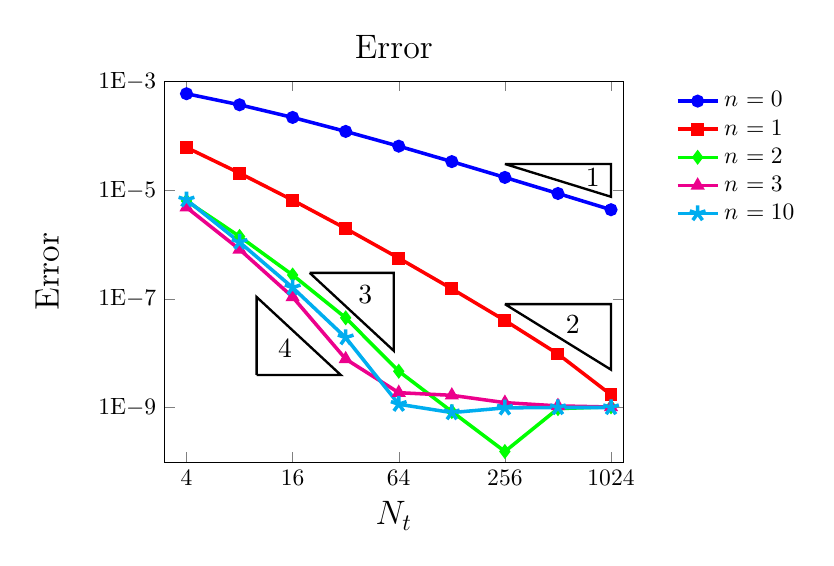
\begin{tikzpicture}[scale=0.85]

\begin{axis}[
  xmode = log,
  xmin = 3,
  xmax = 1200,
  xtick = {4,16,64,256,1024},
  xticklabels = {4,16,64,256,1024},
  xlabel = $N_{t}$,
  ymode = log,
  ymin = 1E-10,
  ymax = 1E-3,
  ytick = {1E-11,1E-9,1E-7,1E-5,1E-3},
  yticklabels = {$1$E$-11$,$1$E$-9$,$1$E$-7$,$1$E$-5$,$1$E$-3$},
  ylabel = {Error},
  ylabel style = {yshift = 10pt},
  label style = {font=\Large},
  legend entries = {$n_{\sdc}=0$, $n_{\sdc}=1$, $n_{\sdc}=2$,
  $n_{\sdc}=3$, $n_{\sdc}=10$},
  legend cell align=left,
  legend style={at={(1.4,0.8)},anchor=east},
%  legend pos = south west,
  legend style = {draw=none},
  title = {\Large{Error}}
  ]


% first-order
% error for nsdc=0, p=2
\addplot [mark=*,blue,line width=1.5] table{
%2 8.56e-4
4 5.86e-4
8 3.67e-4
16 2.15e-4
32 1.19e-4
64 6.38e-5
128 3.32e-5
256 1.70e-5
512 8.62e-6
1024 4.34e-6
};

% second-order
% error for nsdc=1, p=2
\addplot [mark=square*,red,line width=1.5] table{
%2 1.64e-4
4 6.03e-5
8 2.04e-5
16 6.50e-6
32 1.96e-6
64 5.60e-7
128 1.53e-7
256 4.01e-8
512 9.70e-9
1024 1.73e-9
};

% third-order
% error for nsdc=2, p=3
\addplot [mark=diamond*,green,line width=1.5] table{
%2 2.51e-5
4 6.29e-6
8 1.40e-6
16 2.74e-7
32 4.48e-8
64 4.68e-9
128 8.50e-10
256 1.57e-10
512 9.63e-10
1024 1.04e-9
};

% fourth-order
% error for nsdc=3, p=3
\addplot [mark=triangle*,magenta,line width=1.5] table{
%2 2.35e-5
4 4.79e-6
8 8.10e-7
16 1.08e-7
32 7.84e-9
64 1.89e-9
128 1.69e-9
256 1.24e-9
512 1.08e-9
1024 1.03e-9
};

% fourth-order
% error for nsdc=10, p=3
\addplot [mark=star,mark size=3.5pt,cyan,line width=1.5] table{
%2 3.26e-5
4 6.61e-6
8 1.10e-6
16 1.61e-7
32 1.94e-8
64 1.16e-9
128 8.14e-10
256 9.94e-10
512 1.01e-9
1024 1.01e-9
};

\addplot [mark=none,black,line width=1.0] table{
256 3e-5
1024 3e-5
1024 7.5e-6
256 3e-5
};

\addplot [mark=none,black,line width=1.0] table{
256 8e-8
1024 8e-8
1024 5e-9
256 8e-8
};

\addplot [mark=none,black,line width=1.0] table{
20 3e-7
60 3e-7
60 1.11e-8
20 3e-7
};

\addplot [mark=none,black,line width=1.0] table{
10 4e-9
10 1.08e-7
30 4e-9
10 4e-9
};

\end{axis}

\node at (6.4,4.25) {$1$};
\node at (6.1,2.05) {$2$};
\node at (3.0,2.5) {$3$};
\node at (1.8,1.7) {$4$};

\end{tikzpicture}



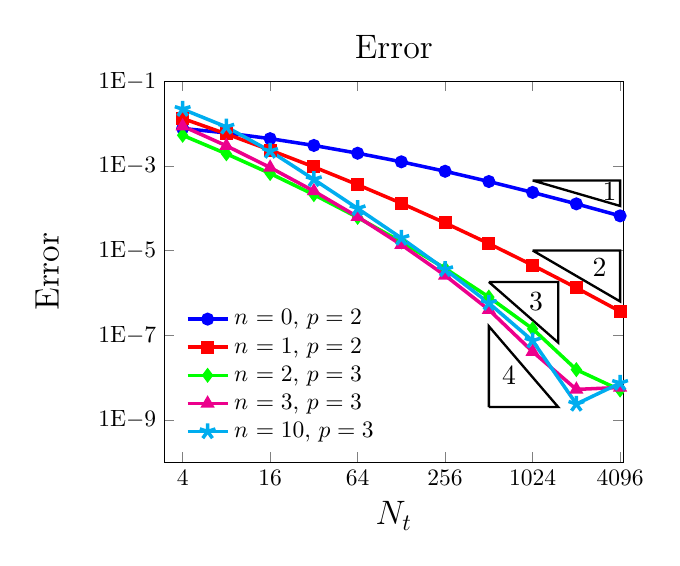
\begin{tikzpicture}[scale=0.85]

\begin{axis}[
  xmode = log,
  xmin = 3,
  xmax = 4300,
  xtick = {4,16,64,256,1024,4096},
  xticklabels = {4,16,64,256,1024,4096},
  xlabel = $N_{t}$,
  ymode = log,
  ymin = 1E-10,
  ymax = 1E-1,
  ytick = {1E-11,1E-9,1E-7,1E-5,1E-3,1E-1},
  yticklabels = {$1$E$-11$,$1$E$-9$,$1$E$-7$,$1$E$-5$,$1$E$-3$,$1$E$-1$},
  ylabel = {Error},
  ylabel style = {yshift = 10pt},
  label style = {font=\Large},
  legend entries = {{$n_{\sdc}=0$, $p=2$},{$n_{\sdc}=1$, $p=2$},{$n_{\sdc}=2$, $p=3$},{$n_{\sdc}=3$, $p=3$},{$n_{\sdc}=10$, $p=3$}},
  legend cell align=left,
%  legend style={at={(1.55,0.8)},anchor=east},
  legend pos = south west,
  legend style = {draw=none},
  title = {\Large{Error}}
  ]


% first-order
% error for nsdc=0, p=2
\addplot [mark=*,blue,line width=1.5] table{
4 7.61e-3
8 5.97e-3
16 4.37e-3
32 3.02e-3 
64 1.98e-3
128 1.24e-3
256 7.42e-4
512 4.25e-4
1024 2.35e-4
2048 1.26e-4
4096 6.56e-5
};

% second-order
% error for nsdc=1, p=2
\addplot [mark=square*,red,line width=1.5] table{
4 1.31e-2
8 5.65e-3
16 2.35e-3
32 9.38e-4
64 3.57e-4
128 1.30e-4
256 4.46e-5
512 1.45e-5
1024 4.48e-6
2048 1.31e-6
4096 3.63e-7
};

% third-order
% error for nsdc=2, p=3
\addplot [mark=diamond*,green,line width=1.5] table{
4 5.25e-3
8 1.92e-3
16 6.57e-4
32 2.08e-4
64 6.03e-5
128 1.59e-5
256 3.77e-6
512 7.93e-7
1024 1.41e-7
2048 1.53e-8
4096 5.05e-9
};

% fourth-order
% error for nsdc=3, p=3
\addplot [mark=triangle*,magenta,line width=1.5] table{
4 8.63e-3
8 2.96e-3
16 9.10e-4
32 2.52e-4
64 6.24e-5
128 1.36e-5
256 2.57e-6
512 3.98e-7
1024 4.07e-8
2048 5.22e-9
4096 5.82e-9
};

% fourth-order
% error for nsdc=10, p=3
\addplot [mark=star,mark size=3.5pt,cyan,line width=1.5] table{
4 2.17e-2
8 8.27e-3
16 2.22e-3
32 4.76e-4
64 9.81e-5
128 1.96e-5
256 3.57e-6
512 5.71e-7
1024 7.36e-8
2048 2.36e-9
4096 7.36e-9
% old values from using GMRES 
%1024 7.36e-8
%2048 3.52e-9
%4096 7.36e-9
};

\addplot [mark=none,black,line width=1.0] table{
1024 4.5e-4
4096 4.5e-4
4096 1.125e-4
1024 4.5e-4
};

\addplot [mark=none,black,line width=1.0] table{
1024 1e-5
4096 1e-5
4096 6.25e-7
1024 1e-5
};

\addplot [mark=none,black,line width=1.0] table{
512 1.8e-6
1536 1.8e-6
1536 6.67e-8
512 1.8e-6
};

\addplot [mark=none,black,line width=1.0] table{
512 2e-9
512 1.62e-7
1536 2e-9
512 2e-9
};

\end{axis}

\node at (6.65,4.05) {$1$};
\node at (6.5,2.9) {$2$};
\node at (5.55,2.4) {$3$};
\node at (5.15,1.3) {$4$};

\end{tikzpicture}



\fi
\end{center}
\mcaption{The maximum error in area and length for a single vesicle in
a {\bf relaxation} flow.  We use $p=2$ Gauss-Lobatto points for
$\boldnsdc{0}$ (first-order) and $\boldnsdc{1}$ (second-order), and
$p=3$ Gauss-Lobatto points for $\boldnsdc{2}$ (third-order),
$\boldnsdc{3}$ (fourth-order), and $\boldnsdc{10}$ (fourth-order).  We
see that first- second- and third-order convergence are
achieved.}{f:relaxationConvergence}
\end{figure}

\begin{figure}[htp]
\begin{center}
  \begin{tabular}{ccc}
  \ifTikz
  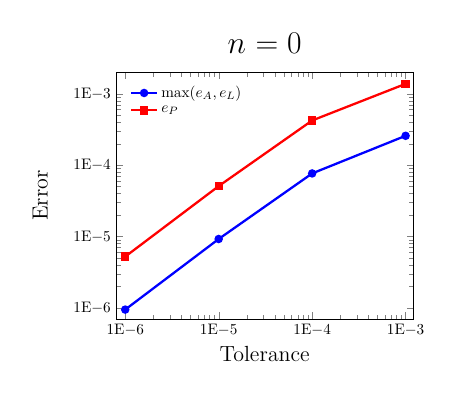
\begin{tikzpicture}[scale=0.55]

\begin{axis}[
  xmode = log,
  xmin = 8e-7,
  xmax = 1.2e-3,
  xtick = {1E-6,1E-5,1E-4,1E-3},
  xticklabels = {$1$E$-6$,$1$E$-5$,$1$E$-4$,$1$E$-3$},
  xlabel = {Tolerance},
  ymode = log,
  ymin = 7E-7,
  ymax = 2E-3,
  ytick = {1E-6,1E-5,1E-4,1E-3},
  yticklabels = {$1$E$-6$,$1$E$-5$,$1$E$-4$,$1$E$-3$},
  ylabel = {Error},
  ylabel style = {yshift = 10pt},
  label style = {font=\Large},
  legend entries = {$\max(e_{A},e_{L})$\\$e_{P}$\\},
  legend cell align = left,
  legend pos = north west, 
  legend style = {draw=none},
  title = {\huge{$n_{\sdc} = 0$}}
  ]


% maximum error in area and length
\addplot [mark=*,blue,line width=1.5,solid] table{
1e-3 2.58e-4
1e-4 7.66e-5
1e-5 9.23e-6
1e-6 9.46e-7

%1e-4 8.23e-5
%1e-5 9.34e-6
%1e-6 9.47e-7
%1e-7 9.45e-8

%1e-4 8.25e-5
%1e-5 9.36e-6
%1e-6 9.47e-7
%1e-7 9.43e-8
};

% error in position
\addplot [mark=square*,red,line width=1.5,solid] table{
1e-3 1.38e-3
1e-4 4.23e-4
1e-5 5.09e-5
1e-6 5.23e-6

%1e-4 4.48e-4
%1e-5 5.16e-5
%1e-6 5.23e-6
%1e-7 5.18e-7

%1e-4 4.51e-4
%1e-5 5.16e-5
%1e-6 5.24e-6
%1e-7 5.19e-7
};


\end{axis}

\end{tikzpicture}


 &
  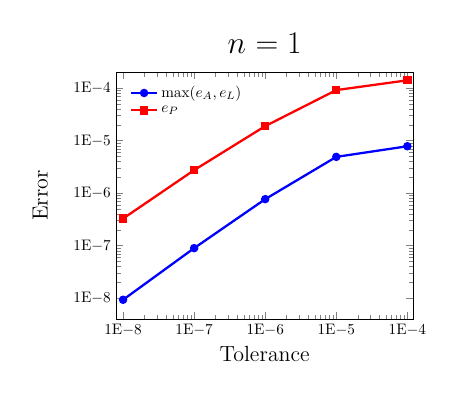
\begin{tikzpicture}[scale=0.55]

\begin{axis}[
  xmode = log,
  xmin = 8e-9,
  xmax = 1.2e-4,
  xtick = {1E-8,1E-7,1E-6,1E-5,1E-4},
  xticklabels = {$1$E$-8$,$1$E$-7$,$1$E$-6$,$1$E$-5$,$1$E$-4$},
  xlabel = {Tolerance},
  ymode = log,
  ymin = 4E-9,
  ymax = 2E-4,
  ytick = {1E-8,1E-7,1E-6,1E-5,1E-4},
  yticklabels = {$1$E$-8$,$1$E$-7$,$1$E$-6$,$1$E$-5$,$1$E$-4$},
  ylabel = {Error},
  ylabel style = {yshift = 10pt},
  label style = {font=\Large},
  legend entries = {$\max(e_{A},e_{L})$\\$e_{P}$\\},
  legend cell align = left,
  legend pos = north west, 
  legend style = {draw=none},
  title = {\huge{$n_{\sdc} = 1$}}
  ]

%% desired tolerance
%\addplot [mark=none,black,line width=1.5,dashed] table{
%0 1.0e-5
%1 1.0e-6
%2 1.0e-7
%3 1.0e-8
%4 1.0e-9
%};

% maximum error in area and length
\addplot [mark=*,blue,line width=1.5,solid] table{
1e-4 7.81e-6
1e-5 4.90e-6
1e-6 7.67e-7
1e-7 8.93e-8
1e-8 9.27e-9

%1e-5 2.96e-6
%1e-6 6.71e-7
%1e-7 8.57e-8
%1e-8 9.15e-9
%1e-9 9.36e-10

%1e-5 1.84e-6
%1e-6 6.13e-7
%1e-7 8.26e-8
%1e-8 9.09e-9
%1e-9 9.34e-10
};

% error in position
\addplot [mark=square*,red,line width=1.5,solid] table{
1e-4 1.41e-4
1e-5 9.18e-5
1e-6 1.89e-5
1e-7 2.74e-6
1e-8 3.27e-7

%1e-5 6.15e-5
%1e-6 1.59e-5
%1e-7 2.51e-6
%1e-8 3.04e-7
%1e-9 3.63e-8

%1e-5 2.96e-5
%1e-6 1.02e-5
%1e-7 1.68e-6
%1e-8 2.00e-7
%1e-9 2.10e-8
};


\end{axis}

\end{tikzpicture}


 &
  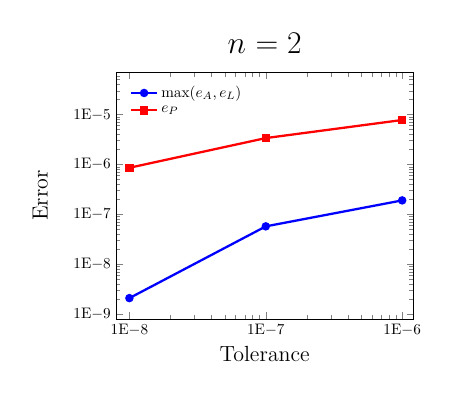
\begin{tikzpicture}[scale=0.55]

\begin{axis}[
  xmode = log,
  xmin = 8e-9,
  xmax = 1.2e-6,
  xtick = {1E-8,1E-7,1E-6},
  xticklabels = {$1$E$-8$,$1$E$-7$,$1$E$-6$,$1$E$-5$},
  xlabel = {Tolerance},
  ymode = log,
  ymin = 8E-10,
  ymax = 7.0E-5,
  ytick = {1E-9,1E-8,1E-7,1E-6,1E-5,1E-4},
  yticklabels = {$1$E$-9$,$1$E$-8$,$1$E$-7$,$1$E$-6$,$1$E$-5$,$1$E$-4$},
  ylabel = {Error},
  ylabel style = {yshift = 10pt},
  label style = {font=\Large},
  legend entries = {$\max(e_{A},e_{L})$\\$e_{P}$\\},
  legend cell align = left,
  legend pos = north west, 
  legend style = {draw=none},
  title = {\huge{$n_{\sdc} = 2$}}
  ]

%% desired tolerance
%\addplot [mark=none,black,line width=1.5,dashed] table{
%0 1.0e-7
%1 1.0e-8
%2 1.0e-9
%3 1.0e-10
%};

% maximum error in area and length
\addplot [mark=*,blue,line width=1.5,solid] table{
1e-6 1.90e-7
1e-7 5.73e-8
1e-8 2.09e-9

%1e-6 1.20e-7
%1e-7 4.80e-8
%1e-8 6.61e-9
%1e-9 7.63e-10

%1e-7 4.29e-8
%1e-8 6.52e-9
%1e-9 7.74e-10
%1e-10 8.36e-11
};

% error in position
\addplot [mark=square*,red,line width=1.5,solid] table{
1e-6 7.76e-6
1e-7 3.37e-6
1e-8 8.56e-7

%1e-6 3.97e-6
%1e-7 2.15e-6
%1e-8 6.61e-7
%1e-9 4.13e-8

%1e-7 1.26e-6
%1e-8 3.40e-7
%1e-9 8.40e-8
%1e-10 6.30e-9
};


\end{axis}

\end{tikzpicture}


 
  \fi
  \end{tabular}
\end{center}
\mcaption{The maximum error in area and length (blue), and in position
(red) for a single vesicle in a {\bf relaxation} flow with an {\bf
adaptive} time step size.  In all the runs, the maximum error in area
and length are achieved, and the error in position decays at the same
rate.}{f:relaxationAdaptive}
\end{figure}




%%%%%%%%%%%%%%%%%%%%%%%%%%%%%%%%%%%%%%%%%%%%%%%%%%%%%%%%%%%%%%%%%%%%
\subsection{Extensional flow}

We consider two vesicles placed symmetrically around the origin with
the background velocity $\vv_{\infty} = (-x,y)$
(Figure~\ref{f:extensionalGeom}).  We discretize both vesicles with
$N=96$ points and the time horizon is $T=24$ which is long enough that
the distance between the vesicles at the time horizon is
$0.4\sqrt{\Delta s}$, where $\Delta s$ is the arclength spacing.  We
report results using zero, one, and two SDC iterations, and BDF in
Tables~\ref{t:noSDCextensional} and~\ref{t:SDC12extensional}.  Similar
to the previous example, for some of the results, the expected
convergence rates are not observed.  Other groups (see, for
example,~\cite{min2003,wei2013}) have observed that for stiff systems,
very small time steps must be taken before the asymptotic convergence
rates are achieved.  As before, we expect that other sources of error
will dominate once the temporal asymptotic regime is achieved.

\begin{figure}[htp]
\begin{center}
  \begin{tabular}{ccccc}
  \ifTikz
  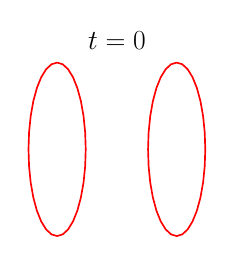
\begin{tikzpicture}[scale=0.40]

\begin{axis}[
  xmin = -1.8,
  xmax = 1.8,
  ymin = -1.8,
  ymax = 1.8,
  axis equal = true,
  hide axis,
  title = {\Huge$t=0$}
  ]

\addplot [mark=none,red,line width=1.5] table{
-1.2000e+00 1.7412e+00
-1.3120e+00 1.7078e+00
-1.4198e+00 1.6087e+00
-1.5191e+00 1.4478e+00
-1.6061e+00 1.2312e+00
-1.6775e+00 9.6738e-01
-1.7306e+00 6.6635e-01
-1.7633e+00 3.3970e-01
-1.7743e+00 1.4179e-16
-1.7633e+00 -3.3970e-01
-1.7306e+00 -6.6635e-01
-1.6775e+00 -9.6738e-01
-1.6061e+00 -1.2312e+00
-1.5191e+00 -1.4478e+00
-1.4198e+00 -1.6087e+00
-1.3120e+00 -1.7078e+00
-1.2000e+00 -1.7412e+00
-1.0880e+00 -1.7078e+00
-9.8022e-01 -1.6087e+00
-8.8093e-01 -1.4478e+00
-7.9391e-01 -1.2312e+00
-7.2249e-01 -9.6738e-01
-6.6941e-01 -6.6635e-01
-6.3673e-01 -3.3970e-01
-6.2570e-01 -3.5503e-16
-6.3673e-01 3.3970e-01
-6.6941e-01 6.6635e-01
-7.2249e-01 9.6738e-01
-7.9391e-01 1.2312e+00
-8.8093e-01 1.4478e+00
-9.8022e-01 1.6087e+00
-1.0880e+00 1.7078e+00
-1.2000e+00 1.7412e+00
};

\addplot [mark=none,red,line width=1.5] table{
1.2000e+00 1.7412e+00
1.0880e+00 1.7078e+00
9.8022e-01 1.6087e+00
8.8093e-01 1.4478e+00
7.9391e-01 1.2312e+00
7.2249e-01 9.6738e-01
6.6941e-01 6.6635e-01
6.3673e-01 3.3970e-01
6.2570e-01 1.4179e-16
6.3673e-01 -3.3970e-01
6.6941e-01 -6.6635e-01
7.2249e-01 -9.6738e-01
7.9391e-01 -1.2312e+00
8.8093e-01 -1.4478e+00
9.8022e-01 -1.6087e+00
1.0880e+00 -1.7078e+00
1.2000e+00 -1.7412e+00
1.3120e+00 -1.7078e+00
1.4198e+00 -1.6087e+00
1.5191e+00 -1.4478e+00
1.6061e+00 -1.2312e+00
1.6775e+00 -9.6738e-01
1.7306e+00 -6.6635e-01
1.7633e+00 -3.3970e-01
1.7743e+00 -3.5503e-16
1.7633e+00 3.3970e-01
1.7306e+00 6.6635e-01
1.6775e+00 9.6738e-01
1.6061e+00 1.2312e+00
1.5191e+00 1.4478e+00
1.4198e+00 1.6087e+00
1.3120e+00 1.7078e+00
1.2000e+00 1.7412e+00
};

\end{axis}

%\draw[gray,thin] (0,0) grid +(3,4);

\end{tikzpicture}

 &
  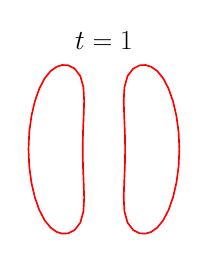
\begin{tikzpicture}[scale=0.40]

\begin{axis}[
  xmin = -1.8,
  xmax = 1.8,
  ymin = -1.8,
  ymax = 1.8,
  axis equal = true,
  hide axis,
  title = {\Huge$t=1$}
  ]

\addplot [mark=none,red,line width=1.5] table{
-8.3599e-01 1.6923e+00
-9.4876e-01 1.6578e+00
-1.0689e+00 1.5736e+00
-1.1886e+00 1.4273e+00
-1.2967e+00 1.2205e+00
-1.3873e+00 9.6267e-01
-1.4562e+00 6.6489e-01
-1.4994e+00 3.3951e-01
-1.5142e+00 -1.4447e-13
-1.4994e+00 -3.3951e-01
-1.4562e+00 -6.6489e-01
-1.3873e+00 -9.6267e-01
-1.2967e+00 -1.2205e+00
-1.1886e+00 -1.4273e+00
-1.0689e+00 -1.5736e+00
-9.4876e-01 -1.6578e+00
-8.3599e-01 -1.6923e+00
-7.1824e-01 -1.6862e+00
-5.8762e-01 -1.6207e+00
-4.7393e-01 -1.4710e+00
-4.1146e-01 -1.2468e+00
-3.9726e-01 -9.7380e-01
-4.0707e-01 -6.6804e-01
-4.2047e-01 -3.3989e-01
-4.2610e-01 -1.3518e-13
-4.2047e-01 3.3989e-01
-4.0707e-01 6.6804e-01
-3.9726e-01 9.7380e-01
-4.1146e-01 1.2468e+00
-4.7393e-01 1.4710e+00
-5.8762e-01 1.6207e+00
-7.1824e-01 1.6862e+00
-8.3599e-01 1.6923e+00
};

\addplot [mark=none,red,line width=1.5] table{
8.3599e-01 1.6923e+00
7.1824e-01 1.6862e+00
5.8762e-01 1.6207e+00
4.7393e-01 1.4710e+00
4.1146e-01 1.2468e+00
3.9726e-01 9.7380e-01
4.0707e-01 6.6804e-01
4.2047e-01 3.3989e-01
4.2610e-01 -2.5794e-13
4.2047e-01 -3.3989e-01
4.0707e-01 -6.6804e-01
3.9726e-01 -9.7380e-01
4.1146e-01 -1.2468e+00
4.7393e-01 -1.4710e+00
5.8762e-01 -1.6207e+00
7.1824e-01 -1.6862e+00
8.3599e-01 -1.6923e+00
9.4876e-01 -1.6578e+00
1.0689e+00 -1.5736e+00
1.1886e+00 -1.4273e+00
1.2967e+00 -1.2205e+00
1.3873e+00 -9.6267e-01
1.4562e+00 -6.6489e-01
1.4994e+00 -3.3951e-01
1.5142e+00 -2.7884e-14
1.4994e+00 3.3951e-01
1.4562e+00 6.6489e-01
1.3873e+00 9.6267e-01
1.2967e+00 1.2205e+00
1.1886e+00 1.4273e+00
1.0689e+00 1.5736e+00
9.4876e-01 1.6578e+00
8.3599e-01 1.6923e+00
};

\end{axis}

%\draw[gray,thin] (0,0) grid +(3,4);

\end{tikzpicture}

 &
  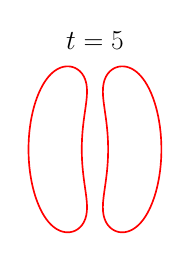
\begin{tikzpicture}[scale=0.40]

\begin{axis}[
  xmin = -1.8,
  xmax = 1.8,
  ymin = -1.8,
  ymax = 1.8,
  axis equal = true,
  hide axis,
  title = {\Huge$t=5$}
  ]

\addplot [mark=none,red,line width=1.5] table{
-6.0188e-01 1.6622e+00
-6.3899e-01 1.6550e+00
-6.7650e-01 1.6441e+00
-7.1509e-01 1.6288e+00
-7.5512e-01 1.6086e+00
-7.9656e-01 1.5827e+00
-8.3911e-01 1.5505e+00
-8.8228e-01 1.5115e+00
-9.2551e-01 1.4655e+00
-9.6825e-01 1.4125e+00
-1.0100e+00 1.3526e+00
-1.0503e+00 1.2859e+00
-1.0889e+00 1.2129e+00
-1.1254e+00 1.1339e+00
-1.1596e+00 1.0493e+00
-1.1913e+00 9.5956e-01
-1.2202e+00 8.6511e-01
-1.2462e+00 7.6643e-01
-1.2690e+00 6.6400e-01
-1.2886e+00 5.5835e-01
-1.3048e+00 4.4997e-01
-1.3175e+00 3.3941e-01
-1.3266e+00 2.2719e-01
-1.3321e+00 1.1387e-01
-1.3339e+00 -5.5197e-13
-1.3321e+00 -1.1387e-01
-1.3266e+00 -2.2719e-01
-1.3175e+00 -3.3941e-01
-1.3048e+00 -4.4997e-01
-1.2886e+00 -5.5835e-01
-1.2690e+00 -6.6400e-01
-1.2462e+00 -7.6643e-01
-1.2202e+00 -8.6511e-01
-1.1913e+00 -9.5956e-01
-1.1596e+00 -1.0493e+00
-1.1254e+00 -1.1339e+00
-1.0889e+00 -1.2129e+00
-1.0503e+00 -1.2859e+00
-1.0100e+00 -1.3526e+00
-9.6825e-01 -1.4125e+00
-9.2551e-01 -1.4655e+00
-8.8228e-01 -1.5115e+00
-8.3911e-01 -1.5505e+00
-7.9656e-01 -1.5827e+00
-7.5512e-01 -1.6086e+00
-7.1509e-01 -1.6288e+00
-6.7650e-01 -1.6441e+00
-6.3899e-01 -1.6550e+00
-6.0188e-01 -1.6622e+00
-5.6425e-01 -1.6657e+00
-5.2518e-01 -1.6653e+00
-4.8399e-01 -1.6603e+00
-4.4047e-01 -1.6496e+00
-3.9502e-01 -1.6317e+00
-3.4873e-01 -1.6052e+00
-3.0332e-01 -1.5689e+00
-2.6098e-01 -1.5222e+00
-2.2404e-01 -1.4651e+00
-1.9453e-01 -1.3983e+00
-1.7381e-01 -1.3232e+00
-1.6222e-01 -1.2415e+00
-1.5912e-01 -1.1546e+00
-1.6306e-01 -1.0634e+00
-1.7224e-01 -9.6869e-01
-1.8482e-01 -8.7072e-01
-1.9916e-01 -7.6969e-01
-2.1388e-01 -6.6578e-01
-2.2791e-01 -5.5924e-01
-2.4039e-01 -4.5037e-01
-2.5070e-01 -3.3956e-01
-2.5838e-01 -2.2723e-01
-2.6311e-01 -1.1388e-01
-2.6471e-01 -4.9031e-13
-2.6311e-01 1.1388e-01
-2.5838e-01 2.2723e-01
-2.5070e-01 3.3956e-01
-2.4039e-01 4.5037e-01
-2.2791e-01 5.5924e-01
-2.1388e-01 6.6578e-01
-1.9916e-01 7.6969e-01
-1.8482e-01 8.7072e-01
-1.7224e-01 9.6869e-01
-1.6306e-01 1.0634e+00
-1.5912e-01 1.1546e+00
-1.6222e-01 1.2415e+00
-1.7381e-01 1.3232e+00
-1.9453e-01 1.3983e+00
-2.2404e-01 1.4651e+00
-2.6098e-01 1.5222e+00
-3.0332e-01 1.5689e+00
-3.4873e-01 1.6052e+00
-3.9502e-01 1.6317e+00
-4.4047e-01 1.6496e+00
-4.8399e-01 1.6603e+00
-5.2518e-01 1.6653e+00
-5.6425e-01 1.6657e+00
-6.0188e-01 1.6622e+00
};

\addplot [mark=none,red,line width=1.5] table{
6.0188e-01 1.6622e+00
5.6425e-01 1.6657e+00
5.2518e-01 1.6653e+00
4.8399e-01 1.6603e+00
4.4047e-01 1.6496e+00
3.9502e-01 1.6317e+00
3.4873e-01 1.6052e+00
3.0332e-01 1.5689e+00
2.6098e-01 1.5222e+00
2.2404e-01 1.4651e+00
1.9453e-01 1.3983e+00
1.7381e-01 1.3232e+00
1.6222e-01 1.2415e+00
1.5912e-01 1.1546e+00
1.6306e-01 1.0634e+00
1.7224e-01 9.6869e-01
1.8482e-01 8.7072e-01
1.9916e-01 7.6969e-01
2.1388e-01 6.6578e-01
2.2791e-01 5.5924e-01
2.4039e-01 4.5037e-01
2.5070e-01 3.3956e-01
2.5838e-01 2.2723e-01
2.6311e-01 1.1388e-01
2.6471e-01 -3.0230e-13
2.6311e-01 -1.1388e-01
2.5838e-01 -2.2723e-01
2.5070e-01 -3.3956e-01
2.4039e-01 -4.5037e-01
2.2791e-01 -5.5924e-01
2.1388e-01 -6.6578e-01
1.9916e-01 -7.6969e-01
1.8482e-01 -8.7072e-01
1.7224e-01 -9.6869e-01
1.6306e-01 -1.0634e+00
1.5912e-01 -1.1546e+00
1.6222e-01 -1.2415e+00
1.7381e-01 -1.3232e+00
1.9453e-01 -1.3983e+00
2.2404e-01 -1.4651e+00
2.6098e-01 -1.5222e+00
3.0332e-01 -1.5689e+00
3.4873e-01 -1.6052e+00
3.9502e-01 -1.6317e+00
4.4047e-01 -1.6496e+00
4.8399e-01 -1.6603e+00
5.2518e-01 -1.6653e+00
5.6425e-01 -1.6657e+00
6.0188e-01 -1.6622e+00
6.3899e-01 -1.6550e+00
6.7650e-01 -1.6441e+00
7.1509e-01 -1.6288e+00
7.5512e-01 -1.6086e+00
7.9656e-01 -1.5827e+00
8.3911e-01 -1.5505e+00
8.8228e-01 -1.5115e+00
9.2551e-01 -1.4655e+00
9.6825e-01 -1.4125e+00
1.0100e+00 -1.3526e+00
1.0503e+00 -1.2859e+00
1.0889e+00 -1.2129e+00
1.1254e+00 -1.1339e+00
1.1596e+00 -1.0493e+00
1.1913e+00 -9.5956e-01
1.2202e+00 -8.6511e-01
1.2462e+00 -7.6643e-01
1.2690e+00 -6.6400e-01
1.2886e+00 -5.5835e-01
1.3048e+00 -4.4997e-01
1.3175e+00 -3.3941e-01
1.3266e+00 -2.2719e-01
1.3321e+00 -1.1387e-01
1.3339e+00 -1.9961e-13
1.3321e+00 1.1387e-01
1.3266e+00 2.2719e-01
1.3175e+00 3.3941e-01
1.3048e+00 4.4997e-01
1.2886e+00 5.5835e-01
1.2690e+00 6.6400e-01
1.2462e+00 7.6643e-01
1.2202e+00 8.6511e-01
1.1913e+00 9.5956e-01
1.1596e+00 1.0493e+00
1.1254e+00 1.1339e+00
1.0889e+00 1.2129e+00
1.0503e+00 1.2859e+00
1.0100e+00 1.3526e+00
9.6825e-01 1.4125e+00
9.2551e-01 1.4655e+00
8.8228e-01 1.5115e+00
8.3911e-01 1.5505e+00
7.9656e-01 1.5827e+00
7.5512e-01 1.6086e+00
7.1509e-01 1.6288e+00
6.7650e-01 1.6441e+00
6.3899e-01 1.6550e+00
6.0188e-01 1.6622e+00
};

\end{axis}


\end{tikzpicture}

 &
  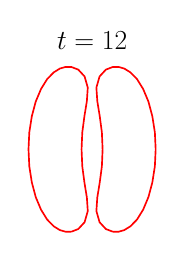
\begin{tikzpicture}[scale=0.40]

\begin{axis}[
  xmin = -1.8,
  xmax = 1.8,
  ymin = -1.8,
  ymax = 1.8,
  axis equal = true,
  hide axis,
  title = {\Huge$t=12$}
  ]

\addplot [mark=none,red,line width=1.5] table{
-5.3142e-01 1.6542e+00
-6.4609e-01 1.6216e+00
-7.7012e-01 1.5449e+00
-9.0267e-01 1.4090e+00
-1.0251e+00 1.2111e+00
-1.1311e+00 9.5881e-01
-1.2097e+00 6.6381e-01
-1.2605e+00 3.3938e-01
-1.2763e+00 -6.5711e-11
-1.2605e+00 -3.3938e-01
-1.2097e+00 -6.6381e-01
-1.1311e+00 -9.5881e-01
-1.0251e+00 -1.2111e+00
-9.0267e-01 -1.4090e+00
-7.7012e-01 -1.5449e+00
-6.4609e-01 -1.6216e+00
-5.3142e-01 -1.6542e+00
-4.1448e-01 -1.6529e+00
-2.7686e-01 -1.6000e+00
-1.5014e-01 -1.4626e+00
-8.6429e-02 -1.2396e+00
-1.0469e-01 -9.6690e-01
-1.5377e-01 -6.6520e-01
-1.9683e-01 -3.3947e-01
-2.1116e-01 1.4599e-10
-1.9683e-01 3.3947e-01
-1.5377e-01 6.6520e-01
-1.0469e-01 9.6690e-01
-8.6429e-02 1.2396e+00
-1.5014e-01 1.4626e+00
-2.7686e-01 1.6000e+00
-4.1448e-01 1.6529e+00
-5.3142e-01 1.6542e+00
};

\addplot [mark=none,red,line width=1.5] table{
5.3142e-01 1.6542e+00
4.1448e-01 1.6529e+00
2.7686e-01 1.6000e+00
1.5014e-01 1.4626e+00
8.6429e-02 1.2396e+00
1.0469e-01 9.6690e-01
1.5377e-01 6.6520e-01
1.9683e-01 3.3947e-01
2.1116e-01 3.7048e-10
1.9683e-01 -3.3947e-01
1.5377e-01 -6.6520e-01
1.0469e-01 -9.6690e-01
8.6429e-02 -1.2396e+00
1.5014e-01 -1.4626e+00
2.7686e-01 -1.6000e+00
4.1448e-01 -1.6529e+00
5.3142e-01 -1.6542e+00
6.4609e-01 -1.6216e+00
7.7012e-01 -1.5449e+00
9.0267e-01 -1.4090e+00
1.0251e+00 -1.2111e+00
1.1311e+00 -9.5881e-01
1.2097e+00 -6.6381e-01
1.2605e+00 -3.3938e-01
1.2763e+00 5.7387e-10
1.2605e+00 3.3938e-01
1.2097e+00 6.6381e-01
1.1311e+00 9.5881e-01
1.0251e+00 1.2111e+00
9.0267e-01 1.4090e+00
7.7012e-01 1.5449e+00
6.4609e-01 1.6216e+00
5.3142e-01 1.6542e+00
};

\end{axis}

%\draw[gray,thin] (0,0) grid +(3,4);

\end{tikzpicture}

 &
  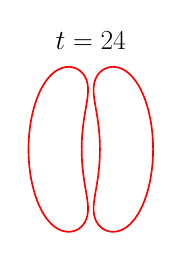
\begin{tikzpicture}[scale=0.40]

\begin{axis}[
  xmin = -1.8,
  xmax = 1.8,
  ymin = -1.8,
  ymax = 1.8,
  axis equal = true,
  hide axis,
  title = {\Huge$t=24$}
  ]

\addplot [mark=none,red,line width=1.5] table{
-5.0194e-01 1.6512e+00
-5.3909e-01 1.6442e+00
-5.7669e-01 1.6336e+00
-6.1548e-01 1.6188e+00
-6.5582e-01 1.5993e+00
-6.9775e-01 1.5741e+00
-7.4095e-01 1.5428e+00
-7.8496e-01 1.5048e+00
-8.2920e-01 1.4598e+00
-8.7307e-01 1.4077e+00
-9.1604e-01 1.3486e+00
-9.5764e-01 1.2827e+00
-9.9747e-01 1.2104e+00
-1.0352e+00 1.1320e+00
-1.0706e+00 1.0479e+00
-1.1033e+00 9.5849e-01
-1.1332e+00 8.6435e-01
-1.1600e+00 7.6590e-01
-1.1836e+00 6.6365e-01
-1.2038e+00 5.5811e-01
-1.2205e+00 4.4982e-01
-1.2336e+00 3.3930e-01
-1.2430e+00 2.2711e-01
-1.2487e+00 1.1380e-01
-1.2506e+00 -6.9370e-05
-1.2487e+00 -1.1394e-01
-1.2430e+00 -2.2725e-01
-1.2336e+00 -3.3944e-01
-1.2205e+00 -4.4996e-01
-1.2038e+00 -5.5825e-01
-1.1836e+00 -6.6379e-01
-1.1600e+00 -7.6604e-01
-1.1332e+00 -8.6449e-01
-1.1033e+00 -9.5863e-01
-1.0706e+00 -1.0480e+00
-1.0352e+00 -1.1321e+00
-9.9747e-01 -1.2105e+00
-9.5764e-01 -1.2829e+00
-9.1604e-01 -1.3487e+00
-8.7307e-01 -1.4078e+00
-8.2919e-01 -1.4599e+00
-7.8496e-01 -1.5049e+00
-7.4095e-01 -1.5429e+00
-6.9775e-01 -1.5743e+00
-6.5582e-01 -1.5994e+00
-6.1548e-01 -1.6190e+00
-5.7669e-01 -1.6337e+00
-5.3908e-01 -1.6443e+00
-5.0194e-01 -1.6513e+00
-4.6431e-01 -1.6548e+00
-4.2524e-01 -1.6547e+00
-3.8400e-01 -1.6502e+00
-3.4029e-01 -1.6402e+00
-2.9443e-01 -1.6233e+00
-2.4739e-01 -1.5982e+00
-2.0083e-01 -1.5634e+00
-1.5697e-01 -1.5181e+00
-1.1841e-01 -1.4620e+00
-8.7681e-02 -1.3958e+00
-6.6776e-02 -1.3209e+00
-5.6484e-02 -1.2390e+00
-5.6128e-02 -1.1520e+00
-6.3728e-02 -1.0611e+00
-7.6812e-02 -9.6681e-01
-9.3003e-02 -8.6936e-01
-1.1040e-01 -7.6882e-01
-1.2755e-01 -6.6528e-01
-1.4341e-01 -5.5900e-01
-1.5722e-01 -4.5029e-01
-1.6845e-01 -3.3957e-01
-1.7671e-01 -2.2728e-01
-1.8176e-01 -1.1394e-01
-1.8346e-01 -6.7945e-05
-1.8176e-01 1.1381e-01
-1.7671e-01 2.2715e-01
-1.6845e-01 3.3943e-01
-1.5722e-01 4.5016e-01
-1.4341e-01 5.5887e-01
-1.2755e-01 6.6515e-01
-1.1040e-01 7.6868e-01
-9.3004e-02 8.6923e-01
-7.6814e-02 9.6667e-01
-6.3730e-02 1.0609e+00
-5.6129e-02 1.1519e+00
-5.6486e-02 1.2389e+00
-6.6778e-02 1.3207e+00
-8.7683e-02 1.3957e+00
-1.1841e-01 1.4619e+00
-1.5697e-01 1.5180e+00
-2.0083e-01 1.5633e+00
-2.4739e-01 1.5981e+00
-2.9444e-01 1.6232e+00
-3.4029e-01 1.6400e+00
-3.8400e-01 1.6500e+00
-4.2524e-01 1.6546e+00
-4.6432e-01 1.6547e+00
-5.0194e-01 1.6512e+00
};

\addplot [mark=none,red,line width=1.5] table{
5.0194e-01 1.6512e+00
4.6431e-01 1.6547e+00
4.2524e-01 1.6546e+00
3.8400e-01 1.6500e+00
3.4029e-01 1.6400e+00
2.9443e-01 1.6232e+00
2.4739e-01 1.5981e+00
2.0083e-01 1.5633e+00
1.5697e-01 1.5180e+00
1.1841e-01 1.4619e+00
8.7681e-02 1.3957e+00
6.6776e-02 1.3207e+00
5.6484e-02 1.2389e+00
5.6128e-02 1.1519e+00
6.3728e-02 1.0609e+00
7.6812e-02 9.6667e-01
9.3003e-02 8.6923e-01
1.1040e-01 7.6868e-01
1.2755e-01 6.6515e-01
1.4341e-01 5.5887e-01
1.5722e-01 4.5016e-01
1.6845e-01 3.3943e-01
1.7671e-01 2.2715e-01
1.8176e-01 1.1381e-01
1.8346e-01 -6.6706e-05
1.8176e-01 -1.1394e-01
1.7671e-01 -2.2728e-01
1.6845e-01 -3.3957e-01
1.5722e-01 -4.5029e-01
1.4341e-01 -5.5900e-01
1.2755e-01 -6.6528e-01
1.1040e-01 -7.6881e-01
9.3004e-02 -8.6936e-01
7.6814e-02 -9.6680e-01
6.3730e-02 -1.0611e+00
5.6129e-02 -1.1520e+00
5.6486e-02 -1.2390e+00
6.6778e-02 -1.3209e+00
8.7683e-02 -1.3958e+00
1.1841e-01 -1.4620e+00
1.5697e-01 -1.5181e+00
2.0083e-01 -1.5634e+00
2.4739e-01 -1.5982e+00
2.9444e-01 -1.6233e+00
3.4029e-01 -1.6402e+00
3.8400e-01 -1.6502e+00
4.2524e-01 -1.6547e+00
4.6432e-01 -1.6548e+00
5.0194e-01 -1.6513e+00
5.3909e-01 -1.6443e+00
5.7669e-01 -1.6337e+00
6.1548e-01 -1.6190e+00
6.5582e-01 -1.5994e+00
6.9775e-01 -1.5743e+00
7.4095e-01 -1.5429e+00
7.8496e-01 -1.5049e+00
8.2920e-01 -1.4599e+00
8.7307e-01 -1.4078e+00
9.1604e-01 -1.3487e+00
9.5764e-01 -1.2829e+00
9.9747e-01 -1.2105e+00
1.0352e+00 -1.1321e+00
1.0706e+00 -1.0480e+00
1.1033e+00 -9.5863e-01
1.1332e+00 -8.6448e-01
1.1600e+00 -7.6603e-01
1.1836e+00 -6.6379e-01
1.2038e+00 -5.5825e-01
1.2205e+00 -4.4995e-01
1.2336e+00 -3.3944e-01
1.2430e+00 -2.2725e-01
1.2487e+00 -1.1394e-01
1.2506e+00 -6.5281e-05
1.2487e+00 1.1381e-01
1.2430e+00 2.2712e-01
1.2336e+00 3.3931e-01
1.2205e+00 4.4982e-01
1.2038e+00 5.5812e-01
1.1836e+00 6.6365e-01
1.1600e+00 7.6590e-01
1.1332e+00 8.6435e-01
1.1033e+00 9.5850e-01
1.0706e+00 1.0479e+00
1.0352e+00 1.1320e+00
9.9747e-01 1.2104e+00
9.5764e-01 1.2827e+00
9.1604e-01 1.3486e+00
8.7307e-01 1.4077e+00
8.2919e-01 1.4598e+00
7.8496e-01 1.5048e+00
7.4095e-01 1.5428e+00
6.9775e-01 1.5741e+00
6.5582e-01 1.5993e+00
6.1548e-01 1.6189e+00
5.7669e-01 1.6336e+00
5.3908e-01 1.6442e+00
5.0194e-01 1.6512e+00
};

\end{axis}


\end{tikzpicture}

 
  \fi
  \end{tabular}
\end{center}
\mcaption{Two vesicles discretized with $N=96$ points.  The vesicles are
initially placed symmetrically around the origin and the background
velocity is $\vv_{\infty} = (-x,y)$.}{f:extensionalGeom} 
\end{figure}

As the vesicles approach one another, their shape is nearly static
since their velocities decrease, and we expect that larger time step
sizes can be taken.  Therefore, we test our adaptive time stepping
strategy using zero, one, and two SDC iterations.  The errors in area
and length, the number of accepted and rejected time steps, the number
of FMM calls, and the CPU times are reported in
Table~\ref{t:adaptiveFirstOrderExtensional} ($n_{\sdc}=0$),
Table~\ref{t:adaptiveSecondOrderExtensional} ($n_{\sdc}=1$), and
Table~\ref{t:adaptiveThirdOrderExtensional} ($n_{\sdc}=2$).  The
adaptive time stepping strategy does a good job of attaining the
desired tolerance while not having too many rejected time steps.  In
Figure~\ref{f:extensionalSummary}, we plot the time step size with the
location of the rejected time steps (top left), and the errors in area
and length for a constant time step size and for an adaptive time step
size (top right).  While the constant time step size commits a
negligible amount of error shortly after the initial condition, too
much error is accumulated at the beginning of the simulation.  This
indicates that a smaller time step should be taken near the start of
the simulation and then it can be increased later in the simulation,
which is exactly what we observe.

In
Tables~\ref{t:noSDCextensional}--\ref{t:adaptiveThirdOrderExtensional}
and the bottom plot of Figure~\ref{f:extensionalSummary}, we compare
the results of the different constant and adaptive time step size
integrators.  We see that our new second-order method, $n_{\sdc} = 1$,
slightly outperforms our previous second-order method, BDF.  Moreover,
by using an adaptive time step size, there is a further reduction in
the required CPU time.  For example, to achieve a tolerance of $1$E$-6$
with $n_{\sdc}=1$, a constant time step size requires about 10 times
more CPU time than if an adaptive time step size is used.  Finally, we
see that with our current implementation, taking two SDC iterations
does not result in a computational speedup compared to $n_{\sdc}=1$.
Therefore, we only use one SDC iteration from this point onwards.

%\begin{itemize}
%%  \item Unsurprisingly, the errors resulting from the first-order time
%%  integrator are much larger than those resulting from higher-order
%%  time integrators.  These larger errors have a very adverse effect
%%  when using adaptive time stepping since very small time steps must be
%%  taken to maintain the requested local truncation error.
%%
%  \item Contrary to the {\em relaxation} example, our new second-order
%  method ($n_{\sdc}=1$) outperforms our previous second-order
%  method (BDF).
%
%  \item  By using an adaptive time step size, the user-defined
%  tolerance is achieved, the number of rejected time steps is small for
%  sufficiently small tolerances, and the time to solution is reduced
%  when compared to the fixed time step size.  These results are also
%  summarized in Figure~\ref{f:extensionalCPUvsErr}.
%
%  \item The first-order method is far too slow to use with an adaptive
%  time step size once the tolerance is less than $1$E$-3$.  By using
%  SDC corrections, we are able to perform adaptive time stepping
%  with second- or higher-order accuracy.  However, at the presented
%  tolerances, doing any more than one SDC correction does not improve
%  the time to solution.
%\end{itemize}

% These runs were done on the old blades on compute-0-2
\begin{table}[htp]
\begin{center}
\begin{tabular}{c|cccc|cccc}
 & \multicolumn{4}{c|}{$\boldnsdc{0}$} & 
   \multicolumn{4}{c}{{\bf BDF}} \\
$N_{t}$ & $e_{A}$ & $e_{L}$ & \# fmm & CPU & 
        $e_{A}$ & $e_{L}$ & \# fmm & CPU \\
\hline
$300$  & $2.47$E$-4$ & $1.27$E$-3$ & $4.21$E$3$ & $1.0$
       & $3.80$E$-5$ & $3.90$E$-4$ & $4.53$E$3$ & $1.2$ \\
$600$  & $1.24$E$-4$ & $6.64$E$-4$ & $8.31$E$3$ & $2.1$
       & $9.84$E$-6$ & $1.37$E$-4$ & $8.90$E$3$ & $2.0$ \\ 
$1200$ & $6.29$E$-5$ & $3.46$E$-4$ & $1.63$E$4$ & $3.8$
       & $2.80$E$-6$ & $4.45$E$-5$ & $1.75$E$4$ & $4.0$ \\ 
$2400$ & $3.20$E$-5$ & $1.79$E$-4$ & $3.17$E$4$ & $7.8$
       & $1.04$E$-6$ & $1.27$E$-5$ & $3.45$E$4$ & $7.6$
\end{tabular}
\mcaption{The errors in area and length and the CPU time for two
vesicles in an {\bf extensional} flow with a {\bf constant} time step
size using $\boldnsdc{0}$ (left) and ${\bf BDF}$ (right).  The CPU
times for
Tables~\ref{t:noSDCextensional}--\ref{t:adaptiveThirdOrderExtensional}
are relative to the cheapest simulation ($N_{t}=300$ and $n_{\sdc}=0$)
which took approximately 453 seconds.  We achieve the desired
first-order results, but second-order results are not yet achieved.
With additional time steps, second-order convergence is achieved (see
Table $7$ in~\cite{qua:bir2014b}).}{t:noSDCextensional}


\begin{tabular}{c|cccc|cccc}
 & \multicolumn{4}{c|}{$\boldnsdc{1}$} & 
   \multicolumn{4}{c}{$\boldnsdc{2}$} \\ 
$N_{t}$ & $e_{A}$ & $e_{L}$ & \# fmm & CPU & 
        $e_{A}$ & $e_{L}$ & \# fmm & CPU \\
\hline
$300$  & $4.99$E$-5$ & $2.91$E$-5$  & $1.04$E$4$ & $2.5$
       & $2.01$E$-6$ & $4.84$E$-7$  & $2.93$E$4$ & $7.2$ \\
$600$  & $1.63$E$-5$ & $1.04$E$-5$  & $1.96$E$4$ & $4.9$
       & $7.35$E$-7$ & $8.14$E$-8$  & $5.58$E$4$ & $13.3$ \\ 
$1200$ & $5.35$E$-6$ & $3.61$E$-6$  & $3.76$E$4$ & $9.2$
       & $5.24$E$-7$ & $1.45$E$-8$  & $1.07$E$5$ & $26.0$ \\ 
$2400$ & $1.94$E$-6$ & $1.13$E$-6$  & $7.22$E$4$ & $16.0$
       & $5.04$E$-7$ & $2.89$E$-9$  & $2.10$E$5$ & $51.2$ \\
$4800$ & $9.15$E$-7$ & $3.07$E$-7$  & $1.40$E$5$ & $34.9$
       & $5.08$E$-7$ & $6.11$E$-10$ & $4.12$E$5$ & $99.1$ \\
\end{tabular}
\mcaption{The errors in area and length and the CPU time for two
vesicles in an {\bf extensional} flow with a {\bf constant} time step
size using $\boldnsdc{1}$, $p=2$ (left) and $\boldnsdc{2}$, $p=3$
(right).  While each SDC iteration reduces the error, the desired
asymptotic rates of convergence are not achieved.  As the ratios of
successive errors are approaching the expected values, we expect that
we have not taken enough time steps to observe the asymptotic rate of
convergence.  Also, we observe that our new time integrator,
$n_{\sdc}=1$, slightly outperforms BDF, even with a constant time step
size (see Figure~\ref{f:extensionalSummary}).}{t:SDC12extensional}

\begin{tabular}{ccccccc}
Tolerance & $e_{A}$ & $e_{L}$ & Accepts & Rejects & \# fmm & CPU \\
\hline
$1$E$-2$ & $1.56$E$-4$ & $9.97$E$-4$ 
         & $79$   & $16$ & $1.06$E$3$ & $0.3$ \\
$1$E$-3$ & $3.95$E$-5$ & $2.46$E$-4$ 
         & $549$  & $25$ & $5.11$E$3$ & $1.3$ \\
$1$E$-4$ & $6.50$E$-6$ & $3.60$E$-5$ 
         & $5068$ & $25$ & $4.19$E$4$ & $11.2$ 
\end{tabular}
\mcaption{The errors in area and length, the CPU time, and the number
of accepted and rejected time steps for two vesicles in an {\bf
extensional} flow with an {\bf adaptive} time step size using
$\boldnsdc{0}$.  For the larger tolerances, the desired tolerance is
achieved in an acceptable CPU time.  However, first-order methods
require too small of time steps to achieve four digits of accuracy.
With these smaller tolerances, higher-order methods should be
used.}{t:adaptiveFirstOrderExtensional}

\begin{tabular}{ccccccc}
Tolerance & $e_{A}$ & $e_{L}$ & Accepts & Rejects & \# fmm & CPU \\
\hline 
$1$E$-2$ & $3.63$E$-4$ & $3.81$E$-3$ 
         & $53$   & $21$  & $2.67$E$3$ & $0.6$ \\ 
$1$E$-3$ & $2.93$E$-5$ & $4.81$E$-4$ 
         & $60$   & $26$  & $2.97$E$3$ & $0.7$ \\ 
$1$E$-4$ & $1.70$E$-5$ & $4.83$E$-5$ 
         & $94$   & $25$  & $3.66$E$3$ & $0.9$ \\ 
$1$E$-5$ & $3.91$E$-6$ & $3.89$E$-6$ 
         & $210$  & $36$ & $6.20$E$3$ & $1.4$ \\
$1$E$-6$ & $5.69$E$-7$ & $2.95$E$-7$ 
         & $562$  & $73$ & $1.43$E$4$ & $3.4$ \\
\end{tabular}
\mcaption{The errors in area and length, the CPU time, and the number of
accepted and rejected time steps for two vesicles in an {\bf
extensional} flow with an {\bf adaptive} time step size and
$\boldnsdc{1}$, $p=2$.  This second-order method is able to achieve much
smaller tolerances than $n_{\sdc}=0$.}{t:adaptiveSecondOrderExtensional}

\begin{tabular}{ccccccc}
Tolerance & $e_{A}$ & $e_{L}$ & Accepts & Rejects & \# fmm & CPU \\
\hline
$1$E$-4$ & $1.92$E$-5$ & $2.36$E$-5$ 
         & $59$  & $19$ & $8.72$E$3$ & $2.0$ \\
$1$E$-5$ & $4.23$E$-6$ & $1.92$E$-6$ 
         & $87$  & $13$ & $9.77$E$3$ & $2.3$ \\
$1$E$-6$ & $4.82$E$-7$ & $1.12$E$-7$ 
         & $194$ & $11$ & $1.60$E$4$ & $4.0$
\end{tabular}
\mcaption{The errors in area and length, the CPU time, and the number
of accepted and rejected time steps for two vesicles in an {\bf
extensional} flow with an {\bf adaptive} time step size using
$\boldnsdc{2}$, $p=3$.  We see that there is no use to use more than
one SDC iteration with our current
implementation.}{t:adaptiveThirdOrderExtensional}
\end{center}
\end{table}


%% These runs were done on the old blades on compute-0-9
%\begin{table}[htp]
%\begin{center}
%\begin{tabular}{c|cccc|cccc}
% & \multicolumn{4}{c|}{$\boldnsdc{0}$} & 
%   \multicolumn{4}{c}{{\bf BDF}} \\
%$N_{t}$ & $e_{A}$ & $e_{L}$ & \# fmm & CPU & 
%        $e_{A}$ & $e_{L}$ & \# fmm & CPU \\
%\hline
%$300$  & $2.46$E$-4$ & $1.27$E$-3$ & $4.02$E$3$ & $1.0$
%       & $3.75$E$-5$ & $3.90$E$-4$ & $4.36$E$6$ & $1.0$ \\
%$600$  & $1.24$E$-4$ & $6.64$E$-4$ & $8.11$E$3$ & $1.9$
%       & $9.32$E$-6$ & $1.37$E$-4$ & $8.69$E$3$ & $2.1$ \\ 
%$1200$ & $6.24$E$-5$ & $3.46$E$-4$ & $1.62$E$4$ & $3.7$
%       & $2.29$E$-6$ & $4.45$E$-5$ & $1.72$E$4$ & $4.3$ \\ 
%$2400$ & $3.15$E$-5$ & $1.79$E$-4$ & $3.15$E$4$ & $7.6$
%       & $5.45$E$-7$ & $1.27$E$-5$ & $3.34$E$4$ & $8.2$
%\end{tabular}
%\mcaption{The errors in area and length and the CPU time for two
%vesicles in an {\bf extensional} flow with a {\bf constant} time step
%size using $\boldnsdc{0}$ (left) and ${\bf BDF}$ (right).  The CPU
%times for
%Tables~\ref{t:noSDCextensional}--\ref{t:adaptiveThirdOrderExtensional}
%are relative to the cheapest simulation ($N_{t}=300$ and $n_{\sdc}=0$)
%which took approximately 633 seconds.  We achieve the desired
%first-order results, but second-order results are not yet achieved.
%With additional time steps, second-order convergence is achieved (see
%Table $7$ in~\cite{qua:bir2014b}).}{t:noSDCextensional}
%
%
%\begin{tabular}{c|cccc|cccc}
% & \multicolumn{4}{c|}{$\boldnsdc{1}$} & 
%   \multicolumn{4}{c}{$\boldnsdc{2}$} \\ 
%$N_{t}$ & $e_{A}$ & $e_{L}$ & \# fmm & CPU & 
%        $e_{A}$ & $e_{L}$ & \# fmm & CPU \\
%\hline
%$300$  & $3.56$E$-6$ & $5.71$E$-6$  & $1.96$E$4$ & $4.2$
%       & $7.39$E$-7$ & $7.16$E$-8$  & $4.50$E$4$ & $9.0$ \\
%$600$  & $1.76$E$-6$ & $2.42$E$-6$  & $3.74$E$4$ & $8.1$
%       & $1.56$E$-7$ & $8.78$E$-9$  & $8.65$E$4$ & $18.3$ \\ 
%$1200$ & $6.75$E$-7$ & $9.54$E$-7$  & $7.17$E$4$ & $15.8$
%       & $3.27$E$-8$ & $2.23$E$-9$  & $1.69$E$5$ & $34.8$ \\ 
%$2400$ & $2.25$E$-7$ & $3.20$E$-7$  & $1.39$E$4$ & $28.3$
%       & $8.37$E$-9$ & $7.25$E$-10$ & $3.30$E$5$ & $70.7$ \\
%$4800$ & $6.80$E$-8$ & $9.03$E$-8$  & $2.77$E$5$ & $60.2$
%       & $2.95$E$-9$ & $1.94$E$-10$ & $6.58$E$5$ & $135.4$ \\
%$9600$ & $1.89$E$-8$ & $2.15$E$-8$  & $5.59$E$5$ & $113.4$
%       & $1.33$E$-9$ & $3.88$E$-11$ & $1.32$E$6$ & $282.8$
%\end{tabular}
%\mcaption{The errors in area and length and the CPU time for two
%vesicles in an {\bf extensional} flow with a {\bf constant} time step
%size using $\boldnsdc{1}$ (left) and $\boldnsdc{2}$ (right).  While
%each SDC iteration reduces the error, the desired asymptotic rates of
%convergence are not achieved.  As the ratios of successive errors are
%approaching the expected values, we expect that we have not taken
%enough time steps to observe the asymptotic rate of convergence.  Also,
%we observe that our new time integrator, $n_{\sdc}=1$, outperforms BDF,
%even with a constant time step size.}{t:SDC12extensional}
%
%\begin{tabular}{ccccccc}
%Tolerance & $e_{A}$ & $e_{L}$ & Accepts & Rejects & \# fmm & CPU \\
%\hline
%$1$E$-2$ & $2.27$E$-4$ & $1.46$E$-3$ 
%         & $77$   & $16$ & $1.10$E$3$ & $0.3$ \\
%$1$E$-3$ & $3.64$E$-5$ & $2.29$E$-4$ 
%         & $511$  & $20$ & $4.67$E$3$ & $1.3$ \\
%$1$E$-4$ & $6.84$E$-6$ & $4.15$E$-5$ 
%         & $4808$ & $24$ & $3.98$E$4$ & $11.1$ 
%\end{tabular}
%\mcaption{The errors in area and length, the CPU time, and the number
%of accepted and rejected time steps for two vesicles in an {\bf
%extensional} flow with an {\bf adaptive} time step size using
%$\boldnsdc{0}$.  For the larger tolerances, the desired tolerance is
%achieved in an acceptable amount of CPU time.  However, first-order
%methods require too small of time steps to achieve four digits of
%accuracy.  With these smaller tolerances, higher-order methods should
%be used.}{t:adaptiveFirstOrderExtensional}
%
%\begin{tabular}{ccccccc}
%Tolerance & $e_{A}$ & $e_{L}$ & Accepts & Rejects & \# fmm & CPU \\
%\hline 
%$1$E$-2$ & $3.27$E$-3$ & $1.53$E$-3$ 
%         & $57$   & $67$ & $9.21$E$3$ & $1.9$ \\ 
%$1$E$-3$ & $2.00$E$-4$ & $1.52$E$-4$ 
%         & $51$   & $46$ & $6.70$E$3$ & $1.3$ \\ 
%$1$E$-4$ & $3.59$E$-6$ & $1.41$E$-5$ 
%         & $71$   & $46$ & $7.85$E$3$ & $1.5$ \\ 
%$1$E$-5$ & $2.48$E$-6$ & $1.02$E$-6$ 
%         & $136$  & $36$ & $9.59$E$3$ & $1.9$ \\
%$1$E$-6$ & $6.30$E$-7$ & $7.81$E$-8$ 
%         & $366$  & $22$ & $1.85$E$4$ & $4.1$ \\
%$1$E$-7$ & $9.09$E$-8$ & $3.25$E$-9$ 
%         & $1118$ & $14$ & $5.33$E$4$ & $11.0$
%\end{tabular}
%\mcaption{The errors in area and length, the CPU time, and the number
%of accepted and rejected time steps for two vesicles in an {\bf
%extensional} flow with an {\bf adaptive} time step size and
%$\boldnsdc{1}$.  This second-order method is able to achieve much
%smaller tolerances than $n_{\sdc}=0$.}{t:adaptiveSecondOrderExtensional}
%
%\begin{tabular}{ccccccc}
%Tolerance & $e_{A}$ & $e_{L}$ & Accepts & Rejects & \# fmm & CPU \\
%\hline
%$1$E$-5$ & $2.71$E$-6$ & $2.47$E$-6$ 
%         & $60$  & $12$ & $1.06$E$4$ & $2.2$ \\
%$1$E$-6$ & $6.86$E$-7$ & $8.78$E$-7$ 
%         & $143$ & $10$ & $1.88$E$4$ & $4.1$ \\
%$1$E$-7$ & $8.66$E$-8$ & $1.52$E$-9$ 
%         & $430$ & $11$ & $5.21$E$4$ & $11.6$ 
%\end{tabular}
%\mcaption{The errors in area and length, the CPU time, and the number
%of accepted and rejected time steps for two vesicles in an {\bf
%extensional} flow with an {\bf adaptive} time step size using
%$\boldnsdc{2}$.  We see that there is no use to use more than one SDC
%iteration with its current
%implementation.}{t:adaptiveThirdOrderExtensional}
%\end{center}
%\end{table}
%



%\begin{table}[htp]
%\begin{center}
%% These runs were done on the new blades
%\begin{tabular}{c|cccc|cccc}
% & \multicolumn{4}{c|}{$\boldnsdc{0}$} & 
%   \multicolumn{4}{c}{{\bf BDF}} \\
%$m$ & $e_{A}$ & $e_{L}$ & \# fmm & CPU & 
%      $e_{A}$ & $e_{L}$ & \# fmm & CPU \\
%\hline
%$300$  & $2.46$E$-4$ & $1.27$E$-3$ & $3.99$E$3$ & $1.0$
%       & $5.76$E$-5$ & $5.67$E$-4$ & $3.88$E$3$ & $0.9$ \\
%$600$  & $1.24$E$-4$ & $6.64$E$-4$ & $7.53$E$3$ & $1.8$
%       & $1.55$E$-5$ & $2.00$E$-4$ & $7.34$E$3$ & $1.8$ \\ 
%$1200$ & $6.24$E$-5$ & $3.46$E$-4$ & $1.44$E$4$ & $3.6$
%       & $4.12$E$-6$ & $6.54$E$-5$ & $1.40$E$4$ & $3.6$ \\ 
%$2400$ & $3.15$E$-5$ & $1.79$E$-4$ & $2.75$E$4$ & $6.8$
%       & $1.06$E$-6$ & $1.92$E$-5$ & $2.71$E$4$ & $6.7$
%\end{tabular}
%\mcaption{The errors in area and length and the CPU time for two
%vesicles in an {\bf extensional} flow with a {\bf constant} time step
%size using $\boldnsdc{0}$ (left) and ${\bf BDF}$ (right).  The CPU
%times for
%Tables~\ref{t:noSDCextensional}--\ref{t:adaptiveThirdOrderExtensional}
%are relative to the cheapest simulation ($m=300$ and $n_{\sdc}=0$)
%which took approximately 613 seconds.  We achieve the desired
%first-order results, but second-order results are not yet achieved.
%With additional time steps, second-order convergence is achieved (see
%Table $7$ in~\cite{qua:bir2014b}).}{t:noSDCextensional}
%
%
%% These runs were done on the new blades
%\begin{tabular}{c|cccc|cccc}
% & \multicolumn{4}{c|}{$\boldnsdc{1}$} & 
%   \multicolumn{4}{c}{$\boldnsdc{2}$} \\ 
%$m$ & $e_{A}$ & $e_{L}$ & \# fmm & CPU & 
%      $e_{A}$ & $e_{L}$ & \# fmm & CPU \\
%\hline
%$300$  & $1.37$E$-6$ & $3.08$E$-6$  & $2.38$E$4$ & $4.6$
%       & $7.39$E$-7$ & $7.16$E$-8$  & $3.61$E$4$ & $7.1$ \\
%$600$  & $1.03$E$-6$ & $1.32$E$-6$  & $4.59$E$4$ & $8.9$
%       & $1.56$E$-7$ & $8.78$E$-9$  & $6.95$E$4$ & $14$ \\ 
%$1200$ & $4.51$E$-7$ & $5.24$E$-7$  & $8.91$E$4$ & $18$
%       & $3.26$E$-8$ & $2.23$E$-9$  & $1.35$E$5$ & $26$ \\ 
%$2400$ & $1.60$E$-7$ & $1.76$E$-7$  & $1.75$E$5$ & $34$
%       & $8.39$E$-9$ & $7.25$E$-10$ & $2.65$E$5$ & $52$ \\
%$4800$ & $4.95$E$-8$ & $4.92$E$-8$  & $3.46$E$5$ & $67$
%       & $2.90$E$-9$ & $1.94$E$-10$ & $5.28$E$5$ & $104$ \\
%$9600$ & $1.39$E$-8$ & $1.16$E$-8$  & $8.62$E$5$ & $151$
%       & $1.27$E$-9$ & $3.88$E$-11$ & $1.31$E$6$ & $235$
%\end{tabular}
%\mcaption{The errors in area and length and the CPU time for two
%vesicles in an {\bf extensional} flow with a {\bf constant} time step
%size using $\boldnsdc{1}$ (left) and $\boldnsdc{2}$ (right).  While
%each SDC correction reduces the error, the desired asymptotic rates of
%convergence are not achieved.  As the ratios of successive errors are
%approaching the expected values, we expect that we have not taken
%enough time steps to observe the asymptotic rate of convergence.  Also,
%we observe that one SDC correction and BDF have comparable errors with
%respect to computational work.}{t:SDC12extensional}
%
%% These runs were done on the new blades
%\begin{tabular}{ccccccc}
%Tolerance & $e_{A}$ & $e_{L}$ & Accepts & Rejects & \# fmm & CPU \\
%\hline
%$1$E$-2$ & $2.10$E$-4$ & $1.34$E$-3$ 
%         & $76$   & $28$ & $1.16$E$3$ & $0.3$ \\
%$1$E$-3$ & $3.51$E$-5$ & $2.20$E$-4$ 
%         & $510$  & $30$ & $4.69$E$3$ & $1.4$ \\
%$1$E$-4$ & $6.60$E$-6$ & $3.97$E$-5$ 
%         & $4803$ & $34$ & $3.98$E$4$ & $12$ 
%\end{tabular}
%\mcaption{The errors in area and length, the CPU time, and the number
%of accepted and rejected time steps for two vesicles in an {\bf
%extensional} flow with an {\bf adaptive} time step size using
%$\boldnsdc{0}$.  For the larger tolerances, the desired tolerance is
%achieved in an acceptable amount of CPU time.  However, first-order
%methods require too small of time steps to achieve four digits of
%accuracy.  With these smaller tolerances, higher-order methods should
%be used.}{t:adaptiveFirstOrderExtensional}
%
%% These runs were done on the new blades
%\begin{tabular}{ccccccc}
%Tolerance & $e_{A}$ & $e_{L}$ & Accepts & Rejects & \# fmm & CPU \\
%\hline 
%$1$E$-2$ & $4.00$E$-3$ & $3.82$E$-4$ 
%         & $26$  & $18$ & $5.12$E$3$ & $0.9$ \\ 
%$1$E$-3$ & $2.84$E$-4$ & $8.33$E$-5$ 
%         & $28$  & $16$ & $4.32$E$3$ & $0.8$ \\ 
%$1$E$-4$ & $1.04$E$-5$ & $7.07$E$-6$ 
%         & $45$  & $24$ & $5.90$E$3$ & $1.1$ \\ 
%$1$E$-5$ & $6.71$E$-6$ & $4.43$E$-7$ 
%         & $97$  & $16$ & $8.14$E$3$ & $1.5$ \\
%$1$E$-6$ & $8.36$E$-7$ & $4.23$E$-8$ 
%         & $289$ & $21$ & $2.13$E$4$ & $4.1$ \\
%$1$E$-7$ & $9.03$E$-8$ & $2.97$E$-9$ 
%         & $891$ & $24$ & $6.07$E$4$ & $12$
%\end{tabular}
%\mcaption{The errors in area and length, the CPU time, and the number of
%accepted and rejected time steps for two vesicles in an {\bf
%extensional} flow with an {\bf adaptive} time step size and
%$\boldnsdc{1}$.  This second-order method is able to achieve much
%smaller tolerances than $n_{\sdc}=0$.  However, when seven digits
%of accuracy is requested, the number of required time steps becomes
%unacceptable.  In this case, a third-order method should be
%used.}{t:adaptiveSecondOrderExtensional}
%
%% These runs were done on the new blades
%\begin{tabular}{ccccccc}
%Tolerance & $e_{A}$ & $e_{L}$ & Accepts & Rejects & \# fmm & CPU \\
%\hline
%$1$E$-5$ & $3.06$E$-6$ & $1.52$E$-6$ 
%         & $59$  & $23$ & $1.06$E$4$ & $2.0$ \\
%$1$E$-6$ & $6.86$E$-7$ & $8.71$E$-8$ 
%         & $143$ & $33$ & $2.06$E$4$ & $4.0$ \\
%$1$E$-7$ & $8.66$E$-8$ & $1.52$E$-9$ 
%         & $430$ & $22$ & $4.75$E$4$ & $9.2$ 
%\end{tabular}
%\mcaption{The errors in area and length, the CPU time, and the number of
%accepted and rejected time steps for two vesicles in an {\bf
%extensional} flow with an {\bf adaptive} time step size using
%$\boldnsdc{2}$.  We see that if smaller tolerances are desired, it is
%advantageous to use additional SDC corrections to allow for larger time
%steps.}{t:adaptiveThirdOrderExtensional}
%\end{center}
%\end{table}


\begin{figure}[htp]
\centering
\begin{tabular}{cc}
\ifTikz
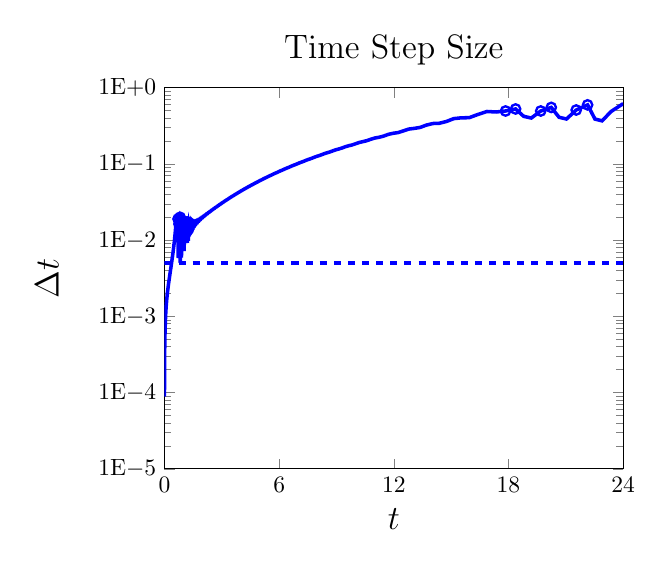
\begin{tikzpicture}[scale=0.85]

\begin{axis}[
  xmin = 0,
  xmax = 24,
  xtick = {0,6,12,18,24},
  xticklabels = {$0$,$6$,$12$,$18$,$24$},
  xlabel = $t$,
  ymode = log,
  ymin = 1E-5,
  ymax = 1E0,
  ytick = {1E-5,1E-4,1E-3,1E-2,1E-1,1E0},
  yticklabels = {$1$E$-5$,$1$E$-4$,$1$E$-3$,$1$E$-2$,$1$E$-1$,$1$E$+0$},
  ylabel = {$\Delta t$},
  ylabel style = {yshift = 10pt},
  label style = {font=\Large},
%  legend entries = {Constant, Adaptive},
%  legend cell align = left,
%  legend pos = north east, 
%  legend style = {draw=none},
  title = {\Large{Time Step Size}}
  ]

% fixed time step size
\addplot [mark=none,blue,line width=1.5,dashed] table{
0.0e0 5e-3
2.4e1 5e-3
};

% adaptive time step size
\addplot [mark=none,blue,line width=1.5] table{
9.3129e-05 9.3129e-05
1.8148e-04 8.8350e-05
2.7721e-04 9.5728e-05
3.7558e-04 9.8379e-05
4.7869e-04 1.0311e-04
5.8520e-04 1.0651e-04
6.9595e-04 1.1075e-04
8.1047e-04 1.1452e-04
9.2907e-04 1.1861e-04
1.0516e-03 1.2255e-04
1.1782e-03 1.2663e-04
1.3089e-03 1.3066e-04
1.4437e-03 1.3477e-04
1.5826e-03 1.3887e-04
1.7256e-03 1.4303e-04
1.8728e-03 1.4720e-04
2.0242e-03 1.5142e-04
2.1798e-03 1.5564e-04
2.3398e-03 1.5993e-04
2.5040e-03 1.6423e-04
2.6726e-03 1.6857e-04
2.8455e-03 1.7296e-04
3.0229e-03 1.7736e-04
3.2047e-03 1.8181e-04
3.3910e-03 1.8631e-04
3.5818e-03 1.9082e-04
3.7772e-03 1.9538e-04
3.9772e-03 1.9998e-04
4.1818e-03 2.0462e-04
4.3911e-03 2.0931e-04
4.6052e-03 2.1404e-04
4.8240e-03 2.1879e-04
5.0476e-03 2.2361e-04
5.2760e-03 2.2844e-04
5.5094e-03 2.3336e-04
5.7477e-03 2.3829e-04
5.9910e-03 2.4329e-04
6.2393e-03 2.4833e-04
6.4927e-03 2.5341e-04
6.7512e-03 2.5853e-04
7.0149e-03 2.6372e-04
7.2839e-03 2.6895e-04
7.5581e-03 2.7423e-04
7.8377e-03 2.7957e-04
8.1226e-03 2.8495e-04
8.4130e-03 2.9038e-04
8.7089e-03 2.9589e-04
9.0103e-03 3.0142e-04
9.3174e-03 3.0703e-04
9.6300e-03 3.1268e-04
9.9484e-03 3.1840e-04
1.0273e-02 3.2417e-04
1.0603e-02 3.2999e-04
1.0938e-02 3.3588e-04
1.1280e-02 3.4183e-04
1.1628e-02 3.4784e-04
1.1982e-02 3.5391e-04
1.2342e-02 3.6003e-04
1.2708e-02 3.6623e-04
1.3081e-02 3.7248e-04
1.3460e-02 3.7882e-04
1.3845e-02 3.8519e-04
1.4236e-02 3.9164e-04
1.4635e-02 3.9816e-04
1.5039e-02 4.0474e-04
1.5451e-02 4.1141e-04
1.5869e-02 4.1812e-04
1.6294e-02 4.2491e-04
1.6726e-02 4.3178e-04
1.7164e-02 4.3870e-04
1.7610e-02 4.4572e-04
1.8063e-02 4.5278e-04
1.8523e-02 4.5993e-04
1.8990e-02 4.6715e-04
1.9464e-02 4.7443e-04
1.9946e-02 4.8182e-04
2.0435e-02 4.8927e-04
2.0932e-02 4.9678e-04
2.1437e-02 5.0440e-04
2.1949e-02 5.1206e-04
2.2468e-02 5.1982e-04
2.2996e-02 5.2766e-04
2.3532e-02 5.3556e-04
2.4075e-02 5.4356e-04
2.4627e-02 5.5164e-04
2.5187e-02 5.5980e-04
2.5755e-02 5.6804e-04
2.6331e-02 5.7636e-04
2.6916e-02 5.8477e-04
2.7509e-02 5.9325e-04
2.8111e-02 6.0182e-04
2.8721e-02 6.1048e-04
2.9341e-02 6.1922e-04
2.9969e-02 6.2805e-04
3.0606e-02 6.3696e-04
3.1252e-02 6.4596e-04
3.1907e-02 6.5505e-04
3.2571e-02 6.6422e-04
3.3244e-02 6.7348e-04
3.3927e-02 6.8284e-04
3.4619e-02 6.9227e-04
3.5321e-02 7.0180e-04
3.6033e-02 7.1142e-04
3.6754e-02 7.2113e-04
3.7485e-02 7.3092e-04
3.8225e-02 7.4082e-04
3.8976e-02 7.5079e-04
3.9737e-02 7.6086e-04
4.0508e-02 7.7103e-04
4.1289e-02 7.8127e-04
4.2081e-02 7.9162e-04
4.2883e-02 8.0207e-04
4.3696e-02 8.1259e-04
4.4519e-02 8.2320e-04
4.5353e-02 8.3392e-04
4.6198e-02 8.4473e-04
4.7053e-02 8.5563e-04
4.7920e-02 8.6662e-04
4.8798e-02 8.7771e-04
4.9686e-02 8.8890e-04
5.0587e-02 9.0016e-04
5.1498e-02 9.1153e-04
5.2421e-02 9.2300e-04
5.3356e-02 9.3455e-04
5.4302e-02 9.4621e-04
5.5260e-02 9.5796e-04
5.6230e-02 9.6979e-04
5.7211e-02 9.8172e-04
5.8205e-02 9.9377e-04
5.9211e-02 1.0059e-03
6.0229e-02 1.0181e-03
6.1260e-02 1.0304e-03
6.2302e-02 1.0429e-03
6.3358e-02 1.0554e-03
6.4426e-02 1.0680e-03
6.5506e-02 1.0807e-03
6.6600e-02 1.0935e-03
6.7706e-02 1.1064e-03
6.8826e-02 1.1194e-03
6.9958e-02 1.1325e-03
7.1104e-02 1.1457e-03
7.2263e-02 1.1590e-03
7.3435e-02 1.1724e-03
7.4621e-02 1.1859e-03
7.5821e-02 1.1995e-03
7.7034e-02 1.2132e-03
7.8261e-02 1.2270e-03
7.9502e-02 1.2409e-03
8.0757e-02 1.2550e-03
8.2026e-02 1.2691e-03
8.3309e-02 1.2833e-03
8.4607e-02 1.2977e-03
8.5919e-02 1.3121e-03
8.7246e-02 1.3267e-03
8.8587e-02 1.3413e-03
8.9943e-02 1.3561e-03
9.1314e-02 1.3710e-03
9.2700e-02 1.3860e-03
9.4101e-02 1.4011e-03
9.5518e-02 1.4164e-03
9.6949e-02 1.4318e-03
9.8397e-02 1.4472e-03
9.9860e-02 1.4629e-03
1.0134e-01 1.4786e-03
1.0283e-01 1.4945e-03
1.0434e-01 1.5104e-03
1.0587e-01 1.5266e-03
1.0741e-01 1.5428e-03
1.0897e-01 1.5592e-03
1.1055e-01 1.5758e-03
1.1214e-01 1.5924e-03
1.1375e-01 1.6093e-03
1.1538e-01 1.6262e-03
1.1702e-01 1.6434e-03
1.1868e-01 1.6606e-03
1.2036e-01 1.6781e-03
1.2205e-01 1.6957e-03
1.2377e-01 1.7134e-03
1.2550e-01 1.7314e-03
1.2725e-01 1.7494e-03
1.2902e-01 1.7677e-03
1.3080e-01 1.7862e-03
1.3261e-01 1.8048e-03
1.3443e-01 1.8237e-03
1.3627e-01 1.8427e-03
1.3813e-01 1.8619e-03
1.4002e-01 1.8813e-03
1.4192e-01 1.9010e-03
1.4384e-01 1.9208e-03
1.4578e-01 1.9408e-03
1.4774e-01 1.9611e-03
1.4972e-01 1.9817e-03
1.5172e-01 2.0024e-03
1.5375e-01 2.0234e-03
1.5579e-01 2.0447e-03
1.5786e-01 2.0662e-03
1.5995e-01 2.0879e-03
1.6206e-01 2.1100e-03
1.6419e-01 2.1323e-03
1.6634e-01 2.1549e-03
1.6852e-01 2.1778e-03
1.7072e-01 2.2010e-03
1.7295e-01 2.2246e-03
1.7519e-01 2.2484e-03
1.7747e-01 2.2726e-03
1.7976e-01 2.2971e-03
1.8209e-01 2.3220e-03
1.8443e-01 2.3473e-03
1.8681e-01 2.3729e-03
1.8921e-01 2.3989e-03
1.9163e-01 2.4253e-03
1.9408e-01 2.4521e-03
1.9656e-01 2.4794e-03
1.9907e-01 2.5070e-03
2.0160e-01 2.5352e-03
2.0417e-01 2.5638e-03
2.0676e-01 2.5929e-03
2.0938e-01 2.6224e-03
2.1204e-01 2.6525e-03
2.1472e-01 2.6832e-03
2.1743e-01 2.7144e-03
2.2018e-01 2.7461e-03
2.2296e-01 2.7785e-03
2.2577e-01 2.8115e-03
2.2861e-01 2.8451e-03
2.3149e-01 2.8793e-03
2.3441e-01 2.9143e-03
2.3736e-01 2.9499e-03
2.4034e-01 2.9863e-03
2.4337e-01 3.0235e-03
2.4643e-01 3.0615e-03
2.4953e-01 3.1003e-03
2.5267e-01 3.1399e-03
2.5585e-01 3.1805e-03
2.5907e-01 3.2219e-03
2.6234e-01 3.2644e-03
2.6564e-01 3.3079e-03
2.6900e-01 3.3524e-03
2.7239e-01 3.3980e-03
2.7584e-01 3.4448e-03
2.7933e-01 3.4928e-03
2.8287e-01 3.5420e-03
2.8647e-01 3.5926e-03
2.9011e-01 3.6446e-03
2.9381e-01 3.6980e-03
2.9756e-01 3.7529e-03
3.0137e-01 3.8095e-03
3.0524e-01 3.8677e-03
3.0917e-01 3.9277e-03
3.1316e-01 3.9896e-03
3.1721e-01 4.0535e-03
3.2133e-01 4.1194e-03
3.2552e-01 4.1876e-03
3.2978e-01 4.2581e-03
3.3411e-01 4.3311e-03
3.3851e-01 4.4067e-03
3.4300e-01 4.4852e-03
3.4757e-01 4.5666e-03
3.5222e-01 4.6513e-03
3.5696e-01 4.7393e-03
3.6179e-01 4.8311e-03
3.6671e-01 4.9268e-03
3.7174e-01 5.0267e-03
3.7687e-01 5.1312e-03
3.8211e-01 5.2406e-03
3.8747e-01 5.3554e-03
3.9294e-01 5.4761e-03
3.9855e-01 5.6031e-03
4.0428e-01 5.7371e-03
4.1016e-01 5.8788e-03
4.1619e-01 6.0289e-03
4.2238e-01 6.1884e-03
4.2874e-01 6.3582e-03
4.3528e-01 6.5398e-03
4.4201e-01 6.7344e-03
4.4896e-01 6.9439e-03
4.5613e-01 7.1702e-03
4.6354e-01 7.4160e-03
4.7123e-01 7.6841e-03
4.7921e-01 7.9786e-03
4.8751e-01 8.3036e-03
4.9618e-01 8.6663e-03
5.0525e-01 9.0728e-03
5.1478e-01 9.5361e-03
5.2485e-01 1.0066e-02
5.3554e-01 1.0690e-02
5.4696e-01 1.1422e-02
5.5930e-01 1.2334e-02
5.7272e-01 1.3429e-02
5.8771e-01 1.4987e-02
6.0442e-01 1.6704e-02
6.2110e-01 1.6689e-02
6.3834e-01 1.7238e-02
6.5594e-01 1.7601e-02
6.7399e-01 1.8049e-02
6.9248e-01 1.8484e-02
7.1142e-01 1.8941e-02
7.1755e-01 6.1355e-03
7.2337e-01 5.8207e-03
7.3140e-01 8.0285e-03
7.4283e-01 1.1425e-02
7.5908e-01 1.6258e-02
7.6638e-01 7.2914e-03
7.7329e-01 6.9173e-03
7.8314e-01 9.8434e-03
7.9714e-01 1.4007e-02
8.1708e-01 1.9933e-02
8.2238e-01 5.2988e-03
8.2740e-01 5.0269e-03
8.3429e-01 6.8863e-03
8.4409e-01 9.7993e-03
8.5803e-01 1.3945e-02
8.7644e-01 1.8404e-02
8.8265e-01 6.2143e-03
8.8855e-01 5.8954e-03
8.9694e-01 8.3893e-03
9.0887e-01 1.1938e-02
9.2586e-01 1.6988e-02
9.3355e-01 7.6845e-03
9.4084e-01 7.2901e-03
9.5121e-01 1.0374e-02
9.6597e-01 1.4762e-02
9.7519e-01 9.2196e-03
9.8394e-01 8.7465e-03
9.9639e-01 1.2446e-02
1.0139e+00 1.7549e-02
1.0215e+00 7.5751e-03
1.0287e+00 7.1864e-03
1.0389e+00 1.0226e-02
1.0535e+00 1.4552e-02
1.0639e+00 1.0438e-02
1.0738e+00 9.9022e-03
1.0879e+00 1.4091e-02
1.1004e+00 1.2457e-02
1.1122e+00 1.1818e-02
1.1282e+00 1.5987e-02
1.1378e+00 9.6607e-03
1.1470e+00 9.1650e-03
1.1600e+00 1.3042e-02
1.1773e+00 1.7292e-02
1.1870e+00 9.6997e-03
1.1962e+00 9.2019e-03
1.2093e+00 1.3095e-02
1.2265e+00 1.7134e-02
1.2368e+00 1.0308e-02
1.2465e+00 9.7791e-03
1.2605e+00 1.3916e-02
1.2758e+00 1.5370e-02
1.2904e+00 1.4581e-02
1.3045e+00 1.4129e-02
1.3197e+00 1.5120e-02
1.3355e+00 1.5831e-02
1.3506e+00 1.5077e-02
1.3651e+00 1.4511e-02
1.3804e+00 1.5329e-02
1.3965e+00 1.6130e-02
1.4121e+00 1.5563e-02
1.4271e+00 1.4962e-02
1.4427e+00 1.5623e-02
1.4591e+00 1.6442e-02
1.4752e+00 1.6040e-02
1.4906e+00 1.5459e-02
1.5066e+00 1.5995e-02
1.5234e+00 1.6788e-02
1.5399e+00 1.6516e-02
1.5559e+00 1.5991e-02
1.5723e+00 1.6434e-02
1.5895e+00 1.7176e-02
1.6065e+00 1.7003e-02
1.6231e+00 1.6549e-02
1.6400e+00 1.6930e-02
1.6576e+00 1.7613e-02
1.6751e+00 1.7510e-02
1.6923e+00 1.7133e-02
1.7097e+00 1.7476e-02
1.7278e+00 1.8098e-02
1.7459e+00 1.8046e-02
1.7636e+00 1.7746e-02
1.7817e+00 1.8069e-02
1.8003e+00 1.8634e-02
1.8189e+00 1.8615e-02
1.8373e+00 1.8389e-02
1.8560e+00 1.8705e-02
1.8753e+00 1.9219e-02
1.8945e+00 1.9225e-02
1.9136e+00 1.9068e-02
1.9329e+00 1.9385e-02
1.9528e+00 1.9854e-02
1.9727e+00 1.9879e-02
1.9925e+00 1.9786e-02
2.0126e+00 2.0110e-02
2.0331e+00 2.0540e-02
2.0537e+00 2.0582e-02
2.0742e+00 2.0548e-02
2.0951e+00 2.0882e-02
2.1164e+00 2.1280e-02
2.1377e+00 2.1337e-02
2.1591e+00 2.1359e-02
2.1808e+00 2.1705e-02
2.2029e+00 2.2076e-02
2.2250e+00 2.2149e-02
2.2472e+00 2.2223e-02
2.2698e+00 2.2582e-02
2.2928e+00 2.2931e-02
2.3158e+00 2.3022e-02
2.3389e+00 2.3146e-02
2.3624e+00 2.3518e-02
2.3863e+00 2.3850e-02
2.4103e+00 2.3961e-02
2.4344e+00 2.4134e-02
2.4589e+00 2.4519e-02
2.4837e+00 2.4838e-02
2.5087e+00 2.4972e-02
2.5339e+00 2.5192e-02
2.5595e+00 2.5590e-02
2.5854e+00 2.5901e-02
2.6115e+00 2.6062e-02
2.6378e+00 2.6328e-02
2.6645e+00 2.6738e-02
2.6916e+00 2.7046e-02
2.7188e+00 2.7238e-02
2.7464e+00 2.7549e-02
2.7743e+00 2.7971e-02
2.8026e+00 2.8281e-02
2.8311e+00 2.8508e-02
2.8600e+00 2.8864e-02
2.8893e+00 2.9298e-02
2.9189e+00 2.9614e-02
2.9488e+00 2.9882e-02
2.9791e+00 3.0282e-02
3.0098e+00 3.0729e-02
3.0409e+00 3.1057e-02
3.0722e+00 3.1370e-02
3.1040e+00 3.1814e-02
3.1363e+00 3.2274e-02
3.1689e+00 3.2621e-02
3.2019e+00 3.2985e-02
3.2354e+00 3.3473e-02
3.2693e+00 3.3947e-02
3.3037e+00 3.4321e-02
3.3384e+00 3.4740e-02
3.3737e+00 3.5271e-02
3.4094e+00 3.5763e-02
3.4456e+00 3.6171e-02
3.4823e+00 3.6651e-02
3.5195e+00 3.7225e-02
3.5572e+00 3.7738e-02
3.5954e+00 3.8190e-02
3.6341e+00 3.8735e-02
3.6735e+00 3.9353e-02
3.7134e+00 3.9892e-02
3.7538e+00 4.0399e-02
3.7948e+00 4.1015e-02
3.8365e+00 4.1675e-02
3.8787e+00 4.2248e-02
3.9215e+00 4.2821e-02
3.9651e+00 4.3513e-02
4.0093e+00 4.4217e-02
4.0541e+00 4.4833e-02
4.0996e+00 4.5486e-02
4.1458e+00 4.6257e-02
4.1929e+00 4.7007e-02
4.2405e+00 4.7678e-02
4.2890e+00 4.8424e-02
4.3382e+00 4.9277e-02
4.3883e+00 5.0078e-02
4.4391e+00 5.0821e-02
4.4908e+00 5.1674e-02
4.5434e+00 5.2612e-02
4.5969e+00 5.3470e-02
4.6512e+00 5.4305e-02
4.7065e+00 5.5280e-02
4.7628e+00 5.6305e-02
4.8200e+00 5.7230e-02
4.8782e+00 5.8182e-02
4.9375e+00 5.9292e-02
4.9979e+00 6.0406e-02
5.0593e+00 6.1418e-02
5.1218e+00 6.2514e-02
5.1856e+00 6.3771e-02
5.2506e+00 6.4977e-02
5.3167e+00 6.6101e-02
5.3840e+00 6.7375e-02
5.4528e+00 6.8787e-02
5.5229e+00 7.0094e-02
5.5943e+00 7.1366e-02
5.6671e+00 7.2852e-02
5.7416e+00 7.4424e-02
5.8174e+00 7.5848e-02
5.8947e+00 7.7318e-02
5.9738e+00 7.9049e-02
6.0546e+00 8.0784e-02
6.1369e+00 8.2353e-02
6.2210e+00 8.4085e-02
6.3071e+00 8.6090e-02
6.3951e+00 8.7988e-02
6.4848e+00 8.9756e-02
6.5767e+00 9.1825e-02
6.6708e+00 9.4124e-02
6.7670e+00 9.6193e-02
6.8652e+00 9.8241e-02
6.9660e+00 1.0073e-01
7.0693e+00 1.0333e-01
7.1749e+00 1.0559e-01
7.2829e+00 1.0805e-01
7.3940e+00 1.1105e-01
7.5079e+00 1.1392e-01
7.6243e+00 1.1645e-01
7.7438e+00 1.1948e-01
7.8669e+00 1.2305e-01
7.9931e+00 1.2618e-01
8.1222e+00 1.2912e-01
8.2551e+00 1.3295e-01
8.3922e+00 1.3708e-01
8.5327e+00 1.4045e-01
8.6767e+00 1.4408e-01
8.8257e+00 1.4894e-01
8.9792e+00 1.5356e-01
9.1365e+00 1.5725e-01
9.2985e+00 1.6199e-01
9.4665e+00 1.6807e-01
9.6395e+00 1.7300e-01
9.8168e+00 1.7728e-01
1.0001e+01 1.8378e-01
1.0192e+01 1.9107e-01
1.0388e+01 1.9608e-01
1.0589e+01 2.0164e-01
1.0800e+01 2.1069e-01
1.1019e+01 2.1878e-01
1.1243e+01 2.2380e-01
1.1475e+01 2.3205e-01
1.1719e+01 2.4427e-01
1.1971e+01 2.5217e-01
1.2229e+01 2.5781e-01
1.2500e+01 2.7114e-01
1.2786e+01 2.8632e-01
1.3079e+01 2.9242e-01
1.3380e+01 3.0109e-01
1.3703e+01 3.2286e-01
1.4041e+01 3.3856e-01
1.4383e+01 3.4148e-01
1.4742e+01 3.5933e-01
1.5135e+01 3.9257e-01
1.5537e+01 4.0229e-01
1.5941e+01 4.0372e-01
1.6385e+01 4.4383e-01
1.6871e+01 4.8690e-01
1.7351e+01 4.7976e-01
1.7846e+01 4.9441e-01
1.8371e+01 5.2539e-01
1.8792e+01 4.2107e-01
1.9192e+01 3.9946e-01
1.9686e+01 4.9432e-01
2.0237e+01 5.5088e-01
2.0646e+01 4.0900e-01
2.1034e+01 3.8801e-01
2.1543e+01 5.0942e-01
2.2138e+01 5.9478e-01
2.2525e+01 3.8737e-01
2.2893e+01 3.6749e-01
2.3383e+01 4.8999e-01
2.4000e+01 6.1716e-01
};

\addplot [only marks,blue,mark=o,mark size=2pt,line width=1.0] table{
7.1142e-01 1.8941e-02
7.5908e-01 1.6258e-02
8.1708e-01 1.9933e-02
8.7644e-01 1.8404e-02
9.2586e-01 1.6988e-02
9.6597e-01 1.4762e-02
1.0139e+00 1.7549e-02
1.0535e+00 1.4552e-02
1.0879e+00 1.4091e-02
1.1282e+00 1.5987e-02
1.1773e+00 1.7292e-02
1.2265e+00 1.7134e-02
1.2605e+00 1.3916e-02
1.7846e+01 4.9441e-01
1.8371e+01 5.2539e-01
1.9686e+01 4.9432e-01
2.0237e+01 5.5088e-01
2.1543e+01 5.0942e-01
2.2138e+01 5.9478e-01
};


%% adaptive time step size
%\addplot [mark=none,blue,line width=1.5] table{
%6.5862e-05 6.5862e-05
%1.3001e-04 6.4150e-05
%1.9698e-04 6.6968e-05
%2.6529e-04 6.8307e-05
%3.3490e-04 6.9614e-05
%4.0587e-04 7.0970e-05
%4.7829e-04 7.2418e-05
%5.5207e-04 7.3779e-05
%6.2725e-04 7.5179e-05
%7.0368e-04 7.6430e-05
%7.8155e-04 7.7869e-05
%8.6084e-04 7.9292e-05
%9.4127e-04 8.0430e-05
%1.0232e-03 8.1958e-05
%1.1066e-03 8.3367e-05
%1.1913e-03 8.4671e-05
%1.2773e-03 8.6076e-05
%1.3647e-03 8.7411e-05
%1.4536e-03 8.8808e-05
%1.5437e-03 9.0187e-05
%1.6353e-03 9.1595e-05
%1.7283e-03 9.3010e-05
%1.8227e-03 9.4378e-05
%1.9184e-03 9.5695e-05
%2.0156e-03 9.7157e-05
%2.1142e-03 9.8598e-05
%2.2141e-03 9.9951e-05
%2.3155e-03 1.0136e-04
%2.4184e-03 1.0293e-04
%2.5227e-03 1.0429e-04
%2.6285e-03 1.0576e-04
%2.7356e-03 1.0717e-04
%2.8443e-03 1.0863e-04
%2.9544e-03 1.1012e-04
%3.0660e-03 1.1158e-04
%3.1792e-03 1.1321e-04
%3.2937e-03 1.1451e-04
%3.4098e-03 1.1612e-04
%3.5275e-03 1.1767e-04
%3.6466e-03 1.1915e-04
%3.7674e-03 1.2078e-04
%3.8896e-03 1.2220e-04
%4.0135e-03 1.2386e-04
%4.1389e-03 1.2548e-04
%4.2660e-03 1.2701e-04
%4.3946e-03 1.2862e-04
%4.5248e-03 1.3026e-04
%4.6567e-03 1.3183e-04
%4.7902e-03 1.3356e-04
%4.9254e-03 1.3521e-04
%5.0624e-03 1.3694e-04
%5.2009e-03 1.3852e-04
%5.3412e-03 1.4030e-04
%5.4831e-03 1.4190e-04
%5.6268e-03 1.4373e-04
%5.7723e-03 1.4546e-04
%5.9194e-03 1.4716e-04
%6.0684e-03 1.4896e-04
%6.2193e-03 1.5087e-04
%6.3719e-03 1.5261e-04
%6.5264e-03 1.5448e-04
%6.6826e-03 1.5629e-04
%6.8408e-03 1.5816e-04
%7.0007e-03 1.5995e-04
%7.1627e-03 1.6197e-04
%7.3266e-03 1.6388e-04
%7.4923e-03 1.6575e-04
%7.6601e-03 1.6776e-04
%7.8298e-03 1.6966e-04
%8.0015e-03 1.7170e-04
%8.1751e-03 1.7362e-04
%8.3508e-03 1.7572e-04
%8.5286e-03 1.7776e-04
%8.7084e-03 1.7984e-04
%8.8904e-03 1.8196e-04
%9.0744e-03 1.8406e-04
%9.2605e-03 1.8609e-04
%9.4489e-03 1.8836e-04
%9.6394e-03 1.9053e-04
%9.8320e-03 1.9262e-04
%1.0027e-02 1.9497e-04
%1.0224e-02 1.9719e-04
%1.0424e-02 1.9942e-04
%1.0625e-02 2.0173e-04
%1.0829e-02 2.0403e-04
%1.1036e-02 2.0635e-04
%1.1245e-02 2.0886e-04
%1.1456e-02 2.1099e-04
%1.1669e-02 2.1356e-04
%1.1885e-02 2.1600e-04
%1.2104e-02 2.1851e-04
%1.2325e-02 2.2102e-04
%1.2548e-02 2.2354e-04
%1.2774e-02 2.2606e-04
%1.3003e-02 2.2871e-04
%1.3234e-02 2.3134e-04
%1.3468e-02 2.3398e-04
%1.3705e-02 2.3654e-04
%1.3944e-02 2.3933e-04
%1.4186e-02 2.4199e-04
%1.4431e-02 2.4485e-04
%1.4679e-02 2.4770e-04
%1.4929e-02 2.5047e-04
%1.5183e-02 2.5335e-04
%1.5439e-02 2.5628e-04
%1.5698e-02 2.5918e-04
%1.5960e-02 2.6212e-04
%1.6225e-02 2.6515e-04
%1.6493e-02 2.6817e-04
%1.6765e-02 2.7124e-04
%1.7039e-02 2.7445e-04
%1.7317e-02 2.7756e-04
%1.7597e-02 2.8067e-04
%1.7881e-02 2.8407e-04
%1.8169e-02 2.8724e-04
%1.8459e-02 2.9061e-04
%1.8753e-02 2.9398e-04
%1.9051e-02 2.9732e-04
%1.9351e-02 3.0080e-04
%1.9656e-02 3.0434e-04
%1.9964e-02 3.0782e-04
%2.0275e-02 3.1141e-04
%2.0590e-02 3.1504e-04
%2.0909e-02 3.1879e-04
%2.1231e-02 3.2252e-04
%2.1558e-02 3.2624e-04
%2.1888e-02 3.3000e-04
%2.2221e-02 3.3397e-04
%2.2559e-02 3.3789e-04
%2.2901e-02 3.4191e-04
%2.3247e-02 3.4585e-04
%2.3597e-02 3.5008e-04
%2.3951e-02 3.5420e-04
%2.4310e-02 3.5843e-04
%2.4672e-02 3.6266e-04
%2.5040e-02 3.6710e-04
%2.5411e-02 3.7146e-04
%2.5787e-02 3.7600e-04
%2.6168e-02 3.8051e-04
%2.6553e-02 3.8511e-04
%2.6942e-02 3.8979e-04
%2.7337e-02 3.9452e-04
%2.7736e-02 3.9926e-04
%2.8141e-02 4.0426e-04
%2.8550e-02 4.0919e-04
%2.8964e-02 4.1424e-04
%2.9383e-02 4.1936e-04
%2.9808e-02 4.2455e-04
%3.0238e-02 4.2994e-04
%3.0673e-02 4.3523e-04
%3.1114e-02 4.4073e-04
%3.1560e-02 4.4623e-04
%3.2012e-02 4.5192e-04
%3.2470e-02 4.5766e-04
%3.2933e-02 4.6349e-04
%3.3402e-02 4.6942e-04
%3.3878e-02 4.7547e-04
%3.4360e-02 4.8164e-04
%3.4847e-02 4.8785e-04
%3.5342e-02 4.9416e-04
%3.5842e-02 5.0069e-04
%3.6350e-02 5.0725e-04
%3.6863e-02 5.1397e-04
%3.7384e-02 5.2083e-04
%3.7912e-02 5.2781e-04
%3.8447e-02 5.3489e-04
%3.8989e-02 5.4214e-04
%3.9539e-02 5.4951e-04
%4.0096e-02 5.5696e-04
%4.0660e-02 5.6460e-04
%4.1233e-02 5.7242e-04
%4.1813e-02 5.8048e-04
%4.2402e-02 5.8855e-04
%4.2999e-02 5.9686e-04
%4.3604e-02 6.0536e-04
%4.4218e-02 6.1405e-04
%4.4841e-02 6.2293e-04
%4.5473e-02 6.3191e-04
%4.6114e-02 6.4125e-04
%4.6765e-02 6.5064e-04
%4.7425e-02 6.6027e-04
%4.8095e-02 6.7020e-04
%4.8775e-02 6.8030e-04
%4.9466e-02 6.9070e-04
%5.0167e-02 7.0113e-04
%5.0880e-02 7.1224e-04
%5.1603e-02 7.2336e-04
%5.2338e-02 7.3478e-04
%5.3084e-02 7.4655e-04
%5.3843e-02 7.5862e-04
%5.4614e-02 7.7096e-04
%5.5398e-02 7.8368e-04
%5.6194e-02 7.9667e-04
%5.7004e-02 8.1001e-04
%5.7828e-02 8.2400e-04
%5.8666e-02 8.3820e-04
%5.9519e-02 8.5286e-04
%6.0387e-02 8.6800e-04
%6.1271e-02 8.8361e-04
%6.2171e-02 8.9968e-04
%6.3087e-02 9.1626e-04
%6.4020e-02 9.3356e-04
%6.4972e-02 9.5129e-04
%6.5941e-02 9.6971e-04
%6.6930e-02 9.8869e-04
%6.7939e-02 1.0085e-03
%6.8968e-02 1.0292e-03
%7.0018e-02 1.0505e-03
%7.1091e-02 1.0729e-03
%7.2187e-02 1.0960e-03
%7.3307e-02 1.1201e-03
%7.4453e-02 1.1455e-03
%7.5625e-02 1.1719e-03
%7.6824e-02 1.1996e-03
%7.8053e-02 1.2288e-03
%7.9312e-02 1.2594e-03
%8.0604e-02 1.2916e-03
%8.1930e-02 1.3257e-03
%8.3292e-02 1.3617e-03
%8.4692e-02 1.4000e-03
%8.6132e-02 1.4409e-03
%8.7617e-02 1.4843e-03
%8.9148e-02 1.5309e-03
%9.0729e-02 1.5811e-03
%9.2364e-02 1.6354e-03
%9.4058e-02 1.6941e-03
%9.5817e-02 1.7586e-03
%9.7646e-02 1.8292e-03
%9.9554e-02 1.9077e-03
%1.0155e-01 1.9953e-03
%1.0364e-01 2.0944e-03
%1.0585e-01 2.2077e-03
%1.0819e-01 2.3397e-03
%1.1069e-01 2.4967e-03
%1.1338e-01 2.6886e-03
%1.1631e-01 2.9321e-03
%1.1957e-01 3.2591e-03
%1.2331e-01 3.7389e-03
%1.2708e-01 3.7714e-03
%1.3096e-01 3.8802e-03
%1.3492e-01 3.9574e-03
%1.3896e-01 4.0489e-03
%1.4310e-01 4.1349e-03
%1.4732e-01 4.2238e-03
%1.5133e-01 4.0053e-03
%1.5511e-01 3.7831e-03
%1.5880e-01 3.6848e-03
%1.6225e-01 3.4579e-03
%1.6562e-01 3.3680e-03
%1.6888e-01 3.2631e-03
%1.7206e-01 3.1782e-03
%1.7526e-01 3.1954e-03
%1.7839e-01 3.1292e-03
%1.8146e-01 3.0760e-03
%1.8449e-01 3.0304e-03
%1.8749e-01 2.9914e-03
%1.9044e-01 2.9574e-03
%1.9337e-01 2.9279e-03
%1.9627e-01 2.9021e-03
%1.9915e-01 2.8794e-03
%2.0201e-01 2.8596e-03
%2.0485e-01 2.8420e-03
%2.0768e-01 2.8266e-03
%2.1049e-01 2.8131e-03
%2.1330e-01 2.8013e-03
%2.1609e-01 2.7908e-03
%2.1887e-01 2.7818e-03
%2.2164e-01 2.7738e-03
%2.2441e-01 2.7671e-03
%2.2717e-01 2.7613e-03
%2.2993e-01 2.7564e-03
%2.3268e-01 2.7523e-03
%2.3543e-01 2.7490e-03
%2.3817e-01 2.7465e-03
%2.4092e-01 2.7444e-03
%2.4366e-01 2.7431e-03
%2.4640e-01 2.7422e-03
%2.4915e-01 2.7419e-03
%2.5189e-01 2.7421e-03
%2.5463e-01 2.7428e-03
%2.5737e-01 2.7437e-03
%2.6012e-01 2.7453e-03
%2.6287e-01 2.7469e-03
%2.6562e-01 2.7492e-03
%2.6837e-01 2.7516e-03
%2.7112e-01 2.7544e-03
%2.7388e-01 2.7575e-03
%2.7664e-01 2.7608e-03
%2.7940e-01 2.7644e-03
%2.8217e-01 2.7682e-03
%2.8495e-01 2.7724e-03
%2.8772e-01 2.7766e-03
%2.9050e-01 2.7812e-03
%2.9329e-01 2.7859e-03
%2.9608e-01 2.7906e-03
%2.9888e-01 2.7959e-03
%3.0168e-01 2.8011e-03
%3.0448e-01 2.8065e-03
%3.0729e-01 2.8121e-03
%3.1011e-01 2.8177e-03
%3.1294e-01 2.8236e-03
%3.1577e-01 2.8296e-03
%3.1860e-01 2.8358e-03
%3.2144e-01 2.8419e-03
%3.2429e-01 2.8484e-03
%3.2715e-01 2.8548e-03
%3.3001e-01 2.8614e-03
%3.3288e-01 2.8681e-03
%3.3575e-01 2.8748e-03
%3.3863e-01 2.8817e-03
%3.4152e-01 2.8887e-03
%3.4442e-01 2.8957e-03
%3.4732e-01 2.9028e-03
%3.5023e-01 2.9100e-03
%3.5315e-01 2.9173e-03
%3.5607e-01 2.9246e-03
%3.5900e-01 2.9321e-03
%3.6194e-01 2.9396e-03
%3.6489e-01 2.9471e-03
%3.6785e-01 2.9548e-03
%3.7081e-01 2.9624e-03
%3.7378e-01 2.9701e-03
%3.7676e-01 2.9779e-03
%3.7974e-01 2.9857e-03
%3.8274e-01 2.9937e-03
%3.8574e-01 3.0015e-03
%3.8875e-01 3.0096e-03
%3.9176e-01 3.0175e-03
%3.9479e-01 3.0255e-03
%3.9782e-01 3.0337e-03
%4.0086e-01 3.0418e-03
%4.0392e-01 3.0500e-03
%4.0697e-01 3.0582e-03
%4.1004e-01 3.0664e-03
%4.1311e-01 3.0746e-03
%4.1620e-01 3.0830e-03
%4.1929e-01 3.0914e-03
%4.2239e-01 3.0997e-03
%4.2550e-01 3.1081e-03
%4.2861e-01 3.1165e-03
%4.3174e-01 3.1250e-03
%4.3487e-01 3.1333e-03
%4.3801e-01 3.1419e-03
%4.4116e-01 3.1504e-03
%4.4432e-01 3.1589e-03
%4.4749e-01 3.1674e-03
%4.5067e-01 3.1760e-03
%4.5385e-01 3.1846e-03
%4.5704e-01 3.1932e-03
%4.6025e-01 3.2018e-03
%4.6346e-01 3.2105e-03
%4.6668e-01 3.2192e-03
%4.6990e-01 3.2278e-03
%4.7314e-01 3.2365e-03
%4.7638e-01 3.2451e-03
%4.7964e-01 3.2539e-03
%4.8290e-01 3.2627e-03
%4.8617e-01 3.2713e-03
%4.8945e-01 3.2800e-03
%4.9274e-01 3.2888e-03
%4.9604e-01 3.2977e-03
%4.9935e-01 3.3062e-03
%5.0266e-01 3.3152e-03
%5.0598e-01 3.3239e-03
%5.0932e-01 3.3327e-03
%5.1266e-01 3.3416e-03
%5.1601e-01 3.3504e-03
%5.1937e-01 3.3592e-03
%5.2274e-01 3.3682e-03
%5.2611e-01 3.3769e-03
%5.2950e-01 3.3858e-03
%5.3289e-01 3.3947e-03
%5.3630e-01 3.4036e-03
%5.3971e-01 3.4125e-03
%5.4313e-01 3.4212e-03
%5.4656e-01 3.4303e-03
%5.5000e-01 3.4393e-03
%5.5345e-01 3.4481e-03
%5.5691e-01 3.4571e-03
%5.6037e-01 3.4661e-03
%5.6385e-01 3.4749e-03
%5.6733e-01 3.4840e-03
%5.7082e-01 3.4930e-03
%5.7433e-01 3.5020e-03
%5.7784e-01 3.5109e-03
%5.8136e-01 3.5200e-03
%5.8489e-01 3.5289e-03
%5.8842e-01 3.5381e-03
%5.9197e-01 3.5470e-03
%5.9553e-01 3.5561e-03
%5.9909e-01 3.5652e-03
%6.0267e-01 3.5742e-03
%6.0625e-01 3.5834e-03
%6.0984e-01 3.5924e-03
%6.1344e-01 3.6015e-03
%6.1705e-01 3.6106e-03
%6.2067e-01 3.6198e-03
%6.2430e-01 3.6290e-03
%6.2794e-01 3.6381e-03
%6.3159e-01 3.6473e-03
%6.3524e-01 3.6564e-03
%6.3891e-01 3.6657e-03
%6.4259e-01 3.6749e-03
%6.4627e-01 3.6840e-03
%6.4996e-01 3.6933e-03
%6.5367e-01 3.7025e-03
%6.5738e-01 3.7118e-03
%6.6110e-01 3.7212e-03
%6.6483e-01 3.7304e-03
%6.6857e-01 3.7397e-03
%6.7232e-01 3.7490e-03
%6.7608e-01 3.7584e-03
%6.7984e-01 3.7678e-03
%6.8362e-01 3.7771e-03
%6.8741e-01 3.7866e-03
%6.9120e-01 3.7959e-03
%6.9501e-01 3.8054e-03
%6.9882e-01 3.8148e-03
%7.0265e-01 3.8243e-03
%7.0648e-01 3.8338e-03
%7.1032e-01 3.8433e-03
%7.1418e-01 3.8528e-03
%7.1804e-01 3.8623e-03
%7.2191e-01 3.8719e-03
%7.2579e-01 3.8816e-03
%7.2968e-01 3.8911e-03
%7.3359e-01 3.9008e-03
%7.3750e-01 3.9104e-03
%7.4142e-01 3.9201e-03
%7.4535e-01 3.9299e-03
%7.4928e-01 3.9395e-03
%7.5323e-01 3.9493e-03
%7.5719e-01 3.9590e-03
%7.6116e-01 3.9688e-03
%7.6514e-01 3.9787e-03
%7.6913e-01 3.9884e-03
%7.7313e-01 3.9983e-03
%7.7714e-01 4.0083e-03
%7.8115e-01 4.0181e-03
%7.8518e-01 4.0281e-03
%7.8922e-01 4.0381e-03
%7.9327e-01 4.0481e-03
%7.9733e-01 4.0582e-03
%8.0139e-01 4.0681e-03
%8.0547e-01 4.0782e-03
%8.0956e-01 4.0883e-03
%8.1366e-01 4.0986e-03
%8.1777e-01 4.1086e-03
%8.2189e-01 4.1189e-03
%8.2602e-01 4.1291e-03
%8.3016e-01 4.1394e-03
%8.3431e-01 4.1496e-03
%8.3847e-01 4.1600e-03
%8.4264e-01 4.1703e-03
%8.4682e-01 4.1807e-03
%8.5101e-01 4.1911e-03
%8.5521e-01 4.2016e-03
%8.5942e-01 4.2121e-03
%8.6364e-01 4.2225e-03
%8.6788e-01 4.2330e-03
%8.7212e-01 4.2436e-03
%8.7637e-01 4.2543e-03
%8.8064e-01 4.2649e-03
%8.8491e-01 4.2756e-03
%8.8920e-01 4.2863e-03
%8.9350e-01 4.2971e-03
%8.9781e-01 4.3078e-03
%9.0212e-01 4.3187e-03
%9.0645e-01 4.3296e-03
%9.1079e-01 4.3404e-03
%9.1515e-01 4.3513e-03
%9.1951e-01 4.3624e-03
%9.2388e-01 4.3733e-03
%9.2827e-01 4.3845e-03
%9.3266e-01 4.3954e-03
%9.3707e-01 4.4066e-03
%9.4149e-01 4.4179e-03
%9.4592e-01 4.4289e-03
%9.5036e-01 4.4402e-03
%9.5481e-01 4.4515e-03
%9.5927e-01 4.4629e-03
%9.6374e-01 4.4742e-03
%9.6823e-01 4.4856e-03
%9.7273e-01 4.4971e-03
%9.7724e-01 4.5086e-03
%9.8176e-01 4.5201e-03
%9.8629e-01 4.5317e-03
%9.9083e-01 4.5431e-03
%9.9538e-01 4.5550e-03
%9.9995e-01 4.5667e-03
%1.0045e+00 4.5784e-03
%1.0091e+00 4.5902e-03
%1.0137e+00 4.6020e-03
%1.0183e+00 4.6139e-03
%1.0230e+00 4.6257e-03
%1.0276e+00 4.6378e-03
%1.0322e+00 4.6498e-03
%1.0369e+00 4.6619e-03
%1.0416e+00 4.6740e-03
%1.0463e+00 4.6862e-03
%1.0510e+00 4.6984e-03
%1.0557e+00 4.7107e-03
%1.0604e+00 4.7229e-03
%1.0651e+00 4.7354e-03
%1.0699e+00 4.7476e-03
%1.0746e+00 4.7601e-03
%1.0794e+00 4.7726e-03
%1.0842e+00 4.7852e-03
%1.0890e+00 4.7977e-03
%1.0938e+00 4.8104e-03
%1.0986e+00 4.8231e-03
%1.1035e+00 4.8359e-03
%1.1083e+00 4.8488e-03
%1.1132e+00 4.8615e-03
%1.1181e+00 4.8745e-03
%1.1229e+00 4.8875e-03
%1.1278e+00 4.9005e-03
%1.1328e+00 4.9135e-03
%1.1377e+00 4.9267e-03
%1.1426e+00 4.9399e-03
%1.1476e+00 4.9531e-03
%1.1525e+00 4.9664e-03
%1.1575e+00 4.9797e-03
%1.1625e+00 4.9931e-03
%1.1675e+00 5.0066e-03
%1.1725e+00 5.0199e-03
%1.1776e+00 5.0336e-03
%1.1826e+00 5.0473e-03
%1.1877e+00 5.0609e-03
%1.1928e+00 5.0746e-03
%1.1978e+00 5.0885e-03
%1.2030e+00 5.1023e-03
%1.2081e+00 5.1163e-03
%1.2132e+00 5.1303e-03
%1.2183e+00 5.1443e-03
%1.2235e+00 5.1584e-03
%1.2287e+00 5.1725e-03
%1.2339e+00 5.1867e-03
%1.2391e+00 5.2010e-03
%1.2443e+00 5.2155e-03
%1.2495e+00 5.2298e-03
%1.2547e+00 5.2442e-03
%1.2600e+00 5.2588e-03
%1.2653e+00 5.2733e-03
%1.2706e+00 5.2881e-03
%1.2759e+00 5.3027e-03
%1.2812e+00 5.3176e-03
%1.2865e+00 5.3324e-03
%1.2919e+00 5.3473e-03
%1.2972e+00 5.3623e-03
%1.3026e+00 5.3774e-03
%1.3080e+00 5.3925e-03
%1.3134e+00 5.4077e-03
%1.3188e+00 5.4229e-03
%1.3243e+00 5.4382e-03
%1.3297e+00 5.4537e-03
%1.3352e+00 5.4691e-03
%1.3407e+00 5.4846e-03
%1.3462e+00 5.5003e-03
%1.3517e+00 5.5159e-03
%1.3572e+00 5.5317e-03
%1.3628e+00 5.5475e-03
%1.3683e+00 5.5634e-03
%1.3739e+00 5.5793e-03
%1.3795e+00 5.5954e-03
%1.3851e+00 5.6114e-03
%1.3908e+00 5.6277e-03
%1.3964e+00 5.6440e-03
%1.4021e+00 5.6602e-03
%1.4077e+00 5.6767e-03
%1.4134e+00 5.6931e-03
%1.4191e+00 5.7097e-03
%1.4249e+00 5.7264e-03
%1.4306e+00 5.7430e-03
%1.4364e+00 5.7599e-03
%1.4421e+00 5.7768e-03
%1.4479e+00 5.7936e-03
%1.4537e+00 5.8108e-03
%1.4596e+00 5.8278e-03
%1.4654e+00 5.8450e-03
%1.4713e+00 5.8623e-03
%1.4772e+00 5.8797e-03
%1.4831e+00 5.8971e-03
%1.4890e+00 5.9146e-03
%1.4949e+00 5.9322e-03
%1.5009e+00 5.9500e-03
%1.5068e+00 5.9677e-03
%1.5128e+00 5.9855e-03
%1.5188e+00 6.0036e-03
%1.5248e+00 6.0215e-03
%1.5309e+00 6.0397e-03
%1.5369e+00 6.0579e-03
%1.5430e+00 6.0762e-03
%1.5491e+00 6.0946e-03
%1.5552e+00 6.1130e-03
%1.5613e+00 6.1316e-03
%1.5675e+00 6.1503e-03
%1.5737e+00 6.1690e-03
%1.5799e+00 6.1878e-03
%1.5861e+00 6.2068e-03
%1.5923e+00 6.2258e-03
%1.5985e+00 6.2449e-03
%1.6048e+00 6.2642e-03
%1.6111e+00 6.2835e-03
%1.6174e+00 6.3029e-03
%1.6237e+00 6.3224e-03
%1.6300e+00 6.3420e-03
%1.6364e+00 6.3617e-03
%1.6428e+00 6.3814e-03
%1.6492e+00 6.4014e-03
%1.6556e+00 6.4213e-03
%1.6621e+00 6.4414e-03
%1.6685e+00 6.4617e-03
%1.6750e+00 6.4820e-03
%1.6815e+00 6.5023e-03
%1.6880e+00 6.5229e-03
%1.6946e+00 6.5435e-03
%1.7011e+00 6.5642e-03
%1.7077e+00 6.5851e-03
%1.7143e+00 6.6059e-03
%1.7209e+00 6.6270e-03
%1.7276e+00 6.6482e-03
%1.7343e+00 6.6694e-03
%1.7410e+00 6.6909e-03
%1.7477e+00 6.7122e-03
%1.7544e+00 6.7339e-03
%1.7612e+00 6.7556e-03
%1.7679e+00 6.7773e-03
%1.7747e+00 6.7993e-03
%1.7816e+00 6.8213e-03
%1.7884e+00 6.8434e-03
%1.7953e+00 6.8658e-03
%1.8022e+00 6.8882e-03
%1.8091e+00 6.9107e-03
%1.8160e+00 6.9333e-03
%1.8230e+00 6.9561e-03
%1.8299e+00 6.9789e-03
%1.8369e+00 7.0018e-03
%1.8440e+00 7.0250e-03
%1.8510e+00 7.0483e-03
%1.8581e+00 7.0716e-03
%1.8652e+00 7.0951e-03
%1.8723e+00 7.1187e-03
%1.8794e+00 7.1425e-03
%1.8866e+00 7.1663e-03
%1.8938e+00 7.1904e-03
%1.9010e+00 7.2145e-03
%1.9082e+00 7.2387e-03
%1.9155e+00 7.2629e-03
%1.9228e+00 7.2877e-03
%1.9301e+00 7.3123e-03
%1.9374e+00 7.3371e-03
%1.9448e+00 7.3619e-03
%1.9522e+00 7.3871e-03
%1.9596e+00 7.4123e-03
%1.9670e+00 7.4376e-03
%1.9745e+00 7.4631e-03
%1.9820e+00 7.4887e-03
%1.9895e+00 7.5145e-03
%1.9970e+00 7.5404e-03
%2.0046e+00 7.5665e-03
%2.0122e+00 7.5927e-03
%2.0198e+00 7.6190e-03
%2.0275e+00 7.6455e-03
%2.0351e+00 7.6722e-03
%2.0428e+00 7.6989e-03
%2.0506e+00 7.7259e-03
%2.0583e+00 7.7530e-03
%2.0661e+00 7.7802e-03
%2.0739e+00 7.8076e-03
%2.0817e+00 7.8352e-03
%2.0896e+00 7.8628e-03
%2.0975e+00 7.8908e-03
%2.1054e+00 7.9188e-03
%2.1134e+00 7.9470e-03
%2.1213e+00 7.9753e-03
%2.1293e+00 8.0040e-03
%2.1374e+00 8.0325e-03
%2.1454e+00 8.0614e-03
%2.1535e+00 8.0905e-03
%2.1616e+00 8.1197e-03
%2.1698e+00 8.1490e-03
%2.1780e+00 8.1785e-03
%2.1862e+00 8.2082e-03
%2.1944e+00 8.2381e-03
%2.2027e+00 8.2681e-03
%2.2110e+00 8.2984e-03
%2.2193e+00 8.3288e-03
%2.2277e+00 8.3593e-03
%2.2361e+00 8.3902e-03
%2.2445e+00 8.4211e-03
%2.2529e+00 8.4523e-03
%2.2614e+00 8.4835e-03
%2.2699e+00 8.5152e-03
%2.2785e+00 8.5468e-03
%2.2871e+00 8.5787e-03
%2.2957e+00 8.6108e-03
%2.3043e+00 8.6431e-03
%2.3130e+00 8.6755e-03
%2.3217e+00 8.7082e-03
%2.3304e+00 8.7410e-03
%2.3392e+00 8.7741e-03
%2.3480e+00 8.8074e-03
%2.3569e+00 8.8408e-03
%2.3657e+00 8.8745e-03
%2.3746e+00 8.9084e-03
%2.3836e+00 8.9426e-03
%2.3926e+00 8.9768e-03
%2.4016e+00 9.0114e-03
%2.4106e+00 9.0461e-03
%2.4197e+00 9.0810e-03
%2.4288e+00 9.1160e-03
%2.4380e+00 9.1516e-03
%2.4472e+00 9.1871e-03
%2.4564e+00 9.2230e-03
%2.4656e+00 9.2590e-03
%2.4749e+00 9.2952e-03
%2.4843e+00 9.3318e-03
%2.4936e+00 9.3685e-03
%2.5030e+00 9.4055e-03
%2.5125e+00 9.4426e-03
%2.5220e+00 9.4801e-03
%2.5315e+00 9.5176e-03
%2.5410e+00 9.5557e-03
%2.5506e+00 9.5938e-03
%2.5603e+00 9.6322e-03
%2.5699e+00 9.6709e-03
%2.5796e+00 9.7097e-03
%2.5894e+00 9.7490e-03
%2.5992e+00 9.7882e-03
%2.6090e+00 9.8280e-03
%2.6189e+00 9.8679e-03
%2.6288e+00 9.9080e-03
%2.6387e+00 9.9485e-03
%2.6487e+00 9.9891e-03
%2.6588e+00 1.0030e-02
%2.6688e+00 1.0071e-02
%2.6789e+00 1.0113e-02
%2.6891e+00 1.0155e-02
%2.6993e+00 1.0197e-02
%2.7095e+00 1.0239e-02
%2.7198e+00 1.0282e-02
%2.7301e+00 1.0325e-02
%2.7405e+00 1.0368e-02
%2.7509e+00 1.0411e-02
%2.7614e+00 1.0455e-02
%2.7719e+00 1.0499e-02
%2.7824e+00 1.0543e-02
%2.7930e+00 1.0588e-02
%2.8036e+00 1.0633e-02
%2.8143e+00 1.0678e-02
%2.8250e+00 1.0724e-02
%2.8358e+00 1.0770e-02
%2.8466e+00 1.0816e-02
%2.8575e+00 1.0862e-02
%2.8684e+00 1.0909e-02
%2.8793e+00 1.0956e-02
%2.8904e+00 1.1004e-02
%2.9014e+00 1.1052e-02
%2.9125e+00 1.1100e-02
%2.9237e+00 1.1148e-02
%2.9348e+00 1.1197e-02
%2.9461e+00 1.1246e-02
%2.9574e+00 1.1296e-02
%2.9687e+00 1.1345e-02
%2.9801e+00 1.1396e-02
%2.9916e+00 1.1446e-02
%3.0031e+00 1.1497e-02
%3.0146e+00 1.1548e-02
%3.0262e+00 1.1600e-02
%3.0379e+00 1.1652e-02
%3.0496e+00 1.1704e-02
%3.0613e+00 1.1757e-02
%3.0731e+00 1.1810e-02
%3.0850e+00 1.1863e-02
%3.0969e+00 1.1917e-02
%3.1089e+00 1.1972e-02
%3.1209e+00 1.2026e-02
%3.1330e+00 1.2081e-02
%3.1451e+00 1.2137e-02
%3.1573e+00 1.2192e-02
%3.1696e+00 1.2249e-02
%3.1819e+00 1.2305e-02
%3.1942e+00 1.2362e-02
%3.2067e+00 1.2420e-02
%3.2191e+00 1.2478e-02
%3.2317e+00 1.2536e-02
%3.2443e+00 1.2595e-02
%3.2569e+00 1.2654e-02
%3.2696e+00 1.2714e-02
%3.2824e+00 1.2774e-02
%3.2953e+00 1.2834e-02
%3.3081e+00 1.2895e-02
%3.3211e+00 1.2957e-02
%3.3341e+00 1.3019e-02
%3.3472e+00 1.3081e-02
%3.3603e+00 1.3144e-02
%3.3736e+00 1.3207e-02
%3.3868e+00 1.3271e-02
%3.4002e+00 1.3335e-02
%3.4136e+00 1.3400e-02
%3.4270e+00 1.3465e-02
%3.4406e+00 1.3531e-02
%3.4542e+00 1.3597e-02
%3.4678e+00 1.3664e-02
%3.4816e+00 1.3731e-02
%3.4954e+00 1.3799e-02
%3.5092e+00 1.3868e-02
%3.5232e+00 1.3937e-02
%3.5372e+00 1.4006e-02
%3.5512e+00 1.4076e-02
%3.5654e+00 1.4146e-02
%3.5796e+00 1.4217e-02
%3.5939e+00 1.4289e-02
%3.6083e+00 1.4361e-02
%3.6227e+00 1.4434e-02
%3.6372e+00 1.4507e-02
%3.6518e+00 1.4581e-02
%3.6664e+00 1.4656e-02
%3.6812e+00 1.4731e-02
%3.6960e+00 1.4807e-02
%3.7109e+00 1.4883e-02
%3.7258e+00 1.4960e-02
%3.7408e+00 1.5038e-02
%3.7560e+00 1.5116e-02
%3.7712e+00 1.5195e-02
%3.7864e+00 1.5274e-02
%3.8018e+00 1.5354e-02
%3.8172e+00 1.5435e-02
%3.8327e+00 1.5516e-02
%3.8483e+00 1.5598e-02
%3.8640e+00 1.5681e-02
%3.8798e+00 1.5765e-02
%3.8956e+00 1.5849e-02
%3.9116e+00 1.5934e-02
%3.9276e+00 1.6020e-02
%3.9437e+00 1.6106e-02
%3.9599e+00 1.6193e-02
%3.9762e+00 1.6281e-02
%3.9925e+00 1.6369e-02
%4.0090e+00 1.6458e-02
%4.0255e+00 1.6548e-02
%4.0422e+00 1.6639e-02
%4.0589e+00 1.6731e-02
%4.0757e+00 1.6823e-02
%4.0927e+00 1.6916e-02
%4.1097e+00 1.7010e-02
%4.1268e+00 1.7105e-02
%4.1440e+00 1.7200e-02
%4.1613e+00 1.7297e-02
%4.1787e+00 1.7394e-02
%4.1961e+00 1.7492e-02
%4.2137e+00 1.7591e-02
%4.2314e+00 1.7691e-02
%4.2492e+00 1.7792e-02
%4.2671e+00 1.7893e-02
%4.2851e+00 1.7996e-02
%4.3032e+00 1.8099e-02
%4.3214e+00 1.8203e-02
%4.3397e+00 1.8309e-02
%4.3581e+00 1.8415e-02
%4.3767e+00 1.8522e-02
%4.3953e+00 1.8630e-02
%4.4140e+00 1.8739e-02
%4.4329e+00 1.8849e-02
%4.4518e+00 1.8960e-02
%4.4709e+00 1.9072e-02
%4.4901e+00 1.9185e-02
%4.5094e+00 1.9300e-02
%4.5288e+00 1.9415e-02
%4.5483e+00 1.9531e-02
%4.5680e+00 1.9648e-02
%4.5878e+00 1.9767e-02
%4.6076e+00 1.9886e-02
%4.6276e+00 2.0007e-02
%4.6478e+00 2.0129e-02
%4.6680e+00 2.0252e-02
%4.6884e+00 2.0376e-02
%4.7089e+00 2.0501e-02
%4.7295e+00 2.0628e-02
%4.7503e+00 2.0755e-02
%4.7712e+00 2.0884e-02
%4.7922e+00 2.1014e-02
%4.8133e+00 2.1146e-02
%4.8346e+00 2.1278e-02
%4.8560e+00 2.1412e-02
%4.8776e+00 2.1547e-02
%4.8993e+00 2.1684e-02
%4.9211e+00 2.1822e-02
%4.9430e+00 2.1961e-02
%4.9651e+00 2.2101e-02
%4.9874e+00 2.2243e-02
%5.0098e+00 2.2387e-02
%5.0323e+00 2.2531e-02
%5.0550e+00 2.2678e-02
%5.0778e+00 2.2825e-02
%5.1008e+00 2.2974e-02
%5.1239e+00 2.3125e-02
%5.1472e+00 2.3277e-02
%5.1706e+00 2.3431e-02
%5.1942e+00 2.3586e-02
%5.2179e+00 2.3743e-02
%5.2418e+00 2.3901e-02
%5.2659e+00 2.4062e-02
%5.2901e+00 2.4223e-02
%5.3145e+00 2.4387e-02
%5.3391e+00 2.4552e-02
%5.3638e+00 2.4718e-02
%5.3887e+00 2.4887e-02
%5.4137e+00 2.5057e-02
%5.4390e+00 2.5229e-02
%5.4644e+00 2.5403e-02
%5.4899e+00 2.5579e-02
%5.5157e+00 2.5756e-02
%5.5416e+00 2.5936e-02
%5.5677e+00 2.6117e-02
%5.5940e+00 2.6300e-02
%5.6205e+00 2.6486e-02
%5.6472e+00 2.6673e-02
%5.6741e+00 2.6862e-02
%5.7011e+00 2.7054e-02
%5.7284e+00 2.7247e-02
%5.7558e+00 2.7443e-02
%5.7835e+00 2.7640e-02
%5.8113e+00 2.7840e-02
%5.8393e+00 2.8042e-02
%5.8676e+00 2.8247e-02
%5.8960e+00 2.8453e-02
%5.9247e+00 2.8662e-02
%5.9536e+00 2.8873e-02
%5.9827e+00 2.9087e-02
%6.0120e+00 2.9303e-02
%6.0415e+00 2.9522e-02
%6.0712e+00 2.9743e-02
%6.1012e+00 2.9966e-02
%6.1314e+00 3.0192e-02
%6.1618e+00 3.0421e-02
%6.1925e+00 3.0652e-02
%6.2233e+00 3.0886e-02
%6.2545e+00 3.1123e-02
%6.2858e+00 3.1362e-02
%6.3174e+00 3.1605e-02
%6.3493e+00 3.1850e-02
%6.3814e+00 3.2098e-02
%6.4137e+00 3.2349e-02
%6.4463e+00 3.2603e-02
%6.4792e+00 3.2860e-02
%6.5123e+00 3.3120e-02
%6.5457e+00 3.3383e-02
%6.5793e+00 3.3650e-02
%6.6133e+00 3.3919e-02
%6.6475e+00 3.4192e-02
%6.6819e+00 3.4469e-02
%6.7167e+00 3.4748e-02
%6.7517e+00 3.5031e-02
%6.7870e+00 3.5318e-02
%6.8226e+00 3.5608e-02
%6.8585e+00 3.5902e-02
%6.8947e+00 3.6200e-02
%6.9312e+00 3.6501e-02
%6.9680e+00 3.6806e-02
%7.0052e+00 3.7115e-02
%7.0426e+00 3.7428e-02
%7.0803e+00 3.7745e-02
%7.1184e+00 3.8066e-02
%7.1568e+00 3.8391e-02
%7.1955e+00 3.8721e-02
%7.2346e+00 3.9055e-02
%7.2740e+00 3.9393e-02
%7.3137e+00 3.9735e-02
%7.3538e+00 4.0082e-02
%7.3942e+00 4.0434e-02
%7.4350e+00 4.0790e-02
%7.4762e+00 4.1151e-02
%7.5177e+00 4.1517e-02
%7.5596e+00 4.1888e-02
%7.6018e+00 4.2264e-02
%7.6445e+00 4.2645e-02
%7.6875e+00 4.3032e-02
%7.7309e+00 4.3423e-02
%7.7747e+00 4.3820e-02
%7.8190e+00 4.4223e-02
%7.8636e+00 4.4631e-02
%7.9086e+00 4.5045e-02
%7.9541e+00 4.5465e-02
%8.0000e+00 4.5890e-02
%8.0463e+00 4.6322e-02
%8.0931e+00 4.6760e-02
%8.1403e+00 4.7204e-02
%8.1879e+00 4.7655e-02
%8.2361e+00 4.8112e-02
%8.2846e+00 4.8576e-02
%8.3337e+00 4.9046e-02
%8.3832e+00 4.9524e-02
%8.4332e+00 5.0008e-02
%8.4837e+00 5.0500e-02
%8.5347e+00 5.0999e-02
%8.5862e+00 5.1506e-02
%8.6382e+00 5.2020e-02
%8.6908e+00 5.2542e-02
%8.7438e+00 5.3072e-02
%8.7975e+00 5.3610e-02
%8.8516e+00 5.4156e-02
%8.9063e+00 5.4711e-02
%8.9616e+00 5.5274e-02
%9.0174e+00 5.5846e-02
%9.0739e+00 5.6428e-02
%9.1309e+00 5.7018e-02
%9.1885e+00 5.7618e-02
%9.2467e+00 5.8227e-02
%9.3056e+00 5.8846e-02
%9.3651e+00 5.9475e-02
%9.4252e+00 6.0115e-02
%9.4859e+00 6.0765e-02
%9.5474e+00 6.1425e-02
%9.6095e+00 6.2096e-02
%9.6722e+00 6.2779e-02
%9.7357e+00 6.3473e-02
%9.7999e+00 6.4178e-02
%9.8648e+00 6.4896e-02
%9.9304e+00 6.5625e-02
%9.9968e+00 6.6367e-02
%1.0064e+01 6.7122e-02
%1.0132e+01 6.7890e-02
%1.0200e+01 6.8671e-02
%1.0270e+01 6.9466e-02
%1.0340e+01 7.0275e-02
%1.0411e+01 7.1098e-02
%1.0483e+01 7.1936e-02
%1.0556e+01 7.2789e-02
%1.0630e+01 7.3657e-02
%1.0704e+01 7.4541e-02
%1.0780e+01 7.5441e-02
%1.0856e+01 7.6358e-02
%1.0933e+01 7.7291e-02
%1.1012e+01 7.8242e-02
%1.1091e+01 7.9211e-02
%1.1171e+01 8.0198e-02
%1.1252e+01 8.1204e-02
%1.1334e+01 8.2228e-02
%1.1418e+01 8.3273e-02
%1.1502e+01 8.4337e-02
%1.1587e+01 8.5423e-02
%1.1674e+01 8.6529e-02
%1.1762e+01 8.7658e-02
%1.1850e+01 8.8809e-02
%1.1940e+01 8.9983e-02
%1.2032e+01 9.1180e-02
%1.2124e+01 9.2402e-02
%1.2218e+01 9.3649e-02
%1.2313e+01 9.4921e-02
%1.2409e+01 9.6220e-02
%1.2506e+01 9.7546e-02
%1.2605e+01 9.8900e-02
%1.2705e+01 1.0028e-01
%1.2807e+01 1.0169e-01
%1.2910e+01 1.0314e-01
%1.3015e+01 1.0461e-01
%1.3121e+01 1.0611e-01
%1.3229e+01 1.0765e-01
%1.3338e+01 1.0923e-01
%1.3449e+01 1.1083e-01
%1.3561e+01 1.1248e-01
%1.3675e+01 1.1416e-01
%1.3791e+01 1.1588e-01
%1.3909e+01 1.1764e-01
%1.4028e+01 1.1944e-01
%1.4150e+01 1.2128e-01
%1.4273e+01 1.2316e-01
%1.4398e+01 1.2509e-01
%1.4525e+01 1.2707e-01
%1.4654e+01 1.2909e-01
%1.4785e+01 1.3116e-01
%1.4918e+01 1.3329e-01
%1.5054e+01 1.3546e-01
%1.5192e+01 1.3770e-01
%1.5332e+01 1.3998e-01
%1.5474e+01 1.4233e-01
%1.5619e+01 1.4473e-01
%1.5766e+01 1.4720e-01
%1.5916e+01 1.4973e-01
%1.6068e+01 1.5233e-01
%1.6223e+01 1.5500e-01
%1.6381e+01 1.5774e-01
%1.6541e+01 1.6055e-01
%1.6705e+01 1.6344e-01
%1.6871e+01 1.6641e-01
%1.7041e+01 1.6946e-01
%1.7213e+01 1.7259e-01
%1.7389e+01 1.7582e-01
%1.7568e+01 1.7914e-01
%1.7751e+01 1.8255e-01
%1.7937e+01 1.8606e-01
%1.8126e+01 1.8968e-01
%1.8320e+01 1.9341e-01
%1.8517e+01 1.9724e-01
%1.8718e+01 2.0120e-01
%1.8924e+01 2.0528e-01
%1.9133e+01 2.0948e-01
%1.9347e+01 2.1381e-01
%1.9565e+01 2.1827e-01
%1.9788e+01 2.2289e-01
%2.0016e+01 2.2765e-01
%2.0248e+01 2.3257e-01
%2.0486e+01 2.3765e-01
%2.0729e+01 2.4290e-01
%2.0977e+01 2.4832e-01
%2.1231e+01 2.5394e-01
%2.1491e+01 2.5974e-01
%2.1757e+01 2.6575e-01
%2.2028e+01 2.7197e-01
%2.2307e+01 2.7841e-01
%2.2592e+01 2.8509e-01
%2.2884e+01 2.9200e-01
%2.3183e+01 2.9918e-01
%2.3490e+01 3.0663e-01
%2.3804e+01 3.1441e-01
%2.4000e+01 1.9581e-01
%};
%
%\addplot [only marks,blue,mark=o,mark size=2pt,line width=1.0] table{
%6.5862e-05 6.5862e-05
%1.5133e-01 4.0053e-03
%1.5511e-01 3.7831e-03
%1.6225e-01 3.4579e-03
%1.6888e-01 3.2631e-03
%};

\end{axis}

\end{tikzpicture}


 &
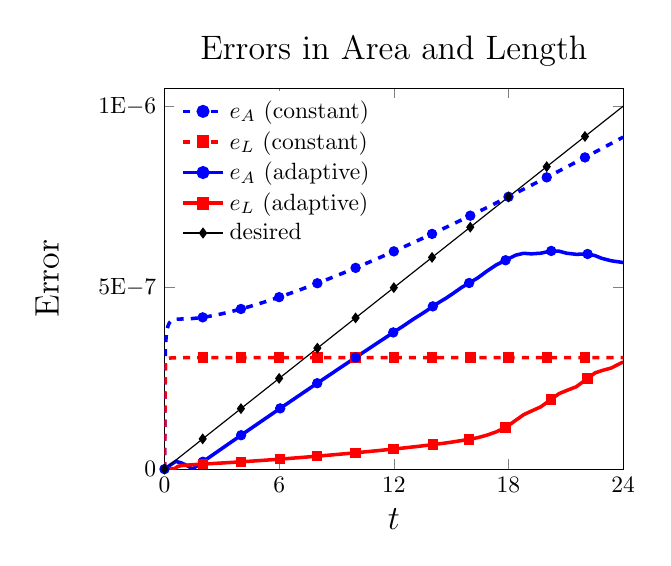
\begin{tikzpicture}[scale=0.85]

\begin{axis}[
  xmin = 0,
  xmax = 24,
  xtick = {0,6,12,18,24},
  xticklabels = {$0$,$6$,$12$,$18$,$24$},
  xlabel = $t$,
  ymin = 0,
  ymax = 1.05E-6,
  ytick = {0,5e-7,1e-6},
  yticklabels = {$0$,$5$E$-7$,$1$E$-6$},
  scaled y ticks = false,
%  ymax = 1.0E1,
%  ytick = {0,5,10},
%  yticklabels = {$0$,$5$E$-8$,$1$E$-7$},
  ylabel = {Error},
  ylabel style = {yshift = 10pt},
  label style = {font=\Large},
%  legend entries = {Area (Constant), Length(Constant), Area (Adaptive), Length (Adaptive), Desired},
  legend entries = {$e_{A}$ (constant), $e_{L}$ (constant), $e_{A}$
  (adaptive), $e_{L}$ (adaptive), desired},
  legend cell align = left,
%  legend pos = outer north east, 
%  legend pos = south east,
  legend style={at={(0.02,0.78)},anchor=west},
  legend style = {draw=none},
  title = {\Large{Errors in Area and Length}}
  ]
  \addlegendimage{mark=*,mark options=solid,blue,line width=1.5,dashed}
  \addlegendimage{mark=square*,mark options=solid,red,line width=1.5,dashed}
  \addlegendimage{mark=*,mark options=solid,blue,line width=1.5,solid}
  \addlegendimage{mark=square*,mark options=solid,red,line width=1.5,solid}
  \addlegendimage{mark=diamond*,mark options=solid,black,line width=0.5,solid}

%error in area fixed
\addplot [mark=none,blue,line width=1.5,dashed] table{
0.0000e+00 0.0000e+00
5.0000e-02 3.3808e-07
1.0000e-01 3.7253e-07
1.5000e-01 3.8780e-07
2.0000e-01 3.9659e-07
2.5000e-01 4.0216e-07
3.0000e-01 4.0585e-07
3.5000e-01 4.0835e-07
4.0000e-01 4.1005e-07
4.5000e-01 4.1123e-07
5.0000e-01 4.1203e-07
5.5000e-01 4.1257e-07
6.0000e-01 4.1294e-07
6.5000e-01 4.1319e-07
7.0000e-01 4.1335e-07
7.5000e-01 4.1346e-07
8.0000e-01 4.1354e-07
8.5000e-01 4.1360e-07
9.0000e-01 4.1365e-07
9.5000e-01 4.1371e-07
1.0000e+00 4.1377e-07
1.0500e+00 4.1383e-07
1.1000e+00 4.1391e-07
1.1500e+00 4.1401e-07
1.2000e+00 4.1412e-07
1.2500e+00 4.1425e-07
1.3000e+00 4.1439e-07
1.3500e+00 4.1456e-07
1.4000e+00 4.1474e-07
1.4500e+00 4.1494e-07
1.5000e+00 4.1516e-07
1.5500e+00 4.1539e-07
1.6000e+00 4.1564e-07
1.6500e+00 4.1591e-07
1.7000e+00 4.1619e-07
1.7500e+00 4.1649e-07
1.8000e+00 4.1681e-07
1.8500e+00 4.1714e-07
1.9000e+00 4.1748e-07
1.9500e+00 4.1784e-07
2.0000e+00 4.1821e-07
2.0500e+00 4.1860e-07
2.1000e+00 4.1900e-07
2.1500e+00 4.1941e-07
2.2000e+00 4.1983e-07
2.2500e+00 4.2027e-07
2.3000e+00 4.2072e-07
2.3500e+00 4.2117e-07
2.4000e+00 4.2164e-07
2.4500e+00 4.2212e-07
2.5000e+00 4.2262e-07
2.5500e+00 4.2312e-07
2.6000e+00 4.2363e-07
2.6500e+00 4.2415e-07
2.7000e+00 4.2468e-07
2.7500e+00 4.2522e-07
2.8000e+00 4.2577e-07
2.8500e+00 4.2633e-07
2.9000e+00 4.2689e-07
2.9500e+00 4.2747e-07
3.0000e+00 4.2805e-07
3.0500e+00 4.2864e-07
3.1000e+00 4.2924e-07
3.1500e+00 4.2985e-07
3.2000e+00 4.3047e-07
3.2500e+00 4.3109e-07
3.3000e+00 4.3172e-07
3.3500e+00 4.3235e-07
3.4000e+00 4.3300e-07
3.4500e+00 4.3365e-07
3.5000e+00 4.3430e-07
3.5500e+00 4.3497e-07
3.6000e+00 4.3564e-07
3.6500e+00 4.3632e-07
3.7000e+00 4.3700e-07
3.7500e+00 4.3769e-07
3.8000e+00 4.3838e-07
3.8500e+00 4.3909e-07
3.9000e+00 4.3979e-07
3.9500e+00 4.4051e-07
4.0000e+00 4.4122e-07
4.0500e+00 4.4195e-07
4.1000e+00 4.4268e-07
4.1500e+00 4.4341e-07
4.2000e+00 4.4415e-07
4.2500e+00 4.4490e-07
4.3000e+00 4.4565e-07
4.3500e+00 4.4641e-07
4.4000e+00 4.4717e-07
4.4500e+00 4.4793e-07
4.5000e+00 4.4871e-07
4.5500e+00 4.4948e-07
4.6000e+00 4.5026e-07
4.6500e+00 4.5105e-07
4.7000e+00 4.5184e-07
4.7500e+00 4.5263e-07
4.8000e+00 4.5343e-07
4.8500e+00 4.5424e-07
4.9000e+00 4.5504e-07
4.9500e+00 4.5586e-07
5.0000e+00 4.5667e-07
5.0500e+00 4.5749e-07
5.1000e+00 4.5832e-07
5.1500e+00 4.5915e-07
5.2000e+00 4.5998e-07
5.2500e+00 4.6082e-07
5.3000e+00 4.6166e-07
5.3500e+00 4.6251e-07
5.4000e+00 4.6336e-07
5.4500e+00 4.6421e-07
5.5000e+00 4.6507e-07
5.5500e+00 4.6593e-07
5.6000e+00 4.6680e-07
5.6500e+00 4.6766e-07
5.7000e+00 4.6854e-07
5.7500e+00 4.6941e-07
5.8000e+00 4.7029e-07
5.8500e+00 4.7118e-07
5.9000e+00 4.7206e-07
5.9500e+00 4.7295e-07
6.0000e+00 4.7385e-07
6.0500e+00 4.7475e-07
6.1000e+00 4.7565e-07
6.1500e+00 4.7655e-07
6.2000e+00 4.7746e-07
6.2500e+00 4.7837e-07
6.3000e+00 4.7928e-07
6.3500e+00 4.8020e-07
6.4000e+00 4.8112e-07
6.4500e+00 4.8205e-07
6.5000e+00 4.8297e-07
6.5500e+00 4.8390e-07
6.6000e+00 4.8484e-07
6.6500e+00 4.8577e-07
6.7000e+00 4.8671e-07
6.7500e+00 4.8766e-07
6.8000e+00 4.8860e-07
6.8500e+00 4.8955e-07
6.9000e+00 4.9050e-07
6.9500e+00 4.9146e-07
7.0000e+00 4.9241e-07
7.0500e+00 4.9338e-07
7.1000e+00 4.9434e-07
7.1500e+00 4.9530e-07
7.2000e+00 4.9627e-07
7.2500e+00 4.9725e-07
7.3000e+00 4.9822e-07
7.3500e+00 4.9920e-07
7.4000e+00 5.0018e-07
7.4500e+00 5.0116e-07
7.5000e+00 5.0215e-07
7.5500e+00 5.0313e-07
7.6000e+00 5.0413e-07
7.6500e+00 5.0512e-07
7.7000e+00 5.0612e-07
7.7500e+00 5.0711e-07
7.8000e+00 5.0812e-07
7.8500e+00 5.0912e-07
7.9000e+00 5.1013e-07
7.9500e+00 5.1114e-07
8.0000e+00 5.1215e-07
8.0500e+00 5.1316e-07
8.1000e+00 5.1418e-07
8.1500e+00 5.1520e-07
8.2000e+00 5.1622e-07
8.2500e+00 5.1724e-07
8.3000e+00 5.1827e-07
8.3500e+00 5.1930e-07
8.4000e+00 5.2033e-07
8.4500e+00 5.2136e-07
8.5000e+00 5.2240e-07
8.5500e+00 5.2344e-07
8.6000e+00 5.2448e-07
8.6500e+00 5.2552e-07
8.7000e+00 5.2657e-07
8.7500e+00 5.2761e-07
8.8000e+00 5.2866e-07
8.8500e+00 5.2972e-07
8.9000e+00 5.3077e-07
8.9500e+00 5.3183e-07
9.0000e+00 5.3289e-07
9.0500e+00 5.3395e-07
9.1000e+00 5.3501e-07
9.1500e+00 5.3607e-07
9.2000e+00 5.3714e-07
9.2500e+00 5.3821e-07
9.3000e+00 5.3928e-07
9.3500e+00 5.4036e-07
9.4000e+00 5.4143e-07
9.4500e+00 5.4251e-07
9.5000e+00 5.4359e-07
9.5500e+00 5.4467e-07
9.6000e+00 5.4576e-07
9.6500e+00 5.4684e-07
9.7000e+00 5.4793e-07
9.7500e+00 5.4902e-07
9.8000e+00 5.5011e-07
9.8500e+00 5.5121e-07
9.9000e+00 5.5231e-07
9.9500e+00 5.5340e-07
1.0000e+01 5.5450e-07
1.0050e+01 5.5561e-07
1.0100e+01 5.5671e-07
1.0150e+01 5.5782e-07
1.0200e+01 5.5892e-07
1.0250e+01 5.6003e-07
1.0300e+01 5.6115e-07
1.0350e+01 5.6226e-07
1.0400e+01 5.6338e-07
1.0450e+01 5.6449e-07
1.0500e+01 5.6561e-07
1.0550e+01 5.6673e-07
1.0600e+01 5.6786e-07
1.0650e+01 5.6898e-07
1.0700e+01 5.7011e-07
1.0750e+01 5.7124e-07
1.0800e+01 5.7237e-07
1.0850e+01 5.7350e-07
1.0900e+01 5.7463e-07
1.0950e+01 5.7577e-07
1.1000e+01 5.7691e-07
1.1050e+01 5.7804e-07
1.1100e+01 5.7919e-07
1.1150e+01 5.8033e-07
1.1200e+01 5.8147e-07
1.1250e+01 5.8262e-07
1.1300e+01 5.8377e-07
1.1350e+01 5.8492e-07
1.1400e+01 5.8607e-07
1.1450e+01 5.8722e-07
1.1500e+01 5.8837e-07
1.1550e+01 5.8953e-07
1.1600e+01 5.9069e-07
1.1650e+01 5.9185e-07
1.1700e+01 5.9301e-07
1.1750e+01 5.9417e-07
1.1800e+01 5.9534e-07
1.1850e+01 5.9650e-07
1.1900e+01 5.9767e-07
1.1950e+01 5.9884e-07
1.2000e+01 6.0001e-07
1.2050e+01 6.0118e-07
1.2100e+01 6.0236e-07
1.2150e+01 6.0353e-07
1.2200e+01 6.0471e-07
1.2250e+01 6.0589e-07
1.2300e+01 6.0707e-07
1.2350e+01 6.0825e-07
1.2400e+01 6.0943e-07
1.2450e+01 6.1062e-07
1.2500e+01 6.1181e-07
1.2550e+01 6.1299e-07
1.2600e+01 6.1418e-07
1.2650e+01 6.1537e-07
1.2700e+01 6.1657e-07
1.2750e+01 6.1776e-07
1.2800e+01 6.1896e-07
1.2850e+01 6.2015e-07
1.2900e+01 6.2135e-07
1.2950e+01 6.2255e-07
1.3000e+01 6.2375e-07
1.3050e+01 6.2496e-07
1.3100e+01 6.2616e-07
1.3150e+01 6.2737e-07
1.3200e+01 6.2857e-07
1.3250e+01 6.2978e-07
1.3300e+01 6.3099e-07
1.3350e+01 6.3220e-07
1.3400e+01 6.3342e-07
1.3450e+01 6.3463e-07
1.3500e+01 6.3585e-07
1.3550e+01 6.3706e-07
1.3600e+01 6.3828e-07
1.3650e+01 6.3950e-07
1.3700e+01 6.4072e-07
1.3750e+01 6.4194e-07
1.3800e+01 6.4317e-07
1.3850e+01 6.4439e-07
1.3900e+01 6.4562e-07
1.3950e+01 6.4685e-07
1.4000e+01 6.4808e-07
1.4050e+01 6.4931e-07
1.4100e+01 6.5054e-07
1.4150e+01 6.5177e-07
1.4200e+01 6.5301e-07
1.4250e+01 6.5424e-07
1.4300e+01 6.5548e-07
1.4350e+01 6.5672e-07
1.4400e+01 6.5796e-07
1.4450e+01 6.5920e-07
1.4500e+01 6.6044e-07
1.4550e+01 6.6169e-07
1.4600e+01 6.6293e-07
1.4650e+01 6.6418e-07
1.4700e+01 6.6542e-07
1.4750e+01 6.6667e-07
1.4800e+01 6.6792e-07
1.4850e+01 6.6917e-07
1.4900e+01 6.7043e-07
1.4950e+01 6.7168e-07
1.5000e+01 6.7293e-07
1.5050e+01 6.7419e-07
1.5100e+01 6.7545e-07
1.5150e+01 6.7671e-07
1.5200e+01 6.7797e-07
1.5250e+01 6.7923e-07
1.5300e+01 6.8049e-07
1.5350e+01 6.8175e-07
1.5400e+01 6.8302e-07
1.5450e+01 6.8428e-07
1.5500e+01 6.8555e-07
1.5550e+01 6.8682e-07
1.5600e+01 6.8809e-07
1.5650e+01 6.8936e-07
1.5700e+01 6.9063e-07
1.5750e+01 6.9190e-07
1.5800e+01 6.9318e-07
1.5850e+01 6.9445e-07
1.5900e+01 6.9573e-07
1.5950e+01 6.9700e-07
1.6000e+01 6.9828e-07
1.6050e+01 6.9956e-07
1.6100e+01 7.0084e-07
1.6150e+01 7.0212e-07
1.6200e+01 7.0341e-07
1.6250e+01 7.0469e-07
1.6300e+01 7.0598e-07
1.6350e+01 7.0726e-07
1.6400e+01 7.0855e-07
1.6450e+01 7.0984e-07
1.6500e+01 7.1113e-07
1.6550e+01 7.1242e-07
1.6600e+01 7.1371e-07
1.6650e+01 7.1500e-07
1.6700e+01 7.1630e-07
1.6750e+01 7.1759e-07
1.6800e+01 7.1889e-07
1.6850e+01 7.2019e-07
1.6900e+01 7.2148e-07
1.6950e+01 7.2278e-07
1.7000e+01 7.2408e-07
1.7050e+01 7.2539e-07
1.7100e+01 7.2669e-07
1.7150e+01 7.2799e-07
1.7200e+01 7.2930e-07
1.7250e+01 7.3060e-07
1.7300e+01 7.3191e-07
1.7350e+01 7.3322e-07
1.7400e+01 7.3452e-07
1.7450e+01 7.3583e-07
1.7500e+01 7.3714e-07
1.7550e+01 7.3846e-07
1.7600e+01 7.3977e-07
1.7650e+01 7.4108e-07
1.7700e+01 7.4240e-07
1.7750e+01 7.4371e-07
1.7800e+01 7.4503e-07
1.7850e+01 7.4635e-07
1.7900e+01 7.4767e-07
1.7950e+01 7.4899e-07
1.8000e+01 7.5031e-07
1.8050e+01 7.5163e-07
1.8100e+01 7.5295e-07
1.8150e+01 7.5427e-07
1.8200e+01 7.5560e-07
1.8250e+01 7.5692e-07
1.8300e+01 7.5825e-07
1.8350e+01 7.5958e-07
1.8400e+01 7.6091e-07
1.8450e+01 7.6223e-07
1.8500e+01 7.6356e-07
1.8550e+01 7.6490e-07
1.8600e+01 7.6623e-07
1.8650e+01 7.6756e-07
1.8700e+01 7.6889e-07
1.8750e+01 7.7023e-07
1.8800e+01 7.7157e-07
1.8850e+01 7.7290e-07
1.8900e+01 7.7424e-07
1.8950e+01 7.7558e-07
1.9000e+01 7.7692e-07
1.9050e+01 7.7826e-07
1.9100e+01 7.7960e-07
1.9150e+01 7.8094e-07
1.9200e+01 7.8228e-07
1.9250e+01 7.8363e-07
1.9300e+01 7.8497e-07
1.9350e+01 7.8632e-07
1.9400e+01 7.8767e-07
1.9450e+01 7.8901e-07
1.9500e+01 7.9036e-07
1.9550e+01 7.9171e-07
1.9600e+01 7.9306e-07
1.9650e+01 7.9441e-07
1.9700e+01 7.9576e-07
1.9750e+01 7.9712e-07
1.9800e+01 7.9847e-07
1.9850e+01 7.9982e-07
1.9900e+01 8.0118e-07
1.9950e+01 8.0253e-07
2.0000e+01 8.0389e-07
2.0050e+01 8.0525e-07
2.0100e+01 8.0661e-07
2.0150e+01 8.0797e-07
2.0200e+01 8.0933e-07
2.0250e+01 8.1069e-07
2.0300e+01 8.1205e-07
2.0350e+01 8.1341e-07
2.0400e+01 8.1478e-07
2.0450e+01 8.1614e-07
2.0500e+01 8.1751e-07
2.0550e+01 8.1887e-07
2.0600e+01 8.2024e-07
2.0650e+01 8.2161e-07
2.0700e+01 8.2298e-07
2.0750e+01 8.2434e-07
2.0800e+01 8.2571e-07
2.0850e+01 8.2709e-07
2.0900e+01 8.2846e-07
2.0950e+01 8.2983e-07
2.1000e+01 8.3120e-07
2.1050e+01 8.3258e-07
2.1100e+01 8.3395e-07
2.1150e+01 8.3533e-07
2.1200e+01 8.3670e-07
2.1250e+01 8.3808e-07
2.1300e+01 8.3946e-07
2.1350e+01 8.4084e-07
2.1400e+01 8.4222e-07
2.1450e+01 8.4360e-07
2.1500e+01 8.4498e-07
2.1550e+01 8.4636e-07
2.1600e+01 8.4774e-07
2.1650e+01 8.4912e-07
2.1700e+01 8.5051e-07
2.1750e+01 8.5189e-07
2.1800e+01 8.5328e-07
2.1850e+01 8.5466e-07
2.1900e+01 8.5605e-07
2.1950e+01 8.5744e-07
2.2000e+01 8.5883e-07
2.2050e+01 8.6022e-07
2.2100e+01 8.6161e-07
2.2150e+01 8.6300e-07
2.2200e+01 8.6439e-07
2.2250e+01 8.6578e-07
2.2300e+01 8.6717e-07
2.2350e+01 8.6857e-07
2.2400e+01 8.6996e-07
2.2450e+01 8.7136e-07
2.2500e+01 8.7275e-07
2.2550e+01 8.7415e-07
2.2600e+01 8.7554e-07
2.2650e+01 8.7694e-07
2.2700e+01 8.7834e-07
2.2750e+01 8.7974e-07
2.2800e+01 8.8114e-07
2.2850e+01 8.8254e-07
2.2900e+01 8.8394e-07
2.2950e+01 8.8534e-07
2.3000e+01 8.8674e-07
2.3050e+01 8.8815e-07
2.3100e+01 8.8955e-07
2.3150e+01 8.9096e-07
2.3200e+01 8.9236e-07
2.3250e+01 8.9377e-07
2.3300e+01 8.9517e-07
2.3350e+01 8.9658e-07
2.3400e+01 8.9799e-07
2.3450e+01 8.9940e-07
2.3500e+01 9.0081e-07
2.3550e+01 9.0222e-07
2.3600e+01 9.0363e-07
2.3650e+01 9.0504e-07
2.3700e+01 9.0645e-07
2.3750e+01 9.0786e-07
2.3800e+01 9.0928e-07
2.3850e+01 9.1069e-07
2.3900e+01 9.1210e-07
2.3950e+01 9.1352e-07
2.4000e+01 9.1493e-07
};

%error in length fixed
\addplot [mark=none,red,line width=1.5,dashed] table{
0.0000e+00 0.0000e+00
5.0000e-02 2.9731e-07
1.0000e-01 3.0274e-07
1.5000e-01 3.0434e-07
2.0000e-01 3.0514e-07
2.5000e-01 3.0564e-07
3.0000e-01 3.0598e-07
3.5000e-01 3.0623e-07
4.0000e-01 3.0641e-07
4.5000e-01 3.0655e-07
5.0000e-01 3.0666e-07
5.5000e-01 3.0675e-07
6.0000e-01 3.0682e-07
6.5000e-01 3.0688e-07
7.0000e-01 3.0693e-07
7.5000e-01 3.0697e-07
8.0000e-01 3.0701e-07
8.5000e-01 3.0703e-07
9.0000e-01 3.0706e-07
9.5000e-01 3.0708e-07
1.0000e+00 3.0710e-07
1.0500e+00 3.0712e-07
1.1000e+00 3.0713e-07
1.1500e+00 3.0715e-07
1.2000e+00 3.0716e-07
1.2500e+00 3.0717e-07
1.3000e+00 3.0718e-07
1.3500e+00 3.0719e-07
1.4000e+00 3.0719e-07
1.4500e+00 3.0720e-07
1.5000e+00 3.0721e-07
1.5500e+00 3.0722e-07
1.6000e+00 3.0722e-07
1.6500e+00 3.0723e-07
1.7000e+00 3.0723e-07
1.7500e+00 3.0724e-07
1.8000e+00 3.0724e-07
1.8500e+00 3.0724e-07
1.9000e+00 3.0725e-07
1.9500e+00 3.0725e-07
2.0000e+00 3.0725e-07
2.0500e+00 3.0726e-07
2.1000e+00 3.0726e-07
2.1500e+00 3.0726e-07
2.2000e+00 3.0726e-07
2.2500e+00 3.0727e-07
2.3000e+00 3.0727e-07
2.3500e+00 3.0727e-07
2.4000e+00 3.0727e-07
2.4500e+00 3.0727e-07
2.5000e+00 3.0728e-07
2.5500e+00 3.0728e-07
2.6000e+00 3.0728e-07
2.6500e+00 3.0728e-07
2.7000e+00 3.0728e-07
2.7500e+00 3.0728e-07
2.8000e+00 3.0728e-07
2.8500e+00 3.0729e-07
2.9000e+00 3.0729e-07
2.9500e+00 3.0729e-07
3.0000e+00 3.0729e-07
3.0500e+00 3.0729e-07
3.1000e+00 3.0729e-07
3.1500e+00 3.0729e-07
3.2000e+00 3.0729e-07
3.2500e+00 3.0729e-07
3.3000e+00 3.0729e-07
3.3500e+00 3.0730e-07
3.4000e+00 3.0730e-07
3.4500e+00 3.0730e-07
3.5000e+00 3.0730e-07
3.5500e+00 3.0730e-07
3.6000e+00 3.0730e-07
3.6500e+00 3.0730e-07
3.7000e+00 3.0730e-07
3.7500e+00 3.0730e-07
3.8000e+00 3.0730e-07
3.8500e+00 3.0730e-07
3.9000e+00 3.0730e-07
3.9500e+00 3.0730e-07
4.0000e+00 3.0730e-07
4.0500e+00 3.0730e-07
4.1000e+00 3.0730e-07
4.1500e+00 3.0730e-07
4.2000e+00 3.0730e-07
4.2500e+00 3.0730e-07
4.3000e+00 3.0730e-07
4.3500e+00 3.0730e-07
4.4000e+00 3.0731e-07
4.4500e+00 3.0731e-07
4.5000e+00 3.0731e-07
4.5500e+00 3.0731e-07
4.6000e+00 3.0731e-07
4.6500e+00 3.0731e-07
4.7000e+00 3.0731e-07
4.7500e+00 3.0731e-07
4.8000e+00 3.0731e-07
4.8500e+00 3.0731e-07
4.9000e+00 3.0731e-07
4.9500e+00 3.0731e-07
5.0000e+00 3.0731e-07
5.0500e+00 3.0731e-07
5.1000e+00 3.0731e-07
5.1500e+00 3.0731e-07
5.2000e+00 3.0731e-07
5.2500e+00 3.0731e-07
5.3000e+00 3.0731e-07
5.3500e+00 3.0731e-07
5.4000e+00 3.0731e-07
5.4500e+00 3.0731e-07
5.5000e+00 3.0731e-07
5.5500e+00 3.0731e-07
5.6000e+00 3.0731e-07
5.6500e+00 3.0731e-07
5.7000e+00 3.0731e-07
5.7500e+00 3.0731e-07
5.8000e+00 3.0731e-07
5.8500e+00 3.0731e-07
5.9000e+00 3.0731e-07
5.9500e+00 3.0731e-07
6.0000e+00 3.0731e-07
6.0500e+00 3.0731e-07
6.1000e+00 3.0731e-07
6.1500e+00 3.0731e-07
6.2000e+00 3.0731e-07
6.2500e+00 3.0731e-07
6.3000e+00 3.0731e-07
6.3500e+00 3.0731e-07
6.4000e+00 3.0731e-07
6.4500e+00 3.0731e-07
6.5000e+00 3.0731e-07
6.5500e+00 3.0731e-07
6.6000e+00 3.0731e-07
6.6500e+00 3.0731e-07
6.7000e+00 3.0731e-07
6.7500e+00 3.0731e-07
6.8000e+00 3.0731e-07
6.8500e+00 3.0731e-07
6.9000e+00 3.0731e-07
6.9500e+00 3.0731e-07
7.0000e+00 3.0731e-07
7.0500e+00 3.0731e-07
7.1000e+00 3.0731e-07
7.1500e+00 3.0731e-07
7.2000e+00 3.0731e-07
7.2500e+00 3.0731e-07
7.3000e+00 3.0731e-07
7.3500e+00 3.0731e-07
7.4000e+00 3.0731e-07
7.4500e+00 3.0731e-07
7.5000e+00 3.0731e-07
7.5500e+00 3.0731e-07
7.6000e+00 3.0731e-07
7.6500e+00 3.0731e-07
7.7000e+00 3.0731e-07
7.7500e+00 3.0731e-07
7.8000e+00 3.0731e-07
7.8500e+00 3.0731e-07
7.9000e+00 3.0731e-07
7.9500e+00 3.0731e-07
8.0000e+00 3.0731e-07
8.0500e+00 3.0731e-07
8.1000e+00 3.0731e-07
8.1500e+00 3.0731e-07
8.2000e+00 3.0731e-07
8.2500e+00 3.0731e-07
8.3000e+00 3.0731e-07
8.3500e+00 3.0731e-07
8.4000e+00 3.0731e-07
8.4500e+00 3.0731e-07
8.5000e+00 3.0731e-07
8.5500e+00 3.0731e-07
8.6000e+00 3.0731e-07
8.6500e+00 3.0731e-07
8.7000e+00 3.0731e-07
8.7500e+00 3.0731e-07
8.8000e+00 3.0731e-07
8.8500e+00 3.0731e-07
8.9000e+00 3.0731e-07
8.9500e+00 3.0731e-07
9.0000e+00 3.0731e-07
9.0500e+00 3.0731e-07
9.1000e+00 3.0731e-07
9.1500e+00 3.0731e-07
9.2000e+00 3.0731e-07
9.2500e+00 3.0731e-07
9.3000e+00 3.0731e-07
9.3500e+00 3.0731e-07
9.4000e+00 3.0731e-07
9.4500e+00 3.0731e-07
9.5000e+00 3.0731e-07
9.5500e+00 3.0731e-07
9.6000e+00 3.0731e-07
9.6500e+00 3.0731e-07
9.7000e+00 3.0731e-07
9.7500e+00 3.0731e-07
9.8000e+00 3.0731e-07
9.8500e+00 3.0731e-07
9.9000e+00 3.0731e-07
9.9500e+00 3.0731e-07
1.0000e+01 3.0731e-07
1.0050e+01 3.0731e-07
1.0100e+01 3.0731e-07
1.0150e+01 3.0731e-07
1.0200e+01 3.0731e-07
1.0250e+01 3.0731e-07
1.0300e+01 3.0731e-07
1.0350e+01 3.0731e-07
1.0400e+01 3.0731e-07
1.0450e+01 3.0731e-07
1.0500e+01 3.0731e-07
1.0550e+01 3.0731e-07
1.0600e+01 3.0731e-07
1.0650e+01 3.0731e-07
1.0700e+01 3.0731e-07
1.0750e+01 3.0732e-07
1.0800e+01 3.0732e-07
1.0850e+01 3.0732e-07
1.0900e+01 3.0732e-07
1.0950e+01 3.0732e-07
1.1000e+01 3.0732e-07
1.1050e+01 3.0732e-07
1.1100e+01 3.0732e-07
1.1150e+01 3.0732e-07
1.1200e+01 3.0732e-07
1.1250e+01 3.0732e-07
1.1300e+01 3.0732e-07
1.1350e+01 3.0732e-07
1.1400e+01 3.0732e-07
1.1450e+01 3.0732e-07
1.1500e+01 3.0732e-07
1.1550e+01 3.0732e-07
1.1600e+01 3.0732e-07
1.1650e+01 3.0732e-07
1.1700e+01 3.0732e-07
1.1750e+01 3.0732e-07
1.1800e+01 3.0732e-07
1.1850e+01 3.0732e-07
1.1900e+01 3.0732e-07
1.1950e+01 3.0732e-07
1.2000e+01 3.0732e-07
1.2050e+01 3.0732e-07
1.2100e+01 3.0732e-07
1.2150e+01 3.0732e-07
1.2200e+01 3.0732e-07
1.2250e+01 3.0732e-07
1.2300e+01 3.0732e-07
1.2350e+01 3.0732e-07
1.2400e+01 3.0732e-07
1.2450e+01 3.0732e-07
1.2500e+01 3.0732e-07
1.2550e+01 3.0732e-07
1.2600e+01 3.0732e-07
1.2650e+01 3.0732e-07
1.2700e+01 3.0732e-07
1.2750e+01 3.0732e-07
1.2800e+01 3.0732e-07
1.2850e+01 3.0732e-07
1.2900e+01 3.0732e-07
1.2950e+01 3.0732e-07
1.3000e+01 3.0732e-07
1.3050e+01 3.0732e-07
1.3100e+01 3.0732e-07
1.3150e+01 3.0732e-07
1.3200e+01 3.0732e-07
1.3250e+01 3.0732e-07
1.3300e+01 3.0732e-07
1.3350e+01 3.0732e-07
1.3400e+01 3.0732e-07
1.3450e+01 3.0732e-07
1.3500e+01 3.0732e-07
1.3550e+01 3.0732e-07
1.3600e+01 3.0732e-07
1.3650e+01 3.0732e-07
1.3700e+01 3.0732e-07
1.3750e+01 3.0732e-07
1.3800e+01 3.0732e-07
1.3850e+01 3.0732e-07
1.3900e+01 3.0732e-07
1.3950e+01 3.0732e-07
1.4000e+01 3.0732e-07
1.4050e+01 3.0732e-07
1.4100e+01 3.0732e-07
1.4150e+01 3.0732e-07
1.4200e+01 3.0732e-07
1.4250e+01 3.0732e-07
1.4300e+01 3.0732e-07
1.4350e+01 3.0732e-07
1.4400e+01 3.0732e-07
1.4450e+01 3.0732e-07
1.4500e+01 3.0732e-07
1.4550e+01 3.0732e-07
1.4600e+01 3.0732e-07
1.4650e+01 3.0732e-07
1.4700e+01 3.0732e-07
1.4750e+01 3.0732e-07
1.4800e+01 3.0732e-07
1.4850e+01 3.0732e-07
1.4900e+01 3.0732e-07
1.4950e+01 3.0732e-07
1.5000e+01 3.0732e-07
1.5050e+01 3.0732e-07
1.5100e+01 3.0732e-07
1.5150e+01 3.0732e-07
1.5200e+01 3.0732e-07
1.5250e+01 3.0732e-07
1.5300e+01 3.0732e-07
1.5350e+01 3.0732e-07
1.5400e+01 3.0732e-07
1.5450e+01 3.0732e-07
1.5500e+01 3.0732e-07
1.5550e+01 3.0732e-07
1.5600e+01 3.0732e-07
1.5650e+01 3.0732e-07
1.5700e+01 3.0732e-07
1.5750e+01 3.0732e-07
1.5800e+01 3.0732e-07
1.5850e+01 3.0732e-07
1.5900e+01 3.0732e-07
1.5950e+01 3.0732e-07
1.6000e+01 3.0732e-07
1.6050e+01 3.0732e-07
1.6100e+01 3.0732e-07
1.6150e+01 3.0732e-07
1.6200e+01 3.0732e-07
1.6250e+01 3.0732e-07
1.6300e+01 3.0732e-07
1.6350e+01 3.0732e-07
1.6400e+01 3.0732e-07
1.6450e+01 3.0732e-07
1.6500e+01 3.0732e-07
1.6550e+01 3.0732e-07
1.6600e+01 3.0732e-07
1.6650e+01 3.0732e-07
1.6700e+01 3.0732e-07
1.6750e+01 3.0732e-07
1.6800e+01 3.0732e-07
1.6850e+01 3.0732e-07
1.6900e+01 3.0732e-07
1.6950e+01 3.0732e-07
1.7000e+01 3.0732e-07
1.7050e+01 3.0732e-07
1.7100e+01 3.0732e-07
1.7150e+01 3.0732e-07
1.7200e+01 3.0732e-07
1.7250e+01 3.0732e-07
1.7300e+01 3.0732e-07
1.7350e+01 3.0732e-07
1.7400e+01 3.0732e-07
1.7450e+01 3.0732e-07
1.7500e+01 3.0732e-07
1.7550e+01 3.0732e-07
1.7600e+01 3.0732e-07
1.7650e+01 3.0732e-07
1.7700e+01 3.0732e-07
1.7750e+01 3.0732e-07
1.7800e+01 3.0732e-07
1.7850e+01 3.0732e-07
1.7900e+01 3.0732e-07
1.7950e+01 3.0732e-07
1.8000e+01 3.0732e-07
1.8050e+01 3.0732e-07
1.8100e+01 3.0732e-07
1.8150e+01 3.0732e-07
1.8200e+01 3.0732e-07
1.8250e+01 3.0732e-07
1.8300e+01 3.0732e-07
1.8350e+01 3.0732e-07
1.8400e+01 3.0732e-07
1.8450e+01 3.0732e-07
1.8500e+01 3.0732e-07
1.8550e+01 3.0732e-07
1.8600e+01 3.0732e-07
1.8650e+01 3.0732e-07
1.8700e+01 3.0732e-07
1.8750e+01 3.0732e-07
1.8800e+01 3.0732e-07
1.8850e+01 3.0732e-07
1.8900e+01 3.0732e-07
1.8950e+01 3.0732e-07
1.9000e+01 3.0732e-07
1.9050e+01 3.0732e-07
1.9100e+01 3.0732e-07
1.9150e+01 3.0732e-07
1.9200e+01 3.0732e-07
1.9250e+01 3.0732e-07
1.9300e+01 3.0732e-07
1.9350e+01 3.0732e-07
1.9400e+01 3.0732e-07
1.9450e+01 3.0732e-07
1.9500e+01 3.0732e-07
1.9550e+01 3.0732e-07
1.9600e+01 3.0732e-07
1.9650e+01 3.0732e-07
1.9700e+01 3.0732e-07
1.9750e+01 3.0732e-07
1.9800e+01 3.0732e-07
1.9850e+01 3.0732e-07
1.9900e+01 3.0732e-07
1.9950e+01 3.0732e-07
2.0000e+01 3.0732e-07
2.0050e+01 3.0732e-07
2.0100e+01 3.0732e-07
2.0150e+01 3.0732e-07
2.0200e+01 3.0732e-07
2.0250e+01 3.0732e-07
2.0300e+01 3.0732e-07
2.0350e+01 3.0732e-07
2.0400e+01 3.0732e-07
2.0450e+01 3.0732e-07
2.0500e+01 3.0732e-07
2.0550e+01 3.0732e-07
2.0600e+01 3.0732e-07
2.0650e+01 3.0732e-07
2.0700e+01 3.0732e-07
2.0750e+01 3.0732e-07
2.0800e+01 3.0732e-07
2.0850e+01 3.0732e-07
2.0900e+01 3.0732e-07
2.0950e+01 3.0732e-07
2.1000e+01 3.0732e-07
2.1050e+01 3.0732e-07
2.1100e+01 3.0732e-07
2.1150e+01 3.0732e-07
2.1200e+01 3.0732e-07
2.1250e+01 3.0732e-07
2.1300e+01 3.0732e-07
2.1350e+01 3.0732e-07
2.1400e+01 3.0732e-07
2.1450e+01 3.0732e-07
2.1500e+01 3.0732e-07
2.1550e+01 3.0732e-07
2.1600e+01 3.0732e-07
2.1650e+01 3.0732e-07
2.1700e+01 3.0732e-07
2.1750e+01 3.0732e-07
2.1800e+01 3.0732e-07
2.1850e+01 3.0732e-07
2.1900e+01 3.0732e-07
2.1950e+01 3.0732e-07
2.2000e+01 3.0732e-07
2.2050e+01 3.0732e-07
2.2100e+01 3.0732e-07
2.2150e+01 3.0732e-07
2.2200e+01 3.0732e-07
2.2250e+01 3.0732e-07
2.2300e+01 3.0732e-07
2.2350e+01 3.0732e-07
2.2400e+01 3.0732e-07
2.2450e+01 3.0732e-07
2.2500e+01 3.0732e-07
2.2550e+01 3.0732e-07
2.2600e+01 3.0732e-07
2.2650e+01 3.0732e-07
2.2700e+01 3.0732e-07
2.2750e+01 3.0732e-07
2.2800e+01 3.0732e-07
2.2850e+01 3.0732e-07
2.2900e+01 3.0732e-07
2.2950e+01 3.0732e-07
2.3000e+01 3.0732e-07
2.3050e+01 3.0732e-07
2.3100e+01 3.0732e-07
2.3150e+01 3.0732e-07
2.3200e+01 3.0732e-07
2.3250e+01 3.0732e-07
2.3300e+01 3.0732e-07
2.3350e+01 3.0732e-07
2.3400e+01 3.0732e-07
2.3450e+01 3.0732e-07
2.3500e+01 3.0732e-07
2.3550e+01 3.0732e-07
2.3600e+01 3.0732e-07
2.3650e+01 3.0732e-07
2.3700e+01 3.0732e-07
2.3750e+01 3.0732e-07
2.3800e+01 3.0732e-07
2.3850e+01 3.0732e-07
2.3900e+01 3.0732e-07
2.3950e+01 3.0732e-07
2.4000e+01 3.0732e-07
};

% error in area adaptive
\addplot [mark=none,blue,line width=1.5] table{
0.0000e+00 0.0000e+00
9.3129e-05 3.6856e-12
1.8148e-04 6.5076e-12
2.7721e-04 9.9065e-12
3.7558e-04 1.3265e-11
4.7869e-04 1.6888e-11
5.8520e-04 2.0582e-11
6.9595e-04 2.4466e-11
8.1047e-04 2.8469e-11
9.2907e-04 3.2635e-11
1.0516e-03 3.6939e-11
1.1782e-03 4.1399e-11
1.3089e-03 4.6004e-11
1.4437e-03 5.0764e-11
1.5826e-03 5.5673e-11
1.7256e-03 6.0737e-11
1.8728e-03 6.5954e-11
2.0242e-03 7.1327e-11
2.1798e-03 7.6855e-11
2.3398e-03 8.2542e-11
2.5040e-03 8.8388e-11
2.6726e-03 9.4392e-11
2.8455e-03 1.0056e-10
3.0229e-03 1.0689e-10
3.2047e-03 1.1338e-10
3.3910e-03 1.2004e-10
3.5818e-03 1.2687e-10
3.7772e-03 1.3386e-10
3.9772e-03 1.4102e-10
4.1818e-03 1.4836e-10
4.3911e-03 1.5586e-10
4.6052e-03 1.6354e-10
4.8240e-03 1.7140e-10
5.0476e-03 1.7943e-10
5.2760e-03 1.8764e-10
5.5094e-03 1.9603e-10
5.7477e-03 2.0460e-10
5.9910e-03 2.1336e-10
6.2393e-03 2.2230e-10
6.4927e-03 2.3143e-10
6.7512e-03 2.4075e-10
7.0149e-03 2.5026e-10
7.2839e-03 2.5996e-10
7.5581e-03 2.6985e-10
7.8377e-03 2.7994e-10
8.1226e-03 2.9023e-10
8.4130e-03 3.0072e-10
8.7089e-03 3.1141e-10
9.0103e-03 3.2231e-10
9.3174e-03 3.3341e-10
9.6300e-03 3.4472e-10
9.9484e-03 3.5623e-10
1.0273e-02 3.6796e-10
1.0603e-02 3.7991e-10
1.0938e-02 3.9207e-10
1.1280e-02 4.0445e-10
1.1628e-02 4.1705e-10
1.1982e-02 4.2987e-10
1.2342e-02 4.4292e-10
1.2708e-02 4.5620e-10
1.3081e-02 4.6970e-10
1.3460e-02 4.8344e-10
1.3845e-02 4.9741e-10
1.4236e-02 5.1162e-10
1.4635e-02 5.2607e-10
1.5039e-02 5.4076e-10
1.5451e-02 5.5570e-10
1.5869e-02 5.7088e-10
1.6294e-02 5.8631e-10
1.6726e-02 6.0200e-10
1.7164e-02 6.1793e-10
1.7610e-02 6.3413e-10
1.8063e-02 6.5058e-10
1.8523e-02 6.6730e-10
1.8990e-02 6.8429e-10
1.9464e-02 7.0154e-10
1.9946e-02 7.1906e-10
2.0435e-02 7.3686e-10
2.0932e-02 7.5493e-10
2.1437e-02 7.7328e-10
2.1949e-02 7.9191e-10
2.2468e-02 8.1083e-10
2.2996e-02 8.3004e-10
2.3532e-02 8.4953e-10
2.4075e-02 8.6932e-10
2.4627e-02 8.8941e-10
2.5187e-02 9.0980e-10
2.5755e-02 9.3049e-10
2.6331e-02 9.5149e-10
2.6916e-02 9.7279e-10
2.7509e-02 9.9441e-10
2.8111e-02 1.0163e-09
2.8721e-02 1.0386e-09
2.9341e-02 1.0612e-09
2.9969e-02 1.0841e-09
3.0606e-02 1.1073e-09
3.1252e-02 1.1308e-09
3.1907e-02 1.1547e-09
3.2571e-02 1.1790e-09
3.3244e-02 1.2035e-09
3.3927e-02 1.2284e-09
3.4619e-02 1.2537e-09
3.5321e-02 1.2793e-09
3.6033e-02 1.3053e-09
3.6754e-02 1.3316e-09
3.7485e-02 1.3583e-09
3.8225e-02 1.3853e-09
3.8976e-02 1.4127e-09
3.9737e-02 1.4405e-09
4.0508e-02 1.4687e-09
4.1289e-02 1.4972e-09
4.2081e-02 1.5261e-09
4.2883e-02 1.5554e-09
4.3696e-02 1.5851e-09
4.4519e-02 1.6152e-09
4.5353e-02 1.6457e-09
4.6198e-02 1.6766e-09
4.7053e-02 1.7078e-09
4.7920e-02 1.7395e-09
4.8798e-02 1.7716e-09
4.9686e-02 1.8041e-09
5.0587e-02 1.8370e-09
5.1498e-02 1.8704e-09
5.2421e-02 1.9041e-09
5.3356e-02 1.9383e-09
5.4302e-02 1.9729e-09
5.5260e-02 2.0080e-09
5.6230e-02 2.0435e-09
5.7211e-02 2.0794e-09
5.8205e-02 2.1158e-09
5.9211e-02 2.1526e-09
6.0229e-02 2.1899e-09
6.1260e-02 2.2276e-09
6.2302e-02 2.2658e-09
6.3358e-02 2.3044e-09
6.4426e-02 2.3436e-09
6.5506e-02 2.3831e-09
6.6600e-02 2.4232e-09
6.7706e-02 2.4637e-09
6.8826e-02 2.5047e-09
6.9958e-02 2.5462e-09
7.1104e-02 2.5882e-09
7.2263e-02 2.6307e-09
7.3435e-02 2.6737e-09
7.4621e-02 2.7171e-09
7.5821e-02 2.7611e-09
7.7034e-02 2.8056e-09
7.8261e-02 2.8506e-09
7.9502e-02 2.8961e-09
8.0757e-02 2.9421e-09
8.2026e-02 2.9886e-09
8.3309e-02 3.0357e-09
8.4607e-02 3.0833e-09
8.5919e-02 3.1314e-09
8.7246e-02 3.1801e-09
8.8587e-02 3.2293e-09
8.9943e-02 3.2790e-09
9.1314e-02 3.3293e-09
9.2700e-02 3.3802e-09
9.4101e-02 3.4316e-09
9.5518e-02 3.4836e-09
9.6949e-02 3.5362e-09
9.8397e-02 3.5893e-09
9.9860e-02 3.6430e-09
1.0134e-01 3.6972e-09
1.0283e-01 3.7521e-09
1.0434e-01 3.8076e-09
1.0587e-01 3.8636e-09
1.0741e-01 3.9202e-09
1.0897e-01 3.9775e-09
1.1055e-01 4.0354e-09
1.1214e-01 4.0938e-09
1.1375e-01 4.1529e-09
1.1538e-01 4.2126e-09
1.1702e-01 4.2730e-09
1.1868e-01 4.3340e-09
1.2036e-01 4.3956e-09
1.2205e-01 4.4579e-09
1.2377e-01 4.5208e-09
1.2550e-01 4.5844e-09
1.2725e-01 4.6487e-09
1.2902e-01 4.7136e-09
1.3080e-01 4.7792e-09
1.3261e-01 4.8455e-09
1.3443e-01 4.9125e-09
1.3627e-01 4.9801e-09
1.3813e-01 5.0485e-09
1.4002e-01 5.1176e-09
1.4192e-01 5.1874e-09
1.4384e-01 5.2580e-09
1.4578e-01 5.3293e-09
1.4774e-01 5.4013e-09
1.4972e-01 5.4741e-09
1.5172e-01 5.5476e-09
1.5375e-01 5.6219e-09
1.5579e-01 5.6970e-09
1.5786e-01 5.7729e-09
1.5995e-01 5.8496e-09
1.6206e-01 5.9270e-09
1.6419e-01 6.0053e-09
1.6634e-01 6.0844e-09
1.6852e-01 6.1644e-09
1.7072e-01 6.2452e-09
1.7295e-01 6.3269e-09
1.7519e-01 6.4094e-09
1.7747e-01 6.4928e-09
1.7976e-01 6.5771e-09
1.8209e-01 6.6623e-09
1.8443e-01 6.7485e-09
1.8681e-01 6.8355e-09
1.8921e-01 6.9235e-09
1.9163e-01 7.0125e-09
1.9408e-01 7.1024e-09
1.9656e-01 7.1934e-09
1.9907e-01 7.2853e-09
2.0160e-01 7.3783e-09
2.0417e-01 7.4723e-09
2.0676e-01 7.5673e-09
2.0938e-01 7.6634e-09
2.1204e-01 7.7607e-09
2.1472e-01 7.8590e-09
2.1743e-01 7.9584e-09
2.2018e-01 8.0590e-09
2.2296e-01 8.1608e-09
2.2577e-01 8.2637e-09
2.2861e-01 8.3679e-09
2.3149e-01 8.4733e-09
2.3441e-01 8.5800e-09
2.3736e-01 8.6879e-09
2.4034e-01 8.7972e-09
2.4337e-01 8.9077e-09
2.4643e-01 9.0197e-09
2.4953e-01 9.1330e-09
2.5267e-01 9.2478e-09
2.5585e-01 9.3640e-09
2.5907e-01 9.4817e-09
2.6234e-01 9.6009e-09
2.6564e-01 9.7217e-09
2.6900e-01 9.8441e-09
2.7239e-01 9.9681e-09
2.7584e-01 1.0094e-08
2.7933e-01 1.0221e-08
2.8287e-01 1.0350e-08
2.8647e-01 1.0481e-08
2.9011e-01 1.0614e-08
2.9381e-01 1.0748e-08
2.9756e-01 1.0885e-08
3.0137e-01 1.1024e-08
3.0524e-01 1.1164e-08
3.0917e-01 1.1307e-08
3.1316e-01 1.1452e-08
3.1721e-01 1.1599e-08
3.2133e-01 1.1749e-08
3.2552e-01 1.1901e-08
3.2978e-01 1.2055e-08
3.3411e-01 1.2212e-08
3.3851e-01 1.2371e-08
3.4300e-01 1.2534e-08
3.4757e-01 1.2699e-08
3.5222e-01 1.2867e-08
3.5696e-01 1.3038e-08
3.6179e-01 1.3212e-08
3.6671e-01 1.3389e-08
3.7174e-01 1.3570e-08
3.7687e-01 1.3755e-08
3.8211e-01 1.3943e-08
3.8747e-01 1.4135e-08
3.9294e-01 1.4331e-08
3.9855e-01 1.4532e-08
4.0428e-01 1.4736e-08
4.1016e-01 1.4946e-08
4.1619e-01 1.5161e-08
4.2238e-01 1.5380e-08
4.2874e-01 1.5606e-08
4.3528e-01 1.5837e-08
4.4201e-01 1.6075e-08
4.4896e-01 1.6319e-08
4.5613e-01 1.6570e-08
4.6354e-01 1.6829e-08
4.7123e-01 1.7097e-08
4.7921e-01 1.7373e-08
4.8751e-01 1.7659e-08
4.9618e-01 1.7955e-08
5.0525e-01 1.8263e-08
5.1478e-01 1.8584e-08
5.2485e-01 1.8919e-08
5.3554e-01 1.9270e-08
5.4696e-01 1.9637e-08
5.5930e-01 2.0027e-08
5.7272e-01 2.0432e-08
5.8771e-01 2.0884e-08
6.0442e-01 2.1276e-08
6.2110e-01 2.1240e-08
6.3834e-01 2.1278e-08
6.5594e-01 2.1006e-08
6.7399e-01 2.0654e-08
6.9248e-01 2.0075e-08
7.1142e-01 1.9338e-08
7.1755e-01 1.9089e-08
7.2337e-01 1.9204e-08
7.3140e-01 1.9148e-08
7.4283e-01 1.9241e-08
7.5908e-01 1.8996e-08
7.6638e-01 1.8699e-08
7.7329e-01 1.8797e-08
7.8314e-01 1.8710e-08
7.9714e-01 1.8643e-08
8.1708e-01 1.7897e-08
8.2238e-01 1.7681e-08
8.2740e-01 1.7781e-08
8.3429e-01 1.7711e-08
8.4409e-01 1.7755e-08
8.5803e-01 1.7455e-08
8.7644e-01 1.6700e-08
8.8265e-01 1.6452e-08
8.8855e-01 1.6546e-08
8.9694e-01 1.6447e-08
9.0887e-01 1.6389e-08
9.2586e-01 1.5752e-08
9.3355e-01 1.5434e-08
9.4084e-01 1.5506e-08
9.5121e-01 1.5348e-08
9.6597e-01 1.5067e-08
9.7519e-01 1.4693e-08
9.8394e-01 1.4701e-08
9.9639e-01 1.4467e-08
1.0139e+00 1.3808e-08
1.0215e+00 1.3499e-08
1.0287e+00 1.3575e-08
1.0389e+00 1.3412e-08
1.0535e+00 1.3132e-08
1.0639e+00 1.2700e-08
1.0738e+00 1.2642e-08
1.0879e+00 1.2308e-08
1.1004e+00 1.1792e-08
1.1122e+00 1.1550e-08
1.1282e+00 1.1065e-08
1.1378e+00 1.0679e-08
1.1470e+00 1.0678e-08
1.1600e+00 1.0400e-08
1.1773e+00 9.6904e-09
1.1870e+00 9.2899e-09
1.1962e+00 9.3023e-09
1.2093e+00 9.0155e-09
1.2265e+00 8.3398e-09
1.2368e+00 7.9187e-09
1.2465e+00 7.9044e-09
1.2605e+00 7.5788e-09
1.2758e+00 6.9615e-09
1.2904e+00 6.3791e-09
1.3045e+00 5.9165e-09
1.3197e+00 5.3993e-09
1.3355e+00 4.7447e-09
1.3506e+00 4.1343e-09
1.3651e+00 3.6467e-09
1.3804e+00 3.1276e-09
1.3965e+00 2.4778e-09
1.4121e+00 1.8464e-09
1.4271e+00 1.3318e-09
1.4427e+00 8.0290e-10
1.4591e+00 1.5495e-10
1.4752e+00 4.9253e-10
1.4906e+00 1.0341e-09
1.5066e+00 1.5786e-09
1.5234e+00 2.2290e-09
1.5399e+00 2.8898e-09
1.5559e+00 3.4575e-09
1.5723e+00 4.0216e-09
1.5895e+00 4.6789e-09
1.6065e+00 5.3520e-09
1.6231e+00 5.9450e-09
1.6400e+00 6.5316e-09
1.6576e+00 7.1998e-09
1.6751e+00 7.8857e-09
1.6923e+00 8.5032e-09
1.7097e+00 9.1143e-09
1.7278e+00 9.7970e-09
1.7459e+00 1.0497e-08
1.7636e+00 1.1139e-08
1.7817e+00 1.1776e-08
1.8003e+00 1.2476e-08
1.8189e+00 1.3191e-08
1.8373e+00 1.3858e-08
1.8560e+00 1.4522e-08
1.8753e+00 1.5242e-08
1.8945e+00 1.5975e-08
1.9136e+00 1.6667e-08
1.9329e+00 1.7360e-08
1.9528e+00 1.8103e-08
1.9727e+00 1.8855e-08
1.9925e+00 1.9574e-08
2.0126e+00 2.0296e-08
2.0331e+00 2.1064e-08
2.0537e+00 2.1838e-08
2.0742e+00 2.2584e-08
2.0951e+00 2.3338e-08
2.1164e+00 2.4132e-08
2.1377e+00 2.4930e-08
2.1591e+00 2.5706e-08
2.1808e+00 2.6493e-08
2.2029e+00 2.7315e-08
2.2250e+00 2.8140e-08
2.2472e+00 2.8947e-08
2.2698e+00 2.9768e-08
2.2928e+00 3.0622e-08
2.3158e+00 3.1476e-08
2.3389e+00 3.2316e-08
2.3624e+00 3.3174e-08
2.3863e+00 3.4060e-08
2.4103e+00 3.4946e-08
2.4344e+00 3.5823e-08
2.4589e+00 3.6719e-08
2.4837e+00 3.7640e-08
2.5087e+00 3.8560e-08
2.5339e+00 3.9476e-08
2.5595e+00 4.0412e-08
2.5854e+00 4.1372e-08
2.6115e+00 4.2329e-08
2.6378e+00 4.3287e-08
2.6645e+00 4.4267e-08
2.6916e+00 4.5267e-08
2.7188e+00 4.6265e-08
2.7464e+00 4.7267e-08
2.7743e+00 4.8293e-08
2.8026e+00 4.9337e-08
2.8311e+00 5.0380e-08
2.8600e+00 5.1431e-08
2.8893e+00 5.2506e-08
2.9189e+00 5.3597e-08
2.9488e+00 5.4688e-08
2.9791e+00 5.5791e-08
3.0098e+00 5.6919e-08
3.0409e+00 5.8060e-08
3.0722e+00 5.9204e-08
3.1040e+00 6.0363e-08
3.1363e+00 6.1548e-08
3.1689e+00 6.2744e-08
3.2019e+00 6.3946e-08
3.2354e+00 6.5166e-08
3.2693e+00 6.6411e-08
3.3037e+00 6.7668e-08
3.3384e+00 6.8931e-08
3.3737e+00 7.0218e-08
3.4094e+00 7.1529e-08
3.4456e+00 7.2850e-08
3.4823e+00 7.4182e-08
3.5195e+00 7.5541e-08
3.5572e+00 7.6922e-08
3.5954e+00 7.8314e-08
3.6341e+00 7.9722e-08
3.6735e+00 8.1158e-08
3.7134e+00 8.2617e-08
3.7538e+00 8.4086e-08
3.7948e+00 8.5576e-08
3.8365e+00 8.7097e-08
3.8787e+00 8.8639e-08
3.9215e+00 9.0194e-08
3.9651e+00 9.1774e-08
4.0093e+00 9.3387e-08
4.0541e+00 9.5021e-08
4.0996e+00 9.6670e-08
4.1458e+00 9.8350e-08
4.1929e+00 1.0006e-07
4.2405e+00 1.0180e-07
4.2890e+00 1.0355e-07
4.3382e+00 1.0534e-07
4.3883e+00 1.0716e-07
4.4391e+00 1.0901e-07
4.4908e+00 1.1088e-07
4.5434e+00 1.1279e-07
4.5969e+00 1.1473e-07
4.6512e+00 1.1669e-07
4.7065e+00 1.1869e-07
4.7628e+00 1.2074e-07
4.8200e+00 1.2281e-07
4.8782e+00 1.2491e-07
4.9375e+00 1.2706e-07
4.9979e+00 1.2925e-07
5.0593e+00 1.3147e-07
5.1218e+00 1.3372e-07
5.1856e+00 1.3603e-07
5.2506e+00 1.3838e-07
5.3167e+00 1.4077e-07
5.3840e+00 1.4319e-07
5.4528e+00 1.4568e-07
5.5229e+00 1.4821e-07
5.5943e+00 1.5078e-07
5.6671e+00 1.5340e-07
5.7416e+00 1.5608e-07
5.8174e+00 1.5882e-07
5.8947e+00 1.6159e-07
5.9738e+00 1.6443e-07
6.0546e+00 1.6735e-07
6.1369e+00 1.7031e-07
6.2210e+00 1.7332e-07
6.3071e+00 1.7641e-07
6.3951e+00 1.7958e-07
6.4848e+00 1.8280e-07
6.5767e+00 1.8607e-07
6.6708e+00 1.8945e-07
6.7670e+00 1.9291e-07
6.8652e+00 1.9642e-07
6.9660e+00 2.0001e-07
7.0693e+00 2.0372e-07
7.1749e+00 2.0750e-07
7.2829e+00 2.1133e-07
7.3940e+00 2.1529e-07
7.5079e+00 2.1938e-07
7.6243e+00 2.2353e-07
7.7438e+00 2.2775e-07
7.8669e+00 2.3214e-07
7.9931e+00 2.3666e-07
8.1222e+00 2.4123e-07
8.2551e+00 2.4591e-07
8.3922e+00 2.5081e-07
8.5327e+00 2.5582e-07
8.6767e+00 2.6087e-07
8.8257e+00 2.6613e-07
8.9792e+00 2.7162e-07
9.1365e+00 2.7718e-07
9.2985e+00 2.8282e-07
9.4665e+00 2.8877e-07
9.6395e+00 2.9494e-07
9.8168e+00 3.0113e-07
1.0001e+01 3.0751e-07
1.0192e+01 3.1431e-07
1.0388e+01 3.2126e-07
1.0589e+01 3.2819e-07
1.0800e+01 3.3552e-07
1.1019e+01 3.4336e-07
1.1243e+01 3.5116e-07
1.1475e+01 3.5902e-07
1.1719e+01 3.6761e-07
1.1971e+01 3.7666e-07
1.2229e+01 3.8540e-07
1.2500e+01 3.9452e-07
1.2786e+01 4.0481e-07
1.3079e+01 4.1515e-07
1.3380e+01 4.2497e-07
1.3703e+01 4.3599e-07
1.4041e+01 4.4847e-07
1.4383e+01 4.6003e-07
1.4742e+01 4.7132e-07
1.5135e+01 4.8534e-07
1.5537e+01 5.0032e-07
1.5941e+01 5.1284e-07
1.6385e+01 5.2667e-07
1.6871e+01 5.4548e-07
1.7351e+01 5.6242e-07
1.7846e+01 5.7551e-07
1.8371e+01 5.8946e-07
1.8792e+01 5.9471e-07
1.9192e+01 5.9312e-07
1.9686e+01 5.9491e-07
2.0237e+01 6.0119e-07
2.0646e+01 6.0042e-07
2.1034e+01 5.9497e-07
2.1543e+01 5.9186e-07
2.2138e+01 5.9276e-07
2.2525e+01 5.8833e-07
2.2893e+01 5.8058e-07
2.3383e+01 5.7399e-07
2.4000e+01 5.6924e-07
};

% error in length adaptive
\addplot [mark=none,red,line width=1.5] table{
0.0000e+00 0.0000e+00
9.3129e-05 1.2650e-12
1.8148e-04 2.1385e-12
2.7721e-04 3.1541e-12
3.7558e-04 4.1269e-12
4.7869e-04 5.1403e-12
5.8520e-04 6.1464e-12
6.9595e-04 7.1751e-12
8.1047e-04 8.2114e-12
9.2907e-04 9.2655e-12
1.0516e-03 1.0332e-11
1.1782e-03 1.1416e-11
1.3089e-03 1.2513e-11
1.4437e-03 1.3626e-11
1.5826e-03 1.4754e-11
1.7256e-03 1.5897e-11
1.8728e-03 1.7055e-11
2.0242e-03 1.8228e-11
2.1798e-03 1.9415e-11
2.3398e-03 2.0617e-11
2.5040e-03 2.1832e-11
2.6726e-03 2.3060e-11
2.8455e-03 2.4303e-11
3.0229e-03 2.5558e-11
3.2047e-03 2.6826e-11
3.3910e-03 2.8106e-11
3.5818e-03 2.9399e-11
3.7772e-03 3.0703e-11
3.9772e-03 3.2018e-11
4.1818e-03 3.3344e-11
4.3911e-03 3.4682e-11
4.6052e-03 3.6031e-11
4.8240e-03 3.7390e-11
5.0476e-03 3.8758e-11
5.2760e-03 4.0136e-11
5.5094e-03 4.1524e-11
5.7477e-03 4.2922e-11
5.9910e-03 4.4328e-11
6.2393e-03 4.5744e-11
6.4927e-03 4.7168e-11
6.7512e-03 4.8601e-11
7.0149e-03 5.0041e-11
7.2839e-03 5.1490e-11
7.5581e-03 5.2946e-11
7.8377e-03 5.4411e-11
8.1226e-03 5.5882e-11
8.4130e-03 5.7361e-11
8.7089e-03 5.8848e-11
9.0103e-03 6.0341e-11
9.3174e-03 6.1841e-11
9.6300e-03 6.3348e-11
9.9484e-03 6.4861e-11
1.0273e-02 6.6380e-11
1.0603e-02 6.7906e-11
1.0938e-02 6.9438e-11
1.1280e-02 7.0977e-11
1.1628e-02 7.2521e-11
1.1982e-02 7.4071e-11
1.2342e-02 7.5627e-11
1.2708e-02 7.7188e-11
1.3081e-02 7.8755e-11
1.3460e-02 8.0327e-11
1.3845e-02 8.1904e-11
1.4236e-02 8.3487e-11
1.4635e-02 8.5076e-11
1.5039e-02 8.6669e-11
1.5451e-02 8.8267e-11
1.5869e-02 8.9871e-11
1.6294e-02 9.1479e-11
1.6726e-02 9.3092e-11
1.7164e-02 9.4711e-11
1.7610e-02 9.6334e-11
1.8063e-02 9.7961e-11
1.8523e-02 9.9594e-11
1.8990e-02 1.0123e-10
1.9464e-02 1.0287e-10
1.9946e-02 1.0452e-10
2.0435e-02 1.0617e-10
2.0932e-02 1.0782e-10
2.1437e-02 1.0948e-10
2.1949e-02 1.1115e-10
2.2468e-02 1.1282e-10
2.2996e-02 1.1449e-10
2.3532e-02 1.1617e-10
2.4075e-02 1.1785e-10
2.4627e-02 1.1954e-10
2.5187e-02 1.2123e-10
2.5755e-02 1.2293e-10
2.6331e-02 1.2463e-10
2.6916e-02 1.2633e-10
2.7509e-02 1.2804e-10
2.8111e-02 1.2975e-10
2.8721e-02 1.3147e-10
2.9341e-02 1.3319e-10
2.9969e-02 1.3492e-10
3.0606e-02 1.3665e-10
3.1252e-02 1.3839e-10
3.1907e-02 1.4013e-10
3.2571e-02 1.4187e-10
3.3244e-02 1.4362e-10
3.3927e-02 1.4537e-10
3.4619e-02 1.4713e-10
3.5321e-02 1.4890e-10
3.6033e-02 1.5067e-10
3.6754e-02 1.5244e-10
3.7485e-02 1.5422e-10
3.8225e-02 1.5600e-10
3.8976e-02 1.5779e-10
3.9737e-02 1.5958e-10
4.0508e-02 1.6138e-10
4.1289e-02 1.6318e-10
4.2081e-02 1.6499e-10
4.2883e-02 1.6680e-10
4.3696e-02 1.6862e-10
4.4519e-02 1.7045e-10
4.5353e-02 1.7228e-10
4.6198e-02 1.7411e-10
4.7053e-02 1.7596e-10
4.7920e-02 1.7780e-10
4.8798e-02 1.7966e-10
4.9686e-02 1.8152e-10
5.0587e-02 1.8338e-10
5.1498e-02 1.8525e-10
5.2421e-02 1.8713e-10
5.3356e-02 1.8902e-10
5.4302e-02 1.9091e-10
5.5260e-02 1.9281e-10
5.6230e-02 1.9472e-10
5.7211e-02 1.9663e-10
5.8205e-02 1.9855e-10
5.9211e-02 2.0048e-10
6.0229e-02 2.0241e-10
6.1260e-02 2.0436e-10
6.2302e-02 2.0631e-10
6.3358e-02 2.0827e-10
6.4426e-02 2.1024e-10
6.5506e-02 2.1221e-10
6.6600e-02 2.1420e-10
6.7706e-02 2.1620e-10
6.8826e-02 2.1820e-10
6.9958e-02 2.2021e-10
7.1104e-02 2.2224e-10
7.2263e-02 2.2427e-10
7.3435e-02 2.2632e-10
7.4621e-02 2.2837e-10
7.5821e-02 2.3044e-10
7.7034e-02 2.3251e-10
7.8261e-02 2.3460e-10
7.9502e-02 2.3670e-10
8.0757e-02 2.3882e-10
8.2026e-02 2.4094e-10
8.3309e-02 2.4308e-10
8.4607e-02 2.4523e-10
8.5919e-02 2.4740e-10
8.7246e-02 2.4958e-10
8.8587e-02 2.5177e-10
8.9943e-02 2.5398e-10
9.1314e-02 2.5620e-10
9.2700e-02 2.5844e-10
9.4101e-02 2.6070e-10
9.5518e-02 2.6297e-10
9.6949e-02 2.6526e-10
9.8397e-02 2.6756e-10
9.9860e-02 2.6989e-10
1.0134e-01 2.7223e-10
1.0283e-01 2.7459e-10
1.0434e-01 2.7697e-10
1.0587e-01 2.7937e-10
1.0741e-01 2.8179e-10
1.0897e-01 2.8424e-10
1.1055e-01 2.8670e-10
1.1214e-01 2.8919e-10
1.1375e-01 2.9170e-10
1.1538e-01 2.9423e-10
1.1702e-01 2.9679e-10
1.1868e-01 2.9938e-10
1.2036e-01 3.0199e-10
1.2205e-01 3.0462e-10
1.2377e-01 3.0729e-10
1.2550e-01 3.0998e-10
1.2725e-01 3.1270e-10
1.2902e-01 3.1545e-10
1.3080e-01 3.1823e-10
1.3261e-01 3.2105e-10
1.3443e-01 3.2389e-10
1.3627e-01 3.2677e-10
1.3813e-01 3.2968e-10
1.4002e-01 3.3263e-10
1.4192e-01 3.3562e-10
1.4384e-01 3.3864e-10
1.4578e-01 3.4171e-10
1.4774e-01 3.4481e-10
1.4972e-01 3.4795e-10
1.5172e-01 3.5114e-10
1.5375e-01 3.5437e-10
1.5579e-01 3.5764e-10
1.5786e-01 3.6096e-10
1.5995e-01 3.6433e-10
1.6206e-01 3.6775e-10
1.6419e-01 3.7122e-10
1.6634e-01 3.7474e-10
1.6852e-01 3.7832e-10
1.7072e-01 3.8195e-10
1.7295e-01 3.8564e-10
1.7519e-01 3.8938e-10
1.7747e-01 3.9319e-10
1.7976e-01 3.9706e-10
1.8209e-01 4.0100e-10
1.8443e-01 4.0501e-10
1.8681e-01 4.0908e-10
1.8921e-01 4.1323e-10
1.9163e-01 4.1745e-10
1.9408e-01 4.2174e-10
1.9656e-01 4.2612e-10
1.9907e-01 4.3058e-10
2.0160e-01 4.3512e-10
2.0417e-01 4.3975e-10
2.0676e-01 4.4447e-10
2.0938e-01 4.4929e-10
2.1204e-01 4.5421e-10
2.1472e-01 4.5922e-10
2.1743e-01 4.6434e-10
2.2018e-01 4.6957e-10
2.2296e-01 4.7492e-10
2.2577e-01 4.8038e-10
2.2861e-01 4.8596e-10
2.3149e-01 4.9167e-10
2.3441e-01 4.9751e-10
2.3736e-01 5.0349e-10
2.4034e-01 5.0961e-10
2.4337e-01 5.1588e-10
2.4643e-01 5.2231e-10
2.4953e-01 5.2889e-10
2.5267e-01 5.3564e-10
2.5585e-01 5.4257e-10
2.5907e-01 5.4968e-10
2.6234e-01 5.5699e-10
2.6564e-01 5.6449e-10
2.6900e-01 5.7221e-10
2.7239e-01 5.8014e-10
2.7584e-01 5.8830e-10
2.7933e-01 5.9671e-10
2.8287e-01 6.0536e-10
2.8647e-01 6.1429e-10
2.9011e-01 6.2349e-10
2.9381e-01 6.3299e-10
2.9756e-01 6.4280e-10
3.0137e-01 6.5293e-10
3.0524e-01 6.6341e-10
3.0917e-01 6.7426e-10
3.1316e-01 6.8549e-10
3.1721e-01 6.9713e-10
3.2133e-01 7.0921e-10
3.2552e-01 7.2174e-10
3.2978e-01 7.3477e-10
3.3411e-01 7.4832e-10
3.3851e-01 7.6243e-10
3.4300e-01 7.7714e-10
3.4757e-01 7.9249e-10
3.5222e-01 8.0852e-10
3.5696e-01 8.2529e-10
3.6179e-01 8.4285e-10
3.6671e-01 8.6127e-10
3.7174e-01 8.8062e-10
3.7687e-01 9.0097e-10
3.8211e-01 9.2242e-10
3.8747e-01 9.4507e-10
3.9294e-01 9.6902e-10
3.9855e-01 9.9441e-10
4.0428e-01 1.0214e-09
4.1016e-01 1.0501e-09
4.1619e-01 1.0808e-09
4.2238e-01 1.1136e-09
4.2874e-01 1.1489e-09
4.3528e-01 1.1869e-09
4.4201e-01 1.2281e-09
4.4896e-01 1.2728e-09
4.5613e-01 1.3216e-09
4.6354e-01 1.3752e-09
4.7123e-01 1.4344e-09
4.7921e-01 1.5001e-09
4.8751e-01 1.5738e-09
4.9618e-01 1.6572e-09
5.0525e-01 1.7524e-09
5.1478e-01 1.8626e-09
5.2485e-01 1.9922e-09
5.3554e-01 2.1474e-09
5.4696e-01 2.3374e-09
5.5930e-01 2.5784e-09
5.7272e-01 2.8925e-09
5.8771e-01 3.3390e-09
6.0442e-01 3.9666e-09
6.2110e-01 4.5531e-09
6.3834e-01 5.1732e-09
6.5594e-01 5.8009e-09
6.7399e-01 6.4463e-09
6.9248e-01 7.1064e-09
7.1142e-01 7.7830e-09
7.1755e-01 7.7923e-09
7.2337e-01 7.7998e-09
7.3140e-01 7.8245e-09
7.4283e-01 7.9154e-09
7.5908e-01 8.2398e-09
7.6638e-01 8.2551e-09
7.7329e-01 8.2673e-09
7.8314e-01 8.3125e-09
7.9714e-01 8.4765e-09
8.1708e-01 9.0534e-09
8.2238e-01 9.0571e-09
8.2740e-01 9.0602e-09
8.3429e-01 9.0700e-09
8.4409e-01 9.1069e-09
8.5803e-01 9.2408e-09
8.7644e-01 9.5998e-09
8.8265e-01 9.6056e-09
8.8855e-01 9.6102e-09
8.9694e-01 9.6277e-09
9.0887e-01 9.6922e-09
9.2586e-01 9.9238e-09
9.3355e-01 9.9352e-09
9.4084e-01 9.9442e-09
9.5121e-01 9.9780e-09
9.6597e-01 1.0101e-08
9.7519e-01 1.0121e-08
9.8394e-01 1.0137e-08
9.9639e-01 1.0197e-08
1.0139e+00 1.0405e-08
1.0215e+00 1.0413e-08
1.0287e+00 1.0420e-08
1.0389e+00 1.0446e-08
1.0535e+00 1.0539e-08
1.0639e+00 1.0565e-08
1.0738e+00 1.0586e-08
1.0879e+00 1.0663e-08
1.1004e+00 1.0709e-08
1.1122e+00 1.0747e-08
1.1282e+00 1.0859e-08
1.1378e+00 1.0875e-08
1.1470e+00 1.0888e-08
1.1600e+00 1.0937e-08
1.1773e+00 1.1071e-08
1.1870e+00 1.1086e-08
1.1962e+00 1.1098e-08
1.2093e+00 1.1143e-08
1.2265e+00 1.1260e-08
1.2368e+00 1.1277e-08
1.2465e+00 1.1291e-08
1.2605e+00 1.1341e-08
1.2758e+00 1.1412e-08
1.2904e+00 1.1469e-08
1.3045e+00 1.1518e-08
1.3197e+00 1.1579e-08
1.3355e+00 1.1650e-08
1.3506e+00 1.1707e-08
1.3651e+00 1.1755e-08
1.3804e+00 1.1813e-08
1.3965e+00 1.1880e-08
1.4121e+00 1.1938e-08
1.4271e+00 1.1986e-08
1.4427e+00 1.2042e-08
1.4591e+00 1.2107e-08
1.4752e+00 1.2165e-08
1.4906e+00 1.2214e-08
1.5066e+00 1.2268e-08
1.5234e+00 1.2331e-08
1.5399e+00 1.2389e-08
1.5559e+00 1.2439e-08
1.5723e+00 1.2493e-08
1.5895e+00 1.2555e-08
1.6065e+00 1.2613e-08
1.6231e+00 1.2664e-08
1.6400e+00 1.2718e-08
1.6576e+00 1.2779e-08
1.6751e+00 1.2837e-08
1.6923e+00 1.2889e-08
1.7097e+00 1.2944e-08
1.7278e+00 1.3005e-08
1.7459e+00 1.3063e-08
1.7636e+00 1.3117e-08
1.7817e+00 1.3173e-08
1.8003e+00 1.3234e-08
1.8189e+00 1.3293e-08
1.8373e+00 1.3348e-08
1.8560e+00 1.3406e-08
1.8753e+00 1.3467e-08
1.8945e+00 1.3527e-08
1.9136e+00 1.3584e-08
1.9329e+00 1.3643e-08
1.9528e+00 1.3706e-08
1.9727e+00 1.3767e-08
1.9925e+00 1.3826e-08
2.0126e+00 1.3886e-08
2.0331e+00 1.3950e-08
2.0537e+00 1.4013e-08
2.0742e+00 1.4074e-08
2.0951e+00 1.4137e-08
2.1164e+00 1.4202e-08
2.1377e+00 1.4267e-08
2.1591e+00 1.4330e-08
2.1808e+00 1.4395e-08
2.2029e+00 1.4463e-08
2.2250e+00 1.4529e-08
2.2472e+00 1.4595e-08
2.2698e+00 1.4663e-08
2.2928e+00 1.4732e-08
2.3158e+00 1.4801e-08
2.3389e+00 1.4870e-08
2.3624e+00 1.4941e-08
2.3863e+00 1.5013e-08
2.4103e+00 1.5085e-08
2.4344e+00 1.5156e-08
2.4589e+00 1.5230e-08
2.4837e+00 1.5306e-08
2.5087e+00 1.5380e-08
2.5339e+00 1.5456e-08
2.5595e+00 1.5533e-08
2.5854e+00 1.5612e-08
2.6115e+00 1.5690e-08
2.6378e+00 1.5769e-08
2.6645e+00 1.5850e-08
2.6916e+00 1.5933e-08
2.7188e+00 1.6015e-08
2.7464e+00 1.6098e-08
2.7743e+00 1.6184e-08
2.8026e+00 1.6270e-08
2.8311e+00 1.6357e-08
2.8600e+00 1.6445e-08
2.8893e+00 1.6535e-08
2.9189e+00 1.6626e-08
2.9488e+00 1.6717e-08
2.9791e+00 1.6810e-08
3.0098e+00 1.6906e-08
3.0409e+00 1.7002e-08
3.0722e+00 1.7099e-08
3.1040e+00 1.7198e-08
3.1363e+00 1.7299e-08
3.1689e+00 1.7401e-08
3.2019e+00 1.7504e-08
3.2354e+00 1.7609e-08
3.2693e+00 1.7716e-08
3.3037e+00 1.7824e-08
3.3384e+00 1.7934e-08
3.3737e+00 1.8046e-08
3.4094e+00 1.8161e-08
3.4456e+00 1.8276e-08
3.4823e+00 1.8393e-08
3.5195e+00 1.8513e-08
3.5572e+00 1.8635e-08
3.5954e+00 1.8758e-08
3.6341e+00 1.8884e-08
3.6735e+00 1.9012e-08
3.7134e+00 1.9143e-08
3.7538e+00 1.9275e-08
3.7948e+00 1.9410e-08
3.8365e+00 1.9548e-08
3.8787e+00 1.9688e-08
3.9215e+00 1.9830e-08
3.9651e+00 1.9976e-08
4.0093e+00 2.0124e-08
4.0541e+00 2.0275e-08
4.0996e+00 2.0428e-08
4.1458e+00 2.0585e-08
4.1929e+00 2.0746e-08
4.2405e+00 2.0909e-08
4.2890e+00 2.1075e-08
4.3382e+00 2.1245e-08
4.3883e+00 2.1419e-08
4.4391e+00 2.1595e-08
4.4908e+00 2.1775e-08
4.5434e+00 2.1960e-08
4.5969e+00 2.2149e-08
4.6512e+00 2.2340e-08
4.7065e+00 2.2537e-08
4.7628e+00 2.2738e-08
4.8200e+00 2.2944e-08
4.8782e+00 2.3153e-08
4.9375e+00 2.3368e-08
4.9979e+00 2.3588e-08
5.0593e+00 2.3812e-08
5.1218e+00 2.4041e-08
5.1856e+00 2.4277e-08
5.2506e+00 2.4519e-08
5.3167e+00 2.4765e-08
5.3840e+00 2.5017e-08
5.4528e+00 2.5276e-08
5.5229e+00 2.5542e-08
5.5943e+00 2.5813e-08
5.6671e+00 2.6091e-08
5.7416e+00 2.6378e-08
5.8174e+00 2.6671e-08
5.8947e+00 2.6971e-08
5.9738e+00 2.7280e-08
6.0546e+00 2.7598e-08
6.1369e+00 2.7923e-08
6.2210e+00 2.8256e-08
6.3071e+00 2.8600e-08
6.3951e+00 2.8954e-08
6.4848e+00 2.9316e-08
6.5767e+00 2.9688e-08
6.6708e+00 3.0074e-08
6.7670e+00 3.0470e-08
6.8652e+00 3.0875e-08
6.9660e+00 3.1294e-08
7.0693e+00 3.1728e-08
7.1749e+00 3.2172e-08
7.2829e+00 3.2628e-08
7.3940e+00 3.3103e-08
7.5079e+00 3.3594e-08
7.6243e+00 3.4095e-08
7.7438e+00 3.4613e-08
7.8669e+00 3.5154e-08
7.9931e+00 3.5712e-08
8.1222e+00 3.6281e-08
8.2551e+00 3.6875e-08
8.3922e+00 3.7496e-08
8.5327e+00 3.8132e-08
8.6767e+00 3.8786e-08
8.8257e+00 3.9474e-08
8.9792e+00 4.0192e-08
9.1365e+00 4.0923e-08
9.2985e+00 4.1681e-08
9.4665e+00 4.2488e-08
9.6395e+00 4.3322e-08
9.8168e+00 4.4170e-08
1.0001e+01 4.5066e-08
1.0192e+01 4.6022e-08
1.0388e+01 4.6997e-08
1.0589e+01 4.7997e-08
1.0800e+01 4.9077e-08
1.1019e+01 5.0222e-08
1.1243e+01 5.1373e-08
1.1475e+01 5.2582e-08
1.1719e+01 5.3917e-08
1.1971e+01 5.5302e-08
1.2229e+01 5.6687e-08
1.2500e+01 5.8207e-08
1.2786e+01 5.9906e-08
1.3079e+01 6.1606e-08
1.3380e+01 6.3343e-08
1.3703e+01 6.5382e-08
1.4041e+01 6.7636e-08
1.4383e+01 6.9819e-08
1.4742e+01 7.2229e-08
1.5135e+01 7.5325e-08
1.5537e+01 7.8696e-08
1.5941e+01 8.2073e-08
1.6385e+01 8.6619e-08
1.6871e+01 9.3606e-08
1.7351e+01 1.0249e-07
1.7846e+01 1.1467e-07
1.8371e+01 1.3423e-07
1.8792e+01 1.5001e-07
1.9192e+01 1.5979e-07
1.9686e+01 1.7155e-07
2.0237e+01 1.9235e-07
2.0646e+01 2.0800e-07
2.1034e+01 2.1644e-07
2.1543e+01 2.2689e-07
2.2138e+01 2.4968e-07
2.2525e+01 2.6502e-07
2.2893e+01 2.7171e-07
2.3383e+01 2.7874e-07
2.4000e+01 2.9547e-07
};

% desired error
\addplot [mark=none,black,line width=0.5] table{
0.0000e+00 0.0000e+00
2.4000e+01 1.0000e-06
};

% ticks for error in area fixed
\addplot [mark=*,blue,only marks] table{
0.0000e+00 0.0000e+00
2.0000e+00 4.1821e-07
4.0000e+00 4.4122e-07
6.0000e+00 4.7385e-07
8.0000e+00 5.1215e-07
1.0000e+01 5.5450e-07
1.2000e+01 6.0001e-07
1.4000e+01 6.4808e-07
1.6000e+01 6.9828e-07
1.8000e+01 7.5031e-07
2.0000e+01 8.0389e-07
2.2000e+01 8.5883e-07
};

% ticks for error in length fixed
\addplot [mark=square*,red,only marks] table{
2.0000e+00 3.0725e-07
4.0000e+00 3.0730e-07
6.0000e+00 3.0731e-07
8.0000e+00 3.0731e-07
1.0000e+01 3.0731e-07
1.2000e+01 3.0732e-07
1.4000e+01 3.0732e-07
1.6000e+01 3.0732e-07
1.8000e+01 3.0732e-07
2.0000e+01 3.0732e-07
2.2000e+01 3.0732e-07
};

% error in area adaptive
\addplot [mark=*,blue,only marks] table{
2.0126e+00 2.0296e-08
4.0093e+00 9.3387e-08
6.0546e+00 1.6735e-07
7.9931e+00 2.3666e-07
1.0001e+01 3.0751e-07
1.1971e+01 3.7666e-07
1.4041e+01 4.4847e-07
1.5941e+01 5.1284e-07
1.7846e+01 5.7551e-07
2.0237e+01 6.0119e-07
2.2138e+01 5.9276e-07
};

% error in length adaptive
\addplot [mark=square*,red,only marks] table{
2.0126e+00 1.3886e-08
4.0093e+00 2.0124e-08
6.0546e+00 2.7598e-08
7.9931e+00 3.5712e-08
1.0001e+01 4.5066e-08
1.1971e+01 5.5302e-08
1.4041e+01 6.7636e-08
1.5941e+01 8.2073e-08
1.7846e+01 1.1467e-07
2.0237e+01 1.9235e-07
2.2138e+01 2.4968e-07
};

% desired error with ticks
\addplot [mark=diamond*,black,only marks] table{
0 0
2 0.8333e-7
4 1.6667e-7
6 2.5000e-7
8 3.3333e-7
10 4.1667e-7
12 5.0000e-7
14 5.8333e-7
16 6.6667e-7
18 7.5000e-7
20 8.3333e-7
22 9.1667e-7
};




% OLD RESULTS
%%error in area fixed
%\addplot [mark=none,blue,line width=1.5,dashed] table{
%0.0000e+00 0.0000e+00
%5.0000e-02 7.7130e+00
%1.0000e-01 8.0856e+00
%1.5000e-01 8.1047e+00
%2.0000e-01 8.0530e+00
%2.5000e-01 7.9868e+00
%3.0000e-01 7.9210e+00
%3.5000e-01 7.8599e+00
%4.0000e-01 7.8039e+00
%4.5000e-01 7.7527e+00
%5.5000e-01 7.6625e+00
%6.0000e-01 7.6225e+00
%6.5000e-01 7.5852e+00
%7.0000e-01 7.5503e+00
%7.5000e-01 7.5177e+00
%8.0000e-01 7.4870e+00
%8.5000e-01 7.4582e+00
%9.0000e-01 7.4310e+00
%9.5000e-01 7.4054e+00
%1.0000e+00 7.3812e+00
%1.0500e+00 7.3584e+00
%1.1000e+00 7.3367e+00
%1.1500e+00 7.3162e+00
%1.2000e+00 7.2969e+00
%1.2500e+00 7.2785e+00
%1.3000e+00 7.2610e+00
%1.3500e+00 7.2445e+00
%1.4000e+00 7.2288e+00
%1.4500e+00 7.2138e+00
%1.5000e+00 7.1996e+00
%1.5500e+00 7.1861e+00
%1.6000e+00 7.1733e+00
%1.6500e+00 7.1611e+00
%1.7000e+00 7.1494e+00
%1.7500e+00 7.1383e+00
%1.8000e+00 7.1278e+00
%1.8500e+00 7.1177e+00
%1.9000e+00 7.1081e+00
%1.9500e+00 7.0989e+00
%2.0000e+00 7.0901e+00
%2.0500e+00 7.0817e+00
%2.1000e+00 7.0737e+00
%2.1500e+00 7.0661e+00
%2.2000e+00 7.0588e+00
%2.2500e+00 7.0518e+00
%2.3000e+00 7.0451e+00
%2.3500e+00 7.0387e+00
%2.4000e+00 7.0325e+00
%2.4500e+00 7.0266e+00
%2.5000e+00 7.0210e+00
%2.5500e+00 7.0156e+00
%2.6000e+00 7.0104e+00
%2.6500e+00 7.0054e+00
%2.7000e+00 7.0006e+00
%2.7500e+00 6.9961e+00
%2.8000e+00 6.9916e+00
%2.8500e+00 6.9874e+00
%2.9000e+00 6.9833e+00
%2.9500e+00 6.9794e+00
%3.0000e+00 6.9757e+00
%3.0500e+00 6.9721e+00
%3.1000e+00 6.9686e+00
%3.1500e+00 6.9652e+00
%3.2000e+00 6.9620e+00
%3.2500e+00 6.9589e+00
%3.3000e+00 6.9559e+00
%3.3500e+00 6.9530e+00
%3.4000e+00 6.9503e+00
%3.4500e+00 6.9476e+00
%3.5000e+00 6.9450e+00
%3.5500e+00 6.9425e+00
%3.6000e+00 6.9401e+00
%3.6500e+00 6.9378e+00
%3.7000e+00 6.9356e+00
%3.7500e+00 6.9334e+00
%3.8000e+00 6.9313e+00
%3.8500e+00 6.9293e+00
%3.9000e+00 6.9273e+00
%3.9500e+00 6.9255e+00
%4.0000e+00 6.9236e+00
%4.0500e+00 6.9219e+00
%4.1000e+00 6.9202e+00
%4.1500e+00 6.9185e+00
%4.2000e+00 6.9169e+00
%4.2500e+00 6.9154e+00
%4.3000e+00 6.9139e+00
%4.3500e+00 6.9124e+00
%4.4000e+00 6.9110e+00
%4.4500e+00 6.9097e+00
%4.5000e+00 6.9083e+00
%4.5500e+00 6.9071e+00
%4.6000e+00 6.9058e+00
%4.6500e+00 6.9046e+00
%4.7000e+00 6.9035e+00
%4.7500e+00 6.9023e+00
%4.8000e+00 6.9012e+00
%4.8500e+00 6.9002e+00
%4.9000e+00 6.8992e+00
%4.9500e+00 6.8981e+00
%5.0000e+00 6.8972e+00
%5.0500e+00 6.8962e+00
%5.1000e+00 6.8953e+00
%5.1500e+00 6.8944e+00
%5.2000e+00 6.8936e+00
%5.2500e+00 6.8927e+00
%5.3000e+00 6.8919e+00
%5.3500e+00 6.8911e+00
%5.4000e+00 6.8903e+00
%5.4500e+00 6.8896e+00
%5.5000e+00 6.8889e+00
%5.5500e+00 6.8881e+00
%5.6000e+00 6.8875e+00
%5.6500e+00 6.8868e+00
%5.7000e+00 6.8861e+00
%5.7500e+00 6.8855e+00
%5.8000e+00 6.8849e+00
%5.8500e+00 6.8843e+00
%5.9000e+00 6.8837e+00
%5.9500e+00 6.8831e+00
%6.0000e+00 6.8826e+00
%6.0500e+00 6.8820e+00
%6.1000e+00 6.8815e+00
%6.1500e+00 6.8810e+00
%6.2000e+00 6.8805e+00
%6.2500e+00 6.8800e+00
%6.3000e+00 6.8795e+00
%6.3500e+00 6.8790e+00
%6.4000e+00 6.8786e+00
%6.4500e+00 6.8781e+00
%6.5000e+00 6.8777e+00
%6.5500e+00 6.8773e+00
%6.6000e+00 6.8769e+00
%6.6500e+00 6.8765e+00
%6.7000e+00 6.8761e+00
%6.7500e+00 6.8757e+00
%6.8000e+00 6.8753e+00
%6.8500e+00 6.8750e+00
%6.9000e+00 6.8746e+00
%6.9500e+00 6.8743e+00
%7.0000e+00 6.8739e+00
%7.0500e+00 6.8736e+00
%7.1000e+00 6.8733e+00
%7.1500e+00 6.8730e+00
%7.2000e+00 6.8727e+00
%7.2500e+00 6.8724e+00
%7.3000e+00 6.8721e+00
%7.3500e+00 6.8718e+00
%7.4000e+00 6.8715e+00
%7.4500e+00 6.8713e+00
%7.5000e+00 6.8710e+00
%7.5500e+00 6.8707e+00
%7.6000e+00 6.8705e+00
%7.6500e+00 6.8702e+00
%7.7000e+00 6.8700e+00
%7.7500e+00 6.8698e+00
%7.8000e+00 6.8695e+00
%7.8500e+00 6.8693e+00
%7.9000e+00 6.8691e+00
%7.9500e+00 6.8689e+00
%8.0000e+00 6.8687e+00
%8.0500e+00 6.8684e+00
%8.1000e+00 6.8682e+00
%8.1500e+00 6.8680e+00
%8.2000e+00 6.8679e+00
%8.2500e+00 6.8677e+00
%8.3000e+00 6.8675e+00
%8.3500e+00 6.8673e+00
%8.4000e+00 6.8671e+00
%8.4500e+00 6.8670e+00
%8.5000e+00 6.8668e+00
%8.5500e+00 6.8666e+00
%8.6000e+00 6.8665e+00
%8.6500e+00 6.8663e+00
%8.7000e+00 6.8662e+00
%8.7500e+00 6.8660e+00
%8.8000e+00 6.8659e+00
%8.8500e+00 6.8657e+00
%8.9000e+00 6.8656e+00
%8.9500e+00 6.8654e+00
%9.0000e+00 6.8653e+00
%9.0500e+00 6.8652e+00
%9.1000e+00 6.8650e+00
%9.1500e+00 6.8649e+00
%9.2000e+00 6.8648e+00
%9.2500e+00 6.8647e+00
%9.3000e+00 6.8645e+00
%9.3500e+00 6.8644e+00
%9.4000e+00 6.8643e+00
%9.4500e+00 6.8642e+00
%9.5000e+00 6.8641e+00
%9.5500e+00 6.8640e+00
%9.6000e+00 6.8639e+00
%9.6500e+00 6.8638e+00
%9.7000e+00 6.8637e+00
%9.7500e+00 6.8636e+00
%9.8000e+00 6.8635e+00
%9.8500e+00 6.8634e+00
%9.9000e+00 6.8633e+00
%9.9500e+00 6.8632e+00
%1.0000e+01 6.8631e+00
%1.0050e+01 6.8631e+00
%1.0100e+01 6.8630e+00
%1.0150e+01 6.8629e+00
%1.0200e+01 6.8628e+00
%1.0250e+01 6.8627e+00
%1.0300e+01 6.8627e+00
%1.0350e+01 6.8626e+00
%1.0400e+01 6.8625e+00
%1.0450e+01 6.8624e+00
%1.0500e+01 6.8624e+00
%1.0550e+01 6.8623e+00
%1.0600e+01 6.8622e+00
%1.0650e+01 6.8622e+00
%1.0700e+01 6.8621e+00
%1.0750e+01 6.8620e+00
%1.0800e+01 6.8620e+00
%1.0850e+01 6.8619e+00
%1.0900e+01 6.8618e+00
%1.0950e+01 6.8618e+00
%1.1000e+01 6.8617e+00
%1.1050e+01 6.8617e+00
%1.1100e+01 6.8616e+00
%1.1150e+01 6.8616e+00
%1.1200e+01 6.8615e+00
%1.1250e+01 6.8615e+00
%1.1300e+01 6.8614e+00
%1.1350e+01 6.8613e+00
%1.1400e+01 6.8613e+00
%1.1450e+01 6.8612e+00
%1.1500e+01 6.8612e+00
%1.1550e+01 6.8612e+00
%1.1600e+01 6.8611e+00
%1.1650e+01 6.8611e+00
%1.1700e+01 6.8610e+00
%1.1750e+01 6.8610e+00
%1.1800e+01 6.8609e+00
%1.1850e+01 6.8609e+00
%1.1900e+01 6.8608e+00
%1.1950e+01 6.8608e+00
%1.2000e+01 6.8608e+00
%1.2050e+01 6.8607e+00
%1.2100e+01 6.8607e+00
%1.2150e+01 6.8606e+00
%1.2200e+01 6.8606e+00
%1.2250e+01 6.8606e+00
%1.2300e+01 6.8605e+00
%1.2350e+01 6.8605e+00
%1.2400e+01 6.8605e+00
%1.2450e+01 6.8604e+00
%1.2500e+01 6.8604e+00
%1.2550e+01 6.8603e+00
%1.2600e+01 6.8603e+00
%1.2650e+01 6.8603e+00
%1.2700e+01 6.8602e+00
%1.2750e+01 6.8602e+00
%1.2800e+01 6.8602e+00
%1.2850e+01 6.8601e+00
%1.2900e+01 6.8601e+00
%1.2950e+01 6.8601e+00
%1.3000e+01 6.8600e+00
%1.3050e+01 6.8600e+00
%1.3100e+01 6.8600e+00
%1.3150e+01 6.8599e+00
%1.3200e+01 6.8599e+00
%1.3250e+01 6.8599e+00
%1.3300e+01 6.8598e+00
%1.3350e+01 6.8598e+00
%1.3400e+01 6.8598e+00
%1.3450e+01 6.8597e+00
%1.3500e+01 6.8597e+00
%1.3550e+01 6.8597e+00
%1.3600e+01 6.8596e+00
%1.3650e+01 6.8596e+00
%1.3700e+01 6.8595e+00
%1.3750e+01 6.8595e+00
%1.3800e+01 6.8595e+00
%1.3850e+01 6.8594e+00
%1.3900e+01 6.8594e+00
%1.3950e+01 6.8594e+00
%1.4000e+01 6.8593e+00
%1.4050e+01 6.8593e+00
%1.4100e+01 6.8593e+00
%1.4150e+01 6.8592e+00
%1.4200e+01 6.8592e+00
%1.4250e+01 6.8591e+00
%1.4300e+01 6.8591e+00
%1.4350e+01 6.8591e+00
%1.4400e+01 6.8590e+00
%1.4450e+01 6.8590e+00
%1.4500e+01 6.8589e+00
%1.4550e+01 6.8589e+00
%1.4600e+01 6.8588e+00
%1.4650e+01 6.8588e+00
%1.4700e+01 6.8588e+00
%1.4750e+01 6.8587e+00
%1.4800e+01 6.8587e+00
%1.4850e+01 6.8586e+00
%1.4900e+01 6.8586e+00
%1.4950e+01 6.8585e+00
%1.5000e+01 6.8585e+00
%1.5050e+01 6.8584e+00
%1.5100e+01 6.8584e+00
%1.5150e+01 6.8583e+00
%1.5200e+01 6.8583e+00
%1.5250e+01 6.8582e+00
%1.5300e+01 6.8582e+00
%1.5350e+01 6.8581e+00
%1.5400e+01 6.8580e+00
%1.5450e+01 6.8580e+00
%1.5500e+01 6.8579e+00
%1.5550e+01 6.8579e+00
%1.5600e+01 6.8578e+00
%1.5650e+01 6.8577e+00
%1.5700e+01 6.8577e+00
%1.5750e+01 6.8576e+00
%1.5800e+01 6.8575e+00
%1.5850e+01 6.8575e+00
%1.5900e+01 6.8574e+00
%1.5950e+01 6.8573e+00
%1.6000e+01 6.8572e+00
%1.6050e+01 6.8572e+00
%1.6100e+01 6.8571e+00
%1.6150e+01 6.8570e+00
%1.6200e+01 6.8569e+00
%1.6250e+01 6.8569e+00
%1.6300e+01 6.8568e+00
%1.6350e+01 6.8567e+00
%1.6400e+01 6.8566e+00
%1.6450e+01 6.8565e+00
%1.6500e+01 6.8564e+00
%1.6550e+01 6.8563e+00
%1.6600e+01 6.8562e+00
%1.6650e+01 6.8561e+00
%1.6700e+01 6.8560e+00
%1.6750e+01 6.8559e+00
%1.6800e+01 6.8558e+00
%1.6850e+01 6.8557e+00
%1.6900e+01 6.8556e+00
%1.6950e+01 6.8555e+00
%1.7000e+01 6.8554e+00
%1.7050e+01 6.8553e+00
%1.7100e+01 6.8552e+00
%1.7150e+01 6.8551e+00
%1.7200e+01 6.8550e+00
%1.7250e+01 6.8548e+00
%1.7300e+01 6.8547e+00
%1.7350e+01 6.8546e+00
%1.7400e+01 6.8545e+00
%1.7450e+01 6.8543e+00
%1.7500e+01 6.8542e+00
%1.7550e+01 6.8541e+00
%1.7600e+01 6.8539e+00
%1.7650e+01 6.8538e+00
%1.7700e+01 6.8537e+00
%1.7750e+01 6.8535e+00
%1.7800e+01 6.8534e+00
%1.7850e+01 6.8532e+00
%1.7900e+01 6.8531e+00
%1.7950e+01 6.8529e+00
%1.8000e+01 6.8527e+00
%1.8050e+01 6.8526e+00
%1.8100e+01 6.8524e+00
%1.8150e+01 6.8523e+00
%1.8200e+01 6.8521e+00
%1.8250e+01 6.8519e+00
%1.8300e+01 6.8517e+00
%1.8350e+01 6.8516e+00
%1.8400e+01 6.8514e+00
%1.8450e+01 6.8512e+00
%1.8500e+01 6.8510e+00
%1.8550e+01 6.8508e+00
%1.8600e+01 6.8506e+00
%1.8650e+01 6.8504e+00
%1.8700e+01 6.8502e+00
%1.8750e+01 6.8500e+00
%1.8800e+01 6.8498e+00
%1.8850e+01 6.8496e+00
%1.8900e+01 6.8494e+00
%1.8950e+01 6.8492e+00
%1.9000e+01 6.8489e+00
%1.9050e+01 6.8487e+00
%1.9100e+01 6.8485e+00
%1.9150e+01 6.8483e+00
%1.9200e+01 6.8480e+00
%1.9250e+01 6.8478e+00
%1.9300e+01 6.8475e+00
%1.9350e+01 6.8473e+00
%1.9400e+01 6.8470e+00
%1.9450e+01 6.8468e+00
%1.9500e+01 6.8465e+00
%1.9550e+01 6.8462e+00
%1.9600e+01 6.8460e+00
%1.9650e+01 6.8457e+00
%1.9700e+01 6.8454e+00
%1.9750e+01 6.8451e+00
%1.9800e+01 6.8449e+00
%1.9850e+01 6.8446e+00
%1.9900e+01 6.8443e+00
%1.9950e+01 6.8440e+00
%2.0000e+01 6.8437e+00
%2.0050e+01 6.8434e+00
%2.0100e+01 6.8431e+00
%2.0150e+01 6.8427e+00
%2.0200e+01 6.8424e+00
%2.0250e+01 6.8421e+00
%2.0300e+01 6.8418e+00
%2.0350e+01 6.8414e+00
%2.0400e+01 6.8411e+00
%2.0450e+01 6.8407e+00
%2.0500e+01 6.8404e+00
%2.0550e+01 6.8400e+00
%2.0600e+01 6.8397e+00
%2.0650e+01 6.8393e+00
%2.0700e+01 6.8390e+00
%2.0750e+01 6.8386e+00
%2.0800e+01 6.8382e+00
%2.0850e+01 6.8378e+00
%2.0900e+01 6.8374e+00
%2.0950e+01 6.8370e+00
%2.1000e+01 6.8366e+00
%2.1050e+01 6.8362e+00
%2.1100e+01 6.8358e+00
%2.1150e+01 6.8354e+00
%2.1200e+01 6.8350e+00
%2.1250e+01 6.8345e+00
%2.1300e+01 6.8341e+00
%2.1350e+01 6.8337e+00
%2.1400e+01 6.8332e+00
%2.1450e+01 6.8328e+00
%2.1500e+01 6.8323e+00
%2.1550e+01 6.8318e+00
%2.1600e+01 6.8314e+00
%2.1650e+01 6.8309e+00
%2.1700e+01 6.8304e+00
%2.1750e+01 6.8299e+00
%2.1800e+01 6.8294e+00
%2.1850e+01 6.8289e+00
%2.1900e+01 6.8284e+00
%2.1950e+01 6.8279e+00
%2.2000e+01 6.8274e+00
%2.2050e+01 6.8269e+00
%2.2100e+01 6.8264e+00
%2.2150e+01 6.8258e+00
%2.2200e+01 6.8253e+00
%2.2250e+01 6.8247e+00
%2.2300e+01 6.8242e+00
%2.2350e+01 6.8236e+00
%2.2400e+01 6.8230e+00
%2.2450e+01 6.8224e+00
%2.2500e+01 6.8219e+00
%2.2550e+01 6.8213e+00
%2.2600e+01 6.8207e+00
%2.2650e+01 6.8201e+00
%2.2700e+01 6.8195e+00
%2.2750e+01 6.8188e+00
%2.2800e+01 6.8182e+00
%2.2850e+01 6.8176e+00
%2.2900e+01 6.8169e+00
%2.2950e+01 6.8163e+00
%2.3000e+01 6.8156e+00
%2.3050e+01 6.8150e+00
%2.3100e+01 6.8143e+00
%2.3150e+01 6.8136e+00
%2.3200e+01 6.8129e+00
%2.3250e+01 6.8122e+00
%2.3300e+01 6.8115e+00
%2.3350e+01 6.8108e+00
%2.3400e+01 6.8101e+00
%2.3450e+01 6.8094e+00
%2.3500e+01 6.8086e+00
%2.3550e+01 6.8079e+00
%2.3600e+01 6.8072e+00
%2.3650e+01 6.8064e+00
%2.3700e+01 6.8056e+00
%2.3750e+01 6.8049e+00
%2.3800e+01 6.8041e+00
%2.3850e+01 6.8033e+00
%2.3900e+01 6.8025e+00
%2.3950e+01 6.8017e+00
%2.4000e+01 6.8009e+00
%};
%
%%error in length fixed
%\addplot [mark=none,red,line width=1.5,dashed] table{
%0.0000e+00 0.0000e+00
%5.0000e-02 8.7590e+00
%1.0000e-01 8.9092e+00
%1.5000e-01 8.9525e+00
%2.0000e-01 8.9741e+00
%2.5000e-01 8.9874e+00
%3.0000e-01 8.9965e+00
%3.5000e-01 9.0030e+00
%4.0000e-01 9.0079e+00
%4.5000e-01 9.0116e+00
%5.0000e-01 9.0145e+00
%5.5000e-01 9.0168e+00
%6.0000e-01 9.0187e+00
%6.5000e-01 9.0202e+00
%7.0000e-01 9.0215e+00
%7.5000e-01 9.0225e+00
%8.0000e-01 9.0234e+00
%8.5000e-01 9.0242e+00
%9.0000e-01 9.0249e+00
%9.5000e-01 9.0254e+00
%1.0000e+00 9.0259e+00
%1.0500e+00 9.0264e+00
%1.1000e+00 9.0268e+00
%1.1500e+00 9.0271e+00
%1.2000e+00 9.0274e+00
%1.2500e+00 9.0277e+00
%1.3000e+00 9.0279e+00
%1.3500e+00 9.0282e+00
%1.4000e+00 9.0284e+00
%1.4500e+00 9.0286e+00
%1.5000e+00 9.0287e+00
%1.5500e+00 9.0289e+00
%1.6000e+00 9.0291e+00
%1.6500e+00 9.0292e+00
%1.7000e+00 9.0293e+00
%1.7500e+00 9.0294e+00
%1.8000e+00 9.0295e+00
%1.8500e+00 9.0296e+00
%1.9000e+00 9.0297e+00
%1.9500e+00 9.0298e+00
%2.0000e+00 9.0299e+00
%2.0500e+00 9.0300e+00
%2.1000e+00 9.0300e+00
%2.1500e+00 9.0301e+00
%2.2000e+00 9.0302e+00
%2.2500e+00 9.0302e+00
%2.3000e+00 9.0303e+00
%2.3500e+00 9.0303e+00
%2.4000e+00 9.0304e+00
%2.4500e+00 9.0304e+00
%2.5000e+00 9.0305e+00
%2.5500e+00 9.0305e+00
%2.6000e+00 9.0306e+00
%2.6500e+00 9.0306e+00
%2.7000e+00 9.0306e+00
%2.7500e+00 9.0307e+00
%2.8000e+00 9.0307e+00
%2.8500e+00 9.0307e+00
%2.9000e+00 9.0308e+00
%2.9500e+00 9.0308e+00
%3.0000e+00 9.0308e+00
%3.0500e+00 9.0308e+00
%3.1000e+00 9.0309e+00
%3.1500e+00 9.0309e+00
%3.2000e+00 9.0309e+00
%3.2500e+00 9.0309e+00
%3.3000e+00 9.0310e+00
%3.3500e+00 9.0310e+00
%3.4000e+00 9.0310e+00
%3.4500e+00 9.0310e+00
%3.5000e+00 9.0310e+00
%3.5500e+00 9.0310e+00
%3.6000e+00 9.0311e+00
%3.6500e+00 9.0311e+00
%3.7000e+00 9.0311e+00
%3.7500e+00 9.0311e+00
%3.8000e+00 9.0311e+00
%3.8500e+00 9.0311e+00
%3.9000e+00 9.0311e+00
%3.9500e+00 9.0312e+00
%4.0000e+00 9.0312e+00
%4.0500e+00 9.0312e+00
%4.1000e+00 9.0312e+00
%4.1500e+00 9.0312e+00
%4.2000e+00 9.0312e+00
%4.2500e+00 9.0312e+00
%4.3000e+00 9.0312e+00
%4.3500e+00 9.0312e+00
%4.4000e+00 9.0312e+00
%4.4500e+00 9.0312e+00
%4.5000e+00 9.0312e+00
%4.5500e+00 9.0313e+00
%4.6000e+00 9.0313e+00
%4.6500e+00 9.0313e+00
%4.7000e+00 9.0313e+00
%4.7500e+00 9.0313e+00
%4.8000e+00 9.0313e+00
%4.8500e+00 9.0313e+00
%4.9000e+00 9.0313e+00
%4.9500e+00 9.0313e+00
%5.0000e+00 9.0313e+00
%5.0500e+00 9.0313e+00
%5.1000e+00 9.0313e+00
%5.1500e+00 9.0313e+00
%5.2000e+00 9.0313e+00
%5.2500e+00 9.0313e+00
%5.3000e+00 9.0313e+00
%5.3500e+00 9.0313e+00
%5.4000e+00 9.0313e+00
%5.4500e+00 9.0314e+00
%5.5000e+00 9.0314e+00
%5.5500e+00 9.0314e+00
%5.6000e+00 9.0314e+00
%5.6500e+00 9.0314e+00
%5.7000e+00 9.0314e+00
%5.7500e+00 9.0314e+00
%5.8000e+00 9.0314e+00
%5.8500e+00 9.0314e+00
%5.9000e+00 9.0314e+00
%5.9500e+00 9.0314e+00
%6.0000e+00 9.0314e+00
%6.0500e+00 9.0314e+00
%6.1000e+00 9.0314e+00
%6.1500e+00 9.0314e+00
%6.2000e+00 9.0314e+00
%6.2500e+00 9.0314e+00
%6.3000e+00 9.0314e+00
%6.3500e+00 9.0314e+00
%6.4000e+00 9.0314e+00
%6.4500e+00 9.0314e+00
%6.5000e+00 9.0314e+00
%6.5500e+00 9.0314e+00
%6.6000e+00 9.0314e+00
%6.6500e+00 9.0314e+00
%6.7000e+00 9.0314e+00
%6.7500e+00 9.0314e+00
%6.8000e+00 9.0314e+00
%6.8500e+00 9.0314e+00
%6.9000e+00 9.0314e+00
%6.9500e+00 9.0314e+00
%7.0000e+00 9.0314e+00
%7.0500e+00 9.0314e+00
%7.1000e+00 9.0314e+00
%7.1500e+00 9.0314e+00
%7.2000e+00 9.0314e+00
%7.2500e+00 9.0314e+00
%7.3000e+00 9.0314e+00
%7.3500e+00 9.0314e+00
%7.4000e+00 9.0314e+00
%7.4500e+00 9.0314e+00
%7.5000e+00 9.0314e+00
%7.5500e+00 9.0314e+00
%7.6000e+00 9.0314e+00
%7.6500e+00 9.0314e+00
%7.7000e+00 9.0314e+00
%7.7500e+00 9.0315e+00
%7.8000e+00 9.0315e+00
%7.8500e+00 9.0315e+00
%7.9000e+00 9.0315e+00
%7.9500e+00 9.0315e+00
%8.0000e+00 9.0315e+00
%8.0500e+00 9.0315e+00
%8.1000e+00 9.0315e+00
%8.1500e+00 9.0315e+00
%8.2000e+00 9.0315e+00
%8.2500e+00 9.0315e+00
%8.3000e+00 9.0315e+00
%8.3500e+00 9.0315e+00
%8.4000e+00 9.0315e+00
%8.4500e+00 9.0315e+00
%8.5000e+00 9.0315e+00
%8.5500e+00 9.0315e+00
%8.6000e+00 9.0315e+00
%8.6500e+00 9.0315e+00
%8.7000e+00 9.0315e+00
%8.7500e+00 9.0315e+00
%8.8000e+00 9.0315e+00
%8.8500e+00 9.0315e+00
%8.9000e+00 9.0315e+00
%8.9500e+00 9.0315e+00
%9.0000e+00 9.0315e+00
%9.0500e+00 9.0315e+00
%9.1000e+00 9.0315e+00
%9.1500e+00 9.0315e+00
%9.2000e+00 9.0315e+00
%9.2500e+00 9.0315e+00
%9.3000e+00 9.0315e+00
%9.3500e+00 9.0315e+00
%9.4000e+00 9.0315e+00
%9.4500e+00 9.0315e+00
%9.5000e+00 9.0315e+00
%9.5500e+00 9.0315e+00
%9.6000e+00 9.0315e+00
%9.6500e+00 9.0315e+00
%9.7000e+00 9.0315e+00
%9.7500e+00 9.0315e+00
%9.8000e+00 9.0315e+00
%9.8500e+00 9.0315e+00
%9.9000e+00 9.0315e+00
%9.9500e+00 9.0315e+00
%1.0000e+01 9.0315e+00
%1.0050e+01 9.0315e+00
%1.0100e+01 9.0315e+00
%1.0150e+01 9.0315e+00
%1.0200e+01 9.0315e+00
%1.0250e+01 9.0315e+00
%1.0300e+01 9.0315e+00
%1.0350e+01 9.0315e+00
%1.0400e+01 9.0315e+00
%1.0450e+01 9.0315e+00
%1.0500e+01 9.0315e+00
%1.0550e+01 9.0315e+00
%1.0600e+01 9.0315e+00
%1.0650e+01 9.0315e+00
%1.0700e+01 9.0315e+00
%1.0750e+01 9.0315e+00
%1.0800e+01 9.0315e+00
%1.0850e+01 9.0315e+00
%1.0900e+01 9.0315e+00
%1.0950e+01 9.0315e+00
%1.1000e+01 9.0315e+00
%1.1050e+01 9.0315e+00
%1.1100e+01 9.0315e+00
%1.1150e+01 9.0315e+00
%1.1200e+01 9.0315e+00
%1.1250e+01 9.0315e+00
%1.1300e+01 9.0315e+00
%1.1350e+01 9.0315e+00
%1.1400e+01 9.0315e+00
%1.1450e+01 9.0315e+00
%1.1500e+01 9.0315e+00
%1.1550e+01 9.0315e+00
%1.1600e+01 9.0315e+00
%1.1650e+01 9.0315e+00
%1.1700e+01 9.0315e+00
%1.1750e+01 9.0315e+00
%1.1800e+01 9.0315e+00
%1.1850e+01 9.0315e+00
%1.1900e+01 9.0315e+00
%1.1950e+01 9.0315e+00
%1.2000e+01 9.0315e+00
%1.2050e+01 9.0315e+00
%1.2100e+01 9.0315e+00
%1.2150e+01 9.0315e+00
%1.2200e+01 9.0315e+00
%1.2250e+01 9.0315e+00
%1.2300e+01 9.0315e+00
%1.2350e+01 9.0315e+00
%1.2400e+01 9.0315e+00
%1.2450e+01 9.0315e+00
%1.2500e+01 9.0315e+00
%1.2550e+01 9.0315e+00
%1.2600e+01 9.0315e+00
%1.2650e+01 9.0315e+00
%1.2700e+01 9.0315e+00
%1.2750e+01 9.0315e+00
%1.2800e+01 9.0315e+00
%1.2850e+01 9.0315e+00
%1.2900e+01 9.0315e+00
%1.2950e+01 9.0315e+00
%1.3000e+01 9.0315e+00
%1.3050e+01 9.0315e+00
%1.3100e+01 9.0315e+00
%1.3150e+01 9.0315e+00
%1.3200e+01 9.0315e+00
%1.3250e+01 9.0315e+00
%1.3300e+01 9.0315e+00
%1.3350e+01 9.0315e+00
%1.3400e+01 9.0315e+00
%1.3450e+01 9.0315e+00
%1.3500e+01 9.0315e+00
%1.3550e+01 9.0315e+00
%1.3600e+01 9.0315e+00
%1.3650e+01 9.0315e+00
%1.3700e+01 9.0315e+00
%1.3750e+01 9.0315e+00
%1.3800e+01 9.0315e+00
%1.3850e+01 9.0315e+00
%1.3900e+01 9.0315e+00
%1.3950e+01 9.0315e+00
%1.4000e+01 9.0315e+00
%1.4050e+01 9.0315e+00
%1.4100e+01 9.0315e+00
%1.4150e+01 9.0315e+00
%1.4200e+01 9.0315e+00
%1.4250e+01 9.0315e+00
%1.4300e+01 9.0315e+00
%1.4350e+01 9.0315e+00
%1.4400e+01 9.0315e+00
%1.4450e+01 9.0315e+00
%1.4500e+01 9.0315e+00
%1.4550e+01 9.0315e+00
%1.4600e+01 9.0315e+00
%1.4650e+01 9.0315e+00
%1.4700e+01 9.0315e+00
%1.4750e+01 9.0315e+00
%1.4800e+01 9.0315e+00
%1.4850e+01 9.0315e+00
%1.4900e+01 9.0315e+00
%1.4950e+01 9.0315e+00
%1.5000e+01 9.0315e+00
%1.5050e+01 9.0315e+00
%1.5100e+01 9.0315e+00
%1.5150e+01 9.0315e+00
%1.5200e+01 9.0315e+00
%1.5250e+01 9.0315e+00
%1.5300e+01 9.0315e+00
%1.5350e+01 9.0315e+00
%1.5400e+01 9.0315e+00
%1.5450e+01 9.0315e+00
%1.5500e+01 9.0315e+00
%1.5550e+01 9.0315e+00
%1.5600e+01 9.0315e+00
%1.5650e+01 9.0315e+00
%1.5700e+01 9.0315e+00
%1.5750e+01 9.0315e+00
%1.5800e+01 9.0315e+00
%1.5850e+01 9.0315e+00
%1.5900e+01 9.0315e+00
%1.5950e+01 9.0315e+00
%1.6000e+01 9.0315e+00
%1.6050e+01 9.0315e+00
%1.6100e+01 9.0315e+00
%1.6150e+01 9.0315e+00
%1.6200e+01 9.0315e+00
%1.6250e+01 9.0315e+00
%1.6300e+01 9.0315e+00
%1.6350e+01 9.0315e+00
%1.6400e+01 9.0315e+00
%1.6450e+01 9.0315e+00
%1.6500e+01 9.0315e+00
%1.6550e+01 9.0315e+00
%1.6600e+01 9.0315e+00
%1.6650e+01 9.0315e+00
%1.6700e+01 9.0315e+00
%1.6750e+01 9.0315e+00
%1.6800e+01 9.0315e+00
%1.6850e+01 9.0315e+00
%1.6900e+01 9.0315e+00
%1.6950e+01 9.0315e+00
%1.7000e+01 9.0315e+00
%1.7050e+01 9.0315e+00
%1.7100e+01 9.0315e+00
%1.7150e+01 9.0315e+00
%1.7200e+01 9.0315e+00
%1.7250e+01 9.0315e+00
%1.7300e+01 9.0315e+00
%1.7350e+01 9.0315e+00
%1.7400e+01 9.0315e+00
%1.7450e+01 9.0315e+00
%1.7500e+01 9.0315e+00
%1.7550e+01 9.0315e+00
%1.7600e+01 9.0315e+00
%1.7650e+01 9.0315e+00
%1.7700e+01 9.0315e+00
%1.7750e+01 9.0315e+00
%1.7800e+01 9.0315e+00
%1.7850e+01 9.0315e+00
%1.7900e+01 9.0315e+00
%1.7950e+01 9.0315e+00
%1.8000e+01 9.0315e+00
%1.8050e+01 9.0315e+00
%1.8100e+01 9.0315e+00
%1.8150e+01 9.0315e+00
%1.8200e+01 9.0315e+00
%1.8250e+01 9.0315e+00
%1.8300e+01 9.0315e+00
%1.8350e+01 9.0315e+00
%1.8400e+01 9.0315e+00
%1.8450e+01 9.0315e+00
%1.8500e+01 9.0315e+00
%1.8550e+01 9.0315e+00
%1.8600e+01 9.0315e+00
%1.8650e+01 9.0315e+00
%1.8700e+01 9.0315e+00
%1.8750e+01 9.0315e+00
%1.8800e+01 9.0315e+00
%1.8850e+01 9.0315e+00
%1.8900e+01 9.0315e+00
%1.8950e+01 9.0315e+00
%1.9000e+01 9.0315e+00
%1.9050e+01 9.0315e+00
%1.9100e+01 9.0315e+00
%1.9150e+01 9.0315e+00
%1.9200e+01 9.0315e+00
%1.9250e+01 9.0315e+00
%1.9300e+01 9.0315e+00
%1.9350e+01 9.0315e+00
%1.9400e+01 9.0315e+00
%1.9450e+01 9.0315e+00
%1.9500e+01 9.0315e+00
%1.9550e+01 9.0315e+00
%1.9600e+01 9.0315e+00
%1.9650e+01 9.0315e+00
%1.9700e+01 9.0315e+00
%1.9750e+01 9.0315e+00
%1.9800e+01 9.0315e+00
%1.9850e+01 9.0315e+00
%1.9900e+01 9.0315e+00
%1.9950e+01 9.0315e+00
%2.0000e+01 9.0315e+00
%2.0050e+01 9.0315e+00
%2.0100e+01 9.0315e+00
%2.0150e+01 9.0315e+00
%2.0200e+01 9.0315e+00
%2.0250e+01 9.0315e+00
%2.0300e+01 9.0315e+00
%2.0350e+01 9.0315e+00
%2.0400e+01 9.0315e+00
%2.0450e+01 9.0315e+00
%2.0500e+01 9.0315e+00
%2.0550e+01 9.0315e+00
%2.0600e+01 9.0315e+00
%2.0650e+01 9.0315e+00
%2.0700e+01 9.0315e+00
%2.0750e+01 9.0315e+00
%2.0800e+01 9.0315e+00
%2.0850e+01 9.0315e+00
%2.0900e+01 9.0315e+00
%2.0950e+01 9.0315e+00
%2.1000e+01 9.0315e+00
%2.1050e+01 9.0315e+00
%2.1100e+01 9.0315e+00
%2.1150e+01 9.0315e+00
%2.1200e+01 9.0315e+00
%2.1250e+01 9.0315e+00
%2.1300e+01 9.0315e+00
%2.1350e+01 9.0315e+00
%2.1400e+01 9.0315e+00
%2.1450e+01 9.0315e+00
%2.1500e+01 9.0315e+00
%2.1550e+01 9.0315e+00
%2.1600e+01 9.0315e+00
%2.1650e+01 9.0315e+00
%2.1700e+01 9.0315e+00
%2.1750e+01 9.0315e+00
%2.1800e+01 9.0315e+00
%2.1850e+01 9.0315e+00
%2.1900e+01 9.0315e+00
%2.1950e+01 9.0315e+00
%2.2000e+01 9.0315e+00
%2.2050e+01 9.0315e+00
%2.2100e+01 9.0315e+00
%2.2150e+01 9.0315e+00
%2.2200e+01 9.0315e+00
%2.2250e+01 9.0315e+00
%2.2300e+01 9.0315e+00
%2.2350e+01 9.0315e+00
%2.2400e+01 9.0315e+00
%2.2450e+01 9.0315e+00
%2.2500e+01 9.0315e+00
%2.2550e+01 9.0315e+00
%2.2600e+01 9.0315e+00
%2.2650e+01 9.0315e+00
%2.2700e+01 9.0315e+00
%2.2750e+01 9.0315e+00
%2.2800e+01 9.0315e+00
%2.2850e+01 9.0315e+00
%2.2900e+01 9.0315e+00
%2.2950e+01 9.0315e+00
%2.3000e+01 9.0315e+00
%2.3050e+01 9.0315e+00
%2.3100e+01 9.0315e+00
%2.3150e+01 9.0315e+00
%2.3200e+01 9.0315e+00
%2.3250e+01 9.0315e+00
%2.3300e+01 9.0315e+00
%2.3350e+01 9.0315e+00
%2.3400e+01 9.0315e+00
%2.3450e+01 9.0315e+00
%2.3500e+01 9.0315e+00
%2.3550e+01 9.0315e+00
%2.3600e+01 9.0315e+00
%2.3650e+01 9.0315e+00
%2.3700e+01 9.0315e+00
%2.3750e+01 9.0315e+00
%2.3800e+01 9.0315e+00
%2.3850e+01 9.0315e+00
%2.3900e+01 9.0315e+00
%2.3950e+01 9.0315e+00
%2.4000e+01 9.0315e+00
%};
%
%% error in area adaptive
%\addplot [mark=none,blue,line width=1.5] table{
%0.0000e+00 0.0000e+00
%6.5862e-05 2.6268e-05
%1.3001e-04 4.9527e-05
%1.9698e-04 7.4973e-05
%2.6529e-04 1.0092e-04
%3.3490e-04 1.2736e-04
%4.0587e-04 1.5431e-04
%4.7829e-04 1.8185e-04
%5.5207e-04 2.0993e-04
%6.2725e-04 2.3861e-04
%7.0368e-04 2.6771e-04
%7.8155e-04 2.9738e-04
%8.6084e-04 3.2774e-04
%9.4127e-04 3.5829e-04
%1.0232e-03 3.8958e-04
%1.1066e-03 4.2152e-04
%1.1913e-03 4.5390e-04
%1.2773e-03 4.8682e-04
%1.3647e-03 5.2029e-04
%1.4536e-03 5.5432e-04
%1.5437e-03 5.8888e-04
%1.6353e-03 6.2398e-04
%1.7283e-03 6.5969e-04
%1.8227e-03 6.9597e-04
%1.9184e-03 7.3263e-04
%2.0156e-03 7.6992e-04
%2.1142e-03 8.0784e-04
%2.2141e-03 8.4622e-04
%2.3155e-03 8.8507e-04
%2.4184e-03 9.2470e-04
%2.5227e-03 9.6479e-04
%2.6285e-03 1.0055e-03
%2.7356e-03 1.0467e-03
%2.8443e-03 1.0884e-03
%2.9544e-03 1.1308e-03
%3.0660e-03 1.1737e-03
%3.1792e-03 1.2173e-03
%3.2937e-03 1.2614e-03
%3.4098e-03 1.3061e-03
%3.5275e-03 1.3514e-03
%3.6466e-03 1.3973e-03
%3.7674e-03 1.4438e-03
%3.8896e-03 1.4908e-03
%4.0135e-03 1.5385e-03
%4.1389e-03 1.5869e-03
%4.2660e-03 1.6358e-03
%4.3946e-03 1.6854e-03
%4.5248e-03 1.7356e-03
%4.6567e-03 1.7864e-03
%4.7902e-03 1.8379e-03
%4.9254e-03 1.8900e-03
%5.0624e-03 1.9429e-03
%5.2009e-03 1.9962e-03
%5.3412e-03 2.0504e-03
%5.4831e-03 2.1050e-03
%5.6268e-03 2.1605e-03
%5.7723e-03 2.2166e-03
%5.9194e-03 2.2733e-03
%6.0684e-03 2.3307e-03
%6.2193e-03 2.3890e-03
%6.3719e-03 2.4479e-03
%6.5264e-03 2.5075e-03
%6.6826e-03 2.5679e-03
%6.8408e-03 2.6290e-03
%7.0007e-03 2.6906e-03
%7.1627e-03 2.7531e-03
%7.3266e-03 2.8164e-03
%7.4923e-03 2.8804e-03
%7.6601e-03 2.9452e-03
%7.8298e-03 3.0106e-03
%8.0015e-03 3.0770e-03
%8.1751e-03 3.1440e-03
%8.3508e-03 3.2118e-03
%8.5286e-03 3.2805e-03
%8.7084e-03 3.3499e-03
%8.8904e-03 3.4202e-03
%9.0744e-03 3.4913e-03
%9.2605e-03 3.5630e-03
%9.4489e-03 3.6358e-03
%9.6394e-03 3.7095e-03
%9.8320e-03 3.7838e-03
%1.0027e-02 3.8591e-03
%1.0224e-02 3.9353e-03
%1.0424e-02 4.0123e-03
%1.0625e-02 4.0902e-03
%1.0829e-02 4.1690e-03
%1.1036e-02 4.2486e-03
%1.1245e-02 4.3295e-03
%1.1456e-02 4.4107e-03
%1.1669e-02 4.4933e-03
%1.1885e-02 4.5766e-03
%1.2104e-02 4.6610e-03
%1.2325e-02 4.7464e-03
%1.2548e-02 4.8328e-03
%1.2774e-02 4.9201e-03
%1.3003e-02 5.0085e-03
%1.3234e-02 5.0979e-03
%1.3468e-02 5.1883e-03
%1.3705e-02 5.2797e-03
%1.3944e-02 5.3721e-03
%1.4186e-02 5.4656e-03
%1.4431e-02 5.5601e-03
%1.4679e-02 5.6559e-03
%1.4929e-02 5.7527e-03
%1.5183e-02 5.8505e-03
%1.5439e-02 5.9496e-03
%1.5698e-02 6.0497e-03
%1.5960e-02 6.1509e-03
%1.6225e-02 6.2534e-03
%1.6493e-02 6.3569e-03
%1.6765e-02 6.4617e-03
%1.7039e-02 6.5677e-03
%1.7317e-02 6.6749e-03
%1.7597e-02 6.7833e-03
%1.7881e-02 6.8931e-03
%1.8169e-02 7.0040e-03
%1.8459e-02 7.1162e-03
%1.8753e-02 7.2298e-03
%1.9051e-02 7.3446e-03
%1.9351e-02 7.4607e-03
%1.9656e-02 7.5783e-03
%1.9964e-02 7.6972e-03
%2.0275e-02 7.8174e-03
%2.0590e-02 7.9390e-03
%2.0909e-02 8.0622e-03
%2.1231e-02 8.1868e-03
%2.1558e-02 8.3127e-03
%2.1888e-02 8.4401e-03
%2.2221e-02 8.5690e-03
%2.2559e-02 8.6994e-03
%2.2901e-02 8.8314e-03
%2.3247e-02 8.9648e-03
%2.3597e-02 9.1000e-03
%2.3951e-02 9.2366e-03
%2.4310e-02 9.3750e-03
%2.4672e-02 9.5149e-03
%2.5040e-02 9.6566e-03
%2.5411e-02 9.7999e-03
%2.5787e-02 9.9450e-03
%2.6168e-02 1.0092e-02
%2.6553e-02 1.0240e-02
%2.6942e-02 1.0391e-02
%2.7337e-02 1.0543e-02
%2.7736e-02 1.0697e-02
%2.8141e-02 1.0853e-02
%2.8550e-02 1.1011e-02
%2.8964e-02 1.1170e-02
%2.9383e-02 1.1332e-02
%2.9808e-02 1.1496e-02
%3.0238e-02 1.1662e-02
%3.0673e-02 1.1829e-02
%3.1114e-02 1.1999e-02
%3.1560e-02 1.2171e-02
%3.2012e-02 1.2345e-02
%3.2470e-02 1.2522e-02
%3.2933e-02 1.2700e-02
%3.3402e-02 1.2881e-02
%3.3878e-02 1.3064e-02
%3.4360e-02 1.3250e-02
%3.4847e-02 1.3438e-02
%3.5342e-02 1.3628e-02
%3.5842e-02 1.3821e-02
%3.6350e-02 1.4016e-02
%3.6863e-02 1.4214e-02
%3.7384e-02 1.4415e-02
%3.7912e-02 1.4618e-02
%3.8447e-02 1.4823e-02
%3.8989e-02 1.5032e-02
%3.9539e-02 1.5243e-02
%4.0096e-02 1.5458e-02
%4.0660e-02 1.5675e-02
%4.1233e-02 1.5895e-02
%4.1813e-02 1.6118e-02
%4.2402e-02 1.6344e-02
%4.2999e-02 1.6573e-02
%4.3604e-02 1.6806e-02
%4.4218e-02 1.7042e-02
%4.4841e-02 1.7281e-02
%4.5473e-02 1.7524e-02
%4.6114e-02 1.7770e-02
%4.6765e-02 1.8020e-02
%4.7425e-02 1.8273e-02
%4.8095e-02 1.8530e-02
%4.8775e-02 1.8791e-02
%4.9466e-02 1.9056e-02
%5.0167e-02 1.9324e-02
%5.0880e-02 1.9597e-02
%5.1603e-02 1.9874e-02
%5.2338e-02 2.0156e-02
%5.3084e-02 2.0441e-02
%5.3843e-02 2.0732e-02
%5.4614e-02 2.1027e-02
%5.5398e-02 2.1326e-02
%5.6194e-02 2.1631e-02
%5.7004e-02 2.1940e-02
%5.7828e-02 2.2255e-02
%5.8666e-02 2.2575e-02
%5.9519e-02 2.2900e-02
%6.0387e-02 2.3232e-02
%6.1271e-02 2.3568e-02
%6.2171e-02 2.3911e-02
%6.3087e-02 2.4260e-02
%6.4020e-02 2.4616e-02
%6.4972e-02 2.4977e-02
%6.5941e-02 2.5346e-02
%6.6930e-02 2.5722e-02
%6.7939e-02 2.6104e-02
%6.8968e-02 2.6495e-02
%7.0018e-02 2.6893e-02
%7.1091e-02 2.7299e-02
%7.2187e-02 2.7714e-02
%7.3307e-02 2.8137e-02
%7.4453e-02 2.8570e-02
%7.5625e-02 2.9012e-02
%7.6824e-02 2.9464e-02
%7.8053e-02 2.9926e-02
%7.9312e-02 3.0400e-02
%8.0604e-02 3.0884e-02
%8.1930e-02 3.1381e-02
%8.3292e-02 3.1890e-02
%8.4692e-02 3.2413e-02
%8.6132e-02 3.2949e-02
%8.7617e-02 3.3501e-02
%8.9148e-02 3.4068e-02
%9.0729e-02 3.4652e-02
%9.2364e-02 3.5255e-02
%9.4058e-02 3.5876e-02
%9.5817e-02 3.6518e-02
%9.7646e-02 3.7183e-02
%9.9554e-02 3.7873e-02
%1.0155e-01 3.8588e-02
%1.0364e-01 3.9333e-02
%1.0585e-01 4.0110e-02
%1.0819e-01 4.0923e-02
%1.1069e-01 4.1774e-02
%1.1338e-01 4.2667e-02
%1.1631e-01 4.3605e-02
%1.1957e-01 4.4584e-02
%1.2331e-01 4.5573e-02
%1.2708e-01 4.6159e-02
%1.3096e-01 4.6363e-02
%1.3492e-01 4.6161e-02
%1.3896e-01 4.5535e-02
%1.4310e-01 4.4475e-02
%1.4732e-01 4.2962e-02
%1.5133e-01 4.1415e-02
%1.5511e-01 3.9930e-02
%1.5880e-01 3.8409e-02
%1.6225e-01 3.7052e-02
%1.6562e-01 3.5713e-02
%1.6888e-01 3.4427e-02
%1.7206e-01 3.3185e-02
%1.7526e-01 3.1867e-02
%1.7839e-01 3.0587e-02
%1.8146e-01 2.9335e-02
%1.8449e-01 2.8105e-02
%1.8749e-01 2.6896e-02
%1.9044e-01 2.5703e-02
%1.9337e-01 2.4525e-02
%1.9627e-01 2.3360e-02
%1.9915e-01 2.2206e-02
%2.0201e-01 2.1061e-02
%2.0485e-01 1.9926e-02
%2.0768e-01 1.8798e-02
%2.1049e-01 1.7676e-02
%2.1330e-01 1.6561e-02
%2.1609e-01 1.5450e-02
%2.1887e-01 1.4344e-02
%2.2164e-01 1.3243e-02
%2.2441e-01 1.2144e-02
%2.2717e-01 1.1049e-02
%2.2993e-01 9.9561e-03
%2.3268e-01 8.8656e-03
%2.3543e-01 7.7770e-03
%2.3817e-01 6.6897e-03
%2.4092e-01 5.6039e-03
%2.4366e-01 4.5190e-03
%2.4640e-01 3.4348e-03
%2.4915e-01 2.3512e-03
%2.5189e-01 1.2678e-03
%2.5463e-01 1.8439e-04
%2.5737e-01 8.9893e-04
%2.6012e-01 1.9827e-03
%2.6287e-01 3.0668e-03
%2.6562e-01 4.1515e-03
%2.6837e-01 5.2370e-03
%2.7112e-01 6.3233e-03
%2.7388e-01 7.4106e-03
%2.7664e-01 8.4990e-03
%2.7940e-01 9.5888e-03
%2.8217e-01 1.0680e-02
%2.8495e-01 1.1772e-02
%2.8772e-01 1.2866e-02
%2.9050e-01 1.3962e-02
%2.9329e-01 1.5059e-02
%2.9608e-01 1.6158e-02
%2.9888e-01 1.7259e-02
%3.0168e-01 1.8362e-02
%3.0448e-01 1.9467e-02
%3.0729e-01 2.0574e-02
%3.1011e-01 2.1683e-02
%3.1294e-01 2.2794e-02
%3.1577e-01 2.3908e-02
%3.1860e-01 2.5024e-02
%3.2144e-01 2.6142e-02
%3.2429e-01 2.7263e-02
%3.2715e-01 2.8386e-02
%3.3001e-01 2.9512e-02
%3.3288e-01 3.0641e-02
%3.3575e-01 3.1772e-02
%3.3863e-01 3.2905e-02
%3.4152e-01 3.4041e-02
%3.4442e-01 3.5180e-02
%3.4732e-01 3.6322e-02
%3.5023e-01 3.7467e-02
%3.5315e-01 3.8614e-02
%3.5607e-01 3.9764e-02
%3.5900e-01 4.0917e-02
%3.6194e-01 4.2073e-02
%3.6489e-01 4.3232e-02
%3.6785e-01 4.4394e-02
%3.7081e-01 4.5559e-02
%3.7378e-01 4.6727e-02
%3.7676e-01 4.7898e-02
%3.7974e-01 4.9072e-02
%3.8274e-01 5.0249e-02
%3.8574e-01 5.1429e-02
%3.8875e-01 5.2612e-02
%3.9176e-01 5.3799e-02
%3.9479e-01 5.4988e-02
%3.9782e-01 5.6181e-02
%4.0086e-01 5.7377e-02
%4.0392e-01 5.8576e-02
%4.0697e-01 5.9779e-02
%4.1004e-01 6.0984e-02
%4.1311e-01 6.2193e-02
%4.1620e-01 6.3405e-02
%4.1929e-01 6.4620e-02
%4.2239e-01 6.5839e-02
%4.2550e-01 6.7061e-02
%4.2861e-01 6.8286e-02
%4.3174e-01 6.9515e-02
%4.3487e-01 7.0747e-02
%4.3801e-01 7.1982e-02
%4.4116e-01 7.3220e-02
%4.4432e-01 7.4462e-02
%4.4749e-01 7.5708e-02
%4.5067e-01 7.6956e-02
%4.5385e-01 7.8208e-02
%4.5704e-01 7.9464e-02
%4.6025e-01 8.0723e-02
%4.6346e-01 8.1985e-02
%4.6668e-01 8.3250e-02
%4.6990e-01 8.4519e-02
%4.7314e-01 8.5792e-02
%4.7638e-01 8.7068e-02
%4.7964e-01 8.8347e-02
%4.8290e-01 8.9630e-02
%4.8617e-01 9.0916e-02
%4.8945e-01 9.2206e-02
%4.9274e-01 9.3499e-02
%4.9604e-01 9.4795e-02
%4.9935e-01 9.6095e-02
%5.0266e-01 9.7399e-02
%5.0598e-01 9.8706e-02
%5.0932e-01 1.0002e-01
%5.1266e-01 1.0133e-01
%5.1601e-01 1.0265e-01
%5.1937e-01 1.0397e-01
%5.2274e-01 1.0529e-01
%5.2611e-01 1.0662e-01
%5.2950e-01 1.0795e-01
%5.3289e-01 1.0929e-01
%5.3630e-01 1.1062e-01
%5.3971e-01 1.1197e-01
%5.4313e-01 1.1331e-01
%5.4656e-01 1.1466e-01
%5.5000e-01 1.1601e-01
%5.5345e-01 1.1737e-01
%5.5691e-01 1.1873e-01
%5.6037e-01 1.2009e-01
%5.6385e-01 1.2146e-01
%5.6733e-01 1.2283e-01
%5.7082e-01 1.2420e-01
%5.7433e-01 1.2558e-01
%5.7784e-01 1.2696e-01
%5.8136e-01 1.2834e-01
%5.8489e-01 1.2973e-01
%5.8842e-01 1.3112e-01
%5.9197e-01 1.3252e-01
%5.9553e-01 1.3392e-01
%5.9909e-01 1.3532e-01
%6.0267e-01 1.3672e-01
%6.0625e-01 1.3813e-01
%6.0984e-01 1.3955e-01
%6.1344e-01 1.4096e-01
%6.1705e-01 1.4238e-01
%6.2067e-01 1.4381e-01
%6.2430e-01 1.4523e-01
%6.2794e-01 1.4666e-01
%6.3159e-01 1.4810e-01
%6.3524e-01 1.4954e-01
%6.3891e-01 1.5098e-01
%6.4259e-01 1.5242e-01
%6.4627e-01 1.5387e-01
%6.4996e-01 1.5533e-01
%6.5367e-01 1.5678e-01
%6.5738e-01 1.5824e-01
%6.6110e-01 1.5971e-01
%6.6483e-01 1.6117e-01
%6.6857e-01 1.6264e-01
%6.7232e-01 1.6412e-01
%6.7608e-01 1.6560e-01
%6.7984e-01 1.6708e-01
%6.8362e-01 1.6856e-01
%6.8741e-01 1.7005e-01
%6.9120e-01 1.7155e-01
%6.9501e-01 1.7304e-01
%6.9882e-01 1.7454e-01
%7.0265e-01 1.7605e-01
%7.0648e-01 1.7756e-01
%7.1032e-01 1.7907e-01
%7.1418e-01 1.8058e-01
%7.1804e-01 1.8210e-01
%7.2191e-01 1.8362e-01
%7.2579e-01 1.8515e-01
%7.2968e-01 1.8668e-01
%7.3359e-01 1.8822e-01
%7.3750e-01 1.8975e-01
%7.4142e-01 1.9130e-01
%7.4535e-01 1.9284e-01
%7.4928e-01 1.9439e-01
%7.5323e-01 1.9594e-01
%7.5719e-01 1.9750e-01
%7.6116e-01 1.9906e-01
%7.6514e-01 2.0063e-01
%7.6913e-01 2.0220e-01
%7.7313e-01 2.0377e-01
%7.7714e-01 2.0535e-01
%7.8115e-01 2.0693e-01
%7.8518e-01 2.0851e-01
%7.8922e-01 2.1010e-01
%7.9327e-01 2.1169e-01
%7.9733e-01 2.1329e-01
%8.0139e-01 2.1489e-01
%8.0547e-01 2.1649e-01
%8.0956e-01 2.1810e-01
%8.1366e-01 2.1971e-01
%8.1777e-01 2.2133e-01
%8.2189e-01 2.2295e-01
%8.2602e-01 2.2457e-01
%8.3016e-01 2.2620e-01
%8.3431e-01 2.2783e-01
%8.3847e-01 2.2947e-01
%8.4264e-01 2.3111e-01
%8.4682e-01 2.3275e-01
%8.5101e-01 2.3440e-01
%8.5521e-01 2.3605e-01
%8.5942e-01 2.3771e-01
%8.6364e-01 2.3937e-01
%8.6788e-01 2.4104e-01
%8.7212e-01 2.4271e-01
%8.7637e-01 2.4438e-01
%8.8064e-01 2.4606e-01
%8.8491e-01 2.4774e-01
%8.8920e-01 2.4942e-01
%8.9350e-01 2.5111e-01
%8.9781e-01 2.5281e-01
%9.0212e-01 2.5451e-01
%9.0645e-01 2.5621e-01
%9.1079e-01 2.5792e-01
%9.1515e-01 2.5963e-01
%9.1951e-01 2.6134e-01
%9.2388e-01 2.6306e-01
%9.2827e-01 2.6479e-01
%9.3266e-01 2.6652e-01
%9.3707e-01 2.6825e-01
%9.4149e-01 2.6999e-01
%9.4592e-01 2.7173e-01
%9.5036e-01 2.7347e-01
%9.5481e-01 2.7523e-01
%9.5927e-01 2.7698e-01
%9.6374e-01 2.7874e-01
%9.6823e-01 2.8050e-01
%9.7273e-01 2.8227e-01
%9.7724e-01 2.8405e-01
%9.8176e-01 2.8582e-01
%9.8629e-01 2.8761e-01
%9.9083e-01 2.8939e-01
%9.9538e-01 2.9118e-01
%9.9995e-01 2.9298e-01
%1.0045e+00 2.9478e-01
%1.0091e+00 2.9658e-01
%1.0137e+00 2.9839e-01
%1.0183e+00 3.0021e-01
%1.0230e+00 3.0203e-01
%1.0276e+00 3.0385e-01
%1.0322e+00 3.0568e-01
%1.0369e+00 3.0751e-01
%1.0416e+00 3.0935e-01
%1.0463e+00 3.1119e-01
%1.0510e+00 3.1304e-01
%1.0557e+00 3.1489e-01
%1.0604e+00 3.1675e-01
%1.0651e+00 3.1861e-01
%1.0699e+00 3.2048e-01
%1.0746e+00 3.2235e-01
%1.0794e+00 3.2423e-01
%1.0842e+00 3.2611e-01
%1.0890e+00 3.2800e-01
%1.0938e+00 3.2989e-01
%1.0986e+00 3.3178e-01
%1.1035e+00 3.3369e-01
%1.1083e+00 3.3559e-01
%1.1132e+00 3.3750e-01
%1.1181e+00 3.3942e-01
%1.1229e+00 3.4134e-01
%1.1278e+00 3.4327e-01
%1.1328e+00 3.4520e-01
%1.1377e+00 3.4714e-01
%1.1426e+00 3.4908e-01
%1.1476e+00 3.5103e-01
%1.1525e+00 3.5298e-01
%1.1575e+00 3.5494e-01
%1.1625e+00 3.5690e-01
%1.1675e+00 3.5887e-01
%1.1725e+00 3.6084e-01
%1.1776e+00 3.6282e-01
%1.1826e+00 3.6481e-01
%1.1877e+00 3.6680e-01
%1.1928e+00 3.6879e-01
%1.1978e+00 3.7079e-01
%1.2030e+00 3.7280e-01
%1.2081e+00 3.7481e-01
%1.2132e+00 3.7683e-01
%1.2183e+00 3.7885e-01
%1.2235e+00 3.8088e-01
%1.2287e+00 3.8291e-01
%1.2339e+00 3.8495e-01
%1.2391e+00 3.8699e-01
%1.2443e+00 3.8904e-01
%1.2495e+00 3.9110e-01
%1.2547e+00 3.9316e-01
%1.2600e+00 3.9523e-01
%1.2653e+00 3.9730e-01
%1.2706e+00 3.9938e-01
%1.2759e+00 4.0146e-01
%1.2812e+00 4.0355e-01
%1.2865e+00 4.0565e-01
%1.2919e+00 4.0775e-01
%1.2972e+00 4.0986e-01
%1.3026e+00 4.1197e-01
%1.3080e+00 4.1409e-01
%1.3134e+00 4.1622e-01
%1.3188e+00 4.1835e-01
%1.3243e+00 4.2049e-01
%1.3297e+00 4.2263e-01
%1.3352e+00 4.2478e-01
%1.3407e+00 4.2694e-01
%1.3462e+00 4.2910e-01
%1.3517e+00 4.3127e-01
%1.3572e+00 4.3344e-01
%1.3628e+00 4.3562e-01
%1.3683e+00 4.3781e-01
%1.3739e+00 4.4000e-01
%1.3795e+00 4.4220e-01
%1.3851e+00 4.4440e-01
%1.3908e+00 4.4662e-01
%1.3964e+00 4.4883e-01
%1.4021e+00 4.5106e-01
%1.4077e+00 4.5329e-01
%1.4134e+00 4.5553e-01
%1.4191e+00 4.5777e-01
%1.4249e+00 4.6002e-01
%1.4306e+00 4.6228e-01
%1.4364e+00 4.6454e-01
%1.4421e+00 4.6681e-01
%1.4479e+00 4.6909e-01
%1.4537e+00 4.7137e-01
%1.4596e+00 4.7366e-01
%1.4654e+00 4.7596e-01
%1.4713e+00 4.7826e-01
%1.4772e+00 4.8057e-01
%1.4831e+00 4.8289e-01
%1.4890e+00 4.8521e-01
%1.4949e+00 4.8754e-01
%1.5009e+00 4.8988e-01
%1.5068e+00 4.9223e-01
%1.5128e+00 4.9458e-01
%1.5188e+00 4.9694e-01
%1.5248e+00 4.9930e-01
%1.5309e+00 5.0168e-01
%1.5369e+00 5.0406e-01
%1.5430e+00 5.0644e-01
%1.5491e+00 5.0884e-01
%1.5552e+00 5.1124e-01
%1.5613e+00 5.1365e-01
%1.5675e+00 5.1607e-01
%1.5737e+00 5.1849e-01
%1.5799e+00 5.2092e-01
%1.5861e+00 5.2336e-01
%1.5923e+00 5.2580e-01
%1.5985e+00 5.2826e-01
%1.6048e+00 5.3072e-01
%1.6111e+00 5.3319e-01
%1.6174e+00 5.3566e-01
%1.6237e+00 5.3815e-01
%1.6300e+00 5.4064e-01
%1.6364e+00 5.4314e-01
%1.6428e+00 5.4564e-01
%1.6492e+00 5.4816e-01
%1.6556e+00 5.5068e-01
%1.6621e+00 5.5321e-01
%1.6685e+00 5.5575e-01
%1.6750e+00 5.5830e-01
%1.6815e+00 5.6085e-01
%1.6880e+00 5.6341e-01
%1.6946e+00 5.6598e-01
%1.7011e+00 5.6856e-01
%1.7077e+00 5.7115e-01
%1.7143e+00 5.7374e-01
%1.7209e+00 5.7634e-01
%1.7276e+00 5.7896e-01
%1.7343e+00 5.8158e-01
%1.7410e+00 5.8420e-01
%1.7477e+00 5.8684e-01
%1.7544e+00 5.8948e-01
%1.7612e+00 5.9214e-01
%1.7679e+00 5.9480e-01
%1.7747e+00 5.9747e-01
%1.7816e+00 6.0015e-01
%1.7884e+00 6.0284e-01
%1.7953e+00 6.0553e-01
%1.8022e+00 6.0824e-01
%1.8091e+00 6.1095e-01
%1.8160e+00 6.1367e-01
%1.8230e+00 6.1641e-01
%1.8299e+00 6.1915e-01
%1.8369e+00 6.2190e-01
%1.8440e+00 6.2465e-01
%1.8510e+00 6.2742e-01
%1.8581e+00 6.3020e-01
%1.8652e+00 6.3298e-01
%1.8723e+00 6.3578e-01
%1.8794e+00 6.3858e-01
%1.8866e+00 6.4140e-01
%1.8938e+00 6.4422e-01
%1.9010e+00 6.4705e-01
%1.9082e+00 6.4990e-01
%1.9155e+00 6.5275e-01
%1.9228e+00 6.5561e-01
%1.9301e+00 6.5848e-01
%1.9374e+00 6.6136e-01
%1.9448e+00 6.6425e-01
%1.9522e+00 6.6715e-01
%1.9596e+00 6.7006e-01
%1.9670e+00 6.7298e-01
%1.9745e+00 6.7591e-01
%1.9820e+00 6.7885e-01
%1.9895e+00 6.8180e-01
%1.9970e+00 6.8476e-01
%2.0046e+00 6.8773e-01
%2.0122e+00 6.9071e-01
%2.0198e+00 6.9370e-01
%2.0275e+00 6.9670e-01
%2.0351e+00 6.9972e-01
%2.0428e+00 7.0274e-01
%2.0506e+00 7.0577e-01
%2.0583e+00 7.0881e-01
%2.0661e+00 7.1187e-01
%2.0739e+00 7.1493e-01
%2.0817e+00 7.1801e-01
%2.0896e+00 7.2109e-01
%2.0975e+00 7.2419e-01
%2.1054e+00 7.2730e-01
%2.1134e+00 7.3042e-01
%2.1213e+00 7.3355e-01
%2.1293e+00 7.3669e-01
%2.1374e+00 7.3984e-01
%2.1454e+00 7.4300e-01
%2.1535e+00 7.4618e-01
%2.1616e+00 7.4937e-01
%2.1698e+00 7.5256e-01
%2.1780e+00 7.5577e-01
%2.1862e+00 7.5899e-01
%2.1944e+00 7.6223e-01
%2.2027e+00 7.6547e-01
%2.2110e+00 7.6873e-01
%2.2193e+00 7.7200e-01
%2.2277e+00 7.7528e-01
%2.2361e+00 7.7857e-01
%2.2445e+00 7.8187e-01
%2.2529e+00 7.8519e-01
%2.2614e+00 7.8852e-01
%2.2699e+00 7.9186e-01
%2.2785e+00 7.9521e-01
%2.2871e+00 7.9858e-01
%2.2957e+00 8.0196e-01
%2.3043e+00 8.0535e-01
%2.3130e+00 8.0875e-01
%2.3217e+00 8.1217e-01
%2.3304e+00 8.1560e-01
%2.3392e+00 8.1904e-01
%2.3480e+00 8.2249e-01
%2.3569e+00 8.2596e-01
%2.3657e+00 8.2944e-01
%2.3746e+00 8.3294e-01
%2.3836e+00 8.3644e-01
%2.3926e+00 8.3997e-01
%2.4016e+00 8.4350e-01
%2.4106e+00 8.4705e-01
%2.4197e+00 8.5061e-01
%2.4288e+00 8.5419e-01
%2.4380e+00 8.5778e-01
%2.4472e+00 8.6138e-01
%2.4564e+00 8.6500e-01
%2.4656e+00 8.6863e-01
%2.4749e+00 8.7227e-01
%2.4843e+00 8.7593e-01
%2.4936e+00 8.7961e-01
%2.5030e+00 8.8330e-01
%2.5125e+00 8.8700e-01
%2.5220e+00 8.9072e-01
%2.5315e+00 8.9445e-01
%2.5410e+00 8.9820e-01
%2.5506e+00 9.0196e-01
%2.5603e+00 9.0574e-01
%2.5699e+00 9.0953e-01
%2.5796e+00 9.1334e-01
%2.5894e+00 9.1716e-01
%2.5992e+00 9.2100e-01
%2.6090e+00 9.2485e-01
%2.6189e+00 9.2872e-01
%2.6288e+00 9.3260e-01
%2.6387e+00 9.3650e-01
%2.6487e+00 9.4042e-01
%2.6588e+00 9.4435e-01
%2.6688e+00 9.4830e-01
%2.6789e+00 9.5227e-01
%2.6891e+00 9.5625e-01
%2.6993e+00 9.6024e-01
%2.7095e+00 9.6426e-01
%2.7198e+00 9.6829e-01
%2.7301e+00 9.7234e-01
%2.7405e+00 9.7640e-01
%2.7509e+00 9.8048e-01
%2.7614e+00 9.8458e-01
%2.7719e+00 9.8869e-01
%2.7824e+00 9.9283e-01
%2.7930e+00 9.9698e-01
%2.8036e+00 1.0011e+00
%2.8143e+00 1.0053e+00
%2.8250e+00 1.0095e+00
%2.8358e+00 1.0138e+00
%2.8466e+00 1.0180e+00
%2.8575e+00 1.0222e+00
%2.8684e+00 1.0265e+00
%2.8793e+00 1.0308e+00
%2.8904e+00 1.0351e+00
%2.9014e+00 1.0395e+00
%2.9125e+00 1.0438e+00
%2.9237e+00 1.0482e+00
%2.9348e+00 1.0526e+00
%2.9461e+00 1.0570e+00
%2.9574e+00 1.0614e+00
%2.9687e+00 1.0658e+00
%2.9801e+00 1.0703e+00
%2.9916e+00 1.0748e+00
%3.0031e+00 1.0793e+00
%3.0146e+00 1.0838e+00
%3.0262e+00 1.0884e+00
%3.0379e+00 1.0929e+00
%3.0496e+00 1.0975e+00
%3.0613e+00 1.1021e+00
%3.0731e+00 1.1067e+00
%3.0850e+00 1.1114e+00
%3.0969e+00 1.1161e+00
%3.1089e+00 1.1208e+00
%3.1209e+00 1.1255e+00
%3.1330e+00 1.1302e+00
%3.1451e+00 1.1349e+00
%3.1573e+00 1.1397e+00
%3.1696e+00 1.1445e+00
%3.1819e+00 1.1493e+00
%3.1942e+00 1.1542e+00
%3.2067e+00 1.1590e+00
%3.2191e+00 1.1639e+00
%3.2317e+00 1.1688e+00
%3.2443e+00 1.1738e+00
%3.2569e+00 1.1787e+00
%3.2696e+00 1.1837e+00
%3.2824e+00 1.1887e+00
%3.2953e+00 1.1937e+00
%3.3081e+00 1.1988e+00
%3.3211e+00 1.2039e+00
%3.3341e+00 1.2090e+00
%3.3472e+00 1.2141e+00
%3.3603e+00 1.2192e+00
%3.3736e+00 1.2244e+00
%3.3868e+00 1.2296e+00
%3.4002e+00 1.2348e+00
%3.4136e+00 1.2400e+00
%3.4270e+00 1.2453e+00
%3.4406e+00 1.2506e+00
%3.4542e+00 1.2559e+00
%3.4678e+00 1.2613e+00
%3.4816e+00 1.2667e+00
%3.4954e+00 1.2721e+00
%3.5092e+00 1.2775e+00
%3.5232e+00 1.2829e+00
%3.5372e+00 1.2884e+00
%3.5512e+00 1.2939e+00
%3.5654e+00 1.2995e+00
%3.5796e+00 1.3050e+00
%3.5939e+00 1.3106e+00
%3.6083e+00 1.3162e+00
%3.6227e+00 1.3219e+00
%3.6372e+00 1.3276e+00
%3.6518e+00 1.3333e+00
%3.6664e+00 1.3390e+00
%3.6812e+00 1.3448e+00
%3.6960e+00 1.3506e+00
%3.7109e+00 1.3564e+00
%3.7258e+00 1.3622e+00
%3.7408e+00 1.3681e+00
%3.7560e+00 1.3740e+00
%3.7712e+00 1.3800e+00
%3.7864e+00 1.3860e+00
%3.8018e+00 1.3920e+00
%3.8172e+00 1.3980e+00
%3.8327e+00 1.4041e+00
%3.8483e+00 1.4102e+00
%3.8640e+00 1.4163e+00
%3.8798e+00 1.4225e+00
%3.8956e+00 1.4287e+00
%3.9116e+00 1.4349e+00
%3.9276e+00 1.4412e+00
%3.9437e+00 1.4475e+00
%3.9599e+00 1.4538e+00
%3.9762e+00 1.4602e+00
%3.9925e+00 1.4666e+00
%4.0090e+00 1.4730e+00
%4.0255e+00 1.4795e+00
%4.0422e+00 1.4860e+00
%4.0589e+00 1.4925e+00
%4.0757e+00 1.4991e+00
%4.0927e+00 1.5057e+00
%4.1097e+00 1.5124e+00
%4.1268e+00 1.5190e+00
%4.1440e+00 1.5258e+00
%4.1613e+00 1.5325e+00
%4.1787e+00 1.5393e+00
%4.1961e+00 1.5462e+00
%4.2137e+00 1.5530e+00
%4.2314e+00 1.5599e+00
%4.2492e+00 1.5669e+00
%4.2671e+00 1.5739e+00
%4.2851e+00 1.5809e+00
%4.3032e+00 1.5880e+00
%4.3214e+00 1.5951e+00
%4.3397e+00 1.6023e+00
%4.3581e+00 1.6095e+00
%4.3767e+00 1.6167e+00
%4.3953e+00 1.6240e+00
%4.4140e+00 1.6313e+00
%4.4329e+00 1.6387e+00
%4.4518e+00 1.6461e+00
%4.4709e+00 1.6535e+00
%4.4901e+00 1.6610e+00
%4.5094e+00 1.6685e+00
%4.5288e+00 1.6761e+00
%4.5483e+00 1.6838e+00
%4.5680e+00 1.6914e+00
%4.5878e+00 1.6992e+00
%4.6076e+00 1.7069e+00
%4.6276e+00 1.7147e+00
%4.6478e+00 1.7226e+00
%4.6680e+00 1.7305e+00
%4.6884e+00 1.7385e+00
%4.7089e+00 1.7465e+00
%4.7295e+00 1.7545e+00
%4.7503e+00 1.7626e+00
%4.7712e+00 1.7708e+00
%4.7922e+00 1.7790e+00
%4.8133e+00 1.7872e+00
%4.8346e+00 1.7955e+00
%4.8560e+00 1.8039e+00
%4.8776e+00 1.8123e+00
%4.8993e+00 1.8208e+00
%4.9211e+00 1.8293e+00
%4.9430e+00 1.8379e+00
%4.9651e+00 1.8465e+00
%4.9874e+00 1.8552e+00
%5.0098e+00 1.8639e+00
%5.0323e+00 1.8727e+00
%5.0550e+00 1.8815e+00
%5.0778e+00 1.8904e+00
%5.1008e+00 1.8994e+00
%5.1239e+00 1.9084e+00
%5.1472e+00 1.9175e+00
%5.1706e+00 1.9266e+00
%5.1942e+00 1.9359e+00
%5.2179e+00 1.9451e+00
%5.2418e+00 1.9544e+00
%5.2659e+00 1.9638e+00
%5.2901e+00 1.9733e+00
%5.3145e+00 1.9828e+00
%5.3391e+00 1.9924e+00
%5.3638e+00 2.0020e+00
%5.3887e+00 2.0117e+00
%5.4137e+00 2.0215e+00
%5.4390e+00 2.0313e+00
%5.4644e+00 2.0412e+00
%5.4899e+00 2.0512e+00
%5.5157e+00 2.0612e+00
%5.5416e+00 2.0713e+00
%5.5677e+00 2.0815e+00
%5.5940e+00 2.0918e+00
%5.6205e+00 2.1021e+00
%5.6472e+00 2.1125e+00
%5.6741e+00 2.1229e+00
%5.7011e+00 2.1335e+00
%5.7284e+00 2.1441e+00
%5.7558e+00 2.1548e+00
%5.7835e+00 2.1656e+00
%5.8113e+00 2.1764e+00
%5.8393e+00 2.1873e+00
%5.8676e+00 2.1983e+00
%5.8960e+00 2.2094e+00
%5.9247e+00 2.2206e+00
%5.9536e+00 2.2318e+00
%5.9827e+00 2.2432e+00
%6.0120e+00 2.2546e+00
%6.0415e+00 2.2661e+00
%6.0712e+00 2.2777e+00
%6.1012e+00 2.2893e+00
%6.1314e+00 2.3011e+00
%6.1618e+00 2.3129e+00
%6.1925e+00 2.3249e+00
%6.2233e+00 2.3369e+00
%6.2545e+00 2.3490e+00
%6.2858e+00 2.3612e+00
%6.3174e+00 2.3735e+00
%6.3493e+00 2.3859e+00
%6.3814e+00 2.3984e+00
%6.4137e+00 2.4110e+00
%6.4463e+00 2.4237e+00
%6.4792e+00 2.4365e+00
%6.5123e+00 2.4493e+00
%6.5457e+00 2.4623e+00
%6.5793e+00 2.4754e+00
%6.6133e+00 2.4886e+00
%6.6475e+00 2.5019e+00
%6.6819e+00 2.5153e+00
%6.7167e+00 2.5288e+00
%6.7517e+00 2.5425e+00
%6.7870e+00 2.5562e+00
%6.8226e+00 2.5700e+00
%6.8585e+00 2.5840e+00
%6.8947e+00 2.5981e+00
%6.9312e+00 2.6123e+00
%6.9680e+00 2.6266e+00
%7.0052e+00 2.6410e+00
%7.0426e+00 2.6555e+00
%7.0803e+00 2.6702e+00
%7.1184e+00 2.6850e+00
%7.1568e+00 2.6999e+00
%7.1955e+00 2.7150e+00
%7.2346e+00 2.7301e+00
%7.2740e+00 2.7454e+00
%7.3137e+00 2.7609e+00
%7.3538e+00 2.7765e+00
%7.3942e+00 2.7922e+00
%7.4350e+00 2.8080e+00
%7.4762e+00 2.8240e+00
%7.5177e+00 2.8401e+00
%7.5596e+00 2.8564e+00
%7.6018e+00 2.8728e+00
%7.6445e+00 2.8893e+00
%7.6875e+00 2.9060e+00
%7.7309e+00 2.9229e+00
%7.7747e+00 2.9399e+00
%7.8190e+00 2.9571e+00
%7.8636e+00 2.9744e+00
%7.9086e+00 2.9919e+00
%7.9541e+00 3.0095e+00
%8.0000e+00 3.0273e+00
%8.0463e+00 3.0453e+00
%8.0931e+00 3.0634e+00
%8.1403e+00 3.0817e+00
%8.1879e+00 3.1002e+00
%8.2361e+00 3.1189e+00
%8.2846e+00 3.1377e+00
%8.3337e+00 3.1567e+00
%8.3832e+00 3.1759e+00
%8.4332e+00 3.1953e+00
%8.4837e+00 3.2149e+00
%8.5347e+00 3.2346e+00
%8.5862e+00 3.2546e+00
%8.6382e+00 3.2747e+00
%8.6908e+00 3.2951e+00
%8.7438e+00 3.3157e+00
%8.7975e+00 3.3364e+00
%8.8516e+00 3.3574e+00
%8.9063e+00 3.3786e+00
%8.9616e+00 3.4000e+00
%9.0174e+00 3.4216e+00
%9.0739e+00 3.4435e+00
%9.1309e+00 3.4655e+00
%9.1885e+00 3.4878e+00
%9.2467e+00 3.5104e+00
%9.3056e+00 3.5331e+00
%9.3651e+00 3.5561e+00
%9.4252e+00 3.5794e+00
%9.4859e+00 3.6029e+00
%9.5474e+00 3.6267e+00
%9.6095e+00 3.6507e+00
%9.6722e+00 3.6750e+00
%9.7357e+00 3.6995e+00
%9.7999e+00 3.7243e+00
%9.8648e+00 3.7494e+00
%9.9304e+00 3.7748e+00
%9.9968e+00 3.8004e+00
%1.0064e+01 3.8263e+00
%1.0132e+01 3.8526e+00
%1.0200e+01 3.8791e+00
%1.0270e+01 3.9059e+00
%1.0340e+01 3.9331e+00
%1.0411e+01 3.9605e+00
%1.0483e+01 3.9883e+00
%1.0556e+01 4.0164e+00
%1.0630e+01 4.0448e+00
%1.0704e+01 4.0736e+00
%1.0780e+01 4.1027e+00
%1.0856e+01 4.1322e+00
%1.0933e+01 4.1620e+00
%1.1012e+01 4.1921e+00
%1.1091e+01 4.2227e+00
%1.1171e+01 4.2536e+00
%1.1252e+01 4.2849e+00
%1.1334e+01 4.3166e+00
%1.1418e+01 4.3487e+00
%1.1502e+01 4.3812e+00
%1.1587e+01 4.4141e+00
%1.1674e+01 4.4474e+00
%1.1762e+01 4.4812e+00
%1.1850e+01 4.5154e+00
%1.1940e+01 4.5500e+00
%1.2032e+01 4.5851e+00
%1.2124e+01 4.6207e+00
%1.2218e+01 4.6567e+00
%1.2313e+01 4.6932e+00
%1.2409e+01 4.7302e+00
%1.2506e+01 4.7677e+00
%1.2605e+01 4.8058e+00
%1.2705e+01 4.8443e+00
%1.2807e+01 4.8834e+00
%1.2910e+01 4.9230e+00
%1.3015e+01 4.9632e+00
%1.3121e+01 5.0040e+00
%1.3229e+01 5.0453e+00
%1.3338e+01 5.0872e+00
%1.3449e+01 5.1298e+00
%1.3561e+01 5.1729e+00
%1.3675e+01 5.2167e+00
%1.3791e+01 5.2612e+00
%1.3909e+01 5.3063e+00
%1.4028e+01 5.3521e+00
%1.4150e+01 5.3985e+00
%1.4273e+01 5.4457e+00
%1.4398e+01 5.4937e+00
%1.4525e+01 5.5423e+00
%1.4654e+01 5.5918e+00
%1.4785e+01 5.6420e+00
%1.4918e+01 5.6930e+00
%1.5054e+01 5.7448e+00
%1.5192e+01 5.7975e+00
%1.5332e+01 5.8510e+00
%1.5474e+01 5.9054e+00
%1.5619e+01 5.9607e+00
%1.5766e+01 6.0169e+00
%1.5916e+01 6.0741e+00
%1.6068e+01 6.1323e+00
%1.6223e+01 6.1914e+00
%1.6381e+01 6.2516e+00
%1.6541e+01 6.3129e+00
%1.6705e+01 6.3752e+00
%1.6871e+01 6.4386e+00
%1.7041e+01 6.5032e+00
%1.7213e+01 6.5689e+00
%1.7389e+01 6.6359e+00
%1.7568e+01 6.7041e+00
%1.7751e+01 6.7735e+00
%1.7937e+01 6.8443e+00
%1.8126e+01 6.9164e+00
%1.8320e+01 6.9899e+00
%1.8517e+01 7.0649e+00
%1.8718e+01 7.1413e+00
%1.8924e+01 7.2192e+00
%1.9133e+01 7.2987e+00
%1.9347e+01 7.3798e+00
%1.9565e+01 7.4625e+00
%1.9788e+01 7.5470e+00
%2.0016e+01 7.6332e+00
%2.0248e+01 7.7212e+00
%2.0486e+01 7.8111e+00
%2.0729e+01 7.9030e+00
%2.0977e+01 7.9969e+00
%2.1231e+01 8.0928e+00
%2.1491e+01 8.1909e+00
%2.1757e+01 8.2912e+00
%2.2028e+01 8.3938e+00
%2.2307e+01 8.4987e+00
%2.2592e+01 8.6062e+00
%2.2884e+01 8.7161e+00
%2.3183e+01 8.8287e+00
%2.3490e+01 8.9440e+00
%2.3804e+01 9.0621e+00
%2.4000e+01 9.0916e+00
%};
%
%% error in length adaptive
%\addplot [mark=none,red,line width=1.5] table{
%0.0000e+00 0.0000e+00
%6.5862e-05 9.2593e-06
%1.3001e-04 1.6565e-05
%1.9698e-04 2.4136e-05
%2.6529e-04 3.1442e-05
%3.3490e-04 3.8458e-05
%4.0587e-04 4.5230e-05
%4.7829e-04 5.1914e-05
%5.5207e-04 5.8420e-05
%6.2725e-04 6.4770e-05
%7.0368e-04 7.1032e-05
%7.8155e-04 7.7116e-05
%8.6084e-04 8.3222e-05
%9.4127e-04 8.9084e-05
%1.0232e-03 9.4968e-05
%1.1066e-03 1.0076e-04
%1.1913e-03 1.0649e-04
%1.2773e-03 1.1213e-04
%1.3647e-03 1.1777e-04
%1.4536e-03 1.2335e-04
%1.5437e-03 1.2881e-04
%1.6353e-03 1.3431e-04
%1.7283e-03 1.3978e-04
%1.8227e-03 1.4511e-04
%1.9184e-03 1.5046e-04
%2.0156e-03 1.5576e-04
%2.1142e-03 1.6103e-04
%2.2141e-03 1.6629e-04
%2.3155e-03 1.7157e-04
%2.4184e-03 1.7679e-04
%2.5227e-03 1.8194e-04
%2.6285e-03 1.8718e-04
%2.7356e-03 1.9236e-04
%2.8443e-03 1.9749e-04
%2.9544e-03 2.0259e-04
%3.0660e-03 2.0763e-04
%3.1792e-03 2.1276e-04
%3.2937e-03 2.1783e-04
%3.4098e-03 2.2300e-04
%3.5275e-03 2.2800e-04
%3.6466e-03 2.3306e-04
%3.7674e-03 2.3805e-04
%3.8896e-03 2.4318e-04
%4.0135e-03 2.4820e-04
%4.1389e-03 2.5326e-04
%4.2660e-03 2.5828e-04
%4.3946e-03 2.6332e-04
%4.5248e-03 2.6839e-04
%4.6567e-03 2.7343e-04
%4.7902e-03 2.7844e-04
%4.9254e-03 2.8351e-04
%5.0624e-03 2.8857e-04
%5.2009e-03 2.9361e-04
%5.3412e-03 2.9869e-04
%5.4831e-03 3.0376e-04
%5.6268e-03 3.0880e-04
%5.7723e-03 3.1388e-04
%5.9194e-03 3.1899e-04
%6.0684e-03 3.2407e-04
%6.2193e-03 3.2920e-04
%6.3719e-03 3.3435e-04
%6.5264e-03 3.3953e-04
%6.6826e-03 3.4468e-04
%6.8408e-03 3.4983e-04
%7.0007e-03 3.5498e-04
%7.1627e-03 3.6018e-04
%7.3266e-03 3.6540e-04
%7.4923e-03 3.7057e-04
%7.6601e-03 3.7588e-04
%7.8298e-03 3.8110e-04
%8.0015e-03 3.8634e-04
%8.1751e-03 3.9164e-04
%8.3508e-03 3.9695e-04
%8.5286e-03 4.0228e-04
%8.7084e-03 4.0765e-04
%8.8904e-03 4.1303e-04
%9.0744e-03 4.1838e-04
%9.2605e-03 4.2377e-04
%9.4489e-03 4.2926e-04
%9.6394e-03 4.3467e-04
%9.8320e-03 4.4018e-04
%1.0027e-02 4.4564e-04
%1.0224e-02 4.5117e-04
%1.0424e-02 4.5675e-04
%1.0625e-02 4.6234e-04
%1.0829e-02 4.6798e-04
%1.1036e-02 4.7360e-04
%1.1245e-02 4.7922e-04
%1.1456e-02 4.8495e-04
%1.1669e-02 4.9070e-04
%1.1885e-02 4.9640e-04
%1.2104e-02 5.0220e-04
%1.2325e-02 5.0804e-04
%1.2548e-02 5.1386e-04
%1.2774e-02 5.1981e-04
%1.3003e-02 5.2571e-04
%1.3234e-02 5.3169e-04
%1.3468e-02 5.3770e-04
%1.3705e-02 5.4374e-04
%1.3944e-02 5.4983e-04
%1.4186e-02 5.5591e-04
%1.4431e-02 5.6215e-04
%1.4679e-02 5.6835e-04
%1.4929e-02 5.7456e-04
%1.5183e-02 5.8085e-04
%1.5439e-02 5.8720e-04
%1.5698e-02 5.9359e-04
%1.5960e-02 6.0003e-04
%1.6225e-02 6.0649e-04
%1.6493e-02 6.1300e-04
%1.6765e-02 6.1957e-04
%1.7039e-02 6.2617e-04
%1.7317e-02 6.3283e-04
%1.7597e-02 6.3951e-04
%1.7881e-02 6.4631e-04
%1.8169e-02 6.5312e-04
%1.8459e-02 6.6007e-04
%1.8753e-02 6.6698e-04
%1.9051e-02 6.7397e-04
%1.9351e-02 6.8103e-04
%1.9656e-02 6.8816e-04
%1.9964e-02 6.9542e-04
%2.0275e-02 7.0259e-04
%2.0590e-02 7.0997e-04
%2.0909e-02 7.1732e-04
%2.1231e-02 7.2473e-04
%2.1558e-02 7.3230e-04
%2.1888e-02 7.3987e-04
%2.2221e-02 7.4754e-04
%2.2559e-02 7.5528e-04
%2.2901e-02 7.6315e-04
%2.3247e-02 7.7103e-04
%2.3597e-02 7.7900e-04
%2.3951e-02 7.8708e-04
%2.4310e-02 7.9523e-04
%2.4672e-02 8.0342e-04
%2.5040e-02 8.1177e-04
%2.5411e-02 8.2023e-04
%2.5787e-02 8.2874e-04
%2.6168e-02 8.3735e-04
%2.6553e-02 8.4606e-04
%2.6942e-02 8.5487e-04
%2.7337e-02 8.6380e-04
%2.7736e-02 8.7272e-04
%2.8141e-02 8.8192e-04
%2.8550e-02 8.9113e-04
%2.8964e-02 9.0050e-04
%2.9383e-02 9.1003e-04
%2.9808e-02 9.1964e-04
%3.0238e-02 9.2939e-04
%3.0673e-02 9.3918e-04
%3.1114e-02 9.4920e-04
%3.1560e-02 9.5930e-04
%3.2012e-02 9.6954e-04
%3.2470e-02 9.7999e-04
%3.2933e-02 9.9052e-04
%3.3402e-02 1.0012e-03
%3.3878e-02 1.0121e-03
%3.4360e-02 1.0232e-03
%3.4847e-02 1.0343e-03
%3.5342e-02 1.0457e-03
%3.5842e-02 1.0572e-03
%3.6350e-02 1.0690e-03
%3.6863e-02 1.0809e-03
%3.7384e-02 1.0930e-03
%3.7912e-02 1.1053e-03
%3.8447e-02 1.1178e-03
%3.8989e-02 1.1306e-03
%3.9539e-02 1.1435e-03
%4.0096e-02 1.1567e-03
%4.0660e-02 1.1701e-03
%4.1233e-02 1.1838e-03
%4.1813e-02 1.1978e-03
%4.2402e-02 1.2119e-03
%4.2999e-02 1.2264e-03
%4.3604e-02 1.2413e-03
%4.4218e-02 1.2563e-03
%4.4841e-02 1.2716e-03
%4.5473e-02 1.2874e-03
%4.6114e-02 1.3034e-03
%4.6765e-02 1.3198e-03
%4.7425e-02 1.3366e-03
%4.8095e-02 1.3537e-03
%4.8775e-02 1.3713e-03
%4.9466e-02 1.3892e-03
%5.0167e-02 1.4077e-03
%5.0880e-02 1.4265e-03
%5.1603e-02 1.4458e-03
%5.2338e-02 1.4657e-03
%5.3084e-02 1.4860e-03
%5.3843e-02 1.5070e-03
%5.4614e-02 1.5284e-03
%5.5398e-02 1.5505e-03
%5.6194e-02 1.5733e-03
%5.7004e-02 1.5967e-03
%5.7828e-02 1.6208e-03
%5.8666e-02 1.6457e-03
%5.9519e-02 1.6714e-03
%6.0387e-02 1.6979e-03
%6.1271e-02 1.7253e-03
%6.2171e-02 1.7537e-03
%6.3087e-02 1.7832e-03
%6.4020e-02 1.8135e-03
%6.4972e-02 1.8451e-03
%6.5941e-02 1.8780e-03
%6.6930e-02 1.9122e-03
%6.7939e-02 1.9477e-03
%6.8968e-02 1.9848e-03
%7.0018e-02 2.0235e-03
%7.1091e-02 2.0640e-03
%7.2187e-02 2.1064e-03
%7.3307e-02 2.1508e-03
%7.4453e-02 2.1976e-03
%7.5625e-02 2.2468e-03
%7.6824e-02 2.2986e-03
%7.8053e-02 2.3534e-03
%7.9312e-02 2.4114e-03
%8.0604e-02 2.4731e-03
%8.1930e-02 2.5387e-03
%8.3292e-02 2.6087e-03
%8.4692e-02 2.6837e-03
%8.6132e-02 2.7642e-03
%8.7617e-02 2.8512e-03
%8.9148e-02 2.9454e-03
%9.0729e-02 3.0479e-03
%9.2364e-02 3.1599e-03
%9.4058e-02 3.2832e-03
%9.5817e-02 3.4199e-03
%9.7646e-02 3.5725e-03
%9.9554e-02 3.7444e-03
%1.0155e-01 3.9400e-03
%1.0364e-01 4.1656e-03
%1.0585e-01 4.4297e-03
%1.0819e-01 4.7448e-03
%1.1069e-01 5.1304e-03
%1.1338e-01 5.6176e-03
%1.1631e-01 6.2622e-03
%1.1957e-01 7.1759e-03
%1.2331e-01 8.6285e-03
%1.2708e-01 1.0037e-02
%1.3096e-01 1.1511e-02
%1.3492e-01 1.3006e-02
%1.3896e-01 1.4540e-02
%1.4310e-01 1.6107e-02
%1.4732e-01 1.7708e-02
%1.5133e-01 1.8945e-02
%1.5511e-01 1.9889e-02
%1.5880e-01 2.0702e-02
%1.6225e-01 2.1311e-02
%1.6562e-01 2.1838e-02
%1.6888e-01 2.2287e-02
%1.7206e-01 2.2678e-02
%1.7526e-01 2.3063e-02
%1.7839e-01 2.3405e-02
%1.8146e-01 2.3715e-02
%1.8449e-01 2.3998e-02
%1.8749e-01 2.4258e-02
%1.9044e-01 2.4500e-02
%1.9337e-01 2.4726e-02
%1.9627e-01 2.4938e-02
%1.9915e-01 2.5137e-02
%2.0201e-01 2.5327e-02
%2.0485e-01 2.5506e-02
%2.0768e-01 2.5678e-02
%2.1049e-01 2.5841e-02
%2.1330e-01 2.5998e-02
%2.1609e-01 2.6149e-02
%2.1887e-01 2.6295e-02
%2.2164e-01 2.6435e-02
%2.2441e-01 2.6571e-02
%2.2717e-01 2.6702e-02
%2.2993e-01 2.6830e-02
%2.3268e-01 2.6954e-02
%2.3543e-01 2.7074e-02
%2.3817e-01 2.7192e-02
%2.4092e-01 2.7307e-02
%2.4366e-01 2.7418e-02
%2.4640e-01 2.7528e-02
%2.4915e-01 2.7635e-02
%2.5189e-01 2.7739e-02
%2.5463e-01 2.7842e-02
%2.5737e-01 2.7943e-02
%2.6012e-01 2.8042e-02
%2.6287e-01 2.8139e-02
%2.6562e-01 2.8234e-02
%2.6837e-01 2.8328e-02
%2.7112e-01 2.8420e-02
%2.7388e-01 2.8511e-02
%2.7664e-01 2.8601e-02
%2.7940e-01 2.8689e-02
%2.8217e-01 2.8776e-02
%2.8495e-01 2.8862e-02
%2.8772e-01 2.8947e-02
%2.9050e-01 2.9031e-02
%2.9329e-01 2.9114e-02
%2.9608e-01 2.9195e-02
%2.9888e-01 2.9276e-02
%3.0168e-01 2.9356e-02
%3.0448e-01 2.9435e-02
%3.0729e-01 2.9513e-02
%3.1011e-01 2.9591e-02
%3.1294e-01 2.9667e-02
%3.1577e-01 2.9743e-02
%3.1860e-01 2.9818e-02
%3.2144e-01 2.9893e-02
%3.2429e-01 2.9966e-02
%3.2715e-01 3.0040e-02
%3.3001e-01 3.0112e-02
%3.3288e-01 3.0184e-02
%3.3575e-01 3.0255e-02
%3.3863e-01 3.0326e-02
%3.4152e-01 3.0396e-02
%3.4442e-01 3.0466e-02
%3.4732e-01 3.0535e-02
%3.5023e-01 3.0603e-02
%3.5315e-01 3.0671e-02
%3.5607e-01 3.0739e-02
%3.5900e-01 3.0806e-02
%3.6194e-01 3.0873e-02
%3.6489e-01 3.0939e-02
%3.6785e-01 3.1004e-02
%3.7081e-01 3.1070e-02
%3.7378e-01 3.1135e-02
%3.7676e-01 3.1199e-02
%3.7974e-01 3.1263e-02
%3.8274e-01 3.1327e-02
%3.8574e-01 3.1390e-02
%3.8875e-01 3.1453e-02
%3.9176e-01 3.1515e-02
%3.9479e-01 3.1577e-02
%3.9782e-01 3.1639e-02
%4.0086e-01 3.1700e-02
%4.0392e-01 3.1761e-02
%4.0697e-01 3.1822e-02
%4.1004e-01 3.1882e-02
%4.1311e-01 3.1942e-02
%4.1620e-01 3.2002e-02
%4.1929e-01 3.2061e-02
%4.2239e-01 3.2120e-02
%4.2550e-01 3.2179e-02
%4.2861e-01 3.2237e-02
%4.3174e-01 3.2295e-02
%4.3487e-01 3.2353e-02
%4.3801e-01 3.2410e-02
%4.4116e-01 3.2467e-02
%4.4432e-01 3.2524e-02
%4.4749e-01 3.2580e-02
%4.5067e-01 3.2637e-02
%4.5385e-01 3.2692e-02
%4.5704e-01 3.2748e-02
%4.6025e-01 3.2803e-02
%4.6346e-01 3.2859e-02
%4.6668e-01 3.2913e-02
%4.6990e-01 3.2968e-02
%4.7314e-01 3.3022e-02
%4.7638e-01 3.3076e-02
%4.7964e-01 3.3130e-02
%4.8290e-01 3.3183e-02
%4.8617e-01 3.3236e-02
%4.8945e-01 3.3289e-02
%4.9274e-01 3.3342e-02
%4.9604e-01 3.3394e-02
%4.9935e-01 3.3446e-02
%5.0266e-01 3.3498e-02
%5.0598e-01 3.3550e-02
%5.0932e-01 3.3601e-02
%5.1266e-01 3.3652e-02
%5.1601e-01 3.3703e-02
%5.1937e-01 3.3754e-02
%5.2274e-01 3.3804e-02
%5.2611e-01 3.3854e-02
%5.2950e-01 3.3904e-02
%5.3289e-01 3.3954e-02
%5.3630e-01 3.4004e-02
%5.3971e-01 3.4053e-02
%5.4313e-01 3.4102e-02
%5.4656e-01 3.4151e-02
%5.5000e-01 3.4199e-02
%5.5345e-01 3.4247e-02
%5.5691e-01 3.4295e-02
%5.6037e-01 3.4343e-02
%5.6385e-01 3.4391e-02
%5.6733e-01 3.4438e-02
%5.7082e-01 3.4486e-02
%5.7433e-01 3.4533e-02
%5.7784e-01 3.4579e-02
%5.8136e-01 3.4626e-02
%5.8489e-01 3.4672e-02
%5.8842e-01 3.4718e-02
%5.9197e-01 3.4764e-02
%5.9553e-01 3.4810e-02
%5.9909e-01 3.4855e-02
%6.0267e-01 3.4901e-02
%6.0625e-01 3.4946e-02
%6.0984e-01 3.4991e-02
%6.1344e-01 3.5035e-02
%6.1705e-01 3.5080e-02
%6.2067e-01 3.5124e-02
%6.2430e-01 3.5168e-02
%6.2794e-01 3.5212e-02
%6.3159e-01 3.5256e-02
%6.3524e-01 3.5300e-02
%6.3891e-01 3.5343e-02
%6.4259e-01 3.5386e-02
%6.4627e-01 3.5429e-02
%6.4996e-01 3.5472e-02
%6.5367e-01 3.5515e-02
%6.5738e-01 3.5557e-02
%6.6110e-01 3.5599e-02
%6.6483e-01 3.5642e-02
%6.6857e-01 3.5683e-02
%6.7232e-01 3.5725e-02
%6.7608e-01 3.5767e-02
%6.7984e-01 3.5808e-02
%6.8362e-01 3.5849e-02
%6.8741e-01 3.5891e-02
%6.9120e-01 3.5931e-02
%6.9501e-01 3.5972e-02
%6.9882e-01 3.6013e-02
%7.0265e-01 3.6053e-02
%7.0648e-01 3.6094e-02
%7.1032e-01 3.6134e-02
%7.1418e-01 3.6174e-02
%7.1804e-01 3.6213e-02
%7.2191e-01 3.6253e-02
%7.2579e-01 3.6293e-02
%7.2968e-01 3.6332e-02
%7.3359e-01 3.6371e-02
%7.3750e-01 3.6410e-02
%7.4142e-01 3.6449e-02
%7.4535e-01 3.6488e-02
%7.4928e-01 3.6527e-02
%7.5323e-01 3.6565e-02
%7.5719e-01 3.6603e-02
%7.6116e-01 3.6642e-02
%7.6514e-01 3.6680e-02
%7.6913e-01 3.6718e-02
%7.7313e-01 3.6755e-02
%7.7714e-01 3.6793e-02
%7.8115e-01 3.6831e-02
%7.8518e-01 3.6868e-02
%7.8922e-01 3.6906e-02
%7.9327e-01 3.6943e-02
%7.9733e-01 3.6980e-02
%8.0139e-01 3.7017e-02
%8.0547e-01 3.7054e-02
%8.0956e-01 3.7090e-02
%8.1366e-01 3.7127e-02
%8.1777e-01 3.7163e-02
%8.2189e-01 3.7200e-02
%8.2602e-01 3.7236e-02
%8.3016e-01 3.7272e-02
%8.3431e-01 3.7308e-02
%8.3847e-01 3.7344e-02
%8.4264e-01 3.7380e-02
%8.4682e-01 3.7416e-02
%8.5101e-01 3.7451e-02
%8.5521e-01 3.7487e-02
%8.5942e-01 3.7522e-02
%8.6364e-01 3.7558e-02
%8.6788e-01 3.7593e-02
%8.7212e-01 3.7628e-02
%8.7637e-01 3.7663e-02
%8.8064e-01 3.7698e-02
%8.8491e-01 3.7733e-02
%8.8920e-01 3.7768e-02
%8.9350e-01 3.7802e-02
%8.9781e-01 3.7837e-02
%9.0212e-01 3.7872e-02
%9.0645e-01 3.7906e-02
%9.1079e-01 3.7940e-02
%9.1515e-01 3.7975e-02
%9.1951e-01 3.8009e-02
%9.2388e-01 3.8043e-02
%9.2827e-01 3.8077e-02
%9.3266e-01 3.8111e-02
%9.3707e-01 3.8145e-02
%9.4149e-01 3.8179e-02
%9.4592e-01 3.8213e-02
%9.5036e-01 3.8246e-02
%9.5481e-01 3.8280e-02
%9.5927e-01 3.8313e-02
%9.6374e-01 3.8347e-02
%9.6823e-01 3.8380e-02
%9.7273e-01 3.8414e-02
%9.7724e-01 3.8447e-02
%9.8176e-01 3.8480e-02
%9.8629e-01 3.8513e-02
%9.9083e-01 3.8547e-02
%9.9538e-01 3.8580e-02
%9.9995e-01 3.8613e-02
%1.0045e+00 3.8646e-02
%1.0091e+00 3.8678e-02
%1.0137e+00 3.8711e-02
%1.0183e+00 3.8744e-02
%1.0230e+00 3.8777e-02
%1.0276e+00 3.8810e-02
%1.0322e+00 3.8842e-02
%1.0369e+00 3.8875e-02
%1.0416e+00 3.8907e-02
%1.0463e+00 3.8940e-02
%1.0510e+00 3.8972e-02
%1.0557e+00 3.9005e-02
%1.0604e+00 3.9037e-02
%1.0651e+00 3.9070e-02
%1.0699e+00 3.9102e-02
%1.0746e+00 3.9134e-02
%1.0794e+00 3.9167e-02
%1.0842e+00 3.9199e-02
%1.0890e+00 3.9231e-02
%1.0938e+00 3.9263e-02
%1.0986e+00 3.9295e-02
%1.1035e+00 3.9327e-02
%1.1083e+00 3.9359e-02
%1.1132e+00 3.9391e-02
%1.1181e+00 3.9424e-02
%1.1229e+00 3.9456e-02
%1.1278e+00 3.9487e-02
%1.1328e+00 3.9519e-02
%1.1377e+00 3.9551e-02
%1.1426e+00 3.9583e-02
%1.1476e+00 3.9615e-02
%1.1525e+00 3.9647e-02
%1.1575e+00 3.9679e-02
%1.1625e+00 3.9711e-02
%1.1675e+00 3.9743e-02
%1.1725e+00 3.9774e-02
%1.1776e+00 3.9806e-02
%1.1826e+00 3.9838e-02
%1.1877e+00 3.9870e-02
%1.1928e+00 3.9902e-02
%1.1978e+00 3.9933e-02
%1.2030e+00 3.9965e-02
%1.2081e+00 3.9997e-02
%1.2132e+00 4.0029e-02
%1.2183e+00 4.0061e-02
%1.2235e+00 4.0092e-02
%1.2287e+00 4.0124e-02
%1.2339e+00 4.0156e-02
%1.2391e+00 4.0188e-02
%1.2443e+00 4.0219e-02
%1.2495e+00 4.0251e-02
%1.2547e+00 4.0283e-02
%1.2600e+00 4.0315e-02
%1.2653e+00 4.0346e-02
%1.2706e+00 4.0378e-02
%1.2759e+00 4.0410e-02
%1.2812e+00 4.0442e-02
%1.2865e+00 4.0474e-02
%1.2919e+00 4.0505e-02
%1.2972e+00 4.0537e-02
%1.3026e+00 4.0569e-02
%1.3080e+00 4.0601e-02
%1.3134e+00 4.0633e-02
%1.3188e+00 4.0665e-02
%1.3243e+00 4.0697e-02
%1.3297e+00 4.0729e-02
%1.3352e+00 4.0761e-02
%1.3407e+00 4.0793e-02
%1.3462e+00 4.0825e-02
%1.3517e+00 4.0857e-02
%1.3572e+00 4.0889e-02
%1.3628e+00 4.0921e-02
%1.3683e+00 4.0953e-02
%1.3739e+00 4.0985e-02
%1.3795e+00 4.1017e-02
%1.3851e+00 4.1049e-02
%1.3908e+00 4.1082e-02
%1.3964e+00 4.1114e-02
%1.4021e+00 4.1146e-02
%1.4077e+00 4.1178e-02
%1.4134e+00 4.1211e-02
%1.4191e+00 4.1243e-02
%1.4249e+00 4.1275e-02
%1.4306e+00 4.1308e-02
%1.4364e+00 4.1340e-02
%1.4421e+00 4.1373e-02
%1.4479e+00 4.1405e-02
%1.4537e+00 4.1438e-02
%1.4596e+00 4.1471e-02
%1.4654e+00 4.1503e-02
%1.4713e+00 4.1536e-02
%1.4772e+00 4.1569e-02
%1.4831e+00 4.1602e-02
%1.4890e+00 4.1635e-02
%1.4949e+00 4.1667e-02
%1.5009e+00 4.1700e-02
%1.5068e+00 4.1733e-02
%1.5128e+00 4.1766e-02
%1.5188e+00 4.1800e-02
%1.5248e+00 4.1833e-02
%1.5309e+00 4.1866e-02
%1.5369e+00 4.1899e-02
%1.5430e+00 4.1933e-02
%1.5491e+00 4.1966e-02
%1.5552e+00 4.1999e-02
%1.5613e+00 4.2033e-02
%1.5675e+00 4.2066e-02
%1.5737e+00 4.2100e-02
%1.5799e+00 4.2134e-02
%1.5861e+00 4.2168e-02
%1.5923e+00 4.2201e-02
%1.5985e+00 4.2235e-02
%1.6048e+00 4.2269e-02
%1.6111e+00 4.2303e-02
%1.6174e+00 4.2337e-02
%1.6237e+00 4.2372e-02
%1.6300e+00 4.2406e-02
%1.6364e+00 4.2440e-02
%1.6428e+00 4.2474e-02
%1.6492e+00 4.2509e-02
%1.6556e+00 4.2543e-02
%1.6621e+00 4.2578e-02
%1.6685e+00 4.2613e-02
%1.6750e+00 4.2647e-02
%1.6815e+00 4.2682e-02
%1.6880e+00 4.2717e-02
%1.6946e+00 4.2752e-02
%1.7011e+00 4.2787e-02
%1.7077e+00 4.2822e-02
%1.7143e+00 4.2857e-02
%1.7209e+00 4.2893e-02
%1.7276e+00 4.2928e-02
%1.7343e+00 4.2964e-02
%1.7410e+00 4.2999e-02
%1.7477e+00 4.3035e-02
%1.7544e+00 4.3071e-02
%1.7612e+00 4.3106e-02
%1.7679e+00 4.3142e-02
%1.7747e+00 4.3178e-02
%1.7816e+00 4.3215e-02
%1.7884e+00 4.3251e-02
%1.7953e+00 4.3287e-02
%1.8022e+00 4.3324e-02
%1.8091e+00 4.3360e-02
%1.8160e+00 4.3397e-02
%1.8230e+00 4.3434e-02
%1.8299e+00 4.3470e-02
%1.8369e+00 4.3507e-02
%1.8440e+00 4.3544e-02
%1.8510e+00 4.3582e-02
%1.8581e+00 4.3619e-02
%1.8652e+00 4.3656e-02
%1.8723e+00 4.3694e-02
%1.8794e+00 4.3731e-02
%1.8866e+00 4.3769e-02
%1.8938e+00 4.3807e-02
%1.9010e+00 4.3845e-02
%1.9082e+00 4.3883e-02
%1.9155e+00 4.3921e-02
%1.9228e+00 4.3959e-02
%1.9301e+00 4.3998e-02
%1.9374e+00 4.4036e-02
%1.9448e+00 4.4075e-02
%1.9522e+00 4.4114e-02
%1.9596e+00 4.4153e-02
%1.9670e+00 4.4192e-02
%1.9745e+00 4.4231e-02
%1.9820e+00 4.4270e-02
%1.9895e+00 4.4310e-02
%1.9970e+00 4.4349e-02
%2.0046e+00 4.4389e-02
%2.0122e+00 4.4429e-02
%2.0198e+00 4.4469e-02
%2.0275e+00 4.4509e-02
%2.0351e+00 4.4549e-02
%2.0428e+00 4.4590e-02
%2.0506e+00 4.4630e-02
%2.0583e+00 4.4671e-02
%2.0661e+00 4.4712e-02
%2.0739e+00 4.4753e-02
%2.0817e+00 4.4794e-02
%2.0896e+00 4.4835e-02
%2.0975e+00 4.4877e-02
%2.1054e+00 4.4918e-02
%2.1134e+00 4.4960e-02
%2.1213e+00 4.5002e-02
%2.1293e+00 4.5044e-02
%2.1374e+00 4.5086e-02
%2.1454e+00 4.5129e-02
%2.1535e+00 4.5171e-02
%2.1616e+00 4.5214e-02
%2.1698e+00 4.5257e-02
%2.1780e+00 4.5300e-02
%2.1862e+00 4.5343e-02
%2.1944e+00 4.5386e-02
%2.2027e+00 4.5430e-02
%2.2110e+00 4.5474e-02
%2.2193e+00 4.5518e-02
%2.2277e+00 4.5562e-02
%2.2361e+00 4.5606e-02
%2.2445e+00 4.5650e-02
%2.2529e+00 4.5695e-02
%2.2614e+00 4.5740e-02
%2.2699e+00 4.5785e-02
%2.2785e+00 4.5830e-02
%2.2871e+00 4.5875e-02
%2.2957e+00 4.5921e-02
%2.3043e+00 4.5967e-02
%2.3130e+00 4.6013e-02
%2.3217e+00 4.6059e-02
%2.3304e+00 4.6105e-02
%2.3392e+00 4.6152e-02
%2.3480e+00 4.6199e-02
%2.3569e+00 4.6246e-02
%2.3657e+00 4.6293e-02
%2.3746e+00 4.6340e-02
%2.3836e+00 4.6388e-02
%2.3926e+00 4.6435e-02
%2.4016e+00 4.6484e-02
%2.4106e+00 4.6532e-02
%2.4197e+00 4.6580e-02
%2.4288e+00 4.6629e-02
%2.4380e+00 4.6678e-02
%2.4472e+00 4.6727e-02
%2.4564e+00 4.6776e-02
%2.4656e+00 4.6826e-02
%2.4749e+00 4.6876e-02
%2.4843e+00 4.6926e-02
%2.4936e+00 4.6976e-02
%2.5030e+00 4.7027e-02
%2.5125e+00 4.7077e-02
%2.5220e+00 4.7128e-02
%2.5315e+00 4.7180e-02
%2.5410e+00 4.7231e-02
%2.5506e+00 4.7283e-02
%2.5603e+00 4.7335e-02
%2.5699e+00 4.7387e-02
%2.5796e+00 4.7440e-02
%2.5894e+00 4.7492e-02
%2.5992e+00 4.7545e-02
%2.6090e+00 4.7599e-02
%2.6189e+00 4.7652e-02
%2.6288e+00 4.7706e-02
%2.6387e+00 4.7760e-02
%2.6487e+00 4.7815e-02
%2.6588e+00 4.7869e-02
%2.6688e+00 4.7924e-02
%2.6789e+00 4.7980e-02
%2.6891e+00 4.8035e-02
%2.6993e+00 4.8091e-02
%2.7095e+00 4.8147e-02
%2.7198e+00 4.8203e-02
%2.7301e+00 4.8260e-02
%2.7405e+00 4.8317e-02
%2.7509e+00 4.8374e-02
%2.7614e+00 4.8432e-02
%2.7719e+00 4.8490e-02
%2.7824e+00 4.8548e-02
%2.7930e+00 4.8606e-02
%2.8036e+00 4.8665e-02
%2.8143e+00 4.8724e-02
%2.8250e+00 4.8784e-02
%2.8358e+00 4.8844e-02
%2.8466e+00 4.8904e-02
%2.8575e+00 4.8964e-02
%2.8684e+00 4.9025e-02
%2.8793e+00 4.9086e-02
%2.8904e+00 4.9148e-02
%2.9014e+00 4.9210e-02
%2.9125e+00 4.9272e-02
%2.9237e+00 4.9334e-02
%2.9348e+00 4.9397e-02
%2.9461e+00 4.9460e-02
%2.9574e+00 4.9524e-02
%2.9687e+00 4.9588e-02
%2.9801e+00 4.9652e-02
%2.9916e+00 4.9717e-02
%3.0031e+00 4.9782e-02
%3.0146e+00 4.9848e-02
%3.0262e+00 4.9913e-02
%3.0379e+00 4.9980e-02
%3.0496e+00 5.0046e-02
%3.0613e+00 5.0113e-02
%3.0731e+00 5.0181e-02
%3.0850e+00 5.0249e-02
%3.0969e+00 5.0317e-02
%3.1089e+00 5.0386e-02
%3.1209e+00 5.0455e-02
%3.1330e+00 5.0524e-02
%3.1451e+00 5.0594e-02
%3.1573e+00 5.0664e-02
%3.1696e+00 5.0735e-02
%3.1819e+00 5.0806e-02
%3.1942e+00 5.0878e-02
%3.2067e+00 5.0950e-02
%3.2191e+00 5.1023e-02
%3.2317e+00 5.1096e-02
%3.2443e+00 5.1169e-02
%3.2569e+00 5.1243e-02
%3.2696e+00 5.1317e-02
%3.2824e+00 5.1392e-02
%3.2953e+00 5.1468e-02
%3.3081e+00 5.1544e-02
%3.3211e+00 5.1620e-02
%3.3341e+00 5.1697e-02
%3.3472e+00 5.1774e-02
%3.3603e+00 5.1852e-02
%3.3736e+00 5.1930e-02
%3.3868e+00 5.2009e-02
%3.4002e+00 5.2088e-02
%3.4136e+00 5.2168e-02
%3.4270e+00 5.2249e-02
%3.4406e+00 5.2330e-02
%3.4542e+00 5.2411e-02
%3.4678e+00 5.2493e-02
%3.4816e+00 5.2576e-02
%3.4954e+00 5.2659e-02
%3.5092e+00 5.2742e-02
%3.5232e+00 5.2827e-02
%3.5372e+00 5.2912e-02
%3.5512e+00 5.2997e-02
%3.5654e+00 5.3083e-02
%3.5796e+00 5.3170e-02
%3.5939e+00 5.3257e-02
%3.6083e+00 5.3345e-02
%3.6227e+00 5.3433e-02
%3.6372e+00 5.3522e-02
%3.6518e+00 5.3612e-02
%3.6664e+00 5.3702e-02
%3.6812e+00 5.3793e-02
%3.6960e+00 5.3885e-02
%3.7109e+00 5.3977e-02
%3.7258e+00 5.4070e-02
%3.7408e+00 5.4163e-02
%3.7560e+00 5.4258e-02
%3.7712e+00 5.4353e-02
%3.7864e+00 5.4448e-02
%3.8018e+00 5.4545e-02
%3.8172e+00 5.4642e-02
%3.8327e+00 5.4739e-02
%3.8483e+00 5.4838e-02
%3.8640e+00 5.4937e-02
%3.8798e+00 5.5037e-02
%3.8956e+00 5.5138e-02
%3.9116e+00 5.5239e-02
%3.9276e+00 5.5341e-02
%3.9437e+00 5.5444e-02
%3.9599e+00 5.5548e-02
%3.9762e+00 5.5652e-02
%3.9925e+00 5.5758e-02
%4.0090e+00 5.5864e-02
%4.0255e+00 5.5971e-02
%4.0422e+00 5.6078e-02
%4.0589e+00 5.6187e-02
%4.0757e+00 5.6296e-02
%4.0927e+00 5.6407e-02
%4.1097e+00 5.6518e-02
%4.1268e+00 5.6630e-02
%4.1440e+00 5.6743e-02
%4.1613e+00 5.6856e-02
%4.1787e+00 5.6971e-02
%4.1961e+00 5.7087e-02
%4.2137e+00 5.7203e-02
%4.2314e+00 5.7321e-02
%4.2492e+00 5.7439e-02
%4.2671e+00 5.7558e-02
%4.2851e+00 5.7679e-02
%4.3032e+00 5.7800e-02
%4.3214e+00 5.7922e-02
%4.3397e+00 5.8045e-02
%4.3581e+00 5.8170e-02
%4.3767e+00 5.8295e-02
%4.3953e+00 5.8421e-02
%4.4140e+00 5.8549e-02
%4.4329e+00 5.8677e-02
%4.4518e+00 5.8807e-02
%4.4709e+00 5.8937e-02
%4.4901e+00 5.9069e-02
%4.5094e+00 5.9202e-02
%4.5288e+00 5.9336e-02
%4.5483e+00 5.9471e-02
%4.5680e+00 5.9607e-02
%4.5878e+00 5.9744e-02
%4.6076e+00 5.9883e-02
%4.6276e+00 6.0022e-02
%4.6478e+00 6.0163e-02
%4.6680e+00 6.0306e-02
%4.6884e+00 6.0449e-02
%4.7089e+00 6.0594e-02
%4.7295e+00 6.0740e-02
%4.7503e+00 6.0887e-02
%4.7712e+00 6.1035e-02
%4.7922e+00 6.1185e-02
%4.8133e+00 6.1336e-02
%4.8346e+00 6.1489e-02
%4.8560e+00 6.1643e-02
%4.8776e+00 6.1798e-02
%4.8993e+00 6.1955e-02
%4.9211e+00 6.2113e-02
%4.9430e+00 6.2272e-02
%4.9651e+00 6.2433e-02
%4.9874e+00 6.2596e-02
%5.0098e+00 6.2760e-02
%5.0323e+00 6.2925e-02
%5.0550e+00 6.3092e-02
%5.0778e+00 6.3261e-02
%5.1008e+00 6.3431e-02
%5.1239e+00 6.3603e-02
%5.1472e+00 6.3776e-02
%5.1706e+00 6.3951e-02
%5.1942e+00 6.4127e-02
%5.2179e+00 6.4306e-02
%5.2418e+00 6.4486e-02
%5.2659e+00 6.4667e-02
%5.2901e+00 6.4851e-02
%5.3145e+00 6.5036e-02
%5.3391e+00 6.5223e-02
%5.3638e+00 6.5412e-02
%5.3887e+00 6.5603e-02
%5.4137e+00 6.5795e-02
%5.4390e+00 6.5990e-02
%5.4644e+00 6.6186e-02
%5.4899e+00 6.6384e-02
%5.5157e+00 6.6584e-02
%5.5416e+00 6.6787e-02
%5.5677e+00 6.6991e-02
%5.5940e+00 6.7197e-02
%5.6205e+00 6.7405e-02
%5.6472e+00 6.7616e-02
%5.6741e+00 6.7829e-02
%5.7011e+00 6.8043e-02
%5.7284e+00 6.8260e-02
%5.7558e+00 6.8479e-02
%5.7835e+00 6.8701e-02
%5.8113e+00 6.8924e-02
%5.8393e+00 6.9150e-02
%5.8676e+00 6.9379e-02
%5.8960e+00 6.9610e-02
%5.9247e+00 6.9843e-02
%5.9536e+00 7.0078e-02
%5.9827e+00 7.0317e-02
%6.0120e+00 7.0557e-02
%6.0415e+00 7.0800e-02
%6.0712e+00 7.1046e-02
%6.1012e+00 7.1295e-02
%6.1314e+00 7.1546e-02
%6.1618e+00 7.1800e-02
%6.1925e+00 7.2056e-02
%6.2233e+00 7.2315e-02
%6.2545e+00 7.2578e-02
%6.2858e+00 7.2843e-02
%6.3174e+00 7.3111e-02
%6.3493e+00 7.3382e-02
%6.3814e+00 7.3656e-02
%6.4137e+00 7.3933e-02
%6.4463e+00 7.4213e-02
%6.4792e+00 7.4496e-02
%6.5123e+00 7.4783e-02
%6.5457e+00 7.5072e-02
%6.5793e+00 7.5365e-02
%6.6133e+00 7.5661e-02
%6.6475e+00 7.5961e-02
%6.6819e+00 7.6264e-02
%6.7167e+00 7.6571e-02
%6.7517e+00 7.6881e-02
%6.7870e+00 7.7195e-02
%6.8226e+00 7.7512e-02
%6.8585e+00 7.7833e-02
%6.8947e+00 7.8158e-02
%6.9312e+00 7.8487e-02
%6.9680e+00 7.8820e-02
%7.0052e+00 7.9156e-02
%7.0426e+00 7.9497e-02
%7.0803e+00 7.9842e-02
%7.1184e+00 8.0191e-02
%7.1568e+00 8.0544e-02
%7.1955e+00 8.0901e-02
%7.2346e+00 8.1263e-02
%7.2740e+00 8.1629e-02
%7.3137e+00 8.2000e-02
%7.3538e+00 8.2375e-02
%7.3942e+00 8.2755e-02
%7.4350e+00 8.3140e-02
%7.4762e+00 8.3529e-02
%7.5177e+00 8.3924e-02
%7.5596e+00 8.4323e-02
%7.6018e+00 8.4727e-02
%7.6445e+00 8.5137e-02
%7.6875e+00 8.5552e-02
%7.7309e+00 8.5972e-02
%7.7747e+00 8.6397e-02
%7.8190e+00 8.6828e-02
%7.8636e+00 8.7265e-02
%7.9086e+00 8.7707e-02
%7.9541e+00 8.8155e-02
%8.0000e+00 8.8609e-02
%8.0463e+00 8.9069e-02
%8.0931e+00 8.9535e-02
%8.1403e+00 9.0008e-02
%8.1879e+00 9.0486e-02
%8.2361e+00 9.0971e-02
%8.2846e+00 9.1463e-02
%8.3337e+00 9.1961e-02
%8.3832e+00 9.2466e-02
%8.4332e+00 9.2978e-02
%8.4837e+00 9.3497e-02
%8.5347e+00 9.4024e-02
%8.5862e+00 9.4557e-02
%8.6382e+00 9.5098e-02
%8.6908e+00 9.5646e-02
%8.7438e+00 9.6203e-02
%8.7975e+00 9.6767e-02
%8.8516e+00 9.7339e-02
%8.9063e+00 9.7919e-02
%8.9616e+00 9.8507e-02
%9.0174e+00 9.9104e-02
%9.0739e+00 9.9710e-02
%9.1309e+00 1.0032e-01
%9.1885e+00 1.0095e-01
%9.2467e+00 1.0158e-01
%9.3056e+00 1.0222e-01
%9.3651e+00 1.0287e-01
%9.4252e+00 1.0353e-01
%9.4859e+00 1.0421e-01
%9.5474e+00 1.0489e-01
%9.6095e+00 1.0558e-01
%9.6722e+00 1.0628e-01
%9.7357e+00 1.0699e-01
%9.7999e+00 1.0771e-01
%9.8648e+00 1.0845e-01
%9.9304e+00 1.0920e-01
%9.9968e+00 1.0995e-01
%1.0064e+01 1.1072e-01
%1.0132e+01 1.1150e-01
%1.0200e+01 1.1230e-01
%1.0270e+01 1.1310e-01
%1.0340e+01 1.1392e-01
%1.0411e+01 1.1475e-01
%1.0483e+01 1.1560e-01
%1.0556e+01 1.1646e-01
%1.0630e+01 1.1733e-01
%1.0704e+01 1.1822e-01
%1.0780e+01 1.1912e-01
%1.0856e+01 1.2004e-01
%1.0933e+01 1.2097e-01
%1.1012e+01 1.2192e-01
%1.1091e+01 1.2289e-01
%1.1171e+01 1.2387e-01
%1.1252e+01 1.2486e-01
%1.1334e+01 1.2588e-01
%1.1418e+01 1.2691e-01
%1.1502e+01 1.2796e-01
%1.1587e+01 1.2903e-01
%1.1674e+01 1.3011e-01
%1.1762e+01 1.3122e-01
%1.1850e+01 1.3235e-01
%1.1940e+01 1.3349e-01
%1.2032e+01 1.3466e-01
%1.2124e+01 1.3585e-01
%1.2218e+01 1.3705e-01
%1.2313e+01 1.3828e-01
%1.2409e+01 1.3954e-01
%1.2506e+01 1.4081e-01
%1.2605e+01 1.4212e-01
%1.2705e+01 1.4344e-01
%1.2807e+01 1.4479e-01
%1.2910e+01 1.4616e-01
%1.3015e+01 1.4757e-01
%1.3121e+01 1.4900e-01
%1.3229e+01 1.5045e-01
%1.3338e+01 1.5194e-01
%1.3449e+01 1.5345e-01
%1.3561e+01 1.5499e-01
%1.3675e+01 1.5657e-01
%1.3791e+01 1.5817e-01
%1.3909e+01 1.5981e-01
%1.4028e+01 1.6148e-01
%1.4150e+01 1.6319e-01
%1.4273e+01 1.6493e-01
%1.4398e+01 1.6671e-01
%1.4525e+01 1.6852e-01
%1.4654e+01 1.7037e-01
%1.4785e+01 1.7226e-01
%1.4918e+01 1.7420e-01
%1.5054e+01 1.7617e-01
%1.5192e+01 1.7819e-01
%1.5332e+01 1.8025e-01
%1.5474e+01 1.8235e-01
%1.5619e+01 1.8451e-01
%1.5766e+01 1.8671e-01
%1.5916e+01 1.8896e-01
%1.6068e+01 1.9126e-01
%1.6223e+01 1.9362e-01
%1.6381e+01 1.9603e-01
%1.6541e+01 1.9849e-01
%1.6705e+01 2.0102e-01
%1.6871e+01 2.0360e-01
%1.7041e+01 2.0625e-01
%1.7213e+01 2.0896e-01
%1.7389e+01 2.1173e-01
%1.7568e+01 2.1458e-01
%1.7751e+01 2.1750e-01
%1.7937e+01 2.2049e-01
%1.8126e+01 2.2355e-01
%1.8320e+01 2.2670e-01
%1.8517e+01 2.2993e-01
%1.8718e+01 2.3324e-01
%1.8924e+01 2.3664e-01
%1.9133e+01 2.4013e-01
%1.9347e+01 2.4371e-01
%1.9565e+01 2.4740e-01
%1.9788e+01 2.5118e-01
%2.0016e+01 2.5508e-01
%2.0248e+01 2.5908e-01
%2.0486e+01 2.6320e-01
%2.0729e+01 2.6744e-01
%2.0977e+01 2.7181e-01
%2.1231e+01 2.7631e-01
%2.1491e+01 2.8094e-01
%2.1757e+01 2.8572e-01
%2.2028e+01 2.9065e-01
%2.2307e+01 2.9574e-01
%2.2592e+01 3.0100e-01
%2.2884e+01 3.0643e-01
%2.3183e+01 3.1205e-01
%2.3490e+01 3.1786e-01
%2.3804e+01 3.2389e-01
%2.4000e+01 3.2516e-01
%};
%
%% desired error
%\addplot [mark=none,black,line width=0.5] table{
%0.0000e+00 0.0000e+00
%2.4000e+01 1.0000e+01
%};
%
%% ticks for error in area fixed
%\addplot [mark=*,blue,only marks] table{
%2.0000e+00 7.0901e+00
%4.0000e+00 6.9236e+00
%6.0000e+00 6.8826e+00
%8.0000e+00 6.8687e+00
%1.0000e+01 6.8631e+00
%1.2000e+01 6.8608e+00
%1.4000e+01 6.8593e+00
%1.6000e+01 6.8572e+00
%1.8000e+01 6.8527e+00
%2.0000e+01 6.8437e+00
%2.2000e+01 6.8274e+00
%};
%
%% ticks for error in length fixed
%\addplot [mark=square*,red,only marks] table{
%2.0000e+00 9.0299e+00
%4.0000e+00 9.0312e+00
%6.0000e+00 9.0314e+00
%8.0000e+00 9.0315e+00
%1.0000e+01 9.0315e+00
%1.2000e+01 9.0315e+00
%1.4000e+01 9.0315e+00
%1.6000e+01 9.0315e+00
%1.8000e+01 9.0315e+00
%2.0000e+01 9.0315e+00
%2.2000e+01 9.0315e+00
%};
%
%% error in area adaptive
%\addplot [mark=*,blue,only marks] table{
%2.0046e+00 6.8773e-01
%4.0090e+00 1.4730e+00
%6.0120e+00 2.2546e+00
%8.0000e+00 3.0273e+00
%1.0064e+01 3.8263e+00
%1.2032e+01 4.5851e+00
%1.4028e+01 5.3521e+00
%1.6068e+01 6.1323e+00
%1.7937e+01 6.8443e+00
%2.0016e+01 7.6332e+00
%2.2028e+01 8.3938e+00
%};
%
%% error in length adaptive
%\addplot [mark=square*,red,only marks] table{
%2.0046e+00 4.4389e-02
%4.0090e+00 5.5864e-02
%6.0120e+00 7.0557e-02
%8.0000e+00 8.8609e-02
%1.0064e+01 1.1072e-01
%1.2032e+01 1.3466e-01
%1.4028e+01 1.6148e-01
%1.6068e+01 1.9126e-01
%1.7937e+01 2.2049e-01
%2.0016e+01 2.5508e-01
%2.2028e+01 2.9065e-01
%};
%
%% desired error with ticks
%\addplot [mark=diamond*,black,only marks] table{
%0.0000e+00 0.0000e+00
%2 0.8333
%4 1.6667
%6 2.5000
%8 3.3333
%10 4.1667
%12 5.0000
%14 5.8333
%16 6.6667
%18 7.5000
%20 8.3333
%22 9.1667
%};

\end{axis}

\end{tikzpicture}


 \\
\multicolumn{2}{c}{
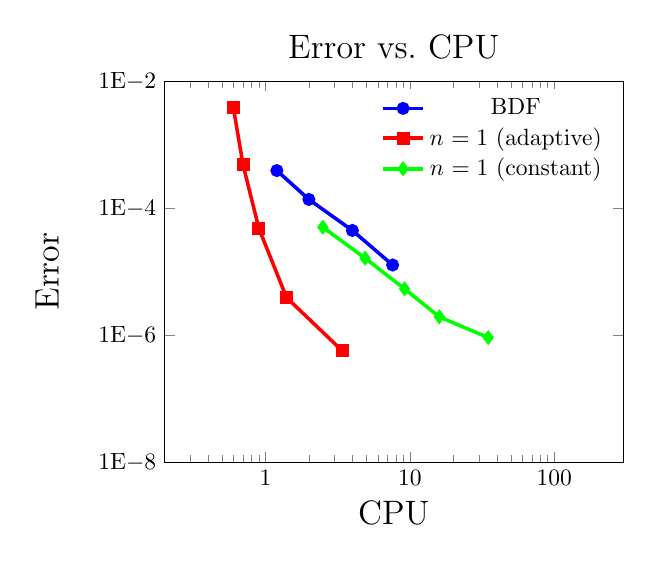
\begin{tikzpicture}[scale=0.85]

\begin{axis}[
  xmode = log,
  xmin = 0.2,
  xmax = 300,
  xtick = {0.1,1,10,100},
  xticklabels = {$0.1$,$1$,$10$,$100$},
  xlabel = CPU,
  ymode = log,
  ymin = 1E-8,
  ymax = 1E-2,
  ytick = {1E-8,1E-6,1E-4,1E-2},
  yticklabels = {$1$E$-8$,$1$E$-6$,$1$E$-4$,$1$E$-2$},
  ylabel = {Error},
  ylabel style = {yshift = 10pt},
  label style = {font=\Large},
%  legend entries = {BDF,$n_{\sdc}=0$,$n_{\sdc}=1$,$n_{\sdc}=2$},
  legend entries = {BDF,$n_{\sdc}=1$ (adaptive),$n_{\sdc}=1$
    (constant)},
  legend style = {draw=none},
  title = {\Large{Error vs.~CPU}}
  ]

% BDF fixed time step size
\addplot [mark=*,blue,line width=1.5] table{
1.2 3.90e-4
2.0 1.37e-4
4.0 4.45e-5
7.6 1.27e-5
};

% 1 sdc correction adaptive time step size
\addplot [mark=square*,red,line width=1.5] table{
0.6 3.81e-3
0.7 4.81e-4
0.9 4.83e-5
1.4 3.91e-6
3.4 5.69e-7
%1.9 3.27e-3
%1.3 2.00e-4
%1.5 1.41e-5
%1.9 2.48e-6
%4.1 6.30e-7
%11.0 9.09e-8
};

% 1 SDC correction fixed time step size
\addplot [mark=diamond*,green,line width=1.5] table{
2.5 4.99e-5
4.9 1.63e-5
9.2 5.35e-6
16.0 1.94e-6
34.9 9.15e-7

%4.2 5.71e-6
%8.1 2.42e-6
%15.8 9.54e-7
%28.3 3.20e-7
%60.2 9.03e-8
%113.4 2.15e-8
};


%% BDF fixed time step size
%\addplot [mark=square*,mark options={fill=blue,solid,mark
%size=2pt},blue,line width=1.5] table{
%1.0 3.90e-4
%2.1 1.37e-4
%4.3 4.45e-5
%8.2 1.27e-5
%};

%% first-order fixed time step size
%\addplot [mark=triangle*,mark options={fill=blue,solid,mark size=2pt},blue,line width=1.5] table{
%1.0 1.27e-3
%1.9 6.64e-4
%3.7 3.46e-4
%7.6 1.79e-4
%};


%% 1 SDC correction fixed time step size
%\addplot [mark=*,mark options={fill=blue,solid,mark size=2pt},blue,line width=1.5] table{
%4.2 5.71e-6
%8.1 2.42e-6
%15.8 9.54e-7
%28.3 3.20e-7
%60.2 9.03e-8
%113.4 2.15e-8
%};

%% 2 SDC correction fixed time step size
%\addplot [mark=diamond*,mark options={fill=blue,solid,mark size=2pt},blue,line width=1.5] table{
%9.0 7.39e-7
%18.3 1.56e-7
%34.8 3.27e-8
%70.7 8.37e-9
%135.4 2.95e-9
%282.8 1.33e-9
%};
%
%% first-order adaptive time step size
%\addplot [mark=triangle*,mark options={fill=blue,solid,mark size=2pt},blue,line width=1.5,dashed] table{
%0.3 1.46e-3
%1.3 2.29e-4
%11.1 4.15e-5
%};
%
%% 1 sdc correction adaptive time step size
%\addplot [mark=*,mark options={fill=blue,solid,mark size=2pt},blue,line width=1.5,dashed] table{
%%1.9 3.27e-3
%%1.3 2.00e-4
%1.5 1.41e-5
%1.9 2.48e-6
%4.1 6.30e-7
%11.0 9.09e-8
%};

%% 2 SDC correction adaptive time step size
%\addplot [mark=diamond*,mark options={fill=blue,solid,mark size=2pt},blue,line width=1.5,dashed] table{
%2.2 2.71e-6
%4.1 8.78e-7
%11.6 8.66e-9
%};

\end{axis}

\end{tikzpicture}


 
}
\fi
\end{tabular}
\mcaption{Results for the {\bf extensional} flow.  Top left: The time
step size using 4800 {\bf constant} time step sizes (dashed) and an
{\bf adaptive} time step size (solid) with a tolerance of $1$E$-6$ and
$\boldnsdc{1}$, $p=2$.  The open circles indicate the times when a time
step is rejected.  Top right: The errors in area and length using {\bf
constant} (dashed) and {\bf adaptive} (solid) time steps, and the
desired error (black) of the adaptive time step.  Bottom: The error
versus the required CPU time for the three different second-order time
integrators.}{f:extensionalSummary}
\end{figure}

%%%%%%%%%%%%%%%%%%%%%%%%%%%%%%%%%%%%%%%%%%%%%%%%%%%%%%%%%%%%%%%%%%%%
\subsection{Stenosis flow}
We consider a single vesicle discretized with $N=128$ points in a
constricted tube discretized with $N_{\mathrm{wall}} = 768$ points
(Figure~\ref{f:stenosisGeom}).  The time horizon, $T=80$, is chosen so
that the vesicle is forced to pass through the constriction.  In
Figure~\ref{f:stenosisErrors}, we plot the errors in area and length
using BDF with a constant time step size.  Unsurprisingly, the errors
increase when the vesicle passes through the constriction.  In this
interval, a smaller time step should be taken.  Therefore, we test our
second-order adaptive time stepper, $n_{\sdc}=1$.  The results are
summarized in Table~\ref{t:adaptiveSecondOrderStenosis}.  In
Figure~\ref{f:stenosisSummary}, we plot the time step size and compare
the two second-order time integrators.  As expected, we see that a
small time step is taken as the vesicle passes through the
constriction.  In fact, the time step size varies over more than three
orders of magnitude which indicates that this example benefits greatly
from an adaptive time step size.  This is verified in right plot of
Figure~\ref{f:stenosisSummary} where we see that our new time
integrator outperforms BDF.  In particular, we see that adaptive
$n_{\sdc}=1$ achieves close to an extra digit of accuracy for a fixed
CPU time.

\begin{figure}[htp]
\centering
%\ifTikz
%\begin{tikzpicture}[
  line cap=round,line join=round,
  spy using outlines={rectangle,lens={scale=3},size=0.9in},scale=1.0]


% Time = 0
\begin{axis}[
  at = {(0,6400)},
  xmin = -41,
  xmax = 41,
  ymin = -3.2,
  ymax = 3.2,
  scale only axis,
  axis equal image,
  hide axis,
  ]

\addplot [mark=none,black,line width=1.0] table{
4.0000e+01 0
4.0000e+01 4.4610e-01
4.0000e+01 8.9220e-01
3.9992e+01 1.3382e+00
3.9924e+01 1.7775e+00
3.9664e+01 2.1324e+00
3.9271e+01 2.3395e+00
3.8844e+01 2.4670e+00
3.8407e+01 2.5559e+00
3.7966e+01 2.6228e+00
3.7523e+01 2.6756e+00
3.7079e+01 2.7186e+00
3.6634e+01 2.7544e+00
3.6189e+01 2.7847e+00
3.5744e+01 2.8106e+00
3.5298e+01 2.8329e+00
3.4853e+01 2.8523e+00
3.4407e+01 2.8693e+00
3.3961e+01 2.8843e+00
3.3515e+01 2.8974e+00
3.3069e+01 2.9091e+00
3.2623e+01 2.9194e+00
3.2177e+01 2.9286e+00
3.1731e+01 2.9367e+00
3.1285e+01 2.9440e+00
3.0839e+01 2.9504e+00
3.0393e+01 2.9562e+00
2.9947e+01 2.9613e+00
2.9501e+01 2.9658e+00
2.9055e+01 2.9699e+00
2.8609e+01 2.9735e+00
2.8163e+01 2.9767e+00
2.7717e+01 2.9796e+00
2.7270e+01 2.9821e+00
2.6824e+01 2.9844e+00
2.6378e+01 2.9864e+00
2.5932e+01 2.9881e+00
2.5486e+01 2.9897e+00
2.5040e+01 2.9911e+00
2.4594e+01 2.9923e+00
2.4148e+01 2.9933e+00
2.3702e+01 2.9943e+00
2.3256e+01 2.9951e+00
2.2810e+01 2.9958e+00
2.2363e+01 2.9964e+00
2.1917e+01 2.9969e+00
2.1471e+01 2.9974e+00
2.1025e+01 2.9978e+00
2.0579e+01 2.9982e+00
2.0133e+01 2.9985e+00
1.9687e+01 2.9987e+00
1.9241e+01 2.9989e+00
1.8795e+01 2.9991e+00
1.8349e+01 2.9993e+00
1.7902e+01 2.9994e+00
1.7456e+01 2.9995e+00
1.7010e+01 2.9996e+00
1.6564e+01 2.9997e+00
1.6118e+01 2.9997e+00
1.5672e+01 2.9998e+00
1.5226e+01 2.9998e+00
1.4780e+01 2.9999e+00
1.4334e+01 2.9999e+00
1.3888e+01 2.9999e+00
1.3441e+01 2.9999e+00
1.2995e+01 3.0000e+00
1.2549e+01 3.0000e+00
1.2103e+01 3.0000e+00
1.1657e+01 3.0000e+00
1.1211e+01 3.0000e+00
1.0765e+01 3.0000e+00
1.0319e+01 3.0000e+00
9.8727e+00 3.0000e+00
9.4266e+00 3.0000e+00
8.9804e+00 3.0000e+00
8.5344e+00 3.0000e+00
8.0883e+00 3.0000e+00
7.6421e+00 3.0000e+00
7.1961e+00 3.0000e+00
6.7500e+00 3.0000e+00
6.3038e+00 3.0000e+00
5.8579e+00 3.0000e+00
5.4117e+00 3.0000e+00
4.9654e+00 3.0000e+00
4.5196e+00 3.0000e+00
4.0736e+00 3.0000e+00
3.6269e+00 3.0000e+00
3.1812e+00 3.0000e+00
2.7473e+00 2.9137e+00
2.3687e+00 2.6804e+00
2.0376e+00 2.3813e+00
1.7326e+00 2.0563e+00
1.4355e+00 1.7232e+00
1.1317e+00 1.3968e+00
8.0400e-01 1.0944e+00
4.3039e-01 8.5260e-01
4.3440e-14 7.5000e-01
-4.3039e-01 8.5260e-01
-8.0400e-01 1.0944e+00
-1.1317e+00 1.3968e+00
-1.4355e+00 1.7232e+00
-1.7326e+00 2.0563e+00
-2.0376e+00 2.3813e+00
-2.3687e+00 2.6804e+00
-2.7473e+00 2.9137e+00
-3.1812e+00 3.0000e+00
-3.6269e+00 3.0000e+00
-4.0736e+00 3.0000e+00
-4.5196e+00 3.0000e+00
-4.9654e+00 3.0000e+00
-5.4117e+00 3.0000e+00
-5.8579e+00 3.0000e+00
-6.3038e+00 3.0000e+00
-6.7500e+00 3.0000e+00
-7.1961e+00 3.0000e+00
-7.6421e+00 3.0000e+00
-8.0883e+00 3.0000e+00
-8.5344e+00 3.0000e+00
-8.9804e+00 3.0000e+00
-9.4266e+00 3.0000e+00
-9.8727e+00 3.0000e+00
-1.0319e+01 3.0000e+00
-1.0765e+01 3.0000e+00
-1.1211e+01 3.0000e+00
-1.1657e+01 3.0000e+00
-1.2103e+01 3.0000e+00
-1.2549e+01 3.0000e+00
-1.2995e+01 3.0000e+00
-1.3441e+01 2.9999e+00
-1.3888e+01 2.9999e+00
-1.4334e+01 2.9999e+00
-1.4780e+01 2.9999e+00
-1.5226e+01 2.9998e+00
-1.5672e+01 2.9998e+00
-1.6118e+01 2.9997e+00
-1.6564e+01 2.9997e+00
-1.7010e+01 2.9996e+00
-1.7456e+01 2.9995e+00
-1.7902e+01 2.9994e+00
-1.8349e+01 2.9993e+00
-1.8795e+01 2.9991e+00
-1.9241e+01 2.9989e+00
-1.9687e+01 2.9987e+00
-2.0133e+01 2.9985e+00
-2.0579e+01 2.9982e+00
-2.1025e+01 2.9978e+00
-2.1471e+01 2.9974e+00
-2.1917e+01 2.9969e+00
-2.2363e+01 2.9964e+00
-2.2810e+01 2.9958e+00
-2.3256e+01 2.9951e+00
-2.3702e+01 2.9943e+00
-2.4148e+01 2.9933e+00
-2.4594e+01 2.9923e+00
-2.5040e+01 2.9911e+00
-2.5486e+01 2.9897e+00
-2.5932e+01 2.9881e+00
-2.6378e+01 2.9864e+00
-2.6824e+01 2.9844e+00
-2.7270e+01 2.9821e+00
-2.7717e+01 2.9796e+00
-2.8163e+01 2.9767e+00
-2.8609e+01 2.9735e+00
-2.9055e+01 2.9699e+00
-2.9501e+01 2.9658e+00
-2.9947e+01 2.9613e+00
-3.0393e+01 2.9562e+00
-3.0839e+01 2.9504e+00
-3.1285e+01 2.9440e+00
-3.1731e+01 2.9367e+00
-3.2177e+01 2.9286e+00
-3.2623e+01 2.9194e+00
-3.3069e+01 2.9091e+00
-3.3515e+01 2.8974e+00
-3.3961e+01 2.8843e+00
-3.4407e+01 2.8693e+00
-3.4853e+01 2.8523e+00
-3.5298e+01 2.8329e+00
-3.5744e+01 2.8106e+00
-3.6189e+01 2.7847e+00
-3.6634e+01 2.7544e+00
-3.7079e+01 2.7186e+00
-3.7523e+01 2.6756e+00
-3.7966e+01 2.6228e+00
-3.8407e+01 2.5559e+00
-3.8844e+01 2.4670e+00
-3.9271e+01 2.3395e+00
-3.9664e+01 2.1324e+00
-3.9924e+01 1.7775e+00
-3.9992e+01 1.3382e+00
-4.0000e+01 8.9220e-01
-4.0000e+01 4.4610e-01
-4.0000e+01 1.0042e-13
-4.0000e+01 -4.4610e-01
-4.0000e+01 -8.9220e-01
-3.9992e+01 -1.3382e+00
-3.9924e+01 -1.7775e+00
-3.9664e+01 -2.1324e+00
-3.9271e+01 -2.3395e+00
-3.8844e+01 -2.4670e+00
-3.8407e+01 -2.5559e+00
-3.7966e+01 -2.6228e+00
-3.7523e+01 -2.6756e+00
-3.7079e+01 -2.7186e+00
-3.6634e+01 -2.7544e+00
-3.6189e+01 -2.7847e+00
-3.5744e+01 -2.8106e+00
-3.5298e+01 -2.8329e+00
-3.4853e+01 -2.8523e+00
-3.4407e+01 -2.8693e+00
-3.3961e+01 -2.8843e+00
-3.3515e+01 -2.8974e+00
-3.3069e+01 -2.9091e+00
-3.2623e+01 -2.9194e+00
-3.2177e+01 -2.9286e+00
-3.1731e+01 -2.9367e+00
-3.1285e+01 -2.9440e+00
-3.0839e+01 -2.9504e+00
-3.0393e+01 -2.9562e+00
-2.9947e+01 -2.9613e+00
-2.9501e+01 -2.9658e+00
-2.9055e+01 -2.9699e+00
-2.8609e+01 -2.9735e+00
-2.8163e+01 -2.9767e+00
-2.7717e+01 -2.9796e+00
-2.7270e+01 -2.9821e+00
-2.6824e+01 -2.9844e+00
-2.6378e+01 -2.9864e+00
-2.5932e+01 -2.9881e+00
-2.5486e+01 -2.9897e+00
-2.5040e+01 -2.9911e+00
-2.4594e+01 -2.9923e+00
-2.4148e+01 -2.9933e+00
-2.3702e+01 -2.9943e+00
-2.3256e+01 -2.9951e+00
-2.2810e+01 -2.9958e+00
-2.2363e+01 -2.9964e+00
-2.1917e+01 -2.9969e+00
-2.1471e+01 -2.9974e+00
-2.1025e+01 -2.9978e+00
-2.0579e+01 -2.9982e+00
-2.0133e+01 -2.9985e+00
-1.9687e+01 -2.9987e+00
-1.9241e+01 -2.9989e+00
-1.8795e+01 -2.9991e+00
-1.8349e+01 -2.9993e+00
-1.7902e+01 -2.9994e+00
-1.7456e+01 -2.9995e+00
-1.7010e+01 -2.9996e+00
-1.6564e+01 -2.9997e+00
-1.6118e+01 -2.9997e+00
-1.5672e+01 -2.9998e+00
-1.5226e+01 -2.9998e+00
-1.4780e+01 -2.9999e+00
-1.4334e+01 -2.9999e+00
-1.3888e+01 -2.9999e+00
-1.3441e+01 -2.9999e+00
-1.2995e+01 -3.0000e+00
-1.2549e+01 -3.0000e+00
-1.2103e+01 -3.0000e+00
-1.1657e+01 -3.0000e+00
-1.1211e+01 -3.0000e+00
-1.0765e+01 -3.0000e+00
-1.0319e+01 -3.0000e+00
-9.8727e+00 -3.0000e+00
-9.4266e+00 -3.0000e+00
-8.9804e+00 -3.0000e+00
-8.5344e+00 -3.0000e+00
-8.0883e+00 -3.0000e+00
-7.6421e+00 -3.0000e+00
-7.1961e+00 -3.0000e+00
-6.7500e+00 -3.0000e+00
-6.3038e+00 -3.0000e+00
-5.8579e+00 -3.0000e+00
-5.4117e+00 -3.0000e+00
-4.9654e+00 -3.0000e+00
-4.5196e+00 -3.0000e+00
-4.0736e+00 -3.0000e+00
-3.6269e+00 -3.0000e+00
-3.1812e+00 -3.0000e+00
-2.7473e+00 -2.9137e+00
-2.3687e+00 -2.6804e+00
-2.0376e+00 -2.3813e+00
-1.7326e+00 -2.0563e+00
-1.4355e+00 -1.7232e+00
-1.1317e+00 -1.3968e+00
-8.0400e-01 -1.0944e+00
-4.3039e-01 -8.5260e-01
-1.4604e-13 -7.5000e-01
4.3039e-01 -8.5260e-01
8.0400e-01 -1.0944e+00
1.1317e+00 -1.3968e+00
1.4355e+00 -1.7232e+00
1.7326e+00 -2.0563e+00
2.0376e+00 -2.3813e+00
2.3687e+00 -2.6804e+00
2.7473e+00 -2.9137e+00
3.1812e+00 -3.0000e+00
3.6269e+00 -3.0000e+00
4.0736e+00 -3.0000e+00
4.5196e+00 -3.0000e+00
4.9654e+00 -3.0000e+00
5.4117e+00 -3.0000e+00
5.8579e+00 -3.0000e+00
6.3038e+00 -3.0000e+00
6.7500e+00 -3.0000e+00
7.1961e+00 -3.0000e+00
7.6421e+00 -3.0000e+00
8.0883e+00 -3.0000e+00
8.5344e+00 -3.0000e+00
8.9804e+00 -3.0000e+00
9.4266e+00 -3.0000e+00
9.8727e+00 -3.0000e+00
1.0319e+01 -3.0000e+00
1.0765e+01 -3.0000e+00
1.1211e+01 -3.0000e+00
1.1657e+01 -3.0000e+00
1.2103e+01 -3.0000e+00
1.2549e+01 -3.0000e+00
1.2995e+01 -3.0000e+00
1.3441e+01 -2.9999e+00
1.3888e+01 -2.9999e+00
1.4334e+01 -2.9999e+00
1.4780e+01 -2.9999e+00
1.5226e+01 -2.9998e+00
1.5672e+01 -2.9998e+00
1.6118e+01 -2.9997e+00
1.6564e+01 -2.9997e+00
1.7010e+01 -2.9996e+00
1.7456e+01 -2.9995e+00
1.7902e+01 -2.9994e+00
1.8349e+01 -2.9993e+00
1.8795e+01 -2.9991e+00
1.9241e+01 -2.9989e+00
1.9687e+01 -2.9987e+00
2.0133e+01 -2.9985e+00
2.0579e+01 -2.9982e+00
2.1025e+01 -2.9978e+00
2.1471e+01 -2.9974e+00
2.1917e+01 -2.9969e+00
2.2363e+01 -2.9964e+00
2.2810e+01 -2.9958e+00
2.3256e+01 -2.9951e+00
2.3702e+01 -2.9943e+00
2.4148e+01 -2.9933e+00
2.4594e+01 -2.9923e+00
2.5040e+01 -2.9911e+00
2.5486e+01 -2.9897e+00
2.5932e+01 -2.9881e+00
2.6378e+01 -2.9864e+00
2.6824e+01 -2.9844e+00
2.7270e+01 -2.9821e+00
2.7717e+01 -2.9796e+00
2.8163e+01 -2.9767e+00
2.8609e+01 -2.9735e+00
2.9055e+01 -2.9699e+00
2.9501e+01 -2.9658e+00
2.9947e+01 -2.9613e+00
3.0393e+01 -2.9562e+00
3.0839e+01 -2.9504e+00
3.1285e+01 -2.9440e+00
3.1731e+01 -2.9367e+00
3.2177e+01 -2.9286e+00
3.2623e+01 -2.9194e+00
3.3069e+01 -2.9091e+00
3.3515e+01 -2.8974e+00
3.3961e+01 -2.8843e+00
3.4407e+01 -2.8693e+00
3.4853e+01 -2.8523e+00
3.5298e+01 -2.8329e+00
3.5744e+01 -2.8106e+00
3.6189e+01 -2.7847e+00
3.6634e+01 -2.7544e+00
3.7079e+01 -2.7186e+00
3.7523e+01 -2.6756e+00
3.7966e+01 -2.6228e+00
3.8407e+01 -2.5559e+00
3.8844e+01 -2.4670e+00
3.9271e+01 -2.3395e+00
3.9664e+01 -2.1324e+00
3.9924e+01 -1.7775e+00
3.9992e+01 -1.3382e+00
4.0000e+01 -8.9220e-01
4.0000e+01 -4.4610e-01
4.0000e+01 0
};

\addplot [mark=none,red,line width=1.0] table{
-3.9000e+01 1.7412e+00
-3.9028e+01 1.7391e+00
-3.9056e+01 1.7329e+00
-3.9084e+01 1.7224e+00
-3.9112e+01 1.7078e+00
-3.9140e+01 1.6891e+00
-3.9167e+01 1.6663e+00
-3.9193e+01 1.6395e+00
-3.9220e+01 1.6087e+00
-3.9246e+01 1.5741e+00
-3.9271e+01 1.5356e+00
-3.9295e+01 1.4935e+00
-3.9319e+01 1.4478e+00
-3.9342e+01 1.3986e+00
-3.9364e+01 1.3460e+00
-3.9386e+01 1.2902e+00
-3.9406e+01 1.2312e+00
-3.9426e+01 1.1693e+00
-3.9444e+01 1.1046e+00
-3.9461e+01 1.0373e+00
-3.9478e+01 9.6738e-01
-3.9493e+01 8.9518e-01
-3.9506e+01 8.2082e-01
-3.9519e+01 7.4448e-01
-3.9531e+01 6.6635e-01
-3.9541e+01 5.8661e-01
-3.9550e+01 5.0546e-01
-3.9557e+01 4.2309e-01
-3.9563e+01 3.3970e-01
-3.9568e+01 2.5549e-01
-3.9572e+01 1.7067e-01
-3.9574e+01 8.5439e-02
-3.9574e+01 1.4179e-16
-3.9574e+01 -8.5439e-02
-3.9572e+01 -1.7067e-01
-3.9568e+01 -2.5549e-01
-3.9563e+01 -3.3970e-01
-3.9557e+01 -4.2309e-01
-3.9550e+01 -5.0546e-01
-3.9541e+01 -5.8661e-01
-3.9531e+01 -6.6635e-01
-3.9519e+01 -7.4448e-01
-3.9506e+01 -8.2082e-01
-3.9493e+01 -8.9518e-01
-3.9478e+01 -9.6738e-01
-3.9461e+01 -1.0373e+00
-3.9444e+01 -1.1046e+00
-3.9426e+01 -1.1693e+00
-3.9406e+01 -1.2312e+00
-3.9386e+01 -1.2902e+00
-3.9364e+01 -1.3460e+00
-3.9342e+01 -1.3986e+00
-3.9319e+01 -1.4478e+00
-3.9295e+01 -1.4935e+00
-3.9271e+01 -1.5356e+00
-3.9246e+01 -1.5741e+00
-3.9220e+01 -1.6087e+00
-3.9193e+01 -1.6395e+00
-3.9167e+01 -1.6663e+00
-3.9140e+01 -1.6891e+00
-3.9112e+01 -1.7078e+00
-3.9084e+01 -1.7224e+00
-3.9056e+01 -1.7329e+00
-3.9028e+01 -1.7391e+00
-3.9000e+01 -1.7412e+00
-3.8972e+01 -1.7391e+00
-3.8944e+01 -1.7329e+00
-3.8916e+01 -1.7224e+00
-3.8888e+01 -1.7078e+00
-3.8860e+01 -1.6891e+00
-3.8833e+01 -1.6663e+00
-3.8807e+01 -1.6395e+00
-3.8780e+01 -1.6087e+00
-3.8754e+01 -1.5741e+00
-3.8729e+01 -1.5356e+00
-3.8705e+01 -1.4935e+00
-3.8681e+01 -1.4478e+00
-3.8658e+01 -1.3986e+00
-3.8636e+01 -1.3460e+00
-3.8614e+01 -1.2902e+00
-3.8594e+01 -1.2312e+00
-3.8574e+01 -1.1693e+00
-3.8556e+01 -1.1046e+00
-3.8539e+01 -1.0373e+00
-3.8522e+01 -9.6738e-01
-3.8507e+01 -8.9518e-01
-3.8494e+01 -8.2082e-01
-3.8481e+01 -7.4448e-01
-3.8469e+01 -6.6635e-01
-3.8459e+01 -5.8661e-01
-3.8450e+01 -5.0546e-01
-3.8443e+01 -4.2309e-01
-3.8437e+01 -3.3970e-01
-3.8432e+01 -2.5549e-01
-3.8428e+01 -1.7067e-01
-3.8426e+01 -8.5439e-02
-3.8426e+01 -3.5503e-16
-3.8426e+01 8.5439e-02
-3.8428e+01 1.7067e-01
-3.8432e+01 2.5549e-01
-3.8437e+01 3.3970e-01
-3.8443e+01 4.2309e-01
-3.8450e+01 5.0546e-01
-3.8459e+01 5.8661e-01
-3.8469e+01 6.6635e-01
-3.8481e+01 7.4448e-01
-3.8494e+01 8.2082e-01
-3.8507e+01 8.9518e-01
-3.8522e+01 9.6738e-01
-3.8539e+01 1.0373e+00
-3.8556e+01 1.1046e+00
-3.8574e+01 1.1693e+00
-3.8594e+01 1.2312e+00
-3.8614e+01 1.2902e+00
-3.8636e+01 1.3460e+00
-3.8658e+01 1.3986e+00
-3.8681e+01 1.4478e+00
-3.8705e+01 1.4935e+00
-3.8729e+01 1.5356e+00
-3.8754e+01 1.5741e+00
-3.8780e+01 1.6087e+00
-3.8807e+01 1.6395e+00
-3.8833e+01 1.6663e+00
-3.8860e+01 1.6891e+00
-3.8888e+01 1.7078e+00
-3.8916e+01 1.7224e+00
-3.8944e+01 1.7329e+00
-3.8972e+01 1.7391e+00
-3.9000e+01 1.7412e+00
};

\end{axis}


% Time = 20
\begin{axis}[
  at = {(0,5600)},
  xmin = -41,
  xmax = 41,
  ymin = -3.2,
  ymax = 3.2,
  scale only axis,
  axis equal image,
  hide axis,
  ]


\addplot [mark=none,black,line width=1.0] table{
4.0000e+01 0
4.0000e+01 4.4610e-01
4.0000e+01 8.9220e-01
3.9992e+01 1.3382e+00
3.9924e+01 1.7775e+00
3.9664e+01 2.1324e+00
3.9271e+01 2.3395e+00
3.8844e+01 2.4670e+00
3.8407e+01 2.5559e+00
3.7966e+01 2.6228e+00
3.7523e+01 2.6756e+00
3.7079e+01 2.7186e+00
3.6634e+01 2.7544e+00
3.6189e+01 2.7847e+00
3.5744e+01 2.8106e+00
3.5298e+01 2.8329e+00
3.4853e+01 2.8523e+00
3.4407e+01 2.8693e+00
3.3961e+01 2.8843e+00
3.3515e+01 2.8974e+00
3.3069e+01 2.9091e+00
3.2623e+01 2.9194e+00
3.2177e+01 2.9286e+00
3.1731e+01 2.9367e+00
3.1285e+01 2.9440e+00
3.0839e+01 2.9504e+00
3.0393e+01 2.9562e+00
2.9947e+01 2.9613e+00
2.9501e+01 2.9658e+00
2.9055e+01 2.9699e+00
2.8609e+01 2.9735e+00
2.8163e+01 2.9767e+00
2.7717e+01 2.9796e+00
2.7270e+01 2.9821e+00
2.6824e+01 2.9844e+00
2.6378e+01 2.9864e+00
2.5932e+01 2.9881e+00
2.5486e+01 2.9897e+00
2.5040e+01 2.9911e+00
2.4594e+01 2.9923e+00
2.4148e+01 2.9933e+00
2.3702e+01 2.9943e+00
2.3256e+01 2.9951e+00
2.2810e+01 2.9958e+00
2.2363e+01 2.9964e+00
2.1917e+01 2.9969e+00
2.1471e+01 2.9974e+00
2.1025e+01 2.9978e+00
2.0579e+01 2.9982e+00
2.0133e+01 2.9985e+00
1.9687e+01 2.9987e+00
1.9241e+01 2.9989e+00
1.8795e+01 2.9991e+00
1.8349e+01 2.9993e+00
1.7902e+01 2.9994e+00
1.7456e+01 2.9995e+00
1.7010e+01 2.9996e+00
1.6564e+01 2.9997e+00
1.6118e+01 2.9997e+00
1.5672e+01 2.9998e+00
1.5226e+01 2.9998e+00
1.4780e+01 2.9999e+00
1.4334e+01 2.9999e+00
1.3888e+01 2.9999e+00
1.3441e+01 2.9999e+00
1.2995e+01 3.0000e+00
1.2549e+01 3.0000e+00
1.2103e+01 3.0000e+00
1.1657e+01 3.0000e+00
1.1211e+01 3.0000e+00
1.0765e+01 3.0000e+00
1.0319e+01 3.0000e+00
9.8727e+00 3.0000e+00
9.4266e+00 3.0000e+00
8.9804e+00 3.0000e+00
8.5344e+00 3.0000e+00
8.0883e+00 3.0000e+00
7.6421e+00 3.0000e+00
7.1961e+00 3.0000e+00
6.7500e+00 3.0000e+00
6.3038e+00 3.0000e+00
5.8579e+00 3.0000e+00
5.4117e+00 3.0000e+00
4.9654e+00 3.0000e+00
4.5196e+00 3.0000e+00
4.0736e+00 3.0000e+00
3.6269e+00 3.0000e+00
3.1812e+00 3.0000e+00
2.7473e+00 2.9137e+00
2.3687e+00 2.6804e+00
2.0376e+00 2.3813e+00
1.7326e+00 2.0563e+00
1.4355e+00 1.7232e+00
1.1317e+00 1.3968e+00
8.0400e-01 1.0944e+00
4.3039e-01 8.5260e-01
4.3440e-14 7.5000e-01
-4.3039e-01 8.5260e-01
-8.0400e-01 1.0944e+00
-1.1317e+00 1.3968e+00
-1.4355e+00 1.7232e+00
-1.7326e+00 2.0563e+00
-2.0376e+00 2.3813e+00
-2.3687e+00 2.6804e+00
-2.7473e+00 2.9137e+00
-3.1812e+00 3.0000e+00
-3.6269e+00 3.0000e+00
-4.0736e+00 3.0000e+00
-4.5196e+00 3.0000e+00
-4.9654e+00 3.0000e+00
-5.4117e+00 3.0000e+00
-5.8579e+00 3.0000e+00
-6.3038e+00 3.0000e+00
-6.7500e+00 3.0000e+00
-7.1961e+00 3.0000e+00
-7.6421e+00 3.0000e+00
-8.0883e+00 3.0000e+00
-8.5344e+00 3.0000e+00
-8.9804e+00 3.0000e+00
-9.4266e+00 3.0000e+00
-9.8727e+00 3.0000e+00
-1.0319e+01 3.0000e+00
-1.0765e+01 3.0000e+00
-1.1211e+01 3.0000e+00
-1.1657e+01 3.0000e+00
-1.2103e+01 3.0000e+00
-1.2549e+01 3.0000e+00
-1.2995e+01 3.0000e+00
-1.3441e+01 2.9999e+00
-1.3888e+01 2.9999e+00
-1.4334e+01 2.9999e+00
-1.4780e+01 2.9999e+00
-1.5226e+01 2.9998e+00
-1.5672e+01 2.9998e+00
-1.6118e+01 2.9997e+00
-1.6564e+01 2.9997e+00
-1.7010e+01 2.9996e+00
-1.7456e+01 2.9995e+00
-1.7902e+01 2.9994e+00
-1.8349e+01 2.9993e+00
-1.8795e+01 2.9991e+00
-1.9241e+01 2.9989e+00
-1.9687e+01 2.9987e+00
-2.0133e+01 2.9985e+00
-2.0579e+01 2.9982e+00
-2.1025e+01 2.9978e+00
-2.1471e+01 2.9974e+00
-2.1917e+01 2.9969e+00
-2.2363e+01 2.9964e+00
-2.2810e+01 2.9958e+00
-2.3256e+01 2.9951e+00
-2.3702e+01 2.9943e+00
-2.4148e+01 2.9933e+00
-2.4594e+01 2.9923e+00
-2.5040e+01 2.9911e+00
-2.5486e+01 2.9897e+00
-2.5932e+01 2.9881e+00
-2.6378e+01 2.9864e+00
-2.6824e+01 2.9844e+00
-2.7270e+01 2.9821e+00
-2.7717e+01 2.9796e+00
-2.8163e+01 2.9767e+00
-2.8609e+01 2.9735e+00
-2.9055e+01 2.9699e+00
-2.9501e+01 2.9658e+00
-2.9947e+01 2.9613e+00
-3.0393e+01 2.9562e+00
-3.0839e+01 2.9504e+00
-3.1285e+01 2.9440e+00
-3.1731e+01 2.9367e+00
-3.2177e+01 2.9286e+00
-3.2623e+01 2.9194e+00
-3.3069e+01 2.9091e+00
-3.3515e+01 2.8974e+00
-3.3961e+01 2.8843e+00
-3.4407e+01 2.8693e+00
-3.4853e+01 2.8523e+00
-3.5298e+01 2.8329e+00
-3.5744e+01 2.8106e+00
-3.6189e+01 2.7847e+00
-3.6634e+01 2.7544e+00
-3.7079e+01 2.7186e+00
-3.7523e+01 2.6756e+00
-3.7966e+01 2.6228e+00
-3.8407e+01 2.5559e+00
-3.8844e+01 2.4670e+00
-3.9271e+01 2.3395e+00
-3.9664e+01 2.1324e+00
-3.9924e+01 1.7775e+00
-3.9992e+01 1.3382e+00
-4.0000e+01 8.9220e-01
-4.0000e+01 4.4610e-01
-4.0000e+01 1.0042e-13
-4.0000e+01 -4.4610e-01
-4.0000e+01 -8.9220e-01
-3.9992e+01 -1.3382e+00
-3.9924e+01 -1.7775e+00
-3.9664e+01 -2.1324e+00
-3.9271e+01 -2.3395e+00
-3.8844e+01 -2.4670e+00
-3.8407e+01 -2.5559e+00
-3.7966e+01 -2.6228e+00
-3.7523e+01 -2.6756e+00
-3.7079e+01 -2.7186e+00
-3.6634e+01 -2.7544e+00
-3.6189e+01 -2.7847e+00
-3.5744e+01 -2.8106e+00
-3.5298e+01 -2.8329e+00
-3.4853e+01 -2.8523e+00
-3.4407e+01 -2.8693e+00
-3.3961e+01 -2.8843e+00
-3.3515e+01 -2.8974e+00
-3.3069e+01 -2.9091e+00
-3.2623e+01 -2.9194e+00
-3.2177e+01 -2.9286e+00
-3.1731e+01 -2.9367e+00
-3.1285e+01 -2.9440e+00
-3.0839e+01 -2.9504e+00
-3.0393e+01 -2.9562e+00
-2.9947e+01 -2.9613e+00
-2.9501e+01 -2.9658e+00
-2.9055e+01 -2.9699e+00
-2.8609e+01 -2.9735e+00
-2.8163e+01 -2.9767e+00
-2.7717e+01 -2.9796e+00
-2.7270e+01 -2.9821e+00
-2.6824e+01 -2.9844e+00
-2.6378e+01 -2.9864e+00
-2.5932e+01 -2.9881e+00
-2.5486e+01 -2.9897e+00
-2.5040e+01 -2.9911e+00
-2.4594e+01 -2.9923e+00
-2.4148e+01 -2.9933e+00
-2.3702e+01 -2.9943e+00
-2.3256e+01 -2.9951e+00
-2.2810e+01 -2.9958e+00
-2.2363e+01 -2.9964e+00
-2.1917e+01 -2.9969e+00
-2.1471e+01 -2.9974e+00
-2.1025e+01 -2.9978e+00
-2.0579e+01 -2.9982e+00
-2.0133e+01 -2.9985e+00
-1.9687e+01 -2.9987e+00
-1.9241e+01 -2.9989e+00
-1.8795e+01 -2.9991e+00
-1.8349e+01 -2.9993e+00
-1.7902e+01 -2.9994e+00
-1.7456e+01 -2.9995e+00
-1.7010e+01 -2.9996e+00
-1.6564e+01 -2.9997e+00
-1.6118e+01 -2.9997e+00
-1.5672e+01 -2.9998e+00
-1.5226e+01 -2.9998e+00
-1.4780e+01 -2.9999e+00
-1.4334e+01 -2.9999e+00
-1.3888e+01 -2.9999e+00
-1.3441e+01 -2.9999e+00
-1.2995e+01 -3.0000e+00
-1.2549e+01 -3.0000e+00
-1.2103e+01 -3.0000e+00
-1.1657e+01 -3.0000e+00
-1.1211e+01 -3.0000e+00
-1.0765e+01 -3.0000e+00
-1.0319e+01 -3.0000e+00
-9.8727e+00 -3.0000e+00
-9.4266e+00 -3.0000e+00
-8.9804e+00 -3.0000e+00
-8.5344e+00 -3.0000e+00
-8.0883e+00 -3.0000e+00
-7.6421e+00 -3.0000e+00
-7.1961e+00 -3.0000e+00
-6.7500e+00 -3.0000e+00
-6.3038e+00 -3.0000e+00
-5.8579e+00 -3.0000e+00
-5.4117e+00 -3.0000e+00
-4.9654e+00 -3.0000e+00
-4.5196e+00 -3.0000e+00
-4.0736e+00 -3.0000e+00
-3.6269e+00 -3.0000e+00
-3.1812e+00 -3.0000e+00
-2.7473e+00 -2.9137e+00
-2.3687e+00 -2.6804e+00
-2.0376e+00 -2.3813e+00
-1.7326e+00 -2.0563e+00
-1.4355e+00 -1.7232e+00
-1.1317e+00 -1.3968e+00
-8.0400e-01 -1.0944e+00
-4.3039e-01 -8.5260e-01
-1.4604e-13 -7.5000e-01
4.3039e-01 -8.5260e-01
8.0400e-01 -1.0944e+00
1.1317e+00 -1.3968e+00
1.4355e+00 -1.7232e+00
1.7326e+00 -2.0563e+00
2.0376e+00 -2.3813e+00
2.3687e+00 -2.6804e+00
2.7473e+00 -2.9137e+00
3.1812e+00 -3.0000e+00
3.6269e+00 -3.0000e+00
4.0736e+00 -3.0000e+00
4.5196e+00 -3.0000e+00
4.9654e+00 -3.0000e+00
5.4117e+00 -3.0000e+00
5.8579e+00 -3.0000e+00
6.3038e+00 -3.0000e+00
6.7500e+00 -3.0000e+00
7.1961e+00 -3.0000e+00
7.6421e+00 -3.0000e+00
8.0883e+00 -3.0000e+00
8.5344e+00 -3.0000e+00
8.9804e+00 -3.0000e+00
9.4266e+00 -3.0000e+00
9.8727e+00 -3.0000e+00
1.0319e+01 -3.0000e+00
1.0765e+01 -3.0000e+00
1.1211e+01 -3.0000e+00
1.1657e+01 -3.0000e+00
1.2103e+01 -3.0000e+00
1.2549e+01 -3.0000e+00
1.2995e+01 -3.0000e+00
1.3441e+01 -2.9999e+00
1.3888e+01 -2.9999e+00
1.4334e+01 -2.9999e+00
1.4780e+01 -2.9999e+00
1.5226e+01 -2.9998e+00
1.5672e+01 -2.9998e+00
1.6118e+01 -2.9997e+00
1.6564e+01 -2.9997e+00
1.7010e+01 -2.9996e+00
1.7456e+01 -2.9995e+00
1.7902e+01 -2.9994e+00
1.8349e+01 -2.9993e+00
1.8795e+01 -2.9991e+00
1.9241e+01 -2.9989e+00
1.9687e+01 -2.9987e+00
2.0133e+01 -2.9985e+00
2.0579e+01 -2.9982e+00
2.1025e+01 -2.9978e+00
2.1471e+01 -2.9974e+00
2.1917e+01 -2.9969e+00
2.2363e+01 -2.9964e+00
2.2810e+01 -2.9958e+00
2.3256e+01 -2.9951e+00
2.3702e+01 -2.9943e+00
2.4148e+01 -2.9933e+00
2.4594e+01 -2.9923e+00
2.5040e+01 -2.9911e+00
2.5486e+01 -2.9897e+00
2.5932e+01 -2.9881e+00
2.6378e+01 -2.9864e+00
2.6824e+01 -2.9844e+00
2.7270e+01 -2.9821e+00
2.7717e+01 -2.9796e+00
2.8163e+01 -2.9767e+00
2.8609e+01 -2.9735e+00
2.9055e+01 -2.9699e+00
2.9501e+01 -2.9658e+00
2.9947e+01 -2.9613e+00
3.0393e+01 -2.9562e+00
3.0839e+01 -2.9504e+00
3.1285e+01 -2.9440e+00
3.1731e+01 -2.9367e+00
3.2177e+01 -2.9286e+00
3.2623e+01 -2.9194e+00
3.3069e+01 -2.9091e+00
3.3515e+01 -2.8974e+00
3.3961e+01 -2.8843e+00
3.4407e+01 -2.8693e+00
3.4853e+01 -2.8523e+00
3.5298e+01 -2.8329e+00
3.5744e+01 -2.8106e+00
3.6189e+01 -2.7847e+00
3.6634e+01 -2.7544e+00
3.7079e+01 -2.7186e+00
3.7523e+01 -2.6756e+00
3.7966e+01 -2.6228e+00
3.8407e+01 -2.5559e+00
3.8844e+01 -2.4670e+00
3.9271e+01 -2.3395e+00
3.9664e+01 -2.1324e+00
3.9924e+01 -1.7775e+00
3.9992e+01 -1.3382e+00
4.0000e+01 -8.9220e-01
4.0000e+01 -4.4610e-01
4.0000e+01 0
};
\addplot [mark=none,red,line width=1.0] table{
-2.2692e+01 1.4480e+00
-2.2719e+01 1.4550e+00
-2.2748e+01 1.4609e+00
-2.2777e+01 1.4653e+00
-2.2808e+01 1.4680e+00
-2.2842e+01 1.4686e+00
-2.2877e+01 1.4665e+00
-2.2915e+01 1.4610e+00
-2.2954e+01 1.4510e+00
-2.2994e+01 1.4357e+00
-2.3035e+01 1.4140e+00
-2.3074e+01 1.3853e+00
-2.3111e+01 1.3490e+00
-2.3142e+01 1.3050e+00
-2.3168e+01 1.2538e+00
-2.3185e+01 1.1966e+00
-2.3192e+01 1.1348e+00
-2.3190e+01 1.0700e+00
-2.3178e+01 1.0038e+00
-2.3158e+01 9.3744e-01
-2.3129e+01 8.7163e-01
-2.3094e+01 8.0663e-01
-2.3055e+01 7.4225e-01
-2.3012e+01 6.7793e-01
-2.2967e+01 6.1289e-01
-2.2922e+01 5.4629e-01
-2.2878e+01 4.7730e-01
-2.2837e+01 4.0530e-01
-2.2801e+01 3.2991e-01
-2.2771e+01 2.5112e-01
-2.2749e+01 1.6932e-01
-2.2735e+01 8.5266e-02
-2.2730e+01 1.5383e-12
-2.2735e+01 -8.5266e-02
-2.2749e+01 -1.6932e-01
-2.2771e+01 -2.5112e-01
-2.2801e+01 -3.2991e-01
-2.2837e+01 -4.0530e-01
-2.2878e+01 -4.7730e-01
-2.2922e+01 -5.4629e-01
-2.2967e+01 -6.1289e-01
-2.3012e+01 -6.7793e-01
-2.3055e+01 -7.4225e-01
-2.3094e+01 -8.0663e-01
-2.3129e+01 -8.7163e-01
-2.3158e+01 -9.3744e-01
-2.3178e+01 -1.0038e+00
-2.3190e+01 -1.0700e+00
-2.3192e+01 -1.1348e+00
-2.3185e+01 -1.1966e+00
-2.3168e+01 -1.2538e+00
-2.3142e+01 -1.3050e+00
-2.3111e+01 -1.3490e+00
-2.3074e+01 -1.3853e+00
-2.3035e+01 -1.4140e+00
-2.2994e+01 -1.4357e+00
-2.2954e+01 -1.4510e+00
-2.2915e+01 -1.4610e+00
-2.2877e+01 -1.4665e+00
-2.2842e+01 -1.4686e+00
-2.2808e+01 -1.4680e+00
-2.2777e+01 -1.4653e+00
-2.2748e+01 -1.4609e+00
-2.2719e+01 -1.4550e+00
-2.2692e+01 -1.4480e+00
-2.2665e+01 -1.4397e+00
-2.2638e+01 -1.4301e+00
-2.2610e+01 -1.4189e+00
-2.2581e+01 -1.4061e+00
-2.2551e+01 -1.3914e+00
-2.2520e+01 -1.3746e+00
-2.2487e+01 -1.3555e+00
-2.2453e+01 -1.3339e+00
-2.2417e+01 -1.3098e+00
-2.2380e+01 -1.2830e+00
-2.2341e+01 -1.2535e+00
-2.2301e+01 -1.2213e+00
-2.2259e+01 -1.1864e+00
-2.2216e+01 -1.1489e+00
-2.2172e+01 -1.1087e+00
-2.2127e+01 -1.0658e+00
-2.2080e+01 -1.0204e+00
-2.2033e+01 -9.7243e-01
-2.1986e+01 -9.2181e-01
-2.1938e+01 -8.6850e-01
-2.1890e+01 -8.1242e-01
-2.1842e+01 -7.5344e-01
-2.1796e+01 -6.9145e-01
-2.1751e+01 -6.2631e-01
-2.1709e+01 -5.5793e-01
-2.1670e+01 -4.8627e-01
-2.1635e+01 -4.1137e-01
-2.1605e+01 -3.3342e-01
-2.1580e+01 -2.5275e-01
-2.1562e+01 -1.6984e-01
-2.1551e+01 -8.5333e-02
-2.1547e+01 -3.1990e-11
-2.1551e+01 8.5333e-02
-2.1562e+01 1.6984e-01
-2.1580e+01 2.5275e-01
-2.1605e+01 3.3342e-01
-2.1635e+01 4.1137e-01
-2.1670e+01 4.8627e-01
-2.1709e+01 5.5793e-01
-2.1751e+01 6.2631e-01
-2.1796e+01 6.9145e-01
-2.1842e+01 7.5344e-01
-2.1890e+01 8.1242e-01
-2.1938e+01 8.6850e-01
-2.1986e+01 9.2181e-01
-2.2033e+01 9.7243e-01
-2.2080e+01 1.0204e+00
-2.2127e+01 1.0658e+00
-2.2172e+01 1.1087e+00
-2.2216e+01 1.1489e+00
-2.2259e+01 1.1864e+00
-2.2301e+01 1.2213e+00
-2.2341e+01 1.2535e+00
-2.2380e+01 1.2830e+00
-2.2417e+01 1.3098e+00
-2.2453e+01 1.3339e+00
-2.2487e+01 1.3555e+00
-2.2520e+01 1.3746e+00
-2.2551e+01 1.3914e+00
-2.2581e+01 1.4061e+00
-2.2610e+01 1.4189e+00
-2.2638e+01 1.4301e+00
-2.2665e+01 1.4397e+00
-2.2692e+01 1.4480e+00
};

\end{axis}


% Time = 40
\begin{axis}[
  at = {(0,4800)},
  xmin = -41,
  xmax = 41,
  ymin = -3.2,
  ymax = 3.2,
  scale only axis,
  axis equal image,
  hide axis,
  ]

\addplot [mark=none,black,line width=1.0] table{
4.0000e+01 0
4.0000e+01 4.4610e-01
4.0000e+01 8.9220e-01
3.9992e+01 1.3382e+00
3.9924e+01 1.7775e+00
3.9664e+01 2.1324e+00
3.9271e+01 2.3395e+00
3.8844e+01 2.4670e+00
3.8407e+01 2.5559e+00
3.7966e+01 2.6228e+00
3.7523e+01 2.6756e+00
3.7079e+01 2.7186e+00
3.6634e+01 2.7544e+00
3.6189e+01 2.7847e+00
3.5744e+01 2.8106e+00
3.5298e+01 2.8329e+00
3.4853e+01 2.8523e+00
3.4407e+01 2.8693e+00
3.3961e+01 2.8843e+00
3.3515e+01 2.8974e+00
3.3069e+01 2.9091e+00
3.2623e+01 2.9194e+00
3.2177e+01 2.9286e+00
3.1731e+01 2.9367e+00
3.1285e+01 2.9440e+00
3.0839e+01 2.9504e+00
3.0393e+01 2.9562e+00
2.9947e+01 2.9613e+00
2.9501e+01 2.9658e+00
2.9055e+01 2.9699e+00
2.8609e+01 2.9735e+00
2.8163e+01 2.9767e+00
2.7717e+01 2.9796e+00
2.7270e+01 2.9821e+00
2.6824e+01 2.9844e+00
2.6378e+01 2.9864e+00
2.5932e+01 2.9881e+00
2.5486e+01 2.9897e+00
2.5040e+01 2.9911e+00
2.4594e+01 2.9923e+00
2.4148e+01 2.9933e+00
2.3702e+01 2.9943e+00
2.3256e+01 2.9951e+00
2.2810e+01 2.9958e+00
2.2363e+01 2.9964e+00
2.1917e+01 2.9969e+00
2.1471e+01 2.9974e+00
2.1025e+01 2.9978e+00
2.0579e+01 2.9982e+00
2.0133e+01 2.9985e+00
1.9687e+01 2.9987e+00
1.9241e+01 2.9989e+00
1.8795e+01 2.9991e+00
1.8349e+01 2.9993e+00
1.7902e+01 2.9994e+00
1.7456e+01 2.9995e+00
1.7010e+01 2.9996e+00
1.6564e+01 2.9997e+00
1.6118e+01 2.9997e+00
1.5672e+01 2.9998e+00
1.5226e+01 2.9998e+00
1.4780e+01 2.9999e+00
1.4334e+01 2.9999e+00
1.3888e+01 2.9999e+00
1.3441e+01 2.9999e+00
1.2995e+01 3.0000e+00
1.2549e+01 3.0000e+00
1.2103e+01 3.0000e+00
1.1657e+01 3.0000e+00
1.1211e+01 3.0000e+00
1.0765e+01 3.0000e+00
1.0319e+01 3.0000e+00
9.8727e+00 3.0000e+00
9.4266e+00 3.0000e+00
8.9804e+00 3.0000e+00
8.5344e+00 3.0000e+00
8.0883e+00 3.0000e+00
7.6421e+00 3.0000e+00
7.1961e+00 3.0000e+00
6.7500e+00 3.0000e+00
6.3038e+00 3.0000e+00
5.8579e+00 3.0000e+00
5.4117e+00 3.0000e+00
4.9654e+00 3.0000e+00
4.5196e+00 3.0000e+00
4.0736e+00 3.0000e+00
3.6269e+00 3.0000e+00
3.1812e+00 3.0000e+00
2.7473e+00 2.9137e+00
2.3687e+00 2.6804e+00
2.0376e+00 2.3813e+00
1.7326e+00 2.0563e+00
1.4355e+00 1.7232e+00
1.1317e+00 1.3968e+00
8.0400e-01 1.0944e+00
4.3039e-01 8.5260e-01
4.3440e-14 7.5000e-01
-4.3039e-01 8.5260e-01
-8.0400e-01 1.0944e+00
-1.1317e+00 1.3968e+00
-1.4355e+00 1.7232e+00
-1.7326e+00 2.0563e+00
-2.0376e+00 2.3813e+00
-2.3687e+00 2.6804e+00
-2.7473e+00 2.9137e+00
-3.1812e+00 3.0000e+00
-3.6269e+00 3.0000e+00
-4.0736e+00 3.0000e+00
-4.5196e+00 3.0000e+00
-4.9654e+00 3.0000e+00
-5.4117e+00 3.0000e+00
-5.8579e+00 3.0000e+00
-6.3038e+00 3.0000e+00
-6.7500e+00 3.0000e+00
-7.1961e+00 3.0000e+00
-7.6421e+00 3.0000e+00
-8.0883e+00 3.0000e+00
-8.5344e+00 3.0000e+00
-8.9804e+00 3.0000e+00
-9.4266e+00 3.0000e+00
-9.8727e+00 3.0000e+00
-1.0319e+01 3.0000e+00
-1.0765e+01 3.0000e+00
-1.1211e+01 3.0000e+00
-1.1657e+01 3.0000e+00
-1.2103e+01 3.0000e+00
-1.2549e+01 3.0000e+00
-1.2995e+01 3.0000e+00
-1.3441e+01 2.9999e+00
-1.3888e+01 2.9999e+00
-1.4334e+01 2.9999e+00
-1.4780e+01 2.9999e+00
-1.5226e+01 2.9998e+00
-1.5672e+01 2.9998e+00
-1.6118e+01 2.9997e+00
-1.6564e+01 2.9997e+00
-1.7010e+01 2.9996e+00
-1.7456e+01 2.9995e+00
-1.7902e+01 2.9994e+00
-1.8349e+01 2.9993e+00
-1.8795e+01 2.9991e+00
-1.9241e+01 2.9989e+00
-1.9687e+01 2.9987e+00
-2.0133e+01 2.9985e+00
-2.0579e+01 2.9982e+00
-2.1025e+01 2.9978e+00
-2.1471e+01 2.9974e+00
-2.1917e+01 2.9969e+00
-2.2363e+01 2.9964e+00
-2.2810e+01 2.9958e+00
-2.3256e+01 2.9951e+00
-2.3702e+01 2.9943e+00
-2.4148e+01 2.9933e+00
-2.4594e+01 2.9923e+00
-2.5040e+01 2.9911e+00
-2.5486e+01 2.9897e+00
-2.5932e+01 2.9881e+00
-2.6378e+01 2.9864e+00
-2.6824e+01 2.9844e+00
-2.7270e+01 2.9821e+00
-2.7717e+01 2.9796e+00
-2.8163e+01 2.9767e+00
-2.8609e+01 2.9735e+00
-2.9055e+01 2.9699e+00
-2.9501e+01 2.9658e+00
-2.9947e+01 2.9613e+00
-3.0393e+01 2.9562e+00
-3.0839e+01 2.9504e+00
-3.1285e+01 2.9440e+00
-3.1731e+01 2.9367e+00
-3.2177e+01 2.9286e+00
-3.2623e+01 2.9194e+00
-3.3069e+01 2.9091e+00
-3.3515e+01 2.8974e+00
-3.3961e+01 2.8843e+00
-3.4407e+01 2.8693e+00
-3.4853e+01 2.8523e+00
-3.5298e+01 2.8329e+00
-3.5744e+01 2.8106e+00
-3.6189e+01 2.7847e+00
-3.6634e+01 2.7544e+00
-3.7079e+01 2.7186e+00
-3.7523e+01 2.6756e+00
-3.7966e+01 2.6228e+00
-3.8407e+01 2.5559e+00
-3.8844e+01 2.4670e+00
-3.9271e+01 2.3395e+00
-3.9664e+01 2.1324e+00
-3.9924e+01 1.7775e+00
-3.9992e+01 1.3382e+00
-4.0000e+01 8.9220e-01
-4.0000e+01 4.4610e-01
-4.0000e+01 1.0042e-13
-4.0000e+01 -4.4610e-01
-4.0000e+01 -8.9220e-01
-3.9992e+01 -1.3382e+00
-3.9924e+01 -1.7775e+00
-3.9664e+01 -2.1324e+00
-3.9271e+01 -2.3395e+00
-3.8844e+01 -2.4670e+00
-3.8407e+01 -2.5559e+00
-3.7966e+01 -2.6228e+00
-3.7523e+01 -2.6756e+00
-3.7079e+01 -2.7186e+00
-3.6634e+01 -2.7544e+00
-3.6189e+01 -2.7847e+00
-3.5744e+01 -2.8106e+00
-3.5298e+01 -2.8329e+00
-3.4853e+01 -2.8523e+00
-3.4407e+01 -2.8693e+00
-3.3961e+01 -2.8843e+00
-3.3515e+01 -2.8974e+00
-3.3069e+01 -2.9091e+00
-3.2623e+01 -2.9194e+00
-3.2177e+01 -2.9286e+00
-3.1731e+01 -2.9367e+00
-3.1285e+01 -2.9440e+00
-3.0839e+01 -2.9504e+00
-3.0393e+01 -2.9562e+00
-2.9947e+01 -2.9613e+00
-2.9501e+01 -2.9658e+00
-2.9055e+01 -2.9699e+00
-2.8609e+01 -2.9735e+00
-2.8163e+01 -2.9767e+00
-2.7717e+01 -2.9796e+00
-2.7270e+01 -2.9821e+00
-2.6824e+01 -2.9844e+00
-2.6378e+01 -2.9864e+00
-2.5932e+01 -2.9881e+00
-2.5486e+01 -2.9897e+00
-2.5040e+01 -2.9911e+00
-2.4594e+01 -2.9923e+00
-2.4148e+01 -2.9933e+00
-2.3702e+01 -2.9943e+00
-2.3256e+01 -2.9951e+00
-2.2810e+01 -2.9958e+00
-2.2363e+01 -2.9964e+00
-2.1917e+01 -2.9969e+00
-2.1471e+01 -2.9974e+00
-2.1025e+01 -2.9978e+00
-2.0579e+01 -2.9982e+00
-2.0133e+01 -2.9985e+00
-1.9687e+01 -2.9987e+00
-1.9241e+01 -2.9989e+00
-1.8795e+01 -2.9991e+00
-1.8349e+01 -2.9993e+00
-1.7902e+01 -2.9994e+00
-1.7456e+01 -2.9995e+00
-1.7010e+01 -2.9996e+00
-1.6564e+01 -2.9997e+00
-1.6118e+01 -2.9997e+00
-1.5672e+01 -2.9998e+00
-1.5226e+01 -2.9998e+00
-1.4780e+01 -2.9999e+00
-1.4334e+01 -2.9999e+00
-1.3888e+01 -2.9999e+00
-1.3441e+01 -2.9999e+00
-1.2995e+01 -3.0000e+00
-1.2549e+01 -3.0000e+00
-1.2103e+01 -3.0000e+00
-1.1657e+01 -3.0000e+00
-1.1211e+01 -3.0000e+00
-1.0765e+01 -3.0000e+00
-1.0319e+01 -3.0000e+00
-9.8727e+00 -3.0000e+00
-9.4266e+00 -3.0000e+00
-8.9804e+00 -3.0000e+00
-8.5344e+00 -3.0000e+00
-8.0883e+00 -3.0000e+00
-7.6421e+00 -3.0000e+00
-7.1961e+00 -3.0000e+00
-6.7500e+00 -3.0000e+00
-6.3038e+00 -3.0000e+00
-5.8579e+00 -3.0000e+00
-5.4117e+00 -3.0000e+00
-4.9654e+00 -3.0000e+00
-4.5196e+00 -3.0000e+00
-4.0736e+00 -3.0000e+00
-3.6269e+00 -3.0000e+00
-3.1812e+00 -3.0000e+00
-2.7473e+00 -2.9137e+00
-2.3687e+00 -2.6804e+00
-2.0376e+00 -2.3813e+00
-1.7326e+00 -2.0563e+00
-1.4355e+00 -1.7232e+00
-1.1317e+00 -1.3968e+00
-8.0400e-01 -1.0944e+00
-4.3039e-01 -8.5260e-01
-1.4604e-13 -7.5000e-01
4.3039e-01 -8.5260e-01
8.0400e-01 -1.0944e+00
1.1317e+00 -1.3968e+00
1.4355e+00 -1.7232e+00
1.7326e+00 -2.0563e+00
2.0376e+00 -2.3813e+00
2.3687e+00 -2.6804e+00
2.7473e+00 -2.9137e+00
3.1812e+00 -3.0000e+00
3.6269e+00 -3.0000e+00
4.0736e+00 -3.0000e+00
4.5196e+00 -3.0000e+00
4.9654e+00 -3.0000e+00
5.4117e+00 -3.0000e+00
5.8579e+00 -3.0000e+00
6.3038e+00 -3.0000e+00
6.7500e+00 -3.0000e+00
7.1961e+00 -3.0000e+00
7.6421e+00 -3.0000e+00
8.0883e+00 -3.0000e+00
8.5344e+00 -3.0000e+00
8.9804e+00 -3.0000e+00
9.4266e+00 -3.0000e+00
9.8727e+00 -3.0000e+00
1.0319e+01 -3.0000e+00
1.0765e+01 -3.0000e+00
1.1211e+01 -3.0000e+00
1.1657e+01 -3.0000e+00
1.2103e+01 -3.0000e+00
1.2549e+01 -3.0000e+00
1.2995e+01 -3.0000e+00
1.3441e+01 -2.9999e+00
1.3888e+01 -2.9999e+00
1.4334e+01 -2.9999e+00
1.4780e+01 -2.9999e+00
1.5226e+01 -2.9998e+00
1.5672e+01 -2.9998e+00
1.6118e+01 -2.9997e+00
1.6564e+01 -2.9997e+00
1.7010e+01 -2.9996e+00
1.7456e+01 -2.9995e+00
1.7902e+01 -2.9994e+00
1.8349e+01 -2.9993e+00
1.8795e+01 -2.9991e+00
1.9241e+01 -2.9989e+00
1.9687e+01 -2.9987e+00
2.0133e+01 -2.9985e+00
2.0579e+01 -2.9982e+00
2.1025e+01 -2.9978e+00
2.1471e+01 -2.9974e+00
2.1917e+01 -2.9969e+00
2.2363e+01 -2.9964e+00
2.2810e+01 -2.9958e+00
2.3256e+01 -2.9951e+00
2.3702e+01 -2.9943e+00
2.4148e+01 -2.9933e+00
2.4594e+01 -2.9923e+00
2.5040e+01 -2.9911e+00
2.5486e+01 -2.9897e+00
2.5932e+01 -2.9881e+00
2.6378e+01 -2.9864e+00
2.6824e+01 -2.9844e+00
2.7270e+01 -2.9821e+00
2.7717e+01 -2.9796e+00
2.8163e+01 -2.9767e+00
2.8609e+01 -2.9735e+00
2.9055e+01 -2.9699e+00
2.9501e+01 -2.9658e+00
2.9947e+01 -2.9613e+00
3.0393e+01 -2.9562e+00
3.0839e+01 -2.9504e+00
3.1285e+01 -2.9440e+00
3.1731e+01 -2.9367e+00
3.2177e+01 -2.9286e+00
3.2623e+01 -2.9194e+00
3.3069e+01 -2.9091e+00
3.3515e+01 -2.8974e+00
3.3961e+01 -2.8843e+00
3.4407e+01 -2.8693e+00
3.4853e+01 -2.8523e+00
3.5298e+01 -2.8329e+00
3.5744e+01 -2.8106e+00
3.6189e+01 -2.7847e+00
3.6634e+01 -2.7544e+00
3.7079e+01 -2.7186e+00
3.7523e+01 -2.6756e+00
3.7966e+01 -2.6228e+00
3.8407e+01 -2.5559e+00
3.8844e+01 -2.4670e+00
3.9271e+01 -2.3395e+00
3.9664e+01 -2.1324e+00
3.9924e+01 -1.7775e+00
3.9992e+01 -1.3382e+00
4.0000e+01 -8.9220e-01
4.0000e+01 -4.4610e-01
4.0000e+01 0
};

\addplot [mark=none,red,line width=1.0] table{
-6.4964e+00 1.4397e+00
-6.5238e+00 1.4470e+00
-6.5520e+00 1.4530e+00
-6.5815e+00 1.4577e+00
-6.6128e+00 1.4607e+00
-6.6461e+00 1.4616e+00
-6.6815e+00 1.4599e+00
-6.7190e+00 1.4547e+00
-6.7583e+00 1.4451e+00
-6.7989e+00 1.4303e+00
-6.8396e+00 1.4091e+00
-6.8793e+00 1.3808e+00
-6.9162e+00 1.3449e+00
-6.9485e+00 1.3013e+00
-6.9742e+00 1.2504e+00
-6.9917e+00 1.1933e+00
-6.9998e+00 1.1316e+00
-6.9980e+00 1.0668e+00
-6.9863e+00 1.0005e+00
-6.9656e+00 9.3416e-01
-6.9370e+00 8.6841e-01
-6.9019e+00 8.0356e-01
-6.8618e+00 7.3942e-01
-6.8183e+00 6.7543e-01
-6.7729e+00 6.1080e-01
-6.7273e+00 5.4464e-01
-6.6829e+00 4.7610e-01
-6.6415e+00 4.0451e-01
-6.6047e+00 3.2946e-01
-6.5741e+00 2.5091e-01
-6.5510e+00 1.6926e-01
-6.5366e+00 8.5257e-02
-6.5318e+00 -6.0422e-12
-6.5366e+00 -8.5257e-02
-6.5510e+00 -1.6926e-01
-6.5741e+00 -2.5091e-01
-6.6047e+00 -3.2946e-01
-6.6415e+00 -4.0451e-01
-6.6829e+00 -4.7610e-01
-6.7273e+00 -5.4464e-01
-6.7729e+00 -6.1080e-01
-6.8183e+00 -6.7543e-01
-6.8618e+00 -7.3942e-01
-6.9019e+00 -8.0356e-01
-6.9370e+00 -8.6841e-01
-6.9656e+00 -9.3416e-01
-6.9863e+00 -1.0005e+00
-6.9980e+00 -1.0668e+00
-6.9998e+00 -1.1316e+00
-6.9917e+00 -1.1933e+00
-6.9742e+00 -1.2504e+00
-6.9485e+00 -1.3013e+00
-6.9162e+00 -1.3449e+00
-6.8793e+00 -1.3808e+00
-6.8396e+00 -1.4091e+00
-6.7989e+00 -1.4303e+00
-6.7583e+00 -1.4451e+00
-6.7190e+00 -1.4547e+00
-6.6815e+00 -1.4599e+00
-6.6461e+00 -1.4616e+00
-6.6128e+00 -1.4607e+00
-6.5815e+00 -1.4577e+00
-6.5520e+00 -1.4530e+00
-6.5238e+00 -1.4470e+00
-6.4964e+00 -1.4397e+00
-6.4694e+00 -1.4313e+00
-6.4423e+00 -1.4215e+00
-6.4146e+00 -1.4102e+00
-6.3860e+00 -1.3973e+00
-6.3562e+00 -1.3824e+00
-6.3250e+00 -1.3655e+00
-6.2923e+00 -1.3463e+00
-6.2581e+00 -1.3247e+00
-6.2223e+00 -1.3005e+00
-6.1850e+00 -1.2737e+00
-6.1461e+00 -1.2443e+00
-6.1058e+00 -1.2122e+00
-6.0640e+00 -1.1774e+00
-6.0209e+00 -1.1400e+00
-5.9764e+00 -1.1000e+00
-5.9308e+00 -1.0575e+00
-5.8841e+00 -1.0125e+00
-5.8365e+00 -9.6494e-01
-5.7882e+00 -9.1484e-01
-5.7396e+00 -8.6214e-01
-5.6909e+00 -8.0673e-01
-5.6426e+00 -7.4850e-01
-5.5952e+00 -6.8730e-01
-5.5494e+00 -6.2297e-01
-5.5059e+00 -5.5538e-01
-5.4655e+00 -4.8446e-01
-5.4291e+00 -4.1021e-01
-5.3976e+00 -3.3277e-01
-5.3720e+00 -2.5245e-01
-5.3529e+00 -1.6974e-01
-5.3412e+00 -8.5321e-02
-5.3373e+00 -7.2165e-11
-5.3412e+00 8.5321e-02
-5.3529e+00 1.6974e-01
-5.3720e+00 2.5245e-01
-5.3976e+00 3.3277e-01
-5.4291e+00 4.1021e-01
-5.4655e+00 4.8446e-01
-5.5059e+00 5.5538e-01
-5.5494e+00 6.2297e-01
-5.5952e+00 6.8730e-01
-5.6426e+00 7.4850e-01
-5.6909e+00 8.0673e-01
-5.7396e+00 8.6214e-01
-5.7882e+00 9.1484e-01
-5.8365e+00 9.6494e-01
-5.8841e+00 1.0125e+00
-5.9308e+00 1.0575e+00
-5.9764e+00 1.1000e+00
-6.0209e+00 1.1400e+00
-6.0640e+00 1.1774e+00
-6.1058e+00 1.2122e+00
-6.1461e+00 1.2443e+00
-6.1850e+00 1.2737e+00
-6.2223e+00 1.3005e+00
-6.2581e+00 1.3247e+00
-6.2923e+00 1.3463e+00
-6.3250e+00 1.3655e+00
-6.3562e+00 1.3824e+00
-6.3860e+00 1.3973e+00
-6.4146e+00 1.4102e+00
-6.4423e+00 1.4215e+00
-6.4694e+00 1.4313e+00
-6.4964e+00 1.4397e+00
};

\end{axis}


% Time = 44
\begin{axis}[
  at = {(0,4000)},
  xmin = -41,
  xmax = 41,
  ymin = -3.2,
  ymax = 3.2,
  scale only axis,
  axis equal image,
  hide axis
  ]

\addplot [mark=none,black,line width=1.0] table{
4.0000e+01 0
4.0000e+01 4.4610e-01
4.0000e+01 8.9220e-01
3.9992e+01 1.3382e+00
3.9924e+01 1.7775e+00
3.9664e+01 2.1324e+00
3.9271e+01 2.3395e+00
3.8844e+01 2.4670e+00
3.8407e+01 2.5559e+00
3.7966e+01 2.6228e+00
3.7523e+01 2.6756e+00
3.7079e+01 2.7186e+00
3.6634e+01 2.7544e+00
3.6189e+01 2.7847e+00
3.5744e+01 2.8106e+00
3.5298e+01 2.8329e+00
3.4853e+01 2.8523e+00
3.4407e+01 2.8693e+00
3.3961e+01 2.8843e+00
3.3515e+01 2.8974e+00
3.3069e+01 2.9091e+00
3.2623e+01 2.9194e+00
3.2177e+01 2.9286e+00
3.1731e+01 2.9367e+00
3.1285e+01 2.9440e+00
3.0839e+01 2.9504e+00
3.0393e+01 2.9562e+00
2.9947e+01 2.9613e+00
2.9501e+01 2.9658e+00
2.9055e+01 2.9699e+00
2.8609e+01 2.9735e+00
2.8163e+01 2.9767e+00
2.7717e+01 2.9796e+00
2.7270e+01 2.9821e+00
2.6824e+01 2.9844e+00
2.6378e+01 2.9864e+00
2.5932e+01 2.9881e+00
2.5486e+01 2.9897e+00
2.5040e+01 2.9911e+00
2.4594e+01 2.9923e+00
2.4148e+01 2.9933e+00
2.3702e+01 2.9943e+00
2.3256e+01 2.9951e+00
2.2810e+01 2.9958e+00
2.2363e+01 2.9964e+00
2.1917e+01 2.9969e+00
2.1471e+01 2.9974e+00
2.1025e+01 2.9978e+00
2.0579e+01 2.9982e+00
2.0133e+01 2.9985e+00
1.9687e+01 2.9987e+00
1.9241e+01 2.9989e+00
1.8795e+01 2.9991e+00
1.8349e+01 2.9993e+00
1.7902e+01 2.9994e+00
1.7456e+01 2.9995e+00
1.7010e+01 2.9996e+00
1.6564e+01 2.9997e+00
1.6118e+01 2.9997e+00
1.5672e+01 2.9998e+00
1.5226e+01 2.9998e+00
1.4780e+01 2.9999e+00
1.4334e+01 2.9999e+00
1.3888e+01 2.9999e+00
1.3441e+01 2.9999e+00
1.2995e+01 3.0000e+00
1.2549e+01 3.0000e+00
1.2103e+01 3.0000e+00
1.1657e+01 3.0000e+00
1.1211e+01 3.0000e+00
1.0765e+01 3.0000e+00
1.0319e+01 3.0000e+00
9.8727e+00 3.0000e+00
9.4266e+00 3.0000e+00
8.9804e+00 3.0000e+00
8.5344e+00 3.0000e+00
8.0883e+00 3.0000e+00
7.6421e+00 3.0000e+00
7.1961e+00 3.0000e+00
6.7500e+00 3.0000e+00
6.3038e+00 3.0000e+00
5.8579e+00 3.0000e+00
5.4117e+00 3.0000e+00
4.9654e+00 3.0000e+00
4.5196e+00 3.0000e+00
4.0736e+00 3.0000e+00
3.6269e+00 3.0000e+00
3.1812e+00 3.0000e+00
2.7473e+00 2.9137e+00
2.3687e+00 2.6804e+00
2.0376e+00 2.3813e+00
1.7326e+00 2.0563e+00
1.4355e+00 1.7232e+00
1.1317e+00 1.3968e+00
8.0400e-01 1.0944e+00
4.3039e-01 8.5260e-01
4.3440e-14 7.5000e-01
-4.3039e-01 8.5260e-01
-8.0400e-01 1.0944e+00
-1.1317e+00 1.3968e+00
-1.4355e+00 1.7232e+00
-1.7326e+00 2.0563e+00
-2.0376e+00 2.3813e+00
-2.3687e+00 2.6804e+00
-2.7473e+00 2.9137e+00
-3.1812e+00 3.0000e+00
-3.6269e+00 3.0000e+00
-4.0736e+00 3.0000e+00
-4.5196e+00 3.0000e+00
-4.9654e+00 3.0000e+00
-5.4117e+00 3.0000e+00
-5.8579e+00 3.0000e+00
-6.3038e+00 3.0000e+00
-6.7500e+00 3.0000e+00
-7.1961e+00 3.0000e+00
-7.6421e+00 3.0000e+00
-8.0883e+00 3.0000e+00
-8.5344e+00 3.0000e+00
-8.9804e+00 3.0000e+00
-9.4266e+00 3.0000e+00
-9.8727e+00 3.0000e+00
-1.0319e+01 3.0000e+00
-1.0765e+01 3.0000e+00
-1.1211e+01 3.0000e+00
-1.1657e+01 3.0000e+00
-1.2103e+01 3.0000e+00
-1.2549e+01 3.0000e+00
-1.2995e+01 3.0000e+00
-1.3441e+01 2.9999e+00
-1.3888e+01 2.9999e+00
-1.4334e+01 2.9999e+00
-1.4780e+01 2.9999e+00
-1.5226e+01 2.9998e+00
-1.5672e+01 2.9998e+00
-1.6118e+01 2.9997e+00
-1.6564e+01 2.9997e+00
-1.7010e+01 2.9996e+00
-1.7456e+01 2.9995e+00
-1.7902e+01 2.9994e+00
-1.8349e+01 2.9993e+00
-1.8795e+01 2.9991e+00
-1.9241e+01 2.9989e+00
-1.9687e+01 2.9987e+00
-2.0133e+01 2.9985e+00
-2.0579e+01 2.9982e+00
-2.1025e+01 2.9978e+00
-2.1471e+01 2.9974e+00
-2.1917e+01 2.9969e+00
-2.2363e+01 2.9964e+00
-2.2810e+01 2.9958e+00
-2.3256e+01 2.9951e+00
-2.3702e+01 2.9943e+00
-2.4148e+01 2.9933e+00
-2.4594e+01 2.9923e+00
-2.5040e+01 2.9911e+00
-2.5486e+01 2.9897e+00
-2.5932e+01 2.9881e+00
-2.6378e+01 2.9864e+00
-2.6824e+01 2.9844e+00
-2.7270e+01 2.9821e+00
-2.7717e+01 2.9796e+00
-2.8163e+01 2.9767e+00
-2.8609e+01 2.9735e+00
-2.9055e+01 2.9699e+00
-2.9501e+01 2.9658e+00
-2.9947e+01 2.9613e+00
-3.0393e+01 2.9562e+00
-3.0839e+01 2.9504e+00
-3.1285e+01 2.9440e+00
-3.1731e+01 2.9367e+00
-3.2177e+01 2.9286e+00
-3.2623e+01 2.9194e+00
-3.3069e+01 2.9091e+00
-3.3515e+01 2.8974e+00
-3.3961e+01 2.8843e+00
-3.4407e+01 2.8693e+00
-3.4853e+01 2.8523e+00
-3.5298e+01 2.8329e+00
-3.5744e+01 2.8106e+00
-3.6189e+01 2.7847e+00
-3.6634e+01 2.7544e+00
-3.7079e+01 2.7186e+00
-3.7523e+01 2.6756e+00
-3.7966e+01 2.6228e+00
-3.8407e+01 2.5559e+00
-3.8844e+01 2.4670e+00
-3.9271e+01 2.3395e+00
-3.9664e+01 2.1324e+00
-3.9924e+01 1.7775e+00
-3.9992e+01 1.3382e+00
-4.0000e+01 8.9220e-01
-4.0000e+01 4.4610e-01
-4.0000e+01 1.0042e-13
-4.0000e+01 -4.4610e-01
-4.0000e+01 -8.9220e-01
-3.9992e+01 -1.3382e+00
-3.9924e+01 -1.7775e+00
-3.9664e+01 -2.1324e+00
-3.9271e+01 -2.3395e+00
-3.8844e+01 -2.4670e+00
-3.8407e+01 -2.5559e+00
-3.7966e+01 -2.6228e+00
-3.7523e+01 -2.6756e+00
-3.7079e+01 -2.7186e+00
-3.6634e+01 -2.7544e+00
-3.6189e+01 -2.7847e+00
-3.5744e+01 -2.8106e+00
-3.5298e+01 -2.8329e+00
-3.4853e+01 -2.8523e+00
-3.4407e+01 -2.8693e+00
-3.3961e+01 -2.8843e+00
-3.3515e+01 -2.8974e+00
-3.3069e+01 -2.9091e+00
-3.2623e+01 -2.9194e+00
-3.2177e+01 -2.9286e+00
-3.1731e+01 -2.9367e+00
-3.1285e+01 -2.9440e+00
-3.0839e+01 -2.9504e+00
-3.0393e+01 -2.9562e+00
-2.9947e+01 -2.9613e+00
-2.9501e+01 -2.9658e+00
-2.9055e+01 -2.9699e+00
-2.8609e+01 -2.9735e+00
-2.8163e+01 -2.9767e+00
-2.7717e+01 -2.9796e+00
-2.7270e+01 -2.9821e+00
-2.6824e+01 -2.9844e+00
-2.6378e+01 -2.9864e+00
-2.5932e+01 -2.9881e+00
-2.5486e+01 -2.9897e+00
-2.5040e+01 -2.9911e+00
-2.4594e+01 -2.9923e+00
-2.4148e+01 -2.9933e+00
-2.3702e+01 -2.9943e+00
-2.3256e+01 -2.9951e+00
-2.2810e+01 -2.9958e+00
-2.2363e+01 -2.9964e+00
-2.1917e+01 -2.9969e+00
-2.1471e+01 -2.9974e+00
-2.1025e+01 -2.9978e+00
-2.0579e+01 -2.9982e+00
-2.0133e+01 -2.9985e+00
-1.9687e+01 -2.9987e+00
-1.9241e+01 -2.9989e+00
-1.8795e+01 -2.9991e+00
-1.8349e+01 -2.9993e+00
-1.7902e+01 -2.9994e+00
-1.7456e+01 -2.9995e+00
-1.7010e+01 -2.9996e+00
-1.6564e+01 -2.9997e+00
-1.6118e+01 -2.9997e+00
-1.5672e+01 -2.9998e+00
-1.5226e+01 -2.9998e+00
-1.4780e+01 -2.9999e+00
-1.4334e+01 -2.9999e+00
-1.3888e+01 -2.9999e+00
-1.3441e+01 -2.9999e+00
-1.2995e+01 -3.0000e+00
-1.2549e+01 -3.0000e+00
-1.2103e+01 -3.0000e+00
-1.1657e+01 -3.0000e+00
-1.1211e+01 -3.0000e+00
-1.0765e+01 -3.0000e+00
-1.0319e+01 -3.0000e+00
-9.8727e+00 -3.0000e+00
-9.4266e+00 -3.0000e+00
-8.9804e+00 -3.0000e+00
-8.5344e+00 -3.0000e+00
-8.0883e+00 -3.0000e+00
-7.6421e+00 -3.0000e+00
-7.1961e+00 -3.0000e+00
-6.7500e+00 -3.0000e+00
-6.3038e+00 -3.0000e+00
-5.8579e+00 -3.0000e+00
-5.4117e+00 -3.0000e+00
-4.9654e+00 -3.0000e+00
-4.5196e+00 -3.0000e+00
-4.0736e+00 -3.0000e+00
-3.6269e+00 -3.0000e+00
-3.1812e+00 -3.0000e+00
-2.7473e+00 -2.9137e+00
-2.3687e+00 -2.6804e+00
-2.0376e+00 -2.3813e+00
-1.7326e+00 -2.0563e+00
-1.4355e+00 -1.7232e+00
-1.1317e+00 -1.3968e+00
-8.0400e-01 -1.0944e+00
-4.3039e-01 -8.5260e-01
-1.4604e-13 -7.5000e-01
4.3039e-01 -8.5260e-01
8.0400e-01 -1.0944e+00
1.1317e+00 -1.3968e+00
1.4355e+00 -1.7232e+00
1.7326e+00 -2.0563e+00
2.0376e+00 -2.3813e+00
2.3687e+00 -2.6804e+00
2.7473e+00 -2.9137e+00
3.1812e+00 -3.0000e+00
3.6269e+00 -3.0000e+00
4.0736e+00 -3.0000e+00
4.5196e+00 -3.0000e+00
4.9654e+00 -3.0000e+00
5.4117e+00 -3.0000e+00
5.8579e+00 -3.0000e+00
6.3038e+00 -3.0000e+00
6.7500e+00 -3.0000e+00
7.1961e+00 -3.0000e+00
7.6421e+00 -3.0000e+00
8.0883e+00 -3.0000e+00
8.5344e+00 -3.0000e+00
8.9804e+00 -3.0000e+00
9.4266e+00 -3.0000e+00
9.8727e+00 -3.0000e+00
1.0319e+01 -3.0000e+00
1.0765e+01 -3.0000e+00
1.1211e+01 -3.0000e+00
1.1657e+01 -3.0000e+00
1.2103e+01 -3.0000e+00
1.2549e+01 -3.0000e+00
1.2995e+01 -3.0000e+00
1.3441e+01 -2.9999e+00
1.3888e+01 -2.9999e+00
1.4334e+01 -2.9999e+00
1.4780e+01 -2.9999e+00
1.5226e+01 -2.9998e+00
1.5672e+01 -2.9998e+00
1.6118e+01 -2.9997e+00
1.6564e+01 -2.9997e+00
1.7010e+01 -2.9996e+00
1.7456e+01 -2.9995e+00
1.7902e+01 -2.9994e+00
1.8349e+01 -2.9993e+00
1.8795e+01 -2.9991e+00
1.9241e+01 -2.9989e+00
1.9687e+01 -2.9987e+00
2.0133e+01 -2.9985e+00
2.0579e+01 -2.9982e+00
2.1025e+01 -2.9978e+00
2.1471e+01 -2.9974e+00
2.1917e+01 -2.9969e+00
2.2363e+01 -2.9964e+00
2.2810e+01 -2.9958e+00
2.3256e+01 -2.9951e+00
2.3702e+01 -2.9943e+00
2.4148e+01 -2.9933e+00
2.4594e+01 -2.9923e+00
2.5040e+01 -2.9911e+00
2.5486e+01 -2.9897e+00
2.5932e+01 -2.9881e+00
2.6378e+01 -2.9864e+00
2.6824e+01 -2.9844e+00
2.7270e+01 -2.9821e+00
2.7717e+01 -2.9796e+00
2.8163e+01 -2.9767e+00
2.8609e+01 -2.9735e+00
2.9055e+01 -2.9699e+00
2.9501e+01 -2.9658e+00
2.9947e+01 -2.9613e+00
3.0393e+01 -2.9562e+00
3.0839e+01 -2.9504e+00
3.1285e+01 -2.9440e+00
3.1731e+01 -2.9367e+00
3.2177e+01 -2.9286e+00
3.2623e+01 -2.9194e+00
3.3069e+01 -2.9091e+00
3.3515e+01 -2.8974e+00
3.3961e+01 -2.8843e+00
3.4407e+01 -2.8693e+00
3.4853e+01 -2.8523e+00
3.5298e+01 -2.8329e+00
3.5744e+01 -2.8106e+00
3.6189e+01 -2.7847e+00
3.6634e+01 -2.7544e+00
3.7079e+01 -2.7186e+00
3.7523e+01 -2.6756e+00
3.7966e+01 -2.6228e+00
3.8407e+01 -2.5559e+00
3.8844e+01 -2.4670e+00
3.9271e+01 -2.3395e+00
3.9664e+01 -2.1324e+00
3.9924e+01 -1.7775e+00
3.9992e+01 -1.3382e+00
4.0000e+01 -8.9220e-01
4.0000e+01 -4.4610e-01
4.0000e+01 0
};

\addplot [mark=none,red,line width=1.0] table{
-2.9998e+00 1.1085e+00
-3.0246e+00 1.1220e+00
-3.0503e+00 1.1353e+00
-3.0771e+00 1.1485e+00
-3.1056e+00 1.1616e+00
-3.1363e+00 1.1746e+00
-3.1694e+00 1.1873e+00
-3.2054e+00 1.1991e+00
-3.2445e+00 1.2096e+00
-3.2869e+00 1.2180e+00
-3.3325e+00 1.2231e+00
-3.3813e+00 1.2236e+00
-3.4325e+00 1.2178e+00
-3.4850e+00 1.2041e+00
-3.5370e+00 1.1807e+00
-3.5858e+00 1.1464e+00
-3.6282e+00 1.1008e+00
-3.6609e+00 1.0449e+00
-3.6809e+00 9.8084e-01
-3.6868e+00 9.1164e-01
-3.6783e+00 8.4052e-01
-3.6567e+00 7.7009e-01
-3.6239e+00 7.0198e-01
-3.5824e+00 6.3669e-01
-3.5347e+00 5.7379e-01
-3.4831e+00 5.1212e-01
-3.4301e+00 4.5010e-01
-3.3778e+00 3.8598e-01
-3.3290e+00 3.1813e-01
-3.2863e+00 2.4540e-01
-3.2529e+00 1.6744e-01
-3.2315e+00 8.5015e-02
-3.2241e+00 -2.2023e-11
-3.2315e+00 -8.5015e-02
-3.2529e+00 -1.6744e-01
-3.2863e+00 -2.4540e-01
-3.3290e+00 -3.1813e-01
-3.3778e+00 -3.8598e-01
-3.4301e+00 -4.5010e-01
-3.4831e+00 -5.1212e-01
-3.5347e+00 -5.7379e-01
-3.5824e+00 -6.3669e-01
-3.6239e+00 -7.0198e-01
-3.6567e+00 -7.7009e-01
-3.6783e+00 -8.4052e-01
-3.6868e+00 -9.1164e-01
-3.6809e+00 -9.8084e-01
-3.6609e+00 -1.0449e+00
-3.6282e+00 -1.1008e+00
-3.5858e+00 -1.1464e+00
-3.5370e+00 -1.1807e+00
-3.4850e+00 -1.2041e+00
-3.4325e+00 -1.2178e+00
-3.3813e+00 -1.2236e+00
-3.3325e+00 -1.2231e+00
-3.2869e+00 -1.2180e+00
-3.2445e+00 -1.2096e+00
-3.2054e+00 -1.1991e+00
-3.1694e+00 -1.1873e+00
-3.1363e+00 -1.1746e+00
-3.1056e+00 -1.1616e+00
-3.0771e+00 -1.1485e+00
-3.0503e+00 -1.1353e+00
-3.0246e+00 -1.1220e+00
-2.9998e+00 -1.1085e+00
-2.9751e+00 -1.0947e+00
-2.9501e+00 -1.0802e+00
-2.9244e+00 -1.0650e+00
-2.8976e+00 -1.0486e+00
-2.8693e+00 -1.0311e+00
-2.8393e+00 -1.0121e+00
-2.8073e+00 -9.9177e-01
-2.7733e+00 -9.6987e-01
-2.7370e+00 -9.4644e-01
-2.6984e+00 -9.2150e-01
-2.6574e+00 -8.9511e-01
-2.6140e+00 -8.6735e-01
-2.5680e+00 -8.3833e-01
-2.5196e+00 -8.0817e-01
-2.4686e+00 -7.7700e-01
-2.4151e+00 -7.4495e-01
-2.3591e+00 -7.1214e-01
-2.3007e+00 -6.7868e-01
-2.2400e+00 -6.4467e-01
-2.1771e+00 -6.1015e-01
-2.1122e+00 -5.7511e-01
-2.0455e+00 -5.3951e-01
-1.9772e+00 -5.0315e-01
-1.9076e+00 -4.6572e-01
-1.8374e+00 -4.2667e-01
-1.7671e+00 -3.8514e-01
-1.6979e+00 -3.3983e-01
-1.6316e+00 -2.8895e-01
-1.5710e+00 -2.3034e-01
-1.5207e+00 -1.6214e-01
-1.4865e+00 -8.4271e-02
-1.4743e+00 -8.7960e-11
-1.4865e+00 8.4271e-02
-1.5207e+00 1.6214e-01
-1.5710e+00 2.3034e-01
-1.6316e+00 2.8895e-01
-1.6979e+00 3.3983e-01
-1.7671e+00 3.8514e-01
-1.8374e+00 4.2667e-01
-1.9076e+00 4.6572e-01
-1.9772e+00 5.0315e-01
-2.0455e+00 5.3951e-01
-2.1122e+00 5.7511e-01
-2.1771e+00 6.1015e-01
-2.2400e+00 6.4467e-01
-2.3007e+00 6.7868e-01
-2.3591e+00 7.1214e-01
-2.4151e+00 7.4495e-01
-2.4686e+00 7.7700e-01
-2.5196e+00 8.0817e-01
-2.5680e+00 8.3833e-01
-2.6140e+00 8.6735e-01
-2.6574e+00 8.9511e-01
-2.6984e+00 9.2150e-01
-2.7370e+00 9.4644e-01
-2.7733e+00 9.6987e-01
-2.8073e+00 9.9177e-01
-2.8393e+00 1.0121e+00
-2.8693e+00 1.0311e+00
-2.8976e+00 1.0486e+00
-2.9244e+00 1.0650e+00
-2.9501e+00 1.0802e+00
-2.9751e+00 1.0947e+00
-2.9998e+00 1.1085e+00
};

\end{axis}


% Time = 45
\begin{axis}[
  at = {(0,3200)},
  xmin = -41,
  xmax = 41,
  ymin = -3.2,
  ymax = 3.2,
  scale only axis,
  axis equal image,
  hide axis
  ]

\addplot [mark=none,black,line width=1.0] table{
4.0000e+01 0
4.0000e+01 4.4610e-01
4.0000e+01 8.9220e-01
3.9992e+01 1.3382e+00
3.9924e+01 1.7775e+00
3.9664e+01 2.1324e+00
3.9271e+01 2.3395e+00
3.8844e+01 2.4670e+00
3.8407e+01 2.5559e+00
3.7966e+01 2.6228e+00
3.7523e+01 2.6756e+00
3.7079e+01 2.7186e+00
3.6634e+01 2.7544e+00
3.6189e+01 2.7847e+00
3.5744e+01 2.8106e+00
3.5298e+01 2.8329e+00
3.4853e+01 2.8523e+00
3.4407e+01 2.8693e+00
3.3961e+01 2.8843e+00
3.3515e+01 2.8974e+00
3.3069e+01 2.9091e+00
3.2623e+01 2.9194e+00
3.2177e+01 2.9286e+00
3.1731e+01 2.9367e+00
3.1285e+01 2.9440e+00
3.0839e+01 2.9504e+00
3.0393e+01 2.9562e+00
2.9947e+01 2.9613e+00
2.9501e+01 2.9658e+00
2.9055e+01 2.9699e+00
2.8609e+01 2.9735e+00
2.8163e+01 2.9767e+00
2.7717e+01 2.9796e+00
2.7270e+01 2.9821e+00
2.6824e+01 2.9844e+00
2.6378e+01 2.9864e+00
2.5932e+01 2.9881e+00
2.5486e+01 2.9897e+00
2.5040e+01 2.9911e+00
2.4594e+01 2.9923e+00
2.4148e+01 2.9933e+00
2.3702e+01 2.9943e+00
2.3256e+01 2.9951e+00
2.2810e+01 2.9958e+00
2.2363e+01 2.9964e+00
2.1917e+01 2.9969e+00
2.1471e+01 2.9974e+00
2.1025e+01 2.9978e+00
2.0579e+01 2.9982e+00
2.0133e+01 2.9985e+00
1.9687e+01 2.9987e+00
1.9241e+01 2.9989e+00
1.8795e+01 2.9991e+00
1.8349e+01 2.9993e+00
1.7902e+01 2.9994e+00
1.7456e+01 2.9995e+00
1.7010e+01 2.9996e+00
1.6564e+01 2.9997e+00
1.6118e+01 2.9997e+00
1.5672e+01 2.9998e+00
1.5226e+01 2.9998e+00
1.4780e+01 2.9999e+00
1.4334e+01 2.9999e+00
1.3888e+01 2.9999e+00
1.3441e+01 2.9999e+00
1.2995e+01 3.0000e+00
1.2549e+01 3.0000e+00
1.2103e+01 3.0000e+00
1.1657e+01 3.0000e+00
1.1211e+01 3.0000e+00
1.0765e+01 3.0000e+00
1.0319e+01 3.0000e+00
9.8727e+00 3.0000e+00
9.4266e+00 3.0000e+00
8.9804e+00 3.0000e+00
8.5344e+00 3.0000e+00
8.0883e+00 3.0000e+00
7.6421e+00 3.0000e+00
7.1961e+00 3.0000e+00
6.7500e+00 3.0000e+00
6.3038e+00 3.0000e+00
5.8579e+00 3.0000e+00
5.4117e+00 3.0000e+00
4.9654e+00 3.0000e+00
4.5196e+00 3.0000e+00
4.0736e+00 3.0000e+00
3.6269e+00 3.0000e+00
3.1812e+00 3.0000e+00
2.7473e+00 2.9137e+00
2.3687e+00 2.6804e+00
2.0376e+00 2.3813e+00
1.7326e+00 2.0563e+00
1.4355e+00 1.7232e+00
1.1317e+00 1.3968e+00
8.0400e-01 1.0944e+00
4.3039e-01 8.5260e-01
4.3440e-14 7.5000e-01
-4.3039e-01 8.5260e-01
-8.0400e-01 1.0944e+00
-1.1317e+00 1.3968e+00
-1.4355e+00 1.7232e+00
-1.7326e+00 2.0563e+00
-2.0376e+00 2.3813e+00
-2.3687e+00 2.6804e+00
-2.7473e+00 2.9137e+00
-3.1812e+00 3.0000e+00
-3.6269e+00 3.0000e+00
-4.0736e+00 3.0000e+00
-4.5196e+00 3.0000e+00
-4.9654e+00 3.0000e+00
-5.4117e+00 3.0000e+00
-5.8579e+00 3.0000e+00
-6.3038e+00 3.0000e+00
-6.7500e+00 3.0000e+00
-7.1961e+00 3.0000e+00
-7.6421e+00 3.0000e+00
-8.0883e+00 3.0000e+00
-8.5344e+00 3.0000e+00
-8.9804e+00 3.0000e+00
-9.4266e+00 3.0000e+00
-9.8727e+00 3.0000e+00
-1.0319e+01 3.0000e+00
-1.0765e+01 3.0000e+00
-1.1211e+01 3.0000e+00
-1.1657e+01 3.0000e+00
-1.2103e+01 3.0000e+00
-1.2549e+01 3.0000e+00
-1.2995e+01 3.0000e+00
-1.3441e+01 2.9999e+00
-1.3888e+01 2.9999e+00
-1.4334e+01 2.9999e+00
-1.4780e+01 2.9999e+00
-1.5226e+01 2.9998e+00
-1.5672e+01 2.9998e+00
-1.6118e+01 2.9997e+00
-1.6564e+01 2.9997e+00
-1.7010e+01 2.9996e+00
-1.7456e+01 2.9995e+00
-1.7902e+01 2.9994e+00
-1.8349e+01 2.9993e+00
-1.8795e+01 2.9991e+00
-1.9241e+01 2.9989e+00
-1.9687e+01 2.9987e+00
-2.0133e+01 2.9985e+00
-2.0579e+01 2.9982e+00
-2.1025e+01 2.9978e+00
-2.1471e+01 2.9974e+00
-2.1917e+01 2.9969e+00
-2.2363e+01 2.9964e+00
-2.2810e+01 2.9958e+00
-2.3256e+01 2.9951e+00
-2.3702e+01 2.9943e+00
-2.4148e+01 2.9933e+00
-2.4594e+01 2.9923e+00
-2.5040e+01 2.9911e+00
-2.5486e+01 2.9897e+00
-2.5932e+01 2.9881e+00
-2.6378e+01 2.9864e+00
-2.6824e+01 2.9844e+00
-2.7270e+01 2.9821e+00
-2.7717e+01 2.9796e+00
-2.8163e+01 2.9767e+00
-2.8609e+01 2.9735e+00
-2.9055e+01 2.9699e+00
-2.9501e+01 2.9658e+00
-2.9947e+01 2.9613e+00
-3.0393e+01 2.9562e+00
-3.0839e+01 2.9504e+00
-3.1285e+01 2.9440e+00
-3.1731e+01 2.9367e+00
-3.2177e+01 2.9286e+00
-3.2623e+01 2.9194e+00
-3.3069e+01 2.9091e+00
-3.3515e+01 2.8974e+00
-3.3961e+01 2.8843e+00
-3.4407e+01 2.8693e+00
-3.4853e+01 2.8523e+00
-3.5298e+01 2.8329e+00
-3.5744e+01 2.8106e+00
-3.6189e+01 2.7847e+00
-3.6634e+01 2.7544e+00
-3.7079e+01 2.7186e+00
-3.7523e+01 2.6756e+00
-3.7966e+01 2.6228e+00
-3.8407e+01 2.5559e+00
-3.8844e+01 2.4670e+00
-3.9271e+01 2.3395e+00
-3.9664e+01 2.1324e+00
-3.9924e+01 1.7775e+00
-3.9992e+01 1.3382e+00
-4.0000e+01 8.9220e-01
-4.0000e+01 4.4610e-01
-4.0000e+01 1.0042e-13
-4.0000e+01 -4.4610e-01
-4.0000e+01 -8.9220e-01
-3.9992e+01 -1.3382e+00
-3.9924e+01 -1.7775e+00
-3.9664e+01 -2.1324e+00
-3.9271e+01 -2.3395e+00
-3.8844e+01 -2.4670e+00
-3.8407e+01 -2.5559e+00
-3.7966e+01 -2.6228e+00
-3.7523e+01 -2.6756e+00
-3.7079e+01 -2.7186e+00
-3.6634e+01 -2.7544e+00
-3.6189e+01 -2.7847e+00
-3.5744e+01 -2.8106e+00
-3.5298e+01 -2.8329e+00
-3.4853e+01 -2.8523e+00
-3.4407e+01 -2.8693e+00
-3.3961e+01 -2.8843e+00
-3.3515e+01 -2.8974e+00
-3.3069e+01 -2.9091e+00
-3.2623e+01 -2.9194e+00
-3.2177e+01 -2.9286e+00
-3.1731e+01 -2.9367e+00
-3.1285e+01 -2.9440e+00
-3.0839e+01 -2.9504e+00
-3.0393e+01 -2.9562e+00
-2.9947e+01 -2.9613e+00
-2.9501e+01 -2.9658e+00
-2.9055e+01 -2.9699e+00
-2.8609e+01 -2.9735e+00
-2.8163e+01 -2.9767e+00
-2.7717e+01 -2.9796e+00
-2.7270e+01 -2.9821e+00
-2.6824e+01 -2.9844e+00
-2.6378e+01 -2.9864e+00
-2.5932e+01 -2.9881e+00
-2.5486e+01 -2.9897e+00
-2.5040e+01 -2.9911e+00
-2.4594e+01 -2.9923e+00
-2.4148e+01 -2.9933e+00
-2.3702e+01 -2.9943e+00
-2.3256e+01 -2.9951e+00
-2.2810e+01 -2.9958e+00
-2.2363e+01 -2.9964e+00
-2.1917e+01 -2.9969e+00
-2.1471e+01 -2.9974e+00
-2.1025e+01 -2.9978e+00
-2.0579e+01 -2.9982e+00
-2.0133e+01 -2.9985e+00
-1.9687e+01 -2.9987e+00
-1.9241e+01 -2.9989e+00
-1.8795e+01 -2.9991e+00
-1.8349e+01 -2.9993e+00
-1.7902e+01 -2.9994e+00
-1.7456e+01 -2.9995e+00
-1.7010e+01 -2.9996e+00
-1.6564e+01 -2.9997e+00
-1.6118e+01 -2.9997e+00
-1.5672e+01 -2.9998e+00
-1.5226e+01 -2.9998e+00
-1.4780e+01 -2.9999e+00
-1.4334e+01 -2.9999e+00
-1.3888e+01 -2.9999e+00
-1.3441e+01 -2.9999e+00
-1.2995e+01 -3.0000e+00
-1.2549e+01 -3.0000e+00
-1.2103e+01 -3.0000e+00
-1.1657e+01 -3.0000e+00
-1.1211e+01 -3.0000e+00
-1.0765e+01 -3.0000e+00
-1.0319e+01 -3.0000e+00
-9.8727e+00 -3.0000e+00
-9.4266e+00 -3.0000e+00
-8.9804e+00 -3.0000e+00
-8.5344e+00 -3.0000e+00
-8.0883e+00 -3.0000e+00
-7.6421e+00 -3.0000e+00
-7.1961e+00 -3.0000e+00
-6.7500e+00 -3.0000e+00
-6.3038e+00 -3.0000e+00
-5.8579e+00 -3.0000e+00
-5.4117e+00 -3.0000e+00
-4.9654e+00 -3.0000e+00
-4.5196e+00 -3.0000e+00
-4.0736e+00 -3.0000e+00
-3.6269e+00 -3.0000e+00
-3.1812e+00 -3.0000e+00
-2.7473e+00 -2.9137e+00
-2.3687e+00 -2.6804e+00
-2.0376e+00 -2.3813e+00
-1.7326e+00 -2.0563e+00
-1.4355e+00 -1.7232e+00
-1.1317e+00 -1.3968e+00
-8.0400e-01 -1.0944e+00
-4.3039e-01 -8.5260e-01
-1.4604e-13 -7.5000e-01
4.3039e-01 -8.5260e-01
8.0400e-01 -1.0944e+00
1.1317e+00 -1.3968e+00
1.4355e+00 -1.7232e+00
1.7326e+00 -2.0563e+00
2.0376e+00 -2.3813e+00
2.3687e+00 -2.6804e+00
2.7473e+00 -2.9137e+00
3.1812e+00 -3.0000e+00
3.6269e+00 -3.0000e+00
4.0736e+00 -3.0000e+00
4.5196e+00 -3.0000e+00
4.9654e+00 -3.0000e+00
5.4117e+00 -3.0000e+00
5.8579e+00 -3.0000e+00
6.3038e+00 -3.0000e+00
6.7500e+00 -3.0000e+00
7.1961e+00 -3.0000e+00
7.6421e+00 -3.0000e+00
8.0883e+00 -3.0000e+00
8.5344e+00 -3.0000e+00
8.9804e+00 -3.0000e+00
9.4266e+00 -3.0000e+00
9.8727e+00 -3.0000e+00
1.0319e+01 -3.0000e+00
1.0765e+01 -3.0000e+00
1.1211e+01 -3.0000e+00
1.1657e+01 -3.0000e+00
1.2103e+01 -3.0000e+00
1.2549e+01 -3.0000e+00
1.2995e+01 -3.0000e+00
1.3441e+01 -2.9999e+00
1.3888e+01 -2.9999e+00
1.4334e+01 -2.9999e+00
1.4780e+01 -2.9999e+00
1.5226e+01 -2.9998e+00
1.5672e+01 -2.9998e+00
1.6118e+01 -2.9997e+00
1.6564e+01 -2.9997e+00
1.7010e+01 -2.9996e+00
1.7456e+01 -2.9995e+00
1.7902e+01 -2.9994e+00
1.8349e+01 -2.9993e+00
1.8795e+01 -2.9991e+00
1.9241e+01 -2.9989e+00
1.9687e+01 -2.9987e+00
2.0133e+01 -2.9985e+00
2.0579e+01 -2.9982e+00
2.1025e+01 -2.9978e+00
2.1471e+01 -2.9974e+00
2.1917e+01 -2.9969e+00
2.2363e+01 -2.9964e+00
2.2810e+01 -2.9958e+00
2.3256e+01 -2.9951e+00
2.3702e+01 -2.9943e+00
2.4148e+01 -2.9933e+00
2.4594e+01 -2.9923e+00
2.5040e+01 -2.9911e+00
2.5486e+01 -2.9897e+00
2.5932e+01 -2.9881e+00
2.6378e+01 -2.9864e+00
2.6824e+01 -2.9844e+00
2.7270e+01 -2.9821e+00
2.7717e+01 -2.9796e+00
2.8163e+01 -2.9767e+00
2.8609e+01 -2.9735e+00
2.9055e+01 -2.9699e+00
2.9501e+01 -2.9658e+00
2.9947e+01 -2.9613e+00
3.0393e+01 -2.9562e+00
3.0839e+01 -2.9504e+00
3.1285e+01 -2.9440e+00
3.1731e+01 -2.9367e+00
3.2177e+01 -2.9286e+00
3.2623e+01 -2.9194e+00
3.3069e+01 -2.9091e+00
3.3515e+01 -2.8974e+00
3.3961e+01 -2.8843e+00
3.4407e+01 -2.8693e+00
3.4853e+01 -2.8523e+00
3.5298e+01 -2.8329e+00
3.5744e+01 -2.8106e+00
3.6189e+01 -2.7847e+00
3.6634e+01 -2.7544e+00
3.7079e+01 -2.7186e+00
3.7523e+01 -2.6756e+00
3.7966e+01 -2.6228e+00
3.8407e+01 -2.5559e+00
3.8844e+01 -2.4670e+00
3.9271e+01 -2.3395e+00
3.9664e+01 -2.1324e+00
3.9924e+01 -1.7775e+00
3.9992e+01 -1.3382e+00
4.0000e+01 -8.9220e-01
4.0000e+01 -4.4610e-01
4.0000e+01 0
};

\addplot [mark=none,red,line width=1.0] table{
-1.2634e+00 5.6091e-01
-1.2906e+00 5.6876e-01
-1.3182e+00 5.7687e-01
-1.3469e+00 5.8539e-01
-1.3770e+00 5.9444e-01
-1.4089e+00 6.0414e-01
-1.4428e+00 6.1458e-01
-1.4790e+00 6.2583e-01
-1.5176e+00 6.3794e-01
-1.5588e+00 6.5092e-01
-1.6026e+00 6.6475e-01
-1.6491e+00 6.7937e-01
-1.6984e+00 6.9467e-01
-1.7504e+00 7.1046e-01
-1.8052e+00 7.2644e-01
-1.8628e+00 7.4217e-01
-1.9234e+00 7.5702e-01
-1.9870e+00 7.7005e-01
-2.0535e+00 7.7997e-01
-2.1229e+00 7.8501e-01
-2.1946e+00 7.8284e-01
-2.2673e+00 7.7068e-01
-2.3387e+00 7.4565e-01
-2.4047e+00 7.0559e-01
-2.4607e+00 6.5012e-01
-2.5022e+00 5.8147e-01
-2.5270e+00 5.0384e-01
-2.5363e+00 4.2171e-01
-2.5336e+00 3.3815e-01
-2.5242e+00 2.5433e-01
-2.5129e+00 1.7017e-01
-2.5042e+00 8.5362e-02
-2.5010e+00 2.1230e-11
-2.5042e+00 -8.5362e-02
-2.5129e+00 -1.7017e-01
-2.5242e+00 -2.5433e-01
-2.5336e+00 -3.3815e-01
-2.5363e+00 -4.2171e-01
-2.5270e+00 -5.0384e-01
-2.5022e+00 -5.8147e-01
-2.4607e+00 -6.5012e-01
-2.4047e+00 -7.0559e-01
-2.3387e+00 -7.4565e-01
-2.2673e+00 -7.7068e-01
-2.1946e+00 -7.8284e-01
-2.1229e+00 -7.8501e-01
-2.0535e+00 -7.7997e-01
-1.9870e+00 -7.7005e-01
-1.9234e+00 -7.5702e-01
-1.8628e+00 -7.4217e-01
-1.8052e+00 -7.2644e-01
-1.7504e+00 -7.1046e-01
-1.6984e+00 -6.9467e-01
-1.6491e+00 -6.7937e-01
-1.6026e+00 -6.6475e-01
-1.5588e+00 -6.5092e-01
-1.5176e+00 -6.3794e-01
-1.4790e+00 -6.2583e-01
-1.4428e+00 -6.1458e-01
-1.4089e+00 -6.0414e-01
-1.3770e+00 -5.9444e-01
-1.3469e+00 -5.8539e-01
-1.3182e+00 -5.7687e-01
-1.2906e+00 -5.6876e-01
-1.2634e+00 -5.6091e-01
-1.2362e+00 -5.5316e-01
-1.2084e+00 -5.4539e-01
-1.1796e+00 -5.3746e-01
-1.1492e+00 -5.2928e-01
-1.1170e+00 -5.2080e-01
-1.0827e+00 -5.1197e-01
-1.0459e+00 -5.0281e-01
-1.0065e+00 -4.9334e-01
-9.6446e-01 -4.8360e-01
-9.1959e-01 -4.7369e-01
-8.7186e-01 -4.6371e-01
-8.2127e-01 -4.5378e-01
-7.6780e-01 -4.4405e-01
-7.1149e-01 -4.3468e-01
-6.5238e-01 -4.2585e-01
-5.9054e-01 -4.1771e-01
-5.2607e-01 -4.1045e-01
-4.5908e-01 -4.0420e-01
-3.8970e-01 -3.9900e-01
-3.1808e-01 -3.9481e-01
-2.4440e-01 -3.9138e-01
-1.6882e-01 -3.8817e-01
-9.1532e-02 -3.8423e-01
-1.2810e-02 -3.7811e-01
6.6884e-02 -3.6772e-01
1.4663e-01 -3.5043e-01
2.2470e-01 -3.2330e-01
2.9821e-01 -2.8369e-01
3.6309e-01 -2.3003e-01
4.1446e-01 -1.6270e-01
4.4760e-01 -8.4409e-02
4.5907e-01 -1.2021e-10
4.4760e-01 8.4409e-02
4.1446e-01 1.6270e-01
3.6309e-01 2.3003e-01
2.9821e-01 2.8369e-01
2.2470e-01 3.2330e-01
1.4663e-01 3.5043e-01
6.6884e-02 3.6772e-01
-1.2810e-02 3.7811e-01
-9.1532e-02 3.8423e-01
-1.6882e-01 3.8817e-01
-2.4440e-01 3.9138e-01
-3.1808e-01 3.9481e-01
-3.8970e-01 3.9900e-01
-4.5908e-01 4.0420e-01
-5.2607e-01 4.1045e-01
-5.9054e-01 4.1771e-01
-6.5238e-01 4.2585e-01
-7.1149e-01 4.3468e-01
-7.6780e-01 4.4405e-01
-8.2127e-01 4.5378e-01
-8.7186e-01 4.6371e-01
-9.1959e-01 4.7369e-01
-9.6446e-01 4.8360e-01
-1.0065e+00 4.9334e-01
-1.0459e+00 5.0281e-01
-1.0827e+00 5.1197e-01
-1.1170e+00 5.2080e-01
-1.1492e+00 5.2928e-01
-1.1796e+00 5.3746e-01
-1.2084e+00 5.4539e-01
-1.2362e+00 5.5316e-01
-1.2634e+00 5.6091e-01
};

\end{axis}


% Time = 46
\begin{axis}[
  at = {(0,2400)},
  xmin = -41,
  xmax = 41,
  ymin = -3.2,
  ymax = 3.2,
  scale only axis,
  axis equal image,
  hide axis,
  ]

\addplot [mark=none,black,line width=1.0] table{
4.0000e+01 0
4.0000e+01 4.4610e-01
4.0000e+01 8.9220e-01
3.9992e+01 1.3382e+00
3.9924e+01 1.7775e+00
3.9664e+01 2.1324e+00
3.9271e+01 2.3395e+00
3.8844e+01 2.4670e+00
3.8407e+01 2.5559e+00
3.7966e+01 2.6228e+00
3.7523e+01 2.6756e+00
3.7079e+01 2.7186e+00
3.6634e+01 2.7544e+00
3.6189e+01 2.7847e+00
3.5744e+01 2.8106e+00
3.5298e+01 2.8329e+00
3.4853e+01 2.8523e+00
3.4407e+01 2.8693e+00
3.3961e+01 2.8843e+00
3.3515e+01 2.8974e+00
3.3069e+01 2.9091e+00
3.2623e+01 2.9194e+00
3.2177e+01 2.9286e+00
3.1731e+01 2.9367e+00
3.1285e+01 2.9440e+00
3.0839e+01 2.9504e+00
3.0393e+01 2.9562e+00
2.9947e+01 2.9613e+00
2.9501e+01 2.9658e+00
2.9055e+01 2.9699e+00
2.8609e+01 2.9735e+00
2.8163e+01 2.9767e+00
2.7717e+01 2.9796e+00
2.7270e+01 2.9821e+00
2.6824e+01 2.9844e+00
2.6378e+01 2.9864e+00
2.5932e+01 2.9881e+00
2.5486e+01 2.9897e+00
2.5040e+01 2.9911e+00
2.4594e+01 2.9923e+00
2.4148e+01 2.9933e+00
2.3702e+01 2.9943e+00
2.3256e+01 2.9951e+00
2.2810e+01 2.9958e+00
2.2363e+01 2.9964e+00
2.1917e+01 2.9969e+00
2.1471e+01 2.9974e+00
2.1025e+01 2.9978e+00
2.0579e+01 2.9982e+00
2.0133e+01 2.9985e+00
1.9687e+01 2.9987e+00
1.9241e+01 2.9989e+00
1.8795e+01 2.9991e+00
1.8349e+01 2.9993e+00
1.7902e+01 2.9994e+00
1.7456e+01 2.9995e+00
1.7010e+01 2.9996e+00
1.6564e+01 2.9997e+00
1.6118e+01 2.9997e+00
1.5672e+01 2.9998e+00
1.5226e+01 2.9998e+00
1.4780e+01 2.9999e+00
1.4334e+01 2.9999e+00
1.3888e+01 2.9999e+00
1.3441e+01 2.9999e+00
1.2995e+01 3.0000e+00
1.2549e+01 3.0000e+00
1.2103e+01 3.0000e+00
1.1657e+01 3.0000e+00
1.1211e+01 3.0000e+00
1.0765e+01 3.0000e+00
1.0319e+01 3.0000e+00
9.8727e+00 3.0000e+00
9.4266e+00 3.0000e+00
8.9804e+00 3.0000e+00
8.5344e+00 3.0000e+00
8.0883e+00 3.0000e+00
7.6421e+00 3.0000e+00
7.1961e+00 3.0000e+00
6.7500e+00 3.0000e+00
6.3038e+00 3.0000e+00
5.8579e+00 3.0000e+00
5.4117e+00 3.0000e+00
4.9654e+00 3.0000e+00
4.5196e+00 3.0000e+00
4.0736e+00 3.0000e+00
3.6269e+00 3.0000e+00
3.1812e+00 3.0000e+00
2.7473e+00 2.9137e+00
2.3687e+00 2.6804e+00
2.0376e+00 2.3813e+00
1.7326e+00 2.0563e+00
1.4355e+00 1.7232e+00
1.1317e+00 1.3968e+00
8.0400e-01 1.0944e+00
4.3039e-01 8.5260e-01
4.3440e-14 7.5000e-01
-4.3039e-01 8.5260e-01
-8.0400e-01 1.0944e+00
-1.1317e+00 1.3968e+00
-1.4355e+00 1.7232e+00
-1.7326e+00 2.0563e+00
-2.0376e+00 2.3813e+00
-2.3687e+00 2.6804e+00
-2.7473e+00 2.9137e+00
-3.1812e+00 3.0000e+00
-3.6269e+00 3.0000e+00
-4.0736e+00 3.0000e+00
-4.5196e+00 3.0000e+00
-4.9654e+00 3.0000e+00
-5.4117e+00 3.0000e+00
-5.8579e+00 3.0000e+00
-6.3038e+00 3.0000e+00
-6.7500e+00 3.0000e+00
-7.1961e+00 3.0000e+00
-7.6421e+00 3.0000e+00
-8.0883e+00 3.0000e+00
-8.5344e+00 3.0000e+00
-8.9804e+00 3.0000e+00
-9.4266e+00 3.0000e+00
-9.8727e+00 3.0000e+00
-1.0319e+01 3.0000e+00
-1.0765e+01 3.0000e+00
-1.1211e+01 3.0000e+00
-1.1657e+01 3.0000e+00
-1.2103e+01 3.0000e+00
-1.2549e+01 3.0000e+00
-1.2995e+01 3.0000e+00
-1.3441e+01 2.9999e+00
-1.3888e+01 2.9999e+00
-1.4334e+01 2.9999e+00
-1.4780e+01 2.9999e+00
-1.5226e+01 2.9998e+00
-1.5672e+01 2.9998e+00
-1.6118e+01 2.9997e+00
-1.6564e+01 2.9997e+00
-1.7010e+01 2.9996e+00
-1.7456e+01 2.9995e+00
-1.7902e+01 2.9994e+00
-1.8349e+01 2.9993e+00
-1.8795e+01 2.9991e+00
-1.9241e+01 2.9989e+00
-1.9687e+01 2.9987e+00
-2.0133e+01 2.9985e+00
-2.0579e+01 2.9982e+00
-2.1025e+01 2.9978e+00
-2.1471e+01 2.9974e+00
-2.1917e+01 2.9969e+00
-2.2363e+01 2.9964e+00
-2.2810e+01 2.9958e+00
-2.3256e+01 2.9951e+00
-2.3702e+01 2.9943e+00
-2.4148e+01 2.9933e+00
-2.4594e+01 2.9923e+00
-2.5040e+01 2.9911e+00
-2.5486e+01 2.9897e+00
-2.5932e+01 2.9881e+00
-2.6378e+01 2.9864e+00
-2.6824e+01 2.9844e+00
-2.7270e+01 2.9821e+00
-2.7717e+01 2.9796e+00
-2.8163e+01 2.9767e+00
-2.8609e+01 2.9735e+00
-2.9055e+01 2.9699e+00
-2.9501e+01 2.9658e+00
-2.9947e+01 2.9613e+00
-3.0393e+01 2.9562e+00
-3.0839e+01 2.9504e+00
-3.1285e+01 2.9440e+00
-3.1731e+01 2.9367e+00
-3.2177e+01 2.9286e+00
-3.2623e+01 2.9194e+00
-3.3069e+01 2.9091e+00
-3.3515e+01 2.8974e+00
-3.3961e+01 2.8843e+00
-3.4407e+01 2.8693e+00
-3.4853e+01 2.8523e+00
-3.5298e+01 2.8329e+00
-3.5744e+01 2.8106e+00
-3.6189e+01 2.7847e+00
-3.6634e+01 2.7544e+00
-3.7079e+01 2.7186e+00
-3.7523e+01 2.6756e+00
-3.7966e+01 2.6228e+00
-3.8407e+01 2.5559e+00
-3.8844e+01 2.4670e+00
-3.9271e+01 2.3395e+00
-3.9664e+01 2.1324e+00
-3.9924e+01 1.7775e+00
-3.9992e+01 1.3382e+00
-4.0000e+01 8.9220e-01
-4.0000e+01 4.4610e-01
-4.0000e+01 1.0042e-13
-4.0000e+01 -4.4610e-01
-4.0000e+01 -8.9220e-01
-3.9992e+01 -1.3382e+00
-3.9924e+01 -1.7775e+00
-3.9664e+01 -2.1324e+00
-3.9271e+01 -2.3395e+00
-3.8844e+01 -2.4670e+00
-3.8407e+01 -2.5559e+00
-3.7966e+01 -2.6228e+00
-3.7523e+01 -2.6756e+00
-3.7079e+01 -2.7186e+00
-3.6634e+01 -2.7544e+00
-3.6189e+01 -2.7847e+00
-3.5744e+01 -2.8106e+00
-3.5298e+01 -2.8329e+00
-3.4853e+01 -2.8523e+00
-3.4407e+01 -2.8693e+00
-3.3961e+01 -2.8843e+00
-3.3515e+01 -2.8974e+00
-3.3069e+01 -2.9091e+00
-3.2623e+01 -2.9194e+00
-3.2177e+01 -2.9286e+00
-3.1731e+01 -2.9367e+00
-3.1285e+01 -2.9440e+00
-3.0839e+01 -2.9504e+00
-3.0393e+01 -2.9562e+00
-2.9947e+01 -2.9613e+00
-2.9501e+01 -2.9658e+00
-2.9055e+01 -2.9699e+00
-2.8609e+01 -2.9735e+00
-2.8163e+01 -2.9767e+00
-2.7717e+01 -2.9796e+00
-2.7270e+01 -2.9821e+00
-2.6824e+01 -2.9844e+00
-2.6378e+01 -2.9864e+00
-2.5932e+01 -2.9881e+00
-2.5486e+01 -2.9897e+00
-2.5040e+01 -2.9911e+00
-2.4594e+01 -2.9923e+00
-2.4148e+01 -2.9933e+00
-2.3702e+01 -2.9943e+00
-2.3256e+01 -2.9951e+00
-2.2810e+01 -2.9958e+00
-2.2363e+01 -2.9964e+00
-2.1917e+01 -2.9969e+00
-2.1471e+01 -2.9974e+00
-2.1025e+01 -2.9978e+00
-2.0579e+01 -2.9982e+00
-2.0133e+01 -2.9985e+00
-1.9687e+01 -2.9987e+00
-1.9241e+01 -2.9989e+00
-1.8795e+01 -2.9991e+00
-1.8349e+01 -2.9993e+00
-1.7902e+01 -2.9994e+00
-1.7456e+01 -2.9995e+00
-1.7010e+01 -2.9996e+00
-1.6564e+01 -2.9997e+00
-1.6118e+01 -2.9997e+00
-1.5672e+01 -2.9998e+00
-1.5226e+01 -2.9998e+00
-1.4780e+01 -2.9999e+00
-1.4334e+01 -2.9999e+00
-1.3888e+01 -2.9999e+00
-1.3441e+01 -2.9999e+00
-1.2995e+01 -3.0000e+00
-1.2549e+01 -3.0000e+00
-1.2103e+01 -3.0000e+00
-1.1657e+01 -3.0000e+00
-1.1211e+01 -3.0000e+00
-1.0765e+01 -3.0000e+00
-1.0319e+01 -3.0000e+00
-9.8727e+00 -3.0000e+00
-9.4266e+00 -3.0000e+00
-8.9804e+00 -3.0000e+00
-8.5344e+00 -3.0000e+00
-8.0883e+00 -3.0000e+00
-7.6421e+00 -3.0000e+00
-7.1961e+00 -3.0000e+00
-6.7500e+00 -3.0000e+00
-6.3038e+00 -3.0000e+00
-5.8579e+00 -3.0000e+00
-5.4117e+00 -3.0000e+00
-4.9654e+00 -3.0000e+00
-4.5196e+00 -3.0000e+00
-4.0736e+00 -3.0000e+00
-3.6269e+00 -3.0000e+00
-3.1812e+00 -3.0000e+00
-2.7473e+00 -2.9137e+00
-2.3687e+00 -2.6804e+00
-2.0376e+00 -2.3813e+00
-1.7326e+00 -2.0563e+00
-1.4355e+00 -1.7232e+00
-1.1317e+00 -1.3968e+00
-8.0400e-01 -1.0944e+00
-4.3039e-01 -8.5260e-01
-1.4604e-13 -7.5000e-01
4.3039e-01 -8.5260e-01
8.0400e-01 -1.0944e+00
1.1317e+00 -1.3968e+00
1.4355e+00 -1.7232e+00
1.7326e+00 -2.0563e+00
2.0376e+00 -2.3813e+00
2.3687e+00 -2.6804e+00
2.7473e+00 -2.9137e+00
3.1812e+00 -3.0000e+00
3.6269e+00 -3.0000e+00
4.0736e+00 -3.0000e+00
4.5196e+00 -3.0000e+00
4.9654e+00 -3.0000e+00
5.4117e+00 -3.0000e+00
5.8579e+00 -3.0000e+00
6.3038e+00 -3.0000e+00
6.7500e+00 -3.0000e+00
7.1961e+00 -3.0000e+00
7.6421e+00 -3.0000e+00
8.0883e+00 -3.0000e+00
8.5344e+00 -3.0000e+00
8.9804e+00 -3.0000e+00
9.4266e+00 -3.0000e+00
9.8727e+00 -3.0000e+00
1.0319e+01 -3.0000e+00
1.0765e+01 -3.0000e+00
1.1211e+01 -3.0000e+00
1.1657e+01 -3.0000e+00
1.2103e+01 -3.0000e+00
1.2549e+01 -3.0000e+00
1.2995e+01 -3.0000e+00
1.3441e+01 -2.9999e+00
1.3888e+01 -2.9999e+00
1.4334e+01 -2.9999e+00
1.4780e+01 -2.9999e+00
1.5226e+01 -2.9998e+00
1.5672e+01 -2.9998e+00
1.6118e+01 -2.9997e+00
1.6564e+01 -2.9997e+00
1.7010e+01 -2.9996e+00
1.7456e+01 -2.9995e+00
1.7902e+01 -2.9994e+00
1.8349e+01 -2.9993e+00
1.8795e+01 -2.9991e+00
1.9241e+01 -2.9989e+00
1.9687e+01 -2.9987e+00
2.0133e+01 -2.9985e+00
2.0579e+01 -2.9982e+00
2.1025e+01 -2.9978e+00
2.1471e+01 -2.9974e+00
2.1917e+01 -2.9969e+00
2.2363e+01 -2.9964e+00
2.2810e+01 -2.9958e+00
2.3256e+01 -2.9951e+00
2.3702e+01 -2.9943e+00
2.4148e+01 -2.9933e+00
2.4594e+01 -2.9923e+00
2.5040e+01 -2.9911e+00
2.5486e+01 -2.9897e+00
2.5932e+01 -2.9881e+00
2.6378e+01 -2.9864e+00
2.6824e+01 -2.9844e+00
2.7270e+01 -2.9821e+00
2.7717e+01 -2.9796e+00
2.8163e+01 -2.9767e+00
2.8609e+01 -2.9735e+00
2.9055e+01 -2.9699e+00
2.9501e+01 -2.9658e+00
2.9947e+01 -2.9613e+00
3.0393e+01 -2.9562e+00
3.0839e+01 -2.9504e+00
3.1285e+01 -2.9440e+00
3.1731e+01 -2.9367e+00
3.2177e+01 -2.9286e+00
3.2623e+01 -2.9194e+00
3.3069e+01 -2.9091e+00
3.3515e+01 -2.8974e+00
3.3961e+01 -2.8843e+00
3.4407e+01 -2.8693e+00
3.4853e+01 -2.8523e+00
3.5298e+01 -2.8329e+00
3.5744e+01 -2.8106e+00
3.6189e+01 -2.7847e+00
3.6634e+01 -2.7544e+00
3.7079e+01 -2.7186e+00
3.7523e+01 -2.6756e+00
3.7966e+01 -2.6228e+00
3.8407e+01 -2.5559e+00
3.8844e+01 -2.4670e+00
3.9271e+01 -2.3395e+00
3.9664e+01 -2.1324e+00
3.9924e+01 -1.7775e+00
3.9992e+01 -1.3382e+00
4.0000e+01 -8.9220e-01
4.0000e+01 -4.4610e-01
4.0000e+01 0
};

\addplot [mark=none,red,line width=1.0] table{
9.4810e-01 6.8822e-01
9.3617e-01 6.6256e-01
9.2225e-01 6.3729e-01
9.0551e-01 6.1249e-01
8.8517e-01 5.8854e-01
8.6055e-01 5.6612e-01
8.3126e-01 5.4613e-01
7.9727e-01 5.2942e-01
7.5891e-01 5.1654e-01
7.1671e-01 5.0739e-01
6.7120e-01 5.0101e-01
6.2273e-01 4.9566e-01
5.7160e-01 4.8902e-01
5.1823e-01 4.7876e-01
4.6331e-01 4.6319e-01
4.0747e-01 4.4190e-01
3.5077e-01 4.1590e-01
2.9246e-01 3.8739e-01
2.3137e-01 3.5910e-01
1.6660e-01 3.3359e-01
9.7990e-02 3.1253e-01
2.5961e-02 2.9640e-01
-4.8829e-02 2.8463e-01
-1.2581e-01 2.7606e-01
-2.0457e-01 2.6939e-01
-2.8480e-01 2.6326e-01
-3.6621e-01 2.5606e-01
-4.4833e-01 2.4546e-01
-5.3013e-01 2.2783e-01
-6.0901e-01 1.9808e-01
-6.7906e-01 1.5055e-01
-7.2976e-01 8.2612e-02
-7.4865e-01 1.1890e-10
-7.2976e-01 -8.2612e-02
-6.7906e-01 -1.5055e-01
-6.0901e-01 -1.9808e-01
-5.3013e-01 -2.2783e-01
-4.4833e-01 -2.4546e-01
-3.6621e-01 -2.5606e-01
-2.8480e-01 -2.6326e-01
-2.0457e-01 -2.6939e-01
-1.2581e-01 -2.7606e-01
-4.8829e-02 -2.8463e-01
2.5961e-02 -2.9640e-01
9.7990e-02 -3.1253e-01
1.6660e-01 -3.3359e-01
2.3137e-01 -3.5910e-01
2.9246e-01 -3.8739e-01
3.5077e-01 -4.1590e-01
4.0747e-01 -4.4190e-01
4.6331e-01 -4.6319e-01
5.1823e-01 -4.7876e-01
5.7160e-01 -4.8902e-01
6.2273e-01 -4.9566e-01
6.7120e-01 -5.0101e-01
7.1671e-01 -5.0739e-01
7.5891e-01 -5.1654e-01
7.9727e-01 -5.2942e-01
8.3126e-01 -5.4613e-01
8.6055e-01 -5.6612e-01
8.8517e-01 -5.8854e-01
9.0551e-01 -6.1249e-01
9.2225e-01 -6.3729e-01
9.3617e-01 -6.6256e-01
9.4810e-01 -6.8822e-01
9.5884e-01 -7.1441e-01
9.6919e-01 -7.4134e-01
9.7999e-01 -7.6925e-01
9.9219e-01 -7.9822e-01
1.0069e+00 -8.2814e-01
1.0252e+00 -8.5852e-01
1.0484e+00 -8.8850e-01
1.0773e+00 -9.1674e-01
1.1126e+00 -9.4164e-01
1.1539e+00 -9.6162e-01
1.2007e+00 -9.7543e-01
1.2517e+00 -9.8238e-01
1.3061e+00 -9.8236e-01
1.3627e+00 -9.7562e-01
1.4211e+00 -9.6267e-01
1.4806e+00 -9.4399e-01
1.5409e+00 -9.2002e-01
1.6016e+00 -8.9102e-01
1.6623e+00 -8.5715e-01
1.7227e+00 -8.1841e-01
1.7822e+00 -7.7475e-01
1.8401e+00 -7.2611e-01
1.8958e+00 -6.7242e-01
1.9486e+00 -6.1371e-01
1.9977e+00 -5.5006e-01
2.0423e+00 -4.8169e-01
2.0816e+00 -4.0895e-01
2.1150e+00 -3.3229e-01
2.1417e+00 -2.5231e-01
2.1612e+00 -1.6972e-01
2.1731e+00 -8.5318e-02
2.1771e+00 -8.2946e-11
2.1731e+00 8.5318e-02
2.1612e+00 1.6972e-01
2.1417e+00 2.5231e-01
2.1150e+00 3.3229e-01
2.0816e+00 4.0895e-01
2.0423e+00 4.8169e-01
1.9977e+00 5.5006e-01
1.9486e+00 6.1371e-01
1.8958e+00 6.7242e-01
1.8401e+00 7.2611e-01
1.7822e+00 7.7475e-01
1.7227e+00 8.1841e-01
1.6623e+00 8.5715e-01
1.6016e+00 8.9102e-01
1.5409e+00 9.2002e-01
1.4806e+00 9.4399e-01
1.4211e+00 9.6267e-01
1.3627e+00 9.7562e-01
1.3061e+00 9.8236e-01
1.2517e+00 9.8238e-01
1.2007e+00 9.7543e-01
1.1539e+00 9.6162e-01
1.1126e+00 9.4164e-01
1.0773e+00 9.1674e-01
1.0484e+00 8.8850e-01
1.0252e+00 8.5852e-01
1.0069e+00 8.2814e-01
9.9219e-01 7.9822e-01
9.7999e-01 7.6925e-01
9.6919e-01 7.4134e-01
9.5884e-01 7.1441e-01
9.4810e-01 6.8822e-01
};

\end{axis}


% Time = 47
\begin{axis}[
  at = {(0,1600)},
  xmin = -41,
  xmax = 41,
  ymin = -3.2,
  ymax = 3.2,
  scale only axis,
  axis equal image,
  hide axis,
  ]

\addplot [mark=none,black,line width=1.0] table{
4.0000e+01 0
4.0000e+01 4.4610e-01
4.0000e+01 8.9220e-01
3.9992e+01 1.3382e+00
3.9924e+01 1.7775e+00
3.9664e+01 2.1324e+00
3.9271e+01 2.3395e+00
3.8844e+01 2.4670e+00
3.8407e+01 2.5559e+00
3.7966e+01 2.6228e+00
3.7523e+01 2.6756e+00
3.7079e+01 2.7186e+00
3.6634e+01 2.7544e+00
3.6189e+01 2.7847e+00
3.5744e+01 2.8106e+00
3.5298e+01 2.8329e+00
3.4853e+01 2.8523e+00
3.4407e+01 2.8693e+00
3.3961e+01 2.8843e+00
3.3515e+01 2.8974e+00
3.3069e+01 2.9091e+00
3.2623e+01 2.9194e+00
3.2177e+01 2.9286e+00
3.1731e+01 2.9367e+00
3.1285e+01 2.9440e+00
3.0839e+01 2.9504e+00
3.0393e+01 2.9562e+00
2.9947e+01 2.9613e+00
2.9501e+01 2.9658e+00
2.9055e+01 2.9699e+00
2.8609e+01 2.9735e+00
2.8163e+01 2.9767e+00
2.7717e+01 2.9796e+00
2.7270e+01 2.9821e+00
2.6824e+01 2.9844e+00
2.6378e+01 2.9864e+00
2.5932e+01 2.9881e+00
2.5486e+01 2.9897e+00
2.5040e+01 2.9911e+00
2.4594e+01 2.9923e+00
2.4148e+01 2.9933e+00
2.3702e+01 2.9943e+00
2.3256e+01 2.9951e+00
2.2810e+01 2.9958e+00
2.2363e+01 2.9964e+00
2.1917e+01 2.9969e+00
2.1471e+01 2.9974e+00
2.1025e+01 2.9978e+00
2.0579e+01 2.9982e+00
2.0133e+01 2.9985e+00
1.9687e+01 2.9987e+00
1.9241e+01 2.9989e+00
1.8795e+01 2.9991e+00
1.8349e+01 2.9993e+00
1.7902e+01 2.9994e+00
1.7456e+01 2.9995e+00
1.7010e+01 2.9996e+00
1.6564e+01 2.9997e+00
1.6118e+01 2.9997e+00
1.5672e+01 2.9998e+00
1.5226e+01 2.9998e+00
1.4780e+01 2.9999e+00
1.4334e+01 2.9999e+00
1.3888e+01 2.9999e+00
1.3441e+01 2.9999e+00
1.2995e+01 3.0000e+00
1.2549e+01 3.0000e+00
1.2103e+01 3.0000e+00
1.1657e+01 3.0000e+00
1.1211e+01 3.0000e+00
1.0765e+01 3.0000e+00
1.0319e+01 3.0000e+00
9.8727e+00 3.0000e+00
9.4266e+00 3.0000e+00
8.9804e+00 3.0000e+00
8.5344e+00 3.0000e+00
8.0883e+00 3.0000e+00
7.6421e+00 3.0000e+00
7.1961e+00 3.0000e+00
6.7500e+00 3.0000e+00
6.3038e+00 3.0000e+00
5.8579e+00 3.0000e+00
5.4117e+00 3.0000e+00
4.9654e+00 3.0000e+00
4.5196e+00 3.0000e+00
4.0736e+00 3.0000e+00
3.6269e+00 3.0000e+00
3.1812e+00 3.0000e+00
2.7473e+00 2.9137e+00
2.3687e+00 2.6804e+00
2.0376e+00 2.3813e+00
1.7326e+00 2.0563e+00
1.4355e+00 1.7232e+00
1.1317e+00 1.3968e+00
8.0400e-01 1.0944e+00
4.3039e-01 8.5260e-01
4.3440e-14 7.5000e-01
-4.3039e-01 8.5260e-01
-8.0400e-01 1.0944e+00
-1.1317e+00 1.3968e+00
-1.4355e+00 1.7232e+00
-1.7326e+00 2.0563e+00
-2.0376e+00 2.3813e+00
-2.3687e+00 2.6804e+00
-2.7473e+00 2.9137e+00
-3.1812e+00 3.0000e+00
-3.6269e+00 3.0000e+00
-4.0736e+00 3.0000e+00
-4.5196e+00 3.0000e+00
-4.9654e+00 3.0000e+00
-5.4117e+00 3.0000e+00
-5.8579e+00 3.0000e+00
-6.3038e+00 3.0000e+00
-6.7500e+00 3.0000e+00
-7.1961e+00 3.0000e+00
-7.6421e+00 3.0000e+00
-8.0883e+00 3.0000e+00
-8.5344e+00 3.0000e+00
-8.9804e+00 3.0000e+00
-9.4266e+00 3.0000e+00
-9.8727e+00 3.0000e+00
-1.0319e+01 3.0000e+00
-1.0765e+01 3.0000e+00
-1.1211e+01 3.0000e+00
-1.1657e+01 3.0000e+00
-1.2103e+01 3.0000e+00
-1.2549e+01 3.0000e+00
-1.2995e+01 3.0000e+00
-1.3441e+01 2.9999e+00
-1.3888e+01 2.9999e+00
-1.4334e+01 2.9999e+00
-1.4780e+01 2.9999e+00
-1.5226e+01 2.9998e+00
-1.5672e+01 2.9998e+00
-1.6118e+01 2.9997e+00
-1.6564e+01 2.9997e+00
-1.7010e+01 2.9996e+00
-1.7456e+01 2.9995e+00
-1.7902e+01 2.9994e+00
-1.8349e+01 2.9993e+00
-1.8795e+01 2.9991e+00
-1.9241e+01 2.9989e+00
-1.9687e+01 2.9987e+00
-2.0133e+01 2.9985e+00
-2.0579e+01 2.9982e+00
-2.1025e+01 2.9978e+00
-2.1471e+01 2.9974e+00
-2.1917e+01 2.9969e+00
-2.2363e+01 2.9964e+00
-2.2810e+01 2.9958e+00
-2.3256e+01 2.9951e+00
-2.3702e+01 2.9943e+00
-2.4148e+01 2.9933e+00
-2.4594e+01 2.9923e+00
-2.5040e+01 2.9911e+00
-2.5486e+01 2.9897e+00
-2.5932e+01 2.9881e+00
-2.6378e+01 2.9864e+00
-2.6824e+01 2.9844e+00
-2.7270e+01 2.9821e+00
-2.7717e+01 2.9796e+00
-2.8163e+01 2.9767e+00
-2.8609e+01 2.9735e+00
-2.9055e+01 2.9699e+00
-2.9501e+01 2.9658e+00
-2.9947e+01 2.9613e+00
-3.0393e+01 2.9562e+00
-3.0839e+01 2.9504e+00
-3.1285e+01 2.9440e+00
-3.1731e+01 2.9367e+00
-3.2177e+01 2.9286e+00
-3.2623e+01 2.9194e+00
-3.3069e+01 2.9091e+00
-3.3515e+01 2.8974e+00
-3.3961e+01 2.8843e+00
-3.4407e+01 2.8693e+00
-3.4853e+01 2.8523e+00
-3.5298e+01 2.8329e+00
-3.5744e+01 2.8106e+00
-3.6189e+01 2.7847e+00
-3.6634e+01 2.7544e+00
-3.7079e+01 2.7186e+00
-3.7523e+01 2.6756e+00
-3.7966e+01 2.6228e+00
-3.8407e+01 2.5559e+00
-3.8844e+01 2.4670e+00
-3.9271e+01 2.3395e+00
-3.9664e+01 2.1324e+00
-3.9924e+01 1.7775e+00
-3.9992e+01 1.3382e+00
-4.0000e+01 8.9220e-01
-4.0000e+01 4.4610e-01
-4.0000e+01 1.0042e-13
-4.0000e+01 -4.4610e-01
-4.0000e+01 -8.9220e-01
-3.9992e+01 -1.3382e+00
-3.9924e+01 -1.7775e+00
-3.9664e+01 -2.1324e+00
-3.9271e+01 -2.3395e+00
-3.8844e+01 -2.4670e+00
-3.8407e+01 -2.5559e+00
-3.7966e+01 -2.6228e+00
-3.7523e+01 -2.6756e+00
-3.7079e+01 -2.7186e+00
-3.6634e+01 -2.7544e+00
-3.6189e+01 -2.7847e+00
-3.5744e+01 -2.8106e+00
-3.5298e+01 -2.8329e+00
-3.4853e+01 -2.8523e+00
-3.4407e+01 -2.8693e+00
-3.3961e+01 -2.8843e+00
-3.3515e+01 -2.8974e+00
-3.3069e+01 -2.9091e+00
-3.2623e+01 -2.9194e+00
-3.2177e+01 -2.9286e+00
-3.1731e+01 -2.9367e+00
-3.1285e+01 -2.9440e+00
-3.0839e+01 -2.9504e+00
-3.0393e+01 -2.9562e+00
-2.9947e+01 -2.9613e+00
-2.9501e+01 -2.9658e+00
-2.9055e+01 -2.9699e+00
-2.8609e+01 -2.9735e+00
-2.8163e+01 -2.9767e+00
-2.7717e+01 -2.9796e+00
-2.7270e+01 -2.9821e+00
-2.6824e+01 -2.9844e+00
-2.6378e+01 -2.9864e+00
-2.5932e+01 -2.9881e+00
-2.5486e+01 -2.9897e+00
-2.5040e+01 -2.9911e+00
-2.4594e+01 -2.9923e+00
-2.4148e+01 -2.9933e+00
-2.3702e+01 -2.9943e+00
-2.3256e+01 -2.9951e+00
-2.2810e+01 -2.9958e+00
-2.2363e+01 -2.9964e+00
-2.1917e+01 -2.9969e+00
-2.1471e+01 -2.9974e+00
-2.1025e+01 -2.9978e+00
-2.0579e+01 -2.9982e+00
-2.0133e+01 -2.9985e+00
-1.9687e+01 -2.9987e+00
-1.9241e+01 -2.9989e+00
-1.8795e+01 -2.9991e+00
-1.8349e+01 -2.9993e+00
-1.7902e+01 -2.9994e+00
-1.7456e+01 -2.9995e+00
-1.7010e+01 -2.9996e+00
-1.6564e+01 -2.9997e+00
-1.6118e+01 -2.9997e+00
-1.5672e+01 -2.9998e+00
-1.5226e+01 -2.9998e+00
-1.4780e+01 -2.9999e+00
-1.4334e+01 -2.9999e+00
-1.3888e+01 -2.9999e+00
-1.3441e+01 -2.9999e+00
-1.2995e+01 -3.0000e+00
-1.2549e+01 -3.0000e+00
-1.2103e+01 -3.0000e+00
-1.1657e+01 -3.0000e+00
-1.1211e+01 -3.0000e+00
-1.0765e+01 -3.0000e+00
-1.0319e+01 -3.0000e+00
-9.8727e+00 -3.0000e+00
-9.4266e+00 -3.0000e+00
-8.9804e+00 -3.0000e+00
-8.5344e+00 -3.0000e+00
-8.0883e+00 -3.0000e+00
-7.6421e+00 -3.0000e+00
-7.1961e+00 -3.0000e+00
-6.7500e+00 -3.0000e+00
-6.3038e+00 -3.0000e+00
-5.8579e+00 -3.0000e+00
-5.4117e+00 -3.0000e+00
-4.9654e+00 -3.0000e+00
-4.5196e+00 -3.0000e+00
-4.0736e+00 -3.0000e+00
-3.6269e+00 -3.0000e+00
-3.1812e+00 -3.0000e+00
-2.7473e+00 -2.9137e+00
-2.3687e+00 -2.6804e+00
-2.0376e+00 -2.3813e+00
-1.7326e+00 -2.0563e+00
-1.4355e+00 -1.7232e+00
-1.1317e+00 -1.3968e+00
-8.0400e-01 -1.0944e+00
-4.3039e-01 -8.5260e-01
-1.4604e-13 -7.5000e-01
4.3039e-01 -8.5260e-01
8.0400e-01 -1.0944e+00
1.1317e+00 -1.3968e+00
1.4355e+00 -1.7232e+00
1.7326e+00 -2.0563e+00
2.0376e+00 -2.3813e+00
2.3687e+00 -2.6804e+00
2.7473e+00 -2.9137e+00
3.1812e+00 -3.0000e+00
3.6269e+00 -3.0000e+00
4.0736e+00 -3.0000e+00
4.5196e+00 -3.0000e+00
4.9654e+00 -3.0000e+00
5.4117e+00 -3.0000e+00
5.8579e+00 -3.0000e+00
6.3038e+00 -3.0000e+00
6.7500e+00 -3.0000e+00
7.1961e+00 -3.0000e+00
7.6421e+00 -3.0000e+00
8.0883e+00 -3.0000e+00
8.5344e+00 -3.0000e+00
8.9804e+00 -3.0000e+00
9.4266e+00 -3.0000e+00
9.8727e+00 -3.0000e+00
1.0319e+01 -3.0000e+00
1.0765e+01 -3.0000e+00
1.1211e+01 -3.0000e+00
1.1657e+01 -3.0000e+00
1.2103e+01 -3.0000e+00
1.2549e+01 -3.0000e+00
1.2995e+01 -3.0000e+00
1.3441e+01 -2.9999e+00
1.3888e+01 -2.9999e+00
1.4334e+01 -2.9999e+00
1.4780e+01 -2.9999e+00
1.5226e+01 -2.9998e+00
1.5672e+01 -2.9998e+00
1.6118e+01 -2.9997e+00
1.6564e+01 -2.9997e+00
1.7010e+01 -2.9996e+00
1.7456e+01 -2.9995e+00
1.7902e+01 -2.9994e+00
1.8349e+01 -2.9993e+00
1.8795e+01 -2.9991e+00
1.9241e+01 -2.9989e+00
1.9687e+01 -2.9987e+00
2.0133e+01 -2.9985e+00
2.0579e+01 -2.9982e+00
2.1025e+01 -2.9978e+00
2.1471e+01 -2.9974e+00
2.1917e+01 -2.9969e+00
2.2363e+01 -2.9964e+00
2.2810e+01 -2.9958e+00
2.3256e+01 -2.9951e+00
2.3702e+01 -2.9943e+00
2.4148e+01 -2.9933e+00
2.4594e+01 -2.9923e+00
2.5040e+01 -2.9911e+00
2.5486e+01 -2.9897e+00
2.5932e+01 -2.9881e+00
2.6378e+01 -2.9864e+00
2.6824e+01 -2.9844e+00
2.7270e+01 -2.9821e+00
2.7717e+01 -2.9796e+00
2.8163e+01 -2.9767e+00
2.8609e+01 -2.9735e+00
2.9055e+01 -2.9699e+00
2.9501e+01 -2.9658e+00
2.9947e+01 -2.9613e+00
3.0393e+01 -2.9562e+00
3.0839e+01 -2.9504e+00
3.1285e+01 -2.9440e+00
3.1731e+01 -2.9367e+00
3.2177e+01 -2.9286e+00
3.2623e+01 -2.9194e+00
3.3069e+01 -2.9091e+00
3.3515e+01 -2.8974e+00
3.3961e+01 -2.8843e+00
3.4407e+01 -2.8693e+00
3.4853e+01 -2.8523e+00
3.5298e+01 -2.8329e+00
3.5744e+01 -2.8106e+00
3.6189e+01 -2.7847e+00
3.6634e+01 -2.7544e+00
3.7079e+01 -2.7186e+00
3.7523e+01 -2.6756e+00
3.7966e+01 -2.6228e+00
3.8407e+01 -2.5559e+00
3.8844e+01 -2.4670e+00
3.9271e+01 -2.3395e+00
3.9664e+01 -2.1324e+00
3.9924e+01 -1.7775e+00
3.9992e+01 -1.3382e+00
4.0000e+01 -8.9220e-01
4.0000e+01 -4.4610e-01
4.0000e+01 0
};

\addplot [mark=none,red,line width=1.0] table{
2.1070e+00 1.4979e+00
2.0787e+00 1.5000e+00
2.0498e+00 1.5003e+00
2.0199e+00 1.4985e+00
1.9887e+00 1.4940e+00
1.9563e+00 1.4861e+00
1.9228e+00 1.4741e+00
1.8890e+00 1.4569e+00
1.8559e+00 1.4335e+00
1.8251e+00 1.4033e+00
1.7986e+00 1.3658e+00
1.7785e+00 1.3214e+00
1.7667e+00 1.2712e+00
1.7645e+00 1.2168e+00
1.7721e+00 1.1601e+00
1.7888e+00 1.1027e+00
1.8129e+00 1.0451e+00
1.8425e+00 9.8729e-01
1.8752e+00 9.2837e-01
1.9081e+00 8.6694e-01
1.9378e+00 8.0150e-01
1.9598e+00 7.3102e-01
1.9691e+00 6.5596e-01
1.9607e+00 5.7913e-01
1.9320e+00 5.0566e-01
1.8847e+00 4.4071e-01
1.8241e+00 3.8593e-01
1.7568e+00 3.3763e-01
1.6890e+00 2.8856e-01
1.6267e+00 2.3161e-01
1.5766e+00 1.6319e-01
1.5443e+00 8.4481e-02
1.5332e+00 9.0739e-11
1.5443e+00 -8.4481e-02
1.5766e+00 -1.6319e-01
1.6267e+00 -2.3161e-01
1.6890e+00 -2.8856e-01
1.7568e+00 -3.3763e-01
1.8241e+00 -3.8593e-01
1.8847e+00 -4.4071e-01
1.9320e+00 -5.0566e-01
1.9607e+00 -5.7913e-01
1.9691e+00 -6.5596e-01
1.9598e+00 -7.3102e-01
1.9378e+00 -8.0150e-01
1.9081e+00 -8.6694e-01
1.8752e+00 -9.2837e-01
1.8425e+00 -9.8729e-01
1.8129e+00 -1.0451e+00
1.7888e+00 -1.1027e+00
1.7721e+00 -1.1601e+00
1.7645e+00 -1.2168e+00
1.7667e+00 -1.2712e+00
1.7785e+00 -1.3214e+00
1.7986e+00 -1.3658e+00
1.8251e+00 -1.4033e+00
1.8559e+00 -1.4335e+00
1.8890e+00 -1.4569e+00
1.9228e+00 -1.4741e+00
1.9563e+00 -1.4861e+00
1.9887e+00 -1.4940e+00
2.0199e+00 -1.4985e+00
2.0498e+00 -1.5003e+00
2.0787e+00 -1.5000e+00
2.1070e+00 -1.4979e+00
2.1351e+00 -1.4941e+00
2.1635e+00 -1.4887e+00
2.1926e+00 -1.4815e+00
2.2227e+00 -1.4724e+00
2.2541e+00 -1.4612e+00
2.2870e+00 -1.4477e+00
2.3213e+00 -1.4317e+00
2.3572e+00 -1.4128e+00
2.3945e+00 -1.3910e+00
2.4331e+00 -1.3660e+00
2.4728e+00 -1.3376e+00
2.5135e+00 -1.3059e+00
2.5548e+00 -1.2706e+00
2.5967e+00 -1.2317e+00
2.6387e+00 -1.1892e+00
2.6807e+00 -1.1430e+00
2.7224e+00 -1.0933e+00
2.7635e+00 -1.0400e+00
2.8037e+00 -9.8324e-01
2.8428e+00 -9.2308e-01
2.8804e+00 -8.5965e-01
2.9164e+00 -7.9307e-01
2.9503e+00 -7.2349e-01
2.9818e+00 -6.5109e-01
3.0106e+00 -5.7606e-01
3.0365e+00 -4.9863e-01
3.0590e+00 -4.1904e-01
3.0779e+00 -3.3758e-01
3.0929e+00 -2.5459e-01
3.1038e+00 -1.7040e-01
3.1104e+00 -8.5405e-02
3.1126e+00 -1.3385e-10
3.1104e+00 8.5405e-02
3.1038e+00 1.7040e-01
3.0929e+00 2.5459e-01
3.0779e+00 3.3758e-01
3.0590e+00 4.1904e-01
3.0365e+00 4.9863e-01
3.0106e+00 5.7606e-01
2.9818e+00 6.5109e-01
2.9503e+00 7.2349e-01
2.9164e+00 7.9307e-01
2.8804e+00 8.5965e-01
2.8428e+00 9.2308e-01
2.8037e+00 9.8324e-01
2.7635e+00 1.0400e+00
2.7224e+00 1.0933e+00
2.6807e+00 1.1430e+00
2.6387e+00 1.1892e+00
2.5967e+00 1.2317e+00
2.5548e+00 1.2706e+00
2.5135e+00 1.3059e+00
2.4728e+00 1.3376e+00
2.4331e+00 1.3660e+00
2.3945e+00 1.3910e+00
2.3572e+00 1.4128e+00
2.3213e+00 1.4317e+00
2.2870e+00 1.4477e+00
2.2541e+00 1.4612e+00
2.2227e+00 1.4724e+00
2.1926e+00 1.4815e+00
2.1635e+00 1.4887e+00
2.1351e+00 1.4941e+00
2.1070e+00 1.4979e+00
};

\end{axis}


% Time = 60
\begin{axis}[
  at = {(0,800)},
  xmin = -41,
  xmax = 41,
  ymin = -3.2,
  ymax = 3.2,
  scale only axis,
  axis equal image,
  hide axis,
  ]

\addplot [mark=none,black,line width=1.0] table{
4.0000e+01 0
4.0000e+01 4.4610e-01
4.0000e+01 8.9220e-01
3.9992e+01 1.3382e+00
3.9924e+01 1.7775e+00
3.9664e+01 2.1324e+00
3.9271e+01 2.3395e+00
3.8844e+01 2.4670e+00
3.8407e+01 2.5559e+00
3.7966e+01 2.6228e+00
3.7523e+01 2.6756e+00
3.7079e+01 2.7186e+00
3.6634e+01 2.7544e+00
3.6189e+01 2.7847e+00
3.5744e+01 2.8106e+00
3.5298e+01 2.8329e+00
3.4853e+01 2.8523e+00
3.4407e+01 2.8693e+00
3.3961e+01 2.8843e+00
3.3515e+01 2.8974e+00
3.3069e+01 2.9091e+00
3.2623e+01 2.9194e+00
3.2177e+01 2.9286e+00
3.1731e+01 2.9367e+00
3.1285e+01 2.9440e+00
3.0839e+01 2.9504e+00
3.0393e+01 2.9562e+00
2.9947e+01 2.9613e+00
2.9501e+01 2.9658e+00
2.9055e+01 2.9699e+00
2.8609e+01 2.9735e+00
2.8163e+01 2.9767e+00
2.7717e+01 2.9796e+00
2.7270e+01 2.9821e+00
2.6824e+01 2.9844e+00
2.6378e+01 2.9864e+00
2.5932e+01 2.9881e+00
2.5486e+01 2.9897e+00
2.5040e+01 2.9911e+00
2.4594e+01 2.9923e+00
2.4148e+01 2.9933e+00
2.3702e+01 2.9943e+00
2.3256e+01 2.9951e+00
2.2810e+01 2.9958e+00
2.2363e+01 2.9964e+00
2.1917e+01 2.9969e+00
2.1471e+01 2.9974e+00
2.1025e+01 2.9978e+00
2.0579e+01 2.9982e+00
2.0133e+01 2.9985e+00
1.9687e+01 2.9987e+00
1.9241e+01 2.9989e+00
1.8795e+01 2.9991e+00
1.8349e+01 2.9993e+00
1.7902e+01 2.9994e+00
1.7456e+01 2.9995e+00
1.7010e+01 2.9996e+00
1.6564e+01 2.9997e+00
1.6118e+01 2.9997e+00
1.5672e+01 2.9998e+00
1.5226e+01 2.9998e+00
1.4780e+01 2.9999e+00
1.4334e+01 2.9999e+00
1.3888e+01 2.9999e+00
1.3441e+01 2.9999e+00
1.2995e+01 3.0000e+00
1.2549e+01 3.0000e+00
1.2103e+01 3.0000e+00
1.1657e+01 3.0000e+00
1.1211e+01 3.0000e+00
1.0765e+01 3.0000e+00
1.0319e+01 3.0000e+00
9.8727e+00 3.0000e+00
9.4266e+00 3.0000e+00
8.9804e+00 3.0000e+00
8.5344e+00 3.0000e+00
8.0883e+00 3.0000e+00
7.6421e+00 3.0000e+00
7.1961e+00 3.0000e+00
6.7500e+00 3.0000e+00
6.3038e+00 3.0000e+00
5.8579e+00 3.0000e+00
5.4117e+00 3.0000e+00
4.9654e+00 3.0000e+00
4.5196e+00 3.0000e+00
4.0736e+00 3.0000e+00
3.6269e+00 3.0000e+00
3.1812e+00 3.0000e+00
2.7473e+00 2.9137e+00
2.3687e+00 2.6804e+00
2.0376e+00 2.3813e+00
1.7326e+00 2.0563e+00
1.4355e+00 1.7232e+00
1.1317e+00 1.3968e+00
8.0400e-01 1.0944e+00
4.3039e-01 8.5260e-01
4.3440e-14 7.5000e-01
-4.3039e-01 8.5260e-01
-8.0400e-01 1.0944e+00
-1.1317e+00 1.3968e+00
-1.4355e+00 1.7232e+00
-1.7326e+00 2.0563e+00
-2.0376e+00 2.3813e+00
-2.3687e+00 2.6804e+00
-2.7473e+00 2.9137e+00
-3.1812e+00 3.0000e+00
-3.6269e+00 3.0000e+00
-4.0736e+00 3.0000e+00
-4.5196e+00 3.0000e+00
-4.9654e+00 3.0000e+00
-5.4117e+00 3.0000e+00
-5.8579e+00 3.0000e+00
-6.3038e+00 3.0000e+00
-6.7500e+00 3.0000e+00
-7.1961e+00 3.0000e+00
-7.6421e+00 3.0000e+00
-8.0883e+00 3.0000e+00
-8.5344e+00 3.0000e+00
-8.9804e+00 3.0000e+00
-9.4266e+00 3.0000e+00
-9.8727e+00 3.0000e+00
-1.0319e+01 3.0000e+00
-1.0765e+01 3.0000e+00
-1.1211e+01 3.0000e+00
-1.1657e+01 3.0000e+00
-1.2103e+01 3.0000e+00
-1.2549e+01 3.0000e+00
-1.2995e+01 3.0000e+00
-1.3441e+01 2.9999e+00
-1.3888e+01 2.9999e+00
-1.4334e+01 2.9999e+00
-1.4780e+01 2.9999e+00
-1.5226e+01 2.9998e+00
-1.5672e+01 2.9998e+00
-1.6118e+01 2.9997e+00
-1.6564e+01 2.9997e+00
-1.7010e+01 2.9996e+00
-1.7456e+01 2.9995e+00
-1.7902e+01 2.9994e+00
-1.8349e+01 2.9993e+00
-1.8795e+01 2.9991e+00
-1.9241e+01 2.9989e+00
-1.9687e+01 2.9987e+00
-2.0133e+01 2.9985e+00
-2.0579e+01 2.9982e+00
-2.1025e+01 2.9978e+00
-2.1471e+01 2.9974e+00
-2.1917e+01 2.9969e+00
-2.2363e+01 2.9964e+00
-2.2810e+01 2.9958e+00
-2.3256e+01 2.9951e+00
-2.3702e+01 2.9943e+00
-2.4148e+01 2.9933e+00
-2.4594e+01 2.9923e+00
-2.5040e+01 2.9911e+00
-2.5486e+01 2.9897e+00
-2.5932e+01 2.9881e+00
-2.6378e+01 2.9864e+00
-2.6824e+01 2.9844e+00
-2.7270e+01 2.9821e+00
-2.7717e+01 2.9796e+00
-2.8163e+01 2.9767e+00
-2.8609e+01 2.9735e+00
-2.9055e+01 2.9699e+00
-2.9501e+01 2.9658e+00
-2.9947e+01 2.9613e+00
-3.0393e+01 2.9562e+00
-3.0839e+01 2.9504e+00
-3.1285e+01 2.9440e+00
-3.1731e+01 2.9367e+00
-3.2177e+01 2.9286e+00
-3.2623e+01 2.9194e+00
-3.3069e+01 2.9091e+00
-3.3515e+01 2.8974e+00
-3.3961e+01 2.8843e+00
-3.4407e+01 2.8693e+00
-3.4853e+01 2.8523e+00
-3.5298e+01 2.8329e+00
-3.5744e+01 2.8106e+00
-3.6189e+01 2.7847e+00
-3.6634e+01 2.7544e+00
-3.7079e+01 2.7186e+00
-3.7523e+01 2.6756e+00
-3.7966e+01 2.6228e+00
-3.8407e+01 2.5559e+00
-3.8844e+01 2.4670e+00
-3.9271e+01 2.3395e+00
-3.9664e+01 2.1324e+00
-3.9924e+01 1.7775e+00
-3.9992e+01 1.3382e+00
-4.0000e+01 8.9220e-01
-4.0000e+01 4.4610e-01
-4.0000e+01 1.0042e-13
-4.0000e+01 -4.4610e-01
-4.0000e+01 -8.9220e-01
-3.9992e+01 -1.3382e+00
-3.9924e+01 -1.7775e+00
-3.9664e+01 -2.1324e+00
-3.9271e+01 -2.3395e+00
-3.8844e+01 -2.4670e+00
-3.8407e+01 -2.5559e+00
-3.7966e+01 -2.6228e+00
-3.7523e+01 -2.6756e+00
-3.7079e+01 -2.7186e+00
-3.6634e+01 -2.7544e+00
-3.6189e+01 -2.7847e+00
-3.5744e+01 -2.8106e+00
-3.5298e+01 -2.8329e+00
-3.4853e+01 -2.8523e+00
-3.4407e+01 -2.8693e+00
-3.3961e+01 -2.8843e+00
-3.3515e+01 -2.8974e+00
-3.3069e+01 -2.9091e+00
-3.2623e+01 -2.9194e+00
-3.2177e+01 -2.9286e+00
-3.1731e+01 -2.9367e+00
-3.1285e+01 -2.9440e+00
-3.0839e+01 -2.9504e+00
-3.0393e+01 -2.9562e+00
-2.9947e+01 -2.9613e+00
-2.9501e+01 -2.9658e+00
-2.9055e+01 -2.9699e+00
-2.8609e+01 -2.9735e+00
-2.8163e+01 -2.9767e+00
-2.7717e+01 -2.9796e+00
-2.7270e+01 -2.9821e+00
-2.6824e+01 -2.9844e+00
-2.6378e+01 -2.9864e+00
-2.5932e+01 -2.9881e+00
-2.5486e+01 -2.9897e+00
-2.5040e+01 -2.9911e+00
-2.4594e+01 -2.9923e+00
-2.4148e+01 -2.9933e+00
-2.3702e+01 -2.9943e+00
-2.3256e+01 -2.9951e+00
-2.2810e+01 -2.9958e+00
-2.2363e+01 -2.9964e+00
-2.1917e+01 -2.9969e+00
-2.1471e+01 -2.9974e+00
-2.1025e+01 -2.9978e+00
-2.0579e+01 -2.9982e+00
-2.0133e+01 -2.9985e+00
-1.9687e+01 -2.9987e+00
-1.9241e+01 -2.9989e+00
-1.8795e+01 -2.9991e+00
-1.8349e+01 -2.9993e+00
-1.7902e+01 -2.9994e+00
-1.7456e+01 -2.9995e+00
-1.7010e+01 -2.9996e+00
-1.6564e+01 -2.9997e+00
-1.6118e+01 -2.9997e+00
-1.5672e+01 -2.9998e+00
-1.5226e+01 -2.9998e+00
-1.4780e+01 -2.9999e+00
-1.4334e+01 -2.9999e+00
-1.3888e+01 -2.9999e+00
-1.3441e+01 -2.9999e+00
-1.2995e+01 -3.0000e+00
-1.2549e+01 -3.0000e+00
-1.2103e+01 -3.0000e+00
-1.1657e+01 -3.0000e+00
-1.1211e+01 -3.0000e+00
-1.0765e+01 -3.0000e+00
-1.0319e+01 -3.0000e+00
-9.8727e+00 -3.0000e+00
-9.4266e+00 -3.0000e+00
-8.9804e+00 -3.0000e+00
-8.5344e+00 -3.0000e+00
-8.0883e+00 -3.0000e+00
-7.6421e+00 -3.0000e+00
-7.1961e+00 -3.0000e+00
-6.7500e+00 -3.0000e+00
-6.3038e+00 -3.0000e+00
-5.8579e+00 -3.0000e+00
-5.4117e+00 -3.0000e+00
-4.9654e+00 -3.0000e+00
-4.5196e+00 -3.0000e+00
-4.0736e+00 -3.0000e+00
-3.6269e+00 -3.0000e+00
-3.1812e+00 -3.0000e+00
-2.7473e+00 -2.9137e+00
-2.3687e+00 -2.6804e+00
-2.0376e+00 -2.3813e+00
-1.7326e+00 -2.0563e+00
-1.4355e+00 -1.7232e+00
-1.1317e+00 -1.3968e+00
-8.0400e-01 -1.0944e+00
-4.3039e-01 -8.5260e-01
-1.4604e-13 -7.5000e-01
4.3039e-01 -8.5260e-01
8.0400e-01 -1.0944e+00
1.1317e+00 -1.3968e+00
1.4355e+00 -1.7232e+00
1.7326e+00 -2.0563e+00
2.0376e+00 -2.3813e+00
2.3687e+00 -2.6804e+00
2.7473e+00 -2.9137e+00
3.1812e+00 -3.0000e+00
3.6269e+00 -3.0000e+00
4.0736e+00 -3.0000e+00
4.5196e+00 -3.0000e+00
4.9654e+00 -3.0000e+00
5.4117e+00 -3.0000e+00
5.8579e+00 -3.0000e+00
6.3038e+00 -3.0000e+00
6.7500e+00 -3.0000e+00
7.1961e+00 -3.0000e+00
7.6421e+00 -3.0000e+00
8.0883e+00 -3.0000e+00
8.5344e+00 -3.0000e+00
8.9804e+00 -3.0000e+00
9.4266e+00 -3.0000e+00
9.8727e+00 -3.0000e+00
1.0319e+01 -3.0000e+00
1.0765e+01 -3.0000e+00
1.1211e+01 -3.0000e+00
1.1657e+01 -3.0000e+00
1.2103e+01 -3.0000e+00
1.2549e+01 -3.0000e+00
1.2995e+01 -3.0000e+00
1.3441e+01 -2.9999e+00
1.3888e+01 -2.9999e+00
1.4334e+01 -2.9999e+00
1.4780e+01 -2.9999e+00
1.5226e+01 -2.9998e+00
1.5672e+01 -2.9998e+00
1.6118e+01 -2.9997e+00
1.6564e+01 -2.9997e+00
1.7010e+01 -2.9996e+00
1.7456e+01 -2.9995e+00
1.7902e+01 -2.9994e+00
1.8349e+01 -2.9993e+00
1.8795e+01 -2.9991e+00
1.9241e+01 -2.9989e+00
1.9687e+01 -2.9987e+00
2.0133e+01 -2.9985e+00
2.0579e+01 -2.9982e+00
2.1025e+01 -2.9978e+00
2.1471e+01 -2.9974e+00
2.1917e+01 -2.9969e+00
2.2363e+01 -2.9964e+00
2.2810e+01 -2.9958e+00
2.3256e+01 -2.9951e+00
2.3702e+01 -2.9943e+00
2.4148e+01 -2.9933e+00
2.4594e+01 -2.9923e+00
2.5040e+01 -2.9911e+00
2.5486e+01 -2.9897e+00
2.5932e+01 -2.9881e+00
2.6378e+01 -2.9864e+00
2.6824e+01 -2.9844e+00
2.7270e+01 -2.9821e+00
2.7717e+01 -2.9796e+00
2.8163e+01 -2.9767e+00
2.8609e+01 -2.9735e+00
2.9055e+01 -2.9699e+00
2.9501e+01 -2.9658e+00
2.9947e+01 -2.9613e+00
3.0393e+01 -2.9562e+00
3.0839e+01 -2.9504e+00
3.1285e+01 -2.9440e+00
3.1731e+01 -2.9367e+00
3.2177e+01 -2.9286e+00
3.2623e+01 -2.9194e+00
3.3069e+01 -2.9091e+00
3.3515e+01 -2.8974e+00
3.3961e+01 -2.8843e+00
3.4407e+01 -2.8693e+00
3.4853e+01 -2.8523e+00
3.5298e+01 -2.8329e+00
3.5744e+01 -2.8106e+00
3.6189e+01 -2.7847e+00
3.6634e+01 -2.7544e+00
3.7079e+01 -2.7186e+00
3.7523e+01 -2.6756e+00
3.7966e+01 -2.6228e+00
3.8407e+01 -2.5559e+00
3.8844e+01 -2.4670e+00
3.9271e+01 -2.3395e+00
3.9664e+01 -2.1324e+00
3.9924e+01 -1.7775e+00
3.9992e+01 -1.3382e+00
4.0000e+01 -8.9220e-01
4.0000e+01 -4.4610e-01
4.0000e+01 0
};

\addplot [mark=none,red,line width=1.0] table{
1.2810e+01 1.4541e+00
1.2782e+01 1.4611e+00
1.2754e+01 1.4668e+00
1.2724e+01 1.4711e+00
1.2693e+01 1.4737e+00
1.2660e+01 1.4741e+00
1.2624e+01 1.4718e+00
1.2587e+01 1.4660e+00
1.2547e+01 1.4557e+00
1.2507e+01 1.4401e+00
1.2467e+01 1.4182e+00
1.2428e+01 1.3891e+00
1.2391e+01 1.3524e+00
1.2360e+01 1.3081e+00
1.2335e+01 1.2567e+00
1.2318e+01 1.1992e+00
1.2311e+01 1.1373e+00
1.2313e+01 1.0724e+00
1.2325e+01 1.0062e+00
1.2346e+01 9.3973e-01
1.2374e+01 8.7378e-01
1.2409e+01 8.0863e-01
1.2449e+01 7.4408e-01
1.2492e+01 6.7958e-01
1.2537e+01 6.1432e-01
1.2581e+01 5.4745e-01
1.2625e+01 4.7818e-01
1.2666e+01 4.0592e-01
1.2702e+01 3.3031e-01
1.2731e+01 2.5135e-01
1.2754e+01 1.6941e-01
1.2768e+01 8.5279e-02
1.2773e+01 9.0762e-11
1.2768e+01 -8.5279e-02
1.2754e+01 -1.6941e-01
1.2731e+01 -2.5135e-01
1.2702e+01 -3.3031e-01
1.2666e+01 -4.0592e-01
1.2625e+01 -4.7818e-01
1.2581e+01 -5.4745e-01
1.2537e+01 -6.1432e-01
1.2492e+01 -6.7958e-01
1.2449e+01 -7.4408e-01
1.2409e+01 -8.0863e-01
1.2374e+01 -8.7378e-01
1.2346e+01 -9.3973e-01
1.2325e+01 -1.0062e+00
1.2313e+01 -1.0724e+00
1.2311e+01 -1.1373e+00
1.2318e+01 -1.1992e+00
1.2335e+01 -1.2567e+00
1.2360e+01 -1.3081e+00
1.2391e+01 -1.3524e+00
1.2428e+01 -1.3891e+00
1.2467e+01 -1.4182e+00
1.2507e+01 -1.4401e+00
1.2547e+01 -1.4557e+00
1.2587e+01 -1.4660e+00
1.2624e+01 -1.4718e+00
1.2660e+01 -1.4741e+00
1.2693e+01 -1.4737e+00
1.2724e+01 -1.4711e+00
1.2754e+01 -1.4668e+00
1.2782e+01 -1.4611e+00
1.2810e+01 -1.4541e+00
1.2837e+01 -1.4458e+00
1.2864e+01 -1.4362e+00
1.2892e+01 -1.4252e+00
1.2921e+01 -1.4124e+00
1.2951e+01 -1.3977e+00
1.2982e+01 -1.3808e+00
1.3015e+01 -1.3617e+00
1.3049e+01 -1.3401e+00
1.3085e+01 -1.3158e+00
1.3122e+01 -1.2890e+00
1.3161e+01 -1.2593e+00
1.3201e+01 -1.2270e+00
1.3243e+01 -1.1919e+00
1.3286e+01 -1.1541e+00
1.3330e+01 -1.1136e+00
1.3375e+01 -1.0705e+00
1.3421e+01 -1.0248e+00
1.3467e+01 -9.7642e-01
1.3515e+01 -9.2540e-01
1.3562e+01 -8.7167e-01
1.3610e+01 -8.1515e-01
1.3657e+01 -7.5574e-01
1.3702e+01 -6.9331e-01
1.3746e+01 -6.2775e-01
1.3788e+01 -5.5899e-01
1.3826e+01 -4.8699e-01
1.3861e+01 -4.1183e-01
1.3891e+01 -3.3367e-01
1.3915e+01 -2.5286e-01
1.3933e+01 -1.6987e-01
1.3943e+01 -8.5337e-02
1.3947e+01 -1.2252e-10
1.3943e+01 8.5337e-02
1.3933e+01 1.6987e-01
1.3915e+01 2.5286e-01
1.3891e+01 3.3367e-01
1.3861e+01 4.1183e-01
1.3826e+01 4.8699e-01
1.3788e+01 5.5899e-01
1.3746e+01 6.2775e-01
1.3702e+01 6.9331e-01
1.3657e+01 7.5574e-01
1.3610e+01 8.1515e-01
1.3562e+01 8.7167e-01
1.3515e+01 9.2540e-01
1.3467e+01 9.7642e-01
1.3421e+01 1.0248e+00
1.3375e+01 1.0705e+00
1.3330e+01 1.1136e+00
1.3286e+01 1.1541e+00
1.3243e+01 1.1919e+00
1.3201e+01 1.2270e+00
1.3161e+01 1.2593e+00
1.3122e+01 1.2890e+00
1.3085e+01 1.3158e+00
1.3049e+01 1.3401e+00
1.3015e+01 1.3617e+00
1.2982e+01 1.3808e+00
1.2951e+01 1.3977e+00
1.2921e+01 1.4124e+00
1.2892e+01 1.4252e+00
1.2864e+01 1.4362e+00
1.2837e+01 1.4458e+00
1.2810e+01 1.4541e+00
};

\end{axis}


% Time = 80
\begin{axis}[
  at = {(0,0)},
  xmin = -41,
  xmax = 41,
  ymin = -3.2,
  ymax = 3.2,
  scale only axis,
  axis equal image,
  hide axis,
  ]

\addplot [mark=none,black,line width=1.0] table{
4.0000e+01 0
4.0000e+01 4.4610e-01
4.0000e+01 8.9220e-01
3.9992e+01 1.3382e+00
3.9924e+01 1.7775e+00
3.9664e+01 2.1324e+00
3.9271e+01 2.3395e+00
3.8844e+01 2.4670e+00
3.8407e+01 2.5559e+00
3.7966e+01 2.6228e+00
3.7523e+01 2.6756e+00
3.7079e+01 2.7186e+00
3.6634e+01 2.7544e+00
3.6189e+01 2.7847e+00
3.5744e+01 2.8106e+00
3.5298e+01 2.8329e+00
3.4853e+01 2.8523e+00
3.4407e+01 2.8693e+00
3.3961e+01 2.8843e+00
3.3515e+01 2.8974e+00
3.3069e+01 2.9091e+00
3.2623e+01 2.9194e+00
3.2177e+01 2.9286e+00
3.1731e+01 2.9367e+00
3.1285e+01 2.9440e+00
3.0839e+01 2.9504e+00
3.0393e+01 2.9562e+00
2.9947e+01 2.9613e+00
2.9501e+01 2.9658e+00
2.9055e+01 2.9699e+00
2.8609e+01 2.9735e+00
2.8163e+01 2.9767e+00
2.7717e+01 2.9796e+00
2.7270e+01 2.9821e+00
2.6824e+01 2.9844e+00
2.6378e+01 2.9864e+00
2.5932e+01 2.9881e+00
2.5486e+01 2.9897e+00
2.5040e+01 2.9911e+00
2.4594e+01 2.9923e+00
2.4148e+01 2.9933e+00
2.3702e+01 2.9943e+00
2.3256e+01 2.9951e+00
2.2810e+01 2.9958e+00
2.2363e+01 2.9964e+00
2.1917e+01 2.9969e+00
2.1471e+01 2.9974e+00
2.1025e+01 2.9978e+00
2.0579e+01 2.9982e+00
2.0133e+01 2.9985e+00
1.9687e+01 2.9987e+00
1.9241e+01 2.9989e+00
1.8795e+01 2.9991e+00
1.8349e+01 2.9993e+00
1.7902e+01 2.9994e+00
1.7456e+01 2.9995e+00
1.7010e+01 2.9996e+00
1.6564e+01 2.9997e+00
1.6118e+01 2.9997e+00
1.5672e+01 2.9998e+00
1.5226e+01 2.9998e+00
1.4780e+01 2.9999e+00
1.4334e+01 2.9999e+00
1.3888e+01 2.9999e+00
1.3441e+01 2.9999e+00
1.2995e+01 3.0000e+00
1.2549e+01 3.0000e+00
1.2103e+01 3.0000e+00
1.1657e+01 3.0000e+00
1.1211e+01 3.0000e+00
1.0765e+01 3.0000e+00
1.0319e+01 3.0000e+00
9.8727e+00 3.0000e+00
9.4266e+00 3.0000e+00
8.9804e+00 3.0000e+00
8.5344e+00 3.0000e+00
8.0883e+00 3.0000e+00
7.6421e+00 3.0000e+00
7.1961e+00 3.0000e+00
6.7500e+00 3.0000e+00
6.3038e+00 3.0000e+00
5.8579e+00 3.0000e+00
5.4117e+00 3.0000e+00
4.9654e+00 3.0000e+00
4.5196e+00 3.0000e+00
4.0736e+00 3.0000e+00
3.6269e+00 3.0000e+00
3.1812e+00 3.0000e+00
2.7473e+00 2.9137e+00
2.3687e+00 2.6804e+00
2.0376e+00 2.3813e+00
1.7326e+00 2.0563e+00
1.4355e+00 1.7232e+00
1.1317e+00 1.3968e+00
8.0400e-01 1.0944e+00
4.3039e-01 8.5260e-01
4.3440e-14 7.5000e-01
-4.3039e-01 8.5260e-01
-8.0400e-01 1.0944e+00
-1.1317e+00 1.3968e+00
-1.4355e+00 1.7232e+00
-1.7326e+00 2.0563e+00
-2.0376e+00 2.3813e+00
-2.3687e+00 2.6804e+00
-2.7473e+00 2.9137e+00
-3.1812e+00 3.0000e+00
-3.6269e+00 3.0000e+00
-4.0736e+00 3.0000e+00
-4.5196e+00 3.0000e+00
-4.9654e+00 3.0000e+00
-5.4117e+00 3.0000e+00
-5.8579e+00 3.0000e+00
-6.3038e+00 3.0000e+00
-6.7500e+00 3.0000e+00
-7.1961e+00 3.0000e+00
-7.6421e+00 3.0000e+00
-8.0883e+00 3.0000e+00
-8.5344e+00 3.0000e+00
-8.9804e+00 3.0000e+00
-9.4266e+00 3.0000e+00
-9.8727e+00 3.0000e+00
-1.0319e+01 3.0000e+00
-1.0765e+01 3.0000e+00
-1.1211e+01 3.0000e+00
-1.1657e+01 3.0000e+00
-1.2103e+01 3.0000e+00
-1.2549e+01 3.0000e+00
-1.2995e+01 3.0000e+00
-1.3441e+01 2.9999e+00
-1.3888e+01 2.9999e+00
-1.4334e+01 2.9999e+00
-1.4780e+01 2.9999e+00
-1.5226e+01 2.9998e+00
-1.5672e+01 2.9998e+00
-1.6118e+01 2.9997e+00
-1.6564e+01 2.9997e+00
-1.7010e+01 2.9996e+00
-1.7456e+01 2.9995e+00
-1.7902e+01 2.9994e+00
-1.8349e+01 2.9993e+00
-1.8795e+01 2.9991e+00
-1.9241e+01 2.9989e+00
-1.9687e+01 2.9987e+00
-2.0133e+01 2.9985e+00
-2.0579e+01 2.9982e+00
-2.1025e+01 2.9978e+00
-2.1471e+01 2.9974e+00
-2.1917e+01 2.9969e+00
-2.2363e+01 2.9964e+00
-2.2810e+01 2.9958e+00
-2.3256e+01 2.9951e+00
-2.3702e+01 2.9943e+00
-2.4148e+01 2.9933e+00
-2.4594e+01 2.9923e+00
-2.5040e+01 2.9911e+00
-2.5486e+01 2.9897e+00
-2.5932e+01 2.9881e+00
-2.6378e+01 2.9864e+00
-2.6824e+01 2.9844e+00
-2.7270e+01 2.9821e+00
-2.7717e+01 2.9796e+00
-2.8163e+01 2.9767e+00
-2.8609e+01 2.9735e+00
-2.9055e+01 2.9699e+00
-2.9501e+01 2.9658e+00
-2.9947e+01 2.9613e+00
-3.0393e+01 2.9562e+00
-3.0839e+01 2.9504e+00
-3.1285e+01 2.9440e+00
-3.1731e+01 2.9367e+00
-3.2177e+01 2.9286e+00
-3.2623e+01 2.9194e+00
-3.3069e+01 2.9091e+00
-3.3515e+01 2.8974e+00
-3.3961e+01 2.8843e+00
-3.4407e+01 2.8693e+00
-3.4853e+01 2.8523e+00
-3.5298e+01 2.8329e+00
-3.5744e+01 2.8106e+00
-3.6189e+01 2.7847e+00
-3.6634e+01 2.7544e+00
-3.7079e+01 2.7186e+00
-3.7523e+01 2.6756e+00
-3.7966e+01 2.6228e+00
-3.8407e+01 2.5559e+00
-3.8844e+01 2.4670e+00
-3.9271e+01 2.3395e+00
-3.9664e+01 2.1324e+00
-3.9924e+01 1.7775e+00
-3.9992e+01 1.3382e+00
-4.0000e+01 8.9220e-01
-4.0000e+01 4.4610e-01
-4.0000e+01 1.0042e-13
-4.0000e+01 -4.4610e-01
-4.0000e+01 -8.9220e-01
-3.9992e+01 -1.3382e+00
-3.9924e+01 -1.7775e+00
-3.9664e+01 -2.1324e+00
-3.9271e+01 -2.3395e+00
-3.8844e+01 -2.4670e+00
-3.8407e+01 -2.5559e+00
-3.7966e+01 -2.6228e+00
-3.7523e+01 -2.6756e+00
-3.7079e+01 -2.7186e+00
-3.6634e+01 -2.7544e+00
-3.6189e+01 -2.7847e+00
-3.5744e+01 -2.8106e+00
-3.5298e+01 -2.8329e+00
-3.4853e+01 -2.8523e+00
-3.4407e+01 -2.8693e+00
-3.3961e+01 -2.8843e+00
-3.3515e+01 -2.8974e+00
-3.3069e+01 -2.9091e+00
-3.2623e+01 -2.9194e+00
-3.2177e+01 -2.9286e+00
-3.1731e+01 -2.9367e+00
-3.1285e+01 -2.9440e+00
-3.0839e+01 -2.9504e+00
-3.0393e+01 -2.9562e+00
-2.9947e+01 -2.9613e+00
-2.9501e+01 -2.9658e+00
-2.9055e+01 -2.9699e+00
-2.8609e+01 -2.9735e+00
-2.8163e+01 -2.9767e+00
-2.7717e+01 -2.9796e+00
-2.7270e+01 -2.9821e+00
-2.6824e+01 -2.9844e+00
-2.6378e+01 -2.9864e+00
-2.5932e+01 -2.9881e+00
-2.5486e+01 -2.9897e+00
-2.5040e+01 -2.9911e+00
-2.4594e+01 -2.9923e+00
-2.4148e+01 -2.9933e+00
-2.3702e+01 -2.9943e+00
-2.3256e+01 -2.9951e+00
-2.2810e+01 -2.9958e+00
-2.2363e+01 -2.9964e+00
-2.1917e+01 -2.9969e+00
-2.1471e+01 -2.9974e+00
-2.1025e+01 -2.9978e+00
-2.0579e+01 -2.9982e+00
-2.0133e+01 -2.9985e+00
-1.9687e+01 -2.9987e+00
-1.9241e+01 -2.9989e+00
-1.8795e+01 -2.9991e+00
-1.8349e+01 -2.9993e+00
-1.7902e+01 -2.9994e+00
-1.7456e+01 -2.9995e+00
-1.7010e+01 -2.9996e+00
-1.6564e+01 -2.9997e+00
-1.6118e+01 -2.9997e+00
-1.5672e+01 -2.9998e+00
-1.5226e+01 -2.9998e+00
-1.4780e+01 -2.9999e+00
-1.4334e+01 -2.9999e+00
-1.3888e+01 -2.9999e+00
-1.3441e+01 -2.9999e+00
-1.2995e+01 -3.0000e+00
-1.2549e+01 -3.0000e+00
-1.2103e+01 -3.0000e+00
-1.1657e+01 -3.0000e+00
-1.1211e+01 -3.0000e+00
-1.0765e+01 -3.0000e+00
-1.0319e+01 -3.0000e+00
-9.8727e+00 -3.0000e+00
-9.4266e+00 -3.0000e+00
-8.9804e+00 -3.0000e+00
-8.5344e+00 -3.0000e+00
-8.0883e+00 -3.0000e+00
-7.6421e+00 -3.0000e+00
-7.1961e+00 -3.0000e+00
-6.7500e+00 -3.0000e+00
-6.3038e+00 -3.0000e+00
-5.8579e+00 -3.0000e+00
-5.4117e+00 -3.0000e+00
-4.9654e+00 -3.0000e+00
-4.5196e+00 -3.0000e+00
-4.0736e+00 -3.0000e+00
-3.6269e+00 -3.0000e+00
-3.1812e+00 -3.0000e+00
-2.7473e+00 -2.9137e+00
-2.3687e+00 -2.6804e+00
-2.0376e+00 -2.3813e+00
-1.7326e+00 -2.0563e+00
-1.4355e+00 -1.7232e+00
-1.1317e+00 -1.3968e+00
-8.0400e-01 -1.0944e+00
-4.3039e-01 -8.5260e-01
-1.4604e-13 -7.5000e-01
4.3039e-01 -8.5260e-01
8.0400e-01 -1.0944e+00
1.1317e+00 -1.3968e+00
1.4355e+00 -1.7232e+00
1.7326e+00 -2.0563e+00
2.0376e+00 -2.3813e+00
2.3687e+00 -2.6804e+00
2.7473e+00 -2.9137e+00
3.1812e+00 -3.0000e+00
3.6269e+00 -3.0000e+00
4.0736e+00 -3.0000e+00
4.5196e+00 -3.0000e+00
4.9654e+00 -3.0000e+00
5.4117e+00 -3.0000e+00
5.8579e+00 -3.0000e+00
6.3038e+00 -3.0000e+00
6.7500e+00 -3.0000e+00
7.1961e+00 -3.0000e+00
7.6421e+00 -3.0000e+00
8.0883e+00 -3.0000e+00
8.5344e+00 -3.0000e+00
8.9804e+00 -3.0000e+00
9.4266e+00 -3.0000e+00
9.8727e+00 -3.0000e+00
1.0319e+01 -3.0000e+00
1.0765e+01 -3.0000e+00
1.1211e+01 -3.0000e+00
1.1657e+01 -3.0000e+00
1.2103e+01 -3.0000e+00
1.2549e+01 -3.0000e+00
1.2995e+01 -3.0000e+00
1.3441e+01 -2.9999e+00
1.3888e+01 -2.9999e+00
1.4334e+01 -2.9999e+00
1.4780e+01 -2.9999e+00
1.5226e+01 -2.9998e+00
1.5672e+01 -2.9998e+00
1.6118e+01 -2.9997e+00
1.6564e+01 -2.9997e+00
1.7010e+01 -2.9996e+00
1.7456e+01 -2.9995e+00
1.7902e+01 -2.9994e+00
1.8349e+01 -2.9993e+00
1.8795e+01 -2.9991e+00
1.9241e+01 -2.9989e+00
1.9687e+01 -2.9987e+00
2.0133e+01 -2.9985e+00
2.0579e+01 -2.9982e+00
2.1025e+01 -2.9978e+00
2.1471e+01 -2.9974e+00
2.1917e+01 -2.9969e+00
2.2363e+01 -2.9964e+00
2.2810e+01 -2.9958e+00
2.3256e+01 -2.9951e+00
2.3702e+01 -2.9943e+00
2.4148e+01 -2.9933e+00
2.4594e+01 -2.9923e+00
2.5040e+01 -2.9911e+00
2.5486e+01 -2.9897e+00
2.5932e+01 -2.9881e+00
2.6378e+01 -2.9864e+00
2.6824e+01 -2.9844e+00
2.7270e+01 -2.9821e+00
2.7717e+01 -2.9796e+00
2.8163e+01 -2.9767e+00
2.8609e+01 -2.9735e+00
2.9055e+01 -2.9699e+00
2.9501e+01 -2.9658e+00
2.9947e+01 -2.9613e+00
3.0393e+01 -2.9562e+00
3.0839e+01 -2.9504e+00
3.1285e+01 -2.9440e+00
3.1731e+01 -2.9367e+00
3.2177e+01 -2.9286e+00
3.2623e+01 -2.9194e+00
3.3069e+01 -2.9091e+00
3.3515e+01 -2.8974e+00
3.3961e+01 -2.8843e+00
3.4407e+01 -2.8693e+00
3.4853e+01 -2.8523e+00
3.5298e+01 -2.8329e+00
3.5744e+01 -2.8106e+00
3.6189e+01 -2.7847e+00
3.6634e+01 -2.7544e+00
3.7079e+01 -2.7186e+00
3.7523e+01 -2.6756e+00
3.7966e+01 -2.6228e+00
3.8407e+01 -2.5559e+00
3.8844e+01 -2.4670e+00
3.9271e+01 -2.3395e+00
3.9664e+01 -2.1324e+00
3.9924e+01 -1.7775e+00
3.9992e+01 -1.3382e+00
4.0000e+01 -8.9220e-01
4.0000e+01 -4.4610e-01
4.0000e+01 0
};

\addplot [mark=none,red,line width=1.0] table{
2.9026e+01 1.4326e+00
2.8999e+01 1.4400e+00
2.8971e+01 1.4463e+00
2.8941e+01 1.4511e+00
2.8910e+01 1.4544e+00
2.8876e+01 1.4557e+00
2.8841e+01 1.4543e+00
2.8803e+01 1.4494e+00
2.8764e+01 1.4403e+00
2.8723e+01 1.4259e+00
2.8682e+01 1.4052e+00
2.8642e+01 1.3773e+00
2.8605e+01 1.3417e+00
2.8572e+01 1.2982e+00
2.8546e+01 1.2474e+00
2.8528e+01 1.1902e+00
2.8520e+01 1.1284e+00
2.8522e+01 1.0636e+00
2.8534e+01 9.9732e-01
2.8555e+01 9.3095e-01
2.8584e+01 8.6531e-01
2.8620e+01 8.0071e-01
2.8661e+01 7.3695e-01
2.8705e+01 6.7342e-01
2.8751e+01 6.0928e-01
2.8798e+01 5.4358e-01
2.8843e+01 4.7543e-01
2.8885e+01 4.0415e-01
2.8923e+01 3.2932e-01
2.8954e+01 2.5090e-01
2.8978e+01 1.6927e-01
2.8993e+01 8.5261e-02
2.8998e+01 1.0231e-10
2.8993e+01 -8.5261e-02
2.8978e+01 -1.6927e-01
2.8954e+01 -2.5090e-01
2.8923e+01 -3.2932e-01
2.8885e+01 -4.0415e-01
2.8843e+01 -4.7543e-01
2.8798e+01 -5.4358e-01
2.8751e+01 -6.0928e-01
2.8705e+01 -6.7342e-01
2.8661e+01 -7.3695e-01
2.8620e+01 -8.0071e-01
2.8584e+01 -8.6531e-01
2.8555e+01 -9.3095e-01
2.8534e+01 -9.9732e-01
2.8522e+01 -1.0636e+00
2.8520e+01 -1.1284e+00
2.8528e+01 -1.1902e+00
2.8546e+01 -1.2474e+00
2.8572e+01 -1.2982e+00
2.8605e+01 -1.3417e+00
2.8642e+01 -1.3773e+00
2.8682e+01 -1.4052e+00
2.8723e+01 -1.4259e+00
2.8764e+01 -1.4403e+00
2.8803e+01 -1.4494e+00
2.8841e+01 -1.4543e+00
2.8876e+01 -1.4557e+00
2.8910e+01 -1.4544e+00
2.8941e+01 -1.4511e+00
2.8971e+01 -1.4463e+00
2.8999e+01 -1.4400e+00
2.9026e+01 -1.4326e+00
2.9053e+01 -1.4240e+00
2.9080e+01 -1.4141e+00
2.9108e+01 -1.4028e+00
2.9137e+01 -1.3898e+00
2.9167e+01 -1.3749e+00
2.9198e+01 -1.3580e+00
2.9231e+01 -1.3388e+00
2.9265e+01 -1.3173e+00
2.9301e+01 -1.2933e+00
2.9338e+01 -1.2667e+00
2.9377e+01 -1.2375e+00
2.9418e+01 -1.2057e+00
2.9460e+01 -1.1713e+00
2.9504e+01 -1.1344e+00
2.9549e+01 -1.0949e+00
2.9595e+01 -1.0529e+00
2.9642e+01 -1.0084e+00
2.9690e+01 -9.6140e-01
2.9739e+01 -9.1187e-01
2.9788e+01 -8.5972e-01
2.9838e+01 -8.0485e-01
2.9887e+01 -7.4709e-01
2.9934e+01 -6.8630e-01
2.9981e+01 -6.2231e-01
3.0025e+01 -5.5499e-01
3.0065e+01 -4.8425e-01
3.0102e+01 -4.1011e-01
3.0134e+01 -3.3273e-01
3.0159e+01 -2.5244e-01
3.0179e+01 -1.6974e-01
3.0190e+01 -8.5321e-02
3.0194e+01 -1.0260e-10
3.0190e+01 8.5321e-02
3.0179e+01 1.6974e-01
3.0159e+01 2.5244e-01
3.0134e+01 3.3273e-01
3.0102e+01 4.1011e-01
3.0065e+01 4.8425e-01
3.0025e+01 5.5499e-01
2.9981e+01 6.2231e-01
2.9934e+01 6.8630e-01
2.9887e+01 7.4709e-01
2.9838e+01 8.0485e-01
2.9788e+01 8.5972e-01
2.9739e+01 9.1187e-01
2.9690e+01 9.6140e-01
2.9642e+01 1.0084e+00
2.9595e+01 1.0529e+00
2.9549e+01 1.0949e+00
2.9504e+01 1.1344e+00
2.9460e+01 1.1713e+00
2.9418e+01 1.2057e+00
2.9377e+01 1.2375e+00
2.9338e+01 1.2667e+00
2.9301e+01 1.2933e+00
2.9265e+01 1.3173e+00
2.9231e+01 1.3388e+00
2.9198e+01 1.3580e+00
2.9167e+01 1.3749e+00
2.9137e+01 1.3898e+00
2.9108e+01 1.4028e+00
2.9080e+01 1.4141e+00
2.9053e+01 1.4240e+00
2.9026e+01 1.4326e+00
};

\end{axis}


\spy on (4.2,4.45) in node [right] at (9.0,6.0);
\spy on (4.2,3.6) in node [right] at (12.0,5.0);
\spy on (4.2,2.8) in node [right] at (9.0,3.0);
\spy on (4.2,1.98) in node [right] at (12.0,1.5);


\end{tikzpicture}




%\fi
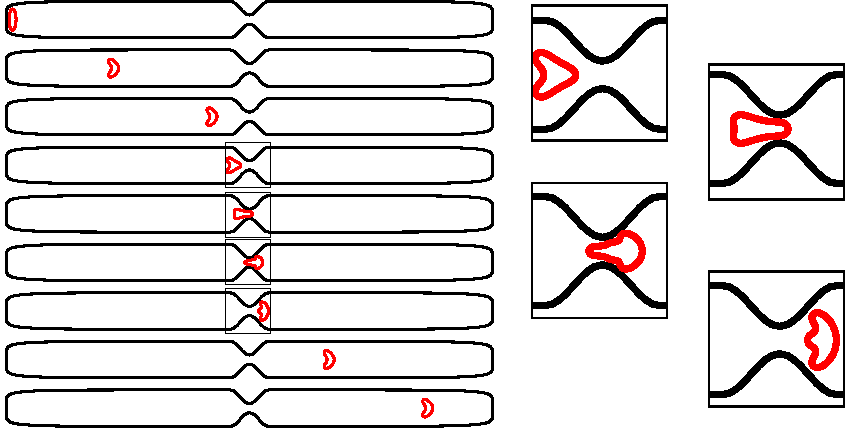
\includegraphics{figs/stenosisSnaps.pdf}
\mcaption{A single vesicle discretized with $N=128$ points passing
through a constricted tube ({\bf stenosis}) discretized with
$N_{\wall}=768$ points.  The boundary condition at the intake and
outtake has a parabolic-profile and on the rest of the solid wall is
zero.  On the right are magnifications of the vesicle as it passes
through the constriction.}{f:stenosisGeom}
\end{figure}

\begin{figure}[htp]
\centering
\begin{tabular}{cc}
\ifTikz
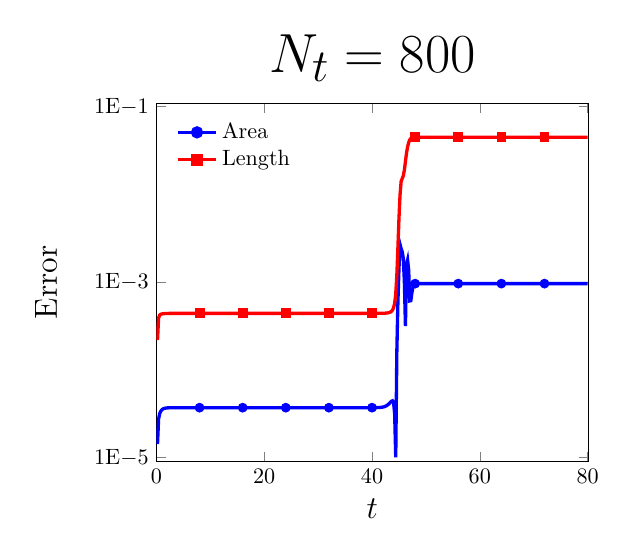
\begin{tikzpicture}[scale=0.8]

\begin{axis}[
  xmin = 0,
  xmax = 80.1,
  xtick = {0,20,40,60,80},
  xticklabels = {$0$,$20$,$40$,$60$,$80$},
  xlabel = $t$,
  ymode = log,
  ymin = 9E-6,
  ymax = 1.1E-1,
  ytick = {1E-5,1E-3,1E-1},
  yticklabels = {$1$E$-5$,$1$E$-3$,$1$E$-1$},
  ylabel = {Error},
  ylabel style = {yshift = 10pt},
  label style = {font=\Large},
  legend entries = {Area, Length},
  legend cell align=left,
  legend pos = north west, 
  legend style = {draw=none},
  title = {\Huge$N_{t}=800$}
  ]

  \addlegendimage{mark=*,mark options=solid,blue,line width=1.5,solid}
  \addlegendimage{mark=square*,mark options=solid,red,line
  width=1.5,solid}

% error in area
\addplot [mark=none,blue,line width=1.5] table{
2.0000e-01 1.4293e-05
4.0000e-01 2.7565e-05
6.0000e-01 3.1718e-05
8.0000e-01 3.3798e-05
1.0000e+00 3.5093e-05
1.2000e+00 3.5898e-05
1.4000e+00 3.6378e-05
1.6000e+00 3.6660e-05
1.8000e+00 3.6827e-05
2.0000e+00 3.6928e-05
2.2000e+00 3.6993e-05
2.4000e+00 3.7036e-05
2.6000e+00 3.7065e-05
2.8000e+00 3.7086e-05
3.0000e+00 3.7101e-05
3.2000e+00 3.7113e-05
3.4000e+00 3.7122e-05
3.6000e+00 3.7129e-05
3.8000e+00 3.7135e-05
4.0000e+00 3.7139e-05
4.2000e+00 3.7143e-05
4.4000e+00 3.7146e-05
4.6000e+00 3.7148e-05
4.8000e+00 3.7150e-05
5.0000e+00 3.7152e-05
5.2000e+00 3.7153e-05
5.4000e+00 3.7154e-05
5.6000e+00 3.7155e-05
5.8000e+00 3.7156e-05
6.0000e+00 3.7156e-05
6.2000e+00 3.7157e-05
6.4000e+00 3.7157e-05
6.6000e+00 3.7158e-05
6.8000e+00 3.7158e-05
7.0000e+00 3.7158e-05
7.2000e+00 3.7159e-05
7.4000e+00 3.7159e-05
7.6000e+00 3.7159e-05
7.8000e+00 3.7159e-05
8.0000e+00 3.7159e-05
8.2000e+00 3.7159e-05
8.4000e+00 3.7159e-05
8.6000e+00 3.7159e-05
8.8000e+00 3.7159e-05
9.0000e+00 3.7159e-05
9.2000e+00 3.7159e-05
9.4000e+00 3.7159e-05
9.6000e+00 3.7159e-05
9.8000e+00 3.7159e-05
1.0000e+01 3.7159e-05
1.0200e+01 3.7159e-05
1.0400e+01 3.7159e-05
1.0600e+01 3.7159e-05
1.0800e+01 3.7159e-05
1.1000e+01 3.7159e-05
1.1200e+01 3.7159e-05
1.1400e+01 3.7159e-05
1.1600e+01 3.7159e-05
1.1800e+01 3.7159e-05
1.2000e+01 3.7159e-05
1.2200e+01 3.7159e-05
1.2400e+01 3.7159e-05
1.2600e+01 3.7159e-05
1.2800e+01 3.7159e-05
1.3000e+01 3.7159e-05
1.3200e+01 3.7159e-05
1.3400e+01 3.7158e-05
1.3600e+01 3.7158e-05
1.3800e+01 3.7158e-05
1.4000e+01 3.7158e-05
1.4200e+01 3.7158e-05
1.4400e+01 3.7158e-05
1.4600e+01 3.7158e-05
1.4800e+01 3.7158e-05
1.5000e+01 3.7158e-05
1.5200e+01 3.7158e-05
1.5400e+01 3.7158e-05
1.5600e+01 3.7158e-05
1.5800e+01 3.7158e-05
1.6000e+01 3.7158e-05
1.6200e+01 3.7157e-05
1.6400e+01 3.7157e-05
1.6600e+01 3.7157e-05
1.6800e+01 3.7157e-05
1.7000e+01 3.7157e-05
1.7200e+01 3.7157e-05
1.7400e+01 3.7157e-05
1.7600e+01 3.7157e-05
1.7800e+01 3.7157e-05
1.8000e+01 3.7157e-05
1.8200e+01 3.7157e-05
1.8400e+01 3.7157e-05
1.8600e+01 3.7156e-05
1.8800e+01 3.7156e-05
1.9000e+01 3.7156e-05
1.9200e+01 3.7156e-05
1.9400e+01 3.7156e-05
1.9600e+01 3.7156e-05
1.9800e+01 3.7156e-05
2.0000e+01 3.7156e-05
2.0200e+01 3.7156e-05
2.0400e+01 3.7156e-05
2.0600e+01 3.7156e-05
2.0800e+01 3.7156e-05
2.1000e+01 3.7155e-05
2.1200e+01 3.7155e-05
2.1400e+01 3.7155e-05
2.1600e+01 3.7155e-05
2.1800e+01 3.7155e-05
2.2000e+01 3.7155e-05
2.2200e+01 3.7155e-05
2.2400e+01 3.7155e-05
2.2600e+01 3.7155e-05
2.2800e+01 3.7155e-05
2.3000e+01 3.7155e-05
2.3200e+01 3.7155e-05
2.3400e+01 3.7155e-05
2.3600e+01 3.7155e-05
2.3800e+01 3.7154e-05
2.4000e+01 3.7154e-05
2.4200e+01 3.7154e-05
2.4400e+01 3.7154e-05
2.4600e+01 3.7154e-05
2.4800e+01 3.7154e-05
2.5000e+01 3.7154e-05
2.5200e+01 3.7154e-05
2.5400e+01 3.7154e-05
2.5600e+01 3.7154e-05
2.5800e+01 3.7154e-05
2.6000e+01 3.7154e-05
2.6200e+01 3.7154e-05
2.6400e+01 3.7154e-05
2.6600e+01 3.7154e-05
2.6800e+01 3.7153e-05
2.7000e+01 3.7153e-05
2.7200e+01 3.7153e-05
2.7400e+01 3.7153e-05
2.7600e+01 3.7153e-05
2.7800e+01 3.7153e-05
2.8000e+01 3.7153e-05
2.8200e+01 3.7153e-05
2.8400e+01 3.7153e-05
2.8600e+01 3.7153e-05
2.8800e+01 3.7153e-05
2.9000e+01 3.7153e-05
2.9200e+01 3.7153e-05
2.9400e+01 3.7153e-05
2.9600e+01 3.7153e-05
2.9800e+01 3.7153e-05
3.0000e+01 3.7153e-05
3.0200e+01 3.7153e-05
3.0400e+01 3.7153e-05
3.0600e+01 3.7153e-05
3.0800e+01 3.7153e-05
3.1000e+01 3.7153e-05
3.1200e+01 3.7153e-05
3.1400e+01 3.7153e-05
3.1600e+01 3.7153e-05
3.1800e+01 3.7153e-05
3.2000e+01 3.7153e-05
3.2200e+01 3.7153e-05
3.2400e+01 3.7153e-05
3.2600e+01 3.7153e-05
3.2800e+01 3.7153e-05
3.3000e+01 3.7153e-05
3.3200e+01 3.7153e-05
3.3400e+01 3.7153e-05
3.3600e+01 3.7153e-05
3.3800e+01 3.7153e-05
3.4000e+01 3.7153e-05
3.4200e+01 3.7153e-05
3.4400e+01 3.7153e-05
3.4600e+01 3.7153e-05
3.4800e+01 3.7153e-05
3.5000e+01 3.7153e-05
3.5200e+01 3.7153e-05
3.5400e+01 3.7153e-05
3.5600e+01 3.7153e-05
3.5800e+01 3.7153e-05
3.6000e+01 3.7153e-05
3.6200e+01 3.7154e-05
3.6400e+01 3.7154e-05
3.6600e+01 3.7154e-05
3.6800e+01 3.7154e-05
3.7000e+01 3.7154e-05
3.7200e+01 3.7154e-05
3.7400e+01 3.7154e-05
3.7600e+01 3.7154e-05
3.7800e+01 3.7154e-05
3.8000e+01 3.7155e-05
3.8200e+01 3.7155e-05
3.8400e+01 3.7155e-05
3.8600e+01 3.7156e-05
3.8800e+01 3.7156e-05
3.9000e+01 3.7157e-05
3.9200e+01 3.7158e-05
3.9400e+01 3.7159e-05
3.9600e+01 3.7161e-05
3.9800e+01 3.7164e-05
4.0000e+01 3.7168e-05
4.0200e+01 3.7174e-05
4.0400e+01 3.7183e-05
4.0600e+01 3.7197e-05
4.0800e+01 3.7216e-05
4.1000e+01 3.7246e-05
4.1200e+01 3.7286e-05
4.1400e+01 3.7344e-05
4.1600e+01 3.7431e-05
4.1800e+01 3.7558e-05
4.2000e+01 3.7742e-05
4.2200e+01 3.8004e-05
4.2400e+01 3.8374e-05
4.2600e+01 3.8881e-05
4.2800e+01 3.9560e-05
4.3000e+01 4.0435e-05
4.3200e+01 4.1513e-05
4.3400e+01 4.2745e-05
4.3600e+01 4.3940e-05
4.3800e+01 4.4491e-05
4.4000e+01 4.2471e-05
4.4200e+01 3.1546e-05
4.4400e+01 1.0088e-05
4.4600e+01 1.5644e-04
4.4800e+01 5.9234e-04
4.5000e+01 1.4350e-03
4.5200e+01 2.6885e-03
4.5400e+01 2.4086e-03
4.5600e+01 2.2259e-03
4.5800e+01 1.8811e-03
4.6000e+01 1.0257e-03
4.6200e+01 3.1683e-04
4.6400e+01 1.5919e-03
4.6600e+01 1.7898e-03
4.6800e+01 1.3753e-03
4.7000e+01 6.1228e-04
4.7200e+01 6.1598e-04
4.7400e+01 7.6050e-04
4.7600e+01 8.8074e-04
4.7800e+01 9.4829e-04
4.8000e+01 9.6283e-04
4.8200e+01 9.6392e-04
4.8400e+01 9.6373e-04
4.8600e+01 9.6362e-04
4.8800e+01 9.6359e-04
4.9000e+01 9.6359e-04
4.9200e+01 9.6359e-04
4.9400e+01 9.6360e-04
4.9600e+01 9.6360e-04
4.9800e+01 9.6360e-04
5.0000e+01 9.6360e-04
5.0200e+01 9.6360e-04
5.0400e+01 9.6360e-04
5.0600e+01 9.6360e-04
5.0800e+01 9.6361e-04
5.1000e+01 9.6361e-04
5.1200e+01 9.6361e-04
5.1400e+01 9.6361e-04
5.1600e+01 9.6361e-04
5.1800e+01 9.6361e-04
5.2000e+01 9.6361e-04
5.2200e+01 9.6361e-04
5.2400e+01 9.6361e-04
5.2600e+01 9.6361e-04
5.2800e+01 9.6360e-04
5.3000e+01 9.6360e-04
5.3200e+01 9.6360e-04
5.3400e+01 9.6360e-04
5.3600e+01 9.6360e-04
5.3800e+01 9.6360e-04
5.4000e+01 9.6360e-04
5.4200e+01 9.6360e-04
5.4400e+01 9.6360e-04
5.4600e+01 9.6360e-04
5.4800e+01 9.6361e-04
5.5000e+01 9.6361e-04
5.5200e+01 9.6361e-04
5.5400e+01 9.6361e-04
5.5600e+01 9.6361e-04
5.5800e+01 9.6361e-04
5.6000e+01 9.6361e-04
5.6200e+01 9.6361e-04
5.6400e+01 9.6361e-04
5.6600e+01 9.6361e-04
5.6800e+01 9.6361e-04
5.7000e+01 9.6361e-04
5.7200e+01 9.6361e-04
5.7400e+01 9.6361e-04
5.7600e+01 9.6361e-04
5.7800e+01 9.6361e-04
5.8000e+01 9.6361e-04
5.8200e+01 9.6361e-04
5.8400e+01 9.6361e-04
5.8600e+01 9.6361e-04
5.8800e+01 9.6361e-04
5.9000e+01 9.6361e-04
5.9200e+01 9.6361e-04
5.9400e+01 9.6361e-04
5.9600e+01 9.6361e-04
5.9800e+01 9.6361e-04
6.0000e+01 9.6361e-04
6.0200e+01 9.6361e-04
6.0400e+01 9.6361e-04
6.0600e+01 9.6361e-04
6.0800e+01 9.6361e-04
6.1000e+01 9.6361e-04
6.1200e+01 9.6361e-04
6.1400e+01 9.6361e-04
6.1600e+01 9.6361e-04
6.1800e+01 9.6361e-04
6.2000e+01 9.6361e-04
6.2200e+01 9.6361e-04
6.2400e+01 9.6361e-04
6.2600e+01 9.6361e-04
6.2800e+01 9.6361e-04
6.3000e+01 9.6361e-04
6.3200e+01 9.6361e-04
6.3400e+01 9.6361e-04
6.3600e+01 9.6361e-04
6.3800e+01 9.6361e-04
6.4000e+01 9.6361e-04
6.4200e+01 9.6361e-04
6.4400e+01 9.6361e-04
6.4600e+01 9.6361e-04
6.4800e+01 9.6361e-04
6.5000e+01 9.6361e-04
6.5200e+01 9.6361e-04
6.5400e+01 9.6361e-04
6.5600e+01 9.6361e-04
6.5800e+01 9.6361e-04
6.6000e+01 9.6361e-04
6.6200e+01 9.6361e-04
6.6400e+01 9.6361e-04
6.6600e+01 9.6361e-04
6.6800e+01 9.6361e-04
6.7000e+01 9.6361e-04
6.7200e+01 9.6361e-04
6.7400e+01 9.6361e-04
6.7600e+01 9.6361e-04
6.7800e+01 9.6361e-04
6.8000e+01 9.6361e-04
6.8200e+01 9.6361e-04
6.8400e+01 9.6361e-04
6.8600e+01 9.6361e-04
6.8800e+01 9.6361e-04
6.9000e+01 9.6361e-04
6.9200e+01 9.6361e-04
6.9400e+01 9.6361e-04
6.9600e+01 9.6361e-04
6.9800e+01 9.6361e-04
7.0000e+01 9.6361e-04
7.0200e+01 9.6361e-04
7.0400e+01 9.6361e-04
7.0600e+01 9.6361e-04
7.0800e+01 9.6361e-04
7.1000e+01 9.6361e-04
7.1200e+01 9.6361e-04
7.1400e+01 9.6361e-04
7.1600e+01 9.6361e-04
7.1800e+01 9.6361e-04
7.2000e+01 9.6361e-04
7.2200e+01 9.6361e-04
7.2400e+01 9.6361e-04
7.2600e+01 9.6361e-04
7.2800e+01 9.6361e-04
7.3000e+01 9.6361e-04
7.3200e+01 9.6361e-04
7.3400e+01 9.6361e-04
7.3600e+01 9.6361e-04
7.3800e+01 9.6361e-04
7.4000e+01 9.6361e-04
7.4200e+01 9.6361e-04
7.4400e+01 9.6361e-04
7.4600e+01 9.6361e-04
7.4800e+01 9.6361e-04
7.5000e+01 9.6361e-04
7.5200e+01 9.6361e-04
7.5400e+01 9.6361e-04
7.5600e+01 9.6361e-04
7.5800e+01 9.6361e-04
7.6000e+01 9.6361e-04
7.6200e+01 9.6361e-04
7.6400e+01 9.6360e-04
7.6600e+01 9.6360e-04
7.6800e+01 9.6360e-04
7.7000e+01 9.6360e-04
7.7200e+01 9.6360e-04
7.7400e+01 9.6360e-04
7.7600e+01 9.6360e-04
7.7800e+01 9.6360e-04
7.8000e+01 9.6360e-04
7.8200e+01 9.6360e-04
7.8400e+01 9.6360e-04
7.8600e+01 9.6360e-04
7.8800e+01 9.6360e-04
7.9000e+01 9.6360e-04
7.9200e+01 9.6360e-04
7.9400e+01 9.6360e-04
7.9600e+01 9.6360e-04
7.9800e+01 9.6360e-04
8.0000e+01 9.6360e-04
};

% error in length
\addplot [mark=none,red,line width=1.5] table{
2.0000e-01 2.1904e-04
4.0000e-01 3.8923e-04
6.0000e-01 4.2167e-04
8.0000e-01 4.3039e-04
1.0000e+00 4.3438e-04
1.2000e+00 4.3680e-04
1.4000e+00 4.3836e-04
1.6000e+00 4.3936e-04
1.8000e+00 4.4002e-04
2.0000e+00 4.4047e-04
2.2000e+00 4.4077e-04
2.4000e+00 4.4099e-04
2.6000e+00 4.4114e-04
2.8000e+00 4.4125e-04
3.0000e+00 4.4134e-04
3.2000e+00 4.4140e-04
3.4000e+00 4.4145e-04
3.6000e+00 4.4148e-04
3.8000e+00 4.4151e-04
4.0000e+00 4.4153e-04
4.2000e+00 4.4154e-04
4.4000e+00 4.4156e-04
4.6000e+00 4.4157e-04
4.8000e+00 4.4157e-04
5.0000e+00 4.4158e-04
5.2000e+00 4.4159e-04
5.4000e+00 4.4159e-04
5.6000e+00 4.4159e-04
5.8000e+00 4.4160e-04
6.0000e+00 4.4160e-04
6.2000e+00 4.4160e-04
6.4000e+00 4.4160e-04
6.6000e+00 4.4160e-04
6.8000e+00 4.4160e-04
7.0000e+00 4.4161e-04
7.2000e+00 4.4161e-04
7.4000e+00 4.4161e-04
7.6000e+00 4.4161e-04
7.8000e+00 4.4161e-04
8.0000e+00 4.4161e-04
8.2000e+00 4.4161e-04
8.4000e+00 4.4161e-04
8.6000e+00 4.4161e-04
8.8000e+00 4.4161e-04
9.0000e+00 4.4161e-04
9.2000e+00 4.4161e-04
9.4000e+00 4.4161e-04
9.6000e+00 4.4161e-04
9.8000e+00 4.4161e-04
1.0000e+01 4.4161e-04
1.0200e+01 4.4161e-04
1.0400e+01 4.4161e-04
1.0600e+01 4.4161e-04
1.0800e+01 4.4161e-04
1.1000e+01 4.4161e-04
1.1200e+01 4.4161e-04
1.1400e+01 4.4161e-04
1.1600e+01 4.4161e-04
1.1800e+01 4.4161e-04
1.2000e+01 4.4161e-04
1.2200e+01 4.4161e-04
1.2400e+01 4.4161e-04
1.2600e+01 4.4161e-04
1.2800e+01 4.4161e-04
1.3000e+01 4.4161e-04
1.3200e+01 4.4161e-04
1.3400e+01 4.4161e-04
1.3600e+01 4.4161e-04
1.3800e+01 4.4161e-04
1.4000e+01 4.4161e-04
1.4200e+01 4.4161e-04
1.4400e+01 4.4161e-04
1.4600e+01 4.4161e-04
1.4800e+01 4.4161e-04
1.5000e+01 4.4161e-04
1.5200e+01 4.4161e-04
1.5400e+01 4.4161e-04
1.5600e+01 4.4161e-04
1.5800e+01 4.4161e-04
1.6000e+01 4.4161e-04
1.6200e+01 4.4161e-04
1.6400e+01 4.4161e-04
1.6600e+01 4.4161e-04
1.6800e+01 4.4161e-04
1.7000e+01 4.4161e-04
1.7200e+01 4.4161e-04
1.7400e+01 4.4161e-04
1.7600e+01 4.4161e-04
1.7800e+01 4.4161e-04
1.8000e+01 4.4161e-04
1.8200e+01 4.4161e-04
1.8400e+01 4.4161e-04
1.8600e+01 4.4161e-04
1.8800e+01 4.4161e-04
1.9000e+01 4.4161e-04
1.9200e+01 4.4161e-04
1.9400e+01 4.4161e-04
1.9600e+01 4.4161e-04
1.9800e+01 4.4161e-04
2.0000e+01 4.4161e-04
2.0200e+01 4.4161e-04
2.0400e+01 4.4161e-04
2.0600e+01 4.4161e-04
2.0800e+01 4.4161e-04
2.1000e+01 4.4161e-04
2.1200e+01 4.4161e-04
2.1400e+01 4.4161e-04
2.1600e+01 4.4161e-04
2.1800e+01 4.4161e-04
2.2000e+01 4.4161e-04
2.2200e+01 4.4161e-04
2.2400e+01 4.4161e-04
2.2600e+01 4.4161e-04
2.2800e+01 4.4161e-04
2.3000e+01 4.4161e-04
2.3200e+01 4.4161e-04
2.3400e+01 4.4161e-04
2.3600e+01 4.4161e-04
2.3800e+01 4.4161e-04
2.4000e+01 4.4161e-04
2.4200e+01 4.4161e-04
2.4400e+01 4.4161e-04
2.4600e+01 4.4161e-04
2.4800e+01 4.4161e-04
2.5000e+01 4.4161e-04
2.5200e+01 4.4161e-04
2.5400e+01 4.4161e-04
2.5600e+01 4.4161e-04
2.5800e+01 4.4161e-04
2.6000e+01 4.4161e-04
2.6200e+01 4.4161e-04
2.6400e+01 4.4161e-04
2.6600e+01 4.4161e-04
2.6800e+01 4.4161e-04
2.7000e+01 4.4161e-04
2.7200e+01 4.4161e-04
2.7400e+01 4.4161e-04
2.7600e+01 4.4161e-04
2.7800e+01 4.4161e-04
2.8000e+01 4.4161e-04
2.8200e+01 4.4161e-04
2.8400e+01 4.4161e-04
2.8600e+01 4.4161e-04
2.8800e+01 4.4161e-04
2.9000e+01 4.4161e-04
2.9200e+01 4.4161e-04
2.9400e+01 4.4161e-04
2.9600e+01 4.4161e-04
2.9800e+01 4.4161e-04
3.0000e+01 4.4161e-04
3.0200e+01 4.4161e-04
3.0400e+01 4.4161e-04
3.0600e+01 4.4161e-04
3.0800e+01 4.4161e-04
3.1000e+01 4.4161e-04
3.1200e+01 4.4161e-04
3.1400e+01 4.4161e-04
3.1600e+01 4.4161e-04
3.1800e+01 4.4161e-04
3.2000e+01 4.4161e-04
3.2200e+01 4.4161e-04
3.2400e+01 4.4161e-04
3.2600e+01 4.4161e-04
3.2800e+01 4.4161e-04
3.3000e+01 4.4161e-04
3.3200e+01 4.4161e-04
3.3400e+01 4.4161e-04
3.3600e+01 4.4161e-04
3.3800e+01 4.4161e-04
3.4000e+01 4.4161e-04
3.4200e+01 4.4161e-04
3.4400e+01 4.4161e-04
3.4600e+01 4.4161e-04
3.4800e+01 4.4161e-04
3.5000e+01 4.4161e-04
3.5200e+01 4.4161e-04
3.5400e+01 4.4161e-04
3.5600e+01 4.4161e-04
3.5800e+01 4.4161e-04
3.6000e+01 4.4161e-04
3.6200e+01 4.4161e-04
3.6400e+01 4.4161e-04
3.6600e+01 4.4161e-04
3.6800e+01 4.4161e-04
3.7000e+01 4.4161e-04
3.7200e+01 4.4161e-04
3.7400e+01 4.4161e-04
3.7600e+01 4.4161e-04
3.7800e+01 4.4161e-04
3.8000e+01 4.4161e-04
3.8200e+01 4.4161e-04
3.8400e+01 4.4161e-04
3.8600e+01 4.4161e-04
3.8800e+01 4.4161e-04
3.9000e+01 4.4161e-04
3.9200e+01 4.4161e-04
3.9400e+01 4.4161e-04
3.9600e+01 4.4161e-04
3.9800e+01 4.4161e-04
4.0000e+01 4.4162e-04
4.0200e+01 4.4163e-04
4.0400e+01 4.4164e-04
4.0600e+01 4.4165e-04
4.0800e+01 4.4168e-04
4.1000e+01 4.4172e-04
4.1200e+01 4.4178e-04
4.1400e+01 4.4188e-04
4.1600e+01 4.4201e-04
4.1800e+01 4.4221e-04
4.2000e+01 4.4250e-04
4.2200e+01 4.4292e-04
4.2400e+01 4.4354e-04
4.2600e+01 4.4446e-04
4.2800e+01 4.4584e-04
4.3000e+01 4.4794e-04
4.3200e+01 4.5121e-04
4.3400e+01 4.5645e-04
4.3600e+01 4.6524e-04
4.3800e+01 4.8092e-04
4.4000e+01 5.1125e-04
4.4200e+01 5.7656e-04
4.4400e+01 7.3665e-04
4.4600e+01 1.1822e-03
4.4800e+01 2.4543e-03
4.5000e+01 5.3664e-03
4.5200e+01 9.9388e-03
4.5400e+01 1.4020e-02
4.5600e+01 1.5194e-02
4.5800e+01 1.6265e-02
4.6000e+01 1.8948e-02
4.6200e+01 2.3732e-02
4.6400e+01 2.9674e-02
4.6600e+01 3.4855e-02
4.6800e+01 3.8961e-02
4.7000e+01 4.1989e-02
4.7200e+01 4.3481e-02
4.7400e+01 4.4087e-02
4.7600e+01 4.4396e-02
4.7800e+01 4.4658e-02
4.8000e+01 4.4841e-02
4.8200e+01 4.4902e-02
4.8400e+01 4.4918e-02
4.8600e+01 4.4921e-02
4.8800e+01 4.4922e-02
4.9000e+01 4.4922e-02
4.9200e+01 4.4922e-02
4.9400e+01 4.4922e-02
4.9600e+01 4.4922e-02
4.9800e+01 4.4922e-02
5.0000e+01 4.4923e-02
5.0200e+01 4.4923e-02
5.0400e+01 4.4923e-02
5.0600e+01 4.4923e-02
5.0800e+01 4.4923e-02
5.1000e+01 4.4923e-02
5.1200e+01 4.4923e-02
5.1400e+01 4.4923e-02
5.1600e+01 4.4923e-02
5.1800e+01 4.4923e-02
5.2000e+01 4.4923e-02
5.2200e+01 4.4923e-02
5.2400e+01 4.4923e-02
5.2600e+01 4.4923e-02
5.2800e+01 4.4923e-02
5.3000e+01 4.4923e-02
5.3200e+01 4.4923e-02
5.3400e+01 4.4923e-02
5.3600e+01 4.4923e-02
5.3800e+01 4.4923e-02
5.4000e+01 4.4923e-02
5.4200e+01 4.4923e-02
5.4400e+01 4.4923e-02
5.4600e+01 4.4923e-02
5.4800e+01 4.4923e-02
5.5000e+01 4.4923e-02
5.5200e+01 4.4923e-02
5.5400e+01 4.4923e-02
5.5600e+01 4.4923e-02
5.5800e+01 4.4923e-02
5.6000e+01 4.4923e-02
5.6200e+01 4.4923e-02
5.6400e+01 4.4923e-02
5.6600e+01 4.4923e-02
5.6800e+01 4.4923e-02
5.7000e+01 4.4923e-02
5.7200e+01 4.4923e-02
5.7400e+01 4.4923e-02
5.7600e+01 4.4923e-02
5.7800e+01 4.4923e-02
5.8000e+01 4.4923e-02
5.8200e+01 4.4923e-02
5.8400e+01 4.4923e-02
5.8600e+01 4.4923e-02
5.8800e+01 4.4923e-02
5.9000e+01 4.4923e-02
5.9200e+01 4.4923e-02
5.9400e+01 4.4923e-02
5.9600e+01 4.4923e-02
5.9800e+01 4.4923e-02
6.0000e+01 4.4923e-02
6.0200e+01 4.4923e-02
6.0400e+01 4.4923e-02
6.0600e+01 4.4923e-02
6.0800e+01 4.4923e-02
6.1000e+01 4.4923e-02
6.1200e+01 4.4923e-02
6.1400e+01 4.4923e-02
6.1600e+01 4.4923e-02
6.1800e+01 4.4923e-02
6.2000e+01 4.4923e-02
6.2200e+01 4.4923e-02
6.2400e+01 4.4923e-02
6.2600e+01 4.4923e-02
6.2800e+01 4.4923e-02
6.3000e+01 4.4923e-02
6.3200e+01 4.4923e-02
6.3400e+01 4.4923e-02
6.3600e+01 4.4923e-02
6.3800e+01 4.4923e-02
6.4000e+01 4.4923e-02
6.4200e+01 4.4923e-02
6.4400e+01 4.4923e-02
6.4600e+01 4.4923e-02
6.4800e+01 4.4923e-02
6.5000e+01 4.4923e-02
6.5200e+01 4.4923e-02
6.5400e+01 4.4923e-02
6.5600e+01 4.4923e-02
6.5800e+01 4.4923e-02
6.6000e+01 4.4923e-02
6.6200e+01 4.4923e-02
6.6400e+01 4.4923e-02
6.6600e+01 4.4923e-02
6.6800e+01 4.4923e-02
6.7000e+01 4.4923e-02
6.7200e+01 4.4923e-02
6.7400e+01 4.4923e-02
6.7600e+01 4.4923e-02
6.7800e+01 4.4923e-02
6.8000e+01 4.4923e-02
6.8200e+01 4.4923e-02
6.8400e+01 4.4923e-02
6.8600e+01 4.4923e-02
6.8800e+01 4.4923e-02
6.9000e+01 4.4923e-02
6.9200e+01 4.4923e-02
6.9400e+01 4.4923e-02
6.9600e+01 4.4923e-02
6.9800e+01 4.4923e-02
7.0000e+01 4.4923e-02
7.0200e+01 4.4923e-02
7.0400e+01 4.4923e-02
7.0600e+01 4.4923e-02
7.0800e+01 4.4923e-02
7.1000e+01 4.4923e-02
7.1200e+01 4.4923e-02
7.1400e+01 4.4923e-02
7.1600e+01 4.4923e-02
7.1800e+01 4.4923e-02
7.2000e+01 4.4923e-02
7.2200e+01 4.4923e-02
7.2400e+01 4.4923e-02
7.2600e+01 4.4923e-02
7.2800e+01 4.4923e-02
7.3000e+01 4.4923e-02
7.3200e+01 4.4923e-02
7.3400e+01 4.4923e-02
7.3600e+01 4.4923e-02
7.3800e+01 4.4923e-02
7.4000e+01 4.4923e-02
7.4200e+01 4.4923e-02
7.4400e+01 4.4923e-02
7.4600e+01 4.4923e-02
7.4800e+01 4.4923e-02
7.5000e+01 4.4923e-02
7.5200e+01 4.4923e-02
7.5400e+01 4.4923e-02
7.5600e+01 4.4923e-02
7.5800e+01 4.4923e-02
7.6000e+01 4.4923e-02
7.6200e+01 4.4923e-02
7.6400e+01 4.4923e-02
7.6600e+01 4.4923e-02
7.6800e+01 4.4923e-02
7.7000e+01 4.4923e-02
7.7200e+01 4.4923e-02
7.7400e+01 4.4923e-02
7.7600e+01 4.4923e-02
7.7800e+01 4.4923e-02
7.8000e+01 4.4923e-02
7.8200e+01 4.4923e-02
7.8400e+01 4.4923e-02
7.8600e+01 4.4923e-02
7.8800e+01 4.4923e-02
7.9000e+01 4.4923e-02
7.9200e+01 4.4923e-02
7.9400e+01 4.4923e-02
7.9600e+01 4.4923e-02
7.9800e+01 4.4923e-02
8.0000e+01 4.4923e-02
};


% marked error in area
\addplot [mark=*,blue,only marks] table{
8.0000e+00 3.7159e-05
1.6000e+01 3.7158e-05
2.4000e+01 3.7154e-05
3.2000e+01 3.7153e-05
4.0000e+01 3.7168e-05
4.8000e+01 9.6283e-04
5.6000e+01 9.6361e-04
6.4000e+01 9.6361e-04
7.2000e+01 9.6361e-04
};

% marked error in length
\addplot [mark=square*,red,only marks] table{
8.0000e+00 4.4161e-04
1.6000e+01 4.4161e-04
2.4000e+01 4.4161e-04
3.2000e+01 4.4161e-04
4.0000e+01 4.4162e-04
4.8000e+01 4.4841e-02
5.6000e+01 4.4923e-02
6.4000e+01 4.4923e-02
7.2000e+01 4.4923e-02
};


\end{axis}

\end{tikzpicture}


 &
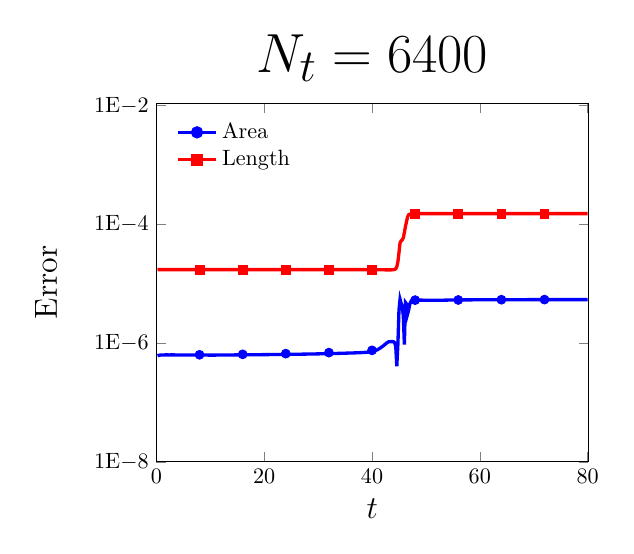
\begin{tikzpicture}[scale=0.8]

\begin{axis}[
  xmin = 0,
  xmax = 80.1,
  xtick = {0,20,40,60,80},
  xticklabels = {$0$,$20$,$40$,$60$,$80$},
  xlabel = $t$,
  ymode = log,
  ymin = 1E-8,
  ymax = 1.1E-2,
  ytick = {1E-10,1E-8,1E-6,1E-4,1E-2},
  yticklabels = {$1$E$-10$,$1$E$-8$,$1$E$-6$,$1$E$-4$,$1$E$-2$},
  ylabel = {Error},
  ylabel style = {yshift = 10pt},
  label style = {font=\Large},
  legend entries = {Area, Length},
  legend cell align=left,
  legend pos = north west, 
  legend style = {draw=none},
  title = {\Huge$N_{t}=6400$}
  ]
  \addlegendimage{mark=*,mark options=solid,blue,line width=1.5,solid}
  \addlegendimage{mark=square*,mark options=solid,red,line
  width=1.5,solid}

% error in area
\addplot [mark=none,blue,line width=1.5] table{
2.0000e-01 6.1046e-07
4.0000e-01 6.1941e-07
6.0000e-01 6.2381e-07
8.0000e-01 6.2666e-07
1.0000e+00 6.2833e-07
1.2000e+00 6.2932e-07
1.4000e+00 6.2982e-07
1.6000e+00 6.3004e-07
1.8000e+00 6.3012e-07
2.0000e+00 6.3012e-07
2.2000e+00 6.3007e-07
2.4000e+00 6.2987e-07
2.6000e+00 6.3009e-07
2.8000e+00 6.3013e-07
3.0000e+00 6.3011e-07
3.2000e+00 6.3006e-07
3.4000e+00 6.3000e-07
3.6000e+00 6.2992e-07
3.8000e+00 6.2985e-07
4.0000e+00 6.2974e-07
4.2000e+00 6.2957e-07
4.4000e+00 6.2943e-07
4.6000e+00 6.2930e-07
4.8000e+00 6.2917e-07
5.0000e+00 6.2904e-07
5.2000e+00 6.2890e-07
5.4000e+00 6.2877e-07
5.6000e+00 6.2863e-07
5.8000e+00 6.2849e-07
6.0000e+00 6.2835e-07
6.2000e+00 6.2821e-07
6.4000e+00 6.2807e-07
6.6000e+00 6.2792e-07
6.8000e+00 6.2778e-07
7.0000e+00 6.2763e-07
7.2000e+00 6.2748e-07
7.4000e+00 6.2733e-07
7.6000e+00 6.2718e-07
7.8000e+00 6.2702e-07
8.0000e+00 6.2687e-07
8.2000e+00 6.2671e-07
8.4000e+00 6.2656e-07
8.6000e+00 6.2640e-07
8.8000e+00 6.2624e-07
9.0000e+00 6.2608e-07
9.2000e+00 6.2592e-07
9.4000e+00 6.2575e-07
9.6000e+00 6.2559e-07
9.8000e+00 6.2543e-07
1.0000e+01 6.2526e-07
1.0200e+01 6.2509e-07
1.0400e+01 6.2493e-07
1.0600e+01 6.2495e-07
1.0800e+01 6.2525e-07
1.1000e+01 6.2554e-07
1.1200e+01 6.2583e-07
1.1400e+01 6.2611e-07
1.1600e+01 6.2639e-07
1.1800e+01 6.2666e-07
1.2000e+01 6.2692e-07
1.2200e+01 6.2719e-07
1.2400e+01 6.2745e-07
1.2600e+01 6.2770e-07
1.2800e+01 6.2796e-07
1.3000e+01 6.2821e-07
1.3200e+01 6.2845e-07
1.3400e+01 6.2870e-07
1.3600e+01 6.2894e-07
1.3800e+01 6.2918e-07
1.4000e+01 6.2942e-07
1.4200e+01 6.2966e-07
1.4400e+01 6.2990e-07
1.4600e+01 6.3014e-07
1.4800e+01 6.3037e-07
1.5000e+01 6.3061e-07
1.5200e+01 6.3084e-07
1.5400e+01 6.3107e-07
1.5600e+01 6.3131e-07
1.5800e+01 6.3154e-07
1.6000e+01 6.3178e-07
1.6200e+01 6.3201e-07
1.6400e+01 6.3225e-07
1.6600e+01 6.3248e-07
1.6800e+01 6.3272e-07
1.7000e+01 6.3296e-07
1.7200e+01 6.3320e-07
1.7400e+01 6.3344e-07
1.7600e+01 6.3368e-07
1.7800e+01 6.3392e-07
1.8000e+01 6.3416e-07
1.8200e+01 6.3441e-07
1.8400e+01 6.3466e-07
1.8600e+01 6.3490e-07
1.8800e+01 6.3516e-07
1.9000e+01 6.3541e-07
1.9200e+01 6.3567e-07
1.9400e+01 6.3592e-07
1.9600e+01 6.3618e-07
1.9800e+01 6.3645e-07
2.0000e+01 6.3671e-07
2.0200e+01 6.3698e-07
2.0400e+01 6.3725e-07
2.0600e+01 6.3753e-07
2.0800e+01 6.3780e-07
2.1000e+01 6.3809e-07
2.1200e+01 6.3837e-07
2.1400e+01 6.3866e-07
2.1600e+01 6.3895e-07
2.1800e+01 6.3924e-07
2.2000e+01 6.3954e-07
2.2200e+01 6.3984e-07
2.2400e+01 6.4015e-07
2.2600e+01 6.4046e-07
2.2800e+01 6.4077e-07
2.3000e+01 6.4109e-07
2.3200e+01 6.4142e-07
2.3400e+01 6.4175e-07
2.3600e+01 6.4208e-07
2.3800e+01 6.4242e-07
2.4000e+01 6.4276e-07
2.4200e+01 6.4311e-07
2.4400e+01 6.4346e-07
2.4600e+01 6.4382e-07
2.4800e+01 6.4418e-07
2.5000e+01 6.4455e-07
2.5200e+01 6.4492e-07
2.5400e+01 6.4530e-07
2.5600e+01 6.4569e-07
2.5800e+01 6.4608e-07
2.6000e+01 6.4648e-07
2.6200e+01 6.4689e-07
2.6400e+01 6.4730e-07
2.6600e+01 6.4772e-07
2.6800e+01 6.4814e-07
2.7000e+01 6.4857e-07
2.7200e+01 6.4901e-07
2.7400e+01 6.4946e-07
2.7600e+01 6.4991e-07
2.7800e+01 6.5038e-07
2.8000e+01 6.5084e-07
2.8200e+01 6.5132e-07
2.8400e+01 6.5181e-07
2.8600e+01 6.5230e-07
2.8800e+01 6.5280e-07
2.9000e+01 6.5331e-07
2.9200e+01 6.5383e-07
2.9400e+01 6.5436e-07
2.9600e+01 6.5490e-07
2.9800e+01 6.5544e-07
3.0000e+01 6.5600e-07
3.0200e+01 6.5656e-07
3.0400e+01 6.5714e-07
3.0600e+01 6.5772e-07
3.0800e+01 6.5832e-07
3.1000e+01 6.5892e-07
3.1200e+01 6.5954e-07
3.1400e+01 6.6017e-07
3.1600e+01 6.6081e-07
3.1800e+01 6.6146e-07
3.2000e+01 6.6212e-07
3.2200e+01 6.6279e-07
3.2400e+01 6.6347e-07
3.2600e+01 6.6417e-07
3.2800e+01 6.6488e-07
3.3000e+01 6.6560e-07
3.3200e+01 6.6633e-07
3.3400e+01 6.6708e-07
3.3600e+01 6.6784e-07
3.3800e+01 6.6861e-07
3.4000e+01 6.6939e-07
3.4200e+01 6.7019e-07
3.4400e+01 6.7100e-07
3.4600e+01 6.7183e-07
3.4800e+01 6.7266e-07
3.5000e+01 6.7352e-07
3.5200e+01 6.7439e-07
3.5400e+01 6.7527e-07
3.5600e+01 6.7617e-07
3.5800e+01 6.7709e-07
3.6000e+01 6.7803e-07
3.6200e+01 6.7898e-07
3.6400e+01 6.7996e-07
3.6600e+01 6.8096e-07
3.6800e+01 6.8199e-07
3.7000e+01 6.8305e-07
3.7200e+01 6.8415e-07
3.7400e+01 6.8530e-07
3.7600e+01 6.8651e-07
3.7800e+01 6.8778e-07
3.8000e+01 6.8914e-07
3.8200e+01 6.9061e-07
3.8400e+01 6.9222e-07
3.8600e+01 6.9400e-07
3.8800e+01 6.9601e-07
3.9000e+01 6.9830e-07
3.9200e+01 7.0097e-07
3.9400e+01 7.0412e-07
3.9600e+01 7.0789e-07
3.9800e+01 7.1246e-07
4.0000e+01 7.1804e-07
4.0200e+01 7.2490e-07
4.0400e+01 7.3333e-07
4.0600e+01 7.4365e-07
4.0800e+01 7.5616e-07
4.1000e+01 7.7114e-07
4.1200e+01 7.8871e-07
4.1400e+01 8.0890e-07
4.1600e+01 8.3159e-07
4.1800e+01 8.5661e-07
4.2000e+01 8.8383e-07
4.2200e+01 9.1335e-07
4.2400e+01 9.4538e-07
4.2600e+01 9.7808e-07
4.2800e+01 1.0118e-06
4.3000e+01 1.0412e-06
4.3200e+01 1.0519e-06
4.3400e+01 1.0534e-06
4.3600e+01 1.0544e-06
4.3800e+01 1.0539e-06
4.4000e+01 1.0468e-06
4.4200e+01 1.0118e-06
4.4400e+01 8.7955e-07
4.4600e+01 4.0711e-07
4.4800e+01 9.4726e-07
4.5000e+01 3.5684e-06
4.5200e+01 5.4455e-06
4.5400e+01 4.6692e-06
4.5600e+01 4.0914e-06
4.5800e+01 2.9095e-06
4.6000e+01 9.3799e-07
4.6200e+01 4.8175e-06
4.6400e+01 4.5416e-06
4.6600e+01 3.0840e-06
4.6800e+01 3.5943e-06
4.7000e+01 4.4925e-06
4.7200e+01 4.9676e-06
4.7400e+01 5.2658e-06
4.7600e+01 5.2875e-06
4.7800e+01 5.2852e-06
4.8000e+01 5.2825e-06
4.8200e+01 5.2812e-06
4.8400e+01 5.2805e-06
4.8600e+01 5.2802e-06
4.8800e+01 5.2801e-06
4.9000e+01 5.2756e-06
4.9200e+01 5.2708e-06
4.9400e+01 5.2670e-06
4.9600e+01 5.2638e-06
4.9800e+01 5.2611e-06
5.0000e+01 5.2587e-06
5.0200e+01 5.2566e-06
5.0400e+01 5.2547e-06
5.0600e+01 5.2529e-06
5.0800e+01 5.2513e-06
5.1000e+01 5.2498e-06
5.1200e+01 5.2486e-06
5.1400e+01 5.2474e-06
5.1600e+01 5.2465e-06
5.1800e+01 5.2457e-06
5.2000e+01 5.2450e-06
5.2200e+01 5.2445e-06
5.2400e+01 5.2440e-06
5.2600e+01 5.2437e-06
5.2800e+01 5.2467e-06
5.3000e+01 5.2540e-06
5.3200e+01 5.2604e-06
5.3400e+01 5.2660e-06
5.3600e+01 5.2711e-06
5.3800e+01 5.2757e-06
5.4000e+01 5.2800e-06
5.4200e+01 5.2839e-06
5.4400e+01 5.2875e-06
5.4600e+01 5.2908e-06
5.4800e+01 5.2940e-06
5.5000e+01 5.2970e-06
5.5200e+01 5.2998e-06
5.5400e+01 5.3024e-06
5.5600e+01 5.3049e-06
5.5800e+01 5.3074e-06
5.6000e+01 5.3097e-06
5.6200e+01 5.3119e-06
5.6400e+01 5.3140e-06
5.6600e+01 5.3160e-06
5.6800e+01 5.3179e-06
5.7000e+01 5.3198e-06
5.7200e+01 5.3216e-06
5.7400e+01 5.3234e-06
5.7600e+01 5.3250e-06
5.7800e+01 5.3266e-06
5.8000e+01 5.3282e-06
5.8200e+01 5.3297e-06
5.8400e+01 5.3312e-06
5.8600e+01 5.3326e-06
5.8800e+01 5.3339e-06
5.9000e+01 5.3353e-06
5.9200e+01 5.3365e-06
5.9400e+01 5.3378e-06
5.9600e+01 5.3390e-06
5.9800e+01 5.3401e-06
6.0000e+01 5.3413e-06
6.0200e+01 5.3424e-06
6.0400e+01 5.3434e-06
6.0600e+01 5.3445e-06
6.0800e+01 5.3455e-06
6.1000e+01 5.3464e-06
6.1200e+01 5.3474e-06
6.1400e+01 5.3483e-06
6.1600e+01 5.3492e-06
6.1800e+01 5.3501e-06
6.2000e+01 5.3509e-06
6.2200e+01 5.3518e-06
6.2400e+01 5.3526e-06
6.2600e+01 5.3533e-06
6.2800e+01 5.3541e-06
6.3000e+01 5.3549e-06
6.3200e+01 5.3556e-06
6.3400e+01 5.3563e-06
6.3600e+01 5.3570e-06
6.3800e+01 5.3576e-06
6.4000e+01 5.3583e-06
6.4200e+01 5.3589e-06
6.4400e+01 5.3596e-06
6.4600e+01 5.3602e-06
6.4800e+01 5.3608e-06
6.5000e+01 5.3613e-06
6.5200e+01 5.3619e-06
6.5400e+01 5.3625e-06
6.5600e+01 5.3630e-06
6.5800e+01 5.3635e-06
6.6000e+01 5.3640e-06
6.6200e+01 5.3645e-06
6.6400e+01 5.3650e-06
6.6600e+01 5.3655e-06
6.6800e+01 5.3660e-06
6.7000e+01 5.3665e-06
6.7200e+01 5.3669e-06
6.7400e+01 5.3673e-06
6.7600e+01 5.3678e-06
6.7800e+01 5.3682e-06
6.8000e+01 5.3686e-06
6.8200e+01 5.3690e-06
6.8400e+01 5.3694e-06
6.8600e+01 5.3698e-06
6.8800e+01 5.3702e-06
6.9000e+01 5.3705e-06
6.9200e+01 5.3709e-06
6.9400e+01 5.3712e-06
6.9600e+01 5.3716e-06
6.9800e+01 5.3719e-06
7.0000e+01 5.3722e-06
7.0200e+01 5.3726e-06
7.0400e+01 5.3729e-06
7.0600e+01 5.3732e-06
7.0800e+01 5.3735e-06
7.1000e+01 5.3738e-06
7.1200e+01 5.3741e-06
7.1400e+01 5.3744e-06
7.1600e+01 5.3746e-06
7.1800e+01 5.3749e-06
7.2000e+01 5.3752e-06
7.2200e+01 5.3754e-06
7.2400e+01 5.3757e-06
7.2600e+01 5.3760e-06
7.2800e+01 5.3762e-06
7.3000e+01 5.3764e-06
7.3200e+01 5.3767e-06
7.3400e+01 5.3769e-06
7.3600e+01 5.3771e-06
7.3800e+01 5.3773e-06
7.4000e+01 5.3776e-06
7.4200e+01 5.3778e-06
7.4400e+01 5.3780e-06
7.4600e+01 5.3782e-06
7.4800e+01 5.3784e-06
7.5000e+01 5.3786e-06
7.5200e+01 5.3788e-06
7.5400e+01 5.3790e-06
7.5600e+01 5.3791e-06
7.5800e+01 5.3793e-06
7.6000e+01 5.3795e-06
7.6200e+01 5.3797e-06
7.6400e+01 5.3798e-06
7.6600e+01 5.3800e-06
7.6800e+01 5.3802e-06
7.7000e+01 5.3803e-06
7.7200e+01 5.3805e-06
7.7400e+01 5.3806e-06
7.7600e+01 5.3808e-06
7.7800e+01 5.3809e-06
7.8000e+01 5.3811e-06
7.8200e+01 5.3812e-06
7.8400e+01 5.3813e-06
7.8600e+01 5.3815e-06
7.8800e+01 5.3816e-06
7.9000e+01 5.3817e-06
7.9200e+01 5.3818e-06
7.9400e+01 5.3820e-06
7.9600e+01 5.3821e-06
7.9800e+01 5.3822e-06
8.0000e+01 5.3823e-06
};

% error in length
\addplot [mark=none,red,line width=1.5] table{
2.0000e-01 1.7127e-05
4.0000e-01 1.7194e-05
6.0000e-01 1.7212e-05
8.0000e-01 1.7221e-05
1.0000e+00 1.7226e-05
1.2000e+00 1.7230e-05
1.4000e+00 1.7233e-05
1.6000e+00 1.7234e-05
1.8000e+00 1.7235e-05
2.0000e+00 1.7236e-05
2.2000e+00 1.7237e-05
2.4000e+00 1.7237e-05
2.6000e+00 1.7237e-05
2.8000e+00 1.7237e-05
3.0000e+00 1.7237e-05
3.2000e+00 1.7237e-05
3.4000e+00 1.7238e-05
3.6000e+00 1.7238e-05
3.8000e+00 1.7238e-05
4.0000e+00 1.7238e-05
4.2000e+00 1.7238e-05
4.4000e+00 1.7238e-05
4.6000e+00 1.7238e-05
4.8000e+00 1.7238e-05
5.0000e+00 1.7238e-05
5.2000e+00 1.7238e-05
5.4000e+00 1.7238e-05
5.6000e+00 1.7238e-05
5.8000e+00 1.7238e-05
6.0000e+00 1.7238e-05
6.2000e+00 1.7238e-05
6.4000e+00 1.7238e-05
6.6000e+00 1.7238e-05
6.8000e+00 1.7238e-05
7.0000e+00 1.7238e-05
7.2000e+00 1.7238e-05
7.4000e+00 1.7238e-05
7.6000e+00 1.7238e-05
7.8000e+00 1.7238e-05
8.0000e+00 1.7238e-05
8.2000e+00 1.7238e-05
8.4000e+00 1.7238e-05
8.6000e+00 1.7238e-05
8.8000e+00 1.7238e-05
9.0000e+00 1.7238e-05
9.2000e+00 1.7238e-05
9.4000e+00 1.7238e-05
9.6000e+00 1.7238e-05
9.8000e+00 1.7238e-05
1.0000e+01 1.7238e-05
1.0200e+01 1.7238e-05
1.0400e+01 1.7238e-05
1.0600e+01 1.7238e-05
1.0800e+01 1.7238e-05
1.1000e+01 1.7238e-05
1.1200e+01 1.7237e-05
1.1400e+01 1.7237e-05
1.1600e+01 1.7237e-05
1.1800e+01 1.7237e-05
1.2000e+01 1.7237e-05
1.2200e+01 1.7236e-05
1.2400e+01 1.7236e-05
1.2600e+01 1.7236e-05
1.2800e+01 1.7236e-05
1.3000e+01 1.7236e-05
1.3200e+01 1.7235e-05
1.3400e+01 1.7235e-05
1.3600e+01 1.7235e-05
1.3800e+01 1.7235e-05
1.4000e+01 1.7235e-05
1.4200e+01 1.7234e-05
1.4400e+01 1.7234e-05
1.4600e+01 1.7234e-05
1.4800e+01 1.7234e-05
1.5000e+01 1.7234e-05
1.5200e+01 1.7233e-05
1.5400e+01 1.7233e-05
1.5600e+01 1.7233e-05
1.5800e+01 1.7233e-05
1.6000e+01 1.7233e-05
1.6200e+01 1.7232e-05
1.6400e+01 1.7232e-05
1.6600e+01 1.7232e-05
1.6800e+01 1.7232e-05
1.7000e+01 1.7232e-05
1.7200e+01 1.7231e-05
1.7400e+01 1.7231e-05
1.7600e+01 1.7231e-05
1.7800e+01 1.7231e-05
1.8000e+01 1.7231e-05
1.8200e+01 1.7230e-05
1.8400e+01 1.7230e-05
1.8600e+01 1.7230e-05
1.8800e+01 1.7230e-05
1.9000e+01 1.7229e-05
1.9200e+01 1.7229e-05
1.9400e+01 1.7229e-05
1.9600e+01 1.7229e-05
1.9800e+01 1.7229e-05
2.0000e+01 1.7228e-05
2.0200e+01 1.7228e-05
2.0400e+01 1.7228e-05
2.0600e+01 1.7228e-05
2.0800e+01 1.7228e-05
2.1000e+01 1.7227e-05
2.1200e+01 1.7227e-05
2.1400e+01 1.7227e-05
2.1600e+01 1.7227e-05
2.1800e+01 1.7226e-05
2.2000e+01 1.7226e-05
2.2200e+01 1.7226e-05
2.2400e+01 1.7226e-05
2.2600e+01 1.7225e-05
2.2800e+01 1.7225e-05
2.3000e+01 1.7225e-05
2.3200e+01 1.7225e-05
2.3400e+01 1.7224e-05
2.3600e+01 1.7224e-05
2.3800e+01 1.7224e-05
2.4000e+01 1.7224e-05
2.4200e+01 1.7223e-05
2.4400e+01 1.7223e-05
2.4600e+01 1.7223e-05
2.4800e+01 1.7223e-05
2.5000e+01 1.7222e-05
2.5200e+01 1.7222e-05
2.5400e+01 1.7222e-05
2.5600e+01 1.7221e-05
2.5800e+01 1.7221e-05
2.6000e+01 1.7221e-05
2.6200e+01 1.7221e-05
2.6400e+01 1.7220e-05
2.6600e+01 1.7220e-05
2.6800e+01 1.7220e-05
2.7000e+01 1.7219e-05
2.7200e+01 1.7219e-05
2.7400e+01 1.7219e-05
2.7600e+01 1.7218e-05
2.7800e+01 1.7218e-05
2.8000e+01 1.7218e-05
2.8200e+01 1.7217e-05
2.8400e+01 1.7217e-05
2.8600e+01 1.7217e-05
2.8800e+01 1.7216e-05
2.9000e+01 1.7216e-05
2.9200e+01 1.7216e-05
2.9400e+01 1.7215e-05
2.9600e+01 1.7215e-05
2.9800e+01 1.7215e-05
3.0000e+01 1.7214e-05
3.0200e+01 1.7214e-05
3.0400e+01 1.7214e-05
3.0600e+01 1.7213e-05
3.0800e+01 1.7213e-05
3.1000e+01 1.7212e-05
3.1200e+01 1.7212e-05
3.1400e+01 1.7212e-05
3.1600e+01 1.7211e-05
3.1800e+01 1.7211e-05
3.2000e+01 1.7210e-05
3.2200e+01 1.7210e-05
3.2400e+01 1.7210e-05
3.2600e+01 1.7209e-05
3.2800e+01 1.7209e-05
3.3000e+01 1.7208e-05
3.3200e+01 1.7208e-05
3.3400e+01 1.7207e-05
3.3600e+01 1.7207e-05
3.3800e+01 1.7206e-05
3.4000e+01 1.7206e-05
3.4200e+01 1.7205e-05
3.4400e+01 1.7205e-05
3.4600e+01 1.7204e-05
3.4800e+01 1.7204e-05
3.5000e+01 1.7203e-05
3.5200e+01 1.7203e-05
3.5400e+01 1.7202e-05
3.5600e+01 1.7202e-05
3.5800e+01 1.7201e-05
3.6000e+01 1.7201e-05
3.6200e+01 1.7200e-05
3.6400e+01 1.7200e-05
3.6600e+01 1.7199e-05
3.6800e+01 1.7198e-05
3.7000e+01 1.7198e-05
3.7200e+01 1.7197e-05
3.7400e+01 1.7196e-05
3.7600e+01 1.7196e-05
3.7800e+01 1.7195e-05
3.8000e+01 1.7194e-05
3.8200e+01 1.7193e-05
3.8400e+01 1.7192e-05
3.8600e+01 1.7191e-05
3.8800e+01 1.7190e-05
3.9000e+01 1.7189e-05
3.9200e+01 1.7188e-05
3.9400e+01 1.7186e-05
3.9600e+01 1.7184e-05
3.9800e+01 1.7182e-05
4.0000e+01 1.7179e-05
4.0200e+01 1.7175e-05
4.0400e+01 1.7171e-05
4.0600e+01 1.7166e-05
4.0800e+01 1.7160e-05
4.1000e+01 1.7152e-05
4.1200e+01 1.7143e-05
4.1400e+01 1.7133e-05
4.1600e+01 1.7122e-05
4.1800e+01 1.7110e-05
4.2000e+01 1.7097e-05
4.2200e+01 1.7084e-05
4.2400e+01 1.7069e-05
4.2600e+01 1.7055e-05
4.2800e+01 1.7042e-05
4.3000e+01 1.7033e-05
4.3200e+01 1.7036e-05
4.3400e+01 1.7049e-05
4.3600e+01 1.7070e-05
4.3800e+01 1.7109e-05
4.4000e+01 1.7187e-05
4.4200e+01 1.7367e-05
4.4400e+01 1.7838e-05
4.4600e+01 1.9234e-05
4.4800e+01 2.3331e-05
4.5000e+01 3.3134e-05
4.5200e+01 4.8616e-05
4.5400e+01 5.2485e-05
4.5600e+01 5.4593e-05
4.5800e+01 5.8996e-05
4.6000e+01 7.2711e-05
4.6200e+01 9.1273e-05
4.6400e+01 1.1055e-04
4.6600e+01 1.3354e-04
4.6800e+01 1.4492e-04
4.7000e+01 1.4765e-04
4.7200e+01 1.4882e-04
4.7400e+01 1.4999e-04
4.7600e+01 1.5079e-04
4.7800e+01 1.5092e-04
4.8000e+01 1.5093e-04
4.8200e+01 1.5094e-04
4.8400e+01 1.5094e-04
4.8600e+01 1.5094e-04
4.8800e+01 1.5094e-04
4.9000e+01 1.5094e-04
4.9200e+01 1.5095e-04
4.9400e+01 1.5095e-04
4.9600e+01 1.5095e-04
4.9800e+01 1.5095e-04
5.0000e+01 1.5095e-04
5.0200e+01 1.5095e-04
5.0400e+01 1.5095e-04
5.0600e+01 1.5095e-04
5.0800e+01 1.5096e-04
5.1000e+01 1.5096e-04
5.1200e+01 1.5096e-04
5.1400e+01 1.5096e-04
5.1600e+01 1.5096e-04
5.1800e+01 1.5096e-04
5.2000e+01 1.5096e-04
5.2200e+01 1.5096e-04
5.2400e+01 1.5096e-04
5.2600e+01 1.5096e-04
5.2800e+01 1.5096e-04
5.3000e+01 1.5095e-04
5.3200e+01 1.5095e-04
5.3400e+01 1.5095e-04
5.3600e+01 1.5094e-04
5.3800e+01 1.5094e-04
5.4000e+01 1.5094e-04
5.4200e+01 1.5094e-04
5.4400e+01 1.5094e-04
5.4600e+01 1.5093e-04
5.4800e+01 1.5093e-04
5.5000e+01 1.5093e-04
5.5200e+01 1.5093e-04
5.5400e+01 1.5093e-04
5.5600e+01 1.5093e-04
5.5800e+01 1.5093e-04
5.6000e+01 1.5092e-04
5.6200e+01 1.5092e-04
5.6400e+01 1.5092e-04
5.6600e+01 1.5092e-04
5.6800e+01 1.5092e-04
5.7000e+01 1.5092e-04
5.7200e+01 1.5092e-04
5.7400e+01 1.5092e-04
5.7600e+01 1.5092e-04
5.7800e+01 1.5092e-04
5.8000e+01 1.5091e-04
5.8200e+01 1.5091e-04
5.8400e+01 1.5091e-04
5.8600e+01 1.5091e-04
5.8800e+01 1.5091e-04
5.9000e+01 1.5091e-04
5.9200e+01 1.5091e-04
5.9400e+01 1.5091e-04
5.9600e+01 1.5091e-04
5.9800e+01 1.5091e-04
6.0000e+01 1.5091e-04
6.0200e+01 1.5091e-04
6.0400e+01 1.5091e-04
6.0600e+01 1.5090e-04
6.0800e+01 1.5090e-04
6.1000e+01 1.5090e-04
6.1200e+01 1.5090e-04
6.1400e+01 1.5090e-04
6.1600e+01 1.5090e-04
6.1800e+01 1.5090e-04
6.2000e+01 1.5090e-04
6.2200e+01 1.5090e-04
6.2400e+01 1.5090e-04
6.2600e+01 1.5090e-04
6.2800e+01 1.5090e-04
6.3000e+01 1.5090e-04
6.3200e+01 1.5090e-04
6.3400e+01 1.5090e-04
6.3600e+01 1.5090e-04
6.3800e+01 1.5090e-04
6.4000e+01 1.5090e-04
6.4200e+01 1.5090e-04
6.4400e+01 1.5090e-04
6.4600e+01 1.5090e-04
6.4800e+01 1.5089e-04
6.5000e+01 1.5089e-04
6.5200e+01 1.5089e-04
6.5400e+01 1.5089e-04
6.5600e+01 1.5089e-04
6.5800e+01 1.5089e-04
6.6000e+01 1.5089e-04
6.6200e+01 1.5089e-04
6.6400e+01 1.5089e-04
6.6600e+01 1.5089e-04
6.6800e+01 1.5089e-04
6.7000e+01 1.5089e-04
6.7200e+01 1.5089e-04
6.7400e+01 1.5089e-04
6.7600e+01 1.5089e-04
6.7800e+01 1.5089e-04
6.8000e+01 1.5089e-04
6.8200e+01 1.5089e-04
6.8400e+01 1.5089e-04
6.8600e+01 1.5089e-04
6.8800e+01 1.5089e-04
6.9000e+01 1.5089e-04
6.9200e+01 1.5089e-04
6.9400e+01 1.5089e-04
6.9600e+01 1.5089e-04
6.9800e+01 1.5089e-04
7.0000e+01 1.5089e-04
7.0200e+01 1.5089e-04
7.0400e+01 1.5089e-04
7.0600e+01 1.5089e-04
7.0800e+01 1.5089e-04
7.1000e+01 1.5089e-04
7.1200e+01 1.5089e-04
7.1400e+01 1.5089e-04
7.1600e+01 1.5088e-04
7.1800e+01 1.5088e-04
7.2000e+01 1.5088e-04
7.2200e+01 1.5088e-04
7.2400e+01 1.5088e-04
7.2600e+01 1.5088e-04
7.2800e+01 1.5088e-04
7.3000e+01 1.5088e-04
7.3200e+01 1.5088e-04
7.3400e+01 1.5088e-04
7.3600e+01 1.5088e-04
7.3800e+01 1.5088e-04
7.4000e+01 1.5088e-04
7.4200e+01 1.5088e-04
7.4400e+01 1.5088e-04
7.4600e+01 1.5088e-04
7.4800e+01 1.5088e-04
7.5000e+01 1.5088e-04
7.5200e+01 1.5088e-04
7.5400e+01 1.5088e-04
7.5600e+01 1.5088e-04
7.5800e+01 1.5088e-04
7.6000e+01 1.5088e-04
7.6200e+01 1.5088e-04
7.6400e+01 1.5088e-04
7.6600e+01 1.5088e-04
7.6800e+01 1.5088e-04
7.7000e+01 1.5088e-04
7.7200e+01 1.5088e-04
7.7400e+01 1.5088e-04
7.7600e+01 1.5088e-04
7.7800e+01 1.5088e-04
7.8000e+01 1.5088e-04
7.8200e+01 1.5088e-04
7.8400e+01 1.5088e-04
7.8600e+01 1.5088e-04
7.8800e+01 1.5088e-04
7.9000e+01 1.5088e-04
7.9200e+01 1.5088e-04
7.9400e+01 1.5088e-04
7.9600e+01 1.5088e-04
7.9800e+01 1.5088e-04
8.0000e+01 1.5088e-04
};


% marked error in area
\addplot [mark=*,blue,only marks] table{
8.0000e+00 6.3306e-07
1.6000e+01 6.4414e-07
2.4000e+01 6.6205e-07
3.2000e+01 6.8854e-07
4.0000e+01 7.5168e-07
4.8000e+01 5.2753e-06
5.6000e+01 5.3055e-06
6.4000e+01 5.3609e-06
7.2000e+01 5.3850e-06
};

% marked error in length
\addplot [mark=square*,red,only marks] table{
8.0000e+00 1.7237e-05
1.6000e+01 1.7232e-05
2.4000e+01 1.7223e-05
3.2000e+01 1.7210e-05
4.0000e+01 1.7178e-05
4.8000e+01 1.5093e-04
5.6000e+01 1.5092e-04
6.4000e+01 1.5090e-04
7.2000e+01 1.5088e-04
};


\end{axis}

\end{tikzpicture}



\fi
\end{tabular}
\mcaption{The errors in area and length for a single vesicle in a
constricted tube ({\bf stenosis}) with a {\bf constant} time step size
using {\bf BDF}.  Notice that the error increases sharply as the
vesicle passes through the constriction for both time step sizes.  This
indicates that a smaller time step size should be taken as the vesicle
passes through the constriction.}{f:stenosisErrors}
\end{figure}


\begin{table}[htp]
\begin{center}
\begin{tabular}{ccccccc}
Tolerance & $e_{A}$ & $e_{L}$ & Accepts & Rejects & \# fmm & CPU \\
\hline
$1$E$-1$ & $6.29$E$-3$ & $5.11$E$-3$ 
         & $95$   & $37$ & $3.33$E$3$ & $0.5$ \\
$1$E$-2$ & $2.59$E$-3$ & $1.37$E$-3$ 
         & $235$  & $54$ & $7.55$E$3$ & $0.9$ \\
$1$E$-3$ & $7.11$E$-4$ & $4.55$E$-4$ 
         & $697$  & $46$ & $1.83$E$4$ & $2.3$ \\
$1$E$-4$ & $6.49$E$-5$ & $5.62$E$-5$ 
         & $2289$ & $93$ & $5.62$E$4$ & $7.2$ \\
\end{tabular}
\mcaption{The errors in area and length, the CPU time, and the number
of accepted and rejected time steps for a single vesicle in a
constricted tube ({\bf stenosis}) with an {\bf adaptive} time step size
using $\boldnsdc{1}$ and $p=2$ Gauss-Lobatto points.  The CPU times are
relative to the cheapest simulation ($N_{t}=800$ and BDF) which took
approximately 61 minutes.}{t:adaptiveSecondOrderStenosis}
\end{center}
\end{table}


\begin{figure}[htp]
\centering
\begin{tabular}{cc}
\ifTikz
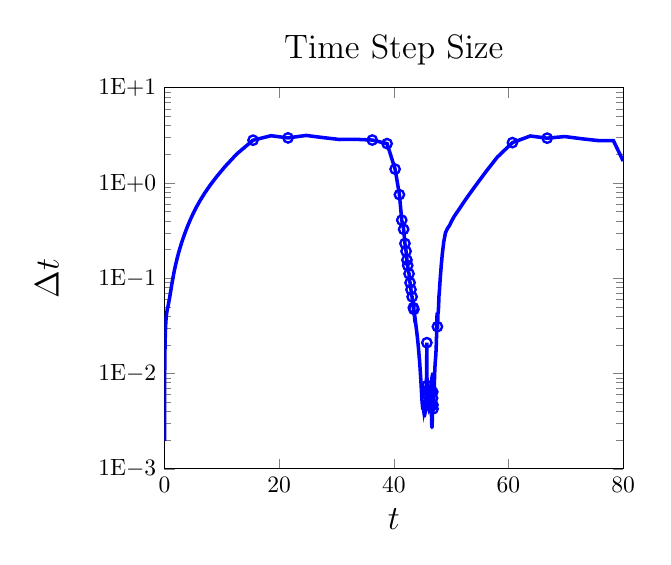
\begin{tikzpicture}[scale=0.85]

\begin{axis}[
  xmin = 0,
  xmax = 80,
  xtick = {0,20,40,60,80},
  xticklabels = {$0$,$20$,$40$,$60$,$80$},
  xlabel = $t$,
  ymode = log,
  ymin = 1E-3,
  ymax = 1E1,
  ytick = {1E-3,1E-2,1E-1,1E0,1E1},
  yticklabels = {$1$E$-3$,$1$E$-2$,$1$E$-1$,$1$E$+0$,$1$E$+1$},
  ylabel = {$\Delta t$},
  ylabel style = {yshift = 10pt},
  label style = {font=\Large},
  title = {\Large{Time Step Size}}
  ]

% adaptive time step size
\addplot [mark=none,blue,line width=1.5] table{
2.0693e-03 2.0693e-03
4.0324e-03 1.9631e-03
6.8259e-03 2.7935e-03
1.0801e-02 3.9753e-03
1.6080e-02 5.2784e-03
2.2654e-02 6.5739e-03
3.0878e-02 8.2242e-03
4.0926e-02 1.0048e-02
5.3163e-02 1.2237e-02
6.7828e-02 1.4664e-02
8.5250e-02 1.7422e-02
1.0564e-01 2.0388e-02
1.2919e-01 2.3552e-02
1.5596e-01 2.6771e-02
1.8593e-01 2.9965e-02
2.1893e-01 3.3005e-02
2.5476e-01 3.5824e-02
2.9313e-01 3.8370e-02
3.3377e-01 4.0642e-02
3.7644e-01 4.2668e-02
4.2094e-01 4.4502e-02
4.6715e-01 4.6208e-02
5.1500e-01 4.7856e-02
5.6394e-01 4.8941e-02
6.1437e-01 5.0431e-02
6.6694e-01 5.2565e-02
7.2162e-01 5.4685e-02
7.7864e-01 5.7018e-02
8.3834e-01 5.9700e-02
9.0107e-01 6.2727e-02
9.6722e-01 6.6156e-02
1.0373e+00 7.0060e-02
1.1118e+00 7.4500e-02
1.1916e+00 7.9849e-02
1.2777e+00 8.6099e-02
1.3703e+00 9.2540e-02
1.4702e+00 9.9920e-02
1.5786e+00 1.0836e-01
1.6963e+00 1.1777e-01
1.8246e+00 1.2828e-01
1.9647e+00 1.4008e-01
2.1180e+00 1.5333e-01
2.2862e+00 1.6823e-01
2.4714e+00 1.8512e-01
2.6758e+00 2.0440e-01
2.9024e+00 2.2662e-01
3.1549e+00 2.5247e-01
3.4377e+00 2.8285e-01
3.7566e+00 3.1890e-01
4.1188e+00 3.6215e-01
4.5333e+00 4.1452e-01
5.0118e+00 4.7849e-01
5.5691e+00 5.5736e-01
6.2249e+00 6.5575e-01
7.0056e+00 7.8071e-01
7.9497e+00 9.4413e-01
9.1180e+00 1.1683e+00
1.0616e+01 1.4978e+00
1.2637e+01 2.0216e+00
1.5447e+01 2.8101e+00
1.8579e+01 3.1311e+00
2.1549e+01 2.9704e+00
2.4701e+01 3.1525e+00
2.7692e+01 2.9907e+00
3.0550e+01 2.8582e+00
3.3419e+01 2.8691e+00
3.6240e+01 2.8202e+00
3.8826e+01 2.5862e+00
4.0222e+01 1.3965e+00
4.0976e+01 7.5413e-01
4.1384e+01 4.0723e-01
4.1710e+01 3.2616e-01
4.1941e+01 2.3156e-01
4.2133e+01 1.9191e-01
4.2288e+01 1.5512e-01
4.2425e+01 1.3615e-01
4.2542e+01 1.1742e-01
4.2653e+01 1.1139e-01
4.2748e+01 9.4545e-02
4.2838e+01 8.9693e-02
4.2918e+01 8.0059e-02
4.2994e+01 7.5951e-02
4.3062e+01 6.8090e-02
4.3126e+01 6.4596e-02
4.3190e+01 6.3801e-02
4.3248e+01 5.7777e-02
4.3303e+01 5.4812e-02
4.3357e+01 5.4746e-02
4.3407e+01 4.9077e-02
4.3453e+01 4.6559e-02
4.3500e+01 4.7111e-02
4.3543e+01 4.2796e-02
4.3584e+01 4.0600e-02
4.3625e+01 4.1239e-02
4.3665e+01 3.9749e-02
4.3702e+01 3.7865e-02
4.3739e+01 3.6472e-02
4.3774e+01 3.5126e-02
4.3808e+01 3.3850e-02
4.3841e+01 3.2663e-02
4.3872e+01 3.1546e-02
4.3903e+01 3.0493e-02
4.3932e+01 2.9497e-02
4.3961e+01 2.8554e-02
4.3988e+01 2.7658e-02
4.4015e+01 2.6806e-02
4.4041e+01 2.5993e-02
4.4066e+01 2.5217e-02
4.4091e+01 2.4474e-02
4.4115e+01 2.3762e-02
4.4138e+01 2.3078e-02
4.4160e+01 2.2421e-02
4.4182e+01 2.1788e-02
4.4203e+01 2.1178e-02
4.4224e+01 2.0590e-02
4.4244e+01 2.0021e-02
4.4263e+01 1.9471e-02
4.4282e+01 1.8939e-02
4.4300e+01 1.8424e-02
4.4318e+01 1.7924e-02
4.4336e+01 1.7440e-02
4.4353e+01 1.6971e-02
4.4369e+01 1.6516e-02
4.4385e+01 1.6074e-02
4.4401e+01 1.5644e-02
4.4416e+01 1.5211e-02
4.4431e+01 1.4803e-02
4.4445e+01 1.4411e-02
4.4460e+01 1.4285e-02
4.4474e+01 1.3996e-02
4.4487e+01 1.3610e-02
4.4501e+01 1.3283e-02
4.4514e+01 1.2966e-02
4.4526e+01 1.2654e-02
4.4539e+01 1.2352e-02
4.4551e+01 1.2061e-02
4.4562e+01 1.1778e-02
4.4574e+01 1.1504e-02
4.4585e+01 1.1239e-02
4.4596e+01 1.0982e-02
4.4607e+01 1.0733e-02
4.4617e+01 1.0492e-02
4.4628e+01 1.0259e-02
4.4638e+01 1.0033e-02
4.4648e+01 9.8146e-03
4.4657e+01 9.6028e-03
4.4667e+01 9.3977e-03
4.4676e+01 9.1991e-03
4.4685e+01 9.0067e-03
4.4694e+01 8.8642e-03
4.4702e+01 8.7127e-03
4.4711e+01 8.5230e-03
4.4719e+01 8.3542e-03
4.4727e+01 8.1946e-03
4.4735e+01 8.0369e-03
4.4743e+01 7.8842e-03
4.4751e+01 7.7369e-03
4.4759e+01 7.5943e-03
4.4766e+01 7.4561e-03
4.4773e+01 7.3223e-03
4.4781e+01 7.1928e-03
4.4788e+01 7.0674e-03
4.4795e+01 6.9460e-03
4.4801e+01 6.8276e-03
4.4808e+01 6.7136e-03
4.4815e+01 6.6039e-03
4.4821e+01 6.4974e-03
4.4828e+01 6.3944e-03
4.4834e+01 6.2947e-03
4.4840e+01 6.1983e-03
4.4846e+01 6.1050e-03
4.4852e+01 6.0147e-03
4.4858e+01 5.9274e-03
4.4864e+01 5.8430e-03
4.4870e+01 5.7614e-03
4.4875e+01 5.6825e-03
4.4881e+01 5.6062e-03
4.4887e+01 5.6101e-03
4.4892e+01 5.5697e-03
4.4898e+01 5.4760e-03
4.4903e+01 5.4066e-03
4.4909e+01 5.3497e-03
4.4914e+01 5.2884e-03
4.4919e+01 5.2281e-03
4.4924e+01 5.1716e-03
4.4929e+01 5.1172e-03
4.4934e+01 5.0644e-03
4.4939e+01 5.0136e-03
4.4944e+01 4.9648e-03
4.4949e+01 4.9179e-03
4.4954e+01 4.8728e-03
4.4959e+01 4.8295e-03
4.4964e+01 4.7880e-03
4.4969e+01 4.7483e-03
4.4973e+01 4.6823e-03
4.4978e+01 4.6294e-03
4.4982e+01 4.6262e-03
4.4987e+01 4.6230e-03
4.4992e+01 4.5789e-03
4.4996e+01 4.5427e-03
4.5001e+01 4.5143e-03
4.5005e+01 4.5038e-03
4.5010e+01 4.4955e-03
4.5014e+01 4.4710e-03
4.5019e+01 4.4270e-03
4.5023e+01 4.3903e-03
4.5027e+01 4.3777e-03
4.5032e+01 4.3629e-03
4.5036e+01 4.3437e-03
4.5040e+01 4.3277e-03
4.5045e+01 4.3147e-03
4.5049e+01 4.3025e-03
4.5053e+01 4.2914e-03
4.5058e+01 4.2787e-03
4.5062e+01 4.2697e-03
4.5066e+01 4.2646e-03
4.5070e+01 4.2602e-03
4.5075e+01 4.2567e-03
4.5079e+01 4.2552e-03
4.5083e+01 4.2555e-03
4.5087e+01 4.2574e-03
4.5092e+01 4.2610e-03
4.5096e+01 4.2664e-03
4.5100e+01 4.2736e-03
4.5104e+01 4.2828e-03
4.5109e+01 4.2938e-03
4.5113e+01 4.3069e-03
4.5117e+01 4.3221e-03
4.5122e+01 4.3395e-03
4.5126e+01 4.3591e-03
4.5130e+01 4.3811e-03
4.5135e+01 4.3816e-03
4.5139e+01 4.3648e-03
4.5144e+01 4.3991e-03
4.5148e+01 4.4372e-03
4.5153e+01 4.4602e-03
4.5157e+01 4.4861e-03
4.5162e+01 4.5202e-03
4.5166e+01 4.5554e-03
4.5171e+01 4.5903e-03
4.5175e+01 4.6271e-03
4.5180e+01 4.6659e-03
4.5185e+01 4.7051e-03
4.5189e+01 4.7440e-03
4.5194e+01 4.7821e-03
4.5199e+01 4.8183e-03
4.5204e+01 4.8511e-03
4.5209e+01 4.8789e-03
4.5214e+01 4.8999e-03
4.5219e+01 4.9122e-03
4.5223e+01 4.9138e-03
4.5228e+01 4.8953e-03
4.5233e+01 4.8671e-03
4.5238e+01 4.8306e-03
4.5243e+01 4.7784e-03
4.5248e+01 4.7118e-03
4.5252e+01 4.6354e-03
4.5257e+01 4.5518e-03
4.5261e+01 4.4630e-03
4.5266e+01 4.3721e-03
4.5270e+01 4.2819e-03
4.5274e+01 4.1947e-03
4.5278e+01 4.1120e-03
4.5282e+01 4.0351e-03
4.5286e+01 3.9647e-03
4.5290e+01 3.9012e-03
4.5294e+01 3.8447e-03
4.5298e+01 3.7951e-03
4.5301e+01 3.7521e-03
4.5305e+01 3.7156e-03
4.5309e+01 3.6849e-03
4.5313e+01 3.6597e-03
4.5316e+01 3.6396e-03
4.5320e+01 3.6240e-03
4.5323e+01 3.6125e-03
4.5327e+01 3.6046e-03
4.5331e+01 3.5999e-03
4.5334e+01 3.5980e-03
4.5338e+01 3.5984e-03
4.5341e+01 3.6008e-03
4.5345e+01 3.6049e-03
4.5349e+01 3.6103e-03
4.5352e+01 3.6168e-03
4.5356e+01 3.6242e-03
4.5360e+01 3.6322e-03
4.5363e+01 3.6406e-03
4.5367e+01 3.6493e-03
4.5370e+01 3.6583e-03
4.5374e+01 3.6674e-03
4.5378e+01 3.6765e-03
4.5381e+01 3.6856e-03
4.5385e+01 3.6948e-03
4.5389e+01 3.7039e-03
4.5393e+01 3.7131e-03
4.5396e+01 3.7223e-03
4.5400e+01 3.7316e-03
4.5404e+01 3.7409e-03
4.5408e+01 3.7504e-03
4.5411e+01 3.7600e-03
4.5415e+01 3.7699e-03
4.5419e+01 3.7800e-03
4.5423e+01 3.7904e-03
4.5426e+01 3.8011e-03
4.5430e+01 3.8121e-03
4.5434e+01 3.8236e-03
4.5438e+01 3.8355e-03
4.5442e+01 3.8478e-03
4.5446e+01 3.8607e-03
4.5449e+01 3.8740e-03
4.5453e+01 3.8880e-03
4.5457e+01 3.9026e-03
4.5461e+01 3.9178e-03
4.5465e+01 3.9337e-03
4.5469e+01 3.9504e-03
4.5473e+01 3.9679e-03
4.5477e+01 3.9863e-03
4.5481e+01 4.0056e-03
4.5485e+01 4.0259e-03
4.5489e+01 4.0472e-03
4.5493e+01 4.0695e-03
4.5497e+01 4.0928e-03
4.5501e+01 4.1171e-03
4.5506e+01 4.1423e-03
4.5510e+01 4.1686e-03
4.5514e+01 4.1959e-03
4.5518e+01 4.2245e-03
4.5522e+01 4.2545e-03
4.5527e+01 4.2859e-03
4.5531e+01 4.3190e-03
4.5535e+01 4.3538e-03
4.5540e+01 4.3904e-03
4.5544e+01 4.4290e-03
4.5549e+01 4.4698e-03
4.5553e+01 4.5129e-03
4.5558e+01 4.5585e-03
4.5562e+01 4.6067e-03
4.5567e+01 4.6579e-03
4.5572e+01 4.7123e-03
4.5576e+01 4.7702e-03
4.5581e+01 4.8319e-03
4.5586e+01 4.8978e-03
4.5591e+01 4.9684e-03
4.5596e+01 5.0441e-03
4.5601e+01 5.1257e-03
4.5607e+01 5.2137e-03
4.5612e+01 5.3091e-03
4.5617e+01 5.4129e-03
4.5623e+01 5.5263e-03
4.5628e+01 5.6509e-03
4.5634e+01 5.7884e-03
4.5640e+01 5.9414e-03
4.5646e+01 6.1127e-03
4.5653e+01 6.3062e-03
4.5659e+01 6.5273e-03
4.5666e+01 6.7829e-03
4.5673e+01 7.0830e-03
4.5680e+01 7.4421e-03
4.5688e+01 7.8820e-03
4.5697e+01 8.4382e-03
4.5706e+01 9.1723e-03
4.5716e+01 1.0204e-02
4.5728e+01 1.1808e-02
4.5743e+01 1.4789e-02
4.5764e+01 2.1045e-02
4.5770e+01 6.6101e-03
4.5777e+01 6.2709e-03
4.5786e+01 8.9237e-03
4.5794e+01 7.9957e-03
4.5801e+01 7.5854e-03
4.5809e+01 7.4646e-03
4.5816e+01 7.0816e-03
4.5823e+01 6.8475e-03
4.5829e+01 6.6616e-03
4.5836e+01 6.4121e-03
4.5842e+01 6.1852e-03
4.5848e+01 6.0338e-03
4.5854e+01 5.9107e-03
4.5860e+01 5.7791e-03
4.5865e+01 5.6541e-03
4.5871e+01 5.5522e-03
4.5876e+01 5.4638e-03
4.5882e+01 5.3778e-03
4.5887e+01 5.2964e-03
4.5892e+01 5.2241e-03
4.5897e+01 5.1587e-03
4.5902e+01 5.0970e-03
4.5907e+01 5.0386e-03
4.5912e+01 4.9852e-03
4.5917e+01 4.9362e-03
4.5922e+01 4.8900e-03
4.5927e+01 4.8464e-03
4.5932e+01 4.8061e-03
4.5937e+01 4.7686e-03
4.5941e+01 4.7336e-03
4.5946e+01 4.7009e-03
4.5951e+01 4.6705e-03
4.5955e+01 4.6423e-03
4.5960e+01 4.6162e-03
4.5965e+01 4.5919e-03
4.5969e+01 4.5695e-03
4.5974e+01 4.5488e-03
4.5978e+01 4.5299e-03
4.5983e+01 4.5126e-03
4.5987e+01 4.4968e-03
4.5992e+01 4.4827e-03
4.5996e+01 4.4701e-03
4.6001e+01 4.4590e-03
4.6005e+01 4.4495e-03
4.6010e+01 4.4414e-03
4.6014e+01 4.4346e-03
4.6018e+01 4.4288e-03
4.6023e+01 4.4233e-03
4.6027e+01 4.4176e-03
4.6032e+01 4.4120e-03
4.6036e+01 4.4072e-03
4.6040e+01 4.4040e-03
4.6045e+01 4.4021e-03
4.6049e+01 4.4015e-03
4.6054e+01 4.4022e-03
4.6058e+01 4.4048e-03
4.6062e+01 4.4207e-03
4.6067e+01 4.4125e-03
4.6071e+01 4.4025e-03
4.6076e+01 4.4149e-03
4.6080e+01 4.4300e-03
4.6085e+01 4.4375e-03
4.6089e+01 4.4445e-03
4.6093e+01 4.4517e-03
4.6098e+01 4.4589e-03
4.6102e+01 4.4693e-03
4.6107e+01 4.4825e-03
4.6111e+01 4.4966e-03
4.6116e+01 4.5114e-03
4.6120e+01 4.5279e-03
4.6125e+01 4.5460e-03
4.6130e+01 4.5652e-03
4.6134e+01 4.5854e-03
4.6139e+01 4.6070e-03
4.6143e+01 4.6311e-03
4.6148e+01 4.6552e-03
4.6153e+01 4.6711e-03
4.6157e+01 4.6928e-03
4.6162e+01 4.7694e-03
4.6167e+01 4.8632e-03
4.6172e+01 4.9193e-03
4.6177e+01 4.9633e-03
4.6182e+01 5.0281e-03
4.6187e+01 5.1056e-03
4.6192e+01 5.1855e-03
4.6197e+01 5.2742e-03
4.6203e+01 5.3782e-03
4.6208e+01 5.4978e-03
4.6214e+01 5.6343e-03
4.6220e+01 5.7469e-03
4.6226e+01 5.7840e-03
4.6231e+01 5.7397e-03
4.6237e+01 5.7242e-03
4.6243e+01 5.7051e-03
4.6248e+01 5.7030e-03
4.6254e+01 5.6907e-03
4.6260e+01 5.6874e-03
4.6265e+01 5.6829e-03
4.6271e+01 5.6861e-03
4.6277e+01 5.6906e-03
4.6283e+01 5.6987e-03
4.6288e+01 5.7097e-03
4.6294e+01 5.7205e-03
4.6300e+01 5.7467e-03
4.6305e+01 5.7773e-03
4.6311e+01 5.7966e-03
4.6317e+01 5.8234e-03
4.6323e+01 5.8529e-03
4.6329e+01 5.8863e-03
4.6335e+01 5.9232e-03
4.6341e+01 5.9636e-03
4.6347e+01 6.0073e-03
4.6353e+01 6.0542e-03
4.6359e+01 6.1040e-03
4.6365e+01 6.1565e-03
4.6371e+01 6.2115e-03
4.6378e+01 6.2687e-03
4.6384e+01 6.2153e-03
4.6390e+01 6.0732e-03
4.6396e+01 5.9561e-03
4.6402e+01 5.8736e-03
4.6407e+01 5.8200e-03
4.6413e+01 5.8989e-03
4.6419e+01 5.8993e-03
4.6425e+01 5.9225e-03
4.6431e+01 6.0751e-03
4.6437e+01 6.0107e-03
4.6444e+01 6.2225e-03
4.6450e+01 6.3968e-03
4.6457e+01 6.6993e-03
4.6464e+01 7.0876e-03
4.6471e+01 7.2400e-03
4.6478e+01 7.3339e-03
4.6486e+01 7.4548e-03
4.6493e+01 7.5813e-03
4.6501e+01 7.7175e-03
4.6509e+01 7.8610e-03
4.6516e+01 6.6328e-03
4.6522e+01 6.2924e-03
4.6527e+01 5.6331e-03
4.6533e+01 5.3440e-03
4.6538e+01 4.8490e-03
4.6542e+01 4.6001e-03
4.6547e+01 4.6367e-03
4.6551e+01 4.1278e-03
4.6555e+01 3.9160e-03
4.6559e+01 4.0662e-03
4.6563e+01 3.7369e-03
4.6566e+01 3.5452e-03
4.6570e+01 3.6848e-03
4.6574e+01 3.6263e-03
4.6577e+01 3.4682e-03
4.6580e+01 3.3969e-03
4.6584e+01 3.3443e-03
4.6587e+01 3.2761e-03
4.6590e+01 3.2159e-03
4.6593e+01 3.1656e-03
4.6597e+01 3.1183e-03
4.6600e+01 3.0744e-03
4.6603e+01 3.0349e-03
4.6606e+01 2.9989e-03
4.6609e+01 2.9659e-03
4.6612e+01 2.9359e-03
4.6614e+01 2.9086e-03
4.6617e+01 2.8838e-03
4.6620e+01 2.8614e-03
4.6623e+01 2.8412e-03
4.6626e+01 2.8231e-03
4.6629e+01 2.8071e-03
4.6631e+01 2.7931e-03
4.6634e+01 2.7809e-03
4.6637e+01 2.7707e-03
4.6640e+01 2.7623e-03
4.6643e+01 2.7559e-03
4.6645e+01 2.7512e-03
4.6648e+01 2.7482e-03
4.6651e+01 2.7471e-03
4.6654e+01 2.7479e-03
4.6656e+01 2.7506e-03
4.6659e+01 2.7552e-03
4.6662e+01 2.7618e-03
4.6665e+01 2.7704e-03
4.6667e+01 2.7812e-03
4.6670e+01 2.7942e-03
4.6673e+01 2.8095e-03
4.6676e+01 2.8274e-03
4.6679e+01 2.8479e-03
4.6682e+01 2.8712e-03
4.6684e+01 2.8977e-03
4.6687e+01 2.9275e-03
4.6690e+01 2.9609e-03
4.6693e+01 2.9985e-03
4.6696e+01 3.0405e-03
4.6699e+01 3.0877e-03
4.6703e+01 3.1407e-03
4.6706e+01 3.1996e-03
4.6709e+01 3.2665e-03
4.6712e+01 3.3426e-03
4.6716e+01 3.4290e-03
4.6719e+01 3.5271e-03
4.6723e+01 3.6423e-03
4.6727e+01 3.7432e-03
4.6731e+01 3.8788e-03
4.6735e+01 4.0755e-03
4.6739e+01 4.3056e-03
4.6744e+01 4.5859e-03
4.6749e+01 4.9629e-03
4.6754e+01 5.4974e-03
4.6760e+01 6.3249e-03
4.6768e+01 7.8909e-03
4.6778e+01 1.0218e-02
4.6788e+01 9.1021e-03
4.6794e+01 6.3996e-03
4.6800e+01 6.0712e-03
4.6805e+01 5.3980e-03
4.6811e+01 5.1210e-03
4.6816e+01 5.0657e-03
4.6820e+01 4.8629e-03
4.6825e+01 4.6815e-03
4.6830e+01 4.5536e-03
4.6834e+01 4.4506e-03
4.6839e+01 4.3701e-03
4.6843e+01 4.3058e-03
4.6847e+01 4.2547e-03
4.6851e+01 4.2145e-03
4.6855e+01 4.1833e-03
4.6860e+01 4.1598e-03
4.6864e+01 4.1430e-03
4.6868e+01 4.1321e-03
4.6872e+01 4.1265e-03
4.6876e+01 4.1257e-03
4.6880e+01 4.1293e-03
4.6884e+01 4.1370e-03
4.6889e+01 4.1486e-03
4.6893e+01 4.1640e-03
4.6897e+01 4.1830e-03
4.6901e+01 4.2057e-03
4.6905e+01 4.2321e-03
4.6910e+01 4.2622e-03
4.6914e+01 4.2960e-03
4.6918e+01 4.3338e-03
4.6923e+01 4.3755e-03
4.6927e+01 4.4213e-03
4.6932e+01 4.4714e-03
4.6936e+01 4.5260e-03
4.6941e+01 4.5852e-03
4.6945e+01 4.6492e-03
4.6950e+01 4.7184e-03
4.6955e+01 4.7931e-03
4.6960e+01 4.8735e-03
4.6965e+01 4.9600e-03
4.6970e+01 5.0531e-03
4.6975e+01 5.1532e-03
4.6980e+01 5.2608e-03
4.6985e+01 5.3766e-03
4.6991e+01 5.5012e-03
4.6997e+01 5.6354e-03
4.7002e+01 5.7798e-03
4.7008e+01 5.9352e-03
4.7014e+01 6.1023e-03
4.7021e+01 6.2816e-03
4.7027e+01 6.4737e-03
4.7034e+01 6.6794e-03
4.7041e+01 6.8995e-03
4.7048e+01 7.1349e-03
4.7055e+01 7.3866e-03
4.7063e+01 7.6553e-03
4.7071e+01 7.9416e-03
4.7079e+01 8.2459e-03
4.7088e+01 8.5682e-03
4.7097e+01 8.9079e-03
4.7106e+01 9.2639e-03
4.7116e+01 9.6341e-03
4.7126e+01 1.0016e-02
4.7136e+01 1.0405e-02
4.7147e+01 1.0798e-02
4.7158e+01 1.1189e-02
4.7169e+01 1.1574e-02
4.7181e+01 1.1948e-02
4.7194e+01 1.2308e-02
4.7206e+01 1.2654e-02
4.7219e+01 1.2986e-02
4.7233e+01 1.3308e-02
4.7246e+01 1.3626e-02
4.7260e+01 1.3949e-02
4.7275e+01 1.4289e-02
4.7289e+01 1.4658e-02
4.7304e+01 1.5071e-02
4.7320e+01 1.5557e-02
4.7336e+01 1.6130e-02
4.7353e+01 1.6837e-02
4.7371e+01 1.7715e-02
4.7389e+01 1.8856e-02
4.7410e+01 2.0363e-02
4.7432e+01 2.2473e-02
4.7458e+01 2.5568e-02
4.7488e+01 3.0598e-02
4.7528e+01 3.9951e-02
4.7572e+01 4.3403e-02
4.7603e+01 3.1016e-02
4.7632e+01 2.9424e-02
4.7671e+01 3.8720e-02
4.7715e+01 4.3606e-02
4.7759e+01 4.4308e-02
4.7810e+01 5.1098e-02
4.7875e+01 6.4968e-02
4.7948e+01 7.2718e-02
4.8036e+01 8.8504e-02
4.8145e+01 1.0882e-01
4.8284e+01 1.3874e-01
4.8465e+01 1.8149e-01
4.8705e+01 2.4002e-01
4.9005e+01 2.9943e-01
4.9335e+01 3.3082e-01
4.9691e+01 3.5541e-01
5.0089e+01 3.9825e-01
5.0535e+01 4.4592e-01
5.1028e+01 4.9283e-01
5.1580e+01 5.5170e-01
5.2208e+01 6.2888e-01
5.2935e+01 7.2647e-01
5.3791e+01 8.5660e-01
5.4836e+01 1.0440e+00
5.6175e+01 1.3396e+00
5.8037e+01 1.8623e+00
6.0687e+01 2.6501e+00
6.3799e+01 3.1111e+00
6.6750e+01 2.9515e+00
6.9819e+01 3.0692e+00
7.2731e+01 2.9117e+00
7.5520e+01 2.7892e+00
7.8300e+01 2.7801e+00
8.0000e+01 1.6997e+00
};


\addplot [only marks,blue,mark=o,mark size=2pt,line width=1.0] table{
1.5447e+01 2.8101e+00
2.1549e+01 2.9704e+00
3.6240e+01 2.8202e+00
3.8826e+01 2.5862e+00
4.0222e+01 1.3965e+00
4.0976e+01 7.5413e-01
4.1384e+01 4.0723e-01
4.1710e+01 3.2616e-01
4.1941e+01 2.3156e-01
4.2133e+01 1.9191e-01
4.2288e+01 1.5512e-01
4.2425e+01 1.3615e-01
4.2653e+01 1.1139e-01
4.2838e+01 8.9693e-02
4.2994e+01 7.5951e-02
4.3190e+01 6.3801e-02
4.3407e+01 4.9077e-02
4.3500e+01 4.7111e-02
4.5764e+01 2.1045e-02
4.5770e+01 6.6101e-03
4.5809e+01 7.4646e-03
4.5848e+01 6.0338e-03
4.6450e+01 6.3968e-03
4.6547e+01 4.6367e-03
4.6754e+01 5.4974e-03
4.6794e+01 6.3996e-03
4.6825e+01 4.6815e-03
4.6847e+01 4.2547e-03
4.7603e+01 3.1016e-02
6.0687e+01 2.6501e+00
6.6750e+01 2.9515e+00
};

% OLD RESULTS
%% adaptive time step size
%\addplot [mark=none,blue,line width=1.5] table{
%4.7743e-03 4.7743e-03
%9.4244e-03 4.6502e-03
%1.6218e-02 6.7939e-03
%2.6144e-02 9.9259e-03
%4.0646e-02 1.4502e-02
%6.1270e-02 2.0624e-02
%8.8007e-02 2.6737e-02
%1.2153e-01 3.3526e-02
%1.6212e-01 4.0583e-02
%2.0963e-01 4.7517e-02
%2.6370e-01 5.4062e-02
%3.2384e-01 6.0149e-02
%3.8974e-01 6.5897e-02
%4.6130e-01 7.1558e-02
%5.3876e-01 7.7463e-02
%6.2273e-01 8.3971e-02
%7.1417e-01 9.1433e-02
%8.1434e-01 1.0017e-01
%9.2480e-01 1.1046e-01
%1.0474e+00 1.2255e-01
%1.1840e+00 1.3666e-01
%1.3370e+00 1.5303e-01
%1.5090e+00 1.7200e-01
%1.7031e+00 1.9403e-01
%1.9229e+00 2.1984e-01
%2.1734e+00 2.5046e-01
%2.4607e+00 2.8734e-01
%2.7933e+00 3.3254e-01
%3.1821e+00 3.8885e-01
%3.6421e+00 4.6001e-01
%4.1931e+00 5.5098e-01
%4.8614e+00 6.6834e-01
%5.6829e+00 8.2147e-01
%6.7090e+00 1.0261e+00
%8.0233e+00 1.3143e+00
%9.7861e+00 1.7627e+00
%1.2361e+01 2.5754e+00
%1.6124e+01 3.7626e+00
%2.1621e+01 5.4972e+00
%2.9653e+01 8.0314e+00
%3.6510e+01 6.8574e+00
%4.0413e+01 3.9033e+00
%4.0999e+01 5.8609e-01
%4.1354e+01 3.5426e-01
%4.1626e+01 2.7265e-01
%4.1842e+01 2.1545e-01
%4.2021e+01 1.7887e-01
%4.2174e+01 1.5299e-01
%4.2307e+01 1.3381e-01
%4.2426e+01 1.1902e-01
%4.2534e+01 1.0728e-01
%4.2631e+01 9.7727e-02
%4.2721e+01 8.9801e-02
%4.2804e+01 8.3116e-02
%4.2882e+01 7.7398e-02
%4.2954e+01 7.2449e-02
%4.3022e+01 6.8122e-02
%4.3087e+01 6.4302e-02
%4.3148e+01 6.0904e-02
%4.3207e+01 5.9320e-02
%4.3262e+01 5.5027e-02
%4.3315e+01 5.3596e-02
%4.3366e+01 5.0228e-02
%4.3415e+01 4.8922e-02
%4.3461e+01 4.6207e-02
%4.3506e+01 4.5006e-02
%4.3549e+01 4.2775e-02
%4.3590e+01 4.1663e-02
%4.3630e+01 3.9801e-02
%4.3669e+01 3.8766e-02
%4.3706e+01 3.7188e-02
%4.3742e+01 3.6221e-02
%4.3777e+01 3.4867e-02
%4.3811e+01 3.3960e-02
%4.3844e+01 3.2784e-02
%4.3876e+01 3.1932e-02
%4.3907e+01 3.0900e-02
%4.3937e+01 3.0097e-02
%4.3966e+01 2.9183e-02
%4.3994e+01 2.8424e-02
%4.4022e+01 2.7608e-02
%4.4049e+01 2.6891e-02
%4.4075e+01 2.6156e-02
%4.4101e+01 2.5476e-02
%4.4125e+01 2.4811e-02
%4.4150e+01 2.4166e-02
%4.4174e+01 2.4177e-02
%4.4197e+01 2.3559e-02
%4.4220e+01 2.2953e-02
%4.4243e+01 2.2364e-02
%4.4264e+01 2.1793e-02
%4.4286e+01 2.1240e-02
%4.4306e+01 2.0704e-02
%4.4326e+01 2.0184e-02
%4.4346e+01 1.9680e-02
%4.4365e+01 1.9190e-02
%4.4384e+01 1.8713e-02
%4.4402e+01 1.8249e-02
%4.4420e+01 1.7797e-02
%4.4437e+01 1.7357e-02
%4.4454e+01 1.6927e-02
%4.4471e+01 1.6508e-02
%4.4487e+01 1.6098e-02
%4.4503e+01 1.5697e-02
%4.4518e+01 1.5305e-02
%4.4533e+01 1.4922e-02
%4.4547e+01 1.4546e-02
%4.4562e+01 1.4179e-02
%4.4575e+01 1.3819e-02
%4.4589e+01 1.3467e-02
%4.4602e+01 1.3122e-02
%4.4615e+01 1.2784e-02
%4.4627e+01 1.2454e-02
%4.4639e+01 1.2131e-02
%4.4651e+01 1.1508e-02
%4.4662e+01 1.1209e-02
%4.4673e+01 1.1215e-02
%4.4684e+01 1.0929e-02
%4.4695e+01 1.0647e-02
%4.4705e+01 1.0371e-02
%4.4715e+01 1.0103e-02
%4.4725e+01 9.8433e-03
%4.4735e+01 9.5918e-03
%4.4744e+01 9.3488e-03
%4.4753e+01 9.1142e-03
%4.4762e+01 8.8881e-03
%4.4771e+01 8.6702e-03
%4.4779e+01 8.4606e-03
%4.4788e+01 8.2592e-03
%4.4796e+01 8.0658e-03
%4.4804e+01 7.8802e-03
%4.4811e+01 7.7022e-03
%4.4819e+01 7.5318e-03
%4.4826e+01 7.3685e-03
%4.4833e+01 7.2123e-03
%4.4840e+01 7.0629e-03
%4.4847e+01 6.9200e-03
%4.4854e+01 6.7834e-03
%4.4861e+01 6.6529e-03
%4.4867e+01 6.5283e-03
%4.4874e+01 6.4093e-03
%4.4880e+01 6.2957e-03
%4.4886e+01 6.1873e-03
%4.4892e+01 6.0838e-03
%4.4898e+01 5.9851e-03
%4.4904e+01 5.8910e-03
%4.4910e+01 5.8012e-03
%4.4916e+01 5.7156e-03
%4.4921e+01 5.6341e-03
%4.4927e+01 5.5563e-03
%4.4932e+01 5.4823e-03
%4.4938e+01 5.4119e-03
%4.4943e+01 5.3449e-03
%4.4948e+01 5.2811e-03
%4.4954e+01 5.2206e-03
%4.4959e+01 5.1631e-03
%4.4964e+01 5.1086e-03
%4.4969e+01 5.0569e-03
%4.4974e+01 5.0080e-03
%4.4979e+01 4.9618e-03
%4.4984e+01 4.9183e-03
%4.4989e+01 4.8773e-03
%4.4994e+01 4.8388e-03
%4.4998e+01 4.8028e-03
%4.5003e+01 4.7693e-03
%4.5008e+01 4.7381e-03
%4.5013e+01 4.7094e-03
%4.5017e+01 4.6830e-03
%4.5022e+01 4.6591e-03
%4.5027e+01 4.6375e-03
%4.5031e+01 4.6183e-03
%4.5036e+01 4.6017e-03
%4.5040e+01 4.5875e-03
%4.5045e+01 4.5760e-03
%4.5049e+01 4.5671e-03
%4.5054e+01 4.5610e-03
%4.5059e+01 4.5578e-03
%4.5063e+01 4.5577e-03
%4.5068e+01 4.5609e-03
%4.5072e+01 4.5675e-03
%4.5077e+01 4.5778e-03
%4.5081e+01 4.5922e-03
%4.5086e+01 4.6109e-03
%4.5091e+01 4.6344e-03
%4.5095e+01 4.6631e-03
%4.5100e+01 4.6975e-03
%4.5105e+01 4.7384e-03
%4.5110e+01 4.7863e-03
%4.5114e+01 4.8422e-03
%4.5119e+01 4.9068e-03
%4.5124e+01 4.9813e-03
%4.5129e+01 5.0667e-03
%4.5135e+01 5.1641e-03
%4.5140e+01 5.2746e-03
%4.5145e+01 5.3990e-03
%4.5151e+01 5.5376e-03
%4.5156e+01 5.6898e-03
%4.5162e+01 5.8534e-03
%4.5168e+01 6.0236e-03
%4.5175e+01 6.1924e-03
%4.5181e+01 6.3481e-03
%4.5187e+01 6.4757e-03
%4.5194e+01 6.5601e-03
%4.5200e+01 6.5901e-03
%4.5207e+01 6.5631e-03
%4.5214e+01 6.4862e-03
%4.5220e+01 6.3735e-03
%4.5226e+01 6.2410e-03
%4.5232e+01 6.1028e-03
%4.5238e+01 5.9688e-03
%4.5244e+01 5.8447e-03
%4.5250e+01 5.7335e-03
%4.5255e+01 5.6357e-03
%4.5261e+01 5.5510e-03
%4.5266e+01 5.4785e-03
%4.5272e+01 5.4169e-03
%4.5277e+01 5.3651e-03
%4.5283e+01 5.3219e-03
%4.5288e+01 5.2863e-03
%4.5293e+01 5.2573e-03
%4.5298e+01 5.2343e-03
%4.5304e+01 5.2166e-03
%4.5309e+01 5.2035e-03
%4.5314e+01 5.1947e-03
%4.5319e+01 5.1898e-03
%4.5324e+01 5.1884e-03
%4.5330e+01 5.1902e-03
%4.5335e+01 5.1951e-03
%4.5340e+01 5.2028e-03
%4.5345e+01 5.2132e-03
%4.5350e+01 5.2263e-03
%4.5356e+01 5.2418e-03
%4.5361e+01 5.2598e-03
%4.5366e+01 5.2803e-03
%4.5371e+01 5.3032e-03
%4.5377e+01 5.3285e-03
%4.5382e+01 5.3563e-03
%4.5388e+01 5.3865e-03
%4.5393e+01 5.4194e-03
%4.5398e+01 5.4549e-03
%4.5404e+01 5.4932e-03
%4.5409e+01 5.5344e-03
%4.5415e+01 5.5786e-03
%4.5421e+01 5.6260e-03
%4.5426e+01 5.6769e-03
%4.5432e+01 5.7314e-03
%4.5438e+01 5.7899e-03
%4.5444e+01 5.8526e-03
%4.5450e+01 5.9198e-03
%4.5456e+01 5.9920e-03
%4.5462e+01 6.0697e-03
%4.5468e+01 6.1534e-03
%4.5474e+01 6.2437e-03
%4.5480e+01 6.3413e-03
%4.5487e+01 6.4472e-03
%4.5493e+01 6.5623e-03
%4.5500e+01 6.6880e-03
%4.5507e+01 6.8256e-03
%4.5514e+01 6.9770e-03
%4.5521e+01 7.1444e-03
%4.5528e+01 7.3307e-03
%4.5536e+01 7.5393e-03
%4.5544e+01 7.7749e-03
%4.5552e+01 8.0436e-03
%4.5560e+01 8.3535e-03
%4.5569e+01 8.7160e-03
%4.5578e+01 9.1476e-03
%4.5588e+01 9.6730e-03
%4.5598e+01 1.0332e-02
%4.5609e+01 1.1191e-02
%4.5622e+01 1.2380e-02
%4.5636e+01 1.4182e-02
%4.5653e+01 1.7405e-02
%4.5679e+01 2.5429e-02
%4.5694e+01 1.5149e-02
%4.5707e+01 1.3641e-02
%4.5720e+01 1.2333e-02
%4.5731e+01 1.1478e-02
%4.5742e+01 1.0883e-02
%4.5753e+01 1.0600e-02
%4.5763e+01 1.0116e-02
%4.5773e+01 9.8527e-03
%4.5782e+01 9.8659e-03
%4.5792e+01 9.6759e-03
%4.5802e+01 9.5333e-03
%4.5811e+01 9.4287e-03
%4.5820e+01 9.3579e-03
%4.5830e+01 9.3158e-03
%4.5839e+01 9.2983e-03
%4.5848e+01 9.3022e-03
%4.5858e+01 9.3242e-03
%4.5867e+01 9.3614e-03
%4.5876e+01 9.4109e-03
%4.5886e+01 9.4697e-03
%4.5895e+01 9.5349e-03
%4.5905e+01 9.6036e-03
%4.5915e+01 9.6731e-03
%4.5924e+01 9.7413e-03
%4.5934e+01 9.8066e-03
%4.5944e+01 9.8680e-03
%4.5954e+01 9.9258e-03
%4.5964e+01 9.9810e-03
%4.5974e+01 1.0036e-02
%4.5984e+01 1.0093e-02
%4.5994e+01 1.0156e-02
%4.6005e+01 1.0230e-02
%4.6015e+01 1.0320e-02
%4.6025e+01 1.0433e-02
%4.6036e+01 1.0353e-02
%4.6046e+01 1.0089e-02
%4.6056e+01 9.9059e-03
%4.6065e+01 9.7312e-03
%4.6075e+01 9.5814e-03
%4.6084e+01 9.4500e-03
%4.6094e+01 9.3371e-03
%4.6103e+01 9.2411e-03
%4.6112e+01 9.1611e-03
%4.6121e+01 9.0962e-03
%4.6130e+01 9.0458e-03
%4.6139e+01 9.0093e-03
%4.6148e+01 8.9863e-03
%4.6157e+01 8.9764e-03
%4.6166e+01 8.9795e-03
%4.6175e+01 8.9953e-03
%4.6184e+01 9.0238e-03
%4.6193e+01 9.0648e-03
%4.6202e+01 9.1182e-03
%4.6212e+01 9.1837e-03
%4.6221e+01 9.2609e-03
%4.6230e+01 9.3495e-03
%4.6240e+01 9.4485e-03
%4.6249e+01 9.5572e-03
%4.6259e+01 9.6742e-03
%4.6269e+01 9.7984e-03
%4.6279e+01 9.9285e-03
%4.6289e+01 1.0064e-02
%4.6299e+01 1.0205e-02
%4.6309e+01 1.0352e-02
%4.6320e+01 1.0509e-02
%4.6330e+01 9.6970e-03
%4.6338e+01 8.7962e-03
%4.6346e+01 8.0915e-03
%4.6354e+01 7.5316e-03
%4.6361e+01 7.0742e-03
%4.6368e+01 6.6931e-03
%4.6374e+01 6.5191e-03
%4.6380e+01 6.0807e-03
%4.6386e+01 5.9226e-03
%4.6392e+01 5.6327e-03
%4.6397e+01 5.4863e-03
%4.6403e+01 5.2877e-03
%4.6408e+01 5.1502e-03
%4.6413e+01 5.1476e-03
%4.6418e+01 5.0165e-03
%4.6423e+01 4.9003e-03
%4.6428e+01 4.7966e-03
%4.6432e+01 4.7045e-03
%4.6437e+01 4.6228e-03
%4.6442e+01 4.5506e-03
%4.6446e+01 4.4869e-03
%4.6450e+01 4.4313e-03
%4.6455e+01 4.3831e-03
%4.6459e+01 4.3421e-03
%4.6463e+01 4.3078e-03
%4.6468e+01 4.2800e-03
%4.6472e+01 4.2586e-03
%4.6476e+01 4.2436e-03
%4.6480e+01 4.2349e-03
%4.6485e+01 4.2325e-03
%4.6489e+01 4.2367e-03
%4.6493e+01 4.2477e-03
%4.6497e+01 4.2658e-03
%4.6502e+01 4.2914e-03
%4.6506e+01 4.3252e-03
%4.6510e+01 4.3678e-03
%4.6515e+01 4.4201e-03
%4.6519e+01 4.4833e-03
%4.6524e+01 4.5588e-03
%4.6529e+01 4.6484e-03
%4.6533e+01 4.7543e-03
%4.6538e+01 4.8797e-03
%4.6543e+01 5.0285e-03
%4.6548e+01 5.2060e-03
%4.6554e+01 5.4197e-03
%4.6560e+01 5.6802e-03
%4.6566e+01 6.0036e-03
%4.6572e+01 6.4148e-03
%4.6579e+01 6.9567e-03
%4.6587e+01 7.7091e-03
%4.6595e+01 8.8453e-03
%4.6606e+01 1.0846e-02
%4.6621e+01 1.5107e-02
%4.6634e+01 1.2137e-02
%4.6644e+01 1.0004e-02
%4.6653e+01 9.0610e-03
%4.6661e+01 8.4890e-03
%4.6669e+01 8.2683e-03
%4.6677e+01 7.8394e-03
%4.6685e+01 7.6356e-03
%4.6692e+01 7.6470e-03
%4.6700e+01 7.5197e-03
%4.6707e+01 7.4224e-03
%4.6715e+01 7.3626e-03
%4.6722e+01 7.3319e-03
%4.6729e+01 7.3264e-03
%4.6737e+01 7.3441e-03
%4.6744e+01 7.3839e-03
%4.6752e+01 7.4458e-03
%4.6759e+01 7.5301e-03
%4.6767e+01 7.6382e-03
%4.6775e+01 7.7717e-03
%4.6783e+01 7.9335e-03
%4.6791e+01 8.1269e-03
%4.6799e+01 8.3565e-03
%4.6808e+01 8.6283e-03
%4.6817e+01 8.9503e-03
%4.6826e+01 9.3330e-03
%4.6836e+01 9.7909e-03
%4.6846e+01 1.0344e-02
%4.6857e+01 1.1022e-02
%4.6869e+01 1.1869e-02
%4.6882e+01 1.2956e-02
%4.6896e+01 1.4408e-02
%4.6913e+01 1.6466e-02
%4.6932e+01 1.9693e-02
%4.6958e+01 2.5883e-02
%4.6990e+01 3.1405e-02
%4.7019e+01 2.8883e-02
%4.7044e+01 2.5392e-02
%4.7067e+01 2.3389e-02
%4.7089e+01 2.2066e-02
%4.7111e+01 2.1493e-02
%4.7131e+01 2.0233e-02
%4.7151e+01 1.9707e-02
%4.7170e+01 1.8925e-02
%4.7188e+01 1.8433e-02
%4.7207e+01 1.8399e-02
%4.7225e+01 1.7957e-02
%4.7242e+01 1.7590e-02
%4.7260e+01 1.7317e-02
%4.7277e+01 1.7142e-02
%4.7294e+01 1.7071e-02
%4.7311e+01 1.7114e-02
%4.7328e+01 1.7282e-02
%4.7346e+01 1.7593e-02
%4.7364e+01 1.8072e-02
%4.7383e+01 1.8750e-02
%4.7402e+01 1.9678e-02
%4.7423e+01 2.0923e-02
%4.7446e+01 2.2583e-02
%4.7471e+01 2.4808e-02
%4.7498e+01 2.7823e-02
%4.7530e+01 3.1995e-02
%4.7568e+01 3.7948e-02
%4.7615e+01 4.6842e-02
%4.7676e+01 6.1119e-02
%4.7763e+01 8.7068e-02
%4.7891e+01 1.2721e-01
%4.8069e+01 1.7834e-01
%4.8329e+01 2.6056e-01
%4.8654e+01 3.2463e-01
%4.9025e+01 3.7055e-01
%4.9441e+01 4.1648e-01
%4.9910e+01 4.6846e-01
%5.0446e+01 5.3655e-01
%5.1074e+01 6.2768e-01
%5.1828e+01 7.5460e-01
%5.2770e+01 9.4163e-01
%5.4009e+01 1.2388e+00
%5.5787e+01 1.7783e+00
%5.8385e+01 2.5981e+00
%6.2181e+01 3.7958e+00
%6.7727e+01 5.5457e+00
%7.5829e+01 8.1023e+00
%8.0000e+01 4.1710e+00
%};
%
%\addplot [only marks,blue,mark=o,mark size=2pt,line width=1.0] table{
%4.7743e-03 4.7743e-03
%3.6510e+01 6.8574e+00
%4.0413e+01 3.9033e+00
%4.0999e+01 5.8609e-01
%4.1354e+01 3.5426e-01
%4.1626e+01 2.7265e-01
%4.1842e+01 2.1545e-01
%4.2021e+01 1.7887e-01
%4.2174e+01 1.5299e-01
%4.2307e+01 1.3381e-01
%4.2426e+01 1.1902e-01
%4.2534e+01 1.0728e-01
%4.2631e+01 9.7727e-02
%4.2721e+01 8.9801e-02
%4.2804e+01 8.3116e-02
%4.2882e+01 7.7398e-02
%4.2954e+01 7.2449e-02
%4.3022e+01 6.8122e-02
%4.3087e+01 6.4302e-02
%4.3148e+01 6.0904e-02
%4.3262e+01 5.5027e-02
%4.3366e+01 5.0228e-02
%4.3461e+01 4.6207e-02
%4.3549e+01 4.2775e-02
%4.3630e+01 3.9801e-02
%4.3706e+01 3.7188e-02
%4.3777e+01 3.4867e-02
%4.3844e+01 3.2784e-02
%4.3907e+01 3.0900e-02
%4.3966e+01 2.9183e-02
%4.4022e+01 2.7608e-02
%4.4075e+01 2.6156e-02
%4.4125e+01 2.4811e-02
%4.4651e+01 1.1508e-02
%4.5694e+01 1.5149e-02
%4.5707e+01 1.3641e-02
%4.5720e+01 1.2333e-02
%4.5731e+01 1.1478e-02
%4.5742e+01 1.0883e-02
%4.5763e+01 1.0116e-02
%4.6330e+01 9.6970e-03
%4.6338e+01 8.7962e-03
%4.6346e+01 8.0915e-03
%4.6354e+01 7.5316e-03
%4.6361e+01 7.0742e-03
%4.6368e+01 6.6931e-03
%4.6380e+01 6.0807e-03
%4.6392e+01 5.6327e-03
%4.6403e+01 5.2877e-03
%4.6621e+01 1.5107e-02
%4.6634e+01 1.2137e-02
%4.6644e+01 1.0004e-02
%4.6653e+01 9.0610e-03
%4.6661e+01 8.4890e-03
%4.6677e+01 7.8394e-03
%4.7019e+01 2.8883e-02
%4.7044e+01 2.5392e-02
%4.7067e+01 2.3389e-02
%4.7089e+01 2.2066e-02
%4.7131e+01 2.0233e-02
%4.7170e+01 1.8925e-02
%};

\end{axis}

\end{tikzpicture}


 &
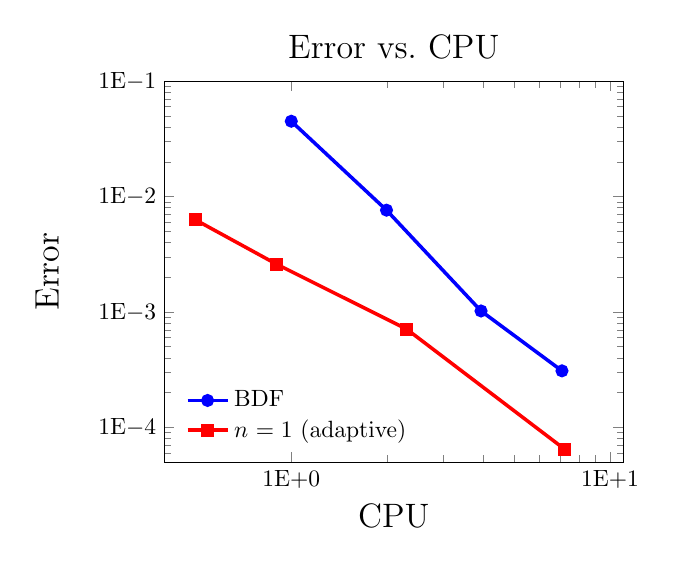
\begin{tikzpicture}[scale=0.85]

\begin{axis}[
  xmode = log,
  xmin = 0.4,
  xmax = 11,
  xtick = {1,10},
  xticklabels = {$1$E$+0$,$1$E$+1$},
  xlabel = CPU,
  ymode = log,
  ymin = 5E-5,
  ymax = 1E-1,
  ytick = {1E-5,1E-4,1E-3,1E-2,1E-1},
  yticklabels = {$1$E$-5$,$1$E$-4$,$1$E$-3$,$1$E$-2$,$1$E$-1$},
  ylabel = {Error},
  ylabel style = {yshift = 10pt},
  label style = {font=\Large},
  legend entries = {BDF, $n_{\sdc}=1$ (adaptive)},
  legend cell align = left,
  legend pos = south west, 
  legend style = {draw=none},
  title = {\Large{Error vs.~CPU}}
  ]


% BDF fixed time step size
\addplot [mark=*,blue,line width=1.5] table{
1.00 4.49e-2
1.99 7.62e-3
3.94 1.02e-3
7.07 3.09e-4
};

% 1 SDC correction adaptive time step size
\addplot [mark=square*,red,line width=1.5] table{
0.5 6.29e-3
0.9 2.59e-3
2.3 7.11e-4
7.2 6.49e-5
};

\end{axis}

\end{tikzpicture}


 
\fi
\end{tabular}
\mcaption{Results for the {\bf stenosis} flow.  Left: The time step
size using {\bf adaptive} $\boldnsdc{1}$, $p=2$ with a tolerance of
$1$E$-3$.  Notice that the time step size decreases as the vesicle
passes through the constriction.  The open circles indicate the times
when the time step size is rejected.  Right: The error versus the
required CPU time for BDF and adaptive $\boldnsdc{1}$, $p=2$.  We see
that with our adaptive time integrator, we are able to achieve close to
an extra digit of accuracy for a fixed CPU time.}{f:stenosisSummary}
\end{figure}

%We consider a single vesicle discretized with $N=128$ points in a
%constricted tube discretized with $N_{\mathrm{wall}}=256$ points
%(Figure~\ref{f:stenosisGeom}).  At this resolution, our FMM
%implementation of the double-layer potential is slower than a direct
%evaluation.  Therefore, the FMM is only used for the single-layer
%potentials.  The time horizon is $T=15$ which is sufficiently long that
%the vesicle passes through the constriction.  We again use $p=4$
%Gauss-Lobatto quadrature points.  We check the rates of convergence for
%a varying number of SDC corrections in Tables~\ref{t:noSDCstenosis}
%and~\ref{t:SDC12stenosis}.  We see that first- and second-order
%convergence is achieved in Table~\ref{t:noSDCstenosis}.  While the
%error continues to decrease with each SDC iteration, as before,
%additional orders of convergence are not achieved for the presented
%values of $\Delta t$.
%
%\begin{figure}[htp]
%\centering
%\begin{tabular}{ccc}
%\ifTikz
%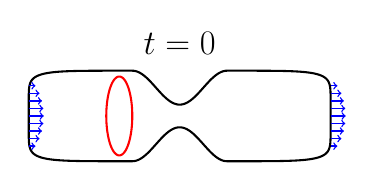
\begin{tikzpicture}[scale=0.5]

\begin{axis}[
  xmin = -11,
  xmax = 11,
  ymin = -3.2,
  ymax = 3.2,
  scale only axis,
  axis equal image,
  hide axis,
  title = {\Huge$t=0$}
  ]

\addplot [mark=none,black,line width=1.5] table{
1.0000e+01 0.0000e+00
1.0000e+01 3.6817e-02
1.0000e+01 7.3646e-02
1.0000e+01 1.1050e-01
1.0000e+01 1.4738e-01
1.0000e+01 1.8431e-01
1.0000e+01 2.2129e-01
1.0000e+01 2.5834e-01
1.0000e+01 2.9547e-01
1.0000e+01 3.3269e-01
1.0000e+01 3.7001e-01
1.0000e+01 4.0745e-01
1.0000e+01 4.4501e-01
1.0000e+01 4.8270e-01
1.0000e+01 5.2055e-01
1.0000e+01 5.5856e-01
1.0000e+01 5.9674e-01
1.0000e+01 6.3510e-01
1.0000e+01 6.7367e-01
1.0000e+01 7.1245e-01
1.0000e+01 7.5146e-01
1.0000e+01 7.9071e-01
1.0000e+01 8.3021e-01
9.9999e+00 8.6998e-01
9.9999e+00 9.1003e-01
9.9999e+00 9.5038e-01
9.9998e+00 9.9105e-01
9.9998e+00 1.0320e+00
9.9997e+00 1.0734e+00
9.9995e+00 1.1151e+00
9.9994e+00 1.1572e+00
9.9992e+00 1.1996e+00
9.9989e+00 1.2425e+00
9.9986e+00 1.2858e+00
9.9981e+00 1.3296e+00
9.9976e+00 1.3738e+00
9.9969e+00 1.4185e+00
9.9960e+00 1.4636e+00
9.9949e+00 1.5093e+00
9.9935e+00 1.5555e+00
9.9917e+00 1.6022e+00
9.9895e+00 1.6495e+00
9.9868e+00 1.6972e+00
9.9835e+00 1.7456e+00
9.9794e+00 1.7944e+00
9.9743e+00 1.8438e+00
9.9681e+00 1.8937e+00
9.9606e+00 1.9440e+00
9.9514e+00 1.9948e+00
9.9403e+00 2.0459e+00
9.9268e+00 2.0974e+00
9.9106e+00 2.1490e+00
9.8911e+00 2.2007e+00
9.8678e+00 2.2524e+00
9.8402e+00 2.3038e+00
9.8074e+00 2.3548e+00
9.7688e+00 2.4051e+00
9.7237e+00 2.4545e+00
9.6713e+00 2.5028e+00
9.6109e+00 2.5495e+00
9.5418e+00 2.5944e+00
9.4634e+00 2.6373e+00
9.3755e+00 2.6779e+00
9.2777e+00 2.7158e+00
9.1700e+00 2.7510e+00
9.0527e+00 2.7833e+00
8.9262e+00 2.8126e+00
8.7911e+00 2.8390e+00
8.6481e+00 2.8625e+00
8.4983e+00 2.8833e+00
8.3425e+00 2.9014e+00
8.1818e+00 2.9171e+00
8.0171e+00 2.9306e+00
7.8493e+00 2.9422e+00
7.6793e+00 2.9520e+00
7.5079e+00 2.9604e+00
7.3358e+00 2.9673e+00
7.1634e+00 2.9732e+00
6.9912e+00 2.9780e+00
6.8198e+00 2.9821e+00
6.6493e+00 2.9854e+00
6.4801e+00 2.9882e+00
6.3123e+00 2.9904e+00
6.1460e+00 2.9923e+00
5.9814e+00 2.9938e+00
5.8185e+00 2.9950e+00
5.6575e+00 2.9960e+00
5.4982e+00 2.9969e+00
5.3407e+00 2.9975e+00
5.1850e+00 2.9980e+00
5.0310e+00 2.9985e+00
4.8787e+00 2.9988e+00
4.7282e+00 2.9991e+00
4.5792e+00 2.9993e+00
4.4319e+00 2.9994e+00
4.2860e+00 2.9996e+00
4.1417e+00 2.9997e+00
3.9988e+00 2.9998e+00
3.8572e+00 2.9998e+00
3.7169e+00 2.9999e+00
3.5779e+00 2.9999e+00
3.4401e+00 2.9999e+00
3.3035e+00 2.9999e+00
3.1679e+00 3.0000e+00
3.0334e+00 2.9934e+00
2.8999e+00 2.9673e+00
2.7674e+00 2.9221e+00
2.6357e+00 2.8591e+00
2.5049e+00 2.7795e+00
2.3748e+00 2.6852e+00
2.2456e+00 2.5778e+00
2.1170e+00 2.4594e+00
1.9891e+00 2.3320e+00
1.8619e+00 2.1978e+00
1.7352e+00 2.0591e+00
1.6090e+00 1.9180e+00
1.4834e+00 1.7768e+00
1.3582e+00 1.6376e+00
1.2334e+00 1.5026e+00
1.1090e+00 1.3737e+00
9.8491e-01 1.2529e+00
8.6115e-01 1.1420e+00
7.3764e-01 1.0424e+00
6.1436e-01 9.5572e-01
4.9127e-01 8.8305e-01
3.6832e-01 8.2545e-01
2.4549e-01 7.8373e-01
1.2272e-01 7.5846e-01
6.1232e-16 7.5000e-01
-1.2272e-01 7.5846e-01
-2.4549e-01 7.8373e-01
-3.6832e-01 8.2545e-01
-4.9127e-01 8.8305e-01
-6.1436e-01 9.5572e-01
-7.3764e-01 1.0424e+00
-8.6115e-01 1.1420e+00
-9.8491e-01 1.2529e+00
-1.1090e+00 1.3737e+00
-1.2334e+00 1.5026e+00
-1.3582e+00 1.6376e+00
-1.4834e+00 1.7768e+00
-1.6090e+00 1.9180e+00
-1.7352e+00 2.0591e+00
-1.8619e+00 2.1978e+00
-1.9891e+00 2.3320e+00
-2.1170e+00 2.4594e+00
-2.2456e+00 2.5778e+00
-2.3748e+00 2.6852e+00
-2.5049e+00 2.7795e+00
-2.6357e+00 2.8591e+00
-2.7674e+00 2.9221e+00
-2.8999e+00 2.9673e+00
-3.0334e+00 2.9934e+00
-3.1679e+00 3.0000e+00
-3.3035e+00 2.9999e+00
-3.4401e+00 2.9999e+00
-3.5779e+00 2.9999e+00
-3.7169e+00 2.9999e+00
-3.8572e+00 2.9998e+00
-3.9988e+00 2.9998e+00
-4.1417e+00 2.9997e+00
-4.2860e+00 2.9996e+00
-4.4319e+00 2.9994e+00
-4.5792e+00 2.9993e+00
-4.7282e+00 2.9991e+00
-4.8787e+00 2.9988e+00
-5.0310e+00 2.9985e+00
-5.1850e+00 2.9980e+00
-5.3407e+00 2.9975e+00
-5.4982e+00 2.9969e+00
-5.6575e+00 2.9960e+00
-5.8185e+00 2.9950e+00
-5.9814e+00 2.9938e+00
-6.1460e+00 2.9923e+00
-6.3123e+00 2.9904e+00
-6.4801e+00 2.9882e+00
-6.6493e+00 2.9854e+00
-6.8198e+00 2.9821e+00
-6.9912e+00 2.9780e+00
-7.1634e+00 2.9732e+00
-7.3358e+00 2.9673e+00
-7.5079e+00 2.9604e+00
-7.6793e+00 2.9520e+00
-7.8493e+00 2.9422e+00
-8.0171e+00 2.9306e+00
-8.1818e+00 2.9171e+00
-8.3425e+00 2.9014e+00
-8.4983e+00 2.8833e+00
-8.6481e+00 2.8625e+00
-8.7911e+00 2.8390e+00
-8.9262e+00 2.8126e+00
-9.0527e+00 2.7833e+00
-9.1700e+00 2.7510e+00
-9.2777e+00 2.7158e+00
-9.3755e+00 2.6779e+00
-9.4634e+00 2.6373e+00
-9.5418e+00 2.5944e+00
-9.6109e+00 2.5495e+00
-9.6713e+00 2.5028e+00
-9.7237e+00 2.4545e+00
-9.7688e+00 2.4051e+00
-9.8074e+00 2.3548e+00
-9.8402e+00 2.3038e+00
-9.8678e+00 2.2524e+00
-9.8911e+00 2.2007e+00
-9.9106e+00 2.1490e+00
-9.9268e+00 2.0974e+00
-9.9403e+00 2.0459e+00
-9.9514e+00 1.9948e+00
-9.9606e+00 1.9440e+00
-9.9681e+00 1.8937e+00
-9.9743e+00 1.8438e+00
-9.9794e+00 1.7944e+00
-9.9835e+00 1.7456e+00
-9.9868e+00 1.6972e+00
-9.9895e+00 1.6495e+00
-9.9917e+00 1.6022e+00
-9.9935e+00 1.5555e+00
-9.9949e+00 1.5093e+00
-9.9960e+00 1.4636e+00
-9.9969e+00 1.4185e+00
-9.9976e+00 1.3738e+00
-9.9981e+00 1.3296e+00
-9.9986e+00 1.2858e+00
-9.9989e+00 1.2425e+00
-9.9992e+00 1.1996e+00
-9.9994e+00 1.1572e+00
-9.9995e+00 1.1151e+00
-9.9997e+00 1.0734e+00
-9.9998e+00 1.0320e+00
-9.9998e+00 9.9105e-01
-9.9999e+00 9.5038e-01
-9.9999e+00 9.1003e-01
-9.9999e+00 8.6998e-01
-1.0000e+01 8.3021e-01
-1.0000e+01 7.9071e-01
-1.0000e+01 7.5146e-01
-1.0000e+01 7.1245e-01
-1.0000e+01 6.7367e-01
-1.0000e+01 6.3510e-01
-1.0000e+01 5.9674e-01
-1.0000e+01 5.5856e-01
-1.0000e+01 5.2055e-01
-1.0000e+01 4.8270e-01
-1.0000e+01 4.4501e-01
-1.0000e+01 4.0745e-01
-1.0000e+01 3.7001e-01
-1.0000e+01 3.3269e-01
-1.0000e+01 2.9547e-01
-1.0000e+01 2.5834e-01
-1.0000e+01 2.2129e-01
-1.0000e+01 1.8431e-01
-1.0000e+01 1.4738e-01
-1.0000e+01 1.1050e-01
-1.0000e+01 7.3646e-02
-1.0000e+01 3.6817e-02
-1.0000e+01 3.6739e-16
-1.0000e+01 -3.6817e-02
-1.0000e+01 -7.3646e-02
-1.0000e+01 -1.1050e-01
-1.0000e+01 -1.4738e-01
-1.0000e+01 -1.8431e-01
-1.0000e+01 -2.2129e-01
-1.0000e+01 -2.5834e-01
-1.0000e+01 -2.9547e-01
-1.0000e+01 -3.3269e-01
-1.0000e+01 -3.7001e-01
-1.0000e+01 -4.0745e-01
-1.0000e+01 -4.4501e-01
-1.0000e+01 -4.8270e-01
-1.0000e+01 -5.2055e-01
-1.0000e+01 -5.5856e-01
-1.0000e+01 -5.9674e-01
-1.0000e+01 -6.3510e-01
-1.0000e+01 -6.7367e-01
-1.0000e+01 -7.1245e-01
-1.0000e+01 -7.5146e-01
-1.0000e+01 -7.9071e-01
-1.0000e+01 -8.3021e-01
-9.9999e+00 -8.6998e-01
-9.9999e+00 -9.1003e-01
-9.9999e+00 -9.5038e-01
-9.9998e+00 -9.9105e-01
-9.9998e+00 -1.0320e+00
-9.9997e+00 -1.0734e+00
-9.9995e+00 -1.1151e+00
-9.9994e+00 -1.1572e+00
-9.9992e+00 -1.1996e+00
-9.9989e+00 -1.2425e+00
-9.9986e+00 -1.2858e+00
-9.9981e+00 -1.3296e+00
-9.9976e+00 -1.3738e+00
-9.9969e+00 -1.4185e+00
-9.9960e+00 -1.4636e+00
-9.9949e+00 -1.5093e+00
-9.9935e+00 -1.5555e+00
-9.9917e+00 -1.6022e+00
-9.9895e+00 -1.6495e+00
-9.9868e+00 -1.6972e+00
-9.9835e+00 -1.7456e+00
-9.9794e+00 -1.7944e+00
-9.9743e+00 -1.8438e+00
-9.9681e+00 -1.8937e+00
-9.9606e+00 -1.9440e+00
-9.9514e+00 -1.9948e+00
-9.9403e+00 -2.0459e+00
-9.9268e+00 -2.0974e+00
-9.9106e+00 -2.1490e+00
-9.8911e+00 -2.2007e+00
-9.8678e+00 -2.2524e+00
-9.8402e+00 -2.3038e+00
-9.8074e+00 -2.3548e+00
-9.7688e+00 -2.4051e+00
-9.7237e+00 -2.4545e+00
-9.6713e+00 -2.5028e+00
-9.6109e+00 -2.5495e+00
-9.5418e+00 -2.5944e+00
-9.4634e+00 -2.6373e+00
-9.3755e+00 -2.6779e+00
-9.2777e+00 -2.7158e+00
-9.1700e+00 -2.7510e+00
-9.0527e+00 -2.7833e+00
-8.9262e+00 -2.8126e+00
-8.7911e+00 -2.8390e+00
-8.6481e+00 -2.8625e+00
-8.4983e+00 -2.8833e+00
-8.3425e+00 -2.9014e+00
-8.1818e+00 -2.9171e+00
-8.0171e+00 -2.9306e+00
-7.8493e+00 -2.9422e+00
-7.6793e+00 -2.9520e+00
-7.5079e+00 -2.9604e+00
-7.3358e+00 -2.9673e+00
-7.1634e+00 -2.9732e+00
-6.9912e+00 -2.9780e+00
-6.8198e+00 -2.9821e+00
-6.6493e+00 -2.9854e+00
-6.4801e+00 -2.9882e+00
-6.3123e+00 -2.9904e+00
-6.1460e+00 -2.9923e+00
-5.9814e+00 -2.9938e+00
-5.8185e+00 -2.9950e+00
-5.6575e+00 -2.9960e+00
-5.4982e+00 -2.9969e+00
-5.3407e+00 -2.9975e+00
-5.1850e+00 -2.9980e+00
-5.0310e+00 -2.9985e+00
-4.8787e+00 -2.9988e+00
-4.7282e+00 -2.9991e+00
-4.5792e+00 -2.9993e+00
-4.4319e+00 -2.9994e+00
-4.2860e+00 -2.9996e+00
-4.1417e+00 -2.9997e+00
-3.9988e+00 -2.9998e+00
-3.8572e+00 -2.9998e+00
-3.7169e+00 -2.9999e+00
-3.5779e+00 -2.9999e+00
-3.4401e+00 -2.9999e+00
-3.3035e+00 -2.9999e+00
-3.1679e+00 -3.0000e+00
-3.0334e+00 -2.9934e+00
-2.8999e+00 -2.9673e+00
-2.7674e+00 -2.9221e+00
-2.6357e+00 -2.8591e+00
-2.5049e+00 -2.7795e+00
-2.3748e+00 -2.6852e+00
-2.2456e+00 -2.5778e+00
-2.1170e+00 -2.4594e+00
-1.9891e+00 -2.3320e+00
-1.8619e+00 -2.1978e+00
-1.7352e+00 -2.0591e+00
-1.6090e+00 -1.9180e+00
-1.4834e+00 -1.7768e+00
-1.3582e+00 -1.6376e+00
-1.2334e+00 -1.5026e+00
-1.1090e+00 -1.3737e+00
-9.8491e-01 -1.2529e+00
-8.6115e-01 -1.1420e+00
-7.3764e-01 -1.0424e+00
-6.1436e-01 -9.5572e-01
-4.9127e-01 -8.8305e-01
-3.6832e-01 -8.2545e-01
-2.4549e-01 -7.8373e-01
-1.2272e-01 -7.5846e-01
-1.8370e-15 -7.5000e-01
1.2272e-01 -7.5846e-01
2.4549e-01 -7.8373e-01
3.6832e-01 -8.2545e-01
4.9127e-01 -8.8305e-01
6.1436e-01 -9.5572e-01
7.3764e-01 -1.0424e+00
8.6115e-01 -1.1420e+00
9.8491e-01 -1.2529e+00
1.1090e+00 -1.3737e+00
1.2334e+00 -1.5026e+00
1.3582e+00 -1.6376e+00
1.4834e+00 -1.7768e+00
1.6090e+00 -1.9180e+00
1.7352e+00 -2.0591e+00
1.8619e+00 -2.1978e+00
1.9891e+00 -2.3320e+00
2.1170e+00 -2.4594e+00
2.2456e+00 -2.5778e+00
2.3748e+00 -2.6852e+00
2.5049e+00 -2.7795e+00
2.6357e+00 -2.8591e+00
2.7674e+00 -2.9221e+00
2.8999e+00 -2.9673e+00
3.0334e+00 -2.9934e+00
3.1679e+00 -3.0000e+00
3.3035e+00 -2.9999e+00
3.4401e+00 -2.9999e+00
3.5779e+00 -2.9999e+00
3.7169e+00 -2.9999e+00
3.8572e+00 -2.9998e+00
3.9988e+00 -2.9998e+00
4.1417e+00 -2.9997e+00
4.2860e+00 -2.9996e+00
4.4319e+00 -2.9994e+00
4.5792e+00 -2.9993e+00
4.7282e+00 -2.9991e+00
4.8787e+00 -2.9988e+00
5.0310e+00 -2.9985e+00
5.1850e+00 -2.9980e+00
5.3407e+00 -2.9975e+00
5.4982e+00 -2.9969e+00
5.6575e+00 -2.9960e+00
5.8185e+00 -2.9950e+00
5.9814e+00 -2.9938e+00
6.1460e+00 -2.9923e+00
6.3123e+00 -2.9904e+00
6.4801e+00 -2.9882e+00
6.6493e+00 -2.9854e+00
6.8198e+00 -2.9821e+00
6.9912e+00 -2.9780e+00
7.1634e+00 -2.9732e+00
7.3358e+00 -2.9673e+00
7.5079e+00 -2.9604e+00
7.6793e+00 -2.9520e+00
7.8493e+00 -2.9422e+00
8.0171e+00 -2.9306e+00
8.1818e+00 -2.9171e+00
8.3425e+00 -2.9014e+00
8.4983e+00 -2.8833e+00
8.6481e+00 -2.8625e+00
8.7911e+00 -2.8390e+00
8.9262e+00 -2.8126e+00
9.0527e+00 -2.7833e+00
9.1700e+00 -2.7510e+00
9.2777e+00 -2.7158e+00
9.3755e+00 -2.6779e+00
9.4634e+00 -2.6373e+00
9.5418e+00 -2.5944e+00
9.6109e+00 -2.5495e+00
9.6713e+00 -2.5028e+00
9.7237e+00 -2.4545e+00
9.7688e+00 -2.4051e+00
9.8074e+00 -2.3548e+00
9.8402e+00 -2.3038e+00
9.8678e+00 -2.2524e+00
9.8911e+00 -2.2007e+00
9.9106e+00 -2.1490e+00
9.9268e+00 -2.0974e+00
9.9403e+00 -2.0459e+00
9.9514e+00 -1.9948e+00
9.9606e+00 -1.9440e+00
9.9681e+00 -1.8937e+00
9.9743e+00 -1.8438e+00
9.9794e+00 -1.7944e+00
9.9835e+00 -1.7456e+00
9.9868e+00 -1.6972e+00
9.9895e+00 -1.6495e+00
9.9917e+00 -1.6022e+00
9.9935e+00 -1.5555e+00
9.9949e+00 -1.5093e+00
9.9960e+00 -1.4636e+00
9.9969e+00 -1.4185e+00
9.9976e+00 -1.3738e+00
9.9981e+00 -1.3296e+00
9.9986e+00 -1.2858e+00
9.9989e+00 -1.2425e+00
9.9992e+00 -1.1996e+00
9.9994e+00 -1.1572e+00
9.9995e+00 -1.1151e+00
9.9997e+00 -1.0734e+00
9.9998e+00 -1.0320e+00
9.9998e+00 -9.9105e-01
9.9999e+00 -9.5038e-01
9.9999e+00 -9.1003e-01
9.9999e+00 -8.6998e-01
1.0000e+01 -8.3021e-01
1.0000e+01 -7.9071e-01
1.0000e+01 -7.5146e-01
1.0000e+01 -7.1245e-01
1.0000e+01 -6.7367e-01
1.0000e+01 -6.3510e-01
1.0000e+01 -5.9674e-01
1.0000e+01 -5.5856e-01
1.0000e+01 -5.2055e-01
1.0000e+01 -4.8270e-01
1.0000e+01 -4.4501e-01
1.0000e+01 -4.0745e-01
1.0000e+01 -3.7001e-01
1.0000e+01 -3.3269e-01
1.0000e+01 -2.9547e-01
1.0000e+01 -2.5834e-01
1.0000e+01 -2.2129e-01
1.0000e+01 -1.8431e-01
1.0000e+01 -1.4738e-01
1.0000e+01 -1.1050e-01
1.0000e+01 -7.3646e-02
1.0000e+01 -3.6817e-02
1.0000e+01 0.0000e+00
};


\addplot [mark=none,red,line width=1.5] table{
-4.0211e+00 2.6111e+00
-4.0423e+00 2.6087e+00
-4.0634e+00 2.6048e+00
-4.0844e+00 2.5993e+00
-4.1055e+00 2.5922e+00
-4.1264e+00 2.5836e+00
-4.1473e+00 2.5734e+00
-4.1681e+00 2.5617e+00
-4.1887e+00 2.5484e+00
-4.2093e+00 2.5336e+00
-4.2298e+00 2.5173e+00
-4.2501e+00 2.4994e+00
-4.2702e+00 2.4800e+00
-4.2902e+00 2.4592e+00
-4.3100e+00 2.4369e+00
-4.3297e+00 2.4131e+00
-4.3491e+00 2.3878e+00
-4.3683e+00 2.3611e+00
-4.3873e+00 2.3330e+00
-4.4061e+00 2.3035e+00
-4.4246e+00 2.2726e+00
-4.4429e+00 2.2403e+00
-4.4609e+00 2.2066e+00
-4.4786e+00 2.1717e+00
-4.4960e+00 2.1354e+00
-4.5132e+00 2.0979e+00
-4.5300e+00 2.0591e+00
-4.5465e+00 2.0190e+00
-4.5627e+00 1.9777e+00
-4.5785e+00 1.9353e+00
-4.5940e+00 1.8916e+00
-4.6091e+00 1.8469e+00
-4.6239e+00 1.8010e+00
-4.6383e+00 1.7540e+00
-4.6523e+00 1.7060e+00
-4.6659e+00 1.6570e+00
-4.6791e+00 1.6069e+00
-4.6919e+00 1.5559e+00
-4.7043e+00 1.5039e+00
-4.7163e+00 1.4511e+00
-4.7278e+00 1.3973e+00
-4.7389e+00 1.3428e+00
-4.7495e+00 1.2874e+00
-4.7597e+00 1.2312e+00
-4.7695e+00 1.1743e+00
-4.7787e+00 1.1167e+00
-4.7875e+00 1.0584e+00
-4.7959e+00 9.9952e-01
-4.8037e+00 9.4000e-01
-4.8111e+00 8.7991e-01
-4.8180e+00 8.1929e-01
-4.8244e+00 7.5818e-01
-4.8302e+00 6.9662e-01
-4.8356e+00 6.3463e-01
-4.8405e+00 5.7226e-01
-4.8449e+00 5.0955e-01
-4.8488e+00 4.4653e-01
-4.8521e+00 3.8324e-01
-4.8550e+00 3.1972e-01
-4.8573e+00 2.5601e-01
-4.8591e+00 1.9214e-01
-4.8604e+00 1.2816e-01
-4.8612e+00 6.4098e-02
-4.8615e+00 2.1268e-16
-4.8612e+00 -6.4098e-02
-4.8604e+00 -1.2816e-01
-4.8591e+00 -1.9214e-01
-4.8573e+00 -2.5601e-01
-4.8550e+00 -3.1972e-01
-4.8521e+00 -3.8324e-01
-4.8488e+00 -4.4653e-01
-4.8449e+00 -5.0955e-01
-4.8405e+00 -5.7226e-01
-4.8356e+00 -6.3463e-01
-4.8302e+00 -6.9662e-01
-4.8244e+00 -7.5818e-01
-4.8180e+00 -8.1929e-01
-4.8111e+00 -8.7991e-01
-4.8037e+00 -9.4000e-01
-4.7959e+00 -9.9952e-01
-4.7875e+00 -1.0584e+00
-4.7787e+00 -1.1167e+00
-4.7695e+00 -1.1743e+00
-4.7597e+00 -1.2312e+00
-4.7495e+00 -1.2874e+00
-4.7389e+00 -1.3428e+00
-4.7278e+00 -1.3973e+00
-4.7163e+00 -1.4511e+00
-4.7043e+00 -1.5039e+00
-4.6919e+00 -1.5559e+00
-4.6791e+00 -1.6069e+00
-4.6659e+00 -1.6570e+00
-4.6523e+00 -1.7060e+00
-4.6383e+00 -1.7540e+00
-4.6239e+00 -1.8010e+00
-4.6091e+00 -1.8469e+00
-4.5940e+00 -1.8916e+00
-4.5785e+00 -1.9353e+00
-4.5627e+00 -1.9777e+00
-4.5465e+00 -2.0190e+00
-4.5300e+00 -2.0591e+00
-4.5132e+00 -2.0979e+00
-4.4960e+00 -2.1354e+00
-4.4786e+00 -2.1717e+00
-4.4609e+00 -2.2066e+00
-4.4429e+00 -2.2403e+00
-4.4246e+00 -2.2726e+00
-4.4061e+00 -2.3035e+00
-4.3873e+00 -2.3330e+00
-4.3683e+00 -2.3611e+00
-4.3491e+00 -2.3878e+00
-4.3297e+00 -2.4131e+00
-4.3100e+00 -2.4369e+00
-4.2902e+00 -2.4592e+00
-4.2702e+00 -2.4800e+00
-4.2501e+00 -2.4994e+00
-4.2298e+00 -2.5173e+00
-4.2093e+00 -2.5336e+00
-4.1887e+00 -2.5484e+00
-4.1681e+00 -2.5617e+00
-4.1473e+00 -2.5734e+00
-4.1264e+00 -2.5836e+00
-4.1055e+00 -2.5922e+00
-4.0844e+00 -2.5993e+00
-4.0634e+00 -2.6048e+00
-4.0423e+00 -2.6087e+00
-4.0211e+00 -2.6111e+00
-4.0000e+00 -2.6119e+00
-3.9789e+00 -2.6111e+00
-3.9577e+00 -2.6087e+00
-3.9366e+00 -2.6048e+00
-3.9156e+00 -2.5993e+00
-3.8945e+00 -2.5922e+00
-3.8736e+00 -2.5836e+00
-3.8527e+00 -2.5734e+00
-3.8319e+00 -2.5617e+00
-3.8113e+00 -2.5484e+00
-3.7907e+00 -2.5336e+00
-3.7702e+00 -2.5173e+00
-3.7499e+00 -2.4994e+00
-3.7298e+00 -2.4800e+00
-3.7098e+00 -2.4592e+00
-3.6900e+00 -2.4369e+00
-3.6703e+00 -2.4131e+00
-3.6509e+00 -2.3878e+00
-3.6317e+00 -2.3611e+00
-3.6127e+00 -2.3330e+00
-3.5939e+00 -2.3035e+00
-3.5754e+00 -2.2726e+00
-3.5571e+00 -2.2403e+00
-3.5391e+00 -2.2066e+00
-3.5214e+00 -2.1717e+00
-3.5040e+00 -2.1354e+00
-3.4868e+00 -2.0979e+00
-3.4700e+00 -2.0591e+00
-3.4535e+00 -2.0190e+00
-3.4373e+00 -1.9777e+00
-3.4215e+00 -1.9353e+00
-3.4060e+00 -1.8916e+00
-3.3909e+00 -1.8469e+00
-3.3761e+00 -1.8010e+00
-3.3617e+00 -1.7540e+00
-3.3477e+00 -1.7060e+00
-3.3341e+00 -1.6570e+00
-3.3209e+00 -1.6069e+00
-3.3081e+00 -1.5559e+00
-3.2957e+00 -1.5039e+00
-3.2837e+00 -1.4511e+00
-3.2722e+00 -1.3973e+00
-3.2611e+00 -1.3428e+00
-3.2505e+00 -1.2874e+00
-3.2403e+00 -1.2312e+00
-3.2305e+00 -1.1743e+00
-3.2213e+00 -1.1167e+00
-3.2125e+00 -1.0584e+00
-3.2041e+00 -9.9952e-01
-3.1963e+00 -9.4000e-01
-3.1889e+00 -8.7991e-01
-3.1820e+00 -8.1929e-01
-3.1756e+00 -7.5818e-01
-3.1698e+00 -6.9662e-01
-3.1644e+00 -6.3463e-01
-3.1595e+00 -5.7226e-01
-3.1551e+00 -5.0955e-01
-3.1512e+00 -4.4653e-01
-3.1479e+00 -3.8324e-01
-3.1450e+00 -3.1972e-01
-3.1427e+00 -2.5601e-01
-3.1409e+00 -1.9214e-01
-3.1396e+00 -1.2816e-01
-3.1388e+00 -6.4098e-02
-3.1385e+00 -5.3254e-16
-3.1388e+00 6.4098e-02
-3.1396e+00 1.2816e-01
-3.1409e+00 1.9214e-01
-3.1427e+00 2.5601e-01
-3.1450e+00 3.1972e-01
-3.1479e+00 3.8324e-01
-3.1512e+00 4.4653e-01
-3.1551e+00 5.0955e-01
-3.1595e+00 5.7226e-01
-3.1644e+00 6.3463e-01
-3.1698e+00 6.9662e-01
-3.1756e+00 7.5818e-01
-3.1820e+00 8.1929e-01
-3.1889e+00 8.7991e-01
-3.1963e+00 9.4000e-01
-3.2041e+00 9.9952e-01
-3.2125e+00 1.0584e+00
-3.2213e+00 1.1167e+00
-3.2305e+00 1.1743e+00
-3.2403e+00 1.2312e+00
-3.2505e+00 1.2874e+00
-3.2611e+00 1.3428e+00
-3.2722e+00 1.3973e+00
-3.2837e+00 1.4511e+00
-3.2957e+00 1.5039e+00
-3.3081e+00 1.5559e+00
-3.3209e+00 1.6069e+00
-3.3341e+00 1.6570e+00
-3.3477e+00 1.7060e+00
-3.3617e+00 1.7540e+00
-3.3761e+00 1.8010e+00
-3.3909e+00 1.8469e+00
-3.4060e+00 1.8916e+00
-3.4215e+00 1.9353e+00
-3.4373e+00 1.9777e+00
-3.4535e+00 2.0190e+00
-3.4700e+00 2.0591e+00
-3.4868e+00 2.0979e+00
-3.5040e+00 2.1354e+00
-3.5214e+00 2.1717e+00
-3.5391e+00 2.2066e+00
-3.5571e+00 2.2403e+00
-3.5754e+00 2.2726e+00
-3.5939e+00 2.3035e+00
-3.6127e+00 2.3330e+00
-3.6317e+00 2.3611e+00
-3.6509e+00 2.3878e+00
-3.6703e+00 2.4131e+00
-3.6900e+00 2.4369e+00
-3.7098e+00 2.4592e+00
-3.7298e+00 2.4800e+00
-3.7499e+00 2.4994e+00
-3.7702e+00 2.5173e+00
-3.7907e+00 2.5336e+00
-3.8113e+00 2.5484e+00
-3.8319e+00 2.5617e+00
-3.8527e+00 2.5734e+00
-3.8736e+00 2.5836e+00
-3.8945e+00 2.5922e+00
-3.9156e+00 2.5993e+00
-3.9366e+00 2.6048e+00
-3.9577e+00 2.6087e+00
-3.9789e+00 2.6111e+00
-4.0000e+00 2.6119e+00
-4.0211e+00 2.6111e+00
};


\foreach \y in {-2.0,-1.5,...,2.0}
\addplot[color=blue,line width = 1.0pt,solid,->]
plot coordinates{
  (-10,\y)
  (-10+exp(9/(\y*\y-9))/exp(-1),\y)
};

\foreach \y in {-2.0,-1.5,...,2.0}
\addplot[color=blue,line width = 1.0pt,solid,->]
plot coordinates{
  (10,\y)
  (10+exp(9/(\y*\y-9))/exp(-1),\y)
};


\end{axis}

\end{tikzpicture}



 &
%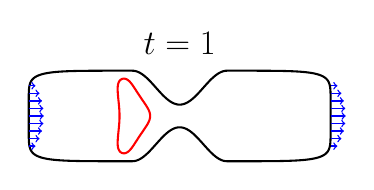
\begin{tikzpicture}[scale=0.5]

\begin{axis}[
  xmin = -11,
  xmax = 11,
  ymin = -3.2,
  ymax = 3.2,
  scale only axis,
  axis equal image,
  hide axis,
  title = {\Huge$t=1$}
  ]

\addplot [mark=none,black,line width=1.5] table{
1.0000e+01 0.0000e+00
1.0000e+01 3.6817e-02
1.0000e+01 7.3646e-02
1.0000e+01 1.1050e-01
1.0000e+01 1.4738e-01
1.0000e+01 1.8431e-01
1.0000e+01 2.2129e-01
1.0000e+01 2.5834e-01
1.0000e+01 2.9547e-01
1.0000e+01 3.3269e-01
1.0000e+01 3.7001e-01
1.0000e+01 4.0745e-01
1.0000e+01 4.4501e-01
1.0000e+01 4.8270e-01
1.0000e+01 5.2055e-01
1.0000e+01 5.5856e-01
1.0000e+01 5.9674e-01
1.0000e+01 6.3510e-01
1.0000e+01 6.7367e-01
1.0000e+01 7.1245e-01
1.0000e+01 7.5146e-01
1.0000e+01 7.9071e-01
1.0000e+01 8.3021e-01
9.9999e+00 8.6998e-01
9.9999e+00 9.1003e-01
9.9999e+00 9.5038e-01
9.9998e+00 9.9105e-01
9.9998e+00 1.0320e+00
9.9997e+00 1.0734e+00
9.9995e+00 1.1151e+00
9.9994e+00 1.1572e+00
9.9992e+00 1.1996e+00
9.9989e+00 1.2425e+00
9.9986e+00 1.2858e+00
9.9981e+00 1.3296e+00
9.9976e+00 1.3738e+00
9.9969e+00 1.4185e+00
9.9960e+00 1.4636e+00
9.9949e+00 1.5093e+00
9.9935e+00 1.5555e+00
9.9917e+00 1.6022e+00
9.9895e+00 1.6495e+00
9.9868e+00 1.6972e+00
9.9835e+00 1.7456e+00
9.9794e+00 1.7944e+00
9.9743e+00 1.8438e+00
9.9681e+00 1.8937e+00
9.9606e+00 1.9440e+00
9.9514e+00 1.9948e+00
9.9403e+00 2.0459e+00
9.9268e+00 2.0974e+00
9.9106e+00 2.1490e+00
9.8911e+00 2.2007e+00
9.8678e+00 2.2524e+00
9.8402e+00 2.3038e+00
9.8074e+00 2.3548e+00
9.7688e+00 2.4051e+00
9.7237e+00 2.4545e+00
9.6713e+00 2.5028e+00
9.6109e+00 2.5495e+00
9.5418e+00 2.5944e+00
9.4634e+00 2.6373e+00
9.3755e+00 2.6779e+00
9.2777e+00 2.7158e+00
9.1700e+00 2.7510e+00
9.0527e+00 2.7833e+00
8.9262e+00 2.8126e+00
8.7911e+00 2.8390e+00
8.6481e+00 2.8625e+00
8.4983e+00 2.8833e+00
8.3425e+00 2.9014e+00
8.1818e+00 2.9171e+00
8.0171e+00 2.9306e+00
7.8493e+00 2.9422e+00
7.6793e+00 2.9520e+00
7.5079e+00 2.9604e+00
7.3358e+00 2.9673e+00
7.1634e+00 2.9732e+00
6.9912e+00 2.9780e+00
6.8198e+00 2.9821e+00
6.6493e+00 2.9854e+00
6.4801e+00 2.9882e+00
6.3123e+00 2.9904e+00
6.1460e+00 2.9923e+00
5.9814e+00 2.9938e+00
5.8185e+00 2.9950e+00
5.6575e+00 2.9960e+00
5.4982e+00 2.9969e+00
5.3407e+00 2.9975e+00
5.1850e+00 2.9980e+00
5.0310e+00 2.9985e+00
4.8787e+00 2.9988e+00
4.7282e+00 2.9991e+00
4.5792e+00 2.9993e+00
4.4319e+00 2.9994e+00
4.2860e+00 2.9996e+00
4.1417e+00 2.9997e+00
3.9988e+00 2.9998e+00
3.8572e+00 2.9998e+00
3.7169e+00 2.9999e+00
3.5779e+00 2.9999e+00
3.4401e+00 2.9999e+00
3.3035e+00 2.9999e+00
3.1679e+00 3.0000e+00
3.0334e+00 2.9934e+00
2.8999e+00 2.9673e+00
2.7674e+00 2.9221e+00
2.6357e+00 2.8591e+00
2.5049e+00 2.7795e+00
2.3748e+00 2.6852e+00
2.2456e+00 2.5778e+00
2.1170e+00 2.4594e+00
1.9891e+00 2.3320e+00
1.8619e+00 2.1978e+00
1.7352e+00 2.0591e+00
1.6090e+00 1.9180e+00
1.4834e+00 1.7768e+00
1.3582e+00 1.6376e+00
1.2334e+00 1.5026e+00
1.1090e+00 1.3737e+00
9.8491e-01 1.2529e+00
8.6115e-01 1.1420e+00
7.3764e-01 1.0424e+00
6.1436e-01 9.5572e-01
4.9127e-01 8.8305e-01
3.6832e-01 8.2545e-01
2.4549e-01 7.8373e-01
1.2272e-01 7.5846e-01
6.1232e-16 7.5000e-01
-1.2272e-01 7.5846e-01
-2.4549e-01 7.8373e-01
-3.6832e-01 8.2545e-01
-4.9127e-01 8.8305e-01
-6.1436e-01 9.5572e-01
-7.3764e-01 1.0424e+00
-8.6115e-01 1.1420e+00
-9.8491e-01 1.2529e+00
-1.1090e+00 1.3737e+00
-1.2334e+00 1.5026e+00
-1.3582e+00 1.6376e+00
-1.4834e+00 1.7768e+00
-1.6090e+00 1.9180e+00
-1.7352e+00 2.0591e+00
-1.8619e+00 2.1978e+00
-1.9891e+00 2.3320e+00
-2.1170e+00 2.4594e+00
-2.2456e+00 2.5778e+00
-2.3748e+00 2.6852e+00
-2.5049e+00 2.7795e+00
-2.6357e+00 2.8591e+00
-2.7674e+00 2.9221e+00
-2.8999e+00 2.9673e+00
-3.0334e+00 2.9934e+00
-3.1679e+00 3.0000e+00
-3.3035e+00 2.9999e+00
-3.4401e+00 2.9999e+00
-3.5779e+00 2.9999e+00
-3.7169e+00 2.9999e+00
-3.8572e+00 2.9998e+00
-3.9988e+00 2.9998e+00
-4.1417e+00 2.9997e+00
-4.2860e+00 2.9996e+00
-4.4319e+00 2.9994e+00
-4.5792e+00 2.9993e+00
-4.7282e+00 2.9991e+00
-4.8787e+00 2.9988e+00
-5.0310e+00 2.9985e+00
-5.1850e+00 2.9980e+00
-5.3407e+00 2.9975e+00
-5.4982e+00 2.9969e+00
-5.6575e+00 2.9960e+00
-5.8185e+00 2.9950e+00
-5.9814e+00 2.9938e+00
-6.1460e+00 2.9923e+00
-6.3123e+00 2.9904e+00
-6.4801e+00 2.9882e+00
-6.6493e+00 2.9854e+00
-6.8198e+00 2.9821e+00
-6.9912e+00 2.9780e+00
-7.1634e+00 2.9732e+00
-7.3358e+00 2.9673e+00
-7.5079e+00 2.9604e+00
-7.6793e+00 2.9520e+00
-7.8493e+00 2.9422e+00
-8.0171e+00 2.9306e+00
-8.1818e+00 2.9171e+00
-8.3425e+00 2.9014e+00
-8.4983e+00 2.8833e+00
-8.6481e+00 2.8625e+00
-8.7911e+00 2.8390e+00
-8.9262e+00 2.8126e+00
-9.0527e+00 2.7833e+00
-9.1700e+00 2.7510e+00
-9.2777e+00 2.7158e+00
-9.3755e+00 2.6779e+00
-9.4634e+00 2.6373e+00
-9.5418e+00 2.5944e+00
-9.6109e+00 2.5495e+00
-9.6713e+00 2.5028e+00
-9.7237e+00 2.4545e+00
-9.7688e+00 2.4051e+00
-9.8074e+00 2.3548e+00
-9.8402e+00 2.3038e+00
-9.8678e+00 2.2524e+00
-9.8911e+00 2.2007e+00
-9.9106e+00 2.1490e+00
-9.9268e+00 2.0974e+00
-9.9403e+00 2.0459e+00
-9.9514e+00 1.9948e+00
-9.9606e+00 1.9440e+00
-9.9681e+00 1.8937e+00
-9.9743e+00 1.8438e+00
-9.9794e+00 1.7944e+00
-9.9835e+00 1.7456e+00
-9.9868e+00 1.6972e+00
-9.9895e+00 1.6495e+00
-9.9917e+00 1.6022e+00
-9.9935e+00 1.5555e+00
-9.9949e+00 1.5093e+00
-9.9960e+00 1.4636e+00
-9.9969e+00 1.4185e+00
-9.9976e+00 1.3738e+00
-9.9981e+00 1.3296e+00
-9.9986e+00 1.2858e+00
-9.9989e+00 1.2425e+00
-9.9992e+00 1.1996e+00
-9.9994e+00 1.1572e+00
-9.9995e+00 1.1151e+00
-9.9997e+00 1.0734e+00
-9.9998e+00 1.0320e+00
-9.9998e+00 9.9105e-01
-9.9999e+00 9.5038e-01
-9.9999e+00 9.1003e-01
-9.9999e+00 8.6998e-01
-1.0000e+01 8.3021e-01
-1.0000e+01 7.9071e-01
-1.0000e+01 7.5146e-01
-1.0000e+01 7.1245e-01
-1.0000e+01 6.7367e-01
-1.0000e+01 6.3510e-01
-1.0000e+01 5.9674e-01
-1.0000e+01 5.5856e-01
-1.0000e+01 5.2055e-01
-1.0000e+01 4.8270e-01
-1.0000e+01 4.4501e-01
-1.0000e+01 4.0745e-01
-1.0000e+01 3.7001e-01
-1.0000e+01 3.3269e-01
-1.0000e+01 2.9547e-01
-1.0000e+01 2.5834e-01
-1.0000e+01 2.2129e-01
-1.0000e+01 1.8431e-01
-1.0000e+01 1.4738e-01
-1.0000e+01 1.1050e-01
-1.0000e+01 7.3646e-02
-1.0000e+01 3.6817e-02
-1.0000e+01 3.6739e-16
-1.0000e+01 -3.6817e-02
-1.0000e+01 -7.3646e-02
-1.0000e+01 -1.1050e-01
-1.0000e+01 -1.4738e-01
-1.0000e+01 -1.8431e-01
-1.0000e+01 -2.2129e-01
-1.0000e+01 -2.5834e-01
-1.0000e+01 -2.9547e-01
-1.0000e+01 -3.3269e-01
-1.0000e+01 -3.7001e-01
-1.0000e+01 -4.0745e-01
-1.0000e+01 -4.4501e-01
-1.0000e+01 -4.8270e-01
-1.0000e+01 -5.2055e-01
-1.0000e+01 -5.5856e-01
-1.0000e+01 -5.9674e-01
-1.0000e+01 -6.3510e-01
-1.0000e+01 -6.7367e-01
-1.0000e+01 -7.1245e-01
-1.0000e+01 -7.5146e-01
-1.0000e+01 -7.9071e-01
-1.0000e+01 -8.3021e-01
-9.9999e+00 -8.6998e-01
-9.9999e+00 -9.1003e-01
-9.9999e+00 -9.5038e-01
-9.9998e+00 -9.9105e-01
-9.9998e+00 -1.0320e+00
-9.9997e+00 -1.0734e+00
-9.9995e+00 -1.1151e+00
-9.9994e+00 -1.1572e+00
-9.9992e+00 -1.1996e+00
-9.9989e+00 -1.2425e+00
-9.9986e+00 -1.2858e+00
-9.9981e+00 -1.3296e+00
-9.9976e+00 -1.3738e+00
-9.9969e+00 -1.4185e+00
-9.9960e+00 -1.4636e+00
-9.9949e+00 -1.5093e+00
-9.9935e+00 -1.5555e+00
-9.9917e+00 -1.6022e+00
-9.9895e+00 -1.6495e+00
-9.9868e+00 -1.6972e+00
-9.9835e+00 -1.7456e+00
-9.9794e+00 -1.7944e+00
-9.9743e+00 -1.8438e+00
-9.9681e+00 -1.8937e+00
-9.9606e+00 -1.9440e+00
-9.9514e+00 -1.9948e+00
-9.9403e+00 -2.0459e+00
-9.9268e+00 -2.0974e+00
-9.9106e+00 -2.1490e+00
-9.8911e+00 -2.2007e+00
-9.8678e+00 -2.2524e+00
-9.8402e+00 -2.3038e+00
-9.8074e+00 -2.3548e+00
-9.7688e+00 -2.4051e+00
-9.7237e+00 -2.4545e+00
-9.6713e+00 -2.5028e+00
-9.6109e+00 -2.5495e+00
-9.5418e+00 -2.5944e+00
-9.4634e+00 -2.6373e+00
-9.3755e+00 -2.6779e+00
-9.2777e+00 -2.7158e+00
-9.1700e+00 -2.7510e+00
-9.0527e+00 -2.7833e+00
-8.9262e+00 -2.8126e+00
-8.7911e+00 -2.8390e+00
-8.6481e+00 -2.8625e+00
-8.4983e+00 -2.8833e+00
-8.3425e+00 -2.9014e+00
-8.1818e+00 -2.9171e+00
-8.0171e+00 -2.9306e+00
-7.8493e+00 -2.9422e+00
-7.6793e+00 -2.9520e+00
-7.5079e+00 -2.9604e+00
-7.3358e+00 -2.9673e+00
-7.1634e+00 -2.9732e+00
-6.9912e+00 -2.9780e+00
-6.8198e+00 -2.9821e+00
-6.6493e+00 -2.9854e+00
-6.4801e+00 -2.9882e+00
-6.3123e+00 -2.9904e+00
-6.1460e+00 -2.9923e+00
-5.9814e+00 -2.9938e+00
-5.8185e+00 -2.9950e+00
-5.6575e+00 -2.9960e+00
-5.4982e+00 -2.9969e+00
-5.3407e+00 -2.9975e+00
-5.1850e+00 -2.9980e+00
-5.0310e+00 -2.9985e+00
-4.8787e+00 -2.9988e+00
-4.7282e+00 -2.9991e+00
-4.5792e+00 -2.9993e+00
-4.4319e+00 -2.9994e+00
-4.2860e+00 -2.9996e+00
-4.1417e+00 -2.9997e+00
-3.9988e+00 -2.9998e+00
-3.8572e+00 -2.9998e+00
-3.7169e+00 -2.9999e+00
-3.5779e+00 -2.9999e+00
-3.4401e+00 -2.9999e+00
-3.3035e+00 -2.9999e+00
-3.1679e+00 -3.0000e+00
-3.0334e+00 -2.9934e+00
-2.8999e+00 -2.9673e+00
-2.7674e+00 -2.9221e+00
-2.6357e+00 -2.8591e+00
-2.5049e+00 -2.7795e+00
-2.3748e+00 -2.6852e+00
-2.2456e+00 -2.5778e+00
-2.1170e+00 -2.4594e+00
-1.9891e+00 -2.3320e+00
-1.8619e+00 -2.1978e+00
-1.7352e+00 -2.0591e+00
-1.6090e+00 -1.9180e+00
-1.4834e+00 -1.7768e+00
-1.3582e+00 -1.6376e+00
-1.2334e+00 -1.5026e+00
-1.1090e+00 -1.3737e+00
-9.8491e-01 -1.2529e+00
-8.6115e-01 -1.1420e+00
-7.3764e-01 -1.0424e+00
-6.1436e-01 -9.5572e-01
-4.9127e-01 -8.8305e-01
-3.6832e-01 -8.2545e-01
-2.4549e-01 -7.8373e-01
-1.2272e-01 -7.5846e-01
-1.8370e-15 -7.5000e-01
1.2272e-01 -7.5846e-01
2.4549e-01 -7.8373e-01
3.6832e-01 -8.2545e-01
4.9127e-01 -8.8305e-01
6.1436e-01 -9.5572e-01
7.3764e-01 -1.0424e+00
8.6115e-01 -1.1420e+00
9.8491e-01 -1.2529e+00
1.1090e+00 -1.3737e+00
1.2334e+00 -1.5026e+00
1.3582e+00 -1.6376e+00
1.4834e+00 -1.7768e+00
1.6090e+00 -1.9180e+00
1.7352e+00 -2.0591e+00
1.8619e+00 -2.1978e+00
1.9891e+00 -2.3320e+00
2.1170e+00 -2.4594e+00
2.2456e+00 -2.5778e+00
2.3748e+00 -2.6852e+00
2.5049e+00 -2.7795e+00
2.6357e+00 -2.8591e+00
2.7674e+00 -2.9221e+00
2.8999e+00 -2.9673e+00
3.0334e+00 -2.9934e+00
3.1679e+00 -3.0000e+00
3.3035e+00 -2.9999e+00
3.4401e+00 -2.9999e+00
3.5779e+00 -2.9999e+00
3.7169e+00 -2.9999e+00
3.8572e+00 -2.9998e+00
3.9988e+00 -2.9998e+00
4.1417e+00 -2.9997e+00
4.2860e+00 -2.9996e+00
4.4319e+00 -2.9994e+00
4.5792e+00 -2.9993e+00
4.7282e+00 -2.9991e+00
4.8787e+00 -2.9988e+00
5.0310e+00 -2.9985e+00
5.1850e+00 -2.9980e+00
5.3407e+00 -2.9975e+00
5.4982e+00 -2.9969e+00
5.6575e+00 -2.9960e+00
5.8185e+00 -2.9950e+00
5.9814e+00 -2.9938e+00
6.1460e+00 -2.9923e+00
6.3123e+00 -2.9904e+00
6.4801e+00 -2.9882e+00
6.6493e+00 -2.9854e+00
6.8198e+00 -2.9821e+00
6.9912e+00 -2.9780e+00
7.1634e+00 -2.9732e+00
7.3358e+00 -2.9673e+00
7.5079e+00 -2.9604e+00
7.6793e+00 -2.9520e+00
7.8493e+00 -2.9422e+00
8.0171e+00 -2.9306e+00
8.1818e+00 -2.9171e+00
8.3425e+00 -2.9014e+00
8.4983e+00 -2.8833e+00
8.6481e+00 -2.8625e+00
8.7911e+00 -2.8390e+00
8.9262e+00 -2.8126e+00
9.0527e+00 -2.7833e+00
9.1700e+00 -2.7510e+00
9.2777e+00 -2.7158e+00
9.3755e+00 -2.6779e+00
9.4634e+00 -2.6373e+00
9.5418e+00 -2.5944e+00
9.6109e+00 -2.5495e+00
9.6713e+00 -2.5028e+00
9.7237e+00 -2.4545e+00
9.7688e+00 -2.4051e+00
9.8074e+00 -2.3548e+00
9.8402e+00 -2.3038e+00
9.8678e+00 -2.2524e+00
9.8911e+00 -2.2007e+00
9.9106e+00 -2.1490e+00
9.9268e+00 -2.0974e+00
9.9403e+00 -2.0459e+00
9.9514e+00 -1.9948e+00
9.9606e+00 -1.9440e+00
9.9681e+00 -1.8937e+00
9.9743e+00 -1.8438e+00
9.9794e+00 -1.7944e+00
9.9835e+00 -1.7456e+00
9.9868e+00 -1.6972e+00
9.9895e+00 -1.6495e+00
9.9917e+00 -1.6022e+00
9.9935e+00 -1.5555e+00
9.9949e+00 -1.5093e+00
9.9960e+00 -1.4636e+00
9.9969e+00 -1.4185e+00
9.9976e+00 -1.3738e+00
9.9981e+00 -1.3296e+00
9.9986e+00 -1.2858e+00
9.9989e+00 -1.2425e+00
9.9992e+00 -1.1996e+00
9.9994e+00 -1.1572e+00
9.9995e+00 -1.1151e+00
9.9997e+00 -1.0734e+00
9.9998e+00 -1.0320e+00
9.9998e+00 -9.9105e-01
9.9999e+00 -9.5038e-01
9.9999e+00 -9.1003e-01
9.9999e+00 -8.6998e-01
1.0000e+01 -8.3021e-01
1.0000e+01 -7.9071e-01
1.0000e+01 -7.5146e-01
1.0000e+01 -7.1245e-01
1.0000e+01 -6.7367e-01
1.0000e+01 -6.3510e-01
1.0000e+01 -5.9674e-01
1.0000e+01 -5.5856e-01
1.0000e+01 -5.2055e-01
1.0000e+01 -4.8270e-01
1.0000e+01 -4.4501e-01
1.0000e+01 -4.0745e-01
1.0000e+01 -3.7001e-01
1.0000e+01 -3.3269e-01
1.0000e+01 -2.9547e-01
1.0000e+01 -2.5834e-01
1.0000e+01 -2.2129e-01
1.0000e+01 -1.8431e-01
1.0000e+01 -1.4738e-01
1.0000e+01 -1.1050e-01
1.0000e+01 -7.3646e-02
1.0000e+01 -3.6817e-02
1.0000e+01 0.0000e+00
};


\addplot [mark=none,red,line width=1.5] table{
-3.5084e+00 2.4268e+00
-3.5276e+00 2.4359e+00
-3.5474e+00 2.4442e+00
-3.5678e+00 2.4517e+00
-3.5890e+00 2.4583e+00
-3.6110e+00 2.4639e+00
-3.6338e+00 2.4684e+00
-3.6574e+00 2.4716e+00
-3.6819e+00 2.4733e+00
-3.7073e+00 2.4733e+00
-3.7334e+00 2.4714e+00
-3.7601e+00 2.4673e+00
-3.7873e+00 2.4610e+00
-3.8148e+00 2.4521e+00
-3.8423e+00 2.4405e+00
-3.8695e+00 2.4260e+00
-3.8962e+00 2.4086e+00
-3.9221e+00 2.3883e+00
-3.9468e+00 2.3650e+00
-3.9700e+00 2.3389e+00
-3.9917e+00 2.3101e+00
-4.0115e+00 2.2788e+00
-4.0294e+00 2.2451e+00
-4.0453e+00 2.2093e+00
-4.0591e+00 2.1715e+00
-4.0710e+00 2.1320e+00
-4.0810e+00 2.0909e+00
-4.0892e+00 2.0483e+00
-4.0958e+00 2.0045e+00
-4.1008e+00 1.9595e+00
-4.1044e+00 1.9133e+00
-4.1067e+00 1.8661e+00
-4.1079e+00 1.8179e+00
-4.1081e+00 1.7688e+00
-4.1074e+00 1.7188e+00
-4.1059e+00 1.6679e+00
-4.1036e+00 1.6162e+00
-4.1008e+00 1.5637e+00
-4.0974e+00 1.5104e+00
-4.0936e+00 1.4563e+00
-4.0893e+00 1.4015e+00
-4.0846e+00 1.3460e+00
-4.0795e+00 1.2898e+00
-4.0742e+00 1.2330e+00
-4.0686e+00 1.1756e+00
-4.0628e+00 1.1175e+00
-4.0569e+00 1.0589e+00
-4.0508e+00 9.9967e-01
-4.0447e+00 9.3995e-01
-4.0385e+00 8.7973e-01
-4.0324e+00 8.1903e-01
-4.0264e+00 7.5788e-01
-4.0205e+00 6.9631e-01
-4.0149e+00 6.3435e-01
-4.0095e+00 5.7202e-01
-4.0045e+00 5.0935e-01
-3.9999e+00 4.4638e-01
-3.9958e+00 3.8314e-01
-3.9922e+00 3.1966e-01
-3.9892e+00 2.5597e-01
-3.9868e+00 1.9213e-01
-3.9850e+00 1.2815e-01
-3.9840e+00 6.4098e-02
-3.9836e+00 -4.5559e-12
-3.9840e+00 -6.4098e-02
-3.9850e+00 -1.2815e-01
-3.9868e+00 -1.9213e-01
-3.9892e+00 -2.5597e-01
-3.9922e+00 -3.1966e-01
-3.9958e+00 -3.8314e-01
-3.9999e+00 -4.4638e-01
-4.0045e+00 -5.0935e-01
-4.0095e+00 -5.7202e-01
-4.0149e+00 -6.3435e-01
-4.0205e+00 -6.9631e-01
-4.0264e+00 -7.5788e-01
-4.0324e+00 -8.1903e-01
-4.0385e+00 -8.7973e-01
-4.0447e+00 -9.3995e-01
-4.0508e+00 -9.9967e-01
-4.0569e+00 -1.0589e+00
-4.0628e+00 -1.1175e+00
-4.0686e+00 -1.1756e+00
-4.0742e+00 -1.2330e+00
-4.0795e+00 -1.2898e+00
-4.0846e+00 -1.3460e+00
-4.0893e+00 -1.4015e+00
-4.0936e+00 -1.4563e+00
-4.0974e+00 -1.5104e+00
-4.1008e+00 -1.5637e+00
-4.1036e+00 -1.6162e+00
-4.1059e+00 -1.6679e+00
-4.1074e+00 -1.7188e+00
-4.1081e+00 -1.7688e+00
-4.1079e+00 -1.8179e+00
-4.1067e+00 -1.8661e+00
-4.1044e+00 -1.9133e+00
-4.1008e+00 -1.9595e+00
-4.0958e+00 -2.0045e+00
-4.0892e+00 -2.0483e+00
-4.0810e+00 -2.0909e+00
-4.0710e+00 -2.1320e+00
-4.0591e+00 -2.1715e+00
-4.0453e+00 -2.2093e+00
-4.0294e+00 -2.2451e+00
-4.0115e+00 -2.2788e+00
-3.9917e+00 -2.3101e+00
-3.9700e+00 -2.3389e+00
-3.9468e+00 -2.3650e+00
-3.9221e+00 -2.3883e+00
-3.8962e+00 -2.4086e+00
-3.8695e+00 -2.4260e+00
-3.8423e+00 -2.4405e+00
-3.8148e+00 -2.4521e+00
-3.7873e+00 -2.4610e+00
-3.7601e+00 -2.4673e+00
-3.7334e+00 -2.4714e+00
-3.7073e+00 -2.4733e+00
-3.6819e+00 -2.4733e+00
-3.6574e+00 -2.4716e+00
-3.6338e+00 -2.4684e+00
-3.6110e+00 -2.4639e+00
-3.5890e+00 -2.4583e+00
-3.5678e+00 -2.4517e+00
-3.5474e+00 -2.4442e+00
-3.5276e+00 -2.4359e+00
-3.5084e+00 -2.4268e+00
-3.4897e+00 -2.4170e+00
-3.4713e+00 -2.4064e+00
-3.4533e+00 -2.3952e+00
-3.4355e+00 -2.3832e+00
-3.4178e+00 -2.3705e+00
-3.4002e+00 -2.3569e+00
-3.3827e+00 -2.3426e+00
-3.3651e+00 -2.3274e+00
-3.3474e+00 -2.3113e+00
-3.3297e+00 -2.2943e+00
-3.3118e+00 -2.2764e+00
-3.2938e+00 -2.2574e+00
-3.2756e+00 -2.2374e+00
-3.2571e+00 -2.2164e+00
-3.2385e+00 -2.1944e+00
-3.2196e+00 -2.1712e+00
-3.2004e+00 -2.1471e+00
-3.1810e+00 -2.1218e+00
-3.1613e+00 -2.0955e+00
-3.1412e+00 -2.0681e+00
-3.1209e+00 -2.0396e+00
-3.1002e+00 -2.0101e+00
-3.0791e+00 -1.9796e+00
-3.0577e+00 -1.9481e+00
-3.0358e+00 -1.9155e+00
-3.0135e+00 -1.8820e+00
-2.9908e+00 -1.8475e+00
-2.9677e+00 -1.8121e+00
-2.9440e+00 -1.7758e+00
-2.9199e+00 -1.7387e+00
-2.8952e+00 -1.7006e+00
-2.8701e+00 -1.6617e+00
-2.8444e+00 -1.6221e+00
-2.8182e+00 -1.5816e+00
-2.7914e+00 -1.5404e+00
-2.7641e+00 -1.4985e+00
-2.7362e+00 -1.4560e+00
-2.7078e+00 -1.4127e+00
-2.6788e+00 -1.3688e+00
-2.6492e+00 -1.3243e+00
-2.6191e+00 -1.2793e+00
-2.5885e+00 -1.2337e+00
-2.5573e+00 -1.1875e+00
-2.5256e+00 -1.1408e+00
-2.4935e+00 -1.0937e+00
-2.4609e+00 -1.0460e+00
-2.4280e+00 -9.9787e-01
-2.3947e+00 -9.4923e-01
-2.3611e+00 -9.0010e-01
-2.3273e+00 -8.5046e-01
-2.2935e+00 -8.0027e-01
-2.2597e+00 -7.4950e-01
-2.2260e+00 -6.9808e-01
-2.1928e+00 -6.4594e-01
-2.1601e+00 -5.9299e-01
-2.1283e+00 -5.3912e-01
-2.0977e+00 -4.8420e-01
-2.0687e+00 -4.2811e-01
-2.0418e+00 -3.7072e-01
-2.0176e+00 -3.1196e-01
-1.9965e+00 -2.5179e-01
-1.9793e+00 -1.9027e-01
-1.9665e+00 -1.2758e-01
-1.9586e+00 -6.4025e-02
-1.9559e+00 4.4313e-12
-1.9586e+00 6.4025e-02
-1.9665e+00 1.2758e-01
-1.9793e+00 1.9027e-01
-1.9965e+00 2.5179e-01
-2.0176e+00 3.1196e-01
-2.0418e+00 3.7072e-01
-2.0687e+00 4.2811e-01
-2.0977e+00 4.8420e-01
-2.1283e+00 5.3912e-01
-2.1601e+00 5.9299e-01
-2.1928e+00 6.4594e-01
-2.2260e+00 6.9808e-01
-2.2597e+00 7.4950e-01
-2.2935e+00 8.0027e-01
-2.3273e+00 8.5046e-01
-2.3611e+00 9.0010e-01
-2.3947e+00 9.4923e-01
-2.4280e+00 9.9787e-01
-2.4609e+00 1.0460e+00
-2.4935e+00 1.0937e+00
-2.5256e+00 1.1408e+00
-2.5573e+00 1.1875e+00
-2.5885e+00 1.2337e+00
-2.6191e+00 1.2793e+00
-2.6492e+00 1.3243e+00
-2.6788e+00 1.3688e+00
-2.7078e+00 1.4127e+00
-2.7362e+00 1.4560e+00
-2.7641e+00 1.4985e+00
-2.7914e+00 1.5404e+00
-2.8182e+00 1.5816e+00
-2.8444e+00 1.6221e+00
-2.8701e+00 1.6617e+00
-2.8952e+00 1.7006e+00
-2.9199e+00 1.7387e+00
-2.9440e+00 1.7758e+00
-2.9677e+00 1.8121e+00
-2.9908e+00 1.8475e+00
-3.0135e+00 1.8820e+00
-3.0358e+00 1.9155e+00
-3.0577e+00 1.9481e+00
-3.0791e+00 1.9796e+00
-3.1002e+00 2.0101e+00
-3.1209e+00 2.0396e+00
-3.1412e+00 2.0681e+00
-3.1613e+00 2.0955e+00
-3.1810e+00 2.1218e+00
-3.2004e+00 2.1471e+00
-3.2196e+00 2.1712e+00
-3.2385e+00 2.1944e+00
-3.2571e+00 2.2164e+00
-3.2756e+00 2.2374e+00
-3.2938e+00 2.2574e+00
-3.3118e+00 2.2764e+00
-3.3297e+00 2.2943e+00
-3.3474e+00 2.3113e+00
-3.3651e+00 2.3274e+00
-3.3827e+00 2.3426e+00
-3.4002e+00 2.3569e+00
-3.4178e+00 2.3705e+00
-3.4355e+00 2.3832e+00
-3.4533e+00 2.3952e+00
-3.4713e+00 2.4064e+00
-3.4897e+00 2.4170e+00
-3.5084e+00 2.4268e+00
};

\foreach \y in {-2.0,-1.5,...,2.0}
\addplot[color=blue,line width = 1.0pt,solid,->]
plot coordinates{
  (-10,\y)
  (-10+exp(9/(\y*\y-9))/exp(-1),\y)
};

\foreach \y in {-2.0,-1.5,...,2.0}
\addplot[color=blue,line width = 1.0pt,solid,->]
plot coordinates{
  (10,\y)
  (10+exp(9/(\y*\y-9))/exp(-1),\y)
};

\end{axis}

\end{tikzpicture}



 &
%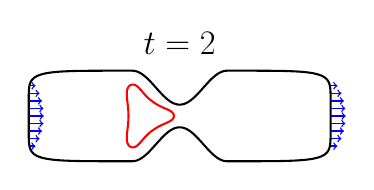
\begin{tikzpicture}[scale=0.5]

\begin{axis}[
  xmin = -11,
  xmax = 11,
  ymin = -3.2,
  ymax = 3.2,
  scale only axis,
  axis equal image,
  hide axis,
  title = {\Huge$t=2$}
  ]

\addplot [mark=none,black,line width=1.5] table{
1.0000e+01 0.0000e+00
1.0000e+01 3.6817e-02
1.0000e+01 7.3646e-02
1.0000e+01 1.1050e-01
1.0000e+01 1.4738e-01
1.0000e+01 1.8431e-01
1.0000e+01 2.2129e-01
1.0000e+01 2.5834e-01
1.0000e+01 2.9547e-01
1.0000e+01 3.3269e-01
1.0000e+01 3.7001e-01
1.0000e+01 4.0745e-01
1.0000e+01 4.4501e-01
1.0000e+01 4.8270e-01
1.0000e+01 5.2055e-01
1.0000e+01 5.5856e-01
1.0000e+01 5.9674e-01
1.0000e+01 6.3510e-01
1.0000e+01 6.7367e-01
1.0000e+01 7.1245e-01
1.0000e+01 7.5146e-01
1.0000e+01 7.9071e-01
1.0000e+01 8.3021e-01
9.9999e+00 8.6998e-01
9.9999e+00 9.1003e-01
9.9999e+00 9.5038e-01
9.9998e+00 9.9105e-01
9.9998e+00 1.0320e+00
9.9997e+00 1.0734e+00
9.9995e+00 1.1151e+00
9.9994e+00 1.1572e+00
9.9992e+00 1.1996e+00
9.9989e+00 1.2425e+00
9.9986e+00 1.2858e+00
9.9981e+00 1.3296e+00
9.9976e+00 1.3738e+00
9.9969e+00 1.4185e+00
9.9960e+00 1.4636e+00
9.9949e+00 1.5093e+00
9.9935e+00 1.5555e+00
9.9917e+00 1.6022e+00
9.9895e+00 1.6495e+00
9.9868e+00 1.6972e+00
9.9835e+00 1.7456e+00
9.9794e+00 1.7944e+00
9.9743e+00 1.8438e+00
9.9681e+00 1.8937e+00
9.9606e+00 1.9440e+00
9.9514e+00 1.9948e+00
9.9403e+00 2.0459e+00
9.9268e+00 2.0974e+00
9.9106e+00 2.1490e+00
9.8911e+00 2.2007e+00
9.8678e+00 2.2524e+00
9.8402e+00 2.3038e+00
9.8074e+00 2.3548e+00
9.7688e+00 2.4051e+00
9.7237e+00 2.4545e+00
9.6713e+00 2.5028e+00
9.6109e+00 2.5495e+00
9.5418e+00 2.5944e+00
9.4634e+00 2.6373e+00
9.3755e+00 2.6779e+00
9.2777e+00 2.7158e+00
9.1700e+00 2.7510e+00
9.0527e+00 2.7833e+00
8.9262e+00 2.8126e+00
8.7911e+00 2.8390e+00
8.6481e+00 2.8625e+00
8.4983e+00 2.8833e+00
8.3425e+00 2.9014e+00
8.1818e+00 2.9171e+00
8.0171e+00 2.9306e+00
7.8493e+00 2.9422e+00
7.6793e+00 2.9520e+00
7.5079e+00 2.9604e+00
7.3358e+00 2.9673e+00
7.1634e+00 2.9732e+00
6.9912e+00 2.9780e+00
6.8198e+00 2.9821e+00
6.6493e+00 2.9854e+00
6.4801e+00 2.9882e+00
6.3123e+00 2.9904e+00
6.1460e+00 2.9923e+00
5.9814e+00 2.9938e+00
5.8185e+00 2.9950e+00
5.6575e+00 2.9960e+00
5.4982e+00 2.9969e+00
5.3407e+00 2.9975e+00
5.1850e+00 2.9980e+00
5.0310e+00 2.9985e+00
4.8787e+00 2.9988e+00
4.7282e+00 2.9991e+00
4.5792e+00 2.9993e+00
4.4319e+00 2.9994e+00
4.2860e+00 2.9996e+00
4.1417e+00 2.9997e+00
3.9988e+00 2.9998e+00
3.8572e+00 2.9998e+00
3.7169e+00 2.9999e+00
3.5779e+00 2.9999e+00
3.4401e+00 2.9999e+00
3.3035e+00 2.9999e+00
3.1679e+00 3.0000e+00
3.0334e+00 2.9934e+00
2.8999e+00 2.9673e+00
2.7674e+00 2.9221e+00
2.6357e+00 2.8591e+00
2.5049e+00 2.7795e+00
2.3748e+00 2.6852e+00
2.2456e+00 2.5778e+00
2.1170e+00 2.4594e+00
1.9891e+00 2.3320e+00
1.8619e+00 2.1978e+00
1.7352e+00 2.0591e+00
1.6090e+00 1.9180e+00
1.4834e+00 1.7768e+00
1.3582e+00 1.6376e+00
1.2334e+00 1.5026e+00
1.1090e+00 1.3737e+00
9.8491e-01 1.2529e+00
8.6115e-01 1.1420e+00
7.3764e-01 1.0424e+00
6.1436e-01 9.5572e-01
4.9127e-01 8.8305e-01
3.6832e-01 8.2545e-01
2.4549e-01 7.8373e-01
1.2272e-01 7.5846e-01
6.1232e-16 7.5000e-01
-1.2272e-01 7.5846e-01
-2.4549e-01 7.8373e-01
-3.6832e-01 8.2545e-01
-4.9127e-01 8.8305e-01
-6.1436e-01 9.5572e-01
-7.3764e-01 1.0424e+00
-8.6115e-01 1.1420e+00
-9.8491e-01 1.2529e+00
-1.1090e+00 1.3737e+00
-1.2334e+00 1.5026e+00
-1.3582e+00 1.6376e+00
-1.4834e+00 1.7768e+00
-1.6090e+00 1.9180e+00
-1.7352e+00 2.0591e+00
-1.8619e+00 2.1978e+00
-1.9891e+00 2.3320e+00
-2.1170e+00 2.4594e+00
-2.2456e+00 2.5778e+00
-2.3748e+00 2.6852e+00
-2.5049e+00 2.7795e+00
-2.6357e+00 2.8591e+00
-2.7674e+00 2.9221e+00
-2.8999e+00 2.9673e+00
-3.0334e+00 2.9934e+00
-3.1679e+00 3.0000e+00
-3.3035e+00 2.9999e+00
-3.4401e+00 2.9999e+00
-3.5779e+00 2.9999e+00
-3.7169e+00 2.9999e+00
-3.8572e+00 2.9998e+00
-3.9988e+00 2.9998e+00
-4.1417e+00 2.9997e+00
-4.2860e+00 2.9996e+00
-4.4319e+00 2.9994e+00
-4.5792e+00 2.9993e+00
-4.7282e+00 2.9991e+00
-4.8787e+00 2.9988e+00
-5.0310e+00 2.9985e+00
-5.1850e+00 2.9980e+00
-5.3407e+00 2.9975e+00
-5.4982e+00 2.9969e+00
-5.6575e+00 2.9960e+00
-5.8185e+00 2.9950e+00
-5.9814e+00 2.9938e+00
-6.1460e+00 2.9923e+00
-6.3123e+00 2.9904e+00
-6.4801e+00 2.9882e+00
-6.6493e+00 2.9854e+00
-6.8198e+00 2.9821e+00
-6.9912e+00 2.9780e+00
-7.1634e+00 2.9732e+00
-7.3358e+00 2.9673e+00
-7.5079e+00 2.9604e+00
-7.6793e+00 2.9520e+00
-7.8493e+00 2.9422e+00
-8.0171e+00 2.9306e+00
-8.1818e+00 2.9171e+00
-8.3425e+00 2.9014e+00
-8.4983e+00 2.8833e+00
-8.6481e+00 2.8625e+00
-8.7911e+00 2.8390e+00
-8.9262e+00 2.8126e+00
-9.0527e+00 2.7833e+00
-9.1700e+00 2.7510e+00
-9.2777e+00 2.7158e+00
-9.3755e+00 2.6779e+00
-9.4634e+00 2.6373e+00
-9.5418e+00 2.5944e+00
-9.6109e+00 2.5495e+00
-9.6713e+00 2.5028e+00
-9.7237e+00 2.4545e+00
-9.7688e+00 2.4051e+00
-9.8074e+00 2.3548e+00
-9.8402e+00 2.3038e+00
-9.8678e+00 2.2524e+00
-9.8911e+00 2.2007e+00
-9.9106e+00 2.1490e+00
-9.9268e+00 2.0974e+00
-9.9403e+00 2.0459e+00
-9.9514e+00 1.9948e+00
-9.9606e+00 1.9440e+00
-9.9681e+00 1.8937e+00
-9.9743e+00 1.8438e+00
-9.9794e+00 1.7944e+00
-9.9835e+00 1.7456e+00
-9.9868e+00 1.6972e+00
-9.9895e+00 1.6495e+00
-9.9917e+00 1.6022e+00
-9.9935e+00 1.5555e+00
-9.9949e+00 1.5093e+00
-9.9960e+00 1.4636e+00
-9.9969e+00 1.4185e+00
-9.9976e+00 1.3738e+00
-9.9981e+00 1.3296e+00
-9.9986e+00 1.2858e+00
-9.9989e+00 1.2425e+00
-9.9992e+00 1.1996e+00
-9.9994e+00 1.1572e+00
-9.9995e+00 1.1151e+00
-9.9997e+00 1.0734e+00
-9.9998e+00 1.0320e+00
-9.9998e+00 9.9105e-01
-9.9999e+00 9.5038e-01
-9.9999e+00 9.1003e-01
-9.9999e+00 8.6998e-01
-1.0000e+01 8.3021e-01
-1.0000e+01 7.9071e-01
-1.0000e+01 7.5146e-01
-1.0000e+01 7.1245e-01
-1.0000e+01 6.7367e-01
-1.0000e+01 6.3510e-01
-1.0000e+01 5.9674e-01
-1.0000e+01 5.5856e-01
-1.0000e+01 5.2055e-01
-1.0000e+01 4.8270e-01
-1.0000e+01 4.4501e-01
-1.0000e+01 4.0745e-01
-1.0000e+01 3.7001e-01
-1.0000e+01 3.3269e-01
-1.0000e+01 2.9547e-01
-1.0000e+01 2.5834e-01
-1.0000e+01 2.2129e-01
-1.0000e+01 1.8431e-01
-1.0000e+01 1.4738e-01
-1.0000e+01 1.1050e-01
-1.0000e+01 7.3646e-02
-1.0000e+01 3.6817e-02
-1.0000e+01 3.6739e-16
-1.0000e+01 -3.6817e-02
-1.0000e+01 -7.3646e-02
-1.0000e+01 -1.1050e-01
-1.0000e+01 -1.4738e-01
-1.0000e+01 -1.8431e-01
-1.0000e+01 -2.2129e-01
-1.0000e+01 -2.5834e-01
-1.0000e+01 -2.9547e-01
-1.0000e+01 -3.3269e-01
-1.0000e+01 -3.7001e-01
-1.0000e+01 -4.0745e-01
-1.0000e+01 -4.4501e-01
-1.0000e+01 -4.8270e-01
-1.0000e+01 -5.2055e-01
-1.0000e+01 -5.5856e-01
-1.0000e+01 -5.9674e-01
-1.0000e+01 -6.3510e-01
-1.0000e+01 -6.7367e-01
-1.0000e+01 -7.1245e-01
-1.0000e+01 -7.5146e-01
-1.0000e+01 -7.9071e-01
-1.0000e+01 -8.3021e-01
-9.9999e+00 -8.6998e-01
-9.9999e+00 -9.1003e-01
-9.9999e+00 -9.5038e-01
-9.9998e+00 -9.9105e-01
-9.9998e+00 -1.0320e+00
-9.9997e+00 -1.0734e+00
-9.9995e+00 -1.1151e+00
-9.9994e+00 -1.1572e+00
-9.9992e+00 -1.1996e+00
-9.9989e+00 -1.2425e+00
-9.9986e+00 -1.2858e+00
-9.9981e+00 -1.3296e+00
-9.9976e+00 -1.3738e+00
-9.9969e+00 -1.4185e+00
-9.9960e+00 -1.4636e+00
-9.9949e+00 -1.5093e+00
-9.9935e+00 -1.5555e+00
-9.9917e+00 -1.6022e+00
-9.9895e+00 -1.6495e+00
-9.9868e+00 -1.6972e+00
-9.9835e+00 -1.7456e+00
-9.9794e+00 -1.7944e+00
-9.9743e+00 -1.8438e+00
-9.9681e+00 -1.8937e+00
-9.9606e+00 -1.9440e+00
-9.9514e+00 -1.9948e+00
-9.9403e+00 -2.0459e+00
-9.9268e+00 -2.0974e+00
-9.9106e+00 -2.1490e+00
-9.8911e+00 -2.2007e+00
-9.8678e+00 -2.2524e+00
-9.8402e+00 -2.3038e+00
-9.8074e+00 -2.3548e+00
-9.7688e+00 -2.4051e+00
-9.7237e+00 -2.4545e+00
-9.6713e+00 -2.5028e+00
-9.6109e+00 -2.5495e+00
-9.5418e+00 -2.5944e+00
-9.4634e+00 -2.6373e+00
-9.3755e+00 -2.6779e+00
-9.2777e+00 -2.7158e+00
-9.1700e+00 -2.7510e+00
-9.0527e+00 -2.7833e+00
-8.9262e+00 -2.8126e+00
-8.7911e+00 -2.8390e+00
-8.6481e+00 -2.8625e+00
-8.4983e+00 -2.8833e+00
-8.3425e+00 -2.9014e+00
-8.1818e+00 -2.9171e+00
-8.0171e+00 -2.9306e+00
-7.8493e+00 -2.9422e+00
-7.6793e+00 -2.9520e+00
-7.5079e+00 -2.9604e+00
-7.3358e+00 -2.9673e+00
-7.1634e+00 -2.9732e+00
-6.9912e+00 -2.9780e+00
-6.8198e+00 -2.9821e+00
-6.6493e+00 -2.9854e+00
-6.4801e+00 -2.9882e+00
-6.3123e+00 -2.9904e+00
-6.1460e+00 -2.9923e+00
-5.9814e+00 -2.9938e+00
-5.8185e+00 -2.9950e+00
-5.6575e+00 -2.9960e+00
-5.4982e+00 -2.9969e+00
-5.3407e+00 -2.9975e+00
-5.1850e+00 -2.9980e+00
-5.0310e+00 -2.9985e+00
-4.8787e+00 -2.9988e+00
-4.7282e+00 -2.9991e+00
-4.5792e+00 -2.9993e+00
-4.4319e+00 -2.9994e+00
-4.2860e+00 -2.9996e+00
-4.1417e+00 -2.9997e+00
-3.9988e+00 -2.9998e+00
-3.8572e+00 -2.9998e+00
-3.7169e+00 -2.9999e+00
-3.5779e+00 -2.9999e+00
-3.4401e+00 -2.9999e+00
-3.3035e+00 -2.9999e+00
-3.1679e+00 -3.0000e+00
-3.0334e+00 -2.9934e+00
-2.8999e+00 -2.9673e+00
-2.7674e+00 -2.9221e+00
-2.6357e+00 -2.8591e+00
-2.5049e+00 -2.7795e+00
-2.3748e+00 -2.6852e+00
-2.2456e+00 -2.5778e+00
-2.1170e+00 -2.4594e+00
-1.9891e+00 -2.3320e+00
-1.8619e+00 -2.1978e+00
-1.7352e+00 -2.0591e+00
-1.6090e+00 -1.9180e+00
-1.4834e+00 -1.7768e+00
-1.3582e+00 -1.6376e+00
-1.2334e+00 -1.5026e+00
-1.1090e+00 -1.3737e+00
-9.8491e-01 -1.2529e+00
-8.6115e-01 -1.1420e+00
-7.3764e-01 -1.0424e+00
-6.1436e-01 -9.5572e-01
-4.9127e-01 -8.8305e-01
-3.6832e-01 -8.2545e-01
-2.4549e-01 -7.8373e-01
-1.2272e-01 -7.5846e-01
-1.8370e-15 -7.5000e-01
1.2272e-01 -7.5846e-01
2.4549e-01 -7.8373e-01
3.6832e-01 -8.2545e-01
4.9127e-01 -8.8305e-01
6.1436e-01 -9.5572e-01
7.3764e-01 -1.0424e+00
8.6115e-01 -1.1420e+00
9.8491e-01 -1.2529e+00
1.1090e+00 -1.3737e+00
1.2334e+00 -1.5026e+00
1.3582e+00 -1.6376e+00
1.4834e+00 -1.7768e+00
1.6090e+00 -1.9180e+00
1.7352e+00 -2.0591e+00
1.8619e+00 -2.1978e+00
1.9891e+00 -2.3320e+00
2.1170e+00 -2.4594e+00
2.2456e+00 -2.5778e+00
2.3748e+00 -2.6852e+00
2.5049e+00 -2.7795e+00
2.6357e+00 -2.8591e+00
2.7674e+00 -2.9221e+00
2.8999e+00 -2.9673e+00
3.0334e+00 -2.9934e+00
3.1679e+00 -3.0000e+00
3.3035e+00 -2.9999e+00
3.4401e+00 -2.9999e+00
3.5779e+00 -2.9999e+00
3.7169e+00 -2.9999e+00
3.8572e+00 -2.9998e+00
3.9988e+00 -2.9998e+00
4.1417e+00 -2.9997e+00
4.2860e+00 -2.9996e+00
4.4319e+00 -2.9994e+00
4.5792e+00 -2.9993e+00
4.7282e+00 -2.9991e+00
4.8787e+00 -2.9988e+00
5.0310e+00 -2.9985e+00
5.1850e+00 -2.9980e+00
5.3407e+00 -2.9975e+00
5.4982e+00 -2.9969e+00
5.6575e+00 -2.9960e+00
5.8185e+00 -2.9950e+00
5.9814e+00 -2.9938e+00
6.1460e+00 -2.9923e+00
6.3123e+00 -2.9904e+00
6.4801e+00 -2.9882e+00
6.6493e+00 -2.9854e+00
6.8198e+00 -2.9821e+00
6.9912e+00 -2.9780e+00
7.1634e+00 -2.9732e+00
7.3358e+00 -2.9673e+00
7.5079e+00 -2.9604e+00
7.6793e+00 -2.9520e+00
7.8493e+00 -2.9422e+00
8.0171e+00 -2.9306e+00
8.1818e+00 -2.9171e+00
8.3425e+00 -2.9014e+00
8.4983e+00 -2.8833e+00
8.6481e+00 -2.8625e+00
8.7911e+00 -2.8390e+00
8.9262e+00 -2.8126e+00
9.0527e+00 -2.7833e+00
9.1700e+00 -2.7510e+00
9.2777e+00 -2.7158e+00
9.3755e+00 -2.6779e+00
9.4634e+00 -2.6373e+00
9.5418e+00 -2.5944e+00
9.6109e+00 -2.5495e+00
9.6713e+00 -2.5028e+00
9.7237e+00 -2.4545e+00
9.7688e+00 -2.4051e+00
9.8074e+00 -2.3548e+00
9.8402e+00 -2.3038e+00
9.8678e+00 -2.2524e+00
9.8911e+00 -2.2007e+00
9.9106e+00 -2.1490e+00
9.9268e+00 -2.0974e+00
9.9403e+00 -2.0459e+00
9.9514e+00 -1.9948e+00
9.9606e+00 -1.9440e+00
9.9681e+00 -1.8937e+00
9.9743e+00 -1.8438e+00
9.9794e+00 -1.7944e+00
9.9835e+00 -1.7456e+00
9.9868e+00 -1.6972e+00
9.9895e+00 -1.6495e+00
9.9917e+00 -1.6022e+00
9.9935e+00 -1.5555e+00
9.9949e+00 -1.5093e+00
9.9960e+00 -1.4636e+00
9.9969e+00 -1.4185e+00
9.9976e+00 -1.3738e+00
9.9981e+00 -1.3296e+00
9.9986e+00 -1.2858e+00
9.9989e+00 -1.2425e+00
9.9992e+00 -1.1996e+00
9.9994e+00 -1.1572e+00
9.9995e+00 -1.1151e+00
9.9997e+00 -1.0734e+00
9.9998e+00 -1.0320e+00
9.9998e+00 -9.9105e-01
9.9999e+00 -9.5038e-01
9.9999e+00 -9.1003e-01
9.9999e+00 -8.6998e-01
1.0000e+01 -8.3021e-01
1.0000e+01 -7.9071e-01
1.0000e+01 -7.5146e-01
1.0000e+01 -7.1245e-01
1.0000e+01 -6.7367e-01
1.0000e+01 -6.3510e-01
1.0000e+01 -5.9674e-01
1.0000e+01 -5.5856e-01
1.0000e+01 -5.2055e-01
1.0000e+01 -4.8270e-01
1.0000e+01 -4.4501e-01
1.0000e+01 -4.0745e-01
1.0000e+01 -3.7001e-01
1.0000e+01 -3.3269e-01
1.0000e+01 -2.9547e-01
1.0000e+01 -2.5834e-01
1.0000e+01 -2.2129e-01
1.0000e+01 -1.8431e-01
1.0000e+01 -1.4738e-01
1.0000e+01 -1.1050e-01
1.0000e+01 -7.3646e-02
1.0000e+01 -3.6817e-02
1.0000e+01 0.0000e+00
};


\addplot [mark=none,red,line width=1.5] table{
-2.6188e+00 1.7733e+00
-2.6330e+00 1.7891e+00
-2.6475e+00 1.8050e+00
-2.6623e+00 1.8210e+00
-2.6775e+00 1.8371e+00
-2.6933e+00 1.8534e+00
-2.7096e+00 1.8698e+00
-2.7267e+00 1.8865e+00
-2.7446e+00 1.9034e+00
-2.7634e+00 1.9205e+00
-2.7831e+00 1.9376e+00
-2.8040e+00 1.9547e+00
-2.8262e+00 1.9718e+00
-2.8497e+00 1.9886e+00
-2.8747e+00 2.0050e+00
-2.9012e+00 2.0206e+00
-2.9295e+00 2.0353e+00
-2.9596e+00 2.0486e+00
-2.9915e+00 2.0602e+00
-3.0252e+00 2.0694e+00
-3.0606e+00 2.0759e+00
-3.0976e+00 2.0791e+00
-3.1357e+00 2.0783e+00
-3.1745e+00 2.0731e+00
-3.2135e+00 2.0630e+00
-3.2518e+00 2.0478e+00
-3.2888e+00 2.0274e+00
-3.3238e+00 2.0019e+00
-3.3562e+00 1.9717e+00
-3.3854e+00 1.9371e+00
-3.4112e+00 1.8986e+00
-3.4334e+00 1.8569e+00
-3.4520e+00 1.8125e+00
-3.4672e+00 1.7658e+00
-3.4793e+00 1.7173e+00
-3.4885e+00 1.6672e+00
-3.4951e+00 1.6159e+00
-3.4995e+00 1.5635e+00
-3.5019e+00 1.5101e+00
-3.5026e+00 1.4559e+00
-3.5018e+00 1.4010e+00
-3.4998e+00 1.3453e+00
-3.4966e+00 1.2890e+00
-3.4926e+00 1.2321e+00
-3.4878e+00 1.1745e+00
-3.4824e+00 1.1164e+00
-3.4764e+00 1.0578e+00
-3.4700e+00 9.9865e-01
-3.4633e+00 9.3898e-01
-3.4565e+00 8.7884e-01
-3.4495e+00 8.1824e-01
-3.4425e+00 7.5719e-01
-3.4356e+00 6.9573e-01
-3.4289e+00 6.3387e-01
-3.4224e+00 5.7165e-01
-3.4164e+00 5.0907e-01
-3.4108e+00 4.4618e-01
-3.4057e+00 3.8301e-01
-3.4013e+00 3.1958e-01
-3.3976e+00 2.5593e-01
-3.3947e+00 1.9211e-01
-3.3925e+00 1.2815e-01
-3.3912e+00 6.4097e-02
-3.3908e+00 -3.8977e-12
-3.3912e+00 -6.4097e-02
-3.3925e+00 -1.2815e-01
-3.3947e+00 -1.9211e-01
-3.3976e+00 -2.5593e-01
-3.4013e+00 -3.1958e-01
-3.4057e+00 -3.8301e-01
-3.4108e+00 -4.4618e-01
-3.4164e+00 -5.0907e-01
-3.4224e+00 -5.7165e-01
-3.4289e+00 -6.3387e-01
-3.4356e+00 -6.9573e-01
-3.4425e+00 -7.5719e-01
-3.4495e+00 -8.1824e-01
-3.4565e+00 -8.7884e-01
-3.4633e+00 -9.3898e-01
-3.4700e+00 -9.9865e-01
-3.4764e+00 -1.0578e+00
-3.4824e+00 -1.1164e+00
-3.4878e+00 -1.1745e+00
-3.4926e+00 -1.2321e+00
-3.4966e+00 -1.2890e+00
-3.4998e+00 -1.3453e+00
-3.5018e+00 -1.4010e+00
-3.5026e+00 -1.4559e+00
-3.5019e+00 -1.5101e+00
-3.4995e+00 -1.5635e+00
-3.4951e+00 -1.6159e+00
-3.4885e+00 -1.6672e+00
-3.4793e+00 -1.7173e+00
-3.4672e+00 -1.7658e+00
-3.4520e+00 -1.8125e+00
-3.4334e+00 -1.8569e+00
-3.4112e+00 -1.8986e+00
-3.3854e+00 -1.9371e+00
-3.3562e+00 -1.9717e+00
-3.3238e+00 -2.0019e+00
-3.2888e+00 -2.0274e+00
-3.2518e+00 -2.0478e+00
-3.2135e+00 -2.0630e+00
-3.1745e+00 -2.0731e+00
-3.1357e+00 -2.0783e+00
-3.0976e+00 -2.0791e+00
-3.0606e+00 -2.0759e+00
-3.0252e+00 -2.0694e+00
-2.9915e+00 -2.0602e+00
-2.9596e+00 -2.0486e+00
-2.9295e+00 -2.0353e+00
-2.9012e+00 -2.0206e+00
-2.8747e+00 -2.0050e+00
-2.8497e+00 -1.9886e+00
-2.8262e+00 -1.9718e+00
-2.8040e+00 -1.9547e+00
-2.7831e+00 -1.9376e+00
-2.7634e+00 -1.9205e+00
-2.7446e+00 -1.9034e+00
-2.7267e+00 -1.8865e+00
-2.7096e+00 -1.8698e+00
-2.6933e+00 -1.8534e+00
-2.6775e+00 -1.8371e+00
-2.6623e+00 -1.8210e+00
-2.6475e+00 -1.8050e+00
-2.6330e+00 -1.7891e+00
-2.6188e+00 -1.7733e+00
-2.6047e+00 -1.7575e+00
-2.5907e+00 -1.7416e+00
-2.5768e+00 -1.7256e+00
-2.5627e+00 -1.7094e+00
-2.5485e+00 -1.6929e+00
-2.5341e+00 -1.6761e+00
-2.5193e+00 -1.6588e+00
-2.5042e+00 -1.6412e+00
-2.4887e+00 -1.6230e+00
-2.4728e+00 -1.6043e+00
-2.4563e+00 -1.5851e+00
-2.4392e+00 -1.5652e+00
-2.4216e+00 -1.5447e+00
-2.4032e+00 -1.5236e+00
-2.3842e+00 -1.5019e+00
-2.3644e+00 -1.4795e+00
-2.3439e+00 -1.4565e+00
-2.3225e+00 -1.4329e+00
-2.3003e+00 -1.4086e+00
-2.2772e+00 -1.3837e+00
-2.2532e+00 -1.3583e+00
-2.2283e+00 -1.3323e+00
-2.2024e+00 -1.3057e+00
-2.1754e+00 -1.2787e+00
-2.1475e+00 -1.2513e+00
-2.1184e+00 -1.2234e+00
-2.0883e+00 -1.1951e+00
-2.0571e+00 -1.1666e+00
-2.0248e+00 -1.1377e+00
-1.9913e+00 -1.1087e+00
-1.9567e+00 -1.0794e+00
-1.9209e+00 -1.0500e+00
-1.8840e+00 -1.0206e+00
-1.8458e+00 -9.9112e-01
-1.8065e+00 -9.6168e-01
-1.7660e+00 -9.3232e-01
-1.7244e+00 -9.0309e-01
-1.6815e+00 -8.7403e-01
-1.6375e+00 -8.4520e-01
-1.5924e+00 -8.1664e-01
-1.5461e+00 -7.8838e-01
-1.4988e+00 -7.6047e-01
-1.4504e+00 -7.3292e-01
-1.4010e+00 -7.0577e-01
-1.3506e+00 -6.7903e-01
-1.2992e+00 -6.5271e-01
-1.2469e+00 -6.2680e-01
-1.1938e+00 -6.0128e-01
-1.1398e+00 -5.7612e-01
-1.0852e+00 -5.5126e-01
-1.0299e+00 -5.2661e-01
-9.7407e-01 -5.0205e-01
-9.1778e-01 -4.7740e-01
-8.6120e-01 -4.5244e-01
-8.0448e-01 -4.2685e-01
-7.4787e-01 -4.0023e-01
-6.9167e-01 -3.7205e-01
-6.3636e-01 -3.4162e-01
-5.8259e-01 -3.0809e-01
-5.3137e-01 -2.7046e-01
-4.8414e-01 -2.2768e-01
-4.4296e-01 -1.7891e-01
-4.1042e-01 -1.2391e-01
-3.8934e-01 -6.3539e-02
-3.8201e-01 3.2008e-12
-3.8934e-01 6.3539e-02
-4.1042e-01 1.2391e-01
-4.4296e-01 1.7891e-01
-4.8414e-01 2.2768e-01
-5.3137e-01 2.7046e-01
-5.8259e-01 3.0809e-01
-6.3636e-01 3.4162e-01
-6.9167e-01 3.7205e-01
-7.4787e-01 4.0023e-01
-8.0448e-01 4.2685e-01
-8.6120e-01 4.5244e-01
-9.1778e-01 4.7740e-01
-9.7407e-01 5.0205e-01
-1.0299e+00 5.2661e-01
-1.0852e+00 5.5126e-01
-1.1398e+00 5.7612e-01
-1.1938e+00 6.0128e-01
-1.2469e+00 6.2680e-01
-1.2992e+00 6.5271e-01
-1.3506e+00 6.7903e-01
-1.4010e+00 7.0577e-01
-1.4504e+00 7.3292e-01
-1.4988e+00 7.6047e-01
-1.5461e+00 7.8838e-01
-1.5924e+00 8.1664e-01
-1.6375e+00 8.4520e-01
-1.6815e+00 8.7403e-01
-1.7244e+00 9.0309e-01
-1.7660e+00 9.3232e-01
-1.8065e+00 9.6168e-01
-1.8458e+00 9.9112e-01
-1.8840e+00 1.0206e+00
-1.9209e+00 1.0500e+00
-1.9567e+00 1.0794e+00
-1.9913e+00 1.1087e+00
-2.0248e+00 1.1377e+00
-2.0571e+00 1.1666e+00
-2.0883e+00 1.1951e+00
-2.1184e+00 1.2234e+00
-2.1475e+00 1.2513e+00
-2.1754e+00 1.2787e+00
-2.2024e+00 1.3057e+00
-2.2283e+00 1.3323e+00
-2.2532e+00 1.3583e+00
-2.2772e+00 1.3837e+00
-2.3003e+00 1.4086e+00
-2.3225e+00 1.4329e+00
-2.3439e+00 1.4565e+00
-2.3644e+00 1.4795e+00
-2.3842e+00 1.5019e+00
-2.4032e+00 1.5236e+00
-2.4216e+00 1.5447e+00
-2.4392e+00 1.5652e+00
-2.4563e+00 1.5851e+00
-2.4728e+00 1.6043e+00
-2.4887e+00 1.6230e+00
-2.5042e+00 1.6412e+00
-2.5193e+00 1.6588e+00
-2.5341e+00 1.6761e+00
-2.5485e+00 1.6929e+00
-2.5627e+00 1.7094e+00
-2.5768e+00 1.7256e+00
-2.5907e+00 1.7416e+00
-2.6047e+00 1.7575e+00
-2.6188e+00 1.7733e+00
};

\foreach \y in {-2.0,-1.5,...,2.0}
\addplot[color=blue,line width = 1.0pt,solid,->]
plot coordinates{
  (-10,\y)
  (-10+exp(9/(\y*\y-9))/exp(-1),\y)
};

\foreach \y in {-2.0,-1.5,...,2.0}
\addplot[color=blue,line width = 1.0pt,solid,->]
plot coordinates{
  (10,\y)
  (10+exp(9/(\y*\y-9))/exp(-1),\y)
};

\end{axis}

\end{tikzpicture}



 \\
%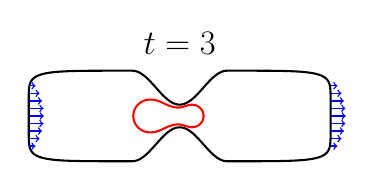
\begin{tikzpicture}[scale=0.5]

\begin{axis}[
  xmin = -11,
  xmax = 11,
  ymin = -3.2,
  ymax = 3.2,
  scale only axis,
  axis equal image,
  hide axis,
  title = {\Huge$t=3$}
  ]

\addplot [mark=none,black,line width=1.5] table{
1.0000e+01 0.0000e+00
1.0000e+01 3.6817e-02
1.0000e+01 7.3646e-02
1.0000e+01 1.1050e-01
1.0000e+01 1.4738e-01
1.0000e+01 1.8431e-01
1.0000e+01 2.2129e-01
1.0000e+01 2.5834e-01
1.0000e+01 2.9547e-01
1.0000e+01 3.3269e-01
1.0000e+01 3.7001e-01
1.0000e+01 4.0745e-01
1.0000e+01 4.4501e-01
1.0000e+01 4.8270e-01
1.0000e+01 5.2055e-01
1.0000e+01 5.5856e-01
1.0000e+01 5.9674e-01
1.0000e+01 6.3510e-01
1.0000e+01 6.7367e-01
1.0000e+01 7.1245e-01
1.0000e+01 7.5146e-01
1.0000e+01 7.9071e-01
1.0000e+01 8.3021e-01
9.9999e+00 8.6998e-01
9.9999e+00 9.1003e-01
9.9999e+00 9.5038e-01
9.9998e+00 9.9105e-01
9.9998e+00 1.0320e+00
9.9997e+00 1.0734e+00
9.9995e+00 1.1151e+00
9.9994e+00 1.1572e+00
9.9992e+00 1.1996e+00
9.9989e+00 1.2425e+00
9.9986e+00 1.2858e+00
9.9981e+00 1.3296e+00
9.9976e+00 1.3738e+00
9.9969e+00 1.4185e+00
9.9960e+00 1.4636e+00
9.9949e+00 1.5093e+00
9.9935e+00 1.5555e+00
9.9917e+00 1.6022e+00
9.9895e+00 1.6495e+00
9.9868e+00 1.6972e+00
9.9835e+00 1.7456e+00
9.9794e+00 1.7944e+00
9.9743e+00 1.8438e+00
9.9681e+00 1.8937e+00
9.9606e+00 1.9440e+00
9.9514e+00 1.9948e+00
9.9403e+00 2.0459e+00
9.9268e+00 2.0974e+00
9.9106e+00 2.1490e+00
9.8911e+00 2.2007e+00
9.8678e+00 2.2524e+00
9.8402e+00 2.3038e+00
9.8074e+00 2.3548e+00
9.7688e+00 2.4051e+00
9.7237e+00 2.4545e+00
9.6713e+00 2.5028e+00
9.6109e+00 2.5495e+00
9.5418e+00 2.5944e+00
9.4634e+00 2.6373e+00
9.3755e+00 2.6779e+00
9.2777e+00 2.7158e+00
9.1700e+00 2.7510e+00
9.0527e+00 2.7833e+00
8.9262e+00 2.8126e+00
8.7911e+00 2.8390e+00
8.6481e+00 2.8625e+00
8.4983e+00 2.8833e+00
8.3425e+00 2.9014e+00
8.1818e+00 2.9171e+00
8.0171e+00 2.9306e+00
7.8493e+00 2.9422e+00
7.6793e+00 2.9520e+00
7.5079e+00 2.9604e+00
7.3358e+00 2.9673e+00
7.1634e+00 2.9732e+00
6.9912e+00 2.9780e+00
6.8198e+00 2.9821e+00
6.6493e+00 2.9854e+00
6.4801e+00 2.9882e+00
6.3123e+00 2.9904e+00
6.1460e+00 2.9923e+00
5.9814e+00 2.9938e+00
5.8185e+00 2.9950e+00
5.6575e+00 2.9960e+00
5.4982e+00 2.9969e+00
5.3407e+00 2.9975e+00
5.1850e+00 2.9980e+00
5.0310e+00 2.9985e+00
4.8787e+00 2.9988e+00
4.7282e+00 2.9991e+00
4.5792e+00 2.9993e+00
4.4319e+00 2.9994e+00
4.2860e+00 2.9996e+00
4.1417e+00 2.9997e+00
3.9988e+00 2.9998e+00
3.8572e+00 2.9998e+00
3.7169e+00 2.9999e+00
3.5779e+00 2.9999e+00
3.4401e+00 2.9999e+00
3.3035e+00 2.9999e+00
3.1679e+00 3.0000e+00
3.0334e+00 2.9934e+00
2.8999e+00 2.9673e+00
2.7674e+00 2.9221e+00
2.6357e+00 2.8591e+00
2.5049e+00 2.7795e+00
2.3748e+00 2.6852e+00
2.2456e+00 2.5778e+00
2.1170e+00 2.4594e+00
1.9891e+00 2.3320e+00
1.8619e+00 2.1978e+00
1.7352e+00 2.0591e+00
1.6090e+00 1.9180e+00
1.4834e+00 1.7768e+00
1.3582e+00 1.6376e+00
1.2334e+00 1.5026e+00
1.1090e+00 1.3737e+00
9.8491e-01 1.2529e+00
8.6115e-01 1.1420e+00
7.3764e-01 1.0424e+00
6.1436e-01 9.5572e-01
4.9127e-01 8.8305e-01
3.6832e-01 8.2545e-01
2.4549e-01 7.8373e-01
1.2272e-01 7.5846e-01
6.1232e-16 7.5000e-01
-1.2272e-01 7.5846e-01
-2.4549e-01 7.8373e-01
-3.6832e-01 8.2545e-01
-4.9127e-01 8.8305e-01
-6.1436e-01 9.5572e-01
-7.3764e-01 1.0424e+00
-8.6115e-01 1.1420e+00
-9.8491e-01 1.2529e+00
-1.1090e+00 1.3737e+00
-1.2334e+00 1.5026e+00
-1.3582e+00 1.6376e+00
-1.4834e+00 1.7768e+00
-1.6090e+00 1.9180e+00
-1.7352e+00 2.0591e+00
-1.8619e+00 2.1978e+00
-1.9891e+00 2.3320e+00
-2.1170e+00 2.4594e+00
-2.2456e+00 2.5778e+00
-2.3748e+00 2.6852e+00
-2.5049e+00 2.7795e+00
-2.6357e+00 2.8591e+00
-2.7674e+00 2.9221e+00
-2.8999e+00 2.9673e+00
-3.0334e+00 2.9934e+00
-3.1679e+00 3.0000e+00
-3.3035e+00 2.9999e+00
-3.4401e+00 2.9999e+00
-3.5779e+00 2.9999e+00
-3.7169e+00 2.9999e+00
-3.8572e+00 2.9998e+00
-3.9988e+00 2.9998e+00
-4.1417e+00 2.9997e+00
-4.2860e+00 2.9996e+00
-4.4319e+00 2.9994e+00
-4.5792e+00 2.9993e+00
-4.7282e+00 2.9991e+00
-4.8787e+00 2.9988e+00
-5.0310e+00 2.9985e+00
-5.1850e+00 2.9980e+00
-5.3407e+00 2.9975e+00
-5.4982e+00 2.9969e+00
-5.6575e+00 2.9960e+00
-5.8185e+00 2.9950e+00
-5.9814e+00 2.9938e+00
-6.1460e+00 2.9923e+00
-6.3123e+00 2.9904e+00
-6.4801e+00 2.9882e+00
-6.6493e+00 2.9854e+00
-6.8198e+00 2.9821e+00
-6.9912e+00 2.9780e+00
-7.1634e+00 2.9732e+00
-7.3358e+00 2.9673e+00
-7.5079e+00 2.9604e+00
-7.6793e+00 2.9520e+00
-7.8493e+00 2.9422e+00
-8.0171e+00 2.9306e+00
-8.1818e+00 2.9171e+00
-8.3425e+00 2.9014e+00
-8.4983e+00 2.8833e+00
-8.6481e+00 2.8625e+00
-8.7911e+00 2.8390e+00
-8.9262e+00 2.8126e+00
-9.0527e+00 2.7833e+00
-9.1700e+00 2.7510e+00
-9.2777e+00 2.7158e+00
-9.3755e+00 2.6779e+00
-9.4634e+00 2.6373e+00
-9.5418e+00 2.5944e+00
-9.6109e+00 2.5495e+00
-9.6713e+00 2.5028e+00
-9.7237e+00 2.4545e+00
-9.7688e+00 2.4051e+00
-9.8074e+00 2.3548e+00
-9.8402e+00 2.3038e+00
-9.8678e+00 2.2524e+00
-9.8911e+00 2.2007e+00
-9.9106e+00 2.1490e+00
-9.9268e+00 2.0974e+00
-9.9403e+00 2.0459e+00
-9.9514e+00 1.9948e+00
-9.9606e+00 1.9440e+00
-9.9681e+00 1.8937e+00
-9.9743e+00 1.8438e+00
-9.9794e+00 1.7944e+00
-9.9835e+00 1.7456e+00
-9.9868e+00 1.6972e+00
-9.9895e+00 1.6495e+00
-9.9917e+00 1.6022e+00
-9.9935e+00 1.5555e+00
-9.9949e+00 1.5093e+00
-9.9960e+00 1.4636e+00
-9.9969e+00 1.4185e+00
-9.9976e+00 1.3738e+00
-9.9981e+00 1.3296e+00
-9.9986e+00 1.2858e+00
-9.9989e+00 1.2425e+00
-9.9992e+00 1.1996e+00
-9.9994e+00 1.1572e+00
-9.9995e+00 1.1151e+00
-9.9997e+00 1.0734e+00
-9.9998e+00 1.0320e+00
-9.9998e+00 9.9105e-01
-9.9999e+00 9.5038e-01
-9.9999e+00 9.1003e-01
-9.9999e+00 8.6998e-01
-1.0000e+01 8.3021e-01
-1.0000e+01 7.9071e-01
-1.0000e+01 7.5146e-01
-1.0000e+01 7.1245e-01
-1.0000e+01 6.7367e-01
-1.0000e+01 6.3510e-01
-1.0000e+01 5.9674e-01
-1.0000e+01 5.5856e-01
-1.0000e+01 5.2055e-01
-1.0000e+01 4.8270e-01
-1.0000e+01 4.4501e-01
-1.0000e+01 4.0745e-01
-1.0000e+01 3.7001e-01
-1.0000e+01 3.3269e-01
-1.0000e+01 2.9547e-01
-1.0000e+01 2.5834e-01
-1.0000e+01 2.2129e-01
-1.0000e+01 1.8431e-01
-1.0000e+01 1.4738e-01
-1.0000e+01 1.1050e-01
-1.0000e+01 7.3646e-02
-1.0000e+01 3.6817e-02
-1.0000e+01 3.6739e-16
-1.0000e+01 -3.6817e-02
-1.0000e+01 -7.3646e-02
-1.0000e+01 -1.1050e-01
-1.0000e+01 -1.4738e-01
-1.0000e+01 -1.8431e-01
-1.0000e+01 -2.2129e-01
-1.0000e+01 -2.5834e-01
-1.0000e+01 -2.9547e-01
-1.0000e+01 -3.3269e-01
-1.0000e+01 -3.7001e-01
-1.0000e+01 -4.0745e-01
-1.0000e+01 -4.4501e-01
-1.0000e+01 -4.8270e-01
-1.0000e+01 -5.2055e-01
-1.0000e+01 -5.5856e-01
-1.0000e+01 -5.9674e-01
-1.0000e+01 -6.3510e-01
-1.0000e+01 -6.7367e-01
-1.0000e+01 -7.1245e-01
-1.0000e+01 -7.5146e-01
-1.0000e+01 -7.9071e-01
-1.0000e+01 -8.3021e-01
-9.9999e+00 -8.6998e-01
-9.9999e+00 -9.1003e-01
-9.9999e+00 -9.5038e-01
-9.9998e+00 -9.9105e-01
-9.9998e+00 -1.0320e+00
-9.9997e+00 -1.0734e+00
-9.9995e+00 -1.1151e+00
-9.9994e+00 -1.1572e+00
-9.9992e+00 -1.1996e+00
-9.9989e+00 -1.2425e+00
-9.9986e+00 -1.2858e+00
-9.9981e+00 -1.3296e+00
-9.9976e+00 -1.3738e+00
-9.9969e+00 -1.4185e+00
-9.9960e+00 -1.4636e+00
-9.9949e+00 -1.5093e+00
-9.9935e+00 -1.5555e+00
-9.9917e+00 -1.6022e+00
-9.9895e+00 -1.6495e+00
-9.9868e+00 -1.6972e+00
-9.9835e+00 -1.7456e+00
-9.9794e+00 -1.7944e+00
-9.9743e+00 -1.8438e+00
-9.9681e+00 -1.8937e+00
-9.9606e+00 -1.9440e+00
-9.9514e+00 -1.9948e+00
-9.9403e+00 -2.0459e+00
-9.9268e+00 -2.0974e+00
-9.9106e+00 -2.1490e+00
-9.8911e+00 -2.2007e+00
-9.8678e+00 -2.2524e+00
-9.8402e+00 -2.3038e+00
-9.8074e+00 -2.3548e+00
-9.7688e+00 -2.4051e+00
-9.7237e+00 -2.4545e+00
-9.6713e+00 -2.5028e+00
-9.6109e+00 -2.5495e+00
-9.5418e+00 -2.5944e+00
-9.4634e+00 -2.6373e+00
-9.3755e+00 -2.6779e+00
-9.2777e+00 -2.7158e+00
-9.1700e+00 -2.7510e+00
-9.0527e+00 -2.7833e+00
-8.9262e+00 -2.8126e+00
-8.7911e+00 -2.8390e+00
-8.6481e+00 -2.8625e+00
-8.4983e+00 -2.8833e+00
-8.3425e+00 -2.9014e+00
-8.1818e+00 -2.9171e+00
-8.0171e+00 -2.9306e+00
-7.8493e+00 -2.9422e+00
-7.6793e+00 -2.9520e+00
-7.5079e+00 -2.9604e+00
-7.3358e+00 -2.9673e+00
-7.1634e+00 -2.9732e+00
-6.9912e+00 -2.9780e+00
-6.8198e+00 -2.9821e+00
-6.6493e+00 -2.9854e+00
-6.4801e+00 -2.9882e+00
-6.3123e+00 -2.9904e+00
-6.1460e+00 -2.9923e+00
-5.9814e+00 -2.9938e+00
-5.8185e+00 -2.9950e+00
-5.6575e+00 -2.9960e+00
-5.4982e+00 -2.9969e+00
-5.3407e+00 -2.9975e+00
-5.1850e+00 -2.9980e+00
-5.0310e+00 -2.9985e+00
-4.8787e+00 -2.9988e+00
-4.7282e+00 -2.9991e+00
-4.5792e+00 -2.9993e+00
-4.4319e+00 -2.9994e+00
-4.2860e+00 -2.9996e+00
-4.1417e+00 -2.9997e+00
-3.9988e+00 -2.9998e+00
-3.8572e+00 -2.9998e+00
-3.7169e+00 -2.9999e+00
-3.5779e+00 -2.9999e+00
-3.4401e+00 -2.9999e+00
-3.3035e+00 -2.9999e+00
-3.1679e+00 -3.0000e+00
-3.0334e+00 -2.9934e+00
-2.8999e+00 -2.9673e+00
-2.7674e+00 -2.9221e+00
-2.6357e+00 -2.8591e+00
-2.5049e+00 -2.7795e+00
-2.3748e+00 -2.6852e+00
-2.2456e+00 -2.5778e+00
-2.1170e+00 -2.4594e+00
-1.9891e+00 -2.3320e+00
-1.8619e+00 -2.1978e+00
-1.7352e+00 -2.0591e+00
-1.6090e+00 -1.9180e+00
-1.4834e+00 -1.7768e+00
-1.3582e+00 -1.6376e+00
-1.2334e+00 -1.5026e+00
-1.1090e+00 -1.3737e+00
-9.8491e-01 -1.2529e+00
-8.6115e-01 -1.1420e+00
-7.3764e-01 -1.0424e+00
-6.1436e-01 -9.5572e-01
-4.9127e-01 -8.8305e-01
-3.6832e-01 -8.2545e-01
-2.4549e-01 -7.8373e-01
-1.2272e-01 -7.5846e-01
-1.8370e-15 -7.5000e-01
1.2272e-01 -7.5846e-01
2.4549e-01 -7.8373e-01
3.6832e-01 -8.2545e-01
4.9127e-01 -8.8305e-01
6.1436e-01 -9.5572e-01
7.3764e-01 -1.0424e+00
8.6115e-01 -1.1420e+00
9.8491e-01 -1.2529e+00
1.1090e+00 -1.3737e+00
1.2334e+00 -1.5026e+00
1.3582e+00 -1.6376e+00
1.4834e+00 -1.7768e+00
1.6090e+00 -1.9180e+00
1.7352e+00 -2.0591e+00
1.8619e+00 -2.1978e+00
1.9891e+00 -2.3320e+00
2.1170e+00 -2.4594e+00
2.2456e+00 -2.5778e+00
2.3748e+00 -2.6852e+00
2.5049e+00 -2.7795e+00
2.6357e+00 -2.8591e+00
2.7674e+00 -2.9221e+00
2.8999e+00 -2.9673e+00
3.0334e+00 -2.9934e+00
3.1679e+00 -3.0000e+00
3.3035e+00 -2.9999e+00
3.4401e+00 -2.9999e+00
3.5779e+00 -2.9999e+00
3.7169e+00 -2.9999e+00
3.8572e+00 -2.9998e+00
3.9988e+00 -2.9998e+00
4.1417e+00 -2.9997e+00
4.2860e+00 -2.9996e+00
4.4319e+00 -2.9994e+00
4.5792e+00 -2.9993e+00
4.7282e+00 -2.9991e+00
4.8787e+00 -2.9988e+00
5.0310e+00 -2.9985e+00
5.1850e+00 -2.9980e+00
5.3407e+00 -2.9975e+00
5.4982e+00 -2.9969e+00
5.6575e+00 -2.9960e+00
5.8185e+00 -2.9950e+00
5.9814e+00 -2.9938e+00
6.1460e+00 -2.9923e+00
6.3123e+00 -2.9904e+00
6.4801e+00 -2.9882e+00
6.6493e+00 -2.9854e+00
6.8198e+00 -2.9821e+00
6.9912e+00 -2.9780e+00
7.1634e+00 -2.9732e+00
7.3358e+00 -2.9673e+00
7.5079e+00 -2.9604e+00
7.6793e+00 -2.9520e+00
7.8493e+00 -2.9422e+00
8.0171e+00 -2.9306e+00
8.1818e+00 -2.9171e+00
8.3425e+00 -2.9014e+00
8.4983e+00 -2.8833e+00
8.6481e+00 -2.8625e+00
8.7911e+00 -2.8390e+00
8.9262e+00 -2.8126e+00
9.0527e+00 -2.7833e+00
9.1700e+00 -2.7510e+00
9.2777e+00 -2.7158e+00
9.3755e+00 -2.6779e+00
9.4634e+00 -2.6373e+00
9.5418e+00 -2.5944e+00
9.6109e+00 -2.5495e+00
9.6713e+00 -2.5028e+00
9.7237e+00 -2.4545e+00
9.7688e+00 -2.4051e+00
9.8074e+00 -2.3548e+00
9.8402e+00 -2.3038e+00
9.8678e+00 -2.2524e+00
9.8911e+00 -2.2007e+00
9.9106e+00 -2.1490e+00
9.9268e+00 -2.0974e+00
9.9403e+00 -2.0459e+00
9.9514e+00 -1.9948e+00
9.9606e+00 -1.9440e+00
9.9681e+00 -1.8937e+00
9.9743e+00 -1.8438e+00
9.9794e+00 -1.7944e+00
9.9835e+00 -1.7456e+00
9.9868e+00 -1.6972e+00
9.9895e+00 -1.6495e+00
9.9917e+00 -1.6022e+00
9.9935e+00 -1.5555e+00
9.9949e+00 -1.5093e+00
9.9960e+00 -1.4636e+00
9.9969e+00 -1.4185e+00
9.9976e+00 -1.3738e+00
9.9981e+00 -1.3296e+00
9.9986e+00 -1.2858e+00
9.9989e+00 -1.2425e+00
9.9992e+00 -1.1996e+00
9.9994e+00 -1.1572e+00
9.9995e+00 -1.1151e+00
9.9997e+00 -1.0734e+00
9.9998e+00 -1.0320e+00
9.9998e+00 -9.9105e-01
9.9999e+00 -9.5038e-01
9.9999e+00 -9.1003e-01
9.9999e+00 -8.6998e-01
1.0000e+01 -8.3021e-01
1.0000e+01 -7.9071e-01
1.0000e+01 -7.5146e-01
1.0000e+01 -7.1245e-01
1.0000e+01 -6.7367e-01
1.0000e+01 -6.3510e-01
1.0000e+01 -5.9674e-01
1.0000e+01 -5.5856e-01
1.0000e+01 -5.2055e-01
1.0000e+01 -4.8270e-01
1.0000e+01 -4.4501e-01
1.0000e+01 -4.0745e-01
1.0000e+01 -3.7001e-01
1.0000e+01 -3.3269e-01
1.0000e+01 -2.9547e-01
1.0000e+01 -2.5834e-01
1.0000e+01 -2.2129e-01
1.0000e+01 -1.8431e-01
1.0000e+01 -1.4738e-01
1.0000e+01 -1.1050e-01
1.0000e+01 -7.3646e-02
1.0000e+01 -3.6817e-02
1.0000e+01 0.0000e+00
};


\addplot [mark=none,red,line width=1.5] table{
-8.6712e-01 7.5275e-01
-8.8649e-01 7.6153e-01
-9.0602e-01 7.7045e-01
-9.2580e-01 7.7956e-01
-9.4592e-01 7.8887e-01
-9.6646e-01 7.9844e-01
-9.8751e-01 8.0826e-01
-1.0091e+00 8.1838e-01
-1.0314e+00 8.2880e-01
-1.0544e+00 8.3953e-01
-1.0781e+00 8.5057e-01
-1.1026e+00 8.6193e-01
-1.1280e+00 8.7359e-01
-1.1543e+00 8.8554e-01
-1.1816e+00 8.9776e-01
-1.2098e+00 9.1020e-01
-1.2391e+00 9.2284e-01
-1.2694e+00 9.3563e-01
-1.3008e+00 9.4850e-01
-1.3333e+00 9.6140e-01
-1.3670e+00 9.7424e-01
-1.4018e+00 9.8696e-01
-1.4379e+00 9.9945e-01
-1.4751e+00 1.0116e+00
-1.5136e+00 1.0233e+00
-1.5533e+00 1.0345e+00
-1.5943e+00 1.0450e+00
-1.6365e+00 1.0547e+00
-1.6800e+00 1.0635e+00
-1.7247e+00 1.0711e+00
-1.7705e+00 1.0775e+00
-1.8175e+00 1.0826e+00
-1.8656e+00 1.0861e+00
-1.9147e+00 1.0879e+00
-1.9647e+00 1.0878e+00
-2.0155e+00 1.0858e+00
-2.0671e+00 1.0816e+00
-2.1193e+00 1.0752e+00
-2.1720e+00 1.0663e+00
-2.2250e+00 1.0549e+00
-2.2781e+00 1.0409e+00
-2.3312e+00 1.0242e+00
-2.3841e+00 1.0046e+00
-2.4366e+00 9.8217e-01
-2.4884e+00 9.5681e-01
-2.5394e+00 9.2850e-01
-2.5894e+00 8.9722e-01
-2.6381e+00 8.6299e-01
-2.6852e+00 8.2583e-01
-2.7306e+00 7.8580e-01
-2.7740e+00 7.4298e-01
-2.8153e+00 6.9744e-01
-2.8541e+00 6.4932e-01
-2.8903e+00 5.9874e-01
-2.9237e+00 5.4586e-01
-2.9542e+00 4.9086e-01
-2.9814e+00 4.3392e-01
-3.0054e+00 3.7525e-01
-3.0259e+00 3.1507e-01
-3.0428e+00 2.5362e-01
-3.0561e+00 1.9113e-01
-3.0656e+00 1.2786e-01
-3.0714e+00 6.4061e-02
-3.0733e+00 -3.6227e-11
-3.0714e+00 -6.4061e-02
-3.0656e+00 -1.2786e-01
-3.0561e+00 -1.9113e-01
-3.0428e+00 -2.5362e-01
-3.0259e+00 -3.1507e-01
-3.0054e+00 -3.7525e-01
-2.9814e+00 -4.3392e-01
-2.9542e+00 -4.9086e-01
-2.9237e+00 -5.4586e-01
-2.8903e+00 -5.9874e-01
-2.8541e+00 -6.4932e-01
-2.8153e+00 -6.9744e-01
-2.7740e+00 -7.4298e-01
-2.7306e+00 -7.8580e-01
-2.6852e+00 -8.2583e-01
-2.6381e+00 -8.6299e-01
-2.5894e+00 -8.9722e-01
-2.5394e+00 -9.2850e-01
-2.4884e+00 -9.5681e-01
-2.4366e+00 -9.8217e-01
-2.3841e+00 -1.0046e+00
-2.3312e+00 -1.0242e+00
-2.2781e+00 -1.0409e+00
-2.2250e+00 -1.0549e+00
-2.1720e+00 -1.0663e+00
-2.1193e+00 -1.0752e+00
-2.0671e+00 -1.0816e+00
-2.0155e+00 -1.0858e+00
-1.9647e+00 -1.0878e+00
-1.9147e+00 -1.0879e+00
-1.8656e+00 -1.0861e+00
-1.8175e+00 -1.0826e+00
-1.7705e+00 -1.0775e+00
-1.7247e+00 -1.0711e+00
-1.6800e+00 -1.0635e+00
-1.6365e+00 -1.0547e+00
-1.5943e+00 -1.0450e+00
-1.5533e+00 -1.0345e+00
-1.5136e+00 -1.0233e+00
-1.4751e+00 -1.0116e+00
-1.4379e+00 -9.9945e-01
-1.4018e+00 -9.8696e-01
-1.3670e+00 -9.7424e-01
-1.3333e+00 -9.6140e-01
-1.3008e+00 -9.4850e-01
-1.2694e+00 -9.3563e-01
-1.2391e+00 -9.2284e-01
-1.2098e+00 -9.1020e-01
-1.1816e+00 -8.9776e-01
-1.1543e+00 -8.8554e-01
-1.1280e+00 -8.7359e-01
-1.1026e+00 -8.6193e-01
-1.0781e+00 -8.5057e-01
-1.0544e+00 -8.3953e-01
-1.0314e+00 -8.2880e-01
-1.0091e+00 -8.1838e-01
-9.8751e-01 -8.0826e-01
-9.6646e-01 -7.9844e-01
-9.4592e-01 -7.8887e-01
-9.2580e-01 -7.7956e-01
-9.0602e-01 -7.7045e-01
-8.8649e-01 -7.6153e-01
-8.6712e-01 -7.5275e-01
-8.4781e-01 -7.4409e-01
-8.2847e-01 -7.3552e-01
-8.0899e-01 -7.2699e-01
-7.8927e-01 -7.1849e-01
-7.6923e-01 -7.0998e-01
-7.4876e-01 -7.0145e-01
-7.2778e-01 -6.9288e-01
-7.0621e-01 -6.8427e-01
-6.8396e-01 -6.7561e-01
-6.6097e-01 -6.6691e-01
-6.3717e-01 -6.5818e-01
-6.1249e-01 -6.4946e-01
-5.8689e-01 -6.4076e-01
-5.6030e-01 -6.3214e-01
-5.3269e-01 -6.2363e-01
-5.0402e-01 -6.1530e-01
-4.7424e-01 -6.0722e-01
-4.4333e-01 -5.9945e-01
-4.1127e-01 -5.9210e-01
-3.7804e-01 -5.8524e-01
-3.4362e-01 -5.7898e-01
-3.0801e-01 -5.7343e-01
-2.7123e-01 -5.6871e-01
-2.3327e-01 -5.6494e-01
-1.9417e-01 -5.6224e-01
-1.5397e-01 -5.6074e-01
-1.1269e-01 -5.6056e-01
-7.0406e-02 -5.6182e-01
-2.7175e-02 -5.6462e-01
1.6931e-02 -5.6905e-01
6.1834e-02 -5.7517e-01
1.0746e-01 -5.8301e-01
1.5374e-01 -5.9255e-01
2.0062e-01 -6.0374e-01
2.4807e-01 -6.1644e-01
2.9609e-01 -6.3045e-01
3.4472e-01 -6.4551e-01
3.9403e-01 -6.6123e-01
4.4415e-01 -6.7718e-01
4.9522e-01 -6.9282e-01
5.4737e-01 -7.0758e-01
6.0070e-01 -7.2082e-01
6.5526e-01 -7.3195e-01
7.1102e-01 -7.4036e-01
7.6785e-01 -7.4554e-01
8.2555e-01 -7.4705e-01
8.8383e-01 -7.4453e-01
9.4236e-01 -7.3770e-01
1.0008e+00 -7.2635e-01
1.0586e+00 -7.1037e-01
1.1155e+00 -6.8970e-01
1.1710e+00 -6.6432e-01
1.2245e+00 -6.3431e-01
1.2758e+00 -5.9977e-01
1.3244e+00 -5.6087e-01
1.3697e+00 -5.1782e-01
1.4115e+00 -4.7089e-01
1.4494e+00 -4.2037e-01
1.4829e+00 -3.6663e-01
1.5119e+00 -3.1003e-01
1.5360e+00 -2.5102e-01
1.5549e+00 -1.9003e-01
1.5686e+00 -1.2753e-01
1.5769e+00 -6.4020e-02
1.5796e+00 -3.3318e-11
1.5769e+00 6.4020e-02
1.5686e+00 1.2753e-01
1.5549e+00 1.9003e-01
1.5360e+00 2.5102e-01
1.5119e+00 3.1003e-01
1.4829e+00 3.6663e-01
1.4494e+00 4.2037e-01
1.4115e+00 4.7089e-01
1.3697e+00 5.1782e-01
1.3244e+00 5.6087e-01
1.2758e+00 5.9977e-01
1.2245e+00 6.3431e-01
1.1710e+00 6.6432e-01
1.1155e+00 6.8970e-01
1.0586e+00 7.1037e-01
1.0008e+00 7.2635e-01
9.4236e-01 7.3770e-01
8.8383e-01 7.4453e-01
8.2555e-01 7.4705e-01
7.6785e-01 7.4554e-01
7.1102e-01 7.4036e-01
6.5526e-01 7.3195e-01
6.0070e-01 7.2082e-01
5.4737e-01 7.0758e-01
4.9522e-01 6.9282e-01
4.4415e-01 6.7718e-01
3.9403e-01 6.6123e-01
3.4472e-01 6.4551e-01
2.9609e-01 6.3045e-01
2.4807e-01 6.1644e-01
2.0062e-01 6.0374e-01
1.5374e-01 5.9255e-01
1.0746e-01 5.8301e-01
6.1834e-02 5.7517e-01
1.6931e-02 5.6905e-01
-2.7175e-02 5.6462e-01
-7.0406e-02 5.6182e-01
-1.1269e-01 5.6056e-01
-1.5397e-01 5.6074e-01
-1.9417e-01 5.6224e-01
-2.3327e-01 5.6494e-01
-2.7123e-01 5.6871e-01
-3.0801e-01 5.7343e-01
-3.4362e-01 5.7898e-01
-3.7804e-01 5.8524e-01
-4.1127e-01 5.9210e-01
-4.4333e-01 5.9945e-01
-4.7424e-01 6.0722e-01
-5.0402e-01 6.1530e-01
-5.3269e-01 6.2363e-01
-5.6030e-01 6.3214e-01
-5.8689e-01 6.4076e-01
-6.1249e-01 6.4946e-01
-6.3717e-01 6.5818e-01
-6.6097e-01 6.6691e-01
-6.8396e-01 6.7561e-01
-7.0621e-01 6.8427e-01
-7.2778e-01 6.9288e-01
-7.4876e-01 7.0145e-01
-7.6923e-01 7.0998e-01
-7.8927e-01 7.1849e-01
-8.0899e-01 7.2699e-01
-8.2847e-01 7.3552e-01
-8.4781e-01 7.4409e-01
-8.6712e-01 7.5275e-01
};

\foreach \y in {-2.0,-1.5,...,2.0}
\addplot[color=blue,line width = 1.0pt,solid,->]
plot coordinates{
  (-10,\y)
  (-10+exp(9/(\y*\y-9))/exp(-1),\y)
};

\foreach \y in {-2.0,-1.5,...,2.0}
\addplot[color=blue,line width = 1.0pt,solid,->]
plot coordinates{
  (10,\y)
  (10+exp(9/(\y*\y-9))/exp(-1),\y)
};

\end{axis}

\end{tikzpicture}



 &
%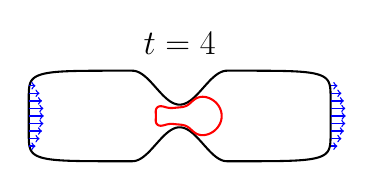
\begin{tikzpicture}[scale=0.5]

\begin{axis}[
  xmin = -11,
  xmax = 11,
  ymin = -3.2,
  ymax = 3.2,
  scale only axis,
  axis equal image,
  hide axis,
  title = {\Huge$t=4$}
  ]

\addplot [mark=none,black,line width=1.5] table{
1.0000e+01 0.0000e+00
1.0000e+01 3.6817e-02
1.0000e+01 7.3646e-02
1.0000e+01 1.1050e-01
1.0000e+01 1.4738e-01
1.0000e+01 1.8431e-01
1.0000e+01 2.2129e-01
1.0000e+01 2.5834e-01
1.0000e+01 2.9547e-01
1.0000e+01 3.3269e-01
1.0000e+01 3.7001e-01
1.0000e+01 4.0745e-01
1.0000e+01 4.4501e-01
1.0000e+01 4.8270e-01
1.0000e+01 5.2055e-01
1.0000e+01 5.5856e-01
1.0000e+01 5.9674e-01
1.0000e+01 6.3510e-01
1.0000e+01 6.7367e-01
1.0000e+01 7.1245e-01
1.0000e+01 7.5146e-01
1.0000e+01 7.9071e-01
1.0000e+01 8.3021e-01
9.9999e+00 8.6998e-01
9.9999e+00 9.1003e-01
9.9999e+00 9.5038e-01
9.9998e+00 9.9105e-01
9.9998e+00 1.0320e+00
9.9997e+00 1.0734e+00
9.9995e+00 1.1151e+00
9.9994e+00 1.1572e+00
9.9992e+00 1.1996e+00
9.9989e+00 1.2425e+00
9.9986e+00 1.2858e+00
9.9981e+00 1.3296e+00
9.9976e+00 1.3738e+00
9.9969e+00 1.4185e+00
9.9960e+00 1.4636e+00
9.9949e+00 1.5093e+00
9.9935e+00 1.5555e+00
9.9917e+00 1.6022e+00
9.9895e+00 1.6495e+00
9.9868e+00 1.6972e+00
9.9835e+00 1.7456e+00
9.9794e+00 1.7944e+00
9.9743e+00 1.8438e+00
9.9681e+00 1.8937e+00
9.9606e+00 1.9440e+00
9.9514e+00 1.9948e+00
9.9403e+00 2.0459e+00
9.9268e+00 2.0974e+00
9.9106e+00 2.1490e+00
9.8911e+00 2.2007e+00
9.8678e+00 2.2524e+00
9.8402e+00 2.3038e+00
9.8074e+00 2.3548e+00
9.7688e+00 2.4051e+00
9.7237e+00 2.4545e+00
9.6713e+00 2.5028e+00
9.6109e+00 2.5495e+00
9.5418e+00 2.5944e+00
9.4634e+00 2.6373e+00
9.3755e+00 2.6779e+00
9.2777e+00 2.7158e+00
9.1700e+00 2.7510e+00
9.0527e+00 2.7833e+00
8.9262e+00 2.8126e+00
8.7911e+00 2.8390e+00
8.6481e+00 2.8625e+00
8.4983e+00 2.8833e+00
8.3425e+00 2.9014e+00
8.1818e+00 2.9171e+00
8.0171e+00 2.9306e+00
7.8493e+00 2.9422e+00
7.6793e+00 2.9520e+00
7.5079e+00 2.9604e+00
7.3358e+00 2.9673e+00
7.1634e+00 2.9732e+00
6.9912e+00 2.9780e+00
6.8198e+00 2.9821e+00
6.6493e+00 2.9854e+00
6.4801e+00 2.9882e+00
6.3123e+00 2.9904e+00
6.1460e+00 2.9923e+00
5.9814e+00 2.9938e+00
5.8185e+00 2.9950e+00
5.6575e+00 2.9960e+00
5.4982e+00 2.9969e+00
5.3407e+00 2.9975e+00
5.1850e+00 2.9980e+00
5.0310e+00 2.9985e+00
4.8787e+00 2.9988e+00
4.7282e+00 2.9991e+00
4.5792e+00 2.9993e+00
4.4319e+00 2.9994e+00
4.2860e+00 2.9996e+00
4.1417e+00 2.9997e+00
3.9988e+00 2.9998e+00
3.8572e+00 2.9998e+00
3.7169e+00 2.9999e+00
3.5779e+00 2.9999e+00
3.4401e+00 2.9999e+00
3.3035e+00 2.9999e+00
3.1679e+00 3.0000e+00
3.0334e+00 2.9934e+00
2.8999e+00 2.9673e+00
2.7674e+00 2.9221e+00
2.6357e+00 2.8591e+00
2.5049e+00 2.7795e+00
2.3748e+00 2.6852e+00
2.2456e+00 2.5778e+00
2.1170e+00 2.4594e+00
1.9891e+00 2.3320e+00
1.8619e+00 2.1978e+00
1.7352e+00 2.0591e+00
1.6090e+00 1.9180e+00
1.4834e+00 1.7768e+00
1.3582e+00 1.6376e+00
1.2334e+00 1.5026e+00
1.1090e+00 1.3737e+00
9.8491e-01 1.2529e+00
8.6115e-01 1.1420e+00
7.3764e-01 1.0424e+00
6.1436e-01 9.5572e-01
4.9127e-01 8.8305e-01
3.6832e-01 8.2545e-01
2.4549e-01 7.8373e-01
1.2272e-01 7.5846e-01
6.1232e-16 7.5000e-01
-1.2272e-01 7.5846e-01
-2.4549e-01 7.8373e-01
-3.6832e-01 8.2545e-01
-4.9127e-01 8.8305e-01
-6.1436e-01 9.5572e-01
-7.3764e-01 1.0424e+00
-8.6115e-01 1.1420e+00
-9.8491e-01 1.2529e+00
-1.1090e+00 1.3737e+00
-1.2334e+00 1.5026e+00
-1.3582e+00 1.6376e+00
-1.4834e+00 1.7768e+00
-1.6090e+00 1.9180e+00
-1.7352e+00 2.0591e+00
-1.8619e+00 2.1978e+00
-1.9891e+00 2.3320e+00
-2.1170e+00 2.4594e+00
-2.2456e+00 2.5778e+00
-2.3748e+00 2.6852e+00
-2.5049e+00 2.7795e+00
-2.6357e+00 2.8591e+00
-2.7674e+00 2.9221e+00
-2.8999e+00 2.9673e+00
-3.0334e+00 2.9934e+00
-3.1679e+00 3.0000e+00
-3.3035e+00 2.9999e+00
-3.4401e+00 2.9999e+00
-3.5779e+00 2.9999e+00
-3.7169e+00 2.9999e+00
-3.8572e+00 2.9998e+00
-3.9988e+00 2.9998e+00
-4.1417e+00 2.9997e+00
-4.2860e+00 2.9996e+00
-4.4319e+00 2.9994e+00
-4.5792e+00 2.9993e+00
-4.7282e+00 2.9991e+00
-4.8787e+00 2.9988e+00
-5.0310e+00 2.9985e+00
-5.1850e+00 2.9980e+00
-5.3407e+00 2.9975e+00
-5.4982e+00 2.9969e+00
-5.6575e+00 2.9960e+00
-5.8185e+00 2.9950e+00
-5.9814e+00 2.9938e+00
-6.1460e+00 2.9923e+00
-6.3123e+00 2.9904e+00
-6.4801e+00 2.9882e+00
-6.6493e+00 2.9854e+00
-6.8198e+00 2.9821e+00
-6.9912e+00 2.9780e+00
-7.1634e+00 2.9732e+00
-7.3358e+00 2.9673e+00
-7.5079e+00 2.9604e+00
-7.6793e+00 2.9520e+00
-7.8493e+00 2.9422e+00
-8.0171e+00 2.9306e+00
-8.1818e+00 2.9171e+00
-8.3425e+00 2.9014e+00
-8.4983e+00 2.8833e+00
-8.6481e+00 2.8625e+00
-8.7911e+00 2.8390e+00
-8.9262e+00 2.8126e+00
-9.0527e+00 2.7833e+00
-9.1700e+00 2.7510e+00
-9.2777e+00 2.7158e+00
-9.3755e+00 2.6779e+00
-9.4634e+00 2.6373e+00
-9.5418e+00 2.5944e+00
-9.6109e+00 2.5495e+00
-9.6713e+00 2.5028e+00
-9.7237e+00 2.4545e+00
-9.7688e+00 2.4051e+00
-9.8074e+00 2.3548e+00
-9.8402e+00 2.3038e+00
-9.8678e+00 2.2524e+00
-9.8911e+00 2.2007e+00
-9.9106e+00 2.1490e+00
-9.9268e+00 2.0974e+00
-9.9403e+00 2.0459e+00
-9.9514e+00 1.9948e+00
-9.9606e+00 1.9440e+00
-9.9681e+00 1.8937e+00
-9.9743e+00 1.8438e+00
-9.9794e+00 1.7944e+00
-9.9835e+00 1.7456e+00
-9.9868e+00 1.6972e+00
-9.9895e+00 1.6495e+00
-9.9917e+00 1.6022e+00
-9.9935e+00 1.5555e+00
-9.9949e+00 1.5093e+00
-9.9960e+00 1.4636e+00
-9.9969e+00 1.4185e+00
-9.9976e+00 1.3738e+00
-9.9981e+00 1.3296e+00
-9.9986e+00 1.2858e+00
-9.9989e+00 1.2425e+00
-9.9992e+00 1.1996e+00
-9.9994e+00 1.1572e+00
-9.9995e+00 1.1151e+00
-9.9997e+00 1.0734e+00
-9.9998e+00 1.0320e+00
-9.9998e+00 9.9105e-01
-9.9999e+00 9.5038e-01
-9.9999e+00 9.1003e-01
-9.9999e+00 8.6998e-01
-1.0000e+01 8.3021e-01
-1.0000e+01 7.9071e-01
-1.0000e+01 7.5146e-01
-1.0000e+01 7.1245e-01
-1.0000e+01 6.7367e-01
-1.0000e+01 6.3510e-01
-1.0000e+01 5.9674e-01
-1.0000e+01 5.5856e-01
-1.0000e+01 5.2055e-01
-1.0000e+01 4.8270e-01
-1.0000e+01 4.4501e-01
-1.0000e+01 4.0745e-01
-1.0000e+01 3.7001e-01
-1.0000e+01 3.3269e-01
-1.0000e+01 2.9547e-01
-1.0000e+01 2.5834e-01
-1.0000e+01 2.2129e-01
-1.0000e+01 1.8431e-01
-1.0000e+01 1.4738e-01
-1.0000e+01 1.1050e-01
-1.0000e+01 7.3646e-02
-1.0000e+01 3.6817e-02
-1.0000e+01 3.6739e-16
-1.0000e+01 -3.6817e-02
-1.0000e+01 -7.3646e-02
-1.0000e+01 -1.1050e-01
-1.0000e+01 -1.4738e-01
-1.0000e+01 -1.8431e-01
-1.0000e+01 -2.2129e-01
-1.0000e+01 -2.5834e-01
-1.0000e+01 -2.9547e-01
-1.0000e+01 -3.3269e-01
-1.0000e+01 -3.7001e-01
-1.0000e+01 -4.0745e-01
-1.0000e+01 -4.4501e-01
-1.0000e+01 -4.8270e-01
-1.0000e+01 -5.2055e-01
-1.0000e+01 -5.5856e-01
-1.0000e+01 -5.9674e-01
-1.0000e+01 -6.3510e-01
-1.0000e+01 -6.7367e-01
-1.0000e+01 -7.1245e-01
-1.0000e+01 -7.5146e-01
-1.0000e+01 -7.9071e-01
-1.0000e+01 -8.3021e-01
-9.9999e+00 -8.6998e-01
-9.9999e+00 -9.1003e-01
-9.9999e+00 -9.5038e-01
-9.9998e+00 -9.9105e-01
-9.9998e+00 -1.0320e+00
-9.9997e+00 -1.0734e+00
-9.9995e+00 -1.1151e+00
-9.9994e+00 -1.1572e+00
-9.9992e+00 -1.1996e+00
-9.9989e+00 -1.2425e+00
-9.9986e+00 -1.2858e+00
-9.9981e+00 -1.3296e+00
-9.9976e+00 -1.3738e+00
-9.9969e+00 -1.4185e+00
-9.9960e+00 -1.4636e+00
-9.9949e+00 -1.5093e+00
-9.9935e+00 -1.5555e+00
-9.9917e+00 -1.6022e+00
-9.9895e+00 -1.6495e+00
-9.9868e+00 -1.6972e+00
-9.9835e+00 -1.7456e+00
-9.9794e+00 -1.7944e+00
-9.9743e+00 -1.8438e+00
-9.9681e+00 -1.8937e+00
-9.9606e+00 -1.9440e+00
-9.9514e+00 -1.9948e+00
-9.9403e+00 -2.0459e+00
-9.9268e+00 -2.0974e+00
-9.9106e+00 -2.1490e+00
-9.8911e+00 -2.2007e+00
-9.8678e+00 -2.2524e+00
-9.8402e+00 -2.3038e+00
-9.8074e+00 -2.3548e+00
-9.7688e+00 -2.4051e+00
-9.7237e+00 -2.4545e+00
-9.6713e+00 -2.5028e+00
-9.6109e+00 -2.5495e+00
-9.5418e+00 -2.5944e+00
-9.4634e+00 -2.6373e+00
-9.3755e+00 -2.6779e+00
-9.2777e+00 -2.7158e+00
-9.1700e+00 -2.7510e+00
-9.0527e+00 -2.7833e+00
-8.9262e+00 -2.8126e+00
-8.7911e+00 -2.8390e+00
-8.6481e+00 -2.8625e+00
-8.4983e+00 -2.8833e+00
-8.3425e+00 -2.9014e+00
-8.1818e+00 -2.9171e+00
-8.0171e+00 -2.9306e+00
-7.8493e+00 -2.9422e+00
-7.6793e+00 -2.9520e+00
-7.5079e+00 -2.9604e+00
-7.3358e+00 -2.9673e+00
-7.1634e+00 -2.9732e+00
-6.9912e+00 -2.9780e+00
-6.8198e+00 -2.9821e+00
-6.6493e+00 -2.9854e+00
-6.4801e+00 -2.9882e+00
-6.3123e+00 -2.9904e+00
-6.1460e+00 -2.9923e+00
-5.9814e+00 -2.9938e+00
-5.8185e+00 -2.9950e+00
-5.6575e+00 -2.9960e+00
-5.4982e+00 -2.9969e+00
-5.3407e+00 -2.9975e+00
-5.1850e+00 -2.9980e+00
-5.0310e+00 -2.9985e+00
-4.8787e+00 -2.9988e+00
-4.7282e+00 -2.9991e+00
-4.5792e+00 -2.9993e+00
-4.4319e+00 -2.9994e+00
-4.2860e+00 -2.9996e+00
-4.1417e+00 -2.9997e+00
-3.9988e+00 -2.9998e+00
-3.8572e+00 -2.9998e+00
-3.7169e+00 -2.9999e+00
-3.5779e+00 -2.9999e+00
-3.4401e+00 -2.9999e+00
-3.3035e+00 -2.9999e+00
-3.1679e+00 -3.0000e+00
-3.0334e+00 -2.9934e+00
-2.8999e+00 -2.9673e+00
-2.7674e+00 -2.9221e+00
-2.6357e+00 -2.8591e+00
-2.5049e+00 -2.7795e+00
-2.3748e+00 -2.6852e+00
-2.2456e+00 -2.5778e+00
-2.1170e+00 -2.4594e+00
-1.9891e+00 -2.3320e+00
-1.8619e+00 -2.1978e+00
-1.7352e+00 -2.0591e+00
-1.6090e+00 -1.9180e+00
-1.4834e+00 -1.7768e+00
-1.3582e+00 -1.6376e+00
-1.2334e+00 -1.5026e+00
-1.1090e+00 -1.3737e+00
-9.8491e-01 -1.2529e+00
-8.6115e-01 -1.1420e+00
-7.3764e-01 -1.0424e+00
-6.1436e-01 -9.5572e-01
-4.9127e-01 -8.8305e-01
-3.6832e-01 -8.2545e-01
-2.4549e-01 -7.8373e-01
-1.2272e-01 -7.5846e-01
-1.8370e-15 -7.5000e-01
1.2272e-01 -7.5846e-01
2.4549e-01 -7.8373e-01
3.6832e-01 -8.2545e-01
4.9127e-01 -8.8305e-01
6.1436e-01 -9.5572e-01
7.3764e-01 -1.0424e+00
8.6115e-01 -1.1420e+00
9.8491e-01 -1.2529e+00
1.1090e+00 -1.3737e+00
1.2334e+00 -1.5026e+00
1.3582e+00 -1.6376e+00
1.4834e+00 -1.7768e+00
1.6090e+00 -1.9180e+00
1.7352e+00 -2.0591e+00
1.8619e+00 -2.1978e+00
1.9891e+00 -2.3320e+00
2.1170e+00 -2.4594e+00
2.2456e+00 -2.5778e+00
2.3748e+00 -2.6852e+00
2.5049e+00 -2.7795e+00
2.6357e+00 -2.8591e+00
2.7674e+00 -2.9221e+00
2.8999e+00 -2.9673e+00
3.0334e+00 -2.9934e+00
3.1679e+00 -3.0000e+00
3.3035e+00 -2.9999e+00
3.4401e+00 -2.9999e+00
3.5779e+00 -2.9999e+00
3.7169e+00 -2.9999e+00
3.8572e+00 -2.9998e+00
3.9988e+00 -2.9998e+00
4.1417e+00 -2.9997e+00
4.2860e+00 -2.9996e+00
4.4319e+00 -2.9994e+00
4.5792e+00 -2.9993e+00
4.7282e+00 -2.9991e+00
4.8787e+00 -2.9988e+00
5.0310e+00 -2.9985e+00
5.1850e+00 -2.9980e+00
5.3407e+00 -2.9975e+00
5.4982e+00 -2.9969e+00
5.6575e+00 -2.9960e+00
5.8185e+00 -2.9950e+00
5.9814e+00 -2.9938e+00
6.1460e+00 -2.9923e+00
6.3123e+00 -2.9904e+00
6.4801e+00 -2.9882e+00
6.6493e+00 -2.9854e+00
6.8198e+00 -2.9821e+00
6.9912e+00 -2.9780e+00
7.1634e+00 -2.9732e+00
7.3358e+00 -2.9673e+00
7.5079e+00 -2.9604e+00
7.6793e+00 -2.9520e+00
7.8493e+00 -2.9422e+00
8.0171e+00 -2.9306e+00
8.1818e+00 -2.9171e+00
8.3425e+00 -2.9014e+00
8.4983e+00 -2.8833e+00
8.6481e+00 -2.8625e+00
8.7911e+00 -2.8390e+00
8.9262e+00 -2.8126e+00
9.0527e+00 -2.7833e+00
9.1700e+00 -2.7510e+00
9.2777e+00 -2.7158e+00
9.3755e+00 -2.6779e+00
9.4634e+00 -2.6373e+00
9.5418e+00 -2.5944e+00
9.6109e+00 -2.5495e+00
9.6713e+00 -2.5028e+00
9.7237e+00 -2.4545e+00
9.7688e+00 -2.4051e+00
9.8074e+00 -2.3548e+00
9.8402e+00 -2.3038e+00
9.8678e+00 -2.2524e+00
9.8911e+00 -2.2007e+00
9.9106e+00 -2.1490e+00
9.9268e+00 -2.0974e+00
9.9403e+00 -2.0459e+00
9.9514e+00 -1.9948e+00
9.9606e+00 -1.9440e+00
9.9681e+00 -1.8937e+00
9.9743e+00 -1.8438e+00
9.9794e+00 -1.7944e+00
9.9835e+00 -1.7456e+00
9.9868e+00 -1.6972e+00
9.9895e+00 -1.6495e+00
9.9917e+00 -1.6022e+00
9.9935e+00 -1.5555e+00
9.9949e+00 -1.5093e+00
9.9960e+00 -1.4636e+00
9.9969e+00 -1.4185e+00
9.9976e+00 -1.3738e+00
9.9981e+00 -1.3296e+00
9.9986e+00 -1.2858e+00
9.9989e+00 -1.2425e+00
9.9992e+00 -1.1996e+00
9.9994e+00 -1.1572e+00
9.9995e+00 -1.1151e+00
9.9997e+00 -1.0734e+00
9.9998e+00 -1.0320e+00
9.9998e+00 -9.9105e-01
9.9999e+00 -9.5038e-01
9.9999e+00 -9.1003e-01
9.9999e+00 -8.6998e-01
1.0000e+01 -8.3021e-01
1.0000e+01 -7.9071e-01
1.0000e+01 -7.5146e-01
1.0000e+01 -7.1245e-01
1.0000e+01 -6.7367e-01
1.0000e+01 -6.3510e-01
1.0000e+01 -5.9674e-01
1.0000e+01 -5.5856e-01
1.0000e+01 -5.2055e-01
1.0000e+01 -4.8270e-01
1.0000e+01 -4.4501e-01
1.0000e+01 -4.0745e-01
1.0000e+01 -3.7001e-01
1.0000e+01 -3.3269e-01
1.0000e+01 -2.9547e-01
1.0000e+01 -2.5834e-01
1.0000e+01 -2.2129e-01
1.0000e+01 -1.8431e-01
1.0000e+01 -1.4738e-01
1.0000e+01 -1.1050e-01
1.0000e+01 -7.3646e-02
1.0000e+01 -3.6817e-02
1.0000e+01 0.0000e+00
};


\addplot [mark=none,red,line width=1.5] table{
7.0054e-01 8.5068e-01
6.8462e-01 8.3658e-01
6.6842e-01 8.2249e-01
6.5183e-01 8.0839e-01
6.3473e-01 7.9427e-01
6.1703e-01 7.8012e-01
5.9860e-01 7.6598e-01
5.7936e-01 7.5186e-01
5.5918e-01 7.3781e-01
5.3799e-01 7.2390e-01
5.1570e-01 7.1019e-01
4.9222e-01 6.9677e-01
4.6751e-01 6.8372e-01
4.4151e-01 6.7112e-01
4.1419e-01 6.5906e-01
3.8554e-01 6.4761e-01
3.5556e-01 6.3681e-01
3.2425e-01 6.2672e-01
2.9163e-01 6.1736e-01
2.5773e-01 6.0876e-01
2.2256e-01 6.0090e-01
1.8616e-01 5.9380e-01
1.4855e-01 5.8744e-01
1.0977e-01 5.8178e-01
6.9841e-02 5.7678e-01
2.8804e-02 5.7234e-01
-1.3311e-02 5.6834e-01
-5.6474e-02 5.6460e-01
-1.0065e-01 5.6094e-01
-1.4582e-01 5.5716e-01
-1.9193e-01 5.5310e-01
-2.3898e-01 5.4868e-01
-2.8695e-01 5.4393e-01
-3.3582e-01 5.3903e-01
-3.8562e-01 5.3429e-01
-4.3636e-01 5.3014e-01
-4.8803e-01 5.2709e-01
-5.4060e-01 5.2564e-01
-5.9400e-01 5.2624e-01
-6.4811e-01 5.2926e-01
-7.0277e-01 5.3489e-01
-7.5784e-01 5.4316e-01
-8.1320e-01 5.5392e-01
-8.6879e-01 5.6684e-01
-9.2465e-01 5.8141e-01
-9.8090e-01 5.9690e-01
-1.0378e+00 6.1242e-01
-1.0955e+00 6.2678e-01
-1.1544e+00 6.3855e-01
-1.2144e+00 6.4596e-01
-1.2754e+00 6.4697e-01
-1.3363e+00 6.3945e-01
-1.3954e+00 6.2151e-01
-1.4501e+00 5.9208e-01
-1.4974e+00 5.5138e-01
-1.5350e+00 5.0110e-01
-1.5615e+00 4.4392e-01
-1.5775e+00 3.8266e-01
-1.5847e+00 3.1952e-01
-1.5856e+00 2.5579e-01
-1.5829e+00 1.9195e-01
-1.5791e+00 1.2807e-01
-1.5760e+00 6.4085e-02
-1.5748e+00 -7.6450e-11
-1.5760e+00 -6.4085e-02
-1.5791e+00 -1.2807e-01
-1.5829e+00 -1.9195e-01
-1.5856e+00 -2.5579e-01
-1.5847e+00 -3.1952e-01
-1.5775e+00 -3.8266e-01
-1.5615e+00 -4.4392e-01
-1.5350e+00 -5.0110e-01
-1.4974e+00 -5.5138e-01
-1.4501e+00 -5.9208e-01
-1.3954e+00 -6.2151e-01
-1.3363e+00 -6.3945e-01
-1.2754e+00 -6.4697e-01
-1.2144e+00 -6.4596e-01
-1.1544e+00 -6.3855e-01
-1.0955e+00 -6.2678e-01
-1.0378e+00 -6.1242e-01
-9.8090e-01 -5.9690e-01
-9.2465e-01 -5.8141e-01
-8.6879e-01 -5.6684e-01
-8.1320e-01 -5.5392e-01
-7.5784e-01 -5.4316e-01
-7.0277e-01 -5.3489e-01
-6.4811e-01 -5.2926e-01
-5.9400e-01 -5.2624e-01
-5.4060e-01 -5.2564e-01
-4.8803e-01 -5.2709e-01
-4.3636e-01 -5.3014e-01
-3.8562e-01 -5.3429e-01
-3.3582e-01 -5.3903e-01
-2.8695e-01 -5.4393e-01
-2.3898e-01 -5.4868e-01
-1.9193e-01 -5.5310e-01
-1.4582e-01 -5.5716e-01
-1.0065e-01 -5.6094e-01
-5.6474e-02 -5.6460e-01
-1.3311e-02 -5.6834e-01
2.8804e-02 -5.7234e-01
6.9841e-02 -5.7678e-01
1.0977e-01 -5.8178e-01
1.4855e-01 -5.8744e-01
1.8616e-01 -5.9380e-01
2.2256e-01 -6.0090e-01
2.5773e-01 -6.0876e-01
2.9163e-01 -6.1736e-01
3.2425e-01 -6.2672e-01
3.5556e-01 -6.3681e-01
3.8554e-01 -6.4761e-01
4.1419e-01 -6.5906e-01
4.4151e-01 -6.7112e-01
4.6751e-01 -6.8372e-01
4.9222e-01 -6.9677e-01
5.1570e-01 -7.1019e-01
5.3799e-01 -7.2390e-01
5.5918e-01 -7.3781e-01
5.7936e-01 -7.5186e-01
5.9860e-01 -7.6598e-01
6.1703e-01 -7.8012e-01
6.3473e-01 -7.9427e-01
6.5183e-01 -8.0839e-01
6.6842e-01 -8.2249e-01
6.8462e-01 -8.3658e-01
7.0054e-01 -8.5068e-01
7.1628e-01 -8.6481e-01
7.3196e-01 -8.7903e-01
7.4767e-01 -8.9336e-01
7.6351e-01 -9.0786e-01
7.7958e-01 -9.2255e-01
7.9598e-01 -9.3747e-01
8.1280e-01 -9.5266e-01
8.3012e-01 -9.6814e-01
8.4802e-01 -9.8393e-01
8.6660e-01 -1.0000e+00
8.8593e-01 -1.0164e+00
9.0608e-01 -1.0331e+00
9.2715e-01 -1.0501e+00
9.4920e-01 -1.0673e+00
9.7232e-01 -1.0846e+00
9.9660e-01 -1.1020e+00
1.0221e+00 -1.1193e+00
1.0489e+00 -1.1365e+00
1.0772e+00 -1.1534e+00
1.1069e+00 -1.1698e+00
1.1381e+00 -1.1857e+00
1.1708e+00 -1.2007e+00
1.2051e+00 -1.2147e+00
1.2411e+00 -1.2275e+00
1.2785e+00 -1.2390e+00
1.3175e+00 -1.2490e+00
1.3579e+00 -1.2573e+00
1.3997e+00 -1.2638e+00
1.4428e+00 -1.2684e+00
1.4871e+00 -1.2710e+00
1.5324e+00 -1.2715e+00
1.5786e+00 -1.2699e+00
1.6257e+00 -1.2662e+00
1.6736e+00 -1.2602e+00
1.7220e+00 -1.2520e+00
1.7709e+00 -1.2415e+00
1.8202e+00 -1.2287e+00
1.8697e+00 -1.2137e+00
1.9193e+00 -1.1963e+00
1.9690e+00 -1.1766e+00
2.0185e+00 -1.1546e+00
2.0678e+00 -1.1303e+00
2.1167e+00 -1.1036e+00
2.1650e+00 -1.0746e+00
2.2127e+00 -1.0433e+00
2.2596e+00 -1.0096e+00
2.3056e+00 -9.7365e-01
2.3504e+00 -9.3537e-01
2.3939e+00 -8.9480e-01
2.4360e+00 -8.5200e-01
2.4765e+00 -8.0699e-01
2.5152e+00 -7.5984e-01
2.5519e+00 -7.1061e-01
2.5865e+00 -6.5937e-01
2.6189e+00 -6.0621e-01
2.6487e+00 -5.5125e-01
2.6760e+00 -4.9460e-01
2.7004e+00 -4.3640e-01
2.7220e+00 -3.7679e-01
2.7404e+00 -3.1596e-01
2.7557e+00 -2.5407e-01
2.7677e+00 -1.9132e-01
2.7763e+00 -1.2791e-01
2.7815e+00 -6.4068e-02
2.7833e+00 -7.1926e-11
2.7815e+00 6.4068e-02
2.7763e+00 1.2791e-01
2.7677e+00 1.9132e-01
2.7557e+00 2.5407e-01
2.7404e+00 3.1596e-01
2.7220e+00 3.7679e-01
2.7004e+00 4.3640e-01
2.6760e+00 4.9460e-01
2.6487e+00 5.5125e-01
2.6189e+00 6.0621e-01
2.5865e+00 6.5937e-01
2.5519e+00 7.1061e-01
2.5152e+00 7.5984e-01
2.4765e+00 8.0699e-01
2.4360e+00 8.5200e-01
2.3939e+00 8.9480e-01
2.3504e+00 9.3537e-01
2.3056e+00 9.7365e-01
2.2596e+00 1.0096e+00
2.2127e+00 1.0433e+00
2.1650e+00 1.0746e+00
2.1167e+00 1.1036e+00
2.0678e+00 1.1303e+00
2.0185e+00 1.1546e+00
1.9690e+00 1.1766e+00
1.9193e+00 1.1963e+00
1.8697e+00 1.2137e+00
1.8202e+00 1.2287e+00
1.7709e+00 1.2415e+00
1.7220e+00 1.2520e+00
1.6736e+00 1.2602e+00
1.6257e+00 1.2662e+00
1.5786e+00 1.2699e+00
1.5324e+00 1.2715e+00
1.4871e+00 1.2710e+00
1.4428e+00 1.2684e+00
1.3997e+00 1.2638e+00
1.3579e+00 1.2573e+00
1.3175e+00 1.2490e+00
1.2785e+00 1.2390e+00
1.2411e+00 1.2275e+00
1.2051e+00 1.2147e+00
1.1708e+00 1.2007e+00
1.1381e+00 1.1857e+00
1.1069e+00 1.1698e+00
1.0772e+00 1.1534e+00
1.0489e+00 1.1365e+00
1.0221e+00 1.1193e+00
9.9660e-01 1.1020e+00
9.7232e-01 1.0846e+00
9.4920e-01 1.0673e+00
9.2715e-01 1.0501e+00
9.0608e-01 1.0331e+00
8.8593e-01 1.0164e+00
8.6660e-01 1.0000e+00
8.4802e-01 9.8393e-01
8.3012e-01 9.6814e-01
8.1280e-01 9.5266e-01
7.9598e-01 9.3747e-01
7.7958e-01 9.2255e-01
7.6351e-01 9.0786e-01
7.4767e-01 8.9336e-01
7.3196e-01 8.7903e-01
7.1628e-01 8.6481e-01
7.0054e-01 8.5068e-01
};

\foreach \y in {-2.0,-1.5,...,2.0}
\addplot[color=blue,line width = 1.0pt,solid,->]
plot coordinates{
  (-10,\y)
  (-10+exp(9/(\y*\y-9))/exp(-1),\y)
};

\foreach \y in {-2.0,-1.5,...,2.0}
\addplot[color=blue,line width = 1.0pt,solid,->]
plot coordinates{
  (10,\y)
  (10+exp(9/(\y*\y-9))/exp(-1),\y)
};

\end{axis}

\end{tikzpicture}



 &
%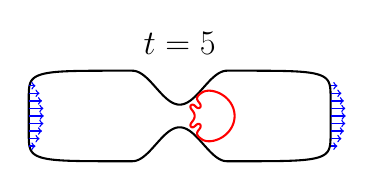
\begin{tikzpicture}[scale=0.5]

\begin{axis}[
  xmin = -11,
  xmax = 11,
  ymin = -3.2,
  ymax = 3.2,
  scale only axis,
  axis equal image,
  hide axis,
  title = {\Huge$t=5$}
  ]

\addplot [mark=none,black,line width=1.5] table{
1.0000e+01 0.0000e+00
1.0000e+01 3.6817e-02
1.0000e+01 7.3646e-02
1.0000e+01 1.1050e-01
1.0000e+01 1.4738e-01
1.0000e+01 1.8431e-01
1.0000e+01 2.2129e-01
1.0000e+01 2.5834e-01
1.0000e+01 2.9547e-01
1.0000e+01 3.3269e-01
1.0000e+01 3.7001e-01
1.0000e+01 4.0745e-01
1.0000e+01 4.4501e-01
1.0000e+01 4.8270e-01
1.0000e+01 5.2055e-01
1.0000e+01 5.5856e-01
1.0000e+01 5.9674e-01
1.0000e+01 6.3510e-01
1.0000e+01 6.7367e-01
1.0000e+01 7.1245e-01
1.0000e+01 7.5146e-01
1.0000e+01 7.9071e-01
1.0000e+01 8.3021e-01
9.9999e+00 8.6998e-01
9.9999e+00 9.1003e-01
9.9999e+00 9.5038e-01
9.9998e+00 9.9105e-01
9.9998e+00 1.0320e+00
9.9997e+00 1.0734e+00
9.9995e+00 1.1151e+00
9.9994e+00 1.1572e+00
9.9992e+00 1.1996e+00
9.9989e+00 1.2425e+00
9.9986e+00 1.2858e+00
9.9981e+00 1.3296e+00
9.9976e+00 1.3738e+00
9.9969e+00 1.4185e+00
9.9960e+00 1.4636e+00
9.9949e+00 1.5093e+00
9.9935e+00 1.5555e+00
9.9917e+00 1.6022e+00
9.9895e+00 1.6495e+00
9.9868e+00 1.6972e+00
9.9835e+00 1.7456e+00
9.9794e+00 1.7944e+00
9.9743e+00 1.8438e+00
9.9681e+00 1.8937e+00
9.9606e+00 1.9440e+00
9.9514e+00 1.9948e+00
9.9403e+00 2.0459e+00
9.9268e+00 2.0974e+00
9.9106e+00 2.1490e+00
9.8911e+00 2.2007e+00
9.8678e+00 2.2524e+00
9.8402e+00 2.3038e+00
9.8074e+00 2.3548e+00
9.7688e+00 2.4051e+00
9.7237e+00 2.4545e+00
9.6713e+00 2.5028e+00
9.6109e+00 2.5495e+00
9.5418e+00 2.5944e+00
9.4634e+00 2.6373e+00
9.3755e+00 2.6779e+00
9.2777e+00 2.7158e+00
9.1700e+00 2.7510e+00
9.0527e+00 2.7833e+00
8.9262e+00 2.8126e+00
8.7911e+00 2.8390e+00
8.6481e+00 2.8625e+00
8.4983e+00 2.8833e+00
8.3425e+00 2.9014e+00
8.1818e+00 2.9171e+00
8.0171e+00 2.9306e+00
7.8493e+00 2.9422e+00
7.6793e+00 2.9520e+00
7.5079e+00 2.9604e+00
7.3358e+00 2.9673e+00
7.1634e+00 2.9732e+00
6.9912e+00 2.9780e+00
6.8198e+00 2.9821e+00
6.6493e+00 2.9854e+00
6.4801e+00 2.9882e+00
6.3123e+00 2.9904e+00
6.1460e+00 2.9923e+00
5.9814e+00 2.9938e+00
5.8185e+00 2.9950e+00
5.6575e+00 2.9960e+00
5.4982e+00 2.9969e+00
5.3407e+00 2.9975e+00
5.1850e+00 2.9980e+00
5.0310e+00 2.9985e+00
4.8787e+00 2.9988e+00
4.7282e+00 2.9991e+00
4.5792e+00 2.9993e+00
4.4319e+00 2.9994e+00
4.2860e+00 2.9996e+00
4.1417e+00 2.9997e+00
3.9988e+00 2.9998e+00
3.8572e+00 2.9998e+00
3.7169e+00 2.9999e+00
3.5779e+00 2.9999e+00
3.4401e+00 2.9999e+00
3.3035e+00 2.9999e+00
3.1679e+00 3.0000e+00
3.0334e+00 2.9934e+00
2.8999e+00 2.9673e+00
2.7674e+00 2.9221e+00
2.6357e+00 2.8591e+00
2.5049e+00 2.7795e+00
2.3748e+00 2.6852e+00
2.2456e+00 2.5778e+00
2.1170e+00 2.4594e+00
1.9891e+00 2.3320e+00
1.8619e+00 2.1978e+00
1.7352e+00 2.0591e+00
1.6090e+00 1.9180e+00
1.4834e+00 1.7768e+00
1.3582e+00 1.6376e+00
1.2334e+00 1.5026e+00
1.1090e+00 1.3737e+00
9.8491e-01 1.2529e+00
8.6115e-01 1.1420e+00
7.3764e-01 1.0424e+00
6.1436e-01 9.5572e-01
4.9127e-01 8.8305e-01
3.6832e-01 8.2545e-01
2.4549e-01 7.8373e-01
1.2272e-01 7.5846e-01
6.1232e-16 7.5000e-01
-1.2272e-01 7.5846e-01
-2.4549e-01 7.8373e-01
-3.6832e-01 8.2545e-01
-4.9127e-01 8.8305e-01
-6.1436e-01 9.5572e-01
-7.3764e-01 1.0424e+00
-8.6115e-01 1.1420e+00
-9.8491e-01 1.2529e+00
-1.1090e+00 1.3737e+00
-1.2334e+00 1.5026e+00
-1.3582e+00 1.6376e+00
-1.4834e+00 1.7768e+00
-1.6090e+00 1.9180e+00
-1.7352e+00 2.0591e+00
-1.8619e+00 2.1978e+00
-1.9891e+00 2.3320e+00
-2.1170e+00 2.4594e+00
-2.2456e+00 2.5778e+00
-2.3748e+00 2.6852e+00
-2.5049e+00 2.7795e+00
-2.6357e+00 2.8591e+00
-2.7674e+00 2.9221e+00
-2.8999e+00 2.9673e+00
-3.0334e+00 2.9934e+00
-3.1679e+00 3.0000e+00
-3.3035e+00 2.9999e+00
-3.4401e+00 2.9999e+00
-3.5779e+00 2.9999e+00
-3.7169e+00 2.9999e+00
-3.8572e+00 2.9998e+00
-3.9988e+00 2.9998e+00
-4.1417e+00 2.9997e+00
-4.2860e+00 2.9996e+00
-4.4319e+00 2.9994e+00
-4.5792e+00 2.9993e+00
-4.7282e+00 2.9991e+00
-4.8787e+00 2.9988e+00
-5.0310e+00 2.9985e+00
-5.1850e+00 2.9980e+00
-5.3407e+00 2.9975e+00
-5.4982e+00 2.9969e+00
-5.6575e+00 2.9960e+00
-5.8185e+00 2.9950e+00
-5.9814e+00 2.9938e+00
-6.1460e+00 2.9923e+00
-6.3123e+00 2.9904e+00
-6.4801e+00 2.9882e+00
-6.6493e+00 2.9854e+00
-6.8198e+00 2.9821e+00
-6.9912e+00 2.9780e+00
-7.1634e+00 2.9732e+00
-7.3358e+00 2.9673e+00
-7.5079e+00 2.9604e+00
-7.6793e+00 2.9520e+00
-7.8493e+00 2.9422e+00
-8.0171e+00 2.9306e+00
-8.1818e+00 2.9171e+00
-8.3425e+00 2.9014e+00
-8.4983e+00 2.8833e+00
-8.6481e+00 2.8625e+00
-8.7911e+00 2.8390e+00
-8.9262e+00 2.8126e+00
-9.0527e+00 2.7833e+00
-9.1700e+00 2.7510e+00
-9.2777e+00 2.7158e+00
-9.3755e+00 2.6779e+00
-9.4634e+00 2.6373e+00
-9.5418e+00 2.5944e+00
-9.6109e+00 2.5495e+00
-9.6713e+00 2.5028e+00
-9.7237e+00 2.4545e+00
-9.7688e+00 2.4051e+00
-9.8074e+00 2.3548e+00
-9.8402e+00 2.3038e+00
-9.8678e+00 2.2524e+00
-9.8911e+00 2.2007e+00
-9.9106e+00 2.1490e+00
-9.9268e+00 2.0974e+00
-9.9403e+00 2.0459e+00
-9.9514e+00 1.9948e+00
-9.9606e+00 1.9440e+00
-9.9681e+00 1.8937e+00
-9.9743e+00 1.8438e+00
-9.9794e+00 1.7944e+00
-9.9835e+00 1.7456e+00
-9.9868e+00 1.6972e+00
-9.9895e+00 1.6495e+00
-9.9917e+00 1.6022e+00
-9.9935e+00 1.5555e+00
-9.9949e+00 1.5093e+00
-9.9960e+00 1.4636e+00
-9.9969e+00 1.4185e+00
-9.9976e+00 1.3738e+00
-9.9981e+00 1.3296e+00
-9.9986e+00 1.2858e+00
-9.9989e+00 1.2425e+00
-9.9992e+00 1.1996e+00
-9.9994e+00 1.1572e+00
-9.9995e+00 1.1151e+00
-9.9997e+00 1.0734e+00
-9.9998e+00 1.0320e+00
-9.9998e+00 9.9105e-01
-9.9999e+00 9.5038e-01
-9.9999e+00 9.1003e-01
-9.9999e+00 8.6998e-01
-1.0000e+01 8.3021e-01
-1.0000e+01 7.9071e-01
-1.0000e+01 7.5146e-01
-1.0000e+01 7.1245e-01
-1.0000e+01 6.7367e-01
-1.0000e+01 6.3510e-01
-1.0000e+01 5.9674e-01
-1.0000e+01 5.5856e-01
-1.0000e+01 5.2055e-01
-1.0000e+01 4.8270e-01
-1.0000e+01 4.4501e-01
-1.0000e+01 4.0745e-01
-1.0000e+01 3.7001e-01
-1.0000e+01 3.3269e-01
-1.0000e+01 2.9547e-01
-1.0000e+01 2.5834e-01
-1.0000e+01 2.2129e-01
-1.0000e+01 1.8431e-01
-1.0000e+01 1.4738e-01
-1.0000e+01 1.1050e-01
-1.0000e+01 7.3646e-02
-1.0000e+01 3.6817e-02
-1.0000e+01 3.6739e-16
-1.0000e+01 -3.6817e-02
-1.0000e+01 -7.3646e-02
-1.0000e+01 -1.1050e-01
-1.0000e+01 -1.4738e-01
-1.0000e+01 -1.8431e-01
-1.0000e+01 -2.2129e-01
-1.0000e+01 -2.5834e-01
-1.0000e+01 -2.9547e-01
-1.0000e+01 -3.3269e-01
-1.0000e+01 -3.7001e-01
-1.0000e+01 -4.0745e-01
-1.0000e+01 -4.4501e-01
-1.0000e+01 -4.8270e-01
-1.0000e+01 -5.2055e-01
-1.0000e+01 -5.5856e-01
-1.0000e+01 -5.9674e-01
-1.0000e+01 -6.3510e-01
-1.0000e+01 -6.7367e-01
-1.0000e+01 -7.1245e-01
-1.0000e+01 -7.5146e-01
-1.0000e+01 -7.9071e-01
-1.0000e+01 -8.3021e-01
-9.9999e+00 -8.6998e-01
-9.9999e+00 -9.1003e-01
-9.9999e+00 -9.5038e-01
-9.9998e+00 -9.9105e-01
-9.9998e+00 -1.0320e+00
-9.9997e+00 -1.0734e+00
-9.9995e+00 -1.1151e+00
-9.9994e+00 -1.1572e+00
-9.9992e+00 -1.1996e+00
-9.9989e+00 -1.2425e+00
-9.9986e+00 -1.2858e+00
-9.9981e+00 -1.3296e+00
-9.9976e+00 -1.3738e+00
-9.9969e+00 -1.4185e+00
-9.9960e+00 -1.4636e+00
-9.9949e+00 -1.5093e+00
-9.9935e+00 -1.5555e+00
-9.9917e+00 -1.6022e+00
-9.9895e+00 -1.6495e+00
-9.9868e+00 -1.6972e+00
-9.9835e+00 -1.7456e+00
-9.9794e+00 -1.7944e+00
-9.9743e+00 -1.8438e+00
-9.9681e+00 -1.8937e+00
-9.9606e+00 -1.9440e+00
-9.9514e+00 -1.9948e+00
-9.9403e+00 -2.0459e+00
-9.9268e+00 -2.0974e+00
-9.9106e+00 -2.1490e+00
-9.8911e+00 -2.2007e+00
-9.8678e+00 -2.2524e+00
-9.8402e+00 -2.3038e+00
-9.8074e+00 -2.3548e+00
-9.7688e+00 -2.4051e+00
-9.7237e+00 -2.4545e+00
-9.6713e+00 -2.5028e+00
-9.6109e+00 -2.5495e+00
-9.5418e+00 -2.5944e+00
-9.4634e+00 -2.6373e+00
-9.3755e+00 -2.6779e+00
-9.2777e+00 -2.7158e+00
-9.1700e+00 -2.7510e+00
-9.0527e+00 -2.7833e+00
-8.9262e+00 -2.8126e+00
-8.7911e+00 -2.8390e+00
-8.6481e+00 -2.8625e+00
-8.4983e+00 -2.8833e+00
-8.3425e+00 -2.9014e+00
-8.1818e+00 -2.9171e+00
-8.0171e+00 -2.9306e+00
-7.8493e+00 -2.9422e+00
-7.6793e+00 -2.9520e+00
-7.5079e+00 -2.9604e+00
-7.3358e+00 -2.9673e+00
-7.1634e+00 -2.9732e+00
-6.9912e+00 -2.9780e+00
-6.8198e+00 -2.9821e+00
-6.6493e+00 -2.9854e+00
-6.4801e+00 -2.9882e+00
-6.3123e+00 -2.9904e+00
-6.1460e+00 -2.9923e+00
-5.9814e+00 -2.9938e+00
-5.8185e+00 -2.9950e+00
-5.6575e+00 -2.9960e+00
-5.4982e+00 -2.9969e+00
-5.3407e+00 -2.9975e+00
-5.1850e+00 -2.9980e+00
-5.0310e+00 -2.9985e+00
-4.8787e+00 -2.9988e+00
-4.7282e+00 -2.9991e+00
-4.5792e+00 -2.9993e+00
-4.4319e+00 -2.9994e+00
-4.2860e+00 -2.9996e+00
-4.1417e+00 -2.9997e+00
-3.9988e+00 -2.9998e+00
-3.8572e+00 -2.9998e+00
-3.7169e+00 -2.9999e+00
-3.5779e+00 -2.9999e+00
-3.4401e+00 -2.9999e+00
-3.3035e+00 -2.9999e+00
-3.1679e+00 -3.0000e+00
-3.0334e+00 -2.9934e+00
-2.8999e+00 -2.9673e+00
-2.7674e+00 -2.9221e+00
-2.6357e+00 -2.8591e+00
-2.5049e+00 -2.7795e+00
-2.3748e+00 -2.6852e+00
-2.2456e+00 -2.5778e+00
-2.1170e+00 -2.4594e+00
-1.9891e+00 -2.3320e+00
-1.8619e+00 -2.1978e+00
-1.7352e+00 -2.0591e+00
-1.6090e+00 -1.9180e+00
-1.4834e+00 -1.7768e+00
-1.3582e+00 -1.6376e+00
-1.2334e+00 -1.5026e+00
-1.1090e+00 -1.3737e+00
-9.8491e-01 -1.2529e+00
-8.6115e-01 -1.1420e+00
-7.3764e-01 -1.0424e+00
-6.1436e-01 -9.5572e-01
-4.9127e-01 -8.8305e-01
-3.6832e-01 -8.2545e-01
-2.4549e-01 -7.8373e-01
-1.2272e-01 -7.5846e-01
-1.8370e-15 -7.5000e-01
1.2272e-01 -7.5846e-01
2.4549e-01 -7.8373e-01
3.6832e-01 -8.2545e-01
4.9127e-01 -8.8305e-01
6.1436e-01 -9.5572e-01
7.3764e-01 -1.0424e+00
8.6115e-01 -1.1420e+00
9.8491e-01 -1.2529e+00
1.1090e+00 -1.3737e+00
1.2334e+00 -1.5026e+00
1.3582e+00 -1.6376e+00
1.4834e+00 -1.7768e+00
1.6090e+00 -1.9180e+00
1.7352e+00 -2.0591e+00
1.8619e+00 -2.1978e+00
1.9891e+00 -2.3320e+00
2.1170e+00 -2.4594e+00
2.2456e+00 -2.5778e+00
2.3748e+00 -2.6852e+00
2.5049e+00 -2.7795e+00
2.6357e+00 -2.8591e+00
2.7674e+00 -2.9221e+00
2.8999e+00 -2.9673e+00
3.0334e+00 -2.9934e+00
3.1679e+00 -3.0000e+00
3.3035e+00 -2.9999e+00
3.4401e+00 -2.9999e+00
3.5779e+00 -2.9999e+00
3.7169e+00 -2.9999e+00
3.8572e+00 -2.9998e+00
3.9988e+00 -2.9998e+00
4.1417e+00 -2.9997e+00
4.2860e+00 -2.9996e+00
4.4319e+00 -2.9994e+00
4.5792e+00 -2.9993e+00
4.7282e+00 -2.9991e+00
4.8787e+00 -2.9988e+00
5.0310e+00 -2.9985e+00
5.1850e+00 -2.9980e+00
5.3407e+00 -2.9975e+00
5.4982e+00 -2.9969e+00
5.6575e+00 -2.9960e+00
5.8185e+00 -2.9950e+00
5.9814e+00 -2.9938e+00
6.1460e+00 -2.9923e+00
6.3123e+00 -2.9904e+00
6.4801e+00 -2.9882e+00
6.6493e+00 -2.9854e+00
6.8198e+00 -2.9821e+00
6.9912e+00 -2.9780e+00
7.1634e+00 -2.9732e+00
7.3358e+00 -2.9673e+00
7.5079e+00 -2.9604e+00
7.6793e+00 -2.9520e+00
7.8493e+00 -2.9422e+00
8.0171e+00 -2.9306e+00
8.1818e+00 -2.9171e+00
8.3425e+00 -2.9014e+00
8.4983e+00 -2.8833e+00
8.6481e+00 -2.8625e+00
8.7911e+00 -2.8390e+00
8.9262e+00 -2.8126e+00
9.0527e+00 -2.7833e+00
9.1700e+00 -2.7510e+00
9.2777e+00 -2.7158e+00
9.3755e+00 -2.6779e+00
9.4634e+00 -2.6373e+00
9.5418e+00 -2.5944e+00
9.6109e+00 -2.5495e+00
9.6713e+00 -2.5028e+00
9.7237e+00 -2.4545e+00
9.7688e+00 -2.4051e+00
9.8074e+00 -2.3548e+00
9.8402e+00 -2.3038e+00
9.8678e+00 -2.2524e+00
9.8911e+00 -2.2007e+00
9.9106e+00 -2.1490e+00
9.9268e+00 -2.0974e+00
9.9403e+00 -2.0459e+00
9.9514e+00 -1.9948e+00
9.9606e+00 -1.9440e+00
9.9681e+00 -1.8937e+00
9.9743e+00 -1.8438e+00
9.9794e+00 -1.7944e+00
9.9835e+00 -1.7456e+00
9.9868e+00 -1.6972e+00
9.9895e+00 -1.6495e+00
9.9917e+00 -1.6022e+00
9.9935e+00 -1.5555e+00
9.9949e+00 -1.5093e+00
9.9960e+00 -1.4636e+00
9.9969e+00 -1.4185e+00
9.9976e+00 -1.3738e+00
9.9981e+00 -1.3296e+00
9.9986e+00 -1.2858e+00
9.9989e+00 -1.2425e+00
9.9992e+00 -1.1996e+00
9.9994e+00 -1.1572e+00
9.9995e+00 -1.1151e+00
9.9997e+00 -1.0734e+00
9.9998e+00 -1.0320e+00
9.9998e+00 -9.9105e-01
9.9999e+00 -9.5038e-01
9.9999e+00 -9.1003e-01
9.9999e+00 -8.6998e-01
1.0000e+01 -8.3021e-01
1.0000e+01 -7.9071e-01
1.0000e+01 -7.5146e-01
1.0000e+01 -7.1245e-01
1.0000e+01 -6.7367e-01
1.0000e+01 -6.3510e-01
1.0000e+01 -5.9674e-01
1.0000e+01 -5.5856e-01
1.0000e+01 -5.2055e-01
1.0000e+01 -4.8270e-01
1.0000e+01 -4.4501e-01
1.0000e+01 -4.0745e-01
1.0000e+01 -3.7001e-01
1.0000e+01 -3.3269e-01
1.0000e+01 -2.9547e-01
1.0000e+01 -2.5834e-01
1.0000e+01 -2.2129e-01
1.0000e+01 -1.8431e-01
1.0000e+01 -1.4738e-01
1.0000e+01 -1.1050e-01
1.0000e+01 -7.3646e-02
1.0000e+01 -3.6817e-02
1.0000e+01 0.0000e+00
};


\addplot [mark=none,red,line width=1.5] table{
1.6497e+00 1.6305e+00
1.6297e+00 1.6235e+00
1.6096e+00 1.6158e+00
1.5895e+00 1.6075e+00
1.5692e+00 1.5985e+00
1.5488e+00 1.5886e+00
1.5282e+00 1.5780e+00
1.5073e+00 1.5664e+00
1.4861e+00 1.5539e+00
1.4646e+00 1.5405e+00
1.4428e+00 1.5260e+00
1.4206e+00 1.5105e+00
1.3981e+00 1.4941e+00
1.3751e+00 1.4765e+00
1.3517e+00 1.4580e+00
1.3279e+00 1.4383e+00
1.3039e+00 1.4174e+00
1.2797e+00 1.3951e+00
1.2556e+00 1.3712e+00
1.2322e+00 1.3452e+00
1.2101e+00 1.3167e+00
1.1903e+00 1.2854e+00
1.1739e+00 1.2510e+00
1.1623e+00 1.2136e+00
1.1566e+00 1.1738e+00
1.1576e+00 1.1326e+00
1.1656e+00 1.0911e+00
1.1801e+00 1.0503e+00
1.2003e+00 1.0109e+00
1.2249e+00 9.7282e-01
1.2526e+00 9.3574e-01
1.2821e+00 8.9881e-01
1.3119e+00 8.6095e-01
1.3403e+00 8.2093e-01
1.3653e+00 7.7762e-01
1.3840e+00 7.3033e-01
1.3927e+00 6.7942e-01
1.3874e+00 6.2730e-01
1.3650e+00 5.7912e-01
1.3258e+00 5.4226e-01
1.2745e+00 5.2340e-01
1.2191e+00 5.2481e-01
1.1662e+00 5.4370e-01
1.1183e+00 5.7468e-01
1.0747e+00 6.1245e-01
1.0325e+00 6.5272e-01
9.8829e-01 6.9169e-01
9.3904e-01 7.2494e-01
8.8324e-01 7.4656e-01
8.2312e-01 7.4919e-01
7.6691e-01 7.2688e-01
7.2703e-01 6.8093e-01
7.1172e-01 6.2150e-01
7.1957e-01 5.6006e-01
7.4365e-01 5.0245e-01
7.7711e-01 4.4927e-01
8.1502e-01 3.9878e-01
8.5402e-01 3.4883e-01
8.9159e-01 2.9754e-01
9.2564e-01 2.4366e-01
9.5431e-01 1.8660e-01
9.7602e-01 1.2644e-01
9.8956e-01 6.3879e-02
9.9416e-01 1.5008e-09
9.8956e-01 -6.3879e-02
9.7602e-01 -1.2644e-01
9.5431e-01 -1.8660e-01
9.2564e-01 -2.4366e-01
8.9159e-01 -2.9754e-01
8.5402e-01 -3.4883e-01
8.1502e-01 -3.9878e-01
7.7711e-01 -4.4927e-01
7.4365e-01 -5.0245e-01
7.1957e-01 -5.6006e-01
7.1172e-01 -6.2150e-01
7.2703e-01 -6.8093e-01
7.6691e-01 -7.2688e-01
8.2312e-01 -7.4919e-01
8.8324e-01 -7.4656e-01
9.3904e-01 -7.2494e-01
9.8829e-01 -6.9169e-01
1.0325e+00 -6.5272e-01
1.0747e+00 -6.1245e-01
1.1183e+00 -5.7468e-01
1.1662e+00 -5.4370e-01
1.2191e+00 -5.2481e-01
1.2745e+00 -5.2340e-01
1.3258e+00 -5.4226e-01
1.3650e+00 -5.7912e-01
1.3874e+00 -6.2730e-01
1.3927e+00 -6.7942e-01
1.3840e+00 -7.3033e-01
1.3653e+00 -7.7762e-01
1.3403e+00 -8.2093e-01
1.3119e+00 -8.6095e-01
1.2821e+00 -8.9881e-01
1.2526e+00 -9.3574e-01
1.2249e+00 -9.7282e-01
1.2003e+00 -1.0109e+00
1.1801e+00 -1.0503e+00
1.1656e+00 -1.0911e+00
1.1576e+00 -1.1326e+00
1.1566e+00 -1.1738e+00
1.1623e+00 -1.2136e+00
1.1739e+00 -1.2510e+00
1.1903e+00 -1.2854e+00
1.2101e+00 -1.3167e+00
1.2322e+00 -1.3452e+00
1.2556e+00 -1.3712e+00
1.2797e+00 -1.3951e+00
1.3039e+00 -1.4174e+00
1.3279e+00 -1.4383e+00
1.3517e+00 -1.4580e+00
1.3751e+00 -1.4765e+00
1.3981e+00 -1.4941e+00
1.4206e+00 -1.5105e+00
1.4428e+00 -1.5260e+00
1.4646e+00 -1.5405e+00
1.4861e+00 -1.5539e+00
1.5073e+00 -1.5664e+00
1.5282e+00 -1.5780e+00
1.5488e+00 -1.5886e+00
1.5692e+00 -1.5985e+00
1.5895e+00 -1.6075e+00
1.6096e+00 -1.6158e+00
1.6297e+00 -1.6235e+00
1.6497e+00 -1.6305e+00
1.6699e+00 -1.6369e+00
1.6902e+00 -1.6428e+00
1.7108e+00 -1.6482e+00
1.7317e+00 -1.6531e+00
1.7530e+00 -1.6575e+00
1.7748e+00 -1.6615e+00
1.7972e+00 -1.6649e+00
1.8203e+00 -1.6679e+00
1.8440e+00 -1.6704e+00
1.8685e+00 -1.6724e+00
1.8938e+00 -1.6738e+00
1.9200e+00 -1.6747e+00
1.9470e+00 -1.6749e+00
1.9750e+00 -1.6745e+00
2.0038e+00 -1.6735e+00
2.0336e+00 -1.6717e+00
2.0644e+00 -1.6692e+00
2.0961e+00 -1.6658e+00
2.1287e+00 -1.6617e+00
2.1623e+00 -1.6566e+00
2.1967e+00 -1.6506e+00
2.2321e+00 -1.6437e+00
2.2683e+00 -1.6357e+00
2.3054e+00 -1.6267e+00
2.3432e+00 -1.6165e+00
2.3818e+00 -1.6052e+00
2.4212e+00 -1.5927e+00
2.4612e+00 -1.5790e+00
2.5018e+00 -1.5639e+00
2.5430e+00 -1.5476e+00
2.5847e+00 -1.5298e+00
2.6268e+00 -1.5106e+00
2.6693e+00 -1.4899e+00
2.7121e+00 -1.4678e+00
2.7551e+00 -1.4440e+00
2.7983e+00 -1.4187e+00
2.8415e+00 -1.3918e+00
2.8846e+00 -1.3632e+00
2.9277e+00 -1.3330e+00
2.9705e+00 -1.3010e+00
3.0129e+00 -1.2674e+00
3.0550e+00 -1.2320e+00
3.0965e+00 -1.1948e+00
3.1373e+00 -1.1559e+00
3.1774e+00 -1.1153e+00
3.2166e+00 -1.0729e+00
3.2548e+00 -1.0288e+00
3.2918e+00 -9.8299e-01
3.3277e+00 -9.3549e-01
3.3621e+00 -8.8633e-01
3.3951e+00 -8.3557e-01
3.4265e+00 -7.8324e-01
3.4561e+00 -7.2942e-01
3.4839e+00 -6.7416e-01
3.5097e+00 -6.1755e-01
3.5334e+00 -5.5967e-01
3.5549e+00 -5.0061e-01
3.5742e+00 -4.4049e-01
3.5911e+00 -3.7940e-01
3.6055e+00 -3.1748e-01
3.6174e+00 -2.5486e-01
3.6268e+00 -1.9165e-01
3.6334e+00 -1.2801e-01
3.6375e+00 -6.4080e-02
3.6388e+00 -4.3871e-08
3.6375e+00 6.4080e-02
3.6334e+00 1.2801e-01
3.6268e+00 1.9165e-01
3.6174e+00 2.5486e-01
3.6055e+00 3.1748e-01
3.5911e+00 3.7940e-01
3.5742e+00 4.4048e-01
3.5549e+00 5.0061e-01
3.5334e+00 5.5967e-01
3.5097e+00 6.1755e-01
3.4839e+00 6.7416e-01
3.4561e+00 7.2942e-01
3.4265e+00 7.8324e-01
3.3951e+00 8.3557e-01
3.3621e+00 8.8633e-01
3.3277e+00 9.3549e-01
3.2918e+00 9.8299e-01
3.2548e+00 1.0288e+00
3.2166e+00 1.0729e+00
3.1774e+00 1.1153e+00
3.1373e+00 1.1559e+00
3.0965e+00 1.1948e+00
3.0550e+00 1.2320e+00
3.0129e+00 1.2674e+00
2.9705e+00 1.3010e+00
2.9277e+00 1.3330e+00
2.8846e+00 1.3632e+00
2.8415e+00 1.3918e+00
2.7983e+00 1.4187e+00
2.7551e+00 1.4440e+00
2.7121e+00 1.4678e+00
2.6693e+00 1.4899e+00
2.6268e+00 1.5106e+00
2.5847e+00 1.5298e+00
2.5430e+00 1.5476e+00
2.5018e+00 1.5639e+00
2.4612e+00 1.5790e+00
2.4212e+00 1.5927e+00
2.3818e+00 1.6052e+00
2.3432e+00 1.6165e+00
2.3054e+00 1.6267e+00
2.2683e+00 1.6357e+00
2.2321e+00 1.6437e+00
2.1967e+00 1.6506e+00
2.1623e+00 1.6566e+00
2.1287e+00 1.6617e+00
2.0961e+00 1.6658e+00
2.0644e+00 1.6692e+00
2.0336e+00 1.6717e+00
2.0038e+00 1.6735e+00
1.9750e+00 1.6745e+00
1.9470e+00 1.6749e+00
1.9200e+00 1.6747e+00
1.8938e+00 1.6738e+00
1.8685e+00 1.6724e+00
1.8440e+00 1.6704e+00
1.8203e+00 1.6679e+00
1.7972e+00 1.6649e+00
1.7748e+00 1.6615e+00
1.7530e+00 1.6575e+00
1.7317e+00 1.6531e+00
1.7108e+00 1.6482e+00
1.6902e+00 1.6428e+00
1.6699e+00 1.6369e+00
1.6497e+00 1.6305e+00
};

\foreach \y in {-2.0,-1.5,...,2.0}
\addplot[color=blue,line width = 1.0pt,solid,->]
plot coordinates{
  (-10,\y)
  (-10+exp(9/(\y*\y-9))/exp(-1),\y)
};

\foreach \y in {-2.0,-1.5,...,2.0}
\addplot[color=blue,line width = 1.0pt,solid,->]
plot coordinates{
  (10,\y)
  (10+exp(9/(\y*\y-9))/exp(-1),\y)
};

\end{axis}

\end{tikzpicture}



 \\
%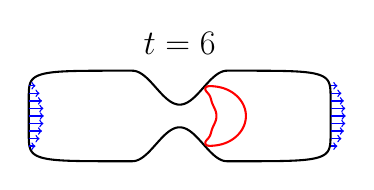
\begin{tikzpicture}[scale=0.5]

\begin{axis}[
  xmin = -11,
  xmax = 11,
  ymin = -3.2,
  ymax = 3.2,
  scale only axis,
  axis equal image,
  hide axis,
  title = {\Huge$t=6$}
  ]

\addplot [mark=none,black,line width=1.5] table{
1.0000e+01 0.0000e+00
1.0000e+01 3.6817e-02
1.0000e+01 7.3646e-02
1.0000e+01 1.1050e-01
1.0000e+01 1.4738e-01
1.0000e+01 1.8431e-01
1.0000e+01 2.2129e-01
1.0000e+01 2.5834e-01
1.0000e+01 2.9547e-01
1.0000e+01 3.3269e-01
1.0000e+01 3.7001e-01
1.0000e+01 4.0745e-01
1.0000e+01 4.4501e-01
1.0000e+01 4.8270e-01
1.0000e+01 5.2055e-01
1.0000e+01 5.5856e-01
1.0000e+01 5.9674e-01
1.0000e+01 6.3510e-01
1.0000e+01 6.7367e-01
1.0000e+01 7.1245e-01
1.0000e+01 7.5146e-01
1.0000e+01 7.9071e-01
1.0000e+01 8.3021e-01
9.9999e+00 8.6998e-01
9.9999e+00 9.1003e-01
9.9999e+00 9.5038e-01
9.9998e+00 9.9105e-01
9.9998e+00 1.0320e+00
9.9997e+00 1.0734e+00
9.9995e+00 1.1151e+00
9.9994e+00 1.1572e+00
9.9992e+00 1.1996e+00
9.9989e+00 1.2425e+00
9.9986e+00 1.2858e+00
9.9981e+00 1.3296e+00
9.9976e+00 1.3738e+00
9.9969e+00 1.4185e+00
9.9960e+00 1.4636e+00
9.9949e+00 1.5093e+00
9.9935e+00 1.5555e+00
9.9917e+00 1.6022e+00
9.9895e+00 1.6495e+00
9.9868e+00 1.6972e+00
9.9835e+00 1.7456e+00
9.9794e+00 1.7944e+00
9.9743e+00 1.8438e+00
9.9681e+00 1.8937e+00
9.9606e+00 1.9440e+00
9.9514e+00 1.9948e+00
9.9403e+00 2.0459e+00
9.9268e+00 2.0974e+00
9.9106e+00 2.1490e+00
9.8911e+00 2.2007e+00
9.8678e+00 2.2524e+00
9.8402e+00 2.3038e+00
9.8074e+00 2.3548e+00
9.7688e+00 2.4051e+00
9.7237e+00 2.4545e+00
9.6713e+00 2.5028e+00
9.6109e+00 2.5495e+00
9.5418e+00 2.5944e+00
9.4634e+00 2.6373e+00
9.3755e+00 2.6779e+00
9.2777e+00 2.7158e+00
9.1700e+00 2.7510e+00
9.0527e+00 2.7833e+00
8.9262e+00 2.8126e+00
8.7911e+00 2.8390e+00
8.6481e+00 2.8625e+00
8.4983e+00 2.8833e+00
8.3425e+00 2.9014e+00
8.1818e+00 2.9171e+00
8.0171e+00 2.9306e+00
7.8493e+00 2.9422e+00
7.6793e+00 2.9520e+00
7.5079e+00 2.9604e+00
7.3358e+00 2.9673e+00
7.1634e+00 2.9732e+00
6.9912e+00 2.9780e+00
6.8198e+00 2.9821e+00
6.6493e+00 2.9854e+00
6.4801e+00 2.9882e+00
6.3123e+00 2.9904e+00
6.1460e+00 2.9923e+00
5.9814e+00 2.9938e+00
5.8185e+00 2.9950e+00
5.6575e+00 2.9960e+00
5.4982e+00 2.9969e+00
5.3407e+00 2.9975e+00
5.1850e+00 2.9980e+00
5.0310e+00 2.9985e+00
4.8787e+00 2.9988e+00
4.7282e+00 2.9991e+00
4.5792e+00 2.9993e+00
4.4319e+00 2.9994e+00
4.2860e+00 2.9996e+00
4.1417e+00 2.9997e+00
3.9988e+00 2.9998e+00
3.8572e+00 2.9998e+00
3.7169e+00 2.9999e+00
3.5779e+00 2.9999e+00
3.4401e+00 2.9999e+00
3.3035e+00 2.9999e+00
3.1679e+00 3.0000e+00
3.0334e+00 2.9934e+00
2.8999e+00 2.9673e+00
2.7674e+00 2.9221e+00
2.6357e+00 2.8591e+00
2.5049e+00 2.7795e+00
2.3748e+00 2.6852e+00
2.2456e+00 2.5778e+00
2.1170e+00 2.4594e+00
1.9891e+00 2.3320e+00
1.8619e+00 2.1978e+00
1.7352e+00 2.0591e+00
1.6090e+00 1.9180e+00
1.4834e+00 1.7768e+00
1.3582e+00 1.6376e+00
1.2334e+00 1.5026e+00
1.1090e+00 1.3737e+00
9.8491e-01 1.2529e+00
8.6115e-01 1.1420e+00
7.3764e-01 1.0424e+00
6.1436e-01 9.5572e-01
4.9127e-01 8.8305e-01
3.6832e-01 8.2545e-01
2.4549e-01 7.8373e-01
1.2272e-01 7.5846e-01
6.1232e-16 7.5000e-01
-1.2272e-01 7.5846e-01
-2.4549e-01 7.8373e-01
-3.6832e-01 8.2545e-01
-4.9127e-01 8.8305e-01
-6.1436e-01 9.5572e-01
-7.3764e-01 1.0424e+00
-8.6115e-01 1.1420e+00
-9.8491e-01 1.2529e+00
-1.1090e+00 1.3737e+00
-1.2334e+00 1.5026e+00
-1.3582e+00 1.6376e+00
-1.4834e+00 1.7768e+00
-1.6090e+00 1.9180e+00
-1.7352e+00 2.0591e+00
-1.8619e+00 2.1978e+00
-1.9891e+00 2.3320e+00
-2.1170e+00 2.4594e+00
-2.2456e+00 2.5778e+00
-2.3748e+00 2.6852e+00
-2.5049e+00 2.7795e+00
-2.6357e+00 2.8591e+00
-2.7674e+00 2.9221e+00
-2.8999e+00 2.9673e+00
-3.0334e+00 2.9934e+00
-3.1679e+00 3.0000e+00
-3.3035e+00 2.9999e+00
-3.4401e+00 2.9999e+00
-3.5779e+00 2.9999e+00
-3.7169e+00 2.9999e+00
-3.8572e+00 2.9998e+00
-3.9988e+00 2.9998e+00
-4.1417e+00 2.9997e+00
-4.2860e+00 2.9996e+00
-4.4319e+00 2.9994e+00
-4.5792e+00 2.9993e+00
-4.7282e+00 2.9991e+00
-4.8787e+00 2.9988e+00
-5.0310e+00 2.9985e+00
-5.1850e+00 2.9980e+00
-5.3407e+00 2.9975e+00
-5.4982e+00 2.9969e+00
-5.6575e+00 2.9960e+00
-5.8185e+00 2.9950e+00
-5.9814e+00 2.9938e+00
-6.1460e+00 2.9923e+00
-6.3123e+00 2.9904e+00
-6.4801e+00 2.9882e+00
-6.6493e+00 2.9854e+00
-6.8198e+00 2.9821e+00
-6.9912e+00 2.9780e+00
-7.1634e+00 2.9732e+00
-7.3358e+00 2.9673e+00
-7.5079e+00 2.9604e+00
-7.6793e+00 2.9520e+00
-7.8493e+00 2.9422e+00
-8.0171e+00 2.9306e+00
-8.1818e+00 2.9171e+00
-8.3425e+00 2.9014e+00
-8.4983e+00 2.8833e+00
-8.6481e+00 2.8625e+00
-8.7911e+00 2.8390e+00
-8.9262e+00 2.8126e+00
-9.0527e+00 2.7833e+00
-9.1700e+00 2.7510e+00
-9.2777e+00 2.7158e+00
-9.3755e+00 2.6779e+00
-9.4634e+00 2.6373e+00
-9.5418e+00 2.5944e+00
-9.6109e+00 2.5495e+00
-9.6713e+00 2.5028e+00
-9.7237e+00 2.4545e+00
-9.7688e+00 2.4051e+00
-9.8074e+00 2.3548e+00
-9.8402e+00 2.3038e+00
-9.8678e+00 2.2524e+00
-9.8911e+00 2.2007e+00
-9.9106e+00 2.1490e+00
-9.9268e+00 2.0974e+00
-9.9403e+00 2.0459e+00
-9.9514e+00 1.9948e+00
-9.9606e+00 1.9440e+00
-9.9681e+00 1.8937e+00
-9.9743e+00 1.8438e+00
-9.9794e+00 1.7944e+00
-9.9835e+00 1.7456e+00
-9.9868e+00 1.6972e+00
-9.9895e+00 1.6495e+00
-9.9917e+00 1.6022e+00
-9.9935e+00 1.5555e+00
-9.9949e+00 1.5093e+00
-9.9960e+00 1.4636e+00
-9.9969e+00 1.4185e+00
-9.9976e+00 1.3738e+00
-9.9981e+00 1.3296e+00
-9.9986e+00 1.2858e+00
-9.9989e+00 1.2425e+00
-9.9992e+00 1.1996e+00
-9.9994e+00 1.1572e+00
-9.9995e+00 1.1151e+00
-9.9997e+00 1.0734e+00
-9.9998e+00 1.0320e+00
-9.9998e+00 9.9105e-01
-9.9999e+00 9.5038e-01
-9.9999e+00 9.1003e-01
-9.9999e+00 8.6998e-01
-1.0000e+01 8.3021e-01
-1.0000e+01 7.9071e-01
-1.0000e+01 7.5146e-01
-1.0000e+01 7.1245e-01
-1.0000e+01 6.7367e-01
-1.0000e+01 6.3510e-01
-1.0000e+01 5.9674e-01
-1.0000e+01 5.5856e-01
-1.0000e+01 5.2055e-01
-1.0000e+01 4.8270e-01
-1.0000e+01 4.4501e-01
-1.0000e+01 4.0745e-01
-1.0000e+01 3.7001e-01
-1.0000e+01 3.3269e-01
-1.0000e+01 2.9547e-01
-1.0000e+01 2.5834e-01
-1.0000e+01 2.2129e-01
-1.0000e+01 1.8431e-01
-1.0000e+01 1.4738e-01
-1.0000e+01 1.1050e-01
-1.0000e+01 7.3646e-02
-1.0000e+01 3.6817e-02
-1.0000e+01 3.6739e-16
-1.0000e+01 -3.6817e-02
-1.0000e+01 -7.3646e-02
-1.0000e+01 -1.1050e-01
-1.0000e+01 -1.4738e-01
-1.0000e+01 -1.8431e-01
-1.0000e+01 -2.2129e-01
-1.0000e+01 -2.5834e-01
-1.0000e+01 -2.9547e-01
-1.0000e+01 -3.3269e-01
-1.0000e+01 -3.7001e-01
-1.0000e+01 -4.0745e-01
-1.0000e+01 -4.4501e-01
-1.0000e+01 -4.8270e-01
-1.0000e+01 -5.2055e-01
-1.0000e+01 -5.5856e-01
-1.0000e+01 -5.9674e-01
-1.0000e+01 -6.3510e-01
-1.0000e+01 -6.7367e-01
-1.0000e+01 -7.1245e-01
-1.0000e+01 -7.5146e-01
-1.0000e+01 -7.9071e-01
-1.0000e+01 -8.3021e-01
-9.9999e+00 -8.6998e-01
-9.9999e+00 -9.1003e-01
-9.9999e+00 -9.5038e-01
-9.9998e+00 -9.9105e-01
-9.9998e+00 -1.0320e+00
-9.9997e+00 -1.0734e+00
-9.9995e+00 -1.1151e+00
-9.9994e+00 -1.1572e+00
-9.9992e+00 -1.1996e+00
-9.9989e+00 -1.2425e+00
-9.9986e+00 -1.2858e+00
-9.9981e+00 -1.3296e+00
-9.9976e+00 -1.3738e+00
-9.9969e+00 -1.4185e+00
-9.9960e+00 -1.4636e+00
-9.9949e+00 -1.5093e+00
-9.9935e+00 -1.5555e+00
-9.9917e+00 -1.6022e+00
-9.9895e+00 -1.6495e+00
-9.9868e+00 -1.6972e+00
-9.9835e+00 -1.7456e+00
-9.9794e+00 -1.7944e+00
-9.9743e+00 -1.8438e+00
-9.9681e+00 -1.8937e+00
-9.9606e+00 -1.9440e+00
-9.9514e+00 -1.9948e+00
-9.9403e+00 -2.0459e+00
-9.9268e+00 -2.0974e+00
-9.9106e+00 -2.1490e+00
-9.8911e+00 -2.2007e+00
-9.8678e+00 -2.2524e+00
-9.8402e+00 -2.3038e+00
-9.8074e+00 -2.3548e+00
-9.7688e+00 -2.4051e+00
-9.7237e+00 -2.4545e+00
-9.6713e+00 -2.5028e+00
-9.6109e+00 -2.5495e+00
-9.5418e+00 -2.5944e+00
-9.4634e+00 -2.6373e+00
-9.3755e+00 -2.6779e+00
-9.2777e+00 -2.7158e+00
-9.1700e+00 -2.7510e+00
-9.0527e+00 -2.7833e+00
-8.9262e+00 -2.8126e+00
-8.7911e+00 -2.8390e+00
-8.6481e+00 -2.8625e+00
-8.4983e+00 -2.8833e+00
-8.3425e+00 -2.9014e+00
-8.1818e+00 -2.9171e+00
-8.0171e+00 -2.9306e+00
-7.8493e+00 -2.9422e+00
-7.6793e+00 -2.9520e+00
-7.5079e+00 -2.9604e+00
-7.3358e+00 -2.9673e+00
-7.1634e+00 -2.9732e+00
-6.9912e+00 -2.9780e+00
-6.8198e+00 -2.9821e+00
-6.6493e+00 -2.9854e+00
-6.4801e+00 -2.9882e+00
-6.3123e+00 -2.9904e+00
-6.1460e+00 -2.9923e+00
-5.9814e+00 -2.9938e+00
-5.8185e+00 -2.9950e+00
-5.6575e+00 -2.9960e+00
-5.4982e+00 -2.9969e+00
-5.3407e+00 -2.9975e+00
-5.1850e+00 -2.9980e+00
-5.0310e+00 -2.9985e+00
-4.8787e+00 -2.9988e+00
-4.7282e+00 -2.9991e+00
-4.5792e+00 -2.9993e+00
-4.4319e+00 -2.9994e+00
-4.2860e+00 -2.9996e+00
-4.1417e+00 -2.9997e+00
-3.9988e+00 -2.9998e+00
-3.8572e+00 -2.9998e+00
-3.7169e+00 -2.9999e+00
-3.5779e+00 -2.9999e+00
-3.4401e+00 -2.9999e+00
-3.3035e+00 -2.9999e+00
-3.1679e+00 -3.0000e+00
-3.0334e+00 -2.9934e+00
-2.8999e+00 -2.9673e+00
-2.7674e+00 -2.9221e+00
-2.6357e+00 -2.8591e+00
-2.5049e+00 -2.7795e+00
-2.3748e+00 -2.6852e+00
-2.2456e+00 -2.5778e+00
-2.1170e+00 -2.4594e+00
-1.9891e+00 -2.3320e+00
-1.8619e+00 -2.1978e+00
-1.7352e+00 -2.0591e+00
-1.6090e+00 -1.9180e+00
-1.4834e+00 -1.7768e+00
-1.3582e+00 -1.6376e+00
-1.2334e+00 -1.5026e+00
-1.1090e+00 -1.3737e+00
-9.8491e-01 -1.2529e+00
-8.6115e-01 -1.1420e+00
-7.3764e-01 -1.0424e+00
-6.1436e-01 -9.5572e-01
-4.9127e-01 -8.8305e-01
-3.6832e-01 -8.2545e-01
-2.4549e-01 -7.8373e-01
-1.2272e-01 -7.5846e-01
-1.8370e-15 -7.5000e-01
1.2272e-01 -7.5846e-01
2.4549e-01 -7.8373e-01
3.6832e-01 -8.2545e-01
4.9127e-01 -8.8305e-01
6.1436e-01 -9.5572e-01
7.3764e-01 -1.0424e+00
8.6115e-01 -1.1420e+00
9.8491e-01 -1.2529e+00
1.1090e+00 -1.3737e+00
1.2334e+00 -1.5026e+00
1.3582e+00 -1.6376e+00
1.4834e+00 -1.7768e+00
1.6090e+00 -1.9180e+00
1.7352e+00 -2.0591e+00
1.8619e+00 -2.1978e+00
1.9891e+00 -2.3320e+00
2.1170e+00 -2.4594e+00
2.2456e+00 -2.5778e+00
2.3748e+00 -2.6852e+00
2.5049e+00 -2.7795e+00
2.6357e+00 -2.8591e+00
2.7674e+00 -2.9221e+00
2.8999e+00 -2.9673e+00
3.0334e+00 -2.9934e+00
3.1679e+00 -3.0000e+00
3.3035e+00 -2.9999e+00
3.4401e+00 -2.9999e+00
3.5779e+00 -2.9999e+00
3.7169e+00 -2.9999e+00
3.8572e+00 -2.9998e+00
3.9988e+00 -2.9998e+00
4.1417e+00 -2.9997e+00
4.2860e+00 -2.9996e+00
4.4319e+00 -2.9994e+00
4.5792e+00 -2.9993e+00
4.7282e+00 -2.9991e+00
4.8787e+00 -2.9988e+00
5.0310e+00 -2.9985e+00
5.1850e+00 -2.9980e+00
5.3407e+00 -2.9975e+00
5.4982e+00 -2.9969e+00
5.6575e+00 -2.9960e+00
5.8185e+00 -2.9950e+00
5.9814e+00 -2.9938e+00
6.1460e+00 -2.9923e+00
6.3123e+00 -2.9904e+00
6.4801e+00 -2.9882e+00
6.6493e+00 -2.9854e+00
6.8198e+00 -2.9821e+00
6.9912e+00 -2.9780e+00
7.1634e+00 -2.9732e+00
7.3358e+00 -2.9673e+00
7.5079e+00 -2.9604e+00
7.6793e+00 -2.9520e+00
7.8493e+00 -2.9422e+00
8.0171e+00 -2.9306e+00
8.1818e+00 -2.9171e+00
8.3425e+00 -2.9014e+00
8.4983e+00 -2.8833e+00
8.6481e+00 -2.8625e+00
8.7911e+00 -2.8390e+00
8.9262e+00 -2.8126e+00
9.0527e+00 -2.7833e+00
9.1700e+00 -2.7510e+00
9.2777e+00 -2.7158e+00
9.3755e+00 -2.6779e+00
9.4634e+00 -2.6373e+00
9.5418e+00 -2.5944e+00
9.6109e+00 -2.5495e+00
9.6713e+00 -2.5028e+00
9.7237e+00 -2.4545e+00
9.7688e+00 -2.4051e+00
9.8074e+00 -2.3548e+00
9.8402e+00 -2.3038e+00
9.8678e+00 -2.2524e+00
9.8911e+00 -2.2007e+00
9.9106e+00 -2.1490e+00
9.9268e+00 -2.0974e+00
9.9403e+00 -2.0459e+00
9.9514e+00 -1.9948e+00
9.9606e+00 -1.9440e+00
9.9681e+00 -1.8937e+00
9.9743e+00 -1.8438e+00
9.9794e+00 -1.7944e+00
9.9835e+00 -1.7456e+00
9.9868e+00 -1.6972e+00
9.9895e+00 -1.6495e+00
9.9917e+00 -1.6022e+00
9.9935e+00 -1.5555e+00
9.9949e+00 -1.5093e+00
9.9960e+00 -1.4636e+00
9.9969e+00 -1.4185e+00
9.9976e+00 -1.3738e+00
9.9981e+00 -1.3296e+00
9.9986e+00 -1.2858e+00
9.9989e+00 -1.2425e+00
9.9992e+00 -1.1996e+00
9.9994e+00 -1.1572e+00
9.9995e+00 -1.1151e+00
9.9997e+00 -1.0734e+00
9.9998e+00 -1.0320e+00
9.9998e+00 -9.9105e-01
9.9999e+00 -9.5038e-01
9.9999e+00 -9.1003e-01
9.9999e+00 -8.6998e-01
1.0000e+01 -8.3021e-01
1.0000e+01 -7.9071e-01
1.0000e+01 -7.5146e-01
1.0000e+01 -7.1245e-01
1.0000e+01 -6.7367e-01
1.0000e+01 -6.3510e-01
1.0000e+01 -5.9674e-01
1.0000e+01 -5.5856e-01
1.0000e+01 -5.2055e-01
1.0000e+01 -4.8270e-01
1.0000e+01 -4.4501e-01
1.0000e+01 -4.0745e-01
1.0000e+01 -3.7001e-01
1.0000e+01 -3.3269e-01
1.0000e+01 -2.9547e-01
1.0000e+01 -2.5834e-01
1.0000e+01 -2.2129e-01
1.0000e+01 -1.8431e-01
1.0000e+01 -1.4738e-01
1.0000e+01 -1.1050e-01
1.0000e+01 -7.3646e-02
1.0000e+01 -3.6817e-02
1.0000e+01 0.0000e+00
};


\addplot [mark=none,red,line width=1.5] table{
2.5161e+00 1.9325e+00
2.4951e+00 1.9359e+00
2.4739e+00 1.9393e+00
2.4523e+00 1.9425e+00
2.4304e+00 1.9456e+00
2.4079e+00 1.9487e+00
2.3849e+00 1.9516e+00
2.3612e+00 1.9545e+00
2.3368e+00 1.9573e+00
2.3116e+00 1.9600e+00
2.2855e+00 1.9627e+00
2.2586e+00 1.9652e+00
2.2307e+00 1.9676e+00
2.2019e+00 1.9699e+00
2.1722e+00 1.9720e+00
2.1414e+00 1.9739e+00
2.1095e+00 1.9755e+00
2.0767e+00 1.9767e+00
2.0427e+00 1.9775e+00
2.0078e+00 1.9775e+00
1.9717e+00 1.9766e+00
1.9347e+00 1.9741e+00
1.8969e+00 1.9696e+00
1.8584e+00 1.9619e+00
1.8200e+00 1.9499e+00
1.7829e+00 1.9320e+00
1.7491e+00 1.9067e+00
1.7217e+00 1.8733e+00
1.7039e+00 1.8329e+00
1.6980e+00 1.7881e+00
1.7041e+00 1.7423e+00
1.7203e+00 1.6980e+00
1.7443e+00 1.6563e+00
1.7737e+00 1.6169e+00
1.8063e+00 1.5790e+00
1.8407e+00 1.5415e+00
1.8754e+00 1.5030e+00
1.9092e+00 1.4628e+00
1.9413e+00 1.4201e+00
1.9708e+00 1.3746e+00
1.9972e+00 1.3265e+00
2.0204e+00 1.2758e+00
2.0405e+00 1.2232e+00
2.0583e+00 1.1689e+00
2.0744e+00 1.1135e+00
2.0900e+00 1.0573e+00
2.1058e+00 1.0005e+00
2.1228e+00 9.4347e-01
2.1416e+00 8.8644e-01
2.1624e+00 8.2959e-01
2.1852e+00 7.7303e-01
2.2099e+00 7.1678e-01
2.2361e+00 6.6071e-01
2.2630e+00 6.0462e-01
2.2901e+00 5.4823e-01
2.3166e+00 4.9124e-01
2.3419e+00 4.3338e-01
2.3653e+00 3.7447e-01
2.3861e+00 3.1441e-01
2.4039e+00 2.5319e-01
2.4181e+00 1.9092e-01
2.4286e+00 1.2779e-01
2.4349e+00 6.4051e-02
2.4371e+00 -4.4795e-07
2.4349e+00 -6.4052e-02
2.4286e+00 -1.2779e-01
2.4181e+00 -1.9092e-01
2.4039e+00 -2.5319e-01
2.3861e+00 -3.1441e-01
2.3653e+00 -3.7447e-01
2.3419e+00 -4.3338e-01
2.3166e+00 -4.9124e-01
2.2901e+00 -5.4823e-01
2.2630e+00 -6.0462e-01
2.2361e+00 -6.6071e-01
2.2099e+00 -7.1678e-01
2.1852e+00 -7.7303e-01
2.1624e+00 -8.2959e-01
2.1416e+00 -8.8644e-01
2.1228e+00 -9.4347e-01
2.1058e+00 -1.0005e+00
2.0900e+00 -1.0573e+00
2.0744e+00 -1.1135e+00
2.0583e+00 -1.1689e+00
2.0405e+00 -1.2232e+00
2.0204e+00 -1.2758e+00
1.9972e+00 -1.3265e+00
1.9708e+00 -1.3746e+00
1.9413e+00 -1.4201e+00
1.9092e+00 -1.4628e+00
1.8754e+00 -1.5030e+00
1.8407e+00 -1.5415e+00
1.8063e+00 -1.5790e+00
1.7737e+00 -1.6169e+00
1.7443e+00 -1.6563e+00
1.7203e+00 -1.6980e+00
1.7041e+00 -1.7423e+00
1.6980e+00 -1.7881e+00
1.7039e+00 -1.8329e+00
1.7217e+00 -1.8733e+00
1.7491e+00 -1.9067e+00
1.7829e+00 -1.9320e+00
1.8201e+00 -1.9499e+00
1.8584e+00 -1.9619e+00
1.8969e+00 -1.9696e+00
1.9347e+00 -1.9741e+00
1.9717e+00 -1.9766e+00
2.0078e+00 -1.9775e+00
2.0427e+00 -1.9775e+00
2.0767e+00 -1.9767e+00
2.1095e+00 -1.9755e+00
2.1414e+00 -1.9739e+00
2.1722e+00 -1.9720e+00
2.2019e+00 -1.9699e+00
2.2307e+00 -1.9676e+00
2.2586e+00 -1.9652e+00
2.2855e+00 -1.9627e+00
2.3116e+00 -1.9601e+00
2.3368e+00 -1.9573e+00
2.3612e+00 -1.9545e+00
2.3849e+00 -1.9516e+00
2.4079e+00 -1.9487e+00
2.4304e+00 -1.9456e+00
2.4523e+00 -1.9425e+00
2.4739e+00 -1.9393e+00
2.4951e+00 -1.9359e+00
2.5161e+00 -1.9325e+00
2.5369e+00 -1.9289e+00
2.5577e+00 -1.9252e+00
2.5787e+00 -1.9214e+00
2.5997e+00 -1.9173e+00
2.6211e+00 -1.9130e+00
2.6428e+00 -1.9084e+00
2.6649e+00 -1.9036e+00
2.6876e+00 -1.8985e+00
2.7108e+00 -1.8930e+00
2.7347e+00 -1.8871e+00
2.7592e+00 -1.8808e+00
2.7845e+00 -1.8741e+00
2.8106e+00 -1.8669e+00
2.8374e+00 -1.8591e+00
2.8651e+00 -1.8508e+00
2.8936e+00 -1.8419e+00
2.9229e+00 -1.8323e+00
2.9531e+00 -1.8220e+00
2.9841e+00 -1.8110e+00
3.0159e+00 -1.7992e+00
3.0486e+00 -1.7866e+00
3.0820e+00 -1.7731e+00
3.1162e+00 -1.7588e+00
3.1511e+00 -1.7435e+00
3.1868e+00 -1.7272e+00
3.2231e+00 -1.7098e+00
3.2600e+00 -1.6914e+00
3.2975e+00 -1.6719e+00
3.3356e+00 -1.6512e+00
3.3742e+00 -1.6293e+00
3.4132e+00 -1.6062e+00
3.4525e+00 -1.5819e+00
3.4922e+00 -1.5562e+00
3.5321e+00 -1.5291e+00
3.5722e+00 -1.5007e+00
3.6123e+00 -1.4709e+00
3.6525e+00 -1.4397e+00
3.6926e+00 -1.4070e+00
3.7326e+00 -1.3728e+00
3.7723e+00 -1.3370e+00
3.8117e+00 -1.2998e+00
3.8506e+00 -1.2611e+00
3.8890e+00 -1.2207e+00
3.9268e+00 -1.1789e+00
3.9639e+00 -1.1355e+00
4.0001e+00 -1.0905e+00
4.0354e+00 -1.0440e+00
4.0695e+00 -9.9601e-01
4.1026e+00 -9.4652e-01
4.1343e+00 -8.9556e-01
4.1647e+00 -8.4318e-01
4.1935e+00 -7.8942e-01
4.2207e+00 -7.3434e-01
4.2462e+00 -6.7800e-01
4.2699e+00 -6.2047e-01
4.2917e+00 -5.6182e-01
4.3114e+00 -5.0214e-01
4.3291e+00 -4.4152e-01
4.3445e+00 -3.8006e-01
4.3577e+00 -3.1787e-01
4.3686e+00 -2.5505e-01
4.3772e+00 -1.9174e-01
4.3833e+00 -1.2804e-01
4.3870e+00 -6.4082e-02
4.3882e+00 8.7663e-07
4.3870e+00 6.4084e-02
4.3833e+00 1.2804e-01
4.3772e+00 1.9174e-01
4.3686e+00 2.5505e-01
4.3577e+00 3.1787e-01
4.3445e+00 3.8006e-01
4.3291e+00 4.4152e-01
4.3114e+00 5.0214e-01
4.2917e+00 5.6182e-01
4.2699e+00 6.2047e-01
4.2462e+00 6.7801e-01
4.2207e+00 7.3435e-01
4.1935e+00 7.8943e-01
4.1647e+00 8.4318e-01
4.1343e+00 8.9556e-01
4.1026e+00 9.4652e-01
4.0695e+00 9.9601e-01
4.0354e+00 1.0440e+00
4.0001e+00 1.0905e+00
3.9639e+00 1.1355e+00
3.9268e+00 1.1789e+00
3.8890e+00 1.2207e+00
3.8506e+00 1.2611e+00
3.8117e+00 1.2998e+00
3.7723e+00 1.3370e+00
3.7326e+00 1.3728e+00
3.6926e+00 1.4070e+00
3.6525e+00 1.4397e+00
3.6123e+00 1.4709e+00
3.5722e+00 1.5007e+00
3.5321e+00 1.5291e+00
3.4922e+00 1.5562e+00
3.4525e+00 1.5819e+00
3.4132e+00 1.6062e+00
3.3742e+00 1.6293e+00
3.3356e+00 1.6512e+00
3.2975e+00 1.6719e+00
3.2600e+00 1.6914e+00
3.2231e+00 1.7098e+00
3.1868e+00 1.7272e+00
3.1511e+00 1.7435e+00
3.1162e+00 1.7588e+00
3.0820e+00 1.7731e+00
3.0486e+00 1.7866e+00
3.0159e+00 1.7992e+00
2.9841e+00 1.8110e+00
2.9531e+00 1.8220e+00
2.9229e+00 1.8323e+00
2.8936e+00 1.8419e+00
2.8651e+00 1.8508e+00
2.8374e+00 1.8591e+00
2.8106e+00 1.8669e+00
2.7845e+00 1.8741e+00
2.7592e+00 1.8808e+00
2.7347e+00 1.8871e+00
2.7108e+00 1.8930e+00
2.6876e+00 1.8985e+00
2.6649e+00 1.9036e+00
2.6428e+00 1.9084e+00
2.6211e+00 1.9130e+00
2.5997e+00 1.9173e+00
2.5787e+00 1.9214e+00
2.5577e+00 1.9252e+00
2.5369e+00 1.9289e+00
2.5161e+00 1.9325e+00
};

\foreach \y in {-2.0,-1.5,...,2.0}
\addplot[color=blue,line width = 1.0pt,solid,->]
plot coordinates{
  (-10,\y)
  (-10+exp(9/(\y*\y-9))/exp(-1),\y)
};

\foreach \y in {-2.0,-1.5,...,2.0}
\addplot[color=blue,line width = 1.0pt,solid,->]
plot coordinates{
  (10,\y)
  (10+exp(9/(\y*\y-9))/exp(-1),\y)
};

\end{axis}

\end{tikzpicture}



 &
%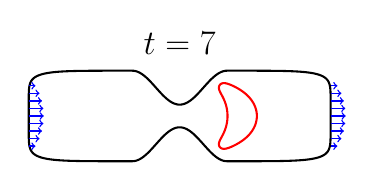
\begin{tikzpicture}[scale=0.5]

\begin{axis}[
  xmin = -11,
  xmax = 11,
  ymin = -3.2,
  ymax = 3.2,
  scale only axis,
  axis equal image,
  hide axis,
  title = {\Huge$t=7$}
  ]

\addplot [mark=none,black,line width=1.5] table{
1.0000e+01 0.0000e+00
1.0000e+01 3.6817e-02
1.0000e+01 7.3646e-02
1.0000e+01 1.1050e-01
1.0000e+01 1.4738e-01
1.0000e+01 1.8431e-01
1.0000e+01 2.2129e-01
1.0000e+01 2.5834e-01
1.0000e+01 2.9547e-01
1.0000e+01 3.3269e-01
1.0000e+01 3.7001e-01
1.0000e+01 4.0745e-01
1.0000e+01 4.4501e-01
1.0000e+01 4.8270e-01
1.0000e+01 5.2055e-01
1.0000e+01 5.5856e-01
1.0000e+01 5.9674e-01
1.0000e+01 6.3510e-01
1.0000e+01 6.7367e-01
1.0000e+01 7.1245e-01
1.0000e+01 7.5146e-01
1.0000e+01 7.9071e-01
1.0000e+01 8.3021e-01
9.9999e+00 8.6998e-01
9.9999e+00 9.1003e-01
9.9999e+00 9.5038e-01
9.9998e+00 9.9105e-01
9.9998e+00 1.0320e+00
9.9997e+00 1.0734e+00
9.9995e+00 1.1151e+00
9.9994e+00 1.1572e+00
9.9992e+00 1.1996e+00
9.9989e+00 1.2425e+00
9.9986e+00 1.2858e+00
9.9981e+00 1.3296e+00
9.9976e+00 1.3738e+00
9.9969e+00 1.4185e+00
9.9960e+00 1.4636e+00
9.9949e+00 1.5093e+00
9.9935e+00 1.5555e+00
9.9917e+00 1.6022e+00
9.9895e+00 1.6495e+00
9.9868e+00 1.6972e+00
9.9835e+00 1.7456e+00
9.9794e+00 1.7944e+00
9.9743e+00 1.8438e+00
9.9681e+00 1.8937e+00
9.9606e+00 1.9440e+00
9.9514e+00 1.9948e+00
9.9403e+00 2.0459e+00
9.9268e+00 2.0974e+00
9.9106e+00 2.1490e+00
9.8911e+00 2.2007e+00
9.8678e+00 2.2524e+00
9.8402e+00 2.3038e+00
9.8074e+00 2.3548e+00
9.7688e+00 2.4051e+00
9.7237e+00 2.4545e+00
9.6713e+00 2.5028e+00
9.6109e+00 2.5495e+00
9.5418e+00 2.5944e+00
9.4634e+00 2.6373e+00
9.3755e+00 2.6779e+00
9.2777e+00 2.7158e+00
9.1700e+00 2.7510e+00
9.0527e+00 2.7833e+00
8.9262e+00 2.8126e+00
8.7911e+00 2.8390e+00
8.6481e+00 2.8625e+00
8.4983e+00 2.8833e+00
8.3425e+00 2.9014e+00
8.1818e+00 2.9171e+00
8.0171e+00 2.9306e+00
7.8493e+00 2.9422e+00
7.6793e+00 2.9520e+00
7.5079e+00 2.9604e+00
7.3358e+00 2.9673e+00
7.1634e+00 2.9732e+00
6.9912e+00 2.9780e+00
6.8198e+00 2.9821e+00
6.6493e+00 2.9854e+00
6.4801e+00 2.9882e+00
6.3123e+00 2.9904e+00
6.1460e+00 2.9923e+00
5.9814e+00 2.9938e+00
5.8185e+00 2.9950e+00
5.6575e+00 2.9960e+00
5.4982e+00 2.9969e+00
5.3407e+00 2.9975e+00
5.1850e+00 2.9980e+00
5.0310e+00 2.9985e+00
4.8787e+00 2.9988e+00
4.7282e+00 2.9991e+00
4.5792e+00 2.9993e+00
4.4319e+00 2.9994e+00
4.2860e+00 2.9996e+00
4.1417e+00 2.9997e+00
3.9988e+00 2.9998e+00
3.8572e+00 2.9998e+00
3.7169e+00 2.9999e+00
3.5779e+00 2.9999e+00
3.4401e+00 2.9999e+00
3.3035e+00 2.9999e+00
3.1679e+00 3.0000e+00
3.0334e+00 2.9934e+00
2.8999e+00 2.9673e+00
2.7674e+00 2.9221e+00
2.6357e+00 2.8591e+00
2.5049e+00 2.7795e+00
2.3748e+00 2.6852e+00
2.2456e+00 2.5778e+00
2.1170e+00 2.4594e+00
1.9891e+00 2.3320e+00
1.8619e+00 2.1978e+00
1.7352e+00 2.0591e+00
1.6090e+00 1.9180e+00
1.4834e+00 1.7768e+00
1.3582e+00 1.6376e+00
1.2334e+00 1.5026e+00
1.1090e+00 1.3737e+00
9.8491e-01 1.2529e+00
8.6115e-01 1.1420e+00
7.3764e-01 1.0424e+00
6.1436e-01 9.5572e-01
4.9127e-01 8.8305e-01
3.6832e-01 8.2545e-01
2.4549e-01 7.8373e-01
1.2272e-01 7.5846e-01
6.1232e-16 7.5000e-01
-1.2272e-01 7.5846e-01
-2.4549e-01 7.8373e-01
-3.6832e-01 8.2545e-01
-4.9127e-01 8.8305e-01
-6.1436e-01 9.5572e-01
-7.3764e-01 1.0424e+00
-8.6115e-01 1.1420e+00
-9.8491e-01 1.2529e+00
-1.1090e+00 1.3737e+00
-1.2334e+00 1.5026e+00
-1.3582e+00 1.6376e+00
-1.4834e+00 1.7768e+00
-1.6090e+00 1.9180e+00
-1.7352e+00 2.0591e+00
-1.8619e+00 2.1978e+00
-1.9891e+00 2.3320e+00
-2.1170e+00 2.4594e+00
-2.2456e+00 2.5778e+00
-2.3748e+00 2.6852e+00
-2.5049e+00 2.7795e+00
-2.6357e+00 2.8591e+00
-2.7674e+00 2.9221e+00
-2.8999e+00 2.9673e+00
-3.0334e+00 2.9934e+00
-3.1679e+00 3.0000e+00
-3.3035e+00 2.9999e+00
-3.4401e+00 2.9999e+00
-3.5779e+00 2.9999e+00
-3.7169e+00 2.9999e+00
-3.8572e+00 2.9998e+00
-3.9988e+00 2.9998e+00
-4.1417e+00 2.9997e+00
-4.2860e+00 2.9996e+00
-4.4319e+00 2.9994e+00
-4.5792e+00 2.9993e+00
-4.7282e+00 2.9991e+00
-4.8787e+00 2.9988e+00
-5.0310e+00 2.9985e+00
-5.1850e+00 2.9980e+00
-5.3407e+00 2.9975e+00
-5.4982e+00 2.9969e+00
-5.6575e+00 2.9960e+00
-5.8185e+00 2.9950e+00
-5.9814e+00 2.9938e+00
-6.1460e+00 2.9923e+00
-6.3123e+00 2.9904e+00
-6.4801e+00 2.9882e+00
-6.6493e+00 2.9854e+00
-6.8198e+00 2.9821e+00
-6.9912e+00 2.9780e+00
-7.1634e+00 2.9732e+00
-7.3358e+00 2.9673e+00
-7.5079e+00 2.9604e+00
-7.6793e+00 2.9520e+00
-7.8493e+00 2.9422e+00
-8.0171e+00 2.9306e+00
-8.1818e+00 2.9171e+00
-8.3425e+00 2.9014e+00
-8.4983e+00 2.8833e+00
-8.6481e+00 2.8625e+00
-8.7911e+00 2.8390e+00
-8.9262e+00 2.8126e+00
-9.0527e+00 2.7833e+00
-9.1700e+00 2.7510e+00
-9.2777e+00 2.7158e+00
-9.3755e+00 2.6779e+00
-9.4634e+00 2.6373e+00
-9.5418e+00 2.5944e+00
-9.6109e+00 2.5495e+00
-9.6713e+00 2.5028e+00
-9.7237e+00 2.4545e+00
-9.7688e+00 2.4051e+00
-9.8074e+00 2.3548e+00
-9.8402e+00 2.3038e+00
-9.8678e+00 2.2524e+00
-9.8911e+00 2.2007e+00
-9.9106e+00 2.1490e+00
-9.9268e+00 2.0974e+00
-9.9403e+00 2.0459e+00
-9.9514e+00 1.9948e+00
-9.9606e+00 1.9440e+00
-9.9681e+00 1.8937e+00
-9.9743e+00 1.8438e+00
-9.9794e+00 1.7944e+00
-9.9835e+00 1.7456e+00
-9.9868e+00 1.6972e+00
-9.9895e+00 1.6495e+00
-9.9917e+00 1.6022e+00
-9.9935e+00 1.5555e+00
-9.9949e+00 1.5093e+00
-9.9960e+00 1.4636e+00
-9.9969e+00 1.4185e+00
-9.9976e+00 1.3738e+00
-9.9981e+00 1.3296e+00
-9.9986e+00 1.2858e+00
-9.9989e+00 1.2425e+00
-9.9992e+00 1.1996e+00
-9.9994e+00 1.1572e+00
-9.9995e+00 1.1151e+00
-9.9997e+00 1.0734e+00
-9.9998e+00 1.0320e+00
-9.9998e+00 9.9105e-01
-9.9999e+00 9.5038e-01
-9.9999e+00 9.1003e-01
-9.9999e+00 8.6998e-01
-1.0000e+01 8.3021e-01
-1.0000e+01 7.9071e-01
-1.0000e+01 7.5146e-01
-1.0000e+01 7.1245e-01
-1.0000e+01 6.7367e-01
-1.0000e+01 6.3510e-01
-1.0000e+01 5.9674e-01
-1.0000e+01 5.5856e-01
-1.0000e+01 5.2055e-01
-1.0000e+01 4.8270e-01
-1.0000e+01 4.4501e-01
-1.0000e+01 4.0745e-01
-1.0000e+01 3.7001e-01
-1.0000e+01 3.3269e-01
-1.0000e+01 2.9547e-01
-1.0000e+01 2.5834e-01
-1.0000e+01 2.2129e-01
-1.0000e+01 1.8431e-01
-1.0000e+01 1.4738e-01
-1.0000e+01 1.1050e-01
-1.0000e+01 7.3646e-02
-1.0000e+01 3.6817e-02
-1.0000e+01 3.6739e-16
-1.0000e+01 -3.6817e-02
-1.0000e+01 -7.3646e-02
-1.0000e+01 -1.1050e-01
-1.0000e+01 -1.4738e-01
-1.0000e+01 -1.8431e-01
-1.0000e+01 -2.2129e-01
-1.0000e+01 -2.5834e-01
-1.0000e+01 -2.9547e-01
-1.0000e+01 -3.3269e-01
-1.0000e+01 -3.7001e-01
-1.0000e+01 -4.0745e-01
-1.0000e+01 -4.4501e-01
-1.0000e+01 -4.8270e-01
-1.0000e+01 -5.2055e-01
-1.0000e+01 -5.5856e-01
-1.0000e+01 -5.9674e-01
-1.0000e+01 -6.3510e-01
-1.0000e+01 -6.7367e-01
-1.0000e+01 -7.1245e-01
-1.0000e+01 -7.5146e-01
-1.0000e+01 -7.9071e-01
-1.0000e+01 -8.3021e-01
-9.9999e+00 -8.6998e-01
-9.9999e+00 -9.1003e-01
-9.9999e+00 -9.5038e-01
-9.9998e+00 -9.9105e-01
-9.9998e+00 -1.0320e+00
-9.9997e+00 -1.0734e+00
-9.9995e+00 -1.1151e+00
-9.9994e+00 -1.1572e+00
-9.9992e+00 -1.1996e+00
-9.9989e+00 -1.2425e+00
-9.9986e+00 -1.2858e+00
-9.9981e+00 -1.3296e+00
-9.9976e+00 -1.3738e+00
-9.9969e+00 -1.4185e+00
-9.9960e+00 -1.4636e+00
-9.9949e+00 -1.5093e+00
-9.9935e+00 -1.5555e+00
-9.9917e+00 -1.6022e+00
-9.9895e+00 -1.6495e+00
-9.9868e+00 -1.6972e+00
-9.9835e+00 -1.7456e+00
-9.9794e+00 -1.7944e+00
-9.9743e+00 -1.8438e+00
-9.9681e+00 -1.8937e+00
-9.9606e+00 -1.9440e+00
-9.9514e+00 -1.9948e+00
-9.9403e+00 -2.0459e+00
-9.9268e+00 -2.0974e+00
-9.9106e+00 -2.1490e+00
-9.8911e+00 -2.2007e+00
-9.8678e+00 -2.2524e+00
-9.8402e+00 -2.3038e+00
-9.8074e+00 -2.3548e+00
-9.7688e+00 -2.4051e+00
-9.7237e+00 -2.4545e+00
-9.6713e+00 -2.5028e+00
-9.6109e+00 -2.5495e+00
-9.5418e+00 -2.5944e+00
-9.4634e+00 -2.6373e+00
-9.3755e+00 -2.6779e+00
-9.2777e+00 -2.7158e+00
-9.1700e+00 -2.7510e+00
-9.0527e+00 -2.7833e+00
-8.9262e+00 -2.8126e+00
-8.7911e+00 -2.8390e+00
-8.6481e+00 -2.8625e+00
-8.4983e+00 -2.8833e+00
-8.3425e+00 -2.9014e+00
-8.1818e+00 -2.9171e+00
-8.0171e+00 -2.9306e+00
-7.8493e+00 -2.9422e+00
-7.6793e+00 -2.9520e+00
-7.5079e+00 -2.9604e+00
-7.3358e+00 -2.9673e+00
-7.1634e+00 -2.9732e+00
-6.9912e+00 -2.9780e+00
-6.8198e+00 -2.9821e+00
-6.6493e+00 -2.9854e+00
-6.4801e+00 -2.9882e+00
-6.3123e+00 -2.9904e+00
-6.1460e+00 -2.9923e+00
-5.9814e+00 -2.9938e+00
-5.8185e+00 -2.9950e+00
-5.6575e+00 -2.9960e+00
-5.4982e+00 -2.9969e+00
-5.3407e+00 -2.9975e+00
-5.1850e+00 -2.9980e+00
-5.0310e+00 -2.9985e+00
-4.8787e+00 -2.9988e+00
-4.7282e+00 -2.9991e+00
-4.5792e+00 -2.9993e+00
-4.4319e+00 -2.9994e+00
-4.2860e+00 -2.9996e+00
-4.1417e+00 -2.9997e+00
-3.9988e+00 -2.9998e+00
-3.8572e+00 -2.9998e+00
-3.7169e+00 -2.9999e+00
-3.5779e+00 -2.9999e+00
-3.4401e+00 -2.9999e+00
-3.3035e+00 -2.9999e+00
-3.1679e+00 -3.0000e+00
-3.0334e+00 -2.9934e+00
-2.8999e+00 -2.9673e+00
-2.7674e+00 -2.9221e+00
-2.6357e+00 -2.8591e+00
-2.5049e+00 -2.7795e+00
-2.3748e+00 -2.6852e+00
-2.2456e+00 -2.5778e+00
-2.1170e+00 -2.4594e+00
-1.9891e+00 -2.3320e+00
-1.8619e+00 -2.1978e+00
-1.7352e+00 -2.0591e+00
-1.6090e+00 -1.9180e+00
-1.4834e+00 -1.7768e+00
-1.3582e+00 -1.6376e+00
-1.2334e+00 -1.5026e+00
-1.1090e+00 -1.3737e+00
-9.8491e-01 -1.2529e+00
-8.6115e-01 -1.1420e+00
-7.3764e-01 -1.0424e+00
-6.1436e-01 -9.5572e-01
-4.9127e-01 -8.8305e-01
-3.6832e-01 -8.2545e-01
-2.4549e-01 -7.8373e-01
-1.2272e-01 -7.5846e-01
-1.8370e-15 -7.5000e-01
1.2272e-01 -7.5846e-01
2.4549e-01 -7.8373e-01
3.6832e-01 -8.2545e-01
4.9127e-01 -8.8305e-01
6.1436e-01 -9.5572e-01
7.3764e-01 -1.0424e+00
8.6115e-01 -1.1420e+00
9.8491e-01 -1.2529e+00
1.1090e+00 -1.3737e+00
1.2334e+00 -1.5026e+00
1.3582e+00 -1.6376e+00
1.4834e+00 -1.7768e+00
1.6090e+00 -1.9180e+00
1.7352e+00 -2.0591e+00
1.8619e+00 -2.1978e+00
1.9891e+00 -2.3320e+00
2.1170e+00 -2.4594e+00
2.2456e+00 -2.5778e+00
2.3748e+00 -2.6852e+00
2.5049e+00 -2.7795e+00
2.6357e+00 -2.8591e+00
2.7674e+00 -2.9221e+00
2.8999e+00 -2.9673e+00
3.0334e+00 -2.9934e+00
3.1679e+00 -3.0000e+00
3.3035e+00 -2.9999e+00
3.4401e+00 -2.9999e+00
3.5779e+00 -2.9999e+00
3.7169e+00 -2.9999e+00
3.8572e+00 -2.9998e+00
3.9988e+00 -2.9998e+00
4.1417e+00 -2.9997e+00
4.2860e+00 -2.9996e+00
4.4319e+00 -2.9994e+00
4.5792e+00 -2.9993e+00
4.7282e+00 -2.9991e+00
4.8787e+00 -2.9988e+00
5.0310e+00 -2.9985e+00
5.1850e+00 -2.9980e+00
5.3407e+00 -2.9975e+00
5.4982e+00 -2.9969e+00
5.6575e+00 -2.9960e+00
5.8185e+00 -2.9950e+00
5.9814e+00 -2.9938e+00
6.1460e+00 -2.9923e+00
6.3123e+00 -2.9904e+00
6.4801e+00 -2.9882e+00
6.6493e+00 -2.9854e+00
6.8198e+00 -2.9821e+00
6.9912e+00 -2.9780e+00
7.1634e+00 -2.9732e+00
7.3358e+00 -2.9673e+00
7.5079e+00 -2.9604e+00
7.6793e+00 -2.9520e+00
7.8493e+00 -2.9422e+00
8.0171e+00 -2.9306e+00
8.1818e+00 -2.9171e+00
8.3425e+00 -2.9014e+00
8.4983e+00 -2.8833e+00
8.6481e+00 -2.8625e+00
8.7911e+00 -2.8390e+00
8.9262e+00 -2.8126e+00
9.0527e+00 -2.7833e+00
9.1700e+00 -2.7510e+00
9.2777e+00 -2.7158e+00
9.3755e+00 -2.6779e+00
9.4634e+00 -2.6373e+00
9.5418e+00 -2.5944e+00
9.6109e+00 -2.5495e+00
9.6713e+00 -2.5028e+00
9.7237e+00 -2.4545e+00
9.7688e+00 -2.4051e+00
9.8074e+00 -2.3548e+00
9.8402e+00 -2.3038e+00
9.8678e+00 -2.2524e+00
9.8911e+00 -2.2007e+00
9.9106e+00 -2.1490e+00
9.9268e+00 -2.0974e+00
9.9403e+00 -2.0459e+00
9.9514e+00 -1.9948e+00
9.9606e+00 -1.9440e+00
9.9681e+00 -1.8937e+00
9.9743e+00 -1.8438e+00
9.9794e+00 -1.7944e+00
9.9835e+00 -1.7456e+00
9.9868e+00 -1.6972e+00
9.9895e+00 -1.6495e+00
9.9917e+00 -1.6022e+00
9.9935e+00 -1.5555e+00
9.9949e+00 -1.5093e+00
9.9960e+00 -1.4636e+00
9.9969e+00 -1.4185e+00
9.9976e+00 -1.3738e+00
9.9981e+00 -1.3296e+00
9.9986e+00 -1.2858e+00
9.9989e+00 -1.2425e+00
9.9992e+00 -1.1996e+00
9.9994e+00 -1.1572e+00
9.9995e+00 -1.1151e+00
9.9997e+00 -1.0734e+00
9.9998e+00 -1.0320e+00
9.9998e+00 -9.9105e-01
9.9999e+00 -9.5038e-01
9.9999e+00 -9.1003e-01
9.9999e+00 -8.6998e-01
1.0000e+01 -8.3021e-01
1.0000e+01 -7.9071e-01
1.0000e+01 -7.5146e-01
1.0000e+01 -7.1245e-01
1.0000e+01 -6.7367e-01
1.0000e+01 -6.3510e-01
1.0000e+01 -5.9674e-01
1.0000e+01 -5.5856e-01
1.0000e+01 -5.2055e-01
1.0000e+01 -4.8270e-01
1.0000e+01 -4.4501e-01
1.0000e+01 -4.0745e-01
1.0000e+01 -3.7001e-01
1.0000e+01 -3.3269e-01
1.0000e+01 -2.9547e-01
1.0000e+01 -2.5834e-01
1.0000e+01 -2.2129e-01
1.0000e+01 -1.8431e-01
1.0000e+01 -1.4738e-01
1.0000e+01 -1.1050e-01
1.0000e+01 -7.3646e-02
1.0000e+01 -3.6817e-02
1.0000e+01 0.0000e+00
};


\addplot [mark=none,red,line width=1.5] table{
3.3160e+00 2.0866e+00
3.2962e+00 2.0943e+00
3.2761e+00 2.1018e+00
3.2556e+00 2.1092e+00
3.2347e+00 2.1165e+00
3.2132e+00 2.1237e+00
3.1911e+00 2.1308e+00
3.1682e+00 2.1378e+00
3.1446e+00 2.1445e+00
3.1201e+00 2.1510e+00
3.0946e+00 2.1571e+00
3.0682e+00 2.1627e+00
3.0407e+00 2.1676e+00
3.0121e+00 2.1718e+00
2.9824e+00 2.1748e+00
2.9516e+00 2.1764e+00
2.9197e+00 2.1764e+00
2.8869e+00 2.1742e+00
2.8533e+00 2.1694e+00
2.8192e+00 2.1614e+00
2.7851e+00 2.1499e+00
2.7515e+00 2.1342e+00
2.7192e+00 2.1140e+00
2.6890e+00 2.0891e+00
2.6620e+00 2.0593e+00
2.6390e+00 2.0251e+00
2.6209e+00 1.9869e+00
2.6084e+00 1.9455e+00
2.6015e+00 1.9017e+00
2.6004e+00 1.8564e+00
2.6045e+00 1.8103e+00
2.6135e+00 1.7639e+00
2.6266e+00 1.7176e+00
2.6432e+00 1.6713e+00
2.6625e+00 1.6252e+00
2.6841e+00 1.5791e+00
2.7074e+00 1.5329e+00
2.7319e+00 1.4864e+00
2.7572e+00 1.4393e+00
2.7831e+00 1.3917e+00
2.8091e+00 1.3433e+00
2.8351e+00 1.2940e+00
2.8608e+00 1.2438e+00
2.8862e+00 1.1927e+00
2.9109e+00 1.1406e+00
2.9351e+00 1.0874e+00
2.9584e+00 1.0333e+00
2.9809e+00 9.7823e-01
3.0024e+00 9.2218e-01
3.0229e+00 8.6521e-01
3.0423e+00 8.0737e-01
3.0605e+00 7.4868e-01
3.0774e+00 6.8922e-01
3.0932e+00 6.2901e-01
3.1075e+00 5.6813e-01
3.1205e+00 5.0662e-01
3.1321e+00 4.4455e-01
3.1422e+00 3.8199e-01
3.1508e+00 3.1899e-01
3.1579e+00 2.5563e-01
3.1635e+00 1.9198e-01
3.1674e+00 1.2811e-01
3.1698e+00 6.4092e-02
3.1706e+00 -1.2723e-08
3.1698e+00 -6.4092e-02
3.1674e+00 -1.2811e-01
3.1635e+00 -1.9198e-01
3.1579e+00 -2.5563e-01
3.1508e+00 -3.1899e-01
3.1422e+00 -3.8199e-01
3.1321e+00 -4.4455e-01
3.1205e+00 -5.0662e-01
3.1075e+00 -5.6813e-01
3.0932e+00 -6.2901e-01
3.0774e+00 -6.8922e-01
3.0605e+00 -7.4868e-01
3.0423e+00 -8.0737e-01
3.0229e+00 -8.6521e-01
3.0024e+00 -9.2218e-01
2.9809e+00 -9.7823e-01
2.9584e+00 -1.0333e+00
2.9351e+00 -1.0874e+00
2.9109e+00 -1.1406e+00
2.8862e+00 -1.1927e+00
2.8608e+00 -1.2438e+00
2.8351e+00 -1.2940e+00
2.8091e+00 -1.3433e+00
2.7831e+00 -1.3917e+00
2.7572e+00 -1.4393e+00
2.7319e+00 -1.4864e+00
2.7074e+00 -1.5329e+00
2.6841e+00 -1.5791e+00
2.6625e+00 -1.6252e+00
2.6432e+00 -1.6713e+00
2.6266e+00 -1.7176e+00
2.6135e+00 -1.7639e+00
2.6045e+00 -1.8103e+00
2.6004e+00 -1.8564e+00
2.6015e+00 -1.9017e+00
2.6084e+00 -1.9455e+00
2.6209e+00 -1.9869e+00
2.6390e+00 -2.0251e+00
2.6620e+00 -2.0593e+00
2.6890e+00 -2.0891e+00
2.7192e+00 -2.1140e+00
2.7515e+00 -2.1342e+00
2.7851e+00 -2.1499e+00
2.8192e+00 -2.1614e+00
2.8533e+00 -2.1694e+00
2.8869e+00 -2.1742e+00
2.9197e+00 -2.1764e+00
2.9516e+00 -2.1764e+00
2.9824e+00 -2.1748e+00
3.0121e+00 -2.1718e+00
3.0407e+00 -2.1676e+00
3.0682e+00 -2.1627e+00
3.0946e+00 -2.1571e+00
3.1201e+00 -2.1510e+00
3.1446e+00 -2.1445e+00
3.1682e+00 -2.1378e+00
3.1911e+00 -2.1308e+00
3.2132e+00 -2.1237e+00
3.2347e+00 -2.1165e+00
3.2556e+00 -2.1092e+00
3.2761e+00 -2.1018e+00
3.2962e+00 -2.0943e+00
3.3161e+00 -2.0866e+00
3.3357e+00 -2.0789e+00
3.3554e+00 -2.0710e+00
3.3751e+00 -2.0630e+00
3.3949e+00 -2.0547e+00
3.4149e+00 -2.0461e+00
3.4352e+00 -2.0373e+00
3.4560e+00 -2.0282e+00
3.4772e+00 -2.0187e+00
3.4989e+00 -2.0088e+00
3.5212e+00 -1.9985e+00
3.5442e+00 -1.9877e+00
3.5678e+00 -1.9765e+00
3.5921e+00 -1.9647e+00
3.6172e+00 -1.9523e+00
3.6431e+00 -1.9394e+00
3.6697e+00 -1.9259e+00
3.6971e+00 -1.9117e+00
3.7253e+00 -1.8969e+00
3.7543e+00 -1.8814e+00
3.7841e+00 -1.8651e+00
3.8147e+00 -1.8481e+00
3.8460e+00 -1.8304e+00
3.8781e+00 -1.8118e+00
3.9110e+00 -1.7924e+00
3.9445e+00 -1.7721e+00
3.9787e+00 -1.7510e+00
4.0136e+00 -1.7289e+00
4.0491e+00 -1.7058e+00
4.0851e+00 -1.6818e+00
4.1217e+00 -1.6567e+00
4.1587e+00 -1.6306e+00
4.1962e+00 -1.6033e+00
4.2340e+00 -1.5750e+00
4.2721e+00 -1.5455e+00
4.3104e+00 -1.5148e+00
4.3490e+00 -1.4829e+00
4.3876e+00 -1.4498e+00
4.4262e+00 -1.4153e+00
4.4648e+00 -1.3796e+00
4.5033e+00 -1.3425e+00
4.5415e+00 -1.3041e+00
4.5794e+00 -1.2643e+00
4.6168e+00 -1.2231e+00
4.6538e+00 -1.1805e+00
4.6901e+00 -1.1364e+00
4.7257e+00 -1.0910e+00
4.7605e+00 -1.0441e+00
4.7943e+00 -9.9584e-01
4.8270e+00 -9.4615e-01
4.8585e+00 -8.9507e-01
4.8888e+00 -8.4263e-01
4.9176e+00 -7.8886e-01
4.9449e+00 -7.3381e-01
4.9705e+00 -6.7752e-01
4.9943e+00 -6.2006e-01
5.0163e+00 -5.6148e-01
5.0363e+00 -5.0188e-01
5.0542e+00 -4.4133e-01
5.0699e+00 -3.7993e-01
5.0833e+00 -3.1779e-01
5.0944e+00 -2.5501e-01
5.1031e+00 -1.9172e-01
5.1094e+00 -1.2803e-01
5.1131e+00 -6.4081e-02
5.1144e+00 1.3571e-06
5.1131e+00 6.4084e-02
5.1094e+00 1.2803e-01
5.1031e+00 1.9172e-01
5.0944e+00 2.5501e-01
5.0833e+00 3.1779e-01
5.0699e+00 3.7993e-01
5.0542e+00 4.4133e-01
5.0363e+00 5.0188e-01
5.0163e+00 5.6149e-01
4.9943e+00 6.2006e-01
4.9705e+00 6.7752e-01
4.9449e+00 7.3381e-01
4.9176e+00 7.8887e-01
4.8888e+00 8.4263e-01
4.8585e+00 8.9507e-01
4.8270e+00 9.4615e-01
4.7943e+00 9.9584e-01
4.7605e+00 1.0441e+00
4.7257e+00 1.0910e+00
4.6901e+00 1.1364e+00
4.6538e+00 1.1805e+00
4.6168e+00 1.2231e+00
4.5794e+00 1.2643e+00
4.5415e+00 1.3041e+00
4.5033e+00 1.3425e+00
4.4648e+00 1.3796e+00
4.4262e+00 1.4153e+00
4.3876e+00 1.4498e+00
4.3490e+00 1.4829e+00
4.3104e+00 1.5148e+00
4.2721e+00 1.5455e+00
4.2340e+00 1.5750e+00
4.1961e+00 1.6033e+00
4.1587e+00 1.6306e+00
4.1217e+00 1.6567e+00
4.0851e+00 1.6818e+00
4.0491e+00 1.7058e+00
4.0136e+00 1.7289e+00
3.9787e+00 1.7510e+00
3.9445e+00 1.7721e+00
3.9110e+00 1.7924e+00
3.8781e+00 1.8118e+00
3.8460e+00 1.8304e+00
3.8147e+00 1.8481e+00
3.7841e+00 1.8651e+00
3.7543e+00 1.8814e+00
3.7253e+00 1.8969e+00
3.6971e+00 1.9117e+00
3.6697e+00 1.9259e+00
3.6431e+00 1.9394e+00
3.6172e+00 1.9523e+00
3.5921e+00 1.9647e+00
3.5678e+00 1.9765e+00
3.5442e+00 1.9877e+00
3.5212e+00 1.9985e+00
3.4989e+00 2.0088e+00
3.4772e+00 2.0187e+00
3.4560e+00 2.0282e+00
3.4352e+00 2.0373e+00
3.4149e+00 2.0461e+00
3.3949e+00 2.0547e+00
3.3751e+00 2.0630e+00
3.3554e+00 2.0710e+00
3.3357e+00 2.0789e+00
3.3160e+00 2.0866e+00
};

\foreach \y in {-2.0,-1.5,...,2.0}
\addplot[color=blue,line width = 1.0pt,solid,->]
plot coordinates{
  (-10,\y)
  (-10+exp(9/(\y*\y-9))/exp(-1),\y)
};

\foreach \y in {-2.0,-1.5,...,2.0}
\addplot[color=blue,line width = 1.0pt,solid,->]
plot coordinates{
  (10,\y)
  (10+exp(9/(\y*\y-9))/exp(-1),\y)
};

\end{axis}

\end{tikzpicture}



 &
%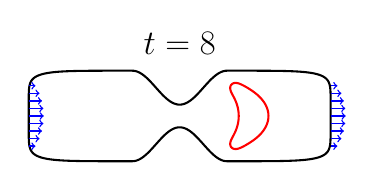
\begin{tikzpicture}[scale=0.5]

\begin{axis}[
  xmin = -11,
  xmax = 11,
  ymin = -3.2,
  ymax = 3.2,
  scale only axis,
  axis equal image,
  hide axis,
  title = {\Huge$t=8$}
  ]

\addplot [mark=none,black,line width=1.5] table{
1.0000e+01 0.0000e+00
1.0000e+01 3.6817e-02
1.0000e+01 7.3646e-02
1.0000e+01 1.1050e-01
1.0000e+01 1.4738e-01
1.0000e+01 1.8431e-01
1.0000e+01 2.2129e-01
1.0000e+01 2.5834e-01
1.0000e+01 2.9547e-01
1.0000e+01 3.3269e-01
1.0000e+01 3.7001e-01
1.0000e+01 4.0745e-01
1.0000e+01 4.4501e-01
1.0000e+01 4.8270e-01
1.0000e+01 5.2055e-01
1.0000e+01 5.5856e-01
1.0000e+01 5.9674e-01
1.0000e+01 6.3510e-01
1.0000e+01 6.7367e-01
1.0000e+01 7.1245e-01
1.0000e+01 7.5146e-01
1.0000e+01 7.9071e-01
1.0000e+01 8.3021e-01
9.9999e+00 8.6998e-01
9.9999e+00 9.1003e-01
9.9999e+00 9.5038e-01
9.9998e+00 9.9105e-01
9.9998e+00 1.0320e+00
9.9997e+00 1.0734e+00
9.9995e+00 1.1151e+00
9.9994e+00 1.1572e+00
9.9992e+00 1.1996e+00
9.9989e+00 1.2425e+00
9.9986e+00 1.2858e+00
9.9981e+00 1.3296e+00
9.9976e+00 1.3738e+00
9.9969e+00 1.4185e+00
9.9960e+00 1.4636e+00
9.9949e+00 1.5093e+00
9.9935e+00 1.5555e+00
9.9917e+00 1.6022e+00
9.9895e+00 1.6495e+00
9.9868e+00 1.6972e+00
9.9835e+00 1.7456e+00
9.9794e+00 1.7944e+00
9.9743e+00 1.8438e+00
9.9681e+00 1.8937e+00
9.9606e+00 1.9440e+00
9.9514e+00 1.9948e+00
9.9403e+00 2.0459e+00
9.9268e+00 2.0974e+00
9.9106e+00 2.1490e+00
9.8911e+00 2.2007e+00
9.8678e+00 2.2524e+00
9.8402e+00 2.3038e+00
9.8074e+00 2.3548e+00
9.7688e+00 2.4051e+00
9.7237e+00 2.4545e+00
9.6713e+00 2.5028e+00
9.6109e+00 2.5495e+00
9.5418e+00 2.5944e+00
9.4634e+00 2.6373e+00
9.3755e+00 2.6779e+00
9.2777e+00 2.7158e+00
9.1700e+00 2.7510e+00
9.0527e+00 2.7833e+00
8.9262e+00 2.8126e+00
8.7911e+00 2.8390e+00
8.6481e+00 2.8625e+00
8.4983e+00 2.8833e+00
8.3425e+00 2.9014e+00
8.1818e+00 2.9171e+00
8.0171e+00 2.9306e+00
7.8493e+00 2.9422e+00
7.6793e+00 2.9520e+00
7.5079e+00 2.9604e+00
7.3358e+00 2.9673e+00
7.1634e+00 2.9732e+00
6.9912e+00 2.9780e+00
6.8198e+00 2.9821e+00
6.6493e+00 2.9854e+00
6.4801e+00 2.9882e+00
6.3123e+00 2.9904e+00
6.1460e+00 2.9923e+00
5.9814e+00 2.9938e+00
5.8185e+00 2.9950e+00
5.6575e+00 2.9960e+00
5.4982e+00 2.9969e+00
5.3407e+00 2.9975e+00
5.1850e+00 2.9980e+00
5.0310e+00 2.9985e+00
4.8787e+00 2.9988e+00
4.7282e+00 2.9991e+00
4.5792e+00 2.9993e+00
4.4319e+00 2.9994e+00
4.2860e+00 2.9996e+00
4.1417e+00 2.9997e+00
3.9988e+00 2.9998e+00
3.8572e+00 2.9998e+00
3.7169e+00 2.9999e+00
3.5779e+00 2.9999e+00
3.4401e+00 2.9999e+00
3.3035e+00 2.9999e+00
3.1679e+00 3.0000e+00
3.0334e+00 2.9934e+00
2.8999e+00 2.9673e+00
2.7674e+00 2.9221e+00
2.6357e+00 2.8591e+00
2.5049e+00 2.7795e+00
2.3748e+00 2.6852e+00
2.2456e+00 2.5778e+00
2.1170e+00 2.4594e+00
1.9891e+00 2.3320e+00
1.8619e+00 2.1978e+00
1.7352e+00 2.0591e+00
1.6090e+00 1.9180e+00
1.4834e+00 1.7768e+00
1.3582e+00 1.6376e+00
1.2334e+00 1.5026e+00
1.1090e+00 1.3737e+00
9.8491e-01 1.2529e+00
8.6115e-01 1.1420e+00
7.3764e-01 1.0424e+00
6.1436e-01 9.5572e-01
4.9127e-01 8.8305e-01
3.6832e-01 8.2545e-01
2.4549e-01 7.8373e-01
1.2272e-01 7.5846e-01
6.1232e-16 7.5000e-01
-1.2272e-01 7.5846e-01
-2.4549e-01 7.8373e-01
-3.6832e-01 8.2545e-01
-4.9127e-01 8.8305e-01
-6.1436e-01 9.5572e-01
-7.3764e-01 1.0424e+00
-8.6115e-01 1.1420e+00
-9.8491e-01 1.2529e+00
-1.1090e+00 1.3737e+00
-1.2334e+00 1.5026e+00
-1.3582e+00 1.6376e+00
-1.4834e+00 1.7768e+00
-1.6090e+00 1.9180e+00
-1.7352e+00 2.0591e+00
-1.8619e+00 2.1978e+00
-1.9891e+00 2.3320e+00
-2.1170e+00 2.4594e+00
-2.2456e+00 2.5778e+00
-2.3748e+00 2.6852e+00
-2.5049e+00 2.7795e+00
-2.6357e+00 2.8591e+00
-2.7674e+00 2.9221e+00
-2.8999e+00 2.9673e+00
-3.0334e+00 2.9934e+00
-3.1679e+00 3.0000e+00
-3.3035e+00 2.9999e+00
-3.4401e+00 2.9999e+00
-3.5779e+00 2.9999e+00
-3.7169e+00 2.9999e+00
-3.8572e+00 2.9998e+00
-3.9988e+00 2.9998e+00
-4.1417e+00 2.9997e+00
-4.2860e+00 2.9996e+00
-4.4319e+00 2.9994e+00
-4.5792e+00 2.9993e+00
-4.7282e+00 2.9991e+00
-4.8787e+00 2.9988e+00
-5.0310e+00 2.9985e+00
-5.1850e+00 2.9980e+00
-5.3407e+00 2.9975e+00
-5.4982e+00 2.9969e+00
-5.6575e+00 2.9960e+00
-5.8185e+00 2.9950e+00
-5.9814e+00 2.9938e+00
-6.1460e+00 2.9923e+00
-6.3123e+00 2.9904e+00
-6.4801e+00 2.9882e+00
-6.6493e+00 2.9854e+00
-6.8198e+00 2.9821e+00
-6.9912e+00 2.9780e+00
-7.1634e+00 2.9732e+00
-7.3358e+00 2.9673e+00
-7.5079e+00 2.9604e+00
-7.6793e+00 2.9520e+00
-7.8493e+00 2.9422e+00
-8.0171e+00 2.9306e+00
-8.1818e+00 2.9171e+00
-8.3425e+00 2.9014e+00
-8.4983e+00 2.8833e+00
-8.6481e+00 2.8625e+00
-8.7911e+00 2.8390e+00
-8.9262e+00 2.8126e+00
-9.0527e+00 2.7833e+00
-9.1700e+00 2.7510e+00
-9.2777e+00 2.7158e+00
-9.3755e+00 2.6779e+00
-9.4634e+00 2.6373e+00
-9.5418e+00 2.5944e+00
-9.6109e+00 2.5495e+00
-9.6713e+00 2.5028e+00
-9.7237e+00 2.4545e+00
-9.7688e+00 2.4051e+00
-9.8074e+00 2.3548e+00
-9.8402e+00 2.3038e+00
-9.8678e+00 2.2524e+00
-9.8911e+00 2.2007e+00
-9.9106e+00 2.1490e+00
-9.9268e+00 2.0974e+00
-9.9403e+00 2.0459e+00
-9.9514e+00 1.9948e+00
-9.9606e+00 1.9440e+00
-9.9681e+00 1.8937e+00
-9.9743e+00 1.8438e+00
-9.9794e+00 1.7944e+00
-9.9835e+00 1.7456e+00
-9.9868e+00 1.6972e+00
-9.9895e+00 1.6495e+00
-9.9917e+00 1.6022e+00
-9.9935e+00 1.5555e+00
-9.9949e+00 1.5093e+00
-9.9960e+00 1.4636e+00
-9.9969e+00 1.4185e+00
-9.9976e+00 1.3738e+00
-9.9981e+00 1.3296e+00
-9.9986e+00 1.2858e+00
-9.9989e+00 1.2425e+00
-9.9992e+00 1.1996e+00
-9.9994e+00 1.1572e+00
-9.9995e+00 1.1151e+00
-9.9997e+00 1.0734e+00
-9.9998e+00 1.0320e+00
-9.9998e+00 9.9105e-01
-9.9999e+00 9.5038e-01
-9.9999e+00 9.1003e-01
-9.9999e+00 8.6998e-01
-1.0000e+01 8.3021e-01
-1.0000e+01 7.9071e-01
-1.0000e+01 7.5146e-01
-1.0000e+01 7.1245e-01
-1.0000e+01 6.7367e-01
-1.0000e+01 6.3510e-01
-1.0000e+01 5.9674e-01
-1.0000e+01 5.5856e-01
-1.0000e+01 5.2055e-01
-1.0000e+01 4.8270e-01
-1.0000e+01 4.4501e-01
-1.0000e+01 4.0745e-01
-1.0000e+01 3.7001e-01
-1.0000e+01 3.3269e-01
-1.0000e+01 2.9547e-01
-1.0000e+01 2.5834e-01
-1.0000e+01 2.2129e-01
-1.0000e+01 1.8431e-01
-1.0000e+01 1.4738e-01
-1.0000e+01 1.1050e-01
-1.0000e+01 7.3646e-02
-1.0000e+01 3.6817e-02
-1.0000e+01 3.6739e-16
-1.0000e+01 -3.6817e-02
-1.0000e+01 -7.3646e-02
-1.0000e+01 -1.1050e-01
-1.0000e+01 -1.4738e-01
-1.0000e+01 -1.8431e-01
-1.0000e+01 -2.2129e-01
-1.0000e+01 -2.5834e-01
-1.0000e+01 -2.9547e-01
-1.0000e+01 -3.3269e-01
-1.0000e+01 -3.7001e-01
-1.0000e+01 -4.0745e-01
-1.0000e+01 -4.4501e-01
-1.0000e+01 -4.8270e-01
-1.0000e+01 -5.2055e-01
-1.0000e+01 -5.5856e-01
-1.0000e+01 -5.9674e-01
-1.0000e+01 -6.3510e-01
-1.0000e+01 -6.7367e-01
-1.0000e+01 -7.1245e-01
-1.0000e+01 -7.5146e-01
-1.0000e+01 -7.9071e-01
-1.0000e+01 -8.3021e-01
-9.9999e+00 -8.6998e-01
-9.9999e+00 -9.1003e-01
-9.9999e+00 -9.5038e-01
-9.9998e+00 -9.9105e-01
-9.9998e+00 -1.0320e+00
-9.9997e+00 -1.0734e+00
-9.9995e+00 -1.1151e+00
-9.9994e+00 -1.1572e+00
-9.9992e+00 -1.1996e+00
-9.9989e+00 -1.2425e+00
-9.9986e+00 -1.2858e+00
-9.9981e+00 -1.3296e+00
-9.9976e+00 -1.3738e+00
-9.9969e+00 -1.4185e+00
-9.9960e+00 -1.4636e+00
-9.9949e+00 -1.5093e+00
-9.9935e+00 -1.5555e+00
-9.9917e+00 -1.6022e+00
-9.9895e+00 -1.6495e+00
-9.9868e+00 -1.6972e+00
-9.9835e+00 -1.7456e+00
-9.9794e+00 -1.7944e+00
-9.9743e+00 -1.8438e+00
-9.9681e+00 -1.8937e+00
-9.9606e+00 -1.9440e+00
-9.9514e+00 -1.9948e+00
-9.9403e+00 -2.0459e+00
-9.9268e+00 -2.0974e+00
-9.9106e+00 -2.1490e+00
-9.8911e+00 -2.2007e+00
-9.8678e+00 -2.2524e+00
-9.8402e+00 -2.3038e+00
-9.8074e+00 -2.3548e+00
-9.7688e+00 -2.4051e+00
-9.7237e+00 -2.4545e+00
-9.6713e+00 -2.5028e+00
-9.6109e+00 -2.5495e+00
-9.5418e+00 -2.5944e+00
-9.4634e+00 -2.6373e+00
-9.3755e+00 -2.6779e+00
-9.2777e+00 -2.7158e+00
-9.1700e+00 -2.7510e+00
-9.0527e+00 -2.7833e+00
-8.9262e+00 -2.8126e+00
-8.7911e+00 -2.8390e+00
-8.6481e+00 -2.8625e+00
-8.4983e+00 -2.8833e+00
-8.3425e+00 -2.9014e+00
-8.1818e+00 -2.9171e+00
-8.0171e+00 -2.9306e+00
-7.8493e+00 -2.9422e+00
-7.6793e+00 -2.9520e+00
-7.5079e+00 -2.9604e+00
-7.3358e+00 -2.9673e+00
-7.1634e+00 -2.9732e+00
-6.9912e+00 -2.9780e+00
-6.8198e+00 -2.9821e+00
-6.6493e+00 -2.9854e+00
-6.4801e+00 -2.9882e+00
-6.3123e+00 -2.9904e+00
-6.1460e+00 -2.9923e+00
-5.9814e+00 -2.9938e+00
-5.8185e+00 -2.9950e+00
-5.6575e+00 -2.9960e+00
-5.4982e+00 -2.9969e+00
-5.3407e+00 -2.9975e+00
-5.1850e+00 -2.9980e+00
-5.0310e+00 -2.9985e+00
-4.8787e+00 -2.9988e+00
-4.7282e+00 -2.9991e+00
-4.5792e+00 -2.9993e+00
-4.4319e+00 -2.9994e+00
-4.2860e+00 -2.9996e+00
-4.1417e+00 -2.9997e+00
-3.9988e+00 -2.9998e+00
-3.8572e+00 -2.9998e+00
-3.7169e+00 -2.9999e+00
-3.5779e+00 -2.9999e+00
-3.4401e+00 -2.9999e+00
-3.3035e+00 -2.9999e+00
-3.1679e+00 -3.0000e+00
-3.0334e+00 -2.9934e+00
-2.8999e+00 -2.9673e+00
-2.7674e+00 -2.9221e+00
-2.6357e+00 -2.8591e+00
-2.5049e+00 -2.7795e+00
-2.3748e+00 -2.6852e+00
-2.2456e+00 -2.5778e+00
-2.1170e+00 -2.4594e+00
-1.9891e+00 -2.3320e+00
-1.8619e+00 -2.1978e+00
-1.7352e+00 -2.0591e+00
-1.6090e+00 -1.9180e+00
-1.4834e+00 -1.7768e+00
-1.3582e+00 -1.6376e+00
-1.2334e+00 -1.5026e+00
-1.1090e+00 -1.3737e+00
-9.8491e-01 -1.2529e+00
-8.6115e-01 -1.1420e+00
-7.3764e-01 -1.0424e+00
-6.1436e-01 -9.5572e-01
-4.9127e-01 -8.8305e-01
-3.6832e-01 -8.2545e-01
-2.4549e-01 -7.8373e-01
-1.2272e-01 -7.5846e-01
-1.8370e-15 -7.5000e-01
1.2272e-01 -7.5846e-01
2.4549e-01 -7.8373e-01
3.6832e-01 -8.2545e-01
4.9127e-01 -8.8305e-01
6.1436e-01 -9.5572e-01
7.3764e-01 -1.0424e+00
8.6115e-01 -1.1420e+00
9.8491e-01 -1.2529e+00
1.1090e+00 -1.3737e+00
1.2334e+00 -1.5026e+00
1.3582e+00 -1.6376e+00
1.4834e+00 -1.7768e+00
1.6090e+00 -1.9180e+00
1.7352e+00 -2.0591e+00
1.8619e+00 -2.1978e+00
1.9891e+00 -2.3320e+00
2.1170e+00 -2.4594e+00
2.2456e+00 -2.5778e+00
2.3748e+00 -2.6852e+00
2.5049e+00 -2.7795e+00
2.6357e+00 -2.8591e+00
2.7674e+00 -2.9221e+00
2.8999e+00 -2.9673e+00
3.0334e+00 -2.9934e+00
3.1679e+00 -3.0000e+00
3.3035e+00 -2.9999e+00
3.4401e+00 -2.9999e+00
3.5779e+00 -2.9999e+00
3.7169e+00 -2.9999e+00
3.8572e+00 -2.9998e+00
3.9988e+00 -2.9998e+00
4.1417e+00 -2.9997e+00
4.2860e+00 -2.9996e+00
4.4319e+00 -2.9994e+00
4.5792e+00 -2.9993e+00
4.7282e+00 -2.9991e+00
4.8787e+00 -2.9988e+00
5.0310e+00 -2.9985e+00
5.1850e+00 -2.9980e+00
5.3407e+00 -2.9975e+00
5.4982e+00 -2.9969e+00
5.6575e+00 -2.9960e+00
5.8185e+00 -2.9950e+00
5.9814e+00 -2.9938e+00
6.1460e+00 -2.9923e+00
6.3123e+00 -2.9904e+00
6.4801e+00 -2.9882e+00
6.6493e+00 -2.9854e+00
6.8198e+00 -2.9821e+00
6.9912e+00 -2.9780e+00
7.1634e+00 -2.9732e+00
7.3358e+00 -2.9673e+00
7.5079e+00 -2.9604e+00
7.6793e+00 -2.9520e+00
7.8493e+00 -2.9422e+00
8.0171e+00 -2.9306e+00
8.1818e+00 -2.9171e+00
8.3425e+00 -2.9014e+00
8.4983e+00 -2.8833e+00
8.6481e+00 -2.8625e+00
8.7911e+00 -2.8390e+00
8.9262e+00 -2.8126e+00
9.0527e+00 -2.7833e+00
9.1700e+00 -2.7510e+00
9.2777e+00 -2.7158e+00
9.3755e+00 -2.6779e+00
9.4634e+00 -2.6373e+00
9.5418e+00 -2.5944e+00
9.6109e+00 -2.5495e+00
9.6713e+00 -2.5028e+00
9.7237e+00 -2.4545e+00
9.7688e+00 -2.4051e+00
9.8074e+00 -2.3548e+00
9.8402e+00 -2.3038e+00
9.8678e+00 -2.2524e+00
9.8911e+00 -2.2007e+00
9.9106e+00 -2.1490e+00
9.9268e+00 -2.0974e+00
9.9403e+00 -2.0459e+00
9.9514e+00 -1.9948e+00
9.9606e+00 -1.9440e+00
9.9681e+00 -1.8937e+00
9.9743e+00 -1.8438e+00
9.9794e+00 -1.7944e+00
9.9835e+00 -1.7456e+00
9.9868e+00 -1.6972e+00
9.9895e+00 -1.6495e+00
9.9917e+00 -1.6022e+00
9.9935e+00 -1.5555e+00
9.9949e+00 -1.5093e+00
9.9960e+00 -1.4636e+00
9.9969e+00 -1.4185e+00
9.9976e+00 -1.3738e+00
9.9981e+00 -1.3296e+00
9.9986e+00 -1.2858e+00
9.9989e+00 -1.2425e+00
9.9992e+00 -1.1996e+00
9.9994e+00 -1.1572e+00
9.9995e+00 -1.1151e+00
9.9997e+00 -1.0734e+00
9.9998e+00 -1.0320e+00
9.9998e+00 -9.9105e-01
9.9999e+00 -9.5038e-01
9.9999e+00 -9.1003e-01
9.9999e+00 -8.6998e-01
1.0000e+01 -8.3021e-01
1.0000e+01 -7.9071e-01
1.0000e+01 -7.5146e-01
1.0000e+01 -7.1245e-01
1.0000e+01 -6.7367e-01
1.0000e+01 -6.3510e-01
1.0000e+01 -5.9674e-01
1.0000e+01 -5.5856e-01
1.0000e+01 -5.2055e-01
1.0000e+01 -4.8270e-01
1.0000e+01 -4.4501e-01
1.0000e+01 -4.0745e-01
1.0000e+01 -3.7001e-01
1.0000e+01 -3.3269e-01
1.0000e+01 -2.9547e-01
1.0000e+01 -2.5834e-01
1.0000e+01 -2.2129e-01
1.0000e+01 -1.8431e-01
1.0000e+01 -1.4738e-01
1.0000e+01 -1.1050e-01
1.0000e+01 -7.3646e-02
1.0000e+01 -3.6817e-02
1.0000e+01 0.0000e+00
};


\addplot [mark=none,red,line width=1.5] table{
4.0617e+00 2.0959e+00
4.0423e+00 2.1045e+00
4.0225e+00 2.1128e+00
4.0023e+00 2.1211e+00
3.9817e+00 2.1292e+00
3.9605e+00 2.1371e+00
3.9386e+00 2.1449e+00
3.9159e+00 2.1524e+00
3.8924e+00 2.1596e+00
3.8680e+00 2.1664e+00
3.8426e+00 2.1727e+00
3.8161e+00 2.1783e+00
3.7886e+00 2.1830e+00
3.7599e+00 2.1867e+00
3.7302e+00 2.1891e+00
3.6993e+00 2.1898e+00
3.6675e+00 2.1885e+00
3.6348e+00 2.1848e+00
3.6015e+00 2.1784e+00
3.5679e+00 2.1687e+00
3.5344e+00 2.1554e+00
3.5017e+00 2.1380e+00
3.4703e+00 2.1164e+00
3.4410e+00 2.0905e+00
3.4146e+00 2.0601e+00
3.3918e+00 2.0257e+00
3.3734e+00 1.9877e+00
3.3598e+00 1.9466e+00
3.3513e+00 1.9031e+00
3.3479e+00 1.8579e+00
3.3495e+00 1.8117e+00
3.3556e+00 1.7648e+00
3.3660e+00 1.7178e+00
3.3799e+00 1.6707e+00
3.3970e+00 1.6237e+00
3.4166e+00 1.5767e+00
3.4384e+00 1.5297e+00
3.4617e+00 1.4826e+00
3.4862e+00 1.4351e+00
3.5116e+00 1.3872e+00
3.5375e+00 1.3388e+00
3.5636e+00 1.2896e+00
3.5898e+00 1.2396e+00
3.6157e+00 1.1888e+00
3.6412e+00 1.1370e+00
3.6661e+00 1.0842e+00
3.6904e+00 1.0305e+00
3.7138e+00 9.7579e-01
3.7362e+00 9.2011e-01
3.7576e+00 8.6349e-01
3.7779e+00 8.0596e-01
3.7970e+00 7.4756e-01
3.8148e+00 6.8834e-01
3.8313e+00 6.2834e-01
3.8464e+00 5.6763e-01
3.8601e+00 5.0627e-01
3.8722e+00 4.4432e-01
3.8829e+00 3.8184e-01
3.8919e+00 3.1890e-01
3.8994e+00 2.5559e-01
3.9052e+00 1.9196e-01
3.9094e+00 1.2811e-01
3.9119e+00 6.4092e-02
3.9128e+00 1.4537e-07
3.9119e+00 -6.4092e-02
3.9094e+00 -1.2811e-01
3.9052e+00 -1.9196e-01
3.8994e+00 -2.5559e-01
3.8919e+00 -3.1890e-01
3.8829e+00 -3.8184e-01
3.8722e+00 -4.4431e-01
3.8601e+00 -5.0627e-01
3.8464e+00 -5.6763e-01
3.8313e+00 -6.2834e-01
3.8148e+00 -6.8834e-01
3.7970e+00 -7.4756e-01
3.7779e+00 -8.0596e-01
3.7576e+00 -8.6349e-01
3.7362e+00 -9.2011e-01
3.7138e+00 -9.7579e-01
3.6904e+00 -1.0305e+00
3.6661e+00 -1.0842e+00
3.6412e+00 -1.1370e+00
3.6157e+00 -1.1888e+00
3.5898e+00 -1.2396e+00
3.5636e+00 -1.2896e+00
3.5375e+00 -1.3388e+00
3.5116e+00 -1.3872e+00
3.4862e+00 -1.4351e+00
3.4617e+00 -1.4826e+00
3.4384e+00 -1.5297e+00
3.4167e+00 -1.5767e+00
3.3970e+00 -1.6237e+00
3.3799e+00 -1.6707e+00
3.3660e+00 -1.7178e+00
3.3556e+00 -1.7648e+00
3.3495e+00 -1.8117e+00
3.3479e+00 -1.8579e+00
3.3513e+00 -1.9031e+00
3.3598e+00 -1.9466e+00
3.3734e+00 -1.9877e+00
3.3918e+00 -2.0257e+00
3.4146e+00 -2.0601e+00
3.4410e+00 -2.0905e+00
3.4703e+00 -2.1164e+00
3.5017e+00 -2.1380e+00
3.5344e+00 -2.1554e+00
3.5679e+00 -2.1687e+00
3.6015e+00 -2.1784e+00
3.6348e+00 -2.1848e+00
3.6675e+00 -2.1885e+00
3.6993e+00 -2.1898e+00
3.7302e+00 -2.1891e+00
3.7599e+00 -2.1867e+00
3.7886e+00 -2.1830e+00
3.8161e+00 -2.1783e+00
3.8426e+00 -2.1727e+00
3.8680e+00 -2.1664e+00
3.8924e+00 -2.1596e+00
3.9159e+00 -2.1524e+00
3.9386e+00 -2.1449e+00
3.9605e+00 -2.1371e+00
3.9817e+00 -2.1292e+00
4.0023e+00 -2.1211e+00
4.0225e+00 -2.1128e+00
4.0423e+00 -2.1045e+00
4.0617e+00 -2.0959e+00
4.0810e+00 -2.0872e+00
4.1002e+00 -2.0784e+00
4.1195e+00 -2.0693e+00
4.1388e+00 -2.0599e+00
4.1583e+00 -2.0503e+00
4.1782e+00 -2.0404e+00
4.1983e+00 -2.0301e+00
4.2190e+00 -2.0194e+00
4.2401e+00 -2.0083e+00
4.2618e+00 -1.9967e+00
4.2841e+00 -1.9846e+00
4.3070e+00 -1.9721e+00
4.3307e+00 -1.9590e+00
4.3551e+00 -1.9453e+00
4.3802e+00 -1.9310e+00
4.4061e+00 -1.9162e+00
4.4328e+00 -1.9007e+00
4.4602e+00 -1.8845e+00
4.4885e+00 -1.8677e+00
4.5176e+00 -1.8502e+00
4.5475e+00 -1.8320e+00
4.5782e+00 -1.8131e+00
4.6096e+00 -1.7935e+00
4.6418e+00 -1.7731e+00
4.6748e+00 -1.7519e+00
4.7085e+00 -1.7298e+00
4.7429e+00 -1.7070e+00
4.7779e+00 -1.6833e+00
4.8136e+00 -1.6587e+00
4.8499e+00 -1.6333e+00
4.8867e+00 -1.6068e+00
4.9240e+00 -1.5794e+00
4.9618e+00 -1.5511e+00
5.0000e+00 -1.5216e+00
5.0385e+00 -1.4912e+00
5.0773e+00 -1.4596e+00
5.1163e+00 -1.4269e+00
5.1555e+00 -1.3931e+00
5.1947e+00 -1.3580e+00
5.2339e+00 -1.3217e+00
5.2730e+00 -1.2842e+00
5.3120e+00 -1.2454e+00
5.3506e+00 -1.2053e+00
5.3888e+00 -1.1639e+00
5.4266e+00 -1.1211e+00
5.4638e+00 -1.0769e+00
5.5002e+00 -1.0313e+00
5.5358e+00 -9.8436e-01
5.5704e+00 -9.3597e-01
5.6040e+00 -8.8618e-01
5.6363e+00 -8.3499e-01
5.6672e+00 -7.8241e-01
5.6966e+00 -7.2848e-01
5.7244e+00 -6.7321e-01
5.7504e+00 -6.1668e-01
5.7744e+00 -5.5892e-01
5.7963e+00 -5.0001e-01
5.8161e+00 -4.4003e-01
5.8334e+00 -3.7909e-01
5.8484e+00 -3.1729e-01
5.8607e+00 -2.5475e-01
5.8705e+00 -1.9161e-01
5.8774e+00 -1.2800e-01
5.8817e+00 -6.4077e-02
5.8831e+00 1.6302e-06
5.8817e+00 6.4080e-02
5.8774e+00 1.2800e-01
5.8705e+00 1.9161e-01
5.8607e+00 2.5475e-01
5.8484e+00 3.1729e-01
5.8334e+00 3.7909e-01
5.8161e+00 4.4004e-01
5.7963e+00 5.0001e-01
5.7744e+00 5.5892e-01
5.7504e+00 6.1668e-01
5.7244e+00 6.7322e-01
5.6966e+00 7.2848e-01
5.6672e+00 7.8241e-01
5.6363e+00 8.3499e-01
5.6040e+00 8.8619e-01
5.5704e+00 9.3598e-01
5.5358e+00 9.8436e-01
5.5002e+00 1.0313e+00
5.4637e+00 1.0769e+00
5.4266e+00 1.1211e+00
5.3888e+00 1.1639e+00
5.3506e+00 1.2053e+00
5.3119e+00 1.2454e+00
5.2730e+00 1.2842e+00
5.2339e+00 1.3217e+00
5.1947e+00 1.3580e+00
5.1555e+00 1.3931e+00
5.1163e+00 1.4269e+00
5.0773e+00 1.4596e+00
5.0385e+00 1.4912e+00
5.0000e+00 1.5216e+00
4.9618e+00 1.5511e+00
4.9240e+00 1.5794e+00
4.8867e+00 1.6068e+00
4.8499e+00 1.6333e+00
4.8136e+00 1.6587e+00
4.7779e+00 1.6833e+00
4.7429e+00 1.7070e+00
4.7085e+00 1.7298e+00
4.6748e+00 1.7519e+00
4.6418e+00 1.7731e+00
4.6096e+00 1.7935e+00
4.5782e+00 1.8131e+00
4.5475e+00 1.8320e+00
4.5176e+00 1.8502e+00
4.4885e+00 1.8677e+00
4.4602e+00 1.8845e+00
4.4328e+00 1.9007e+00
4.4061e+00 1.9162e+00
4.3802e+00 1.9310e+00
4.3551e+00 1.9453e+00
4.3307e+00 1.9590e+00
4.3070e+00 1.9721e+00
4.2841e+00 1.9846e+00
4.2618e+00 1.9967e+00
4.2401e+00 2.0083e+00
4.2190e+00 2.0194e+00
4.1983e+00 2.0301e+00
4.1781e+00 2.0404e+00
4.1583e+00 2.0503e+00
4.1388e+00 2.0599e+00
4.1195e+00 2.0693e+00
4.1002e+00 2.0784e+00
4.0810e+00 2.0872e+00
4.0617e+00 2.0959e+00
};

\foreach \y in {-2.0,-1.5,...,2.0}
\addplot[color=blue,line width = 1.0pt,solid,->]
plot coordinates{
  (-10,\y)
  (-10+exp(9/(\y*\y-9))/exp(-1),\y)
};

\foreach \y in {-2.0,-1.5,...,2.0}
\addplot[color=blue,line width = 1.0pt,solid,->]
plot coordinates{
  (10,\y)
  (10+exp(9/(\y*\y-9))/exp(-1),\y)
};

\end{axis}

\end{tikzpicture}




%\fi
%\end{tabular}
%\mcaption{A single vesicle discretized with $N=128$ points passing
%through a constricted tube discretized with $N_{\wall}=256$ points.  The
%boundary condition at the intake and outtake has a parabolic-profile and
%on the rest of the solid wall is zero.}{f:stenosisGeom}
%\end{figure}
%
%In Figure~\ref{f:stenosisErrors}, we plot the errors in area and length
%using $n_{\sdc}=1$ and a constant time step size.  Unsurprisingly, the
%errors increase when the vesicle passes through the constriction.  In
%this interval, a smaller time step should be taken.  In
%Tables~\ref{t:adaptiveFirstOrderStenosis}--\ref{t:adaptiveThirdOrderStenosis},
%we report results for adaptive time stepping with different tolerances
%and different numbers of SDC corrections.  In
%Figure~\ref{f:stenosisSummary}, we plot the errors in area and length
%using $n_{\sdc}=1$ with and without adaptive time stepping.  We also
%plot the time step size and the location of the rejected time steps.  As
%expected, a much smaller time step size is taken as the vesicle passes
%through the constriction.
%
%We observe similar behavior as we observed for the {\em extensional}
%example.  In particular, \\
%\todo{These conclusions will change ... get out of bullets}
%\begin{itemize}
%  \item When no SDC corrections are used, the accuracy achieved with
%  6,000 fixed time steps is comparable to the accuracy achieved with
%  3,397 adaptive time step sizes.  Moreover, only 21 time steps were
%  rejected.  The resulting speed up is about 35\%.
%%  \item To achieve three digits of accuracy with $n_{\sdc}=0$, a fixed
%%  time step requires more than 6,000 time steps, and with adaptive time
%%  steps, over 30,000 time steps are required.  This seems
%%  counterintuitive, but the adaptive time step requires additional time
%%  steps because a small time step must be taken to keep the local
%%  truncation error below the required threshold as the vesicle passes
%%  through the constriction (for this example, 65\% of the time steps
%%  are smaller than $10^{-4}$).  However, with a fixed time step size,
%%  the error is nearly flat for the entire simulation, except when the
%%  vesicle passes through the constriction.
%  
%  \item By using the second-order integrator $n_{\sdc}=1$, the number of
%  adaptive time steps is significantly reduced; adaptive time stepping
%  requires only $172 \times 3$ adaptive time steps\footnote{Recall that
%  $p-1=2$ substeps at each time step are required because of the
%  intermediate Gauss-Lobatto quadrature points.} to achieve 3 digits of
%  accuracy.  The resulting speedup is a factor of greater than 22.
%
%  \item Comparing the two adaptive time stepping integrators
%  $n_{\sdc}=1$ and $n_{\sdc}=2$, six digits of accuracy can be computed
%  with 16\% less CPU time by using $n_{\sdc}=2$.  Again, this indicates
%  that if smaller tolerances are desired, additional SDC corrections
%  should be used to increase the accuracy of each time step.
%\end{itemize}
%
%
%% These runs are done on compute-0-6
%\begin{table}[htp]
%\begin{center}
%\begin{tabular}{c|cccc|cccc}
% & \multicolumn{4}{c|}{$\boldnsdc{0}$} & 
%   \multicolumn{4}{c}{{\bf BDF}} \\
%$m$ & $e_{A}$ & $e_{L}$ & \# fmm & CPU & 
%      $e_{A}$ & $e_{L}$ & \# fmm & CPU \\
%\hline
%$375$  & $$E$-$ & $$E$-$ & $$E$$ & $$ 
%       & $8.50$E$-5$ & $4.21$E$-3$ & $5.49$E$3$ & $0.5$ \\ 
%$750$  & $1.16$E$-2$ & $4.24$E$-2$ & $9.52$E$3$ & $1.0$ 
%       & $1.39$E$-5$ & $5.88$E$-4$ & $1.09$E$4$ & $1.2$ \\ 
%$1500$ & $5.96$E$-3$ & $2.12$E$-2$ & $1.89$E$4$ & $1.9$  
%       & $1.97$E$-6$ & $8.09$E$-5$ & $2.17$E$4$ & $2.2$ \\ 
%$3000$ & $3.03$E$-3$ & $1.06$E$-2$ & $3.77$E$5$ & $3.9$
%       & $3.18$E$-7$ & $1.16$E$-5$ & $4.62$E$4$ & $4.9$ \\ 
%$6000$ & $1.53$E$-3$ & $5.28$E$-3$ & $8.11$E$4$ & $8.2$
%       & $1.29$E$-7$ & $1.66$E$-6$ & $8.70$E$4$ & $8.9$ \\ 
%\end{tabular}
%\mcaption{The errors in area and length and the CPU time for a single
%vesicle in a constricted tube ({\bf stenosis}) with a {\bf constant}
%time step size using $\boldnsdc{0}$ (left) and $\boldnsdc{1}$ (right).
%The CPU times for
%Tables~\ref{t:noSDCstenosis}--\ref{t:adaptiveThirdOrderStenosis} are
%relative to the cheapest simulation ($m=750$ and $n_{\sdc}=0$) which
%took approximately $2.57$E$3$ seconds.  We achieve the expected first-
%and second-order convergence rates.}{t:noSDCstenosis}
%
%\begin{tabular}{c|cccc|cccc}
% & \multicolumn{4}{c|}{$\boldnsdc{1}$} & 
%   \multicolumn{4}{c}{$\boldnsdc{2}$} \\ 
%$m$ & $e_{A}$ & $e_{L}$ & \# fmm & CPU & 
%      $e_{A}$ & $e_{L}$ & \# fmm & CPU \\
%\hline
%$750$  & $9.19$E$-5$ & $4.68$E$-5$ & $4.60$E$4$ & $4.3$ 
%       & $2.74$E$-5$ & $1.08$E$-6$ & $1.08$E$5$ & $9.7$  \\
%$1500$ & $2.29$E$-5$ & $8.41$E$-6$ & $9.17$E$4$ & $8.5$
%       & $7.16$E$-6$ & $7.36$E$-8$ & $2.18$E$5$ & $20.0$ \\ 
%$3000$ & $5.71$E$-6$ & $1.34$E$-6$ & $1.87$E$5$ & $19.5$ 
%       & $1.83$E$-6$ & $5.31$E$-9$ & $4.31$E$5$ & $39.3$ \\
%$6000$ & $1.42$E$-6$ & $1.99$E$-7$ & $$E$$ & $$
%       & $$E$-$ & $$E$-$ & $$E$$ & $$  
%\end{tabular}
%\mcaption{The errors in area and length and the CPU time for a single
%vesicle in a constricted tube ({\bf stenosis}) with a {\bf constant}
%time step size using $\boldnsdc{2}$ (left) and $\boldnsdc{3}$ (right).
%We do not obtain the expected convergence rates, but we do see that each
%SDC correction does result in an increase in the accuracy.  We could
%attempt to reach the asymptotic convergence rates, but this most likely
%would require temporal resolutions where other sources of error will
%dominate.}{t:SDC12stenosis}
%
%\begin{tabular}{ccccccc}
%Tolerance & $e_{A}$ & $e_{L}$ & Accepts & Rejects & \# fmm & CPU \\
%\hline
%$1$E$-1$ & $1.38$E$-2$ & $4.26$E$-2$ 
%         & $384$  & $20$ & $6.25$E$3$ & $0.7$ \\
%$1$E$-2$ & $2.55$E$-3$ & $7.82$E$-3$ 
%         & $3397$ & $18$ & $5.68$E$4$ & $5.6$ \\
%$1$E$-3$ & $$E$-$ & $$E$-$ 
%         & $$ & $$ & $$E$$ & $$ \\
%\end{tabular}
%\mcaption{The errors in area and length, the CPU time, and the number
%of accepted and rejected time steps for a single vesicle in a
%constricted tube ({\bf stenosis}) with an {\bf adaptive} time step size
%using $\boldnsdc{0}$.  Since the time integrator is first-order, small
%time steps have to be taken.  The result is that the CPU time is too
%large at the reported tolerances.}{t:adaptiveFirstOrderStenosis}
%
%\begin{tabular}{ccccccc}
%Tolerance & $e_{A}$ & $e_{L}$ & Accepts & Rejects & \# fmm & CPU \\
%\hline
%$1$E$-1$ & $1.38$E$-2$ & $9.90$E$-3$ 
%         & $31$   & $12$ & $3.33$E$3$ & $0.3$ \\
%$1$E$-2$ & $2.54$E$-3$ & $8.62$E$-4$ 
%         & $84$   & $32$ & $8.24$E$3$ & $0.8$ \\
%$1$E$-3$ & $4.22$E$-4$ & $1.21$E$-4$ 
%         & $215$  & $72$ & $2.16$E$4$ & $2.1$ \\
%$1$E$-4$ & $6.73$E$-5$ & $1.31$E$-5$ 
%         & $631$  & $58$ & $5.19$E$4$ & $4.9$ \\
%$1$E$-5$ & $7.16$E$-6$ & $9.88$E$-7$ 
%         & $1957$ & $51$ & $1.50$E$5$ & $14.1$ \\
%$1$E$-6$ & $7.29$E$-7$ & $6.05$E$-8$ 
%         & $6155$ & $36$ & $4.56$E$5$ & $43.2$ \\
%\end{tabular}
%\mcaption{The errors in area and length, the CPU time, and the number
%of accepted and rejected time steps for a single vesicle in a
%constricted tube ({\bf stenosis}) with an {\bf adaptive} time step size
%using $\boldnsdc{1}$.  This second-order method is able to take much
%larger time steps than the first-order
%method.}{t:adaptiveSecondOrderStenosis}
%
%
%\begin{tabular}{ccccccc}
%Tolerance & $e_{A}$ & $e_{L}$ & Accepts & Rejects & \# fmm & CPU \\
%\hline
%$1$E$-5$ & $7.05$E$-6$ & $4.58$E$-8$ 
%         & $830$  & $131$ & $1.69$E$5$ & $16.1$ \\
%$1$E$-6$ & $7.49$E$-7$ & $2.45$E$-9$ 
%         & $2558$ & $102$ & $4.63$E$5$ & $42.8$ \\
%\end{tabular}
%\mcaption{The errors in area and length, the CPU time, and the number
%of accepted and rejected time steps for a single vesicle in a
%constricted tube ({\bf stenosis}) with an {\bf adaptive} time step size
%using $\boldnsdc{2}$.  We see that if small tolerances are desired,
%additional SDC iterations should be used to achieve a higher-order time
%integrator.}{t:adaptiveThirdOrderStenosis}
%
%\end{center}
%\end{table}
%
%
%%% These runs were done on ob which seems to do wall to vesicle
%%% interactions twice as fast
%%\begin{table}[htp]
%%\begin{center}
%%\begin{tabular}{c|cccc|cccc}
%% & \multicolumn{4}{c|}{$\boldnsdc{0}$} & 
%%   \multicolumn{4}{c}{$\boldnsdc{1}$} \\ 
%%$m$ & $e_{A}$ & $e_{L}$ & \# fmm & CPU & 
%%      $e_{A}$ & $e_{L}$ & \# fmm & CPU \\
%%\hline
%%$750$  & $1.16$E$-2$ & $4.24$E$-2$ & $1.90$E$4$ & $1.0$ 
%%       & $6.05$E$-5$ & $2.57$E$-5$ & $1.26$E$5$ & $6.9$ \\  
%%$1500$ & $5.96$E$-3$ & $2.12$E$-2$ & $3.79$E$4$ & $2.2$  
%%       & $1.50$E$-5$ & $4.48$E$-6$ & $2.50$E$5$ & $13$ \\ 
%%$3000$ & $3.03$E$-3$ & $1.06$E$-2$ & $7.55$E$4$ & $4.2$
%%       & $3.73$E$-6$ & $7.00$E$-7$ & $4.96$E$5$ & $26$ \\ 
%%$6000$ & $1.53$E$-3$ & $5.28$E$-3$ & $1.51$E$5$ & $8.7$
%%       & $9.30$E$-7$ & $1.03$E$-7$ & $9.83$E$5$ & $53$  
%%\end{tabular}
%%\mcaption{The errors in area and length and the CPU time for a single
%%vesicle in a constricted tube ({\bf stenosis}) with a {\bf constant}
%%time step size using $\boldnsdc{0}$ (left) and $\boldnsdc{1}$ (right).
%%The CPU times for
%%Tables~\ref{t:SDC01stenosis}--\ref{t:adaptiveThirdOrderStenosis} are
%%relative to the cheapest simulation ($m=750$ and $n_{\sdc}=0$) which
%%took approximately $2.30$E$3$ seconds.  We achieve the expected first-
%%and second-order convergence rates.}{t:SDC01stenosis}
%%
%%\begin{tabular}{c|cccc|cccc}
%% & \multicolumn{4}{c|}{$\boldnsdc{2}$} & 
%%   \multicolumn{4}{c}{$\boldnsdc{3}$} \\ 
%%$m$ & $e_{A}$ & $e_{L}$ & \# fmm & CPU & 
%%      $e_{A}$ & $e_{L}$ & \# fmm & CPU \\
%%\hline
%%$750$  & $2.74$E$-5$ & $1.08$E$-6$  & $1.94$E$5$ & $11$ 
%%       & $3.51$E$-7$ & $4.38$E$-8$  & $2.62$E$5$ & $13$ \\ 
%%$1500$ & $7.16$E$-6$ & $7.36$E$-8$  & $3.84$E$5$ & $21$
%%       & $5.97$E$-8$ & $1.30$E$-9$  & $5.19$E$5$ & $27$ \\ 
%%$3000$ & $1.83$E$-6$ & $5.31$E$-9$  & $7.60$E$5$ & $39$
%%       & $9.30$E$-9$ & $4.60$E$-11$ & $1.03$E$6$ & $56$ \\ 
%%$6000$ & $4.63$E$-7$ & $4.53$E$-10$ & $1.51$E$6$ & $81$
%%       & $1.35$E$-9$ & $2.02$E$-12$ & $2.03$E$6$ & $108$  
%%\end{tabular}
%%\mcaption{The errors in area and length and the CPU time for a single
%%vesicle in a constricted tube ({\bf stenosis}) with a {\bf constant}
%%time step size using $\boldnsdc{2}$ (left) and $\boldnsdc{3}$ (right).
%%We do not obtain the expected convergence rates, but we do see that each
%%SDC correction does result in an increase in the accuracy.  We could
%%attempt to reach the asymptotic convergence rates, but this most likely
%%would require temporal resolutions where other sources of error will
%%dominate.}{t:SDC23stenosis}
%%
%%\begin{tabular}{ccccccc}
%%Tolerance & $e_{A}$ & $e_{L}$ & Accepts & Rejects & \# fmm & CPU \\
%%\hline
%%$1$E$-2$ & $2.57$E$-3$ & $7.87$E$-3$ 
%%         & $3397$  & $21$ & $1.08$E$5$ & $5.7$ \\
%%$1$E$-3$ & $2.95$E$-4$ & $9.44$E$-4$ 
%%         & $33554$ & $12$ & $1.06$E$6$ & $59$ \\
%%\end{tabular}
%%\mcaption{The errors in area and length, the CPU time, and the number
%%of accepted and rejected time steps for a single vesicle in a
%%constricted tube ({\bf stenosis}) with an {\bf adaptive} time step size
%%using $\boldnsdc{0}$.  Since the time integrator is first-order, small
%%time steps have to be taken.  The result is that the CPU time is too
%%large at the reported tolerances.}{t:adaptiveFirstOrderStenosis}
%%
%%\begin{tabular}{ccccccc}
%%Tolerance & $e_{A}$ & $e_{L}$ & Accepts & Rejects & \# fmm & CPU \\
%%\hline
%%$1$E$-2$ & $2.60$E$-3$ & $8.03$E$-4$ 
%%         & $68$   & $30$ & $2.06$E$4$ & $1.2$ \\
%%$1$E$-3$ & $5.55$E$-4$ & $1.11$E$-4$ 
%%         & $172$  & $68$ & $4.80$E$4$ & $2.6$ \\
%%$1$E$-4$ & $6.82$E$-5$ & $1.18$E$-5$ 
%%         & $503$  & $63$ & $1.11$E$5$ & $5.9$ \\
%%$1$E$-5$ & $7.20$E$-6$ & $9.08$E$-7$ 
%%         & $1559$ & $54$ & $3.15$E$5$ & $17$ \\
%%$1$E$-6$ & $7.35$E$-7$ & $5.60$E$-8$ 
%%         & $4904$ & $40$ & $9.61$E$5$ & $51$ \\
%%\end{tabular}
%%\mcaption{The errors in area and length, the CPU time, and the number
%%of accepted and rejected time steps for a single vesicle in a
%%constricted tube ({\bf stenosis}) with an {\bf adaptive} time step size
%%using $\boldnsdc{1}$.  This second-order method is able to take much
%%larger time steps than the first-order
%%method.}{t:adaptiveSecondOrderStenosis}
%%
%%
%%\begin{tabular}{ccccccc}
%%Tolerance & $e_{A}$ & $e_{L}$ & Accepts & Rejects & \# fmm & CPU \\
%%\hline
%%$1$E$-5$ & $7.19$E$-6$ & $4.63$E$-8$ 
%%         & $828$  & $136$ & $2.96$E$5$ & $16$ \\
%%$1$E$-6$ & $7.54$E$-7$ & $2.49$E$-9$ 
%%         & $2558$ & $105$ & $8.21$E$5$ & $43$ \\
%%\end{tabular}
%%\mcaption{The errors in area and length, the CPU time, and the number
%%of accepted and rejected time steps for a single vesicle in a
%%constricted tube ({\bf stenosis}) with an {\bf adaptive} time step size
%%using $\boldnsdc{2}$.  We see that if small tolerances are desired,
%%additional SDC iterations should be used to achieve a higher-order time
%%integrator.}{t:adaptiveThirdOrderStenosis}
%%
%%\end{center}
%%\end{table}
%
%\begin{figure}[htp]
%\centering
%\begin{tabular}{cccc}
%\ifTikz
%\input{figs/stenosisErrorsSDC750.tikz} &
%\input{figs/stenosisErrorsSDC1500.tikz} &
%\input{figs/stenosisErrorsSDC3000.tikz} &
%\input{figs/stenosisErrorsSDC6000.tikz}
%\fi
%\end{tabular}
%\mcaption{The errors in area and length for a single vesicle in a
%constricted tube ({\bf stenosis}) with a {\bf constant} time step size
%using $\boldnsdc{1}$ (right side of Table~\ref{t:SDC12stenosis}).
%Notice that the error increases sharply as the vesicle passes through
%the constriction for all the time step sizes.  This indicates that a
%smaller time step size should be taken as the vesicle passes through
%the constriction.\todo{These need updated}}{f:stenosisErrors}
%\end{figure}
%
%%\begin{figure}[htp]
%%\begin{tabular}{cc}
%%\ifTikz
%%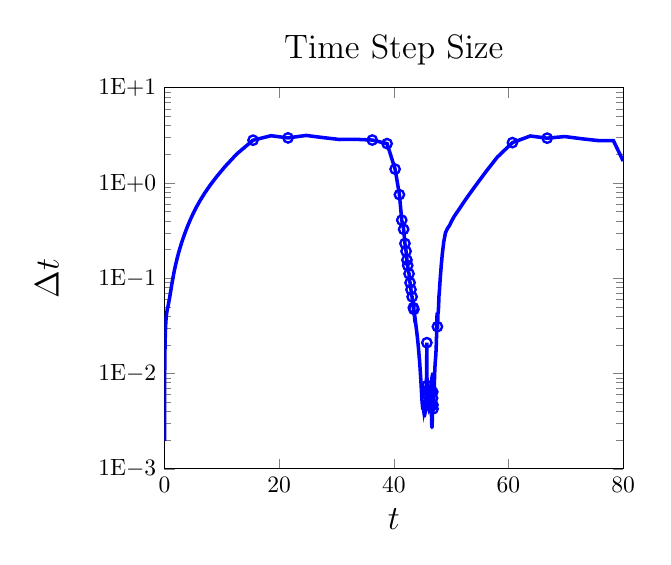
\begin{tikzpicture}[scale=0.85]

\begin{axis}[
  xmin = 0,
  xmax = 80,
  xtick = {0,20,40,60,80},
  xticklabels = {$0$,$20$,$40$,$60$,$80$},
  xlabel = $t$,
  ymode = log,
  ymin = 1E-3,
  ymax = 1E1,
  ytick = {1E-3,1E-2,1E-1,1E0,1E1},
  yticklabels = {$1$E$-3$,$1$E$-2$,$1$E$-1$,$1$E$+0$,$1$E$+1$},
  ylabel = {$\Delta t$},
  ylabel style = {yshift = 10pt},
  label style = {font=\Large},
  title = {\Large{Time Step Size}}
  ]

% adaptive time step size
\addplot [mark=none,blue,line width=1.5] table{
2.0693e-03 2.0693e-03
4.0324e-03 1.9631e-03
6.8259e-03 2.7935e-03
1.0801e-02 3.9753e-03
1.6080e-02 5.2784e-03
2.2654e-02 6.5739e-03
3.0878e-02 8.2242e-03
4.0926e-02 1.0048e-02
5.3163e-02 1.2237e-02
6.7828e-02 1.4664e-02
8.5250e-02 1.7422e-02
1.0564e-01 2.0388e-02
1.2919e-01 2.3552e-02
1.5596e-01 2.6771e-02
1.8593e-01 2.9965e-02
2.1893e-01 3.3005e-02
2.5476e-01 3.5824e-02
2.9313e-01 3.8370e-02
3.3377e-01 4.0642e-02
3.7644e-01 4.2668e-02
4.2094e-01 4.4502e-02
4.6715e-01 4.6208e-02
5.1500e-01 4.7856e-02
5.6394e-01 4.8941e-02
6.1437e-01 5.0431e-02
6.6694e-01 5.2565e-02
7.2162e-01 5.4685e-02
7.7864e-01 5.7018e-02
8.3834e-01 5.9700e-02
9.0107e-01 6.2727e-02
9.6722e-01 6.6156e-02
1.0373e+00 7.0060e-02
1.1118e+00 7.4500e-02
1.1916e+00 7.9849e-02
1.2777e+00 8.6099e-02
1.3703e+00 9.2540e-02
1.4702e+00 9.9920e-02
1.5786e+00 1.0836e-01
1.6963e+00 1.1777e-01
1.8246e+00 1.2828e-01
1.9647e+00 1.4008e-01
2.1180e+00 1.5333e-01
2.2862e+00 1.6823e-01
2.4714e+00 1.8512e-01
2.6758e+00 2.0440e-01
2.9024e+00 2.2662e-01
3.1549e+00 2.5247e-01
3.4377e+00 2.8285e-01
3.7566e+00 3.1890e-01
4.1188e+00 3.6215e-01
4.5333e+00 4.1452e-01
5.0118e+00 4.7849e-01
5.5691e+00 5.5736e-01
6.2249e+00 6.5575e-01
7.0056e+00 7.8071e-01
7.9497e+00 9.4413e-01
9.1180e+00 1.1683e+00
1.0616e+01 1.4978e+00
1.2637e+01 2.0216e+00
1.5447e+01 2.8101e+00
1.8579e+01 3.1311e+00
2.1549e+01 2.9704e+00
2.4701e+01 3.1525e+00
2.7692e+01 2.9907e+00
3.0550e+01 2.8582e+00
3.3419e+01 2.8691e+00
3.6240e+01 2.8202e+00
3.8826e+01 2.5862e+00
4.0222e+01 1.3965e+00
4.0976e+01 7.5413e-01
4.1384e+01 4.0723e-01
4.1710e+01 3.2616e-01
4.1941e+01 2.3156e-01
4.2133e+01 1.9191e-01
4.2288e+01 1.5512e-01
4.2425e+01 1.3615e-01
4.2542e+01 1.1742e-01
4.2653e+01 1.1139e-01
4.2748e+01 9.4545e-02
4.2838e+01 8.9693e-02
4.2918e+01 8.0059e-02
4.2994e+01 7.5951e-02
4.3062e+01 6.8090e-02
4.3126e+01 6.4596e-02
4.3190e+01 6.3801e-02
4.3248e+01 5.7777e-02
4.3303e+01 5.4812e-02
4.3357e+01 5.4746e-02
4.3407e+01 4.9077e-02
4.3453e+01 4.6559e-02
4.3500e+01 4.7111e-02
4.3543e+01 4.2796e-02
4.3584e+01 4.0600e-02
4.3625e+01 4.1239e-02
4.3665e+01 3.9749e-02
4.3702e+01 3.7865e-02
4.3739e+01 3.6472e-02
4.3774e+01 3.5126e-02
4.3808e+01 3.3850e-02
4.3841e+01 3.2663e-02
4.3872e+01 3.1546e-02
4.3903e+01 3.0493e-02
4.3932e+01 2.9497e-02
4.3961e+01 2.8554e-02
4.3988e+01 2.7658e-02
4.4015e+01 2.6806e-02
4.4041e+01 2.5993e-02
4.4066e+01 2.5217e-02
4.4091e+01 2.4474e-02
4.4115e+01 2.3762e-02
4.4138e+01 2.3078e-02
4.4160e+01 2.2421e-02
4.4182e+01 2.1788e-02
4.4203e+01 2.1178e-02
4.4224e+01 2.0590e-02
4.4244e+01 2.0021e-02
4.4263e+01 1.9471e-02
4.4282e+01 1.8939e-02
4.4300e+01 1.8424e-02
4.4318e+01 1.7924e-02
4.4336e+01 1.7440e-02
4.4353e+01 1.6971e-02
4.4369e+01 1.6516e-02
4.4385e+01 1.6074e-02
4.4401e+01 1.5644e-02
4.4416e+01 1.5211e-02
4.4431e+01 1.4803e-02
4.4445e+01 1.4411e-02
4.4460e+01 1.4285e-02
4.4474e+01 1.3996e-02
4.4487e+01 1.3610e-02
4.4501e+01 1.3283e-02
4.4514e+01 1.2966e-02
4.4526e+01 1.2654e-02
4.4539e+01 1.2352e-02
4.4551e+01 1.2061e-02
4.4562e+01 1.1778e-02
4.4574e+01 1.1504e-02
4.4585e+01 1.1239e-02
4.4596e+01 1.0982e-02
4.4607e+01 1.0733e-02
4.4617e+01 1.0492e-02
4.4628e+01 1.0259e-02
4.4638e+01 1.0033e-02
4.4648e+01 9.8146e-03
4.4657e+01 9.6028e-03
4.4667e+01 9.3977e-03
4.4676e+01 9.1991e-03
4.4685e+01 9.0067e-03
4.4694e+01 8.8642e-03
4.4702e+01 8.7127e-03
4.4711e+01 8.5230e-03
4.4719e+01 8.3542e-03
4.4727e+01 8.1946e-03
4.4735e+01 8.0369e-03
4.4743e+01 7.8842e-03
4.4751e+01 7.7369e-03
4.4759e+01 7.5943e-03
4.4766e+01 7.4561e-03
4.4773e+01 7.3223e-03
4.4781e+01 7.1928e-03
4.4788e+01 7.0674e-03
4.4795e+01 6.9460e-03
4.4801e+01 6.8276e-03
4.4808e+01 6.7136e-03
4.4815e+01 6.6039e-03
4.4821e+01 6.4974e-03
4.4828e+01 6.3944e-03
4.4834e+01 6.2947e-03
4.4840e+01 6.1983e-03
4.4846e+01 6.1050e-03
4.4852e+01 6.0147e-03
4.4858e+01 5.9274e-03
4.4864e+01 5.8430e-03
4.4870e+01 5.7614e-03
4.4875e+01 5.6825e-03
4.4881e+01 5.6062e-03
4.4887e+01 5.6101e-03
4.4892e+01 5.5697e-03
4.4898e+01 5.4760e-03
4.4903e+01 5.4066e-03
4.4909e+01 5.3497e-03
4.4914e+01 5.2884e-03
4.4919e+01 5.2281e-03
4.4924e+01 5.1716e-03
4.4929e+01 5.1172e-03
4.4934e+01 5.0644e-03
4.4939e+01 5.0136e-03
4.4944e+01 4.9648e-03
4.4949e+01 4.9179e-03
4.4954e+01 4.8728e-03
4.4959e+01 4.8295e-03
4.4964e+01 4.7880e-03
4.4969e+01 4.7483e-03
4.4973e+01 4.6823e-03
4.4978e+01 4.6294e-03
4.4982e+01 4.6262e-03
4.4987e+01 4.6230e-03
4.4992e+01 4.5789e-03
4.4996e+01 4.5427e-03
4.5001e+01 4.5143e-03
4.5005e+01 4.5038e-03
4.5010e+01 4.4955e-03
4.5014e+01 4.4710e-03
4.5019e+01 4.4270e-03
4.5023e+01 4.3903e-03
4.5027e+01 4.3777e-03
4.5032e+01 4.3629e-03
4.5036e+01 4.3437e-03
4.5040e+01 4.3277e-03
4.5045e+01 4.3147e-03
4.5049e+01 4.3025e-03
4.5053e+01 4.2914e-03
4.5058e+01 4.2787e-03
4.5062e+01 4.2697e-03
4.5066e+01 4.2646e-03
4.5070e+01 4.2602e-03
4.5075e+01 4.2567e-03
4.5079e+01 4.2552e-03
4.5083e+01 4.2555e-03
4.5087e+01 4.2574e-03
4.5092e+01 4.2610e-03
4.5096e+01 4.2664e-03
4.5100e+01 4.2736e-03
4.5104e+01 4.2828e-03
4.5109e+01 4.2938e-03
4.5113e+01 4.3069e-03
4.5117e+01 4.3221e-03
4.5122e+01 4.3395e-03
4.5126e+01 4.3591e-03
4.5130e+01 4.3811e-03
4.5135e+01 4.3816e-03
4.5139e+01 4.3648e-03
4.5144e+01 4.3991e-03
4.5148e+01 4.4372e-03
4.5153e+01 4.4602e-03
4.5157e+01 4.4861e-03
4.5162e+01 4.5202e-03
4.5166e+01 4.5554e-03
4.5171e+01 4.5903e-03
4.5175e+01 4.6271e-03
4.5180e+01 4.6659e-03
4.5185e+01 4.7051e-03
4.5189e+01 4.7440e-03
4.5194e+01 4.7821e-03
4.5199e+01 4.8183e-03
4.5204e+01 4.8511e-03
4.5209e+01 4.8789e-03
4.5214e+01 4.8999e-03
4.5219e+01 4.9122e-03
4.5223e+01 4.9138e-03
4.5228e+01 4.8953e-03
4.5233e+01 4.8671e-03
4.5238e+01 4.8306e-03
4.5243e+01 4.7784e-03
4.5248e+01 4.7118e-03
4.5252e+01 4.6354e-03
4.5257e+01 4.5518e-03
4.5261e+01 4.4630e-03
4.5266e+01 4.3721e-03
4.5270e+01 4.2819e-03
4.5274e+01 4.1947e-03
4.5278e+01 4.1120e-03
4.5282e+01 4.0351e-03
4.5286e+01 3.9647e-03
4.5290e+01 3.9012e-03
4.5294e+01 3.8447e-03
4.5298e+01 3.7951e-03
4.5301e+01 3.7521e-03
4.5305e+01 3.7156e-03
4.5309e+01 3.6849e-03
4.5313e+01 3.6597e-03
4.5316e+01 3.6396e-03
4.5320e+01 3.6240e-03
4.5323e+01 3.6125e-03
4.5327e+01 3.6046e-03
4.5331e+01 3.5999e-03
4.5334e+01 3.5980e-03
4.5338e+01 3.5984e-03
4.5341e+01 3.6008e-03
4.5345e+01 3.6049e-03
4.5349e+01 3.6103e-03
4.5352e+01 3.6168e-03
4.5356e+01 3.6242e-03
4.5360e+01 3.6322e-03
4.5363e+01 3.6406e-03
4.5367e+01 3.6493e-03
4.5370e+01 3.6583e-03
4.5374e+01 3.6674e-03
4.5378e+01 3.6765e-03
4.5381e+01 3.6856e-03
4.5385e+01 3.6948e-03
4.5389e+01 3.7039e-03
4.5393e+01 3.7131e-03
4.5396e+01 3.7223e-03
4.5400e+01 3.7316e-03
4.5404e+01 3.7409e-03
4.5408e+01 3.7504e-03
4.5411e+01 3.7600e-03
4.5415e+01 3.7699e-03
4.5419e+01 3.7800e-03
4.5423e+01 3.7904e-03
4.5426e+01 3.8011e-03
4.5430e+01 3.8121e-03
4.5434e+01 3.8236e-03
4.5438e+01 3.8355e-03
4.5442e+01 3.8478e-03
4.5446e+01 3.8607e-03
4.5449e+01 3.8740e-03
4.5453e+01 3.8880e-03
4.5457e+01 3.9026e-03
4.5461e+01 3.9178e-03
4.5465e+01 3.9337e-03
4.5469e+01 3.9504e-03
4.5473e+01 3.9679e-03
4.5477e+01 3.9863e-03
4.5481e+01 4.0056e-03
4.5485e+01 4.0259e-03
4.5489e+01 4.0472e-03
4.5493e+01 4.0695e-03
4.5497e+01 4.0928e-03
4.5501e+01 4.1171e-03
4.5506e+01 4.1423e-03
4.5510e+01 4.1686e-03
4.5514e+01 4.1959e-03
4.5518e+01 4.2245e-03
4.5522e+01 4.2545e-03
4.5527e+01 4.2859e-03
4.5531e+01 4.3190e-03
4.5535e+01 4.3538e-03
4.5540e+01 4.3904e-03
4.5544e+01 4.4290e-03
4.5549e+01 4.4698e-03
4.5553e+01 4.5129e-03
4.5558e+01 4.5585e-03
4.5562e+01 4.6067e-03
4.5567e+01 4.6579e-03
4.5572e+01 4.7123e-03
4.5576e+01 4.7702e-03
4.5581e+01 4.8319e-03
4.5586e+01 4.8978e-03
4.5591e+01 4.9684e-03
4.5596e+01 5.0441e-03
4.5601e+01 5.1257e-03
4.5607e+01 5.2137e-03
4.5612e+01 5.3091e-03
4.5617e+01 5.4129e-03
4.5623e+01 5.5263e-03
4.5628e+01 5.6509e-03
4.5634e+01 5.7884e-03
4.5640e+01 5.9414e-03
4.5646e+01 6.1127e-03
4.5653e+01 6.3062e-03
4.5659e+01 6.5273e-03
4.5666e+01 6.7829e-03
4.5673e+01 7.0830e-03
4.5680e+01 7.4421e-03
4.5688e+01 7.8820e-03
4.5697e+01 8.4382e-03
4.5706e+01 9.1723e-03
4.5716e+01 1.0204e-02
4.5728e+01 1.1808e-02
4.5743e+01 1.4789e-02
4.5764e+01 2.1045e-02
4.5770e+01 6.6101e-03
4.5777e+01 6.2709e-03
4.5786e+01 8.9237e-03
4.5794e+01 7.9957e-03
4.5801e+01 7.5854e-03
4.5809e+01 7.4646e-03
4.5816e+01 7.0816e-03
4.5823e+01 6.8475e-03
4.5829e+01 6.6616e-03
4.5836e+01 6.4121e-03
4.5842e+01 6.1852e-03
4.5848e+01 6.0338e-03
4.5854e+01 5.9107e-03
4.5860e+01 5.7791e-03
4.5865e+01 5.6541e-03
4.5871e+01 5.5522e-03
4.5876e+01 5.4638e-03
4.5882e+01 5.3778e-03
4.5887e+01 5.2964e-03
4.5892e+01 5.2241e-03
4.5897e+01 5.1587e-03
4.5902e+01 5.0970e-03
4.5907e+01 5.0386e-03
4.5912e+01 4.9852e-03
4.5917e+01 4.9362e-03
4.5922e+01 4.8900e-03
4.5927e+01 4.8464e-03
4.5932e+01 4.8061e-03
4.5937e+01 4.7686e-03
4.5941e+01 4.7336e-03
4.5946e+01 4.7009e-03
4.5951e+01 4.6705e-03
4.5955e+01 4.6423e-03
4.5960e+01 4.6162e-03
4.5965e+01 4.5919e-03
4.5969e+01 4.5695e-03
4.5974e+01 4.5488e-03
4.5978e+01 4.5299e-03
4.5983e+01 4.5126e-03
4.5987e+01 4.4968e-03
4.5992e+01 4.4827e-03
4.5996e+01 4.4701e-03
4.6001e+01 4.4590e-03
4.6005e+01 4.4495e-03
4.6010e+01 4.4414e-03
4.6014e+01 4.4346e-03
4.6018e+01 4.4288e-03
4.6023e+01 4.4233e-03
4.6027e+01 4.4176e-03
4.6032e+01 4.4120e-03
4.6036e+01 4.4072e-03
4.6040e+01 4.4040e-03
4.6045e+01 4.4021e-03
4.6049e+01 4.4015e-03
4.6054e+01 4.4022e-03
4.6058e+01 4.4048e-03
4.6062e+01 4.4207e-03
4.6067e+01 4.4125e-03
4.6071e+01 4.4025e-03
4.6076e+01 4.4149e-03
4.6080e+01 4.4300e-03
4.6085e+01 4.4375e-03
4.6089e+01 4.4445e-03
4.6093e+01 4.4517e-03
4.6098e+01 4.4589e-03
4.6102e+01 4.4693e-03
4.6107e+01 4.4825e-03
4.6111e+01 4.4966e-03
4.6116e+01 4.5114e-03
4.6120e+01 4.5279e-03
4.6125e+01 4.5460e-03
4.6130e+01 4.5652e-03
4.6134e+01 4.5854e-03
4.6139e+01 4.6070e-03
4.6143e+01 4.6311e-03
4.6148e+01 4.6552e-03
4.6153e+01 4.6711e-03
4.6157e+01 4.6928e-03
4.6162e+01 4.7694e-03
4.6167e+01 4.8632e-03
4.6172e+01 4.9193e-03
4.6177e+01 4.9633e-03
4.6182e+01 5.0281e-03
4.6187e+01 5.1056e-03
4.6192e+01 5.1855e-03
4.6197e+01 5.2742e-03
4.6203e+01 5.3782e-03
4.6208e+01 5.4978e-03
4.6214e+01 5.6343e-03
4.6220e+01 5.7469e-03
4.6226e+01 5.7840e-03
4.6231e+01 5.7397e-03
4.6237e+01 5.7242e-03
4.6243e+01 5.7051e-03
4.6248e+01 5.7030e-03
4.6254e+01 5.6907e-03
4.6260e+01 5.6874e-03
4.6265e+01 5.6829e-03
4.6271e+01 5.6861e-03
4.6277e+01 5.6906e-03
4.6283e+01 5.6987e-03
4.6288e+01 5.7097e-03
4.6294e+01 5.7205e-03
4.6300e+01 5.7467e-03
4.6305e+01 5.7773e-03
4.6311e+01 5.7966e-03
4.6317e+01 5.8234e-03
4.6323e+01 5.8529e-03
4.6329e+01 5.8863e-03
4.6335e+01 5.9232e-03
4.6341e+01 5.9636e-03
4.6347e+01 6.0073e-03
4.6353e+01 6.0542e-03
4.6359e+01 6.1040e-03
4.6365e+01 6.1565e-03
4.6371e+01 6.2115e-03
4.6378e+01 6.2687e-03
4.6384e+01 6.2153e-03
4.6390e+01 6.0732e-03
4.6396e+01 5.9561e-03
4.6402e+01 5.8736e-03
4.6407e+01 5.8200e-03
4.6413e+01 5.8989e-03
4.6419e+01 5.8993e-03
4.6425e+01 5.9225e-03
4.6431e+01 6.0751e-03
4.6437e+01 6.0107e-03
4.6444e+01 6.2225e-03
4.6450e+01 6.3968e-03
4.6457e+01 6.6993e-03
4.6464e+01 7.0876e-03
4.6471e+01 7.2400e-03
4.6478e+01 7.3339e-03
4.6486e+01 7.4548e-03
4.6493e+01 7.5813e-03
4.6501e+01 7.7175e-03
4.6509e+01 7.8610e-03
4.6516e+01 6.6328e-03
4.6522e+01 6.2924e-03
4.6527e+01 5.6331e-03
4.6533e+01 5.3440e-03
4.6538e+01 4.8490e-03
4.6542e+01 4.6001e-03
4.6547e+01 4.6367e-03
4.6551e+01 4.1278e-03
4.6555e+01 3.9160e-03
4.6559e+01 4.0662e-03
4.6563e+01 3.7369e-03
4.6566e+01 3.5452e-03
4.6570e+01 3.6848e-03
4.6574e+01 3.6263e-03
4.6577e+01 3.4682e-03
4.6580e+01 3.3969e-03
4.6584e+01 3.3443e-03
4.6587e+01 3.2761e-03
4.6590e+01 3.2159e-03
4.6593e+01 3.1656e-03
4.6597e+01 3.1183e-03
4.6600e+01 3.0744e-03
4.6603e+01 3.0349e-03
4.6606e+01 2.9989e-03
4.6609e+01 2.9659e-03
4.6612e+01 2.9359e-03
4.6614e+01 2.9086e-03
4.6617e+01 2.8838e-03
4.6620e+01 2.8614e-03
4.6623e+01 2.8412e-03
4.6626e+01 2.8231e-03
4.6629e+01 2.8071e-03
4.6631e+01 2.7931e-03
4.6634e+01 2.7809e-03
4.6637e+01 2.7707e-03
4.6640e+01 2.7623e-03
4.6643e+01 2.7559e-03
4.6645e+01 2.7512e-03
4.6648e+01 2.7482e-03
4.6651e+01 2.7471e-03
4.6654e+01 2.7479e-03
4.6656e+01 2.7506e-03
4.6659e+01 2.7552e-03
4.6662e+01 2.7618e-03
4.6665e+01 2.7704e-03
4.6667e+01 2.7812e-03
4.6670e+01 2.7942e-03
4.6673e+01 2.8095e-03
4.6676e+01 2.8274e-03
4.6679e+01 2.8479e-03
4.6682e+01 2.8712e-03
4.6684e+01 2.8977e-03
4.6687e+01 2.9275e-03
4.6690e+01 2.9609e-03
4.6693e+01 2.9985e-03
4.6696e+01 3.0405e-03
4.6699e+01 3.0877e-03
4.6703e+01 3.1407e-03
4.6706e+01 3.1996e-03
4.6709e+01 3.2665e-03
4.6712e+01 3.3426e-03
4.6716e+01 3.4290e-03
4.6719e+01 3.5271e-03
4.6723e+01 3.6423e-03
4.6727e+01 3.7432e-03
4.6731e+01 3.8788e-03
4.6735e+01 4.0755e-03
4.6739e+01 4.3056e-03
4.6744e+01 4.5859e-03
4.6749e+01 4.9629e-03
4.6754e+01 5.4974e-03
4.6760e+01 6.3249e-03
4.6768e+01 7.8909e-03
4.6778e+01 1.0218e-02
4.6788e+01 9.1021e-03
4.6794e+01 6.3996e-03
4.6800e+01 6.0712e-03
4.6805e+01 5.3980e-03
4.6811e+01 5.1210e-03
4.6816e+01 5.0657e-03
4.6820e+01 4.8629e-03
4.6825e+01 4.6815e-03
4.6830e+01 4.5536e-03
4.6834e+01 4.4506e-03
4.6839e+01 4.3701e-03
4.6843e+01 4.3058e-03
4.6847e+01 4.2547e-03
4.6851e+01 4.2145e-03
4.6855e+01 4.1833e-03
4.6860e+01 4.1598e-03
4.6864e+01 4.1430e-03
4.6868e+01 4.1321e-03
4.6872e+01 4.1265e-03
4.6876e+01 4.1257e-03
4.6880e+01 4.1293e-03
4.6884e+01 4.1370e-03
4.6889e+01 4.1486e-03
4.6893e+01 4.1640e-03
4.6897e+01 4.1830e-03
4.6901e+01 4.2057e-03
4.6905e+01 4.2321e-03
4.6910e+01 4.2622e-03
4.6914e+01 4.2960e-03
4.6918e+01 4.3338e-03
4.6923e+01 4.3755e-03
4.6927e+01 4.4213e-03
4.6932e+01 4.4714e-03
4.6936e+01 4.5260e-03
4.6941e+01 4.5852e-03
4.6945e+01 4.6492e-03
4.6950e+01 4.7184e-03
4.6955e+01 4.7931e-03
4.6960e+01 4.8735e-03
4.6965e+01 4.9600e-03
4.6970e+01 5.0531e-03
4.6975e+01 5.1532e-03
4.6980e+01 5.2608e-03
4.6985e+01 5.3766e-03
4.6991e+01 5.5012e-03
4.6997e+01 5.6354e-03
4.7002e+01 5.7798e-03
4.7008e+01 5.9352e-03
4.7014e+01 6.1023e-03
4.7021e+01 6.2816e-03
4.7027e+01 6.4737e-03
4.7034e+01 6.6794e-03
4.7041e+01 6.8995e-03
4.7048e+01 7.1349e-03
4.7055e+01 7.3866e-03
4.7063e+01 7.6553e-03
4.7071e+01 7.9416e-03
4.7079e+01 8.2459e-03
4.7088e+01 8.5682e-03
4.7097e+01 8.9079e-03
4.7106e+01 9.2639e-03
4.7116e+01 9.6341e-03
4.7126e+01 1.0016e-02
4.7136e+01 1.0405e-02
4.7147e+01 1.0798e-02
4.7158e+01 1.1189e-02
4.7169e+01 1.1574e-02
4.7181e+01 1.1948e-02
4.7194e+01 1.2308e-02
4.7206e+01 1.2654e-02
4.7219e+01 1.2986e-02
4.7233e+01 1.3308e-02
4.7246e+01 1.3626e-02
4.7260e+01 1.3949e-02
4.7275e+01 1.4289e-02
4.7289e+01 1.4658e-02
4.7304e+01 1.5071e-02
4.7320e+01 1.5557e-02
4.7336e+01 1.6130e-02
4.7353e+01 1.6837e-02
4.7371e+01 1.7715e-02
4.7389e+01 1.8856e-02
4.7410e+01 2.0363e-02
4.7432e+01 2.2473e-02
4.7458e+01 2.5568e-02
4.7488e+01 3.0598e-02
4.7528e+01 3.9951e-02
4.7572e+01 4.3403e-02
4.7603e+01 3.1016e-02
4.7632e+01 2.9424e-02
4.7671e+01 3.8720e-02
4.7715e+01 4.3606e-02
4.7759e+01 4.4308e-02
4.7810e+01 5.1098e-02
4.7875e+01 6.4968e-02
4.7948e+01 7.2718e-02
4.8036e+01 8.8504e-02
4.8145e+01 1.0882e-01
4.8284e+01 1.3874e-01
4.8465e+01 1.8149e-01
4.8705e+01 2.4002e-01
4.9005e+01 2.9943e-01
4.9335e+01 3.3082e-01
4.9691e+01 3.5541e-01
5.0089e+01 3.9825e-01
5.0535e+01 4.4592e-01
5.1028e+01 4.9283e-01
5.1580e+01 5.5170e-01
5.2208e+01 6.2888e-01
5.2935e+01 7.2647e-01
5.3791e+01 8.5660e-01
5.4836e+01 1.0440e+00
5.6175e+01 1.3396e+00
5.8037e+01 1.8623e+00
6.0687e+01 2.6501e+00
6.3799e+01 3.1111e+00
6.6750e+01 2.9515e+00
6.9819e+01 3.0692e+00
7.2731e+01 2.9117e+00
7.5520e+01 2.7892e+00
7.8300e+01 2.7801e+00
8.0000e+01 1.6997e+00
};


\addplot [only marks,blue,mark=o,mark size=2pt,line width=1.0] table{
1.5447e+01 2.8101e+00
2.1549e+01 2.9704e+00
3.6240e+01 2.8202e+00
3.8826e+01 2.5862e+00
4.0222e+01 1.3965e+00
4.0976e+01 7.5413e-01
4.1384e+01 4.0723e-01
4.1710e+01 3.2616e-01
4.1941e+01 2.3156e-01
4.2133e+01 1.9191e-01
4.2288e+01 1.5512e-01
4.2425e+01 1.3615e-01
4.2653e+01 1.1139e-01
4.2838e+01 8.9693e-02
4.2994e+01 7.5951e-02
4.3190e+01 6.3801e-02
4.3407e+01 4.9077e-02
4.3500e+01 4.7111e-02
4.5764e+01 2.1045e-02
4.5770e+01 6.6101e-03
4.5809e+01 7.4646e-03
4.5848e+01 6.0338e-03
4.6450e+01 6.3968e-03
4.6547e+01 4.6367e-03
4.6754e+01 5.4974e-03
4.6794e+01 6.3996e-03
4.6825e+01 4.6815e-03
4.6847e+01 4.2547e-03
4.7603e+01 3.1016e-02
6.0687e+01 2.6501e+00
6.6750e+01 2.9515e+00
};

% OLD RESULTS
%% adaptive time step size
%\addplot [mark=none,blue,line width=1.5] table{
%4.7743e-03 4.7743e-03
%9.4244e-03 4.6502e-03
%1.6218e-02 6.7939e-03
%2.6144e-02 9.9259e-03
%4.0646e-02 1.4502e-02
%6.1270e-02 2.0624e-02
%8.8007e-02 2.6737e-02
%1.2153e-01 3.3526e-02
%1.6212e-01 4.0583e-02
%2.0963e-01 4.7517e-02
%2.6370e-01 5.4062e-02
%3.2384e-01 6.0149e-02
%3.8974e-01 6.5897e-02
%4.6130e-01 7.1558e-02
%5.3876e-01 7.7463e-02
%6.2273e-01 8.3971e-02
%7.1417e-01 9.1433e-02
%8.1434e-01 1.0017e-01
%9.2480e-01 1.1046e-01
%1.0474e+00 1.2255e-01
%1.1840e+00 1.3666e-01
%1.3370e+00 1.5303e-01
%1.5090e+00 1.7200e-01
%1.7031e+00 1.9403e-01
%1.9229e+00 2.1984e-01
%2.1734e+00 2.5046e-01
%2.4607e+00 2.8734e-01
%2.7933e+00 3.3254e-01
%3.1821e+00 3.8885e-01
%3.6421e+00 4.6001e-01
%4.1931e+00 5.5098e-01
%4.8614e+00 6.6834e-01
%5.6829e+00 8.2147e-01
%6.7090e+00 1.0261e+00
%8.0233e+00 1.3143e+00
%9.7861e+00 1.7627e+00
%1.2361e+01 2.5754e+00
%1.6124e+01 3.7626e+00
%2.1621e+01 5.4972e+00
%2.9653e+01 8.0314e+00
%3.6510e+01 6.8574e+00
%4.0413e+01 3.9033e+00
%4.0999e+01 5.8609e-01
%4.1354e+01 3.5426e-01
%4.1626e+01 2.7265e-01
%4.1842e+01 2.1545e-01
%4.2021e+01 1.7887e-01
%4.2174e+01 1.5299e-01
%4.2307e+01 1.3381e-01
%4.2426e+01 1.1902e-01
%4.2534e+01 1.0728e-01
%4.2631e+01 9.7727e-02
%4.2721e+01 8.9801e-02
%4.2804e+01 8.3116e-02
%4.2882e+01 7.7398e-02
%4.2954e+01 7.2449e-02
%4.3022e+01 6.8122e-02
%4.3087e+01 6.4302e-02
%4.3148e+01 6.0904e-02
%4.3207e+01 5.9320e-02
%4.3262e+01 5.5027e-02
%4.3315e+01 5.3596e-02
%4.3366e+01 5.0228e-02
%4.3415e+01 4.8922e-02
%4.3461e+01 4.6207e-02
%4.3506e+01 4.5006e-02
%4.3549e+01 4.2775e-02
%4.3590e+01 4.1663e-02
%4.3630e+01 3.9801e-02
%4.3669e+01 3.8766e-02
%4.3706e+01 3.7188e-02
%4.3742e+01 3.6221e-02
%4.3777e+01 3.4867e-02
%4.3811e+01 3.3960e-02
%4.3844e+01 3.2784e-02
%4.3876e+01 3.1932e-02
%4.3907e+01 3.0900e-02
%4.3937e+01 3.0097e-02
%4.3966e+01 2.9183e-02
%4.3994e+01 2.8424e-02
%4.4022e+01 2.7608e-02
%4.4049e+01 2.6891e-02
%4.4075e+01 2.6156e-02
%4.4101e+01 2.5476e-02
%4.4125e+01 2.4811e-02
%4.4150e+01 2.4166e-02
%4.4174e+01 2.4177e-02
%4.4197e+01 2.3559e-02
%4.4220e+01 2.2953e-02
%4.4243e+01 2.2364e-02
%4.4264e+01 2.1793e-02
%4.4286e+01 2.1240e-02
%4.4306e+01 2.0704e-02
%4.4326e+01 2.0184e-02
%4.4346e+01 1.9680e-02
%4.4365e+01 1.9190e-02
%4.4384e+01 1.8713e-02
%4.4402e+01 1.8249e-02
%4.4420e+01 1.7797e-02
%4.4437e+01 1.7357e-02
%4.4454e+01 1.6927e-02
%4.4471e+01 1.6508e-02
%4.4487e+01 1.6098e-02
%4.4503e+01 1.5697e-02
%4.4518e+01 1.5305e-02
%4.4533e+01 1.4922e-02
%4.4547e+01 1.4546e-02
%4.4562e+01 1.4179e-02
%4.4575e+01 1.3819e-02
%4.4589e+01 1.3467e-02
%4.4602e+01 1.3122e-02
%4.4615e+01 1.2784e-02
%4.4627e+01 1.2454e-02
%4.4639e+01 1.2131e-02
%4.4651e+01 1.1508e-02
%4.4662e+01 1.1209e-02
%4.4673e+01 1.1215e-02
%4.4684e+01 1.0929e-02
%4.4695e+01 1.0647e-02
%4.4705e+01 1.0371e-02
%4.4715e+01 1.0103e-02
%4.4725e+01 9.8433e-03
%4.4735e+01 9.5918e-03
%4.4744e+01 9.3488e-03
%4.4753e+01 9.1142e-03
%4.4762e+01 8.8881e-03
%4.4771e+01 8.6702e-03
%4.4779e+01 8.4606e-03
%4.4788e+01 8.2592e-03
%4.4796e+01 8.0658e-03
%4.4804e+01 7.8802e-03
%4.4811e+01 7.7022e-03
%4.4819e+01 7.5318e-03
%4.4826e+01 7.3685e-03
%4.4833e+01 7.2123e-03
%4.4840e+01 7.0629e-03
%4.4847e+01 6.9200e-03
%4.4854e+01 6.7834e-03
%4.4861e+01 6.6529e-03
%4.4867e+01 6.5283e-03
%4.4874e+01 6.4093e-03
%4.4880e+01 6.2957e-03
%4.4886e+01 6.1873e-03
%4.4892e+01 6.0838e-03
%4.4898e+01 5.9851e-03
%4.4904e+01 5.8910e-03
%4.4910e+01 5.8012e-03
%4.4916e+01 5.7156e-03
%4.4921e+01 5.6341e-03
%4.4927e+01 5.5563e-03
%4.4932e+01 5.4823e-03
%4.4938e+01 5.4119e-03
%4.4943e+01 5.3449e-03
%4.4948e+01 5.2811e-03
%4.4954e+01 5.2206e-03
%4.4959e+01 5.1631e-03
%4.4964e+01 5.1086e-03
%4.4969e+01 5.0569e-03
%4.4974e+01 5.0080e-03
%4.4979e+01 4.9618e-03
%4.4984e+01 4.9183e-03
%4.4989e+01 4.8773e-03
%4.4994e+01 4.8388e-03
%4.4998e+01 4.8028e-03
%4.5003e+01 4.7693e-03
%4.5008e+01 4.7381e-03
%4.5013e+01 4.7094e-03
%4.5017e+01 4.6830e-03
%4.5022e+01 4.6591e-03
%4.5027e+01 4.6375e-03
%4.5031e+01 4.6183e-03
%4.5036e+01 4.6017e-03
%4.5040e+01 4.5875e-03
%4.5045e+01 4.5760e-03
%4.5049e+01 4.5671e-03
%4.5054e+01 4.5610e-03
%4.5059e+01 4.5578e-03
%4.5063e+01 4.5577e-03
%4.5068e+01 4.5609e-03
%4.5072e+01 4.5675e-03
%4.5077e+01 4.5778e-03
%4.5081e+01 4.5922e-03
%4.5086e+01 4.6109e-03
%4.5091e+01 4.6344e-03
%4.5095e+01 4.6631e-03
%4.5100e+01 4.6975e-03
%4.5105e+01 4.7384e-03
%4.5110e+01 4.7863e-03
%4.5114e+01 4.8422e-03
%4.5119e+01 4.9068e-03
%4.5124e+01 4.9813e-03
%4.5129e+01 5.0667e-03
%4.5135e+01 5.1641e-03
%4.5140e+01 5.2746e-03
%4.5145e+01 5.3990e-03
%4.5151e+01 5.5376e-03
%4.5156e+01 5.6898e-03
%4.5162e+01 5.8534e-03
%4.5168e+01 6.0236e-03
%4.5175e+01 6.1924e-03
%4.5181e+01 6.3481e-03
%4.5187e+01 6.4757e-03
%4.5194e+01 6.5601e-03
%4.5200e+01 6.5901e-03
%4.5207e+01 6.5631e-03
%4.5214e+01 6.4862e-03
%4.5220e+01 6.3735e-03
%4.5226e+01 6.2410e-03
%4.5232e+01 6.1028e-03
%4.5238e+01 5.9688e-03
%4.5244e+01 5.8447e-03
%4.5250e+01 5.7335e-03
%4.5255e+01 5.6357e-03
%4.5261e+01 5.5510e-03
%4.5266e+01 5.4785e-03
%4.5272e+01 5.4169e-03
%4.5277e+01 5.3651e-03
%4.5283e+01 5.3219e-03
%4.5288e+01 5.2863e-03
%4.5293e+01 5.2573e-03
%4.5298e+01 5.2343e-03
%4.5304e+01 5.2166e-03
%4.5309e+01 5.2035e-03
%4.5314e+01 5.1947e-03
%4.5319e+01 5.1898e-03
%4.5324e+01 5.1884e-03
%4.5330e+01 5.1902e-03
%4.5335e+01 5.1951e-03
%4.5340e+01 5.2028e-03
%4.5345e+01 5.2132e-03
%4.5350e+01 5.2263e-03
%4.5356e+01 5.2418e-03
%4.5361e+01 5.2598e-03
%4.5366e+01 5.2803e-03
%4.5371e+01 5.3032e-03
%4.5377e+01 5.3285e-03
%4.5382e+01 5.3563e-03
%4.5388e+01 5.3865e-03
%4.5393e+01 5.4194e-03
%4.5398e+01 5.4549e-03
%4.5404e+01 5.4932e-03
%4.5409e+01 5.5344e-03
%4.5415e+01 5.5786e-03
%4.5421e+01 5.6260e-03
%4.5426e+01 5.6769e-03
%4.5432e+01 5.7314e-03
%4.5438e+01 5.7899e-03
%4.5444e+01 5.8526e-03
%4.5450e+01 5.9198e-03
%4.5456e+01 5.9920e-03
%4.5462e+01 6.0697e-03
%4.5468e+01 6.1534e-03
%4.5474e+01 6.2437e-03
%4.5480e+01 6.3413e-03
%4.5487e+01 6.4472e-03
%4.5493e+01 6.5623e-03
%4.5500e+01 6.6880e-03
%4.5507e+01 6.8256e-03
%4.5514e+01 6.9770e-03
%4.5521e+01 7.1444e-03
%4.5528e+01 7.3307e-03
%4.5536e+01 7.5393e-03
%4.5544e+01 7.7749e-03
%4.5552e+01 8.0436e-03
%4.5560e+01 8.3535e-03
%4.5569e+01 8.7160e-03
%4.5578e+01 9.1476e-03
%4.5588e+01 9.6730e-03
%4.5598e+01 1.0332e-02
%4.5609e+01 1.1191e-02
%4.5622e+01 1.2380e-02
%4.5636e+01 1.4182e-02
%4.5653e+01 1.7405e-02
%4.5679e+01 2.5429e-02
%4.5694e+01 1.5149e-02
%4.5707e+01 1.3641e-02
%4.5720e+01 1.2333e-02
%4.5731e+01 1.1478e-02
%4.5742e+01 1.0883e-02
%4.5753e+01 1.0600e-02
%4.5763e+01 1.0116e-02
%4.5773e+01 9.8527e-03
%4.5782e+01 9.8659e-03
%4.5792e+01 9.6759e-03
%4.5802e+01 9.5333e-03
%4.5811e+01 9.4287e-03
%4.5820e+01 9.3579e-03
%4.5830e+01 9.3158e-03
%4.5839e+01 9.2983e-03
%4.5848e+01 9.3022e-03
%4.5858e+01 9.3242e-03
%4.5867e+01 9.3614e-03
%4.5876e+01 9.4109e-03
%4.5886e+01 9.4697e-03
%4.5895e+01 9.5349e-03
%4.5905e+01 9.6036e-03
%4.5915e+01 9.6731e-03
%4.5924e+01 9.7413e-03
%4.5934e+01 9.8066e-03
%4.5944e+01 9.8680e-03
%4.5954e+01 9.9258e-03
%4.5964e+01 9.9810e-03
%4.5974e+01 1.0036e-02
%4.5984e+01 1.0093e-02
%4.5994e+01 1.0156e-02
%4.6005e+01 1.0230e-02
%4.6015e+01 1.0320e-02
%4.6025e+01 1.0433e-02
%4.6036e+01 1.0353e-02
%4.6046e+01 1.0089e-02
%4.6056e+01 9.9059e-03
%4.6065e+01 9.7312e-03
%4.6075e+01 9.5814e-03
%4.6084e+01 9.4500e-03
%4.6094e+01 9.3371e-03
%4.6103e+01 9.2411e-03
%4.6112e+01 9.1611e-03
%4.6121e+01 9.0962e-03
%4.6130e+01 9.0458e-03
%4.6139e+01 9.0093e-03
%4.6148e+01 8.9863e-03
%4.6157e+01 8.9764e-03
%4.6166e+01 8.9795e-03
%4.6175e+01 8.9953e-03
%4.6184e+01 9.0238e-03
%4.6193e+01 9.0648e-03
%4.6202e+01 9.1182e-03
%4.6212e+01 9.1837e-03
%4.6221e+01 9.2609e-03
%4.6230e+01 9.3495e-03
%4.6240e+01 9.4485e-03
%4.6249e+01 9.5572e-03
%4.6259e+01 9.6742e-03
%4.6269e+01 9.7984e-03
%4.6279e+01 9.9285e-03
%4.6289e+01 1.0064e-02
%4.6299e+01 1.0205e-02
%4.6309e+01 1.0352e-02
%4.6320e+01 1.0509e-02
%4.6330e+01 9.6970e-03
%4.6338e+01 8.7962e-03
%4.6346e+01 8.0915e-03
%4.6354e+01 7.5316e-03
%4.6361e+01 7.0742e-03
%4.6368e+01 6.6931e-03
%4.6374e+01 6.5191e-03
%4.6380e+01 6.0807e-03
%4.6386e+01 5.9226e-03
%4.6392e+01 5.6327e-03
%4.6397e+01 5.4863e-03
%4.6403e+01 5.2877e-03
%4.6408e+01 5.1502e-03
%4.6413e+01 5.1476e-03
%4.6418e+01 5.0165e-03
%4.6423e+01 4.9003e-03
%4.6428e+01 4.7966e-03
%4.6432e+01 4.7045e-03
%4.6437e+01 4.6228e-03
%4.6442e+01 4.5506e-03
%4.6446e+01 4.4869e-03
%4.6450e+01 4.4313e-03
%4.6455e+01 4.3831e-03
%4.6459e+01 4.3421e-03
%4.6463e+01 4.3078e-03
%4.6468e+01 4.2800e-03
%4.6472e+01 4.2586e-03
%4.6476e+01 4.2436e-03
%4.6480e+01 4.2349e-03
%4.6485e+01 4.2325e-03
%4.6489e+01 4.2367e-03
%4.6493e+01 4.2477e-03
%4.6497e+01 4.2658e-03
%4.6502e+01 4.2914e-03
%4.6506e+01 4.3252e-03
%4.6510e+01 4.3678e-03
%4.6515e+01 4.4201e-03
%4.6519e+01 4.4833e-03
%4.6524e+01 4.5588e-03
%4.6529e+01 4.6484e-03
%4.6533e+01 4.7543e-03
%4.6538e+01 4.8797e-03
%4.6543e+01 5.0285e-03
%4.6548e+01 5.2060e-03
%4.6554e+01 5.4197e-03
%4.6560e+01 5.6802e-03
%4.6566e+01 6.0036e-03
%4.6572e+01 6.4148e-03
%4.6579e+01 6.9567e-03
%4.6587e+01 7.7091e-03
%4.6595e+01 8.8453e-03
%4.6606e+01 1.0846e-02
%4.6621e+01 1.5107e-02
%4.6634e+01 1.2137e-02
%4.6644e+01 1.0004e-02
%4.6653e+01 9.0610e-03
%4.6661e+01 8.4890e-03
%4.6669e+01 8.2683e-03
%4.6677e+01 7.8394e-03
%4.6685e+01 7.6356e-03
%4.6692e+01 7.6470e-03
%4.6700e+01 7.5197e-03
%4.6707e+01 7.4224e-03
%4.6715e+01 7.3626e-03
%4.6722e+01 7.3319e-03
%4.6729e+01 7.3264e-03
%4.6737e+01 7.3441e-03
%4.6744e+01 7.3839e-03
%4.6752e+01 7.4458e-03
%4.6759e+01 7.5301e-03
%4.6767e+01 7.6382e-03
%4.6775e+01 7.7717e-03
%4.6783e+01 7.9335e-03
%4.6791e+01 8.1269e-03
%4.6799e+01 8.3565e-03
%4.6808e+01 8.6283e-03
%4.6817e+01 8.9503e-03
%4.6826e+01 9.3330e-03
%4.6836e+01 9.7909e-03
%4.6846e+01 1.0344e-02
%4.6857e+01 1.1022e-02
%4.6869e+01 1.1869e-02
%4.6882e+01 1.2956e-02
%4.6896e+01 1.4408e-02
%4.6913e+01 1.6466e-02
%4.6932e+01 1.9693e-02
%4.6958e+01 2.5883e-02
%4.6990e+01 3.1405e-02
%4.7019e+01 2.8883e-02
%4.7044e+01 2.5392e-02
%4.7067e+01 2.3389e-02
%4.7089e+01 2.2066e-02
%4.7111e+01 2.1493e-02
%4.7131e+01 2.0233e-02
%4.7151e+01 1.9707e-02
%4.7170e+01 1.8925e-02
%4.7188e+01 1.8433e-02
%4.7207e+01 1.8399e-02
%4.7225e+01 1.7957e-02
%4.7242e+01 1.7590e-02
%4.7260e+01 1.7317e-02
%4.7277e+01 1.7142e-02
%4.7294e+01 1.7071e-02
%4.7311e+01 1.7114e-02
%4.7328e+01 1.7282e-02
%4.7346e+01 1.7593e-02
%4.7364e+01 1.8072e-02
%4.7383e+01 1.8750e-02
%4.7402e+01 1.9678e-02
%4.7423e+01 2.0923e-02
%4.7446e+01 2.2583e-02
%4.7471e+01 2.4808e-02
%4.7498e+01 2.7823e-02
%4.7530e+01 3.1995e-02
%4.7568e+01 3.7948e-02
%4.7615e+01 4.6842e-02
%4.7676e+01 6.1119e-02
%4.7763e+01 8.7068e-02
%4.7891e+01 1.2721e-01
%4.8069e+01 1.7834e-01
%4.8329e+01 2.6056e-01
%4.8654e+01 3.2463e-01
%4.9025e+01 3.7055e-01
%4.9441e+01 4.1648e-01
%4.9910e+01 4.6846e-01
%5.0446e+01 5.3655e-01
%5.1074e+01 6.2768e-01
%5.1828e+01 7.5460e-01
%5.2770e+01 9.4163e-01
%5.4009e+01 1.2388e+00
%5.5787e+01 1.7783e+00
%5.8385e+01 2.5981e+00
%6.2181e+01 3.7958e+00
%6.7727e+01 5.5457e+00
%7.5829e+01 8.1023e+00
%8.0000e+01 4.1710e+00
%};
%
%\addplot [only marks,blue,mark=o,mark size=2pt,line width=1.0] table{
%4.7743e-03 4.7743e-03
%3.6510e+01 6.8574e+00
%4.0413e+01 3.9033e+00
%4.0999e+01 5.8609e-01
%4.1354e+01 3.5426e-01
%4.1626e+01 2.7265e-01
%4.1842e+01 2.1545e-01
%4.2021e+01 1.7887e-01
%4.2174e+01 1.5299e-01
%4.2307e+01 1.3381e-01
%4.2426e+01 1.1902e-01
%4.2534e+01 1.0728e-01
%4.2631e+01 9.7727e-02
%4.2721e+01 8.9801e-02
%4.2804e+01 8.3116e-02
%4.2882e+01 7.7398e-02
%4.2954e+01 7.2449e-02
%4.3022e+01 6.8122e-02
%4.3087e+01 6.4302e-02
%4.3148e+01 6.0904e-02
%4.3262e+01 5.5027e-02
%4.3366e+01 5.0228e-02
%4.3461e+01 4.6207e-02
%4.3549e+01 4.2775e-02
%4.3630e+01 3.9801e-02
%4.3706e+01 3.7188e-02
%4.3777e+01 3.4867e-02
%4.3844e+01 3.2784e-02
%4.3907e+01 3.0900e-02
%4.3966e+01 2.9183e-02
%4.4022e+01 2.7608e-02
%4.4075e+01 2.6156e-02
%4.4125e+01 2.4811e-02
%4.4651e+01 1.1508e-02
%4.5694e+01 1.5149e-02
%4.5707e+01 1.3641e-02
%4.5720e+01 1.2333e-02
%4.5731e+01 1.1478e-02
%4.5742e+01 1.0883e-02
%4.5763e+01 1.0116e-02
%4.6330e+01 9.6970e-03
%4.6338e+01 8.7962e-03
%4.6346e+01 8.0915e-03
%4.6354e+01 7.5316e-03
%4.6361e+01 7.0742e-03
%4.6368e+01 6.6931e-03
%4.6380e+01 6.0807e-03
%4.6392e+01 5.6327e-03
%4.6403e+01 5.2877e-03
%4.6621e+01 1.5107e-02
%4.6634e+01 1.2137e-02
%4.6644e+01 1.0004e-02
%4.6653e+01 9.0610e-03
%4.6661e+01 8.4890e-03
%4.6677e+01 7.8394e-03
%4.7019e+01 2.8883e-02
%4.7044e+01 2.5392e-02
%4.7067e+01 2.3389e-02
%4.7089e+01 2.2066e-02
%4.7131e+01 2.0233e-02
%4.7170e+01 1.8925e-02
%};

\end{axis}

\end{tikzpicture}


 &
%%\input{figs/stenosisAdaptiveErrors.tikz}
%%\fi
%%\end{tabular}
%
%\begin{figure}[htp]
%\begin{tabular}{ccc}
%%\ifTikz
%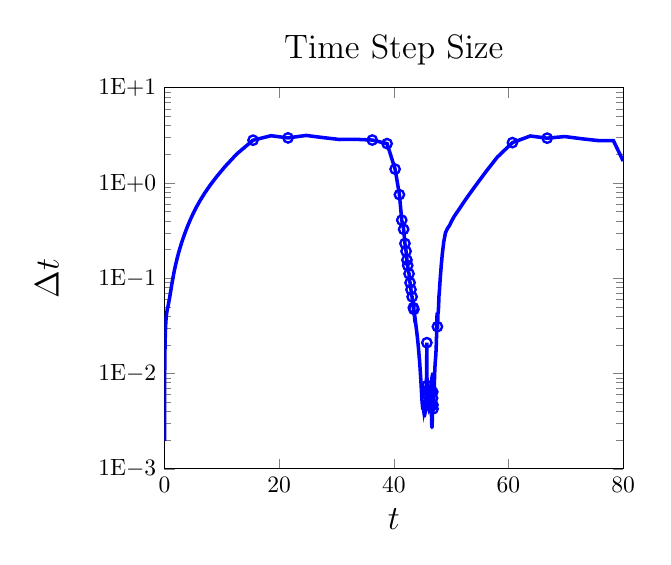
\begin{tikzpicture}[scale=0.85]

\begin{axis}[
  xmin = 0,
  xmax = 80,
  xtick = {0,20,40,60,80},
  xticklabels = {$0$,$20$,$40$,$60$,$80$},
  xlabel = $t$,
  ymode = log,
  ymin = 1E-3,
  ymax = 1E1,
  ytick = {1E-3,1E-2,1E-1,1E0,1E1},
  yticklabels = {$1$E$-3$,$1$E$-2$,$1$E$-1$,$1$E$+0$,$1$E$+1$},
  ylabel = {$\Delta t$},
  ylabel style = {yshift = 10pt},
  label style = {font=\Large},
  title = {\Large{Time Step Size}}
  ]

% adaptive time step size
\addplot [mark=none,blue,line width=1.5] table{
2.0693e-03 2.0693e-03
4.0324e-03 1.9631e-03
6.8259e-03 2.7935e-03
1.0801e-02 3.9753e-03
1.6080e-02 5.2784e-03
2.2654e-02 6.5739e-03
3.0878e-02 8.2242e-03
4.0926e-02 1.0048e-02
5.3163e-02 1.2237e-02
6.7828e-02 1.4664e-02
8.5250e-02 1.7422e-02
1.0564e-01 2.0388e-02
1.2919e-01 2.3552e-02
1.5596e-01 2.6771e-02
1.8593e-01 2.9965e-02
2.1893e-01 3.3005e-02
2.5476e-01 3.5824e-02
2.9313e-01 3.8370e-02
3.3377e-01 4.0642e-02
3.7644e-01 4.2668e-02
4.2094e-01 4.4502e-02
4.6715e-01 4.6208e-02
5.1500e-01 4.7856e-02
5.6394e-01 4.8941e-02
6.1437e-01 5.0431e-02
6.6694e-01 5.2565e-02
7.2162e-01 5.4685e-02
7.7864e-01 5.7018e-02
8.3834e-01 5.9700e-02
9.0107e-01 6.2727e-02
9.6722e-01 6.6156e-02
1.0373e+00 7.0060e-02
1.1118e+00 7.4500e-02
1.1916e+00 7.9849e-02
1.2777e+00 8.6099e-02
1.3703e+00 9.2540e-02
1.4702e+00 9.9920e-02
1.5786e+00 1.0836e-01
1.6963e+00 1.1777e-01
1.8246e+00 1.2828e-01
1.9647e+00 1.4008e-01
2.1180e+00 1.5333e-01
2.2862e+00 1.6823e-01
2.4714e+00 1.8512e-01
2.6758e+00 2.0440e-01
2.9024e+00 2.2662e-01
3.1549e+00 2.5247e-01
3.4377e+00 2.8285e-01
3.7566e+00 3.1890e-01
4.1188e+00 3.6215e-01
4.5333e+00 4.1452e-01
5.0118e+00 4.7849e-01
5.5691e+00 5.5736e-01
6.2249e+00 6.5575e-01
7.0056e+00 7.8071e-01
7.9497e+00 9.4413e-01
9.1180e+00 1.1683e+00
1.0616e+01 1.4978e+00
1.2637e+01 2.0216e+00
1.5447e+01 2.8101e+00
1.8579e+01 3.1311e+00
2.1549e+01 2.9704e+00
2.4701e+01 3.1525e+00
2.7692e+01 2.9907e+00
3.0550e+01 2.8582e+00
3.3419e+01 2.8691e+00
3.6240e+01 2.8202e+00
3.8826e+01 2.5862e+00
4.0222e+01 1.3965e+00
4.0976e+01 7.5413e-01
4.1384e+01 4.0723e-01
4.1710e+01 3.2616e-01
4.1941e+01 2.3156e-01
4.2133e+01 1.9191e-01
4.2288e+01 1.5512e-01
4.2425e+01 1.3615e-01
4.2542e+01 1.1742e-01
4.2653e+01 1.1139e-01
4.2748e+01 9.4545e-02
4.2838e+01 8.9693e-02
4.2918e+01 8.0059e-02
4.2994e+01 7.5951e-02
4.3062e+01 6.8090e-02
4.3126e+01 6.4596e-02
4.3190e+01 6.3801e-02
4.3248e+01 5.7777e-02
4.3303e+01 5.4812e-02
4.3357e+01 5.4746e-02
4.3407e+01 4.9077e-02
4.3453e+01 4.6559e-02
4.3500e+01 4.7111e-02
4.3543e+01 4.2796e-02
4.3584e+01 4.0600e-02
4.3625e+01 4.1239e-02
4.3665e+01 3.9749e-02
4.3702e+01 3.7865e-02
4.3739e+01 3.6472e-02
4.3774e+01 3.5126e-02
4.3808e+01 3.3850e-02
4.3841e+01 3.2663e-02
4.3872e+01 3.1546e-02
4.3903e+01 3.0493e-02
4.3932e+01 2.9497e-02
4.3961e+01 2.8554e-02
4.3988e+01 2.7658e-02
4.4015e+01 2.6806e-02
4.4041e+01 2.5993e-02
4.4066e+01 2.5217e-02
4.4091e+01 2.4474e-02
4.4115e+01 2.3762e-02
4.4138e+01 2.3078e-02
4.4160e+01 2.2421e-02
4.4182e+01 2.1788e-02
4.4203e+01 2.1178e-02
4.4224e+01 2.0590e-02
4.4244e+01 2.0021e-02
4.4263e+01 1.9471e-02
4.4282e+01 1.8939e-02
4.4300e+01 1.8424e-02
4.4318e+01 1.7924e-02
4.4336e+01 1.7440e-02
4.4353e+01 1.6971e-02
4.4369e+01 1.6516e-02
4.4385e+01 1.6074e-02
4.4401e+01 1.5644e-02
4.4416e+01 1.5211e-02
4.4431e+01 1.4803e-02
4.4445e+01 1.4411e-02
4.4460e+01 1.4285e-02
4.4474e+01 1.3996e-02
4.4487e+01 1.3610e-02
4.4501e+01 1.3283e-02
4.4514e+01 1.2966e-02
4.4526e+01 1.2654e-02
4.4539e+01 1.2352e-02
4.4551e+01 1.2061e-02
4.4562e+01 1.1778e-02
4.4574e+01 1.1504e-02
4.4585e+01 1.1239e-02
4.4596e+01 1.0982e-02
4.4607e+01 1.0733e-02
4.4617e+01 1.0492e-02
4.4628e+01 1.0259e-02
4.4638e+01 1.0033e-02
4.4648e+01 9.8146e-03
4.4657e+01 9.6028e-03
4.4667e+01 9.3977e-03
4.4676e+01 9.1991e-03
4.4685e+01 9.0067e-03
4.4694e+01 8.8642e-03
4.4702e+01 8.7127e-03
4.4711e+01 8.5230e-03
4.4719e+01 8.3542e-03
4.4727e+01 8.1946e-03
4.4735e+01 8.0369e-03
4.4743e+01 7.8842e-03
4.4751e+01 7.7369e-03
4.4759e+01 7.5943e-03
4.4766e+01 7.4561e-03
4.4773e+01 7.3223e-03
4.4781e+01 7.1928e-03
4.4788e+01 7.0674e-03
4.4795e+01 6.9460e-03
4.4801e+01 6.8276e-03
4.4808e+01 6.7136e-03
4.4815e+01 6.6039e-03
4.4821e+01 6.4974e-03
4.4828e+01 6.3944e-03
4.4834e+01 6.2947e-03
4.4840e+01 6.1983e-03
4.4846e+01 6.1050e-03
4.4852e+01 6.0147e-03
4.4858e+01 5.9274e-03
4.4864e+01 5.8430e-03
4.4870e+01 5.7614e-03
4.4875e+01 5.6825e-03
4.4881e+01 5.6062e-03
4.4887e+01 5.6101e-03
4.4892e+01 5.5697e-03
4.4898e+01 5.4760e-03
4.4903e+01 5.4066e-03
4.4909e+01 5.3497e-03
4.4914e+01 5.2884e-03
4.4919e+01 5.2281e-03
4.4924e+01 5.1716e-03
4.4929e+01 5.1172e-03
4.4934e+01 5.0644e-03
4.4939e+01 5.0136e-03
4.4944e+01 4.9648e-03
4.4949e+01 4.9179e-03
4.4954e+01 4.8728e-03
4.4959e+01 4.8295e-03
4.4964e+01 4.7880e-03
4.4969e+01 4.7483e-03
4.4973e+01 4.6823e-03
4.4978e+01 4.6294e-03
4.4982e+01 4.6262e-03
4.4987e+01 4.6230e-03
4.4992e+01 4.5789e-03
4.4996e+01 4.5427e-03
4.5001e+01 4.5143e-03
4.5005e+01 4.5038e-03
4.5010e+01 4.4955e-03
4.5014e+01 4.4710e-03
4.5019e+01 4.4270e-03
4.5023e+01 4.3903e-03
4.5027e+01 4.3777e-03
4.5032e+01 4.3629e-03
4.5036e+01 4.3437e-03
4.5040e+01 4.3277e-03
4.5045e+01 4.3147e-03
4.5049e+01 4.3025e-03
4.5053e+01 4.2914e-03
4.5058e+01 4.2787e-03
4.5062e+01 4.2697e-03
4.5066e+01 4.2646e-03
4.5070e+01 4.2602e-03
4.5075e+01 4.2567e-03
4.5079e+01 4.2552e-03
4.5083e+01 4.2555e-03
4.5087e+01 4.2574e-03
4.5092e+01 4.2610e-03
4.5096e+01 4.2664e-03
4.5100e+01 4.2736e-03
4.5104e+01 4.2828e-03
4.5109e+01 4.2938e-03
4.5113e+01 4.3069e-03
4.5117e+01 4.3221e-03
4.5122e+01 4.3395e-03
4.5126e+01 4.3591e-03
4.5130e+01 4.3811e-03
4.5135e+01 4.3816e-03
4.5139e+01 4.3648e-03
4.5144e+01 4.3991e-03
4.5148e+01 4.4372e-03
4.5153e+01 4.4602e-03
4.5157e+01 4.4861e-03
4.5162e+01 4.5202e-03
4.5166e+01 4.5554e-03
4.5171e+01 4.5903e-03
4.5175e+01 4.6271e-03
4.5180e+01 4.6659e-03
4.5185e+01 4.7051e-03
4.5189e+01 4.7440e-03
4.5194e+01 4.7821e-03
4.5199e+01 4.8183e-03
4.5204e+01 4.8511e-03
4.5209e+01 4.8789e-03
4.5214e+01 4.8999e-03
4.5219e+01 4.9122e-03
4.5223e+01 4.9138e-03
4.5228e+01 4.8953e-03
4.5233e+01 4.8671e-03
4.5238e+01 4.8306e-03
4.5243e+01 4.7784e-03
4.5248e+01 4.7118e-03
4.5252e+01 4.6354e-03
4.5257e+01 4.5518e-03
4.5261e+01 4.4630e-03
4.5266e+01 4.3721e-03
4.5270e+01 4.2819e-03
4.5274e+01 4.1947e-03
4.5278e+01 4.1120e-03
4.5282e+01 4.0351e-03
4.5286e+01 3.9647e-03
4.5290e+01 3.9012e-03
4.5294e+01 3.8447e-03
4.5298e+01 3.7951e-03
4.5301e+01 3.7521e-03
4.5305e+01 3.7156e-03
4.5309e+01 3.6849e-03
4.5313e+01 3.6597e-03
4.5316e+01 3.6396e-03
4.5320e+01 3.6240e-03
4.5323e+01 3.6125e-03
4.5327e+01 3.6046e-03
4.5331e+01 3.5999e-03
4.5334e+01 3.5980e-03
4.5338e+01 3.5984e-03
4.5341e+01 3.6008e-03
4.5345e+01 3.6049e-03
4.5349e+01 3.6103e-03
4.5352e+01 3.6168e-03
4.5356e+01 3.6242e-03
4.5360e+01 3.6322e-03
4.5363e+01 3.6406e-03
4.5367e+01 3.6493e-03
4.5370e+01 3.6583e-03
4.5374e+01 3.6674e-03
4.5378e+01 3.6765e-03
4.5381e+01 3.6856e-03
4.5385e+01 3.6948e-03
4.5389e+01 3.7039e-03
4.5393e+01 3.7131e-03
4.5396e+01 3.7223e-03
4.5400e+01 3.7316e-03
4.5404e+01 3.7409e-03
4.5408e+01 3.7504e-03
4.5411e+01 3.7600e-03
4.5415e+01 3.7699e-03
4.5419e+01 3.7800e-03
4.5423e+01 3.7904e-03
4.5426e+01 3.8011e-03
4.5430e+01 3.8121e-03
4.5434e+01 3.8236e-03
4.5438e+01 3.8355e-03
4.5442e+01 3.8478e-03
4.5446e+01 3.8607e-03
4.5449e+01 3.8740e-03
4.5453e+01 3.8880e-03
4.5457e+01 3.9026e-03
4.5461e+01 3.9178e-03
4.5465e+01 3.9337e-03
4.5469e+01 3.9504e-03
4.5473e+01 3.9679e-03
4.5477e+01 3.9863e-03
4.5481e+01 4.0056e-03
4.5485e+01 4.0259e-03
4.5489e+01 4.0472e-03
4.5493e+01 4.0695e-03
4.5497e+01 4.0928e-03
4.5501e+01 4.1171e-03
4.5506e+01 4.1423e-03
4.5510e+01 4.1686e-03
4.5514e+01 4.1959e-03
4.5518e+01 4.2245e-03
4.5522e+01 4.2545e-03
4.5527e+01 4.2859e-03
4.5531e+01 4.3190e-03
4.5535e+01 4.3538e-03
4.5540e+01 4.3904e-03
4.5544e+01 4.4290e-03
4.5549e+01 4.4698e-03
4.5553e+01 4.5129e-03
4.5558e+01 4.5585e-03
4.5562e+01 4.6067e-03
4.5567e+01 4.6579e-03
4.5572e+01 4.7123e-03
4.5576e+01 4.7702e-03
4.5581e+01 4.8319e-03
4.5586e+01 4.8978e-03
4.5591e+01 4.9684e-03
4.5596e+01 5.0441e-03
4.5601e+01 5.1257e-03
4.5607e+01 5.2137e-03
4.5612e+01 5.3091e-03
4.5617e+01 5.4129e-03
4.5623e+01 5.5263e-03
4.5628e+01 5.6509e-03
4.5634e+01 5.7884e-03
4.5640e+01 5.9414e-03
4.5646e+01 6.1127e-03
4.5653e+01 6.3062e-03
4.5659e+01 6.5273e-03
4.5666e+01 6.7829e-03
4.5673e+01 7.0830e-03
4.5680e+01 7.4421e-03
4.5688e+01 7.8820e-03
4.5697e+01 8.4382e-03
4.5706e+01 9.1723e-03
4.5716e+01 1.0204e-02
4.5728e+01 1.1808e-02
4.5743e+01 1.4789e-02
4.5764e+01 2.1045e-02
4.5770e+01 6.6101e-03
4.5777e+01 6.2709e-03
4.5786e+01 8.9237e-03
4.5794e+01 7.9957e-03
4.5801e+01 7.5854e-03
4.5809e+01 7.4646e-03
4.5816e+01 7.0816e-03
4.5823e+01 6.8475e-03
4.5829e+01 6.6616e-03
4.5836e+01 6.4121e-03
4.5842e+01 6.1852e-03
4.5848e+01 6.0338e-03
4.5854e+01 5.9107e-03
4.5860e+01 5.7791e-03
4.5865e+01 5.6541e-03
4.5871e+01 5.5522e-03
4.5876e+01 5.4638e-03
4.5882e+01 5.3778e-03
4.5887e+01 5.2964e-03
4.5892e+01 5.2241e-03
4.5897e+01 5.1587e-03
4.5902e+01 5.0970e-03
4.5907e+01 5.0386e-03
4.5912e+01 4.9852e-03
4.5917e+01 4.9362e-03
4.5922e+01 4.8900e-03
4.5927e+01 4.8464e-03
4.5932e+01 4.8061e-03
4.5937e+01 4.7686e-03
4.5941e+01 4.7336e-03
4.5946e+01 4.7009e-03
4.5951e+01 4.6705e-03
4.5955e+01 4.6423e-03
4.5960e+01 4.6162e-03
4.5965e+01 4.5919e-03
4.5969e+01 4.5695e-03
4.5974e+01 4.5488e-03
4.5978e+01 4.5299e-03
4.5983e+01 4.5126e-03
4.5987e+01 4.4968e-03
4.5992e+01 4.4827e-03
4.5996e+01 4.4701e-03
4.6001e+01 4.4590e-03
4.6005e+01 4.4495e-03
4.6010e+01 4.4414e-03
4.6014e+01 4.4346e-03
4.6018e+01 4.4288e-03
4.6023e+01 4.4233e-03
4.6027e+01 4.4176e-03
4.6032e+01 4.4120e-03
4.6036e+01 4.4072e-03
4.6040e+01 4.4040e-03
4.6045e+01 4.4021e-03
4.6049e+01 4.4015e-03
4.6054e+01 4.4022e-03
4.6058e+01 4.4048e-03
4.6062e+01 4.4207e-03
4.6067e+01 4.4125e-03
4.6071e+01 4.4025e-03
4.6076e+01 4.4149e-03
4.6080e+01 4.4300e-03
4.6085e+01 4.4375e-03
4.6089e+01 4.4445e-03
4.6093e+01 4.4517e-03
4.6098e+01 4.4589e-03
4.6102e+01 4.4693e-03
4.6107e+01 4.4825e-03
4.6111e+01 4.4966e-03
4.6116e+01 4.5114e-03
4.6120e+01 4.5279e-03
4.6125e+01 4.5460e-03
4.6130e+01 4.5652e-03
4.6134e+01 4.5854e-03
4.6139e+01 4.6070e-03
4.6143e+01 4.6311e-03
4.6148e+01 4.6552e-03
4.6153e+01 4.6711e-03
4.6157e+01 4.6928e-03
4.6162e+01 4.7694e-03
4.6167e+01 4.8632e-03
4.6172e+01 4.9193e-03
4.6177e+01 4.9633e-03
4.6182e+01 5.0281e-03
4.6187e+01 5.1056e-03
4.6192e+01 5.1855e-03
4.6197e+01 5.2742e-03
4.6203e+01 5.3782e-03
4.6208e+01 5.4978e-03
4.6214e+01 5.6343e-03
4.6220e+01 5.7469e-03
4.6226e+01 5.7840e-03
4.6231e+01 5.7397e-03
4.6237e+01 5.7242e-03
4.6243e+01 5.7051e-03
4.6248e+01 5.7030e-03
4.6254e+01 5.6907e-03
4.6260e+01 5.6874e-03
4.6265e+01 5.6829e-03
4.6271e+01 5.6861e-03
4.6277e+01 5.6906e-03
4.6283e+01 5.6987e-03
4.6288e+01 5.7097e-03
4.6294e+01 5.7205e-03
4.6300e+01 5.7467e-03
4.6305e+01 5.7773e-03
4.6311e+01 5.7966e-03
4.6317e+01 5.8234e-03
4.6323e+01 5.8529e-03
4.6329e+01 5.8863e-03
4.6335e+01 5.9232e-03
4.6341e+01 5.9636e-03
4.6347e+01 6.0073e-03
4.6353e+01 6.0542e-03
4.6359e+01 6.1040e-03
4.6365e+01 6.1565e-03
4.6371e+01 6.2115e-03
4.6378e+01 6.2687e-03
4.6384e+01 6.2153e-03
4.6390e+01 6.0732e-03
4.6396e+01 5.9561e-03
4.6402e+01 5.8736e-03
4.6407e+01 5.8200e-03
4.6413e+01 5.8989e-03
4.6419e+01 5.8993e-03
4.6425e+01 5.9225e-03
4.6431e+01 6.0751e-03
4.6437e+01 6.0107e-03
4.6444e+01 6.2225e-03
4.6450e+01 6.3968e-03
4.6457e+01 6.6993e-03
4.6464e+01 7.0876e-03
4.6471e+01 7.2400e-03
4.6478e+01 7.3339e-03
4.6486e+01 7.4548e-03
4.6493e+01 7.5813e-03
4.6501e+01 7.7175e-03
4.6509e+01 7.8610e-03
4.6516e+01 6.6328e-03
4.6522e+01 6.2924e-03
4.6527e+01 5.6331e-03
4.6533e+01 5.3440e-03
4.6538e+01 4.8490e-03
4.6542e+01 4.6001e-03
4.6547e+01 4.6367e-03
4.6551e+01 4.1278e-03
4.6555e+01 3.9160e-03
4.6559e+01 4.0662e-03
4.6563e+01 3.7369e-03
4.6566e+01 3.5452e-03
4.6570e+01 3.6848e-03
4.6574e+01 3.6263e-03
4.6577e+01 3.4682e-03
4.6580e+01 3.3969e-03
4.6584e+01 3.3443e-03
4.6587e+01 3.2761e-03
4.6590e+01 3.2159e-03
4.6593e+01 3.1656e-03
4.6597e+01 3.1183e-03
4.6600e+01 3.0744e-03
4.6603e+01 3.0349e-03
4.6606e+01 2.9989e-03
4.6609e+01 2.9659e-03
4.6612e+01 2.9359e-03
4.6614e+01 2.9086e-03
4.6617e+01 2.8838e-03
4.6620e+01 2.8614e-03
4.6623e+01 2.8412e-03
4.6626e+01 2.8231e-03
4.6629e+01 2.8071e-03
4.6631e+01 2.7931e-03
4.6634e+01 2.7809e-03
4.6637e+01 2.7707e-03
4.6640e+01 2.7623e-03
4.6643e+01 2.7559e-03
4.6645e+01 2.7512e-03
4.6648e+01 2.7482e-03
4.6651e+01 2.7471e-03
4.6654e+01 2.7479e-03
4.6656e+01 2.7506e-03
4.6659e+01 2.7552e-03
4.6662e+01 2.7618e-03
4.6665e+01 2.7704e-03
4.6667e+01 2.7812e-03
4.6670e+01 2.7942e-03
4.6673e+01 2.8095e-03
4.6676e+01 2.8274e-03
4.6679e+01 2.8479e-03
4.6682e+01 2.8712e-03
4.6684e+01 2.8977e-03
4.6687e+01 2.9275e-03
4.6690e+01 2.9609e-03
4.6693e+01 2.9985e-03
4.6696e+01 3.0405e-03
4.6699e+01 3.0877e-03
4.6703e+01 3.1407e-03
4.6706e+01 3.1996e-03
4.6709e+01 3.2665e-03
4.6712e+01 3.3426e-03
4.6716e+01 3.4290e-03
4.6719e+01 3.5271e-03
4.6723e+01 3.6423e-03
4.6727e+01 3.7432e-03
4.6731e+01 3.8788e-03
4.6735e+01 4.0755e-03
4.6739e+01 4.3056e-03
4.6744e+01 4.5859e-03
4.6749e+01 4.9629e-03
4.6754e+01 5.4974e-03
4.6760e+01 6.3249e-03
4.6768e+01 7.8909e-03
4.6778e+01 1.0218e-02
4.6788e+01 9.1021e-03
4.6794e+01 6.3996e-03
4.6800e+01 6.0712e-03
4.6805e+01 5.3980e-03
4.6811e+01 5.1210e-03
4.6816e+01 5.0657e-03
4.6820e+01 4.8629e-03
4.6825e+01 4.6815e-03
4.6830e+01 4.5536e-03
4.6834e+01 4.4506e-03
4.6839e+01 4.3701e-03
4.6843e+01 4.3058e-03
4.6847e+01 4.2547e-03
4.6851e+01 4.2145e-03
4.6855e+01 4.1833e-03
4.6860e+01 4.1598e-03
4.6864e+01 4.1430e-03
4.6868e+01 4.1321e-03
4.6872e+01 4.1265e-03
4.6876e+01 4.1257e-03
4.6880e+01 4.1293e-03
4.6884e+01 4.1370e-03
4.6889e+01 4.1486e-03
4.6893e+01 4.1640e-03
4.6897e+01 4.1830e-03
4.6901e+01 4.2057e-03
4.6905e+01 4.2321e-03
4.6910e+01 4.2622e-03
4.6914e+01 4.2960e-03
4.6918e+01 4.3338e-03
4.6923e+01 4.3755e-03
4.6927e+01 4.4213e-03
4.6932e+01 4.4714e-03
4.6936e+01 4.5260e-03
4.6941e+01 4.5852e-03
4.6945e+01 4.6492e-03
4.6950e+01 4.7184e-03
4.6955e+01 4.7931e-03
4.6960e+01 4.8735e-03
4.6965e+01 4.9600e-03
4.6970e+01 5.0531e-03
4.6975e+01 5.1532e-03
4.6980e+01 5.2608e-03
4.6985e+01 5.3766e-03
4.6991e+01 5.5012e-03
4.6997e+01 5.6354e-03
4.7002e+01 5.7798e-03
4.7008e+01 5.9352e-03
4.7014e+01 6.1023e-03
4.7021e+01 6.2816e-03
4.7027e+01 6.4737e-03
4.7034e+01 6.6794e-03
4.7041e+01 6.8995e-03
4.7048e+01 7.1349e-03
4.7055e+01 7.3866e-03
4.7063e+01 7.6553e-03
4.7071e+01 7.9416e-03
4.7079e+01 8.2459e-03
4.7088e+01 8.5682e-03
4.7097e+01 8.9079e-03
4.7106e+01 9.2639e-03
4.7116e+01 9.6341e-03
4.7126e+01 1.0016e-02
4.7136e+01 1.0405e-02
4.7147e+01 1.0798e-02
4.7158e+01 1.1189e-02
4.7169e+01 1.1574e-02
4.7181e+01 1.1948e-02
4.7194e+01 1.2308e-02
4.7206e+01 1.2654e-02
4.7219e+01 1.2986e-02
4.7233e+01 1.3308e-02
4.7246e+01 1.3626e-02
4.7260e+01 1.3949e-02
4.7275e+01 1.4289e-02
4.7289e+01 1.4658e-02
4.7304e+01 1.5071e-02
4.7320e+01 1.5557e-02
4.7336e+01 1.6130e-02
4.7353e+01 1.6837e-02
4.7371e+01 1.7715e-02
4.7389e+01 1.8856e-02
4.7410e+01 2.0363e-02
4.7432e+01 2.2473e-02
4.7458e+01 2.5568e-02
4.7488e+01 3.0598e-02
4.7528e+01 3.9951e-02
4.7572e+01 4.3403e-02
4.7603e+01 3.1016e-02
4.7632e+01 2.9424e-02
4.7671e+01 3.8720e-02
4.7715e+01 4.3606e-02
4.7759e+01 4.4308e-02
4.7810e+01 5.1098e-02
4.7875e+01 6.4968e-02
4.7948e+01 7.2718e-02
4.8036e+01 8.8504e-02
4.8145e+01 1.0882e-01
4.8284e+01 1.3874e-01
4.8465e+01 1.8149e-01
4.8705e+01 2.4002e-01
4.9005e+01 2.9943e-01
4.9335e+01 3.3082e-01
4.9691e+01 3.5541e-01
5.0089e+01 3.9825e-01
5.0535e+01 4.4592e-01
5.1028e+01 4.9283e-01
5.1580e+01 5.5170e-01
5.2208e+01 6.2888e-01
5.2935e+01 7.2647e-01
5.3791e+01 8.5660e-01
5.4836e+01 1.0440e+00
5.6175e+01 1.3396e+00
5.8037e+01 1.8623e+00
6.0687e+01 2.6501e+00
6.3799e+01 3.1111e+00
6.6750e+01 2.9515e+00
6.9819e+01 3.0692e+00
7.2731e+01 2.9117e+00
7.5520e+01 2.7892e+00
7.8300e+01 2.7801e+00
8.0000e+01 1.6997e+00
};


\addplot [only marks,blue,mark=o,mark size=2pt,line width=1.0] table{
1.5447e+01 2.8101e+00
2.1549e+01 2.9704e+00
3.6240e+01 2.8202e+00
3.8826e+01 2.5862e+00
4.0222e+01 1.3965e+00
4.0976e+01 7.5413e-01
4.1384e+01 4.0723e-01
4.1710e+01 3.2616e-01
4.1941e+01 2.3156e-01
4.2133e+01 1.9191e-01
4.2288e+01 1.5512e-01
4.2425e+01 1.3615e-01
4.2653e+01 1.1139e-01
4.2838e+01 8.9693e-02
4.2994e+01 7.5951e-02
4.3190e+01 6.3801e-02
4.3407e+01 4.9077e-02
4.3500e+01 4.7111e-02
4.5764e+01 2.1045e-02
4.5770e+01 6.6101e-03
4.5809e+01 7.4646e-03
4.5848e+01 6.0338e-03
4.6450e+01 6.3968e-03
4.6547e+01 4.6367e-03
4.6754e+01 5.4974e-03
4.6794e+01 6.3996e-03
4.6825e+01 4.6815e-03
4.6847e+01 4.2547e-03
4.7603e+01 3.1016e-02
6.0687e+01 2.6501e+00
6.6750e+01 2.9515e+00
};

% OLD RESULTS
%% adaptive time step size
%\addplot [mark=none,blue,line width=1.5] table{
%4.7743e-03 4.7743e-03
%9.4244e-03 4.6502e-03
%1.6218e-02 6.7939e-03
%2.6144e-02 9.9259e-03
%4.0646e-02 1.4502e-02
%6.1270e-02 2.0624e-02
%8.8007e-02 2.6737e-02
%1.2153e-01 3.3526e-02
%1.6212e-01 4.0583e-02
%2.0963e-01 4.7517e-02
%2.6370e-01 5.4062e-02
%3.2384e-01 6.0149e-02
%3.8974e-01 6.5897e-02
%4.6130e-01 7.1558e-02
%5.3876e-01 7.7463e-02
%6.2273e-01 8.3971e-02
%7.1417e-01 9.1433e-02
%8.1434e-01 1.0017e-01
%9.2480e-01 1.1046e-01
%1.0474e+00 1.2255e-01
%1.1840e+00 1.3666e-01
%1.3370e+00 1.5303e-01
%1.5090e+00 1.7200e-01
%1.7031e+00 1.9403e-01
%1.9229e+00 2.1984e-01
%2.1734e+00 2.5046e-01
%2.4607e+00 2.8734e-01
%2.7933e+00 3.3254e-01
%3.1821e+00 3.8885e-01
%3.6421e+00 4.6001e-01
%4.1931e+00 5.5098e-01
%4.8614e+00 6.6834e-01
%5.6829e+00 8.2147e-01
%6.7090e+00 1.0261e+00
%8.0233e+00 1.3143e+00
%9.7861e+00 1.7627e+00
%1.2361e+01 2.5754e+00
%1.6124e+01 3.7626e+00
%2.1621e+01 5.4972e+00
%2.9653e+01 8.0314e+00
%3.6510e+01 6.8574e+00
%4.0413e+01 3.9033e+00
%4.0999e+01 5.8609e-01
%4.1354e+01 3.5426e-01
%4.1626e+01 2.7265e-01
%4.1842e+01 2.1545e-01
%4.2021e+01 1.7887e-01
%4.2174e+01 1.5299e-01
%4.2307e+01 1.3381e-01
%4.2426e+01 1.1902e-01
%4.2534e+01 1.0728e-01
%4.2631e+01 9.7727e-02
%4.2721e+01 8.9801e-02
%4.2804e+01 8.3116e-02
%4.2882e+01 7.7398e-02
%4.2954e+01 7.2449e-02
%4.3022e+01 6.8122e-02
%4.3087e+01 6.4302e-02
%4.3148e+01 6.0904e-02
%4.3207e+01 5.9320e-02
%4.3262e+01 5.5027e-02
%4.3315e+01 5.3596e-02
%4.3366e+01 5.0228e-02
%4.3415e+01 4.8922e-02
%4.3461e+01 4.6207e-02
%4.3506e+01 4.5006e-02
%4.3549e+01 4.2775e-02
%4.3590e+01 4.1663e-02
%4.3630e+01 3.9801e-02
%4.3669e+01 3.8766e-02
%4.3706e+01 3.7188e-02
%4.3742e+01 3.6221e-02
%4.3777e+01 3.4867e-02
%4.3811e+01 3.3960e-02
%4.3844e+01 3.2784e-02
%4.3876e+01 3.1932e-02
%4.3907e+01 3.0900e-02
%4.3937e+01 3.0097e-02
%4.3966e+01 2.9183e-02
%4.3994e+01 2.8424e-02
%4.4022e+01 2.7608e-02
%4.4049e+01 2.6891e-02
%4.4075e+01 2.6156e-02
%4.4101e+01 2.5476e-02
%4.4125e+01 2.4811e-02
%4.4150e+01 2.4166e-02
%4.4174e+01 2.4177e-02
%4.4197e+01 2.3559e-02
%4.4220e+01 2.2953e-02
%4.4243e+01 2.2364e-02
%4.4264e+01 2.1793e-02
%4.4286e+01 2.1240e-02
%4.4306e+01 2.0704e-02
%4.4326e+01 2.0184e-02
%4.4346e+01 1.9680e-02
%4.4365e+01 1.9190e-02
%4.4384e+01 1.8713e-02
%4.4402e+01 1.8249e-02
%4.4420e+01 1.7797e-02
%4.4437e+01 1.7357e-02
%4.4454e+01 1.6927e-02
%4.4471e+01 1.6508e-02
%4.4487e+01 1.6098e-02
%4.4503e+01 1.5697e-02
%4.4518e+01 1.5305e-02
%4.4533e+01 1.4922e-02
%4.4547e+01 1.4546e-02
%4.4562e+01 1.4179e-02
%4.4575e+01 1.3819e-02
%4.4589e+01 1.3467e-02
%4.4602e+01 1.3122e-02
%4.4615e+01 1.2784e-02
%4.4627e+01 1.2454e-02
%4.4639e+01 1.2131e-02
%4.4651e+01 1.1508e-02
%4.4662e+01 1.1209e-02
%4.4673e+01 1.1215e-02
%4.4684e+01 1.0929e-02
%4.4695e+01 1.0647e-02
%4.4705e+01 1.0371e-02
%4.4715e+01 1.0103e-02
%4.4725e+01 9.8433e-03
%4.4735e+01 9.5918e-03
%4.4744e+01 9.3488e-03
%4.4753e+01 9.1142e-03
%4.4762e+01 8.8881e-03
%4.4771e+01 8.6702e-03
%4.4779e+01 8.4606e-03
%4.4788e+01 8.2592e-03
%4.4796e+01 8.0658e-03
%4.4804e+01 7.8802e-03
%4.4811e+01 7.7022e-03
%4.4819e+01 7.5318e-03
%4.4826e+01 7.3685e-03
%4.4833e+01 7.2123e-03
%4.4840e+01 7.0629e-03
%4.4847e+01 6.9200e-03
%4.4854e+01 6.7834e-03
%4.4861e+01 6.6529e-03
%4.4867e+01 6.5283e-03
%4.4874e+01 6.4093e-03
%4.4880e+01 6.2957e-03
%4.4886e+01 6.1873e-03
%4.4892e+01 6.0838e-03
%4.4898e+01 5.9851e-03
%4.4904e+01 5.8910e-03
%4.4910e+01 5.8012e-03
%4.4916e+01 5.7156e-03
%4.4921e+01 5.6341e-03
%4.4927e+01 5.5563e-03
%4.4932e+01 5.4823e-03
%4.4938e+01 5.4119e-03
%4.4943e+01 5.3449e-03
%4.4948e+01 5.2811e-03
%4.4954e+01 5.2206e-03
%4.4959e+01 5.1631e-03
%4.4964e+01 5.1086e-03
%4.4969e+01 5.0569e-03
%4.4974e+01 5.0080e-03
%4.4979e+01 4.9618e-03
%4.4984e+01 4.9183e-03
%4.4989e+01 4.8773e-03
%4.4994e+01 4.8388e-03
%4.4998e+01 4.8028e-03
%4.5003e+01 4.7693e-03
%4.5008e+01 4.7381e-03
%4.5013e+01 4.7094e-03
%4.5017e+01 4.6830e-03
%4.5022e+01 4.6591e-03
%4.5027e+01 4.6375e-03
%4.5031e+01 4.6183e-03
%4.5036e+01 4.6017e-03
%4.5040e+01 4.5875e-03
%4.5045e+01 4.5760e-03
%4.5049e+01 4.5671e-03
%4.5054e+01 4.5610e-03
%4.5059e+01 4.5578e-03
%4.5063e+01 4.5577e-03
%4.5068e+01 4.5609e-03
%4.5072e+01 4.5675e-03
%4.5077e+01 4.5778e-03
%4.5081e+01 4.5922e-03
%4.5086e+01 4.6109e-03
%4.5091e+01 4.6344e-03
%4.5095e+01 4.6631e-03
%4.5100e+01 4.6975e-03
%4.5105e+01 4.7384e-03
%4.5110e+01 4.7863e-03
%4.5114e+01 4.8422e-03
%4.5119e+01 4.9068e-03
%4.5124e+01 4.9813e-03
%4.5129e+01 5.0667e-03
%4.5135e+01 5.1641e-03
%4.5140e+01 5.2746e-03
%4.5145e+01 5.3990e-03
%4.5151e+01 5.5376e-03
%4.5156e+01 5.6898e-03
%4.5162e+01 5.8534e-03
%4.5168e+01 6.0236e-03
%4.5175e+01 6.1924e-03
%4.5181e+01 6.3481e-03
%4.5187e+01 6.4757e-03
%4.5194e+01 6.5601e-03
%4.5200e+01 6.5901e-03
%4.5207e+01 6.5631e-03
%4.5214e+01 6.4862e-03
%4.5220e+01 6.3735e-03
%4.5226e+01 6.2410e-03
%4.5232e+01 6.1028e-03
%4.5238e+01 5.9688e-03
%4.5244e+01 5.8447e-03
%4.5250e+01 5.7335e-03
%4.5255e+01 5.6357e-03
%4.5261e+01 5.5510e-03
%4.5266e+01 5.4785e-03
%4.5272e+01 5.4169e-03
%4.5277e+01 5.3651e-03
%4.5283e+01 5.3219e-03
%4.5288e+01 5.2863e-03
%4.5293e+01 5.2573e-03
%4.5298e+01 5.2343e-03
%4.5304e+01 5.2166e-03
%4.5309e+01 5.2035e-03
%4.5314e+01 5.1947e-03
%4.5319e+01 5.1898e-03
%4.5324e+01 5.1884e-03
%4.5330e+01 5.1902e-03
%4.5335e+01 5.1951e-03
%4.5340e+01 5.2028e-03
%4.5345e+01 5.2132e-03
%4.5350e+01 5.2263e-03
%4.5356e+01 5.2418e-03
%4.5361e+01 5.2598e-03
%4.5366e+01 5.2803e-03
%4.5371e+01 5.3032e-03
%4.5377e+01 5.3285e-03
%4.5382e+01 5.3563e-03
%4.5388e+01 5.3865e-03
%4.5393e+01 5.4194e-03
%4.5398e+01 5.4549e-03
%4.5404e+01 5.4932e-03
%4.5409e+01 5.5344e-03
%4.5415e+01 5.5786e-03
%4.5421e+01 5.6260e-03
%4.5426e+01 5.6769e-03
%4.5432e+01 5.7314e-03
%4.5438e+01 5.7899e-03
%4.5444e+01 5.8526e-03
%4.5450e+01 5.9198e-03
%4.5456e+01 5.9920e-03
%4.5462e+01 6.0697e-03
%4.5468e+01 6.1534e-03
%4.5474e+01 6.2437e-03
%4.5480e+01 6.3413e-03
%4.5487e+01 6.4472e-03
%4.5493e+01 6.5623e-03
%4.5500e+01 6.6880e-03
%4.5507e+01 6.8256e-03
%4.5514e+01 6.9770e-03
%4.5521e+01 7.1444e-03
%4.5528e+01 7.3307e-03
%4.5536e+01 7.5393e-03
%4.5544e+01 7.7749e-03
%4.5552e+01 8.0436e-03
%4.5560e+01 8.3535e-03
%4.5569e+01 8.7160e-03
%4.5578e+01 9.1476e-03
%4.5588e+01 9.6730e-03
%4.5598e+01 1.0332e-02
%4.5609e+01 1.1191e-02
%4.5622e+01 1.2380e-02
%4.5636e+01 1.4182e-02
%4.5653e+01 1.7405e-02
%4.5679e+01 2.5429e-02
%4.5694e+01 1.5149e-02
%4.5707e+01 1.3641e-02
%4.5720e+01 1.2333e-02
%4.5731e+01 1.1478e-02
%4.5742e+01 1.0883e-02
%4.5753e+01 1.0600e-02
%4.5763e+01 1.0116e-02
%4.5773e+01 9.8527e-03
%4.5782e+01 9.8659e-03
%4.5792e+01 9.6759e-03
%4.5802e+01 9.5333e-03
%4.5811e+01 9.4287e-03
%4.5820e+01 9.3579e-03
%4.5830e+01 9.3158e-03
%4.5839e+01 9.2983e-03
%4.5848e+01 9.3022e-03
%4.5858e+01 9.3242e-03
%4.5867e+01 9.3614e-03
%4.5876e+01 9.4109e-03
%4.5886e+01 9.4697e-03
%4.5895e+01 9.5349e-03
%4.5905e+01 9.6036e-03
%4.5915e+01 9.6731e-03
%4.5924e+01 9.7413e-03
%4.5934e+01 9.8066e-03
%4.5944e+01 9.8680e-03
%4.5954e+01 9.9258e-03
%4.5964e+01 9.9810e-03
%4.5974e+01 1.0036e-02
%4.5984e+01 1.0093e-02
%4.5994e+01 1.0156e-02
%4.6005e+01 1.0230e-02
%4.6015e+01 1.0320e-02
%4.6025e+01 1.0433e-02
%4.6036e+01 1.0353e-02
%4.6046e+01 1.0089e-02
%4.6056e+01 9.9059e-03
%4.6065e+01 9.7312e-03
%4.6075e+01 9.5814e-03
%4.6084e+01 9.4500e-03
%4.6094e+01 9.3371e-03
%4.6103e+01 9.2411e-03
%4.6112e+01 9.1611e-03
%4.6121e+01 9.0962e-03
%4.6130e+01 9.0458e-03
%4.6139e+01 9.0093e-03
%4.6148e+01 8.9863e-03
%4.6157e+01 8.9764e-03
%4.6166e+01 8.9795e-03
%4.6175e+01 8.9953e-03
%4.6184e+01 9.0238e-03
%4.6193e+01 9.0648e-03
%4.6202e+01 9.1182e-03
%4.6212e+01 9.1837e-03
%4.6221e+01 9.2609e-03
%4.6230e+01 9.3495e-03
%4.6240e+01 9.4485e-03
%4.6249e+01 9.5572e-03
%4.6259e+01 9.6742e-03
%4.6269e+01 9.7984e-03
%4.6279e+01 9.9285e-03
%4.6289e+01 1.0064e-02
%4.6299e+01 1.0205e-02
%4.6309e+01 1.0352e-02
%4.6320e+01 1.0509e-02
%4.6330e+01 9.6970e-03
%4.6338e+01 8.7962e-03
%4.6346e+01 8.0915e-03
%4.6354e+01 7.5316e-03
%4.6361e+01 7.0742e-03
%4.6368e+01 6.6931e-03
%4.6374e+01 6.5191e-03
%4.6380e+01 6.0807e-03
%4.6386e+01 5.9226e-03
%4.6392e+01 5.6327e-03
%4.6397e+01 5.4863e-03
%4.6403e+01 5.2877e-03
%4.6408e+01 5.1502e-03
%4.6413e+01 5.1476e-03
%4.6418e+01 5.0165e-03
%4.6423e+01 4.9003e-03
%4.6428e+01 4.7966e-03
%4.6432e+01 4.7045e-03
%4.6437e+01 4.6228e-03
%4.6442e+01 4.5506e-03
%4.6446e+01 4.4869e-03
%4.6450e+01 4.4313e-03
%4.6455e+01 4.3831e-03
%4.6459e+01 4.3421e-03
%4.6463e+01 4.3078e-03
%4.6468e+01 4.2800e-03
%4.6472e+01 4.2586e-03
%4.6476e+01 4.2436e-03
%4.6480e+01 4.2349e-03
%4.6485e+01 4.2325e-03
%4.6489e+01 4.2367e-03
%4.6493e+01 4.2477e-03
%4.6497e+01 4.2658e-03
%4.6502e+01 4.2914e-03
%4.6506e+01 4.3252e-03
%4.6510e+01 4.3678e-03
%4.6515e+01 4.4201e-03
%4.6519e+01 4.4833e-03
%4.6524e+01 4.5588e-03
%4.6529e+01 4.6484e-03
%4.6533e+01 4.7543e-03
%4.6538e+01 4.8797e-03
%4.6543e+01 5.0285e-03
%4.6548e+01 5.2060e-03
%4.6554e+01 5.4197e-03
%4.6560e+01 5.6802e-03
%4.6566e+01 6.0036e-03
%4.6572e+01 6.4148e-03
%4.6579e+01 6.9567e-03
%4.6587e+01 7.7091e-03
%4.6595e+01 8.8453e-03
%4.6606e+01 1.0846e-02
%4.6621e+01 1.5107e-02
%4.6634e+01 1.2137e-02
%4.6644e+01 1.0004e-02
%4.6653e+01 9.0610e-03
%4.6661e+01 8.4890e-03
%4.6669e+01 8.2683e-03
%4.6677e+01 7.8394e-03
%4.6685e+01 7.6356e-03
%4.6692e+01 7.6470e-03
%4.6700e+01 7.5197e-03
%4.6707e+01 7.4224e-03
%4.6715e+01 7.3626e-03
%4.6722e+01 7.3319e-03
%4.6729e+01 7.3264e-03
%4.6737e+01 7.3441e-03
%4.6744e+01 7.3839e-03
%4.6752e+01 7.4458e-03
%4.6759e+01 7.5301e-03
%4.6767e+01 7.6382e-03
%4.6775e+01 7.7717e-03
%4.6783e+01 7.9335e-03
%4.6791e+01 8.1269e-03
%4.6799e+01 8.3565e-03
%4.6808e+01 8.6283e-03
%4.6817e+01 8.9503e-03
%4.6826e+01 9.3330e-03
%4.6836e+01 9.7909e-03
%4.6846e+01 1.0344e-02
%4.6857e+01 1.1022e-02
%4.6869e+01 1.1869e-02
%4.6882e+01 1.2956e-02
%4.6896e+01 1.4408e-02
%4.6913e+01 1.6466e-02
%4.6932e+01 1.9693e-02
%4.6958e+01 2.5883e-02
%4.6990e+01 3.1405e-02
%4.7019e+01 2.8883e-02
%4.7044e+01 2.5392e-02
%4.7067e+01 2.3389e-02
%4.7089e+01 2.2066e-02
%4.7111e+01 2.1493e-02
%4.7131e+01 2.0233e-02
%4.7151e+01 1.9707e-02
%4.7170e+01 1.8925e-02
%4.7188e+01 1.8433e-02
%4.7207e+01 1.8399e-02
%4.7225e+01 1.7957e-02
%4.7242e+01 1.7590e-02
%4.7260e+01 1.7317e-02
%4.7277e+01 1.7142e-02
%4.7294e+01 1.7071e-02
%4.7311e+01 1.7114e-02
%4.7328e+01 1.7282e-02
%4.7346e+01 1.7593e-02
%4.7364e+01 1.8072e-02
%4.7383e+01 1.8750e-02
%4.7402e+01 1.9678e-02
%4.7423e+01 2.0923e-02
%4.7446e+01 2.2583e-02
%4.7471e+01 2.4808e-02
%4.7498e+01 2.7823e-02
%4.7530e+01 3.1995e-02
%4.7568e+01 3.7948e-02
%4.7615e+01 4.6842e-02
%4.7676e+01 6.1119e-02
%4.7763e+01 8.7068e-02
%4.7891e+01 1.2721e-01
%4.8069e+01 1.7834e-01
%4.8329e+01 2.6056e-01
%4.8654e+01 3.2463e-01
%4.9025e+01 3.7055e-01
%4.9441e+01 4.1648e-01
%4.9910e+01 4.6846e-01
%5.0446e+01 5.3655e-01
%5.1074e+01 6.2768e-01
%5.1828e+01 7.5460e-01
%5.2770e+01 9.4163e-01
%5.4009e+01 1.2388e+00
%5.5787e+01 1.7783e+00
%5.8385e+01 2.5981e+00
%6.2181e+01 3.7958e+00
%6.7727e+01 5.5457e+00
%7.5829e+01 8.1023e+00
%8.0000e+01 4.1710e+00
%};
%
%\addplot [only marks,blue,mark=o,mark size=2pt,line width=1.0] table{
%4.7743e-03 4.7743e-03
%3.6510e+01 6.8574e+00
%4.0413e+01 3.9033e+00
%4.0999e+01 5.8609e-01
%4.1354e+01 3.5426e-01
%4.1626e+01 2.7265e-01
%4.1842e+01 2.1545e-01
%4.2021e+01 1.7887e-01
%4.2174e+01 1.5299e-01
%4.2307e+01 1.3381e-01
%4.2426e+01 1.1902e-01
%4.2534e+01 1.0728e-01
%4.2631e+01 9.7727e-02
%4.2721e+01 8.9801e-02
%4.2804e+01 8.3116e-02
%4.2882e+01 7.7398e-02
%4.2954e+01 7.2449e-02
%4.3022e+01 6.8122e-02
%4.3087e+01 6.4302e-02
%4.3148e+01 6.0904e-02
%4.3262e+01 5.5027e-02
%4.3366e+01 5.0228e-02
%4.3461e+01 4.6207e-02
%4.3549e+01 4.2775e-02
%4.3630e+01 3.9801e-02
%4.3706e+01 3.7188e-02
%4.3777e+01 3.4867e-02
%4.3844e+01 3.2784e-02
%4.3907e+01 3.0900e-02
%4.3966e+01 2.9183e-02
%4.4022e+01 2.7608e-02
%4.4075e+01 2.6156e-02
%4.4125e+01 2.4811e-02
%4.4651e+01 1.1508e-02
%4.5694e+01 1.5149e-02
%4.5707e+01 1.3641e-02
%4.5720e+01 1.2333e-02
%4.5731e+01 1.1478e-02
%4.5742e+01 1.0883e-02
%4.5763e+01 1.0116e-02
%4.6330e+01 9.6970e-03
%4.6338e+01 8.7962e-03
%4.6346e+01 8.0915e-03
%4.6354e+01 7.5316e-03
%4.6361e+01 7.0742e-03
%4.6368e+01 6.6931e-03
%4.6380e+01 6.0807e-03
%4.6392e+01 5.6327e-03
%4.6403e+01 5.2877e-03
%4.6621e+01 1.5107e-02
%4.6634e+01 1.2137e-02
%4.6644e+01 1.0004e-02
%4.6653e+01 9.0610e-03
%4.6661e+01 8.4890e-03
%4.6677e+01 7.8394e-03
%4.7019e+01 2.8883e-02
%4.7044e+01 2.5392e-02
%4.7067e+01 2.3389e-02
%4.7089e+01 2.2066e-02
%4.7131e+01 2.0233e-02
%4.7170e+01 1.8925e-02
%};

\end{axis}

\end{tikzpicture}


 &
%\input{figs/stenosisAdaptiveErrors.tikz} &
%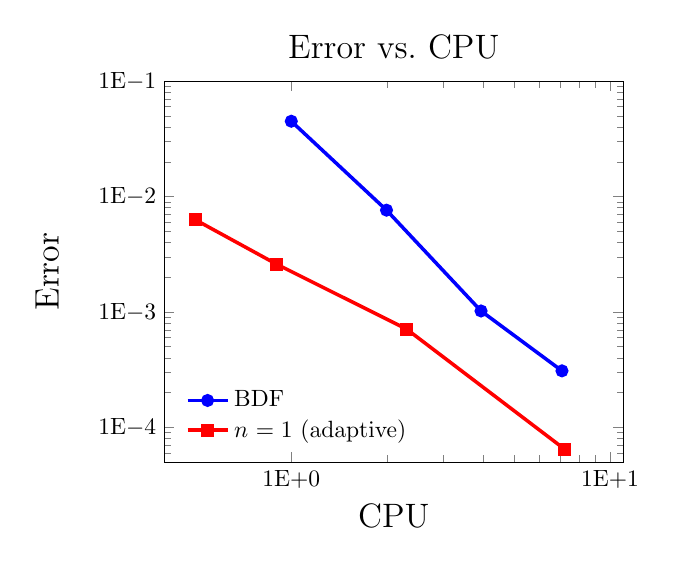
\begin{tikzpicture}[scale=0.85]

\begin{axis}[
  xmode = log,
  xmin = 0.4,
  xmax = 11,
  xtick = {1,10},
  xticklabels = {$1$E$+0$,$1$E$+1$},
  xlabel = CPU,
  ymode = log,
  ymin = 5E-5,
  ymax = 1E-1,
  ytick = {1E-5,1E-4,1E-3,1E-2,1E-1},
  yticklabels = {$1$E$-5$,$1$E$-4$,$1$E$-3$,$1$E$-2$,$1$E$-1$},
  ylabel = {Error},
  ylabel style = {yshift = 10pt},
  label style = {font=\Large},
  legend entries = {BDF, $n_{\sdc}=1$ (adaptive)},
  legend cell align = left,
  legend pos = south west, 
  legend style = {draw=none},
  title = {\Large{Error vs.~CPU}}
  ]


% BDF fixed time step size
\addplot [mark=*,blue,line width=1.5] table{
1.00 4.49e-2
1.99 7.62e-3
3.94 1.02e-3
7.07 3.09e-4
};

% 1 SDC correction adaptive time step size
\addplot [mark=square*,red,line width=1.5] table{
0.5 6.29e-3
0.9 2.59e-3
2.3 7.11e-4
7.2 6.49e-5
};

\end{axis}

\end{tikzpicture}


 
%%\fi
%\end{tabular}
%\mcaption{Results for the {\bf stenosis} flow.  Left: The time step
%size using 6000 {\bf constant} time step sizes (dashed) and an {\bf
%adaptive} time step size (solid) with a tolerance of ??? and
%$n_{\sdc}=???$.  The open circles indicate the ???  times when the time
%step size is rejected.  Notice that the time step size decreases as the
%vesicle passes through the constriction.  Center: The errors in area
%and length using {\bf constant} (dashed) and {\bf adaptive} (solid)
%time steps, and the desired error (black) of the adaptive time step.
%When using adaptive time stepping, the error in area nearly achieves
%the desired error everywhere except when the vesicle passes through the
%constriction, where the error in area actually drops.  However, when
%using a constant time step size, very little error is committed at the
%start of the simulation, and then the majority of the error is
%committed as the vesicle passes through the constriction.  Even though
%the CPU savings are negligible (it is about 4\%), the adaptive time
%stepping method did not require any trial and error to find an
%appropriate time step size.  The user simply specifies that they desire
%six digits accuracy and it is achieved.  In addition, by using an
%additional SDC correction, the CPU savings is increased to 19\%.
%Right: The error versus the amount of required CPU time for four
%different time integrators.  The solid lines use a {\bf constant} time
%step size while the dahsed lines use an {\bf adaptive} time step
%size.\\ \todo{put this caption parallel to extensional
%example.  Some of the plots need fixed}}{f:stenosisSummary}
%\end{figure}


%%%%%%%%%%%%%%%%%%%%%%%%%%%%%%%%%%%%%%%%%%%%%%%%%%%%%%%%%%%%%%%%%%%%
\subsection{Couette flow}
\label{s:couette}
As a final example, we consider two suspensions in a Couette apparatus,
a test case we also considered in our previous
work~\cite{qua:bir2014b}.  We first consider a suspension of 42
vesicles where the inner and outer boundaries are not aligned.  This
results in a narrow region that vesicles must pass through.  We take a
time horizon of $T=10$ corresponding to one full rotation of the inner
boundary (Figure~\ref{f:couette42Geom}).  In
Tables~\ref{t:couette42BDF} and~\ref{t:adaptiveSecondOrderCouette42},
we report convergence results for BDF and adaptive $n_{\sdc}=1$.  We
can see in Figure~\ref{f:couette42Errors} that if the time step size is
too large, then the method is either unstable or the error grows
sharply and results in the error tolerance being exceeded.  In
particular, there is an interaction near $t=1$ that needs to be
resolved\footnote{This interaction is due to the blue vesicle with its
neighboring vesicles and the solid wall.} with a time size smaller than
$\Delta t = 3$E$-2$.  However, at later times, a larger time step size
can be chosen.  By taking an adaptive time step size, all the
interactions are resolved appropriately, no trial-and-error procedure
to find the required time step size is used, and the total error
committed per time step is controlled.  The time step size is
illustrated in the left plot of Figure~\ref{f:couette42Errors}.

Finally, we consider 150 vesicles in a Couette apparatus with a longer
time horizon (Figure~\ref{f:couette150Geom}); the inner boundary makes
five full revolutions.  In Tables~\ref{t:couette150BDF}
and~\ref{t:adaptiveSecondOrderCouette150}, we report the convergence
results for BDF and adaptive $n_{\sdc}=1$.  Similar to the 42 vesicle
simulation, in Figure~\ref{f:couette150Errors}, we see that the errors
exceed the tolerance or have sharp jumps if the time step size is
constant\footnote{The sharp jump near $t=6$ is due to the interaction of
the blue vesicle with its neighboring vesicles and the solid wall.}, and
this shortcoming is removed by using an adaptive time step size.  The
time step size is illustrated in the right plot of
Figure~\ref{f:couette150Errors}.  Notice that the time step size is
small near $t=6$, indicating that there is at least one vesicle that is
committing a large error if too large of a time step is taken.  The left
plot of Figure~\ref{f:couette150Errors} indicates that this is exactly
the case.  Also notice that the BDF scheme is sensitive on the time step
size.  If we select $N_{t}=900$ (Table~\ref{t:couette150BDF}), we fail
at almost the cost of a successful simulation which is $N_{t}=920$.  Of
course one can take much larger number of time steps, but the cost may
be too expensive and the accuracy achieved may be unnecessary on an
actual science run.  On the other hand, the adaptive SDC behaves in a
controlled way and delivers the desired accuracy.

In these simulations, if we could guess the right time step size a
priori, a constant time step BDF scheme will be slightly faster than
the adaptive SDC scheme. The main reason is that these flows do not
have multiple time scales, two vesicles are always nearby or near the
wall, thus dictating the same time step across the simulation.  Indeed,
in the adaptive time stepping results, the local truncation error is
estimated by taking the maximum error committed over all the vesicles.
Therefore, the time step size is set by the vesicle that commits the
most error.  We could easily change the setup (e.g., by making the
rotation velocity of the Couette apparatus to be time dependent with
large variation) to introduce multiple time scales, but we think our
point of robustness is clear and has been demonstrated in the stenosis
and extensional flow examples.  Perhaps a faster method can be
developed by allowing each vesicle to have its own time step size, that
is, using a multirate time integrator, but this is beyond the scope of
this paper.

% GB:TODO; if the paper gets accepted, in the final version we should
% put the discussion on the order reduction or the fudging parameters
% $\beta$ and $\alpha$. But for the time being, I don't want anything
% that can provoke reaction.

\begin{figure}[htp]
\centering
\begin{tabular}{cccccc}
%\ifTikz
%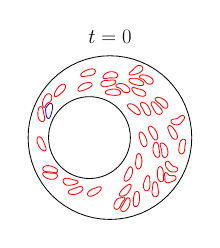
\begin{tikzpicture}[scale=0.3]

\begin{axis}[
  xmin = -21,
  xmax = 21,
  ymin = -21,
  ymax = 21,
  scale only axis,
  axis equal image,
  hide axis,
  title = {\Huge$t=0$}
  ]

% outer solid wall
\addplot [mark=none,black,line width=1.0] table{
2.0000e+01 -5.5171e-16
1.9904e+01 1.9603e+00
1.9616e+01 3.9018e+00
1.9139e+01 5.8057e+00
1.8478e+01 7.6537e+00
1.7638e+01 9.4279e+00
1.6629e+01 1.1111e+01
1.5460e+01 1.2688e+01
1.4142e+01 1.4142e+01
1.2688e+01 1.5460e+01
1.1111e+01 1.6629e+01
9.4279e+00 1.7638e+01
7.6537e+00 1.8478e+01
5.8057e+00 1.9139e+01
3.9018e+00 1.9616e+01
1.9603e+00 1.9904e+01
2.3281e-15 2.0000e+01
-1.9603e+00 1.9904e+01
-3.9018e+00 1.9616e+01
-5.8057e+00 1.9139e+01
-7.6537e+00 1.8478e+01
-9.4279e+00 1.7638e+01
-1.1111e+01 1.6629e+01
-1.2688e+01 1.5460e+01
-1.4142e+01 1.4142e+01
-1.5460e+01 1.2688e+01
-1.6629e+01 1.1111e+01
-1.7638e+01 9.4279e+00
-1.8478e+01 7.6537e+00
-1.9139e+01 5.8057e+00
-1.9616e+01 3.9018e+00
-1.9904e+01 1.9603e+00
-2.0000e+01 3.0010e-15
-1.9904e+01 -1.9603e+00
-1.9616e+01 -3.9018e+00
-1.9139e+01 -5.8057e+00
-1.8478e+01 -7.6537e+00
-1.7638e+01 -9.4279e+00
-1.6629e+01 -1.1111e+01
-1.5460e+01 -1.2688e+01
-1.4142e+01 -1.4142e+01
-1.2688e+01 -1.5460e+01
-1.1111e+01 -1.6629e+01
-9.4279e+00 -1.7638e+01
-7.6537e+00 -1.8478e+01
-5.8057e+00 -1.9139e+01
-3.9018e+00 -1.9616e+01
-1.9603e+00 -1.9904e+01
-4.7774e-15 -2.0000e+01
1.9603e+00 -1.9904e+01
3.9018e+00 -1.9616e+01
5.8057e+00 -1.9139e+01
7.6537e+00 -1.8478e+01
9.4279e+00 -1.7638e+01
1.1111e+01 -1.6629e+01
1.2688e+01 -1.5460e+01
1.4142e+01 -1.4142e+01
1.5460e+01 -1.2688e+01
1.6629e+01 -1.1111e+01
1.7638e+01 -9.4279e+00
1.8478e+01 -7.6537e+00
1.9139e+01 -5.8057e+00
1.9616e+01 -3.9018e+00
1.9904e+01 -1.9603e+00
2.0000e+01 -5.5171e-16
};

% inner solid wall
\addplot [mark=none,black,line width=1.0] table{
5.0000e+00 2.7586e-16
4.9518e+00 -9.8017e-01
4.8079e+00 -1.9509e+00
4.5694e+00 -2.9028e+00
4.2388e+00 -3.8268e+00
3.8192e+00 -4.7140e+00
3.3147e+00 -5.5557e+00
2.7301e+00 -6.3439e+00
2.0711e+00 -7.0711e+00
1.3439e+00 -7.7301e+00
5.5570e-01 -8.3147e+00
-2.8603e-01 -8.8192e+00
-1.1732e+00 -9.2388e+00
-2.0972e+00 -9.5694e+00
-3.0491e+00 -9.8079e+00
-4.0198e+00 -9.9518e+00
-5.0000e+00 -1.0000e+01
-5.9802e+00 -9.9518e+00
-6.9509e+00 -9.8079e+00
-7.9028e+00 -9.5694e+00
-8.8268e+00 -9.2388e+00
-9.7140e+00 -8.8192e+00
-1.0556e+01 -8.3147e+00
-1.1344e+01 -7.7301e+00
-1.2071e+01 -7.0711e+00
-1.2730e+01 -6.3439e+00
-1.3315e+01 -5.5557e+00
-1.3819e+01 -4.7140e+00
-1.4239e+01 -3.8268e+00
-1.4569e+01 -2.9028e+00
-1.4808e+01 -1.9509e+00
-1.4952e+01 -9.8017e-01
-1.5000e+01 -1.5005e-15
-1.4952e+01 9.8017e-01
-1.4808e+01 1.9509e+00
-1.4569e+01 2.9028e+00
-1.4239e+01 3.8268e+00
-1.3819e+01 4.7140e+00
-1.3315e+01 5.5557e+00
-1.2730e+01 6.3439e+00
-1.2071e+01 7.0711e+00
-1.1344e+01 7.7301e+00
-1.0556e+01 8.3147e+00
-9.7140e+00 8.8192e+00
-8.8268e+00 9.2388e+00
-7.9028e+00 9.5694e+00
-6.9509e+00 9.8079e+00
-5.9802e+00 9.9518e+00
-5.0000e+00 1.0000e+01
-4.0198e+00 9.9518e+00
-3.0491e+00 9.8079e+00
-2.0972e+00 9.5694e+00
-1.1732e+00 9.2388e+00
-2.8603e-01 8.8192e+00
5.5570e-01 8.3147e+00
1.3439e+00 7.7301e+00
2.0711e+00 7.0711e+00
2.7301e+00 6.3439e+00
3.3147e+00 5.5557e+00
3.8192e+00 4.7140e+00
4.2388e+00 3.8268e+00
4.5694e+00 2.9028e+00
4.8079e+00 1.9509e+00
4.9518e+00 9.8017e-01
5.0000e+00 2.7586e-16
};

% vesicle1
\addplot [mark=none,red,line width=1.0] table{
1.7307e+01 3.5347e+00
1.7349e+01 3.5748e+00
1.7407e+01 3.6317e+00
1.7479e+01 3.7062e+00
1.7561e+01 3.7954e+00
1.7648e+01 3.8945e+00
1.7740e+01 4.0014e+00
1.7832e+01 4.1139e+00
1.7924e+01 4.2318e+00
1.8012e+01 4.3555e+00
1.8093e+01 4.4865e+00
1.8161e+01 4.6262e+00
1.8207e+01 4.7753e+00
1.8223e+01 4.9311e+00
1.8200e+01 5.0864e+00
1.8131e+01 5.2276e+00
1.8020e+01 5.3390e+00
1.7878e+01 5.4075e+00
1.7722e+01 5.4294e+00
1.7566e+01 5.4091e+00
1.7419e+01 5.3564e+00
1.7281e+01 5.2816e+00
1.7154e+01 5.1936e+00
1.7032e+01 5.0995e+00
1.6913e+01 5.0050e+00
1.6794e+01 4.9145e+00
1.6674e+01 4.8320e+00
1.6553e+01 4.7604e+00
1.6434e+01 4.7018e+00
1.6322e+01 4.6566e+00
1.6223e+01 4.6246e+00
1.6145e+01 4.6037e+00
1.6088e+01 4.5907e+00
1.6031e+01 4.5793e+00
1.5951e+01 4.5658e+00
1.5849e+01 4.5517e+00
1.5729e+01 4.5378e+00
1.5597e+01 4.5223e+00
1.5458e+01 4.5004e+00
1.5317e+01 4.4644e+00
1.5180e+01 4.4053e+00
1.5058e+01 4.3151e+00
1.4967e+01 4.1920e+00
1.4920e+01 4.0447e+00
1.4925e+01 3.8891e+00
1.4976e+01 3.7412e+00
1.5063e+01 3.6105e+00
1.5175e+01 3.4994e+00
1.5303e+01 3.4061e+00
1.5440e+01 3.3275e+00
1.5583e+01 3.2608e+00
1.5730e+01 3.2048e+00
1.5880e+01 3.1596e+00
1.6033e+01 3.1263e+00
1.6187e+01 3.1064e+00
1.6341e+01 3.1020e+00
1.6492e+01 3.1141e+00
1.6639e+01 3.1432e+00
1.6778e+01 3.1877e+00
1.6906e+01 3.2452e+00
1.7021e+01 3.3108e+00
1.7121e+01 3.3792e+00
1.7202e+01 3.4429e+00
1.7264e+01 3.4955e+00
1.7307e+01 3.5347e+00
};

% vesicle2
\addplot [mark=none,red,line width=1.0] table{
-3.8810e+00 1.5550e+01
-3.8377e+00 1.5589e+01
-3.7816e+00 1.5647e+01
-3.7168e+00 1.5728e+01
-3.6526e+00 1.5831e+01
-3.5992e+00 1.5952e+01
-3.5656e+00 1.6088e+01
-3.5600e+00 1.6233e+01
-3.5896e+00 1.6379e+01
-3.6576e+00 1.6515e+01
-3.7614e+00 1.6628e+01
-3.8920e+00 1.6711e+01
-4.0391e+00 1.6763e+01
-4.1937e+00 1.6790e+01
-4.3511e+00 1.6797e+01
-4.5086e+00 1.6788e+01
-4.6656e+00 1.6770e+01
-4.8213e+00 1.6743e+01
-4.9756e+00 1.6710e+01
-5.1282e+00 1.6671e+01
-5.2791e+00 1.6627e+01
-5.4277e+00 1.6578e+01
-5.5740e+00 1.6526e+01
-5.7173e+00 1.6470e+01
-5.8573e+00 1.6411e+01
-5.9931e+00 1.6348e+01
-6.1237e+00 1.6284e+01
-6.2474e+00 1.6217e+01
-6.3623e+00 1.6151e+01
-6.4651e+00 1.6088e+01
-6.5514e+00 1.6030e+01
-6.6174e+00 1.5984e+01
-6.6644e+00 1.5949e+01
-6.7103e+00 1.5913e+01
-6.7728e+00 1.5861e+01
-6.8491e+00 1.5791e+01
-6.9329e+00 1.5704e+01
-7.0133e+00 1.5599e+01
-7.0794e+00 1.5475e+01
-7.1138e+00 1.5334e+01
-7.0977e+00 1.5187e+01
-7.0198e+00 1.5058e+01
-6.8938e+00 1.4971e+01
-6.7441e+00 1.4931e+01
-6.5882e+00 1.4924e+01
-6.4314e+00 1.4934e+01
-6.2752e+00 1.4953e+01
-6.1187e+00 1.4976e+01
-5.9626e+00 1.4999e+01
-5.8062e+00 1.5023e+01
-5.6502e+00 1.5046e+01
-5.4940e+00 1.5068e+01
-5.3388e+00 1.5091e+01
-5.1839e+00 1.5113e+01
-5.0305e+00 1.5137e+01
-4.8784e+00 1.5162e+01
-4.7292e+00 1.5190e+01
-4.5831e+00 1.5222e+01
-4.4427e+00 1.5260e+01
-4.3094e+00 1.5305e+01
-4.1873e+00 1.5355e+01
-4.0795e+00 1.5411e+01
-3.9917e+00 1.5465e+01
-3.9261e+00 1.5513e+01
-3.8810e+00 1.5550e+01
};

% vesicle3
\addplot [mark=none,red,line width=1.0] table{
-3.5235e-02 1.2644e+01
2.1863e-02 1.2659e+01
9.9489e-02 1.2680e+01
1.9975e-01 1.2708e+01
3.1547e-01 1.2742e+01
4.4242e-01 1.2781e+01
5.7475e-01 1.2827e+01
7.1118e-01 1.2879e+01
8.4724e-01 1.2940e+01
9.8229e-01 1.3010e+01
1.1112e+00 1.3094e+01
1.2315e+00 1.3192e+01
1.3334e+00 1.3310e+01
1.4065e+00 1.3449e+01
1.4319e+00 1.3604e+01
1.3994e+00 1.3757e+01
1.3099e+00 1.3886e+01
1.1829e+00 1.3979e+01
1.0351e+00 1.4035e+01
8.8080e-01 1.4063e+01
7.2360e-01 1.4073e+01
5.6780e-01 1.4072e+01
4.1215e-01 1.4065e+01
2.5912e-01 1.4053e+01
1.0711e-01 1.4041e+01
-4.1256e-02 1.4028e+01
-1.8691e-01 1.4015e+01
-3.2640e-01 1.4004e+01
-4.5904e-01 1.3995e+01
-5.7937e-01 1.3987e+01
-6.8323e-01 1.3981e+01
-7.6354e-01 1.3977e+01
-8.2249e-01 1.3974e+01
-8.8024e-01 1.3971e+01
-9.6173e-01 1.3967e+01
-1.0643e+00 1.3960e+01
-1.1856e+00 1.3949e+01
-1.3160e+00 1.3930e+01
-1.4535e+00 1.3898e+01
-1.5902e+00 1.3850e+01
-1.7244e+00 1.3783e+01
-1.8496e+00 1.3698e+01
-1.9651e+00 1.3596e+01
-2.0640e+00 1.3477e+01
-2.1435e+00 1.3342e+01
-2.1929e+00 1.3194e+01
-2.2057e+00 1.3037e+01
-2.1731e+00 1.2883e+01
-2.0988e+00 1.2745e+01
-1.9892e+00 1.2631e+01
-1.8580e+00 1.2544e+01
-1.7122e+00 1.2483e+01
-1.5607e+00 1.2445e+01
-1.4050e+00 1.2425e+01
-1.2504e+00 1.2422e+01
-1.0960e+00 1.2430e+01
-9.4571e-01 1.2447e+01
-7.9748e-01 1.2471e+01
-6.5511e-01 1.2498e+01
-5.1709e-01 1.2528e+01
-3.8862e-01 1.2557e+01
-2.7016e-01 1.2585e+01
-1.7033e-01 1.2610e+01
-9.1208e-02 1.2630e+01
-3.5235e-02 1.2644e+01
};

% vesicle4
\addplot [mark=none,red,line width=1.0] table{
8.6443e+00 1.3699e+01
8.6801e+00 1.3653e+01
8.7301e+00 1.3590e+01
8.7969e+00 1.3510e+01
8.8800e+00 1.3422e+01
8.9788e+00 1.3334e+01
9.0924e+00 1.3252e+01
9.2192e+00 1.3180e+01
9.3569e+00 1.3122e+01
9.5031e+00 1.3081e+01
9.6552e+00 1.3058e+01
9.8104e+00 1.3057e+01
9.9650e+00 1.3078e+01
1.0114e+01 1.3126e+01
1.0253e+01 1.3201e+01
1.0373e+01 1.3303e+01
1.0468e+01 1.3428e+01
1.0533e+01 1.3572e+01
1.0563e+01 1.3727e+01
1.0559e+01 1.3884e+01
1.0524e+01 1.4037e+01
1.0463e+01 1.4181e+01
1.0381e+01 1.4313e+01
1.0285e+01 1.4432e+01
1.0178e+01 1.4540e+01
1.0064e+01 1.4637e+01
9.9467e+00 1.4724e+01
9.8293e+00 1.4801e+01
9.7153e+00 1.4868e+01
9.6089e+00 1.4926e+01
9.5163e+00 1.4972e+01
9.4431e+00 1.5007e+01
9.3897e+00 1.5030e+01
9.3361e+00 1.5053e+01
9.2610e+00 1.5084e+01
9.1643e+00 1.5120e+01
9.0497e+00 1.5160e+01
8.9231e+00 1.5198e+01
8.7871e+00 1.5234e+01
8.6450e+00 1.5265e+01
8.4977e+00 1.5291e+01
8.3471e+00 1.5310e+01
8.1934e+00 1.5322e+01
8.0383e+00 1.5326e+01
7.8820e+00 1.5319e+01
7.7266e+00 1.5298e+01
7.5742e+00 1.5258e+01
7.4315e+00 1.5192e+01
7.3101e+00 1.5091e+01
7.2311e+00 1.4956e+01
7.2162e+00 1.4800e+01
7.2731e+00 1.4654e+01
7.3830e+00 1.4543e+01
7.5193e+00 1.4467e+01
7.6639e+00 1.4411e+01
7.8092e+00 1.4359e+01
7.9501e+00 1.4303e+01
8.0838e+00 1.4236e+01
8.2067e+00 1.4158e+01
8.3170e+00 1.4071e+01
8.4126e+00 1.3980e+01
8.4938e+00 1.3890e+01
8.5591e+00 1.3809e+01
8.6089e+00 1.3746e+01
8.6443e+00 1.3699e+01
};

% vesicle5
\addplot [mark=none,red,line width=1.0] table{
-1.2945e+01 -9.6384e+00
-1.2914e+01 -9.5889e+00
-1.2882e+01 -9.5143e+00
-1.2851e+01 -9.4163e+00
-1.2839e+01 -9.2951e+00
-1.2851e+01 -9.1648e+00
-1.2901e+01 -9.0322e+00
-1.2983e+01 -8.9148e+00
-1.3100e+01 -8.8189e+00
-1.3235e+01 -8.7553e+00
-1.3386e+01 -8.7180e+00
-1.3539e+01 -8.7032e+00
-1.3697e+01 -8.6973e+00
-1.3852e+01 -8.6983e+00
-1.4012e+01 -8.6980e+00
-1.4168e+01 -8.6985e+00
-1.4328e+01 -8.6940e+00
-1.4483e+01 -8.6878e+00
-1.4643e+01 -8.6748e+00
-1.4797e+01 -8.6589e+00
-1.4955e+01 -8.6357e+00
-1.5107e+01 -8.6094e+00
-1.5261e+01 -8.5764e+00
-1.5409e+01 -8.5423e+00
-1.5558e+01 -8.5049e+00
-1.5702e+01 -8.4734e+00
-1.5848e+01 -8.4504e+00
-1.5986e+01 -8.4499e+00
-1.6118e+01 -8.4745e+00
-1.6225e+01 -8.5279e+00
-1.6306e+01 -8.5937e+00
-1.6352e+01 -8.6597e+00
-1.6380e+01 -8.7108e+00
-1.6396e+01 -8.7673e+00
-1.6410e+01 -8.8461e+00
-1.6403e+01 -8.9503e+00
-1.6374e+01 -9.0662e+00
-1.6315e+01 -9.1867e+00
-1.6239e+01 -9.3020e+00
-1.6141e+01 -9.4132e+00
-1.6036e+01 -9.5157e+00
-1.5916e+01 -9.6131e+00
-1.5793e+01 -9.7017e+00
-1.5660e+01 -9.7854e+00
-1.5525e+01 -9.8606e+00
-1.5382e+01 -9.9308e+00
-1.5239e+01 -9.9920e+00
-1.5089e+01 -1.0048e+01
-1.4941e+01 -1.0094e+01
-1.4785e+01 -1.0134e+01
-1.4633e+01 -1.0164e+01
-1.4474e+01 -1.0186e+01
-1.4320e+01 -1.0196e+01
-1.4161e+01 -1.0199e+01
-1.4009e+01 -1.0188e+01
-1.3854e+01 -1.0169e+01
-1.3707e+01 -1.0136e+01
-1.3562e+01 -1.0093e+01
-1.3429e+01 -1.0038e+01
-1.3303e+01 -9.9744e+00
-1.3194e+01 -9.9008e+00
-1.3099e+01 -9.8248e+00
-1.3028e+01 -9.7499e+00
-1.2976e+01 -9.6878e+00
-1.2945e+01 -9.6384e+00
};

% vesicle6
\addplot [mark=none,red,line width=1.0] table{
1.2444e+01 -1.4092e+00
1.2402e+01 -1.4490e+00
1.2354e+01 -1.5140e+00
1.2313e+01 -1.6088e+00
1.2292e+01 -1.7279e+00
1.2297e+01 -1.8600e+00
1.2322e+01 -1.9982e+00
1.2361e+01 -2.1384e+00
1.2407e+01 -2.2807e+00
1.2456e+01 -2.4247e+00
1.2503e+01 -2.5714e+00
1.2547e+01 -2.7202e+00
1.2586e+01 -2.8715e+00
1.2621e+01 -3.0248e+00
1.2649e+01 -3.1799e+00
1.2671e+01 -3.3360e+00
1.2689e+01 -3.4932e+00
1.2702e+01 -3.6506e+00
1.2714e+01 -3.8081e+00
1.2727e+01 -3.9650e+00
1.2745e+01 -4.1211e+00
1.2776e+01 -4.2743e+00
1.2823e+01 -4.4221e+00
1.2893e+01 -4.5588e+00
1.2988e+01 -4.6776e+00
1.3105e+01 -4.7700e+00
1.3237e+01 -4.8294e+00
1.3376e+01 -4.8516e+00
1.3507e+01 -4.8397e+00
1.3622e+01 -4.8017e+00
1.3712e+01 -4.7518e+00
1.3777e+01 -4.7032e+00
1.3820e+01 -4.6639e+00
1.3860e+01 -4.6214e+00
1.3911e+01 -4.5584e+00
1.3968e+01 -4.4719e+00
1.4024e+01 -4.3647e+00
1.4073e+01 -4.2419e+00
1.4114e+01 -4.1075e+00
1.4145e+01 -3.9651e+00
1.4165e+01 -3.8171e+00
1.4175e+01 -3.6654e+00
1.4175e+01 -3.5115e+00
1.4166e+01 -3.3565e+00
1.4147e+01 -3.2013e+00
1.4120e+01 -3.0466e+00
1.4084e+01 -2.8932e+00
1.4040e+01 -2.7416e+00
1.3988e+01 -2.5925e+00
1.3928e+01 -2.4463e+00
1.3860e+01 -2.3038e+00
1.3784e+01 -2.1655e+00
1.3701e+01 -2.0324e+00
1.3610e+01 -1.9052e+00
1.3512e+01 -1.7852e+00
1.3406e+01 -1.6736e+00
1.3293e+01 -1.5722e+00
1.3172e+01 -1.4833e+00
1.3047e+01 -1.4097e+00
1.2917e+01 -1.3558e+00
1.2788e+01 -1.3258e+00
1.2668e+01 -1.3229e+00
1.2566e+01 -1.3435e+00
1.2493e+01 -1.3764e+00
1.2444e+01 -1.4092e+00
};

% vesicle7
\addplot [mark=none,red,line width=1.0] table{
7.7164e+00 1.6213e+01
7.7567e+00 1.6256e+01
7.8093e+00 1.6317e+01
7.8702e+00 1.6401e+01
7.9307e+00 1.6505e+01
7.9809e+00 1.6628e+01
8.0130e+00 1.6764e+01
8.0201e+00 1.6910e+01
7.9982e+00 1.7057e+01
7.9453e+00 1.7200e+01
7.8627e+00 1.7329e+01
7.7538e+00 1.7439e+01
7.6241e+00 1.7526e+01
7.4795e+00 1.7587e+01
7.3260e+00 1.7622e+01
7.1686e+00 1.7631e+01
7.0113e+00 1.7617e+01
6.8572e+00 1.7583e+01
6.7088e+00 1.7529e+01
6.5675e+00 1.7460e+01
6.4345e+00 1.7376e+01
6.3099e+00 1.7282e+01
6.1936e+00 1.7179e+01
6.0844e+00 1.7070e+01
5.9809e+00 1.6959e+01
5.8813e+00 1.6848e+01
5.7844e+00 1.6739e+01
5.6893e+00 1.6636e+01
5.5969e+00 1.6541e+01
5.5096e+00 1.6457e+01
5.4327e+00 1.6388e+01
5.3710e+00 1.6335e+01
5.3258e+00 1.6298e+01
5.2801e+00 1.6262e+01
5.2160e+00 1.6213e+01
5.1333e+00 1.6150e+01
5.0367e+00 1.6077e+01
4.9340e+00 1.5994e+01
4.8337e+00 1.5895e+01
4.7509e+00 1.5776e+01
4.7074e+00 1.5634e+01
4.7286e+00 1.5485e+01
4.8197e+00 1.5363e+01
4.9570e+00 1.5292e+01
5.1112e+00 1.5271e+01
5.2679e+00 1.5281e+01
5.4229e+00 1.5309e+01
5.5769e+00 1.5344e+01
5.7303e+00 1.5381e+01
5.8838e+00 1.5419e+01
6.0370e+00 1.5457e+01
6.1900e+00 1.5495e+01
6.3419e+00 1.5535e+01
6.4926e+00 1.5577e+01
6.6409e+00 1.5622e+01
6.7866e+00 1.5672e+01
6.9284e+00 1.5727e+01
7.0656e+00 1.5786e+01
7.1966e+00 1.5850e+01
7.3200e+00 1.5917e+01
7.4328e+00 1.5986e+01
7.5322e+00 1.6056e+01
7.6136e+00 1.6119e+01
7.6744e+00 1.6173e+01
7.7164e+00 1.6213e+01
};

% vesicle8
\addplot [mark=none,red,line width=1.0] table{
9.4881e+00 1.8670e+00
9.5066e+00 1.8119e+00
9.5347e+00 1.7357e+00
9.5721e+00 1.6396e+00
9.6194e+00 1.5277e+00
9.6731e+00 1.4071e+00
9.7334e+00 1.2797e+00
9.7972e+00 1.1493e+00
9.8654e+00 1.0158e+00
9.9355e+00 8.8143e-01
1.0009e+01 7.4555e-01
1.0083e+01 6.0985e-01
1.0161e+01 4.7358e-01
1.0240e+01 3.3837e-01
1.0322e+01 2.0356e-01
1.0407e+01 7.0914e-02
1.0497e+01 -5.9869e-02
1.0591e+01 -1.8641e-01
1.0692e+01 -3.0776e-01
1.0803e+01 -4.1898e-01
1.0929e+01 -5.1389e-01
1.1070e+01 -5.7806e-01
1.1224e+01 -5.9447e-01
1.1370e+01 -5.5083e-01
1.1490e+01 -4.5750e-01
1.1573e+01 -3.3399e-01
1.1627e+01 -1.9889e-01
1.1656e+01 -6.1567e-02
1.1671e+01 6.9841e-02
1.1673e+01 1.9114e-01
1.1669e+01 2.9429e-01
1.1662e+01 3.7512e-01
1.1655e+01 4.3287e-01
1.1647e+01 4.9087e-01
1.1634e+01 5.7043e-01
1.1612e+01 6.7192e-01
1.1583e+01 7.8924e-01
1.1545e+01 9.1642e-01
1.1500e+01 1.0492e+00
1.1447e+01 1.1850e+00
1.1387e+01 1.3217e+00
1.1320e+01 1.4585e+00
1.1247e+01 1.5938e+00
1.1168e+01 1.7274e+00
1.1083e+01 1.8583e+00
1.0991e+01 1.9863e+00
1.0895e+01 2.1104e+00
1.0792e+01 2.2303e+00
1.0683e+01 2.3448e+00
1.0568e+01 2.4533e+00
1.0446e+01 2.5536e+00
1.0317e+01 2.6440e+00
1.0180e+01 2.7200e+00
1.0034e+01 2.7762e+00
9.8816e+00 2.8029e+00
9.7284e+00 2.7897e+00
9.5906e+00 2.7282e+00
9.4854e+00 2.6230e+00
9.4244e+00 2.4914e+00
9.4017e+00 2.3532e+00
9.4061e+00 2.2208e+00
9.4243e+00 2.1014e+00
9.4483e+00 2.0005e+00
9.4701e+00 1.9229e+00
9.4881e+00 1.8670e+00
};

% vesicle9
\addplot [mark=none,red,line width=1.0] table{
-3.7703e+00 -1.2376e+01
-3.8250e+00 -1.2398e+01
-3.8999e+00 -1.2427e+01
-3.9961e+00 -1.2466e+01
-4.1073e+00 -1.2514e+01
-4.2287e+00 -1.2567e+01
-4.3556e+00 -1.2627e+01
-4.4862e+00 -1.2692e+01
-4.6175e+00 -1.2763e+01
-4.7488e+00 -1.2840e+01
-4.8771e+00 -1.2924e+01
-5.0018e+00 -1.3018e+01
-5.1193e+00 -1.3120e+01
-5.2280e+00 -1.3234e+01
-5.3229e+00 -1.3359e+01
-5.4004e+00 -1.3497e+01
-5.4530e+00 -1.3645e+01
-5.4735e+00 -1.3802e+01
-5.4517e+00 -1.3958e+01
-5.3838e+00 -1.4099e+01
-5.2735e+00 -1.4210e+01
-5.1360e+00 -1.4283e+01
-4.9853e+00 -1.4320e+01
-4.8321e+00 -1.4331e+01
-4.6801e+00 -1.4322e+01
-4.5326e+00 -1.4301e+01
-4.3901e+00 -1.4269e+01
-4.2552e+00 -1.4231e+01
-4.1292e+00 -1.4189e+01
-4.0163e+00 -1.4147e+01
-3.9204e+00 -1.4107e+01
-3.8469e+00 -1.4074e+01
-3.7937e+00 -1.4049e+01
-3.7416e+00 -1.4024e+01
-3.6692e+00 -1.3987e+01
-3.5784e+00 -1.3938e+01
-3.4730e+00 -1.3877e+01
-3.3604e+00 -1.3808e+01
-3.2425e+00 -1.3731e+01
-3.1236e+00 -1.3648e+01
-3.0035e+00 -1.3558e+01
-2.8852e+00 -1.3463e+01
-2.7679e+00 -1.3363e+01
-2.6541e+00 -1.3258e+01
-2.5430e+00 -1.3147e+01
-2.4374e+00 -1.3032e+01
-2.3374e+00 -1.2909e+01
-2.2477e+00 -1.2780e+01
-2.1723e+00 -1.2641e+01
-2.1230e+00 -1.2491e+01
-2.1150e+00 -1.2334e+01
-2.1685e+00 -1.2187e+01
-2.2820e+00 -1.2081e+01
-2.4302e+00 -1.2033e+01
-2.5847e+00 -1.2030e+01
-2.7375e+00 -1.2052e+01
-2.8853e+00 -1.2086e+01
-3.0299e+00 -1.2125e+01
-3.1691e+00 -1.2167e+01
-3.3033e+00 -1.2210e+01
-3.4284e+00 -1.2252e+01
-3.5431e+00 -1.2292e+01
-3.6400e+00 -1.2327e+01
-3.7161e+00 -1.2356e+01
-3.7703e+00 -1.2376e+01
};

% vesicle10
\addplot [mark=none,red,line width=1.0] table{
1.3093e+01 -9.5660e+00
1.3086e+01 -9.5080e+00
1.3077e+01 -9.4276e+00
1.3067e+01 -9.3246e+00
1.3058e+01 -9.2038e+00
1.3050e+01 -9.0717e+00
1.3044e+01 -8.9313e+00
1.3038e+01 -8.7858e+00
1.3032e+01 -8.6364e+00
1.3021e+01 -8.4849e+00
1.3006e+01 -8.3316e+00
1.2985e+01 -8.1779e+00
1.2956e+01 -8.0241e+00
1.2920e+01 -7.8715e+00
1.2874e+01 -7.7207e+00
1.2816e+01 -7.5737e+00
1.2744e+01 -7.4330e+00
1.2653e+01 -7.3040e+00
1.2539e+01 -7.1958e+00
1.2400e+01 -7.1234e+00
1.2245e+01 -7.1028e+00
1.2094e+01 -7.1417e+00
1.1968e+01 -7.2300e+00
1.1871e+01 -7.3497e+00
1.1802e+01 -7.4845e+00
1.1751e+01 -7.6251e+00
1.1713e+01 -7.7656e+00
1.1684e+01 -7.9031e+00
1.1661e+01 -8.0334e+00
1.1643e+01 -8.1533e+00
1.1630e+01 -8.2558e+00
1.1620e+01 -8.3363e+00
1.1615e+01 -8.3944e+00
1.1609e+01 -8.4526e+00
1.1603e+01 -8.5332e+00
1.1596e+01 -8.6365e+00
1.1591e+01 -8.7575e+00
1.1589e+01 -8.8899e+00
1.1590e+01 -9.0304e+00
1.1596e+01 -9.1758e+00
1.1608e+01 -9.3248e+00
1.1627e+01 -9.4757e+00
1.1652e+01 -9.6276e+00
1.1685e+01 -9.7793e+00
1.1727e+01 -9.9299e+00
1.1779e+01 -1.0078e+01
1.1842e+01 -1.0222e+01
1.1919e+01 -1.0360e+01
1.2011e+01 -1.0489e+01
1.2119e+01 -1.0603e+01
1.2246e+01 -1.0697e+01
1.2390e+01 -1.0761e+01
1.2544e+01 -1.0787e+01
1.2699e+01 -1.0769e+01
1.2840e+01 -1.0706e+01
1.2957e+01 -1.0607e+01
1.3043e+01 -1.0482e+01
1.3098e+01 -1.0343e+01
1.3126e+01 -1.0200e+01
1.3134e+01 -1.0060e+01
1.3131e+01 -9.9279e+00
1.3121e+01 -9.8072e+00
1.3109e+01 -9.7043e+00
1.3100e+01 -9.6240e+00
1.3093e+01 -9.5660e+00
};

% vesicle11
\addplot [mark=none,red,line width=1.0] table{
-6.8879e+00 1.2954e+01
-6.9370e+00 1.2922e+01
-7.0042e+00 1.2877e+01
-7.0881e+00 1.2817e+01
-7.1837e+00 1.2742e+01
-7.2842e+00 1.2656e+01
-7.3860e+00 1.2559e+01
-7.4853e+00 1.2453e+01
-7.5799e+00 1.2337e+01
-7.6662e+00 1.2212e+01
-7.7410e+00 1.2077e+01
-7.7978e+00 1.1933e+01
-7.8275e+00 1.1780e+01
-7.8148e+00 1.1624e+01
-7.7459e+00 1.1484e+01
-7.6231e+00 1.1386e+01
-7.4719e+00 1.1344e+01
-7.3140e+00 1.1342e+01
-7.1580e+00 1.1365e+01
-7.0042e+00 1.1400e+01
-6.8530e+00 1.1442e+01
-6.7035e+00 1.1488e+01
-6.5562e+00 1.1537e+01
-6.4107e+00 1.1588e+01
-6.2680e+00 1.1640e+01
-6.1280e+00 1.1692e+01
-5.9923e+00 1.1745e+01
-5.8618e+00 1.1797e+01
-5.7395e+00 1.1848e+01
-5.6281e+00 1.1895e+01
-5.5335e+00 1.1937e+01
-5.4598e+00 1.1971e+01
-5.4070e+00 1.1996e+01
-5.3542e+00 1.2021e+01
-5.2816e+00 1.2056e+01
-5.1894e+00 1.2103e+01
-5.0829e+00 1.2161e+01
-4.9684e+00 1.2227e+01
-4.8499e+00 1.2303e+01
-4.7316e+00 1.2388e+01
-4.6173e+00 1.2484e+01
-4.5124e+00 1.2594e+01
-4.4258e+00 1.2721e+01
-4.3713e+00 1.2866e+01
-4.3661e+00 1.3021e+01
-4.4201e+00 1.3168e+01
-4.5242e+00 1.3285e+01
-4.6587e+00 1.3367e+01
-4.8077e+00 1.3419e+01
-4.9628e+00 1.3449e+01
-5.1201e+00 1.3462e+01
-5.2776e+00 1.3462e+01
-5.4343e+00 1.3452e+01
-5.5894e+00 1.3433e+01
-5.7424e+00 1.3406e+01
-5.8926e+00 1.3372e+01
-6.0393e+00 1.3332e+01
-6.1817e+00 1.3287e+01
-6.3187e+00 1.3237e+01
-6.4486e+00 1.3184e+01
-6.5692e+00 1.3129e+01
-6.6774e+00 1.3075e+01
-6.7682e+00 1.3025e+01
-6.8381e+00 1.2984e+01
-6.8879e+00 1.2954e+01
};

% vesicle12
\addplot [mark=none,red,line width=1.0] table{
1.2404e+01 9.7052e+00
1.2349e+01 9.7232e+00
1.2272e+01 9.7472e+00
1.2172e+01 9.7738e+00
1.2054e+01 9.8009e+00
1.1924e+01 9.8229e+00
1.1784e+01 9.8379e+00
1.1638e+01 9.8396e+00
1.1490e+01 9.8236e+00
1.1345e+01 9.7793e+00
1.1214e+01 9.6995e+00
1.1116e+01 9.5793e+00
1.1071e+01 9.4312e+00
1.1085e+01 9.2752e+00
1.1147e+01 9.1316e+00
1.1243e+01 9.0053e+00
1.1355e+01 8.8952e+00
1.1478e+01 8.7944e+00
1.1603e+01 8.6997e+00
1.1731e+01 8.6058e+00
1.1856e+01 8.5125e+00
1.1980e+01 8.4167e+00
1.2101e+01 8.3197e+00
1.2218e+01 8.2193e+00
1.2331e+01 8.1178e+00
1.2439e+01 8.0141e+00
1.2541e+01 7.9111e+00
1.2639e+01 7.8091e+00
1.2729e+01 7.7128e+00
1.2812e+01 7.6241e+00
1.2884e+01 7.5501e+00
1.2942e+01 7.4928e+00
1.2984e+01 7.4533e+00
1.3028e+01 7.4142e+00
1.3090e+01 7.3635e+00
1.3175e+01 7.3035e+00
1.3280e+01 7.2450e+00
1.3405e+01 7.1982e+00
1.3543e+01 7.1755e+00
1.3688e+01 7.1850e+00
1.3829e+01 7.2335e+00
1.3954e+01 7.3190e+00
1.4052e+01 7.4370e+00
1.4119e+01 7.5765e+00
1.4153e+01 7.7291e+00
1.4157e+01 7.8856e+00
1.4136e+01 8.0419e+00
1.4094e+01 8.1936e+00
1.4035e+01 8.3406e+00
1.3963e+01 8.4806e+00
1.3879e+01 8.6147e+00
1.3786e+01 8.7415e+00
1.3685e+01 8.8623e+00
1.3578e+01 8.9757e+00
1.3465e+01 9.0829e+00
1.3348e+01 9.1823e+00
1.3227e+01 9.2753e+00
1.3105e+01 9.3601e+00
1.2981e+01 9.4378e+00
1.2859e+01 9.5065e+00
1.2741e+01 9.5669e+00
1.2631e+01 9.6169e+00
1.2535e+01 9.6570e+00
1.2460e+01 9.6853e+00
1.2404e+01 9.7052e+00
};

% vesicle13
\addplot [mark=none,red,line width=1.0] table{
7.0573e+00 1.1884e+01
7.0001e+00 1.1898e+01
6.9215e+00 1.1916e+01
6.8205e+00 1.1940e+01
6.7032e+00 1.1968e+01
6.5750e+00 1.2003e+01
6.4406e+00 1.2043e+01
6.3020e+00 1.2088e+01
6.1612e+00 1.2138e+01
6.0170e+00 1.2187e+01
5.8684e+00 1.2225e+01
5.7139e+00 1.2241e+01
5.5611e+00 1.2213e+01
5.4308e+00 1.2127e+01
5.3566e+00 1.1990e+01
5.3525e+00 1.1834e+01
5.4018e+00 1.1684e+01
5.4771e+00 1.1545e+01
5.5621e+00 1.1412e+01
5.6498e+00 1.1281e+01
5.7416e+00 1.1154e+01
5.8388e+00 1.1032e+01
5.9443e+00 1.0917e+01
6.0570e+00 1.0813e+01
6.1764e+00 1.0718e+01
6.2994e+00 1.0634e+01
6.4245e+00 1.0559e+01
6.5482e+00 1.0493e+01
6.6679e+00 1.0436e+01
6.7787e+00 1.0388e+01
6.8751e+00 1.0349e+01
6.9507e+00 1.0321e+01
7.0061e+00 1.0301e+01
7.0611e+00 1.0283e+01
7.1386e+00 1.0259e+01
7.2376e+00 1.0230e+01
7.3551e+00 1.0199e+01
7.4839e+00 1.0170e+01
7.6224e+00 1.0144e+01
7.7663e+00 1.0125e+01
7.9156e+00 1.0112e+01
8.0672e+00 1.0110e+01
8.2209e+00 1.0122e+01
8.3723e+00 1.0154e+01
8.5170e+00 1.0213e+01
8.6427e+00 1.0307e+01
8.7360e+00 1.0433e+01
8.7828e+00 1.0583e+01
8.7813e+00 1.0740e+01
8.7374e+00 1.0892e+01
8.6636e+00 1.1031e+01
8.5681e+00 1.1156e+01
8.4590e+00 1.1269e+01
8.3390e+00 1.1370e+01
8.2125e+00 1.1459e+01
8.0799e+00 1.1538e+01
7.9448e+00 1.1607e+01
7.8074e+00 1.1666e+01
7.6714e+00 1.1717e+01
7.5374e+00 1.1761e+01
7.4106e+00 1.1797e+01
7.2931e+00 1.1828e+01
7.1929e+00 1.1853e+01
7.1138e+00 1.1872e+01
7.0573e+00 1.1884e+01
};

% vesicle14
\addplot [mark=none,red,line width=1.0] table{
-1.2136e+01 1.2748e+01
-1.2184e+01 1.2712e+01
-1.2245e+01 1.2662e+01
-1.2325e+01 1.2594e+01
-1.2413e+01 1.2513e+01
-1.2509e+01 1.2419e+01
-1.2604e+01 1.2318e+01
-1.2702e+01 1.2208e+01
-1.2796e+01 1.2094e+01
-1.2891e+01 1.1973e+01
-1.2980e+01 1.1849e+01
-1.3068e+01 1.1720e+01
-1.3150e+01 1.1589e+01
-1.3231e+01 1.1452e+01
-1.3304e+01 1.1314e+01
-1.3375e+01 1.1171e+01
-1.3437e+01 1.1028e+01
-1.3495e+01 1.0879e+01
-1.3542e+01 1.0730e+01
-1.3580e+01 1.0576e+01
-1.3594e+01 1.0421e+01
-1.3579e+01 1.0265e+01
-1.3509e+01 1.0128e+01
-1.3388e+01 1.0035e+01
-1.3238e+01 1.0012e+01
-1.3093e+01 1.0041e+01
-1.2958e+01 1.0100e+01
-1.2837e+01 1.0167e+01
-1.2723e+01 1.0238e+01
-1.2623e+01 1.0303e+01
-1.2536e+01 1.0362e+01
-1.2471e+01 1.0408e+01
-1.2422e+01 1.0443e+01
-1.2377e+01 1.0476e+01
-1.2310e+01 1.0525e+01
-1.2229e+01 1.0587e+01
-1.2132e+01 1.0663e+01
-1.2032e+01 1.0745e+01
-1.1923e+01 1.0838e+01
-1.1817e+01 1.0934e+01
-1.1707e+01 1.1038e+01
-1.1601e+01 1.1145e+01
-1.1494e+01 1.1258e+01
-1.1393e+01 1.1374e+01
-1.1293e+01 1.1496e+01
-1.1202e+01 1.1622e+01
-1.1113e+01 1.1754e+01
-1.1036e+01 1.1890e+01
-1.0966e+01 1.2034e+01
-1.0912e+01 1.2180e+01
-1.0872e+01 1.2335e+01
-1.0859e+01 1.2490e+01
-1.0871e+01 1.2647e+01
-1.0924e+01 1.2793e+01
-1.1012e+01 1.2920e+01
-1.1138e+01 1.3008e+01
-1.1281e+01 1.3056e+01
-1.1432e+01 1.3061e+01
-1.1574e+01 1.3039e+01
-1.1709e+01 1.2995e+01
-1.1828e+01 1.2942e+01
-1.1936e+01 1.2882e+01
-1.2022e+01 1.2828e+01
-1.2090e+01 1.2781e+01
-1.2136e+01 1.2748e+01
};

% vesicle15
\addplot [mark=none,red,line width=1.0] table{
5.0714e+00 8.2454e+00
5.0132e+00 8.2511e+00
4.9323e+00 8.2550e+00
4.8289e+00 8.2523e+00
4.7089e+00 8.2361e+00
4.5824e+00 8.1979e+00
4.4606e+00 8.1285e+00
4.3624e+00 8.0221e+00
4.3079e+00 7.8839e+00
4.3081e+00 7.7326e+00
4.3541e+00 7.5862e+00
4.4297e+00 7.4506e+00
4.5216e+00 7.3243e+00
4.6232e+00 7.2045e+00
4.7304e+00 7.0891e+00
4.8419e+00 6.9773e+00
4.9563e+00 6.8682e+00
5.0730e+00 6.7617e+00
5.1915e+00 6.6574e+00
5.3115e+00 6.5552e+00
5.4325e+00 6.4552e+00
5.5546e+00 6.3575e+00
5.6774e+00 6.2624e+00
5.8008e+00 6.1703e+00
5.9243e+00 6.0817e+00
6.0479e+00 5.9975e+00
6.1703e+00 5.9187e+00
6.2909e+00 5.8466e+00
6.4069e+00 5.7829e+00
6.5158e+00 5.7295e+00
6.6108e+00 5.6886e+00
6.6868e+00 5.6607e+00
6.7426e+00 5.6431e+00
6.7990e+00 5.6282e+00
6.8785e+00 5.6128e+00
6.9816e+00 5.6046e+00
7.1020e+00 5.6157e+00
7.2261e+00 5.6605e+00
7.3348e+00 5.7482e+00
7.4061e+00 5.8743e+00
7.4305e+00 6.0211e+00
7.4141e+00 6.1719e+00
7.3698e+00 6.3191e+00
7.3073e+00 6.4614e+00
7.2334e+00 6.5990e+00
7.1513e+00 6.7330e+00
7.0634e+00 6.8636e+00
6.9704e+00 6.9913e+00
6.8734e+00 7.1160e+00
6.7722e+00 7.2375e+00
6.6671e+00 7.3552e+00
6.5576e+00 7.4686e+00
6.4437e+00 7.5766e+00
6.3250e+00 7.6785e+00
6.2022e+00 7.7734e+00
6.0754e+00 7.8608e+00
5.9458e+00 7.9400e+00
5.8141e+00 8.0108e+00
5.6823e+00 8.0727e+00
5.5520e+00 8.1253e+00
5.4268e+00 8.1681e+00
5.3101e+00 8.2010e+00
5.2091e+00 8.2237e+00
5.1293e+00 8.2376e+00
5.0714e+00 8.2454e+00
};

% vesicle16
\addplot [mark=none,red,line width=1.0] table{
1.2341e+01 5.7259e+00
1.2395e+01 5.7471e+00
1.2467e+01 5.7842e+00
1.2552e+01 5.8430e+00
1.2638e+01 5.9284e+00
1.2711e+01 6.0381e+00
1.2762e+01 6.1689e+00
1.2785e+01 6.3123e+00
1.2777e+01 6.4615e+00
1.2741e+01 6.6087e+00
1.2681e+01 6.7507e+00
1.2602e+01 6.8843e+00
1.2510e+01 7.0111e+00
1.2410e+01 7.1312e+00
1.2303e+01 7.2477e+00
1.2194e+01 7.3612e+00
1.2083e+01 7.4742e+00
1.1972e+01 7.5864e+00
1.1861e+01 7.6993e+00
1.1751e+01 7.8117e+00
1.1642e+01 7.9247e+00
1.1533e+01 8.0365e+00
1.1424e+01 8.1477e+00
1.1315e+01 8.2561e+00
1.1206e+01 8.3618e+00
1.1095e+01 8.4616e+00
1.0982e+01 8.5538e+00
1.0866e+01 8.6332e+00
1.0749e+01 8.6961e+00
1.0636e+01 8.7367e+00
1.0534e+01 8.7551e+00
1.0453e+01 8.7552e+00
1.0395e+01 8.7473e+00
1.0339e+01 8.7312e+00
1.0266e+01 8.6968e+00
1.0186e+01 8.6315e+00
1.0117e+01 8.5325e+00
1.0078e+01 8.4062e+00
1.0073e+01 8.2665e+00
1.0100e+01 8.1230e+00
1.0147e+01 7.9818e+00
1.0209e+01 7.8427e+00
1.0279e+01 7.7057e+00
1.0352e+01 7.5686e+00
1.0427e+01 7.4318e+00
1.0503e+01 7.2935e+00
1.0577e+01 7.1548e+00
1.0650e+01 7.0147e+00
1.0722e+01 6.8746e+00
1.0795e+01 6.7341e+00
1.0870e+01 6.5951e+00
1.0948e+01 6.4578e+00
1.1031e+01 6.3251e+00
1.1123e+01 6.1981e+00
1.1223e+01 6.0804e+00
1.1335e+01 5.9736e+00
1.1455e+01 5.8813e+00
1.1583e+01 5.8046e+00
1.1716e+01 5.7462e+00
1.1851e+01 5.7061e+00
1.1982e+01 5.6855e+00
1.2103e+01 5.6819e+00
1.2206e+01 5.6921e+00
1.2285e+01 5.7086e+00
1.2341e+01 5.7259e+00
};

% vesicle17
\addplot [mark=none,red,line width=1.0] table{
-5.6518e-01 1.1570e+01
-6.1964e-01 1.1549e+01
-6.9391e-01 1.1517e+01
-7.8654e-01 1.1471e+01
-8.8950e-01 1.1407e+01
-9.9068e-01 1.1322e+01
-1.0741e+00 1.1210e+01
-1.1155e+00 1.1071e+01
-1.0927e+00 1.0925e+01
-1.0079e+00 1.0800e+01
-8.8547e-01 1.0707e+01
-7.4579e-01 1.0640e+01
-5.9849e-01 1.0587e+01
-4.4742e-01 1.0544e+01
-2.9413e-01 1.0508e+01
-1.3952e-01 1.0476e+01
1.5983e-02 1.0448e+01
1.7197e-01 1.0422e+01
3.2825e-01 1.0400e+01
4.8451e-01 1.0380e+01
6.4061e-01 1.0362e+01
7.9623e-01 1.0347e+01
9.5110e-01 1.0335e+01
1.1048e+00 1.0327e+01
1.2568e+00 1.0322e+01
1.4062e+00 1.0322e+01
1.5518e+00 1.0326e+01
1.6919e+00 1.0336e+01
1.8234e+00 1.0352e+01
1.9427e+00 1.0373e+01
2.0435e+00 1.0396e+01
2.1211e+00 1.0419e+01
2.1763e+00 1.0439e+01
2.2302e+00 1.0461e+01
2.3031e+00 1.0496e+01
2.3910e+00 1.0550e+01
2.4835e+00 1.0628e+01
2.5644e+00 1.0733e+01
2.6180e+00 1.0862e+01
2.6286e+00 1.1007e+01
2.5920e+00 1.1151e+01
2.5150e+00 1.1282e+01
2.4109e+00 1.1395e+01
2.2893e+00 1.1491e+01
2.1574e+00 1.1575e+01
2.0181e+00 1.1648e+01
1.8740e+00 1.1711e+01
1.7257e+00 1.1766e+01
1.5743e+00 1.1810e+01
1.4199e+00 1.1844e+01
1.2637e+00 1.1866e+01
1.1063e+00 1.1876e+01
9.4943e-01 1.1875e+01
7.9324e-01 1.1865e+01
6.3897e-01 1.1849e+01
4.8636e-01 1.1827e+01
3.3661e-01 1.1802e+01
1.8965e-01 1.1774e+01
4.7302e-02 1.1744e+01
-8.9689e-02 1.1712e+01
-2.1791e-01 1.1679e+01
-3.3473e-01 1.1647e+01
-4.3352e-01 1.1616e+01
-5.1037e-01 1.1590e+01
-5.6518e-01 1.1570e+01
};

% vesicle18
\addplot [mark=none,red,line width=1.0] table{
3.7194e+00 -1.7913e+01
3.7696e+00 -1.7883e+01
3.8374e+00 -1.7839e+01
3.9210e+00 -1.7778e+01
4.0147e+00 -1.7701e+01
4.1118e+00 -1.7611e+01
4.2089e+00 -1.7510e+01
4.3028e+00 -1.7399e+01
4.3919e+00 -1.7279e+01
4.4747e+00 -1.7151e+01
4.5505e+00 -1.7017e+01
4.6184e+00 -1.6878e+01
4.6784e+00 -1.6733e+01
4.7304e+00 -1.6585e+01
4.7753e+00 -1.6434e+01
4.8139e+00 -1.6281e+01
4.8474e+00 -1.6126e+01
4.8766e+00 -1.5971e+01
4.9021e+00 -1.5815e+01
4.9230e+00 -1.5659e+01
4.9374e+00 -1.5503e+01
4.9410e+00 -1.5347e+01
4.9280e+00 -1.5192e+01
4.8906e+00 -1.5043e+01
4.8222e+00 -1.4908e+01
4.7201e+00 -1.4799e+01
4.5914e+00 -1.4733e+01
4.4527e+00 -1.4715e+01
4.3234e+00 -1.4742e+01
4.2154e+00 -1.4796e+01
4.1332e+00 -1.4859e+01
4.0753e+00 -1.4915e+01
4.0364e+00 -1.4959e+01
3.9995e+00 -1.5004e+01
3.9511e+00 -1.5069e+01
3.8924e+00 -1.5154e+01
3.8261e+00 -1.5255e+01
3.7557e+00 -1.5367e+01
3.6825e+00 -1.5487e+01
3.6087e+00 -1.5613e+01
3.5353e+00 -1.5743e+01
3.4630e+00 -1.5877e+01
3.3909e+00 -1.6013e+01
3.3184e+00 -1.6150e+01
3.2437e+00 -1.6288e+01
3.1662e+00 -1.6424e+01
3.0850e+00 -1.6559e+01
3.0009e+00 -1.6693e+01
2.9155e+00 -1.6826e+01
2.8322e+00 -1.6960e+01
2.7556e+00 -1.7098e+01
2.6927e+00 -1.7242e+01
2.6514e+00 -1.7394e+01
2.6411e+00 -1.7549e+01
2.6687e+00 -1.7702e+01
2.7373e+00 -1.7839e+01
2.8416e+00 -1.7949e+01
2.9710e+00 -1.8023e+01
3.1114e+00 -1.8060e+01
3.2516e+00 -1.8065e+01
3.3826e+00 -1.8047e+01
3.4991e+00 -1.8014e+01
3.5952e+00 -1.7976e+01
3.6681e+00 -1.7941e+01
3.7194e+00 -1.7913e+01
};

% vesicle19
\addplot [mark=none,red,line width=1.0] table{
1.6925e+01 -2.1480e+00
1.6917e+01 -2.2057e+00
1.6906e+01 -2.2859e+00
1.6892e+01 -2.3885e+00
1.6878e+01 -2.5088e+00
1.6865e+01 -2.6405e+00
1.6854e+01 -2.7807e+00
1.6848e+01 -2.9261e+00
1.6849e+01 -3.0756e+00
1.6860e+01 -3.2272e+00
1.6884e+01 -3.3792e+00
1.6926e+01 -3.5284e+00
1.6992e+01 -3.6703e+00
1.7084e+01 -3.7969e+00
1.7204e+01 -3.8987e+00
1.7346e+01 -3.9648e+00
1.7502e+01 -3.9879e+00
1.7658e+01 -3.9657e+00
1.7802e+01 -3.9028e+00
1.7927e+01 -3.8071e+00
1.8030e+01 -3.6882e+00
1.8109e+01 -3.5539e+00
1.8169e+01 -3.4107e+00
1.8212e+01 -3.2629e+00
1.8242e+01 -3.1139e+00
1.8261e+01 -2.9657e+00
1.8274e+01 -2.8207e+00
1.8284e+01 -2.6805e+00
1.8292e+01 -2.5483e+00
1.8300e+01 -2.4275e+00
1.8308e+01 -2.3244e+00
1.8317e+01 -2.2438e+00
1.8323e+01 -2.1859e+00
1.8331e+01 -2.1280e+00
1.8343e+01 -2.0479e+00
1.8361e+01 -1.9461e+00
1.8385e+01 -1.8274e+00
1.8416e+01 -1.6986e+00
1.8451e+01 -1.5625e+00
1.8487e+01 -1.4214e+00
1.8519e+01 -1.2754e+00
1.8541e+01 -1.1251e+00
1.8544e+01 -9.7130e-01
1.8521e+01 -8.1813e-01
1.8463e+01 -6.7331e-01
1.8368e+01 -5.4872e-01
1.8241e+01 -4.5637e-01
1.8092e+01 -4.0501e-01
1.7935e+01 -3.9657e-01
1.7780e+01 -4.2785e-01
1.7637e+01 -4.9217e-01
1.7508e+01 -5.8276e-01
1.7396e+01 -6.9298e-01
1.7302e+01 -8.1765e-01
1.7224e+01 -9.5195e-01
1.7161e+01 -1.0924e+00
1.7110e+01 -1.2356e+00
1.7069e+01 -1.3793e+00
1.7035e+01 -1.5209e+00
1.7007e+01 -1.6585e+00
1.6983e+01 -1.7887e+00
1.6962e+01 -1.9081e+00
1.6946e+01 -2.0102e+00
1.6934e+01 -2.0902e+00
1.6925e+01 -2.1480e+00
};

% vesicle20
\addplot [mark=none,red,line width=1.0] table{
-9.7285e+00 -1.0084e+01
-9.7846e+00 -1.0069e+01
-9.8632e+00 -1.0048e+01
-9.9635e+00 -1.0024e+01
-1.0082e+01 -9.9973e+00
-1.0212e+01 -9.9726e+00
-1.0351e+01 -9.9515e+00
-1.0496e+01 -9.9383e+00
-1.0645e+01 -9.9351e+00
-1.0796e+01 -9.9472e+00
-1.0947e+01 -9.9784e+00
-1.1091e+01 -1.0035e+01
-1.1222e+01 -1.0121e+01
-1.1327e+01 -1.0237e+01
-1.1398e+01 -1.0377e+01
-1.1430e+01 -1.0532e+01
-1.1427e+01 -1.0689e+01
-1.1393e+01 -1.0843e+01
-1.1333e+01 -1.0989e+01
-1.1251e+01 -1.1124e+01
-1.1152e+01 -1.1245e+01
-1.1037e+01 -1.1352e+01
-1.0912e+01 -1.1442e+01
-1.0776e+01 -1.1516e+01
-1.0636e+01 -1.1574e+01
-1.0492e+01 -1.1616e+01
-1.0350e+01 -1.1644e+01
-1.0210e+01 -1.1659e+01
-1.0078e+01 -1.1664e+01
-9.9565e+00 -1.1663e+01
-9.8535e+00 -1.1656e+01
-9.7727e+00 -1.1649e+01
-9.7150e+00 -1.1642e+01
-9.6569e+00 -1.1635e+01
-9.5771e+00 -1.1622e+01
-9.4749e+00 -1.1605e+01
-9.3562e+00 -1.1582e+01
-9.2266e+00 -1.1554e+01
-9.0900e+00 -1.1522e+01
-8.9486e+00 -1.1486e+01
-8.8045e+00 -1.1447e+01
-8.6582e+00 -1.1406e+01
-8.5112e+00 -1.1360e+01
-8.3639e+00 -1.1311e+01
-8.2181e+00 -1.1254e+01
-8.0756e+00 -1.1189e+01
-7.9426e+00 -1.1104e+01
-7.8333e+00 -1.0991e+01
-7.7813e+00 -1.0844e+01
-7.8212e+00 -1.0694e+01
-7.9362e+00 -1.0587e+01
-8.0796e+00 -1.0524e+01
-8.2304e+00 -1.0479e+01
-8.3818e+00 -1.0441e+01
-8.5330e+00 -1.0404e+01
-8.6824e+00 -1.0368e+01
-8.8300e+00 -1.0331e+01
-8.9744e+00 -1.0293e+01
-9.1153e+00 -1.0255e+01
-9.2504e+00 -1.0218e+01
-9.3781e+00 -1.0182e+01
-9.4944e+00 -1.0149e+01
-9.5943e+00 -1.0120e+01
-9.6720e+00 -1.0099e+01
-9.7285e+00 -1.0084e+01
};

% vesicle21
\addplot [mark=none,red,line width=1.0] table{
5.8474e+00 -1.6602e+01
5.8816e+00 -1.6649e+01
5.9364e+00 -1.6708e+01
6.0183e+00 -1.6771e+01
6.1278e+00 -1.6822e+01
6.2578e+00 -1.6846e+01
6.3973e+00 -1.6834e+01
6.5340e+00 -1.6785e+01
6.6590e+00 -1.6703e+01
6.7676e+00 -1.6597e+01
6.8593e+00 -1.6474e+01
6.9353e+00 -1.6338e+01
6.9981e+00 -1.6195e+01
7.0499e+00 -1.6047e+01
7.0929e+00 -1.5896e+01
7.1282e+00 -1.5742e+01
7.1574e+00 -1.5586e+01
7.1808e+00 -1.5430e+01
7.1994e+00 -1.5273e+01
7.2133e+00 -1.5116e+01
7.2230e+00 -1.4960e+01
7.2286e+00 -1.4803e+01
7.2304e+00 -1.4648e+01
7.2283e+00 -1.4494e+01
7.2227e+00 -1.4342e+01
7.2130e+00 -1.4193e+01
7.1994e+00 -1.4048e+01
7.1810e+00 -1.3909e+01
7.1576e+00 -1.3779e+01
7.1288e+00 -1.3661e+01
7.0969e+00 -1.3562e+01
7.0657e+00 -1.3488e+01
7.0394e+00 -1.3436e+01
7.0092e+00 -1.3386e+01
6.9607e+00 -1.3321e+01
6.8864e+00 -1.3249e+01
6.7833e+00 -1.3187e+01
6.6557e+00 -1.3153e+01
6.5162e+00 -1.3161e+01
6.3814e+00 -1.3215e+01
6.2632e+00 -1.3306e+01
6.1652e+00 -1.3422e+01
6.0849e+00 -1.3553e+01
6.0184e+00 -1.3693e+01
5.9619e+00 -1.3839e+01
5.9133e+00 -1.3989e+01
5.8716e+00 -1.4140e+01
5.8363e+00 -1.4294e+01
5.8074e+00 -1.4450e+01
5.7849e+00 -1.4606e+01
5.7680e+00 -1.4763e+01
5.7559e+00 -1.4920e+01
5.7470e+00 -1.5077e+01
5.7400e+00 -1.5233e+01
5.7334e+00 -1.5388e+01
5.7265e+00 -1.5542e+01
5.7194e+00 -1.5694e+01
5.7134e+00 -1.5843e+01
5.7107e+00 -1.5989e+01
5.7146e+00 -1.6129e+01
5.7277e+00 -1.6261e+01
5.7518e+00 -1.6380e+01
5.7838e+00 -1.6478e+01
5.8178e+00 -1.6551e+01
5.8474e+00 -1.6602e+01
};

% vesicle22
\addplot [mark=none,red,line width=1.0] table{
3.4872e+00 -9.7578e+00
3.4745e+00 -9.8146e+00
3.4586e+00 -9.8941e+00
3.4449e+00 -9.9965e+00
3.4382e+00 -1.0118e+01
3.4492e+00 -1.0249e+01
3.4863e+00 -1.0384e+01
3.5613e+00 -1.0509e+01
3.6754e+00 -1.0604e+01
3.8193e+00 -1.0651e+01
3.9722e+00 -1.0649e+01
4.1221e+00 -1.0608e+01
4.2626e+00 -1.0541e+01
4.3956e+00 -1.0456e+01
4.5199e+00 -1.0360e+01
4.6377e+00 -1.0254e+01
4.7473e+00 -1.0141e+01
4.8503e+00 -1.0021e+01
4.9450e+00 -9.8950e+00
5.0333e+00 -9.7641e+00
5.1137e+00 -9.6296e+00
5.1878e+00 -9.4915e+00
5.2541e+00 -9.3515e+00
5.3144e+00 -9.2094e+00
5.3669e+00 -9.0671e+00
5.4132e+00 -8.9247e+00
5.4515e+00 -8.7845e+00
5.4833e+00 -8.6473e+00
5.5067e+00 -8.5172e+00
5.5238e+00 -8.3970e+00
5.5334e+00 -8.2942e+00
5.5388e+00 -8.2132e+00
5.5403e+00 -8.1550e+00
5.5412e+00 -8.0965e+00
5.5389e+00 -8.0157e+00
5.5324e+00 -7.9123e+00
5.5168e+00 -7.7923e+00
5.4907e+00 -7.6624e+00
5.4487e+00 -7.5284e+00
5.3874e+00 -7.3965e+00
5.2983e+00 -7.2768e+00
5.1772e+00 -7.1866e+00
5.0285e+00 -7.1504e+00
4.8779e+00 -7.1814e+00
4.7467e+00 -7.2659e+00
4.6387e+00 -7.3793e+00
4.5443e+00 -7.5057e+00
4.4582e+00 -7.6378e+00
4.3758e+00 -7.7730e+00
4.2974e+00 -7.9098e+00
4.2207e+00 -8.0481e+00
4.1471e+00 -8.1872e+00
4.0749e+00 -8.3269e+00
4.0054e+00 -8.4667e+00
3.9373e+00 -8.6066e+00
3.8723e+00 -8.7458e+00
3.8089e+00 -8.8843e+00
3.7494e+00 -9.0211e+00
3.6926e+00 -9.1555e+00
3.6410e+00 -9.2859e+00
3.5943e+00 -9.4101e+00
3.5552e+00 -9.5245e+00
3.5238e+00 -9.6234e+00
3.5021e+00 -9.7011e+00
3.4872e+00 -9.7578e+00
};

% vesicle23
\addplot [mark=none,red,line width=1.0] table{
3.1522e+00 -1.2546e+01
3.1114e+00 -1.2588e+01
3.0559e+00 -1.2647e+01
2.9862e+00 -1.2724e+01
2.9068e+00 -1.2815e+01
2.8225e+00 -1.2917e+01
2.7366e+00 -1.3028e+01
2.6514e+00 -1.3147e+01
2.5694e+00 -1.3272e+01
2.4927e+00 -1.3403e+01
2.4250e+00 -1.3541e+01
2.3712e+00 -1.3687e+01
2.3403e+00 -1.3840e+01
2.3456e+00 -1.3996e+01
2.4027e+00 -1.4142e+01
2.5152e+00 -1.4251e+01
2.6634e+00 -1.4303e+01
2.8209e+00 -1.4307e+01
2.9775e+00 -1.4286e+01
3.1324e+00 -1.4257e+01
3.2865e+00 -1.4227e+01
3.4386e+00 -1.4191e+01
3.5869e+00 -1.4145e+01
3.7284e+00 -1.4084e+01
3.8613e+00 -1.4011e+01
3.9839e+00 -1.3925e+01
4.0960e+00 -1.3832e+01
4.1970e+00 -1.3735e+01
4.2868e+00 -1.3637e+01
4.3643e+00 -1.3545e+01
4.4279e+00 -1.3463e+01
4.4757e+00 -1.3398e+01
4.5096e+00 -1.3350e+01
4.5425e+00 -1.3302e+01
4.5875e+00 -1.3234e+01
4.6429e+00 -1.3147e+01
4.7061e+00 -1.3043e+01
4.7724e+00 -1.2929e+01
4.8405e+00 -1.2806e+01
4.9081e+00 -1.2677e+01
4.9748e+00 -1.2543e+01
5.0384e+00 -1.2405e+01
5.0978e+00 -1.2263e+01
5.1485e+00 -1.2117e+01
5.1850e+00 -1.1964e+01
5.1962e+00 -1.1808e+01
5.1683e+00 -1.1654e+01
5.0874e+00 -1.1519e+01
4.9568e+00 -1.1433e+01
4.8012e+00 -1.1412e+01
4.6479e+00 -1.1447e+01
4.5051e+00 -1.1514e+01
4.3708e+00 -1.1595e+01
4.2397e+00 -1.1680e+01
4.1110e+00 -1.1767e+01
3.9839e+00 -1.1854e+01
3.8600e+00 -1.1942e+01
3.7396e+00 -1.2031e+01
3.6247e+00 -1.2120e+01
3.5159e+00 -1.2209e+01
3.4159e+00 -1.2296e+01
3.3260e+00 -1.2377e+01
3.2511e+00 -1.2448e+01
3.1932e+00 -1.2505e+01
3.1522e+00 -1.2546e+01
};

% vesicle24
\addplot [mark=none,red,line width=1.0] table{
4.5510e+00 1.1094e+01
4.6043e+00 1.1121e+01
4.6690e+00 1.1168e+01
4.7462e+00 1.1238e+01
4.8131e+00 1.1338e+01
4.8616e+00 1.1460e+01
4.8746e+00 1.1601e+01
4.8583e+00 1.1744e+01
4.8090e+00 1.1887e+01
4.7402e+00 1.2020e+01
4.6503e+00 1.2147e+01
4.5519e+00 1.2265e+01
4.4411e+00 1.2378e+01
4.3277e+00 1.2483e+01
4.2054e+00 1.2586e+01
4.0824e+00 1.2682e+01
3.9512e+00 1.2774e+01
3.8196e+00 1.2857e+01
3.6799e+00 1.2935e+01
3.5401e+00 1.3003e+01
3.3930e+00 1.3064e+01
3.2469e+00 1.3113e+01
3.0950e+00 1.3154e+01
2.9460e+00 1.3184e+01
2.7934e+00 1.3205e+01
2.6463e+00 1.3213e+01
2.4987e+00 1.3214e+01
2.3606e+00 1.3203e+01
2.2276e+00 1.3185e+01
2.1113e+00 1.3157e+01
2.0101e+00 1.3129e+01
1.9361e+00 1.3100e+01
1.8804e+00 1.3079e+01
1.8299e+00 1.3052e+01
1.7573e+00 1.3014e+01
1.6743e+00 1.2954e+01
1.5839e+00 1.2873e+01
1.5121e+00 1.2762e+01
1.4741e+00 1.2628e+01
1.5023e+00 1.2485e+01
1.5905e+00 1.2369e+01
1.7232e+00 1.2291e+01
1.8672e+00 1.2244e+01
2.0194e+00 1.2203e+01
2.1669e+00 1.2159e+01
2.3150e+00 1.2100e+01
2.4532e+00 1.2030e+01
2.5878e+00 1.1943e+01
2.7088e+00 1.1845e+01
2.8232e+00 1.1733e+01
2.9233e+00 1.1613e+01
3.0218e+00 1.1488e+01
3.1192e+00 1.1367e+01
3.2324e+00 1.1256e+01
3.3562e+00 1.1167e+01
3.4959e+00 1.1097e+01
3.6377e+00 1.1049e+01
3.7858e+00 1.1017e+01
3.9283e+00 1.1000e+01
4.0707e+00 1.0995e+01
4.2009e+00 1.1003e+01
4.3228e+00 1.1019e+01
4.4213e+00 1.1044e+01
4.4996e+00 1.1070e+01
4.5510e+00 1.1094e+01
};

% vesicle25
\addplot [mark=none,blue,line width=1.0] table{
-1.4595e+01 8.3719e+00
-1.4651e+01 8.3527e+00
-1.4724e+01 8.3194e+00
-1.4811e+01 8.2622e+00
-1.4906e+01 8.1881e+00
-1.5003e+01 8.0969e+00
-1.5101e+01 7.9977e+00
-1.5199e+01 7.8881e+00
-1.5294e+01 7.7746e+00
-1.5387e+01 7.6531e+00
-1.5476e+01 7.5289e+00
-1.5558e+01 7.3954e+00
-1.5625e+01 7.2557e+00
-1.5672e+01 7.1046e+00
-1.5698e+01 6.9507e+00
-1.5710e+01 6.7919e+00
-1.5710e+01 6.6352e+00
-1.5703e+01 6.4760e+00
-1.5690e+01 6.3199e+00
-1.5675e+01 6.1618e+00
-1.5656e+01 6.0071e+00
-1.5636e+01 5.8509e+00
-1.5612e+01 5.6986e+00
-1.5587e+01 5.5456e+00
-1.5557e+01 5.3978e+00
-1.5521e+01 5.2514e+00
-1.5477e+01 5.1138e+00
-1.5422e+01 4.9836e+00
-1.5352e+01 4.8720e+00
-1.5271e+01 4.7821e+00
-1.5185e+01 4.7259e+00
-1.5109e+01 4.6971e+00
-1.5051e+01 4.6899e+00
-1.4993e+01 4.6907e+00
-1.4914e+01 4.7114e+00
-1.4824e+01 4.7597e+00
-1.4735e+01 4.8429e+00
-1.4658e+01 4.9489e+00
-1.4591e+01 5.0739e+00
-1.4534e+01 5.2066e+00
-1.4483e+01 5.3485e+00
-1.4437e+01 5.4920e+00
-1.4393e+01 5.6409e+00
-1.4352e+01 5.7892e+00
-1.4310e+01 5.9414e+00
-1.4271e+01 6.0919e+00
-1.4231e+01 6.2457e+00
-1.4193e+01 6.3976e+00
-1.4155e+01 6.5526e+00
-1.4121e+01 6.7055e+00
-1.4089e+01 6.8614e+00
-1.4061e+01 7.0151e+00
-1.4038e+01 7.1718e+00
-1.4021e+01 7.3259e+00
-1.4012e+01 7.4822e+00
-1.4013e+01 7.6348e+00
-1.4025e+01 7.7876e+00
-1.4053e+01 7.9331e+00
-1.4098e+01 8.0726e+00
-1.4166e+01 8.1942e+00
-1.4254e+01 8.2935e+00
-1.4357e+01 8.3551e+00
-1.4457e+01 8.3823e+00
-1.4538e+01 8.3809e+00
-1.4595e+01 8.3719e+00
};

% vesicle26
\addplot [mark=none,red,line width=1.0] table{
9.7418e+00 -1.0346e+01
9.7389e+00 -1.0288e+01
9.7349e+00 -1.0207e+01
9.7294e+00 -1.0104e+01
9.7214e+00 -9.9828e+00
9.7082e+00 -9.8511e+00
9.6841e+00 -9.7127e+00
9.6402e+00 -9.5740e+00
9.5653e+00 -9.4452e+00
9.4514e+00 -9.3459e+00
9.3054e+00 -9.3016e+00
9.1535e+00 -9.3271e+00
9.0229e+00 -9.4114e+00
8.9216e+00 -9.5311e+00
8.8420e+00 -9.6668e+00
8.7739e+00 -9.8094e+00
8.7103e+00 -9.9539e+00
8.6478e+00 -1.0099e+01
8.5857e+00 -1.0244e+01
8.5244e+00 -1.0389e+01
8.4653e+00 -1.0535e+01
8.4094e+00 -1.0681e+01
8.3580e+00 -1.0827e+01
8.3120e+00 -1.0974e+01
8.2723e+00 -1.1121e+01
8.2394e+00 -1.1267e+01
8.2139e+00 -1.1410e+01
8.1961e+00 -1.1550e+01
8.1859e+00 -1.1682e+01
8.1827e+00 -1.1803e+01
8.1851e+00 -1.1906e+01
8.1904e+00 -1.1987e+01
8.1963e+00 -1.2045e+01
8.2039e+00 -1.2103e+01
8.2176e+00 -1.2183e+01
8.2407e+00 -1.2283e+01
8.2764e+00 -1.2399e+01
8.3272e+00 -1.2521e+01
8.3960e+00 -1.2644e+01
8.4849e+00 -1.2759e+01
8.5955e+00 -1.2859e+01
8.7266e+00 -1.2935e+01
8.8740e+00 -1.2979e+01
9.0287e+00 -1.2983e+01
9.1801e+00 -1.2945e+01
9.3179e+00 -1.2871e+01
9.4358e+00 -1.2767e+01
9.5317e+00 -1.2642e+01
9.6068e+00 -1.2503e+01
9.6641e+00 -1.2355e+01
9.7068e+00 -1.2204e+01
9.7379e+00 -1.2049e+01
9.7597e+00 -1.1894e+01
9.7740e+00 -1.1738e+01
9.7822e+00 -1.1583e+01
9.7855e+00 -1.1429e+01
9.7850e+00 -1.1277e+01
9.7814e+00 -1.1127e+01
9.7757e+00 -1.0982e+01
9.7687e+00 -1.0842e+01
9.7615e+00 -1.0709e+01
9.7547e+00 -1.0588e+01
9.7490e+00 -1.0485e+01
9.7447e+00 -1.0404e+01
9.7418e+00 -1.0346e+01
};

% vesicle27
\addplot [mark=none,red,line width=1.0] table{
7.6819e+00 -4.7519e+00
7.6666e+00 -4.6955e+00
7.6436e+00 -4.6178e+00
7.6108e+00 -4.5197e+00
7.5669e+00 -4.4067e+00
7.5104e+00 -4.2870e+00
7.4381e+00 -4.1666e+00
7.3453e+00 -4.0547e+00
7.2269e+00 -3.9642e+00
7.0838e+00 -3.9155e+00
6.9317e+00 -3.9282e+00
6.7971e+00 -4.0038e+00
6.6954e+00 -4.1217e+00
6.6220e+00 -4.2604e+00
6.5665e+00 -4.4078e+00
6.5212e+00 -4.5591e+00
6.4823e+00 -4.7122e+00
6.4479e+00 -4.8665e+00
6.4173e+00 -5.0213e+00
6.3899e+00 -5.1766e+00
6.3656e+00 -5.3316e+00
6.3440e+00 -5.4866e+00
6.3254e+00 -5.6407e+00
6.3098e+00 -5.7939e+00
6.2974e+00 -5.9454e+00
6.2885e+00 -6.0946e+00
6.2836e+00 -6.2401e+00
6.2830e+00 -6.3806e+00
6.2869e+00 -6.5130e+00
6.2947e+00 -6.6339e+00
6.3052e+00 -6.7368e+00
6.3162e+00 -6.8171e+00
6.3258e+00 -6.8748e+00
6.3369e+00 -6.9321e+00
6.3550e+00 -7.0112e+00
6.3832e+00 -7.1106e+00
6.4247e+00 -7.2245e+00
6.4825e+00 -7.3435e+00
6.5613e+00 -7.4597e+00
6.6652e+00 -7.5612e+00
6.7955e+00 -7.6334e+00
6.9444e+00 -7.6598e+00
7.0952e+00 -7.6332e+00
7.2316e+00 -7.5600e+00
7.3470e+00 -7.4549e+00
7.4425e+00 -7.3304e+00
7.5222e+00 -7.1946e+00
7.5890e+00 -7.0515e+00
7.6451e+00 -6.9039e+00
7.6917e+00 -6.7528e+00
7.7298e+00 -6.5997e+00
7.7600e+00 -6.4450e+00
7.7829e+00 -6.2897e+00
7.7989e+00 -6.1341e+00
7.8086e+00 -5.9792e+00
7.8122e+00 -5.8252e+00
7.8103e+00 -5.6733e+00
7.8032e+00 -5.5239e+00
7.7914e+00 -5.3788e+00
7.7755e+00 -5.2392e+00
7.7565e+00 -5.1082e+00
7.7353e+00 -4.9888e+00
7.7145e+00 -4.8875e+00
7.6962e+00 -4.8086e+00
7.6819e+00 -4.7519e+00
};

% vesicle28
\addplot [mark=none,red,line width=1.0] table{
8.1635e+00 1.2897e+01
8.2021e+00 1.2941e+01
8.2453e+00 1.3009e+01
8.2793e+00 1.3107e+01
8.2865e+00 1.3227e+01
8.2553e+00 1.3355e+01
8.1879e+00 1.3478e+01
8.0930e+00 1.3589e+01
7.9811e+00 1.3687e+01
7.8588e+00 1.3778e+01
7.7311e+00 1.3864e+01
7.6002e+00 1.3947e+01
7.4679e+00 1.4031e+01
7.3340e+00 1.4113e+01
7.1980e+00 1.4192e+01
7.0581e+00 1.4265e+01
6.9137e+00 1.4329e+01
6.7646e+00 1.4382e+01
6.6124e+00 1.4423e+01
6.4578e+00 1.4454e+01
6.3024e+00 1.4476e+01
6.1467e+00 1.4491e+01
5.9918e+00 1.4500e+01
5.8378e+00 1.4505e+01
5.6859e+00 1.4506e+01
5.5364e+00 1.4502e+01
5.3910e+00 1.4494e+01
5.2513e+00 1.4479e+01
5.1210e+00 1.4456e+01
5.0046e+00 1.4422e+01
4.9096e+00 1.4382e+01
4.8402e+00 1.4340e+01
4.7942e+00 1.4304e+01
4.7526e+00 1.4263e+01
4.7042e+00 1.4198e+01
4.6624e+00 1.4104e+01
4.6462e+00 1.3985e+01
4.6696e+00 1.3855e+01
4.7320e+00 1.3729e+01
4.8244e+00 1.3617e+01
4.9358e+00 1.3518e+01
5.0588e+00 1.3428e+01
5.1890e+00 1.3346e+01
5.3243e+00 1.3270e+01
5.4637e+00 1.3199e+01
5.6068e+00 1.3135e+01
5.7530e+00 1.3076e+01
5.9021e+00 1.3024e+01
6.0532e+00 1.2978e+01
6.2059e+00 1.2937e+01
6.3595e+00 1.2900e+01
6.5135e+00 1.2867e+01
6.6674e+00 1.2836e+01
6.8210e+00 1.2807e+01
6.9739e+00 1.2779e+01
7.1259e+00 1.2755e+01
7.2765e+00 1.2734e+01
7.4252e+00 1.2720e+01
7.5707e+00 1.2714e+01
7.7111e+00 1.2719e+01
7.8421e+00 1.2738e+01
7.9585e+00 1.2771e+01
8.0524e+00 1.2814e+01
8.1197e+00 1.2859e+01
8.1635e+00 1.2897e+01
};

% vesicle29
\addplot [mark=none,red,line width=1.0] table{
1.4825e+01 -6.3791e+00
1.4791e+01 -6.3319e+00
1.4743e+01 -6.2665e+00
1.4681e+01 -6.1839e+00
1.4604e+01 -6.0902e+00
1.4512e+01 -5.9947e+00
1.4403e+01 -5.9059e+00
1.4277e+01 -5.8350e+00
1.4133e+01 -5.7936e+00
1.3982e+01 -5.7942e+00
1.3837e+01 -5.8438e+00
1.3716e+01 -5.9399e+00
1.3630e+01 -6.0696e+00
1.3579e+01 -6.2181e+00
1.3559e+01 -6.3741e+00
1.3562e+01 -6.5319e+00
1.3583e+01 -6.6884e+00
1.3618e+01 -6.8426e+00
1.3664e+01 -6.9934e+00
1.3721e+01 -7.1404e+00
1.3787e+01 -7.2827e+00
1.3862e+01 -7.4198e+00
1.3946e+01 -7.5505e+00
1.4038e+01 -7.6742e+00
1.4137e+01 -7.7896e+00
1.4241e+01 -7.8962e+00
1.4350e+01 -7.9929e+00
1.4461e+01 -8.0789e+00
1.4571e+01 -8.1529e+00
1.4676e+01 -8.2142e+00
1.4768e+01 -8.2610e+00
1.4842e+01 -8.2939e+00
1.4896e+01 -8.3155e+00
1.4951e+01 -8.3351e+00
1.5028e+01 -8.3591e+00
1.5129e+01 -8.3840e+00
1.5248e+01 -8.4050e+00
1.5380e+01 -8.4177e+00
1.5520e+01 -8.4202e+00
1.5665e+01 -8.4114e+00
1.5813e+01 -8.3909e+00
1.5962e+01 -8.3579e+00
1.6108e+01 -8.3103e+00
1.6249e+01 -8.2446e+00
1.6378e+01 -8.1565e+00
1.6485e+01 -8.0425e+00
1.6558e+01 -7.9036e+00
1.6584e+01 -7.7487e+00
1.6558e+01 -7.5937e+00
1.6483e+01 -7.4554e+00
1.6372e+01 -7.3437e+00
1.6239e+01 -7.2592e+00
1.6095e+01 -7.1960e+00
1.5947e+01 -7.1453e+00
1.5799e+01 -7.0985e+00
1.5654e+01 -7.0483e+00
1.5513e+01 -6.9899e+00
1.5381e+01 -6.9207e+00
1.5259e+01 -6.8410e+00
1.5150e+01 -6.7529e+00
1.5055e+01 -6.6610e+00
1.4974e+01 -6.5709e+00
1.4909e+01 -6.4905e+00
1.4860e+01 -6.4261e+00
1.4825e+01 -6.3791e+00
};

% vesicle30
\addplot [mark=none,red,line width=1.0] table{
8.5568e+00 5.9853e+00
8.5916e+00 5.9376e+00
8.6401e+00 5.8737e+00
8.7090e+00 5.7956e+00
8.7941e+00 5.7104e+00
8.8972e+00 5.6262e+00
9.0135e+00 5.5491e+00
9.1452e+00 5.4851e+00
9.2868e+00 5.4407e+00
9.4385e+00 5.4236e+00
9.5900e+00 5.4418e+00
9.7338e+00 5.5012e+00
9.8520e+00 5.6016e+00
9.9361e+00 5.7340e+00
9.9785e+00 5.8851e+00
9.9873e+00 6.0425e+00
9.9673e+00 6.1993e+00
9.9307e+00 6.3527e+00
9.8803e+00 6.5026e+00
9.8243e+00 6.6495e+00
9.7617e+00 6.7940e+00
9.6980e+00 6.9363e+00
9.6306e+00 7.0767e+00
9.5632e+00 7.2146e+00
9.4924e+00 7.3497e+00
9.4215e+00 7.4807e+00
9.3469e+00 7.6064e+00
9.2720e+00 7.7246e+00
9.1946e+00 7.8327e+00
9.1206e+00 7.9278e+00
9.0516e+00 8.0058e+00
8.9966e+00 8.0642e+00
8.9538e+00 8.1051e+00
8.9116e+00 8.1443e+00
8.8489e+00 8.1968e+00
8.7676e+00 8.2593e+00
8.6659e+00 8.3267e+00
8.5517e+00 8.3919e+00
8.4236e+00 8.4516e+00
8.2880e+00 8.5019e+00
8.1426e+00 8.5406e+00
7.9934e+00 8.5631e+00
7.8387e+00 8.5638e+00
7.6879e+00 8.5323e+00
7.5504e+00 8.4580e+00
7.4530e+00 8.3369e+00
7.4127e+00 8.1857e+00
7.4330e+00 8.0295e+00
7.4906e+00 7.8832e+00
7.5702e+00 7.7460e+00
7.6556e+00 7.6140e+00
7.7444e+00 7.4830e+00
7.8294e+00 7.3517e+00
7.9130e+00 7.2188e+00
7.9904e+00 7.0850e+00
8.0653e+00 6.9497e+00
8.1334e+00 6.8145e+00
8.1993e+00 6.6797e+00
8.2597e+00 6.5478e+00
8.3197e+00 6.4201e+00
8.3759e+00 6.3008e+00
8.4323e+00 6.1930e+00
8.4820e+00 6.1029e+00
8.5254e+00 6.0339e+00
8.5568e+00 5.9853e+00
};

% vesicle31
\addplot [mark=none,red,line width=1.0] table{
-1.6177e+01 9.4855e+00
-1.6200e+01 9.4325e+00
-1.6230e+01 9.3566e+00
-1.6267e+01 9.2607e+00
-1.6307e+01 9.1455e+00
-1.6346e+01 9.0199e+00
-1.6384e+01 8.8838e+00
-1.6417e+01 8.7428e+00
-1.6446e+01 8.5953e+00
-1.6467e+01 8.4456e+00
-1.6480e+01 8.2914e+00
-1.6482e+01 8.1370e+00
-1.6470e+01 7.9803e+00
-1.6439e+01 7.8271e+00
-1.6388e+01 7.6776e+00
-1.6311e+01 7.5404e+00
-1.6202e+01 7.4267e+00
-1.6055e+01 7.3766e+00
-1.5908e+01 7.4252e+00
-1.5813e+01 7.5504e+00
-1.5756e+01 7.6955e+00
-1.5701e+01 7.8426e+00
-1.5632e+01 7.9806e+00
-1.5547e+01 8.1103e+00
-1.5450e+01 8.2262e+00
-1.5343e+01 8.3310e+00
-1.5228e+01 8.4200e+00
-1.5110e+01 8.4965e+00
-1.4993e+01 8.5577e+00
-1.4884e+01 8.6108e+00
-1.4791e+01 8.6555e+00
-1.4720e+01 8.6957e+00
-1.4671e+01 8.7265e+00
-1.4624e+01 8.7623e+00
-1.4564e+01 8.8153e+00
-1.4495e+01 8.8937e+00
-1.4427e+01 8.9929e+00
-1.4365e+01 9.1108e+00
-1.4312e+01 9.2398e+00
-1.4268e+01 9.3793e+00
-1.4234e+01 9.5240e+00
-1.4212e+01 9.6752e+00
-1.4206e+01 9.8282e+00
-1.4219e+01 9.9836e+00
-1.4254e+01 1.0135e+01
-1.4311e+01 1.0282e+01
-1.4391e+01 1.0417e+01
-1.4495e+01 1.0537e+01
-1.4620e+01 1.0632e+01
-1.4763e+01 1.0697e+01
-1.4919e+01 1.0724e+01
-1.5075e+01 1.0713e+01
-1.5225e+01 1.0667e+01
-1.5363e+01 1.0594e+01
-1.5488e+01 1.0502e+01
-1.5601e+01 1.0398e+01
-1.5703e+01 1.0284e+01
-1.5795e+01 1.0167e+01
-1.5878e+01 1.0047e+01
-1.5952e+01 9.9286e+00
-1.6018e+01 9.8128e+00
-1.6074e+01 9.7063e+00
-1.6120e+01 9.6126e+00
-1.6153e+01 9.5397e+00
-1.6177e+01 9.4855e+00
};

% vesicle32
\addplot [mark=none,red,line width=1.0] table{
7.2881e+00 -2.4593e-01
7.3014e+00 -3.0269e-01
7.3204e+00 -3.8132e-01
7.3456e+00 -4.8163e-01
7.3766e+00 -5.9875e-01
7.4122e+00 -7.2625e-01
7.4522e+00 -8.6099e-01
7.4961e+00 -9.9979e-01
7.5443e+00 -1.1414e+00
7.5968e+00 -1.2839e+00
7.6546e+00 -1.4267e+00
7.7185e+00 -1.5682e+00
7.7901e+00 -1.7072e+00
7.8715e+00 -1.8414e+00
7.9656e+00 -1.9678e+00
8.0756e+00 -2.0806e+00
8.2045e+00 -2.1717e+00
8.3514e+00 -2.2285e+00
8.5083e+00 -2.2386e+00
8.6591e+00 -2.1956e+00
8.7878e+00 -2.1068e+00
8.8870e+00 -1.9864e+00
8.9584e+00 -1.8488e+00
9.0068e+00 -1.7027e+00
9.0374e+00 -1.5539e+00
9.0532e+00 -1.4053e+00
9.0571e+00 -1.2598e+00
9.0509e+00 -1.1194e+00
9.0371e+00 -9.8771e-01
9.0181e+00 -8.6805e-01
8.9976e+00 -7.6667e-01
8.9788e+00 -6.8799e-01
8.9641e+00 -6.3163e-01
8.9482e+00 -5.7547e-01
8.9246e+00 -4.9817e-01
8.8917e+00 -4.0001e-01
8.8500e+00 -2.8635e-01
8.8005e+00 -1.6348e-01
8.7443e+00 -3.4766e-02
8.6821e+00 9.6944e-02
8.6147e+00 2.3033e-01
8.5423e+00 3.6401e-01
8.4653e+00 4.9732e-01
8.3834e+00 6.2927e-01
8.2963e+00 7.5911e-01
8.2031e+00 8.8550e-01
8.1026e+00 1.0068e+00
7.9925e+00 1.1199e+00
7.8705e+00 1.2201e+00
7.7335e+00 1.2984e+00
7.5820e+00 1.3407e+00
7.4259e+00 1.3283e+00
7.2903e+00 1.2520e+00
7.1990e+00 1.1262e+00
7.1535e+00 9.7826e-01
7.1386e+00 8.2512e-01
7.1411e+00 6.7319e-01
7.1530e+00 5.2420e-01
7.1705e+00 3.7962e-01
7.1914e+00 2.4069e-01
7.2141e+00 1.1019e-01
7.2369e+00 -8.7317e-03
7.2580e+00 -1.1009e-01
7.2752e+00 -1.8904e-01
7.2881e+00 -2.4593e-01
};

% vesicle33
\addplot [mark=none,red,line width=1.0] table{
2.6416e+00 -1.4729e+01
2.5833e+00 -1.4734e+01
2.5026e+00 -1.4739e+01
2.3996e+00 -1.4749e+01
2.2800e+00 -1.4768e+01
2.1526e+00 -1.4804e+01
2.0240e+00 -1.4860e+01
1.9000e+00 -1.4937e+01
1.7834e+00 -1.5030e+01
1.6748e+00 -1.5136e+01
1.5739e+00 -1.5252e+01
1.4799e+00 -1.5376e+01
1.3925e+00 -1.5506e+01
1.3115e+00 -1.5640e+01
1.2370e+00 -1.5779e+01
1.1695e+00 -1.5922e+01
1.1099e+00 -1.6068e+01
1.0593e+00 -1.6218e+01
1.0189e+00 -1.6370e+01
9.9080e-01 -1.6525e+01
9.7722e-01 -1.6682e+01
9.8109e-01 -1.6838e+01
1.0056e+00 -1.6991e+01
1.0539e+00 -1.7137e+01
1.1278e+00 -1.7270e+01
1.2268e+00 -1.7381e+01
1.3458e+00 -1.7465e+01
1.4764e+00 -1.7515e+01
1.6072e+00 -1.7534e+01
1.7279e+00 -1.7527e+01
1.8286e+00 -1.7503e+01
1.9042e+00 -1.7474e+01
1.9568e+00 -1.7448e+01
2.0072e+00 -1.7419e+01
2.0738e+00 -1.7373e+01
2.1524e+00 -1.7306e+01
2.2358e+00 -1.7218e+01
2.3166e+00 -1.7113e+01
2.3924e+00 -1.6995e+01
2.4624e+00 -1.6868e+01
2.5286e+00 -1.6733e+01
2.5928e+00 -1.6596e+01
2.6580e+00 -1.6456e+01
2.7256e+00 -1.6316e+01
2.7977e+00 -1.6177e+01
2.8752e+00 -1.6041e+01
2.9592e+00 -1.5908e+01
3.0495e+00 -1.5778e+01
3.1459e+00 -1.5653e+01
3.2467e+00 -1.5531e+01
3.3494e+00 -1.5411e+01
3.4496e+00 -1.5290e+01
3.5414e+00 -1.5162e+01
3.6143e+00 -1.5025e+01
3.6520e+00 -1.4874e+01
3.6305e+00 -1.4723e+01
3.5383e+00 -1.4605e+01
3.3994e+00 -1.4555e+01
3.2550e+00 -1.4567e+01
3.1211e+00 -1.4609e+01
2.9969e+00 -1.4655e+01
2.8809e+00 -1.4690e+01
2.7799e+00 -1.4712e+01
2.6997e+00 -1.4723e+01
2.6416e+00 -1.4729e+01
};

% vesicle34
\addplot [mark=none,red,line width=1.0] table{
1.6435e+01 6.5287e-01
1.6416e+01 7.0836e-01
1.6389e+01 7.8458e-01
1.6351e+01 8.8069e-01
1.6302e+01 9.9171e-01
1.6246e+01 1.1112e+00
1.6181e+01 1.2363e+00
1.6112e+01 1.3641e+00
1.6037e+01 1.4936e+00
1.5958e+01 1.6235e+00
1.5876e+01 1.7535e+00
1.5790e+01 1.8827e+00
1.5700e+01 2.0110e+00
1.5607e+01 2.1376e+00
1.5511e+01 2.2623e+00
1.5410e+01 2.3840e+00
1.5305e+01 2.5020e+00
1.5194e+01 2.6143e+00
1.5076e+01 2.7186e+00
1.4947e+01 2.8101e+00
1.4808e+01 2.8820e+00
1.4658e+01 2.9233e+00
1.4503e+01 2.9217e+00
1.4360e+01 2.8681e+00
1.4248e+01 2.7666e+00
1.4180e+01 2.6341e+00
1.4154e+01 2.4912e+00
1.4159e+01 2.3510e+00
1.4183e+01 2.2208e+00
1.4215e+01 2.1039e+00
1.4247e+01 2.0055e+00
1.4274e+01 1.9291e+00
1.4294e+01 1.8743e+00
1.4314e+01 1.8196e+00
1.4343e+01 1.7440e+00
1.4380e+01 1.6475e+00
1.4424e+01 1.5346e+00
1.4472e+01 1.4112e+00
1.4523e+01 1.2804e+00
1.4577e+01 1.1451e+00
1.4634e+01 1.0068e+00
1.4694e+01 8.6717e-01
1.4758e+01 7.2707e-01
1.4827e+01 5.8779e-01
1.4901e+01 4.5005e-01
1.4981e+01 3.1507e-01
1.5068e+01 1.8371e-01
1.5163e+01 5.7512e-02
1.5266e+01 -6.1931e-02
1.5379e+01 -1.7186e-01
1.5504e+01 -2.6872e-01
1.5641e+01 -3.4691e-01
1.5788e+01 -3.9953e-01
1.5943e+01 -4.1834e-01
1.6097e+01 -3.9712e-01
1.6236e+01 -3.3409e-01
1.6351e+01 -2.3508e-01
1.6433e+01 -1.1086e-01
1.6483e+01 2.5713e-02
1.6505e+01 1.6438e-01
1.6505e+01 2.9670e-01
1.6491e+01 4.1701e-01
1.6471e+01 5.1849e-01
1.6451e+01 5.9687e-01
1.6435e+01 6.5287e-01
};

% vesicle35
\addplot [mark=none,red,line width=1.0] table{
1.2117e+01 -3.5013e+00
1.2107e+01 -3.4438e+00
1.2093e+01 -3.3641e+00
1.2075e+01 -3.2622e+00
1.2055e+01 -3.1429e+00
1.2033e+01 -3.0124e+00
1.2010e+01 -2.8736e+00
1.1988e+01 -2.7297e+00
1.1967e+01 -2.5816e+00
1.1947e+01 -2.4311e+00
1.1927e+01 -2.2783e+00
1.1905e+01 -2.1247e+00
1.1879e+01 -1.9704e+00
1.1845e+01 -1.8171e+00
1.1800e+01 -1.6660e+00
1.1740e+01 -1.5204e+00
1.1661e+01 -1.3837e+00
1.1559e+01 -1.2633e+00
1.1431e+01 -1.1722e+00
1.1279e+01 -1.1327e+00
1.1126e+01 -1.1605e+00
1.0996e+01 -1.2461e+00
1.0896e+01 -1.3642e+00
1.0819e+01 -1.4973e+00
1.0756e+01 -1.6359e+00
1.0705e+01 -1.7762e+00
1.0662e+01 -1.9152e+00
1.0626e+01 -2.0511e+00
1.0597e+01 -2.1802e+00
1.0575e+01 -2.2994e+00
1.0559e+01 -2.4016e+00
1.0549e+01 -2.4820e+00
1.0544e+01 -2.5400e+00
1.0539e+01 -2.5982e+00
1.0534e+01 -2.6789e+00
1.0531e+01 -2.7823e+00
1.0531e+01 -2.9034e+00
1.0538e+01 -3.0357e+00
1.0551e+01 -3.1755e+00
1.0572e+01 -3.3197e+00
1.0600e+01 -3.4664e+00
1.0637e+01 -3.6139e+00
1.0682e+01 -3.7611e+00
1.0735e+01 -3.9069e+00
1.0798e+01 -4.0503e+00
1.0869e+01 -4.1901e+00
1.0951e+01 -4.3249e+00
1.1043e+01 -4.4526e+00
1.1149e+01 -4.5703e+00
1.1268e+01 -4.6733e+00
1.1403e+01 -4.7546e+00
1.1552e+01 -4.8044e+00
1.1709e+01 -4.8122e+00
1.1859e+01 -4.7710e+00
1.1987e+01 -4.6841e+00
1.2082e+01 -4.5636e+00
1.2142e+01 -4.4246e+00
1.2174e+01 -4.2787e+00
1.2185e+01 -4.1335e+00
1.2181e+01 -3.9931e+00
1.2170e+01 -3.8612e+00
1.2155e+01 -3.7411e+00
1.2140e+01 -3.6387e+00
1.2127e+01 -3.5589e+00
1.2117e+01 -3.5013e+00
};

% vesicle36
\addplot [mark=none,red,line width=1.0] table{
-8.6108e+00 -1.3878e+01
-8.5533e+00 -1.3869e+01
-8.4736e+00 -1.3855e+01
-8.3724e+00 -1.3834e+01
-8.2546e+00 -1.3805e+01
-8.1272e+00 -1.3769e+01
-7.9934e+00 -1.3726e+01
-7.8569e+00 -1.3676e+01
-7.7188e+00 -1.3618e+01
-7.5814e+00 -1.3554e+01
-7.4451e+00 -1.3481e+01
-7.3119e+00 -1.3402e+01
-7.1822e+00 -1.3314e+01
-7.0580e+00 -1.3219e+01
-6.9404e+00 -1.3114e+01
-6.8324e+00 -1.2999e+01
-6.7368e+00 -1.2873e+01
-6.6593e+00 -1.2736e+01
-6.6071e+00 -1.2587e+01
-6.5917e+00 -1.2431e+01
-6.6235e+00 -1.2277e+01
-6.7061e+00 -1.2146e+01
-6.8277e+00 -1.2050e+01
-6.9709e+00 -1.1994e+01
-7.1206e+00 -1.1970e+01
-7.2702e+00 -1.1970e+01
-7.4148e+00 -1.1985e+01
-7.5529e+00 -1.2012e+01
-7.6811e+00 -1.2044e+01
-7.7972e+00 -1.2079e+01
-7.8953e+00 -1.2111e+01
-7.9718e+00 -1.2138e+01
-8.0266e+00 -1.2158e+01
-8.0815e+00 -1.2178e+01
-8.1572e+00 -1.2206e+01
-8.2542e+00 -1.2242e+01
-8.3674e+00 -1.2285e+01
-8.4914e+00 -1.2332e+01
-8.6230e+00 -1.2381e+01
-8.7599e+00 -1.2431e+01
-8.9005e+00 -1.2481e+01
-9.0437e+00 -1.2533e+01
-9.1886e+00 -1.2584e+01
-9.3344e+00 -1.2638e+01
-9.4800e+00 -1.2695e+01
-9.6242e+00 -1.2757e+01
-9.7648e+00 -1.2828e+01
-9.8981e+00 -1.2913e+01
-1.0017e+01 -1.3016e+01
-1.0110e+01 -1.3144e+01
-1.0157e+01 -1.3293e+01
-1.0145e+01 -1.3450e+01
-1.0074e+01 -1.3589e+01
-9.9621e+00 -1.3697e+01
-9.8285e+00 -1.3776e+01
-9.6851e+00 -1.3832e+01
-9.5379e+00 -1.3870e+01
-9.3906e+00 -1.3895e+01
-9.2456e+00 -1.3909e+01
-9.1053e+00 -1.3914e+01
-8.9729e+00 -1.3912e+01
-8.8520e+00 -1.3906e+01
-8.7489e+00 -1.3896e+01
-8.6687e+00 -1.3887e+01
-8.6108e+00 -1.3878e+01
};

% vesicle37
\addplot [mark=none,red,line width=1.0] table{
-1.7597e+01 5.3975e+00
-1.7590e+01 5.3395e+00
-1.7579e+01 5.2593e+00
-1.7562e+01 5.1573e+00
-1.7537e+01 5.0387e+00
-1.7504e+01 4.9104e+00
-1.7462e+01 4.7766e+00
-1.7409e+01 4.6410e+00
-1.7344e+01 4.5063e+00
-1.7266e+01 4.3758e+00
-1.7175e+01 4.2522e+00
-1.7068e+01 4.1398e+00
-1.6945e+01 4.0431e+00
-1.6807e+01 3.9686e+00
-1.6656e+01 3.9240e+00
-1.6499e+01 3.9174e+00
-1.6346e+01 3.9537e+00
-1.6209e+01 4.0321e+00
-1.6099e+01 4.1445e+00
-1.6019e+01 4.2802e+00
-1.5970e+01 4.4290e+00
-1.5948e+01 4.5836e+00
-1.5947e+01 4.7388e+00
-1.5963e+01 4.8919e+00
-1.5989e+01 5.0417e+00
-1.6020e+01 5.1878e+00
-1.6053e+01 5.3296e+00
-1.6086e+01 5.4663e+00
-1.6116e+01 5.5953e+00
-1.6143e+01 5.7134e+00
-1.6164e+01 5.8146e+00
-1.6181e+01 5.8938e+00
-1.6192e+01 5.9511e+00
-1.6203e+01 6.0084e+00
-1.6218e+01 6.0880e+00
-1.6237e+01 6.1897e+00
-1.6258e+01 6.3091e+00
-1.6281e+01 6.4394e+00
-1.6306e+01 6.5777e+00
-1.6335e+01 6.7204e+00
-1.6369e+01 6.8660e+00
-1.6412e+01 7.0117e+00
-1.6466e+01 7.1558e+00
-1.6535e+01 7.2948e+00
-1.6624e+01 7.4233e+00
-1.6741e+01 7.5268e+00
-1.6888e+01 7.5802e+00
-1.7044e+01 7.5625e+00
-1.7178e+01 7.4821e+00
-1.7283e+01 7.3638e+00
-1.7362e+01 7.2275e+00
-1.7423e+01 7.0823e+00
-1.7472e+01 6.9333e+00
-1.7512e+01 6.7820e+00
-1.7544e+01 6.6302e+00
-1.7570e+01 6.4782e+00
-1.7590e+01 6.3276e+00
-1.7604e+01 6.1788e+00
-1.7613e+01 6.0336e+00
-1.7618e+01 5.8931e+00
-1.7618e+01 5.7607e+00
-1.7615e+01 5.6396e+00
-1.7609e+01 5.5364e+00
-1.7603e+01 5.4556e+00
-1.7597e+01 5.3975e+00
};

% vesicle38
\addplot [mark=none,red,line width=1.0] table{
-1.3001e+01 -7.6894e+00
-1.3052e+01 -7.6445e+00
-1.3105e+01 -7.5966e+00
-1.3196e+01 -7.5288e+00
-1.3287e+01 -7.4649e+00
-1.3408e+01 -7.3903e+00
-1.3522e+01 -7.3258e+00
-1.3660e+01 -7.2539e+00
-1.3786e+01 -7.1942e+00
-1.3934e+01 -7.1284e+00
-1.4068e+01 -7.0761e+00
-1.4223e+01 -7.0190e+00
-1.4363e+01 -6.9766e+00
-1.4523e+01 -6.9308e+00
-1.4669e+01 -6.9013e+00
-1.4833e+01 -6.8702e+00
-1.4981e+01 -6.8573e+00
-1.5148e+01 -6.8446e+00
-1.5297e+01 -6.8522e+00
-1.5462e+01 -6.8623e+00
-1.5608e+01 -6.8951e+00
-1.5767e+01 -6.9328e+00
-1.5903e+01 -6.9956e+00
-1.6045e+01 -7.0660e+00
-1.6157e+01 -7.1633e+00
-1.6267e+01 -7.2685e+00
-1.6334e+01 -7.3973e+00
-1.6388e+01 -7.5252e+00
-1.6393e+01 -7.6614e+00
-1.6388e+01 -7.7769e+00
-1.6349e+01 -7.8804e+00
-1.6323e+01 -7.9484e+00
-1.6283e+01 -8.0027e+00
-1.6256e+01 -8.0441e+00
-1.6191e+01 -8.1074e+00
-1.6119e+01 -8.1663e+00
-1.6004e+01 -8.2295e+00
-1.5888e+01 -8.2688e+00
-1.5742e+01 -8.3025e+00
-1.5606e+01 -8.3153e+00
-1.5448e+01 -8.3314e+00
-1.5305e+01 -8.3353e+00
-1.5143e+01 -8.3487e+00
-1.4996e+01 -8.3536e+00
-1.4832e+01 -8.3703e+00
-1.4684e+01 -8.3800e+00
-1.4519e+01 -8.4025e+00
-1.4371e+01 -8.4185e+00
-1.4206e+01 -8.4475e+00
-1.4059e+01 -8.4696e+00
-1.3895e+01 -8.5036e+00
-1.3749e+01 -8.5283e+00
-1.3586e+01 -8.5604e+00
-1.3439e+01 -8.5746e+00
-1.3276e+01 -8.5811e+00
-1.3133e+01 -8.5483e+00
-1.2988e+01 -8.4882e+00
-1.2887e+01 -8.3826e+00
-1.2808e+01 -8.2603e+00
-1.2794e+01 -8.1175e+00
-1.2805e+01 -7.9918e+00
-1.2861e+01 -7.8756e+00
-1.2909e+01 -7.7939e+00
-1.2969e+01 -7.7268e+00
-1.3001e+01 -7.6894e+00
};

% vesicle39
\addplot [mark=none,red,line width=1.0] table{
1.1744e+01 -1.2283e+01
1.1736e+01 -1.2225e+01
1.1725e+01 -1.2145e+01
1.1710e+01 -1.2042e+01
1.1691e+01 -1.1923e+01
1.1670e+01 -1.1792e+01
1.1644e+01 -1.1654e+01
1.1613e+01 -1.1511e+01
1.1575e+01 -1.1367e+01
1.1525e+01 -1.1224e+01
1.1456e+01 -1.1086e+01
1.1364e+01 -1.0961e+01
1.1242e+01 -1.0864e+01
1.1095e+01 -1.0811e+01
1.0939e+01 -1.0816e+01
1.0796e+01 -1.0880e+01
1.0682e+01 -1.0989e+01
1.0602e+01 -1.1125e+01
1.0549e+01 -1.1274e+01
1.0515e+01 -1.1427e+01
1.0492e+01 -1.1583e+01
1.0474e+01 -1.1738e+01
1.0457e+01 -1.1892e+01
1.0440e+01 -1.2045e+01
1.0422e+01 -1.2196e+01
1.0402e+01 -1.2344e+01
1.0380e+01 -1.2488e+01
1.0359e+01 -1.2627e+01
1.0339e+01 -1.2758e+01
1.0322e+01 -1.2878e+01
1.0309e+01 -1.2981e+01
1.0301e+01 -1.3061e+01
1.0296e+01 -1.3119e+01
1.0293e+01 -1.3178e+01
1.0290e+01 -1.3259e+01
1.0290e+01 -1.3362e+01
1.0297e+01 -1.3483e+01
1.0313e+01 -1.3614e+01
1.0342e+01 -1.3752e+01
1.0387e+01 -1.3890e+01
1.0449e+01 -1.4026e+01
1.0530e+01 -1.4154e+01
1.0632e+01 -1.4270e+01
1.0754e+01 -1.4365e+01
1.0894e+01 -1.4434e+01
1.1046e+01 -1.4470e+01
1.1204e+01 -1.4468e+01
1.1356e+01 -1.4427e+01
1.1493e+01 -1.4350e+01
1.1610e+01 -1.4244e+01
1.1701e+01 -1.4116e+01
1.1768e+01 -1.3973e+01
1.1813e+01 -1.3823e+01
1.1840e+01 -1.3669e+01
1.1852e+01 -1.3514e+01
1.1854e+01 -1.3360e+01
1.1848e+01 -1.3208e+01
1.1837e+01 -1.3059e+01
1.1823e+01 -1.2914e+01
1.1808e+01 -1.2775e+01
1.1792e+01 -1.2643e+01
1.1777e+01 -1.2523e+01
1.1763e+01 -1.2421e+01
1.1752e+01 -1.2340e+01
1.1744e+01 -1.2283e+01
};

% vesicle40
\addplot [mark=none,red,line width=1.0] table{
-1.5743e+01 -2.2173e+00
-1.5763e+01 -2.1624e+00
-1.5792e+01 -2.0870e+00
-1.5829e+01 -1.9903e+00
-1.5873e+01 -1.8776e+00
-1.5921e+01 -1.7540e+00
-1.5973e+01 -1.6232e+00
-1.6025e+01 -1.4874e+00
-1.6080e+01 -1.3483e+00
-1.6135e+01 -1.2067e+00
-1.6193e+01 -1.0641e+00
-1.6253e+01 -9.2079e-01
-1.6317e+01 -7.7802e-01
-1.6384e+01 -6.3616e-01
-1.6458e+01 -4.9674e-01
-1.6537e+01 -3.6051e-01
-1.6626e+01 -2.2978e-01
-1.6725e+01 -1.0658e-01
-1.6837e+01 4.6898e-03
-1.6963e+01 9.8578e-02
-1.7105e+01 1.6579e-01
-1.7258e+01 1.9538e-01
-1.7411e+01 1.7666e-01
-1.7548e+01 1.0850e-01
-1.7656e+01 1.3296e-03
-1.7729e+01 -1.2795e-01
-1.7776e+01 -2.6615e-01
-1.7800e+01 -4.0421e-01
-1.7810e+01 -5.3642e-01
-1.7808e+01 -6.5738e-01
-1.7802e+01 -7.6079e-01
-1.7792e+01 -8.4109e-01
-1.7784e+01 -8.9916e-01
-1.7775e+01 -9.5659e-01
-1.7760e+01 -1.0364e+00
-1.7737e+01 -1.1371e+00
-1.7706e+01 -1.2545e+00
-1.7667e+01 -1.3809e+00
-1.7622e+01 -1.5139e+00
-1.7569e+01 -1.6494e+00
-1.7510e+01 -1.7868e+00
-1.7444e+01 -1.9236e+00
-1.7372e+01 -2.0600e+00
-1.7294e+01 -2.1940e+00
-1.7210e+01 -2.3260e+00
-1.7119e+01 -2.4540e+00
-1.7022e+01 -2.5784e+00
-1.6918e+01 -2.6969e+00
-1.6807e+01 -2.8096e+00
-1.6688e+01 -2.9137e+00
-1.6562e+01 -3.0085e+00
-1.6427e+01 -3.0902e+00
-1.6285e+01 -3.1560e+00
-1.6135e+01 -3.1990e+00
-1.5980e+01 -3.2116e+00
-1.5830e+01 -3.1810e+00
-1.5703e+01 -3.0996e+00
-1.5623e+01 -2.9747e+00
-1.5594e+01 -2.8328e+00
-1.5602e+01 -2.6925e+00
-1.5630e+01 -2.5631e+00
-1.5663e+01 -2.4465e+00
-1.5696e+01 -2.3485e+00
-1.5723e+01 -2.2720e+00
-1.5743e+01 -2.2173e+00
};

% vesicle41
\addplot [mark=none,red,line width=1.0] table{
1.0156e+00 1.4565e+01
1.0744e+00 1.4565e+01
1.1549e+00 1.4568e+01
1.2581e+00 1.4579e+01
1.3765e+00 1.4603e+01
1.5017e+00 1.4646e+01
1.6244e+00 1.4714e+01
1.7357e+00 1.4807e+01
1.8246e+00 1.4927e+01
1.8818e+00 1.5067e+01
1.8985e+00 1.5220e+01
1.8736e+00 1.5373e+01
1.8104e+00 1.5515e+01
1.7182e+00 1.5642e+01
1.6040e+00 1.5751e+01
1.4755e+00 1.5842e+01
1.3363e+00 1.5917e+01
1.1907e+00 1.5978e+01
1.0399e+00 1.6025e+01
8.8662e-01 1.6060e+01
7.3118e-01 1.6084e+01
5.7573e-01 1.6098e+01
4.2021e-01 1.6102e+01
2.6665e-01 1.6096e+01
1.1502e-01 1.6082e+01
-3.2515e-02 1.6060e+01
-1.7552e-01 1.6032e+01
-3.1123e-01 1.5996e+01
-4.3797e-01 1.5957e+01
-5.5146e-01 1.5916e+01
-6.4744e-01 1.5876e+01
-7.2082e-01 1.5843e+01
-7.7368e-01 1.5817e+01
-8.2525e-01 1.5791e+01
-8.9651e-01 1.5752e+01
-9.8482e-01 1.5698e+01
-1.0859e+00 1.5631e+01
-1.1913e+00 1.5551e+01
-1.2982e+00 1.5460e+01
-1.4008e+00 1.5357e+01
-1.4970e+00 1.5242e+01
-1.5803e+00 1.5115e+01
-1.6453e+00 1.4976e+01
-1.6779e+00 1.4825e+01
-1.6630e+00 1.4670e+01
-1.5861e+00 1.4534e+01
-1.4584e+00 1.4445e+01
-1.3049e+00 1.4409e+01
-1.1476e+00 1.4412e+01
-9.9091e-01 1.4435e+01
-8.3661e-01 1.4466e+01
-6.8202e-01 1.4499e+01
-5.2830e-01 1.4529e+01
-3.7369e-01 1.4555e+01
-2.2018e-01 1.4575e+01
-6.6524e-02 1.4590e+01
8.4799e-02 1.4599e+01
2.3463e-01 1.4602e+01
3.7985e-01 1.4600e+01
5.2059e-01 1.4594e+01
6.5237e-01 1.4586e+01
7.7356e-01 1.4577e+01
8.7643e-01 1.4571e+01
9.5762e-01 1.4567e+01
1.0156e+00 1.4565e+01
};

% vesicle42
\addplot [mark=none,red,line width=1.0] table{
1.4475e+01 -1.0999e+01
1.4530e+01 -1.0981e+01
1.4606e+01 -1.0954e+01
1.4703e+01 -1.0917e+01
1.4816e+01 -1.0872e+01
1.4938e+01 -1.0823e+01
1.5069e+01 -1.0772e+01
1.5205e+01 -1.0719e+01
1.5345e+01 -1.0666e+01
1.5486e+01 -1.0609e+01
1.5626e+01 -1.0545e+01
1.5762e+01 -1.0471e+01
1.5890e+01 -1.0381e+01
1.6004e+01 -1.0273e+01
1.6094e+01 -1.0145e+01
1.6152e+01 -9.9982e+00
1.6169e+01 -9.8416e+00
1.6140e+01 -9.6870e+00
1.6066e+01 -9.5479e+00
1.5957e+01 -9.4354e+00
1.5822e+01 -9.3549e+00
1.5674e+01 -9.3065e+00
1.5520e+01 -9.2858e+00
1.5366e+01 -9.2860e+00
1.5215e+01 -9.2982e+00
1.5066e+01 -9.3123e+00
1.4921e+01 -9.3193e+00
1.4780e+01 -9.3113e+00
1.4651e+01 -9.2855e+00
1.4537e+01 -9.2440e+00
1.4446e+01 -9.1953e+00
1.4379e+01 -9.1494e+00
1.4334e+01 -9.1127e+00
1.4291e+01 -9.0734e+00
1.4234e+01 -9.0156e+00
1.4166e+01 -8.9377e+00
1.4089e+01 -8.8441e+00
1.4002e+01 -8.7444e+00
1.3898e+01 -8.6505e+00
1.3770e+01 -8.5816e+00
1.3623e+01 -8.5622e+00
1.3481e+01 -8.6116e+00
1.3378e+01 -8.7241e+00
1.3331e+01 -8.8712e+00
1.3331e+01 -9.0271e+00
1.3358e+01 -9.1818e+00
1.3393e+01 -9.3355e+00
1.3423e+01 -9.4904e+00
1.3442e+01 -9.6473e+00
1.3447e+01 -9.8052e+00
1.3442e+01 -9.9629e+00
1.3431e+01 -1.0120e+01
1.3425e+01 -1.0277e+01
1.3433e+01 -1.0433e+01
1.3463e+01 -1.0585e+01
1.3521e+01 -1.0728e+01
1.3609e+01 -1.0851e+01
1.3721e+01 -1.0949e+01
1.3850e+01 -1.1016e+01
1.3986e+01 -1.1052e+01
1.4118e+01 -1.1062e+01
1.4238e+01 -1.1054e+01
1.4340e+01 -1.1036e+01
1.4419e+01 -1.1016e+01
1.4475e+01 -1.0999e+01
};



%% vesicle 1
%\addplot [mark=none,red,line width=1.0] table{
%1.7293e+01 3.6026e+00
%1.7352e+01 3.6597e+00
%1.7440e+01 3.7479e+00
%1.7547e+01 3.8635e+00
%1.7666e+01 3.9970e+00
%1.7790e+01 4.1428e+00
%1.7913e+01 4.2982e+00
%1.8030e+01 4.4644e+00
%1.8130e+01 4.6445e+00
%1.8198e+01 4.8409e+00
%1.8212e+01 5.0488e+00
%1.8153e+01 5.2486e+00
%1.8016e+01 5.4058e+00
%1.7825e+01 5.4893e+00
%1.7616e+01 5.4925e+00
%1.7417e+01 5.4314e+00
%1.7236e+01 5.3291e+00
%1.7070e+01 5.2061e+00
%1.6913e+01 5.0778e+00
%1.6756e+01 4.9559e+00
%1.6597e+01 4.8501e+00
%1.6439e+01 4.7670e+00
%1.6292e+01 4.7091e+00
%1.6173e+01 4.6742e+00
%1.6092e+01 4.6559e+00
%1.6011e+01 4.6411e+00
%1.5888e+01 4.6243e+00
%1.5731e+01 4.6081e+00
%1.5553e+01 4.5887e+00
%1.5366e+01 4.5528e+00
%1.5182e+01 4.4801e+00
%1.5026e+01 4.3526e+00
%1.4932e+01 4.1714e+00
%1.4925e+01 3.9654e+00
%1.5000e+01 3.7713e+00
%1.5132e+01 3.6081e+00
%1.5296e+01 3.4763e+00
%1.5477e+01 3.3699e+00
%1.5670e+01 3.2844e+00
%1.5869e+01 3.2191e+00
%1.6072e+01 3.1766e+00
%1.6278e+01 3.1607e+00
%1.6480e+01 3.1747e+00
%1.6674e+01 3.2190e+00
%1.6851e+01 3.2893e+00
%1.7007e+01 3.3768e+00
%1.7136e+01 3.4683e+00
%1.7231e+01 3.5472e+00
%1.7293e+01 3.6026e+00
%};
%
%% vesicle 2
%\addplot [mark=none,red,line width=1.0] table{
%-3.9329e+00 1.5539e+01
%-3.8748e+00 1.5599e+01
%-3.7968e+00 1.5695e+01
%-3.7163e+00 1.5831e+01
%-3.6593e+00 1.5999e+01
%-3.6497e+00 1.6186e+01
%-3.7042e+00 1.6372e+01
%-3.8238e+00 1.6530e+01
%-3.9931e+00 1.6641e+01
%-4.1902e+00 1.6703e+01
%-4.3983e+00 1.6725e+01
%-4.6089e+00 1.6718e+01
%-4.8184e+00 1.6690e+01
%-5.0255e+00 1.6646e+01
%-5.2297e+00 1.6591e+01
%-5.4306e+00 1.6525e+01
%-5.6273e+00 1.6451e+01
%-5.8189e+00 1.6371e+01
%-6.0045e+00 1.6284e+01
%-6.1825e+00 1.6192e+01
%-6.3502e+00 1.6096e+01
%-6.5034e+00 1.6001e+01
%-6.6354e+00 1.5910e+01
%-6.7360e+00 1.5835e+01
%-6.8014e+00 1.5783e+01
%-6.8648e+00 1.5729e+01
%-6.9558e+00 1.5644e+01
%-7.0610e+00 1.5524e+01
%-7.1541e+00 1.5372e+01
%-7.1987e+00 1.5190e+01
%-7.1566e+00 1.5009e+01
%-7.0232e+00 1.4875e+01
%-6.8325e+00 1.4812e+01
%-6.6249e+00 1.4807e+01
%-6.4156e+00 1.4829e+01
%-6.2069e+00 1.4860e+01
%-5.9983e+00 1.4894e+01
%-5.7893e+00 1.4929e+01
%-5.5807e+00 1.4963e+01
%-5.3728e+00 1.4998e+01
%-5.1663e+00 1.5034e+01
%-4.9628e+00 1.5075e+01
%-4.7641e+00 1.5123e+01
%-4.5727e+00 1.5180e+01
%-4.3932e+00 1.5249e+01
%-4.2316e+00 1.5327e+01
%-4.0957e+00 1.5410e+01
%-3.9956e+00 1.5485e+01
%-3.9329e+00 1.5539e+01
%};
%
%% vesicle 3
%\addplot [mark=none,red,line width=1.0] table{
%-1.1202e+00 1.2662e+01
%-1.0383e+00 1.2679e+01
%-9.1590e-01 1.2705e+01
%-7.6029e-01 1.2740e+01
%-5.8465e-01 1.2782e+01
%-3.9784e-01 1.2830e+01
%-2.0497e-01 1.2882e+01
%-8.6216e-03 1.2941e+01
%1.8778e-01 1.3011e+01
%3.7884e-01 1.3098e+01
%5.5296e-01 1.3214e+01
%6.8271e-01 1.3370e+01
%7.2895e-01 1.3556e+01
%6.7124e-01 1.3736e+01
%5.2730e-01 1.3873e+01
%3.3821e-01 1.3959e+01
%1.3468e-01 1.4011e+01
%-7.1721e-02 1.4046e+01
%-2.7698e-01 1.4073e+01
%-4.7747e-01 1.4097e+01
%-6.7002e-01 1.4121e+01
%-8.5078e-01 1.4145e+01
%-1.0109e+00 1.4164e+01
%-1.1365e+00 1.4178e+01
%-1.2202e+00 1.4185e+01
%-1.3034e+00 1.4190e+01
%-1.4289e+00 1.4192e+01
%-1.5887e+00 1.4182e+01
%-1.7669e+00 1.4153e+01
%-1.9535e+00 1.4103e+01
%-2.1418e+00 1.4033e+01
%-2.3272e+00 1.3944e+01
%-2.5072e+00 1.3838e+01
%-2.6780e+00 1.3714e+01
%-2.8303e+00 1.3567e+01
%-2.9452e+00 1.3392e+01
%-2.9933e+00 1.3196e+01
%-2.9526e+00 1.3003e+01
%-2.8311e+00 1.2843e+01
%-2.6590e+00 1.2728e+01
%-2.4639e+00 1.2653e+01
%-2.2613e+00 1.2605e+01
%-2.0578e+00 1.2580e+01
%-1.8571e+00 1.2573e+01
%-1.6640e+00 1.2580e+01
%-1.4841e+00 1.2598e+01
%-1.3254e+00 1.2622e+01
%-1.2019e+00 1.2645e+01
%-1.1202e+00 1.2662e+01
%};
%
%% vesicle 4
%\addplot [mark=none,red,line width=1.0] table{
%8.5644e+00 1.3665e+01
%8.6156e+00 1.3600e+01
%8.6968e+00 1.3506e+01
%8.8093e+00 1.3396e+01
%8.9490e+00 1.3284e+01
%9.1106e+00 1.3183e+01
%9.2898e+00 1.3097e+01
%9.4827e+00 1.3034e+01
%9.6858e+00 1.2999e+01
%9.8937e+00 1.3000e+01
%1.0098e+01 1.3044e+01
%1.0286e+01 1.3137e+01
%1.0441e+01 1.3278e+01
%1.0547e+01 1.3459e+01
%1.0593e+01 1.3663e+01
%1.0578e+01 1.3870e+01
%1.0510e+01 1.4066e+01
%1.0402e+01 1.4242e+01
%1.0269e+01 1.4395e+01
%1.0121e+01 1.4527e+01
%9.9670e+00 1.4641e+01
%9.8161e+00 1.4737e+01
%9.6785e+00 1.4815e+01
%9.5685e+00 1.4873e+01
%9.4941e+00 1.4909e+01
%9.4191e+00 1.4943e+01
%9.3055e+00 1.4993e+01
%9.1585e+00 1.5051e+01
%8.9901e+00 1.5110e+01
%8.8073e+00 1.5166e+01
%8.6148e+00 1.5215e+01
%8.4156e+00 1.5256e+01
%8.2114e+00 1.5286e+01
%8.0034e+00 1.5302e+01
%7.7939e+00 1.5298e+01
%7.5875e+00 1.5259e+01
%7.4011e+00 1.5164e+01
%7.2772e+00 1.4999e+01
%7.2700e+00 1.4794e+01
%7.3815e+00 1.4622e+01
%7.5546e+00 1.4508e+01
%7.7426e+00 1.4423e+01
%7.9248e+00 1.4334e+01
%8.0902e+00 1.4224e+01
%8.2316e+00 1.4096e+01
%8.3480e+00 1.3960e+01
%8.4426e+00 1.3832e+01
%8.5151e+00 1.3731e+01
%8.5644e+00 1.3665e+01
%};
%
%% vesicle 5
%\addplot [mark=none,red,line width=1.0] table{
%-1.8099e+01 -4.9182e+00
%-1.8057e+01 -4.9926e+00
%-1.7993e+01 -5.1038e+00
%-1.7909e+01 -5.2433e+00
%-1.7810e+01 -5.3970e+00
%-1.7698e+01 -5.5580e+00
%-1.7573e+01 -5.7205e+00
%-1.7438e+01 -5.8791e+00
%-1.7289e+01 -6.0302e+00
%-1.7128e+01 -6.1693e+00
%-1.6952e+01 -6.2902e+00
%-1.6761e+01 -6.3857e+00
%-1.6558e+01 -6.4457e+00
%-1.6351e+01 -6.4571e+00
%-1.6156e+01 -6.4102e+00
%-1.5993e+01 -6.3029e+00
%-1.5883e+01 -6.1450e+00
%-1.5834e+01 -5.9563e+00
%-1.5840e+01 -5.7579e+00
%-1.5889e+01 -5.5647e+00
%-1.5963e+01 -5.3854e+00
%-1.6050e+01 -5.2245e+00
%-1.6137e+01 -5.0873e+00
%-1.6211e+01 -4.9832e+00
%-1.6262e+01 -4.9155e+00
%-1.6312e+01 -4.8483e+00
%-1.6390e+01 -4.7492e+00
%-1.6493e+01 -4.6256e+00
%-1.6615e+01 -4.4893e+00
%-1.6750e+01 -4.3482e+00
%-1.6897e+01 -4.2062e+00
%-1.7051e+01 -4.0657e+00
%-1.7214e+01 -3.9289e+00
%-1.7383e+01 -3.7973e+00
%-1.7560e+01 -3.6726e+00
%-1.7745e+01 -3.5587e+00
%-1.7940e+01 -3.4649e+00
%-1.8142e+01 -3.4099e+00
%-1.8332e+01 -3.4211e+00
%-1.8475e+01 -3.5095e+00
%-1.8550e+01 -3.6622e+00
%-1.8557e+01 -3.8531e+00
%-1.8514e+01 -4.0506e+00
%-1.8445e+01 -4.2404e+00
%-1.8366e+01 -4.4199e+00
%-1.8283e+01 -4.5859e+00
%-1.8205e+01 -4.7310e+00
%-1.8142e+01 -4.8435e+00
%-1.8099e+01 -4.9182e+00
%};
%
%% vesicle 6
%\addplot [mark=none,red,line width=1.0] table{
%1.2347e+01 -1.0908e+00
%1.2299e+01 -1.1571e+00
%1.2249e+01 -1.2689e+00
%1.2221e+01 -1.4230e+00
%1.2232e+01 -1.6006e+00
%1.2277e+01 -1.7862e+00
%1.2344e+01 -1.9735e+00
%1.2420e+01 -2.1623e+00
%1.2496e+01 -2.3543e+00
%1.2569e+01 -2.5498e+00
%1.2637e+01 -2.7486e+00
%1.2698e+01 -2.9501e+00
%1.2755e+01 -3.1537e+00
%1.2808e+01 -3.3582e+00
%1.2860e+01 -3.5627e+00
%1.2917e+01 -3.7652e+00
%1.2986e+01 -3.9622e+00
%1.3079e+01 -4.1465e+00
%1.3207e+01 -4.3035e+00
%1.3370e+01 -4.4116e+00
%1.3553e+01 -4.4524e+00
%1.3726e+01 -4.4255e+00
%1.3864e+01 -4.3536e+00
%1.3957e+01 -4.2728e+00
%1.4010e+01 -4.2098e+00
%1.4055e+01 -4.1407e+00
%1.4111e+01 -4.0303e+00
%1.4165e+01 -3.8817e+00
%1.4204e+01 -3.7075e+00
%1.4226e+01 -3.5176e+00
%1.4229e+01 -3.3191e+00
%1.4216e+01 -3.1162e+00
%1.4187e+01 -2.9119e+00
%1.4143e+01 -2.7080e+00
%1.4086e+01 -2.5062e+00
%1.4016e+01 -2.3074e+00
%1.3933e+01 -2.1129e+00
%1.3839e+01 -1.9237e+00
%1.3733e+01 -1.7410e+00
%1.3616e+01 -1.5663e+00
%1.3488e+01 -1.4015e+00
%1.3347e+01 -1.2501e+00
%1.3192e+01 -1.1180e+00
%1.3023e+01 -1.0143e+00
%1.2843e+01 -9.5158e-01
%1.2667e+01 -9.3981e-01
%1.2515e+01 -9.7601e-01
%1.2408e+01 -1.0361e+00
%1.2347e+01 -1.0908e+00
%};
%
%% vesicle 7
%\addplot [mark=none,red,line width=1.0] table{
%7.9000e+00 1.6216e+01
%7.9565e+00 1.6277e+01
%8.0314e+00 1.6375e+01
%8.1063e+00 1.6514e+01
%8.1571e+00 1.6685e+01
%8.1659e+00 1.6875e+01
%8.1233e+00 1.7068e+01
%8.0294e+00 1.7247e+01
%7.8915e+00 1.7399e+01
%7.7207e+00 1.7517e+01
%7.5280e+00 1.7599e+01
%7.3229e+00 1.7644e+01
%7.1128e+00 1.7654e+01
%6.9040e+00 1.7627e+01
%6.7037e+00 1.7564e+01
%6.5190e+00 1.7465e+01
%6.3560e+00 1.7336e+01
%6.2162e+00 1.7184e+01
%6.0955e+00 1.7020e+01
%5.9853e+00 1.6855e+01
%5.8773e+00 1.6697e+01
%5.7675e+00 1.6555e+01
%5.6606e+00 1.6439e+01
%5.5701e+00 1.6355e+01
%5.5068e+00 1.6301e+01
%5.4410e+00 1.6251e+01
%5.3400e+00 1.6179e+01
%5.2096e+00 1.6090e+01
%5.0667e+00 1.5982e+01
%4.9366e+00 1.5843e+01
%4.8650e+00 1.5662e+01
%4.9085e+00 1.5471e+01
%5.0646e+00 1.5345e+01
%5.2679e+00 1.5311e+01
%5.4760e+00 1.5335e+01
%5.6811e+00 1.5382e+01
%5.8850e+00 1.5436e+01
%6.0893e+00 1.5489e+01
%6.2935e+00 1.5540e+01
%6.4970e+00 1.5590e+01
%6.6986e+00 1.5643e+01
%6.8968e+00 1.5701e+01
%7.0899e+00 1.5765e+01
%7.2758e+00 1.5836e+01
%7.4507e+00 1.5914e+01
%7.6087e+00 1.5998e+01
%7.7416e+00 1.6084e+01
%7.8392e+00 1.6160e+01
%7.9000e+00 1.6216e+01
%};
%
%% vesicle 8
%\addplot [mark=none,red,line width=1.0] table{
%9.4574e+00 1.2367e+00
%9.4847e+00 1.1574e+00
%9.5288e+00 1.0399e+00
%9.5893e+00 8.9198e-01
%9.6614e+00 7.2645e-01
%9.7425e+00 5.5177e-01
%9.8299e+00 3.7202e-01
%9.9203e+00 1.8867e-01
%1.0014e+01 3.2648e-03
%1.0109e+01 -1.8333e-01
%1.0207e+01 -3.7058e-01
%1.0312e+01 -5.5596e-01
%1.0429e+01 -7.3506e-01
%1.0564e+01 -8.9948e-01
%1.0728e+01 -1.0316e+00
%1.0918e+01 -1.1050e+00
%1.1111e+01 -1.0920e+00
%1.1276e+01 -9.9114e-01
%1.1392e+01 -8.3109e-01
%1.1462e+01 -6.4650e-01
%1.1497e+01 -4.5747e-01
%1.1506e+01 -2.7706e-01
%1.1499e+01 -1.1766e-01
%1.1485e+01 6.6431e-03
%1.1472e+01 8.9283e-02
%1.1457e+01 1.7116e-01
%1.1429e+01 2.9313e-01
%1.1388e+01 4.4698e-01
%1.1331e+01 6.1758e-01
%1.1262e+01 7.9707e-01
%1.1180e+01 9.8031e-01
%1.1087e+01 1.1630e+00
%1.0984e+01 1.3439e+00
%1.0870e+01 1.5210e+00
%1.0744e+01 1.6918e+00
%1.0608e+01 1.8551e+00
%1.0460e+01 2.0083e+00
%1.0297e+01 2.1459e+00
%1.0118e+01 2.2599e+00
%9.9227e+00 2.3342e+00
%9.7211e+00 2.3463e+00
%9.5396e+00 2.2802e+00
%9.4099e+00 2.1423e+00
%9.3455e+00 1.9615e+00
%9.3357e+00 1.7714e+00
%9.3588e+00 1.5925e+00
%9.3949e+00 1.4362e+00
%9.4306e+00 1.3159e+00
%9.4574e+00 1.2367e+00
%};
%
%% vesicle 9
%\addplot [mark=none,red,line width=1.0] table{
%-3.5569e+00 -1.2529e+01
%-3.6349e+00 -1.2563e+01
%-3.7529e+00 -1.2614e+01
%-3.9045e+00 -1.2683e+01
%-4.0750e+00 -1.2767e+01
%-4.2532e+00 -1.2863e+01
%-4.4329e+00 -1.2971e+01
%-4.6097e+00 -1.3092e+01
%-4.7768e+00 -1.3227e+01
%-4.9279e+00 -1.3379e+01
%-5.0541e+00 -1.3550e+01
%-5.1405e+00 -1.3739e+01
%-5.1699e+00 -1.3933e+01
%-5.1319e+00 -1.4115e+01
%-5.0275e+00 -1.4265e+01
%-4.8684e+00 -1.4371e+01
%-4.6747e+00 -1.4426e+01
%-4.4672e+00 -1.4438e+01
%-4.2600e+00 -1.4417e+01
%-4.0604e+00 -1.4374e+01
%-3.8724e+00 -1.4316e+01
%-3.7008e+00 -1.4250e+01
%-3.5530e+00 -1.4183e+01
%-3.4395e+00 -1.4126e+01
%-3.3645e+00 -1.4087e+01
%-3.2894e+00 -1.4047e+01
%-3.1773e+00 -1.3986e+01
%-3.0356e+00 -1.3902e+01
%-2.8785e+00 -1.3800e+01
%-2.7161e+00 -1.3683e+01
%-2.5536e+00 -1.3555e+01
%-2.3944e+00 -1.3417e+01
%-2.2407e+00 -1.3268e+01
%-2.0965e+00 -1.3107e+01
%-1.9687e+00 -1.2932e+01
%-1.8692e+00 -1.2744e+01
%-1.8178e+00 -1.2549e+01
%-1.8332e+00 -1.2369e+01
%-1.9169e+00 -1.2229e+01
%-2.0612e+00 -1.2141e+01
%-2.2501e+00 -1.2111e+01
%-2.4559e+00 -1.2129e+01
%-2.6599e+00 -1.2177e+01
%-2.8562e+00 -1.2239e+01
%-3.0423e+00 -1.2307e+01
%-3.2142e+00 -1.2377e+01
%-3.3641e+00 -1.2442e+01
%-3.4799e+00 -1.2494e+01
%-3.5569e+00 -1.2529e+01
%};
%
%% vesicle 10
%\addplot [mark=none,red,line width=1.0] table{
%1.3140e+01 -9.5117e+00
%1.3130e+01 -9.4296e+00
%1.3117e+01 -9.3064e+00
%1.3105e+01 -9.1489e+00
%1.3096e+01 -8.9705e+00
%1.3093e+01 -8.7795e+00
%1.3090e+01 -8.5809e+00
%1.3084e+01 -8.3778e+00
%1.3070e+01 -8.1718e+00
%1.3044e+01 -7.9649e+00
%1.3002e+01 -7.7593e+00
%1.2940e+01 -7.5583e+00
%1.2850e+01 -7.3680e+00
%1.2722e+01 -7.2010e+00
%1.2551e+01 -7.0822e+00
%1.2348e+01 -7.0467e+00
%1.2154e+01 -7.1118e+00
%1.2005e+01 -7.2522e+00
%1.1905e+01 -7.4284e+00
%1.1839e+01 -7.6153e+00
%1.1791e+01 -7.8006e+00
%1.1755e+01 -7.9760e+00
%1.1727e+01 -8.1321e+00
%1.1709e+01 -8.2548e+00
%1.1697e+01 -8.3367e+00
%1.1687e+01 -8.4189e+00
%1.1674e+01 -8.5421e+00
%1.1661e+01 -8.6996e+00
%1.1652e+01 -8.8781e+00
%1.1650e+01 -9.0692e+00
%1.1658e+01 -9.2676e+00
%1.1678e+01 -9.4698e+00
%1.1711e+01 -9.6733e+00
%1.1761e+01 -9.8755e+00
%1.1831e+01 -1.0073e+01
%1.1924e+01 -1.0262e+01
%1.2043e+01 -1.0435e+01
%1.2194e+01 -1.0581e+01
%1.2376e+01 -1.0685e+01
%1.2580e+01 -1.0727e+01
%1.2783e+01 -1.0692e+01
%1.2957e+01 -1.0586e+01
%1.3081e+01 -1.0427e+01
%1.3151e+01 -1.0242e+01
%1.3178e+01 -1.0053e+01
%1.3177e+01 -9.8745e+00
%1.3164e+01 -9.7169e+00
%1.3150e+01 -9.5938e+00
%1.3140e+01 -9.5117e+00
%};
%
%% vesicle 11
%\addplot [mark=none,red,line width=1.0] table{
%-7.3259e+00 1.2824e+01
%-7.3948e+00 1.2775e+01
%-7.4961e+00 1.2697e+01
%-7.6203e+00 1.2591e+01
%-7.7514e+00 1.2461e+01
%-7.8785e+00 1.2310e+01
%-7.9914e+00 1.2139e+01
%-8.0767e+00 1.1951e+01
%-8.1169e+00 1.1754e+01
%-8.0930e+00 1.1567e+01
%-7.9987e+00 1.1419e+01
%-7.8435e+00 1.1329e+01
%-7.6471e+00 1.1302e+01
%-7.4365e+00 1.1324e+01
%-7.2271e+00 1.1375e+01
%-7.0220e+00 1.1440e+01
%-6.8213e+00 1.1512e+01
%-6.6242e+00 1.1587e+01
%-6.4303e+00 1.1664e+01
%-6.2412e+00 1.1742e+01
%-6.0608e+00 1.1821e+01
%-5.8938e+00 1.1897e+01
%-5.7475e+00 1.1967e+01
%-5.6341e+00 1.2024e+01
%-5.5587e+00 1.2063e+01
%-5.4824e+00 1.2101e+01
%-5.3684e+00 1.2161e+01
%-5.2255e+00 1.2243e+01
%-5.0703e+00 1.2346e+01
%-4.9171e+00 1.2471e+01
%-4.7826e+00 1.2621e+01
%-4.6895e+00 1.2793e+01
%-4.6624e+00 1.2976e+01
%-4.7131e+00 1.3147e+01
%-4.8370e+00 1.3286e+01
%-5.0146e+00 1.3382e+01
%-5.2200e+00 1.3433e+01
%-5.4349e+00 1.3450e+01
%-5.6511e+00 1.3442e+01
%-5.8654e+00 1.3416e+01
%-6.0759e+00 1.3375e+01
%-6.2813e+00 1.3322e+01
%-6.4800e+00 1.3259e+01
%-6.6701e+00 1.3187e+01
%-6.8487e+00 1.3107e+01
%-7.0112e+00 1.3023e+01
%-7.1505e+00 1.2941e+01
%-7.2565e+00 1.2872e+01
%-7.3259e+00 1.2824e+01
%};
%
%% vesicle 12
%\addplot [mark=none,red,line width=1.0] table{
%1.2137e+01 9.8445e+00
%1.2057e+01 9.8645e+00
%1.1936e+01 9.8901e+00
%1.1779e+01 9.9142e+00
%1.1601e+01 9.9279e+00
%1.1409e+01 9.9238e+00
%1.1213e+01 9.8917e+00
%1.1025e+01 9.8158e+00
%1.0872e+01 9.6834e+00
%1.0792e+01 9.5001e+00
%1.0807e+01 9.2985e+00
%1.0906e+01 9.1174e+00
%1.1057e+01 8.9713e+00
%1.1231e+01 8.8511e+00
%1.1413e+01 8.7443e+00
%1.1596e+01 8.6405e+00
%1.1776e+01 8.5332e+00
%1.1949e+01 8.4204e+00
%1.2115e+01 8.3017e+00
%1.2272e+01 8.1776e+00
%1.2419e+01 8.0522e+00
%1.2553e+01 7.9314e+00
%1.2670e+01 7.8232e+00
%1.2763e+01 7.7397e+00
%1.2826e+01 7.6855e+00
%1.2891e+01 7.6325e+00
%1.2991e+01 7.5599e+00
%1.3129e+01 7.4829e+00
%1.3297e+01 7.4262e+00
%1.3486e+01 7.4163e+00
%1.3673e+01 7.4713e+00
%1.3831e+01 7.5925e+00
%1.3937e+01 7.7650e+00
%1.3985e+01 7.9656e+00
%1.3979e+01 8.1738e+00
%1.3929e+01 8.3777e+00
%1.3846e+01 8.5718e+00
%1.3739e+01 8.7532e+00
%1.3613e+01 8.9220e+00
%1.3472e+01 9.0781e+00
%1.3320e+01 9.2207e+00
%1.3159e+01 9.3503e+00
%1.2991e+01 9.4668e+00
%1.2820e+01 9.5691e+00
%1.2649e+01 9.6570e+00
%1.2484e+01 9.7294e+00
%1.2336e+01 9.7845e+00
%1.2217e+01 9.8221e+00
%1.2137e+01 9.8445e+00
%};
%
%% vesicle 13
%\addplot [mark=none,red,line width=1.0] table{
%6.6748e+00 1.2263e+01
%6.5923e+00 1.2278e+01
%6.4691e+00 1.2301e+01
%6.3117e+00 1.2331e+01
%6.1325e+00 1.2365e+01
%5.9403e+00 1.2396e+01
%5.7400e+00 1.2411e+01
%5.5378e+00 1.2391e+01
%5.3597e+00 1.2303e+01
%5.2592e+00 1.2143e+01
%5.2791e+00 1.1954e+01
%5.3986e+00 1.1789e+01
%5.5641e+00 1.1658e+01
%5.7399e+00 1.1541e+01
%5.9136e+00 1.1421e+01
%6.0798e+00 1.1292e+01
%6.2361e+00 1.1154e+01
%6.3843e+00 1.1009e+01
%6.5284e+00 1.0864e+01
%6.6733e+00 1.0727e+01
%6.8227e+00 1.0605e+01
%6.9730e+00 1.0505e+01
%7.1133e+00 1.0430e+01
%7.2279e+00 1.0381e+01
%7.3064e+00 1.0352e+01
%7.3858e+00 1.0327e+01
%7.5070e+00 1.0296e+01
%7.6650e+00 1.0269e+01
%7.8456e+00 1.0257e+01
%8.0382e+00 1.0271e+01
%8.2314e+00 1.0320e+01
%8.4097e+00 1.0414e+01
%8.5545e+00 1.0557e+01
%8.6464e+00 1.0740e+01
%8.6748e+00 1.0944e+01
%8.6447e+00 1.1150e+01
%8.5672e+00 1.1345e+01
%8.4531e+00 1.1523e+01
%8.3121e+00 1.1680e+01
%8.1507e+00 1.1815e+01
%7.9737e+00 1.1927e+01
%7.7870e+00 1.2016e+01
%7.5952e+00 1.2085e+01
%7.4021e+00 1.2136e+01
%7.2139e+00 1.2176e+01
%7.0370e+00 1.2206e+01
%6.8798e+00 1.2231e+01
%6.7567e+00 1.2250e+01
%6.6748e+00 1.2263e+01
%};
%
%% vesicle 14
%\addplot [mark=none,blue,line width=1.0] table{
%-1.1471e+01 1.2753e+01
%-1.1538e+01 1.2701e+01
%-1.1634e+01 1.2619e+01
%-1.1748e+01 1.2505e+01
%-1.1867e+01 1.2365e+01
%-1.1980e+01 1.2205e+01
%-1.2083e+01 1.2032e+01
%-1.2178e+01 1.1847e+01
%-1.2265e+01 1.1657e+01
%-1.2348e+01 1.1463e+01
%-1.2430e+01 1.1267e+01
%-1.2513e+01 1.1069e+01
%-1.2594e+01 1.0869e+01
%-1.2671e+01 1.0664e+01
%-1.2731e+01 1.0457e+01
%-1.2759e+01 1.0246e+01
%-1.2733e+01 1.0044e+01
%-1.2636e+01 9.8896e+00
%-1.2483e+01 9.8130e+00
%-1.2305e+01 9.8204e+00
%-1.2131e+01 9.8910e+00
%-1.1978e+01 9.9896e+00
%-1.1854e+01 1.0089e+01
%-1.1759e+01 1.0171e+01
%-1.1697e+01 1.0228e+01
%-1.1635e+01 1.0284e+01
%-1.1541e+01 1.0369e+01
%-1.1423e+01 1.0480e+01
%-1.1294e+01 1.0609e+01
%-1.1160e+01 1.0749e+01
%-1.1024e+01 1.0899e+01
%-1.0890e+01 1.1055e+01
%-1.0759e+01 1.1219e+01
%-1.0634e+01 1.1390e+01
%-1.0518e+01 1.1568e+01
%-1.0413e+01 1.1753e+01
%-1.0324e+01 1.1948e+01
%-1.0260e+01 1.2151e+01
%-1.0228e+01 1.2360e+01
%-1.0242e+01 1.2567e+01
%-1.0313e+01 1.2754e+01
%-1.0440e+01 1.2901e+01
%-1.0609e+01 1.2990e+01
%-1.0799e+01 1.3017e+01
%-1.0986e+01 1.2994e+01
%-1.1156e+01 1.2938e+01
%-1.1298e+01 1.2867e+01
%-1.1404e+01 1.2801e+01
%-1.1471e+01 1.2753e+01
%};
%
%% vesicle 15
%\addplot [mark=none,red,line width=1.0] table{
%5.0129e+00 8.1146e+00
%4.9292e+00 8.1128e+00
%4.8065e+00 8.0956e+00
%4.6628e+00 8.0454e+00
%4.5339e+00 7.9495e+00
%4.4533e+00 7.8096e+00
%4.4391e+00 7.6386e+00
%4.4919e+00 7.4557e+00
%4.5933e+00 7.2782e+00
%4.7219e+00 7.1113e+00
%4.8643e+00 6.9531e+00
%5.0140e+00 6.8005e+00
%5.1683e+00 6.6519e+00
%5.3259e+00 6.5060e+00
%5.4859e+00 6.3622e+00
%5.6474e+00 6.2208e+00
%5.8100e+00 6.0826e+00
%5.9732e+00 5.9484e+00
%6.1370e+00 5.8198e+00
%6.3012e+00 5.6991e+00
%6.4648e+00 5.5898e+00
%6.6247e+00 5.4973e+00
%6.7731e+00 5.4280e+00
%6.8937e+00 5.3870e+00
%6.9747e+00 5.3701e+00
%7.0546e+00 5.3660e+00
%7.1693e+00 5.3835e+00
%7.2959e+00 5.4449e+00
%7.3991e+00 5.5600e+00
%7.4554e+00 5.7225e+00
%7.4577e+00 5.9132e+00
%7.4160e+00 6.1127e+00
%7.3458e+00 6.3107e+00
%7.2577e+00 6.5046e+00
%7.1564e+00 6.6936e+00
%7.0435e+00 6.8766e+00
%6.9187e+00 7.0523e+00
%6.7812e+00 7.2191e+00
%6.6313e+00 7.3748e+00
%6.4703e+00 7.5176e+00
%6.2994e+00 7.6463e+00
%6.1207e+00 7.7604e+00
%5.9366e+00 7.8593e+00
%5.7498e+00 7.9428e+00
%5.5644e+00 8.0102e+00
%5.3864e+00 8.0606e+00
%5.2253e+00 8.0934e+00
%5.0976e+00 8.1097e+00
%5.0129e+00 8.1146e+00
%};
%
%% vesicle 16
%\addplot [mark=none,red,line width=1.0] table{
%1.2386e+01 5.9596e+00
%1.2457e+01 6.0000e+00
%1.2552e+01 6.0781e+00
%1.2646e+01 6.2019e+00
%1.2710e+01 6.3648e+00
%1.2727e+01 6.5517e+00
%1.2693e+01 6.7448e+00
%1.2613e+01 6.9296e+00
%1.2498e+01 7.1004e+00
%1.2361e+01 7.2571e+00
%1.2210e+01 7.4028e+00
%1.2051e+01 7.5422e+00
%1.1889e+01 7.6784e+00
%1.1726e+01 7.8129e+00
%1.1563e+01 7.9467e+00
%1.1400e+01 8.0798e+00
%1.1236e+01 8.2105e+00
%1.1071e+01 8.3371e+00
%1.0904e+01 8.4557e+00
%1.0733e+01 8.5597e+00
%1.0559e+01 8.6416e+00
%1.0387e+01 8.6935e+00
%1.0230e+01 8.7111e+00
%1.0107e+01 8.7021e+00
%1.0027e+01 8.6824e+00
%9.9529e+00 8.6489e+00
%9.8554e+00 8.5767e+00
%9.7642e+00 8.4534e+00
%9.7165e+00 8.2868e+00
%9.7285e+00 8.0998e+00
%9.7941e+00 7.9137e+00
%9.8971e+00 7.7374e+00
%1.0022e+01 7.5712e+00
%1.0157e+01 7.4118e+00
%1.0299e+01 7.2558e+00
%1.0443e+01 7.1016e+00
%1.0589e+01 6.9482e+00
%1.0735e+01 6.7952e+00
%1.0881e+01 6.6433e+00
%1.1030e+01 6.4940e+00
%1.1181e+01 6.3495e+00
%1.1339e+01 6.2144e+00
%1.1504e+01 6.0947e+00
%1.1678e+01 5.9975e+00
%1.1857e+01 5.9310e+00
%1.2032e+01 5.9005e+00
%1.2189e+01 5.9041e+00
%1.2310e+01 5.9299e+00
%1.2386e+01 5.9596e+00
%};
%
%% vesicle 17
%\addplot [mark=none,red,line width=1.0] table{
%-7.1955e-01 1.1696e+01
%-7.9646e-01 1.1661e+01
%-9.0664e-01 1.1600e+01
%-1.0312e+00 1.1505e+01
%-1.1328e+00 1.1376e+01
%-1.1750e+00 1.1227e+01
%-1.1399e+00 1.1077e+01
%-1.0268e+00 1.0945e+01
%-8.5617e-01 1.0844e+01
%-6.5842e-01 1.0773e+01
%-4.5119e-01 1.0721e+01
%-2.4090e-01 1.0680e+01
%-2.8979e-02 1.0645e+01
%1.8459e-01 1.0613e+01
%3.9876e-01 1.0585e+01
%6.1252e-01 1.0559e+01
%8.2542e-01 1.0535e+01
%1.0368e+00 1.0515e+01
%1.2455e+00 1.0498e+01
%1.4504e+00 1.0488e+01
%1.6484e+00 1.0486e+01
%1.8341e+00 1.0495e+01
%1.9976e+00 1.0516e+01
%2.1227e+00 1.0544e+01
%2.2021e+00 1.0571e+01
%2.2756e+00 1.0607e+01
%2.3725e+00 1.0677e+01
%2.4664e+00 1.0790e+01
%2.5233e+00 1.0942e+01
%2.5237e+00 1.1118e+01
%2.4663e+00 1.1301e+01
%2.3628e+00 1.1475e+01
%2.2265e+00 1.1633e+01
%2.0654e+00 1.1770e+01
%1.8843e+00 1.1881e+01
%1.6876e+00 1.1966e+01
%1.4802e+00 1.2025e+01
%1.2663e+00 1.2059e+01
%1.0497e+00 1.2070e+01
%8.3354e-01 1.2064e+01
%6.1963e-01 1.2043e+01
%4.0955e-01 1.2011e+01
%2.0440e-01 1.1971e+01
%5.2406e-03 1.1926e+01
%-1.8547e-01 1.1877e+01
%-3.6320e-01 1.1825e+01
%-5.1955e-01 1.1773e+01
%-6.4053e-01 1.1728e+01
%-7.1955e-01 1.1696e+01
%};
%
%% vesicle 18
%\addplot [mark=none,red,line width=1.0] table{
%3.8751e+00 -1.7856e+01
%3.9442e+00 -1.7811e+01
%4.0437e+00 -1.7737e+01
%4.1634e+00 -1.7633e+01
%4.2887e+00 -1.7505e+01
%4.4107e+00 -1.7357e+01
%4.5239e+00 -1.7194e+01
%4.6249e+00 -1.7018e+01
%4.7120e+00 -1.6830e+01
%4.7846e+00 -1.6635e+01
%4.8432e+00 -1.6434e+01
%4.8901e+00 -1.6228e+01
%4.9279e+00 -1.6021e+01
%4.9586e+00 -1.5812e+01
%4.9821e+00 -1.5602e+01
%4.9946e+00 -1.5393e+01
%4.9863e+00 -1.5184e+01
%4.9422e+00 -1.4983e+01
%4.8466e+00 -1.4806e+01
%4.6962e+00 -1.4682e+01
%4.5149e+00 -1.4639e+01
%4.3429e+00 -1.4674e+01
%4.2085e+00 -1.4754e+01
%4.1185e+00 -1.4839e+01
%4.0655e+00 -1.4902e+01
%4.0170e+00 -1.4969e+01
%3.9497e+00 -1.5073e+01
%3.8698e+00 -1.5211e+01
%3.7833e+00 -1.5368e+01
%3.6935e+00 -1.5537e+01
%3.6030e+00 -1.5715e+01
%3.5130e+00 -1.5897e+01
%3.4220e+00 -1.6083e+01
%3.3277e+00 -1.6269e+01
%3.2279e+00 -1.6453e+01
%3.1223e+00 -1.6635e+01
%3.0138e+00 -1.6816e+01
%2.9102e+00 -1.7000e+01
%2.8244e+00 -1.7193e+01
%2.7750e+00 -1.7396e+01
%2.7822e+00 -1.7603e+01
%2.8590e+00 -1.7791e+01
%2.9993e+00 -1.7934e+01
%3.1787e+00 -1.8013e+01
%3.3675e+00 -1.8031e+01
%3.5434e+00 -1.8004e+01
%3.6925e+00 -1.7952e+01
%3.8037e+00 -1.7898e+01
%3.8751e+00 -1.7856e+01
%};
%
%% vesicle 19
%\addplot [mark=none,red,line width=1.0] table{
%1.6961e+01 -2.0909e+00
%1.6949e+01 -2.1728e+00
%1.6932e+01 -2.2955e+00
%1.6913e+01 -2.4523e+00
%1.6894e+01 -2.6300e+00
%1.6881e+01 -2.8206e+00
%1.6878e+01 -3.0191e+00
%1.6892e+01 -3.2216e+00
%1.6933e+01 -3.4235e+00
%1.7012e+01 -3.6156e+00
%1.7139e+01 -3.7813e+00
%1.7313e+01 -3.8968e+00
%1.7517e+01 -3.9400e+00
%1.7723e+01 -3.9034e+00
%1.7904e+01 -3.7986e+00
%1.8047e+01 -3.6463e+00
%1.8150e+01 -3.4661e+00
%1.8220e+01 -3.2723e+00
%1.8265e+01 -3.0742e+00
%1.8291e+01 -2.8775e+00
%1.8308e+01 -2.6872e+00
%1.8320e+01 -2.5090e+00
%1.8332e+01 -2.3514e+00
%1.8343e+01 -2.2281e+00
%1.8352e+01 -2.1460e+00
%1.8363e+01 -2.0640e+00
%1.8382e+01 -1.9417e+00
%1.8411e+01 -1.7865e+00
%1.8450e+01 -1.6121e+00
%1.8494e+01 -1.4261e+00
%1.8533e+01 -1.2315e+00
%1.8554e+01 -1.0296e+00
%1.8539e+01 -8.2441e-01
%1.8470e+01 -6.2896e-01
%1.8339e+01 -4.6724e-01
%1.8157e+01 -3.6539e-01
%1.7950e+01 -3.3787e-01
%1.7745e+01 -3.8197e-01
%1.7562e+01 -4.8378e-01
%1.7410e+01 -6.2701e-01
%1.7291e+01 -7.9726e-01
%1.7201e+01 -9.8276e-01
%1.7135e+01 -1.1748e+00
%1.7086e+01 -1.3672e+00
%1.7047e+01 -1.5545e+00
%1.7016e+01 -1.7306e+00
%1.6991e+01 -1.8867e+00
%1.6973e+01 -2.0091e+00
%1.6961e+01 -2.0909e+00
%};
%
%% vesicle 20
%\addplot [mark=none,red,line width=1.0] table{
%-1.2819e+01 -1.0870e+01
%-1.2901e+01 -1.0878e+01
%-1.3027e+01 -1.0888e+01
%-1.3188e+01 -1.0900e+01
%-1.3367e+01 -1.0922e+01
%-1.3554e+01 -1.0965e+01
%-1.3728e+01 -1.1048e+01
%-1.3856e+01 -1.1181e+01
%-1.3910e+01 -1.1352e+01
%-1.3879e+01 -1.1537e+01
%-1.3770e+01 -1.1708e+01
%-1.3614e+01 -1.1848e+01
%-1.3433e+01 -1.1959e+01
%-1.3237e+01 -1.2046e+01
%-1.3033e+01 -1.2112e+01
%-1.2826e+01 -1.2161e+01
%-1.2615e+01 -1.2193e+01
%-1.2405e+01 -1.2210e+01
%-1.2198e+01 -1.2211e+01
%-1.1995e+01 -1.2198e+01
%-1.1800e+01 -1.2172e+01
%-1.1621e+01 -1.2133e+01
%-1.1464e+01 -1.2089e+01
%-1.1344e+01 -1.2048e+01
%-1.1267e+01 -1.2017e+01
%-1.1189e+01 -1.1985e+01
%-1.1077e+01 -1.1931e+01
%-1.0939e+01 -1.1852e+01
%-1.0790e+01 -1.1750e+01
%-1.0645e+01 -1.1623e+01
%-1.0514e+01 -1.1473e+01
%-1.0406e+01 -1.1302e+01
%-1.0338e+01 -1.1110e+01
%-1.0324e+01 -1.0909e+01
%-1.0375e+01 -1.0719e+01
%-1.0492e+01 -1.0560e+01
%-1.0663e+01 -1.0454e+01
%-1.0862e+01 -1.0408e+01
%-1.1072e+01 -1.0415e+01
%-1.1282e+01 -1.0457e+01
%-1.1486e+01 -1.0518e+01
%-1.1687e+01 -1.0585e+01
%-1.1886e+01 -1.0650e+01
%-1.2080e+01 -1.0710e+01
%-1.2270e+01 -1.0762e+01
%-1.2450e+01 -1.0804e+01
%-1.2609e+01 -1.0837e+01
%-1.2734e+01 -1.0858e+01
%-1.2819e+01 -1.0870e+01
%};
%
%% vesicle 21
%\addplot [mark=none,red,line width=1.0] table{
%5.9143e+00 -1.6558e+01
%5.9638e+00 -1.6624e+01
%6.0539e+00 -1.6707e+01
%6.1918e+00 -1.6780e+01
%6.3657e+00 -1.6806e+01
%6.5504e+00 -1.6768e+01
%6.7199e+00 -1.6668e+01
%6.8604e+00 -1.6522e+01
%6.9701e+00 -1.6348e+01
%7.0537e+00 -1.6158e+01
%7.1167e+00 -1.5958e+01
%7.1640e+00 -1.5753e+01
%7.1991e+00 -1.5545e+01
%7.2240e+00 -1.5336e+01
%7.2402e+00 -1.5126e+01
%7.2487e+00 -1.4916e+01
%7.2498e+00 -1.4707e+01
%7.2443e+00 -1.4501e+01
%7.2321e+00 -1.4298e+01
%7.2132e+00 -1.4099e+01
%7.1867e+00 -1.3909e+01
%7.1520e+00 -1.3733e+01
%7.1092e+00 -1.3581e+01
%7.0648e+00 -1.3465e+01
%7.0281e+00 -1.3391e+01
%6.9836e+00 -1.3322e+01
%6.9021e+00 -1.3229e+01
%6.7727e+00 -1.3142e+01
%6.6022e+00 -1.3103e+01
%6.4187e+00 -1.3139e+01
%6.2553e+00 -1.3247e+01
%6.1269e+00 -1.3403e+01
%6.0298e+00 -1.3585e+01
%5.9552e+00 -1.3779e+01
%5.8971e+00 -1.3981e+01
%5.8526e+00 -1.4187e+01
%5.8207e+00 -1.4395e+01
%5.8004e+00 -1.4605e+01
%5.7897e+00 -1.4815e+01
%5.7851e+00 -1.5025e+01
%5.7829e+00 -1.5234e+01
%5.7801e+00 -1.5441e+01
%5.7761e+00 -1.5645e+01
%5.7733e+00 -1.5845e+01
%5.7775e+00 -1.6037e+01
%5.7954e+00 -1.6215e+01
%5.8303e+00 -1.6370e+01
%5.8747e+00 -1.6485e+01
%5.9143e+00 -1.6558e+01
%};
%
%% vesicle 22
%\addplot [mark=none,red,line width=1.0] table{
%3.4480e+00 -1.0080e+01
%3.4495e+00 -1.0162e+01
%3.4688e+00 -1.0281e+01
%3.5244e+00 -1.0417e+01
%3.6269e+00 -1.0536e+01
%3.7733e+00 -1.0611e+01
%3.9510e+00 -1.0627e+01
%4.1416e+00 -1.0585e+01
%4.3282e+00 -1.0496e+01
%4.5032e+00 -1.0376e+01
%4.6654e+00 -1.0235e+01
%4.8147e+00 -1.0079e+01
%4.9515e+00 -9.9106e+00
%5.0762e+00 -9.7322e+00
%5.1887e+00 -9.5459e+00
%5.2889e+00 -9.3534e+00
%5.3771e+00 -9.1559e+00
%5.4526e+00 -8.9546e+00
%5.5146e+00 -8.7513e+00
%5.5623e+00 -8.5484e+00
%5.5945e+00 -8.3494e+00
%5.6107e+00 -8.1619e+00
%5.6128e+00 -7.9965e+00
%5.6057e+00 -7.8675e+00
%5.5962e+00 -7.7824e+00
%5.5825e+00 -7.6987e+00
%5.5518e+00 -7.5764e+00
%5.4920e+00 -7.4303e+00
%5.3949e+00 -7.2918e+00
%5.2610e+00 -7.1948e+00
%5.1041e+00 -7.1641e+00
%4.9388e+00 -7.2082e+00
%4.7808e+00 -7.3201e+00
%4.6410e+00 -7.4749e+00
%4.5179e+00 -7.6494e+00
%4.4049e+00 -7.8321e+00
%4.2975e+00 -8.0189e+00
%4.1942e+00 -8.2080e+00
%4.0941e+00 -8.3980e+00
%3.9967e+00 -8.5885e+00
%3.9024e+00 -8.7793e+00
%3.8113e+00 -8.9700e+00
%3.7248e+00 -9.1600e+00
%3.6450e+00 -9.3485e+00
%3.5743e+00 -9.5331e+00
%3.5167e+00 -9.7098e+00
%3.4765e+00 -9.8695e+00
%3.4551e+00 -9.9959e+00
%3.4480e+00 -1.0080e+01
%};
%
%% vesicle 23
%\addplot [mark=none,red,line width=1.0] table{
%2.9493e+00 -1.2718e+01
%2.8919e+00 -1.2778e+01
%2.8075e+00 -1.2871e+01
%2.7033e+00 -1.2992e+01
%2.5908e+00 -1.3133e+01
%2.4779e+00 -1.3289e+01
%2.3710e+00 -1.3458e+01
%2.2775e+00 -1.3640e+01
%2.2102e+00 -1.3836e+01
%2.1919e+00 -1.4040e+01
%2.2507e+00 -1.4231e+01
%2.3949e+00 -1.4361e+01
%2.5916e+00 -1.4401e+01
%2.7996e+00 -1.4374e+01
%3.0050e+00 -1.4322e+01
%3.2093e+00 -1.4267e+01
%3.4116e+00 -1.4208e+01
%3.6068e+00 -1.4134e+01
%3.7886e+00 -1.4039e+01
%3.9526e+00 -1.3925e+01
%4.0973e+00 -1.3798e+01
%4.2218e+00 -1.3667e+01
%4.3240e+00 -1.3543e+01
%4.3994e+00 -1.3442e+01
%4.4476e+00 -1.3374e+01
%4.4943e+00 -1.3305e+01
%4.5623e+00 -1.3199e+01
%4.6455e+00 -1.3062e+01
%4.7346e+00 -1.2905e+01
%4.8248e+00 -1.2734e+01
%4.9124e+00 -1.2554e+01
%4.9924e+00 -1.2365e+01
%5.0554e+00 -1.2166e+01
%5.0827e+00 -1.1959e+01
%5.0463e+00 -1.1758e+01
%4.9281e+00 -1.1601e+01
%4.7452e+00 -1.1532e+01
%4.5430e+00 -1.1556e+01
%4.3502e+00 -1.1640e+01
%4.1688e+00 -1.1748e+01
%3.9932e+00 -1.1863e+01
%3.8219e+00 -1.1981e+01
%3.6562e+00 -1.2100e+01
%3.4974e+00 -1.2221e+01
%3.3486e+00 -1.2343e+01
%3.2131e+00 -1.2462e+01
%3.0964e+00 -1.2571e+01
%3.0074e+00 -1.2659e+01
%2.9493e+00 -1.2718e+01
%};
%
%% vesicle 24
%\addplot [mark=none,red,line width=1.0] table{
%5.3523e+00 9.9307e+00
%5.4363e+00 9.9283e+00
%5.5602e+00 9.9363e+00
%5.7133e+00 9.9701e+00
%5.8689e+00 1.0047e+01
%5.9835e+00 1.0181e+01
%6.0178e+00 1.0357e+01
%5.9640e+00 1.0538e+01
%5.8449e+00 1.0702e+01
%5.6939e+00 1.0848e+01
%5.5332e+00 1.0984e+01
%5.3700e+00 1.1119e+01
%5.2090e+00 1.1258e+01
%5.0538e+00 1.1400e+01
%4.9013e+00 1.1547e+01
%4.7473e+00 1.1694e+01
%4.5888e+00 1.1833e+01
%4.4214e+00 1.1960e+01
%4.2463e+00 1.2072e+01
%4.0678e+00 1.2168e+01
%3.8894e+00 1.2247e+01
%3.7168e+00 1.2310e+01
%3.5612e+00 1.2352e+01
%3.4369e+00 1.2375e+01
%3.3525e+00 1.2385e+01
%3.2698e+00 1.2387e+01
%3.1465e+00 1.2376e+01
%2.9965e+00 1.2332e+01
%2.8579e+00 1.2233e+01
%2.7722e+00 1.2080e+01
%2.7664e+00 1.1896e+01
%2.8328e+00 1.1707e+01
%2.9310e+00 1.1524e+01
%3.0316e+00 1.1342e+01
%3.1316e+00 1.1154e+01
%3.2398e+00 1.0971e+01
%3.3678e+00 1.0802e+01
%3.5201e+00 1.0652e+01
%3.6886e+00 1.0522e+01
%3.8667e+00 1.0409e+01
%4.0527e+00 1.0308e+01
%4.2418e+00 1.0219e+01
%4.4319e+00 1.0142e+01
%4.6223e+00 1.0075e+01
%4.8083e+00 1.0020e+01
%4.9850e+00 9.9791e+00
%5.1443e+00 9.9505e+00
%5.2693e+00 9.9356e+00
%5.3523e+00 9.9307e+00
%};
%
%% vesicle 25
%\addplot [mark=none,red,line width=1.0] table{
%-1.5502e+01 6.0548e+00
%-1.5562e+01 6.0802e+00
%-1.5660e+01 6.0948e+00
%-1.5788e+01 6.0700e+00
%-1.5934e+01 5.9794e+00
%-1.6074e+01 5.8497e+00
%-1.6206e+01 5.7024e+00
%-1.6341e+01 5.5371e+00
%-1.6474e+01 5.3721e+00
%-1.6603e+01 5.2068e+00
%-1.6726e+01 5.0241e+00
%-1.6830e+01 4.8350e+00
%-1.6909e+01 4.6396e+00
%-1.6969e+01 4.4273e+00
%-1.7005e+01 4.2151e+00
%-1.7018e+01 4.0059e+00
%-1.7017e+01 3.7886e+00
%-1.6996e+01 3.5791e+00
%-1.6956e+01 3.3802e+00
%-1.6903e+01 3.1810e+00
%-1.6832e+01 2.9996e+00
%-1.6745e+01 2.8425e+00
%-1.6655e+01 2.7048e+00
%-1.6572e+01 2.6104e+00
%-1.6508e+01 2.5599e+00
%-1.6443e+01 2.5099e+00
%-1.6335e+01 2.4600e+00
%-1.6189e+01 2.4359e+00
%-1.6033e+01 2.4502e+00
%-1.5883e+01 2.5281e+00
%-1.5755e+01 2.6668e+00
%-1.5664e+01 2.8378e+00
%-1.5599e+01 3.0362e+00
%-1.5552e+01 3.2494e+00
%-1.5522e+01 3.4577e+00
%-1.5495e+01 3.6716e+00
%-1.5468e+01 3.8903e+00
%-1.5446e+01 4.1003e+00
%-1.5420e+01 4.3150e+00
%-1.5392e+01 4.5329e+00
%-1.5369e+01 4.7398e+00
%-1.5346e+01 4.9500e+00
%-1.5325e+01 5.1635e+00
%-1.5317e+01 5.3650e+00
%-1.5321e+01 5.5637e+00
%-1.5344e+01 5.7511e+00
%-1.5395e+01 5.8984e+00
%-1.5455e+01 6.0005e+00
%-1.5502e+01 6.0548e+00
%};
%
%% vesicle 26
%\addplot [mark=none,red,line width=1.0] table{
%9.7491e+00 -1.0343e+01
%9.7448e+00 -1.0261e+01
%9.7387e+00 -1.0137e+01
%9.7293e+00 -9.9790e+00
%9.7096e+00 -9.8011e+00
%9.6628e+00 -9.6161e+00
%9.5625e+00 -9.4477e+00
%9.3950e+00 -9.3447e+00
%9.1970e+00 -9.3562e+00
%9.0297e+00 -9.4729e+00
%8.9098e+00 -9.6437e+00
%8.8168e+00 -9.8325e+00
%8.7313e+00 -1.0025e+01
%8.6454e+00 -1.0218e+01
%8.5592e+00 -1.0411e+01
%8.4757e+00 -1.0603e+01
%8.3986e+00 -1.0797e+01
%8.3311e+00 -1.0993e+01
%8.2756e+00 -1.1189e+01
%8.2340e+00 -1.1384e+01
%8.2073e+00 -1.1573e+01
%8.1956e+00 -1.1752e+01
%8.1971e+00 -1.1911e+01
%8.2067e+00 -1.2034e+01
%8.2175e+00 -1.2117e+01
%8.2320e+00 -1.2198e+01
%8.2614e+00 -1.2319e+01
%8.3128e+00 -1.2468e+01
%8.3921e+00 -1.2628e+01
%8.5044e+00 -1.2782e+01
%8.6533e+00 -1.2912e+01
%8.8359e+00 -1.2997e+01
%9.0387e+00 -1.3018e+01
%9.2383e+00 -1.2967e+01
%9.4118e+00 -1.2853e+01
%9.5477e+00 -1.2693e+01
%9.6468e+00 -1.2508e+01
%9.7161e+00 -1.2309e+01
%9.7631e+00 -1.2103e+01
%9.7931e+00 -1.1895e+01
%9.8097e+00 -1.1687e+01
%9.8152e+00 -1.1481e+01
%9.8120e+00 -1.1277e+01
%9.8024e+00 -1.1079e+01
%9.7892e+00 -1.0887e+01
%9.7752e+00 -1.0708e+01
%9.7631e+00 -1.0550e+01
%9.7544e+00 -1.0426e+01
%9.7491e+00 -1.0343e+01
%};
%
%% vesicle 27
%\addplot [mark=none,red,line width=1.0] table{
%7.5901e+00 -4.5094e+00
%7.5526e+00 -4.4339e+00
%7.4852e+00 -4.3284e+00
%7.3793e+00 -4.2153e+00
%7.2374e+00 -4.1315e+00
%7.0745e+00 -4.1081e+00
%6.9129e+00 -4.1593e+00
%6.7727e+00 -4.2810e+00
%6.6645e+00 -4.4509e+00
%6.5839e+00 -4.6443e+00
%6.5210e+00 -4.8474e+00
%6.4684e+00 -5.0545e+00
%6.4229e+00 -5.2637e+00
%6.3829e+00 -5.4742e+00
%6.3478e+00 -5.6854e+00
%6.3178e+00 -5.8972e+00
%6.2937e+00 -6.1094e+00
%6.2766e+00 -6.3206e+00
%6.2681e+00 -6.5292e+00
%6.2697e+00 -6.7332e+00
%6.2828e+00 -6.9293e+00
%6.3074e+00 -7.1117e+00
%6.3415e+00 -7.2712e+00
%6.3782e+00 -7.3931e+00
%6.4087e+00 -7.4714e+00
%6.4457e+00 -7.5460e+00
%6.5147e+00 -7.6484e+00
%6.6243e+00 -7.7541e+00
%6.7711e+00 -7.8271e+00
%6.9408e+00 -7.8410e+00
%7.1133e+00 -7.7862e+00
%7.2696e+00 -7.6703e+00
%7.4002e+00 -7.5123e+00
%7.5057e+00 -7.3301e+00
%7.5903e+00 -7.1343e+00
%7.6580e+00 -6.9305e+00
%7.7111e+00 -6.7218e+00
%7.7514e+00 -6.5100e+00
%7.7801e+00 -6.2967e+00
%7.7981e+00 -6.0824e+00
%7.8061e+00 -5.8682e+00
%7.8044e+00 -5.6557e+00
%7.7934e+00 -5.4466e+00
%7.7733e+00 -5.2429e+00
%7.7442e+00 -5.0478e+00
%7.7070e+00 -4.8669e+00
%7.6640e+00 -4.7089e+00
%7.6224e+00 -4.5877e+00
%7.5901e+00 -4.5094e+00
%};
%
%% vesicle 28
%\addplot [mark=none,red,line width=1.0] table{
%7.9479e+00 1.3119e+01
%7.9957e+00 1.3185e+01
%8.0386e+00 1.3298e+01
%8.0419e+00 1.3452e+01
%7.9827e+00 1.3617e+01
%7.8687e+00 1.3768e+01
%7.7213e+00 1.3901e+01
%7.5571e+00 1.4021e+01
%7.3845e+00 1.4134e+01
%7.2054e+00 1.4241e+01
%7.0185e+00 1.4336e+01
%6.8233e+00 1.4414e+01
%6.6209e+00 1.4474e+01
%6.4136e+00 1.4515e+01
%6.2041e+00 1.4539e+01
%5.9941e+00 1.4550e+01
%5.7849e+00 1.4550e+01
%5.5780e+00 1.4538e+01
%5.3749e+00 1.4517e+01
%5.1781e+00 1.4483e+01
%4.9918e+00 1.4437e+01
%4.8230e+00 1.4376e+01
%4.6817e+00 1.4304e+01
%4.5796e+00 1.4234e+01
%4.5184e+00 1.4178e+01
%4.4655e+00 1.4115e+01
%4.4063e+00 1.4007e+01
%4.3721e+00 1.3856e+01
%4.3955e+00 1.3683e+01
%4.4845e+00 1.3517e+01
%4.6245e+00 1.3379e+01
%4.7964e+00 1.3272e+01
%4.9864e+00 1.3191e+01
%5.1870e+00 1.3134e+01
%5.3937e+00 1.3097e+01
%5.6034e+00 1.3074e+01
%5.8142e+00 1.3061e+01
%6.0252e+00 1.3051e+01
%6.2356e+00 1.3041e+01
%6.4450e+00 1.3028e+01
%6.6529e+00 1.3010e+01
%6.8586e+00 1.2988e+01
%7.0612e+00 1.2965e+01
%7.2597e+00 1.2946e+01
%7.4515e+00 1.2940e+01
%7.6295e+00 1.2958e+01
%7.7801e+00 1.3004e+01
%7.8870e+00 1.3065e+01
%7.9479e+00 1.3119e+01
%};
%
%% vesicle 29
%\addplot [mark=none,red,line width=1.0] table{
%1.4852e+01 -6.2522e+00
%1.4807e+01 -6.1828e+00
%1.4739e+01 -6.0792e+00
%1.4646e+01 -5.9508e+00
%1.4527e+01 -5.8185e+00
%1.4373e+01 -5.7069e+00
%1.4185e+01 -5.6478e+00
%1.3986e+01 -5.6715e+00
%1.3816e+01 -5.7838e+00
%1.3706e+01 -5.9584e+00
%1.3657e+01 -6.1612e+00
%1.3652e+01 -6.3712e+00
%1.3678e+01 -6.5803e+00
%1.3726e+01 -6.7856e+00
%1.3790e+01 -6.9858e+00
%1.3871e+01 -7.1793e+00
%1.3966e+01 -7.3646e+00
%1.4076e+01 -7.5392e+00
%1.4200e+01 -7.7009e+00
%1.4334e+01 -7.8472e+00
%1.4476e+01 -7.9758e+00
%1.4618e+01 -8.0839e+00
%1.4752e+01 -8.1684e+00
%1.4861e+01 -8.2266e+00
%1.4936e+01 -8.2610e+00
%1.5013e+01 -8.2917e+00
%1.5131e+01 -8.3300e+00
%1.5285e+01 -8.3651e+00
%1.5462e+01 -8.3855e+00
%1.5653e+01 -8.3849e+00
%1.5850e+01 -8.3603e+00
%1.6047e+01 -8.3088e+00
%1.6235e+01 -8.2253e+00
%1.6402e+01 -8.1022e+00
%1.6526e+01 -7.9353e+00
%1.6580e+01 -7.7345e+00
%1.6549e+01 -7.5287e+00
%1.6439e+01 -7.3511e+00
%1.6278e+01 -7.2171e+00
%1.6092e+01 -7.1205e+00
%1.5899e+01 -7.0441e+00
%1.5706e+01 -6.9703e+00
%1.5521e+01 -6.8862e+00
%1.5350e+01 -6.7853e+00
%1.5199e+01 -6.6685e+00
%1.5072e+01 -6.5429e+00
%1.4971e+01 -6.4212e+00
%1.4898e+01 -6.3208e+00
%1.4852e+01 -6.2522e+00
%};
%
%% vesicle 30
%\addplot [mark=none,red,line width=1.0] table{
%9.0938e+00 4.8701e+00
%9.1535e+00 4.8137e+00
%9.2477e+00 4.7323e+00
%9.3758e+00 4.6366e+00
%9.5297e+00 4.5460e+00
%9.7054e+00 4.4707e+00
%9.8979e+00 4.4235e+00
%1.0098e+01 4.4210e+00
%1.0293e+01 4.4721e+00
%1.0460e+01 4.5821e+00
%1.0576e+01 4.7471e+00
%1.0627e+01 4.9445e+00
%1.0616e+01 5.1512e+00
%1.0555e+01 5.3546e+00
%1.0461e+01 5.5456e+00
%1.0347e+01 5.7246e+00
%1.0222e+01 5.8971e+00
%1.0092e+01 6.0620e+00
%9.9627e+00 6.2212e+00
%9.8345e+00 6.3790e+00
%9.7116e+00 6.5304e+00
%9.5977e+00 6.6710e+00
%9.4963e+00 6.7972e+00
%9.4166e+00 6.8948e+00
%9.3639e+00 6.9586e+00
%9.3108e+00 7.0242e+00
%9.2305e+00 7.1198e+00
%9.1233e+00 7.2366e+00
%8.9918e+00 7.3617e+00
%8.8371e+00 7.4763e+00
%8.6594e+00 7.5611e+00
%8.4653e+00 7.5952e+00
%8.2788e+00 7.5526e+00
%8.1368e+00 7.4289e+00
%8.0669e+00 7.2486e+00
%8.0699e+00 7.0433e+00
%8.1201e+00 6.8363e+00
%8.1895e+00 6.6356e+00
%8.2641e+00 6.4361e+00
%8.3386e+00 6.2362e+00
%8.4116e+00 6.0391e+00
%8.4864e+00 5.8436e+00
%8.5667e+00 5.6524e+00
%8.6543e+00 5.4718e+00
%8.7507e+00 5.3030e+00
%8.8526e+00 5.1509e+00
%8.9515e+00 5.0252e+00
%9.0351e+00 4.9310e+00
%9.0938e+00 4.8701e+00
%};
%
%% vesicle 31
%\addplot [mark=none,red,line width=1.0] table{
%-1.4118e+01 1.1601e+01
%-1.4163e+01 1.1530e+01
%-1.4229e+01 1.1421e+01
%-1.4309e+01 1.1280e+01
%-1.4394e+01 1.1119e+01
%-1.4478e+01 1.0943e+01
%-1.4558e+01 1.0758e+01
%-1.4631e+01 1.0567e+01
%-1.4694e+01 1.0368e+01
%-1.4746e+01 1.0164e+01
%-1.4782e+01 9.9545e+00
%-1.4795e+01 9.7416e+00
%-1.4776e+01 9.5300e+00
%-1.4709e+01 9.3331e+00
%-1.4584e+01 9.1790e+00
%-1.4412e+01 9.0983e+00
%-1.4217e+01 9.1031e+00
%-1.4029e+01 9.1784e+00
%-1.3860e+01 9.2953e+00
%-1.3710e+01 9.4317e+00
%-1.3578e+01 9.5745e+00
%-1.3463e+01 9.7159e+00
%-1.3370e+01 9.8473e+00
%-1.3302e+01 9.9535e+00
%-1.3260e+01 1.0025e+01
%-1.3218e+01 1.0099e+01
%-1.3159e+01 1.0210e+01
%-1.3090e+01 1.0355e+01
%-1.3019e+01 1.0523e+01
%-1.2950e+01 1.0704e+01
%-1.2884e+01 1.0894e+01
%-1.2821e+01 1.1090e+01
%-1.2762e+01 1.1290e+01
%-1.2708e+01 1.1493e+01
%-1.2662e+01 1.1701e+01
%-1.2635e+01 1.1912e+01
%-1.2640e+01 1.2122e+01
%-1.2696e+01 1.2319e+01
%-1.2816e+01 1.2471e+01
%-1.2987e+01 1.2548e+01
%-1.3180e+01 1.2539e+01
%-1.3366e+01 1.2461e+01
%-1.3531e+01 1.2341e+01
%-1.3676e+01 1.2201e+01
%-1.3804e+01 1.2054e+01
%-1.3914e+01 1.1909e+01
%-1.4006e+01 1.1778e+01
%-1.4074e+01 1.1672e+01
%-1.4118e+01 1.1601e+01
%};
%
%% vesicle 32
%\addplot [mark=none,red,line width=1.0] table{
%7.4562e+00 -1.5614e+00
%7.4719e+00 -1.6434e+00
%7.4955e+00 -1.7660e+00
%7.5288e+00 -1.9227e+00
%7.5718e+00 -2.0992e+00
%7.6249e+00 -2.2857e+00
%7.6909e+00 -2.4780e+00
%7.7736e+00 -2.6707e+00
%7.8784e+00 -2.8549e+00
%8.0108e+00 -3.0182e+00
%8.1732e+00 -3.1428e+00
%8.3586e+00 -3.2082e+00
%8.5489e+00 -3.1995e+00
%8.7218e+00 -3.1158e+00
%8.8600e+00 -2.9707e+00
%8.9571e+00 -2.7868e+00
%9.0175e+00 -2.5839e+00
%9.0494e+00 -2.3744e+00
%9.0593e+00 -2.1649e+00
%9.0513e+00 -1.9596e+00
%9.0289e+00 -1.7623e+00
%8.9953e+00 -1.5779e+00
%8.9560e+00 -1.4172e+00
%8.9203e+00 -1.2949e+00
%8.8948e+00 -1.2145e+00
%8.8690e+00 -1.1345e+00
%8.8283e+00 -1.0157e+00
%8.7710e+00 -8.6492e-01
%8.6991e+00 -6.9683e-01
%8.6154e+00 -5.2121e-01
%8.5204e+00 -3.4174e-01
%8.4132e+00 -1.6159e-01
%8.2928e+00 1.3744e-02
%8.1560e+00 1.7704e-01
%7.9977e+00 3.1531e-01
%7.8190e+00 4.0543e-01
%7.6370e+00 4.2134e-01
%7.4788e+00 3.5351e-01
%7.3640e+00 2.1090e-01
%7.3012e+00 1.9497e-02
%7.2798e+00 -1.9040e-01
%7.2830e+00 -4.0226e-01
%7.2994e+00 -6.1072e-01
%7.3230e+00 -8.1377e-01
%7.3514e+00 -1.0093e+00
%7.3825e+00 -1.1932e+00
%7.4135e+00 -1.3549e+00
%7.4392e+00 -1.4792e+00
%7.4562e+00 -1.5614e+00
%};
%
%% vesicle 33
%\addplot [mark=none,red,line width=1.0] table{
%2.6069e+00 -1.4854e+01
%2.5248e+00 -1.4865e+01
%2.4014e+00 -1.4881e+01
%2.2449e+00 -1.4906e+01
%2.0731e+00 -1.4955e+01
%1.9021e+00 -1.5040e+01
%1.7431e+00 -1.5159e+01
%1.6002e+00 -1.5304e+01
%1.4727e+00 -1.5466e+01
%1.3589e+00 -1.5641e+01
%1.2581e+00 -1.5825e+01
%1.1705e+00 -1.6017e+01
%1.0977e+00 -1.6215e+01
%1.0425e+00 -1.6418e+01
%1.0089e+00 -1.6626e+01
%1.0027e+00 -1.6836e+01
%1.0309e+00 -1.7042e+01
%1.1007e+00 -1.7235e+01
%1.2154e+00 -1.7402e+01
%1.3696e+00 -1.7524e+01
%1.5469e+00 -1.7591e+01
%1.7243e+00 -1.7604e+01
%1.8796e+00 -1.7575e+01
%1.9953e+00 -1.7530e+01
%2.0680e+00 -1.7491e+01
%2.1360e+00 -1.7444e+01
%2.2298e+00 -1.7363e+01
%2.3354e+00 -1.7246e+01
%2.4367e+00 -1.7099e+01
%2.5281e+00 -1.6931e+01
%2.6113e+00 -1.6750e+01
%2.6913e+00 -1.6564e+01
%2.7743e+00 -1.6374e+01
%2.8652e+00 -1.6186e+01
%2.9669e+00 -1.6003e+01
%3.0810e+00 -1.5825e+01
%3.2061e+00 -1.5655e+01
%3.3373e+00 -1.5490e+01
%3.4663e+00 -1.5322e+01
%3.5779e+00 -1.5144e+01
%3.6447e+00 -1.4949e+01
%3.6217e+00 -1.4750e+01
%3.4856e+00 -1.4615e+01
%3.2951e+00 -1.4600e+01
%3.1162e+00 -1.4665e+01
%2.9554e+00 -1.4744e+01
%2.8083e+00 -1.4804e+01
%2.6883e+00 -1.4838e+01
%2.6069e+00 -1.4854e+01
%};
%
%% vesicle 34
%\addplot [mark=none,red,line width=1.0] table{
%1.6437e+01 7.4573e-01
%1.6407e+01 8.2313e-01
%1.6359e+01 9.3733e-01
%1.6291e+01 1.0802e+00
%1.6208e+01 1.2384e+00
%1.6113e+01 1.4044e+00
%1.6009e+01 1.5740e+00
%1.5899e+01 1.7449e+00
%1.5784e+01 1.9160e+00
%1.5663e+01 2.0864e+00
%1.5539e+01 2.2549e+00
%1.5408e+01 2.4203e+00
%1.5270e+01 2.5797e+00
%1.5120e+01 2.7282e+00
%1.4954e+01 2.8576e+00
%1.4768e+01 2.9533e+00
%1.4565e+01 2.9929e+00
%1.4366e+01 2.9531e+00
%1.4209e+01 2.8305e+00
%1.4124e+01 2.6546e+00
%1.4106e+01 2.4657e+00
%1.4131e+01 2.2890e+00
%1.4173e+01 2.1364e+00
%1.4213e+01 2.0192e+00
%1.4242e+01 1.9417e+00
%1.4272e+01 1.8645e+00
%1.4318e+01 1.7493e+00
%1.4378e+01 1.6027e+00
%1.4447e+01 1.4375e+00
%1.4523e+01 1.2618e+00
%1.4606e+01 1.0809e+00
%1.4695e+01 8.9845e-01
%1.4794e+01 7.1690e-01
%1.4901e+01 5.3833e-01
%1.5019e+01 3.6476e-01
%1.5148e+01 1.9825e-01
%1.5289e+01 4.1888e-02
%1.5446e+01 -9.9067e-02
%1.5620e+01 -2.1576e-01
%1.5814e+01 -2.9374e-01
%1.6020e+01 -3.1405e-01
%1.6217e+01 -2.6190e-01
%1.6376e+01 -1.4001e-01
%1.6478e+01 2.8487e-02
%1.6521e+01 2.1353e-01
%1.6520e+01 3.9181e-01
%1.6495e+01 5.4767e-01
%1.6463e+01 6.6728e-01
%1.6437e+01 7.4573e-01
%};
%
%% vesicle 35
%\addplot [mark=none,red,line width=1.0] table{
%1.2309e+01 -3.5833e+00
%1.2288e+01 -3.5032e+00
%1.2256e+01 -3.3835e+00
%1.2214e+01 -3.2302e+00
%1.2168e+01 -3.0556e+00
%1.2120e+01 -2.8679e+00
%1.2073e+01 -2.6721e+00
%1.2026e+01 -2.4710e+00
%1.1978e+01 -2.2673e+00
%1.1922e+01 -2.0640e+00
%1.1846e+01 -1.8662e+00
%1.1737e+01 -1.6857e+00
%1.1587e+01 -1.5432e+00
%1.1401e+01 -1.4684e+00
%1.1209e+01 -1.4874e+00
%1.1046e+01 -1.5974e+00
%1.0931e+01 -1.7659e+00
%1.0856e+01 -1.9591e+00
%1.0806e+01 -2.1590e+00
%1.0773e+01 -2.3582e+00
%1.0754e+01 -2.5520e+00
%1.0743e+01 -2.7340e+00
%1.0741e+01 -2.8945e+00
%1.0743e+01 -3.0193e+00
%1.0746e+01 -3.1024e+00
%1.0749e+01 -3.1851e+00
%1.0756e+01 -3.3091e+00
%1.0771e+01 -3.4680e+00
%1.0796e+01 -3.6474e+00
%1.0833e+01 -3.8373e+00
%1.0882e+01 -4.0317e+00
%1.0945e+01 -4.2263e+00
%1.1024e+01 -4.4184e+00
%1.1123e+01 -4.6038e+00
%1.1243e+01 -4.7767e+00
%1.1388e+01 -4.9287e+00
%1.1560e+01 -5.0463e+00
%1.1756e+01 -5.1108e+00
%1.1958e+01 -5.1057e+00
%1.2143e+01 -5.0268e+00
%1.2288e+01 -4.8863e+00
%1.2384e+01 -4.7072e+00
%1.2433e+01 -4.5110e+00
%1.2444e+01 -4.3120e+00
%1.2429e+01 -4.1195e+00
%1.2399e+01 -3.9404e+00
%1.2363e+01 -3.7838e+00
%1.2331e+01 -3.6632e+00
%1.2309e+01 -3.5833e+00
%};
%
%% vesicle 36
%\addplot [mark=none,red,line width=1.0] table{
%-7.8176e+00 -1.3369e+01
%-7.7327e+00 -1.3360e+01
%-7.6047e+00 -1.3345e+01
%-7.4406e+00 -1.3320e+01
%-7.2556e+00 -1.3285e+01
%-7.0603e+00 -1.3240e+01
%-6.8616e+00 -1.3182e+01
%-6.6628e+00 -1.3114e+01
%-6.4657e+00 -1.3030e+01
%-6.2744e+00 -1.2930e+01
%-6.0965e+00 -1.2809e+01
%-5.9451e+00 -1.2662e+01
%-5.8434e+00 -1.2493e+01
%-5.8159e+00 -1.2320e+01
%-5.8685e+00 -1.2167e+01
%-5.9956e+00 -1.2047e+01
%-6.1779e+00 -1.1969e+01
%-6.3826e+00 -1.1925e+01
%-6.5908e+00 -1.1901e+01
%-6.7965e+00 -1.1886e+01
%-6.9949e+00 -1.1875e+01
%-7.1805e+00 -1.1868e+01
%-7.3445e+00 -1.1866e+01
%-7.4724e+00 -1.1866e+01
%-7.5575e+00 -1.1865e+01
%-7.6431e+00 -1.1864e+01
%-7.7718e+00 -1.1863e+01
%-7.9371e+00 -1.1867e+01
%-8.1246e+00 -1.1879e+01
%-8.3223e+00 -1.1904e+01
%-8.5241e+00 -1.1945e+01
%-8.7258e+00 -1.2005e+01
%-8.9219e+00 -1.2088e+01
%-9.1064e+00 -1.2196e+01
%-9.2720e+00 -1.2331e+01
%-9.4070e+00 -1.2492e+01
%-9.4945e+00 -1.2674e+01
%-9.5174e+00 -1.2864e+01
%-9.4672e+00 -1.3039e+01
%-9.3488e+00 -1.3182e+01
%-9.1794e+00 -1.3285e+01
%-8.9831e+00 -1.3349e+01
%-8.7783e+00 -1.3385e+01
%-8.5746e+00 -1.3402e+01
%-8.3773e+00 -1.3407e+01
%-8.1925e+00 -1.3402e+01
%-8.0297e+00 -1.3391e+01
%-7.9026e+00 -1.3378e+01
%-7.8176e+00 -1.3369e+01
%};
%
%% vesicle 37
%\addplot [mark=none,red,line width=1.0] table{
%-1.7137e+01 8.0352e+00
%-1.7162e+01 7.9556e+00
%-1.7198e+01 7.8358e+00
%-1.7242e+01 7.6824e+00
%-1.7289e+01 7.5082e+00
%-1.7336e+01 7.3210e+00
%-1.7382e+01 7.1253e+00
%-1.7424e+01 6.9239e+00
%-1.7460e+01 6.7177e+00
%-1.7486e+01 6.5074e+00
%-1.7498e+01 6.2939e+00
%-1.7489e+01 6.0796e+00
%-1.7446e+01 5.8716e+00
%-1.7349e+01 5.6912e+00
%-1.7191e+01 5.5897e+00
%-1.7009e+01 5.6093e+00
%-1.6849e+01 5.7291e+00
%-1.6718e+01 5.8893e+00
%-1.6597e+01 6.0546e+00
%-1.6475e+01 6.2129e+00
%-1.6350e+01 6.3600e+00
%-1.6229e+01 6.4940e+00
%-1.6122e+01 6.6124e+00
%-1.6041e+01 6.7075e+00
%-1.5990e+01 6.7727e+00
%-1.5941e+01 6.8402e+00
%-1.5873e+01 6.9451e+00
%-1.5798e+01 7.0852e+00
%-1.5727e+01 7.2505e+00
%-1.5665e+01 7.4330e+00
%-1.5616e+01 7.6272e+00
%-1.5581e+01 7.8293e+00
%-1.5562e+01 8.0368e+00
%-1.5563e+01 8.2470e+00
%-1.5589e+01 8.4566e+00
%-1.5647e+01 8.6602e+00
%-1.5741e+01 8.8493e+00
%-1.5875e+01 9.0111e+00
%-1.6047e+01 9.1267e+00
%-1.6244e+01 9.1744e+00
%-1.6442e+01 9.1418e+00
%-1.6615e+01 9.0389e+00
%-1.6754e+01 8.8918e+00
%-1.6862e+01 8.7242e+00
%-1.6948e+01 8.5516e+00
%-1.7018e+01 8.3846e+00
%-1.7072e+01 8.2340e+00
%-1.7112e+01 8.1149e+00
%-1.7137e+01 8.0352e+00
%};
%
%% vesicle 38
%\addplot [mark=none,red,line width=1.0] table{
%-1.1290e+01 -1.0237e+01
%-1.1212e+01 -1.0209e+01
%-1.1104e+01 -1.0156e+01
%-1.0991e+01 -1.0066e+01
%-1.0913e+01 -9.9403e+00
%-1.0897e+01 -9.7943e+00
%-1.0952e+01 -9.6437e+00
%-1.1075e+01 -9.5061e+00
%-1.1244e+01 -9.3947e+00
%-1.1437e+01 -9.3087e+00
%-1.1640e+01 -9.2410e+00
%-1.1848e+01 -9.1863e+00
%-1.2059e+01 -9.1413e+00
%-1.2274e+01 -9.1042e+00
%-1.2491e+01 -9.0755e+00
%-1.2708e+01 -9.0561e+00
%-1.2925e+01 -9.0466e+00
%-1.3140e+01 -9.0487e+00
%-1.3351e+01 -9.0639e+00
%-1.3555e+01 -9.0929e+00
%-1.3748e+01 -9.1366e+00
%-1.3924e+01 -9.1942e+00
%-1.4075e+01 -9.2604e+00
%-1.4188e+01 -9.3236e+00
%-1.4257e+01 -9.3718e+00
%-1.4322e+01 -9.4247e+00
%-1.4409e+01 -9.5144e+00
%-1.4496e+01 -9.6442e+00
%-1.4558e+01 -9.8057e+00
%-1.4574e+01 -9.9870e+00
%-1.4534e+01 -1.0172e+01
%-1.4439e+01 -1.0342e+01
%-1.4297e+01 -1.0486e+01
%-1.4120e+01 -1.0592e+01
%-1.3921e+01 -1.0656e+01
%-1.3710e+01 -1.0680e+01
%-1.3495e+01 -1.0671e+01
%-1.3281e+01 -1.0639e+01
%-1.3069e+01 -1.0596e+01
%-1.2858e+01 -1.0548e+01
%-1.2649e+01 -1.0501e+01
%-1.2442e+01 -1.0456e+01
%-1.2236e+01 -1.0416e+01
%-1.2035e+01 -1.0380e+01
%-1.1841e+01 -1.0348e+01
%-1.1659e+01 -1.0317e+01
%-1.1498e+01 -1.0287e+01
%-1.1372e+01 -1.0259e+01
%-1.1290e+01 -1.0237e+01
%};
%
%% vesicle 39
%\addplot [mark=none,red,line width=1.0] table{
%1.1778e+01 -1.2245e+01
%1.1766e+01 -1.2164e+01
%1.1747e+01 -1.2041e+01
%1.1722e+01 -1.1885e+01
%1.1692e+01 -1.1709e+01
%1.1654e+01 -1.1522e+01
%1.1603e+01 -1.1329e+01
%1.1530e+01 -1.1140e+01
%1.1422e+01 -1.0965e+01
%1.1265e+01 -1.0830e+01
%1.1067e+01 -1.0773e+01
%1.0866e+01 -1.0817e+01
%1.0704e+01 -1.0948e+01
%1.0599e+01 -1.1129e+01
%1.0538e+01 -1.1330e+01
%1.0505e+01 -1.1537e+01
%1.0485e+01 -1.1745e+01
%1.0470e+01 -1.1950e+01
%1.0454e+01 -1.2153e+01
%1.0436e+01 -1.2351e+01
%1.0415e+01 -1.2541e+01
%1.0393e+01 -1.2719e+01
%1.0375e+01 -1.2877e+01
%1.0363e+01 -1.3000e+01
%1.0357e+01 -1.3083e+01
%1.0353e+01 -1.3165e+01
%1.0350e+01 -1.3289e+01
%1.0357e+01 -1.3447e+01
%1.0381e+01 -1.3624e+01
%1.0429e+01 -1.3809e+01
%1.0507e+01 -1.3991e+01
%1.0620e+01 -1.4159e+01
%1.0769e+01 -1.4300e+01
%1.0952e+01 -1.4398e+01
%1.1156e+01 -1.4437e+01
%1.1363e+01 -1.4409e+01
%1.1550e+01 -1.4315e+01
%1.1699e+01 -1.4168e+01
%1.1804e+01 -1.3986e+01
%1.1867e+01 -1.3787e+01
%1.1898e+01 -1.3581e+01
%1.1904e+01 -1.3375e+01
%1.1895e+01 -1.3172e+01
%1.1877e+01 -1.2974e+01
%1.1854e+01 -1.2784e+01
%1.1830e+01 -1.2607e+01
%1.1808e+01 -1.2450e+01
%1.1790e+01 -1.2327e+01
%1.1778e+01 -1.2245e+01
%};
%
%% vesicle 40
%\addplot [mark=none,red,line width=1.0] table{
%-1.6214e+01 -9.1984e-01
%-1.6237e+01 -8.3960e-01
%-1.6270e+01 -7.1898e-01
%-1.6314e+01 -5.6518e-01
%-1.6364e+01 -3.9088e-01
%-1.6419e+01 -2.0514e-01
%-1.6479e+01 -1.2781e-02
%-1.6544e+01 1.8393e-01
%-1.6617e+01 3.8185e-01
%-1.6701e+01 5.7797e-01
%-1.6802e+01 7.6775e-01
%-1.6925e+01 9.4269e-01
%-1.7077e+01 1.0893e+00
%-1.7257e+01 1.1864e+00
%-1.7451e+01 1.2098e+00
%-1.7633e+01 1.1494e+00
%-1.7778e+01 1.0174e+00
%-1.7876e+01 8.3933e-01
%-1.7934e+01 6.4111e-01
%-1.7960e+01 4.4028e-01
%-1.7967e+01 2.4583e-01
%-1.7959e+01 6.3652e-02
%-1.7942e+01 -9.6760e-02
%-1.7924e+01 -2.2206e-01
%-1.7910e+01 -3.0513e-01
%-1.7895e+01 -3.8717e-01
%-1.7871e+01 -5.1052e-01
%-1.7834e+01 -6.6700e-01
%-1.7783e+01 -8.4077e-01
%-1.7718e+01 -1.0237e+00
%-1.7639e+01 -1.2099e+00
%-1.7545e+01 -1.3939e+00
%-1.7435e+01 -1.5733e+00
%-1.7310e+01 -1.7450e+00
%-1.7168e+01 -1.9045e+00
%-1.7010e+01 -2.0493e+00
%-1.6835e+01 -2.1744e+00
%-1.6644e+01 -2.2693e+00
%-1.6442e+01 -2.3170e+00
%-1.6249e+01 -2.2944e+00
%-1.6099e+01 -2.1923e+00
%-1.6014e+01 -2.0280e+00
%-1.5993e+01 -1.8334e+00
%-1.6015e+01 -1.6352e+00
%-1.6056e+01 -1.4466e+00
%-1.6104e+01 -1.2725e+00
%-1.6151e+01 -1.1188e+00
%-1.6189e+01 -9.9899e-01
%-1.6214e+01 -9.1984e-01
%};
%
%% vesicle 41
%\addplot [mark=none,red,line width=1.0] table{
%1.3738e+00 1.4232e+01
%1.4573e+00 1.4236e+01
%1.5812e+00 1.4251e+01
%1.7359e+00 1.4287e+01
%1.9031e+00 1.4353e+01
%2.0639e+00 1.4455e+01
%2.1970e+00 1.4599e+01
%2.2782e+00 1.4780e+01
%2.2893e+00 1.4980e+01
%2.2298e+00 1.5176e+01
%2.1154e+00 1.5349e+01
%1.9644e+00 1.5495e+01
%1.7906e+00 1.5615e+01
%1.6030e+00 1.5712e+01
%1.4062e+00 1.5790e+01
%1.2036e+00 1.5850e+01
%9.9840e-01 1.5894e+01
%7.9248e-01 1.5922e+01
%5.8788e-01 1.5936e+01
%3.8754e-01 1.5937e+01
%1.9501e-01 1.5926e+01
%1.5982e-02 1.5904e+01
%-1.4075e-01 1.5876e+01
%-2.6269e-01 1.5848e+01
%-3.4358e-01 1.5827e+01
%-4.2351e-01 1.5803e+01
%-5.4223e-01 1.5762e+01
%-6.9054e-01 1.5701e+01
%-8.5163e-01 1.5620e+01
%-1.0141e+00 1.5518e+01
%-1.1662e+00 1.5389e+01
%-1.2892e+00 1.5229e+01
%-1.3504e+00 1.5040e+01
%-1.3132e+00 1.4851e+01
%-1.1744e+00 1.4713e+01
%-9.7904e-01 1.4647e+01
%-7.6835e-01 1.4629e+01
%-5.5606e-01 1.4624e+01
%-3.4510e-01 1.4614e+01
%-1.3632e-01 1.4594e+01
%6.9719e-02 1.4560e+01
%2.7076e-01 1.4512e+01
%4.6547e-01 1.4452e+01
%6.5418e-01 1.4387e+01
%8.3629e-01 1.4324e+01
%1.0095e+00 1.4275e+01
%1.1664e+00 1.4246e+01
%1.2907e+00 1.4234e+01
%1.3738e+00 1.4232e+01
%};
%
%% vesicle 42
%\addplot [mark=none,red,line width=1.0] table{
%1.4506e+01 -1.0956e+01
%1.4586e+01 -1.0934e+01
%1.4705e+01 -1.0898e+01
%1.4854e+01 -1.0847e+01
%1.5022e+01 -1.0787e+01
%1.5202e+01 -1.0721e+01
%1.5388e+01 -1.0651e+01
%1.5575e+01 -1.0572e+01
%1.5758e+01 -1.0477e+01
%1.5928e+01 -1.0357e+01
%1.6070e+01 -1.0204e+01
%1.6167e+01 -1.0018e+01
%1.6196e+01 -9.8113e+00
%1.6145e+01 -9.6087e+00
%1.6021e+01 -9.4407e+00
%1.5846e+01 -9.3271e+00
%1.5647e+01 -9.2701e+00
%1.5441e+01 -9.2581e+00
%1.5238e+01 -9.2712e+00
%1.5040e+01 -9.2856e+00
%1.4850e+01 -9.2800e+00
%1.4675e+01 -9.2428e+00
%1.4531e+01 -9.1787e+00
%1.4429e+01 -9.1092e+00
%1.4366e+01 -9.0551e+00
%1.4309e+01 -8.9959e+00
%1.4229e+01 -8.9009e+00
%1.4133e+01 -8.7752e+00
%1.4018e+01 -8.6388e+00
%1.3867e+01 -8.5235e+00
%1.3676e+01 -8.4808e+00
%1.3493e+01 -8.5568e+00
%1.3389e+01 -8.7303e+00
%1.3375e+01 -8.9367e+00
%1.3410e+01 -9.1433e+00
%1.3454e+01 -9.3490e+00
%1.3483e+01 -9.5577e+00
%1.3489e+01 -9.7682e+00
%1.3478e+01 -9.9784e+00
%1.3469e+01 -1.0188e+01
%1.3482e+01 -1.0396e+01
%1.3538e+01 -1.0594e+01
%1.3645e+01 -1.0766e+01
%1.3795e+01 -1.0894e+01
%1.3970e+01 -1.0970e+01
%1.4146e+01 -1.0998e+01
%1.4303e+01 -1.0993e+01
%1.4426e+01 -1.0974e+01
%1.4506e+01 -1.0956e+01
%};



\end{axis}

\end{tikzpicture}



 &
%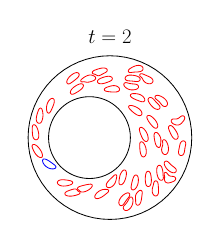
\begin{tikzpicture}[scale=0.3]

\begin{axis}[
  xmin = -21,
  xmax = 21,
  ymin = -21,
  ymax = 21,
  scale only axis,
  axis equal image,
  hide axis,
  title = {\Huge$t=2$}
  ]

% outer solid wall
\addplot [mark=none,black,line width=1.0] table{
2.0000e+01 -5.5171e-16
1.9904e+01 1.9603e+00
1.9616e+01 3.9018e+00
1.9139e+01 5.8057e+00
1.8478e+01 7.6537e+00
1.7638e+01 9.4279e+00
1.6629e+01 1.1111e+01
1.5460e+01 1.2688e+01
1.4142e+01 1.4142e+01
1.2688e+01 1.5460e+01
1.1111e+01 1.6629e+01
9.4279e+00 1.7638e+01
7.6537e+00 1.8478e+01
5.8057e+00 1.9139e+01
3.9018e+00 1.9616e+01
1.9603e+00 1.9904e+01
2.3281e-15 2.0000e+01
-1.9603e+00 1.9904e+01
-3.9018e+00 1.9616e+01
-5.8057e+00 1.9139e+01
-7.6537e+00 1.8478e+01
-9.4279e+00 1.7638e+01
-1.1111e+01 1.6629e+01
-1.2688e+01 1.5460e+01
-1.4142e+01 1.4142e+01
-1.5460e+01 1.2688e+01
-1.6629e+01 1.1111e+01
-1.7638e+01 9.4279e+00
-1.8478e+01 7.6537e+00
-1.9139e+01 5.8057e+00
-1.9616e+01 3.9018e+00
-1.9904e+01 1.9603e+00
-2.0000e+01 3.0010e-15
-1.9904e+01 -1.9603e+00
-1.9616e+01 -3.9018e+00
-1.9139e+01 -5.8057e+00
-1.8478e+01 -7.6537e+00
-1.7638e+01 -9.4279e+00
-1.6629e+01 -1.1111e+01
-1.5460e+01 -1.2688e+01
-1.4142e+01 -1.4142e+01
-1.2688e+01 -1.5460e+01
-1.1111e+01 -1.6629e+01
-9.4279e+00 -1.7638e+01
-7.6537e+00 -1.8478e+01
-5.8057e+00 -1.9139e+01
-3.9018e+00 -1.9616e+01
-1.9603e+00 -1.9904e+01
-4.7774e-15 -2.0000e+01
1.9603e+00 -1.9904e+01
3.9018e+00 -1.9616e+01
5.8057e+00 -1.9139e+01
7.6537e+00 -1.8478e+01
9.4279e+00 -1.7638e+01
1.1111e+01 -1.6629e+01
1.2688e+01 -1.5460e+01
1.4142e+01 -1.4142e+01
1.5460e+01 -1.2688e+01
1.6629e+01 -1.1111e+01
1.7638e+01 -9.4279e+00
1.8478e+01 -7.6537e+00
1.9139e+01 -5.8057e+00
1.9616e+01 -3.9018e+00
1.9904e+01 -1.9603e+00
2.0000e+01 -5.5171e-16
};

% inner solid wall
\addplot [mark=none,black,line width=1.0] table{
5.0000e+00 2.7586e-16
4.9518e+00 -9.8017e-01
4.8079e+00 -1.9509e+00
4.5694e+00 -2.9028e+00
4.2388e+00 -3.8268e+00
3.8192e+00 -4.7140e+00
3.3147e+00 -5.5557e+00
2.7301e+00 -6.3439e+00
2.0711e+00 -7.0711e+00
1.3439e+00 -7.7301e+00
5.5570e-01 -8.3147e+00
-2.8603e-01 -8.8192e+00
-1.1732e+00 -9.2388e+00
-2.0972e+00 -9.5694e+00
-3.0491e+00 -9.8079e+00
-4.0198e+00 -9.9518e+00
-5.0000e+00 -1.0000e+01
-5.9802e+00 -9.9518e+00
-6.9509e+00 -9.8079e+00
-7.9028e+00 -9.5694e+00
-8.8268e+00 -9.2388e+00
-9.7140e+00 -8.8192e+00
-1.0556e+01 -8.3147e+00
-1.1344e+01 -7.7301e+00
-1.2071e+01 -7.0711e+00
-1.2730e+01 -6.3439e+00
-1.3315e+01 -5.5557e+00
-1.3819e+01 -4.7140e+00
-1.4239e+01 -3.8268e+00
-1.4569e+01 -2.9028e+00
-1.4808e+01 -1.9509e+00
-1.4952e+01 -9.8017e-01
-1.5000e+01 -1.5005e-15
-1.4952e+01 9.8017e-01
-1.4808e+01 1.9509e+00
-1.4569e+01 2.9028e+00
-1.4239e+01 3.8268e+00
-1.3819e+01 4.7140e+00
-1.3315e+01 5.5557e+00
-1.2730e+01 6.3439e+00
-1.2071e+01 7.0711e+00
-1.1344e+01 7.7301e+00
-1.0556e+01 8.3147e+00
-9.7140e+00 8.8192e+00
-8.8268e+00 9.2388e+00
-7.9028e+00 9.5694e+00
-6.9509e+00 9.8079e+00
-5.9802e+00 9.9518e+00
-5.0000e+00 1.0000e+01
-4.0198e+00 9.9518e+00
-3.0491e+00 9.8079e+00
-2.0972e+00 9.5694e+00
-1.1732e+00 9.2388e+00
-2.8603e-01 8.8192e+00
5.5570e-01 8.3147e+00
1.3439e+00 7.7301e+00
2.0711e+00 7.0711e+00
2.7301e+00 6.3439e+00
3.3147e+00 5.5557e+00
3.8192e+00 4.7140e+00
4.2388e+00 3.8268e+00
4.5694e+00 2.9028e+00
4.8079e+00 1.9509e+00
4.9518e+00 9.8017e-01
5.0000e+00 2.7586e-16
};


% vesicle1
\addplot [mark=none,red,line width=1.0] table{
1.7395e+01 3.4310e+00
1.7439e+01 3.4699e+00
1.7497e+01 3.5257e+00
1.7570e+01 3.5990e+00
1.7653e+01 3.6876e+00
1.7741e+01 3.7866e+00
1.7832e+01 3.8940e+00
1.7923e+01 4.0076e+00
1.8012e+01 4.1275e+00
1.8096e+01 4.2538e+00
1.8172e+01 4.3879e+00
1.8233e+01 4.5306e+00
1.8272e+01 4.6819e+00
1.8281e+01 4.8383e+00
1.8251e+01 4.9926e+00
1.8178e+01 5.1320e+00
1.8065e+01 5.2415e+00
1.7923e+01 5.3082e+00
1.7767e+01 5.3278e+00
1.7611e+01 5.3042e+00
1.7465e+01 5.2473e+00
1.7331e+01 5.1677e+00
1.7206e+01 5.0753e+00
1.7087e+01 4.9779e+00
1.6969e+01 4.8821e+00
1.6849e+01 4.7931e+00
1.6725e+01 4.7158e+00
1.6600e+01 4.6533e+00
1.6476e+01 4.6074e+00
1.6358e+01 4.5773e+00
1.6256e+01 4.5604e+00
1.6176e+01 4.5525e+00
1.6117e+01 4.5493e+00
1.6059e+01 4.5480e+00
1.5978e+01 4.5487e+00
1.5875e+01 4.5524e+00
1.5754e+01 4.5578e+00
1.5621e+01 4.5598e+00
1.5481e+01 4.5503e+00
1.5339e+01 4.5188e+00
1.5204e+01 4.4555e+00
1.5091e+01 4.3554e+00
1.5014e+01 4.2228e+00
1.4984e+01 4.0712e+00
1.5001e+01 3.9164e+00
1.5059e+01 3.7708e+00
1.5148e+01 3.6411e+00
1.5259e+01 3.5287e+00
1.5384e+01 3.4323e+00
1.5518e+01 3.3492e+00
1.5659e+01 3.2771e+00
1.5803e+01 3.2145e+00
1.5951e+01 3.1611e+00
1.6101e+01 3.1177e+00
1.6253e+01 3.0861e+00
1.6406e+01 3.0686e+00
1.6558e+01 3.0670e+00
1.6706e+01 3.0827e+00
1.6848e+01 3.1151e+00
1.6980e+01 3.1624e+00
1.7100e+01 3.2202e+00
1.7203e+01 3.2829e+00
1.7287e+01 3.3428e+00
1.7351e+01 3.3931e+00
1.7395e+01 3.4310e+00
};

% vesicle2
\addplot [mark=none,red,line width=1.0] table{
-8.3049e+00 1.4283e+01
-8.2601e+00 1.4320e+01
-8.1985e+00 1.4372e+01
-8.1206e+00 1.4440e+01
-8.0310e+00 1.4522e+01
-7.9357e+00 1.4614e+01
-7.8387e+00 1.4716e+01
-7.7449e+00 1.4827e+01
-7.6587e+00 1.4949e+01
-7.5868e+00 1.5083e+01
-7.5372e+00 1.5228e+01
-7.5201e+00 1.5382e+01
-7.5446e+00 1.5536e+01
-7.6155e+00 1.5675e+01
-7.7279e+00 1.5785e+01
-7.8689e+00 1.5855e+01
-8.0235e+00 1.5886e+01
-8.1813e+00 1.5884e+01
-8.3370e+00 1.5859e+01
-8.4886e+00 1.5816e+01
-8.6354e+00 1.5761e+01
-8.7776e+00 1.5695e+01
-8.9149e+00 1.5623e+01
-9.0475e+00 1.5545e+01
-9.1751e+00 1.5462e+01
-9.2973e+00 1.5376e+01
-9.4134e+00 1.5288e+01
-9.5225e+00 1.5200e+01
-9.6227e+00 1.5113e+01
-9.7120e+00 1.5031e+01
-9.7863e+00 1.4959e+01
-9.8432e+00 1.4902e+01
-9.8835e+00 1.4859e+01
-9.9231e+00 1.4817e+01
-9.9769e+00 1.4756e+01
-1.0044e+01 1.4677e+01
-1.0119e+01 1.4582e+01
-1.0196e+01 1.4475e+01
-1.0274e+01 1.4357e+01
-1.0346e+01 1.4231e+01
-1.0413e+01 1.4097e+01
-1.0469e+01 1.3956e+01
-1.0513e+01 1.3809e+01
-1.0537e+01 1.3656e+01
-1.0535e+01 1.3499e+01
-1.0494e+01 1.3348e+01
-1.0405e+01 1.3220e+01
-1.0272e+01 1.3137e+01
-1.0116e+01 1.3113e+01
-9.9606e+00 1.3137e+01
-9.8128e+00 1.3192e+01
-9.6726e+00 1.3264e+01
-9.5385e+00 1.3346e+01
-9.4086e+00 1.3433e+01
-9.2820e+00 1.3523e+01
-9.1580e+00 1.3614e+01
-9.0367e+00 1.3705e+01
-8.9179e+00 1.3796e+01
-8.8028e+00 1.3885e+01
-8.6920e+00 1.3972e+01
-8.5880e+00 1.4054e+01
-8.4931e+00 1.4129e+01
-8.4126e+00 1.4194e+01
-8.3499e+00 1.4245e+01
-8.3049e+00 1.4283e+01
};

% vesicle3
\addplot [mark=none,red,line width=1.0] table{
-5.7106e+00 1.3538e+01
-5.6521e+00 1.3533e+01
-5.5714e+00 1.3530e+01
-5.4678e+00 1.3532e+01
-5.3472e+00 1.3541e+01
-5.2158e+00 1.3559e+01
-5.0779e+00 1.3584e+01
-4.9355e+00 1.3616e+01
-4.7908e+00 1.3653e+01
-4.6441e+00 1.3693e+01
-4.4968e+00 1.3737e+01
-4.3489e+00 1.3785e+01
-4.2019e+00 1.3838e+01
-4.0565e+00 1.3898e+01
-3.9157e+00 1.3968e+01
-3.7823e+00 1.4052e+01
-3.6630e+00 1.4156e+01
-3.5657e+00 1.4280e+01
-3.5023e+00 1.4424e+01
-3.4840e+00 1.4580e+01
-3.5202e+00 1.4732e+01
-3.6059e+00 1.4861e+01
-3.7247e+00 1.4961e+01
-3.8577e+00 1.5038e+01
-3.9954e+00 1.5103e+01
-4.1327e+00 1.5161e+01
-4.2688e+00 1.5214e+01
-4.4023e+00 1.5257e+01
-4.5316e+00 1.5286e+01
-4.6515e+00 1.5301e+01
-4.7552e+00 1.5305e+01
-4.8358e+00 1.5302e+01
-4.8944e+00 1.5298e+01
-4.9521e+00 1.5291e+01
-5.0324e+00 1.5278e+01
-5.1334e+00 1.5257e+01
-5.2511e+00 1.5228e+01
-5.3775e+00 1.5189e+01
-5.5104e+00 1.5143e+01
-5.6457e+00 1.5090e+01
-5.7829e+00 1.5030e+01
-5.9193e+00 1.4963e+01
-6.0553e+00 1.4891e+01
-6.1883e+00 1.4811e+01
-6.3196e+00 1.4726e+01
-6.4475e+00 1.4635e+01
-6.5744e+00 1.4541e+01
-6.6993e+00 1.4445e+01
-6.8237e+00 1.4347e+01
-6.9432e+00 1.4244e+01
-7.0511e+00 1.4129e+01
-7.1275e+00 1.3992e+01
-7.1434e+00 1.3837e+01
-7.0719e+00 1.3701e+01
-6.9368e+00 1.3629e+01
-6.7834e+00 1.3618e+01
-6.6325e+00 1.3634e+01
-6.4833e+00 1.3646e+01
-6.3381e+00 1.3644e+01
-6.1984e+00 1.3627e+01
-6.0687e+00 1.3602e+01
-5.9499e+00 1.3576e+01
-5.8486e+00 1.3557e+01
-5.7683e+00 1.3544e+01
-5.7106e+00 1.3538e+01
};

% vesicle4
\addplot [mark=none,red,line width=1.0] table{
8.2526e+00 1.3857e+01
8.2874e+00 1.3810e+01
8.3387e+00 1.3747e+01
8.4093e+00 1.3672e+01
8.4984e+00 1.3590e+01
8.6029e+00 1.3508e+01
8.7203e+00 1.3431e+01
8.8479e+00 1.3361e+01
8.9838e+00 1.3299e+01
9.1264e+00 1.3247e+01
9.2745e+00 1.3205e+01
9.4269e+00 1.3175e+01
9.5823e+00 1.3159e+01
9.7393e+00 1.3160e+01
9.8954e+00 1.3180e+01
1.0047e+01 1.3224e+01
1.0189e+01 1.3292e+01
1.0315e+01 1.3388e+01
1.0416e+01 1.3508e+01
1.0485e+01 1.3649e+01
1.0518e+01 1.3802e+01
1.0512e+01 1.3958e+01
1.0473e+01 1.4108e+01
1.0404e+01 1.4246e+01
1.0315e+01 1.4369e+01
1.0212e+01 1.4477e+01
1.0101e+01 1.4571e+01
9.9864e+00 1.4652e+01
9.8742e+00 1.4723e+01
9.7689e+00 1.4782e+01
9.6774e+00 1.4831e+01
9.6052e+00 1.4867e+01
9.5527e+00 1.4893e+01
9.5002e+00 1.4918e+01
9.4268e+00 1.4953e+01
9.3327e+00 1.4995e+01
9.2220e+00 1.5045e+01
9.1007e+00 1.5098e+01
8.9716e+00 1.5153e+01
8.8379e+00 1.5211e+01
8.7006e+00 1.5270e+01
8.5613e+00 1.5331e+01
8.4202e+00 1.5392e+01
8.2778e+00 1.5454e+01
8.1329e+00 1.5513e+01
7.9847e+00 1.5565e+01
7.8314e+00 1.5601e+01
7.6742e+00 1.5611e+01
7.5193e+00 1.5582e+01
7.3837e+00 1.5503e+01
7.2938e+00 1.5375e+01
7.2744e+00 1.5221e+01
7.3256e+00 1.5073e+01
7.4238e+00 1.4952e+01
7.5418e+00 1.4851e+01
7.6624e+00 1.4756e+01
7.7737e+00 1.4652e+01
7.8697e+00 1.4538e+01
7.9484e+00 1.4415e+01
8.0141e+00 1.4291e+01
8.0720e+00 1.4172e+01
8.1266e+00 1.4064e+01
8.1768e+00 1.3974e+01
8.2197e+00 1.3905e+01
8.2526e+00 1.3857e+01
};

% vesicle5
\addplot [mark=none,red,line width=1.0] table{
-8.5107e+00 -1.4143e+01
-8.4535e+00 -1.4129e+01
-8.3761e+00 -1.4107e+01
-8.2760e+00 -1.4080e+01
-8.1607e+00 -1.4044e+01
-8.0339e+00 -1.4004e+01
-7.9018e+00 -1.3957e+01
-7.7648e+00 -1.3907e+01
-7.6284e+00 -1.3847e+01
-7.4945e+00 -1.3775e+01
-7.3768e+00 -1.3676e+01
-7.2995e+00 -1.3543e+01
-7.3126e+00 -1.3390e+01
-7.4163e+00 -1.3276e+01
-7.5579e+00 -1.3205e+01
-7.6994e+00 -1.3137e+01
-7.8280e+00 -1.3045e+01
-7.9342e+00 -1.2929e+01
-8.0274e+00 -1.2800e+01
-8.1306e+00 -1.2683e+01
-8.2634e+00 -1.2599e+01
-8.4135e+00 -1.2560e+01
-8.5691e+00 -1.2552e+01
-8.7218e+00 -1.2566e+01
-8.8723e+00 -1.2590e+01
-9.0175e+00 -1.2624e+01
-9.1590e+00 -1.2660e+01
-9.2933e+00 -1.2700e+01
-9.4204e+00 -1.2738e+01
-9.5350e+00 -1.2776e+01
-9.6338e+00 -1.2808e+01
-9.7097e+00 -1.2836e+01
-9.7655e+00 -1.2854e+01
-9.8198e+00 -1.2874e+01
-9.8966e+00 -1.2901e+01
-9.9930e+00 -1.2938e+01
-1.0107e+01 -1.2980e+01
-1.0229e+01 -1.3030e+01
-1.0359e+01 -1.3084e+01
-1.0490e+01 -1.3147e+01
-1.0623e+01 -1.3216e+01
-1.0749e+01 -1.3300e+01
-1.0866e+01 -1.3400e+01
-1.0957e+01 -1.3526e+01
-1.1004e+01 -1.3673e+01
-1.0987e+01 -1.3829e+01
-1.0911e+01 -1.3964e+01
-1.0793e+01 -1.4070e+01
-1.0656e+01 -1.4146e+01
-1.0507e+01 -1.4203e+01
-1.0356e+01 -1.4243e+01
-1.0200e+01 -1.4274e+01
-1.0045e+01 -1.4293e+01
-9.8885e+00 -1.4305e+01
-9.7341e+00 -1.4309e+01
-9.5794e+00 -1.4307e+01
-9.4283e+00 -1.4298e+01
-9.2787e+00 -1.4286e+01
-9.1349e+00 -1.4267e+01
-8.9953e+00 -1.4247e+01
-8.8657e+00 -1.4223e+01
-8.7463e+00 -1.4200e+01
-8.6460e+00 -1.4176e+01
-8.5666e+00 -1.4158e+01
-8.5107e+00 -1.4143e+01
};

% vesicle6
\addplot [mark=none,red,line width=1.0] table{
1.3274e+01 -5.1211e-01
1.3216e+01 -5.0686e-01
1.3136e+01 -5.1495e-01
1.3040e+01 -5.5321e-01
1.2950e+01 -6.3349e-01
1.2890e+01 -7.5083e-01
1.2866e+01 -8.8885e-01
1.2870e+01 -1.0344e+00
1.2886e+01 -1.1829e+00
1.2903e+01 -1.3340e+00
1.2913e+01 -1.4876e+00
1.2911e+01 -1.6428e+00
1.2895e+01 -1.7984e+00
1.2866e+01 -1.9526e+00
1.2825e+01 -2.1047e+00
1.2777e+01 -2.2549e+00
1.2727e+01 -2.4049e+00
1.2682e+01 -2.5565e+00
1.2650e+01 -2.7110e+00
1.2634e+01 -2.8676e+00
1.2635e+01 -3.0246e+00
1.2653e+01 -3.1799e+00
1.2685e+01 -3.3318e+00
1.2731e+01 -3.4785e+00
1.2790e+01 -3.6184e+00
1.2863e+01 -3.7489e+00
1.2949e+01 -3.8666e+00
1.3047e+01 -3.9672e+00
1.3153e+01 -4.0461e+00
1.3261e+01 -4.0999e+00
1.3360e+01 -4.1295e+00
1.3440e+01 -4.1403e+00
1.3499e+01 -4.1414e+00
1.3557e+01 -4.1365e+00
1.3636e+01 -4.1204e+00
1.3733e+01 -4.0844e+00
1.3837e+01 -4.0234e+00
1.3938e+01 -3.9374e+00
1.4028e+01 -3.8302e+00
1.4105e+01 -3.7066e+00
1.4168e+01 -3.5712e+00
1.4218e+01 -3.4275e+00
1.4255e+01 -3.2783e+00
1.4282e+01 -3.1252e+00
1.4298e+01 -2.9698e+00
1.4306e+01 -2.8129e+00
1.4304e+01 -2.6554e+00
1.4295e+01 -2.4978e+00
1.4278e+01 -2.3407e+00
1.4254e+01 -2.1845e+00
1.4223e+01 -2.0297e+00
1.4185e+01 -1.8768e+00
1.4141e+01 -1.7261e+00
1.4091e+01 -1.5781e+00
1.4034e+01 -1.4334e+00
1.3973e+01 -1.2924e+00
1.3906e+01 -1.1559e+00
1.3834e+01 -1.0250e+00
1.3756e+01 -9.0156e-01
1.3673e+01 -7.8831e-01
1.3585e+01 -6.8964e-01
1.3493e+01 -6.1068e-01
1.3406e+01 -5.5624e-01
1.3331e+01 -5.2576e-01
1.3274e+01 -5.1211e-01
};

% vesicle7
\addplot [mark=none,red,line width=1.0] table{
7.7611e+00 1.6288e+01
7.8092e+00 1.6321e+01
7.8718e+00 1.6372e+01
7.9433e+00 1.6447e+01
8.0119e+00 1.6546e+01
8.0645e+00 1.6668e+01
8.0914e+00 1.6805e+01
8.0863e+00 1.6950e+01
8.0473e+00 1.7094e+01
7.9764e+00 1.7228e+01
7.8781e+00 1.7347e+01
7.7583e+00 1.7445e+01
7.6228e+00 1.7523e+01
7.4768e+00 1.7580e+01
7.3242e+00 1.7619e+01
7.1679e+00 1.7641e+01
7.0101e+00 1.7649e+01
6.8522e+00 1.7644e+01
6.6952e+00 1.7627e+01
6.5399e+00 1.7601e+01
6.3868e+00 1.7566e+01
6.2364e+00 1.7523e+01
6.0891e+00 1.7474e+01
5.9453e+00 1.7419e+01
5.8055e+00 1.7360e+01
5.6700e+00 1.7296e+01
5.5398e+00 1.7231e+01
5.4158e+00 1.7165e+01
5.3003e+00 1.7101e+01
5.1957e+00 1.7039e+01
5.1073e+00 1.6986e+01
5.0389e+00 1.6942e+01
4.9899e+00 1.6911e+01
4.9415e+00 1.6878e+01
4.8753e+00 1.6831e+01
4.7931e+00 1.6769e+01
4.7016e+00 1.6689e+01
4.6118e+00 1.6592e+01
4.5361e+00 1.6474e+01
4.4928e+00 1.6336e+01
4.5016e+00 1.6188e+01
4.5726e+00 1.6055e+01
4.6934e+00 1.5961e+01
4.8407e+00 1.5913e+01
4.9962e+00 1.5901e+01
5.1530e+00 1.5911e+01
5.3092e+00 1.5930e+01
5.4656e+00 1.5953e+01
5.6221e+00 1.5974e+01
5.7793e+00 1.5991e+01
5.9365e+00 1.6005e+01
6.0938e+00 1.6015e+01
6.2506e+00 1.6022e+01
6.4069e+00 1.6029e+01
6.5619e+00 1.6036e+01
6.7157e+00 1.6045e+01
6.8672e+00 1.6056e+01
7.0160e+00 1.6071e+01
7.1603e+00 1.6091e+01
7.2986e+00 1.6115e+01
7.4273e+00 1.6146e+01
7.5429e+00 1.6183e+01
7.6387e+00 1.6221e+01
7.7109e+00 1.6258e+01
7.7611e+00 1.6288e+01
};

% vesicle8
\addplot [mark=none,red,line width=1.0] table{
9.0418e+00 5.0860e+00
9.0334e+00 5.0285e+00
9.0330e+00 4.9473e+00
9.0465e+00 4.8452e+00
9.0774e+00 4.7277e+00
9.1224e+00 4.6037e+00
9.1787e+00 4.4745e+00
9.2424e+00 4.3441e+00
9.3130e+00 4.2118e+00
9.3885e+00 4.0804e+00
9.4693e+00 3.9488e+00
9.5540e+00 3.8193e+00
9.6433e+00 3.6903e+00
9.7355e+00 3.5638e+00
9.8313e+00 3.4381e+00
9.9292e+00 3.3148e+00
1.0030e+01 3.1925e+00
1.0132e+01 3.0727e+00
1.0237e+01 2.9541e+00
1.0344e+01 2.8386e+00
1.0453e+01 2.7255e+00
1.0566e+01 2.6175e+00
1.0683e+01 2.5152e+00
1.0806e+01 2.4239e+00
1.0939e+01 2.3479e+00
1.1079e+01 2.2979e+00
1.1223e+01 2.2824e+00
1.1360e+01 2.3097e+00
1.1476e+01 2.3734e+00
1.1560e+01 2.4601e+00
1.1614e+01 2.5482e+00
1.1643e+01 2.6238e+00
1.1659e+01 2.6797e+00
1.1669e+01 2.7374e+00
1.1678e+01 2.8176e+00
1.1678e+01 2.9213e+00
1.1667e+01 3.0416e+00
1.1642e+01 3.1721e+00
1.1607e+01 3.3076e+00
1.1559e+01 3.4457e+00
1.1503e+01 3.5836e+00
1.1437e+01 3.7209e+00
1.1363e+01 3.8558e+00
1.1282e+01 3.9884e+00
1.1194e+01 4.1175e+00
1.1100e+01 4.2437e+00
1.1001e+01 4.3659e+00
1.0897e+01 4.4850e+00
1.0789e+01 4.6000e+00
1.0677e+01 4.7120e+00
1.0563e+01 4.8201e+00
1.0445e+01 4.9250e+00
1.0324e+01 5.0252e+00
1.0200e+01 5.1209e+00
1.0073e+01 5.2090e+00
9.9403e+00 5.2880e+00
9.8033e+00 5.3526e+00
9.6609e+00 5.3989e+00
9.5173e+00 5.4197e+00
9.3773e+00 5.4101e+00
9.2526e+00 5.3671e+00
9.1543e+00 5.2971e+00
9.0908e+00 5.2157e+00
9.0568e+00 5.1426e+00
9.0418e+00 5.0860e+00
};

% vesicle9
\addplot [mark=none,red,line width=1.0] table{
3.2402e+00 -8.0124e+00
3.1930e+00 -8.0470e+00
3.1316e+00 -8.0993e+00
3.0580e+00 -8.1723e+00
2.9783e+00 -8.2632e+00
2.8972e+00 -8.3681e+00
2.8175e+00 -8.4837e+00
2.7409e+00 -8.6077e+00
2.6690e+00 -8.7385e+00
2.6024e+00 -8.8754e+00
2.5427e+00 -9.0171e+00
2.4902e+00 -9.1634e+00
2.4454e+00 -9.3131e+00
2.4074e+00 -9.4656e+00
2.3751e+00 -9.6197e+00
2.3463e+00 -9.7750e+00
2.3200e+00 -9.9308e+00
2.2947e+00 -1.0087e+01
2.2705e+00 -1.0243e+01
2.2473e+00 -1.0399e+01
2.2267e+00 -1.0554e+01
2.2104e+00 -1.0710e+01
2.2021e+00 -1.0865e+01
2.2066e+00 -1.1019e+01
2.2315e+00 -1.1169e+01
2.2852e+00 -1.1308e+01
2.3735e+00 -1.1423e+01
2.4910e+00 -1.1498e+01
2.6198e+00 -1.1527e+01
2.7401e+00 -1.1518e+01
2.8391e+00 -1.1487e+01
2.9121e+00 -1.1453e+01
2.9627e+00 -1.1424e+01
3.0108e+00 -1.1391e+01
3.0747e+00 -1.1341e+01
3.1507e+00 -1.1271e+01
3.2333e+00 -1.1182e+01
3.3156e+00 -1.1079e+01
3.3955e+00 -1.0963e+01
3.4704e+00 -1.0839e+01
3.5408e+00 -1.0706e+01
3.6056e+00 -1.0569e+01
3.6660e+00 -1.0427e+01
3.7213e+00 -1.0282e+01
3.7729e+00 -1.0135e+01
3.8200e+00 -9.9851e+00
3.8637e+00 -9.8334e+00
3.9030e+00 -9.6807e+00
3.9387e+00 -9.5266e+00
3.9694e+00 -9.3718e+00
3.9955e+00 -9.2159e+00
4.0151e+00 -9.0597e+00
4.0281e+00 -8.9030e+00
4.0319e+00 -8.7469e+00
4.0253e+00 -8.5916e+00
4.0045e+00 -8.4393e+00
3.9667e+00 -8.2920e+00
3.9062e+00 -8.1557e+00
3.8199e+00 -8.0388e+00
3.7077e+00 -7.9553e+00
3.5822e+00 -7.9153e+00
3.4615e+00 -7.9178e+00
3.3623e+00 -7.9460e+00
3.2895e+00 -7.9815e+00
3.2402e+00 -8.0124e+00
};

% vesicle10
\addplot [mark=none,red,line width=1.0] table{
1.3015e+01 -9.3480e+00
1.3008e+01 -9.2900e+00
1.3000e+01 -9.2095e+00
1.2991e+01 -9.1064e+00
1.2982e+01 -8.9856e+00
1.2975e+01 -8.8534e+00
1.2968e+01 -8.7130e+00
1.2957e+01 -8.5678e+00
1.2943e+01 -8.4190e+00
1.2923e+01 -8.2684e+00
1.2898e+01 -8.1164e+00
1.2868e+01 -7.9641e+00
1.2835e+01 -7.8113e+00
1.2797e+01 -7.6590e+00
1.2754e+01 -7.5073e+00
1.2703e+01 -7.3578e+00
1.2642e+01 -7.2122e+00
1.2565e+01 -7.0745e+00
1.2467e+01 -6.9508e+00
1.2345e+01 -6.8513e+00
1.2202e+01 -6.7882e+00
1.2047e+01 -6.7730e+00
1.1897e+01 -6.8091e+00
1.1766e+01 -6.8901e+00
1.1664e+01 -7.0020e+00
1.1590e+01 -7.1313e+00
1.1537e+01 -7.2671e+00
1.1502e+01 -7.4029e+00
1.1478e+01 -7.5331e+00
1.1462e+01 -7.6532e+00
1.1452e+01 -7.7561e+00
1.1447e+01 -7.8369e+00
1.1444e+01 -7.8952e+00
1.1442e+01 -7.9536e+00
1.1441e+01 -8.0346e+00
1.1441e+01 -8.1380e+00
1.1446e+01 -8.2591e+00
1.1454e+01 -8.3912e+00
1.1467e+01 -8.5311e+00
1.1485e+01 -8.6755e+00
1.1508e+01 -8.8232e+00
1.1536e+01 -8.9726e+00
1.1569e+01 -9.1231e+00
1.1606e+01 -9.2738e+00
1.1650e+01 -9.4241e+00
1.1699e+01 -9.5731e+00
1.1756e+01 -9.7200e+00
1.1823e+01 -9.8630e+00
1.1901e+01 -1.0000e+01
1.1993e+01 -1.0129e+01
1.2101e+01 -1.0243e+01
1.2227e+01 -1.0338e+01
1.2369e+01 -1.0405e+01
1.2522e+01 -1.0433e+01
1.2676e+01 -1.0416e+01
1.2815e+01 -1.0353e+01
1.2926e+01 -1.0250e+01
1.3001e+01 -1.0121e+01
1.3042e+01 -9.9817e+00
1.3056e+01 -9.8420e+00
1.3054e+01 -9.7097e+00
1.3043e+01 -9.5890e+00
1.3032e+01 -9.4862e+00
1.3022e+01 -9.4059e+00
1.3015e+01 -9.3480e+00
};

% vesicle11
\addplot [mark=none,red,line width=1.0] table{
-1.4747e+01 9.2319e+00
-1.4786e+01 9.1888e+00
-1.4839e+01 9.1274e+00
-1.4903e+01 9.0460e+00
-1.4973e+01 8.9474e+00
-1.5044e+01 8.8359e+00
-1.5114e+01 8.7141e+00
-1.5181e+01 8.5844e+00
-1.5243e+01 8.4484e+00
-1.5299e+01 8.3074e+00
-1.5350e+01 8.1620e+00
-1.5394e+01 8.0131e+00
-1.5431e+01 7.8613e+00
-1.5461e+01 7.7072e+00
-1.5484e+01 7.5512e+00
-1.5498e+01 7.3939e+00
-1.5504e+01 7.2360e+00
-1.5502e+01 7.0780e+00
-1.5492e+01 6.9205e+00
-1.5474e+01 6.7640e+00
-1.5447e+01 6.6092e+00
-1.5410e+01 6.4574e+00
-1.5359e+01 6.3109e+00
-1.5287e+01 6.1749e+00
-1.5187e+01 6.0610e+00
-1.5056e+01 5.9910e+00
-1.4912e+01 5.9860e+00
-1.4784e+01 6.0408e+00
-1.4684e+01 6.1273e+00
-1.4608e+01 6.2214e+00
-1.4550e+01 6.3075e+00
-1.4509e+01 6.3768e+00
-1.4480e+01 6.4276e+00
-1.4452e+01 6.4788e+00
-1.4414e+01 6.5505e+00
-1.4367e+01 6.6427e+00
-1.4314e+01 6.7516e+00
-1.4258e+01 6.8713e+00
-1.4199e+01 6.9990e+00
-1.4139e+01 7.1318e+00
-1.4079e+01 7.2687e+00
-1.4019e+01 7.4083e+00
-1.3960e+01 7.5505e+00
-1.3902e+01 7.6944e+00
-1.3845e+01 7.8404e+00
-1.3791e+01 7.9878e+00
-1.3741e+01 8.1371e+00
-1.3695e+01 8.2879e+00
-1.3654e+01 8.4408e+00
-1.3622e+01 8.5953e+00
-1.3599e+01 8.7516e+00
-1.3590e+01 8.9088e+00
-1.3599e+01 9.0655e+00
-1.3633e+01 9.2179e+00
-1.3697e+01 9.3587e+00
-1.3797e+01 9.4750e+00
-1.3927e+01 9.5526e+00
-1.4073e+01 9.5826e+00
-1.4218e+01 9.5699e+00
-1.4351e+01 9.5259e+00
-1.4468e+01 9.4642e+00
-1.4567e+01 9.3951e+00
-1.4647e+01 9.3290e+00
-1.4706e+01 9.2735e+00
-1.4747e+01 9.2319e+00
};

% vesicle12
\addplot [mark=none,red,line width=1.0] table{
1.2489e+01 1.0080e+01
1.2436e+01 1.0104e+01
1.2362e+01 1.0137e+01
1.2267e+01 1.0177e+01
1.2153e+01 1.0219e+01
1.2028e+01 1.0260e+01
1.1892e+01 1.0296e+01
1.1748e+01 1.0322e+01
1.1599e+01 1.0333e+01
1.1448e+01 1.0321e+01
1.1300e+01 1.0279e+01
1.1169e+01 1.0197e+01
1.1071e+01 1.0077e+01
1.1025e+01 9.9275e+00
1.1036e+01 9.7715e+00
1.1097e+01 9.6263e+00
1.1192e+01 9.5003e+00
1.1305e+01 9.3896e+00
1.1426e+01 9.2892e+00
1.1551e+01 9.1918e+00
1.1674e+01 9.0947e+00
1.1794e+01 8.9944e+00
1.1910e+01 8.8913e+00
1.2020e+01 8.7838e+00
1.2125e+01 8.6740e+00
1.2224e+01 8.5614e+00
1.2316e+01 8.4492e+00
1.2403e+01 8.3382e+00
1.2483e+01 8.2334e+00
1.2558e+01 8.1374e+00
1.2622e+01 8.0572e+00
1.2675e+01 7.9956e+00
1.2714e+01 7.9527e+00
1.2755e+01 7.9106e+00
1.2814e+01 7.8553e+00
1.2894e+01 7.7893e+00
1.2994e+01 7.7221e+00
1.3113e+01 7.6626e+00
1.3246e+01 7.6199e+00
1.3391e+01 7.6005e+00
1.3539e+01 7.6109e+00
1.3685e+01 7.6545e+00
1.3817e+01 7.7330e+00
1.3926e+01 7.8425e+00
1.4005e+01 7.9771e+00
1.4051e+01 8.1266e+00
1.4065e+01 8.2836e+00
1.4050e+01 8.4404e+00
1.4012e+01 8.5938e+00
1.3955e+01 8.7408e+00
1.3883e+01 8.8815e+00
1.3799e+01 9.0147e+00
1.3706e+01 9.1414e+00
1.3606e+01 9.2608e+00
1.3499e+01 9.3741e+00
1.3388e+01 9.4803e+00
1.3273e+01 9.5803e+00
1.3156e+01 9.6730e+00
1.3039e+01 9.7592e+00
1.2922e+01 9.8374e+00
1.2810e+01 9.9076e+00
1.2705e+01 9.9679e+00
1.2614e+01 1.0017e+01
1.2542e+01 1.0054e+01
1.2489e+01 1.0080e+01
};

% vesicle13
\addplot [mark=none,red,line width=1.0] table{
5.6357e+00 1.3122e+01
5.5774e+00 1.3127e+01
5.4970e+00 1.3135e+01
5.3939e+00 1.3145e+01
5.2737e+00 1.3158e+01
5.1422e+00 1.3175e+01
5.0034e+00 1.3196e+01
4.8598e+00 1.3221e+01
4.7137e+00 1.3252e+01
4.5659e+00 1.3288e+01
4.4174e+00 1.3328e+01
4.2676e+00 1.3370e+01
4.1158e+00 1.3406e+01
3.9604e+00 1.3429e+01
3.8033e+00 1.3425e+01
3.6523e+00 1.3381e+01
3.5235e+00 1.3290e+01
3.4350e+00 1.3161e+01
3.3982e+00 1.3008e+01
3.4110e+00 1.2851e+01
3.4630e+00 1.2703e+01
3.5414e+00 1.2569e+01
3.6368e+00 1.2446e+01
3.7428e+00 1.2335e+01
3.8559e+00 1.2233e+01
3.9734e+00 1.2141e+01
4.0934e+00 1.2058e+01
4.2134e+00 1.1985e+01
4.3303e+00 1.1923e+01
4.4396e+00 1.1871e+01
4.5352e+00 1.1831e+01
4.6108e+00 1.1803e+01
4.6662e+00 1.1784e+01
4.7217e+00 1.1766e+01
4.7997e+00 1.1744e+01
4.9001e+00 1.1720e+01
5.0191e+00 1.1696e+01
5.1500e+00 1.1678e+01
5.2901e+00 1.1665e+01
5.4354e+00 1.1660e+01
5.5851e+00 1.1661e+01
5.7366e+00 1.1670e+01
5.8901e+00 1.1685e+01
6.0435e+00 1.1707e+01
6.1969e+00 1.1738e+01
6.3482e+00 1.1780e+01
6.4965e+00 1.1833e+01
6.6378e+00 1.1903e+01
6.7680e+00 1.1992e+01
6.8781e+00 1.2105e+01
6.9575e+00 1.2241e+01
6.9929e+00 1.2394e+01
6.9776e+00 1.2549e+01
6.9135e+00 1.2692e+01
6.8127e+00 1.2809e+01
6.6879e+00 1.2899e+01
6.5512e+00 1.2964e+01
6.4091e+00 1.3011e+01
6.2675e+00 1.3044e+01
6.1288e+00 1.3068e+01
5.9977e+00 1.3085e+01
5.8772e+00 1.3099e+01
5.7744e+00 1.3109e+01
5.6937e+00 1.3116e+01
5.6357e+00 1.3122e+01
};

% vesicle14
\addplot [mark=none,red,line width=1.0] table{
-1.6748e+01 7.1136e+00
-1.6794e+01 7.1507e+00
-1.6864e+01 7.1897e+00
-1.6966e+01 7.2110e+00
-1.7083e+01 7.1907e+00
-1.7196e+01 7.1208e+00
-1.7288e+01 7.0159e+00
-1.7365e+01 6.8916e+00
-1.7430e+01 6.7577e+00
-1.7491e+01 6.6180e+00
-1.7547e+01 6.4748e+00
-1.7601e+01 6.3289e+00
-1.7651e+01 6.1812e+00
-1.7700e+01 6.0317e+00
-1.7746e+01 5.8813e+00
-1.7791e+01 5.7297e+00
-1.7832e+01 5.5774e+00
-1.7872e+01 5.4242e+00
-1.7907e+01 5.2704e+00
-1.7939e+01 5.1159e+00
-1.7964e+01 4.9610e+00
-1.7984e+01 4.8058e+00
-1.7994e+01 4.6510e+00
-1.7997e+01 4.4970e+00
-1.7987e+01 4.3454e+00
-1.7965e+01 4.1976e+00
-1.7927e+01 4.0568e+00
-1.7876e+01 3.9262e+00
-1.7811e+01 3.8108e+00
-1.7738e+01 3.7147e+00
-1.7664e+01 3.6423e+00
-1.7600e+01 3.5933e+00
-1.7549e+01 3.5630e+00
-1.7498e+01 3.5372e+00
-1.7421e+01 3.5102e+00
-1.7320e+01 3.4920e+00
-1.7198e+01 3.4961e+00
-1.7072e+01 3.5326e+00
-1.6951e+01 3.6035e+00
-1.6845e+01 3.7029e+00
-1.6755e+01 3.8224e+00
-1.6681e+01 3.9546e+00
-1.6617e+01 4.0949e+00
-1.6564e+01 4.2405e+00
-1.6517e+01 4.3899e+00
-1.6478e+01 4.5419e+00
-1.6444e+01 4.6959e+00
-1.6417e+01 4.8513e+00
-1.6394e+01 5.0078e+00
-1.6379e+01 5.1650e+00
-1.6368e+01 5.3226e+00
-1.6365e+01 5.4801e+00
-1.6367e+01 5.6371e+00
-1.6376e+01 5.7932e+00
-1.6390e+01 5.9479e+00
-1.6410e+01 6.1006e+00
-1.6433e+01 6.2508e+00
-1.6461e+01 6.3977e+00
-1.6491e+01 6.5400e+00
-1.6528e+01 6.6758e+00
-1.6567e+01 6.8020e+00
-1.6614e+01 6.9140e+00
-1.6662e+01 7.0052e+00
-1.6710e+01 7.0708e+00
-1.6748e+01 7.1136e+00
};

% vesicle15
\addplot [mark=none,red,line width=1.0] table{
6.3717e-01 1.2680e+01
5.7931e-01 1.2672e+01
4.9922e-01 1.2660e+01
3.9750e-01 1.2641e+01
2.7885e-01 1.2616e+01
1.5011e-01 1.2586e+01
1.4141e-02 1.2550e+01
-1.2579e-01 1.2510e+01
-2.6881e-01 1.2466e+01
-4.1316e-01 1.2419e+01
-5.5859e-01 1.2368e+01
-7.0370e-01 1.2313e+01
-8.4799e-01 1.2253e+01
-9.8923e-01 1.2184e+01
-1.1246e+00 1.2104e+01
-1.2461e+00 1.2003e+01
-1.3379e+00 1.1875e+01
-1.3704e+00 1.1722e+01
-1.3232e+00 1.1574e+01
-1.2130e+00 1.1462e+01
-1.0745e+00 1.1389e+01
-9.2620e-01 1.1340e+01
-7.7564e-01 1.1302e+01
-6.2456e-01 1.1272e+01
-4.7482e-01 1.1247e+01
-3.2680e-01 1.1225e+01
-1.8244e-01 1.1207e+01
-4.2697e-02 1.1191e+01
8.9010e-02 1.1178e+01
2.0984e-01 1.1168e+01
3.1295e-01 1.1160e+01
3.9384e-01 1.1154e+01
4.5212e-01 1.1151e+01
5.1048e-01 1.1147e+01
5.9131e-01 1.1143e+01
6.9471e-01 1.1139e+01
8.1579e-01 1.1135e+01
9.4822e-01 1.1133e+01
1.0887e+00 1.1133e+01
1.2343e+00 1.1137e+01
1.3835e+00 1.1146e+01
1.5347e+00 1.1161e+01
1.6867e+00 1.1185e+01
1.8375e+00 1.1222e+01
1.9839e+00 1.1277e+01
2.1198e+00 1.1355e+01
2.2354e+00 1.1461e+01
2.3169e+00 1.1596e+01
2.3520e+00 1.1749e+01
2.3380e+00 1.1906e+01
2.2823e+00 1.2053e+01
2.1962e+00 1.2185e+01
2.0896e+00 1.2300e+01
1.9687e+00 1.2399e+01
1.8380e+00 1.2483e+01
1.7004e+00 1.2552e+01
1.5587e+00 1.2607e+01
1.4150e+00 1.2648e+01
1.2722e+00 1.2676e+01
1.1327e+00 1.2693e+01
1.0005e+00 1.2700e+01
8.7934e-01 1.2699e+01
7.7599e-01 1.2694e+01
6.9530e-01 1.2687e+01
6.3717e-01 1.2680e+01
};

% vesicle16
\addplot [mark=none,red,line width=1.0] table{
1.1447e+01 6.9185e+00
1.1505e+01 6.9079e+00
1.1585e+01 6.8987e+00
1.1689e+01 6.8960e+00
1.1809e+01 6.9096e+00
1.1935e+01 6.9478e+00
1.2056e+01 7.0193e+00
1.2155e+01 7.1255e+00
1.2216e+01 7.2612e+00
1.2233e+01 7.4114e+00
1.2207e+01 7.5630e+00
1.2148e+01 7.7062e+00
1.2066e+01 7.8395e+00
1.1970e+01 7.9635e+00
1.1866e+01 8.0818e+00
1.1757e+01 8.1958e+00
1.1646e+01 8.3084e+00
1.1534e+01 8.4199e+00
1.1423e+01 8.5323e+00
1.1313e+01 8.6454e+00
1.1206e+01 8.7606e+00
1.1102e+01 8.8771e+00
1.1002e+01 8.9956e+00
1.0904e+01 9.1139e+00
1.0806e+01 9.2311e+00
1.0708e+01 9.3435e+00
1.0607e+01 9.4488e+00
1.0503e+01 9.5425e+00
1.0397e+01 9.6223e+00
1.0294e+01 9.6849e+00
1.0201e+01 9.7301e+00
1.0125e+01 9.7584e+00
1.0069e+01 9.7752e+00
1.0012e+01 9.7877e+00
9.9316e+00 9.7989e+00
9.8284e+00 9.7995e+00
9.7089e+00 9.7801e+00
9.5867e+00 9.7300e+00
9.4752e+00 9.6455e+00
9.3900e+00 9.5278e+00
9.3405e+00 9.3876e+00
9.3294e+00 9.2360e+00
9.3509e+00 9.0841e+00
9.3970e+00 8.9356e+00
9.4592e+00 8.7926e+00
9.5322e+00 8.6532e+00
9.6117e+00 8.5176e+00
9.6965e+00 8.3840e+00
9.7848e+00 8.2533e+00
9.8770e+00 8.1246e+00
9.9723e+00 7.9992e+00
1.0071e+01 7.8763e+00
1.0174e+01 7.7577e+00
1.0281e+01 7.6429e+00
1.0391e+01 7.5337e+00
1.0505e+01 7.4299e+00
1.0622e+01 7.3335e+00
1.0742e+01 7.2442e+00
1.0863e+01 7.1643e+00
1.0985e+01 7.0937e+00
1.1103e+01 7.0347e+00
1.1215e+01 6.9874e+00
1.1313e+01 6.9536e+00
1.1391e+01 6.9313e+00
1.1447e+01 6.9185e+00
};

% vesicle17
\addplot [mark=none,red,line width=1.0] table{
-8.2522e+00 1.2708e+01
-8.3022e+00 1.2678e+01
-8.3709e+00 1.2635e+01
-8.4579e+00 1.2579e+01
-8.5584e+00 1.2511e+01
-8.6667e+00 1.2435e+01
-8.7795e+00 1.2351e+01
-8.8938e+00 1.2261e+01
-9.0078e+00 1.2164e+01
-9.1192e+00 1.2061e+01
-9.2267e+00 1.1951e+01
-9.3278e+00 1.1833e+01
-9.4210e+00 1.1707e+01
-9.5035e+00 1.1574e+01
-9.5731e+00 1.1433e+01
-9.6258e+00 1.1284e+01
-9.6567e+00 1.1129e+01
-9.6575e+00 1.0971e+01
-9.6175e+00 1.0819e+01
-9.5281e+00 1.0691e+01
-9.3956e+00 1.0609e+01
-9.2423e+00 1.0581e+01
-9.0881e+00 1.0596e+01
-8.9396e+00 1.0637e+01
-8.7976e+00 1.0691e+01
-8.6613e+00 1.0752e+01
-8.5310e+00 1.0817e+01
-8.4068e+00 1.0883e+01
-8.2910e+00 1.0947e+01
-8.1859e+00 1.1007e+01
-8.0967e+00 1.1060e+01
-8.0272e+00 1.1101e+01
-7.9772e+00 1.1132e+01
-7.9275e+00 1.1162e+01
-7.8588e+00 1.1205e+01
-7.7716e+00 1.1261e+01
-7.6701e+00 1.1327e+01
-7.5603e+00 1.1401e+01
-7.4451e+00 1.1481e+01
-7.3276e+00 1.1567e+01
-7.2093e+00 1.1659e+01
-7.0922e+00 1.1756e+01
-6.9773e+00 1.1858e+01
-6.8666e+00 1.1967e+01
-6.7617e+00 1.2083e+01
-6.6657e+00 1.2207e+01
-6.5821e+00 1.2341e+01
-6.5173e+00 1.2484e+01
-6.4808e+00 1.2638e+01
-6.4864e+00 1.2795e+01
-6.5455e+00 1.2940e+01
-6.6556e+00 1.3052e+01
-6.7970e+00 1.3119e+01
-6.9505e+00 1.3147e+01
-7.1056e+00 1.3147e+01
-7.2583e+00 1.3127e+01
-7.4064e+00 1.3093e+01
-7.5491e+00 1.3049e+01
-7.6853e+00 1.2997e+01
-7.8142e+00 1.2941e+01
-7.9335e+00 1.2884e+01
-8.0411e+00 1.2828e+01
-8.1317e+00 1.2778e+01
-8.2020e+00 1.2738e+01
-8.2522e+00 1.2708e+01
};

% vesicle18
\addplot [mark=none,red,line width=1.0] table{
4.1986e+00 -1.7785e+01
4.2545e+00 -1.7768e+01
4.3304e+00 -1.7741e+01
4.4246e+00 -1.7698e+01
4.5305e+00 -1.7639e+01
4.6407e+00 -1.7566e+01
4.7513e+00 -1.7479e+01
4.8592e+00 -1.7381e+01
4.9629e+00 -1.7274e+01
5.0609e+00 -1.7157e+01
5.1527e+00 -1.7034e+01
5.2372e+00 -1.6904e+01
5.3142e+00 -1.6768e+01
5.3828e+00 -1.6626e+01
5.4429e+00 -1.6481e+01
5.4941e+00 -1.6331e+01
5.5365e+00 -1.6179e+01
5.5704e+00 -1.6025e+01
5.5963e+00 -1.5869e+01
5.6147e+00 -1.5713e+01
5.6259e+00 -1.5556e+01
5.6297e+00 -1.5400e+01
5.6251e+00 -1.5245e+01
5.6101e+00 -1.5091e+01
5.5810e+00 -1.4942e+01
5.5322e+00 -1.4801e+01
5.4575e+00 -1.4677e+01
5.3548e+00 -1.4582e+01
5.2335e+00 -1.4530e+01
5.1131e+00 -1.4525e+01
5.0134e+00 -1.4552e+01
4.9419e+00 -1.4589e+01
4.8947e+00 -1.4624e+01
4.8514e+00 -1.4663e+01
4.7972e+00 -1.4723e+01
4.7365e+00 -1.4806e+01
4.6743e+00 -1.4910e+01
4.6129e+00 -1.5028e+01
4.5508e+00 -1.5154e+01
4.4865e+00 -1.5284e+01
4.4179e+00 -1.5417e+01
4.3444e+00 -1.5550e+01
4.2649e+00 -1.5682e+01
4.1795e+00 -1.5812e+01
4.0878e+00 -1.5938e+01
3.9905e+00 -1.6061e+01
3.8878e+00 -1.6181e+01
3.7812e+00 -1.6297e+01
3.6725e+00 -1.6412e+01
3.5653e+00 -1.6528e+01
3.4643e+00 -1.6650e+01
3.3771e+00 -1.6781e+01
3.3116e+00 -1.6923e+01
3.2758e+00 -1.7075e+01
3.2737e+00 -1.7230e+01
3.3069e+00 -1.7380e+01
3.3729e+00 -1.7517e+01
3.4674e+00 -1.7632e+01
3.5826e+00 -1.7720e+01
3.7098e+00 -1.7780e+01
3.8382e+00 -1.7811e+01
3.9590e+00 -1.7819e+01
4.0621e+00 -1.7813e+01
4.1419e+00 -1.7799e+01
4.1986e+00 -1.7785e+01
};

% vesicle19
\addplot [mark=none,red,line width=1.0] table{
1.6926e+01 -2.5806e+00
1.6914e+01 -2.6378e+00
1.6898e+01 -2.7171e+00
1.6877e+01 -2.8184e+00
1.6853e+01 -2.9371e+00
1.6827e+01 -3.0670e+00
1.6803e+01 -3.2053e+00
1.6782e+01 -3.3494e+00
1.6768e+01 -3.4983e+00
1.6767e+01 -3.6502e+00
1.6783e+01 -3.8032e+00
1.6823e+01 -3.9531e+00
1.6891e+01 -4.0937e+00
1.6989e+01 -4.2161e+00
1.7114e+01 -4.3109e+00
1.7260e+01 -4.3691e+00
1.7417e+01 -4.3859e+00
1.7572e+01 -4.3606e+00
1.7717e+01 -4.2978e+00
1.7843e+01 -4.2042e+00
1.7949e+01 -4.0882e+00
1.8033e+01 -3.9569e+00
1.8099e+01 -3.8164e+00
1.8149e+01 -3.6708e+00
1.8187e+01 -3.5236e+00
1.8216e+01 -3.3770e+00
1.8239e+01 -3.2332e+00
1.8258e+01 -3.0940e+00
1.8275e+01 -2.9627e+00
1.8292e+01 -2.8427e+00
1.8306e+01 -2.7403e+00
1.8319e+01 -2.6603e+00
1.8328e+01 -2.6027e+00
1.8338e+01 -2.5452e+00
1.8353e+01 -2.4656e+00
1.8373e+01 -2.3641e+00
1.8398e+01 -2.2456e+00
1.8427e+01 -2.1163e+00
1.8457e+01 -1.9792e+00
1.8486e+01 -1.8366e+00
1.8510e+01 -1.6890e+00
1.8524e+01 -1.5377e+00
1.8519e+01 -1.3839e+00
1.8489e+01 -1.2317e+00
1.8428e+01 -1.0882e+00
1.8333e+01 -9.6385e-01
1.8207e+01 -8.6985e-01
1.8059e+01 -8.1532e-01
1.7902e+01 -8.0378e-01
1.7748e+01 -8.3381e-01
1.7605e+01 -8.9970e-01
1.7479e+01 -9.9446e-01
1.7373e+01 -1.1103e+00
1.7287e+01 -1.2407e+00
1.7218e+01 -1.3799e+00
1.7164e+01 -1.5238e+00
1.7120e+01 -1.6692e+00
1.7083e+01 -1.8142e+00
1.7052e+01 -1.9563e+00
1.7023e+01 -2.0939e+00
1.6997e+01 -2.2238e+00
1.6974e+01 -2.3426e+00
1.6954e+01 -2.4441e+00
1.6938e+01 -2.5234e+00
1.6926e+01 -2.5806e+00
};

% vesicle20
\addplot [mark=none,red,line width=1.0] table{
1.5137e+00 -9.1059e+00
1.4613e+00 -9.0804e+00
1.3822e+00 -9.0662e+00
1.2804e+00 -9.0835e+00
1.1721e+00 -9.1362e+00
1.0652e+00 -9.2150e+00
9.5956e-01 -9.3070e+00
8.5292e-01 -9.4067e+00
7.4515e-01 -9.5097e+00
6.3561e-01 -9.6156e+00
5.2502e-01 -9.7223e+00
4.1296e-01 -9.8303e+00
3.0036e-01 -9.9383e+00
1.8694e-01 -1.0047e+01
7.3838e-02 -1.0157e+01
-3.9054e-02 -1.0267e+01
-1.5038e-01 -1.0379e+01
-2.6006e-01 -1.0493e+01
-3.6646e-01 -1.0610e+01
-4.6914e-01 -1.0730e+01
-5.6601e-01 -1.0853e+01
-6.5601e-01 -1.0981e+01
-7.3618e-01 -1.1114e+01
-8.0420e-01 -1.1252e+01
-8.5555e-01 -1.1395e+01
-8.8606e-01 -1.1541e+01
-8.9004e-01 -1.1686e+01
-8.6458e-01 -1.1824e+01
-8.1065e-01 -1.1945e+01
-7.3722e-01 -1.2041e+01
-6.5868e-01 -1.2108e+01
-5.8997e-01 -1.2150e+01
-5.3694e-01 -1.2175e+01
-4.8234e-01 -1.2195e+01
-4.0381e-01 -1.2215e+01
-3.0153e-01 -1.2229e+01
-1.8028e-01 -1.2229e+01
-4.9288e-02 -1.2212e+01
8.7033e-02 -1.2177e+01
2.2319e-01 -1.2126e+01
3.5786e-01 -1.2061e+01
4.8800e-01 -1.1983e+01
6.1366e-01 -1.1893e+01
7.3265e-01 -1.1794e+01
8.4542e-01 -1.1686e+01
9.4997e-01 -1.1569e+01
1.0468e+00 -1.1444e+01
1.1341e+00 -1.1313e+01
1.2127e+00 -1.1176e+01
1.2813e+00 -1.1034e+01
1.3417e+00 -1.0887e+01
1.3938e+00 -1.0739e+01
1.4403e+00 -1.0589e+01
1.4814e+00 -1.0438e+01
1.5193e+00 -1.0287e+01
1.5537e+00 -1.0137e+01
1.5858e+00 -9.9885e+00
1.6138e+00 -9.8420e+00
1.6375e+00 -9.6980e+00
1.6525e+00 -9.5587e+00
1.6557e+00 -9.4260e+00
1.6399e+00 -9.3064e+00
1.6049e+00 -9.2091e+00
1.5580e+00 -9.1437e+00
1.5137e+00 -9.1059e+00
};

% vesicle21
\addplot [mark=none,red,line width=1.0] table{
6.3780e+00 -1.6216e+01
6.4036e+00 -1.6269e+01
6.4470e+00 -1.6337e+01
6.5168e+00 -1.6413e+01
6.6169e+00 -1.6481e+01
6.7427e+00 -1.6520e+01
6.8826e+00 -1.6520e+01
7.0213e+00 -1.6477e+01
7.1476e+00 -1.6397e+01
7.2566e+00 -1.6292e+01
7.3482e+00 -1.6168e+01
7.4244e+00 -1.6033e+01
7.4883e+00 -1.5890e+01
7.5420e+00 -1.5743e+01
7.5876e+00 -1.5592e+01
7.6264e+00 -1.5439e+01
7.6600e+00 -1.5284e+01
7.6891e+00 -1.5129e+01
7.7150e+00 -1.4973e+01
7.7381e+00 -1.4818e+01
7.7597e+00 -1.4662e+01
7.7800e+00 -1.4507e+01
7.8001e+00 -1.4353e+01
7.8198e+00 -1.4200e+01
7.8396e+00 -1.4050e+01
7.8587e+00 -1.3901e+01
7.8760e+00 -1.3757e+01
7.8892e+00 -1.3617e+01
7.8953e+00 -1.3485e+01
7.8910e+00 -1.3364e+01
7.8760e+00 -1.3261e+01
7.8542e+00 -1.3183e+01
7.8321e+00 -1.3129e+01
7.8039e+00 -1.3078e+01
7.7546e+00 -1.3014e+01
7.6749e+00 -1.2949e+01
7.5640e+00 -1.2901e+01
7.4326e+00 -1.2890e+01
7.2953e+00 -1.2917e+01
7.1632e+00 -1.2978e+01
7.0397e+00 -1.3062e+01
6.9242e+00 -1.3161e+01
6.8146e+00 -1.3269e+01
6.7097e+00 -1.3383e+01
6.6098e+00 -1.3504e+01
6.5169e+00 -1.3630e+01
6.4339e+00 -1.3764e+01
6.3640e+00 -1.3906e+01
6.3098e+00 -1.4054e+01
6.2725e+00 -1.4207e+01
6.2513e+00 -1.4364e+01
6.2437e+00 -1.4521e+01
6.2459e+00 -1.4678e+01
6.2537e+00 -1.4834e+01
6.2635e+00 -1.4989e+01
6.2728e+00 -1.5143e+01
6.2799e+00 -1.5295e+01
6.2847e+00 -1.5444e+01
6.2882e+00 -1.5590e+01
6.2926e+00 -1.5730e+01
6.3004e+00 -1.5862e+01
6.3143e+00 -1.5983e+01
6.3342e+00 -1.6084e+01
6.3569e+00 -1.6162e+01
6.3780e+00 -1.6216e+01
};

% vesicle22
\addplot [mark=none,red,line width=1.0] table{
7.3335e+00 -2.9370e+00
7.3395e+00 -2.9953e+00
7.3479e+00 -3.0756e+00
7.3603e+00 -3.1785e+00
7.3760e+00 -3.2984e+00
7.3960e+00 -3.4295e+00
7.4199e+00 -3.5678e+00
7.4491e+00 -3.7106e+00
7.4839e+00 -3.8558e+00
7.5263e+00 -4.0019e+00
7.5776e+00 -4.1469e+00
7.6412e+00 -4.2887e+00
7.7201e+00 -4.4233e+00
7.8193e+00 -4.5451e+00
7.9417e+00 -4.6433e+00
8.0868e+00 -4.7044e+00
8.2435e+00 -4.7144e+00
8.3947e+00 -4.6703e+00
8.5244e+00 -4.5815e+00
8.6287e+00 -4.4637e+00
8.7092e+00 -4.3290e+00
8.7708e+00 -4.1855e+00
8.8166e+00 -4.0371e+00
8.8500e+00 -3.8869e+00
8.8720e+00 -3.7364e+00
8.8849e+00 -3.5876e+00
8.8893e+00 -3.4419e+00
8.8871e+00 -3.3016e+00
8.8792e+00 -3.1692e+00
8.8677e+00 -3.0487e+00
8.8545e+00 -2.9459e+00
8.8424e+00 -2.8660e+00
8.8324e+00 -2.8083e+00
8.8219e+00 -2.7511e+00
8.8055e+00 -2.6715e+00
8.7826e+00 -2.5709e+00
8.7522e+00 -2.4533e+00
8.7155e+00 -2.3264e+00
8.6715e+00 -2.1926e+00
8.6213e+00 -2.0563e+00
8.5636e+00 -1.9181e+00
8.4990e+00 -1.7808e+00
8.4259e+00 -1.6449e+00
8.3446e+00 -1.5131e+00
8.2532e+00 -1.3858e+00
8.1513e+00 -1.2669e+00
8.0354e+00 -1.1597e+00
7.9033e+00 -1.0745e+00
7.7533e+00 -1.0261e+00
7.5970e+00 -1.0366e+00
7.4612e+00 -1.1144e+00
7.3705e+00 -1.2423e+00
7.3218e+00 -1.3910e+00
7.2993e+00 -1.5459e+00
7.2892e+00 -1.7006e+00
7.2857e+00 -1.8548e+00
7.2853e+00 -2.0065e+00
7.2878e+00 -2.1562e+00
7.2919e+00 -2.3015e+00
7.2981e+00 -2.4421e+00
7.3052e+00 -2.5741e+00
7.3134e+00 -2.6953e+00
7.3212e+00 -2.7982e+00
7.3283e+00 -2.8791e+00
7.3335e+00 -2.9370e+00
};

% vesicle23
\addplot [mark=none,red,line width=1.0] table{
5.6590e+00 -9.9612e+00
5.6400e+00 -1.0016e+01
5.6148e+00 -1.0093e+01
5.5840e+00 -1.0192e+01
5.5496e+00 -1.0308e+01
5.5138e+00 -1.0436e+01
5.4774e+00 -1.0572e+01
5.4411e+00 -1.0713e+01
5.4051e+00 -1.0858e+01
5.3697e+00 -1.1005e+01
5.3352e+00 -1.1156e+01
5.3020e+00 -1.1307e+01
5.2706e+00 -1.1460e+01
5.2417e+00 -1.1615e+01
5.2165e+00 -1.1770e+01
5.1968e+00 -1.1927e+01
5.1852e+00 -1.2085e+01
5.1862e+00 -1.2242e+01
5.2072e+00 -1.2399e+01
5.2586e+00 -1.2547e+01
5.3500e+00 -1.2674e+01
5.4804e+00 -1.2758e+01
5.6322e+00 -1.2787e+01
5.7838e+00 -1.2763e+01
5.9233e+00 -1.2703e+01
6.0481e+00 -1.2621e+01
6.1590e+00 -1.2527e+01
6.2573e+00 -1.2427e+01
6.3429e+00 -1.2326e+01
6.4156e+00 -1.2229e+01
6.4738e+00 -1.2143e+01
6.5167e+00 -1.2075e+01
6.5463e+00 -1.2024e+01
6.5747e+00 -1.1973e+01
6.6123e+00 -1.1902e+01
6.6571e+00 -1.1808e+01
6.7053e+00 -1.1697e+01
6.7524e+00 -1.1573e+01
6.7966e+00 -1.1440e+01
6.8362e+00 -1.1300e+01
6.8706e+00 -1.1154e+01
6.8993e+00 -1.1005e+01
6.9224e+00 -1.0853e+01
6.9394e+00 -1.0699e+01
6.9506e+00 -1.0543e+01
6.9552e+00 -1.0386e+01
6.9532e+00 -1.0228e+01
6.9434e+00 -1.0071e+01
6.9246e+00 -9.9138e+00
6.8948e+00 -9.7587e+00
6.8511e+00 -9.6070e+00
6.7890e+00 -9.4624e+00
6.7037e+00 -9.3308e+00
6.5902e+00 -9.2240e+00
6.4504e+00 -9.1583e+00
6.2977e+00 -9.1487e+00
6.1538e+00 -9.1949e+00
6.0326e+00 -9.2817e+00
5.9358e+00 -9.3902e+00
5.8585e+00 -9.5075e+00
5.7964e+00 -9.6244e+00
5.7461e+00 -9.7346e+00
5.7072e+00 -9.8304e+00
5.6786e+00 -9.9062e+00
5.6590e+00 -9.9612e+00
};

% vesicle24
\addplot [mark=none,red,line width=1.0] table{
-4.9179e-01 1.3567e+01
-4.3604e-01 1.3587e+01
-3.6158e-01 1.3616e+01
-2.6424e-01 1.3654e+01
-1.5342e-01 1.3701e+01
-3.1303e-02 1.3754e+01
9.3716e-02 1.3816e+01
2.2143e-01 1.3887e+01
3.4299e-01 1.3973e+01
4.5513e-01 1.4076e+01
5.4194e-01 1.4203e+01
5.9092e-01 1.4349e+01
5.8324e-01 1.4505e+01
5.2167e-01 1.4648e+01
4.1527e-01 1.4765e+01
2.8486e-01 1.4851e+01
1.3828e-01 1.4913e+01
-1.3396e-02 1.4952e+01
-1.7055e-01 1.4976e+01
-3.2679e-01 1.4984e+01
-4.8482e-01 1.4981e+01
-6.3948e-01 1.4967e+01
-7.9424e-01 1.4945e+01
-9.4445e-01 1.4916e+01
-1.0937e+00 1.4883e+01
-1.2375e+00 1.4845e+01
-1.3787e+00 1.4806e+01
-1.5122e+00 1.4765e+01
-1.6394e+00 1.4726e+01
-1.7532e+00 1.4686e+01
-1.8519e+00 1.4653e+01
-1.9268e+00 1.4625e+01
-1.9826e+00 1.4605e+01
-2.0359e+00 1.4583e+01
-2.1121e+00 1.4554e+01
-2.2063e+00 1.4513e+01
-2.3178e+00 1.4464e+01
-2.4353e+00 1.4404e+01
-2.5590e+00 1.4336e+01
-2.6797e+00 1.4256e+01
-2.7978e+00 1.4163e+01
-2.9024e+00 1.4054e+01
-2.9888e+00 1.3927e+01
-3.0387e+00 1.3780e+01
-3.0423e+00 1.3625e+01
-2.9880e+00 1.3478e+01
-2.8883e+00 1.3358e+01
-2.7556e+00 1.3271e+01
-2.6094e+00 1.3215e+01
-2.4541e+00 1.3180e+01
-2.2984e+00 1.3164e+01
-2.1397e+00 1.3159e+01
-1.9840e+00 1.3167e+01
-1.8274e+00 1.3183e+01
-1.6753e+00 1.3209e+01
-1.5235e+00 1.3240e+01
-1.3772e+00 1.3277e+01
-1.2321e+00 1.3317e+01
-1.0939e+00 1.3360e+01
-9.5904e-01 1.3402e+01
-8.3459e-01 1.3445e+01
-7.1900e-01 1.3484e+01
-6.2260e-01 1.3519e+01
-5.4543e-01 1.3546e+01
-4.9179e-01 1.3567e+01
};

% vesicle25
\addplot [mark=none,blue,line width=1.0] table{
-1.4511e+01 -5.9701e+00
-1.4559e+01 -5.9375e+00
-1.4625e+01 -5.8900e+00
-1.4711e+01 -5.8324e+00
-1.4811e+01 -5.7636e+00
-1.4922e+01 -5.6924e+00
-1.5041e+01 -5.6168e+00
-1.5167e+01 -5.5439e+00
-1.5298e+01 -5.4708e+00
-1.5433e+01 -5.4039e+00
-1.5574e+01 -5.3403e+00
-1.5720e+01 -5.2869e+00
-1.5870e+01 -5.2424e+00
-1.6025e+01 -5.2189e+00
-1.6182e+01 -5.2271e+00
-1.6323e+01 -5.2948e+00
-1.6418e+01 -5.4185e+00
-1.6456e+01 -5.5724e+00
-1.6455e+01 -5.7288e+00
-1.6428e+01 -5.8853e+00
-1.6384e+01 -6.0348e+00
-1.6326e+01 -6.1809e+00
-1.6256e+01 -6.3184e+00
-1.6176e+01 -6.4511e+00
-1.6088e+01 -6.5741e+00
-1.5994e+01 -6.6916e+00
-1.5897e+01 -6.7983e+00
-1.5797e+01 -6.8982e+00
-1.5698e+01 -6.9855e+00
-1.5604e+01 -7.0634e+00
-1.5522e+01 -7.1246e+00
-1.5456e+01 -7.1725e+00
-1.5407e+01 -7.2040e+00
-1.5358e+01 -7.2367e+00
-1.5289e+01 -7.2777e+00
-1.5199e+01 -7.3299e+00
-1.5091e+01 -7.3844e+00
-1.4971e+01 -7.4410e+00
-1.4841e+01 -7.4926e+00
-1.4703e+01 -7.5411e+00
-1.4559e+01 -7.5807e+00
-1.4411e+01 -7.6143e+00
-1.4259e+01 -7.6365e+00
-1.4104e+01 -7.6503e+00
-1.3948e+01 -7.6499e+00
-1.3791e+01 -7.6378e+00
-1.3637e+01 -7.6070e+00
-1.3487e+01 -7.5572e+00
-1.3351e+01 -7.4771e+00
-1.3244e+01 -7.3632e+00
-1.3193e+01 -7.2141e+00
-1.3216e+01 -7.0605e+00
-1.3294e+01 -6.9239e+00
-1.3399e+01 -6.8098e+00
-1.3516e+01 -6.7062e+00
-1.3636e+01 -6.6115e+00
-1.3758e+01 -6.5186e+00
-1.3878e+01 -6.4308e+00
-1.3995e+01 -6.3436e+00
-1.4109e+01 -6.2618e+00
-1.4216e+01 -6.1828e+00
-1.4314e+01 -6.1127e+00
-1.4398e+01 -6.0511e+00
-1.4464e+01 -6.0051e+00
-1.4511e+01 -5.9701e+00
};

% vesicle26
\addplot [mark=none,red,line width=1.0] table{
1.0056e+01 -9.5200e+00
1.0047e+01 -9.4623e+00
1.0034e+01 -9.3824e+00
1.0016e+01 -9.2805e+00
9.9934e+00 -9.1615e+00
9.9654e+00 -9.0321e+00
9.9305e+00 -8.8960e+00
9.8862e+00 -8.7573e+00
9.8288e+00 -8.6194e+00
9.7534e+00 -8.4876e+00
9.6545e+00 -8.3699e+00
9.5287e+00 -8.2798e+00
9.3801e+00 -8.2340e+00
9.2246e+00 -8.2470e+00
9.0845e+00 -8.3171e+00
8.9733e+00 -8.4286e+00
8.8908e+00 -8.5630e+00
8.8296e+00 -8.7087e+00
8.7827e+00 -8.8593e+00
8.7453e+00 -9.0124e+00
8.7152e+00 -9.1665e+00
8.6911e+00 -9.3210e+00
8.6725e+00 -9.4751e+00
8.6588e+00 -9.6285e+00
8.6496e+00 -9.7802e+00
8.6444e+00 -9.9296e+00
8.6426e+00 -1.0075e+01
8.6435e+00 -1.0216e+01
8.6468e+00 -1.0348e+01
8.6516e+00 -1.0469e+01
8.6573e+00 -1.0572e+01
8.6628e+00 -1.0653e+01
8.6674e+00 -1.0711e+01
8.6725e+00 -1.0769e+01
8.6806e+00 -1.0850e+01
8.6929e+00 -1.0953e+01
8.7105e+00 -1.1073e+01
8.7349e+00 -1.1203e+01
8.7682e+00 -1.1339e+01
8.8135e+00 -1.1477e+01
8.8751e+00 -1.1614e+01
8.9580e+00 -1.1741e+01
9.0664e+00 -1.1850e+01
9.2005e+00 -1.1927e+01
9.3526e+00 -1.1960e+01
9.5079e+00 -1.1943e+01
9.6512e+00 -1.1878e+01
9.7724e+00 -1.1778e+01
9.8693e+00 -1.1653e+01
9.9439e+00 -1.1514e+01
1.0001e+01 -1.1367e+01
1.0044e+01 -1.1215e+01
1.0077e+01 -1.1062e+01
1.0101e+01 -1.0907e+01
1.0118e+01 -1.0753e+01
1.0129e+01 -1.0600e+01
1.0133e+01 -1.0448e+01
1.0132e+01 -1.0298e+01
1.0125e+01 -1.0153e+01
1.0115e+01 -1.0013e+01
1.0102e+01 -9.8808e+00
1.0088e+01 -9.7605e+00
1.0075e+01 -9.6579e+00
1.0064e+01 -9.5777e+00
1.0056e+01 -9.5200e+00
};

% vesicle27
\addplot [mark=none,red,line width=1.0] table{
8.9835e+00 1.1721e+00
8.9566e+00 1.2241e+00
8.9181e+00 1.2953e+00
8.8665e+00 1.3850e+00
8.8029e+00 1.4882e+00
8.7295e+00 1.5984e+00
8.6476e+00 1.7125e+00
8.5582e+00 1.8275e+00
8.4618e+00 1.9417e+00
8.3588e+00 2.0534e+00
8.2489e+00 2.1612e+00
8.1315e+00 2.2629e+00
8.0055e+00 2.3553e+00
7.8692e+00 2.4331e+00
7.7214e+00 2.4870e+00
7.5649e+00 2.5023e+00
7.4130e+00 2.4626e+00
7.2918e+00 2.3632e+00
7.2212e+00 2.2231e+00
7.1977e+00 2.0677e+00
7.2048e+00 1.9110e+00
7.2291e+00 1.7565e+00
7.2628e+00 1.6050e+00
7.3021e+00 1.4561e+00
7.3450e+00 1.3103e+00
7.3903e+00 1.1678e+00
7.4369e+00 1.0299e+00
7.4839e+00 8.9747e-01
7.5298e+00 7.7326e-01
7.5731e+00 6.6010e-01
7.6111e+00 5.6384e-01
7.6415e+00 4.8875e-01
7.6638e+00 4.3470e-01
7.6864e+00 3.8083e-01
7.7184e+00 3.0633e-01
7.7603e+00 2.1179e-01
7.8112e+00 1.0174e-01
7.8694e+00 -1.7107e-02
7.9350e+00 -1.4147e-01
8.0078e+00 -2.6746e-01
8.0891e+00 -3.9298e-01
8.1796e+00 -5.1497e-01
8.2804e+00 -6.3136e-01
8.3925e+00 -7.3864e-01
8.5173e+00 -8.3278e-01
8.6560e+00 -9.0585e-01
8.8078e+00 -9.4643e-01
8.9647e+00 -9.3984e-01
9.1092e+00 -8.7806e-01
9.2213e+00 -7.6783e-01
9.2938e+00 -6.2821e-01
9.3325e+00 -4.7561e-01
9.3474e+00 -3.1945e-01
9.3465e+00 -1.6306e-01
9.3347e+00 -8.3195e-03
9.3145e+00 1.4440e-01
9.2876e+00 2.9390e-01
9.2547e+00 4.3978e-01
9.2168e+00 5.8032e-01
9.1747e+00 7.1444e-01
9.1303e+00 8.3908e-01
9.0853e+00 9.5166e-01
9.0439e+00 1.0464e+00
9.0094e+00 1.1198e+00
8.9835e+00 1.1721e+00
};

% vesicle28
\addplot [mark=none,red,line width=1.0] table{
6.9561e+00 1.3756e+01
7.0110e+00 1.3775e+01
7.0847e+00 1.3809e+01
7.1723e+00 1.3864e+01
7.2618e+00 1.3945e+01
7.3362e+00 1.4054e+01
7.3804e+00 1.4187e+01
7.3827e+00 1.4332e+01
7.3415e+00 1.4475e+01
7.2633e+00 1.4605e+01
7.1587e+00 1.4718e+01
7.0361e+00 1.4813e+01
6.9020e+00 1.4893e+01
6.7600e+00 1.4960e+01
6.6132e+00 1.5017e+01
6.4629e+00 1.5066e+01
6.3104e+00 1.5107e+01
6.1564e+00 1.5142e+01
6.0016e+00 1.5173e+01
5.8461e+00 1.5199e+01
5.6908e+00 1.5222e+01
5.5356e+00 1.5241e+01
5.3811e+00 1.5257e+01
5.2275e+00 1.5268e+01
5.0757e+00 1.5274e+01
4.9262e+00 1.5274e+01
4.7809e+00 1.5266e+01
4.6415e+00 1.5248e+01
4.5117e+00 1.5222e+01
4.3951e+00 1.5189e+01
4.2979e+00 1.5154e+01
4.2238e+00 1.5122e+01
4.1715e+00 1.5096e+01
4.1206e+00 1.5067e+01
4.0523e+00 1.5024e+01
3.9701e+00 1.4961e+01
3.8831e+00 1.4877e+01
3.8037e+00 1.4771e+01
3.7439e+00 1.4644e+01
3.7168e+00 1.4502e+01
3.7322e+00 1.4353e+01
3.7933e+00 1.4215e+01
3.8937e+00 1.4099e+01
4.0220e+00 1.4012e+01
4.1663e+00 1.3952e+01
4.3185e+00 1.3914e+01
4.4740e+00 1.3889e+01
4.6310e+00 1.3872e+01
4.7885e+00 1.3859e+01
4.9462e+00 1.3848e+01
5.1036e+00 1.3837e+01
5.2607e+00 1.3825e+01
5.4171e+00 1.3811e+01
5.5728e+00 1.3796e+01
5.7272e+00 1.3780e+01
5.8802e+00 1.3762e+01
6.0311e+00 1.3744e+01
6.1797e+00 1.3728e+01
6.3246e+00 1.3714e+01
6.4649e+00 1.3705e+01
6.5972e+00 1.3703e+01
6.7182e+00 1.3710e+01
6.8207e+00 1.3723e+01
6.8999e+00 1.3740e+01
6.9561e+00 1.3756e+01
};

% vesicle29
\addplot [mark=none,red,line width=1.0] table{
1.4620e+01 -6.3291e+00
1.4580e+01 -6.2870e+00
1.4524e+01 -6.2286e+00
1.4451e+01 -6.1546e+00
1.4365e+01 -6.0696e+00
1.4267e+01 -5.9809e+00
1.4156e+01 -5.8949e+00
1.4031e+01 -5.8206e+00
1.3891e+01 -5.7683e+00
1.3740e+01 -5.7510e+00
1.3590e+01 -5.7795e+00
1.3456e+01 -5.8575e+00
1.3356e+01 -5.9764e+00
1.3296e+01 -6.1212e+00
1.3276e+01 -6.2769e+00
1.3286e+01 -6.4344e+00
1.3320e+01 -6.5885e+00
1.3371e+01 -6.7383e+00
1.3433e+01 -6.8833e+00
1.3503e+01 -7.0242e+00
1.3581e+01 -7.1608e+00
1.3664e+01 -7.2933e+00
1.3752e+01 -7.4212e+00
1.3845e+01 -7.5441e+00
1.3942e+01 -7.6609e+00
1.4043e+01 -7.7713e+00
1.4146e+01 -7.8742e+00
1.4249e+01 -7.9689e+00
1.4351e+01 -8.0541e+00
1.4446e+01 -8.1285e+00
1.4530e+01 -8.1893e+00
1.4597e+01 -8.2352e+00
1.4646e+01 -8.2671e+00
1.4695e+01 -8.2983e+00
1.4764e+01 -8.3397e+00
1.4855e+01 -8.3898e+00
1.4963e+01 -8.4437e+00
1.5085e+01 -8.4956e+00
1.5218e+01 -8.5411e+00
1.5360e+01 -8.5751e+00
1.5508e+01 -8.5931e+00
1.5660e+01 -8.5893e+00
1.5810e+01 -8.5584e+00
1.5952e+01 -8.4957e+00
1.6075e+01 -8.3994e+00
1.6166e+01 -8.2725e+00
1.6217e+01 -8.1241e+00
1.6224e+01 -7.9669e+00
1.6190e+01 -7.8130e+00
1.6122e+01 -7.6705e+00
1.6030e+01 -7.5425e+00
1.5922e+01 -7.4280e+00
1.5804e+01 -7.3243e+00
1.5681e+01 -7.2279e+00
1.5556e+01 -7.1356e+00
1.5432e+01 -7.0448e+00
1.5310e+01 -6.9539e+00
1.5192e+01 -6.8619e+00
1.5080e+01 -6.7693e+00
1.4974e+01 -6.6767e+00
1.4877e+01 -6.5867e+00
1.4790e+01 -6.5024e+00
1.4717e+01 -6.4291e+00
1.4661e+01 -6.3711e+00
1.4620e+01 -6.3291e+00
};

% vesicle30
\addplot [mark=none,red,line width=1.0] table{
6.2810e+00 9.2954e+00
6.3359e+00 9.2727e+00
6.4099e+00 9.2423e+00
6.5068e+00 9.2036e+00
6.6187e+00 9.1596e+00
6.7432e+00 9.1119e+00
6.8737e+00 9.0624e+00
7.0111e+00 9.0113e+00
7.1505e+00 8.9602e+00
7.2947e+00 8.9091e+00
7.4397e+00 8.8602e+00
7.5892e+00 8.8149e+00
7.7400e+00 8.7775e+00
7.8960e+00 8.7530e+00
8.0525e+00 8.7508e+00
8.2078e+00 8.7813e+00
8.3461e+00 8.8549e+00
8.4526e+00 8.9711e+00
8.5093e+00 9.1174e+00
8.5184e+00 9.2740e+00
8.4861e+00 9.4278e+00
8.4281e+00 9.5722e+00
8.3501e+00 9.7071e+00
8.2614e+00 9.8321e+00
8.1621e+00 9.9481e+00
8.0582e+00 1.0054e+01
7.9483e+00 1.0151e+01
7.8382e+00 1.0237e+01
7.7281e+00 1.0312e+01
7.6255e+00 1.0375e+01
7.5337e+00 1.0424e+01
7.4621e+00 1.0460e+01
7.4081e+00 1.0485e+01
7.3554e+00 1.0508e+01
7.2793e+00 1.0538e+01
7.1829e+00 1.0573e+01
7.0664e+00 1.0609e+01
6.9394e+00 1.0643e+01
6.8011e+00 1.0673e+01
6.6587e+00 1.0698e+01
6.5096e+00 1.0718e+01
6.3594e+00 1.0733e+01
6.2048e+00 1.0745e+01
6.0506e+00 1.0751e+01
5.8933e+00 1.0754e+01
5.7373e+00 1.0751e+01
5.5791e+00 1.0740e+01
5.4243e+00 1.0716e+01
5.2725e+00 1.0669e+01
5.1383e+00 1.0588e+01
5.0387e+00 1.0467e+01
5.0025e+00 1.0315e+01
5.0313e+00 1.0162e+01
5.1107e+00 1.0027e+01
5.2145e+00 9.9127e+00
5.3331e+00 9.8131e+00
5.4553e+00 9.7245e+00
5.5821e+00 9.6435e+00
5.7068e+00 9.5702e+00
5.8315e+00 9.5034e+00
5.9490e+00 9.4444e+00
6.0596e+00 9.3925e+00
6.1530e+00 9.3504e+00
6.2282e+00 9.3179e+00
6.2810e+00 9.2954e+00
};

% vesicle31
\addplot [mark=none,red,line width=1.0] table{
-1.8837e+01 3.0042e+00
-1.8869e+01 2.9560e+00
-1.8903e+01 2.8819e+00
-1.8933e+01 2.7837e+00
-1.8954e+01 2.6637e+00
-1.8967e+01 2.5327e+00
-1.8974e+01 2.3916e+00
-1.8976e+01 2.2468e+00
-1.8977e+01 2.0965e+00
-1.8975e+01 1.9454e+00
-1.8972e+01 1.7906e+00
-1.8969e+01 1.6362e+00
-1.8965e+01 1.4790e+00
-1.8959e+01 1.3229e+00
-1.8952e+01 1.1646e+00
-1.8942e+01 1.0079e+00
-1.8930e+01 8.4950e-01
-1.8912e+01 6.9329e-01
-1.8890e+01 5.3619e-01
-1.8860e+01 3.8239e-01
-1.8821e+01 2.2931e-01
-1.8771e+01 8.1945e-02
-1.8709e+01 -6.1086e-02
-1.8631e+01 -1.9290e-01
-1.8536e+01 -3.1231e-01
-1.8424e+01 -4.0936e-01
-1.8297e+01 -4.8090e-01
-1.8162e+01 -5.1825e-01
-1.8030e+01 -5.2471e-01
-1.7911e+01 -5.0198e-01
-1.7815e+01 -4.6472e-01
-1.7745e+01 -4.2258e-01
-1.7699e+01 -3.8810e-01
-1.7656e+01 -3.4777e-01
-1.7602e+01 -2.8802e-01
-1.7544e+01 -2.0170e-01
-1.7490e+01 -9.4200e-02
-1.7446e+01 3.1623e-02
-1.7415e+01 1.6771e-01
-1.7396e+01 3.1282e-01
-1.7387e+01 4.6120e-01
-1.7387e+01 6.1397e-01
-1.7396e+01 7.6692e-01
-1.7411e+01 9.2228e-01
-1.7432e+01 1.0765e+00
-1.7457e+01 1.2321e+00
-1.7488e+01 1.3859e+00
-1.7523e+01 1.5406e+00
-1.7562e+01 1.6929e+00
-1.7605e+01 1.8457e+00
-1.7653e+01 1.9954e+00
-1.7705e+01 2.1449e+00
-1.7763e+01 2.2903e+00
-1.7826e+01 2.4341e+00
-1.7896e+01 2.5721e+00
-1.7973e+01 2.7056e+00
-1.8061e+01 2.8292e+00
-1.8159e+01 2.9423e+00
-1.8269e+01 3.0366e+00
-1.8391e+01 3.1069e+00
-1.8519e+01 3.1409e+00
-1.8639e+01 3.1357e+00
-1.8735e+01 3.0972e+00
-1.8798e+01 3.0487e+00
-1.8837e+01 3.0042e+00
};

% vesicle32
\addplot [mark=none,red,line width=1.0] table{
4.5968e+00 7.6201e+00
4.5813e+00 7.5640e+00
4.5762e+00 7.4835e+00
4.5943e+00 7.3819e+00
4.6404e+00 7.2700e+00
4.7097e+00 7.1573e+00
4.7946e+00 7.0453e+00
4.8894e+00 6.9349e+00
4.9912e+00 6.8253e+00
5.0979e+00 6.7172e+00
5.2086e+00 6.6101e+00
5.3224e+00 6.5045e+00
5.4389e+00 6.4001e+00
5.5576e+00 6.2975e+00
5.6785e+00 6.1962e+00
5.8013e+00 6.0972e+00
5.9261e+00 6.0001e+00
6.0529e+00 5.9059e+00
6.1819e+00 5.8147e+00
6.3131e+00 5.7277e+00
6.4471e+00 5.6455e+00
6.5838e+00 5.5699e+00
6.7237e+00 5.5023e+00
6.8666e+00 5.4454e+00
7.0123e+00 5.4021e+00
7.1595e+00 5.3768e+00
7.3050e+00 5.3734e+00
7.4433e+00 5.3962e+00
7.5661e+00 5.4452e+00
7.6642e+00 5.5157e+00
7.7323e+00 5.5933e+00
7.7725e+00 5.6634e+00
7.7941e+00 5.7175e+00
7.8093e+00 5.7738e+00
7.8205e+00 5.8537e+00
7.8193e+00 5.9572e+00
7.7999e+00 6.0766e+00
7.7609e+00 6.2031e+00
7.7045e+00 6.3316e+00
7.6330e+00 6.4585e+00
7.5489e+00 6.5820e+00
7.4540e+00 6.7007e+00
7.3498e+00 6.8140e+00
7.2374e+00 6.9212e+00
7.1182e+00 7.0223e+00
6.9930e+00 7.1172e+00
6.8630e+00 7.2060e+00
6.7287e+00 7.2892e+00
6.5912e+00 7.3669e+00
6.4508e+00 7.4397e+00
6.3084e+00 7.5077e+00
6.1642e+00 7.5712e+00
6.0187e+00 7.6303e+00
5.8722e+00 7.6848e+00
5.7251e+00 7.7344e+00
5.5775e+00 7.7784e+00
5.4301e+00 7.8157e+00
5.2834e+00 7.8441e+00
5.1388e+00 7.8609e+00
4.9984e+00 7.8616e+00
4.8677e+00 7.8412e+00
4.7553e+00 7.7971e+00
4.6723e+00 7.7357e+00
4.6223e+00 7.6725e+00
4.5968e+00 7.6201e+00
};

% vesicle33
\addplot [mark=none,red,line width=1.0] table{
4.2330e+00 -1.3528e+01
4.1762e+00 -1.3542e+01
4.0988e+00 -1.3565e+01
4.0018e+00 -1.3602e+01
3.8908e+00 -1.3650e+01
3.7723e+00 -1.3709e+01
3.6496e+00 -1.3777e+01
3.5257e+00 -1.3854e+01
3.4021e+00 -1.3938e+01
3.2804e+00 -1.4029e+01
3.1615e+00 -1.4127e+01
3.0461e+00 -1.4231e+01
2.9350e+00 -1.4341e+01
2.8286e+00 -1.4456e+01
2.7275e+00 -1.4577e+01
2.6323e+00 -1.4703e+01
2.5436e+00 -1.4834e+01
2.4621e+00 -1.4969e+01
2.3886e+00 -1.5109e+01
2.3241e+00 -1.5253e+01
2.2697e+00 -1.5400e+01
2.2272e+00 -1.5550e+01
2.1982e+00 -1.5703e+01
2.1850e+00 -1.5856e+01
2.1903e+00 -1.6008e+01
2.2167e+00 -1.6155e+01
2.2661e+00 -1.6292e+01
2.3385e+00 -1.6412e+01
2.4296e+00 -1.6507e+01
2.5304e+00 -1.6574e+01
2.6268e+00 -1.6611e+01
2.7062e+00 -1.6627e+01
2.7646e+00 -1.6630e+01
2.8228e+00 -1.6626e+01
2.9023e+00 -1.6611e+01
2.9993e+00 -1.6576e+01
3.1042e+00 -1.6515e+01
3.2064e+00 -1.6431e+01
3.3029e+00 -1.6329e+01
3.3929e+00 -1.6215e+01
3.4795e+00 -1.6093e+01
3.5642e+00 -1.5967e+01
3.6493e+00 -1.5838e+01
3.7354e+00 -1.5709e+01
3.8236e+00 -1.5580e+01
3.9136e+00 -1.5452e+01
4.0062e+00 -1.5324e+01
4.1009e+00 -1.5198e+01
4.1980e+00 -1.5073e+01
4.2966e+00 -1.4950e+01
4.3962e+00 -1.4827e+01
4.4945e+00 -1.4704e+01
4.5893e+00 -1.4578e+01
4.6757e+00 -1.4448e+01
4.7490e+00 -1.4311e+01
4.8028e+00 -1.4168e+01
4.8315e+00 -1.4018e+01
4.8276e+00 -1.3869e+01
4.7847e+00 -1.3731e+01
4.7010e+00 -1.3619e+01
4.5907e+00 -1.3547e+01
4.4741e+00 -1.3515e+01
4.3711e+00 -1.3510e+01
4.2904e+00 -1.3518e+01
4.2330e+00 -1.3528e+01
};

% vesicle34
\addplot [mark=none,red,line width=1.0] table{
1.6626e+01 5.6583e-01
1.6611e+01 6.2240e-01
1.6589e+01 7.0012e-01
1.6556e+01 7.9809e-01
1.6512e+01 9.1113e-01
1.6459e+01 1.0326e+00
1.6399e+01 1.1594e+00
1.6332e+01 1.2887e+00
1.6259e+01 1.4195e+00
1.6182e+01 1.5504e+00
1.6101e+01 1.6814e+00
1.6017e+01 1.8117e+00
1.5930e+01 1.9414e+00
1.5840e+01 2.0700e+00
1.5747e+01 2.1975e+00
1.5651e+01 2.3232e+00
1.5552e+01 2.4463e+00
1.5448e+01 2.5651e+00
1.5337e+01 2.6773e+00
1.5217e+01 2.7786e+00
1.5084e+01 2.8630e+00
1.4940e+01 2.9213e+00
1.4786e+01 2.9433e+00
1.4635e+01 2.9193e+00
1.4502e+01 2.8477e+00
1.4402e+01 2.7370e+00
1.4343e+01 2.6044e+00
1.4321e+01 2.4660e+00
1.4324e+01 2.3338e+00
1.4344e+01 2.2143e+00
1.4368e+01 2.1139e+00
1.4392e+01 2.0363e+00
1.4410e+01 1.9809e+00
1.4429e+01 1.9257e+00
1.4457e+01 1.8498e+00
1.4494e+01 1.7533e+00
1.4540e+01 1.6410e+00
1.4591e+01 1.5187e+00
1.4646e+01 1.3895e+00
1.4704e+01 1.2561e+00
1.4765e+01 1.1198e+00
1.4830e+01 9.8213e-01
1.4897e+01 8.4369e-01
1.4968e+01 7.0548e-01
1.5042e+01 5.6783e-01
1.5120e+01 4.3159e-01
1.5203e+01 2.9717e-01
1.5290e+01 1.6570e-01
1.5383e+01 3.8305e-02
1.5485e+01 -8.2669e-02
1.5597e+01 -1.9414e-01
1.5721e+01 -2.9079e-01
1.5859e+01 -3.6576e-01
1.6008e+01 -4.0996e-01
1.6163e+01 -4.1534e-01
1.6312e+01 -3.7722e-01
1.6441e+01 -2.9870e-01
1.6542e+01 -1.8893e-01
1.6611e+01 -6.0936e-02
1.6650e+01 7.3806e-02
1.6665e+01 2.0521e-01
1.6663e+01 3.2627e-01
1.6652e+01 4.2909e-01
1.6638e+01 5.0881e-01
1.6626e+01 5.6583e-01
};

% vesicle35
\addplot [mark=none,red,line width=1.0] table{
1.2393e+01 -1.5783e+00
1.2397e+01 -1.5200e+00
1.2403e+01 -1.4393e+00
1.2410e+01 -1.3361e+00
1.2420e+01 -1.2154e+00
1.2432e+01 -1.0835e+00
1.2444e+01 -9.4364e-01
1.2456e+01 -7.9844e-01
1.2461e+01 -6.4910e-01
1.2457e+01 -4.9719e-01
1.2441e+01 -3.4412e-01
1.2412e+01 -1.9163e-01
1.2371e+01 -4.0831e-02
1.2319e+01 1.0740e-01
1.2258e+01 2.5271e-01
1.2189e+01 3.9468e-01
1.2113e+01 5.3304e-01
1.2030e+01 6.6725e-01
1.1939e+01 7.9662e-01
1.1841e+01 9.1974e-01
1.1733e+01 1.0342e+00
1.1614e+01 1.1354e+00
1.1481e+01 1.2150e+00
1.1335e+01 1.2601e+00
1.1183e+01 1.2573e+00
1.1045e+01 1.2018e+00
1.0938e+01 1.1047e+00
1.0865e+01 9.8478e-01
1.0823e+01 8.5957e-01
1.0801e+01 7.4052e-01
1.0792e+01 6.3745e-01
1.0789e+01 5.5663e-01
1.0790e+01 4.9824e-01
1.0791e+01 4.3995e-01
1.0795e+01 3.5909e-01
1.0802e+01 2.5595e-01
1.0813e+01 1.3528e-01
1.0828e+01 3.7176e-03
1.0845e+01 -1.3576e-01
1.0865e+01 -2.7993e-01
1.0888e+01 -4.2780e-01
1.0912e+01 -5.7765e-01
1.0940e+01 -7.2923e-01
1.0971e+01 -8.8139e-01
1.1005e+01 -1.0341e+00
1.1043e+01 -1.1863e+00
1.1086e+01 -1.3380e+00
1.1134e+01 -1.4883e+00
1.1188e+01 -1.6368e+00
1.1249e+01 -1.7823e+00
1.1320e+01 -1.9237e+00
1.1401e+01 -2.0584e+00
1.1497e+01 -2.1830e+00
1.1610e+01 -2.2900e+00
1.1744e+01 -2.3686e+00
1.1893e+01 -2.4034e+00
1.2043e+01 -2.3827e+00
1.2171e+01 -2.3075e+00
1.2263e+01 -2.1958e+00
1.2321e+01 -2.0679e+00
1.2354e+01 -1.9398e+00
1.2372e+01 -1.8200e+00
1.2383e+01 -1.7171e+00
1.2389e+01 -1.6365e+00
1.2393e+01 -1.5783e+00
};

% vesicle36
\addplot [mark=none,red,line width=1.0] table{
-3.1394e+00 -1.4913e+01
-3.0814e+00 -1.4911e+01
-3.0005e+00 -1.4904e+01
-2.8986e+00 -1.4888e+01
-2.7802e+00 -1.4861e+01
-2.6534e+00 -1.4824e+01
-2.5206e+00 -1.4777e+01
-2.3863e+00 -1.4722e+01
-2.2506e+00 -1.4658e+01
-2.1162e+00 -1.4588e+01
-1.9821e+00 -1.4511e+01
-1.8504e+00 -1.4430e+01
-1.7196e+00 -1.4344e+01
-1.5913e+00 -1.4254e+01
-1.4639e+00 -1.4160e+01
-1.3387e+00 -1.4065e+01
-1.2140e+00 -1.3967e+01
-1.0908e+00 -1.3869e+01
-9.6734e-01 -1.3770e+01
-8.4495e-01 -1.3671e+01
-7.2274e-01 -1.3572e+01
-6.0410e-01 -1.3471e+01
-4.9211e-01 -1.3362e+01
-3.9711e-01 -1.3242e+01
-3.3295e-01 -1.3104e+01
-3.2179e-01 -1.2957e+01
-3.7497e-01 -1.2823e+01
-4.8024e-01 -1.2731e+01
-6.0392e-01 -1.2686e+01
-7.2415e-01 -1.2670e+01
-8.2721e-01 -1.2665e+01
-9.0838e-01 -1.2664e+01
-9.6642e-01 -1.2664e+01
-1.0251e+00 -1.2663e+01
-1.1056e+00 -1.2663e+01
-1.2094e+00 -1.2662e+01
-1.3302e+00 -1.2664e+01
-1.4627e+00 -1.2671e+01
-1.6021e+00 -1.2686e+01
-1.7459e+00 -1.2711e+01
-1.8909e+00 -1.2746e+01
-2.0363e+00 -1.2791e+01
-2.1802e+00 -1.2845e+01
-2.3224e+00 -1.2908e+01
-2.4614e+00 -1.2979e+01
-2.5976e+00 -1.3058e+01
-2.7295e+00 -1.3144e+01
-2.8576e+00 -1.3236e+01
-2.9805e+00 -1.3335e+01
-3.0990e+00 -1.3440e+01
-3.2115e+00 -1.3550e+01
-3.3186e+00 -1.3666e+01
-3.4181e+00 -1.3788e+01
-3.5094e+00 -1.3915e+01
-3.5887e+00 -1.4048e+01
-3.6521e+00 -1.4188e+01
-3.6915e+00 -1.4335e+01
-3.6983e+00 -1.4484e+01
-3.6640e+00 -1.4625e+01
-3.5899e+00 -1.4743e+01
-3.4884e+00 -1.4828e+01
-3.3789e+00 -1.4878e+01
-3.2781e+00 -1.4902e+01
-3.1980e+00 -1.4911e+01
-3.1394e+00 -1.4913e+01
};

% vesicle37
\addplot [mark=none,red,line width=1.0] table{
-1.9016e+01 -2.0483e+00
-1.9019e+01 -2.1064e+00
-1.9015e+01 -2.1875e+00
-1.8999e+01 -2.2894e+00
-1.8971e+01 -2.4075e+00
-1.8932e+01 -2.5337e+00
-1.8884e+01 -2.6662e+00
-1.8830e+01 -2.8009e+00
-1.8770e+01 -2.9384e+00
-1.8707e+01 -3.0760e+00
-1.8639e+01 -3.2148e+00
-1.8568e+01 -3.3525e+00
-1.8494e+01 -3.4903e+00
-1.8415e+01 -3.6261e+00
-1.8333e+01 -3.7607e+00
-1.8246e+01 -3.8920e+00
-1.8154e+01 -4.0208e+00
-1.8056e+01 -4.1447e+00
-1.7953e+01 -4.2644e+00
-1.7843e+01 -4.3774e+00
-1.7728e+01 -4.4840e+00
-1.7606e+01 -4.5815e+00
-1.7478e+01 -4.6701e+00
-1.7345e+01 -4.7464e+00
-1.7206e+01 -4.8101e+00
-1.7064e+01 -4.8559e+00
-1.6921e+01 -4.8791e+00
-1.6781e+01 -4.8674e+00
-1.6661e+01 -4.8142e+00
-1.6577e+01 -4.7277e+00
-1.6530e+01 -4.6360e+00
-1.6508e+01 -4.5578e+00
-1.6499e+01 -4.5005e+00
-1.6494e+01 -4.4420e+00
-1.6493e+01 -4.3614e+00
-1.6500e+01 -4.2579e+00
-1.6517e+01 -4.1382e+00
-1.6545e+01 -4.0086e+00
-1.6583e+01 -3.8737e+00
-1.6631e+01 -3.7360e+00
-1.6688e+01 -3.5980e+00
-1.6752e+01 -3.4601e+00
-1.6823e+01 -3.3238e+00
-1.6900e+01 -3.1886e+00
-1.6982e+01 -3.0559e+00
-1.7070e+01 -2.9249e+00
-1.7161e+01 -2.7967e+00
-1.7256e+01 -2.6706e+00
-1.7355e+01 -2.5478e+00
-1.7458e+01 -2.4277e+00
-1.7565e+01 -2.3116e+00
-1.7676e+01 -2.1991e+00
-1.7790e+01 -2.0921e+00
-1.7910e+01 -1.9909e+00
-1.8034e+01 -1.8980e+00
-1.8164e+01 -1.8153e+00
-1.8299e+01 -1.7472e+00
-1.8441e+01 -1.6983e+00
-1.8584e+01 -1.6767e+00
-1.8724e+01 -1.6897e+00
-1.8845e+01 -1.7417e+00
-1.8934e+01 -1.8232e+00
-1.8985e+01 -1.9131e+00
-1.9008e+01 -1.9903e+00
-1.9016e+01 -2.0483e+00
};

% vesicle38
\addplot [mark=none,red,line width=1.0] table{
-4.9699e+00 -1.2615e+01
-4.9278e+00 -1.2576e+01
-4.8610e+00 -1.2528e+01
-4.7866e+00 -1.2457e+01
-4.6939e+00 -1.2378e+01
-4.6055e+00 -1.2280e+01
-4.5102e+00 -1.2176e+01
-4.4298e+00 -1.2054e+01
-4.3565e+00 -1.1926e+01
-4.3206e+00 -1.1776e+01
-4.3276e+00 -1.1627e+01
-4.4103e+00 -1.1492e+01
-4.5384e+00 -1.1414e+01
-4.6959e+00 -1.1379e+01
-4.8494e+00 -1.1382e+01
-5.0106e+00 -1.1393e+01
-5.1632e+00 -1.1417e+01
-5.3232e+00 -1.1439e+01
-5.4746e+00 -1.1470e+01
-5.6333e+00 -1.1497e+01
-5.7833e+00 -1.1531e+01
-5.9404e+00 -1.1559e+01
-6.0883e+00 -1.1595e+01
-6.2426e+00 -1.1625e+01
-6.3869e+00 -1.1662e+01
-6.5363e+00 -1.1693e+01
-6.6737e+00 -1.1732e+01
-6.8137e+00 -1.1763e+01
-6.9374e+00 -1.1802e+01
-7.0577e+00 -1.1833e+01
-7.1525e+00 -1.1867e+01
-7.2333e+00 -1.1889e+01
-7.2845e+00 -1.1912e+01
-7.3432e+00 -1.1929e+01
-7.4147e+00 -1.1962e+01
-7.5134e+00 -1.2000e+01
-7.6174e+00 -1.2058e+01
-7.7326e+00 -1.2126e+01
-7.8323e+00 -1.2224e+01
-7.9113e+00 -1.2344e+01
-7.9210e+00 -1.2495e+01
-7.8606e+00 -1.2628e+01
-7.7444e+00 -1.2736e+01
-7.6230e+00 -1.2824e+01
-7.4959e+00 -1.2924e+01
-7.3831e+00 -1.3025e+01
-7.2636e+00 -1.3136e+01
-7.1387e+00 -1.3223e+01
-6.9881e+00 -1.3284e+01
-6.8360e+00 -1.3305e+01
-6.6744e+00 -1.3309e+01
-6.5215e+00 -1.3289e+01
-6.3630e+00 -1.3266e+01
-6.2148e+00 -1.3226e+01
-6.0619e+00 -1.3186e+01
-5.9202e+00 -1.3132e+01
-5.7749e+00 -1.3080e+01
-5.6421e+00 -1.3016e+01
-5.5076e+00 -1.2955e+01
-5.3880e+00 -1.2885e+01
-5.2700e+00 -1.2821e+01
-5.1718e+00 -1.2752e+01
-5.0824e+00 -1.2697e+01
-5.0206e+00 -1.2647e+01
-4.9699e+00 -1.2615e+01
};

% vesicle39
\addplot [mark=none,red,line width=1.0] table{
1.1846e+01 -1.2159e+01
1.1843e+01 -1.2101e+01
1.1838e+01 -1.2020e+01
1.1831e+01 -1.1917e+01
1.1823e+01 -1.1796e+01
1.1813e+01 -1.1664e+01
1.1800e+01 -1.1524e+01
1.1782e+01 -1.1380e+01
1.1756e+01 -1.1232e+01
1.1719e+01 -1.1085e+01
1.1665e+01 -1.0941e+01
1.1590e+01 -1.0805e+01
1.1488e+01 -1.0687e+01
1.1356e+01 -1.0603e+01
1.1203e+01 -1.0571e+01
1.1049e+01 -1.0603e+01
1.0919e+01 -1.0691e+01
1.0824e+01 -1.0817e+01
1.0759e+01 -1.0960e+01
1.0714e+01 -1.1111e+01
1.0678e+01 -1.1264e+01
1.0644e+01 -1.1417e+01
1.0609e+01 -1.1568e+01
1.0570e+01 -1.1717e+01
1.0529e+01 -1.1863e+01
1.0488e+01 -1.2007e+01
1.0449e+01 -1.2147e+01
1.0413e+01 -1.2283e+01
1.0385e+01 -1.2412e+01
1.0363e+01 -1.2532e+01
1.0348e+01 -1.2634e+01
1.0340e+01 -1.2714e+01
1.0335e+01 -1.2773e+01
1.0332e+01 -1.2831e+01
1.0331e+01 -1.2912e+01
1.0332e+01 -1.3015e+01
1.0340e+01 -1.3136e+01
1.0357e+01 -1.3268e+01
1.0383e+01 -1.3405e+01
1.0421e+01 -1.3546e+01
1.0473e+01 -1.3686e+01
1.0539e+01 -1.3823e+01
1.0623e+01 -1.3952e+01
1.0727e+01 -1.4067e+01
1.0850e+01 -1.4163e+01
1.0992e+01 -1.4230e+01
1.1146e+01 -1.4260e+01
1.1303e+01 -1.4248e+01
1.1451e+01 -1.4193e+01
1.1579e+01 -1.4102e+01
1.1683e+01 -1.3984e+01
1.1762e+01 -1.3847e+01
1.1818e+01 -1.3701e+01
1.1855e+01 -1.3549e+01
1.1877e+01 -1.3395e+01
1.1888e+01 -1.3242e+01
1.1892e+01 -1.3090e+01
1.1890e+01 -1.2940e+01
1.1884e+01 -1.2795e+01
1.1877e+01 -1.2655e+01
1.1869e+01 -1.2522e+01
1.1861e+01 -1.2401e+01
1.1855e+01 -1.2298e+01
1.1850e+01 -1.2217e+01
1.1846e+01 -1.2159e+01
};

% vesicle40
\addplot [mark=none,red,line width=1.0] table{
-9.8361e+00 -1.1602e+01
-9.7801e+00 -1.1584e+01
-9.7042e+00 -1.1557e+01
-9.6073e+00 -1.1520e+01
-9.4972e+00 -1.1470e+01
-9.3807e+00 -1.1407e+01
-9.2678e+00 -1.1324e+01
-9.1700e+00 -1.1216e+01
-9.1098e+00 -1.1080e+01
-9.1112e+00 -1.0930e+01
-9.1823e+00 -1.0795e+01
-9.3000e+00 -1.0695e+01
-9.4401e+00 -1.0625e+01
-9.5881e+00 -1.0574e+01
-9.7404e+00 -1.0532e+01
-9.8939e+00 -1.0496e+01
-1.0049e+01 -1.0465e+01
-1.0204e+01 -1.0437e+01
-1.0360e+01 -1.0411e+01
-1.0516e+01 -1.0388e+01
-1.0672e+01 -1.0367e+01
-1.0827e+01 -1.0348e+01
-1.0982e+01 -1.0332e+01
-1.1135e+01 -1.0319e+01
-1.1287e+01 -1.0309e+01
-1.1436e+01 -1.0303e+01
-1.1582e+01 -1.0302e+01
-1.1722e+01 -1.0306e+01
-1.1854e+01 -1.0316e+01
-1.1974e+01 -1.0330e+01
-1.2077e+01 -1.0347e+01
-1.2155e+01 -1.0364e+01
-1.2212e+01 -1.0378e+01
-1.2268e+01 -1.0394e+01
-1.2345e+01 -1.0421e+01
-1.2440e+01 -1.0461e+01
-1.2546e+01 -1.0520e+01
-1.2651e+01 -1.0600e+01
-1.2745e+01 -1.0704e+01
-1.2812e+01 -1.0833e+01
-1.2841e+01 -1.0979e+01
-1.2822e+01 -1.1129e+01
-1.2761e+01 -1.1269e+01
-1.2665e+01 -1.1392e+01
-1.2549e+01 -1.1496e+01
-1.2418e+01 -1.1584e+01
-1.2279e+01 -1.1656e+01
-1.2133e+01 -1.1716e+01
-1.1982e+01 -1.1764e+01
-1.1828e+01 -1.1801e+01
-1.1673e+01 -1.1827e+01
-1.1516e+01 -1.1843e+01
-1.1360e+01 -1.1851e+01
-1.1203e+01 -1.1850e+01
-1.1048e+01 -1.1842e+01
-1.0894e+01 -1.1828e+01
-1.0744e+01 -1.1809e+01
-1.0596e+01 -1.1785e+01
-1.0453e+01 -1.1759e+01
-1.0315e+01 -1.1730e+01
-1.0187e+01 -1.1700e+01
-1.0069e+01 -1.1670e+01
-9.9696e+00 -1.1643e+01
-9.8914e+00 -1.1620e+01
-9.8361e+00 -1.1602e+01
};

% vesicle41
\addplot [mark=none,red,line width=1.0] table{
-2.2681e+00 1.5292e+01
-2.2159e+00 1.5319e+01
-2.1442e+00 1.5356e+01
-2.0526e+00 1.5404e+01
-1.9458e+00 1.5461e+01
-1.8285e+00 1.5523e+01
-1.7041e+00 1.5588e+01
-1.5744e+00 1.5654e+01
-1.4412e+00 1.5722e+01
-1.3059e+00 1.5791e+01
-1.1703e+00 1.5864e+01
-1.0362e+00 1.5943e+01
-9.0791e-01 1.6032e+01
-7.9173e-01 1.6137e+01
-7.0018e-01 1.6265e+01
-6.5052e-01 1.6414e+01
-6.5901e-01 1.6571e+01
-7.2649e-01 1.6713e+01
-8.3799e-01 1.6824e+01
-9.7431e-01 1.6902e+01
-1.1226e+00 1.6953e+01
-1.2755e+00 1.6985e+01
-1.4300e+00 1.7002e+01
-1.5837e+00 1.7007e+01
-1.7358e+00 1.7004e+01
-1.8847e+00 1.6992e+01
-2.0294e+00 1.6975e+01
-2.1680e+00 1.6952e+01
-2.2981e+00 1.6927e+01
-2.4161e+00 1.6901e+01
-2.5167e+00 1.6876e+01
-2.5948e+00 1.6855e+01
-2.6512e+00 1.6840e+01
-2.7072e+00 1.6823e+01
-2.7849e+00 1.6800e+01
-2.8835e+00 1.6770e+01
-2.9990e+00 1.6732e+01
-3.1244e+00 1.6690e+01
-3.2574e+00 1.6645e+01
-3.3946e+00 1.6596e+01
-3.5352e+00 1.6545e+01
-3.6767e+00 1.6490e+01
-3.8182e+00 1.6429e+01
-3.9560e+00 1.6358e+01
-4.0863e+00 1.6271e+01
-4.1995e+00 1.6163e+01
-4.2815e+00 1.6029e+01
-4.3086e+00 1.5875e+01
-4.2623e+00 1.5726e+01
-4.1501e+00 1.5616e+01
-4.0054e+00 1.5555e+01
-3.8516e+00 1.5520e+01
-3.6988e+00 1.5485e+01
-3.5517e+00 1.5432e+01
-3.4151e+00 1.5358e+01
-3.2856e+00 1.5275e+01
-3.1553e+00 1.5197e+01
-3.0166e+00 1.5141e+01
-2.8733e+00 1.5118e+01
-2.7331e+00 1.5125e+01
-2.6040e+00 1.5154e+01
-2.4892e+00 1.5193e+01
-2.3939e+00 1.5233e+01
-2.3204e+00 1.5267e+01
-2.2681e+00 1.5292e+01
};

% vesicle42
\addplot [mark=none,red,line width=1.0] table{
1.4342e+01 -1.1076e+01
1.4400e+01 -1.1068e+01
1.4480e+01 -1.1055e+01
1.4581e+01 -1.1034e+01
1.4698e+01 -1.1004e+01
1.4825e+01 -1.0966e+01
1.4959e+01 -1.0923e+01
1.5097e+01 -1.0876e+01
1.5237e+01 -1.0825e+01
1.5379e+01 -1.0770e+01
1.5520e+01 -1.0708e+01
1.5657e+01 -1.0636e+01
1.5787e+01 -1.0549e+01
1.5902e+01 -1.0443e+01
1.5995e+01 -1.0315e+01
1.6053e+01 -1.0169e+01
1.6067e+01 -1.0012e+01
1.6032e+01 -9.8591e+00
1.5952e+01 -9.7241e+00
1.5835e+01 -9.6187e+00
1.5696e+01 -9.5458e+00
1.5547e+01 -9.5022e+00
1.5393e+01 -9.4797e+00
1.5239e+01 -9.4686e+00
1.5088e+01 -9.4595e+00
1.4939e+01 -9.4443e+00
1.4796e+01 -9.4171e+00
1.4662e+01 -9.3750e+00
1.4542e+01 -9.3195e+00
1.4439e+01 -9.2553e+00
1.4358e+01 -9.1915e+00
1.4299e+01 -9.1365e+00
1.4258e+01 -9.0945e+00
1.4219e+01 -9.0511e+00
1.4167e+01 -8.9888e+00
1.4104e+01 -8.9071e+00
1.4030e+01 -8.8108e+00
1.3946e+01 -8.7090e+00
1.3844e+01 -8.6118e+00
1.3721e+01 -8.5357e+00
1.3576e+01 -8.5025e+00
1.3429e+01 -8.5345e+00
1.3314e+01 -8.6345e+00
1.3257e+01 -8.7775e+00
1.3252e+01 -8.9333e+00
1.3279e+01 -9.0880e+00
1.3316e+01 -9.2412e+00
1.3347e+01 -9.3960e+00
1.3365e+01 -9.5529e+00
1.3367e+01 -9.7109e+00
1.3357e+01 -9.8684e+00
1.3343e+01 -1.0025e+01
1.3335e+01 -1.0182e+01
1.3342e+01 -1.0338e+01
1.3373e+01 -1.0490e+01
1.3428e+01 -1.0634e+01
1.3509e+01 -1.0762e+01
1.3610e+01 -1.0872e+01
1.3727e+01 -1.0958e+01
1.3853e+01 -1.1020e+01
1.3980e+01 -1.1059e+01
1.4099e+01 -1.1078e+01
1.4203e+01 -1.1083e+01
1.4284e+01 -1.1080e+01
1.4342e+01 -1.1076e+01
};




%% vesicle 1
%\addplot [mark=none,red,line width=1.0] table{
%1.7374e+01 3.5218e+00
%1.7436e+01 3.5765e+00
%1.7526e+01 3.6620e+00
%1.7636e+01 3.7756e+00
%1.7755e+01 3.9085e+00
%1.7878e+01 4.0549e+00
%1.7999e+01 4.2126e+00
%1.8110e+01 4.3826e+00
%1.8201e+01 4.5675e+00
%1.8256e+01 4.7678e+00
%1.8255e+01 4.9762e+00
%1.8182e+01 5.1715e+00
%1.8036e+01 5.3200e+00
%1.7841e+01 5.3931e+00
%1.7632e+01 5.3860e+00
%1.7435e+01 5.3163e+00
%1.7257e+01 5.2085e+00
%1.7093e+01 5.0841e+00
%1.6933e+01 4.9591e+00
%1.6770e+01 4.8461e+00
%1.6602e+01 4.7547e+00
%1.6435e+01 4.6905e+00
%1.6282e+01 4.6529e+00
%1.6159e+01 4.6357e+00
%1.6077e+01 4.6295e+00
%1.5994e+01 4.6268e+00
%1.5870e+01 4.6276e+00
%1.5712e+01 4.6317e+00
%1.5534e+01 4.6295e+00
%1.5345e+01 4.6015e+00
%1.5163e+01 4.5239e+00
%1.5019e+01 4.3832e+00
%1.4947e+01 4.1925e+00
%1.4960e+01 3.9866e+00
%1.5047e+01 3.7972e+00
%1.5184e+01 3.6386e+00
%1.5351e+01 3.5106e+00
%1.5534e+01 3.4069e+00
%1.5726e+01 3.3215e+00
%1.5924e+01 3.2518e+00
%1.6126e+01 3.1994e+00
%1.6329e+01 3.1683e+00
%1.6532e+01 3.1634e+00
%1.6729e+01 3.1879e+00
%1.6913e+01 3.2405e+00
%1.7075e+01 3.3142e+00
%1.7211e+01 3.3962e+00
%1.7310e+01 3.4694e+00
%1.7374e+01 3.5218e+00
%};
%
%% vesicle 2
%\addplot [mark=none,red,line width=1.0] table{
%-8.4224e+00 1.4432e+01
%-8.3800e+00 1.4503e+01
%-8.3161e+00 1.4610e+01
%-8.2344e+00 1.4745e+01
%-8.1428e+00 1.4897e+01
%-8.0487e+00 1.5061e+01
%-7.9607e+00 1.5234e+01
%-7.8929e+00 1.5421e+01
%-7.8716e+00 1.5623e+01
%-7.9335e+00 1.5818e+01
%-8.0888e+00 1.5954e+01
%-8.2933e+00 1.5998e+01
%-8.5018e+00 1.5966e+01
%-8.6992e+00 1.5890e+01
%-8.8852e+00 1.5789e+01
%-9.0615e+00 1.5673e+01
%-9.2288e+00 1.5546e+01
%-9.3874e+00 1.5411e+01
%-9.5371e+00 1.5272e+01
%-9.6771e+00 1.5128e+01
%-9.8057e+00 1.4984e+01
%-9.9201e+00 1.4845e+01
%-1.0016e+01 1.4717e+01
%-1.0087e+01 1.4614e+01
%-1.0133e+01 1.4543e+01
%-1.0177e+01 1.4472e+01
%-1.0238e+01 1.4364e+01
%-1.0310e+01 1.4222e+01
%-1.0380e+01 1.4057e+01
%-1.0439e+01 1.3879e+01
%-1.0480e+01 1.3695e+01
%-1.0498e+01 1.3504e+01
%-1.0482e+01 1.3303e+01
%-1.0414e+01 1.3108e+01
%-1.0280e+01 1.2948e+01
%-1.0089e+01 1.2862e+01
%-9.8791e+00 1.2864e+01
%-9.6797e+00 1.2933e+01
%-9.4989e+00 1.3042e+01
%-9.3350e+00 1.3174e+01
%-9.1849e+00 1.3321e+01
%-9.0472e+00 1.3476e+01
%-8.9214e+00 1.3637e+01
%-8.8067e+00 1.3801e+01
%-8.7027e+00 1.3962e+01
%-8.6093e+00 1.4116e+01
%-8.5281e+00 1.4253e+01
%-8.4647e+00 1.4361e+01
%-8.4224e+00 1.4432e+01
%};
%
%% vesicle 3
%\addplot [mark=none,red,line width=1.0] table{
%-6.9051e+00 1.3648e+01
%-6.8273e+00 1.3678e+01
%-6.7091e+00 1.3719e+01
%-6.5554e+00 1.3762e+01
%-6.3784e+00 1.3798e+01
%-6.1871e+00 1.3821e+01
%-5.9876e+00 1.3835e+01
%-5.7831e+00 1.3848e+01
%-5.5771e+00 1.3878e+01
%-5.3765e+00 1.3941e+01
%-5.1910e+00 1.4038e+01
%-5.0297e+00 1.4162e+01
%-4.8972e+00 1.4304e+01
%-4.7911e+00 1.4462e+01
%-4.7134e+00 1.4646e+01
%-4.6811e+00 1.4852e+01
%-4.7129e+00 1.5058e+01
%-4.8102e+00 1.5243e+01
%-4.9556e+00 1.5389e+01
%-5.1272e+00 1.5495e+01
%-5.3083e+00 1.5564e+01
%-5.4864e+00 1.5602e+01
%-5.6470e+00 1.5616e+01
%-5.7733e+00 1.5615e+01
%-5.8571e+00 1.5609e+01
%-5.9398e+00 1.5599e+01
%-6.0632e+00 1.5576e+01
%-6.2178e+00 1.5534e+01
%-6.3871e+00 1.5471e+01
%-6.5605e+00 1.5386e+01
%-6.7307e+00 1.5279e+01
%-6.8922e+00 1.5152e+01
%-7.0432e+00 1.5008e+01
%-7.1842e+00 1.4851e+01
%-7.3173e+00 1.4685e+01
%-7.4436e+00 1.4518e+01
%-7.5626e+00 1.4353e+01
%-7.6763e+00 1.4190e+01
%-7.7868e+00 1.4020e+01
%-7.8876e+00 1.3839e+01
%-7.9543e+00 1.3641e+01
%-7.9290e+00 1.3438e+01
%-7.7731e+00 1.3315e+01
%-7.5750e+00 1.3327e+01
%-7.3977e+00 1.3403e+01
%-7.2380e+00 1.3488e+01
%-7.0954e+00 1.3561e+01
%-6.9817e+00 1.3615e+01
%-6.9051e+00 1.3648e+01
%};
%
%% vesicle 4
%\addplot [mark=none,red,line width=1.0] table{
%8.2649e+00 1.3695e+01
%8.3134e+00 1.3628e+01
%8.3916e+00 1.3532e+01
%8.5015e+00 1.3418e+01
%8.6387e+00 1.3304e+01
%8.7984e+00 1.3199e+01
%8.9759e+00 1.3111e+01
%9.1668e+00 1.3041e+01
%9.3675e+00 1.2994e+01
%9.5744e+00 1.2972e+01
%9.7837e+00 1.2977e+01
%9.9901e+00 1.3016e+01
%1.0186e+01 1.3092e+01
%1.0359e+01 1.3211e+01
%1.0493e+01 1.3372e+01
%1.0571e+01 1.3565e+01
%1.0582e+01 1.3771e+01
%1.0530e+01 1.3970e+01
%1.0426e+01 1.4144e+01
%1.0290e+01 1.4288e+01
%1.0137e+01 1.4403e+01
%9.9840e+00 1.4496e+01
%9.8429e+00 1.4567e+01
%9.7302e+00 1.4619e+01
%9.6543e+00 1.4652e+01
%9.5781e+00 1.4684e+01
%9.4634e+00 1.4731e+01
%9.3165e+00 1.4789e+01
%9.1504e+00 1.4855e+01
%8.9738e+00 1.4928e+01
%8.7924e+00 1.5009e+01
%8.6106e+00 1.5100e+01
%8.4305e+00 1.5201e+01
%8.2505e+00 1.5306e+01
%8.0642e+00 1.5402e+01
%7.8638e+00 1.5465e+01
%7.6550e+00 1.5459e+01
%7.4740e+00 1.5359e+01
%7.3789e+00 1.5178e+01
%7.3992e+00 1.4974e+01
%7.5037e+00 1.4795e+01
%7.6409e+00 1.4641e+01
%7.7767e+00 1.4490e+01
%7.8952e+00 1.4331e+01
%7.9939e+00 1.4167e+01
%8.0790e+00 1.4009e+01
%8.1553e+00 1.3870e+01
%8.2192e+00 1.3764e+01
%8.2649e+00 1.3695e+01
%};
%
%% vesicle 5
%\addplot [mark=none,red,line width=1.0] table{
%-1.4289e+01 -1.1567e+01
%-1.4272e+01 -1.1651e+01
%-1.4226e+01 -1.1770e+01
%-1.4137e+01 -1.1906e+01
%-1.4012e+01 -1.2039e+01
%-1.3859e+01 -1.2163e+01
%-1.3687e+01 -1.2274e+01
%-1.3503e+01 -1.2371e+01
%-1.3309e+01 -1.2456e+01
%-1.3108e+01 -1.2527e+01
%-1.2902e+01 -1.2585e+01
%-1.2693e+01 -1.2628e+01
%-1.2483e+01 -1.2656e+01
%-1.2275e+01 -1.2667e+01
%-1.2074e+01 -1.2663e+01
%-1.1879e+01 -1.2643e+01
%-1.1689e+01 -1.2606e+01
%-1.1501e+01 -1.2552e+01
%-1.1317e+01 -1.2477e+01
%-1.1142e+01 -1.2381e+01
%-1.0985e+01 -1.2267e+01
%-1.0855e+01 -1.2139e+01
%-1.0760e+01 -1.2007e+01
%-1.0704e+01 -1.1893e+01
%-1.0680e+01 -1.1812e+01
%-1.0668e+01 -1.1729e+01
%-1.0677e+01 -1.1603e+01
%-1.0741e+01 -1.1457e+01
%-1.0873e+01 -1.1332e+01
%-1.1053e+01 -1.1257e+01
%-1.1253e+01 -1.1224e+01
%-1.1462e+01 -1.1215e+01
%-1.1675e+01 -1.1215e+01
%-1.1889e+01 -1.1215e+01
%-1.2105e+01 -1.1210e+01
%-1.2322e+01 -1.1198e+01
%-1.2538e+01 -1.1176e+01
%-1.2746e+01 -1.1146e+01
%-1.2934e+01 -1.1111e+01
%-1.3101e+01 -1.1077e+01
%-1.3270e+01 -1.1043e+01
%-1.3459e+01 -1.1010e+01
%-1.3661e+01 -1.0996e+01
%-1.3861e+01 -1.1020e+01
%-1.4042e+01 -1.1093e+01
%-1.4183e+01 -1.1213e+01
%-1.4264e+01 -1.1355e+01
%-1.4291e+01 -1.1481e+01
%-1.4289e+01 -1.1567e+01
%};
%
%% vesicle 6
%\addplot [mark=none,red,line width=1.0] table{
%1.3148e+01 -2.4215e-01
%1.3067e+01 -2.5340e-01
%1.2955e+01 -3.0219e-01
%1.2847e+01 -4.1471e-01
%1.2791e+01 -5.8244e-01
%1.2795e+01 -7.7305e-01
%1.2837e+01 -9.6751e-01
%1.2890e+01 -1.1640e+00
%1.2939e+01 -1.3645e+00
%1.2977e+01 -1.5696e+00
%1.3001e+01 -1.7781e+00
%1.3010e+01 -1.9887e+00
%1.3003e+01 -2.1998e+00
%1.2984e+01 -2.4102e+00
%1.2959e+01 -2.6197e+00
%1.2941e+01 -2.8293e+00
%1.2947e+01 -3.0380e+00
%1.2989e+01 -3.2402e+00
%1.3072e+01 -3.4249e+00
%1.3191e+01 -3.5804e+00
%1.3339e+01 -3.6965e+00
%1.3500e+01 -3.7659e+00
%1.3654e+01 -3.7892e+00
%1.3777e+01 -3.7802e+00
%1.3857e+01 -3.7612e+00
%1.3935e+01 -3.7322e+00
%1.4043e+01 -3.6722e+00
%1.4164e+01 -3.5719e+00
%1.4278e+01 -3.4344e+00
%1.4373e+01 -3.2685e+00
%1.4445e+01 -3.0834e+00
%1.4494e+01 -2.8863e+00
%1.4522e+01 -2.6818e+00
%1.4530e+01 -2.4736e+00
%1.4521e+01 -2.2639e+00
%1.4494e+01 -2.0548e+00
%1.4452e+01 -1.8479e+00
%1.4393e+01 -1.6448e+00
%1.4320e+01 -1.4469e+00
%1.4233e+01 -1.2556e+00
%1.4133e+01 -1.0720e+00
%1.4021e+01 -8.9769e-01
%1.3900e+01 -7.3431e-01
%1.3769e+01 -5.8447e-01
%1.3631e+01 -4.5298e-01
%1.3488e+01 -3.4762e-01
%1.3349e+01 -2.7763e-01
%1.3230e+01 -2.4665e-01
%1.3148e+01 -2.4215e-01
%};
%
%% vesicle 7
%\addplot [mark=none,red,line width=1.0] table{
%8.1136e+00 1.6170e+01
%8.1795e+00 1.6220e+01
%8.2661e+00 1.6308e+01
%8.3503e+00 1.6442e+01
%8.4035e+00 1.6611e+01
%8.4082e+00 1.6801e+01
%8.3592e+00 1.6993e+01
%8.2608e+00 1.7170e+01
%8.1226e+00 1.7322e+01
%7.9547e+00 1.7444e+01
%7.7665e+00 1.7536e+01
%7.5654e+00 1.7596e+01
%7.3573e+00 1.7628e+01
%7.1467e+00 1.7632e+01
%6.9375e+00 1.7612e+01
%6.7324e+00 1.7569e+01
%6.5335e+00 1.7507e+01
%6.3421e+00 1.7430e+01
%6.1586e+00 1.7342e+01
%5.9828e+00 1.7249e+01
%5.8152e+00 1.7156e+01
%5.6585e+00 1.7070e+01
%5.5193e+00 1.6996e+01
%5.4097e+00 1.6938e+01
%5.3365e+00 1.6899e+01
%5.2637e+00 1.6860e+01
%5.1563e+00 1.6798e+01
%5.0258e+00 1.6709e+01
%4.8988e+00 1.6583e+01
%4.8151e+00 1.6413e+01
%4.8243e+00 1.6219e+01
%4.9419e+00 1.6061e+01
%5.1267e+00 1.5979e+01
%5.3329e+00 1.5961e+01
%5.5422e+00 1.5973e+01
%5.7520e+00 1.5991e+01
%5.9625e+00 1.6004e+01
%6.1734e+00 1.6008e+01
%6.3839e+00 1.6006e+01
%6.5934e+00 1.5998e+01
%6.8017e+00 1.5990e+01
%7.0081e+00 1.5984e+01
%7.2116e+00 1.5983e+01
%7.4106e+00 1.5988e+01
%7.6014e+00 1.6003e+01
%7.7779e+00 1.6033e+01
%7.9297e+00 1.6077e+01
%8.0428e+00 1.6127e+01
%8.1136e+00 1.6170e+01
%};
%
%% vesicle 8
%\addplot [mark=none,red,line width=1.0] table{
%9.3499e+00 4.4050e+00
%9.3581e+00 4.3216e+00
%9.3787e+00 4.1978e+00
%9.4145e+00 4.0421e+00
%9.4639e+00 3.8684e+00
%9.5260e+00 3.6861e+00
%9.6010e+00 3.5009e+00
%9.6890e+00 3.3164e+00
%9.7892e+00 3.1347e+00
%9.9001e+00 2.9568e+00
%1.0020e+01 2.7826e+00
%1.0147e+01 2.6119e+00
%1.0280e+01 2.4447e+00
%1.0419e+01 2.2819e+00
%1.0560e+01 2.1258e+00
%1.0704e+01 1.9804e+00
%1.0851e+01 1.8512e+00
%1.1012e+01 1.7408e+00
%1.1195e+01 1.6657e+00
%1.1391e+01 1.6576e+00
%1.1565e+01 1.7346e+00
%1.1682e+01 1.8712e+00
%1.1739e+01 2.0196e+00
%1.1759e+01 2.1430e+00
%1.1763e+01 2.2265e+00
%1.1761e+01 2.3098e+00
%1.1748e+01 2.4342e+00
%1.1720e+01 2.5910e+00
%1.1674e+01 2.7649e+00
%1.1613e+01 2.9472e+00
%1.1537e+01 3.1326e+00
%1.1447e+01 3.3171e+00
%1.1346e+01 3.4993e+00
%1.1234e+01 3.6775e+00
%1.1112e+01 3.8510e+00
%1.0982e+01 4.0196e+00
%1.0846e+01 4.1833e+00
%1.0703e+01 4.3421e+00
%1.0556e+01 4.4954e+00
%1.0405e+01 4.6401e+00
%1.0249e+01 4.7703e+00
%1.0086e+01 4.8767e+00
%9.9089e+00 4.9471e+00
%9.7175e+00 4.9599e+00
%9.5405e+00 4.8938e+00
%9.4185e+00 4.7627e+00
%9.3621e+00 4.6132e+00
%9.3482e+00 4.4886e+00
%9.3499e+00 4.4050e+00
%};
%
%% vesicle 9
%\addplot [mark=none,red,line width=1.0] table{
%2.9302e+00 -8.8691e+00
%2.8671e+00 -8.9261e+00
%2.7763e+00 -9.0172e+00
%2.6652e+00 -9.1410e+00
%2.5451e+00 -9.2882e+00
%2.4238e+00 -9.4503e+00
%2.3053e+00 -9.6232e+00
%2.1921e+00 -9.8054e+00
%2.0883e+00 -9.9938e+00
%1.9968e+00 -1.0188e+01
%1.9189e+00 -1.0386e+01
%1.8548e+00 -1.0583e+01
%1.8024e+00 -1.0774e+01
%1.7588e+00 -1.0955e+01
%1.7212e+00 -1.1136e+01
%1.6897e+00 -1.1325e+01
%1.6707e+00 -1.1526e+01
%1.6783e+00 -1.1734e+01
%1.7338e+00 -1.1934e+01
%1.8553e+00 -1.2096e+01
%2.0303e+00 -1.2182e+01
%2.2132e+00 -1.2185e+01
%2.3680e+00 -1.2138e+01
%2.4805e+00 -1.2080e+01
%2.5513e+00 -1.2033e+01
%2.6188e+00 -1.1982e+01
%2.7147e+00 -1.1897e+01
%2.8287e+00 -1.1778e+01
%2.9462e+00 -1.1632e+01
%3.0589e+00 -1.1467e+01
%3.1632e+00 -1.1289e+01
%3.2587e+00 -1.1101e+01
%3.3459e+00 -1.0905e+01
%3.4254e+00 -1.0704e+01
%3.4975e+00 -1.0500e+01
%3.5619e+00 -1.0297e+01
%3.6165e+00 -1.0102e+01
%3.6597e+00 -9.9250e+00
%3.6931e+00 -9.7638e+00
%3.7203e+00 -9.5957e+00
%3.7389e+00 -9.4045e+00
%3.7374e+00 -9.1977e+00
%3.6985e+00 -8.9924e+00
%3.6008e+00 -8.8125e+00
%3.4389e+00 -8.7023e+00
%3.2557e+00 -8.6916e+00
%3.1028e+00 -8.7475e+00
%2.9961e+00 -8.8163e+00
%2.9302e+00 -8.8691e+00
%};
%
%% vesicle 10
%\addplot [mark=none,red,line width=1.0] table{
%1.3004e+01 -9.3900e+00
%1.2993e+01 -9.3080e+00
%1.2980e+01 -9.1849e+00
%1.2969e+01 -9.0273e+00
%1.2962e+01 -8.8488e+00
%1.2957e+01 -8.6578e+00
%1.2947e+01 -8.4594e+00
%1.2930e+01 -8.2570e+00
%1.2904e+01 -8.0521e+00
%1.2871e+01 -7.8462e+00
%1.2830e+01 -7.6404e+00
%1.2778e+01 -7.4363e+00
%1.2707e+01 -7.2378e+00
%1.2606e+01 -7.0537e+00
%1.2462e+01 -6.9020e+00
%1.2276e+01 -6.8123e+00
%1.2071e+01 -6.8112e+00
%1.1887e+01 -6.8995e+00
%1.1750e+01 -7.0481e+00
%1.1659e+01 -7.2241e+00
%1.1599e+01 -7.4058e+00
%1.1559e+01 -7.5802e+00
%1.1531e+01 -7.7362e+00
%1.1513e+01 -7.8591e+00
%1.1503e+01 -7.9412e+00
%1.1495e+01 -8.0235e+00
%1.1485e+01 -8.1471e+00
%1.1477e+01 -8.3049e+00
%1.1476e+01 -8.4836e+00
%1.1483e+01 -8.6746e+00
%1.1500e+01 -8.8724e+00
%1.1528e+01 -9.0737e+00
%1.1567e+01 -9.2762e+00
%1.1619e+01 -9.4780e+00
%1.1686e+01 -9.6766e+00
%1.1770e+01 -9.8692e+00
%1.1877e+01 -1.0051e+01
%1.2008e+01 -1.0215e+01
%1.2168e+01 -1.0350e+01
%1.2356e+01 -1.0441e+01
%1.2561e+01 -1.0467e+01
%1.2758e+01 -1.0415e+01
%1.2915e+01 -1.0290e+01
%1.3011e+01 -1.0118e+01
%1.3048e+01 -9.9307e+00
%1.3048e+01 -9.7520e+00
%1.3032e+01 -9.5947e+00
%1.3015e+01 -9.4719e+00
%1.3004e+01 -9.3900e+00
%};
%
%% vesicle 11
%\addplot [mark=none,red,line width=1.0] table{
%-1.4300e+01 1.0008e+01
%-1.4361e+01 9.9499e+00
%-1.4452e+01 9.8601e+00
%-1.4564e+01 9.7415e+00
%-1.4687e+01 9.6029e+00
%-1.4812e+01 9.4503e+00
%-1.4937e+01 9.2878e+00
%-1.5057e+01 9.1196e+00
%-1.5168e+01 8.9507e+00
%-1.5267e+01 8.7885e+00
%-1.5352e+01 8.6334e+00
%-1.5430e+01 8.4703e+00
%-1.5503e+01 8.2849e+00
%-1.5555e+01 8.0797e+00
%-1.5567e+01 7.8649e+00
%-1.5511e+01 7.6586e+00
%-1.5372e+01 7.5001e+00
%-1.5175e+01 7.4291e+00
%-1.4968e+01 7.4430e+00
%-1.4775e+01 7.5107e+00
%-1.4603e+01 7.6052e+00
%-1.4452e+01 7.7094e+00
%-1.4325e+01 7.8104e+00
%-1.4229e+01 7.8938e+00
%-1.4167e+01 7.9513e+00
%-1.4105e+01 8.0106e+00
%-1.4015e+01 8.1022e+00
%-1.3903e+01 8.2232e+00
%-1.3781e+01 8.3641e+00
%-1.3656e+01 8.5178e+00
%-1.3534e+01 8.6783e+00
%-1.3420e+01 8.8385e+00
%-1.3317e+01 8.9928e+00
%-1.3222e+01 9.1452e+00
%-1.3129e+01 9.3083e+00
%-1.3037e+01 9.4889e+00
%-1.2956e+01 9.6849e+00
%-1.2900e+01 9.8928e+00
%-1.2886e+01 1.0108e+01
%-1.2945e+01 1.0315e+01
%-1.3090e+01 1.0469e+01
%-1.3291e+01 1.0530e+01
%-1.3497e+01 1.0509e+01
%-1.3688e+01 1.0439e+01
%-1.3860e+01 1.0346e+01
%-1.4012e+01 1.0244e+01
%-1.4140e+01 1.0146e+01
%-1.4237e+01 1.0064e+01
%-1.4300e+01 1.0008e+01
%};
%
%% vesicle 12
%\addplot [mark=none,red,line width=1.0] table{
%1.2323e+01 1.0198e+01
%1.2247e+01 1.0233e+01
%1.2133e+01 1.0281e+01
%1.1984e+01 1.0336e+01
%1.1814e+01 1.0388e+01
%1.1626e+01 1.0429e+01
%1.1428e+01 1.0448e+01
%1.1227e+01 1.0425e+01
%1.1042e+01 1.0341e+01
%1.0912e+01 1.0189e+01
%1.0871e+01 9.9914e+00
%1.0925e+01 9.7922e+00
%1.1044e+01 9.6198e+00
%1.1196e+01 9.4731e+00
%1.1360e+01 9.3402e+00
%1.1525e+01 9.2098e+00
%1.1685e+01 9.0749e+00
%1.1836e+01 8.9336e+00
%1.1977e+01 8.7861e+00
%1.2107e+01 8.6337e+00
%1.2226e+01 8.4816e+00
%1.2333e+01 8.3371e+00
%1.2430e+01 8.2095e+00
%1.2508e+01 8.1123e+00
%1.2563e+01 8.0500e+00
%1.2621e+01 7.9900e+00
%1.2714e+01 7.9075e+00
%1.2843e+01 7.8181e+00
%1.3006e+01 7.7446e+00
%1.3191e+01 7.7072e+00
%1.3386e+01 7.7200e+00
%1.3572e+01 7.7908e+00
%1.3730e+01 7.9188e+00
%1.3840e+01 8.0929e+00
%1.3894e+01 8.2937e+00
%1.3895e+01 8.5034e+00
%1.3851e+01 8.7097e+00
%1.3774e+01 8.9054e+00
%1.3670e+01 9.0892e+00
%1.3549e+01 9.2606e+00
%1.3413e+01 9.4192e+00
%1.3268e+01 9.5658e+00
%1.3114e+01 9.7008e+00
%1.2957e+01 9.8232e+00
%1.2799e+01 9.9329e+00
%1.2646e+01 1.0028e+01
%1.2508e+01 1.0106e+01
%1.2398e+01 1.0162e+01
%1.2323e+01 1.0198e+01
%};
%
%% vesicle 13
%\addplot [mark=none,red,line width=1.0] table{
%5.5633e+00 1.3192e+01
%5.4802e+00 1.3202e+01
%5.3559e+00 1.3218e+01
%5.1973e+00 1.3242e+01
%5.0177e+00 1.3273e+01
%4.8271e+00 1.3312e+01
%4.6313e+00 1.3359e+01
%4.4336e+00 1.3408e+01
%4.2386e+00 1.3452e+01
%4.0475e+00 1.3472e+01
%3.8572e+00 1.3443e+01
%3.6932e+00 1.3325e+01
%3.6248e+00 1.3128e+01
%3.6665e+00 1.2923e+01
%3.7725e+00 1.2741e+01
%3.9067e+00 1.2579e+01
%4.0532e+00 1.2430e+01
%4.2077e+00 1.2293e+01
%4.3685e+00 1.2166e+01
%4.5332e+00 1.2053e+01
%4.6988e+00 1.1954e+01
%4.8593e+00 1.1872e+01
%5.0046e+00 1.1807e+01
%5.1209e+00 1.1762e+01
%5.2000e+00 1.1735e+01
%5.2793e+00 1.1710e+01
%5.4001e+00 1.1677e+01
%5.5568e+00 1.1643e+01
%5.7358e+00 1.1616e+01
%5.9285e+00 1.1602e+01
%6.1281e+00 1.1604e+01
%6.3293e+00 1.1625e+01
%6.5286e+00 1.1669e+01
%6.7212e+00 1.1740e+01
%6.8997e+00 1.1844e+01
%7.0504e+00 1.1988e+01
%7.1525e+00 1.2170e+01
%7.1851e+00 1.2378e+01
%7.1393e+00 1.2583e+01
%7.0263e+00 1.2760e+01
%6.8673e+00 1.2896e+01
%6.6840e+00 1.2991e+01
%6.4910e+00 1.3056e+01
%6.2958e+00 1.3099e+01
%6.1058e+00 1.3128e+01
%5.9277e+00 1.3151e+01
%5.7695e+00 1.3168e+01
%5.6457e+00 1.3182e+01
%5.5633e+00 1.3192e+01
%};
%
%% vesicle 14
%\addplot [mark=none,blue,line width=1.0] table{
%-1.6325e+01 5.6310e+00
%-1.6409e+01 5.6426e+00
%-1.6534e+01 5.6342e+00
%-1.6684e+01 5.5758e+00
%-1.6818e+01 5.4513e+00
%-1.6904e+01 5.2766e+00
%-1.6939e+01 5.0782e+00
%-1.6943e+01 4.8711e+00
%-1.6935e+01 4.6619e+00
%-1.6926e+01 4.4515e+00
%-1.6919e+01 4.2388e+00
%-1.6917e+01 4.0243e+00
%-1.6921e+01 3.8078e+00
%-1.6932e+01 3.5895e+00
%-1.6950e+01 3.3746e+00
%-1.6974e+01 3.1629e+00
%-1.6998e+01 2.9598e+00
%-1.7009e+01 2.7758e+00
%-1.6992e+01 2.6034e+00
%-1.6934e+01 2.4330e+00
%-1.6833e+01 2.2755e+00
%-1.6701e+01 2.1514e+00
%-1.6563e+01 2.0710e+00
%-1.6445e+01 2.0303e+00
%-1.6362e+01 2.0158e+00
%-1.6278e+01 2.0126e+00
%-1.6153e+01 2.0302e+00
%-1.6004e+01 2.0923e+00
%-1.5864e+01 2.2069e+00
%-1.5751e+01 2.3649e+00
%-1.5670e+01 2.5497e+00
%-1.5613e+01 2.7475e+00
%-1.5573e+01 2.9534e+00
%-1.5544e+01 3.1637e+00
%-1.5524e+01 3.3747e+00
%-1.5511e+01 3.5875e+00
%-1.5505e+01 3.8014e+00
%-1.5507e+01 4.0141e+00
%-1.5519e+01 4.2256e+00
%-1.5542e+01 4.4323e+00
%-1.5577e+01 4.6306e+00
%-1.5627e+01 4.8199e+00
%-1.5692e+01 5.0002e+00
%-1.5778e+01 5.1730e+00
%-1.5884e+01 5.3296e+00
%-1.6005e+01 5.4595e+00
%-1.6134e+01 5.5540e+00
%-1.6246e+01 5.6077e+00
%-1.6325e+01 5.6310e+00
%};
%
%% vesicle 15
%\addplot [mark=none,red,line width=1.0] table{
%8.8947e-01 1.2399e+01
%8.0599e-01 1.2393e+01
%6.8251e-01 1.2382e+01
%5.3059e-01 1.2367e+01
%3.7015e-01 1.2348e+01
%2.0875e-01 1.2327e+01
%3.7848e-02 1.2301e+01
%-1.5008e-01 1.2267e+01
%-3.4905e-01 1.2218e+01
%-5.4787e-01 1.2149e+01
%-7.3360e-01 1.2046e+01
%-8.8151e-01 1.1893e+01
%-9.4355e-01 1.1691e+01
%-8.8003e-01 1.1489e+01
%-7.2468e-01 1.1343e+01
%-5.3406e-01 1.1245e+01
%-3.3332e-01 1.1172e+01
%-1.3011e-01 1.1115e+01
%7.2482e-02 1.1067e+01
%2.7225e-01 1.1026e+01
%4.6610e-01 1.0992e+01
%6.4886e-01 1.0965e+01
%8.1139e-01 1.0944e+01
%9.3811e-01 1.0931e+01
%1.0206e+00 1.0923e+01
%1.1004e+00 1.0916e+01
%1.2165e+00 1.0909e+01
%1.3577e+00 1.0902e+01
%1.5135e+00 1.0900e+01
%1.6864e+00 1.0903e+01
%1.8772e+00 1.0917e+01
%2.0789e+00 1.0947e+01
%2.2817e+00 1.1002e+01
%2.4745e+00 1.1092e+01
%2.6391e+00 1.1228e+01
%2.7469e+00 1.1412e+01
%2.7725e+00 1.1625e+01
%2.7157e+00 1.1832e+01
%2.5971e+00 1.2012e+01
%2.4383e+00 1.2157e+01
%2.2542e+00 1.2265e+01
%2.0560e+00 1.2340e+01
%1.8523e+00 1.2386e+01
%1.6491e+00 1.2410e+01
%1.4521e+00 1.2420e+01
%1.2670e+00 1.2419e+01
%1.1027e+00 1.2413e+01
%9.7414e-01 1.2405e+01
%8.8947e-01 1.2399e+01
%};
%
%% vesicle 16
%\addplot [mark=none,red,line width=1.0] table{
%1.1385e+01 6.9483e+00
%1.1467e+01 6.9412e+00
%1.1589e+01 6.9442e+00
%1.1742e+01 6.9762e+00
%1.1898e+01 7.0559e+00
%1.2025e+01 7.1926e+00
%1.2094e+01 7.3755e+00
%1.2089e+01 7.5763e+00
%1.2023e+01 7.7705e+00
%1.1915e+01 7.9490e+00
%1.1785e+01 8.1137e+00
%1.1644e+01 8.2707e+00
%1.1499e+01 8.4245e+00
%1.1354e+01 8.5776e+00
%1.1210e+01 8.7321e+00
%1.1068e+01 8.8883e+00
%1.0930e+01 9.0455e+00
%1.0793e+01 9.2016e+00
%1.0653e+01 9.3523e+00
%1.0509e+01 9.4911e+00
%1.0358e+01 9.6112e+00
%1.0206e+01 9.7065e+00
%1.0063e+01 9.7737e+00
%9.9463e+00 9.8133e+00
%9.8665e+00 9.8323e+00
%9.7858e+00 9.8443e+00
%9.6643e+00 9.8476e+00
%9.5130e+00 9.8209e+00
%9.3595e+00 9.7404e+00
%9.2432e+00 9.5946e+00
%9.2016e+00 9.4029e+00
%9.2367e+00 9.2024e+00
%9.3194e+00 9.0122e+00
%9.4218e+00 8.8296e+00
%9.5291e+00 8.6481e+00
%9.6356e+00 8.4657e+00
%9.7422e+00 8.2833e+00
%9.8531e+00 8.1031e+00
%9.9720e+00 7.9288e+00
%1.0101e+01 7.7629e+00
%1.0241e+01 7.6070e+00
%1.0391e+01 7.4633e+00
%1.0548e+01 7.3333e+00
%1.0711e+01 7.2186e+00
%1.0876e+01 7.1217e+00
%1.1036e+01 7.0454e+00
%1.1185e+01 6.9920e+00
%1.1304e+01 6.9617e+00
%1.1385e+01 6.9483e+00
%};
%
%% vesicle 17
%\addplot [mark=none,red,line width=1.0] table{
%-7.5024e+00 1.2844e+01
%-7.5800e+00 1.2810e+01
%-7.6936e+00 1.2756e+01
%-7.8306e+00 1.2680e+01
%-7.9687e+00 1.2590e+01
%-8.0940e+00 1.2496e+01
%-8.2117e+00 1.2395e+01
%-8.3374e+00 1.2273e+01
%-8.4693e+00 1.2124e+01
%-8.5937e+00 1.1955e+01
%-8.6990e+00 1.1769e+01
%-8.7737e+00 1.1568e+01
%-8.8007e+00 1.1356e+01
%-8.7524e+00 1.1147e+01
%-8.6102e+00 1.0988e+01
%-8.4074e+00 1.0922e+01
%-8.1940e+00 1.0932e+01
%-7.9877e+00 1.0981e+01
%-7.7898e+00 1.1049e+01
%-7.5998e+00 1.1127e+01
%-7.4190e+00 1.1208e+01
%-7.2510e+00 1.1287e+01
%-7.1033e+00 1.1361e+01
%-6.9891e+00 1.1419e+01
%-6.9147e+00 1.1458e+01
%-6.8426e+00 1.1497e+01
%-6.7376e+00 1.1555e+01
%-6.6093e+00 1.1627e+01
%-6.4696e+00 1.1711e+01
%-6.3203e+00 1.1806e+01
%-6.1621e+00 1.1915e+01
%-6.0010e+00 1.2038e+01
%-5.8448e+00 1.2177e+01
%-5.7012e+00 1.2332e+01
%-5.5798e+00 1.2507e+01
%-5.4982e+00 1.2704e+01
%-5.4869e+00 1.2918e+01
%-5.5767e+00 1.3112e+01
%-5.7541e+00 1.3233e+01
%-5.9661e+00 1.3271e+01
%-6.1803e+00 1.3256e+01
%-6.3886e+00 1.3214e+01
%-6.5903e+00 1.3160e+01
%-6.7852e+00 1.3099e+01
%-6.9720e+00 1.3036e+01
%-7.1471e+00 1.2976e+01
%-7.3022e+00 1.2921e+01
%-7.4231e+00 1.2876e+01
%-7.5024e+00 1.2844e+01
%};
%
%% vesicle 18
%\addplot [mark=none,red,line width=1.0] table{
%4.3135e+00 -1.7798e+01
%4.3892e+00 -1.7765e+01
%4.4984e+00 -1.7706e+01
%4.6304e+00 -1.7619e+01
%4.7695e+00 -1.7505e+01
%4.9062e+00 -1.7371e+01
%5.0352e+00 -1.7220e+01
%5.1537e+00 -1.7055e+01
%5.2595e+00 -1.6878e+01
%5.3512e+00 -1.6691e+01
%5.4277e+00 -1.6495e+01
%5.4884e+00 -1.6294e+01
%5.5334e+00 -1.6088e+01
%5.5633e+00 -1.5879e+01
%5.5788e+00 -1.5668e+01
%5.5797e+00 -1.5458e+01
%5.5645e+00 -1.5250e+01
%5.5292e+00 -1.5047e+01
%5.4672e+00 -1.4855e+01
%5.3692e+00 -1.4685e+01
%5.2292e+00 -1.4562e+01
%5.0617e+00 -1.4511e+01
%4.9077e+00 -1.4536e+01
%4.8003e+00 -1.4596e+01
%4.7383e+00 -1.4651e+01
%4.6840e+00 -1.4713e+01
%4.6149e+00 -1.4816e+01
%4.5416e+00 -1.4957e+01
%4.4694e+00 -1.5121e+01
%4.3962e+00 -1.5299e+01
%4.3183e+00 -1.5482e+01
%4.2328e+00 -1.5667e+01
%4.1378e+00 -1.5850e+01
%4.0325e+00 -1.6030e+01
%3.9171e+00 -1.6205e+01
%3.7931e+00 -1.6375e+01
%3.6636e+00 -1.6542e+01
%3.5358e+00 -1.6710e+01
%3.4219e+00 -1.6887e+01
%3.3410e+00 -1.7080e+01
%3.3139e+00 -1.7285e+01
%3.3528e+00 -1.7485e+01
%3.4553e+00 -1.7658e+01
%3.6062e+00 -1.7783e+01
%3.7823e+00 -1.7853e+01
%3.9591e+00 -1.7873e+01
%4.1160e+00 -1.7857e+01
%4.2358e+00 -1.7826e+01
%4.3135e+00 -1.7798e+01
%};
%
%% vesicle 19
%\addplot [mark=none,red,line width=1.0] table{
%1.6969e+01 -2.6021e+00
%1.6951e+01 -2.6828e+00
%1.6923e+01 -2.8035e+00
%1.6888e+01 -2.9575e+00
%1.6850e+01 -3.1320e+00
%1.6814e+01 -3.3197e+00
%1.6788e+01 -3.5165e+00
%1.6784e+01 -3.7194e+00
%1.6815e+01 -3.9229e+00
%1.6895e+01 -4.1142e+00
%1.7031e+01 -4.2722e+00
%1.7214e+01 -4.3736e+00
%1.7421e+01 -4.4025e+00
%1.7625e+01 -4.3584e+00
%1.7807e+01 -4.2536e+00
%1.7954e+01 -4.1059e+00
%1.8068e+01 -3.9316e+00
%1.8151e+01 -3.7433e+00
%1.8212e+01 -3.5496e+00
%1.8256e+01 -3.3562e+00
%1.8291e+01 -3.1683e+00
%1.8320e+01 -2.9920e+00
%1.8345e+01 -2.8359e+00
%1.8365e+01 -2.7137e+00
%1.8378e+01 -2.6322e+00
%1.8393e+01 -2.5508e+00
%1.8415e+01 -2.4291e+00
%1.8445e+01 -2.2739e+00
%1.8479e+01 -2.0985e+00
%1.8512e+01 -1.9104e+00
%1.8538e+01 -1.7136e+00
%1.8546e+01 -1.5107e+00
%1.8521e+01 -1.3064e+00
%1.8449e+01 -1.1121e+00
%1.8319e+01 -9.4925e-01
%1.8139e+01 -8.4376e-01
%1.7932e+01 -8.1399e-01
%1.7728e+01 -8.6115e-01
%1.7550e+01 -9.7162e-01
%1.7409e+01 -1.1256e+00
%1.7304e+01 -1.3048e+00
%1.7227e+01 -1.4958e+00
%1.7169e+01 -1.6905e+00
%1.7122e+01 -1.8836e+00
%1.7082e+01 -2.0705e+00
%1.7045e+01 -2.2456e+00
%1.7013e+01 -2.4003e+00
%1.6987e+01 -2.5213e+00
%1.6969e+01 -2.6021e+00
%};
%
%% vesicle 20
%\addplot [mark=none,red,line width=1.0] table{
%-6.4439e+00 -1.3456e+01
%-6.5167e+00 -1.3416e+01
%-6.6292e+00 -1.3360e+01
%-6.7829e+00 -1.3311e+01
%-6.9628e+00 -1.3302e+01
%-7.1513e+00 -1.3337e+01
%-7.3324e+00 -1.3404e+01
%-7.4966e+00 -1.3490e+01
%-7.6479e+00 -1.3591e+01
%-7.7929e+00 -1.3712e+01
%-7.9315e+00 -1.3860e+01
%-8.0493e+00 -1.4034e+01
%-8.1304e+00 -1.4230e+01
%-8.1569e+00 -1.4442e+01
%-8.1109e+00 -1.4650e+01
%-7.9923e+00 -1.4825e+01
%-7.8210e+00 -1.4951e+01
%-7.6258e+00 -1.5030e+01
%-7.4238e+00 -1.5074e+01
%-7.2208e+00 -1.5094e+01
%-7.0246e+00 -1.5098e+01
%-6.8414e+00 -1.5090e+01
%-6.6789e+00 -1.5074e+01
%-6.5537e+00 -1.5057e+01
%-6.4715e+00 -1.5044e+01
%-6.3886e+00 -1.5028e+01
%-6.2665e+00 -1.5003e+01
%-6.1125e+00 -1.4965e+01
%-5.9387e+00 -1.4914e+01
%-5.7565e+00 -1.4851e+01
%-5.5720e+00 -1.4776e+01
%-5.3884e+00 -1.4689e+01
%-5.2108e+00 -1.4590e+01
%-5.0424e+00 -1.4478e+01
%-4.8875e+00 -1.4354e+01
%-4.7493e+00 -1.4212e+01
%-4.6396e+00 -1.4044e+01
%-4.5974e+00 -1.3845e+01
%-4.6874e+00 -1.3661e+01
%-4.8874e+00 -1.3596e+01
%-5.0992e+00 -1.3615e+01
%-5.3092e+00 -1.3641e+01
%-5.5181e+00 -1.3654e+01
%-5.7212e+00 -1.3653e+01
%-5.9174e+00 -1.3635e+01
%-6.0993e+00 -1.3600e+01
%-6.2530e+00 -1.3549e+01
%-6.3686e+00 -1.3496e+01
%-6.4439e+00 -1.3456e+01
%};
%
%% vesicle 21
%\addplot [mark=none,red,line width=1.0] table{
%6.3775e+00 -1.6224e+01
%6.4188e+00 -1.6295e+01
%6.4978e+00 -1.6389e+01
%6.6272e+00 -1.6476e+01
%6.7985e+00 -1.6515e+01
%6.9840e+00 -1.6482e+01
%7.1533e+00 -1.6382e+01
%7.2920e+00 -1.6235e+01
%7.3999e+00 -1.6059e+01
%7.4830e+00 -1.5869e+01
%7.5476e+00 -1.5669e+01
%7.5985e+00 -1.5465e+01
%7.6396e+00 -1.5258e+01
%7.6736e+00 -1.5050e+01
%7.7027e+00 -1.4842e+01
%7.7287e+00 -1.4633e+01
%7.7529e+00 -1.4426e+01
%7.7758e+00 -1.4221e+01
%7.7973e+00 -1.4018e+01
%7.8160e+00 -1.3820e+01
%7.8289e+00 -1.3629e+01
%7.8307e+00 -1.3449e+01
%7.8163e+00 -1.3292e+01
%7.7877e+00 -1.3171e+01
%7.7570e+00 -1.3095e+01
%7.7153e+00 -1.3023e+01
%7.6313e+00 -1.2933e+01
%7.4927e+00 -1.2863e+01
%7.3180e+00 -1.2855e+01
%7.1422e+00 -1.2920e+01
%6.9849e+00 -1.3038e+01
%6.8454e+00 -1.3185e+01
%6.7165e+00 -1.3346e+01
%6.5935e+00 -1.3514e+01
%6.4769e+00 -1.3689e+01
%6.3721e+00 -1.3871e+01
%6.2873e+00 -1.4064e+01
%6.2299e+00 -1.4267e+01
%6.2017e+00 -1.4476e+01
%6.1974e+00 -1.4686e+01
%6.2077e+00 -1.4894e+01
%6.2234e+00 -1.5101e+01
%6.2386e+00 -1.5304e+01
%6.2515e+00 -1.5503e+01
%6.2642e+00 -1.5695e+01
%6.2819e+00 -1.5873e+01
%6.3095e+00 -1.6029e+01
%6.3448e+00 -1.6148e+01
%6.3775e+00 -1.6224e+01
%};
%
%% vesicle 22
%\addplot [mark=none,red,line width=1.0] table{
%7.3309e+00 -3.5455e+00
%7.3435e+00 -3.6270e+00
%7.3639e+00 -3.7458e+00
%7.3926e+00 -3.8903e+00
%7.4286e+00 -4.0440e+00
%7.4738e+00 -4.2033e+00
%7.5338e+00 -4.3724e+00
%7.6167e+00 -4.5497e+00
%7.7316e+00 -4.7215e+00
%7.8878e+00 -4.8640e+00
%8.0860e+00 -4.9433e+00
%8.2995e+00 -4.9273e+00
%8.4864e+00 -4.8199e+00
%8.6269e+00 -4.6545e+00
%8.7256e+00 -4.4609e+00
%8.7920e+00 -4.2545e+00
%8.8333e+00 -4.0422e+00
%8.8540e+00 -3.8282e+00
%8.8572e+00 -3.6157e+00
%8.8459e+00 -3.4076e+00
%8.8225e+00 -3.2074e+00
%8.7906e+00 -3.0218e+00
%8.7547e+00 -2.8603e+00
%8.7218e+00 -2.7354e+00
%8.6976e+00 -2.6533e+00
%8.6716e+00 -2.5726e+00
%8.6293e+00 -2.4537e+00
%8.5700e+00 -2.3072e+00
%8.4980e+00 -2.1535e+00
%8.4193e+00 -2.0069e+00
%8.3356e+00 -1.8691e+00
%8.2387e+00 -1.7266e+00
%8.1198e+00 -1.5730e+00
%7.9761e+00 -1.4218e+00
%7.8008e+00 -1.3010e+00
%7.5925e+00 -1.2592e+00
%7.3996e+00 -1.3455e+00
%7.2890e+00 -1.5278e+00
%7.2473e+00 -1.7381e+00
%7.2347e+00 -1.9516e+00
%7.2326e+00 -2.1644e+00
%7.2359e+00 -2.3757e+00
%7.2432e+00 -2.5844e+00
%7.2542e+00 -2.7888e+00
%7.2683e+00 -2.9860e+00
%7.2850e+00 -3.1710e+00
%7.3029e+00 -3.3348e+00
%7.3191e+00 -3.4620e+00
%7.3309e+00 -3.5455e+00
%};
%
%% vesicle 23
%\addplot [mark=none,red,line width=1.0] table{
%5.3343e+00 -1.0379e+01
%5.3067e+00 -1.0457e+01
%5.2674e+00 -1.0576e+01
%5.2205e+00 -1.0728e+01
%5.1710e+00 -1.0902e+01
%5.1215e+00 -1.1088e+01
%5.0733e+00 -1.1282e+01
%5.0271e+00 -1.1482e+01
%4.9839e+00 -1.1684e+01
%4.9453e+00 -1.1887e+01
%4.9135e+00 -1.2086e+01
%4.8907e+00 -1.2281e+01
%4.8813e+00 -1.2484e+01
%4.8985e+00 -1.2693e+01
%4.9663e+00 -1.2893e+01
%5.1087e+00 -1.3046e+01
%5.3088e+00 -1.3103e+01
%5.5118e+00 -1.3060e+01
%5.6890e+00 -1.2957e+01
%5.8403e+00 -1.2826e+01
%5.9702e+00 -1.2684e+01
%6.0807e+00 -1.2541e+01
%6.1704e+00 -1.2408e+01
%6.2355e+00 -1.2300e+01
%6.2763e+00 -1.2227e+01
%6.3150e+00 -1.2153e+01
%6.3694e+00 -1.2040e+01
%6.4324e+00 -1.1893e+01
%6.4945e+00 -1.1723e+01
%6.5508e+00 -1.1538e+01
%6.5986e+00 -1.1344e+01
%6.6367e+00 -1.1142e+01
%6.6644e+00 -1.0935e+01
%6.6811e+00 -1.0726e+01
%6.6856e+00 -1.0521e+01
%6.6770e+00 -1.0323e+01
%6.6523e+00 -1.0126e+01
%6.6036e+00 -9.9273e+00
%6.5182e+00 -9.7354e+00
%6.3829e+00 -9.5746e+00
%6.1965e+00 -9.4818e+00
%5.9910e+00 -9.4881e+00
%5.8105e+00 -9.5812e+00
%5.6694e+00 -9.7220e+00
%5.5606e+00 -9.8804e+00
%5.4755e+00 -1.0039e+01
%5.4098e+00 -1.0185e+01
%5.3632e+00 -1.0301e+01
%5.3343e+00 -1.0379e+01
%};
%
%% vesicle 24
%\addplot [mark=none,red,line width=1.0] table{
%1.1025e+00 1.3338e+01
%1.1863e+00 1.3345e+01
%1.3100e+00 1.3355e+01
%1.4666e+00 1.3369e+01
%1.6400e+00 1.3388e+01
%1.8159e+00 1.3413e+01
%1.9933e+00 1.3451e+01
%2.1737e+00 1.3512e+01
%2.3482e+00 1.3615e+01
%2.4819e+00 1.3775e+01
%2.5282e+00 1.3978e+01
%2.4735e+00 1.4181e+01
%2.3457e+00 1.4350e+01
%2.1808e+00 1.4480e+01
%1.9955e+00 1.4583e+01
%1.7982e+00 1.4662e+01
%1.5964e+00 1.4722e+01
%1.3908e+00 1.4765e+01
%1.1843e+00 1.4791e+01
%9.8225e-01 1.4803e+01
%7.8689e-01 1.4801e+01
%6.0368e-01 1.4788e+01
%4.4383e-01 1.4768e+01
%3.1915e-01 1.4746e+01
%2.3605e-01 1.4728e+01
%1.5559e-01 1.4709e+01
%3.6050e-02 1.4675e+01
%-1.1277e-01 1.4626e+01
%-2.7238e-01 1.4564e+01
%-4.3388e-01 1.4491e+01
%-5.9736e-01 1.4403e+01
%-7.6609e-01 1.4294e+01
%-9.2621e-01 1.4162e+01
%-1.0619e+00 1.4004e+01
%-1.1509e+00 1.3812e+01
%-1.1546e+00 1.3601e+01
%-1.0551e+00 1.3417e+01
%-8.8006e-01 1.3296e+01
%-6.7613e-01 1.3238e+01
%-4.6645e-01 1.3218e+01
%-2.5481e-01 1.3219e+01
%-4.6178e-02 1.3232e+01
%1.5819e-01 1.3250e+01
%3.5930e-01 1.3270e+01
%5.5224e-01 1.3289e+01
%7.3277e-01 1.3306e+01
%8.9407e-01 1.3321e+01
%1.0195e+00 1.3331e+01
%1.1025e+00 1.3338e+01
%};
%
%% vesicle 25
%\addplot [mark=none,red,line width=1.0] table{
%-1.4864e+01 -6.8416e+00
%-1.4918e+01 -6.8013e+00
%-1.5000e+01 -6.7403e+00
%-1.5106e+01 -6.6626e+00
%-1.5246e+01 -6.5635e+00
%-1.5404e+01 -6.4553e+00
%-1.5570e+01 -6.3469e+00
%-1.5752e+01 -6.2356e+00
%-1.5937e+01 -6.1326e+00
%-1.6126e+01 -6.0423e+00
%-1.6334e+01 -5.9686e+00
%-1.6547e+01 -5.9355e+00
%-1.6753e+01 -5.9722e+00
%-1.6918e+01 -6.1135e+00
%-1.6973e+01 -6.3190e+00
%-1.6939e+01 -6.5252e+00
%-1.6858e+01 -6.7269e+00
%-1.6758e+01 -6.9124e+00
%-1.6650e+01 -7.0844e+00
%-1.6531e+01 -7.2529e+00
%-1.6410e+01 -7.4066e+00
%-1.6294e+01 -7.5438e+00
%-1.6182e+01 -7.6653e+00
%-1.6093e+01 -7.7559e+00
%-1.6033e+01 -7.8137e+00
%-1.5972e+01 -7.8704e+00
%-1.5882e+01 -7.9498e+00
%-1.5767e+01 -8.0446e+00
%-1.5640e+01 -8.1391e+00
%-1.5498e+01 -8.2332e+00
%-1.5334e+01 -8.3274e+00
%-1.5158e+01 -8.4097e+00
%-1.4961e+01 -8.4792e+00
%-1.4748e+01 -8.5263e+00
%-1.4538e+01 -8.5419e+00
%-1.4324e+01 -8.5221e+00
%-1.4114e+01 -8.4574e+00
%-1.3936e+01 -8.3439e+00
%-1.3812e+01 -8.1694e+00
%-1.3788e+01 -7.9537e+00
%-1.3861e+01 -7.7601e+00
%-1.3989e+01 -7.5921e+00
%-1.4140e+01 -7.4401e+00
%-1.4290e+01 -7.3050e+00
%-1.4442e+01 -7.1759e+00
%-1.4588e+01 -7.0565e+00
%-1.4710e+01 -6.9596e+00
%-1.4806e+01 -6.8862e+00
%-1.4864e+01 -6.8416e+00
%};
%
%% vesicle 26
%\addplot [mark=none,red,line width=1.0] table{
%9.9529e+00 -9.6353e+00
%9.9437e+00 -9.5530e+00
%9.9290e+00 -9.4300e+00
%9.9078e+00 -9.2732e+00
%9.8778e+00 -9.0967e+00
%9.8329e+00 -8.9110e+00
%9.7630e+00 -8.7268e+00
%9.6554e+00 -8.5597e+00
%9.4988e+00 -8.4349e+00
%9.3000e+00 -8.3912e+00
%9.1029e+00 -8.4543e+00
%8.9513e+00 -8.5986e+00
%8.8461e+00 -8.7810e+00
%8.7688e+00 -8.9774e+00
%8.7058e+00 -9.1786e+00
%8.6519e+00 -9.3815e+00
%8.6066e+00 -9.5853e+00
%8.5708e+00 -9.7890e+00
%8.5451e+00 -9.9911e+00
%8.5290e+00 -1.0190e+01
%8.5216e+00 -1.0381e+01
%8.5215e+00 -1.0560e+01
%8.5268e+00 -1.0719e+01
%8.5346e+00 -1.0843e+01
%8.5416e+00 -1.0925e+01
%8.5503e+00 -1.1008e+01
%8.5667e+00 -1.1131e+01
%8.5944e+00 -1.1286e+01
%8.6372e+00 -1.1460e+01
%8.7008e+00 -1.1640e+01
%8.7931e+00 -1.1815e+01
%8.9231e+00 -1.1969e+01
%9.0947e+00 -1.2079e+01
%9.2965e+00 -1.2119e+01
%9.4988e+00 -1.2074e+01
%9.6703e+00 -1.1954e+01
%9.7974e+00 -1.1787e+01
%9.8841e+00 -1.1595e+01
%9.9412e+00 -1.1392e+01
%9.9783e+00 -1.1186e+01
%1.0002e+01 -1.0978e+01
%1.0015e+01 -1.0772e+01
%1.0018e+01 -1.0569e+01
%1.0014e+01 -1.0370e+01
%1.0004e+01 -1.0178e+01
%9.9895e+00 -9.9991e+00
%9.9746e+00 -9.8412e+00
%9.9618e+00 -9.7177e+00
%9.9529e+00 -9.6353e+00
%};
%
%% vesicle 27
%\addplot [mark=none,red,line width=1.0] table{
%8.8940e+00 1.0468e+00
%8.8488e+00 1.1180e+00
%8.7786e+00 1.2218e+00
%8.6866e+00 1.3468e+00
%8.5818e+00 1.4750e+00
%8.4691e+00 1.5967e+00
%8.3435e+00 1.7125e+00
%8.1926e+00 1.8221e+00
%8.0101e+00 1.9071e+00
%7.8032e+00 1.9308e+00
%7.6071e+00 1.8557e+00
%7.4777e+00 1.6886e+00
%7.4292e+00 1.4810e+00
%7.4319e+00 1.2671e+00
%7.4601e+00 1.0549e+00
%7.5016e+00 8.4499e-01
%7.5516e+00 6.3737e-01
%7.6075e+00 4.3299e-01
%7.6678e+00 2.3315e-01
%7.7316e+00 3.9355e-02
%7.7980e+00 -1.4564e-01
%7.8655e+00 -3.1697e-01
%7.9307e+00 -4.6644e-01
%7.9860e+00 -5.8120e-01
%8.0249e+00 -6.5572e-01
%8.0654e+00 -7.2849e-01
%8.1295e+00 -8.3417e-01
%8.2149e+00 -9.6075e-01
%8.3143e+00 -1.0921e+00
%8.4253e+00 -1.2227e+00
%8.5526e+00 -1.3527e+00
%8.7047e+00 -1.4749e+00
%8.8887e+00 -1.5642e+00
%9.0970e+00 -1.5769e+00
%9.2843e+00 -1.4806e+00
%9.4011e+00 -1.3024e+00
%9.4508e+00 -1.0934e+00
%9.4612e+00 -8.7824e-01
%9.4503e+00 -6.6325e-01
%9.4258e+00 -4.4965e-01
%9.3902e+00 -2.3827e-01
%9.3445e+00 -3.0733e-02
%9.2890e+00 1.7114e-01
%9.2243e+00 3.6538e-01
%9.1521e+00 5.4885e-01
%9.0755e+00 7.1697e-01
%9.0007e+00 8.6267e-01
%8.9377e+00 9.7426e-01
%8.8940e+00 1.0468e+00
%};
%
%% vesicle 28
%\addplot [mark=none,red,line width=1.0] table{
%6.9897e+00 1.3745e+01
%7.0654e+00 1.3776e+01
%7.1698e+00 1.3838e+01
%7.2790e+00 1.3946e+01
%7.3544e+00 1.4104e+01
%7.3623e+00 1.4293e+01
%7.2947e+00 1.4478e+01
%7.1702e+00 1.4638e+01
%7.0118e+00 1.4770e+01
%6.8343e+00 1.4879e+01
%6.6455e+00 1.4970e+01
%6.4497e+00 1.5048e+01
%6.2493e+00 1.5114e+01
%6.0456e+00 1.5170e+01
%5.8401e+00 1.5218e+01
%5.6337e+00 1.5258e+01
%5.4270e+00 1.5290e+01
%5.2211e+00 1.5313e+01
%5.0172e+00 1.5325e+01
%4.8176e+00 1.5320e+01
%4.6270e+00 1.5297e+01
%4.4521e+00 1.5257e+01
%4.3024e+00 1.5204e+01
%4.1900e+00 1.5152e+01
%4.1180e+00 1.5111e+01
%4.0493e+00 1.5066e+01
%3.9536e+00 1.4988e+01
%3.8481e+00 1.4874e+01
%3.7586e+00 1.4723e+01
%3.7124e+00 1.4541e+01
%3.7367e+00 1.4346e+01
%3.8402e+00 1.4173e+01
%4.0028e+00 1.4048e+01
%4.1960e+00 1.3970e+01
%4.4011e+00 1.3925e+01
%4.6104e+00 1.3899e+01
%4.8208e+00 1.3881e+01
%5.0315e+00 1.3866e+01
%5.2416e+00 1.3850e+01
%5.4506e+00 1.3831e+01
%5.6580e+00 1.3809e+01
%5.8631e+00 1.3782e+01
%6.0651e+00 1.3753e+01
%6.2626e+00 1.3726e+01
%6.4533e+00 1.3704e+01
%6.6321e+00 1.3695e+01
%6.7895e+00 1.3703e+01
%6.9109e+00 1.3723e+01
%6.9897e+00 1.3745e+01
%};
%
%% vesicle 29
%\addplot [mark=none,red,line width=1.0] table{
%1.4603e+01 -6.2764e+00
%1.4548e+01 -6.2149e+00
%1.4465e+01 -6.1231e+00
%1.4356e+01 -6.0083e+00
%1.4226e+01 -5.8862e+00
%1.4071e+01 -5.7752e+00
%1.3888e+01 -5.7003e+00
%1.3688e+01 -5.6929e+00
%1.3502e+01 -5.7748e+00
%1.3371e+01 -5.9342e+00
%1.3313e+01 -6.1343e+00
%1.3315e+01 -6.3441e+00
%1.3357e+01 -6.5504e+00
%1.3425e+01 -6.7500e+00
%1.3508e+01 -6.9431e+00
%1.3603e+01 -7.1300e+00
%1.3708e+01 -7.3103e+00
%1.3822e+01 -7.4828e+00
%1.3944e+01 -7.6454e+00
%1.4073e+01 -7.7962e+00
%1.4207e+01 -7.9328e+00
%1.4340e+01 -8.0522e+00
%1.4463e+01 -8.1511e+00
%1.4564e+01 -8.2239e+00
%1.4632e+01 -8.2702e+00
%1.4702e+01 -8.3145e+00
%1.4809e+01 -8.3769e+00
%1.4950e+01 -8.4485e+00
%1.5115e+01 -8.5163e+00
%1.5299e+01 -8.5689e+00
%1.5496e+01 -8.5940e+00
%1.5698e+01 -8.5784e+00
%1.5891e+01 -8.5094e+00
%1.6053e+01 -8.3810e+00
%1.6158e+01 -8.2017e+00
%1.6189e+01 -7.9957e+00
%1.6148e+01 -7.7910e+00
%1.6051e+01 -7.6051e+00
%1.5918e+01 -7.4425e+00
%1.5766e+01 -7.2990e+00
%1.5604e+01 -7.1676e+00
%1.5441e+01 -7.0418e+00
%1.5280e+01 -6.9171e+00
%1.5127e+01 -6.7913e+00
%1.4984e+01 -6.6648e+00
%1.4855e+01 -6.5413e+00
%1.4744e+01 -6.4282e+00
%1.4659e+01 -6.3375e+00
%1.4603e+01 -6.2764e+00
%};
%
%% vesicle 30
%\addplot [mark=none,red,line width=1.0] table{
%6.8558e+00 8.3255e+00
%6.9264e+00 8.2834e+00
%7.0341e+00 8.2209e+00
%7.1735e+00 8.1425e+00
%7.3304e+00 8.0570e+00
%7.4995e+00 7.9673e+00
%7.6759e+00 7.8762e+00
%7.8556e+00 7.7870e+00
%8.0392e+00 7.7024e+00
%8.2264e+00 7.6293e+00
%8.4225e+00 7.5790e+00
%8.6268e+00 7.5763e+00
%8.8162e+00 7.6558e+00
%8.9368e+00 7.8273e+00
%8.9526e+00 8.0380e+00
%8.8935e+00 8.2412e+00
%8.7979e+00 8.4317e+00
%8.6887e+00 8.6106e+00
%8.5741e+00 8.7807e+00
%8.4534e+00 8.9443e+00
%8.3294e+00 9.0948e+00
%8.2059e+00 9.2270e+00
%8.0879e+00 9.3378e+00
%7.9912e+00 9.4186e+00
%7.9255e+00 9.4689e+00
%7.8568e+00 9.5179e+00
%7.7521e+00 9.5860e+00
%7.6145e+00 9.6648e+00
%7.4514e+00 9.7445e+00
%7.2729e+00 9.8168e+00
%7.0852e+00 9.8780e+00
%6.8932e+00 9.9267e+00
%6.7038e+00 9.9616e+00
%6.5145e+00 9.9831e+00
%6.3195e+00 9.9887e+00
%6.1147e+00 9.9685e+00
%5.9126e+00 9.9026e+00
%5.7486e+00 9.7705e+00
%5.6701e+00 9.5754e+00
%5.7001e+00 9.3662e+00
%5.8026e+00 9.1835e+00
%5.9387e+00 9.0246e+00
%6.0884e+00 8.8812e+00
%6.2413e+00 8.7511e+00
%6.3950e+00 8.6320e+00
%6.5440e+00 8.5257e+00
%6.6772e+00 8.4369e+00
%6.7837e+00 8.3696e+00
%6.8558e+00 8.3255e+00
%};
%
%% vesicle 31
%\addplot [mark=none,red,line width=1.0] table{
%-1.8335e+01 5.7427e+00
%-1.8378e+01 5.6709e+00
%-1.8432e+01 5.5559e+00
%-1.8484e+01 5.4021e+00
%-1.8526e+01 5.2246e+00
%-1.8559e+01 5.0331e+00
%-1.8585e+01 4.8333e+00
%-1.8605e+01 4.6290e+00
%-1.8620e+01 4.4211e+00
%-1.8630e+01 4.2103e+00
%-1.8633e+01 3.9981e+00
%-1.8627e+01 3.7848e+00
%-1.8610e+01 3.5727e+00
%-1.8579e+01 3.3663e+00
%-1.8532e+01 3.1721e+00
%-1.8469e+01 2.9908e+00
%-1.8383e+01 2.8147e+00
%-1.8267e+01 2.6475e+00
%-1.8120e+01 2.5046e+00
%-1.7945e+01 2.4027e+00
%-1.7757e+01 2.3571e+00
%-1.7577e+01 2.3740e+00
%-1.7431e+01 2.4409e+00
%-1.7337e+01 2.5239e+00
%-1.7287e+01 2.5910e+00
%-1.7248e+01 2.6655e+00
%-1.7210e+01 2.7857e+00
%-1.7189e+01 2.9452e+00
%-1.7187e+01 3.1273e+00
%-1.7192e+01 3.3212e+00
%-1.7200e+01 3.5219e+00
%-1.7207e+01 3.7277e+00
%-1.7212e+01 3.9361e+00
%-1.7213e+01 4.1464e+00
%-1.7210e+01 4.3586e+00
%-1.7202e+01 4.5714e+00
%-1.7189e+01 4.7822e+00
%-1.7176e+01 4.9871e+00
%-1.7174e+01 5.1820e+00
%-1.7195e+01 5.3700e+00
%-1.7255e+01 5.5549e+00
%-1.7361e+01 5.7270e+00
%-1.7507e+01 5.8690e+00
%-1.7684e+01 5.9650e+00
%-1.7874e+01 6.0011e+00
%-1.8053e+01 5.9719e+00
%-1.8193e+01 5.8956e+00
%-1.8284e+01 5.8095e+00
%-1.8335e+01 5.7427e+00
%};
%
%% vesicle 32
%\addplot [mark=none,red,line width=1.0] table{
%5.4447e+00 6.1554e+00
%5.4866e+00 6.0833e+00
%5.5548e+00 5.9787e+00
%5.6483e+00 5.8485e+00
%5.7592e+00 5.7048e+00
%5.8820e+00 5.5546e+00
%6.0142e+00 5.4002e+00
%6.1540e+00 5.2436e+00
%6.2982e+00 5.0881e+00
%6.4443e+00 4.9366e+00
%6.5898e+00 4.7918e+00
%6.7333e+00 4.6558e+00
%6.8764e+00 4.5281e+00
%7.0255e+00 4.4050e+00
%7.1873e+00 4.2855e+00
%7.3645e+00 4.1758e+00
%7.5571e+00 4.0880e+00
%7.7630e+00 4.0393e+00
%7.9714e+00 4.0513e+00
%8.1560e+00 4.1383e+00
%8.2845e+00 4.2879e+00
%8.3467e+00 4.4639e+00
%8.3585e+00 4.6286e+00
%8.3460e+00 4.7554e+00
%8.3296e+00 4.8380e+00
%8.3077e+00 4.9192e+00
%8.2662e+00 5.0376e+00
%8.2000e+00 5.1847e+00
%8.1101e+00 5.3438e+00
%8.0003e+00 5.5043e+00
%7.8725e+00 5.6621e+00
%7.7287e+00 5.8147e+00
%7.5725e+00 5.9590e+00
%7.4071e+00 6.0935e+00
%7.2367e+00 6.2169e+00
%7.0682e+00 6.3265e+00
%6.9096e+00 6.4202e+00
%6.7564e+00 6.5028e+00
%6.5907e+00 6.5839e+00
%6.4052e+00 6.6642e+00
%6.2066e+00 6.7361e+00
%6.0019e+00 6.7907e+00
%5.7945e+00 6.8150e+00
%5.5930e+00 6.7868e+00
%5.4290e+00 6.6808e+00
%5.3535e+00 6.5131e+00
%5.3645e+00 6.3499e+00
%5.4071e+00 6.2304e+00
%5.4447e+00 6.1554e+00
%};
%
%% vesicle 33
%\addplot [mark=none,red,line width=1.0] table{
%3.8829e+00 -1.3834e+01
%3.8053e+00 -1.3863e+01
%3.6917e+00 -1.3914e+01
%3.5508e+00 -1.3987e+01
%3.3967e+00 -1.4078e+01
%3.2377e+00 -1.4184e+01
%3.0789e+00 -1.4303e+01
%2.9234e+00 -1.4434e+01
%2.7736e+00 -1.4576e+01
%2.6312e+00 -1.4729e+01
%2.4976e+00 -1.4891e+01
%2.3745e+00 -1.5062e+01
%2.2636e+00 -1.5241e+01
%2.1668e+00 -1.5429e+01
%2.0871e+00 -1.5624e+01
%2.0278e+00 -1.5825e+01
%1.9936e+00 -1.6030e+01
%1.9899e+00 -1.6236e+01
%2.0229e+00 -1.6436e+01
%2.0971e+00 -1.6619e+01
%2.2115e+00 -1.6770e+01
%2.3547e+00 -1.6875e+01
%2.5031e+00 -1.6929e+01
%2.6265e+00 -1.6940e+01
%2.7090e+00 -1.6933e+01
%2.7893e+00 -1.6914e+01
%2.9035e+00 -1.6867e+01
%3.0341e+00 -1.6778e+01
%3.1595e+00 -1.6651e+01
%3.2727e+00 -1.6498e+01
%3.3766e+00 -1.6328e+01
%3.4768e+00 -1.6151e+01
%3.5778e+00 -1.5971e+01
%3.6820e+00 -1.5790e+01
%3.7902e+00 -1.5610e+01
%3.9028e+00 -1.5432e+01
%4.0196e+00 -1.5255e+01
%4.1394e+00 -1.5082e+01
%4.2604e+00 -1.4909e+01
%4.3780e+00 -1.4734e+01
%4.4828e+00 -1.4555e+01
%4.5582e+00 -1.4367e+01
%4.5830e+00 -1.4173e+01
%4.5360e+00 -1.3987e+01
%4.4098e+00 -1.3846e+01
%4.2427e+00 -1.3785e+01
%4.0842e+00 -1.3785e+01
%3.9622e+00 -1.3810e+01
%3.8829e+00 -1.3834e+01
%};
%
%% vesicle 34
%\addplot [mark=none,red,line width=1.0] table{
%1.6684e+01 7.0754e-01
%1.6659e+01 7.8639e-01
%1.6616e+01 9.0266e-01
%1.6553e+01 1.0478e+00
%1.6473e+01 1.2080e+00
%1.6380e+01 1.3752e+00
%1.6277e+01 1.5451e+00
%1.6166e+01 1.7153e+00
%1.6048e+01 1.8849e+00
%1.5925e+01 2.0531e+00
%1.5797e+01 2.2194e+00
%1.5665e+01 2.3832e+00
%1.5527e+01 2.5429e+00
%1.5381e+01 2.6950e+00
%1.5222e+01 2.8328e+00
%1.5044e+01 2.9436e+00
%1.4847e+01 3.0071e+00
%1.4644e+01 2.9998e+00
%1.4466e+01 2.9107e+00
%1.4345e+01 2.7567e+00
%1.4292e+01 2.5747e+00
%1.4291e+01 2.3964e+00
%1.4319e+01 2.2407e+00
%1.4352e+01 2.1213e+00
%1.4379e+01 2.0429e+00
%1.4408e+01 1.9653e+00
%1.4455e+01 1.8504e+00
%1.4519e+01 1.7057e+00
%1.4596e+01 1.5441e+00
%1.4683e+01 1.3734e+00
%1.4777e+01 1.1984e+00
%1.4878e+01 1.0220e+00
%1.4985e+01 8.4568e-01
%1.5099e+01 6.7066e-01
%1.5217e+01 4.9782e-01
%1.5342e+01 3.2828e-01
%1.5475e+01 1.6423e-01
%1.5618e+01 1.0035e-02
%1.5779e+01 -1.2614e-01
%1.5960e+01 -2.2989e-01
%1.6160e+01 -2.8055e-01
%1.6363e+01 -2.5868e-01
%1.6538e+01 -1.6106e-01
%1.6661e+01 -7.4625e-03
%1.6725e+01 1.7133e-01
%1.6742e+01 3.4876e-01
%1.6729e+01 5.0614e-01
%1.6705e+01 6.2766e-01
%1.6684e+01 7.0754e-01
%};
%
%% vesicle 35
%\addplot [mark=none,red,line width=1.0] table{
%1.2507e+01 -2.0117e+00
%1.2500e+01 -1.9291e+00
%1.2490e+01 -1.8056e+00
%1.2476e+01 -1.6475e+00
%1.2462e+01 -1.4673e+00
%1.2450e+01 -1.2740e+00
%1.2439e+01 -1.0729e+00
%1.2429e+01 -8.6679e-01
%1.2411e+01 -6.5826e-01
%1.2375e+01 -4.5032e-01
%1.2313e+01 -2.4780e-01
%1.2225e+01 -5.6264e-02
%1.2114e+01 1.1984e-01
%1.1988e+01 2.7673e-01
%1.1846e+01 4.1103e-01
%1.1680e+01 5.1839e-01
%1.1485e+01 5.7709e-01
%1.1280e+01 5.5268e-01
%1.1111e+01 4.3876e-01
%1.1002e+01 2.6974e-01
%1.0946e+01 8.3629e-02
%1.0922e+01 -9.7026e-02
%1.0915e+01 -2.5730e-01
%1.0915e+01 -3.8216e-01
%1.0917e+01 -4.6524e-01
%1.0921e+01 -5.4797e-01
%1.0928e+01 -6.7198e-01
%1.0940e+01 -8.3115e-01
%1.0957e+01 -1.0115e+00
%1.0979e+01 -1.2036e+00
%1.1007e+01 -1.4020e+00
%1.1043e+01 -1.6036e+00
%1.1089e+01 -1.8065e+00
%1.1144e+01 -2.0089e+00
%1.1213e+01 -2.2081e+00
%1.1294e+01 -2.4021e+00
%1.1392e+01 -2.5871e+00
%1.1508e+01 -2.7578e+00
%1.1646e+01 -2.9065e+00
%1.1813e+01 -3.0196e+00
%1.2008e+01 -3.0733e+00
%1.2207e+01 -3.0405e+00
%1.2369e+01 -2.9209e+00
%1.2467e+01 -2.7485e+00
%1.2511e+01 -2.5608e+00
%1.2523e+01 -2.3796e+00
%1.2520e+01 -2.2190e+00
%1.2513e+01 -2.0944e+00
%1.2507e+01 -2.0117e+00
%};
%
%% vesicle 36
%\addplot [mark=none,red,line width=1.0] table{
%-6.2148e-01 -1.2997e+01
%-5.3934e-01 -1.2974e+01
%-4.1825e-01 -1.2930e+01
%-2.6763e-01 -1.2860e+01
%-1.0433e-01 -1.2767e+01
%6.0763e-02 -1.2653e+01
%2.2109e-01 -1.2522e+01
%3.7369e-01 -1.2378e+01
%5.1741e-01 -1.2219e+01
%6.4970e-01 -1.2048e+01
%7.6759e-01 -1.1868e+01
%8.6920e-01 -1.1683e+01
%9.5265e-01 -1.1503e+01
%1.0187e+00 -1.1339e+01
%1.0747e+00 -1.1186e+01
%1.1308e+00 -1.1019e+01
%1.1890e+00 -1.0829e+01
%1.2409e+00 -1.0626e+01
%1.2706e+00 -1.0418e+01
%1.2471e+00 -1.0215e+01
%1.1320e+00 -1.0057e+01
%9.5539e-01 -1.0012e+01
%7.9776e-01 -1.0054e+01
%6.8518e-01 -1.0115e+01
%6.1376e-01 -1.0161e+01
%5.4353e-01 -1.0210e+01
%4.3976e-01 -1.0286e+01
%3.0800e-01 -1.0386e+01
%1.5962e-01 -1.0501e+01
%3.4302e-03 -1.0625e+01
%-1.5653e-01 -1.0755e+01
%-3.1862e-01 -1.0889e+01
%-4.8039e-01 -1.1028e+01
%-6.3974e-01 -1.1171e+01
%-7.9491e-01 -1.1318e+01
%-9.4229e-01 -1.1468e+01
%-1.0771e+00 -1.1620e+01
%-1.1954e+00 -1.1771e+01
%-1.2968e+00 -1.1923e+01
%-1.3839e+00 -1.2089e+01
%-1.4495e+00 -1.2276e+01
%-1.4746e+00 -1.2481e+01
%-1.4380e+00 -1.2685e+01
%-1.3310e+00 -1.2857e+01
%-1.1715e+00 -1.2972e+01
%-9.9462e-01 -1.3023e+01
%-8.3188e-01 -1.3030e+01
%-7.0505e-01 -1.3015e+01
%-6.2148e-01 -1.2997e+01
%};
%
%% vesicle 37
%\addplot [mark=none,red,line width=1.0] table{
%-1.8006e+01 4.4406e-01
%-1.8084e+01 4.7476e-01
%-1.8206e+01 5.0175e-01
%-1.8365e+01 4.9377e-01
%-1.8526e+01 4.1690e-01
%-1.8645e+01 2.6629e-01
%-1.8699e+01 7.3810e-02
%-1.8707e+01 -1.3154e-01
%-1.8688e+01 -3.3990e-01
%-1.8653e+01 -5.4892e-01
%-1.8607e+01 -7.5777e-01
%-1.8552e+01 -9.6516e-01
%-1.8490e+01 -1.1687e+00
%-1.8423e+01 -1.3635e+00
%-1.8354e+01 -1.5421e+00
%-1.8281e+01 -1.7136e+00
%-1.8195e+01 -1.8948e+00
%-1.8097e+01 -2.0773e+00
%-1.7990e+01 -2.2517e+00
%-1.7873e+01 -2.4146e+00
%-1.7749e+01 -2.5620e+00
%-1.7621e+01 -2.6887e+00
%-1.7496e+01 -2.7883e+00
%-1.7391e+01 -2.8552e+00
%-1.7316e+01 -2.8927e+00
%-1.7239e+01 -2.9232e+00
%-1.7118e+01 -2.9524e+00
%-1.6959e+01 -2.9519e+00
%-1.6792e+01 -2.8878e+00
%-1.6662e+01 -2.7483e+00
%-1.6596e+01 -2.5602e+00
%-1.6585e+01 -2.3556e+00
%-1.6608e+01 -2.1486e+00
%-1.6650e+01 -1.9426e+00
%-1.6706e+01 -1.7386e+00
%-1.6770e+01 -1.5367e+00
%-1.6841e+01 -1.3371e+00
%-1.6916e+01 -1.1403e+00
%-1.6996e+01 -9.4807e-01
%-1.7079e+01 -7.6160e-01
%-1.7166e+01 -5.7964e-01
%-1.7259e+01 -4.0014e-01
%-1.7360e+01 -2.2460e-01
%-1.7469e+01 -5.7295e-02
%-1.7586e+01 9.6309e-02
%-1.7708e+01 2.2972e-01
%-1.7829e+01 3.3500e-01
%-1.7932e+01 4.0526e-01
%-1.8006e+01 4.4406e-01
%};
%
%% vesicle 38
%\addplot [mark=none,red,line width=1.0] table{
%-4.3577e+00 -1.3386e+01
%-4.2800e+00 -1.3358e+01
%-4.1693e+00 -1.3309e+01
%-4.0410e+00 -1.3241e+01
%-3.9145e+00 -1.3163e+01
%-3.7925e+00 -1.3079e+01
%-3.6650e+00 -1.2980e+01
%-3.5259e+00 -1.2857e+01
%-3.3848e+00 -1.2711e+01
%-3.2540e+00 -1.2546e+01
%-3.1446e+00 -1.2362e+01
%-3.0728e+00 -1.2159e+01
%-3.0642e+00 -1.1945e+01
%-3.1510e+00 -1.1748e+01
%-3.3289e+00 -1.1625e+01
%-3.5431e+00 -1.1589e+01
%-3.7600e+00 -1.1602e+01
%-3.9723e+00 -1.1635e+01
%-4.1797e+00 -1.1677e+01
%-4.3810e+00 -1.1722e+01
%-4.5730e+00 -1.1769e+01
%-4.7525e+00 -1.1816e+01
%-4.9121e+00 -1.1858e+01
%-5.0364e+00 -1.1892e+01
%-5.1179e+00 -1.1916e+01
%-5.1986e+00 -1.1939e+01
%-5.3179e+00 -1.1975e+01
%-5.4673e+00 -1.2022e+01
%-5.6316e+00 -1.2077e+01
%-5.8025e+00 -1.2142e+01
%-5.9768e+00 -1.2217e+01
%-6.1514e+00 -1.2306e+01
%-6.3218e+00 -1.2415e+01
%-6.4772e+00 -1.2551e+01
%-6.5960e+00 -1.2722e+01
%-6.6375e+00 -1.2928e+01
%-6.5524e+00 -1.3121e+01
%-6.3689e+00 -1.3232e+01
%-6.1579e+00 -1.3280e+01
%-5.9436e+00 -1.3306e+01
%-5.7304e+00 -1.3324e+01
%-5.5186e+00 -1.3336e+01
%-5.3096e+00 -1.3349e+01
%-5.1068e+00 -1.3371e+01
%-4.9125e+00 -1.3403e+01
%-4.7295e+00 -1.3431e+01
%-4.5660e+00 -1.3431e+01
%-4.4395e+00 -1.3409e+01
%-4.3577e+00 -1.3386e+01
%};
%
%% vesicle 39
%\addplot [mark=none,red,line width=1.0] table{
%1.1814e+01 -1.2157e+01
%1.1807e+01 -1.2075e+01
%1.1795e+01 -1.1952e+01
%1.1781e+01 -1.1794e+01
%1.1762e+01 -1.1617e+01
%1.1735e+01 -1.1427e+01
%1.1695e+01 -1.1232e+01
%1.1634e+01 -1.1039e+01
%1.1541e+01 -1.0855e+01
%1.1405e+01 -1.0699e+01
%1.1224e+01 -1.0601e+01
%1.1017e+01 -1.0596e+01
%1.0835e+01 -1.0694e+01
%1.0712e+01 -1.0863e+01
%1.0641e+01 -1.1061e+01
%1.0600e+01 -1.1266e+01
%1.0567e+01 -1.1472e+01
%1.0533e+01 -1.1676e+01
%1.0494e+01 -1.1875e+01
%1.0452e+01 -1.2070e+01
%1.0413e+01 -1.2257e+01
%1.0380e+01 -1.2433e+01
%1.0357e+01 -1.2590e+01
%1.0345e+01 -1.2714e+01
%1.0340e+01 -1.2796e+01
%1.0338e+01 -1.2879e+01
%1.0340e+01 -1.3003e+01
%1.0352e+01 -1.3160e+01
%1.0379e+01 -1.3337e+01
%1.0425e+01 -1.3522e+01
%1.0494e+01 -1.3708e+01
%1.0591e+01 -1.3886e+01
%1.0719e+01 -1.4047e+01
%1.0881e+01 -1.4176e+01
%1.1074e+01 -1.4254e+01
%1.1283e+01 -1.4263e+01
%1.1481e+01 -1.4198e+01
%1.1646e+01 -1.4069e+01
%1.1765e+01 -1.3896e+01
%1.1839e+01 -1.3701e+01
%1.1879e+01 -1.3497e+01
%1.1894e+01 -1.3291e+01
%1.1893e+01 -1.3088e+01
%1.1881e+01 -1.2890e+01
%1.1866e+01 -1.2699e+01
%1.1849e+01 -1.2521e+01
%1.1833e+01 -1.2363e+01
%1.1822e+01 -1.2240e+01
%1.1814e+01 -1.2157e+01
%};
%
%% vesicle 40
%\addplot [mark=none,red,line width=1.0] table{
%-1.0289e+01 -1.0439e+01
%-1.0238e+01 -1.0373e+01
%-1.0181e+01 -1.0262e+01
%-1.0153e+01 -1.0105e+01
%-1.0194e+01 -9.9299e+00
%-1.0308e+01 -9.7752e+00
%-1.0470e+01 -9.6553e+00
%-1.0654e+01 -9.5610e+00
%-1.0850e+01 -9.4822e+00
%-1.1052e+01 -9.4131e+00
%-1.1258e+01 -9.3511e+00
%-1.1465e+01 -9.2957e+00
%-1.1670e+01 -9.2470e+00
%-1.1872e+01 -9.2065e+00
%-1.2067e+01 -9.1749e+00
%-1.2258e+01 -9.1523e+00
%-1.2455e+01 -9.1395e+00
%-1.2659e+01 -9.1392e+00
%-1.2865e+01 -9.1553e+00
%-1.3065e+01 -9.1904e+00
%-1.3251e+01 -9.2459e+00
%-1.3417e+01 -9.3208e+00
%-1.3553e+01 -9.4081e+00
%-1.3648e+01 -9.4917e+00
%-1.3703e+01 -9.5549e+00
%-1.3751e+01 -9.6233e+00
%-1.3805e+01 -9.7363e+00
%-1.3838e+01 -9.8934e+00
%-1.3814e+01 -1.0072e+01
%-1.3721e+01 -1.0241e+01
%-1.3569e+01 -1.0373e+01
%-1.3383e+01 -1.0461e+01
%-1.3180e+01 -1.0515e+01
%-1.2969e+01 -1.0548e+01
%-1.2757e+01 -1.0571e+01
%-1.2543e+01 -1.0589e+01
%-1.2329e+01 -1.0607e+01
%-1.2117e+01 -1.0626e+01
%-1.1909e+01 -1.0647e+01
%-1.1715e+01 -1.0669e+01
%-1.1533e+01 -1.0691e+01
%-1.1347e+01 -1.0712e+01
%-1.1151e+01 -1.0729e+01
%-1.0952e+01 -1.0729e+01
%-1.0761e+01 -1.0704e+01
%-1.0589e+01 -1.0650e+01
%-1.0447e+01 -1.0574e+01
%-1.0347e+01 -1.0498e+01
%-1.0289e+01 -1.0439e+01
%};
%
%% vesicle 41
%\addplot [mark=none,red,line width=1.0] table{
%-2.3614e+00 1.4679e+01
%-2.2814e+00 1.4703e+01
%-2.1631e+00 1.4743e+01
%-2.0149e+00 1.4800e+01
%-1.8510e+00 1.4874e+01
%-1.6814e+00 1.4962e+01
%-1.5113e+00 1.5061e+01
%-1.3431e+00 1.5168e+01
%-1.1775e+00 1.5284e+01
%-1.0154e+00 1.5410e+01
%-8.6336e-01 1.5551e+01
%-7.3722e-01 1.5719e+01
%-6.7103e-01 1.5918e+01
%-7.0778e-01 1.6124e+01
%-8.4760e-01 1.6279e+01
%-1.0408e+00 1.6362e+01
%-1.2482e+00 1.6393e+01
%-1.4560e+00 1.6393e+01
%-1.6603e+00 1.6375e+01
%-1.8585e+00 1.6345e+01
%-2.0476e+00 1.6307e+01
%-2.2231e+00 1.6266e+01
%-2.3770e+00 1.6225e+01
%-2.4975e+00 1.6191e+01
%-2.5779e+00 1.6168e+01
%-2.6580e+00 1.6144e+01
%-2.7785e+00 1.6109e+01
%-2.9325e+00 1.6065e+01
%-3.1066e+00 1.6018e+01
%-3.2930e+00 1.5970e+01
%-3.4861e+00 1.5921e+01
%-3.6800e+00 1.5863e+01
%-3.8657e+00 1.5788e+01
%-4.0324e+00 1.5686e+01
%-4.1736e+00 1.5548e+01
%-4.2710e+00 1.5366e+01
%-4.2913e+00 1.5157e+01
%-4.2168e+00 1.4960e+01
%-4.0712e+00 1.4809e+01
%-3.8905e+00 1.4703e+01
%-3.6945e+00 1.4631e+01
%-3.4927e+00 1.4586e+01
%-3.2903e+00 1.4565e+01
%-3.0906e+00 1.4562e+01
%-2.8986e+00 1.4575e+01
%-2.7201e+00 1.4599e+01
%-2.5632e+00 1.4628e+01
%-2.4416e+00 1.4657e+01
%-2.3614e+00 1.4679e+01
%};
%
%% vesicle 42
%\addplot [mark=none,red,line width=1.0] table{
%1.4359e+01 -1.1065e+01
%1.4441e+01 -1.1057e+01
%1.4564e+01 -1.1038e+01
%1.4718e+01 -1.1004e+01
%1.4890e+01 -1.0956e+01
%1.5073e+01 -1.0899e+01
%1.5260e+01 -1.0832e+01
%1.5448e+01 -1.0755e+01
%1.5632e+01 -1.0663e+01
%1.5805e+01 -1.0547e+01
%1.5952e+01 -1.0398e+01
%1.6050e+01 -1.0214e+01
%1.6074e+01 -1.0006e+01
%1.6011e+01 -9.8074e+00
%1.5874e+01 -9.6503e+00
%1.5691e+01 -9.5497e+00
%1.5490e+01 -9.4984e+00
%1.5285e+01 -9.4772e+00
%1.5082e+01 -9.4643e+00
%1.4885e+01 -9.4410e+00
%1.4699e+01 -9.3954e+00
%1.4535e+01 -9.3254e+00
%1.4402e+01 -9.2407e+00
%1.4307e+01 -9.1610e+00
%1.4249e+01 -9.1026e+00
%1.4194e+01 -9.0409e+00
%1.4116e+01 -8.9443e+00
%1.4021e+01 -8.8184e+00
%1.3905e+01 -8.6823e+00
%1.3757e+01 -8.5633e+00
%1.3570e+01 -8.5058e+00
%1.3378e+01 -8.5585e+00
%1.3256e+01 -8.7195e+00
%1.3234e+01 -8.9248e+00
%1.3271e+01 -9.1309e+00
%1.3320e+01 -9.3356e+00
%1.3351e+01 -9.5438e+00
%1.3356e+01 -9.7544e+00
%1.3344e+01 -9.9645e+00
%1.3335e+01 -1.0174e+01
%1.3354e+01 -1.0381e+01
%1.3415e+01 -1.0578e+01
%1.3521e+01 -1.0751e+01
%1.3663e+01 -1.0888e+01
%1.3828e+01 -1.0985e+01
%1.3997e+01 -1.1041e+01
%1.4153e+01 -1.1065e+01
%1.4277e+01 -1.1069e+01
%1.4359e+01 -1.1065e+01
%};
%


\end{axis}

\end{tikzpicture}



 &
%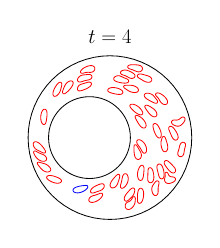
\begin{tikzpicture}[scale=0.3]

\begin{axis}[
  xmin = -21,
  xmax = 21,
  ymin = -21,
  ymax = 21,
  scale only axis,
  axis equal image,
  hide axis,
  title = {\Huge$t=4$}
  ]

% outer solid wall
\addplot [mark=none,black,line width=1.0] table{
2.0000e+01 -5.5171e-16
1.9904e+01 1.9603e+00
1.9616e+01 3.9018e+00
1.9139e+01 5.8057e+00
1.8478e+01 7.6537e+00
1.7638e+01 9.4279e+00
1.6629e+01 1.1111e+01
1.5460e+01 1.2688e+01
1.4142e+01 1.4142e+01
1.2688e+01 1.5460e+01
1.1111e+01 1.6629e+01
9.4279e+00 1.7638e+01
7.6537e+00 1.8478e+01
5.8057e+00 1.9139e+01
3.9018e+00 1.9616e+01
1.9603e+00 1.9904e+01
2.3281e-15 2.0000e+01
-1.9603e+00 1.9904e+01
-3.9018e+00 1.9616e+01
-5.8057e+00 1.9139e+01
-7.6537e+00 1.8478e+01
-9.4279e+00 1.7638e+01
-1.1111e+01 1.6629e+01
-1.2688e+01 1.5460e+01
-1.4142e+01 1.4142e+01
-1.5460e+01 1.2688e+01
-1.6629e+01 1.1111e+01
-1.7638e+01 9.4279e+00
-1.8478e+01 7.6537e+00
-1.9139e+01 5.8057e+00
-1.9616e+01 3.9018e+00
-1.9904e+01 1.9603e+00
-2.0000e+01 3.0010e-15
-1.9904e+01 -1.9603e+00
-1.9616e+01 -3.9018e+00
-1.9139e+01 -5.8057e+00
-1.8478e+01 -7.6537e+00
-1.7638e+01 -9.4279e+00
-1.6629e+01 -1.1111e+01
-1.5460e+01 -1.2688e+01
-1.4142e+01 -1.4142e+01
-1.2688e+01 -1.5460e+01
-1.1111e+01 -1.6629e+01
-9.4279e+00 -1.7638e+01
-7.6537e+00 -1.8478e+01
-5.8057e+00 -1.9139e+01
-3.9018e+00 -1.9616e+01
-1.9603e+00 -1.9904e+01
-4.7774e-15 -2.0000e+01
1.9603e+00 -1.9904e+01
3.9018e+00 -1.9616e+01
5.8057e+00 -1.9139e+01
7.6537e+00 -1.8478e+01
9.4279e+00 -1.7638e+01
1.1111e+01 -1.6629e+01
1.2688e+01 -1.5460e+01
1.4142e+01 -1.4142e+01
1.5460e+01 -1.2688e+01
1.6629e+01 -1.1111e+01
1.7638e+01 -9.4279e+00
1.8478e+01 -7.6537e+00
1.9139e+01 -5.8057e+00
1.9616e+01 -3.9018e+00
1.9904e+01 -1.9603e+00
2.0000e+01 -5.5171e-16
};

% inner solid wall
\addplot [mark=none,black,line width=1.0] table{
5.0000e+00 2.7586e-16
4.9518e+00 -9.8017e-01
4.8079e+00 -1.9509e+00
4.5694e+00 -2.9028e+00
4.2388e+00 -3.8268e+00
3.8192e+00 -4.7140e+00
3.3147e+00 -5.5557e+00
2.7301e+00 -6.3439e+00
2.0711e+00 -7.0711e+00
1.3439e+00 -7.7301e+00
5.5570e-01 -8.3147e+00
-2.8603e-01 -8.8192e+00
-1.1732e+00 -9.2388e+00
-2.0972e+00 -9.5694e+00
-3.0491e+00 -9.8079e+00
-4.0198e+00 -9.9518e+00
-5.0000e+00 -1.0000e+01
-5.9802e+00 -9.9518e+00
-6.9509e+00 -9.8079e+00
-7.9028e+00 -9.5694e+00
-8.8268e+00 -9.2388e+00
-9.7140e+00 -8.8192e+00
-1.0556e+01 -8.3147e+00
-1.1344e+01 -7.7301e+00
-1.2071e+01 -7.0711e+00
-1.2730e+01 -6.3439e+00
-1.3315e+01 -5.5557e+00
-1.3819e+01 -4.7140e+00
-1.4239e+01 -3.8268e+00
-1.4569e+01 -2.9028e+00
-1.4808e+01 -1.9509e+00
-1.4952e+01 -9.8017e-01
-1.5000e+01 -1.5005e-15
-1.4952e+01 9.8017e-01
-1.4808e+01 1.9509e+00
-1.4569e+01 2.9028e+00
-1.4239e+01 3.8268e+00
-1.3819e+01 4.7140e+00
-1.3315e+01 5.5557e+00
-1.2730e+01 6.3439e+00
-1.2071e+01 7.0711e+00
-1.1344e+01 7.7301e+00
-1.0556e+01 8.3147e+00
-9.7140e+00 8.8192e+00
-8.8268e+00 9.2388e+00
-7.9028e+00 9.5694e+00
-6.9509e+00 9.8079e+00
-5.9802e+00 9.9518e+00
-5.0000e+00 1.0000e+01
-4.0198e+00 9.9518e+00
-3.0491e+00 9.8079e+00
-2.0972e+00 9.5694e+00
-1.1732e+00 9.2388e+00
-2.8603e-01 8.8192e+00
5.5570e-01 8.3147e+00
1.3439e+00 7.7301e+00
2.0711e+00 7.0711e+00
2.7301e+00 6.3439e+00
3.3147e+00 5.5557e+00
3.8192e+00 4.7140e+00
4.2388e+00 3.8268e+00
4.5694e+00 2.9028e+00
4.8079e+00 1.9509e+00
4.9518e+00 9.8017e-01
5.0000e+00 2.7586e-16
};

% vesicle1
\addplot [mark=none,red,line width=1.0] table{
1.7483e+01 3.1245e+00
1.7528e+01 3.1618e+00
1.7589e+01 3.2154e+00
1.7663e+01 3.2869e+00
1.7747e+01 3.3741e+00
1.7835e+01 3.4730e+00
1.7925e+01 3.5813e+00
1.8013e+01 3.6970e+00
1.8099e+01 3.8196e+00
1.8179e+01 3.9486e+00
1.8251e+01 4.0847e+00
1.8310e+01 4.2284e+00
1.8349e+01 4.3796e+00
1.8360e+01 4.5360e+00
1.8334e+01 4.6909e+00
1.8264e+01 4.8320e+00
1.8153e+01 4.9428e+00
1.8010e+01 5.0090e+00
1.7854e+01 5.0257e+00
1.7699e+01 4.9980e+00
1.7555e+01 4.9370e+00
1.7422e+01 4.8547e+00
1.7298e+01 4.7613e+00
1.7178e+01 4.6646e+00
1.7058e+01 4.5713e+00
1.6935e+01 4.4865e+00
1.6808e+01 4.4147e+00
1.6680e+01 4.3586e+00
1.6553e+01 4.3192e+00
1.6435e+01 4.2950e+00
1.6332e+01 4.2827e+00
1.6251e+01 4.2779e+00
1.6193e+01 4.2767e+00
1.6134e+01 4.2771e+00
1.6053e+01 4.2795e+00
1.5950e+01 4.2844e+00
1.5829e+01 4.2899e+00
1.5697e+01 4.2906e+00
1.5557e+01 4.2789e+00
1.5415e+01 4.2454e+00
1.5281e+01 4.1811e+00
1.5167e+01 4.0816e+00
1.5088e+01 3.9500e+00
1.5056e+01 3.7988e+00
1.5073e+01 3.6439e+00
1.5131e+01 3.4986e+00
1.5221e+01 3.3697e+00
1.5333e+01 3.2584e+00
1.5459e+01 3.1626e+00
1.5593e+01 3.0795e+00
1.5733e+01 3.0068e+00
1.5877e+01 2.9433e+00
1.6025e+01 2.8891e+00
1.6175e+01 2.8452e+00
1.6326e+01 2.8130e+00
1.6479e+01 2.7945e+00
1.6631e+01 2.7911e+00
1.6780e+01 2.8039e+00
1.6923e+01 2.8324e+00
1.7057e+01 2.8748e+00
1.7178e+01 2.9273e+00
1.7284e+01 2.9852e+00
1.7371e+01 3.0411e+00
1.7437e+01 3.0885e+00
1.7483e+01 3.1245e+00
};

% vesicle2
\addplot [mark=none,red,line width=1.0] table{
-1.2400e+01 1.0878e+01
-1.2369e+01 1.0927e+01
-1.2328e+01 1.0997e+01
-1.2279e+01 1.1088e+01
-1.2227e+01 1.1197e+01
-1.2177e+01 1.1320e+01
-1.2128e+01 1.1452e+01
-1.2083e+01 1.1590e+01
-1.2040e+01 1.1733e+01
-1.1998e+01 1.1879e+01
-1.1957e+01 1.2028e+01
-1.1916e+01 1.2178e+01
-1.1877e+01 1.2329e+01
-1.1840e+01 1.2481e+01
-1.1806e+01 1.2635e+01
-1.1779e+01 1.2791e+01
-1.1764e+01 1.2948e+01
-1.1768e+01 1.3106e+01
-1.1802e+01 1.3260e+01
-1.1878e+01 1.3397e+01
-1.2001e+01 1.3493e+01
-1.2152e+01 1.3528e+01
-1.2305e+01 1.3504e+01
-1.2444e+01 1.3440e+01
-1.2569e+01 1.3354e+01
-1.2681e+01 1.3255e+01
-1.2783e+01 1.3151e+01
-1.2876e+01 1.3045e+01
-1.2959e+01 1.2942e+01
-1.3032e+01 1.2845e+01
-1.3092e+01 1.2761e+01
-1.3138e+01 1.2695e+01
-1.3171e+01 1.2646e+01
-1.3203e+01 1.2597e+01
-1.3246e+01 1.2529e+01
-1.3300e+01 1.2441e+01
-1.3362e+01 1.2337e+01
-1.3427e+01 1.2222e+01
-1.3494e+01 1.2098e+01
-1.3559e+01 1.1968e+01
-1.3624e+01 1.1833e+01
-1.3685e+01 1.1694e+01
-1.3743e+01 1.1551e+01
-1.3796e+01 1.1405e+01
-1.3843e+01 1.1256e+01
-1.3883e+01 1.1104e+01
-1.3913e+01 1.0950e+01
-1.3932e+01 1.0793e+01
-1.3933e+01 1.0635e+01
-1.3911e+01 1.0479e+01
-1.3858e+01 1.0331e+01
-1.3765e+01 1.0204e+01
-1.3636e+01 1.0117e+01
-1.3484e+01 1.0082e+01
-1.3330e+01 1.0097e+01
-1.3185e+01 1.0148e+01
-1.3051e+01 1.0220e+01
-1.2928e+01 1.0305e+01
-1.2816e+01 1.0398e+01
-1.2713e+01 1.0494e+01
-1.2622e+01 1.0590e+01
-1.2543e+01 1.0682e+01
-1.2480e+01 1.0763e+01
-1.2433e+01 1.0829e+01
-1.2400e+01 1.0878e+01
};

% vesicle3
\addplot [mark=none,red,line width=1.0] table{
-1.0948e+01 1.0794e+01
-1.0897e+01 1.0822e+01
-1.0829e+01 1.0865e+01
-1.0743e+01 1.0923e+01
-1.0646e+01 1.0996e+01
-1.0542e+01 1.1078e+01
-1.0435e+01 1.1169e+01
-1.0327e+01 1.1266e+01
-1.0218e+01 1.1368e+01
-1.0109e+01 1.1475e+01
-1.0002e+01 1.1585e+01
-9.8964e+00 1.1699e+01
-9.7928e+00 1.1816e+01
-9.6917e+00 1.1936e+01
-9.5935e+00 1.2060e+01
-9.4988e+00 1.2186e+01
-9.4081e+00 1.2315e+01
-9.3221e+00 1.2448e+01
-9.2414e+00 1.2584e+01
-9.1672e+00 1.2722e+01
-9.1011e+00 1.2865e+01
-9.0458e+00 1.3011e+01
-9.0054e+00 1.3161e+01
-8.9870e+00 1.3314e+01
-8.9994e+00 1.3465e+01
-9.0506e+00 1.3605e+01
-9.1398e+00 1.3719e+01
-9.2555e+00 1.3798e+01
-9.3805e+00 1.3841e+01
-9.5006e+00 1.3855e+01
-9.6039e+00 1.3852e+01
-9.6842e+00 1.3841e+01
-9.7415e+00 1.3830e+01
-9.7980e+00 1.3815e+01
-9.8753e+00 1.3791e+01
-9.9715e+00 1.3753e+01
-1.0081e+01 1.3701e+01
-1.0196e+01 1.3635e+01
-1.0312e+01 1.3557e+01
-1.0427e+01 1.3467e+01
-1.0537e+01 1.3366e+01
-1.0642e+01 1.3256e+01
-1.0741e+01 1.3138e+01
-1.0831e+01 1.3012e+01
-1.0915e+01 1.2880e+01
-1.0992e+01 1.2743e+01
-1.1062e+01 1.2602e+01
-1.1129e+01 1.2459e+01
-1.1192e+01 1.2314e+01
-1.1254e+01 1.2168e+01
-1.1314e+01 1.2022e+01
-1.1372e+01 1.1876e+01
-1.1429e+01 1.1730e+01
-1.1482e+01 1.1583e+01
-1.1530e+01 1.1435e+01
-1.1566e+01 1.1285e+01
-1.1584e+01 1.1134e+01
-1.1573e+01 1.0986e+01
-1.1519e+01 1.0851e+01
-1.1420e+01 1.0753e+01
-1.1296e+01 1.0709e+01
-1.1175e+01 1.0711e+01
-1.1076e+01 1.0737e+01
-1.1001e+01 1.0768e+01
-1.0948e+01 1.0794e+01
};

% vesicle4
\addplot [mark=none,red,line width=1.0] table{
7.6945e+00 1.4193e+01
7.7436e+00 1.4161e+01
7.8118e+00 1.4118e+01
7.8994e+00 1.4063e+01
8.0027e+00 1.3999e+01
8.1170e+00 1.3932e+01
8.2401e+00 1.3865e+01
8.3697e+00 1.3799e+01
8.5053e+00 1.3735e+01
8.6455e+00 1.3677e+01
8.7903e+00 1.3624e+01
8.9389e+00 1.3580e+01
9.0913e+00 1.3545e+01
9.2466e+00 1.3522e+01
9.4039e+00 1.3513e+01
9.5613e+00 1.3523e+01
9.7161e+00 1.3555e+01
9.8634e+00 1.3611e+01
9.9967e+00 1.3696e+01
1.0107e+01 1.3807e+01
1.0186e+01 1.3942e+01
1.0227e+01 1.4093e+01
1.0227e+01 1.4248e+01
1.0188e+01 1.4396e+01
1.0119e+01 1.4531e+01
1.0027e+01 1.4649e+01
9.9211e+00 1.4749e+01
9.8081e+00 1.4832e+01
9.6949e+00 1.4901e+01
9.5872e+00 1.4956e+01
9.4930e+00 1.4999e+01
9.4182e+00 1.5030e+01
9.3638e+00 1.5051e+01
9.3091e+00 1.5071e+01
9.2327e+00 1.5098e+01
9.1344e+00 1.5130e+01
9.0186e+00 1.5166e+01
8.8915e+00 1.5203e+01
8.7563e+00 1.5241e+01
8.6160e+00 1.5280e+01
8.4720e+00 1.5320e+01
8.3257e+00 1.5362e+01
8.1775e+00 1.5403e+01
8.0279e+00 1.5445e+01
7.8763e+00 1.5483e+01
7.7228e+00 1.5516e+01
7.5668e+00 1.5539e+01
7.4094e+00 1.5548e+01
7.2516e+00 1.5539e+01
7.0971e+00 1.5507e+01
6.9513e+00 1.5447e+01
6.8245e+00 1.5355e+01
6.7324e+00 1.5228e+01
6.6944e+00 1.5078e+01
6.7193e+00 1.4926e+01
6.7968e+00 1.4793e+01
6.9051e+00 1.4687e+01
7.0269e+00 1.4601e+01
7.1512e+00 1.4525e+01
7.2725e+00 1.4454e+01
7.3863e+00 1.4386e+01
7.4896e+00 1.4323e+01
7.5771e+00 1.4268e+01
7.6454e+00 1.4224e+01
7.6945e+00 1.4193e+01
};

% vesicle5
\addplot [mark=none,red,line width=1.0] table{
-3.4049e+00 -1.5604e+01
-3.3514e+00 -1.5581e+01
-3.2784e+00 -1.5546e+01
-3.1858e+00 -1.5500e+01
-3.0796e+00 -1.5441e+01
-2.9653e+00 -1.5375e+01
-2.8473e+00 -1.5298e+01
-2.7278e+00 -1.5215e+01
-2.6091e+00 -1.5124e+01
-2.4920e+00 -1.5028e+01
-2.3783e+00 -1.4923e+01
-2.2681e+00 -1.4814e+01
-2.1633e+00 -1.4698e+01
-2.0642e+00 -1.4577e+01
-1.9733e+00 -1.4447e+01
-1.8927e+00 -1.4312e+01
-1.8287e+00 -1.4167e+01
-1.7910e+00 -1.4015e+01
-1.7968e+00 -1.3857e+01
-1.8627e+00 -1.3716e+01
-1.9860e+00 -1.3621e+01
-2.1376e+00 -1.3588e+01
-2.2920e+00 -1.3602e+01
-2.4401e+00 -1.3644e+01
-2.5828e+00 -1.3696e+01
-2.7211e+00 -1.3753e+01
-2.8560e+00 -1.3808e+01
-2.9862e+00 -1.3861e+01
-3.1100e+00 -1.3907e+01
-3.2236e+00 -1.3949e+01
-3.3217e+00 -1.3982e+01
-3.3984e+00 -1.4008e+01
-3.4544e+00 -1.4025e+01
-3.5100e+00 -1.4042e+01
-3.5879e+00 -1.4065e+01
-3.6874e+00 -1.4093e+01
-3.8047e+00 -1.4123e+01
-3.9326e+00 -1.4157e+01
-4.0685e+00 -1.4193e+01
-4.2076e+00 -1.4236e+01
-4.3483e+00 -1.4286e+01
-4.4863e+00 -1.4350e+01
-4.6197e+00 -1.4427e+01
-4.7446e+00 -1.4519e+01
-4.8602e+00 -1.4624e+01
-4.9626e+00 -1.4743e+01
-5.0498e+00 -1.4874e+01
-5.1154e+00 -1.5018e+01
-5.1531e+00 -1.5170e+01
-5.1527e+00 -1.5329e+01
-5.1084e+00 -1.5479e+01
-5.0203e+00 -1.5609e+01
-4.8996e+00 -1.5708e+01
-4.7583e+00 -1.5776e+01
-4.6085e+00 -1.5814e+01
-4.4552e+00 -1.5832e+01
-4.3036e+00 -1.5831e+01
-4.1544e+00 -1.5819e+01
-4.0109e+00 -1.5796e+01
-3.8735e+00 -1.5766e+01
-3.7461e+00 -1.5730e+01
-3.6307e+00 -1.5693e+01
-3.5338e+00 -1.5657e+01
-3.4584e+00 -1.5627e+01
-3.4049e+00 -1.5604e+01
};

% vesicle6
\addplot [mark=none,red,line width=1.0] table{
1.3457e+01 6.9816e-02
1.3420e+01 1.1522e-01
1.3363e+01 1.7185e-01
1.3276e+01 2.2869e-01
1.3161e+01 2.6433e-01
1.3030e+01 2.5392e-01
1.2908e+01 1.8734e-01
1.2815e+01 7.5786e-02
1.2752e+01 -5.9548e-02
1.2707e+01 -2.0478e-01
1.2667e+01 -3.5335e-01
1.2626e+01 -5.0310e-01
1.2583e+01 -6.5334e-01
1.2542e+01 -8.0502e-01
1.2508e+01 -9.5874e-01
1.2483e+01 -1.1148e+00
1.2471e+01 -1.2722e+00
1.2469e+01 -1.4302e+00
1.2477e+01 -1.5879e+00
1.2493e+01 -1.7447e+00
1.2515e+01 -1.9001e+00
1.2542e+01 -2.0541e+00
1.2573e+01 -2.2061e+00
1.2609e+01 -2.3559e+00
1.2649e+01 -2.5026e+00
1.2693e+01 -2.6453e+00
1.2743e+01 -2.7823e+00
1.2798e+01 -2.9116e+00
1.2858e+01 -3.0294e+00
1.2922e+01 -3.1320e+00
1.2985e+01 -3.2138e+00
1.3041e+01 -3.2726e+00
1.3085e+01 -3.3115e+00
1.3131e+01 -3.3468e+00
1.3200e+01 -3.3887e+00
1.3296e+01 -3.4277e+00
1.3415e+01 -3.4497e+00
1.3547e+01 -3.4409e+00
1.3679e+01 -3.3956e+00
1.3800e+01 -3.3149e+00
1.3902e+01 -3.2061e+00
1.3982e+01 -3.0772e+00
1.4042e+01 -2.9356e+00
1.4084e+01 -2.7861e+00
1.4111e+01 -2.6322e+00
1.4124e+01 -2.4757e+00
1.4126e+01 -2.3182e+00
1.4118e+01 -2.1605e+00
1.4102e+01 -2.0034e+00
1.4078e+01 -1.8472e+00
1.4047e+01 -1.6924e+00
1.4011e+01 -1.5390e+00
1.3970e+01 -1.3873e+00
1.3926e+01 -1.2372e+00
1.3881e+01 -1.0887e+00
1.3835e+01 -9.4179e-01
1.3789e+01 -7.9681e-01
1.3745e+01 -6.5404e-01
1.3702e+01 -5.1489e-01
1.3660e+01 -3.8088e-01
1.3617e+01 -2.5546e-01
1.3574e+01 -1.4256e-01
1.3530e+01 -4.8810e-02
1.3490e+01 2.1509e-02
1.3457e+01 6.9816e-02
};

% vesicle7
\addplot [mark=none,red,line width=1.0] table{
7.5534e+00 1.6209e+01
7.6025e+00 1.6240e+01
7.6670e+00 1.6289e+01
7.7423e+00 1.6360e+01
7.8183e+00 1.6454e+01
7.8838e+00 1.6569e+01
7.9301e+00 1.6702e+01
7.9501e+00 1.6846e+01
7.9396e+00 1.6994e+01
7.8968e+00 1.7140e+01
7.8237e+00 1.7275e+01
7.7241e+00 1.7394e+01
7.6039e+00 1.7494e+01
7.4686e+00 1.7573e+01
7.3237e+00 1.7635e+01
7.1726e+00 1.7680e+01
7.0183e+00 1.7714e+01
6.8621e+00 1.7739e+01
6.7054e+00 1.7757e+01
6.5483e+00 1.7770e+01
6.3916e+00 1.7780e+01
6.2354e+00 1.7787e+01
6.0803e+00 1.7793e+01
5.9263e+00 1.7797e+01
5.7744e+00 1.7799e+01
5.6249e+00 1.7799e+01
5.4793e+00 1.7797e+01
5.3388e+00 1.7793e+01
5.2066e+00 1.7787e+01
5.0858e+00 1.7777e+01
4.9830e+00 1.7766e+01
4.9030e+00 1.7754e+01
4.8457e+00 1.7743e+01
4.7888e+00 1.7730e+01
4.7112e+00 1.7707e+01
4.6153e+00 1.7668e+01
4.5118e+00 1.7606e+01
4.4182e+00 1.7512e+01
4.3551e+00 1.7388e+01
4.3430e+00 1.7244e+01
4.3883e+00 1.7102e+01
4.4815e+00 1.6983e+01
4.6050e+00 1.6892e+01
4.7448e+00 1.6824e+01
4.8919e+00 1.6771e+01
5.0423e+00 1.6726e+01
5.1935e+00 1.6682e+01
5.3445e+00 1.6636e+01
5.4942e+00 1.6585e+01
5.6424e+00 1.6530e+01
5.7885e+00 1.6471e+01
5.9329e+00 1.6407e+01
6.0758e+00 1.6342e+01
6.2182e+00 1.6278e+01
6.3609e+00 1.6217e+01
6.5051e+00 1.6162e+01
6.6504e+00 1.6118e+01
6.7966e+00 1.6087e+01
6.9413e+00 1.6071e+01
7.0817e+00 1.6071e+01
7.2132e+00 1.6086e+01
7.3312e+00 1.6113e+01
7.4288e+00 1.6147e+01
7.5023e+00 1.6181e+01
7.5534e+00 1.6209e+01
};

% vesicle8
\addplot [mark=none,red,line width=1.0] table{
8.8510e+00 7.9227e+00
8.7937e+00 7.9117e+00
8.7179e+00 7.8838e+00
8.6335e+00 7.8246e+00
8.5639e+00 7.7264e+00
8.5339e+00 7.5982e+00
8.5495e+00 7.4592e+00
8.6007e+00 7.3230e+00
8.6725e+00 7.1921e+00
8.7547e+00 7.0641e+00
8.8410e+00 6.9367e+00
8.9290e+00 6.8087e+00
9.0174e+00 6.6798e+00
9.1065e+00 6.5504e+00
9.1964e+00 6.4211e+00
9.2882e+00 6.2926e+00
9.3821e+00 6.1655e+00
9.4792e+00 6.0408e+00
9.5795e+00 5.9189e+00
9.6836e+00 5.8006e+00
9.7916e+00 5.6866e+00
9.9036e+00 5.5775e+00
1.0020e+01 5.4743e+00
1.0140e+01 5.3783e+00
1.0264e+01 5.2908e+00
1.0393e+01 5.2143e+00
1.0524e+01 5.1512e+00
1.0656e+01 5.1048e+00
1.0786e+01 5.0778e+00
1.0907e+01 5.0711e+00
1.1009e+01 5.0814e+00
1.1088e+01 5.1010e+00
1.1142e+01 5.1216e+00
1.1195e+01 5.1479e+00
1.1262e+01 5.1931e+00
1.1336e+01 5.2647e+00
1.1404e+01 5.3646e+00
1.1453e+01 5.4875e+00
1.1476e+01 5.6257e+00
1.1473e+01 5.7712e+00
1.1448e+01 5.9182e+00
1.1402e+01 6.0632e+00
1.1341e+01 6.2044e+00
1.1266e+01 6.3405e+00
1.1181e+01 6.4714e+00
1.1086e+01 6.5963e+00
1.0983e+01 6.7155e+00
1.0872e+01 6.8286e+00
1.0757e+01 6.9359e+00
1.0636e+01 7.0375e+00
1.0511e+01 7.1341e+00
1.0383e+01 7.2258e+00
1.0252e+01 7.3135e+00
1.0120e+01 7.3975e+00
9.9877e+00 7.4782e+00
9.8546e+00 7.5556e+00
9.7219e+00 7.6297e+00
9.5899e+00 7.6998e+00
9.4596e+00 7.7648e+00
9.3315e+00 7.8225e+00
9.2080e+00 7.8702e+00
9.0918e+00 7.9042e+00
8.9900e+00 7.9224e+00
8.9092e+00 7.9266e+00
8.8510e+00 7.9227e+00
};

% vesicle9
\addplot [mark=none,red,line width=1.0] table{
7.5018e+00 -6.2498e-01
7.4482e+00 -6.0180e-01
7.3724e+00 -5.7340e-01
7.2731e+00 -5.4460e-01
7.1539e+00 -5.2384e-01
7.0216e+00 -5.2185e-01
6.8843e+00 -5.4963e-01
6.7557e+00 -6.1688e-01
6.6528e+00 -7.2427e-01
6.5882e+00 -8.6131e-01
6.5624e+00 -1.0127e+00
6.5696e+00 -1.1677e+00
6.6031e+00 -1.3202e+00
6.6587e+00 -1.4670e+00
6.7317e+00 -1.6065e+00
6.8167e+00 -1.7396e+00
6.9082e+00 -1.8683e+00
7.0028e+00 -1.9950e+00
7.0977e+00 -2.1212e+00
7.1914e+00 -2.2479e+00
7.2828e+00 -2.3755e+00
7.3710e+00 -2.5047e+00
7.4553e+00 -2.6351e+00
7.5356e+00 -2.7665e+00
7.6116e+00 -2.8981e+00
7.6839e+00 -3.0289e+00
7.7530e+00 -3.1571e+00
7.8203e+00 -3.2804e+00
7.8865e+00 -3.3951e+00
7.9519e+00 -3.4970e+00
8.0137e+00 -3.5800e+00
8.0672e+00 -3.6407e+00
8.1090e+00 -3.6813e+00
8.1540e+00 -3.7185e+00
8.2216e+00 -3.7628e+00
8.3166e+00 -3.8032e+00
8.4360e+00 -3.8209e+00
8.5658e+00 -3.7980e+00
8.6877e+00 -3.7295e+00
8.7871e+00 -3.6236e+00
8.8608e+00 -3.4939e+00
8.9110e+00 -3.3506e+00
8.9418e+00 -3.1998e+00
8.9561e+00 -3.0452e+00
8.9564e+00 -2.8890e+00
8.9441e+00 -2.7324e+00
8.9208e+00 -2.5766e+00
8.8871e+00 -2.4223e+00
8.8442e+00 -2.2703e+00
8.7925e+00 -2.1209e+00
8.7328e+00 -1.9748e+00
8.6655e+00 -1.8324e+00
8.5912e+00 -1.6941e+00
8.5101e+00 -1.5603e+00
8.4231e+00 -1.4317e+00
8.3304e+00 -1.3088e+00
8.2328e+00 -1.1923e+00
8.1309e+00 -1.0830e+00
8.0261e+00 -9.8192e-01
7.9196e+00 -8.9020e-01
7.8146e+00 -8.0956e-01
7.7144e+00 -7.4151e-01
7.6258e+00 -6.8825e-01
7.5543e+00 -6.5024e-01
7.5018e+00 -6.2498e-01
};

% vesicle10
\addplot [mark=none,red,line width=1.0] table{
1.3212e+01 -9.1043e+00
1.3212e+01 -9.0459e+00
1.3213e+01 -8.9649e+00
1.3213e+01 -8.8615e+00
1.3211e+01 -8.7404e+00
1.3205e+01 -8.6081e+00
1.3195e+01 -8.4680e+00
1.3178e+01 -8.3233e+00
1.3155e+01 -8.1757e+00
1.3125e+01 -8.0266e+00
1.3090e+01 -7.8767e+00
1.3049e+01 -7.7269e+00
1.3004e+01 -7.5773e+00
1.2953e+01 -7.4287e+00
1.2898e+01 -7.2812e+00
1.2836e+01 -7.1361e+00
1.2766e+01 -6.9944e+00
1.2685e+01 -6.8588e+00
1.2590e+01 -6.7328e+00
1.2477e+01 -6.6224e+00
1.2347e+01 -6.5351e+00
1.2201e+01 -6.4797e+00
1.2047e+01 -6.4633e+00
1.1896e+01 -6.4900e+00
1.1761e+01 -6.5573e+00
1.1650e+01 -6.6577e+00
1.1570e+01 -6.7789e+00
1.1519e+01 -6.9095e+00
1.1492e+01 -7.0390e+00
1.1482e+01 -7.1597e+00
1.1483e+01 -7.2631e+00
1.1488e+01 -7.3438e+00
1.1494e+01 -7.4019e+00
1.1501e+01 -7.4599e+00
1.1514e+01 -7.5399e+00
1.1533e+01 -7.6415e+00
1.1558e+01 -7.7600e+00
1.1588e+01 -7.8890e+00
1.1622e+01 -8.0254e+00
1.1657e+01 -8.1665e+00
1.1694e+01 -8.3114e+00
1.1731e+01 -8.4587e+00
1.1769e+01 -8.6082e+00
1.1806e+01 -8.7589e+00
1.1843e+01 -8.9108e+00
1.1882e+01 -9.0628e+00
1.1924e+01 -9.2148e+00
1.1971e+01 -9.3655e+00
1.2026e+01 -9.5137e+00
1.2092e+01 -9.6571e+00
1.2174e+01 -9.7920e+00
1.2275e+01 -9.9124e+00
1.2398e+01 -1.0010e+01
1.2541e+01 -1.0072e+01
1.2695e+01 -1.0089e+01
1.2844e+01 -1.0056e+01
1.2973e+01 -9.9763e+00
1.3070e+01 -9.8636e+00
1.3135e+01 -9.7334e+00
1.3173e+01 -9.5983e+00
1.3194e+01 -9.4676e+00
1.3204e+01 -9.3469e+00
1.3208e+01 -9.2435e+00
1.3211e+01 -9.1626e+00
1.3212e+01 -9.1043e+00
};

% vesicle11
\addplot [mark=none,red,line width=1.0] table{
-1.7871e+01 -1.0657e+00
-1.7928e+01 -1.0494e+00
-1.8006e+01 -1.0316e+00
-1.8109e+01 -1.0182e+00
-1.8230e+01 -1.0186e+00
-1.8360e+01 -1.0434e+00
-1.8487e+01 -1.1014e+00
-1.8597e+01 -1.1963e+00
-1.8677e+01 -1.3221e+00
-1.8722e+01 -1.4671e+00
-1.8735e+01 -1.6202e+00
-1.8723e+01 -1.7749e+00
-1.8691e+01 -1.9279e+00
-1.8643e+01 -2.0774e+00
-1.8581e+01 -2.2222e+00
-1.8506e+01 -2.3612e+00
-1.8420e+01 -2.4932e+00
-1.8321e+01 -2.6165e+00
-1.8210e+01 -2.7290e+00
-1.8089e+01 -2.8296e+00
-1.7959e+01 -2.9184e+00
-1.7825e+01 -2.9977e+00
-1.7687e+01 -3.0705e+00
-1.7550e+01 -3.1393e+00
-1.7413e+01 -3.2057e+00
-1.7278e+01 -3.2708e+00
-1.7148e+01 -3.3347e+00
-1.7022e+01 -3.3971e+00
-1.6903e+01 -3.4566e+00
-1.6795e+01 -3.5113e+00
-1.6703e+01 -3.5581e+00
-1.6631e+01 -3.5942e+00
-1.6578e+01 -3.6199e+00
-1.6525e+01 -3.6450e+00
-1.6452e+01 -3.6786e+00
-1.6356e+01 -3.7179e+00
-1.6241e+01 -3.7557e+00
-1.6111e+01 -3.7794e+00
-1.5971e+01 -3.7710e+00
-1.5841e+01 -3.7080e+00
-1.5757e+01 -3.5866e+00
-1.5740e+01 -3.4366e+00
-1.5773e+01 -3.2866e+00
-1.5832e+01 -3.1429e+00
-1.5904e+01 -3.0046e+00
-1.5985e+01 -2.8697e+00
-1.6071e+01 -2.7376e+00
-1.6160e+01 -2.6076e+00
-1.6253e+01 -2.4797e+00
-1.6348e+01 -2.3536e+00
-1.6446e+01 -2.2298e+00
-1.6546e+01 -2.1081e+00
-1.6649e+01 -1.9892e+00
-1.6754e+01 -1.8732e+00
-1.6861e+01 -1.7611e+00
-1.6971e+01 -1.6531e+00
-1.7083e+01 -1.5505e+00
-1.7197e+01 -1.4540e+00
-1.7312e+01 -1.3650e+00
-1.7428e+01 -1.2847e+00
-1.7540e+01 -1.2151e+00
-1.7647e+01 -1.1576e+00
-1.7741e+01 -1.1142e+00
-1.7816e+01 -1.0844e+00
-1.7871e+01 -1.0657e+00
};

% vesicle12
\addplot [mark=none,red,line width=1.0] table{
1.2765e+01 1.0479e+01
1.2716e+01 1.0511e+01
1.2648e+01 1.0555e+01
1.2560e+01 1.0609e+01
1.2455e+01 1.0668e+01
1.2337e+01 1.0729e+01
1.2209e+01 1.0788e+01
1.2074e+01 1.0841e+01
1.1931e+01 1.0886e+01
1.1782e+01 1.0916e+01
1.1629e+01 1.0926e+01
1.1475e+01 1.0906e+01
1.1332e+01 1.0844e+01
1.1220e+01 1.0736e+01
1.1162e+01 1.0591e+01
1.1169e+01 1.0435e+01
1.1232e+01 1.0290e+01
1.1326e+01 1.0164e+01
1.1435e+01 1.0050e+01
1.1548e+01 9.9391e+00
1.1657e+01 9.8265e+00
1.1760e+01 9.7084e+00
1.1853e+01 9.5848e+00
1.1938e+01 9.4563e+00
1.2015e+01 9.3253e+00
1.2087e+01 9.1940e+00
1.2156e+01 9.0658e+00
1.2225e+01 8.9436e+00
1.2296e+01 8.8315e+00
1.2365e+01 8.7326e+00
1.2430e+01 8.6515e+00
1.2483e+01 8.5904e+00
1.2523e+01 8.5478e+00
1.2564e+01 8.5063e+00
1.2623e+01 8.4510e+00
1.2701e+01 8.3838e+00
1.2798e+01 8.3107e+00
1.2909e+01 8.2386e+00
1.3033e+01 8.1725e+00
1.3168e+01 8.1180e+00
1.3313e+01 8.0810e+00
1.3464e+01 8.0682e+00
1.3616e+01 8.0863e+00
1.3761e+01 8.1402e+00
1.3889e+01 8.2306e+00
1.3987e+01 8.3522e+00
1.4051e+01 8.4957e+00
1.4080e+01 8.6506e+00
1.4077e+01 8.8084e+00
1.4048e+01 8.9636e+00
1.3998e+01 9.1134e+00
1.3933e+01 9.2567e+00
1.3856e+01 9.3935e+00
1.3770e+01 9.5238e+00
1.3676e+01 9.6480e+00
1.3578e+01 9.7662e+00
1.3475e+01 9.8785e+00
1.3370e+01 9.9848e+00
1.3264e+01 1.0085e+01
1.3159e+01 1.0178e+01
1.3057e+01 1.0262e+01
1.2962e+01 1.0337e+01
1.2879e+01 1.0399e+01
1.2813e+01 1.0446e+01
1.2765e+01 1.0479e+01
};

% vesicle13
\addplot [mark=none,red,line width=1.0] table{
3.4573e+00 1.4618e+01
3.4039e+00 1.4642e+01
3.3301e+00 1.4675e+01
3.2364e+00 1.4719e+01
3.1270e+00 1.4771e+01
3.0080e+00 1.4829e+01
2.8814e+00 1.4890e+01
2.7492e+00 1.4951e+01
2.6110e+00 1.5008e+01
2.4672e+00 1.5057e+01
2.3176e+00 1.5094e+01
2.1639e+00 1.5115e+01
2.0076e+00 1.5119e+01
1.8512e+00 1.5106e+01
1.6965e+00 1.5076e+01
1.5456e+00 1.5030e+01
1.4004e+00 1.4968e+01
1.2643e+00 1.4888e+01
1.1415e+00 1.4789e+01
1.0394e+00 1.4669e+01
9.6794e-01 1.4530e+01
9.3892e-01 1.4377e+01
9.5887e-01 1.4223e+01
1.0243e+00 1.4085e+01
1.1223e+00 1.3969e+01
1.2393e+00 1.3876e+01
1.3645e+00 1.3802e+01
1.4914e+00 1.3742e+01
1.6141e+00 1.3692e+01
1.7282e+00 1.3651e+01
1.8266e+00 1.3619e+01
1.9040e+00 1.3596e+01
1.9601e+00 1.3579e+01
2.0163e+00 1.3564e+01
2.0944e+00 1.3542e+01
2.1945e+00 1.3517e+01
2.3122e+00 1.3488e+01
2.4412e+00 1.3458e+01
2.5787e+00 1.3429e+01
2.7216e+00 1.3401e+01
2.8689e+00 1.3376e+01
3.0193e+00 1.3354e+01
3.1723e+00 1.3336e+01
3.3270e+00 1.3324e+01
3.4833e+00 1.3317e+01
3.6403e+00 1.3317e+01
3.7978e+00 1.3323e+01
3.9549e+00 1.3337e+01
4.1104e+00 1.3365e+01
4.2609e+00 1.3413e+01
4.3992e+00 1.3488e+01
4.5113e+00 1.3598e+01
4.5784e+00 1.3739e+01
4.5846e+00 1.3894e+01
4.5307e+00 1.4039e+01
4.4329e+00 1.4157e+01
4.3113e+00 1.4248e+01
4.1798e+00 1.4319e+01
4.0467e+00 1.4378e+01
3.9165e+00 1.4430e+01
3.7934e+00 1.4479e+01
3.6810e+00 1.4524e+01
3.5853e+00 1.4564e+01
3.5108e+00 1.4595e+01
3.4573e+00 1.4618e+01
};

% vesicle14
\addplot [mark=none,red,line width=1.0] table{
-1.6980e+01 -3.8985e+00
-1.7034e+01 -3.8766e+00
-1.7108e+01 -3.8449e+00
-1.7203e+01 -3.8033e+00
-1.7313e+01 -3.7518e+00
-1.7431e+01 -3.6929e+00
-1.7555e+01 -3.6268e+00
-1.7682e+01 -3.5559e+00
-1.7812e+01 -3.4811e+00
-1.7944e+01 -3.4066e+00
-1.8082e+01 -3.3376e+00
-1.8228e+01 -3.2864e+00
-1.8383e+01 -3.2725e+00
-1.8530e+01 -3.3245e+00
-1.8626e+01 -3.4462e+00
-1.8651e+01 -3.6012e+00
-1.8625e+01 -3.7566e+00
-1.8574e+01 -3.9063e+00
-1.8511e+01 -4.0506e+00
-1.8439e+01 -4.1913e+00
-1.8362e+01 -4.3280e+00
-1.8281e+01 -4.4616e+00
-1.8196e+01 -4.5911e+00
-1.8106e+01 -4.7168e+00
-1.8014e+01 -4.8370e+00
-1.7918e+01 -4.9519e+00
-1.7819e+01 -5.0591e+00
-1.7720e+01 -5.1583e+00
-1.7621e+01 -5.2465e+00
-1.7527e+01 -5.3230e+00
-1.7444e+01 -5.3840e+00
-1.7377e+01 -5.4293e+00
-1.7327e+01 -5.4603e+00
-1.7277e+01 -5.4903e+00
-1.7206e+01 -5.5294e+00
-1.7114e+01 -5.5763e+00
-1.7003e+01 -5.6257e+00
-1.6880e+01 -5.6739e+00
-1.6746e+01 -5.7173e+00
-1.6606e+01 -5.7536e+00
-1.6458e+01 -5.7799e+00
-1.6307e+01 -5.7938e+00
-1.6153e+01 -5.7913e+00
-1.6000e+01 -5.7692e+00
-1.5851e+01 -5.7224e+00
-1.5713e+01 -5.6475e+00
-1.5597e+01 -5.5416e+00
-1.5514e+01 -5.4078e+00
-1.5474e+01 -5.2554e+00
-1.5477e+01 -5.0980e+00
-1.5516e+01 -4.9451e+00
-1.5582e+01 -4.8021e+00
-1.5666e+01 -4.6697e+00
-1.5765e+01 -4.5489e+00
-1.5875e+01 -4.4395e+00
-1.5995e+01 -4.3428e+00
-1.6122e+01 -4.2592e+00
-1.6253e+01 -4.1885e+00
-1.6386e+01 -4.1282e+00
-1.6516e+01 -4.0759e+00
-1.6640e+01 -4.0287e+00
-1.6754e+01 -3.9864e+00
-1.6850e+01 -3.9495e+00
-1.6926e+01 -3.9203e+00
-1.6980e+01 -3.8985e+00
};

% vesicle15
\addplot [mark=none,red,line width=1.0] table{
-5.2753e+00 1.3544e+01
-5.3327e+00 1.3533e+01
-5.4118e+00 1.3516e+01
-5.5122e+00 1.3491e+01
-5.6290e+00 1.3458e+01
-5.7560e+00 1.3421e+01
-5.8905e+00 1.3380e+01
-6.0296e+00 1.3337e+01
-6.1727e+00 1.3294e+01
-6.3184e+00 1.3251e+01
-6.4664e+00 1.3208e+01
-6.6157e+00 1.3166e+01
-6.7661e+00 1.3122e+01
-6.9162e+00 1.3077e+01
-7.0651e+00 1.3025e+01
-7.2103e+00 1.2963e+01
-7.3494e+00 1.2888e+01
-7.4783e+00 1.2797e+01
-7.5943e+00 1.2690e+01
-7.6948e+00 1.2569e+01
-7.7791e+00 1.2436e+01
-7.8464e+00 1.2295e+01
-7.8962e+00 1.2148e+01
-7.9251e+00 1.1997e+01
-7.9282e+00 1.1846e+01
-7.8968e+00 1.1700e+01
-7.8256e+00 1.1574e+01
-7.7194e+00 1.1483e+01
-7.5973e+00 1.1433e+01
-7.4776e+00 1.1415e+01
-7.3742e+00 1.1416e+01
-7.2935e+00 1.1423e+01
-7.2357e+00 1.1432e+01
-7.1782e+00 1.1442e+01
-7.0989e+00 1.1459e+01
-6.9985e+00 1.1483e+01
-6.8816e+00 1.1515e+01
-6.7549e+00 1.1554e+01
-6.6214e+00 1.1597e+01
-6.4839e+00 1.1645e+01
-6.3435e+00 1.1697e+01
-6.2017e+00 1.1751e+01
-6.0589e+00 1.1809e+01
-5.9161e+00 1.1870e+01
-5.7736e+00 1.1934e+01
-5.6321e+00 1.2003e+01
-5.4921e+00 1.2075e+01
-5.3545e+00 1.2152e+01
-5.2197e+00 1.2235e+01
-5.0892e+00 1.2324e+01
-4.9639e+00 1.2420e+01
-4.8461e+00 1.2524e+01
-4.7379e+00 1.2638e+01
-4.6439e+00 1.2763e+01
-4.5701e+00 1.2899e+01
-4.5264e+00 1.3047e+01
-4.5243e+00 1.3198e+01
-4.5723e+00 1.3339e+01
-4.6653e+00 1.3450e+01
-4.7857e+00 1.3521e+01
-4.9130e+00 1.3556e+01
-5.0337e+00 1.3566e+01
-5.1371e+00 1.3562e+01
-5.2176e+00 1.3553e+01
-5.2753e+00 1.3544e+01
};

% vesicle16
\addplot [mark=none,red,line width=1.0] table{
1.0593e+01 8.5911e+00
1.0645e+01 8.5662e+00
1.0719e+01 8.5327e+00
1.0814e+01 8.4921e+00
1.0928e+01 8.4497e+00
1.1055e+01 8.4132e+00
1.1194e+01 8.3921e+00
1.1339e+01 8.3997e+00
1.1479e+01 8.4501e+00
1.1591e+01 8.5506e+00
1.1653e+01 8.6904e+00
1.1654e+01 8.8448e+00
1.1607e+01 8.9935e+00
1.1530e+01 9.1299e+00
1.1437e+01 9.2571e+00
1.1338e+01 9.3800e+00
1.1238e+01 9.5022e+00
1.1139e+01 9.6258e+00
1.1043e+01 9.7512e+00
1.0949e+01 9.8774e+00
1.0854e+01 1.0003e+01
1.0755e+01 1.0124e+01
1.0651e+01 1.0238e+01
1.0539e+01 1.0344e+01
1.0420e+01 1.0439e+01
1.0296e+01 1.0522e+01
1.0169e+01 1.0594e+01
1.0043e+01 1.0655e+01
9.9201e+00 1.0705e+01
9.8056e+00 1.0745e+01
9.7065e+00 1.0774e+01
9.6280e+00 1.0794e+01
9.5710e+00 1.0807e+01
9.5137e+00 1.0818e+01
9.4338e+00 1.0831e+01
9.3311e+00 1.0844e+01
9.2103e+00 1.0852e+01
9.0779e+00 1.0851e+01
8.9382e+00 1.0836e+01
8.7964e+00 1.0804e+01
8.6589e+00 1.0746e+01
8.5363e+00 1.0657e+01
8.4438e+00 1.0534e+01
8.3965e+00 1.0387e+01
8.3994e+00 1.0232e+01
8.4457e+00 1.0082e+01
8.5226e+00 9.9446e+00
8.6192e+00 9.8198e+00
8.7282e+00 9.7055e+00
8.8454e+00 9.5995e+00
8.9684e+00 9.5007e+00
9.0957e+00 9.4077e+00
9.2260e+00 9.3202e+00
9.3587e+00 9.2374e+00
9.4927e+00 9.1589e+00
9.6272e+00 9.0839e+00
9.7611e+00 9.0121e+00
9.8936e+00 8.9428e+00
1.0023e+01 8.8763e+00
1.0148e+01 8.8124e+00
1.0266e+01 8.7526e+00
1.0375e+01 8.6981e+00
1.0467e+01 8.6520e+00
1.0540e+01 8.6164e+00
1.0593e+01 8.5911e+00
};

% vesicle17
\addplot [mark=none,red,line width=1.0] table{
-1.5813e+01 6.9106e+00
-1.5869e+01 6.9282e+00
-1.5949e+01 6.9397e+00
-1.6052e+01 6.9316e+00
-1.6166e+01 6.8933e+00
-1.6278e+01 6.8235e+00
-1.6382e+01 6.7285e+00
-1.6473e+01 6.6150e+00
-1.6553e+01 6.4890e+00
-1.6622e+01 6.3537e+00
-1.6683e+01 6.2121e+00
-1.6734e+01 6.0656e+00
-1.6778e+01 5.9156e+00
-1.6815e+01 5.7630e+00
-1.6845e+01 5.6084e+00
-1.6869e+01 5.4523e+00
-1.6888e+01 5.2954e+00
-1.6900e+01 5.1378e+00
-1.6906e+01 4.9801e+00
-1.6906e+01 4.8225e+00
-1.6901e+01 4.6655e+00
-1.6888e+01 4.5097e+00
-1.6870e+01 4.3555e+00
-1.6844e+01 4.2038e+00
-1.6810e+01 4.0555e+00
-1.6769e+01 3.9118e+00
-1.6720e+01 3.7748e+00
-1.6662e+01 3.6468e+00
-1.6597e+01 3.5314e+00
-1.6527e+01 3.4327e+00
-1.6457e+01 3.3561e+00
-1.6396e+01 3.3033e+00
-1.6348e+01 3.2703e+00
-1.6296e+01 3.2427e+00
-1.6220e+01 3.2153e+00
-1.6118e+01 3.2029e+00
-1.5999e+01 3.2247e+00
-1.5885e+01 3.2908e+00
-1.5791e+01 3.3939e+00
-1.5718e+01 3.5201e+00
-1.5663e+01 3.6587e+00
-1.5618e+01 3.8042e+00
-1.5582e+01 3.9536e+00
-1.5550e+01 4.1057e+00
-1.5522e+01 4.2594e+00
-1.5496e+01 4.4144e+00
-1.5473e+01 4.5702e+00
-1.5451e+01 4.7266e+00
-1.5431e+01 4.8834e+00
-1.5413e+01 5.0405e+00
-1.5398e+01 5.1975e+00
-1.5385e+01 5.3546e+00
-1.5376e+01 5.5114e+00
-1.5371e+01 5.6677e+00
-1.5371e+01 5.8229e+00
-1.5377e+01 5.9768e+00
-1.5390e+01 6.1282e+00
-1.5412e+01 6.2760e+00
-1.5445e+01 6.4178e+00
-1.5491e+01 6.5506e+00
-1.5549e+01 6.6693e+00
-1.5619e+01 6.7680e+00
-1.5693e+01 6.8402e+00
-1.5760e+01 6.8855e+00
-1.5813e+01 6.9106e+00
};

% vesicle18
\addplot [mark=none,red,line width=1.0] table{
4.4067e+00 -1.7562e+01
4.4648e+00 -1.7568e+01
4.5457e+00 -1.7568e+01
4.6486e+00 -1.7558e+01
4.7669e+00 -1.7532e+01
4.8920e+00 -1.7489e+01
5.0192e+00 -1.7429e+01
5.1444e+00 -1.7355e+01
5.2661e+00 -1.7268e+01
5.3828e+00 -1.7171e+01
5.4940e+00 -1.7064e+01
5.5990e+00 -1.6950e+01
5.6976e+00 -1.6829e+01
5.7888e+00 -1.6701e+01
5.8721e+00 -1.6567e+01
5.9462e+00 -1.6428e+01
6.0103e+00 -1.6283e+01
6.0632e+00 -1.6135e+01
6.1049e+00 -1.5982e+01
6.1360e+00 -1.5828e+01
6.1587e+00 -1.5672e+01
6.1756e+00 -1.5517e+01
6.1897e+00 -1.5362e+01
6.2022e+00 -1.5209e+01
6.2123e+00 -1.5057e+01
6.2150e+00 -1.4908e+01
6.2019e+00 -1.4763e+01
6.1611e+00 -1.4629e+01
6.0866e+00 -1.4520e+01
5.9864e+00 -1.4454e+01
5.8857e+00 -1.4433e+01
5.8055e+00 -1.4442e+01
5.7506e+00 -1.4461e+01
5.6997e+00 -1.4490e+01
5.6372e+00 -1.4541e+01
5.5702e+00 -1.4620e+01
5.5048e+00 -1.4722e+01
5.4412e+00 -1.4838e+01
5.3737e+00 -1.4961e+01
5.2979e+00 -1.5085e+01
5.2105e+00 -1.5207e+01
5.1108e+00 -1.5321e+01
4.9984e+00 -1.5426e+01
4.8747e+00 -1.5520e+01
4.7410e+00 -1.5601e+01
4.6001e+00 -1.5670e+01
4.4552e+00 -1.5732e+01
4.3106e+00 -1.5795e+01
4.1714e+00 -1.5870e+01
4.0454e+00 -1.5965e+01
3.9387e+00 -1.6081e+01
3.8550e+00 -1.6215e+01
3.7940e+00 -1.6359e+01
3.7551e+00 -1.6510e+01
3.7371e+00 -1.6665e+01
3.7406e+00 -1.6818e+01
3.7657e+00 -1.6968e+01
3.8134e+00 -1.7110e+01
3.8824e+00 -1.7238e+01
3.9703e+00 -1.7347e+01
4.0705e+00 -1.7433e+01
4.1747e+00 -1.7495e+01
4.2707e+00 -1.7533e+01
4.3491e+00 -1.7553e+01
4.4067e+00 -1.7562e+01
};

% vesicle19
\addplot [mark=none,red,line width=1.0] table{
1.6832e+01 -2.9163e+00
1.6815e+01 -2.9721e+00
1.6791e+01 -3.0494e+00
1.6759e+01 -3.1478e+00
1.6721e+01 -3.2630e+00
1.6682e+01 -3.3893e+00
1.6644e+01 -3.5246e+00
1.6612e+01 -3.6667e+00
1.6593e+01 -3.8149e+00
1.6591e+01 -3.9667e+00
1.6613e+01 -4.1189e+00
1.6663e+01 -4.2657e+00
1.6742e+01 -4.4001e+00
1.6850e+01 -4.5136e+00
1.6982e+01 -4.5991e+00
1.7131e+01 -4.6503e+00
1.7288e+01 -4.6642e+00
1.7444e+01 -4.6404e+00
1.7590e+01 -4.5818e+00
1.7720e+01 -4.4935e+00
1.7831e+01 -4.3820e+00
1.7920e+01 -4.2537e+00
1.7989e+01 -4.1148e+00
1.8040e+01 -3.9697e+00
1.8078e+01 -3.8225e+00
1.8106e+01 -3.6756e+00
1.8127e+01 -3.5316e+00
1.8146e+01 -3.3923e+00
1.8163e+01 -3.2611e+00
1.8181e+01 -3.1413e+00
1.8199e+01 -3.0393e+00
1.8214e+01 -2.9598e+00
1.8226e+01 -2.9027e+00
1.8238e+01 -2.8457e+00
1.8257e+01 -2.7670e+00
1.8283e+01 -2.6669e+00
1.8316e+01 -2.5504e+00
1.8355e+01 -2.4236e+00
1.8395e+01 -2.2890e+00
1.8433e+01 -2.1486e+00
1.8465e+01 -2.0024e+00
1.8482e+01 -1.8516e+00
1.8478e+01 -1.6978e+00
1.8445e+01 -1.5464e+00
1.8378e+01 -1.4055e+00
1.8276e+01 -1.2866e+00
1.8145e+01 -1.1997e+00
1.7995e+01 -1.1521e+00
1.7838e+01 -1.1456e+00
1.7684e+01 -1.1780e+00
1.7541e+01 -1.2442e+00
1.7414e+01 -1.3381e+00
1.7308e+01 -1.4530e+00
1.7221e+01 -1.5828e+00
1.7152e+01 -1.7218e+00
1.7097e+01 -1.8659e+00
1.7054e+01 -2.0115e+00
1.7018e+01 -2.1567e+00
1.6986e+01 -2.2987e+00
1.6956e+01 -2.4359e+00
1.6926e+01 -2.5649e+00
1.6897e+01 -2.6825e+00
1.6871e+01 -2.7825e+00
1.6848e+01 -2.8603e+00
1.6832e+01 -2.9163e+00
};

% vesicle20
\addplot [mark=none,red,line width=1.0] table{
7.0629e+00 -2.7844e+00
7.0337e+00 -2.7338e+00
6.9935e+00 -2.6636e+00
6.9421e+00 -2.5738e+00
6.8820e+00 -2.4687e+00
6.8157e+00 -2.3540e+00
6.7442e+00 -2.2331e+00
6.6667e+00 -2.1098e+00
6.5807e+00 -1.9876e+00
6.4804e+00 -1.8735e+00
6.3578e+00 -1.7813e+00
6.2096e+00 -1.7395e+00
6.0617e+00 -1.7817e+00
5.9599e+00 -1.8992e+00
5.9104e+00 -2.0482e+00
5.8893e+00 -2.2047e+00
5.8810e+00 -2.3623e+00
5.8783e+00 -2.5205e+00
5.8788e+00 -2.6782e+00
5.8810e+00 -2.8359e+00
5.8847e+00 -2.9928e+00
5.8896e+00 -3.1492e+00
5.8959e+00 -3.3042e+00
5.9038e+00 -3.4581e+00
5.9138e+00 -3.6097e+00
5.9264e+00 -3.7587e+00
5.9419e+00 -3.9034e+00
5.9606e+00 -4.0427e+00
5.9824e+00 -4.1733e+00
6.0064e+00 -4.2920e+00
6.0306e+00 -4.3926e+00
6.0521e+00 -4.4706e+00
6.0692e+00 -4.5264e+00
6.0877e+00 -4.5817e+00
6.1160e+00 -4.6575e+00
6.1568e+00 -4.7526e+00
6.2121e+00 -4.8603e+00
6.2829e+00 -4.9722e+00
6.3711e+00 -5.0814e+00
6.4775e+00 -5.1805e+00
6.6027e+00 -5.2618e+00
6.7439e+00 -5.3171e+00
6.8960e+00 -5.3392e+00
7.0501e+00 -5.3235e+00
7.1968e+00 -5.2707e+00
7.3283e+00 -5.1853e+00
7.4403e+00 -5.0748e+00
7.5313e+00 -4.9460e+00
7.6021e+00 -4.8049e+00
7.6531e+00 -4.6554e+00
7.6852e+00 -4.5009e+00
7.6982e+00 -4.3439e+00
7.6927e+00 -4.1871e+00
7.6689e+00 -4.0326e+00
7.6293e+00 -3.8826e+00
7.5766e+00 -3.7379e+00
7.5152e+00 -3.5989e+00
7.4482e+00 -3.4652e+00
7.3793e+00 -3.3370e+00
7.3105e+00 -3.2144e+00
7.2448e+00 -3.0995e+00
7.1842e+00 -2.9946e+00
7.1324e+00 -2.9050e+00
7.0919e+00 -2.8349e+00
7.0629e+00 -2.7844e+00
};

% vesicle21
\addplot [mark=none,red,line width=1.0] table{
6.7746e+00 -1.5689e+01
6.7931e+00 -1.5744e+01
6.8262e+00 -1.5818e+01
6.8828e+00 -1.5905e+01
6.9696e+00 -1.5989e+01
7.0863e+00 -1.6050e+01
7.2242e+00 -1.6074e+01
7.3678e+00 -1.6052e+01
7.5035e+00 -1.5991e+01
7.6236e+00 -1.5898e+01
7.7265e+00 -1.5784e+01
7.8136e+00 -1.5655e+01
7.8875e+00 -1.5518e+01
7.9507e+00 -1.5374e+01
8.0051e+00 -1.5226e+01
8.0523e+00 -1.5075e+01
8.0934e+00 -1.4923e+01
8.1290e+00 -1.4769e+01
8.1598e+00 -1.4614e+01
8.1859e+00 -1.4459e+01
8.2075e+00 -1.4303e+01
8.2243e+00 -1.4148e+01
8.2362e+00 -1.3993e+01
8.2425e+00 -1.3839e+01
8.2429e+00 -1.3687e+01
8.2367e+00 -1.3538e+01
8.2236e+00 -1.3393e+01
8.2033e+00 -1.3254e+01
8.1765e+00 -1.3124e+01
8.1446e+00 -1.3007e+01
8.1111e+00 -1.2909e+01
8.0804e+00 -1.2834e+01
8.0557e+00 -1.2782e+01
8.0285e+00 -1.2730e+01
7.9867e+00 -1.2661e+01
7.9250e+00 -1.2578e+01
7.8402e+00 -1.2491e+01
7.7308e+00 -1.2417e+01
7.5983e+00 -1.2372e+01
7.4533e+00 -1.2372e+01
7.3128e+00 -1.2421e+01
7.1910e+00 -1.2511e+01
7.0923e+00 -1.2629e+01
7.0146e+00 -1.2763e+01
6.9530e+00 -1.2907e+01
6.9037e+00 -1.3056e+01
6.8632e+00 -1.3208e+01
6.8293e+00 -1.3362e+01
6.8005e+00 -1.3517e+01
6.7763e+00 -1.3674e+01
6.7563e+00 -1.3830e+01
6.7411e+00 -1.3987e+01
6.7305e+00 -1.4144e+01
6.7246e+00 -1.4300e+01
6.7225e+00 -1.4455e+01
6.7230e+00 -1.4609e+01
6.7244e+00 -1.4761e+01
6.7254e+00 -1.4911e+01
6.7256e+00 -1.5056e+01
6.7258e+00 -1.5197e+01
6.7279e+00 -1.5329e+01
6.7343e+00 -1.5450e+01
6.7456e+00 -1.5553e+01
6.7601e+00 -1.5633e+01
6.7746e+00 -1.5689e+01
};

% vesicle22
\addplot [mark=none,red,line width=1.0] table{
6.4042e+00 4.4412e+00
6.4317e+00 4.3897e+00
6.4699e+00 4.3184e+00
6.5195e+00 4.2276e+00
6.5781e+00 4.1216e+00
6.6431e+00 4.0062e+00
6.7129e+00 3.8843e+00
6.7867e+00 3.7588e+00
6.8637e+00 3.6306e+00
6.9439e+00 3.5016e+00
7.0272e+00 3.3720e+00
7.1139e+00 3.2432e+00
7.2044e+00 3.1156e+00
7.2994e+00 2.9907e+00
7.3996e+00 2.8690e+00
7.5062e+00 2.7527e+00
7.6202e+00 2.6432e+00
7.7429e+00 2.5437e+00
7.8750e+00 2.4574e+00
8.0172e+00 2.3899e+00
8.1680e+00 2.3469e+00
8.3237e+00 2.3365e+00
8.4759e+00 2.3647e+00
8.6125e+00 2.4347e+00
8.7205e+00 2.5407e+00
8.7930e+00 2.6711e+00
8.8311e+00 2.8113e+00
8.8418e+00 2.9513e+00
8.8334e+00 3.0833e+00
8.8133e+00 3.2029e+00
8.7886e+00 3.3033e+00
8.7652e+00 3.3808e+00
8.7462e+00 3.4360e+00
8.7258e+00 3.4908e+00
8.6949e+00 3.5656e+00
8.6521e+00 3.6598e+00
8.5970e+00 3.7677e+00
8.5319e+00 3.8830e+00
8.4573e+00 4.0021e+00
8.3750e+00 4.1222e+00
8.2854e+00 4.2419e+00
8.1898e+00 4.3600e+00
8.0881e+00 4.4757e+00
7.9812e+00 4.5882e+00
7.8688e+00 4.6969e+00
7.7514e+00 4.8011e+00
7.6287e+00 4.9001e+00
7.5014e+00 4.9934e+00
7.3698e+00 5.0810e+00
7.2349e+00 5.1631e+00
7.0967e+00 5.2397e+00
6.9557e+00 5.3096e+00
6.8104e+00 5.3695e+00
6.6603e+00 5.4122e+00
6.5058e+00 5.4256e+00
6.3563e+00 5.3933e+00
6.2345e+00 5.3044e+00
6.1688e+00 5.1718e+00
6.1622e+00 5.0270e+00
6.1941e+00 4.8904e+00
6.2421e+00 4.7670e+00
6.2934e+00 4.6573e+00
6.3397e+00 4.5648e+00
6.3771e+00 4.4929e+00
6.4042e+00 4.4412e+00
};

% vesicle23
\addplot [mark=none,red,line width=1.0] table{
7.4908e+00 -6.9050e+00
7.4488e+00 -6.9455e+00
7.3946e+00 -7.0057e+00
7.3312e+00 -7.0874e+00
7.2633e+00 -7.1877e+00
7.1954e+00 -7.3014e+00
7.1290e+00 -7.4252e+00
7.0660e+00 -7.5565e+00
7.0068e+00 -7.6937e+00
6.9525e+00 -7.8357e+00
6.9035e+00 -7.9816e+00
6.8605e+00 -8.1308e+00
6.8237e+00 -8.2828e+00
6.7937e+00 -8.4369e+00
6.7706e+00 -8.5928e+00
6.7548e+00 -8.7498e+00
6.7461e+00 -8.9076e+00
6.7451e+00 -9.0656e+00
6.7515e+00 -9.2234e+00
6.7657e+00 -9.3803e+00
6.7878e+00 -9.5358e+00
6.8187e+00 -9.6890e+00
6.8590e+00 -9.8390e+00
6.9106e+00 -9.9839e+00
6.9754e+00 -1.0121e+01
7.0566e+00 -1.0247e+01
7.1562e+00 -1.0353e+01
7.2734e+00 -1.0429e+01
7.3996e+00 -1.0468e+01
7.5203e+00 -1.0468e+01
7.6202e+00 -1.0442e+01
7.6928e+00 -1.0406e+01
7.7413e+00 -1.0374e+01
7.7864e+00 -1.0337e+01
7.8431e+00 -1.0279e+01
7.9063e+00 -1.0197e+01
7.9689e+00 -1.0093e+01
8.0253e+00 -9.9737e+00
8.0742e+00 -9.8420e+00
8.1151e+00 -9.7023e+00
8.1492e+00 -9.5567e+00
8.1772e+00 -9.4074e+00
8.2006e+00 -9.2552e+00
8.2201e+00 -9.1011e+00
8.2370e+00 -8.9457e+00
8.2520e+00 -8.7894e+00
8.2658e+00 -8.6324e+00
8.2788e+00 -8.4751e+00
8.2915e+00 -8.3175e+00
8.3036e+00 -8.1600e+00
8.3150e+00 -8.0025e+00
8.3243e+00 -7.8452e+00
8.3300e+00 -7.6882e+00
8.3291e+00 -7.5320e+00
8.3179e+00 -7.3770e+00
8.2914e+00 -7.2255e+00
8.2441e+00 -7.0812e+00
8.1708e+00 -6.9514e+00
8.0700e+00 -6.8469e+00
7.9467e+00 -6.7810e+00
7.8164e+00 -6.7608e+00
7.6974e+00 -6.7809e+00
7.6030e+00 -6.8227e+00
7.5357e+00 -6.8677e+00
7.4908e+00 -6.9050e+00
};

% vesicle24
\addplot [mark=none,red,line width=1.0] table{
-5.9122e+00 1.3965e+01
-5.8552e+00 1.3977e+01
-5.7762e+00 1.3994e+01
-5.6747e+00 1.4015e+01
-5.5559e+00 1.4038e+01
-5.4257e+00 1.4062e+01
-5.2879e+00 1.4090e+01
-5.1461e+00 1.4123e+01
-5.0031e+00 1.4166e+01
-4.8629e+00 1.4224e+01
-4.7301e+00 1.4302e+01
-4.6104e+00 1.4401e+01
-4.5097e+00 1.4520e+01
-4.4351e+00 1.4658e+01
-4.3951e+00 1.4810e+01
-4.3984e+00 1.4967e+01
-4.4505e+00 1.5116e+01
-4.5475e+00 1.5239e+01
-4.6772e+00 1.5329e+01
-4.8246e+00 1.5383e+01
-4.9791e+00 1.5411e+01
-5.1351e+00 1.5420e+01
-5.2904e+00 1.5419e+01
-5.4441e+00 1.5410e+01
-5.5957e+00 1.5399e+01
-5.7446e+00 1.5385e+01
-5.8896e+00 1.5372e+01
-6.0294e+00 1.5358e+01
-6.1612e+00 1.5345e+01
-6.2816e+00 1.5332e+01
-6.3844e+00 1.5320e+01
-6.4646e+00 1.5310e+01
-6.5225e+00 1.5302e+01
-6.5801e+00 1.5293e+01
-6.6599e+00 1.5280e+01
-6.7611e+00 1.5259e+01
-6.8783e+00 1.5228e+01
-7.0034e+00 1.5185e+01
-7.1317e+00 1.5128e+01
-7.2584e+00 1.5056e+01
-7.3815e+00 1.4971e+01
-7.4982e+00 1.4874e+01
-7.6077e+00 1.4766e+01
-7.7075e+00 1.4647e+01
-7.7956e+00 1.4518e+01
-7.8672e+00 1.4378e+01
-7.9162e+00 1.4229e+01
-7.9320e+00 1.4072e+01
-7.9038e+00 1.3917e+01
-7.8265e+00 1.3780e+01
-7.7081e+00 1.3677e+01
-7.5640e+00 1.3614e+01
-7.4094e+00 1.3589e+01
-7.2531e+00 1.3593e+01
-7.1000e+00 1.3618e+01
-6.9505e+00 1.3655e+01
-6.8051e+00 1.3699e+01
-6.6628e+00 1.3745e+01
-6.5245e+00 1.3791e+01
-6.3906e+00 1.3833e+01
-6.2640e+00 1.3872e+01
-6.1474e+00 1.3905e+01
-6.0475e+00 1.3932e+01
-5.9689e+00 1.3951e+01
-5.9122e+00 1.3965e+01
};

% vesicle25
\addplot [mark=none,blue,line width=1.0] table{
-5.6434e+00 -1.1708e+01
-5.7002e+00 -1.1695e+01
-5.7806e+00 -1.1685e+01
-5.8839e+00 -1.1682e+01
-6.0051e+00 -1.1686e+01
-6.1371e+00 -1.1696e+01
-6.2770e+00 -1.1708e+01
-6.4218e+00 -1.1724e+01
-6.5703e+00 -1.1742e+01
-6.7209e+00 -1.1762e+01
-6.8734e+00 -1.1783e+01
-7.0268e+00 -1.1808e+01
-7.1811e+00 -1.1833e+01
-7.3354e+00 -1.1862e+01
-7.4900e+00 -1.1893e+01
-7.6439e+00 -1.1928e+01
-7.7974e+00 -1.1966e+01
-7.9495e+00 -1.2009e+01
-8.1000e+00 -1.2057e+01
-8.2479e+00 -1.2111e+01
-8.3925e+00 -1.2172e+01
-8.5317e+00 -1.2243e+01
-8.6636e+00 -1.2325e+01
-8.7839e+00 -1.2421e+01
-8.8871e+00 -1.2532e+01
-8.9641e+00 -1.2660e+01
-9.0061e+00 -1.2799e+01
-9.0063e+00 -1.2939e+01
-8.9686e+00 -1.3065e+01
-8.9053e+00 -1.3169e+01
-8.8347e+00 -1.3244e+01
-8.7714e+00 -1.3295e+01
-8.7227e+00 -1.3327e+01
-8.6718e+00 -1.3356e+01
-8.5986e+00 -1.3390e+01
-8.5017e+00 -1.3426e+01
-8.3850e+00 -1.3459e+01
-8.2550e+00 -1.3484e+01
-8.1154e+00 -1.3500e+01
-7.9700e+00 -1.3506e+01
-7.8206e+00 -1.3503e+01
-7.6691e+00 -1.3491e+01
-7.5165e+00 -1.3470e+01
-7.3639e+00 -1.3442e+01
-7.2120e+00 -1.3405e+01
-7.0613e+00 -1.3361e+01
-6.9123e+00 -1.3309e+01
-6.7655e+00 -1.3251e+01
-6.6212e+00 -1.3186e+01
-6.4799e+00 -1.3116e+01
-6.3419e+00 -1.3039e+01
-6.2076e+00 -1.2957e+01
-6.0775e+00 -1.2869e+01
-5.9522e+00 -1.2776e+01
-5.8322e+00 -1.2677e+01
-5.7190e+00 -1.2573e+01
-5.6142e+00 -1.2462e+01
-5.5215e+00 -1.2345e+01
-5.4475e+00 -1.2220e+01
-5.4036e+00 -1.2087e+01
-5.4025e+00 -1.1955e+01
-5.4476e+00 -1.1844e+01
-5.5185e+00 -1.1769e+01
-5.5885e+00 -1.1729e+01
-5.6434e+00 -1.1708e+01
};

% vesicle26
\addplot [mark=none,red,line width=1.0] table{
1.0671e+01 -8.8878e+00
1.0662e+01 -8.8302e+00
1.0648e+01 -8.7505e+00
1.0628e+01 -8.6489e+00
1.0604e+01 -8.5303e+00
1.0574e+01 -8.4013e+00
1.0538e+01 -8.2654e+00
1.0496e+01 -8.1259e+00
1.0446e+01 -7.9851e+00
1.0386e+01 -7.8456e+00
1.0313e+01 -7.7103e+00
1.0222e+01 -7.5841e+00
1.0112e+01 -7.4738e+00
9.9792e+00 -7.3907e+00
9.8278e+00 -7.3497e+00
9.6718e+00 -7.3658e+00
9.5340e+00 -7.4410e+00
9.4320e+00 -7.5609e+00
9.3669e+00 -7.7043e+00
9.3293e+00 -7.8572e+00
9.3088e+00 -8.0128e+00
9.2979e+00 -8.1688e+00
9.2920e+00 -8.3240e+00
9.2884e+00 -8.4779e+00
9.2854e+00 -8.6298e+00
9.2819e+00 -8.7793e+00
9.2776e+00 -8.9248e+00
9.2722e+00 -9.0653e+00
9.2661e+00 -9.1975e+00
9.2596e+00 -9.3185e+00
9.2536e+00 -9.4217e+00
9.2488e+00 -9.5025e+00
9.2453e+00 -9.5608e+00
9.2419e+00 -9.6191e+00
9.2375e+00 -9.6999e+00
9.2327e+00 -9.8032e+00
9.2290e+00 -9.9243e+00
9.2289e+00 -1.0057e+01
9.2356e+00 -1.0197e+01
9.2532e+00 -1.0342e+01
9.2864e+00 -1.0487e+01
9.3404e+00 -1.0629e+01
9.4191e+00 -1.0761e+01
9.5243e+00 -1.0875e+01
9.6540e+00 -1.0962e+01
9.8020e+00 -1.1013e+01
9.9588e+00 -1.1022e+01
1.0113e+01 -1.0990e+01
1.0254e+01 -1.0920e+01
1.0376e+01 -1.0820e+01
1.0477e+01 -1.0699e+01
1.0558e+01 -1.0564e+01
1.0621e+01 -1.0420e+01
1.0668e+01 -1.0271e+01
1.0702e+01 -1.0120e+01
1.0724e+01 -9.9672e+00
1.0736e+01 -9.8157e+00
1.0740e+01 -9.6663e+00
1.0738e+01 -9.5207e+00
1.0730e+01 -9.3804e+00
1.0719e+01 -9.2485e+00
1.0705e+01 -9.1281e+00
1.0692e+01 -9.0256e+00
1.0680e+01 -8.9455e+00
1.0671e+01 -8.8878e+00
};

% vesicle27
\addplot [mark=none,red,line width=1.0] table{
7.7079e+00 6.7256e+00
7.6741e+00 6.7733e+00
7.6264e+00 6.8388e+00
7.5636e+00 6.9210e+00
7.4875e+00 7.0154e+00
7.4011e+00 7.1157e+00
7.3057e+00 7.2189e+00
7.2027e+00 7.3217e+00
7.0925e+00 7.4228e+00
6.9761e+00 7.5204e+00
6.8536e+00 7.6138e+00
6.7260e+00 7.7021e+00
6.5934e+00 7.7851e+00
6.4565e+00 7.8618e+00
6.3154e+00 7.9322e+00
6.1708e+00 7.9954e+00
6.0229e+00 8.0510e+00
5.8720e+00 8.0978e+00
5.7184e+00 8.1345e+00
5.5628e+00 8.1585e+00
5.4060e+00 8.1659e+00
5.2507e+00 8.1499e+00
5.1035e+00 8.1016e+00
4.9793e+00 8.0121e+00
4.8995e+00 7.8840e+00
4.8781e+00 7.7370e+00
4.9066e+00 7.5947e+00
4.9650e+00 7.4671e+00
5.0357e+00 7.3553e+00
5.1081e+00 7.2581e+00
5.1733e+00 7.1778e+00
5.2260e+00 7.1162e+00
5.2646e+00 7.0724e+00
5.3038e+00 7.0290e+00
5.3588e+00 6.9694e+00
5.4300e+00 6.8944e+00
5.5146e+00 6.8076e+00
5.6085e+00 6.7143e+00
5.7095e+00 6.6166e+00
5.8157e+00 6.5169e+00
5.9263e+00 6.4164e+00
6.0406e+00 6.3163e+00
6.1589e+00 6.2176e+00
6.2810e+00 6.1218e+00
6.4076e+00 6.0299e+00
6.5387e+00 5.9436e+00
6.6744e+00 5.8635e+00
6.8141e+00 5.7900e+00
6.9572e+00 5.7229e+00
7.1034e+00 5.6630e+00
7.2529e+00 5.6121e+00
7.4058e+00 5.5747e+00
7.5618e+00 5.5580e+00
7.7170e+00 5.5733e+00
7.8601e+00 5.6319e+00
7.9707e+00 5.7375e+00
8.0306e+00 5.8761e+00
8.0387e+00 6.0248e+00
8.0097e+00 6.1673e+00
7.9597e+00 6.2985e+00
7.9008e+00 6.4170e+00
7.8405e+00 6.5221e+00
7.7856e+00 6.6098e+00
7.7409e+00 6.6774e+00
7.7079e+00 6.7256e+00
};

% vesicle28
\addplot [mark=none,red,line width=1.0] table{
5.3577e+00 1.4464e+01
5.4160e+00 1.4467e+01
5.4964e+00 1.4476e+01
5.5977e+00 1.4497e+01
5.7128e+00 1.4534e+01
5.8316e+00 1.4592e+01
5.9448e+00 1.4675e+01
6.0408e+00 1.4784e+01
6.1074e+00 1.4917e+01
6.1327e+00 1.5067e+01
6.1127e+00 1.5219e+01
6.0520e+00 1.5361e+01
5.9614e+00 1.5488e+01
5.8508e+00 1.5600e+01
5.7281e+00 1.5698e+01
5.5978e+00 1.5788e+01
5.4632e+00 1.5870e+01
5.3259e+00 1.5949e+01
5.1870e+00 1.6024e+01
5.0470e+00 1.6096e+01
4.9062e+00 1.6165e+01
4.7645e+00 1.6232e+01
4.6222e+00 1.6294e+01
4.4790e+00 1.6350e+01
4.3354e+00 1.6400e+01
4.1917e+00 1.6441e+01
4.0495e+00 1.6472e+01
3.9106e+00 1.6493e+01
3.7787e+00 1.6504e+01
3.6576e+00 1.6506e+01
3.5542e+00 1.6502e+01
3.4736e+00 1.6495e+01
3.4157e+00 1.6488e+01
3.3580e+00 1.6479e+01
3.2786e+00 1.6463e+01
3.1785e+00 1.6437e+01
3.0637e+00 1.6399e+01
2.9431e+00 1.6344e+01
2.8235e+00 1.6271e+01
2.7152e+00 1.6174e+01
2.6305e+00 1.6051e+01
2.5865e+00 1.5906e+01
2.5965e+00 1.5754e+01
2.6623e+00 1.5614e+01
2.7705e+00 1.5502e+01
2.9036e+00 1.5419e+01
3.0483e+00 1.5357e+01
3.1977e+00 1.5306e+01
3.3483e+00 1.5258e+01
3.4986e+00 1.5209e+01
3.6473e+00 1.5156e+01
3.7941e+00 1.5099e+01
3.9380e+00 1.5036e+01
4.0791e+00 1.4969e+01
4.2167e+00 1.4897e+01
4.3515e+00 1.4822e+01
4.4835e+00 1.4747e+01
4.6140e+00 1.4674e+01
4.7437e+00 1.4608e+01
4.8727e+00 1.4552e+01
4.9981e+00 1.4510e+01
5.1161e+00 1.4483e+01
5.2185e+00 1.4468e+01
5.2993e+00 1.4464e+01
5.3577e+00 1.4464e+01
};

% vesicle29
\addplot [mark=none,red,line width=1.0] table{
1.4635e+01 -6.1225e+00
1.4593e+01 -6.0821e+00
1.4534e+01 -6.0267e+00
1.4457e+01 -5.9573e+00
1.4365e+01 -5.8786e+00
1.4260e+01 -5.7979e+00
1.4142e+01 -5.7213e+00
1.4012e+01 -5.6572e+00
1.3868e+01 -5.6150e+00
1.3717e+01 -5.6061e+00
1.3567e+01 -5.6396e+00
1.3435e+01 -5.7188e+00
1.3334e+01 -5.8373e+00
1.3275e+01 -5.9822e+00
1.3257e+01 -6.1383e+00
1.3276e+01 -6.2948e+00
1.3323e+01 -6.4456e+00
1.3388e+01 -6.5896e+00
1.3465e+01 -6.7272e+00
1.3550e+01 -6.8603e+00
1.3638e+01 -6.9899e+00
1.3729e+01 -7.1173e+00
1.3821e+01 -7.2424e+00
1.3913e+01 -7.3655e+00
1.4006e+01 -7.4859e+00
1.4099e+01 -7.6031e+00
1.4191e+01 -7.7158e+00
1.4282e+01 -7.8232e+00
1.4369e+01 -7.9228e+00
1.4450e+01 -8.0126e+00
1.4521e+01 -8.0879e+00
1.4577e+01 -8.1459e+00
1.4619e+01 -8.1871e+00
1.4661e+01 -8.2277e+00
1.4720e+01 -8.2827e+00
1.4798e+01 -8.3505e+00
1.4894e+01 -8.4253e+00
1.5003e+01 -8.4992e+00
1.5127e+01 -8.5651e+00
1.5264e+01 -8.6150e+00
1.5411e+01 -8.6407e+00
1.5562e+01 -8.6339e+00
1.5710e+01 -8.5896e+00
1.5840e+01 -8.5068e+00
1.5944e+01 -8.3908e+00
1.6014e+01 -8.2506e+00
1.6047e+01 -8.0970e+00
1.6046e+01 -7.9393e+00
1.6016e+01 -7.7846e+00
1.5961e+01 -7.6363e+00
1.5889e+01 -7.4961e+00
1.5803e+01 -7.3636e+00
1.5709e+01 -7.2381e+00
1.5609e+01 -7.1181e+00
1.5505e+01 -7.0026e+00
1.5400e+01 -6.8904e+00
1.5294e+01 -6.7812e+00
1.5189e+01 -6.6747e+00
1.5087e+01 -6.5712e+00
1.4987e+01 -6.4717e+00
1.4894e+01 -6.3780e+00
1.4808e+01 -6.2925e+00
1.4735e+01 -6.2197e+00
1.4677e+01 -6.1631e+00
1.4635e+01 -6.1225e+00
};

% vesicle30
\addplot [mark=none,red,line width=1.0] table{
4.3326e+00 1.1575e+01
4.3814e+00 1.1543e+01
4.4496e+00 1.1499e+01
4.5380e+00 1.1446e+01
4.6434e+00 1.1386e+01
4.7610e+00 1.1325e+01
4.8885e+00 1.1266e+01
5.0234e+00 1.1211e+01
5.1644e+00 1.1162e+01
5.3101e+00 1.1118e+01
5.4597e+00 1.1082e+01
5.6122e+00 1.1053e+01
5.7672e+00 1.1032e+01
5.9237e+00 1.1020e+01
6.0813e+00 1.1018e+01
6.2388e+00 1.1027e+01
6.3950e+00 1.1051e+01
6.5472e+00 1.1093e+01
6.6905e+00 1.1159e+01
6.8161e+00 1.1253e+01
6.9111e+00 1.1377e+01
6.9629e+00 1.1524e+01
6.9669e+00 1.1679e+01
6.9287e+00 1.1828e+01
6.8596e+00 1.1963e+01
6.7703e+00 1.2083e+01
6.6692e+00 1.2187e+01
6.5620e+00 1.2278e+01
6.4546e+00 1.2355e+01
6.3520e+00 1.2420e+01
6.2617e+00 1.2470e+01
6.1895e+00 1.2507e+01
6.1367e+00 1.2532e+01
6.0834e+00 1.2556e+01
6.0085e+00 1.2586e+01
5.9117e+00 1.2623e+01
5.7966e+00 1.2661e+01
5.6693e+00 1.2697e+01
5.5324e+00 1.2729e+01
5.3894e+00 1.2756e+01
5.2413e+00 1.2776e+01
5.0900e+00 1.2790e+01
4.9361e+00 1.2798e+01
4.7809e+00 1.2799e+01
4.6245e+00 1.2796e+01
4.4677e+00 1.2790e+01
4.3101e+00 1.2785e+01
4.1524e+00 1.2782e+01
3.9942e+00 1.2781e+01
3.8363e+00 1.2778e+01
3.6792e+00 1.2763e+01
3.5292e+00 1.2717e+01
3.4057e+00 1.2621e+01
3.3442e+00 1.2480e+01
3.3646e+00 1.2328e+01
3.4482e+00 1.2199e+01
3.5618e+00 1.2099e+01
3.6848e+00 1.2014e+01
3.8069e+00 1.1934e+01
3.9241e+00 1.1857e+01
4.0333e+00 1.1782e+01
4.1327e+00 1.1713e+01
4.2175e+00 1.1654e+01
4.2842e+00 1.1608e+01
4.3326e+00 1.1575e+01
};

% vesicle31
\addplot [mark=none,red,line width=1.0] table{
-1.6103e+01 -6.3455e+00
-1.6160e+01 -6.3301e+00
-1.6238e+01 -6.3100e+00
-1.6338e+01 -6.2853e+00
-1.6456e+01 -6.2572e+00
-1.6585e+01 -6.2257e+00
-1.6721e+01 -6.1905e+00
-1.6861e+01 -6.1510e+00
-1.7004e+01 -6.1073e+00
-1.7149e+01 -6.0618e+00
-1.7298e+01 -6.0207e+00
-1.7451e+01 -5.9988e+00
-1.7604e+01 -6.0234e+00
-1.7721e+01 -6.1237e+00
-1.7751e+01 -6.2757e+00
-1.7702e+01 -6.4247e+00
-1.7619e+01 -6.5594e+00
-1.7528e+01 -6.6884e+00
-1.7436e+01 -6.8168e+00
-1.7344e+01 -6.9446e+00
-1.7251e+01 -7.0715e+00
-1.7157e+01 -7.1961e+00
-1.7061e+01 -7.3180e+00
-1.6962e+01 -7.4360e+00
-1.6861e+01 -7.5498e+00
-1.6758e+01 -7.6580e+00
-1.6654e+01 -7.7599e+00
-1.6549e+01 -7.8539e+00
-1.6447e+01 -7.9384e+00
-1.6351e+01 -8.0115e+00
-1.6266e+01 -8.0706e+00
-1.6198e+01 -8.1143e+00
-1.6148e+01 -8.1446e+00
-1.6097e+01 -8.1734e+00
-1.6026e+01 -8.2114e+00
-1.5932e+01 -8.2555e+00
-1.5820e+01 -8.3013e+00
-1.5694e+01 -8.3423e+00
-1.5557e+01 -8.3753e+00
-1.5413e+01 -8.3960e+00
-1.5264e+01 -8.4026e+00
-1.5112e+01 -8.3922e+00
-1.4961e+01 -8.3631e+00
-1.4815e+01 -8.3117e+00
-1.4679e+01 -8.2344e+00
-1.4565e+01 -8.1272e+00
-1.4487e+01 -7.9915e+00
-1.4456e+01 -7.8373e+00
-1.4474e+01 -7.6809e+00
-1.4529e+01 -7.5329e+00
-1.4608e+01 -7.3964e+00
-1.4701e+01 -7.2696e+00
-1.4804e+01 -7.1510e+00
-1.4913e+01 -7.0389e+00
-1.5027e+01 -6.9336e+00
-1.5145e+01 -6.8345e+00
-1.5266e+01 -6.7427e+00
-1.5389e+01 -6.6584e+00
-1.5514e+01 -6.5833e+00
-1.5638e+01 -6.5177e+00
-1.5759e+01 -6.4630e+00
-1.5872e+01 -6.4188e+00
-1.5970e+01 -6.3854e+00
-1.6047e+01 -6.3615e+00
-1.6103e+01 -6.3455e+00
};

% vesicle32
\addplot [mark=none,red,line width=1.0] table{
6.5027e-01 1.2228e+01
5.9201e-01 1.2226e+01
5.1135e-01 1.2220e+01
4.0844e-01 1.2209e+01
2.8872e-01 1.2191e+01
1.5926e-01 1.2163e+01
2.4394e-02 1.2124e+01
-1.1107e-01 1.2071e+01
-2.4285e-01 1.2000e+01
-3.6391e-01 1.1909e+01
-4.6370e-01 1.1792e+01
-5.2483e-01 1.1650e+01
-5.2881e-01 1.1495e+01
-4.7027e-01 1.1350e+01
-3.6565e-01 1.1233e+01
-2.3623e-01 1.1143e+01
-9.5717e-02 1.1071e+01
5.0045e-02 1.1010e+01
1.9828e-01 1.0956e+01
3.4805e-01 1.0907e+01
4.9841e-01 1.0861e+01
6.4913e-01 1.0820e+01
7.9944e-01 1.0781e+01
9.4918e-01 1.0745e+01
1.0974e+00 1.0711e+01
1.2438e+00 1.0681e+01
1.3868e+00 1.0653e+01
1.5252e+00 1.0629e+01
1.6561e+00 1.0609e+01
1.7761e+00 1.0592e+01
1.8788e+00 1.0580e+01
1.9593e+00 1.0572e+01
2.0174e+00 1.0567e+01
2.0755e+00 1.0563e+01
2.1563e+00 1.0558e+01
2.2597e+00 1.0556e+01
2.3808e+00 1.0557e+01
2.5129e+00 1.0566e+01
2.6518e+00 1.0587e+01
2.7922e+00 1.0625e+01
2.9279e+00 1.0688e+01
3.0468e+00 1.0781e+01
3.1315e+00 1.0909e+01
3.1638e+00 1.1060e+01
3.1392e+00 1.1214e+01
3.0692e+00 1.1354e+01
2.9704e+00 1.1476e+01
2.8544e+00 1.1583e+01
2.7281e+00 1.1678e+01
2.5945e+00 1.1762e+01
2.4557e+00 1.1838e+01
2.3130e+00 1.1904e+01
2.1677e+00 1.1964e+01
2.0203e+00 1.2016e+01
1.8720e+00 1.2062e+01
1.7233e+00 1.2102e+01
1.5753e+00 1.2137e+01
1.4286e+00 1.2166e+01
1.2849e+00 1.2189e+01
1.1456e+00 1.2207e+01
1.0137e+00 1.2220e+01
8.9284e-01 1.2227e+01
7.8940e-01 1.2230e+01
7.0856e-01 1.2230e+01
6.5027e-01 1.2228e+01
};

% vesicle33
\addplot [mark=none,red,line width=1.0] table{
5.9939e+00 -1.2535e+01
5.9633e+00 -1.2485e+01
5.9107e+00 -1.2424e+01
5.8272e+00 -1.2363e+01
5.7134e+00 -1.2323e+01
5.5815e+00 -1.2320e+01
5.4458e+00 -1.2355e+01
5.3154e+00 -1.2419e+01
5.1921e+00 -1.2504e+01
5.0749e+00 -1.2601e+01
4.9619e+00 -1.2705e+01
4.8518e+00 -1.2815e+01
4.7434e+00 -1.2927e+01
4.6365e+00 -1.3042e+01
4.5307e+00 -1.3159e+01
4.4259e+00 -1.3277e+01
4.3224e+00 -1.3397e+01
4.2207e+00 -1.3517e+01
4.1211e+00 -1.3640e+01
4.0247e+00 -1.3765e+01
3.9322e+00 -1.3891e+01
3.8449e+00 -1.4021e+01
3.7639e+00 -1.4154e+01
3.6910e+00 -1.4289e+01
3.6276e+00 -1.4427e+01
3.5761e+00 -1.4568e+01
3.5383e+00 -1.4708e+01
3.5168e+00 -1.4847e+01
3.5129e+00 -1.4979e+01
3.5267e+00 -1.5099e+01
3.5535e+00 -1.5199e+01
3.5855e+00 -1.5274e+01
3.6148e+00 -1.5324e+01
3.6495e+00 -1.5371e+01
3.7060e+00 -1.5429e+01
3.7913e+00 -1.5487e+01
3.9048e+00 -1.5528e+01
4.0365e+00 -1.5536e+01
4.1735e+00 -1.5507e+01
4.3054e+00 -1.5446e+01
4.4297e+00 -1.5363e+01
4.5478e+00 -1.5267e+01
4.6623e+00 -1.5165e+01
4.7748e+00 -1.5057e+01
4.8865e+00 -1.4948e+01
4.9980e+00 -1.4837e+01
5.1099e+00 -1.4726e+01
5.2220e+00 -1.4615e+01
5.3339e+00 -1.4504e+01
5.4433e+00 -1.4390e+01
5.5471e+00 -1.4271e+01
5.6420e+00 -1.4145e+01
5.7265e+00 -1.4013e+01
5.8004e+00 -1.3875e+01
5.8648e+00 -1.3734e+01
5.9203e+00 -1.3590e+01
5.9678e+00 -1.3446e+01
6.0070e+00 -1.3301e+01
6.0374e+00 -1.3159e+01
6.0575e+00 -1.3020e+01
6.0658e+00 -1.2888e+01
6.0604e+00 -1.2767e+01
6.0429e+00 -1.2665e+01
6.0183e+00 -1.2588e+01
5.9939e+00 -1.2535e+01
};

% vesicle34
\addplot [mark=none,red,line width=1.0] table{
1.6659e+01 2.4958e-01
1.6651e+01 3.0742e-01
1.6637e+01 3.8706e-01
1.6613e+01 4.8770e-01
1.6579e+01 6.0391e-01
1.6535e+01 7.2885e-01
1.6483e+01 8.5926e-01
1.6423e+01 9.9214e-01
1.6358e+01 1.1265e+00
1.6287e+01 1.2611e+00
1.6212e+01 1.3956e+00
1.6133e+01 1.5293e+00
1.6051e+01 1.6621e+00
1.5965e+01 1.7935e+00
1.5875e+01 1.9231e+00
1.5782e+01 2.0503e+00
1.5684e+01 2.1744e+00
1.5581e+01 2.2943e+00
1.5472e+01 2.4086e+00
1.5356e+01 2.5147e+00
1.5230e+01 2.6091e+00
1.5094e+01 2.6858e+00
1.4948e+01 2.7370e+00
1.4795e+01 2.7525e+00
1.4646e+01 2.7237e+00
1.4518e+01 2.6486e+00
1.4425e+01 2.5375e+00
1.4373e+01 2.4074e+00
1.4357e+01 2.2764e+00
1.4364e+01 2.1556e+00
1.4383e+01 2.0539e+00
1.4403e+01 1.9757e+00
1.4421e+01 1.9199e+00
1.4440e+01 1.8647e+00
1.4468e+01 1.7889e+00
1.4507e+01 1.6930e+00
1.4554e+01 1.5816e+00
1.4607e+01 1.4603e+00
1.4664e+01 1.3316e+00
1.4722e+01 1.1982e+00
1.4781e+01 1.0608e+00
1.4841e+01 9.2105e-01
1.4901e+01 7.7923e-01
1.4962e+01 6.3640e-01
1.5024e+01 4.9287e-01
1.5088e+01 3.4968e-01
1.5156e+01 2.0734e-01
1.5229e+01 6.7224e-02
1.5308e+01 -6.9507e-02
1.5396e+01 -2.0047e-01
1.5496e+01 -3.2300e-01
1.5609e+01 -4.3249e-01
1.5737e+01 -5.2339e-01
1.5879e+01 -5.8793e-01
1.6031e+01 -6.1865e-01
1.6184e+01 -6.0929e-01
1.6327e+01 -5.5937e-01
1.6449e+01 -4.7380e-01
1.6543e+01 -3.6322e-01
1.6608e+01 -2.3891e-01
1.6647e+01 -1.1244e-01
1.6665e+01 7.2842e-03
1.6668e+01 1.1061e-01
1.6665e+01 1.9147e-01
1.6659e+01 2.4958e-01
};

% vesicle35
\addplot [mark=none,red,line width=1.0] table{
1.2421e+01 1.2669e-01
1.2449e+01 1.7787e-01
1.2481e+01 2.5213e-01
1.2512e+01 3.5087e-01
1.2536e+01 4.6960e-01
1.2549e+01 6.0133e-01
1.2550e+01 7.4179e-01
1.2541e+01 8.8708e-01
1.2522e+01 1.0354e+00
1.2495e+01 1.1848e+00
1.2460e+01 1.3347e+00
1.2418e+01 1.4843e+00
1.2371e+01 1.6333e+00
1.2318e+01 1.7813e+00
1.2262e+01 1.9284e+00
1.2201e+01 2.0741e+00
1.2136e+01 2.2184e+00
1.2068e+01 2.3609e+00
1.1996e+01 2.5015e+00
1.1920e+01 2.6393e+00
1.1839e+01 2.7739e+00
1.1752e+01 2.9039e+00
1.1659e+01 3.0281e+00
1.1558e+01 3.1438e+00
1.1447e+01 3.2479e+00
1.1326e+01 3.3350e+00
1.1195e+01 3.3992e+00
1.1059e+01 3.4331e+00
1.0927e+01 3.4327e+00
1.0811e+01 3.4002e+00
1.0722e+01 3.3482e+00
1.0662e+01 3.2935e+00
1.0626e+01 3.2478e+00
1.0596e+01 3.1980e+00
1.0563e+01 3.1239e+00
1.0537e+01 3.0238e+00
1.0525e+01 2.9035e+00
1.0528e+01 2.7711e+00
1.0542e+01 2.6314e+00
1.0565e+01 2.4876e+00
1.0593e+01 2.3409e+00
1.0626e+01 2.1925e+00
1.0663e+01 2.0430e+00
1.0704e+01 1.8932e+00
1.0749e+01 1.7434e+00
1.0799e+01 1.5944e+00
1.0852e+01 1.4462e+00
1.0910e+01 1.2995e+00
1.0972e+01 1.1542e+00
1.1039e+01 1.0108e+00
1.1109e+01 8.6943e-01
1.1184e+01 7.3064e-01
1.1262e+01 5.9464e-01
1.1346e+01 4.6233e-01
1.1434e+01 3.3460e-01
1.1529e+01 2.1358e-01
1.1633e+01 1.0238e-01
1.1747e+01 7.0317e-03
1.1874e+01 -6.3717e-02
1.2010e+01 -9.8349e-02
1.2142e+01 -9.0396e-02
1.2254e+01 -4.5303e-02
1.2335e+01 1.7520e-02
1.2389e+01 7.8340e-02
1.2421e+01 1.2669e-01
};

% vesicle36
\addplot [mark=none,red,line width=1.0] table{
2.6039e+00 -1.2148e+01
2.6297e+00 -1.2200e+01
2.6773e+00 -1.2266e+01
2.7569e+00 -1.2331e+01
2.8688e+00 -1.2376e+01
3.0006e+00 -1.2383e+01
3.1374e+00 -1.2353e+01
3.2700e+00 -1.2293e+01
3.3958e+00 -1.2213e+01
3.5146e+00 -1.2118e+01
3.6271e+00 -1.2013e+01
3.7337e+00 -1.1900e+01
3.8346e+00 -1.1781e+01
3.9297e+00 -1.1656e+01
4.0188e+00 -1.1526e+01
4.1014e+00 -1.1391e+01
4.1769e+00 -1.1252e+01
4.2447e+00 -1.1110e+01
4.3042e+00 -1.0963e+01
4.3549e+00 -1.0814e+01
4.3965e+00 -1.0663e+01
4.4286e+00 -1.0510e+01
4.4513e+00 -1.0356e+01
4.4645e+00 -1.0203e+01
4.4683e+00 -1.0051e+01
4.4629e+00 -9.9014e+00
4.4486e+00 -9.7566e+00
4.4256e+00 -9.6180e+00
4.3951e+00 -9.4891e+00
4.3587e+00 -9.3736e+00
4.3205e+00 -9.2775e+00
4.2854e+00 -9.2047e+00
4.2569e+00 -9.1538e+00
4.2256e+00 -9.1045e+00
4.1772e+00 -9.0398e+00
4.1060e+00 -8.9648e+00
4.0092e+00 -8.8924e+00
3.8881e+00 -8.8396e+00
3.7494e+00 -8.8212e+00
3.6064e+00 -8.8462e+00
3.4726e+00 -8.9118e+00
3.3564e+00 -9.0094e+00
3.2600e+00 -9.1291e+00
3.1829e+00 -9.2639e+00
3.1228e+00 -9.4080e+00
3.0767e+00 -9.5582e+00
3.0404e+00 -9.7115e+00
3.0102e+00 -9.8665e+00
2.9828e+00 -1.0022e+01
2.9560e+00 -1.0178e+01
2.9278e+00 -1.0333e+01
2.8975e+00 -1.0488e+01
2.8643e+00 -1.0641e+01
2.8281e+00 -1.0793e+01
2.7890e+00 -1.0944e+01
2.7479e+00 -1.1092e+01
2.7059e+00 -1.1238e+01
2.6646e+00 -1.1382e+01
2.6264e+00 -1.1522e+01
2.5945e+00 -1.1659e+01
2.5724e+00 -1.1790e+01
2.5638e+00 -1.1910e+01
2.5693e+00 -1.2014e+01
2.5851e+00 -1.2093e+01
2.6039e+00 -1.2148e+01
};

% vesicle37
\addplot [mark=none,red,line width=1.0] table{
-1.4132e+01 -9.3221e+00
-1.4189e+01 -9.3115e+00
-1.4269e+01 -9.2983e+00
-1.4372e+01 -9.2842e+00
-1.4492e+01 -9.2722e+00
-1.4624e+01 -9.2653e+00
-1.4765e+01 -9.2665e+00
-1.4910e+01 -9.2792e+00
-1.5057e+01 -9.3079e+00
-1.5199e+01 -9.3594e+00
-1.5328e+01 -9.4423e+00
-1.5425e+01 -9.5627e+00
-1.5466e+01 -9.7124e+00
-1.5442e+01 -9.8667e+00
-1.5369e+01 -1.0006e+01
-1.5268e+01 -1.0127e+01
-1.5153e+01 -1.0235e+01
-1.5030e+01 -1.0335e+01
-1.4903e+01 -1.0427e+01
-1.4771e+01 -1.0514e+01
-1.4637e+01 -1.0595e+01
-1.4500e+01 -1.0671e+01
-1.4362e+01 -1.0742e+01
-1.4222e+01 -1.0808e+01
-1.4083e+01 -1.0868e+01
-1.3943e+01 -1.0922e+01
-1.3806e+01 -1.0970e+01
-1.3672e+01 -1.1012e+01
-1.3544e+01 -1.1047e+01
-1.3426e+01 -1.1074e+01
-1.3325e+01 -1.1095e+01
-1.3245e+01 -1.1109e+01
-1.3187e+01 -1.1118e+01
-1.3129e+01 -1.1125e+01
-1.3049e+01 -1.1134e+01
-1.2946e+01 -1.1142e+01
-1.2825e+01 -1.1146e+01
-1.2692e+01 -1.1143e+01
-1.2552e+01 -1.1131e+01
-1.2409e+01 -1.1107e+01
-1.2265e+01 -1.1067e+01
-1.2126e+01 -1.1006e+01
-1.1999e+01 -1.0919e+01
-1.1898e+01 -1.0802e+01
-1.1842e+01 -1.0657e+01
-1.1846e+01 -1.0501e+01
-1.1905e+01 -1.0355e+01
-1.2002e+01 -1.0232e+01
-1.2121e+01 -1.0127e+01
-1.2250e+01 -1.0036e+01
-1.2385e+01 -9.9547e+00
-1.2524e+01 -9.8803e+00
-1.2665e+01 -9.8114e+00
-1.2808e+01 -9.7471e+00
-1.2951e+01 -9.6868e+00
-1.3094e+01 -9.6303e+00
-1.3236e+01 -9.5773e+00
-1.3378e+01 -9.5279e+00
-1.3516e+01 -9.4825e+00
-1.3650e+01 -9.4413e+00
-1.3778e+01 -9.4052e+00
-1.3895e+01 -9.3747e+00
-1.3995e+01 -9.3508e+00
-1.4075e+01 -9.3336e+00
-1.4132e+01 -9.3221e+00
};

% vesicle38
\addplot [mark=none,red,line width=1.0] table{
1.7578e+00 -1.1503e+01
1.7832e+00 -1.1450e+01
1.8208e+00 -1.1379e+01
1.8620e+00 -1.1284e+01
1.9108e+00 -1.1173e+01
1.9570e+00 -1.1048e+01
2.0068e+00 -1.0918e+01
2.0522e+00 -1.0779e+01
2.1007e+00 -1.0638e+01
2.1446e+00 -1.0492e+01
2.1915e+00 -1.0346e+01
2.2336e+00 -1.0196e+01
2.2779e+00 -1.0046e+01
2.3158e+00 -9.8931e+00
2.3531e+00 -9.7408e+00
2.3788e+00 -9.5842e+00
2.3945e+00 -9.4281e+00
2.3817e+00 -9.2695e+00
2.3309e+00 -9.1227e+00
2.2199e+00 -9.0103e+00
2.0715e+00 -8.9726e+00
1.9181e+00 -9.0055e+00
1.7851e+00 -9.0832e+00
1.6622e+00 -9.1770e+00
1.5516e+00 -9.2805e+00
1.4436e+00 -9.3844e+00
1.3446e+00 -9.4908e+00
1.2474e+00 -9.5927e+00
1.1607e+00 -9.6925e+00
1.0790e+00 -9.7823e+00
1.0132e+00 -9.8620e+00
9.5904e-01 -9.9225e+00
9.2330e-01 -9.9686e+00
8.8427e-01 -1.0012e+01
8.3479e-01 -1.0076e+01
7.6830e-01 -1.0156e+01
6.9546e-01 -1.0252e+01
6.1387e-01 -1.0357e+01
5.3325e-01 -1.0472e+01
4.4913e-01 -1.0591e+01
3.7028e-01 -1.0718e+01
2.9158e-01 -1.0848e+01
2.2185e-01 -1.0985e+01
1.5633e-01 -1.1126e+01
1.0472e-01 -1.1274e+01
6.3530e-02 -1.1424e+01
4.4303e-02 -1.1582e+01
4.5593e-02 -1.1738e+01
8.0551e-02 -1.1894e+01
1.4684e-01 -1.2034e+01
2.5172e-01 -1.2155e+01
3.8175e-01 -1.2239e+01
5.3275e-01 -1.2288e+01
6.8664e-01 -1.2298e+01
8.4227e-01 -1.2280e+01
9.8789e-01 -1.2234e+01
1.1276e+00 -1.2172e+01
1.2529e+00 -1.2092e+01
1.3693e+00 -1.2004e+01
1.4690e+00 -1.1905e+01
1.5580e+00 -1.1807e+01
1.6290e+00 -1.1709e+01
1.6878e+00 -1.1624e+01
1.7276e+00 -1.1553e+01
1.7578e+00 -1.1503e+01
};

% vesicle39
\addplot [mark=none,red,line width=1.0] table{
1.1795e+01 -1.2200e+01
1.1800e+01 -1.2141e+01
1.1810e+01 -1.2061e+01
1.1826e+01 -1.1959e+01
1.1849e+01 -1.1840e+01
1.1879e+01 -1.1711e+01
1.1915e+01 -1.1575e+01
1.1952e+01 -1.1434e+01
1.1987e+01 -1.1289e+01
1.2008e+01 -1.1139e+01
1.2006e+01 -1.0985e+01
1.1968e+01 -1.0835e+01
1.1885e+01 -1.0703e+01
1.1759e+01 -1.0611e+01
1.1607e+01 -1.0573e+01
1.1451e+01 -1.0592e+01
1.1307e+01 -1.0656e+01
1.1182e+01 -1.0753e+01
1.1074e+01 -1.0867e+01
1.0976e+01 -1.0991e+01
1.0882e+01 -1.1117e+01
1.0790e+01 -1.1243e+01
1.0699e+01 -1.1369e+01
1.0610e+01 -1.1494e+01
1.0526e+01 -1.1621e+01
1.0450e+01 -1.1750e+01
1.0386e+01 -1.1880e+01
1.0334e+01 -1.2011e+01
1.0295e+01 -1.2137e+01
1.0268e+01 -1.2255e+01
1.0252e+01 -1.2358e+01
1.0243e+01 -1.2438e+01
1.0239e+01 -1.2496e+01
1.0236e+01 -1.2555e+01
1.0236e+01 -1.2636e+01
1.0239e+01 -1.2739e+01
1.0248e+01 -1.2860e+01
1.0265e+01 -1.2991e+01
1.0291e+01 -1.3129e+01
1.0325e+01 -1.3271e+01
1.0368e+01 -1.3414e+01
1.0422e+01 -1.3556e+01
1.0489e+01 -1.3694e+01
1.0571e+01 -1.3826e+01
1.0671e+01 -1.3947e+01
1.0790e+01 -1.4048e+01
1.0929e+01 -1.4122e+01
1.1082e+01 -1.4158e+01
1.1239e+01 -1.4149e+01
1.1387e+01 -1.4094e+01
1.1513e+01 -1.4000e+01
1.1612e+01 -1.3878e+01
1.1683e+01 -1.3738e+01
1.1730e+01 -1.3589e+01
1.1758e+01 -1.3436e+01
1.1773e+01 -1.3283e+01
1.1779e+01 -1.3131e+01
1.1780e+01 -1.2981e+01
1.1779e+01 -1.2836e+01
1.1777e+01 -1.2695e+01
1.1778e+01 -1.2563e+01
1.1780e+01 -1.2442e+01
1.1784e+01 -1.2339e+01
1.1790e+01 -1.2258e+01
1.1795e+01 -1.2200e+01
};

% vesicle40
\addplot [mark=none,red,line width=1.0] table{
-2.7475e+00 -1.3083e+01
-2.6918e+00 -1.3065e+01
-2.6147e+00 -1.3041e+01
-2.5164e+00 -1.3008e+01
-2.4020e+00 -1.2969e+01
-2.2786e+00 -1.2921e+01
-2.1507e+00 -1.2862e+01
-2.0233e+00 -1.2792e+01
-1.8996e+00 -1.2708e+01
-1.7831e+00 -1.2611e+01
-1.6758e+00 -1.2500e+01
-1.5802e+00 -1.2378e+01
-1.4989e+00 -1.2245e+01
-1.4355e+00 -1.2101e+01
-1.3946e+00 -1.1949e+01
-1.3823e+00 -1.1792e+01
-1.4057e+00 -1.1636e+01
-1.4711e+00 -1.1493e+01
-1.5787e+00 -1.1379e+01
-1.7184e+00 -1.1307e+01
-1.8726e+00 -1.1280e+01
-2.0287e+00 -1.1286e+01
-2.1815e+00 -1.1313e+01
-2.3307e+00 -1.1351e+01
-2.4759e+00 -1.1396e+01
-2.6172e+00 -1.1445e+01
-2.7537e+00 -1.1495e+01
-2.8844e+00 -1.1547e+01
-3.0067e+00 -1.1598e+01
-3.1179e+00 -1.1646e+01
-3.2123e+00 -1.1688e+01
-3.2857e+00 -1.1722e+01
-3.3385e+00 -1.1747e+01
-3.3911e+00 -1.1773e+01
-3.4636e+00 -1.1809e+01
-3.5556e+00 -1.1856e+01
-3.6622e+00 -1.1914e+01
-3.7772e+00 -1.1979e+01
-3.8971e+00 -1.2053e+01
-4.0184e+00 -1.2133e+01
-4.1391e+00 -1.2221e+01
-4.2566e+00 -1.2318e+01
-4.3691e+00 -1.2423e+01
-4.4735e+00 -1.2538e+01
-4.5675e+00 -1.2663e+01
-4.6467e+00 -1.2798e+01
-4.7057e+00 -1.2944e+01
-4.7346e+00 -1.3099e+01
-4.7199e+00 -1.3255e+01
-4.6498e+00 -1.3396e+01
-4.5291e+00 -1.3496e+01
-4.3796e+00 -1.3544e+01
-4.2231e+00 -1.3548e+01
-4.0685e+00 -1.3524e+01
-3.9183e+00 -1.3485e+01
-3.7715e+00 -1.3439e+01
-3.6280e+00 -1.3389e+01
-3.4873e+00 -1.3338e+01
-3.3504e+00 -1.3288e+01
-3.2181e+00 -1.3241e+01
-3.0931e+00 -1.3197e+01
-2.9784e+00 -1.3159e+01
-2.8802e+00 -1.3126e+01
-2.8031e+00 -1.3101e+01
-2.7475e+00 -1.3083e+01
};

% vesicle41
\addplot [mark=none,red,line width=1.0] table{
-5.7778e+00 1.5924e+01
-5.7199e+00 1.5931e+01
-5.6394e+00 1.5940e+01
-5.5363e+00 1.5948e+01
-5.4152e+00 1.5953e+01
-5.2828e+00 1.5954e+01
-5.1424e+00 1.5952e+01
-4.9968e+00 1.5947e+01
-4.8474e+00 1.5943e+01
-4.6955e+00 1.5945e+01
-4.5422e+00 1.5959e+01
-4.3906e+00 1.5992e+01
-4.2440e+00 1.6046e+01
-4.1069e+00 1.6123e+01
-3.9827e+00 1.6219e+01
-3.8752e+00 1.6335e+01
-3.7878e+00 1.6466e+01
-3.7246e+00 1.6611e+01
-3.6897e+00 1.6764e+01
-3.6874e+00 1.6922e+01
-3.7199e+00 1.7075e+01
-3.7868e+00 1.7216e+01
-3.8834e+00 1.7337e+01
-4.0029e+00 1.7434e+01
-4.1369e+00 1.7505e+01
-4.2784e+00 1.7553e+01
-4.4213e+00 1.7581e+01
-4.5612e+00 1.7592e+01
-4.6936e+00 1.7592e+01
-4.8144e+00 1.7584e+01
-4.9171e+00 1.7571e+01
-4.9970e+00 1.7558e+01
-5.0544e+00 1.7548e+01
-5.1116e+00 1.7536e+01
-5.1905e+00 1.7518e+01
-5.2906e+00 1.7491e+01
-5.4068e+00 1.7457e+01
-5.5324e+00 1.7416e+01
-5.6643e+00 1.7367e+01
-5.7992e+00 1.7312e+01
-5.9357e+00 1.7251e+01
-6.0721e+00 1.7184e+01
-6.2079e+00 1.7112e+01
-6.3417e+00 1.7033e+01
-6.4731e+00 1.6948e+01
-6.6007e+00 1.6857e+01
-6.7239e+00 1.6758e+01
-6.8409e+00 1.6653e+01
-6.9502e+00 1.6538e+01
-7.0479e+00 1.6414e+01
-7.1278e+00 1.6278e+01
-7.1770e+00 1.6129e+01
-7.1766e+00 1.5973e+01
-7.1102e+00 1.5833e+01
-6.9868e+00 1.5741e+01
-6.8372e+00 1.5708e+01
-6.6858e+00 1.5718e+01
-6.5396e+00 1.5748e+01
-6.3990e+00 1.5786e+01
-6.2634e+00 1.5823e+01
-6.1351e+00 1.5856e+01
-6.0169e+00 1.5882e+01
-5.9154e+00 1.5902e+01
-5.8356e+00 1.5915e+01
-5.7778e+00 1.5924e+01
};

% vesicle42
\addplot [mark=none,red,line width=1.0] table{
1.4221e+01 -1.1209e+01
1.4279e+01 -1.1212e+01
1.4360e+01 -1.1212e+01
1.4463e+01 -1.1205e+01
1.4583e+01 -1.1189e+01
1.4713e+01 -1.1163e+01
1.4849e+01 -1.1128e+01
1.4988e+01 -1.1084e+01
1.5129e+01 -1.1034e+01
1.5269e+01 -1.0976e+01
1.5408e+01 -1.0910e+01
1.5544e+01 -1.0835e+01
1.5674e+01 -1.0748e+01
1.5794e+01 -1.0646e+01
1.5897e+01 -1.0528e+01
1.5975e+01 -1.0391e+01
1.6018e+01 -1.0239e+01
1.6015e+01 -1.0082e+01
1.5963e+01 -9.9336e+00
1.5867e+01 -9.8092e+00
1.5740e+01 -9.7178e+00
1.5595e+01 -9.6596e+00
1.5444e+01 -9.6273e+00
1.5291e+01 -9.6098e+00
1.5139e+01 -9.5956e+00
1.4991e+01 -9.5741e+00
1.4850e+01 -9.5382e+00
1.4721e+01 -9.4841e+00
1.4609e+01 -9.4143e+00
1.4517e+01 -9.3348e+00
1.4449e+01 -9.2573e+00
1.4402e+01 -9.1915e+00
1.4371e+01 -9.1420e+00
1.4342e+01 -9.0911e+00
1.4305e+01 -9.0190e+00
1.4261e+01 -8.9254e+00
1.4210e+01 -8.8159e+00
1.4146e+01 -8.7002e+00
1.4059e+01 -8.5894e+00
1.3943e+01 -8.5027e+00
1.3800e+01 -8.4655e+00
1.3654e+01 -8.5002e+00
1.3542e+01 -8.6036e+00
1.3484e+01 -8.7469e+00
1.3472e+01 -8.9024e+00
1.3483e+01 -9.0591e+00
1.3497e+01 -9.2160e+00
1.3500e+01 -9.3738e+00
1.3488e+01 -9.5313e+00
1.3460e+01 -9.6869e+00
1.3423e+01 -9.8404e+00
1.3387e+01 -9.9936e+00
1.3359e+01 -1.0148e+01
1.3349e+01 -1.0304e+01
1.3361e+01 -1.0459e+01
1.3398e+01 -1.0608e+01
1.3458e+01 -1.0747e+01
1.3540e+01 -1.0872e+01
1.3640e+01 -1.0978e+01
1.3752e+01 -1.1062e+01
1.3869e+01 -1.1125e+01
1.3982e+01 -1.1167e+01
1.4083e+01 -1.1191e+01
1.4163e+01 -1.1204e+01
1.4221e+01 -1.1209e+01
};



%% vesicle 1
%\addplot [mark=none,red,line width=1.0] table{
%1.7446e+01 3.1499e+00
%1.7511e+01 3.2009e+00
%1.7605e+01 3.2817e+00
%1.7719e+01 3.3911e+00
%1.7841e+01 3.5218e+00
%1.7963e+01 3.6686e+00
%1.8081e+01 3.8285e+00
%1.8188e+01 4.0008e+00
%1.8277e+01 4.1866e+00
%1.8335e+01 4.3862e+00
%1.8342e+01 4.5945e+00
%1.8279e+01 4.7931e+00
%1.8138e+01 4.9467e+00
%1.7944e+01 5.0219e+00
%1.7735e+01 5.0125e+00
%1.7540e+01 4.9394e+00
%1.7363e+01 4.8300e+00
%1.7198e+01 4.7067e+00
%1.7034e+01 4.5855e+00
%1.6867e+01 4.4783e+00
%1.6696e+01 4.3938e+00
%1.6527e+01 4.3360e+00
%1.6373e+01 4.3030e+00
%1.6250e+01 4.2881e+00
%1.6167e+01 4.2827e+00
%1.6085e+01 4.2800e+00
%1.5961e+01 4.2792e+00
%1.5803e+01 4.2791e+00
%1.5624e+01 4.2701e+00
%1.5437e+01 4.2357e+00
%1.5255e+01 4.1566e+00
%1.5107e+01 4.0205e+00
%1.5022e+01 3.8346e+00
%1.5022e+01 3.6283e+00
%1.5101e+01 3.4355e+00
%1.5234e+01 3.2740e+00
%1.5400e+01 3.1448e+00
%1.5584e+01 3.0416e+00
%1.5777e+01 2.9588e+00
%1.5976e+01 2.8941e+00
%1.6180e+01 2.8480e+00
%1.6384e+01 2.8230e+00
%1.6587e+01 2.8220e+00
%1.6784e+01 2.8463e+00
%1.6969e+01 2.8944e+00
%1.7135e+01 2.9607e+00
%1.7274e+01 3.0347e+00
%1.7379e+01 3.1015e+00
%1.7446e+01 3.1499e+00
%};
%
%% vesicle 2
%\addplot [mark=none,red,line width=1.0] table{
%-1.2377e+01 1.1499e+01
%-1.2353e+01 1.1579e+01
%-1.2318e+01 1.1698e+01
%-1.2273e+01 1.1849e+01
%-1.2221e+01 1.2019e+01
%-1.2164e+01 1.2199e+01
%-1.2102e+01 1.2383e+01
%-1.2039e+01 1.2572e+01
%-1.1975e+01 1.2765e+01
%-1.1916e+01 1.2964e+01
%-1.1873e+01 1.3169e+01
%-1.1862e+01 1.3379e+01
%-1.1906e+01 1.3585e+01
%-1.2028e+01 1.3755e+01
%-1.2218e+01 1.3842e+01
%-1.2427e+01 1.3828e+01
%-1.2618e+01 1.3743e+01
%-1.2784e+01 1.3618e+01
%-1.2931e+01 1.3475e+01
%-1.3061e+01 1.3322e+01
%-1.3177e+01 1.3168e+01
%-1.3278e+01 1.3019e+01
%-1.3363e+01 1.2883e+01
%-1.3427e+01 1.2775e+01
%-1.3468e+01 1.2702e+01
%-1.3507e+01 1.2629e+01
%-1.3564e+01 1.2517e+01
%-1.3633e+01 1.2374e+01
%-1.3704e+01 1.2209e+01
%-1.3771e+01 1.2034e+01
%-1.3829e+01 1.1855e+01
%-1.3878e+01 1.1670e+01
%-1.3916e+01 1.1471e+01
%-1.3937e+01 1.1264e+01
%-1.3935e+01 1.1054e+01
%-1.3903e+01 1.0846e+01
%-1.3827e+01 1.0649e+01
%-1.3697e+01 1.0483e+01
%-1.3514e+01 1.0380e+01
%-1.3306e+01 1.0362e+01
%-1.3104e+01 1.0416e+01
%-1.2925e+01 1.0521e+01
%-1.2774e+01 1.0658e+01
%-1.2653e+01 1.0816e+01
%-1.2560e+01 1.0984e+01
%-1.2490e+01 1.1150e+01
%-1.2438e+01 1.1301e+01
%-1.2401e+01 1.1420e+01
%-1.2377e+01 1.1499e+01
%};
%
%% vesicle 3
%\addplot [mark=none,red,line width=1.0] table{
%-1.1826e+01 1.0386e+01
%-1.1743e+01 1.0385e+01
%-1.1621e+01 1.0410e+01
%-1.1474e+01 1.0472e+01
%-1.1318e+01 1.0563e+01
%-1.1162e+01 1.0676e+01
%-1.1008e+01 1.0804e+01
%-1.0857e+01 1.0943e+01
%-1.0711e+01 1.1091e+01
%-1.0569e+01 1.1246e+01
%-1.0435e+01 1.1407e+01
%-1.0311e+01 1.1569e+01
%-1.0200e+01 1.1728e+01
%-1.0098e+01 1.1890e+01
%-1.0000e+01 1.2065e+01
%-9.9108e+00 1.2253e+01
%-9.8364e+00 1.2449e+01
%-9.7823e+00 1.2651e+01
%-9.7544e+00 1.2856e+01
%-9.7594e+00 1.3058e+01
%-9.8027e+00 1.3247e+01
%-9.8839e+00 1.3409e+01
%-9.9897e+00 1.3531e+01
%-1.0092e+01 1.3604e+01
%-1.0168e+01 1.3641e+01
%-1.0247e+01 1.3667e+01
%-1.0370e+01 1.3688e+01
%-1.0530e+01 1.3681e+01
%-1.0704e+01 1.3635e+01
%-1.0876e+01 1.3547e+01
%-1.1032e+01 1.3421e+01
%-1.1166e+01 1.3265e+01
%-1.1275e+01 1.3087e+01
%-1.1364e+01 1.2895e+01
%-1.1440e+01 1.2697e+01
%-1.1508e+01 1.2498e+01
%-1.1573e+01 1.2306e+01
%-1.1638e+01 1.2118e+01
%-1.1707e+01 1.1928e+01
%-1.1783e+01 1.1735e+01
%-1.1864e+01 1.1542e+01
%-1.1947e+01 1.1351e+01
%-1.2027e+01 1.1162e+01
%-1.2092e+01 1.0972e+01
%-1.2124e+01 1.0782e+01
%-1.2100e+01 1.0604e+01
%-1.2014e+01 1.0470e+01
%-1.1907e+01 1.0405e+01
%-1.1826e+01 1.0386e+01
%};
%
%% vesicle 4
%\addplot [mark=none,red,line width=1.0] table{
%7.5772e+00 1.4030e+01
%7.6495e+00 1.3990e+01
%7.7583e+00 1.3931e+01
%7.8982e+00 1.3858e+01
%8.0583e+00 1.3778e+01
%8.2317e+00 1.3698e+01
%8.4145e+00 1.3620e+01
%8.6047e+00 1.3549e+01
%8.8011e+00 1.3486e+01
%9.0031e+00 1.3435e+01
%9.2098e+00 1.3401e+01
%9.4196e+00 1.3390e+01
%9.6288e+00 1.3410e+01
%9.8300e+00 1.3470e+01
%1.0009e+01 1.3578e+01
%1.0146e+01 1.3735e+01
%1.0220e+01 1.3928e+01
%1.0220e+01 1.4133e+01
%1.0153e+01 1.4324e+01
%1.0037e+01 1.4484e+01
%9.8948e+00 1.4612e+01
%9.7448e+00 1.4709e+01
%9.6038e+00 1.4781e+01
%9.4898e+00 1.4830e+01
%9.4125e+00 1.4860e+01
%9.3346e+00 1.4887e+01
%9.2168e+00 1.4925e+01
%9.0653e+00 1.4970e+01
%8.8931e+00 1.5018e+01
%8.7085e+00 1.5068e+01
%8.5167e+00 1.5120e+01
%8.3210e+00 1.5174e+01
%8.1222e+00 1.5230e+01
%7.9205e+00 1.5284e+01
%7.7157e+00 1.5328e+01
%7.5073e+00 1.5356e+01
%7.2972e+00 1.5358e+01
%7.0911e+00 1.5324e+01
%6.8997e+00 1.5245e+01
%6.7448e+00 1.5108e+01
%6.6658e+00 1.4918e+01
%6.6925e+00 1.4716e+01
%6.8019e+00 1.4546e+01
%6.9498e+00 1.4414e+01
%7.1075e+00 1.4306e+01
%7.2603e+00 1.4212e+01
%7.3972e+00 1.4132e+01
%7.5051e+00 1.4071e+01
%7.5772e+00 1.4030e+01
%};
%
%% vesicle 5
%\addplot [mark=none,red,line width=1.0] table{
%-8.4870e+00 -1.3878e+01
%-8.5630e+00 -1.3918e+01
%-8.6756e+00 -1.3979e+01
%-8.8157e+00 -1.4062e+01
%-8.9660e+00 -1.4166e+01
%-9.1110e+00 -1.4298e+01
%-9.2240e+00 -1.4467e+01
%-9.2610e+00 -1.4670e+01
%-9.1875e+00 -1.4866e+01
%-9.0272e+00 -1.5004e+01
%-8.8292e+00 -1.5083e+01
%-8.6195e+00 -1.5123e+01
%-8.4081e+00 -1.5137e+01
%-8.2003e+00 -1.5134e+01
%-7.9993e+00 -1.5116e+01
%-7.8056e+00 -1.5089e+01
%-7.6156e+00 -1.5051e+01
%-7.4255e+00 -1.5004e+01
%-7.2348e+00 -1.4947e+01
%-7.0466e+00 -1.4882e+01
%-6.8665e+00 -1.4809e+01
%-6.7003e+00 -1.4732e+01
%-6.5556e+00 -1.4658e+01
%-6.4448e+00 -1.4595e+01
%-6.3727e+00 -1.4551e+01
%-6.3020e+00 -1.4505e+01
%-6.1987e+00 -1.4433e+01
%-6.0717e+00 -1.4334e+01
%-5.9364e+00 -1.4211e+01
%-5.8061e+00 -1.4066e+01
%-5.6988e+00 -1.3893e+01
%-5.6507e+00 -1.3691e+01
%-5.7114e+00 -1.3491e+01
%-5.8720e+00 -1.3352e+01
%-6.0745e+00 -1.3278e+01
%-6.2889e+00 -1.3243e+01
%-6.5051e+00 -1.3234e+01
%-6.7149e+00 -1.3244e+01
%-6.9051e+00 -1.3270e+01
%-7.0716e+00 -1.3304e+01
%-7.2380e+00 -1.3349e+01
%-7.4205e+00 -1.3408e+01
%-7.6099e+00 -1.3480e+01
%-7.7966e+00 -1.3557e+01
%-7.9764e+00 -1.3635e+01
%-8.1451e+00 -1.3712e+01
%-8.2940e+00 -1.3783e+01
%-8.4101e+00 -1.3839e+01
%-8.4870e+00 -1.3878e+01
%};
%
%% vesicle 6
%\addplot [mark=none,red,line width=1.0] table{
%1.3302e+01 4.1485e-01
%1.3234e+01 4.6111e-01
%1.3122e+01 5.0993e-01
%1.2966e+01 5.2117e-01
%1.2808e+01 4.4576e-01
%1.2713e+01 2.8255e-01
%1.2703e+01 8.4878e-02
%1.2735e+01 -1.1595e-01
%1.2768e+01 -3.1988e-01
%1.2772e+01 -5.2818e-01
%1.2736e+01 -7.3459e-01
%1.2663e+01 -9.3221e-01
%1.2574e+01 -1.1238e+00
%1.2497e+01 -1.3204e+00
%1.2454e+01 -1.5266e+00
%1.2452e+01 -1.7366e+00
%1.2485e+01 -1.9427e+00
%1.2545e+01 -2.1406e+00
%1.2624e+01 -2.3274e+00
%1.2717e+01 -2.5004e+00
%1.2822e+01 -2.6564e+00
%1.2936e+01 -2.7904e+00
%1.3053e+01 -2.8952e+00
%1.3154e+01 -2.9645e+00
%1.3228e+01 -3.0025e+00
%1.3304e+01 -3.0325e+00
%1.3425e+01 -3.0598e+00
%1.3583e+01 -3.0601e+00
%1.3754e+01 -3.0115e+00
%1.3914e+01 -2.9084e+00
%1.4045e+01 -2.7600e+00
%1.4141e+01 -2.5810e+00
%1.4202e+01 -2.3841e+00
%1.4233e+01 -2.1780e+00
%1.4238e+01 -1.9683e+00
%1.4222e+01 -1.7582e+00
%1.4187e+01 -1.5497e+00
%1.4139e+01 -1.3438e+00
%1.4081e+01 -1.1410e+00
%1.4015e+01 -9.4144e-01
%1.3943e+01 -7.4499e-01
%1.3868e+01 -5.5204e-01
%1.3791e+01 -3.6367e-01
%1.3710e+01 -1.8194e-01
%1.3626e+01 -1.1007e-02
%1.3537e+01 1.4258e-01
%1.3446e+01 2.6995e-01
%1.3364e+01 3.6084e-01
%1.3302e+01 4.1485e-01
%};
%
%% vesicle 7
%\addplot [mark=none,red,line width=1.0] table{
%7.9055e+00 1.6080e+01
%7.9745e+00 1.6126e+01
%8.0707e+00 1.6204e+01
%8.1784e+00 1.6319e+01
%8.2739e+00 1.6470e+01
%8.3364e+00 1.6649e+01
%8.3498e+00 1.6846e+01
%8.3054e+00 1.7044e+01
%8.2048e+00 1.7223e+01
%8.0581e+00 1.7369e+01
%7.8793e+00 1.7478e+01
%7.6817e+00 1.7549e+01
%7.4750e+00 1.7588e+01
%7.2649e+00 1.7603e+01
%7.0546e+00 1.7601e+01
%6.8455e+00 1.7586e+01
%6.6382e+00 1.7565e+01
%6.4334e+00 1.7540e+01
%6.2315e+00 1.7514e+01
%6.0340e+00 1.7490e+01
%5.8438e+00 1.7469e+01
%5.6658e+00 1.7451e+01
%5.5086e+00 1.7435e+01
%5.3856e+00 1.7421e+01
%5.3036e+00 1.7410e+01
%5.2219e+00 1.7397e+01
%5.1012e+00 1.7369e+01
%4.9538e+00 1.7312e+01
%4.8115e+00 1.7205e+01
%4.7248e+00 1.7037e+01
%4.7429e+00 1.6844e+01
%4.8605e+00 1.6685e+01
%5.0344e+00 1.6581e+01
%5.2309e+00 1.6514e+01
%5.4341e+00 1.6462e+01
%5.6375e+00 1.6408e+01
%5.8382e+00 1.6343e+01
%6.0348e+00 1.6267e+01
%6.2275e+00 1.6182e+01
%6.4184e+00 1.6096e+01
%6.6109e+00 1.6016e+01
%6.8071e+00 1.5951e+01
%7.0061e+00 1.5909e+01
%7.2043e+00 1.5893e+01
%7.3953e+00 1.5904e+01
%7.5709e+00 1.5938e+01
%7.7210e+00 1.5988e+01
%7.8336e+00 1.6040e+01
%7.9055e+00 1.6080e+01
%};
%
%% vesicle 8
%\addplot [mark=none,red,line width=1.0] table{
%8.9334e+00 7.6100e+00
%8.8615e+00 7.5671e+00
%8.7786e+00 7.4741e+00
%8.7334e+00 7.3223e+00
%8.7615e+00 7.1451e+00
%8.8476e+00 6.9732e+00
%8.9624e+00 6.8098e+00
%9.0881e+00 6.6485e+00
%9.2165e+00 6.4855e+00
%9.3440e+00 6.3190e+00
%9.4695e+00 6.1489e+00
%9.5934e+00 5.9758e+00
%9.7169e+00 5.8012e+00
%9.8420e+00 5.6282e+00
%9.9706e+00 5.4612e+00
%1.0103e+01 5.3053e+00
%1.0239e+01 5.1645e+00
%1.0385e+01 5.0358e+00
%1.0548e+01 4.9209e+00
%1.0723e+01 4.8301e+00
%1.0907e+01 4.7740e+00
%1.1086e+01 4.7617e+00
%1.1243e+01 4.7919e+00
%1.1356e+01 4.8450e+00
%1.1423e+01 4.8944e+00
%1.1482e+01 4.9534e+00
%1.1552e+01 5.0566e+00
%1.1608e+01 5.2054e+00
%1.1630e+01 5.3834e+00
%1.1615e+01 5.5750e+00
%1.1566e+01 5.7693e+00
%1.1491e+01 5.9600e+00
%1.1394e+01 6.1445e+00
%1.1279e+01 6.3209e+00
%1.1149e+01 6.4881e+00
%1.1006e+01 6.6458e+00
%1.0852e+01 6.7935e+00
%1.0690e+01 6.9311e+00
%1.0519e+01 7.0586e+00
%1.0346e+01 7.1750e+00
%1.0172e+01 7.2800e+00
%1.0001e+01 7.3733e+00
%9.8291e+00 7.4573e+00
%9.6518e+00 7.5332e+00
%9.4719e+00 7.5963e+00
%9.2965e+00 7.6386e+00
%9.1368e+00 7.6520e+00
%9.0124e+00 7.6370e+00
%8.9334e+00 7.6100e+00
%};
%
%% vesicle 9
%\addplot [mark=none,red,line width=1.0] table{
%7.4170e+00 -2.5094e+00
%7.3476e+00 -2.4603e+00
%7.2356e+00 -2.3974e+00
%7.0780e+00 -2.3452e+00
%6.8894e+00 -2.3470e+00
%6.7114e+00 -2.4387e+00
%6.5903e+00 -2.6081e+00
%6.5299e+00 -2.8133e+00
%6.5104e+00 -3.0274e+00
%6.5181e+00 -3.2415e+00
%6.5483e+00 -3.4522e+00
%6.5977e+00 -3.6537e+00
%6.6594e+00 -3.8414e+00
%6.7260e+00 -4.0161e+00
%6.7954e+00 -4.1866e+00
%6.8686e+00 -4.3640e+00
%6.9443e+00 -4.5514e+00
%7.0189e+00 -4.7457e+00
%7.0897e+00 -4.9417e+00
%7.1567e+00 -5.1346e+00
%7.2230e+00 -5.3200e+00
%7.2927e+00 -5.4902e+00
%7.3673e+00 -5.6342e+00
%7.4390e+00 -5.7387e+00
%7.4956e+00 -5.8018e+00
%7.5601e+00 -5.8568e+00
%7.6721e+00 -5.9178e+00
%7.8339e+00 -5.9417e+00
%8.0104e+00 -5.8845e+00
%8.1571e+00 -5.7505e+00
%8.2618e+00 -5.5728e+00
%8.3329e+00 -5.3742e+00
%8.3784e+00 -5.1650e+00
%8.4026e+00 -4.9503e+00
%8.4079e+00 -4.7341e+00
%8.3965e+00 -4.5211e+00
%8.3716e+00 -4.3202e+00
%8.3383e+00 -4.1414e+00
%8.2996e+00 -3.9814e+00
%8.2515e+00 -3.8181e+00
%8.1874e+00 -3.6369e+00
%8.1072e+00 -3.4462e+00
%8.0141e+00 -3.2586e+00
%7.9109e+00 -3.0803e+00
%7.8002e+00 -2.9158e+00
%7.6858e+00 -2.7698e+00
%7.5755e+00 -2.6494e+00
%7.4826e+00 -2.5627e+00
%7.4170e+00 -2.5094e+00
%};
%
%% vesicle 10
%\addplot [mark=none,red,line width=1.0] table{
%1.3301e+01 -8.9761e+00
%1.3301e+01 -8.8935e+00
%1.3300e+01 -8.7696e+00
%1.3297e+01 -8.6116e+00
%1.3290e+01 -8.4332e+00
%1.3274e+01 -8.2428e+00
%1.3247e+01 -8.0460e+00
%1.3210e+01 -7.8463e+00
%1.3162e+01 -7.6453e+00
%1.3106e+01 -7.4444e+00
%1.3041e+01 -7.2449e+00
%1.2967e+01 -7.0480e+00
%1.2879e+01 -6.8560e+00
%1.2774e+01 -6.6740e+00
%1.2641e+01 -6.5119e+00
%1.2475e+01 -6.3881e+00
%1.2278e+01 -6.3282e+00
%1.2076e+01 -6.3517e+00
%1.1902e+01 -6.4533e+00
%1.1776e+01 -6.6058e+00
%1.1697e+01 -6.7798e+00
%1.1655e+01 -6.9538e+00
%1.1638e+01 -7.1112e+00
%1.1636e+01 -7.2353e+00
%1.1638e+01 -7.3180e+00
%1.1644e+01 -7.4006e+00
%1.1657e+01 -7.5239e+00
%1.1680e+01 -7.6802e+00
%1.1712e+01 -7.8560e+00
%1.1751e+01 -8.0431e+00
%1.1795e+01 -8.2368e+00
%1.1841e+01 -8.4347e+00
%1.1888e+01 -8.6355e+00
%1.1938e+01 -8.8379e+00
%1.1991e+01 -9.0408e+00
%1.2050e+01 -9.2425e+00
%1.2123e+01 -9.4404e+00
%1.2217e+01 -9.6285e+00
%1.2343e+01 -9.7960e+00
%1.2508e+01 -9.9232e+00
%1.2704e+01 -9.9842e+00
%1.2907e+01 -9.9601e+00
%1.3078e+01 -9.8550e+00
%1.3195e+01 -9.6964e+00
%1.3259e+01 -9.5170e+00
%1.3288e+01 -9.3405e+00
%1.3297e+01 -9.1827e+00
%1.3300e+01 -9.0588e+00
%1.3301e+01 -8.9761e+00
%};
%
%% vesicle 11
%\addplot [mark=none,red,line width=1.0] table{
%-1.7687e+01 1.4060e+00
%-1.7737e+01 1.4742e+00
%-1.7820e+01 1.5712e+00
%-1.7942e+01 1.6797e+00
%-1.8105e+01 1.7641e+00
%-1.8300e+01 1.7739e+00
%-1.8475e+01 1.6727e+00
%-1.8580e+01 1.4967e+00
%-1.8631e+01 1.3011e+00
%-1.8654e+01 1.1128e+00
%-1.8663e+01 9.3619e-01
%-1.8664e+01 7.5514e-01
%-1.8658e+01 5.5621e-01
%-1.8644e+01 3.4456e-01
%-1.8623e+01 1.2991e-01
%-1.8594e+01 -8.3331e-02
%-1.8559e+01 -2.9340e-01
%-1.8514e+01 -4.9950e-01
%-1.8459e+01 -7.0079e-01
%-1.8392e+01 -8.9416e-01
%-1.8313e+01 -1.0741e+00
%-1.8224e+01 -1.2345e+00
%-1.8131e+01 -1.3676e+00
%-1.8048e+01 -1.4644e+00
%-1.7989e+01 -1.5244e+00
%-1.7925e+01 -1.5809e+00
%-1.7821e+01 -1.6573e+00
%-1.7677e+01 -1.7370e+00
%-1.7501e+01 -1.7966e+00
%-1.7304e+01 -1.8115e+00
%-1.7112e+01 -1.7555e+00
%-1.6967e+01 -1.6255e+00
%-1.6889e+01 -1.4578e+00
%-1.6861e+01 -1.2808e+00
%-1.6861e+01 -1.0929e+00
%-1.6881e+01 -8.9159e-01
%-1.6916e+01 -6.8239e-01
%-1.6961e+01 -4.7140e-01
%-1.7013e+01 -2.6130e-01
%-1.7071e+01 -5.3248e-02
%-1.7133e+01 1.5192e-01
%-1.7200e+01 3.5340e-01
%-1.7270e+01 5.4987e-01
%-1.7344e+01 7.3947e-01
%-1.7420e+01 9.1938e-01
%-1.7499e+01 1.0847e+00
%-1.7575e+01 1.2272e+00
%-1.7640e+01 1.3357e+00
%-1.7687e+01 1.4060e+00
%};
%
%% vesicle 12
%\addplot [mark=none,red,line width=1.0] table{
%1.2581e+01 1.0555e+01
%1.2510e+01 1.0599e+01
%1.2404e+01 1.0662e+01
%1.2264e+01 1.0737e+01
%1.2102e+01 1.0812e+01
%1.1923e+01 1.0881e+01
%1.1731e+01 1.0933e+01
%1.1529e+01 1.0959e+01
%1.1327e+01 1.0942e+01
%1.1141e+01 1.0866e+01
%1.1005e+01 1.0717e+01
%1.0966e+01 1.0516e+01
%1.1032e+01 1.0319e+01
%1.1162e+01 1.0152e+01
%1.1314e+01 1.0006e+01
%1.1468e+01 9.8627e+00
%1.1613e+01 9.7122e+00
%1.1745e+01 9.5524e+00
%1.1862e+01 9.3858e+00
%1.1970e+01 9.2171e+00
%1.2075e+01 9.0550e+00
%1.2179e+01 8.9083e+00
%1.2281e+01 8.7846e+00
%1.2366e+01 8.6933e+00
%1.2426e+01 8.6354e+00
%1.2488e+01 8.5796e+00
%1.2584e+01 8.5011e+00
%1.2712e+01 8.4098e+00
%1.2866e+01 8.3193e+00
%1.3039e+01 8.2422e+00
%1.3228e+01 8.1911e+00
%1.3427e+01 8.1811e+00
%1.3624e+01 8.2287e+00
%1.3796e+01 8.3426e+00
%1.3914e+01 8.5129e+00
%1.3968e+01 8.7153e+00
%1.3961e+01 8.9258e+00
%1.3908e+01 9.1296e+00
%1.3823e+01 9.3222e+00
%1.3715e+01 9.5027e+00
%1.3591e+01 9.6707e+00
%1.3457e+01 9.8277e+00
%1.3315e+01 9.9744e+00
%1.3169e+01 1.0110e+01
%1.3023e+01 1.0235e+01
%1.2881e+01 1.0346e+01
%1.2753e+01 1.0439e+01
%1.2650e+01 1.0510e+01
%1.2581e+01 1.0555e+01
%};
%
%% vesicle 13
%\addplot [mark=none,red,line width=1.0] table{
%3.3050e+00 1.4394e+01
%3.2252e+00 1.4420e+01
%3.1064e+00 1.4460e+01
%2.9554e+00 1.4513e+01
%2.7844e+00 1.4577e+01
%2.6010e+00 1.4642e+01
%2.4077e+00 1.4697e+01
%2.2067e+00 1.4730e+01
%2.0070e+00 1.4734e+01
%1.8162e+00 1.4711e+01
%1.6291e+00 1.4662e+01
%1.4405e+00 1.4582e+01
%1.2620e+00 1.4470e+01
%1.1104e+00 1.4323e+01
%1.0039e+00 1.4142e+01
%9.6530e-01 1.3937e+01
%1.0082e+00 1.3734e+01
%1.1218e+00 1.3562e+01
%1.2794e+00 1.3432e+01
%1.4560e+00 1.3339e+01
%1.6367e+00 1.3272e+01
%1.8106e+00 1.3224e+01
%1.9658e+00 1.3190e+01
%2.0885e+00 1.3167e+01
%2.1711e+00 1.3153e+01
%2.2533e+00 1.3141e+01
%2.3774e+00 1.3124e+01
%2.5367e+00 1.3106e+01
%2.7170e+00 1.3089e+01
%2.9098e+00 1.3075e+01
%3.1093e+00 1.3067e+01
%3.3117e+00 1.3064e+01
%3.5158e+00 1.3070e+01
%3.7206e+00 1.3086e+01
%3.9258e+00 1.3115e+01
%4.1294e+00 1.3161e+01
%4.3259e+00 1.3234e+01
%4.5011e+00 1.3350e+01
%4.6202e+00 1.3523e+01
%4.6390e+00 1.3730e+01
%4.5489e+00 1.3917e+01
%4.3909e+00 1.4049e+01
%4.2069e+00 1.4136e+01
%4.0168e+00 1.4198e+01
%3.8313e+00 1.4248e+01
%3.6577e+00 1.4294e+01
%3.5041e+00 1.4336e+01
%3.3844e+00 1.4370e+01
%3.3050e+00 1.4394e+01
%};
%
%% vesicle 14
%\addplot [mark=none,blue,line width=1.0] table{
%-1.4068e+01 -7.4463e+00
%-1.4144e+01 -7.4095e+00
%-1.4258e+01 -7.3554e+00
%-1.4404e+01 -7.2874e+00
%-1.4572e+01 -7.2118e+00
%-1.4752e+01 -7.1347e+00
%-1.4940e+01 -7.0595e+00
%-1.5135e+01 -6.9889e+00
%-1.5335e+01 -6.9280e+00
%-1.5541e+01 -6.8844e+00
%-1.5753e+01 -6.8716e+00
%-1.5963e+01 -6.9134e+00
%-1.6142e+01 -7.0324e+00
%-1.6249e+01 -7.2206e+00
%-1.6271e+01 -7.4340e+00
%-1.6228e+01 -7.6422e+00
%-1.6146e+01 -7.8291e+00
%-1.6047e+01 -7.9847e+00
%-1.5939e+01 -8.1199e+00
%-1.5813e+01 -8.2490e+00
%-1.5670e+01 -8.3716e+00
%-1.5523e+01 -8.4780e+00
%-1.5387e+01 -8.5613e+00
%-1.5277e+01 -8.6198e+00
%-1.5200e+01 -8.6555e+00
%-1.5123e+01 -8.6878e+00
%-1.5004e+01 -8.7307e+00
%-1.4848e+01 -8.7750e+00
%-1.4670e+01 -8.8107e+00
%-1.4477e+01 -8.8346e+00
%-1.4275e+01 -8.8476e+00
%-1.4069e+01 -8.8521e+00
%-1.3859e+01 -8.8502e+00
%-1.3647e+01 -8.8422e+00
%-1.3436e+01 -8.8264e+00
%-1.3225e+01 -8.7969e+00
%-1.3019e+01 -8.7399e+00
%-1.2839e+01 -8.6290e+00
%-1.2745e+01 -8.4438e+00
%-1.2794e+01 -8.2455e+00
%-1.2927e+01 -8.0957e+00
%-1.3084e+01 -7.9793e+00
%-1.3247e+01 -7.8779e+00
%-1.3415e+01 -7.7823e+00
%-1.3581e+01 -7.6924e+00
%-1.3739e+01 -7.6101e+00
%-1.3882e+01 -7.5380e+00
%-1.3994e+01 -7.4826e+00
%-1.4068e+01 -7.4463e+00
%};
%
%% vesicle 15
%\addplot [mark=none,red,line width=1.0] table{
%-4.7219e+00 1.4098e+01
%-4.8053e+00 1.4091e+01
%-4.9281e+00 1.4074e+01
%-5.0779e+00 1.4045e+01
%-5.2346e+00 1.4006e+01
%-5.3909e+00 1.3960e+01
%-5.5551e+00 1.3906e+01
%-5.7350e+00 1.3842e+01
%-5.9259e+00 1.3768e+01
%-6.1205e+00 1.3687e+01
%-6.3149e+00 1.3600e+01
%-6.5073e+00 1.3507e+01
%-6.6955e+00 1.3405e+01
%-6.8773e+00 1.3290e+01
%-7.0482e+00 1.3160e+01
%-7.2016e+00 1.3010e+01
%-7.3289e+00 1.2839e+01
%-7.4184e+00 1.2648e+01
%-7.4530e+00 1.2444e+01
%-7.4118e+00 1.2246e+01
%-7.2904e+00 1.2093e+01
%-7.1249e+00 1.2014e+01
%-6.9630e+00 1.1991e+01
%-6.8356e+00 1.1994e+01
%-6.7532e+00 1.2002e+01
%-6.6739e+00 1.2014e+01
%-6.5594e+00 1.2034e+01
%-6.4212e+00 1.2064e+01
%-6.2702e+00 1.2102e+01
%-6.1036e+00 1.2149e+01
%-5.9209e+00 1.2205e+01
%-5.7276e+00 1.2271e+01
%-5.5304e+00 1.2344e+01
%-5.3329e+00 1.2423e+01
%-5.1368e+00 1.2510e+01
%-4.9435e+00 1.2605e+01
%-4.7545e+00 1.2708e+01
%-4.5711e+00 1.2823e+01
%-4.3970e+00 1.2951e+01
%-4.2375e+00 1.3095e+01
%-4.1018e+00 1.3260e+01
%-4.0070e+00 1.3449e+01
%-3.9798e+00 1.3655e+01
%-4.0423e+00 1.3848e+01
%-4.1794e+00 1.3987e+01
%-4.3471e+00 1.4064e+01
%-4.5084e+00 1.4095e+01
%-4.6370e+00 1.4101e+01
%-4.7219e+00 1.4098e+01
%};
%
%% vesicle 16
%\addplot [mark=none,red,line width=1.0] table{
%1.0426e+01 8.6502e+00
%1.0502e+01 8.6192e+00
%1.0616e+01 8.5743e+00
%1.0763e+01 8.5216e+00
%1.0932e+01 8.4738e+00
%1.1118e+01 8.4496e+00
%1.1311e+01 8.4797e+00
%1.1473e+01 8.5964e+00
%1.1541e+01 8.7873e+00
%1.1497e+01 8.9895e+00
%1.1386e+01 9.1665e+00
%1.1246e+01 9.3248e+00
%1.1101e+01 9.4783e+00
%1.0959e+01 9.6348e+00
%1.0824e+01 9.7970e+00
%1.0694e+01 9.9630e+00
%1.0565e+01 1.0127e+01
%1.0428e+01 1.0284e+01
%1.0280e+01 1.0426e+01
%1.0122e+01 1.0549e+01
%9.9593e+00 1.0653e+01
%9.7993e+00 1.0734e+01
%9.6531e+00 1.0794e+01
%9.5357e+00 1.0833e+01
%9.4563e+00 1.0854e+01
%9.3766e+00 1.0871e+01
%9.2564e+00 1.0890e+01
%9.1028e+00 1.0900e+01
%8.9288e+00 1.0891e+01
%8.7444e+00 1.0854e+01
%8.5618e+00 1.0780e+01
%8.3997e+00 1.0656e+01
%8.2888e+00 1.0482e+01
%8.2572e+00 1.0277e+01
%8.3052e+00 1.0073e+01
%8.4077e+00 9.8885e+00
%8.5414e+00 9.7252e+00
%8.6936e+00 9.5783e+00
%8.8575e+00 9.4455e+00
%9.0299e+00 9.3250e+00
%9.2086e+00 9.2153e+00
%9.3907e+00 9.1157e+00
%9.5732e+00 9.0248e+00
%9.7538e+00 8.9407e+00
%9.9283e+00 8.8629e+00
%1.0092e+01 8.7919e+00
%1.0237e+01 8.7298e+00
%1.0350e+01 8.6818e+00
%1.0426e+01 8.6502e+00
%};
%
%% vesicle 17
%\addplot [mark=none,red,line width=1.0] table{
%-1.5239e+01 7.9966e+00
%-1.5323e+01 7.9898e+00
%-1.5443e+01 7.9540e+00
%-1.5579e+01 7.8774e+00
%-1.5706e+01 7.7721e+00
%-1.5812e+01 7.6566e+00
%-1.5906e+01 7.5329e+00
%-1.5999e+01 7.3845e+00
%-1.6091e+01 7.2083e+00
%-1.6174e+01 7.0152e+00
%-1.6245e+01 6.8138e+00
%-1.6305e+01 6.6079e+00
%-1.6352e+01 6.3984e+00
%-1.6389e+01 6.1857e+00
%-1.6413e+01 5.9710e+00
%-1.6426e+01 5.7560e+00
%-1.6425e+01 5.5419e+00
%-1.6409e+01 5.3301e+00
%-1.6378e+01 5.1230e+00
%-1.6329e+01 4.9239e+00
%-1.6261e+01 4.7382e+00
%-1.6172e+01 4.5748e+00
%-1.6069e+01 4.4472e+00
%-1.5968e+01 4.3679e+00
%-1.5893e+01 4.3307e+00
%-1.5814e+01 4.3094e+00
%-1.5695e+01 4.3096e+00
%-1.5557e+01 4.3615e+00
%-1.5435e+01 4.4676e+00
%-1.5336e+01 4.6134e+00
%-1.5253e+01 4.7867e+00
%-1.5182e+01 4.9770e+00
%-1.5119e+01 5.1761e+00
%-1.5061e+01 5.3796e+00
%-1.5008e+01 5.5858e+00
%-1.4957e+01 5.7942e+00
%-1.4909e+01 6.0045e+00
%-1.4865e+01 6.2166e+00
%-1.4825e+01 6.4298e+00
%-1.4791e+01 6.6434e+00
%-1.4764e+01 6.8568e+00
%-1.4749e+01 7.0688e+00
%-1.4748e+01 7.2777e+00
%-1.4769e+01 7.4807e+00
%-1.4821e+01 7.6704e+00
%-1.4912e+01 7.8311e+00
%-1.5034e+01 7.9395e+00
%-1.5154e+01 7.9868e+00
%-1.5239e+01 7.9966e+00
%};
%
%% vesicle 18
%\addplot [mark=none,red,line width=1.0] table{
%4.6141e+00 -1.7628e+01
%4.6955e+00 -1.7613e+01
%4.8145e+00 -1.7579e+01
%4.9598e+00 -1.7516e+01
%5.1139e+00 -1.7424e+01
%5.2659e+00 -1.7308e+01
%5.4103e+00 -1.7171e+01
%5.5442e+00 -1.7018e+01
%5.6658e+00 -1.6851e+01
%5.7737e+00 -1.6673e+01
%5.8665e+00 -1.6485e+01
%5.9427e+00 -1.6289e+01
%6.0015e+00 -1.6086e+01
%6.0435e+00 -1.5879e+01
%6.0707e+00 -1.5670e+01
%6.0866e+00 -1.5461e+01
%6.0938e+00 -1.5252e+01
%6.0922e+00 -1.5046e+01
%6.0762e+00 -1.4845e+01
%6.0340e+00 -1.4653e+01
%5.9494e+00 -1.4486e+01
%5.8173e+00 -1.4371e+01
%5.6664e+00 -1.4333e+01
%5.5456e+00 -1.4355e+01
%5.4723e+00 -1.4393e+01
%5.4081e+00 -1.4445e+01
%5.3288e+00 -1.4541e+01
%5.2485e+00 -1.4677e+01
%5.1701e+00 -1.4839e+01
%5.0869e+00 -1.5012e+01
%4.9935e+00 -1.5188e+01
%4.8876e+00 -1.5362e+01
%4.7675e+00 -1.5530e+01
%4.6328e+00 -1.5689e+01
%4.4844e+00 -1.5836e+01
%4.3258e+00 -1.5975e+01
%4.1645e+00 -1.6111e+01
%4.0142e+00 -1.6259e+01
%3.8918e+00 -1.6431e+01
%3.8111e+00 -1.6624e+01
%3.7769e+00 -1.6828e+01
%3.7898e+00 -1.7032e+01
%3.8497e+00 -1.7224e+01
%3.9545e+00 -1.7390e+01
%4.0955e+00 -1.7517e+01
%4.2546e+00 -1.7596e+01
%4.4083e+00 -1.7631e+01
%4.5319e+00 -1.7635e+01
%4.6141e+00 -1.7628e+01
%};
%
%% vesicle 19
%\addplot [mark=none,red,line width=1.0] table{
%1.6879e+01 -2.8697e+00
%1.6850e+01 -2.9472e+00
%1.6805e+01 -3.0624e+00
%1.6744e+01 -3.2084e+00
%1.6679e+01 -3.3745e+00
%1.6620e+01 -3.5562e+00
%1.6584e+01 -3.7512e+00
%1.6585e+01 -3.9539e+00
%1.6637e+01 -4.1530e+00
%1.6741e+01 -4.3324e+00
%1.6893e+01 -4.4752e+00
%1.7081e+01 -4.5673e+00
%1.7288e+01 -4.5988e+00
%1.7495e+01 -4.5664e+00
%1.7683e+01 -4.4751e+00
%1.7840e+01 -4.3368e+00
%1.7959e+01 -4.1667e+00
%1.8044e+01 -3.9789e+00
%1.8101e+01 -3.7842e+00
%1.8141e+01 -3.5897e+00
%1.8171e+01 -3.4010e+00
%1.8197e+01 -3.2243e+00
%1.8223e+01 -3.0684e+00
%1.8246e+01 -2.9467e+00
%1.8262e+01 -2.8658e+00
%1.8281e+01 -2.7852e+00
%1.8310e+01 -2.6651e+00
%1.8352e+01 -2.5127e+00
%1.8402e+01 -2.3412e+00
%1.8453e+01 -2.1571e+00
%1.8494e+01 -1.9628e+00
%1.8510e+01 -1.7605e+00
%1.8482e+01 -1.5567e+00
%1.8398e+01 -1.3672e+00
%1.8256e+01 -1.2153e+00
%1.8069e+01 -1.1221e+00
%1.7861e+01 -1.0984e+00
%1.7657e+01 -1.1431e+00
%1.7475e+01 -1.2472e+00
%1.7329e+01 -1.3963e+00
%1.7222e+01 -1.5743e+00
%1.7148e+01 -1.7669e+00
%1.7098e+01 -1.9637e+00
%1.7059e+01 -2.1585e+00
%1.7023e+01 -2.3463e+00
%1.6984e+01 -2.5208e+00
%1.6943e+01 -2.6734e+00
%1.6906e+01 -2.7916e+00
%1.6879e+01 -2.8697e+00
%};
%
%% vesicle 20
%\addplot [mark=none,red,line width=1.0] table{
%-5.7072e-02 -1.1822e+01
%-1.3341e-01 -1.1855e+01
%-2.4461e-01 -1.1913e+01
%-3.7953e-01 -1.2002e+01
%-5.1976e-01 -1.2116e+01
%-6.5727e-01 -1.2250e+01
%-7.8565e-01 -1.2395e+01
%-9.0164e-01 -1.2539e+01
%-1.0110e+00 -1.2685e+01
%-1.1218e+00 -1.2838e+01
%-1.2394e+00 -1.3003e+01
%-1.3609e+00 -1.3175e+01
%-1.4831e+00 -1.3348e+01
%-1.6059e+00 -1.3525e+01
%-1.7251e+00 -1.3703e+01
%-1.8357e+00 -1.3884e+01
%-1.9294e+00 -1.4076e+01
%-1.9858e+00 -1.4279e+01
%-1.9751e+00 -1.4484e+01
%-1.8744e+00 -1.4659e+01
%-1.7081e+00 -1.4760e+01
%-1.5276e+00 -1.4787e+01
%-1.3653e+00 -1.4771e+01
%-1.2428e+00 -1.4741e+01
%-1.1639e+00 -1.4714e+01
%-1.0855e+00 -1.4683e+01
%-9.7251e-01 -1.4630e+01
%-8.3365e-01 -1.4554e+01
%-6.8172e-01 -1.4455e+01
%-5.2744e-01 -1.4340e+01
%-3.7582e-01 -1.4211e+01
%-2.2916e-01 -1.4070e+01
%-9.0311e-02 -1.3921e+01
%3.9538e-02 -1.3767e+01
%1.5937e-01 -1.3608e+01
%2.7100e-01 -1.3444e+01
%3.7626e-01 -1.3272e+01
%4.7392e-01 -1.3092e+01
%5.6386e-01 -1.2901e+01
%6.4278e-01 -1.2702e+01
%7.0503e-01 -1.2499e+01
%7.4211e-01 -1.2290e+01
%7.3281e-01 -1.2082e+01
%6.4735e-01 -1.1900e+01
%4.8889e-01 -1.1786e+01
%3.0779e-01 -1.1750e+01
%1.4652e-01 -1.1763e+01
%2.3266e-02 -1.1793e+01
%-5.7072e-02 -1.1822e+01
%};
%
%% vesicle 21
%\addplot [mark=none,red,line width=1.0] table{
%6.7090e+00 -1.5698e+01
%6.7331e+00 -1.5777e+01
%6.7829e+00 -1.5890e+01
%6.8751e+00 -1.6015e+01
%7.0200e+00 -1.6115e+01
%7.2052e+00 -1.6146e+01
%7.3934e+00 -1.6091e+01
%7.5519e+00 -1.5966e+01
%7.6723e+00 -1.5800e+01
%7.7610e+00 -1.5611e+01
%7.8269e+00 -1.5412e+01
%7.8773e+00 -1.5208e+01
%7.9170e+00 -1.5001e+01
%7.9497e+00 -1.4793e+01
%7.9781e+00 -1.4584e+01
%8.0046e+00 -1.4376e+01
%8.0304e+00 -1.4169e+01
%8.0555e+00 -1.3964e+01
%8.0781e+00 -1.3762e+01
%8.0939e+00 -1.3563e+01
%8.0972e+00 -1.3371e+01
%8.0834e+00 -1.3193e+01
%8.0525e+00 -1.3037e+01
%8.0135e+00 -1.2920e+01
%7.9796e+00 -1.2844e+01
%7.9390e+00 -1.2772e+01
%7.8656e+00 -1.2673e+01
%7.7508e+00 -1.2567e+01
%7.5957e+00 -1.2485e+01
%7.4107e+00 -1.2455e+01
%7.2191e+00 -1.2495e+01
%7.0471e+00 -1.2601e+01
%6.9061e+00 -1.2751e+01
%6.7944e+00 -1.2927e+01
%6.7072e+00 -1.3118e+01
%6.6412e+00 -1.3317e+01
%6.5938e+00 -1.3523e+01
%6.5635e+00 -1.3732e+01
%6.5494e+00 -1.3942e+01
%6.5501e+00 -1.4152e+01
%6.5627e+00 -1.4360e+01
%6.5826e+00 -1.4566e+01
%6.6041e+00 -1.4769e+01
%6.6233e+00 -1.4968e+01
%6.6391e+00 -1.5159e+01
%6.6538e+00 -1.5338e+01
%6.6707e+00 -1.5496e+01
%6.6905e+00 -1.5618e+01
%6.7090e+00 -1.5698e+01
%};
%
%% vesicle 22
%\addplot [mark=none,red,line width=1.0] table{
%6.7785e+00 3.7477e+00
%6.8227e+00 3.6780e+00
%6.8880e+00 3.5767e+00
%6.9693e+00 3.4539e+00
%7.0582e+00 3.3233e+00
%7.1535e+00 3.1879e+00
%7.2595e+00 3.0432e+00
%7.3792e+00 2.8882e+00
%7.5112e+00 2.7288e+00
%7.6539e+00 2.5716e+00
%7.8081e+00 2.4219e+00
%7.9759e+00 2.2858e+00
%8.1603e+00 2.1717e+00
%8.3632e+00 2.0938e+00
%8.5789e+00 2.0729e+00
%8.7868e+00 2.1298e+00
%8.9528e+00 2.2660e+00
%9.0530e+00 2.4549e+00
%9.0904e+00 2.6636e+00
%9.0810e+00 2.8715e+00
%9.0399e+00 3.0687e+00
%8.9797e+00 3.2471e+00
%8.9125e+00 3.3982e+00
%8.8521e+00 3.5124e+00
%8.8085e+00 3.5861e+00
%8.7629e+00 3.6575e+00
%8.6905e+00 3.7609e+00
%8.5928e+00 3.8851e+00
%8.4798e+00 4.0117e+00
%8.3613e+00 4.1286e+00
%8.2400e+00 4.2347e+00
%8.1040e+00 4.3406e+00
%7.9448e+00 4.4520e+00
%7.7691e+00 4.5647e+00
%7.5863e+00 4.6753e+00
%7.4003e+00 4.7829e+00
%7.2112e+00 4.8860e+00
%7.0170e+00 4.9793e+00
%6.8141e+00 5.0490e+00
%6.6019e+00 5.0659e+00
%6.4083e+00 4.9854e+00
%6.3086e+00 4.8039e+00
%6.3251e+00 4.5974e+00
%6.3997e+00 4.4071e+00
%6.4908e+00 4.2316e+00
%6.5826e+00 4.0701e+00
%6.6668e+00 3.9286e+00
%6.7338e+00 3.8192e+00
%6.7785e+00 3.7477e+00
%};
%
%% vesicle 23
%\addplot [mark=none,red,line width=1.0] table{
%7.4738e+00 -7.9679e+00
%7.4259e+00 -8.0360e+00
%7.3568e+00 -8.1401e+00
%7.2718e+00 -8.2752e+00
%7.1793e+00 -8.4301e+00
%7.0855e+00 -8.5984e+00
%6.9947e+00 -8.7767e+00
%6.9101e+00 -8.9632e+00
%6.8343e+00 -9.1560e+00
%6.7697e+00 -9.3520e+00
%6.7179e+00 -9.5463e+00
%6.6783e+00 -9.7393e+00
%6.6500e+00 -9.9398e+00
%6.6351e+00 -1.0149e+01
%6.6370e+00 -1.0361e+01
%6.6592e+00 -1.0571e+01
%6.7071e+00 -1.0776e+01
%6.7877e+00 -1.0969e+01
%6.9084e+00 -1.1134e+01
%7.0694e+00 -1.1251e+01
%7.2548e+00 -1.1299e+01
%7.4332e+00 -1.1277e+01
%7.5787e+00 -1.1210e+01
%7.6799e+00 -1.1136e+01
%7.7407e+00 -1.1079e+01
%7.7965e+00 -1.1016e+01
%7.8718e+00 -1.0916e+01
%7.9544e+00 -1.0779e+01
%8.0314e+00 -1.0615e+01
%8.0974e+00 -1.0434e+01
%8.1514e+00 -1.0241e+01
%8.1943e+00 -1.0040e+01
%8.2284e+00 -9.8339e+00
%8.2559e+00 -9.6265e+00
%8.2786e+00 -9.4227e+00
%8.2982e+00 -9.2247e+00
%8.3160e+00 -9.0274e+00
%8.3327e+00 -8.8231e+00
%8.3464e+00 -8.6131e+00
%8.3528e+00 -8.4020e+00
%8.3443e+00 -8.1921e+00
%8.3086e+00 -7.9878e+00
%8.2261e+00 -7.8019e+00
%8.0796e+00 -7.6692e+00
%7.8926e+00 -7.6382e+00
%7.7262e+00 -7.7030e+00
%7.6049e+00 -7.8065e+00
%7.5236e+00 -7.9014e+00
%7.4738e+00 -7.9679e+00
%};
%
%% vesicle 24
%\addplot [mark=none,red,line width=1.0] table{
%-2.4252e+00 1.4325e+01
%-2.3411e+00 1.4327e+01
%-2.2171e+00 1.4333e+01
%-2.0605e+00 1.4345e+01
%-1.8872e+00 1.4366e+01
%-1.7116e+00 1.4393e+01
%-1.5334e+00 1.4428e+01
%-1.3480e+00 1.4472e+01
%-1.1536e+00 1.4531e+01
%-9.5854e-01 1.4609e+01
%-7.7579e-01 1.4712e+01
%-6.1846e-01 1.4853e+01
%-5.1474e-01 1.5037e+01
%-4.9833e-01 1.5245e+01
%-5.7711e-01 1.5440e+01
%-7.2532e-01 1.5591e+01
%-9.0690e-01 1.5697e+01
%-1.1036e+00 1.5770e+01
%-1.3057e+00 1.5820e+01
%-1.5057e+00 1.5852e+01
%-1.7003e+00 1.5869e+01
%-1.8838e+00 1.5876e+01
%-2.0450e+00 1.5874e+01
%-2.1715e+00 1.5868e+01
%-2.2563e+00 1.5863e+01
%-2.3388e+00 1.5856e+01
%-2.4622e+00 1.5843e+01
%-2.6176e+00 1.5823e+01
%-2.7868e+00 1.5797e+01
%-2.9615e+00 1.5765e+01
%-3.1433e+00 1.5728e+01
%-3.3389e+00 1.5682e+01
%-3.5389e+00 1.5627e+01
%-3.7365e+00 1.5560e+01
%-3.9286e+00 1.5469e+01
%-4.0963e+00 1.5339e+01
%-4.2094e+00 1.5162e+01
%-4.2285e+00 1.4951e+01
%-4.1331e+00 1.4764e+01
%-3.9594e+00 1.4647e+01
%-3.7570e+00 1.4586e+01
%-3.5533e+00 1.4539e+01
%-3.3554e+00 1.4485e+01
%-3.1615e+00 1.4428e+01
%-2.9737e+00 1.4380e+01
%-2.7952e+00 1.4348e+01
%-2.6342e+00 1.4332e+01
%-2.5084e+00 1.4326e+01
%-2.4252e+00 1.4325e+01
%};
%
%% vesicle 25
%\addplot [mark=none,red,line width=1.0] table{
%-7.7002e+00 -1.1823e+01
%-7.7638e+00 -1.1802e+01
%-7.8629e+00 -1.1777e+01
%-7.9928e+00 -1.1754e+01
%-8.1629e+00 -1.1733e+01
%-8.3537e+00 -1.1718e+01
%-8.5518e+00 -1.1710e+01
%-8.7652e+00 -1.1707e+01
%-8.9771e+00 -1.1711e+01
%-9.1863e+00 -1.1722e+01
%-9.4060e+00 -1.1740e+01
%-9.6203e+00 -1.1767e+01
%-9.8282e+00 -1.1803e+01
%-1.0043e+01 -1.1854e+01
%-1.0248e+01 -1.1919e+01
%-1.0442e+01 -1.1999e+01
%-1.0633e+01 -1.2102e+01
%-1.0804e+01 -1.2226e+01
%-1.0946e+01 -1.2370e+01
%-1.1053e+01 -1.2546e+01
%-1.1098e+01 -1.2735e+01
%-1.1075e+01 -1.2913e+01
%-1.0999e+01 -1.3059e+01
%-1.0913e+01 -1.3152e+01
%-1.0848e+01 -1.3203e+01
%-1.0778e+01 -1.3247e+01
%-1.0669e+01 -1.3299e+01
%-1.0528e+01 -1.3348e+01
%-1.0374e+01 -1.3382e+01
%-1.0205e+01 -1.3402e+01
%-1.0015e+01 -1.3406e+01
%-9.8219e+00 -1.3391e+01
%-9.6162e+00 -1.3356e+01
%-9.4047e+00 -1.3302e+01
%-9.2043e+00 -1.3237e+01
%-9.0016e+00 -1.3163e+01
%-8.7962e+00 -1.3084e+01
%-8.6000e+00 -1.3005e+01
%-8.3997e+00 -1.2924e+01
%-8.1968e+00 -1.2839e+01
%-8.0064e+00 -1.2755e+01
%-7.8172e+00 -1.2660e+01
%-7.6364e+00 -1.2545e+01
%-7.4929e+00 -1.2404e+01
%-7.4126e+00 -1.2224e+01
%-7.4368e+00 -1.2040e+01
%-7.5320e+00 -1.1917e+01
%-7.6326e+00 -1.1852e+01
%-7.7002e+00 -1.1823e+01
%};
%
%% vesicle 26
%\addplot [mark=none,red,line width=1.0] table{
%1.0772e+01 -8.9743e+00
%1.0758e+01 -8.8927e+00
%1.0735e+01 -8.7709e+00
%1.0703e+01 -8.6159e+00
%1.0664e+01 -8.4412e+00
%1.0616e+01 -8.2561e+00
%1.0556e+01 -8.0683e+00
%1.0477e+01 -7.8858e+00
%1.0365e+01 -7.7187e+00
%1.0207e+01 -7.5875e+00
%1.0009e+01 -7.5274e+00
%9.8039e+00 -7.5656e+00
%9.6368e+00 -7.6917e+00
%9.5249e+00 -7.8698e+00
%9.4586e+00 -8.0696e+00
%9.4220e+00 -8.2763e+00
%9.4027e+00 -8.4842e+00
%9.3928e+00 -8.6907e+00
%9.3877e+00 -8.8944e+00
%9.3845e+00 -9.0936e+00
%9.3817e+00 -9.2852e+00
%9.3787e+00 -9.4644e+00
%9.3758e+00 -9.6230e+00
%9.3735e+00 -9.7472e+00
%9.3722e+00 -9.8300e+00
%9.3711e+00 -9.9129e+00
%9.3706e+00 -1.0037e+01
%9.3727e+00 -1.0195e+01
%9.3821e+00 -1.0373e+01
%9.4058e+00 -1.0563e+01
%9.4546e+00 -1.0755e+01
%9.5410e+00 -1.0937e+01
%9.6749e+00 -1.1091e+01
%9.8544e+00 -1.1192e+01
%1.0060e+01 -1.1219e+01
%1.0262e+01 -1.1167e+01
%1.0437e+01 -1.1051e+01
%1.0576e+01 -1.0893e+01
%1.0681e+01 -1.0710e+01
%1.0757e+01 -1.0514e+01
%1.0809e+01 -1.0312e+01
%1.0840e+01 -1.0108e+01
%1.0854e+01 -9.9053e+00
%1.0854e+01 -9.7063e+00
%1.0843e+01 -9.5147e+00
%1.0825e+01 -9.3361e+00
%1.0804e+01 -9.1788e+00
%1.0785e+01 -9.0560e+00
%1.0772e+01 -8.9743e+00
%};
%
%% vesicle 27
%\addplot [mark=none,red,line width=1.0] table{
%7.8989e+00 6.5272e+00
%7.8420e+00 6.5893e+00
%7.7553e+00 6.6799e+00
%7.6442e+00 6.7884e+00
%7.5207e+00 6.8987e+00
%7.3914e+00 7.0026e+00
%7.2524e+00 7.1019e+00
%7.0940e+00 7.2005e+00
%6.9154e+00 7.2945e+00
%6.7225e+00 7.3765e+00
%6.5198e+00 7.4406e+00
%6.3100e+00 7.4804e+00
%6.0963e+00 7.4852e+00
%5.8882e+00 7.4377e+00
%5.7130e+00 7.3178e+00
%5.6155e+00 7.1300e+00
%5.6155e+00 6.9180e+00
%5.6843e+00 6.7181e+00
%5.7868e+00 6.5364e+00
%5.9038e+00 6.3694e+00
%6.0261e+00 6.2155e+00
%6.1470e+00 6.0766e+00
%6.2587e+00 5.9578e+00
%6.3491e+00 5.8681e+00
%6.4103e+00 5.8105e+00
%6.4723e+00 5.7548e+00
%6.5668e+00 5.6752e+00
%6.6880e+00 5.5822e+00
%6.8237e+00 5.4888e+00
%6.9693e+00 5.3984e+00
%7.1274e+00 5.3082e+00
%7.2994e+00 5.2157e+00
%7.4819e+00 5.1217e+00
%7.6712e+00 5.0292e+00
%7.8664e+00 4.9431e+00
%8.0691e+00 4.8722e+00
%8.2808e+00 4.8349e+00
%8.4929e+00 4.8637e+00
%8.6629e+00 4.9906e+00
%8.7299e+00 5.1917e+00
%8.6960e+00 5.4022e+00
%8.6077e+00 5.5952e+00
%8.4971e+00 5.7729e+00
%8.3785e+00 5.9398e+00
%8.2589e+00 6.0966e+00
%8.1436e+00 6.2409e+00
%8.0389e+00 6.3669e+00
%7.9552e+00 6.4639e+00
%7.8989e+00 6.5272e+00
%};
%
%% vesicle 28
%\addplot [mark=none,red,line width=1.0] table{
%5.3315e+00 1.4388e+01
%5.4123e+00 1.4399e+01
%5.5310e+00 1.4426e+01
%5.6761e+00 1.4479e+01
%5.8275e+00 1.4568e+01
%5.9619e+00 1.4701e+01
%6.0481e+00 1.4878e+01
%6.0582e+00 1.5080e+01
%5.9904e+00 1.5274e+01
%5.8669e+00 1.5441e+01
%5.7111e+00 1.5581e+01
%5.5380e+00 1.5701e+01
%5.3552e+00 1.5806e+01
%5.1663e+00 1.5901e+01
%4.9732e+00 1.5986e+01
%4.7767e+00 1.6061e+01
%4.5771e+00 1.6123e+01
%4.3754e+00 1.6171e+01
%4.1737e+00 1.6202e+01
%3.9745e+00 1.6217e+01
%3.7825e+00 1.6217e+01
%3.6035e+00 1.6204e+01
%3.4465e+00 1.6181e+01
%3.3248e+00 1.6157e+01
%3.2444e+00 1.6138e+01
%3.1649e+00 1.6115e+01
%3.0482e+00 1.6076e+01
%2.9044e+00 1.6016e+01
%2.7504e+00 1.5932e+01
%2.6019e+00 1.5816e+01
%2.4824e+00 1.5660e+01
%2.4316e+00 1.5465e+01
%2.4862e+00 1.5269e+01
%2.6342e+00 1.5125e+01
%2.8271e+00 1.5043e+01
%3.0328e+00 1.4997e+01
%3.2409e+00 1.4960e+01
%3.4483e+00 1.4921e+01
%3.6533e+00 1.4872e+01
%3.8547e+00 1.4813e+01
%4.0518e+00 1.4745e+01
%4.2439e+00 1.4668e+01
%4.4314e+00 1.4588e+01
%4.6155e+00 1.4511e+01
%4.7965e+00 1.4448e+01
%4.9704e+00 1.4405e+01
%5.1267e+00 1.4385e+01
%5.2497e+00 1.4383e+01
%5.3315e+00 1.4388e+01
%};
%
%% vesicle 29
%\addplot [mark=none,red,line width=1.0] table{
%1.4664e+01 -5.8738e+00
%1.4603e+01 -5.8173e+00
%1.4511e+01 -5.7345e+00
%1.4389e+01 -5.6334e+00
%1.4244e+01 -5.5292e+00
%1.4077e+01 -5.4380e+00
%1.3888e+01 -5.3814e+00
%1.3687e+01 -5.3858e+00
%1.3501e+01 -5.4704e+00
%1.3369e+01 -5.6282e+00
%1.3311e+01 -5.8280e+00
%1.3321e+01 -6.0374e+00
%1.3382e+01 -6.2387e+00
%1.3474e+01 -6.4282e+00
%1.3583e+01 -6.6083e+00
%1.3700e+01 -6.7825e+00
%1.3820e+01 -6.9529e+00
%1.3941e+01 -7.1201e+00
%1.4063e+01 -7.2832e+00
%1.4184e+01 -7.4408e+00
%1.4303e+01 -7.5902e+00
%1.4418e+01 -7.7276e+00
%1.4521e+01 -7.8470e+00
%1.4605e+01 -7.9389e+00
%1.4661e+01 -7.9992e+00
%1.4719e+01 -8.0584e+00
%1.4808e+01 -8.1444e+00
%1.4928e+01 -8.2472e+00
%1.5075e+01 -8.3483e+00
%1.5249e+01 -8.4279e+00
%1.5443e+01 -8.4638e+00
%1.5644e+01 -8.4360e+00
%1.5823e+01 -8.3373e+00
%1.5956e+01 -8.1787e+00
%1.6028e+01 -7.9835e+00
%1.6041e+01 -7.7750e+00
%1.6004e+01 -7.5689e+00
%1.5929e+01 -7.3727e+00
%1.5829e+01 -7.1882e+00
%1.5712e+01 -7.0146e+00
%1.5585e+01 -6.8499e+00
%1.5451e+01 -6.6925e+00
%1.5316e+01 -6.5413e+00
%1.5181e+01 -6.3960e+00
%1.5049e+01 -6.2578e+00
%1.4924e+01 -6.1298e+00
%1.4812e+01 -6.0178e+00
%1.4723e+01 -5.9310e+00
%1.4664e+01 -5.8738e+00
%};
%
%% vesicle 30
%\addplot [mark=none,red,line width=1.0] table{
%4.8361e+00 1.1173e+01
%4.8995e+00 1.1120e+01
%4.9947e+00 1.1040e+01
%5.1165e+00 1.0936e+01
%5.2544e+00 1.0823e+01
%5.4069e+00 1.0707e+01
%5.5727e+00 1.0598e+01
%5.7491e+00 1.0503e+01
%5.9352e+00 1.0424e+01
%6.1272e+00 1.0364e+01
%6.3259e+00 1.0325e+01
%6.5303e+00 1.0308e+01
%6.7375e+00 1.0316e+01
%6.9461e+00 1.0357e+01
%7.1421e+00 1.0440e+01
%7.3054e+00 1.0574e+01
%7.4049e+00 1.0760e+01
%7.4167e+00 1.0968e+01
%7.3553e+00 1.1163e+01
%7.2488e+00 1.1336e+01
%7.1213e+00 1.1483e+01
%6.9890e+00 1.1607e+01
%6.8624e+00 1.1708e+01
%6.7597e+00 1.1780e+01
%6.6906e+00 1.1826e+01
%6.6187e+00 1.1870e+01
%6.5104e+00 1.1932e+01
%6.3695e+00 1.2005e+01
%6.2045e+00 1.2081e+01
%6.0253e+00 1.2152e+01
%5.8382e+00 1.2214e+01
%5.6472e+00 1.2267e+01
%5.4589e+00 1.2308e+01
%5.2707e+00 1.2338e+01
%5.0767e+00 1.2358e+01
%4.8709e+00 1.2369e+01
%4.6578e+00 1.2370e+01
%4.4457e+00 1.2359e+01
%4.2356e+00 1.2325e+01
%4.0414e+00 1.2240e+01
%3.9165e+00 1.2076e+01
%3.9283e+00 1.1871e+01
%4.0545e+00 1.1709e+01
%4.2185e+00 1.1593e+01
%4.3849e+00 1.1493e+01
%4.5392e+00 1.1394e+01
%4.6699e+00 1.1302e+01
%4.7701e+00 1.1225e+01
%4.8361e+00 1.1173e+01
%};
%
%% vesicle 31
%\addplot [mark=none,red,line width=1.0] table{
%-1.7112e+01 -3.4680e+00
%-1.7169e+01 -3.4065e+00
%-1.7258e+01 -3.3155e+00
%-1.7374e+01 -3.2026e+00
%-1.7511e+01 -3.0812e+00
%-1.7662e+01 -2.9596e+00
%-1.7827e+01 -2.8441e+00
%-1.8005e+01 -2.7414e+00
%-1.8197e+01 -2.6600e+00
%-1.8403e+01 -2.6193e+00
%-1.8610e+01 -2.6577e+00
%-1.8758e+01 -2.8061e+00
%-1.8794e+01 -3.0135e+00
%-1.8759e+01 -3.2188e+00
%-1.8696e+01 -3.4084e+00
%-1.8624e+01 -3.5865e+00
%-1.8545e+01 -3.7655e+00
%-1.8457e+01 -3.9494e+00
%-1.8364e+01 -4.1330e+00
%-1.8268e+01 -4.3118e+00
%-1.8173e+01 -4.4815e+00
%-1.8080e+01 -4.6376e+00
%-1.7993e+01 -4.7737e+00
%-1.7923e+01 -4.8781e+00
%-1.7875e+01 -4.9464e+00
%-1.7825e+01 -5.0142e+00
%-1.7747e+01 -5.1139e+00
%-1.7643e+01 -5.2368e+00
%-1.7518e+01 -5.3689e+00
%-1.7374e+01 -5.4991e+00
%-1.7212e+01 -5.6185e+00
%-1.7032e+01 -5.7171e+00
%-1.6833e+01 -5.7787e+00
%-1.6624e+01 -5.7796e+00
%-1.6430e+01 -5.6979e+00
%-1.6289e+01 -5.5403e+00
%-1.6217e+01 -5.3427e+00
%-1.6203e+01 -5.1383e+00
%-1.6228e+01 -4.9451e+00
%-1.6278e+01 -4.7624e+00
%-1.6348e+01 -4.5809e+00
%-1.6437e+01 -4.3989e+00
%-1.6539e+01 -4.2213e+00
%-1.6648e+01 -4.0520e+00
%-1.6761e+01 -3.8932e+00
%-1.6872e+01 -3.7490e+00
%-1.6973e+01 -3.6253e+00
%-1.7056e+01 -3.5304e+00
%-1.7112e+01 -3.4680e+00
%};
%
%% vesicle 32
%\addplot [mark=none,red,line width=1.0] table{
%1.2877e+00 1.1427e+01
%1.2056e+00 1.1411e+01
%1.0845e+00 1.1381e+01
%9.3354e-01 1.1328e+01
%7.7480e-01 1.1240e+01
%6.3693e-01 1.1105e+01
%5.6554e-01 1.0917e+01
%6.0610e-01 1.0714e+01
%7.3859e-01 1.0550e+01
%9.0983e-01 1.0428e+01
%1.0906e+00 1.0331e+01
%1.2702e+00 1.0248e+01
%1.4476e+00 1.0175e+01
%1.6285e+00 1.0107e+01
%1.8184e+00 1.0041e+01
%2.0167e+00 9.9762e+00
%2.2196e+00 9.9152e+00
%2.4240e+00 9.8589e+00
%2.6277e+00 9.8086e+00
%2.8287e+00 9.7654e+00
%3.0243e+00 9.7312e+00
%3.2102e+00 9.7075e+00
%3.3752e+00 9.6960e+00
%3.5027e+00 9.6950e+00
%3.5869e+00 9.6991e+00
%3.6705e+00 9.7078e+00
%3.7937e+00 9.7314e+00
%3.9454e+00 9.7856e+00
%4.0956e+00 9.8884e+00
%4.2027e+00 1.0049e+01
%4.2271e+00 1.0249e+01
%4.1634e+00 1.0447e+01
%4.0406e+00 1.0620e+01
%3.8868e+00 1.0768e+01
%3.7189e+00 1.0894e+01
%3.5490e+00 1.1002e+01
%3.3871e+00 1.1089e+01
%3.2294e+00 1.1163e+01
%3.0581e+00 1.1232e+01
%2.8663e+00 1.1295e+01
%2.6624e+00 1.1350e+01
%2.4550e+00 1.1394e+01
%2.2484e+00 1.1426e+01
%2.0452e+00 1.1448e+01
%1.8479e+00 1.1459e+01
%1.6614e+00 1.1460e+01
%1.4970e+00 1.1452e+01
%1.3707e+00 1.1439e+01
%1.2877e+00 1.1427e+01
%};
%
%% vesicle 33
%\addplot [mark=none,red,line width=1.0] table{
%5.3185e+00 -1.2806e+01
%5.2467e+00 -1.2765e+01
%5.1280e+00 -1.2729e+01
%4.9701e+00 -1.2727e+01
%4.7980e+00 -1.2775e+01
%4.6292e+00 -1.2864e+01
%4.4689e+00 -1.2981e+01
%4.3164e+00 -1.3116e+01
%4.1708e+00 -1.3263e+01
%4.0313e+00 -1.3418e+01
%3.8979e+00 -1.3580e+01
%3.7713e+00 -1.3748e+01
%3.6521e+00 -1.3923e+01
%3.5411e+00 -1.4102e+01
%3.4396e+00 -1.4287e+01
%3.3488e+00 -1.4476e+01
%3.2700e+00 -1.4669e+01
%3.2054e+00 -1.4864e+01
%3.1576e+00 -1.5061e+01
%3.1303e+00 -1.5257e+01
%3.1285e+00 -1.5447e+01
%3.1569e+00 -1.5623e+01
%3.2145e+00 -1.5770e+01
%3.2852e+00 -1.5872e+01
%3.3452e+00 -1.5929e+01
%3.4142e+00 -1.5974e+01
%3.5307e+00 -1.6015e+01
%3.6879e+00 -1.6015e+01
%3.8542e+00 -1.5953e+01
%4.0051e+00 -1.5836e+01
%4.1376e+00 -1.5688e+01
%4.2599e+00 -1.5526e+01
%4.3795e+00 -1.5357e+01
%4.5002e+00 -1.5187e+01
%4.6235e+00 -1.5017e+01
%4.7515e+00 -1.4849e+01
%4.8857e+00 -1.4686e+01
%5.0262e+00 -1.4528e+01
%5.1693e+00 -1.4373e+01
%5.3035e+00 -1.4211e+01
%5.4139e+00 -1.4035e+01
%5.4930e+00 -1.3849e+01
%5.5425e+00 -1.3659e+01
%5.5658e+00 -1.3467e+01
%5.5611e+00 -1.3276e+01
%5.5248e+00 -1.3101e+01
%5.4592e+00 -1.2957e+01
%5.3821e+00 -1.2859e+01
%5.3185e+00 -1.2806e+01
%};
%
%% vesicle 34
%\addplot [mark=none,red,line width=1.0] table{
%1.6662e+01 3.7258e-01
%1.6646e+01 4.5365e-01
%1.6613e+01 5.7324e-01
%1.6560e+01 7.2220e-01
%1.6488e+01 8.8596e-01
%1.6401e+01 1.0563e+00
%1.6303e+01 1.2291e+00
%1.6196e+01 1.4020e+00
%1.6082e+01 1.5740e+00
%1.5961e+01 1.7442e+00
%1.5835e+01 1.9116e+00
%1.5702e+01 2.0751e+00
%1.5562e+01 2.2330e+00
%1.5413e+01 2.3828e+00
%1.5254e+01 2.5203e+00
%1.5081e+01 2.6387e+00
%1.4894e+01 2.7265e+00
%1.4694e+01 2.7672e+00
%1.4495e+01 2.7422e+00
%1.4326e+01 2.6437e+00
%1.4218e+01 2.4890e+00
%1.4178e+01 2.3158e+00
%1.4186e+01 2.1581e+00
%1.4215e+01 2.0375e+00
%1.4241e+01 1.9591e+00
%1.4272e+01 1.8823e+00
%1.4325e+01 1.7698e+00
%1.4398e+01 1.6296e+00
%1.4486e+01 1.4736e+00
%1.4582e+01 1.3080e+00
%1.4682e+01 1.1362e+00
%1.4783e+01 9.5998e-01
%1.4885e+01 7.8041e-01
%1.4987e+01 5.9861e-01
%1.5090e+01 4.1592e-01
%1.5197e+01 2.3419e-01
%1.5310e+01 5.6453e-02
%1.5436e+01 -1.1237e-01
%1.5581e+01 -2.6447e-01
%1.5750e+01 -3.8784e-01
%1.5942e+01 -4.6636e-01
%1.6145e+01 -4.8351e-01
%1.6339e+01 -4.3068e-01
%1.6498e+01 -3.1503e-01
%1.6606e+01 -1.5888e-01
%1.6662e+01 1.0055e-02
%1.6679e+01 1.6697e-01
%1.6673e+01 2.9066e-01
%1.6662e+01 3.7258e-01
%};
%
%% vesicle 35
%\addplot [mark=none,red,line width=1.0] table{
%1.2298e+01 -4.3413e-01
%1.2302e+01 -3.5136e-01
%1.2306e+01 -2.2751e-01
%1.2310e+01 -6.8893e-02
%1.2322e+01 1.1144e-01
%1.2340e+01 3.0432e-01
%1.2354e+01 5.0516e-01
%1.2353e+01 7.1145e-01
%1.2329e+01 9.1930e-01
%1.2284e+01 1.1255e+00
%1.2224e+01 1.3286e+00
%1.2152e+01 1.5272e+00
%1.2073e+01 1.7195e+00
%1.1989e+01 1.9030e+00
%1.1900e+01 2.0769e+00
%1.1799e+01 2.2471e+00
%1.1679e+01 2.4129e+00
%1.1534e+01 2.5612e+00
%1.1361e+01 2.6723e+00
%1.1166e+01 2.7218e+00
%1.0975e+01 2.6920e+00
%1.0824e+01 2.5924e+00
%1.0731e+01 2.4627e+00
%1.0685e+01 2.3468e+00
%1.0665e+01 2.2661e+00
%1.0652e+01 2.1843e+00
%1.0643e+01 2.0605e+00
%1.0641e+01 1.9009e+00
%1.0648e+01 1.7199e+00
%1.0662e+01 1.5270e+00
%1.0683e+01 1.3277e+00
%1.0712e+01 1.1249e+00
%1.0748e+01 9.2023e-01
%1.0794e+01 7.1523e-01
%1.0848e+01 5.1170e-01
%1.0911e+01 3.1080e-01
%1.0983e+01 1.1436e-01
%1.1064e+01 -7.5492e-02
%1.1154e+01 -2.5777e-01
%1.1257e+01 -4.3222e-01
%1.1375e+01 -5.9753e-01
%1.1513e+01 -7.4700e-01
%1.1677e+01 -8.6561e-01
%1.1866e+01 -9.2612e-01
%1.2054e+01 -8.9649e-01
%1.2193e+01 -7.8213e-01
%1.2263e+01 -6.3846e-01
%1.2289e+01 -5.1656e-01
%1.2298e+01 -4.3413e-01
%};
%
%% vesicle 36
%\addplot [mark=none,red,line width=1.0] table{
%5.4869e+00 -7.2895e+00
%5.5462e+00 -7.3508e+00
%5.6516e+00 -7.4244e+00
%5.8083e+00 -7.4767e+00
%5.9956e+00 -7.4735e+00
%6.1849e+00 -7.4088e+00
%6.3583e+00 -7.2968e+00
%6.5113e+00 -7.1527e+00
%6.6440e+00 -6.9851e+00
%6.7548e+00 -6.7997e+00
%6.8405e+00 -6.6022e+00
%6.8985e+00 -6.3992e+00
%6.9275e+00 -6.2031e+00
%6.9320e+00 -6.0269e+00
%6.9196e+00 -5.8640e+00
%6.8912e+00 -5.6901e+00
%6.8458e+00 -5.4965e+00
%6.7885e+00 -5.2950e+00
%6.7264e+00 -5.0948e+00
%6.6636e+00 -4.8983e+00
%6.6024e+00 -4.7092e+00
%6.5439e+00 -4.5330e+00
%6.4893e+00 -4.3782e+00
%6.4429e+00 -4.2591e+00
%6.4090e+00 -4.1810e+00
%6.3714e+00 -4.1041e+00
%6.3056e+00 -3.9936e+00
%6.1970e+00 -3.8695e+00
%6.0311e+00 -3.7860e+00
%5.8398e+00 -3.8229e+00
%5.7060e+00 -3.9762e+00
%5.6301e+00 -4.1723e+00
%5.5770e+00 -4.3787e+00
%5.5320e+00 -4.5877e+00
%5.4907e+00 -4.7974e+00
%5.4523e+00 -5.0045e+00
%5.4169e+00 -5.2044e+00
%5.3851e+00 -5.3935e+00
%5.3565e+00 -5.5745e+00
%5.3297e+00 -5.7599e+00
%5.3051e+00 -5.9572e+00
%5.2854e+00 -6.1630e+00
%5.2739e+00 -6.3706e+00
%5.2742e+00 -6.5751e+00
%5.2900e+00 -6.7718e+00
%5.3245e+00 -6.9534e+00
%5.3768e+00 -7.1077e+00
%5.4365e+00 -7.2206e+00
%5.4869e+00 -7.2895e+00
%};
%
%% vesicle 37
%\addplot [mark=none,red,line width=1.0] table{
%-1.2890e+01 -9.3701e+00
%-1.2973e+01 -9.3756e+00
%-1.3098e+01 -9.3859e+00
%-1.3256e+01 -9.4011e+00
%-1.3436e+01 -9.4183e+00
%-1.3629e+01 -9.4341e+00
%-1.3829e+01 -9.4464e+00
%-1.4035e+01 -9.4547e+00
%-1.4244e+01 -9.4616e+00
%-1.4455e+01 -9.4748e+00
%-1.4666e+01 -9.5130e+00
%-1.4855e+01 -9.6108e+00
%-1.4961e+01 -9.7907e+00
%-1.4933e+01 -9.9916e+00
%-1.4825e+01 -1.0149e+01
%-1.4688e+01 -1.0275e+01
%-1.4525e+01 -1.0392e+01
%-1.4348e+01 -1.0499e+01
%-1.4166e+01 -1.0593e+01
%-1.3983e+01 -1.0675e+01
%-1.3804e+01 -1.0745e+01
%-1.3632e+01 -1.0801e+01
%-1.3479e+01 -1.0844e+01
%-1.3357e+01 -1.0872e+01
%-1.3275e+01 -1.0889e+01
%-1.3193e+01 -1.0903e+01
%-1.3070e+01 -1.0921e+01
%-1.2911e+01 -1.0936e+01
%-1.2731e+01 -1.0943e+01
%-1.2539e+01 -1.0937e+01
%-1.2340e+01 -1.0915e+01
%-1.2139e+01 -1.0874e+01
%-1.1940e+01 -1.0813e+01
%-1.1747e+01 -1.0729e+01
%-1.1566e+01 -1.0619e+01
%-1.1407e+01 -1.0480e+01
%-1.1289e+01 -1.0305e+01
%-1.1243e+01 -1.0101e+01
%-1.1294e+01 -9.9015e+00
%-1.1420e+01 -9.7426e+00
%-1.1584e+01 -9.6261e+00
%-1.1766e+01 -9.5384e+00
%-1.1957e+01 -9.4713e+00
%-1.2151e+01 -9.4215e+00
%-1.2341e+01 -9.3880e+00
%-1.2521e+01 -9.3698e+00
%-1.2681e+01 -9.3643e+00
%-1.2806e+01 -9.3662e+00
%-1.2890e+01 -9.3701e+00
%};
%
%% vesicle 38
%\addplot [mark=none,red,line width=1.0] table{
%2.0437e+00 -1.1675e+01
%2.1188e+00 -1.1640e+01
%2.2259e+00 -1.1584e+01
%2.3500e+00 -1.1509e+01
%2.4719e+00 -1.1424e+01
%2.5889e+00 -1.1333e+01
%2.7106e+00 -1.1227e+01
%2.8436e+00 -1.1097e+01
%2.9803e+00 -1.0947e+01
%3.1127e+00 -1.0783e+01
%3.2373e+00 -1.0609e+01
%3.3516e+00 -1.0427e+01
%3.4550e+00 -1.0238e+01
%3.5474e+00 -1.0040e+01
%3.6266e+00 -9.8362e+00
%3.6895e+00 -9.6274e+00
%3.7315e+00 -9.4141e+00
%3.7438e+00 -9.1998e+00
%3.7112e+00 -8.9914e+00
%3.6142e+00 -8.8108e+00
%3.4531e+00 -8.7001e+00
%3.2702e+00 -8.6828e+00
%3.1122e+00 -8.7290e+00
%2.9987e+00 -8.7899e+00
%2.9283e+00 -8.8370e+00
%2.8611e+00 -8.8872e+00
%2.7649e+00 -8.9664e+00
%2.6485e+00 -9.0711e+00
%2.5237e+00 -9.1917e+00
%2.3960e+00 -9.3223e+00
%2.2665e+00 -9.4609e+00
%2.1357e+00 -9.6069e+00
%2.0037e+00 -9.7603e+00
%1.8719e+00 -9.9198e+00
%1.7427e+00 -1.0084e+01
%1.6159e+00 -1.0255e+01
%1.4931e+00 -1.0432e+01
%1.3774e+00 -1.0615e+01
%1.2714e+00 -1.0804e+01
%1.1800e+00 -1.0999e+01
%1.1130e+00 -1.1202e+01
%1.0920e+00 -1.1413e+01
%1.1552e+00 -1.1610e+01
%1.3083e+00 -1.1741e+01
%1.4983e+00 -1.1788e+01
%1.6829e+00 -1.1781e+01
%1.8429e+00 -1.1747e+01
%1.9649e+00 -1.1707e+01
%2.0437e+00 -1.1675e+01
%};
%
%% vesicle 39
%\addplot [mark=none,red,line width=1.0] table{
%1.1970e+01 -1.2190e+01
%1.1982e+01 -1.2108e+01
%1.2001e+01 -1.1985e+01
%1.2030e+01 -1.1830e+01
%1.2066e+01 -1.1655e+01
%1.2106e+01 -1.1468e+01
%1.2141e+01 -1.1272e+01
%1.2155e+01 -1.1070e+01
%1.2121e+01 -1.0867e+01
%1.2014e+01 -1.0691e+01
%1.1836e+01 -1.0587e+01
%1.1630e+01 -1.0586e+01
%1.1442e+01 -1.0675e+01
%1.1289e+01 -1.0819e+01
%1.1165e+01 -1.0989e+01
%1.1053e+01 -1.1166e+01
%1.0942e+01 -1.1342e+01
%1.0831e+01 -1.1516e+01
%1.0723e+01 -1.1689e+01
%1.0623e+01 -1.1861e+01
%1.0538e+01 -1.2032e+01
%1.0470e+01 -1.2198e+01
%1.0421e+01 -1.2348e+01
%1.0390e+01 -1.2469e+01
%1.0374e+01 -1.2550e+01
%1.0360e+01 -1.2631e+01
%1.0347e+01 -1.2754e+01
%1.0339e+01 -1.2912e+01
%1.0345e+01 -1.3091e+01
%1.0370e+01 -1.3280e+01
%1.0417e+01 -1.3473e+01
%1.0490e+01 -1.3662e+01
%1.0594e+01 -1.3839e+01
%1.0734e+01 -1.3993e+01
%1.0908e+01 -1.4106e+01
%1.1110e+01 -1.4160e+01
%1.1318e+01 -1.4141e+01
%1.1506e+01 -1.4049e+01
%1.1655e+01 -1.3902e+01
%1.1759e+01 -1.3721e+01
%1.1826e+01 -1.3524e+01
%1.1867e+01 -1.3322e+01
%1.1890e+01 -1.3120e+01
%1.1906e+01 -1.2922e+01
%1.1919e+01 -1.2731e+01
%1.1932e+01 -1.2553e+01
%1.1946e+01 -1.2395e+01
%1.1960e+01 -1.2272e+01
%1.1970e+01 -1.2190e+01
%};
%
%% vesicle 40
%\addplot [mark=none,red,line width=1.0] table{
%-2.6818e+00 -1.2979e+01
%-2.6225e+00 -1.2920e+01
%-2.5356e+00 -1.2830e+01
%-2.4280e+00 -1.2712e+01
%-2.3098e+00 -1.2574e+01
%-2.1878e+00 -1.2424e+01
%-2.0655e+00 -1.2264e+01
%-1.9456e+00 -1.2095e+01
%-1.8319e+00 -1.1917e+01
%-1.7313e+00 -1.1729e+01
%-1.6588e+00 -1.1527e+01
%-1.6485e+00 -1.1314e+01
%-1.7473e+00 -1.1132e+01
%-1.9336e+00 -1.1053e+01
%-2.1293e+00 -1.1066e+01
%-2.3148e+00 -1.1120e+01
%-2.4982e+00 -1.1193e+01
%-2.6840e+00 -1.1277e+01
%-2.8695e+00 -1.1368e+01
%-3.0495e+00 -1.1461e+01
%-3.2205e+00 -1.1554e+01
%-3.3791e+00 -1.1644e+01
%-3.5180e+00 -1.1726e+01
%-3.6259e+00 -1.1792e+01
%-3.6971e+00 -1.1837e+01
%-3.7670e+00 -1.1883e+01
%-3.8714e+00 -1.1953e+01
%-4.0026e+00 -1.2046e+01
%-4.1465e+00 -1.2156e+01
%-4.2951e+00 -1.2281e+01
%-4.4415e+00 -1.2420e+01
%-4.5787e+00 -1.2575e+01
%-4.6989e+00 -1.2747e+01
%-4.7868e+00 -1.2940e+01
%-4.8138e+00 -1.3151e+01
%-4.7485e+00 -1.3353e+01
%-4.5979e+00 -1.3504e+01
%-4.4042e+00 -1.3592e+01
%-4.1999e+00 -1.3631e+01
%-4.0045e+00 -1.3635e+01
%-3.8221e+00 -1.3615e+01
%-3.6402e+00 -1.3573e+01
%-3.4548e+00 -1.3509e+01
%-3.2742e+00 -1.3424e+01
%-3.1081e+00 -1.3325e+01
%-2.9607e+00 -1.3221e+01
%-2.8359e+00 -1.3120e+01
%-2.7421e+00 -1.3036e+01
%-2.6818e+00 -1.2979e+01
%};
%
%% vesicle 41
%\addplot [mark=none,red,line width=1.0] table{
%-6.3110e+00 1.4855e+01
%-6.2339e+00 1.4887e+01
%-6.1187e+00 1.4935e+01
%-5.9721e+00 1.4997e+01
%-5.8067e+00 1.5067e+01
%-5.6315e+00 1.5143e+01
%-5.4521e+00 1.5224e+01
%-5.2719e+00 1.5309e+01
%-5.0929e+00 1.5403e+01
%-4.9173e+00 1.5509e+01
%-4.7510e+00 1.5634e+01
%-4.6053e+00 1.5785e+01
%-4.5001e+00 1.5967e+01
%-4.4630e+00 1.6174e+01
%-4.5134e+00 1.6378e+01
%-4.6446e+00 1.6542e+01
%-4.8252e+00 1.6647e+01
%-5.0261e+00 1.6699e+01
%-5.2305e+00 1.6713e+01
%-5.4304e+00 1.6701e+01
%-5.6210e+00 1.6671e+01
%-5.7969e+00 1.6631e+01
%-5.9501e+00 1.6588e+01
%-6.0690e+00 1.6549e+01
%-6.1479e+00 1.6521e+01
%-6.2258e+00 1.6491e+01
%-6.3419e+00 1.6443e+01
%-6.4880e+00 1.6378e+01
%-6.6494e+00 1.6297e+01
%-6.8176e+00 1.6204e+01
%-6.9872e+00 1.6099e+01
%-7.1536e+00 1.5984e+01
%-7.3120e+00 1.5861e+01
%-7.4587e+00 1.5732e+01
%-7.5973e+00 1.5590e+01
%-7.7270e+00 1.5429e+01
%-7.8351e+00 1.5247e+01
%-7.9008e+00 1.5046e+01
%-7.8924e+00 1.4836e+01
%-7.7864e+00 1.4658e+01
%-7.6063e+00 1.4556e+01
%-7.4019e+00 1.4531e+01
%-7.1997e+00 1.4553e+01
%-7.0055e+00 1.4599e+01
%-6.8221e+00 1.4657e+01
%-6.6528e+00 1.4719e+01
%-6.5039e+00 1.4777e+01
%-6.3880e+00 1.4823e+01
%-6.3110e+00 1.4855e+01
%};
%
%% vesicle 42
%\addplot [mark=none,red,line width=1.0] table{
%1.4327e+01 -1.1077e+01
%1.4410e+01 -1.1084e+01
%1.4534e+01 -1.1085e+01
%1.4691e+01 -1.1072e+01
%1.4867e+01 -1.1041e+01
%1.5052e+01 -1.0993e+01
%1.5240e+01 -1.0930e+01
%1.5427e+01 -1.0851e+01
%1.5609e+01 -1.0754e+01
%1.5780e+01 -1.0634e+01
%1.5928e+01 -1.0487e+01
%1.6038e+01 -1.0309e+01
%1.6091e+01 -1.0106e+01
%1.6069e+01 -9.8985e+00
%1.5968e+01 -9.7159e+00
%1.5806e+01 -9.5842e+00
%1.5613e+01 -9.5084e+00
%1.5410e+01 -9.4724e+00
%1.5208e+01 -9.4499e+00
%1.5013e+01 -9.4157e+00
%1.4832e+01 -9.3535e+00
%1.4679e+01 -9.2618e+00
%1.4564e+01 -9.1547e+00
%1.4488e+01 -9.0571e+00
%1.4444e+01 -8.9870e+00
%1.4405e+01 -8.9142e+00
%1.4352e+01 -8.8020e+00
%1.4288e+01 -8.6576e+00
%1.4203e+01 -8.5009e+00
%1.4073e+01 -8.3625e+00
%1.3889e+01 -8.2968e+00
%1.3700e+01 -8.3559e+00
%1.3584e+01 -8.5215e+00
%1.3556e+01 -8.7265e+00
%1.3573e+01 -8.9354e+00
%1.3591e+01 -9.1450e+00
%1.3586e+01 -9.3555e+00
%1.3556e+01 -9.5641e+00
%1.3516e+01 -9.7706e+00
%1.3485e+01 -9.9780e+00
%1.3480e+01 -1.0186e+01
%1.3512e+01 -1.0390e+01
%1.3585e+01 -1.0579e+01
%1.3693e+01 -1.0745e+01
%1.3829e+01 -1.0878e+01
%1.3980e+01 -1.0974e+01
%1.4126e+01 -1.1034e+01
%1.4246e+01 -1.1064e+01
%1.4327e+01 -1.1077e+01
%};


\end{axis}

\end{tikzpicture}



 &
%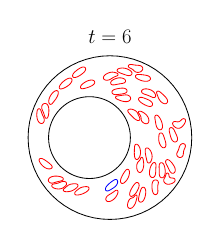
\begin{tikzpicture}[scale=0.3]

\begin{axis}[
  xmin = -21,
  xmax = 21,
  ymin = -21,
  ymax = 21,
  scale only axis,
  axis equal image,
  hide axis,
  title = {\Huge$t=6$}
  ]

% outer solid wall
\addplot [mark=none,black,line width=1.0] table{
2.0000e+01 -5.5171e-16
1.9904e+01 1.9603e+00
1.9616e+01 3.9018e+00
1.9139e+01 5.8057e+00
1.8478e+01 7.6537e+00
1.7638e+01 9.4279e+00
1.6629e+01 1.1111e+01
1.5460e+01 1.2688e+01
1.4142e+01 1.4142e+01
1.2688e+01 1.5460e+01
1.1111e+01 1.6629e+01
9.4279e+00 1.7638e+01
7.6537e+00 1.8478e+01
5.8057e+00 1.9139e+01
3.9018e+00 1.9616e+01
1.9603e+00 1.9904e+01
2.3281e-15 2.0000e+01
-1.9603e+00 1.9904e+01
-3.9018e+00 1.9616e+01
-5.8057e+00 1.9139e+01
-7.6537e+00 1.8478e+01
-9.4279e+00 1.7638e+01
-1.1111e+01 1.6629e+01
-1.2688e+01 1.5460e+01
-1.4142e+01 1.4142e+01
-1.5460e+01 1.2688e+01
-1.6629e+01 1.1111e+01
-1.7638e+01 9.4279e+00
-1.8478e+01 7.6537e+00
-1.9139e+01 5.8057e+00
-1.9616e+01 3.9018e+00
-1.9904e+01 1.9603e+00
-2.0000e+01 3.0010e-15
-1.9904e+01 -1.9603e+00
-1.9616e+01 -3.9018e+00
-1.9139e+01 -5.8057e+00
-1.8478e+01 -7.6537e+00
-1.7638e+01 -9.4279e+00
-1.6629e+01 -1.1111e+01
-1.5460e+01 -1.2688e+01
-1.4142e+01 -1.4142e+01
-1.2688e+01 -1.5460e+01
-1.1111e+01 -1.6629e+01
-9.4279e+00 -1.7638e+01
-7.6537e+00 -1.8478e+01
-5.8057e+00 -1.9139e+01
-3.9018e+00 -1.9616e+01
-1.9603e+00 -1.9904e+01
-4.7774e-15 -2.0000e+01
1.9603e+00 -1.9904e+01
3.9018e+00 -1.9616e+01
5.8057e+00 -1.9139e+01
7.6537e+00 -1.8478e+01
9.4279e+00 -1.7638e+01
1.1111e+01 -1.6629e+01
1.2688e+01 -1.5460e+01
1.4142e+01 -1.4142e+01
1.5460e+01 -1.2688e+01
1.6629e+01 -1.1111e+01
1.7638e+01 -9.4279e+00
1.8478e+01 -7.6537e+00
1.9139e+01 -5.8057e+00
1.9616e+01 -3.9018e+00
1.9904e+01 -1.9603e+00
2.0000e+01 -5.5171e-16
};

% inner solid wall
\addplot [mark=none,black,line width=1.0] table{
5.0000e+00 2.7586e-16
4.9518e+00 -9.8017e-01
4.8079e+00 -1.9509e+00
4.5694e+00 -2.9028e+00
4.2388e+00 -3.8268e+00
3.8192e+00 -4.7140e+00
3.3147e+00 -5.5557e+00
2.7301e+00 -6.3439e+00
2.0711e+00 -7.0711e+00
1.3439e+00 -7.7301e+00
5.5570e-01 -8.3147e+00
-2.8603e-01 -8.8192e+00
-1.1732e+00 -9.2388e+00
-2.0972e+00 -9.5694e+00
-3.0491e+00 -9.8079e+00
-4.0198e+00 -9.9518e+00
-5.0000e+00 -1.0000e+01
-5.9802e+00 -9.9518e+00
-6.9509e+00 -9.8079e+00
-7.9028e+00 -9.5694e+00
-8.8268e+00 -9.2388e+00
-9.7140e+00 -8.8192e+00
-1.0556e+01 -8.3147e+00
-1.1344e+01 -7.7301e+00
-1.2071e+01 -7.0711e+00
-1.2730e+01 -6.3439e+00
-1.3315e+01 -5.5557e+00
-1.3819e+01 -4.7140e+00
-1.4239e+01 -3.8268e+00
-1.4569e+01 -2.9028e+00
-1.4808e+01 -1.9509e+00
-1.4952e+01 -9.8017e-01
-1.5000e+01 -1.5005e-15
-1.4952e+01 9.8017e-01
-1.4808e+01 1.9509e+00
-1.4569e+01 2.9028e+00
-1.4239e+01 3.8268e+00
-1.3819e+01 4.7140e+00
-1.3315e+01 5.5557e+00
-1.2730e+01 6.3439e+00
-1.2071e+01 7.0711e+00
-1.1344e+01 7.7301e+00
-1.0556e+01 8.3147e+00
-9.7140e+00 8.8192e+00
-8.8268e+00 9.2388e+00
-7.9028e+00 9.5694e+00
-6.9509e+00 9.8079e+00
-5.9802e+00 9.9518e+00
-5.0000e+00 1.0000e+01
-4.0198e+00 9.9518e+00
-3.0491e+00 9.8079e+00
-2.0972e+00 9.5694e+00
-1.1732e+00 9.2388e+00
-2.8603e-01 8.8192e+00
5.5570e-01 8.3147e+00
1.3439e+00 7.7301e+00
2.0711e+00 7.0711e+00
2.7301e+00 6.3439e+00
3.3147e+00 5.5557e+00
3.8192e+00 4.7140e+00
4.2388e+00 3.8268e+00
4.5694e+00 2.9028e+00
4.8079e+00 1.9509e+00
4.9518e+00 9.8017e-01
5.0000e+00 2.7586e-16
};


% vesicle1
\addplot [mark=none,red,line width=1.0] table{
1.7617e+01 2.6501e+00
1.7660e+01 2.6896e+00
1.7718e+01 2.7461e+00
1.7790e+01 2.8210e+00
1.7870e+01 2.9118e+00
1.7954e+01 3.0144e+00
1.8038e+01 3.1265e+00
1.8122e+01 3.2458e+00
1.8203e+01 3.3715e+00
1.8279e+01 3.5028e+00
1.8349e+01 3.6399e+00
1.8409e+01 3.7831e+00
1.8454e+01 3.9327e+00
1.8477e+01 4.0879e+00
1.8468e+01 4.2449e+00
1.8418e+01 4.3942e+00
1.8324e+01 4.5203e+00
1.8192e+01 4.6050e+00
1.8038e+01 4.6372e+00
1.7882e+01 4.6174e+00
1.7738e+01 4.5565e+00
1.7609e+01 4.4684e+00
1.7493e+01 4.3656e+00
1.7383e+01 4.2579e+00
1.7273e+01 4.1528e+00
1.7158e+01 4.0568e+00
1.7038e+01 3.9758e+00
1.6912e+01 3.9141e+00
1.6786e+01 3.8737e+00
1.6666e+01 3.8532e+00
1.6563e+01 3.8475e+00
1.6482e+01 3.8500e+00
1.6424e+01 3.8550e+00
1.6366e+01 3.8622e+00
1.6286e+01 3.8749e+00
1.6184e+01 3.8937e+00
1.6065e+01 3.9149e+00
1.5934e+01 3.9304e+00
1.5793e+01 3.9292e+00
1.5651e+01 3.8991e+00
1.5519e+01 3.8312e+00
1.5412e+01 3.7243e+00
1.5344e+01 3.5868e+00
1.5321e+01 3.4337e+00
1.5341e+01 3.2791e+00
1.5395e+01 3.1318e+00
1.5473e+01 2.9953e+00
1.5569e+01 2.8698e+00
1.5677e+01 2.7543e+00
1.5794e+01 2.6480e+00
1.5918e+01 2.5510e+00
1.6050e+01 2.4645e+00
1.6188e+01 2.3906e+00
1.6333e+01 2.3318e+00
1.6483e+01 2.2907e+00
1.6635e+01 2.2692e+00
1.6787e+01 2.2682e+00
1.6935e+01 2.2871e+00
1.7076e+01 2.3238e+00
1.7207e+01 2.3749e+00
1.7324e+01 2.4354e+00
1.7427e+01 2.4999e+00
1.7511e+01 2.5608e+00
1.7573e+01 2.6118e+00
1.7617e+01 2.6501e+00
};

% vesicle2
\addplot [mark=none,red,line width=1.0] table{
-1.6181e+01 3.7830e+00
-1.6154e+01 3.8343e+00
-1.6120e+01 3.9080e+00
-1.6086e+01 4.0057e+00
-1.6059e+01 4.1236e+00
-1.6042e+01 4.2549e+00
-1.6041e+01 4.3953e+00
-1.6057e+01 4.5399e+00
-1.6093e+01 4.6851e+00
-1.6144e+01 4.8281e+00
-1.6205e+01 4.9692e+00
-1.6272e+01 5.1093e+00
-1.6341e+01 5.2499e+00
-1.6409e+01 5.3916e+00
-1.6474e+01 5.5351e+00
-1.6536e+01 5.6801e+00
-1.6595e+01 5.8269e+00
-1.6650e+01 5.9749e+00
-1.6702e+01 6.1240e+00
-1.6752e+01 6.2734e+00
-1.6801e+01 6.4225e+00
-1.6854e+01 6.5698e+00
-1.6913e+01 6.7132e+00
-1.6988e+01 6.8475e+00
-1.7086e+01 6.9631e+00
-1.7212e+01 7.0417e+00
-1.7355e+01 7.0626e+00
-1.7488e+01 7.0202e+00
-1.7590e+01 6.9362e+00
-1.7660e+01 6.8375e+00
-1.7705e+01 6.7448e+00
-1.7734e+01 6.6691e+00
-1.7752e+01 6.6135e+00
-1.7768e+01 6.5573e+00
-1.7787e+01 6.4786e+00
-1.7807e+01 6.3772e+00
-1.7826e+01 6.2575e+00
-1.7842e+01 6.1261e+00
-1.7855e+01 5.9862e+00
-1.7864e+01 5.8408e+00
-1.7869e+01 5.6914e+00
-1.7869e+01 5.5395e+00
-1.7866e+01 5.3855e+00
-1.7857e+01 5.2305e+00
-1.7844e+01 5.0747e+00
-1.7824e+01 4.9190e+00
-1.7797e+01 4.7636e+00
-1.7763e+01 4.6095e+00
-1.7721e+01 4.4573e+00
-1.7669e+01 4.3081e+00
-1.7607e+01 4.1629e+00
-1.7534e+01 4.0236e+00
-1.7448e+01 3.8916e+00
-1.7351e+01 3.7698e+00
-1.7240e+01 3.6610e+00
-1.7116e+01 3.5697e+00
-1.6981e+01 3.5003e+00
-1.6838e+01 3.4589e+00
-1.6693e+01 3.4496e+00
-1.6555e+01 3.4738e+00
-1.6433e+01 3.5260e+00
-1.6335e+01 3.5961e+00
-1.6262e+01 3.6695e+00
-1.6213e+01 3.7337e+00
-1.6181e+01 3.7830e+00
};

% vesicle3
\addplot [mark=none,red,line width=1.0] table{
-1.5717e+01 4.7791e+00
-1.5668e+01 4.7466e+00
-1.5593e+01 4.7167e+00
-1.5490e+01 4.7108e+00
-1.5377e+01 4.7502e+00
-1.5276e+01 4.8359e+00
-1.5198e+01 4.9519e+00
-1.5138e+01 5.0846e+00
-1.5090e+01 5.2262e+00
-1.5052e+01 5.3733e+00
-1.5020e+01 5.5239e+00
-1.4994e+01 5.6771e+00
-1.4973e+01 5.8318e+00
-1.4955e+01 5.9879e+00
-1.4941e+01 6.1448e+00
-1.4931e+01 6.3024e+00
-1.4925e+01 6.4603e+00
-1.4923e+01 6.6184e+00
-1.4926e+01 6.7762e+00
-1.4933e+01 6.9336e+00
-1.4946e+01 7.0900e+00
-1.4966e+01 7.2451e+00
-1.4994e+01 7.3979e+00
-1.5031e+01 7.5474e+00
-1.5078e+01 7.6917e+00
-1.5138e+01 7.8285e+00
-1.5211e+01 7.9544e+00
-1.5297e+01 8.0658e+00
-1.5391e+01 8.1589e+00
-1.5488e+01 8.2309e+00
-1.5579e+01 8.2805e+00
-1.5654e+01 8.3105e+00
-1.5710e+01 8.3270e+00
-1.5767e+01 8.3388e+00
-1.5848e+01 8.3473e+00
-1.5951e+01 8.3442e+00
-1.6070e+01 8.3209e+00
-1.6193e+01 8.2722e+00
-1.6311e+01 8.1972e+00
-1.6418e+01 8.0983e+00
-1.6509e+01 7.9799e+00
-1.6581e+01 7.8463e+00
-1.6634e+01 7.7020e+00
-1.6667e+01 7.5503e+00
-1.6679e+01 7.3945e+00
-1.6669e+01 7.2378e+00
-1.6640e+01 7.0832e+00
-1.6594e+01 6.9320e+00
-1.6538e+01 6.7844e+00
-1.6476e+01 6.6390e+00
-1.6412e+01 6.4947e+00
-1.6348e+01 6.3506e+00
-1.6287e+01 6.2063e+00
-1.6228e+01 6.0613e+00
-1.6173e+01 5.9162e+00
-1.6122e+01 5.7709e+00
-1.6075e+01 5.6264e+00
-1.6031e+01 5.4834e+00
-1.5990e+01 5.3436e+00
-1.5950e+01 5.2090e+00
-1.5908e+01 5.0834e+00
-1.5861e+01 4.9719e+00
-1.5810e+01 4.8821e+00
-1.5759e+01 4.8188e+00
-1.5717e+01 4.7791e+00
};

% vesicle4
\addplot [mark=none,red,line width=1.0] table{
7.0551e+00 1.4196e+01
7.1078e+00 1.4171e+01
7.1814e+00 1.4137e+01
7.2760e+00 1.4096e+01
7.3877e+00 1.4049e+01
7.5111e+00 1.4001e+01
7.6435e+00 1.3954e+01
7.7824e+00 1.3910e+01
7.9266e+00 1.3871e+01
8.0747e+00 1.3837e+01
8.2261e+00 1.3809e+01
8.3799e+00 1.3788e+01
8.5356e+00 1.3773e+01
8.6924e+00 1.3766e+01
8.8500e+00 1.3766e+01
9.0076e+00 1.3776e+01
9.1644e+00 1.3795e+01
9.3189e+00 1.3828e+01
9.4690e+00 1.3877e+01
9.6099e+00 1.3947e+01
9.7348e+00 1.4041e+01
9.8327e+00 1.4163e+01
9.8924e+00 1.4305e+01
9.9058e+00 1.4458e+01
9.8738e+00 1.4606e+01
9.8047e+00 1.4738e+01
9.7106e+00 1.4849e+01
9.6023e+00 1.4939e+01
9.4901e+00 1.5009e+01
9.3815e+00 1.5062e+01
9.2859e+00 1.5102e+01
9.2096e+00 1.5129e+01
9.1540e+00 1.5147e+01
9.0981e+00 1.5163e+01
9.0199e+00 1.5184e+01
8.9194e+00 1.5209e+01
8.8008e+00 1.5234e+01
8.6707e+00 1.5258e+01
8.5320e+00 1.5281e+01
8.3880e+00 1.5302e+01
8.2399e+00 1.5322e+01
8.0892e+00 1.5342e+01
7.9364e+00 1.5361e+01
7.7822e+00 1.5379e+01
7.6268e+00 1.5397e+01
7.4707e+00 1.5413e+01
7.3136e+00 1.5427e+01
7.1561e+00 1.5436e+01
6.9980e+00 1.5439e+01
6.8403e+00 1.5431e+01
6.6842e+00 1.5408e+01
6.5340e+00 1.5362e+01
6.3984e+00 1.5283e+01
6.2943e+00 1.5168e+01
6.2409e+00 1.5023e+01
6.2477e+00 1.4870e+01
6.3056e+00 1.4730e+01
6.3969e+00 1.4612e+01
6.5050e+00 1.4515e+01
6.6195e+00 1.4433e+01
6.7324e+00 1.4364e+01
6.8383e+00 1.4306e+01
6.9301e+00 1.4258e+01
7.0025e+00 1.4222e+01
7.0551e+00 1.4196e+01
};

% vesicle5
\addplot [mark=none,red,line width=1.0] table{
-2.6071e-02 -1.5595e+01
3.0278e-02 -1.5579e+01
1.0704e-01 -1.5554e+01
2.0392e-01 -1.5518e+01
3.1452e-01 -1.5468e+01
4.3264e-01 -1.5409e+01
5.5403e-01 -1.5338e+01
6.7616e-01 -1.5259e+01
7.9694e-01 -1.5171e+01
9.1549e-01 -1.5076e+01
1.0306e+00 -1.4973e+01
1.1419e+00 -1.4865e+01
1.2485e+00 -1.4751e+01
1.3504e+00 -1.4631e+01
1.4466e+00 -1.4506e+01
1.5372e+00 -1.4377e+01
1.6212e+00 -1.4243e+01
1.6988e+00 -1.4106e+01
1.7690e+00 -1.3964e+01
1.8317e+00 -1.3820e+01
1.8855e+00 -1.3672e+01
1.9291e+00 -1.3522e+01
1.9580e+00 -1.3369e+01
1.9652e+00 -1.3216e+01
1.9369e+00 -1.3067e+01
1.8598e+00 -1.2941e+01
1.7371e+00 -1.2864e+01
1.5983e+00 -1.2852e+01
1.4704e+00 -1.2885e+01
1.3621e+00 -1.2939e+01
1.2743e+00 -1.2994e+01
1.2080e+00 -1.3040e+01
1.1605e+00 -1.3074e+01
1.1136e+00 -1.3109e+01
1.0485e+00 -1.3157e+01
9.6563e-01 -1.3219e+01
8.6772e-01 -1.3290e+01
7.6014e-01 -1.3367e+01
6.4423e-01 -1.3447e+01
5.2293e-01 -1.3527e+01
3.9635e-01 -1.3607e+01
2.6657e-01 -1.3686e+01
1.3346e-01 -1.3763e+01
-8.6470e-04 -1.3841e+01
-1.3619e-01 -1.3920e+01
-2.6993e-01 -1.4002e+01
-4.0118e-01 -1.4089e+01
-5.2664e-01 -1.4185e+01
-6.4469e-01 -1.4290e+01
-7.5151e-01 -1.4406e+01
-8.4502e-01 -1.4533e+01
-9.2072e-01 -1.4671e+01
-9.7549e-01 -1.4818e+01
-1.0033e+00 -1.4972e+01
-9.9990e-01 -1.5127e+01
-9.5996e-01 -1.5275e+01
-8.8434e-01 -1.5406e+01
-7.7756e-01 -1.5511e+01
-6.5157e-01 -1.5582e+01
-5.1719e-01 -1.5623e+01
-3.8602e-01 -1.5639e+01
-2.6477e-01 -1.5637e+01
-1.6227e-01 -1.5624e+01
-8.2628e-02 -1.5609e+01
-2.6071e-02 -1.5595e+01
};

% vesicle6
\addplot [mark=none,red,line width=1.0] table{
1.3044e+01 6.2161e-01
1.3019e+01 6.7453e-01
1.2982e+01 7.4649e-01
1.2929e+01 8.3505e-01
1.2856e+01 9.3184e-01
1.2762e+01 1.0244e+00
1.2644e+01 1.1000e+00
1.2505e+01 1.1424e+00
1.2356e+01 1.1368e+00
1.2218e+01 1.0756e+00
1.2110e+01 9.6722e-01
1.2039e+01 8.2932e-01
1.2000e+01 6.7842e-01
1.1978e+01 5.2282e-01
1.1964e+01 3.6592e-01
1.1953e+01 2.0841e-01
1.1941e+01 5.0845e-02
1.1932e+01 -1.0696e-01
1.1926e+01 -2.6466e-01
1.1927e+01 -4.2228e-01
1.1935e+01 -5.7904e-01
1.1951e+01 -7.3456e-01
1.1976e+01 -8.8780e-01
1.2008e+01 -1.0383e+00
1.2048e+01 -1.1849e+00
1.2095e+01 -1.3270e+00
1.2147e+01 -1.4631e+00
1.2202e+01 -1.5920e+00
1.2260e+01 -1.7111e+00
1.2318e+01 -1.8177e+00
1.2371e+01 -1.9066e+00
1.2414e+01 -1.9746e+00
1.2448e+01 -2.0227e+00
1.2482e+01 -2.0699e+00
1.2532e+01 -2.1335e+00
1.2600e+01 -2.2111e+00
1.2687e+01 -2.2953e+00
1.2792e+01 -2.3758e+00
1.2916e+01 -2.4427e+00
1.3055e+01 -2.4833e+00
1.3204e+01 -2.4859e+00
1.3349e+01 -2.4421e+00
1.3474e+01 -2.3540e+00
1.3570e+01 -2.2319e+00
1.3633e+01 -2.0894e+00
1.3669e+01 -1.9365e+00
1.3682e+01 -1.7797e+00
1.3679e+01 -1.6218e+00
1.3664e+01 -1.4646e+00
1.3639e+01 -1.3084e+00
1.3608e+01 -1.1538e+00
1.3571e+01 -1.0006e+00
1.3530e+01 -8.4903e-01
1.3486e+01 -6.9886e-01
1.3441e+01 -5.5040e-01
1.3395e+01 -4.0352e-01
1.3348e+01 -2.5881e-01
1.3302e+01 -1.1649e-01
1.3258e+01 2.2079e-02
1.3214e+01 1.5574e-01
1.3173e+01 2.8142e-01
1.3133e+01 3.9589e-01
1.3097e+01 4.9290e-01
1.3067e+01 5.6802e-01
1.3044e+01 6.2161e-01
};

% vesicle7
\addplot [mark=none,red,line width=1.0] table{
7.4642e+00 1.6088e+01
7.5158e+00 1.6116e+01
7.5852e+00 1.6157e+01
7.6697e+00 1.6217e+01
7.7613e+00 1.6296e+01
7.8498e+00 1.6394e+01
7.9273e+00 1.6511e+01
7.9849e+00 1.6645e+01
8.0157e+00 1.6791e+01
8.0135e+00 1.6942e+01
7.9766e+00 1.7092e+01
7.9059e+00 1.7229e+01
7.8065e+00 1.7350e+01
7.6847e+00 1.7449e+01
7.5474e+00 1.7525e+01
7.3999e+00 1.7582e+01
7.2469e+00 1.7621e+01
7.0910e+00 1.7646e+01
6.9341e+00 1.7663e+01
6.7768e+00 1.7675e+01
6.6202e+00 1.7684e+01
6.4641e+00 1.7695e+01
6.3094e+00 1.7708e+01
6.1563e+00 1.7725e+01
6.0057e+00 1.7745e+01
5.8581e+00 1.7768e+01
5.7146e+00 1.7793e+01
5.5762e+00 1.7817e+01
5.4456e+00 1.7839e+01
5.3258e+00 1.7857e+01
5.2229e+00 1.7868e+01
5.1422e+00 1.7873e+01
5.0838e+00 1.7875e+01
5.0255e+00 1.7874e+01
4.9448e+00 1.7867e+01
4.8433e+00 1.7848e+01
4.7297e+00 1.7806e+01
4.6203e+00 1.7733e+01
4.5353e+00 1.7622e+01
4.4985e+00 1.7482e+01
4.5226e+00 1.7335e+01
4.6018e+00 1.7207e+01
4.7171e+00 1.7105e+01
4.8511e+00 1.7027e+01
4.9924e+00 1.6960e+01
5.1355e+00 1.6895e+01
5.2763e+00 1.6825e+01
5.4124e+00 1.6745e+01
5.5417e+00 1.6654e+01
5.6640e+00 1.6554e+01
5.7803e+00 1.6447e+01
5.8947e+00 1.6339e+01
6.0116e+00 1.6234e+01
6.1358e+00 1.6139e+01
6.2690e+00 1.6059e+01
6.4107e+00 1.5999e+01
6.5573e+00 1.5960e+01
6.7053e+00 1.5940e+01
6.8508e+00 1.5936e+01
6.9909e+00 1.5947e+01
7.1214e+00 1.5969e+01
7.2387e+00 1.5999e+01
7.3366e+00 1.6032e+01
7.4114e+00 1.6063e+01
7.4642e+00 1.6088e+01
};

% vesicle8
\addplot [mark=none,red,line width=1.0] table{
7.8626e+00 9.8048e+00
7.8053e+00 9.8159e+00
7.7253e+00 9.8283e+00
7.6223e+00 9.8375e+00
7.5013e+00 9.8369e+00
7.3704e+00 9.8178e+00
7.2383e+00 9.7709e+00
7.1194e+00 9.6878e+00
7.0328e+00 9.5670e+00
6.9971e+00 9.4202e+00
7.0153e+00 9.2681e+00
7.0758e+00 9.1253e+00
7.1628e+00 8.9957e+00
7.2659e+00 8.8772e+00
7.3785e+00 8.7671e+00
7.4977e+00 8.6636e+00
7.6215e+00 8.5654e+00
7.7490e+00 8.4719e+00
7.8791e+00 8.3827e+00
8.0117e+00 8.2975e+00
8.1460e+00 8.2161e+00
8.2817e+00 8.1384e+00
8.4182e+00 8.0644e+00
8.5553e+00 7.9942e+00
8.6921e+00 7.9281e+00
8.8283e+00 7.8664e+00
8.9624e+00 7.8099e+00
9.0935e+00 7.7593e+00
9.2186e+00 7.7159e+00
9.3345e+00 7.6807e+00
9.4347e+00 7.6548e+00
9.5138e+00 7.6379e+00
9.5713e+00 7.6278e+00
9.6291e+00 7.6197e+00
9.7097e+00 7.6123e+00
9.8131e+00 7.6105e+00
9.9336e+00 7.6218e+00
1.0062e+01 7.6546e+00
1.0187e+01 7.7165e+00
1.0297e+01 7.8117e+00
1.0377e+01 7.9373e+00
1.0417e+01 8.0834e+00
1.0416e+01 8.2369e+00
1.0379e+01 8.3873e+00
1.0312e+01 8.5282e+00
1.0222e+01 8.6568e+00
1.0115e+01 8.7726e+00
9.9959e+00 8.8763e+00
9.8682e+00 8.9692e+00
9.7343e+00 9.0532e+00
9.5965e+00 9.1302e+00
9.4560e+00 9.2016e+00
9.3141e+00 9.2688e+00
9.1714e+00 9.3327e+00
9.0287e+00 9.3940e+00
8.8865e+00 9.4530e+00
8.7455e+00 9.5098e+00
8.6063e+00 9.5644e+00
8.4702e+00 9.6161e+00
8.3382e+00 9.6641e+00
8.2130e+00 9.7072e+00
8.0975e+00 9.7438e+00
7.9981e+00 9.7722e+00
7.9196e+00 9.7921e+00
7.8626e+00 9.8048e+00
};

% vesicle9
\addplot [mark=none,red,line width=1.0] table{
8.4686e+00 5.9247e+00
8.4217e+00 5.9595e+00
8.3559e+00 6.0065e+00
8.2701e+00 6.0644e+00
8.1679e+00 6.1294e+00
8.0537e+00 6.1964e+00
7.9299e+00 6.2629e+00
7.7985e+00 6.3256e+00
7.6602e+00 6.3824e+00
7.5155e+00 6.4285e+00
7.3644e+00 6.4575e+00
7.2095e+00 6.4546e+00
7.0650e+00 6.3985e+00
6.9715e+00 6.2754e+00
6.9686e+00 6.1204e+00
7.0372e+00 5.9788e+00
7.1318e+00 5.8524e+00
7.2291e+00 5.7277e+00
7.3199e+00 5.5988e+00
7.4021e+00 5.4642e+00
7.4740e+00 5.3248e+00
7.5345e+00 5.1805e+00
7.5810e+00 5.0325e+00
7.6116e+00 4.8816e+00
7.6265e+00 4.7305e+00
7.6314e+00 4.5810e+00
7.6383e+00 4.4356e+00
7.6604e+00 4.2970e+00
7.7019e+00 4.1714e+00
7.7570e+00 4.0636e+00
7.8146e+00 3.9778e+00
7.8649e+00 3.9144e+00
7.9037e+00 3.8708e+00
7.9441e+00 3.8287e+00
8.0026e+00 3.7729e+00
8.0813e+00 3.7057e+00
8.1782e+00 3.6330e+00
8.2896e+00 3.5616e+00
8.4140e+00 3.4962e+00
8.5491e+00 3.4422e+00
8.6938e+00 3.4049e+00
8.8448e+00 3.3907e+00
8.9978e+00 3.4060e+00
9.1444e+00 3.4560e+00
9.2748e+00 3.5416e+00
9.3795e+00 3.6580e+00
9.4540e+00 3.7965e+00
9.4985e+00 3.9477e+00
9.5172e+00 4.1045e+00
9.5143e+00 4.2624e+00
9.4939e+00 4.4189e+00
9.4587e+00 4.5725e+00
9.4112e+00 4.7221e+00
9.3524e+00 4.8670e+00
9.2841e+00 5.0064e+00
9.2070e+00 5.1397e+00
9.1228e+00 5.2662e+00
9.0326e+00 5.3854e+00
8.9385e+00 5.4965e+00
8.8423e+00 5.5989e+00
8.7475e+00 5.6913e+00
8.6573e+00 5.7722e+00
8.5782e+00 5.8388e+00
8.5149e+00 5.8892e+00
8.4686e+00 5.9247e+00
};

% vesicle10
\addplot [mark=none,red,line width=1.0] table{
1.3434e+01 -9.0064e+00
1.3448e+01 -8.9497e+00
1.3465e+01 -8.8705e+00
1.3483e+01 -8.7687e+00
1.3499e+01 -8.6486e+00
1.3511e+01 -8.5168e+00
1.3517e+01 -8.3764e+00
1.3517e+01 -8.2309e+00
1.3511e+01 -8.0815e+00
1.3499e+01 -7.9300e+00
1.3481e+01 -7.7770e+00
1.3459e+01 -7.6235e+00
1.3431e+01 -7.4695e+00
1.3399e+01 -7.3159e+00
1.3362e+01 -7.1627e+00
1.3319e+01 -7.0107e+00
1.3271e+01 -6.8602e+00
1.3215e+01 -6.7124e+00
1.3149e+01 -6.5690e+00
1.3069e+01 -6.4336e+00
1.2970e+01 -6.3116e+00
1.2849e+01 -6.2129e+00
1.2708e+01 -6.1499e+00
1.2556e+01 -6.1345e+00
1.2409e+01 -6.1703e+00
1.2283e+01 -6.2501e+00
1.2187e+01 -6.3591e+00
1.2120e+01 -6.4825e+00
1.2078e+01 -6.6078e+00
1.2053e+01 -6.7263e+00
1.2040e+01 -6.8289e+00
1.2033e+01 -6.9096e+00
1.2030e+01 -6.9679e+00
1.2029e+01 -7.0263e+00
1.2028e+01 -7.1072e+00
1.2029e+01 -7.2106e+00
1.2032e+01 -7.3317e+00
1.2037e+01 -7.4641e+00
1.2042e+01 -7.6045e+00
1.2047e+01 -7.7500e+00
1.2051e+01 -7.8994e+00
1.2054e+01 -8.0514e+00
1.2055e+01 -8.2054e+00
1.2054e+01 -8.3606e+00
1.2054e+01 -8.5170e+00
1.2053e+01 -8.6740e+00
1.2056e+01 -8.8316e+00
1.2065e+01 -8.9891e+00
1.2085e+01 -9.1460e+00
1.2121e+01 -9.2998e+00
1.2177e+01 -9.4470e+00
1.2260e+01 -9.5810e+00
1.2369e+01 -9.6934e+00
1.2502e+01 -9.7742e+00
1.2651e+01 -9.8155e+00
1.2805e+01 -9.8125e+00
1.2949e+01 -9.7674e+00
1.3075e+01 -9.6873e+00
1.3177e+01 -9.5839e+00
1.3257e+01 -9.4682e+00
1.3318e+01 -9.3506e+00
1.3363e+01 -9.2384e+00
1.3397e+01 -9.1405e+00
1.3419e+01 -9.0629e+00
1.3434e+01 -9.0064e+00
};

% vesicle11
\addplot [mark=none,red,line width=1.0] table{
-1.3505e+01 -9.4219e+00
-1.3564e+01 -9.4272e+00
-1.3644e+01 -9.4364e+00
-1.3746e+01 -9.4511e+00
-1.3866e+01 -9.4728e+00
-1.3995e+01 -9.5020e+00
-1.4130e+01 -9.5401e+00
-1.4268e+01 -9.5875e+00
-1.4405e+01 -9.6455e+00
-1.4540e+01 -9.7149e+00
-1.4670e+01 -9.7975e+00
-1.4791e+01 -9.8947e+00
-1.4898e+01 -1.0009e+01
-1.4983e+01 -1.0141e+01
-1.5037e+01 -1.0288e+01
-1.5052e+01 -1.0445e+01
-1.5024e+01 -1.0600e+01
-1.4956e+01 -1.0742e+01
-1.4858e+01 -1.0865e+01
-1.4737e+01 -1.0966e+01
-1.4602e+01 -1.1045e+01
-1.4455e+01 -1.1100e+01
-1.4303e+01 -1.1131e+01
-1.4150e+01 -1.1137e+01
-1.3999e+01 -1.1120e+01
-1.3853e+01 -1.1088e+01
-1.3713e+01 -1.1048e+01
-1.3579e+01 -1.1005e+01
-1.3453e+01 -1.0964e+01
-1.3338e+01 -1.0926e+01
-1.3239e+01 -1.0896e+01
-1.3162e+01 -1.0872e+01
-1.3106e+01 -1.0856e+01
-1.3050e+01 -1.0839e+01
-1.2972e+01 -1.0818e+01
-1.2872e+01 -1.0791e+01
-1.2754e+01 -1.0762e+01
-1.2625e+01 -1.0732e+01
-1.2488e+01 -1.0701e+01
-1.2346e+01 -1.0671e+01
-1.2199e+01 -1.0640e+01
-1.2051e+01 -1.0607e+01
-1.1902e+01 -1.0569e+01
-1.1755e+01 -1.0520e+01
-1.1614e+01 -1.0453e+01
-1.1490e+01 -1.0356e+01
-1.1407e+01 -1.0224e+01
-1.1390e+01 -1.0069e+01
-1.1447e+01 -9.9227e+00
-1.1554e+01 -9.8077e+00
-1.1686e+01 -9.7214e+00
-1.1829e+01 -9.6542e+00
-1.1976e+01 -9.5997e+00
-1.2125e+01 -9.5542e+00
-1.2276e+01 -9.5161e+00
-1.2427e+01 -9.4844e+00
-1.2576e+01 -9.4587e+00
-1.2724e+01 -9.4385e+00
-1.2869e+01 -9.4239e+00
-1.3009e+01 -9.4145e+00
-1.3142e+01 -9.4101e+00
-1.3263e+01 -9.4099e+00
-1.3366e+01 -9.4130e+00
-1.3447e+01 -9.4174e+00
-1.3505e+01 -9.4219e+00
};

% vesicle12
\addplot [mark=none,red,line width=1.0] table{
1.3003e+01 1.0492e+01
1.2960e+01 1.0532e+01
1.2901e+01 1.0587e+01
1.2824e+01 1.0657e+01
1.2735e+01 1.0739e+01
1.2637e+01 1.0827e+01
1.2532e+01 1.0921e+01
1.2422e+01 1.1016e+01
1.2305e+01 1.1110e+01
1.2182e+01 1.1199e+01
1.2050e+01 1.1277e+01
1.1906e+01 1.1334e+01
1.1751e+01 1.1355e+01
1.1599e+01 1.1321e+01
1.1475e+01 1.1226e+01
1.1409e+01 1.1084e+01
1.1405e+01 1.0927e+01
1.1443e+01 1.0774e+01
1.1500e+01 1.0627e+01
1.1561e+01 1.0481e+01
1.1618e+01 1.0335e+01
1.1671e+01 1.0188e+01
1.1721e+01 1.0041e+01
1.1773e+01 9.8962e+00
1.1830e+01 9.7550e+00
1.1891e+01 9.6185e+00
1.1956e+01 9.4885e+00
1.2025e+01 9.3660e+00
1.2095e+01 9.2535e+00
1.2163e+01 9.1533e+00
1.2224e+01 9.0700e+00
1.2274e+01 9.0063e+00
1.2311e+01 8.9613e+00
1.2349e+01 8.9170e+00
1.2403e+01 8.8570e+00
1.2475e+01 8.7827e+00
1.2563e+01 8.6995e+00
1.2664e+01 8.6138e+00
1.2777e+01 8.5297e+00
1.2900e+01 8.4514e+00
1.3032e+01 8.3822e+00
1.3173e+01 8.3264e+00
1.3323e+01 8.2887e+00
1.3477e+01 8.2751e+00
1.3632e+01 8.2917e+00
1.3780e+01 8.3437e+00
1.3909e+01 8.4326e+00
1.4009e+01 8.5542e+00
1.4072e+01 8.6986e+00
1.4097e+01 8.8544e+00
1.4087e+01 9.0116e+00
1.4050e+01 9.1646e+00
1.3992e+01 9.3104e+00
1.3919e+01 9.4488e+00
1.3836e+01 9.5801e+00
1.3746e+01 9.7049e+00
1.3651e+01 9.8238e+00
1.3554e+01 9.9371e+00
1.3456e+01 1.0045e+01
1.3358e+01 1.0146e+01
1.3265e+01 1.0240e+01
1.3178e+01 1.0325e+01
1.3104e+01 1.0396e+01
1.3045e+01 1.0452e+01
1.3003e+01 1.0492e+01
};

% vesicle13
\addplot [mark=none,red,line width=1.0] table{
1.3383e+00 1.5874e+01
1.2825e+00 1.5891e+01
1.2047e+00 1.5913e+01
1.1044e+00 1.5939e+01
9.8568e-01 1.5963e+01
8.5468e-01 1.5982e+01
7.1462e-01 1.5993e+01
5.6907e-01 1.5995e+01
4.1982e-01 1.5986e+01
2.6901e-01 1.5968e+01
1.1747e-01 1.5940e+01
-3.3519e-02 1.5904e+01
-1.8367e-01 1.5861e+01
-3.3212e-01 1.5810e+01
-4.7873e-01 1.5752e+01
-6.2267e-01 1.5687e+01
-7.6364e-01 1.5616e+01
-9.0052e-01 1.5537e+01
-1.0326e+00 1.5450e+01
-1.1580e+00 1.5355e+01
-1.2754e+00 1.5251e+01
-1.3815e+00 1.5136e+01
-1.4728e+00 1.5010e+01
-1.5434e+00 1.4874e+01
-1.5863e+00 1.4728e+01
-1.5934e+00 1.4579e+01
-1.5610e+00 1.4438e+01
-1.4929e+00 1.4316e+01
-1.4018e+00 1.4220e+01
-1.3022e+00 1.4151e+01
-1.2093e+00 1.4106e+01
-1.1333e+00 1.4078e+01
-1.0772e+00 1.4062e+01
-1.0204e+00 1.4049e+01
-9.4063e-01 1.4035e+01
-8.3777e-01 1.4024e+01
-7.1670e-01 1.4021e+01
-5.8457e-01 1.4029e+01
-4.4563e-01 1.4050e+01
-3.0422e-01 1.4084e+01
-1.6271e-01 1.4132e+01
-2.3296e-02 1.4193e+01
1.1375e-01 1.4263e+01
2.4836e-01 1.4340e+01
3.8175e-01 1.4422e+01
5.1465e-01 1.4505e+01
6.4843e-01 1.4589e+01
7.8367e-01 1.4670e+01
9.2144e-01 1.4748e+01
1.0619e+00 1.4820e+01
1.2056e+00 1.4885e+01
1.3519e+00 1.4944e+01
1.5001e+00 1.4996e+01
1.6473e+00 1.5048e+01
1.7888e+00 1.5112e+01
1.9113e+00 1.5204e+01
1.9869e+00 1.5334e+01
1.9843e+00 1.5482e+01
1.9094e+00 1.5605e+01
1.7984e+00 1.5691e+01
1.6801e+00 1.5750e+01
1.5677e+00 1.5795e+01
1.4705e+00 1.5830e+01
1.3938e+00 1.5856e+01
1.3383e+00 1.5874e+01
};

% vesicle14
\addplot [mark=none,red,line width=1.0] table{
-1.2231e+01 -1.0953e+01
-1.2286e+01 -1.0974e+01
-1.2361e+01 -1.1002e+01
-1.2459e+01 -1.1037e+01
-1.2573e+01 -1.1076e+01
-1.2699e+01 -1.1117e+01
-1.2834e+01 -1.1157e+01
-1.2975e+01 -1.1194e+01
-1.3121e+01 -1.1227e+01
-1.3270e+01 -1.1257e+01
-1.3422e+01 -1.1283e+01
-1.3575e+01 -1.1308e+01
-1.3728e+01 -1.1337e+01
-1.3880e+01 -1.1378e+01
-1.4021e+01 -1.1446e+01
-1.4137e+01 -1.1553e+01
-1.4203e+01 -1.1695e+01
-1.4200e+01 -1.1852e+01
-1.4135e+01 -1.1995e+01
-1.4032e+01 -1.2114e+01
-1.3908e+01 -1.2210e+01
-1.3773e+01 -1.2288e+01
-1.3632e+01 -1.2353e+01
-1.3488e+01 -1.2407e+01
-1.3342e+01 -1.2451e+01
-1.3197e+01 -1.2487e+01
-1.3054e+01 -1.2513e+01
-1.2915e+01 -1.2533e+01
-1.2783e+01 -1.2545e+01
-1.2662e+01 -1.2551e+01
-1.2559e+01 -1.2552e+01
-1.2478e+01 -1.2551e+01
-1.2419e+01 -1.2548e+01
-1.2361e+01 -1.2545e+01
-1.2280e+01 -1.2537e+01
-1.2178e+01 -1.2524e+01
-1.2059e+01 -1.2503e+01
-1.1930e+01 -1.2473e+01
-1.1795e+01 -1.2432e+01
-1.1660e+01 -1.2378e+01
-1.1526e+01 -1.2312e+01
-1.1396e+01 -1.2233e+01
-1.1270e+01 -1.2145e+01
-1.1146e+01 -1.2052e+01
-1.1025e+01 -1.1952e+01
-1.0909e+01 -1.1847e+01
-1.0799e+01 -1.1734e+01
-1.0704e+01 -1.1608e+01
-1.0634e+01 -1.1467e+01
-1.0600e+01 -1.1313e+01
-1.0611e+01 -1.1156e+01
-1.0670e+01 -1.1011e+01
-1.0768e+01 -1.0889e+01
-1.0895e+01 -1.0798e+01
-1.1037e+01 -1.0737e+01
-1.1188e+01 -1.0704e+01
-1.1339e+01 -1.0697e+01
-1.1488e+01 -1.0713e+01
-1.1630e+01 -1.0743e+01
-1.1765e+01 -1.0783e+01
-1.1890e+01 -1.0825e+01
-1.2004e+01 -1.0867e+01
-1.2101e+01 -1.0904e+01
-1.2176e+01 -1.0933e+01
-1.2231e+01 -1.0953e+01
};

% vesicle15
\addplot [mark=none,red,line width=1.0] table{
-1.2632e+01 1.1136e+01
-1.2646e+01 1.1193e+01
-1.2676e+01 1.1268e+01
-1.2733e+01 1.1355e+01
-1.2825e+01 1.1432e+01
-1.2949e+01 1.1478e+01
-1.3088e+01 1.1485e+01
-1.3231e+01 1.1457e+01
-1.3371e+01 1.1404e+01
-1.3506e+01 1.1334e+01
-1.3635e+01 1.1251e+01
-1.3759e+01 1.1158e+01
-1.3878e+01 1.1056e+01
-1.3991e+01 1.0946e+01
-1.4098e+01 1.0831e+01
-1.4199e+01 1.0710e+01
-1.4296e+01 1.0585e+01
-1.4386e+01 1.0455e+01
-1.4472e+01 1.0323e+01
-1.4551e+01 1.0187e+01
-1.4625e+01 1.0048e+01
-1.4692e+01 9.9068e+00
-1.4753e+01 9.7639e+00
-1.4807e+01 9.6195e+00
-1.4852e+01 9.4747e+00
-1.4890e+01 9.3298e+00
-1.4917e+01 9.1870e+00
-1.4935e+01 9.0476e+00
-1.4943e+01 8.9154e+00
-1.4942e+01 8.7943e+00
-1.4933e+01 8.6911e+00
-1.4921e+01 8.6110e+00
-1.4909e+01 8.5538e+00
-1.4895e+01 8.4974e+00
-1.4868e+01 8.4209e+00
-1.4823e+01 8.3280e+00
-1.4750e+01 8.2315e+00
-1.4644e+01 8.1531e+00
-1.4509e+01 8.1166e+00
-1.4366e+01 8.1377e+00
-1.4235e+01 8.2087e+00
-1.4122e+01 8.3103e+00
-1.4020e+01 8.4255e+00
-1.3922e+01 8.5458e+00
-1.3824e+01 8.6672e+00
-1.3724e+01 8.7891e+00
-1.3626e+01 8.9117e+00
-1.3528e+01 9.0357e+00
-1.3432e+01 9.1612e+00
-1.3338e+01 9.2887e+00
-1.3248e+01 9.4181e+00
-1.3161e+01 9.5495e+00
-1.3078e+01 9.6826e+00
-1.2999e+01 9.8177e+00
-1.2925e+01 9.9542e+00
-1.2857e+01 1.0092e+01
-1.2795e+01 1.0231e+01
-1.2740e+01 1.0370e+01
-1.2694e+01 1.0508e+01
-1.2658e+01 1.0644e+01
-1.2633e+01 1.0774e+01
-1.2619e+01 1.0895e+01
-1.2617e+01 1.0998e+01
-1.2623e+01 1.1079e+01
-1.2632e+01 1.1136e+01
};

% vesicle16
\addplot [mark=none,red,line width=1.0] table{
9.8303e+00 1.0098e+01
9.8833e+00 1.0074e+01
9.9567e+00 1.0040e+01
1.0050e+01 9.9956e+00
1.0160e+01 9.9448e+00
1.0282e+01 9.8916e+00
1.0413e+01 9.8411e+00
1.0552e+01 9.8007e+00
1.0700e+01 9.7806e+00
1.0851e+01 9.7944e+00
1.0992e+01 9.8544e+00
1.1102e+01 9.9628e+00
1.1164e+01 1.0106e+01
1.1175e+01 1.0262e+01
1.1148e+01 1.0417e+01
1.1096e+01 1.0566e+01
1.1028e+01 1.0708e+01
1.0948e+01 1.0844e+01
1.0856e+01 1.0973e+01
1.0755e+01 1.1094e+01
1.0645e+01 1.1205e+01
1.0527e+01 1.1308e+01
1.0403e+01 1.1402e+01
1.0275e+01 1.1487e+01
1.0143e+01 1.1562e+01
1.0009e+01 1.1629e+01
9.8759e+00 1.1687e+01
9.7445e+00 1.1737e+01
9.6187e+00 1.1778e+01
9.5021e+00 1.1811e+01
9.4016e+00 1.1836e+01
9.3224e+00 1.1853e+01
9.2650e+00 1.1863e+01
9.2074e+00 1.1873e+01
9.1273e+00 1.1885e+01
9.0245e+00 1.1896e+01
8.9037e+00 1.1905e+01
8.7713e+00 1.1908e+01
8.6309e+00 1.1903e+01
8.4861e+00 1.1888e+01
8.3393e+00 1.1860e+01
8.1938e+00 1.1817e+01
8.0537e+00 1.1753e+01
7.9256e+00 1.1666e+01
7.8196e+00 1.1552e+01
7.7502e+00 1.1411e+01
7.7307e+00 1.1256e+01
7.7664e+00 1.1103e+01
7.8488e+00 1.0969e+01
7.9627e+00 1.0860e+01
8.0944e+00 1.0773e+01
8.2353e+00 1.0702e+01
8.3804e+00 1.0643e+01
8.5274e+00 1.0589e+01
8.6743e+00 1.0539e+01
8.8205e+00 1.0490e+01
8.9645e+00 1.0442e+01
9.1057e+00 1.0393e+01
9.2426e+00 1.0343e+01
9.3739e+00 1.0293e+01
9.4968e+00 1.0244e+01
9.6085e+00 1.0197e+01
9.7033e+00 1.0156e+01
9.7772e+00 1.0123e+01
9.8303e+00 1.0098e+01
};

% vesicle17
\addplot [mark=none,red,line width=1.0] table{
-1.5239e+01 -5.9409e+00
-1.5285e+01 -5.9056e+00
-1.5350e+01 -5.8571e+00
-1.5433e+01 -5.7959e+00
-1.5532e+01 -5.7251e+00
-1.5640e+01 -5.6493e+00
-1.5757e+01 -5.5706e+00
-1.5879e+01 -5.4915e+00
-1.6006e+01 -5.4131e+00
-1.6138e+01 -5.3375e+00
-1.6274e+01 -5.2658e+00
-1.6415e+01 -5.2006e+00
-1.6561e+01 -5.1445e+00
-1.6713e+01 -5.1033e+00
-1.6869e+01 -5.0851e+00
-1.7025e+01 -5.1038e+00
-1.7166e+01 -5.1739e+00
-1.7264e+01 -5.2962e+00
-1.7303e+01 -5.4480e+00
-1.7293e+01 -5.6049e+00
-1.7251e+01 -5.7561e+00
-1.7191e+01 -5.9006e+00
-1.7120e+01 -6.0386e+00
-1.7041e+01 -6.1710e+00
-1.6957e+01 -6.2975e+00
-1.6869e+01 -6.4183e+00
-1.6779e+01 -6.5325e+00
-1.6688e+01 -6.6397e+00
-1.6599e+01 -6.7377e+00
-1.6515e+01 -6.8249e+00
-1.6441e+01 -6.8973e+00
-1.6382e+01 -6.9526e+00
-1.6338e+01 -6.9917e+00
-1.6294e+01 -7.0301e+00
-1.6232e+01 -7.0821e+00
-1.6151e+01 -7.1464e+00
-1.6054e+01 -7.2185e+00
-1.5944e+01 -7.2927e+00
-1.5824e+01 -7.3658e+00
-1.5696e+01 -7.4345e+00
-1.5560e+01 -7.4968e+00
-1.5418e+01 -7.5505e+00
-1.5270e+01 -7.5940e+00
-1.5118e+01 -7.6258e+00
-1.4963e+01 -7.6445e+00
-1.4806e+01 -7.6485e+00
-1.4649e+01 -7.6358e+00
-1.4495e+01 -7.6029e+00
-1.4348e+01 -7.5442e+00
-1.4221e+01 -7.4519e+00
-1.4132e+01 -7.3222e+00
-1.4105e+01 -7.1682e+00
-1.4139e+01 -7.0157e+00
-1.4214e+01 -6.8787e+00
-1.4309e+01 -6.7560e+00
-1.4414e+01 -6.6430e+00
-1.4522e+01 -6.5368e+00
-1.4633e+01 -6.4359e+00
-1.4742e+01 -6.3401e+00
-1.4850e+01 -6.2496e+00
-1.4952e+01 -6.1656e+00
-1.5047e+01 -6.0899e+00
-1.5128e+01 -6.0259e+00
-1.5192e+01 -5.9764e+00
-1.5239e+01 -5.9409e+00
};

% vesicle18
\addplot [mark=none,red,line width=1.0] table{
4.6320e+00 -1.7233e+01
4.6840e+00 -1.7259e+01
4.7599e+00 -1.7287e+01
4.8613e+00 -1.7307e+01
4.9823e+00 -1.7309e+01
5.1125e+00 -1.7285e+01
5.2444e+00 -1.7238e+01
5.3720e+00 -1.7168e+01
5.4928e+00 -1.7080e+01
5.6057e+00 -1.6978e+01
5.7109e+00 -1.6866e+01
5.8086e+00 -1.6745e+01
5.8996e+00 -1.6618e+01
5.9839e+00 -1.6485e+01
6.0619e+00 -1.6349e+01
6.1334e+00 -1.6208e+01
6.1986e+00 -1.6064e+01
6.2573e+00 -1.5917e+01
6.3098e+00 -1.5768e+01
6.3563e+00 -1.5618e+01
6.3983e+00 -1.5466e+01
6.4369e+00 -1.5315e+01
6.4743e+00 -1.5164e+01
6.5117e+00 -1.5015e+01
6.5499e+00 -1.4868e+01
6.5868e+00 -1.4723e+01
6.6182e+00 -1.4581e+01
6.6358e+00 -1.4441e+01
6.6303e+00 -1.4309e+01
6.5943e+00 -1.4194e+01
6.5342e+00 -1.4111e+01
6.4684e+00 -1.4064e+01
6.4136e+00 -1.4044e+01
6.3557e+00 -1.4038e+01
6.2762e+00 -1.4051e+01
6.1851e+00 -1.4100e+01
6.0982e+00 -1.4184e+01
6.0204e+00 -1.4291e+01
5.9410e+00 -1.4406e+01
5.8482e+00 -1.4519e+01
5.7349e+00 -1.4616e+01
5.6025e+00 -1.4690e+01
5.4578e+00 -1.4742e+01
5.3085e+00 -1.4785e+01
5.1600e+00 -1.4834e+01
5.0191e+00 -1.4903e+01
4.8922e+00 -1.4996e+01
4.7826e+00 -1.5109e+01
4.6895e+00 -1.5237e+01
4.6105e+00 -1.5373e+01
4.5425e+00 -1.5516e+01
4.4836e+00 -1.5662e+01
4.4322e+00 -1.5810e+01
4.3882e+00 -1.5960e+01
4.3515e+00 -1.6111e+01
4.3236e+00 -1.6263e+01
4.3059e+00 -1.6414e+01
4.3013e+00 -1.6563e+01
4.3124e+00 -1.6708e+01
4.3419e+00 -1.6845e+01
4.3898e+00 -1.6969e+01
4.4527e+00 -1.7072e+01
4.5209e+00 -1.7149e+01
4.5830e+00 -1.7201e+01
4.6320e+00 -1.7233e+01
};

% vesicle19
\addplot [mark=none,red,line width=1.0] table{
1.6654e+01 -3.2143e+00
1.6628e+01 -3.2666e+00
1.6591e+01 -3.3385e+00
1.6542e+01 -3.4300e+00
1.6487e+01 -3.5377e+00
1.6431e+01 -3.6577e+00
1.6382e+01 -3.7894e+00
1.6349e+01 -3.9310e+00
1.6338e+01 -4.0799e+00
1.6355e+01 -4.2307e+00
1.6401e+01 -4.3771e+00
1.6477e+01 -4.5124e+00
1.6578e+01 -4.6315e+00
1.6700e+01 -4.7297e+00
1.6839e+01 -4.8038e+00
1.6990e+01 -4.8504e+00
1.7147e+01 -4.8667e+00
1.7304e+01 -4.8502e+00
1.7453e+01 -4.8009e+00
1.7588e+01 -4.7204e+00
1.7703e+01 -4.6137e+00
1.7794e+01 -4.4868e+00
1.7861e+01 -4.3469e+00
1.7906e+01 -4.1998e+00
1.7935e+01 -4.0506e+00
1.7953e+01 -3.9022e+00
1.7965e+01 -3.7571e+00
1.7977e+01 -3.6171e+00
1.7992e+01 -3.4856e+00
1.8010e+01 -3.3659e+00
1.8031e+01 -3.2645e+00
1.8051e+01 -3.1860e+00
1.8067e+01 -3.1299e+00
1.8084e+01 -3.0743e+00
1.8111e+01 -2.9980e+00
1.8150e+01 -2.9018e+00
1.8198e+01 -2.7910e+00
1.8255e+01 -2.6712e+00
1.8314e+01 -2.5439e+00
1.8371e+01 -2.4098e+00
1.8417e+01 -2.2677e+00
1.8444e+01 -2.1183e+00
1.8442e+01 -1.9646e+00
1.8403e+01 -1.8147e+00
1.8325e+01 -1.6798e+00
1.8211e+01 -1.5724e+00
1.8072e+01 -1.5010e+00
1.7917e+01 -1.4693e+00
1.7760e+01 -1.4753e+00
1.7607e+01 -1.5151e+00
1.7465e+01 -1.5832e+00
1.7337e+01 -1.6750e+00
1.7226e+01 -1.7857e+00
1.7133e+01 -1.9110e+00
1.7057e+01 -2.0462e+00
1.6996e+01 -2.1877e+00
1.6947e+01 -2.3317e+00
1.6906e+01 -2.4755e+00
1.6869e+01 -2.6162e+00
1.6832e+01 -2.7517e+00
1.6792e+01 -2.8781e+00
1.6751e+01 -2.9921e+00
1.6712e+01 -3.0878e+00
1.6679e+01 -3.1616e+00
1.6654e+01 -3.2143e+00
};

% vesicle20
\addplot [mark=none,red,line width=1.0] table{
7.0057e+00 5.4284e+00
6.9800e+00 5.4808e+00
6.9449e+00 5.5537e+00
6.9013e+00 5.6475e+00
6.8525e+00 5.7584e+00
6.8008e+00 5.8803e+00
6.7436e+00 6.0086e+00
6.6738e+00 6.1363e+00
6.5862e+00 6.2573e+00
6.4817e+00 6.3675e+00
6.3645e+00 6.4674e+00
6.2383e+00 6.5578e+00
6.1053e+00 6.6400e+00
5.9668e+00 6.7140e+00
5.8237e+00 6.7799e+00
5.6766e+00 6.8370e+00
5.5260e+00 6.8849e+00
5.3724e+00 6.9220e+00
5.2167e+00 6.9476e+00
5.0596e+00 6.9596e+00
4.9027e+00 6.9556e+00
4.7484e+00 6.9311e+00
4.6023e+00 6.8794e+00
4.4766e+00 6.7916e+00
4.3928e+00 6.6662e+00
4.3694e+00 6.5197e+00
4.4006e+00 6.3781e+00
4.4631e+00 6.2524e+00
4.5371e+00 6.1427e+00
4.6111e+00 6.0468e+00
4.6772e+00 5.9672e+00
4.7299e+00 5.9058e+00
4.7684e+00 5.8620e+00
4.8072e+00 5.8184e+00
4.8616e+00 5.7585e+00
4.9316e+00 5.6823e+00
5.0143e+00 5.5939e+00
5.1054e+00 5.4977e+00
5.2028e+00 5.3964e+00
5.3042e+00 5.2921e+00
5.4093e+00 5.1857e+00
5.5169e+00 5.0784e+00
5.6273e+00 4.9710e+00
5.7401e+00 4.8643e+00
5.8558e+00 4.7591e+00
5.9745e+00 4.6564e+00
6.0970e+00 4.5572e+00
6.2236e+00 4.4630e+00
6.3554e+00 4.3755e+00
6.4927e+00 4.2976e+00
6.6368e+00 4.2330e+00
6.7875e+00 4.1881e+00
6.9436e+00 4.1724e+00
7.0967e+00 4.1998e+00
7.2274e+00 4.2815e+00
7.3078e+00 4.4112e+00
7.3291e+00 4.5609e+00
7.3085e+00 4.7087e+00
7.2673e+00 4.8483e+00
7.2170e+00 4.9795e+00
7.1642e+00 5.1009e+00
7.1127e+00 5.2106e+00
7.0674e+00 5.3036e+00
7.0315e+00 5.3761e+00
7.0057e+00 5.4284e+00
};

% vesicle21
\addplot [mark=none,red,line width=1.0] table{
7.0056e+00 -1.5314e+01
7.0205e+00 -1.5370e+01
7.0486e+00 -1.5446e+01
7.0983e+00 -1.5537e+01
7.1758e+00 -1.5629e+01
7.2824e+00 -1.5707e+01
7.4132e+00 -1.5757e+01
7.5578e+00 -1.5770e+01
7.7045e+00 -1.5744e+01
7.8435e+00 -1.5683e+01
7.9696e+00 -1.5595e+01
8.0812e+00 -1.5487e+01
8.1793e+00 -1.5365e+01
8.2655e+00 -1.5234e+01
8.3416e+00 -1.5096e+01
8.4091e+00 -1.4953e+01
8.4692e+00 -1.4807e+01
8.5225e+00 -1.4659e+01
8.5696e+00 -1.4508e+01
8.6109e+00 -1.4356e+01
8.6466e+00 -1.4203e+01
8.6769e+00 -1.4050e+01
8.7020e+00 -1.3896e+01
8.7218e+00 -1.3744e+01
8.7365e+00 -1.3592e+01
8.7458e+00 -1.3443e+01
8.7496e+00 -1.3298e+01
8.7476e+00 -1.3157e+01
8.7399e+00 -1.3025e+01
8.7267e+00 -1.2905e+01
8.7103e+00 -1.2802e+01
8.6933e+00 -1.2723e+01
8.6786e+00 -1.2667e+01
8.6616e+00 -1.2611e+01
8.6337e+00 -1.2535e+01
8.5897e+00 -1.2442e+01
8.5244e+00 -1.2340e+01
8.4336e+00 -1.2244e+01
8.3149e+00 -1.2169e+01
8.1741e+00 -1.2135e+01
8.0265e+00 -1.2153e+01
7.8913e+00 -1.2221e+01
7.7792e+00 -1.2326e+01
7.6902e+00 -1.2453e+01
7.6187e+00 -1.2592e+01
7.5584e+00 -1.2737e+01
7.5046e+00 -1.2885e+01
7.4543e+00 -1.3035e+01
7.4058e+00 -1.3185e+01
7.3587e+00 -1.3336e+01
7.3132e+00 -1.3487e+01
7.2699e+00 -1.3639e+01
7.2293e+00 -1.3790e+01
7.1918e+00 -1.3942e+01
7.1571e+00 -1.4094e+01
7.1247e+00 -1.4244e+01
7.0936e+00 -1.4393e+01
7.0635e+00 -1.4539e+01
7.0351e+00 -1.4682e+01
7.0108e+00 -1.4821e+01
6.9932e+00 -1.4952e+01
6.9851e+00 -1.5073e+01
6.9866e+00 -1.5176e+01
6.9950e+00 -1.5256e+01
7.0056e+00 -1.5314e+01
};

% vesicle22
\addplot [mark=none,red,line width=1.0] table{
1.5237e+00 1.0069e+01
1.4763e+00 1.0035e+01
1.4203e+00 9.9771e+00
1.3751e+00 9.8847e+00
1.3722e+00 9.7648e+00
1.4276e+00 9.6455e+00
1.5256e+00 9.5455e+00
1.6456e+00 9.4630e+00
1.7761e+00 9.3904e+00
1.9125e+00 9.3231e+00
2.0526e+00 9.2593e+00
2.1955e+00 9.1984e+00
2.3404e+00 9.1399e+00
2.4873e+00 9.0841e+00
2.6356e+00 9.0311e+00
2.7855e+00 8.9814e+00
2.9366e+00 8.9352e+00
3.0891e+00 8.8935e+00
3.2426e+00 8.8568e+00
3.3972e+00 8.8260e+00
3.5523e+00 8.8023e+00
3.7079e+00 8.7866e+00
3.8630e+00 8.7803e+00
4.0170e+00 8.7844e+00
4.1681e+00 8.8001e+00
4.3148e+00 8.8285e+00
4.4544e+00 8.8697e+00
4.5841e+00 8.9238e+00
4.6995e+00 8.9886e+00
4.7969e+00 9.0606e+00
4.8718e+00 9.1319e+00
4.9236e+00 9.1941e+00
4.9567e+00 9.2422e+00
4.9856e+00 9.2929e+00
5.0182e+00 9.3670e+00
5.0456e+00 9.4666e+00
5.0561e+00 9.5871e+00
5.0403e+00 9.7184e+00
4.9953e+00 9.8512e+00
4.9225e+00 9.9771e+00
4.8265e+00 1.0091e+01
4.7117e+00 1.0191e+01
4.5826e+00 1.0274e+01
4.4421e+00 1.0341e+01
4.2937e+00 1.0389e+01
4.1398e+00 1.0420e+01
3.9830e+00 1.0435e+01
3.8251e+00 1.0436e+01
3.6674e+00 1.0427e+01
3.5102e+00 1.0410e+01
3.3536e+00 1.0391e+01
3.1975e+00 1.0368e+01
3.0422e+00 1.0346e+01
2.8875e+00 1.0323e+01
2.7339e+00 1.0300e+01
2.5814e+00 1.0278e+01
2.4309e+00 1.0258e+01
2.2827e+00 1.0238e+01
2.1383e+00 1.0219e+01
1.9990e+00 1.0200e+01
1.8682e+00 1.0180e+01
1.7495e+00 1.0156e+01
1.6500e+00 1.0127e+01
1.5750e+00 1.0097e+01
1.5237e+00 1.0069e+01
};

% vesicle23
\addplot [mark=none,red,line width=1.0] table{
9.4241e+00 -2.6604e+00
9.3752e+00 -2.6285e+00
9.3042e+00 -2.5896e+00
9.2081e+00 -2.5516e+00
9.0893e+00 -2.5295e+00
8.9580e+00 -2.5418e+00
8.8317e+00 -2.6013e+00
8.7316e+00 -2.7062e+00
8.6667e+00 -2.8402e+00
8.6323e+00 -2.9882e+00
8.6183e+00 -3.1413e+00
8.6172e+00 -3.2967e+00
8.6240e+00 -3.4528e+00
8.6363e+00 -3.6094e+00
8.6528e+00 -3.7661e+00
8.6729e+00 -3.9227e+00
8.6961e+00 -4.0790e+00
8.7226e+00 -4.2348e+00
8.7519e+00 -4.3899e+00
8.7838e+00 -4.5443e+00
8.8175e+00 -4.6976e+00
8.8521e+00 -4.8501e+00
8.8866e+00 -5.0015e+00
8.9204e+00 -5.1517e+00
8.9529e+00 -5.3002e+00
8.9846e+00 -5.4463e+00
9.0167e+00 -5.5883e+00
9.0525e+00 -5.7242e+00
9.0947e+00 -5.8496e+00
9.1461e+00 -5.9592e+00
9.2031e+00 -6.0455e+00
9.2580e+00 -6.1049e+00
9.3033e+00 -6.1417e+00
9.3533e+00 -6.1718e+00
9.4288e+00 -6.2007e+00
9.5313e+00 -6.2121e+00
9.6496e+00 -6.1889e+00
9.7651e+00 -6.1249e+00
9.8668e+00 -6.0285e+00
9.9529e+00 -5.9111e+00
1.0027e+01 -5.7817e+00
1.0093e+01 -5.6446e+00
1.0151e+01 -5.5021e+00
1.0201e+01 -5.3550e+00
1.0242e+01 -5.2043e+00
1.0274e+01 -5.0504e+00
1.0296e+01 -4.8944e+00
1.0307e+01 -4.7369e+00
1.0308e+01 -4.5789e+00
1.0300e+01 -4.4211e+00
1.0283e+01 -4.2643e+00
1.0256e+01 -4.1089e+00
1.0222e+01 -3.9558e+00
1.0178e+01 -3.8056e+00
1.0127e+01 -3.6589e+00
1.0069e+01 -3.5164e+00
1.0004e+01 -3.3792e+00
9.9321e+00 -3.2480e+00
9.8552e+00 -3.1244e+00
9.7739e+00 -3.0098e+00
9.6908e+00 -2.9068e+00
9.6086e+00 -2.8178e+00
9.5335e+00 -2.7467e+00
9.4712e+00 -2.6950e+00
9.4241e+00 -2.6604e+00
};

% vesicle24
\addplot [mark=none,red,line width=1.0] table{
-1.1424e+01 1.2027e+01
-1.1370e+01 1.2048e+01
-1.1295e+01 1.2078e+01
-1.1200e+01 1.2118e+01
-1.1090e+01 1.2169e+01
-1.0971e+01 1.2227e+01
-1.0847e+01 1.2293e+01
-1.0720e+01 1.2365e+01
-1.0592e+01 1.2442e+01
-1.0464e+01 1.2524e+01
-1.0337e+01 1.2611e+01
-1.0212e+01 1.2703e+01
-1.0089e+01 1.2800e+01
-9.9688e+00 1.2901e+01
-9.8528e+00 1.3008e+01
-9.7416e+00 1.3120e+01
-9.6368e+00 1.3238e+01
-9.5400e+00 1.3363e+01
-9.4534e+00 1.3495e+01
-9.3794e+00 1.3634e+01
-9.3215e+00 1.3780e+01
-9.2837e+00 1.3931e+01
-9.2727e+00 1.4086e+01
-9.2976e+00 1.4237e+01
-9.3679e+00 1.4371e+01
-9.4807e+00 1.4468e+01
-9.6167e+00 1.4518e+01
-9.7562e+00 1.4532e+01
-9.8883e+00 1.4523e+01
-1.0007e+01 1.4501e+01
-1.0108e+01 1.4475e+01
-1.0185e+01 1.4450e+01
-1.0240e+01 1.4431e+01
-1.0294e+01 1.4410e+01
-1.0369e+01 1.4379e+01
-1.0463e+01 1.4336e+01
-1.0571e+01 1.4281e+01
-1.0686e+01 1.4216e+01
-1.0806e+01 1.4143e+01
-1.0927e+01 1.4062e+01
-1.1049e+01 1.3975e+01
-1.1169e+01 1.3883e+01
-1.1289e+01 1.3786e+01
-1.1407e+01 1.3684e+01
-1.1523e+01 1.3579e+01
-1.1636e+01 1.3471e+01
-1.1747e+01 1.3358e+01
-1.1854e+01 1.3242e+01
-1.1957e+01 1.3123e+01
-1.2054e+01 1.2998e+01
-1.2145e+01 1.2870e+01
-1.2227e+01 1.2735e+01
-1.2298e+01 1.2595e+01
-1.2352e+01 1.2448e+01
-1.2381e+01 1.2296e+01
-1.2370e+01 1.2143e+01
-1.2303e+01 1.2008e+01
-1.2183e+01 1.1920e+01
-1.2042e+01 1.1889e+01
-1.1902e+01 1.1895e+01
-1.1772e+01 1.1919e+01
-1.1654e+01 1.1950e+01
-1.1556e+01 1.1981e+01
-1.1479e+01 1.2007e+01
-1.1424e+01 1.2027e+01
};

% vesicle25
\addplot [mark=none,blue,line width=1.0] table{
1.7901e+00 -1.1277e+01
1.8113e+00 -1.1223e+01
1.8371e+00 -1.1146e+01
1.8633e+00 -1.1046e+01
1.8832e+00 -1.0926e+01
1.8898e+00 -1.0794e+01
1.8767e+00 -1.0655e+01
1.8362e+00 -1.0515e+01
1.7606e+00 -1.0387e+01
1.6461e+00 -1.0288e+01
1.5017e+00 -1.0237e+01
1.3470e+00 -1.0239e+01
1.1966e+00 -1.0281e+01
1.0536e+00 -1.0346e+01
9.1630e-01 -1.0423e+01
7.8258e-01 -1.0507e+01
6.5147e-01 -1.0595e+01
5.2236e-01 -1.0687e+01
3.9517e-01 -1.0780e+01
2.6974e-01 -1.0875e+01
1.4629e-01 -1.0972e+01
2.4897e-02 -1.1071e+01
-9.3965e-02 -1.1171e+01
-2.0997e-01 -1.1272e+01
-3.2230e-01 -1.1375e+01
-4.3031e-01 -1.1478e+01
-5.3268e-01 -1.1582e+01
-6.2823e-01 -1.1685e+01
-7.1476e-01 -1.1785e+01
-7.9026e-01 -1.1880e+01
-8.5137e-01 -1.1963e+01
-8.9661e-01 -1.2030e+01
-9.2762e-01 -1.2080e+01
-9.5699e-01 -1.2130e+01
-9.9476e-01 -1.2202e+01
-1.0368e+00 -1.2296e+01
-1.0749e+00 -1.2411e+01
-1.0977e+00 -1.2542e+01
-1.0929e+00 -1.2682e+01
-1.0472e+00 -1.2819e+01
-9.5460e-01 -1.2936e+01
-8.2329e-01 -1.3010e+01
-6.7251e-01 -1.3038e+01
-5.1786e-01 -1.3027e+01
-3.6659e-01 -1.2988e+01
-2.1992e-01 -1.2932e+01
-7.7487e-02 -1.2864e+01
6.1816e-02 -1.2790e+01
1.9865e-01 -1.2711e+01
3.3383e-01 -1.2629e+01
4.6765e-01 -1.2545e+01
6.0047e-01 -1.2461e+01
7.3209e-01 -1.2375e+01
8.6223e-01 -1.2288e+01
9.8984e-01 -1.2200e+01
1.1138e+00 -1.2108e+01
1.2321e+00 -1.2013e+01
1.3432e+00 -1.1913e+01
1.4451e+00 -1.1809e+01
1.5363e+00 -1.1702e+01
1.6153e+00 -1.1596e+01
1.6808e+00 -1.1494e+01
1.7312e+00 -1.1404e+01
1.7668e+00 -1.1331e+01
1.7901e+00 -1.1277e+01
};

% vesicle26
\addplot [mark=none,red,line width=1.0] table{
1.1197e+01 -8.1584e+00
1.1199e+01 -8.1001e+00
1.1202e+01 -8.0192e+00
1.1205e+01 -7.9158e+00
1.1209e+01 -7.7948e+00
1.1214e+01 -7.6625e+00
1.1221e+01 -7.5221e+00
1.1228e+01 -7.3767e+00
1.1237e+01 -7.2274e+00
1.1246e+01 -7.0758e+00
1.1254e+01 -6.9219e+00
1.1256e+01 -6.7667e+00
1.1247e+01 -6.6106e+00
1.1219e+01 -6.4564e+00
1.1159e+01 -6.3109e+00
1.1060e+01 -6.1895e+00
1.0922e+01 -6.1144e+00
1.0766e+01 -6.1035e+00
1.0617e+01 -6.1541e+00
1.0490e+01 -6.2471e+00
1.0384e+01 -6.3621e+00
1.0290e+01 -6.4874e+00
1.0205e+01 -6.6170e+00
1.0126e+01 -6.7494e+00
1.0054e+01 -6.8834e+00
9.9907e+00 -7.0187e+00
9.9353e+00 -7.1533e+00
9.8879e+00 -7.2856e+00
9.8482e+00 -7.4119e+00
9.8156e+00 -7.5286e+00
9.7904e+00 -7.6289e+00
9.7721e+00 -7.7077e+00
9.7598e+00 -7.7648e+00
9.7481e+00 -7.8220e+00
9.7330e+00 -7.9015e+00
9.7154e+00 -8.0034e+00
9.6976e+00 -8.1232e+00
9.6817e+00 -8.2547e+00
9.6694e+00 -8.3946e+00
9.6624e+00 -8.5400e+00
9.6625e+00 -8.6895e+00
9.6718e+00 -8.8412e+00
9.6927e+00 -8.9937e+00
9.7278e+00 -9.1449e+00
9.7802e+00 -9.2922e+00
9.8526e+00 -9.4313e+00
9.9477e+00 -9.5567e+00
1.0066e+01 -9.6605e+00
1.0206e+01 -9.7337e+00
1.0360e+01 -9.7669e+00
1.0517e+01 -9.7556e+00
1.0664e+01 -9.7012e+00
1.0793e+01 -9.6118e+00
1.0899e+01 -9.4973e+00
1.0983e+01 -9.3668e+00
1.1047e+01 -9.2268e+00
1.1094e+01 -9.0825e+00
1.1128e+01 -8.9369e+00
1.1152e+01 -8.7933e+00
1.1168e+01 -8.6538e+00
1.1179e+01 -8.5219e+00
1.1187e+01 -8.4009e+00
1.1192e+01 -8.2976e+00
1.1195e+01 -8.2168e+00
1.1197e+01 -8.1584e+00
};

% vesicle27
\addplot [mark=none,red,line width=1.0] table{
4.1849e+00 1.1437e+01
4.1768e+00 1.1495e+01
4.1544e+00 1.1573e+01
4.1087e+00 1.1666e+01
4.0358e+00 1.1762e+01
3.9380e+00 1.1851e+01
3.8202e+00 1.1927e+01
3.6879e+00 1.1988e+01
3.5455e+00 1.2033e+01
3.3966e+00 1.2064e+01
3.2438e+00 1.2082e+01
3.0887e+00 1.2089e+01
2.9324e+00 1.2088e+01
2.7755e+00 1.2080e+01
2.6185e+00 1.2067e+01
2.4616e+00 1.2050e+01
2.3049e+00 1.2029e+01
2.1487e+00 1.2005e+01
1.9930e+00 1.1979e+01
1.8381e+00 1.1950e+01
1.6842e+00 1.1919e+01
1.5317e+00 1.1884e+01
1.3813e+00 1.1846e+01
1.2338e+00 1.1802e+01
1.0907e+00 1.1750e+01
9.5401e-01 1.1690e+01
8.2690e-01 1.1619e+01
7.1387e-01 1.1536e+01
6.2059e-01 1.1442e+01
5.5272e-01 1.1342e+01
5.1267e-01 1.1247e+01
4.9597e-01 1.1168e+01
4.9264e-01 1.1109e+01
4.9720e-01 1.1051e+01
5.1594e-01 1.0972e+01
5.5963e-01 1.0879e+01
6.3308e-01 1.0783e+01
7.3313e-01 1.0696e+01
8.5319e-01 1.0624e+01
9.8714e-01 1.0567e+01
1.1306e+00 1.0525e+01
1.2805e+00 1.0500e+01
1.4341e+00 1.0490e+01
1.5893e+00 1.0494e+01
1.7451e+00 1.0506e+01
1.9012e+00 1.0524e+01
2.0575e+00 1.0544e+01
2.2140e+00 1.0565e+01
2.3706e+00 1.0586e+01
2.5271e+00 1.0608e+01
2.6834e+00 1.0630e+01
2.8392e+00 1.0653e+01
2.9943e+00 1.0678e+01
3.1483e+00 1.0705e+01
3.3008e+00 1.0735e+01
3.4509e+00 1.0769e+01
3.5973e+00 1.0810e+01
3.7377e+00 1.0861e+01
3.8685e+00 1.0925e+01
3.9839e+00 1.1004e+01
4.0768e+00 1.1099e+01
4.1408e+00 1.1201e+01
4.1747e+00 1.1299e+01
4.1857e+00 1.1379e+01
4.1849e+00 1.1437e+01
};

% vesicle28
\addplot [mark=none,red,line width=1.0] table{
4.1525e+00 1.5224e+01
4.2091e+00 1.5209e+01
4.2880e+00 1.5191e+01
4.3896e+00 1.5172e+01
4.5097e+00 1.5156e+01
4.6419e+00 1.5149e+01
4.7822e+00 1.5155e+01
4.9254e+00 1.5181e+01
5.0660e+00 1.5231e+01
5.1949e+00 1.5311e+01
5.3003e+00 1.5422e+01
5.3683e+00 1.5561e+01
5.3900e+00 1.5716e+01
5.3651e+00 1.5870e+01
5.3018e+00 1.6014e+01
5.2107e+00 1.6143e+01
5.1013e+00 1.6257e+01
4.9801e+00 1.6358e+01
4.8515e+00 1.6449e+01
4.7180e+00 1.6533e+01
4.5811e+00 1.6610e+01
4.4416e+00 1.6681e+01
4.3002e+00 1.6745e+01
4.1572e+00 1.6802e+01
4.0135e+00 1.6851e+01
3.8700e+00 1.6893e+01
3.7284e+00 1.6927e+01
3.5903e+00 1.6953e+01
3.4593e+00 1.6972e+01
3.3389e+00 1.6985e+01
3.2357e+00 1.6992e+01
3.1548e+00 1.6996e+01
3.0965e+00 1.6997e+01
3.0381e+00 1.6998e+01
2.9572e+00 1.6997e+01
2.8538e+00 1.6992e+01
2.7330e+00 1.6983e+01
2.6016e+00 1.6967e+01
2.4629e+00 1.6944e+01
2.3210e+00 1.6912e+01
2.1781e+00 1.6868e+01
2.0389e+00 1.6808e+01
1.9105e+00 1.6723e+01
1.8084e+00 1.6607e+01
1.7572e+00 1.6461e+01
1.7774e+00 1.6306e+01
1.8608e+00 1.6174e+01
1.9798e+00 1.6071e+01
2.1136e+00 1.5987e+01
2.2534e+00 1.5913e+01
2.3961e+00 1.5845e+01
2.5408e+00 1.5783e+01
2.6867e+00 1.5725e+01
2.8333e+00 1.5671e+01
2.9794e+00 1.5618e+01
3.1247e+00 1.5567e+01
3.2682e+00 1.5517e+01
3.4093e+00 1.5468e+01
3.5467e+00 1.5419e+01
3.6794e+00 1.5373e+01
3.8046e+00 1.5330e+01
3.9197e+00 1.5292e+01
4.0184e+00 1.5262e+01
4.0962e+00 1.5239e+01
4.1525e+00 1.5224e+01
};

% vesicle29
\addplot [mark=none,red,line width=1.0] table{
1.4880e+01 -5.8812e+00
1.4840e+01 -5.8390e+00
1.4783e+01 -5.7815e+00
1.4708e+01 -5.7101e+00
1.4617e+01 -5.6300e+00
1.4512e+01 -5.5491e+00
1.4393e+01 -5.4744e+00
1.4260e+01 -5.4157e+00
1.4114e+01 -5.3846e+00
1.3963e+01 -5.3942e+00
1.3821e+01 -5.4522e+00
1.3707e+01 -5.5563e+00
1.3633e+01 -5.6932e+00
1.3602e+01 -5.8467e+00
1.3609e+01 -6.0038e+00
1.3644e+01 -6.1576e+00
1.3698e+01 -6.3060e+00
1.3764e+01 -6.4497e+00
1.3835e+01 -6.5903e+00
1.3909e+01 -6.7295e+00
1.3983e+01 -6.8681e+00
1.4056e+01 -7.0067e+00
1.4126e+01 -7.1451e+00
1.4194e+01 -7.2834e+00
1.4259e+01 -7.4205e+00
1.4322e+01 -7.5561e+00
1.4383e+01 -7.6883e+00
1.4442e+01 -7.8159e+00
1.4499e+01 -7.9356e+00
1.4552e+01 -8.0442e+00
1.4600e+01 -8.1359e+00
1.4640e+01 -8.2065e+00
1.4670e+01 -8.2566e+00
1.4701e+01 -8.3059e+00
1.4747e+01 -8.3724e+00
1.4812e+01 -8.4533e+00
1.4896e+01 -8.5401e+00
1.5001e+01 -8.6211e+00
1.5125e+01 -8.6854e+00
1.5266e+01 -8.7217e+00
1.5415e+01 -8.7218e+00
1.5561e+01 -8.6815e+00
1.5693e+01 -8.6031e+00
1.5802e+01 -8.4931e+00
1.5884e+01 -8.3603e+00
1.5938e+01 -8.2131e+00
1.5966e+01 -8.0583e+00
1.5972e+01 -7.9006e+00
1.5958e+01 -7.7433e+00
1.5928e+01 -7.5882e+00
1.5884e+01 -7.4365e+00
1.5830e+01 -7.2886e+00
1.5767e+01 -7.1448e+00
1.5697e+01 -7.0049e+00
1.5622e+01 -6.8692e+00
1.5542e+01 -6.7375e+00
1.5459e+01 -6.6101e+00
1.5374e+01 -6.4871e+00
1.5288e+01 -6.3695e+00
1.5203e+01 -6.2580e+00
1.5120e+01 -6.1547e+00
1.5042e+01 -6.0619e+00
1.4974e+01 -5.9840e+00
1.4920e+01 -5.9240e+00
1.4880e+01 -5.8812e+00
};

% vesicle30
\addplot [mark=none,red,line width=1.0] table{
6.5281e-01 1.2885e+01
7.1082e-01 1.2878e+01
7.9166e-01 1.2874e+01
8.9506e-01 1.2876e+01
1.0158e+00 1.2886e+01
1.1470e+00 1.2904e+01
1.2856e+00 1.2927e+01
1.4286e+00 1.2955e+01
1.5751e+00 1.2984e+01
1.7240e+00 1.3015e+01
1.8750e+00 1.3045e+01
2.0275e+00 1.3074e+01
2.1814e+00 1.3102e+01
2.3362e+00 1.3128e+01
2.4919e+00 1.3153e+01
2.6479e+00 1.3177e+01
2.8041e+00 1.3201e+01
2.9598e+00 1.3228e+01
3.1148e+00 1.3258e+01
3.2675e+00 1.3296e+01
3.4164e+00 1.3346e+01
3.5567e+00 1.3415e+01
3.6805e+00 1.3508e+01
3.7742e+00 1.3630e+01
3.8231e+00 1.3773e+01
3.8192e+00 1.3921e+01
3.7693e+00 1.4058e+01
3.6881e+00 1.4172e+01
3.5918e+00 1.4263e+01
3.4928e+00 1.4332e+01
3.4028e+00 1.4383e+01
3.3298e+00 1.4418e+01
3.2761e+00 1.4441e+01
3.2216e+00 1.4462e+01
3.1452e+00 1.4489e+01
3.0461e+00 1.4518e+01
2.9284e+00 1.4547e+01
2.7984e+00 1.4572e+01
2.6593e+00 1.4592e+01
2.5142e+00 1.4603e+01
2.3647e+00 1.4607e+01
2.2129e+00 1.4600e+01
2.0598e+00 1.4584e+01
1.9068e+00 1.4558e+01
1.7543e+00 1.4523e+01
1.6030e+00 1.4481e+01
1.4530e+00 1.4433e+01
1.3048e+00 1.4379e+01
1.1585e+00 1.4319e+01
1.0148e+00 1.4253e+01
8.7411e-01 1.4181e+01
7.3782e-01 1.4103e+01
6.0729e-01 1.4015e+01
4.8524e-01 1.3918e+01
3.7510e-01 1.3808e+01
2.8253e-01 1.3685e+01
2.1469e-01 1.3550e+01
1.8100e-01 1.3405e+01
1.8899e-01 1.3260e+01
2.4007e-01 1.3129e+01
3.2358e-01 1.3027e+01
4.2245e-01 1.2958e+01
5.1728e-01 1.2917e+01
5.9535e-01 1.2895e+01
6.5281e-01 1.2885e+01
};

% vesicle31
\addplot [mark=none,red,line width=1.0] table{
-9.5560e+00 -1.1394e+01
-9.6126e+00 -1.1408e+01
-9.6905e+00 -1.1430e+01
-9.7891e+00 -1.1462e+01
-9.9027e+00 -1.1504e+01
-1.0024e+01 -1.1557e+01
-1.0148e+01 -1.1623e+01
-1.0271e+01 -1.1701e+01
-1.0389e+01 -1.1792e+01
-1.0504e+01 -1.1892e+01
-1.0617e+01 -1.1996e+01
-1.0732e+01 -1.2101e+01
-1.0851e+01 -1.2202e+01
-1.0975e+01 -1.2298e+01
-1.1102e+01 -1.2392e+01
-1.1225e+01 -1.2490e+01
-1.1330e+01 -1.2608e+01
-1.1391e+01 -1.2753e+01
-1.1380e+01 -1.2909e+01
-1.1296e+01 -1.3041e+01
-1.1167e+01 -1.3129e+01
-1.1019e+01 -1.3179e+01
-1.0866e+01 -1.3206e+01
-1.0713e+01 -1.3218e+01
-1.0561e+01 -1.3222e+01
-1.0412e+01 -1.3218e+01
-1.0266e+01 -1.3210e+01
-1.0126e+01 -1.3197e+01
-9.9951e+00 -1.3180e+01
-9.8755e+00 -1.3160e+01
-9.7740e+00 -1.3140e+01
-9.6951e+00 -1.3122e+01
-9.6384e+00 -1.3108e+01
-9.5820e+00 -1.3093e+01
-9.5042e+00 -1.3070e+01
-9.4059e+00 -1.3038e+01
-9.2922e+00 -1.2996e+01
-9.1703e+00 -1.2945e+01
-9.0435e+00 -1.2884e+01
-8.9153e+00 -1.2815e+01
-8.7866e+00 -1.2739e+01
-8.6586e+00 -1.2657e+01
-8.5314e+00 -1.2571e+01
-8.4057e+00 -1.2479e+01
-8.2819e+00 -1.2384e+01
-8.1617e+00 -1.2283e+01
-8.0474e+00 -1.2174e+01
-7.9445e+00 -1.2055e+01
-7.8621e+00 -1.1920e+01
-7.8167e+00 -1.1770e+01
-7.8284e+00 -1.1613e+01
-7.9055e+00 -1.1477e+01
-8.0296e+00 -1.1383e+01
-8.1755e+00 -1.1327e+01
-8.3277e+00 -1.1298e+01
-8.4811e+00 -1.1284e+01
-8.6330e+00 -1.1280e+01
-8.7825e+00 -1.1284e+01
-8.9278e+00 -1.1293e+01
-9.0676e+00 -1.1307e+01
-9.1989e+00 -1.1324e+01
-9.3185e+00 -1.1344e+01
-9.4200e+00 -1.1363e+01
-9.4992e+00 -1.1380e+01
-9.5560e+00 -1.1394e+01
};

% vesicle32
\addplot [mark=none,red,line width=1.0] table{
-5.0897e+00 1.3982e+01
-5.1459e+00 1.3966e+01
-5.2231e+00 1.3942e+01
-5.3211e+00 1.3909e+01
-5.4344e+00 1.3866e+01
-5.5565e+00 1.3815e+01
-5.6842e+00 1.3756e+01
-5.8145e+00 1.3691e+01
-5.9460e+00 1.3620e+01
-6.0774e+00 1.3544e+01
-6.2082e+00 1.3462e+01
-6.3373e+00 1.3376e+01
-6.4644e+00 1.3285e+01
-6.5885e+00 1.3189e+01
-6.7091e+00 1.3087e+01
-6.8245e+00 1.2980e+01
-6.9332e+00 1.2865e+01
-7.0320e+00 1.2742e+01
-7.1159e+00 1.2608e+01
-7.1756e+00 1.2463e+01
-7.1961e+00 1.2307e+01
-7.1593e+00 1.2157e+01
-7.0614e+00 1.2038e+01
-6.9239e+00 1.1971e+01
-6.7740e+00 1.1948e+01
-6.6246e+00 1.1953e+01
-6.4802e+00 1.1971e+01
-6.3419e+00 1.1996e+01
-6.2125e+00 1.2024e+01
-6.0947e+00 1.2052e+01
-5.9945e+00 1.2078e+01
-5.9165e+00 1.2099e+01
-5.8604e+00 1.2115e+01
-5.8044e+00 1.2131e+01
-5.7269e+00 1.2154e+01
-5.6280e+00 1.2185e+01
-5.5127e+00 1.2222e+01
-5.3872e+00 1.2264e+01
-5.2546e+00 1.2311e+01
-5.1181e+00 1.2361e+01
-4.9789e+00 1.2416e+01
-4.8386e+00 1.2474e+01
-4.6980e+00 1.2537e+01
-4.5582e+00 1.2605e+01
-4.4200e+00 1.2678e+01
-4.2849e+00 1.2758e+01
-4.1541e+00 1.2846e+01
-4.0302e+00 1.2944e+01
-3.9167e+00 1.3053e+01
-3.8197e+00 1.3178e+01
-3.7479e+00 1.3318e+01
-3.7136e+00 1.3471e+01
-3.7276e+00 1.3627e+01
-3.7923e+00 1.3769e+01
-3.8973e+00 1.3882e+01
-4.0274e+00 1.3964e+01
-4.1694e+00 1.4018e+01
-4.3156e+00 1.4048e+01
-4.4605e+00 1.4062e+01
-4.6010e+00 1.4061e+01
-4.7330e+00 1.4051e+01
-4.8529e+00 1.4034e+01
-4.9545e+00 1.4014e+01
-5.0333e+00 1.3996e+01
-5.0897e+00 1.3982e+01
};

% vesicle33
\addplot [mark=none,red,line width=1.0] table{
7.1280e+00 -1.1796e+01
7.1322e+00 -1.1738e+01
7.1339e+00 -1.1657e+01
7.1283e+00 -1.1554e+01
7.1092e+00 -1.1434e+01
7.0703e+00 -1.1308e+01
7.0051e+00 -1.1184e+01
6.9081e+00 -1.1076e+01
6.7795e+00 -1.1001e+01
6.6304e+00 -1.0976e+01
6.4795e+00 -1.1003e+01
6.3404e+00 -1.1071e+01
6.2159e+00 -1.1165e+01
6.1032e+00 -1.1275e+01
5.9988e+00 -1.1393e+01
5.9000e+00 -1.1516e+01
5.8053e+00 -1.1642e+01
5.7139e+00 -1.1771e+01
5.6252e+00 -1.1902e+01
5.5393e+00 -1.2034e+01
5.4560e+00 -1.2167e+01
5.3756e+00 -1.2301e+01
5.2984e+00 -1.2436e+01
5.2248e+00 -1.2571e+01
5.1554e+00 -1.2706e+01
5.0907e+00 -1.2841e+01
5.0318e+00 -1.2974e+01
4.9794e+00 -1.3105e+01
4.9346e+00 -1.3229e+01
4.8984e+00 -1.3345e+01
4.8716e+00 -1.3445e+01
4.8539e+00 -1.3524e+01
4.8431e+00 -1.3581e+01
4.8342e+00 -1.3639e+01
4.8255e+00 -1.3719e+01
4.8217e+00 -1.3823e+01
4.8301e+00 -1.3943e+01
4.8602e+00 -1.4072e+01
4.9220e+00 -1.4198e+01
5.0231e+00 -1.4302e+01
5.1590e+00 -1.4361e+01
5.3101e+00 -1.4364e+01
5.4564e+00 -1.4317e+01
5.5915e+00 -1.4241e+01
5.7187e+00 -1.4150e+01
5.8426e+00 -1.4054e+01
5.9648e+00 -1.3954e+01
6.0839e+00 -1.3850e+01
6.1965e+00 -1.3740e+01
6.3005e+00 -1.3621e+01
6.3957e+00 -1.3495e+01
6.4832e+00 -1.3364e+01
6.5645e+00 -1.3230e+01
6.6408e+00 -1.3093e+01
6.7129e+00 -1.2955e+01
6.7814e+00 -1.2818e+01
6.8463e+00 -1.2680e+01
6.9074e+00 -1.2544e+01
6.9635e+00 -1.2409e+01
7.0132e+00 -1.2278e+01
7.0548e+00 -1.2152e+01
7.0868e+00 -1.2035e+01
7.1086e+00 -1.1934e+01
7.1213e+00 -1.1854e+01
7.1280e+00 -1.1796e+01
};

% vesicle34
\addplot [mark=none,red,line width=1.0] table{
1.6528e+01 -3.4823e-01
1.6527e+01 -2.8985e-01
1.6521e+01 -2.0913e-01
1.6506e+01 -1.0677e-01
1.6481e+01 1.1654e-02
1.6445e+01 1.3907e-01
1.6400e+01 2.7218e-01
1.6348e+01 4.0811e-01
1.6291e+01 5.4616e-01
1.6230e+01 6.8532e-01
1.6166e+01 8.2570e-01
1.6101e+01 9.6679e-01
1.6036e+01 1.1088e+00
1.5970e+01 1.2514e+00
1.5904e+01 1.3947e+00
1.5838e+01 1.5380e+00
1.5771e+01 1.6812e+00
1.5701e+01 1.8228e+00
1.5625e+01 1.9612e+00
1.5540e+01 2.0933e+00
1.5440e+01 2.2144e+00
1.5323e+01 2.3175e+00
1.5188e+01 2.3941e+00
1.5040e+01 2.4340e+00
1.4888e+01 2.4295e+00
1.4749e+01 2.3786e+00
1.4635e+01 2.2887e+00
1.4555e+01 2.1737e+00
1.4508e+01 2.0501e+00
1.4487e+01 1.9309e+00
1.4483e+01 1.8276e+00
1.4486e+01 1.7467e+00
1.4491e+01 1.6886e+00
1.4499e+01 1.6307e+00
1.4512e+01 1.5507e+00
1.4531e+01 1.4492e+00
1.4557e+01 1.3308e+00
1.4587e+01 1.2018e+00
1.4620e+01 1.0652e+00
1.4654e+01 9.2382e-01
1.4690e+01 7.7869e-01
1.4728e+01 6.3138e-01
1.4766e+01 4.8232e-01
1.4807e+01 3.3256e-01
1.4851e+01 1.8238e-01
1.4898e+01 3.2723e-02
1.4951e+01 -1.1599e-01
1.5009e+01 -2.6253e-01
1.5076e+01 -4.0595e-01
1.5152e+01 -5.4423e-01
1.5240e+01 -6.7530e-01
1.5341e+01 -7.9556e-01
1.5458e+01 -9.0090e-01
1.5589e+01 -9.8536e-01
1.5733e+01 -1.0428e+00
1.5885e+01 -1.0667e+00
1.6036e+01 -1.0535e+00
1.6176e+01 -1.0030e+00
1.6296e+01 -9.2102e-01
1.6390e+01 -8.1671e-01
1.6456e+01 -7.0212e-01
1.6496e+01 -5.8823e-01
1.6518e+01 -4.8705e-01
1.6526e+01 -4.0657e-01
1.6528e+01 -3.4823e-01
};

% vesicle35
\addplot [mark=none,red,line width=1.0] table{
1.2217e+01 1.9094e+00
1.2275e+01 1.9087e+00
1.2355e+01 1.9180e+00
1.2454e+01 1.9475e+00
1.2560e+01 2.0058e+00
1.2658e+01 2.0949e+00
1.2737e+01 2.2103e+00
1.2794e+01 2.3443e+00
1.2828e+01 2.4895e+00
1.2845e+01 2.6406e+00
1.2847e+01 2.7945e+00
1.2838e+01 2.9495e+00
1.2820e+01 3.1048e+00
1.2795e+01 3.2599e+00
1.2764e+01 3.4143e+00
1.2726e+01 3.5676e+00
1.2683e+01 3.7196e+00
1.2634e+01 3.8698e+00
1.2579e+01 4.0178e+00
1.2519e+01 4.1635e+00
1.2454e+01 4.3063e+00
1.2384e+01 4.4461e+00
1.2309e+01 4.5824e+00
1.2231e+01 4.7149e+00
1.2149e+01 4.8432e+00
1.2065e+01 4.9665e+00
1.1978e+01 5.0834e+00
1.1889e+01 5.1917e+00
1.1797e+01 5.2873e+00
1.1705e+01 5.3655e+00
1.1618e+01 5.4215e+00
1.1544e+01 5.4552e+00
1.1489e+01 5.4725e+00
1.1431e+01 5.4827e+00
1.1350e+01 5.4839e+00
1.1250e+01 5.4608e+00
1.1146e+01 5.4001e+00
1.1060e+01 5.3001e+00
1.1004e+01 5.1715e+00
1.0981e+01 5.0280e+00
1.0980e+01 4.8788e+00
1.0995e+01 4.7275e+00
1.1018e+01 4.5752e+00
1.1043e+01 4.4219e+00
1.1069e+01 4.2677e+00
1.1094e+01 4.1127e+00
1.1118e+01 3.9570e+00
1.1143e+01 3.8010e+00
1.1167e+01 3.6449e+00
1.1193e+01 3.4890e+00
1.1220e+01 3.3335e+00
1.1251e+01 3.1790e+00
1.1286e+01 3.0260e+00
1.1328e+01 2.8752e+00
1.1377e+01 2.7279e+00
1.1435e+01 2.5853e+00
1.1503e+01 2.4497e+00
1.1583e+01 2.3232e+00
1.1673e+01 2.2088e+00
1.1772e+01 2.1096e+00
1.1877e+01 2.0293e+00
1.1983e+01 1.9704e+00
1.2080e+01 1.9338e+00
1.2159e+01 1.9159e+00
1.2217e+01 1.9094e+00
};

% vesicle36
\addplot [mark=none,red,line width=1.0] table{
6.5651e+00 -7.4601e+00
6.5740e+00 -7.5178e+00
6.5886e+00 -7.5974e+00
6.6112e+00 -7.6983e+00
6.6434e+00 -7.8151e+00
6.6864e+00 -7.9403e+00
6.7421e+00 -8.0693e+00
6.8127e+00 -8.1965e+00
6.9017e+00 -8.3165e+00
7.0129e+00 -8.4196e+00
7.1477e+00 -8.4932e+00
7.2995e+00 -8.5219e+00
7.4534e+00 -8.4986e+00
7.5935e+00 -8.4289e+00
7.7133e+00 -8.3269e+00
7.8135e+00 -8.2051e+00
7.8980e+00 -8.0716e+00
7.9701e+00 -7.9310e+00
8.0321e+00 -7.7859e+00
8.0856e+00 -7.6376e+00
8.1313e+00 -7.4874e+00
8.1701e+00 -7.3360e+00
8.2021e+00 -7.1840e+00
8.2273e+00 -7.0321e+00
8.2456e+00 -6.8812e+00
8.2568e+00 -6.7322e+00
8.2611e+00 -6.5866e+00
8.2588e+00 -6.4462e+00
8.2513e+00 -6.3139e+00
8.2405e+00 -6.1933e+00
8.2288e+00 -6.0905e+00
8.2185e+00 -6.0103e+00
8.2107e+00 -5.9525e+00
8.2025e+00 -5.8947e+00
8.1909e+00 -5.8146e+00
8.1760e+00 -5.7123e+00
8.1584e+00 -5.5924e+00
8.1392e+00 -5.4614e+00
8.1170e+00 -5.3226e+00
8.0877e+00 -5.1801e+00
8.0411e+00 -5.0381e+00
7.9602e+00 -4.9105e+00
7.8306e+00 -4.8312e+00
7.6796e+00 -4.8485e+00
7.5667e+00 -4.9540e+00
7.4984e+00 -5.0951e+00
7.4421e+00 -5.2423e+00
7.3755e+00 -5.3853e+00
7.2912e+00 -5.5189e+00
7.1907e+00 -5.6408e+00
7.0802e+00 -5.7535e+00
6.9681e+00 -5.8642e+00
6.8630e+00 -5.9808e+00
6.7723e+00 -6.1081e+00
6.6990e+00 -6.2448e+00
6.6427e+00 -6.3881e+00
6.6010e+00 -6.5342e+00
6.5717e+00 -6.6807e+00
6.5524e+00 -6.8251e+00
6.5420e+00 -6.9651e+00
6.5391e+00 -7.0975e+00
6.5422e+00 -7.2186e+00
6.5492e+00 -7.3218e+00
6.5575e+00 -7.4023e+00
6.5651e+00 -7.4601e+00
};

% vesicle37
\addplot [mark=none,red,line width=1.0] table{
-6.6724e+00 -1.2094e+01
-6.7292e+00 -1.2108e+01
-6.8073e+00 -1.2129e+01
-6.9063e+00 -1.2159e+01
-7.0206e+00 -1.2199e+01
-7.1432e+00 -1.2249e+01
-7.2698e+00 -1.2310e+01
-7.3966e+00 -1.2382e+01
-7.5223e+00 -1.2463e+01
-7.6460e+00 -1.2551e+01
-7.7682e+00 -1.2645e+01
-7.8895e+00 -1.2741e+01
-8.0105e+00 -1.2841e+01
-8.1308e+00 -1.2941e+01
-8.2496e+00 -1.3045e+01
-8.3643e+00 -1.3153e+01
-8.4703e+00 -1.3271e+01
-8.5585e+00 -1.3401e+01
-8.6140e+00 -1.3549e+01
-8.6161e+00 -1.3705e+01
-8.5528e+00 -1.3847e+01
-8.4358e+00 -1.3950e+01
-8.2918e+00 -1.4006e+01
-8.1398e+00 -1.4030e+01
-7.9879e+00 -1.4033e+01
-7.8387e+00 -1.4024e+01
-7.6940e+00 -1.4008e+01
-7.5551e+00 -1.3987e+01
-7.4251e+00 -1.3962e+01
-7.3068e+00 -1.3936e+01
-7.2064e+00 -1.3911e+01
-7.1283e+00 -1.3890e+01
-7.0721e+00 -1.3874e+01
-7.0162e+00 -1.3857e+01
-6.9389e+00 -1.3833e+01
-6.8409e+00 -1.3800e+01
-6.7270e+00 -1.3758e+01
-6.6037e+00 -1.3710e+01
-6.4742e+00 -1.3655e+01
-6.3418e+00 -1.3595e+01
-6.2078e+00 -1.3529e+01
-6.0739e+00 -1.3457e+01
-5.9407e+00 -1.3379e+01
-5.8096e+00 -1.3296e+01
-5.6812e+00 -1.3207e+01
-5.5570e+00 -1.3111e+01
-5.4384e+00 -1.3007e+01
-5.3284e+00 -1.2894e+01
-5.2311e+00 -1.2770e+01
-5.1544e+00 -1.2632e+01
-5.1111e+00 -1.2481e+01
-5.1181e+00 -1.2324e+01
-5.1855e+00 -1.2184e+01
-5.3030e+00 -1.2082e+01
-5.4460e+00 -1.2023e+01
-5.5974e+00 -1.1995e+01
-5.7490e+00 -1.1986e+01
-5.8985e+00 -1.1987e+01
-6.0438e+00 -1.1996e+01
-6.1837e+00 -1.2009e+01
-6.3150e+00 -1.2026e+01
-6.4347e+00 -1.2045e+01
-6.5363e+00 -1.2064e+01
-6.6156e+00 -1.2081e+01
-6.6724e+00 -1.2094e+01
};

% vesicle38
\addplot [mark=none,red,line width=1.0] table{
6.5857e+00 -5.3563e+00
6.6435e+00 -5.3503e+00
6.7214e+00 -5.3279e+00
6.8121e+00 -5.2790e+00
6.9057e+00 -5.2020e+00
6.9932e+00 -5.1029e+00
7.0758e+00 -4.9892e+00
7.1528e+00 -4.8657e+00
7.2257e+00 -4.7352e+00
7.2909e+00 -4.5980e+00
7.3471e+00 -4.4546e+00
7.3911e+00 -4.3057e+00
7.4247e+00 -4.1530e+00
7.4476e+00 -3.9977e+00
7.4628e+00 -3.8409e+00
7.4696e+00 -3.6831e+00
7.4704e+00 -3.5252e+00
7.4637e+00 -3.3672e+00
7.4512e+00 -3.2099e+00
7.4309e+00 -3.0536e+00
7.4038e+00 -2.8990e+00
7.3677e+00 -2.7468e+00
7.3239e+00 -2.5979e+00
7.2706e+00 -2.4534e+00
7.2094e+00 -2.3144e+00
7.1391e+00 -2.1823e+00
7.0620e+00 -2.0590e+00
6.9777e+00 -1.9464e+00
6.8896e+00 -1.8479e+00
6.7995e+00 -1.7666e+00
6.7154e+00 -1.7068e+00
6.6438e+00 -1.6684e+00
6.5898e+00 -1.6469e+00
6.5332e+00 -1.6317e+00
6.4531e+00 -1.6231e+00
6.3507e+00 -1.6375e+00
6.2434e+00 -1.6916e+00
6.1532e+00 -1.7880e+00
6.0910e+00 -1.9135e+00
6.0515e+00 -2.0536e+00
6.0266e+00 -2.2009e+00
6.0096e+00 -2.3520e+00
5.9979e+00 -2.5055e+00
5.9889e+00 -2.6605e+00
5.9822e+00 -2.8168e+00
5.9765e+00 -2.9737e+00
5.9722e+00 -3.1312e+00
5.9685e+00 -3.2890e+00
5.9661e+00 -3.4471e+00
5.9645e+00 -3.6051e+00
5.9651e+00 -3.7630e+00
5.9673e+00 -3.9205e+00
5.9728e+00 -4.0775e+00
5.9815e+00 -4.2335e+00
5.9953e+00 -4.3883e+00
6.0145e+00 -4.5410e+00
6.0417e+00 -4.6906e+00
6.0779e+00 -4.8354e+00
6.1264e+00 -4.9729e+00
6.1889e+00 -5.0984e+00
6.2670e+00 -5.2053e+00
6.3573e+00 -5.2853e+00
6.4490e+00 -5.3333e+00
6.5272e+00 -5.3529e+00
6.5857e+00 -5.3563e+00
};

% vesicle39
\addplot [mark=none,red,line width=1.0] table{
1.1668e+01 -1.2114e+01
1.1669e+01 -1.2056e+01
1.1672e+01 -1.1975e+01
1.1681e+01 -1.1872e+01
1.1696e+01 -1.1752e+01
1.1720e+01 -1.1622e+01
1.1752e+01 -1.1485e+01
1.1787e+01 -1.1343e+01
1.1819e+01 -1.1197e+01
1.1837e+01 -1.1047e+01
1.1831e+01 -1.0893e+01
1.1792e+01 -1.0743e+01
1.1715e+01 -1.0607e+01
1.1606e+01 -1.0495e+01
1.1472e+01 -1.0413e+01
1.1323e+01 -1.0362e+01
1.1166e+01 -1.0343e+01
1.1009e+01 -1.0356e+01
1.0858e+01 -1.0401e+01
1.0721e+01 -1.0479e+01
1.0604e+01 -1.0583e+01
1.0511e+01 -1.0709e+01
1.0440e+01 -1.0846e+01
1.0386e+01 -1.0991e+01
1.0347e+01 -1.1138e+01
1.0318e+01 -1.1284e+01
1.0297e+01 -1.1428e+01
1.0283e+01 -1.1568e+01
1.0274e+01 -1.1700e+01
1.0269e+01 -1.1821e+01
1.0268e+01 -1.1925e+01
1.0269e+01 -1.2006e+01
1.0271e+01 -1.2064e+01
1.0273e+01 -1.2122e+01
1.0277e+01 -1.2203e+01
1.0284e+01 -1.2306e+01
1.0295e+01 -1.2427e+01
1.0310e+01 -1.2558e+01
1.0330e+01 -1.2698e+01
1.0354e+01 -1.2841e+01
1.0384e+01 -1.2988e+01
1.0421e+01 -1.3135e+01
1.0465e+01 -1.3282e+01
1.0521e+01 -1.3427e+01
1.0591e+01 -1.3567e+01
1.0679e+01 -1.3697e+01
1.0790e+01 -1.3808e+01
1.0924e+01 -1.3891e+01
1.1076e+01 -1.3933e+01
1.1233e+01 -1.3926e+01
1.1379e+01 -1.3869e+01
1.1502e+01 -1.3770e+01
1.1593e+01 -1.3643e+01
1.1655e+01 -1.3500e+01
1.1692e+01 -1.3349e+01
1.1711e+01 -1.3196e+01
1.1716e+01 -1.3045e+01
1.1712e+01 -1.2895e+01
1.1703e+01 -1.2750e+01
1.1693e+01 -1.2610e+01
1.1683e+01 -1.2478e+01
1.1675e+01 -1.2357e+01
1.1670e+01 -1.2253e+01
1.1668e+01 -1.2173e+01
1.1668e+01 -1.2114e+01
};

% vesicle40
\addplot [mark=none,red,line width=1.0] table{
3.5110e+00 -1.1013e+01
3.5574e+00 -1.0978e+01
3.6199e+00 -1.0926e+01
3.6967e+00 -1.0857e+01
3.7829e+00 -1.0772e+01
3.8729e+00 -1.0675e+01
3.9637e+00 -1.0567e+01
4.0532e+00 -1.0453e+01
4.1403e+00 -1.0331e+01
4.2240e+00 -1.0204e+01
4.3039e+00 -1.0073e+01
4.3793e+00 -9.9369e+00
4.4498e+00 -9.7973e+00
4.5149e+00 -9.6544e+00
4.5741e+00 -9.5083e+00
4.6270e+00 -9.3597e+00
4.6729e+00 -9.2084e+00
4.7113e+00 -9.0552e+00
4.7415e+00 -8.9002e+00
4.7628e+00 -8.7441e+00
4.7739e+00 -8.5874e+00
4.7734e+00 -8.4312e+00
4.7586e+00 -8.2766e+00
4.7257e+00 -8.1264e+00
4.6690e+00 -7.9855e+00
4.5823e+00 -7.8645e+00
4.4649e+00 -7.7795e+00
4.3294e+00 -7.7463e+00
4.1986e+00 -7.7632e+00
4.0881e+00 -7.8122e+00
4.0028e+00 -7.8706e+00
3.9414e+00 -7.9233e+00
3.8993e+00 -7.9639e+00
3.8589e+00 -8.0061e+00
3.8051e+00 -8.0666e+00
3.7393e+00 -8.1464e+00
3.6655e+00 -8.2425e+00
3.5880e+00 -8.3499e+00
3.5085e+00 -8.4658e+00
3.4289e+00 -8.5876e+00
3.3493e+00 -8.7142e+00
3.2707e+00 -8.8442e+00
3.1930e+00 -8.9772e+00
3.1170e+00 -9.1126e+00
3.0426e+00 -9.2501e+00
2.9705e+00 -9.3896e+00
2.9010e+00 -9.5311e+00
2.8351e+00 -9.6745e+00
2.7733e+00 -9.8200e+00
2.7171e+00 -9.9677e+00
2.6677e+00 -1.0118e+01
2.6274e+00 -1.0270e+01
2.5983e+00 -1.0424e+01
2.5841e+00 -1.0580e+01
2.5894e+00 -1.0735e+01
2.6213e+00 -1.0885e+01
2.6872e+00 -1.1022e+01
2.7905e+00 -1.1129e+01
2.9213e+00 -1.1191e+01
3.0605e+00 -1.1205e+01
3.1906e+00 -1.1182e+01
3.3038e+00 -1.1139e+01
3.3950e+00 -1.1090e+01
3.4633e+00 -1.1047e+01
3.5110e+00 -1.1013e+01
};

% vesicle41
\addplot [mark=none,red,line width=1.0] table{
-8.4662e+00 1.4703e+01
-8.4090e+00 1.4715e+01
-8.3302e+00 1.4733e+01
-8.2308e+00 1.4762e+01
-8.1160e+00 1.4801e+01
-7.9926e+00 1.4848e+01
-7.8639e+00 1.4905e+01
-7.7332e+00 1.4969e+01
-7.6014e+00 1.5040e+01
-7.4698e+00 1.5116e+01
-7.3387e+00 1.5196e+01
-7.2086e+00 1.5281e+01
-7.0794e+00 1.5369e+01
-6.9518e+00 1.5461e+01
-6.8257e+00 1.5555e+01
-6.7019e+00 1.5653e+01
-6.5806e+00 1.5754e+01
-6.4629e+00 1.5860e+01
-6.3497e+00 1.5970e+01
-6.2429e+00 1.6086e+01
-6.1446e+00 1.6208e+01
-6.0588e+00 1.6339e+01
-5.9901e+00 1.6478e+01
-5.9459e+00 1.6625e+01
-5.9339e+00 1.6776e+01
-5.9616e+00 1.6923e+01
-6.0295e+00 1.7051e+01
-6.1299e+00 1.7148e+01
-6.2465e+00 1.7210e+01
-6.3636e+00 1.7241e+01
-6.4666e+00 1.7249e+01
-6.5475e+00 1.7246e+01
-6.6055e+00 1.7240e+01
-6.6631e+00 1.7230e+01
-6.7421e+00 1.7213e+01
-6.8414e+00 1.7184e+01
-6.9554e+00 1.7143e+01
-7.0773e+00 1.7091e+01
-7.2040e+00 1.7030e+01
-7.3325e+00 1.6962e+01
-7.4619e+00 1.6887e+01
-7.5911e+00 1.6807e+01
-7.7200e+00 1.6723e+01
-7.8477e+00 1.6635e+01
-7.9744e+00 1.6543e+01
-8.0996e+00 1.6448e+01
-8.2233e+00 1.6351e+01
-8.3450e+00 1.6250e+01
-8.4644e+00 1.6146e+01
-8.5807e+00 1.6039e+01
-8.6928e+00 1.5928e+01
-8.7989e+00 1.5812e+01
-8.8970e+00 1.5689e+01
-8.9837e+00 1.5559e+01
-9.0551e+00 1.5421e+01
-9.1057e+00 1.5276e+01
-9.1284e+00 1.5126e+01
-9.1130e+00 1.4978e+01
-9.0517e+00 1.4847e+01
-8.9492e+00 1.4752e+01
-8.8274e+00 1.4701e+01
-8.7077e+00 1.4684e+01
-8.6043e+00 1.4686e+01
-8.5239e+00 1.4694e+01
-8.4662e+00 1.4703e+01
};

% vesicle42
\addplot [mark=none,red,line width=1.0] table{
1.3964e+01 -1.1367e+01
1.4021e+01 -1.1378e+01
1.4101e+01 -1.1390e+01
1.4205e+01 -1.1398e+01
1.4326e+01 -1.1399e+01
1.4458e+01 -1.1390e+01
1.4597e+01 -1.1371e+01
1.4739e+01 -1.1342e+01
1.4884e+01 -1.1303e+01
1.5028e+01 -1.1254e+01
1.5171e+01 -1.1198e+01
1.5312e+01 -1.1132e+01
1.5448e+01 -1.1056e+01
1.5579e+01 -1.0968e+01
1.5699e+01 -1.0867e+01
1.5803e+01 -1.0749e+01
1.5883e+01 -1.0612e+01
1.5926e+01 -1.0461e+01
1.5921e+01 -1.0304e+01
1.5864e+01 -1.0158e+01
1.5761e+01 -1.0040e+01
1.5628e+01 -9.9590e+00
1.5480e+01 -9.9133e+00
1.5328e+01 -9.8921e+00
1.5176e+01 -9.8818e+00
1.5027e+01 -9.8684e+00
1.4884e+01 -9.8403e+00
1.4753e+01 -9.7899e+00
1.4643e+01 -9.7174e+00
1.4559e+01 -9.6300e+00
1.4504e+01 -9.5426e+00
1.4472e+01 -9.4683e+00
1.4455e+01 -9.4126e+00
1.4441e+01 -9.3558e+00
1.4428e+01 -9.2760e+00
1.4416e+01 -9.1732e+00
1.4401e+01 -9.0530e+00
1.4371e+01 -8.9243e+00
1.4309e+01 -8.7989e+00
1.4202e+01 -8.7011e+00
1.4060e+01 -8.6606e+00
1.3914e+01 -8.6946e+00
1.3796e+01 -8.7918e+00
1.3717e+01 -8.9254e+00
1.3669e+01 -9.0738e+00
1.3632e+01 -9.2265e+00
1.3590e+01 -9.3784e+00
1.3536e+01 -9.5266e+00
1.3467e+01 -9.6688e+00
1.3389e+01 -9.8065e+00
1.3311e+01 -9.9434e+00
1.3241e+01 -1.0084e+01
1.3187e+01 -1.0232e+01
1.3157e+01 -1.0385e+01
1.3156e+01 -1.0540e+01
1.3183e+01 -1.0691e+01
1.3238e+01 -1.0833e+01
1.3315e+01 -1.0961e+01
1.3409e+01 -1.1071e+01
1.3515e+01 -1.1164e+01
1.3626e+01 -1.1237e+01
1.3734e+01 -1.1291e+01
1.3830e+01 -1.1329e+01
1.3907e+01 -1.1353e+01
1.3964e+01 -1.1367e+01
};


%% vesicle 1
%\addplot [mark=none,red,line width=1.0] table{
%1.7570e+01 2.9252e+00
%1.7634e+01 2.9769e+00
%1.7727e+01 3.0591e+00
%1.7838e+01 3.1710e+00
%1.7957e+01 3.3050e+00
%1.8075e+01 3.4553e+00
%1.8187e+01 3.6190e+00
%1.8288e+01 3.7950e+00
%1.8370e+01 3.9840e+00
%1.8421e+01 4.1855e+00
%1.8424e+01 4.3941e+00
%1.8362e+01 4.5934e+00
%1.8228e+01 4.7525e+00
%1.8038e+01 4.8373e+00
%1.7829e+01 4.8342e+00
%1.7634e+01 4.7597e+00
%1.7462e+01 4.6432e+00
%1.7304e+01 4.5108e+00
%1.7147e+01 4.3819e+00
%1.6982e+01 4.2715e+00
%1.6809e+01 4.1910e+00
%1.6636e+01 4.1460e+00
%1.6479e+01 4.1325e+00
%1.6355e+01 4.1378e+00
%1.6273e+01 4.1479e+00
%1.6192e+01 4.1619e+00
%1.6071e+01 4.1875e+00
%1.5916e+01 4.2207e+00
%1.5739e+01 4.2436e+00
%1.5549e+01 4.2277e+00
%1.5370e+01 4.1456e+00
%1.5239e+01 3.9929e+00
%1.5184e+01 3.7964e+00
%1.5204e+01 3.5907e+00
%1.5286e+01 3.3987e+00
%1.5411e+01 3.2300e+00
%1.5564e+01 3.0858e+00
%1.5735e+01 2.9626e+00
%1.5916e+01 2.8569e+00
%1.6106e+01 2.7679e+00
%1.6302e+01 2.6974e+00
%1.6503e+01 2.6498e+00
%1.6705e+01 2.6294e+00
%1.6903e+01 2.6389e+00
%1.7090e+01 2.6772e+00
%1.7258e+01 2.7380e+00
%1.7398e+01 2.8099e+00
%1.7503e+01 2.8765e+00
%1.7570e+01 2.9252e+00
%};
%
%% vesicle 2
%\addplot [mark=none,red,line width=1.0] table{
%-1.6668e+01 6.0295e+00
%-1.6608e+01 6.0874e+00
%-1.6516e+01 6.1700e+00
%-1.6393e+01 6.2690e+00
%-1.6254e+01 6.3806e+00
%-1.6121e+01 6.5137e+00
%-1.6009e+01 6.6723e+00
%-1.5919e+01 6.8501e+00
%-1.5848e+01 7.0407e+00
%-1.5791e+01 7.2399e+00
%-1.5747e+01 7.4445e+00
%-1.5714e+01 7.6527e+00
%-1.5692e+01 7.8631e+00
%-1.5684e+01 8.0746e+00
%-1.5689e+01 8.2862e+00
%-1.5711e+01 8.4963e+00
%-1.5752e+01 8.7024e+00
%-1.5814e+01 8.9006e+00
%-1.5903e+01 9.0852e+00
%-1.6022e+01 9.2458e+00
%-1.6173e+01 9.3644e+00
%-1.6344e+01 9.4185e+00
%-1.6502e+01 9.4031e+00
%-1.6615e+01 9.3499e+00
%-1.6681e+01 9.2990e+00
%-1.6740e+01 9.2395e+00
%-1.6814e+01 9.1391e+00
%-1.6891e+01 8.9999e+00
%-1.6962e+01 8.8356e+00
%-1.7026e+01 8.6588e+00
%-1.7081e+01 8.4793e+00
%-1.7133e+01 8.2945e+00
%-1.7183e+01 8.0988e+00
%-1.7231e+01 7.8963e+00
%-1.7275e+01 7.6906e+00
%-1.7315e+01 7.4834e+00
%-1.7351e+01 7.2750e+00
%-1.7381e+01 7.0654e+00
%-1.7404e+01 6.8552e+00
%-1.7418e+01 6.6449e+00
%-1.7420e+01 6.4352e+00
%-1.7406e+01 6.2282e+00
%-1.7364e+01 6.0285e+00
%-1.7273e+01 5.8521e+00
%-1.7113e+01 5.7531e+00
%-1.6939e+01 5.7841e+00
%-1.6813e+01 5.8809e+00
%-1.6726e+01 5.9700e+00
%-1.6668e+01 6.0295e+00
%};
%
%% vesicle 3
%\addplot [mark=none,red,line width=1.0] table{
%-1.7206e+01 3.6938e+00
%-1.7192e+01 3.6113e+00
%-1.7168e+01 3.4887e+00
%-1.7128e+01 3.3341e+00
%-1.7071e+01 3.1626e+00
%-1.6996e+01 2.9853e+00
%-1.6899e+01 2.8104e+00
%-1.6777e+01 2.6461e+00
%-1.6623e+01 2.5058e+00
%-1.6435e+01 2.4147e+00
%-1.6227e+01 2.4115e+00
%-1.6051e+01 2.5088e+00
%-1.5934e+01 2.6628e+00
%-1.5860e+01 2.8388e+00
%-1.5810e+01 3.0322e+00
%-1.5773e+01 3.2372e+00
%-1.5746e+01 3.4457e+00
%-1.5725e+01 3.6539e+00
%-1.5708e+01 3.8603e+00
%-1.5693e+01 4.0617e+00
%-1.5680e+01 4.2553e+00
%-1.5669e+01 4.4373e+00
%-1.5660e+01 4.5983e+00
%-1.5653e+01 4.7245e+00
%-1.5649e+01 4.8084e+00
%-1.5645e+01 4.8917e+00
%-1.5640e+01 5.0171e+00
%-1.5635e+01 5.1772e+00
%-1.5634e+01 5.3578e+00
%-1.5641e+01 5.5510e+00
%-1.5667e+01 5.7501e+00
%-1.5738e+01 5.9421e+00
%-1.5893e+01 6.0749e+00
%-1.6097e+01 6.0511e+00
%-1.6261e+01 5.9169e+00
%-1.6409e+01 5.7683e+00
%-1.6563e+01 5.6363e+00
%-1.6722e+01 5.5165e+00
%-1.6875e+01 5.3842e+00
%-1.7002e+01 5.2209e+00
%-1.7095e+01 5.0333e+00
%-1.7159e+01 4.8352e+00
%-1.7201e+01 4.6347e+00
%-1.7227e+01 4.4354e+00
%-1.7239e+01 4.2425e+00
%-1.7239e+01 4.0617e+00
%-1.7230e+01 3.9014e+00
%-1.7217e+01 3.7764e+00
%-1.7206e+01 3.6938e+00
%};
%
%% vesicle 4
%\addplot [mark=none,red,line width=1.0] table{
%7.0756e+00 1.4204e+01
%7.1490e+00 1.4166e+01
%7.2598e+00 1.4111e+01
%7.4024e+00 1.4043e+01
%7.5656e+00 1.3970e+01
%7.7422e+00 1.3897e+01
%7.9282e+00 1.3828e+01
%8.1213e+00 1.3764e+01
%8.3200e+00 1.3709e+01
%8.5233e+00 1.3664e+01
%8.7303e+00 1.3632e+01
%8.9398e+00 1.3615e+01
%9.1501e+00 1.3618e+01
%9.3581e+00 1.3648e+01
%9.5572e+00 1.3713e+01
%9.7346e+00 1.3823e+01
%9.8698e+00 1.3979e+01
%9.9398e+00 1.4172e+01
%9.9334e+00 1.4374e+01
%9.8598e+00 1.4557e+01
%9.7420e+00 1.4707e+01
%9.6048e+00 1.4822e+01
%9.4702e+00 1.4905e+01
%9.3591e+00 1.4960e+01
%9.2831e+00 1.4993e+01
%9.2061e+00 1.5023e+01
%9.0891e+00 1.5063e+01
%8.9377e+00 1.5109e+01
%8.7648e+00 1.5154e+01
%8.5784e+00 1.5196e+01
%8.3835e+00 1.5235e+01
%8.1835e+00 1.5271e+01
%7.9798e+00 1.5305e+01
%7.7736e+00 1.5337e+01
%7.5659e+00 1.5365e+01
%7.3569e+00 1.5390e+01
%7.1472e+00 1.5406e+01
%6.9381e+00 1.5408e+01
%6.7319e+00 1.5383e+01
%6.5375e+00 1.5312e+01
%6.3845e+00 1.5174e+01
%6.3206e+00 1.4981e+01
%6.3613e+00 1.4783e+01
%6.4721e+00 1.4620e+01
%6.6129e+00 1.4490e+01
%6.7591e+00 1.4387e+01
%6.8944e+00 1.4304e+01
%7.0027e+00 1.4244e+01
%7.0756e+00 1.4204e+01
%};
%
%% vesicle 5
%\addplot [mark=none,red,line width=1.0] table{
%-2.9315e+00 -1.4115e+01
%-3.0127e+00 -1.4142e+01
%-3.1336e+00 -1.4184e+01
%-3.2837e+00 -1.4248e+01
%-3.4435e+00 -1.4336e+01
%-3.5984e+00 -1.4456e+01
%-3.7366e+00 -1.4607e+01
%-3.8509e+00 -1.4781e+01
%-3.9369e+00 -1.4974e+01
%-3.9861e+00 -1.5181e+01
%-3.9827e+00 -1.5394e+01
%-3.9078e+00 -1.5593e+01
%-3.7606e+00 -1.5743e+01
%-3.5705e+00 -1.5825e+01
%-3.3705e+00 -1.5848e+01
%-3.1756e+00 -1.5834e+01
%-2.9857e+00 -1.5796e+01
%-2.7978e+00 -1.5741e+01
%-2.6116e+00 -1.5671e+01
%-2.4298e+00 -1.5589e+01
%-2.2576e+00 -1.5499e+01
%-2.1001e+00 -1.5406e+01
%-1.9639e+00 -1.5317e+01
%-1.8601e+00 -1.5243e+01
%-1.7927e+00 -1.5192e+01
%-1.7267e+00 -1.5140e+01
%-1.6303e+00 -1.5059e+01
%-1.5114e+00 -1.4950e+01
%-1.3829e+00 -1.4820e+01
%-1.2536e+00 -1.4674e+01
%-1.1296e+00 -1.4512e+01
%-1.0154e+00 -1.4337e+01
%-9.1690e-01 -1.4149e+01
%-8.4315e-01 -1.3947e+01
%-8.1284e-01 -1.3734e+01
%-8.6054e-01 -1.3524e+01
%-1.0111e+00 -1.3374e+01
%-1.2155e+00 -1.3338e+01
%-1.4007e+00 -1.3386e+01
%-1.5537e+00 -1.3460e+01
%-1.7027e+00 -1.3546e+01
%-1.8675e+00 -1.3645e+01
%-2.0433e+00 -1.3745e+01
%-2.2223e+00 -1.3839e+01
%-2.4005e+00 -1.3921e+01
%-2.5723e+00 -1.3991e+01
%-2.7271e+00 -1.4047e+01
%-2.8497e+00 -1.4088e+01
%-2.9315e+00 -1.4115e+01
%};
%
%% vesicle 6
%\addplot [mark=none,red,line width=1.0] table{
%1.3412e+01 1.0461e+00
%1.3373e+01 1.1189e+00
%1.3310e+01 1.2243e+00
%1.3215e+01 1.3487e+00
%1.3078e+01 1.4616e+00
%1.2896e+01 1.5143e+00
%1.2710e+01 1.4546e+00
%1.2586e+01 1.2958e+00
%1.2531e+01 1.0974e+00
%1.2508e+01 8.9005e-01
%1.2494e+01 6.8067e-01
%1.2477e+01 4.7052e-01
%1.2458e+01 2.6013e-01
%1.2438e+01 4.9815e-02
%1.2421e+01 -1.6049e-01
%1.2410e+01 -3.7055e-01
%1.2408e+01 -5.7951e-01
%1.2418e+01 -7.8605e-01
%1.2442e+01 -9.8746e-01
%1.2480e+01 -1.1802e+00
%1.2534e+01 -1.3606e+00
%1.2600e+01 -1.5237e+00
%1.2673e+01 -1.6619e+00
%1.2742e+01 -1.7644e+00
%1.2793e+01 -1.8291e+00
%1.2849e+01 -1.8901e+00
%1.2941e+01 -1.9726e+00
%1.3073e+01 -2.0587e+00
%1.3240e+01 -2.1220e+00
%1.3429e+01 -2.1394e+00
%1.3622e+01 -2.0958e+00
%1.3795e+01 -1.9901e+00
%1.3930e+01 -1.8348e+00
%1.4021e+01 -1.6477e+00
%1.4071e+01 -1.4442e+00
%1.4087e+01 -1.2341e+00
%1.4077e+01 -1.0231e+00
%1.4047e+01 -8.1386e-01
%1.4003e+01 -6.0748e-01
%1.3949e+01 -4.0435e-01
%1.3888e+01 -2.0443e-01
%1.3823e+01 -7.9538e-03
%1.3756e+01 1.8444e-01
%1.3688e+01 3.7148e-01
%1.3622e+01 5.5019e-01
%1.3557e+01 7.1562e-01
%1.3498e+01 8.6018e-01
%1.3447e+01 9.7218e-01
%1.3412e+01 1.0461e+00
%};
%
%% vesicle 7
%\addplot [mark=none,red,line width=1.0] table{
%7.8055e+00 1.6049e+01
%7.8809e+00 1.6083e+01
%7.9895e+00 1.6143e+01
%8.1178e+00 1.6234e+01
%8.2433e+00 1.6361e+01
%8.3443e+00 1.6522e+01
%8.4002e+00 1.6711e+01
%8.3957e+00 1.6913e+01
%8.3265e+00 1.7106e+01
%8.2004e+00 1.7271e+01
%8.0327e+00 1.7396e+01
%7.8398e+00 1.7478e+01
%7.6344e+00 1.7524e+01
%7.4244e+00 1.7540e+01
%7.2142e+00 1.7535e+01
%7.0054e+00 1.7517e+01
%6.7983e+00 1.7494e+01
%6.5931e+00 1.7472e+01
%6.3903e+00 1.7456e+01
%6.1914e+00 1.7452e+01
%6.0002e+00 1.7460e+01
%5.8223e+00 1.7479e+01
%5.6658e+00 1.7501e+01
%5.5433e+00 1.7518e+01
%5.4612e+00 1.7529e+01
%5.3788e+00 1.7536e+01
%5.2549e+00 1.7539e+01
%5.0984e+00 1.7518e+01
%4.9364e+00 1.7444e+01
%4.8185e+00 1.7297e+01
%4.8017e+00 1.7104e+01
%4.8896e+00 1.6927e+01
%5.0381e+00 1.6788e+01
%5.2097e+00 1.6672e+01
%5.3857e+00 1.6558e+01
%5.5595e+00 1.6439e+01
%5.7320e+00 1.6317e+01
%5.9081e+00 1.6201e+01
%6.0918e+00 1.6099e+01
%6.2843e+00 1.6016e+01
%6.4840e+00 1.5956e+01
%6.6871e+00 1.5919e+01
%6.8898e+00 1.5902e+01
%7.0888e+00 1.5902e+01
%7.2796e+00 1.5917e+01
%7.4564e+00 1.5945e+01
%7.6104e+00 1.5981e+01
%7.7284e+00 1.6019e+01
%7.8055e+00 1.6049e+01
%};
%
%% vesicle 8
%\addplot [mark=none,red,line width=1.0] table{
%7.8759e+00 9.4577e+00
%7.7945e+00 9.4779e+00
%7.6708e+00 9.4986e+00
%7.5112e+00 9.5014e+00
%7.3369e+00 9.4577e+00
%7.1868e+00 9.3402e+00
%7.1167e+00 9.1559e+00
%7.1456e+00 8.9550e+00
%7.2389e+00 8.7701e+00
%7.3614e+00 8.6001e+00
%7.4969e+00 8.4379e+00
%7.6399e+00 8.2801e+00
%7.7890e+00 8.1268e+00
%7.9432e+00 7.9792e+00
%8.1009e+00 7.8395e+00
%8.2593e+00 7.7099e+00
%8.4158e+00 7.5923e+00
%8.5764e+00 7.4817e+00
%8.7451e+00 7.3767e+00
%8.9181e+00 7.2809e+00
%9.0914e+00 7.1976e+00
%9.2591e+00 7.1303e+00
%9.4112e+00 7.0821e+00
%9.5330e+00 7.0536e+00
%9.6156e+00 7.0403e+00
%9.6985e+00 7.0324e+00
%9.8235e+00 7.0326e+00
%9.9805e+00 7.0589e+00
%1.0144e+01 7.1311e+00
%1.0284e+01 7.2617e+00
%1.0368e+01 7.4423e+00
%1.0381e+01 7.6460e+00
%1.0331e+01 7.8479e+00
%1.0236e+01 8.0353e+00
%1.0109e+01 8.2051e+00
%9.9617e+00 8.3581e+00
%9.7991e+00 8.4959e+00
%9.6260e+00 8.6205e+00
%9.4461e+00 8.7338e+00
%9.2642e+00 8.8371e+00
%9.0845e+00 8.9317e+00
%8.9101e+00 9.0187e+00
%8.7380e+00 9.1016e+00
%8.5632e+00 9.1834e+00
%8.3896e+00 9.2622e+00
%8.2238e+00 9.3336e+00
%8.0746e+00 9.3926e+00
%7.9560e+00 9.4338e+00
%7.8759e+00 9.4577e+00
%};
%
%% vesicle 9
%\addplot [mark=none,red,line width=1.0] table{
%9.2167e+00 3.4532e+00
%9.1580e+00 3.5147e+00
%9.0652e+00 3.6037e+00
%8.9377e+00 3.7107e+00
%8.7819e+00 3.8191e+00
%8.6036e+00 3.9146e+00
%8.4062e+00 3.9847e+00
%8.1941e+00 4.0128e+00
%7.9845e+00 3.9715e+00
%7.8253e+00 3.8333e+00
%7.7871e+00 3.6277e+00
%7.8530e+00 3.4319e+00
%7.9481e+00 3.2588e+00
%8.0391e+00 3.0955e+00
%8.1222e+00 2.9312e+00
%8.2004e+00 2.7560e+00
%8.2728e+00 2.5673e+00
%8.3351e+00 2.3687e+00
%8.3829e+00 2.1660e+00
%8.4151e+00 1.9643e+00
%8.4360e+00 1.7686e+00
%8.4580e+00 1.5859e+00
%8.4931e+00 1.4277e+00
%8.5375e+00 1.3090e+00
%8.5763e+00 1.2336e+00
%8.6220e+00 1.1621e+00
%8.7023e+00 1.0626e+00
%8.8227e+00 9.5031e-01
%8.9782e+00 8.4624e-01
%9.1616e+00 7.6792e-01
%9.3646e+00 7.3163e-01
%9.5737e+00 7.5322e-01
%9.7675e+00 8.4221e-01
%9.9217e+00 9.9229e-01
%1.0023e+01 1.1825e+00
%1.0074e+01 1.3894e+00
%1.0084e+01 1.5914e+00
%1.0068e+01 1.7725e+00
%1.0038e+01 1.9343e+00
%9.9944e+00 2.0988e+00
%9.9319e+00 2.2805e+00
%9.8523e+00 2.4714e+00
%9.7609e+00 2.6599e+00
%9.6618e+00 2.8405e+00
%9.5579e+00 3.0094e+00
%9.4532e+00 3.1625e+00
%9.3545e+00 3.2927e+00
%9.2731e+00 3.3903e+00
%9.2167e+00 3.4532e+00
%};
%
%% vesicle 10
%\addplot [mark=none,red,line width=1.0] table{
%1.3566e+01 -8.6912e+00
%1.3576e+01 -8.6091e+00
%1.3587e+01 -8.4857e+00
%1.3591e+01 -8.3278e+00
%1.3585e+01 -8.1493e+00
%1.3568e+01 -7.9591e+00
%1.3539e+01 -7.7625e+00
%1.3501e+01 -7.5629e+00
%1.3455e+01 -7.3618e+00
%1.3400e+01 -7.1604e+00
%1.3338e+01 -6.9599e+00
%1.3268e+01 -6.7614e+00
%1.3187e+01 -6.5666e+00
%1.3093e+01 -6.3787e+00
%1.2978e+01 -6.2031e+00
%1.2837e+01 -6.0506e+00
%1.2664e+01 -5.9388e+00
%1.2465e+01 -5.8925e+00
%1.2267e+01 -5.9306e+00
%1.2107e+01 -6.0455e+00
%1.2003e+01 -6.2053e+00
%1.1951e+01 -6.3761e+00
%1.1932e+01 -6.5333e+00
%1.1930e+01 -6.6574e+00
%1.1934e+01 -6.7400e+00
%1.1940e+01 -6.8225e+00
%1.1954e+01 -6.9458e+00
%1.1975e+01 -7.1024e+00
%1.2001e+01 -7.2792e+00
%1.2030e+01 -7.4681e+00
%1.2060e+01 -7.6645e+00
%1.2088e+01 -7.8657e+00
%1.2115e+01 -8.0703e+00
%1.2141e+01 -8.2770e+00
%1.2170e+01 -8.4847e+00
%1.2205e+01 -8.6922e+00
%1.2253e+01 -8.8973e+00
%1.2324e+01 -9.0954e+00
%1.2428e+01 -9.2775e+00
%1.2572e+01 -9.4273e+00
%1.2755e+01 -9.5228e+00
%1.2958e+01 -9.5445e+00
%1.3151e+01 -9.4874e+00
%1.3307e+01 -9.3670e+00
%1.3417e+01 -9.2110e+00
%1.3486e+01 -9.0465e+00
%1.3529e+01 -8.8943e+00
%1.3553e+01 -8.7728e+00
%1.3566e+01 -8.6912e+00
%};
%
%% vesicle 11
%\addplot [mark=none,red,line width=1.0] table{
%-1.3872e+01 -8.3212e+00
%-1.3950e+01 -8.2878e+00
%-1.4068e+01 -8.2396e+00
%-1.4221e+01 -8.1815e+00
%-1.4395e+01 -8.1210e+00
%-1.4584e+01 -8.0630e+00
%-1.4782e+01 -8.0108e+00
%-1.4984e+01 -7.9669e+00
%-1.5184e+01 -7.9331e+00
%-1.5372e+01 -7.9104e+00
%-1.5549e+01 -7.8981e+00
%-1.5730e+01 -7.8967e+00
%-1.5928e+01 -7.9138e+00
%-1.6132e+01 -7.9677e+00
%-1.6312e+01 -8.0849e+00
%-1.6410e+01 -8.2728e+00
%-1.6395e+01 -8.4832e+00
%-1.6302e+01 -8.6716e+00
%-1.6172e+01 -8.8350e+00
%-1.6027e+01 -8.9789e+00
%-1.5876e+01 -9.1048e+00
%-1.5727e+01 -9.2121e+00
%-1.5590e+01 -9.2988e+00
%-1.5479e+01 -9.3610e+00
%-1.5403e+01 -9.3995e+00
%-1.5326e+01 -9.4358e+00
%-1.5207e+01 -9.4854e+00
%-1.5052e+01 -9.5396e+00
%-1.4872e+01 -9.5880e+00
%-1.4678e+01 -9.6257e+00
%-1.4478e+01 -9.6525e+00
%-1.4282e+01 -9.6703e+00
%-1.4096e+01 -9.6809e+00
%-1.3917e+01 -9.6862e+00
%-1.3729e+01 -9.6859e+00
%-1.3527e+01 -9.6768e+00
%-1.3316e+01 -9.6517e+00
%-1.3107e+01 -9.5984e+00
%-1.2918e+01 -9.4958e+00
%-1.2791e+01 -9.3243e+00
%-1.2786e+01 -9.1135e+00
%-1.2890e+01 -8.9303e+00
%-1.3042e+01 -8.7876e+00
%-1.3208e+01 -8.6700e+00
%-1.3375e+01 -8.5686e+00
%-1.3536e+01 -8.4813e+00
%-1.3680e+01 -8.4091e+00
%-1.3795e+01 -8.3556e+00
%-1.3872e+01 -8.3212e+00
%};
%
%% vesicle 12
%\addplot [mark=none,red,line width=1.0] table{
%1.2658e+01 1.0600e+01
%1.2595e+01 1.0653e+01
%1.2501e+01 1.0734e+01
%1.2380e+01 1.0836e+01
%1.2242e+01 1.0950e+01
%1.2091e+01 1.1069e+01
%1.1929e+01 1.1185e+01
%1.1753e+01 1.1285e+01
%1.1561e+01 1.1353e+01
%1.1361e+01 1.1365e+01
%1.1172e+01 1.1294e+01
%1.1046e+01 1.1132e+01
%1.1028e+01 1.0925e+01
%1.1095e+01 1.0725e+01
%1.1196e+01 1.0539e+01
%1.1297e+01 1.0355e+01
%1.1387e+01 1.0166e+01
%1.1466e+01 9.9749e+00
%1.1545e+01 9.7871e+00
%1.1633e+01 9.6069e+00
%1.1731e+01 9.4406e+00
%1.1834e+01 9.2930e+00
%1.1935e+01 9.1688e+00
%1.2019e+01 9.0763e+00
%1.2077e+01 9.0171e+00
%1.2137e+01 8.9595e+00
%1.2230e+01 8.8775e+00
%1.2354e+01 8.7800e+00
%1.2502e+01 8.6796e+00
%1.2667e+01 8.5868e+00
%1.2846e+01 8.5092e+00
%1.3039e+01 8.4547e+00
%1.3241e+01 8.4334e+00
%1.3446e+01 8.4584e+00
%1.3636e+01 8.5426e+00
%1.3785e+01 8.6890e+00
%1.3868e+01 8.8818e+00
%1.3878e+01 9.0914e+00
%1.3828e+01 9.2956e+00
%1.3736e+01 9.4848e+00
%1.3620e+01 9.6575e+00
%1.3489e+01 9.8174e+00
%1.3350e+01 9.9671e+00
%1.3208e+01 1.0107e+01
%1.3068e+01 1.0239e+01
%1.2934e+01 1.0359e+01
%1.2815e+01 1.0464e+01
%1.2721e+01 1.0545e+01
%1.2658e+01 1.0600e+01
%};
%
%% vesicle 13
%\addplot [mark=none,red,line width=1.0] table{
%1.1986e+00 1.5474e+01
%1.1254e+00 1.5515e+01
%1.0148e+00 1.5574e+01
%8.6782e-01 1.5638e+01
%6.9204e-01 1.5685e+01
%4.9857e-01 1.5704e+01
%2.9766e-01 1.5697e+01
%9.5458e-02 1.5672e+01
%-1.0147e-01 1.5637e+01
%-2.9023e-01 1.5600e+01
%-4.8009e-01 1.5562e+01
%-6.8089e-01 1.5522e+01
%-8.8783e-01 1.5480e+01
%-1.0931e+00 1.5429e+01
%-1.2922e+00 1.5359e+01
%-1.4752e+00 1.5256e+01
%-1.6234e+00 1.5111e+01
%-1.7115e+00 1.4925e+01
%-1.7143e+00 1.4722e+01
%-1.6301e+00 1.4543e+01
%-1.4901e+00 1.4411e+01
%-1.3330e+00 1.4323e+01
%-1.1862e+00 1.4262e+01
%-1.0685e+00 1.4220e+01
%-9.8887e-01 1.4195e+01
%-9.0930e-01 1.4170e+01
%-7.8890e-01 1.4136e+01
%-6.3339e-01 1.4097e+01
%-4.5608e-01 1.4060e+01
%-2.6493e-01 1.4032e+01
%-6.5811e-02 1.4018e+01
%1.3638e-01 1.4024e+01
%3.3841e-01 1.4053e+01
%5.3675e-01 1.4106e+01
%7.3045e-01 1.4179e+01
%9.2056e-01 1.4266e+01
%1.1098e+00 1.4357e+01
%1.3017e+00 1.4445e+01
%1.4963e+00 1.4528e+01
%1.6905e+00 1.4609e+01
%1.8740e+00 1.4710e+01
%2.0088e+00 1.4864e+01
%2.0166e+00 1.5062e+01
%1.8848e+00 1.5207e+01
%1.7064e+00 1.5278e+01
%1.5338e+00 1.5327e+01
%1.3844e+00 1.5382e+01
%1.2718e+00 1.5435e+01
%1.1986e+00 1.5474e+01
%};
%
%% vesicle 14
%\addplot [mark=none,blue,line width=1.0] table{
%-6.6852e+00 -1.1673e+01
%-6.7696e+00 -1.1669e+01
%-6.8956e+00 -1.1670e+01
%-7.0568e+00 -1.1678e+01
%-7.2404e+00 -1.1695e+01
%-7.4342e+00 -1.1722e+01
%-7.6332e+00 -1.1756e+01
%-7.8363e+00 -1.1798e+01
%-8.0399e+00 -1.1848e+01
%-8.2423e+00 -1.1907e+01
%-8.4439e+00 -1.1975e+01
%-8.6432e+00 -1.2055e+01
%-8.8387e+00 -1.2148e+01
%-9.0278e+00 -1.2257e+01
%-9.2025e+00 -1.2384e+01
%-9.3580e+00 -1.2529e+01
%-9.4834e+00 -1.2690e+01
%-9.5677e+00 -1.2854e+01
%-9.6130e+00 -1.3021e+01
%-9.6166e+00 -1.3201e+01
%-9.5678e+00 -1.3382e+01
%-9.4721e+00 -1.3535e+01
%-9.3563e+00 -1.3645e+01
%-9.2503e+00 -1.3711e+01
%-9.1735e+00 -1.3746e+01
%-9.0946e+00 -1.3773e+01
%-8.9709e+00 -1.3799e+01
%-8.8089e+00 -1.3808e+01
%-8.6287e+00 -1.3786e+01
%-8.4428e+00 -1.3730e+01
%-8.2595e+00 -1.3645e+01
%-8.0818e+00 -1.3541e+01
%-7.9059e+00 -1.3427e+01
%-7.7300e+00 -1.3308e+01
%-7.5540e+00 -1.3190e+01
%-7.3757e+00 -1.3073e+01
%-7.1947e+00 -1.2959e+01
%-7.0129e+00 -1.2848e+01
%-6.8306e+00 -1.2740e+01
%-6.6520e+00 -1.2634e+01
%-6.4829e+00 -1.2524e+01
%-6.3310e+00 -1.2401e+01
%-6.2122e+00 -1.2251e+01
%-6.1584e+00 -1.2068e+01
%-6.2060e+00 -1.1888e+01
%-6.3333e+00 -1.1765e+01
%-6.4807e+00 -1.1705e+01
%-6.6029e+00 -1.1681e+01
%-6.6852e+00 -1.1673e+01
%};
%
%% vesicle 15
%\addplot [mark=none,red,line width=1.0] table{
%-1.1008e+01 1.1970e+01
%-1.0998e+01 1.2053e+01
%-1.1004e+01 1.2177e+01
%-1.1053e+01 1.2320e+01
%-1.1158e+01 1.2442e+01
%-1.1304e+01 1.2511e+01
%-1.1475e+01 1.2529e+01
%-1.1664e+01 1.2503e+01
%-1.1860e+01 1.2443e+01
%-1.2053e+01 1.2360e+01
%-1.2241e+01 1.2259e+01
%-1.2421e+01 1.2144e+01
%-1.2593e+01 1.2017e+01
%-1.2758e+01 1.1879e+01
%-1.2915e+01 1.1732e+01
%-1.3064e+01 1.1577e+01
%-1.3203e+01 1.1415e+01
%-1.3332e+01 1.1248e+01
%-1.3450e+01 1.1077e+01
%-1.3555e+01 1.0902e+01
%-1.3644e+01 1.0726e+01
%-1.3715e+01 1.0556e+01
%-1.3764e+01 1.0399e+01
%-1.3790e+01 1.0275e+01
%-1.3801e+01 1.0193e+01
%-1.3806e+01 1.0113e+01
%-1.3801e+01 9.9966e+00
%-1.3771e+01 9.8585e+00
%-1.3703e+01 9.7192e+00
%-1.3579e+01 9.6003e+00
%-1.3399e+01 9.5415e+00
%-1.3198e+01 9.5663e+00
%-1.3006e+01 9.6521e+00
%-1.2828e+01 9.7687e+00
%-1.2659e+01 9.9007e+00
%-1.2496e+01 1.0042e+01
%-1.2339e+01 1.0189e+01
%-1.2185e+01 1.0341e+01
%-1.2035e+01 1.0496e+01
%-1.1888e+01 1.0653e+01
%-1.1745e+01 1.0813e+01
%-1.1606e+01 1.0973e+01
%-1.1474e+01 1.1135e+01
%-1.1349e+01 1.1297e+01
%-1.1237e+01 1.1459e+01
%-1.1142e+01 1.1618e+01
%-1.1070e+01 1.1766e+01
%-1.1028e+01 1.1887e+01
%-1.1008e+01 1.1970e+01
%};
%
%% vesicle 16
%\addplot [mark=none,red,line width=1.0] table{
%9.4694e+00 9.9374e+00
%9.5444e+00 9.9040e+00
%9.6564e+00 9.8544e+00
%9.7996e+00 9.7926e+00
%9.9628e+00 9.7273e+00
%1.0141e+01 9.6680e+00
%1.0334e+01 9.6284e+00
%1.0535e+01 9.6307e+00
%1.0726e+01 9.7035e+00
%1.0861e+01 9.8594e+00
%1.0899e+01 1.0064e+01
%1.0852e+01 1.0269e+01
%1.0759e+01 1.0458e+01
%1.0646e+01 1.0637e+01
%1.0521e+01 1.0807e+01
%1.0383e+01 1.0966e+01
%1.0233e+01 1.1111e+01
%1.0071e+01 1.1242e+01
%9.9003e+00 1.1356e+01
%9.7254e+00 1.1453e+01
%9.5509e+00 1.1535e+01
%9.3840e+00 1.1602e+01
%9.2349e+00 1.1654e+01
%9.1171e+00 1.1691e+01
%9.0383e+00 1.1715e+01
%8.9598e+00 1.1737e+01
%8.8421e+00 1.1768e+01
%8.6925e+00 1.1804e+01
%8.5223e+00 1.1841e+01
%8.3368e+00 1.1873e+01
%8.1398e+00 1.1889e+01
%7.9367e+00 1.1871e+01
%7.7439e+00 1.1797e+01
%7.5933e+00 1.1654e+01
%7.5211e+00 1.1458e+01
%7.5388e+00 1.1249e+01
%7.6263e+00 1.1057e+01
%7.7562e+00 1.0891e+01
%7.9093e+00 1.0746e+01
%8.0764e+00 1.0618e+01
%8.2531e+00 1.0505e+01
%8.4348e+00 1.0405e+01
%8.6178e+00 1.0315e+01
%8.7991e+00 1.0232e+01
%8.9739e+00 1.0155e+01
%9.1372e+00 1.0084e+01
%9.2816e+00 1.0021e+01
%9.3944e+00 9.9708e+00
%9.4694e+00 9.9374e+00
%};
%
%% vesicle 17
%\addplot [mark=none,red,line width=1.0] table{
%-1.5917e+01 -4.7689e+00
%-1.5981e+01 -4.7127e+00
%-1.6076e+01 -4.6301e+00
%-1.6195e+01 -4.5290e+00
%-1.6324e+01 -4.4252e+00
%-1.6448e+01 -4.3293e+00
%-1.6573e+01 -4.2381e+00
%-1.6719e+01 -4.1403e+00
%-1.6890e+01 -4.0391e+00
%-1.7080e+01 -3.9494e+00
%-1.7285e+01 -3.8911e+00
%-1.7498e+01 -3.8957e+00
%-1.7682e+01 -4.0006e+00
%-1.7775e+01 -4.1921e+00
%-1.7776e+01 -4.4072e+00
%-1.7725e+01 -4.6163e+00
%-1.7650e+01 -4.8165e+00
%-1.7558e+01 -5.0082e+00
%-1.7457e+01 -5.1913e+00
%-1.7347e+01 -5.3650e+00
%-1.7234e+01 -5.5273e+00
%-1.7120e+01 -5.6745e+00
%-1.7014e+01 -5.8003e+00
%-1.6927e+01 -5.8948e+00
%-1.6868e+01 -5.9549e+00
%-1.6809e+01 -6.0119e+00
%-1.6721e+01 -6.0925e+00
%-1.6607e+01 -6.1865e+00
%-1.6476e+01 -6.2826e+00
%-1.6326e+01 -6.3766e+00
%-1.6155e+01 -6.4646e+00
%-1.5967e+01 -6.5398e+00
%-1.5766e+01 -6.5962e+00
%-1.5557e+01 -6.6301e+00
%-1.5344e+01 -6.6371e+00
%-1.5132e+01 -6.6080e+00
%-1.4935e+01 -6.5230e+00
%-1.4795e+01 -6.3611e+00
%-1.4768e+01 -6.1488e+00
%-1.4839e+01 -5.9454e+00
%-1.4955e+01 -5.7645e+00
%-1.5087e+01 -5.5986e+00
%-1.5226e+01 -5.4425e+00
%-1.5367e+01 -5.2946e+00
%-1.5506e+01 -5.1551e+00
%-1.5639e+01 -5.0263e+00
%-1.5759e+01 -4.9134e+00
%-1.5854e+01 -4.8261e+00
%-1.5917e+01 -4.7689e+00
%};
%
%% vesicle 18
%\addplot [mark=none,red,line width=1.0] table{
%4.8387e+00 -1.7487e+01
%4.9208e+00 -1.7497e+01
%5.0447e+00 -1.7496e+01
%5.2011e+00 -1.7472e+01
%5.3720e+00 -1.7418e+01
%5.5454e+00 -1.7337e+01
%5.7150e+00 -1.7234e+01
%5.8784e+00 -1.7113e+01
%6.0344e+00 -1.6977e+01
%6.1824e+00 -1.6831e+01
%6.3216e+00 -1.6674e+01
%6.4509e+00 -1.6508e+01
%6.5689e+00 -1.6333e+01
%6.6735e+00 -1.6149e+01
%6.7623e+00 -1.5958e+01
%6.8335e+00 -1.5760e+01
%6.8862e+00 -1.5559e+01
%6.9203e+00 -1.5355e+01
%6.9339e+00 -1.5154e+01
%6.9184e+00 -1.4958e+01
%6.8584e+00 -1.4781e+01
%6.7448e+00 -1.4647e+01
%6.6013e+00 -1.4588e+01
%6.4786e+00 -1.4593e+01
%6.4012e+00 -1.4622e+01
%6.3318e+00 -1.4667e+01
%6.2444e+00 -1.4755e+01
%6.1544e+00 -1.4885e+01
%6.0626e+00 -1.5040e+01
%5.9551e+00 -1.5198e+01
%5.8209e+00 -1.5345e+01
%5.6584e+00 -1.5467e+01
%5.4728e+00 -1.5557e+01
%5.2728e+00 -1.5615e+01
%5.0670e+00 -1.5655e+01
%4.8617e+00 -1.5701e+01
%4.6670e+00 -1.5781e+01
%4.4991e+00 -1.5908e+01
%4.3689e+00 -1.6074e+01
%4.2779e+00 -1.6262e+01
%4.2239e+00 -1.6462e+01
%4.2062e+00 -1.6666e+01
%4.2262e+00 -1.6866e+01
%4.2857e+00 -1.7054e+01
%4.3830e+00 -1.7217e+01
%4.5084e+00 -1.7343e+01
%4.6424e+00 -1.7426e+01
%4.7581e+00 -1.7469e+01
%4.8387e+00 -1.7487e+01
%};
%
%% vesicle 19
%\addplot [mark=none,red,line width=1.0] table{
%1.6735e+01 -3.0966e+00
%1.6692e+01 -3.1675e+00
%1.6625e+01 -3.2716e+00
%1.6538e+01 -3.4037e+00
%1.6448e+01 -3.5578e+00
%1.6376e+01 -3.7345e+00
%1.6345e+01 -3.9300e+00
%1.6370e+01 -4.1308e+00
%1.6453e+01 -4.3190e+00
%1.6582e+01 -4.4811e+00
%1.6747e+01 -4.6097e+00
%1.6936e+01 -4.6993e+00
%1.7142e+01 -4.7425e+00
%1.7351e+01 -4.7314e+00
%1.7548e+01 -4.6618e+00
%1.7716e+01 -4.5384e+00
%1.7844e+01 -4.3743e+00
%1.7928e+01 -4.1866e+00
%1.7978e+01 -3.9898e+00
%1.8006e+01 -3.7933e+00
%1.8025e+01 -3.6033e+00
%1.8046e+01 -3.4259e+00
%1.8072e+01 -3.2700e+00
%1.8099e+01 -3.1492e+00
%1.8121e+01 -3.0694e+00
%1.8145e+01 -2.9903e+00
%1.8185e+01 -2.8734e+00
%1.8243e+01 -2.7265e+00
%1.8313e+01 -2.5618e+00
%1.8383e+01 -2.3841e+00
%1.8439e+01 -2.1937e+00
%1.8462e+01 -1.9923e+00
%1.8433e+01 -1.7889e+00
%1.8340e+01 -1.6034e+00
%1.8189e+01 -1.4603e+00
%1.7998e+01 -1.3770e+00
%1.7789e+01 -1.3593e+00
%1.7584e+01 -1.4040e+00
%1.7400e+01 -1.5037e+00
%1.7249e+01 -1.6477e+00
%1.7137e+01 -1.8227e+00
%1.7061e+01 -2.0144e+00
%1.7012e+01 -2.2114e+00
%1.6974e+01 -2.4064e+00
%1.6934e+01 -2.5933e+00
%1.6885e+01 -2.7652e+00
%1.6828e+01 -2.9127e+00
%1.6775e+01 -3.0242e+00
%1.6735e+01 -3.0966e+00
%};
%
%% vesicle 20
%\addplot [mark=none,red,line width=1.0] table{
%5.5356e+00 -9.4993e+00
%5.4777e+00 -9.4398e+00
%5.3672e+00 -9.3815e+00
%5.2074e+00 -9.3784e+00
%5.0456e+00 -9.4562e+00
%4.9030e+00 -9.5846e+00
%4.7717e+00 -9.7266e+00
%4.6444e+00 -9.8614e+00
%4.5135e+00 -9.9877e+00
%4.3699e+00 -1.0110e+01
%4.2072e+00 -1.0232e+01
%4.0315e+00 -1.0348e+01
%3.8511e+00 -1.0459e+01
%3.6720e+00 -1.0578e+01
%3.5058e+00 -1.0713e+01
%3.3597e+00 -1.0867e+01
%3.2357e+00 -1.1041e+01
%3.1366e+00 -1.1227e+01
%3.0631e+00 -1.1420e+01
%3.0165e+00 -1.1618e+01
%3.0012e+00 -1.1814e+01
%3.0198e+00 -1.1996e+01
%3.0697e+00 -1.2151e+01
%3.1328e+00 -1.2260e+01
%3.1863e+00 -1.2324e+01
%3.2498e+00 -1.2380e+01
%3.3577e+00 -1.2441e+01
%3.5107e+00 -1.2481e+01
%3.6911e+00 -1.2476e+01
%3.8760e+00 -1.2423e+01
%4.0541e+00 -1.2335e+01
%4.2229e+00 -1.2222e+01
%4.3813e+00 -1.2094e+01
%4.5303e+00 -1.1957e+01
%4.6703e+00 -1.1817e+01
%4.8044e+00 -1.1671e+01
%4.9354e+00 -1.1517e+01
%5.0623e+00 -1.1356e+01
%5.1850e+00 -1.1185e+01
%5.2998e+00 -1.1004e+01
%5.4017e+00 -1.0817e+01
%5.4891e+00 -1.0624e+01
%5.5598e+00 -1.0427e+01
%5.6112e+00 -1.0231e+01
%5.6415e+00 -1.0036e+01
%5.6467e+00 -9.8507e+00
%5.6241e+00 -9.6904e+00
%5.5808e+00 -9.5713e+00
%5.5356e+00 -9.4993e+00
%};
%
%% vesicle 21
%\addplot [mark=none,red,line width=1.0] table{
%7.4001e+00 -1.5256e+01
%7.4353e+00 -1.5330e+01
%7.5055e+00 -1.5431e+01
%7.6252e+00 -1.5531e+01
%7.7911e+00 -1.5588e+01
%7.9791e+00 -1.5578e+01
%8.1589e+00 -1.5498e+01
%8.3132e+00 -1.5368e+01
%8.4398e+00 -1.5205e+01
%8.5433e+00 -1.5025e+01
%8.6288e+00 -1.4833e+01
%8.7001e+00 -1.4635e+01
%8.7595e+00 -1.4433e+01
%8.8082e+00 -1.4228e+01
%8.8468e+00 -1.4021e+01
%8.8756e+00 -1.3813e+01
%8.8947e+00 -1.3605e+01
%8.9040e+00 -1.3399e+01
%8.9035e+00 -1.3195e+01
%8.8930e+00 -1.2997e+01
%8.8723e+00 -1.2806e+01
%8.8418e+00 -1.2629e+01
%8.8036e+00 -1.2475e+01
%8.7643e+00 -1.2358e+01
%8.7322e+00 -1.2282e+01
%8.6946e+00 -1.2208e+01
%8.6264e+00 -1.2105e+01
%8.5157e+00 -1.1995e+01
%8.3598e+00 -1.1915e+01
%8.1732e+00 -1.1903e+01
%7.9908e+00 -1.1973e+01
%7.8417e+00 -1.2109e+01
%7.7320e+00 -1.2284e+01
%7.6534e+00 -1.2476e+01
%7.5953e+00 -1.2678e+01
%7.5493e+00 -1.2883e+01
%7.5095e+00 -1.3090e+01
%7.4726e+00 -1.3298e+01
%7.4372e+00 -1.3506e+01
%7.4038e+00 -1.3713e+01
%7.3737e+00 -1.3920e+01
%7.3490e+00 -1.4126e+01
%7.3313e+00 -1.4329e+01
%7.3214e+00 -1.4528e+01
%7.3196e+00 -1.4720e+01
%7.3272e+00 -1.4899e+01
%7.3459e+00 -1.5057e+01
%7.3732e+00 -1.5177e+01
%7.4001e+00 -1.5256e+01
%};
%
%% vesicle 22
%\addplot [mark=none,red,line width=1.0] table{
%2.0516e+00 9.5675e+00
%2.0758e+00 9.4888e+00
%2.1350e+00 9.3841e+00
%2.2317e+00 9.2733e+00
%2.3512e+00 9.1701e+00
%2.4856e+00 9.0734e+00
%2.6374e+00 8.9778e+00
%2.8079e+00 8.8814e+00
%2.9919e+00 8.7868e+00
%3.1841e+00 8.6967e+00
%3.3819e+00 8.6125e+00
%3.5840e+00 8.5355e+00
%3.7899e+00 8.4670e+00
%3.9996e+00 8.4086e+00
%4.2123e+00 8.3630e+00
%4.4273e+00 8.3331e+00
%4.6433e+00 8.3227e+00
%4.8577e+00 8.3364e+00
%5.0657e+00 8.3795e+00
%5.2591e+00 8.4562e+00
%5.4267e+00 8.5676e+00
%5.5539e+00 8.7058e+00
%5.6321e+00 8.8511e+00
%5.6660e+00 8.9755e+00
%5.6739e+00 9.0607e+00
%5.6702e+00 9.1454e+00
%5.6438e+00 9.2685e+00
%5.5784e+00 9.4120e+00
%5.4746e+00 9.5459e+00
%5.3470e+00 9.6522e+00
%5.2063e+00 9.7307e+00
%5.0449e+00 9.7909e+00
%4.8563e+00 9.8371e+00
%4.6504e+00 9.8714e+00
%4.4384e+00 9.8977e+00
%4.2246e+00 9.9193e+00
%4.0100e+00 9.9380e+00
%3.7952e+00 9.9547e+00
%3.5809e+00 9.9701e+00
%3.3675e+00 9.9851e+00
%3.1552e+00 1.0001e+01
%2.9445e+00 1.0017e+01
%2.7361e+00 1.0029e+01
%2.5315e+00 1.0027e+01
%2.3375e+00 9.9917e+00
%2.1747e+00 9.9044e+00
%2.0746e+00 9.7754e+00
%2.0450e+00 9.6514e+00
%2.0516e+00 9.5675e+00
%};
%
%% vesicle 23
%\addplot [mark=none,red,line width=1.0] table{
%9.3501e+00 -4.3984e+00
%9.2706e+00 -4.3742e+00
%9.1462e+00 -4.3692e+00
%8.9957e+00 -4.4189e+00
%8.8579e+00 -4.5340e+00
%8.7500e+00 -4.6932e+00
%8.6641e+00 -4.8739e+00
%8.5883e+00 -5.0641e+00
%8.5154e+00 -5.2580e+00
%8.4435e+00 -5.4515e+00
%8.3732e+00 -5.6399e+00
%8.3047e+00 -5.8247e+00
%8.2367e+00 -6.0154e+00
%8.1717e+00 -6.2152e+00
%8.1160e+00 -6.4197e+00
%8.0740e+00 -6.6269e+00
%8.0489e+00 -6.8360e+00
%8.0426e+00 -7.0447e+00
%8.0564e+00 -7.2495e+00
%8.0915e+00 -7.4464e+00
%8.1498e+00 -7.6299e+00
%8.2326e+00 -7.7902e+00
%8.3349e+00 -7.9132e+00
%8.4362e+00 -7.9871e+00
%8.5128e+00 -8.0203e+00
%8.5943e+00 -8.0378e+00
%8.7192e+00 -8.0317e+00
%8.8669e+00 -7.9712e+00
%9.0026e+00 -7.8528e+00
%9.1143e+00 -7.6957e+00
%9.2076e+00 -7.5181e+00
%9.2913e+00 -7.3305e+00
%9.3715e+00 -7.1379e+00
%9.4510e+00 -6.9444e+00
%9.5294e+00 -6.7549e+00
%9.6057e+00 -6.5711e+00
%9.6794e+00 -6.3872e+00
%9.7491e+00 -6.1945e+00
%9.8076e+00 -5.9924e+00
%9.8473e+00 -5.7851e+00
%9.8646e+00 -5.5757e+00
%9.8588e+00 -5.3682e+00
%9.8308e+00 -5.1659e+00
%9.7817e+00 -4.9723e+00
%9.7123e+00 -4.7931e+00
%9.6239e+00 -4.6364e+00
%9.5218e+00 -4.5138e+00
%9.4239e+00 -4.4364e+00
%9.3501e+00 -4.3984e+00
%};
%
%% vesicle 24
%\addplot [mark=none,red,line width=1.0] table{
%-6.7029e+00 1.3798e+01
%-6.6316e+00 1.3842e+01
%-6.5280e+00 1.3911e+01
%-6.3991e+00 1.4001e+01
%-6.2579e+00 1.4103e+01
%-6.1151e+00 1.4209e+01
%-5.9700e+00 1.4318e+01
%-5.8178e+00 1.4433e+01
%-5.6556e+00 1.4555e+01
%-5.4882e+00 1.4682e+01
%-5.3220e+00 1.4811e+01
%-5.1577e+00 1.4945e+01
%-4.9990e+00 1.5086e+01
%-4.8546e+00 1.5239e+01
%-4.7349e+00 1.5414e+01
%-4.6647e+00 1.5614e+01
%-4.6763e+00 1.5822e+01
%-4.7813e+00 1.6002e+01
%-4.9522e+00 1.6118e+01
%-5.1469e+00 1.6171e+01
%-5.3419e+00 1.6180e+01
%-5.5245e+00 1.6161e+01
%-5.6823e+00 1.6129e+01
%-5.8042e+00 1.6095e+01
%-5.8849e+00 1.6068e+01
%-5.9626e+00 1.6040e+01
%-6.0774e+00 1.5992e+01
%-6.2192e+00 1.5926e+01
%-6.3700e+00 1.5845e+01
%-6.5215e+00 1.5752e+01
%-6.6741e+00 1.5647e+01
%-6.8322e+00 1.5523e+01
%-6.9869e+00 1.5385e+01
%-7.1336e+00 1.5236e+01
%-7.2743e+00 1.5077e+01
%-7.4066e+00 1.4910e+01
%-7.5296e+00 1.4738e+01
%-7.6425e+00 1.4556e+01
%-7.7363e+00 1.4365e+01
%-7.7981e+00 1.4164e+01
%-7.8073e+00 1.3953e+01
%-7.7393e+00 1.3757e+01
%-7.5916e+00 1.3618e+01
%-7.3989e+00 1.3562e+01
%-7.2062e+00 1.3577e+01
%-7.0328e+00 1.3629e+01
%-6.8852e+00 1.3695e+01
%-6.7744e+00 1.3755e+01
%-6.7029e+00 1.3798e+01
%};
%
%% vesicle 25
%\addplot [mark=none,red,line width=1.0] table{
%-7.1502e-01 -1.1914e+01
%-6.9055e-01 -1.1852e+01
%-6.5980e-01 -1.1754e+01
%-6.3478e-01 -1.1625e+01
%-6.3689e-01 -1.1454e+01
%-7.0435e-01 -1.1276e+01
%-8.5289e-01 -1.1149e+01
%-1.0602e+00 -1.1106e+01
%-1.2700e+00 -1.1133e+01
%-1.4710e+00 -1.1191e+01
%-1.6774e+00 -1.1269e+01
%-1.8761e+00 -1.1353e+01
%-2.0677e+00 -1.1442e+01
%-2.2661e+00 -1.1539e+01
%-2.4575e+00 -1.1637e+01
%-2.6417e+00 -1.1737e+01
%-2.8300e+00 -1.1847e+01
%-3.0087e+00 -1.1958e+01
%-3.1767e+00 -1.2072e+01
%-3.3414e+00 -1.2197e+01
%-3.4892e+00 -1.2324e+01
%-3.6159e+00 -1.2452e+01
%-3.7202e+00 -1.2580e+01
%-3.7896e+00 -1.2686e+01
%-3.8281e+00 -1.2760e+01
%-3.8600e+00 -1.2837e+01
%-3.8910e+00 -1.2953e+01
%-3.8993e+00 -1.3101e+01
%-3.8640e+00 -1.3255e+01
%-3.7739e+00 -1.3398e+01
%-3.6217e+00 -1.3509e+01
%-3.4351e+00 -1.3560e+01
%-3.2269e+00 -1.3553e+01
%-3.0151e+00 -1.3501e+01
%-2.8177e+00 -1.3428e+01
%-2.6202e+00 -1.3341e+01
%-2.4212e+00 -1.3247e+01
%-2.2313e+00 -1.3154e+01
%-2.0372e+00 -1.3059e+01
%-1.8402e+00 -1.2961e+01
%-1.6549e+00 -1.2866e+01
%-1.4710e+00 -1.2762e+01
%-1.2935e+00 -1.2641e+01
%-1.1390e+00 -1.2512e+01
%-1.0011e+00 -1.2368e+01
%-8.8525e-01 -1.2219e+01
%-8.0149e-01 -1.2087e+01
%-7.4535e-01 -1.1981e+01
%-7.1502e-01 -1.1914e+01
%};
%
%% vesicle 26
%\addplot [mark=none,red,line width=1.0] table{
%1.1232e+01 -8.2135e+00
%1.1229e+01 -8.1308e+00
%1.1224e+01 -8.0070e+00
%1.1218e+01 -7.8488e+00
%1.1211e+01 -7.6699e+00
%1.1203e+01 -7.4790e+00
%1.1193e+01 -7.2820e+00
%1.1178e+01 -7.0833e+00
%1.1149e+01 -6.8838e+00
%1.1092e+01 -6.6864e+00
%1.0984e+01 -6.5088e+00
%1.0809e+01 -6.3953e+00
%1.0602e+01 -6.3968e+00
%1.0427e+01 -6.5109e+00
%1.0309e+01 -6.6850e+00
%1.0229e+01 -6.8791e+00
%1.0164e+01 -7.0775e+00
%1.0101e+01 -7.2745e+00
%1.0036e+01 -7.4674e+00
%9.9664e+00 -7.6541e+00
%9.8952e+00 -7.8321e+00
%9.8261e+00 -7.9975e+00
%9.7651e+00 -8.1438e+00
%9.7193e+00 -8.2593e+00
%9.6904e+00 -8.3370e+00
%9.6636e+00 -8.4154e+00
%9.6282e+00 -8.5342e+00
%9.5937e+00 -8.6885e+00
%9.5719e+00 -8.8658e+00
%9.5717e+00 -9.0566e+00
%9.5983e+00 -9.2527e+00
%9.6554e+00 -9.4465e+00
%9.7458e+00 -9.6302e+00
%9.8718e+00 -9.7939e+00
%1.0034e+01 -9.9247e+00
%1.0226e+01 -1.0006e+01
%1.0435e+01 -1.0024e+01
%1.0639e+01 -9.9740e+00
%1.0819e+01 -9.8648e+00
%1.0964e+01 -9.7136e+00
%1.1073e+01 -9.5364e+00
%1.1150e+01 -9.3448e+00
%1.1199e+01 -9.1473e+00
%1.1226e+01 -8.9501e+00
%1.1238e+01 -8.7586e+00
%1.1240e+01 -8.5791e+00
%1.1238e+01 -8.4204e+00
%1.1235e+01 -8.2963e+00
%1.1232e+01 -8.2135e+00
%};
%
%% vesicle 27
%\addplot [mark=none,red,line width=1.0] table{
%5.2823e+00 1.1451e+01
%5.2104e+00 1.1495e+01
%5.0993e+00 1.1553e+01
%4.9562e+00 1.1613e+01
%4.7985e+00 1.1663e+01
%4.6368e+00 1.1700e+01
%4.4676e+00 1.1724e+01
%4.2814e+00 1.1736e+01
%4.0796e+00 1.1735e+01
%3.8704e+00 1.1720e+01
%3.6594e+00 1.1694e+01
%3.4488e+00 1.1658e+01
%3.2397e+00 1.1612e+01
%3.0330e+00 1.1556e+01
%2.8303e+00 1.1487e+01
%2.6340e+00 1.1402e+01
%2.4493e+00 1.1295e+01
%2.2880e+00 1.1158e+01
%2.1721e+00 1.0986e+01
%2.1350e+00 1.0787e+01
%2.1947e+00 1.0602e+01
%2.3226e+00 1.0471e+01
%2.4679e+00 1.0398e+01
%2.5905e+00 1.0364e+01
%2.6731e+00 1.0349e+01
%2.7557e+00 1.0338e+01
%2.8787e+00 1.0326e+01
%3.0311e+00 1.0316e+01
%3.1957e+00 1.0308e+01
%3.3669e+00 1.0299e+01
%3.5486e+00 1.0289e+01
%3.7435e+00 1.0277e+01
%3.9483e+00 1.0263e+01
%4.1582e+00 1.0244e+01
%4.3703e+00 1.0221e+01
%4.5835e+00 1.0194e+01
%4.7971e+00 1.0166e+01
%5.0116e+00 1.0145e+01
%5.2267e+00 1.0146e+01
%5.4363e+00 1.0191e+01
%5.6192e+00 1.0301e+01
%5.7425e+00 1.0472e+01
%5.7855e+00 1.0675e+01
%5.7557e+00 1.0877e+01
%5.6752e+00 1.1057e+01
%5.5670e+00 1.1206e+01
%5.4518e+00 1.1322e+01
%5.3521e+00 1.1403e+01
%5.2823e+00 1.1451e+01
%};
%
%% vesicle 28
%\addplot [mark=none,red,line width=1.0] table{
%4.0058e+00 1.5244e+01
%4.0872e+00 1.5239e+01
%4.2087e+00 1.5233e+01
%4.3632e+00 1.5232e+01
%4.5389e+00 1.5242e+01
%4.7258e+00 1.5276e+01
%4.9105e+00 1.5347e+01
%5.0691e+00 1.5473e+01
%5.1646e+00 1.5653e+01
%5.1680e+00 1.5860e+01
%5.0878e+00 1.6053e+01
%4.9554e+00 1.6216e+01
%4.7956e+00 1.6353e+01
%4.6206e+00 1.6472e+01
%4.4354e+00 1.6573e+01
%4.2427e+00 1.6657e+01
%4.0446e+00 1.6724e+01
%3.8436e+00 1.6774e+01
%3.6426e+00 1.6810e+01
%3.4441e+00 1.6832e+01
%3.2523e+00 1.6842e+01
%3.0728e+00 1.6843e+01
%2.9144e+00 1.6837e+01
%2.7906e+00 1.6827e+01
%2.7084e+00 1.6818e+01
%2.6265e+00 1.6808e+01
%2.5049e+00 1.6789e+01
%2.3520e+00 1.6758e+01
%2.1819e+00 1.6714e+01
%2.0034e+00 1.6653e+01
%1.8243e+00 1.6570e+01
%1.6561e+00 1.6457e+01
%1.5210e+00 1.6303e+01
%1.4624e+00 1.6105e+01
%1.5238e+00 1.5907e+01
%1.6802e+00 1.5768e+01
%1.8722e+00 1.5681e+01
%2.0722e+00 1.5613e+01
%2.2734e+00 1.5551e+01
%2.4752e+00 1.5493e+01
%2.6776e+00 1.5442e+01
%2.8798e+00 1.5399e+01
%3.0804e+00 1.5362e+01
%3.2773e+00 1.5330e+01
%3.4673e+00 1.5303e+01
%3.6449e+00 1.5281e+01
%3.8016e+00 1.5263e+01
%3.9241e+00 1.5251e+01
%4.0058e+00 1.5244e+01
%};
%
%% vesicle 29
%\addplot [mark=none,red,line width=1.0] table{
%1.4839e+01 -5.5877e+00
%1.4778e+01 -5.5317e+00
%1.4684e+01 -5.4508e+00
%1.4559e+01 -5.3543e+00
%1.4409e+01 -5.2575e+00
%1.4236e+01 -5.1760e+00
%1.4044e+01 -5.1298e+00
%1.3844e+01 -5.1440e+00
%1.3663e+01 -5.2377e+00
%1.3541e+01 -5.4037e+00
%1.3500e+01 -5.6076e+00
%1.3528e+01 -5.8154e+00
%1.3601e+01 -6.0126e+00
%1.3699e+01 -6.1991e+00
%1.3809e+01 -6.3791e+00
%1.3921e+01 -6.5563e+00
%1.4031e+01 -6.7330e+00
%1.4139e+01 -6.9093e+00
%1.4242e+01 -7.0846e+00
%1.4341e+01 -7.2571e+00
%1.4435e+01 -7.4236e+00
%1.4524e+01 -7.5788e+00
%1.4604e+01 -7.7150e+00
%1.4669e+01 -7.8203e+00
%1.4715e+01 -7.8894e+00
%1.4762e+01 -7.9573e+00
%1.4837e+01 -8.0556e+00
%1.4945e+01 -8.1717e+00
%1.5085e+01 -8.2821e+00
%1.5258e+01 -8.3603e+00
%1.5455e+01 -8.3796e+00
%1.5649e+01 -8.3244e+00
%1.5812e+01 -8.1998e+00
%1.5925e+01 -8.0263e+00
%1.5986e+01 -7.8270e+00
%1.6001e+01 -7.6184e+00
%1.5980e+01 -7.4100e+00
%1.5930e+01 -7.2061e+00
%1.5859e+01 -7.0086e+00
%1.5771e+01 -6.8183e+00
%1.5672e+01 -6.6353e+00
%1.5563e+01 -6.4599e+00
%1.5449e+01 -6.2924e+00
%1.5330e+01 -6.1333e+00
%1.5210e+01 -5.9846e+00
%1.5093e+01 -5.8494e+00
%1.4986e+01 -5.7333e+00
%1.4898e+01 -5.6451e+00
%1.4839e+01 -5.5877e+00
%};
%
%% vesicle 30
%\addplot [mark=none,red,line width=1.0] table{
%1.1014e+00 1.2542e+01
%1.1766e+00 1.2509e+01
%1.2949e+00 1.2471e+01
%1.4516e+00 1.2439e+01
%1.6295e+00 1.2424e+01
%1.8208e+00 1.2428e+01
%2.0181e+00 1.2449e+01
%2.2158e+00 1.2483e+01
%2.4135e+00 1.2526e+01
%2.6090e+00 1.2573e+01
%2.8056e+00 1.2622e+01
%3.0046e+00 1.2672e+01
%3.2058e+00 1.2723e+01
%3.4119e+00 1.2776e+01
%3.6175e+00 1.2832e+01
%3.8201e+00 1.2895e+01
%4.0185e+00 1.2973e+01
%4.2004e+00 1.3077e+01
%4.3462e+00 1.3220e+01
%4.4219e+00 1.3406e+01
%4.3988e+00 1.3598e+01
%4.3016e+00 1.3749e+01
%4.1766e+00 1.3851e+01
%4.0661e+00 1.3912e+01
%3.9898e+00 1.3944e+01
%3.9101e+00 1.3971e+01
%3.7897e+00 1.4004e+01
%3.6342e+00 1.4036e+01
%3.4543e+00 1.4059e+01
%3.2622e+00 1.4074e+01
%3.0648e+00 1.4078e+01
%2.8668e+00 1.4073e+01
%2.6746e+00 1.4059e+01
%2.4852e+00 1.4039e+01
%2.2921e+00 1.4010e+01
%2.0895e+00 1.3973e+01
%1.8814e+00 1.3926e+01
%1.6761e+00 1.3872e+01
%1.4735e+00 1.3806e+01
%1.2764e+00 1.3725e+01
%1.0930e+00 1.3623e+01
%9.3036e-01 1.3492e+01
%8.0532e-01 1.3327e+01
%7.4028e-01 1.3138e+01
%7.4815e-01 1.2945e+01
%8.2119e-01 1.2778e+01
%9.2633e-01 1.2658e+01
%1.0274e+00 1.2583e+01
%1.1014e+00 1.2542e+01
%};
%
%% vesicle 31
%\addplot [mark=none,red,line width=1.0] table{
%-1.1942e+01 -1.0533e+01
%-1.2015e+01 -1.0490e+01
%-1.2128e+01 -1.0432e+01
%-1.2277e+01 -1.0368e+01
%-1.2449e+01 -1.0309e+01
%-1.2637e+01 -1.0260e+01
%-1.2836e+01 -1.0225e+01
%-1.3040e+01 -1.0205e+01
%-1.3248e+01 -1.0194e+01
%-1.3459e+01 -1.0189e+01
%-1.3672e+01 -1.0185e+01
%-1.3885e+01 -1.0178e+01
%-1.4097e+01 -1.0168e+01
%-1.4306e+01 -1.0156e+01
%-1.4506e+01 -1.0147e+01
%-1.4697e+01 -1.0151e+01
%-1.4890e+01 -1.0187e+01
%-1.5062e+01 -1.0293e+01
%-1.5140e+01 -1.0478e+01
%-1.5085e+01 -1.0671e+01
%-1.4962e+01 -1.0821e+01
%-1.4825e+01 -1.0939e+01
%-1.4696e+01 -1.1036e+01
%-1.4592e+01 -1.1108e+01
%-1.4523e+01 -1.1154e+01
%-1.4452e+01 -1.1200e+01
%-1.4345e+01 -1.1267e+01
%-1.4206e+01 -1.1348e+01
%-1.4046e+01 -1.1435e+01
%-1.3872e+01 -1.1522e+01
%-1.3689e+01 -1.1605e+01
%-1.3498e+01 -1.1681e+01
%-1.3301e+01 -1.1749e+01
%-1.3098e+01 -1.1805e+01
%-1.2890e+01 -1.1847e+01
%-1.2679e+01 -1.1873e+01
%-1.2468e+01 -1.1878e+01
%-1.2263e+01 -1.1859e+01
%-1.2073e+01 -1.1816e+01
%-1.1897e+01 -1.1746e+01
%-1.1735e+01 -1.1640e+01
%-1.1599e+01 -1.1491e+01
%-1.1515e+01 -1.1306e+01
%-1.1503e+01 -1.1105e+01
%-1.1559e+01 -1.0920e+01
%-1.1659e+01 -1.0768e+01
%-1.1772e+01 -1.0655e+01
%-1.1872e+01 -1.0579e+01
%-1.1942e+01 -1.0533e+01
%};
%
%% vesicle 32
%\addplot [mark=none,red,line width=1.0] table{
%-4.5074e+00 1.3685e+01
%-4.5820e+00 1.3647e+01
%-4.6921e+00 1.3589e+01
%-4.8315e+00 1.3510e+01
%-4.9869e+00 1.3415e+01
%-5.1501e+00 1.3311e+01
%-5.3185e+00 1.3197e+01
%-5.4890e+00 1.3074e+01
%-5.6572e+00 1.2945e+01
%-5.8181e+00 1.2810e+01
%-5.9655e+00 1.2667e+01
%-6.0906e+00 1.2514e+01
%-6.1800e+00 1.2345e+01
%-6.2060e+00 1.2155e+01
%-6.1263e+00 1.1974e+01
%-5.9506e+00 1.1866e+01
%-5.7414e+00 1.1837e+01
%-5.5298e+00 1.1848e+01
%-5.3221e+00 1.1877e+01
%-5.1202e+00 1.1916e+01
%-4.9265e+00 1.1960e+01
%-4.7448e+00 1.2006e+01
%-4.5853e+00 1.2050e+01
%-4.4630e+00 1.2086e+01
%-4.3824e+00 1.2111e+01
%-4.3023e+00 1.2136e+01
%-4.1832e+00 1.2176e+01
%-4.0311e+00 1.2230e+01
%-3.8604e+00 1.2295e+01
%-3.6813e+00 1.2371e+01
%-3.4981e+00 1.2459e+01
%-3.3148e+00 1.2560e+01
%-3.1379e+00 1.2679e+01
%-2.9758e+00 1.2817e+01
%-2.8406e+00 1.2978e+01
%-2.7503e+00 1.3156e+01
%-2.7183e+00 1.3337e+01
%-2.7446e+00 1.3508e+01
%-2.8322e+00 1.3670e+01
%-2.9817e+00 1.3804e+01
%-3.1720e+00 1.3895e+01
%-3.3787e+00 1.3940e+01
%-3.5875e+00 1.3949e+01
%-3.7908e+00 1.3929e+01
%-3.9839e+00 1.3887e+01
%-4.1620e+00 1.3832e+01
%-4.3155e+00 1.3772e+01
%-4.4317e+00 1.3721e+01
%-4.5074e+00 1.3685e+01
%};
%
%% vesicle 33
%\addplot [mark=none,red,line width=1.0] table{
%6.8518e+00 -1.2621e+01
%6.8430e+00 -1.2539e+01
%6.8126e+00 -1.2419e+01
%6.7360e+00 -1.2281e+01
%6.5957e+00 -1.2172e+01
%6.4091e+00 -1.2141e+01
%6.2199e+00 -1.2198e+01
%6.0520e+00 -1.2312e+01
%5.9022e+00 -1.2454e+01
%5.7616e+00 -1.2608e+01
%5.6245e+00 -1.2767e+01
%5.4887e+00 -1.2929e+01
%5.3535e+00 -1.3091e+01
%5.2185e+00 -1.3253e+01
%5.0844e+00 -1.3415e+01
%4.9520e+00 -1.3578e+01
%4.8228e+00 -1.3742e+01
%4.6996e+00 -1.3907e+01
%4.5863e+00 -1.4075e+01
%4.4880e+00 -1.4246e+01
%4.4108e+00 -1.4420e+01
%4.3603e+00 -1.4591e+01
%4.3390e+00 -1.4748e+01
%4.3415e+00 -1.4872e+01
%4.3542e+00 -1.4954e+01
%4.3766e+00 -1.5033e+01
%4.4295e+00 -1.5145e+01
%4.5318e+00 -1.5265e+01
%4.6867e+00 -1.5351e+01
%4.8754e+00 -1.5373e+01
%5.0683e+00 -1.5328e+01
%5.2503e+00 -1.5238e+01
%5.4222e+00 -1.5123e+01
%5.5882e+00 -1.4997e+01
%5.7510e+00 -1.4864e+01
%5.9121e+00 -1.4728e+01
%6.0698e+00 -1.4587e+01
%6.2183e+00 -1.4437e+01
%6.3502e+00 -1.4272e+01
%6.4617e+00 -1.4094e+01
%6.5540e+00 -1.3908e+01
%6.6300e+00 -1.3720e+01
%6.6930e+00 -1.3534e+01
%6.7466e+00 -1.3348e+01
%6.7915e+00 -1.3162e+01
%6.8256e+00 -1.2986e+01
%6.8465e+00 -1.2829e+01
%6.8536e+00 -1.2704e+01
%6.8518e+00 -1.2621e+01
%};
%
%% vesicle 34
%\addplot [mark=none,red,line width=1.0] table{
%1.6670e+01 1.0536e-01
%1.6668e+01 1.8803e-01
%1.6655e+01 3.1136e-01
%1.6625e+01 4.6665e-01
%1.6576e+01 6.3859e-01
%1.6510e+01 8.1809e-01
%1.6430e+01 1.0002e+00
%1.6340e+01 1.1823e+00
%1.6241e+01 1.3634e+00
%1.6134e+01 1.5426e+00
%1.6021e+01 1.7192e+00
%1.5902e+01 1.8930e+00
%1.5778e+01 2.0636e+00
%1.5648e+01 2.2302e+00
%1.5512e+01 2.3906e+00
%1.5364e+01 2.5391e+00
%1.5198e+01 2.6637e+00
%1.5011e+01 2.7441e+00
%1.4811e+01 2.7565e+00
%1.4628e+01 2.6887e+00
%1.4493e+01 2.5562e+00
%1.4419e+01 2.3945e+00
%1.4395e+01 2.2384e+00
%1.4398e+01 2.1146e+00
%1.4409e+01 2.0326e+00
%1.4426e+01 1.9515e+00
%1.4460e+01 1.8322e+00
%1.4515e+01 1.6834e+00
%1.4585e+01 1.5187e+00
%1.4665e+01 1.3451e+00
%1.4751e+01 1.1655e+00
%1.4837e+01 9.8152e-01
%1.4923e+01 7.9367e-01
%1.5007e+01 6.0281e-01
%1.5089e+01 4.1009e-01
%1.5173e+01 2.1694e-01
%1.5262e+01 2.5706e-02
%1.5362e+01 -1.5970e-01
%1.5482e+01 -3.3266e-01
%1.5628e+01 -4.8196e-01
%1.5804e+01 -5.9123e-01
%1.6002e+01 -6.4234e-01
%1.6202e+01 -6.2369e-01
%1.6379e+01 -5.3856e-01
%1.6514e+01 -4.0550e-01
%1.6602e+01 -2.5059e-01
%1.6648e+01 -9.9766e-02
%1.6666e+01 2.2764e-02
%1.6670e+01 1.0536e-01
%};
%
%% vesicle 35
%\addplot [mark=none,red,line width=1.0] table{
%1.2510e+01 2.0593e+00
%1.2581e+01 2.1014e+00
%1.2670e+01 2.1872e+00
%1.2750e+01 2.3240e+00
%1.2799e+01 2.4975e+00
%1.2816e+01 2.6902e+00
%1.2807e+01 2.8913e+00
%1.2776e+01 3.0953e+00
%1.2727e+01 3.2988e+00
%1.2662e+01 3.4997e+00
%1.2583e+01 3.6962e+00
%1.2491e+01 3.8861e+00
%1.2388e+01 4.0668e+00
%1.2277e+01 4.2355e+00
%1.2160e+01 4.3923e+00
%1.2033e+01 4.5434e+00
%1.1891e+01 4.6911e+00
%1.1737e+01 4.8306e+00
%1.1575e+01 4.9575e+00
%1.1406e+01 5.0684e+00
%1.1234e+01 5.1596e+00
%1.1064e+01 5.2257e+00
%1.0908e+01 5.2615e+00
%1.0784e+01 5.2685e+00
%1.0701e+01 5.2598e+00
%1.0621e+01 5.2386e+00
%1.0511e+01 5.1809e+00
%1.0404e+01 5.0639e+00
%1.0346e+01 4.8937e+00
%1.0354e+01 4.7013e+00
%1.0411e+01 4.5095e+00
%1.0497e+01 4.3237e+00
%1.0598e+01 4.1418e+00
%1.0705e+01 3.9616e+00
%1.0816e+01 3.7823e+00
%1.0927e+01 3.6035e+00
%1.1037e+01 3.4256e+00
%1.1145e+01 3.2498e+00
%1.1252e+01 3.0764e+00
%1.1359e+01 2.9045e+00
%1.1468e+01 2.7333e+00
%1.1583e+01 2.5648e+00
%1.1706e+01 2.4037e+00
%1.1841e+01 2.2567e+00
%1.1990e+01 2.1346e+00
%1.2151e+01 2.0519e+00
%1.2308e+01 2.0203e+00
%1.2432e+01 2.0321e+00
%1.2510e+01 2.0593e+00
%};
%
%% vesicle 36
%\addplot [mark=none,red,line width=1.0] table{
%6.3745e+00 2.4622e+00
%6.4184e+00 2.3889e+00
%6.4857e+00 2.2790e+00
%6.5750e+00 2.1392e+00
%6.6807e+00 1.9834e+00
%6.7997e+00 1.8219e+00
%6.9312e+00 1.6622e+00
%7.0762e+00 1.5100e+00
%7.2385e+00 1.3706e+00
%7.4207e+00 1.2550e+00
%7.6225e+00 1.1816e+00
%7.8324e+00 1.1773e+00
%8.0111e+00 1.2587e+00
%8.1182e+00 1.3968e+00
%8.1589e+00 1.5543e+00
%8.1527e+00 1.7301e+00
%8.1121e+00 1.9246e+00
%8.0528e+00 2.1255e+00
%7.9853e+00 2.3240e+00
%7.9144e+00 2.5178e+00
%7.8438e+00 2.7035e+00
%7.7778e+00 2.8771e+00
%7.7214e+00 3.0311e+00
%7.6794e+00 3.1520e+00
%7.6525e+00 3.2327e+00
%7.6257e+00 3.3141e+00
%7.5842e+00 3.4358e+00
%7.5211e+00 3.5886e+00
%7.4252e+00 3.7500e+00
%7.2946e+00 3.9002e+00
%7.1371e+00 4.0327e+00
%6.9604e+00 4.1472e+00
%6.7702e+00 4.2431e+00
%6.5701e+00 4.3181e+00
%6.3623e+00 4.3673e+00
%6.1524e+00 4.3800e+00
%5.9546e+00 4.3387e+00
%5.7984e+00 4.2304e+00
%5.7154e+00 4.0690e+00
%5.7073e+00 3.8829e+00
%5.7526e+00 3.6896e+00
%5.8268e+00 3.4967e+00
%5.9139e+00 3.3079e+00
%6.0060e+00 3.1253e+00
%6.0984e+00 2.9509e+00
%6.1873e+00 2.7887e+00
%6.2674e+00 2.6466e+00
%6.3312e+00 2.5359e+00
%6.3745e+00 2.4622e+00
%};
%
%% vesicle 37
%\addplot [mark=none,red,line width=1.0] table{
%-6.3164e+00 -1.2834e+01
%-6.3834e+00 -1.2884e+01
%-6.4825e+00 -1.2960e+01
%-6.6079e+00 -1.3059e+01
%-6.7502e+00 -1.3170e+01
%-6.9043e+00 -1.3286e+01
%-7.0679e+00 -1.3403e+01
%-7.2392e+00 -1.3517e+01
%-7.4175e+00 -1.3627e+01
%-7.6013e+00 -1.3732e+01
%-7.7885e+00 -1.3836e+01
%-7.9739e+00 -1.3944e+01
%-8.1468e+00 -1.4068e+01
%-8.2857e+00 -1.4219e+01
%-8.3615e+00 -1.4393e+01
%-8.3582e+00 -1.4578e+01
%-8.2643e+00 -1.4753e+01
%-8.1012e+00 -1.4879e+01
%-7.9099e+00 -1.4952e+01
%-7.7126e+00 -1.4985e+01
%-7.5201e+00 -1.4991e+01
%-7.3402e+00 -1.4978e+01
%-7.1823e+00 -1.4955e+01
%-7.0600e+00 -1.4930e+01
%-6.9792e+00 -1.4910e+01
%-6.8990e+00 -1.4887e+01
%-6.7802e+00 -1.4849e+01
%-6.6312e+00 -1.4793e+01
%-6.4665e+00 -1.4720e+01
%-6.2952e+00 -1.4632e+01
%-6.1231e+00 -1.4530e+01
%-5.9540e+00 -1.4413e+01
%-5.7904e+00 -1.4284e+01
%-5.6348e+00 -1.4143e+01
%-5.4895e+00 -1.3989e+01
%-5.3573e+00 -1.3824e+01
%-5.2425e+00 -1.3646e+01
%-5.1517e+00 -1.3456e+01
%-5.0961e+00 -1.3256e+01
%-5.0897e+00 -1.3052e+01
%-5.1459e+00 -1.2860e+01
%-5.2690e+00 -1.2701e+01
%-5.4433e+00 -1.2600e+01
%-5.6390e+00 -1.2564e+01
%-5.8302e+00 -1.2585e+01
%-6.0011e+00 -1.2643e+01
%-6.1428e+00 -1.2718e+01
%-6.2482e+00 -1.2786e+01
%-6.3164e+00 -1.2834e+01
%};
%
%% vesicle 38
%\addplot [mark=none,red,line width=1.0] table{
%6.2598e+00 -5.0750e+00
%6.2842e+00 -5.1541e+00
%6.3290e+00 -5.2664e+00
%6.4005e+00 -5.3925e+00
%6.4983e+00 -5.5036e+00
%6.6228e+00 -5.5833e+00
%6.7798e+00 -5.6162e+00
%6.9595e+00 -5.5757e+00
%7.1237e+00 -5.4580e+00
%7.2545e+00 -5.2934e+00
%7.3587e+00 -5.1060e+00
%7.4440e+00 -4.9086e+00
%7.5153e+00 -4.7053e+00
%7.5756e+00 -4.4958e+00
%7.6248e+00 -4.2826e+00
%7.6618e+00 -4.0677e+00
%7.6855e+00 -3.8515e+00
%7.6943e+00 -3.6368e+00
%7.6878e+00 -3.4254e+00
%7.6661e+00 -3.2201e+00
%7.6308e+00 -3.0256e+00
%7.5846e+00 -2.8461e+00
%7.5325e+00 -2.6894e+00
%7.4845e+00 -2.5698e+00
%7.4492e+00 -2.4928e+00
%7.4112e+00 -2.4180e+00
%7.3489e+00 -2.3102e+00
%7.2593e+00 -2.1817e+00
%7.1429e+00 -2.0532e+00
%6.9970e+00 -1.9441e+00
%6.8189e+00 -1.8822e+00
%6.6268e+00 -1.9068e+00
%6.4697e+00 -2.0309e+00
%6.3735e+00 -2.2131e+00
%6.3177e+00 -2.4144e+00
%6.2804e+00 -2.6235e+00
%6.2523e+00 -2.8373e+00
%6.2299e+00 -3.0526e+00
%6.2115e+00 -3.2685e+00
%6.1963e+00 -3.4839e+00
%6.1842e+00 -3.6976e+00
%6.1753e+00 -3.9096e+00
%6.1706e+00 -4.1189e+00
%6.1713e+00 -4.3229e+00
%6.1784e+00 -4.5197e+00
%6.1931e+00 -4.7043e+00
%6.2147e+00 -4.8665e+00
%6.2391e+00 -4.9926e+00
%6.2598e+00 -5.0750e+00
%};
%
%% vesicle 39
%\addplot [mark=none,red,line width=1.0] table{
%1.1873e+01 -1.1930e+01
%1.1877e+01 -1.1848e+01
%1.1890e+01 -1.1725e+01
%1.1918e+01 -1.1569e+01
%1.1968e+01 -1.1397e+01
%1.2034e+01 -1.1218e+01
%1.2105e+01 -1.1032e+01
%1.2155e+01 -1.0836e+01
%1.2150e+01 -1.0631e+01
%1.2065e+01 -1.0443e+01
%1.1904e+01 -1.0314e+01
%1.1704e+01 -1.0258e+01
%1.1496e+01 -1.0265e+01
%1.1292e+01 -1.0316e+01
%1.1098e+01 -1.0398e+01
%1.0919e+01 -1.0507e+01
%1.0763e+01 -1.0644e+01
%1.0636e+01 -1.0807e+01
%1.0542e+01 -1.0987e+01
%1.0479e+01 -1.1175e+01
%1.0442e+01 -1.1363e+01
%1.0427e+01 -1.1541e+01
%1.0425e+01 -1.1700e+01
%1.0431e+01 -1.1824e+01
%1.0438e+01 -1.1906e+01
%1.0446e+01 -1.1988e+01
%1.0463e+01 -1.2111e+01
%1.0488e+01 -1.2267e+01
%1.0522e+01 -1.2442e+01
%1.0563e+01 -1.2629e+01
%1.0612e+01 -1.2821e+01
%1.0670e+01 -1.3016e+01
%1.0741e+01 -1.3209e+01
%1.0832e+01 -1.3396e+01
%1.0954e+01 -1.3565e+01
%1.1116e+01 -1.3696e+01
%1.1314e+01 -1.3762e+01
%1.1522e+01 -1.3740e+01
%1.1700e+01 -1.3632e+01
%1.1825e+01 -1.3465e+01
%1.1895e+01 -1.3270e+01
%1.1925e+01 -1.3066e+01
%1.1928e+01 -1.2863e+01
%1.1916e+01 -1.2664e+01
%1.1900e+01 -1.2474e+01
%1.1885e+01 -1.2295e+01
%1.1875e+01 -1.2137e+01
%1.1872e+01 -1.2013e+01
%1.1873e+01 -1.1930e+01
%};
%
%% vesicle 40
%\addplot [mark=none,red,line width=1.0] table{
%3.9459e+00 -9.6722e+00
%4.0115e+00 -9.6207e+00
%4.1076e+00 -9.5405e+00
%4.2274e+00 -9.4347e+00
%4.3607e+00 -9.3118e+00
%4.5006e+00 -9.1777e+00
%4.6419e+00 -9.0341e+00
%4.7787e+00 -8.8785e+00
%4.9033e+00 -8.7084e+00
%5.0099e+00 -8.5233e+00
%5.0960e+00 -8.3265e+00
%5.1615e+00 -8.1227e+00
%5.2079e+00 -7.9163e+00
%5.2365e+00 -7.7127e+00
%5.2487e+00 -7.5161e+00
%5.2458e+00 -7.3229e+00
%5.2257e+00 -7.1267e+00
%5.1830e+00 -6.9274e+00
%5.1092e+00 -6.7348e+00
%4.9945e+00 -6.5685e+00
%4.8351e+00 -6.4595e+00
%4.6559e+00 -6.4382e+00
%4.5046e+00 -6.4911e+00
%4.4025e+00 -6.5657e+00
%4.3426e+00 -6.6248e+00
%4.2881e+00 -6.6878e+00
%4.2125e+00 -6.7883e+00
%4.1235e+00 -6.9223e+00
%4.0296e+00 -7.0772e+00
%3.9336e+00 -7.2459e+00
%3.8368e+00 -7.4235e+00
%3.7403e+00 -7.6063e+00
%3.6437e+00 -7.7931e+00
%3.5478e+00 -7.9830e+00
%3.4535e+00 -8.1748e+00
%3.3619e+00 -8.3688e+00
%3.2750e+00 -8.5652e+00
%3.1957e+00 -8.7635e+00
%3.1287e+00 -8.9608e+00
%3.0805e+00 -9.1502e+00
%3.0555e+00 -9.3321e+00
%3.0629e+00 -9.5182e+00
%3.1268e+00 -9.7028e+00
%3.2663e+00 -9.8423e+00
%3.4513e+00 -9.8901e+00
%3.6281e+00 -9.8577e+00
%3.7732e+00 -9.7891e+00
%3.8789e+00 -9.7212e+00
%3.9459e+00 -9.6722e+00
%};
%
%% vesicle 41
%\addplot [mark=none,red,line width=1.0] table{
%-9.7714e+00 1.3421e+01
%-9.6925e+00 1.3448e+01
%-9.5756e+00 1.3492e+01
%-9.4288e+00 1.3553e+01
%-9.2661e+00 1.3630e+01
%-9.0980e+00 1.3720e+01
%-8.9309e+00 1.3824e+01
%-8.7695e+00 1.3941e+01
%-8.6168e+00 1.4073e+01
%-8.4750e+00 1.4221e+01
%-8.3467e+00 1.4385e+01
%-8.2316e+00 1.4561e+01
%-8.1275e+00 1.4745e+01
%-8.0315e+00 1.4933e+01
%-7.9428e+00 1.5126e+01
%-7.8648e+00 1.5322e+01
%-7.8090e+00 1.5524e+01
%-7.7987e+00 1.5731e+01
%-7.8674e+00 1.5922e+01
%-8.0210e+00 1.6047e+01
%-8.2098e+00 1.6077e+01
%-8.3865e+00 1.6044e+01
%-8.5347e+00 1.5986e+01
%-8.6466e+00 1.5930e+01
%-8.7197e+00 1.5889e+01
%-8.7914e+00 1.5846e+01
%-8.8975e+00 1.5779e+01
%-9.0302e+00 1.5689e+01
%-9.1766e+00 1.5584e+01
%-9.3297e+00 1.5468e+01
%-9.4854e+00 1.5343e+01
%-9.6410e+00 1.5214e+01
%-9.7934e+00 1.5083e+01
%-9.9406e+00 1.4955e+01
%-1.0088e+01 1.4822e+01
%-1.0240e+01 1.4682e+01
%-1.0391e+01 1.4533e+01
%-1.0532e+01 1.4374e+01
%-1.0654e+01 1.4202e+01
%-1.0745e+01 1.4014e+01
%-1.0790e+01 1.3810e+01
%-1.0769e+01 1.3606e+01
%-1.0665e+01 1.3433e+01
%-1.0495e+01 1.3332e+01
%-1.0305e+01 1.3307e+01
%-1.0126e+01 1.3326e+01
%-9.9707e+00 1.3361e+01
%-9.8506e+00 1.3395e+01
%-9.7714e+00 1.3421e+01
%};
%
%% vesicle 42
%\addplot [mark=none,red,line width=1.0] table{
%1.4160e+01 -1.1128e+01
%1.4239e+01 -1.1151e+01
%1.4361e+01 -1.1174e+01
%1.4518e+01 -1.1188e+01
%1.4697e+01 -1.1183e+01
%1.4886e+01 -1.1157e+01
%1.5079e+01 -1.1110e+01
%1.5271e+01 -1.1044e+01
%1.5459e+01 -1.0959e+01
%1.5637e+01 -1.0851e+01
%1.5799e+01 -1.0719e+01
%1.5933e+01 -1.0557e+01
%1.6021e+01 -1.0367e+01
%1.6042e+01 -1.0159e+01
%1.5984e+01 -9.9590e+00
%1.5852e+01 -9.7981e+00
%1.5673e+01 -9.6934e+00
%1.5475e+01 -9.6369e+00
%1.5274e+01 -9.6029e+00
%1.5080e+01 -9.5613e+00
%1.4903e+01 -9.4898e+00
%1.4760e+01 -9.3836e+00
%1.4663e+01 -9.2598e+00
%1.4609e+01 -9.1487e+00
%1.4582e+01 -9.0704e+00
%1.4563e+01 -8.9901e+00
%1.4541e+01 -8.8681e+00
%1.4515e+01 -8.7122e+00
%1.4465e+01 -8.5410e+00
%1.4358e+01 -8.3847e+00
%1.4182e+01 -8.3021e+00
%1.3990e+01 -8.3481e+00
%1.3860e+01 -8.5035e+00
%1.3804e+01 -8.7033e+00
%1.3780e+01 -8.9116e+00
%1.3745e+01 -9.1189e+00
%1.3682e+01 -9.3199e+00
%1.3601e+01 -9.5142e+00
%1.3520e+01 -9.7084e+00
%1.3459e+01 -9.9090e+00
%1.3431e+01 -1.0115e+01
%1.3444e+01 -1.0321e+01
%1.3497e+01 -1.0517e+01
%1.3586e+01 -1.0694e+01
%1.3704e+01 -1.0844e+01
%1.3837e+01 -1.0963e+01
%1.3970e+01 -1.1048e+01
%1.4082e+01 -1.1100e+01
%1.4160e+01 -1.1128e+01
%};


\end{axis}

\end{tikzpicture}



 &
%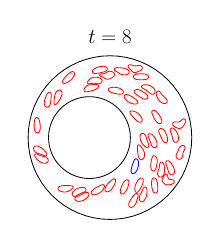
\begin{tikzpicture}[scale=0.3]

\begin{axis}[
  xmin = -21,
  xmax = 21,
  ymin = -21,
  ymax = 21,
  scale only axis,
  axis equal image,
  hide axis,
  title = {\Huge$t=8$}
  ]

% outer solid wall
\addplot [mark=none,black,line width=1.0] table{
2.0000e+01 -5.5171e-16
1.9904e+01 1.9603e+00
1.9616e+01 3.9018e+00
1.9139e+01 5.8057e+00
1.8478e+01 7.6537e+00
1.7638e+01 9.4279e+00
1.6629e+01 1.1111e+01
1.5460e+01 1.2688e+01
1.4142e+01 1.4142e+01
1.2688e+01 1.5460e+01
1.1111e+01 1.6629e+01
9.4279e+00 1.7638e+01
7.6537e+00 1.8478e+01
5.8057e+00 1.9139e+01
3.9018e+00 1.9616e+01
1.9603e+00 1.9904e+01
2.3281e-15 2.0000e+01
-1.9603e+00 1.9904e+01
-3.9018e+00 1.9616e+01
-5.8057e+00 1.9139e+01
-7.6537e+00 1.8478e+01
-9.4279e+00 1.7638e+01
-1.1111e+01 1.6629e+01
-1.2688e+01 1.5460e+01
-1.4142e+01 1.4142e+01
-1.5460e+01 1.2688e+01
-1.6629e+01 1.1111e+01
-1.7638e+01 9.4279e+00
-1.8478e+01 7.6537e+00
-1.9139e+01 5.8057e+00
-1.9616e+01 3.9018e+00
-1.9904e+01 1.9603e+00
-2.0000e+01 3.0010e-15
-1.9904e+01 -1.9603e+00
-1.9616e+01 -3.9018e+00
-1.9139e+01 -5.8057e+00
-1.8478e+01 -7.6537e+00
-1.7638e+01 -9.4279e+00
-1.6629e+01 -1.1111e+01
-1.5460e+01 -1.2688e+01
-1.4142e+01 -1.4142e+01
-1.2688e+01 -1.5460e+01
-1.1111e+01 -1.6629e+01
-9.4279e+00 -1.7638e+01
-7.6537e+00 -1.8478e+01
-5.8057e+00 -1.9139e+01
-3.9018e+00 -1.9616e+01
-1.9603e+00 -1.9904e+01
-4.7774e-15 -2.0000e+01
1.9603e+00 -1.9904e+01
3.9018e+00 -1.9616e+01
5.8057e+00 -1.9139e+01
7.6537e+00 -1.8478e+01
9.4279e+00 -1.7638e+01
1.1111e+01 -1.6629e+01
1.2688e+01 -1.5460e+01
1.4142e+01 -1.4142e+01
1.5460e+01 -1.2688e+01
1.6629e+01 -1.1111e+01
1.7638e+01 -9.4279e+00
1.8478e+01 -7.6537e+00
1.9139e+01 -5.8057e+00
1.9616e+01 -3.9018e+00
1.9904e+01 -1.9603e+00
2.0000e+01 -5.5171e-16
};

% inner solid wall
\addplot [mark=none,black,line width=1.0] table{
5.0000e+00 2.7586e-16
4.9518e+00 -9.8017e-01
4.8079e+00 -1.9509e+00
4.5694e+00 -2.9028e+00
4.2388e+00 -3.8268e+00
3.8192e+00 -4.7140e+00
3.3147e+00 -5.5557e+00
2.7301e+00 -6.3439e+00
2.0711e+00 -7.0711e+00
1.3439e+00 -7.7301e+00
5.5570e-01 -8.3147e+00
-2.8603e-01 -8.8192e+00
-1.1732e+00 -9.2388e+00
-2.0972e+00 -9.5694e+00
-3.0491e+00 -9.8079e+00
-4.0198e+00 -9.9518e+00
-5.0000e+00 -1.0000e+01
-5.9802e+00 -9.9518e+00
-6.9509e+00 -9.8079e+00
-7.9028e+00 -9.5694e+00
-8.8268e+00 -9.2388e+00
-9.7140e+00 -8.8192e+00
-1.0556e+01 -8.3147e+00
-1.1344e+01 -7.7301e+00
-1.2071e+01 -7.0711e+00
-1.2730e+01 -6.3439e+00
-1.3315e+01 -5.5557e+00
-1.3819e+01 -4.7140e+00
-1.4239e+01 -3.8268e+00
-1.4569e+01 -2.9028e+00
-1.4808e+01 -1.9509e+00
-1.4952e+01 -9.8017e-01
-1.5000e+01 -1.5005e-15
-1.4952e+01 9.8017e-01
-1.4808e+01 1.9509e+00
-1.4569e+01 2.9028e+00
-1.4239e+01 3.8268e+00
-1.3819e+01 4.7140e+00
-1.3315e+01 5.5557e+00
-1.2730e+01 6.3439e+00
-1.2071e+01 7.0711e+00
-1.1344e+01 7.7301e+00
-1.0556e+01 8.3147e+00
-9.7140e+00 8.8192e+00
-8.8268e+00 9.2388e+00
-7.9028e+00 9.5694e+00
-6.9509e+00 9.8079e+00
-5.9802e+00 9.9518e+00
-5.0000e+00 1.0000e+01
-4.0198e+00 9.9518e+00
-3.0491e+00 9.8079e+00
-2.0972e+00 9.5694e+00
-1.1732e+00 9.2388e+00
-2.8603e-01 8.8192e+00
5.5570e-01 8.3147e+00
1.3439e+00 7.7301e+00
2.0711e+00 7.0711e+00
2.7301e+00 6.3439e+00
3.3147e+00 5.5557e+00
3.8192e+00 4.7140e+00
4.2388e+00 3.8268e+00
4.5694e+00 2.9028e+00
4.8079e+00 1.9509e+00
4.9518e+00 9.8017e-01
5.0000e+00 2.7586e-16
};


% vesicle1
\addplot [mark=none,red,line width=1.0] table{
1.7757e+01 2.5862e+00
1.7796e+01 2.6291e+00
1.7849e+01 2.6906e+00
1.7913e+01 2.7719e+00
1.7984e+01 2.8699e+00
1.8058e+01 2.9795e+00
1.8134e+01 3.0977e+00
1.8211e+01 3.2217e+00
1.8286e+01 3.3508e+00
1.8358e+01 3.4844e+00
1.8425e+01 3.6234e+00
1.8480e+01 3.7685e+00
1.8517e+01 3.9202e+00
1.8528e+01 4.0765e+00
1.8505e+01 4.2319e+00
1.8439e+01 4.3748e+00
1.8331e+01 4.4894e+00
1.8191e+01 4.5600e+00
1.8035e+01 4.5789e+00
1.7881e+01 4.5487e+00
1.7740e+01 4.4808e+00
1.7614e+01 4.3884e+00
1.7499e+01 4.2835e+00
1.7389e+01 4.1756e+00
1.7278e+01 4.0724e+00
1.7160e+01 3.9806e+00
1.7035e+01 3.9057e+00
1.6906e+01 3.8510e+00
1.6778e+01 3.8168e+00
1.6658e+01 3.8000e+00
1.6555e+01 3.7952e+00
1.6474e+01 3.7966e+00
1.6416e+01 3.7998e+00
1.6358e+01 3.8043e+00
1.6277e+01 3.8120e+00
1.6174e+01 3.8226e+00
1.6053e+01 3.8327e+00
1.5921e+01 3.8357e+00
1.5781e+01 3.8227e+00
1.5641e+01 3.7841e+00
1.5511e+01 3.7113e+00
1.5407e+01 3.6018e+00
1.5343e+01 3.4623e+00
1.5329e+01 3.3084e+00
1.5363e+01 3.1563e+00
1.5435e+01 3.0171e+00
1.5534e+01 2.8948e+00
1.5651e+01 2.7886e+00
1.5778e+01 2.6952e+00
1.5912e+01 2.6111e+00
1.6049e+01 2.5340e+00
1.6190e+01 2.4627e+00
1.6333e+01 2.3975e+00
1.6478e+01 2.3397e+00
1.6626e+01 2.2917e+00
1.6776e+01 2.2568e+00
1.6926e+01 2.2384e+00
1.7076e+01 2.2397e+00
1.7220e+01 2.2618e+00
1.7354e+01 2.3037e+00
1.7473e+01 2.3606e+00
1.7575e+01 2.4260e+00
1.7656e+01 2.4901e+00
1.7716e+01 2.5448e+00
1.7757e+01 2.5862e+00
};

% vesicle2
\addplot [mark=none,red,line width=1.0] table{
-1.5412e+01 -6.1259e+00
-1.5363e+01 -6.0949e+00
-1.5298e+01 -6.0461e+00
-1.5224e+01 -5.9737e+00
-1.5154e+01 -5.8757e+00
-1.5100e+01 -5.7547e+00
-1.5075e+01 -5.6168e+00
-1.5083e+01 -5.4717e+00
-1.5123e+01 -5.3279e+00
-1.5189e+01 -5.1913e+00
-1.5277e+01 -5.0649e+00
-1.5382e+01 -4.9505e+00
-1.5501e+01 -4.8497e+00
-1.5633e+01 -4.7654e+00
-1.5776e+01 -4.6994e+00
-1.5926e+01 -4.6506e+00
-1.6080e+01 -4.6132e+00
-1.6235e+01 -4.5812e+00
-1.6389e+01 -4.5498e+00
-1.6543e+01 -4.5160e+00
-1.6696e+01 -4.4781e+00
-1.6846e+01 -4.4351e+00
-1.6994e+01 -4.3866e+00
-1.7138e+01 -4.3328e+00
-1.7278e+01 -4.2739e+00
-1.7414e+01 -4.2113e+00
-1.7544e+01 -4.1469e+00
-1.7670e+01 -4.0843e+00
-1.7790e+01 -4.0288e+00
-1.7904e+01 -3.9876e+00
-1.8005e+01 -3.9658e+00
-1.8086e+01 -3.9625e+00
-1.8144e+01 -3.9694e+00
-1.8200e+01 -3.9855e+00
-1.8271e+01 -4.0236e+00
-1.8342e+01 -4.0978e+00
-1.8389e+01 -4.2089e+00
-1.8394e+01 -4.3407e+00
-1.8364e+01 -4.4776e+00
-1.8310e+01 -4.6127e+00
-1.8240e+01 -4.7449e+00
-1.8160e+01 -4.8738e+00
-1.8071e+01 -4.9997e+00
-1.7976e+01 -5.1224e+00
-1.7875e+01 -5.2420e+00
-1.7770e+01 -5.3579e+00
-1.7659e+01 -5.4700e+00
-1.7543e+01 -5.5777e+00
-1.7423e+01 -5.6805e+00
-1.7299e+01 -5.7776e+00
-1.7170e+01 -5.8685e+00
-1.7036e+01 -5.9522e+00
-1.6899e+01 -6.0280e+00
-1.6757e+01 -6.0950e+00
-1.6613e+01 -6.1522e+00
-1.6466e+01 -6.1987e+00
-1.6318e+01 -6.2337e+00
-1.6171e+01 -6.2563e+00
-1.6025e+01 -6.2659e+00
-1.5885e+01 -6.2623e+00
-1.5754e+01 -6.2461e+00
-1.5636e+01 -6.2191e+00
-1.5538e+01 -6.1862e+00
-1.5464e+01 -6.1535e+00
-1.5412e+01 -6.1259e+00
};

% vesicle3
\addplot [mark=none,red,line width=1.0] table{
-1.6454e+01 -4.2301e+00
-1.6400e+01 -4.2525e+00
-1.6326e+01 -4.2838e+00
-1.6230e+01 -4.3239e+00
-1.6118e+01 -4.3696e+00
-1.5994e+01 -4.4146e+00
-1.5857e+01 -4.4493e+00
-1.5712e+01 -4.4574e+00
-1.5569e+01 -4.4184e+00
-1.5457e+01 -4.3188e+00
-1.5407e+01 -4.1749e+00
-1.5421e+01 -4.0210e+00
-1.5476e+01 -3.8749e+00
-1.5553e+01 -3.7378e+00
-1.5641e+01 -3.6075e+00
-1.5737e+01 -3.4821e+00
-1.5838e+01 -3.3607e+00
-1.5943e+01 -3.2427e+00
-1.6052e+01 -3.1280e+00
-1.6163e+01 -3.0164e+00
-1.6277e+01 -2.9082e+00
-1.6393e+01 -2.8036e+00
-1.6511e+01 -2.7032e+00
-1.6632e+01 -2.6074e+00
-1.6754e+01 -2.5169e+00
-1.6877e+01 -2.4325e+00
-1.7001e+01 -2.3550e+00
-1.7123e+01 -2.2856e+00
-1.7241e+01 -2.2254e+00
-1.7351e+01 -2.1757e+00
-1.7448e+01 -2.1377e+00
-1.7524e+01 -2.1113e+00
-1.7580e+01 -2.0942e+00
-1.7636e+01 -2.0789e+00
-1.7715e+01 -2.0609e+00
-1.7817e+01 -2.0441e+00
-1.7938e+01 -2.0343e+00
-1.8070e+01 -2.0386e+00
-1.8208e+01 -2.0632e+00
-1.8344e+01 -2.1149e+00
-1.8468e+01 -2.1982e+00
-1.8567e+01 -2.3130e+00
-1.8631e+01 -2.4522e+00
-1.8659e+01 -2.6047e+00
-1.8652e+01 -2.7607e+00
-1.8618e+01 -2.9139e+00
-1.8563e+01 -3.0611e+00
-1.8489e+01 -3.2008e+00
-1.8401e+01 -3.3317e+00
-1.8299e+01 -3.4524e+00
-1.8184e+01 -3.5605e+00
-1.8057e+01 -3.6532e+00
-1.7919e+01 -3.7288e+00
-1.7775e+01 -3.7893e+00
-1.7628e+01 -3.8393e+00
-1.7481e+01 -3.8840e+00
-1.7335e+01 -3.9265e+00
-1.7191e+01 -3.9689e+00
-1.7052e+01 -4.0119e+00
-1.6919e+01 -4.0556e+00
-1.6794e+01 -4.0990e+00
-1.6680e+01 -4.1408e+00
-1.6583e+01 -4.1780e+00
-1.6508e+01 -4.2080e+00
-1.6454e+01 -4.2301e+00
};

% vesicle4
\addplot [mark=none,red,line width=1.0] table{
6.4156e+00 1.4250e+01
6.4718e+00 1.4235e+01
6.5504e+00 1.4215e+01
6.6517e+00 1.4194e+01
6.7710e+00 1.4174e+01
6.9022e+00 1.4156e+01
7.0420e+00 1.4142e+01
7.1873e+00 1.4132e+01
7.3367e+00 1.4126e+01
7.4886e+00 1.4125e+01
7.6426e+00 1.4128e+01
7.7978e+00 1.4133e+01
7.9539e+00 1.4142e+01
8.1106e+00 1.4152e+01
8.2677e+00 1.4165e+01
8.4248e+00 1.4180e+01
8.5818e+00 1.4198e+01
8.7379e+00 1.4222e+01
8.8923e+00 1.4255e+01
9.0423e+00 1.4303e+01
9.1833e+00 1.4372e+01
9.3064e+00 1.4468e+01
9.3993e+00 1.4591e+01
9.4491e+00 1.4736e+01
9.4498e+00 1.4888e+01
9.4050e+00 1.5030e+01
9.3263e+00 1.5152e+01
9.2266e+00 1.5251e+01
9.1184e+00 1.5327e+01
9.0115e+00 1.5384e+01
8.9163e+00 1.5424e+01
8.8399e+00 1.5451e+01
8.7841e+00 1.5468e+01
8.7278e+00 1.5483e+01
8.6491e+00 1.5502e+01
8.5478e+00 1.5523e+01
8.4282e+00 1.5542e+01
8.2968e+00 1.5558e+01
8.1569e+00 1.5571e+01
8.0115e+00 1.5580e+01
7.8621e+00 1.5585e+01
7.7102e+00 1.5587e+01
7.5562e+00 1.5586e+01
7.4010e+00 1.5583e+01
7.2447e+00 1.5577e+01
7.0880e+00 1.5568e+01
6.9308e+00 1.5556e+01
6.7737e+00 1.5541e+01
6.6168e+00 1.5522e+01
6.4610e+00 1.5496e+01
6.3072e+00 1.5460e+01
6.1579e+00 1.5410e+01
6.0176e+00 1.5340e+01
5.8947e+00 1.5244e+01
5.8009e+00 1.5121e+01
5.7493e+00 1.4976e+01
5.7468e+00 1.4825e+01
5.7909e+00 1.4683e+01
5.8702e+00 1.4561e+01
5.9709e+00 1.4464e+01
6.0801e+00 1.4389e+01
6.1877e+00 1.4333e+01
6.2833e+00 1.4294e+01
6.3598e+00 1.4267e+01
6.4156e+00 1.4250e+01
};

% vesicle5
\addplot [mark=none,red,line width=1.0] table{
2.6991e+00 -1.3685e+01
2.7438e+00 -1.3722e+01
2.8134e+00 -1.3763e+01
2.9118e+00 -1.3795e+01
3.0323e+00 -1.3801e+01
3.1619e+00 -1.3775e+01
3.2905e+00 -1.3719e+01
3.4127e+00 -1.3640e+01
3.5275e+00 -1.3544e+01
3.6347e+00 -1.3436e+01
3.7352e+00 -1.3320e+01
3.8292e+00 -1.3196e+01
3.9174e+00 -1.3067e+01
3.9997e+00 -1.2933e+01
4.0768e+00 -1.2796e+01
4.1486e+00 -1.2655e+01
4.2157e+00 -1.2512e+01
4.2781e+00 -1.2367e+01
4.3362e+00 -1.2220e+01
4.3901e+00 -1.2072e+01
4.4401e+00 -1.1923e+01
4.4861e+00 -1.1774e+01
4.5281e+00 -1.1624e+01
4.5655e+00 -1.1475e+01
4.5978e+00 -1.1327e+01
4.6236e+00 -1.1179e+01
4.6410e+00 -1.1035e+01
4.6471e+00 -1.0895e+01
4.6390e+00 -1.0762e+01
4.6145e+00 -1.0644e+01
4.5767e+00 -1.0548e+01
4.5342e+00 -1.0479e+01
4.4963e+00 -1.0435e+01
4.4524e+00 -1.0396e+01
4.3831e+00 -1.0355e+01
4.2843e+00 -1.0325e+01
4.1636e+00 -1.0323e+01
4.0355e+00 -1.0355e+01
3.9093e+00 -1.0417e+01
3.7893e+00 -1.0499e+01
3.6751e+00 -1.0596e+01
3.5669e+00 -1.0702e+01
3.4641e+00 -1.0817e+01
3.3673e+00 -1.0938e+01
3.2765e+00 -1.1065e+01
3.1920e+00 -1.1198e+01
3.1134e+00 -1.1334e+01
3.0404e+00 -1.1474e+01
2.9725e+00 -1.1617e+01
2.9092e+00 -1.1762e+01
2.8499e+00 -1.1908e+01
2.7944e+00 -1.2056e+01
2.7425e+00 -1.2204e+01
2.6944e+00 -1.2353e+01
2.6503e+00 -1.2502e+01
2.6110e+00 -1.2650e+01
2.5774e+00 -1.2799e+01
2.5515e+00 -1.2946e+01
2.5352e+00 -1.3090e+01
2.5319e+00 -1.3231e+01
2.5440e+00 -1.3363e+01
2.5731e+00 -1.3480e+01
2.6148e+00 -1.3575e+01
2.6598e+00 -1.3642e+01
2.6991e+00 -1.3685e+01
};

% vesicle6
\addplot [mark=none,red,line width=1.0] table{
1.3403e+01 1.5554e+00
1.3370e+01 1.6036e+00
1.3322e+01 1.6690e+00
1.3258e+01 1.7500e+00
1.3177e+01 1.8404e+00
1.3082e+01 1.9323e+00
1.2973e+01 2.0205e+00
1.2850e+01 2.0986e+00
1.2714e+01 2.1611e+00
1.2568e+01 2.2006e+00
1.2414e+01 2.2093e+00
1.2263e+01 2.1787e+00
1.2126e+01 2.1045e+00
1.2020e+01 1.9897e+00
1.1955e+01 1.8469e+00
1.1930e+01 1.6912e+00
1.1939e+01 1.5337e+00
1.1970e+01 1.3788e+00
1.2015e+01 1.2277e+00
1.2070e+01 1.0798e+00
1.2130e+01 9.3466e-01
1.2193e+01 7.9150e-01
1.2257e+01 6.5023e-01
1.2322e+01 5.1046e-01
1.2386e+01 3.7271e-01
1.2449e+01 2.3711e-01
1.2510e+01 1.0498e-01
1.2569e+01 -2.2602e-02
1.2624e+01 -1.4276e-01
1.2676e+01 -2.5255e-01
1.2720e+01 -3.4601e-01
1.2755e+01 -4.1887e-01
1.2781e+01 -4.7121e-01
1.2807e+01 -5.2334e-01
1.2845e+01 -5.9512e-01
1.2895e+01 -6.8569e-01
1.2957e+01 -7.8952e-01
1.3032e+01 -8.9869e-01
1.3122e+01 -1.0069e+00
1.3229e+01 -1.1054e+00
1.3355e+01 -1.1840e+00
1.3500e+01 -1.2292e+00
1.3653e+01 -1.2288e+00
1.3799e+01 -1.1770e+00
1.3920e+01 -1.0796e+00
1.4008e+01 -9.5020e-01
1.4063e+01 -8.0293e-01
1.4091e+01 -6.4751e-01
1.4097e+01 -4.8974e-01
1.4087e+01 -3.3200e-01
1.4065e+01 -1.7566e-01
1.4035e+01 -2.0915e-02
1.3999e+01 1.3179e-01
1.3958e+01 2.8259e-01
1.3912e+01 4.3101e-01
1.3863e+01 5.7705e-01
1.3811e+01 7.1994e-01
1.3757e+01 8.5927e-01
1.3701e+01 9.9359e-01
1.3643e+01 1.1217e+00
1.3585e+01 1.2406e+00
1.3529e+01 1.3477e+00
1.3477e+01 1.4375e+00
1.3435e+01 1.5064e+00
1.3403e+01 1.5554e+00
};

% vesicle7
\addplot [mark=none,red,line width=1.0] table{
7.1454e+00 1.6239e+01
7.1984e+00 1.6263e+01
7.2715e+00 1.6298e+01
7.3638e+00 1.6345e+01
7.4696e+00 1.6404e+01
7.5809e+00 1.6475e+01
7.6909e+00 1.6563e+01
7.7906e+00 1.6669e+01
7.8702e+00 1.6795e+01
7.9177e+00 1.6939e+01
7.9240e+00 1.7092e+01
7.8846e+00 1.7242e+01
7.8031e+00 1.7374e+01
7.6882e+00 1.7481e+01
7.5509e+00 1.7557e+01
7.4006e+00 1.7605e+01
7.2444e+00 1.7628e+01
7.0864e+00 1.7631e+01
6.9290e+00 1.7620e+01
6.7726e+00 1.7600e+01
6.6174e+00 1.7577e+01
6.4625e+00 1.7555e+01
6.3082e+00 1.7538e+01
6.1544e+00 1.7531e+01
6.0026e+00 1.7536e+01
5.8543e+00 1.7555e+01
5.7121e+00 1.7586e+01
5.5776e+00 1.7626e+01
5.4528e+00 1.7670e+01
5.3391e+00 1.7712e+01
5.2413e+00 1.7746e+01
5.1638e+00 1.7769e+01
5.1071e+00 1.7783e+01
5.0498e+00 1.7794e+01
4.9694e+00 1.7803e+01
4.8660e+00 1.7802e+01
4.7474e+00 1.7779e+01
4.6279e+00 1.7723e+01
4.5250e+00 1.7628e+01
4.4588e+00 1.7499e+01
4.4432e+00 1.7352e+01
4.4804e+00 1.7205e+01
4.5599e+00 1.7074e+01
4.6661e+00 1.6960e+01
4.7847e+00 1.6859e+01
4.9057e+00 1.6758e+01
5.0214e+00 1.6652e+01
5.1281e+00 1.6535e+01
5.2263e+00 1.6412e+01
5.3221e+00 1.6286e+01
5.4237e+00 1.6165e+01
5.5390e+00 1.6058e+01
5.6708e+00 1.5973e+01
5.8164e+00 1.5917e+01
5.9693e+00 1.5891e+01
6.1231e+00 1.5892e+01
6.2733e+00 1.5915e+01
6.4182e+00 1.5952e+01
6.5567e+00 1.5997e+01
6.6884e+00 1.6045e+01
6.8113e+00 1.6095e+01
6.9231e+00 1.6141e+01
7.0181e+00 1.6182e+01
7.0922e+00 1.6215e+01
7.1454e+00 1.6239e+01
};

% vesicle8
\addplot [mark=none,red,line width=1.0] table{
7.2899e+00 1.1612e+01
7.2352e+00 1.1632e+01
7.1584e+00 1.1658e+01
7.0588e+00 1.1686e+01
6.9403e+00 1.1711e+01
6.8092e+00 1.1729e+01
6.6689e+00 1.1736e+01
6.5235e+00 1.1728e+01
6.3762e+00 1.1704e+01
6.2317e+00 1.1657e+01
6.0970e+00 1.1583e+01
5.9852e+00 1.1476e+01
5.9149e+00 1.1338e+01
5.9032e+00 1.1182e+01
5.9493e+00 1.1032e+01
6.0368e+00 1.0901e+01
6.1473e+00 1.0788e+01
6.2692e+00 1.0688e+01
6.3959e+00 1.0594e+01
6.5246e+00 1.0503e+01
6.6535e+00 1.0413e+01
6.7818e+00 1.0324e+01
6.9088e+00 1.0234e+01
7.0344e+00 1.0145e+01
7.1579e+00 1.0057e+01
7.2796e+00 9.9698e+00
7.3987e+00 9.8861e+00
7.5150e+00 9.8072e+00
7.6263e+00 9.7355e+00
7.7301e+00 9.6731e+00
7.8205e+00 9.6228e+00
7.8926e+00 9.5860e+00
7.9452e+00 9.5608e+00
7.9985e+00 9.5370e+00
8.0735e+00 9.5064e+00
8.1710e+00 9.4719e+00
8.2874e+00 9.4386e+00
8.4171e+00 9.4123e+00
8.5568e+00 9.3979e+00
8.7023e+00 9.4005e+00
8.8496e+00 9.4253e+00
8.9917e+00 9.4782e+00
9.1193e+00 9.5637e+00
9.2187e+00 9.6822e+00
9.2771e+00 9.8265e+00
9.2876e+00 9.9826e+00
9.2535e+00 1.0136e+01
9.1844e+00 1.0278e+01
9.0916e+00 1.0405e+01
8.9835e+00 1.0521e+01
8.8663e+00 1.0626e+01
8.7433e+00 1.0725e+01
8.6172e+00 1.0818e+01
8.4893e+00 1.0908e+01
8.3607e+00 1.0995e+01
8.2321e+00 1.1080e+01
8.1046e+00 1.1163e+01
7.9783e+00 1.1243e+01
7.8545e+00 1.1319e+01
7.7338e+00 1.1391e+01
7.6186e+00 1.1457e+01
7.5114e+00 1.1513e+01
7.4182e+00 1.1558e+01
7.3440e+00 1.1590e+01
7.2899e+00 1.1612e+01
};

% vesicle9
\addplot [mark=none,red,line width=1.0] table{
5.9317e+00 9.6268e+00
5.8837e+00 9.6601e+00
5.8170e+00 9.7059e+00
5.7314e+00 9.7640e+00
5.6306e+00 9.8312e+00
5.5198e+00 9.9037e+00
5.4012e+00 9.9791e+00
5.2771e+00 1.0055e+01
5.1477e+00 1.0130e+01
5.0141e+00 1.0202e+01
4.8760e+00 1.0271e+01
4.7339e+00 1.0333e+01
4.5879e+00 1.0390e+01
4.4386e+00 1.0438e+01
4.2859e+00 1.0477e+01
4.1304e+00 1.0504e+01
3.9727e+00 1.0514e+01
3.8158e+00 1.0498e+01
3.6681e+00 1.0444e+01
3.5496e+00 1.0342e+01
3.4821e+00 1.0201e+01
3.4705e+00 1.0046e+01
3.5014e+00 9.8941e+00
3.5594e+00 9.7516e+00
3.6335e+00 9.6190e+00
3.7176e+00 9.4955e+00
3.8076e+00 9.3810e+00
3.9005e+00 9.2756e+00
3.9927e+00 9.1806e+00
4.0804e+00 9.0971e+00
4.1577e+00 9.0283e+00
4.2195e+00 8.9761e+00
4.2648e+00 8.9393e+00
4.3107e+00 8.9033e+00
4.3752e+00 8.8544e+00
4.4592e+00 8.7941e+00
4.5597e+00 8.7263e+00
4.6719e+00 8.6560e+00
4.7936e+00 8.5859e+00
4.9226e+00 8.5184e+00
5.0580e+00 8.4549e+00
5.1983e+00 8.3966e+00
5.3431e+00 8.3442e+00
5.4915e+00 8.2986e+00
5.6431e+00 8.2603e+00
5.7971e+00 8.2299e+00
5.9532e+00 8.2082e+00
6.1106e+00 8.1970e+00
6.2687e+00 8.1990e+00
6.4252e+00 8.2195e+00
6.5756e+00 8.2667e+00
6.7080e+00 8.3509e+00
6.8017e+00 8.4756e+00
6.8363e+00 8.6269e+00
6.8111e+00 8.7793e+00
6.7431e+00 8.9171e+00
6.6514e+00 9.0381e+00
6.5478e+00 9.1458e+00
6.4398e+00 9.2434e+00
6.3313e+00 9.3327e+00
6.2266e+00 9.4138e+00
6.1294e+00 9.4860e+00
6.0455e+00 9.5466e+00
5.9795e+00 9.5934e+00
5.9317e+00 9.6268e+00
};

% vesicle10
\addplot [mark=none,red,line width=1.0] table{
1.3095e+01 -9.1356e+00
1.3122e+01 -9.0837e+00
1.3156e+01 -9.0105e+00
1.3195e+01 -8.9148e+00
1.3235e+01 -8.8003e+00
1.3270e+01 -8.6727e+00
1.3299e+01 -8.5353e+00
1.3321e+01 -8.3913e+00
1.3337e+01 -8.2426e+00
1.3346e+01 -8.0910e+00
1.3350e+01 -7.9370e+00
1.3349e+01 -7.7818e+00
1.3344e+01 -7.6255e+00
1.3335e+01 -7.4688e+00
1.3321e+01 -7.3117e+00
1.3303e+01 -7.1549e+00
1.3280e+01 -6.9985e+00
1.3251e+01 -6.8433e+00
1.3215e+01 -6.6897e+00
1.3168e+01 -6.5392e+00
1.3108e+01 -6.3940e+00
1.3030e+01 -6.2588e+00
1.2929e+01 -6.1411e+00
1.2804e+01 -6.0534e+00
1.2659e+01 -6.0104e+00
1.2511e+01 -6.0232e+00
1.2381e+01 -6.0883e+00
1.2284e+01 -6.1891e+00
1.2219e+01 -6.3043e+00
1.2179e+01 -6.4186e+00
1.2155e+01 -6.5192e+00
1.2141e+01 -6.5988e+00
1.2133e+01 -6.6566e+00
1.2125e+01 -6.7145e+00
1.2115e+01 -6.7948e+00
1.2103e+01 -6.8975e+00
1.2087e+01 -7.0177e+00
1.2068e+01 -7.1487e+00
1.2044e+01 -7.2871e+00
1.2014e+01 -7.4296e+00
1.1977e+01 -7.5745e+00
1.1934e+01 -7.7203e+00
1.1886e+01 -7.8664e+00
1.1834e+01 -8.0126e+00
1.1780e+01 -8.1597e+00
1.1730e+01 -8.3085e+00
1.1689e+01 -8.4605e+00
1.1661e+01 -8.6158e+00
1.1652e+01 -8.7735e+00
1.1666e+01 -8.9307e+00
1.1704e+01 -9.0838e+00
1.1767e+01 -9.2278e+00
1.1854e+01 -9.3583e+00
1.1963e+01 -9.4702e+00
1.2090e+01 -9.5592e+00
1.2231e+01 -9.6197e+00
1.2381e+01 -9.6471e+00
1.2529e+01 -9.6377e+00
1.2668e+01 -9.5932e+00
1.2788e+01 -9.5207e+00
1.2886e+01 -9.4324e+00
1.2965e+01 -9.3401e+00
1.3024e+01 -9.2555e+00
1.3066e+01 -9.1865e+00
1.3095e+01 -9.1356e+00
};

% vesicle11
\addplot [mark=none,red,line width=1.0] table{
-7.5436e+00 -1.2284e+01
-7.5998e+00 -1.2300e+01
-7.6773e+00 -1.2323e+01
-7.7755e+00 -1.2356e+01
-7.8892e+00 -1.2397e+01
-8.0118e+00 -1.2448e+01
-8.1394e+00 -1.2506e+01
-8.2684e+00 -1.2574e+01
-8.3967e+00 -1.2651e+01
-8.5221e+00 -1.2736e+01
-8.6436e+00 -1.2831e+01
-8.7599e+00 -1.2934e+01
-8.8702e+00 -1.3045e+01
-8.9727e+00 -1.3164e+01
-9.0651e+00 -1.3291e+01
-9.1432e+00 -1.3428e+01
-9.2017e+00 -1.3575e+01
-9.2335e+00 -1.3729e+01
-9.2314e+00 -1.3887e+01
-9.1895e+00 -1.4038e+01
-9.1077e+00 -1.4172e+01
-8.9919e+00 -1.4276e+01
-8.8528e+00 -1.4344e+01
-8.7020e+00 -1.4373e+01
-8.5506e+00 -1.4366e+01
-8.4061e+00 -1.4328e+01
-8.2725e+00 -1.4271e+01
-8.1493e+00 -1.4203e+01
-8.0363e+00 -1.4134e+01
-7.9337e+00 -1.4070e+01
-7.8461e+00 -1.4015e+01
-7.7771e+00 -1.3972e+01
-7.7272e+00 -1.3942e+01
-7.6769e+00 -1.3912e+01
-7.6067e+00 -1.3872e+01
-7.5162e+00 -1.3822e+01
-7.4090e+00 -1.3765e+01
-7.2904e+00 -1.3707e+01
-7.1629e+00 -1.3648e+01
-7.0291e+00 -1.3590e+01
-6.8902e+00 -1.3535e+01
-6.7478e+00 -1.3482e+01
-6.6028e+00 -1.3430e+01
-6.4568e+00 -1.3377e+01
-6.3119e+00 -1.3318e+01
-6.1724e+00 -1.3247e+01
-6.0448e+00 -1.3154e+01
-5.9396e+00 -1.3037e+01
-5.8684e+00 -1.2897e+01
-5.8418e+00 -1.2742e+01
-5.8643e+00 -1.2586e+01
-5.9343e+00 -1.2445e+01
-6.0422e+00 -1.2332e+01
-6.1753e+00 -1.2251e+01
-6.3213e+00 -1.2198e+01
-6.4724e+00 -1.2169e+01
-6.6238e+00 -1.2157e+01
-6.7733e+00 -1.2157e+01
-6.9185e+00 -1.2166e+01
-7.0581e+00 -1.2183e+01
-7.1889e+00 -1.2203e+01
-7.3078e+00 -1.2226e+01
-7.4087e+00 -1.2249e+01
-7.4872e+00 -1.2269e+01
-7.5436e+00 -1.2284e+01
};

% vesicle12
\addplot [mark=none,red,line width=1.0] table{
1.2987e+01 1.0208e+01
1.2945e+01 1.0248e+01
1.2888e+01 1.0306e+01
1.2817e+01 1.0381e+01
1.2738e+01 1.0473e+01
1.2656e+01 1.0577e+01
1.2575e+01 1.0692e+01
1.2496e+01 1.0814e+01
1.2415e+01 1.0940e+01
1.2330e+01 1.1065e+01
1.2231e+01 1.1183e+01
1.2112e+01 1.1283e+01
1.1972e+01 1.1352e+01
1.1818e+01 1.1376e+01
1.1664e+01 1.1349e+01
1.1527e+01 1.1270e+01
1.1423e+01 1.1153e+01
1.1356e+01 1.1010e+01
1.1325e+01 1.0856e+01
1.1324e+01 1.0698e+01
1.1344e+01 1.0543e+01
1.1378e+01 1.0390e+01
1.1420e+01 1.0241e+01
1.1467e+01 1.0094e+01
1.1518e+01 9.9509e+00
1.1574e+01 9.8120e+00
1.1633e+01 9.6792e+00
1.1697e+01 9.5538e+00
1.1762e+01 9.4389e+00
1.1828e+01 9.3369e+00
1.1887e+01 9.2523e+00
1.1936e+01 9.1880e+00
1.1973e+01 9.1425e+00
1.2010e+01 9.0979e+00
1.2064e+01 9.0374e+00
1.2136e+01 8.9625e+00
1.2223e+01 8.8783e+00
1.2322e+01 8.7906e+00
1.2431e+01 8.7028e+00
1.2550e+01 8.6180e+00
1.2676e+01 8.5380e+00
1.2810e+01 8.4656e+00
1.2950e+01 8.4029e+00
1.3097e+01 8.3537e+00
1.3250e+01 8.3220e+00
1.3407e+01 8.3134e+00
1.3563e+01 8.3335e+00
1.3711e+01 8.3877e+00
1.3840e+01 8.4776e+00
1.3939e+01 8.6001e+00
1.3999e+01 8.7456e+00
1.4016e+01 8.9018e+00
1.3994e+01 9.0569e+00
1.3940e+01 9.2035e+00
1.3864e+01 9.3385e+00
1.3772e+01 9.4622e+00
1.3672e+01 9.5761e+00
1.3566e+01 9.6822e+00
1.3460e+01 9.7817e+00
1.3355e+01 9.8756e+00
1.3256e+01 9.9632e+00
1.3165e+01 1.0044e+01
1.3089e+01 1.0113e+01
1.3029e+01 1.0168e+01
1.2987e+01 1.0208e+01
};

% vesicle13
\addplot [mark=none,red,line width=1.0] table{
-1.1244e+00 1.7355e+01
-1.1807e+00 1.7371e+01
-1.2597e+00 1.7388e+01
-1.3618e+00 1.7405e+01
-1.4823e+00 1.7417e+01
-1.6145e+00 1.7423e+01
-1.7550e+00 1.7423e+01
-1.9004e+00 1.7417e+01
-2.0494e+00 1.7404e+01
-2.2002e+00 1.7385e+01
-2.3523e+00 1.7361e+01
-2.5046e+00 1.7331e+01
-2.6569e+00 1.7296e+01
-2.8084e+00 1.7254e+01
-2.9588e+00 1.7207e+01
-3.1075e+00 1.7155e+01
-3.2542e+00 1.7096e+01
-3.3980e+00 1.7030e+01
-3.5386e+00 1.6958e+01
-3.6751e+00 1.6880e+01
-3.8066e+00 1.6794e+01
-3.9314e+00 1.6700e+01
-4.0473e+00 1.6597e+01
-4.1497e+00 1.6482e+01
-4.2308e+00 1.6353e+01
-4.2782e+00 1.6212e+01
-4.2798e+00 1.6067e+01
-4.2317e+00 1.5936e+01
-4.1468e+00 1.5835e+01
-4.0460e+00 1.5769e+01
-3.9503e+00 1.5730e+01
-3.8720e+00 1.5709e+01
-3.8146e+00 1.5699e+01
-3.7567e+00 1.5691e+01
-3.6760e+00 1.5685e+01
-3.5726e+00 1.5682e+01
-3.4515e+00 1.5685e+01
-3.3194e+00 1.5692e+01
-3.1794e+00 1.5705e+01
-3.0348e+00 1.5722e+01
-2.8869e+00 1.5743e+01
-2.7370e+00 1.5769e+01
-2.5857e+00 1.5797e+01
-2.4335e+00 1.5828e+01
-2.2805e+00 1.5860e+01
-2.1273e+00 1.5895e+01
-1.9739e+00 1.5931e+01
-1.8211e+00 1.5970e+01
-1.6689e+00 1.6013e+01
-1.5181e+00 1.6060e+01
-1.3689e+00 1.6112e+01
-1.2224e+00 1.6170e+01
-1.0803e+00 1.6237e+01
-9.4620e-01 1.6317e+01
-8.2559e-01 1.6414e+01
-7.2731e-01 1.6532e+01
-6.6130e-01 1.6669e+01
-6.3736e-01 1.6816e+01
-6.5857e-01 1.6959e+01
-7.1954e-01 1.7085e+01
-8.0611e-01 1.7185e+01
-9.0282e-01 1.7258e+01
-9.9399e-01 1.7306e+01
-1.0690e+00 1.7337e+01
-1.1244e+00 1.7355e+01
};

% vesicle14
\addplot [mark=none,red,line width=1.0] table{
-6.6835e+00 -1.3754e+01
-6.7338e+00 -1.3783e+01
-6.8037e+00 -1.3824e+01
-6.8933e+00 -1.3876e+01
-6.9990e+00 -1.3935e+01
-7.1154e+00 -1.3998e+01
-7.2402e+00 -1.4063e+01
-7.3711e+00 -1.4127e+01
-7.5071e+00 -1.4189e+01
-7.6469e+00 -1.4248e+01
-7.7899e+00 -1.4305e+01
-7.9346e+00 -1.4362e+01
-8.0794e+00 -1.4421e+01
-8.2204e+00 -1.4490e+01
-8.3512e+00 -1.4577e+01
-8.4602e+00 -1.4691e+01
-8.5337e+00 -1.4830e+01
-8.5587e+00 -1.4985e+01
-8.5304e+00 -1.5140e+01
-8.4535e+00 -1.5277e+01
-8.3415e+00 -1.5386e+01
-8.2078e+00 -1.5467e+01
-8.0629e+00 -1.5522e+01
-7.9129e+00 -1.5557e+01
-7.7621e+00 -1.5575e+01
-7.6127e+00 -1.5580e+01
-7.4672e+00 -1.5574e+01
-7.3275e+00 -1.5560e+01
-7.1967e+00 -1.5539e+01
-7.0781e+00 -1.5514e+01
-6.9778e+00 -1.5489e+01
-6.8999e+00 -1.5467e+01
-6.8441e+00 -1.5450e+01
-6.7887e+00 -1.5432e+01
-6.7124e+00 -1.5405e+01
-6.6159e+00 -1.5367e+01
-6.5046e+00 -1.5320e+01
-6.3850e+00 -1.5263e+01
-6.2607e+00 -1.5197e+01
-6.1351e+00 -1.5124e+01
-6.0096e+00 -1.5043e+01
-5.8862e+00 -1.4954e+01
-5.7655e+00 -1.4858e+01
-5.6492e+00 -1.4755e+01
-5.5377e+00 -1.4646e+01
-5.4328e+00 -1.4529e+01
-5.3357e+00 -1.4405e+01
-5.2494e+00 -1.4273e+01
-5.1784e+00 -1.4132e+01
-5.1319e+00 -1.3981e+01
-5.1240e+00 -1.3824e+01
-5.1684e+00 -1.3674e+01
-5.2625e+00 -1.3549e+01
-5.3899e+00 -1.3459e+01
-5.5343e+00 -1.3403e+01
-5.6860e+00 -1.3378e+01
-5.8378e+00 -1.3381e+01
-5.9846e+00 -1.3408e+01
-6.1228e+00 -1.3453e+01
-6.2513e+00 -1.3510e+01
-6.3687e+00 -1.3571e+01
-6.4742e+00 -1.3631e+01
-6.5636e+00 -1.3683e+01
-6.6333e+00 -1.3724e+01
-6.6835e+00 -1.3754e+01
};

% vesicle15
\addplot [mark=none,red,line width=1.0] table{
-1.7046e+01 3.0337e+00
-1.7051e+01 3.0919e+00
-1.7059e+01 3.1725e+00
-1.7071e+01 3.2752e+00
-1.7087e+01 3.3954e+00
-1.7107e+01 3.5262e+00
-1.7132e+01 3.6646e+00
-1.7161e+01 3.8071e+00
-1.7196e+01 3.9525e+00
-1.7238e+01 4.0987e+00
-1.7287e+01 4.2447e+00
-1.7345e+01 4.3886e+00
-1.7415e+01 4.5282e+00
-1.7502e+01 4.6592e+00
-1.7609e+01 4.7746e+00
-1.7740e+01 4.8606e+00
-1.7893e+01 4.8967e+00
-1.8047e+01 4.8654e+00
-1.8174e+01 4.7735e+00
-1.8265e+01 4.6455e+00
-1.8329e+01 4.5022e+00
-1.8375e+01 4.3529e+00
-1.8410e+01 4.2017e+00
-1.8438e+01 4.0502e+00
-1.8460e+01 3.8999e+00
-1.8479e+01 3.7515e+00
-1.8493e+01 3.6067e+00
-1.8505e+01 3.4666e+00
-1.8514e+01 3.3345e+00
-1.8521e+01 3.2135e+00
-1.8525e+01 3.1101e+00
-1.8528e+01 3.0291e+00
-1.8529e+01 2.9707e+00
-1.8529e+01 2.9123e+00
-1.8530e+01 2.8313e+00
-1.8528e+01 2.7279e+00
-1.8524e+01 2.6068e+00
-1.8515e+01 2.4746e+00
-1.8501e+01 2.3348e+00
-1.8481e+01 2.1906e+00
-1.8453e+01 2.0438e+00
-1.8415e+01 1.8967e+00
-1.8366e+01 1.7508e+00
-1.8302e+01 1.6091e+00
-1.8223e+01 1.4748e+00
-1.8123e+01 1.3535e+00
-1.8002e+01 1.2533e+00
-1.7860e+01 1.1858e+00
-1.7704e+01 1.1631e+00
-1.7549e+01 1.1923e+00
-1.7412e+01 1.2687e+00
-1.7301e+01 1.3796e+00
-1.7215e+01 1.5112e+00
-1.7152e+01 1.6541e+00
-1.7106e+01 1.8022e+00
-1.7073e+01 1.9527e+00
-1.7051e+01 2.1029e+00
-1.7036e+01 2.2518e+00
-1.7028e+01 2.3971e+00
-1.7026e+01 2.5376e+00
-1.7027e+01 2.6700e+00
-1.7031e+01 2.7912e+00
-1.7036e+01 2.8945e+00
-1.7042e+01 2.9754e+00
-1.7046e+01 3.0337e+00
};

% vesicle16
\addplot [mark=none,red,line width=1.0] table{
9.5459e+00 1.1051e+01
9.5885e+00 1.1011e+01
9.6479e+00 1.0956e+01
9.7250e+00 1.0887e+01
9.8184e+00 1.0810e+01
9.9263e+00 1.0733e+01
1.0049e+01 1.0665e+01
1.0185e+01 1.0613e+01
1.0332e+01 1.0587e+01
1.0483e+01 1.0592e+01
1.0632e+01 1.0633e+01
1.0766e+01 1.0710e+01
1.0878e+01 1.0818e+01
1.0959e+01 1.0952e+01
1.1009e+01 1.1101e+01
1.1028e+01 1.1258e+01
1.1018e+01 1.1415e+01
1.0984e+01 1.1569e+01
1.0929e+01 1.1717e+01
1.0856e+01 1.1857e+01
1.0769e+01 1.1988e+01
1.0671e+01 1.2110e+01
1.0564e+01 1.2222e+01
1.0449e+01 1.2324e+01
1.0329e+01 1.2417e+01
1.0205e+01 1.2501e+01
1.0079e+01 1.2574e+01
9.9543e+00 1.2639e+01
9.8335e+00 1.2693e+01
9.7207e+00 1.2737e+01
9.6229e+00 1.2771e+01
9.5455e+00 1.2795e+01
9.4893e+00 1.2810e+01
9.4328e+00 1.2825e+01
9.3540e+00 1.2844e+01
9.2526e+00 1.2864e+01
9.1332e+00 1.2884e+01
9.0019e+00 1.2901e+01
8.8619e+00 1.2914e+01
8.7165e+00 1.2921e+01
8.5670e+00 1.2921e+01
8.4153e+00 1.2913e+01
8.2625e+00 1.2895e+01
8.1114e+00 1.2859e+01
7.9669e+00 1.2800e+01
7.8408e+00 1.2708e+01
7.7527e+00 1.2578e+01
7.7259e+00 1.2424e+01
7.7671e+00 1.2272e+01
7.8608e+00 1.2146e+01
7.9839e+00 1.2048e+01
8.1205e+00 1.1969e+01
8.2618e+00 1.1901e+01
8.4038e+00 1.1835e+01
8.5439e+00 1.1768e+01
8.6809e+00 1.1698e+01
8.8133e+00 1.1623e+01
8.9403e+00 1.1544e+01
9.0605e+00 1.1462e+01
9.1729e+00 1.1378e+01
9.2757e+00 1.1295e+01
9.3673e+00 1.1215e+01
9.4440e+00 1.1146e+01
9.5033e+00 1.1091e+01
9.5459e+00 1.1051e+01
};

% vesicle17
\addplot [mark=none,red,line width=1.0] table{
-9.3340e+00 -1.1783e+01
-9.3918e+00 -1.1775e+01
-9.4724e+00 -1.1768e+01
-9.5757e+00 -1.1761e+01
-9.6967e+00 -1.1756e+01
-9.8290e+00 -1.1750e+01
-9.9694e+00 -1.1745e+01
-1.0115e+01 -1.1740e+01
-1.0264e+01 -1.1735e+01
-1.0416e+01 -1.1731e+01
-1.0570e+01 -1.1728e+01
-1.0726e+01 -1.1726e+01
-1.0882e+01 -1.1727e+01
-1.1039e+01 -1.1729e+01
-1.1196e+01 -1.1734e+01
-1.1354e+01 -1.1743e+01
-1.1512e+01 -1.1755e+01
-1.1669e+01 -1.1771e+01
-1.1825e+01 -1.1794e+01
-1.1980e+01 -1.1824e+01
-1.2132e+01 -1.1863e+01
-1.2279e+01 -1.1916e+01
-1.2417e+01 -1.1987e+01
-1.2539e+01 -1.2080e+01
-1.2634e+01 -1.2198e+01
-1.2688e+01 -1.2336e+01
-1.2693e+01 -1.2481e+01
-1.2654e+01 -1.2616e+01
-1.2586e+01 -1.2729e+01
-1.2505e+01 -1.2820e+01
-1.2428e+01 -1.2888e+01
-1.2363e+01 -1.2936e+01
-1.2314e+01 -1.2968e+01
-1.2264e+01 -1.2998e+01
-1.2193e+01 -1.3037e+01
-1.2100e+01 -1.3083e+01
-1.1988e+01 -1.3130e+01
-1.1864e+01 -1.3174e+01
-1.1729e+01 -1.3214e+01
-1.1587e+01 -1.3248e+01
-1.1440e+01 -1.3274e+01
-1.1289e+01 -1.3291e+01
-1.1135e+01 -1.3300e+01
-1.0980e+01 -1.3300e+01
-1.0824e+01 -1.3289e+01
-1.0669e+01 -1.3268e+01
-1.0514e+01 -1.3236e+01
-1.0363e+01 -1.3193e+01
-1.0214e+01 -1.3139e+01
-1.0070e+01 -1.3075e+01
-9.9298e+00 -1.3001e+01
-9.7948e+00 -1.2920e+01
-9.6638e+00 -1.2833e+01
-9.5366e+00 -1.2743e+01
-9.4125e+00 -1.2649e+01
-9.2925e+00 -1.2553e+01
-9.1789e+00 -1.2452e+01
-9.0792e+00 -1.2341e+01
-9.0071e+00 -1.2215e+01
-8.9848e+00 -1.2077e+01
-9.0242e+00 -1.1952e+01
-9.1074e+00 -1.1865e+01
-9.1990e+00 -1.1817e+01
-9.2766e+00 -1.1794e+01
-9.3340e+00 -1.1783e+01
};

% vesicle18
\addplot [mark=none,red,line width=1.0] table{
4.7686e+00 -1.6863e+01
4.8080e+00 -1.6906e+01
4.8692e+00 -1.6958e+01
4.9576e+00 -1.7012e+01
5.0714e+00 -1.7053e+01
5.2026e+00 -1.7069e+01
5.3422e+00 -1.7055e+01
5.4812e+00 -1.7012e+01
5.6144e+00 -1.6945e+01
5.7388e+00 -1.6858e+01
5.8540e+00 -1.6756e+01
5.9600e+00 -1.6642e+01
6.0578e+00 -1.6520e+01
6.1477e+00 -1.6392e+01
6.2304e+00 -1.6258e+01
6.3062e+00 -1.6119e+01
6.3755e+00 -1.5977e+01
6.4382e+00 -1.5832e+01
6.4949e+00 -1.5685e+01
6.5458e+00 -1.5535e+01
6.5922e+00 -1.5385e+01
6.6350e+00 -1.5235e+01
6.6760e+00 -1.5085e+01
6.7161e+00 -1.4937e+01
6.7562e+00 -1.4790e+01
6.7950e+00 -1.4646e+01
6.8301e+00 -1.4504e+01
6.8570e+00 -1.4367e+01
6.8713e+00 -1.4235e+01
6.8698e+00 -1.4114e+01
6.8543e+00 -1.4012e+01
6.8310e+00 -1.3934e+01
6.8077e+00 -1.3881e+01
6.7784e+00 -1.3830e+01
6.7278e+00 -1.3767e+01
6.6466e+00 -1.3704e+01
6.5333e+00 -1.3663e+01
6.4018e+00 -1.3667e+01
6.2719e+00 -1.3719e+01
6.1541e+00 -1.3804e+01
6.0461e+00 -1.3908e+01
5.9433e+00 -1.4020e+01
5.8422e+00 -1.4136e+01
5.7416e+00 -1.4254e+01
5.6416e+00 -1.4374e+01
5.5426e+00 -1.4496e+01
5.4452e+00 -1.4620e+01
5.3501e+00 -1.4746e+01
5.2574e+00 -1.4874e+01
5.1678e+00 -1.5004e+01
5.0814e+00 -1.5136e+01
4.9989e+00 -1.5270e+01
4.9207e+00 -1.5407e+01
4.8480e+00 -1.5545e+01
4.7817e+00 -1.5685e+01
4.7235e+00 -1.5828e+01
4.6751e+00 -1.5972e+01
4.6389e+00 -1.6117e+01
4.6170e+00 -1.6261e+01
4.6119e+00 -1.6401e+01
4.6244e+00 -1.6533e+01
4.6535e+00 -1.6650e+01
4.6929e+00 -1.6746e+01
4.7338e+00 -1.6816e+01
4.7686e+00 -1.6863e+01
};

% vesicle19
\addplot [mark=none,red,line width=1.0] table{
1.6476e+01 -3.6480e+00
1.6448e+01 -3.6994e+00
1.6410e+01 -3.7707e+00
1.6362e+01 -3.8622e+00
1.6308e+01 -3.9707e+00
1.6255e+01 -4.0922e+00
1.6211e+01 -4.2254e+00
1.6181e+01 -4.3679e+00
1.6173e+01 -4.5170e+00
1.6191e+01 -4.6677e+00
1.6238e+01 -4.8144e+00
1.6312e+01 -4.9506e+00
1.6411e+01 -5.0709e+00
1.6532e+01 -5.1701e+00
1.6671e+01 -5.2438e+00
1.6823e+01 -5.2880e+00
1.6980e+01 -5.3000e+00
1.7136e+01 -5.2786e+00
1.7284e+01 -5.2249e+00
1.7418e+01 -5.1416e+00
1.7532e+01 -5.0339e+00
1.7623e+01 -4.9074e+00
1.7692e+01 -4.7684e+00
1.7741e+01 -4.6223e+00
1.7773e+01 -4.4739e+00
1.7794e+01 -4.3259e+00
1.7810e+01 -4.1812e+00
1.7825e+01 -4.0415e+00
1.7843e+01 -3.9103e+00
1.7866e+01 -3.7913e+00
1.7890e+01 -3.6907e+00
1.7912e+01 -3.6130e+00
1.7931e+01 -3.5575e+00
1.7951e+01 -3.5027e+00
1.7981e+01 -3.4277e+00
1.8024e+01 -3.3335e+00
1.8078e+01 -3.2253e+00
1.8141e+01 -3.1087e+00
1.8207e+01 -2.9849e+00
1.8271e+01 -2.8539e+00
1.8323e+01 -2.7140e+00
1.8355e+01 -2.5655e+00
1.8355e+01 -2.4118e+00
1.8315e+01 -2.2622e+00
1.8234e+01 -2.1292e+00
1.8117e+01 -2.0255e+00
1.7975e+01 -1.9585e+00
1.7820e+01 -1.9303e+00
1.7662e+01 -1.9381e+00
1.7509e+01 -1.9783e+00
1.7367e+01 -2.0464e+00
1.7240e+01 -2.1385e+00
1.7129e+01 -2.2495e+00
1.7036e+01 -2.3749e+00
1.6958e+01 -2.5094e+00
1.6894e+01 -2.6493e+00
1.6838e+01 -2.7907e+00
1.6787e+01 -2.9312e+00
1.6738e+01 -3.0681e+00
1.6687e+01 -3.1993e+00
1.6636e+01 -3.3214e+00
1.6586e+01 -3.4315e+00
1.6540e+01 -3.5244e+00
1.6503e+01 -3.5963e+00
1.6476e+01 -3.6480e+00
};

% vesicle20
\addplot [mark=none,red,line width=1.0] table{
3.1196e+00 1.0765e+01
3.1628e+00 1.0804e+01
3.2137e+00 1.0867e+01
3.2602e+00 1.0959e+01
3.2858e+00 1.1077e+01
3.2789e+00 1.1209e+01
3.2388e+00 1.1343e+01
3.1700e+00 1.1471e+01
3.0792e+00 1.1590e+01
2.9716e+00 1.1697e+01
2.8517e+00 1.1793e+01
2.7222e+00 1.1879e+01
2.5856e+00 1.1955e+01
2.4433e+00 1.2022e+01
2.2968e+00 1.2080e+01
2.1470e+00 1.2129e+01
1.9947e+00 1.2172e+01
1.8406e+00 1.2207e+01
1.6854e+00 1.2235e+01
1.5293e+00 1.2257e+01
1.3732e+00 1.2274e+01
1.2172e+00 1.2284e+01
1.0620e+00 1.2289e+01
9.0799e-01 1.2289e+01
7.5612e-01 1.2284e+01
6.0699e-01 1.2274e+01
4.6224e-01 1.2258e+01
3.2341e-01 1.2236e+01
1.9385e-01 1.2209e+01
7.7252e-02 1.2176e+01
-1.9951e-02 1.2141e+01
-9.3434e-02 1.2107e+01
-1.4448e-01 1.2079e+01
-1.9322e-01 1.2047e+01
-2.5572e-01 1.1996e+01
-3.2297e-01 1.1917e+01
-3.7564e-01 1.1809e+01
-3.8967e-01 1.1678e+01
-3.5238e-01 1.1543e+01
-2.6937e-01 1.1424e+01
-1.5735e-01 1.1326e+01
-2.9311e-02 1.1244e+01
1.0719e-01 1.1173e+01
2.4896e-01 1.1109e+01
3.9405e-01 1.1051e+01
5.4177e-01 1.0998e+01
6.9125e-01 1.0948e+01
8.4226e-01 1.0902e+01
9.9426e-01 1.0859e+01
1.1472e+00 1.0819e+01
1.3005e+00 1.0781e+01
1.4544e+00 1.0747e+01
1.6082e+00 1.0715e+01
1.7620e+00 1.0687e+01
1.9153e+00 1.0663e+01
2.0679e+00 1.0642e+01
2.2190e+00 1.0626e+01
2.3682e+00 1.0615e+01
2.5137e+00 1.0611e+01
2.6541e+00 1.0616e+01
2.7857e+00 1.0631e+01
2.9038e+00 1.0657e+01
3.0009e+00 1.0693e+01
3.0721e+00 1.0731e+01
3.1196e+00 1.0765e+01
};

% vesicle21
\addplot [mark=none,red,line width=1.0] table{
7.1999e+00 -1.5137e+01
7.2109e+00 -1.5195e+01
7.2320e+00 -1.5273e+01
7.2707e+00 -1.5368e+01
7.3336e+00 -1.5472e+01
7.4249e+00 -1.5567e+01
7.5438e+00 -1.5641e+01
7.6832e+00 -1.5682e+01
7.8322e+00 -1.5684e+01
7.9797e+00 -1.5649e+01
8.1184e+00 -1.5582e+01
8.2448e+00 -1.5492e+01
8.3583e+00 -1.5385e+01
8.4596e+00 -1.5265e+01
8.5501e+00 -1.5136e+01
8.6310e+00 -1.5001e+01
8.7034e+00 -1.4860e+01
8.7681e+00 -1.4716e+01
8.8257e+00 -1.4569e+01
8.8764e+00 -1.4420e+01
8.9207e+00 -1.4269e+01
8.9587e+00 -1.4117e+01
8.9906e+00 -1.3966e+01
9.0168e+00 -1.3814e+01
9.0376e+00 -1.3663e+01
9.0533e+00 -1.3515e+01
9.0644e+00 -1.3369e+01
9.0712e+00 -1.3229e+01
9.0739e+00 -1.3097e+01
9.0727e+00 -1.2976e+01
9.0683e+00 -1.2872e+01
9.0621e+00 -1.2792e+01
9.0558e+00 -1.2734e+01
9.0476e+00 -1.2676e+01
9.0328e+00 -1.2596e+01
9.0064e+00 -1.2496e+01
8.9620e+00 -1.2384e+01
8.8926e+00 -1.2271e+01
8.7920e+00 -1.2174e+01
8.6609e+00 -1.2112e+01
8.5127e+00 -1.2104e+01
8.3702e+00 -1.2155e+01
8.2510e+00 -1.2251e+01
8.1582e+00 -1.2375e+01
8.0849e+00 -1.2513e+01
8.0220e+00 -1.2657e+01
7.9622e+00 -1.2803e+01
7.9013e+00 -1.2949e+01
7.8368e+00 -1.3093e+01
7.7684e+00 -1.3235e+01
7.6962e+00 -1.3376e+01
7.6218e+00 -1.3515e+01
7.5472e+00 -1.3653e+01
7.4752e+00 -1.3792e+01
7.4085e+00 -1.3932e+01
7.3496e+00 -1.4074e+01
7.3000e+00 -1.4218e+01
7.2600e+00 -1.4362e+01
7.2290e+00 -1.4504e+01
7.2064e+00 -1.4643e+01
7.1918e+00 -1.4774e+01
7.1853e+00 -1.4895e+01
7.1862e+00 -1.4999e+01
7.1922e+00 -1.5079e+01
7.1999e+00 -1.5137e+01
};

% vesicle22
\addplot [mark=none,red,line width=1.0] table{
-5.4347e+00 1.2802e+01
-5.4873e+00 1.2777e+01
-5.5580e+00 1.2738e+01
-5.6446e+00 1.2681e+01
-5.7409e+00 1.2608e+01
-5.8402e+00 1.2520e+01
-5.9391e+00 1.2420e+01
-6.0341e+00 1.2310e+01
-6.1232e+00 1.2190e+01
-6.2034e+00 1.2061e+01
-6.2716e+00 1.1923e+01
-6.3217e+00 1.1776e+01
-6.3442e+00 1.1622e+01
-6.3244e+00 1.1467e+01
-6.2496e+00 1.1329e+01
-6.1248e+00 1.1234e+01
-5.9741e+00 1.1189e+01
-5.8165e+00 1.1179e+01
-5.6592e+00 1.1190e+01
-5.5031e+00 1.1212e+01
-5.3487e+00 1.1241e+01
-5.1956e+00 1.1273e+01
-5.0442e+00 1.1307e+01
-4.8944e+00 1.1343e+01
-4.7469e+00 1.1379e+01
-4.6020e+00 1.1416e+01
-4.4612e+00 1.1453e+01
-4.3257e+00 1.1491e+01
-4.1984e+00 1.1527e+01
-4.0824e+00 1.1562e+01
-3.9838e+00 1.1594e+01
-3.9071e+00 1.1620e+01
-3.8519e+00 1.1639e+01
-3.7970e+00 1.1659e+01
-3.7212e+00 1.1687e+01
-3.6253e+00 1.1726e+01
-3.5143e+00 1.1775e+01
-3.3954e+00 1.1833e+01
-3.2727e+00 1.1901e+01
-3.1510e+00 1.1981e+01
-3.0343e+00 1.2075e+01
-2.9292e+00 1.2184e+01
-2.8446e+00 1.2312e+01
-2.7949e+00 1.2459e+01
-2.7965e+00 1.2614e+01
-2.8589e+00 1.2757e+01
-2.9729e+00 1.2865e+01
-3.1165e+00 1.2929e+01
-3.2710e+00 1.2962e+01
-3.4284e+00 1.2976e+01
-3.5861e+00 1.2980e+01
-3.7437e+00 1.2978e+01
-3.9005e+00 1.2971e+01
-4.0566e+00 1.2961e+01
-4.2113e+00 1.2948e+01
-4.3648e+00 1.2935e+01
-4.5162e+00 1.2922e+01
-4.6653e+00 1.2912e+01
-4.8107e+00 1.2904e+01
-4.9511e+00 1.2898e+01
-5.0833e+00 1.2890e+01
-5.2034e+00 1.2874e+01
-5.3041e+00 1.2850e+01
-5.3808e+00 1.2825e+01
-5.4347e+00 1.2802e+01
};

% vesicle23
\addplot [mark=none,red,line width=1.0] table{
1.0669e+01 3.8931e-01
1.0630e+01 4.3291e-01
1.0575e+01 4.9191e-01
1.0501e+01 5.6450e-01
1.0410e+01 6.4509e-01
1.0306e+01 7.2659e-01
1.0189e+01 8.0408e-01
1.0060e+01 8.7183e-01
9.9202e+00 9.2391e-01
9.7710e+00 9.5127e-01
9.6178e+00 9.4218e-01
9.4748e+00 8.8386e-01
9.3650e+00 7.7421e-01
9.3074e+00 6.2906e-01
9.3011e+00 4.7222e-01
9.3309e+00 3.1731e-01
9.3809e+00 1.6752e-01
9.4406e+00 2.1146e-02
9.5041e+00 -1.2333e-01
9.5682e+00 -2.6734e-01
9.6311e+00 -4.1118e-01
9.6917e+00 -5.5535e-01
9.7494e+00 -6.9947e-01
9.8038e+00 -8.4358e-01
9.8545e+00 -9.8679e-01
9.9019e+00 -1.1286e+00
9.9460e+00 -1.2674e+00
9.9876e+00 -1.4016e+00
1.0027e+01 -1.5279e+00
1.0066e+01 -1.6428e+00
1.0101e+01 -1.7399e+00
1.0132e+01 -1.8149e+00
1.0156e+01 -1.8682e+00
1.0182e+01 -1.9207e+00
1.0221e+01 -1.9916e+00
1.0277e+01 -2.0785e+00
1.0352e+01 -2.1733e+00
1.0447e+01 -2.2656e+00
1.0561e+01 -2.3471e+00
1.0693e+01 -2.4081e+00
1.0839e+01 -2.4395e+00
1.0990e+01 -2.4326e+00
1.1136e+01 -2.3840e+00
1.1263e+01 -2.2965e+00
1.1366e+01 -2.1789e+00
1.1440e+01 -2.0409e+00
1.1489e+01 -1.8913e+00
1.1515e+01 -1.7356e+00
1.1521e+01 -1.5779e+00
1.1512e+01 -1.4201e+00
1.1489e+01 -1.2640e+00
1.1455e+01 -1.1101e+00
1.1412e+01 -9.5905e-01
1.1362e+01 -8.1094e-01
1.1306e+01 -6.6627e-01
1.1244e+01 -5.2505e-01
1.1179e+01 -3.8803e-01
1.1109e+01 -2.5553e-01
1.1038e+01 -1.2887e-01
1.0964e+01 -9.0750e-03
1.0891e+01 1.0132e-01
1.0821e+01 1.9994e-01
1.0758e+01 2.8208e-01
1.0707e+01 3.4489e-01
1.0669e+01 3.8931e-01
};

% vesicle24
\addplot [mark=none,red,line width=1.0] table{
-1.5836e+01 7.6789e+00
-1.5798e+01 7.6338e+00
-1.5741e+01 7.5767e+00
-1.5658e+01 7.5153e+00
-1.5549e+01 7.4637e+00
-1.5419e+01 7.4372e+00
-1.5280e+01 7.4445e+00
-1.5141e+01 7.4878e+00
-1.5011e+01 7.5621e+00
-1.4896e+01 7.6607e+00
-1.4795e+01 7.7769e+00
-1.4710e+01 7.9065e+00
-1.4639e+01 8.0456e+00
-1.4582e+01 8.1919e+00
-1.4537e+01 8.3431e+00
-1.4505e+01 8.4975e+00
-1.4480e+01 8.6536e+00
-1.4462e+01 8.8106e+00
-1.4447e+01 8.9677e+00
-1.4433e+01 9.1247e+00
-1.4421e+01 9.2812e+00
-1.4408e+01 9.4371e+00
-1.4394e+01 9.5918e+00
-1.4381e+01 9.7452e+00
-1.4368e+01 9.8966e+00
-1.4356e+01 1.0046e+01
-1.4347e+01 1.0191e+01
-1.4342e+01 1.0331e+01
-1.4343e+01 1.0464e+01
-1.4351e+01 1.0585e+01
-1.4367e+01 1.0687e+01
-1.4387e+01 1.0765e+01
-1.4406e+01 1.0820e+01
-1.4430e+01 1.0873e+01
-1.4474e+01 1.0941e+01
-1.4547e+01 1.1014e+01
-1.4654e+01 1.1069e+01
-1.4785e+01 1.1081e+01
-1.4920e+01 1.1044e+01
-1.5044e+01 1.0968e+01
-1.5154e+01 1.0867e+01
-1.5252e+01 1.0750e+01
-1.5340e+01 1.0625e+01
-1.5422e+01 1.0492e+01
-1.5497e+01 1.0355e+01
-1.5567e+01 1.0215e+01
-1.5633e+01 1.0072e+01
-1.5695e+01 9.9264e+00
-1.5752e+01 9.7793e+00
-1.5806e+01 9.6307e+00
-1.5856e+01 9.4809e+00
-1.5901e+01 9.3300e+00
-1.5942e+01 9.1783e+00
-1.5977e+01 9.0258e+00
-1.6005e+01 8.8732e+00
-1.6026e+01 8.7207e+00
-1.6039e+01 8.5693e+00
-1.6043e+01 8.4199e+00
-1.6036e+01 8.2744e+00
-1.6019e+01 8.1351e+00
-1.5990e+01 8.0059e+00
-1.5952e+01 7.8909e+00
-1.5909e+01 7.7967e+00
-1.5869e+01 7.7267e+00
-1.5836e+01 7.6789e+00
};

% vesicle25
\addplot [mark=none,blue,line width=1.0] table{
6.8646e+00 -7.2845e+00
6.8794e+00 -7.2280e+00
6.8987e+00 -7.1494e+00
6.9210e+00 -7.0484e+00
6.9439e+00 -6.9294e+00
6.9647e+00 -6.7986e+00
6.9822e+00 -6.6592e+00
6.9947e+00 -6.5141e+00
7.0013e+00 -6.3648e+00
7.0005e+00 -6.2128e+00
6.9907e+00 -6.0591e+00
6.9696e+00 -5.9054e+00
6.9346e+00 -5.7530e+00
6.8826e+00 -5.6049e+00
6.8102e+00 -5.4651e+00
6.7135e+00 -5.3407e+00
6.5895e+00 -5.2434e+00
6.4411e+00 -5.1919e+00
6.2848e+00 -5.2032e+00
6.1463e+00 -5.2763e+00
6.0383e+00 -5.3897e+00
5.9550e+00 -5.5219e+00
5.8856e+00 -5.6608e+00
5.8230e+00 -5.8015e+00
5.7643e+00 -5.9416e+00
5.7085e+00 -6.0803e+00
5.6558e+00 -6.2160e+00
5.6064e+00 -6.3476e+00
5.5613e+00 -6.4721e+00
5.5212e+00 -6.5865e+00
5.4879e+00 -6.6844e+00
5.4624e+00 -6.7614e+00
5.4444e+00 -6.8170e+00
5.4267e+00 -6.8726e+00
5.4027e+00 -6.9500e+00
5.3729e+00 -7.0491e+00
5.3395e+00 -7.1656e+00
5.3051e+00 -7.2934e+00
5.2711e+00 -7.4297e+00
5.2394e+00 -7.5718e+00
5.2112e+00 -7.7187e+00
5.1883e+00 -7.8689e+00
5.1730e+00 -8.0221e+00
5.1687e+00 -8.1773e+00
5.1804e+00 -8.3331e+00
5.2160e+00 -8.4858e+00
5.2846e+00 -8.6272e+00
5.3929e+00 -8.7410e+00
5.5349e+00 -8.8080e+00
5.6918e+00 -8.8184e+00
5.8444e+00 -8.7799e+00
5.9840e+00 -8.7073e+00
6.1098e+00 -8.6136e+00
6.2234e+00 -8.5061e+00
6.3262e+00 -8.3898e+00
6.4192e+00 -8.2671e+00
6.5030e+00 -8.1404e+00
6.5780e+00 -8.0111e+00
6.6445e+00 -7.8815e+00
6.7025e+00 -7.7535e+00
6.7522e+00 -7.6308e+00
6.7934e+00 -7.5168e+00
6.8255e+00 -7.4185e+00
6.8488e+00 -7.3408e+00
6.8646e+00 -7.2845e+00
};

% vesicle26
\addplot [mark=none,red,line width=1.0] table{
1.1357e+01 -7.0409e+00
1.1370e+01 -6.9839e+00
1.1387e+01 -6.9048e+00
1.1409e+01 -6.8037e+00
1.1434e+01 -6.6852e+00
1.1460e+01 -6.5555e+00
1.1487e+01 -6.4176e+00
1.1513e+01 -6.2742e+00
1.1535e+01 -6.1264e+00
1.1552e+01 -5.9754e+00
1.1561e+01 -5.8217e+00
1.1561e+01 -5.6665e+00
1.1550e+01 -5.5105e+00
1.1527e+01 -5.3552e+00
1.1492e+01 -5.2015e+00
1.1446e+01 -5.0508e+00
1.1386e+01 -4.9045e+00
1.1311e+01 -4.7655e+00
1.1218e+01 -4.6379e+00
1.1104e+01 -4.5300e+00
1.0966e+01 -4.4555e+00
1.0813e+01 -4.4314e+00
1.0662e+01 -4.4667e+00
1.0536e+01 -4.5528e+00
1.0439e+01 -4.6695e+00
1.0366e+01 -4.8001e+00
1.0311e+01 -4.9345e+00
1.0265e+01 -5.0675e+00
1.0227e+01 -5.1944e+00
1.0196e+01 -5.3113e+00
1.0170e+01 -5.4116e+00
1.0151e+01 -5.4903e+00
1.0138e+01 -5.5472e+00
1.0125e+01 -5.6041e+00
1.0109e+01 -5.6833e+00
1.0088e+01 -5.7847e+00
1.0066e+01 -5.9037e+00
1.0044e+01 -6.0343e+00
1.0023e+01 -6.1733e+00
1.0006e+01 -6.3178e+00
9.9917e+00 -6.4667e+00
9.9821e+00 -6.6183e+00
9.9777e+00 -6.7723e+00
9.9793e+00 -6.9275e+00
9.9876e+00 -7.0837e+00
1.0004e+01 -7.2398e+00
1.0029e+01 -7.3953e+00
1.0065e+01 -7.5489e+00
1.0115e+01 -7.6988e+00
1.0183e+01 -7.8415e+00
1.0272e+01 -7.9713e+00
1.0388e+01 -8.0775e+00
1.0529e+01 -8.1455e+00
1.0684e+01 -8.1608e+00
1.0833e+01 -8.1198e+00
1.0959e+01 -8.0330e+00
1.1058e+01 -7.9179e+00
1.1133e+01 -7.7886e+00
1.1190e+01 -7.6547e+00
1.1235e+01 -7.5217e+00
1.1272e+01 -7.3945e+00
1.1302e+01 -7.2772e+00
1.1326e+01 -7.1767e+00
1.1344e+01 -7.0978e+00
1.1357e+01 -7.0409e+00
};

% vesicle27
\addplot [mark=none,red,line width=1.0] table{
-2.2748e+00 1.3294e+01
-2.2275e+00 1.3328e+01
-2.1652e+00 1.3380e+01
-2.0925e+00 1.3453e+01
-2.0187e+00 1.3549e+01
-1.9564e+00 1.3666e+01
-1.9166e+00 1.3801e+01
-1.9106e+00 1.3946e+01
-1.9447e+00 1.4091e+01
-2.0179e+00 1.4223e+01
-2.1215e+00 1.4337e+01
-2.2454e+00 1.4430e+01
-2.3812e+00 1.4508e+01
-2.5242e+00 1.4573e+01
-2.6717e+00 1.4628e+01
-2.8230e+00 1.4673e+01
-2.9767e+00 1.4709e+01
-3.1326e+00 1.4736e+01
-3.2894e+00 1.4753e+01
-3.4467e+00 1.4762e+01
-3.6037e+00 1.4762e+01
-3.7598e+00 1.4753e+01
-3.9140e+00 1.4735e+01
-4.0654e+00 1.4707e+01
-4.2126e+00 1.4669e+01
-4.3546e+00 1.4622e+01
-4.4893e+00 1.4567e+01
-4.6154e+00 1.4505e+01
-4.7302e+00 1.4439e+01
-4.8313e+00 1.4372e+01
-4.9144e+00 1.4311e+01
-4.9772e+00 1.4260e+01
-5.0211e+00 1.4221e+01
-5.0639e+00 1.4181e+01
-5.1210e+00 1.4124e+01
-5.1900e+00 1.4047e+01
-5.2645e+00 1.3951e+01
-5.3362e+00 1.3840e+01
-5.3985e+00 1.3714e+01
-5.4419e+00 1.3575e+01
-5.4540e+00 1.3427e+01
-5.4172e+00 1.3280e+01
-5.3193e+00 1.3163e+01
-5.1754e+00 1.3109e+01
-5.0198e+00 1.3115e+01
-4.8664e+00 1.3148e+01
-4.7136e+00 1.3187e+01
-4.5594e+00 1.3221e+01
-4.4038e+00 1.3248e+01
-4.2470e+00 1.3268e+01
-4.0898e+00 1.3281e+01
-3.9322e+00 1.3287e+01
-3.7753e+00 1.3284e+01
-3.6193e+00 1.3273e+01
-3.4655e+00 1.3252e+01
-3.3143e+00 1.3223e+01
-3.1665e+00 1.3187e+01
-3.0209e+00 1.3153e+01
-2.8771e+00 1.3131e+01
-2.7368e+00 1.3129e+01
-2.6059e+00 1.3147e+01
-2.4899e+00 1.3182e+01
-2.3950e+00 1.3223e+01
-2.3240e+00 1.3262e+01
-2.2748e+00 1.3294e+01
};

% vesicle28
\addplot [mark=none,red,line width=1.0] table{
2.9786e+00 1.5411e+01
3.0357e+00 1.5399e+01
3.1152e+00 1.5384e+01
3.2174e+00 1.5368e+01
3.3377e+00 1.5354e+01
3.4697e+00 1.5344e+01
3.6102e+00 1.5340e+01
3.7557e+00 1.5343e+01
3.9047e+00 1.5355e+01
4.0548e+00 1.5378e+01
4.2038e+00 1.5417e+01
4.3475e+00 1.5475e+01
4.4799e+00 1.5558e+01
4.5907e+00 1.5669e+01
4.6677e+00 1.5806e+01
4.7006e+00 1.5959e+01
4.6867e+00 1.6116e+01
4.6318e+00 1.6264e+01
4.5462e+00 1.6396e+01
4.4388e+00 1.6512e+01
4.3167e+00 1.6610e+01
4.1843e+00 1.6693e+01
4.0455e+00 1.6763e+01
3.9028e+00 1.6820e+01
3.7586e+00 1.6868e+01
3.6146e+00 1.6908e+01
3.4728e+00 1.6942e+01
3.3350e+00 1.6969e+01
3.2045e+00 1.6991e+01
3.0845e+00 1.7008e+01
2.9819e+00 1.7021e+01
2.9014e+00 1.7029e+01
2.8433e+00 1.7035e+01
2.7851e+00 1.7040e+01
2.7044e+00 1.7046e+01
2.6012e+00 1.7053e+01
2.4803e+00 1.7060e+01
2.3481e+00 1.7067e+01
2.2077e+00 1.7075e+01
2.0624e+00 1.7083e+01
1.9131e+00 1.7092e+01
1.7613e+00 1.7098e+01
1.6073e+00 1.7096e+01
1.4534e+00 1.7077e+01
1.3047e+00 1.7030e+01
1.1753e+00 1.6942e+01
1.0884e+00 1.6812e+01
1.0692e+00 1.6657e+01
1.1224e+00 1.6510e+01
1.2272e+00 1.6392e+01
1.3567e+00 1.6302e+01
1.4943e+00 1.6225e+01
1.6311e+00 1.6148e+01
1.7636e+00 1.6065e+01
1.8905e+00 1.5976e+01
2.0140e+00 1.5884e+01
2.1364e+00 1.5794e+01
2.2599e+00 1.5710e+01
2.3847e+00 1.5635e+01
2.5096e+00 1.5570e+01
2.6310e+00 1.5518e+01
2.7448e+00 1.5476e+01
2.8436e+00 1.5446e+01
2.9218e+00 1.5425e+01
2.9786e+00 1.5411e+01
};

% vesicle29
\addplot [mark=none,red,line width=1.0] table{
1.4892e+01 -6.1971e+00
1.4857e+01 -6.1508e+00
1.4806e+01 -6.0876e+00
1.4739e+01 -6.0091e+00
1.4655e+01 -5.9213e+00
1.4557e+01 -5.8323e+00
1.4444e+01 -5.7492e+00
1.4315e+01 -5.6817e+00
1.4172e+01 -5.6410e+00
1.4021e+01 -5.6412e+00
1.3876e+01 -5.6925e+00
1.3760e+01 -5.7942e+00
1.3687e+01 -5.9313e+00
1.3658e+01 -6.0852e+00
1.3664e+01 -6.2424e+00
1.3693e+01 -6.3975e+00
1.3737e+01 -6.5493e+00
1.3788e+01 -6.6989e+00
1.3842e+01 -6.8471e+00
1.3897e+01 -6.9950e+00
1.3950e+01 -7.1427e+00
1.4000e+01 -7.2907e+00
1.4048e+01 -7.4384e+00
1.4093e+01 -7.5858e+00
1.4135e+01 -7.7318e+00
1.4175e+01 -7.8759e+00
1.4214e+01 -8.0161e+00
1.4253e+01 -8.1511e+00
1.4293e+01 -8.2774e+00
1.4333e+01 -8.3917e+00
1.4371e+01 -8.4877e+00
1.4405e+01 -8.5613e+00
1.4431e+01 -8.6134e+00
1.4460e+01 -8.6643e+00
1.4503e+01 -8.7328e+00
1.4565e+01 -8.8153e+00
1.4649e+01 -8.9027e+00
1.4754e+01 -8.9832e+00
1.4879e+01 -9.0469e+00
1.5019e+01 -9.0840e+00
1.5168e+01 -9.0882e+00
1.5317e+01 -9.0557e+00
1.5454e+01 -8.9874e+00
1.5573e+01 -8.8876e+00
1.5667e+01 -8.7634e+00
1.5735e+01 -8.6220e+00
1.5777e+01 -8.4704e+00
1.5796e+01 -8.3137e+00
1.5795e+01 -8.1559e+00
1.5776e+01 -7.9989e+00
1.5744e+01 -7.8444e+00
1.5701e+01 -7.6929e+00
1.5649e+01 -7.5448e+00
1.5590e+01 -7.3999e+00
1.5526e+01 -7.2584e+00
1.5458e+01 -7.1202e+00
1.5388e+01 -6.9856e+00
1.5315e+01 -6.8547e+00
1.5242e+01 -6.7287e+00
1.5170e+01 -6.6084e+00
1.5099e+01 -6.4963e+00
1.5033e+01 -6.3951e+00
1.4974e+01 -6.3098e+00
1.4927e+01 -6.2440e+00
1.4892e+01 -6.1971e+00
};

% vesicle30
\addplot [mark=none,red,line width=1.0] table{
-2.3953e+00 1.5052e+01
-2.3477e+00 1.5018e+01
-2.2752e+00 1.4983e+01
-2.1771e+00 1.4950e+01
-2.0599e+00 1.4919e+01
-1.9323e+00 1.4884e+01
-1.8001e+00 1.4837e+01
-1.6691e+00 1.4773e+01
-1.5418e+00 1.4695e+01
-1.4184e+00 1.4606e+01
-1.2950e+00 1.4514e+01
-1.1663e+00 1.4427e+01
-1.0281e+00 1.4354e+01
-8.8012e-01 1.4302e+01
-7.2525e-01 1.4274e+01
-5.6760e-01 1.4269e+01
-4.1022e-01 1.4282e+01
-2.5495e-01 1.4311e+01
-1.0247e-01 1.4352e+01
4.6698e-02 1.4403e+01
1.9244e-01 1.4461e+01
3.3415e-01 1.4527e+01
4.7134e-01 1.4600e+01
6.0267e-01 1.4680e+01
7.2666e-01 1.4768e+01
8.4043e-01 1.4865e+01
9.4049e-01 1.4971e+01
1.0217e+00 1.5085e+01
1.0792e+00 1.5204e+01
1.1101e+00 1.5321e+01
1.1175e+00 1.5424e+01
1.1099e+00 1.5505e+01
1.0973e+00 1.5562e+01
1.0790e+00 1.5617e+01
1.0451e+00 1.5691e+01
9.8907e-01 1.5777e+01
9.0920e-01 1.5868e+01
8.0861e-01 1.5954e+01
6.9108e-01 1.6031e+01
5.6065e-01 1.6096e+01
4.2018e-01 1.6147e+01
2.7253e-01 1.6182e+01
1.1985e-01 1.6202e+01
-3.5334e-02 1.6204e+01
-1.9078e-01 1.6188e+01
-3.4398e-01 1.6153e+01
-4.9322e-01 1.6103e+01
-6.3763e-01 1.6039e+01
-7.7800e-01 1.5967e+01
-9.1615e-01 1.5890e+01
-1.0547e+00 1.5814e+01
-1.1957e+00 1.5744e+01
-1.3406e+00 1.5684e+01
-1.4893e+00 1.5636e+01
-1.6410e+00 1.5602e+01
-1.7936e+00 1.5582e+01
-1.9452e+00 1.5571e+01
-2.0940e+00 1.5558e+01
-2.2370e+00 1.5531e+01
-2.3642e+00 1.5473e+01
-2.4563e+00 1.5379e+01
-2.4929e+00 1.5265e+01
-2.4771e+00 1.5163e+01
-2.4362e+00 1.5094e+01
-2.3953e+00 1.5052e+01
};

% vesicle31
\addplot [mark=none,red,line width=1.0] table{
-2.9248e+00 -1.1991e+01
-2.9765e+00 -1.2019e+01
-3.0479e+00 -1.2057e+01
-3.1387e+00 -1.2106e+01
-3.2444e+00 -1.2165e+01
-3.3590e+00 -1.2232e+01
-3.4795e+00 -1.2304e+01
-3.6028e+00 -1.2381e+01
-3.7277e+00 -1.2464e+01
-3.8523e+00 -1.2551e+01
-3.9758e+00 -1.2643e+01
-4.0967e+00 -1.2740e+01
-4.2137e+00 -1.2844e+01
-4.3247e+00 -1.2955e+01
-4.4266e+00 -1.3075e+01
-4.5138e+00 -1.3206e+01
-4.5759e+00 -1.3351e+01
-4.5951e+00 -1.3507e+01
-4.5543e+00 -1.3659e+01
-4.4570e+00 -1.3782e+01
-4.3256e+00 -1.3867e+01
-4.1788e+00 -1.3920e+01
-4.0266e+00 -1.3950e+01
-3.8730e+00 -1.3961e+01
-3.7212e+00 -1.3958e+01
-3.5725e+00 -1.3942e+01
-3.4293e+00 -1.3916e+01
-3.2930e+00 -1.3882e+01
-3.1666e+00 -1.3842e+01
-3.0529e+00 -1.3801e+01
-2.9573e+00 -1.3761e+01
-2.8837e+00 -1.3727e+01
-2.8311e+00 -1.3702e+01
-2.7791e+00 -1.3675e+01
-2.7078e+00 -1.3637e+01
-2.6183e+00 -1.3585e+01
-2.5157e+00 -1.3521e+01
-2.4065e+00 -1.3446e+01
-2.2942e+00 -1.3361e+01
-2.1820e+00 -1.3269e+01
-2.0718e+00 -1.3168e+01
-1.9656e+00 -1.3059e+01
-1.8646e+00 -1.2943e+01
-1.7705e+00 -1.2819e+01
-1.6838e+00 -1.2689e+01
-1.6046e+00 -1.2554e+01
-1.5315e+00 -1.2414e+01
-1.4637e+00 -1.2271e+01
-1.4027e+00 -1.2126e+01
-1.3565e+00 -1.1975e+01
-1.3423e+00 -1.1818e+01
-1.3835e+00 -1.1667e+01
-1.4887e+00 -1.1553e+01
-1.6351e+00 -1.1501e+01
-1.7897e+00 -1.1506e+01
-1.9391e+00 -1.1543e+01
-2.0820e+00 -1.1594e+01
-2.2201e+00 -1.1652e+01
-2.3530e+00 -1.1711e+01
-2.4804e+00 -1.1770e+01
-2.5998e+00 -1.1827e+01
-2.7085e+00 -1.1881e+01
-2.8009e+00 -1.1927e+01
-2.8730e+00 -1.1964e+01
-2.9248e+00 -1.1991e+01
};

% vesicle32
\addplot [mark=none,red,line width=1.0] table{
-1.1954e+01 1.1479e+01
-1.2001e+01 1.1514e+01
-1.2071e+01 1.1554e+01
-1.2167e+01 1.1591e+01
-1.2287e+01 1.1610e+01
-1.2419e+01 1.1604e+01
-1.2555e+01 1.1572e+01
-1.2689e+01 1.1516e+01
-1.2817e+01 1.1438e+01
-1.2936e+01 1.1343e+01
-1.3044e+01 1.1234e+01
-1.3140e+01 1.1112e+01
-1.3225e+01 1.0981e+01
-1.3297e+01 1.0842e+01
-1.3358e+01 1.0696e+01
-1.3408e+01 1.0546e+01
-1.3448e+01 1.0394e+01
-1.3482e+01 1.0239e+01
-1.3511e+01 1.0084e+01
-1.3536e+01 9.9285e+00
-1.3559e+01 9.7732e+00
-1.3581e+01 9.6183e+00
-1.3602e+01 9.4645e+00
-1.3622e+01 9.3118e+00
-1.3642e+01 9.1611e+00
-1.3659e+01 9.0126e+00
-1.3674e+01 8.8677e+00
-1.3683e+01 8.7276e+00
-1.3686e+01 8.5951e+00
-1.3678e+01 8.4743e+00
-1.3660e+01 8.3724e+00
-1.3635e+01 8.2956e+00
-1.3610e+01 8.2430e+00
-1.3578e+01 8.1948e+00
-1.3520e+01 8.1385e+00
-1.3427e+01 8.0935e+00
-1.3307e+01 8.0867e+00
-1.3182e+01 8.1286e+00
-1.3066e+01 8.2066e+00
-1.2959e+01 8.3059e+00
-1.2859e+01 8.4168e+00
-1.2764e+01 8.5353e+00
-1.2672e+01 8.6587e+00
-1.2583e+01 8.7859e+00
-1.2496e+01 8.9158e+00
-1.2411e+01 9.0481e+00
-1.2329e+01 9.1823e+00
-1.2248e+01 9.3184e+00
-1.2171e+01 9.4560e+00
-1.2096e+01 9.5955e+00
-1.2025e+01 9.7365e+00
-1.1959e+01 9.8793e+00
-1.1897e+01 1.0024e+01
-1.1842e+01 1.0170e+01
-1.1794e+01 1.0318e+01
-1.1755e+01 1.0467e+01
-1.1726e+01 1.0616e+01
-1.1711e+01 1.0764e+01
-1.1710e+01 1.0910e+01
-1.1726e+01 1.1050e+01
-1.1758e+01 1.1178e+01
-1.1805e+01 1.1289e+01
-1.1860e+01 1.1377e+01
-1.1912e+01 1.1439e+01
-1.1954e+01 1.1479e+01
};

% vesicle33
\addplot [mark=none,red,line width=1.0] table{
8.0314e+00 -1.1203e+01
8.0474e+00 -1.1147e+01
8.0680e+00 -1.1069e+01
8.0915e+00 -1.0968e+01
8.1150e+00 -1.0849e+01
8.1346e+00 -1.0718e+01
8.1470e+00 -1.0578e+01
8.1474e+00 -1.0433e+01
8.1294e+00 -1.0284e+01
8.0847e+00 -1.0139e+01
8.0049e+00 -1.0008e+01
7.8872e+00 -9.9082e+00
7.7406e+00 -9.8566e+00
7.5844e+00 -9.8612e+00
7.4363e+00 -9.9134e+00
7.3032e+00 -9.9981e+00
7.1836e+00 -1.0101e+01
7.0733e+00 -1.0214e+01
6.9690e+00 -1.0333e+01
6.8690e+00 -1.0455e+01
6.7734e+00 -1.0579e+01
6.6826e+00 -1.0706e+01
6.5975e+00 -1.0836e+01
6.5188e+00 -1.0969e+01
6.4474e+00 -1.1103e+01
6.3834e+00 -1.1238e+01
6.3271e+00 -1.1372e+01
6.2783e+00 -1.1504e+01
6.2371e+00 -1.1630e+01
6.2034e+00 -1.1746e+01
6.1774e+00 -1.1846e+01
6.1590e+00 -1.1925e+01
6.1467e+00 -1.1982e+01
6.1352e+00 -1.2039e+01
6.1209e+00 -1.2119e+01
6.1051e+00 -1.2221e+01
6.0908e+00 -1.2342e+01
6.0810e+00 -1.2474e+01
6.0787e+00 -1.2614e+01
6.0873e+00 -1.2759e+01
6.1111e+00 -1.2907e+01
6.1554e+00 -1.3052e+01
6.2268e+00 -1.3188e+01
6.3317e+00 -1.3302e+01
6.4702e+00 -1.3372e+01
6.6260e+00 -1.3378e+01
6.7733e+00 -1.3325e+01
6.9009e+00 -1.3232e+01
7.0109e+00 -1.3119e+01
7.1084e+00 -1.2995e+01
7.1975e+00 -1.2865e+01
7.2812e+00 -1.2731e+01
7.3612e+00 -1.2596e+01
7.4390e+00 -1.2460e+01
7.5152e+00 -1.2325e+01
7.5902e+00 -1.2190e+01
7.6632e+00 -1.2057e+01
7.7334e+00 -1.1925e+01
7.7990e+00 -1.1795e+01
7.8588e+00 -1.1668e+01
7.9110e+00 -1.1546e+01
7.9550e+00 -1.1433e+01
7.9895e+00 -1.1336e+01
8.0145e+00 -1.1259e+01
8.0314e+00 -1.1203e+01
};

% vesicle34
\addplot [mark=none,red,line width=1.0] table{
1.6733e+01 -5.1351e-01
1.6745e+01 -4.5636e-01
1.6757e+01 -3.7640e-01
1.6767e+01 -2.7347e-01
1.6771e+01 -1.5240e-01
1.6766e+01 -2.0122e-02
1.6752e+01 1.1970e-01
1.6729e+01 2.6349e-01
1.6698e+01 4.0973e-01
1.6660e+01 5.5666e-01
1.6614e+01 7.0372e-01
1.6562e+01 8.4986e-01
1.6503e+01 9.9487e-01
1.6438e+01 1.1379e+00
1.6368e+01 1.2788e+00
1.6291e+01 1.4167e+00
1.6208e+01 1.5512e+00
1.6119e+01 1.6814e+00
1.6022e+01 1.8066e+00
1.5919e+01 1.9252e+00
1.5807e+01 2.0361e+00
1.5688e+01 2.1365e+00
1.5559e+01 2.2235e+00
1.5421e+01 2.2913e+00
1.5275e+01 2.3325e+00
1.5126e+01 2.3373e+00
1.4987e+01 2.2985e+00
1.4873e+01 2.2177e+00
1.4797e+01 2.1100e+00
1.4758e+01 1.9954e+00
1.4747e+01 1.8927e+00
1.4750e+01 1.8118e+00
1.4757e+01 1.7539e+00
1.4767e+01 1.6964e+00
1.4785e+01 1.6176e+00
1.4814e+01 1.5183e+00
1.4853e+01 1.4035e+00
1.4898e+01 1.2790e+00
1.4947e+01 1.1472e+00
1.4996e+01 1.0102e+00
1.5044e+01 8.6858e-01
1.5090e+01 7.2366e-01
1.5132e+01 5.7563e-01
1.5171e+01 4.2543e-01
1.5207e+01 2.7325e-01
1.5241e+01 1.1993e-01
1.5274e+01 -3.4334e-02
1.5307e+01 -1.8865e-01
1.5343e+01 -3.4256e-01
1.5385e+01 -4.9465e-01
1.5438e+01 -6.4330e-01
1.5507e+01 -7.8492e-01
1.5596e+01 -9.1457e-01
1.5706e+01 -1.0244e+00
1.5838e+01 -1.1057e+00
1.5985e+01 -1.1499e+00
1.6137e+01 -1.1528e+00
1.6281e+01 -1.1155e+00
1.6408e+01 -1.0455e+00
1.6513e+01 -9.5252e-01
1.6595e+01 -8.4815e-01
1.6654e+01 -7.4255e-01
1.6694e+01 -6.4711e-01
1.6718e+01 -5.7005e-01
1.6733e+01 -5.1351e-01
};

% vesicle35
\addplot [mark=none,red,line width=1.0] table{
1.1724e+01 3.5399e+00
1.1774e+01 3.5093e+00
1.1845e+01 3.4715e+00
1.1941e+01 3.4324e+00
1.2058e+01 3.4030e+00
1.2190e+01 3.3962e+00
1.2328e+01 3.4228e+00
1.2457e+01 3.4893e+00
1.2563e+01 3.5935e+00
1.2636e+01 3.7262e+00
1.2675e+01 3.8748e+00
1.2683e+01 4.0298e+00
1.2667e+01 4.1852e+00
1.2633e+01 4.3386e+00
1.2587e+01 4.4891e+00
1.2531e+01 4.6369e+00
1.2468e+01 4.7818e+00
1.2399e+01 4.9240e+00
1.2325e+01 5.0636e+00
1.2247e+01 5.2005e+00
1.2166e+01 5.3347e+00
1.2081e+01 5.4661e+00
1.1994e+01 5.5944e+00
1.1904e+01 5.7193e+00
1.1811e+01 5.8401e+00
1.1717e+01 5.9562e+00
1.1622e+01 6.0663e+00
1.1526e+01 6.1692e+00
1.1432e+01 6.2625e+00
1.1343e+01 6.3441e+00
1.1263e+01 6.4103e+00
1.1199e+01 6.4594e+00
1.1151e+01 6.4931e+00
1.1103e+01 6.5251e+00
1.1033e+01 6.5662e+00
1.0940e+01 6.6119e+00
1.0826e+01 6.6526e+00
1.0696e+01 6.6752e+00
1.0556e+01 6.6655e+00
1.0422e+01 6.6105e+00
1.0315e+01 6.5081e+00
1.0251e+01 6.3708e+00
1.0233e+01 6.2184e+00
1.0251e+01 6.0643e+00
1.0291e+01 5.9131e+00
1.0342e+01 5.7648e+00
1.0400e+01 5.6182e+00
1.0461e+01 5.4725e+00
1.0523e+01 5.3274e+00
1.0587e+01 5.1829e+00
1.0653e+01 5.0394e+00
1.0721e+01 4.8970e+00
1.0790e+01 4.7563e+00
1.0863e+01 4.6176e+00
1.0938e+01 4.4817e+00
1.1016e+01 4.3490e+00
1.1097e+01 4.2205e+00
1.1181e+01 4.0971e+00
1.1268e+01 3.9803e+00
1.1357e+01 3.8717e+00
1.1446e+01 3.7739e+00
1.1533e+01 3.6894e+00
1.1612e+01 3.6218e+00
1.1676e+01 3.5728e+00
1.1724e+01 3.5399e+00
};

% vesicle36
\addplot [mark=none,red,line width=1.0] table{
7.5275e+00 -7.5667e-01
7.5476e+00 -8.1148e-01
7.5773e+00 -8.8674e-01
7.6186e+00 -9.8158e-01
7.6718e+00 -1.0904e+00
7.7360e+00 -1.2062e+00
7.8103e+00 -1.3254e+00
7.8935e+00 -1.4450e+00
7.9840e+00 -1.5640e+00
8.0804e+00 -1.6814e+00
8.1820e+00 -1.7972e+00
8.2883e+00 -1.9103e+00
8.3997e+00 -2.0200e+00
8.5171e+00 -2.1242e+00
8.6420e+00 -2.2204e+00
8.7758e+00 -2.3039e+00
8.9204e+00 -2.3673e+00
9.0749e+00 -2.3982e+00
9.2309e+00 -2.3804e+00
9.3668e+00 -2.3031e+00
9.4574e+00 -2.1763e+00
9.4956e+00 -2.0253e+00
9.4929e+00 -1.8703e+00
9.4646e+00 -1.7190e+00
9.4223e+00 -1.5731e+00
9.3729e+00 -1.4320e+00
9.3209e+00 -1.2960e+00
9.2690e+00 -1.1654e+00
9.2197e+00 -1.0425e+00
9.1752e+00 -9.2986e-01
9.1379e+00 -8.3337e-01
9.1094e+00 -7.5768e-01
9.0892e+00 -7.0294e-01
9.0695e+00 -6.4804e-01
9.0428e+00 -5.7166e-01
9.0100e+00 -4.7353e-01
8.9736e+00 -3.5799e-01
8.9363e+00 -2.3095e-01
8.8989e+00 -9.5482e-02
8.8615e+00 4.5224e-02
8.8217e+00 1.8935e-01
8.7757e+00 3.3414e-01
8.7178e+00 4.7683e-01
8.6434e+00 6.1295e-01
8.5498e+00 7.3804e-01
8.4372e+00 8.4725e-01
8.3075e+00 9.3643e-01
8.1633e+00 1.0001e+00
8.0088e+00 1.0317e+00
7.8515e+00 1.0236e+00
7.7031e+00 9.7132e-01
7.5772e+00 8.7754e-01
7.4821e+00 7.5311e-01
7.4182e+00 6.1066e-01
7.3801e+00 4.6030e-01
7.3616e+00 3.0747e-01
7.3575e+00 1.5561e-01
7.3644e+00 6.2888e-03
7.3796e+00 -1.3850e-01
7.4013e+00 -2.7732e-01
7.4275e+00 -4.0711e-01
7.4562e+00 -5.2477e-01
7.4843e+00 -6.2433e-01
7.5087e+00 -7.0147e-01
7.5275e+00 -7.5667e-01
};

% vesicle37
\addplot [mark=none,red,line width=1.0] table{
5.3259e-01 -1.0314e+01
4.8604e-01 -1.0349e+01
4.2235e-01 -1.0399e+01
3.4215e-01 -1.0465e+01
2.4957e-01 -1.0543e+01
1.4986e-01 -1.0630e+01
4.5416e-02 -1.0724e+01
-6.1362e-02 -1.0823e+01
-1.6959e-01 -1.0926e+01
-2.7799e-01 -1.1032e+01
-3.8607e-01 -1.1142e+01
-4.9274e-01 -1.1255e+01
-5.9727e-01 -1.1371e+01
-6.9808e-01 -1.1492e+01
-7.9358e-01 -1.1617e+01
-8.8123e-01 -1.1748e+01
-9.5914e-01 -1.1886e+01
-1.0262e+00 -1.2029e+01
-1.0837e+00 -1.2176e+01
-1.1327e+00 -1.2325e+01
-1.1722e+00 -1.2477e+01
-1.1970e+00 -1.2632e+01
-1.1988e+00 -1.2787e+01
-1.1673e+00 -1.2937e+01
-1.0967e+00 -1.3071e+01
-9.8943e-01 -1.3174e+01
-8.5869e-01 -1.3237e+01
-7.2049e-01 -1.3260e+01
-5.8847e-01 -1.3253e+01
-4.7029e-01 -1.3227e+01
-3.7253e-01 -1.3193e+01
-2.9831e-01 -1.3161e+01
-2.4602e-01 -1.3135e+01
-1.9477e-01 -1.3107e+01
-1.2538e-01 -1.3065e+01
-3.9532e-02 -1.3008e+01
5.7244e-02 -1.2935e+01
1.5841e-01 -1.2850e+01
2.6084e-01 -1.2753e+01
3.6167e-01 -1.2648e+01
4.5992e-01 -1.2536e+01
5.5440e-01 -1.2417e+01
6.4504e-01 -1.2292e+01
7.3135e-01 -1.2163e+01
8.1361e-01 -1.2030e+01
8.9158e-01 -1.1894e+01
9.6562e-01 -1.1755e+01
1.0355e+00 -1.1613e+01
1.1014e+00 -1.1469e+01
1.1628e+00 -1.1324e+01
1.2196e+00 -1.1177e+01
1.2707e+00 -1.1028e+01
1.3150e+00 -1.0877e+01
1.3495e+00 -1.0724e+01
1.3698e+00 -1.0571e+01
1.3668e+00 -1.0417e+01
1.3270e+00 -1.0271e+01
1.2379e+00 -1.0152e+01
1.1085e+00 -1.0089e+01
9.6881e-01 -1.0087e+01
8.4225e-01 -1.0124e+01
7.3407e-01 -1.0179e+01
6.4630e-01 -1.0233e+01
5.7972e-01 -1.0280e+01
5.3259e-01 -1.0314e+01
};

% vesicle38
\addplot [mark=none,red,line width=1.0] table{
6.1444e+00 4.5252e+00
6.1859e+00 4.4840e+00
6.2437e+00 4.4274e+00
6.3186e+00 4.3559e+00
6.4077e+00 4.2738e+00
6.5071e+00 4.1864e+00
6.6154e+00 4.0969e+00
6.7314e+00 4.0089e+00
6.8554e+00 3.9253e+00
6.9874e+00 3.8502e+00
7.1285e+00 3.7888e+00
7.2785e+00 3.7494e+00
7.4343e+00 3.7431e+00
7.5859e+00 3.7814e+00
7.7161e+00 3.8687e+00
7.8088e+00 3.9956e+00
7.8599e+00 4.1446e+00
7.8752e+00 4.3017e+00
7.8635e+00 4.4589e+00
7.8314e+00 4.6132e+00
7.7839e+00 4.7628e+00
7.7236e+00 4.9070e+00
7.6530e+00 5.0453e+00
7.5737e+00 5.1773e+00
7.4876e+00 5.3024e+00
7.3957e+00 5.4204e+00
7.3002e+00 5.5303e+00
7.2028e+00 5.6316e+00
7.1069e+00 5.7228e+00
7.0155e+00 5.8025e+00
6.9352e+00 5.8677e+00
6.8709e+00 5.9169e+00
6.8237e+00 5.9514e+00
6.7759e+00 5.9850e+00
6.7087e+00 6.0302e+00
6.6213e+00 6.0855e+00
6.5168e+00 6.1468e+00
6.4001e+00 6.2095e+00
6.2738e+00 6.2710e+00
6.1403e+00 6.3292e+00
6.0008e+00 6.3830e+00
5.8566e+00 6.4309e+00
5.7082e+00 6.4717e+00
5.5562e+00 6.5032e+00
5.4009e+00 6.5214e+00
5.2441e+00 6.5184e+00
5.0916e+00 6.4809e+00
4.9625e+00 6.3922e+00
4.8905e+00 6.2536e+00
4.8926e+00 6.0967e+00
4.9474e+00 5.9492e+00
5.0278e+00 5.8137e+00
5.1188e+00 5.6858e+00
5.2146e+00 5.5622e+00
5.3125e+00 5.4417e+00
5.4117e+00 5.3239e+00
5.5109e+00 5.2088e+00
5.6097e+00 5.0966e+00
5.7069e+00 4.9881e+00
5.8016e+00 4.8843e+00
5.8916e+00 4.7873e+00
5.9749e+00 4.6991e+00
6.0466e+00 4.6246e+00
6.1033e+00 4.5667e+00
6.1444e+00 4.5252e+00
};

% vesicle39
\addplot [mark=none,red,line width=1.0] table{
1.1673e+01 -1.1816e+01
1.1669e+01 -1.1758e+01
1.1664e+01 -1.1677e+01
1.1656e+01 -1.1574e+01
1.1646e+01 -1.1453e+01
1.1633e+01 -1.1321e+01
1.1617e+01 -1.1182e+01
1.1596e+01 -1.1038e+01
1.1569e+01 -1.0891e+01
1.1535e+01 -1.0743e+01
1.1492e+01 -1.0595e+01
1.1440e+01 -1.0448e+01
1.1376e+01 -1.0306e+01
1.1297e+01 -1.0170e+01
1.1200e+01 -1.0046e+01
1.1082e+01 -9.9417e+00
1.0942e+01 -9.8706e+00
1.0786e+01 -9.8481e+00
1.0633e+01 -9.8819e+00
1.0500e+01 -9.9660e+00
1.0397e+01 -1.0084e+01
1.0322e+01 -1.0221e+01
1.0269e+01 -1.0367e+01
1.0231e+01 -1.0516e+01
1.0205e+01 -1.0666e+01
1.0188e+01 -1.0814e+01
1.0177e+01 -1.0959e+01
1.0173e+01 -1.1100e+01
1.0172e+01 -1.1232e+01
1.0176e+01 -1.1353e+01
1.0181e+01 -1.1456e+01
1.0186e+01 -1.1537e+01
1.0191e+01 -1.1595e+01
1.0196e+01 -1.1654e+01
1.0204e+01 -1.1734e+01
1.0217e+01 -1.1837e+01
1.0233e+01 -1.1957e+01
1.0253e+01 -1.2088e+01
1.0276e+01 -1.2226e+01
1.0303e+01 -1.2369e+01
1.0334e+01 -1.2516e+01
1.0369e+01 -1.2663e+01
1.0410e+01 -1.2812e+01
1.0460e+01 -1.2959e+01
1.0521e+01 -1.3103e+01
1.0598e+01 -1.3240e+01
1.0695e+01 -1.3363e+01
1.0816e+01 -1.3464e+01
1.0959e+01 -1.3531e+01
1.1115e+01 -1.3551e+01
1.1269e+01 -1.3521e+01
1.1405e+01 -1.3443e+01
1.1513e+01 -1.3330e+01
1.1592e+01 -1.3195e+01
1.1644e+01 -1.3049e+01
1.1675e+01 -1.2898e+01
1.1692e+01 -1.2747e+01
1.1700e+01 -1.2598e+01
1.1700e+01 -1.2452e+01
1.1697e+01 -1.2312e+01
1.1692e+01 -1.2179e+01
1.1687e+01 -1.2058e+01
1.1681e+01 -1.1955e+01
1.1677e+01 -1.1874e+01
1.1673e+01 -1.1816e+01
};

% vesicle40
\addplot [mark=none,red,line width=1.0] table{
7.4010e+00 -5.3112e+00
7.4511e+00 -5.3413e+00
7.5248e+00 -5.3748e+00
7.6246e+00 -5.4013e+00
7.7453e+00 -5.4066e+00
7.8747e+00 -5.3796e+00
8.0004e+00 -5.3179e+00
8.1128e+00 -5.2256e+00
8.2081e+00 -5.1108e+00
8.2860e+00 -4.9803e+00
8.3483e+00 -4.8397e+00
8.3963e+00 -4.6920e+00
8.4314e+00 -4.5397e+00
8.4539e+00 -4.3843e+00
8.4645e+00 -4.2271e+00
8.4629e+00 -4.0693e+00
8.4496e+00 -3.9119e+00
8.4242e+00 -3.7559e+00
8.3876e+00 -3.6024e+00
8.3401e+00 -3.4521e+00
8.2829e+00 -3.3059e+00
8.2170e+00 -3.1641e+00
8.1444e+00 -3.0269e+00
8.0666e+00 -2.8940e+00
7.9857e+00 -2.7653e+00
7.9033e+00 -2.6406e+00
7.8214e+00 -2.5202e+00
7.7411e+00 -2.4049e+00
7.6645e+00 -2.2969e+00
7.5933e+00 -2.1989e+00
7.5310e+00 -2.1162e+00
7.4808e+00 -2.0527e+00
7.4433e+00 -2.0078e+00
7.4045e+00 -1.9642e+00
7.3477e+00 -1.9065e+00
7.2682e+00 -1.8404e+00
7.1625e+00 -1.7818e+00
7.0331e+00 -1.7584e+00
6.9003e+00 -1.7990e+00
6.8014e+00 -1.9040e+00
6.7487e+00 -2.0432e+00
6.7271e+00 -2.1936e+00
6.7205e+00 -2.3473e+00
6.7210e+00 -2.5027e+00
6.7253e+00 -2.6589e+00
6.7322e+00 -2.8159e+00
6.7411e+00 -2.9731e+00
6.7517e+00 -3.1307e+00
6.7639e+00 -3.2882e+00
6.7778e+00 -3.4457e+00
6.7933e+00 -3.6027e+00
6.8107e+00 -3.7594e+00
6.8302e+00 -3.9152e+00
6.8525e+00 -4.0700e+00
6.8781e+00 -4.2231e+00
6.9079e+00 -4.3742e+00
6.9429e+00 -4.5221e+00
6.9844e+00 -4.6657e+00
7.0333e+00 -4.8028e+00
7.0903e+00 -4.9312e+00
7.1547e+00 -5.0468e+00
7.2246e+00 -5.1458e+00
7.2934e+00 -5.2229e+00
7.3539e+00 -5.2767e+00
7.4010e+00 -5.3112e+00
};

% vesicle41
\addplot [mark=none,red,line width=1.0] table{
-1.1532e+01 1.3453e+01
-1.1504e+01 1.3402e+01
-1.1454e+01 1.3339e+01
-1.1371e+01 1.3277e+01
-1.1258e+01 1.3235e+01
-1.1126e+01 1.3226e+01
-1.0987e+01 1.3246e+01
-1.0847e+01 1.3286e+01
-1.0707e+01 1.3339e+01
-1.0568e+01 1.3401e+01
-1.0430e+01 1.3469e+01
-1.0293e+01 1.3542e+01
-1.0158e+01 1.3620e+01
-1.0025e+01 1.3703e+01
-9.8940e+00 1.3791e+01
-9.7667e+00 1.3885e+01
-9.6428e+00 1.3983e+01
-9.5231e+00 1.4086e+01
-9.4079e+00 1.4194e+01
-9.2978e+00 1.4306e+01
-9.1933e+00 1.4424e+01
-9.0953e+00 1.4545e+01
-9.0041e+00 1.4671e+01
-8.9210e+00 1.4801e+01
-8.8466e+00 1.4933e+01
-8.7826e+00 1.5068e+01
-8.7304e+00 1.5204e+01
-8.6920e+00 1.5339e+01
-8.6694e+00 1.5470e+01
-8.6635e+00 1.5591e+01
-8.6724e+00 1.5694e+01
-8.6901e+00 1.5773e+01
-8.7092e+00 1.5828e+01
-8.7343e+00 1.5880e+01
-8.7787e+00 1.5948e+01
-8.8516e+00 1.6021e+01
-8.9555e+00 1.6083e+01
-9.0834e+00 1.6115e+01
-9.2235e+00 1.6114e+01
-9.3650e+00 1.6080e+01
-9.5031e+00 1.6023e+01
-9.6360e+00 1.5950e+01
-9.7646e+00 1.5865e+01
-9.8894e+00 1.5773e+01
-1.0011e+01 1.5675e+01
-1.0131e+01 1.5573e+01
-1.0248e+01 1.5468e+01
-1.0363e+01 1.5360e+01
-1.0477e+01 1.5250e+01
-1.0588e+01 1.5138e+01
-1.0698e+01 1.5025e+01
-1.0806e+01 1.4910e+01
-1.0912e+01 1.4794e+01
-1.1016e+01 1.4677e+01
-1.1117e+01 1.4559e+01
-1.1213e+01 1.4439e+01
-1.1303e+01 1.4317e+01
-1.1386e+01 1.4192e+01
-1.1457e+01 1.4065e+01
-1.1514e+01 1.3937e+01
-1.1553e+01 1.3810e+01
-1.1570e+01 1.3690e+01
-1.1568e+01 1.3587e+01
-1.1552e+01 1.3508e+01
-1.1532e+01 1.3453e+01
};

% vesicle42
\addplot [mark=none,red,line width=1.0] table{
1.3685e+01 -1.1457e+01
1.3741e+01 -1.1475e+01
1.3819e+01 -1.1497e+01
1.3920e+01 -1.1519e+01
1.4040e+01 -1.1536e+01
1.4172e+01 -1.1545e+01
1.4312e+01 -1.1545e+01
1.4458e+01 -1.1535e+01
1.4606e+01 -1.1516e+01
1.4755e+01 -1.1488e+01
1.4905e+01 -1.1453e+01
1.5054e+01 -1.1408e+01
1.5200e+01 -1.1354e+01
1.5342e+01 -1.1285e+01
1.5473e+01 -1.1199e+01
1.5587e+01 -1.1090e+01
1.5671e+01 -1.0957e+01
1.5709e+01 -1.0804e+01
1.5692e+01 -1.0648e+01
1.5620e+01 -1.0509e+01
1.5506e+01 -1.0402e+01
1.5367e+01 -1.0331e+01
1.5217e+01 -1.0291e+01
1.5065e+01 -1.0269e+01
1.4913e+01 -1.0254e+01
1.4765e+01 -1.0234e+01
1.4624e+01 -1.0199e+01
1.4494e+01 -1.0145e+01
1.4384e+01 -1.0073e+01
1.4298e+01 -9.9873e+00
1.4239e+01 -9.9025e+00
1.4203e+01 -9.8301e+00
1.4183e+01 -9.7755e+00
1.4166e+01 -9.7195e+00
1.4149e+01 -9.6405e+00
1.4133e+01 -9.5383e+00
1.4117e+01 -9.4181e+00
1.4092e+01 -9.2883e+00
1.4041e+01 -9.1576e+00
1.3951e+01 -9.0439e+00
1.3822e+01 -8.9711e+00
1.3672e+01 -8.9601e+00
1.3528e+01 -9.0128e+00
1.3409e+01 -9.1120e+00
1.3314e+01 -9.2357e+00
1.3229e+01 -9.3681e+00
1.3143e+01 -9.4999e+00
1.3051e+01 -9.6278e+00
1.2956e+01 -9.7541e+00
1.2868e+01 -9.8854e+00
1.2798e+01 -1.0027e+01
1.2755e+01 -1.0178e+01
1.2743e+01 -1.0335e+01
1.2762e+01 -1.0490e+01
1.2806e+01 -1.0638e+01
1.2871e+01 -1.0778e+01
1.2952e+01 -1.0906e+01
1.3044e+01 -1.1024e+01
1.3145e+01 -1.1128e+01
1.3252e+01 -1.1220e+01
1.3360e+01 -1.1297e+01
1.3464e+01 -1.1359e+01
1.3556e+01 -1.1405e+01
1.3631e+01 -1.1437e+01
1.3685e+01 -1.1457e+01
};



%% vesicle 1
%\addplot [mark=none,red,line width=1.0] table{
%1.7659e+01 2.6009e+00
%1.7724e+01 2.6530e+00
%1.7815e+01 2.7361e+00
%1.7925e+01 2.8496e+00
%1.8041e+01 2.9858e+00
%1.8156e+01 3.1387e+00
%1.8265e+01 3.3046e+00
%1.8364e+01 3.4816e+00
%1.8447e+01 3.6703e+00
%1.8501e+01 3.8710e+00
%1.8510e+01 4.0794e+00
%1.8450e+01 4.2794e+00
%1.8315e+01 4.4373e+00
%1.8122e+01 4.5166e+00
%1.7914e+01 4.5071e+00
%1.7720e+01 4.4289e+00
%1.7548e+01 4.3122e+00
%1.7388e+01 4.1819e+00
%1.7229e+01 4.0565e+00
%1.7061e+01 3.9500e+00
%1.6886e+01 3.8727e+00
%1.6714e+01 3.8277e+00
%1.6557e+01 3.8100e+00
%1.6433e+01 3.8084e+00
%1.6350e+01 3.8120e+00
%1.6268e+01 3.8182e+00
%1.6145e+01 3.8298e+00
%1.5987e+01 3.8428e+00
%1.5809e+01 3.8440e+00
%1.5620e+01 3.8144e+00
%1.5440e+01 3.7340e+00
%1.5296e+01 3.5928e+00
%1.5223e+01 3.4024e+00
%1.5237e+01 3.1967e+00
%1.5327e+01 3.0087e+00
%1.5465e+01 2.8512e+00
%1.5630e+01 2.7209e+00
%1.5810e+01 2.6107e+00
%1.5998e+01 2.5160e+00
%1.6191e+01 2.4358e+00
%1.6390e+01 2.3718e+00
%1.6591e+01 2.3281e+00
%1.6793e+01 2.3091e+00
%1.6991e+01 2.3180e+00
%1.7179e+01 2.3549e+00
%1.7347e+01 2.4144e+00
%1.7488e+01 2.4856e+00
%1.7593e+01 2.5520e+00
%1.7659e+01 2.6009e+00
%};
%
%% vesicle 2
%\addplot [mark=none,red,line width=1.0] table{
%-1.8450e+01 -1.2114e+00
%-1.8411e+01 -1.2848e+00
%-1.8349e+01 -1.3925e+00
%-1.8263e+01 -1.5251e+00
%-1.8156e+01 -1.6666e+00
%-1.8028e+01 -1.8049e+00
%-1.7879e+01 -1.9300e+00
%-1.7708e+01 -2.0313e+00
%-1.7515e+01 -2.0930e+00
%-1.7309e+01 -2.0914e+00
%-1.7120e+01 -2.0054e+00
%-1.6987e+01 -1.8438e+00
%-1.6921e+01 -1.6435e+00
%-1.6908e+01 -1.4326e+00
%-1.6926e+01 -1.2219e+00
%-1.6966e+01 -1.0144e+00
%-1.7021e+01 -8.1153e-01
%-1.7085e+01 -6.1389e-01
%-1.7157e+01 -4.2198e-01
%-1.7234e+01 -2.3694e-01
%-1.7314e+01 -6.1195e-02
%-1.7393e+01 1.0111e-01
%-1.7467e+01 2.4295e-01
%-1.7527e+01 3.5285e-01
%-1.7569e+01 4.2529e-01
%-1.7612e+01 4.9688e-01
%-1.7678e+01 6.0293e-01
%-1.7767e+01 7.3538e-01
%-1.7873e+01 8.7961e-01
%-1.7993e+01 1.0236e+00
%-1.8126e+01 1.1569e+00
%-1.8277e+01 1.2745e+00
%-1.8458e+01 1.3625e+00
%-1.8663e+01 1.3812e+00
%-1.8849e+01 1.2891e+00
%-1.8955e+01 1.1091e+00
%-1.8988e+01 9.0086e-01
%-1.8982e+01 6.8931e-01
%-1.8958e+01 4.7933e-01
%-1.8922e+01 2.7160e-01
%-1.8880e+01 6.6234e-02
%-1.8832e+01 -1.3575e-01
%-1.8779e+01 -3.3325e-01
%-1.8722e+01 -5.2489e-01
%-1.8662e+01 -7.0746e-01
%-1.8600e+01 -8.7617e-01
%-1.8539e+01 -1.0235e+00
%-1.8487e+01 -1.1370e+00
%-1.8450e+01 -1.2114e+00
%};
%
%% vesicle 3
%\addplot [mark=none,red,line width=1.0] table{
%-1.6721e+01 -6.7023e+00
%-1.6682e+01 -6.7765e+00
%-1.6618e+01 -6.8836e+00
%-1.6526e+01 -7.0139e+00
%-1.6411e+01 -7.1537e+00
%-1.6280e+01 -7.2948e+00
%-1.6135e+01 -7.4328e+00
%-1.5979e+01 -7.5660e+00
%-1.5814e+01 -7.6925e+00
%-1.5640e+01 -7.8110e+00
%-1.5461e+01 -7.9195e+00
%-1.5280e+01 -8.0148e+00
%-1.5104e+01 -8.0952e+00
%-1.4925e+01 -8.1636e+00
%-1.4734e+01 -8.2224e+00
%-1.4531e+01 -8.2677e+00
%-1.4322e+01 -8.2942e+00
%-1.4113e+01 -8.2975e+00
%-1.3908e+01 -8.2717e+00
%-1.3717e+01 -8.2081e+00
%-1.3559e+01 -8.0972e+00
%-1.3465e+01 -7.9428e+00
%-1.3452e+01 -7.7833e+00
%-1.3487e+01 -7.6622e+00
%-1.3525e+01 -7.5877e+00
%-1.3572e+01 -7.5189e+00
%-1.3653e+01 -7.4231e+00
%-1.3768e+01 -7.3109e+00
%-1.3904e+01 -7.1930e+00
%-1.4056e+01 -7.0734e+00
%-1.4218e+01 -6.9541e+00
%-1.4386e+01 -6.8360e+00
%-1.4560e+01 -6.7193e+00
%-1.4737e+01 -6.6047e+00
%-1.4918e+01 -6.4930e+00
%-1.5099e+01 -6.3870e+00
%-1.5278e+01 -6.2894e+00
%-1.5456e+01 -6.1997e+00
%-1.5640e+01 -6.1165e+00
%-1.5834e+01 -6.0425e+00
%-1.6035e+01 -5.9841e+00
%-1.6240e+01 -5.9516e+00
%-1.6445e+01 -5.9607e+00
%-1.6631e+01 -6.0327e+00
%-1.6760e+01 -6.1735e+00
%-1.6807e+01 -6.3468e+00
%-1.6791e+01 -6.5060e+00
%-1.6754e+01 -6.6259e+00
%-1.6721e+01 -6.7023e+00
%};
%
%% vesicle 4
%\addplot [mark=none,red,line width=1.0] table{
%6.3317e+00 1.4331e+01
%6.4114e+00 1.4309e+01
%6.5323e+00 1.4282e+01
%6.6883e+00 1.4257e+01
%6.8661e+00 1.4239e+01
%7.0569e+00 1.4229e+01
%7.2554e+00 1.4227e+01
%7.4585e+00 1.4231e+01
%7.6646e+00 1.4239e+01
%7.8726e+00 1.4249e+01
%8.0818e+00 1.4261e+01
%8.2916e+00 1.4274e+01
%8.5014e+00 1.4292e+01
%8.7102e+00 1.4317e+01
%8.9156e+00 1.4359e+01
%9.1113e+00 1.4432e+01
%9.2805e+00 1.4552e+01
%9.3931e+00 1.4723e+01
%9.4220e+00 1.4922e+01
%9.3682e+00 1.5112e+01
%9.2586e+00 1.5268e+01
%9.1237e+00 1.5385e+01
%8.9888e+00 1.5468e+01
%8.8766e+00 1.5520e+01
%8.7994e+00 1.5550e+01
%8.7211e+00 1.5577e+01
%8.6018e+00 1.5610e+01
%8.4471e+00 1.5642e+01
%8.2702e+00 1.5667e+01
%8.0797e+00 1.5682e+01
%7.8811e+00 1.5687e+01
%7.6779e+00 1.5685e+01
%7.4715e+00 1.5677e+01
%7.2632e+00 1.5666e+01
%7.0540e+00 1.5652e+01
%6.8443e+00 1.5634e+01
%6.6354e+00 1.5610e+01
%6.4294e+00 1.5574e+01
%6.2291e+00 1.5518e+01
%6.0398e+00 1.5433e+01
%5.8745e+00 1.5308e+01
%5.7568e+00 1.5140e+01
%5.7135e+00 1.4944e+01
%5.7548e+00 1.4751e+01
%5.8612e+00 1.4593e+01
%5.9988e+00 1.4479e+01
%6.1377e+00 1.4403e+01
%6.2529e+00 1.4356e+01
%6.3317e+00 1.4331e+01
%};
%
%% vesicle 5
%\addplot [mark=none,red,line width=1.0] table{
%1.7282e+00 -1.1758e+01
%1.6803e+00 -1.1829e+01
%1.6108e+00 -1.1937e+01
%1.5258e+00 -1.2075e+01
%1.4340e+00 -1.2234e+01
%1.3391e+00 -1.2405e+01
%1.2441e+00 -1.2586e+01
%1.1521e+00 -1.2774e+01
%1.0651e+00 -1.2967e+01
%9.8496e-01 -1.3165e+01
%9.1338e-01 -1.3366e+01
%8.5245e-01 -1.3571e+01
%8.0831e-01 -1.3778e+01
%7.9444e-01 -1.3985e+01
%8.3136e-01 -1.4182e+01
%9.3553e-01 -1.4346e+01
%1.1002e+00 -1.4444e+01
%1.2940e+00 -1.4462e+01
%1.4863e+00 -1.4413e+01
%1.6632e+00 -1.4322e+01
%1.8212e+00 -1.4209e+01
%1.9589e+00 -1.4089e+01
%2.0735e+00 -1.3973e+01
%2.1585e+00 -1.3878e+01
%2.2127e+00 -1.3814e+01
%2.2650e+00 -1.3748e+01
%2.3401e+00 -1.3646e+01
%2.4308e+00 -1.3513e+01
%2.5267e+00 -1.3358e+01
%2.6211e+00 -1.3186e+01
%2.7105e+00 -1.3003e+01
%2.7926e+00 -1.2811e+01
%2.8659e+00 -1.2612e+01
%2.9291e+00 -1.2407e+01
%2.9810e+00 -1.2197e+01
%3.0196e+00 -1.1983e+01
%3.0412e+00 -1.1768e+01
%3.0388e+00 -1.1558e+01
%3.0029e+00 -1.1370e+01
%2.9276e+00 -1.1218e+01
%2.7995e+00 -1.1105e+01
%2.6149e+00 -1.1060e+01
%2.4182e+00 -1.1103e+01
%2.2423e+00 -1.1201e+01
%2.0905e+00 -1.1325e+01
%1.9612e+00 -1.1458e+01
%1.8556e+00 -1.1584e+01
%1.7779e+00 -1.1688e+01
%1.7282e+00 -1.1758e+01
%};
%
%% vesicle 6
%\addplot [mark=none,red,line width=1.0] table{
%1.3298e+01 1.5859e+00
%1.3262e+01 1.6597e+00
%1.3205e+01 1.7684e+00
%1.3124e+01 1.9029e+00
%1.3017e+01 2.0453e+00
%1.2878e+01 2.1761e+00
%1.2702e+01 2.2682e+00
%1.2501e+01 2.2852e+00
%1.2314e+01 2.2033e+00
%1.2184e+01 2.0420e+00
%1.2118e+01 1.8435e+00
%1.2095e+01 1.6342e+00
%1.2095e+01 1.4229e+00
%1.2108e+01 1.2121e+00
%1.2128e+01 1.0021e+00
%1.2157e+01 7.9370e-01
%1.2193e+01 5.8796e-01
%1.2239e+01 3.8617e-01
%1.2292e+01 1.9051e-01
%1.2353e+01 3.5340e-03
%1.2419e+01 -1.7249e-01
%1.2489e+01 -3.3409e-01
%1.2558e+01 -4.7462e-01
%1.2617e+01 -5.8281e-01
%1.2659e+01 -6.5372e-01
%1.2704e+01 -7.2337e-01
%1.2775e+01 -8.2468e-01
%1.2875e+01 -9.4700e-01
%1.3003e+01 -1.0720e+00
%1.3159e+01 -1.1819e+00
%1.3343e+01 -1.2553e+00
%1.3544e+01 -1.2684e+00
%1.3739e+01 -1.2038e+00
%1.3894e+01 -1.0660e+00
%1.3989e+01 -8.8023e-01
%1.4029e+01 -6.7362e-01
%1.4025e+01 -4.6256e-01
%1.3993e+01 -2.5365e-01
%1.3943e+01 -4.8754e-02
%1.3881e+01 1.5202e-01
%1.3811e+01 3.4906e-01
%1.3737e+01 5.4237e-01
%1.3661e+01 7.3158e-01
%1.3586e+01 9.1565e-01
%1.3513e+01 1.0919e+00
%1.3445e+01 1.2557e+00
%1.3383e+01 1.3994e+00
%1.3333e+01 1.5115e+00
%1.3298e+01 1.5859e+00
%};
%
%% vesicle 7
%\addplot [mark=none,red,line width=1.0] table{
%7.1986e+00 1.6291e+01
%7.2761e+00 1.6320e+01
%7.3911e+00 1.6366e+01
%7.5349e+00 1.6431e+01
%7.6909e+00 1.6517e+01
%7.8433e+00 1.6632e+01
%7.9722e+00 1.6781e+01
%8.0499e+00 1.6968e+01
%8.0485e+00 1.7172e+01
%7.9596e+00 1.7358e+01
%7.8035e+00 1.7496e+01
%7.6110e+00 1.7579e+01
%7.4041e+00 1.7617e+01
%7.1936e+00 1.7623e+01
%6.9839e+00 1.7606e+01
%6.7769e+00 1.7574e+01
%6.5728e+00 1.7532e+01
%6.3716e+00 1.7485e+01
%6.1732e+00 1.7440e+01
%5.9780e+00 1.7402e+01
%5.7886e+00 1.7374e+01
%5.6105e+00 1.7358e+01
%5.4528e+00 1.7349e+01
%5.3291e+00 1.7344e+01
%5.2465e+00 1.7339e+01
%5.1641e+00 1.7331e+01
%5.0415e+00 1.7313e+01
%4.8885e+00 1.7274e+01
%4.7269e+00 1.7197e+01
%4.5803e+00 1.7076e+01
%4.4735e+00 1.6912e+01
%4.4264e+00 1.6718e+01
%4.4513e+00 1.6518e+01
%4.5478e+00 1.6335e+01
%4.6977e+00 1.6189e+01
%4.8782e+00 1.6081e+01
%5.0742e+00 1.6004e+01
%5.2785e+00 1.5952e+01
%5.4870e+00 1.5924e+01
%5.6965e+00 1.5919e+01
%5.9042e+00 1.5935e+01
%6.1079e+00 1.5969e+01
%6.3063e+00 1.6014e+01
%6.4984e+00 1.6066e+01
%6.6819e+00 1.6121e+01
%6.8528e+00 1.6174e+01
%7.0033e+00 1.6223e+01
%7.1206e+00 1.6263e+01
%7.1986e+00 1.6291e+01
%};
%
%% vesicle 8
%\addplot [mark=none,red,line width=1.0] table{
%6.9507e+00 1.1529e+01
%6.8738e+00 1.1562e+01
%6.7567e+00 1.1607e+01
%6.6034e+00 1.1652e+01
%6.4253e+00 1.1681e+01
%6.2331e+00 1.1676e+01
%6.0416e+00 1.1621e+01
%5.8746e+00 1.1505e+01
%5.7643e+00 1.1331e+01
%5.7330e+00 1.1125e+01
%5.7757e+00 1.0919e+01
%5.8701e+00 1.0728e+01
%5.9969e+00 1.0556e+01
%6.1450e+00 1.0403e+01
%6.3070e+00 1.0268e+01
%6.4762e+00 1.0153e+01
%6.6461e+00 1.0056e+01
%6.8209e+00 9.9696e+00
%7.0030e+00 9.8900e+00
%7.1869e+00 9.8174e+00
%7.3677e+00 9.7519e+00
%7.5392e+00 9.6947e+00
%7.6917e+00 9.6477e+00
%7.8121e+00 9.6136e+00
%7.8930e+00 9.5923e+00
%7.9739e+00 9.5725e+00
%8.0961e+00 9.5459e+00
%8.2532e+00 9.5189e+00
%8.4320e+00 9.5011e+00
%8.6243e+00 9.5041e+00
%8.8203e+00 9.5437e+00
%9.0009e+00 9.6389e+00
%9.1319e+00 9.7989e+00
%9.1768e+00 1.0003e+01
%9.1297e+00 1.0208e+01
%9.0154e+00 1.0386e+01
%8.8622e+00 1.0534e+01
%8.6890e+00 1.0659e+01
%8.5061e+00 1.0767e+01
%8.3208e+00 1.0864e+01
%8.1386e+00 1.0954e+01
%7.9625e+00 1.1037e+01
%7.7897e+00 1.1119e+01
%7.6157e+00 1.1202e+01
%7.4445e+00 1.1286e+01
%7.2831e+00 1.1367e+01
%7.1396e+00 1.1439e+01
%7.0267e+00 1.1494e+01
%6.9507e+00 1.1529e+01
%};
%
%% vesicle 9
%\addplot [mark=none,red,line width=1.0] table{
%7.6739e+00 8.0564e+00
%7.6003e+00 8.0990e+00
%7.4873e+00 8.1604e+00
%7.3386e+00 8.2352e+00
%7.1662e+00 8.3149e+00
%6.9798e+00 8.3938e+00
%6.7842e+00 8.4695e+00
%6.5819e+00 8.5405e+00
%6.3765e+00 8.6047e+00
%6.1694e+00 8.6600e+00
%5.9611e+00 8.7041e+00
%5.7555e+00 8.7325e+00
%5.5582e+00 8.7383e+00
%5.3736e+00 8.7105e+00
%5.2089e+00 8.6307e+00
%5.0921e+00 8.4812e+00
%5.0621e+00 8.2831e+00
%5.1123e+00 8.0820e+00
%5.2100e+00 7.8983e+00
%5.3331e+00 7.7355e+00
%5.4696e+00 7.5938e+00
%5.6095e+00 7.4743e+00
%5.7406e+00 7.3788e+00
%5.8473e+00 7.3102e+00
%5.9203e+00 7.2670e+00
%5.9945e+00 7.2258e+00
%6.1080e+00 7.1669e+00
%6.2568e+00 7.0961e+00
%6.4284e+00 7.0209e+00
%6.6134e+00 6.9454e+00
%6.8064e+00 6.8712e+00
%7.0048e+00 6.7994e+00
%7.2080e+00 6.7313e+00
%7.4151e+00 6.6697e+00
%7.6255e+00 6.6195e+00
%7.8365e+00 6.5889e+00
%8.0387e+00 6.5896e+00
%8.2155e+00 6.6302e+00
%8.3575e+00 6.7119e+00
%8.4635e+00 6.8437e+00
%8.5102e+00 7.0285e+00
%8.4784e+00 7.2318e+00
%8.3877e+00 7.4201e+00
%8.2645e+00 7.5850e+00
%8.1260e+00 7.7268e+00
%7.9843e+00 7.8465e+00
%7.8523e+00 7.9427e+00
%7.7460e+00 8.0123e+00
%7.6739e+00 8.0564e+00
%};
%
%% vesicle 10
%\addplot [mark=none,red,line width=1.0] table{
%1.3385e+01 -8.9379e+00
%1.3410e+01 -8.8593e+00
%1.3442e+01 -8.7396e+00
%1.3474e+01 -8.5847e+00
%1.3497e+01 -8.4077e+00
%1.3510e+01 -8.2171e+00
%1.3511e+01 -8.0185e+00
%1.3503e+01 -7.8155e+00
%1.3486e+01 -7.6098e+00
%1.3461e+01 -7.4027e+00
%1.3428e+01 -7.1954e+00
%1.3387e+01 -6.9887e+00
%1.3337e+01 -6.7840e+00
%1.3273e+01 -6.5836e+00
%1.3189e+01 -6.3916e+00
%1.3077e+01 -6.2162e+00
%1.2931e+01 -6.0706e+00
%1.2750e+01 -5.9747e+00
%1.2550e+01 -5.9513e+00
%1.2363e+01 -6.0117e+00
%1.2222e+01 -6.1393e+00
%1.2138e+01 -6.2971e+00
%1.2099e+01 -6.4503e+00
%1.2084e+01 -6.5735e+00
%1.2079e+01 -6.6561e+00
%1.2077e+01 -6.7388e+00
%1.2077e+01 -6.8628e+00
%1.2081e+01 -7.0208e+00
%1.2084e+01 -7.1995e+00
%1.2086e+01 -7.3906e+00
%1.2082e+01 -7.5891e+00
%1.2072e+01 -7.7921e+00
%1.2056e+01 -7.9978e+00
%1.2036e+01 -8.2052e+00
%1.2015e+01 -8.4138e+00
%1.1999e+01 -8.6236e+00
%1.2000e+01 -8.8343e+00
%1.2031e+01 -9.0423e+00
%1.2103e+01 -9.2389e+00
%1.2224e+01 -9.4087e+00
%1.2388e+01 -9.5338e+00
%1.2582e+01 -9.5984e+00
%1.2783e+01 -9.5939e+00
%1.2968e+01 -9.5239e+00
%1.3118e+01 -9.4062e+00
%1.3229e+01 -9.2665e+00
%1.3307e+01 -9.1289e+00
%1.3356e+01 -9.0155e+00
%1.3385e+01 -8.9379e+00
%};
%
%% vesicle 11
%\addplot [mark=none,red,line width=1.0] table{
%-7.2655e+00 -1.1816e+01
%-7.3489e+00 -1.1801e+01
%-7.4756e+00 -1.1788e+01
%-7.6388e+00 -1.1781e+01
%-7.8236e+00 -1.1786e+01
%-8.0205e+00 -1.1802e+01
%-8.2233e+00 -1.1829e+01
%-8.4265e+00 -1.1867e+01
%-8.6234e+00 -1.1914e+01
%-8.8053e+00 -1.1968e+01
%-8.9715e+00 -1.2029e+01
%-9.1371e+00 -1.2102e+01
%-9.3126e+00 -1.2196e+01
%-9.4916e+00 -1.2309e+01
%-9.6656e+00 -1.2437e+01
%-9.8306e+00 -1.2575e+01
%-9.9818e+00 -1.2725e+01
%-1.0112e+01 -1.2891e+01
%-1.0208e+01 -1.3076e+01
%-1.0252e+01 -1.3275e+01
%-1.0229e+01 -1.3469e+01
%-1.0142e+01 -1.3629e+01
%-1.0020e+01 -1.3736e+01
%-9.9054e+00 -1.3790e+01
%-9.8235e+00 -1.3811e+01
%-9.7387e+00 -1.3821e+01
%-9.6102e+00 -1.3818e+01
%-9.4479e+00 -1.3790e+01
%-9.2693e+00 -1.3737e+01
%-9.0839e+00 -1.3668e+01
%-8.8972e+00 -1.3592e+01
%-8.7158e+00 -1.3516e+01
%-8.5445e+00 -1.3444e+01
%-8.3782e+00 -1.3376e+01
%-8.2034e+00 -1.3307e+01
%-8.0141e+00 -1.3235e+01
%-7.8145e+00 -1.3163e+01
%-7.6108e+00 -1.3092e+01
%-7.4072e+00 -1.3019e+01
%-7.2089e+00 -1.2933e+01
%-7.0265e+00 -1.2821e+01
%-6.8766e+00 -1.2672e+01
%-6.7792e+00 -1.2488e+01
%-6.7535e+00 -1.2288e+01
%-6.8091e+00 -1.2102e+01
%-6.9270e+00 -1.1964e+01
%-7.0648e+00 -1.1880e+01
%-7.1836e+00 -1.1837e+01
%-7.2655e+00 -1.1816e+01
%};
%
%% vesicle 12
%\addplot [mark=none,red,line width=1.0] table{
%1.2797e+01 1.0536e+01
%1.2736e+01 1.0592e+01
%1.2646e+01 1.0676e+01
%1.2530e+01 1.0785e+01
%1.2402e+01 1.0909e+01
%1.2265e+01 1.1043e+01
%1.2120e+01 1.1180e+01
%1.1965e+01 1.1312e+01
%1.1796e+01 1.1425e+01
%1.1611e+01 1.1504e+01
%1.1409e+01 1.1533e+01
%1.1208e+01 1.1489e+01
%1.1042e+01 1.1362e+01
%1.0954e+01 1.1172e+01
%1.0952e+01 1.0962e+01
%1.1006e+01 1.0759e+01
%1.1089e+01 1.0567e+01
%1.1185e+01 1.0383e+01
%1.1286e+01 1.0206e+01
%1.1390e+01 1.0035e+01
%1.1495e+01 9.8733e+00
%1.1599e+01 9.7260e+00
%1.1695e+01 9.5988e+00
%1.1775e+01 9.5019e+00
%1.1829e+01 9.4390e+00
%1.1884e+01 9.3769e+00
%1.1970e+01 9.2868e+00
%1.2082e+01 9.1767e+00
%1.2216e+01 9.0583e+00
%1.2364e+01 8.9407e+00
%1.2526e+01 8.8301e+00
%1.2700e+01 8.7314e+00
%1.2888e+01 8.6516e+00
%1.3088e+01 8.6008e+00
%1.3296e+01 8.5936e+00
%1.3499e+01 8.6458e+00
%1.3671e+01 8.7662e+00
%1.3782e+01 8.9434e+00
%1.3819e+01 9.1499e+00
%1.3788e+01 9.3573e+00
%1.3708e+01 9.5495e+00
%1.3598e+01 9.7241e+00
%1.3470e+01 9.8834e+00
%1.3335e+01 1.0030e+01
%1.3198e+01 1.0165e+01
%1.3067e+01 1.0289e+01
%1.2950e+01 1.0396e+01
%1.2859e+01 1.0480e+01
%1.2797e+01 1.0536e+01
%};
%
%% vesicle 13
%\addplot [mark=none,red,line width=1.0] table{
%-2.0959e+00 1.6707e+01
%-2.1796e+00 1.6710e+01
%-2.3048e+00 1.6706e+01
%-2.4642e+00 1.6689e+01
%-2.6439e+00 1.6658e+01
%-2.8339e+00 1.6616e+01
%-3.0281e+00 1.6564e+01
%-3.2223e+00 1.6502e+01
%-3.4100e+00 1.6433e+01
%-3.5876e+00 1.6359e+01
%-3.7630e+00 1.6277e+01
%-3.9441e+00 1.6182e+01
%-4.1256e+00 1.6074e+01
%-4.3005e+00 1.5955e+01
%-4.4666e+00 1.5825e+01
%-4.6216e+00 1.5682e+01
%-4.7612e+00 1.5528e+01
%-4.8801e+00 1.5358e+01
%-4.9686e+00 1.5174e+01
%-5.0107e+00 1.4979e+01
%-4.9889e+00 1.4789e+01
%-4.9012e+00 1.4633e+01
%-4.7777e+00 1.4534e+01
%-4.6626e+00 1.4486e+01
%-4.5810e+00 1.4468e+01
%-4.4984e+00 1.4459e+01
%-4.3733e+00 1.4459e+01
%-4.2139e+00 1.4476e+01
%-4.0363e+00 1.4512e+01
%-3.8499e+00 1.4562e+01
%-3.6606e+00 1.4626e+01
%-3.4724e+00 1.4700e+01
%-3.2871e+00 1.4786e+01
%-3.1065e+00 1.4884e+01
%-2.9314e+00 1.4995e+01
%-2.7621e+00 1.5117e+01
%-2.5972e+00 1.5247e+01
%-2.4337e+00 1.5381e+01
%-2.2700e+00 1.5514e+01
%-2.1058e+00 1.5646e+01
%-1.9432e+00 1.5779e+01
%-1.7912e+00 1.5919e+01
%-1.6681e+00 1.6081e+01
%-1.6066e+00 1.6269e+01
%-1.6393e+00 1.6457e+01
%-1.7523e+00 1.6594e+01
%-1.8926e+00 1.6668e+01
%-2.0135e+00 1.6697e+01
%-2.0959e+00 1.6707e+01
%};
%
%% vesicle 14
%\addplot [mark=none,blue,line width=1.0] table{
%7.2920e-01 -1.1292e+01
%7.5985e-01 -1.1213e+01
%7.9923e-01 -1.1093e+01
%8.3420e-01 -1.0936e+01
%8.4055e-01 -1.0752e+01
%7.8421e-01 -1.0566e+01
%6.4094e-01 -1.0428e+01
%4.3989e-01 -1.0387e+01
%2.3546e-01 -1.0430e+01
%4.2549e-02 -1.0514e+01
%-1.4334e-01 -1.0618e+01
%-3.2475e-01 -1.0733e+01
%-5.0376e-01 -1.0855e+01
%-6.8129e-01 -1.0982e+01
%-8.5385e-01 -1.1112e+01
%-1.0222e+00 -1.1242e+01
%-1.1814e+00 -1.1371e+01
%-1.3226e+00 -1.1489e+01
%-1.4529e+00 -1.1604e+01
%-1.5849e+00 -1.1727e+01
%-1.7175e+00 -1.1860e+01
%-1.8388e+00 -1.1995e+01
%-1.9376e+00 -1.2120e+01
%-2.0082e+00 -1.2224e+01
%-2.0511e+00 -1.2296e+01
%-2.0890e+00 -1.2371e+01
%-2.1355e+00 -1.2488e+01
%-2.1686e+00 -1.2647e+01
%-2.1552e+00 -1.2827e+01
%-2.0653e+00 -1.2998e+01
%-1.8982e+00 -1.3108e+01
%-1.6956e+00 -1.3138e+01
%-1.4875e+00 -1.3114e+01
%-1.2820e+00 -1.3061e+01
%-1.0817e+00 -1.2991e+01
%-8.8437e-01 -1.2910e+01
%-6.8905e-01 -1.2823e+01
%-4.9644e-01 -1.2732e+01
%-3.0847e-01 -1.2635e+01
%-1.3487e-01 -1.2521e+01
%1.7193e-02 -1.2388e+01
%1.4999e-01 -1.2245e+01
%2.6895e-01 -1.2094e+01
%3.7960e-01 -1.1936e+01
%4.8078e-01 -1.1776e+01
%5.6968e-01 -1.1622e+01
%6.4352e-01 -1.1480e+01
%6.9662e-01 -1.1368e+01
%7.2920e-01 -1.1292e+01
%};
%
%% vesicle 15
%\addplot [mark=none,red,line width=1.0] table{
%-1.6494e+01 4.4565e+00
%-1.6486e+01 4.5399e+00
%-1.6476e+01 4.6634e+00
%-1.6467e+01 4.8158e+00
%-1.6461e+01 4.9772e+00
%-1.6459e+01 5.1400e+00
%-1.6464e+01 5.3128e+00
%-1.6476e+01 5.5035e+00
%-1.6501e+01 5.7067e+00
%-1.6543e+01 5.9132e+00
%-1.6608e+01 6.1156e+00
%-1.6709e+01 6.3038e+00
%-1.6858e+01 6.4557e+00
%-1.7058e+01 6.5268e+00
%-1.7265e+01 6.4799e+00
%-1.7428e+01 6.3423e+00
%-1.7547e+01 6.1650e+00
%-1.7636e+01 5.9739e+00
%-1.7709e+01 5.7786e+00
%-1.7769e+01 5.5838e+00
%-1.7819e+01 5.3936e+00
%-1.7861e+01 5.2136e+00
%-1.7894e+01 5.0532e+00
%-1.7918e+01 4.9279e+00
%-1.7932e+01 4.8463e+00
%-1.7945e+01 4.7673e+00
%-1.7962e+01 4.6523e+00
%-1.7981e+01 4.5121e+00
%-1.7997e+01 4.3572e+00
%-1.8010e+01 4.1847e+00
%-1.8016e+01 3.9935e+00
%-1.8010e+01 3.7896e+00
%-1.7988e+01 3.5806e+00
%-1.7941e+01 3.3729e+00
%-1.7863e+01 3.1736e+00
%-1.7743e+01 2.9958e+00
%-1.7575e+01 2.8620e+00
%-1.7369e+01 2.8030e+00
%-1.7158e+01 2.8397e+00
%-1.6980e+01 2.9591e+00
%-1.6848e+01 3.1265e+00
%-1.6751e+01 3.3148e+00
%-1.6678e+01 3.5107e+00
%-1.6622e+01 3.7074e+00
%-1.6578e+01 3.8998e+00
%-1.6545e+01 4.0818e+00
%-1.6520e+01 4.2444e+00
%-1.6504e+01 4.3722e+00
%-1.6494e+01 4.4565e+00
%};
%
%% vesicle 16
%\addplot [mark=none,red,line width=1.0] table{
%8.9588e+00 1.1415e+01
%9.0297e+00 1.1374e+01
%9.1353e+00 1.1311e+01
%9.2700e+00 1.1233e+01
%9.4242e+00 1.1149e+01
%9.5952e+00 1.1070e+01
%9.7825e+00 1.1011e+01
%9.9826e+00 1.0988e+01
%1.0186e+01 1.1017e+01
%1.0371e+01 1.1111e+01
%1.0512e+01 1.1265e+01
%1.0587e+01 1.1461e+01
%1.0591e+01 1.1671e+01
%1.0539e+01 1.1876e+01
%1.0447e+01 1.2065e+01
%1.0326e+01 1.2238e+01
%1.0185e+01 1.2393e+01
%1.0030e+01 1.2530e+01
%9.8629e+00 1.2650e+01
%9.6902e+00 1.2751e+01
%9.5163e+00 1.2834e+01
%9.3487e+00 1.2899e+01
%9.1980e+00 1.2946e+01
%9.0783e+00 1.2977e+01
%8.9981e+00 1.2995e+01
%8.9180e+00 1.3010e+01
%8.7978e+00 1.3029e+01
%8.6450e+00 1.3048e+01
%8.4712e+00 1.3061e+01
%8.2830e+00 1.3066e+01
%8.0854e+00 1.3062e+01
%7.8817e+00 1.3045e+01
%7.6770e+00 1.3011e+01
%7.4768e+00 1.2950e+01
%7.2935e+00 1.2847e+01
%7.1593e+00 1.2686e+01
%7.1234e+00 1.2481e+01
%7.2033e+00 1.2288e+01
%7.3575e+00 1.2145e+01
%7.5417e+00 1.2044e+01
%7.7353e+00 1.1964e+01
%7.9295e+00 1.1891e+01
%8.1202e+00 1.1818e+01
%8.3048e+00 1.1743e+01
%8.4794e+00 1.1666e+01
%8.6397e+00 1.1588e+01
%8.7794e+00 1.1515e+01
%8.8874e+00 1.1455e+01
%8.9588e+00 1.1415e+01
%};
%
%% vesicle 17
%\addplot [mark=none,red,line width=1.0] table{
%-1.0165e+01 -1.1257e+01
%-1.0250e+01 -1.1250e+01
%-1.0375e+01 -1.1241e+01
%-1.0532e+01 -1.1231e+01
%-1.0696e+01 -1.1222e+01
%-1.0853e+01 -1.1214e+01
%-1.1008e+01 -1.1207e+01
%-1.1183e+01 -1.1202e+01
%-1.1382e+01 -1.1200e+01
%-1.1592e+01 -1.1202e+01
%-1.1806e+01 -1.1210e+01
%-1.2020e+01 -1.1226e+01
%-1.2233e+01 -1.1252e+01
%-1.2445e+01 -1.1291e+01
%-1.2654e+01 -1.1346e+01
%-1.2854e+01 -1.1424e+01
%-1.3038e+01 -1.1534e+01
%-1.3186e+01 -1.1685e+01
%-1.3269e+01 -1.1875e+01
%-1.3262e+01 -1.2079e+01
%-1.3177e+01 -1.2257e+01
%-1.3052e+01 -1.2394e+01
%-1.2921e+01 -1.2493e+01
%-1.2811e+01 -1.2559e+01
%-1.2736e+01 -1.2597e+01
%-1.2661e+01 -1.2631e+01
%-1.2550e+01 -1.2674e+01
%-1.2409e+01 -1.2719e+01
%-1.2251e+01 -1.2759e+01
%-1.2077e+01 -1.2789e+01
%-1.1886e+01 -1.2808e+01
%-1.1683e+01 -1.2811e+01
%-1.1475e+01 -1.2795e+01
%-1.1267e+01 -1.2759e+01
%-1.1062e+01 -1.2701e+01
%-1.0862e+01 -1.2622e+01
%-1.0670e+01 -1.2524e+01
%-1.0484e+01 -1.2413e+01
%-1.0303e+01 -1.2293e+01
%-1.0124e+01 -1.2172e+01
%-9.9460e+00 -1.2051e+01
%-9.7738e+00 -1.1927e+01
%-9.6273e+00 -1.1779e+01
%-9.5613e+00 -1.1589e+01
%-9.6347e+00 -1.1411e+01
%-9.7919e+00 -1.1317e+01
%-9.9522e+00 -1.1280e+01
%-1.0080e+01 -1.1264e+01
%-1.0165e+01 -1.1257e+01
%};
%
%% vesicle 18
%\addplot [mark=none,red,line width=1.0] table{
%5.0416e+00 -1.7263e+01
%5.1185e+00 -1.7293e+01
%5.2401e+00 -1.7317e+01
%5.3980e+00 -1.7311e+01
%5.5705e+00 -1.7264e+01
%5.7408e+00 -1.7177e+01
%5.9011e+00 -1.7059e+01
%6.0498e+00 -1.6921e+01
%6.1878e+00 -1.6767e+01
%6.3169e+00 -1.6604e+01
%6.4387e+00 -1.6433e+01
%6.5542e+00 -1.6257e+01
%6.6646e+00 -1.6077e+01
%6.7701e+00 -1.5894e+01
%6.8704e+00 -1.5708e+01
%6.9640e+00 -1.5520e+01
%7.0482e+00 -1.5329e+01
%7.1192e+00 -1.5136e+01
%7.1729e+00 -1.4941e+01
%7.2051e+00 -1.4747e+01
%7.2089e+00 -1.4560e+01
%7.1723e+00 -1.4388e+01
%7.0893e+00 -1.4255e+01
%6.9872e+00 -1.4188e+01
%6.9067e+00 -1.4170e+01
%6.8246e+00 -1.4177e+01
%6.7130e+00 -1.4230e+01
%6.6021e+00 -1.4343e+01
%6.5003e+00 -1.4490e+01
%6.3799e+00 -1.4639e+01
%6.2185e+00 -1.4755e+01
%6.0252e+00 -1.4817e+01
%5.8209e+00 -1.4847e+01
%5.6181e+00 -1.4893e+01
%5.4323e+00 -1.4989e+01
%5.2765e+00 -1.5129e+01
%5.1503e+00 -1.5299e+01
%5.0459e+00 -1.5482e+01
%4.9564e+00 -1.5673e+01
%4.8780e+00 -1.5867e+01
%4.8104e+00 -1.6064e+01
%4.7554e+00 -1.6261e+01
%4.7180e+00 -1.6459e+01
%4.7056e+00 -1.6655e+01
%4.7271e+00 -1.6844e+01
%4.7871e+00 -1.7011e+01
%4.8770e+00 -1.7141e+01
%4.9702e+00 -1.7222e+01
%5.0416e+00 -1.7263e+01
%};
%
%% vesicle 19
%\addplot [mark=none,red,line width=1.0] table{
%1.6590e+01 -3.4226e+00
%1.6548e+01 -3.4936e+00
%1.6483e+01 -3.5994e+00
%1.6404e+01 -3.7359e+00
%1.6325e+01 -3.8963e+00
%1.6266e+01 -4.0777e+00
%1.6244e+01 -4.2746e+00
%1.6271e+01 -4.4753e+00
%1.6351e+01 -4.6649e+00
%1.6478e+01 -4.8294e+00
%1.6642e+01 -4.9578e+00
%1.6834e+01 -5.0411e+00
%1.7042e+01 -5.0717e+00
%1.7250e+01 -5.0450e+00
%1.7442e+01 -4.9619e+00
%1.7604e+01 -4.8303e+00
%1.7727e+01 -4.6628e+00
%1.7809e+01 -4.4744e+00
%1.7859e+01 -4.2777e+00
%1.7888e+01 -4.0813e+00
%1.7908e+01 -3.8913e+00
%1.7930e+01 -3.7140e+00
%1.7958e+01 -3.5585e+00
%1.7987e+01 -3.4381e+00
%1.8010e+01 -3.3588e+00
%1.8037e+01 -3.2805e+00
%1.8082e+01 -3.1652e+00
%1.8146e+01 -3.0210e+00
%1.8223e+01 -2.8600e+00
%1.8302e+01 -2.6859e+00
%1.8365e+01 -2.4977e+00
%1.8391e+01 -2.2967e+00
%1.8360e+01 -2.0938e+00
%1.8262e+01 -1.9116e+00
%1.8104e+01 -1.7755e+00
%1.7909e+01 -1.7013e+00
%1.7700e+01 -1.6921e+00
%1.7496e+01 -1.7432e+00
%1.7314e+01 -1.8469e+00
%1.7165e+01 -1.9927e+00
%1.7052e+01 -2.1676e+00
%1.6973e+01 -2.3578e+00
%1.6916e+01 -2.5527e+00
%1.6867e+01 -2.7452e+00
%1.6814e+01 -2.9289e+00
%1.6753e+01 -3.0970e+00
%1.6689e+01 -3.2412e+00
%1.6631e+01 -3.3508e+00
%1.6590e+01 -3.4226e+00
%};
%
%% vesicle 20
%\addplot [mark=none,red,line width=1.0] table{
%8.0138e+00 -5.2967e+00
%8.0031e+00 -5.2142e+00
%7.9839e+00 -5.0898e+00
%7.9529e+00 -4.9313e+00
%7.9076e+00 -4.7563e+00
%7.8424e+00 -4.5757e+00
%7.7505e+00 -4.4059e+00
%7.6272e+00 -4.2683e+00
%7.4683e+00 -4.1821e+00
%7.2815e+00 -4.1741e+00
%7.0998e+00 -4.2609e+00
%6.9573e+00 -4.4147e+00
%6.8502e+00 -4.5976e+00
%6.7641e+00 -4.7944e+00
%6.6939e+00 -4.9967e+00
%6.6372e+00 -5.2016e+00
%6.5930e+00 -5.4106e+00
%6.5620e+00 -5.6191e+00
%6.5441e+00 -5.8251e+00
%6.5387e+00 -6.0292e+00
%6.5447e+00 -6.2254e+00
%6.5596e+00 -6.4081e+00
%6.5796e+00 -6.5702e+00
%6.5991e+00 -6.6950e+00
%6.6138e+00 -6.7769e+00
%6.6301e+00 -6.8597e+00
%6.6570e+00 -6.9815e+00
%6.6963e+00 -7.1352e+00
%6.7495e+00 -7.3083e+00
%6.8191e+00 -7.4878e+00
%6.9129e+00 -7.6633e+00
%7.0439e+00 -7.8177e+00
%7.2206e+00 -7.9154e+00
%7.4202e+00 -7.9157e+00
%7.5928e+00 -7.8208e+00
%7.7205e+00 -7.6701e+00
%7.8140e+00 -7.4915e+00
%7.8843e+00 -7.2991e+00
%7.9390e+00 -7.0955e+00
%7.9810e+00 -6.8852e+00
%8.0117e+00 -6.6746e+00
%8.0332e+00 -6.4639e+00
%8.0464e+00 -6.2551e+00
%8.0523e+00 -6.0520e+00
%8.0516e+00 -5.8549e+00
%8.0452e+00 -5.6695e+00
%8.0348e+00 -5.5078e+00
%8.0233e+00 -5.3813e+00
%8.0138e+00 -5.2967e+00
%};
%
%% vesicle 21
%\addplot [mark=none,red,line width=1.0] table{
%7.5864e+00 -1.4851e+01
%7.6112e+00 -1.4929e+01
%7.6651e+00 -1.5040e+01
%7.7649e+00 -1.5160e+01
%7.9141e+00 -1.5253e+01
%8.0988e+00 -1.5290e+01
%8.2933e+00 -1.5261e+01
%8.4748e+00 -1.5173e+01
%8.6321e+00 -1.5040e+01
%8.7629e+00 -1.4878e+01
%8.8696e+00 -1.4698e+01
%8.9553e+00 -1.4506e+01
%9.0231e+00 -1.4306e+01
%9.0753e+00 -1.4102e+01
%9.1134e+00 -1.3895e+01
%9.1391e+00 -1.3687e+01
%9.1534e+00 -1.3479e+01
%9.1577e+00 -1.3272e+01
%9.1529e+00 -1.3069e+01
%9.1396e+00 -1.2870e+01
%9.1186e+00 -1.2679e+01
%9.0904e+00 -1.2502e+01
%9.0574e+00 -1.2347e+01
%9.0249e+00 -1.2228e+01
%8.9993e+00 -1.2149e+01
%8.9698e+00 -1.2072e+01
%8.9175e+00 -1.1960e+01
%8.8329e+00 -1.1828e+01
%8.7079e+00 -1.1705e+01
%8.5388e+00 -1.1625e+01
%8.3438e+00 -1.1626e+01
%8.1663e+00 -1.1721e+01
%8.0371e+00 -1.1880e+01
%7.9529e+00 -1.2071e+01
%7.8967e+00 -1.2273e+01
%7.8540e+00 -1.2479e+01
%7.8162e+00 -1.2686e+01
%7.7791e+00 -1.2894e+01
%7.7415e+00 -1.3101e+01
%7.7036e+00 -1.3308e+01
%7.6669e+00 -1.3514e+01
%7.6331e+00 -1.3718e+01
%7.6041e+00 -1.3920e+01
%7.5808e+00 -1.4118e+01
%7.5638e+00 -1.4309e+01
%7.5547e+00 -1.4488e+01
%7.5567e+00 -1.4647e+01
%7.5697e+00 -1.4770e+01
%7.5864e+00 -1.4851e+01
%};
%
%% vesicle 22
%\addplot [mark=none,red,line width=1.0] table{
%-3.7088e+00 1.3040e+01
%-3.7864e+00 1.3012e+01
%-3.8985e+00 1.2967e+01
%-4.0330e+00 1.2907e+01
%-4.1738e+00 1.2836e+01
%-4.3166e+00 1.2752e+01
%-4.4643e+00 1.2650e+01
%-4.6144e+00 1.2524e+01
%-4.7546e+00 1.2372e+01
%-4.8653e+00 1.2192e+01
%-4.9132e+00 1.1984e+01
%-4.8522e+00 1.1780e+01
%-4.6859e+00 1.1644e+01
%-4.4765e+00 1.1588e+01
%-4.2596e+00 1.1572e+01
%-4.0426e+00 1.1575e+01
%-3.8266e+00 1.1587e+01
%-3.6123e+00 1.1605e+01
%-3.4008e+00 1.1626e+01
%-3.1937e+00 1.1649e+01
%-2.9936e+00 1.1674e+01
%-2.8069e+00 1.1699e+01
%-2.6432e+00 1.1723e+01
%-2.5155e+00 1.1742e+01
%-2.4309e+00 1.1756e+01
%-2.3474e+00 1.1770e+01
%-2.2232e+00 1.1793e+01
%-2.0683e+00 1.1824e+01
%-1.9030e+00 1.1863e+01
%-1.7428e+00 1.1908e+01
%-1.5909e+00 1.1962e+01
%-1.4367e+00 1.2039e+01
%-1.2894e+00 1.2164e+01
%-1.2150e+00 1.2355e+01
%-1.2787e+00 1.2555e+01
%-1.4211e+00 1.2716e+01
%-1.5782e+00 1.2863e+01
%-1.7451e+00 1.2999e+01
%-1.9331e+00 1.3102e+01
%-2.1362e+00 1.3169e+01
%-2.3454e+00 1.3207e+01
%-2.5560e+00 1.3225e+01
%-2.7647e+00 1.3225e+01
%-2.9687e+00 1.3209e+01
%-3.1644e+00 1.3181e+01
%-3.3465e+00 1.3144e+01
%-3.5060e+00 1.3103e+01
%-3.6289e+00 1.3066e+01
%-3.7088e+00 1.3040e+01
%};
%
%% vesicle 23
%\addplot [mark=none,red,line width=1.0] table{
%1.0634e+01 -1.8227e+00
%1.0605e+01 -1.7445e+00
%1.0560e+01 -1.6278e+00
%1.0498e+01 -1.4808e+00
%1.0418e+01 -1.3191e+00
%1.0311e+01 -1.1593e+00
%1.0161e+01 -1.0289e+00
%9.9647e+00 -9.7985e-01
%9.7760e+00 -1.0562e+00
%9.6563e+00 -1.2223e+00
%9.5957e+00 -1.4137e+00
%9.5584e+00 -1.6071e+00
%9.5245e+00 -1.8067e+00
%9.4887e+00 -2.0137e+00
%9.4529e+00 -2.2227e+00
%9.4202e+00 -2.4316e+00
%9.3930e+00 -2.6405e+00
%9.3732e+00 -2.8484e+00
%9.3630e+00 -3.0535e+00
%9.3646e+00 -3.2536e+00
%9.3793e+00 -3.4457e+00
%9.4069e+00 -3.6242e+00
%9.4439e+00 -3.7802e+00
%9.4815e+00 -3.9002e+00
%9.5109e+00 -3.9785e+00
%9.5436e+00 -4.0552e+00
%9.5996e+00 -4.1676e+00
%9.6831e+00 -4.3046e+00
%9.7944e+00 -4.4468e+00
%9.9357e+00 -4.5779e+00
%1.0110e+01 -4.6767e+00
%1.0311e+01 -4.7119e+00
%1.0509e+01 -4.6556e+00
%1.0667e+01 -4.5199e+00
%1.0775e+01 -4.3459e+00
%1.0847e+01 -4.1606e+00
%1.0896e+01 -3.9689e+00
%1.0930e+01 -3.7667e+00
%1.0947e+01 -3.5571e+00
%1.0950e+01 -3.3459e+00
%1.0939e+01 -3.1361e+00
%1.0916e+01 -2.9296e+00
%1.0884e+01 -2.7279e+00
%1.0843e+01 -2.5322e+00
%1.0797e+01 -2.3454e+00
%1.0748e+01 -2.1721e+00
%1.0701e+01 -2.0196e+00
%1.0661e+01 -1.9010e+00
%1.0634e+01 -1.8227e+00
%};
%
%% vesicle 24
%\addplot [mark=none,red,line width=1.0] table{
%-1.0855e+01 1.2420e+01
%-1.0786e+01 1.2469e+01
%-1.0683e+01 1.2538e+01
%-1.0549e+01 1.2620e+01
%-1.0397e+01 1.2706e+01
%-1.0243e+01 1.2794e+01
%-1.0087e+01 1.2887e+01
%-9.9284e+00 1.2993e+01
%-9.7647e+00 1.3113e+01
%-9.6016e+00 1.3245e+01
%-9.4452e+00 1.3386e+01
%-9.2949e+00 1.3535e+01
%-9.1525e+00 1.3693e+01
%-9.0219e+00 1.3858e+01
%-8.9042e+00 1.4034e+01
%-8.8045e+00 1.4222e+01
%-8.7322e+00 1.4420e+01
%-8.6976e+00 1.4626e+01
%-8.7150e+00 1.4833e+01
%-8.7943e+00 1.5018e+01
%-8.9297e+00 1.5158e+01
%-9.0951e+00 1.5235e+01
%-9.2542e+00 1.5259e+01
%-9.3805e+00 1.5252e+01
%-9.4641e+00 1.5237e+01
%-9.5441e+00 1.5216e+01
%-9.6609e+00 1.5174e+01
%-9.8028e+00 1.5108e+01
%-9.9508e+00 1.5022e+01
%-1.0097e+01 1.4921e+01
%-1.0243e+01 1.4807e+01
%-1.0393e+01 1.4673e+01
%-1.0539e+01 1.4526e+01
%-1.0679e+01 1.4371e+01
%-1.0812e+01 1.4205e+01
%-1.0936e+01 1.4032e+01
%-1.1049e+01 1.3853e+01
%-1.1151e+01 1.3665e+01
%-1.1239e+01 1.3471e+01
%-1.1315e+01 1.3274e+01
%-1.1381e+01 1.3074e+01
%-1.1438e+01 1.2872e+01
%-1.1474e+01 1.2670e+01
%-1.1460e+01 1.2470e+01
%-1.1356e+01 1.2310e+01
%-1.1185e+01 1.2261e+01
%-1.1031e+01 1.2308e+01
%-1.0924e+01 1.2373e+01
%-1.0855e+01 1.2420e+01
%};
%
%% vesicle 25
%\addplot [mark=none,red,line width=1.0] table{
%5.2740e+00 -8.5221e+00
%5.2932e+00 -8.4579e+00
%5.3195e+00 -8.3591e+00
%5.3481e+00 -8.2303e+00
%5.3762e+00 -8.0613e+00
%5.3963e+00 -7.8709e+00
%5.4054e+00 -7.6729e+00
%5.4027e+00 -7.4596e+00
%5.3880e+00 -7.2481e+00
%5.3613e+00 -7.0403e+00
%5.3169e+00 -6.8244e+00
%5.2488e+00 -6.6197e+00
%5.1399e+00 -6.4399e+00
%4.9573e+00 -6.3219e+00
%4.7477e+00 -6.3455e+00
%4.5858e+00 -6.4765e+00
%4.4599e+00 -6.6537e+00
%4.3560e+00 -6.8369e+00
%4.2634e+00 -7.0178e+00
%4.1740e+00 -7.2040e+00
%4.0925e+00 -7.3813e+00
%4.0195e+00 -7.5459e+00
%3.9542e+00 -7.6975e+00
%3.9051e+00 -7.8146e+00
%3.8736e+00 -7.8913e+00
%3.8424e+00 -7.9687e+00
%3.7986e+00 -8.0803e+00
%3.7458e+00 -8.2202e+00
%3.6926e+00 -8.3692e+00
%3.6392e+00 -8.5306e+00
%3.5854e+00 -8.7126e+00
%3.5388e+00 -8.9011e+00
%3.5018e+00 -9.1066e+00
%3.4855e+00 -9.3242e+00
%3.5061e+00 -9.5333e+00
%3.5886e+00 -9.7312e+00
%3.7539e+00 -9.8728e+00
%3.9596e+00 -9.9121e+00
%4.1703e+00 -9.8676e+00
%4.3668e+00 -9.7703e+00
%4.5363e+00 -9.6494e+00
%4.6927e+00 -9.5071e+00
%4.8357e+00 -9.3473e+00
%4.9559e+00 -9.1852e+00
%5.0607e+00 -9.0159e+00
%5.1472e+00 -8.8481e+00
%5.2092e+00 -8.7048e+00
%5.2509e+00 -8.5921e+00
%5.2740e+00 -8.5221e+00
%};
%
%% vesicle 26
%\addplot [mark=none,red,line width=1.0] table{
%1.1294e+01 -7.6873e+00
%1.1301e+01 -7.6048e+00
%1.1309e+01 -7.4812e+00
%1.1320e+01 -7.3233e+00
%1.1333e+01 -7.1447e+00
%1.1347e+01 -6.9541e+00
%1.1364e+01 -6.7575e+00
%1.1380e+01 -6.5589e+00
%1.1391e+01 -6.3577e+00
%1.1389e+01 -6.1520e+00
%1.1359e+01 -5.9451e+00
%1.1291e+01 -5.7464e+00
%1.1176e+01 -5.5703e+00
%1.1014e+01 -5.4361e+00
%1.0816e+01 -5.3682e+00
%1.0609e+01 -5.3887e+00
%1.0430e+01 -5.4935e+00
%1.0296e+01 -5.6502e+00
%1.0198e+01 -5.8289e+00
%1.0125e+01 -6.0140e+00
%1.0068e+01 -6.1970e+00
%1.0023e+01 -6.3706e+00
%9.9900e+00 -6.5256e+00
%9.9670e+00 -6.6477e+00
%9.9530e+00 -6.7294e+00
%9.9400e+00 -6.8112e+00
%9.9223e+00 -6.9340e+00
%9.9027e+00 -7.0909e+00
%9.8844e+00 -7.2687e+00
%9.8698e+00 -7.4591e+00
%9.8612e+00 -7.6570e+00
%9.8610e+00 -7.8592e+00
%9.8723e+00 -8.0638e+00
%9.8995e+00 -8.2690e+00
%9.9482e+00 -8.4718e+00
%1.0026e+01 -8.6667e+00
%1.0141e+01 -8.8426e+00
%1.0300e+01 -8.9801e+00
%1.0496e+01 -9.0516e+00
%1.0704e+01 -9.0347e+00
%1.0886e+01 -8.9353e+00
%1.1024e+01 -8.7823e+00
%1.1120e+01 -8.6033e+00
%1.1185e+01 -8.4152e+00
%1.1228e+01 -8.2282e+00
%1.1257e+01 -8.0510e+00
%1.1275e+01 -7.8935e+00
%1.1287e+01 -7.7699e+00
%1.1294e+01 -7.6873e+00
%};
%
%% vesicle 27
%\addplot [mark=none,red,line width=1.0] table{
%2.1024e+00 1.3321e+01
%2.1145e+00 1.3404e+01
%2.1081e+00 1.3529e+01
%2.0596e+00 1.3676e+01
%1.9656e+00 1.3811e+01
%1.8401e+00 1.3919e+01
%1.6903e+00 1.4001e+01
%1.5131e+00 1.4059e+01
%1.3136e+00 1.4088e+01
%1.1041e+00 1.4088e+01
%8.9320e-01 1.4061e+01
%6.8451e-01 1.4015e+01
%4.7837e-01 1.3957e+01
%2.7397e-01 1.3893e+01
%7.0324e-02 1.3827e+01
%-1.3366e-01 1.3762e+01
%-3.3863e-01 1.3702e+01
%-5.4405e-01 1.3650e+01
%-7.4869e-01 1.3609e+01
%-9.5043e-01 1.3579e+01
%-1.1451e+00 1.3552e+01
%-1.3238e+00 1.3508e+01
%-1.4648e+00 1.3428e+01
%-1.5356e+00 1.3324e+01
%-1.5459e+00 1.3241e+01
%-1.5228e+00 1.3162e+01
%-1.4437e+00 1.3068e+01
%-1.3170e+00 1.2983e+01
%-1.1820e+00 1.2889e+01
%-1.0621e+00 1.2767e+01
%-9.4960e-01 1.2624e+01
%-8.1036e-01 1.2487e+01
%-6.2993e-01 1.2391e+01
%-4.2629e-01 1.2338e+01
%-2.1422e-01 1.2315e+01
%5.4188e-04 1.2312e+01
%2.1562e-01 1.2324e+01
%4.2968e-01 1.2349e+01
%6.4167e-01 1.2386e+01
%8.5085e-01 1.2436e+01
%1.0561e+00 1.2498e+01
%1.2554e+00 1.2571e+01
%1.4463e+00 1.2657e+01
%1.6254e+00 1.2756e+01
%1.7869e+00 1.2869e+01
%1.9222e+00 1.2995e+01
%2.0212e+00 1.3125e+01
%2.0779e+00 1.3240e+01
%2.1024e+00 1.3321e+01
%};
%
%% vesicle 28
%\addplot [mark=none,red,line width=1.0] table{
%2.3446e+00 1.5750e+01
%2.4226e+00 1.5726e+01
%2.5401e+00 1.5695e+01
%2.6916e+00 1.5664e+01
%2.8662e+00 1.5643e+01
%3.0561e+00 1.5637e+01
%3.2535e+00 1.5656e+01
%3.4506e+00 1.5706e+01
%3.6372e+00 1.5793e+01
%3.7987e+00 1.5923e+01
%3.9147e+00 1.6097e+01
%3.9642e+00 1.6301e+01
%3.9383e+00 1.6509e+01
%3.8470e+00 1.6699e+01
%3.7108e+00 1.6859e+01
%3.5476e+00 1.6991e+01
%3.3683e+00 1.7099e+01
%3.1800e+00 1.7185e+01
%2.9874e+00 1.7253e+01
%2.7947e+00 1.7306e+01
%2.6065e+00 1.7344e+01
%2.4289e+00 1.7370e+01
%2.2712e+00 1.7387e+01
%2.1474e+00 1.7396e+01
%2.0648e+00 1.7399e+01
%1.9823e+00 1.7402e+01
%1.8591e+00 1.7403e+01
%1.7032e+00 1.7399e+01
%1.5278e+00 1.7390e+01
%1.3398e+00 1.7374e+01
%1.1440e+00 1.7349e+01
%9.4399e-01 1.7315e+01
%7.4370e-01 1.7265e+01
%5.5088e-01 1.7186e+01
%3.8844e-01 1.7055e+01
%3.1220e-01 1.6862e+01
%3.7448e-01 1.6665e+01
%5.3666e-01 1.6532e+01
%7.3146e-01 1.6452e+01
%9.3084e-01 1.6387e+01
%1.1267e+00 1.6315e+01
%1.3161e+00 1.6232e+01
%1.4986e+00 1.6141e+01
%1.6750e+00 1.6048e+01
%1.8455e+00 1.5960e+01
%2.0070e+00 1.5883e+01
%2.1519e+00 1.5820e+01
%2.2670e+00 1.5777e+01
%2.3446e+00 1.5750e+01
%};
%
%% vesicle 29
%\addplot [mark=none,red,line width=1.0] table{
%1.4940e+01 -5.8327e+00
%1.4887e+01 -5.7691e+00
%1.4804e+01 -5.6771e+00
%1.4690e+01 -5.5674e+00
%1.4549e+01 -5.4587e+00
%1.4380e+01 -5.3710e+00
%1.4187e+01 -5.3271e+00
%1.3988e+01 -5.3510e+00
%1.3813e+01 -5.4550e+00
%1.3698e+01 -5.6259e+00
%1.3657e+01 -5.8302e+00
%1.3680e+01 -6.0389e+00
%1.3742e+01 -6.2399e+00
%1.3826e+01 -6.4335e+00
%1.3917e+01 -6.6232e+00
%1.4008e+01 -6.8120e+00
%1.4095e+01 -7.0014e+00
%1.4176e+01 -7.1913e+00
%1.4251e+01 -7.3805e+00
%1.4320e+01 -7.5670e+00
%1.4384e+01 -7.7471e+00
%1.4446e+01 -7.9150e+00
%1.4505e+01 -8.0618e+00
%1.4555e+01 -8.1749e+00
%1.4593e+01 -8.2487e+00
%1.4633e+01 -8.3207e+00
%1.4702e+01 -8.4237e+00
%1.4806e+01 -8.5424e+00
%1.4948e+01 -8.6501e+00
%1.5125e+01 -8.7200e+00
%1.5323e+01 -8.7293e+00
%1.5516e+01 -8.6688e+00
%1.5679e+01 -8.5454e+00
%1.5800e+01 -8.3766e+00
%1.5873e+01 -8.1813e+00
%1.5903e+01 -7.9743e+00
%1.5897e+01 -7.7648e+00
%1.5863e+01 -7.5576e+00
%1.5808e+01 -7.3552e+00
%1.5736e+01 -7.1584e+00
%1.5652e+01 -6.9677e+00
%1.5560e+01 -6.7833e+00
%1.5462e+01 -6.6056e+00
%1.5360e+01 -6.4352e+00
%1.5258e+01 -6.2739e+00
%1.5158e+01 -6.1255e+00
%1.5066e+01 -5.9965e+00
%1.4992e+01 -5.8975e+00
%1.4940e+01 -5.8327e+00
%};
%
%% vesicle 30
%\addplot [mark=none,red,line width=1.0] table{
%-2.2768e+00 1.4082e+01
%-2.2020e+00 1.4048e+01
%-2.0819e+00 1.4016e+01
%-1.9229e+00 1.4000e+01
%-1.7445e+00 1.4008e+01
%-1.5551e+00 1.4035e+01
%-1.3613e+00 1.4078e+01
%-1.1678e+00 1.4131e+01
%-9.7471e-01 1.4191e+01
%-7.8409e-01 1.4255e+01
%-5.9240e-01 1.4321e+01
%-3.9803e-01 1.4387e+01
%-2.0043e-01 1.4450e+01
%3.3592e-03 1.4511e+01
%2.0852e-01 1.4569e+01
%4.1269e-01 1.4627e+01
%6.1520e-01 1.4694e+01
%8.0552e-01 1.4781e+01
%9.6858e-01 1.4904e+01
%1.0775e+00 1.5074e+01
%1.0986e+00 1.5266e+01
%1.0374e+00 1.5435e+01
%9.3410e-01 1.5559e+01
%8.3494e-01 1.5637e+01
%7.6453e-01 1.5680e+01
%6.8989e-01 1.5720e+01
%5.7594e-01 1.5771e+01
%4.2734e-01 1.5826e+01
%2.5348e-01 1.5878e+01
%6.5442e-02 1.5920e+01
%-1.3016e-01 1.5946e+01
%-3.2803e-01 1.5953e+01
%-5.2017e-01 1.5941e+01
%-7.0800e-01 1.5909e+01
%-8.9564e-01 1.5856e+01
%-1.0859e+00 1.5777e+01
%-1.2720e+00 1.5673e+01
%-1.4469e+00 1.5553e+01
%-1.6152e+00 1.5422e+01
%-1.7806e+00 1.5288e+01
%-1.9429e+00 1.5154e+01
%-2.1031e+00 1.5019e+01
%-2.2554e+00 1.4879e+01
%-2.3850e+00 1.4726e+01
%-2.4710e+00 1.4552e+01
%-2.4862e+00 1.4371e+01
%-2.4308e+00 1.4222e+01
%-2.3469e+00 1.4129e+01
%-2.2768e+00 1.4082e+01
%};
%
%% vesicle 31
%\addplot [mark=none,red,line width=1.0] table{
%-6.4171e+00 -1.3610e+01
%-6.4441e+00 -1.3531e+01
%-6.5090e+00 -1.3422e+01
%-6.6310e+00 -1.3316e+01
%-6.8024e+00 -1.3257e+01
%-6.9960e+00 -1.3260e+01
%-7.1904e+00 -1.3312e+01
%-7.3800e+00 -1.3390e+01
%-7.5682e+00 -1.3480e+01
%-7.7580e+00 -1.3572e+01
%-7.9504e+00 -1.3662e+01
%-8.1461e+00 -1.3747e+01
%-8.3441e+00 -1.3825e+01
%-8.5409e+00 -1.3895e+01
%-8.7315e+00 -1.3955e+01
%-8.9164e+00 -1.4006e+01
%-9.1061e+00 -1.4056e+01
%-9.3024e+00 -1.4111e+01
%-9.4948e+00 -1.4183e+01
%-9.6668e+00 -1.4290e+01
%-9.7942e+00 -1.4436e+01
%-9.8555e+00 -1.4605e+01
%-9.8499e+00 -1.4766e+01
%-9.8065e+00 -1.4884e+01
%-9.7618e+00 -1.4954e+01
%-9.7066e+00 -1.5018e+01
%-9.6098e+00 -1.5098e+01
%-9.4703e+00 -1.5179e+01
%-9.3003e+00 -1.5244e+01
%-9.1121e+00 -1.5290e+01
%-8.9131e+00 -1.5318e+01
%-8.7076e+00 -1.5329e+01
%-8.4992e+00 -1.5324e+01
%-8.2901e+00 -1.5302e+01
%-8.0811e+00 -1.5265e+01
%-7.8747e+00 -1.5213e+01
%-7.6745e+00 -1.5146e+01
%-7.4852e+00 -1.5066e+01
%-7.3117e+00 -1.4977e+01
%-7.1502e+00 -1.4878e+01
%-6.9929e+00 -1.4764e+01
%-6.8409e+00 -1.4630e+01
%-6.7018e+00 -1.4480e+01
%-6.5826e+00 -1.4318e+01
%-6.4894e+00 -1.4147e+01
%-6.4277e+00 -1.3976e+01
%-6.4006e+00 -1.3818e+01
%-6.4024e+00 -1.3693e+01
%-6.4171e+00 -1.3610e+01
%};
%
%% vesicle 32
%\addplot [mark=none,red,line width=1.0] table{
%-1.1573e+01 1.1247e+01
%-1.1657e+01 1.1244e+01
%-1.1778e+01 1.1216e+01
%-1.1924e+01 1.1151e+01
%-1.2079e+01 1.1055e+01
%-1.2234e+01 1.0940e+01
%-1.2392e+01 1.0811e+01
%-1.2550e+01 1.0673e+01
%-1.2708e+01 1.0531e+01
%-1.2862e+01 1.0388e+01
%-1.3010e+01 1.0245e+01
%-1.3148e+01 1.0104e+01
%-1.3275e+01 9.9599e+00
%-1.3392e+01 9.8062e+00
%-1.3499e+01 9.6361e+00
%-1.3592e+01 9.4497e+00
%-1.3666e+01 9.2512e+00
%-1.3717e+01 9.0455e+00
%-1.3743e+01 8.8374e+00
%-1.3740e+01 8.6320e+00
%-1.3705e+01 8.4369e+00
%-1.3633e+01 8.2641e+00
%-1.3532e+01 8.1343e+00
%-1.3428e+01 8.0614e+00
%-1.3349e+01 8.0316e+00
%-1.3266e+01 8.0186e+00
%-1.3141e+01 8.0296e+00
%-1.2991e+01 8.0863e+00
%-1.2838e+01 8.1864e+00
%-1.2692e+01 8.3144e+00
%-1.2550e+01 8.4601e+00
%-1.2411e+01 8.6174e+00
%-1.2276e+01 8.7813e+00
%-1.2143e+01 8.9483e+00
%-1.2015e+01 9.1153e+00
%-1.1896e+01 9.2768e+00
%-1.1788e+01 9.4267e+00
%-1.1690e+01 9.5705e+00
%-1.1590e+01 9.7256e+00
%-1.1487e+01 9.8995e+00
%-1.1390e+01 1.0087e+01
%-1.1305e+01 1.0281e+01
%-1.1241e+01 1.0480e+01
%-1.1205e+01 1.0681e+01
%-1.1211e+01 1.0878e+01
%-1.1270e+01 1.1054e+01
%-1.1377e+01 1.1177e+01
%-1.1491e+01 1.1233e+01
%-1.1573e+01 1.1247e+01
%};
%
%% vesicle 33
%\addplot [mark=none,red,line width=1.0] table{
%7.3914e+00 -1.1831e+01
%7.4066e+00 -1.1750e+01
%7.4238e+00 -1.1627e+01
%7.4322e+00 -1.1468e+01
%7.4155e+00 -1.1290e+01
%7.3549e+00 -1.1110e+01
%7.2330e+00 -1.0955e+01
%7.0509e+00 -1.0869e+01
%6.8467e+00 -1.0882e+01
%6.6614e+00 -1.0976e+01
%6.5036e+00 -1.1114e+01
%6.3644e+00 -1.1272e+01
%6.2362e+00 -1.1440e+01
%6.1160e+00 -1.1614e+01
%6.0036e+00 -1.1792e+01
%5.8996e+00 -1.1974e+01
%5.8050e+00 -1.2159e+01
%5.7208e+00 -1.2348e+01
%5.6473e+00 -1.2536e+01
%5.5846e+00 -1.2724e+01
%5.5331e+00 -1.2907e+01
%5.4927e+00 -1.3081e+01
%5.4639e+00 -1.3237e+01
%5.4462e+00 -1.3360e+01
%5.4371e+00 -1.3442e+01
%5.4306e+00 -1.3524e+01
%5.4261e+00 -1.3648e+01
%5.4320e+00 -1.3806e+01
%5.4601e+00 -1.3982e+01
%5.5272e+00 -1.4160e+01
%5.6522e+00 -1.4313e+01
%5.8351e+00 -1.4397e+01
%6.0399e+00 -1.4388e+01
%6.2316e+00 -1.4306e+01
%6.4027e+00 -1.4185e+01
%6.5549e+00 -1.4039e+01
%6.6861e+00 -1.3874e+01
%6.7953e+00 -1.3693e+01
%6.8867e+00 -1.3503e+01
%6.9649e+00 -1.3308e+01
%7.0332e+00 -1.3111e+01
%7.0943e+00 -1.2918e+01
%7.1501e+00 -1.2730e+01
%7.2038e+00 -1.2544e+01
%7.2558e+00 -1.2360e+01
%7.3039e+00 -1.2187e+01
%7.3445e+00 -1.2034e+01
%7.3739e+00 -1.1912e+01
%7.3914e+00 -1.1831e+01
%};
%
%% vesicle 34
%\addplot [mark=none,red,line width=1.0] table{
%1.6661e+01 -2.4644e-01
%1.6671e+01 -1.6442e-01
%1.6676e+01 -4.0555e-02
%1.6667e+01 1.1734e-01
%1.6638e+01 2.9380e-01
%1.6590e+01 4.7892e-01
%1.6526e+01 6.6691e-01
%1.6447e+01 8.5451e-01
%1.6358e+01 1.0403e+00
%1.6258e+01 1.2232e+00
%1.6148e+01 1.4022e+00
%1.6030e+01 1.5767e+00
%1.5903e+01 1.7453e+00
%1.5767e+01 1.9065e+00
%1.5621e+01 2.0580e+00
%1.5464e+01 2.1966e+00
%1.5295e+01 2.3173e+00
%1.5114e+01 2.4119e+00
%1.4921e+01 2.4678e+00
%1.4725e+01 2.4674e+00
%1.4549e+01 2.3974e+00
%1.4427e+01 2.2687e+00
%1.4372e+01 2.1213e+00
%1.4364e+01 1.9978e+00
%1.4373e+01 1.9156e+00
%1.4390e+01 1.8347e+00
%1.4429e+01 1.7169e+00
%1.4493e+01 1.5719e+00
%1.4574e+01 1.4124e+00
%1.4664e+01 1.2436e+00
%1.4756e+01 1.0673e+00
%1.4845e+01 8.8441e-01
%1.4928e+01 6.9559e-01
%1.5005e+01 5.0188e-01
%1.5077e+01 3.0472e-01
%1.5146e+01 1.0571e-01
%1.5217e+01 -9.2932e-02
%1.5297e+01 -2.8785e-01
%1.5396e+01 -4.7348e-01
%1.5522e+01 -6.4015e-01
%1.5680e+01 -7.7325e-01
%1.5867e+01 -8.5555e-01
%1.6068e+01 -8.7335e-01
%1.6258e+01 -8.2420e-01
%1.6417e+01 -7.2040e-01
%1.6533e+01 -5.8510e-01
%1.6606e+01 -4.4513e-01
%1.6644e+01 -3.2737e-01
%1.6661e+01 -2.4644e-01
%};
%
%% vesicle 35
%\addplot [mark=none,red,line width=1.0] table{
%1.1985e+01 3.5341e+00
%1.2061e+01 3.4998e+00
%1.2179e+01 3.4649e+00
%1.2337e+01 3.4571e+00
%1.2509e+01 3.5092e+00
%1.2656e+01 3.6333e+00
%1.2748e+01 3.8111e+00
%1.2783e+01 4.0139e+00
%1.2774e+01 4.2227e+00
%1.2734e+01 4.4298e+00
%1.2672e+01 4.6324e+00
%1.2594e+01 4.8287e+00
%1.2505e+01 5.0165e+00
%1.2408e+01 5.1935e+00
%1.2305e+01 5.3602e+00
%1.2194e+01 5.5239e+00
%1.2072e+01 5.6884e+00
%1.1942e+01 5.8499e+00
%1.1806e+01 6.0048e+00
%1.1666e+01 6.1505e+00
%1.1524e+01 6.2839e+00
%1.1384e+01 6.4002e+00
%1.1253e+01 6.4927e+00
%1.1145e+01 6.5561e+00
%1.1071e+01 6.5929e+00
%1.0994e+01 6.6243e+00
%1.0875e+01 6.6595e+00
%1.0717e+01 6.6775e+00
%1.0539e+01 6.6492e+00
%1.0375e+01 6.5494e+00
%1.0272e+01 6.3797e+00
%1.0253e+01 6.1772e+00
%1.0298e+01 5.9745e+00
%1.0375e+01 5.7794e+00
%1.0466e+01 5.5896e+00
%1.0563e+01 5.4028e+00
%1.0663e+01 5.2190e+00
%1.0765e+01 5.0393e+00
%1.0868e+01 4.8636e+00
%1.0973e+01 4.6909e+00
%1.1083e+01 4.5196e+00
%1.1196e+01 4.3504e+00
%1.1314e+01 4.1858e+00
%1.1437e+01 4.0281e+00
%1.1562e+01 3.8815e+00
%1.1690e+01 3.7516e+00
%1.1811e+01 3.6469e+00
%1.1913e+01 3.5752e+00
%1.1985e+01 3.5341e+00
%};
%
%% vesicle 36
%\addplot [mark=none,red,line width=1.0] table{
%1.0312e+00 1.0113e+01
%1.0784e+00 1.0041e+01
%1.1699e+00 9.9512e+00
%1.3064e+00 9.8569e+00
%1.4715e+00 9.7666e+00
%1.6526e+00 9.6802e+00
%1.8421e+00 9.5974e+00
%2.0368e+00 9.5177e+00
%2.2362e+00 9.4401e+00
%2.4388e+00 9.3649e+00
%2.6418e+00 9.2929e+00
%2.8421e+00 9.2254e+00
%3.0312e+00 9.1655e+00
%3.2003e+00 9.1156e+00
%3.3580e+00 9.0727e+00
%3.5293e+00 9.0312e+00
%3.7243e+00 8.9921e+00
%3.9320e+00 8.9646e+00
%4.1414e+00 8.9624e+00
%4.3417e+00 9.0081e+00
%4.5003e+00 9.1245e+00
%4.5777e+00 9.2912e+00
%4.5829e+00 9.4546e+00
%4.5567e+00 9.5796e+00
%4.5289e+00 9.6600e+00
%4.4945e+00 9.7384e+00
%4.4331e+00 9.8514e+00
%4.3401e+00 9.9881e+00
%4.2186e+00 1.0131e+01
%4.0742e+00 1.0269e+01
%3.9111e+00 1.0394e+01
%3.7323e+00 1.0506e+01
%3.5418e+00 1.0601e+01
%3.3430e+00 1.0679e+01
%3.1386e+00 1.0742e+01
%2.9331e+00 1.0788e+01
%2.7324e+00 1.0818e+01
%2.5414e+00 1.0835e+01
%2.3582e+00 1.0841e+01
%2.1710e+00 1.0836e+01
%1.9727e+00 1.0820e+01
%1.7681e+00 1.0791e+01
%1.5650e+00 1.0747e+01
%1.3707e+00 1.0683e+01
%1.1956e+00 1.0593e+01
%1.0609e+00 1.0467e+01
%9.9638e-01 1.0319e+01
%1.0009e+00 1.0192e+01
%1.0312e+00 1.0113e+01
%};
%
%% vesicle 37
%\addplot [mark=none,red,line width=1.0] table{
%-4.3213e-01 -1.3057e+01
%-4.9636e-01 -1.3110e+01
%-5.9516e-01 -1.3187e+01
%-7.2815e-01 -1.3275e+01
%-8.8816e-01 -1.3358e+01
%-1.0689e+00 -1.3426e+01
%-1.2647e+00 -1.3471e+01
%-1.4696e+00 -1.3487e+01
%-1.6785e+00 -1.3476e+01
%-1.8897e+00 -1.3457e+01
%-2.1027e+00 -1.3469e+01
%-2.3052e+00 -1.3538e+01
%-2.4827e+00 -1.3655e+01
%-2.6307e+00 -1.3798e+01
%-2.7470e+00 -1.3950e+01
%-2.8391e+00 -1.4112e+01
%-2.9104e+00 -1.4299e+01
%-2.9459e+00 -1.4503e+01
%-2.9336e+00 -1.4707e+01
%-2.8685e+00 -1.4895e+01
%-2.7558e+00 -1.5051e+01
%-2.6135e+00 -1.5161e+01
%-2.4679e+00 -1.5226e+01
%-2.3468e+00 -1.5256e+01
%-2.2643e+00 -1.5267e+01
%-2.1812e+00 -1.5272e+01
%-2.0565e+00 -1.5269e+01
%-1.8985e+00 -1.5249e+01
%-1.7226e+00 -1.5211e+01
%-1.5385e+00 -1.5154e+01
%-1.3518e+00 -1.5082e+01
%-1.1660e+00 -1.4994e+01
%-9.8337e-01 -1.4894e+01
%-8.0576e-01 -1.4782e+01
%-6.3514e-01 -1.4657e+01
%-4.7369e-01 -1.4520e+01
%-3.2420e-01 -1.4370e+01
%-1.9012e-01 -1.4207e+01
%-7.4837e-02 -1.4034e+01
%2.0369e-02 -1.3854e+01
%9.7246e-02 -1.3667e+01
%1.5604e-01 -1.3474e+01
%1.8754e-01 -1.3274e+01
%1.6547e-01 -1.3076e+01
%5.5976e-02 -1.2922e+01
%-1.1554e-01 -1.2878e+01
%-2.6530e-01 -1.2931e+01
%-3.6762e-01 -1.3004e+01
%-4.3213e-01 -1.3057e+01
%};
%
%% vesicle 38
%\addplot [mark=none,red,line width=1.0] table{
%5.9050e+00 4.5195e+00
%5.9600e+00 4.4577e+00
%6.0413e+00 4.3681e+00
%6.1403e+00 4.2619e+00
%6.2432e+00 4.1551e+00
%6.3483e+00 4.0503e+00
%6.4656e+00 3.9392e+00
%6.6050e+00 3.8165e+00
%6.7642e+00 3.6906e+00
%6.9389e+00 3.5729e+00
%7.1286e+00 3.4732e+00
%7.3320e+00 3.4040e+00
%7.5456e+00 3.3808e+00
%7.7585e+00 3.4227e+00
%7.9406e+00 3.5412e+00
%8.0601e+00 3.7220e+00
%8.1085e+00 3.9331e+00
%8.0986e+00 4.1473e+00
%8.0477e+00 4.3524e+00
%7.9683e+00 4.5428e+00
%7.8702e+00 4.7143e+00
%7.7618e+00 4.8646e+00
%7.6535e+00 4.9893e+00
%7.5625e+00 5.0805e+00
%7.4998e+00 5.1376e+00
%7.4358e+00 5.1919e+00
%7.3377e+00 5.2685e+00
%7.2096e+00 5.3587e+00
%7.0630e+00 5.4516e+00
%6.9047e+00 5.5426e+00
%6.7369e+00 5.6313e+00
%6.5611e+00 5.7180e+00
%6.3775e+00 5.8031e+00
%6.1878e+00 5.8856e+00
%5.9937e+00 5.9632e+00
%5.7930e+00 6.0330e+00
%5.5840e+00 6.0855e+00
%5.3685e+00 6.0976e+00
%5.1680e+00 6.0234e+00
%5.0616e+00 5.8415e+00
%5.0882e+00 5.6314e+00
%5.1827e+00 5.4419e+00
%5.2988e+00 5.2676e+00
%5.4203e+00 5.1038e+00
%5.5421e+00 4.9490e+00
%5.6594e+00 4.8057e+00
%5.7649e+00 4.6806e+00
%5.8489e+00 4.5833e+00
%5.9050e+00 4.5195e+00
%};
%
%% vesicle 39
%\addplot [mark=none,red,line width=1.0] table{
%1.1762e+01 -1.1867e+01
%1.1761e+01 -1.1785e+01
%1.1760e+01 -1.1661e+01
%1.1763e+01 -1.1503e+01
%1.1767e+01 -1.1324e+01
%1.1768e+01 -1.1133e+01
%1.1757e+01 -1.0934e+01
%1.1726e+01 -1.0734e+01
%1.1665e+01 -1.0537e+01
%1.1571e+01 -1.0352e+01
%1.1443e+01 -1.0189e+01
%1.1283e+01 -1.0055e+01
%1.1096e+01 -9.9616e+00
%1.0890e+01 -9.9287e+00
%1.0686e+01 -9.9740e+00
%1.0515e+01 -1.0093e+01
%1.0392e+01 -1.0261e+01
%1.0313e+01 -1.0451e+01
%1.0267e+01 -1.0649e+01
%1.0246e+01 -1.0847e+01
%1.0243e+01 -1.1038e+01
%1.0254e+01 -1.1217e+01
%1.0271e+01 -1.1375e+01
%1.0289e+01 -1.1497e+01
%1.0303e+01 -1.1579e+01
%1.0317e+01 -1.1660e+01
%1.0341e+01 -1.1782e+01
%1.0374e+01 -1.1936e+01
%1.0413e+01 -1.2111e+01
%1.0457e+01 -1.2297e+01
%1.0504e+01 -1.2490e+01
%1.0555e+01 -1.2686e+01
%1.0614e+01 -1.2883e+01
%1.0686e+01 -1.3078e+01
%1.0782e+01 -1.3264e+01
%1.0912e+01 -1.3427e+01
%1.1085e+01 -1.3544e+01
%1.1290e+01 -1.3582e+01
%1.1490e+01 -1.3524e+01
%1.1645e+01 -1.3386e+01
%1.1743e+01 -1.3203e+01
%1.1792e+01 -1.3003e+01
%1.1808e+01 -1.2800e+01
%1.1805e+01 -1.2601e+01
%1.1793e+01 -1.2411e+01
%1.1780e+01 -1.2232e+01
%1.1770e+01 -1.2074e+01
%1.1764e+01 -1.1950e+01
%1.1762e+01 -1.1867e+01
%};
%
%% vesicle 40
%\addplot [mark=none,red,line width=1.0] table{
%7.3520e+00 -9.6432e-01
%7.3898e+00 -1.0387e+00
%7.4509e+00 -1.1479e+00
%7.5391e+00 -1.2812e+00
%7.6580e+00 -1.4178e+00
%7.8143e+00 -1.5311e+00
%8.0072e+00 -1.5831e+00
%8.2070e+00 -1.5374e+00
%8.3665e+00 -1.4017e+00
%8.4722e+00 -1.2167e+00
%8.5375e+00 -1.0122e+00
%8.5746e+00 -8.0145e-01
%8.5900e+00 -5.9040e-01
%8.5871e+00 -3.8486e-01
%8.5694e+00 -1.8868e-01
%8.5388e+00 2.1605e-03
%8.4952e+00 1.9453e-01
%8.4379e+00 3.9021e-01
%8.3680e+00 5.8460e-01
%8.2885e+00 7.7108e-01
%8.2023e+00 9.4555e-01
%8.1128e+00 1.1045e+00
%8.0265e+00 1.2407e+00
%7.9540e+00 1.3446e+00
%7.9032e+00 1.4118e+00
%7.8510e+00 1.4768e+00
%7.7682e+00 1.5714e+00
%7.6545e+00 1.6852e+00
%7.5148e+00 1.8004e+00
%7.3494e+00 1.9015e+00
%7.1590e+00 1.9680e+00
%6.9538e+00 1.9690e+00
%6.7697e+00 1.8729e+00
%6.6627e+00 1.6918e+00
%6.6382e+00 1.4804e+00
%6.6584e+00 1.2669e+00
%6.6973e+00 1.0557e+00
%6.7448e+00 8.4753e-01
%6.7965e+00 6.4563e-01
%6.8483e+00 4.5710e-01
%6.8995e+00 2.8066e-01
%6.9537e+00 1.0205e-01
%7.0131e+00 -8.5231e-02
%7.0763e+00 -2.7457e-01
%7.1407e+00 -4.5673e-01
%7.2047e+00 -6.2568e-01
%7.2655e+00 -7.7444e-01
%7.3164e+00 -8.8935e-01
%7.3520e+00 -9.6432e-01
%};
%
%% vesicle 41
%\addplot [mark=none,red,line width=1.0] table{
%-1.3875e+01 1.0663e+01
%-1.3794e+01 1.0682e+01
%-1.3680e+01 1.0732e+01
%-1.3547e+01 1.0820e+01
%-1.3409e+01 1.0935e+01
%-1.3270e+01 1.1065e+01
%-1.3129e+01 1.1203e+01
%-1.2986e+01 1.1342e+01
%-1.2841e+01 1.1482e+01
%-1.2691e+01 1.1623e+01
%-1.2539e+01 1.1765e+01
%-1.2386e+01 1.1909e+01
%-1.2238e+01 1.2059e+01
%-1.2098e+01 1.2218e+01
%-1.1974e+01 1.2389e+01
%-1.1870e+01 1.2574e+01
%-1.1791e+01 1.2768e+01
%-1.1739e+01 1.2969e+01
%-1.1718e+01 1.3173e+01
%-1.1738e+01 1.3372e+01
%-1.1804e+01 1.3552e+01
%-1.1912e+01 1.3696e+01
%-1.2041e+01 1.3787e+01
%-1.2159e+01 1.3828e+01
%-1.2242e+01 1.3839e+01
%-1.2326e+01 1.3838e+01
%-1.2449e+01 1.3816e+01
%-1.2598e+01 1.3759e+01
%-1.2754e+01 1.3668e+01
%-1.2907e+01 1.3551e+01
%-1.3055e+01 1.3417e+01
%-1.3196e+01 1.3273e+01
%-1.3330e+01 1.3123e+01
%-1.3455e+01 1.2973e+01
%-1.3578e+01 1.2817e+01
%-1.3700e+01 1.2650e+01
%-1.3820e+01 1.2476e+01
%-1.3933e+01 1.2296e+01
%-1.4037e+01 1.2112e+01
%-1.4129e+01 1.1924e+01
%-1.4208e+01 1.1730e+01
%-1.4270e+01 1.1533e+01
%-1.4309e+01 1.1333e+01
%-1.4319e+01 1.1134e+01
%-1.4288e+01 1.0945e+01
%-1.4204e+01 1.0787e+01
%-1.4079e+01 1.0690e+01
%-1.3958e+01 1.0660e+01
%-1.3875e+01 1.0663e+01
%};
%
%% vesicle 42
%\addplot [mark=none,red,line width=1.0] table{
%1.3872e+01 -1.1324e+01
%1.3950e+01 -1.1349e+01
%1.4071e+01 -1.1378e+01
%1.4227e+01 -1.1400e+01
%1.4406e+01 -1.1408e+01
%1.4596e+01 -1.1397e+01
%1.4793e+01 -1.1367e+01
%1.4990e+01 -1.1320e+01
%1.5186e+01 -1.1257e+01
%1.5377e+01 -1.1174e+01
%1.5556e+01 -1.1066e+01
%1.5711e+01 -1.0924e+01
%1.5819e+01 -1.0744e+01
%1.5851e+01 -1.0538e+01
%1.5790e+01 -1.0339e+01
%1.5651e+01 -1.0185e+01
%1.5467e+01 -1.0090e+01
%1.5267e+01 -1.0040e+01
%1.5066e+01 -1.0008e+01
%1.4872e+01 -9.9656e+00
%1.4696e+01 -9.8927e+00
%1.4555e+01 -9.7846e+00
%1.4461e+01 -9.6579e+00
%1.4413e+01 -9.5440e+00
%1.4393e+01 -9.4638e+00
%1.4381e+01 -9.3821e+00
%1.4373e+01 -9.2585e+00
%1.4365e+01 -9.1006e+00
%1.4332e+01 -8.9255e+00
%1.4235e+01 -8.7633e+00
%1.4062e+01 -8.6729e+00
%1.3866e+01 -8.7016e+00
%1.3710e+01 -8.8321e+00
%1.3607e+01 -9.0123e+00
%1.3527e+01 -9.2063e+00
%1.3440e+01 -9.3979e+00
%1.3337e+01 -9.5815e+00
%1.3228e+01 -9.7616e+00
%1.3132e+01 -9.9486e+00
%1.3069e+01 -1.0148e+01
%1.3053e+01 -1.0356e+01
%1.3088e+01 -1.0559e+01
%1.3166e+01 -1.0746e+01
%1.3276e+01 -1.0911e+01
%1.3407e+01 -1.1049e+01
%1.3547e+01 -1.1160e+01
%1.3682e+01 -1.1241e+01
%1.3794e+01 -1.1294e+01
%1.3872e+01 -1.1324e+01
%};


\end{axis}

\end{tikzpicture}



 &
%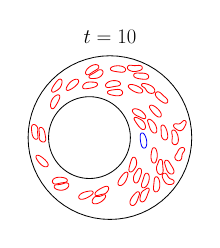
\begin{tikzpicture}[scale=0.3]

\begin{axis}[
  xmin = -21,
  xmax = 21,
  ymin = -21,
  ymax = 21,
  scale only axis,
  axis equal image,
  hide axis,
  title = {\Huge$t=10$}
  ]

% outer solid wall
\addplot [mark=none,black,line width=1.0] table{
2.0000e+01 -5.5171e-16
1.9904e+01 1.9603e+00
1.9616e+01 3.9018e+00
1.9139e+01 5.8057e+00
1.8478e+01 7.6537e+00
1.7638e+01 9.4279e+00
1.6629e+01 1.1111e+01
1.5460e+01 1.2688e+01
1.4142e+01 1.4142e+01
1.2688e+01 1.5460e+01
1.1111e+01 1.6629e+01
9.4279e+00 1.7638e+01
7.6537e+00 1.8478e+01
5.8057e+00 1.9139e+01
3.9018e+00 1.9616e+01
1.9603e+00 1.9904e+01
2.3281e-15 2.0000e+01
-1.9603e+00 1.9904e+01
-3.9018e+00 1.9616e+01
-5.8057e+00 1.9139e+01
-7.6537e+00 1.8478e+01
-9.4279e+00 1.7638e+01
-1.1111e+01 1.6629e+01
-1.2688e+01 1.5460e+01
-1.4142e+01 1.4142e+01
-1.5460e+01 1.2688e+01
-1.6629e+01 1.1111e+01
-1.7638e+01 9.4279e+00
-1.8478e+01 7.6537e+00
-1.9139e+01 5.8057e+00
-1.9616e+01 3.9018e+00
-1.9904e+01 1.9603e+00
-2.0000e+01 3.0010e-15
-1.9904e+01 -1.9603e+00
-1.9616e+01 -3.9018e+00
-1.9139e+01 -5.8057e+00
-1.8478e+01 -7.6537e+00
-1.7638e+01 -9.4279e+00
-1.6629e+01 -1.1111e+01
-1.5460e+01 -1.2688e+01
-1.4142e+01 -1.4142e+01
-1.2688e+01 -1.5460e+01
-1.1111e+01 -1.6629e+01
-9.4279e+00 -1.7638e+01
-7.6537e+00 -1.8478e+01
-5.8057e+00 -1.9139e+01
-3.9018e+00 -1.9616e+01
-1.9603e+00 -1.9904e+01
-4.7774e-15 -2.0000e+01
1.9603e+00 -1.9904e+01
3.9018e+00 -1.9616e+01
5.8057e+00 -1.9139e+01
7.6537e+00 -1.8478e+01
9.4279e+00 -1.7638e+01
1.1111e+01 -1.6629e+01
1.2688e+01 -1.5460e+01
1.4142e+01 -1.4142e+01
1.5460e+01 -1.2688e+01
1.6629e+01 -1.1111e+01
1.7638e+01 -9.4279e+00
1.8478e+01 -7.6537e+00
1.9139e+01 -5.8057e+00
1.9616e+01 -3.9018e+00
1.9904e+01 -1.9603e+00
2.0000e+01 -5.5171e-16
};

% inner solid wall
\addplot [mark=none,black,line width=1.0] table{
5.0000e+00 2.7586e-16
4.9518e+00 -9.8017e-01
4.8079e+00 -1.9509e+00
4.5694e+00 -2.9028e+00
4.2388e+00 -3.8268e+00
3.8192e+00 -4.7140e+00
3.3147e+00 -5.5557e+00
2.7301e+00 -6.3439e+00
2.0711e+00 -7.0711e+00
1.3439e+00 -7.7301e+00
5.5570e-01 -8.3147e+00
-2.8603e-01 -8.8192e+00
-1.1732e+00 -9.2388e+00
-2.0972e+00 -9.5694e+00
-3.0491e+00 -9.8079e+00
-4.0198e+00 -9.9518e+00
-5.0000e+00 -1.0000e+01
-5.9802e+00 -9.9518e+00
-6.9509e+00 -9.8079e+00
-7.9028e+00 -9.5694e+00
-8.8268e+00 -9.2388e+00
-9.7140e+00 -8.8192e+00
-1.0556e+01 -8.3147e+00
-1.1344e+01 -7.7301e+00
-1.2071e+01 -7.0711e+00
-1.2730e+01 -6.3439e+00
-1.3315e+01 -5.5557e+00
-1.3819e+01 -4.7140e+00
-1.4239e+01 -3.8268e+00
-1.4569e+01 -2.9028e+00
-1.4808e+01 -1.9509e+00
-1.4952e+01 -9.8017e-01
-1.5000e+01 -1.5005e-15
-1.4952e+01 9.8017e-01
-1.4808e+01 1.9509e+00
-1.4569e+01 2.9028e+00
-1.4239e+01 3.8268e+00
-1.3819e+01 4.7140e+00
-1.3315e+01 5.5557e+00
-1.2730e+01 6.3439e+00
-1.2071e+01 7.0711e+00
-1.1344e+01 7.7301e+00
-1.0556e+01 8.3147e+00
-9.7140e+00 8.8192e+00
-8.8268e+00 9.2388e+00
-7.9028e+00 9.5694e+00
-6.9509e+00 9.8079e+00
-5.9802e+00 9.9518e+00
-5.0000e+00 1.0000e+01
-4.0198e+00 9.9518e+00
-3.0491e+00 9.8079e+00
-2.0972e+00 9.5694e+00
-1.1732e+00 9.2388e+00
-2.8603e-01 8.8192e+00
5.5570e-01 8.3147e+00
1.3439e+00 7.7301e+00
2.0711e+00 7.0711e+00
2.7301e+00 6.3439e+00
3.3147e+00 5.5557e+00
3.8192e+00 4.7140e+00
4.2388e+00 3.8268e+00
4.5694e+00 2.9028e+00
4.8079e+00 1.9509e+00
4.9518e+00 9.8017e-01
5.0000e+00 2.7586e-16
};


% vesicle1
\addplot [mark=none,red,line width=1.0] table{
1.7924e+01 2.1266e+00
1.7960e+01 2.1727e+00
1.8008e+01 2.2382e+00
1.8065e+01 2.3241e+00
1.8129e+01 2.4272e+00
1.8195e+01 2.5420e+00
1.8262e+01 2.6656e+00
1.8328e+01 2.7950e+00
1.8394e+01 2.9292e+00
1.8458e+01 3.0673e+00
1.8517e+01 3.2093e+00
1.8569e+01 3.3557e+00
1.8607e+01 3.5071e+00
1.8626e+01 3.6629e+00
1.8613e+01 3.8197e+00
1.8559e+01 3.9672e+00
1.8458e+01 4.0883e+00
1.8320e+01 4.1627e+00
1.8164e+01 4.1799e+00
1.8011e+01 4.1441e+00
1.7874e+01 4.0693e+00
1.7752e+01 3.9710e+00
1.7643e+01 3.8610e+00
1.7537e+01 3.7485e+00
1.7431e+01 3.6401e+00
1.7318e+01 3.5422e+00
1.7198e+01 3.4600e+00
1.7072e+01 3.3975e+00
1.6947e+01 3.3563e+00
1.6827e+01 3.3347e+00
1.6724e+01 3.3274e+00
1.6643e+01 3.3282e+00
1.6585e+01 3.3316e+00
1.6527e+01 3.3370e+00
1.6447e+01 3.3467e+00
1.6344e+01 3.3606e+00
1.6224e+01 3.3749e+00
1.6092e+01 3.3809e+00
1.5952e+01 3.3675e+00
1.5814e+01 3.3229e+00
1.5691e+01 3.2392e+00
1.5600e+01 3.1181e+00
1.5555e+01 2.9715e+00
1.5560e+01 2.8169e+00
1.5608e+01 2.6685e+00
1.5688e+01 2.5337e+00
1.5790e+01 2.4135e+00
1.5904e+01 2.3052e+00
1.6027e+01 2.2052e+00
1.6153e+01 2.1105e+00
1.6282e+01 2.0197e+00
1.6414e+01 1.9334e+00
1.6550e+01 1.8537e+00
1.6690e+01 1.7846e+00
1.6835e+01 1.7310e+00
1.6986e+01 1.6976e+00
1.7137e+01 1.6881e+00
1.7286e+01 1.7039e+00
1.7426e+01 1.7431e+00
1.7553e+01 1.8018e+00
1.7665e+01 1.8730e+00
1.7759e+01 1.9495e+00
1.7833e+01 2.0216e+00
1.7887e+01 2.0817e+00
1.7924e+01 2.1266e+00
};

% vesicle2
\addplot [mark=none,red,line width=1.0] table{
-1.0572e+01 -1.2440e+01
-1.0526e+01 -1.2404e+01
-1.0463e+01 -1.2353e+01
-1.0387e+01 -1.2283e+01
-1.0304e+01 -1.2195e+01
-1.0223e+01 -1.2090e+01
-1.0149e+01 -1.1970e+01
-1.0091e+01 -1.1837e+01
-1.0056e+01 -1.1692e+01
-1.0052e+01 -1.1541e+01
-1.0087e+01 -1.1391e+01
-1.0164e+01 -1.1257e+01
-1.0279e+01 -1.1152e+01
-1.0420e+01 -1.1084e+01
-1.0574e+01 -1.1056e+01
-1.0732e+01 -1.1060e+01
-1.0888e+01 -1.1086e+01
-1.1041e+01 -1.1125e+01
-1.1192e+01 -1.1170e+01
-1.1343e+01 -1.1217e+01
-1.1492e+01 -1.1265e+01
-1.1641e+01 -1.1312e+01
-1.1791e+01 -1.1355e+01
-1.1940e+01 -1.1393e+01
-1.2088e+01 -1.1426e+01
-1.2235e+01 -1.1453e+01
-1.2379e+01 -1.1474e+01
-1.2519e+01 -1.1489e+01
-1.2651e+01 -1.1500e+01
-1.2772e+01 -1.1507e+01
-1.2875e+01 -1.1512e+01
-1.2956e+01 -1.1516e+01
-1.3014e+01 -1.1521e+01
-1.3072e+01 -1.1526e+01
-1.3153e+01 -1.1537e+01
-1.3254e+01 -1.1559e+01
-1.3367e+01 -1.1601e+01
-1.3478e+01 -1.1672e+01
-1.3570e+01 -1.1778e+01
-1.3621e+01 -1.1913e+01
-1.3619e+01 -1.2062e+01
-1.3568e+01 -1.2205e+01
-1.3480e+01 -1.2330e+01
-1.3368e+01 -1.2437e+01
-1.3241e+01 -1.2528e+01
-1.3103e+01 -1.2605e+01
-1.2960e+01 -1.2670e+01
-1.2812e+01 -1.2724e+01
-1.2660e+01 -1.2768e+01
-1.2506e+01 -1.2803e+01
-1.2350e+01 -1.2829e+01
-1.2193e+01 -1.2846e+01
-1.2037e+01 -1.2855e+01
-1.1880e+01 -1.2855e+01
-1.1725e+01 -1.2846e+01
-1.1572e+01 -1.2829e+01
-1.1423e+01 -1.2803e+01
-1.1277e+01 -1.2769e+01
-1.1138e+01 -1.2727e+01
-1.1006e+01 -1.2678e+01
-1.0885e+01 -1.2625e+01
-1.0777e+01 -1.2570e+01
-1.0688e+01 -1.2517e+01
-1.0620e+01 -1.2473e+01
-1.0572e+01 -1.2440e+01
};

% vesicle3
\addplot [mark=none,red,line width=1.0] table{
-1.2183e+01 -1.1137e+01
-1.2126e+01 -1.1126e+01
-1.2046e+01 -1.1110e+01
-1.1944e+01 -1.1092e+01
-1.1825e+01 -1.1072e+01
-1.1694e+01 -1.1052e+01
-1.1555e+01 -1.1032e+01
-1.1411e+01 -1.1012e+01
-1.1263e+01 -1.0992e+01
-1.1112e+01 -1.0969e+01
-1.0961e+01 -1.0940e+01
-1.0811e+01 -1.0899e+01
-1.0668e+01 -1.0838e+01
-1.0541e+01 -1.0746e+01
-1.0448e+01 -1.0619e+01
-1.0409e+01 -1.0468e+01
-1.0433e+01 -1.0313e+01
-1.0514e+01 -1.0178e+01
-1.0630e+01 -1.0071e+01
-1.0764e+01 -9.9887e+00
-1.0907e+01 -9.9238e+00
-1.1054e+01 -9.8713e+00
-1.1203e+01 -9.8280e+00
-1.1353e+01 -9.7921e+00
-1.1502e+01 -9.7625e+00
-1.1650e+01 -9.7386e+00
-1.1794e+01 -9.7199e+00
-1.1934e+01 -9.7063e+00
-1.2066e+01 -9.6973e+00
-1.2187e+01 -9.6926e+00
-1.2290e+01 -9.6914e+00
-1.2371e+01 -9.6923e+00
-1.2430e+01 -9.6940e+00
-1.2488e+01 -9.6966e+00
-1.2569e+01 -9.7018e+00
-1.2672e+01 -9.7112e+00
-1.2792e+01 -9.7264e+00
-1.2923e+01 -9.7487e+00
-1.3060e+01 -9.7792e+00
-1.3200e+01 -9.8192e+00
-1.3341e+01 -9.8699e+00
-1.3479e+01 -9.9325e+00
-1.3613e+01 -1.0009e+01
-1.3738e+01 -1.0100e+01
-1.3852e+01 -1.0207e+01
-1.3947e+01 -1.0331e+01
-1.4018e+01 -1.0472e+01
-1.4056e+01 -1.0625e+01
-1.4055e+01 -1.0782e+01
-1.4013e+01 -1.0934e+01
-1.3934e+01 -1.1071e+01
-1.3826e+01 -1.1185e+01
-1.3695e+01 -1.1271e+01
-1.3550e+01 -1.1329e+01
-1.3398e+01 -1.1356e+01
-1.3244e+01 -1.1357e+01
-1.3093e+01 -1.1339e+01
-1.2946e+01 -1.1311e+01
-1.2804e+01 -1.1279e+01
-1.2667e+01 -1.1246e+01
-1.2539e+01 -1.1216e+01
-1.2420e+01 -1.1188e+01
-1.2320e+01 -1.1166e+01
-1.2240e+01 -1.1149e+01
-1.2183e+01 -1.1137e+01
};

% vesicle4
\addplot [mark=none,red,line width=1.0] table{
6.4339e+00 1.4577e+01
6.4888e+00 1.4557e+01
6.5655e+00 1.4531e+01
6.6646e+00 1.4502e+01
6.7816e+00 1.4470e+01
6.9103e+00 1.4439e+01
7.0478e+00 1.4410e+01
7.1910e+00 1.4384e+01
7.3385e+00 1.4360e+01
7.4889e+00 1.4338e+01
7.6417e+00 1.4318e+01
7.7959e+00 1.4301e+01
7.9515e+00 1.4285e+01
8.1078e+00 1.4271e+01
8.2651e+00 1.4259e+01
8.4227e+00 1.4252e+01
8.5808e+00 1.4251e+01
8.7384e+00 1.4260e+01
8.8944e+00 1.4284e+01
9.0453e+00 1.4329e+01
9.1856e+00 1.4399e+01
9.3069e+00 1.4497e+01
9.3994e+00 1.4621e+01
9.4543e+00 1.4764e+01
9.4676e+00 1.4915e+01
9.4406e+00 1.5062e+01
9.3809e+00 1.5194e+01
9.2980e+00 1.5308e+01
9.2029e+00 1.5400e+01
9.1053e+00 1.5471e+01
9.0163e+00 1.5524e+01
8.9438e+00 1.5560e+01
8.8903e+00 1.5583e+01
8.8360e+00 1.5604e+01
8.7595e+00 1.5631e+01
8.6603e+00 1.5660e+01
8.5425e+00 1.5689e+01
8.4124e+00 1.5713e+01
8.2732e+00 1.5732e+01
8.1284e+00 1.5747e+01
7.9791e+00 1.5756e+01
7.8273e+00 1.5761e+01
7.6733e+00 1.5764e+01
7.5181e+00 1.5764e+01
7.3616e+00 1.5764e+01
7.2047e+00 1.5764e+01
7.0470e+00 1.5766e+01
6.8892e+00 1.5768e+01
6.7312e+00 1.5771e+01
6.5732e+00 1.5770e+01
6.4156e+00 1.5760e+01
6.2604e+00 1.5734e+01
6.1120e+00 1.5683e+01
5.9797e+00 1.5601e+01
5.8761e+00 1.5486e+01
5.8147e+00 1.5345e+01
5.8027e+00 1.5194e+01
5.8380e+00 1.5050e+01
5.9098e+00 1.4923e+01
6.0045e+00 1.4820e+01
6.1088e+00 1.4739e+01
6.2125e+00 1.4676e+01
6.3052e+00 1.4630e+01
6.3795e+00 1.4598e+01
6.4339e+00 1.4577e+01
};

% vesicle5
\addplot [mark=none,red,line width=1.0] table{
5.7804e+00 -1.0363e+01
5.7906e+00 -1.0421e+01
5.8081e+00 -1.0500e+01
5.8370e+00 -1.0599e+01
5.8814e+00 -1.0712e+01
5.9454e+00 -1.0827e+01
6.0337e+00 -1.0936e+01
6.1489e+00 -1.1025e+01
6.2880e+00 -1.1078e+01
6.4392e+00 -1.1083e+01
6.5861e+00 -1.1039e+01
6.7163e+00 -1.0955e+01
6.8264e+00 -1.0844e+01
6.9188e+00 -1.0717e+01
6.9976e+00 -1.0581e+01
7.0666e+00 -1.0439e+01
7.1290e+00 -1.0294e+01
7.1868e+00 -1.0146e+01
7.2418e+00 -9.9985e+00
7.2951e+00 -9.8501e+00
7.3475e+00 -9.7021e+00
7.3994e+00 -9.5546e+00
7.4508e+00 -9.4081e+00
7.5013e+00 -9.2626e+00
7.5503e+00 -9.1188e+00
7.5964e+00 -8.9765e+00
7.6379e+00 -8.8370e+00
7.6731e+00 -8.7009e+00
7.7001e+00 -8.5714e+00
7.7181e+00 -8.4516e+00
7.7274e+00 -8.3485e+00
7.7301e+00 -8.2676e+00
7.7294e+00 -8.2093e+00
7.7262e+00 -8.1510e+00
7.7176e+00 -8.0705e+00
7.6985e+00 -7.9689e+00
7.6634e+00 -7.8531e+00
7.6062e+00 -7.7338e+00
7.5210e+00 -7.6226e+00
7.4039e+00 -7.5370e+00
7.2608e+00 -7.4973e+00
7.1111e+00 -7.5171e+00
6.9760e+00 -7.5896e+00
6.8631e+00 -7.6958e+00
6.7667e+00 -7.8188e+00
6.6788e+00 -7.9490e+00
6.5936e+00 -8.0815e+00
6.5082e+00 -8.2143e+00
6.4215e+00 -8.3464e+00
6.3337e+00 -8.4778e+00
6.2457e+00 -8.6088e+00
6.1593e+00 -8.7407e+00
6.0768e+00 -8.8742e+00
6.0008e+00 -9.0109e+00
5.9337e+00 -9.1508e+00
5.8772e+00 -9.2941e+00
5.8322e+00 -9.4392e+00
5.7985e+00 -9.5848e+00
5.7751e+00 -9.7285e+00
5.7612e+00 -9.8683e+00
5.7556e+00 -1.0001e+01
5.7571e+00 -1.0122e+01
5.7635e+00 -1.0225e+01
5.7721e+00 -1.0305e+01
5.7804e+00 -1.0363e+01
};

% vesicle6
\addplot [mark=none,red,line width=1.0] table{
1.3831e+01 1.8922e+00
1.3812e+01 1.9472e+00
1.3783e+01 2.0230e+00
1.3745e+01 2.1192e+00
1.3698e+01 2.2307e+00
1.3642e+01 2.3508e+00
1.3579e+01 2.4760e+00
1.3506e+01 2.6023e+00
1.3423e+01 2.7266e+00
1.3327e+01 2.8438e+00
1.3213e+01 2.9471e+00
1.3079e+01 3.0248e+00
1.2927e+01 3.0616e+00
1.2773e+01 3.0421e+00
1.2637e+01 2.9631e+00
1.2542e+01 2.8384e+00
1.2490e+01 2.6898e+00
1.2471e+01 2.5330e+00
1.2472e+01 2.3753e+00
1.2483e+01 2.2180e+00
1.2497e+01 2.0617e+00
1.2510e+01 1.9058e+00
1.2521e+01 1.7510e+00
1.2529e+01 1.5971e+00
1.2534e+01 1.4453e+00
1.2536e+01 1.2958e+00
1.2538e+01 1.1502e+00
1.2541e+01 1.0097e+00
1.2545e+01 8.7737e-01
1.2552e+01 7.5642e-01
1.2561e+01 6.5340e-01
1.2571e+01 5.7305e-01
1.2579e+01 5.1532e-01
1.2589e+01 4.5781e-01
1.2606e+01 3.7858e-01
1.2632e+01 2.7852e-01
1.2670e+01 1.6345e-01
1.2721e+01 4.1296e-02
1.2787e+01 -8.2958e-02
1.2868e+01 -2.0382e-01
1.2965e+01 -3.1695e-01
1.3080e+01 -4.1650e-01
1.3211e+01 -4.9633e-01
1.3357e+01 -5.4833e-01
1.3512e+01 -5.6478e-01
1.3667e+01 -5.3946e-01
1.3808e+01 -4.7188e-01
1.3926e+01 -3.6763e-01
1.4015e+01 -2.3722e-01
1.4074e+01 -9.0968e-02
1.4109e+01 6.2826e-02
1.4125e+01 2.1959e-01
1.4127e+01 3.7653e-01
1.4119e+01 5.3273e-01
1.4105e+01 6.8726e-01
1.4085e+01 8.3999e-01
1.4061e+01 9.9005e-01
1.4034e+01 1.1371e+00
1.4004e+01 1.2796e+00
1.3972e+01 1.4164e+00
1.3939e+01 1.5446e+00
1.3906e+01 1.6611e+00
1.3875e+01 1.7600e+00
1.3850e+01 1.8369e+00
1.3831e+01 1.8922e+00
};

% vesicle7
\addplot [mark=none,red,line width=1.0] table{
7.0553e+00 1.6328e+01
7.1116e+00 1.6344e+01
7.1893e+00 1.6366e+01
7.2876e+00 1.6398e+01
7.4008e+00 1.6442e+01
7.5204e+00 1.6498e+01
7.6397e+00 1.6572e+01
7.7496e+00 1.6668e+01
7.8403e+00 1.6786e+01
7.8993e+00 1.6926e+01
7.9163e+00 1.7078e+01
7.8856e+00 1.7230e+01
7.8100e+00 1.7366e+01
7.6986e+00 1.7476e+01
7.5633e+00 1.7556e+01
7.4142e+00 1.7607e+01
7.2588e+00 1.7635e+01
7.1011e+00 1.7646e+01
6.9434e+00 1.7644e+01
6.7860e+00 1.7635e+01
6.6295e+00 1.7623e+01
6.4736e+00 1.7610e+01
6.3187e+00 1.7600e+01
6.1648e+00 1.7594e+01
6.0129e+00 1.7593e+01
5.8635e+00 1.7599e+01
5.7184e+00 1.7611e+01
5.5789e+00 1.7628e+01
5.4477e+00 1.7646e+01
5.3278e+00 1.7663e+01
5.2252e+00 1.7676e+01
5.1446e+00 1.7684e+01
5.0864e+00 1.7687e+01
5.0280e+00 1.7689e+01
4.9471e+00 1.7688e+01
4.8442e+00 1.7678e+01
4.7260e+00 1.7652e+01
4.6029e+00 1.7604e+01
4.4845e+00 1.7528e+01
4.3823e+00 1.7425e+01
4.3068e+00 1.7297e+01
4.2681e+00 1.7150e+01
4.2731e+00 1.6997e+01
4.3228e+00 1.6850e+01
4.4097e+00 1.6721e+01
4.5223e+00 1.6611e+01
4.6503e+00 1.6520e+01
4.7870e+00 1.6441e+01
4.9289e+00 1.6371e+01
5.0745e+00 1.6310e+01
5.2228e+00 1.6256e+01
5.3738e+00 1.6211e+01
5.5268e+00 1.6176e+01
5.6813e+00 1.6152e+01
5.8360e+00 1.6140e+01
5.9900e+00 1.6139e+01
6.1416e+00 1.6149e+01
6.2900e+00 1.6167e+01
6.4337e+00 1.6191e+01
6.5717e+00 1.6217e+01
6.7013e+00 1.6244e+01
6.8195e+00 1.6271e+01
6.9202e+00 1.6294e+01
6.9988e+00 1.6314e+01
7.0553e+00 1.6328e+01
};

% vesicle8
\addplot [mark=none,red,line width=1.0] table{
6.5036e+00 1.2665e+01
6.4492e+00 1.2686e+01
6.3735e+00 1.2715e+01
6.2761e+00 1.2750e+01
6.1612e+00 1.2788e+01
6.0347e+00 1.2827e+01
5.8994e+00 1.2865e+01
5.7581e+00 1.2900e+01
5.6119e+00 1.2931e+01
5.4621e+00 1.2957e+01
5.3092e+00 1.2975e+01
5.1541e+00 1.2981e+01
4.9980e+00 1.2973e+01
4.8444e+00 1.2941e+01
4.7001e+00 1.2879e+01
4.5805e+00 1.2777e+01
4.5069e+00 1.2639e+01
4.4962e+00 1.2482e+01
4.5436e+00 1.2332e+01
4.6301e+00 1.2201e+01
4.7372e+00 1.2086e+01
4.8540e+00 1.1982e+01
4.9747e+00 1.1885e+01
5.0974e+00 1.1791e+01
5.2206e+00 1.1703e+01
5.3438e+00 1.1618e+01
5.4657e+00 1.1538e+01
5.5852e+00 1.1464e+01
5.6995e+00 1.1398e+01
5.8055e+00 1.1339e+01
5.8971e+00 1.1291e+01
5.9694e+00 1.1255e+01
6.0219e+00 1.1229e+01
6.0748e+00 1.1204e+01
6.1486e+00 1.1171e+01
6.2437e+00 1.1130e+01
6.3563e+00 1.1086e+01
6.4808e+00 1.1041e+01
6.6146e+00 1.0998e+01
6.7550e+00 1.0959e+01
6.9009e+00 1.0927e+01
7.0509e+00 1.0902e+01
7.2042e+00 1.0889e+01
7.3594e+00 1.0888e+01
7.5147e+00 1.0906e+01
7.6659e+00 1.0948e+01
7.8058e+00 1.1019e+01
7.9208e+00 1.1127e+01
7.9934e+00 1.1266e+01
8.0104e+00 1.1422e+01
7.9741e+00 1.1575e+01
7.8984e+00 1.1713e+01
7.7993e+00 1.1835e+01
7.6874e+00 1.1944e+01
7.5693e+00 1.2045e+01
7.4476e+00 1.2139e+01
7.3243e+00 1.2228e+01
7.1999e+00 1.2311e+01
7.0758e+00 1.2387e+01
6.9534e+00 1.2456e+01
6.8358e+00 1.2517e+01
6.7266e+00 1.2569e+01
6.6322e+00 1.2611e+01
6.5576e+00 1.2643e+01
6.5036e+00 1.2665e+01
};

% vesicle9
\addplot [mark=none,red,line width=1.0] table{
2.1604e+00 1.3699e+01
2.1080e+00 1.3725e+01
2.0340e+00 1.3757e+01
1.9371e+00 1.3794e+01
1.8216e+00 1.3830e+01
1.6931e+00 1.3862e+01
1.5552e+00 1.3889e+01
1.4111e+00 1.3909e+01
1.2622e+00 1.3923e+01
1.1104e+00 1.3930e+01
9.5633e-01 1.3929e+01
8.0127e-01 1.3921e+01
6.4563e-01 1.3906e+01
4.9033e-01 1.3883e+01
3.3576e-01 1.3852e+01
1.8283e-01 1.3813e+01
3.1960e-02 1.3766e+01
-1.1590e-01 1.3710e+01
-2.6022e-01 1.3646e+01
-3.9987e-01 1.3573e+01
-5.3402e-01 1.3492e+01
-6.6099e-01 1.3401e+01
-7.7900e-01 1.3300e+01
-8.8471e-01 1.3188e+01
-9.7372e-01 1.3065e+01
-1.0389e+00 1.2931e+01
-1.0720e+00 1.2789e+01
-1.0661e+00 1.2649e+01
-1.0224e+00 1.2525e+01
-9.5189e-01 1.2427e+01
-8.7374e-01 1.2359e+01
-8.0427e-01 1.2318e+01
-7.5104e-01 1.2294e+01
-6.9588e-01 1.2275e+01
-6.1734e-01 1.2256e+01
-5.1488e-01 1.2242e+01
-3.9387e-01 1.2238e+01
-2.6166e-01 1.2245e+01
-1.2214e-01 1.2261e+01
2.1542e-02 1.2285e+01
1.6838e-01 1.2313e+01
3.1723e-01 1.2343e+01
4.6805e-01 1.2375e+01
6.2024e-01 1.2405e+01
7.7388e-01 1.2434e+01
9.2848e-01 1.2462e+01
1.0841e+00 1.2487e+01
1.2402e+00 1.2510e+01
1.3968e+00 1.2532e+01
1.5533e+00 1.2554e+01
1.7096e+00 1.2576e+01
1.8648e+00 1.2603e+01
2.0183e+00 1.2637e+01
2.1676e+00 1.2683e+01
2.3087e+00 1.2747e+01
2.4331e+00 1.2837e+01
2.5274e+00 1.2956e+01
2.5759e+00 1.3096e+01
2.5725e+00 1.3241e+01
2.5245e+00 1.3373e+01
2.4492e+00 1.3481e+01
2.3628e+00 1.3566e+01
2.2802e+00 1.3628e+01
2.2116e+00 1.3671e+01
2.1604e+00 1.3699e+01
};

% vesicle10
\addplot [mark=none,red,line width=1.0] table{
1.2846e+01 -8.6997e+00
1.2874e+01 -8.6487e+00
1.2908e+01 -8.5752e+00
1.2943e+01 -8.4779e+00
1.2973e+01 -8.3607e+00
1.2995e+01 -8.2300e+00
1.3006e+01 -8.0900e+00
1.3008e+01 -7.9444e+00
1.3002e+01 -7.7951e+00
1.2989e+01 -7.6436e+00
1.2973e+01 -7.4905e+00
1.2954e+01 -7.3363e+00
1.2936e+01 -7.1810e+00
1.2919e+01 -7.0250e+00
1.2905e+01 -6.8680e+00
1.2894e+01 -6.7105e+00
1.2887e+01 -6.5526e+00
1.2883e+01 -6.3947e+00
1.2879e+01 -6.2368e+00
1.2871e+01 -6.0795e+00
1.2855e+01 -5.9233e+00
1.2822e+01 -5.7705e+00
1.2767e+01 -5.6255e+00
1.2683e+01 -5.4972e+00
1.2568e+01 -5.3984e+00
1.2430e+01 -5.3448e+00
1.2285e+01 -5.3465e+00
1.2156e+01 -5.4005e+00
1.2057e+01 -5.4882e+00
1.1989e+01 -5.5880e+00
1.1944e+01 -5.6811e+00
1.1915e+01 -5.7568e+00
1.1897e+01 -5.8121e+00
1.1879e+01 -5.8678e+00
1.1856e+01 -5.9453e+00
1.1826e+01 -6.0442e+00
1.1788e+01 -6.1594e+00
1.1742e+01 -6.2836e+00
1.1689e+01 -6.4137e+00
1.1630e+01 -6.5469e+00
1.1570e+01 -6.6837e+00
1.1512e+01 -6.8242e+00
1.1461e+01 -6.9696e+00
1.1421e+01 -7.1196e+00
1.1394e+01 -7.2735e+00
1.1381e+01 -7.4299e+00
1.1381e+01 -7.5875e+00
1.1394e+01 -7.7447e+00
1.1419e+01 -7.9008e+00
1.1455e+01 -8.0546e+00
1.1501e+01 -8.2056e+00
1.1558e+01 -8.3524e+00
1.1627e+01 -8.4938e+00
1.1708e+01 -8.6272e+00
1.1804e+01 -8.7493e+00
1.1915e+01 -8.8549e+00
1.2043e+01 -8.9379e+00
1.2182e+01 -8.9916e+00
1.2326e+01 -9.0117e+00
1.2465e+01 -8.9963e+00
1.2589e+01 -8.9503e+00
1.2690e+01 -8.8839e+00
1.2764e+01 -8.8121e+00
1.2814e+01 -8.7486e+00
1.2846e+01 -8.6997e+00
};

% vesicle11
\addplot [mark=none,red,line width=1.0] table{
-1.1812e+00 -1.1965e+01
-1.2372e+00 -1.1982e+01
-1.3140e+00 -1.2007e+01
-1.4112e+00 -1.2043e+01
-1.5237e+00 -1.2087e+01
-1.6453e+00 -1.2140e+01
-1.7730e+00 -1.2199e+01
-1.9040e+00 -1.2262e+01
-2.0373e+00 -1.2330e+01
-2.1716e+00 -1.2401e+01
-2.3066e+00 -1.2475e+01
-2.4414e+00 -1.2552e+01
-2.5759e+00 -1.2632e+01
-2.7093e+00 -1.2715e+01
-2.8415e+00 -1.2800e+01
-2.9715e+00 -1.2890e+01
-3.0987e+00 -1.2984e+01
-3.2216e+00 -1.3083e+01
-3.3384e+00 -1.3189e+01
-3.4454e+00 -1.3305e+01
-3.5373e+00 -1.3432e+01
-3.6053e+00 -1.3573e+01
-3.6393e+00 -1.3724e+01
-3.6290e+00 -1.3877e+01
-3.5688e+00 -1.4015e+01
-3.4618e+00 -1.4118e+01
-3.3266e+00 -1.4170e+01
-3.1866e+00 -1.4177e+01
-3.0555e+00 -1.4159e+01
-2.9372e+00 -1.4133e+01
-2.8369e+00 -1.4108e+01
-2.7586e+00 -1.4087e+01
-2.7022e+00 -1.4072e+01
-2.6459e+00 -1.4057e+01
-2.5678e+00 -1.4035e+01
-2.4681e+00 -1.4008e+01
-2.3514e+00 -1.3975e+01
-2.2238e+00 -1.3940e+01
-2.0880e+00 -1.3904e+01
-1.9466e+00 -1.3869e+01
-1.8003e+00 -1.3838e+01
-1.6505e+00 -1.3813e+01
-1.4982e+00 -1.3790e+01
-1.3462e+00 -1.3758e+01
-1.1992e+00 -1.3706e+01
-1.0624e+00 -1.3629e+01
-9.3704e-01 -1.3533e+01
-8.2209e-01 -1.3425e+01
-7.1607e-01 -1.3308e+01
-6.1881e-01 -1.3184e+01
-5.3042e-01 -1.3053e+01
-4.5243e-01 -1.2916e+01
-3.8693e-01 -1.2773e+01
-3.3807e-01 -1.2625e+01
-3.1148e-01 -1.2472e+01
-3.1556e-01 -1.2319e+01
-3.5819e-01 -1.2173e+01
-4.4244e-01 -1.2051e+01
-5.5921e-01 -1.1965e+01
-6.9171e-01 -1.1919e+01
-8.2328e-01 -1.1906e+01
-9.4409e-01 -1.1914e+01
-1.0461e+00 -1.1931e+01
-1.1249e+00 -1.1949e+01
-1.1812e+00 -1.1965e+01
};

% vesicle12
\addplot [mark=none,red,line width=1.0] table{
1.3173e+01 1.0160e+01
1.3129e+01 1.0198e+01
1.3068e+01 1.0251e+01
1.2991e+01 1.0321e+01
1.2902e+01 1.0403e+01
1.2807e+01 1.0495e+01
1.2708e+01 1.0595e+01
1.2605e+01 1.0698e+01
1.2498e+01 1.0802e+01
1.2385e+01 1.0904e+01
1.2263e+01 1.0997e+01
1.2130e+01 1.1078e+01
1.1986e+01 1.1139e+01
1.1834e+01 1.1175e+01
1.1677e+01 1.1182e+01
1.1521e+01 1.1155e+01
1.1376e+01 1.1093e+01
1.1253e+01 1.0996e+01
1.1162e+01 1.0868e+01
1.1111e+01 1.0719e+01
1.1102e+01 1.0563e+01
1.1127e+01 1.0408e+01
1.1179e+01 1.0262e+01
1.1248e+01 1.0125e+01
1.1330e+01 9.9969e+00
1.1420e+01 9.8772e+00
1.1513e+01 9.7659e+00
1.1609e+01 9.6626e+00
1.1702e+01 9.5686e+00
1.1790e+01 9.4851e+00
1.1866e+01 9.4155e+00
1.1927e+01 9.3621e+00
1.1971e+01 9.3240e+00
1.2016e+01 9.2865e+00
1.2078e+01 9.2350e+00
1.2159e+01 9.1703e+00
1.2255e+01 9.0959e+00
1.2361e+01 9.0164e+00
1.2474e+01 8.9338e+00
1.2594e+01 8.8505e+00
1.2718e+01 8.7677e+00
1.2847e+01 8.6870e+00
1.2980e+01 8.6100e+00
1.3118e+01 8.5394e+00
1.3262e+01 8.4784e+00
1.3412e+01 8.4324e+00
1.3568e+01 8.4088e+00
1.3725e+01 8.4170e+00
1.3875e+01 8.4654e+00
1.4003e+01 8.5573e+00
1.4093e+01 8.6859e+00
1.4138e+01 8.8364e+00
1.4138e+01 8.9929e+00
1.4102e+01 9.1448e+00
1.4039e+01 9.2866e+00
1.3958e+01 9.4170e+00
1.3864e+01 9.5364e+00
1.3762e+01 9.6461e+00
1.3658e+01 9.7472e+00
1.3553e+01 9.8408e+00
1.3452e+01 9.9267e+00
1.3359e+01 1.0004e+01
1.3279e+01 1.0070e+01
1.3217e+01 1.0122e+01
1.3173e+01 1.0160e+01
};

% vesicle13
\addplot [mark=none,red,line width=1.0] table{
-2.8995e+00 1.7659e+01
-2.9457e+00 1.7695e+01
-3.0147e+00 1.7737e+01
-3.1093e+00 1.7779e+01
-3.2257e+00 1.7812e+01
-3.3567e+00 1.7831e+01
-3.4970e+00 1.7835e+01
-3.6422e+00 1.7825e+01
-3.7899e+00 1.7802e+01
-3.9380e+00 1.7768e+01
-4.0857e+00 1.7725e+01
-4.2319e+00 1.7672e+01
-4.3762e+00 1.7612e+01
-4.5181e+00 1.7545e+01
-4.6574e+00 1.7471e+01
-4.7933e+00 1.7391e+01
-4.9258e+00 1.7305e+01
-5.0541e+00 1.7213e+01
-5.1778e+00 1.7115e+01
-5.2963e+00 1.7011e+01
-5.4090e+00 1.6901e+01
-5.5148e+00 1.6786e+01
-5.6132e+00 1.6666e+01
-5.7028e+00 1.6541e+01
-5.7825e+00 1.6412e+01
-5.8504e+00 1.6279e+01
-5.9044e+00 1.6143e+01
-5.9412e+00 1.6008e+01
-5.9580e+00 1.5877e+01
-5.9526e+00 1.5756e+01
-5.9291e+00 1.5655e+01
-5.8967e+00 1.5581e+01
-5.8658e+00 1.5532e+01
-5.8285e+00 1.5487e+01
-5.7678e+00 1.5434e+01
-5.6777e+00 1.5383e+01
-5.5614e+00 1.5350e+01
-5.4294e+00 1.5346e+01
-5.2912e+00 1.5370e+01
-5.1544e+00 1.5419e+01
-5.0210e+00 1.5487e+01
-4.8910e+00 1.5565e+01
-4.7624e+00 1.5650e+01
-4.6341e+00 1.5738e+01
-4.5053e+00 1.5826e+01
-4.3757e+00 1.5915e+01
-4.2450e+00 1.6003e+01
-4.1134e+00 1.6090e+01
-3.9805e+00 1.6176e+01
-3.8465e+00 1.6260e+01
-3.7113e+00 1.6341e+01
-3.5753e+00 1.6421e+01
-3.4390e+00 1.6499e+01
-3.3035e+00 1.6577e+01
-3.1707e+00 1.6657e+01
-3.0440e+00 1.6744e+01
-2.9280e+00 1.6843e+01
-2.8303e+00 1.6955e+01
-2.7594e+00 1.7082e+01
-2.7233e+00 1.7218e+01
-2.7242e+00 1.7350e+01
-2.7566e+00 1.7466e+01
-2.8062e+00 1.7557e+01
-2.8573e+00 1.7619e+01
-2.8995e+00 1.7659e+01
};

% vesicle14
\addplot [mark=none,red,line width=1.0] table{
-2.0160e+00 -1.4204e+01
-2.0702e+00 -1.4226e+01
-2.1458e+00 -1.4254e+01
-2.2435e+00 -1.4289e+01
-2.3591e+00 -1.4325e+01
-2.4871e+00 -1.4359e+01
-2.6249e+00 -1.4386e+01
-2.7694e+00 -1.4404e+01
-2.9188e+00 -1.4408e+01
-3.0705e+00 -1.4401e+01
-3.2241e+00 -1.4389e+01
-3.3793e+00 -1.4391e+01
-3.5320e+00 -1.4423e+01
-3.6740e+00 -1.4489e+01
-3.8013e+00 -1.4582e+01
-3.9147e+00 -1.4691e+01
-4.0169e+00 -1.4812e+01
-4.1086e+00 -1.4940e+01
-4.1898e+00 -1.5076e+01
-4.2580e+00 -1.5218e+01
-4.3096e+00 -1.5366e+01
-4.3380e+00 -1.5520e+01
-4.3362e+00 -1.5675e+01
-4.2970e+00 -1.5823e+01
-4.2197e+00 -1.5953e+01
-4.1109e+00 -1.6055e+01
-3.9834e+00 -1.6125e+01
-3.8492e+00 -1.6166e+01
-3.7183e+00 -1.6185e+01
-3.5972e+00 -1.6188e+01
-3.4939e+00 -1.6183e+01
-3.4135e+00 -1.6175e+01
-3.3557e+00 -1.6167e+01
-3.2982e+00 -1.6157e+01
-3.2189e+00 -1.6140e+01
-3.1184e+00 -1.6116e+01
-3.0020e+00 -1.6082e+01
-2.8766e+00 -1.6040e+01
-2.7456e+00 -1.5989e+01
-2.6122e+00 -1.5931e+01
-2.4777e+00 -1.5865e+01
-2.3439e+00 -1.5793e+01
-2.2113e+00 -1.5715e+01
-2.0810e+00 -1.5631e+01
-1.9534e+00 -1.5540e+01
-1.8293e+00 -1.5444e+01
-1.7091e+00 -1.5342e+01
-1.5938e+00 -1.5234e+01
-1.4839e+00 -1.5121e+01
-1.3806e+00 -1.5001e+01
-1.2851e+00 -1.4876e+01
-1.1997e+00 -1.4743e+01
-1.1277e+00 -1.4604e+01
-1.0752e+00 -1.4457e+01
-1.0522e+00 -1.4303e+01
-1.0744e+00 -1.4152e+01
-1.1550e+00 -1.4025e+01
-1.2858e+00 -1.3956e+01
-1.4304e+00 -1.3957e+01
-1.5641e+00 -1.3999e+01
-1.6848e+00 -1.4054e+01
-1.7941e+00 -1.4106e+01
-1.8880e+00 -1.4149e+01
-1.9622e+00 -1.4182e+01
-2.0160e+00 -1.4204e+01
};

% vesicle15
\addplot [mark=none,red,line width=1.0] table{
-1.5315e+01 -7.0512e+00
-1.5267e+01 -7.0177e+00
-1.5208e+01 -6.9626e+00
-1.5148e+01 -6.8786e+00
-1.5104e+01 -6.7661e+00
-1.5090e+01 -6.6348e+00
-1.5108e+01 -6.4958e+00
-1.5154e+01 -6.3577e+00
-1.5219e+01 -6.2235e+00
-1.5299e+01 -6.0940e+00
-1.5388e+01 -5.9684e+00
-1.5484e+01 -5.8465e+00
-1.5586e+01 -5.7277e+00
-1.5692e+01 -5.6118e+00
-1.5801e+01 -5.4984e+00
-1.5914e+01 -5.3877e+00
-1.6029e+01 -5.2793e+00
-1.6146e+01 -5.1735e+00
-1.6266e+01 -5.0705e+00
-1.6388e+01 -4.9705e+00
-1.6511e+01 -4.8738e+00
-1.6637e+01 -4.7811e+00
-1.6765e+01 -4.6929e+00
-1.6895e+01 -4.6100e+00
-1.7026e+01 -4.5336e+00
-1.7159e+01 -4.4652e+00
-1.7292e+01 -4.4067e+00
-1.7425e+01 -4.3612e+00
-1.7554e+01 -4.3320e+00
-1.7675e+01 -4.3228e+00
-1.7778e+01 -4.3332e+00
-1.7855e+01 -4.3567e+00
-1.7907e+01 -4.3830e+00
-1.7954e+01 -4.4175e+00
-1.8008e+01 -4.4776e+00
-1.8053e+01 -4.5704e+00
-1.8072e+01 -4.6896e+00
-1.8059e+01 -4.8212e+00
-1.8021e+01 -4.9563e+00
-1.7966e+01 -5.0912e+00
-1.7901e+01 -5.2255e+00
-1.7827e+01 -5.3586e+00
-1.7748e+01 -5.4905e+00
-1.7663e+01 -5.6208e+00
-1.7574e+01 -5.7495e+00
-1.7482e+01 -5.8762e+00
-1.7385e+01 -6.0010e+00
-1.7285e+01 -6.1231e+00
-1.7182e+01 -6.2426e+00
-1.7075e+01 -6.3586e+00
-1.6964e+01 -6.4708e+00
-1.6848e+01 -6.5784e+00
-1.6729e+01 -6.6807e+00
-1.6606e+01 -6.7765e+00
-1.6478e+01 -6.8649e+00
-1.6346e+01 -6.9443e+00
-1.6211e+01 -7.0133e+00
-1.6072e+01 -7.0697e+00
-1.5933e+01 -7.1117e+00
-1.5795e+01 -7.1368e+00
-1.5663e+01 -7.1441e+00
-1.5542e+01 -7.1334e+00
-1.5442e+01 -7.1093e+00
-1.5366e+01 -7.0792e+00
-1.5315e+01 -7.0512e+00
};

% vesicle16
\addplot [mark=none,red,line width=1.0] table{
9.1040e+00 1.1273e+01
9.1433e+00 1.1230e+01
9.2009e+00 1.1173e+01
9.2795e+00 1.1106e+01
9.3781e+00 1.1035e+01
9.4928e+00 1.0969e+01
9.6208e+00 1.0911e+01
9.7586e+00 1.0865e+01
9.9042e+00 1.0831e+01
1.0055e+01 1.0811e+01
1.0209e+01 1.0808e+01
1.0363e+01 1.0823e+01
1.0515e+01 1.0860e+01
1.0658e+01 1.0923e+01
1.0785e+01 1.1017e+01
1.0883e+01 1.1139e+01
1.0946e+01 1.1284e+01
1.0969e+01 1.1440e+01
1.0957e+01 1.1597e+01
1.0916e+01 1.1749e+01
1.0852e+01 1.1893e+01
1.0772e+01 1.2026e+01
1.0678e+01 1.2150e+01
1.0574e+01 1.2264e+01
1.0464e+01 1.2368e+01
1.0348e+01 1.2463e+01
1.0231e+01 1.2549e+01
1.0113e+01 1.2626e+01
9.9994e+00 1.2694e+01
9.8927e+00 1.2751e+01
9.8001e+00 1.2797e+01
9.7267e+00 1.2831e+01
9.6733e+00 1.2855e+01
9.6195e+00 1.2878e+01
9.5445e+00 1.2908e+01
9.4479e+00 1.2945e+01
9.3338e+00 1.2986e+01
9.2081e+00 1.3027e+01
9.0739e+00 1.3069e+01
8.9341e+00 1.3110e+01
8.7898e+00 1.3149e+01
8.6421e+00 1.3184e+01
8.4910e+00 1.3214e+01
8.3370e+00 1.3234e+01
8.1807e+00 1.3236e+01
8.0260e+00 1.3211e+01
7.8828e+00 1.3146e+01
7.7726e+00 1.3035e+01
7.7240e+00 1.2886e+01
7.7516e+00 1.2732e+01
7.8392e+00 1.2602e+01
7.9588e+00 1.2500e+01
8.0905e+00 1.2414e+01
8.2237e+00 1.2332e+01
8.3522e+00 1.2245e+01
8.4719e+00 1.2148e+01
8.5794e+00 1.2041e+01
8.6739e+00 1.1925e+01
8.7560e+00 1.1805e+01
8.8289e+00 1.1685e+01
8.8959e+00 1.1571e+01
8.9595e+00 1.1468e+01
9.0176e+00 1.1382e+01
9.0666e+00 1.1318e+01
9.1040e+00 1.1273e+01
};

% vesicle17
\addplot [mark=none,red,line width=1.0] table{
-4.1107e+00 -1.3365e+01
-4.1260e+00 -1.3309e+01
-4.1623e+00 -1.3237e+01
-4.2314e+00 -1.3160e+01
-4.3342e+00 -1.3097e+01
-4.4609e+00 -1.3059e+01
-4.6004e+00 -1.3044e+01
-4.7460e+00 -1.3046e+01
-4.8950e+00 -1.3058e+01
-5.0460e+00 -1.3075e+01
-5.1984e+00 -1.3097e+01
-5.3517e+00 -1.3122e+01
-5.5056e+00 -1.3149e+01
-5.6595e+00 -1.3181e+01
-5.8132e+00 -1.3216e+01
-5.9662e+00 -1.3254e+01
-6.1183e+00 -1.3297e+01
-6.2689e+00 -1.3345e+01
-6.4177e+00 -1.3398e+01
-6.5640e+00 -1.3456e+01
-6.7072e+00 -1.3521e+01
-6.8462e+00 -1.3592e+01
-6.9802e+00 -1.3671e+01
-7.1078e+00 -1.3757e+01
-7.2272e+00 -1.3851e+01
-7.3364e+00 -1.3953e+01
-7.4326e+00 -1.4062e+01
-7.5125e+00 -1.4178e+01
-7.5724e+00 -1.4296e+01
-7.6094e+00 -1.4411e+01
-7.6243e+00 -1.4513e+01
-7.6229e+00 -1.4594e+01
-7.6142e+00 -1.4652e+01
-7.5987e+00 -1.4708e+01
-7.5661e+00 -1.4782e+01
-7.5066e+00 -1.4867e+01
-7.4163e+00 -1.4947e+01
-7.2999e+00 -1.5010e+01
-7.1657e+00 -1.5050e+01
-7.0215e+00 -1.5070e+01
-6.8722e+00 -1.5073e+01
-6.7206e+00 -1.5061e+01
-6.5682e+00 -1.5039e+01
-6.4161e+00 -1.5008e+01
-6.2649e+00 -1.4969e+01
-6.1149e+00 -1.4922e+01
-5.9665e+00 -1.4869e+01
-5.8201e+00 -1.4810e+01
-5.6758e+00 -1.4746e+01
-5.5338e+00 -1.4676e+01
-5.3942e+00 -1.4602e+01
-5.2571e+00 -1.4525e+01
-5.1225e+00 -1.4444e+01
-4.9904e+00 -1.4360e+01
-4.8609e+00 -1.4274e+01
-4.7343e+00 -1.4187e+01
-4.6113e+00 -1.4097e+01
-4.4932e+00 -1.4006e+01
-4.3825e+00 -1.3911e+01
-4.2831e+00 -1.3812e+01
-4.2008e+00 -1.3708e+01
-4.1425e+00 -1.3602e+01
-4.1119e+00 -1.3504e+01
-4.1051e+00 -1.3423e+01
-4.1107e+00 -1.3365e+01
};

% vesicle18
\addplot [mark=none,red,line width=1.0] table{
4.9455e+00 -1.6147e+01
4.9649e+00 -1.6202e+01
4.9986e+00 -1.6276e+01
5.0535e+00 -1.6363e+01
5.1342e+00 -1.6453e+01
5.2412e+00 -1.6531e+01
5.3708e+00 -1.6584e+01
5.5147e+00 -1.6604e+01
5.6630e+00 -1.6589e+01
5.8068e+00 -1.6540e+01
5.9407e+00 -1.6465e+01
6.0625e+00 -1.6369e+01
6.1725e+00 -1.6258e+01
6.2716e+00 -1.6136e+01
6.3614e+00 -1.6006e+01
6.4431e+00 -1.5871e+01
6.5179e+00 -1.5732e+01
6.5865e+00 -1.5590e+01
6.6499e+00 -1.5445e+01
6.7088e+00 -1.5299e+01
6.7642e+00 -1.5152e+01
6.8168e+00 -1.5005e+01
6.8676e+00 -1.4858e+01
6.9173e+00 -1.4712e+01
6.9666e+00 -1.4569e+01
7.0157e+00 -1.4427e+01
7.0642e+00 -1.4290e+01
7.1106e+00 -1.4157e+01
7.1521e+00 -1.4032e+01
7.1852e+00 -1.3915e+01
7.2068e+00 -1.3814e+01
7.2172e+00 -1.3734e+01
7.2201e+00 -1.3676e+01
7.2180e+00 -1.3617e+01
7.2058e+00 -1.3537e+01
7.1714e+00 -1.3440e+01
7.1023e+00 -1.3341e+01
6.9943e+00 -1.3266e+01
6.8583e+00 -1.3234e+01
6.7144e+00 -1.3253e+01
6.5774e+00 -1.3312e+01
6.4512e+00 -1.3396e+01
6.3332e+00 -1.3495e+01
6.2202e+00 -1.3602e+01
6.1097e+00 -1.3712e+01
6.0011e+00 -1.3826e+01
5.8941e+00 -1.3941e+01
5.7891e+00 -1.4059e+01
5.6868e+00 -1.4180e+01
5.5876e+00 -1.4303e+01
5.4921e+00 -1.4428e+01
5.4008e+00 -1.4557e+01
5.3144e+00 -1.4688e+01
5.2335e+00 -1.4822e+01
5.1589e+00 -1.4958e+01
5.0915e+00 -1.5096e+01
5.0324e+00 -1.5236e+01
4.9829e+00 -1.5377e+01
4.9442e+00 -1.5518e+01
4.9179e+00 -1.5656e+01
4.9047e+00 -1.5787e+01
4.9045e+00 -1.5909e+01
4.9146e+00 -1.6011e+01
4.9300e+00 -1.6091e+01
4.9455e+00 -1.6147e+01
};

% vesicle19
\addplot [mark=none,red,line width=1.0] table{
1.6193e+01 -4.0729e+00
1.6160e+01 -4.1210e+00
1.6114e+01 -4.1878e+00
1.6058e+01 -4.2745e+00
1.5997e+01 -4.3792e+00
1.5940e+01 -4.4987e+00
1.5896e+01 -4.6321e+00
1.5873e+01 -4.7757e+00
1.5878e+01 -4.9249e+00
1.5913e+01 -5.0725e+00
1.5977e+01 -5.2122e+00
1.6068e+01 -5.3380e+00
1.6180e+01 -5.4464e+00
1.6310e+01 -5.5343e+00
1.6453e+01 -5.5995e+00
1.6606e+01 -5.6396e+00
1.6763e+01 -5.6524e+00
1.6920e+01 -5.6355e+00
1.7070e+01 -5.5881e+00
1.7207e+01 -5.5108e+00
1.7325e+01 -5.4069e+00
1.7418e+01 -5.2816e+00
1.7486e+01 -5.1422e+00
1.7530e+01 -4.9949e+00
1.7557e+01 -4.8454e+00
1.7573e+01 -4.6968e+00
1.7585e+01 -4.5517e+00
1.7601e+01 -4.4120e+00
1.7622e+01 -4.2814e+00
1.7650e+01 -4.1637e+00
1.7682e+01 -4.0653e+00
1.7712e+01 -3.9901e+00
1.7737e+01 -3.9370e+00
1.7763e+01 -3.8850e+00
1.7803e+01 -3.8145e+00
1.7858e+01 -3.7271e+00
1.7927e+01 -3.6278e+00
1.8006e+01 -3.5212e+00
1.8088e+01 -3.4070e+00
1.8165e+01 -3.2835e+00
1.8227e+01 -3.1479e+00
1.8264e+01 -3.0006e+00
1.8262e+01 -2.8471e+00
1.8215e+01 -2.7000e+00
1.8123e+01 -2.5745e+00
1.7995e+01 -2.4838e+00
1.7846e+01 -2.4330e+00
1.7689e+01 -2.4207e+00
1.7533e+01 -2.4415e+00
1.7383e+01 -2.4896e+00
1.7241e+01 -2.5599e+00
1.7111e+01 -2.6488e+00
1.6994e+01 -2.7530e+00
1.6890e+01 -2.8698e+00
1.6800e+01 -2.9957e+00
1.6720e+01 -3.1278e+00
1.6650e+01 -3.2624e+00
1.6584e+01 -3.3967e+00
1.6520e+01 -3.5276e+00
1.6456e+01 -3.6525e+00
1.6391e+01 -3.7679e+00
1.6328e+01 -3.8713e+00
1.6272e+01 -3.9579e+00
1.6226e+01 -4.0249e+00
1.6193e+01 -4.0729e+00
};

% vesicle20
\addplot [mark=none,red,line width=1.0] table{
-4.2931e+00 1.2199e+01
-4.2365e+00 1.2213e+01
-4.1581e+00 1.2234e+01
-4.0584e+00 1.2261e+01
-3.9423e+00 1.2296e+01
-3.8166e+00 1.2337e+01
-3.6850e+00 1.2386e+01
-3.5513e+00 1.2444e+01
-3.4185e+00 1.2513e+01
-3.2910e+00 1.2595e+01
-3.1752e+00 1.2696e+01
-3.0834e+00 1.2821e+01
-3.0338e+00 1.2969e+01
-3.0451e+00 1.3124e+01
-3.1186e+00 1.3262e+01
-3.2365e+00 1.3366e+01
-3.3773e+00 1.3437e+01
-3.5284e+00 1.3483e+01
-3.6833e+00 1.3513e+01
-3.8397e+00 1.3533e+01
-3.9961e+00 1.3546e+01
-4.1523e+00 1.3555e+01
-4.3074e+00 1.3562e+01
-4.4613e+00 1.3568e+01
-4.6132e+00 1.3572e+01
-4.7627e+00 1.3575e+01
-4.9083e+00 1.3576e+01
-5.0488e+00 1.3573e+01
-5.1810e+00 1.3566e+01
-5.3015e+00 1.3554e+01
-5.4039e+00 1.3539e+01
-5.4834e+00 1.3524e+01
-5.5403e+00 1.3511e+01
-5.5969e+00 1.3497e+01
-5.6744e+00 1.3474e+01
-5.7718e+00 1.3439e+01
-5.8830e+00 1.3391e+01
-5.9999e+00 1.3329e+01
-6.1181e+00 1.3253e+01
-6.2328e+00 1.3163e+01
-6.3414e+00 1.3061e+01
-6.4408e+00 1.2946e+01
-6.5287e+00 1.2820e+01
-6.6011e+00 1.2682e+01
-6.6526e+00 1.2535e+01
-6.6727e+00 1.2380e+01
-6.6476e+00 1.2225e+01
-6.5675e+00 1.2090e+01
-6.4412e+00 1.1997e+01
-6.2911e+00 1.1948e+01
-6.1343e+00 1.1932e+01
-5.9768e+00 1.1933e+01
-5.8201e+00 1.1943e+01
-5.6644e+00 1.1958e+01
-5.5103e+00 1.1977e+01
-5.3577e+00 1.1998e+01
-5.2075e+00 1.2021e+01
-5.0599e+00 1.2045e+01
-4.9165e+00 1.2070e+01
-4.7783e+00 1.2095e+01
-4.6483e+00 1.2121e+01
-4.5297e+00 1.2145e+01
-4.4287e+00 1.2167e+01
-4.3498e+00 1.2186e+01
-4.2931e+00 1.2199e+01
};

% vesicle21
\addplot [mark=none,red,line width=1.0] table{
7.3497e+00 -1.4861e+01
7.3464e+00 -1.4920e+01
7.3452e+00 -1.5000e+01
7.3509e+00 -1.5104e+01
7.3698e+00 -1.5223e+01
7.4090e+00 -1.5350e+01
7.4748e+00 -1.5473e+01
7.5711e+00 -1.5582e+01
7.6962e+00 -1.5663e+01
7.8420e+00 -1.5704e+01
7.9953e+00 -1.5702e+01
8.1441e+00 -1.5658e+01
8.2804e+00 -1.5582e+01
8.4016e+00 -1.5483e+01
8.5085e+00 -1.5367e+01
8.6034e+00 -1.5241e+01
8.6885e+00 -1.5108e+01
8.7660e+00 -1.4970e+01
8.8373e+00 -1.4829e+01
8.9034e+00 -1.4686e+01
8.9650e+00 -1.4542e+01
9.0227e+00 -1.4396e+01
9.0772e+00 -1.4251e+01
9.1290e+00 -1.4106e+01
9.1789e+00 -1.3962e+01
9.2279e+00 -1.3821e+01
9.2767e+00 -1.3684e+01
9.3259e+00 -1.3552e+01
9.3750e+00 -1.3429e+01
9.4221e+00 -1.3318e+01
9.4633e+00 -1.3223e+01
9.4953e+00 -1.3149e+01
9.5178e+00 -1.3095e+01
9.5392e+00 -1.3041e+01
9.5661e+00 -1.2964e+01
9.5929e+00 -1.2864e+01
9.6078e+00 -1.2744e+01
9.5939e+00 -1.2613e+01
9.5354e+00 -1.2486e+01
9.4276e+00 -1.2390e+01
9.2855e+00 -1.2348e+01
9.1351e+00 -1.2365e+01
8.9939e+00 -1.2425e+01
8.8628e+00 -1.2508e+01
8.7351e+00 -1.2598e+01
8.6051e+00 -1.2687e+01
8.4713e+00 -1.2770e+01
8.3358e+00 -1.2851e+01
8.2020e+00 -1.2935e+01
8.0739e+00 -1.3027e+01
7.9555e+00 -1.3132e+01
7.8499e+00 -1.3248e+01
7.7593e+00 -1.3377e+01
7.6843e+00 -1.3514e+01
7.6235e+00 -1.3656e+01
7.5742e+00 -1.3802e+01
7.5327e+00 -1.3949e+01
7.4960e+00 -1.4093e+01
7.4622e+00 -1.4235e+01
7.4310e+00 -1.4372e+01
7.4035e+00 -1.4502e+01
7.3810e+00 -1.4621e+01
7.3648e+00 -1.4723e+01
7.3550e+00 -1.4803e+01
7.3497e+00 -1.4861e+01
};

% vesicle22
\addplot [mark=none,red,line width=1.0] table{
-1.3215e+01 1.0260e+01
-1.3264e+01 1.0229e+01
-1.3332e+01 1.0184e+01
-1.3415e+01 1.0123e+01
-1.3510e+01 1.0047e+01
-1.3608e+01 9.9587e+00
-1.3708e+01 9.8596e+00
-1.3805e+01 9.7513e+00
-1.3899e+01 9.6349e+00
-1.3988e+01 9.5117e+00
-1.4071e+01 9.3822e+00
-1.4148e+01 9.2476e+00
-1.4219e+01 9.1082e+00
-1.4284e+01 8.9649e+00
-1.4341e+01 8.8180e+00
-1.4390e+01 8.6683e+00
-1.4432e+01 8.5158e+00
-1.4466e+01 8.3615e+00
-1.4491e+01 8.2055e+00
-1.4506e+01 8.0488e+00
-1.4510e+01 7.8917e+00
-1.4502e+01 7.7357e+00
-1.4480e+01 7.5820e+00
-1.4440e+01 7.4335e+00
-1.4377e+01 7.2950e+00
-1.4288e+01 7.1758e+00
-1.4170e+01 7.0909e+00
-1.4035e+01 7.0559e+00
-1.3904e+01 7.0714e+00
-1.3794e+01 7.1206e+00
-1.3710e+01 7.1803e+00
-1.3650e+01 7.2346e+00
-1.3609e+01 7.2764e+00
-1.3570e+01 7.3200e+00
-1.3518e+01 7.3825e+00
-1.3456e+01 7.4650e+00
-1.3387e+01 7.5642e+00
-1.3314e+01 7.6749e+00
-1.3239e+01 7.7939e+00
-1.3164e+01 7.9186e+00
-1.3088e+01 8.0475e+00
-1.3013e+01 8.1793e+00
-1.2937e+01 8.3135e+00
-1.2862e+01 8.4494e+00
-1.2787e+01 8.5868e+00
-1.2713e+01 8.7254e+00
-1.2641e+01 8.8654e+00
-1.2570e+01 9.0066e+00
-1.2502e+01 9.1492e+00
-1.2438e+01 9.2934e+00
-1.2377e+01 9.4394e+00
-1.2324e+01 9.5875e+00
-1.2280e+01 9.7384e+00
-1.2252e+01 9.8920e+00
-1.2247e+01 1.0047e+01
-1.2279e+01 1.0197e+01
-1.2357e+01 1.0327e+01
-1.2477e+01 1.0414e+01
-1.2617e+01 1.0450e+01
-1.2757e+01 1.0444e+01
-1.2886e+01 1.0414e+01
-1.2999e+01 1.0372e+01
-1.3093e+01 1.0328e+01
-1.3164e+01 1.0289e+01
-1.3215e+01 1.0260e+01
};

% vesicle23
\addplot [mark=none,red,line width=1.0] table{
1.1064e+01 3.2137e+00
1.1034e+01 3.2642e+00
1.0992e+01 3.3333e+00
1.0935e+01 3.4197e+00
1.0865e+01 3.5186e+00
1.0784e+01 3.6234e+00
1.0694e+01 3.7312e+00
1.0596e+01 3.8388e+00
1.0491e+01 3.9452e+00
1.0380e+01 4.0486e+00
1.0262e+01 4.1479e+00
1.0138e+01 4.2411e+00
1.0006e+01 4.3259e+00
9.8672e+00 4.3983e+00
9.7193e+00 4.4524e+00
9.5638e+00 4.4765e+00
9.4086e+00 4.4519e+00
9.2816e+00 4.3610e+00
9.2172e+00 4.2186e+00
9.2153e+00 4.0617e+00
9.2480e+00 3.9083e+00
9.2950e+00 3.7591e+00
9.3458e+00 3.6124e+00
9.3968e+00 3.4671e+00
9.4460e+00 3.3233e+00
9.4931e+00 3.1814e+00
9.5375e+00 3.0428e+00
9.5793e+00 2.9086e+00
9.6182e+00 2.7820e+00
9.6540e+00 2.6663e+00
9.6853e+00 2.5677e+00
9.7105e+00 2.4907e+00
9.7293e+00 2.4354e+00
9.7487e+00 2.3803e+00
9.7767e+00 2.3043e+00
9.8147e+00 2.2081e+00
9.8629e+00 2.0969e+00
9.9207e+00 1.9778e+00
9.9883e+00 1.8547e+00
1.0066e+01 1.7313e+00
1.0153e+01 1.6099e+00
1.0250e+01 1.4932e+00
1.0358e+01 1.3831e+00
1.0476e+01 1.2833e+00
1.0608e+01 1.1983e+00
1.0751e+01 1.1357e+00
1.0906e+01 1.1055e+00
1.1062e+01 1.1191e+00
1.1206e+01 1.1825e+00
1.1321e+01 1.2900e+00
1.1399e+01 1.4268e+00
1.1443e+01 1.5780e+00
1.1460e+01 1.7338e+00
1.1460e+01 1.8902e+00
1.1447e+01 2.0448e+00
1.1425e+01 2.1972e+00
1.1395e+01 2.3462e+00
1.1359e+01 2.4913e+00
1.1318e+01 2.6309e+00
1.1272e+01 2.7638e+00
1.1224e+01 2.8871e+00
1.1175e+01 2.9979e+00
1.1130e+01 3.0910e+00
1.1092e+01 3.1627e+00
1.1064e+01 3.2137e+00
};

% vesicle24
\addplot [mark=none,red,line width=1.0] table{
-1.8987e+01 7.5506e-01
-1.8973e+01 6.9849e-01
-1.8952e+01 6.2048e-01
-1.8921e+01 5.2162e-01
-1.8881e+01 4.0745e-01
-1.8830e+01 2.8524e-01
-1.8767e+01 1.5944e-01
-1.8692e+01 3.4833e-02
-1.8603e+01 -8.4967e-02
-1.8498e+01 -1.9508e-01
-1.8377e+01 -2.9036e-01
-1.8241e+01 -3.6313e-01
-1.8090e+01 -4.0394e-01
-1.7934e+01 -4.0070e-01
-1.7788e+01 -3.4436e-01
-1.7674e+01 -2.3638e-01
-1.7607e+01 -9.3986e-02
-1.7583e+01 6.1985e-02
-1.7586e+01 2.1970e-01
-1.7599e+01 3.7674e-01
-1.7616e+01 5.3281e-01
-1.7633e+01 6.8835e-01
-1.7647e+01 8.4296e-01
-1.7657e+01 9.9661e-01
-1.7664e+01 1.1484e+00
-1.7666e+01 1.2979e+00
-1.7665e+01 1.4435e+00
-1.7661e+01 1.5839e+00
-1.7654e+01 1.7162e+00
-1.7648e+01 1.8372e+00
-1.7645e+01 1.9406e+00
-1.7644e+01 2.0215e+00
-1.7644e+01 2.0798e+00
-1.7647e+01 2.1381e+00
-1.7654e+01 2.2186e+00
-1.7671e+01 2.3208e+00
-1.7701e+01 2.4378e+00
-1.7750e+01 2.5611e+00
-1.7816e+01 2.6850e+00
-1.7899e+01 2.8042e+00
-1.7999e+01 2.9155e+00
-1.8114e+01 3.0148e+00
-1.8243e+01 3.0981e+00
-1.8386e+01 3.1595e+00
-1.8538e+01 3.1916e+00
-1.8695e+01 3.1852e+00
-1.8843e+01 3.1332e+00
-1.8967e+01 3.0366e+00
-1.9057e+01 2.9074e+00
-1.9114e+01 2.7603e+00
-1.9146e+01 2.6058e+00
-1.9160e+01 2.4489e+00
-1.9164e+01 2.2920e+00
-1.9160e+01 2.1356e+00
-1.9152e+01 1.9806e+00
-1.9140e+01 1.8270e+00
-1.9127e+01 1.6756e+00
-1.9112e+01 1.5269e+00
-1.9096e+01 1.3822e+00
-1.9077e+01 1.2429e+00
-1.9058e+01 1.1119e+00
-1.9037e+01 9.9249e-01
-1.9018e+01 8.9093e-01
-1.9001e+01 8.1186e-01
-1.8987e+01 7.5506e-01
};

% vesicle25
\addplot [mark=none,blue,line width=1.0] table{
8.9820e+00 -1.6738e+00
8.9895e+00 -1.6158e+00
8.9979e+00 -1.5353e+00
9.0051e+00 -1.4321e+00
9.0090e+00 -1.3110e+00
9.0079e+00 -1.1786e+00
9.0010e+00 -1.0382e+00
8.9879e+00 -8.9324e-01
8.9686e+00 -7.4497e-01
8.9431e+00 -5.9517e-01
8.9118e+00 -4.4437e-01
8.8746e+00 -2.9363e-01
8.8319e+00 -1.4315e-01
8.7837e+00 6.2902e-03
8.7301e+00 1.5457e-01
8.6711e+00 3.0091e-01
8.6061e+00 4.4505e-01
8.5344e+00 5.8582e-01
8.4545e+00 7.2205e-01
8.3639e+00 8.5079e-01
8.2588e+00 9.6737e-01
8.1351e+00 1.0625e+00
7.9924e+00 1.1224e+00
7.8396e+00 1.1315e+00
7.6963e+00 1.0839e+00
7.5814e+00 9.8933e-01
7.5021e+00 8.6776e-01
7.4530e+00 7.3627e-01
7.4249e+00 6.0697e-01
7.4097e+00 4.8674e-01
7.4021e+00 3.8357e-01
7.3988e+00 3.0260e-01
7.3975e+00 2.4416e-01
7.3970e+00 1.8575e-01
7.3975e+00 1.0474e-01
7.3999e+00 1.3402e-03
7.4048e+00 -1.1974e-01
7.4124e+00 -2.5190e-01
7.4230e+00 -3.9204e-01
7.4363e+00 -5.3702e-01
7.4524e+00 -6.8567e-01
7.4712e+00 -8.3644e-01
7.4929e+00 -9.8895e-01
7.5176e+00 -1.1422e+00
7.5456e+00 -1.2961e+00
7.5774e+00 -1.4498e+00
7.6138e+00 -1.6032e+00
7.6558e+00 -1.7553e+00
7.7049e+00 -1.9056e+00
7.7632e+00 -2.0524e+00
7.8339e+00 -2.1935e+00
7.9209e+00 -2.3247e+00
8.0282e+00 -2.4391e+00
8.1583e+00 -2.5248e+00
8.3068e+00 -2.5679e+00
8.4596e+00 -2.5572e+00
8.5977e+00 -2.4955e+00
8.7094e+00 -2.3968e+00
8.7940e+00 -2.2786e+00
8.8567e+00 -2.1529e+00
8.9028e+00 -2.0288e+00
8.9360e+00 -1.9122e+00
8.9587e+00 -1.8113e+00
8.9732e+00 -1.7316e+00
8.9820e+00 -1.6738e+00
};

% vesicle26
\addplot [mark=none,red,line width=1.0] table{
1.1358e+01 -5.5569e+00
1.1377e+01 -5.5014e+00
1.1401e+01 -5.4242e+00
1.1430e+01 -5.3250e+00
1.1462e+01 -5.2081e+00
1.1493e+01 -5.0795e+00
1.1521e+01 -4.9418e+00
1.1545e+01 -4.7981e+00
1.1562e+01 -4.6496e+00
1.1572e+01 -4.4980e+00
1.1575e+01 -4.3441e+00
1.1572e+01 -4.1889e+00
1.1561e+01 -4.0328e+00
1.1545e+01 -3.8767e+00
1.1522e+01 -3.7208e+00
1.1493e+01 -3.5656e+00
1.1459e+01 -3.4112e+00
1.1419e+01 -3.2585e+00
1.1371e+01 -3.1078e+00
1.1315e+01 -2.9607e+00
1.1247e+01 -2.8193e+00
1.1161e+01 -2.6886e+00
1.1054e+01 -2.5770e+00
1.0922e+01 -2.4987e+00
1.0774e+01 -2.4697e+00
1.0628e+01 -2.4986e+00
1.0506e+01 -2.5764e+00
1.0415e+01 -2.6833e+00
1.0352e+01 -2.7996e+00
1.0308e+01 -2.9125e+00
1.0278e+01 -3.0114e+00
1.0257e+01 -3.0895e+00
1.0243e+01 -3.1462e+00
1.0230e+01 -3.2030e+00
1.0212e+01 -3.2820e+00
1.0191e+01 -3.3832e+00
1.0167e+01 -3.5021e+00
1.0143e+01 -3.6322e+00
1.0119e+01 -3.7708e+00
1.0098e+01 -3.9147e+00
1.0079e+01 -4.0630e+00
1.0063e+01 -4.2141e+00
1.0051e+01 -4.3677e+00
1.0044e+01 -4.5228e+00
1.0042e+01 -4.6792e+00
1.0046e+01 -4.8361e+00
1.0056e+01 -4.9934e+00
1.0072e+01 -5.1503e+00
1.0097e+01 -5.3065e+00
1.0130e+01 -5.4610e+00
1.0173e+01 -5.6128e+00
1.0229e+01 -5.7600e+00
1.0300e+01 -5.8999e+00
1.0391e+01 -6.0268e+00
1.0505e+01 -6.1320e+00
1.0641e+01 -6.2018e+00
1.0791e+01 -6.2225e+00
1.0936e+01 -6.1885e+00
1.1058e+01 -6.1103e+00
1.1152e+01 -6.0061e+00
1.1221e+01 -5.8936e+00
1.1273e+01 -5.7842e+00
1.1312e+01 -5.6882e+00
1.1339e+01 -5.6121e+00
1.1358e+01 -5.5569e+00
};

% vesicle27
\addplot [mark=none,red,line width=1.0] table{
-8.8717e+00 1.2238e+01
-8.8244e+00 1.2272e+01
-8.7593e+00 1.2320e+01
-8.6771e+00 1.2383e+01
-8.5821e+00 1.2458e+01
-8.4802e+00 1.2543e+01
-8.3744e+00 1.2635e+01
-8.2677e+00 1.2734e+01
-8.1617e+00 1.2840e+01
-8.0585e+00 1.2951e+01
-7.9593e+00 1.3069e+01
-7.8665e+00 1.3193e+01
-7.7824e+00 1.3325e+01
-7.7113e+00 1.3465e+01
-7.6596e+00 1.3614e+01
-7.6377e+00 1.3770e+01
-7.6581e+00 1.3926e+01
-7.7296e+00 1.4066e+01
-7.8462e+00 1.4171e+01
-7.9905e+00 1.4233e+01
-8.1454e+00 1.4257e+01
-8.3016e+00 1.4253e+01
-8.4550e+00 1.4230e+01
-8.6042e+00 1.4192e+01
-8.7479e+00 1.4143e+01
-8.8858e+00 1.4085e+01
-9.0163e+00 1.4020e+01
-9.1387e+00 1.3951e+01
-9.2507e+00 1.3881e+01
-9.3503e+00 1.3812e+01
-9.4331e+00 1.3750e+01
-9.4966e+00 1.3699e+01
-9.5415e+00 1.3662e+01
-9.5858e+00 1.3624e+01
-9.6460e+00 1.3570e+01
-9.7211e+00 1.3498e+01
-9.8063e+00 1.3412e+01
-9.8962e+00 1.3315e+01
-9.9879e+00 1.3209e+01
-1.0079e+01 1.3095e+01
-1.0168e+01 1.2975e+01
-1.0256e+01 1.2851e+01
-1.0340e+01 1.2722e+01
-1.0421e+01 1.2589e+01
-1.0497e+01 1.2453e+01
-1.0568e+01 1.2313e+01
-1.0630e+01 1.2168e+01
-1.0674e+01 1.2017e+01
-1.0688e+01 1.1859e+01
-1.0649e+01 1.1707e+01
-1.0546e+01 1.1590e+01
-1.0400e+01 1.1535e+01
-1.0243e+01 1.1538e+01
-1.0091e+01 1.1573e+01
-9.9449e+00 1.1626e+01
-9.8034e+00 1.1686e+01
-9.6664e+00 1.1752e+01
-9.5338e+00 1.1821e+01
-9.4067e+00 1.1892e+01
-9.2857e+00 1.1964e+01
-9.1733e+00 1.2034e+01
-9.0717e+00 1.2100e+01
-8.9859e+00 1.2158e+01
-8.9194e+00 1.2204e+01
-8.8717e+00 1.2238e+01
};

% vesicle28
\addplot [mark=none,red,line width=1.0] table{
1.8473e+00 1.6082e+01
1.9050e+00 1.6073e+01
1.9851e+00 1.6061e+01
2.0875e+00 1.6046e+01
2.2076e+00 1.6030e+01
2.3390e+00 1.6015e+01
2.4788e+00 1.6000e+01
2.6239e+00 1.5989e+01
2.7732e+00 1.5982e+01
2.9252e+00 1.5982e+01
3.0789e+00 1.5991e+01
3.2324e+00 1.6014e+01
3.3832e+00 1.6055e+01
3.5262e+00 1.6119e+01
3.6537e+00 1.6211e+01
3.7542e+00 1.6332e+01
3.8156e+00 1.6477e+01
3.8295e+00 1.6634e+01
3.7960e+00 1.6788e+01
3.7229e+00 1.6927e+01
3.6221e+00 1.7047e+01
3.5030e+00 1.7148e+01
3.3729e+00 1.7233e+01
3.2361e+00 1.7303e+01
3.0959e+00 1.7362e+01
2.9543e+00 1.7410e+01
2.8140e+00 1.7449e+01
2.6768e+00 1.7479e+01
2.5465e+00 1.7502e+01
2.4265e+00 1.7519e+01
2.3237e+00 1.7530e+01
2.2431e+00 1.7537e+01
2.1848e+00 1.7541e+01
2.1265e+00 1.7544e+01
2.0456e+00 1.7547e+01
1.9422e+00 1.7548e+01
1.8210e+00 1.7547e+01
1.6888e+00 1.7541e+01
1.5486e+00 1.7531e+01
1.4039e+00 1.7515e+01
1.2560e+00 1.7493e+01
1.1066e+00 1.7466e+01
9.5657e-01 1.7431e+01
8.0736e-01 1.7388e+01
6.6000e-01 1.7336e+01
5.1683e-01 1.7271e+01
3.8110e-01 1.7191e+01
2.6001e-01 1.7091e+01
1.6629e-01 1.6964e+01
1.2035e-01 1.6814e+01
1.3960e-01 1.6659e+01
2.2140e-01 1.6525e+01
3.4318e-01 1.6427e+01
4.8378e-01 1.6359e+01
6.3114e-01 1.6310e+01
7.8045e-01 1.6272e+01
9.2903e-01 1.6241e+01
1.0758e+00 1.6212e+01
1.2191e+00 1.6186e+01
1.3575e+00 1.6162e+01
1.4880e+00 1.6140e+01
1.6075e+00 1.6120e+01
1.7096e+00 1.6103e+01
1.7896e+00 1.6091e+01
1.8473e+00 1.6082e+01
};

% vesicle29
\addplot [mark=none,red,line width=1.0] table{
1.4626e+01 -6.2091e+00
1.4595e+01 -6.1598e+00
1.4551e+01 -6.0919e+00
1.4493e+01 -6.0063e+00
1.4421e+01 -5.9085e+00
1.4336e+01 -5.8067e+00
1.4237e+01 -5.7079e+00
1.4120e+01 -5.6216e+00
1.3984e+01 -5.5590e+00
1.3835e+01 -5.5341e+00
1.3684e+01 -5.5582e+00
1.3549e+01 -5.6348e+00
1.3450e+01 -5.7540e+00
1.3391e+01 -5.8993e+00
1.3371e+01 -6.0552e+00
1.3379e+01 -6.2128e+00
1.3406e+01 -6.3683e+00
1.3445e+01 -6.5216e+00
1.3489e+01 -6.6729e+00
1.3537e+01 -6.8233e+00
1.3585e+01 -6.9727e+00
1.3633e+01 -7.1216e+00
1.3680e+01 -7.2695e+00
1.3727e+01 -7.4162e+00
1.3774e+01 -7.5606e+00
1.3823e+01 -7.7020e+00
1.3874e+01 -7.8383e+00
1.3928e+01 -7.9680e+00
1.3985e+01 -8.0875e+00
1.4043e+01 -8.1938e+00
1.4097e+01 -8.2817e+00
1.4143e+01 -8.3483e+00
1.4178e+01 -8.3949e+00
1.4215e+01 -8.4404e+00
1.4269e+01 -8.5012e+00
1.4341e+01 -8.5749e+00
1.4432e+01 -8.6551e+00
1.4538e+01 -8.7339e+00
1.4659e+01 -8.8060e+00
1.4792e+01 -8.8647e+00
1.4936e+01 -8.9033e+00
1.5087e+01 -8.9137e+00
1.5239e+01 -8.8885e+00
1.5379e+01 -8.8236e+00
1.5497e+01 -8.7213e+00
1.5582e+01 -8.5899e+00
1.5632e+01 -8.4409e+00
1.5648e+01 -8.2841e+00
1.5637e+01 -8.1266e+00
1.5604e+01 -7.9721e+00
1.5556e+01 -7.8221e+00
1.5495e+01 -7.6765e+00
1.5427e+01 -7.5352e+00
1.5353e+01 -7.3973e+00
1.5276e+01 -7.2627e+00
1.5197e+01 -7.1306e+00
1.5117e+01 -7.0012e+00
1.5038e+01 -6.8742e+00
1.4961e+01 -6.7507e+00
1.4887e+01 -6.6314e+00
1.4817e+01 -6.5187e+00
1.4754e+01 -6.4155e+00
1.4699e+01 -6.3274e+00
1.4657e+01 -6.2586e+00
1.4626e+01 -6.2091e+00
};

% vesicle30
\addplot [mark=none,red,line width=1.0] table{
-4.9442e+00 1.5179e+01
-4.9858e+00 1.5138e+01
-5.0368e+00 1.5075e+01
-5.0855e+00 1.4984e+01
-5.1105e+00 1.4866e+01
-5.0885e+00 1.4736e+01
-5.0124e+00 1.4619e+01
-4.8945e+00 1.4535e+01
-4.7545e+00 1.4483e+01
-4.6050e+00 1.4457e+01
-4.4516e+00 1.4444e+01
-4.2963e+00 1.4441e+01
-4.1400e+00 1.4442e+01
-3.9830e+00 1.4447e+01
-3.8256e+00 1.4455e+01
-3.6681e+00 1.4466e+01
-3.5109e+00 1.4482e+01
-3.3543e+00 1.4503e+01
-3.1992e+00 1.4533e+01
-3.0464e+00 1.4571e+01
-2.8971e+00 1.4619e+01
-2.7524e+00 1.4679e+01
-2.6137e+00 1.4748e+01
-2.4819e+00 1.4828e+01
-2.3581e+00 1.4916e+01
-2.2429e+00 1.5011e+01
-2.1373e+00 1.5111e+01
-2.0423e+00 1.5215e+01
-1.9594e+00 1.5318e+01
-1.8902e+00 1.5418e+01
-1.8367e+00 1.5506e+01
-1.7992e+00 1.5578e+01
-1.7748e+00 1.5631e+01
-1.7529e+00 1.5685e+01
-1.7272e+00 1.5762e+01
-1.7037e+00 1.5862e+01
-1.6921e+00 1.5983e+01
-1.7030e+00 1.6115e+01
-1.7449e+00 1.6248e+01
-1.8218e+00 1.6372e+01
-1.9304e+00 1.6474e+01
-2.0632e+00 1.6547e+01
-2.2109e+00 1.6589e+01
-2.3656e+00 1.6600e+01
-2.5207e+00 1.6583e+01
-2.6718e+00 1.6540e+01
-2.8165e+00 1.6478e+01
-2.9552e+00 1.6403e+01
-3.0893e+00 1.6319e+01
-3.2208e+00 1.6231e+01
-3.3513e+00 1.6143e+01
-3.4818e+00 1.6054e+01
-3.6128e+00 1.5968e+01
-3.7445e+00 1.5883e+01
-3.8767e+00 1.5802e+01
-4.0092e+00 1.5723e+01
-4.1413e+00 1.5648e+01
-4.2724e+00 1.5576e+01
-4.4008e+00 1.5508e+01
-4.5251e+00 1.5442e+01
-4.6418e+00 1.5380e+01
-4.7470e+00 1.5320e+01
-4.8343e+00 1.5264e+01
-4.8996e+00 1.5216e+01
-4.9442e+00 1.5179e+01
};

% vesicle31
\addplot [mark=none,red,line width=1.0] table{
3.3395e+00 -8.8500e+00
3.2980e+00 -8.8910e+00
3.2413e+00 -8.9489e+00
3.1703e+00 -9.0242e+00
3.0892e+00 -9.1141e+00
3.0026e+00 -9.2143e+00
2.9130e+00 -9.3226e+00
2.8225e+00 -9.4366e+00
2.7319e+00 -9.5555e+00
2.6423e+00 -9.6783e+00
2.5542e+00 -9.8046e+00
2.4683e+00 -9.9340e+00
2.3851e+00 -1.0066e+01
2.3054e+00 -1.0202e+01
2.2299e+00 -1.0340e+01
2.1600e+00 -1.0482e+01
2.0970e+00 -1.0626e+01
2.0434e+00 -1.0775e+01
2.0021e+00 -1.0927e+01
1.9783e+00 -1.1083e+01
1.9786e+00 -1.1240e+01
2.0113e+00 -1.1392e+01
2.0828e+00 -1.1530e+01
2.1926e+00 -1.1637e+01
2.3291e+00 -1.1702e+01
2.4764e+00 -1.1724e+01
2.6213e+00 -1.1712e+01
2.7568e+00 -1.1676e+01
2.8789e+00 -1.1625e+01
2.9854e+00 -1.1567e+01
3.0723e+00 -1.1511e+01
3.1379e+00 -1.1464e+01
3.1839e+00 -1.1428e+01
3.2288e+00 -1.1390e+01
3.2892e+00 -1.1336e+01
3.3636e+00 -1.1264e+01
3.4466e+00 -1.1176e+01
3.5324e+00 -1.1075e+01
3.6182e+00 -1.0964e+01
3.7014e+00 -1.0845e+01
3.7814e+00 -1.0718e+01
3.8570e+00 -1.0587e+01
3.9284e+00 -1.0450e+01
3.9951e+00 -1.0310e+01
4.0576e+00 -1.0167e+01
4.1157e+00 -1.0021e+01
4.1699e+00 -9.8727e+00
4.2200e+00 -9.7231e+00
4.2664e+00 -9.5720e+00
4.3085e+00 -9.4197e+00
4.3457e+00 -9.2662e+00
4.3761e+00 -9.1117e+00
4.3956e+00 -8.9559e+00
4.3953e+00 -8.7998e+00
4.3599e+00 -8.6491e+00
4.2731e+00 -8.5235e+00
4.1409e+00 -8.4514e+00
3.9926e+00 -8.4420e+00
3.8521e+00 -8.4785e+00
3.7261e+00 -8.5405e+00
3.6156e+00 -8.6133e+00
3.5199e+00 -8.6875e+00
3.4414e+00 -8.7549e+00
3.3818e+00 -8.8096e+00
3.3395e+00 -8.8500e+00
};

% vesicle32
\addplot [mark=none,red,line width=1.0] table{
-1.6027e+01 1.5696e+00
-1.6046e+01 1.6248e+00
-1.6074e+01 1.7006e+00
-1.6113e+01 1.7963e+00
-1.6165e+01 1.9057e+00
-1.6230e+01 2.0212e+00
-1.6309e+01 2.1375e+00
-1.6403e+01 2.2485e+00
-1.6513e+01 2.3487e+00
-1.6642e+01 2.4299e+00
-1.6786e+01 2.4815e+00
-1.6941e+01 2.4897e+00
-1.7089e+01 2.4435e+00
-1.7209e+01 2.3438e+00
-1.7286e+01 2.2074e+00
-1.7322e+01 2.0540e+00
-1.7329e+01 1.8963e+00
-1.7320e+01 1.7384e+00
-1.7305e+01 1.5814e+00
-1.7287e+01 1.4247e+00
-1.7271e+01 1.2686e+00
-1.7257e+01 1.1128e+00
-1.7248e+01 9.5780e-01
-1.7243e+01 8.0387e-01
-1.7243e+01 6.5191e-01
-1.7248e+01 5.0249e-01
-1.7257e+01 3.5716e-01
-1.7268e+01 2.1705e-01
-1.7277e+01 8.4918e-02
-1.7280e+01 -3.6161e-02
-1.7275e+01 -1.3951e-01
-1.7264e+01 -2.1965e-01
-1.7253e+01 -2.7679e-01
-1.7238e+01 -3.3308e-01
-1.7211e+01 -4.0932e-01
-1.7167e+01 -5.0302e-01
-1.7104e+01 -6.0633e-01
-1.7022e+01 -7.1034e-01
-1.6923e+01 -8.0960e-01
-1.6808e+01 -8.9884e-01
-1.6679e+01 -9.7423e-01
-1.6538e+01 -1.0311e+00
-1.6388e+01 -1.0650e+00
-1.6233e+01 -1.0700e+00
-1.6080e+01 -1.0403e+00
-1.5939e+01 -9.7119e-01
-1.5825e+01 -8.6392e-01
-1.5746e+01 -7.2767e-01
-1.5703e+01 -5.7603e-01
-1.5687e+01 -4.1884e-01
-1.5690e+01 -2.6110e-01
-1.5704e+01 -1.0409e-01
-1.5724e+01 5.1628e-02
-1.5747e+01 2.0632e-01
-1.5772e+01 3.5963e-01
-1.5797e+01 5.1159e-01
-1.5822e+01 6.6141e-01
-1.5848e+01 8.0867e-01
-1.5874e+01 9.5185e-01
-1.5902e+01 1.0896e+00
-1.5930e+01 1.2190e+00
-1.5959e+01 1.3367e+00
-1.5986e+01 1.4366e+00
-1.6009e+01 1.5141e+00
-1.6027e+01 1.5696e+00
};

% vesicle33
\addplot [mark=none,red,line width=1.0] table{
9.5298e+00 -1.0537e+01
9.5430e+00 -1.0480e+01
9.5599e+00 -1.0401e+01
9.5788e+00 -1.0299e+01
9.5972e+00 -1.0180e+01
9.6121e+00 -1.0048e+01
9.6215e+00 -9.9079e+00
9.6231e+00 -9.7623e+00
9.6154e+00 -9.6130e+00
9.5962e+00 -9.4623e+00
9.5640e+00 -9.3118e+00
9.5163e+00 -9.1641e+00
9.4502e+00 -9.0225e+00
9.3619e+00 -8.8930e+00
9.2474e+00 -8.7852e+00
9.1070e+00 -8.7147e+00
8.9509e+00 -8.6973e+00
8.7993e+00 -8.7390e+00
8.6704e+00 -8.8290e+00
8.5692e+00 -8.9494e+00
8.4908e+00 -9.0853e+00
8.4280e+00 -9.2285e+00
8.3748e+00 -9.3743e+00
8.3270e+00 -9.5207e+00
8.2823e+00 -9.6659e+00
8.2390e+00 -9.8090e+00
8.1965e+00 -9.9483e+00
8.1547e+00 -1.0082e+01
8.1142e+00 -1.0209e+01
8.0761e+00 -1.0324e+01
8.0427e+00 -1.0421e+01
8.0161e+00 -1.0498e+01
7.9966e+00 -1.0553e+01
7.9770e+00 -1.0608e+01
7.9496e+00 -1.0684e+01
7.9145e+00 -1.0781e+01
7.8736e+00 -1.0896e+01
7.8301e+00 -1.1021e+01
7.7867e+00 -1.1154e+01
7.7473e+00 -1.1294e+01
7.7158e+00 -1.1440e+01
7.6978e+00 -1.1591e+01
7.6996e+00 -1.1745e+01
7.7285e+00 -1.1897e+01
7.7915e+00 -1.2040e+01
7.8922e+00 -1.2160e+01
8.0264e+00 -1.2241e+01
8.1802e+00 -1.2273e+01
8.3369e+00 -1.2257e+01
8.4851e+00 -1.2203e+01
8.6208e+00 -1.2123e+01
8.7441e+00 -1.2025e+01
8.8561e+00 -1.1915e+01
8.9577e+00 -1.1796e+01
9.0497e+00 -1.1671e+01
9.1326e+00 -1.1541e+01
9.2071e+00 -1.1409e+01
9.2738e+00 -1.1275e+01
9.3329e+00 -1.1142e+01
9.3847e+00 -1.1012e+01
9.4292e+00 -1.0887e+01
9.4661e+00 -1.0771e+01
9.4950e+00 -1.0672e+01
9.5158e+00 -1.0594e+01
9.5298e+00 -1.0537e+01
};

% vesicle34
\addplot [mark=none,red,line width=1.0] table{
1.6587e+01 -1.2355e+00
1.6610e+01 -1.1822e+00
1.6639e+01 -1.1066e+00
1.6670e+01 -1.0077e+00
1.6697e+01 -8.8962e-01
1.6716e+01 -7.5874e-01
1.6728e+01 -6.1872e-01
1.6731e+01 -4.7319e-01
1.6726e+01 -3.2377e-01
1.6714e+01 -1.7232e-01
1.6695e+01 -1.9479e-02
1.6670e+01 1.3366e-01
1.6638e+01 2.8684e-01
1.6601e+01 4.3920e-01
1.6556e+01 5.9053e-01
1.6506e+01 7.4004e-01
1.6449e+01 8.8751e-01
1.6386e+01 1.0321e+00
1.6315e+01 1.1735e+00
1.6237e+01 1.3105e+00
1.6151e+01 1.4418e+00
1.6055e+01 1.5646e+00
1.5945e+01 1.6746e+00
1.5821e+01 1.7646e+00
1.5682e+01 1.8255e+00
1.5534e+01 1.8467e+00
1.5391e+01 1.8221e+00
1.5269e+01 1.7539e+00
1.5181e+01 1.6564e+00
1.5127e+01 1.5479e+00
1.5102e+01 1.4477e+00
1.5095e+01 1.3671e+00
1.5094e+01 1.3088e+00
1.5098e+01 1.2505e+00
1.5107e+01 1.1701e+00
1.5125e+01 1.0683e+00
1.5151e+01 9.4985e-01
1.5180e+01 8.2070e-01
1.5208e+01 6.8305e-01
1.5232e+01 5.3938e-01
1.5247e+01 3.9072e-01
1.5254e+01 2.3895e-01
1.5251e+01 8.4969e-02
1.5240e+01 -6.9820e-02
1.5221e+01 -2.2515e-01
1.5199e+01 -3.8054e-01
1.5177e+01 -5.3662e-01
1.5160e+01 -6.9349e-01
1.5154e+01 -8.5142e-01
1.5164e+01 -1.0090e+00
1.5195e+01 -1.1636e+00
1.5252e+01 -1.3105e+00
1.5333e+01 -1.4443e+00
1.5440e+01 -1.5583e+00
1.5567e+01 -1.6468e+00
1.5710e+01 -1.7042e+00
1.5859e+01 -1.7282e+00
1.6008e+01 -1.7179e+00
1.6148e+01 -1.6770e+00
1.6272e+01 -1.6111e+00
1.6376e+01 -1.5293e+00
1.6458e+01 -1.4407e+00
1.6519e+01 -1.3571e+00
1.6560e+01 -1.2875e+00
1.6587e+01 -1.2355e+00
};

% vesicle35
\addplot [mark=none,red,line width=1.0] table{
1.1282e+01 5.3571e+00
1.1329e+01 5.3221e+00
1.1395e+01 5.2751e+00
1.1481e+01 5.2179e+00
1.1585e+01 5.1560e+00
1.1703e+01 5.0970e+00
1.1835e+01 5.0480e+00
1.1977e+01 5.0181e+00
1.2126e+01 5.0175e+00
1.2273e+01 5.0567e+00
1.2401e+01 5.1401e+00
1.2496e+01 5.2621e+00
1.2549e+01 5.4085e+00
1.2563e+01 5.5647e+00
1.2544e+01 5.7209e+00
1.2501e+01 5.8728e+00
1.2442e+01 6.0192e+00
1.2371e+01 6.1602e+00
1.2290e+01 6.2959e+00
1.2202e+01 6.4267e+00
1.2109e+01 6.5528e+00
1.2010e+01 6.6744e+00
1.1908e+01 6.7914e+00
1.1803e+01 6.9039e+00
1.1696e+01 7.0116e+00
1.1587e+01 7.1143e+00
1.1479e+01 7.2114e+00
1.1371e+01 7.3021e+00
1.1268e+01 7.3847e+00
1.1171e+01 7.4577e+00
1.1087e+01 7.5180e+00
1.1020e+01 7.5637e+00
1.0972e+01 7.5958e+00
1.0922e+01 7.6271e+00
1.0853e+01 7.6691e+00
1.0763e+01 7.7202e+00
1.0656e+01 7.7758e+00
1.0535e+01 7.8301e+00
1.0403e+01 7.8780e+00
1.0262e+01 7.9130e+00
1.0113e+01 7.9265e+00
9.9628e+00 7.9064e+00
9.8244e+00 7.8408e+00
9.7202e+00 7.7270e+00
9.6688e+00 7.5805e+00
9.6708e+00 7.4240e+00
9.7118e+00 7.2722e+00
9.7767e+00 7.1283e+00
9.8546e+00 6.9909e+00
9.9397e+00 6.8577e+00
1.0029e+01 6.7274e+00
1.0120e+01 6.5992e+00
1.0214e+01 6.4731e+00
1.0309e+01 6.3491e+00
1.0406e+01 6.2278e+00
1.0505e+01 6.1094e+00
1.0604e+01 5.9948e+00
1.0705e+01 5.8845e+00
1.0806e+01 5.7797e+00
1.0906e+01 5.6811e+00
1.1003e+01 5.5907e+00
1.1094e+01 5.5103e+00
1.1173e+01 5.4436e+00
1.1236e+01 5.3929e+00
1.1282e+01 5.3571e+00
};

% vesicle36
\addplot [mark=none,red,line width=1.0] table{
5.6567e+00 6.1177e+00
5.6914e+00 6.0708e+00
5.7420e+00 6.0076e+00
5.8101e+00 5.9298e+00
5.8941e+00 5.8425e+00
5.9907e+00 5.7520e+00
6.0983e+00 5.6615e+00
6.2151e+00 5.5746e+00
6.3402e+00 5.4928e+00
6.4720e+00 5.4172e+00
6.6090e+00 5.3468e+00
6.7493e+00 5.2805e+00
6.8919e+00 5.2161e+00
7.0352e+00 5.1521e+00
7.1788e+00 5.0871e+00
7.3219e+00 5.0203e+00
7.4642e+00 4.9516e+00
7.6059e+00 4.8816e+00
7.7476e+00 4.8120e+00
7.8905e+00 4.7458e+00
8.0363e+00 4.6873e+00
8.1861e+00 4.6431e+00
8.3399e+00 4.6220e+00
8.4926e+00 4.6363e+00
8.6300e+00 4.6991e+00
8.7268e+00 4.8113e+00
8.7673e+00 4.9502e+00
8.7611e+00 5.0902e+00
8.7282e+00 5.2183e+00
8.6838e+00 5.3310e+00
8.6387e+00 5.4241e+00
8.6000e+00 5.4951e+00
8.5704e+00 5.5454e+00
8.5397e+00 5.5950e+00
8.4953e+00 5.6626e+00
8.4356e+00 5.7471e+00
8.3622e+00 5.8434e+00
8.2777e+00 5.9453e+00
8.1835e+00 6.0497e+00
8.0814e+00 6.1534e+00
7.9720e+00 6.2554e+00
7.8563e+00 6.3538e+00
7.7346e+00 6.4482e+00
7.6077e+00 6.5376e+00
7.4758e+00 6.6216e+00
7.3395e+00 6.6995e+00
7.1991e+00 6.7712e+00
7.0551e+00 6.8358e+00
6.9079e+00 6.8932e+00
6.7578e+00 6.9427e+00
6.6053e+00 6.9836e+00
6.4509e+00 7.0146e+00
6.2951e+00 7.0345e+00
6.1390e+00 7.0405e+00
5.9841e+00 7.0293e+00
5.8342e+00 6.9953e+00
5.6963e+00 6.9322e+00
5.5829e+00 6.8358e+00
5.5093e+00 6.7110e+00
5.4833e+00 6.5736e+00
5.4974e+00 6.4423e+00
5.5357e+00 6.3275e+00
5.5817e+00 6.2349e+00
5.6238e+00 6.1659e+00
5.6567e+00 6.1177e+00
};

% vesicle37
\addplot [mark=none,red,line width=1.0] table{
6.2467e+00 -5.0696e+00
6.2129e+00 -5.0219e+00
6.1611e+00 -4.9597e+00
6.0855e+00 -4.8892e+00
5.9828e+00 -4.8256e+00
5.8557e+00 -4.7908e+00
5.7168e+00 -4.8046e+00
5.5886e+00 -4.8721e+00
5.4840e+00 -4.9782e+00
5.4013e+00 -5.1056e+00
5.3326e+00 -5.2433e+00
5.2725e+00 -5.3866e+00
5.2176e+00 -5.5329e+00
5.1665e+00 -5.6814e+00
5.1177e+00 -5.8312e+00
5.0708e+00 -5.9820e+00
5.0251e+00 -6.1333e+00
4.9806e+00 -6.2850e+00
4.9369e+00 -6.4366e+00
4.8943e+00 -6.5884e+00
4.8528e+00 -6.7398e+00
4.8127e+00 -6.8910e+00
4.7743e+00 -7.0414e+00
4.7385e+00 -7.1912e+00
4.7056e+00 -7.3396e+00
4.6771e+00 -7.4863e+00
4.6542e+00 -7.6301e+00
4.6395e+00 -7.7699e+00
4.6358e+00 -7.9022e+00
4.6466e+00 -8.0227e+00
4.6714e+00 -8.1230e+00
4.7042e+00 -8.1969e+00
4.7359e+00 -8.2460e+00
4.7745e+00 -8.2897e+00
4.8380e+00 -8.3396e+00
4.9322e+00 -8.3817e+00
5.0516e+00 -8.3996e+00
5.1828e+00 -8.3843e+00
5.3149e+00 -8.3374e+00
5.4407e+00 -8.2641e+00
5.5579e+00 -8.1717e+00
5.6665e+00 -8.0653e+00
5.7681e+00 -7.9497e+00
5.8639e+00 -7.8274e+00
5.9554e+00 -7.7007e+00
6.0429e+00 -7.5703e+00
6.1269e+00 -7.4370e+00
6.2064e+00 -7.3005e+00
6.2802e+00 -7.1609e+00
6.3464e+00 -7.0174e+00
6.4036e+00 -6.8703e+00
6.4500e+00 -6.7197e+00
6.4854e+00 -6.5668e+00
6.5093e+00 -6.4122e+00
6.5223e+00 -6.2575e+00
6.5247e+00 -6.1036e+00
6.5174e+00 -5.9518e+00
6.5008e+00 -5.8033e+00
6.4758e+00 -5.6599e+00
6.4429e+00 -5.5233e+00
6.4038e+00 -5.3968e+00
6.3603e+00 -5.2838e+00
6.3166e+00 -5.1900e+00
6.2777e+00 -5.1190e+00
6.2467e+00 -5.0696e+00
};

% vesicle38
\addplot [mark=none,red,line width=1.0] table{
-6.0558e-02 1.0561e+01
-5.4463e-03 1.0541e+01
7.1463e-02 1.0516e+01
1.7036e-01 1.0486e+01
2.8695e-01 1.0453e+01
4.1505e-01 1.0419e+01
5.5168e-01 1.0386e+01
6.9383e-01 1.0355e+01
8.4038e-01 1.0325e+01
9.8986e-01 1.0298e+01
1.1419e+00 1.0273e+01
1.2957e+00 1.0252e+01
1.4512e+00 1.0235e+01
1.6077e+00 1.0222e+01
1.7651e+00 1.0215e+01
1.9229e+00 1.0215e+01
2.0808e+00 1.0223e+01
2.2377e+00 1.0241e+01
2.3928e+00 1.0271e+01
2.5439e+00 1.0315e+01
2.6884e+00 1.0376e+01
2.8214e+00 1.0458e+01
2.9368e+00 1.0562e+01
3.0265e+00 1.0686e+01
3.0833e+00 1.0827e+01
3.1025e+00 1.0975e+01
3.0858e+00 1.1119e+01
3.0386e+00 1.1251e+01
2.9708e+00 1.1365e+01
2.8924e+00 1.1457e+01
2.8156e+00 1.1526e+01
2.7502e+00 1.1574e+01
2.7006e+00 1.1605e+01
2.6494e+00 1.1633e+01
2.5761e+00 1.1667e+01
2.4792e+00 1.1703e+01
2.3624e+00 1.1735e+01
2.2321e+00 1.1759e+01
2.0923e+00 1.1773e+01
1.9468e+00 1.1778e+01
1.7973e+00 1.1775e+01
1.6456e+00 1.1766e+01
1.4922e+00 1.1752e+01
1.3379e+00 1.1735e+01
1.1826e+00 1.1716e+01
1.0269e+00 1.1696e+01
8.7072e-01 1.1675e+01
7.1440e-01 1.1653e+01
5.5788e-01 1.1631e+01
4.0164e-01 1.1607e+01
2.4572e-01 1.1582e+01
9.0887e-02 1.1553e+01
-6.2204e-02 1.1518e+01
-2.1138e-01 1.1472e+01
-3.5283e-01 1.1408e+01
-4.7739e-01 1.1318e+01
-5.6866e-01 1.1197e+01
-6.0387e-01 1.1054e+01
-5.7297e-01 1.0912e+01
-4.9207e-01 1.0798e+01
-3.8942e-01 1.0715e+01
-2.8431e-01 1.0655e+01
-1.9044e-01 1.0611e+01
-1.1532e-01 1.0581e+01
-6.0558e-02 1.0561e+01
};

% vesicle39
\addplot [mark=none,red,line width=1.0] table{
1.2196e+01 -1.1563e+01
1.2196e+01 -1.1505e+01
1.2195e+01 -1.1424e+01
1.2191e+01 -1.1321e+01
1.2183e+01 -1.1200e+01
1.2170e+01 -1.1068e+01
1.2152e+01 -1.0929e+01
1.2127e+01 -1.0785e+01
1.2097e+01 -1.0639e+01
1.2060e+01 -1.0492e+01
1.2016e+01 -1.0344e+01
1.1965e+01 -1.0197e+01
1.1904e+01 -1.0053e+01
1.1831e+01 -9.9146e+00
1.1741e+01 -9.7855e+00
1.1628e+01 -9.6751e+00
1.1491e+01 -9.5980e+00
1.1336e+01 -9.5727e+00
1.1184e+01 -9.6097e+00
1.1057e+01 -9.7017e+00
1.0965e+01 -9.8286e+00
1.0905e+01 -9.9727e+00
1.0866e+01 -1.0123e+01
1.0841e+01 -1.0275e+01
1.0822e+01 -1.0426e+01
1.0807e+01 -1.0574e+01
1.0794e+01 -1.0719e+01
1.0781e+01 -1.0859e+01
1.0769e+01 -1.0991e+01
1.0758e+01 -1.1112e+01
1.0747e+01 -1.1215e+01
1.0739e+01 -1.1295e+01
1.0733e+01 -1.1353e+01
1.0727e+01 -1.1411e+01
1.0718e+01 -1.1492e+01
1.0707e+01 -1.1595e+01
1.0694e+01 -1.1715e+01
1.0681e+01 -1.1847e+01
1.0668e+01 -1.1987e+01
1.0656e+01 -1.2132e+01
1.0649e+01 -1.2281e+01
1.0647e+01 -1.2433e+01
1.0656e+01 -1.2587e+01
1.0680e+01 -1.2740e+01
1.0727e+01 -1.2889e+01
1.0802e+01 -1.3027e+01
1.0909e+01 -1.3142e+01
1.1044e+01 -1.3222e+01
1.1197e+01 -1.3259e+01
1.1355e+01 -1.3251e+01
1.1504e+01 -1.3202e+01
1.1639e+01 -1.3120e+01
1.1755e+01 -1.3015e+01
1.1854e+01 -1.2894e+01
1.1935e+01 -1.2762e+01
1.2002e+01 -1.2623e+01
1.2056e+01 -1.2481e+01
1.2098e+01 -1.2338e+01
1.2132e+01 -1.2196e+01
1.2156e+01 -1.2058e+01
1.2174e+01 -1.1926e+01
1.2186e+01 -1.1806e+01
1.2192e+01 -1.1703e+01
1.2195e+01 -1.1622e+01
1.2196e+01 -1.1563e+01
};

% vesicle40
\addplot [mark=none,red,line width=1.0] table{
7.2925e+00 2.4890e+00
7.3326e+00 2.4465e+00
7.3892e+00 2.3886e+00
7.4637e+00 2.3168e+00
7.5544e+00 2.2364e+00
7.6586e+00 2.1548e+00
7.7763e+00 2.0781e+00
7.9071e+00 2.0145e+00
8.0506e+00 1.9734e+00
8.2019e+00 1.9667e+00
8.3509e+00 2.0036e+00
8.4817e+00 2.0859e+00
8.5819e+00 2.2052e+00
8.6464e+00 2.3480e+00
8.6783e+00 2.5020e+00
8.6838e+00 2.6597e+00
8.6695e+00 2.8170e+00
8.6401e+00 2.9722e+00
8.5989e+00 3.1246e+00
8.5481e+00 3.2737e+00
8.4887e+00 3.4190e+00
8.4207e+00 3.5599e+00
8.3436e+00 3.6946e+00
8.2567e+00 3.8217e+00
8.1601e+00 3.9389e+00
8.0548e+00 4.0450e+00
7.9440e+00 4.1394e+00
7.8308e+00 4.2227e+00
7.7202e+00 4.2954e+00
7.6166e+00 4.3582e+00
7.5269e+00 4.4098e+00
7.4561e+00 4.4492e+00
7.4049e+00 4.4773e+00
7.3535e+00 4.5051e+00
7.2821e+00 4.5434e+00
7.1908e+00 4.5919e+00
7.0836e+00 4.6484e+00
6.9661e+00 4.7095e+00
6.8406e+00 4.7728e+00
6.7090e+00 4.8349e+00
6.5707e+00 4.8918e+00
6.4255e+00 4.9362e+00
6.2732e+00 4.9567e+00
6.1202e+00 4.9350e+00
5.9896e+00 4.8520e+00
5.9190e+00 4.7138e+00
5.9193e+00 4.5573e+00
5.9656e+00 4.4066e+00
6.0332e+00 4.2638e+00
6.1099e+00 4.1256e+00
6.1911e+00 3.9903e+00
6.2749e+00 3.8568e+00
6.3603e+00 3.7251e+00
6.4471e+00 3.5949e+00
6.5346e+00 3.4666e+00
6.6226e+00 3.3403e+00
6.7108e+00 3.2166e+00
6.7990e+00 3.0958e+00
6.8862e+00 2.9792e+00
6.9721e+00 2.8680e+00
7.0546e+00 2.7645e+00
7.1318e+00 2.6711e+00
7.1992e+00 2.5926e+00
7.2530e+00 2.5320e+00
7.2925e+00 2.4890e+00
};

% vesicle41
\addplot [mark=none,red,line width=1.0] table{
-1.4062e+01 1.2134e+01
-1.4087e+01 1.2082e+01
-1.4120e+01 1.2008e+01
-1.4160e+01 1.1912e+01
-1.4200e+01 1.1798e+01
-1.4234e+01 1.1670e+01
-1.4251e+01 1.1531e+01
-1.4238e+01 1.1386e+01
-1.4180e+01 1.1249e+01
-1.4069e+01 1.1148e+01
-1.3923e+01 1.1105e+01
-1.3769e+01 1.1120e+01
-1.3621e+01 1.1171e+01
-1.3480e+01 1.1240e+01
-1.3341e+01 1.1314e+01
-1.3203e+01 1.1391e+01
-1.3066e+01 1.1470e+01
-1.2931e+01 1.1553e+01
-1.2799e+01 1.1639e+01
-1.2672e+01 1.1731e+01
-1.2550e+01 1.1830e+01
-1.2435e+01 1.1936e+01
-1.2328e+01 1.2049e+01
-1.2230e+01 1.2167e+01
-1.2141e+01 1.2291e+01
-1.2063e+01 1.2418e+01
-1.1994e+01 1.2546e+01
-1.1934e+01 1.2673e+01
-1.1884e+01 1.2796e+01
-1.1843e+01 1.2910e+01
-1.1812e+01 1.3009e+01
-1.1790e+01 1.3087e+01
-1.1775e+01 1.3143e+01
-1.1762e+01 1.3200e+01
-1.1746e+01 1.3279e+01
-1.1728e+01 1.3381e+01
-1.1713e+01 1.3501e+01
-1.1707e+01 1.3634e+01
-1.1712e+01 1.3774e+01
-1.1738e+01 1.3917e+01
-1.1791e+01 1.4057e+01
-1.1880e+01 1.4179e+01
-1.2007e+01 1.4265e+01
-1.2157e+01 1.4300e+01
-1.2312e+01 1.4280e+01
-1.2456e+01 1.4219e+01
-1.2587e+01 1.4132e+01
-1.2707e+01 1.4030e+01
-1.2820e+01 1.3919e+01
-1.2926e+01 1.3802e+01
-1.3028e+01 1.3682e+01
-1.3127e+01 1.3559e+01
-1.3223e+01 1.3435e+01
-1.3317e+01 1.3309e+01
-1.3408e+01 1.3184e+01
-1.3497e+01 1.3058e+01
-1.3584e+01 1.2933e+01
-1.3667e+01 1.2809e+01
-1.3746e+01 1.2687e+01
-1.3821e+01 1.2568e+01
-1.3889e+01 1.2454e+01
-1.3949e+01 1.2349e+01
-1.3998e+01 1.2258e+01
-1.4036e+01 1.2186e+01
-1.4062e+01 1.2134e+01
};

% vesicle42
\addplot [mark=none,red,line width=1.0] table{
1.3793e+01 -1.1226e+01
1.3841e+01 -1.1259e+01
1.3910e+01 -1.1301e+01
1.4002e+01 -1.1348e+01
1.4114e+01 -1.1394e+01
1.4241e+01 -1.1432e+01
1.4378e+01 -1.1460e+01
1.4523e+01 -1.1475e+01
1.4673e+01 -1.1478e+01
1.4824e+01 -1.1469e+01
1.4977e+01 -1.1447e+01
1.5128e+01 -1.1411e+01
1.5274e+01 -1.1357e+01
1.5411e+01 -1.1281e+01
1.5532e+01 -1.1179e+01
1.5624e+01 -1.1052e+01
1.5677e+01 -1.0903e+01
1.5681e+01 -1.0746e+01
1.5636e+01 -1.0595e+01
1.5549e+01 -1.0465e+01
1.5432e+01 -1.0360e+01
1.5298e+01 -1.0281e+01
1.5155e+01 -1.0219e+01
1.5011e+01 -1.0166e+01
1.4869e+01 -1.0111e+01
1.4734e+01 -1.0049e+01
1.4608e+01 -9.9750e+00
1.4496e+01 -9.8904e+00
1.4400e+01 -9.7993e+00
1.4321e+01 -9.7076e+00
1.4259e+01 -9.6243e+00
1.4215e+01 -9.5567e+00
1.4185e+01 -9.5069e+00
1.4155e+01 -9.4564e+00
1.4116e+01 -9.3858e+00
1.4066e+01 -9.2948e+00
1.4008e+01 -9.1888e+00
1.3939e+01 -9.0755e+00
1.3857e+01 -8.9616e+00
1.3757e+01 -8.8562e+00
1.3636e+01 -8.7693e+00
1.3495e+01 -8.7128e+00
1.3342e+01 -8.6963e+00
1.3190e+01 -8.7253e+00
1.3052e+01 -8.7976e+00
1.2939e+01 -8.9059e+00
1.2858e+01 -9.0403e+00
1.2811e+01 -9.1907e+00
1.2796e+01 -9.3478e+00
1.2806e+01 -9.5054e+00
1.2836e+01 -9.6603e+00
1.2879e+01 -9.8119e+00
1.2932e+01 -9.9597e+00
1.2992e+01 -1.0104e+01
1.3057e+01 -1.0245e+01
1.3127e+01 -1.0382e+01
1.3201e+01 -1.0515e+01
1.3278e+01 -1.0643e+01
1.3358e+01 -1.0765e+01
1.3441e+01 -1.0878e+01
1.3525e+01 -1.0980e+01
1.3608e+01 -1.1068e+01
1.3684e+01 -1.1139e+01
1.3746e+01 -1.1191e+01
1.3793e+01 -1.1226e+01
};



%% vesicle 1
%\addplot [mark=none,red,line width=1.0] table{
%1.7933e+01 2.3088e+00
%1.7987e+01 2.3713e+00
%1.8062e+01 2.4698e+00
%1.8150e+01 2.6015e+00
%1.8240e+01 2.7556e+00
%1.8329e+01 2.9245e+00
%1.8415e+01 3.1035e+00
%1.8494e+01 3.2907e+00
%1.8559e+01 3.4865e+00
%1.8599e+01 3.6906e+00
%1.8599e+01 3.8993e+00
%1.8542e+01 4.1004e+00
%1.8417e+01 4.2670e+00
%1.8232e+01 4.3627e+00
%1.8024e+01 4.3649e+00
%1.7831e+01 4.2852e+00
%1.7667e+01 4.1573e+00
%1.7520e+01 4.0130e+00
%1.7370e+01 3.8762e+00
%1.7204e+01 3.7672e+00
%1.7025e+01 3.7017e+00
%1.6848e+01 3.6824e+00
%1.6691e+01 3.6963e+00
%1.6570e+01 3.7226e+00
%1.6490e+01 3.7452e+00
%1.6412e+01 3.7703e+00
%1.6294e+01 3.8092e+00
%1.6142e+01 3.8529e+00
%1.5966e+01 3.8775e+00
%1.5778e+01 3.8471e+00
%1.5619e+01 3.7327e+00
%1.5538e+01 3.5494e+00
%1.5547e+01 3.3453e+00
%1.5624e+01 3.1534e+00
%1.5746e+01 2.9838e+00
%1.5894e+01 2.8348e+00
%1.6056e+01 2.6993e+00
%1.6221e+01 2.5691e+00
%1.6388e+01 2.4401e+00
%1.6555e+01 2.3137e+00
%1.6726e+01 2.1952e+00
%1.6906e+01 2.0944e+00
%1.7096e+01 2.0243e+00
%1.7292e+01 1.9978e+00
%1.7482e+01 2.0203e+00
%1.7648e+01 2.0839e+00
%1.7781e+01 2.1687e+00
%1.7875e+01 2.2495e+00
%1.7933e+01 2.3088e+00
%};
%
%% vesicle 2
%\addplot [mark=none,red,line width=1.0] table{
%-1.6086e+01 -8.7012e+00
%-1.6030e+01 -8.7625e+00
%-1.5942e+01 -8.8505e+00
%-1.5826e+01 -8.9570e+00
%-1.5689e+01 -9.0703e+00
%-1.5538e+01 -9.1833e+00
%-1.5377e+01 -9.2928e+00
%-1.5207e+01 -9.3970e+00
%-1.5029e+01 -9.4953e+00
%-1.4843e+01 -9.5862e+00
%-1.4650e+01 -9.6679e+00
%-1.4451e+01 -9.7387e+00
%-1.4248e+01 -9.7968e+00
%-1.4041e+01 -9.8402e+00
%-1.3831e+01 -9.8666e+00
%-1.3620e+01 -9.8725e+00
%-1.3411e+01 -9.8534e+00
%-1.3209e+01 -9.8020e+00
%-1.3028e+01 -9.7082e+00
%-1.2891e+01 -9.5637e+00
%-1.2833e+01 -9.3816e+00
%-1.2861e+01 -9.2045e+00
%-1.2938e+01 -9.0646e+00
%-1.3018e+01 -8.9684e+00
%-1.3078e+01 -8.9098e+00
%-1.3141e+01 -8.8548e+00
%-1.3239e+01 -8.7775e+00
%-1.3369e+01 -8.6858e+00
%-1.3520e+01 -8.5898e+00
%-1.3682e+01 -8.4952e+00
%-1.3848e+01 -8.4056e+00
%-1.4019e+01 -8.3185e+00
%-1.4201e+01 -8.2312e+00
%-1.4390e+01 -8.1455e+00
%-1.4584e+01 -8.0636e+00
%-1.4781e+01 -7.9867e+00
%-1.4980e+01 -7.9161e+00
%-1.5183e+01 -7.8538e+00
%-1.5388e+01 -7.8031e+00
%-1.5596e+01 -7.7690e+00
%-1.5805e+01 -7.7602e+00
%-1.6010e+01 -7.7910e+00
%-1.6192e+01 -7.8808e+00
%-1.6313e+01 -8.0373e+00
%-1.6339e+01 -8.2258e+00
%-1.6291e+01 -8.3985e+00
%-1.6214e+01 -8.5374e+00
%-1.6139e+01 -8.6377e+00
%-1.6086e+01 -8.7012e+00
%};
%
%% vesicle 3
%\addplot [mark=none,red,line width=1.0] table{
%-9.9676e+00 -1.2265e+01
%-1.0044e+01 -1.2298e+01
%-1.0156e+01 -1.2355e+01
%-1.0291e+01 -1.2440e+01
%-1.0426e+01 -1.2560e+01
%-1.0534e+01 -1.2718e+01
%-1.0583e+01 -1.2911e+01
%-1.0547e+01 -1.3111e+01
%-1.0431e+01 -1.3283e+01
%-1.0265e+01 -1.3411e+01
%-1.0076e+01 -1.3502e+01
%-9.8816e+00 -1.3562e+01
%-9.6912e+00 -1.3599e+01
%-9.5012e+00 -1.3619e+01
%-9.3013e+00 -1.3623e+01
%-9.0933e+00 -1.3611e+01
%-8.8852e+00 -1.3582e+01
%-8.6808e+00 -1.3537e+01
%-8.4826e+00 -1.3477e+01
%-8.2942e+00 -1.3404e+01
%-8.1184e+00 -1.3322e+01
%-7.9581e+00 -1.3235e+01
%-7.8202e+00 -1.3152e+01
%-7.7146e+00 -1.3082e+01
%-7.6455e+00 -1.3034e+01
%-7.5777e+00 -1.2986e+01
%-7.4772e+00 -1.2911e+01
%-7.3519e+00 -1.2811e+01
%-7.2158e+00 -1.2692e+01
%-7.0812e+00 -1.2553e+01
%-6.9695e+00 -1.2387e+01
%-6.9291e+00 -1.2188e+01
%-7.0196e+00 -1.2005e+01
%-7.2069e+00 -1.1912e+01
%-7.4178e+00 -1.1888e+01
%-7.6278e+00 -1.1888e+01
%-7.8308e+00 -1.1897e+01
%-8.0296e+00 -1.1910e+01
%-8.2313e+00 -1.1926e+01
%-8.4376e+00 -1.1946e+01
%-8.6458e+00 -1.1970e+01
%-8.8522e+00 -1.1997e+01
%-9.0550e+00 -1.2028e+01
%-9.2528e+00 -1.2064e+01
%-9.4419e+00 -1.2104e+01
%-9.6174e+00 -1.2148e+01
%-9.7713e+00 -1.2193e+01
%-9.8900e+00 -1.2234e+01
%-9.9676e+00 -1.2265e+01
%};
%
%% vesicle 4
%\addplot [mark=none,red,line width=1.0] table{
%6.3729e+00 1.4917e+01
%6.4532e+00 1.4898e+01
%6.5741e+00 1.4871e+01
%6.7292e+00 1.4841e+01
%6.9056e+00 1.4812e+01
%7.0948e+00 1.4785e+01
%7.2920e+00 1.4763e+01
%7.4943e+00 1.4743e+01
%7.6998e+00 1.4726e+01
%7.9075e+00 1.4710e+01
%8.1165e+00 1.4696e+01
%8.3265e+00 1.4685e+01
%8.5369e+00 1.4684e+01
%8.7461e+00 1.4705e+01
%8.9477e+00 1.4761e+01
%9.1263e+00 1.4869e+01
%9.2578e+00 1.5028e+01
%9.3208e+00 1.5223e+01
%9.3104e+00 1.5425e+01
%9.2393e+00 1.5610e+01
%9.1285e+00 1.5765e+01
%8.9989e+00 1.5889e+01
%8.8701e+00 1.5980e+01
%8.7624e+00 1.6042e+01
%8.6880e+00 1.6078e+01
%8.6120e+00 1.6111e+01
%8.4956e+00 1.6153e+01
%8.3435e+00 1.6195e+01
%8.1680e+00 1.6228e+01
%7.9778e+00 1.6247e+01
%7.7791e+00 1.6248e+01
%7.5765e+00 1.6234e+01
%7.3718e+00 1.6206e+01
%7.1663e+00 1.6171e+01
%6.9602e+00 1.6132e+01
%6.7533e+00 1.6094e+01
%6.5461e+00 1.6058e+01
%6.3399e+00 1.6022e+01
%6.1362e+00 1.5980e+01
%5.9393e+00 1.5915e+01
%5.7660e+00 1.5802e+01
%5.6557e+00 1.5630e+01
%5.6463e+00 1.5430e+01
%5.7318e+00 1.5252e+01
%5.8714e+00 1.5123e+01
%6.0272e+00 1.5035e+01
%6.1746e+00 1.4976e+01
%6.2931e+00 1.4939e+01
%6.3729e+00 1.4917e+01
%};
%
%% vesicle 5
%\addplot [mark=none,red,line width=1.0] table{
%5.6249e+00 -9.2145e+00
%5.5500e+00 -9.2558e+00
%5.4378e+00 -9.3181e+00
%5.2976e+00 -9.4009e+00
%5.1474e+00 -9.5051e+00
%5.0009e+00 -9.6353e+00
%4.8696e+00 -9.7918e+00
%4.7607e+00 -9.9698e+00
%4.6749e+00 -1.0163e+01
%4.6080e+00 -1.0366e+01
%4.5536e+00 -1.0572e+01
%4.5071e+00 -1.0781e+01
%4.4671e+00 -1.0989e+01
%4.4346e+00 -1.1194e+01
%4.4115e+00 -1.1395e+01
%4.4006e+00 -1.1590e+01
%4.4065e+00 -1.1784e+01
%4.4377e+00 -1.1977e+01
%4.5084e+00 -1.2162e+01
%4.6320e+00 -1.2317e+01
%4.8019e+00 -1.2408e+01
%4.9833e+00 -1.2419e+01
%5.1384e+00 -1.2372e+01
%5.2479e+00 -1.2307e+01
%5.3142e+00 -1.2255e+01
%5.3753e+00 -1.2197e+01
%5.4585e+00 -1.2102e+01
%5.5529e+00 -1.1972e+01
%5.6467e+00 -1.1815e+01
%5.7354e+00 -1.1641e+01
%5.8181e+00 -1.1454e+01
%5.8959e+00 -1.1260e+01
%5.9703e+00 -1.1061e+01
%6.0435e+00 -1.0860e+01
%6.1174e+00 -1.0656e+01
%6.1940e+00 -1.0453e+01
%6.2740e+00 -1.0252e+01
%6.3546e+00 -1.0058e+01
%6.4277e+00 -9.8804e+00
%6.4859e+00 -9.7206e+00
%6.5288e+00 -9.5540e+00
%6.5390e+00 -9.3628e+00
%6.4790e+00 -9.1712e+00
%6.3334e+00 -9.0354e+00
%6.1427e+00 -8.9992e+00
%5.9631e+00 -9.0418e+00
%5.8139e+00 -9.1113e+00
%5.7003e+00 -9.1728e+00
%5.6249e+00 -9.2145e+00
%};
%
%% vesicle 6
%\addplot [mark=none,red,line width=1.0] table{
%1.3903e+01 2.7555e+00
%1.3859e+01 2.8246e+00
%1.3788e+01 2.9250e+00
%1.3690e+01 3.0477e+00
%1.3568e+01 3.1783e+00
%1.3426e+01 3.3062e+00
%1.3266e+01 3.4234e+00
%1.3088e+01 3.5220e+00
%1.2894e+01 3.5926e+00
%1.2688e+01 3.6194e+00
%1.2483e+01 3.5786e+00
%1.2317e+01 3.4522e+00
%1.2232e+01 3.2609e+00
%1.2229e+01 3.0506e+00
%1.2277e+01 2.8454e+00
%1.2350e+01 2.6480e+00
%1.2432e+01 2.4561e+00
%1.2518e+01 2.2678e+00
%1.2602e+01 2.0830e+00
%1.2681e+01 1.9030e+00
%1.2753e+01 1.7294e+00
%1.2818e+01 1.5656e+00
%1.2873e+01 1.4191e+00
%1.2916e+01 1.3033e+00
%1.2943e+01 1.2256e+00
%1.2971e+01 1.1476e+00
%1.3012e+01 1.0309e+00
%1.3066e+01 8.8233e-01
%1.3132e+01 7.1626e-01
%1.3215e+01 5.4419e-01
%1.3325e+01 3.7929e-01
%1.3475e+01 2.4269e-01
%1.3665e+01 1.6709e-01
%1.3871e+01 1.8291e-01
%1.4050e+01 2.8972e-01
%1.4177e+01 4.5690e-01
%1.4254e+01 6.5300e-01
%1.4296e+01 8.6014e-01
%1.4313e+01 1.0704e+00
%1.4313e+01 1.2807e+00
%1.4300e+01 1.4892e+00
%1.4275e+01 1.6947e+00
%1.4239e+01 1.8952e+00
%1.4192e+01 2.0884e+00
%1.4135e+01 2.2702e+00
%1.4070e+01 2.4354e+00
%1.4003e+01 2.5769e+00
%1.3945e+01 2.6849e+00
%1.3903e+01 2.7555e+00
%};
%
%% vesicle 7
%\addplot [mark=none,red,line width=1.0] table{
%6.6427e+00 1.6588e+01
%6.7213e+00 1.6613e+01
%6.8383e+00 1.6654e+01
%6.9852e+00 1.6712e+01
%7.1447e+00 1.6792e+01
%7.2983e+00 1.6904e+01
%7.4208e+00 1.7059e+01
%7.4801e+00 1.7251e+01
%7.4516e+00 1.7454e+01
%7.3382e+00 1.7626e+01
%7.1673e+00 1.7746e+01
%6.9688e+00 1.7814e+01
%6.7605e+00 1.7844e+01
%6.5499e+00 1.7850e+01
%6.3397e+00 1.7843e+01
%6.1306e+00 1.7829e+01
%5.9232e+00 1.7809e+01
%5.7182e+00 1.7784e+01
%5.5168e+00 1.7756e+01
%5.3207e+00 1.7722e+01
%5.1331e+00 1.7684e+01
%4.9593e+00 1.7642e+01
%4.8072e+00 1.7599e+01
%4.6894e+00 1.7561e+01
%4.6114e+00 1.7533e+01
%4.5342e+00 1.7504e+01
%4.4202e+00 1.7455e+01
%4.2783e+00 1.7385e+01
%4.1252e+00 1.7292e+01
%3.9773e+00 1.7172e+01
%3.8574e+00 1.7017e+01
%3.7991e+00 1.6827e+01
%3.8324e+00 1.6628e+01
%3.9526e+00 1.6461e+01
%4.1244e+00 1.6342e+01
%4.3190e+00 1.6262e+01
%4.5233e+00 1.6210e+01
%4.7318e+00 1.6178e+01
%4.9418e+00 1.6165e+01
%5.1513e+00 1.6170e+01
%5.3583e+00 1.6194e+01
%5.5604e+00 1.6237e+01
%5.7561e+00 1.6292e+01
%5.9451e+00 1.6355e+01
%6.1261e+00 1.6417e+01
%6.2956e+00 1.6474e+01
%6.4460e+00 1.6524e+01
%6.5640e+00 1.6562e+01
%6.6427e+00 1.6588e+01
%};
%
%% vesicle 8
%\addplot [mark=none,red,line width=1.0] table{
%6.6041e+00 1.3328e+01
%6.5293e+00 1.3366e+01
%6.4165e+00 1.3420e+01
%6.2710e+00 1.3487e+01
%6.1046e+00 1.3557e+01
%5.9249e+00 1.3626e+01
%5.7357e+00 1.3690e+01
%5.5388e+00 1.3745e+01
%5.3345e+00 1.3781e+01
%5.1253e+00 1.3778e+01
%4.9266e+00 1.3711e+01
%4.7818e+00 1.3558e+01
%4.7452e+00 1.3351e+01
%4.8175e+00 1.3152e+01
%4.9492e+00 1.2988e+01
%5.0982e+00 1.2847e+01
%5.2443e+00 1.2717e+01
%5.3870e+00 1.2584e+01
%5.5275e+00 1.2444e+01
%5.6624e+00 1.2299e+01
%5.7908e+00 1.2156e+01
%5.9118e+00 1.2022e+01
%6.0217e+00 1.1906e+01
%6.1114e+00 1.1819e+01
%6.1737e+00 1.1763e+01
%6.2378e+00 1.1710e+01
%6.3380e+00 1.1635e+01
%6.4726e+00 1.1550e+01
%6.6330e+00 1.1469e+01
%6.8132e+00 1.1401e+01
%7.0078e+00 1.1354e+01
%7.2115e+00 1.1332e+01
%7.4196e+00 1.1341e+01
%7.6237e+00 1.1392e+01
%7.8092e+00 1.1492e+01
%7.9529e+00 1.1648e+01
%8.0275e+00 1.1846e+01
%8.0198e+00 1.2058e+01
%7.9423e+00 1.2255e+01
%7.8219e+00 1.2426e+01
%7.6820e+00 1.2573e+01
%7.5367e+00 1.2703e+01
%7.3884e+00 1.2823e+01
%7.2342e+00 1.2939e+01
%7.0777e+00 1.3048e+01
%6.9258e+00 1.3146e+01
%6.7878e+00 1.3227e+01
%6.6780e+00 1.3288e+01
%6.6041e+00 1.3328e+01
%};
%
%% vesicle 9
%\addplot [mark=none,red,line width=1.0] table{
%4.8099e+00 1.2051e+01
%4.7526e+00 1.2114e+01
%4.6629e+00 1.2206e+01
%4.5429e+00 1.2321e+01
%4.4012e+00 1.2448e+01
%4.2445e+00 1.2576e+01
%4.0746e+00 1.2699e+01
%3.8917e+00 1.2811e+01
%3.6992e+00 1.2907e+01
%3.4994e+00 1.2984e+01
%3.2949e+00 1.3043e+01
%3.0914e+00 1.3084e+01
%2.8952e+00 1.3107e+01
%2.7084e+00 1.3115e+01
%2.5243e+00 1.3110e+01
%2.3337e+00 1.3089e+01
%2.1361e+00 1.3046e+01
%1.9414e+00 1.2974e+01
%1.7697e+00 1.2857e+01
%1.6589e+00 1.2688e+01
%1.6515e+00 1.2494e+01
%1.7382e+00 1.2333e+01
%1.8602e+00 1.2227e+01
%1.9691e+00 1.2162e+01
%2.0449e+00 1.2124e+01
%2.1218e+00 1.2088e+01
%2.2385e+00 1.2036e+01
%2.3887e+00 1.1968e+01
%2.5573e+00 1.1886e+01
%2.7330e+00 1.1791e+01
%2.9087e+00 1.1682e+01
%3.0808e+00 1.1560e+01
%3.2485e+00 1.1427e+01
%3.4150e+00 1.1289e+01
%3.5874e+00 1.1158e+01
%3.7707e+00 1.1049e+01
%3.9581e+00 1.0973e+01
%4.1348e+00 1.0931e+01
%4.2985e+00 1.0915e+01
%4.4685e+00 1.0921e+01
%4.6565e+00 1.0959e+01
%4.8441e+00 1.1045e+01
%4.9972e+00 1.1187e+01
%5.0816e+00 1.1373e+01
%5.0836e+00 1.1570e+01
%5.0248e+00 1.1745e+01
%4.9415e+00 1.1886e+01
%4.8647e+00 1.1987e+01
%4.8099e+00 1.2051e+01
%};
%
%% vesicle 10
%\addplot [mark=none,red,line width=1.0] table{
%1.3054e+01 -8.5674e+00
%1.3093e+01 -8.4945e+00
%1.3142e+01 -8.3812e+00
%1.3191e+01 -8.2308e+00
%1.3226e+01 -8.0557e+00
%1.3244e+01 -7.8656e+00
%1.3249e+01 -7.6671e+00
%1.3243e+01 -7.4640e+00
%1.3231e+01 -7.2579e+00
%1.3217e+01 -7.0497e+00
%1.3201e+01 -6.8405e+00
%1.3183e+01 -6.6307e+00
%1.3162e+01 -6.4208e+00
%1.3136e+01 -6.2119e+00
%1.3099e+01 -6.0054e+00
%1.3045e+01 -5.8047e+00
%1.2960e+01 -5.6161e+00
%1.2836e+01 -5.4532e+00
%1.2669e+01 -5.3409e+00
%1.2474e+01 -5.3113e+00
%1.2297e+01 -5.3779e+00
%1.2177e+01 -5.5087e+00
%1.2112e+01 -5.6528e+00
%1.2081e+01 -5.7729e+00
%1.2066e+01 -5.8543e+00
%1.2054e+01 -5.9362e+00
%1.2039e+01 -6.0592e+00
%1.2019e+01 -6.2161e+00
%1.1991e+01 -6.3926e+00
%1.1952e+01 -6.5796e+00
%1.1898e+01 -6.7708e+00
%1.1832e+01 -6.9627e+00
%1.1757e+01 -7.1549e+00
%1.1683e+01 -7.3497e+00
%1.1622e+01 -7.5504e+00
%1.1587e+01 -7.7577e+00
%1.1586e+01 -7.9681e+00
%1.1620e+01 -8.1755e+00
%1.1692e+01 -8.3727e+00
%1.1798e+01 -8.5525e+00
%1.1934e+01 -8.7083e+00
%1.2096e+01 -8.8338e+00
%1.2279e+01 -8.9200e+00
%1.2473e+01 -8.9541e+00
%1.2661e+01 -8.9260e+00
%1.2819e+01 -8.8436e+00
%1.2935e+01 -8.7360e+00
%1.3010e+01 -8.6376e+00
%1.3054e+01 -8.5674e+00
%};
%
%% vesicle 11
%\addplot [mark=none,red,line width=1.0] table{
%-5.9556e-01 -1.2092e+01
%-5.9405e-01 -1.2008e+01
%-6.1472e-01 -1.1882e+01
%-6.9176e-01 -1.1739e+01
%-8.4365e-01 -1.1638e+01
%-1.0388e+00 -1.1619e+01
%-1.2380e+00 -1.1664e+01
%-1.4305e+00 -1.1739e+01
%-1.6138e+00 -1.1825e+01
%-1.7830e+00 -1.1911e+01
%-1.9390e+00 -1.1994e+01
%-2.0973e+00 -1.2082e+01
%-2.2701e+00 -1.2181e+01
%-2.4530e+00 -1.2288e+01
%-2.6376e+00 -1.2400e+01
%-2.8201e+00 -1.2514e+01
%-2.9984e+00 -1.2631e+01
%-3.1703e+00 -1.2753e+01
%-3.3321e+00 -1.2885e+01
%-3.4765e+00 -1.3030e+01
%-3.5957e+00 -1.3186e+01
%-3.6872e+00 -1.3345e+01
%-3.7501e+00 -1.3494e+01
%-3.7821e+00 -1.3617e+01
%-3.7905e+00 -1.3701e+01
%-3.7845e+00 -1.3786e+01
%-3.7409e+00 -1.3907e+01
%-3.6226e+00 -1.4018e+01
%-3.4423e+00 -1.4058e+01
%-3.2468e+00 -1.4030e+01
%-3.0502e+00 -1.3986e+01
%-2.8563e+00 -1.3953e+01
%-2.6711e+00 -1.3939e+01
%-2.4915e+00 -1.3937e+01
%-2.3037e+00 -1.3930e+01
%-2.1043e+00 -1.3896e+01
%-1.9057e+00 -1.3823e+01
%-1.7190e+00 -1.3715e+01
%-1.5459e+00 -1.3585e+01
%-1.3854e+00 -1.3441e+01
%-1.2366e+00 -1.3286e+01
%-1.0994e+00 -1.3124e+01
%-9.7444e-01 -1.2957e+01
%-8.6301e-01 -1.2787e+01
%-7.6712e-01 -1.2617e+01
%-6.9006e-01 -1.2451e+01
%-6.3586e-01 -1.2299e+01
%-6.0640e-01 -1.2176e+01
%-5.9556e-01 -1.2092e+01
%};
%
%% vesicle 12
%\addplot [mark=none,red,line width=1.0] table{
%1.2768e+01 1.0283e+01
%1.2702e+01 1.0332e+01
%1.2603e+01 1.0407e+01
%1.2478e+01 1.0505e+01
%1.2340e+01 1.0618e+01
%1.2193e+01 1.0742e+01
%1.2041e+01 1.0871e+01
%1.1882e+01 1.0996e+01
%1.1712e+01 1.1109e+01
%1.1532e+01 1.1199e+01
%1.1336e+01 1.1256e+01
%1.1129e+01 1.1266e+01
%1.0925e+01 1.1218e+01
%1.0747e+01 1.1105e+01
%1.0625e+01 1.0934e+01
%1.0580e+01 1.0731e+01
%1.0610e+01 1.0525e+01
%1.0695e+01 1.0336e+01
%1.0811e+01 1.0169e+01
%1.0940e+01 1.0016e+01
%1.1073e+01 9.8753e+00
%1.1200e+01 9.7481e+00
%1.1316e+01 9.6379e+00
%1.1409e+01 9.5539e+00
%1.1471e+01 9.4991e+00
%1.1534e+01 9.4449e+00
%1.1630e+01 9.3661e+00
%1.1755e+01 9.2693e+00
%1.1899e+01 9.1641e+00
%1.2055e+01 9.0576e+00
%1.2222e+01 8.9538e+00
%1.2396e+01 8.8557e+00
%1.2580e+01 8.7670e+00
%1.2773e+01 8.6936e+00
%1.2976e+01 8.6451e+00
%1.3185e+01 8.6341e+00
%1.3392e+01 8.6760e+00
%1.3573e+01 8.7819e+00
%1.3699e+01 8.9485e+00
%1.3748e+01 9.1517e+00
%1.3719e+01 9.3570e+00
%1.3629e+01 9.5427e+00
%1.3503e+01 9.7028e+00
%1.3359e+01 9.8404e+00
%1.3209e+01 9.9614e+00
%1.3065e+01 1.0069e+01
%1.2936e+01 1.0162e+01
%1.2836e+01 1.0234e+01
%1.2768e+01 1.0283e+01
%};
%
%% vesicle 13
%\addplot [mark=none,red,line width=1.0] table{
%-5.5467e+00 1.6903e+01
%-5.6269e+00 1.6927e+01
%-5.7512e+00 1.6942e+01
%-5.9110e+00 1.6932e+01
%-6.0894e+00 1.6895e+01
%-6.2744e+00 1.6835e+01
%-6.4597e+00 1.6757e+01
%-6.6418e+00 1.6666e+01
%-6.8151e+00 1.6566e+01
%-6.9767e+00 1.6461e+01
%-7.1342e+00 1.6349e+01
%-7.2944e+00 1.6221e+01
%-7.4524e+00 1.6081e+01
%-7.6018e+00 1.5932e+01
%-7.7410e+00 1.5773e+01
%-7.8680e+00 1.5605e+01
%-7.9803e+00 1.5430e+01
%-8.0756e+00 1.5246e+01
%-8.1506e+00 1.5056e+01
%-8.2010e+00 1.4862e+01
%-8.2217e+00 1.4671e+01
%-8.2071e+00 1.4491e+01
%-8.1574e+00 1.4341e+01
%-8.0891e+00 1.4237e+01
%-8.0286e+00 1.4179e+01
%-7.9584e+00 1.4135e+01
%-7.8401e+00 1.4095e+01
%-7.6804e+00 1.4091e+01
%-7.5049e+00 1.4134e+01
%-7.3296e+00 1.4215e+01
%-7.1594e+00 1.4320e+01
%-6.9949e+00 1.4437e+01
%-6.8349e+00 1.4564e+01
%-6.6792e+00 1.4698e+01
%-6.5282e+00 1.4840e+01
%-6.3834e+00 1.4991e+01
%-6.2467e+00 1.5150e+01
%-6.1158e+00 1.5316e+01
%-5.9866e+00 1.5483e+01
%-5.8551e+00 1.5648e+01
%-5.7200e+00 1.5808e+01
%-5.5847e+00 1.5965e+01
%-5.4559e+00 1.6123e+01
%-5.3476e+00 1.6290e+01
%-5.2872e+00 1.6472e+01
%-5.2996e+00 1.6650e+01
%-5.3767e+00 1.6788e+01
%-5.4721e+00 1.6867e+01
%-5.5467e+00 1.6903e+01
%};
%
%% vesicle 14
%\addplot [mark=none,blue,line width=1.0] table{
%6.4743e+00 -7.5860e+00
%6.5052e+00 -7.5073e+00
%6.5463e+00 -7.3882e+00
%6.5903e+00 -7.2329e+00
%6.6295e+00 -7.0527e+00
%6.6584e+00 -6.8593e+00
%6.6753e+00 -6.6581e+00
%6.6790e+00 -6.4507e+00
%6.6686e+00 -6.2414e+00
%6.6429e+00 -6.0323e+00
%6.5995e+00 -5.8238e+00
%6.5345e+00 -5.6195e+00
%6.4400e+00 -5.4248e+00
%6.3035e+00 -5.2549e+00
%6.1186e+00 -5.1475e+00
%5.9084e+00 -5.1476e+00
%5.7351e+00 -5.2526e+00
%5.6209e+00 -5.3968e+00
%5.5387e+00 -5.5494e+00
%5.4670e+00 -5.7147e+00
%5.4005e+00 -5.8907e+00
%5.3415e+00 -6.0624e+00
%5.2928e+00 -6.2143e+00
%5.2562e+00 -6.3341e+00
%5.2321e+00 -6.4150e+00
%5.2088e+00 -6.4952e+00
%5.1742e+00 -6.6169e+00
%5.1309e+00 -6.7734e+00
%5.0838e+00 -6.9490e+00
%5.0348e+00 -7.1371e+00
%4.9853e+00 -7.3333e+00
%4.9368e+00 -7.5333e+00
%4.8903e+00 -7.7379e+00
%4.8494e+00 -7.9462e+00
%4.8217e+00 -8.1564e+00
%4.8245e+00 -8.3693e+00
%4.8915e+00 -8.5709e+00
%5.0497e+00 -8.7077e+00
%5.2579e+00 -8.7275e+00
%5.4546e+00 -8.6619e+00
%5.6308e+00 -8.5643e+00
%5.7931e+00 -8.4550e+00
%5.9435e+00 -8.3358e+00
%6.0828e+00 -8.2026e+00
%6.2053e+00 -8.0585e+00
%6.3070e+00 -7.9121e+00
%6.3867e+00 -7.7737e+00
%6.4414e+00 -7.6619e+00
%6.4743e+00 -7.5860e+00
%};
%
%% vesicle 15
%\addplot [mark=none,red,line width=1.0] table{
%-1.5945e+01 -6.2861e+00
%-1.5868e+01 -6.2538e+00
%-1.5765e+01 -6.1856e+00
%-1.5666e+01 -6.0696e+00
%-1.5609e+01 -5.9194e+00
%-1.5601e+01 -5.7574e+00
%-1.5634e+01 -5.5881e+00
%-1.5703e+01 -5.4097e+00
%-1.5797e+01 -5.2279e+00
%-1.5907e+01 -5.0486e+00
%-1.6029e+01 -4.8738e+00
%-1.6158e+01 -4.7036e+00
%-1.6294e+01 -4.5376e+00
%-1.6435e+01 -4.3755e+00
%-1.6581e+01 -4.2176e+00
%-1.6732e+01 -4.0650e+00
%-1.6887e+01 -3.9188e+00
%-1.7047e+01 -3.7806e+00
%-1.7211e+01 -3.6522e+00
%-1.7379e+01 -3.5360e+00
%-1.7548e+01 -3.4357e+00
%-1.7715e+01 -3.3575e+00
%-1.7872e+01 -3.3095e+00
%-1.7998e+01 -3.2955e+00
%-1.8081e+01 -3.3026e+00
%-1.8157e+01 -3.3252e+00
%-1.8254e+01 -3.3882e+00
%-1.8331e+01 -3.5056e+00
%-1.8356e+01 -3.6585e+00
%-1.8334e+01 -3.8297e+00
%-1.8281e+01 -4.0133e+00
%-1.8209e+01 -4.2044e+00
%-1.8126e+01 -4.3975e+00
%-1.8034e+01 -4.5899e+00
%-1.7936e+01 -4.7803e+00
%-1.7831e+01 -4.9679e+00
%-1.7718e+01 -5.1519e+00
%-1.7598e+01 -5.3316e+00
%-1.7469e+01 -5.5053e+00
%-1.7332e+01 -5.6707e+00
%-1.7184e+01 -5.8256e+00
%-1.7026e+01 -5.9670e+00
%-1.6858e+01 -6.0910e+00
%-1.6681e+01 -6.1933e+00
%-1.6499e+01 -6.2685e+00
%-1.6319e+01 -6.3118e+00
%-1.6155e+01 -6.3223e+00
%-1.6027e+01 -6.3080e+00
%-1.5945e+01 -6.2861e+00
%};
%
%% vesicle 16
%\addplot [mark=none,red,line width=1.0] table{
%8.8437e+00 1.1901e+01
%8.8721e+00 1.1824e+01
%8.9231e+00 1.1713e+01
%9.0056e+00 1.1580e+01
%9.1235e+00 1.1450e+01
%9.2750e+00 1.1339e+01
%9.4534e+00 1.1257e+01
%9.6493e+00 1.1210e+01
%9.8547e+00 1.1202e+01
%1.0060e+01 1.1236e+01
%1.0254e+01 1.1315e+01
%1.0424e+01 1.1438e+01
%1.0558e+01 1.1602e+01
%1.0645e+01 1.1794e+01
%1.0680e+01 1.2001e+01
%1.0664e+01 1.2211e+01
%1.0607e+01 1.2412e+01
%1.0519e+01 1.2600e+01
%1.0407e+01 1.2772e+01
%1.0281e+01 1.2928e+01
%1.0147e+01 1.3066e+01
%1.0011e+01 1.3184e+01
%9.8846e+00 1.3278e+01
%9.7810e+00 1.3345e+01
%9.7100e+00 1.3387e+01
%9.6381e+00 1.3425e+01
%9.5282e+00 1.3477e+01
%9.3856e+00 1.3536e+01
%9.2206e+00 1.3592e+01
%9.0397e+00 1.3643e+01
%8.8482e+00 1.3693e+01
%8.6499e+00 1.3742e+01
%8.4480e+00 1.3791e+01
%8.2421e+00 1.3828e+01
%8.0317e+00 1.3832e+01
%7.8325e+00 1.3766e+01
%7.6953e+00 1.3610e+01
%7.6841e+00 1.3403e+01
%7.7934e+00 1.3225e+01
%7.9604e+00 1.3098e+01
%8.1411e+00 1.2992e+01
%8.3140e+00 1.2877e+01
%8.4658e+00 1.2741e+01
%8.5879e+00 1.2584e+01
%8.6774e+00 1.2416e+01
%8.7395e+00 1.2249e+01
%8.7843e+00 1.2098e+01
%8.8186e+00 1.1979e+01
%8.8437e+00 1.1901e+01
%};
%
%% vesicle 17
%\addplot [mark=none,red,line width=1.0] table{
%-4.0567e+00 -1.2575e+01
%-4.1360e+00 -1.2546e+01
%-4.2600e+00 -1.2525e+01
%-4.4166e+00 -1.2526e+01
%-4.5800e+00 -1.2547e+01
%-4.7340e+00 -1.2578e+01
%-4.8843e+00 -1.2615e+01
%-5.0526e+00 -1.2665e+01
%-5.2410e+00 -1.2728e+01
%-5.4369e+00 -1.2805e+01
%-5.6319e+00 -1.2892e+01
%-5.8222e+00 -1.2991e+01
%-6.0067e+00 -1.3101e+01
%-6.1849e+00 -1.3223e+01
%-6.3557e+00 -1.3355e+01
%-6.5185e+00 -1.3496e+01
%-6.6725e+00 -1.3645e+01
%-6.8158e+00 -1.3801e+01
%-6.9442e+00 -1.3967e+01
%-7.0499e+00 -1.4142e+01
%-7.1193e+00 -1.4327e+01
%-7.1356e+00 -1.4512e+01
%-7.0947e+00 -1.4671e+01
%-7.0245e+00 -1.4778e+01
%-6.9632e+00 -1.4835e+01
%-6.8947e+00 -1.4880e+01
%-6.7841e+00 -1.4925e+01
%-6.6393e+00 -1.4952e+01
%-6.4768e+00 -1.4953e+01
%-6.3020e+00 -1.4927e+01
%-6.1171e+00 -1.4875e+01
%-5.9282e+00 -1.4800e+01
%-5.7409e+00 -1.4708e+01
%-5.5571e+00 -1.4604e+01
%-5.3763e+00 -1.4491e+01
%-5.1976e+00 -1.4372e+01
%-5.0204e+00 -1.4249e+01
%-4.8449e+00 -1.4122e+01
%-4.6726e+00 -1.3990e+01
%-4.5059e+00 -1.3852e+01
%-4.3477e+00 -1.3707e+01
%-4.2005e+00 -1.3553e+01
%-4.0658e+00 -1.3394e+01
%-3.9479e+00 -1.3227e+01
%-3.8636e+00 -1.3050e+01
%-3.8429e+00 -1.2867e+01
%-3.8962e+00 -1.2713e+01
%-3.9835e+00 -1.2619e+01
%-4.0567e+00 -1.2575e+01
%};
%
%% vesicle 18
%\addplot [mark=none,red,line width=1.0] table{
%5.2140e+00 -1.6997e+01
%5.2801e+00 -1.7047e+01
%5.3911e+00 -1.7102e+01
%5.5456e+00 -1.7134e+01
%5.7240e+00 -1.7123e+01
%5.9060e+00 -1.7065e+01
%6.0791e+00 -1.6967e+01
%6.2395e+00 -1.6842e+01
%6.3875e+00 -1.6699e+01
%6.5250e+00 -1.6542e+01
%6.6539e+00 -1.6377e+01
%6.7754e+00 -1.6205e+01
%6.8908e+00 -1.6028e+01
%7.0010e+00 -1.5848e+01
%7.1066e+00 -1.5665e+01
%7.2077e+00 -1.5481e+01
%7.3031e+00 -1.5295e+01
%7.3901e+00 -1.5109e+01
%7.4635e+00 -1.4920e+01
%7.5164e+00 -1.4731e+01
%7.5420e+00 -1.4545e+01
%7.5361e+00 -1.4369e+01
%7.5006e+00 -1.4216e+01
%7.4488e+00 -1.4104e+01
%7.4008e+00 -1.4037e+01
%7.3418e+00 -1.3979e+01
%7.2344e+00 -1.3918e+01
%7.0781e+00 -1.3898e+01
%6.9080e+00 -1.3951e+01
%6.7524e+00 -1.4063e+01
%6.6107e+00 -1.4203e+01
%6.4725e+00 -1.4352e+01
%6.3313e+00 -1.4503e+01
%6.1858e+00 -1.4652e+01
%6.0379e+00 -1.4801e+01
%5.8897e+00 -1.4950e+01
%5.7437e+00 -1.5103e+01
%5.6023e+00 -1.5260e+01
%5.4678e+00 -1.5422e+01
%5.3429e+00 -1.5591e+01
%5.2307e+00 -1.5765e+01
%5.1350e+00 -1.5946e+01
%5.0607e+00 -1.6133e+01
%5.0142e+00 -1.6325e+01
%5.0020e+00 -1.6514e+01
%5.0279e+00 -1.6690e+01
%5.0860e+00 -1.6837e+01
%5.1560e+00 -1.6939e+01
%5.2140e+00 -1.6997e+01
%};
%
%% vesicle 19
%\addplot [mark=none,red,line width=1.0] table{
%1.6356e+01 -3.8180e+00
%1.6307e+01 -3.8848e+00
%1.6234e+01 -3.9847e+00
%1.6145e+01 -4.1156e+00
%1.6062e+01 -4.2735e+00
%1.6008e+01 -4.4563e+00
%1.6002e+01 -4.6541e+00
%1.6051e+01 -4.8505e+00
%1.6151e+01 -5.0305e+00
%1.6291e+01 -5.1841e+00
%1.6461e+01 -5.3049e+00
%1.6654e+01 -5.3865e+00
%1.6861e+01 -5.4216e+00
%1.7070e+01 -5.4038e+00
%1.7266e+01 -5.3303e+00
%1.7433e+01 -5.2049e+00
%1.7557e+01 -5.0391e+00
%1.7636e+01 -4.8490e+00
%1.7675e+01 -4.6499e+00
%1.7689e+01 -4.4519e+00
%1.7697e+01 -4.2610e+00
%1.7711e+01 -4.0830e+00
%1.7738e+01 -3.9272e+00
%1.7770e+01 -3.8077e+00
%1.7797e+01 -3.7297e+00
%1.7829e+01 -3.6534e+00
%1.7884e+01 -3.5426e+00
%1.7964e+01 -3.4067e+00
%1.8061e+01 -3.2568e+00
%1.8161e+01 -3.0936e+00
%1.8241e+01 -2.9123e+00
%1.8275e+01 -2.7127e+00
%1.8237e+01 -2.5113e+00
%1.8124e+01 -2.3386e+00
%1.7953e+01 -2.2193e+00
%1.7753e+01 -2.1589e+00
%1.7543e+01 -2.1524e+00
%1.7338e+01 -2.1948e+00
%1.7148e+01 -2.2841e+00
%1.6987e+01 -2.4173e+00
%1.6865e+01 -2.5853e+00
%1.6781e+01 -2.7733e+00
%1.6722e+01 -2.9678e+00
%1.6672e+01 -3.1598e+00
%1.6614e+01 -3.3422e+00
%1.6545e+01 -3.5070e+00
%1.6470e+01 -3.6460e+00
%1.6403e+01 -3.7503e+00
%1.6356e+01 -3.8180e+00
%};
%
%% vesicle 20
%\addplot [mark=none,red,line width=1.0] table{
%9.5171e+00 5.6296e-01
%9.4698e+00 6.3138e-01
%9.3971e+00 7.3407e-01
%9.3016e+00 8.6447e-01
%9.1917e+00 1.0079e+00
%9.0699e+00 1.1565e+00
%8.9403e+00 1.3000e+00
%8.8069e+00 1.4286e+00
%8.6647e+00 1.5420e+00
%8.5037e+00 1.6406e+00
%8.3161e+00 1.7175e+00
%8.1098e+00 1.7575e+00
%7.8985e+00 1.7478e+00
%7.6970e+00 1.6762e+00
%7.5367e+00 1.5365e+00
%7.4514e+00 1.3437e+00
%7.4533e+00 1.1314e+00
%7.5223e+00 9.3282e-01
%7.6269e+00 7.5451e-01
%7.7463e+00 5.8897e-01
%7.8665e+00 4.3379e-01
%7.9791e+00 2.8905e-01
%8.0779e+00 1.5904e-01
%8.1528e+00 5.7268e-02
%8.2012e+00 -1.0371e-02
%8.2496e+00 -7.9498e-02
%8.3198e+00 -1.8264e-01
%8.4069e+00 -3.1525e-01
%8.5039e+00 -4.6809e-01
%8.6061e+00 -6.3146e-01
%8.7135e+00 -7.9911e-01
%8.8304e+00 -9.6531e-01
%8.9621e+00 -1.1203e+00
%9.1150e+00 -1.2519e+00
%9.2902e+00 -1.3444e+00
%9.4837e+00 -1.3831e+00
%9.6824e+00 -1.3541e+00
%9.8595e+00 -1.2534e+00
%9.9925e+00 -1.0911e+00
%1.0067e+01 -8.9082e-01
%1.0083e+01 -6.7911e-01
%1.0053e+01 -4.6976e-01
%9.9899e+00 -2.7023e-01
%9.9081e+00 -8.4350e-02
%9.8159e+00 8.9782e-02
%9.7215e+00 2.4949e-01
%9.6349e+00 3.8644e-01
%9.5649e+00 4.9243e-01
%9.5171e+00 5.6296e-01
%};
%
%% vesicle 21
%\addplot [mark=none,red,line width=1.0] table{
%7.9202e+00 -1.4646e+01
%7.9533e+00 -1.4722e+01
%8.0196e+00 -1.4825e+01
%8.1297e+00 -1.4936e+01
%8.2812e+00 -1.5026e+01
%8.4631e+00 -1.5077e+01
%8.6601e+00 -1.5081e+01
%8.8577e+00 -1.5038e+01
%9.0459e+00 -1.4954e+01
%9.2194e+00 -1.4839e+01
%9.3760e+00 -1.4700e+01
%9.5154e+00 -1.4543e+01
%9.6377e+00 -1.4371e+01
%9.7429e+00 -1.4189e+01
%9.8308e+00 -1.3997e+01
%9.9012e+00 -1.3800e+01
%9.9538e+00 -1.3598e+01
%9.9887e+00 -1.3394e+01
%1.0007e+01 -1.3192e+01
%1.0011e+01 -1.2993e+01
%1.0003e+01 -1.2801e+01
%9.9870e+00 -1.2622e+01
%9.9667e+00 -1.2465e+01
%9.9465e+00 -1.2343e+01
%9.9304e+00 -1.2262e+01
%9.9117e+00 -1.2181e+01
%9.8772e+00 -1.2063e+01
%9.8164e+00 -1.1919e+01
%9.7144e+00 -1.1776e+01
%9.5574e+00 -1.1674e+01
%9.3634e+00 -1.1665e+01
%9.1882e+00 -1.1763e+01
%9.0666e+00 -1.1929e+01
%8.9874e+00 -1.2121e+01
%8.9258e+00 -1.2322e+01
%8.8639e+00 -1.2523e+01
%8.7923e+00 -1.2721e+01
%8.7073e+00 -1.2914e+01
%8.6080e+00 -1.3100e+01
%8.4958e+00 -1.3277e+01
%8.3735e+00 -1.3447e+01
%8.2465e+00 -1.3610e+01
%8.1229e+00 -1.3773e+01
%8.0140e+00 -1.3939e+01
%7.9325e+00 -1.4113e+01
%7.8874e+00 -1.4287e+01
%7.8793e+00 -1.4445e+01
%7.8966e+00 -1.4567e+01
%7.9202e+00 -1.4646e+01
%};
%
%% vesicle 22
%\addplot [mark=none,red,line width=1.0] table{
%-1.0374e+01 1.2539e+01
%-1.0449e+01 1.2505e+01
%-1.0556e+01 1.2450e+01
%-1.0684e+01 1.2376e+01
%-1.0816e+01 1.2290e+01
%-1.0949e+01 1.2191e+01
%-1.1087e+01 1.2076e+01
%-1.1228e+01 1.1941e+01
%-1.1368e+01 1.1788e+01
%-1.1498e+01 1.1621e+01
%-1.1617e+01 1.1442e+01
%-1.1723e+01 1.1253e+01
%-1.1813e+01 1.1056e+01
%-1.1889e+01 1.0852e+01
%-1.1948e+01 1.0642e+01
%-1.1989e+01 1.0429e+01
%-1.2006e+01 1.0214e+01
%-1.1982e+01 1.0001e+01
%-1.1883e+01 9.8152e+00
%-1.1701e+01 9.7224e+00
%-1.1503e+01 9.7500e+00
%-1.1336e+01 9.8370e+00
%-1.1201e+01 9.9322e+00
%-1.1099e+01 1.0012e+01
%-1.1032e+01 1.0065e+01
%-1.0967e+01 1.0119e+01
%-1.0871e+01 1.0201e+01
%-1.0751e+01 1.0304e+01
%-1.0624e+01 1.0416e+01
%-1.0500e+01 1.0528e+01
%-1.0381e+01 1.0636e+01
%-1.0255e+01 1.0754e+01
%-1.0114e+01 1.0888e+01
%-9.9659e+00 1.1035e+01
%-9.8177e+00 1.1189e+01
%-9.6741e+00 1.1349e+01
%-9.5379e+00 1.1516e+01
%-9.4133e+00 1.1691e+01
%-9.3078e+00 1.1878e+01
%-9.2350e+00 1.2079e+01
%-9.2191e+00 1.2290e+01
%-9.2887e+00 1.2488e+01
%-9.4420e+00 1.2626e+01
%-9.6364e+00 1.2687e+01
%-9.8337e+00 1.2690e+01
%-1.0017e+01 1.2660e+01
%-1.0176e+01 1.2615e+01
%-1.0296e+01 1.2572e+01
%-1.0374e+01 1.2539e+01
%};
%
%% vesicle 23
%\addplot [mark=none,red,line width=1.0] table{
%1.1256e+01 1.9583e+00
%1.1207e+01 2.0252e+00
%1.1129e+01 2.1229e+00
%1.1023e+01 2.2421e+00
%1.0893e+01 2.3679e+00
%1.0744e+01 2.4897e+00
%1.0577e+01 2.6001e+00
%1.0395e+01 2.6932e+00
%1.0201e+01 2.7638e+00
%9.9987e+00 2.8059e+00
%9.7980e+00 2.8133e+00
%9.6047e+00 2.7782e+00
%9.4263e+00 2.6846e+00
%9.2990e+00 2.5202e+00
%9.2652e+00 2.3130e+00
%9.3175e+00 2.1090e+00
%9.4193e+00 1.9250e+00
%9.5429e+00 1.7567e+00
%9.6731e+00 1.5978e+00
%9.8016e+00 1.4444e+00
%9.9234e+00 1.2951e+00
%1.0034e+01 1.1524e+00
%1.0129e+01 1.0232e+00
%1.0201e+01 9.2013e-01
%1.0248e+01 8.5072e-01
%1.0294e+01 7.8088e-01
%1.0361e+01 6.7476e-01
%1.0444e+01 5.3790e-01
%1.0537e+01 3.8290e-01
%1.0639e+01 2.1844e-01
%1.0751e+01 5.2331e-02
%1.0883e+01 -1.0502e-01
%1.1044e+01 -2.3660e-01
%1.1237e+01 -3.1424e-01
%1.1441e+01 -3.1039e-01
%1.1618e+01 -2.2396e-01
%1.1749e+01 -7.6203e-02
%1.1828e+01 1.1199e-01
%1.1859e+01 3.1963e-01
%1.1853e+01 5.3053e-01
%1.1819e+01 7.3782e-01
%1.1766e+01 9.3856e-01
%1.1699e+01 1.1316e+00
%1.1622e+01 1.3161e+00
%1.1539e+01 1.4897e+00
%1.1454e+01 1.6483e+00
%1.1372e+01 1.7855e+00
%1.1304e+01 1.8902e+00
%1.1256e+01 1.9583e+00
%};
%
%% vesicle 24
%\addplot [mark=none,red,line width=1.0] table{
%-1.4988e+01 8.0242e+00
%-1.4921e+01 7.9741e+00
%-1.4804e+01 7.9351e+00
%-1.4649e+01 7.9529e+00
%-1.4500e+01 8.0412e+00
%-1.4377e+01 8.1692e+00
%-1.4271e+01 8.3163e+00
%-1.4171e+01 8.4788e+00
%-1.4074e+01 8.6570e+00
%-1.3980e+01 8.8453e+00
%-1.3894e+01 9.0372e+00
%-1.3815e+01 9.2337e+00
%-1.3744e+01 9.4343e+00
%-1.3683e+01 9.6358e+00
%-1.3632e+01 9.8413e+00
%-1.3592e+01 1.0050e+01
%-1.3564e+01 1.0259e+01
%-1.3549e+01 1.0468e+01
%-1.3548e+01 1.0677e+01
%-1.3562e+01 1.0879e+01
%-1.3595e+01 1.1071e+01
%-1.3650e+01 1.1246e+01
%-1.3724e+01 1.1389e+01
%-1.3803e+01 1.1488e+01
%-1.3867e+01 1.1543e+01
%-1.3939e+01 1.1585e+01
%-1.4057e+01 1.1621e+01
%-1.4213e+01 1.1617e+01
%-1.4373e+01 1.1557e+01
%-1.4517e+01 1.1454e+01
%-1.4645e+01 1.1321e+01
%-1.4764e+01 1.1159e+01
%-1.4869e+01 1.0980e+01
%-1.4961e+01 1.0793e+01
%-1.5041e+01 1.0595e+01
%-1.5107e+01 1.0393e+01
%-1.5160e+01 1.0188e+01
%-1.5197e+01 9.9774e+00
%-1.5218e+01 9.7657e+00
%-1.5223e+01 9.5550e+00
%-1.5216e+01 9.3434e+00
%-1.5203e+01 9.1348e+00
%-1.5189e+01 8.9300e+00
%-1.5177e+01 8.7283e+00
%-1.5164e+01 8.5348e+00
%-1.5142e+01 8.3549e+00
%-1.5100e+01 8.1987e+00
%-1.5042e+01 8.0873e+00
%-1.4988e+01 8.0242e+00
%};
%
%% vesicle 25
%\addplot [mark=none,red,line width=1.0] table{
%8.4084e+00 -2.0591e+00
%8.4290e+00 -1.9954e+00
%8.4490e+00 -1.8952e+00
%8.4548e+00 -1.7635e+00
%8.4326e+00 -1.5938e+00
%8.3763e+00 -1.4110e+00
%8.2940e+00 -1.2308e+00
%8.1888e+00 -1.0452e+00
%8.0757e+00 -8.6586e-01
%7.9606e+00 -6.9082e-01
%7.8392e+00 -5.0673e-01
%7.7223e+00 -3.2509e-01
%7.6112e+00 -1.4570e-01
%7.4985e+00 4.4178e-02
%7.3911e+00 2.3085e-01
%7.2857e+00 4.1225e-01
%7.1675e+00 5.9477e-01
%7.0318e+00 7.5553e-01
%6.8693e+00 8.7667e-01
%6.6732e+00 9.3676e-01
%6.4822e+00 9.0777e-01
%6.3395e+00 8.0068e-01
%6.2601e+00 6.5698e-01
%6.2296e+00 5.3389e-01
%6.2203e+00 4.5149e-01
%6.2173e+00 3.6817e-01
%6.2210e+00 2.4828e-01
%6.2350e+00 9.9489e-02
%6.2577e+00 -5.7073e-02
%6.2882e+00 -2.2430e-01
%6.3281e+00 -4.0987e-01
%6.3742e+00 -5.9850e-01
%6.4295e+00 -7.9990e-01
%6.4940e+00 -1.0085e+00
%6.5640e+00 -1.2071e+00
%6.6448e+00 -1.4071e+00
%6.7391e+00 -1.6062e+00
%6.8428e+00 -1.7902e+00
%6.9649e+00 -1.9686e+00
%7.1082e+00 -2.1351e+00
%7.2643e+00 -2.2726e+00
%7.4440e+00 -2.3837e+00
%7.6458e+00 -2.4549e+00
%7.8463e+00 -2.4712e+00
%8.0405e+00 -2.4304e+00
%8.2046e+00 -2.3384e+00
%8.3143e+00 -2.2278e+00
%8.3785e+00 -2.1264e+00
%8.4084e+00 -2.0591e+00
%};
%
%% vesicle 26
%\addplot [mark=none,red,line width=1.0] table{
%1.1355e+01 -6.1734e+00
%1.1374e+01 -6.0928e+00
%1.1401e+01 -5.9719e+00
%1.1436e+01 -5.8175e+00
%1.1474e+01 -5.6428e+00
%1.1514e+01 -5.4558e+00
%1.1550e+01 -5.2618e+00
%1.1576e+01 -5.0643e+00
%1.1591e+01 -4.8633e+00
%1.1590e+01 -4.6576e+00
%1.1574e+01 -4.4490e+00
%1.1540e+01 -4.2412e+00
%1.1489e+01 -4.0368e+00
%1.1415e+01 -3.8389e+00
%1.1315e+01 -3.6539e+00
%1.1180e+01 -3.4931e+00
%1.1008e+01 -3.3769e+00
%1.0807e+01 -3.3343e+00
%1.0612e+01 -3.3838e+00
%1.0457e+01 -3.5070e+00
%1.0349e+01 -3.6652e+00
%1.0276e+01 -3.8287e+00
%1.0225e+01 -3.9789e+00
%1.0192e+01 -4.0986e+00
%1.0173e+01 -4.1792e+00
%1.0155e+01 -4.2601e+00
%1.0131e+01 -4.3819e+00
%1.0106e+01 -4.5380e+00
%1.0084e+01 -4.7153e+00
%1.0067e+01 -4.9055e+00
%1.0057e+01 -5.1033e+00
%1.0053e+01 -5.3055e+00
%1.0056e+01 -5.5105e+00
%1.0067e+01 -5.7172e+00
%1.0086e+01 -5.9250e+00
%1.0116e+01 -6.1329e+00
%1.0158e+01 -6.3394e+00
%1.0216e+01 -6.5419e+00
%1.0299e+01 -6.7356e+00
%1.0417e+01 -6.9088e+00
%1.0581e+01 -7.0350e+00
%1.0782e+01 -7.0733e+00
%1.0971e+01 -7.0053e+00
%1.1110e+01 -6.8645e+00
%1.1201e+01 -6.6960e+00
%1.1262e+01 -6.5271e+00
%1.1306e+01 -6.3745e+00
%1.1336e+01 -6.2541e+00
%1.1355e+01 -6.1734e+00
%};
%
%% vesicle 27
%\addplot [mark=none,red,line width=1.0] table{
%-4.7600e+00 1.3403e+01
%-4.6968e+00 1.3459e+01
%-4.6029e+00 1.3542e+01
%-4.4882e+00 1.3647e+01
%-4.3711e+00 1.3764e+01
%-4.2662e+00 1.3892e+01
%-4.1868e+00 1.4043e+01
%-4.1696e+00 1.4226e+01
%-4.2724e+00 1.4395e+01
%-4.4660e+00 1.4468e+01
%-4.6781e+00 1.4463e+01
%-4.8888e+00 1.4427e+01
%-5.0984e+00 1.4383e+01
%-5.3083e+00 1.4341e+01
%-5.5182e+00 1.4299e+01
%-5.7266e+00 1.4250e+01
%-5.9303e+00 1.4186e+01
%-6.1263e+00 1.4106e+01
%-6.3133e+00 1.4013e+01
%-6.4911e+00 1.3913e+01
%-6.6580e+00 1.3809e+01
%-6.8102e+00 1.3705e+01
%-6.9402e+00 1.3607e+01
%-7.0374e+00 1.3525e+01
%-7.0988e+00 1.3467e+01
%-7.1569e+00 1.3407e+01
%-7.2369e+00 1.3313e+01
%-7.3230e+00 1.3187e+01
%-7.3956e+00 1.3039e+01
%-7.4432e+00 1.2875e+01
%-7.4551e+00 1.2694e+01
%-7.4164e+00 1.2503e+01
%-7.3156e+00 1.2325e+01
%-7.1579e+00 1.2187e+01
%-6.9625e+00 1.2103e+01
%-6.7503e+00 1.2073e+01
%-6.5357e+00 1.2087e+01
%-6.3264e+00 1.2137e+01
%-6.1272e+00 1.2219e+01
%-5.9416e+00 1.2327e+01
%-5.7705e+00 1.2456e+01
%-5.6118e+00 1.2597e+01
%-5.4613e+00 1.2743e+01
%-5.3156e+00 1.2887e+01
%-5.1743e+00 1.3024e+01
%-5.0400e+00 1.3151e+01
%-4.9191e+00 1.3262e+01
%-4.8236e+00 1.3347e+01
%-4.7600e+00 1.3403e+01
%};
%
%% vesicle 28
%\addplot [mark=none,red,line width=1.0] table{
%4.3066e-01 1.5880e+01
%5.1227e-01 1.5880e+01
%6.3389e-01 1.5883e+01
%7.8822e-01 1.5891e+01
%9.6360e-01 1.5906e+01
%1.1523e+00 1.5929e+01
%1.3484e+00 1.5960e+01
%1.5478e+00 1.6000e+01
%1.7480e+00 1.6050e+01
%1.9468e+00 1.6112e+01
%2.1409e+00 1.6191e+01
%2.3235e+00 1.6296e+01
%2.4790e+00 1.6437e+01
%2.5763e+00 1.6623e+01
%2.5794e+00 1.6832e+01
%2.4864e+00 1.7019e+01
%2.3321e+00 1.7159e+01
%2.1498e+00 1.7257e+01
%1.9572e+00 1.7324e+01
%1.7628e+00 1.7370e+01
%1.5728e+00 1.7398e+01
%1.3939e+00 1.7413e+01
%1.2354e+00 1.7417e+01
%1.1113e+00 1.7416e+01
%1.0286e+00 1.7413e+01
%9.4618e-01 1.7408e+01
%8.2341e-01 1.7399e+01
%6.6835e-01 1.7383e+01
%4.9422e-01 1.7359e+01
%3.0803e-01 1.7329e+01
%1.1429e-01 1.7291e+01
%-8.3501e-02 1.7245e+01
%-2.8267e-01 1.7191e+01
%-4.8074e-01 1.7126e+01
%-6.7458e-01 1.7045e+01
%-8.5828e-01 1.6942e+01
%-1.0188e+00 1.6805e+01
%-1.1277e+00 1.6626e+01
%-1.1425e+00 1.6418e+01
%-1.0482e+00 1.6233e+01
%-8.8391e-01 1.6106e+01
%-6.9304e-01 1.6027e+01
%-4.9587e-01 1.5976e+01
%-2.9990e-01 1.5939e+01
%-1.0984e-01 1.5912e+01
%6.8391e-02 1.5895e+01
%2.2572e-01 1.5885e+01
%3.4876e-01 1.5881e+01
%4.3066e-01 1.5880e+01
%};
%
%% vesicle 29
%\addplot [mark=none,red,line width=1.0] table{
%1.4836e+01 -5.8861e+00
%1.4788e+01 -5.8187e+00
%1.4713e+01 -5.7199e+00
%1.4611e+01 -5.5989e+00
%1.4485e+01 -5.4726e+00
%1.4333e+01 -5.3575e+00
%1.4154e+01 -5.2754e+00
%1.3954e+01 -5.2569e+00
%1.3764e+01 -5.3296e+00
%1.3633e+01 -5.4876e+00
%1.3580e+01 -5.6892e+00
%1.3589e+01 -5.8989e+00
%1.3633e+01 -6.1049e+00
%1.3694e+01 -6.3070e+00
%1.3759e+01 -6.5069e+00
%1.3826e+01 -6.7058e+00
%1.3890e+01 -6.9043e+00
%1.3950e+01 -7.1016e+00
%1.4008e+01 -7.2966e+00
%1.4065e+01 -7.4872e+00
%1.4122e+01 -7.6698e+00
%1.4181e+01 -7.8383e+00
%1.4242e+01 -7.9842e+00
%1.4297e+01 -8.0952e+00
%1.4339e+01 -8.1669e+00
%1.4384e+01 -8.2362e+00
%1.4459e+01 -8.3347e+00
%1.4569e+01 -8.4481e+00
%1.4711e+01 -8.5554e+00
%1.4883e+01 -8.6389e+00
%1.5076e+01 -8.6817e+00
%1.5278e+01 -8.6678e+00
%1.5467e+01 -8.5872e+00
%1.5617e+01 -8.4448e+00
%1.5713e+01 -8.2601e+00
%1.5755e+01 -8.0554e+00
%1.5752e+01 -7.8459e+00
%1.5717e+01 -7.6390e+00
%1.5659e+01 -7.4372e+00
%1.5586e+01 -7.2410e+00
%1.5502e+01 -7.0502e+00
%1.5412e+01 -6.8648e+00
%1.5318e+01 -6.6848e+00
%1.5222e+01 -6.5109e+00
%1.5127e+01 -6.3453e+00
%1.5035e+01 -6.1920e+00
%1.4951e+01 -6.0580e+00
%1.4883e+01 -5.9544e+00
%1.4836e+01 -5.8861e+00
%};
%
%% vesicle 30
%\addplot [mark=none,red,line width=1.0] table{
%-5.8294e+00 1.5099e+01
%-5.8621e+00 1.5024e+01
%-5.8759e+00 1.4901e+01
%-5.8038e+00 1.4762e+01
%-5.6382e+00 1.4707e+01
%-5.4517e+00 1.4746e+01
%-5.2668e+00 1.4818e+01
%-5.0777e+00 1.4885e+01
%-4.8812e+00 1.4932e+01
%-4.6817e+00 1.4955e+01
%-4.4791e+00 1.4957e+01
%-4.2741e+00 1.4948e+01
%-4.0665e+00 1.4945e+01
%-3.8549e+00 1.4965e+01
%-3.6469e+00 1.5011e+01
%-3.4460e+00 1.5079e+01
%-3.2515e+00 1.5167e+01
%-3.0689e+00 1.5269e+01
%-2.9013e+00 1.5388e+01
%-2.7501e+00 1.5523e+01
%-2.6254e+00 1.5673e+01
%-2.5358e+00 1.5830e+01
%-2.4856e+00 1.5983e+01
%-2.4721e+00 1.6109e+01
%-2.4770e+00 1.6191e+01
%-2.4940e+00 1.6274e+01
%-2.5406e+00 1.6389e+01
%-2.6319e+00 1.6518e+01
%-2.7694e+00 1.6636e+01
%-2.9395e+00 1.6726e+01
%-3.1277e+00 1.6785e+01
%-3.3233e+00 1.6815e+01
%-3.5157e+00 1.6822e+01
%-3.7058e+00 1.6808e+01
%-3.8983e+00 1.6777e+01
%-4.0980e+00 1.6726e+01
%-4.2991e+00 1.6656e+01
%-4.4918e+00 1.6567e+01
%-4.6736e+00 1.6456e+01
%-4.8387e+00 1.6321e+01
%-4.9809e+00 1.6167e+01
%-5.1066e+00 1.5999e+01
%-5.2269e+00 1.5830e+01
%-5.3482e+00 1.5670e+01
%-5.4735e+00 1.5522e+01
%-5.5969e+00 1.5386e+01
%-5.7049e+00 1.5268e+01
%-5.7840e+00 1.5170e+01
%-5.8294e+00 1.5099e+01
%};
%
%% vesicle 31
%\addplot [mark=none,red,line width=1.0] table{
%-2.3581e+00 -1.5163e+01
%-2.3051e+00 -1.5098e+01
%-2.2305e+00 -1.4995e+01
%-2.1496e+00 -1.4854e+01
%-2.0912e+00 -1.4682e+01
%-2.0969e+00 -1.4490e+01
%-2.2099e+00 -1.4327e+01
%-2.4034e+00 -1.4269e+01
%-2.6095e+00 -1.4297e+01
%-2.8143e+00 -1.4348e+01
%-3.0231e+00 -1.4385e+01
%-3.2360e+00 -1.4399e+01
%-3.4488e+00 -1.4399e+01
%-3.6572e+00 -1.4411e+01
%-3.8514e+00 -1.4457e+01
%-4.0278e+00 -1.4532e+01
%-4.1974e+00 -1.4630e+01
%-4.3654e+00 -1.4746e+01
%-4.5297e+00 -1.4869e+01
%-4.6884e+00 -1.4995e+01
%-4.8385e+00 -1.5119e+01
%-4.9762e+00 -1.5238e+01
%-5.0950e+00 -1.5347e+01
%-5.1844e+00 -1.5436e+01
%-5.2413e+00 -1.5497e+01
%-5.2957e+00 -1.5561e+01
%-5.3698e+00 -1.5664e+01
%-5.4441e+00 -1.5806e+01
%-5.4835e+00 -1.5983e+01
%-5.4500e+00 -1.6173e+01
%-5.3301e+00 -1.6332e+01
%-5.1506e+00 -1.6430e+01
%-4.9467e+00 -1.6472e+01
%-4.7367e+00 -1.6474e+01
%-4.5259e+00 -1.6449e+01
%-4.3178e+00 -1.6405e+01
%-4.1155e+00 -1.6344e+01
%-3.9231e+00 -1.6273e+01
%-3.7445e+00 -1.6194e+01
%-3.5751e+00 -1.6110e+01
%-3.4050e+00 -1.6015e+01
%-3.2330e+00 -1.5908e+01
%-3.0639e+00 -1.5793e+01
%-2.9023e+00 -1.5672e+01
%-2.7512e+00 -1.5549e+01
%-2.6150e+00 -1.5429e+01
%-2.5000e+00 -1.5317e+01
%-2.4136e+00 -1.5226e+01
%-2.3581e+00 -1.5163e+01
%};
%
%% vesicle 32
%\addplot [mark=none,red,line width=1.0] table{
%-1.6774e+01 6.0160e-02
%-1.6807e+01 1.3668e-01
%-1.6859e+01 2.5040e-01
%-1.6928e+01 3.9506e-01
%-1.7011e+01 5.5664e-01
%-1.7106e+01 7.2553e-01
%-1.7216e+01 8.9682e-01
%-1.7342e+01 1.0642e+00
%-1.7489e+01 1.2168e+00
%-1.7661e+01 1.3369e+00
%-1.7857e+01 1.3942e+00
%-1.8049e+01 1.3574e+00
%-1.8193e+01 1.2338e+00
%-1.8279e+01 1.0613e+00
%-1.8321e+01 8.6485e-01
%-1.8335e+01 6.5693e-01
%-1.8328e+01 4.4517e-01
%-1.8307e+01 2.3429e-01
%-1.8273e+01 2.7130e-02
%-1.8231e+01 -1.7410e-01
%-1.8182e+01 -3.6652e-01
%-1.8128e+01 -5.4605e-01
%-1.8075e+01 -7.0252e-01
%-1.8029e+01 -8.2157e-01
%-1.7997e+01 -8.9950e-01
%-1.7963e+01 -9.7640e-01
%-1.7909e+01 -1.0898e+00
%-1.7833e+01 -1.2322e+00
%-1.7738e+01 -1.3881e+00
%-1.7624e+01 -1.5461e+00
%-1.7491e+01 -1.6996e+00
%-1.7337e+01 -1.8419e+00
%-1.7163e+01 -1.9640e+00
%-1.6971e+01 -2.0553e+00
%-1.6766e+01 -2.1000e+00
%-1.6568e+01 -2.0773e+00
%-1.6412e+01 -1.9825e+00
%-1.6317e+01 -1.8375e+00
%-1.6280e+01 -1.6576e+00
%-1.6287e+01 -1.4559e+00
%-1.6323e+01 -1.2479e+00
%-1.6375e+01 -1.0424e+00
%-1.6435e+01 -8.4212e-01
%-1.6500e+01 -6.4815e-01
%-1.6566e+01 -4.6207e-01
%-1.6632e+01 -2.8756e-01
%-1.6692e+01 -1.3447e-01
%-1.6741e+01 -1.7055e-02
%-1.6774e+01 6.0160e-02
%};
%
%% vesicle 33
%\addplot [mark=none,red,line width=1.0] table{
%8.7226e+00 -1.1362e+01
%8.7388e+00 -1.1280e+01
%8.7571e+00 -1.1157e+01
%8.7699e+00 -1.0999e+01
%8.7698e+00 -1.0820e+01
%8.7511e+00 -1.0630e+01
%8.7077e+00 -1.0437e+01
%8.6303e+00 -1.0249e+01
%8.5074e+00 -1.0084e+01
%8.3343e+00 -9.9697e+00
%8.1284e+00 -9.9381e+00
%7.9273e+00 -9.9964e+00
%7.7585e+00 -1.0122e+01
%7.6250e+00 -1.0285e+01
%7.5180e+00 -1.0466e+01
%7.4286e+00 -1.0656e+01
%7.3502e+00 -1.0849e+01
%7.2790e+00 -1.1042e+01
%7.2128e+00 -1.1234e+01
%7.1505e+00 -1.1422e+01
%7.0921e+00 -1.1603e+01
%7.0387e+00 -1.1773e+01
%6.9928e+00 -1.1924e+01
%6.9582e+00 -1.2044e+01
%6.9360e+00 -1.2124e+01
%6.9149e+00 -1.2203e+01
%6.8856e+00 -1.2324e+01
%6.8534e+00 -1.2479e+01
%6.8273e+00 -1.2655e+01
%6.8168e+00 -1.2846e+01
%6.8338e+00 -1.3044e+01
%6.8931e+00 -1.3238e+01
%7.0107e+00 -1.3406e+01
%7.1899e+00 -1.3509e+01
%7.3977e+00 -1.3510e+01
%7.5879e+00 -1.3422e+01
%7.7463e+00 -1.3283e+01
%7.8802e+00 -1.3120e+01
%7.9993e+00 -1.2945e+01
%8.1088e+00 -1.2766e+01
%8.2107e+00 -1.2584e+01
%8.3056e+00 -1.2405e+01
%8.3933e+00 -1.2230e+01
%8.4761e+00 -1.2054e+01
%8.5528e+00 -1.1880e+01
%8.6185e+00 -1.1713e+01
%8.6696e+00 -1.1562e+01
%8.7035e+00 -1.1442e+01
%8.7226e+00 -1.1362e+01
%};
%
%% vesicle 34
%\addplot [mark=none,red,line width=1.0] table{
%1.6591e+01 -7.0082e-01
%1.6628e+01 -6.2670e-01
%1.6673e+01 -5.1118e-01
%1.6714e+01 -3.5853e-01
%1.6742e+01 -1.8191e-01
%1.6753e+01 8.9895e-03
%1.6747e+01 2.0759e-01
%1.6725e+01 4.0967e-01
%1.6689e+01 6.1296e-01
%1.6641e+01 8.1582e-01
%1.6582e+01 1.0168e+00
%1.6510e+01 1.2150e+00
%1.6428e+01 1.4093e+00
%1.6334e+01 1.5985e+00
%1.6231e+01 1.7818e+00
%1.6117e+01 1.9580e+00
%1.5994e+01 2.1248e+00
%1.5857e+01 2.2765e+00
%1.5698e+01 2.3988e+00
%1.5512e+01 2.4621e+00
%1.5327e+01 2.4323e+00
%1.5192e+01 2.3178e+00
%1.5127e+01 2.1745e+00
%1.5108e+01 2.0521e+00
%1.5106e+01 1.9694e+00
%1.5111e+01 1.8867e+00
%1.5124e+01 1.7634e+00
%1.5148e+01 1.6067e+00
%1.5173e+01 1.4294e+00
%1.5195e+01 1.2393e+00
%1.5207e+01 1.0409e+00
%1.5208e+01 8.3759e-01
%1.5198e+01 6.3143e-01
%1.5181e+01 4.2369e-01
%1.5162e+01 2.1483e-01
%1.5148e+01 4.7095e-03
%1.5150e+01 -2.0614e-01
%1.5177e+01 -4.1513e-01
%1.5236e+01 -6.1670e-01
%1.5333e+01 -8.0173e-01
%1.5469e+01 -9.5793e-01
%1.5639e+01 -1.0716e+00
%1.5832e+01 -1.1307e+00
%1.6028e+01 -1.1301e+00
%1.6210e+01 -1.0748e+00
%1.6362e+01 -9.8083e-01
%1.6475e+01 -8.7103e-01
%1.6549e+01 -7.7187e-01
%1.6591e+01 -7.0082e-01
%};
%
%% vesicle 35
%\addplot [mark=none,red,line width=1.0] table{
%1.0956e+01 5.3425e+00
%1.1030e+01 5.3043e+00
%1.1142e+01 5.2516e+00
%1.1289e+01 5.1933e+00
%1.1463e+01 5.1438e+00
%1.1655e+01 5.1209e+00
%1.1854e+01 5.1482e+00
%1.2032e+01 5.2493e+00
%1.2147e+01 5.4219e+00
%1.2177e+01 5.6295e+00
%1.2137e+01 5.8369e+00
%1.2053e+01 6.0307e+00
%1.1947e+01 6.2089e+00
%1.1828e+01 6.3724e+00
%1.1704e+01 6.5235e+00
%1.1571e+01 6.6700e+00
%1.1427e+01 6.8155e+00
%1.1275e+01 6.9572e+00
%1.1120e+01 7.0927e+00
%1.0964e+01 7.2208e+00
%1.0810e+01 7.3402e+00
%1.0663e+01 7.4485e+00
%1.0532e+01 7.5409e+00
%1.0428e+01 7.6107e+00
%1.0359e+01 7.6558e+00
%1.0288e+01 7.6997e+00
%1.0181e+01 7.7624e+00
%1.0039e+01 7.8354e+00
%9.8706e+00 7.9012e+00
%9.6811e+00 7.9374e+00
%9.4830e+00 7.9158e+00
%9.3081e+00 7.8131e+00
%9.2027e+00 7.6364e+00
%9.1885e+00 7.4284e+00
%9.2442e+00 7.2259e+00
%9.3368e+00 7.0370e+00
%9.4446e+00 6.8577e+00
%9.5578e+00 6.6850e+00
%9.6742e+00 6.5180e+00
%9.7952e+00 6.3558e+00
%9.9229e+00 6.1978e+00
%1.0058e+01 6.0453e+00
%1.0200e+01 5.9007e+00
%1.0347e+01 5.7659e+00
%1.0497e+01 5.6433e+00
%1.0643e+01 5.5356e+00
%1.0777e+01 5.4470e+00
%1.0884e+01 5.3828e+00
%1.0956e+01 5.3425e+00
%};
%
%% vesicle 36
%\addplot [mark=none,red,line width=1.0] table{
%-4.8903e+00 1.2436e+01
%-4.9559e+00 1.2381e+01
%-5.0537e+00 1.2298e+01
%-5.1758e+00 1.2185e+01
%-5.3020e+00 1.2046e+01
%-5.4006e+00 1.1872e+01
%-5.4107e+00 1.1669e+01
%-5.2836e+00 1.1507e+01
%-5.0805e+00 1.1446e+01
%-4.8647e+00 1.1445e+01
%-4.6507e+00 1.1470e+01
%-4.4422e+00 1.1504e+01
%-4.2477e+00 1.1543e+01
%-4.0757e+00 1.1582e+01
%-3.9168e+00 1.1620e+01
%-3.7464e+00 1.1665e+01
%-3.5554e+00 1.1721e+01
%-3.3560e+00 1.1785e+01
%-3.1589e+00 1.1856e+01
%-2.9685e+00 1.1936e+01
%-2.7896e+00 1.2022e+01
%-2.6281e+00 1.2114e+01
%-2.4918e+00 1.2205e+01
%-2.3910e+00 1.2284e+01
%-2.3273e+00 1.2340e+01
%-2.2666e+00 1.2401e+01
%-2.1831e+00 1.2498e+01
%-2.0930e+00 1.2637e+01
%-2.0226e+00 1.2811e+01
%-1.9979e+00 1.3008e+01
%-2.0377e+00 1.3209e+01
%-2.1465e+00 1.3388e+01
%-2.3102e+00 1.3523e+01
%-2.5061e+00 1.3607e+01
%-2.7161e+00 1.3645e+01
%-2.9265e+00 1.3644e+01
%-3.1269e+00 1.3613e+01
%-3.3111e+00 1.3560e+01
%-3.4806e+00 1.3490e+01
%-3.6463e+00 1.3403e+01
%-3.8143e+00 1.3297e+01
%-3.9819e+00 1.3175e+01
%-4.1456e+00 1.3047e+01
%-4.3042e+00 1.2918e+01
%-4.4566e+00 1.2793e+01
%-4.5993e+00 1.2675e+01
%-4.7255e+00 1.2572e+01
%-4.8243e+00 1.2491e+01
%-4.8903e+00 1.2436e+01
%};
%
%% vesicle 37
%\addplot [mark=none,red,line width=1.0] table{
%4.1575e+00 -1.0031e+01
%4.1479e+00 -9.9477e+00
%4.1084e+00 -9.8294e+00
%4.0064e+00 -9.7086e+00
%3.8384e+00 -9.6498e+00
%3.6492e+00 -9.6816e+00
%3.4716e+00 -9.7748e+00
%3.3064e+00 -9.8973e+00
%3.1485e+00 -1.0035e+01
%2.9960e+00 -1.0182e+01
%2.8485e+00 -1.0337e+01
%2.7063e+00 -1.0497e+01
%2.5707e+00 -1.0662e+01
%2.4446e+00 -1.0825e+01
%2.3324e+00 -1.0979e+01
%2.2279e+00 -1.1134e+01
%2.1217e+00 -1.1304e+01
%2.0205e+00 -1.1485e+01
%1.9311e+00 -1.1669e+01
%1.8573e+00 -1.1855e+01
%1.8034e+00 -1.2040e+01
%1.7735e+00 -1.2218e+01
%1.7693e+00 -1.2377e+01
%1.7847e+00 -1.2501e+01
%1.8058e+00 -1.2582e+01
%1.8366e+00 -1.2659e+01
%1.9017e+00 -1.2765e+01
%2.0172e+00 -1.2874e+01
%2.1806e+00 -1.2947e+01
%2.3718e+00 -1.2962e+01
%2.5671e+00 -1.2920e+01
%2.7529e+00 -1.2833e+01
%2.9252e+00 -1.2716e+01
%3.0832e+00 -1.2578e+01
%3.2269e+00 -1.2423e+01
%3.3562e+00 -1.2255e+01
%3.4713e+00 -1.2077e+01
%3.5727e+00 -1.1892e+01
%3.6614e+00 -1.1704e+01
%3.7398e+00 -1.1516e+01
%3.8112e+00 -1.1327e+01
%3.8788e+00 -1.1136e+01
%3.9436e+00 -1.0944e+01
%4.0053e+00 -1.0754e+01
%4.0619e+00 -1.0570e+01
%4.1097e+00 -1.0395e+01
%4.1427e+00 -1.0239e+01
%4.1570e+00 -1.0114e+01
%4.1575e+00 -1.0031e+01
%};
%
%% vesicle 38
%\addplot [mark=none,red,line width=1.0] table{
%-6.3745e-01 1.0976e+01
%-5.9819e-01 1.0904e+01
%-5.1785e-01 1.0814e+01
%-3.9954e-01 1.0730e+01
%-2.6683e-01 1.0664e+01
%-1.2906e-01 1.0609e+01
%2.3468e-02 1.0555e+01
%2.0050e-01 1.0499e+01
%3.9534e-01 1.0442e+01
%5.9855e-01 1.0387e+01
%8.0622e-01 1.0333e+01
%1.0151e+00 1.0282e+01
%1.2253e+00 1.0234e+01
%1.4388e+00 1.0190e+01
%1.6542e+00 1.0151e+01
%1.8702e+00 1.0121e+01
%2.0868e+00 1.0102e+01
%2.3017e+00 1.0099e+01
%2.5120e+00 1.0121e+01
%2.7098e+00 1.0178e+01
%2.8760e+00 1.0283e+01
%2.9815e+00 1.0434e+01
%3.0088e+00 1.0596e+01
%2.9830e+00 1.0721e+01
%2.9474e+00 1.0798e+01
%2.9011e+00 1.0868e+01
%2.8182e+00 1.0961e+01
%2.6990e+00 1.1062e+01
%2.5562e+00 1.1161e+01
%2.3998e+00 1.1255e+01
%2.2336e+00 1.1347e+01
%2.0599e+00 1.1438e+01
%1.8793e+00 1.1529e+01
%1.6932e+00 1.1619e+01
%1.5024e+00 1.1705e+01
%1.3036e+00 1.1780e+01
%1.0959e+00 1.1837e+01
%8.8234e-01 1.1872e+01
%6.6606e-01 1.1883e+01
%4.5049e-01 1.1872e+01
%2.3922e-01 1.1838e+01
%3.4271e-02 1.1784e+01
%-1.6055e-01 1.1707e+01
%-3.3878e-01 1.1608e+01
%-4.9191e-01 1.1485e+01
%-6.0478e-01 1.1339e+01
%-6.6019e-01 1.1186e+01
%-6.6069e-01 1.1058e+01
%-6.3745e-01 1.0976e+01
%};
%
%% vesicle 39
%\addplot [mark=none,red,line width=1.0] table{
%1.2107e+01 -1.1109e+01
%1.2092e+01 -1.1028e+01
%1.2068e+01 -1.0906e+01
%1.2033e+01 -1.0752e+01
%1.1988e+01 -1.0579e+01
%1.1933e+01 -1.0396e+01
%1.1867e+01 -1.0208e+01
%1.1789e+01 -1.0021e+01
%1.1699e+01 -9.8351e+00
%1.1595e+01 -9.6555e+00
%1.1475e+01 -9.4862e+00
%1.1331e+01 -9.3351e+00
%1.1157e+01 -9.2205e+00
%1.0953e+01 -9.1737e+00
%1.0750e+01 -9.2217e+00
%1.0590e+01 -9.3539e+00
%1.0485e+01 -9.5336e+00
%1.0428e+01 -9.7315e+00
%1.0404e+01 -9.9332e+00
%1.0402e+01 -1.0132e+01
%1.0417e+01 -1.0323e+01
%1.0442e+01 -1.0500e+01
%1.0472e+01 -1.0656e+01
%1.0501e+01 -1.0777e+01
%1.0522e+01 -1.0857e+01
%1.0544e+01 -1.0936e+01
%1.0580e+01 -1.1055e+01
%1.0629e+01 -1.1205e+01
%1.0688e+01 -1.1374e+01
%1.0753e+01 -1.1553e+01
%1.0821e+01 -1.1740e+01
%1.0890e+01 -1.1931e+01
%1.0961e+01 -1.2124e+01
%1.1039e+01 -1.2317e+01
%1.1135e+01 -1.2502e+01
%1.1264e+01 -1.2667e+01
%1.1436e+01 -1.2784e+01
%1.1642e+01 -1.2820e+01
%1.1840e+01 -1.2758e+01
%1.1996e+01 -1.2620e+01
%1.2097e+01 -1.2438e+01
%1.2153e+01 -1.2240e+01
%1.2178e+01 -1.2038e+01
%1.2183e+01 -1.1840e+01
%1.2175e+01 -1.1649e+01
%1.2159e+01 -1.1470e+01
%1.2139e+01 -1.1313e+01
%1.2121e+01 -1.1191e+01
%1.2107e+01 -1.1109e+01
%};
%
%% vesicle 40
%\addplot [mark=none,red,line width=1.0] table{
%4.7364e+00 7.1681e+00
%4.7959e+00 7.1096e+00
%4.8859e+00 7.0226e+00
%5.0019e+00 6.9127e+00
%5.1351e+00 6.7897e+00
%5.2796e+00 6.6606e+00
%5.4329e+00 6.5298e+00
%5.5946e+00 6.4003e+00
%5.7651e+00 6.2760e+00
%5.9458e+00 6.1621e+00
%6.1387e+00 6.0676e+00
%6.3437e+00 6.0073e+00
%6.5544e+00 6.0034e+00
%6.7450e+00 6.0762e+00
%6.8790e+00 6.2183e+00
%6.9432e+00 6.3995e+00
%6.9477e+00 6.5962e+00
%6.9075e+00 6.7958e+00
%6.8364e+00 6.9896e+00
%6.7455e+00 7.1708e+00
%6.6430e+00 7.3361e+00
%6.5357e+00 7.4836e+00
%6.4332e+00 7.6081e+00
%6.3482e+00 7.7021e+00
%6.2897e+00 7.7627e+00
%6.2303e+00 7.8212e+00
%6.1382e+00 7.9067e+00
%6.0160e+00 8.0114e+00
%5.8733e+00 8.1229e+00
%5.7146e+00 8.2347e+00
%5.5436e+00 8.3427e+00
%5.3631e+00 8.4435e+00
%5.1739e+00 8.5351e+00
%4.9767e+00 8.6150e+00
%4.7729e+00 8.6789e+00
%4.5626e+00 8.7207e+00
%4.3483e+00 8.7281e+00
%4.1411e+00 8.6805e+00
%3.9755e+00 8.5575e+00
%3.9005e+00 8.3795e+00
%3.9169e+00 8.1978e+00
%3.9923e+00 8.0276e+00
%4.1020e+00 7.8647e+00
%4.2271e+00 7.7092e+00
%4.3546e+00 7.5641e+00
%4.4776e+00 7.4317e+00
%4.5891e+00 7.3160e+00
%4.6775e+00 7.2266e+00
%4.7364e+00 7.1681e+00
%};
%
%% vesicle 41
%\addplot [mark=none,red,line width=1.0] table{
%-1.6995e+01 6.6627e+00
%-1.6981e+01 6.5802e+00
%-1.6953e+01 6.4586e+00
%-1.6901e+01 6.3084e+00
%-1.6815e+01 6.1512e+00
%-1.6684e+01 6.0134e+00
%-1.6507e+01 5.9307e+00
%-1.6309e+01 5.9340e+00
%-1.6128e+01 6.0196e+00
%-1.5977e+01 6.1581e+00
%-1.5852e+01 6.3247e+00
%-1.5747e+01 6.5066e+00
%-1.5657e+01 6.6977e+00
%-1.5578e+01 6.8941e+00
%-1.5510e+01 7.0945e+00
%-1.5452e+01 7.2977e+00
%-1.5405e+01 7.5022e+00
%-1.5372e+01 7.7075e+00
%-1.5357e+01 7.9119e+00
%-1.5360e+01 8.1122e+00
%-1.5379e+01 8.3041e+00
%-1.5407e+01 8.4823e+00
%-1.5436e+01 8.6389e+00
%-1.5460e+01 8.7617e+00
%-1.5477e+01 8.8436e+00
%-1.5496e+01 8.9251e+00
%-1.5525e+01 9.0470e+00
%-1.5571e+01 9.2007e+00
%-1.5639e+01 9.3673e+00
%-1.5748e+01 9.5254e+00
%-1.5912e+01 9.6343e+00
%-1.6111e+01 9.6371e+00
%-1.6280e+01 9.5322e+00
%-1.6398e+01 9.3770e+00
%-1.6489e+01 9.2007e+00
%-1.6567e+01 9.0092e+00
%-1.6638e+01 8.8097e+00
%-1.6703e+01 8.6075e+00
%-1.6763e+01 8.4050e+00
%-1.6818e+01 8.2026e+00
%-1.6869e+01 8.0000e+00
%-1.6914e+01 7.7982e+00
%-1.6953e+01 7.5982e+00
%-1.6983e+01 7.4008e+00
%-1.7003e+01 7.2094e+00
%-1.7013e+01 7.0296e+00
%-1.7012e+01 6.8699e+00
%-1.7004e+01 6.7453e+00
%-1.6995e+01 6.6627e+00
%};
%
%% vesicle 42
%\addplot [mark=none,red,line width=1.0] table{
%1.3870e+01 -1.1025e+01
%1.3938e+01 -1.1071e+01
%1.4045e+01 -1.1134e+01
%1.4187e+01 -1.1203e+01
%1.4355e+01 -1.1263e+01
%1.4541e+01 -1.1307e+01
%1.4738e+01 -1.1329e+01
%1.4941e+01 -1.1328e+01
%1.5146e+01 -1.1299e+01
%1.5344e+01 -1.1237e+01
%1.5525e+01 -1.1134e+01
%1.5669e+01 -1.0981e+01
%1.5747e+01 -1.0788e+01
%1.5741e+01 -1.0579e+01
%1.5652e+01 -1.0390e+01
%1.5506e+01 -1.0242e+01
%1.5329e+01 -1.0133e+01
%1.5140e+01 -1.0050e+01
%1.4952e+01 -9.9730e+00
%1.4773e+01 -9.8867e+00
%1.4613e+01 -9.7826e+00
%1.4481e+01 -9.6629e+00
%1.4382e+01 -9.5398e+00
%1.4318e+01 -9.4340e+00
%1.4281e+01 -9.3599e+00
%1.4249e+01 -9.2837e+00
%1.4207e+01 -9.1672e+00
%1.4158e+01 -9.0170e+00
%1.4095e+01 -8.8500e+00
%1.3998e+01 -8.6861e+00
%1.3851e+01 -8.5555e+00
%1.3660e+01 -8.4957e+00
%1.3459e+01 -8.5282e+00
%1.3284e+01 -8.6396e+00
%1.3145e+01 -8.7957e+00
%1.3034e+01 -8.9742e+00
%1.2956e+01 -9.1696e+00
%1.2920e+01 -9.3769e+00
%1.2927e+01 -9.5869e+00
%1.2970e+01 -9.7921e+00
%1.3041e+01 -9.9881e+00
%1.3132e+01 -1.0173e+01
%1.3237e+01 -1.0347e+01
%1.3351e+01 -1.0509e+01
%1.3471e+01 -1.0658e+01
%1.3593e+01 -1.0788e+01
%1.3708e+01 -1.0897e+01
%1.3804e+01 -1.0976e+01
%1.3870e+01 -1.1025e+01
%};


\end{axis}

\end{tikzpicture}




%\fi
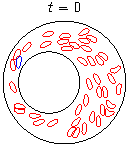
\includegraphics{figs/couette42SnapsTime1.pdf} &
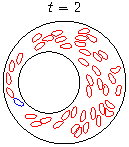
\includegraphics{figs/couette42SnapsTime2.pdf} &
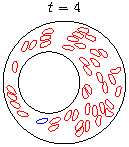
\includegraphics{figs/couette42SnapsTime3.pdf} &
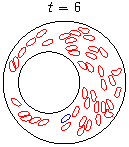
\includegraphics{figs/couette42SnapsTime4.pdf} &
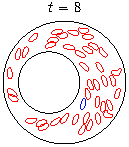
\includegraphics{figs/couette42SnapsTime5.pdf} &
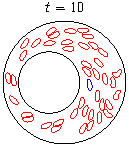
\includegraphics{figs/couette42SnapsTime6.pdf}
\end{tabular}
\mcaption{42 vesicles in a {\bf Couette} apparatus.  The outer boundary
is stationary and the inner boundary has constant angular velocity and
has completed one full rotation at $T=10$.  A single vesicle is colored
in blue to help with the visualization.}{f:couette42Geom}
\end{figure}

\begin{table}[htp]
\begin{center}
\begin{tabular}{ccccc}
$N_{t}$ & $e_{A}$ & $e_{L}$ & \# fmm & CPU \\
\hline
$160$  & \multicolumn{2}{c}{tolerance exceeded at $t=0.8$} 
       & $7.76$E$4$ & $0.1$ \\
$240$  & \multicolumn{2}{c}{tolerance exceeded at $t=0.8$}
       & $1.13$E$4$ & $0.2$ \\
$280$  & \multicolumn{2}{c}{tolerance exceeded at $t=1.1$}
       & $1.39$E$4$ & $0.2$ \\
$286$  & \multicolumn{2}{c}{tolerance exceeded at $t=2.0$}
       & $1.79$E$4$ & $0.3$ \\
$288$  & $5.10$E$-4$ & $9.94$E$-2$ & $4.01$E$4$ & $1.0$ \\
$320$  & $3.76$E$-3$ & $7.92$E$-2$ & $4.34$E$4$ & $1.1$ \\
$640$  & $9.48$E$-5$ & $8.60$E$-4$ & $8.34$E$4$ & $2.1$ \\
$1144$ & $2.80$E$-4$ & $2.17$E$-5$ & $1.71$E$5$ & $4.4$
%$20$  & \multicolumn{2}{c}{tolerance exceeded at $t=1.0$} 
%      & $6.42$E$1$ & $0.03$ \\
%$40$  & \multicolumn{2}{c}{tolerance exceeded at $t=1.0$}
%      & $1.17$E$3$ & $0.06$ \\
%$80$  & \multicolumn{2}{c}{tolerance exceeded at $t=1.6$}
%      & $2.33$E$3$ & $0.11$ \\
%$160$ & \multicolumn{2}{c}{tolerance exceeded at $t=2.8$}
%      & $6.03$E$3$ & $0.29$ \\
%$200$ & $1.45$E$-3$ & $4.76$E$-2$ & $2.06$E$4$ & $1.0$ \\
%$220$ & $1.03$E$-3$ & $1.35$E$-2$ & $2.23$E$4$ & $1.1$ \\
%$320$ & $3.41$E$-4$ & $2.90$E$-3$ & $3.24$E$4$ & $1.6$ \\
%$640$ & $5.73$E$-5$ & $1.47$E$-3$ & $6.48$E$4$ & $3.1$ \\
\end{tabular}
\mcaption{The errors in area and length and the CPU time for 42
vesicles in a {\bf Couette} apparatus with a {\bf constant} time step
size using {\bf BDF}.  The CPU times for Tables~\ref{t:couette42BDF}
and~\ref{t:adaptiveSecondOrderCouette42} are relative to the cheapest
simulation which took approximately 4 hours and 45 minutes.  We
demonstrate how a user often has to do several runs with different time
step sizes before a desired tolerance (for this example, $1$E$-1$) is
achieved.}{t:couette42BDF}

\begin{tabular}{ccccccc}
Tolerance & $e_{A}$ & $e_{L}$ & Accepts & Rejects & \# fmm & CPU \\
\hline
$1$E$-1$ & $1.24$E$-2$ & $2.53$E$-2$ 
         & $69$  & $23$ & $3.07$E$4$ & $0.7$ \\
$1$E$-2$ & $3.51$E$-3$ & $2.15$E$-3$ 
         & $155$ & $42$ & $7.07$E$4$ & $1.7$ \\
%$1$E$-1$ & $2.57$E$-2$ & $1.03$E$-2$ 
%         & $42$  & $13$ & $2.46$E$4$ & $1.1$ \\
%$1$E$-2$ & $3.03$E$-3$ & $2.58$E$-4$ 
%         & $125$ & $34$ & $6.35$E$4$ & $2.8$ \\
\end{tabular}
\mcaption{The errors in area and length, the CPU time, and the number of
accepted and rejected time steps for 42 vesicles in a {\bf Couette}
apparatus with an {\bf adaptive} time step size using $\boldnsdc{1}$.
Our new time integrator commits slightly less error for a fixed CPU
time, but, more importantly, only a single simulation is required to
achieve the desired tolerance.}{t:adaptiveSecondOrderCouette42}
\end{center}
\end{table}

\begin{figure}[htp]
\centering
\begin{tabular}{cc}
\ifTikz
\input{figs/couette42AdaptiveDT.tikz} 
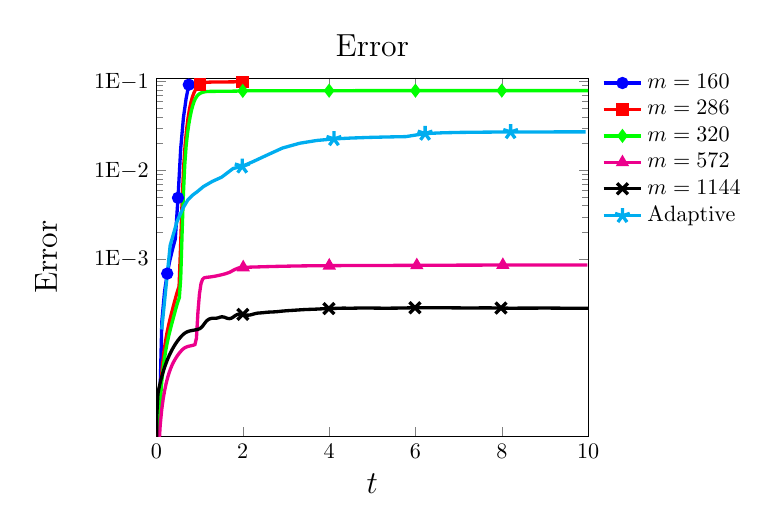
\begin{tikzpicture}[scale=0.8]

\begin{axis}[
  xmin = 0,
  xmax = 10,
  xtick = {0,2,4,6,8,10},
  xticklabels = {$0$,$2$,$4$,$6$,$8$,$10$},
  xlabel = $t$,
  ymode = log,
  ymin = 1E-5,
  ymax = 1.1E-1,
  ytick = {1E-3,1E-2,1E-1},
  yticklabels = {$1$E$-3$,$1$E$-2$,$1$E$-1$},
  ylabel = {Error},
  ylabel style = {yshift = 10pt},
  label style = {font=\Large},
%  legend entries = {$m=80$, $m=160$, $m=200$, $m=320$, $m=640$,
  legend entries = {$m=160$,$m=286$,$m=320$,$m=572$,$m=1144$,Adaptive},
  legend cell align=left,
%  legend style={at={(0.96,0.5)},anchor=east},
  legend style={at={(1.38,0.8)},anchor=east},
  legend style = {draw=none},
  title = {\Large{Error}}
  ]

\addlegendimage{mark=*,mark options=solid,blue,line width=1.5,solid}
\addlegendimage{mark=square*,mark options=solid,red,line width=1.5,solid}
\addlegendimage{mark=diamond*,mark options=solid,green,line width=1.5,solid}
\addlegendimage{mark=triangle*,mark options=solid,magenta,line width=1.5,solid}
\addlegendimage{mark=x,mark size=3.5,mark options=solid,black,line width=1.5,solid}
\addlegendimage{mark=star,mark size=3.5pt,mark options=solid,cyan,line width=1.5,solid}

% error for m = 160
\addplot [mark=none,blue,line width=1.5] table{
3.1250e-03 4.3298e-06
6.2500e-03 5.7836e-06
9.3750e-03 6.2782e-06
1.2500e-02 6.4532e-06
1.5625e-02 6.5223e-06
1.8750e-02 6.5567e-06
2.1875e-02 6.5801e-06
2.5000e-02 6.6005e-06
2.8125e-02 6.6203e-06
3.1250e-02 6.6404e-06
3.4375e-02 6.6608e-06
3.7500e-02 6.6598e-06
4.0625e-02 7.0370e-06
4.3750e-02 7.6725e-06
4.6875e-02 8.3111e-06
5.0000e-02 8.9518e-06
5.3125e-02 9.5943e-06
5.6250e-02 1.0238e-05
5.9375e-02 1.0884e-05
6.2500e-02 1.1531e-05
1.2500e-01 1.9763e-04
1.8750e-01 4.2756e-04
2.5000e-01 6.8702e-04
3.1250e-01 9.7391e-04
3.7500e-01 1.2995e-03
4.3750e-01 1.6929e-03
5.0000e-01 4.9028e-03
5.6250e-01 1.7607e-02
6.2500e-01 3.8963e-02
6.8750e-01 6.4326e-02
7.5000e-01 9.2320e-02
};

% error for m = 286
\addplot [mark=none,red,line width=1.5] table{
9.7125e-04 4.1425e-07
1.9425e-03 5.2310e-07
2.9138e-03 6.4109e-07
3.8850e-03 9.0249e-07
4.8563e-03 1.1662e-06
5.8275e-03 1.4303e-06
6.7988e-03 1.6941e-06
7.7700e-03 1.9573e-06
8.7413e-03 2.2198e-06
9.7125e-03 2.4814e-06
1.0684e-02 2.7421e-06
1.1655e-02 3.0018e-06
1.2626e-02 3.2605e-06
1.3598e-02 3.5180e-06
1.4569e-02 3.7743e-06
1.5540e-02 4.0295e-06
1.6511e-02 4.2833e-06
1.7483e-02 4.5359e-06
1.8454e-02 4.7870e-06
1.9425e-02 5.0369e-06
2.0396e-02 5.2852e-06
2.1368e-02 5.5322e-06
2.2339e-02 5.7776e-06
2.3310e-02 6.0215e-06
2.4281e-02 6.2639e-06
2.5253e-02 6.5046e-06
2.6224e-02 6.7438e-06
2.7195e-02 6.9813e-06
2.8166e-02 7.2172e-06
2.9138e-02 7.4514e-06
3.0109e-02 7.6838e-06
3.1080e-02 7.9145e-06
3.2051e-02 8.1434e-06
3.3023e-02 8.3705e-06
3.3994e-02 8.5958e-06
3.4965e-02 8.8192e-06
6.9930e-02 1.7221e-05
1.0490e-01 3.9518e-05
1.3986e-01 6.4041e-05
1.7483e-01 9.0455e-05
2.0979e-01 1.1845e-04
2.4476e-01 1.4766e-04
2.7972e-01 1.7811e-04
3.1469e-01 2.1050e-04
3.4965e-01 2.4596e-04
3.8462e-01 2.8576e-04
4.1958e-01 3.3118e-04
4.5455e-01 3.8283e-04
4.8951e-01 4.3887e-04
5.2448e-01 4.9304e-04
5.5944e-01 1.3886e-03
5.9441e-01 4.4301e-03
6.2937e-01 1.0777e-02
6.6434e-01 1.9350e-02
6.9930e-01 2.9113e-02
7.3427e-01 3.9581e-02
7.6923e-01 5.0065e-02
8.0420e-01 5.9798e-02
8.3916e-01 6.8375e-02
8.7413e-01 7.5652e-02
9.0909e-01 8.1591e-02
9.4406e-01 8.6296e-02
9.7902e-01 8.9954e-02
1.0140e+00 9.2750e-02
1.0490e+00 9.4849e-02
1.0839e+00 9.6362e-02
1.1189e+00 9.7397e-02
1.1538e+00 9.8058e-02
1.1888e+00 9.8446e-02
1.2238e+00 9.8661e-02
1.2587e+00 9.8774e-02
1.2937e+00 9.8837e-02
1.3287e+00 9.8878e-02
1.3636e+00 9.8913e-02
1.3986e+00 9.8946e-02
1.4336e+00 9.8981e-02
1.4685e+00 9.9017e-02
1.5035e+00 9.9054e-02
1.5385e+00 9.9093e-02
1.5734e+00 9.9133e-02
1.6084e+00 9.9174e-02
1.6434e+00 9.9216e-02
1.6783e+00 9.9260e-02
1.7133e+00 9.9305e-02
1.7483e+00 9.9351e-02
1.7832e+00 9.9400e-02
1.8182e+00 9.9453e-02
1.8531e+00 9.9513e-02
1.8881e+00 9.9581e-02
1.9231e+00 9.9663e-02
1.9580e+00 9.9761e-02
1.9930e+00 9.9879e-02
};

% error for m = 320
\addplot [mark=none,green,line width=1.5] table{
7.8125e-04 2.6017e-07
1.5625e-03 3.5448e-07
2.3437e-03 3.9785e-07
3.1250e-03 5.2009e-07
3.9062e-03 6.4248e-07
4.6875e-03 7.6546e-07
5.4687e-03 8.8913e-07
6.2500e-03 1.0135e-06
7.0313e-03 1.1385e-06
7.8125e-03 1.2642e-06
8.5938e-03 1.3905e-06
9.3750e-03 1.5173e-06
1.0156e-02 1.6446e-06
1.0937e-02 1.7724e-06
1.1719e-02 1.9006e-06
1.2500e-02 2.0293e-06
1.3281e-02 2.1584e-06
1.4063e-02 2.2879e-06
1.4844e-02 2.4178e-06
1.5625e-02 2.5480e-06
1.6406e-02 2.6785e-06
1.7188e-02 2.8094e-06
1.7969e-02 2.9406e-06
1.8750e-02 3.0720e-06
1.9531e-02 3.2038e-06
2.0313e-02 3.3358e-06
2.1094e-02 3.4681e-06
2.1875e-02 3.6007e-06
2.2656e-02 3.7335e-06
2.3438e-02 3.8665e-06
2.4219e-02 3.9998e-06
2.5000e-02 4.1333e-06
2.5781e-02 4.2670e-06
2.6562e-02 4.4010e-06
2.7344e-02 4.5351e-06
2.8125e-02 4.6695e-06
2.8906e-02 4.8041e-06
2.9687e-02 4.9388e-06
3.0469e-02 5.0738e-06
3.1250e-02 5.2090e-06
6.2500e-02 1.2318e-05
9.3750e-02 2.6656e-05
1.2500e-01 4.2233e-05
1.5625e-01 5.8874e-05
1.8750e-01 7.6516e-05
2.1875e-01 9.4956e-05
2.5000e-01 1.1402e-04
2.8125e-01 1.3383e-04
3.1250e-01 1.5478e-04
3.4375e-01 1.7749e-04
3.7500e-01 2.0266e-04
4.0625e-01 2.3095e-04
4.3750e-01 2.6286e-04
4.6875e-01 2.9811e-04
5.0000e-01 3.3460e-04
5.3125e-01 3.6820e-04
5.6250e-01 6.0517e-04
5.9375e-01 1.9011e-03
6.2500e-01 5.4369e-03
6.5625e-01 1.1508e-02
6.8750e-01 1.8614e-02
7.1875e-01 2.5821e-02
7.5000e-01 3.3082e-02
7.8125e-01 4.0338e-02
8.1250e-01 4.7521e-02
8.4375e-01 5.4250e-02
8.7500e-01 6.0094e-02
9.0625e-01 6.4804e-02
9.3750e-01 6.8385e-02
9.6875e-01 7.1050e-02
1.0000e+00 7.3022e-02
1.0312e+00 7.4486e-02
1.0625e+00 7.5565e-02
1.0938e+00 7.6339e-02
1.1250e+00 7.6873e-02
1.1562e+00 7.7219e-02
1.1875e+00 7.7428e-02
1.2188e+00 7.7546e-02
1.2500e+00 7.7610e-02
1.2812e+00 7.7647e-02
1.3125e+00 7.7673e-02
1.3438e+00 7.7695e-02
1.3750e+00 7.7717e-02
1.4062e+00 7.7739e-02
1.4375e+00 7.7763e-02
1.4688e+00 7.7788e-02
1.5000e+00 7.7814e-02
1.5312e+00 7.7841e-02
1.5625e+00 7.7869e-02
1.5938e+00 7.7898e-02
1.6250e+00 7.7928e-02
1.6562e+00 7.7959e-02
1.6875e+00 7.7991e-02
1.7188e+00 7.8025e-02
1.7500e+00 7.8061e-02
1.7812e+00 7.8100e-02
1.8125e+00 7.8144e-02
1.8438e+00 7.8197e-02
1.8750e+00 7.8262e-02
1.9062e+00 7.8339e-02
1.9375e+00 7.8426e-02
1.9688e+00 7.8513e-02
2.0000e+00 7.8593e-02
2.0312e+00 7.8670e-02
2.0625e+00 7.8734e-02
2.0938e+00 7.8780e-02
2.1250e+00 7.8811e-02
2.1562e+00 7.8832e-02
2.1875e+00 7.8846e-02
2.2188e+00 7.8857e-02
2.2500e+00 7.8867e-02
2.2812e+00 7.8875e-02
2.3125e+00 7.8882e-02
2.3438e+00 7.8890e-02
2.3750e+00 7.8896e-02
2.4062e+00 7.8903e-02
2.4375e+00 7.8910e-02
2.4688e+00 7.8916e-02
2.5000e+00 7.8922e-02
2.5312e+00 7.8928e-02
2.5625e+00 7.8934e-02
2.5938e+00 7.8940e-02
2.6250e+00 7.8945e-02
2.6562e+00 7.8951e-02
2.6875e+00 7.8956e-02
2.7188e+00 7.8961e-02
2.7500e+00 7.8966e-02
2.7812e+00 7.8971e-02
2.8125e+00 7.8976e-02
2.8438e+00 7.8981e-02
2.8750e+00 7.8986e-02
2.9062e+00 7.8990e-02
2.9375e+00 7.8994e-02
2.9688e+00 7.8999e-02
3.0000e+00 7.9003e-02
3.0312e+00 7.9007e-02
3.0625e+00 7.9010e-02
3.0938e+00 7.9014e-02
3.1250e+00 7.9018e-02
3.1562e+00 7.9021e-02
3.1875e+00 7.9024e-02
3.2188e+00 7.9027e-02
3.2500e+00 7.9031e-02
3.2812e+00 7.9033e-02
3.3125e+00 7.9036e-02
3.3438e+00 7.9039e-02
3.3750e+00 7.9042e-02
3.4062e+00 7.9044e-02
3.4375e+00 7.9047e-02
3.4688e+00 7.9049e-02
3.5000e+00 7.9051e-02
3.5312e+00 7.9054e-02
3.5625e+00 7.9056e-02
3.5938e+00 7.9058e-02
3.6250e+00 7.9060e-02
3.6562e+00 7.9062e-02
3.6875e+00 7.9064e-02
3.7188e+00 7.9065e-02
3.7500e+00 7.9067e-02
3.7812e+00 7.9069e-02
3.8125e+00 7.9070e-02
3.8438e+00 7.9072e-02
3.8750e+00 7.9074e-02
3.9062e+00 7.9075e-02
3.9375e+00 7.9077e-02
3.9688e+00 7.9078e-02
4.0000e+00 7.9080e-02
4.0312e+00 7.9081e-02
4.0625e+00 7.9083e-02
4.0938e+00 7.9084e-02
4.1250e+00 7.9086e-02
4.1562e+00 7.9087e-02
4.1875e+00 7.9088e-02
4.2188e+00 7.9090e-02
4.2500e+00 7.9091e-02
4.2812e+00 7.9092e-02
4.3125e+00 7.9094e-02
4.3438e+00 7.9095e-02
4.3750e+00 7.9097e-02
4.4062e+00 7.9098e-02
4.4375e+00 7.9099e-02
4.4688e+00 7.9101e-02
4.5000e+00 7.9102e-02
4.5312e+00 7.9103e-02
4.5625e+00 7.9104e-02
4.5938e+00 7.9105e-02
4.6250e+00 7.9107e-02
4.6562e+00 7.9108e-02
4.6875e+00 7.9109e-02
4.7188e+00 7.9110e-02
4.7500e+00 7.9111e-02
4.7812e+00 7.9112e-02
4.8125e+00 7.9114e-02
4.8438e+00 7.9115e-02
4.8750e+00 7.9116e-02
4.9062e+00 7.9117e-02
4.9375e+00 7.9118e-02
4.9688e+00 7.9119e-02
5.0000e+00 7.9120e-02
5.0312e+00 7.9121e-02
5.0625e+00 7.9122e-02
5.0938e+00 7.9123e-02
5.1250e+00 7.9124e-02
5.1562e+00 7.9125e-02
5.1875e+00 7.9126e-02
5.2188e+00 7.9127e-02
5.2500e+00 7.9128e-02
5.2812e+00 7.9129e-02
5.3125e+00 7.9129e-02
5.3438e+00 7.9130e-02
5.3750e+00 7.9131e-02
5.4062e+00 7.9131e-02
5.4375e+00 7.9132e-02
5.4688e+00 7.9133e-02
5.5000e+00 7.9133e-02
5.5312e+00 7.9134e-02
5.5625e+00 7.9135e-02
5.5938e+00 7.9135e-02
5.6250e+00 7.9136e-02
5.6562e+00 7.9137e-02
5.6875e+00 7.9138e-02
5.7188e+00 7.9139e-02
5.7500e+00 7.9139e-02
5.7812e+00 7.9140e-02
5.8125e+00 7.9141e-02
5.8438e+00 7.9142e-02
5.8750e+00 7.9143e-02
5.9062e+00 7.9144e-02
5.9375e+00 7.9145e-02
5.9688e+00 7.9146e-02
6.0000e+00 7.9147e-02
6.0312e+00 7.9148e-02
6.0625e+00 7.9149e-02
6.0938e+00 7.9150e-02
6.1250e+00 7.9151e-02
6.1562e+00 7.9152e-02
6.1875e+00 7.9153e-02
6.2188e+00 7.9154e-02
6.2500e+00 7.9155e-02
6.2812e+00 7.9157e-02
6.3125e+00 7.9158e-02
6.3438e+00 7.9159e-02
6.3750e+00 7.9160e-02
6.4062e+00 7.9161e-02
6.4375e+00 7.9162e-02
6.4688e+00 7.9163e-02
6.5000e+00 7.9164e-02
6.5312e+00 7.9165e-02
6.5625e+00 7.9166e-02
6.5938e+00 7.9168e-02
6.6250e+00 7.9169e-02
6.6562e+00 7.9170e-02
6.6875e+00 7.9171e-02
6.7188e+00 7.9172e-02
6.7500e+00 7.9173e-02
6.7812e+00 7.9174e-02
6.8125e+00 7.9176e-02
6.8438e+00 7.9177e-02
6.8750e+00 7.9178e-02
6.9062e+00 7.9179e-02
6.9375e+00 7.9180e-02
6.9688e+00 7.9181e-02
7.0000e+00 7.9182e-02
7.0312e+00 7.9184e-02
7.0625e+00 7.9185e-02
7.0938e+00 7.9186e-02
7.1250e+00 7.9187e-02
7.1562e+00 7.9188e-02
7.1875e+00 7.9189e-02
7.2188e+00 7.9190e-02
7.2500e+00 7.9192e-02
7.2812e+00 7.9193e-02
7.3125e+00 7.9194e-02
7.3438e+00 7.9195e-02
7.3750e+00 7.9196e-02
7.4062e+00 7.9197e-02
7.4375e+00 7.9198e-02
7.4688e+00 7.9199e-02
7.5000e+00 7.9200e-02
7.5312e+00 7.9201e-02
7.5625e+00 7.9202e-02
7.5938e+00 7.9203e-02
7.6250e+00 7.9204e-02
7.6562e+00 7.9204e-02
7.6875e+00 7.9205e-02
7.7188e+00 7.9206e-02
7.7500e+00 7.9207e-02
7.7812e+00 7.9207e-02
7.8125e+00 7.9208e-02
7.8438e+00 7.9209e-02
7.8750e+00 7.9209e-02
7.9062e+00 7.9210e-02
7.9375e+00 7.9211e-02
7.9688e+00 7.9211e-02
8.0000e+00 7.9212e-02
8.0312e+00 7.9212e-02
8.0625e+00 7.9213e-02
8.0938e+00 7.9213e-02
8.1250e+00 7.9214e-02
8.1562e+00 7.9215e-02
8.1875e+00 7.9215e-02
8.2188e+00 7.9216e-02
8.2500e+00 7.9216e-02
8.2812e+00 7.9217e-02
8.3125e+00 7.9217e-02
8.3438e+00 7.9218e-02
8.3750e+00 7.9218e-02
8.4062e+00 7.9218e-02
8.4375e+00 7.9219e-02
8.4688e+00 7.9219e-02
8.5000e+00 7.9220e-02
8.5312e+00 7.9220e-02
8.5625e+00 7.9221e-02
8.5938e+00 7.9221e-02
8.6250e+00 7.9222e-02
8.6562e+00 7.9222e-02
8.6875e+00 7.9222e-02
8.7188e+00 7.9223e-02
8.7500e+00 7.9223e-02
8.7812e+00 7.9224e-02
8.8125e+00 7.9224e-02
8.8438e+00 7.9224e-02
8.8750e+00 7.9225e-02
8.9062e+00 7.9225e-02
8.9375e+00 7.9226e-02
8.9688e+00 7.9226e-02
9.0000e+00 7.9226e-02
9.0312e+00 7.9227e-02
9.0625e+00 7.9227e-02
9.0938e+00 7.9227e-02
9.1250e+00 7.9228e-02
9.1562e+00 7.9228e-02
9.1875e+00 7.9229e-02
9.2188e+00 7.9229e-02
9.2500e+00 7.9229e-02
9.2812e+00 7.9230e-02
9.3125e+00 7.9230e-02
9.3438e+00 7.9231e-02
9.3750e+00 7.9231e-02
9.4062e+00 7.9232e-02
9.4375e+00 7.9232e-02
9.4688e+00 7.9233e-02
9.5000e+00 7.9233e-02
9.5312e+00 7.9234e-02
9.5625e+00 7.9234e-02
9.5938e+00 7.9235e-02
9.6250e+00 7.9235e-02
9.6562e+00 7.9236e-02
9.6875e+00 7.9236e-02
9.7188e+00 7.9237e-02
9.7500e+00 7.9237e-02
9.7812e+00 7.9238e-02
9.8125e+00 7.9239e-02
9.8438e+00 7.9239e-02
9.8750e+00 7.9240e-02
9.9062e+00 7.9240e-02
9.9375e+00 7.9241e-02
9.9688e+00 7.9241e-02
1.0000e+01 7.9242e-02
};

% error for m = 572
\addplot [mark=none,magenta,line width=1.5] table{
4.8563e-04 1.5537e-07
9.7125e-04 2.2589e-07
1.4569e-03 2.8531e-07
1.9425e-03 3.4185e-07
2.4281e-03 3.9644e-07
2.9138e-03 4.4916e-07
3.3994e-03 5.0000e-07
3.8850e-03 5.4896e-07
4.3706e-03 5.9599e-07
4.8563e-03 6.4107e-07
5.3419e-03 6.8417e-07
5.8275e-03 7.2527e-07
6.3131e-03 7.6433e-07
6.7988e-03 8.0134e-07
7.2844e-03 8.3626e-07
7.7700e-03 8.6906e-07
8.2556e-03 8.9974e-07
8.7413e-03 9.2826e-07
9.2269e-03 9.5460e-07
9.7125e-03 9.7874e-07
1.0198e-02 1.0007e-06
1.0684e-02 1.0204e-06
1.1169e-02 1.0534e-06
1.1655e-02 1.1307e-06
1.2141e-02 1.2103e-06
1.2626e-02 1.2924e-06
1.3112e-02 1.3769e-06
1.3598e-02 1.4638e-06
1.4083e-02 1.5531e-06
1.4569e-02 1.6449e-06
1.5054e-02 1.7391e-06
1.5540e-02 1.8357e-06
1.6026e-02 1.9348e-06
1.6511e-02 2.0364e-06
1.6997e-02 2.1404e-06
1.7483e-02 2.2469e-06
5.2448e-02 6.8567e-06
8.7413e-02 1.3428e-05
1.2238e-01 2.0099e-05
1.5734e-01 2.6797e-05
1.9231e-01 3.3492e-05
2.2727e-01 4.0137e-05
2.6224e-01 4.6679e-05
2.9720e-01 5.2982e-05
3.3217e-01 5.9023e-05
3.6713e-01 6.4756e-05
4.0210e-01 6.9967e-05
4.3706e-01 7.4973e-05
4.7203e-01 7.9788e-05
5.0699e-01 8.4386e-05
5.4196e-01 8.8732e-05
5.7692e-01 9.2782e-05
6.1189e-01 9.6477e-05
6.4685e-01 9.9534e-05
6.8182e-01 1.0164e-04
7.1678e-01 1.0315e-04
7.5175e-01 1.0437e-04
7.8671e-01 1.0530e-04
8.2168e-01 1.0621e-04
8.5664e-01 1.0734e-04
8.9161e-01 1.0885e-04
9.2657e-01 1.2809e-04
9.6154e-01 2.5214e-04
9.9650e-01 4.0407e-04
1.0315e+00 5.2643e-04
1.0664e+00 5.9092e-04
1.1014e+00 6.1399e-04
1.1364e+00 6.2079e-04
1.1713e+00 6.2379e-04
1.2063e+00 6.2645e-04
1.2413e+00 6.2943e-04
1.2762e+00 6.3280e-04
1.3112e+00 6.3660e-04
1.3462e+00 6.4084e-04
1.3811e+00 6.4553e-04
1.4161e+00 6.5065e-04
1.4510e+00 6.5617e-04
1.4860e+00 6.6210e-04
1.5210e+00 6.6844e-04
1.5559e+00 6.7523e-04
1.5909e+00 6.8260e-04
1.6259e+00 6.9080e-04
1.6608e+00 7.0024e-04
1.6958e+00 7.1164e-04
1.7308e+00 7.2575e-04
1.7657e+00 7.4205e-04
1.8007e+00 7.5722e-04
1.8357e+00 7.7090e-04
1.8706e+00 7.8500e-04
1.9056e+00 7.9547e-04
1.9406e+00 8.0135e-04
1.9755e+00 8.0456e-04
2.0105e+00 8.0654e-04
2.0455e+00 8.0799e-04
2.0804e+00 8.0921e-04
2.1154e+00 8.1031e-04
2.1503e+00 8.1135e-04
2.1853e+00 8.1236e-04
2.2203e+00 8.1335e-04
2.2552e+00 8.1433e-04
2.2902e+00 8.1529e-04
2.3252e+00 8.1625e-04
2.3601e+00 8.1721e-04
2.3951e+00 8.1816e-04
2.4301e+00 8.1910e-04
2.4650e+00 8.2004e-04
2.5000e+00 8.2097e-04
2.5350e+00 8.2189e-04
2.5699e+00 8.2281e-04
2.6049e+00 8.2371e-04
2.6399e+00 8.2460e-04
2.6748e+00 8.2547e-04
2.7098e+00 8.2631e-04
2.7448e+00 8.2714e-04
2.7797e+00 8.2794e-04
2.8147e+00 8.2872e-04
2.8497e+00 8.2948e-04
2.8846e+00 8.3021e-04
2.9196e+00 8.3091e-04
2.9545e+00 8.3160e-04
2.9895e+00 8.3227e-04
3.0245e+00 8.3294e-04
3.0594e+00 8.3359e-04
3.0944e+00 8.3422e-04
3.1294e+00 8.3483e-04
3.1643e+00 8.3542e-04
3.1993e+00 8.3599e-04
3.2343e+00 8.3654e-04
3.2692e+00 8.3706e-04
3.3042e+00 8.3756e-04
3.3392e+00 8.3804e-04
3.3741e+00 8.3851e-04
3.4091e+00 8.3895e-04
3.4441e+00 8.3937e-04
3.4790e+00 8.3978e-04
3.5140e+00 8.4017e-04
3.5490e+00 8.4054e-04
3.5839e+00 8.4090e-04
3.6189e+00 8.4124e-04
3.6538e+00 8.4157e-04
3.6888e+00 8.4188e-04
3.7238e+00 8.4218e-04
3.7587e+00 8.4247e-04
3.7937e+00 8.4271e-04
3.8287e+00 8.4293e-04
3.8636e+00 8.4315e-04
3.8986e+00 8.4336e-04
3.9336e+00 8.4356e-04
3.9685e+00 8.4377e-04
4.0035e+00 8.4398e-04
4.0385e+00 8.4418e-04
4.0734e+00 8.4438e-04
4.1084e+00 8.4457e-04
4.1434e+00 8.4475e-04
4.1783e+00 8.4493e-04
4.2133e+00 8.4510e-04
4.2483e+00 8.4526e-04
4.2832e+00 8.4542e-04
4.3182e+00 8.4559e-04
4.3531e+00 8.4576e-04
4.3881e+00 8.4593e-04
4.4231e+00 8.4610e-04
4.4580e+00 8.4627e-04
4.4930e+00 8.4642e-04
4.5280e+00 8.4656e-04
4.5629e+00 8.4671e-04
4.5979e+00 8.4685e-04
4.6329e+00 8.4698e-04
4.6678e+00 8.4712e-04
4.7028e+00 8.4725e-04
4.7378e+00 8.4738e-04
4.7727e+00 8.4751e-04
4.8077e+00 8.4763e-04
4.8427e+00 8.4776e-04
4.8776e+00 8.4789e-04
4.9126e+00 8.4802e-04
4.9476e+00 8.4815e-04
4.9825e+00 8.4827e-04
5.0175e+00 8.4839e-04
5.0524e+00 8.4851e-04
5.0874e+00 8.4862e-04
5.1224e+00 8.4872e-04
5.1573e+00 8.4881e-04
5.1923e+00 8.4889e-04
5.2273e+00 8.4896e-04
5.2622e+00 8.4902e-04
5.2972e+00 8.4907e-04
5.3322e+00 8.4912e-04
5.3671e+00 8.4915e-04
5.4021e+00 8.4918e-04
5.4371e+00 8.4922e-04
5.4720e+00 8.4928e-04
5.5070e+00 8.4936e-04
5.5420e+00 8.4945e-04
5.5769e+00 8.4954e-04
5.6119e+00 8.4963e-04
5.6469e+00 8.4973e-04
5.6818e+00 8.4984e-04
5.7168e+00 8.4996e-04
5.7517e+00 8.5008e-04
5.7867e+00 8.5021e-04
5.8217e+00 8.5034e-04
5.8566e+00 8.5046e-04
5.8916e+00 8.5059e-04
5.9266e+00 8.5071e-04
5.9615e+00 8.5084e-04
5.9965e+00 8.5097e-04
6.0315e+00 8.5111e-04
6.0664e+00 8.5124e-04
6.1014e+00 8.5138e-04
6.1364e+00 8.5151e-04
6.1713e+00 8.5163e-04
6.2063e+00 8.5175e-04
6.2413e+00 8.5187e-04
6.2762e+00 8.5199e-04
6.3112e+00 8.5211e-04
6.3462e+00 8.5223e-04
6.3811e+00 8.5236e-04
6.4161e+00 8.5249e-04
6.4510e+00 8.5263e-04
6.4860e+00 8.5277e-04
6.5210e+00 8.5292e-04
6.5559e+00 8.5308e-04
6.5909e+00 8.5324e-04
6.6259e+00 8.5340e-04
6.6608e+00 8.5357e-04
6.6958e+00 8.5373e-04
6.7308e+00 8.5390e-04
6.7657e+00 8.5406e-04
6.8007e+00 8.5422e-04
6.8357e+00 8.5437e-04
6.8706e+00 8.5452e-04
6.9056e+00 8.5466e-04
6.9406e+00 8.5481e-04
6.9755e+00 8.5492e-04
7.0105e+00 8.5501e-04
7.0455e+00 8.5511e-04
7.0804e+00 8.5520e-04
7.1154e+00 8.5530e-04
7.1503e+00 8.5541e-04
7.1853e+00 8.5553e-04
7.2203e+00 8.5565e-04
7.2552e+00 8.5575e-04
7.2902e+00 8.5585e-04
7.3252e+00 8.5593e-04
7.3601e+00 8.5599e-04
7.3951e+00 8.5606e-04
7.4301e+00 8.5613e-04
7.4650e+00 8.5621e-04
7.5000e+00 8.5629e-04
7.5350e+00 8.5637e-04
7.5699e+00 8.5646e-04
7.6049e+00 8.5654e-04
7.6399e+00 8.5663e-04
7.6748e+00 8.5672e-04
7.7098e+00 8.5681e-04
7.7448e+00 8.5689e-04
7.7797e+00 8.5697e-04
7.8147e+00 8.5705e-04
7.8497e+00 8.5712e-04
7.8846e+00 8.5721e-04
7.9196e+00 8.5734e-04
7.9545e+00 8.5747e-04
7.9895e+00 8.5759e-04
8.0245e+00 8.5769e-04
8.0594e+00 8.5780e-04
8.0944e+00 8.5790e-04
8.1294e+00 8.5798e-04
8.1643e+00 8.5803e-04
8.1993e+00 8.5808e-04
8.2343e+00 8.5813e-04
8.2692e+00 8.5817e-04
8.3042e+00 8.5820e-04
8.3392e+00 8.5823e-04
8.3741e+00 8.5825e-04
8.4091e+00 8.5827e-04
8.4441e+00 8.5829e-04
8.4790e+00 8.5831e-04
8.5140e+00 8.5832e-04
8.5490e+00 8.5834e-04
8.5839e+00 8.5835e-04
8.6189e+00 8.5837e-04
8.6538e+00 8.5839e-04
8.6888e+00 8.5841e-04
8.7238e+00 8.5844e-04
8.7587e+00 8.5846e-04
8.7937e+00 8.5847e-04
8.8287e+00 8.5848e-04
8.8636e+00 8.5849e-04
8.8986e+00 8.5849e-04
8.9336e+00 8.5849e-04
8.9685e+00 8.5849e-04
9.0035e+00 8.5848e-04
9.0385e+00 8.5851e-04
9.0734e+00 8.5855e-04
9.1084e+00 8.5860e-04
9.1434e+00 8.5867e-04
9.1783e+00 8.5872e-04
9.2133e+00 8.5877e-04
9.2483e+00 8.5882e-04
9.2832e+00 8.5888e-04
9.3182e+00 8.5894e-04
9.3531e+00 8.5901e-04
9.3881e+00 8.5908e-04
9.4231e+00 8.5915e-04
9.4580e+00 8.5924e-04
9.4930e+00 8.5934e-04
9.5280e+00 8.5943e-04
9.5629e+00 8.5949e-04
9.5979e+00 8.5956e-04
9.6329e+00 8.5964e-04
9.6678e+00 8.5972e-04
9.7028e+00 8.5980e-04
9.7378e+00 8.5988e-04
9.7727e+00 8.5992e-04
9.8077e+00 8.5997e-04
9.8427e+00 8.6005e-04
9.8776e+00 8.6014e-04
9.9126e+00 8.6023e-04
9.9476e+00 8.6032e-04
9.9825e+00 8.6042e-04
};

% error for m = 1144
\addplot [mark=none,black,line width=1.5] table{
1.8211e-04 3.1692e-07
3.6422e-04 7.0621e-07
5.4633e-04 1.0973e-06
7.2844e-04 1.4876e-06
9.1055e-04 1.8771e-06
1.0927e-03 2.2656e-06
1.2748e-03 2.6533e-06
1.4569e-03 3.0400e-06
1.6390e-03 3.4259e-06
1.8211e-03 3.8108e-06
2.0032e-03 4.1949e-06
2.1853e-03 4.5780e-06
2.3674e-03 4.9602e-06
2.5495e-03 5.3415e-06
2.7316e-03 5.7219e-06
2.9138e-03 6.1013e-06
3.0959e-03 6.4798e-06
3.2780e-03 6.8574e-06
3.4601e-03 7.2341e-06
3.6422e-03 7.6098e-06
3.8243e-03 7.9845e-06
4.0064e-03 8.3583e-06
4.1885e-03 8.7312e-06
4.3706e-03 9.1031e-06
4.5527e-03 9.4740e-06
4.7348e-03 9.8440e-06
4.9170e-03 1.0213e-05
5.0991e-03 1.0581e-05
5.2812e-03 1.0948e-05
5.4633e-03 1.1314e-05
5.6454e-03 1.1679e-05
5.8275e-03 1.2043e-05
6.0096e-03 1.2407e-05
6.1917e-03 1.2769e-05
6.3738e-03 1.3130e-05
6.5559e-03 1.3490e-05
6.7381e-03 1.3849e-05
6.9202e-03 1.4207e-05
7.1023e-03 1.4565e-05
7.2844e-03 1.4921e-05
7.4665e-03 1.5276e-05
7.6486e-03 1.5630e-05
7.8307e-03 1.5983e-05
8.0128e-03 1.6335e-05
8.1949e-03 1.6686e-05
8.3770e-03 1.7036e-05
8.5591e-03 1.7385e-05
8.7413e-03 1.7733e-05
3.4965e-02 3.0383e-05
6.1189e-02 3.5577e-05
8.7413e-02 4.0499e-05
1.1364e-01 4.5411e-05
1.3986e-01 5.0472e-05
1.6608e-01 5.5703e-05
1.9231e-01 6.0981e-05
2.1853e-01 6.6292e-05
2.4476e-01 7.1627e-05
2.7098e-01 7.6961e-05
2.9720e-01 8.2245e-05
3.2343e-01 8.7503e-05
3.4965e-01 9.2731e-05
3.7587e-01 9.7926e-05
4.0210e-01 1.0306e-04
4.2832e-01 1.0814e-04
4.5455e-01 1.1314e-04
4.8077e-01 1.1805e-04
5.0699e-01 1.2286e-04
5.3322e-01 1.2754e-04
5.5944e-01 1.3207e-04
5.8566e-01 1.3639e-04
6.1189e-01 1.4046e-04
6.3811e-01 1.4410e-04
6.6434e-01 1.4709e-04
6.9056e-01 1.4968e-04
7.1678e-01 1.5184e-04
7.4301e-01 1.5358e-04
7.6923e-01 1.5494e-04
7.9545e-01 1.5599e-04
8.2168e-01 1.5686e-04
8.4790e-01 1.5766e-04
8.7413e-01 1.5847e-04
9.0035e-01 1.5958e-04
9.2657e-01 1.6050e-04
9.5280e-01 1.6173e-04
9.7902e-01 1.6273e-04
1.0052e+00 1.6474e-04
1.0315e+00 1.6826e-04
1.0577e+00 1.7334e-04
1.0839e+00 1.7965e-04
1.1101e+00 1.8697e-04
1.1364e+00 1.9462e-04
1.1626e+00 2.0120e-04
1.1888e+00 2.0625e-04
1.2150e+00 2.1009e-04
1.2413e+00 2.1278e-04
1.2675e+00 2.1443e-04
1.2937e+00 2.1521e-04
1.3199e+00 2.1541e-04
1.3462e+00 2.1536e-04
1.3724e+00 2.1551e-04
1.3986e+00 2.1628e-04
1.4248e+00 2.1782e-04
1.4510e+00 2.1990e-04
1.4773e+00 2.2195e-04
1.5035e+00 2.2333e-04
1.5297e+00 2.2357e-04
1.5559e+00 2.2257e-04
1.5822e+00 2.2062e-04
1.6084e+00 2.1820e-04
1.6346e+00 2.1587e-04
1.6608e+00 2.1417e-04
1.6871e+00 2.1354e-04
1.7133e+00 2.1430e-04
1.7395e+00 2.1656e-04
1.7657e+00 2.2019e-04
1.7920e+00 2.2471e-04
1.8182e+00 2.2951e-04
1.8444e+00 2.3389e-04
1.8706e+00 2.3729e-04
1.8969e+00 2.3944e-04
1.9231e+00 2.4037e-04
1.9493e+00 2.4038e-04
1.9755e+00 2.3966e-04
2.0017e+00 2.3836e-04
2.0280e+00 2.3685e-04
2.0542e+00 2.3541e-04
2.0804e+00 2.3427e-04
2.1066e+00 2.3364e-04
2.1329e+00 2.3365e-04
2.1591e+00 2.3435e-04
2.1853e+00 2.3565e-04
2.2115e+00 2.3740e-04
2.2378e+00 2.3940e-04
2.2640e+00 2.4149e-04
2.2902e+00 2.4339e-04
2.3164e+00 2.4495e-04
2.3427e+00 2.4611e-04
2.3689e+00 2.4691e-04
2.3951e+00 2.4745e-04
2.4213e+00 2.4790e-04
2.4476e+00 2.4843e-04
2.4738e+00 2.4912e-04
2.5000e+00 2.4995e-04
2.5262e+00 2.5082e-04
2.5524e+00 2.5164e-04
2.5787e+00 2.5231e-04
2.6049e+00 2.5281e-04
2.6311e+00 2.5312e-04
2.6573e+00 2.5343e-04
2.6836e+00 2.5377e-04
2.7098e+00 2.5415e-04
2.7360e+00 2.5459e-04
2.7622e+00 2.5511e-04
2.7885e+00 2.5572e-04
2.8147e+00 2.5641e-04
2.8409e+00 2.5717e-04
2.8671e+00 2.5799e-04
2.8934e+00 2.5885e-04
2.9196e+00 2.5957e-04
2.9458e+00 2.6026e-04
2.9720e+00 2.6093e-04
2.9983e+00 2.6157e-04
3.0245e+00 2.6216e-04
3.0507e+00 2.6271e-04
3.0769e+00 2.6321e-04
3.1031e+00 2.6370e-04
3.1294e+00 2.6420e-04
3.1556e+00 2.6469e-04
3.1818e+00 2.6518e-04
3.2080e+00 2.6569e-04
3.2343e+00 2.6621e-04
3.2605e+00 2.6674e-04
3.2867e+00 2.6728e-04
3.3129e+00 2.6782e-04
3.3392e+00 2.6835e-04
3.3654e+00 2.6886e-04
3.3916e+00 2.6934e-04
3.4178e+00 2.6978e-04
3.4441e+00 2.7018e-04
3.4703e+00 2.7054e-04
3.4965e+00 2.7087e-04
3.5227e+00 2.7117e-04
3.5490e+00 2.7145e-04
3.5752e+00 2.7173e-04
3.6014e+00 2.7201e-04
3.6276e+00 2.7229e-04
3.6538e+00 2.7258e-04
3.6801e+00 2.7292e-04
3.7063e+00 2.7330e-04
3.7325e+00 2.7370e-04
3.7587e+00 2.7413e-04
3.7850e+00 2.7457e-04
3.8112e+00 2.7500e-04
3.8374e+00 2.7541e-04
3.8636e+00 2.7586e-04
3.8899e+00 2.7626e-04
3.9161e+00 2.7647e-04
3.9423e+00 2.7667e-04
3.9685e+00 2.7691e-04
3.9948e+00 2.7713e-04
4.0210e+00 2.7734e-04
4.0472e+00 2.7755e-04
4.0734e+00 2.7778e-04
4.0997e+00 2.7802e-04
4.1259e+00 2.7829e-04
4.1521e+00 2.7857e-04
4.1783e+00 2.7888e-04
4.2045e+00 2.7919e-04
4.2308e+00 2.7951e-04
4.2570e+00 2.7981e-04
4.2832e+00 2.8008e-04
4.3094e+00 2.8021e-04
4.3357e+00 2.8020e-04
4.3619e+00 2.8017e-04
4.3881e+00 2.8013e-04
4.4143e+00 2.8007e-04
4.4406e+00 2.7999e-04
4.4668e+00 2.7991e-04
4.4930e+00 2.7983e-04
4.5192e+00 2.7983e-04
4.5455e+00 2.7993e-04
4.5717e+00 2.8012e-04
4.5979e+00 2.8031e-04
4.6241e+00 2.8050e-04
4.6503e+00 2.8068e-04
4.6766e+00 2.8085e-04
4.7028e+00 2.8100e-04
4.7290e+00 2.8115e-04
4.7552e+00 2.8128e-04
4.7815e+00 2.8140e-04
4.8077e+00 2.8152e-04
4.8339e+00 2.8158e-04
4.8601e+00 2.8148e-04
4.8864e+00 2.8136e-04
4.9126e+00 2.8124e-04
4.9388e+00 2.8112e-04
4.9650e+00 2.8100e-04
4.9913e+00 2.8087e-04
5.0175e+00 2.8075e-04
5.0437e+00 2.8062e-04
5.0699e+00 2.8051e-04
5.0962e+00 2.8042e-04
5.1224e+00 2.8034e-04
5.1486e+00 2.8026e-04
5.1748e+00 2.8019e-04
5.2010e+00 2.8011e-04
5.2273e+00 2.8002e-04
5.2535e+00 2.7991e-04
5.2797e+00 2.7984e-04
5.3059e+00 2.7991e-04
5.3322e+00 2.7982e-04
5.3584e+00 2.7988e-04
5.3846e+00 2.7997e-04
5.4108e+00 2.8006e-04
5.4371e+00 2.8016e-04
5.4633e+00 2.8025e-04
5.4895e+00 2.8034e-04
5.5157e+00 2.8043e-04
5.5420e+00 2.8052e-04
5.5682e+00 2.8061e-04
5.5944e+00 2.8068e-04
5.6206e+00 2.8075e-04
5.6469e+00 2.8082e-04
5.6731e+00 2.8091e-04
5.6993e+00 2.8104e-04
5.7255e+00 2.8123e-04
5.7517e+00 2.8144e-04
5.7780e+00 2.8168e-04
5.8042e+00 2.8191e-04
5.8304e+00 2.8213e-04
5.8566e+00 2.8235e-04
5.8829e+00 2.8254e-04
5.9091e+00 2.8272e-04
5.9353e+00 2.8288e-04
5.9615e+00 2.8302e-04
5.9878e+00 2.8313e-04
6.0140e+00 2.8322e-04
6.0402e+00 2.8304e-04
6.0664e+00 2.8307e-04
6.0927e+00 2.8318e-04
6.1189e+00 2.8330e-04
6.1451e+00 2.8343e-04
6.1713e+00 2.8356e-04
6.1976e+00 2.8368e-04
6.2238e+00 2.8373e-04
6.2500e+00 2.8371e-04
6.2762e+00 2.8367e-04
6.3024e+00 2.8364e-04
6.3287e+00 2.8360e-04
6.3549e+00 2.8355e-04
6.3811e+00 2.8350e-04
6.4073e+00 2.8344e-04
6.4336e+00 2.8339e-04
6.4598e+00 2.8333e-04
6.4860e+00 2.8328e-04
6.5122e+00 2.8323e-04
6.5385e+00 2.8318e-04
6.5647e+00 2.8313e-04
6.5909e+00 2.8307e-04
6.6171e+00 2.8302e-04
6.6434e+00 2.8296e-04
6.6696e+00 2.8290e-04
6.6958e+00 2.8284e-04
6.7220e+00 2.8278e-04
6.7483e+00 2.8271e-04
6.7745e+00 2.8265e-04
6.8007e+00 2.8258e-04
6.8269e+00 2.8251e-04
6.8531e+00 2.8243e-04
6.8794e+00 2.8236e-04
6.9056e+00 2.8229e-04
6.9318e+00 2.8222e-04
6.9580e+00 2.8215e-04
6.9843e+00 2.8209e-04
7.0105e+00 2.8203e-04
7.0367e+00 2.8198e-04
7.0629e+00 2.8193e-04
7.0892e+00 2.8190e-04
7.1154e+00 2.8187e-04
7.1416e+00 2.8185e-04
7.1678e+00 2.8184e-04
7.1941e+00 2.8184e-04
7.2203e+00 2.8185e-04
7.2465e+00 2.8185e-04
7.2727e+00 2.8187e-04
7.2990e+00 2.8188e-04
7.3252e+00 2.8190e-04
7.3514e+00 2.8190e-04
7.3776e+00 2.8191e-04
7.4038e+00 2.8192e-04
7.4301e+00 2.8194e-04
7.4563e+00 2.8194e-04
7.4825e+00 2.8198e-04
7.5087e+00 2.8204e-04
7.5350e+00 2.8208e-04
7.5612e+00 2.8211e-04
7.5874e+00 2.8211e-04
7.6136e+00 2.8211e-04
7.6399e+00 2.8209e-04
7.6661e+00 2.8206e-04
7.6923e+00 2.8203e-04
7.7185e+00 2.8200e-04
7.7448e+00 2.8198e-04
7.7710e+00 2.8196e-04
7.7972e+00 2.8193e-04
7.8234e+00 2.8191e-04
7.8497e+00 2.8189e-04
7.8759e+00 2.8182e-04
7.9021e+00 2.8161e-04
7.9283e+00 2.8138e-04
7.9545e+00 2.8117e-04
7.9808e+00 2.8098e-04
8.0070e+00 2.8080e-04
8.0332e+00 2.8065e-04
8.0594e+00 2.8050e-04
8.0857e+00 2.8034e-04
8.1119e+00 2.8017e-04
8.1381e+00 2.8014e-04
8.1643e+00 2.8012e-04
8.1906e+00 2.8011e-04
8.2168e+00 2.8010e-04
8.2430e+00 2.8009e-04
8.2692e+00 2.8008e-04
8.2955e+00 2.8008e-04
8.3217e+00 2.8009e-04
8.3479e+00 2.8011e-04
8.3741e+00 2.8015e-04
8.4003e+00 2.8019e-04
8.4266e+00 2.8023e-04
8.4528e+00 2.8027e-04
8.4790e+00 2.8032e-04
8.5052e+00 2.8036e-04
8.5315e+00 2.8040e-04
8.5577e+00 2.8044e-04
8.5839e+00 2.8048e-04
8.6101e+00 2.8051e-04
8.6364e+00 2.8054e-04
8.6626e+00 2.8055e-04
8.6888e+00 2.8055e-04
8.7150e+00 2.8055e-04
8.7413e+00 2.8055e-04
8.7675e+00 2.8057e-04
8.7937e+00 2.8059e-04
8.8199e+00 2.8062e-04
8.8462e+00 2.8065e-04
8.8724e+00 2.8068e-04
8.8986e+00 2.8072e-04
8.9248e+00 2.8078e-04
8.9510e+00 2.8084e-04
8.9773e+00 2.8092e-04
9.0035e+00 2.8102e-04
9.0297e+00 2.8098e-04
9.0559e+00 2.8092e-04
9.0822e+00 2.8085e-04
9.1084e+00 2.8076e-04
9.1346e+00 2.8065e-04
9.1608e+00 2.8053e-04
9.1871e+00 2.8047e-04
9.2133e+00 2.8042e-04
9.2395e+00 2.8037e-04
9.2657e+00 2.8032e-04
9.2920e+00 2.8026e-04
9.3182e+00 2.8021e-04
9.3444e+00 2.8015e-04
9.3706e+00 2.8009e-04
9.3969e+00 2.8003e-04
9.4231e+00 2.7996e-04
9.4493e+00 2.7986e-04
9.4755e+00 2.7969e-04
9.5017e+00 2.7955e-04
9.5280e+00 2.7947e-04
9.5542e+00 2.7944e-04
9.5804e+00 2.7943e-04
9.6066e+00 2.7939e-04
9.6329e+00 2.7935e-04
9.6591e+00 2.7930e-04
9.6853e+00 2.7927e-04
9.7115e+00 2.7925e-04
9.7378e+00 2.7923e-04
9.7640e+00 2.7935e-04
9.7902e+00 2.7950e-04
9.8164e+00 2.7957e-04
9.8427e+00 2.7957e-04
9.8689e+00 2.7956e-04
9.8951e+00 2.7955e-04
9.9213e+00 2.7954e-04
9.9476e+00 2.7953e-04
9.9738e+00 2.7953e-04
1.0000e+01 2.7952e-04
};

% adaptive time step size
\addplot [mark=none,cyan,line width=1.5] table{
1.2305e-01 1.6124e-04
3.1796e-01 1.4239e-03
4.7685e-01 2.6483e-03
6.1213e-01 3.7329e-03
7.2582e-01 4.6318e-03
8.3352e-01 5.2404e-03
9.4392e-01 5.7440e-03
1.0894e+00 6.5693e-03
1.2928e+00 7.5004e-03
1.5109e+00 8.3823e-03
1.7760e+00 1.0495e-02
1.9870e+00 1.1098e-02
2.2433e+00 1.2580e-02
2.5434e+00 1.4721e-02
2.9223e+00 1.7866e-02
3.3215e+00 2.0228e-02
3.7179e+00 2.1732e-02
4.1117e+00 2.2612e-02
4.4987e+00 2.3119e-02
4.8994e+00 2.3492e-02
5.3176e+00 2.3771e-02
5.7777e+00 2.4008e-02
6.2233e+00 2.5983e-02
6.6342e+00 2.6511e-02
7.0339e+00 2.6775e-02
7.4272e+00 2.6915e-02
7.8147e+00 2.7010e-02
8.2040e+00 2.7075e-02
8.5269e+00 2.7095e-02
8.8060e+00 2.7102e-02
9.1771e+00 2.7121e-02
9.5560e+00 2.7142e-02
9.9421e+00 2.7167e-02
};

% marked error for m = 160
\addplot [mark=*,blue,line width=1.5,only marks] table{
2.5000e-01 6.8702e-04
5.0000e-01 4.9028e-03
7.5000e-01 9.2320e-02
};

% marked error for m = 286
\addplot [mark=square*,red,line width=1.5,only marks] table{
1.0140e+00 9.2750e-02
1.9930e+00 9.9879e-02
};

% marked error for m = 320
\addplot [mark=diamond*,green,line width=1.5,only marks] table{
2.0000e+00 7.8593e-02
4.0000e+00 7.9080e-02
6.0000e+00 7.9147e-02
8.0000e+00 7.9212e-02
};

% marked error for m = 572
\addplot [mark=triangle*,magenta,only marks,line width=1.5] table{
2.0105e+00 8.0654e-04
4.0035e+00 8.4398e-04
6.0315e+00 8.5111e-04
8.0245e+00 8.5769e-04
};

% marked error for m = 1144
\addplot [mark=x,mark size=3.5pt,black,only marks,line width=1.5] table{
2.0017e+00 2.3836e-04
3.9948e+00 2.7713e-04
5.9878e+00 2.8313e-04
7.9808e+00 2.8098e-04
};

% marked adaptive time step size
\addplot [mark=star,mark size=3.5pt,cyan,line width=1.5,only marks] table{
1.9870e+00 1.1098e-02
4.1117e+00 2.2612e-02
6.2233e+00 2.5983e-02
8.2040e+00 2.7075e-02
};
\end{axis}

\end{tikzpicture}


 & 
\fi
\\
\end{tabular}
\mcaption{Left: The time step size using {\bf adaptive} $\boldnsdc{1}$,
$p=2$ with a tolerance of $1$E$-2$.  The open circles indicate the
locations where a time step size is rejected.  Right: The error of {\bf
BDF} and {\bf adaptive} $\boldnsdc{1}$ for 42 vesicles in a {\bf
Couette} apparatus.  If a user specifies too large of a time step, then
the error exceeds the tolerance of $1$E$-1$.  By using an {\bf
adaptive} time step size, the error committed per time step is
controlled.}{f:couette42Errors}
\end{figure}

\begin{figure}[htp]
\centering
\begin{tabular}{cccccc}
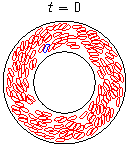
\includegraphics{figs/couette150SnapsTime1.pdf} &
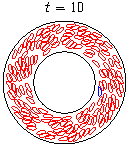
\includegraphics{figs/couette150SnapsTime2.pdf} &
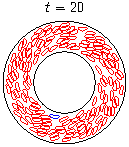
\includegraphics{figs/couette150SnapsTime3.pdf} &
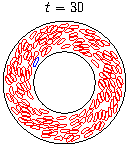
\includegraphics{figs/couette150SnapsTime4.pdf} &
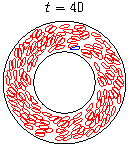
\includegraphics{figs/couette150SnapsTime5.pdf} &
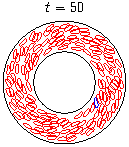
\includegraphics{figs/couette150SnapsTime6.pdf}
%\ifTikz
%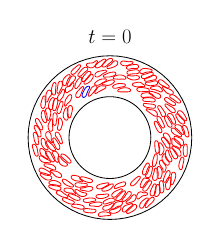
\begin{tikzpicture}[scale=0.3]

\begin{axis}[
  xmin = -21,
  xmax = 21,
  ymin = -21,
  ymax = 21,
  scale only axis,
  axis equal image,
  hide axis,
  title = {\Huge$t=0$}
  ]

% outer solid wall
\addplot [mark=none,black,line width=1.0] table{
2.0000e+01 -5.5171e-16
1.9904e+01 1.9603e+00
1.9616e+01 3.9018e+00
1.9139e+01 5.8057e+00
1.8478e+01 7.6537e+00
1.7638e+01 9.4279e+00
1.6629e+01 1.1111e+01
1.5460e+01 1.2688e+01
1.4142e+01 1.4142e+01
1.2688e+01 1.5460e+01
1.1111e+01 1.6629e+01
9.4279e+00 1.7638e+01
7.6537e+00 1.8478e+01
5.8057e+00 1.9139e+01
3.9018e+00 1.9616e+01
1.9603e+00 1.9904e+01
2.3281e-15 2.0000e+01
-1.9603e+00 1.9904e+01
-3.9018e+00 1.9616e+01
-5.8057e+00 1.9139e+01
-7.6537e+00 1.8478e+01
-9.4279e+00 1.7638e+01
-1.1111e+01 1.6629e+01
-1.2688e+01 1.5460e+01
-1.4142e+01 1.4142e+01
-1.5460e+01 1.2688e+01
-1.6629e+01 1.1111e+01
-1.7638e+01 9.4279e+00
-1.8478e+01 7.6537e+00
-1.9139e+01 5.8057e+00
-1.9616e+01 3.9018e+00
-1.9904e+01 1.9603e+00
-2.0000e+01 3.0010e-15
-1.9904e+01 -1.9603e+00
-1.9616e+01 -3.9018e+00
-1.9139e+01 -5.8057e+00
-1.8478e+01 -7.6537e+00
-1.7638e+01 -9.4279e+00
-1.6629e+01 -1.1111e+01
-1.5460e+01 -1.2688e+01
-1.4142e+01 -1.4142e+01
-1.2688e+01 -1.5460e+01
-1.1111e+01 -1.6629e+01
-9.4279e+00 -1.7638e+01
-7.6537e+00 -1.8478e+01
-5.8057e+00 -1.9139e+01
-3.9018e+00 -1.9616e+01
-1.9603e+00 -1.9904e+01
-4.7774e-15 -2.0000e+01
1.9603e+00 -1.9904e+01
3.9018e+00 -1.9616e+01
5.8057e+00 -1.9139e+01
7.6537e+00 -1.8478e+01
9.4279e+00 -1.7638e+01
1.1111e+01 -1.6629e+01
1.2688e+01 -1.5460e+01
1.4142e+01 -1.4142e+01
1.5460e+01 -1.2688e+01
1.6629e+01 -1.1111e+01
1.7638e+01 -9.4279e+00
1.8478e+01 -7.6537e+00
1.9139e+01 -5.8057e+00
1.9616e+01 -3.9018e+00
1.9904e+01 -1.9603e+00
2.0000e+01 -5.5171e-16
};

% inner solid wall
\addplot [mark=none,black,line width=1.0] table{
1.0000e+01 2.7586e-16
9.9518e+00 -9.8017e-01
9.8079e+00 -1.9509e+00
9.5694e+00 -2.9028e+00
9.2388e+00 -3.8268e+00
8.8192e+00 -4.7140e+00
8.3147e+00 -5.5557e+00
7.7301e+00 -6.3439e+00
7.0711e+00 -7.0711e+00
6.3439e+00 -7.7301e+00
5.5557e+00 -8.3147e+00
4.7140e+00 -8.8192e+00
3.8268e+00 -9.2388e+00
2.9028e+00 -9.5694e+00
1.9509e+00 -9.8079e+00
9.8017e-01 -9.9518e+00
1.1640e-15 -1.0000e+01
-9.8017e-01 -9.9518e+00
-1.9509e+00 -9.8079e+00
-2.9028e+00 -9.5694e+00
-3.8268e+00 -9.2388e+00
-4.7140e+00 -8.8192e+00
-5.5557e+00 -8.3147e+00
-6.3439e+00 -7.7301e+00
-7.0711e+00 -7.0711e+00
-7.7301e+00 -6.3439e+00
-8.3147e+00 -5.5557e+00
-8.8192e+00 -4.7140e+00
-9.2388e+00 -3.8268e+00
-9.5694e+00 -2.9028e+00
-9.8079e+00 -1.9509e+00
-9.9518e+00 -9.8017e-01
-1.0000e+01 -1.5005e-15
-9.9518e+00 9.8017e-01
-9.8079e+00 1.9509e+00
-9.5694e+00 2.9028e+00
-9.2388e+00 3.8268e+00
-8.8192e+00 4.7140e+00
-8.3147e+00 5.5557e+00
-7.7301e+00 6.3439e+00
-7.0711e+00 7.0711e+00
-6.3439e+00 7.7301e+00
-5.5557e+00 8.3147e+00
-4.7140e+00 8.8192e+00
-3.8268e+00 9.2388e+00
-2.9028e+00 9.5694e+00
-1.9509e+00 9.8079e+00
-9.8017e-01 9.9518e+00
-2.3887e-15 1.0000e+01
9.8017e-01 9.9518e+00
1.9509e+00 9.8079e+00
2.9028e+00 9.5694e+00
3.8268e+00 9.2388e+00
4.7140e+00 8.8192e+00
5.5557e+00 8.3147e+00
6.3439e+00 7.7301e+00
7.0711e+00 7.0711e+00
7.7301e+00 6.3439e+00
8.3147e+00 5.5557e+00
8.8192e+00 4.7140e+00
9.2388e+00 3.8268e+00
9.5694e+00 2.9028e+00
9.8079e+00 1.9509e+00
9.9518e+00 9.8017e-01
1.0000e+01 2.7586e-16
};

% vesicle 1
\addplot [mark=none,red,line width=1.0] table{
-2.1130e+00 -1.5864e+01
-2.1890e+00 -1.5835e+01
-2.2784e+00 -1.5812e+01
-2.3833e+00 -1.5793e+01
-2.5076e+00 -1.5778e+01
-2.6485e+00 -1.5766e+01
-2.8039e+00 -1.5759e+01
-2.9789e+00 -1.5757e+01
-3.1703e+00 -1.5764e+01
-3.3642e+00 -1.5783e+01
-3.5637e+00 -1.5816e+01
-3.7691e+00 -1.5859e+01
-3.9681e+00 -1.5903e+01
-4.1679e+00 -1.5946e+01
-4.3602e+00 -1.5987e+01
-4.5418e+00 -1.6028e+01
-4.7065e+00 -1.6078e+01
-4.8475e+00 -1.6144e+01
-4.9592e+00 -1.6235e+01
-5.0209e+00 -1.6346e+01
-5.0279e+00 -1.6455e+01
-4.9920e+00 -1.6546e+01
-4.9342e+00 -1.6609e+01
-4.8677e+00 -1.6650e+01
-4.7950e+00 -1.6677e+01
-4.7147e+00 -1.6694e+01
-4.6183e+00 -1.6704e+01
-4.5030e+00 -1.6708e+01
-4.3723e+00 -1.6710e+01
-4.2243e+00 -1.6713e+01
-4.0619e+00 -1.6722e+01
-3.9005e+00 -1.6739e+01
-3.7229e+00 -1.6765e+01
-3.5336e+00 -1.6798e+01
-3.3467e+00 -1.6828e+01
-3.1449e+00 -1.6845e+01
-2.9386e+00 -1.6839e+01
-2.7401e+00 -1.6804e+01
-2.5582e+00 -1.6744e+01
-2.3965e+00 -1.6667e+01
-2.2499e+00 -1.6575e+01
-2.1212e+00 -1.6472e+01
-2.0175e+00 -1.6363e+01
-1.9459e+00 -1.6244e+01
-1.9213e+00 -1.6125e+01
-1.9423e+00 -1.6024e+01
-1.9910e+00 -1.5950e+01
-2.0493e+00 -1.5900e+01
-2.1130e+00 -1.5864e+01
};

% vesicle 2
\addplot [mark=none,red,line width=1.0] table{
5.7832e+00 -1.0377e+01
5.7229e+00 -1.0434e+01
5.6531e+00 -1.0500e+01
5.5719e+00 -1.0580e+01
5.4824e+00 -1.0671e+01
5.3866e+00 -1.0773e+01
5.2881e+00 -1.0887e+01
5.1898e+00 -1.1015e+01
5.0954e+00 -1.1172e+01
5.0302e+00 -1.1354e+01
5.0319e+00 -1.1553e+01
5.1430e+00 -1.1726e+01
5.3322e+00 -1.1797e+01
5.5338e+00 -1.1775e+01
5.7226e+00 -1.1702e+01
5.8873e+00 -1.1611e+01
6.0315e+00 -1.1512e+01
6.1571e+00 -1.1412e+01
6.2661e+00 -1.1313e+01
6.3641e+00 -1.1215e+01
6.4452e+00 -1.1128e+01
6.5113e+00 -1.1053e+01
6.5693e+00 -1.0985e+01
6.6203e+00 -1.0923e+01
6.6681e+00 -1.0864e+01
6.7197e+00 -1.0800e+01
6.7772e+00 -1.0728e+01
6.8440e+00 -1.0643e+01
6.9231e+00 -1.0543e+01
7.0117e+00 -1.0430e+01
7.1085e+00 -1.0307e+01
7.2134e+00 -1.0172e+01
7.3180e+00 -1.0024e+01
7.4061e+00 -9.8567e+00
7.4331e+00 -9.6620e+00
7.3292e+00 -9.4932e+00
7.1347e+00 -9.4475e+00
6.9399e+00 -9.5016e+00
6.7677e+00 -9.5938e+00
6.6149e+00 -9.6942e+00
6.4773e+00 -9.7934e+00
6.3489e+00 -9.8916e+00
6.2325e+00 -9.9848e+00
6.1302e+00 -1.0070e+01
6.0405e+00 -1.0146e+01
5.9631e+00 -1.0214e+01
5.8981e+00 -1.0272e+01
5.8401e+00 -1.0325e+01
5.7832e+00 -1.0377e+01
};

% vesicle 3
\addplot [mark=none,red,line width=1.0] table{
-1.2064e+01 6.2550e+00
-1.2032e+01 6.3270e+00
-1.1996e+01 6.4146e+00
-1.1957e+01 6.5209e+00
-1.1916e+01 6.6398e+00
-1.1871e+01 6.7734e+00
-1.1824e+01 6.9165e+00
-1.1774e+01 7.0674e+00
-1.1717e+01 7.2362e+00
-1.1655e+01 7.4216e+00
-1.1592e+01 7.6177e+00
-1.1535e+01 7.8193e+00
-1.1488e+01 8.0206e+00
-1.1457e+01 8.2265e+00
-1.1452e+01 8.4300e+00
-1.1488e+01 8.6173e+00
-1.1579e+01 8.7711e+00
-1.1713e+01 8.8571e+00
-1.1857e+01 8.8649e+00
-1.1981e+01 8.8124e+00
-1.2070e+01 8.7347e+00
-1.2130e+01 8.6565e+00
-1.2175e+01 8.5807e+00
-1.2210e+01 8.5121e+00
-1.2240e+01 8.4462e+00
-1.2273e+01 8.3690e+00
-1.2307e+01 8.2821e+00
-1.2344e+01 8.1838e+00
-1.2386e+01 8.0686e+00
-1.2433e+01 7.9409e+00
-1.2487e+01 7.7959e+00
-1.2551e+01 7.6266e+00
-1.2619e+01 7.4518e+00
-1.2689e+01 7.2750e+00
-1.2763e+01 7.0887e+00
-1.2836e+01 6.8962e+00
-1.2899e+01 6.6993e+00
-1.2934e+01 6.5065e+00
-1.2927e+01 6.3146e+00
-1.2867e+01 6.1358e+00
-1.2764e+01 5.9957e+00
-1.2627e+01 5.9076e+00
-1.2482e+01 5.8849e+00
-1.2360e+01 5.9150e+00
-1.2262e+01 5.9767e+00
-1.2188e+01 6.0516e+00
-1.2138e+01 6.1208e+00
-1.2099e+01 6.1867e+00
-1.2064e+01 6.2550e+00
};

% vesicle 4
\addplot [mark=none,red,line width=1.0] table{
-2.5935e+00 -1.3927e+01
-2.6749e+00 -1.3929e+01
-2.7671e+00 -1.3934e+01
-2.8732e+00 -1.3944e+01
-2.9935e+00 -1.3966e+01
-3.1257e+00 -1.4010e+01
-3.2570e+00 -1.4090e+01
-3.3613e+00 -1.4218e+01
-3.4000e+00 -1.4395e+01
-3.3317e+00 -1.4582e+01
-3.1805e+00 -1.4715e+01
-3.0023e+00 -1.4793e+01
-2.8111e+00 -1.4843e+01
-2.6060e+00 -1.4877e+01
-2.4002e+00 -1.4896e+01
-2.2059e+00 -1.4899e+01
-2.0232e+00 -1.4887e+01
-1.8584e+00 -1.4864e+01
-1.7145e+00 -1.4835e+01
-1.5877e+00 -1.4803e+01
-1.4768e+00 -1.4773e+01
-1.3809e+00 -1.4745e+01
-1.2987e+00 -1.4720e+01
-1.2260e+00 -1.4696e+01
-1.1560e+00 -1.4673e+01
-1.0812e+00 -1.4648e+01
-9.9622e-01 -1.4617e+01
-8.9755e-01 -1.4580e+01
-7.8228e-01 -1.4533e+01
-6.5339e-01 -1.4472e+01
-5.1700e-01 -1.4391e+01
-3.8592e-01 -1.4272e+01
-3.0696e-01 -1.4105e+01
-3.4364e-01 -1.3923e+01
-4.9810e-01 -1.3805e+01
-7.0314e-01 -1.3776e+01
-9.0809e-01 -1.3794e+01
-1.1087e+00 -1.3824e+01
-1.3058e+00 -1.3854e+01
-1.4946e+00 -1.3879e+01
-1.6751e+00 -1.3897e+01
-1.8415e+00 -1.3910e+01
-1.9929e+00 -1.3918e+01
-2.1291e+00 -1.3922e+01
-2.2482e+00 -1.3924e+01
-2.3506e+00 -1.3925e+01
-2.4390e+00 -1.3925e+01
-2.5175e+00 -1.3926e+01
-2.5935e+00 -1.3927e+01
};

% vesicle 5
\addplot [mark=none,red,line width=1.0] table{
9.3152e+00 -1.5474e+01
9.2720e+00 -1.5537e+01
9.2221e+00 -1.5610e+01
9.1642e+00 -1.5697e+01
9.0985e+00 -1.5796e+01
9.0237e+00 -1.5911e+01
8.9393e+00 -1.6045e+01
8.8490e+00 -1.6194e+01
8.7575e+00 -1.6361e+01
8.6742e+00 -1.6543e+01
8.6184e+00 -1.6740e+01
8.6315e+00 -1.6943e+01
8.7654e+00 -1.7094e+01
8.9692e+00 -1.7093e+01
9.1357e+00 -1.6983e+01
9.2681e+00 -1.6845e+01
9.3884e+00 -1.6712e+01
9.5014e+00 -1.6595e+01
9.6089e+00 -1.6491e+01
9.7095e+00 -1.6400e+01
9.7984e+00 -1.6323e+01
9.8734e+00 -1.6259e+01
9.9371e+00 -1.6205e+01
9.9926e+00 -1.6158e+01
1.0046e+01 -1.6112e+01
1.0105e+01 -1.6061e+01
1.0174e+01 -1.5999e+01
1.0254e+01 -1.5925e+01
1.0345e+01 -1.5835e+01
1.0442e+01 -1.5730e+01
1.0542e+01 -1.5608e+01
1.0642e+01 -1.5468e+01
1.0733e+01 -1.5309e+01
1.0802e+01 -1.5135e+01
1.0830e+01 -1.4945e+01
1.0780e+01 -1.4751e+01
1.0634e+01 -1.4617e+01
1.0437e+01 -1.4584e+01
1.0244e+01 -1.4628e+01
1.0075e+01 -1.4709e+01
9.9203e+00 -1.4811e+01
9.7850e+00 -1.4920e+01
9.6742e+00 -1.5025e+01
9.5831e+00 -1.5123e+01
9.5086e+00 -1.5211e+01
9.4480e+00 -1.5289e+01
9.3986e+00 -1.5356e+01
9.3559e+00 -1.5416e+01
9.3152e+00 -1.5474e+01
};

% vesicle 6
\addplot [mark=none,red,line width=1.0] table{
9.6197e+00 -6.5729e+00
9.5954e+00 -6.4962e+00
9.5542e+00 -6.4125e+00
9.4877e+00 -6.3257e+00
9.3864e+00 -6.2507e+00
9.2502e+00 -6.2169e+00
9.1010e+00 -6.2518e+00
8.9653e+00 -6.3535e+00
8.8458e+00 -6.5006e+00
8.7326e+00 -6.6732e+00
8.6195e+00 -6.8591e+00
8.5109e+00 -7.0442e+00
8.4102e+00 -7.2224e+00
8.3145e+00 -7.4013e+00
8.2269e+00 -7.5786e+00
8.1513e+00 -7.7486e+00
8.0867e+00 -7.9157e+00
8.0364e+00 -8.0714e+00
8.0005e+00 -8.2115e+00
7.9766e+00 -8.3398e+00
7.9637e+00 -8.4538e+00
7.9598e+00 -8.5519e+00
7.9630e+00 -8.6359e+00
7.9716e+00 -8.7100e+00
7.9863e+00 -8.7810e+00
8.0102e+00 -8.8559e+00
8.0505e+00 -8.9383e+00
8.1170e+00 -9.0238e+00
8.2193e+00 -9.0962e+00
8.3568e+00 -9.1277e+00
8.5064e+00 -9.0920e+00
8.6372e+00 -8.9863e+00
8.7358e+00 -8.8358e+00
8.8125e+00 -8.6695e+00
8.8828e+00 -8.4890e+00
8.9497e+00 -8.3014e+00
9.0159e+00 -8.1091e+00
9.0846e+00 -7.9140e+00
9.1563e+00 -7.7263e+00
9.2356e+00 -7.5458e+00
9.3199e+00 -7.3855e+00
9.4069e+00 -7.2448e+00
9.4889e+00 -7.1215e+00
9.5561e+00 -7.0101e+00
9.6030e+00 -6.9050e+00
9.6283e+00 -6.8081e+00
9.6364e+00 -6.7220e+00
9.6327e+00 -6.6457e+00
9.6197e+00 -6.5729e+00
};

% vesicle 7
\addplot [mark=none,red,line width=1.0] table{
1.4369e+01 -5.7459e+00
1.4423e+01 -5.8042e+00
1.4493e+01 -5.8632e+00
1.4585e+01 -5.9164e+00
1.4703e+01 -5.9491e+00
1.4838e+01 -5.9415e+00
1.4973e+01 -5.8768e+00
1.5084e+01 -5.7452e+00
1.5137e+01 -5.5719e+00
1.5130e+01 -5.3804e+00
1.5071e+01 -5.1774e+00
1.4983e+01 -4.9888e+00
1.4887e+01 -4.8164e+00
1.4788e+01 -4.6444e+00
1.4692e+01 -4.4702e+00
1.4603e+01 -4.2924e+00
1.4531e+01 -4.1234e+00
1.4473e+01 -3.9640e+00
1.4430e+01 -3.8175e+00
1.4400e+01 -3.6888e+00
1.4378e+01 -3.5763e+00
1.4361e+01 -3.4782e+00
1.4347e+01 -3.3957e+00
1.4333e+01 -3.3226e+00
1.4316e+01 -3.2517e+00
1.4290e+01 -3.1778e+00
1.4244e+01 -3.0975e+00
1.4161e+01 -3.0261e+00
1.4040e+01 -3.0020e+00
1.3911e+01 -3.0512e+00
1.3803e+01 -3.1625e+00
1.3718e+01 -3.3136e+00
1.3653e+01 -3.4856e+00
1.3607e+01 -3.6675e+00
1.3580e+01 -3.8657e+00
1.3585e+01 -4.0860e+00
1.3616e+01 -4.2992e+00
1.3657e+01 -4.4950e+00
1.3716e+01 -4.6818e+00
1.3794e+01 -4.8544e+00
1.3881e+01 -5.0093e+00
1.3968e+01 -5.1480e+00
1.4049e+01 -5.2732e+00
1.4122e+01 -5.3852e+00
1.4183e+01 -5.4806e+00
1.4235e+01 -5.5605e+00
1.4281e+01 -5.6298e+00
1.4324e+01 -5.6899e+00
1.4369e+01 -5.7459e+00
};

% vesicle 8
\addplot [mark=none,red,line width=1.0] table{
-1.2591e+01 -1.4270e+00
-1.2633e+01 -1.3620e+00
-1.2684e+01 -1.2867e+00
-1.2743e+01 -1.1992e+00
-1.2810e+01 -1.1015e+00
-1.2885e+01 -9.9079e-01
-1.2970e+01 -8.6243e-01
-1.3067e+01 -7.1619e-01
-1.3173e+01 -5.5581e-01
-1.3289e+01 -3.9002e-01
-1.3420e+01 -2.3302e-01
-1.3581e+01 -1.0799e-01
-1.3785e+01 -7.8398e-02
-1.3939e+01 -2.1111e-01
-1.3962e+01 -4.0893e-01
-1.3923e+01 -5.8983e-01
-1.3874e+01 -7.5889e-01
-1.3832e+01 -9.1487e-01
-1.3801e+01 -1.0541e+00
-1.3773e+01 -1.1814e+00
-1.3744e+01 -1.2932e+00
-1.3714e+01 -1.3880e+00
-1.3684e+01 -1.4697e+00
-1.3655e+01 -1.5403e+00
-1.3625e+01 -1.6066e+00
-1.3590e+01 -1.6790e+00
-1.3549e+01 -1.7607e+00
-1.3500e+01 -1.8537e+00
-1.3442e+01 -1.9606e+00
-1.3378e+01 -2.0803e+00
-1.3308e+01 -2.2132e+00
-1.3234e+01 -2.3613e+00
-1.3152e+01 -2.5263e+00
-1.3051e+01 -2.6963e+00
-1.2912e+01 -2.8448e+00
-1.2721e+01 -2.9352e+00
-1.2510e+01 -2.9151e+00
-1.2354e+01 -2.7836e+00
-1.2279e+01 -2.6131e+00
-1.2253e+01 -2.4342e+00
-1.2258e+01 -2.2570e+00
-1.2285e+01 -2.0897e+00
-1.2325e+01 -1.9435e+00
-1.2372e+01 -1.8189e+00
-1.2422e+01 -1.7131e+00
-1.2470e+01 -1.6245e+00
-1.2512e+01 -1.5521e+00
-1.2551e+01 -1.4886e+00
-1.2591e+01 -1.4270e+00
};

% vesicle 9
\addplot [mark=none,red,line width=1.0] table{
-1.4351e+01 -1.7846e-01
-1.4346e+01 -9.9341e-02
-1.4340e+01 -7.5245e-03
-1.4334e+01 1.0024e-01
-1.4332e+01 2.2432e-01
-1.4340e+01 3.6362e-01
-1.4361e+01 5.1453e-01
-1.4396e+01 6.7352e-01
-1.4449e+01 8.4462e-01
-1.4529e+01 1.0265e+00
-1.4646e+01 1.2047e+00
-1.4798e+01 1.3487e+00
-1.4980e+01 1.4383e+00
-1.5175e+01 1.4610e+00
-1.5360e+01 1.4133e+00
-1.5512e+01 1.3043e+00
-1.5616e+01 1.1559e+00
-1.5674e+01 9.9650e-01
-1.5699e+01 8.4740e-01
-1.5703e+01 7.1523e-01
-1.5696e+01 5.9962e-01
-1.5682e+01 5.0112e-01
-1.5666e+01 4.1791e-01
-1.5648e+01 3.4533e-01
-1.5627e+01 2.7569e-01
-1.5602e+01 2.0046e-01
-1.5567e+01 1.1427e-01
-1.5522e+01 1.5281e-02
-1.5461e+01 -9.6339e-02
-1.5381e+01 -2.1772e-01
-1.5278e+01 -3.4103e-01
-1.5149e+01 -4.5864e-01
-1.4998e+01 -5.6790e-01
-1.4843e+01 -6.7748e-01
-1.4696e+01 -8.0542e-01
-1.4567e+01 -9.6089e-01
-1.4455e+01 -1.1276e+00
-1.4334e+01 -1.2749e+00
-1.4156e+01 -1.3305e+00
-1.4037e+01 -1.1938e+00
-1.4073e+01 -1.0252e+00
-1.4153e+01 -8.8433e-01
-1.4229e+01 -7.5489e-01
-1.4286e+01 -6.3041e-01
-1.4323e+01 -5.1508e-01
-1.4343e+01 -4.1388e-01
-1.4351e+01 -3.2755e-01
-1.4353e+01 -2.5169e-01
-1.4351e+01 -1.7846e-01
};

% vesicle 10
\addplot [mark=none,red,line width=1.0] table{
1.8009e+01 -5.8336e+00
1.8024e+01 -5.7553e+00
1.8041e+01 -5.6656e+00
1.8059e+01 -5.5602e+00
1.8075e+01 -5.4352e+00
1.8080e+01 -5.2910e+00
1.8062e+01 -5.1328e+00
1.8000e+01 -4.9726e+00
1.7876e+01 -4.8386e+00
1.7695e+01 -4.7776e+00
1.7506e+01 -4.8276e+00
1.7367e+01 -4.9730e+00
1.7279e+01 -5.1621e+00
1.7211e+01 -5.3577e+00
1.7146e+01 -5.5449e+00
1.7084e+01 -5.7205e+00
1.7027e+01 -5.8890e+00
1.6980e+01 -6.0496e+00
1.6941e+01 -6.1983e+00
1.6912e+01 -6.3311e+00
1.6892e+01 -6.4464e+00
1.6877e+01 -6.5439e+00
1.6868e+01 -6.6257e+00
1.6861e+01 -6.6978e+00
1.6856e+01 -6.7682e+00
1.6853e+01 -6.8455e+00
1.6852e+01 -6.9371e+00
1.6856e+01 -7.0457e+00
1.6868e+01 -7.1696e+00
1.6892e+01 -7.3088e+00
1.6935e+01 -7.4608e+00
1.7006e+01 -7.6136e+00
1.7117e+01 -7.7500e+00
1.7283e+01 -7.8363e+00
1.7474e+01 -7.8115e+00
1.7614e+01 -7.6687e+00
1.7683e+01 -7.4737e+00
1.7718e+01 -7.2732e+00
1.7750e+01 -7.0748e+00
1.7785e+01 -6.8815e+00
1.7821e+01 -6.7025e+00
1.7856e+01 -6.5409e+00
1.7888e+01 -6.3953e+00
1.7916e+01 -6.2675e+00
1.7940e+01 -6.1582e+00
1.7961e+01 -6.0635e+00
1.7978e+01 -5.9802e+00
1.7994e+01 -5.9056e+00
1.8009e+01 -5.8336e+00
};

% vesicle 11
\addplot [mark=none,red,line width=1.0] table{
1.0989e+01 1.4153e+01
1.1061e+01 1.4180e+01
1.1140e+01 1.4220e+01
1.1225e+01 1.4279e+01
1.1309e+01 1.4367e+01
1.1375e+01 1.4492e+01
1.1401e+01 1.4649e+01
1.1369e+01 1.4823e+01
1.1275e+01 1.4988e+01
1.1132e+01 1.5117e+01
1.0952e+01 1.5201e+01
1.0746e+01 1.5225e+01
1.0539e+01 1.5181e+01
1.0351e+01 1.5091e+01
1.0178e+01 1.4988e+01
1.0011e+01 1.4893e+01
9.8505e+00 1.4811e+01
9.6985e+00 1.4743e+01
9.5590e+00 1.4689e+01
9.4360e+00 1.4647e+01
9.3287e+00 1.4613e+01
9.2357e+00 1.4585e+01
9.1552e+00 1.4561e+01
9.0835e+00 1.4540e+01
9.0138e+00 1.4520e+01
8.9377e+00 1.4497e+01
8.8495e+00 1.4468e+01
8.7474e+00 1.4431e+01
8.6354e+00 1.4377e+01
8.5258e+00 1.4293e+01
8.4491e+00 1.4159e+01
8.4538e+00 1.3992e+01
8.5603e+00 1.3847e+01
8.7357e+00 1.3769e+01
8.9329e+00 1.3755e+01
9.1337e+00 1.3778e+01
9.3382e+00 1.3816e+01
9.5411e+00 1.3858e+01
9.7355e+00 1.3899e+01
9.9240e+00 1.3938e+01
1.0104e+01 1.3973e+01
1.0270e+01 1.4004e+01
1.0422e+01 1.4032e+01
1.0557e+01 1.4055e+01
1.0673e+01 1.4076e+01
1.0771e+01 1.4095e+01
1.0852e+01 1.4113e+01
1.0922e+01 1.4132e+01
1.0989e+01 1.4153e+01
};

% vesicle 12
\addplot [mark=none,red,line width=1.0] table{
-6.6166e+00 -1.2914e+01
-6.5406e+00 -1.2924e+01
-6.4502e+00 -1.2937e+01
-6.3420e+00 -1.2954e+01
-6.2189e+00 -1.2976e+01
-6.0795e+00 -1.3004e+01
-5.9259e+00 -1.3038e+01
-5.7588e+00 -1.3075e+01
-5.5758e+00 -1.3107e+01
-5.3794e+00 -1.3124e+01
-5.1784e+00 -1.3117e+01
-4.9752e+00 -1.3081e+01
-4.7842e+00 -1.3021e+01
-4.6068e+00 -1.2939e+01
-4.4378e+00 -1.2828e+01
-4.2973e+00 -1.2690e+01
-4.2111e+00 -1.2539e+01
-4.1893e+00 -1.2380e+01
-4.2361e+00 -1.2236e+01
-4.3227e+00 -1.2135e+01
-4.4186e+00 -1.2069e+01
-4.5079e+00 -1.2027e+01
-4.5893e+00 -1.1999e+01
-4.6620e+00 -1.1980e+01
-4.7321e+00 -1.1966e+01
-4.8127e+00 -1.1954e+01
-4.9062e+00 -1.1946e+01
-5.0161e+00 -1.1942e+01
-5.1470e+00 -1.1948e+01
-5.2932e+00 -1.1966e+01
-5.4519e+00 -1.2001e+01
-5.6195e+00 -1.2052e+01
-5.7872e+00 -1.2110e+01
-5.9617e+00 -1.2168e+01
-6.1539e+00 -1.2220e+01
-6.3580e+00 -1.2259e+01
-6.5637e+00 -1.2283e+01
-6.7668e+00 -1.2296e+01
-6.9589e+00 -1.2312e+01
-7.1417e+00 -1.2366e+01
-7.2672e+00 -1.2499e+01
-7.2637e+00 -1.2661e+01
-7.1712e+00 -1.2772e+01
-7.0552e+00 -1.2831e+01
-6.9434e+00 -1.2863e+01
-6.8442e+00 -1.2882e+01
-6.7619e+00 -1.2894e+01
-6.6887e+00 -1.2904e+01
-6.6166e+00 -1.2914e+01
};

% vesicle 13
\addplot [mark=none,red,line width=1.0] table{
1.1501e+00 1.2911e+01
1.0784e+00 1.2873e+01
9.9716e-01 1.2827e+01
9.0536e-01 1.2767e+01
8.0692e-01 1.2685e+01
7.1644e-01 1.2572e+01
6.6650e-01 1.2422e+01
7.0207e-01 1.2256e+01
8.3672e-01 1.2129e+01
1.0239e+00 1.2072e+01
1.2236e+00 1.2062e+01
1.4287e+00 1.2076e+01
1.6353e+00 1.2105e+01
1.8330e+00 1.2145e+01
2.0246e+00 1.2190e+01
2.2051e+00 1.2233e+01
2.3743e+00 1.2272e+01
2.5369e+00 1.2305e+01
2.6883e+00 1.2333e+01
2.8242e+00 1.2355e+01
2.9422e+00 1.2374e+01
3.0426e+00 1.2390e+01
3.1285e+00 1.2404e+01
3.2044e+00 1.2417e+01
3.2775e+00 1.2431e+01
3.3562e+00 1.2449e+01
3.4458e+00 1.2474e+01
3.5475e+00 1.2512e+01
3.6561e+00 1.2576e+01
3.7517e+00 1.2681e+01
3.7872e+00 1.2835e+01
3.7173e+00 1.2989e+01
3.5687e+00 1.3089e+01
3.3817e+00 1.3142e+01
3.1755e+00 1.3171e+01
2.9720e+00 1.3190e+01
2.7760e+00 1.3202e+01
2.5803e+00 1.3208e+01
2.3813e+00 1.3207e+01
2.1893e+00 1.3197e+01
2.0109e+00 1.3178e+01
1.8460e+00 1.3150e+01
1.6961e+00 1.3116e+01
1.5661e+00 1.3079e+01
1.4573e+00 1.3042e+01
1.3656e+00 1.3007e+01
1.2871e+00 1.2974e+01
1.2174e+00 1.2943e+01
1.1501e+00 1.2911e+01
};

% vesicle 14
\addplot [mark=none,red,line width=1.0] table{
-2.4900e+00 -1.1429e+01
-2.5615e+00 -1.1453e+01
-2.6442e+00 -1.1484e+01
-2.7408e+00 -1.1525e+01
-2.8439e+00 -1.1576e+01
-2.9594e+00 -1.1646e+01
-3.0833e+00 -1.1745e+01
-3.1928e+00 -1.1876e+01
-3.2563e+00 -1.2056e+01
-3.2154e+00 -1.2256e+01
-3.0786e+00 -1.2403e+01
-2.8930e+00 -1.2488e+01
-2.6840e+00 -1.2527e+01
-2.4773e+00 -1.2528e+01
-2.2778e+00 -1.2498e+01
-2.0930e+00 -1.2443e+01
-1.9306e+00 -1.2374e+01
-1.7813e+00 -1.2300e+01
-1.6432e+00 -1.2230e+01
-1.5246e+00 -1.2169e+01
-1.4218e+00 -1.2117e+01
-1.3360e+00 -1.2073e+01
-1.2602e+00 -1.2033e+01
-1.1942e+00 -1.1997e+01
-1.1339e+00 -1.1964e+01
-1.0639e+00 -1.1923e+01
-9.8679e-01 -1.1877e+01
-8.9923e-01 -1.1823e+01
-7.9174e-01 -1.1754e+01
-6.7384e-01 -1.1678e+01
-5.4703e-01 -1.1594e+01
-4.0973e-01 -1.1490e+01
-2.9674e-01 -1.1350e+01
-2.8966e-01 -1.1167e+01
-4.4919e-01 -1.1052e+01
-6.5319e-01 -1.1055e+01
-8.4853e-01 -1.1091e+01
-1.0423e+00 -1.1129e+01
-1.2399e+00 -1.1167e+01
-1.4274e+00 -1.1200e+01
-1.6089e+00 -1.1232e+01
-1.7730e+00 -1.1261e+01
-1.9182e+00 -1.1288e+01
-2.0505e+00 -1.1315e+01
-2.1650e+00 -1.1340e+01
-2.2637e+00 -1.1364e+01
-2.3456e+00 -1.1385e+01
-2.4178e+00 -1.1406e+01
-2.4900e+00 -1.1429e+01
};

% vesicle 15
\addplot [mark=none,red,line width=1.0] table{
1.0473e+01 -1.0115e+01
1.0509e+01 -1.0186e+01
1.0562e+01 -1.0263e+01
1.0638e+01 -1.0339e+01
1.0742e+01 -1.0406e+01
1.0876e+01 -1.0451e+01
1.1035e+01 -1.0457e+01
1.1199e+01 -1.0411e+01
1.1352e+01 -1.0312e+01
1.1478e+01 -1.0161e+01
1.1556e+01 -9.9782e+00
1.1583e+01 -9.7697e+00
1.1575e+01 -9.5503e+00
1.1563e+01 -9.3430e+00
1.1553e+01 -9.1470e+00
1.1548e+01 -8.9601e+00
1.1544e+01 -8.7820e+00
1.1541e+01 -8.6260e+00
1.1539e+01 -8.4881e+00
1.1536e+01 -8.3613e+00
1.1534e+01 -8.2493e+00
1.1530e+01 -8.1533e+00
1.1527e+01 -8.0696e+00
1.1522e+01 -7.9949e+00
1.1516e+01 -7.9224e+00
1.1507e+01 -7.8435e+00
1.1491e+01 -7.7542e+00
1.1462e+01 -7.6533e+00
1.1403e+01 -7.5448e+00
1.1292e+01 -7.4559e+00
1.1136e+01 -7.4477e+00
1.1001e+01 -7.5499e+00
1.0923e+01 -7.7180e+00
1.0879e+01 -7.9066e+00
1.0842e+01 -8.1071e+00
1.0801e+01 -8.3179e+00
1.0752e+01 -8.5253e+00
1.0698e+01 -8.7177e+00
1.0641e+01 -8.9016e+00
1.0581e+01 -9.0788e+00
1.0525e+01 -9.2465e+00
1.0477e+01 -9.4041e+00
1.0442e+01 -9.5472e+00
1.0421e+01 -9.6749e+00
1.0414e+01 -9.7890e+00
1.0417e+01 -9.8884e+00
1.0429e+01 -9.9724e+00
1.0448e+01 -1.0046e+01
1.0473e+01 -1.0115e+01
};

% vesicle 16
\addplot [mark=none,red,line width=1.0] table{
1.3001e+01 2.3525e+00
1.3074e+01 2.3559e+00
1.3159e+01 2.3866e+00
1.3243e+01 2.4602e+00
1.3298e+01 2.5684e+00
1.3318e+01 2.7095e+00
1.3302e+01 2.8729e+00
1.3261e+01 3.0347e+00
1.3201e+01 3.2017e+00
1.3127e+01 3.3761e+00
1.3044e+01 3.5580e+00
1.2954e+01 3.7468e+00
1.2862e+01 3.9369e+00
1.2770e+01 4.1249e+00
1.2685e+01 4.2966e+00
1.2599e+01 4.4603e+00
1.2507e+01 4.6206e+00
1.2416e+01 4.7578e+00
1.2324e+01 4.8728e+00
1.2228e+01 4.9711e+00
1.2139e+01 5.0433e+00
1.2060e+01 5.0936e+00
1.1981e+01 5.1318e+00
1.1911e+01 5.1555e+00
1.1845e+01 5.1681e+00
1.1764e+01 5.1687e+00
1.1678e+01 5.1460e+00
1.1597e+01 5.0883e+00
1.1534e+01 4.9814e+00
1.1509e+01 4.8452e+00
1.1516e+01 4.6926e+00
1.1546e+01 4.5199e+00
1.1594e+01 4.3457e+00
1.1661e+01 4.1612e+00
1.1743e+01 3.9765e+00
1.1838e+01 3.7940e+00
1.1943e+01 3.6109e+00
1.2049e+01 3.4365e+00
1.2157e+01 3.2681e+00
1.2265e+01 3.1063e+00
1.2366e+01 2.9567e+00
1.2465e+01 2.8163e+00
1.2557e+01 2.6904e+00
1.2637e+01 2.5895e+00
1.2716e+01 2.5047e+00
1.2794e+01 2.4379e+00
1.2861e+01 2.3952e+00
1.2928e+01 2.3670e+00
1.3001e+01 2.3525e+00
};

% vesicle 17
\addplot [mark=none,red,line width=1.0] table{
-1.4309e+01 1.5488e+00
-1.4235e+01 1.5800e+00
-1.4160e+01 1.6341e+00
-1.4091e+01 1.7164e+00
-1.4037e+01 1.8254e+00
-1.4001e+01 1.9609e+00
-1.3984e+01 2.1165e+00
-1.3981e+01 2.2804e+00
-1.3987e+01 2.4568e+00
-1.4000e+01 2.6428e+00
-1.4018e+01 2.8306e+00
-1.4037e+01 3.0257e+00
-1.4050e+01 3.2268e+00
-1.4049e+01 3.4330e+00
-1.4041e+01 3.6314e+00
-1.4035e+01 3.8192e+00
-1.4036e+01 3.9990e+00
-1.4043e+01 4.1639e+00
-1.4056e+01 4.3110e+00
-1.4087e+01 4.4393e+00
-1.4143e+01 4.5387e+00
-1.4222e+01 4.5961e+00
-1.4305e+01 4.6092e+00
-1.4377e+01 4.5874e+00
-1.4433e+01 4.5423e+00
-1.4479e+01 4.4742e+00
-1.4515e+01 4.3851e+00
-1.4545e+01 4.2771e+00
-1.4582e+01 4.1516e+00
-1.4634e+01 4.0189e+00
-1.4705e+01 3.8838e+00
-1.4795e+01 3.7404e+00
-1.4894e+01 3.5857e+00
-1.4988e+01 3.4142e+00
-1.5061e+01 3.2207e+00
-1.5101e+01 3.0114e+00
-1.5110e+01 2.8003e+00
-1.5098e+01 2.5993e+00
-1.5071e+01 2.4086e+00
-1.5031e+01 2.2297e+00
-1.4980e+01 2.0623e+00
-1.4912e+01 1.9050e+00
-1.4830e+01 1.7714e+00
-1.4740e+01 1.6704e+00
-1.4645e+01 1.5983e+00
-1.4549e+01 1.5542e+00
-1.4463e+01 1.5352e+00
-1.4384e+01 1.5343e+00
-1.4309e+01 1.5488e+00
};

% vesicle 18
\addplot [mark=none,red,line width=1.0] table{
-1.2578e+01 1.1708e+00
-1.2640e+01 1.2218e+00
-1.2715e+01 1.2722e+00
-1.2810e+01 1.3171e+00
-1.2926e+01 1.3444e+00
-1.3062e+01 1.3353e+00
-1.3200e+01 1.2681e+00
-1.3309e+01 1.1354e+00
-1.3365e+01 9.5772e-01
-1.3367e+01 7.6289e-01
-1.3327e+01 5.7145e-01
-1.3255e+01 3.8597e-01
-1.3156e+01 2.0583e-01
-1.3041e+01 3.5373e-02
-1.2920e+01 -1.3151e-01
-1.2804e+01 -2.9049e-01
-1.2699e+01 -4.3976e-01
-1.2607e+01 -5.7966e-01
-1.2527e+01 -7.0847e-01
-1.2461e+01 -8.2259e-01
-1.2405e+01 -9.2259e-01
-1.2358e+01 -1.0104e+00
-1.2316e+01 -1.0872e+00
-1.2278e+01 -1.1562e+00
-1.2240e+01 -1.2228e+00
-1.2196e+01 -1.2925e+00
-1.2140e+01 -1.3680e+00
-1.2066e+01 -1.4450e+00
-1.1964e+01 -1.5081e+00
-1.1832e+01 -1.5256e+00
-1.1701e+01 -1.4563e+00
-1.1629e+01 -1.3014e+00
-1.1628e+01 -1.1133e+00
-1.1662e+01 -9.2146e-01
-1.1711e+01 -7.2255e-01
-1.1769e+01 -5.1694e-01
-1.1832e+01 -3.0833e-01
-1.1897e+01 -1.0679e-01
-1.1962e+01 8.0042e-02
-1.2029e+01 2.5505e-01
-1.2096e+01 4.1631e-01
-1.2163e+01 5.6324e-01
-1.2229e+01 6.9413e-01
-1.2295e+01 8.0983e-01
-1.2358e+01 9.0963e-01
-1.2417e+01 9.9280e-01
-1.2473e+01 1.0615e+00
-1.2525e+01 1.1190e+00
-1.2578e+01 1.1708e+00
};

% vesicle 19
\addplot [mark=none,red,line width=1.0] table{
9.4360e+00 1.6049e+01
9.5089e+00 1.6052e+01
9.5988e+00 1.6056e+01
9.7096e+00 1.6059e+01
9.8309e+00 1.6064e+01
9.9726e+00 1.6077e+01
1.0131e+01 1.6115e+01
1.0271e+01 1.6207e+01
1.0332e+01 1.6376e+01
1.0243e+01 1.6549e+01
1.0069e+01 1.6648e+01
9.8725e+00 1.6705e+01
9.6710e+00 1.6748e+01
9.4751e+00 1.6785e+01
9.2798e+00 1.6820e+01
9.0888e+00 1.6850e+01
8.9140e+00 1.6872e+01
8.7470e+00 1.6887e+01
8.5944e+00 1.6893e+01
8.4576e+00 1.6891e+01
8.3403e+00 1.6883e+01
8.2440e+00 1.6871e+01
8.1574e+00 1.6856e+01
8.0847e+00 1.6840e+01
8.0187e+00 1.6822e+01
7.9406e+00 1.6796e+01
7.8558e+00 1.6763e+01
7.7631e+00 1.6718e+01
7.6545e+00 1.6651e+01
7.5436e+00 1.6563e+01
7.4380e+00 1.6447e+01
7.3494e+00 1.6293e+01
7.3120e+00 1.6113e+01
7.3484e+00 1.5927e+01
7.4633e+00 1.5761e+01
7.6352e+00 1.5654e+01
7.8331e+00 1.5624e+01
8.0356e+00 1.5660e+01
8.2224e+00 1.5730e+01
8.3972e+00 1.5805e+01
8.5697e+00 1.5874e+01
8.7272e+00 1.5928e+01
8.8712e+00 1.5968e+01
8.9995e+00 1.5997e+01
9.1119e+00 1.6016e+01
9.2122e+00 1.6030e+01
9.2905e+00 1.6038e+01
9.3624e+00 1.6044e+01
9.4360e+00 1.6049e+01
};

% vesicle 20
\addplot [mark=none,red,line width=1.0] table{
-6.3090e-01 1.2754e+01
-5.4858e-01 1.2756e+01
-4.5748e-01 1.2763e+01
-3.5537e-01 1.2778e+01
-2.3780e-01 1.2802e+01
-1.0848e-01 1.2835e+01
3.3074e-02 1.2882e+01
1.9051e-01 1.2945e+01
3.5549e-01 1.3027e+01
5.2374e-01 1.3126e+01
6.9767e-01 1.3245e+01
8.6534e-01 1.3380e+01
1.0052e+00 1.3532e+01
1.0853e+00 1.3710e+01
1.0634e+00 1.3897e+01
9.3718e-01 1.4036e+01
7.6701e-01 1.4101e+01
5.9768e-01 1.4117e+01
4.4920e-01 1.4110e+01
3.2387e-01 1.4093e+01
2.1436e-01 1.4073e+01
1.1852e-01 1.4052e+01
3.7167e-02 1.4033e+01
-3.7362e-02 1.4013e+01
-1.1210e-01 1.3992e+01
-1.8981e-01 1.3968e+01
-2.7795e-01 1.3939e+01
-3.7841e-01 1.3903e+01
-4.9270e-01 1.3859e+01
-6.2362e-01 1.3804e+01
-7.6494e-01 1.3743e+01
-9.1860e-01 1.3676e+01
-1.0878e+00 1.3605e+01
-1.2640e+00 1.3532e+01
-1.4401e+00 1.3456e+01
-1.6264e+00 1.3372e+01
-1.8110e+00 1.3265e+01
-1.9322e+00 1.3105e+01
-1.8750e+00 1.2920e+01
-1.6882e+00 1.2873e+01
-1.5113e+00 1.2893e+01
-1.3518e+00 1.2898e+01
-1.2086e+00 1.2878e+01
-1.0799e+00 1.2842e+01
-9.6753e-01 1.2808e+01
-8.7040e-01 1.2782e+01
-7.8283e-01 1.2765e+01
-7.0505e-01 1.2757e+01
-6.3090e-01 1.2754e+01
};

% vesicle 21
\addplot [mark=none,red,line width=1.0] table{
1.1857e+01 -3.7278e+00
1.1902e+01 -3.6633e+00
1.1941e+01 -3.5779e+00
1.1973e+01 -3.4702e+00
1.1995e+01 -3.3481e+00
1.2010e+01 -3.2101e+00
1.2018e+01 -3.0541e+00
1.2016e+01 -2.8848e+00
1.2005e+01 -2.7063e+00
1.1984e+01 -2.5206e+00
1.1955e+01 -2.3229e+00
1.1919e+01 -2.1236e+00
1.1887e+01 -1.9357e+00
1.1864e+01 -1.7488e+00
1.1853e+01 -1.5558e+00
1.1837e+01 -1.3654e+00
1.1787e+01 -1.1850e+00
1.1705e+01 -1.0309e+00
1.1608e+01 -9.1183e-01
1.1500e+01 -8.2780e-01
1.1392e+01 -7.8135e-01
1.1292e+01 -7.7020e-01
1.1204e+01 -7.8768e-01
1.1136e+01 -8.2369e-01
1.1083e+01 -8.7210e-01
1.1038e+01 -9.3683e-01
1.1003e+01 -1.0170e+00
1.0978e+01 -1.1149e+00
1.0962e+01 -1.2388e+00
1.0956e+01 -1.3852e+00
1.0957e+01 -1.5472e+00
1.0962e+01 -1.7238e+00
1.0971e+01 -1.9105e+00
1.0983e+01 -2.1028e+00
1.0998e+01 -2.3063e+00
1.1017e+01 -2.5157e+00
1.1041e+01 -2.7248e+00
1.1072e+01 -2.9303e+00
1.1108e+01 -3.1239e+00
1.1151e+01 -3.3067e+00
1.1205e+01 -3.4763e+00
1.1271e+01 -3.6279e+00
1.1355e+01 -3.7496e+00
1.1460e+01 -3.8278e+00
1.1571e+01 -3.8565e+00
1.1669e+01 -3.8479e+00
1.1744e+01 -3.8194e+00
1.1805e+01 -3.7793e+00
1.1857e+01 -3.7278e+00
};

% vesicle 22
\addplot [mark=none,red,line width=1.0] table{
-1.2880e-01 -1.1556e+01
-1.9327e-01 -1.1597e+01
-2.6725e-01 -1.1645e+01
-3.5365e-01 -1.1701e+01
-4.5440e-01 -1.1764e+01
-5.7561e-01 -1.1834e+01
-7.1821e-01 -1.1910e+01
-8.7475e-01 -1.1989e+01
-1.0373e+00 -1.2071e+01
-1.2081e+00 -1.2159e+01
-1.3837e+00 -1.2255e+01
-1.5637e+00 -1.2355e+01
-1.7387e+00 -1.2462e+01
-1.8915e+00 -1.2596e+01
-1.9719e+00 -1.2772e+01
-1.9256e+00 -1.2953e+01
-1.7847e+00 -1.3059e+01
-1.6246e+00 -1.3096e+01
-1.4754e+00 -1.3098e+01
-1.3420e+00 -1.3088e+01
-1.2276e+00 -1.3073e+01
-1.1311e+00 -1.3058e+01
-1.0474e+00 -1.3043e+01
-9.7509e-01 -1.3029e+01
-9.0687e-01 -1.3015e+01
-8.3142e-01 -1.2998e+01
-7.4555e-01 -1.2976e+01
-6.4543e-01 -1.2948e+01
-5.2650e-01 -1.2910e+01
-3.9295e-01 -1.2859e+01
-2.5006e-01 -1.2793e+01
-9.8362e-02 -1.2709e+01
5.9924e-02 -1.2604e+01
2.1659e-01 -1.2481e+01
3.6979e-01 -1.2341e+01
5.1557e-01 -1.2186e+01
6.4979e-01 -1.2020e+01
7.6129e-01 -1.1851e+01
8.3258e-01 -1.1677e+01
8.2683e-01 -1.1501e+01
7.2045e-01 -1.1369e+01
5.6158e-01 -1.1321e+01
4.0857e-01 -1.1331e+01
2.7735e-01 -1.1364e+01
1.6617e-01 -1.1404e+01
7.3426e-02 -1.1445e+01
-1.6197e-03 -1.1483e+01
-6.6610e-02 -1.1519e+01
-1.2880e-01 -1.1556e+01
};

% vesicle 23
\addplot [mark=none,red,line width=1.0] table{
-1.0007e+01 1.0375e+01
-1.0066e+01 1.0322e+01
-1.0131e+01 1.0256e+01
-1.0202e+01 1.0175e+01
-1.0282e+01 1.0077e+01
-1.0372e+01 9.9610e+00
-1.0468e+01 9.8309e+00
-1.0572e+01 9.6856e+00
-1.0676e+01 9.5316e+00
-1.0778e+01 9.3661e+00
-1.0866e+01 9.1921e+00
-1.0931e+01 9.0113e+00
-1.0974e+01 8.8093e+00
-1.0996e+01 8.6088e+00
-1.1016e+01 8.4113e+00
-1.1045e+01 8.2263e+00
-1.1076e+01 8.0551e+00
-1.1085e+01 7.8939e+00
-1.1040e+01 7.7556e+00
-1.0938e+01 7.6787e+00
-1.0827e+01 7.6839e+00
-1.0746e+01 7.7383e+00
-1.0693e+01 7.8071e+00
-1.0656e+01 7.8749e+00
-1.0625e+01 7.9420e+00
-1.0590e+01 8.0152e+00
-1.0547e+01 8.0966e+00
-1.0488e+01 8.1856e+00
-1.0409e+01 8.2799e+00
-1.0308e+01 8.3753e+00
-1.0185e+01 8.4741e+00
-1.0044e+01 8.5834e+00
-9.9047e+00 8.7083e+00
-9.7806e+00 8.8495e+00
-9.6689e+00 9.0122e+00
-9.5708e+00 9.1910e+00
-9.4840e+00 9.3859e+00
-9.4150e+00 9.5823e+00
-9.3679e+00 9.7696e+00
-9.3442e+00 9.9551e+00
-9.3511e+00 1.0130e+01
-9.3951e+00 1.0286e+01
-9.4773e+00 1.0407e+01
-9.5843e+00 1.0479e+01
-9.6963e+00 1.0502e+01
-9.7970e+00 1.0490e+01
-9.8787e+00 1.0459e+01
-9.9460e+00 1.0420e+01
-1.0007e+01 1.0375e+01
};

% vesicle 24
\addplot [mark=none,red,line width=1.0] table{
1.3728e+01 -7.2343e+00
1.3715e+01 -7.1557e+00
1.3692e+01 -7.0669e+00
1.3654e+01 -6.9665e+00
1.3600e+01 -6.8555e+00
1.3529e+01 -6.7340e+00
1.3441e+01 -6.6016e+00
1.3338e+01 -6.4604e+00
1.3224e+01 -6.3134e+00
1.3108e+01 -6.1621e+00
1.2992e+01 -5.9995e+00
1.2872e+01 -5.8308e+00
1.2740e+01 -5.6726e+00
1.2574e+01 -5.5548e+00
1.2375e+01 -5.5400e+00
1.2220e+01 -5.6515e+00
1.2146e+01 -5.8145e+00
1.2121e+01 -5.9766e+00
1.2118e+01 -6.1256e+00
1.2128e+01 -6.2589e+00
1.2145e+01 -6.3749e+00
1.2166e+01 -6.4732e+00
1.2190e+01 -6.5562e+00
1.2217e+01 -6.6279e+00
1.2247e+01 -6.6952e+00
1.2284e+01 -6.7657e+00
1.2332e+01 -6.8435e+00
1.2394e+01 -6.9298e+00
1.2470e+01 -7.0239e+00
1.2557e+01 -7.1258e+00
1.2651e+01 -7.2406e+00
1.2749e+01 -7.3751e+00
1.2841e+01 -7.5333e+00
1.2913e+01 -7.7137e+00
1.2954e+01 -7.9112e+00
1.2967e+01 -8.1122e+00
1.3005e+01 -8.3101e+00
1.3148e+01 -8.4448e+00
1.3335e+01 -8.4052e+00
1.3453e+01 -8.2547e+00
1.3525e+01 -8.0912e+00
1.3582e+01 -7.9420e+00
1.3634e+01 -7.8051e+00
1.3677e+01 -7.6803e+00
1.3707e+01 -7.5685e+00
1.3725e+01 -7.4700e+00
1.3733e+01 -7.3844e+00
1.3734e+01 -7.3081e+00
1.3728e+01 -7.2343e+00
};

% vesicle 25
\addplot [mark=none,red,line width=1.0] table{
1.7405e+00 1.4297e+01
1.8190e+00 1.4290e+01
1.9102e+00 1.4283e+01
2.0180e+00 1.4277e+01
2.1453e+00 1.4275e+01
2.2925e+00 1.4277e+01
2.4575e+00 1.4284e+01
2.6360e+00 1.4293e+01
2.8234e+00 1.4300e+01
3.0172e+00 1.4300e+01
3.2112e+00 1.4289e+01
3.4054e+00 1.4275e+01
3.6039e+00 1.4281e+01
3.7849e+00 1.4347e+01
3.8966e+00 1.4499e+01
3.8823e+00 1.4688e+01
3.7768e+00 1.4838e+01
3.6487e+00 1.4942e+01
3.5252e+00 1.5022e+01
3.4103e+00 1.5086e+01
3.3044e+00 1.5137e+01
3.2105e+00 1.5176e+01
3.1295e+00 1.5205e+01
3.0571e+00 1.5228e+01
2.9863e+00 1.5247e+01
2.9093e+00 1.5264e+01
2.8186e+00 1.5281e+01
2.7103e+00 1.5295e+01
2.5852e+00 1.5306e+01
2.4468e+00 1.5310e+01
2.2935e+00 1.5307e+01
2.1246e+00 1.5293e+01
1.9429e+00 1.5267e+01
1.7488e+00 1.5224e+01
1.5567e+00 1.5164e+01
1.3706e+00 1.5091e+01
1.1879e+00 1.5004e+01
1.0096e+00 1.4903e+01
8.6136e-01 1.4770e+01
8.0274e-01 1.4596e+01
8.7422e-01 1.4441e+01
1.0168e+00 1.4365e+01
1.1629e+00 1.4342e+01
1.2952e+00 1.4333e+01
1.4109e+00 1.4327e+01
1.5100e+00 1.4319e+01
1.5947e+00 1.4311e+01
1.6690e+00 1.4304e+01
1.7405e+00 1.4297e+01
};

% vesicle 26
\addplot [mark=none,red,line width=1.0] table{
1.2728e+01 -4.9753e+00
1.2723e+01 -5.0591e+00
1.2726e+01 -5.1532e+00
1.2741e+01 -5.2590e+00
1.2773e+01 -5.3794e+00
1.2822e+01 -5.5064e+00
1.2887e+01 -5.6381e+00
1.2971e+01 -5.7833e+00
1.3072e+01 -5.9386e+00
1.3183e+01 -6.0928e+00
1.3307e+01 -6.2522e+00
1.3445e+01 -6.4037e+00
1.3603e+01 -6.5408e+00
1.3772e+01 -6.6507e+00
1.3952e+01 -6.7212e+00
1.4139e+01 -6.7342e+00
1.4308e+01 -6.6748e+00
1.4427e+01 -6.5596e+00
1.4489e+01 -6.4246e+00
1.4507e+01 -6.2962e+00
1.4496e+01 -6.1810e+00
1.4468e+01 -6.0845e+00
1.4435e+01 -6.0108e+00
1.4398e+01 -5.9482e+00
1.4355e+01 -5.8893e+00
1.4307e+01 -5.8321e+00
1.4245e+01 -5.7666e+00
1.4168e+01 -5.6895e+00
1.4080e+01 -5.6010e+00
1.3981e+01 -5.4930e+00
1.3880e+01 -5.3645e+00
1.3785e+01 -5.2215e+00
1.3696e+01 -5.0572e+00
1.3620e+01 -4.8768e+00
1.3563e+01 -4.6863e+00
1.3533e+01 -4.4821e+00
1.3532e+01 -4.2807e+00
1.3510e+01 -4.0847e+00
1.3380e+01 -3.9580e+00
1.3205e+01 -3.9938e+00
1.3085e+01 -4.1342e+00
1.3005e+01 -4.2839e+00
1.2936e+01 -4.4174e+00
1.2871e+01 -4.5400e+00
1.2820e+01 -4.6474e+00
1.2782e+01 -4.7407e+00
1.2755e+01 -4.8271e+00
1.2738e+01 -4.9030e+00
1.2728e+01 -4.9753e+00
};

% vesicle 27
\addplot [mark=none,red,line width=1.0] table{
-5.9645e+00 -1.3542e+01
-6.0432e+00 -1.3519e+01
-6.1353e+00 -1.3500e+01
-6.2430e+00 -1.3483e+01
-6.3711e+00 -1.3464e+01
-6.5147e+00 -1.3440e+01
-6.6724e+00 -1.3407e+01
-6.8413e+00 -1.3361e+01
-7.0148e+00 -1.3297e+01
-7.1943e+00 -1.3208e+01
-7.3655e+00 -1.3102e+01
-7.5326e+00 -1.2987e+01
-7.7078e+00 -1.2877e+01
-7.8744e+00 -1.2794e+01
-8.0494e+00 -1.2730e+01
-8.2370e+00 -1.2699e+01
-8.4070e+00 -1.2729e+01
-8.5268e+00 -1.2836e+01
-8.5542e+00 -1.2986e+01
-8.5137e+00 -1.3111e+01
-8.4533e+00 -1.3209e+01
-8.3933e+00 -1.3289e+01
-8.3416e+00 -1.3356e+01
-8.2949e+00 -1.3416e+01
-8.2485e+00 -1.3476e+01
-8.1996e+00 -1.3537e+01
-8.1410e+00 -1.3607e+01
-8.0707e+00 -1.3684e+01
-7.9878e+00 -1.3766e+01
-7.8826e+00 -1.3858e+01
-7.7552e+00 -1.3957e+01
-7.6141e+00 -1.4056e+01
-7.4520e+00 -1.4158e+01
-7.2699e+00 -1.4258e+01
-7.0806e+00 -1.4339e+01
-6.8811e+00 -1.4392e+01
-6.6795e+00 -1.4409e+01
-6.4803e+00 -1.4392e+01
-6.2941e+00 -1.4348e+01
-6.1233e+00 -1.4287e+01
-5.9673e+00 -1.4207e+01
-5.8372e+00 -1.4110e+01
-5.7460e+00 -1.3993e+01
-5.7072e+00 -1.3864e+01
-5.7227e+00 -1.3750e+01
-5.7707e+00 -1.3666e+01
-5.8337e+00 -1.3608e+01
-5.8982e+00 -1.3569e+01
-5.9645e+00 -1.3542e+01
};

% vesicle 28
\addplot [mark=none,red,line width=1.0] table{
-1.3078e+01 4.0905e+00
-1.3066e+01 4.1725e+00
-1.3051e+01 4.2645e+00
-1.3031e+01 4.3694e+00
-1.3006e+01 4.4936e+00
-1.2975e+01 4.6326e+00
-1.2942e+01 4.7846e+00
-1.2910e+01 4.9557e+00
-1.2892e+01 5.1396e+00
-1.2898e+01 5.3313e+00
-1.2933e+01 5.5265e+00
-1.3003e+01 5.7131e+00
-1.3118e+01 5.8875e+00
-1.3281e+01 6.0206e+00
-1.3474e+01 6.0661e+00
-1.3652e+01 6.0015e+00
-1.3772e+01 5.8677e+00
-1.3841e+01 5.7151e+00
-1.3880e+01 5.5674e+00
-1.3901e+01 5.4389e+00
-1.3913e+01 5.3269e+00
-1.3919e+01 5.2290e+00
-1.3923e+01 5.1466e+00
-1.3924e+01 5.0712e+00
-1.3924e+01 4.9952e+00
-1.3924e+01 4.9159e+00
-1.3922e+01 4.8231e+00
-1.3919e+01 4.7154e+00
-1.3916e+01 4.5965e+00
-1.3916e+01 4.4611e+00
-1.3922e+01 4.3099e+00
-1.3934e+01 4.1453e+00
-1.3950e+01 3.9611e+00
-1.3956e+01 3.7560e+00
-1.3932e+01 3.5485e+00
-1.3875e+01 3.3504e+00
-1.3783e+01 3.1702e+00
-1.3641e+01 3.0293e+00
-1.3461e+01 2.9824e+00
-1.3298e+01 3.0571e+00
-1.3203e+01 3.2072e+00
-1.3162e+01 3.3684e+00
-1.3142e+01 3.5148e+00
-1.3129e+01 3.6424e+00
-1.3118e+01 3.7550e+00
-1.3108e+01 3.8532e+00
-1.3098e+01 3.9414e+00
-1.3088e+01 4.0182e+00
-1.3078e+01 4.0905e+00
};

% vesicle 29
\addplot [mark=none,red,line width=1.0] table{
-1.0014e+01 -1.0824e+01
-1.0079e+01 -1.0778e+01
-1.0154e+01 -1.0724e+01
-1.0242e+01 -1.0661e+01
-1.0342e+01 -1.0592e+01
-1.0454e+01 -1.0516e+01
-1.0583e+01 -1.0433e+01
-1.0732e+01 -1.0343e+01
-1.0900e+01 -1.0255e+01
-1.1087e+01 -1.0182e+01
-1.1292e+01 -1.0151e+01
-1.1493e+01 -1.0208e+01
-1.1617e+01 -1.0376e+01
-1.1616e+01 -1.0585e+01
-1.1536e+01 -1.0766e+01
-1.1435e+01 -1.0913e+01
-1.1328e+01 -1.1046e+01
-1.1219e+01 -1.1168e+01
-1.1115e+01 -1.1274e+01
-1.1018e+01 -1.1363e+01
-1.0927e+01 -1.1436e+01
-1.0844e+01 -1.1494e+01
-1.0772e+01 -1.1540e+01
-1.0707e+01 -1.1578e+01
-1.0642e+01 -1.1611e+01
-1.0571e+01 -1.1646e+01
-1.0486e+01 -1.1683e+01
-1.0386e+01 -1.1723e+01
-1.0270e+01 -1.1767e+01
-1.0137e+01 -1.1814e+01
-9.9891e+00 -1.1867e+01
-9.8312e+00 -1.1926e+01
-9.6636e+00 -1.1990e+01
-9.4809e+00 -1.2056e+01
-9.2808e+00 -1.2101e+01
-9.0716e+00 -1.2075e+01
-8.9247e+00 -1.1933e+01
-8.9205e+00 -1.1739e+01
-9.0239e+00 -1.1576e+01
-9.1615e+00 -1.1452e+01
-9.3011e+00 -1.1345e+01
-9.4300e+00 -1.1250e+01
-9.5469e+00 -1.1164e+01
-9.6514e+00 -1.1088e+01
-9.7440e+00 -1.1020e+01
-9.8244e+00 -1.0961e+01
-9.8932e+00 -1.0911e+01
-9.9543e+00 -1.0867e+01
-1.0014e+01 -1.0824e+01
};

% vesicle 30
\addplot [mark=none,red,line width=1.0] table{
1.6953e+01 -4.5612e+00
1.7029e+01 -4.5561e+00
1.7114e+01 -4.5307e+00
1.7203e+01 -4.4753e+00
1.7285e+01 -4.3827e+00
1.7345e+01 -4.2550e+00
1.7375e+01 -4.0994e+00
1.7375e+01 -3.9238e+00
1.7349e+01 -3.7355e+00
1.7300e+01 -3.5419e+00
1.7231e+01 -3.3511e+00
1.7144e+01 -3.1722e+00
1.7033e+01 -3.0028e+00
1.6894e+01 -2.8492e+00
1.6738e+01 -2.7284e+00
1.6578e+01 -2.6360e+00
1.6422e+01 -2.5579e+00
1.6277e+01 -2.4857e+00
1.6146e+01 -2.4177e+00
1.6032e+01 -2.3555e+00
1.5932e+01 -2.2987e+00
1.5845e+01 -2.2488e+00
1.5771e+01 -2.2074e+00
1.5706e+01 -2.1730e+00
1.5643e+01 -2.1428e+00
1.5572e+01 -2.1155e+00
1.5484e+01 -2.0955e+00
1.5377e+01 -2.0988e+00
1.5265e+01 -2.1501e+00
1.5187e+01 -2.2631e+00
1.5186e+01 -2.4197e+00
1.5270e+01 -2.5738e+00
1.5395e+01 -2.7091e+00
1.5527e+01 -2.8467e+00
1.5665e+01 -2.9974e+00
1.5807e+01 -3.1567e+00
1.5946e+01 -3.3181e+00
1.6074e+01 -3.4804e+00
1.6186e+01 -3.6431e+00
1.6283e+01 -3.8044e+00
1.6368e+01 -3.9625e+00
1.6443e+01 -4.1088e+00
1.6514e+01 -4.2384e+00
1.6588e+01 -4.3486e+00
1.6665e+01 -4.4340e+00
1.6742e+01 -4.4935e+00
1.6815e+01 -4.5312e+00
1.6884e+01 -4.5525e+00
1.6953e+01 -4.5612e+00
};

% vesicle 31
\addplot [mark=none,red,line width=1.0] table{
-1.0883e+01 1.1812e+01
-1.0890e+01 1.1734e+01
-1.0894e+01 1.1643e+01
-1.0894e+01 1.1538e+01
-1.0887e+01 1.1411e+01
-1.0866e+01 1.1270e+01
-1.0810e+01 1.1119e+01
-1.0683e+01 1.0992e+01
-1.0502e+01 1.0966e+01
-1.0333e+01 1.1044e+01
-1.0184e+01 1.1169e+01
-1.0020e+01 1.1297e+01
-9.8318e+00 1.1399e+01
-9.6371e+00 1.1485e+01
-9.4612e+00 1.1585e+01
-9.3178e+00 1.1706e+01
-9.2103e+00 1.1835e+01
-9.1281e+00 1.1970e+01
-9.0675e+00 1.2101e+01
-9.0237e+00 1.2220e+01
-8.9901e+00 1.2328e+01
-8.9630e+00 1.2423e+01
-8.9409e+00 1.2503e+01
-8.9210e+00 1.2573e+01
-8.9009e+00 1.2644e+01
-8.8793e+00 1.2717e+01
-8.8537e+00 1.2803e+01
-8.8247e+00 1.2905e+01
-8.7980e+00 1.3022e+01
-8.7888e+00 1.3162e+01
-8.8358e+00 1.3308e+01
-8.9722e+00 1.3397e+01
-9.1458e+00 1.3346e+01
-9.2820e+00 1.3195e+01
-9.4040e+00 1.3028e+01
-9.5340e+00 1.2869e+01
-9.6693e+00 1.2714e+01
-9.8104e+00 1.2568e+01
-9.9737e+00 1.2463e+01
-1.0158e+01 1.2428e+01
-1.0346e+01 1.2427e+01
-1.0512e+01 1.2391e+01
-1.0640e+01 1.2314e+01
-1.0733e+01 1.2218e+01
-1.0793e+01 1.2121e+01
-1.0831e+01 1.2033e+01
-1.0856e+01 1.1953e+01
-1.0872e+01 1.1881e+01
-1.0883e+01 1.1812e+01
};

% vesicle 32
\addplot [mark=none,red,line width=1.0] table{
9.4552e+00 6.9482e+00
9.3792e+00 6.9708e+00
9.2906e+00 6.9960e+00
9.1846e+00 7.0201e+00
9.0593e+00 7.0284e+00
8.9256e+00 6.9826e+00
8.8557e+00 6.8463e+00
8.9164e+00 6.6893e+00
9.0516e+00 6.5611e+00
9.2139e+00 6.4424e+00
9.3796e+00 6.3264e+00
9.5413e+00 6.2128e+00
9.7013e+00 6.0983e+00
9.8595e+00 5.9826e+00
1.0017e+01 5.8652e+00
1.0172e+01 5.7489e+00
1.0323e+01 5.6371e+00
1.0461e+01 5.5389e+00
1.0582e+01 5.4585e+00
1.0691e+01 5.3931e+00
1.0788e+01 5.3412e+00
1.0875e+01 5.3013e+00
1.0952e+01 5.2709e+00
1.1024e+01 5.2481e+00
1.1095e+01 5.2310e+00
1.1176e+01 5.2193e+00
1.1271e+01 5.2184e+00
1.1380e+01 5.2405e+00
1.1489e+01 5.3057e+00
1.1571e+01 5.4236e+00
1.1604e+01 5.5802e+00
1.1591e+01 5.7586e+00
1.1540e+01 5.9376e+00
1.1460e+01 6.1061e+00
1.1352e+01 6.2689e+00
1.1219e+01 6.4181e+00
1.1065e+01 6.5431e+00
1.0895e+01 6.6390e+00
1.0713e+01 6.7048e+00
1.0530e+01 6.7452e+00
1.0350e+01 6.7715e+00
1.0180e+01 6.7931e+00
1.0027e+01 6.8151e+00
9.8944e+00 6.8381e+00
9.7806e+00 6.8617e+00
9.6826e+00 6.8850e+00
9.5995e+00 6.9068e+00
9.5261e+00 6.9274e+00
9.4552e+00 6.9482e+00
};

% vesicle 33
\addplot [mark=none,red,line width=1.0] table{
-7.8558e+00 -9.4121e+00
-7.9336e+00 -9.3884e+00
-8.0228e+00 -9.3634e+00
-8.1248e+00 -9.3368e+00
-8.2416e+00 -9.3086e+00
-8.3781e+00 -9.2786e+00
-8.5330e+00 -9.2500e+00
-8.7042e+00 -9.2278e+00
-8.8931e+00 -9.2209e+00
-9.0882e+00 -9.2447e+00
-9.2764e+00 -9.3213e+00
-9.4241e+00 -9.4768e+00
-9.4671e+00 -9.6829e+00
-9.4104e+00 -9.8718e+00
-9.3062e+00 -1.0019e+01
-9.1785e+00 -1.0143e+01
-9.0405e+00 -1.0248e+01
-8.9026e+00 -1.0334e+01
-8.7705e+00 -1.0403e+01
-8.6506e+00 -1.0454e+01
-8.5437e+00 -1.0491e+01
-8.4487e+00 -1.0518e+01
-8.3651e+00 -1.0536e+01
-8.2901e+00 -1.0549e+01
-8.2170e+00 -1.0560e+01
-8.1375e+00 -1.0569e+01
-8.0452e+00 -1.0578e+01
-7.9369e+00 -1.0589e+01
-7.8110e+00 -1.0603e+01
-7.6680e+00 -1.0626e+01
-7.5138e+00 -1.0660e+01
-7.3549e+00 -1.0705e+01
-7.1841e+00 -1.0758e+01
-6.9873e+00 -1.0808e+01
-6.7750e+00 -1.0799e+01
-6.6534e+00 -1.0644e+01
-6.7681e+00 -1.0487e+01
-6.9471e+00 -1.0418e+01
-7.1131e+00 -1.0338e+01
-7.2554e+00 -1.0224e+01
-7.3470e+00 -1.0074e+01
-7.3775e+00 -9.9120e+00
-7.3994e+00 -9.7604e+00
-7.4606e+00 -9.6378e+00
-7.5462e+00 -9.5548e+00
-7.6328e+00 -9.5010e+00
-7.7120e+00 -9.4641e+00
-7.7844e+00 -9.4362e+00
-7.8558e+00 -9.4121e+00
};

% vesicle 34
\addplot [mark=none,red,line width=1.0] table{
8.8012e+00 -9.1356e+00
8.7561e+00 -9.2039e+00
8.7192e+00 -9.2902e+00
8.7039e+00 -9.3969e+00
8.7276e+00 -9.5165e+00
8.8068e+00 -9.6340e+00
8.9422e+00 -9.7227e+00
9.1080e+00 -9.7708e+00
9.2859e+00 -9.7854e+00
9.4694e+00 -9.7621e+00
9.6498e+00 -9.6846e+00
9.8078e+00 -9.5460e+00
9.9281e+00 -9.3635e+00
1.0012e+01 -9.1707e+00
1.0076e+01 -8.9831e+00
1.0128e+01 -8.8046e+00
1.0173e+01 -8.6358e+00
1.0214e+01 -8.4756e+00
1.0250e+01 -8.3296e+00
1.0280e+01 -8.1995e+00
1.0306e+01 -8.0853e+00
1.0327e+01 -7.9869e+00
1.0344e+01 -7.9018e+00
1.0357e+01 -7.8270e+00
1.0369e+01 -7.7551e+00
1.0379e+01 -7.6765e+00
1.0387e+01 -7.5864e+00
1.0389e+01 -7.4820e+00
1.0378e+01 -7.3613e+00
1.0340e+01 -7.2288e+00
1.0255e+01 -7.1008e+00
1.0111e+01 -7.0125e+00
9.9284e+00 -7.0101e+00
9.7646e+00 -7.1133e+00
9.6595e+00 -7.2828e+00
9.5932e+00 -7.4711e+00
9.5387e+00 -7.6667e+00
9.4859e+00 -7.8644e+00
9.4309e+00 -8.0584e+00
9.3717e+00 -8.2437e+00
9.3068e+00 -8.4156e+00
9.2374e+00 -8.5667e+00
9.1661e+00 -8.6937e+00
9.0952e+00 -8.7980e+00
9.0261e+00 -8.8845e+00
8.9608e+00 -8.9574e+00
8.9023e+00 -9.0195e+00
8.8498e+00 -9.0766e+00
8.8012e+00 -9.1356e+00
};

% vesicle 35
\addplot [mark=none,red,line width=1.0] table{
2.1361e+00 1.1765e+01
2.0716e+00 1.1716e+01
2.0065e+00 1.1649e+01
1.9529e+00 1.1556e+01
1.9372e+00 1.1436e+01
1.9922e+00 1.1313e+01
2.1212e+00 1.1227e+01
2.2935e+00 1.1190e+01
2.4794e+00 1.1181e+01
2.6772e+00 1.1181e+01
2.8845e+00 1.1182e+01
3.0881e+00 1.1183e+01
3.2914e+00 1.1183e+01
3.5043e+00 1.1182e+01
3.7120e+00 1.1180e+01
3.9026e+00 1.1179e+01
4.0739e+00 1.1177e+01
4.2317e+00 1.1178e+01
4.3761e+00 1.1182e+01
4.5043e+00 1.1192e+01
4.6178e+00 1.1207e+01
4.7152e+00 1.1229e+01
4.7951e+00 1.1255e+01
4.8635e+00 1.1288e+01
4.9256e+00 1.1329e+01
4.9818e+00 1.1385e+01
5.0281e+00 1.1462e+01
5.0495e+00 1.1564e+01
5.0287e+00 1.1679e+01
4.9554e+00 1.1797e+01
4.8339e+00 1.1901e+01
4.6838e+00 1.1985e+01
4.5101e+00 1.2058e+01
4.3168e+00 1.2118e+01
4.1229e+00 1.2160e+01
3.9272e+00 1.2183e+01
3.7197e+00 1.2187e+01
3.5188e+00 1.2175e+01
3.3209e+00 1.2151e+01
3.1388e+00 1.2120e+01
2.9697e+00 1.2084e+01
2.8024e+00 1.2040e+01
2.6540e+00 1.1995e+01
2.5277e+00 1.1952e+01
2.4232e+00 1.1912e+01
2.3366e+00 1.1875e+01
2.2622e+00 1.1839e+01
2.1973e+00 1.1804e+01
2.1361e+00 1.1765e+01
};

% vesicle 36
\addplot [mark=none,red,line width=1.0] table{
1.0781e+01 -4.6512e+00
1.0754e+01 -4.7255e+00
1.0724e+01 -4.8116e+00
1.0688e+01 -4.9127e+00
1.0649e+01 -5.0307e+00
1.0605e+01 -5.1664e+00
1.0561e+01 -5.3157e+00
1.0519e+01 -5.4763e+00
1.0479e+01 -5.6510e+00
1.0446e+01 -5.8362e+00
1.0418e+01 -6.0292e+00
1.0398e+01 -6.2315e+00
1.0384e+01 -6.4382e+00
1.0386e+01 -6.6461e+00
1.0424e+01 -6.8397e+00
1.0531e+01 -6.9959e+00
1.0706e+01 -7.0637e+00
1.0879e+01 -7.0236e+00
1.1001e+01 -6.9263e+00
1.1081e+01 -6.8220e+00
1.1140e+01 -6.7259e+00
1.1186e+01 -6.6395e+00
1.1224e+01 -6.5633e+00
1.1256e+01 -6.4952e+00
1.1284e+01 -6.4288e+00
1.1313e+01 -6.3567e+00
1.1343e+01 -6.2736e+00
1.1374e+01 -6.1760e+00
1.1406e+01 -6.0605e+00
1.1440e+01 -5.9251e+00
1.1474e+01 -5.7713e+00
1.1507e+01 -5.6036e+00
1.1536e+01 -5.4252e+00
1.1561e+01 -5.2333e+00
1.1577e+01 -5.0259e+00
1.1580e+01 -4.8105e+00
1.1570e+01 -4.6014e+00
1.1547e+01 -4.4018e+00
1.1507e+01 -4.2172e+00
1.1427e+01 -4.0492e+00
1.1278e+01 -3.9591e+00
1.1117e+01 -4.0032e+00
1.1011e+01 -4.1154e+00
1.0945e+01 -4.2317e+00
1.0898e+01 -4.3383e+00
1.0861e+01 -4.4318e+00
1.0831e+01 -4.5119e+00
1.0806e+01 -4.5826e+00
1.0781e+01 -4.6512e+00
};

% vesicle 37
\addplot [mark=none,red,line width=1.0] table{
-3.6797e+00 1.0897e+01
-3.6278e+00 1.0834e+01
-3.5461e+00 1.0794e+01
-3.4445e+00 1.0792e+01
-3.3303e+00 1.0830e+01
-3.2079e+00 1.0899e+01
-3.0755e+00 1.0986e+01
-2.9293e+00 1.1082e+01
-2.7726e+00 1.1178e+01
-2.6087e+00 1.1272e+01
-2.4355e+00 1.1366e+01
-2.2512e+00 1.1462e+01
-2.0629e+00 1.1555e+01
-1.8781e+00 1.1646e+01
-1.7003e+00 1.1733e+01
-1.5279e+00 1.1819e+01
-1.3692e+00 1.1905e+01
-1.2269e+00 1.1995e+01
-1.1098e+00 1.2093e+01
-1.0291e+00 1.2198e+01
-9.9061e-01 1.2307e+01
-9.9450e-01 1.2406e+01
-1.0292e+00 1.2482e+01
-1.0823e+00 1.2537e+01
-1.1485e+00 1.2575e+01
-1.2252e+00 1.2599e+01
-1.3171e+00 1.2611e+01
-1.4266e+00 1.2617e+01
-1.5531e+00 1.2623e+01
-1.6921e+00 1.2636e+01
-1.8336e+00 1.2654e+01
-1.9923e+00 1.2667e+01
-2.1726e+00 1.2658e+01
-2.3609e+00 1.2619e+01
-2.5556e+00 1.2548e+01
-2.7382e+00 1.2449e+01
-2.9003e+00 1.2320e+01
-3.0339e+00 1.2164e+01
-3.1421e+00 1.2003e+01
-3.2445e+00 1.1844e+01
-3.3430e+00 1.1699e+01
-3.4343e+00 1.1568e+01
-3.5182e+00 1.1446e+01
-3.5930e+00 1.1329e+01
-3.6509e+00 1.1223e+01
-3.6884e+00 1.1129e+01
-3.7058e+00 1.1043e+01
-3.7031e+00 1.0966e+01
-3.6797e+00 1.0897e+01
};

% vesicle 38
\addplot [mark=none,red,line width=1.0] table{
2.5266e+00 -1.3802e+01
2.4735e+00 -1.3859e+01
2.4113e+00 -1.3924e+01
2.3371e+00 -1.3999e+01
2.2479e+00 -1.4087e+01
2.1437e+00 -1.4186e+01
2.0265e+00 -1.4291e+01
1.8988e+00 -1.4404e+01
1.7614e+00 -1.4531e+01
1.6244e+00 -1.4677e+01
1.5093e+00 -1.4842e+01
1.4409e+00 -1.5029e+01
1.4694e+00 -1.5221e+01
1.6142e+00 -1.5352e+01
1.8066e+00 -1.5394e+01
1.9887e+00 -1.5381e+01
2.1598e+00 -1.5345e+01
2.3217e+00 -1.5294e+01
2.4650e+00 -1.5233e+01
2.5831e+00 -1.5165e+01
2.6775e+00 -1.5094e+01
2.7518e+00 -1.5024e+01
2.8096e+00 -1.4958e+01
2.8569e+00 -1.4898e+01
2.8999e+00 -1.4837e+01
2.9442e+00 -1.4771e+01
2.9938e+00 -1.4694e+01
3.0511e+00 -1.4604e+01
3.1173e+00 -1.4501e+01
3.1948e+00 -1.4384e+01
3.2844e+00 -1.4253e+01
3.3852e+00 -1.4111e+01
3.4951e+00 -1.3955e+01
3.6065e+00 -1.3788e+01
3.7039e+00 -1.3615e+01
3.7704e+00 -1.3432e+01
3.7746e+00 -1.3236e+01
3.6703e+00 -1.3067e+01
3.4783e+00 -1.3007e+01
3.2876e+00 -1.3062e+01
3.1381e+00 -1.3166e+01
3.0202e+00 -1.3275e+01
2.9203e+00 -1.3378e+01
2.8309e+00 -1.3473e+01
2.7518e+00 -1.3558e+01
2.6835e+00 -1.3632e+01
2.6255e+00 -1.3695e+01
2.5751e+00 -1.3750e+01
2.5266e+00 -1.3802e+01
};

% vesicle 39
\addplot [mark=none,red,line width=1.0] table{
-1.4713e+01 4.7894e+00
-1.4692e+01 4.8639e+00
-1.4668e+01 4.9509e+00
-1.4639e+01 5.0544e+00
-1.4605e+01 5.1762e+00
-1.4568e+01 5.3157e+00
-1.4530e+01 5.4725e+00
-1.4494e+01 5.6434e+00
-1.4466e+01 5.8228e+00
-1.4452e+01 6.0120e+00
-1.4462e+01 6.2094e+00
-1.4504e+01 6.4077e+00
-1.4574e+01 6.5961e+00
-1.4667e+01 6.7720e+00
-1.4771e+01 6.9408e+00
-1.4883e+01 7.0928e+00
-1.5022e+01 7.1967e+00
-1.5182e+01 7.2326e+00
-1.5333e+01 7.2097e+00
-1.5453e+01 7.1538e+00
-1.5543e+01 7.0846e+00
-1.5608e+01 7.0117e+00
-1.5653e+01 6.9415e+00
-1.5684e+01 6.8747e+00
-1.5705e+01 6.8068e+00
-1.5719e+01 6.7310e+00
-1.5723e+01 6.6411e+00
-1.5714e+01 6.5346e+00
-1.5688e+01 6.4116e+00
-1.5648e+01 6.2756e+00
-1.5596e+01 6.1276e+00
-1.5538e+01 5.9642e+00
-1.5479e+01 5.7857e+00
-1.5426e+01 5.5940e+00
-1.5385e+01 5.3923e+00
-1.5358e+01 5.1847e+00
-1.5345e+01 4.9768e+00
-1.5341e+01 4.7707e+00
-1.5332e+01 4.5711e+00
-1.5294e+01 4.3802e+00
-1.5192e+01 4.2331e+00
-1.5040e+01 4.1930e+00
-1.4915e+01 4.2581e+00
-1.4843e+01 4.3645e+00
-1.4801e+01 4.4726e+00
-1.4773e+01 4.5685e+00
-1.4751e+01 4.6504e+00
-1.4732e+01 4.7214e+00
-1.4713e+01 4.7894e+00
};

% vesicle 40
\addplot [mark=none,red,line width=1.0] table{
-7.0055e+00 -1.6487e+01
-7.0781e+00 -1.6466e+01
-7.1637e+00 -1.6444e+01
-7.2666e+00 -1.6421e+01
-7.3896e+00 -1.6396e+01
-7.5302e+00 -1.6371e+01
-7.6854e+00 -1.6347e+01
-7.8543e+00 -1.6325e+01
-8.0353e+00 -1.6305e+01
-8.2276e+00 -1.6287e+01
-8.4325e+00 -1.6274e+01
-8.6437e+00 -1.6271e+01
-8.8520e+00 -1.6283e+01
-9.0506e+00 -1.6317e+01
-9.2299e+00 -1.6397e+01
-9.3412e+00 -1.6549e+01
-9.3340e+00 -1.6724e+01
-9.2393e+00 -1.6854e+01
-9.1141e+00 -1.6934e+01
-8.9910e+00 -1.6982e+01
-8.8803e+00 -1.7014e+01
-8.7849e+00 -1.7038e+01
-8.7048e+00 -1.7058e+01
-8.6345e+00 -1.7075e+01
-8.5666e+00 -1.7091e+01
-8.4935e+00 -1.7110e+01
-8.4078e+00 -1.7133e+01
-8.3060e+00 -1.7161e+01
-8.1879e+00 -1.7196e+01
-8.0524e+00 -1.7237e+01
-7.9000e+00 -1.7285e+01
-7.7340e+00 -1.7338e+01
-7.5555e+00 -1.7391e+01
-7.3676e+00 -1.7440e+01
-7.1720e+00 -1.7477e+01
-6.9691e+00 -1.7496e+01
-6.7610e+00 -1.7485e+01
-6.5595e+00 -1.7428e+01
-6.3949e+00 -1.7312e+01
-6.3077e+00 -1.7145e+01
-6.3138e+00 -1.6967e+01
-6.3900e+00 -1.6821e+01
-6.4964e+00 -1.6716e+01
-6.6067e+00 -1.6644e+01
-6.7081e+00 -1.6593e+01
-6.7965e+00 -1.6557e+01
-6.8731e+00 -1.6529e+01
-6.9404e+00 -1.6506e+01
-7.0055e+00 -1.6487e+01
};

% vesicle 41
\addplot [mark=none,red,line width=1.0] table{
1.6090e+01 -9.3063e-01
1.6039e+01 -8.7248e-01
1.5981e+01 -8.0274e-01
1.5913e+01 -7.1840e-01
1.5837e+01 -6.1865e-01
1.5748e+01 -5.0533e-01
1.5640e+01 -3.8577e-01
1.5499e+01 -2.8378e-01
1.5318e+01 -2.5510e-01
1.5161e+01 -3.5691e-01
1.5107e+01 -5.4456e-01
1.5129e+01 -7.4907e-01
1.5162e+01 -9.5504e-01
1.5176e+01 -1.1583e+00
1.5178e+01 -1.3554e+00
1.5195e+01 -1.5437e+00
1.5254e+01 -1.7132e+00
1.5355e+01 -1.8468e+00
1.5478e+01 -1.9360e+00
1.5602e+01 -1.9892e+00
1.5715e+01 -2.0224e+00
1.5810e+01 -2.0470e+00
1.5891e+01 -2.0677e+00
1.5962e+01 -2.0871e+00
1.6029e+01 -2.1075e+00
1.6102e+01 -2.1320e+00
1.6186e+01 -2.1641e+00
1.6283e+01 -2.2075e+00
1.6391e+01 -2.2655e+00
1.6508e+01 -2.3397e+00
1.6631e+01 -2.4272e+00
1.6770e+01 -2.5189e+00
1.6936e+01 -2.5834e+00
1.7122e+01 -2.5732e+00
1.7283e+01 -2.4591e+00
1.7355e+01 -2.2750e+00
1.7322e+01 -2.0748e+00
1.7209e+01 -1.9052e+00
1.7060e+01 -1.7614e+00
1.6905e+01 -1.6315e+00
1.6761e+01 -1.5164e+00
1.6630e+01 -1.4138e+00
1.6513e+01 -1.3205e+00
1.6409e+01 -1.2353e+00
1.6321e+01 -1.1590e+00
1.6249e+01 -1.0925e+00
1.6190e+01 -1.0346e+00
1.6139e+01 -9.8248e-01
1.6090e+01 -9.3063e-01
};

% vesicle 42
\addplot [mark=none,red,line width=1.0] table{
-6.9061e+00 1.1091e+01
-6.8803e+00 1.1163e+01
-6.8484e+00 1.1246e+01
-6.8076e+00 1.1345e+01
-6.7557e+00 1.1461e+01
-6.6915e+00 1.1591e+01
-6.6173e+00 1.1734e+01
-6.5377e+00 1.1889e+01
-6.4639e+00 1.2064e+01
-6.4335e+00 1.2260e+01
-6.5223e+00 1.2439e+01
-6.7166e+00 1.2469e+01
-6.8866e+00 1.2369e+01
-7.0340e+00 1.2223e+01
-7.1745e+00 1.2070e+01
-7.3079e+00 1.1927e+01
-7.4330e+00 1.1797e+01
-7.5466e+00 1.1682e+01
-7.6487e+00 1.1579e+01
-7.7389e+00 1.1487e+01
-7.8153e+00 1.1406e+01
-7.8785e+00 1.1335e+01
-7.9308e+00 1.1273e+01
-7.9755e+00 1.1217e+01
-8.0174e+00 1.1162e+01
-8.0616e+00 1.1099e+01
-8.1108e+00 1.1024e+01
-8.1654e+00 1.0931e+01
-8.2236e+00 1.0816e+01
-8.2804e+00 1.0680e+01
-8.3281e+00 1.0523e+01
-8.3565e+00 1.0346e+01
-8.3485e+00 1.0156e+01
-8.2833e+00 9.9733e+00
-8.1451e+00 9.8302e+00
-7.9488e+00 9.7700e+00
-7.7434e+00 9.8014e+00
-7.5648e+00 9.8905e+00
-7.4127e+00 1.0013e+01
-7.2921e+00 1.0152e+01
-7.2035e+00 1.0290e+01
-7.1359e+00 1.0428e+01
-7.0832e+00 1.0558e+01
-7.0414e+00 1.0677e+01
-7.0069e+00 1.0782e+01
-6.9774e+00 1.0875e+01
-6.9518e+00 1.0954e+01
-6.9289e+00 1.1024e+01
-6.9061e+00 1.1091e+01
};

% vesicle 43
\addplot [mark=none,red,line width=1.0] table{
-4.3762e+00 -1.0318e+01
-4.4378e+00 -1.0271e+01
-4.5160e+00 -1.0225e+01
-4.6136e+00 -1.0179e+01
-4.7321e+00 -1.0132e+01
-4.8684e+00 -1.0083e+01
-5.0180e+00 -1.0033e+01
-5.1789e+00 -9.9796e+00
-5.3499e+00 -9.9244e+00
-5.5352e+00 -9.8658e+00
-5.7242e+00 -9.8079e+00
-5.9189e+00 -9.7511e+00
-6.1265e+00 -9.6952e+00
-6.3338e+00 -9.6465e+00
-6.5326e+00 -9.6095e+00
-6.7233e+00 -9.5875e+00
-6.9012e+00 -9.5868e+00
-7.0584e+00 -9.6166e+00
-7.1809e+00 -9.6866e+00
-7.2476e+00 -9.7935e+00
-7.2519e+00 -9.9064e+00
-7.2196e+00 -9.9993e+00
-7.1743e+00 -1.0069e+01
-7.1246e+00 -1.0122e+01
-7.0697e+00 -1.0167e+01
-7.0054e+00 -1.0209e+01
-6.9266e+00 -1.0252e+01
-6.8324e+00 -1.0302e+01
-6.7283e+00 -1.0364e+01
-6.6187e+00 -1.0439e+01
-6.4960e+00 -1.0519e+01
-6.3502e+00 -1.0595e+01
-6.1812e+00 -1.0665e+01
-6.0005e+00 -1.0731e+01
-5.8113e+00 -1.0797e+01
-5.6131e+00 -1.0866e+01
-5.4097e+00 -1.0932e+01
-5.2086e+00 -1.0982e+01
-5.0052e+00 -1.1008e+01
-4.8134e+00 -1.1006e+01
-4.6401e+00 -1.0975e+01
-4.4861e+00 -1.0915e+01
-4.3631e+00 -1.0826e+01
-4.2829e+00 -1.0716e+01
-4.2512e+00 -1.0604e+01
-4.2576e+00 -1.0507e+01
-4.2866e+00 -1.0429e+01
-4.3271e+00 -1.0369e+01
-4.3762e+00 -1.0318e+01
};

% vesicle 44
\addplot [mark=none,red,line width=1.0] table{
1.4738e+01 1.0340e+01
1.4686e+01 1.0284e+01
1.4642e+01 1.0206e+01
1.4618e+01 1.0104e+01
1.4633e+01 9.9821e+00
1.4698e+01 9.8589e+00
1.4809e+01 9.7480e+00
1.4951e+01 9.6502e+00
1.5112e+01 9.5557e+00
1.5286e+01 9.4558e+00
1.5456e+01 9.3518e+00
1.5628e+01 9.2368e+00
1.5799e+01 9.1105e+00
1.5959e+01 8.9809e+00
1.6110e+01 8.8524e+00
1.6254e+01 8.7327e+00
1.6397e+01 8.6288e+00
1.6540e+01 8.5477e+00
1.6679e+01 8.4934e+00
1.6808e+01 8.4650e+00
1.6922e+01 8.4593e+00
1.7020e+01 8.4720e+00
1.7099e+01 8.4984e+00
1.7163e+01 8.5350e+00
1.7215e+01 8.5826e+00
1.7258e+01 8.6466e+00
1.7285e+01 8.7324e+00
1.7282e+01 8.8385e+00
1.7240e+01 8.9552e+00
1.7161e+01 9.0735e+00
1.7054e+01 9.1919e+00
1.6929e+01 9.3130e+00
1.6797e+01 9.4382e+00
1.6662e+01 9.5673e+00
1.6519e+01 9.7024e+00
1.6368e+01 9.8417e+00
1.6213e+01 9.9769e+00
1.6056e+01 1.0102e+01
1.5900e+01 1.0212e+01
1.5739e+01 1.0308e+01
1.5578e+01 1.0384e+01
1.5423e+01 1.0438e+01
1.5276e+01 1.0469e+01
1.5142e+01 1.0478e+01
1.5028e+01 1.0468e+01
1.4933e+01 1.0446e+01
1.4856e+01 1.0417e+01
1.4793e+01 1.0382e+01
1.4738e+01 1.0340e+01
};

% vesicle 45
\addplot [mark=none,red,line width=1.0] table{
1.2646e+01 -9.3261e+00
1.2667e+01 -9.2512e+00
1.2689e+01 -9.1635e+00
1.2711e+01 -9.0599e+00
1.2733e+01 -8.9389e+00
1.2752e+01 -8.7988e+00
1.2764e+01 -8.6406e+00
1.2762e+01 -8.4669e+00
1.2743e+01 -8.2840e+00
1.2707e+01 -8.0952e+00
1.2653e+01 -7.8997e+00
1.2578e+01 -7.7035e+00
1.2489e+01 -7.5257e+00
1.2379e+01 -7.3545e+00
1.2245e+01 -7.2040e+00
1.2089e+01 -7.1030e+00
1.1918e+01 -7.0703e+00
1.1761e+01 -7.1163e+00
1.1652e+01 -7.2187e+00
1.1596e+01 -7.3400e+00
1.1579e+01 -7.4554e+00
1.1585e+01 -7.5565e+00
1.1599e+01 -7.6419e+00
1.1616e+01 -7.7154e+00
1.1635e+01 -7.7853e+00
1.1656e+01 -7.8604e+00
1.1680e+01 -7.9471e+00
1.1706e+01 -8.0495e+00
1.1734e+01 -8.1702e+00
1.1760e+01 -8.3084e+00
1.1781e+01 -8.4618e+00
1.1796e+01 -8.6292e+00
1.1802e+01 -8.8096e+00
1.1799e+01 -8.9996e+00
1.1788e+01 -9.2013e+00
1.1770e+01 -9.4057e+00
1.1752e+01 -9.6141e+00
1.1764e+01 -9.8181e+00
1.1846e+01 -9.9853e+00
1.1997e+01 -1.0072e+01
1.2167e+01 -1.0059e+01
1.2309e+01 -9.9723e+00
1.2412e+01 -9.8568e+00
1.2485e+01 -9.7401e+00
1.2536e+01 -9.6342e+00
1.2574e+01 -9.5424e+00
1.2603e+01 -9.4639e+00
1.2626e+01 -9.3942e+00
1.2646e+01 -9.3261e+00
};

% vesicle 46
\addplot [mark=none,red,line width=1.0] table{
-1.5503e+01 -4.4173e+00
-1.5547e+01 -4.3540e+00
-1.5595e+01 -4.2768e+00
-1.5644e+01 -4.1812e+00
-1.5689e+01 -4.0653e+00
-1.5720e+01 -3.9292e+00
-1.5731e+01 -3.7762e+00
-1.5727e+01 -3.6071e+00
-1.5749e+01 -3.4231e+00
-1.5836e+01 -3.2508e+00
-1.5972e+01 -3.1056e+00
-1.6129e+01 -2.9786e+00
-1.6295e+01 -2.8587e+00
-1.6473e+01 -2.7490e+00
-1.6661e+01 -2.6772e+00
-1.6849e+01 -2.6770e+00
-1.7000e+01 -2.7564e+00
-1.7091e+01 -2.8861e+00
-1.7128e+01 -3.0304e+00
-1.7131e+01 -3.1648e+00
-1.7119e+01 -3.2803e+00
-1.7103e+01 -3.3772e+00
-1.7086e+01 -3.4591e+00
-1.7070e+01 -3.5303e+00
-1.7054e+01 -3.5987e+00
-1.7034e+01 -3.6734e+00
-1.7010e+01 -3.7603e+00
-1.6978e+01 -3.8624e+00
-1.6934e+01 -3.9801e+00
-1.6871e+01 -4.1067e+00
-1.6783e+01 -4.2325e+00
-1.6662e+01 -4.3484e+00
-1.6508e+01 -4.4490e+00
-1.6338e+01 -4.5461e+00
-1.6168e+01 -4.6539e+00
-1.5999e+01 -4.7723e+00
-1.5828e+01 -4.8957e+00
-1.5661e+01 -5.0172e+00
-1.5492e+01 -5.1243e+00
-1.5313e+01 -5.1783e+00
-1.5148e+01 -5.1295e+00
-1.5077e+01 -4.9867e+00
-1.5119e+01 -4.8443e+00
-1.5203e+01 -4.7409e+00
-1.5285e+01 -4.6596e+00
-1.5356e+01 -4.5900e+00
-1.5413e+01 -4.5292e+00
-1.5460e+01 -4.4734e+00
-1.5503e+01 -4.4173e+00
};

% vesicle 47
\addplot [mark=none,red,line width=1.0] table{
9.9857e+00 7.2387e+00
1.0063e+01 7.2252e+00
1.0151e+01 7.2100e+00
1.0255e+01 7.1932e+00
1.0375e+01 7.1766e+00
1.0514e+01 7.1650e+00
1.0671e+01 7.1686e+00
1.0840e+01 7.2044e+00
1.1001e+01 7.2917e+00
1.1120e+01 7.4426e+00
1.1152e+01 7.6443e+00
1.1076e+01 7.8357e+00
1.0938e+01 7.9725e+00
1.0766e+01 8.0646e+00
1.0574e+01 8.1224e+00
1.0380e+01 8.1555e+00
1.0203e+01 8.1748e+00
1.0036e+01 8.1892e+00
9.8860e+00 8.2014e+00
9.7557e+00 8.2125e+00
9.6410e+00 8.2233e+00
9.5417e+00 8.2336e+00
9.4577e+00 8.2430e+00
9.3849e+00 8.2518e+00
9.3156e+00 8.2606e+00
9.2413e+00 8.2705e+00
9.1555e+00 8.2825e+00
9.0533e+00 8.2972e+00
8.9325e+00 8.3149e+00
8.7946e+00 8.3336e+00
8.6403e+00 8.3488e+00
8.4712e+00 8.3487e+00
8.2990e+00 8.3067e+00
8.1612e+00 8.1845e+00
8.1380e+00 7.9852e+00
8.2469e+00 7.7960e+00
8.4097e+00 7.6549e+00
8.5828e+00 7.5493e+00
8.7638e+00 7.4668e+00
8.9478e+00 7.4076e+00
9.1186e+00 7.3708e+00
9.2729e+00 7.3465e+00
9.4154e+00 7.3269e+00
9.5455e+00 7.3089e+00
9.6598e+00 7.2922e+00
9.7574e+00 7.2770e+00
9.8407e+00 7.2634e+00
9.9144e+00 7.2510e+00
9.9857e+00 7.2387e+00
};

% vesicle 48
\addplot [mark=none,red,line width=1.0] table{
-1.2656e+01 3.1465e+00
-1.2672e+01 3.0718e+00
-1.2692e+01 2.9834e+00
-1.2717e+01 2.8782e+00
-1.2746e+01 2.7573e+00
-1.2776e+01 2.6204e+00
-1.2800e+01 2.4627e+00
-1.2807e+01 2.2879e+00
-1.2786e+01 2.1098e+00
-1.2717e+01 1.9365e+00
-1.2575e+01 1.7988e+00
-1.2371e+01 1.7617e+00
-1.2184e+01 1.8492e+00
-1.2058e+01 2.0067e+00
-1.1974e+01 2.1837e+00
-1.1908e+01 2.3593e+00
-1.1848e+01 2.5211e+00
-1.1793e+01 2.6689e+00
-1.1743e+01 2.8065e+00
-1.1701e+01 2.9312e+00
-1.1668e+01 3.0411e+00
-1.1643e+01 3.1372e+00
-1.1624e+01 3.2207e+00
-1.1611e+01 3.2954e+00
-1.1601e+01 3.3685e+00
-1.1593e+01 3.4487e+00
-1.1591e+01 3.5421e+00
-1.1595e+01 3.6506e+00
-1.1610e+01 3.7735e+00
-1.1640e+01 3.9085e+00
-1.1687e+01 4.0543e+00
-1.1753e+01 4.2117e+00
-1.1835e+01 4.3771e+00
-1.1933e+01 4.5460e+00
-1.2061e+01 4.7075e+00
-1.2235e+01 4.8045e+00
-1.2415e+01 4.7574e+00
-1.2512e+01 4.5943e+00
-1.2541e+01 4.3952e+00
-1.2551e+01 4.1989e+00
-1.2561e+01 4.0190e+00
-1.2571e+01 3.8546e+00
-1.2583e+01 3.7045e+00
-1.2595e+01 3.5724e+00
-1.2607e+01 3.4598e+00
-1.2619e+01 3.3649e+00
-1.2631e+01 3.2849e+00
-1.2643e+01 3.2147e+00
-1.2656e+01 3.1465e+00
};

% vesicle 49
\addplot [mark=none,red,line width=1.0] table{
5.2779e+00 1.5542e+01
5.3540e+00 1.5552e+01
5.4425e+00 1.5563e+01
5.5466e+00 1.5574e+01
5.6684e+00 1.5585e+01
5.8097e+00 1.5595e+01
5.9691e+00 1.5602e+01
6.1423e+00 1.5607e+01
6.3268e+00 1.5612e+01
6.5186e+00 1.5623e+01
6.7117e+00 1.5652e+01
6.9007e+00 1.5716e+01
7.0644e+00 1.5832e+01
7.1679e+00 1.6002e+01
7.1696e+00 1.6198e+01
7.0709e+00 1.6356e+01
6.9256e+00 1.6461e+01
6.7701e+00 1.6524e+01
6.6227e+00 1.6559e+01
6.4912e+00 1.6575e+01
6.3778e+00 1.6581e+01
6.2817e+00 1.6580e+01
6.2002e+00 1.6577e+01
6.1287e+00 1.6572e+01
6.0595e+00 1.6565e+01
5.9838e+00 1.6557e+01
5.8953e+00 1.6545e+01
5.7906e+00 1.6530e+01
5.6686e+00 1.6512e+01
5.5297e+00 1.6489e+01
5.3757e+00 1.6464e+01
5.2074e+00 1.6437e+01
5.0238e+00 1.6408e+01
4.8294e+00 1.6375e+01
4.6324e+00 1.6331e+01
4.4406e+00 1.6260e+01
4.2719e+00 1.6141e+01
4.1662e+00 1.5966e+01
4.1634e+00 1.5768e+01
4.2615e+00 1.5606e+01
4.4129e+00 1.5513e+01
4.5729e+00 1.5478e+01
4.7211e+00 1.5475e+01
4.8519e+00 1.5485e+01
4.9633e+00 1.5498e+01
5.0571e+00 1.5511e+01
5.1373e+00 1.5522e+01
5.2085e+00 1.5533e+01
5.2779e+00 1.5542e+01
};

% vesicle 50
\addplot [mark=none,red,line width=1.0] table{
-1.3044e+01 7.4169e+00
-1.3023e+01 7.4911e+00
-1.2999e+01 7.5785e+00
-1.2971e+01 7.6814e+00
-1.2939e+01 7.7988e+00
-1.2905e+01 7.9293e+00
-1.2868e+01 8.0744e+00
-1.2829e+01 8.2398e+00
-1.2791e+01 8.4240e+00
-1.2759e+01 8.6188e+00
-1.2744e+01 8.8225e+00
-1.2754e+01 9.0311e+00
-1.2801e+01 9.2340e+00
-1.2892e+01 9.4170e+00
-1.3044e+01 9.5503e+00
-1.3227e+01 9.5914e+00
-1.3390e+01 9.5424e+00
-1.3503e+01 9.4343e+00
-1.3565e+01 9.3044e+00
-1.3599e+01 9.1770e+00
-1.3624e+01 9.0628e+00
-1.3645e+01 8.9659e+00
-1.3663e+01 8.8841e+00
-1.3680e+01 8.8121e+00
-1.3696e+01 8.7424e+00
-1.3713e+01 8.6665e+00
-1.3733e+01 8.5786e+00
-1.3757e+01 8.4756e+00
-1.3785e+01 8.3556e+00
-1.3815e+01 8.2175e+00
-1.3848e+01 8.0632e+00
-1.3882e+01 7.8968e+00
-1.3914e+01 7.7206e+00
-1.3945e+01 7.5354e+00
-1.3978e+01 7.3430e+00
-1.4004e+01 7.1467e+00
-1.3989e+01 6.9464e+00
-1.3913e+01 6.7629e+00
-1.3777e+01 6.6254e+00
-1.3596e+01 6.5715e+00
-1.3429e+01 6.6229e+00
-1.3311e+01 6.7358e+00
-1.3232e+01 6.8675e+00
-1.3177e+01 6.9945e+00
-1.3138e+01 7.1058e+00
-1.3108e+01 7.2000e+00
-1.3084e+01 7.2795e+00
-1.3064e+01 7.3493e+00
-1.3044e+01 7.4169e+00
};

% vesicle 51
\addplot [mark=none,red,line width=1.0] table{
8.3789e+00 -1.3501e+01
8.3029e+00 -1.3501e+01
8.2148e+00 -1.3492e+01
8.1129e+00 -1.3467e+01
7.9994e+00 -1.3425e+01
7.8737e+00 -1.3365e+01
7.7303e+00 -1.3302e+01
7.5608e+00 -1.3259e+01
7.3744e+00 -1.3268e+01
7.1964e+00 -1.3334e+01
7.0357e+00 -1.3444e+01
6.8935e+00 -1.3583e+01
6.7694e+00 -1.3744e+01
6.6667e+00 -1.3922e+01
6.5918e+00 -1.4114e+01
6.5505e+00 -1.4301e+01
6.5381e+00 -1.4481e+01
6.5518e+00 -1.4649e+01
6.5947e+00 -1.4794e+01
6.6682e+00 -1.4904e+01
6.7615e+00 -1.4971e+01
6.8554e+00 -1.4996e+01
6.9379e+00 -1.4995e+01
7.0082e+00 -1.4977e+01
7.0725e+00 -1.4949e+01
7.1382e+00 -1.4909e+01
7.2091e+00 -1.4854e+01
7.2876e+00 -1.4784e+01
7.3757e+00 -1.4698e+01
7.4773e+00 -1.4600e+01
7.5971e+00 -1.4494e+01
7.7367e+00 -1.4390e+01
7.8951e+00 -1.4296e+01
8.0699e+00 -1.4221e+01
8.2575e+00 -1.4170e+01
8.4582e+00 -1.4141e+01
8.6703e+00 -1.4124e+01
8.8754e+00 -1.4092e+01
9.0541e+00 -1.4009e+01
9.1647e+00 -1.3858e+01
9.1687e+00 -1.3683e+01
9.0847e+00 -1.3548e+01
8.9599e+00 -1.3473e+01
8.8272e+00 -1.3448e+01
8.7065e+00 -1.3454e+01
8.6052e+00 -1.3470e+01
8.5214e+00 -1.3485e+01
8.4488e+00 -1.3495e+01
8.3789e+00 -1.3501e+01
};

% vesicle 52
\addplot [mark=none,red,line width=1.0] table{
-1.3948e+01 8.1888e+00
-1.3934e+01 8.2642e+00
-1.3917e+01 8.3512e+00
-1.3895e+01 8.4526e+00
-1.3868e+01 8.5696e+00
-1.3833e+01 8.7037e+00
-1.3788e+01 8.8527e+00
-1.3732e+01 9.0135e+00
-1.3664e+01 9.1845e+00
-1.3604e+01 9.3690e+00
-1.3613e+01 9.5684e+00
-1.3737e+01 9.7255e+00
-1.3932e+01 9.7738e+00
-1.4126e+01 9.7126e+00
-1.4284e+01 9.5872e+00
-1.4408e+01 9.4365e+00
-1.4507e+01 9.2826e+00
-1.4587e+01 9.1362e+00
-1.4652e+01 9.0035e+00
-1.4706e+01 8.8864e+00
-1.4751e+01 8.7832e+00
-1.4788e+01 8.6937e+00
-1.4819e+01 8.6168e+00
-1.4844e+01 8.5485e+00
-1.4868e+01 8.4816e+00
-1.4892e+01 8.4079e+00
-1.4917e+01 8.3205e+00
-1.4944e+01 8.2161e+00
-1.4968e+01 8.0944e+00
-1.4988e+01 7.9553e+00
-1.5000e+01 7.7983e+00
-1.4999e+01 7.6273e+00
-1.4978e+01 7.4491e+00
-1.4926e+01 7.2674e+00
-1.4827e+01 7.0953e+00
-1.4685e+01 6.9469e+00
-1.4504e+01 6.8459e+00
-1.4303e+01 6.8418e+00
-1.4141e+01 6.9509e+00
-1.4063e+01 7.1204e+00
-1.4043e+01 7.2988e+00
-1.4038e+01 7.4667e+00
-1.4027e+01 7.6181e+00
-1.4013e+01 7.7520e+00
-1.3999e+01 7.8674e+00
-1.3985e+01 7.9651e+00
-1.3972e+01 8.0476e+00
-1.3960e+01 8.1196e+00
-1.3948e+01 8.1888e+00
};

% vesicle 53
\addplot [mark=none,red,line width=1.0] table{
1.3450e+01 1.1116e+00
1.3373e+01 1.0926e+00
1.3288e+01 1.0548e+00
1.3201e+01 9.8880e-01
1.3126e+01 8.8798e-01
1.3079e+01 7.5391e-01
1.3072e+01 5.9686e-01
1.3109e+01 4.2850e-01
1.3187e+01 2.6492e-01
1.3300e+01 1.1096e-01
1.3437e+01 -3.8116e-02
1.3584e+01 -1.8604e-01
1.3735e+01 -3.3372e-01
1.3879e+01 -4.8058e-01
1.4007e+01 -6.2273e-01
1.4120e+01 -7.6304e-01
1.4219e+01 -8.9940e-01
1.4306e+01 -1.0286e+00
1.4383e+01 -1.1521e+00
1.4450e+01 -1.2640e+00
1.4510e+01 -1.3611e+00
1.4569e+01 -1.4419e+00
1.4631e+01 -1.5029e+00
1.4696e+01 -1.5419e+00
1.4766e+01 -1.5584e+00
1.4843e+01 -1.5456e+00
1.4915e+01 -1.4919e+00
1.4959e+01 -1.3967e+00
1.4965e+01 -1.2742e+00
1.4944e+01 -1.1335e+00
1.4912e+01 -9.7516e-01
1.4883e+01 -8.0212e-01
1.4861e+01 -6.1750e-01
1.4837e+01 -4.2344e-01
1.4800e+01 -2.3089e-01
1.4743e+01 -4.5205e-02
1.4663e+01 1.4414e-01
1.4567e+01 3.2554e-01
1.4462e+01 4.8833e-01
1.4352e+01 6.3271e-01
1.4236e+01 7.6187e-01
1.4115e+01 8.7484e-01
1.3993e+01 9.6603e-01
1.3878e+01 1.0329e+00
1.3772e+01 1.0777e+00
1.3678e+01 1.1042e+00
1.3596e+01 1.1167e+00
1.3522e+01 1.1187e+00
1.3450e+01 1.1116e+00
};

% vesicle 54
\addplot [mark=none,red,line width=1.0] table{
-1.0468e+01 1.2871e+01
-1.0477e+01 1.2793e+01
-1.0470e+01 1.2702e+01
-1.0430e+01 1.2604e+01
-1.0338e+01 1.2522e+01
-1.0198e+01 1.2499e+01
-1.0047e+01 1.2548e+01
-9.9046e+00 1.2648e+01
-9.7790e+00 1.2787e+01
-9.6701e+00 1.2950e+01
-9.5627e+00 1.3121e+01
-9.4364e+00 1.3280e+01
-9.2890e+00 1.3409e+01
-9.1322e+00 1.3520e+01
-8.9801e+00 1.3641e+01
-8.8488e+00 1.3774e+01
-8.7362e+00 1.3911e+01
-8.6400e+00 1.4046e+01
-8.5610e+00 1.4174e+01
-8.4997e+00 1.4292e+01
-8.4562e+00 1.4401e+01
-8.4299e+00 1.4498e+01
-8.4185e+00 1.4583e+01
-8.4187e+00 1.4657e+01
-8.4293e+00 1.4728e+01
-8.4533e+00 1.4802e+01
-8.4971e+00 1.4880e+01
-8.5691e+00 1.4959e+01
-8.6752e+00 1.5029e+01
-8.8122e+00 1.5076e+01
-8.9701e+00 1.5093e+01
-9.1430e+00 1.5070e+01
-9.3168e+00 1.4997e+01
-9.4671e+00 1.4871e+01
-9.5842e+00 1.4715e+01
-9.6807e+00 1.4542e+01
-9.7666e+00 1.4358e+01
-9.8469e+00 1.4171e+01
-9.9263e+00 1.3987e+01
-1.0007e+01 1.3813e+01
-1.0086e+01 1.3655e+01
-1.0162e+01 1.3515e+01
-1.0233e+01 1.3390e+01
-1.0296e+01 1.3277e+01
-1.0350e+01 1.3177e+01
-1.0393e+01 1.3089e+01
-1.0427e+01 1.3011e+01
-1.0451e+01 1.2941e+01
-1.0468e+01 1.2871e+01
};

% vesicle 55
\addplot [mark=none,red,line width=1.0] table{
1.4962e+01 -1.0426e+01
1.4956e+01 -1.0502e+01
1.4948e+01 -1.0590e+01
1.4939e+01 -1.0695e+01
1.4927e+01 -1.0816e+01
1.4912e+01 -1.0955e+01
1.4896e+01 -1.1112e+01
1.4905e+01 -1.1284e+01
1.5000e+01 -1.1443e+01
1.5186e+01 -1.1487e+01
1.5358e+01 -1.1387e+01
1.5474e+01 -1.1218e+01
1.5560e+01 -1.1029e+01
1.5638e+01 -1.0837e+01
1.5712e+01 -1.0653e+01
1.5781e+01 -1.0480e+01
1.5844e+01 -1.0316e+01
1.5901e+01 -1.0160e+01
1.5949e+01 -1.0016e+01
1.5986e+01 -9.8886e+00
1.6015e+01 -9.7782e+00
1.6036e+01 -9.6841e+00
1.6051e+01 -9.6033e+00
1.6062e+01 -9.5322e+00
1.6070e+01 -9.4630e+00
1.6076e+01 -9.3864e+00
1.6080e+01 -9.2965e+00
1.6077e+01 -9.1902e+00
1.6064e+01 -9.0663e+00
1.6035e+01 -8.9282e+00
1.5979e+01 -8.7813e+00
1.5888e+01 -8.6363e+00
1.5749e+01 -8.5157e+00
1.5564e+01 -8.4574e+00
1.5367e+01 -8.4971e+00
1.5209e+01 -8.6266e+00
1.5105e+01 -8.8016e+00
1.5039e+01 -8.9924e+00
1.4996e+01 -9.1871e+00
1.4968e+01 -9.3766e+00
1.4955e+01 -9.5565e+00
1.4956e+01 -9.7227e+00
1.4964e+01 -9.8716e+00
1.4972e+01 -1.0001e+01
1.4976e+01 -1.0113e+01
1.4975e+01 -1.0207e+01
1.4972e+01 -1.0287e+01
1.4968e+01 -1.0357e+01
1.4962e+01 -1.0426e+01
};

% vesicle 56
\addplot [mark=none,red,line width=1.0] table{
-4.1413e-01 -1.6003e+01
-3.3975e-01 -1.5975e+01
-2.5261e-01 -1.5943e+01
-1.4928e-01 -1.5907e+01
-2.8874e-02 -1.5867e+01
1.0651e-01 -1.5829e+01
2.5541e-01 -1.5796e+01
4.1968e-01 -1.5772e+01
6.0152e-01 -1.5758e+01
7.9785e-01 -1.5740e+01
9.9535e-01 -1.5684e+01
1.1636e+00 -1.5576e+01
1.2797e+00 -1.5412e+01
1.2817e+00 -1.5213e+01
1.1588e+00 -1.5064e+01
9.9110e-01 -1.4974e+01
8.2395e-01 -1.4912e+01
6.6728e-01 -1.4865e+01
5.2748e-01 -1.4832e+01
4.0149e-01 -1.4814e+01
2.8729e-01 -1.4809e+01
1.8778e-01 -1.4814e+01
1.0347e-01 -1.4825e+01
3.0202e-02 -1.4839e+01
-3.9382e-02 -1.4855e+01
-1.1312e-01 -1.4876e+01
-1.9739e-01 -1.4903e+01
-2.9656e-01 -1.4938e+01
-4.1338e-01 -1.4984e+01
-5.4703e-01 -1.5040e+01
-6.9364e-01 -1.5106e+01
-8.5104e-01 -1.5180e+01
-1.0163e+00 -1.5264e+01
-1.1856e+00 -1.5360e+01
-1.3560e+00 -1.5472e+01
-1.5123e+00 -1.5603e+01
-1.6345e+00 -1.5761e+01
-1.6803e+00 -1.5949e+01
-1.5974e+00 -1.6124e+01
-1.4300e+00 -1.6214e+01
-1.2547e+00 -1.6232e+01
-1.0957e+00 -1.6216e+01
-9.5651e-01 -1.6186e+01
-8.3357e-01 -1.6151e+01
-7.2564e-01 -1.6116e+01
-6.3232e-01 -1.6084e+01
-5.5224e-01 -1.6054e+01
-4.8196e-01 -1.6028e+01
-4.1413e-01 -1.6003e+01
};

% vesicle 57
\addplot [mark=none,red,line width=1.0] table{
2.2445e+00 -1.3618e+01
2.3026e+00 -1.3568e+01
2.3710e+00 -1.3510e+01
2.4524e+00 -1.3442e+01
2.5480e+00 -1.3362e+01
2.6578e+00 -1.3271e+01
2.7775e+00 -1.3167e+01
2.9000e+00 -1.3049e+01
3.0082e+00 -1.2905e+01
3.0501e+00 -1.2719e+01
2.9470e+00 -1.2555e+01
2.7503e+00 -1.2516e+01
2.5529e+00 -1.2568e+01
2.3715e+00 -1.2648e+01
2.1970e+00 -1.2732e+01
2.0255e+00 -1.2815e+01
1.8632e+00 -1.2888e+01
1.7120e+00 -1.2952e+01
1.5744e+00 -1.3008e+01
1.4520e+00 -1.3060e+01
1.3461e+00 -1.3108e+01
1.2573e+00 -1.3152e+01
1.1835e+00 -1.3193e+01
1.1203e+00 -1.3230e+01
1.0604e+00 -1.3269e+01
9.9644e-01 -1.3314e+01
9.2398e-01 -1.3370e+01
8.4233e-01 -1.3439e+01
7.5352e-01 -1.3524e+01
6.5937e-01 -1.3628e+01
5.6637e-01 -1.3754e+01
4.8840e-01 -1.3903e+01
4.4449e-01 -1.4076e+01
4.6351e-01 -1.4262e+01
5.6349e-01 -1.4427e+01
7.3367e-01 -1.4533e+01
9.3738e-01 -1.4571e+01
1.1404e+00 -1.4548e+01
1.3231e+00 -1.4476e+01
1.4797e+00 -1.4372e+01
1.6137e+00 -1.4252e+01
1.7299e+00 -1.4132e+01
1.8338e+00 -1.4020e+01
1.9267e+00 -1.3921e+01
2.0081e+00 -1.3838e+01
2.0783e+00 -1.3770e+01
2.1386e+00 -1.3713e+01
2.1921e+00 -1.3665e+01
2.2445e+00 -1.3618e+01
};

% vesicle 58
\addplot [mark=none,red,line width=1.0] table{
-1.6796e+01 -9.6038e-01
-1.6790e+01 -1.0365e+00
-1.6782e+01 -1.1255e+00
-1.6770e+01 -1.2309e+00
-1.6753e+01 -1.3539e+00
-1.6728e+01 -1.4951e+00
-1.6691e+01 -1.6518e+00
-1.6638e+01 -1.8183e+00
-1.6565e+01 -1.9907e+00
-1.6468e+01 -2.1632e+00
-1.6348e+01 -2.3280e+00
-1.6209e+01 -2.4819e+00
-1.6058e+01 -2.6235e+00
-1.5900e+01 -2.7509e+00
-1.5735e+01 -2.8596e+00
-1.5560e+01 -2.9367e+00
-1.5383e+01 -2.9598e+00
-1.5227e+01 -2.9105e+00
-1.5130e+01 -2.7985e+00
-1.5108e+01 -2.6688e+00
-1.5135e+01 -2.5575e+00
-1.5178e+01 -2.4706e+00
-1.5223e+01 -2.4016e+00
-1.5266e+01 -2.3432e+00
-1.5308e+01 -2.2874e+00
-1.5354e+01 -2.2261e+00
-1.5407e+01 -2.1535e+00
-1.5467e+01 -2.0656e+00
-1.5532e+01 -1.9602e+00
-1.5599e+01 -1.8362e+00
-1.5663e+01 -1.6938e+00
-1.5718e+01 -1.5333e+00
-1.5757e+01 -1.3554e+00
-1.5779e+01 -1.1619e+00
-1.5796e+01 -9.6209e-01
-1.5835e+01 -7.6256e-01
-1.5912e+01 -5.7254e-01
-1.6024e+01 -4.0497e-01
-1.6169e+01 -2.7153e-01
-1.6342e+01 -1.9336e-01
-1.6520e+01 -1.9583e-01
-1.6662e+01 -2.7752e-01
-1.6747e+01 -3.9972e-01
-1.6786e+01 -5.2531e-01
-1.6801e+01 -6.3848e-01
-1.6805e+01 -7.3573e-01
-1.6804e+01 -8.1816e-01
-1.6801e+01 -8.9047e-01
-1.6796e+01 -9.6038e-01
};

% vesicle 59
\addplot [mark=none,red,line width=1.0] table{
1.3591e+01 5.8093e+00
1.3567e+01 5.8824e+00
1.3531e+01 5.9639e+00
1.3481e+01 6.0562e+00
1.3415e+01 6.1608e+00
1.3337e+01 6.2764e+00
1.3252e+01 6.3998e+00
1.3158e+01 6.5354e+00
1.3053e+01 6.6884e+00
1.2943e+01 6.8498e+00
1.2831e+01 7.0167e+00
1.2716e+01 7.1908e+00
1.2596e+01 7.3677e+00
1.2469e+01 7.5350e+00
1.2328e+01 7.6770e+00
1.2164e+01 7.7740e+00
1.1992e+01 7.8047e+00
1.1838e+01 7.7642e+00
1.1727e+01 7.6675e+00
1.1674e+01 7.5455e+00
1.1668e+01 7.4283e+00
1.1686e+01 7.3303e+00
1.1714e+01 7.2515e+00
1.1744e+01 7.1846e+00
1.1776e+01 7.1212e+00
1.1813e+01 7.0534e+00
1.1859e+01 6.9751e+00
1.1913e+01 6.8837e+00
1.1974e+01 6.7795e+00
1.2043e+01 6.6604e+00
1.2119e+01 6.5250e+00
1.2200e+01 6.3749e+00
1.2284e+01 6.2115e+00
1.2370e+01 6.0320e+00
1.2450e+01 5.8456e+00
1.2524e+01 5.6554e+00
1.2599e+01 5.4643e+00
1.2698e+01 5.2868e+00
1.2839e+01 5.1489e+00
1.3014e+01 5.0845e+00
1.3189e+01 5.1074e+00
1.3330e+01 5.1934e+00
1.3435e+01 5.2946e+00
1.3516e+01 5.3939e+00
1.3571e+01 5.4916e+00
1.3600e+01 5.5842e+00
1.3609e+01 5.6674e+00
1.3604e+01 5.7404e+00
1.3591e+01 5.8093e+00
};

% vesicle 60
\addplot [mark=none,red,line width=1.0] table{
3.1324e+00 -1.4987e+01
3.0839e+00 -1.5047e+01
3.0334e+00 -1.5122e+01
2.9878e+00 -1.5218e+01
2.9642e+00 -1.5337e+01
2.9939e+00 -1.5473e+01
3.1077e+00 -1.5579e+01
3.2761e+00 -1.5605e+01
3.4552e+00 -1.5565e+01
3.6321e+00 -1.5482e+01
3.7972e+00 -1.5374e+01
3.9550e+00 -1.5253e+01
4.1163e+00 -1.5122e+01
4.2770e+00 -1.4985e+01
4.4280e+00 -1.4850e+01
4.5674e+00 -1.4718e+01
4.6926e+00 -1.4591e+01
4.8009e+00 -1.4473e+01
4.8936e+00 -1.4364e+01
4.9733e+00 -1.4262e+01
5.0401e+00 -1.4168e+01
5.0931e+00 -1.4083e+01
5.1335e+00 -1.4009e+01
5.1643e+00 -1.3941e+01
5.1891e+00 -1.3874e+01
5.2095e+00 -1.3799e+01
5.2228e+00 -1.3708e+01
5.2214e+00 -1.3600e+01
5.1937e+00 -1.3478e+01
5.1267e+00 -1.3353e+01
5.0125e+00 -1.3246e+01
4.8542e+00 -1.3182e+01
4.6719e+00 -1.3179e+01
4.4902e+00 -1.3237e+01
4.3225e+00 -1.3350e+01
4.1805e+00 -1.3503e+01
4.0670e+00 -1.3673e+01
3.9693e+00 -1.3848e+01
3.8756e+00 -1.4020e+01
3.7838e+00 -1.4180e+01
3.6905e+00 -1.4328e+01
3.5993e+00 -1.4457e+01
3.5119e+00 -1.4569e+01
3.4282e+00 -1.4667e+01
3.3523e+00 -1.4751e+01
3.2861e+00 -1.4821e+01
3.2291e+00 -1.4881e+01
3.1793e+00 -1.4934e+01
3.1324e+00 -1.4987e+01
};

% vesicle 61
\addplot [mark=none,red,line width=1.0] table{
1.2718e+01 1.1798e+01
1.2676e+01 1.1863e+01
1.2623e+01 1.1936e+01
1.2557e+01 1.2020e+01
1.2478e+01 1.2114e+01
1.2383e+01 1.2215e+01
1.2271e+01 1.2318e+01
1.2141e+01 1.2417e+01
1.1985e+01 1.2510e+01
1.1798e+01 1.2586e+01
1.1592e+01 1.2629e+01
1.1380e+01 1.2632e+01
1.1175e+01 1.2605e+01
1.0982e+01 1.2566e+01
1.0795e+01 1.2525e+01
1.0610e+01 1.2489e+01
1.0434e+01 1.2456e+01
1.0272e+01 1.2420e+01
1.0131e+01 1.2372e+01
1.0023e+01 1.2305e+01
9.9507e+00 1.2223e+01
9.9175e+00 1.2135e+01
9.9192e+00 1.2053e+01
9.9460e+00 1.1986e+01
9.9908e+00 1.1931e+01
1.0054e+01 1.1886e+01
1.0136e+01 1.1851e+01
1.0237e+01 1.1825e+01
1.0358e+01 1.1805e+01
1.0499e+01 1.1784e+01
1.0658e+01 1.1759e+01
1.0830e+01 1.1727e+01
1.1012e+01 1.1684e+01
1.1201e+01 1.1632e+01
1.1391e+01 1.1570e+01
1.1577e+01 1.1501e+01
1.1765e+01 1.1422e+01
1.1955e+01 1.1335e+01
1.2139e+01 1.1250e+01
1.2316e+01 1.1184e+01
1.2490e+01 1.1156e+01
1.2651e+01 1.1188e+01
1.2765e+01 1.1276e+01
1.2821e+01 1.1389e+01
1.2831e+01 1.1499e+01
1.2814e+01 1.1593e+01
1.2786e+01 1.1671e+01
1.2754e+01 1.1737e+01
1.2718e+01 1.1798e+01
};

% vesicle 62
\addplot [mark=none,red,line width=1.0] table{
1.2730e+01 -7.2406e-01
1.2767e+01 -7.9150e-01
1.2813e+01 -8.6817e-01
1.2872e+01 -9.5638e-01
1.2944e+01 -1.0570e+00
1.3028e+01 -1.1712e+00
1.3122e+01 -1.2989e+00
1.3224e+01 -1.4402e+00
1.3330e+01 -1.5954e+00
1.3435e+01 -1.7579e+00
1.3539e+01 -1.9261e+00
1.3647e+01 -2.0996e+00
1.3764e+01 -2.2706e+00
1.3900e+01 -2.4255e+00
1.4064e+01 -2.5384e+00
1.4248e+01 -2.5751e+00
1.4415e+01 -2.5313e+00
1.4542e+01 -2.4334e+00
1.4621e+01 -2.3081e+00
1.4655e+01 -2.1800e+00
1.4660e+01 -2.0640e+00
1.4647e+01 -1.9663e+00
1.4626e+01 -1.8863e+00
1.4601e+01 -1.8190e+00
1.4572e+01 -1.7564e+00
1.4535e+01 -1.6903e+00
1.4487e+01 -1.6154e+00
1.4425e+01 -1.5286e+00
1.4350e+01 -1.4295e+00
1.4268e+01 -1.3184e+00
1.4178e+01 -1.1948e+00
1.4079e+01 -1.0583e+00
1.3971e+01 -9.0979e-01
1.3856e+01 -7.5570e-01
1.3737e+01 -5.9931e-01
1.3614e+01 -4.4143e-01
1.3485e+01 -2.8907e-01
1.3347e+01 -1.4707e-01
1.3194e+01 -2.5352e-02
1.3022e+01 5.1859e-02
1.2844e+01 4.8510e-02
1.2707e+01 -4.0482e-02
1.2635e+01 -1.7068e-01
1.2614e+01 -3.0131e-01
1.2623e+01 -4.1677e-01
1.2644e+01 -5.1355e-01
1.2671e+01 -5.9303e-01
1.2699e+01 -6.6055e-01
1.2730e+01 -7.2406e-01
};

% vesicle 63
\addplot [mark=none,red,line width=1.0] table{
-1.0411e+01 6.4265e+00
-1.0409e+01 6.5046e+00
-1.0406e+01 6.5958e+00
-1.0401e+01 6.7037e+00
-1.0394e+01 6.8255e+00
-1.0391e+01 6.9588e+00
-1.0408e+01 7.1053e+00
-1.0487e+01 7.2494e+00
-1.0656e+01 7.3118e+00
-1.0829e+01 7.2275e+00
-1.0947e+01 7.0626e+00
-1.1033e+01 6.8749e+00
-1.1106e+01 6.6842e+00
-1.1174e+01 6.4913e+00
-1.1239e+01 6.3012e+00
-1.1296e+01 6.1202e+00
-1.1345e+01 5.9463e+00
-1.1382e+01 5.7818e+00
-1.1405e+01 5.6300e+00
-1.1414e+01 5.4950e+00
-1.1412e+01 5.3797e+00
-1.1403e+01 5.2833e+00
-1.1391e+01 5.2020e+00
-1.1376e+01 5.1303e+00
-1.1358e+01 5.0608e+00
-1.1335e+01 4.9851e+00
-1.1303e+01 4.8983e+00
-1.1259e+01 4.7989e+00
-1.1200e+01 4.6876e+00
-1.1122e+01 4.5674e+00
-1.1020e+01 4.4459e+00
-1.0893e+01 4.3407e+00
-1.0742e+01 4.2710e+00
-1.0559e+01 4.2648e+00
-1.0381e+01 4.3630e+00
-1.0273e+01 4.5422e+00
-1.0239e+01 4.7459e+00
-1.0257e+01 4.9437e+00
-1.0296e+01 5.1329e+00
-1.0338e+01 5.3250e+00
-1.0371e+01 5.5086e+00
-1.0393e+01 5.6768e+00
-1.0405e+01 5.8289e+00
-1.0411e+01 5.9652e+00
-1.0413e+01 6.0856e+00
-1.0414e+01 6.1897e+00
-1.0413e+01 6.2779e+00
-1.0412e+01 6.3541e+00
-1.0411e+01 6.4265e+00
};

% vesicle 64
\addplot [mark=none,red,line width=1.0] table{
-1.1449e+00 -1.7754e+01
-1.0668e+00 -1.7755e+01
-9.7588e-01 -1.7750e+01
-8.6944e-01 -1.7740e+01
-7.4725e-01 -1.7720e+01
-6.1100e-01 -1.7688e+01
-4.6349e-01 -1.7640e+01
-3.0764e-01 -1.7575e+01
-1.4623e-01 -1.7491e+01
1.7789e-02 -1.7388e+01
1.7955e-01 -1.7265e+01
3.2806e-01 -1.7119e+01
4.5384e-01 -1.6960e+01
5.6807e-01 -1.6798e+01
6.8813e-01 -1.6638e+01
8.1386e-01 -1.6489e+01
9.2720e-01 -1.6349e+01
9.8496e-01 -1.6198e+01
9.4367e-01 -1.6059e+01
8.3393e-01 -1.5988e+01
7.1986e-01 -1.5982e+01
6.2652e-01 -1.6007e+01
5.5227e-01 -1.6040e+01
4.8938e-01 -1.6073e+01
4.2923e-01 -1.6108e+01
3.6357e-01 -1.6148e+01
2.8567e-01 -1.6195e+01
1.9178e-01 -1.6250e+01
8.1272e-02 -1.6309e+01
-4.6070e-02 -1.6370e+01
-1.9127e-01 -1.6430e+01
-3.5268e-01 -1.6486e+01
-5.2490e-01 -1.6535e+01
-7.0768e-01 -1.6578e+01
-8.9903e-01 -1.6617e+01
-1.0964e+00 -1.6660e+01
-1.2913e+00 -1.6719e+01
-1.4699e+00 -1.6807e+01
-1.6219e+00 -1.6932e+01
-1.7283e+00 -1.7089e+01
-1.7736e+00 -1.7259e+01
-1.7530e+00 -1.7422e+01
-1.6777e+00 -1.7554e+01
-1.5740e+00 -1.7644e+01
-1.4678e+00 -1.7697e+01
-1.3721e+00 -1.7726e+01
-1.2891e+00 -1.7742e+01
-1.2159e+00 -1.7750e+01
-1.1449e+00 -1.7754e+01
};

% vesicle 65
\addplot [mark=none,red,line width=1.0] table{
-1.1455e+01 -5.6189e+00
-1.1512e+01 -5.5674e+00
-1.1576e+01 -5.5049e+00
-1.1651e+01 -5.4263e+00
-1.1734e+01 -5.3285e+00
-1.1819e+01 -5.2141e+00
-1.1901e+01 -5.0852e+00
-1.1981e+01 -4.9398e+00
-1.2069e+01 -4.7843e+00
-1.2195e+01 -4.6462e+00
-1.2381e+01 -4.6192e+00
-1.2501e+01 -4.7721e+00
-1.2509e+01 -4.9766e+00
-1.2488e+01 -5.1796e+00
-1.2467e+01 -5.3805e+00
-1.2454e+01 -5.5704e+00
-1.2445e+01 -5.7412e+00
-1.2426e+01 -5.9048e+00
-1.2384e+01 -6.0527e+00
-1.2327e+01 -6.1763e+00
-1.2266e+01 -6.2764e+00
-1.2209e+01 -6.3560e+00
-1.2157e+01 -6.4198e+00
-1.2108e+01 -6.4734e+00
-1.2059e+01 -6.5235e+00
-1.2003e+01 -6.5761e+00
-1.1933e+01 -6.6348e+00
-1.1847e+01 -6.6996e+00
-1.1743e+01 -6.7681e+00
-1.1619e+01 -6.8361e+00
-1.1475e+01 -6.8999e+00
-1.1310e+01 -6.9541e+00
-1.1124e+01 -6.9906e+00
-1.0926e+01 -6.9997e+00
-1.0728e+01 -6.9699e+00
-1.0546e+01 -6.8876e+00
-1.0413e+01 -6.7347e+00
-1.0387e+01 -6.5360e+00
-1.0467e+01 -6.3610e+00
-1.0594e+01 -6.2328e+00
-1.0732e+01 -6.1325e+00
-1.0868e+01 -6.0439e+00
-1.0994e+01 -5.9625e+00
-1.1104e+01 -5.8892e+00
-1.1197e+01 -5.8236e+00
-1.1277e+01 -5.7646e+00
-1.1344e+01 -5.7124e+00
-1.1401e+01 -5.6653e+00
-1.1455e+01 -5.6189e+00
};

% vesicle 66
\addplot [mark=none,red,line width=1.0] table{
5.7875e+00 1.5091e+01
5.7111e+00 1.5085e+01
5.6219e+00 1.5078e+01
5.5164e+00 1.5073e+01
5.3934e+00 1.5069e+01
5.2524e+00 1.5070e+01
5.0926e+00 1.5080e+01
4.9208e+00 1.5102e+01
4.7414e+00 1.5135e+01
4.5451e+00 1.5162e+01
4.3432e+00 1.5136e+01
4.1892e+00 1.5004e+01
4.1705e+00 1.4802e+01
4.2795e+00 1.4632e+01
4.4402e+00 1.4513e+01
4.6079e+00 1.4421e+01
4.7705e+00 1.4343e+01
4.9226e+00 1.4277e+01
5.0612e+00 1.4225e+01
5.1865e+00 1.4185e+01
5.2990e+00 1.4155e+01
5.3975e+00 1.4134e+01
5.4816e+00 1.4119e+01
5.5552e+00 1.4109e+01
5.6260e+00 1.4102e+01
5.7031e+00 1.4096e+01
5.7929e+00 1.4092e+01
5.8988e+00 1.4091e+01
6.0208e+00 1.4095e+01
6.1567e+00 1.4105e+01
6.3030e+00 1.4122e+01
6.4621e+00 1.4148e+01
6.6422e+00 1.4190e+01
6.8354e+00 1.4257e+01
7.0204e+00 1.4359e+01
7.1604e+00 1.4505e+01
7.2140e+00 1.4703e+01
7.1533e+00 1.4880e+01
7.0147e+00 1.5010e+01
6.8426e+00 1.5087e+01
6.6670e+00 1.5124e+01
6.4987e+00 1.5136e+01
6.3466e+00 1.5135e+01
6.2163e+00 1.5128e+01
6.1057e+00 1.5120e+01
6.0110e+00 1.5111e+01
5.9295e+00 1.5104e+01
5.8574e+00 1.5097e+01
5.7875e+00 1.5091e+01
};

% vesicle 67
\addplot [mark=none,red,line width=1.0] table{
-1.0871e+01 -1.3257e+01
-1.0803e+01 -1.3295e+01
-1.0723e+01 -1.3333e+01
-1.0626e+01 -1.3374e+01
-1.0509e+01 -1.3414e+01
-1.0373e+01 -1.3451e+01
-1.0222e+01 -1.3482e+01
-1.0053e+01 -1.3504e+01
-9.8665e+00 -1.3519e+01
-9.6754e+00 -1.3529e+01
-9.4790e+00 -1.3547e+01
-9.2783e+00 -1.3586e+01
-9.0863e+00 -1.3654e+01
-8.9063e+00 -1.3747e+01
-8.7297e+00 -1.3839e+01
-8.5445e+00 -1.3870e+01
-8.4004e+00 -1.3774e+01
-8.4027e+00 -1.3613e+01
-8.5012e+00 -1.3498e+01
-8.6081e+00 -1.3417e+01
-8.6950e+00 -1.3342e+01
-8.7580e+00 -1.3269e+01
-8.8020e+00 -1.3200e+01
-8.8341e+00 -1.3136e+01
-8.8611e+00 -1.3072e+01
-8.8886e+00 -1.3001e+01
-8.9223e+00 -1.2919e+01
-8.9703e+00 -1.2824e+01
-9.0429e+00 -1.2722e+01
-9.1482e+00 -1.2623e+01
-9.2848e+00 -1.2541e+01
-9.4431e+00 -1.2480e+01
-9.6150e+00 -1.2436e+01
-9.7975e+00 -1.2403e+01
-9.9935e+00 -1.2374e+01
-1.0201e+01 -1.2352e+01
-1.0409e+01 -1.2338e+01
-1.0614e+01 -1.2339e+01
-1.0814e+01 -1.2366e+01
-1.0997e+01 -1.2430e+01
-1.1140e+01 -1.2542e+01
-1.1217e+01 -1.2689e+01
-1.1222e+01 -1.2837e+01
-1.1180e+01 -1.2959e+01
-1.1119e+01 -1.3053e+01
-1.1054e+01 -1.3123e+01
-1.0991e+01 -1.3177e+01
-1.0931e+01 -1.3220e+01
-1.0871e+01 -1.3257e+01
};

% vesicle 68
\addplot [mark=none,red,line width=1.0] table{
9.7687e+00 1.4982e+01
9.8414e+00 1.5010e+01
9.9255e+00 1.5041e+01
1.0023e+01 1.5078e+01
1.0136e+01 1.5121e+01
1.0261e+01 1.5174e+01
1.0391e+01 1.5246e+01
1.0511e+01 1.5355e+01
1.0586e+01 1.5517e+01
1.0564e+01 1.5711e+01
1.0431e+01 1.5865e+01
1.0232e+01 1.5933e+01
1.0023e+01 1.5928e+01
9.8197e+00 1.5887e+01
9.6268e+00 1.5831e+01
9.4474e+00 1.5772e+01
9.2775e+00 1.5714e+01
9.1167e+00 1.5661e+01
8.9712e+00 1.5615e+01
8.8439e+00 1.5579e+01
8.7354e+00 1.5550e+01
8.6439e+00 1.5528e+01
8.5656e+00 1.5510e+01
8.4960e+00 1.5494e+01
8.4279e+00 1.5479e+01
8.3536e+00 1.5462e+01
8.2673e+00 1.5441e+01
8.1673e+00 1.5413e+01
8.0546e+00 1.5372e+01
7.9343e+00 1.5309e+01
7.8165e+00 1.5212e+01
7.7213e+00 1.5072e+01
7.6786e+00 1.4895e+01
7.7174e+00 1.4708e+01
7.8382e+00 1.4551e+01
8.0169e+00 1.4445e+01
8.2263e+00 1.4398e+01
8.4360e+00 1.4412e+01
8.6257e+00 1.4471e+01
8.7977e+00 1.4546e+01
8.9583e+00 1.4621e+01
9.1075e+00 1.4692e+01
9.2414e+00 1.4755e+01
9.3592e+00 1.4809e+01
9.4634e+00 1.4856e+01
9.5543e+00 1.4895e+01
9.6327e+00 1.4928e+01
9.7019e+00 1.4956e+01
9.7687e+00 1.4982e+01
};

% vesicle 69
\addplot [mark=none,red,line width=1.0] table{
1.0199e+01 1.3668e+01
1.0125e+01 1.3650e+01
1.0038e+01 1.3630e+01
9.9352e+00 1.3608e+01
9.8115e+00 1.3586e+01
9.6674e+00 1.3564e+01
9.5075e+00 1.3547e+01
9.3353e+00 1.3537e+01
9.1516e+00 1.3531e+01
8.9581e+00 1.3514e+01
8.7720e+00 1.3450e+01
8.6548e+00 1.3290e+01
8.6946e+00 1.3090e+01
8.8428e+00 1.2948e+01
9.0193e+00 1.2857e+01
9.1958e+00 1.2794e+01
9.3629e+00 1.2747e+01
9.5197e+00 1.2713e+01
9.6633e+00 1.2693e+01
9.7922e+00 1.2683e+01
9.9052e+00 1.2682e+01
1.0002e+01 1.2686e+01
1.0085e+01 1.2692e+01
1.0157e+01 1.2699e+01
1.0228e+01 1.2708e+01
1.0305e+01 1.2717e+01
1.0395e+01 1.2730e+01
1.0502e+01 1.2744e+01
1.0623e+01 1.2760e+01
1.0761e+01 1.2778e+01
1.0914e+01 1.2800e+01
1.1082e+01 1.2833e+01
1.1260e+01 1.2887e+01
1.1433e+01 1.2980e+01
1.1579e+01 1.3126e+01
1.1659e+01 1.3317e+01
1.1649e+01 1.3519e+01
1.1555e+01 1.3693e+01
1.1403e+01 1.3811e+01
1.1226e+01 1.3865e+01
1.1048e+01 1.3869e+01
1.0883e+01 1.3845e+01
1.0738e+01 1.3812e+01
1.0614e+01 1.3779e+01
1.0507e+01 1.3750e+01
1.0416e+01 1.3725e+01
1.0337e+01 1.3704e+01
1.0267e+01 1.3685e+01
1.0199e+01 1.3668e+01
};

% vesicle 70
\addplot [mark=none,red,line width=1.0] table{
-8.6443e-01 1.6202e+01
-8.6208e-01 1.6278e+01
-8.9116e-01 1.6363e+01
-9.6424e-01 1.6439e+01
-1.0796e+00 1.6482e+01
-1.2213e+00 1.6484e+01
-1.3780e+00 1.6456e+01
-1.5485e+00 1.6417e+01
-1.7335e+00 1.6378e+01
-1.9308e+00 1.6343e+01
-2.1341e+00 1.6309e+01
-2.3367e+00 1.6275e+01
-2.5315e+00 1.6236e+01
-2.7231e+00 1.6190e+01
-2.9104e+00 1.6131e+01
-3.0843e+00 1.6057e+01
-3.2374e+00 1.5968e+01
-3.3648e+00 1.5868e+01
-3.4662e+00 1.5761e+01
-3.5422e+00 1.5653e+01
-3.5947e+00 1.5551e+01
-3.6276e+00 1.5459e+01
-3.6459e+00 1.5379e+01
-3.6541e+00 1.5308e+01
-3.6545e+00 1.5238e+01
-3.6457e+00 1.5162e+01
-3.6220e+00 1.5077e+01
-3.5743e+00 1.4983e+01
-3.4919e+00 1.4891e+01
-3.3706e+00 1.4821e+01
-3.2177e+00 1.4792e+01
-3.0499e+00 1.4810e+01
-2.8797e+00 1.4866e+01
-2.7105e+00 1.4947e+01
-2.5410e+00 1.5042e+01
-2.3631e+00 1.5154e+01
-2.1892e+00 1.5273e+01
-2.0259e+00 1.5392e+01
-1.8703e+00 1.5508e+01
-1.7158e+00 1.5616e+01
-1.5610e+00 1.5712e+01
-1.4115e+00 1.5789e+01
-1.2757e+00 1.5851e+01
-1.1587e+00 1.5905e+01
-1.0609e+00 1.5957e+01
-9.8271e-01 1.6014e+01
-9.2517e-01 1.6073e+01
-8.8653e-01 1.6135e+01
-8.6443e-01 1.6202e+01
};

% vesicle 71
\addplot [mark=none,red,line width=1.0] table{
1.0853e+01 9.4746e+00
1.0787e+01 9.5172e+00
1.0706e+01 9.5594e+00
1.0606e+01 9.5991e+00
1.0484e+01 9.6331e+00
1.0341e+01 9.6601e+00
1.0180e+01 9.6828e+00
1.0004e+01 9.7059e+00
9.8185e+00 9.7304e+00
9.6256e+00 9.7525e+00
9.4333e+00 9.7662e+00
9.2414e+00 9.7672e+00
9.0432e+00 9.7544e+00
8.8475e+00 9.7313e+00
8.6619e+00 9.7041e+00
8.4848e+00 9.6725e+00
8.3155e+00 9.6263e+00
8.1682e+00 9.5484e+00
8.0685e+00 9.4373e+00
8.0277e+00 9.3131e+00
8.0364e+00 9.1983e+00
8.0760e+00 9.1060e+00
8.1291e+00 9.0376e+00
8.1867e+00 8.9872e+00
8.2496e+00 8.9475e+00
8.3230e+00 8.9140e+00
8.4116e+00 8.8863e+00
8.5157e+00 8.8658e+00
8.6344e+00 8.8526e+00
8.7684e+00 8.8451e+00
8.9206e+00 8.8403e+00
9.0926e+00 8.8350e+00
9.2776e+00 8.8261e+00
9.4731e+00 8.8118e+00
9.6805e+00 8.7914e+00
9.8868e+00 8.7673e+00
1.0083e+01 8.7436e+00
1.0277e+01 8.7235e+00
1.0474e+01 8.7131e+00
1.0667e+01 8.7241e+00
1.0839e+01 8.7697e+00
1.0977e+01 8.8591e+00
1.1058e+01 8.9835e+00
1.1078e+01 9.1149e+00
1.1054e+01 9.2275e+00
1.1010e+01 9.3141e+00
1.0960e+01 9.3793e+00
1.0908e+01 9.4305e+00
1.0853e+01 9.4746e+00
};

% vesicle 72
\addplot [mark=none,red,line width=1.0] table{
1.4807e+01 -1.1211e+01
1.4802e+01 -1.1133e+01
1.4800e+01 -1.1042e+01
1.4804e+01 -1.0935e+01
1.4815e+01 -1.0811e+01
1.4834e+01 -1.0673e+01
1.4854e+01 -1.0518e+01
1.4870e+01 -1.0348e+01
1.4878e+01 -1.0164e+01
1.4863e+01 -9.9726e+00
1.4773e+01 -9.7967e+00
1.4582e+01 -9.7418e+00
1.4421e+01 -9.8627e+00
1.4342e+01 -1.0048e+01
1.4288e+01 -1.0239e+01
1.4226e+01 -1.0421e+01
1.4149e+01 -1.0582e+01
1.4057e+01 -1.0719e+01
1.3959e+01 -1.0834e+01
1.3867e+01 -1.0930e+01
1.3789e+01 -1.1015e+01
1.3731e+01 -1.1093e+01
1.3689e+01 -1.1163e+01
1.3659e+01 -1.1228e+01
1.3636e+01 -1.1295e+01
1.3618e+01 -1.1369e+01
1.3604e+01 -1.1459e+01
1.3597e+01 -1.1565e+01
1.3597e+01 -1.1687e+01
1.3606e+01 -1.1825e+01
1.3622e+01 -1.1971e+01
1.3648e+01 -1.2134e+01
1.3690e+01 -1.2314e+01
1.3759e+01 -1.2492e+01
1.3876e+01 -1.2652e+01
1.4055e+01 -1.2743e+01
1.4254e+01 -1.2718e+01
1.4414e+01 -1.2599e+01
1.4529e+01 -1.2435e+01
1.4613e+01 -1.2263e+01
1.4677e+01 -1.2096e+01
1.4728e+01 -1.1938e+01
1.4768e+01 -1.1791e+01
1.4795e+01 -1.1658e+01
1.4810e+01 -1.1542e+01
1.4816e+01 -1.1442e+01
1.4815e+01 -1.1357e+01
1.4811e+01 -1.1283e+01
1.4807e+01 -1.1211e+01
};

% vesicle 73
\addplot [mark=none,red,line width=1.0] table{
9.3113e+00 -1.0592e+01
9.3798e+00 -1.0556e+01
9.4573e+00 -1.0513e+01
9.5412e+00 -1.0451e+01
9.6152e+00 -1.0358e+01
9.6400e+00 -1.0226e+01
9.5678e+00 -1.0092e+01
9.4078e+00 -1.0028e+01
9.2225e+00 -1.0028e+01
9.0307e+00 -1.0016e+01
8.8401e+00 -9.9594e+00
8.6489e+00 -9.8957e+00
8.4438e+00 -9.8943e+00
8.2635e+00 -9.9825e+00
8.1274e+00 -1.0119e+01
8.0207e+00 -1.0271e+01
7.9295e+00 -1.0425e+01
7.8491e+00 -1.0571e+01
7.7779e+00 -1.0706e+01
7.7157e+00 -1.0829e+01
7.6641e+00 -1.0935e+01
7.6228e+00 -1.1024e+01
7.5895e+00 -1.1099e+01
7.5614e+00 -1.1166e+01
7.5351e+00 -1.1231e+01
7.5079e+00 -1.1305e+01
7.4787e+00 -1.1391e+01
7.4493e+00 -1.1494e+01
7.4234e+00 -1.1615e+01
7.4084e+00 -1.1755e+01
7.4183e+00 -1.1911e+01
7.4749e+00 -1.2069e+01
7.5987e+00 -1.2195e+01
7.7806e+00 -1.2234e+01
7.9678e+00 -1.2161e+01
8.1155e+00 -1.2013e+01
8.2333e+00 -1.1840e+01
8.3392e+00 -1.1665e+01
8.4426e+00 -1.1493e+01
8.5458e+00 -1.1329e+01
8.6481e+00 -1.1179e+01
8.7492e+00 -1.1045e+01
8.8489e+00 -1.0929e+01
8.9454e+00 -1.0834e+01
9.0345e+00 -1.0760e+01
9.1141e+00 -1.0704e+01
9.1844e+00 -1.0660e+01
9.2483e+00 -1.0625e+01
9.3113e+00 -1.0592e+01
};

% vesicle 74
\addplot [mark=none,red,line width=1.0] table{
-5.1260e+00 1.0898e+01
-5.1589e+00 1.0827e+01
-5.1961e+00 1.0746e+01
-5.2369e+00 1.0648e+01
-5.2768e+00 1.0532e+01
-5.3010e+00 1.0393e+01
-5.2702e+00 1.0236e+01
-5.1364e+00 1.0125e+01
-4.9517e+00 1.0142e+01
-4.7854e+00 1.0241e+01
-4.6356e+00 1.0367e+01
-4.4918e+00 1.0505e+01
-4.3522e+00 1.0648e+01
-4.2138e+00 1.0798e+01
-4.0806e+00 1.0955e+01
-3.9591e+00 1.1111e+01
-3.8500e+00 1.1261e+01
-3.7524e+00 1.1395e+01
-3.6664e+00 1.1512e+01
-3.5921e+00 1.1614e+01
-3.5275e+00 1.1702e+01
-3.4709e+00 1.1780e+01
-3.4213e+00 1.1848e+01
-3.3769e+00 1.1909e+01
-3.3344e+00 1.1969e+01
-3.2896e+00 1.2033e+01
-3.2416e+00 1.2108e+01
-3.1942e+00 1.2199e+01
-3.1606e+00 1.2313e+01
-3.1701e+00 1.2447e+01
-3.2576e+00 1.2573e+01
-3.4117e+00 1.2641e+01
-3.5943e+00 1.2659e+01
-3.7909e+00 1.2635e+01
-3.9832e+00 1.2567e+01
-4.1612e+00 1.2462e+01
-4.3227e+00 1.2332e+01
-4.4625e+00 1.2184e+01
-4.5793e+00 1.2022e+01
-4.6749e+00 1.1856e+01
-4.7558e+00 1.1694e+01
-4.8261e+00 1.1544e+01
-4.8877e+00 1.1409e+01
-4.9420e+00 1.1290e+01
-4.9889e+00 1.1189e+01
-5.0292e+00 1.1102e+01
-5.0643e+00 1.1028e+01
-5.0956e+00 1.0962e+01
-5.1260e+00 1.0898e+01
};

% vesicle 75
\addplot [mark=none,red,line width=1.0] table{
1.5684e+01 8.4466e-01
1.5749e+01 8.0212e-01
1.5827e+01 7.5606e-01
1.5921e+01 7.0632e-01
1.6033e+01 6.5367e-01
1.6164e+01 5.9867e-01
1.6311e+01 5.4018e-01
1.6473e+01 4.7483e-01
1.6645e+01 4.0002e-01
1.6822e+01 3.1666e-01
1.7007e+01 2.3254e-01
1.7204e+01 1.7558e-01
1.7402e+01 2.1063e-01
1.7515e+01 3.6944e-01
1.7487e+01 5.6162e-01
1.7378e+01 7.1674e-01
1.7247e+01 8.4058e-01
1.7119e+01 9.4714e-01
1.7003e+01 1.0414e+00
1.6902e+01 1.1241e+00
1.6815e+01 1.1963e+00
1.6740e+01 1.2592e+00
1.6678e+01 1.3134e+00
1.6623e+01 1.3618e+00
1.6570e+01 1.4095e+00
1.6513e+01 1.4624e+00
1.6448e+01 1.5254e+00
1.6371e+01 1.6016e+00
1.6283e+01 1.6921e+00
1.6185e+01 1.7976e+00
1.6077e+01 1.9171e+00
1.5959e+01 2.0446e+00
1.5825e+01 2.1703e+00
1.5664e+01 2.2757e+00
1.5476e+01 2.3332e+00
1.5283e+01 2.3167e+00
1.5114e+01 2.2131e+00
1.5012e+01 2.0380e+00
1.4989e+01 1.8430e+00
1.5022e+01 1.6569e+00
1.5090e+01 1.4908e+00
1.5174e+01 1.3491e+00
1.5261e+01 1.2311e+00
1.5347e+01 1.1331e+00
1.5427e+01 1.0520e+00
1.5500e+01 9.8561e-01
1.5566e+01 9.3144e-01
1.5625e+01 8.8613e-01
1.5684e+01 8.4466e-01
};

% vesicle 76
\addplot [mark=none,red,line width=1.0] table{
1.0909e+01 3.8558e+00
1.0870e+01 3.7864e+00
1.0847e+01 3.6984e+00
1.0842e+01 3.5928e+00
1.0858e+01 3.4698e+00
1.0893e+01 3.3309e+00
1.0942e+01 3.1815e+00
1.1000e+01 3.0211e+00
1.1067e+01 2.8511e+00
1.1141e+01 2.6730e+00
1.1224e+01 2.4864e+00
1.1313e+01 2.2999e+00
1.1403e+01 2.1252e+00
1.1502e+01 1.9507e+00
1.1606e+01 1.7854e+00
1.1716e+01 1.6317e+00
1.1833e+01 1.4931e+00
1.1950e+01 1.3810e+00
1.2064e+01 1.2965e+00
1.2179e+01 1.2377e+00
1.2292e+01 1.2072e+00
1.2393e+01 1.2051e+00
1.2475e+01 1.2242e+00
1.2541e+01 1.2571e+00
1.2595e+01 1.3020e+00
1.2642e+01 1.3622e+00
1.2680e+01 1.4429e+00
1.2703e+01 1.5467e+00
1.2705e+01 1.6714e+00
1.2682e+01 1.8135e+00
1.2633e+01 1.9670e+00
1.2556e+01 2.1259e+00
1.2457e+01 2.2878e+00
1.2344e+01 2.4535e+00
1.2227e+01 2.6232e+00
1.2115e+01 2.7953e+00
1.2008e+01 2.9713e+00
1.1906e+01 3.1472e+00
1.1813e+01 3.3141e+00
1.1723e+01 3.4716e+00
1.1629e+01 3.6215e+00
1.1530e+01 3.7546e+00
1.1425e+01 3.8603e+00
1.1315e+01 3.9325e+00
1.1206e+01 3.9690e+00
1.1107e+01 3.9719e+00
1.1024e+01 3.9490e+00
1.0959e+01 3.9091e+00
1.0909e+01 3.8558e+00
};

% vesicle 77
\addplot [mark=none,red,line width=1.0] table{
-1.3355e+01 -5.5569e+00
-1.3325e+01 -5.6271e+00
-1.3283e+01 -5.7065e+00
-1.3225e+01 -5.7953e+00
-1.3145e+01 -5.8899e+00
-1.3036e+01 -5.9815e+00
-1.2892e+01 -6.0482e+00
-1.2724e+01 -6.0430e+00
-1.2600e+01 -5.9182e+00
-1.2601e+01 -5.7251e+00
-1.2664e+01 -5.5306e+00
-1.2716e+01 -5.3276e+00
-1.2733e+01 -5.1178e+00
-1.2707e+01 -4.9158e+00
-1.2641e+01 -4.7289e+00
-1.2572e+01 -4.5509e+00
-1.2545e+01 -4.3737e+00
-1.2561e+01 -4.2132e+00
-1.2603e+01 -4.0785e+00
-1.2656e+01 -3.9659e+00
-1.2713e+01 -3.8714e+00
-1.2768e+01 -3.7928e+00
-1.2820e+01 -3.7279e+00
-1.2869e+01 -3.6727e+00
-1.2918e+01 -3.6213e+00
-1.2974e+01 -3.5677e+00
-1.3043e+01 -3.5090e+00
-1.3128e+01 -3.4462e+00
-1.3229e+01 -3.3844e+00
-1.3351e+01 -3.3326e+00
-1.3498e+01 -3.3069e+00
-1.3666e+01 -3.3237e+00
-1.3844e+01 -3.3760e+00
-1.4010e+01 -3.4802e+00
-1.4101e+01 -3.6625e+00
-1.4066e+01 -3.8678e+00
-1.3962e+01 -4.0457e+00
-1.3848e+01 -4.2113e+00
-1.3745e+01 -4.3791e+00
-1.3660e+01 -4.5511e+00
-1.3595e+01 -4.7178e+00
-1.3546e+01 -4.8745e+00
-1.3507e+01 -5.0189e+00
-1.3475e+01 -5.1464e+00
-1.3448e+01 -5.2552e+00
-1.3424e+01 -5.3465e+00
-1.3401e+01 -5.4237e+00
-1.3379e+01 -5.4916e+00
-1.3355e+01 -5.5569e+00
};

% vesicle 78
\addplot [mark=none,blue,line width=1.0] table{
-5.4283e+00 1.2519e+01
-5.5008e+00 1.2489e+01
-5.5821e+00 1.2448e+01
-5.6731e+00 1.2393e+01
-5.7725e+00 1.2321e+01
-5.8780e+00 1.2229e+01
-5.9825e+00 1.2115e+01
-6.0805e+00 1.1983e+01
-6.1741e+00 1.1831e+01
-6.2650e+00 1.1664e+01
-6.3548e+00 1.1488e+01
-6.4457e+00 1.1307e+01
-6.5368e+00 1.1124e+01
-6.6261e+00 1.0936e+01
-6.7033e+00 1.0754e+01
-6.7622e+00 1.0574e+01
-6.7964e+00 1.0398e+01
-6.7993e+00 1.0232e+01
-6.7668e+00 1.0082e+01
-6.7000e+00 9.9609e+00
-6.6125e+00 9.8814e+00
-6.5219e+00 9.8409e+00
-6.4390e+00 9.8279e+00
-6.3660e+00 9.8321e+00
-6.2977e+00 9.8480e+00
-6.2264e+00 9.8762e+00
-6.1491e+00 9.9200e+00
-6.0655e+00 9.9829e+00
-5.9770e+00 1.0068e+01
-5.8877e+00 1.0177e+01
-5.8035e+00 1.0310e+01
-5.7315e+00 1.0459e+01
-5.6705e+00 1.0621e+01
-5.6122e+00 1.0798e+01
-5.5492e+00 1.0988e+01
-5.4757e+00 1.1187e+01
-5.3906e+00 1.1384e+01
-5.2975e+00 1.1568e+01
-5.1984e+00 1.1740e+01
-5.0988e+00 1.1904e+01
-5.0149e+00 1.2057e+01
-4.9633e+00 1.2210e+01
-4.9659e+00 1.2357e+01
-5.0258e+00 1.2469e+01
-5.1151e+00 1.2532e+01
-5.2063e+00 1.2554e+01
-5.2875e+00 1.2553e+01
-5.3595e+00 1.2540e+01
-5.4283e+00 1.2519e+01
};

% vesicle 79
\addplot [mark=none,red,line width=1.0] table{
-7.7242e+00 1.2462e+01
-7.6761e+00 1.2524e+01
-7.6208e+00 1.2597e+01
-7.5561e+00 1.2682e+01
-7.4798e+00 1.2782e+01
-7.3918e+00 1.2898e+01
-7.2974e+00 1.3027e+01
-7.2026e+00 1.3168e+01
-7.1137e+00 1.3326e+01
-7.0419e+00 1.3503e+01
-7.0017e+00 1.3697e+01
-6.9971e+00 1.3895e+01
-7.0004e+00 1.4091e+01
-6.9662e+00 1.4290e+01
-6.8953e+00 1.4477e+01
-6.8793e+00 1.4659e+01
-6.9910e+00 1.4783e+01
-7.1502e+00 1.4783e+01
-7.2819e+00 1.4714e+01
-7.3863e+00 1.4631e+01
-7.4717e+00 1.4555e+01
-7.5422e+00 1.4489e+01
-7.6012e+00 1.4433e+01
-7.6526e+00 1.4383e+01
-7.7017e+00 1.4333e+01
-7.7542e+00 1.4277e+01
-7.8138e+00 1.4210e+01
-7.8822e+00 1.4127e+01
-7.9593e+00 1.4025e+01
-8.0425e+00 1.3904e+01
-8.1289e+00 1.3766e+01
-8.2152e+00 1.3610e+01
-8.2968e+00 1.3440e+01
-8.3692e+00 1.3260e+01
-8.4319e+00 1.3073e+01
-8.4889e+00 1.2881e+01
-8.5435e+00 1.2680e+01
-8.5858e+00 1.2478e+01
-8.5939e+00 1.2287e+01
-8.5390e+00 1.2114e+01
-8.4062e+00 1.2003e+01
-8.2487e+00 1.1992e+01
-8.1178e+00 1.2046e+01
-8.0169e+00 1.2122e+01
-7.9364e+00 1.2202e+01
-7.8705e+00 1.2277e+01
-7.8159e+00 1.2344e+01
-7.7689e+00 1.2404e+01
-7.7242e+00 1.2462e+01
};

% vesicle 80
\addplot [mark=none,red,line width=1.0] table{
-2.7262e+00 1.4053e+01
-2.7962e+00 1.4014e+01
-2.8759e+00 1.3966e+01
-2.9672e+00 1.3907e+01
-3.0699e+00 1.3835e+01
-3.1828e+00 1.3749e+01
-3.3048e+00 1.3649e+01
-3.4350e+00 1.3537e+01
-3.5699e+00 1.3412e+01
-3.6933e+00 1.3267e+01
-3.7587e+00 1.3089e+01
-3.6851e+00 1.2912e+01
-3.4931e+00 1.2836e+01
-3.2871e+00 1.2811e+01
-3.0852e+00 1.2794e+01
-2.8929e+00 1.2810e+01
-2.7200e+00 1.2858e+01
-2.5677e+00 1.2921e+01
-2.4355e+00 1.2987e+01
-2.3228e+00 1.3051e+01
-2.2270e+00 1.3111e+01
-2.1454e+00 1.3166e+01
-2.0758e+00 1.3215e+01
-2.0143e+00 1.3259e+01
-1.9547e+00 1.3301e+01
-1.8899e+00 1.3344e+01
-1.8143e+00 1.3392e+01
-1.7242e+00 1.3445e+01
-1.6178e+00 1.3502e+01
-1.4950e+00 1.3561e+01
-1.3575e+00 1.3626e+01
-1.2086e+00 1.3700e+01
-1.0529e+00 1.3795e+01
-9.1415e-01 1.3929e+01
-8.5164e-01 1.4119e+01
-9.4691e-01 1.4295e+01
-1.1391e+00 1.4356e+01
-1.3405e+00 1.4352e+01
-1.5360e+00 1.4338e+01
-1.7215e+00 1.4328e+01
-1.8952e+00 1.4313e+01
-2.0553e+00 1.4291e+01
-2.1975e+00 1.4260e+01
-2.3203e+00 1.4225e+01
-2.4259e+00 1.4189e+01
-2.5163e+00 1.4153e+01
-2.5936e+00 1.4119e+01
-2.6613e+00 1.4086e+01
-2.7262e+00 1.4053e+01
};

% vesicle 81
\addplot [mark=none,red,line width=1.0] table{
8.8721e+00 -1.1469e+01
8.8301e+00 -1.1537e+01
8.7805e+00 -1.1614e+01
8.7204e+00 -1.1703e+01
8.6472e+00 -1.1803e+01
8.5583e+00 -1.1914e+01
8.4524e+00 -1.2031e+01
8.3335e+00 -1.2152e+01
8.2096e+00 -1.2281e+01
8.0969e+00 -1.2433e+01
8.0285e+00 -1.2622e+01
8.0451e+00 -1.2829e+01
8.1561e+00 -1.2998e+01
8.3271e+00 -1.3089e+01
8.5121e+00 -1.3100e+01
8.6891e+00 -1.3051e+01
8.8447e+00 -1.2964e+01
8.9762e+00 -1.2859e+01
9.0872e+00 -1.2749e+01
9.1774e+00 -1.2645e+01
9.2500e+00 -1.2553e+01
9.3095e+00 -1.2472e+01
9.3592e+00 -1.2400e+01
9.4018e+00 -1.2336e+01
9.4418e+00 -1.2274e+01
9.4840e+00 -1.2208e+01
9.5316e+00 -1.2131e+01
9.5864e+00 -1.2040e+01
9.6500e+00 -1.1934e+01
9.7231e+00 -1.1812e+01
9.8049e+00 -1.1677e+01
9.8952e+00 -1.1531e+01
9.9924e+00 -1.1378e+01
1.0090e+01 -1.1215e+01
1.0169e+01 -1.1039e+01
1.0191e+01 -1.0843e+01
1.0104e+01 -1.0659e+01
9.9236e+00 -1.0570e+01
9.7269e+00 -1.0587e+01
9.5521e+00 -1.0665e+01
9.4022e+00 -1.0770e+01
9.2789e+00 -1.0883e+01
9.1811e+00 -1.0995e+01
9.1050e+00 -1.1098e+01
9.0441e+00 -1.1189e+01
8.9932e+00 -1.1270e+01
8.9494e+00 -1.1342e+01
8.9103e+00 -1.1406e+01
8.8721e+00 -1.1469e+01
};

% vesicle 82
\addplot [mark=none,red,line width=1.0] table{
1.3136e+01 -3.3660e+00
1.3162e+01 -3.2918e+00
1.3188e+01 -3.2035e+00
1.3212e+01 -3.0969e+00
1.3228e+01 -2.9703e+00
1.3228e+01 -2.8260e+00
1.3206e+01 -2.6704e+00
1.3159e+01 -2.5065e+00
1.3087e+01 -2.3346e+00
1.2998e+01 -2.1592e+00
1.2898e+01 -1.9830e+00
1.2789e+01 -1.8053e+00
1.2669e+01 -1.6292e+00
1.2538e+01 -1.4654e+00
1.2388e+01 -1.3317e+00
1.2210e+01 -1.2676e+00
1.2044e+01 -1.3244e+00
1.1968e+01 -1.4672e+00
1.1967e+01 -1.6152e+00
1.1988e+01 -1.7460e+00
1.2008e+01 -1.8596e+00
1.2025e+01 -1.9566e+00
1.2039e+01 -2.0392e+00
1.2051e+01 -2.1125e+00
1.2063e+01 -2.1841e+00
1.2077e+01 -2.2629e+00
1.2094e+01 -2.3553e+00
1.2114e+01 -2.4635e+00
1.2136e+01 -2.5869e+00
1.2160e+01 -2.7247e+00
1.2180e+01 -2.8784e+00
1.2191e+01 -3.0471e+00
1.2185e+01 -3.2255e+00
1.2151e+01 -3.4085e+00
1.2088e+01 -3.5911e+00
1.2028e+01 -3.7794e+00
1.2038e+01 -3.9876e+00
1.2149e+01 -4.1688e+00
1.2328e+01 -4.2597e+00
1.2515e+01 -4.2329e+00
1.2659e+01 -4.1287e+00
1.2769e+01 -3.9986e+00
1.2860e+01 -3.8715e+00
1.2935e+01 -3.7575e+00
1.2995e+01 -3.6587e+00
1.3042e+01 -3.5736e+00
1.3079e+01 -3.4995e+00
1.3109e+01 -3.4325e+00
1.3136e+01 -3.3660e+00
};

% vesicle 83
\addplot [mark=none,red,line width=1.0] table{
-1.5466e+01 4.2444e+00
-1.5486e+01 4.3200e+00
-1.5513e+01 4.4065e+00
-1.5546e+01 4.5065e+00
-1.5585e+01 4.6209e+00
-1.5629e+01 4.7512e+00
-1.5678e+01 4.8987e+00
-1.5730e+01 5.0643e+00
-1.5781e+01 5.2448e+00
-1.5827e+01 5.4366e+00
-1.5865e+01 5.6372e+00
-1.5895e+01 5.8423e+00
-1.5920e+01 6.0458e+00
-1.5949e+01 6.2423e+00
-1.6002e+01 6.4285e+00
-1.6104e+01 6.5863e+00
-1.6264e+01 6.6636e+00
-1.6423e+01 6.6282e+00
-1.6532e+01 6.5301e+00
-1.6601e+01 6.4191e+00
-1.6645e+01 6.3141e+00
-1.6677e+01 6.2212e+00
-1.6699e+01 6.1409e+00
-1.6717e+01 6.0699e+00
-1.6732e+01 6.0009e+00
-1.6747e+01 5.9252e+00
-1.6761e+01 5.8364e+00
-1.6774e+01 5.7310e+00
-1.6784e+01 5.6074e+00
-1.6788e+01 5.4644e+00
-1.6781e+01 5.3026e+00
-1.6759e+01 5.1282e+00
-1.6722e+01 4.9495e+00
-1.6668e+01 4.7670e+00
-1.6598e+01 4.5783e+00
-1.6514e+01 4.3892e+00
-1.6418e+01 4.2060e+00
-1.6311e+01 4.0337e+00
-1.6189e+01 3.8759e+00
-1.6050e+01 3.7476e+00
-1.5894e+01 3.6662e+00
-1.5730e+01 3.6516e+00
-1.5590e+01 3.7085e+00
-1.5500e+01 3.8088e+00
-1.5455e+01 3.9175e+00
-1.5441e+01 4.0161e+00
-1.5443e+01 4.1005e+00
-1.5452e+01 4.1740e+00
-1.5466e+01 4.2444e+00
};

% vesicle 84
\addplot [mark=none,red,line width=1.0] table{
-1.0322e+01 -4.7795e+00
-1.0379e+01 -4.7244e+00
-1.0446e+01 -4.6614e+00
-1.0527e+01 -4.5890e+00
-1.0622e+01 -4.5078e+00
-1.0731e+01 -4.4200e+00
-1.0856e+01 -4.3280e+00
-1.0994e+01 -4.2365e+00
-1.1149e+01 -4.1487e+00
-1.1327e+01 -4.0707e+00
-1.1522e+01 -4.0204e+00
-1.1729e+01 -4.0269e+00
-1.1908e+01 -4.1302e+00
-1.1983e+01 -4.3170e+00
-1.1944e+01 -4.5075e+00
-1.1849e+01 -4.6648e+00
-1.1728e+01 -4.8062e+00
-1.1610e+01 -4.9246e+00
-1.1500e+01 -5.0262e+00
-1.1401e+01 -5.1125e+00
-1.1314e+01 -5.1851e+00
-1.1240e+01 -5.2468e+00
-1.1175e+01 -5.2997e+00
-1.1118e+01 -5.3468e+00
-1.1062e+01 -5.3927e+00
-1.1002e+01 -5.4428e+00
-1.0932e+01 -5.5011e+00
-1.0852e+01 -5.5698e+00
-1.0761e+01 -5.6500e+00
-1.0658e+01 -5.7437e+00
-1.0542e+01 -5.8539e+00
-1.0412e+01 -5.9765e+00
-1.0265e+01 -6.0989e+00
-1.0095e+01 -6.1966e+00
-9.9053e+00 -6.2439e+00
-9.7081e+00 -6.2191e+00
-9.5467e+00 -6.0982e+00
-9.4926e+00 -5.9073e+00
-9.5375e+00 -5.7277e+00
-9.6248e+00 -5.5728e+00
-9.7256e+00 -5.4343e+00
-9.8291e+00 -5.3073e+00
-9.9269e+00 -5.1941e+00
-1.0015e+01 -5.0964e+00
-1.0092e+01 -5.0132e+00
-1.0159e+01 -4.9429e+00
-1.0217e+01 -4.8831e+00
-1.0270e+01 -4.8305e+00
-1.0322e+01 -4.7795e+00
};

% vesicle 85
\addplot [mark=none,red,line width=1.0] table{
1.6389e+01 -7.1181e-01
1.6452e+01 -7.5896e-01
1.6523e+01 -8.1499e-01
1.6606e+01 -8.8325e-01
1.6701e+01 -9.6611e-01
1.6804e+01 -1.0648e+00
1.6911e+01 -1.1794e+00
1.7016e+01 -1.3105e+00
1.7116e+01 -1.4601e+00
1.7209e+01 -1.6284e+00
1.7306e+01 -1.8054e+00
1.7446e+01 -1.9563e+00
1.7646e+01 -1.9953e+00
1.7818e+01 -1.8891e+00
1.7919e+01 -1.7161e+00
1.7977e+01 -1.5327e+00
1.8006e+01 -1.3553e+00
1.8007e+01 -1.1866e+00
1.7984e+01 -1.0334e+00
1.7947e+01 -9.0254e-01
1.7904e+01 -7.9422e-01
1.7859e+01 -7.0604e-01
1.7817e+01 -6.3446e-01
1.7776e+01 -5.7412e-01
1.7733e+01 -5.1784e-01
1.7683e+01 -4.5875e-01
1.7620e+01 -3.9315e-01
1.7538e+01 -3.2143e-01
1.7436e+01 -2.4752e-01
1.7313e+01 -1.7747e-01
1.7172e+01 -1.1533e-01
1.7013e+01 -5.8325e-02
1.6839e+01 2.2316e-03
1.6656e+01 7.2675e-02
1.6474e+01 1.5230e-01
1.6289e+01 2.3584e-01
1.6094e+01 3.0543e-01
1.5891e+01 3.1775e-01
1.5721e+01 2.2196e-01
1.5661e+01 4.5379e-02
1.5710e+01 -1.2416e-01
1.5810e+01 -2.5702e-01
1.5922e+01 -3.6129e-01
1.6029e+01 -4.4625e-01
1.6123e+01 -5.1659e-01
1.6204e+01 -5.7537e-01
1.6272e+01 -6.2516e-01
1.6332e+01 -6.6906e-01
1.6389e+01 -7.1181e-01
};

% vesicle 86
\addplot [mark=none,red,line width=1.0] table{
-1.7191e+01 -5.2016e+00
-1.7157e+01 -5.2712e+00
-1.7113e+01 -5.3503e+00
-1.7054e+01 -5.4403e+00
-1.6979e+01 -5.5400e+00
-1.6885e+01 -5.6456e+00
-1.6770e+01 -5.7532e+00
-1.6631e+01 -5.8573e+00
-1.6469e+01 -5.9488e+00
-1.6287e+01 -6.0192e+00
-1.6091e+01 -6.0602e+00
-1.5889e+01 -6.0731e+00
-1.5682e+01 -6.0730e+00
-1.5476e+01 -6.0804e+00
-1.5281e+01 -6.1073e+00
-1.5098e+01 -6.1509e+00
-1.4929e+01 -6.1923e+00
-1.4769e+01 -6.2012e+00
-1.4631e+01 -6.1473e+00
-1.4555e+01 -6.0397e+00
-1.4546e+01 -5.9249e+00
-1.4576e+01 -5.8313e+00
-1.4621e+01 -5.7610e+00
-1.4669e+01 -5.7064e+00
-1.4722e+01 -5.6590e+00
-1.4782e+01 -5.6121e+00
-1.4856e+01 -5.5620e+00
-1.4947e+01 -5.5076e+00
-1.5056e+01 -5.4497e+00
-1.5184e+01 -5.3901e+00
-1.5329e+01 -5.3286e+00
-1.5486e+01 -5.2621e+00
-1.5651e+01 -5.1841e+00
-1.5817e+01 -5.0893e+00
-1.5980e+01 -4.9815e+00
-1.6145e+01 -4.8653e+00
-1.6316e+01 -4.7435e+00
-1.6482e+01 -4.6203e+00
-1.6645e+01 -4.5117e+00
-1.6821e+01 -4.4500e+00
-1.6995e+01 -4.4596e+00
-1.7138e+01 -4.5346e+00
-1.7230e+01 -4.6500e+00
-1.7271e+01 -4.7757e+00
-1.7276e+01 -4.8906e+00
-1.7263e+01 -4.9875e+00
-1.7242e+01 -5.0678e+00
-1.7219e+01 -5.1365e+00
-1.7191e+01 -5.2016e+00
};

% vesicle 87
\addplot [mark=none,red,line width=1.0] table{
-1.7736e+01 2.7007e+00
-1.7788e+01 2.7546e+00
-1.7854e+01 2.8143e+00
-1.7937e+01 2.8780e+00
-1.8044e+01 2.9375e+00
-1.8181e+01 2.9730e+00
-1.8337e+01 2.9485e+00
-1.8466e+01 2.8353e+00
-1.8517e+01 2.6591e+00
-1.8496e+01 2.4673e+00
-1.8435e+01 2.2781e+00
-1.8358e+01 2.0932e+00
-1.8272e+01 1.9085e+00
-1.8179e+01 1.7247e+00
-1.8086e+01 1.5488e+00
-1.7997e+01 1.3830e+00
-1.7917e+01 1.2255e+00
-1.7847e+01 1.0773e+00
-1.7786e+01 9.4132e-01
-1.7735e+01 8.1923e-01
-1.7693e+01 7.1240e-01
-1.7659e+01 6.2106e-01
-1.7629e+01 5.4387e-01
-1.7600e+01 4.7725e-01
-1.7569e+01 4.1455e-01
-1.7530e+01 3.4894e-01
-1.7474e+01 2.7833e-01
-1.7395e+01 2.0758e-01
-1.7285e+01 1.5063e-01
-1.7146e+01 1.3249e-01
-1.6998e+01 1.8395e-01
-1.6886e+01 3.1395e-01
-1.6838e+01 4.9177e-01
-1.6835e+01 6.8787e-01
-1.6853e+01 8.9211e-01
-1.6880e+01 1.0979e+00
-1.6917e+01 1.2991e+00
-1.6969e+01 1.4923e+00
-1.7039e+01 1.6739e+00
-1.7125e+01 1.8403e+00
-1.7218e+01 1.9913e+00
-1.7309e+01 2.1288e+00
-1.7394e+01 2.2527e+00
-1.7469e+01 2.3613e+00
-1.7536e+01 2.4538e+00
-1.7593e+01 2.5309e+00
-1.7644e+01 2.5947e+00
-1.7690e+01 2.6493e+00
-1.7736e+01 2.7007e+00
};

% vesicle 88
\addplot [mark=none,red,line width=1.0] table{
7.3519e-02 1.4847e+01
1.4851e-01 1.4861e+01
2.3435e-01 1.4878e+01
3.3428e-01 1.4901e+01
4.5074e-01 1.4932e+01
5.8372e-01 1.4972e+01
7.3170e-01 1.5023e+01
8.9163e-01 1.5084e+01
1.0588e+00 1.5156e+01
1.2282e+00 1.5253e+01
1.3751e+00 1.5399e+01
1.4473e+00 1.5599e+01
1.3979e+00 1.5804e+01
1.2466e+00 1.5943e+01
1.0558e+00 1.6006e+01
8.6265e-01 1.6019e+01
6.7947e-01 1.6009e+01
5.1120e-01 1.5987e+01
3.6135e-01 1.5962e+01
2.3196e-01 1.5937e+01
1.2136e-01 1.5913e+01
2.7357e-02 1.5891e+01
-5.2233e-02 1.5871e+01
-1.2197e-01 1.5853e+01
-1.8937e-01 1.5834e+01
-2.6252e-01 1.5812e+01
-3.4767e-01 1.5784e+01
-4.4725e-01 1.5748e+01
-5.6075e-01 1.5704e+01
-6.8800e-01 1.5649e+01
-8.3001e-01 1.5583e+01
-9.8730e-01 1.5508e+01
-1.1578e+00 1.5427e+01
-1.3322e+00 1.5340e+01
-1.4964e+00 1.5229e+01
-1.6085e+00 1.5059e+01
-1.5700e+00 1.4860e+01
-1.3908e+00 1.4766e+01
-1.1918e+00 1.4769e+01
-1.0037e+00 1.4790e+01
-8.2339e-01 1.4802e+01
-6.5508e-01 1.4803e+01
-5.0228e-01 1.4803e+01
-3.6729e-01 1.4805e+01
-2.5098e-01 1.4810e+01
-1.5244e-01 1.4818e+01
-6.8971e-02 1.4827e+01
3.8957e-03 1.4837e+01
7.3519e-02 1.4847e+01
};

% vesicle 89
\addplot [mark=none,red,line width=1.0] table{
-1.4008e+01 -5.9138e+00
-1.3934e+01 -5.9317e+00
-1.3847e+01 -5.9351e+00
-1.3748e+01 -5.9118e+00
-1.3650e+01 -5.8441e+00
-1.3583e+01 -5.7261e+00
-1.3574e+01 -5.5741e+00
-1.3621e+01 -5.4093e+00
-1.3703e+01 -5.2426e+00
-1.3799e+01 -5.0717e+00
-1.3903e+01 -4.8938e+00
-1.4007e+01 -4.7145e+00
-1.4108e+01 -4.5334e+00
-1.4201e+01 -4.3479e+00
-1.4283e+01 -4.1640e+00
-1.4361e+01 -3.9855e+00
-1.4446e+01 -3.8226e+00
-1.4542e+01 -3.6868e+00
-1.4646e+01 -3.5772e+00
-1.4747e+01 -3.4916e+00
-1.4841e+01 -3.4260e+00
-1.4926e+01 -3.3771e+00
-1.4999e+01 -3.3421e+00
-1.5067e+01 -3.3163e+00
-1.5135e+01 -3.2970e+00
-1.5211e+01 -3.2847e+00
-1.5302e+01 -3.2842e+00
-1.5406e+01 -3.3087e+00
-1.5508e+01 -3.3739e+00
-1.5579e+01 -3.4903e+00
-1.5590e+01 -3.6440e+00
-1.5552e+01 -3.8089e+00
-1.5490e+01 -3.9823e+00
-1.5409e+01 -4.1627e+00
-1.5305e+01 -4.3361e+00
-1.5190e+01 -4.5039e+00
-1.5083e+01 -4.6829e+00
-1.5000e+01 -4.8719e+00
-1.4913e+01 -5.0521e+00
-1.4802e+01 -5.2076e+00
-1.4681e+01 -5.3402e+00
-1.4564e+01 -5.4589e+00
-1.4460e+01 -5.5652e+00
-1.4366e+01 -5.6615e+00
-1.4281e+01 -5.7427e+00
-1.4205e+01 -5.8056e+00
-1.4136e+01 -5.8534e+00
-1.4072e+01 -5.8881e+00
-1.4008e+01 -5.9138e+00
};

% vesicle 90
\addplot [mark=none,red,line width=1.0] table{
1.5479e+00 -1.8366e+01
1.6193e+00 -1.8339e+01
1.7020e+00 -1.8305e+01
1.7981e+00 -1.8262e+01
1.9078e+00 -1.8206e+01
2.0288e+00 -1.8134e+01
2.1573e+00 -1.8046e+01
2.2877e+00 -1.7938e+01
2.4152e+00 -1.7809e+01
2.5336e+00 -1.7656e+01
2.6344e+00 -1.7481e+01
2.7037e+00 -1.7286e+01
2.7090e+00 -1.7080e+01
2.6049e+00 -1.6912e+01
2.4188e+00 -1.6868e+01
2.2428e+00 -1.6930e+01
2.0887e+00 -1.7018e+01
1.9462e+00 -1.7100e+01
1.8146e+00 -1.7169e+01
1.6964e+00 -1.7226e+01
1.5934e+00 -1.7274e+01
1.5055e+00 -1.7314e+01
1.4308e+00 -1.7347e+01
1.3653e+00 -1.7376e+01
1.3018e+00 -1.7404e+01
1.2320e+00 -1.7433e+01
1.1494e+00 -1.7467e+01
1.0503e+00 -1.7502e+01
9.3240e-01 -1.7535e+01
7.9480e-01 -1.7558e+01
6.3901e-01 -1.7571e+01
4.6815e-01 -1.7589e+01
2.8924e-01 -1.7634e+01
1.1576e-01 -1.7716e+01
-2.8842e-02 -1.7847e+01
-9.3474e-02 -1.8032e+01
-2.3202e-02 -1.8220e+01
1.3656e-01 -1.8345e+01
3.1803e-01 -1.8425e+01
5.0256e-01 -1.8476e+01
6.8153e-01 -1.8501e+01
8.4676e-01 -1.8504e+01
9.9510e-01 -1.8494e+01
1.1259e+00 -1.8476e+01
1.2387e+00 -1.8454e+01
1.3338e+00 -1.8431e+01
1.4132e+00 -1.8409e+01
1.4820e+00 -1.8388e+01
1.5479e+00 -1.8366e+01
};

% vesicle 91
\addplot [mark=none,red,line width=1.0] table{
-1.0032e+01 4.8549e+00
-9.9683e+00 4.8102e+00
-9.8798e+00 4.7909e+00
-9.7784e+00 4.8202e+00
-9.6900e+00 4.9040e+00
-9.6246e+00 5.0272e+00
-9.5731e+00 5.1769e+00
-9.5250e+00 5.3457e+00
-9.4766e+00 5.5239e+00
-9.4266e+00 5.7076e+00
-9.3746e+00 5.8986e+00
-9.3231e+00 6.0911e+00
-9.2743e+00 6.2845e+00
-9.2299e+00 6.4815e+00
-9.1939e+00 6.6784e+00
-9.1703e+00 6.8682e+00
-9.1613e+00 7.0444e+00
-9.1675e+00 7.2070e+00
-9.1891e+00 7.3545e+00
-9.2244e+00 7.4816e+00
-9.2699e+00 7.5854e+00
-9.3212e+00 7.6662e+00
-9.3747e+00 7.7273e+00
-9.4299e+00 7.7733e+00
-9.4903e+00 7.8090e+00
-9.5629e+00 7.8356e+00
-9.6532e+00 7.8478e+00
-9.7608e+00 7.8346e+00
-9.8773e+00 7.7856e+00
-9.9899e+00 7.6985e+00
-1.0089e+01 7.5795e+00
-1.0170e+01 7.4321e+00
-1.0228e+01 7.2559e+00
-1.0256e+01 7.0664e+00
-1.0263e+01 6.8709e+00
-1.0266e+01 6.6645e+00
-1.0267e+01 6.4544e+00
-1.0262e+01 6.2488e+00
-1.0250e+01 6.0540e+00
-1.0233e+01 5.8684e+00
-1.0215e+01 5.6938e+00
-1.0198e+01 5.5333e+00
-1.0183e+01 5.3881e+00
-1.0169e+01 5.2594e+00
-1.0154e+01 5.1479e+00
-1.0134e+01 5.0535e+00
-1.0109e+01 4.9752e+00
-1.0076e+01 4.9103e+00
-1.0032e+01 4.8549e+00
};

% vesicle 92
\addplot [mark=none,red,line width=1.0] table{
-5.9168e-01 -1.8246e+01
-6.6572e-01 -1.8229e+01
-7.5323e-01 -1.8214e+01
-8.5756e-01 -1.8200e+01
-9.7994e-01 -1.8189e+01
-1.1197e+00 -1.8180e+01
-1.2756e+00 -1.8170e+01
-1.4454e+00 -1.8161e+01
-1.6265e+00 -1.8155e+01
-1.8185e+00 -1.8161e+01
-2.0188e+00 -1.8188e+01
-2.2175e+00 -1.8241e+01
-2.4056e+00 -1.8323e+01
-2.5755e+00 -1.8433e+01
-2.7159e+00 -1.8573e+01
-2.8104e+00 -1.8737e+01
-2.8404e+00 -1.8912e+01
-2.7963e+00 -1.9070e+01
-2.6961e+00 -1.9181e+01
-2.5772e+00 -1.9238e+01
-2.4652e+00 -1.9260e+01
-2.3683e+00 -1.9263e+01
-2.2864e+00 -1.9260e+01
-2.2149e+00 -1.9253e+01
-2.1461e+00 -1.9244e+01
-2.0710e+00 -1.9234e+01
-1.9834e+00 -1.9221e+01
-1.8797e+00 -1.9206e+01
-1.7587e+00 -1.9189e+01
-1.6197e+00 -1.9171e+01
-1.4641e+00 -1.9152e+01
-1.2946e+00 -1.9134e+01
-1.1130e+00 -1.9116e+01
-9.2150e-01 -1.9099e+01
-7.2298e-01 -1.9085e+01
-5.1965e-01 -1.9075e+01
-3.1311e-01 -1.9068e+01
-1.1040e-01 -1.9047e+01
7.1797e-02 -1.8979e+01
1.8732e-01 -1.8835e+01
1.7194e-01 -1.8662e+01
6.1586e-02 -1.8541e+01
-6.6267e-02 -1.8466e+01
-1.8452e-01 -1.8407e+01
-2.8878e-01 -1.8357e+01
-3.7887e-01 -1.8318e+01
-4.5614e-01 -1.8288e+01
-5.2466e-01 -1.8265e+01
-5.9168e-01 -1.8246e+01
};

% vesicle 93
\addplot [mark=none,red,line width=1.0] table{
1.3129e+01 -1.3032e+01
1.3148e+01 -1.2959e+01
1.3166e+01 -1.2871e+01
1.3180e+01 -1.2766e+01
1.3187e+01 -1.2643e+01
1.3187e+01 -1.2502e+01
1.3179e+01 -1.2345e+01
1.3164e+01 -1.2174e+01
1.3144e+01 -1.1991e+01
1.3122e+01 -1.1797e+01
1.3098e+01 -1.1598e+01
1.3068e+01 -1.1395e+01
1.3030e+01 -1.1193e+01
1.2984e+01 -1.0995e+01
1.2926e+01 -1.0807e+01
1.2835e+01 -1.0643e+01
1.2695e+01 -1.0538e+01
1.2536e+01 -1.0516e+01
1.2395e+01 -1.0562e+01
1.2291e+01 -1.0643e+01
1.2220e+01 -1.0733e+01
1.2172e+01 -1.0817e+01
1.2141e+01 -1.0893e+01
1.2119e+01 -1.0961e+01
1.2102e+01 -1.1028e+01
1.2089e+01 -1.1103e+01
1.2081e+01 -1.1191e+01
1.2081e+01 -1.1297e+01
1.2092e+01 -1.1420e+01
1.2115e+01 -1.1558e+01
1.2148e+01 -1.1711e+01
1.2183e+01 -1.1879e+01
1.2215e+01 -1.2059e+01
1.2242e+01 -1.2249e+01
1.2263e+01 -1.2448e+01
1.2275e+01 -1.2653e+01
1.2274e+01 -1.2859e+01
1.2269e+01 -1.3059e+01
1.2287e+01 -1.3252e+01
1.2365e+01 -1.3419e+01
1.2505e+01 -1.3522e+01
1.2667e+01 -1.3541e+01
1.2809e+01 -1.3492e+01
1.2916e+01 -1.3411e+01
1.2991e+01 -1.3323e+01
1.3043e+01 -1.3240e+01
1.3080e+01 -1.3165e+01
1.3107e+01 -1.3098e+01
1.3129e+01 -1.3032e+01
};

% vesicle 94
\addplot [mark=none,red,line width=1.0] table{
7.6594e+00 1.0497e+01
7.6263e+00 1.0429e+01
7.6021e+00 1.0344e+01
7.5959e+00 1.0240e+01
7.6206e+00 1.0122e+01
7.6883e+00 9.9989e+00
7.8038e+00 9.8907e+00
7.9614e+00 9.8168e+00
8.1461e+00 9.7911e+00
8.3418e+00 9.8082e+00
8.5404e+00 9.8431e+00
8.7418e+00 9.8735e+00
8.9444e+00 9.8924e+00
9.1480e+00 9.9025e+00
9.3492e+00 9.9085e+00
9.5387e+00 9.9119e+00
9.7144e+00 9.9107e+00
9.8745e+00 9.9033e+00
1.0018e+01 9.8908e+00
1.0146e+01 9.8772e+00
1.0259e+01 9.8680e+00
1.0356e+01 9.8694e+00
1.0438e+01 9.8848e+00
1.0503e+01 9.9149e+00
1.0554e+01 9.9620e+00
1.0586e+01 1.0032e+01
1.0578e+01 1.0121e+01
1.0519e+01 1.0210e+01
1.0420e+01 1.0286e+01
1.0301e+01 1.0356e+01
1.0166e+01 1.0432e+01
1.0014e+01 1.0518e+01
9.8588e+00 1.0614e+01
9.7144e+00 1.0726e+01
9.5659e+00 1.0852e+01
9.3789e+00 1.0944e+01
9.1724e+00 1.0972e+01
8.9724e+00 1.0969e+01
8.7788e+00 1.0954e+01
8.5961e+00 1.0933e+01
8.4243e+00 1.0907e+01
8.2618e+00 1.0872e+01
8.1150e+00 1.0829e+01
7.9900e+00 1.0778e+01
7.8879e+00 1.0723e+01
7.8075e+00 1.0666e+01
7.7461e+00 1.0610e+01
7.6985e+00 1.0556e+01
7.6594e+00 1.0497e+01
};

% vesicle 95
\addplot [mark=none,red,line width=1.0] table{
1.3891e+01 -8.3375e+00
1.3848e+01 -8.3998e+00
1.3800e+01 -8.4749e+00
1.3747e+01 -8.5658e+00
1.3688e+01 -8.6738e+00
1.3624e+01 -8.7991e+00
1.3559e+01 -8.9410e+00
1.3492e+01 -9.0984e+00
1.3423e+01 -9.2690e+00
1.3353e+01 -9.4500e+00
1.3280e+01 -9.6384e+00
1.3207e+01 -9.8307e+00
1.3137e+01 -1.0025e+01
1.3082e+01 -1.0220e+01
1.3056e+01 -1.0415e+01
1.3075e+01 -1.0604e+01
1.3144e+01 -1.0769e+01
1.3259e+01 -1.0885e+01
1.3397e+01 -1.0930e+01
1.3523e+01 -1.0905e+01
1.3615e+01 -1.0839e+01
1.3676e+01 -1.0763e+01
1.3716e+01 -1.0691e+01
1.3746e+01 -1.0627e+01
1.3773e+01 -1.0563e+01
1.3802e+01 -1.0493e+01
1.3837e+01 -1.0412e+01
1.3881e+01 -1.0316e+01
1.3938e+01 -1.0207e+01
1.4011e+01 -1.0088e+01
1.4101e+01 -9.9599e+00
1.4206e+01 -9.8261e+00
1.4320e+01 -9.6831e+00
1.4430e+01 -9.5243e+00
1.4524e+01 -9.3487e+00
1.4600e+01 -9.1603e+00
1.4660e+01 -8.9657e+00
1.4703e+01 -8.7682e+00
1.4718e+01 -8.5705e+00
1.4691e+01 -8.3822e+00
1.4615e+01 -8.2209e+00
1.4495e+01 -8.1089e+00
1.4355e+01 -8.0614e+00
1.4224e+01 -8.0715e+00
1.4119e+01 -8.1155e+00
1.4039e+01 -8.1719e+00
1.3980e+01 -8.2285e+00
1.3933e+01 -8.2825e+00
1.3891e+01 -8.3375e+00
};

% vesicle 96
\addplot [mark=none,red,line width=1.0] table{
1.4114e+01 5.4301e+00
1.4142e+01 5.3586e+00
1.4188e+01 5.2812e+00
1.4254e+01 5.1974e+00
1.4336e+01 5.1063e+00
1.4431e+01 5.0051e+00
1.4534e+01 4.8900e+00
1.4640e+01 4.7576e+00
1.4745e+01 4.6070e+00
1.4844e+01 4.4424e+00
1.4937e+01 4.2675e+00
1.5026e+01 4.0820e+00
1.5112e+01 3.8952e+00
1.5201e+01 3.7114e+00
1.5302e+01 3.5396e+00
1.5425e+01 3.3962e+00
1.5574e+01 3.3010e+00
1.5735e+01 3.2729e+00
1.5878e+01 3.3141e+00
1.5977e+01 3.4007e+00
1.6031e+01 3.5007e+00
1.6054e+01 3.5941e+00
1.6061e+01 3.6753e+00
1.6059e+01 3.7466e+00
1.6051e+01 3.8152e+00
1.6036e+01 3.8894e+00
1.6014e+01 3.9751e+00
1.5983e+01 4.0755e+00
1.5940e+01 4.1919e+00
1.5886e+01 4.3237e+00
1.5824e+01 4.4670e+00
1.5758e+01 4.6205e+00
1.5687e+01 4.7883e+00
1.5614e+01 4.9661e+00
1.5538e+01 5.1482e+00
1.5449e+01 5.3313e+00
1.5338e+01 5.5053e+00
1.5198e+01 5.6546e+00
1.5037e+01 5.7683e+00
1.4864e+01 5.8447e+00
1.4690e+01 5.8847e+00
1.4524e+01 5.8901e+00
1.4379e+01 5.8637e+00
1.4259e+01 5.8094e+00
1.4173e+01 5.7345e+00
1.4123e+01 5.6514e+00
1.4101e+01 5.5714e+00
1.4100e+01 5.4989e+00
1.4114e+01 5.4301e+00
};

% vesicle 97
\addplot [mark=none,red,line width=1.0] table{
9.1056e+00 -1.4748e+01
9.0306e+00 -1.4755e+01
8.9457e+00 -1.4779e+01
8.8497e+00 -1.4822e+01
8.7427e+00 -1.4884e+01
8.6244e+00 -1.4962e+01
8.4956e+00 -1.5053e+01
8.3573e+00 -1.5152e+01
8.2108e+00 -1.5262e+01
8.0605e+00 -1.5382e+01
7.9111e+00 -1.5514e+01
7.7666e+00 -1.5657e+01
7.6310e+00 -1.5811e+01
7.5101e+00 -1.5974e+01
7.4089e+00 -1.6145e+01
7.3321e+00 -1.6317e+01
7.2826e+00 -1.6488e+01
7.2610e+00 -1.6650e+01
7.2652e+00 -1.6797e+01
7.2912e+00 -1.6926e+01
7.3339e+00 -1.7032e+01
7.3863e+00 -1.7115e+01
7.4424e+00 -1.7175e+01
7.4997e+00 -1.7218e+01
7.5611e+00 -1.7250e+01
7.6336e+00 -1.7272e+01
7.7219e+00 -1.7280e+01
7.8258e+00 -1.7264e+01
7.9393e+00 -1.7217e+01
8.0533e+00 -1.7135e+01
8.1606e+00 -1.7020e+01
8.2579e+00 -1.6878e+01
8.3470e+00 -1.6717e+01
8.4335e+00 -1.6544e+01
8.5216e+00 -1.6365e+01
8.6125e+00 -1.6185e+01
8.7073e+00 -1.6004e+01
8.8092e+00 -1.5829e+01
8.9218e+00 -1.5666e+01
9.0448e+00 -1.5520e+01
9.1699e+00 -1.5391e+01
9.2808e+00 -1.5269e+01
9.3589e+00 -1.5142e+01
9.3874e+00 -1.5013e+01
9.3650e+00 -1.4902e+01
9.3093e+00 -1.4823e+01
9.2420e+00 -1.4777e+01
9.1742e+00 -1.4754e+01
9.1056e+00 -1.4748e+01
};

% vesicle 98
\addplot [mark=none,red,line width=1.0] table{
-1.2641e+01 9.0877e+00
-1.2596e+01 9.0272e+00
-1.2525e+01 8.9742e+00
-1.2423e+01 8.9494e+00
-1.2305e+01 8.9780e+00
-1.2197e+01 9.0652e+00
-1.2104e+01 9.1904e+00
-1.2003e+01 9.3295e+00
-1.1880e+01 9.4673e+00
-1.1744e+01 9.6074e+00
-1.1617e+01 9.7637e+00
-1.1509e+01 9.9386e+00
-1.1416e+01 1.0125e+01
-1.1336e+01 1.0314e+01
-1.1267e+01 1.0502e+01
-1.1210e+01 1.0684e+01
-1.1166e+01 1.0859e+01
-1.1134e+01 1.1022e+01
-1.1114e+01 1.1168e+01
-1.1103e+01 1.1298e+01
-1.1101e+01 1.1411e+01
-1.1110e+01 1.1506e+01
-1.1127e+01 1.1586e+01
-1.1153e+01 1.1653e+01
-1.1189e+01 1.1712e+01
-1.1243e+01 1.1765e+01
-1.1321e+01 1.1804e+01
-1.1425e+01 1.1812e+01
-1.1537e+01 1.1767e+01
-1.1637e+01 1.1673e+01
-1.1718e+01 1.1543e+01
-1.1792e+01 1.1390e+01
-1.1872e+01 1.1223e+01
-1.1966e+01 1.1052e+01
-1.2082e+01 1.0886e+01
-1.2219e+01 1.0730e+01
-1.2365e+01 1.0582e+01
-1.2502e+01 1.0432e+01
-1.2618e+01 1.0272e+01
-1.2707e+01 1.0104e+01
-1.2763e+01 9.9344e+00
-1.2785e+01 9.7708e+00
-1.2780e+01 9.6216e+00
-1.2761e+01 9.4929e+00
-1.2739e+01 9.3843e+00
-1.2717e+01 9.2931e+00
-1.2696e+01 9.2163e+00
-1.2672e+01 9.1497e+00
-1.2641e+01 9.0877e+00
};

% vesicle 99
\addplot [mark=none,red,line width=1.0] table{
6.2040e+00 -1.7534e+01
6.2560e+00 -1.7479e+01
6.3132e+00 -1.7411e+01
6.3751e+00 -1.7326e+01
6.4378e+00 -1.7220e+01
6.4938e+00 -1.7091e+01
6.5318e+00 -1.6939e+01
6.5365e+00 -1.6769e+01
6.4893e+00 -1.6592e+01
6.3741e+00 -1.6438e+01
6.1960e+00 -1.6348e+01
5.9923e+00 -1.6349e+01
5.8042e+00 -1.6432e+01
5.6471e+00 -1.6561e+01
5.5103e+00 -1.6705e+01
5.3811e+00 -1.6845e+01
5.2583e+00 -1.6975e+01
5.1447e+00 -1.7095e+01
5.0419e+00 -1.7203e+01
4.9505e+00 -1.7297e+01
4.8705e+00 -1.7378e+01
4.8015e+00 -1.7445e+01
4.7422e+00 -1.7501e+01
4.6895e+00 -1.7550e+01
4.6380e+00 -1.7597e+01
4.5810e+00 -1.7647e+01
4.5138e+00 -1.7706e+01
4.4339e+00 -1.7775e+01
4.3413e+00 -1.7857e+01
4.2398e+00 -1.7954e+01
4.1410e+00 -1.8075e+01
4.0735e+00 -1.8230e+01
4.0929e+00 -1.8409e+01
4.2330e+00 -1.8535e+01
4.4302e+00 -1.8548e+01
4.6233e+00 -1.8486e+01
4.8058e+00 -1.8397e+01
4.9841e+00 -1.8303e+01
5.1595e+00 -1.8210e+01
5.3277e+00 -1.8122e+01
5.4843e+00 -1.8037e+01
5.6274e+00 -1.7957e+01
5.7553e+00 -1.7881e+01
5.8665e+00 -1.7809e+01
5.9602e+00 -1.7743e+01
6.0374e+00 -1.7683e+01
6.1006e+00 -1.7631e+01
6.1541e+00 -1.7582e+01
6.2040e+00 -1.7534e+01
};

% vesicle 100
\addplot [mark=none,red,line width=1.0] table{
1.7279e+01 2.8908e+00
1.7215e+01 2.9330e+00
1.7137e+01 2.9767e+00
1.7041e+01 3.0216e+00
1.6927e+01 3.0657e+00
1.6794e+01 3.1064e+00
1.6644e+01 3.1400e+00
1.6476e+01 3.1603e+00
1.6292e+01 3.1537e+00
1.6106e+01 3.0956e+00
1.5954e+01 2.9635e+00
1.5882e+01 2.7729e+00
1.5908e+01 2.5702e+00
1.6013e+01 2.3957e+00
1.6155e+01 2.2561e+00
1.6305e+01 2.1388e+00
1.6447e+01 2.0322e+00
1.6577e+01 1.9314e+00
1.6692e+01 1.8363e+00
1.6791e+01 1.7485e+00
1.6873e+01 1.6700e+00
1.6941e+01 1.6016e+00
1.6997e+01 1.5424e+00
1.7046e+01 1.4898e+00
1.7092e+01 1.4384e+00
1.7141e+01 1.3813e+00
1.7199e+01 1.3138e+00
1.7267e+01 1.2332e+00
1.7346e+01 1.1387e+00
1.7437e+01 1.0317e+00
1.7546e+01 9.1855e-01
1.7680e+01 8.1645e-01
1.7852e+01 7.6826e-01
1.8021e+01 8.4252e-01
1.8079e+01 1.0274e+00
1.8024e+01 1.2242e+00
1.7933e+01 1.4102e+00
1.7839e+01 1.5917e+00
1.7754e+01 1.7703e+00
1.7683e+01 1.9452e+00
1.7631e+01 2.1146e+00
1.7596e+01 2.2753e+00
1.7568e+01 2.4221e+00
1.7535e+01 2.5496e+00
1.7491e+01 2.6544e+00
1.7439e+01 2.7362e+00
1.7386e+01 2.7986e+00
1.7333e+01 2.8478e+00
1.7279e+01 2.8908e+00
};

% vesicle 101
\addplot [mark=none,red,line width=1.0] table{
1.5840e+01 7.8811e+00
1.5907e+01 7.9196e+00
1.5972e+01 7.9811e+00
1.6023e+01 8.0726e+00
1.6041e+01 8.1931e+00
1.6008e+01 8.3288e+00
1.5924e+01 8.4611e+00
1.5798e+01 8.5801e+00
1.5648e+01 8.6874e+00
1.5482e+01 8.7896e+00
1.5309e+01 8.8913e+00
1.5135e+01 8.9954e+00
1.4965e+01 9.1049e+00
1.4801e+01 9.2224e+00
1.4646e+01 9.3468e+00
1.4502e+01 9.4707e+00
1.4364e+01 9.5822e+00
1.4226e+01 9.6726e+00
1.4089e+01 9.7353e+00
1.3963e+01 9.7697e+00
1.3851e+01 9.7824e+00
1.3755e+01 9.7795e+00
1.3674e+01 9.7659e+00
1.3605e+01 9.7445e+00
1.3541e+01 9.7147e+00
1.3478e+01 9.6716e+00
1.3417e+01 9.6076e+00
1.3366e+01 9.5158e+00
1.3345e+01 9.3950e+00
1.3367e+01 9.2551e+00
1.3437e+01 9.1137e+00
1.3543e+01 8.9804e+00
1.3676e+01 8.8555e+00
1.3831e+01 8.7384e+00
1.4000e+01 8.6286e+00
1.4175e+01 8.5231e+00
1.4351e+01 8.4175e+00
1.4524e+01 8.3120e+00
1.4692e+01 8.2092e+00
1.4855e+01 8.1129e+00
1.5011e+01 8.0277e+00
1.5157e+01 7.9576e+00
1.5291e+01 7.9041e+00
1.5415e+01 7.8669e+00
1.5525e+01 7.8456e+00
1.5621e+01 7.8387e+00
1.5704e+01 7.8434e+00
1.5775e+01 7.8574e+00
1.5840e+01 7.8811e+00
};

% vesicle 102
\addplot [mark=none,red,line width=1.0] table{
-6.7725e+00 1.6720e+01
-6.8244e+00 1.6664e+01
-6.8840e+00 1.6597e+01
-6.9534e+00 1.6518e+01
-7.0339e+00 1.6423e+01
-7.1255e+00 1.6315e+01
-7.2266e+00 1.6195e+01
-7.3358e+00 1.6065e+01
-7.4531e+00 1.5925e+01
-7.5759e+00 1.5775e+01
-7.6965e+00 1.5615e+01
-7.7975e+00 1.5438e+01
-7.8421e+00 1.5240e+01
-7.7774e+00 1.5052e+01
-7.6104e+00 1.4951e+01
-7.4209e+00 1.4954e+01
-7.2513e+00 1.5013e+01
-7.1063e+00 1.5093e+01
-6.9846e+00 1.5180e+01
-6.8837e+00 1.5266e+01
-6.8002e+00 1.5345e+01
-6.7312e+00 1.5414e+01
-6.6734e+00 1.5473e+01
-6.6230e+00 1.5526e+01
-6.5743e+00 1.5576e+01
-6.5207e+00 1.5631e+01
-6.4574e+00 1.5695e+01
-6.3815e+00 1.5770e+01
-6.2914e+00 1.5854e+01
-6.1870e+00 1.5945e+01
-6.0683e+00 1.6040e+01
-5.9361e+00 1.6137e+01
-5.7927e+00 1.6237e+01
-5.6451e+00 1.6345e+01
-5.5037e+00 1.6482e+01
-5.4063e+00 1.6663e+01
-5.4042e+00 1.6869e+01
-5.5081e+00 1.7044e+01
-5.6769e+00 1.7151e+01
-5.8633e+00 1.7190e+01
-6.0403e+00 1.7180e+01
-6.1981e+00 1.7138e+01
-6.3338e+00 1.7077e+01
-6.4466e+00 1.7008e+01
-6.5383e+00 1.6940e+01
-6.6123e+00 1.6877e+01
-6.6726e+00 1.6821e+01
-6.7239e+00 1.6770e+01
-6.7725e+00 1.6720e+01
};

% vesicle 103
\addplot [mark=none,red,line width=1.0] table{
3.9415e+00 -1.5795e+01
3.9343e+00 -1.5871e+01
3.9573e+00 -1.5956e+01
4.0254e+00 -1.6033e+01
4.1392e+00 -1.6076e+01
4.2794e+00 -1.6068e+01
4.4287e+00 -1.6022e+01
4.5835e+00 -1.5958e+01
4.7501e+00 -1.5892e+01
4.9370e+00 -1.5834e+01
5.1377e+00 -1.5791e+01
5.3419e+00 -1.5754e+01
5.5426e+00 -1.5703e+01
5.7274e+00 -1.5625e+01
5.8884e+00 -1.5520e+01
6.0241e+00 -1.5394e+01
6.1342e+00 -1.5255e+01
6.2188e+00 -1.5114e+01
6.2804e+00 -1.4978e+01
6.3231e+00 -1.4853e+01
6.3515e+00 -1.4742e+01
6.3693e+00 -1.4647e+01
6.3792e+00 -1.4565e+01
6.3831e+00 -1.4492e+01
6.3814e+00 -1.4421e+01
6.3720e+00 -1.4343e+01
6.3488e+00 -1.4254e+01
6.3019e+00 -1.4156e+01
6.2202e+00 -1.4058e+01
6.0991e+00 -1.3982e+01
5.9494e+00 -1.3950e+01
5.7884e+00 -1.3974e+01
5.6301e+00 -1.4056e+01
5.4865e+00 -1.4189e+01
5.3627e+00 -1.4346e+01
5.2516e+00 -1.4505e+01
5.1377e+00 -1.4664e+01
5.0127e+00 -1.4821e+01
4.8797e+00 -1.4965e+01
4.7389e+00 -1.5095e+01
4.5969e+00 -1.5209e+01
4.4619e+00 -1.5307e+01
4.3377e+00 -1.5392e+01
4.2272e+00 -1.5469e+01
4.1340e+00 -1.5539e+01
4.0601e+00 -1.5605e+01
4.0049e+00 -1.5668e+01
3.9661e+00 -1.5729e+01
3.9415e+00 -1.5795e+01
};

% vesicle 104
\addplot [mark=none,red,line width=1.0] table{
1.8880e+01 -3.8993e+00
1.8882e+01 -3.8228e+00
1.8885e+01 -3.7332e+00
1.8886e+01 -3.6274e+00
1.8888e+01 -3.5045e+00
1.8889e+01 -3.3644e+00
1.8890e+01 -3.2071e+00
1.8890e+01 -3.0347e+00
1.8891e+01 -2.8513e+00
1.8890e+01 -2.6586e+00
1.8886e+01 -2.4579e+00
1.8877e+01 -2.2549e+00
1.8857e+01 -2.0531e+00
1.8812e+01 -1.8562e+00
1.8724e+01 -1.6831e+00
1.8578e+01 -1.5727e+00
1.8405e+01 -1.5727e+00
1.8273e+01 -1.6701e+00
1.8194e+01 -1.7989e+00
1.8141e+01 -1.9226e+00
1.8099e+01 -2.0307e+00
1.8065e+01 -2.1224e+00
1.8038e+01 -2.2002e+00
1.8015e+01 -2.2686e+00
1.7994e+01 -2.3350e+00
1.7974e+01 -2.4083e+00
1.7953e+01 -2.4947e+00
1.7933e+01 -2.5976e+00
1.7915e+01 -2.7182e+00
1.7903e+01 -2.8562e+00
1.7898e+01 -3.0115e+00
1.7901e+01 -3.1828e+00
1.7911e+01 -3.3674e+00
1.7927e+01 -3.5616e+00
1.7947e+01 -3.7601e+00
1.7975e+01 -3.9589e+00
1.8018e+01 -4.1566e+00
1.8089e+01 -4.3472e+00
1.8201e+01 -4.5109e+00
1.8357e+01 -4.6169e+00
1.8532e+01 -4.6349e+00
1.8679e+01 -4.5667e+00
1.8773e+01 -4.4530e+00
1.8824e+01 -4.3317e+00
1.8851e+01 -4.2202e+00
1.8864e+01 -4.1235e+00
1.8872e+01 -4.0413e+00
1.8877e+01 -3.9692e+00
1.8880e+01 -3.8993e+00
};

% vesicle 105
\addplot [mark=none,red,line width=1.0] table{
1.7455e+01 4.8044e+00
1.7403e+01 4.8598e+00
1.7342e+01 4.9247e+00
1.7269e+01 5.0018e+00
1.7184e+01 5.0921e+00
1.7087e+01 5.1950e+00
1.6982e+01 5.3097e+00
1.6871e+01 5.4356e+00
1.6751e+01 5.5734e+00
1.6613e+01 5.7105e+00
1.6439e+01 5.8057e+00
1.6243e+01 5.7863e+00
1.6117e+01 5.6350e+00
1.6100e+01 5.4342e+00
1.6148e+01 5.2406e+00
1.6219e+01 5.0631e+00
1.6296e+01 4.9006e+00
1.6370e+01 4.7531e+00
1.6438e+01 4.6214e+00
1.6500e+01 4.5057e+00
1.6556e+01 4.4062e+00
1.6604e+01 4.3225e+00
1.6646e+01 4.2528e+00
1.6684e+01 4.1924e+00
1.6723e+01 4.1346e+00
1.6766e+01 4.0725e+00
1.6819e+01 4.0010e+00
1.6886e+01 3.9186e+00
1.6968e+01 3.8264e+00
1.7068e+01 3.7265e+00
1.7186e+01 3.6226e+00
1.7323e+01 3.5188e+00
1.7479e+01 3.4222e+00
1.7656e+01 3.3457e+00
1.7853e+01 3.3127e+00
1.8051e+01 3.3555e+00
1.8205e+01 3.4868e+00
1.8276e+01 3.6743e+00
1.8258e+01 3.8696e+00
1.8177e+01 4.0394e+00
1.8068e+01 4.1782e+00
1.7956e+01 4.2954e+00
1.7851e+01 4.3984e+00
1.7757e+01 4.4909e+00
1.7676e+01 4.5726e+00
1.7608e+01 4.6426e+00
1.7551e+01 4.7021e+00
1.7502e+01 4.7541e+00
1.7455e+01 4.8044e+00
};

% vesicle 106
\addplot [mark=none,red,line width=1.0] table{
1.5976e+01 6.5126e+00
1.5964e+01 6.5881e+00
1.5940e+01 6.6745e+00
1.5898e+01 6.7730e+00
1.5837e+01 6.8821e+00
1.5755e+01 6.9983e+00
1.5650e+01 7.1165e+00
1.5523e+01 7.2319e+00
1.5377e+01 7.3412e+00
1.5213e+01 7.4443e+00
1.5037e+01 7.5426e+00
1.4858e+01 7.6381e+00
1.4678e+01 7.7345e+00
1.4500e+01 7.8344e+00
1.4331e+01 7.9368e+00
1.4171e+01 8.0370e+00
1.4019e+01 8.1280e+00
1.3869e+01 8.1977e+00
1.3725e+01 8.2286e+00
1.3596e+01 8.2085e+00
1.3504e+01 8.1438e+00
1.3458e+01 8.0595e+00
1.3447e+01 7.9784e+00
1.3456e+01 7.9071e+00
1.3479e+01 7.8412e+00
1.3514e+01 7.7735e+00
1.3563e+01 7.6997e+00
1.3629e+01 7.6175e+00
1.3711e+01 7.5252e+00
1.3807e+01 7.4214e+00
1.3915e+01 7.3053e+00
1.4031e+01 7.1784e+00
1.4154e+01 7.0432e+00
1.4283e+01 6.9018e+00
1.4418e+01 6.7571e+00
1.4561e+01 6.6127e+00
1.4712e+01 6.4739e+00
1.4872e+01 6.3471e+00
1.5036e+01 6.2404e+00
1.5202e+01 6.1590e+00
1.5366e+01 6.1053e+00
1.5526e+01 6.0825e+00
1.5674e+01 6.0945e+00
1.5797e+01 6.1410e+00
1.5886e+01 6.2130e+00
1.5940e+01 6.2940e+00
1.5967e+01 6.3716e+00
1.5977e+01 6.4429e+00
1.5976e+01 6.5126e+00
};

% vesicle 107
\addplot [mark=none,red,line width=1.0] table{
1.6658e+01 6.4412e+00
1.6608e+01 6.3845e+00
1.6563e+01 6.3077e+00
1.6534e+01 6.2067e+00
1.6534e+01 6.0845e+00
1.6576e+01 5.9519e+00
1.6660e+01 5.8209e+00
1.6776e+01 5.6936e+00
1.6908e+01 5.5640e+00
1.7047e+01 5.4273e+00
1.7189e+01 5.2836e+00
1.7333e+01 5.1366e+00
1.7478e+01 4.9912e+00
1.7622e+01 4.8493e+00
1.7761e+01 4.7098e+00
1.7892e+01 4.5720e+00
1.8013e+01 4.4395e+00
1.8126e+01 4.3193e+00
1.8237e+01 4.2203e+00
1.8349e+01 4.1522e+00
1.8458e+01 4.1212e+00
1.8554e+01 4.1245e+00
1.8631e+01 4.1523e+00
1.8688e+01 4.1948e+00
1.8731e+01 4.2492e+00
1.8760e+01 4.3186e+00
1.8773e+01 4.4059e+00
1.8764e+01 4.5100e+00
1.8730e+01 4.6275e+00
1.8675e+01 4.7558e+00
1.8604e+01 4.8938e+00
1.8522e+01 5.0416e+00
1.8433e+01 5.1983e+00
1.8337e+01 5.3637e+00
1.8234e+01 5.5363e+00
1.8125e+01 5.7105e+00
1.8009e+01 5.8816e+00
1.7885e+01 6.0443e+00
1.7754e+01 6.1925e+00
1.7617e+01 6.3208e+00
1.7475e+01 6.4252e+00
1.7331e+01 6.5030e+00
1.7190e+01 6.5518e+00
1.7059e+01 6.5725e+00
1.6945e+01 6.5696e+00
1.6850e+01 6.5501e+00
1.6774e+01 6.5205e+00
1.6712e+01 6.4846e+00
1.6658e+01 6.4412e+00
};

% vesicle 108
\addplot [mark=none,red,line width=1.0] table{
-4.1576e+00 1.4661e+01
-4.1332e+00 1.4735e+01
-4.1106e+00 1.4822e+01
-4.0933e+00 1.4926e+01
-4.0887e+00 1.5049e+01
-4.1093e+00 1.5187e+01
-4.1723e+00 1.5326e+01
-4.2937e+00 1.5439e+01
-4.4704e+00 1.5480e+01
-4.6548e+00 1.5413e+01
-4.7991e+00 1.5272e+01
-4.9239e+00 1.5110e+01
-5.0528e+00 1.4953e+01
-5.1885e+00 1.4802e+01
-5.3214e+00 1.4657e+01
-5.4474e+00 1.4517e+01
-5.5646e+00 1.4385e+01
-5.6711e+00 1.4266e+01
-5.7683e+00 1.4159e+01
-5.8564e+00 1.4066e+01
-5.9336e+00 1.3986e+01
-6.0008e+00 1.3918e+01
-6.0590e+00 1.3860e+01
-6.1104e+00 1.3807e+01
-6.1596e+00 1.3756e+01
-6.2111e+00 1.3697e+01
-6.2654e+00 1.3624e+01
-6.3164e+00 1.3531e+01
-6.3498e+00 1.3414e+01
-6.3433e+00 1.3277e+01
-6.2686e+00 1.3143e+01
-6.1190e+00 1.3065e+01
-5.9345e+00 1.3075e+01
-5.7517e+00 1.3140e+01
-5.5724e+00 1.3227e+01
-5.3910e+00 1.3326e+01
-5.2127e+00 1.3433e+01
-5.0453e+00 1.3547e+01
-4.8915e+00 1.3667e+01
-4.7511e+00 1.3793e+01
-4.6263e+00 1.3921e+01
-4.5203e+00 1.4044e+01
-4.4326e+00 1.4158e+01
-4.3593e+00 1.4264e+01
-4.2989e+00 1.4363e+01
-4.2508e+00 1.4450e+01
-4.2133e+00 1.4526e+01
-4.1834e+00 1.4594e+01
-4.1576e+00 1.4661e+01
};

% vesicle 109
\addplot [mark=none,red,line width=1.0] table{
1.7749e+01 2.5600e+00
1.7770e+01 2.4872e+00
1.7804e+01 2.4050e+00
1.7850e+01 2.3106e+00
1.7906e+01 2.2020e+00
1.7969e+01 2.0776e+00
1.8036e+01 1.9369e+00
1.8103e+01 1.7801e+00
1.8165e+01 1.6073e+00
1.8214e+01 1.4205e+00
1.8241e+01 1.2223e+00
1.8250e+01 1.0171e+00
1.8274e+01 8.1327e-01
1.8340e+01 6.2542e-01
1.8443e+01 4.6188e-01
1.8573e+01 3.2550e-01
1.8719e+01 2.2454e-01
1.8873e+01 1.6794e-01
1.9023e+01 1.6502e-01
1.9146e+01 2.1351e-01
1.9229e+01 2.9225e-01
1.9275e+01 3.7734e-01
1.9297e+01 4.5625e-01
1.9306e+01 5.2765e-01
1.9307e+01 5.9743e-01
1.9302e+01 6.7378e-01
1.9291e+01 7.6269e-01
1.9273e+01 8.6709e-01
1.9248e+01 9.8804e-01
1.9219e+01 1.1260e+00
1.9184e+01 1.2803e+00
1.9147e+01 1.4478e+00
1.9104e+01 1.6267e+00
1.9055e+01 1.8149e+00
1.8996e+01 2.0078e+00
1.8924e+01 2.1995e+00
1.8837e+01 2.3851e+00
1.8733e+01 2.5595e+00
1.8611e+01 2.7152e+00
1.8473e+01 2.8441e+00
1.8324e+01 2.9367e+00
1.8170e+01 2.9845e+00
1.8024e+01 2.9832e+00
1.7901e+01 2.9373e+00
1.7814e+01 2.8630e+00
1.7763e+01 2.7797e+00
1.7742e+01 2.7004e+00
1.7739e+01 2.6287e+00
1.7749e+01 2.5600e+00
};

% vesicle 110
\addplot [mark=none,red,line width=1.0] table{
2.7685e+00 -1.6545e+01
2.8227e+00 -1.6491e+01
2.8797e+00 -1.6423e+01
2.9379e+00 -1.6337e+01
2.9926e+00 -1.6229e+01
3.0346e+00 -1.6097e+01
3.0495e+00 -1.5945e+01
3.0133e+00 -1.5782e+01
2.8952e+00 -1.5646e+01
2.7102e+00 -1.5590e+01
2.5096e+00 -1.5599e+01
2.3082e+00 -1.5633e+01
2.1060e+00 -1.5671e+01
1.9043e+00 -1.5710e+01
1.7079e+00 -1.5757e+01
1.5261e+00 -1.5825e+01
1.3699e+00 -1.5913e+01
1.2414e+00 -1.6014e+01
1.1405e+00 -1.6122e+01
1.0671e+00 -1.6231e+01
1.0152e+00 -1.6333e+01
9.7441e-01 -1.6422e+01
9.3814e-01 -1.6497e+01
9.0337e-01 -1.6560e+01
8.6649e-01 -1.6618e+01
8.2240e-01 -1.6680e+01
7.6625e-01 -1.6748e+01
6.9467e-01 -1.6825e+01
6.0731e-01 -1.6911e+01
5.1141e-01 -1.7015e+01
4.3486e-01 -1.7150e+01
4.3268e-01 -1.7314e+01
5.4697e-01 -1.7445e+01
7.3426e-01 -1.7468e+01
9.2496e-01 -1.7405e+01
1.1072e+00 -1.7306e+01
1.2824e+00 -1.7192e+01
1.4519e+00 -1.7074e+01
1.6183e+00 -1.6964e+01
1.7838e+00 -1.6872e+01
1.9487e+00 -1.6804e+01
2.1083e+00 -1.6763e+01
2.2546e+00 -1.6741e+01
2.3829e+00 -1.6724e+01
2.4923e+00 -1.6701e+01
2.5825e+00 -1.6668e+01
2.6550e+00 -1.6630e+01
2.7147e+00 -1.6589e+01
2.7685e+00 -1.6545e+01
};

% vesicle 111
\addplot [mark=none,red,line width=1.0] table{
7.4447e-01 1.8457e+01
6.9424e-01 1.8401e+01
6.3692e-01 1.8334e+01
5.6967e-01 1.8253e+01
4.9028e-01 1.8160e+01
3.9639e-01 1.8056e+01
2.8538e-01 1.7944e+01
1.5537e-01 1.7830e+01
6.1282e-03 1.7720e+01
-1.6013e-01 1.7619e+01
-3.3773e-01 1.7526e+01
-5.1497e-01 1.7427e+01
-6.6633e-01 1.7293e+01
-7.3615e-01 1.7108e+01
-6.6309e-01 1.6930e+01
-4.9212e-01 1.6855e+01
-3.1388e-01 1.6865e+01
-1.5294e-01 1.6907e+01
-9.0271e-03 1.6953e+01
1.1745e-01 1.6994e+01
2.2612e-01 1.7030e+01
3.1770e-01 1.7059e+01
3.9474e-01 1.7083e+01
4.6215e-01 1.7105e+01
5.2743e-01 1.7125e+01
5.9886e-01 1.7148e+01
6.8250e-01 1.7175e+01
7.8162e-01 1.7208e+01
8.9732e-01 1.7249e+01
1.0286e+00 1.7300e+01
1.1726e+00 1.7363e+01
1.3255e+00 1.7441e+01
1.4813e+00 1.7538e+01
1.6305e+00 1.7658e+01
1.7636e+00 1.7805e+01
1.8674e+00 1.7980e+01
1.9212e+00 1.8180e+01
1.9066e+00 1.8383e+01
1.8211e+00 1.8560e+01
1.6826e+00 1.8689e+01
1.5197e+00 1.8759e+01
1.3590e+00 1.8779e+01
1.2142e+00 1.8761e+01
1.0897e+00 1.8720e+01
9.8758e-01 1.8667e+01
9.0700e-01 1.8610e+01
8.4391e-01 1.8557e+01
7.9213e-01 1.8507e+01
7.4447e-01 1.8457e+01
};

% vesicle 112
\addplot [mark=none,red,line width=1.0] table{
-4.7247e+00 1.5528e+01
-4.6898e+00 1.5595e+01
-4.6632e+00 1.5680e+01
-4.6533e+00 1.5782e+01
-4.6716e+00 1.5899e+01
-4.7305e+00 1.6021e+01
-4.8398e+00 1.6127e+01
-4.9948e+00 1.6188e+01
-5.1741e+00 1.6185e+01
-5.3542e+00 1.6118e+01
-5.5212e+00 1.6005e+01
-5.6738e+00 1.5870e+01
-5.8187e+00 1.5725e+01
-5.9602e+00 1.5575e+01
-6.0954e+00 1.5428e+01
-6.2228e+00 1.5285e+01
-6.3433e+00 1.5146e+01
-6.4516e+00 1.5013e+01
-6.5415e+00 1.4891e+01
-6.6113e+00 1.4781e+01
-6.6625e+00 1.4682e+01
-6.6985e+00 1.4596e+01
-6.7236e+00 1.4520e+01
-6.7424e+00 1.4452e+01
-6.7587e+00 1.4385e+01
-6.7753e+00 1.4310e+01
-6.7936e+00 1.4221e+01
-6.8118e+00 1.4115e+01
-6.8205e+00 1.3993e+01
-6.7965e+00 1.3857e+01
-6.7038e+00 1.3732e+01
-6.5414e+00 1.3677e+01
-6.3660e+00 1.3722e+01
-6.2128e+00 1.3837e+01
-6.0747e+00 1.3983e+01
-5.9429e+00 1.4132e+01
-5.8113e+00 1.4282e+01
-5.6776e+00 1.4435e+01
-5.5486e+00 1.4585e+01
-5.4284e+00 1.4731e+01
-5.3164e+00 1.4870e+01
-5.2115e+00 1.4999e+01
-5.1132e+00 1.5112e+01
-5.0218e+00 1.5208e+01
-4.9396e+00 1.5288e+01
-4.8692e+00 1.5356e+01
-4.8115e+00 1.5415e+01
-4.7646e+00 1.5470e+01
-4.7247e+00 1.5528e+01
};

% vesicle 113
\addplot [mark=none,red,line width=1.0] table{
6.6188e+00 1.6904e+01
6.6907e+00 1.6928e+01
6.7698e+00 1.6968e+01
6.8534e+00 1.7031e+01
6.9322e+00 1.7125e+01
6.9890e+00 1.7255e+01
7.0016e+00 1.7411e+01
6.9532e+00 1.7571e+01
6.8388e+00 1.7711e+01
6.6738e+00 1.7809e+01
6.4842e+00 1.7863e+01
6.2811e+00 1.7884e+01
6.0737e+00 1.7881e+01
5.8702e+00 1.7861e+01
5.6750e+00 1.7828e+01
5.4897e+00 1.7792e+01
5.3149e+00 1.7758e+01
5.1523e+00 1.7729e+01
5.0046e+00 1.7705e+01
4.8744e+00 1.7685e+01
4.7621e+00 1.7664e+01
4.6673e+00 1.7643e+01
4.5881e+00 1.7621e+01
4.5200e+00 1.7598e+01
4.4556e+00 1.7571e+01
4.3877e+00 1.7536e+01
4.3124e+00 1.7489e+01
4.2311e+00 1.7423e+01
4.1503e+00 1.7333e+01
4.0827e+00 1.7211e+01
4.0525e+00 1.7058e+01
4.0921e+00 1.6891e+01
4.2153e+00 1.6756e+01
4.3967e+00 1.6693e+01
4.5961e+00 1.6699e+01
4.7931e+00 1.6742e+01
4.9894e+00 1.6797e+01
5.1857e+00 1.6848e+01
5.3789e+00 1.6886e+01
5.5657e+00 1.6907e+01
5.7433e+00 1.6913e+01
5.9083e+00 1.6907e+01
6.0575e+00 1.6895e+01
6.1889e+00 1.6883e+01
6.3021e+00 1.6875e+01
6.3984e+00 1.6874e+01
6.4800e+00 1.6878e+01
6.5511e+00 1.6888e+01
6.6188e+00 1.6904e+01
};

% vesicle 114
\addplot [mark=none,red,line width=1.0] table{
-1.6428e+01 2.1996e+00
-1.6424e+01 2.2758e+00
-1.6429e+01 2.3652e+00
-1.6445e+01 2.4706e+00
-1.6474e+01 2.5922e+00
-1.6516e+01 2.7296e+00
-1.6569e+01 2.8803e+00
-1.6635e+01 3.0402e+00
-1.6713e+01 3.2064e+00
-1.6802e+01 3.3771e+00
-1.6899e+01 3.5515e+00
-1.7002e+01 3.7292e+00
-1.7106e+01 3.9078e+00
-1.7211e+01 4.0826e+00
-1.7317e+01 4.2494e+00
-1.7428e+01 4.4025e+00
-1.7547e+01 4.5333e+00
-1.7678e+01 4.6286e+00
-1.7815e+01 4.6762e+00
-1.7945e+01 4.6710e+00
-1.8047e+01 4.6240e+00
-1.8117e+01 4.5570e+00
-1.8159e+01 4.4866e+00
-1.8184e+01 4.4189e+00
-1.8198e+01 4.3503e+00
-1.8203e+01 4.2738e+00
-1.8200e+01 4.1838e+00
-1.8186e+01 4.0779e+00
-1.8160e+01 3.9564e+00
-1.8120e+01 3.8221e+00
-1.8067e+01 3.6772e+00
-1.7999e+01 3.5207e+00
-1.7915e+01 3.3552e+00
-1.7818e+01 3.1868e+00
-1.7713e+01 3.0173e+00
-1.7604e+01 2.8450e+00
-1.7492e+01 2.6711e+00
-1.7384e+01 2.5012e+00
-1.7280e+01 2.3379e+00
-1.7179e+01 2.1848e+00
-1.7075e+01 2.0512e+00
-1.6953e+01 1.9449e+00
-1.6816e+01 1.8856e+00
-1.6684e+01 1.8839e+00
-1.6579e+01 1.9273e+00
-1.6508e+01 1.9931e+00
-1.6465e+01 2.0632e+00
-1.6441e+01 2.1310e+00
-1.6428e+01 2.1996e+00
};

% vesicle 115
\addplot [mark=none,red,line width=1.0] table{
1.3909e+01 1.0916e+01
1.3973e+01 1.0874e+01
1.4050e+01 1.0829e+01
1.4143e+01 1.0780e+01
1.4256e+01 1.0728e+01
1.4386e+01 1.0679e+01
1.4535e+01 1.0635e+01
1.4701e+01 1.0599e+01
1.4883e+01 1.0574e+01
1.5077e+01 1.0570e+01
1.5271e+01 1.0617e+01
1.5430e+01 1.0742e+01
1.5503e+01 1.0932e+01
1.5471e+01 1.1131e+01
1.5364e+01 1.1298e+01
1.5225e+01 1.1428e+01
1.5080e+01 1.1534e+01
1.4940e+01 1.1623e+01
1.4811e+01 1.1697e+01
1.4696e+01 1.1759e+01
1.4595e+01 1.1809e+01
1.4507e+01 1.1849e+01
1.4431e+01 1.1881e+01
1.4365e+01 1.1907e+01
1.4300e+01 1.1930e+01
1.4229e+01 1.1955e+01
1.4145e+01 1.1982e+01
1.4044e+01 1.2015e+01
1.3927e+01 1.2054e+01
1.3796e+01 1.2105e+01
1.3655e+01 1.2173e+01
1.3509e+01 1.2260e+01
1.3358e+01 1.2365e+01
1.3196e+01 1.2466e+01
1.3005e+01 1.2499e+01
1.2858e+01 1.2377e+01
1.2864e+01 1.2178e+01
1.2964e+01 1.2004e+01
1.3083e+01 1.1847e+01
1.3193e+01 1.1693e+01
1.3295e+01 1.1545e+01
1.3393e+01 1.1411e+01
1.3488e+01 1.1294e+01
1.3577e+01 1.1196e+01
1.3659e+01 1.1115e+01
1.3732e+01 1.1051e+01
1.3795e+01 1.0999e+01
1.3853e+01 1.0955e+01
1.3909e+01 1.0916e+01
};

% vesicle 116
\addplot [mark=none,red,line width=1.0] table{
-7.9245e+00 1.6368e+01
-7.8766e+00 1.6426e+01
-7.8205e+00 1.6495e+01
-7.7537e+00 1.6576e+01
-7.6750e+00 1.6671e+01
-7.5846e+00 1.6780e+01
-7.4842e+00 1.6904e+01
-7.3779e+00 1.7042e+01
-7.2757e+00 1.7197e+01
-7.1967e+00 1.7373e+01
-7.1780e+00 1.7569e+01
-7.2698e+00 1.7744e+01
-7.4569e+00 1.7813e+01
-7.6516e+00 1.7767e+01
-7.8207e+00 1.7668e+01
-7.9716e+00 1.7554e+01
-8.1101e+00 1.7442e+01
-8.2365e+00 1.7338e+01
-8.3496e+00 1.7245e+01
-8.4493e+00 1.7163e+01
-8.5365e+00 1.7090e+01
-8.6112e+00 1.7028e+01
-8.6745e+00 1.6974e+01
-8.7296e+00 1.6927e+01
-8.7826e+00 1.6881e+01
-8.8402e+00 1.6829e+01
-8.9068e+00 1.6768e+01
-8.9839e+00 1.6694e+01
-9.0710e+00 1.6606e+01
-9.1652e+00 1.6502e+01
-9.2628e+00 1.6382e+01
-9.3584e+00 1.6243e+01
-9.4434e+00 1.6085e+01
-9.5037e+00 1.5905e+01
-9.5057e+00 1.5705e+01
-9.4043e+00 1.5531e+01
-9.2199e+00 1.5452e+01
-9.0196e+00 1.5463e+01
-8.8332e+00 1.5524e+01
-8.6663e+00 1.5612e+01
-8.5200e+00 1.5716e+01
-8.3953e+00 1.5826e+01
-8.2905e+00 1.5934e+01
-8.2021e+00 1.6033e+01
-8.1277e+00 1.6120e+01
-8.0656e+00 1.6195e+01
-8.0136e+00 1.6258e+01
-7.9683e+00 1.6314e+01
-7.9245e+00 1.6368e+01
};

% vesicle 117
\addplot [mark=none,red,line width=1.0] table{
-6.5091e+00 -1.5248e+01
-6.5296e+00 -1.5321e+01
-6.5274e+00 -1.5411e+01
-6.4906e+00 -1.5511e+01
-6.4135e+00 -1.5607e+01
-6.3006e+00 -1.5691e+01
-6.1599e+00 -1.5758e+01
-5.9974e+00 -1.5810e+01
-5.8208e+00 -1.5846e+01
-5.6344e+00 -1.5864e+01
-5.4369e+00 -1.5862e+01
-5.2350e+00 -1.5838e+01
-5.0361e+00 -1.5797e+01
-4.8394e+00 -1.5746e+01
-4.6436e+00 -1.5692e+01
-4.4563e+00 -1.5646e+01
-4.2815e+00 -1.5612e+01
-4.1215e+00 -1.5590e+01
-3.9768e+00 -1.5575e+01
-3.8477e+00 -1.5560e+01
-3.7360e+00 -1.5538e+01
-3.6446e+00 -1.5504e+01
-3.5744e+00 -1.5462e+01
-3.5224e+00 -1.5413e+01
-3.4842e+00 -1.5355e+01
-3.4598e+00 -1.5283e+01
-3.4577e+00 -1.5195e+01
-3.4917e+00 -1.5094e+01
-3.5703e+00 -1.4999e+01
-3.6886e+00 -1.4923e+01
-3.8331e+00 -1.4869e+01
-3.9965e+00 -1.4829e+01
-4.1760e+00 -1.4795e+01
-4.3680e+00 -1.4768e+01
-4.5693e+00 -1.4750e+01
-4.7751e+00 -1.4745e+01
-4.9822e+00 -1.4756e+01
-5.1863e+00 -1.4780e+01
-5.3817e+00 -1.4813e+01
-5.5662e+00 -1.4851e+01
-5.7392e+00 -1.4890e+01
-5.8982e+00 -1.4926e+01
-6.0414e+00 -1.4962e+01
-6.1676e+00 -1.4998e+01
-6.2747e+00 -1.5039e+01
-6.3609e+00 -1.5084e+01
-6.4265e+00 -1.5134e+01
-6.4746e+00 -1.5187e+01
-6.5091e+00 -1.5248e+01
};

% vesicle 118
\addplot [mark=none,red,line width=1.0] table{
8.3088e+00 1.2924e+01
8.2398e+00 1.2959e+01
8.1601e+00 1.3002e+01
8.0692e+00 1.3058e+01
7.9698e+00 1.3132e+01
7.8619e+00 1.3223e+01
7.7394e+00 1.3325e+01
7.5949e+00 1.3420e+01
7.4275e+00 1.3491e+01
7.2417e+00 1.3529e+01
7.0437e+00 1.3534e+01
6.8417e+00 1.3516e+01
6.6397e+00 1.3485e+01
6.4382e+00 1.3450e+01
6.2425e+00 1.3416e+01
6.0589e+00 1.3383e+01
5.8872e+00 1.3345e+01
5.7319e+00 1.3291e+01
5.6058e+00 1.3212e+01
5.5235e+00 1.3108e+01
5.4933e+00 1.2998e+01
5.5043e+00 1.2902e+01
5.5376e+00 1.2827e+01
5.5807e+00 1.2769e+01
5.6310e+00 1.2721e+01
5.6923e+00 1.2676e+01
5.7689e+00 1.2633e+01
5.8633e+00 1.2589e+01
5.9766e+00 1.2545e+01
6.1103e+00 1.2501e+01
6.2635e+00 1.2458e+01
6.4325e+00 1.2421e+01
6.6149e+00 1.2397e+01
6.8080e+00 1.2390e+01
7.0069e+00 1.2403e+01
7.2075e+00 1.2431e+01
7.4132e+00 1.2465e+01
7.6153e+00 1.2484e+01
7.8031e+00 1.2482e+01
7.9821e+00 1.2462e+01
8.1568e+00 1.2439e+01
8.3243e+00 1.2438e+01
8.4634e+00 1.2491e+01
8.5391e+00 1.2595e+01
8.5392e+00 1.2707e+01
8.4925e+00 1.2792e+01
8.4319e+00 1.2850e+01
8.3709e+00 1.2890e+01
8.3088e+00 1.2924e+01
};

% vesicle 119
\addplot [mark=none,red,line width=1.0] table{
1.2201e+01 1.4133e+01
1.2127e+01 1.4114e+01
1.2046e+01 1.4076e+01
1.1964e+01 1.4010e+01
1.1894e+01 1.3907e+01
1.1855e+01 1.3771e+01
1.1860e+01 1.3615e+01
1.1912e+01 1.3456e+01
1.2008e+01 1.3305e+01
1.2140e+01 1.3165e+01
1.2295e+01 1.3038e+01
1.2465e+01 1.2921e+01
1.2642e+01 1.2815e+01
1.2821e+01 1.2719e+01
1.3000e+01 1.2635e+01
1.3173e+01 1.2563e+01
1.3333e+01 1.2491e+01
1.3477e+01 1.2413e+01
1.3605e+01 1.2338e+01
1.3718e+01 1.2270e+01
1.3817e+01 1.2215e+01
1.3905e+01 1.2173e+01
1.3981e+01 1.2144e+01
1.4050e+01 1.2125e+01
1.4119e+01 1.2115e+01
1.4195e+01 1.2115e+01
1.4282e+01 1.2133e+01
1.4374e+01 1.2183e+01
1.4452e+01 1.2278e+01
1.4483e+01 1.2413e+01
1.4444e+01 1.2563e+01
1.4343e+01 1.2702e+01
1.4207e+01 1.2827e+01
1.4056e+01 1.2950e+01
1.3902e+01 1.3077e+01
1.3749e+01 1.3210e+01
1.3596e+01 1.3347e+01
1.3445e+01 1.3482e+01
1.3296e+01 1.3611e+01
1.3149e+01 1.3731e+01
1.3006e+01 1.3839e+01
1.2870e+01 1.3931e+01
1.2742e+01 1.4006e+01
1.2624e+01 1.4063e+01
1.2517e+01 1.4103e+01
1.2423e+01 1.4127e+01
1.2341e+01 1.4138e+01
1.2270e+01 1.4140e+01
1.2201e+01 1.4133e+01
};

% vesicle 120
\addplot [mark=none,red,line width=1.0] table{
-1.0112e+01 1.4434e+01
-1.0067e+01 1.4495e+01
-1.0014e+01 1.4566e+01
-9.9496e+00 1.4650e+01
-9.8756e+00 1.4750e+01
-9.7978e+00 1.4868e+01
-9.7324e+00 1.5010e+01
-9.7165e+00 1.5177e+01
-9.8041e+00 1.5333e+01
-9.9837e+00 1.5394e+01
-1.0180e+01 1.5357e+01
-1.0364e+01 1.5268e+01
-1.0537e+01 1.5152e+01
-1.0697e+01 1.5025e+01
-1.0844e+01 1.4891e+01
-1.0976e+01 1.4756e+01
-1.1094e+01 1.4620e+01
-1.1194e+01 1.4489e+01
-1.1278e+01 1.4366e+01
-1.1345e+01 1.4254e+01
-1.1398e+01 1.4154e+01
-1.1439e+01 1.4067e+01
-1.1470e+01 1.3992e+01
-1.1494e+01 1.3925e+01
-1.1514e+01 1.3860e+01
-1.1534e+01 1.3788e+01
-1.1553e+01 1.3701e+01
-1.1567e+01 1.3596e+01
-1.1573e+01 1.3473e+01
-1.1561e+01 1.3333e+01
-1.1528e+01 1.3181e+01
-1.1471e+01 1.3019e+01
-1.1378e+01 1.2857e+01
-1.1232e+01 1.2730e+01
-1.1039e+01 1.2691e+01
-1.0854e+01 1.2767e+01
-1.0727e+01 1.2923e+01
-1.0649e+01 1.3107e+01
-1.0594e+01 1.3297e+01
-1.0545e+01 1.3481e+01
-1.0497e+01 1.3650e+01
-1.0445e+01 1.3805e+01
-1.0391e+01 1.3944e+01
-1.0336e+01 1.4064e+01
-1.0283e+01 1.4165e+01
-1.0235e+01 1.4249e+01
-1.0191e+01 1.4318e+01
-1.0151e+01 1.4377e+01
-1.0112e+01 1.4434e+01
};

% vesicle 121
\addplot [mark=none,red,line width=1.0] table{
-1.5609e+01 -7.8876e+00
-1.5676e+01 -7.8517e+00
-1.5755e+01 -7.8099e+00
-1.5847e+01 -7.7612e+00
-1.5956e+01 -7.7053e+00
-1.6082e+01 -7.6434e+00
-1.6227e+01 -7.5785e+00
-1.6386e+01 -7.5182e+00
-1.6559e+01 -7.4722e+00
-1.6745e+01 -7.4518e+00
-1.6937e+01 -7.4717e+00
-1.7123e+01 -7.5505e+00
-1.7267e+01 -7.6987e+00
-1.7327e+01 -7.8919e+00
-1.7301e+01 -8.0867e+00
-1.7213e+01 -8.2528e+00
-1.7092e+01 -8.3812e+00
-1.6956e+01 -8.4733e+00
-1.6818e+01 -8.5332e+00
-1.6688e+01 -8.5697e+00
-1.6575e+01 -8.5933e+00
-1.6479e+01 -8.6110e+00
-1.6399e+01 -8.6258e+00
-1.6329e+01 -8.6393e+00
-1.6261e+01 -8.6531e+00
-1.6187e+01 -8.6693e+00
-1.6101e+01 -8.6899e+00
-1.5998e+01 -8.7166e+00
-1.5878e+01 -8.7504e+00
-1.5743e+01 -8.7922e+00
-1.5594e+01 -8.8417e+00
-1.5434e+01 -8.8988e+00
-1.5262e+01 -8.9627e+00
-1.5081e+01 -9.0289e+00
-1.4889e+01 -9.0814e+00
-1.4689e+01 -9.0801e+00
-1.4524e+01 -8.9699e+00
-1.4487e+01 -8.7748e+00
-1.4575e+01 -8.5957e+00
-1.4708e+01 -8.4573e+00
-1.4848e+01 -8.3438e+00
-1.4985e+01 -8.2483e+00
-1.5113e+01 -8.1676e+00
-1.5228e+01 -8.0995e+00
-1.5328e+01 -8.0424e+00
-1.5413e+01 -7.9949e+00
-1.5485e+01 -7.9551e+00
-1.5548e+01 -7.9207e+00
-1.5609e+01 -7.8876e+00
};

% vesicle 122
\addplot [mark=none,red,line width=1.0] table{
4.1756e+00 1.7619e+01
4.2491e+00 1.7638e+01
4.3347e+00 1.7662e+01
4.4352e+00 1.7693e+01
4.5516e+00 1.7732e+01
4.6840e+00 1.7780e+01
4.8327e+00 1.7834e+01
4.9962e+00 1.7888e+01
5.1710e+00 1.7941e+01
5.3509e+00 1.8004e+01
5.5206e+00 1.8103e+01
5.6301e+00 1.8272e+01
5.5888e+00 1.8467e+01
5.4187e+00 1.8571e+01
5.2220e+00 1.8585e+01
5.0324e+00 1.8570e+01
4.8532e+00 1.8556e+01
4.6870e+00 1.8552e+01
4.5369e+00 1.8556e+01
4.4050e+00 1.8567e+01
4.2913e+00 1.8580e+01
4.1951e+00 1.8594e+01
4.1143e+00 1.8607e+01
4.0437e+00 1.8619e+01
3.9755e+00 1.8630e+01
3.9007e+00 1.8643e+01
3.8128e+00 1.8658e+01
3.7084e+00 1.8675e+01
3.5862e+00 1.8691e+01
3.4460e+00 1.8703e+01
3.2890e+00 1.8706e+01
3.1183e+00 1.8690e+01
2.9418e+00 1.8640e+01
2.7757e+00 1.8542e+01
2.6534e+00 1.8384e+01
2.6159e+00 1.8186e+01
2.6756e+00 1.7991e+01
2.8053e+00 1.7835e+01
2.9676e+00 1.7724e+01
3.1392e+00 1.7647e+01
3.3078e+00 1.7596e+01
3.4676e+00 1.7566e+01
3.6150e+00 1.7554e+01
3.7467e+00 1.7554e+01
3.8605e+00 1.7563e+01
3.9567e+00 1.7576e+01
4.0376e+00 1.7589e+01
4.1080e+00 1.7604e+01
4.1756e+00 1.7619e+01
};

% vesicle 123
\addplot [mark=none,red,line width=1.0] table{
1.0152e+01 -1.4211e+01
1.0224e+01 -1.4237e+01
1.0312e+01 -1.4252e+01
1.0417e+01 -1.4248e+01
1.0536e+01 -1.4213e+01
1.0654e+01 -1.4137e+01
1.0754e+01 -1.4016e+01
1.0824e+01 -1.3860e+01
1.0868e+01 -1.3683e+01
1.0900e+01 -1.3493e+01
1.0929e+01 -1.3294e+01
1.0964e+01 -1.3093e+01
1.1008e+01 -1.2890e+01
1.1060e+01 -1.2692e+01
1.1113e+01 -1.2499e+01
1.1158e+01 -1.2315e+01
1.1191e+01 -1.2141e+01
1.1218e+01 -1.1978e+01
1.1241e+01 -1.1831e+01
1.1254e+01 -1.1700e+01
1.1249e+01 -1.1587e+01
1.1225e+01 -1.1494e+01
1.1186e+01 -1.1422e+01
1.1137e+01 -1.1370e+01
1.1077e+01 -1.1335e+01
1.1004e+01 -1.1315e+01
1.0917e+01 -1.1320e+01
1.0822e+01 -1.1357e+01
1.0727e+01 -1.1431e+01
1.0639e+01 -1.1540e+01
1.0559e+01 -1.1676e+01
1.0481e+01 -1.1830e+01
1.0401e+01 -1.1998e+01
1.0320e+01 -1.2172e+01
1.0235e+01 -1.2353e+01
1.0148e+01 -1.2537e+01
1.0064e+01 -1.2721e+01
9.9864e+00 -1.2908e+01
9.9201e+00 -1.3091e+01
9.8687e+00 -1.3274e+01
9.8370e+00 -1.3452e+01
9.8276e+00 -1.3617e+01
9.8404e+00 -1.3766e+01
9.8733e+00 -1.3894e+01
9.9210e+00 -1.3998e+01
9.9764e+00 -1.4077e+01
1.0034e+01 -1.4135e+01
1.0091e+01 -1.4178e+01
1.0152e+01 -1.4211e+01
};

% vesicle 124
\addplot [mark=none,red,line width=1.0] table{
-1.8116e+00 1.7786e+01
-1.8570e+00 1.7726e+01
-1.9002e+00 1.7649e+01
-1.9247e+00 1.7548e+01
-1.9034e+00 1.7430e+01
-1.8187e+00 1.7321e+01
-1.6793e+00 1.7253e+01
-1.5086e+00 1.7237e+01
-1.3261e+00 1.7267e+01
-1.1426e+00 1.7332e+01
-9.6570e-01 1.7429e+01
-8.0155e-01 1.7552e+01
-6.4851e-01 1.7688e+01
-5.0107e-01 1.7827e+01
-3.5669e-01 1.7959e+01
-2.1360e-01 1.8083e+01
-7.4352e-02 1.8196e+01
5.5924e-02 1.8297e+01
1.7459e-01 1.8387e+01
2.7975e-01 1.8467e+01
3.6864e-01 1.8539e+01
4.4060e-01 1.8604e+01
4.9748e-01 1.8663e+01
5.4263e-01 1.8718e+01
5.8080e-01 1.8775e+01
6.1450e-01 1.8842e+01
6.3979e-01 1.8927e+01
6.4485e-01 1.9031e+01
6.1119e-01 1.9148e+01
5.2347e-01 1.9256e+01
3.8470e-01 1.9328e+01
2.1566e-01 1.9349e+01
3.3754e-02 1.9327e+01
-1.5258e-01 1.9275e+01
-3.3655e-01 1.9201e+01
-5.1695e-01 1.9108e+01
-6.8993e-01 1.8994e+01
-8.4331e-01 1.8859e+01
-9.7178e-01 1.8708e+01
-1.0855e+00 1.8557e+01
-1.1988e+00 1.8420e+01
-1.3121e+00 1.8299e+01
-1.4188e+00 1.8194e+01
-1.5140e+00 1.8102e+01
-1.5957e+00 1.8021e+01
-1.6636e+00 1.7951e+01
-1.7193e+00 1.7891e+01
-1.7670e+00 1.7838e+01
-1.8116e+00 1.7786e+01
};

% vesicle 125
\addplot [mark=none,red,line width=1.0] table{
-3.3438e+00 1.7084e+01
-3.2726e+00 1.7059e+01
-3.1856e+00 1.7044e+01
-3.0811e+00 1.7045e+01
-2.9599e+00 1.7063e+01
-2.8252e+00 1.7099e+01
-2.6794e+00 1.7153e+01
-2.5257e+00 1.7224e+01
-2.3659e+00 1.7309e+01
-2.2035e+00 1.7414e+01
-2.0503e+00 1.7543e+01
-1.9215e+00 1.7702e+01
-1.8059e+00 1.7871e+01
-1.6830e+00 1.8031e+01
-1.5603e+00 1.8185e+01
-1.4398e+00 1.8332e+01
-1.3206e+00 1.8466e+01
-1.2052e+00 1.8584e+01
-1.1037e+00 1.8693e+01
-1.0323e+00 1.8803e+01
-1.0046e+00 1.8913e+01
-1.0185e+00 1.9008e+01
-1.0584e+00 1.9079e+01
-1.1110e+00 1.9127e+01
-1.1728e+00 1.9158e+01
-1.2467e+00 1.9175e+01
-1.3359e+00 1.9174e+01
-1.4401e+00 1.9153e+01
-1.5563e+00 1.9109e+01
-1.6834e+00 1.9048e+01
-1.8208e+00 1.8972e+01
-1.9687e+00 1.8887e+01
-2.1266e+00 1.8793e+01
-2.2921e+00 1.8690e+01
-2.4615e+00 1.8580e+01
-2.6292e+00 1.8461e+01
-2.7918e+00 1.8334e+01
-2.9494e+00 1.8203e+01
-3.0998e+00 1.8073e+01
-3.2389e+00 1.7946e+01
-3.3612e+00 1.7820e+01
-3.4606e+00 1.7691e+01
-3.5274e+00 1.7558e+01
-3.5542e+00 1.7430e+01
-3.5434e+00 1.7317e+01
-3.5069e+00 1.7228e+01
-3.4577e+00 1.7163e+01
-3.4035e+00 1.7117e+01
-3.3438e+00 1.7084e+01
};

% vesicle 126
\addplot [mark=none,red,line width=1.0] table{
-1.2713e+01 1.2843e+01
-1.2723e+01 1.2768e+01
-1.2734e+01 1.2680e+01
-1.2747e+01 1.2577e+01
-1.2763e+01 1.2456e+01
-1.2783e+01 1.2318e+01
-1.2806e+01 1.2163e+01
-1.2834e+01 1.1992e+01
-1.2864e+01 1.1809e+01
-1.2895e+01 1.1618e+01
-1.2921e+01 1.1422e+01
-1.2934e+01 1.1220e+01
-1.2905e+01 1.1018e+01
-1.2792e+01 1.0855e+01
-1.2605e+01 1.0816e+01
-1.2447e+01 1.0913e+01
-1.2350e+01 1.1061e+01
-1.2284e+01 1.1212e+01
-1.2229e+01 1.1351e+01
-1.2177e+01 1.1474e+01
-1.2129e+01 1.1578e+01
-1.2085e+01 1.1665e+01
-1.2045e+01 1.1737e+01
-1.2010e+01 1.1800e+01
-1.1974e+01 1.1859e+01
-1.1935e+01 1.1925e+01
-1.1888e+01 1.2002e+01
-1.1836e+01 1.2093e+01
-1.1780e+01 1.2202e+01
-1.1725e+01 1.2330e+01
-1.1678e+01 1.2477e+01
-1.1645e+01 1.2642e+01
-1.1627e+01 1.2823e+01
-1.1618e+01 1.3016e+01
-1.1615e+01 1.3218e+01
-1.1637e+01 1.3421e+01
-1.1722e+01 1.3606e+01
-1.1875e+01 1.3738e+01
-1.2067e+01 1.3786e+01
-1.2254e+01 1.3747e+01
-1.2404e+01 1.3647e+01
-1.2510e+01 1.3520e+01
-1.2580e+01 1.3389e+01
-1.2626e+01 1.3266e+01
-1.2656e+01 1.3156e+01
-1.2677e+01 1.3062e+01
-1.2691e+01 1.2981e+01
-1.2703e+01 1.2911e+01
-1.2713e+01 1.2843e+01
};

% vesicle 127
\addplot [mark=none,red,line width=1.0] table{
-1.4398e+01 1.1297e+01
-1.4439e+01 1.1361e+01
-1.4494e+01 1.1429e+01
-1.4572e+01 1.1499e+01
-1.4677e+01 1.1560e+01
-1.4810e+01 1.1593e+01
-1.4962e+01 1.1578e+01
-1.5114e+01 1.1505e+01
-1.5245e+01 1.1379e+01
-1.5351e+01 1.1219e+01
-1.5439e+01 1.1039e+01
-1.5515e+01 1.0848e+01
-1.5581e+01 1.0651e+01
-1.5632e+01 1.0454e+01
-1.5660e+01 1.0257e+01
-1.5662e+01 1.0067e+01
-1.5646e+01 9.8880e+00
-1.5632e+01 9.7231e+00
-1.5627e+01 9.5737e+00
-1.5633e+01 9.4422e+00
-1.5643e+01 9.3293e+00
-1.5655e+01 9.2339e+00
-1.5666e+01 9.1534e+00
-1.5676e+01 9.0829e+00
-1.5682e+01 9.0144e+00
-1.5683e+01 8.9390e+00
-1.5669e+01 8.8517e+00
-1.5622e+01 8.7582e+00
-1.5522e+01 8.6902e+00
-1.5385e+01 8.6974e+00
-1.5264e+01 8.7890e+00
-1.5180e+01 8.9340e+00
-1.5117e+01 9.1063e+00
-1.5058e+01 9.2907e+00
-1.4989e+01 9.4793e+00
-1.4902e+01 9.6652e+00
-1.4793e+01 9.8411e+00
-1.4666e+01 1.0002e+01
-1.4533e+01 1.0152e+01
-1.4414e+01 1.0299e+01
-1.4326e+01 1.0453e+01
-1.4278e+01 1.0609e+01
-1.4262e+01 1.0757e+01
-1.4269e+01 1.0889e+01
-1.4288e+01 1.1001e+01
-1.4312e+01 1.1094e+01
-1.4339e+01 1.1170e+01
-1.4367e+01 1.1236e+01
-1.4398e+01 1.1297e+01
};

% vesicle 128
\addplot [mark=none,red,line width=1.0] table{
1.5878e+01 -3.5705e+00
1.5837e+01 -3.5063e+00
1.5789e+01 -3.4309e+00
1.5732e+01 -3.3416e+00
1.5664e+01 -3.2381e+00
1.5583e+01 -3.1211e+00
1.5489e+01 -2.9920e+00
1.5383e+01 -2.8533e+00
1.5269e+01 -2.7084e+00
1.5135e+01 -2.5715e+00
1.4955e+01 -2.4947e+00
1.4766e+01 -2.5434e+00
1.4650e+01 -2.7089e+00
1.4632e+01 -2.9140e+00
1.4677e+01 -3.1096e+00
1.4744e+01 -3.2859e+00
1.4814e+01 -3.4473e+00
1.4881e+01 -3.5969e+00
1.4941e+01 -3.7324e+00
1.4995e+01 -3.8515e+00
1.5040e+01 -3.9538e+00
1.5079e+01 -4.0403e+00
1.5112e+01 -4.1133e+00
1.5141e+01 -4.1773e+00
1.5169e+01 -4.2394e+00
1.5200e+01 -4.3077e+00
1.5238e+01 -4.3883e+00
1.5285e+01 -4.4840e+00
1.5341e+01 -4.5951e+00
1.5410e+01 -4.7195e+00
1.5496e+01 -4.8530e+00
1.5605e+01 -4.9880e+00
1.5745e+01 -5.1091e+00
1.5919e+01 -5.1928e+00
1.6119e+01 -5.2099e+00
1.6309e+01 -5.1423e+00
1.6449e+01 -5.0024e+00
1.6521e+01 -4.8220e+00
1.6522e+01 -4.6315e+00
1.6467e+01 -4.4505e+00
1.6379e+01 -4.2919e+00
1.6285e+01 -4.1554e+00
1.6198e+01 -4.0355e+00
1.6121e+01 -3.9295e+00
1.6056e+01 -3.8367e+00
1.6001e+01 -3.7569e+00
1.5955e+01 -3.6888e+00
1.5916e+01 -3.6289e+00
1.5878e+01 -3.5705e+00
};

% vesicle 129
\addplot [mark=none,red,line width=1.0] table{
-1.4298e+01 -7.7214e+00
-1.4227e+01 -7.7488e+00
-1.4144e+01 -7.7803e+00
-1.4044e+01 -7.8166e+00
-1.3926e+01 -7.8568e+00
-1.3789e+01 -7.8956e+00
-1.3632e+01 -7.9185e+00
-1.3462e+01 -7.8952e+00
-1.3313e+01 -7.7922e+00
-1.3239e+01 -7.6190e+00
-1.3258e+01 -7.4235e+00
-1.3345e+01 -7.2399e+00
-1.3474e+01 -7.0794e+00
-1.3623e+01 -6.9427e+00
-1.3781e+01 -6.8285e+00
-1.3941e+01 -6.7346e+00
-1.4100e+01 -6.6581e+00
-1.4254e+01 -6.5982e+00
-1.4399e+01 -6.5548e+00
-1.4530e+01 -6.5264e+00
-1.4644e+01 -6.5092e+00
-1.4741e+01 -6.4993e+00
-1.4823e+01 -6.4930e+00
-1.4895e+01 -6.4883e+00
-1.4965e+01 -6.4835e+00
-1.5041e+01 -6.4775e+00
-1.5130e+01 -6.4687e+00
-1.5235e+01 -6.4552e+00
-1.5356e+01 -6.4356e+00
-1.5493e+01 -6.4104e+00
-1.5647e+01 -6.3857e+00
-1.5816e+01 -6.3805e+00
-1.5986e+01 -6.4328e+00
-1.6102e+01 -6.5750e+00
-1.6096e+01 -6.7670e+00
-1.5980e+01 -6.9282e+00
-1.5813e+01 -7.0434e+00
-1.5629e+01 -7.1323e+00
-1.5445e+01 -7.2107e+00
-1.5268e+01 -7.2855e+00
-1.5102e+01 -7.3585e+00
-1.4950e+01 -7.4284e+00
-1.4813e+01 -7.4930e+00
-1.4693e+01 -7.5499e+00
-1.4590e+01 -7.5977e+00
-1.4502e+01 -7.6368e+00
-1.4428e+01 -7.6687e+00
-1.4362e+01 -7.6958e+00
-1.4298e+01 -7.7214e+00
};

% vesicle 130
\addplot [mark=none,red,line width=1.0] table{
-1.3860e+01 -1.1704e+01
-1.3936e+01 -1.1692e+01
-1.4024e+01 -1.1678e+01
-1.4130e+01 -1.1661e+01
-1.4252e+01 -1.1641e+01
-1.4389e+01 -1.1620e+01
-1.4544e+01 -1.1606e+01
-1.4713e+01 -1.1618e+01
-1.4874e+01 -1.1695e+01
-1.4963e+01 -1.1859e+01
-1.4918e+01 -1.2048e+01
-1.4775e+01 -1.2193e+01
-1.4597e+01 -1.2298e+01
-1.4415e+01 -1.2387e+01
-1.4237e+01 -1.2468e+01
-1.4065e+01 -1.2544e+01
-1.3902e+01 -1.2613e+01
-1.3748e+01 -1.2675e+01
-1.3607e+01 -1.2727e+01
-1.3480e+01 -1.2768e+01
-1.3370e+01 -1.2800e+01
-1.3276e+01 -1.2825e+01
-1.3196e+01 -1.2843e+01
-1.3126e+01 -1.2857e+01
-1.3058e+01 -1.2870e+01
-1.2983e+01 -1.2882e+01
-1.2895e+01 -1.2894e+01
-1.2791e+01 -1.2903e+01
-1.2669e+01 -1.2907e+01
-1.2530e+01 -1.2898e+01
-1.2376e+01 -1.2867e+01
-1.2216e+01 -1.2803e+01
-1.2071e+01 -1.2691e+01
-1.1979e+01 -1.2521e+01
-1.1983e+01 -1.2323e+01
-1.2083e+01 -1.2148e+01
-1.2245e+01 -1.2025e+01
-1.2432e+01 -1.1952e+01
-1.2624e+01 -1.1905e+01
-1.2811e+01 -1.1869e+01
-1.2988e+01 -1.1838e+01
-1.3151e+01 -1.1811e+01
-1.3300e+01 -1.1789e+01
-1.3431e+01 -1.1769e+01
-1.3544e+01 -1.1753e+01
-1.3639e+01 -1.1738e+01
-1.3720e+01 -1.1726e+01
-1.3791e+01 -1.1715e+01
-1.3860e+01 -1.1704e+01
};

% vesicle 131
\addplot [mark=none,red,line width=1.0] table{
-4.5585e+00 1.8233e+01
-4.6346e+00 1.8227e+01
-4.7241e+00 1.8221e+01
-4.8300e+00 1.8214e+01
-4.9532e+00 1.8204e+01
-5.0934e+00 1.8191e+01
-5.2487e+00 1.8172e+01
-5.4152e+00 1.8135e+01
-5.5811e+00 1.8059e+01
-5.7126e+00 1.7920e+01
-5.7561e+00 1.7730e+01
-5.6882e+00 1.7541e+01
-5.5428e+00 1.7397e+01
-5.3683e+00 1.7291e+01
-5.1901e+00 1.7204e+01
-5.0147e+00 1.7132e+01
-4.8445e+00 1.7079e+01
-4.6825e+00 1.7051e+01
-4.5338e+00 1.7047e+01
-4.4034e+00 1.7063e+01
-4.2931e+00 1.7090e+01
-4.2022e+00 1.7123e+01
-4.1277e+00 1.7157e+01
-4.0646e+00 1.7191e+01
-4.0055e+00 1.7228e+01
-3.9433e+00 1.7272e+01
-3.8742e+00 1.7330e+01
-3.7985e+00 1.7404e+01
-3.7195e+00 1.7499e+01
-3.6402e+00 1.7615e+01
-3.5598e+00 1.7750e+01
-3.4715e+00 1.7898e+01
-3.3683e+00 1.8051e+01
-3.2501e+00 1.8204e+01
-3.1296e+00 1.8362e+01
-3.0509e+00 1.8550e+01
-3.1015e+00 1.8742e+01
-3.2810e+00 1.8816e+01
-3.4640e+00 1.8753e+01
-3.6118e+00 1.8639e+01
-3.7456e+00 1.8523e+01
-3.8780e+00 1.8426e+01
-4.0083e+00 1.8354e+01
-4.1307e+00 1.8306e+01
-4.2406e+00 1.8276e+01
-4.3360e+00 1.8258e+01
-4.4174e+00 1.8247e+01
-4.4890e+00 1.8239e+01
-4.5585e+00 1.8233e+01
};

% vesicle 132
\addplot [mark=none,red,line width=1.0] table{
-1.3775e+01 1.0413e+01
-1.3699e+01 1.0400e+01
-1.3609e+01 1.0408e+01
-1.3511e+01 1.0449e+01
-1.3419e+01 1.0530e+01
-1.3347e+01 1.0649e+01
-1.3301e+01 1.0799e+01
-1.3281e+01 1.0968e+01
-1.3277e+01 1.1153e+01
-1.3278e+01 1.1347e+01
-1.3278e+01 1.1546e+01
-1.3272e+01 1.1751e+01
-1.3259e+01 1.1956e+01
-1.3242e+01 1.2158e+01
-1.3222e+01 1.2355e+01
-1.3203e+01 1.2542e+01
-1.3186e+01 1.2718e+01
-1.3178e+01 1.2883e+01
-1.3182e+01 1.3032e+01
-1.3204e+01 1.3163e+01
-1.3244e+01 1.3270e+01
-1.3298e+01 1.3351e+01
-1.3359e+01 1.3405e+01
-1.3423e+01 1.3438e+01
-1.3490e+01 1.3452e+01
-1.3565e+01 1.3449e+01
-1.3649e+01 1.3420e+01
-1.3734e+01 1.3359e+01
-1.3814e+01 1.3265e+01
-1.3884e+01 1.3142e+01
-1.3948e+01 1.2997e+01
-1.4009e+01 1.2836e+01
-1.4069e+01 1.2661e+01
-1.4127e+01 1.2477e+01
-1.4181e+01 1.2284e+01
-1.4226e+01 1.2084e+01
-1.4257e+01 1.1881e+01
-1.4271e+01 1.1678e+01
-1.4266e+01 1.1481e+01
-1.4247e+01 1.1296e+01
-1.4217e+01 1.1124e+01
-1.4179e+01 1.0966e+01
-1.4133e+01 1.0824e+01
-1.4080e+01 1.0702e+01
-1.4021e+01 1.0605e+01
-1.3961e+01 1.0531e+01
-1.3900e+01 1.0477e+01
-1.3839e+01 1.0439e+01
-1.3775e+01 1.0413e+01
};

% vesicle 133
\addplot [mark=none,red,line width=1.0] table{
-9.7451e+00 -1.3719e+01
-9.8207e+00 -1.3718e+01
-9.9082e+00 -1.3731e+01
-1.0005e+01 -1.3770e+01
-1.0096e+01 -1.3850e+01
-1.0150e+01 -1.3977e+01
-1.0133e+01 -1.4132e+01
-1.0042e+01 -1.4277e+01
-9.9057e+00 -1.4398e+01
-9.7461e+00 -1.4505e+01
-9.5770e+00 -1.4611e+01
-9.4040e+00 -1.4720e+01
-9.2281e+00 -1.4831e+01
-9.0546e+00 -1.4937e+01
-8.8821e+00 -1.5037e+01
-8.7121e+00 -1.5126e+01
-8.5480e+00 -1.5199e+01
-8.3919e+00 -1.5255e+01
-8.2476e+00 -1.5294e+01
-8.1185e+00 -1.5318e+01
-8.0065e+00 -1.5332e+01
-7.9115e+00 -1.5337e+01
-7.8308e+00 -1.5338e+01
-7.7598e+00 -1.5334e+01
-7.6910e+00 -1.5327e+01
-7.6157e+00 -1.5315e+01
-7.5292e+00 -1.5291e+01
-7.4327e+00 -1.5247e+01
-7.3376e+00 -1.5168e+01
-7.2729e+00 -1.5045e+01
-7.2752e+00 -1.4891e+01
-7.3528e+00 -1.4742e+01
-7.4840e+00 -1.4614e+01
-7.6454e+00 -1.4504e+01
-7.8205e+00 -1.4405e+01
-8.0018e+00 -1.4313e+01
-8.1867e+00 -1.4230e+01
-8.3731e+00 -1.4159e+01
-8.5582e+00 -1.4096e+01
-8.7362e+00 -1.4037e+01
-8.9024e+00 -1.3978e+01
-9.0569e+00 -1.3921e+01
-9.1980e+00 -1.3869e+01
-9.3234e+00 -1.3825e+01
-9.4326e+00 -1.3788e+01
-9.5261e+00 -1.3760e+01
-9.6057e+00 -1.3740e+01
-9.6762e+00 -1.3727e+01
-9.7451e+00 -1.3719e+01
};

% vesicle 134
\addplot [mark=none,red,line width=1.0] table{
1.0382e+01 1.1249e+01
1.0307e+01 1.1267e+01
1.0218e+01 1.1285e+01
1.0113e+01 1.1304e+01
9.9899e+00 1.1316e+01
9.8494e+00 1.1310e+01
9.7043e+00 1.1254e+01
9.6134e+00 1.1115e+01
9.6630e+00 1.0943e+01
9.8161e+00 1.0827e+01
9.9887e+00 1.0733e+01
1.0160e+01 1.0635e+01
1.0331e+01 1.0529e+01
1.0491e+01 1.0405e+01
1.0626e+01 1.0260e+01
1.0747e+01 1.0120e+01
1.0877e+01 9.9999e+00
1.1010e+01 9.8989e+00
1.1136e+01 9.8151e+00
1.1250e+01 9.7481e+00
1.1353e+01 9.6970e+00
1.1442e+01 9.6597e+00
1.1520e+01 9.6334e+00
1.1589e+01 9.6147e+00
1.1657e+01 9.6009e+00
1.1733e+01 9.5911e+00
1.1822e+01 9.5871e+00
1.1927e+01 9.5939e+00
1.2048e+01 9.6194e+00
1.2178e+01 9.6750e+00
1.2302e+01 9.7737e+00
1.2392e+01 9.9212e+00
1.2417e+01 1.0103e+01
1.2367e+01 1.0290e+01
1.2254e+01 1.0457e+01
1.2100e+01 1.0595e+01
1.1924e+01 1.0705e+01
1.1742e+01 1.0794e+01
1.1563e+01 1.0870e+01
1.1387e+01 1.0937e+01
1.1221e+01 1.0996e+01
1.1068e+01 1.1048e+01
1.0927e+01 1.1094e+01
1.0801e+01 1.1133e+01
1.0692e+01 1.1165e+01
1.0599e+01 1.1192e+01
1.0519e+01 1.1214e+01
1.0450e+01 1.1232e+01
1.0382e+01 1.1249e+01
};

% vesicle 135
\addplot [mark=none,red,line width=1.0] table{
-1.6078e+01 7.2561e+00
-1.6028e+01 7.3132e+00
-1.5977e+01 7.3868e+00
-1.5928e+01 7.4801e+00
-1.5881e+01 7.5943e+00
-1.5840e+01 7.7286e+00
-1.5805e+01 7.8813e+00
-1.5779e+01 8.0503e+00
-1.5761e+01 8.2338e+00
-1.5754e+01 8.4281e+00
-1.5763e+01 8.6277e+00
-1.5790e+01 8.8276e+00
-1.5822e+01 9.0263e+00
-1.5839e+01 9.2261e+00
-1.5835e+01 9.4242e+00
-1.5816e+01 9.6138e+00
-1.5799e+01 9.7926e+00
-1.5811e+01 9.9584e+00
-1.5877e+01 1.0092e+01
-1.5986e+01 1.0165e+01
-1.6099e+01 1.0174e+01
-1.6189e+01 1.0142e+01
-1.6255e+01 1.0094e+01
-1.6303e+01 1.0041e+01
-1.6342e+01 9.9838e+00
-1.6379e+01 9.9171e+00
-1.6415e+01 9.8356e+00
-1.6452e+01 9.7367e+00
-1.6492e+01 9.6199e+00
-1.6537e+01 9.4861e+00
-1.6586e+01 9.3369e+00
-1.6640e+01 9.1738e+00
-1.6696e+01 8.9990e+00
-1.6751e+01 8.8157e+00
-1.6802e+01 8.6241e+00
-1.6845e+01 8.4239e+00
-1.6875e+01 8.2198e+00
-1.6885e+01 8.0173e+00
-1.6874e+01 7.8207e+00
-1.6838e+01 7.6352e+00
-1.6778e+01 7.4679e+00
-1.6694e+01 7.3266e+00
-1.6591e+01 7.2194e+00
-1.6477e+01 7.1540e+00
-1.6364e+01 7.1317e+00
-1.6268e+01 7.1427e+00
-1.6191e+01 7.1722e+00
-1.6131e+01 7.2106e+00
-1.6078e+01 7.2561e+00
};

% vesicle 136
\addplot [mark=none,red,line width=1.0] table{
9.1837e+00 1.1997e+01
9.1104e+00 1.2018e+01
9.0236e+00 1.2041e+01
8.9198e+00 1.2065e+01
8.7985e+00 1.2090e+01
8.6616e+00 1.2116e+01
8.5105e+00 1.2142e+01
8.3436e+00 1.2169e+01
8.1625e+00 1.2197e+01
7.9704e+00 1.2224e+01
7.7704e+00 1.2245e+01
7.5656e+00 1.2257e+01
7.3584e+00 1.2259e+01
7.1544e+00 1.2243e+01
6.9633e+00 1.2197e+01
6.7947e+00 1.2114e+01
6.6649e+00 1.1996e+01
6.5928e+00 1.1850e+01
6.5884e+00 1.1701e+01
6.6377e+00 1.1577e+01
6.7110e+00 1.1486e+01
6.7864e+00 1.1424e+01
6.8557e+00 1.1380e+01
6.9189e+00 1.1347e+01
6.9818e+00 1.1318e+01
7.0520e+00 1.1292e+01
7.1358e+00 1.1265e+01
7.2369e+00 1.1240e+01
7.3579e+00 1.1218e+01
7.4996e+00 1.1205e+01
7.6595e+00 1.1202e+01
7.8327e+00 1.1213e+01
8.0154e+00 1.1231e+01
8.2030e+00 1.1252e+01
8.3978e+00 1.1270e+01
8.6011e+00 1.1279e+01
8.8054e+00 1.1279e+01
9.0075e+00 1.1271e+01
9.2071e+00 1.1266e+01
9.3965e+00 1.1291e+01
9.5496e+00 1.1378e+01
9.6253e+00 1.1521e+01
9.6177e+00 1.1668e+01
9.5565e+00 1.1783e+01
9.4742e+00 1.1862e+01
9.3917e+00 1.1914e+01
9.3171e+00 1.1949e+01
9.2499e+00 1.1975e+01
9.1837e+00 1.1997e+01
};

% vesicle 137
\addplot [mark=none,red,line width=1.0] table{
-1.7746e+01 6.0257e-01
-1.7777e+01 6.7113e-01
-1.7815e+01 7.5105e-01
-1.7863e+01 8.4423e-01
-1.7927e+01 9.4841e-01
-1.8016e+01 1.0571e+00
-1.8136e+01 1.1565e+00
-1.8291e+01 1.2250e+00
-1.8472e+01 1.2292e+00
-1.8637e+01 1.1359e+00
-1.8728e+01 9.5900e-01
-1.8733e+01 7.5422e-01
-1.8695e+01 5.5170e-01
-1.8648e+01 3.5327e-01
-1.8608e+01 1.5871e-01
-1.8577e+01 -2.7819e-02
-1.8550e+01 -2.0251e-01
-1.8523e+01 -3.6538e-01
-1.8495e+01 -5.1221e-01
-1.8466e+01 -6.4078e-01
-1.8436e+01 -7.5043e-01
-1.8408e+01 -8.4231e-01
-1.8382e+01 -9.1962e-01
-1.8356e+01 -9.8637e-01
-1.8330e+01 -1.0501e+00
-1.8298e+01 -1.1194e+00
-1.8259e+01 -1.1992e+00
-1.8207e+01 -1.2914e+00
-1.8141e+01 -1.3954e+00
-1.8056e+01 -1.5069e+00
-1.7945e+01 -1.6171e+00
-1.7799e+01 -1.7021e+00
-1.7618e+01 -1.7124e+00
-1.7462e+01 -1.6038e+00
-1.7399e+01 -1.4165e+00
-1.7413e+01 -1.2134e+00
-1.7454e+01 -1.0118e+00
-1.7494e+01 -8.1220e-01
-1.7520e+01 -6.1495e-01
-1.7536e+01 -4.2428e-01
-1.7547e+01 -2.4620e-01
-1.7559e+01 -8.2597e-02
-1.7577e+01 6.4747e-02
-1.7601e+01 1.9365e-01
-1.7630e+01 3.0406e-01
-1.7661e+01 3.9651e-01
-1.7690e+01 4.7293e-01
-1.7718e+01 5.3907e-01
-1.7746e+01 6.0257e-01
};

% vesicle 138
\addplot [mark=none,red,line width=1.0] table{
-1.2926e+01 -1.0681e+01
-1.2996e+01 -1.0653e+01
-1.3079e+01 -1.0623e+01
-1.3180e+01 -1.0590e+01
-1.3298e+01 -1.0556e+01
-1.3435e+01 -1.0524e+01
-1.3589e+01 -1.0498e+01
-1.3760e+01 -1.0481e+01
-1.3944e+01 -1.0482e+01
-1.4135e+01 -1.0503e+01
-1.4328e+01 -1.0548e+01
-1.4519e+01 -1.0616e+01
-1.4700e+01 -1.0714e+01
-1.4846e+01 -1.0855e+01
-1.4916e+01 -1.1039e+01
-1.4877e+01 -1.1224e+01
-1.4752e+01 -1.1352e+01
-1.4602e+01 -1.1416e+01
-1.4458e+01 -1.1445e+01
-1.4328e+01 -1.1459e+01
-1.4215e+01 -1.1468e+01
-1.4118e+01 -1.1475e+01
-1.4036e+01 -1.1481e+01
-1.3965e+01 -1.1487e+01
-1.3896e+01 -1.1492e+01
-1.3819e+01 -1.1498e+01
-1.3730e+01 -1.1505e+01
-1.3625e+01 -1.1514e+01
-1.3503e+01 -1.1527e+01
-1.3364e+01 -1.1545e+01
-1.3210e+01 -1.1569e+01
-1.3041e+01 -1.1604e+01
-1.2860e+01 -1.1651e+01
-1.2674e+01 -1.1712e+01
-1.2481e+01 -1.1777e+01
-1.2283e+01 -1.1815e+01
-1.2087e+01 -1.1769e+01
-1.1966e+01 -1.1613e+01
-1.1971e+01 -1.1421e+01
-1.2060e+01 -1.1257e+01
-1.2181e+01 -1.1128e+01
-1.2308e+01 -1.1023e+01
-1.2430e+01 -1.0939e+01
-1.2540e+01 -1.0870e+01
-1.2638e+01 -1.0815e+01
-1.2724e+01 -1.0771e+01
-1.2797e+01 -1.0736e+01
-1.2862e+01 -1.0707e+01
-1.2926e+01 -1.0681e+01
};

% vesicle 139
\addplot [mark=none,red,line width=1.0] table{
-1.1536e+01 -1.5274e+01
-1.1489e+01 -1.5334e+01
-1.1425e+01 -1.5397e+01
-1.1342e+01 -1.5463e+01
-1.1238e+01 -1.5531e+01
-1.1116e+01 -1.5601e+01
-1.0977e+01 -1.5674e+01
-1.0824e+01 -1.5752e+01
-1.0658e+01 -1.5834e+01
-1.0482e+01 -1.5918e+01
-1.0297e+01 -1.6001e+01
-1.0106e+01 -1.6078e+01
-9.9122e+00 -1.6145e+01
-9.7205e+00 -1.6197e+01
-9.5305e+00 -1.6230e+01
-9.3440e+00 -1.6242e+01
-9.1684e+00 -1.6232e+01
-9.0108e+00 -1.6202e+01
-8.8757e+00 -1.6148e+01
-8.7740e+00 -1.6068e+01
-8.7149e+00 -1.5972e+01
-8.6958e+00 -1.5877e+01
-8.7044e+00 -1.5795e+01
-8.7293e+00 -1.5727e+01
-8.7660e+00 -1.5667e+01
-8.8170e+00 -1.5610e+01
-8.8866e+00 -1.5553e+01
-8.9773e+00 -1.5498e+01
-9.0891e+00 -1.5444e+01
-9.2212e+00 -1.5390e+01
-9.3715e+00 -1.5332e+01
-9.5348e+00 -1.5270e+01
-9.7064e+00 -1.5204e+01
-9.8850e+00 -1.5132e+01
-1.0069e+01 -1.5056e+01
-1.0256e+01 -1.4976e+01
-1.0444e+01 -1.4897e+01
-1.0631e+01 -1.4821e+01
-1.0816e+01 -1.4754e+01
-1.0998e+01 -1.4702e+01
-1.1172e+01 -1.4679e+01
-1.1333e+01 -1.4701e+01
-1.1464e+01 -1.4766e+01
-1.1553e+01 -1.4862e+01
-1.1598e+01 -1.4968e+01
-1.1608e+01 -1.5064e+01
-1.1595e+01 -1.5146e+01
-1.1570e+01 -1.5213e+01
-1.1536e+01 -1.5274e+01
};

% vesicle 140
\addplot [mark=none,red,line width=1.0] table{
-1.2206e+01 -1.3015e+01
-1.2280e+01 -1.3001e+01
-1.2367e+01 -1.2990e+01
-1.2473e+01 -1.2983e+01
-1.2595e+01 -1.2989e+01
-1.2732e+01 -1.3018e+01
-1.2875e+01 -1.3081e+01
-1.3007e+01 -1.3188e+01
-1.3095e+01 -1.3347e+01
-1.3097e+01 -1.3536e+01
-1.3001e+01 -1.3711e+01
-1.2842e+01 -1.3844e+01
-1.2663e+01 -1.3947e+01
-1.2482e+01 -1.4043e+01
-1.2309e+01 -1.4139e+01
-1.2146e+01 -1.4234e+01
-1.1992e+01 -1.4321e+01
-1.1845e+01 -1.4394e+01
-1.1709e+01 -1.4451e+01
-1.1584e+01 -1.4492e+01
-1.1474e+01 -1.4521e+01
-1.1380e+01 -1.4541e+01
-1.1300e+01 -1.4556e+01
-1.1230e+01 -1.4569e+01
-1.1163e+01 -1.4580e+01
-1.1089e+01 -1.4594e+01
-1.1004e+01 -1.4611e+01
-1.0903e+01 -1.4634e+01
-1.0785e+01 -1.4664e+01
-1.0648e+01 -1.4691e+01
-1.0491e+01 -1.4687e+01
-1.0343e+01 -1.4605e+01
-1.0277e+01 -1.4438e+01
-1.0341e+01 -1.4257e+01
-1.0491e+01 -1.4121e+01
-1.0671e+01 -1.4017e+01
-1.0851e+01 -1.3915e+01
-1.1024e+01 -1.3805e+01
-1.1185e+01 -1.3690e+01
-1.1332e+01 -1.3572e+01
-1.1466e+01 -1.3456e+01
-1.1590e+01 -1.3348e+01
-1.1705e+01 -1.3253e+01
-1.1812e+01 -1.3178e+01
-1.1910e+01 -1.3121e+01
-1.1996e+01 -1.3081e+01
-1.2072e+01 -1.3052e+01
-1.2139e+01 -1.3032e+01
-1.2206e+01 -1.3015e+01
};

% vesicle 141
\addplot [mark=none,red,line width=1.0] table{
-1.1798e+01 -9.3593e+00
-1.1802e+01 -9.2823e+00
-1.1824e+01 -9.1940e+00
-1.1868e+01 -9.0955e+00
-1.1935e+01 -8.9908e+00
-1.2026e+01 -8.8834e+00
-1.2137e+01 -8.7749e+00
-1.2269e+01 -8.6662e+00
-1.2419e+01 -8.5596e+00
-1.2583e+01 -8.4584e+00
-1.2759e+01 -8.3655e+00
-1.2948e+01 -8.2850e+00
-1.3142e+01 -8.2247e+00
-1.3335e+01 -8.1908e+00
-1.3524e+01 -8.1783e+00
-1.3711e+01 -8.1689e+00
-1.3886e+01 -8.1410e+00
-1.4042e+01 -8.0895e+00
-1.4180e+01 -8.0300e+00
-1.4306e+01 -7.9887e+00
-1.4420e+01 -7.9889e+00
-1.4505e+01 -8.0330e+00
-1.4549e+01 -8.1001e+00
-1.4558e+01 -8.1700e+00
-1.4541e+01 -8.2364e+00
-1.4501e+01 -8.3005e+00
-1.4437e+01 -8.3628e+00
-1.4352e+01 -8.4249e+00
-1.4250e+01 -8.4921e+00
-1.4136e+01 -8.5726e+00
-1.4016e+01 -8.6751e+00
-1.3894e+01 -8.8027e+00
-1.3775e+01 -8.9462e+00
-1.3652e+01 -9.0965e+00
-1.3517e+01 -9.2431e+00
-1.3364e+01 -9.3767e+00
-1.3194e+01 -9.4902e+00
-1.3012e+01 -9.5816e+00
-1.2828e+01 -9.6516e+00
-1.2651e+01 -9.7016e+00
-1.2479e+01 -9.7340e+00
-1.2314e+01 -9.7465e+00
-1.2163e+01 -9.7345e+00
-1.2034e+01 -9.6963e+00
-1.1936e+01 -9.6371e+00
-1.1868e+01 -9.5673e+00
-1.1828e+01 -9.4968e+00
-1.1806e+01 -9.4287e+00
-1.1798e+01 -9.3593e+00
};

% vesicle 142
\addplot [mark=none,red,line width=1.0] table{
-1.7772e+01 -2.7209e+00
-1.7790e+01 -2.6472e+00
-1.7813e+01 -2.5617e+00
-1.7845e+01 -2.4620e+00
-1.7887e+01 -2.3479e+00
-1.7943e+01 -2.2200e+00
-1.8016e+01 -2.0810e+00
-1.8111e+01 -1.9373e+00
-1.8229e+01 -1.7978e+00
-1.8379e+01 -1.6792e+00
-1.8566e+01 -1.6150e+00
-1.8764e+01 -1.6517e+00
-1.8907e+01 -1.7974e+00
-1.8958e+01 -1.9934e+00
-1.8948e+01 -2.1902e+00
-1.8910e+01 -2.3744e+00
-1.8864e+01 -2.5457e+00
-1.8817e+01 -2.7029e+00
-1.8773e+01 -2.8446e+00
-1.8734e+01 -2.9700e+00
-1.8700e+01 -3.0787e+00
-1.8671e+01 -3.1711e+00
-1.8646e+01 -3.2495e+00
-1.8624e+01 -3.3181e+00
-1.8603e+01 -3.3846e+00
-1.8580e+01 -3.4573e+00
-1.8552e+01 -3.5422e+00
-1.8519e+01 -3.6427e+00
-1.8479e+01 -3.7597e+00
-1.8431e+01 -3.8917e+00
-1.8373e+01 -4.0359e+00
-1.8300e+01 -4.1889e+00
-1.8200e+01 -4.3423e+00
-1.8061e+01 -4.4753e+00
-1.7876e+01 -4.5466e+00
-1.7681e+01 -4.5023e+00
-1.7557e+01 -4.3446e+00
-1.7529e+01 -4.1463e+00
-1.7551e+01 -3.9511e+00
-1.7587e+01 -3.7660e+00
-1.7622e+01 -3.5913e+00
-1.7651e+01 -3.4289e+00
-1.7675e+01 -3.2812e+00
-1.7695e+01 -3.1500e+00
-1.7713e+01 -3.0365e+00
-1.7729e+01 -2.9403e+00
-1.7743e+01 -2.8593e+00
-1.7757e+01 -2.7888e+00
-1.7772e+01 -2.7209e+00
};

% vesicle 143
\addplot [mark=none,red,line width=1.0] table{
3.2490e+00 -1.0842e+01
3.1723e+00 -1.0858e+01
3.0832e+00 -1.0881e+01
2.9790e+00 -1.0910e+01
2.8599e+00 -1.0945e+01
2.7270e+00 -1.0987e+01
2.5812e+00 -1.1035e+01
2.4235e+00 -1.1090e+01
2.2535e+00 -1.1153e+01
2.0713e+00 -1.1227e+01
1.8846e+00 -1.1312e+01
1.7001e+00 -1.1410e+01
1.5277e+00 -1.1522e+01
1.3722e+00 -1.1652e+01
1.2428e+00 -1.1798e+01
1.1432e+00 -1.1957e+01
1.0784e+00 -1.2121e+01
1.0685e+00 -1.2283e+01
1.1310e+00 -1.2414e+01
1.2411e+00 -1.2479e+01
1.3537e+00 -1.2487e+01
1.4489e+00 -1.2467e+01
1.5268e+00 -1.2438e+01
1.5933e+00 -1.2408e+01
1.6567e+00 -1.2377e+01
1.7255e+00 -1.2342e+01
1.8057e+00 -1.2302e+01
1.9003e+00 -1.2257e+01
2.0107e+00 -1.2209e+01
2.1381e+00 -1.2159e+01
2.2871e+00 -1.2109e+01
2.4570e+00 -1.2065e+01
2.6407e+00 -1.2032e+01
2.8350e+00 -1.2007e+01
3.0341e+00 -1.1980e+01
3.2306e+00 -1.1933e+01
3.4157e+00 -1.1854e+01
3.5793e+00 -1.1742e+01
3.7103e+00 -1.1602e+01
3.8032e+00 -1.1441e+01
3.8471e+00 -1.1270e+01
3.8355e+00 -1.1108e+01
3.7725e+00 -1.0975e+01
3.6766e+00 -1.0887e+01
3.5723e+00 -1.0842e+01
3.4760e+00 -1.0825e+01
3.3926e+00 -1.0824e+01
3.3195e+00 -1.0831e+01
3.2490e+00 -1.0842e+01
};

% vesicle 144
\addplot [mark=none,red,line width=1.0] table{
-1.5694e+01 -9.1660e+00
-1.5768e+01 -9.1490e+00
-1.5855e+01 -9.1268e+00
-1.5957e+01 -9.0969e+00
-1.6073e+01 -9.0569e+00
-1.6203e+01 -9.0044e+00
-1.6346e+01 -8.9379e+00
-1.6499e+01 -8.8600e+00
-1.6666e+01 -8.7871e+00
-1.6854e+01 -8.7643e+00
-1.7020e+01 -8.8637e+00
-1.7052e+01 -9.0599e+00
-1.6959e+01 -9.2418e+00
-1.6821e+01 -9.3894e+00
-1.6674e+01 -9.5208e+00
-1.6530e+01 -9.6434e+00
-1.6393e+01 -9.7571e+00
-1.6265e+01 -9.8593e+00
-1.6147e+01 -9.9488e+00
-1.6039e+01 -1.0025e+01
-1.5943e+01 -1.0088e+01
-1.5860e+01 -1.0138e+01
-1.5788e+01 -1.0178e+01
-1.5724e+01 -1.0210e+01
-1.5661e+01 -1.0240e+01
-1.5591e+01 -1.0269e+01
-1.5507e+01 -1.0299e+01
-1.5405e+01 -1.0329e+01
-1.5285e+01 -1.0354e+01
-1.5146e+01 -1.0370e+01
-1.4992e+01 -1.0369e+01
-1.4823e+01 -1.0348e+01
-1.4644e+01 -1.0302e+01
-1.4468e+01 -1.0220e+01
-1.4315e+01 -1.0091e+01
-1.4225e+01 -9.9082e+00
-1.4230e+01 -9.7051e+00
-1.4325e+01 -9.5276e+00
-1.4474e+01 -9.3991e+00
-1.4647e+01 -9.3210e+00
-1.4822e+01 -9.2809e+00
-1.4985e+01 -9.2604e+00
-1.5133e+01 -9.2463e+00
-1.5264e+01 -9.2331e+00
-1.5377e+01 -9.2196e+00
-1.5474e+01 -9.2060e+00
-1.5555e+01 -9.1928e+00
-1.5626e+01 -9.1799e+00
-1.5694e+01 -9.1660e+00
};

% vesicle 145
\addplot [mark=none,red,line width=1.0] table{
-6.1216e+00 -1.7396e+01
-6.1905e+00 -1.7427e+01
-6.2658e+00 -1.7474e+01
-6.3430e+00 -1.7546e+01
-6.4083e+00 -1.7651e+01
-6.4392e+00 -1.7788e+01
-6.4119e+00 -1.7941e+01
-6.3162e+00 -1.8081e+01
-6.1635e+00 -1.8184e+01
-5.9795e+00 -1.8247e+01
-5.7843e+00 -1.8285e+01
-5.5835e+00 -1.8312e+01
-5.3784e+00 -1.8336e+01
-5.1750e+00 -1.8358e+01
-4.9788e+00 -1.8377e+01
-4.7916e+00 -1.8391e+01
-4.6158e+00 -1.8400e+01
-4.4537e+00 -1.8402e+01
-4.3053e+00 -1.8397e+01
-4.1727e+00 -1.8386e+01
-4.0581e+00 -1.8370e+01
-3.9620e+00 -1.8350e+01
-3.8822e+00 -1.8330e+01
-3.8135e+00 -1.8307e+01
-3.7486e+00 -1.8282e+01
-3.6796e+00 -1.8249e+01
-3.6031e+00 -1.8203e+01
-3.5216e+00 -1.8136e+01
-3.4464e+00 -1.8040e+01
-3.4008e+00 -1.7910e+01
-3.4208e+00 -1.7757e+01
-3.5275e+00 -1.7624e+01
-3.6956e+00 -1.7547e+01
-3.8885e+00 -1.7517e+01
-4.0900e+00 -1.7506e+01
-4.2943e+00 -1.7498e+01
-4.4985e+00 -1.7484e+01
-4.7005e+00 -1.7463e+01
-4.8966e+00 -1.7436e+01
-5.0833e+00 -1.7407e+01
-5.2583e+00 -1.7380e+01
-5.4198e+00 -1.7358e+01
-5.5665e+00 -1.7344e+01
-5.6970e+00 -1.7338e+01
-5.8102e+00 -1.7339e+01
-5.9062e+00 -1.7347e+01
-5.9867e+00 -1.7359e+01
-6.0561e+00 -1.7375e+01
-6.1216e+00 -1.7396e+01
};

% vesicle 146
\addplot [mark=none,red,line width=1.0] table{
-1.3334e+01 -2.8617e+00
-1.3353e+01 -2.7877e+00
-1.3387e+01 -2.7047e+00
-1.3436e+01 -2.6115e+00
-1.3501e+01 -2.5079e+00
-1.3580e+01 -2.3935e+00
-1.3673e+01 -2.2676e+00
-1.3777e+01 -2.1309e+00
-1.3892e+01 -1.9868e+00
-1.4017e+01 -1.8405e+00
-1.4154e+01 -1.6971e+00
-1.4306e+01 -1.5602e+00
-1.4468e+01 -1.4306e+00
-1.4623e+01 -1.2992e+00
-1.4763e+01 -1.1601e+00
-1.4891e+01 -1.0198e+00
-1.5018e+01 -8.9290e-01
-1.5156e+01 -8.0211e-01
-1.5301e+01 -7.7369e-01
-1.5425e+01 -8.1178e-01
-1.5506e+01 -8.8968e-01
-1.5544e+01 -9.7623e-01
-1.5556e+01 -1.0558e+00
-1.5554e+01 -1.1264e+00
-1.5542e+01 -1.1938e+00
-1.5523e+01 -1.2662e+00
-1.5492e+01 -1.3490e+00
-1.5450e+01 -1.4453e+00
-1.5394e+01 -1.5571e+00
-1.5325e+01 -1.6841e+00
-1.5247e+01 -1.8242e+00
-1.5163e+01 -1.9755e+00
-1.5075e+01 -2.1374e+00
-1.4985e+01 -2.3070e+00
-1.4887e+01 -2.4764e+00
-1.4768e+01 -2.6383e+00
-1.4623e+01 -2.7852e+00
-1.4460e+01 -2.9108e+00
-1.4288e+01 -3.0139e+00
-1.4116e+01 -3.0940e+00
-1.3950e+01 -3.1530e+00
-1.3791e+01 -3.1952e+00
-1.3642e+01 -3.2182e+00
-1.3513e+01 -3.2068e+00
-1.3416e+01 -3.1545e+00
-1.3359e+01 -3.0801e+00
-1.3333e+01 -3.0033e+00
-1.3327e+01 -2.9315e+00
-1.3334e+01 -2.8617e+00
};

% vesicle 147
\addplot [mark=none,red,line width=1.0] table{
1.2109e+01 -1.2216e+01
1.2102e+01 -1.2140e+01
1.2092e+01 -1.2052e+01
1.2076e+01 -1.1948e+01
1.2050e+01 -1.1827e+01
1.2005e+01 -1.1694e+01
1.1925e+01 -1.1559e+01
1.1789e+01 -1.1457e+01
1.1610e+01 -1.1445e+01
1.1451e+01 -1.1555e+01
1.1365e+01 -1.1738e+01
1.1322e+01 -1.1938e+01
1.1288e+01 -1.2139e+01
1.1260e+01 -1.2337e+01
1.1242e+01 -1.2531e+01
1.1229e+01 -1.2720e+01
1.1213e+01 -1.2896e+01
1.1189e+01 -1.3057e+01
1.1159e+01 -1.3201e+01
1.1124e+01 -1.3328e+01
1.1090e+01 -1.3437e+01
1.1058e+01 -1.3528e+01
1.1031e+01 -1.3604e+01
1.1008e+01 -1.3671e+01
1.0986e+01 -1.3736e+01
1.0964e+01 -1.3808e+01
1.0943e+01 -1.3895e+01
1.0930e+01 -1.4000e+01
1.0940e+01 -1.4123e+01
1.0994e+01 -1.4252e+01
1.1108e+01 -1.4356e+01
1.1268e+01 -1.4400e+01
1.1445e+01 -1.4376e+01
1.1617e+01 -1.4294e+01
1.1774e+01 -1.4171e+01
1.1911e+01 -1.4018e+01
1.2024e+01 -1.3845e+01
1.2109e+01 -1.3658e+01
1.2160e+01 -1.3467e+01
1.2176e+01 -1.3279e+01
1.2168e+01 -1.3099e+01
1.2153e+01 -1.2934e+01
1.2141e+01 -1.2784e+01
1.2133e+01 -1.2651e+01
1.2127e+01 -1.2536e+01
1.2123e+01 -1.2439e+01
1.2118e+01 -1.2357e+01
1.2114e+01 -1.2285e+01
1.2109e+01 -1.2216e+01
};

% vesicle 148
\addplot [mark=none,red,line width=1.0] table{
-6.6678e+00 -1.1995e+01
-6.5923e+00 -1.1982e+01
-6.5038e+00 -1.1970e+01
-6.3989e+00 -1.1955e+01
-6.2766e+00 -1.1940e+01
-6.1371e+00 -1.1923e+01
-5.9805e+00 -1.1900e+01
-5.8111e+00 -1.1862e+01
-5.6456e+00 -1.1786e+01
-5.5282e+00 -1.1639e+01
-5.5376e+00 -1.1447e+01
-5.6780e+00 -1.1303e+01
-5.8716e+00 -1.1229e+01
-6.0751e+00 -1.1191e+01
-6.2744e+00 -1.1169e+01
-6.4620e+00 -1.1156e+01
-6.6367e+00 -1.1149e+01
-6.8005e+00 -1.1143e+01
-6.9493e+00 -1.1134e+01
-7.0793e+00 -1.1121e+01
-7.1908e+00 -1.1108e+01
-7.2857e+00 -1.1094e+01
-7.3662e+00 -1.1082e+01
-7.4367e+00 -1.1071e+01
-7.5053e+00 -1.1061e+01
-7.5807e+00 -1.1050e+01
-7.6698e+00 -1.1039e+01
-7.7762e+00 -1.1030e+01
-7.8995e+00 -1.1028e+01
-8.0386e+00 -1.1039e+01
-8.1896e+00 -1.1077e+01
-8.3388e+00 -1.1153e+01
-8.4649e+00 -1.1279e+01
-8.5387e+00 -1.1454e+01
-8.5279e+00 -1.1653e+01
-8.4292e+00 -1.1830e+01
-8.2739e+00 -1.1960e+01
-8.0915e+00 -1.2048e+01
-7.8994e+00 -1.2105e+01
-7.7098e+00 -1.2136e+01
-7.5306e+00 -1.2144e+01
-7.3675e+00 -1.2133e+01
-7.2227e+00 -1.2110e+01
-7.0953e+00 -1.2083e+01
-6.9842e+00 -1.2058e+01
-6.8889e+00 -1.2037e+01
-6.8079e+00 -1.2020e+01
-6.7367e+00 -1.2007e+01
-6.6678e+00 -1.1995e+01
};

% vesicle 149
\addplot [mark=none,red,line width=1.0] table{
1.5090e+01 2.6914e+00
1.5129e+01 2.7571e+00
1.5160e+01 2.8412e+00
1.5176e+01 2.9459e+00
1.5170e+01 3.0678e+00
1.5136e+01 3.2023e+00
1.5076e+01 3.3456e+00
1.4992e+01 3.4942e+00
1.4894e+01 3.6492e+00
1.4787e+01 3.8108e+00
1.4678e+01 3.9765e+00
1.4569e+01 4.1470e+00
1.4461e+01 4.3213e+00
1.4358e+01 4.4954e+00
1.4260e+01 4.6673e+00
1.4168e+01 4.8332e+00
1.4080e+01 4.9860e+00
1.3986e+01 5.1185e+00
1.3877e+01 5.2189e+00
1.3756e+01 5.2723e+00
1.3641e+01 5.2760e+00
1.3547e+01 5.2446e+00
1.3479e+01 5.1982e+00
1.3428e+01 5.1464e+00
1.3388e+01 5.0887e+00
1.3357e+01 5.0192e+00
1.3338e+01 4.9326e+00
1.3335e+01 4.8279e+00
1.3354e+01 4.7069e+00
1.3393e+01 4.5735e+00
1.3448e+01 4.4282e+00
1.3516e+01 4.2696e+00
1.3591e+01 4.0997e+00
1.3670e+01 3.9215e+00
1.3751e+01 3.7372e+00
1.3830e+01 3.5531e+00
1.3909e+01 3.3702e+00
1.3993e+01 3.1872e+00
1.4086e+01 3.0135e+00
1.4191e+01 2.8566e+00
1.4312e+01 2.7240e+00
1.4443e+01 2.6240e+00
1.4577e+01 2.5599e+00
1.4706e+01 2.5305e+00
1.4820e+01 2.5320e+00
1.4914e+01 2.5561e+00
1.4987e+01 2.5938e+00
1.5044e+01 2.6388e+00
1.5090e+01 2.6914e+00
};

% vesicle 150
\addplot [mark=none,red,line width=1.0] table{
5.1857e+00 -1.6819e+01
5.2436e+00 -1.6771e+01
5.3093e+00 -1.6713e+01
5.3834e+00 -1.6641e+01
5.4610e+00 -1.6548e+01
5.5245e+00 -1.6423e+01
5.5268e+00 -1.6267e+01
5.4181e+00 -1.6139e+01
5.2385e+00 -1.6115e+01
5.0539e+00 -1.6173e+01
4.8716e+00 -1.6255e+01
4.6832e+00 -1.6332e+01
4.4857e+00 -1.6393e+01
4.2864e+00 -1.6439e+01
4.0929e+00 -1.6481e+01
3.9107e+00 -1.6535e+01
3.7463e+00 -1.6605e+01
3.6041e+00 -1.6689e+01
3.4860e+00 -1.6780e+01
3.3908e+00 -1.6872e+01
3.3164e+00 -1.6959e+01
3.2593e+00 -1.7038e+01
3.2155e+00 -1.7107e+01
3.1807e+00 -1.7170e+01
3.1499e+00 -1.7232e+01
3.1196e+00 -1.7302e+01
3.0884e+00 -1.7385e+01
3.0581e+00 -1.7486e+01
3.0335e+00 -1.7606e+01
3.0243e+00 -1.7746e+01
3.0472e+00 -1.7900e+01
3.1242e+00 -1.8052e+01
3.2676e+00 -1.8166e+01
3.4563e+00 -1.8203e+01
3.6492e+00 -1.8158e+01
3.8227e+00 -1.8053e+01
3.9728e+00 -1.7912e+01
4.1086e+00 -1.7762e+01
4.2394e+00 -1.7616e+01
4.3681e+00 -1.7481e+01
4.4949e+00 -1.7360e+01
4.6182e+00 -1.7253e+01
4.7345e+00 -1.7159e+01
4.8398e+00 -1.7080e+01
4.9317e+00 -1.7012e+01
5.0096e+00 -1.6954e+01
5.0750e+00 -1.6905e+01
5.1317e+00 -1.6862e+01
5.1857e+00 -1.6819e+01
};


\end{axis}

\end{tikzpicture}



 &
%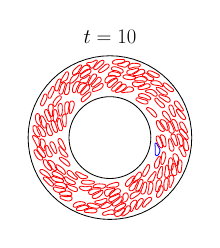
\begin{tikzpicture}[scale=0.3]

\begin{axis}[
  xmin = -21,
  xmax = 21,
  ymin = -21,
  ymax = 21,
  scale only axis,
  axis equal image,
  hide axis,
  title = {\Huge$t=10$}
  ]

% outer solid wall
\addplot [mark=none,black,line width=1.0] table{
2.0000e+01 -5.5171e-16
1.9904e+01 1.9603e+00
1.9616e+01 3.9018e+00
1.9139e+01 5.8057e+00
1.8478e+01 7.6537e+00
1.7638e+01 9.4279e+00
1.6629e+01 1.1111e+01
1.5460e+01 1.2688e+01
1.4142e+01 1.4142e+01
1.2688e+01 1.5460e+01
1.1111e+01 1.6629e+01
9.4279e+00 1.7638e+01
7.6537e+00 1.8478e+01
5.8057e+00 1.9139e+01
3.9018e+00 1.9616e+01
1.9603e+00 1.9904e+01
2.3281e-15 2.0000e+01
-1.9603e+00 1.9904e+01
-3.9018e+00 1.9616e+01
-5.8057e+00 1.9139e+01
-7.6537e+00 1.8478e+01
-9.4279e+00 1.7638e+01
-1.1111e+01 1.6629e+01
-1.2688e+01 1.5460e+01
-1.4142e+01 1.4142e+01
-1.5460e+01 1.2688e+01
-1.6629e+01 1.1111e+01
-1.7638e+01 9.4279e+00
-1.8478e+01 7.6537e+00
-1.9139e+01 5.8057e+00
-1.9616e+01 3.9018e+00
-1.9904e+01 1.9603e+00
-2.0000e+01 3.0010e-15
-1.9904e+01 -1.9603e+00
-1.9616e+01 -3.9018e+00
-1.9139e+01 -5.8057e+00
-1.8478e+01 -7.6537e+00
-1.7638e+01 -9.4279e+00
-1.6629e+01 -1.1111e+01
-1.5460e+01 -1.2688e+01
-1.4142e+01 -1.4142e+01
-1.2688e+01 -1.5460e+01
-1.1111e+01 -1.6629e+01
-9.4279e+00 -1.7638e+01
-7.6537e+00 -1.8478e+01
-5.8057e+00 -1.9139e+01
-3.9018e+00 -1.9616e+01
-1.9603e+00 -1.9904e+01
-4.7774e-15 -2.0000e+01
1.9603e+00 -1.9904e+01
3.9018e+00 -1.9616e+01
5.8057e+00 -1.9139e+01
7.6537e+00 -1.8478e+01
9.4279e+00 -1.7638e+01
1.1111e+01 -1.6629e+01
1.2688e+01 -1.5460e+01
1.4142e+01 -1.4142e+01
1.5460e+01 -1.2688e+01
1.6629e+01 -1.1111e+01
1.7638e+01 -9.4279e+00
1.8478e+01 -7.6537e+00
1.9139e+01 -5.8057e+00
1.9616e+01 -3.9018e+00
1.9904e+01 -1.9603e+00
2.0000e+01 -5.5171e-16
};

% inner solid wall
\addplot [mark=none,black,line width=1.0] table{
1.0000e+01 2.7586e-16
9.9518e+00 -9.8017e-01
9.8079e+00 -1.9509e+00
9.5694e+00 -2.9028e+00
9.2388e+00 -3.8268e+00
8.8192e+00 -4.7140e+00
8.3147e+00 -5.5557e+00
7.7301e+00 -6.3439e+00
7.0711e+00 -7.0711e+00
6.3439e+00 -7.7301e+00
5.5557e+00 -8.3147e+00
4.7140e+00 -8.8192e+00
3.8268e+00 -9.2388e+00
2.9028e+00 -9.5694e+00
1.9509e+00 -9.8079e+00
9.8017e-01 -9.9518e+00
1.1640e-15 -1.0000e+01
-9.8017e-01 -9.9518e+00
-1.9509e+00 -9.8079e+00
-2.9028e+00 -9.5694e+00
-3.8268e+00 -9.2388e+00
-4.7140e+00 -8.8192e+00
-5.5557e+00 -8.3147e+00
-6.3439e+00 -7.7301e+00
-7.0711e+00 -7.0711e+00
-7.7301e+00 -6.3439e+00
-8.3147e+00 -5.5557e+00
-8.8192e+00 -4.7140e+00
-9.2388e+00 -3.8268e+00
-9.5694e+00 -2.9028e+00
-9.8079e+00 -1.9509e+00
-9.9518e+00 -9.8017e-01
-1.0000e+01 -1.5005e-15
-9.9518e+00 9.8017e-01
-9.8079e+00 1.9509e+00
-9.5694e+00 2.9028e+00
-9.2388e+00 3.8268e+00
-8.8192e+00 4.7140e+00
-8.3147e+00 5.5557e+00
-7.7301e+00 6.3439e+00
-7.0711e+00 7.0711e+00
-6.3439e+00 7.7301e+00
-5.5557e+00 8.3147e+00
-4.7140e+00 8.8192e+00
-3.8268e+00 9.2388e+00
-2.9028e+00 9.5694e+00
-1.9509e+00 9.8079e+00
-9.8017e-01 9.9518e+00
-2.3887e-15 1.0000e+01
9.8017e-01 9.9518e+00
1.9509e+00 9.8079e+00
2.9028e+00 9.5694e+00
3.8268e+00 9.2388e+00
4.7140e+00 8.8192e+00
5.5557e+00 8.3147e+00
6.3439e+00 7.7301e+00
7.0711e+00 7.0711e+00
7.7301e+00 6.3439e+00
8.3147e+00 5.5557e+00
8.8192e+00 4.7140e+00
9.2388e+00 3.8268e+00
9.5694e+00 2.9028e+00
9.8079e+00 1.9509e+00
9.9518e+00 9.8017e-01
1.0000e+01 2.7586e-16
};

% vesicle 1
\addplot [mark=none,red,line width=1.0] table{
1.3023e+01 -1.2623e+01
1.3022e+01 -1.2541e+01
1.3018e+01 -1.2449e+01
1.3009e+01 -1.2343e+01
1.2992e+01 -1.2219e+01
1.2959e+01 -1.2081e+01
1.2899e+01 -1.1938e+01
1.2785e+01 -1.1807e+01
1.2604e+01 -1.1759e+01
1.2437e+01 -1.1852e+01
1.2340e+01 -1.2028e+01
1.2280e+01 -1.2229e+01
1.2233e+01 -1.2427e+01
1.2180e+01 -1.2625e+01
1.2113e+01 -1.2810e+01
1.2028e+01 -1.2975e+01
1.1928e+01 -1.3115e+01
1.1823e+01 -1.3230e+01
1.1722e+01 -1.3335e+01
1.1640e+01 -1.3432e+01
1.1577e+01 -1.3522e+01
1.1528e+01 -1.3608e+01
1.1490e+01 -1.3685e+01
1.1460e+01 -1.3758e+01
1.1433e+01 -1.3830e+01
1.1409e+01 -1.3909e+01
1.1385e+01 -1.4003e+01
1.1367e+01 -1.4117e+01
1.1364e+01 -1.4247e+01
1.1394e+01 -1.4392e+01
1.1479e+01 -1.4529e+01
1.1616e+01 -1.4613e+01
1.1793e+01 -1.4622e+01
1.1971e+01 -1.4551e+01
1.2122e+01 -1.4437e+01
1.2263e+01 -1.4292e+01
1.2394e+01 -1.4133e+01
1.2514e+01 -1.3970e+01
1.2620e+01 -1.3811e+01
1.2714e+01 -1.3657e+01
1.2796e+01 -1.3505e+01
1.2866e+01 -1.3356e+01
1.2921e+01 -1.3216e+01
1.2962e+01 -1.3083e+01
1.2990e+01 -1.2963e+01
1.3007e+01 -1.2861e+01
1.3016e+01 -1.2773e+01
1.3021e+01 -1.2696e+01
1.3023e+01 -1.2623e+01
};

% vesicle 2
\addplot [mark=none,red,line width=1.0] table{
-1.1678e+01 5.0376e+00
-1.1700e+01 4.9579e+00
-1.1718e+01 4.8629e+00
-1.1729e+01 4.7495e+00
-1.1728e+01 4.6217e+00
-1.1714e+01 4.4819e+00
-1.1691e+01 4.3330e+00
-1.1659e+01 4.1733e+00
-1.1620e+01 3.9938e+00
-1.1578e+01 3.8036e+00
-1.1534e+01 3.6077e+00
-1.1487e+01 3.4028e+00
-1.1438e+01 3.2029e+00
-1.1382e+01 3.0064e+00
-1.1304e+01 2.8190e+00
-1.1188e+01 2.6719e+00
-1.1026e+01 2.6136e+00
-1.0880e+01 2.6750e+00
-1.0798e+01 2.7966e+00
-1.0757e+01 2.9296e+00
-1.0737e+01 3.0481e+00
-1.0726e+01 3.1485e+00
-1.0718e+01 3.2386e+00
-1.0712e+01 3.3188e+00
-1.0708e+01 3.3948e+00
-1.0704e+01 3.4774e+00
-1.0700e+01 3.5704e+00
-1.0696e+01 3.6788e+00
-1.0692e+01 3.8076e+00
-1.0689e+01 3.9520e+00
-1.0685e+01 4.1100e+00
-1.0682e+01 4.2837e+00
-1.0679e+01 4.4661e+00
-1.0677e+01 4.6558e+00
-1.0677e+01 4.8563e+00
-1.0682e+01 5.0617e+00
-1.0696e+01 5.2659e+00
-1.0731e+01 5.4667e+00
-1.0815e+01 5.6431e+00
-1.0968e+01 5.7385e+00
-1.1136e+01 5.7316e+00
-1.1281e+01 5.6604e+00
-1.1391e+01 5.5595e+00
-1.1472e+01 5.4536e+00
-1.1534e+01 5.3529e+00
-1.1584e+01 5.2620e+00
-1.1621e+01 5.1832e+00
-1.1652e+01 5.1108e+00
-1.1678e+01 5.0376e+00
};

% vesicle 3
\addplot [mark=none,red,line width=1.0] table{
1.5828e+00 -1.3775e+01
1.6582e+00 -1.3752e+01
1.7494e+00 -1.3727e+01
1.8602e+00 -1.3702e+01
1.9837e+00 -1.3677e+01
2.1205e+00 -1.3642e+01
2.2586e+00 -1.3582e+01
2.3846e+00 -1.3484e+01
2.4926e+00 -1.3342e+01
2.5643e+00 -1.3160e+01
2.5750e+00 -1.2954e+01
2.5056e+00 -1.2758e+01
2.3640e+00 -1.2609e+01
2.1751e+00 -1.2522e+01
1.9733e+00 -1.2496e+01
1.7828e+00 -1.2514e+01
1.6095e+00 -1.2563e+01
1.4628e+00 -1.2630e+01
1.3424e+00 -1.2712e+01
1.2417e+00 -1.2803e+01
1.1598e+00 -1.2888e+01
1.0918e+00 -1.2960e+01
1.0294e+00 -1.3023e+01
9.7337e-01 -1.3076e+01
9.1935e-01 -1.3124e+01
8.5561e-01 -1.3178e+01
7.8305e-01 -1.3237e+01
7.0034e-01 -1.3302e+01
6.0312e-01 -1.3378e+01
4.9591e-01 -1.3462e+01
3.7617e-01 -1.3560e+01
2.4121e-01 -1.3681e+01
1.1027e-01 -1.3815e+01
-7.6127e-03 -1.3964e+01
-9.2445e-02 -1.4145e+01
-7.1425e-02 -1.4345e+01
9.3293e-02 -1.4458e+01
2.8565e-01 -1.4432e+01
4.6004e-01 -1.4351e+01
6.2617e-01 -1.4260e+01
7.7868e-01 -1.4175e+01
9.2158e-01 -1.4094e+01
1.0504e+00 -1.4022e+01
1.1619e+00 -1.3961e+01
1.2655e+00 -1.3908e+01
1.3607e+00 -1.3863e+01
1.4392e+00 -1.3829e+01
1.5105e+00 -1.3801e+01
1.5828e+00 -1.3775e+01
};

% vesicle 4
\addplot [mark=none,red,line width=1.0] table{
7.2508e-01 1.2259e+01
6.6712e-01 1.2202e+01
6.0437e-01 1.2134e+01
5.3820e-01 1.2051e+01
4.7489e-01 1.1946e+01
4.2798e-01 1.1815e+01
4.2163e-01 1.1661e+01
4.8175e-01 1.1508e+01
6.2009e-01 1.1391e+01
8.1519e-01 1.1345e+01
1.0156e+00 1.1371e+01
1.1936e+00 1.1449e+01
1.3489e+00 1.1571e+01
1.4928e+00 1.1722e+01
1.6310e+00 1.1876e+01
1.7633e+00 1.2020e+01
1.8914e+00 1.2151e+01
2.0115e+00 1.2267e+01
2.1201e+00 1.2367e+01
2.2190e+00 1.2454e+01
2.3080e+00 1.2528e+01
2.3863e+00 1.2592e+01
2.4540e+00 1.2646e+01
2.5143e+00 1.2694e+01
2.5721e+00 1.2741e+01
2.6334e+00 1.2791e+01
2.7013e+00 1.2851e+01
2.7757e+00 1.2926e+01
2.8508e+00 1.3025e+01
2.9074e+00 1.3157e+01
2.9166e+00 1.3315e+01
2.8500e+00 1.3479e+01
2.7071e+00 1.3599e+01
2.5234e+00 1.3645e+01
2.3271e+00 1.3618e+01
2.1383e+00 1.3530e+01
1.9723e+00 1.3408e+01
1.8212e+00 1.3272e+01
1.6775e+00 1.3133e+01
1.5409e+00 1.3000e+01
1.4097e+00 1.2874e+01
1.2876e+00 1.2760e+01
1.1751e+00 1.2658e+01
1.0728e+00 1.2568e+01
9.8288e-01 1.2490e+01
9.0554e-01 1.2422e+01
8.3908e-01 1.2364e+01
7.8067e-01 1.2311e+01
7.2508e-01 1.2259e+01
};

% vesicle 5
\addplot [mark=none,red,line width=1.0] table{
1.7027e+01 -5.4576e+00
1.6958e+01 -5.4878e+00
1.6891e+01 -5.5455e+00
1.6837e+01 -5.6339e+00
1.6801e+01 -5.7475e+00
1.6781e+01 -5.8832e+00
1.6765e+01 -6.0403e+00
1.6749e+01 -6.2144e+00
1.6723e+01 -6.4027e+00
1.6679e+01 -6.5984e+00
1.6616e+01 -6.7934e+00
1.6562e+01 -6.9914e+00
1.6541e+01 -7.1976e+00
1.6545e+01 -7.4067e+00
1.6561e+01 -7.6071e+00
1.6585e+01 -7.7965e+00
1.6613e+01 -7.9734e+00
1.6650e+01 -8.1325e+00
1.6699e+01 -8.2735e+00
1.6764e+01 -8.3924e+00
1.6842e+01 -8.4803e+00
1.6924e+01 -8.5344e+00
1.7003e+01 -8.5599e+00
1.7076e+01 -8.5635e+00
1.7144e+01 -8.5493e+00
1.7214e+01 -8.5147e+00
1.7283e+01 -8.4537e+00
1.7344e+01 -8.3631e+00
1.7391e+01 -8.2445e+00
1.7425e+01 -8.1053e+00
1.7450e+01 -7.9499e+00
1.7471e+01 -7.7793e+00
1.7492e+01 -7.5970e+00
1.7514e+01 -7.4109e+00
1.7536e+01 -7.2193e+00
1.7559e+01 -7.0180e+00
1.7580e+01 -6.8181e+00
1.7596e+01 -6.6169e+00
1.7604e+01 -6.4185e+00
1.7599e+01 -6.2307e+00
1.7577e+01 -6.0464e+00
1.7537e+01 -5.8776e+00
1.7481e+01 -5.7364e+00
1.7410e+01 -5.6229e+00
1.7330e+01 -5.5390e+00
1.7248e+01 -5.4845e+00
1.7170e+01 -5.4560e+00
1.7098e+01 -5.4479e+00
1.7027e+01 -5.4576e+00
};

% vesicle 6
\addplot [mark=none,red,line width=1.0] table{
-6.8434e+00 -1.0027e+01
-6.7618e+00 -1.0035e+01
-6.6666e+00 -1.0039e+01
-6.5546e+00 -1.0037e+01
-6.4252e+00 -1.0029e+01
-6.2806e+00 -1.0014e+01
-6.1222e+00 -9.9935e+00
-5.9485e+00 -9.9659e+00
-5.7599e+00 -9.9236e+00
-5.5679e+00 -9.8402e+00
-5.4482e+00 -9.6627e+00
-5.5311e+00 -9.4709e+00
-5.7095e+00 -9.3693e+00
-5.9016e+00 -9.3001e+00
-6.0892e+00 -9.2337e+00
-6.2641e+00 -9.1661e+00
-6.4304e+00 -9.0954e+00
-6.5802e+00 -9.0258e+00
-6.7110e+00 -8.9606e+00
-6.8278e+00 -8.8992e+00
-6.9299e+00 -8.8437e+00
-7.0168e+00 -8.7956e+00
-7.0912e+00 -8.7542e+00
-7.1573e+00 -8.7175e+00
-7.2216e+00 -8.6821e+00
-7.2916e+00 -8.6442e+00
-7.3738e+00 -8.6009e+00
-7.4718e+00 -8.5515e+00
-7.5870e+00 -8.4975e+00
-7.7196e+00 -8.4424e+00
-7.8686e+00 -8.3931e+00
-8.0371e+00 -8.3618e+00
-8.2180e+00 -8.3787e+00
-8.3646e+00 -8.4863e+00
-8.3934e+00 -8.6746e+00
-8.2984e+00 -8.8494e+00
-8.1541e+00 -8.9947e+00
-7.9992e+00 -9.1344e+00
-7.8535e+00 -9.2754e+00
-7.7185e+00 -9.4224e+00
-7.5990e+00 -9.5624e+00
-7.4868e+00 -9.6881e+00
-7.3771e+00 -9.7921e+00
-7.2708e+00 -9.8716e+00
-7.1694e+00 -9.9296e+00
-7.0763e+00 -9.9698e+00
-6.9930e+00 -9.9966e+00
-6.9175e+00 -1.0014e+01
-6.8434e+00 -1.0027e+01
};

% vesicle 7
\addplot [mark=none,red,line width=1.0] table{
4.3773e-01 1.5204e+01
5.1732e-01 1.5202e+01
6.0886e-01 1.5197e+01
7.1530e-01 1.5190e+01
8.3813e-01 1.5180e+01
9.7269e-01 1.5165e+01
1.1223e+00 1.5142e+01
1.2888e+00 1.5094e+01
1.4514e+00 1.5011e+01
1.6231e+00 1.4925e+01
1.8299e+00 1.4882e+01
2.0377e+00 1.4892e+01
2.2282e+00 1.4942e+01
2.4033e+00 1.5035e+01
2.5403e+00 1.5177e+01
2.5990e+00 1.5365e+01
2.5558e+00 1.5542e+01
2.4446e+00 1.5669e+01
2.3138e+00 1.5747e+01
2.1915e+00 1.5798e+01
2.0830e+00 1.5836e+01
1.9879e+00 1.5866e+01
1.9075e+00 1.5890e+01
1.8358e+00 1.5910e+01
1.7652e+00 1.5930e+01
1.6894e+00 1.5950e+01
1.5993e+00 1.5973e+01
1.4923e+00 1.5999e+01
1.3708e+00 1.6028e+01
1.2343e+00 1.6058e+01
1.0808e+00 1.6089e+01
9.0933e-01 1.6117e+01
7.2614e-01 1.6132e+01
5.3857e-01 1.6124e+01
3.4291e-01 1.6081e+01
1.3977e-01 1.5995e+01
-4.1391e-02 1.5878e+01
-1.9128e-01 1.5745e+01
-3.1471e-01 1.5593e+01
-3.9310e-01 1.5421e+01
-3.8608e-01 1.5246e+01
-2.7324e-01 1.5133e+01
-1.2582e-01 1.5123e+01
4.6810e-03 1.5152e+01
1.1539e-01 1.5177e+01
2.0942e-01 1.5193e+01
2.9238e-01 1.5200e+01
3.6628e-01 1.5204e+01
4.3773e-01 1.5204e+01
};

% vesicle 8
\addplot [mark=none,red,line width=1.0] table{
1.3702e+01 -1.4764e+00
1.3696e+01 -1.3987e+00
1.3689e+01 -1.3081e+00
1.3679e+01 -1.2026e+00
1.3669e+01 -1.0845e+00
1.3657e+01 -9.5101e-01
1.3643e+01 -7.9690e-01
1.3626e+01 -6.2195e-01
1.3602e+01 -4.3033e-01
1.3563e+01 -2.3101e-01
1.3503e+01 -3.5261e-02
1.3417e+01 1.5129e-01
1.3298e+01 3.2628e-01
1.3151e+01 4.7607e-01
1.2983e+01 5.8872e-01
1.2810e+01 6.5570e-01
1.2634e+01 6.7437e-01
1.2478e+01 6.3827e-01
1.2362e+01 5.5534e-01
1.2295e+01 4.4304e-01
1.2276e+01 3.2890e-01
1.2284e+01 2.2963e-01
1.2306e+01 1.4498e-01
1.2331e+01 7.2801e-02
1.2359e+01 5.2217e-03
1.2391e+01 -6.8906e-02
1.2428e+01 -1.5323e-01
1.2470e+01 -2.5058e-01
1.2515e+01 -3.6388e-01
1.2563e+01 -4.9134e-01
1.2614e+01 -6.3254e-01
1.2671e+01 -7.8836e-01
1.2735e+01 -9.6148e-01
1.2806e+01 -1.1468e+00
1.2875e+01 -1.3386e+00
1.2942e+01 -1.5420e+00
1.3001e+01 -1.7486e+00
1.3059e+01 -1.9481e+00
1.3135e+01 -2.1188e+00
1.3264e+01 -2.2440e+00
1.3436e+01 -2.2707e+00
1.3581e+01 -2.1869e+00
1.3660e+01 -2.0569e+00
1.3695e+01 -1.9272e+00
1.3708e+01 -1.8101e+00
1.3711e+01 -1.7087e+00
1.3710e+01 -1.6243e+00
1.3707e+01 -1.5496e+00
1.3702e+01 -1.4764e+00
};

% vesicle 9
\addplot [mark=none,red,line width=1.0] table{
7.8691e+00 -1.1377e+01
7.9006e+00 -1.1304e+01
7.9368e+00 -1.1219e+01
7.9777e+00 -1.1119e+01
8.0205e+00 -1.1002e+01
8.0581e+00 -1.0867e+01
8.0784e+00 -1.0716e+01
8.0663e+00 -1.0554e+01
8.0023e+00 -1.0387e+01
7.8606e+00 -1.0251e+01
7.6535e+00 -1.0216e+01
7.4595e+00 -1.0294e+01
7.3056e+00 -1.0427e+01
7.1859e+00 -1.0583e+01
7.0963e+00 -1.0754e+01
7.0270e+00 -1.0928e+01
6.9664e+00 -1.1100e+01
6.9109e+00 -1.1261e+01
6.8606e+00 -1.1405e+01
6.8152e+00 -1.1529e+01
6.7742e+00 -1.1638e+01
6.7378e+00 -1.1731e+01
6.7056e+00 -1.1810e+01
6.6764e+00 -1.1879e+01
6.6473e+00 -1.1946e+01
6.6145e+00 -1.2019e+01
6.5753e+00 -1.2103e+01
6.5280e+00 -1.2201e+01
6.4725e+00 -1.2316e+01
6.4122e+00 -1.2449e+01
6.3597e+00 -1.2602e+01
6.3417e+00 -1.2775e+01
6.4037e+00 -1.2948e+01
6.5615e+00 -1.3048e+01
6.7537e+00 -1.3036e+01
6.9392e+00 -1.2955e+01
7.1065e+00 -1.2844e+01
7.2414e+00 -1.2709e+01
7.3513e+00 -1.2549e+01
7.4425e+00 -1.2378e+01
7.5157e+00 -1.2220e+01
7.5795e+00 -1.2070e+01
7.6369e+00 -1.1931e+01
7.6892e+00 -1.1803e+01
7.7358e+00 -1.1690e+01
7.7759e+00 -1.1594e+01
7.8100e+00 -1.1514e+01
7.8400e+00 -1.1444e+01
7.8691e+00 -1.1377e+01
};

% vesicle 10
\addplot [mark=none,red,line width=1.0] table{
1.8468e+01 4.9082e+00
1.8439e+01 4.9823e+00
1.8397e+01 5.0637e+00
1.8343e+01 5.1557e+00
1.8274e+01 5.2612e+00
1.8192e+01 5.3799e+00
1.8099e+01 5.5095e+00
1.7996e+01 5.6481e+00
1.7883e+01 5.7936e+00
1.7759e+01 5.9423e+00
1.7625e+01 6.0885e+00
1.7482e+01 6.2321e+00
1.7330e+01 6.3759e+00
1.7179e+01 6.5180e+00
1.7033e+01 6.6521e+00
1.6889e+01 6.7700e+00
1.6737e+01 6.8616e+00
1.6577e+01 6.9071e+00
1.6426e+01 6.8882e+00
1.6315e+01 6.8117e+00
1.6259e+01 6.7100e+00
1.6245e+01 6.6128e+00
1.6253e+01 6.5311e+00
1.6273e+01 6.4614e+00
1.6299e+01 6.3960e+00
1.6335e+01 6.3271e+00
1.6381e+01 6.2482e+00
1.6440e+01 6.1569e+00
1.6509e+01 6.0532e+00
1.6587e+01 5.9353e+00
1.6672e+01 5.8024e+00
1.6763e+01 5.6595e+00
1.6858e+01 5.5107e+00
1.6963e+01 5.3543e+00
1.7079e+01 5.1959e+00
1.7207e+01 5.0377e+00
1.7347e+01 4.8841e+00
1.7493e+01 4.7423e+00
1.7647e+01 4.6142e+00
1.7812e+01 4.5064e+00
1.7978e+01 4.4329e+00
1.8141e+01 4.4047e+00
1.8287e+01 4.4281e+00
1.8398e+01 4.4958e+00
1.8464e+01 4.5852e+00
1.8494e+01 4.6771e+00
1.8498e+01 4.7620e+00
1.8488e+01 4.8374e+00
1.8468e+01 4.9082e+00
};

% vesicle 11
\addplot [mark=none,red,line width=1.0] table{
-2.0926e+00 1.7656e+01
-2.0357e+00 1.7707e+01
-1.9702e+00 1.7767e+01
-1.8944e+00 1.7838e+01
-1.8072e+00 1.7923e+01
-1.7095e+00 1.8025e+01
-1.6069e+00 1.8148e+01
-1.5114e+00 1.8298e+01
-1.4519e+00 1.8478e+01
-1.4723e+00 1.8668e+01
-1.5974e+00 1.8819e+01
-1.7945e+00 1.8878e+01
-2.0040e+00 1.8848e+01
-2.1975e+00 1.8769e+01
-2.3700e+00 1.8666e+01
-2.5237e+00 1.8550e+01
-2.6585e+00 1.8431e+01
-2.7766e+00 1.8314e+01
-2.8792e+00 1.8205e+01
-2.9671e+00 1.8109e+01
-3.0428e+00 1.8026e+01
-3.1081e+00 1.7954e+01
-3.1650e+00 1.7892e+01
-3.2159e+00 1.7837e+01
-3.2660e+00 1.7785e+01
-3.3214e+00 1.7728e+01
-3.3871e+00 1.7662e+01
-3.4659e+00 1.7587e+01
-3.5587e+00 1.7505e+01
-3.6654e+00 1.7415e+01
-3.7843e+00 1.7316e+01
-3.9018e+00 1.7193e+01
-3.9794e+00 1.7029e+01
-3.9591e+00 1.6840e+01
-3.8275e+00 1.6696e+01
-3.6360e+00 1.6636e+01
-3.4295e+00 1.6652e+01
-3.2351e+00 1.6723e+01
-3.0640e+00 1.6823e+01
-2.9097e+00 1.6938e+01
-2.7690e+00 1.7056e+01
-2.6414e+00 1.7167e+01
-2.5258e+00 1.7270e+01
-2.4234e+00 1.7361e+01
-2.3352e+00 1.7439e+01
-2.2612e+00 1.7505e+01
-2.1993e+00 1.7560e+01
-2.1451e+00 1.7609e+01
-2.0926e+00 1.7656e+01
};

% vesicle 12
\addplot [mark=none,red,line width=1.0] table{
1.4412e+01 -1.4676e+00
1.4421e+01 -1.5438e+00
1.4430e+01 -1.6347e+00
1.4440e+01 -1.7439e+00
1.4449e+01 -1.8686e+00
1.4458e+01 -2.0107e+00
1.4468e+01 -2.1678e+00
1.4482e+01 -2.3385e+00
1.4508e+01 -2.5226e+00
1.4555e+01 -2.7142e+00
1.4632e+01 -2.9003e+00
1.4744e+01 -3.0736e+00
1.4888e+01 -3.2126e+00
1.5062e+01 -3.3008e+00
1.5262e+01 -3.3118e+00
1.5438e+01 -3.2269e+00
1.5548e+01 -3.0929e+00
1.5610e+01 -2.9435e+00
1.5640e+01 -2.7940e+00
1.5647e+01 -2.6600e+00
1.5641e+01 -2.5435e+00
1.5628e+01 -2.4458e+00
1.5610e+01 -2.3614e+00
1.5591e+01 -2.2887e+00
1.5569e+01 -2.2204e+00
1.5542e+01 -2.1436e+00
1.5507e+01 -2.0562e+00
1.5464e+01 -1.9550e+00
1.5410e+01 -1.8354e+00
1.5350e+01 -1.7008e+00
1.5285e+01 -1.5515e+00
1.5219e+01 -1.3891e+00
1.5155e+01 -1.2231e+00
1.5091e+01 -1.0506e+00
1.5021e+01 -8.6361e-01
1.4943e+01 -6.7005e-01
1.4849e+01 -4.8555e-01
1.4711e+01 -3.3720e-01
1.4527e+01 -2.9707e-01
1.4376e+01 -4.0618e-01
1.4321e+01 -5.8338e-01
1.4319e+01 -7.4921e-01
1.4333e+01 -8.9494e-01
1.4350e+01 -1.0246e+00
1.4367e+01 -1.1397e+00
1.4381e+01 -1.2397e+00
1.4393e+01 -1.3222e+00
1.4403e+01 -1.3954e+00
1.4412e+01 -1.4676e+00
};

% vesicle 13
\addplot [mark=none,red,line width=1.0] table{
-4.4378e+00 -1.3881e+01
-4.3611e+00 -1.3855e+01
-4.2749e+00 -1.3819e+01
-4.1765e+00 -1.3770e+01
-4.0644e+00 -1.3708e+01
-3.9384e+00 -1.3635e+01
-3.7996e+00 -1.3557e+01
-3.6462e+00 -1.3477e+01
-3.4768e+00 -1.3396e+01
-3.2959e+00 -1.3319e+01
-3.1092e+00 -1.3246e+01
-2.9160e+00 -1.3174e+01
-2.7184e+00 -1.3103e+01
-2.5275e+00 -1.3032e+01
-2.3494e+00 -1.2945e+01
-2.2227e+00 -1.2812e+01
-2.2219e+00 -1.2643e+01
-2.3480e+00 -1.2540e+01
-2.5015e+00 -1.2517e+01
-2.6404e+00 -1.2520e+01
-2.7602e+00 -1.2526e+01
-2.8621e+00 -1.2532e+01
-2.9495e+00 -1.2537e+01
-3.0267e+00 -1.2540e+01
-3.1014e+00 -1.2543e+01
-3.1821e+00 -1.2546e+01
-3.2752e+00 -1.2549e+01
-3.3841e+00 -1.2550e+01
-3.5103e+00 -1.2551e+01
-3.6536e+00 -1.2548e+01
-3.8138e+00 -1.2544e+01
-3.9866e+00 -1.2548e+01
-4.1649e+00 -1.2576e+01
-4.3493e+00 -1.2639e+01
-4.5392e+00 -1.2726e+01
-4.7232e+00 -1.2816e+01
-4.8945e+00 -1.2914e+01
-5.0472e+00 -1.3037e+01
-5.1623e+00 -1.3199e+01
-5.2128e+00 -1.3384e+01
-5.1921e+00 -1.3561e+01
-5.1137e+00 -1.3709e+01
-5.0011e+00 -1.3814e+01
-4.8806e+00 -1.3876e+01
-4.7694e+00 -1.3906e+01
-4.6714e+00 -1.3915e+01
-4.5861e+00 -1.3911e+01
-4.5104e+00 -1.3900e+01
-4.4378e+00 -1.3881e+01
};

% vesicle 14
\addplot [mark=none,red,line width=1.0] table{
-9.8283e+00 8.3829e+00
-9.8401e+00 8.3082e+00
-9.8487e+00 8.2202e+00
-9.8537e+00 8.1152e+00
-9.8544e+00 8.0000e+00
-9.8503e+00 7.8648e+00
-9.8407e+00 7.7066e+00
-9.8283e+00 7.5349e+00
-9.8173e+00 7.3423e+00
-9.8145e+00 7.1344e+00
-9.8248e+00 6.9321e+00
-9.8502e+00 6.7278e+00
-9.8906e+00 6.5179e+00
-9.9300e+00 6.3141e+00
-9.9297e+00 6.1124e+00
-9.8340e+00 5.9486e+00
-9.6670e+00 5.9078e+00
-9.5220e+00 5.9852e+00
-9.4261e+00 6.1070e+00
-9.3615e+00 6.2236e+00
-9.3110e+00 6.3275e+00
-9.2704e+00 6.4152e+00
-9.2350e+00 6.4934e+00
-9.2043e+00 6.5619e+00
-9.1763e+00 6.6252e+00
-9.1439e+00 6.6993e+00
-9.1083e+00 6.7819e+00
-9.0682e+00 6.8770e+00
-9.0199e+00 6.9951e+00
-8.9687e+00 7.1261e+00
-8.9161e+00 7.2692e+00
-8.8613e+00 7.4330e+00
-8.8104e+00 7.6073e+00
-8.7666e+00 7.7933e+00
-8.7343e+00 7.9949e+00
-8.7223e+00 8.2001e+00
-8.7375e+00 8.3987e+00
-8.7886e+00 8.5901e+00
-8.8897e+00 8.7643e+00
-9.0366e+00 8.8857e+00
-9.2133e+00 8.9373e+00
-9.3791e+00 8.9208e+00
-9.5150e+00 8.8622e+00
-9.6223e+00 8.7803e+00
-9.6997e+00 8.6919e+00
-9.7532e+00 8.6054e+00
-9.7878e+00 8.5281e+00
-9.8111e+00 8.4566e+00
-9.8283e+00 8.3829e+00
};

% vesicle 15
\addplot [mark=none,red,line width=1.0] table{
7.5792e+00 1.1743e+01
7.6591e+00 1.1746e+01
7.7519e+00 1.1752e+01
7.8597e+00 1.1762e+01
7.9827e+00 1.1776e+01
8.1236e+00 1.1798e+01
8.2805e+00 1.1827e+01
8.4466e+00 1.1866e+01
8.6231e+00 1.1914e+01
8.8128e+00 1.1971e+01
9.0038e+00 1.2028e+01
9.2059e+00 1.2087e+01
9.4144e+00 1.2156e+01
9.6016e+00 1.2246e+01
9.7494e+00 1.2374e+01
9.8313e+00 1.2540e+01
9.8325e+00 1.2717e+01
9.7740e+00 1.2861e+01
9.6869e+00 1.2967e+01
9.5864e+00 1.3044e+01
9.4868e+00 1.3095e+01
9.3961e+00 1.3127e+01
9.3144e+00 1.3145e+01
9.2402e+00 1.3156e+01
9.1676e+00 1.3160e+01
9.0882e+00 1.3159e+01
8.9979e+00 1.3150e+01
8.8945e+00 1.3131e+01
8.7756e+00 1.3095e+01
8.6433e+00 1.3040e+01
8.5040e+00 1.2962e+01
8.3584e+00 1.2870e+01
8.2010e+00 1.2770e+01
8.0327e+00 1.2674e+01
7.8496e+00 1.2584e+01
7.6498e+00 1.2505e+01
7.4456e+00 1.2443e+01
7.2510e+00 1.2397e+01
7.0657e+00 1.2344e+01
6.9106e+00 1.2243e+01
6.8476e+00 1.2081e+01
6.9021e+00 1.1929e+01
7.0147e+00 1.1835e+01
7.1345e+00 1.1786e+01
7.2462e+00 1.1762e+01
7.3450e+00 1.1749e+01
7.4298e+00 1.1744e+01
7.5053e+00 1.1743e+01
7.5792e+00 1.1743e+01
};

% vesicle 16
\addplot [mark=none,red,line width=1.0] table{
-1.1280e+01 -6.2584e+00
-1.1223e+01 -6.3052e+00
-1.1152e+01 -6.3628e+00
-1.1064e+01 -6.4338e+00
-1.0968e+01 -6.5101e+00
-1.0855e+01 -6.5985e+00
-1.0723e+01 -6.6975e+00
-1.0585e+01 -6.7933e+00
-1.0432e+01 -6.8847e+00
-1.0257e+01 -6.9580e+00
-1.0058e+01 -6.9818e+00
-9.8670e+00 -6.9041e+00
-9.7710e+00 -6.7201e+00
-9.7960e+00 -6.5138e+00
-9.8762e+00 -6.3393e+00
-9.9747e+00 -6.1823e+00
-1.0084e+01 -6.0323e+00
-1.0188e+01 -5.9039e+00
-1.0287e+01 -5.7942e+00
-1.0385e+01 -5.6961e+00
-1.0470e+01 -5.6184e+00
-1.0542e+01 -5.5580e+00
-1.0612e+01 -5.5042e+00
-1.0672e+01 -5.4608e+00
-1.0728e+01 -5.4231e+00
-1.0796e+01 -5.3791e+00
-1.0873e+01 -5.3332e+00
-1.0960e+01 -5.2836e+00
-1.1071e+01 -5.2242e+00
-1.1194e+01 -5.1600e+00
-1.1331e+01 -5.0899e+00
-1.1487e+01 -5.0095e+00
-1.1649e+01 -4.9274e+00
-1.1829e+01 -4.8458e+00
-1.2025e+01 -4.7923e+00
-1.2226e+01 -4.8268e+00
-1.2340e+01 -4.9966e+00
-1.2306e+01 -5.1960e+00
-1.2202e+01 -5.3671e+00
-1.2078e+01 -5.5177e+00
-1.1954e+01 -5.6508e+00
-1.1832e+01 -5.7725e+00
-1.1718e+01 -5.8802e+00
-1.1621e+01 -5.9679e+00
-1.1533e+01 -6.0450e+00
-1.1455e+01 -6.1122e+00
-1.1394e+01 -6.1639e+00
-1.1338e+01 -6.2107e+00
-1.1280e+01 -6.2584e+00
};

% vesicle 17
\addplot [mark=none,red,line width=1.0] table{
-2.9220e+00 -1.6149e+01
-2.8467e+00 -1.6176e+01
-2.7607e+00 -1.6211e+01
-2.6610e+00 -1.6252e+01
-2.5463e+00 -1.6294e+01
-2.4095e+00 -1.6324e+01
-2.2531e+00 -1.6328e+01
-2.0917e+00 -1.6299e+01
-1.9241e+00 -1.6243e+01
-1.7525e+00 -1.6169e+01
-1.5827e+00 -1.6086e+01
-1.4104e+00 -1.5992e+01
-1.2386e+00 -1.5885e+01
-1.0705e+00 -1.5765e+01
-9.1955e-01 -1.5636e+01
-7.9655e-01 -1.5494e+01
-7.1718e-01 -1.5333e+01
-7.0254e-01 -1.5170e+01
-7.5351e-01 -1.5032e+01
-8.4781e-01 -1.4941e+01
-9.5355e-01 -1.4896e+01
-1.0505e+00 -1.4883e+01
-1.1360e+00 -1.4885e+01
-1.2107e+00 -1.4895e+01
-1.2820e+00 -1.4910e+01
-1.3618e+00 -1.4931e+01
-1.4536e+00 -1.4959e+01
-1.5599e+00 -1.4995e+01
-1.6831e+00 -1.5039e+01
-1.8170e+00 -1.5089e+01
-1.9602e+00 -1.5141e+01
-2.1198e+00 -1.5198e+01
-2.2945e+00 -1.5256e+01
-2.4822e+00 -1.5311e+01
-2.6834e+00 -1.5360e+01
-2.8931e+00 -1.5399e+01
-3.1022e+00 -1.5431e+01
-3.3011e+00 -1.5463e+01
-3.4863e+00 -1.5515e+01
-3.6388e+00 -1.5614e+01
-3.7059e+00 -1.5771e+01
-3.6421e+00 -1.5926e+01
-3.5095e+00 -1.6008e+01
-3.3794e+00 -1.6043e+01
-3.2616e+00 -1.6064e+01
-3.1579e+00 -1.6084e+01
-3.0714e+00 -1.6104e+01
-2.9954e+00 -1.6125e+01
-2.9220e+00 -1.6149e+01
};

% vesicle 18
\addplot [mark=none,red,line width=1.0] table{
9.7416e+00 9.9270e+00
9.6797e+00 9.9781e+00
9.6066e+00 1.0033e+01
9.5197e+00 1.0092e+01
9.4179e+00 1.0157e+01
9.3006e+00 1.0227e+01
9.1654e+00 1.0303e+01
9.0120e+00 1.0385e+01
8.8439e+00 1.0468e+01
8.6653e+00 1.0549e+01
8.4822e+00 1.0621e+01
8.2906e+00 1.0680e+01
8.0876e+00 1.0722e+01
7.8820e+00 1.0745e+01
7.6729e+00 1.0747e+01
7.4758e+00 1.0726e+01
7.2993e+00 1.0679e+01
7.1499e+00 1.0603e+01
7.0404e+00 1.0499e+01
6.9825e+00 1.0381e+01
6.9731e+00 1.0267e+01
6.9991e+00 1.0171e+01
7.0446e+00 1.0097e+01
7.0995e+00 1.0040e+01
7.1619e+00 9.9949e+00
7.2348e+00 9.9562e+00
7.3224e+00 9.9217e+00
7.4255e+00 9.8909e+00
7.5428e+00 9.8631e+00
7.6746e+00 9.8363e+00
7.8240e+00 9.8079e+00
7.9945e+00 9.7750e+00
8.1798e+00 9.7354e+00
8.3699e+00 9.6879e+00
8.5669e+00 9.6277e+00
8.7676e+00 9.5513e+00
8.9662e+00 9.4584e+00
9.1551e+00 9.3589e+00
9.3351e+00 9.2728e+00
9.5166e+00 9.2227e+00
9.6911e+00 9.2290e+00
9.8375e+00 9.2958e+00
9.9308e+00 9.4079e+00
9.9619e+00 9.5366e+00
9.9437e+00 9.6534e+00
9.9004e+00 9.7463e+00
9.8489e+00 9.8183e+00
9.7963e+00 9.8759e+00
9.7416e+00 9.9270e+00
};

% vesicle 19
\addplot [mark=none,red,line width=1.0] table{
-5.1465e+00 1.7707e+01
-5.0846e+00 1.7669e+01
-5.0185e+00 1.7608e+01
-4.9549e+00 1.7517e+01
-4.9051e+00 1.7407e+01
-4.8594e+00 1.7272e+01
-4.7916e+00 1.7124e+01
-4.6702e+00 1.7009e+01
-4.4937e+00 1.6963e+01
-4.2988e+00 1.7002e+01
-4.1271e+00 1.7106e+01
-3.9881e+00 1.7256e+01
-3.8761e+00 1.7429e+01
-3.7730e+00 1.7599e+01
-3.6642e+00 1.7765e+01
-3.5509e+00 1.7922e+01
-3.4431e+00 1.8062e+01
-3.3389e+00 1.8193e+01
-3.2456e+00 1.8314e+01
-3.1686e+00 1.8427e+01
-3.1148e+00 1.8532e+01
-3.0869e+00 1.8624e+01
-3.0824e+00 1.8712e+01
-3.0994e+00 1.8784e+01
-3.1335e+00 1.8843e+01
-3.1954e+00 1.8897e+01
-3.2808e+00 1.8927e+01
-3.3834e+00 1.8928e+01
-3.5057e+00 1.8893e+01
-3.6335e+00 1.8831e+01
-3.7694e+00 1.8753e+01
-3.9242e+00 1.8664e+01
-4.0884e+00 1.8579e+01
-4.2631e+00 1.8503e+01
-4.4561e+00 1.8438e+01
-4.6541e+00 1.8391e+01
-4.8536e+00 1.8363e+01
-5.0593e+00 1.8349e+01
-5.2582e+00 1.8335e+01
-5.4443e+00 1.8298e+01
-5.6039e+00 1.8205e+01
-5.6837e+00 1.8062e+01
-5.6600e+00 1.7918e+01
-5.5675e+00 1.7827e+01
-5.4610e+00 1.7787e+01
-5.3615e+00 1.7768e+01
-5.2841e+00 1.7754e+01
-5.2145e+00 1.7735e+01
-5.1465e+00 1.7707e+01
};

% vesicle 20
\addplot [mark=none,red,line width=1.0] table{
1.3205e+00 -1.2095e+01
1.4022e+00 -1.2083e+01
1.4918e+00 -1.2064e+01
1.5912e+00 -1.2036e+01
1.7034e+00 -1.1993e+01
1.8225e+00 -1.1932e+01
1.9442e+00 -1.1846e+01
2.0616e+00 -1.1724e+01
2.1513e+00 -1.1563e+01
2.1886e+00 -1.1372e+01
2.1448e+00 -1.1167e+01
2.0038e+00 -1.1008e+01
1.8102e+00 -1.0939e+01
1.6139e+00 -1.0937e+01
1.4245e+00 -1.0965e+01
1.2386e+00 -1.1007e+01
1.0611e+00 -1.1054e+01
8.9688e-01 -1.1100e+01
7.5393e-01 -1.1141e+01
6.3272e-01 -1.1178e+01
5.2618e-01 -1.1211e+01
4.3255e-01 -1.1240e+01
3.5289e-01 -1.1267e+01
2.7979e-01 -1.1291e+01
2.0638e-01 -1.1317e+01
1.2993e-01 -1.1345e+01
4.3101e-02 -1.1379e+01
-5.5942e-02 -1.1419e+01
-1.6850e-01 -1.1469e+01
-2.9651e-01 -1.1532e+01
-4.3173e-01 -1.1607e+01
-5.7138e-01 -1.1702e+01
-7.0547e-01 -1.1828e+01
-7.8815e-01 -1.1998e+01
-7.4102e-01 -1.2179e+01
-5.6392e-01 -1.2273e+01
-3.5091e-01 -1.2267e+01
-1.4991e-01 -1.2227e+01
5.1190e-02 -1.2182e+01
2.4519e-01 -1.2143e+01
4.2155e-01 -1.2116e+01
5.8109e-01 -1.2101e+01
7.2624e-01 -1.2095e+01
8.6005e-01 -1.2096e+01
9.7800e-01 -1.2101e+01
1.0787e+00 -1.2104e+01
1.1681e+00 -1.2104e+01
1.2464e+00 -1.2101e+01
1.3205e+00 -1.2095e+01
};

% vesicle 21
\addplot [mark=none,red,line width=1.0] table{
-6.9476e+00 -1.0798e+01
-6.9599e+00 -1.0877e+01
-6.9485e+00 -1.0972e+01
-6.9005e+00 -1.1075e+01
-6.8149e+00 -1.1168e+01
-6.6955e+00 -1.1245e+01
-6.5470e+00 -1.1303e+01
-6.3788e+00 -1.1343e+01
-6.1980e+00 -1.1369e+01
-6.0095e+00 -1.1383e+01
-5.8077e+00 -1.1390e+01
-5.6041e+00 -1.1392e+01
-5.4125e+00 -1.1394e+01
-5.2233e+00 -1.1395e+01
-5.0290e+00 -1.1394e+01
-4.8372e+00 -1.1386e+01
-4.6494e+00 -1.1367e+01
-4.4762e+00 -1.1339e+01
-4.3250e+00 -1.1305e+01
-4.1934e+00 -1.1266e+01
-4.0820e+00 -1.1225e+01
-3.9899e+00 -1.1181e+01
-3.9139e+00 -1.1133e+01
-3.8561e+00 -1.1081e+01
-3.8136e+00 -1.1022e+01
-3.7870e+00 -1.0947e+01
-3.7908e+00 -1.0859e+01
-3.8396e+00 -1.0770e+01
-3.9420e+00 -1.0697e+01
-4.0830e+00 -1.0652e+01
-4.2438e+00 -1.0622e+01
-4.4193e+00 -1.0590e+01
-4.6043e+00 -1.0552e+01
-4.7944e+00 -1.0511e+01
-4.9958e+00 -1.0470e+01
-5.2044e+00 -1.0437e+01
-5.4149e+00 -1.0416e+01
-5.6238e+00 -1.0406e+01
-5.8226e+00 -1.0404e+01
-6.0126e+00 -1.0408e+01
-6.1922e+00 -1.0418e+01
-6.3587e+00 -1.0436e+01
-6.5061e+00 -1.0464e+01
-6.6330e+00 -1.0503e+01
-6.7385e+00 -1.0553e+01
-6.8200e+00 -1.0609e+01
-6.8778e+00 -1.0668e+01
-6.9194e+00 -1.0729e+01
-6.9476e+00 -1.0798e+01
};

% vesicle 22
\addplot [mark=none,red,line width=1.0] table{
-1.7604e+00 1.3135e+01
-1.8216e+00 1.3181e+01
-1.9033e+00 1.3214e+01
-2.0057e+00 1.3227e+01
-2.1236e+00 1.3209e+01
-2.2541e+00 1.3156e+01
-2.3922e+00 1.3070e+01
-2.5315e+00 1.2962e+01
-2.6722e+00 1.2847e+01
-2.8223e+00 1.2724e+01
-2.9813e+00 1.2603e+01
-3.1508e+00 1.2484e+01
-3.3261e+00 1.2376e+01
-3.5070e+00 1.2280e+01
-3.6861e+00 1.2199e+01
-3.8623e+00 1.2123e+01
-4.0208e+00 1.2039e+01
-4.1521e+00 1.1938e+01
-4.2490e+00 1.1824e+01
-4.3115e+00 1.1706e+01
-4.3403e+00 1.1594e+01
-4.3381e+00 1.1496e+01
-4.3098e+00 1.1415e+01
-4.2644e+00 1.1357e+01
-4.2071e+00 1.1318e+01
-4.1340e+00 1.1291e+01
-4.0455e+00 1.1281e+01
-3.9407e+00 1.1285e+01
-3.8161e+00 1.1304e+01
-3.6754e+00 1.1334e+01
-3.5221e+00 1.1373e+01
-3.3543e+00 1.1419e+01
-3.1722e+00 1.1475e+01
-2.9840e+00 1.1542e+01
-2.7912e+00 1.1620e+01
-2.5985e+00 1.1711e+01
-2.4112e+00 1.1816e+01
-2.2422e+00 1.1929e+01
-2.0945e+00 1.2047e+01
-1.9666e+00 1.2171e+01
-1.8555e+00 1.2305e+01
-1.7644e+00 1.2445e+01
-1.6992e+00 1.2585e+01
-1.6610e+00 1.2715e+01
-1.6474e+00 1.2832e+01
-1.6552e+00 1.2933e+01
-1.6786e+00 1.3014e+01
-1.7135e+00 1.3080e+01
-1.7604e+00 1.3135e+01
};

% vesicle 23
\addplot [mark=none,red,line width=1.0] table{
9.7109e+00 -6.9471e+00
9.6998e+00 -6.8675e+00
9.6738e+00 -6.7789e+00
9.6201e+00 -6.6849e+00
9.5210e+00 -6.6065e+00
9.3774e+00 -6.5889e+00
9.2318e+00 -6.6570e+00
9.1076e+00 -6.7851e+00
8.9997e+00 -6.9370e+00
8.8939e+00 -7.1005e+00
8.7896e+00 -7.2658e+00
8.6877e+00 -7.4291e+00
8.5793e+00 -7.6054e+00
8.4757e+00 -7.7787e+00
8.3773e+00 -7.9512e+00
8.2898e+00 -8.1170e+00
8.2156e+00 -8.2747e+00
8.1550e+00 -8.4250e+00
8.1087e+00 -8.5650e+00
8.0751e+00 -8.6918e+00
8.0521e+00 -8.8032e+00
8.0369e+00 -8.9007e+00
8.0279e+00 -8.9875e+00
8.0244e+00 -9.0648e+00
8.0262e+00 -9.1391e+00
8.0363e+00 -9.2197e+00
8.0618e+00 -9.3085e+00
8.1159e+00 -9.4001e+00
8.2139e+00 -9.4730e+00
8.3506e+00 -9.4904e+00
8.4983e+00 -9.4356e+00
8.6373e+00 -9.3241e+00
8.7622e+00 -9.1846e+00
8.8760e+00 -9.0346e+00
8.9873e+00 -8.8712e+00
9.0952e+00 -8.6980e+00
9.2016e+00 -8.5126e+00
9.2992e+00 -8.3283e+00
9.3844e+00 -8.1545e+00
9.4615e+00 -7.9836e+00
9.5281e+00 -7.8209e+00
9.5838e+00 -7.6683e+00
9.6284e+00 -7.5278e+00
9.6619e+00 -7.4022e+00
9.6862e+00 -7.2894e+00
9.7023e+00 -7.1884e+00
9.7111e+00 -7.1011e+00
9.7139e+00 -7.0230e+00
9.7109e+00 -6.9471e+00
};

% vesicle 24
\addplot [mark=none,red,line width=1.0] table{
7.7212e+00 1.3543e+01
7.6424e+00 1.3531e+01
7.5517e+00 1.3517e+01
7.4455e+00 1.3501e+01
7.3231e+00 1.3486e+01
7.1828e+00 1.3473e+01
7.0237e+00 1.3467e+01
6.8493e+00 1.3474e+01
6.6648e+00 1.3498e+01
6.4783e+00 1.3539e+01
6.2849e+00 1.3590e+01
6.0812e+00 1.3625e+01
5.8760e+00 1.3607e+01
5.6906e+00 1.3521e+01
5.5523e+00 1.3374e+01
5.4893e+00 1.3191e+01
5.5068e+00 1.3013e+01
5.5788e+00 1.2865e+01
5.6754e+00 1.2752e+01
5.7774e+00 1.2665e+01
5.8749e+00 1.2600e+01
5.9630e+00 1.2551e+01
6.0413e+00 1.2514e+01
6.1123e+00 1.2485e+01
6.1821e+00 1.2462e+01
6.2591e+00 1.2441e+01
6.3489e+00 1.2422e+01
6.4547e+00 1.2410e+01
6.5756e+00 1.2409e+01
6.7082e+00 1.2425e+01
6.8514e+00 1.2464e+01
7.0052e+00 1.2528e+01
7.1711e+00 1.2606e+01
7.3499e+00 1.2683e+01
7.5396e+00 1.2751e+01
7.7316e+00 1.2813e+01
7.9249e+00 1.2873e+01
8.1159e+00 1.2941e+01
8.2939e+00 1.3028e+01
8.4352e+00 1.3158e+01
8.4833e+00 1.3327e+01
8.4211e+00 1.3471e+01
8.2999e+00 1.3551e+01
8.1712e+00 1.3578e+01
8.0555e+00 1.3581e+01
7.9555e+00 1.3574e+01
7.8701e+00 1.3564e+01
7.7945e+00 1.3554e+01
7.7212e+00 1.3543e+01
};

% vesicle 25
\addplot [mark=none,red,line width=1.0] table{
-1.5320e+01 1.2998e+00
-1.5291e+01 1.2262e+00
-1.5256e+01 1.1417e+00
-1.5211e+01 1.0437e+00
-1.5151e+01 9.3136e-01
-1.5070e+01 8.0844e-01
-1.4961e+01 6.8432e-01
-1.4820e+01 5.7465e-01
-1.4648e+01 4.9921e-01
-1.4456e+01 4.7971e-01
-1.4271e+01 5.3464e-01
-1.4129e+01 6.6495e-01
-1.4059e+01 8.4947e-01
-1.4063e+01 1.0432e+00
-1.4117e+01 1.2284e+00
-1.4195e+01 1.4051e+00
-1.4280e+01 1.5685e+00
-1.4358e+01 1.7147e+00
-1.4426e+01 1.8450e+00
-1.4485e+01 1.9626e+00
-1.4535e+01 2.0691e+00
-1.4576e+01 2.1622e+00
-1.4609e+01 2.2417e+00
-1.4637e+01 2.3123e+00
-1.4663e+01 2.3811e+00
-1.4689e+01 2.4557e+00
-1.4717e+01 2.5434e+00
-1.4748e+01 2.6482e+00
-1.4781e+01 2.7694e+00
-1.4815e+01 2.9037e+00
-1.4856e+01 3.0515e+00
-1.4917e+01 3.2097e+00
-1.5026e+01 3.3559e+00
-1.5210e+01 3.4177e+00
-1.5375e+01 3.3157e+00
-1.5430e+01 3.1256e+00
-1.5431e+01 2.9236e+00
-1.5441e+01 2.7187e+00
-1.5478e+01 2.5217e+00
-1.5514e+01 2.3384e+00
-1.5525e+01 2.1635e+00
-1.5512e+01 2.0007e+00
-1.5487e+01 1.8546e+00
-1.5456e+01 1.7255e+00
-1.5425e+01 1.6138e+00
-1.5396e+01 1.5187e+00
-1.5369e+01 1.4378e+00
-1.5345e+01 1.3673e+00
-1.5320e+01 1.2998e+00
};

% vesicle 26
\addplot [mark=none,red,line width=1.0] table{
-1.1762e+00 1.3581e+01
-1.1310e+00 1.3511e+01
-1.0637e+00 1.3445e+01
-9.7019e-01 1.3393e+01
-8.4830e-01 1.3368e+01
-7.1297e-01 1.3382e+01
-5.7700e-01 1.3438e+01
-4.3891e-01 1.3533e+01
-2.9900e-01 1.3655e+01
-1.5785e-01 1.3782e+01
-2.0949e-03 1.3910e+01
1.6408e-01 1.4031e+01
3.4171e-01 1.4142e+01
5.2039e-01 1.4237e+01
6.9636e-01 1.4317e+01
8.7247e-01 1.4384e+01
1.0443e+00 1.4440e+01
1.2041e+00 1.4489e+01
1.3438e+00 1.4542e+01
1.4537e+00 1.4610e+01
1.5226e+00 1.4702e+01
1.5372e+00 1.4801e+01
1.5095e+00 1.4876e+01
1.4598e+00 1.4929e+01
1.3969e+00 1.4965e+01
1.3263e+00 1.4990e+01
1.2386e+00 1.5010e+01
1.1307e+00 1.5028e+01
1.0065e+00 1.5041e+01
8.6041e-01 1.5048e+01
6.9673e-01 1.5045e+01
5.2570e-01 1.5033e+01
3.3971e-01 1.5014e+01
1.4407e-01 1.5000e+01
-5.4887e-02 1.5000e+01
-2.6155e-01 1.4999e+01
-4.5612e-01 1.4948e+01
-6.2956e-01 1.4851e+01
-7.7735e-01 1.4733e+01
-9.0658e-01 1.4600e+01
-1.0193e+00 1.4451e+01
-1.1052e+00 1.4305e+01
-1.1656e+00 1.4167e+01
-1.2057e+00 1.4034e+01
-1.2259e+00 1.3916e+01
-1.2303e+00 1.3815e+01
-1.2220e+00 1.3725e+01
-1.2038e+00 1.3649e+01
-1.1762e+00 1.3581e+01
};

% vesicle 27
\addplot [mark=none,red,line width=1.0] table{
1.2717e+01 -9.4035e+00
1.2737e+01 -9.3239e+00
1.2753e+01 -9.2312e+00
1.2763e+01 -9.1225e+00
1.2767e+01 -8.9930e+00
1.2766e+01 -8.8474e+00
1.2762e+01 -8.6861e+00
1.2763e+01 -8.5108e+00
1.2772e+01 -8.3259e+00
1.2794e+01 -8.1270e+00
1.2828e+01 -7.9278e+00
1.2867e+01 -7.7287e+00
1.2901e+01 -7.5243e+00
1.2905e+01 -7.3378e+00
1.2850e+01 -7.1611e+00
1.2701e+01 -7.0506e+00
1.2534e+01 -7.0835e+00
1.2419e+01 -7.1983e+00
1.2341e+01 -7.3311e+00
1.2281e+01 -7.4495e+00
1.2229e+01 -7.5520e+00
1.2182e+01 -7.6411e+00
1.2143e+01 -7.7156e+00
1.2107e+01 -7.7831e+00
1.2073e+01 -7.8505e+00
1.2038e+01 -7.9210e+00
1.1999e+01 -8.0037e+00
1.1957e+01 -8.0995e+00
1.1916e+01 -8.2079e+00
1.1870e+01 -8.3402e+00
1.1823e+01 -8.4946e+00
1.1773e+01 -8.6597e+00
1.1714e+01 -8.8426e+00
1.1648e+01 -9.0397e+00
1.1589e+01 -9.2372e+00
1.1554e+01 -9.4408e+00
1.1565e+01 -9.6425e+00
1.1639e+01 -9.8274e+00
1.1774e+01 -9.9607e+00
1.1944e+01 -1.0021e+01
1.2118e+01 -1.0013e+01
1.2271e+01 -9.9574e+00
1.2396e+01 -9.8774e+00
1.2497e+01 -9.7868e+00
1.2571e+01 -9.6984e+00
1.2625e+01 -9.6174e+00
1.2665e+01 -9.5410e+00
1.2695e+01 -9.4716e+00
1.2717e+01 -9.4035e+00
};

% vesicle 28
\addplot [mark=none,red,line width=1.0] table{
1.4515e+00 -1.5048e+01
1.5212e+00 -1.5003e+01
1.5994e+00 -1.4952e+01
1.6885e+00 -1.4893e+01
1.7938e+00 -1.4822e+01
1.9109e+00 -1.4741e+01
2.0367e+00 -1.4648e+01
2.1726e+00 -1.4539e+01
2.3063e+00 -1.4411e+01
2.4175e+00 -1.4255e+01
2.4647e+00 -1.4064e+01
2.3965e+00 -1.3880e+01
2.2133e+00 -1.3790e+01
2.0071e+00 -1.3828e+01
1.8256e+00 -1.3913e+01
1.6535e+00 -1.3998e+01
1.4899e+00 -1.4075e+01
1.3359e+00 -1.4142e+01
1.1949e+00 -1.4202e+01
1.0743e+00 -1.4251e+01
9.6970e-01 -1.4293e+01
8.7833e-01 -1.4329e+01
8.0134e-01 -1.4359e+01
7.3063e-01 -1.4385e+01
6.5918e-01 -1.4411e+01
5.8421e-01 -1.4438e+01
4.9600e-01 -1.4467e+01
3.9320e-01 -1.4499e+01
2.7959e-01 -1.4535e+01
1.5296e-01 -1.4583e+01
2.0853e-02 -1.4657e+01
-1.0353e-01 -1.4765e+01
-2.1031e-01 -1.4916e+01
-2.7622e-01 -1.5109e+01
-2.6856e-01 -1.5317e+01
-1.7752e-01 -1.5500e+01
-1.9369e-02 -1.5625e+01
1.7381e-01 -1.5678e+01
3.6217e-01 -1.5665e+01
5.3628e-01 -1.5608e+01
6.9652e-01 -1.5528e+01
8.4021e-01 -1.5443e+01
9.6520e-01 -1.5364e+01
1.0730e+00 -1.5294e+01
1.1680e+00 -1.5233e+01
1.2508e+00 -1.5179e+01
1.3253e+00 -1.5130e+01
1.3902e+00 -1.5088e+01
1.4515e+00 -1.5048e+01
};

% vesicle 29
\addplot [mark=none,red,line width=1.0] table{
1.3515e+01 -5.1713e+00
1.3538e+01 -5.0948e+00
1.3563e+01 -5.0052e+00
1.3590e+01 -4.8997e+00
1.3616e+01 -4.7799e+00
1.3638e+01 -4.6456e+00
1.3652e+01 -4.4923e+00
1.3651e+01 -4.3177e+00
1.3628e+01 -4.1286e+00
1.3577e+01 -3.9338e+00
1.3493e+01 -3.7423e+00
1.3366e+01 -3.5723e+00
1.3182e+01 -3.4688e+00
1.2979e+01 -3.5079e+00
1.2851e+01 -3.6569e+00
1.2787e+01 -3.8227e+00
1.2745e+01 -3.9890e+00
1.2711e+01 -4.1495e+00
1.2684e+01 -4.2946e+00
1.2661e+01 -4.4244e+00
1.2641e+01 -4.5402e+00
1.2626e+01 -4.6399e+00
1.2613e+01 -4.7250e+00
1.2603e+01 -4.7996e+00
1.2593e+01 -4.8716e+00
1.2582e+01 -4.9505e+00
1.2569e+01 -5.0422e+00
1.2554e+01 -5.1495e+00
1.2537e+01 -5.2733e+00
1.2517e+01 -5.4129e+00
1.2496e+01 -5.5691e+00
1.2475e+01 -5.7373e+00
1.2459e+01 -5.9177e+00
1.2456e+01 -6.1132e+00
1.2489e+01 -6.3161e+00
1.2596e+01 -6.4978e+00
1.2787e+01 -6.5696e+00
1.2965e+01 -6.4910e+00
1.3084e+01 -6.3381e+00
1.3165e+01 -6.1711e+00
1.3230e+01 -6.0075e+00
1.3284e+01 -5.8571e+00
1.3333e+01 -5.7201e+00
1.3375e+01 -5.5976e+00
1.3412e+01 -5.4889e+00
1.3444e+01 -5.3945e+00
1.3470e+01 -5.3136e+00
1.3493e+01 -5.2416e+00
1.3515e+01 -5.1713e+00
};

% vesicle 30
\addplot [mark=none,red,line width=1.0] table{
1.1574e+01 1.2759e+01
1.1650e+01 1.2753e+01
1.1739e+01 1.2746e+01
1.1844e+01 1.2733e+01
1.1966e+01 1.2712e+01
1.2103e+01 1.2674e+01
1.2249e+01 1.2612e+01
1.2400e+01 1.2524e+01
1.2566e+01 1.2430e+01
1.2761e+01 1.2409e+01
1.2894e+01 1.2549e+01
1.2859e+01 1.2741e+01
1.2746e+01 1.2909e+01
1.2622e+01 1.3076e+01
1.2504e+01 1.3234e+01
1.2385e+01 1.3375e+01
1.2261e+01 1.3497e+01
1.2133e+01 1.3598e+01
1.2008e+01 1.3676e+01
1.1892e+01 1.3734e+01
1.1785e+01 1.3777e+01
1.1689e+01 1.3809e+01
1.1608e+01 1.3831e+01
1.1536e+01 1.3848e+01
1.1467e+01 1.3861e+01
1.1392e+01 1.3874e+01
1.1303e+01 1.3885e+01
1.1195e+01 1.3894e+01
1.1071e+01 1.3898e+01
1.0932e+01 1.3895e+01
1.0773e+01 1.3883e+01
1.0598e+01 1.3861e+01
1.0416e+01 1.3829e+01
1.0232e+01 1.3779e+01
1.0062e+01 1.3670e+01
9.9810e+00 1.3477e+01
1.0045e+01 1.3278e+01
1.0193e+01 1.3135e+01
1.0365e+01 1.3036e+01
1.0538e+01 1.2962e+01
1.0707e+01 1.2904e+01
1.0865e+01 1.2859e+01
1.1009e+01 1.2826e+01
1.1140e+01 1.2802e+01
1.1254e+01 1.2786e+01
1.1351e+01 1.2776e+01
1.1433e+01 1.2769e+01
1.1505e+01 1.2764e+01
1.1574e+01 1.2759e+01
};

% vesicle 31
\addplot [mark=none,red,line width=1.0] table{
-1.6086e+01 -6.5629e+00
-1.6053e+01 -6.6350e+00
-1.6014e+01 -6.7162e+00
-1.5963e+01 -6.8093e+00
-1.5898e+01 -6.9175e+00
-1.5816e+01 -7.0358e+00
-1.5717e+01 -7.1635e+00
-1.5598e+01 -7.3006e+00
-1.5468e+01 -7.4359e+00
-1.5334e+01 -7.5655e+00
-1.5188e+01 -7.6951e+00
-1.5024e+01 -7.8241e+00
-1.4843e+01 -7.9392e+00
-1.4645e+01 -8.0148e+00
-1.4444e+01 -8.0114e+00
-1.4292e+01 -7.9065e+00
-1.4237e+01 -7.7494e+00
-1.4260e+01 -7.5938e+00
-1.4319e+01 -7.4621e+00
-1.4386e+01 -7.3540e+00
-1.4451e+01 -7.2618e+00
-1.4512e+01 -7.1834e+00
-1.4564e+01 -7.1195e+00
-1.4611e+01 -7.0630e+00
-1.4658e+01 -7.0076e+00
-1.4709e+01 -6.9497e+00
-1.4768e+01 -6.8822e+00
-1.4837e+01 -6.8021e+00
-1.4914e+01 -6.7094e+00
-1.5000e+01 -6.5985e+00
-1.5086e+01 -6.4688e+00
-1.5162e+01 -6.3198e+00
-1.5219e+01 -6.1426e+00
-1.5259e+01 -5.9419e+00
-1.5326e+01 -5.7456e+00
-1.5454e+01 -5.5849e+00
-1.5626e+01 -5.4703e+00
-1.5820e+01 -5.4114e+00
-1.6013e+01 -5.4279e+00
-1.6169e+01 -5.5309e+00
-1.6253e+01 -5.6981e+00
-1.6268e+01 -5.8681e+00
-1.6252e+01 -6.0171e+00
-1.6224e+01 -6.1481e+00
-1.6194e+01 -6.2590e+00
-1.6166e+01 -6.3505e+00
-1.6138e+01 -6.4297e+00
-1.6112e+01 -6.4982e+00
-1.6086e+01 -6.5629e+00
};

% vesicle 32
\addplot [mark=none,red,line width=1.0] table{
-2.7648e+00 -1.1320e+01
-2.8443e+00 -1.1323e+01
-2.9365e+00 -1.1329e+01
-3.0452e+00 -1.1339e+01
-3.1705e+00 -1.1357e+01
-3.3118e+00 -1.1385e+01
-3.4653e+00 -1.1429e+01
-3.6255e+00 -1.1493e+01
-3.7892e+00 -1.1584e+01
-3.9459e+00 -1.1711e+01
-4.0618e+00 -1.1876e+01
-4.0742e+00 -1.2069e+01
-3.9379e+00 -1.2204e+01
-3.7457e+00 -1.2240e+01
-3.5489e+00 -1.2235e+01
-3.3550e+00 -1.2222e+01
-3.1669e+00 -1.2210e+01
-2.9971e+00 -1.2205e+01
-2.8513e+00 -1.2208e+01
-2.7246e+00 -1.2218e+01
-2.6154e+00 -1.2234e+01
-2.5222e+00 -1.2254e+01
-2.4415e+00 -1.2276e+01
-2.3697e+00 -1.2299e+01
-2.2998e+00 -1.2323e+01
-2.2218e+00 -1.2349e+01
-2.1299e+00 -1.2375e+01
-2.0200e+00 -1.2395e+01
-1.8908e+00 -1.2401e+01
-1.7461e+00 -1.2385e+01
-1.5899e+00 -1.2342e+01
-1.4244e+00 -1.2270e+01
-1.2636e+00 -1.2174e+01
-1.1208e+00 -1.2053e+01
-1.0158e+00 -1.1889e+01
-1.0099e+00 -1.1692e+01
-1.1212e+00 -1.1531e+01
-1.2939e+00 -1.1441e+01
-1.4829e+00 -1.1398e+01
-1.6696e+00 -1.1375e+01
-1.8505e+00 -1.1358e+01
-2.0213e+00 -1.1345e+01
-2.1763e+00 -1.1334e+01
-2.3108e+00 -1.1326e+01
-2.4272e+00 -1.1321e+01
-2.5281e+00 -1.1319e+01
-2.6142e+00 -1.1318e+01
-2.6907e+00 -1.1318e+01
-2.7648e+00 -1.1320e+01
};

% vesicle 33
\addplot [mark=none,red,line width=1.0] table{
2.1057e+00 1.1946e+01
2.0408e+00 1.1896e+01
1.9656e+00 1.1842e+01
1.8782e+00 1.1783e+01
1.7769e+00 1.1717e+01
1.6582e+00 1.1644e+01
1.5267e+00 1.1557e+01
1.3997e+00 1.1440e+01
1.3333e+00 1.1267e+01
1.4189e+00 1.1097e+01
1.6102e+00 1.1035e+01
1.8263e+00 1.1049e+01
2.0354e+00 1.1091e+01
2.2273e+00 1.1143e+01
2.3998e+00 1.1199e+01
2.5658e+00 1.1262e+01
2.7227e+00 1.1336e+01
2.8637e+00 1.1418e+01
2.9882e+00 1.1501e+01
3.0949e+00 1.1577e+01
3.1866e+00 1.1645e+01
3.2661e+00 1.1704e+01
3.3351e+00 1.1756e+01
3.3965e+00 1.1803e+01
3.4557e+00 1.1848e+01
3.5192e+00 1.1898e+01
3.5917e+00 1.1956e+01
3.6751e+00 1.2026e+01
3.7679e+00 1.2113e+01
3.8635e+00 1.2222e+01
3.9443e+00 1.2358e+01
3.9878e+00 1.2517e+01
3.9742e+00 1.2695e+01
3.8805e+00 1.2874e+01
3.7124e+00 1.3006e+01
3.5101e+00 1.3067e+01
3.3051e+00 1.3061e+01
3.1224e+00 1.2996e+01
2.9717e+00 1.2888e+01
2.8465e+00 1.2753e+01
2.7377e+00 1.2613e+01
2.6365e+00 1.2481e+01
2.5390e+00 1.2361e+01
2.4468e+00 1.2258e+01
2.3633e+00 1.2172e+01
2.2893e+00 1.2101e+01
2.2240e+00 1.2043e+01
2.1646e+00 1.1993e+01
2.1057e+00 1.1946e+01
};

% vesicle 34
\addplot [mark=none,red,line width=1.0] table{
-3.6366e+00 1.3726e+01
-3.6888e+00 1.3663e+01
-3.7505e+00 1.3591e+01
-3.8236e+00 1.3511e+01
-3.9091e+00 1.3423e+01
-4.0117e+00 1.3323e+01
-4.1311e+00 1.3211e+01
-4.2573e+00 1.3091e+01
-4.3780e+00 1.2958e+01
-4.4711e+00 1.2798e+01
-4.4934e+00 1.2603e+01
-4.3918e+00 1.2421e+01
-4.1877e+00 1.2352e+01
-3.9854e+00 1.2408e+01
-3.8186e+00 1.2515e+01
-3.6728e+00 1.2631e+01
-3.5381e+00 1.2744e+01
-3.4099e+00 1.2849e+01
-3.2918e+00 1.2942e+01
-3.1850e+00 1.3023e+01
-3.0898e+00 1.3092e+01
-3.0068e+00 1.3150e+01
-2.9345e+00 1.3198e+01
-2.8704e+00 1.3239e+01
-2.8088e+00 1.3279e+01
-2.7413e+00 1.3321e+01
-2.6645e+00 1.3369e+01
-2.5766e+00 1.3427e+01
-2.4774e+00 1.3498e+01
-2.3721e+00 1.3588e+01
-2.2711e+00 1.3706e+01
-2.1887e+00 1.3856e+01
-2.1401e+00 1.4034e+01
-2.1365e+00 1.4231e+01
-2.1857e+00 1.4426e+01
-2.2913e+00 1.4597e+01
-2.4540e+00 1.4719e+01
-2.6535e+00 1.4759e+01
-2.8484e+00 1.4708e+01
-3.0061e+00 1.4593e+01
-3.1278e+00 1.4455e+01
-3.2243e+00 1.4318e+01
-3.3047e+00 1.4196e+01
-3.3739e+00 1.4090e+01
-3.4358e+00 1.3998e+01
-3.4919e+00 1.3917e+01
-3.5422e+00 1.3848e+01
-3.5891e+00 1.3786e+01
-3.6366e+00 1.3726e+01
};

% vesicle 35
\addplot [mark=none,red,line width=1.0] table{
5.3600e+00 -9.5953e+00
5.2952e+00 -9.6457e+00
5.2207e+00 -9.7036e+00
5.1354e+00 -9.7697e+00
5.0383e+00 -9.8450e+00
4.9302e+00 -9.9295e+00
4.8072e+00 -1.0028e+01
4.6706e+00 -1.0140e+01
4.5295e+00 -1.0263e+01
4.3845e+00 -1.0398e+01
4.2398e+00 -1.0548e+01
4.1079e+00 -1.0705e+01
3.9900e+00 -1.0872e+01
3.8876e+00 -1.1060e+01
3.8170e+00 -1.1257e+01
3.7889e+00 -1.1446e+01
3.8062e+00 -1.1617e+01
3.8686e+00 -1.1762e+01
3.9683e+00 -1.1867e+01
4.0841e+00 -1.1923e+01
4.1981e+00 -1.1938e+01
4.2976e+00 -1.1926e+01
4.3784e+00 -1.1900e+01
4.4473e+00 -1.1868e+01
4.5117e+00 -1.1829e+01
4.5761e+00 -1.1782e+01
4.6458e+00 -1.1723e+01
4.7217e+00 -1.1651e+01
4.8042e+00 -1.1565e+01
4.8978e+00 -1.1462e+01
5.0025e+00 -1.1340e+01
5.1114e+00 -1.1205e+01
5.2230e+00 -1.1053e+01
5.3275e+00 -1.0879e+01
5.4118e+00 -1.0698e+01
5.4887e+00 -1.0516e+01
5.5747e+00 -1.0326e+01
5.6688e+00 -1.0147e+01
5.7747e+00 -9.9756e+00
5.8798e+00 -9.8213e+00
5.9614e+00 -9.6674e+00
5.9684e+00 -9.4964e+00
5.8659e+00 -9.3838e+00
5.7334e+00 -9.3716e+00
5.6273e+00 -9.4093e+00
5.5456e+00 -9.4577e+00
5.4775e+00 -9.5058e+00
5.4178e+00 -9.5507e+00
5.3600e+00 -9.5953e+00
};

% vesicle 36
\addplot [mark=none,red,line width=1.0] table{
-1.2654e+01 -9.0613e-01
-1.2636e+01 -9.8328e-01
-1.2611e+01 -1.0713e+00
-1.2577e+01 -1.1733e+00
-1.2532e+01 -1.2903e+00
-1.2475e+01 -1.4215e+00
-1.2406e+01 -1.5620e+00
-1.2326e+01 -1.7090e+00
-1.2232e+01 -1.8632e+00
-1.2123e+01 -2.0186e+00
-1.2001e+01 -2.1718e+00
-1.1868e+01 -2.3269e+00
-1.1732e+01 -2.4834e+00
-1.1590e+01 -2.6364e+00
-1.1449e+01 -2.7771e+00
-1.1307e+01 -2.9062e+00
-1.1146e+01 -3.0087e+00
-1.0971e+01 -3.0333e+00
-1.0839e+01 -2.9544e+00
-1.0793e+01 -2.8324e+00
-1.0801e+01 -2.7202e+00
-1.0828e+01 -2.6258e+00
-1.0860e+01 -2.5465e+00
-1.0890e+01 -2.4777e+00
-1.0920e+01 -2.4119e+00
-1.0952e+01 -2.3414e+00
-1.0989e+01 -2.2608e+00
-1.1031e+01 -2.1670e+00
-1.1078e+01 -2.0567e+00
-1.1133e+01 -1.9279e+00
-1.1193e+01 -1.7820e+00
-1.1260e+01 -1.6232e+00
-1.1331e+01 -1.4557e+00
-1.1410e+01 -1.2769e+00
-1.1500e+01 -1.0877e+00
-1.1601e+01 -8.9620e-01
-1.1711e+01 -7.1526e-01
-1.1829e+01 -5.5104e-01
-1.1958e+01 -4.1099e-01
-1.2108e+01 -2.9851e-01
-1.2277e+01 -2.3869e-01
-1.2445e+01 -2.5607e-01
-1.2572e+01 -3.4470e-01
-1.2641e+01 -4.5929e-01
-1.2671e+01 -5.7223e-01
-1.2679e+01 -6.7281e-01
-1.2676e+01 -7.5876e-01
-1.2667e+01 -8.3400e-01
-1.2654e+01 -9.0613e-01
};

% vesicle 37
\addplot [mark=none,red,line width=1.0] table{
5.8689e+00 -1.0918e+01
5.9325e+00 -1.0866e+01
6.0004e+00 -1.0805e+01
6.0762e+00 -1.0736e+01
6.1656e+00 -1.0654e+01
6.2713e+00 -1.0561e+01
6.3996e+00 -1.0467e+01
6.5593e+00 -1.0397e+01
6.7362e+00 -1.0346e+01
6.9093e+00 -1.0270e+01
7.0760e+00 -1.0165e+01
7.2427e+00 -1.0041e+01
7.4010e+00 -9.9023e+00
7.5332e+00 -9.7446e+00
7.6286e+00 -9.5713e+00
7.6877e+00 -9.3878e+00
7.7138e+00 -9.2092e+00
7.7159e+00 -9.0407e+00
7.6999e+00 -8.8886e+00
7.6695e+00 -8.7592e+00
7.6267e+00 -8.6520e+00
7.5741e+00 -8.5671e+00
7.5163e+00 -8.5054e+00
7.4534e+00 -8.4615e+00
7.3825e+00 -8.4330e+00
7.3031e+00 -8.4221e+00
7.2110e+00 -8.4332e+00
7.1091e+00 -8.4730e+00
7.0031e+00 -8.5423e+00
6.8979e+00 -8.6344e+00
6.7983e+00 -8.7365e+00
6.6922e+00 -8.8555e+00
6.5756e+00 -8.9938e+00
6.4549e+00 -9.1439e+00
6.3307e+00 -9.3104e+00
6.2196e+00 -9.4862e+00
6.1314e+00 -9.6743e+00
6.0583e+00 -9.8669e+00
5.9808e+00 -1.0046e+01
5.8900e+00 -1.0211e+01
5.7963e+00 -1.0359e+01
5.7093e+00 -1.0493e+01
5.6346e+00 -1.0622e+01
5.5861e+00 -1.0752e+01
5.5895e+00 -1.0871e+01
5.6483e+00 -1.0952e+01
5.7317e+00 -1.0975e+01
5.8058e+00 -1.0957e+01
5.8689e+00 -1.0918e+01
};

% vesicle 38
\addplot [mark=none,red,line width=1.0] table{
1.2664e+01 8.5738e+00
1.2601e+01 8.6200e+00
1.2527e+01 8.6731e+00
1.2441e+01 8.7355e+00
1.2339e+01 8.8096e+00
1.2224e+01 8.8967e+00
1.2101e+01 8.9979e+00
1.1977e+01 9.1163e+00
1.1854e+01 9.2587e+00
1.1734e+01 9.4205e+00
1.1601e+01 9.5726e+00
1.1429e+01 9.6730e+00
1.1234e+01 9.6737e+00
1.1068e+01 9.5682e+00
1.0981e+01 9.3924e+00
1.0984e+01 9.2106e+00
1.1043e+01 9.0461e+00
1.1130e+01 8.9001e+00
1.1220e+01 8.7729e+00
1.1303e+01 8.6644e+00
1.1376e+01 8.5710e+00
1.1441e+01 8.4907e+00
1.1496e+01 8.4228e+00
1.1545e+01 8.3634e+00
1.1593e+01 8.3065e+00
1.1645e+01 8.2460e+00
1.1706e+01 8.1766e+00
1.1778e+01 8.0967e+00
1.1862e+01 8.0063e+00
1.1959e+01 7.9046e+00
1.2072e+01 7.7925e+00
1.2200e+01 7.6725e+00
1.2346e+01 7.5478e+00
1.2508e+01 7.4291e+00
1.2683e+01 7.3339e+00
1.2870e+01 7.2813e+00
1.3067e+01 7.2959e+00
1.3239e+01 7.4003e+00
1.3336e+01 7.5788e+00
1.3340e+01 7.7778e+00
1.3280e+01 7.9498e+00
1.3195e+01 8.0861e+00
1.3104e+01 8.1962e+00
1.3012e+01 8.2890e+00
1.2925e+01 8.3671e+00
1.2847e+01 8.4319e+00
1.2780e+01 8.4854e+00
1.2721e+01 8.5309e+00
1.2664e+01 8.5738e+00
};

% vesicle 39
\addplot [mark=none,red,line width=1.0] table{
-1.1330e+01 -1.2185e+01
-1.1260e+01 -1.2217e+01
-1.1177e+01 -1.2254e+01
-1.1079e+01 -1.2297e+01
-1.0959e+01 -1.2338e+01
-1.0816e+01 -1.2354e+01
-1.0667e+01 -1.2299e+01
-1.0586e+01 -1.2149e+01
-1.0618e+01 -1.1973e+01
-1.0701e+01 -1.1802e+01
-1.0782e+01 -1.1621e+01
-1.0878e+01 -1.1443e+01
-1.1011e+01 -1.1292e+01
-1.1172e+01 -1.1175e+01
-1.1351e+01 -1.1092e+01
-1.1534e+01 -1.1045e+01
-1.1707e+01 -1.1022e+01
-1.1872e+01 -1.1005e+01
-1.2024e+01 -1.0986e+01
-1.2156e+01 -1.0972e+01
-1.2270e+01 -1.0964e+01
-1.2368e+01 -1.0961e+01
-1.2451e+01 -1.0959e+01
-1.2525e+01 -1.0958e+01
-1.2596e+01 -1.0956e+01
-1.2673e+01 -1.0955e+01
-1.2763e+01 -1.0955e+01
-1.2870e+01 -1.0957e+01
-1.2995e+01 -1.0965e+01
-1.3135e+01 -1.0990e+01
-1.3282e+01 -1.1044e+01
-1.3419e+01 -1.1148e+01
-1.3502e+01 -1.1315e+01
-1.3472e+01 -1.1508e+01
-1.3333e+01 -1.1657e+01
-1.3142e+01 -1.1741e+01
-1.2939e+01 -1.1788e+01
-1.2736e+01 -1.1822e+01
-1.2538e+01 -1.1855e+01
-1.2346e+01 -1.1890e+01
-1.2168e+01 -1.1926e+01
-1.2011e+01 -1.1961e+01
-1.1872e+01 -1.1997e+01
-1.1748e+01 -1.2032e+01
-1.1637e+01 -1.2067e+01
-1.1543e+01 -1.2100e+01
-1.1463e+01 -1.2130e+01
-1.1395e+01 -1.2158e+01
-1.1330e+01 -1.2185e+01
};

% vesicle 40
\addplot [mark=none,red,line width=1.0] table{
6.4251e+00 -1.5356e+01
6.3592e+00 -1.5319e+01
6.2748e+00 -1.5294e+01
6.1697e+00 -1.5287e+01
6.0457e+00 -1.5305e+01
5.9105e+00 -1.5350e+01
5.7699e+00 -1.5420e+01
5.6263e+00 -1.5512e+01
5.4832e+00 -1.5624e+01
5.3446e+00 -1.5758e+01
5.2141e+00 -1.5917e+01
5.1003e+00 -1.6095e+01
5.0127e+00 -1.6284e+01
4.9615e+00 -1.6479e+01
4.9606e+00 -1.6676e+01
5.0130e+00 -1.6860e+01
5.0783e+00 -1.7025e+01
5.1205e+00 -1.7182e+01
5.1296e+00 -1.7331e+01
5.1112e+00 -1.7461e+01
5.0782e+00 -1.7572e+01
5.0443e+00 -1.7664e+01
5.0186e+00 -1.7742e+01
5.0041e+00 -1.7813e+01
5.0032e+00 -1.7883e+01
5.0223e+00 -1.7956e+01
5.0744e+00 -1.8027e+01
5.1683e+00 -1.8072e+01
5.2895e+00 -1.8062e+01
5.4087e+00 -1.7988e+01
5.5079e+00 -1.7863e+01
5.5896e+00 -1.7709e+01
5.6653e+00 -1.7539e+01
5.7428e+00 -1.7361e+01
5.8262e+00 -1.7180e+01
5.9182e+00 -1.6998e+01
6.0202e+00 -1.6816e+01
6.1298e+00 -1.6637e+01
6.2398e+00 -1.6466e+01
6.3425e+00 -1.6306e+01
6.4343e+00 -1.6151e+01
6.5088e+00 -1.6003e+01
6.5601e+00 -1.5863e+01
6.5845e+00 -1.5733e+01
6.5819e+00 -1.5620e+01
6.5583e+00 -1.5527e+01
6.5214e+00 -1.5455e+01
6.4771e+00 -1.5400e+01
6.4251e+00 -1.5356e+01
};

% vesicle 41
\addplot [mark=none,red,line width=1.0] table{
5.4770e+00 1.5002e+01
5.4058e+00 1.5033e+01
5.3209e+00 1.5066e+01
5.2177e+00 1.5097e+01
5.0947e+00 1.5124e+01
4.9524e+00 1.5146e+01
4.7929e+00 1.5168e+01
4.6205e+00 1.5200e+01
4.4396e+00 1.5244e+01
4.2529e+00 1.5293e+01
4.0575e+00 1.5326e+01
3.8515e+00 1.5327e+01
3.6462e+00 1.5290e+01
3.4565e+00 1.5215e+01
3.3000e+00 1.5097e+01
3.2100e+00 1.4932e+01
3.2177e+00 1.4754e+01
3.3037e+00 1.4612e+01
3.4206e+00 1.4514e+01
3.5389e+00 1.4448e+01
3.6463e+00 1.4401e+01
3.7390e+00 1.4367e+01
3.8181e+00 1.4340e+01
3.8879e+00 1.4318e+01
3.9557e+00 1.4299e+01
4.0301e+00 1.4279e+01
4.1173e+00 1.4257e+01
4.2206e+00 1.4234e+01
4.3413e+00 1.4210e+01
4.4778e+00 1.4188e+01
4.6280e+00 1.4169e+01
4.7944e+00 1.4157e+01
4.9732e+00 1.4153e+01
5.1615e+00 1.4162e+01
5.3608e+00 1.4185e+01
5.5573e+00 1.4225e+01
5.7538e+00 1.4283e+01
5.9420e+00 1.4364e+01
6.1206e+00 1.4469e+01
6.2722e+00 1.4601e+01
6.3033e+00 1.4775e+01
6.1829e+00 1.4881e+01
6.0344e+00 1.4896e+01
5.9003e+00 1.4892e+01
5.7841e+00 1.4899e+01
5.6880e+00 1.4920e+01
5.6093e+00 1.4946e+01
5.5418e+00 1.4973e+01
5.4770e+00 1.5002e+01
};

% vesicle 42
\addplot [mark=none,red,line width=1.0] table{
5.1072e-01 -1.3069e+01
5.7409e-01 -1.3027e+01
6.5039e-01 -1.2979e+01
7.4424e-01 -1.2927e+01
8.5788e-01 -1.2869e+01
9.8908e-01 -1.2805e+01
1.1221e+00 -1.2715e+01
1.1947e+00 -1.2561e+01
1.1005e+00 -1.2406e+01
9.0535e-01 -1.2376e+01
7.0421e-01 -1.2420e+01
5.0882e-01 -1.2480e+01
3.1757e-01 -1.2535e+01
1.1536e-01 -1.2581e+01
-9.0491e-02 -1.2612e+01
-2.8615e-01 -1.2628e+01
-4.6651e-01 -1.2638e+01
-6.2703e-01 -1.2657e+01
-7.6737e-01 -1.2693e+01
-8.8608e-01 -1.2744e+01
-9.8138e-01 -1.2802e+01
-1.0559e+00 -1.2861e+01
-1.1140e+00 -1.2917e+01
-1.1604e+00 -1.2972e+01
-1.2006e+00 -1.3029e+01
-1.2386e+00 -1.3096e+01
-1.2742e+00 -1.3178e+01
-1.3037e+00 -1.3282e+01
-1.3215e+00 -1.3409e+01
-1.3215e+00 -1.3557e+01
-1.2988e+00 -1.3719e+01
-1.2472e+00 -1.3891e+01
-1.1622e+00 -1.4061e+01
-1.0400e+00 -1.4213e+01
-8.7551e-01 -1.4327e+01
-6.7369e-01 -1.4366e+01
-4.7505e-01 -1.4307e+01
-3.2302e-01 -1.4179e+01
-2.1473e-01 -1.4016e+01
-1.3034e-01 -1.3852e+01
-5.3256e-02 -1.3707e+01
2.5912e-02 -1.3576e+01
1.0699e-01 -1.3460e+01
1.8637e-01 -1.3362e+01
2.6192e-01 -1.3280e+01
3.3252e-01 -1.3212e+01
3.9615e-01 -1.3157e+01
4.5380e-01 -1.3111e+01
5.1072e-01 -1.3069e+01
};

% vesicle 43
\addplot [mark=none,red,line width=1.0] table{
-6.5814e+00 8.7467e+00
-6.5078e+00 8.7721e+00
-6.4272e+00 8.8144e+00
-6.3378e+00 8.8752e+00
-6.2375e+00 8.9545e+00
-6.1266e+00 9.0485e+00
-6.0070e+00 9.1523e+00
-5.8786e+00 9.2636e+00
-5.7421e+00 9.3813e+00
-5.5945e+00 9.5088e+00
-5.4456e+00 9.6400e+00
-5.2957e+00 9.7782e+00
-5.1422e+00 9.9308e+00
-4.9982e+00 1.0091e+01
-4.8721e+00 1.0253e+01
-4.7661e+00 1.0417e+01
-4.6853e+00 1.0581e+01
-4.6347e+00 1.0736e+01
-4.6197e+00 1.0879e+01
-4.6474e+00 1.1004e+01
-4.7175e+00 1.1095e+01
-4.8063e+00 1.1139e+01
-4.8896e+00 1.1150e+01
-4.9630e+00 1.1142e+01
-5.0318e+00 1.1122e+01
-5.1030e+00 1.1091e+01
-5.1820e+00 1.1047e+01
-5.2707e+00 1.0986e+01
-5.3670e+00 1.0911e+01
-5.4688e+00 1.0825e+01
-5.5793e+00 1.0728e+01
-5.7031e+00 1.0618e+01
-5.8429e+00 1.0497e+01
-5.9935e+00 1.0374e+01
-6.1552e+00 1.0252e+01
-6.3291e+00 1.0130e+01
-6.5060e+00 1.0004e+01
-6.6674e+00 9.8693e+00
-6.8050e+00 9.7131e+00
-6.9045e+00 9.5460e+00
-6.9656e+00 9.3788e+00
-6.9924e+00 9.2135e+00
-6.9851e+00 9.0597e+00
-6.9453e+00 8.9273e+00
-6.8805e+00 8.8294e+00
-6.8030e+00 8.7694e+00
-6.7244e+00 8.7414e+00
-6.6513e+00 8.7362e+00
-6.5814e+00 8.7467e+00
};

% vesicle 44
\addplot [mark=none,red,line width=1.0] table{
5.8580e+00 1.8156e+01
5.7818e+00 1.8154e+01
5.6929e+00 1.8149e+01
5.5877e+00 1.8139e+01
5.4652e+00 1.8122e+01
5.3280e+00 1.8094e+01
5.1775e+00 1.8050e+01
5.0188e+00 1.7983e+01
4.8593e+00 1.7885e+01
4.7112e+00 1.7751e+01
4.5880e+00 1.7594e+01
4.4910e+00 1.7412e+01
4.4572e+00 1.7203e+01
4.5350e+00 1.7017e+01
4.7039e+00 1.6920e+01
4.8902e+00 1.6916e+01
5.0622e+00 1.6958e+01
5.2186e+00 1.7010e+01
5.3596e+00 1.7059e+01
5.4846e+00 1.7101e+01
5.5943e+00 1.7134e+01
5.6892e+00 1.7161e+01
5.7704e+00 1.7181e+01
5.8422e+00 1.7196e+01
5.9121e+00 1.7210e+01
5.9884e+00 1.7223e+01
6.0779e+00 1.7235e+01
6.1840e+00 1.7245e+01
6.3082e+00 1.7252e+01
6.4510e+00 1.7253e+01
6.6109e+00 1.7250e+01
6.7843e+00 1.7248e+01
6.9654e+00 1.7265e+01
7.1451e+00 1.7316e+01
7.3098e+00 1.7422e+01
7.4176e+00 1.7594e+01
7.4027e+00 1.7795e+01
7.2722e+00 1.7944e+01
7.0987e+00 1.8023e+01
6.9171e+00 1.8066e+01
6.7409e+00 1.8093e+01
6.5774e+00 1.8113e+01
6.4281e+00 1.8128e+01
6.2946e+00 1.8140e+01
6.1794e+00 1.8148e+01
6.0821e+00 1.8152e+01
5.9999e+00 1.8155e+01
5.9277e+00 1.8156e+01
5.8580e+00 1.8156e+01
};

% vesicle 45
\addplot [mark=none,red,line width=1.0] table{
1.3899e+01 1.0443e+01
1.3958e+01 1.0492e+01
1.4009e+01 1.0567e+01
1.4038e+01 1.0668e+01
1.4027e+01 1.0790e+01
1.3969e+01 1.0918e+01
1.3869e+01 1.1041e+01
1.3739e+01 1.1156e+01
1.3591e+01 1.1266e+01
1.3434e+01 1.1376e+01
1.3266e+01 1.1490e+01
1.3092e+01 1.1609e+01
1.2927e+01 1.1719e+01
1.2755e+01 1.1827e+01
1.2579e+01 1.1928e+01
1.2413e+01 1.2013e+01
1.2254e+01 1.2088e+01
1.2103e+01 1.2155e+01
1.1963e+01 1.2213e+01
1.1837e+01 1.2258e+01
1.1725e+01 1.2289e+01
1.1624e+01 1.2302e+01
1.1538e+01 1.2298e+01
1.1465e+01 1.2278e+01
1.1402e+01 1.2243e+01
1.1347e+01 1.2188e+01
1.1309e+01 1.2107e+01
1.1303e+01 1.2001e+01
1.1342e+01 1.1884e+01
1.1421e+01 1.1768e+01
1.1528e+01 1.1656e+01
1.1650e+01 1.1541e+01
1.1780e+01 1.1416e+01
1.1913e+01 1.1280e+01
1.2053e+01 1.1134e+01
1.2201e+01 1.0992e+01
1.2364e+01 1.0861e+01
1.2537e+01 1.0751e+01
1.2705e+01 1.0666e+01
1.2868e+01 1.0595e+01
1.3029e+01 1.0532e+01
1.3186e+01 1.0474e+01
1.3334e+01 1.0427e+01
1.3467e+01 1.0394e+01
1.3584e+01 1.0377e+01
1.3683e+01 1.0376e+01
1.3766e+01 1.0388e+01
1.3836e+01 1.0409e+01
1.3899e+01 1.0443e+01
};

% vesicle 46
\addplot [mark=none,red,line width=1.0] table{
-4.2468e+00 -1.7130e+01
-4.1706e+00 -1.7144e+01
-4.0812e+00 -1.7159e+01
-3.9751e+00 -1.7177e+01
-3.8523e+00 -1.7197e+01
-3.7140e+00 -1.7219e+01
-3.5622e+00 -1.7243e+01
-3.3941e+00 -1.7263e+01
-3.2083e+00 -1.7272e+01
-3.0147e+00 -1.7258e+01
-2.8206e+00 -1.7214e+01
-2.6383e+00 -1.7129e+01
-2.4985e+00 -1.6983e+01
-2.4836e+00 -1.6779e+01
-2.6065e+00 -1.6622e+01
-2.7773e+00 -1.6543e+01
-2.9448e+00 -1.6502e+01
-3.1013e+00 -1.6470e+01
-3.2469e+00 -1.6437e+01
-3.3762e+00 -1.6399e+01
-3.4857e+00 -1.6361e+01
-3.5769e+00 -1.6324e+01
-3.6534e+00 -1.6290e+01
-3.7198e+00 -1.6260e+01
-3.7838e+00 -1.6230e+01
-3.8543e+00 -1.6199e+01
-3.9375e+00 -1.6164e+01
-4.0381e+00 -1.6127e+01
-4.1585e+00 -1.6091e+01
-4.2961e+00 -1.6058e+01
-4.4478e+00 -1.6033e+01
-4.6149e+00 -1.6014e+01
-4.7982e+00 -1.6006e+01
-4.9943e+00 -1.6010e+01
-5.1942e+00 -1.6037e+01
-5.3873e+00 -1.6108e+01
-5.5220e+00 -1.6265e+01
-5.4971e+00 -1.6463e+01
-5.3625e+00 -1.6610e+01
-5.2152e+00 -1.6728e+01
-5.0787e+00 -1.6838e+01
-4.9416e+00 -1.6930e+01
-4.8055e+00 -1.6994e+01
-4.6792e+00 -1.7037e+01
-4.5670e+00 -1.7066e+01
-4.4704e+00 -1.7088e+01
-4.3887e+00 -1.7104e+01
-4.3167e+00 -1.7118e+01
-4.2468e+00 -1.7130e+01
};

% vesicle 47
\addplot [mark=none,red,line width=1.0] table{
-5.2172e+00 -1.2862e+01
-5.1451e+00 -1.2830e+01
-5.0638e+00 -1.2791e+01
-4.9708e+00 -1.2742e+01
-4.8644e+00 -1.2683e+01
-4.7426e+00 -1.2614e+01
-4.6059e+00 -1.2536e+01
-4.4627e+00 -1.2436e+01
-4.3575e+00 -1.2283e+01
-4.4017e+00 -1.2099e+01
-4.5682e+00 -1.1977e+01
-4.7639e+00 -1.1897e+01
-4.9585e+00 -1.1870e+01
-5.1548e+00 -1.1889e+01
-5.3541e+00 -1.1934e+01
-5.5479e+00 -1.1976e+01
-5.7241e+00 -1.2002e+01
-5.8923e+00 -1.2013e+01
-6.0436e+00 -1.2014e+01
-6.1745e+00 -1.2007e+01
-6.2895e+00 -1.1995e+01
-6.3887e+00 -1.1982e+01
-6.4722e+00 -1.1968e+01
-6.5446e+00 -1.1955e+01
-6.6133e+00 -1.1941e+01
-6.6869e+00 -1.1925e+01
-6.7719e+00 -1.1907e+01
-6.8736e+00 -1.1888e+01
-6.9951e+00 -1.1873e+01
-7.1343e+00 -1.1877e+01
-7.2803e+00 -1.1927e+01
-7.3942e+00 -1.2050e+01
-7.4188e+00 -1.2223e+01
-7.3468e+00 -1.2395e+01
-7.2060e+00 -1.2544e+01
-7.0255e+00 -1.2671e+01
-6.8349e+00 -1.2773e+01
-6.6476e+00 -1.2852e+01
-6.4579e+00 -1.2914e+01
-6.2677e+00 -1.2958e+01
-6.0925e+00 -1.2983e+01
-5.9336e+00 -1.2993e+01
-5.7854e+00 -1.2990e+01
-5.6523e+00 -1.2978e+01
-5.5362e+00 -1.2959e+01
-5.4380e+00 -1.2936e+01
-5.3566e+00 -1.2912e+01
-5.2854e+00 -1.2888e+01
-5.2172e+00 -1.2862e+01
};

% vesicle 48
\addplot [mark=none,red,line width=1.0] table{
1.1346e+01 -4.7688e-01
1.1362e+01 -5.5174e-01
1.1383e+01 -6.4018e-01
1.1411e+01 -7.4484e-01
1.1447e+01 -8.6392e-01
1.1494e+01 -9.9605e-01
1.1555e+01 -1.1434e+00
1.1631e+01 -1.3015e+00
1.1714e+01 -1.4616e+00
1.1801e+01 -1.6280e+00
1.1894e+01 -1.8053e+00
1.1997e+01 -1.9900e+00
1.2110e+01 -2.1678e+00
1.2238e+01 -2.3261e+00
1.2389e+01 -2.4499e+00
1.2566e+01 -2.5094e+00
1.2733e+01 -2.4735e+00
1.2841e+01 -2.3612e+00
1.2883e+01 -2.2215e+00
1.2881e+01 -2.0898e+00
1.2862e+01 -1.9763e+00
1.2838e+01 -1.8797e+00
1.2815e+01 -1.7971e+00
1.2793e+01 -1.7238e+00
1.2772e+01 -1.6527e+00
1.2748e+01 -1.5752e+00
1.2721e+01 -1.4852e+00
1.2689e+01 -1.3807e+00
1.2652e+01 -1.2616e+00
1.2609e+01 -1.1297e+00
1.2557e+01 -9.8477e-01
1.2494e+01 -8.2512e-01
1.2420e+01 -6.5496e-01
1.2337e+01 -4.7650e-01
1.2250e+01 -2.8757e-01
1.2169e+01 -1.0140e-01
1.2089e+01 7.4264e-02
1.1983e+01 2.3575e-01
1.1825e+01 3.6046e-01
1.1634e+01 4.0348e-01
1.1465e+01 3.4866e-01
1.1357e+01 2.2597e-01
1.1309e+01 8.3502e-02
1.1297e+01 -4.8877e-02
1.1301e+01 -1.6243e-01
1.1310e+01 -2.5793e-01
1.1321e+01 -3.3817e-01
1.1333e+01 -4.0856e-01
1.1346e+01 -4.7688e-01
};

% vesicle 49
\addplot [mark=none,red,line width=1.0] table{
-1.0854e+01 1.1911e+01
-1.0876e+01 1.1837e+01
-1.0901e+01 1.1752e+01
-1.0932e+01 1.1652e+01
-1.0968e+01 1.1535e+01
-1.1012e+01 1.1400e+01
-1.1059e+01 1.1247e+01
-1.1100e+01 1.1079e+01
-1.1112e+01 1.0895e+01
-1.1063e+01 1.0710e+01
-1.0935e+01 1.0565e+01
-1.0748e+01 1.0499e+01
-1.0549e+01 1.0520e+01
-1.0370e+01 1.0609e+01
-1.0222e+01 1.0743e+01
-1.0113e+01 1.0897e+01
-1.0038e+01 1.1060e+01
-9.9890e+00 1.1221e+01
-9.9585e+00 1.1370e+01
-9.9392e+00 1.1501e+01
-9.9260e+00 1.1614e+01
-9.9163e+00 1.1709e+01
-9.9085e+00 1.1791e+01
-9.9018e+00 1.1862e+01
-9.8953e+00 1.1931e+01
-9.8880e+00 1.2007e+01
-9.8791e+00 1.2096e+01
-9.8681e+00 1.2201e+01
-9.8545e+00 1.2324e+01
-9.8383e+00 1.2464e+01
-9.8202e+00 1.2619e+01
-9.8019e+00 1.2788e+01
-9.7885e+00 1.2974e+01
-9.7974e+00 1.3171e+01
-9.8755e+00 1.3354e+01
-1.0052e+01 1.3448e+01
-1.0253e+01 1.3411e+01
-1.0410e+01 1.3279e+01
-1.0512e+01 1.3107e+01
-1.0577e+01 1.2927e+01
-1.0624e+01 1.2754e+01
-1.0666e+01 1.2595e+01
-1.0703e+01 1.2452e+01
-1.0738e+01 1.2325e+01
-1.0767e+01 1.2217e+01
-1.0793e+01 1.2126e+01
-1.0815e+01 1.2048e+01
-1.0835e+01 1.1978e+01
-1.0854e+01 1.1911e+01
};

% vesicle 50
\addplot [mark=none,red,line width=1.0] table{
-9.1748e+00 -1.2969e+01
-9.1046e+00 -1.3001e+01
-9.0212e+00 -1.3036e+01
-8.9217e+00 -1.3075e+01
-8.8063e+00 -1.3114e+01
-8.6755e+00 -1.3147e+01
-8.5275e+00 -1.3170e+01
-8.3576e+00 -1.3170e+01
-8.1747e+00 -1.3128e+01
-8.0103e+00 -1.3022e+01
-7.9118e+00 -1.2845e+01
-7.9176e+00 -1.2639e+01
-8.0115e+00 -1.2454e+01
-8.1522e+00 -1.2305e+01
-8.3162e+00 -1.2184e+01
-8.4820e+00 -1.2092e+01
-8.6395e+00 -1.2023e+01
-8.7881e+00 -1.1971e+01
-8.9264e+00 -1.1929e+01
-9.0536e+00 -1.1893e+01
-9.1664e+00 -1.1862e+01
-9.2618e+00 -1.1835e+01
-9.3423e+00 -1.1812e+01
-9.4129e+00 -1.1790e+01
-9.4811e+00 -1.1768e+01
-9.5548e+00 -1.1743e+01
-9.6395e+00 -1.1711e+01
-9.7375e+00 -1.1672e+01
-9.8495e+00 -1.1620e+01
-9.9747e+00 -1.1554e+01
-1.0110e+01 -1.1473e+01
-1.0258e+01 -1.1389e+01
-1.0428e+01 -1.1338e+01
-1.0595e+01 -1.1408e+01
-1.0612e+01 -1.1594e+01
-1.0515e+01 -1.1766e+01
-1.0419e+01 -1.1943e+01
-1.0336e+01 -1.2125e+01
-1.0235e+01 -1.2291e+01
-1.0105e+01 -1.2431e+01
-9.9657e+00 -1.2541e+01
-9.8271e+00 -1.2630e+01
-9.6933e+00 -1.2705e+01
-9.5714e+00 -1.2771e+01
-9.4665e+00 -1.2825e+01
-9.3782e+00 -1.2870e+01
-9.3039e+00 -1.2907e+01
-9.2385e+00 -1.2939e+01
-9.1748e+00 -1.2969e+01
};

% vesicle 51
\addplot [mark=none,red,line width=1.0] table{
1.6513e+01 3.1686e+00
1.6490e+01 3.2412e+00
1.6462e+01 3.3255e+00
1.6426e+01 3.4239e+00
1.6380e+01 3.5362e+00
1.6320e+01 3.6616e+00
1.6243e+01 3.7989e+00
1.6148e+01 3.9459e+00
1.6033e+01 4.0945e+00
1.5903e+01 4.2339e+00
1.5752e+01 4.3569e+00
1.5572e+01 4.4418e+00
1.5371e+01 4.4478e+00
1.5198e+01 4.3408e+00
1.5114e+01 4.1555e+00
1.5116e+01 3.9643e+00
1.5169e+01 3.7925e+00
1.5241e+01 3.6400e+00
1.5313e+01 3.5065e+00
1.5376e+01 3.3891e+00
1.5430e+01 3.2868e+00
1.5473e+01 3.1991e+00
1.5509e+01 3.1243e+00
1.5539e+01 3.0584e+00
1.5568e+01 2.9941e+00
1.5598e+01 2.9234e+00
1.5632e+01 2.8405e+00
1.5671e+01 2.7422e+00
1.5714e+01 2.6270e+00
1.5761e+01 2.4939e+00
1.5813e+01 2.3426e+00
1.5869e+01 2.1769e+00
1.5931e+01 2.0034e+00
1.6011e+01 1.8305e+00
1.6127e+01 1.6746e+00
1.6300e+01 1.5722e+00
1.6508e+01 1.5910e+00
1.6652e+01 1.7363e+00
1.6707e+01 1.9261e+00
1.6714e+01 2.1155e+00
1.6700e+01 2.2933e+00
1.6677e+01 2.4528e+00
1.6651e+01 2.5972e+00
1.6623e+01 2.7299e+00
1.6596e+01 2.8479e+00
1.6572e+01 2.9477e+00
1.6551e+01 3.0302e+00
1.6532e+01 3.1011e+00
1.6513e+01 3.1686e+00
};

% vesicle 52
\addplot [mark=none,red,line width=1.0] table{
-1.1461e+01 -1.0349e+01
-1.1516e+01 -1.0296e+01
-1.1586e+01 -1.0242e+01
-1.1673e+01 -1.0186e+01
-1.1781e+01 -1.0133e+01
-1.1911e+01 -1.0084e+01
-1.2060e+01 -1.0038e+01
-1.2224e+01 -9.9932e+00
-1.2402e+01 -9.9467e+00
-1.2591e+01 -9.8991e+00
-1.2787e+01 -9.8494e+00
-1.2983e+01 -9.7946e+00
-1.3177e+01 -9.7300e+00
-1.3367e+01 -9.6538e+00
-1.3554e+01 -9.5749e+00
-1.3740e+01 -9.5145e+00
-1.3921e+01 -9.4994e+00
-1.4081e+01 -9.5437e+00
-1.4194e+01 -9.6372e+00
-1.4250e+01 -9.7521e+00
-1.4260e+01 -9.8639e+00
-1.4240e+01 -9.9587e+00
-1.4208e+01 -1.0035e+01
-1.4172e+01 -1.0098e+01
-1.4131e+01 -1.0156e+01
-1.4081e+01 -1.0215e+01
-1.4018e+01 -1.0281e+01
-1.3939e+01 -1.0353e+01
-1.3842e+01 -1.0431e+01
-1.3726e+01 -1.0512e+01
-1.3591e+01 -1.0592e+01
-1.3436e+01 -1.0664e+01
-1.3266e+01 -1.0723e+01
-1.3083e+01 -1.0769e+01
-1.2887e+01 -1.0803e+01
-1.2683e+01 -1.0834e+01
-1.2477e+01 -1.0868e+01
-1.2276e+01 -1.0905e+01
-1.2080e+01 -1.0933e+01
-1.1893e+01 -1.0950e+01
-1.1713e+01 -1.0957e+01
-1.1547e+01 -1.0934e+01
-1.1415e+01 -1.0861e+01
-1.1340e+01 -1.0751e+01
-1.1322e+01 -1.0636e+01
-1.1340e+01 -1.0540e+01
-1.1375e+01 -1.0464e+01
-1.1415e+01 -1.0403e+01
-1.1461e+01 -1.0349e+01
};

% vesicle 53
\addplot [mark=none,red,line width=1.0] table{
-4.9019e+00 1.4148e+01
-4.9385e+00 1.4078e+01
-4.9822e+00 1.3996e+01
-5.0346e+00 1.3900e+01
-5.0958e+00 1.3789e+01
-5.1639e+00 1.3664e+01
-5.2330e+00 1.3521e+01
-5.2869e+00 1.3357e+01
-5.2933e+00 1.3176e+01
-5.2154e+00 1.3003e+01
-5.0377e+00 1.2917e+01
-4.8381e+00 1.2970e+01
-4.6722e+00 1.3100e+01
-4.5371e+00 1.3255e+01
-4.4213e+00 1.3407e+01
-4.3123e+00 1.3551e+01
-4.2076e+00 1.3684e+01
-4.1086e+00 1.3804e+01
-4.0141e+00 1.3915e+01
-3.9286e+00 1.4014e+01
-3.8533e+00 1.4100e+01
-3.7876e+00 1.4176e+01
-3.7311e+00 1.4242e+01
-3.6821e+00 1.4300e+01
-3.6360e+00 1.4356e+01
-3.5870e+00 1.4417e+01
-3.5320e+00 1.4489e+01
-3.4705e+00 1.4576e+01
-3.4045e+00 1.4680e+01
-3.3393e+00 1.4806e+01
-3.2867e+00 1.4959e+01
-3.2676e+00 1.5133e+01
-3.3066e+00 1.5314e+01
-3.4241e+00 1.5468e+01
-3.6009e+00 1.5549e+01
-3.7940e+00 1.5550e+01
-3.9881e+00 1.5485e+01
-4.1602e+00 1.5372e+01
-4.3003e+00 1.5239e+01
-4.4130e+00 1.5097e+01
-4.5054e+00 1.4950e+01
-4.5833e+00 1.4803e+01
-4.6496e+00 1.4666e+01
-4.7067e+00 1.4546e+01
-4.7560e+00 1.4442e+01
-4.7986e+00 1.4354e+01
-4.8356e+00 1.4279e+01
-4.8689e+00 1.4213e+01
-4.9019e+00 1.4148e+01
};

% vesicle 54
\addplot [mark=none,red,line width=1.0] table{
-1.5692e+01 -2.3659e+00
-1.5677e+01 -2.4430e+00
-1.5660e+01 -2.5325e+00
-1.5643e+01 -2.6382e+00
-1.5629e+01 -2.7622e+00
-1.5622e+01 -2.9050e+00
-1.5620e+01 -3.0648e+00
-1.5613e+01 -3.2396e+00
-1.5591e+01 -3.4258e+00
-1.5552e+01 -3.6183e+00
-1.5498e+01 -3.8133e+00
-1.5432e+01 -4.0058e+00
-1.5354e+01 -4.1859e+00
-1.5257e+01 -4.3515e+00
-1.5131e+01 -4.4996e+00
-1.4982e+01 -4.6124e+00
-1.4820e+01 -4.6843e+00
-1.4658e+01 -4.7159e+00
-1.4508e+01 -4.7118e+00
-1.4379e+01 -4.6788e+00
-1.4275e+01 -4.6249e+00
-1.4199e+01 -4.5592e+00
-1.4148e+01 -4.4907e+00
-1.4116e+01 -4.4234e+00
-1.4097e+01 -4.3544e+00
-1.4090e+01 -4.2773e+00
-1.4097e+01 -4.1876e+00
-1.4123e+01 -4.0838e+00
-1.4172e+01 -3.9662e+00
-1.4242e+01 -3.8387e+00
-1.4327e+01 -3.7041e+00
-1.4423e+01 -3.5587e+00
-1.4528e+01 -3.4009e+00
-1.4634e+01 -3.2350e+00
-1.4733e+01 -3.0666e+00
-1.4826e+01 -2.8916e+00
-1.4914e+01 -2.7080e+00
-1.4994e+01 -2.5209e+00
-1.5069e+01 -2.3354e+00
-1.5148e+01 -2.1604e+00
-1.5245e+01 -2.0131e+00
-1.5369e+01 -1.9163e+00
-1.5510e+01 -1.8939e+00
-1.5625e+01 -1.9478e+00
-1.5689e+01 -2.0406e+00
-1.5711e+01 -2.1362e+00
-1.5712e+01 -2.2207e+00
-1.5704e+01 -2.2948e+00
-1.5692e+01 -2.3659e+00
};

% vesicle 55
\addplot [mark=none,red,line width=1.0] table{
1.7463e+01 2.2141e+00
1.7518e+01 2.1619e+00
1.7588e+01 2.1074e+00
1.7676e+01 2.0490e+00
1.7776e+01 1.9800e+00
1.7883e+01 1.8905e+00
1.7992e+01 1.7771e+00
1.8105e+01 1.6450e+00
1.8223e+01 1.4989e+00
1.8343e+01 1.3419e+00
1.8476e+01 1.1897e+00
1.8657e+01 1.1002e+00
1.8850e+01 1.1600e+00
1.8941e+01 1.3408e+00
1.8927e+01 1.5371e+00
1.8867e+01 1.7133e+00
1.8795e+01 1.8740e+00
1.8723e+01 2.0234e+00
1.8657e+01 2.1596e+00
1.8601e+01 2.2802e+00
1.8553e+01 2.3840e+00
1.8514e+01 2.4720e+00
1.8481e+01 2.5471e+00
1.8452e+01 2.6131e+00
1.8424e+01 2.6768e+00
1.8393e+01 2.7472e+00
1.8356e+01 2.8294e+00
1.8312e+01 2.9260e+00
1.8257e+01 3.0381e+00
1.8191e+01 3.1632e+00
1.8111e+01 3.2981e+00
1.8012e+01 3.4389e+00
1.7890e+01 3.5780e+00
1.7741e+01 3.7037e+00
1.7559e+01 3.7934e+00
1.7356e+01 3.8112e+00
1.7172e+01 3.7278e+00
1.7062e+01 3.5615e+00
1.7034e+01 3.3648e+00
1.7060e+01 3.1751e+00
1.7105e+01 3.0007e+00
1.7156e+01 2.8422e+00
1.7204e+01 2.7012e+00
1.7250e+01 2.5795e+00
1.7294e+01 2.4772e+00
1.7336e+01 2.3929e+00
1.7377e+01 2.3243e+00
1.7418e+01 2.2666e+00
1.7463e+01 2.2141e+00
};

% vesicle 56
\addplot [mark=none,red,line width=1.0] table{
1.4471e+01 2.1460e+00
1.4451e+01 2.0688e+00
1.4427e+01 1.9787e+00
1.4405e+01 1.8708e+00
1.4402e+01 1.7437e+00
1.4434e+01 1.6068e+00
1.4505e+01 1.4720e+00
1.4611e+01 1.3440e+00
1.4750e+01 1.2255e+00
1.4921e+01 1.1263e+00
1.5118e+01 1.0675e+00
1.5317e+01 1.0725e+00
1.5503e+01 1.1510e+00
1.5639e+01 1.3000e+00
1.5697e+01 1.4861e+00
1.5691e+01 1.6764e+00
1.5650e+01 1.8498e+00
1.5596e+01 2.0049e+00
1.5544e+01 2.1390e+00
1.5496e+01 2.2571e+00
1.5451e+01 2.3628e+00
1.5413e+01 2.4548e+00
1.5379e+01 2.5332e+00
1.5350e+01 2.6019e+00
1.5321e+01 2.6677e+00
1.5290e+01 2.7379e+00
1.5254e+01 2.8188e+00
1.5210e+01 2.9148e+00
1.5157e+01 3.0286e+00
1.5092e+01 3.1588e+00
1.5017e+01 3.3011e+00
1.4929e+01 3.4516e+00
1.4822e+01 3.6035e+00
1.4685e+01 3.7413e+00
1.4505e+01 3.8353e+00
1.4304e+01 3.8364e+00
1.4154e+01 3.7116e+00
1.4128e+01 3.5197e+00
1.4191e+01 3.3322e+00
1.4275e+01 3.1595e+00
1.4349e+01 2.9985e+00
1.4406e+01 2.8493e+00
1.4449e+01 2.7131e+00
1.4477e+01 2.5884e+00
1.4493e+01 2.4759e+00
1.4497e+01 2.3770e+00
1.4494e+01 2.2918e+00
1.4484e+01 2.2172e+00
1.4471e+01 2.1460e+00
};

% vesicle 57
\addplot [mark=none,red,line width=1.0] table{
9.4070e+00 1.0979e+01
9.4815e+00 1.0960e+01
9.5677e+00 1.0934e+01
9.6680e+00 1.0899e+01
9.7832e+00 1.0852e+01
9.9123e+00 1.0789e+01
1.0050e+01 1.0711e+01
1.0193e+01 1.0618e+01
1.0339e+01 1.0512e+01
1.0493e+01 1.0394e+01
1.0656e+01 1.0276e+01
1.0834e+01 1.0174e+01
1.1028e+01 1.0111e+01
1.1226e+01 1.0109e+01
1.1403e+01 1.0185e+01
1.1519e+01 1.0334e+01
1.1544e+01 1.0510e+01
1.1503e+01 1.0669e+01
1.1432e+01 1.0801e+01
1.1355e+01 1.0910e+01
1.1281e+01 1.1001e+01
1.1215e+01 1.1075e+01
1.1158e+01 1.1137e+01
1.1106e+01 1.1190e+01
1.1056e+01 1.1241e+01
1.0999e+01 1.1295e+01
1.0931e+01 1.1357e+01
1.0849e+01 1.1426e+01
1.0751e+01 1.1501e+01
1.0634e+01 1.1578e+01
1.0494e+01 1.1651e+01
1.0337e+01 1.1711e+01
1.0162e+01 1.1752e+01
9.9735e+00 1.1766e+01
9.7798e+00 1.1753e+01
9.5795e+00 1.1721e+01
9.3747e+00 1.1681e+01
9.1725e+00 1.1643e+01
8.9793e+00 1.1601e+01
8.8069e+00 1.1525e+01
8.7044e+00 1.1380e+01
8.7330e+00 1.1219e+01
8.8472e+00 1.1118e+01
8.9748e+00 1.1069e+01
9.0891e+00 1.1043e+01
9.1859e+00 1.1025e+01
9.2674e+00 1.1010e+01
9.3386e+00 1.0995e+01
9.4070e+00 1.0979e+01
};

% vesicle 58
\addplot [mark=none,red,line width=1.0] table{
-1.1346e+00 -1.6064e+01
-1.1968e+00 -1.6109e+01
-1.2696e+00 -1.6161e+01
-1.3566e+00 -1.6222e+01
-1.4595e+00 -1.6291e+01
-1.5802e+00 -1.6369e+01
-1.7180e+00 -1.6452e+01
-1.8686e+00 -1.6541e+01
-2.0274e+00 -1.6641e+01
-2.1795e+00 -1.6767e+01
-2.2771e+00 -1.6944e+01
-2.2407e+00 -1.7143e+01
-2.0878e+00 -1.7279e+01
-1.8950e+00 -1.7340e+01
-1.6978e+00 -1.7355e+01
-1.5071e+00 -1.7342e+01
-1.3294e+00 -1.7314e+01
-1.1678e+00 -1.7278e+01
-1.0227e+00 -1.7239e+01
-8.9544e-01 -1.7200e+01
-7.8655e-01 -1.7163e+01
-6.9505e-01 -1.7129e+01
-6.1819e-01 -1.7099e+01
-5.5141e-01 -1.7071e+01
-4.8737e-01 -1.7042e+01
-4.1791e-01 -1.7010e+01
-3.3777e-01 -1.6969e+01
-2.4484e-01 -1.6917e+01
-1.3966e-01 -1.6851e+01
-2.5284e-02 -1.6767e+01
9.3738e-02 -1.6666e+01
2.1334e-01 -1.6545e+01
3.3111e-01 -1.6405e+01
4.4330e-01 -1.6246e+01
5.2368e-01 -1.6063e+01
4.8836e-01 -1.5870e+01
3.0162e-01 -1.5832e+01
1.5235e-01 -1.5966e+01
-1.1450e-02 -1.6070e+01
-1.9549e-01 -1.6038e+01
-3.4143e-01 -1.5932e+01
-4.8226e-01 -1.5845e+01
-6.2858e-01 -1.5818e+01
-7.5839e-01 -1.5842e+01
-8.6372e-01 -1.5887e+01
-9.4843e-01 -1.5936e+01
-1.0177e+00 -1.5981e+01
-1.0774e+00 -1.6023e+01
-1.1346e+00 -1.6064e+01
};

% vesicle 59
\addplot [mark=none,red,line width=1.0] table{
-1.1598e+01 2.1749e+00
-1.1592e+01 2.2516e+00
-1.1593e+01 2.3409e+00
-1.1602e+01 2.4458e+00
-1.1625e+01 2.5674e+00
-1.1660e+01 2.7025e+00
-1.1706e+01 2.8457e+00
-1.1760e+01 3.0019e+00
-1.1821e+01 3.1775e+00
-1.1883e+01 3.3628e+00
-1.1941e+01 3.5553e+00
-1.1995e+01 3.7576e+00
-1.2040e+01 3.9665e+00
-1.2078e+01 4.1735e+00
-1.2115e+01 4.3715e+00
-1.2175e+01 4.5529e+00
-1.2287e+01 4.6875e+00
-1.2441e+01 4.7185e+00
-1.2566e+01 4.6423e+00
-1.2634e+01 4.5277e+00
-1.2674e+01 4.4166e+00
-1.2701e+01 4.3204e+00
-1.2724e+01 4.2400e+00
-1.2744e+01 4.1696e+00
-1.2765e+01 4.1015e+00
-1.2789e+01 4.0277e+00
-1.2816e+01 3.9412e+00
-1.2845e+01 3.8391e+00
-1.2871e+01 3.7206e+00
-1.2886e+01 3.5835e+00
-1.2885e+01 3.4277e+00
-1.2864e+01 3.2573e+00
-1.2824e+01 3.0746e+00
-1.2770e+01 2.8798e+00
-1.2709e+01 2.6847e+00
-1.2646e+01 2.4898e+00
-1.2583e+01 2.2935e+00
-1.2515e+01 2.1008e+00
-1.2432e+01 1.9202e+00
-1.2318e+01 1.7699e+00
-1.2169e+01 1.6744e+00
-1.2005e+01 1.6545e+00
-1.1866e+01 1.6996e+00
-1.1766e+01 1.7785e+00
-1.1698e+01 1.8678e+00
-1.1654e+01 1.9548e+00
-1.1626e+01 2.0340e+00
-1.1609e+01 2.1053e+00
-1.1598e+01 2.1749e+00
};

% vesicle 60
\addplot [mark=none,red,line width=1.0] table{
1.2893e+01 5.7726e+00
1.2921e+01 5.7001e+00
1.2957e+01 5.6174e+00
1.3006e+01 5.5230e+00
1.3068e+01 5.4174e+00
1.3147e+01 5.3014e+00
1.3244e+01 5.1760e+00
1.3357e+01 5.0463e+00
1.3485e+01 4.9138e+00
1.3626e+01 4.7777e+00
1.3771e+01 4.6433e+00
1.3918e+01 4.5092e+00
1.4071e+01 4.3684e+00
1.4226e+01 4.2244e+00
1.4374e+01 4.0857e+00
1.4521e+01 3.9626e+00
1.4683e+01 3.8893e+00
1.4837e+01 3.9178e+00
1.4921e+01 4.0298e+00
1.4930e+01 4.1578e+00
1.4903e+01 4.2698e+00
1.4867e+01 4.3630e+00
1.4833e+01 4.4408e+00
1.4803e+01 4.5088e+00
1.4775e+01 4.5747e+00
1.4744e+01 4.6469e+00
1.4710e+01 4.7319e+00
1.4671e+01 4.8327e+00
1.4624e+01 4.9495e+00
1.4568e+01 5.0802e+00
1.4500e+01 5.2221e+00
1.4417e+01 5.3729e+00
1.4319e+01 5.5283e+00
1.4209e+01 5.6849e+00
1.4084e+01 5.8445e+00
1.3947e+01 6.0032e+00
1.3806e+01 6.1519e+00
1.3658e+01 6.2865e+00
1.3496e+01 6.3985e+00
1.3326e+01 6.4676e+00
1.3152e+01 6.4763e+00
1.3005e+01 6.4192e+00
1.2906e+01 6.3185e+00
1.2854e+01 6.2009e+00
1.2837e+01 6.0895e+00
1.2840e+01 5.9929e+00
1.2853e+01 5.9112e+00
1.2871e+01 5.8402e+00
1.2893e+01 5.7726e+00
};

% vesicle 61
\addplot [mark=none,red,line width=1.0] table{
-8.2133e+00 1.1807e+01
-8.1909e+00 1.1881e+01
-8.1627e+00 1.1967e+01
-8.1261e+00 1.2067e+01
-8.0789e+00 1.2181e+01
-8.0196e+00 1.2307e+01
-7.9479e+00 1.2441e+01
-7.8646e+00 1.2581e+01
-7.7673e+00 1.2734e+01
-7.6587e+00 1.2906e+01
-7.5561e+00 1.3090e+01
-7.4803e+00 1.3288e+01
-7.4629e+00 1.3493e+01
-7.5391e+00 1.3672e+01
-7.6992e+00 1.3772e+01
-7.8865e+00 1.3773e+01
-8.0526e+00 1.3706e+01
-8.1886e+00 1.3611e+01
-8.3001e+00 1.3512e+01
-8.3904e+00 1.3421e+01
-8.4648e+00 1.3340e+01
-8.5270e+00 1.3268e+01
-8.5794e+00 1.3205e+01
-8.6247e+00 1.3148e+01
-8.6674e+00 1.3091e+01
-8.7120e+00 1.3028e+01
-8.7610e+00 1.2953e+01
-8.8145e+00 1.2863e+01
-8.8711e+00 1.2754e+01
-8.9290e+00 1.2624e+01
-8.9848e+00 1.2473e+01
-9.0357e+00 1.2306e+01
-9.0804e+00 1.2124e+01
-9.1172e+00 1.1931e+01
-9.1421e+00 1.1733e+01
-9.1493e+00 1.1534e+01
-9.1274e+00 1.1332e+01
-9.0531e+00 1.1137e+01
-8.9089e+00 1.0998e+01
-8.7262e+00 1.0963e+01
-8.5626e+00 1.1027e+01
-8.4473e+00 1.1144e+01
-8.3755e+00 1.1271e+01
-8.3300e+00 1.1389e+01
-8.2979e+00 1.1495e+01
-8.2728e+00 1.1588e+01
-8.2517e+00 1.1668e+01
-8.2326e+00 1.1739e+01
-8.2133e+00 1.1807e+01
};

% vesicle 62
\addplot [mark=none,red,line width=1.0] table{
-6.2628e+00 1.2020e+01
-6.3124e+00 1.1961e+01
-6.3703e+00 1.1892e+01
-6.4386e+00 1.1811e+01
-6.5183e+00 1.1716e+01
-6.6098e+00 1.1607e+01
-6.7117e+00 1.1485e+01
-6.8221e+00 1.1350e+01
-6.9378e+00 1.1201e+01
-7.0474e+00 1.1041e+01
-7.1325e+00 1.0863e+01
-7.1527e+00 1.0661e+01
-7.0587e+00 1.0480e+01
-6.8713e+00 1.0404e+01
-6.6765e+00 1.0442e+01
-6.5133e+00 1.0537e+01
-6.3773e+00 1.0646e+01
-6.2577e+00 1.0755e+01
-6.1496e+00 1.0857e+01
-6.0525e+00 1.0948e+01
-5.9667e+00 1.1027e+01
-5.8929e+00 1.1092e+01
-5.8303e+00 1.1146e+01
-5.7753e+00 1.1193e+01
-5.7218e+00 1.1237e+01
-5.6627e+00 1.1284e+01
-5.5924e+00 1.1339e+01
-5.5081e+00 1.1405e+01
-5.4108e+00 1.1482e+01
-5.3050e+00 1.1572e+01
-5.1959e+00 1.1679e+01
-5.0913e+00 1.1812e+01
-5.0029e+00 1.1973e+01
-4.9449e+00 1.2157e+01
-4.9269e+00 1.2352e+01
-4.9566e+00 1.2550e+01
-5.0392e+00 1.2731e+01
-5.1865e+00 1.2861e+01
-5.3778e+00 1.2888e+01
-5.5555e+00 1.2824e+01
-5.6934e+00 1.2708e+01
-5.8007e+00 1.2581e+01
-5.8944e+00 1.2464e+01
-5.9783e+00 1.2361e+01
-6.0524e+00 1.2271e+01
-6.1162e+00 1.2195e+01
-6.1701e+00 1.2131e+01
-6.2173e+00 1.2074e+01
-6.2628e+00 1.2020e+01
};

% vesicle 63
\addplot [mark=none,red,line width=1.0] table{
1.0843e+01 5.1107e+00
1.0913e+01 5.0696e+00
1.0999e+01 5.0307e+00
1.1106e+01 5.0035e+00
1.1229e+01 5.0088e+00
1.1347e+01 5.0707e+00
1.1424e+01 5.1956e+00
1.1438e+01 5.3614e+00
1.1398e+01 5.5430e+00
1.1323e+01 5.7253e+00
1.1226e+01 5.9056e+00
1.1113e+01 6.0802e+00
1.0988e+01 6.2444e+00
1.0854e+01 6.4003e+00
1.0713e+01 6.5454e+00
1.0573e+01 6.6753e+00
1.0434e+01 6.7923e+00
1.0299e+01 6.8955e+00
1.0173e+01 6.9840e+00
1.0058e+01 7.0573e+00
9.9570e+00 7.1158e+00
9.8707e+00 7.1618e+00
9.7959e+00 7.1984e+00
9.7283e+00 7.2286e+00
9.6610e+00 7.2560e+00
9.5857e+00 7.2831e+00
9.4961e+00 7.3098e+00
9.3887e+00 7.3322e+00
9.2621e+00 7.3408e+00
9.1204e+00 7.3157e+00
8.9919e+00 7.2242e+00
8.9462e+00 7.0685e+00
9.0032e+00 6.9122e+00
9.1238e+00 6.7705e+00
9.2736e+00 6.6282e+00
9.4274e+00 6.4807e+00
9.5757e+00 6.3323e+00
9.7170e+00 6.1871e+00
9.8570e+00 6.0411e+00
9.9991e+00 5.8923e+00
1.0131e+01 5.7554e+00
1.0252e+01 5.6313e+00
1.0364e+01 5.5186e+00
1.0467e+01 5.4194e+00
1.0560e+01 5.3336e+00
1.0643e+01 5.2611e+00
1.0715e+01 5.2020e+00
1.0780e+01 5.1536e+00
1.0843e+01 5.1107e+00
};

% vesicle 64
\addplot [mark=none,red,line width=1.0] table{
1.3743e+01 -9.7508e+00
1.3820e+01 -9.7666e+00
1.3910e+01 -9.7635e+00
1.4012e+01 -9.7315e+00
1.4117e+01 -9.6655e+00
1.4217e+01 -9.5679e+00
1.4310e+01 -9.4441e+00
1.4395e+01 -9.2980e+00
1.4468e+01 -9.1311e+00
1.4519e+01 -8.9447e+00
1.4544e+01 -8.7428e+00
1.4541e+01 -8.5346e+00
1.4512e+01 -8.3339e+00
1.4464e+01 -8.1421e+00
1.4401e+01 -7.9520e+00
1.4339e+01 -7.7675e+00
1.4289e+01 -7.5936e+00
1.4256e+01 -7.4334e+00
1.4238e+01 -7.2866e+00
1.4228e+01 -7.1539e+00
1.4217e+01 -7.0394e+00
1.4197e+01 -6.9447e+00
1.4168e+01 -6.8693e+00
1.4128e+01 -6.8099e+00
1.4077e+01 -6.7627e+00
1.4009e+01 -6.7282e+00
1.3919e+01 -6.7173e+00
1.3816e+01 -6.7482e+00
1.3722e+01 -6.8305e+00
1.3657e+01 -6.9552e+00
1.3621e+01 -7.1081e+00
1.3603e+01 -7.2780e+00
1.3589e+01 -7.4568e+00
1.3573e+01 -7.6439e+00
1.3551e+01 -7.8381e+00
1.3524e+01 -8.0383e+00
1.3491e+01 -8.2394e+00
1.3456e+01 -8.4356e+00
1.3420e+01 -8.6301e+00
1.3389e+01 -8.8179e+00
1.3372e+01 -8.9940e+00
1.3373e+01 -9.1589e+00
1.3396e+01 -9.3100e+00
1.3438e+01 -9.4410e+00
1.3493e+01 -9.5463e+00
1.3554e+01 -9.6255e+00
1.3616e+01 -9.6827e+00
1.3678e+01 -9.7229e+00
1.3743e+01 -9.7508e+00
};

% vesicle 65
\addplot [mark=none,red,line width=1.0] table{
1.3133e+01 2.1997e+00
1.3088e+01 2.2620e+00
1.3035e+01 2.3342e+00
1.2969e+01 2.4211e+00
1.2892e+01 2.5239e+00
1.2807e+01 2.6384e+00
1.2716e+01 2.7619e+00
1.2619e+01 2.8977e+00
1.2519e+01 3.0460e+00
1.2419e+01 3.2063e+00
1.2326e+01 3.3789e+00
1.2240e+01 3.5641e+00
1.2160e+01 3.7545e+00
1.2064e+01 3.9356e+00
1.1926e+01 4.0822e+00
1.1752e+01 4.1586e+00
1.1583e+01 4.1481e+00
1.1447e+01 4.0575e+00
1.1372e+01 3.9240e+00
1.1345e+01 3.7906e+00
1.1343e+01 3.6735e+00
1.1351e+01 3.5756e+00
1.1364e+01 3.4939e+00
1.1377e+01 3.4229e+00
1.1393e+01 3.3543e+00
1.1412e+01 3.2793e+00
1.1437e+01 3.1919e+00
1.1470e+01 3.0892e+00
1.1512e+01 2.9715e+00
1.1565e+01 2.8406e+00
1.1630e+01 2.6969e+00
1.1710e+01 2.5413e+00
1.1805e+01 2.3777e+00
1.1915e+01 2.2118e+00
1.2038e+01 2.0529e+00
1.2174e+01 1.9056e+00
1.2327e+01 1.7690e+00
1.2494e+01 1.6527e+00
1.2668e+01 1.5657e+00
1.2842e+01 1.5147e+00
1.3013e+01 1.5083e+00
1.3166e+01 1.5610e+00
1.3267e+01 1.6698e+00
1.3300e+01 1.7964e+00
1.3287e+01 1.9095e+00
1.3253e+01 2.0026e+00
1.3213e+01 2.0778e+00
1.3174e+01 2.1409e+00
1.3133e+01 2.1997e+00
};

% vesicle 66
\addplot [mark=none,red,line width=1.0] table{
-1.5555e+01 6.8550e+00
-1.5631e+01 6.8478e+00
-1.5715e+01 6.8183e+00
-1.5802e+01 6.7581e+00
-1.5879e+01 6.6628e+00
-1.5937e+01 6.5342e+00
-1.5968e+01 6.3772e+00
-1.5970e+01 6.2038e+00
-1.5945e+01 6.0232e+00
-1.5895e+01 5.8311e+00
-1.5826e+01 5.6381e+00
-1.5744e+01 5.4474e+00
-1.5657e+01 5.2589e+00
-1.5570e+01 5.0735e+00
-1.5487e+01 4.8910e+00
-1.5409e+01 4.7159e+00
-1.5338e+01 4.5503e+00
-1.5271e+01 4.3987e+00
-1.5206e+01 4.2657e+00
-1.5138e+01 4.1529e+00
-1.5064e+01 4.0628e+00
-1.4987e+01 3.9986e+00
-1.4911e+01 3.9597e+00
-1.4839e+01 3.9410e+00
-1.4768e+01 3.9380e+00
-1.4692e+01 3.9515e+00
-1.4610e+01 3.9875e+00
-1.4527e+01 4.0529e+00
-1.4454e+01 4.1508e+00
-1.4403e+01 4.2770e+00
-1.4380e+01 4.4224e+00
-1.4385e+01 4.5835e+00
-1.4420e+01 4.7653e+00
-1.4487e+01 4.9582e+00
-1.4581e+01 5.1481e+00
-1.4679e+01 5.3268e+00
-1.4775e+01 5.5114e+00
-1.4856e+01 5.6827e+00
-1.4932e+01 5.8591e+00
-1.4998e+01 6.0363e+00
-1.5053e+01 6.2073e+00
-1.5102e+01 6.3688e+00
-1.5153e+01 6.5125e+00
-1.5210e+01 6.6296e+00
-1.5276e+01 6.7190e+00
-1.5346e+01 6.7827e+00
-1.5417e+01 6.8237e+00
-1.5485e+01 6.8466e+00
-1.5555e+01 6.8550e+00
};

% vesicle 67
\addplot [mark=none,red,line width=1.0] table{
9.6315e+00 -9.8623e+00
9.5850e+00 -9.9239e+00
9.5297e+00 -9.9941e+00
9.4635e+00 -1.0076e+01
9.3866e+00 -1.0172e+01
9.3070e+00 -1.0288e+01
9.2465e+00 -1.0430e+01
9.2414e+00 -1.0599e+01
9.3356e+00 -1.0757e+01
9.5112e+00 -1.0823e+01
9.7017e+00 -1.0780e+01
9.8885e+00 -1.0697e+01
1.0090e+01 -1.0670e+01
1.0292e+01 -1.0683e+01
1.0484e+01 -1.0636e+01
1.0625e+01 -1.0511e+01
1.0712e+01 -1.0354e+01
1.0768e+01 -1.0196e+01
1.0811e+01 -1.0050e+01
1.0849e+01 -9.9205e+00
1.0883e+01 -9.8109e+00
1.0914e+01 -9.7194e+00
1.0943e+01 -9.6427e+00
1.0969e+01 -9.5759e+00
1.0995e+01 -9.5117e+00
1.1024e+01 -9.4417e+00
1.1060e+01 -9.3597e+00
1.1103e+01 -9.2622e+00
1.1152e+01 -9.1469e+00
1.1205e+01 -9.0123e+00
1.1253e+01 -8.8600e+00
1.1282e+01 -8.6930e+00
1.1270e+01 -8.5167e+00
1.1175e+01 -8.3603e+00
1.0990e+01 -8.3101e+00
1.0809e+01 -8.4074e+00
1.0673e+01 -8.5654e+00
1.0546e+01 -8.7273e+00
1.0413e+01 -8.8787e+00
1.0278e+01 -9.0189e+00
1.0153e+01 -9.1521e+00
1.0044e+01 -9.2796e+00
9.9533e+00 -9.3979e+00
9.8786e+00 -9.5035e+00
9.8159e+00 -9.5960e+00
9.7621e+00 -9.6759e+00
9.7154e+00 -9.7445e+00
9.6732e+00 -9.8047e+00
9.6315e+00 -9.8623e+00
};

% vesicle 68
\addplot [mark=none,red,line width=1.0] table{
-5.2247e+00 1.6712e+01
-5.1474e+00 1.6721e+01
-5.0592e+00 1.6738e+01
-4.9626e+00 1.6777e+01
-4.8739e+00 1.6857e+01
-4.8237e+00 1.6982e+01
-4.8411e+00 1.7128e+01
-4.9256e+00 1.7266e+01
-5.0550e+00 1.7392e+01
-5.2161e+00 1.7505e+01
-5.4006e+00 1.7600e+01
-5.6031e+00 1.7659e+01
-5.8121e+00 1.7668e+01
-6.0158e+00 1.7630e+01
-6.2028e+00 1.7558e+01
-6.3654e+00 1.7462e+01
-6.5048e+00 1.7349e+01
-6.6212e+00 1.7226e+01
-6.7150e+00 1.7106e+01
-6.7907e+00 1.6997e+01
-6.8526e+00 1.6904e+01
-6.9040e+00 1.6825e+01
-6.9478e+00 1.6757e+01
-6.9868e+00 1.6697e+01
-7.0251e+00 1.6639e+01
-7.0672e+00 1.6576e+01
-7.1166e+00 1.6502e+01
-7.1745e+00 1.6416e+01
-7.2410e+00 1.6316e+01
-7.3139e+00 1.6201e+01
-7.3854e+00 1.6066e+01
-7.4268e+00 1.5902e+01
-7.3707e+00 1.5731e+01
-7.2013e+00 1.5649e+01
-7.0067e+00 1.5683e+01
-6.8274e+00 1.5789e+01
-6.6609e+00 1.5925e+01
-6.4997e+00 1.6061e+01
-6.3431e+00 1.6184e+01
-6.1906e+00 1.6293e+01
-6.0425e+00 1.6391e+01
-5.9011e+00 1.6476e+01
-5.7709e+00 1.6546e+01
-5.6534e+00 1.6601e+01
-5.5470e+00 1.6643e+01
-5.4522e+00 1.6672e+01
-5.3694e+00 1.6690e+01
-5.2959e+00 1.6703e+01
-5.2247e+00 1.6712e+01
};

% vesicle 69
\addplot [mark=none,red,line width=1.0] table{
-4.6427e+00 1.6398e+01
-4.6615e+00 1.6473e+01
-4.7011e+00 1.6552e+01
-4.7728e+00 1.6628e+01
-4.8864e+00 1.6680e+01
-5.0308e+00 1.6675e+01
-5.1803e+00 1.6617e+01
-5.3340e+00 1.6538e+01
-5.4985e+00 1.6456e+01
-5.6722e+00 1.6369e+01
-5.8469e+00 1.6275e+01
-6.0212e+00 1.6171e+01
-6.1977e+00 1.6058e+01
-6.3707e+00 1.5944e+01
-6.5384e+00 1.5837e+01
-6.6983e+00 1.5739e+01
-6.8443e+00 1.5645e+01
-6.9709e+00 1.5546e+01
-7.0713e+00 1.5442e+01
-7.1436e+00 1.5335e+01
-7.1910e+00 1.5232e+01
-7.2190e+00 1.5139e+01
-7.2326e+00 1.5058e+01
-7.2356e+00 1.4985e+01
-7.2287e+00 1.4914e+01
-7.2083e+00 1.4839e+01
-7.1656e+00 1.4759e+01
-7.0893e+00 1.4684e+01
-6.9767e+00 1.4637e+01
-6.8388e+00 1.4635e+01
-6.6912e+00 1.4680e+01
-6.5387e+00 1.4758e+01
-6.3793e+00 1.4854e+01
-6.2130e+00 1.4960e+01
-6.0378e+00 1.5071e+01
-5.8598e+00 1.5179e+01
-5.6825e+00 1.5280e+01
-5.5053e+00 1.5373e+01
-5.3332e+00 1.5460e+01
-5.1707e+00 1.5551e+01
-5.0245e+00 1.5653e+01
-4.9013e+00 1.5766e+01
-4.8057e+00 1.5879e+01
-4.7356e+00 1.5987e+01
-4.6873e+00 1.6086e+01
-4.6571e+00 1.6176e+01
-4.6414e+00 1.6256e+01
-4.6370e+00 1.6329e+01
-4.6427e+00 1.6398e+01
};

% vesicle 70
\addplot [mark=none,red,line width=1.0] table{
-1.7169e+01 5.0849e+00
-1.7164e+01 5.1617e+00
-1.7164e+01 5.2516e+00
-1.7177e+01 5.3572e+00
-1.7209e+01 5.4769e+00
-1.7270e+01 5.6052e+00
-1.7367e+01 5.7309e+00
-1.7509e+01 5.8328e+00
-1.7691e+01 5.8737e+00
-1.7881e+01 5.8178e+00
-1.8028e+01 5.6753e+00
-1.8117e+01 5.4909e+00
-1.8165e+01 5.2984e+00
-1.8188e+01 5.1026e+00
-1.8194e+01 4.9063e+00
-1.8187e+01 4.7174e+00
-1.8169e+01 4.5410e+00
-1.8145e+01 4.3807e+00
-1.8114e+01 4.2365e+00
-1.8081e+01 4.1086e+00
-1.8046e+01 3.9988e+00
-1.8012e+01 3.9072e+00
-1.7981e+01 3.8312e+00
-1.7951e+01 3.7657e+00
-1.7920e+01 3.7033e+00
-1.7884e+01 3.6364e+00
-1.7838e+01 3.5599e+00
-1.7780e+01 3.4719e+00
-1.7705e+01 3.3734e+00
-1.7611e+01 3.2685e+00
-1.7495e+01 3.1633e+00
-1.7355e+01 3.0689e+00
-1.7189e+01 3.0030e+00
-1.7003e+01 2.9983e+00
-1.6844e+01 3.1030e+00
-1.6802e+01 3.3037e+00
-1.6870e+01 3.5021e+00
-1.6963e+01 3.6820e+00
-1.7045e+01 3.8576e+00
-1.7110e+01 4.0346e+00
-1.7159e+01 4.2101e+00
-1.7189e+01 4.3757e+00
-1.7204e+01 4.5242e+00
-1.7208e+01 4.6527e+00
-1.7203e+01 4.7638e+00
-1.7195e+01 4.8599e+00
-1.7185e+01 4.9422e+00
-1.7176e+01 5.0147e+00
-1.7169e+01 5.0849e+00
};

% vesicle 71
\addplot [mark=none,red,line width=1.0] table{
-1.3659e+01 -3.5450e+00
-1.3613e+01 -3.6079e+00
-1.3554e+01 -3.6782e+00
-1.3476e+01 -3.7538e+00
-1.3371e+01 -3.8247e+00
-1.3231e+01 -3.8639e+00
-1.3075e+01 -3.8223e+00
-1.2974e+01 -3.6791e+00
-1.2963e+01 -3.4918e+00
-1.3005e+01 -3.3006e+00
-1.3060e+01 -3.1149e+00
-1.3115e+01 -2.9305e+00
-1.3170e+01 -2.7391e+00
-1.3224e+01 -2.5491e+00
-1.3277e+01 -2.3686e+00
-1.3332e+01 -2.1968e+00
-1.3391e+01 -2.0310e+00
-1.3453e+01 -1.8754e+00
-1.3514e+01 -1.7378e+00
-1.3571e+01 -1.6194e+00
-1.3627e+01 -1.5176e+00
-1.3679e+01 -1.4313e+00
-1.3728e+01 -1.3594e+00
-1.3774e+01 -1.2982e+00
-1.3823e+01 -1.2416e+00
-1.3880e+01 -1.1843e+00
-1.3952e+01 -1.1253e+00
-1.4043e+01 -1.0701e+00
-1.4156e+01 -1.0293e+00
-1.4290e+01 -1.0186e+00
-1.4436e+01 -1.0592e+00
-1.4569e+01 -1.1681e+00
-1.4651e+01 -1.3337e+00
-1.4671e+01 -1.5285e+00
-1.4637e+01 -1.7342e+00
-1.4567e+01 -1.9304e+00
-1.4483e+01 -2.1098e+00
-1.4392e+01 -2.2826e+00
-1.4295e+01 -2.4558e+00
-1.4200e+01 -2.6237e+00
-1.4110e+01 -2.7793e+00
-1.4029e+01 -2.9228e+00
-1.3955e+01 -3.0534e+00
-1.3889e+01 -3.1699e+00
-1.3831e+01 -3.2703e+00
-1.3781e+01 -3.3544e+00
-1.3738e+01 -3.4249e+00
-1.3699e+01 -3.4863e+00
-1.3659e+01 -3.5450e+00
};

% vesicle 72
\addplot [mark=none,red,line width=1.0] table{
1.8557e+01 1.0063e+00
1.8503e+01 1.0632e+00
1.8438e+01 1.1272e+00
1.8360e+01 1.2010e+00
1.8272e+01 1.2880e+00
1.8176e+01 1.3905e+00
1.8075e+01 1.5080e+00
1.7962e+01 1.6375e+00
1.7838e+01 1.7736e+00
1.7707e+01 1.9142e+00
1.7556e+01 2.0461e+00
1.7361e+01 2.1036e+00
1.7169e+01 2.0350e+00
1.7042e+01 1.8802e+00
1.6988e+01 1.6906e+00
1.6997e+01 1.4993e+00
1.7052e+01 1.3296e+00
1.7133e+01 1.1850e+00
1.7221e+01 1.0626e+00
1.7306e+01 9.5958e-01
1.7381e+01 8.7254e-01
1.7445e+01 7.9918e-01
1.7498e+01 7.3727e-01
1.7545e+01 6.8249e-01
1.7591e+01 6.2884e-01
1.7640e+01 5.6985e-01
1.7698e+01 5.0024e-01
1.7765e+01 4.1828e-01
1.7844e+01 3.2435e-01
1.7936e+01 2.2097e-01
1.8038e+01 1.1546e-01
1.8162e+01 5.7864e-03
1.8308e+01 -1.0631e-01
1.8461e+01 -2.2228e-01
1.8615e+01 -3.4732e-01
1.8791e+01 -4.4947e-01
1.8990e+01 -4.4499e-01
1.9125e+01 -3.0338e-01
1.9148e+01 -1.0630e-01
1.9103e+01 8.0204e-02
1.9036e+01 2.4577e-01
1.8963e+01 3.9458e-01
1.8891e+01 5.2869e-01
1.8822e+01 6.4591e-01
1.8759e+01 7.4497e-01
1.8702e+01 8.2709e-01
1.8651e+01 8.9497e-01
1.8604e+01 9.5254e-01
1.8557e+01 1.0063e+00
};

% vesicle 73
\addplot [mark=none,red,line width=1.0] table{
1.2451e+00 1.3378e+01
1.3054e+00 1.3427e+01
1.3754e+00 1.3482e+01
1.4576e+00 1.3546e+01
1.5518e+00 1.3621e+01
1.6568e+00 1.3708e+01
1.7686e+00 1.3817e+01
1.8698e+00 1.3960e+01
1.9134e+00 1.4138e+01
1.8463e+00 1.4315e+01
1.6776e+00 1.4415e+01
1.4771e+00 1.4415e+01
1.2798e+00 1.4352e+01
1.0968e+00 1.4266e+01
9.2743e-01 1.4172e+01
7.6956e-01 1.4074e+01
6.2136e-01 1.3974e+01
4.8491e-01 1.3877e+01
3.6039e-01 1.3788e+01
2.4784e-01 1.3708e+01
1.5038e-01 1.3641e+01
6.8679e-02 1.3587e+01
-4.5170e-04 1.3543e+01
-6.1720e-02 1.3504e+01
-1.2185e-01 1.3467e+01
-1.8829e-01 1.3425e+01
-2.6543e-01 1.3376e+01
-3.5356e-01 1.3315e+01
-4.4877e-01 1.3235e+01
-5.4116e-01 1.3128e+01
-6.1330e-01 1.2989e+01
-6.4597e-01 1.2823e+01
-6.2764e-01 1.2646e+01
-5.5103e-01 1.2474e+01
-4.0816e-01 1.2330e+01
-2.1305e-01 1.2257e+01
-5.6178e-03 1.2274e+01
1.7801e-01 1.2364e+01
3.3290e-01 1.2491e+01
4.6856e-01 1.2630e+01
5.9225e-01 1.2764e+01
7.0735e-01 1.2886e+01
8.1446e-01 1.2995e+01
9.1198e-01 1.3089e+01
9.9738e-01 1.3168e+01
1.0706e+00 1.3232e+01
1.1336e+00 1.3286e+01
1.1899e+00 1.3333e+01
1.2451e+00 1.3378e+01
};

% vesicle 74
\addplot [mark=none,red,line width=1.0] table{
5.5257e+00 -1.2916e+01
5.5952e+00 -1.2881e+01
5.6721e+00 -1.2835e+01
5.7561e+00 -1.2771e+01
5.8441e+00 -1.2686e+01
5.9319e+00 -1.2574e+01
6.0144e+00 -1.2435e+01
6.0897e+00 -1.2273e+01
6.1608e+00 -1.2098e+01
6.2331e+00 -1.1917e+01
6.3109e+00 -1.1736e+01
6.3974e+00 -1.1557e+01
6.4931e+00 -1.1382e+01
6.5990e+00 -1.1207e+01
6.7083e+00 -1.1032e+01
6.8047e+00 -1.0859e+01
6.8542e+00 -1.0682e+01
6.7995e+00 -1.0530e+01
6.6641e+00 -1.0492e+01
6.5485e+00 -1.0539e+01
6.4600e+00 -1.0603e+01
6.3866e+00 -1.0665e+01
6.3237e+00 -1.0721e+01
6.2680e+00 -1.0772e+01
6.2141e+00 -1.0822e+01
6.1550e+00 -1.0873e+01
6.0850e+00 -1.0928e+01
5.9986e+00 -1.0983e+01
5.8909e+00 -1.1034e+01
5.7639e+00 -1.1084e+01
5.6277e+00 -1.1159e+01
5.4965e+00 -1.1267e+01
5.3706e+00 -1.1402e+01
5.2425e+00 -1.1554e+01
5.1116e+00 -1.1712e+01
4.9794e+00 -1.1871e+01
4.8516e+00 -1.2035e+01
4.7448e+00 -1.2209e+01
4.6796e+00 -1.2398e+01
4.6755e+00 -1.2589e+01
4.7368e+00 -1.2758e+01
4.8471e+00 -1.2882e+01
4.9765e+00 -1.2953e+01
5.1030e+00 -1.2985e+01
5.2145e+00 -1.2990e+01
5.3093e+00 -1.2981e+01
5.3897e+00 -1.2964e+01
5.4596e+00 -1.2942e+01
5.5257e+00 -1.2916e+01
};

% vesicle 75
\addplot [mark=none,red,line width=1.0] table{
5.0179e-01 1.7130e+01
4.5323e-01 1.7069e+01
4.1093e-01 1.6990e+01
3.8393e-01 1.6887e+01
3.8740e-01 1.6763e+01
4.3873e-01 1.6631e+01
5.4661e-01 1.6517e+01
7.0263e-01 1.6441e+01
8.8642e-01 1.6406e+01
1.0823e+00 1.6390e+01
1.2841e+00 1.6373e+01
1.4880e+00 1.6341e+01
1.6871e+00 1.6294e+01
1.8777e+00 1.6230e+01
2.0575e+00 1.6148e+01
2.2206e+00 1.6050e+01
2.3651e+00 1.5942e+01
2.4985e+00 1.5842e+01
2.6307e+00 1.5773e+01
2.7582e+00 1.5745e+01
2.8709e+00 1.5753e+01
2.9632e+00 1.5784e+01
3.0352e+00 1.5825e+01
3.0919e+00 1.5871e+01
3.1398e+00 1.5923e+01
3.1826e+00 1.5988e+01
3.2186e+00 1.6072e+01
3.2388e+00 1.6178e+01
3.2306e+00 1.6303e+01
3.1821e+00 1.6438e+01
3.0890e+00 1.6569e+01
2.9587e+00 1.6684e+01
2.8027e+00 1.6782e+01
2.6308e+00 1.6868e+01
2.4492e+00 1.6947e+01
2.2680e+00 1.7019e+01
2.0802e+00 1.7089e+01
1.8867e+00 1.7155e+01
1.6981e+00 1.7214e+01
1.5145e+00 1.7261e+01
1.3381e+00 1.7295e+01
1.1746e+00 1.7315e+01
1.0276e+00 1.7320e+01
8.9776e-01 1.7312e+01
7.8563e-01 1.7290e+01
6.9200e-01 1.7259e+01
6.1613e-01 1.7221e+01
5.5467e-01 1.7179e+01
5.0179e-01 1.7130e+01
};

% vesicle 76
\addplot [mark=none,red,line width=1.0] table{
-8.9753e+00 -8.7657e+00
-9.0242e+00 -8.7027e+00
-9.0815e+00 -8.6317e+00
-9.1506e+00 -8.5512e+00
-9.2358e+00 -8.4607e+00
-9.3405e+00 -8.3627e+00
-9.4635e+00 -8.2646e+00
-9.6071e+00 -8.1720e+00
-9.7728e+00 -8.0946e+00
-9.9603e+00 -8.0490e+00
-1.0163e+01 -8.0620e+00
-1.0343e+01 -8.1602e+00
-1.0446e+01 -8.3258e+00
-1.0466e+01 -8.5249e+00
-1.0422e+01 -8.7155e+00
-1.0340e+01 -8.8865e+00
-1.0233e+01 -9.0342e+00
-1.0121e+01 -9.1514e+00
-1.0012e+01 -9.2444e+00
-9.9085e+00 -9.3226e+00
-9.8117e+00 -9.3895e+00
-9.7271e+00 -9.4451e+00
-9.6555e+00 -9.4908e+00
-9.5930e+00 -9.5301e+00
-9.5326e+00 -9.5677e+00
-9.4672e+00 -9.6081e+00
-9.3909e+00 -9.6552e+00
-9.2998e+00 -9.7111e+00
-9.1929e+00 -9.7767e+00
-9.0695e+00 -9.8518e+00
-8.9305e+00 -9.9352e+00
-8.7771e+00 -1.0024e+01
-8.6089e+00 -1.0114e+01
-8.4234e+00 -1.0194e+01
-8.2207e+00 -1.0235e+01
-8.0238e+00 -1.0183e+01
-7.9223e+00 -1.0008e+01
-7.9767e+00 -9.8142e+00
-8.1020e+00 -9.6691e+00
-8.2396e+00 -9.5494e+00
-8.3753e+00 -9.4349e+00
-8.4994e+00 -9.3232e+00
-8.6059e+00 -9.2177e+00
-8.6950e+00 -9.1204e+00
-8.7695e+00 -9.0321e+00
-8.8318e+00 -8.9537e+00
-8.8846e+00 -8.8850e+00
-8.9307e+00 -8.8242e+00
-8.9753e+00 -8.7657e+00
};

% vesicle 77
\addplot [mark=none,red,line width=1.0] table{
1.0895e+01 -6.4623e+00
1.0879e+01 -6.5374e+00
1.0866e+01 -6.6260e+00
1.0856e+01 -6.7316e+00
1.0854e+01 -6.8560e+00
1.0866e+01 -6.9983e+00
1.0903e+01 -7.1535e+00
1.0976e+01 -7.3076e+00
1.1101e+01 -7.4372e+00
1.1286e+01 -7.4950e+00
1.1482e+01 -7.4421e+00
1.1643e+01 -7.3085e+00
1.1770e+01 -7.1398e+00
1.1873e+01 -6.9632e+00
1.1961e+01 -6.7840e+00
1.2029e+01 -6.6051e+00
1.2075e+01 -6.4312e+00
1.2104e+01 -6.2717e+00
1.2121e+01 -6.1313e+00
1.2132e+01 -6.0069e+00
1.2141e+01 -5.8968e+00
1.2149e+01 -5.8007e+00
1.2156e+01 -5.7178e+00
1.2164e+01 -5.6445e+00
1.2173e+01 -5.5736e+00
1.2184e+01 -5.4964e+00
1.2201e+01 -5.4073e+00
1.2224e+01 -5.3044e+00
1.2255e+01 -5.1895e+00
1.2293e+01 -5.0623e+00
1.2330e+01 -4.9162e+00
1.2334e+01 -4.7468e+00
1.2245e+01 -4.5878e+00
1.2058e+01 -4.5525e+00
1.1890e+01 -4.6711e+00
1.1769e+01 -4.8443e+00
1.1658e+01 -5.0190e+00
1.1546e+01 -5.1855e+00
1.1434e+01 -5.3476e+00
1.1327e+01 -5.5076e+00
1.1233e+01 -5.6599e+00
1.1152e+01 -5.8030e+00
1.1084e+01 -5.9364e+00
1.1029e+01 -6.0561e+00
1.0987e+01 -6.1601e+00
1.0955e+01 -6.2491e+00
1.0930e+01 -6.3258e+00
1.0911e+01 -6.3946e+00
1.0895e+01 -6.4623e+00
};

% vesicle 78
\addplot [mark=none,blue,line width=1.0] table{
1.1728e+01 -2.0369e+00
1.1689e+01 -1.9679e+00
1.1642e+01 -1.8815e+00
1.1590e+01 -1.7808e+00
1.1534e+01 -1.6695e+00
1.1464e+01 -1.5405e+00
1.1372e+01 -1.4153e+00
1.1229e+01 -1.3342e+00
1.1066e+01 -1.3907e+00
1.1002e+01 -1.5670e+00
1.1011e+01 -1.7649e+00
1.1036e+01 -1.9675e+00
1.1057e+01 -2.1731e+00
1.1073e+01 -2.3832e+00
1.1084e+01 -2.5849e+00
1.1089e+01 -2.7766e+00
1.1090e+01 -2.9596e+00
1.1088e+01 -3.1278e+00
1.1083e+01 -3.2820e+00
1.1078e+01 -3.4209e+00
1.1073e+01 -3.5401e+00
1.1070e+01 -3.6400e+00
1.1069e+01 -3.7244e+00
1.1070e+01 -3.7978e+00
1.1073e+01 -3.8681e+00
1.1079e+01 -3.9447e+00
1.1093e+01 -4.0327e+00
1.1120e+01 -4.1340e+00
1.1172e+01 -4.2448e+00
1.1268e+01 -4.3474e+00
1.1414e+01 -4.4028e+00
1.1576e+01 -4.3775e+00
1.1721e+01 -4.2846e+00
1.1847e+01 -4.1471e+00
1.1958e+01 -3.9802e+00
1.2057e+01 -3.7923e+00
1.2138e+01 -3.5927e+00
1.2193e+01 -3.3928e+00
1.2216e+01 -3.1943e+00
1.2203e+01 -3.0016e+00
1.2161e+01 -2.8297e+00
1.2099e+01 -2.6777e+00
1.2029e+01 -2.5425e+00
1.1963e+01 -2.4290e+00
1.1902e+01 -2.3282e+00
1.1852e+01 -2.2460e+00
1.1808e+01 -2.1732e+00
1.1766e+01 -2.1031e+00
1.1728e+01 -2.0369e+00
};

% vesicle 79
\addplot [mark=none,red,line width=1.0] table{
-1.4152e+01 -7.5189e+00
-1.4114e+01 -7.5885e+00
-1.4066e+01 -7.6661e+00
-1.4000e+01 -7.7506e+00
-1.3909e+01 -7.8375e+00
-1.3787e+01 -7.9174e+00
-1.3640e+01 -7.9783e+00
-1.3474e+01 -8.0147e+00
-1.3293e+01 -8.0170e+00
-1.3116e+01 -7.9504e+00
-1.3022e+01 -7.7827e+00
-1.3081e+01 -7.5972e+00
-1.3203e+01 -7.4427e+00
-1.3314e+01 -7.2737e+00
-1.3375e+01 -7.0836e+00
-1.3394e+01 -6.8984e+00
-1.3414e+01 -6.7264e+00
-1.3463e+01 -6.5717e+00
-1.3533e+01 -6.4395e+00
-1.3608e+01 -6.3294e+00
-1.3680e+01 -6.2400e+00
-1.3744e+01 -6.1680e+00
-1.3800e+01 -6.1090e+00
-1.3851e+01 -6.0584e+00
-1.3902e+01 -6.0106e+00
-1.3960e+01 -5.9599e+00
-1.4029e+01 -5.9026e+00
-1.4114e+01 -5.8375e+00
-1.4220e+01 -5.7653e+00
-1.4346e+01 -5.6906e+00
-1.4494e+01 -5.6206e+00
-1.4663e+01 -5.5661e+00
-1.4850e+01 -5.5482e+00
-1.5034e+01 -5.6038e+00
-1.5148e+01 -5.7594e+00
-1.5123e+01 -5.9546e+00
-1.5014e+01 -6.1316e+00
-1.4892e+01 -6.2973e+00
-1.4780e+01 -6.4542e+00
-1.4679e+01 -6.6059e+00
-1.4583e+01 -6.7542e+00
-1.4499e+01 -6.8903e+00
-1.4425e+01 -7.0121e+00
-1.4362e+01 -7.1215e+00
-1.4306e+01 -7.2206e+00
-1.4259e+01 -7.3089e+00
-1.4220e+01 -7.3857e+00
-1.4186e+01 -7.4536e+00
-1.4152e+01 -7.5189e+00
};

% vesicle 80
\addplot [mark=none,red,line width=1.0] table{
-3.9358e+00 -1.4007e+01
-4.0054e+00 -1.4046e+01
-4.0835e+00 -1.4097e+01
-4.1687e+00 -1.4165e+01
-4.2531e+00 -1.4258e+01
-4.3179e+00 -1.4384e+01
-4.3330e+00 -1.4540e+01
-4.2710e+00 -1.4699e+01
-4.1347e+00 -1.4822e+01
-3.9561e+00 -1.4887e+01
-3.7651e+00 -1.4902e+01
-3.5676e+00 -1.4879e+01
-3.3647e+00 -1.4826e+01
-3.1702e+00 -1.4753e+01
-2.9866e+00 -1.4666e+01
-2.8176e+00 -1.4571e+01
-2.6660e+00 -1.4474e+01
-2.5317e+00 -1.4378e+01
-2.4156e+00 -1.4286e+01
-2.3177e+00 -1.4201e+01
-2.2357e+00 -1.4123e+01
-2.1671e+00 -1.4053e+01
-2.1100e+00 -1.3989e+01
-2.0613e+00 -1.3932e+01
-2.0161e+00 -1.3874e+01
-1.9695e+00 -1.3811e+01
-1.9186e+00 -1.3737e+01
-1.8630e+00 -1.3649e+01
-1.8043e+00 -1.3543e+01
-1.7469e+00 -1.3418e+01
-1.7034e+00 -1.3272e+01
-1.7047e+00 -1.3105e+01
-1.8001e+00 -1.2952e+01
-1.9828e+00 -1.2897e+01
-2.1738e+00 -1.2964e+01
-2.3390e+00 -1.3094e+01
-2.4966e+00 -1.3227e+01
-2.6600e+00 -1.3347e+01
-2.8266e+00 -1.3452e+01
-2.9894e+00 -1.3543e+01
-3.1448e+00 -1.3623e+01
-3.2905e+00 -1.3695e+01
-3.4225e+00 -1.3758e+01
-3.5384e+00 -1.3813e+01
-3.6398e+00 -1.3861e+01
-3.7278e+00 -1.3902e+01
-3.8039e+00 -1.3939e+01
-3.8712e+00 -1.3973e+01
-3.9358e+00 -1.4007e+01
};

% vesicle 81
\addplot [mark=none,red,line width=1.0] table{
1.3073e+01 1.0194e+01
1.2997e+01 1.0220e+01
1.2912e+01 1.0253e+01
1.2813e+01 1.0296e+01
1.2700e+01 1.0348e+01
1.2571e+01 1.0406e+01
1.2421e+01 1.0458e+01
1.2253e+01 1.0477e+01
1.2085e+01 1.0424e+01
1.1975e+01 1.0274e+01
1.2000e+01 1.0077e+01
1.2133e+01 9.9167e+00
1.2298e+01 9.7975e+00
1.2464e+01 9.6939e+00
1.2622e+01 9.5937e+00
1.2775e+01 9.4907e+00
1.2921e+01 9.3872e+00
1.3056e+01 9.2873e+00
1.3181e+01 9.1934e+00
1.3291e+01 9.1106e+00
1.3385e+01 9.0403e+00
1.3467e+01 8.9807e+00
1.3538e+01 8.9303e+00
1.3601e+01 8.8872e+00
1.3663e+01 8.8473e+00
1.3731e+01 8.8064e+00
1.3810e+01 8.7629e+00
1.3906e+01 8.7181e+00
1.4022e+01 8.6764e+00
1.4162e+01 8.6479e+00
1.4319e+01 8.6488e+00
1.4482e+01 8.6981e+00
1.4625e+01 8.8093e+00
1.4713e+01 8.9766e+00
1.4725e+01 9.1676e+00
1.4670e+01 9.3585e+00
1.4561e+01 9.5342e+00
1.4421e+01 9.6828e+00
1.4263e+01 9.8036e+00
1.4095e+01 9.8984e+00
1.3926e+01 9.9692e+00
1.3766e+01 1.0019e+01
1.3622e+01 1.0055e+01
1.3497e+01 1.0083e+01
1.3390e+01 1.0107e+01
1.3297e+01 1.0129e+01
1.3215e+01 1.0151e+01
1.3143e+01 1.0171e+01
1.3073e+01 1.0194e+01
};

% vesicle 82
\addplot [mark=none,red,line width=1.0] table{
-1.0266e+01 -4.4798e+00
-1.0280e+01 -4.4023e+00
-1.0312e+01 -4.3159e+00
-1.0364e+01 -4.2191e+00
-1.0433e+01 -4.1111e+00
-1.0517e+01 -3.9928e+00
-1.0611e+01 -3.8666e+00
-1.0717e+01 -3.7315e+00
-1.0835e+01 -3.5865e+00
-1.0964e+01 -3.4373e+00
-1.1104e+01 -3.2905e+00
-1.1256e+01 -3.1466e+00
-1.1411e+01 -3.0004e+00
-1.1557e+01 -2.8486e+00
-1.1690e+01 -2.6949e+00
-1.1813e+01 -2.5472e+00
-1.1934e+01 -2.4122e+00
-1.2056e+01 -2.3010e+00
-1.2191e+01 -2.2347e+00
-1.2323e+01 -2.2353e+00
-1.2422e+01 -2.2944e+00
-1.2474e+01 -2.3773e+00
-1.2494e+01 -2.4589e+00
-1.2495e+01 -2.5333e+00
-1.2486e+01 -2.6056e+00
-1.2468e+01 -2.6839e+00
-1.2441e+01 -2.7741e+00
-1.2405e+01 -2.8787e+00
-1.2363e+01 -2.9974e+00
-1.2315e+01 -3.1300e+00
-1.2263e+01 -3.2777e+00
-1.2204e+01 -3.4386e+00
-1.2135e+01 -3.6064e+00
-1.2050e+01 -3.7752e+00
-1.1943e+01 -3.9383e+00
-1.1813e+01 -4.0885e+00
-1.1656e+01 -4.2288e+00
-1.1481e+01 -4.3547e+00
-1.1307e+01 -4.4632e+00
-1.1140e+01 -4.5582e+00
-1.0979e+01 -4.6406e+00
-1.0821e+01 -4.7090e+00
-1.0671e+01 -4.7539e+00
-1.0534e+01 -4.7657e+00
-1.0421e+01 -4.7412e+00
-1.0340e+01 -4.6882e+00
-1.0291e+01 -4.6213e+00
-1.0269e+01 -4.5514e+00
-1.0266e+01 -4.4798e+00
};

% vesicle 83
\addplot [mark=none,red,line width=1.0] table{
-1.5258e+01 -9.6102e+00
-1.5194e+01 -9.6549e+00
-1.5120e+01 -9.7080e+00
-1.5034e+01 -9.7679e+00
-1.4928e+01 -9.8265e+00
-1.4796e+01 -9.8635e+00
-1.4644e+01 -9.8403e+00
-1.4526e+01 -9.7186e+00
-1.4519e+01 -9.5345e+00
-1.4604e+01 -9.3573e+00
-1.4722e+01 -9.1902e+00
-1.4844e+01 -9.0231e+00
-1.4969e+01 -8.8604e+00
-1.5100e+01 -8.7107e+00
-1.5239e+01 -8.5758e+00
-1.5384e+01 -8.4542e+00
-1.5529e+01 -8.3454e+00
-1.5665e+01 -8.2506e+00
-1.5788e+01 -8.1691e+00
-1.5899e+01 -8.0996e+00
-1.5996e+01 -8.0409e+00
-1.6082e+01 -7.9927e+00
-1.6156e+01 -7.9536e+00
-1.6221e+01 -7.9212e+00
-1.6285e+01 -7.8919e+00
-1.6357e+01 -7.8627e+00
-1.6442e+01 -7.8330e+00
-1.6544e+01 -7.8058e+00
-1.6667e+01 -7.7884e+00
-1.6810e+01 -7.7945e+00
-1.6962e+01 -7.8470e+00
-1.7088e+01 -7.9668e+00
-1.7140e+01 -8.1397e+00
-1.7102e+01 -8.3248e+00
-1.6999e+01 -8.4969e+00
-1.6860e+01 -8.6503e+00
-1.6706e+01 -8.7887e+00
-1.6547e+01 -8.9141e+00
-1.6383e+01 -9.0283e+00
-1.6222e+01 -9.1274e+00
-1.6066e+01 -9.2113e+00
-1.5916e+01 -9.2828e+00
-1.5777e+01 -9.3443e+00
-1.5652e+01 -9.3986e+00
-1.5545e+01 -9.4474e+00
-1.5455e+01 -9.4919e+00
-1.5381e+01 -9.5325e+00
-1.5318e+01 -9.5708e+00
-1.5258e+01 -9.6102e+00
};

% vesicle 84
\addplot [mark=none,red,line width=1.0] table{
5.0498e+00 1.2376e+01
4.9712e+00 1.2390e+01
4.8792e+00 1.2400e+01
4.7708e+00 1.2403e+01
4.6459e+00 1.2394e+01
4.5080e+00 1.2367e+01
4.3614e+00 1.2316e+01
4.2155e+00 1.2235e+01
4.0753e+00 1.2122e+01
3.9396e+00 1.1981e+01
3.8031e+00 1.1832e+01
3.6504e+00 1.1689e+01
3.4790e+00 1.1569e+01
3.2945e+00 1.1478e+01
3.1104e+00 1.1409e+01
2.9466e+00 1.1324e+01
2.8535e+00 1.1169e+01
2.9205e+00 1.1022e+01
3.0611e+00 1.0975e+01
3.1925e+00 1.0981e+01
3.3039e+00 1.1000e+01
3.3992e+00 1.1018e+01
3.4814e+00 1.1033e+01
3.5547e+00 1.1045e+01
3.6263e+00 1.1056e+01
3.7043e+00 1.1066e+01
3.7945e+00 1.1076e+01
3.9000e+00 1.1086e+01
4.0211e+00 1.1095e+01
4.1599e+00 1.1103e+01
4.3203e+00 1.1111e+01
4.4991e+00 1.1121e+01
4.6903e+00 1.1134e+01
4.8856e+00 1.1154e+01
5.0795e+00 1.1186e+01
5.2736e+00 1.1236e+01
5.4635e+00 1.1313e+01
5.6313e+00 1.1426e+01
5.7491e+00 1.1570e+01
5.7994e+00 1.1740e+01
5.7708e+00 1.1908e+01
5.6830e+00 1.2046e+01
5.5722e+00 1.2147e+01
5.4620e+00 1.2219e+01
5.3609e+00 1.2272e+01
5.2712e+00 1.2310e+01
5.1923e+00 1.2339e+01
5.1207e+00 1.2360e+01
5.0498e+00 1.2376e+01
};

% vesicle 85
\addplot [mark=none,red,line width=1.0] table{
8.1742e+00 1.5531e+01
8.1168e+00 1.5479e+01
8.0548e+00 1.5412e+01
7.9940e+00 1.5323e+01
7.9576e+00 1.5203e+01
7.9898e+00 1.5066e+01
8.1106e+00 1.4970e+01
8.2739e+00 1.4931e+01
8.4503e+00 1.4896e+01
8.6289e+00 1.4825e+01
8.7975e+00 1.4715e+01
8.9449e+00 1.4568e+01
9.0612e+00 1.4395e+01
9.1715e+00 1.4222e+01
9.3184e+00 1.4085e+01
9.4898e+00 1.3998e+01
9.6625e+00 1.3948e+01
9.8299e+00 1.3926e+01
9.9849e+00 1.3928e+01
1.0120e+01 1.3946e+01
1.0233e+01 1.3972e+01
1.0328e+01 1.4000e+01
1.0406e+01 1.4028e+01
1.0473e+01 1.4057e+01
1.0536e+01 1.4091e+01
1.0599e+01 1.4135e+01
1.0663e+01 1.4200e+01
1.0715e+01 1.4294e+01
1.0729e+01 1.4419e+01
1.0679e+01 1.4550e+01
1.0569e+01 1.4657e+01
1.0419e+01 1.4735e+01
1.0247e+01 1.4800e+01
1.0065e+01 1.4870e+01
9.8843e+00 1.4955e+01
9.7091e+00 1.5058e+01
9.5427e+00 1.5180e+01
9.3904e+00 1.5317e+01
9.2528e+00 1.5462e+01
9.1221e+00 1.5600e+01
8.9849e+00 1.5714e+01
8.8337e+00 1.5783e+01
8.6818e+00 1.5801e+01
8.5478e+00 1.5776e+01
8.4401e+00 1.5728e+01
8.3554e+00 1.5675e+01
8.2870e+00 1.5624e+01
8.2288e+00 1.5578e+01
8.1742e+00 1.5531e+01
};

% vesicle 86
\addplot [mark=none,red,line width=1.0] table{
-8.2780e+00 -1.5862e+01
-8.3473e+00 -1.5897e+01
-8.4266e+00 -1.5941e+01
-8.5173e+00 -1.5999e+01
-8.6182e+00 -1.6073e+01
-8.7242e+00 -1.6166e+01
-8.8291e+00 -1.6284e+01
-8.9197e+00 -1.6431e+01
-8.9693e+00 -1.6609e+01
-8.9411e+00 -1.6801e+01
-8.8170e+00 -1.6955e+01
-8.6304e+00 -1.7028e+01
-8.4238e+00 -1.7022e+01
-8.2271e+00 -1.6963e+01
-8.0463e+00 -1.6884e+01
-7.8763e+00 -1.6804e+01
-7.7173e+00 -1.6734e+01
-7.5680e+00 -1.6673e+01
-7.4270e+00 -1.6622e+01
-7.2989e+00 -1.6582e+01
-7.1864e+00 -1.6552e+01
-7.0899e+00 -1.6530e+01
-7.0079e+00 -1.6514e+01
-6.9357e+00 -1.6502e+01
-6.8658e+00 -1.6492e+01
-6.7898e+00 -1.6482e+01
-6.7011e+00 -1.6472e+01
-6.5959e+00 -1.6460e+01
-6.4730e+00 -1.6445e+01
-6.3338e+00 -1.6420e+01
-6.1837e+00 -1.6371e+01
-6.0515e+00 -1.6265e+01
-6.0102e+00 -1.6092e+01
-6.1025e+00 -1.5928e+01
-6.2665e+00 -1.5823e+01
-6.4577e+00 -1.5758e+01
-6.6623e+00 -1.5711e+01
-6.8662e+00 -1.5679e+01
-7.0617e+00 -1.5660e+01
-7.2486e+00 -1.5653e+01
-7.4247e+00 -1.5656e+01
-7.5869e+00 -1.5670e+01
-7.7339e+00 -1.5691e+01
-7.8639e+00 -1.5718e+01
-7.9753e+00 -1.5747e+01
-8.0686e+00 -1.5777e+01
-8.1464e+00 -1.5805e+01
-8.2137e+00 -1.5833e+01
-8.2780e+00 -1.5862e+01
};

% vesicle 87
\addplot [mark=none,red,line width=1.0] table{
-1.3479e+01 -1.2087e+01
-1.3553e+01 -1.2098e+01
-1.3637e+01 -1.2127e+01
-1.3723e+01 -1.2186e+01
-1.3794e+01 -1.2286e+01
-1.3826e+01 -1.2423e+01
-1.3805e+01 -1.2581e+01
-1.3732e+01 -1.2738e+01
-1.3619e+01 -1.2885e+01
-1.3477e+01 -1.3017e+01
-1.3316e+01 -1.3133e+01
-1.3141e+01 -1.3230e+01
-1.2953e+01 -1.3308e+01
-1.2754e+01 -1.3361e+01
-1.2556e+01 -1.3382e+01
-1.2369e+01 -1.3370e+01
-1.2196e+01 -1.3331e+01
-1.2040e+01 -1.3281e+01
-1.1899e+01 -1.3235e+01
-1.1771e+01 -1.3200e+01
-1.1659e+01 -1.3175e+01
-1.1563e+01 -1.3158e+01
-1.1481e+01 -1.3145e+01
-1.1410e+01 -1.3134e+01
-1.1340e+01 -1.3125e+01
-1.1264e+01 -1.3114e+01
-1.1175e+01 -1.3101e+01
-1.1071e+01 -1.3079e+01
-1.0957e+01 -1.3032e+01
-1.0860e+01 -1.2931e+01
-1.0835e+01 -1.2777e+01
-1.0917e+01 -1.2628e+01
-1.1074e+01 -1.2531e+01
-1.1262e+01 -1.2477e+01
-1.1465e+01 -1.2446e+01
-1.1671e+01 -1.2422e+01
-1.1875e+01 -1.2401e+01
-1.2074e+01 -1.2377e+01
-1.2266e+01 -1.2349e+01
-1.2451e+01 -1.2317e+01
-1.2624e+01 -1.2280e+01
-1.2784e+01 -1.2240e+01
-1.2929e+01 -1.2199e+01
-1.3056e+01 -1.2162e+01
-1.3165e+01 -1.2130e+01
-1.3259e+01 -1.2107e+01
-1.3339e+01 -1.2093e+01
-1.3410e+01 -1.2086e+01
-1.3479e+01 -1.2087e+01
};

% vesicle 88
\addplot [mark=none,red,line width=1.0] table{
-1.5864e+01 2.3208e+00
-1.5790e+01 2.3390e+00
-1.5719e+01 2.3897e+00
-1.5669e+01 2.4780e+00
-1.5649e+01 2.5966e+00
-1.5650e+01 2.7356e+00
-1.5646e+01 2.8921e+00
-1.5618e+01 3.0608e+00
-1.5571e+01 3.2368e+00
-1.5540e+01 3.4297e+00
-1.5562e+01 3.6362e+00
-1.5634e+01 3.8378e+00
-1.5731e+01 4.0286e+00
-1.5834e+01 4.2102e+00
-1.5933e+01 4.3859e+00
-1.6027e+01 4.5555e+00
-1.6116e+01 4.7162e+00
-1.6200e+01 4.8633e+00
-1.6281e+01 4.9921e+00
-1.6358e+01 5.0989e+00
-1.6433e+01 5.1833e+00
-1.6507e+01 5.2460e+00
-1.6577e+01 5.2881e+00
-1.6645e+01 5.3127e+00
-1.6714e+01 5.3215e+00
-1.6789e+01 5.3108e+00
-1.6869e+01 5.2701e+00
-1.6936e+01 5.1898e+00
-1.6972e+01 5.0739e+00
-1.6970e+01 4.9356e+00
-1.6940e+01 4.7820e+00
-1.6895e+01 4.6137e+00
-1.6844e+01 4.4321e+00
-1.6793e+01 4.2440e+00
-1.6745e+01 4.0509e+00
-1.6704e+01 3.8483e+00
-1.6679e+01 3.6404e+00
-1.6668e+01 3.4331e+00
-1.6651e+01 3.2343e+00
-1.6598e+01 3.0528e+00
-1.6514e+01 2.8929e+00
-1.6419e+01 2.7537e+00
-1.6326e+01 2.6328e+00
-1.6238e+01 2.5305e+00
-1.6155e+01 2.4483e+00
-1.6077e+01 2.3873e+00
-1.6004e+01 2.3468e+00
-1.5934e+01 2.3250e+00
-1.5864e+01 2.3208e+00
};

% vesicle 89
\addplot [mark=none,red,line width=1.0] table{
2.2280e+00 -1.6118e+01
2.2877e+00 -1.6071e+01
2.3539e+00 -1.6014e+01
2.4277e+00 -1.5944e+01
2.5090e+00 -1.5855e+01
2.5930e+00 -1.5747e+01
2.6799e+00 -1.5620e+01
2.7716e+00 -1.5474e+01
2.8607e+00 -1.5311e+01
2.9381e+00 -1.5131e+01
2.9974e+00 -1.4933e+01
3.0225e+00 -1.4727e+01
2.9614e+00 -1.4532e+01
2.7818e+00 -1.4440e+01
2.5890e+00 -1.4490e+01
2.4332e+00 -1.4607e+01
2.3020e+00 -1.4736e+01
2.1858e+00 -1.4856e+01
2.0787e+00 -1.4962e+01
1.9816e+00 -1.5053e+01
1.8956e+00 -1.5130e+01
1.8208e+00 -1.5193e+01
1.7577e+00 -1.5244e+01
1.7009e+00 -1.5289e+01
1.6442e+00 -1.5332e+01
1.5827e+00 -1.5378e+01
1.5091e+00 -1.5431e+01
1.4209e+00 -1.5493e+01
1.3207e+00 -1.5563e+01
1.2072e+00 -1.5641e+01
1.0802e+00 -1.5730e+01
9.4517e-01 -1.5833e+01
8.0800e-01 -1.5956e+01
6.8221e-01 -1.6109e+01
6.0069e-01 -1.6293e+01
6.1171e-01 -1.6494e+01
7.3730e-01 -1.6657e+01
9.2835e-01 -1.6730e+01
1.1278e+00 -1.6722e+01
1.3107e+00 -1.6668e+01
1.4743e+00 -1.6594e+01
1.6210e+00 -1.6515e+01
1.7493e+00 -1.6440e+01
1.8640e+00 -1.6369e+01
1.9630e+00 -1.6306e+01
2.0449e+00 -1.6251e+01
2.1141e+00 -1.6203e+01
2.1730e+00 -1.6160e+01
2.2280e+00 -1.6118e+01
};

% vesicle 90
\addplot [mark=none,red,line width=1.0] table{
1.3359e+01 -1.2792e+01
1.3405e+01 -1.2852e+01
1.3474e+01 -1.2909e+01
1.3572e+01 -1.2946e+01
1.3694e+01 -1.2943e+01
1.3820e+01 -1.2883e+01
1.3928e+01 -1.2771e+01
1.4009e+01 -1.2623e+01
1.4068e+01 -1.2451e+01
1.4108e+01 -1.2262e+01
1.4132e+01 -1.2062e+01
1.4146e+01 -1.1854e+01
1.4155e+01 -1.1647e+01
1.4163e+01 -1.1445e+01
1.4173e+01 -1.1249e+01
1.4188e+01 -1.1062e+01
1.4210e+01 -1.0886e+01
1.4235e+01 -1.0723e+01
1.4257e+01 -1.0576e+01
1.4271e+01 -1.0446e+01
1.4270e+01 -1.0332e+01
1.4257e+01 -1.0236e+01
1.4234e+01 -1.0158e+01
1.4204e+01 -1.0093e+01
1.4166e+01 -1.0036e+01
1.4113e+01 -9.9811e+00
1.4039e+01 -9.9325e+00
1.3938e+01 -9.9030e+00
1.3817e+01 -9.9128e+00
1.3692e+01 -9.9743e+00
1.3580e+01 -1.0082e+01
1.3483e+01 -1.0224e+01
1.3402e+01 -1.0390e+01
1.3335e+01 -1.0570e+01
1.3281e+01 -1.0759e+01
1.3239e+01 -1.0954e+01
1.3208e+01 -1.1155e+01
1.3190e+01 -1.1359e+01
1.3185e+01 -1.1557e+01
1.3193e+01 -1.1749e+01
1.3208e+01 -1.1929e+01
1.3223e+01 -1.2094e+01
1.3237e+01 -1.2242e+01
1.3249e+01 -1.2373e+01
1.3262e+01 -1.2488e+01
1.3279e+01 -1.2584e+01
1.3300e+01 -1.2664e+01
1.3326e+01 -1.2731e+01
1.3359e+01 -1.2792e+01
};

% vesicle 91
\addplot [mark=none,red,line width=1.0] table{
7.0040e+00 9.6851e+00
6.9276e+00 9.7053e+00
6.8364e+00 9.7207e+00
6.7282e+00 9.7238e+00
6.6059e+00 9.7026e+00
6.4794e+00 9.6409e+00
6.3772e+00 9.5204e+00
6.3563e+00 9.3478e+00
6.4402e+00 9.1841e+00
6.5825e+00 9.0563e+00
6.7487e+00 8.9464e+00
6.9215e+00 8.8440e+00
7.0973e+00 8.7455e+00
7.2777e+00 8.6492e+00
7.4589e+00 8.5582e+00
7.6345e+00 8.4765e+00
7.7986e+00 8.4067e+00
7.9523e+00 8.3483e+00
8.0949e+00 8.3010e+00
8.2228e+00 8.2650e+00
8.3340e+00 8.2394e+00
8.4288e+00 8.2223e+00
8.5099e+00 8.2116e+00
8.5819e+00 8.2054e+00
8.6524e+00 8.2028e+00
8.7301e+00 8.2042e+00
8.8214e+00 8.2126e+00
8.9285e+00 8.2336e+00
9.0485e+00 8.2760e+00
9.1702e+00 8.3511e+00
9.2710e+00 8.4686e+00
9.3178e+00 8.6296e+00
9.2756e+00 8.8094e+00
9.1523e+00 8.9563e+00
8.9853e+00 9.0608e+00
8.7923e+00 9.1395e+00
8.5892e+00 9.2029e+00
8.3866e+00 9.2571e+00
8.1934e+00 9.3052e+00
8.0090e+00 9.3510e+00
7.8359e+00 9.3964e+00
7.6786e+00 9.4416e+00
7.5383e+00 9.4867e+00
7.4153e+00 9.5304e+00
7.3093e+00 9.5711e+00
7.2188e+00 9.6070e+00
7.1413e+00 9.6373e+00
7.0722e+00 9.6627e+00
7.0040e+00 9.6851e+00
};

% vesicle 92
\addplot [mark=none,red,line width=1.0] table{
9.4267e+00 -1.5980e+01
9.4835e+00 -1.5929e+01
9.5499e+00 -1.5870e+01
9.6283e+00 -1.5800e+01
9.7190e+00 -1.5717e+01
9.8208e+00 -1.5621e+01
9.9307e+00 -1.5510e+01
1.0042e+01 -1.5382e+01
1.0143e+01 -1.5231e+01
1.0209e+01 -1.5052e+01
1.0197e+01 -1.4852e+01
1.0081e+01 -1.4685e+01
9.8952e+00 -1.4604e+01
9.6932e+00 -1.4605e+01
9.5032e+00 -1.4660e+01
9.3325e+00 -1.4743e+01
9.1808e+00 -1.4837e+01
9.0466e+00 -1.4935e+01
8.9305e+00 -1.5031e+01
8.8333e+00 -1.5121e+01
8.7538e+00 -1.5203e+01
8.6900e+00 -1.5276e+01
8.6386e+00 -1.5340e+01
8.5956e+00 -1.5398e+01
8.5558e+00 -1.5454e+01
8.5139e+00 -1.5518e+01
8.4669e+00 -1.5593e+01
8.4134e+00 -1.5683e+01
8.3527e+00 -1.5789e+01
8.2843e+00 -1.5911e+01
8.2085e+00 -1.6048e+01
8.1273e+00 -1.6198e+01
8.0459e+00 -1.6362e+01
7.9772e+00 -1.6541e+01
7.9507e+00 -1.6738e+01
8.0154e+00 -1.6927e+01
8.1905e+00 -1.7026e+01
8.3862e+00 -1.6981e+01
8.5401e+00 -1.6861e+01
8.6686e+00 -1.6724e+01
8.7879e+00 -1.6591e+01
8.9009e+00 -1.6471e+01
9.0059e+00 -1.6365e+01
9.1014e+00 -1.6274e+01
9.1861e+00 -1.6196e+01
9.2589e+00 -1.6129e+01
9.3206e+00 -1.6074e+01
9.3746e+00 -1.6026e+01
9.4267e+00 -1.5980e+01
};

% vesicle 93
\addplot [mark=none,red,line width=1.0] table{
1.9183e+01 -2.3970e+00
1.9174e+01 -2.3215e+00
1.9162e+01 -2.2331e+00
1.9146e+01 -2.1284e+00
1.9128e+01 -2.0060e+00
1.9105e+01 -1.8667e+00
1.9078e+01 -1.7124e+00
1.9044e+01 -1.5443e+00
1.9000e+01 -1.3648e+00
1.8942e+01 -1.1791e+00
1.8866e+01 -9.9359e-01
1.8765e+01 -8.1569e-01
1.8638e+01 -6.5361e-01
1.8497e+01 -5.0712e-01
1.8354e+01 -3.7141e-01
1.8195e+01 -2.7202e-01
1.8024e+01 -2.8175e-01
1.7931e+01 -4.0937e-01
1.7934e+01 -5.5682e-01
1.7970e+01 -6.8406e-01
1.8005e+01 -7.9335e-01
1.8030e+01 -8.8723e-01
1.8046e+01 -9.6746e-01
1.8057e+01 -1.0381e+00
1.8065e+01 -1.1068e+00
1.8071e+01 -1.1824e+00
1.8076e+01 -1.2714e+00
1.8078e+01 -1.3771e+00
1.8079e+01 -1.5006e+00
1.8078e+01 -1.6411e+00
1.8076e+01 -1.7977e+00
1.8076e+01 -1.9688e+00
1.8075e+01 -2.1516e+00
1.8079e+01 -2.3436e+00
1.8106e+01 -2.5413e+00
1.8175e+01 -2.7342e+00
1.8284e+01 -2.9088e+00
1.8424e+01 -3.0526e+00
1.8587e+01 -3.1561e+00
1.8765e+01 -3.2041e+00
1.8938e+01 -3.1808e+00
1.9075e+01 -3.0899e+00
1.9156e+01 -2.9636e+00
1.9193e+01 -2.8350e+00
1.9204e+01 -2.7196e+00
1.9203e+01 -2.6212e+00
1.9198e+01 -2.5384e+00
1.9191e+01 -2.4664e+00
1.9183e+01 -2.3970e+00
};

% vesicle 94
\addplot [mark=none,red,line width=1.0] table{
-1.4225e+01 4.0692e+00
-1.4268e+01 4.0066e+00
-1.4304e+01 3.9258e+00
-1.4330e+01 3.8247e+00
-1.4342e+01 3.7036e+00
-1.4339e+01 3.5629e+00
-1.4318e+01 3.4051e+00
-1.4282e+01 3.2340e+00
-1.4232e+01 3.0533e+00
-1.4172e+01 2.8654e+00
-1.4106e+01 2.6743e+00
-1.4036e+01 2.4824e+00
-1.3963e+01 2.2919e+00
-1.3887e+01 2.1022e+00
-1.3806e+01 1.9167e+00
-1.3723e+01 1.7455e+00
-1.3635e+01 1.5927e+00
-1.3540e+01 1.4632e+00
-1.3438e+01 1.3620e+00
-1.3329e+01 1.2923e+00
-1.3222e+01 1.2565e+00
-1.3125e+01 1.2515e+00
-1.3044e+01 1.2689e+00
-1.2978e+01 1.3004e+00
-1.2924e+01 1.3437e+00
-1.2875e+01 1.4033e+00
-1.2834e+01 1.4843e+00
-1.2809e+01 1.5891e+00
-1.2806e+01 1.7140e+00
-1.2825e+01 1.8509e+00
-1.2865e+01 2.0011e+00
-1.2919e+01 2.1676e+00
-1.2980e+01 2.3406e+00
-1.3040e+01 2.5144e+00
-1.3102e+01 2.6995e+00
-1.3168e+01 2.8987e+00
-1.3235e+01 3.0969e+00
-1.3303e+01 3.2853e+00
-1.3377e+01 3.4650e+00
-1.3457e+01 3.6304e+00
-1.3545e+01 3.7807e+00
-1.3637e+01 3.9190e+00
-1.3729e+01 4.0414e+00
-1.3829e+01 4.1318e+00
-1.3936e+01 4.1766e+00
-1.4034e+01 4.1798e+00
-1.4113e+01 4.1563e+00
-1.4175e+01 4.1183e+00
-1.4225e+01 4.0692e+00
};

% vesicle 95
\addplot [mark=none,red,line width=1.0] table{
1.5648e+01 6.7479e+00
1.5630e+01 6.8215e+00
1.5608e+01 6.9076e+00
1.5578e+01 7.0090e+00
1.5540e+01 7.1261e+00
1.5491e+01 7.2574e+00
1.5428e+01 7.4005e+00
1.5348e+01 7.5522e+00
1.5248e+01 7.7059e+00
1.5116e+01 7.8481e+00
1.4942e+01 7.9497e+00
1.4739e+01 7.9655e+00
1.4559e+01 7.8723e+00
1.4448e+01 7.7037e+00
1.4410e+01 7.5109e+00
1.4420e+01 7.3215e+00
1.4454e+01 7.1450e+00
1.4499e+01 6.9864e+00
1.4547e+01 6.8475e+00
1.4593e+01 6.7261e+00
1.4637e+01 6.6205e+00
1.4676e+01 6.5313e+00
1.4710e+01 6.4564e+00
1.4740e+01 6.3914e+00
1.4770e+01 6.3290e+00
1.4803e+01 6.2608e+00
1.4843e+01 6.1813e+00
1.4890e+01 6.0876e+00
1.4947e+01 5.9786e+00
1.5014e+01 5.8556e+00
1.5092e+01 5.7204e+00
1.5183e+01 5.5764e+00
1.5290e+01 5.4278e+00
1.5420e+01 5.2846e+00
1.5581e+01 5.1679e+00
1.5776e+01 5.1198e+00
1.5962e+01 5.1921e+00
1.6055e+01 5.3670e+00
1.6044e+01 5.5639e+00
1.5982e+01 5.7439e+00
1.5909e+01 5.9078e+00
1.5843e+01 6.0597e+00
1.5791e+01 6.1997e+00
1.5751e+01 6.3255e+00
1.5721e+01 6.4359e+00
1.5698e+01 6.5304e+00
1.5679e+01 6.6104e+00
1.5663e+01 6.6803e+00
1.5648e+01 6.7479e+00
};

% vesicle 96
\addplot [mark=none,red,line width=1.0] table{
-7.7615e+00 1.1979e+01
-7.7865e+00 1.1906e+01
-7.8144e+00 1.1821e+01
-7.8451e+00 1.1719e+01
-7.8767e+00 1.1600e+01
-7.9045e+00 1.1464e+01
-7.9185e+00 1.1310e+01
-7.8972e+00 1.1142e+01
-7.8068e+00 1.0984e+01
-7.6384e+00 1.0898e+01
-7.4452e+00 1.0926e+01
-7.2796e+00 1.1047e+01
-7.1505e+00 1.1207e+01
-7.0378e+00 1.1378e+01
-6.9307e+00 1.1547e+01
-6.8274e+00 1.1705e+01
-6.7270e+00 1.1852e+01
-6.6300e+00 1.1985e+01
-6.5382e+00 1.2104e+01
-6.4538e+00 1.2206e+01
-6.3780e+00 1.2291e+01
-6.3113e+00 1.2361e+01
-6.2530e+00 1.2418e+01
-6.2001e+00 1.2466e+01
-6.1473e+00 1.2510e+01
-6.0877e+00 1.2557e+01
-6.0155e+00 1.2608e+01
-5.9274e+00 1.2666e+01
-5.8246e+00 1.2736e+01
-5.7244e+00 1.2836e+01
-5.6867e+00 1.2984e+01
-5.7690e+00 1.3125e+01
-5.9367e+00 1.3191e+01
-6.1286e+00 1.3196e+01
-6.3258e+00 1.3183e+01
-6.5289e+00 1.3170e+01
-6.7352e+00 1.3152e+01
-6.9355e+00 1.3111e+01
-7.1141e+00 1.3028e+01
-7.2611e+00 1.2909e+01
-7.3780e+00 1.2773e+01
-7.4697e+00 1.2635e+01
-7.5419e+00 1.2505e+01
-7.5993e+00 1.2387e+01
-7.6455e+00 1.2282e+01
-7.6825e+00 1.2191e+01
-7.7126e+00 1.2114e+01
-7.7379e+00 1.2046e+01
-7.7615e+00 1.1979e+01
};

% vesicle 97
\addplot [mark=none,red,line width=1.0] table{
1.6468e+01 -4.3458e+00
1.6420e+01 -4.2874e+00
1.6360e+01 -4.2221e+00
1.6284e+01 -4.1496e+00
1.6187e+01 -4.0735e+00
1.6064e+01 -4.0028e+00
1.5914e+01 -3.9552e+00
1.5745e+01 -3.9579e+00
1.5582e+01 -4.0380e+00
1.5467e+01 -4.1906e+00
1.5413e+01 -4.3815e+00
1.5406e+01 -4.5845e+00
1.5434e+01 -4.7879e+00
1.5485e+01 -4.9849e+00
1.5546e+01 -5.1732e+00
1.5609e+01 -5.3515e+00
1.5669e+01 -5.5190e+00
1.5723e+01 -5.6731e+00
1.5774e+01 -5.8119e+00
1.5821e+01 -5.9346e+00
1.5865e+01 -6.0407e+00
1.5905e+01 -6.1300e+00
1.5939e+01 -6.2050e+00
1.5969e+01 -6.2702e+00
1.5998e+01 -6.3334e+00
1.6028e+01 -6.4032e+00
1.6060e+01 -6.4858e+00
1.6097e+01 -6.5847e+00
1.6142e+01 -6.6992e+00
1.6216e+01 -6.8181e+00
1.6351e+01 -6.8932e+00
1.6504e+01 -6.8322e+00
1.6555e+01 -6.6594e+00
1.6532e+01 -6.4675e+00
1.6504e+01 -6.2704e+00
1.6504e+01 -6.0685e+00
1.6546e+01 -5.8695e+00
1.6627e+01 -5.6835e+00
1.6719e+01 -5.5078e+00
1.6782e+01 -5.3283e+00
1.6797e+01 -5.1495e+00
1.6777e+01 -4.9858e+00
1.6737e+01 -4.8418e+00
1.6689e+01 -4.7184e+00
1.6640e+01 -4.6150e+00
1.6593e+01 -4.5299e+00
1.6549e+01 -4.4603e+00
1.6509e+01 -4.4012e+00
1.6468e+01 -4.3458e+00
};

% vesicle 98
\addplot [mark=none,red,line width=1.0] table{
-1.2411e+01 -9.7412e+00
-1.2343e+01 -9.7749e+00
-1.2264e+01 -9.8160e+00
-1.2171e+01 -9.8665e+00
-1.2064e+01 -9.9264e+00
-1.1940e+01 -9.9908e+00
-1.1793e+01 -1.0044e+01
-1.1623e+01 -1.0054e+01
-1.1455e+01 -9.9797e+00
-1.1359e+01 -9.8144e+00
-1.1378e+01 -9.6162e+00
-1.1482e+01 -9.4389e+00
-1.1625e+01 -9.2882e+00
-1.1783e+01 -9.1567e+00
-1.1945e+01 -9.0400e+00
-1.2105e+01 -8.9349e+00
-1.2259e+01 -8.8401e+00
-1.2401e+01 -8.7558e+00
-1.2530e+01 -8.6823e+00
-1.2644e+01 -8.6197e+00
-1.2744e+01 -8.5676e+00
-1.2830e+01 -8.5252e+00
-1.2905e+01 -8.4909e+00
-1.2970e+01 -8.4624e+00
-1.3035e+01 -8.4365e+00
-1.3106e+01 -8.4101e+00
-1.3189e+01 -8.3821e+00
-1.3290e+01 -8.3528e+00
-1.3408e+01 -8.3243e+00
-1.3544e+01 -8.3016e+00
-1.3697e+01 -8.2950e+00
-1.3864e+01 -8.3263e+00
-1.4020e+01 -8.4239e+00
-1.4117e+01 -8.5909e+00
-1.4127e+01 -8.7922e+00
-1.4057e+01 -8.9866e+00
-1.3929e+01 -9.1486e+00
-1.3763e+01 -9.2659e+00
-1.3581e+01 -9.3432e+00
-1.3399e+01 -9.3970e+00
-1.3226e+01 -9.4426e+00
-1.3067e+01 -9.4877e+00
-1.2924e+01 -9.5329e+00
-1.2802e+01 -9.5761e+00
-1.2698e+01 -9.6157e+00
-1.2611e+01 -9.6511e+00
-1.2538e+01 -9.6826e+00
-1.2473e+01 -9.7117e+00
-1.2411e+01 -9.7412e+00
};

% vesicle 99
\addplot [mark=none,red,line width=1.0] table{
1.4791e+01 -1.2141e+01
1.4853e+01 -1.2098e+01
1.4910e+01 -1.2031e+01
1.4960e+01 -1.1938e+01
1.5004e+01 -1.1824e+01
1.5048e+01 -1.1690e+01
1.5097e+01 -1.1541e+01
1.5158e+01 -1.1381e+01
1.5230e+01 -1.1212e+01
1.5311e+01 -1.1036e+01
1.5397e+01 -1.0853e+01
1.5478e+01 -1.0664e+01
1.5547e+01 -1.0470e+01
1.5599e+01 -1.0273e+01
1.5629e+01 -1.0077e+01
1.5635e+01 -9.8865e+00
1.5613e+01 -9.7090e+00
1.5566e+01 -9.5510e+00
1.5497e+01 -9.4193e+00
1.5413e+01 -9.3182e+00
1.5324e+01 -9.2480e+00
1.5238e+01 -9.2045e+00
1.5160e+01 -9.1812e+00
1.5089e+01 -9.1720e+00
1.5019e+01 -9.1735e+00
1.4945e+01 -9.1870e+00
1.4861e+01 -9.2180e+00
1.4772e+01 -9.2739e+00
1.4683e+01 -9.3596e+00
1.4603e+01 -9.4751e+00
1.4534e+01 -9.6153e+00
1.4476e+01 -9.7756e+00
1.4436e+01 -9.9535e+00
1.4420e+01 -1.0146e+01
1.4433e+01 -1.0345e+01
1.4462e+01 -1.0547e+01
1.4489e+01 -1.0748e+01
1.4502e+01 -1.0949e+01
1.4498e+01 -1.1147e+01
1.4481e+01 -1.1337e+01
1.4460e+01 -1.1513e+01
1.4443e+01 -1.1676e+01
1.4440e+01 -1.1825e+01
1.4461e+01 -1.1956e+01
1.4509e+01 -1.2059e+01
1.4577e+01 -1.2128e+01
1.4653e+01 -1.2159e+01
1.4724e+01 -1.2161e+01
1.4791e+01 -1.2141e+01
};

% vesicle 100
\addplot [mark=none,red,line width=1.0] table{
7.4577e+00 1.6635e+01
7.3862e+00 1.6608e+01
7.3046e+00 1.6571e+01
7.2123e+00 1.6519e+01
7.1112e+00 1.6450e+01
7.0031e+00 1.6364e+01
6.8863e+00 1.6263e+01
6.7569e+00 1.6153e+01
6.6128e+00 1.6039e+01
6.4540e+00 1.5924e+01
6.2816e+00 1.5816e+01
6.0978e+00 1.5723e+01
5.9066e+00 1.5646e+01
5.7235e+00 1.5556e+01
5.6172e+00 1.5393e+01
5.6905e+00 1.5227e+01
5.8555e+00 1.5166e+01
6.0197e+00 1.5160e+01
6.1687e+00 1.5165e+01
6.3005e+00 1.5172e+01
6.4140e+00 1.5181e+01
6.5099e+00 1.5191e+01
6.5910e+00 1.5202e+01
6.6617e+00 1.5212e+01
6.7300e+00 1.5222e+01
6.8048e+00 1.5234e+01
6.8923e+00 1.5249e+01
6.9959e+00 1.5268e+01
7.1169e+00 1.5292e+01
7.2548e+00 1.5321e+01
7.4074e+00 1.5357e+01
7.5703e+00 1.5404e+01
7.7402e+00 1.5464e+01
7.9146e+00 1.5541e+01
8.0918e+00 1.5631e+01
8.2670e+00 1.5738e+01
8.4213e+00 1.5875e+01
8.5138e+00 1.6056e+01
8.5120e+00 1.6252e+01
8.4290e+00 1.6420e+01
8.3016e+00 1.6542e+01
8.1582e+00 1.6622e+01
8.0160e+00 1.6668e+01
7.8858e+00 1.6688e+01
7.7721e+00 1.6691e+01
7.6755e+00 1.6684e+01
7.5946e+00 1.6671e+01
7.5246e+00 1.6655e+01
7.4577e+00 1.6635e+01
};

% vesicle 101
\addplot [mark=none,red,line width=1.0] table{
-2.0878e+00 1.5967e+01
-2.0174e+00 1.5998e+01
-1.9361e+00 1.6036e+01
-1.8415e+00 1.6082e+01
-1.7327e+00 1.6139e+01
-1.6098e+00 1.6206e+01
-1.4736e+00 1.6286e+01
-1.3266e+00 1.6378e+01
-1.1724e+00 1.6480e+01
-1.0136e+00 1.6593e+01
-8.5426e-01 1.6715e+01
-6.9836e-01 1.6844e+01
-5.4935e-01 1.6982e+01
-4.1187e-01 1.7130e+01
-2.9543e-01 1.7290e+01
-2.1677e-01 1.7463e+01
-1.9634e-01 1.7638e+01
-2.4539e-01 1.7794e+01
-3.4837e-01 1.7903e+01
-4.6711e-01 1.7957e+01
-5.7790e-01 1.7974e+01
-6.7392e-01 1.7970e+01
-7.5472e-01 1.7956e+01
-8.2437e-01 1.7936e+01
-8.9021e-01 1.7911e+01
-9.5979e-01 1.7879e+01
-1.0381e+00 1.7837e+01
-1.1271e+00 1.7781e+01
-1.2274e+00 1.7709e+01
-1.3390e+00 1.7621e+01
-1.4593e+00 1.7518e+01
-1.5869e+00 1.7405e+01
-1.7228e+00 1.7282e+01
-1.8674e+00 1.7153e+01
-2.0185e+00 1.7019e+01
-2.1734e+00 1.6886e+01
-2.3298e+00 1.6753e+01
-2.4818e+00 1.6618e+01
-2.6201e+00 1.6478e+01
-2.7282e+00 1.6323e+01
-2.7762e+00 1.6153e+01
-2.7371e+00 1.5999e+01
-2.6307e+00 1.5903e+01
-2.5069e+00 1.5870e+01
-2.3945e+00 1.5874e+01
-2.2999e+00 1.5893e+01
-2.2210e+00 1.5917e+01
-2.1529e+00 1.5941e+01
-2.0878e+00 1.5967e+01
};

% vesicle 102
\addplot [mark=none,red,line width=1.0] table{
-1.7528e+01 2.8197e+00
-1.7579e+01 2.7636e+00
-1.7616e+01 2.6824e+00
-1.7625e+01 2.5775e+00
-1.7600e+01 2.4564e+00
-1.7543e+01 2.3266e+00
-1.7463e+01 2.1915e+00
-1.7371e+01 2.0488e+00
-1.7275e+01 1.8940e+00
-1.7179e+01 1.7256e+00
-1.7090e+01 1.5457e+00
-1.7010e+01 1.3580e+00
-1.6942e+01 1.1653e+00
-1.6882e+01 9.7155e-01
-1.6823e+01 7.8173e-01
-1.6747e+01 6.0629e-01
-1.6646e+01 4.5828e-01
-1.6523e+01 3.4704e-01
-1.6393e+01 2.7311e-01
-1.6267e+01 2.3170e-01
-1.6154e+01 2.1683e-01
-1.6056e+01 2.2199e-01
-1.5976e+01 2.4092e-01
-1.5909e+01 2.6926e-01
-1.5850e+01 3.0718e-01
-1.5794e+01 3.5988e-01
-1.5743e+01 4.3380e-01
-1.5705e+01 5.3273e-01
-1.5689e+01 6.5470e-01
-1.5700e+01 7.9271e-01
-1.5736e+01 9.4046e-01
-1.5791e+01 1.0950e+00
-1.5861e+01 1.2553e+00
-1.5941e+01 1.4199e+00
-1.6035e+01 1.5931e+00
-1.6143e+01 1.7697e+00
-1.6264e+01 1.9395e+00
-1.6392e+01 2.1006e+00
-1.6523e+01 2.2535e+00
-1.6650e+01 2.3964e+00
-1.6772e+01 2.5257e+00
-1.6891e+01 2.6387e+00
-1.7007e+01 2.7323e+00
-1.7118e+01 2.8035e+00
-1.7222e+01 2.8505e+00
-1.7316e+01 2.8733e+00
-1.7398e+01 2.8736e+00
-1.7468e+01 2.8552e+00
-1.7528e+01 2.8197e+00
};

% vesicle 103
\addplot [mark=none,red,line width=1.0] table{
1.5054e+01 7.1731e-01
1.5007e+01 6.5766e-01
1.4964e+01 5.8022e-01
1.4930e+01 4.8123e-01
1.4914e+01 3.5956e-01
1.4921e+01 2.1851e-01
1.4956e+01 6.5652e-02
1.5018e+01 -9.0006e-02
1.5103e+01 -2.4780e-01
1.5206e+01 -4.1468e-01
1.5314e+01 -5.8989e-01
1.5416e+01 -7.7049e-01
1.5510e+01 -9.5504e-01
1.5595e+01 -1.1375e+00
1.5672e+01 -1.3141e+00
1.5746e+01 -1.4840e+00
1.5824e+01 -1.6433e+00
1.5913e+01 -1.7829e+00
1.6014e+01 -1.8915e+00
1.6127e+01 -1.9592e+00
1.6239e+01 -1.9822e+00
1.6334e+01 -1.9678e+00
1.6408e+01 -1.9302e+00
1.6461e+01 -1.8806e+00
1.6500e+01 -1.8213e+00
1.6529e+01 -1.7485e+00
1.6544e+01 -1.6580e+00
1.6544e+01 -1.5486e+00
1.6527e+01 -1.4219e+00
1.6495e+01 -1.2818e+00
1.6452e+01 -1.1338e+00
1.6403e+01 -9.7761e-01
1.6349e+01 -8.0692e-01
1.6291e+01 -6.1997e-01
1.6235e+01 -4.2711e-01
1.6186e+01 -2.3906e-01
1.6141e+01 -4.8347e-02
1.6096e+01 1.4712e-01
1.6042e+01 3.3586e-01
1.5964e+01 5.1141e-01
1.5855e+01 6.5781e-01
1.5725e+01 7.6332e-01
1.5589e+01 8.2823e-01
1.5458e+01 8.5741e-01
1.5341e+01 8.5750e-01
1.5245e+01 8.3705e-01
1.5168e+01 8.0430e-01
1.5106e+01 7.6450e-01
1.5054e+01 7.1731e-01
};

% vesicle 104
\addplot [mark=none,red,line width=1.0] table{
1.6607e+01 7.1862e+00
1.6665e+01 7.1366e+00
1.6734e+01 7.0796e+00
1.6816e+01 7.0133e+00
1.6913e+01 6.9366e+00
1.7022e+01 6.8490e+00
1.7144e+01 6.7503e+00
1.7281e+01 6.6445e+00
1.7434e+01 6.5437e+00
1.7613e+01 6.4759e+00
1.7809e+01 6.4972e+00
1.7942e+01 6.6443e+00
1.7940e+01 6.8438e+00
1.7849e+01 7.0238e+00
1.7733e+01 7.1808e+00
1.7620e+01 7.3274e+00
1.7516e+01 7.4702e+00
1.7423e+01 7.6078e+00
1.7341e+01 7.7359e+00
1.7271e+01 7.8508e+00
1.7212e+01 7.9501e+00
1.7161e+01 8.0340e+00
1.7118e+01 8.1046e+00
1.7081e+01 8.1660e+00
1.7044e+01 8.2249e+00
1.7002e+01 8.2888e+00
1.6952e+01 8.3625e+00
1.6891e+01 8.4477e+00
1.6816e+01 8.5436e+00
1.6724e+01 8.6470e+00
1.6610e+01 8.7529e+00
1.6470e+01 8.8508e+00
1.6300e+01 8.9229e+00
1.6107e+01 8.9422e+00
1.5919e+01 8.8815e+00
1.5782e+01 8.7376e+00
1.5731e+01 8.5436e+00
1.5758e+01 8.3427e+00
1.5832e+01 8.1575e+00
1.5924e+01 7.9916e+00
1.6022e+01 7.8428e+00
1.6118e+01 7.7101e+00
1.6210e+01 7.5935e+00
1.6296e+01 7.4931e+00
1.6373e+01 7.4086e+00
1.6441e+01 7.3388e+00
1.6501e+01 7.2815e+00
1.6554e+01 7.2325e+00
1.6607e+01 7.1862e+00
};

% vesicle 105
\addplot [mark=none,red,line width=1.0] table{
6.8198e+00 1.6947e+01
6.7456e+00 1.6963e+01
6.6566e+00 1.6967e+01
6.5513e+00 1.6956e+01
6.4298e+00 1.6930e+01
6.2941e+00 1.6891e+01
6.1461e+00 1.6842e+01
5.9870e+00 1.6789e+01
5.8131e+00 1.6733e+01
5.6259e+00 1.6680e+01
5.4310e+00 1.6636e+01
5.2317e+00 1.6605e+01
5.0307e+00 1.6584e+01
4.8288e+00 1.6559e+01
4.6347e+00 1.6513e+01
4.4614e+00 1.6432e+01
4.3194e+00 1.6322e+01
4.2149e+00 1.6195e+01
4.1505e+00 1.6062e+01
4.1257e+00 1.5933e+01
4.1347e+00 1.5820e+01
4.1665e+00 1.5729e+01
4.2098e+00 1.5660e+01
4.2584e+00 1.5608e+01
4.3133e+00 1.5565e+01
4.3795e+00 1.5529e+01
4.4627e+00 1.5496e+01
4.5657e+00 1.5471e+01
4.6883e+00 1.5454e+01
4.8293e+00 1.5447e+01
4.9866e+00 1.5450e+01
5.1572e+00 1.5469e+01
5.3357e+00 1.5512e+01
5.5129e+00 1.5587e+01
5.6824e+00 1.5694e+01
5.8500e+00 1.5812e+01
6.0226e+00 1.5922e+01
6.1979e+00 1.6023e+01
6.3712e+00 1.6118e+01
6.5365e+00 1.6209e+01
6.6887e+00 1.6299e+01
6.8225e+00 1.6391e+01
6.9295e+00 1.6491e+01
6.9968e+00 1.6603e+01
7.0139e+00 1.6716e+01
6.9886e+00 1.6810e+01
6.9401e+00 1.6876e+01
6.8830e+00 1.6919e+01
6.8198e+00 1.6947e+01
};

% vesicle 106
\addplot [mark=none,red,line width=1.0] table{
-5.4565e+00 1.3611e+01
-5.4282e+00 1.3682e+01
-5.3995e+00 1.3767e+01
-5.3672e+00 1.3869e+01
-5.3268e+00 1.3987e+01
-5.2742e+00 1.4120e+01
-5.2071e+00 1.4263e+01
-5.1259e+00 1.4414e+01
-5.0337e+00 1.4572e+01
-4.9377e+00 1.4741e+01
-4.8609e+00 1.4926e+01
-4.8632e+00 1.5126e+01
-5.0069e+00 1.5260e+01
-5.2047e+00 1.5236e+01
-5.3695e+00 1.5126e+01
-5.5122e+00 1.5003e+01
-5.6466e+00 1.4887e+01
-5.7758e+00 1.4784e+01
-5.8967e+00 1.4698e+01
-6.0075e+00 1.4628e+01
-6.1071e+00 1.4573e+01
-6.1946e+00 1.4532e+01
-6.2705e+00 1.4500e+01
-6.3380e+00 1.4475e+01
-6.4041e+00 1.4453e+01
-6.4771e+00 1.4431e+01
-6.5630e+00 1.4407e+01
-6.6649e+00 1.4380e+01
-6.7829e+00 1.4344e+01
-6.9139e+00 1.4291e+01
-7.0493e+00 1.4209e+01
-7.1766e+00 1.4093e+01
-7.2821e+00 1.3945e+01
-7.3423e+00 1.3764e+01
-7.3105e+00 1.3572e+01
-7.1681e+00 1.3431e+01
-6.9698e+00 1.3384e+01
-6.7665e+00 1.3399e+01
-6.5719e+00 1.3423e+01
-6.3878e+00 1.3426e+01
-6.2158e+00 1.3406e+01
-6.0566e+00 1.3374e+01
-5.9102e+00 1.3349e+01
-5.7781e+00 1.3348e+01
-5.6676e+00 1.3378e+01
-5.5850e+00 1.3430e+01
-5.5279e+00 1.3489e+01
-5.4878e+00 1.3548e+01
-5.4565e+00 1.3611e+01
};

% vesicle 107
\addplot [mark=none,red,line width=1.0] table{
1.1703e+01 1.5514e+01
1.1636e+01 1.5549e+01
1.1556e+01 1.5588e+01
1.1461e+01 1.5635e+01
1.1352e+01 1.5689e+01
1.1227e+01 1.5752e+01
1.1088e+01 1.5823e+01
1.0935e+01 1.5902e+01
1.0770e+01 1.5986e+01
1.0594e+01 1.6071e+01
1.0409e+01 1.6152e+01
1.0217e+01 1.6224e+01
1.0020e+01 1.6282e+01
9.8210e+00 1.6320e+01
9.6244e+00 1.6330e+01
9.4371e+00 1.6300e+01
9.2818e+00 1.6213e+01
9.1980e+00 1.6074e+01
9.2045e+00 1.5927e+01
9.2676e+00 1.5813e+01
9.3472e+00 1.5732e+01
9.4237e+00 1.5672e+01
9.4914e+00 1.5626e+01
9.5518e+00 1.5588e+01
9.6108e+00 1.5552e+01
9.6758e+00 1.5513e+01
9.7521e+00 1.5468e+01
9.8426e+00 1.5415e+01
9.9488e+00 1.5354e+01
1.0070e+01 1.5285e+01
1.0205e+01 1.5208e+01
1.0351e+01 1.5124e+01
1.0506e+01 1.5031e+01
1.0670e+01 1.4933e+01
1.0847e+01 1.4837e+01
1.1037e+01 1.4759e+01
1.1237e+01 1.4709e+01
1.1440e+01 1.4689e+01
1.1638e+01 1.4700e+01
1.1819e+01 1.4748e+01
1.1969e+01 1.4839e+01
1.2062e+01 1.4973e+01
1.2079e+01 1.5120e+01
1.2036e+01 1.5244e+01
1.1966e+01 1.5334e+01
1.1893e+01 1.5397e+01
1.1825e+01 1.5444e+01
1.1764e+01 1.5480e+01
1.1703e+01 1.5514e+01
};

% vesicle 108
\addplot [mark=none,red,line width=1.0] table{
-9.7142e+00 -1.1300e+01
-9.6410e+00 -1.1327e+01
-9.5555e+00 -1.1356e+01
-9.4540e+00 -1.1387e+01
-9.3349e+00 -1.1420e+01
-9.1985e+00 -1.1449e+01
-9.0461e+00 -1.1471e+01
-8.8786e+00 -1.1475e+01
-8.6973e+00 -1.1446e+01
-8.5259e+00 -1.1348e+01
-8.4367e+00 -1.1170e+01
-8.4801e+00 -1.0974e+01
-8.6126e+00 -1.0821e+01
-8.7799e+00 -1.0706e+01
-8.9523e+00 -1.0611e+01
-9.1207e+00 -1.0527e+01
-9.2797e+00 -1.0449e+01
-9.4234e+00 -1.0378e+01
-9.5524e+00 -1.0312e+01
-9.6665e+00 -1.0252e+01
-9.7643e+00 -1.0199e+01
-9.8475e+00 -1.0151e+01
-9.9185e+00 -1.0109e+01
-9.9808e+00 -1.0070e+01
-1.0041e+01 -1.0031e+01
-1.0105e+01 -9.9868e+00
-1.0179e+01 -9.9334e+00
-1.0264e+01 -9.8687e+00
-1.0359e+01 -9.7926e+00
-1.0468e+01 -9.7072e+00
-1.0598e+01 -9.6225e+00
-1.0759e+01 -9.5651e+00
-1.0941e+01 -9.5874e+00
-1.1074e+01 -9.7238e+00
-1.1098e+01 -9.9194e+00
-1.1046e+01 -1.0119e+01
-1.0966e+01 -1.0311e+01
-1.0875e+01 -1.0492e+01
-1.0767e+01 -1.0655e+01
-1.0641e+01 -1.0795e+01
-1.0504e+01 -1.0909e+01
-1.0367e+01 -1.0998e+01
-1.0241e+01 -1.1067e+01
-1.0125e+01 -1.1125e+01
-1.0020e+01 -1.1173e+01
-9.9284e+00 -1.1214e+01
-9.8500e+00 -1.1247e+01
-9.7811e+00 -1.1274e+01
-9.7142e+00 -1.1300e+01
};

% vesicle 109
\addplot [mark=none,red,line width=1.0] table{
1.5042e+01 1.2179e+01
1.4984e+01 1.2227e+01
1.4915e+01 1.2284e+01
1.4835e+01 1.2352e+01
1.4741e+01 1.2431e+01
1.4636e+01 1.2522e+01
1.4519e+01 1.2625e+01
1.4391e+01 1.2737e+01
1.4251e+01 1.2857e+01
1.4103e+01 1.2981e+01
1.3945e+01 1.3104e+01
1.3775e+01 1.3219e+01
1.3592e+01 1.3314e+01
1.3400e+01 1.3366e+01
1.3209e+01 1.3347e+01
1.3060e+01 1.3236e+01
1.3005e+01 1.3070e+01
1.3027e+01 1.2907e+01
1.3082e+01 1.2767e+01
1.3146e+01 1.2650e+01
1.3210e+01 1.2555e+01
1.3269e+01 1.2478e+01
1.3322e+01 1.2415e+01
1.3371e+01 1.2362e+01
1.3420e+01 1.2312e+01
1.3475e+01 1.2259e+01
1.3541e+01 1.2198e+01
1.3620e+01 1.2128e+01
1.3714e+01 1.2048e+01
1.3823e+01 1.1958e+01
1.3946e+01 1.1858e+01
1.4080e+01 1.1752e+01
1.4227e+01 1.1640e+01
1.4385e+01 1.1527e+01
1.4555e+01 1.1418e+01
1.4736e+01 1.1324e+01
1.4929e+01 1.1254e+01
1.5129e+01 1.1222e+01
1.5324e+01 1.1250e+01
1.5481e+01 1.1352e+01
1.5552e+01 1.1510e+01
1.5533e+01 1.1669e+01
1.5461e+01 1.1797e+01
1.5374e+01 1.1896e+01
1.5290e+01 1.1974e+01
1.5215e+01 1.2038e+01
1.5152e+01 1.2090e+01
1.5096e+01 1.2135e+01
1.5042e+01 1.2179e+01
};

% vesicle 110
\addplot [mark=none,red,line width=1.0] table{
1.5117e+01 -6.9319e+00
1.5137e+01 -6.8584e+00
1.5164e+01 -6.7739e+00
1.5202e+01 -6.6766e+00
1.5251e+01 -6.5659e+00
1.5311e+01 -6.4411e+00
1.5369e+01 -6.2988e+00
1.5407e+01 -6.1353e+00
1.5416e+01 -5.9528e+00
1.5396e+01 -5.7589e+00
1.5352e+01 -5.5625e+00
1.5287e+01 -5.3685e+00
1.5196e+01 -5.1839e+00
1.5064e+01 -5.0281e+00
1.4883e+01 -4.9431e+00
1.4693e+01 -4.9699e+00
1.4554e+01 -5.0815e+00
1.4471e+01 -5.2215e+00
1.4421e+01 -5.3610e+00
1.4388e+01 -5.4887e+00
1.4365e+01 -5.6010e+00
1.4349e+01 -5.6975e+00
1.4336e+01 -5.7792e+00
1.4325e+01 -5.8504e+00
1.4315e+01 -5.9191e+00
1.4306e+01 -5.9941e+00
1.4295e+01 -6.0818e+00
1.4283e+01 -6.1860e+00
1.4271e+01 -6.3085e+00
1.4260e+01 -6.4497e+00
1.4255e+01 -6.6055e+00
1.4259e+01 -6.7722e+00
1.4276e+01 -6.9500e+00
1.4305e+01 -7.1395e+00
1.4339e+01 -7.3381e+00
1.4381e+01 -7.5414e+00
1.4445e+01 -7.7403e+00
1.4558e+01 -7.9115e+00
1.4734e+01 -7.9979e+00
1.4910e+01 -7.9443e+00
1.5008e+01 -7.7975e+00
1.5040e+01 -7.6360e+00
1.5050e+01 -7.4884e+00
1.5056e+01 -7.3592e+00
1.5065e+01 -7.2475e+00
1.5075e+01 -7.1521e+00
1.5088e+01 -7.0710e+00
1.5101e+01 -7.0001e+00
1.5117e+01 -6.9319e+00
};

% vesicle 111
\addplot [mark=none,red,line width=1.0] table{
-1.0927e+01 1.2940e+01
-1.0908e+01 1.3013e+01
-1.0894e+01 1.3100e+01
-1.0894e+01 1.3205e+01
-1.0930e+01 1.3322e+01
-1.1026e+01 1.3421e+01
-1.1178e+01 1.3452e+01
-1.1342e+01 1.3400e+01
-1.1498e+01 1.3299e+01
-1.1648e+01 1.3175e+01
-1.1785e+01 1.3029e+01
-1.1898e+01 1.2861e+01
-1.1984e+01 1.2678e+01
-1.2048e+01 1.2487e+01
-1.2097e+01 1.2295e+01
-1.2140e+01 1.2110e+01
-1.2186e+01 1.1936e+01
-1.2236e+01 1.1778e+01
-1.2290e+01 1.1636e+01
-1.2342e+01 1.1514e+01
-1.2386e+01 1.1408e+01
-1.2419e+01 1.1318e+01
-1.2442e+01 1.1241e+01
-1.2456e+01 1.1171e+01
-1.2463e+01 1.1103e+01
-1.2464e+01 1.1028e+01
-1.2452e+01 1.0941e+01
-1.2419e+01 1.0842e+01
-1.2355e+01 1.0738e+01
-1.2250e+01 1.0645e+01
-1.2104e+01 1.0591e+01
-1.1933e+01 1.0599e+01
-1.1766e+01 1.0674e+01
-1.1625e+01 1.0802e+01
-1.1517e+01 1.0968e+01
-1.1440e+01 1.1157e+01
-1.1380e+01 1.1355e+01
-1.1326e+01 1.1553e+01
-1.1271e+01 1.1743e+01
-1.1219e+01 1.1926e+01
-1.1170e+01 1.2097e+01
-1.1127e+01 1.2254e+01
-1.1089e+01 1.2395e+01
-1.1054e+01 1.2521e+01
-1.1021e+01 1.2632e+01
-1.0992e+01 1.2726e+01
-1.0967e+01 1.2805e+01
-1.0946e+01 1.2874e+01
-1.0927e+01 1.2940e+01
};

% vesicle 112
\addplot [mark=none,red,line width=1.0] table{
-1.1423e+01 -8.8791e+00
-1.1359e+01 -8.9202e+00
-1.1279e+01 -8.9583e+00
-1.1179e+01 -8.9825e+00
-1.1061e+01 -8.9711e+00
-1.0949e+01 -8.8981e+00
-1.0883e+01 -8.7616e+00
-1.0884e+01 -8.5947e+00
-1.0931e+01 -8.4208e+00
-1.1003e+01 -8.2419e+00
-1.1092e+01 -8.0606e+00
-1.1198e+01 -7.8861e+00
-1.1323e+01 -7.7235e+00
-1.1465e+01 -7.5738e+00
-1.1614e+01 -7.4403e+00
-1.1763e+01 -7.3208e+00
-1.1911e+01 -7.2108e+00
-1.2052e+01 -7.1115e+00
-1.2177e+01 -7.0254e+00
-1.2286e+01 -6.9527e+00
-1.2378e+01 -6.8920e+00
-1.2458e+01 -6.8417e+00
-1.2526e+01 -6.8001e+00
-1.2587e+01 -6.7647e+00
-1.2648e+01 -6.7318e+00
-1.2717e+01 -6.6984e+00
-1.2802e+01 -6.6653e+00
-1.2907e+01 -6.6405e+00
-1.3028e+01 -6.6434e+00
-1.3150e+01 -6.7059e+00
-1.3215e+01 -6.8466e+00
-1.3186e+01 -7.0171e+00
-1.3109e+01 -7.1835e+00
-1.3027e+01 -7.3572e+00
-1.2951e+01 -7.5433e+00
-1.2866e+01 -7.7230e+00
-1.2743e+01 -7.8802e+00
-1.2589e+01 -8.0133e+00
-1.2427e+01 -8.1274e+00
-1.2268e+01 -8.2300e+00
-1.2118e+01 -8.3275e+00
-1.1981e+01 -8.4219e+00
-1.1860e+01 -8.5121e+00
-1.1757e+01 -8.5961e+00
-1.1671e+01 -8.6715e+00
-1.1598e+01 -8.7365e+00
-1.1535e+01 -8.7909e+00
-1.1479e+01 -8.8370e+00
-1.1423e+01 -8.8791e+00
};

% vesicle 113
\addplot [mark=none,red,line width=1.0] table{
-8.4483e+00 1.4049e+01
-8.3911e+00 1.4100e+01
-8.3249e+00 1.4159e+01
-8.2483e+00 1.4230e+01
-8.1615e+00 1.4318e+01
-8.0676e+00 1.4424e+01
-7.9731e+00 1.4550e+01
-7.8833e+00 1.4692e+01
-7.7978e+00 1.4853e+01
-7.7162e+00 1.5028e+01
-7.6375e+00 1.5209e+01
-7.5710e+00 1.5402e+01
-7.5805e+00 1.5605e+01
-7.7379e+00 1.5721e+01
-7.9252e+00 1.5671e+01
-8.0687e+00 1.5549e+01
-8.2006e+00 1.5429e+01
-8.3382e+00 1.5338e+01
-8.4753e+00 1.5279e+01
-8.6012e+00 1.5240e+01
-8.7104e+00 1.5207e+01
-8.8011e+00 1.5172e+01
-8.8744e+00 1.5135e+01
-8.9355e+00 1.5096e+01
-8.9916e+00 1.5055e+01
-9.0496e+00 1.5005e+01
-9.1139e+00 1.4944e+01
-9.1851e+00 1.4867e+01
-9.2630e+00 1.4774e+01
-9.3471e+00 1.4663e+01
-9.4363e+00 1.4533e+01
-9.5268e+00 1.4386e+01
-9.6143e+00 1.4223e+01
-9.6943e+00 1.4047e+01
-9.7593e+00 1.3857e+01
-9.7949e+00 1.3659e+01
-9.7645e+00 1.3459e+01
-9.6225e+00 1.3321e+01
-9.4290e+00 1.3303e+01
-9.2525e+00 1.3366e+01
-9.1043e+00 1.3464e+01
-8.9781e+00 1.3570e+01
-8.8680e+00 1.3672e+01
-8.7715e+00 1.3762e+01
-8.6879e+00 1.3838e+01
-8.6162e+00 1.3903e+01
-8.5548e+00 1.3957e+01
-8.5007e+00 1.4004e+01
-8.4483e+00 1.4049e+01
};

% vesicle 114
\addplot [mark=none,red,line width=1.0] table{
-1.3791e+01 -1.1577e+01
-1.3783e+01 -1.1501e+01
-1.3790e+01 -1.1412e+01
-1.3819e+01 -1.1310e+01
-1.3875e+01 -1.1198e+01
-1.3958e+01 -1.1081e+01
-1.4063e+01 -1.0960e+01
-1.4182e+01 -1.0835e+01
-1.4310e+01 -1.0703e+01
-1.4442e+01 -1.0563e+01
-1.4577e+01 -1.0416e+01
-1.4719e+01 -1.0268e+01
-1.4871e+01 -1.0127e+01
-1.5033e+01 -1.0004e+01
-1.5200e+01 -9.8985e+00
-1.5365e+01 -9.8060e+00
-1.5523e+01 -9.7252e+00
-1.5672e+01 -9.6629e+00
-1.5814e+01 -9.6270e+00
-1.5944e+01 -9.6226e+00
-1.6054e+01 -9.6488e+00
-1.6137e+01 -9.6971e+00
-1.6194e+01 -9.7565e+00
-1.6228e+01 -9.8198e+00
-1.6246e+01 -9.8874e+00
-1.6247e+01 -9.9640e+00
-1.6227e+01 -1.0052e+01
-1.6181e+01 -1.0148e+01
-1.6108e+01 -1.0248e+01
-1.6013e+01 -1.0351e+01
-1.5902e+01 -1.0459e+01
-1.5779e+01 -1.0577e+01
-1.5647e+01 -1.0707e+01
-1.5511e+01 -1.0846e+01
-1.5373e+01 -1.0990e+01
-1.5231e+01 -1.1137e+01
-1.5085e+01 -1.1283e+01
-1.4939e+01 -1.1422e+01
-1.4794e+01 -1.1550e+01
-1.4650e+01 -1.1664e+01
-1.4509e+01 -1.1757e+01
-1.4363e+01 -1.1828e+01
-1.4218e+01 -1.1865e+01
-1.4085e+01 -1.1863e+01
-1.3977e+01 -1.1827e+01
-1.3898e+01 -1.1771e+01
-1.3845e+01 -1.1708e+01
-1.3812e+01 -1.1644e+01
-1.3791e+01 -1.1577e+01
};

% vesicle 115
\addplot [mark=none,red,line width=1.0] table{
2.9944e+00 1.7341e+01
3.0661e+00 1.7316e+01
3.1504e+00 1.7287e+01
3.2512e+00 1.7255e+01
3.3708e+00 1.7225e+01
3.5092e+00 1.7205e+01
3.6638e+00 1.7208e+01
3.8291e+00 1.7247e+01
3.9947e+00 1.7327e+01
4.1517e+00 1.7440e+01
4.3026e+00 1.7573e+01
4.4581e+00 1.7706e+01
4.6181e+00 1.7836e+01
4.7563e+00 1.7984e+01
4.8226e+00 1.8170e+01
4.7913e+00 1.8356e+01
4.6858e+00 1.8500e+01
4.5467e+00 1.8588e+01
4.4049e+00 1.8632e+01
4.2753e+00 1.8646e+01
4.1625e+00 1.8642e+01
4.0667e+00 1.8629e+01
3.9866e+00 1.8612e+01
3.9180e+00 1.8592e+01
3.8530e+00 1.8569e+01
3.7829e+00 1.8542e+01
3.7020e+00 1.8506e+01
3.6072e+00 1.8459e+01
3.4976e+00 1.8402e+01
3.3732e+00 1.8337e+01
3.2327e+00 1.8268e+01
3.0749e+00 1.8202e+01
2.9010e+00 1.8145e+01
2.7149e+00 1.8100e+01
2.5206e+00 1.8067e+01
2.3212e+00 1.8048e+01
2.1191e+00 1.8031e+01
1.9363e+00 1.7954e+01
1.8747e+00 1.7774e+01
1.9730e+00 1.7617e+01
2.1328e+00 1.7539e+01
2.2950e+00 1.7503e+01
2.4439e+00 1.7480e+01
2.5748e+00 1.7457e+01
2.6870e+00 1.7433e+01
2.7813e+00 1.7408e+01
2.8601e+00 1.7385e+01
2.9285e+00 1.7363e+01
2.9944e+00 1.7341e+01
};

% vesicle 116
\addplot [mark=none,red,line width=1.0] table{
-1.6948e+01 8.1381e+00
-1.6938e+01 8.0631e+00
-1.6914e+01 7.9783e+00
-1.6864e+01 7.8860e+00
-1.6777e+01 7.7996e+00
-1.6646e+01 7.7478e+00
-1.6489e+01 7.7628e+00
-1.6340e+01 7.8515e+00
-1.6216e+01 7.9899e+00
-1.6111e+01 8.1516e+00
-1.6012e+01 8.3239e+00
-1.5914e+01 8.5003e+00
-1.5816e+01 8.6788e+00
-1.5721e+01 8.8568e+00
-1.5634e+01 9.0331e+00
-1.5558e+01 9.2062e+00
-1.5497e+01 9.3735e+00
-1.5451e+01 9.5307e+00
-1.5421e+01 9.6740e+00
-1.5403e+01 9.8021e+00
-1.5394e+01 9.9150e+00
-1.5392e+01 1.0012e+01
-1.5396e+01 1.0095e+01
-1.5402e+01 1.0168e+01
-1.5413e+01 1.0237e+01
-1.5431e+01 1.0312e+01
-1.5461e+01 1.0397e+01
-1.5511e+01 1.0492e+01
-1.5592e+01 1.0584e+01
-1.5715e+01 1.0651e+01
-1.5868e+01 1.0654e+01
-1.6015e+01 1.0574e+01
-1.6124e+01 1.0433e+01
-1.6202e+01 1.0259e+01
-1.6270e+01 1.0069e+01
-1.6339e+01 9.8771e+00
-1.6412e+01 9.6873e+00
-1.6490e+01 9.5011e+00
-1.6569e+01 9.3212e+00
-1.6645e+01 9.1486e+00
-1.6718e+01 8.9840e+00
-1.6783e+01 8.8307e+00
-1.6838e+01 8.6909e+00
-1.6881e+01 8.5655e+00
-1.6913e+01 8.4551e+00
-1.6934e+01 8.3600e+00
-1.6946e+01 8.2789e+00
-1.6950e+01 8.2073e+00
-1.6948e+01 8.1381e+00
};

% vesicle 117
\addplot [mark=none,red,line width=1.0] table{
1.1322e+01 -1.1325e+01
1.1311e+01 -1.1401e+01
1.1300e+01 -1.1490e+01
1.1288e+01 -1.1596e+01
1.1275e+01 -1.1720e+01
1.1259e+01 -1.1860e+01
1.1241e+01 -1.2015e+01
1.1221e+01 -1.2185e+01
1.1200e+01 -1.2364e+01
1.1182e+01 -1.2550e+01
1.1174e+01 -1.2747e+01
1.1192e+01 -1.2950e+01
1.1273e+01 -1.3134e+01
1.1446e+01 -1.3231e+01
1.1631e+01 -1.3164e+01
1.1742e+01 -1.3007e+01
1.1808e+01 -1.2842e+01
1.1858e+01 -1.2688e+01
1.1900e+01 -1.2549e+01
1.1939e+01 -1.2425e+01
1.1973e+01 -1.2316e+01
1.2005e+01 -1.2224e+01
1.2035e+01 -1.2147e+01
1.2064e+01 -1.2081e+01
1.2094e+01 -1.2019e+01
1.2131e+01 -1.1953e+01
1.2180e+01 -1.1878e+01
1.2245e+01 -1.1794e+01
1.2324e+01 -1.1698e+01
1.2410e+01 -1.1586e+01
1.2488e+01 -1.1453e+01
1.2550e+01 -1.1296e+01
1.2591e+01 -1.1118e+01
1.2606e+01 -1.0925e+01
1.2583e+01 -1.0724e+01
1.2506e+01 -1.0534e+01
1.2363e+01 -1.0386e+01
1.2172e+01 -1.0317e+01
1.1976e+01 -1.0338e+01
1.1807e+01 -1.0421e+01
1.1673e+01 -1.0535e+01
1.1568e+01 -1.0661e+01
1.1491e+01 -1.0786e+01
1.1434e+01 -1.0905e+01
1.1394e+01 -1.1012e+01
1.1367e+01 -1.1106e+01
1.1348e+01 -1.1186e+01
1.1334e+01 -1.1256e+01
1.1322e+01 -1.1325e+01
};

% vesicle 118
\addplot [mark=none,red,line width=1.0] table{
-1.4148e+01 8.0900e+00
-1.4212e+01 8.1331e+00
-1.4296e+01 8.1670e+00
-1.4402e+01 8.1815e+00
-1.4524e+01 8.1643e+00
-1.4653e+01 8.1064e+00
-1.4776e+01 8.0061e+00
-1.4883e+01 7.8704e+00
-1.4971e+01 7.7105e+00
-1.5038e+01 7.5329e+00
-1.5083e+01 7.3400e+00
-1.5102e+01 7.1381e+00
-1.5088e+01 6.9345e+00
-1.5039e+01 6.7359e+00
-1.4968e+01 6.5504e+00
-1.4893e+01 6.3795e+00
-1.4825e+01 6.2172e+00
-1.4767e+01 6.0632e+00
-1.4718e+01 5.9220e+00
-1.4676e+01 5.7956e+00
-1.4639e+01 5.6865e+00
-1.4606e+01 5.5945e+00
-1.4576e+01 5.5176e+00
-1.4548e+01 5.4512e+00
-1.4518e+01 5.3886e+00
-1.4479e+01 5.3232e+00
-1.4423e+01 5.2545e+00
-1.4339e+01 5.1936e+00
-1.4221e+01 5.1730e+00
-1.4099e+01 5.2376e+00
-1.4036e+01 5.3812e+00
-1.4033e+01 5.5539e+00
-1.4052e+01 5.7371e+00
-1.4069e+01 5.9297e+00
-1.4072e+01 6.1292e+00
-1.4057e+01 6.3313e+00
-1.4019e+01 6.5362e+00
-1.3965e+01 6.7323e+00
-1.3916e+01 6.9138e+00
-1.3884e+01 7.0909e+00
-1.3873e+01 7.2669e+00
-1.3883e+01 7.4347e+00
-1.3907e+01 7.5834e+00
-1.3938e+01 7.7107e+00
-1.3972e+01 7.8195e+00
-1.4011e+01 7.9102e+00
-1.4052e+01 7.9829e+00
-1.4097e+01 8.0410e+00
-1.4148e+01 8.0900e+00
};

% vesicle 119
\addplot [mark=none,red,line width=1.0] table{
1.6696e+00 1.9051e+01
1.5942e+00 1.9040e+01
1.5061e+00 1.9025e+01
1.4021e+00 1.9002e+01
1.2820e+00 1.8969e+01
1.1481e+00 1.8922e+01
1.0055e+00 1.8857e+01
8.6230e-01 1.8769e+01
7.2809e-01 1.8651e+01
6.2594e-01 1.8489e+01
6.0746e-01 1.8292e+01
7.0924e-01 1.8117e+01
8.8837e-01 1.8016e+01
1.0869e+00 1.7974e+01
1.2838e+00 1.7961e+01
1.4709e+00 1.7964e+01
1.6461e+00 1.7979e+01
1.8069e+00 1.8007e+01
1.9504e+00 1.8045e+01
2.0759e+00 1.8085e+01
2.1854e+00 1.8117e+01
2.2797e+00 1.8139e+01
2.3602e+00 1.8155e+01
2.4309e+00 1.8167e+01
2.4994e+00 1.8178e+01
2.5742e+00 1.8191e+01
2.6618e+00 1.8207e+01
2.7650e+00 1.8230e+01
2.8845e+00 1.8260e+01
3.0191e+00 1.8300e+01
3.1665e+00 1.8352e+01
3.3234e+00 1.8422e+01
3.4787e+00 1.8522e+01
3.6005e+00 1.8672e+01
3.6253e+00 1.8867e+01
3.5087e+00 1.9027e+01
3.3154e+00 1.9086e+01
3.1130e+00 1.9085e+01
2.9161e+00 1.9073e+01
2.7266e+00 1.9067e+01
2.5471e+00 1.9069e+01
2.3826e+00 1.9073e+01
2.2346e+00 1.9076e+01
2.1031e+00 1.9077e+01
1.9889e+00 1.9075e+01
1.8919e+00 1.9071e+01
1.8100e+00 1.9065e+01
1.7386e+00 1.9059e+01
1.6696e+00 1.9051e+01
};

% vesicle 120
\addplot [mark=none,red,line width=1.0] table{
-1.7335e+01 1.0103e+00
-1.7376e+01 1.0741e+00
-1.7423e+01 1.1498e+00
-1.7476e+01 1.2413e+00
-1.7534e+01 1.3508e+00
-1.7594e+01 1.4786e+00
-1.7654e+01 1.6234e+00
-1.7710e+01 1.7835e+00
-1.7760e+01 1.9588e+00
-1.7806e+01 2.1470e+00
-1.7852e+01 2.3423e+00
-1.7917e+01 2.5368e+00
-1.8021e+01 2.7160e+00
-1.8169e+01 2.8563e+00
-1.8351e+01 2.9331e+00
-1.8538e+01 2.9236e+00
-1.8688e+01 2.8295e+00
-1.8775e+01 2.6899e+00
-1.8812e+01 2.5459e+00
-1.8820e+01 2.4153e+00
-1.8816e+01 2.3021e+00
-1.8806e+01 2.2065e+00
-1.8795e+01 2.1264e+00
-1.8784e+01 2.0566e+00
-1.8771e+01 1.9893e+00
-1.8756e+01 1.9158e+00
-1.8736e+01 1.8293e+00
-1.8710e+01 1.7267e+00
-1.8676e+01 1.6080e+00
-1.8632e+01 1.4751e+00
-1.8576e+01 1.3296e+00
-1.8505e+01 1.1729e+00
-1.8415e+01 1.0092e+00
-1.8306e+01 8.4722e-01
-1.8179e+01 6.9256e-01
-1.8038e+01 5.4680e-01
-1.7887e+01 4.1166e-01
-1.7725e+01 2.9396e-01
-1.7548e+01 2.0681e-01
-1.7362e+01 1.7852e-01
-1.7197e+01 2.3513e-01
-1.7100e+01 3.6355e-01
-1.7083e+01 5.1075e-01
-1.7115e+01 6.3828e-01
-1.7164e+01 7.4097e-01
-1.7213e+01 8.2407e-01
-1.7258e+01 8.9282e-01
-1.7297e+01 9.5254e-01
-1.7335e+01 1.0103e+00
};

% vesicle 121
\addplot [mark=none,red,line width=1.0] table{
-6.1917e+00 -1.6538e+01
-6.2669e+00 -1.6549e+01
-6.3541e+00 -1.6566e+01
-6.4565e+00 -1.6589e+01
-6.5749e+00 -1.6620e+01
-6.7100e+00 -1.6659e+01
-6.8610e+00 -1.6707e+01
-7.0231e+00 -1.6760e+01
-7.1931e+00 -1.6817e+01
-7.3698e+00 -1.6877e+01
-7.5521e+00 -1.6943e+01
-7.7408e+00 -1.7019e+01
-7.9273e+00 -1.7111e+01
-8.0914e+00 -1.7232e+01
-8.1972e+00 -1.7397e+01
-8.1926e+00 -1.7582e+01
-8.0844e+00 -1.7718e+01
-7.9364e+00 -1.7788e+01
-7.7885e+00 -1.7818e+01
-7.6546e+00 -1.7830e+01
-7.5391e+00 -1.7834e+01
-7.4417e+00 -1.7834e+01
-7.3600e+00 -1.7833e+01
-7.2887e+00 -1.7830e+01
-7.2196e+00 -1.7827e+01
-7.1441e+00 -1.7822e+01
-7.0553e+00 -1.7815e+01
-6.9498e+00 -1.7803e+01
-6.8269e+00 -1.7784e+01
-6.6880e+00 -1.7756e+01
-6.5369e+00 -1.7714e+01
-6.3779e+00 -1.7654e+01
-6.2137e+00 -1.7574e+01
-6.0444e+00 -1.7480e+01
-5.8655e+00 -1.7394e+01
-5.6725e+00 -1.7336e+01
-5.4719e+00 -1.7308e+01
-5.2751e+00 -1.7259e+01
-5.1599e+00 -1.7104e+01
-5.2303e+00 -1.6932e+01
-5.3793e+00 -1.6831e+01
-5.5229e+00 -1.6745e+01
-5.6494e+00 -1.6663e+01
-5.7655e+00 -1.6597e+01
-5.8730e+00 -1.6556e+01
-5.9684e+00 -1.6536e+01
-6.0506e+00 -1.6530e+01
-6.1226e+00 -1.6532e+01
-6.1917e+00 -1.6538e+01
};

% vesicle 122
\addplot [mark=none,red,line width=1.0] table{
-9.0472e+00 1.5425e+01
-8.9919e+00 1.5373e+01
-8.9129e+00 1.5334e+01
-8.8089e+00 1.5322e+01
-8.6906e+00 1.5354e+01
-8.5676e+00 1.5423e+01
-8.4350e+00 1.5509e+01
-8.2868e+00 1.5596e+01
-8.1254e+00 1.5682e+01
-7.9627e+00 1.5781e+01
-7.8191e+00 1.5916e+01
-7.7084e+00 1.6088e+01
-7.6193e+00 1.6274e+01
-7.5304e+00 1.6457e+01
-7.4322e+00 1.6628e+01
-7.3254e+00 1.6786e+01
-7.2151e+00 1.6928e+01
-7.1090e+00 1.7056e+01
-7.0159e+00 1.7174e+01
-6.9443e+00 1.7285e+01
-6.9006e+00 1.7391e+01
-6.8860e+00 1.7486e+01
-6.8960e+00 1.7567e+01
-6.9237e+00 1.7633e+01
-6.9670e+00 1.7687e+01
-7.0293e+00 1.7730e+01
-7.1142e+00 1.7756e+01
-7.2196e+00 1.7755e+01
-7.3381e+00 1.7722e+01
-7.4643e+00 1.7660e+01
-7.5963e+00 1.7575e+01
-7.7346e+00 1.7473e+01
-7.8788e+00 1.7359e+01
-8.0284e+00 1.7236e+01
-8.1814e+00 1.7105e+01
-8.3341e+00 1.6970e+01
-8.4848e+00 1.6830e+01
-8.6296e+00 1.6687e+01
-8.7632e+00 1.6542e+01
-8.8809e+00 1.6395e+01
-8.9788e+00 1.6249e+01
-9.0543e+00 1.6105e+01
-9.1063e+00 1.5966e+01
-9.1353e+00 1.5838e+01
-9.1436e+00 1.5724e+01
-9.1354e+00 1.5627e+01
-9.1153e+00 1.5548e+01
-9.0863e+00 1.5482e+01
-9.0472e+00 1.5425e+01
};

% vesicle 123
\addplot [mark=none,red,line width=1.0] table{
1.6632e+01 -1.1500e-01
1.6664e+01 -1.8439e-01
1.6699e+01 -2.6627e-01
1.6740e+01 -3.6444e-01
1.6784e+01 -4.8036e-01
1.6829e+01 -6.1390e-01
1.6874e+01 -7.6455e-01
1.6915e+01 -9.3070e-01
1.6952e+01 -1.1099e+00
1.6984e+01 -1.3000e+00
1.7020e+01 -1.4976e+00
1.7081e+01 -1.6928e+00
1.7199e+01 -1.8617e+00
1.7377e+01 -1.9601e+00
1.7574e+01 -1.9699e+00
1.7740e+01 -1.8847e+00
1.7828e+01 -1.7323e+00
1.7861e+01 -1.5711e+00
1.7868e+01 -1.4221e+00
1.7862e+01 -1.2907e+00
1.7851e+01 -1.1778e+00
1.7840e+01 -1.0819e+00
1.7830e+01 -1.0006e+00
1.7821e+01 -9.2927e-01
1.7814e+01 -8.6017e-01
1.7807e+01 -7.8487e-01
1.7801e+01 -6.9736e-01
1.7795e+01 -5.9440e-01
1.7789e+01 -4.7364e-01
1.7774e+01 -3.3448e-01
1.7739e+01 -1.8084e-01
1.7678e+01 -1.8498e-02
1.7593e+01 1.4589e-01
1.7489e+01 3.0740e-01
1.7367e+01 4.6595e-01
1.7229e+01 6.1537e-01
1.7075e+01 7.4715e-01
1.6901e+01 8.4885e-01
1.6711e+01 8.9285e-01
1.6529e+01 8.4691e-01
1.6412e+01 7.1306e-01
1.6382e+01 5.5136e-01
1.6406e+01 4.0403e-01
1.6449e+01 2.7902e-01
1.6495e+01 1.7413e-01
1.6537e+01 8.6504e-02
1.6572e+01 1.2739e-02
1.6603e+01 -5.2014e-02
1.6632e+01 -1.1500e-01
};

% vesicle 124
\addplot [mark=none,red,line width=1.0] table{
-1.1681e+01 1.4504e+01
-1.1717e+01 1.4438e+01
-1.1759e+01 1.4361e+01
-1.1807e+01 1.4268e+01
-1.1859e+01 1.4158e+01
-1.1910e+01 1.4029e+01
-1.1955e+01 1.3879e+01
-1.1986e+01 1.3710e+01
-1.1975e+01 1.3527e+01
-1.1845e+01 1.3392e+01
-1.1655e+01 1.3437e+01
-1.1513e+01 1.3584e+01
-1.1367e+01 1.3727e+01
-1.1191e+01 1.3825e+01
-1.1005e+01 1.3889e+01
-1.0829e+01 1.3958e+01
-1.0678e+01 1.4054e+01
-1.0564e+01 1.4172e+01
-1.0483e+01 1.4296e+01
-1.0425e+01 1.4415e+01
-1.0382e+01 1.4522e+01
-1.0350e+01 1.4613e+01
-1.0325e+01 1.4691e+01
-1.0304e+01 1.4759e+01
-1.0285e+01 1.4825e+01
-1.0265e+01 1.4898e+01
-1.0243e+01 1.4983e+01
-1.0219e+01 1.5085e+01
-1.0193e+01 1.5205e+01
-1.0167e+01 1.5343e+01
-1.0147e+01 1.5499e+01
-1.0142e+01 1.5669e+01
-1.0171e+01 1.5850e+01
-1.0270e+01 1.6015e+01
-1.0448e+01 1.6092e+01
-1.0639e+01 1.6035e+01
-1.0790e+01 1.5894e+01
-1.0911e+01 1.5730e+01
-1.1021e+01 1.5564e+01
-1.1124e+01 1.5406e+01
-1.1220e+01 1.5256e+01
-1.1310e+01 1.5117e+01
-1.1389e+01 1.4990e+01
-1.1459e+01 1.4877e+01
-1.1518e+01 1.4779e+01
-1.1569e+01 1.4695e+01
-1.1610e+01 1.4625e+01
-1.1646e+01 1.4563e+01
-1.1681e+01 1.4504e+01
};

% vesicle 125
\addplot [mark=none,red,line width=1.0] table{
-1.3222e+01 1.1451e+01
-1.3156e+01 1.1415e+01
-1.3071e+01 1.1392e+01
-1.2967e+01 1.1392e+01
-1.2852e+01 1.1433e+01
-1.2745e+01 1.1522e+01
-1.2661e+01 1.1652e+01
-1.2597e+01 1.1809e+01
-1.2544e+01 1.1982e+01
-1.2489e+01 1.2167e+01
-1.2430e+01 1.2359e+01
-1.2366e+01 1.2553e+01
-1.2301e+01 1.2748e+01
-1.2240e+01 1.2940e+01
-1.2186e+01 1.3130e+01
-1.2141e+01 1.3314e+01
-1.2101e+01 1.3489e+01
-1.2061e+01 1.3649e+01
-1.2022e+01 1.3793e+01
-1.1996e+01 1.3922e+01
-1.1995e+01 1.4036e+01
-1.2017e+01 1.4130e+01
-1.2056e+01 1.4201e+01
-1.2104e+01 1.4254e+01
-1.2161e+01 1.4293e+01
-1.2232e+01 1.4319e+01
-1.2321e+01 1.4326e+01
-1.2424e+01 1.4302e+01
-1.2532e+01 1.4242e+01
-1.2635e+01 1.4146e+01
-1.2732e+01 1.4022e+01
-1.2823e+01 1.3878e+01
-1.2914e+01 1.3718e+01
-1.3005e+01 1.3546e+01
-1.3095e+01 1.3365e+01
-1.3181e+01 1.3178e+01
-1.3260e+01 1.2988e+01
-1.3329e+01 1.2795e+01
-1.3386e+01 1.2604e+01
-1.3428e+01 1.2421e+01
-1.3457e+01 1.2247e+01
-1.3472e+01 1.2085e+01
-1.3469e+01 1.1936e+01
-1.3449e+01 1.1806e+01
-1.3414e+01 1.1697e+01
-1.3372e+01 1.1611e+01
-1.3325e+01 1.1544e+01
-1.3276e+01 1.1493e+01
-1.3222e+01 1.1451e+01
};

% vesicle 126
\addplot [mark=none,red,line width=1.0] table{
-1.6955e+01 -4.3668e-01
-1.6995e+01 -5.0061e-01
-1.7022e+01 -5.8434e-01
-1.7032e+01 -6.8821e-01
-1.7024e+01 -8.0978e-01
-1.7005e+01 -9.4797e-01
-1.6987e+01 -1.1037e+00
-1.6980e+01 -1.2762e+00
-1.6987e+01 -1.4615e+00
-1.6994e+01 -1.6555e+00
-1.6977e+01 -1.8526e+00
-1.6920e+01 -2.0459e+00
-1.6824e+01 -2.2266e+00
-1.6711e+01 -2.3935e+00
-1.6598e+01 -2.5550e+00
-1.6495e+01 -2.7132e+00
-1.6403e+01 -2.8647e+00
-1.6316e+01 -3.0042e+00
-1.6223e+01 -3.1221e+00
-1.6118e+01 -3.2032e+00
-1.6008e+01 -3.2339e+00
-1.5913e+01 -3.2154e+00
-1.5848e+01 -3.1662e+00
-1.5812e+01 -3.1046e+00
-1.5797e+01 -3.0367e+00
-1.5800e+01 -2.9605e+00
-1.5821e+01 -2.8737e+00
-1.5858e+01 -2.7748e+00
-1.5904e+01 -2.6609e+00
-1.5946e+01 -2.5284e+00
-1.5968e+01 -2.3758e+00
-1.5957e+01 -2.2078e+00
-1.5907e+01 -2.0327e+00
-1.5842e+01 -1.8507e+00
-1.5798e+01 -1.6543e+00
-1.5794e+01 -1.4500e+00
-1.5824e+01 -1.2471e+00
-1.5882e+01 -1.0518e+00
-1.5964e+01 -8.7005e-01
-1.6067e+01 -7.0791e-01
-1.6185e+01 -5.7090e-01
-1.6311e+01 -4.6296e-01
-1.6438e+01 -3.8533e-01
-1.6560e+01 -3.3780e-01
-1.6672e+01 -3.1920e-01
-1.6768e+01 -3.2581e-01
-1.6846e+01 -3.5091e-01
-1.6906e+01 -3.8822e-01
-1.6955e+01 -4.3668e-01
};

% vesicle 127
\addplot [mark=none,red,line width=1.0] table{
-1.6813e+01 -2.7313e+00
-1.6859e+01 -2.6715e+00
-1.6915e+01 -2.6030e+00
-1.6986e+01 -2.5255e+00
-1.7075e+01 -2.4426e+00
-1.7187e+01 -2.3630e+00
-1.7328e+01 -2.3029e+00
-1.7495e+01 -2.2920e+00
-1.7661e+01 -2.3620e+00
-1.7782e+01 -2.5101e+00
-1.7824e+01 -2.7039e+00
-1.7788e+01 -2.9053e+00
-1.7697e+01 -3.0918e+00
-1.7584e+01 -3.2621e+00
-1.7469e+01 -3.4236e+00
-1.7357e+01 -3.5772e+00
-1.7247e+01 -3.7199e+00
-1.7144e+01 -3.8494e+00
-1.7050e+01 -3.9657e+00
-1.6968e+01 -4.0686e+00
-1.6899e+01 -4.1582e+00
-1.6840e+01 -4.2349e+00
-1.6792e+01 -4.3000e+00
-1.6750e+01 -4.3572e+00
-1.6709e+01 -4.4126e+00
-1.6664e+01 -4.4730e+00
-1.6610e+01 -4.5433e+00
-1.6543e+01 -4.6251e+00
-1.6460e+01 -4.7162e+00
-1.6355e+01 -4.8075e+00
-1.6220e+01 -4.8783e+00
-1.6054e+01 -4.8944e+00
-1.5888e+01 -4.8215e+00
-1.5778e+01 -4.6645e+00
-1.5750e+01 -4.4668e+00
-1.5786e+01 -4.2651e+00
-1.5860e+01 -4.0720e+00
-1.5955e+01 -3.8894e+00
-1.6060e+01 -3.7197e+00
-1.6172e+01 -3.5657e+00
-1.6283e+01 -3.4274e+00
-1.6387e+01 -3.3013e+00
-1.6481e+01 -3.1853e+00
-1.6561e+01 -3.0804e+00
-1.6628e+01 -2.9887e+00
-1.6684e+01 -2.9106e+00
-1.6731e+01 -2.8444e+00
-1.6773e+01 -2.7867e+00
-1.6813e+01 -2.7313e+00
};

% vesicle 128
\addplot [mark=none,red,line width=1.0] table{
8.9845e+00 1.3914e+01
9.0255e+00 1.3978e+01
9.0517e+00 1.4063e+01
9.0468e+00 1.4169e+01
8.9976e+00 1.4282e+01
8.9077e+00 1.4392e+01
8.7888e+00 1.4499e+01
8.6473e+00 1.4601e+01
8.4871e+00 1.4692e+01
8.3127e+00 1.4773e+01
8.1299e+00 1.4849e+01
7.9387e+00 1.4906e+01
7.7339e+00 1.4926e+01
7.5267e+00 1.4915e+01
7.3277e+00 1.4886e+01
7.1430e+00 1.4847e+01
6.9727e+00 1.4803e+01
6.8163e+00 1.4754e+01
6.6770e+00 1.4702e+01
6.5573e+00 1.4650e+01
6.4573e+00 1.4599e+01
6.3754e+00 1.4552e+01
6.3081e+00 1.4508e+01
6.2506e+00 1.4468e+01
6.1967e+00 1.4426e+01
6.1411e+00 1.4375e+01
6.0855e+00 1.4306e+01
6.0447e+00 1.4208e+01
6.0477e+00 1.4085e+01
6.1201e+00 1.3964e+01
6.2558e+00 1.3885e+01
6.4264e+00 1.3855e+01
6.6115e+00 1.3857e+01
6.8054e+00 1.3872e+01
7.0064e+00 1.3890e+01
7.2090e+00 1.3904e+01
7.4088e+00 1.3912e+01
7.6041e+00 1.3911e+01
7.7950e+00 1.3896e+01
7.9828e+00 1.3867e+01
8.1597e+00 1.3826e+01
8.3202e+00 1.3785e+01
8.4659e+00 1.3757e+01
8.5967e+00 1.3749e+01
8.7098e+00 1.3761e+01
8.8030e+00 1.3788e+01
8.8769e+00 1.3823e+01
8.9356e+00 1.3864e+01
8.9845e+00 1.3914e+01
};

% vesicle 129
\addplot [mark=none,red,line width=1.0] table{
4.2074e+00 -1.5292e+01
4.2483e+00 -1.5228e+01
4.2918e+00 -1.5150e+01
4.3372e+00 -1.5054e+01
4.3816e+00 -1.4937e+01
4.4212e+00 -1.4800e+01
4.4518e+00 -1.4644e+01
4.4700e+00 -1.4472e+01
4.4723e+00 -1.4289e+01
4.4536e+00 -1.4099e+01
4.4053e+00 -1.3907e+01
4.3139e+00 -1.3725e+01
4.1681e+00 -1.3581e+01
3.9792e+00 -1.3511e+01
3.7856e+00 -1.3524e+01
3.6154e+00 -1.3596e+01
3.4742e+00 -1.3702e+01
3.3616e+00 -1.3823e+01
3.2769e+00 -1.3949e+01
3.2181e+00 -1.4069e+01
3.1811e+00 -1.4178e+01
3.1615e+00 -1.4274e+01
3.1544e+00 -1.4356e+01
3.1558e+00 -1.4428e+01
3.1635e+00 -1.4498e+01
3.1779e+00 -1.4573e+01
3.1993e+00 -1.4660e+01
3.2249e+00 -1.4762e+01
3.2470e+00 -1.4883e+01
3.2541e+00 -1.5022e+01
3.2335e+00 -1.5177e+01
3.1742e+00 -1.5335e+01
3.0725e+00 -1.5482e+01
2.9352e+00 -1.5610e+01
2.7811e+00 -1.5731e+01
2.6769e+00 -1.5897e+01
2.7789e+00 -1.6054e+01
2.9741e+00 -1.6017e+01
3.1434e+00 -1.5911e+01
3.3131e+00 -1.5820e+01
3.4835e+00 -1.5759e+01
3.6438e+00 -1.5710e+01
3.7852e+00 -1.5656e+01
3.9024e+00 -1.5593e+01
3.9950e+00 -1.5527e+01
4.0665e+00 -1.5462e+01
4.1220e+00 -1.5403e+01
4.1670e+00 -1.5348e+01
4.2074e+00 -1.5292e+01
};

% vesicle 130
\addplot [mark=none,red,line width=1.0] table{
2.8732e-01 -1.7650e+01
2.1192e-01 -1.7663e+01
1.2418e-01 -1.7683e+01
2.1376e-02 -1.7711e+01
-9.6237e-02 -1.7749e+01
-2.2744e-01 -1.7796e+01
-3.7273e-01 -1.7850e+01
-5.3241e-01 -1.7909e+01
-7.0324e-01 -1.7969e+01
-8.8309e-01 -1.8030e+01
-1.0714e+00 -1.8092e+01
-1.2655e+00 -1.8159e+01
-1.4560e+00 -1.8238e+01
-1.6291e+00 -1.8343e+01
-1.7609e+00 -1.8486e+01
-1.8136e+00 -1.8664e+01
-1.7633e+00 -1.8831e+01
-1.6393e+00 -1.8938e+01
-1.4956e+00 -1.8982e+01
-1.3626e+00 -1.8988e+01
-1.2485e+00 -1.8979e+01
-1.1527e+00 -1.8964e+01
-1.0722e+00 -1.8949e+01
-1.0019e+00 -1.8934e+01
-9.3409e-01 -1.8919e+01
-8.6015e-01 -1.8901e+01
-7.7409e-01 -1.8880e+01
-6.7291e-01 -1.8853e+01
-5.5514e-01 -1.8823e+01
-4.1980e-01 -1.8788e+01
-2.6667e-01 -1.8753e+01
-9.6776e-02 -1.8725e+01
8.7582e-02 -1.8716e+01
2.8118e-01 -1.8736e+01
4.7878e-01 -1.8773e+01
6.8151e-01 -1.8785e+01
8.7096e-01 -1.8716e+01
9.9402e-01 -1.8559e+01
1.0381e+00 -1.8367e+01
1.0373e+00 -1.8177e+01
1.0053e+00 -1.8001e+01
9.3570e-01 -1.7851e+01
8.3177e-01 -1.7744e+01
7.1558e-01 -1.7681e+01
6.0592e-01 -1.7650e+01
5.1010e-01 -1.7639e+01
4.2836e-01 -1.7637e+01
3.5660e-01 -1.7641e+01
2.8732e-01 -1.7650e+01
};

% vesicle 131
\addplot [mark=none,red,line width=1.0] table{
-1.4288e+01 1.2172e+01
-1.4317e+01 1.2102e+01
-1.4351e+01 1.2019e+01
-1.4393e+01 1.1921e+01
-1.4447e+01 1.1810e+01
-1.4515e+01 1.1687e+01
-1.4599e+01 1.1555e+01
-1.4697e+01 1.1415e+01
-1.4801e+01 1.1264e+01
-1.4902e+01 1.1100e+01
-1.4991e+01 1.0923e+01
-1.5061e+01 1.0732e+01
-1.5110e+01 1.0532e+01
-1.5138e+01 1.0330e+01
-1.5145e+01 1.0132e+01
-1.5123e+01 9.9443e+00
-1.5058e+01 9.7787e+00
-1.4948e+01 9.6573e+00
-1.4812e+01 9.6013e+00
-1.4682e+01 9.6089e+00
-1.4578e+01 9.6556e+00
-1.4504e+01 9.7164e+00
-1.4449e+01 9.7778e+00
-1.4408e+01 9.8364e+00
-1.4372e+01 9.8959e+00
-1.4336e+01 9.9632e+00
-1.4296e+01 1.0044e+01
-1.4250e+01 1.0140e+01
-1.4198e+01 1.0252e+01
-1.4137e+01 1.0378e+01
-1.4066e+01 1.0518e+01
-1.3986e+01 1.0671e+01
-1.3899e+01 1.0834e+01
-1.3814e+01 1.1007e+01
-1.3735e+01 1.1190e+01
-1.3669e+01 1.1384e+01
-1.3620e+01 1.1583e+01
-1.3588e+01 1.1782e+01
-1.3576e+01 1.1977e+01
-1.3592e+01 1.2163e+01
-1.3648e+01 1.2330e+01
-1.3751e+01 1.2456e+01
-1.3887e+01 1.2513e+01
-1.4016e+01 1.2497e+01
-1.4114e+01 1.2439e+01
-1.4180e+01 1.2368e+01
-1.4225e+01 1.2299e+01
-1.4259e+01 1.2236e+01
-1.4288e+01 1.2172e+01
};

% vesicle 132
\addplot [mark=none,red,line width=1.0] table{
-1.7832e+01 -1.9948e+00
-1.7786e+01 -2.0563e+00
-1.7724e+01 -2.1225e+00
-1.7639e+01 -2.1868e+00
-1.7524e+01 -2.2301e+00
-1.7386e+01 -2.2189e+00
-1.7261e+01 -2.1283e+00
-1.7192e+01 -1.9736e+00
-1.7189e+01 -1.7900e+00
-1.7233e+01 -1.6011e+00
-1.7289e+01 -1.4093e+00
-1.7327e+01 -1.2088e+00
-1.7334e+01 -1.0034e+00
-1.7317e+01 -8.0106e-01
-1.7307e+01 -6.0411e-01
-1.7339e+01 -4.1897e-01
-1.7421e+01 -2.6274e-01
-1.7534e+01 -1.4355e-01
-1.7654e+01 -5.4008e-02
-1.7766e+01 1.6972e-02
-1.7864e+01 7.6704e-02
-1.7946e+01 1.2834e-01
-1.8014e+01 1.7334e-01
-1.8073e+01 2.1389e-01
-1.8130e+01 2.5404e-01
-1.8191e+01 2.9865e-01
-1.8262e+01 3.5087e-01
-1.8349e+01 4.1021e-01
-1.8458e+01 4.6937e-01
-1.8594e+01 5.0732e-01
-1.8748e+01 4.8358e-01
-1.8871e+01 3.6664e-01
-1.8908e+01 1.8829e-01
-1.8869e+01 -2.6080e-04
-1.8792e+01 -1.8478e-01
-1.8699e+01 -3.6734e-01
-1.8600e+01 -5.4875e-01
-1.8502e+01 -7.2714e-01
-1.8408e+01 -8.9966e-01
-1.8319e+01 -1.0636e+00
-1.8238e+01 -1.2180e+00
-1.8164e+01 -1.3626e+00
-1.8097e+01 -1.4963e+00
-1.8038e+01 -1.6155e+00
-1.7988e+01 -1.7173e+00
-1.7945e+01 -1.8026e+00
-1.7906e+01 -1.8742e+00
-1.7870e+01 -1.9362e+00
-1.7832e+01 -1.9948e+00
};

% vesicle 133
\addplot [mark=none,red,line width=1.0] table{
9.5874e+00 -1.1397e+01
9.5738e+00 -1.1472e+01
9.5616e+00 -1.1560e+01
9.5503e+00 -1.1664e+01
9.5398e+00 -1.1786e+01
9.5287e+00 -1.1925e+01
9.5155e+00 -1.2082e+01
9.4980e+00 -1.2253e+01
9.4738e+00 -1.2434e+01
9.4407e+00 -1.2624e+01
9.3970e+00 -1.2818e+01
9.3431e+00 -1.3015e+01
9.2842e+00 -1.3215e+01
9.2375e+00 -1.3413e+01
9.2345e+00 -1.3611e+01
9.3147e+00 -1.3783e+01
9.4687e+00 -1.3870e+01
9.6329e+00 -1.3862e+01
9.7684e+00 -1.3801e+01
9.8719e+00 -1.3720e+01
9.9500e+00 -1.3639e+01
1.0009e+01 -1.3564e+01
1.0055e+01 -1.3498e+01
1.0093e+01 -1.3437e+01
1.0127e+01 -1.3377e+01
1.0161e+01 -1.3309e+01
1.0199e+01 -1.3228e+01
1.0240e+01 -1.3129e+01
1.0282e+01 -1.3013e+01
1.0324e+01 -1.2879e+01
1.0364e+01 -1.2729e+01
1.0402e+01 -1.2564e+01
1.0439e+01 -1.2384e+01
1.0472e+01 -1.2191e+01
1.0500e+01 -1.1991e+01
1.0517e+01 -1.1789e+01
1.0520e+01 -1.1586e+01
1.0499e+01 -1.1388e+01
1.0444e+01 -1.1201e+01
1.0344e+01 -1.1043e+01
1.0201e+01 -1.0942e+01
1.0040e+01 -1.0914e+01
9.8937e+00 -1.0946e+01
9.7807e+00 -1.1015e+01
9.7038e+00 -1.1101e+01
9.6550e+00 -1.1185e+01
9.6241e+00 -1.1261e+01
9.6032e+00 -1.1330e+01
9.5874e+00 -1.1397e+01
};

% vesicle 134
\addplot [mark=none,red,line width=1.0] table{
-1.3389e+01 6.8513e+00
-1.3465e+01 6.8582e+00
-1.3552e+01 6.8359e+00
-1.3637e+01 6.7717e+00
-1.3700e+01 6.6652e+00
-1.3734e+01 6.5283e+00
-1.3744e+01 6.3717e+00
-1.3743e+01 6.2003e+00
-1.3738e+01 6.0160e+00
-1.3736e+01 5.8223e+00
-1.3745e+01 5.6256e+00
-1.3772e+01 5.4299e+00
-1.3812e+01 5.2330e+00
-1.3847e+01 5.0322e+00
-1.3864e+01 4.8349e+00
-1.3862e+01 4.6494e+00
-1.3842e+01 4.4733e+00
-1.3801e+01 4.3111e+00
-1.3741e+01 4.1723e+00
-1.3671e+01 4.0590e+00
-1.3605e+01 3.9660e+00
-1.3542e+01 3.8919e+00
-1.3480e+01 3.8384e+00
-1.3416e+01 3.8049e+00
-1.3348e+01 3.7903e+00
-1.3273e+01 3.7991e+00
-1.3195e+01 3.8420e+00
-1.3131e+01 3.9255e+00
-1.3093e+01 4.0429e+00
-1.3072e+01 4.1832e+00
-1.3043e+01 4.3400e+00
-1.2984e+01 4.5035e+00
-1.2890e+01 4.6625e+00
-1.2779e+01 4.8228e+00
-1.2694e+01 5.0059e+00
-1.2669e+01 5.2109e+00
-1.2697e+01 5.4166e+00
-1.2750e+01 5.6124e+00
-1.2809e+01 5.7983e+00
-1.2867e+01 5.9769e+00
-1.2923e+01 6.1445e+00
-1.2977e+01 6.2970e+00
-1.3031e+01 6.4346e+00
-1.3087e+01 6.5546e+00
-1.3144e+01 6.6534e+00
-1.3203e+01 6.7305e+00
-1.3263e+01 6.7873e+00
-1.3323e+01 6.8267e+00
-1.3389e+01 6.8513e+00
};

% vesicle 135
\addplot [mark=none,red,line width=1.0] table{
-1.7696e+01 -5.0309e+00
-1.7643e+01 -5.0856e+00
-1.7578e+01 -5.1469e+00
-1.7497e+01 -5.2151e+00
-1.7398e+01 -5.2877e+00
-1.7277e+01 -5.3595e+00
-1.7134e+01 -5.4228e+00
-1.6969e+01 -5.4671e+00
-1.6785e+01 -5.4769e+00
-1.6598e+01 -5.4280e+00
-1.6451e+01 -5.2966e+00
-1.6404e+01 -5.1032e+00
-1.6462e+01 -4.9121e+00
-1.6577e+01 -4.7479e+00
-1.6711e+01 -4.6019e+00
-1.6846e+01 -4.4670e+00
-1.6972e+01 -4.3393e+00
-1.7086e+01 -4.2174e+00
-1.7185e+01 -4.1038e+00
-1.7269e+01 -4.0013e+00
-1.7339e+01 -3.9116e+00
-1.7398e+01 -3.8348e+00
-1.7447e+01 -3.7695e+00
-1.7490e+01 -3.7121e+00
-1.7531e+01 -3.6562e+00
-1.7575e+01 -3.5947e+00
-1.7627e+01 -3.5219e+00
-1.7687e+01 -3.4349e+00
-1.7757e+01 -3.3330e+00
-1.7840e+01 -3.2187e+00
-1.7943e+01 -3.1010e+00
-1.8083e+01 -3.0026e+00
-1.8261e+01 -2.9664e+00
-1.8437e+01 -3.0353e+00
-1.8541e+01 -3.2002e+00
-1.8552e+01 -3.4033e+00
-1.8504e+01 -3.6034e+00
-1.8431e+01 -3.7927e+00
-1.8351e+01 -3.9728e+00
-1.8269e+01 -4.1433e+00
-1.8188e+01 -4.3020e+00
-1.8110e+01 -4.4464e+00
-1.8035e+01 -4.5751e+00
-1.7964e+01 -4.6872e+00
-1.7899e+01 -4.7819e+00
-1.7841e+01 -4.8602e+00
-1.7789e+01 -4.9246e+00
-1.7743e+01 -4.9794e+00
-1.7696e+01 -5.0309e+00
};

% vesicle 136
\addplot [mark=none,red,line width=1.0] table{
-1.2416e+01 9.0016e+00
-1.2362e+01 9.0560e+00
-1.2300e+01 9.1201e+00
-1.2226e+01 9.1971e+00
-1.2142e+01 9.2887e+00
-1.2053e+01 9.3963e+00
-1.1967e+01 9.5234e+00
-1.1897e+01 9.6772e+00
-1.1871e+01 9.8579e+00
-1.1925e+01 1.0042e+01
-1.2069e+01 1.0179e+01
-1.2267e+01 1.0225e+01
-1.2469e+01 1.0181e+01
-1.2649e+01 1.0085e+01
-1.2806e+01 9.9657e+00
-1.2946e+01 9.8395e+00
-1.3071e+01 9.7144e+00
-1.3182e+01 9.5947e+00
-1.3281e+01 9.4812e+00
-1.3366e+01 9.3770e+00
-1.3438e+01 9.2849e+00
-1.3496e+01 9.2060e+00
-1.3544e+01 9.1387e+00
-1.3583e+01 9.0794e+00
-1.3621e+01 9.0213e+00
-1.3660e+01 8.9569e+00
-1.3703e+01 8.8802e+00
-1.3751e+01 8.7872e+00
-1.3801e+01 8.6748e+00
-1.3849e+01 8.5407e+00
-1.3887e+01 8.3853e+00
-1.3904e+01 8.2124e+00
-1.3886e+01 8.0296e+00
-1.3831e+01 7.8492e+00
-1.3725e+01 7.6854e+00
-1.3547e+01 7.5959e+00
-1.3357e+01 7.6563e+00
-1.3229e+01 7.8116e+00
-1.3138e+01 7.9897e+00
-1.3055e+01 8.1623e+00
-1.2969e+01 8.3188e+00
-1.2881e+01 8.4574e+00
-1.2795e+01 8.5780e+00
-1.2712e+01 8.6811e+00
-1.2637e+01 8.7678e+00
-1.2571e+01 8.8399e+00
-1.2515e+01 8.8999e+00
-1.2465e+01 8.9517e+00
-1.2416e+01 9.0016e+00
};

% vesicle 137
\addplot [mark=none,red,line width=1.0] table{
-1.0810e+01 -1.3059e+01
-1.0883e+01 -1.3078e+01
-1.0966e+01 -1.3107e+01
-1.1064e+01 -1.3145e+01
-1.1177e+01 -1.3191e+01
-1.1309e+01 -1.3238e+01
-1.1459e+01 -1.3284e+01
-1.1624e+01 -1.3328e+01
-1.1802e+01 -1.3368e+01
-1.1990e+01 -1.3410e+01
-1.2175e+01 -1.3486e+01
-1.2305e+01 -1.3642e+01
-1.2304e+01 -1.3843e+01
-1.2179e+01 -1.4000e+01
-1.1997e+01 -1.4076e+01
-1.1809e+01 -1.4096e+01
-1.1632e+01 -1.4093e+01
-1.1467e+01 -1.4086e+01
-1.1318e+01 -1.4079e+01
-1.1186e+01 -1.4076e+01
-1.1073e+01 -1.4076e+01
-1.0977e+01 -1.4077e+01
-1.0895e+01 -1.4080e+01
-1.0823e+01 -1.4083e+01
-1.0755e+01 -1.4087e+01
-1.0679e+01 -1.4093e+01
-1.0590e+01 -1.4101e+01
-1.0485e+01 -1.4112e+01
-1.0363e+01 -1.4128e+01
-1.0224e+01 -1.4149e+01
-1.0070e+01 -1.4173e+01
-9.9007e+00 -1.4196e+01
-9.7173e+00 -1.4200e+01
-9.5303e+00 -1.4153e+01
-9.3777e+00 -1.4027e+01
-9.3107e+00 -1.3837e+01
-9.3506e+00 -1.3637e+01
-9.4685e+00 -1.3472e+01
-9.6237e+00 -1.3348e+01
-9.7900e+00 -1.3254e+01
-9.9528e+00 -1.3181e+01
-1.0107e+01 -1.3124e+01
-1.0249e+01 -1.3083e+01
-1.0378e+01 -1.3056e+01
-1.0491e+01 -1.3041e+01
-1.0588e+01 -1.3037e+01
-1.0670e+01 -1.3039e+01
-1.0742e+01 -1.3047e+01
-1.0810e+01 -1.3059e+01
};

% vesicle 138
\addplot [mark=none,red,line width=1.0] table{
3.7029e+00 -1.6739e+01
3.7460e+00 -1.6677e+01
3.7896e+00 -1.6600e+01
3.8286e+00 -1.6502e+01
3.8485e+00 -1.6381e+01
3.8231e+00 -1.6244e+01
3.7237e+00 -1.6126e+01
3.5599e+00 -1.6080e+01
3.3788e+00 -1.6109e+01
3.1965e+00 -1.6169e+01
3.0078e+00 -1.6230e+01
2.8139e+00 -1.6291e+01
2.6222e+00 -1.6366e+01
2.4387e+00 -1.6456e+01
2.2649e+00 -1.6552e+01
2.0979e+00 -1.6647e+01
1.9410e+00 -1.6737e+01
1.7988e+00 -1.6818e+01
1.6713e+00 -1.6891e+01
1.5593e+00 -1.6959e+01
1.4646e+00 -1.7022e+01
1.3874e+00 -1.7080e+01
1.3255e+00 -1.7134e+01
1.2749e+00 -1.7185e+01
1.2301e+00 -1.7238e+01
1.1870e+00 -1.7301e+01
1.1466e+00 -1.7381e+01
1.1166e+00 -1.7482e+01
1.1120e+00 -1.7604e+01
1.1527e+00 -1.7737e+01
1.2536e+00 -1.7855e+01
1.4097e+00 -1.7926e+01
1.5949e+00 -1.7930e+01
1.7835e+00 -1.7878e+01
1.9712e+00 -1.7797e+01
2.1528e+00 -1.7708e+01
2.3326e+00 -1.7613e+01
2.5099e+00 -1.7514e+01
2.6788e+00 -1.7416e+01
2.8413e+00 -1.7323e+01
2.9963e+00 -1.7237e+01
3.1423e+00 -1.7161e+01
3.2739e+00 -1.7092e+01
3.3859e+00 -1.7027e+01
3.4782e+00 -1.6963e+01
3.5525e+00 -1.6902e+01
3.6113e+00 -1.6846e+01
3.6595e+00 -1.6793e+01
3.7029e+00 -1.6739e+01
};

% vesicle 139
\addplot [mark=none,red,line width=1.0] table{
2.9276e+00 -1.8827e+01
2.8968e+00 -1.8896e+01
2.8908e+00 -1.8985e+01
2.9349e+00 -1.9080e+01
3.0384e+00 -1.9145e+01
3.1779e+00 -1.9153e+01
3.3290e+00 -1.9112e+01
3.4850e+00 -1.9039e+01
3.6466e+00 -1.8949e+01
3.8136e+00 -1.8849e+01
3.9841e+00 -1.8739e+01
4.1533e+00 -1.8621e+01
4.3150e+00 -1.8495e+01
4.4639e+00 -1.8364e+01
4.5980e+00 -1.8225e+01
4.7139e+00 -1.8078e+01
4.8051e+00 -1.7928e+01
4.8689e+00 -1.7781e+01
4.9110e+00 -1.7641e+01
4.9390e+00 -1.7514e+01
4.9570e+00 -1.7402e+01
4.9672e+00 -1.7306e+01
4.9715e+00 -1.7223e+01
4.9715e+00 -1.7150e+01
4.9676e+00 -1.7080e+01
4.9582e+00 -1.7004e+01
4.9381e+00 -1.6916e+01
4.8969e+00 -1.6819e+01
4.8185e+00 -1.6723e+01
4.6939e+00 -1.6655e+01
4.5349e+00 -1.6640e+01
4.3671e+00 -1.6685e+01
4.2109e+00 -1.6782e+01
4.0716e+00 -1.6914e+01
3.9485e+00 -1.7071e+01
3.8437e+00 -1.7244e+01
3.7643e+00 -1.7432e+01
3.7033e+00 -1.7625e+01
3.6299e+00 -1.7808e+01
3.5416e+00 -1.7975e+01
3.4537e+00 -1.8128e+01
3.3722e+00 -1.8268e+01
3.2943e+00 -1.8393e+01
3.2174e+00 -1.8501e+01
3.1431e+00 -1.8588e+01
3.0754e+00 -1.8658e+01
3.0172e+00 -1.8717e+01
2.9685e+00 -1.8770e+01
2.9276e+00 -1.8827e+01
};

% vesicle 140
\addplot [mark=none,red,line width=1.0] table{
1.8580e+00 -1.8079e+01
1.7842e+00 -1.8095e+01
1.6976e+00 -1.8113e+01
1.5960e+00 -1.8141e+01
1.4824e+00 -1.8187e+01
1.3652e+00 -1.8264e+01
1.2573e+00 -1.8377e+01
1.1735e+00 -1.8525e+01
1.1337e+00 -1.8703e+01
1.1602e+00 -1.8891e+01
1.2607e+00 -1.9065e+01
1.4232e+00 -1.9191e+01
1.6193e+00 -1.9256e+01
1.8228e+00 -1.9267e+01
2.0192e+00 -1.9240e+01
2.2008e+00 -1.9190e+01
2.3649e+00 -1.9124e+01
2.5087e+00 -1.9046e+01
2.6284e+00 -1.8959e+01
2.7218e+00 -1.8867e+01
2.7919e+00 -1.8778e+01
2.8458e+00 -1.8698e+01
2.8904e+00 -1.8630e+01
2.9303e+00 -1.8571e+01
2.9705e+00 -1.8516e+01
3.0164e+00 -1.8456e+01
3.0723e+00 -1.8389e+01
3.1407e+00 -1.8312e+01
3.2221e+00 -1.8222e+01
3.3135e+00 -1.8115e+01
3.4087e+00 -1.7990e+01
3.5021e+00 -1.7846e+01
3.5923e+00 -1.7686e+01
3.6643e+00 -1.7505e+01
3.6351e+00 -1.7309e+01
3.4596e+00 -1.7213e+01
3.2618e+00 -1.7267e+01
3.0943e+00 -1.7383e+01
2.9409e+00 -1.7508e+01
2.7933e+00 -1.7626e+01
2.6503e+00 -1.7731e+01
2.5133e+00 -1.7822e+01
2.3844e+00 -1.7897e+01
2.2664e+00 -1.7954e+01
2.1617e+00 -1.7997e+01
2.0713e+00 -1.8027e+01
1.9936e+00 -1.8048e+01
1.9250e+00 -1.8065e+01
1.8580e+00 -1.8079e+01
};

% vesicle 141
\addplot [mark=none,red,line width=1.0] table{
8.9199e+00 -1.2146e+01
8.9352e+00 -1.2070e+01
8.9521e+00 -1.1980e+01
8.9703e+00 -1.1874e+01
8.9879e+00 -1.1751e+01
9.0017e+00 -1.1611e+01
9.0061e+00 -1.1455e+01
8.9911e+00 -1.1285e+01
8.9398e+00 -1.1109e+01
8.8302e+00 -1.0952e+01
8.6527e+00 -1.0868e+01
8.4579e+00 -1.0917e+01
8.3222e+00 -1.1067e+01
8.2419e+00 -1.1245e+01
8.1856e+00 -1.1427e+01
8.1357e+00 -1.1607e+01
8.0871e+00 -1.1778e+01
8.0392e+00 -1.1935e+01
7.9925e+00 -1.2078e+01
7.9485e+00 -1.2204e+01
7.9090e+00 -1.2312e+01
7.8750e+00 -1.2402e+01
7.8461e+00 -1.2478e+01
7.8209e+00 -1.2544e+01
7.7965e+00 -1.2609e+01
7.7702e+00 -1.2680e+01
7.7404e+00 -1.2764e+01
7.7070e+00 -1.2864e+01
7.6715e+00 -1.2982e+01
7.6355e+00 -1.3116e+01
7.6016e+00 -1.3271e+01
7.5885e+00 -1.3447e+01
7.6390e+00 -1.3625e+01
7.7759e+00 -1.3759e+01
7.9673e+00 -1.3806e+01
8.1652e+00 -1.3765e+01
8.3395e+00 -1.3659e+01
8.4789e+00 -1.3510e+01
8.5816e+00 -1.3343e+01
8.6541e+00 -1.3174e+01
8.7091e+00 -1.3008e+01
8.7542e+00 -1.2848e+01
8.7921e+00 -1.2701e+01
8.8240e+00 -1.2571e+01
8.8507e+00 -1.2458e+01
8.8725e+00 -1.2364e+01
8.8903e+00 -1.2284e+01
8.9055e+00 -1.2214e+01
8.9199e+00 -1.2146e+01
};

% vesicle 142
\addplot [mark=none,red,line width=1.0] table{
-9.2964e+00 -1.5046e+01
-9.2683e+00 -1.4975e+01
-9.2485e+00 -1.4889e+01
-9.2459e+00 -1.4785e+01
-9.2734e+00 -1.4667e+01
-9.3447e+00 -1.4547e+01
-9.4663e+00 -1.4449e+01
-9.6282e+00 -1.4393e+01
-9.8108e+00 -1.4382e+01
-1.0002e+01 -1.4397e+01
-1.0200e+01 -1.4418e+01
-1.0404e+01 -1.4431e+01
-1.0611e+01 -1.4432e+01
-1.0815e+01 -1.4422e+01
-1.1011e+01 -1.4402e+01
-1.1197e+01 -1.4375e+01
-1.1372e+01 -1.4344e+01
-1.1533e+01 -1.4313e+01
-1.1679e+01 -1.4288e+01
-1.1810e+01 -1.4276e+01
-1.1924e+01 -1.4281e+01
-1.2018e+01 -1.4304e+01
-1.2091e+01 -1.4341e+01
-1.2145e+01 -1.4388e+01
-1.2185e+01 -1.4445e+01
-1.2208e+01 -1.4518e+01
-1.2208e+01 -1.4606e+01
-1.2172e+01 -1.4705e+01
-1.2095e+01 -1.4802e+01
-1.1984e+01 -1.4888e+01
-1.1848e+01 -1.4963e+01
-1.1694e+01 -1.5034e+01
-1.1525e+01 -1.5105e+01
-1.1346e+01 -1.5179e+01
-1.1160e+01 -1.5252e+01
-1.0969e+01 -1.5322e+01
-1.0774e+01 -1.5385e+01
-1.0579e+01 -1.5436e+01
-1.0386e+01 -1.5472e+01
-1.0198e+01 -1.5488e+01
-1.0020e+01 -1.5483e+01
-9.8576e+00 -1.5456e+01
-9.7149e+00 -1.5412e+01
-9.5955e+00 -1.5354e+01
-9.5000e+00 -1.5290e+01
-9.4266e+00 -1.5226e+01
-9.3717e+00 -1.5165e+01
-9.3300e+00 -1.5106e+01
-9.2964e+00 -1.5046e+01
};

% vesicle 143
\addplot [mark=none,red,line width=1.0] table{
-1.0828e+01 8.4833e+00
-1.0870e+01 8.4169e+00
-1.0912e+01 8.3349e+00
-1.0953e+01 8.2341e+00
-1.0988e+01 8.1144e+00
-1.1016e+01 7.9774e+00
-1.1034e+01 7.8246e+00
-1.1045e+01 7.6577e+00
-1.1049e+01 7.4762e+00
-1.1048e+01 7.2795e+00
-1.1043e+01 7.0741e+00
-1.1036e+01 6.8650e+00
-1.1025e+01 6.6593e+00
-1.1010e+01 6.4569e+00
-1.0988e+01 6.2624e+00
-1.0955e+01 6.0780e+00
-1.0901e+01 5.9087e+00
-1.0807e+01 5.7761e+00
-1.0673e+01 5.7209e+00
-1.0546e+01 5.7400e+00
-1.0448e+01 5.7959e+00
-1.0377e+01 5.8633e+00
-1.0328e+01 5.9304e+00
-1.0293e+01 5.9945e+00
-1.0266e+01 6.0597e+00
-1.0242e+01 6.1333e+00
-1.0223e+01 6.2207e+00
-1.0207e+01 6.3244e+00
-1.0195e+01 6.4445e+00
-1.0185e+01 6.5811e+00
-1.0173e+01 6.7381e+00
-1.0156e+01 6.9132e+00
-1.0132e+01 7.0988e+00
-1.0100e+01 7.2924e+00
-1.0061e+01 7.4898e+00
-1.0020e+01 7.6880e+00
-9.9838e+00 7.8868e+00
-9.9615e+00 8.0848e+00
-9.9606e+00 8.2764e+00
-9.9956e+00 8.4597e+00
-1.0081e+01 8.6143e+00
-1.0209e+01 8.7147e+00
-1.0351e+01 8.7529e+00
-1.0481e+01 8.7416e+00
-1.0588e+01 8.7013e+00
-1.0671e+01 8.6490e+00
-1.0735e+01 8.5944e+00
-1.0785e+01 8.5402e+00
-1.0828e+01 8.4833e+00
};

% vesicle 144
\addplot [mark=none,red,line width=1.0] table{
-4.3036e+00 -1.7366e+01
-4.3796e+00 -1.7359e+01
-4.4688e+00 -1.7352e+01
-4.5746e+00 -1.7345e+01
-4.6979e+00 -1.7342e+01
-4.8383e+00 -1.7347e+01
-4.9936e+00 -1.7370e+01
-5.1584e+00 -1.7418e+01
-5.3272e+00 -1.7488e+01
-5.5035e+00 -1.7562e+01
-5.6922e+00 -1.7625e+01
-5.8900e+00 -1.7677e+01
-6.0822e+00 -1.7750e+01
-6.2215e+00 -1.7892e+01
-6.2275e+00 -1.8083e+01
-6.1042e+00 -1.8222e+01
-5.9374e+00 -1.8282e+01
-5.7747e+00 -1.8302e+01
-5.6264e+00 -1.8309e+01
-5.4944e+00 -1.8315e+01
-5.3800e+00 -1.8322e+01
-5.2831e+00 -1.8329e+01
-5.2014e+00 -1.8337e+01
-5.1300e+00 -1.8344e+01
-5.0609e+00 -1.8351e+01
-4.9852e+00 -1.8359e+01
-4.8963e+00 -1.8368e+01
-4.7909e+00 -1.8379e+01
-4.6684e+00 -1.8391e+01
-4.5296e+00 -1.8401e+01
-4.3749e+00 -1.8407e+01
-4.2045e+00 -1.8407e+01
-4.0205e+00 -1.8395e+01
-3.8280e+00 -1.8367e+01
-3.6330e+00 -1.8316e+01
-3.4449e+00 -1.8235e+01
-3.2817e+00 -1.8112e+01
-3.1774e+00 -1.7940e+01
-3.1770e+00 -1.7745e+01
-3.2817e+00 -1.7589e+01
-3.4353e+00 -1.7499e+01
-3.5935e+00 -1.7453e+01
-3.7400e+00 -1.7428e+01
-3.8705e+00 -1.7412e+01
-3.9841e+00 -1.7399e+01
-4.0808e+00 -1.7388e+01
-4.1627e+00 -1.7379e+01
-4.2343e+00 -1.7372e+01
-4.3036e+00 -1.7366e+01
};

% vesicle 145
\addplot [mark=none,red,line width=1.0] table{
7.1211e+00 -1.5236e+01
7.0688e+00 -1.5291e+01
7.0104e+00 -1.5358e+01
6.9455e+00 -1.5441e+01
6.8772e+00 -1.5545e+01
6.8101e+00 -1.5669e+01
6.7485e+00 -1.5812e+01
6.6923e+00 -1.5974e+01
6.6382e+00 -1.6151e+01
6.5826e+00 -1.6338e+01
6.5213e+00 -1.6527e+01
6.4491e+00 -1.6716e+01
6.3660e+00 -1.6905e+01
6.2876e+00 -1.7094e+01
6.2481e+00 -1.7286e+01
6.2920e+00 -1.7466e+01
6.4272e+00 -1.7573e+01
6.5869e+00 -1.7570e+01
6.7166e+00 -1.7499e+01
6.8137e+00 -1.7409e+01
6.8897e+00 -1.7321e+01
6.9517e+00 -1.7245e+01
7.0037e+00 -1.7181e+01
7.0495e+00 -1.7126e+01
7.0941e+00 -1.7072e+01
7.1433e+00 -1.7014e+01
7.2011e+00 -1.6945e+01
7.2690e+00 -1.6864e+01
7.3464e+00 -1.6770e+01
7.4321e+00 -1.6660e+01
7.5247e+00 -1.6535e+01
7.6229e+00 -1.6393e+01
7.7251e+00 -1.6237e+01
7.8298e+00 -1.6072e+01
7.9341e+00 -1.5899e+01
8.0321e+00 -1.5720e+01
8.1132e+00 -1.5532e+01
8.1574e+00 -1.5334e+01
8.1369e+00 -1.5139e+01
8.0374e+00 -1.4981e+01
7.8840e+00 -1.4896e+01
7.7224e+00 -1.4884e+01
7.5793e+00 -1.4918e+01
7.4607e+00 -1.4973e+01
7.3644e+00 -1.5032e+01
7.2866e+00 -1.5089e+01
7.2237e+00 -1.5141e+01
7.1706e+00 -1.5188e+01
7.1211e+00 -1.5236e+01
};

% vesicle 146
\addplot [mark=none,red,line width=1.0] table{
5.9883e+00 -1.4621e+01
6.0530e+00 -1.4579e+01
6.1285e+00 -1.4531e+01
6.2172e+00 -1.4473e+01
6.3195e+00 -1.4406e+01
6.4353e+00 -1.4329e+01
6.5644e+00 -1.4240e+01
6.7055e+00 -1.4141e+01
6.8547e+00 -1.4032e+01
7.0061e+00 -1.3913e+01
7.1522e+00 -1.3778e+01
7.2816e+00 -1.3619e+01
7.3757e+00 -1.3434e+01
7.4277e+00 -1.3237e+01
7.4162e+00 -1.3042e+01
7.2775e+00 -1.2927e+01
7.1183e+00 -1.2996e+01
7.0102e+00 -1.3122e+01
6.8949e+00 -1.3216e+01
6.7717e+00 -1.3260e+01
6.6593e+00 -1.3268e+01
6.5641e+00 -1.3263e+01
6.4836e+00 -1.3258e+01
6.4129e+00 -1.3257e+01
6.3445e+00 -1.3260e+01
6.2701e+00 -1.3271e+01
6.1842e+00 -1.3291e+01
6.0841e+00 -1.3324e+01
5.9682e+00 -1.3371e+01
5.8369e+00 -1.3431e+01
5.6931e+00 -1.3503e+01
5.5407e+00 -1.3586e+01
5.3854e+00 -1.3686e+01
5.2387e+00 -1.3810e+01
5.1146e+00 -1.3962e+01
5.0193e+00 -1.4138e+01
4.9546e+00 -1.4334e+01
4.9260e+00 -1.4538e+01
4.9506e+00 -1.4737e+01
5.0491e+00 -1.4896e+01
5.2053e+00 -1.4973e+01
5.3693e+00 -1.4966e+01
5.5105e+00 -1.4913e+01
5.6250e+00 -1.4851e+01
5.7195e+00 -1.4793e+01
5.7995e+00 -1.4742e+01
5.8682e+00 -1.4698e+01
5.9291e+00 -1.4659e+01
5.9883e+00 -1.4621e+01
};

% vesicle 147
\addplot [mark=none,red,line width=1.0] table{
1.8351e+01 -3.3925e+00
1.8319e+01 -3.3235e+00
1.8281e+01 -3.2429e+00
1.8237e+01 -3.1473e+00
1.8188e+01 -3.0347e+00
1.8136e+01 -2.9036e+00
1.8086e+01 -2.7540e+00
1.8043e+01 -2.5883e+00
1.8009e+01 -2.4082e+00
1.7974e+01 -2.2157e+00
1.7895e+01 -2.0293e+00
1.7715e+01 -1.9567e+00
1.7561e+01 -2.0833e+00
1.7421e+01 -2.2231e+00
1.7233e+01 -2.2661e+00
1.7044e+01 -2.2681e+00
1.6892e+01 -2.3495e+00
1.6839e+01 -2.5006e+00
1.6868e+01 -2.6447e+00
1.6925e+01 -2.7628e+00
1.6983e+01 -2.8607e+00
1.7034e+01 -2.9426e+00
1.7076e+01 -3.0116e+00
1.7112e+01 -3.0727e+00
1.7146e+01 -3.1327e+00
1.7182e+01 -3.1991e+00
1.7224e+01 -3.2782e+00
1.7271e+01 -3.3730e+00
1.7324e+01 -3.4842e+00
1.7384e+01 -3.6116e+00
1.7449e+01 -3.7526e+00
1.7520e+01 -3.9043e+00
1.7600e+01 -4.0654e+00
1.7690e+01 -4.2336e+00
1.7799e+01 -4.4010e+00
1.7937e+01 -4.5528e+00
1.8113e+01 -4.6597e+00
1.8315e+01 -4.6761e+00
1.8485e+01 -4.5799e+00
1.8574e+01 -4.4153e+00
1.8596e+01 -4.2378e+00
1.8580e+01 -4.0723e+00
1.8549e+01 -3.9251e+00
1.8513e+01 -3.7971e+00
1.8475e+01 -3.6885e+00
1.8441e+01 -3.5977e+00
1.8409e+01 -3.5216e+00
1.8380e+01 -3.4557e+00
1.8351e+01 -3.3925e+00
};

% vesicle 148
\addplot [mark=none,red,line width=1.0] table{
1.3214e+01 2.5891e+00
1.3252e+01 2.5223e+00
1.3294e+01 2.4433e+00
1.3343e+01 2.3489e+00
1.3399e+01 2.2387e+00
1.3465e+01 2.1149e+00
1.3553e+01 1.9833e+00
1.3677e+01 1.8615e+00
1.3839e+01 1.7780e+00
1.4028e+01 1.7710e+00
1.4181e+01 1.8879e+00
1.4216e+01 2.0863e+00
1.4176e+01 2.2902e+00
1.4117e+01 2.4890e+00
1.4057e+01 2.6809e+00
1.4003e+01 2.8613e+00
1.3957e+01 3.0302e+00
1.3918e+01 3.1898e+00
1.3886e+01 3.3355e+00
1.3854e+01 3.4623e+00
1.3820e+01 3.5695e+00
1.3783e+01 3.6583e+00
1.3746e+01 3.7309e+00
1.3709e+01 3.7920e+00
1.3669e+01 3.8489e+00
1.3621e+01 3.9084e+00
1.3560e+01 3.9747e+00
1.3481e+01 4.0478e+00
1.3384e+01 4.1247e+00
1.3267e+01 4.2020e+00
1.3129e+01 4.2753e+00
1.2972e+01 4.3372e+00
1.2798e+01 4.3787e+00
1.2607e+01 4.3826e+00
1.2419e+01 4.3152e+00
1.2297e+01 4.1558e+00
1.2292e+01 3.9548e+00
1.2372e+01 3.7689e+00
1.2485e+01 3.6031e+00
1.2603e+01 3.4507e+00
1.2714e+01 3.3099e+00
1.2815e+01 3.1807e+00
1.2903e+01 3.0634e+00
1.2979e+01 2.9577e+00
1.3044e+01 2.8636e+00
1.3098e+01 2.7819e+00
1.3142e+01 2.7118e+00
1.3179e+01 2.6497e+00
1.3214e+01 2.5891e+00
};

% vesicle 149
\addplot [mark=none,red,line width=1.0] table{
-1.1907e+01 5.4432e+00
-1.1873e+01 5.5119e+00
-1.1837e+01 5.5944e+00
-1.1797e+01 5.6933e+00
-1.1755e+01 5.8084e+00
-1.1713e+01 5.9410e+00
-1.1676e+01 6.0930e+00
-1.1650e+01 6.2622e+00
-1.1635e+01 6.4462e+00
-1.1630e+01 6.6403e+00
-1.1630e+01 6.8390e+00
-1.1632e+01 7.0416e+00
-1.1636e+01 7.2466e+00
-1.1640e+01 7.4491e+00
-1.1649e+01 7.6470e+00
-1.1668e+01 7.8358e+00
-1.1705e+01 8.0082e+00
-1.1771e+01 8.1567e+00
-1.1869e+01 8.2676e+00
-1.1987e+01 8.3265e+00
-1.2102e+01 8.3357e+00
-1.2198e+01 8.3124e+00
-1.2272e+01 8.2747e+00
-1.2331e+01 8.2312e+00
-1.2381e+01 8.1825e+00
-1.2430e+01 8.1241e+00
-1.2480e+01 8.0505e+00
-1.2531e+01 7.9590e+00
-1.2582e+01 7.8472e+00
-1.2629e+01 7.7161e+00
-1.2669e+01 7.5658e+00
-1.2696e+01 7.3954e+00
-1.2702e+01 7.2095e+00
-1.2686e+01 7.0150e+00
-1.2649e+01 6.8171e+00
-1.2601e+01 6.6224e+00
-1.2551e+01 6.4291e+00
-1.2504e+01 6.2324e+00
-1.2468e+01 6.0383e+00
-1.2443e+01 5.8500e+00
-1.2427e+01 5.6706e+00
-1.2404e+01 5.5065e+00
-1.2352e+01 5.3674e+00
-1.2259e+01 5.2750e+00
-1.2149e+01 5.2502e+00
-1.2057e+01 5.2779e+00
-1.1991e+01 5.3280e+00
-1.1945e+01 5.3836e+00
-1.1907e+01 5.4432e+00
};

% vesicle 150
\addplot [mark=none,red,line width=1.0] table{
1.6307e+01 -8.1319e+00
1.6292e+01 -8.0583e+00
1.6274e+01 -7.9726e+00
1.6253e+01 -7.8714e+00
1.6228e+01 -7.7526e+00
1.6199e+01 -7.6151e+00
1.6164e+01 -7.4603e+00
1.6122e+01 -7.2929e+00
1.6068e+01 -7.1168e+00
1.6002e+01 -6.9342e+00
1.5934e+01 -6.7459e+00
1.5865e+01 -6.5543e+00
1.5752e+01 -6.3833e+00
1.5562e+01 -6.3363e+00
1.5427e+01 -6.4715e+00
1.5408e+01 -6.6591e+00
1.5428e+01 -6.8370e+00
1.5443e+01 -7.0014e+00
1.5445e+01 -7.1508e+00
1.5434e+01 -7.2825e+00
1.5413e+01 -7.3952e+00
1.5389e+01 -7.4892e+00
1.5362e+01 -7.5669e+00
1.5335e+01 -7.6335e+00
1.5307e+01 -7.6966e+00
1.5272e+01 -7.7644e+00
1.5230e+01 -7.8426e+00
1.5179e+01 -7.9351e+00
1.5125e+01 -8.0455e+00
1.5078e+01 -8.1774e+00
1.5051e+01 -8.3311e+00
1.5053e+01 -8.5022e+00
1.5089e+01 -8.6831e+00
1.5160e+01 -8.8632e+00
1.5270e+01 -9.0288e+00
1.5420e+01 -9.1658e+00
1.5606e+01 -9.2528e+00
1.5806e+01 -9.2738e+00
1.5996e+01 -9.2274e+00
1.6151e+01 -9.1254e+00
1.6260e+01 -8.9888e+00
1.6324e+01 -8.8390e+00
1.6354e+01 -8.6931e+00
1.6361e+01 -8.5612e+00
1.6355e+01 -8.4471e+00
1.6344e+01 -8.3508e+00
1.6332e+01 -8.2700e+00
1.6320e+01 -8.1996e+00
1.6307e+01 -8.1319e+00
};


\end{axis}

\end{tikzpicture}



 &
%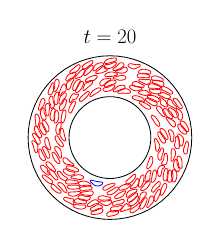
\begin{tikzpicture}[scale=0.3]

\begin{axis}[
  xmin = -21,
  xmax = 21,
  ymin = -21,
  ymax = 21,
  scale only axis,
  axis equal image,
  hide axis,
  title = {\Huge$t=20$}
  ]

% outer solid wall
\addplot [mark=none,black,line width=1.0] table{
2.0000e+01 -5.5171e-16
1.9904e+01 1.9603e+00
1.9616e+01 3.9018e+00
1.9139e+01 5.8057e+00
1.8478e+01 7.6537e+00
1.7638e+01 9.4279e+00
1.6629e+01 1.1111e+01
1.5460e+01 1.2688e+01
1.4142e+01 1.4142e+01
1.2688e+01 1.5460e+01
1.1111e+01 1.6629e+01
9.4279e+00 1.7638e+01
7.6537e+00 1.8478e+01
5.8057e+00 1.9139e+01
3.9018e+00 1.9616e+01
1.9603e+00 1.9904e+01
2.3281e-15 2.0000e+01
-1.9603e+00 1.9904e+01
-3.9018e+00 1.9616e+01
-5.8057e+00 1.9139e+01
-7.6537e+00 1.8478e+01
-9.4279e+00 1.7638e+01
-1.1111e+01 1.6629e+01
-1.2688e+01 1.5460e+01
-1.4142e+01 1.4142e+01
-1.5460e+01 1.2688e+01
-1.6629e+01 1.1111e+01
-1.7638e+01 9.4279e+00
-1.8478e+01 7.6537e+00
-1.9139e+01 5.8057e+00
-1.9616e+01 3.9018e+00
-1.9904e+01 1.9603e+00
-2.0000e+01 3.0010e-15
-1.9904e+01 -1.9603e+00
-1.9616e+01 -3.9018e+00
-1.9139e+01 -5.8057e+00
-1.8478e+01 -7.6537e+00
-1.7638e+01 -9.4279e+00
-1.6629e+01 -1.1111e+01
-1.5460e+01 -1.2688e+01
-1.4142e+01 -1.4142e+01
-1.2688e+01 -1.5460e+01
-1.1111e+01 -1.6629e+01
-9.4279e+00 -1.7638e+01
-7.6537e+00 -1.8478e+01
-5.8057e+00 -1.9139e+01
-3.9018e+00 -1.9616e+01
-1.9603e+00 -1.9904e+01
-4.7774e-15 -2.0000e+01
1.9603e+00 -1.9904e+01
3.9018e+00 -1.9616e+01
5.8057e+00 -1.9139e+01
7.6537e+00 -1.8478e+01
9.4279e+00 -1.7638e+01
1.1111e+01 -1.6629e+01
1.2688e+01 -1.5460e+01
1.4142e+01 -1.4142e+01
1.5460e+01 -1.2688e+01
1.6629e+01 -1.1111e+01
1.7638e+01 -9.4279e+00
1.8478e+01 -7.6537e+00
1.9139e+01 -5.8057e+00
1.9616e+01 -3.9018e+00
1.9904e+01 -1.9603e+00
2.0000e+01 -5.5171e-16
};

% inner solid wall
\addplot [mark=none,black,line width=1.0] table{
1.0000e+01 2.7586e-16
9.9518e+00 -9.8017e-01
9.8079e+00 -1.9509e+00
9.5694e+00 -2.9028e+00
9.2388e+00 -3.8268e+00
8.8192e+00 -4.7140e+00
8.3147e+00 -5.5557e+00
7.7301e+00 -6.3439e+00
7.0711e+00 -7.0711e+00
6.3439e+00 -7.7301e+00
5.5557e+00 -8.3147e+00
4.7140e+00 -8.8192e+00
3.8268e+00 -9.2388e+00
2.9028e+00 -9.5694e+00
1.9509e+00 -9.8079e+00
9.8017e-01 -9.9518e+00
1.1640e-15 -1.0000e+01
-9.8017e-01 -9.9518e+00
-1.9509e+00 -9.8079e+00
-2.9028e+00 -9.5694e+00
-3.8268e+00 -9.2388e+00
-4.7140e+00 -8.8192e+00
-5.5557e+00 -8.3147e+00
-6.3439e+00 -7.7301e+00
-7.0711e+00 -7.0711e+00
-7.7301e+00 -6.3439e+00
-8.3147e+00 -5.5557e+00
-8.8192e+00 -4.7140e+00
-9.2388e+00 -3.8268e+00
-9.5694e+00 -2.9028e+00
-9.8079e+00 -1.9509e+00
-9.9518e+00 -9.8017e-01
-1.0000e+01 -1.5005e-15
-9.9518e+00 9.8017e-01
-9.8079e+00 1.9509e+00
-9.5694e+00 2.9028e+00
-9.2388e+00 3.8268e+00
-8.8192e+00 4.7140e+00
-8.3147e+00 5.5557e+00
-7.7301e+00 6.3439e+00
-7.0711e+00 7.0711e+00
-6.3439e+00 7.7301e+00
-5.5557e+00 8.3147e+00
-4.7140e+00 8.8192e+00
-3.8268e+00 9.2388e+00
-2.9028e+00 9.5694e+00
-1.9509e+00 9.8079e+00
-9.8017e-01 9.9518e+00
-2.3887e-15 1.0000e+01
9.8017e-01 9.9518e+00
1.9509e+00 9.8079e+00
2.9028e+00 9.5694e+00
3.8268e+00 9.2388e+00
4.7140e+00 8.8192e+00
5.5557e+00 8.3147e+00
6.3439e+00 7.7301e+00
7.0711e+00 7.0711e+00
7.7301e+00 6.3439e+00
8.3147e+00 5.5557e+00
8.8192e+00 4.7140e+00
9.2388e+00 3.8268e+00
9.5694e+00 2.9028e+00
9.8079e+00 1.9509e+00
9.9518e+00 9.8017e-01
1.0000e+01 2.7586e-16
};

% vesicle 1
\addplot [mark=none,red,line width=1.0] table{
1.8909e+01 -3.6672e+00
1.8924e+01 -3.5872e+00
1.8936e+01 -3.4954e+00
1.8945e+01 -3.3892e+00
1.8954e+01 -3.2643e+00
1.8968e+01 -3.1235e+00
1.8988e+01 -2.9691e+00
1.9016e+01 -2.7964e+00
1.9053e+01 -2.6082e+00
1.9091e+01 -2.4171e+00
1.9129e+01 -2.2182e+00
1.9162e+01 -2.0107e+00
1.9186e+01 -1.8079e+00
1.9198e+01 -1.6039e+00
1.9190e+01 -1.4075e+00
1.9150e+01 -1.2258e+00
1.9066e+01 -1.0767e+00
1.8941e+01 -9.8553e-01
1.8799e+01 -9.6760e-01
1.8680e+01 -1.0116e+00
1.8598e+01 -1.0839e+00
1.8541e+01 -1.1646e+00
1.8503e+01 -1.2418e+00
1.8476e+01 -1.3152e+00
1.8452e+01 -1.3892e+00
1.8430e+01 -1.4685e+00
1.8406e+01 -1.5623e+00
1.8377e+01 -1.6739e+00
1.8341e+01 -1.7998e+00
1.8297e+01 -1.9411e+00
1.8244e+01 -2.0948e+00
1.8188e+01 -2.2473e+00
1.8127e+01 -2.4161e+00
1.8067e+01 -2.5987e+00
1.8018e+01 -2.7816e+00
1.7984e+01 -2.9813e+00
1.7973e+01 -3.1875e+00
1.7991e+01 -3.3882e+00
1.8039e+01 -3.5735e+00
1.8115e+01 -3.7359e+00
1.8219e+01 -3.8735e+00
1.8350e+01 -3.9729e+00
1.8492e+01 -4.0196e+00
1.8630e+01 -4.0101e+00
1.8740e+01 -3.9565e+00
1.8813e+01 -3.8844e+00
1.8860e+01 -3.8089e+00
1.8890e+01 -3.7377e+00
1.8909e+01 -3.6672e+00
};

% vesicle 2
\addplot [mark=none,red,line width=1.0] table{
6.8353e+00 1.0157e+01
6.7550e+00 1.0179e+01
6.6603e+00 1.0201e+01
6.5479e+00 1.0222e+01
6.4207e+00 1.0239e+01
6.2800e+00 1.0248e+01
6.1288e+00 1.0245e+01
5.9668e+00 1.0224e+01
5.7894e+00 1.0175e+01
5.6188e+00 1.0081e+01
5.4911e+00 9.9270e+00
5.4698e+00 9.7210e+00
5.5769e+00 9.5472e+00
5.7468e+00 9.4315e+00
5.9337e+00 9.3492e+00
6.1123e+00 9.2853e+00
6.2799e+00 9.2314e+00
6.4352e+00 9.1848e+00
6.5779e+00 9.1441e+00
6.7129e+00 9.1078e+00
6.8299e+00 9.0786e+00
6.9288e+00 9.0561e+00
7.0178e+00 9.0381e+00
7.0973e+00 9.0244e+00
7.1729e+00 9.0135e+00
7.2555e+00 9.0042e+00
7.3486e+00 8.9969e+00
7.4575e+00 8.9914e+00
7.5868e+00 8.9860e+00
7.7314e+00 8.9757e+00
7.8881e+00 8.9513e+00
8.0562e+00 8.9034e+00
8.2306e+00 8.8456e+00
8.4182e+00 8.8512e+00
8.5055e+00 9.0182e+00
8.4034e+00 9.1946e+00
8.2610e+00 9.3436e+00
8.1269e+00 9.5000e+00
7.9891e+00 9.6427e+00
7.8414e+00 9.7547e+00
7.6921e+00 9.8392e+00
7.5437e+00 9.9075e+00
7.4043e+00 9.9639e+00
7.2789e+00 1.0011e+01
7.1669e+00 1.0051e+01
7.0687e+00 1.0085e+01
6.9854e+00 1.0112e+01
6.9102e+00 1.0136e+01
6.8353e+00 1.0157e+01
};

% vesicle 3
\addplot [mark=none,red,line width=1.0] table{
8.8036e+00 1.0313e+01
8.8824e+00 1.0320e+01
8.9757e+00 1.0337e+01
9.0850e+00 1.0369e+01
9.2028e+00 1.0416e+01
9.3344e+00 1.0468e+01
9.4812e+00 1.0505e+01
9.6410e+00 1.0507e+01
9.8174e+00 1.0473e+01
1.0012e+01 1.0476e+01
1.0080e+01 1.0652e+01
9.9273e+00 1.0790e+01
9.7355e+00 1.0869e+01
9.5484e+00 1.0963e+01
9.3832e+00 1.1083e+01
9.2414e+00 1.1212e+01
9.1076e+00 1.1333e+01
8.9776e+00 1.1429e+01
8.8498e+00 1.1499e+01
8.7222e+00 1.1546e+01
8.6067e+00 1.1573e+01
8.5084e+00 1.1585e+01
8.4197e+00 1.1588e+01
8.3424e+00 1.1586e+01
8.2700e+00 1.1579e+01
8.1870e+00 1.1567e+01
8.0952e+00 1.1548e+01
7.9934e+00 1.1521e+01
7.8759e+00 1.1485e+01
7.7465e+00 1.1442e+01
7.5988e+00 1.1394e+01
7.4244e+00 1.1342e+01
7.2447e+00 1.1285e+01
7.0772e+00 1.1194e+01
6.9779e+00 1.1023e+01
7.0368e+00 1.0829e+01
7.2005e+00 1.0704e+01
7.3827e+00 1.0628e+01
7.5673e+00 1.0568e+01
7.7495e+00 1.0513e+01
7.9181e+00 1.0464e+01
8.0768e+00 1.0419e+01
8.2203e+00 1.0382e+01
8.3445e+00 1.0354e+01
8.4594e+00 1.0333e+01
8.5642e+00 1.0319e+01
8.6497e+00 1.0312e+01
8.7266e+00 1.0310e+01
8.8036e+00 1.0313e+01
};

% vesicle 4
\addplot [mark=none,red,line width=1.0] table{
1.6512e-01 -1.3944e+01
2.4498e-01 -1.3928e+01
3.3464e-01 -1.3905e+01
4.3633e-01 -1.3873e+01
5.5039e-01 -1.3828e+01
6.7655e-01 -1.3768e+01
8.1123e-01 -1.3693e+01
9.5107e-01 -1.3603e+01
1.1000e+00 -1.3496e+01
1.2589e+00 -1.3371e+01
1.4133e+00 -1.3239e+01
1.5566e+00 -1.3107e+01
1.6956e+00 -1.2965e+01
1.8328e+00 -1.2807e+01
1.9547e+00 -1.2640e+01
2.0417e+00 -1.2465e+01
2.0563e+00 -1.2284e+01
1.9734e+00 -1.2141e+01
1.8426e+00 -1.2074e+01
1.7110e+00 -1.2066e+01
1.5965e+00 -1.2088e+01
1.5014e+00 -1.2123e+01
1.4231e+00 -1.2161e+01
1.3557e+00 -1.2199e+01
1.2924e+00 -1.2238e+01
1.2258e+00 -1.2281e+01
1.1509e+00 -1.2332e+01
1.0641e+00 -1.2393e+01
9.6153e-01 -1.2466e+01
8.4364e-01 -1.2548e+01
7.1113e-01 -1.2638e+01
5.6141e-01 -1.2736e+01
4.0060e-01 -1.2834e+01
2.3451e-01 -1.2928e+01
5.7675e-02 -1.3020e+01
-1.3060e-01 -1.3112e+01
-3.1698e-01 -1.3201e+01
-4.9492e-01 -1.3300e+01
-6.4660e-01 -1.3429e+01
-7.2655e-01 -1.3600e+01
-6.9204e-01 -1.3775e+01
-5.7351e-01 -1.3890e+01
-4.3278e-01 -1.3946e+01
-2.9818e-01 -1.3968e+01
-1.7896e-01 -1.3974e+01
-7.6423e-02 -1.3972e+01
1.1899e-02 -1.3965e+01
8.9988e-02 -1.3956e+01
1.6512e-01 -1.3944e+01
};

% vesicle 5
\addplot [mark=none,red,line width=1.0] table{
1.7123e+01 8.4469e+00
1.7080e+01 8.5103e+00
1.7031e+01 8.5840e+00
1.6972e+01 8.6701e+00
1.6905e+01 8.7680e+00
1.6825e+01 8.8797e+00
1.6730e+01 9.0058e+00
1.6619e+01 9.1413e+00
1.6490e+01 9.2810e+00
1.6342e+01 9.4157e+00
1.6173e+01 9.5319e+00
1.5984e+01 9.6109e+00
1.5778e+01 9.6255e+00
1.5591e+01 9.5389e+00
1.5497e+01 9.3654e+00
1.5510e+01 9.1767e+00
1.5583e+01 9.0133e+00
1.5672e+01 8.8766e+00
1.5761e+01 8.7569e+00
1.5845e+01 8.6498e+00
1.5918e+01 8.5573e+00
1.5978e+01 8.4796e+00
1.6029e+01 8.4135e+00
1.6073e+01 8.3554e+00
1.6115e+01 8.2989e+00
1.6161e+01 8.2354e+00
1.6214e+01 8.1599e+00
1.6274e+01 8.0690e+00
1.6343e+01 7.9613e+00
1.6419e+01 7.8393e+00
1.6502e+01 7.7058e+00
1.6600e+01 7.5647e+00
1.6721e+01 7.4264e+00
1.6862e+01 7.3030e+00
1.7022e+01 7.1957e+00
1.7206e+01 7.1124e+00
1.7404e+01 7.0874e+00
1.7588e+01 7.1617e+00
1.7686e+01 7.3302e+00
1.7679e+01 7.5164e+00
1.7611e+01 7.6890e+00
1.7525e+01 7.8397e+00
1.7443e+01 7.9677e+00
1.7369e+01 8.0791e+00
1.7304e+01 8.1754e+00
1.7249e+01 8.2576e+00
1.7203e+01 8.3268e+00
1.7162e+01 8.3878e+00
1.7123e+01 8.4469e+00
};

% vesicle 6
\addplot [mark=none,red,line width=1.0] table{
-7.4377e+00 9.3985e+00
-7.4641e+00 9.3202e+00
-7.4819e+00 9.2258e+00
-7.4795e+00 9.1130e+00
-7.4372e+00 8.9896e+00
-7.3368e+00 8.8838e+00
-7.1839e+00 8.8361e+00
-7.0103e+00 8.8642e+00
-6.8366e+00 8.9510e+00
-6.6624e+00 9.0726e+00
-6.4869e+00 9.2116e+00
-6.3178e+00 9.3536e+00
-6.1602e+00 9.4915e+00
-6.0079e+00 9.6299e+00
-5.8628e+00 9.7676e+00
-5.7296e+00 9.9010e+00
-5.6061e+00 1.0034e+01
-5.4989e+00 1.0161e+01
-5.4102e+00 1.0278e+01
-5.3358e+00 1.0387e+01
-5.2745e+00 1.0487e+01
-5.2250e+00 1.0573e+01
-5.1845e+00 1.0649e+01
-5.1503e+00 1.0717e+01
-5.1193e+00 1.0783e+01
-5.0896e+00 1.0858e+01
-5.0632e+00 1.0947e+01
-5.0517e+00 1.1056e+01
-5.0825e+00 1.1179e+01
-5.1856e+00 1.1276e+01
-5.3400e+00 1.1291e+01
-5.4990e+00 1.1227e+01
-5.6509e+00 1.1124e+01
-5.7992e+00 1.1011e+01
-5.9556e+00 1.0891e+01
-6.1169e+00 1.0769e+01
-6.2803e+00 1.0643e+01
-6.4435e+00 1.0512e+01
-6.5984e+00 1.0380e+01
-6.7468e+00 1.0245e+01
-6.8797e+00 1.0117e+01
-6.9982e+00 9.9964e+00
-7.1013e+00 9.8851e+00
-7.1888e+00 9.7844e+00
-7.2621e+00 9.6928e+00
-7.3218e+00 9.6102e+00
-7.3691e+00 9.5360e+00
-7.4065e+00 9.4675e+00
-7.4377e+00 9.3985e+00
};

% vesicle 7
\addplot [mark=none,red,line width=1.0] table{
-1.5898e+01 -6.7866e-01
-1.5902e+01 -7.5837e-01
-1.5904e+01 -8.5010e-01
-1.5904e+01 -9.5691e-01
-1.5899e+01 -1.0804e+00
-1.5889e+01 -1.2158e+00
-1.5868e+01 -1.3665e+00
-1.5831e+01 -1.5368e+00
-1.5776e+01 -1.7110e+00
-1.5699e+01 -1.8876e+00
-1.5596e+01 -2.0729e+00
-1.5481e+01 -2.2470e+00
-1.5365e+01 -2.4067e+00
-1.5242e+01 -2.5632e+00
-1.5114e+01 -2.7154e+00
-1.4972e+01 -2.8550e+00
-1.4815e+01 -2.9507e+00
-1.4648e+01 -2.9645e+00
-1.4522e+01 -2.8824e+00
-1.4472e+01 -2.7606e+00
-1.4471e+01 -2.6458e+00
-1.4488e+01 -2.5474e+00
-1.4510e+01 -2.4663e+00
-1.4532e+01 -2.3949e+00
-1.4555e+01 -2.3251e+00
-1.4579e+01 -2.2502e+00
-1.4606e+01 -2.1613e+00
-1.4637e+01 -2.0554e+00
-1.4670e+01 -1.9350e+00
-1.4705e+01 -1.7996e+00
-1.4743e+01 -1.6476e+00
-1.4785e+01 -1.4788e+00
-1.4830e+01 -1.3003e+00
-1.4877e+01 -1.1183e+00
-1.4929e+01 -9.2437e-01
-1.4989e+01 -7.1140e-01
-1.5053e+01 -5.0498e-01
-1.5123e+01 -3.1739e-01
-1.5218e+01 -1.4513e-01
-1.5352e+01 -1.2292e-02
-1.5521e+01 3.7037e-02
-1.5674e+01 -1.4104e-02
-1.5775e+01 -1.2385e-01
-1.5830e+01 -2.4576e-01
-1.5859e+01 -3.5587e-01
-1.5876e+01 -4.5000e-01
-1.5886e+01 -5.3308e-01
-1.5893e+01 -6.0710e-01
-1.5898e+01 -6.7866e-01
};

% vesicle 8
\addplot [mark=none,red,line width=1.0] table{
-1.2355e+01 -4.7715e+00
-1.2312e+01 -4.8371e+00
-1.2253e+01 -4.9063e+00
-1.2170e+01 -4.9715e+00
-1.2059e+01 -5.0119e+00
-1.1927e+01 -4.9956e+00
-1.1818e+01 -4.8897e+00
-1.1790e+01 -4.7176e+00
-1.1826e+01 -4.5276e+00
-1.1872e+01 -4.3291e+00
-1.1898e+01 -4.1254e+00
-1.1906e+01 -3.9193e+00
-1.1910e+01 -3.7069e+00
-1.1925e+01 -3.4957e+00
-1.1959e+01 -3.2955e+00
-1.2015e+01 -3.1175e+00
-1.2091e+01 -2.9579e+00
-1.2182e+01 -2.8236e+00
-1.2277e+01 -2.7156e+00
-1.2374e+01 -2.6251e+00
-1.2464e+01 -2.5508e+00
-1.2545e+01 -2.4906e+00
-1.2617e+01 -2.4401e+00
-1.2682e+01 -2.3976e+00
-1.2744e+01 -2.3585e+00
-1.2815e+01 -2.3173e+00
-1.2897e+01 -2.2740e+00
-1.2995e+01 -2.2316e+00
-1.3114e+01 -2.1986e+00
-1.3251e+01 -2.1957e+00
-1.3389e+01 -2.2525e+00
-1.3488e+01 -2.3850e+00
-1.3512e+01 -2.5687e+00
-1.3470e+01 -2.7631e+00
-1.3394e+01 -2.9532e+00
-1.3295e+01 -3.1437e+00
-1.3183e+01 -3.3277e+00
-1.3068e+01 -3.5008e+00
-1.2960e+01 -3.6552e+00
-1.2857e+01 -3.8046e+00
-1.2758e+01 -3.9530e+00
-1.2669e+01 -4.0987e+00
-1.2597e+01 -4.2339e+00
-1.2540e+01 -4.3563e+00
-1.2494e+01 -4.4654e+00
-1.2455e+01 -4.5599e+00
-1.2422e+01 -4.6381e+00
-1.2390e+01 -4.7064e+00
-1.2355e+01 -4.7715e+00
};

% vesicle 9
\addplot [mark=none,red,line width=1.0] table{
1.2875e+00 1.3248e+01
1.3457e+00 1.3302e+01
1.4053e+00 1.3373e+01
1.4612e+00 1.3465e+01
1.4992e+00 1.3583e+01
1.4947e+00 1.3722e+01
1.4247e+00 1.3856e+01
1.2956e+00 1.3954e+01
1.1269e+00 1.4015e+01
9.3111e-01 1.4051e+01
7.1790e-01 1.4063e+01
5.0858e-01 1.4038e+01
3.1335e-01 1.3979e+01
1.3189e-01 1.3900e+01
-4.1401e-02 1.3814e+01
-2.0781e-01 1.3724e+01
-3.6712e-01 1.3633e+01
-5.1306e-01 1.3543e+01
-6.4139e-01 1.3461e+01
-7.5201e-01 1.3386e+01
-8.4656e-01 1.3318e+01
-9.2507e-01 1.3255e+01
-9.8956e-01 1.3199e+01
-1.0442e+00 1.3147e+01
-1.0952e+00 1.3095e+01
-1.1488e+00 1.3036e+01
-1.2082e+00 1.2964e+01
-1.2732e+00 1.2875e+01
-1.3374e+00 1.2764e+01
-1.3779e+00 1.2624e+01
-1.3409e+00 1.2470e+01
-1.1966e+00 1.2378e+01
-1.0114e+00 1.2393e+01
-8.3124e-01 1.2458e+01
-6.5050e-01 1.2532e+01
-4.6148e-01 1.2607e+01
-2.7378e-01 1.2681e+01
-9.5717e-02 1.2752e+01
8.4874e-02 1.2826e+01
2.6520e-01 1.2897e+01
4.3049e-01 1.2955e+01
5.8703e-01 1.3000e+01
7.3402e-01 1.3033e+01
8.6963e-01 1.3060e+01
9.8811e-01 1.3090e+01
1.0858e+00 1.3125e+01
1.1642e+00 1.3164e+01
1.2290e+00 1.3204e+01
1.2875e+00 1.3248e+01
};

% vesicle 10
\addplot [mark=none,red,line width=1.0] table{
9.4097e+00 1.4633e+01
9.4862e+00 1.4655e+01
9.5678e+00 1.4696e+01
9.6476e+00 1.4767e+01
9.7047e+00 1.4878e+01
9.7073e+00 1.5021e+01
9.6420e+00 1.5165e+01
9.5205e+00 1.5287e+01
9.3603e+00 1.5377e+01
9.1768e+00 1.5438e+01
8.9829e+00 1.5480e+01
8.7821e+00 1.5511e+01
8.5749e+00 1.5537e+01
8.3688e+00 1.5558e+01
8.1711e+00 1.5572e+01
7.9850e+00 1.5579e+01
7.8073e+00 1.5584e+01
7.6398e+00 1.5590e+01
7.4866e+00 1.5601e+01
7.3509e+00 1.5610e+01
7.2338e+00 1.5610e+01
7.1359e+00 1.5599e+01
7.0560e+00 1.5580e+01
6.9883e+00 1.5554e+01
6.9257e+00 1.5521e+01
6.8620e+00 1.5478e+01
6.7948e+00 1.5415e+01
6.7300e+00 1.5328e+01
6.6808e+00 1.5214e+01
6.6651e+00 1.5075e+01
6.7040e+00 1.4922e+01
6.8042e+00 1.4788e+01
6.9523e+00 1.4693e+01
7.1334e+00 1.4642e+01
7.3291e+00 1.4629e+01
7.5326e+00 1.4636e+01
7.7397e+00 1.4647e+01
7.9433e+00 1.4655e+01
8.1442e+00 1.4656e+01
8.3406e+00 1.4652e+01
8.5231e+00 1.4643e+01
8.6882e+00 1.4633e+01
8.8371e+00 1.4624e+01
8.9677e+00 1.4616e+01
9.0795e+00 1.4611e+01
9.1763e+00 1.4610e+01
9.2615e+00 1.4613e+01
9.3373e+00 1.4620e+01
9.4097e+00 1.4633e+01
};

% vesicle 11
\addplot [mark=none,red,line width=1.0] table{
-1.2828e+01 1.1964e+01
-1.2792e+01 1.2032e+01
-1.2752e+01 1.2112e+01
-1.2709e+01 1.2206e+01
-1.2661e+01 1.2318e+01
-1.2610e+01 1.2450e+01
-1.2559e+01 1.2602e+01
-1.2510e+01 1.2773e+01
-1.2466e+01 1.2958e+01
-1.2434e+01 1.3149e+01
-1.2417e+01 1.3347e+01
-1.2421e+01 1.3555e+01
-1.2455e+01 1.3765e+01
-1.2528e+01 1.3960e+01
-1.2646e+01 1.4122e+01
-1.2808e+01 1.4223e+01
-1.2986e+01 1.4238e+01
-1.3139e+01 1.4177e+01
-1.3251e+01 1.4078e+01
-1.3326e+01 1.3972e+01
-1.3378e+01 1.3872e+01
-1.3414e+01 1.3782e+01
-1.3440e+01 1.3702e+01
-1.3459e+01 1.3629e+01
-1.3474e+01 1.3558e+01
-1.3487e+01 1.3480e+01
-1.3497e+01 1.3388e+01
-1.3504e+01 1.3279e+01
-1.3505e+01 1.3155e+01
-1.3501e+01 1.3016e+01
-1.3494e+01 1.2861e+01
-1.3488e+01 1.2691e+01
-1.3490e+01 1.2508e+01
-1.3510e+01 1.2315e+01
-1.3553e+01 1.2122e+01
-1.3621e+01 1.1931e+01
-1.3700e+01 1.1739e+01
-1.3750e+01 1.1538e+01
-1.3710e+01 1.1347e+01
-1.3558e+01 1.1237e+01
-1.3380e+01 1.1261e+01
-1.3243e+01 1.1360e+01
-1.3141e+01 1.1476e+01
-1.3060e+01 1.1587e+01
-1.2994e+01 1.1685e+01
-1.2941e+01 1.1769e+01
-1.2898e+01 1.1839e+01
-1.2862e+01 1.1902e+01
-1.2828e+01 1.1964e+01
};

% vesicle 12
\addplot [mark=none,red,line width=1.0] table{
-5.4025e+00 1.4544e+01
-5.4691e+00 1.4506e+01
-5.5470e+00 1.4458e+01
-5.6380e+00 1.4397e+01
-5.7369e+00 1.4320e+01
-5.8397e+00 1.4221e+01
-5.9330e+00 1.4095e+01
-5.9912e+00 1.3934e+01
-5.9662e+00 1.3753e+01
-5.8206e+00 1.3627e+01
-5.6213e+00 1.3627e+01
-5.4273e+00 1.3699e+01
-5.2447e+00 1.3784e+01
-5.0656e+00 1.3864e+01
-4.8753e+00 1.3935e+01
-4.6817e+00 1.3973e+01
-4.5075e+00 1.3968e+01
-4.3472e+00 1.3944e+01
-4.1952e+00 1.3931e+01
-4.0617e+00 1.3944e+01
-3.9493e+00 1.3975e+01
-3.8586e+00 1.4014e+01
-3.7830e+00 1.4056e+01
-3.7196e+00 1.4096e+01
-3.6612e+00 1.4138e+01
-3.5968e+00 1.4188e+01
-3.5248e+00 1.4249e+01
-3.4433e+00 1.4323e+01
-3.3504e+00 1.4416e+01
-3.2536e+00 1.4527e+01
-3.1648e+00 1.4664e+01
-3.1121e+00 1.4830e+01
-3.1373e+00 1.5004e+01
-3.2564e+00 1.5141e+01
-3.4443e+00 1.5203e+01
-3.6524e+00 1.5196e+01
-3.8563e+00 1.5157e+01
-4.0542e+00 1.5106e+01
-4.2397e+00 1.5051e+01
-4.4215e+00 1.4990e+01
-4.5967e+00 1.4924e+01
-4.7502e+00 1.4860e+01
-4.8843e+00 1.4801e+01
-5.0032e+00 1.4747e+01
-5.1083e+00 1.4697e+01
-5.1990e+00 1.4652e+01
-5.2732e+00 1.4614e+01
-5.3386e+00 1.4580e+01
-5.4025e+00 1.4544e+01
};

% vesicle 13
\addplot [mark=none,red,line width=1.0] table{
1.0563e+01 9.2850e+00
1.0638e+01 9.2533e+00
1.0724e+01 9.2153e+00
1.0823e+01 9.1683e+00
1.0938e+01 9.1097e+00
1.1064e+01 9.0374e+00
1.1198e+01 8.9510e+00
1.1342e+01 8.8534e+00
1.1507e+01 8.7637e+00
1.1700e+01 8.7315e+00
1.1889e+01 8.7946e+00
1.2025e+01 8.9471e+00
1.2070e+01 9.1509e+00
1.2024e+01 9.3493e+00
1.1922e+01 9.5202e+00
1.1796e+01 9.6583e+00
1.1662e+01 9.7705e+00
1.1524e+01 9.8651e+00
1.1388e+01 9.9428e+00
1.1263e+01 1.0004e+01
1.1153e+01 1.0052e+01
1.1058e+01 1.0090e+01
1.0975e+01 1.0120e+01
1.0902e+01 1.0145e+01
1.0831e+01 1.0169e+01
1.0754e+01 1.0193e+01
1.0664e+01 1.0219e+01
1.0558e+01 1.0248e+01
1.0435e+01 1.0278e+01
1.0294e+01 1.0306e+01
1.0134e+01 1.0325e+01
9.9607e+00 1.0327e+01
9.7792e+00 1.0319e+01
9.5829e+00 1.0313e+01
9.3743e+00 1.0292e+01
9.1919e+00 1.0201e+01
9.1205e+00 1.0023e+01
9.1958e+00 9.8445e+00
9.3563e+00 9.7263e+00
9.5348e+00 9.6523e+00
9.7058e+00 9.5949e+00
9.8658e+00 9.5424e+00
1.0013e+01 9.4927e+00
1.0141e+01 9.4474e+00
1.0250e+01 9.4077e+00
1.0343e+01 9.3729e+00
1.0423e+01 9.3420e+00
1.0494e+01 9.3135e+00
1.0563e+01 9.2850e+00
};

% vesicle 14
\addplot [mark=none,red,line width=1.0] table{
8.5821e+00 8.4350e+00
8.5135e+00 8.4696e+00
8.4323e+00 8.5082e+00
8.3342e+00 8.5510e+00
8.2249e+00 8.5936e+00
8.0949e+00 8.6376e+00
7.9408e+00 8.6835e+00
7.7734e+00 8.7311e+00
7.5866e+00 8.7826e+00
7.3802e+00 8.8094e+00
7.1956e+00 8.7353e+00
7.1442e+00 8.5438e+00
7.2590e+00 8.3649e+00
7.4181e+00 8.2290e+00
7.5748e+00 8.0979e+00
7.7205e+00 7.9684e+00
7.8523e+00 7.8493e+00
7.9777e+00 7.7379e+00
8.0965e+00 7.6359e+00
8.2004e+00 7.5504e+00
8.2920e+00 7.4783e+00
8.3698e+00 7.4196e+00
8.4400e+00 7.3689e+00
8.5021e+00 7.3257e+00
8.5601e+00 7.2871e+00
8.6288e+00 7.2434e+00
8.7064e+00 7.1969e+00
8.7969e+00 7.1466e+00
8.9115e+00 7.0894e+00
9.0414e+00 7.0339e+00
9.1863e+00 6.9850e+00
9.3554e+00 6.9475e+00
9.5370e+00 6.9359e+00
9.7252e+00 6.9686e+00
9.8968e+00 7.0767e+00
9.9804e+00 7.2613e+00
9.9445e+00 7.4558e+00
9.8314e+00 7.6193e+00
9.6813e+00 7.7560e+00
9.5259e+00 7.8697e+00
9.3705e+00 7.9722e+00
9.2278e+00 8.0616e+00
9.1003e+00 8.1394e+00
8.9833e+00 8.2094e+00
8.8810e+00 8.2695e+00
8.7918e+00 8.3208e+00
8.7170e+00 8.3627e+00
8.6501e+00 8.3992e+00
8.5821e+00 8.4350e+00
};

% vesicle 15
\addplot [mark=none,red,line width=1.0] table{
-1.3611e+01 4.2623e+00
-1.3631e+01 4.1846e+00
-1.3645e+01 4.0925e+00
-1.3647e+01 3.9840e+00
-1.3626e+01 3.8618e+00
-1.3571e+01 3.7305e+00
-1.3468e+01 3.6086e+00
-1.3313e+01 3.5414e+00
-1.3137e+01 3.5801e+00
-1.2995e+01 3.7162e+00
-1.2888e+01 3.8848e+00
-1.2787e+01 4.0702e+00
-1.2695e+01 4.2700e+00
-1.2628e+01 4.4668e+00
-1.2581e+01 4.6579e+00
-1.2550e+01 4.8427e+00
-1.2531e+01 5.0202e+00
-1.2520e+01 5.1762e+00
-1.2515e+01 5.3144e+00
-1.2516e+01 5.4416e+00
-1.2519e+01 5.5537e+00
-1.2526e+01 5.6497e+00
-1.2534e+01 5.7333e+00
-1.2543e+01 5.8077e+00
-1.2554e+01 5.8797e+00
-1.2569e+01 5.9578e+00
-1.2589e+01 6.0463e+00
-1.2618e+01 6.1476e+00
-1.2661e+01 6.2642e+00
-1.2725e+01 6.3933e+00
-1.2820e+01 6.5210e+00
-1.2962e+01 6.6179e+00
-1.3146e+01 6.6253e+00
-1.3297e+01 6.5091e+00
-1.3375e+01 6.3213e+00
-1.3416e+01 6.1102e+00
-1.3447e+01 5.8990e+00
-1.3470e+01 5.7003e+00
-1.3485e+01 5.5078e+00
-1.3492e+01 5.3207e+00
-1.3495e+01 5.1434e+00
-1.3497e+01 4.9781e+00
-1.3502e+01 4.8303e+00
-1.3512e+01 4.7005e+00
-1.3527e+01 4.5865e+00
-1.3547e+01 4.4884e+00
-1.3568e+01 4.4059e+00
-1.3589e+01 4.3333e+00
-1.3611e+01 4.2623e+00
};

% vesicle 16
\addplot [mark=none,red,line width=1.0] table{
2.2767e+00 1.1584e+01
2.3465e+00 1.1608e+01
2.4331e+00 1.1638e+01
2.5404e+00 1.1674e+01
2.6566e+00 1.1714e+01
2.7928e+00 1.1761e+01
2.9496e+00 1.1814e+01
3.1099e+00 1.1866e+01
3.2793e+00 1.1924e+01
3.4523e+00 1.2004e+01
3.6112e+00 1.2126e+01
3.7132e+00 1.2307e+01
3.6924e+00 1.2515e+01
3.5535e+00 1.2669e+01
3.3784e+00 1.2748e+01
3.1964e+00 1.2785e+01
3.0108e+00 1.2796e+01
2.8452e+00 1.2791e+01
2.6981e+00 1.2775e+01
2.5616e+00 1.2752e+01
2.4491e+00 1.2726e+01
2.3584e+00 1.2700e+01
2.2747e+00 1.2673e+01
2.2050e+00 1.2647e+01
2.1427e+00 1.2622e+01
2.0681e+00 1.2589e+01
1.9882e+00 1.2549e+01
1.9002e+00 1.2499e+01
1.7943e+00 1.2432e+01
1.6815e+00 1.2350e+01
1.5630e+00 1.2253e+01
1.4324e+00 1.2135e+01
1.2998e+00 1.2010e+01
1.1534e+00 1.1878e+01
9.9899e-01 1.1744e+01
8.5239e-01 1.1599e+01
7.7342e-01 1.1406e+01
8.6614e-01 1.1232e+01
1.0582e+00 1.1184e+01
1.2514e+00 1.1211e+01
1.4271e+00 1.1259e+01
1.5906e+00 1.1314e+01
1.7373e+00 1.1371e+01
1.8580e+00 1.1422e+01
1.9661e+00 1.1467e+01
2.0622e+00 1.1506e+01
2.1372e+00 1.1534e+01
2.2059e+00 1.1560e+01
2.2767e+00 1.1584e+01
};

% vesicle 17
\addplot [mark=none,red,line width=1.0] table{
1.5000e+01 -3.1223e+00
1.4985e+01 -3.2011e+00
1.4972e+01 -3.2931e+00
1.4963e+01 -3.4006e+00
1.4957e+01 -3.5226e+00
1.4955e+01 -3.6632e+00
1.4958e+01 -3.8201e+00
1.4964e+01 -3.9845e+00
1.4972e+01 -4.1614e+00
1.4980e+01 -4.3482e+00
1.4984e+01 -4.5375e+00
1.4982e+01 -4.7342e+00
1.4972e+01 -4.9361e+00
1.4954e+01 -5.1423e+00
1.4939e+01 -5.3408e+00
1.4946e+01 -5.5287e+00
1.5005e+01 -5.6973e+00
1.5133e+01 -5.7968e+00
1.5277e+01 -5.7877e+00
1.5381e+01 -5.7069e+00
1.5442e+01 -5.6094e+00
1.5481e+01 -5.5192e+00
1.5510e+01 -5.4388e+00
1.5536e+01 -5.3678e+00
1.5562e+01 -5.2996e+00
1.5592e+01 -5.2229e+00
1.5630e+01 -5.1345e+00
1.5677e+01 -5.0323e+00
1.5734e+01 -4.9139e+00
1.5795e+01 -4.7851e+00
1.5859e+01 -4.6463e+00
1.5924e+01 -4.4898e+00
1.5984e+01 -4.3155e+00
1.6030e+01 -4.1252e+00
1.6055e+01 -3.9198e+00
1.6054e+01 -3.7063e+00
1.6025e+01 -3.4967e+00
1.5973e+01 -3.3021e+00
1.5898e+01 -3.1245e+00
1.5803e+01 -2.9682e+00
1.5684e+01 -2.8390e+00
1.5539e+01 -2.7483e+00
1.5386e+01 -2.7185e+00
1.5255e+01 -2.7475e+00
1.5156e+01 -2.8140e+00
1.5089e+01 -2.8955e+00
1.5047e+01 -2.9738e+00
1.5020e+01 -3.0478e+00
1.5000e+01 -3.1223e+00
};

% vesicle 18
\addplot [mark=none,red,line width=1.0] table{
-1.2656e+01 -6.3251e+00
-1.2580e+01 -6.3510e+00
-1.2490e+01 -6.3642e+00
-1.2386e+01 -6.3503e+00
-1.2282e+01 -6.2897e+00
-1.2212e+01 -6.1743e+00
-1.2200e+01 -6.0203e+00
-1.2244e+01 -5.8523e+00
-1.2320e+01 -5.6806e+00
-1.2411e+01 -5.5063e+00
-1.2505e+01 -5.3329e+00
-1.2601e+01 -5.1562e+00
-1.2699e+01 -4.9734e+00
-1.2799e+01 -4.7917e+00
-1.2903e+01 -4.6099e+00
-1.3006e+01 -4.4404e+00
-1.3107e+01 -4.2877e+00
-1.3206e+01 -4.1512e+00
-1.3299e+01 -4.0318e+00
-1.3386e+01 -3.9313e+00
-1.3465e+01 -3.8477e+00
-1.3537e+01 -3.7784e+00
-1.3604e+01 -3.7217e+00
-1.3668e+01 -3.6750e+00
-1.3734e+01 -3.6356e+00
-1.3810e+01 -3.6034e+00
-1.3903e+01 -3.5858e+00
-1.4008e+01 -3.6019e+00
-1.4105e+01 -3.6724e+00
-1.4157e+01 -3.7952e+00
-1.4152e+01 -3.9467e+00
-1.4105e+01 -4.1140e+00
-1.4041e+01 -4.2928e+00
-1.3976e+01 -4.4780e+00
-1.3910e+01 -4.6736e+00
-1.3838e+01 -4.8764e+00
-1.3753e+01 -5.0792e+00
-1.3656e+01 -5.2697e+00
-1.3552e+01 -5.4405e+00
-1.3444e+01 -5.5952e+00
-1.3335e+01 -5.7333e+00
-1.3229e+01 -5.8559e+00
-1.3128e+01 -5.9632e+00
-1.3032e+01 -6.0567e+00
-1.2943e+01 -6.1361e+00
-1.2863e+01 -6.2007e+00
-1.2791e+01 -6.2520e+00
-1.2724e+01 -6.2924e+00
-1.2656e+01 -6.3251e+00
};

% vesicle 19
\addplot [mark=none,red,line width=1.0] table{
-1.5093e+01 1.1137e+01
-1.5100e+01 1.1064e+01
-1.5102e+01 1.0974e+01
-1.5092e+01 1.0864e+01
-1.5061e+01 1.0746e+01
-1.4997e+01 1.0620e+01
-1.4883e+01 1.0505e+01
-1.4729e+01 1.0437e+01
-1.4546e+01 1.0438e+01
-1.4364e+01 1.0519e+01
-1.4217e+01 1.0656e+01
-1.4099e+01 1.0823e+01
-1.4002e+01 1.1005e+01
-1.3926e+01 1.1189e+01
-1.3868e+01 1.1379e+01
-1.3830e+01 1.1568e+01
-1.3809e+01 1.1743e+01
-1.3798e+01 1.1911e+01
-1.3792e+01 1.2063e+01
-1.3786e+01 1.2200e+01
-1.3777e+01 1.2317e+01
-1.3766e+01 1.2414e+01
-1.3754e+01 1.2501e+01
-1.3741e+01 1.2574e+01
-1.3728e+01 1.2642e+01
-1.3710e+01 1.2722e+01
-1.3690e+01 1.2811e+01
-1.3670e+01 1.2912e+01
-1.3654e+01 1.3038e+01
-1.3662e+01 1.3180e+01
-1.3726e+01 1.3321e+01
-1.3879e+01 1.3406e+01
-1.4053e+01 1.3356e+01
-1.4176e+01 1.3212e+01
-1.4264e+01 1.3029e+01
-1.4341e+01 1.2841e+01
-1.4423e+01 1.2657e+01
-1.4515e+01 1.2472e+01
-1.4609e+01 1.2296e+01
-1.4700e+01 1.2129e+01
-1.4788e+01 1.1965e+01
-1.4864e+01 1.1817e+01
-1.4927e+01 1.1681e+01
-1.4978e+01 1.1560e+01
-1.5017e+01 1.1453e+01
-1.5047e+01 1.1356e+01
-1.5067e+01 1.1280e+01
-1.5082e+01 1.1210e+01
-1.5093e+01 1.1137e+01
};

% vesicle 20
\addplot [mark=none,red,line width=1.0] table{
-1.2173e+01 4.7904e-01
-1.2141e+01 4.0234e-01
-1.2099e+01 3.1946e-01
-1.2048e+01 2.2839e-01
-1.1984e+01 1.2499e-01
-1.1908e+01 1.1851e-02
-1.1821e+01 -1.1231e-01
-1.1717e+01 -2.5213e-01
-1.1600e+01 -4.0213e-01
-1.1468e+01 -5.5617e-01
-1.1305e+01 -7.1158e-01
-1.1098e+01 -8.1817e-01
-1.0893e+01 -7.6574e-01
-1.0818e+01 -5.8106e-01
-1.0839e+01 -3.8460e-01
-1.0886e+01 -1.9725e-01
-1.0936e+01 -1.9505e-02
-1.0982e+01 1.4551e-01
-1.1022e+01 2.8962e-01
-1.1055e+01 4.1239e-01
-1.1084e+01 5.2085e-01
-1.1108e+01 6.1663e-01
-1.1128e+01 6.9848e-01
-1.1147e+01 7.7394e-01
-1.1165e+01 8.5017e-01
-1.1183e+01 9.3014e-01
-1.1204e+01 1.0218e+00
-1.1228e+01 1.1276e+00
-1.1256e+01 1.2496e+00
-1.1288e+01 1.3911e+00
-1.1326e+01 1.5449e+00
-1.1373e+01 1.7103e+00
-1.1433e+01 1.8866e+00
-1.1515e+01 2.0617e+00
-1.1636e+01 2.2133e+00
-1.1828e+01 2.2812e+00
-1.2001e+01 2.1594e+00
-1.2065e+01 1.9599e+00
-1.2091e+01 1.7495e+00
-1.2109e+01 1.5479e+00
-1.2128e+01 1.3684e+00
-1.2154e+01 1.2094e+00
-1.2185e+01 1.0667e+00
-1.2214e+01 9.3519e-01
-1.2229e+01 8.1740e-01
-1.2229e+01 7.1593e-01
-1.2217e+01 6.2675e-01
-1.2197e+01 5.5003e-01
-1.2173e+01 4.7904e-01
};

% vesicle 21
\addplot [mark=none,red,line width=1.0] table{
-3.6273e+00 1.1813e+01
-3.6954e+00 1.1770e+01
-3.7757e+00 1.1717e+01
-3.8696e+00 1.1651e+01
-3.9710e+00 1.1574e+01
-4.0813e+00 1.1483e+01
-4.2006e+00 1.1375e+01
-4.3240e+00 1.1252e+01
-4.4465e+00 1.1114e+01
-4.5637e+00 1.0964e+01
-4.6783e+00 1.0796e+01
-4.7834e+00 1.0619e+01
-4.8665e+00 1.0444e+01
-4.9042e+00 1.0259e+01
-4.8304e+00 1.0084e+01
-4.6503e+00 1.0034e+01
-4.4728e+00 1.0097e+01
-4.3228e+00 1.0189e+01
-4.1936e+00 1.0276e+01
-4.0793e+00 1.0353e+01
-3.9796e+00 1.0419e+01
-3.8938e+00 1.0475e+01
-3.8179e+00 1.0524e+01
-3.7521e+00 1.0567e+01
-3.6904e+00 1.0606e+01
-3.6226e+00 1.0649e+01
-3.5472e+00 1.0696e+01
-3.4598e+00 1.0750e+01
-3.3517e+00 1.0818e+01
-3.2252e+00 1.0896e+01
-3.0857e+00 1.0983e+01
-2.9340e+00 1.1079e+01
-2.7741e+00 1.1183e+01
-2.6120e+00 1.1296e+01
-2.4493e+00 1.1427e+01
-2.3070e+00 1.1586e+01
-2.2307e+00 1.1783e+01
-2.2765e+00 1.1984e+01
-2.4277e+00 1.2110e+01
-2.6127e+00 1.2151e+01
-2.7929e+00 1.2142e+01
-2.9579e+00 1.2108e+01
-3.1022e+00 1.2064e+01
-3.2271e+00 1.2017e+01
-3.3346e+00 1.1970e+01
-3.4245e+00 1.1926e+01
-3.4976e+00 1.1888e+01
-3.5628e+00 1.1851e+01
-3.6273e+00 1.1813e+01
};

% vesicle 22
\addplot [mark=none,red,line width=1.0] table{
1.1799e+01 -3.2329e+00
1.1846e+01 -3.1721e+00
1.1890e+01 -3.0953e+00
1.1934e+01 -3.0011e+00
1.1980e+01 -2.8900e+00
1.2031e+01 -2.7581e+00
1.2090e+01 -2.6051e+00
1.2145e+01 -2.4370e+00
1.2182e+01 -2.2574e+00
1.2189e+01 -2.0633e+00
1.2159e+01 -1.8641e+00
1.2097e+01 -1.6652e+00
1.2015e+01 -1.4747e+00
1.1922e+01 -1.2905e+00
1.1828e+01 -1.1162e+00
1.1733e+01 -9.4745e-01
1.1643e+01 -7.9124e-01
1.1557e+01 -6.4824e-01
1.1474e+01 -5.2155e-01
1.1393e+01 -4.1364e-01
1.1312e+01 -3.2980e-01
1.1231e+01 -2.7266e-01
1.1150e+01 -2.4276e-01
1.1076e+01 -2.4037e-01
1.1010e+01 -2.6298e-01
1.0951e+01 -3.1407e-01
1.0910e+01 -3.9354e-01
1.0893e+01 -4.9746e-01
1.0897e+01 -6.2406e-01
1.0917e+01 -7.6756e-01
1.0943e+01 -9.2458e-01
1.0972e+01 -1.0977e+00
1.1002e+01 -1.2873e+00
1.1032e+01 -1.4864e+00
1.1060e+01 -1.6944e+00
1.1086e+01 -1.9077e+00
1.1108e+01 -2.1227e+00
1.1127e+01 -2.3265e+00
1.1145e+01 -2.5159e+00
1.1165e+01 -2.6936e+00
1.1194e+01 -2.8653e+00
1.1239e+01 -3.0276e+00
1.1306e+01 -3.1667e+00
1.1395e+01 -3.2691e+00
1.1498e+01 -3.3266e+00
1.1598e+01 -3.3388e+00
1.1680e+01 -3.3192e+00
1.1745e+01 -3.2822e+00
1.1799e+01 -3.2329e+00
};

% vesicle 23
\addplot [mark=none,red,line width=1.0] table{
-8.0649e+00 -7.5346e+00
-8.1327e+00 -7.4912e+00
-8.2118e+00 -7.4431e+00
-8.3061e+00 -7.3888e+00
-8.4187e+00 -7.3281e+00
-8.5507e+00 -7.2629e+00
-8.7000e+00 -7.1982e+00
-8.8691e+00 -7.1384e+00
-9.0494e+00 -7.0889e+00
-9.2397e+00 -7.0450e+00
-9.4316e+00 -7.0034e+00
-9.6209e+00 -6.9645e+00
-9.8257e+00 -6.9282e+00
-1.0027e+01 -6.9050e+00
-1.0226e+01 -6.9046e+00
-1.0411e+01 -6.9410e+00
-1.0563e+01 -7.0255e+00
-1.0658e+01 -7.1563e+00
-1.0676e+01 -7.3021e+00
-1.0631e+01 -7.4253e+00
-1.0559e+01 -7.5131e+00
-1.0481e+01 -7.5738e+00
-1.0405e+01 -7.6181e+00
-1.0336e+01 -7.6521e+00
-1.0267e+01 -7.6815e+00
-1.0191e+01 -7.7109e+00
-1.0104e+01 -7.7422e+00
-1.0002e+01 -7.7760e+00
-9.8835e+00 -7.8130e+00
-9.7489e+00 -7.8532e+00
-9.5952e+00 -7.8981e+00
-9.4226e+00 -7.9493e+00
-9.2430e+00 -8.0064e+00
-9.0648e+00 -8.0705e+00
-8.8815e+00 -8.1474e+00
-8.6962e+00 -8.2353e+00
-8.4995e+00 -8.3217e+00
-8.2960e+00 -8.3728e+00
-8.1013e+00 -8.3755e+00
-7.9179e+00 -8.3323e+00
-7.7674e+00 -8.2406e+00
-7.6801e+00 -8.1050e+00
-7.6743e+00 -7.9590e+00
-7.7245e+00 -7.8395e+00
-7.7958e+00 -7.7487e+00
-7.8702e+00 -7.6784e+00
-7.9387e+00 -7.6234e+00
-8.0020e+00 -7.5773e+00
-8.0649e+00 -7.5346e+00
};

% vesicle 24
\addplot [mark=none,red,line width=1.0] table{
-1.3581e+01 5.9935e+00
-1.3564e+01 6.0714e+00
-1.3540e+01 6.1601e+00
-1.3506e+01 6.2618e+00
-1.3460e+01 6.3765e+00
-1.3409e+01 6.5077e+00
-1.3374e+01 6.6628e+00
-1.3391e+01 6.8357e+00
-1.3483e+01 6.9959e+00
-1.3645e+01 7.0918e+00
-1.3843e+01 7.0867e+00
-1.4026e+01 6.9924e+00
-1.4167e+01 6.8423e+00
-1.4268e+01 6.6633e+00
-1.4340e+01 6.4735e+00
-1.4397e+01 6.2864e+00
-1.4442e+01 6.1117e+00
-1.4480e+01 5.9515e+00
-1.4513e+01 5.8057e+00
-1.4542e+01 5.6748e+00
-1.4566e+01 5.5598e+00
-1.4585e+01 5.4606e+00
-1.4600e+01 5.3751e+00
-1.4610e+01 5.2992e+00
-1.4617e+01 5.2258e+00
-1.4622e+01 5.1460e+00
-1.4623e+01 5.0542e+00
-1.4616e+01 4.9478e+00
-1.4600e+01 4.8280e+00
-1.4569e+01 4.6978e+00
-1.4519e+01 4.5578e+00
-1.4442e+01 4.4101e+00
-1.4330e+01 4.2655e+00
-1.4176e+01 4.1477e+00
-1.3982e+01 4.0982e+00
-1.3796e+01 4.1656e+00
-1.3689e+01 4.3347e+00
-1.3655e+01 4.5344e+00
-1.3647e+01 4.7330e+00
-1.3647e+01 4.9265e+00
-1.3646e+01 5.1052e+00
-1.3643e+01 5.2653e+00
-1.3638e+01 5.4118e+00
-1.3632e+01 5.5439e+00
-1.3624e+01 5.6596e+00
-1.3615e+01 5.7594e+00
-1.3605e+01 5.8449e+00
-1.3594e+01 5.9205e+00
-1.3581e+01 5.9935e+00
};

% vesicle 25
\addplot [mark=none,red,line width=1.0] table{
-2.7641e+00 -1.4507e+01
-2.8179e+00 -1.4565e+01
-2.8686e+00 -1.4641e+01
-2.9056e+00 -1.4742e+01
-2.9067e+00 -1.4869e+01
-2.8456e+00 -1.5002e+01
-2.7207e+00 -1.5108e+01
-2.5569e+00 -1.5180e+01
-2.3751e+00 -1.5226e+01
-2.1835e+00 -1.5256e+01
-1.9896e+00 -1.5271e+01
-1.7947e+00 -1.5274e+01
-1.5956e+00 -1.5271e+01
-1.4009e+00 -1.5267e+01
-1.2078e+00 -1.5263e+01
-1.0142e+00 -1.5259e+01
-8.3018e-01 -1.5250e+01
-6.6476e-01 -1.5237e+01
-5.1865e-01 -1.5221e+01
-3.8832e-01 -1.5202e+01
-2.7219e-01 -1.5183e+01
-1.7230e-01 -1.5162e+01
-8.8886e-02 -1.5140e+01
-1.7310e-02 -1.5115e+01
4.8645e-02 -1.5083e+01
1.1279e-01 -1.5037e+01
1.7152e-01 -1.4966e+01
2.0457e-01 -1.4863e+01
1.8007e-01 -1.4741e+01
8.8850e-02 -1.4638e+01
-4.9473e-02 -1.4573e+01
-2.1488e-01 -1.4536e+01
-3.9626e-01 -1.4506e+01
-5.9165e-01 -1.4468e+01
-7.8685e-01 -1.4419e+01
-9.7950e-01 -1.4364e+01
-1.1746e+00 -1.4311e+01
-1.3753e+00 -1.4268e+01
-1.5736e+00 -1.4239e+01
-1.7601e+00 -1.4226e+01
-1.9355e+00 -1.4227e+01
-2.0982e+00 -1.4241e+01
-2.2445e+00 -1.4265e+01
-2.3730e+00 -1.4298e+01
-2.4825e+00 -1.4336e+01
-2.5732e+00 -1.4377e+01
-2.6475e+00 -1.4419e+01
-2.7090e+00 -1.4461e+01
-2.7641e+00 -1.4507e+01
};

% vesicle 26
\addplot [mark=none,red,line width=1.0] table{
-1.6449e+01 -2.4063e+00
-1.6468e+01 -2.4882e+00
-1.6470e+01 -2.5826e+00
-1.6453e+01 -2.6885e+00
-1.6415e+01 -2.8076e+00
-1.6361e+01 -2.9333e+00
-1.6296e+01 -3.0657e+00
-1.6218e+01 -3.2149e+00
-1.6131e+01 -3.3797e+00
-1.6044e+01 -3.5490e+00
-1.5953e+01 -3.7311e+00
-1.5864e+01 -3.9166e+00
-1.5776e+01 -4.1071e+00
-1.5691e+01 -4.2922e+00
-1.5608e+01 -4.4680e+00
-1.5522e+01 -4.6367e+00
-1.5426e+01 -4.7909e+00
-1.5317e+01 -4.9167e+00
-1.5193e+01 -5.0001e+00
-1.5068e+01 -5.0348e+00
-1.4953e+01 -5.0262e+00
-1.4861e+01 -4.9868e+00
-1.4798e+01 -4.9357e+00
-1.4753e+01 -4.8781e+00
-1.4721e+01 -4.8129e+00
-1.4700e+01 -4.7409e+00
-1.4690e+01 -4.6514e+00
-1.4695e+01 -4.5421e+00
-1.4714e+01 -4.4187e+00
-1.4748e+01 -4.2762e+00
-1.4792e+01 -4.1182e+00
-1.4840e+01 -3.9534e+00
-1.4898e+01 -3.7748e+00
-1.4967e+01 -3.5907e+00
-1.5050e+01 -3.4092e+00
-1.5148e+01 -3.2269e+00
-1.5253e+01 -3.0537e+00
-1.5360e+01 -2.8854e+00
-1.5464e+01 -2.7273e+00
-1.5573e+01 -2.5766e+00
-1.5693e+01 -2.4344e+00
-1.5819e+01 -2.3202e+00
-1.5947e+01 -2.2411e+00
-1.6079e+01 -2.1992e+00
-1.6199e+01 -2.1981e+00
-1.6294e+01 -2.2282e+00
-1.6368e+01 -2.2801e+00
-1.6418e+01 -2.3404e+00
-1.6449e+01 -2.4063e+00
};

% vesicle 27
\addplot [mark=none,red,line width=1.0] table{
2.1233e+00 1.4051e+01
2.2046e+00 1.4037e+01
2.2988e+00 1.4026e+01
2.4087e+00 1.4020e+01
2.5391e+00 1.4019e+01
2.6852e+00 1.4025e+01
2.8461e+00 1.4039e+01
3.0201e+00 1.4062e+01
3.2021e+00 1.4097e+01
3.3950e+00 1.4151e+01
3.5803e+00 1.4232e+01
3.7445e+00 1.4351e+01
3.8624e+00 1.4520e+01
3.8929e+00 1.4703e+01
3.8343e+00 1.4878e+01
3.7011e+00 1.5013e+01
3.5454e+00 1.5091e+01
3.3871e+00 1.5133e+01
3.2340e+00 1.5153e+01
3.1015e+00 1.5161e+01
2.9863e+00 1.5163e+01
2.8857e+00 1.5161e+01
2.8014e+00 1.5157e+01
2.7251e+00 1.5152e+01
2.6495e+00 1.5146e+01
2.5711e+00 1.5137e+01
2.4803e+00 1.5126e+01
2.3771e+00 1.5109e+01
2.2625e+00 1.5087e+01
2.1259e+00 1.5056e+01
1.9692e+00 1.5015e+01
1.8022e+00 1.4971e+01
1.6152e+00 1.4925e+01
1.4105e+00 1.4885e+01
1.2064e+00 1.4851e+01
1.0043e+00 1.4805e+01
8.3080e-01 1.4704e+01
7.9014e-01 1.4518e+01
9.3481e-01 1.4403e+01
1.1152e+00 1.4383e+01
1.2900e+00 1.4369e+01
1.4484e+00 1.4330e+01
1.5858e+00 1.4273e+01
1.7066e+00 1.4211e+01
1.8102e+00 1.4158e+01
1.8994e+00 1.4119e+01
1.9807e+00 1.4089e+01
2.0532e+00 1.4068e+01
2.1233e+00 1.4051e+01
};

% vesicle 28
\addplot [mark=none,red,line width=1.0] table{
1.4716e+01 4.7299e+00
1.4795e+01 4.7033e+00
1.4886e+01 4.6804e+00
1.4992e+01 4.6671e+00
1.5118e+01 4.6775e+00
1.5248e+01 4.7352e+00
1.5344e+01 4.8562e+00
1.5361e+01 5.0277e+00
1.5290e+01 5.1978e+00
1.5170e+01 5.3478e+00
1.5029e+01 5.4887e+00
1.4885e+01 5.6272e+00
1.4736e+01 5.7753e+00
1.4592e+01 5.9315e+00
1.4466e+01 6.0876e+00
1.4357e+01 6.2460e+00
1.4264e+01 6.4022e+00
1.4185e+01 6.5509e+00
1.4111e+01 6.6846e+00
1.4037e+01 6.7925e+00
1.3962e+01 6.8768e+00
1.3888e+01 6.9409e+00
1.3819e+01 6.9870e+00
1.3752e+01 7.0227e+00
1.3682e+01 7.0519e+00
1.3606e+01 7.0751e+00
1.3514e+01 7.0916e+00
1.3406e+01 7.0936e+00
1.3290e+01 7.0688e+00
1.3174e+01 6.9990e+00
1.3095e+01 6.8719e+00
1.3088e+01 6.7081e+00
1.3150e+01 6.5341e+00
1.3252e+01 6.3556e+00
1.3364e+01 6.1782e+00
1.3470e+01 6.0010e+00
1.3566e+01 5.8214e+00
1.3650e+01 5.6378e+00
1.3728e+01 5.4643e+00
1.3821e+01 5.3054e+00
1.3940e+01 5.1710e+00
1.4072e+01 5.0679e+00
1.4197e+01 4.9887e+00
1.4309e+01 4.9246e+00
1.4409e+01 4.8708e+00
1.4497e+01 4.8260e+00
1.4577e+01 4.7879e+00
1.4648e+01 4.7568e+00
1.4716e+01 4.7299e+00
};

% vesicle 29
\addplot [mark=none,red,line width=1.0] table{
-5.3319e+00 1.2325e+01
-5.2701e+00 1.2375e+01
-5.1976e+00 1.2434e+01
-5.1127e+00 1.2502e+01
-5.0166e+00 1.2579e+01
-4.9101e+00 1.2663e+01
-4.7905e+00 1.2761e+01
-4.6573e+00 1.2874e+01
-4.5177e+00 1.3004e+01
-4.3818e+00 1.3153e+01
-4.2672e+00 1.3328e+01
-4.2150e+00 1.3532e+01
-4.2933e+00 1.3725e+01
-4.4885e+00 1.3795e+01
-4.6824e+00 1.3754e+01
-4.8463e+00 1.3685e+01
-5.0008e+00 1.3610e+01
-5.1504e+00 1.3542e+01
-5.2902e+00 1.3494e+01
-5.4191e+00 1.3465e+01
-5.5359e+00 1.3449e+01
-5.6367e+00 1.3439e+01
-5.7220e+00 1.3425e+01
-5.7952e+00 1.3407e+01
-5.8629e+00 1.3380e+01
-5.9318e+00 1.3340e+01
-6.0027e+00 1.3280e+01
-6.0722e+00 1.3197e+01
-6.1361e+00 1.3089e+01
-6.1935e+00 1.2960e+01
-6.2483e+00 1.2811e+01
-6.3043e+00 1.2650e+01
-6.3671e+00 1.2479e+01
-6.4413e+00 1.2297e+01
-6.5232e+00 1.2108e+01
-6.5938e+00 1.1906e+01
-6.5994e+00 1.1699e+01
-6.4813e+00 1.1547e+01
-6.2913e+00 1.1537e+01
-6.1291e+00 1.1626e+01
-5.9948e+00 1.1740e+01
-5.8769e+00 1.1848e+01
-5.7697e+00 1.1946e+01
-5.6732e+00 1.2033e+01
-5.5868e+00 1.2109e+01
-5.5114e+00 1.2174e+01
-5.4465e+00 1.2229e+01
-5.3886e+00 1.2278e+01
-5.3319e+00 1.2325e+01
};

% vesicle 30
\addplot [mark=none,red,line width=1.0] table{
-3.0997e+00 1.6806e+01
-3.0424e+00 1.6857e+01
-2.9748e+00 1.6915e+01
-2.8935e+00 1.6983e+01
-2.7960e+00 1.7059e+01
-2.6819e+00 1.7143e+01
-2.5496e+00 1.7231e+01
-2.3979e+00 1.7320e+01
-2.2284e+00 1.7406e+01
-2.0469e+00 1.7490e+01
-1.8634e+00 1.7577e+01
-1.6946e+00 1.7682e+01
-1.5615e+00 1.7833e+01
-1.5257e+00 1.8034e+01
-1.6302e+00 1.8196e+01
-1.7990e+00 1.8268e+01
-1.9723e+00 1.8285e+01
-2.1348e+00 1.8281e+01
-2.2820e+00 1.8268e+01
-2.4107e+00 1.8252e+01
-2.5244e+00 1.8233e+01
-2.6229e+00 1.8214e+01
-2.7054e+00 1.8195e+01
-2.7764e+00 1.8176e+01
-2.8440e+00 1.8156e+01
-2.9165e+00 1.8132e+01
-3.0009e+00 1.8101e+01
-3.0996e+00 1.8058e+01
-3.2100e+00 1.8001e+01
-3.3291e+00 1.7929e+01
-3.4575e+00 1.7835e+01
-3.5896e+00 1.7717e+01
-3.7128e+00 1.7580e+01
-3.8213e+00 1.7423e+01
-3.9121e+00 1.7240e+01
-3.9898e+00 1.7041e+01
-4.0686e+00 1.6843e+01
-4.1283e+00 1.6646e+01
-4.1083e+00 1.6452e+01
-3.9803e+00 1.6319e+01
-3.8050e+00 1.6296e+01
-3.6503e+00 1.6348e+01
-3.5263e+00 1.6429e+01
-3.4235e+00 1.6513e+01
-3.3373e+00 1.6590e+01
-3.2655e+00 1.6655e+01
-3.2048e+00 1.6711e+01
-3.1514e+00 1.6760e+01
-3.0997e+00 1.6806e+01
};

% vesicle 31
\addplot [mark=none,red,line width=1.0] table{
1.1388e+00 -1.5599e+01
1.0663e+00 -1.5631e+01
9.8592e-01 -1.5672e+01
8.9586e-01 -1.5728e+01
7.9538e-01 -1.5805e+01
6.9377e-01 -1.5906e+01
6.0166e-01 -1.6039e+01
5.4763e-01 -1.6211e+01
5.8342e-01 -1.6392e+01
7.1656e-01 -1.6519e+01
9.0540e-01 -1.6563e+01
1.1117e+00 -1.6540e+01
1.3195e+00 -1.6486e+01
1.5241e+00 -1.6426e+01
1.7194e+00 -1.6372e+01
1.9023e+00 -1.6328e+01
2.0679e+00 -1.6295e+01
2.2243e+00 -1.6271e+01
2.3678e+00 -1.6253e+01
2.4942e+00 -1.6239e+01
2.6065e+00 -1.6224e+01
2.7040e+00 -1.6207e+01
2.7841e+00 -1.6188e+01
2.8547e+00 -1.6167e+01
2.9230e+00 -1.6141e+01
2.9926e+00 -1.6109e+01
3.0708e+00 -1.6065e+01
3.1576e+00 -1.6005e+01
3.2486e+00 -1.5925e+01
3.3413e+00 -1.5820e+01
3.4237e+00 -1.5688e+01
3.4765e+00 -1.5529e+01
3.4680e+00 -1.5345e+01
3.3527e+00 -1.5180e+01
3.1587e+00 -1.5111e+01
2.9535e+00 -1.5127e+01
2.7534e+00 -1.5180e+01
2.5594e+00 -1.5243e+01
2.3729e+00 -1.5303e+01
2.1911e+00 -1.5356e+01
2.0079e+00 -1.5401e+01
1.8402e+00 -1.5435e+01
1.6927e+00 -1.5462e+01
1.5609e+00 -1.5486e+01
1.4482e+00 -1.5508e+01
1.3548e+00 -1.5530e+01
1.2740e+00 -1.5552e+01
1.2043e+00 -1.5575e+01
1.1388e+00 -1.5599e+01
};

% vesicle 32
\addplot [mark=none,red,line width=1.0] table{
-8.4792e+00 8.2914e+00
-8.4634e+00 8.3696e+00
-8.4507e+00 8.4615e+00
-8.4459e+00 8.5710e+00
-8.4594e+00 8.6972e+00
-8.5107e+00 8.8318e+00
-8.6259e+00 8.9404e+00
-8.7948e+00 8.9557e+00
-8.9548e+00 8.8605e+00
-9.0863e+00 8.7069e+00
-9.2086e+00 8.5440e+00
-9.3328e+00 8.3878e+00
-9.4562e+00 8.2316e+00
-9.5697e+00 8.0690e+00
-9.6714e+00 7.8972e+00
-9.7604e+00 7.7222e+00
-9.8374e+00 7.5493e+00
-9.8997e+00 7.3899e+00
-9.9472e+00 7.2510e+00
-9.9834e+00 7.1285e+00
-1.0010e+01 7.0208e+00
-1.0030e+01 6.9269e+00
-1.0043e+01 6.8438e+00
-1.0053e+01 6.7685e+00
-1.0059e+01 6.6945e+00
-1.0063e+01 6.6117e+00
-1.0062e+01 6.5154e+00
-1.0052e+01 6.4030e+00
-1.0026e+01 6.2750e+00
-9.9696e+00 6.1398e+00
-9.8602e+00 6.0207e+00
-9.6873e+00 5.9805e+00
-9.5219e+00 6.0642e+00
-9.4058e+00 6.2119e+00
-9.3109e+00 6.3846e+00
-9.2208e+00 6.5658e+00
-9.1331e+00 6.7457e+00
-9.0470e+00 6.9232e+00
-8.9623e+00 7.0992e+00
-8.8812e+00 7.2698e+00
-8.8044e+00 7.4347e+00
-8.7337e+00 7.5911e+00
-8.6718e+00 7.7339e+00
-8.6205e+00 7.8587e+00
-8.5785e+00 7.9677e+00
-8.5448e+00 8.0632e+00
-8.5183e+00 8.1454e+00
-8.4972e+00 8.2191e+00
-8.4792e+00 8.2914e+00
};

% vesicle 33
\addplot [mark=none,red,line width=1.0] table{
4.8398e+00 -9.8845e+00
4.7778e+00 -9.9378e+00
4.7073e+00 -9.9984e+00
4.6271e+00 -1.0067e+01
4.5359e+00 -1.0147e+01
4.4309e+00 -1.0240e+01
4.3143e+00 -1.0347e+01
4.1902e+00 -1.0467e+01
4.0618e+00 -1.0607e+01
3.9444e+00 -1.0766e+01
3.8642e+00 -1.0955e+01
3.8947e+00 -1.1165e+01
4.0734e+00 -1.1273e+01
4.2721e+00 -1.1267e+01
4.4490e+00 -1.1226e+01
4.6200e+00 -1.1177e+01
4.7855e+00 -1.1124e+01
4.9364e+00 -1.1061e+01
5.0672e+00 -1.0988e+01
5.1748e+00 -1.0912e+01
5.2635e+00 -1.0840e+01
5.3377e+00 -1.0774e+01
5.4002e+00 -1.0714e+01
5.4546e+00 -1.0659e+01
5.5062e+00 -1.0605e+01
5.5610e+00 -1.0546e+01
5.6231e+00 -1.0476e+01
5.6947e+00 -1.0393e+01
5.7769e+00 -1.0296e+01
5.8694e+00 -1.0183e+01
5.9682e+00 -1.0058e+01
6.0677e+00 -9.9243e+00
6.1671e+00 -9.7739e+00
6.2597e+00 -9.5916e+00
6.3168e+00 -9.3835e+00
6.3029e+00 -9.1722e+00
6.1804e+00 -9.0116e+00
5.9915e+00 -8.9838e+00
5.8205e+00 -9.0542e+00
5.6706e+00 -9.1612e+00
5.5345e+00 -9.2756e+00
5.4094e+00 -9.3858e+00
5.2941e+00 -9.4883e+00
5.1903e+00 -9.5802e+00
5.1000e+00 -9.6594e+00
5.0227e+00 -9.7268e+00
4.9563e+00 -9.7843e+00
4.8972e+00 -9.8352e+00
4.8398e+00 -9.8845e+00
};

% vesicle 34
\addplot [mark=none,red,line width=1.0] table{
2.1974e+00 -1.2413e+01
2.1885e+00 -1.2494e+01
2.1978e+00 -1.2588e+01
2.2343e+00 -1.2691e+01
2.3085e+00 -1.2789e+01
2.4306e+00 -1.2863e+01
2.5922e+00 -1.2885e+01
2.7634e+00 -1.2852e+01
2.9338e+00 -1.2792e+01
3.1098e+00 -1.2730e+01
3.3014e+00 -1.2678e+01
3.5114e+00 -1.2642e+01
3.7291e+00 -1.2607e+01
3.9332e+00 -1.2550e+01
4.1152e+00 -1.2470e+01
4.2766e+00 -1.2376e+01
4.4197e+00 -1.2274e+01
4.5461e+00 -1.2166e+01
4.6529e+00 -1.2060e+01
4.7431e+00 -1.1961e+01
4.8210e+00 -1.1872e+01
4.8875e+00 -1.1796e+01
4.9435e+00 -1.1730e+01
4.9894e+00 -1.1669e+01
5.0273e+00 -1.1606e+01
5.0562e+00 -1.1532e+01
5.0624e+00 -1.1442e+01
5.0193e+00 -1.1348e+01
4.9116e+00 -1.1297e+01
4.7781e+00 -1.1329e+01
4.6477e+00 -1.1413e+01
4.5019e+00 -1.1502e+01
4.3269e+00 -1.1562e+01
4.1303e+00 -1.1567e+01
3.9346e+00 -1.1517e+01
3.7382e+00 -1.1469e+01
3.5329e+00 -1.1474e+01
3.3337e+00 -1.1529e+01
3.1452e+00 -1.1610e+01
2.9690e+00 -1.1700e+01
2.8070e+00 -1.1792e+01
2.6648e+00 -1.1882e+01
2.5448e+00 -1.1967e+01
2.4459e+00 -1.2047e+01
2.3649e+00 -1.2123e+01
2.3005e+00 -1.2198e+01
2.2528e+00 -1.2269e+01
2.2191e+00 -1.2339e+01
2.1974e+00 -1.2413e+01
};

% vesicle 35
\addplot [mark=none,red,line width=1.0] table{
-9.2194e+00 -6.2466e+00
-9.2874e+00 -6.1982e+00
-9.3647e+00 -6.1411e+00
-9.4516e+00 -6.0742e+00
-9.5486e+00 -5.9962e+00
-9.6548e+00 -5.9070e+00
-9.7740e+00 -5.8024e+00
-9.9059e+00 -5.6819e+00
-1.0043e+01 -5.5527e+00
-1.0190e+01 -5.4151e+00
-1.0345e+01 -5.2738e+00
-1.0505e+01 -5.1432e+00
-1.0677e+01 -5.0297e+00
-1.0875e+01 -4.9459e+00
-1.1083e+01 -4.9257e+00
-1.1264e+01 -4.9843e+00
-1.1390e+01 -5.1012e+00
-1.1456e+01 -5.2446e+00
-1.1478e+01 -5.3884e+00
-1.1472e+01 -5.5179e+00
-1.1451e+01 -5.6318e+00
-1.1424e+01 -5.7288e+00
-1.1394e+01 -5.8087e+00
-1.1362e+01 -5.8786e+00
-1.1327e+01 -5.9456e+00
-1.1285e+01 -6.0139e+00
-1.1231e+01 -6.0884e+00
-1.1162e+01 -6.1681e+00
-1.1074e+01 -6.2504e+00
-1.0962e+01 -6.3344e+00
-1.0820e+01 -6.4133e+00
-1.0658e+01 -6.4766e+00
-1.0473e+01 -6.5227e+00
-1.0269e+01 -6.5538e+00
-1.0069e+01 -6.5773e+00
-9.8704e+00 -6.6039e+00
-9.6632e+00 -6.6428e+00
-9.4656e+00 -6.6951e+00
-9.2736e+00 -6.7608e+00
-9.0959e+00 -6.8231e+00
-8.9224e+00 -6.8463e+00
-8.7759e+00 -6.7617e+00
-8.7716e+00 -6.6095e+00
-8.8545e+00 -6.5018e+00
-8.9450e+00 -6.4313e+00
-9.0250e+00 -6.3773e+00
-9.0955e+00 -6.3308e+00
-9.1584e+00 -6.2886e+00
-9.2194e+00 -6.2466e+00
};

% vesicle 36
\addplot [mark=none,red,line width=1.0] table{
1.9951e+00 1.1229e+01
1.9441e+00 1.1169e+01
1.9075e+00 1.1085e+01
1.9130e+00 1.0979e+01
1.9905e+00 1.0883e+01
2.1252e+00 1.0838e+01
2.2815e+00 1.0835e+01
2.4488e+00 1.0846e+01
2.6292e+00 1.0857e+01
2.8188e+00 1.0864e+01
3.0148e+00 1.0866e+01
3.2192e+00 1.0864e+01
3.4273e+00 1.0858e+01
3.6362e+00 1.0848e+01
3.8357e+00 1.0837e+01
4.0283e+00 1.0825e+01
4.2198e+00 1.0815e+01
4.4000e+00 1.0811e+01
4.5572e+00 1.0819e+01
4.6879e+00 1.0841e+01
4.7950e+00 1.0877e+01
4.8801e+00 1.0927e+01
4.9423e+00 1.0985e+01
4.9834e+00 1.1048e+01
5.0074e+00 1.1117e+01
5.0138e+00 1.1194e+01
4.9973e+00 1.1281e+01
4.9522e+00 1.1373e+01
4.8762e+00 1.1467e+01
4.7715e+00 1.1560e+01
4.6445e+00 1.1656e+01
4.5010e+00 1.1751e+01
4.3417e+00 1.1840e+01
4.1595e+00 1.1911e+01
3.9535e+00 1.1950e+01
3.7372e+00 1.1941e+01
3.5312e+00 1.1892e+01
3.3406e+00 1.1822e+01
3.1645e+00 1.1747e+01
2.9895e+00 1.1677e+01
2.8202e+00 1.1616e+01
2.6584e+00 1.1560e+01
2.5118e+00 1.1505e+01
2.3873e+00 1.1454e+01
2.2802e+00 1.1406e+01
2.1895e+00 1.1361e+01
2.1143e+00 1.1319e+01
2.0512e+00 1.1277e+01
1.9951e+00 1.1229e+01
};

% vesicle 37
\addplot [mark=none,red,line width=1.0] table{
-1.1686e+01 3.6131e+00
-1.1603e+01 3.5978e+00
-1.1510e+01 3.6139e+00
-1.1420e+01 3.6649e+00
-1.1336e+01 3.7528e+00
-1.1261e+01 3.8735e+00
-1.1193e+01 4.0187e+00
-1.1128e+01 4.1824e+00
-1.1065e+01 4.3569e+00
-1.1006e+01 4.5379e+00
-1.0949e+01 4.7281e+00
-1.0896e+01 4.9300e+00
-1.0849e+01 5.1363e+00
-1.0811e+01 5.3394e+00
-1.0781e+01 5.5358e+00
-1.0761e+01 5.7282e+00
-1.0750e+01 5.9090e+00
-1.0749e+01 6.0778e+00
-1.0756e+01 6.2308e+00
-1.0773e+01 6.3628e+00
-1.0801e+01 6.4752e+00
-1.0839e+01 6.5678e+00
-1.0885e+01 6.6386e+00
-1.0941e+01 6.6916e+00
-1.1008e+01 6.7271e+00
-1.1088e+01 6.7391e+00
-1.1178e+01 6.7187e+00
-1.1269e+01 6.6579e+00
-1.1351e+01 6.5616e+00
-1.1427e+01 6.4438e+00
-1.1498e+01 6.3198e+00
-1.1573e+01 6.1786e+00
-1.1647e+01 6.0130e+00
-1.1710e+01 5.8297e+00
-1.1760e+01 5.6263e+00
-1.1797e+01 5.4203e+00
-1.1827e+01 5.2139e+00
-1.1854e+01 5.0086e+00
-1.1876e+01 4.8142e+00
-1.1896e+01 4.6249e+00
-1.1911e+01 4.4484e+00
-1.1919e+01 4.2877e+00
-1.1920e+01 4.1380e+00
-1.1911e+01 3.9976e+00
-1.1889e+01 3.8765e+00
-1.1854e+01 3.7793e+00
-1.1807e+01 3.7033e+00
-1.1752e+01 3.6489e+00
-1.1686e+01 3.6131e+00
};

% vesicle 38
\addplot [mark=none,red,line width=1.0] table{
-1.0875e+01 7.9015e+00
-1.0848e+01 7.9746e+00
-1.0818e+01 8.0599e+00
-1.0784e+01 8.1613e+00
-1.0747e+01 8.2820e+00
-1.0710e+01 8.4216e+00
-1.0677e+01 8.5773e+00
-1.0650e+01 8.7468e+00
-1.0634e+01 8.9342e+00
-1.0644e+01 9.1353e+00
-1.0715e+01 9.3229e+00
-1.0879e+01 9.4278e+00
-1.1060e+01 9.3651e+00
-1.1178e+01 9.2052e+00
-1.1266e+01 9.0271e+00
-1.1344e+01 8.8615e+00
-1.1421e+01 8.7037e+00
-1.1501e+01 8.5533e+00
-1.1584e+01 8.4207e+00
-1.1669e+01 8.3140e+00
-1.1755e+01 8.2315e+00
-1.1836e+01 8.1684e+00
-1.1909e+01 8.1186e+00
-1.1972e+01 8.0747e+00
-1.2032e+01 8.0295e+00
-1.2091e+01 7.9758e+00
-1.2152e+01 7.9064e+00
-1.2211e+01 7.8168e+00
-1.2265e+01 7.7054e+00
-1.2308e+01 7.5707e+00
-1.2335e+01 7.4140e+00
-1.2342e+01 7.2382e+00
-1.2324e+01 7.0470e+00
-1.2274e+01 6.8517e+00
-1.2184e+01 6.6736e+00
-1.2036e+01 6.5499e+00
-1.1843e+01 6.5556e+00
-1.1692e+01 6.6897e+00
-1.1572e+01 6.8566e+00
-1.1440e+01 7.0080e+00
-1.1312e+01 7.1384e+00
-1.1207e+01 7.2599e+00
-1.1124e+01 7.3773e+00
-1.1059e+01 7.4905e+00
-1.1006e+01 7.5948e+00
-1.0964e+01 7.6867e+00
-1.0930e+01 7.7658e+00
-1.0902e+01 7.8349e+00
-1.0875e+01 7.9015e+00
};

% vesicle 39
\addplot [mark=none,red,line width=1.0] table{
5.9981e+00 -1.6299e+01
6.0613e+00 -1.6255e+01
6.1337e+00 -1.6200e+01
6.2178e+00 -1.6133e+01
6.3137e+00 -1.6051e+01
6.4182e+00 -1.5951e+01
6.5265e+00 -1.5831e+01
6.6283e+00 -1.5690e+01
6.7129e+00 -1.5529e+01
6.7801e+00 -1.5351e+01
6.8378e+00 -1.5162e+01
6.8952e+00 -1.4967e+01
6.9509e+00 -1.4773e+01
6.9815e+00 -1.4577e+01
6.9258e+00 -1.4390e+01
6.7615e+00 -1.4310e+01
6.5983e+00 -1.4365e+01
6.4740e+00 -1.4474e+01
6.3688e+00 -1.4586e+01
6.2771e+00 -1.4682e+01
6.1985e+00 -1.4764e+01
6.1318e+00 -1.4836e+01
6.0757e+00 -1.4898e+01
6.0261e+00 -1.4953e+01
5.9775e+00 -1.5005e+01
5.9237e+00 -1.5060e+01
5.8593e+00 -1.5123e+01
5.7805e+00 -1.5195e+01
5.6857e+00 -1.5278e+01
5.5765e+00 -1.5369e+01
5.4536e+00 -1.5466e+01
5.3131e+00 -1.5568e+01
5.1522e+00 -1.5665e+01
4.9725e+00 -1.5751e+01
4.7904e+00 -1.5846e+01
4.6535e+00 -1.6002e+01
4.6205e+00 -1.6205e+01
4.6937e+00 -1.6395e+01
4.8354e+00 -1.6535e+01
5.0135e+00 -1.6612e+01
5.1941e+00 -1.6629e+01
5.3534e+00 -1.6606e+01
5.4909e+00 -1.6566e+01
5.6114e+00 -1.6518e+01
5.7160e+00 -1.6469e+01
5.8041e+00 -1.6421e+01
5.8772e+00 -1.6378e+01
5.9394e+00 -1.6338e+01
5.9981e+00 -1.6299e+01
};

% vesicle 40
\addplot [mark=none,red,line width=1.0] table{
1.6036e+01 -8.1065e+00
1.5987e+01 -8.0485e+00
1.5926e+01 -7.9846e+00
1.5845e+01 -7.9170e+00
1.5735e+01 -7.8572e+00
1.5595e+01 -7.8314e+00
1.5445e+01 -7.8698e+00
1.5321e+01 -7.9845e+00
1.5259e+01 -8.1546e+00
1.5260e+01 -8.3472e+00
1.5296e+01 -8.5493e+00
1.5342e+01 -8.7557e+00
1.5378e+01 -8.9613e+00
1.5400e+01 -9.1619e+00
1.5407e+01 -9.3594e+00
1.5402e+01 -9.5510e+00
1.5387e+01 -9.7283e+00
1.5366e+01 -9.8901e+00
1.5343e+01 -1.0037e+01
1.5321e+01 -1.0168e+01
1.5305e+01 -1.0282e+01
1.5297e+01 -1.0380e+01
1.5297e+01 -1.0462e+01
1.5306e+01 -1.0534e+01
1.5323e+01 -1.0602e+01
1.5353e+01 -1.0671e+01
1.5405e+01 -1.0743e+01
1.5488e+01 -1.0808e+01
1.5604e+01 -1.0845e+01
1.5744e+01 -1.0832e+01
1.5883e+01 -1.0756e+01
1.6000e+01 -1.0627e+01
1.6091e+01 -1.0465e+01
1.6163e+01 -1.0285e+01
1.6223e+01 -1.0095e+01
1.6273e+01 -9.8970e+00
1.6315e+01 -9.6925e+00
1.6345e+01 -9.4848e+00
1.6361e+01 -9.2823e+00
1.6364e+01 -9.0916e+00
1.6352e+01 -8.9122e+00
1.6327e+01 -8.7481e+00
1.6291e+01 -8.6031e+00
1.6249e+01 -8.4781e+00
1.6203e+01 -8.3742e+00
1.6159e+01 -8.2894e+00
1.6116e+01 -8.2197e+00
1.6076e+01 -8.1611e+00
1.6036e+01 -8.1065e+00
};

% vesicle 41
\addplot [mark=none,red,line width=1.0] table{
-1.2592e+01 1.0379e+01
-1.2586e+01 1.0457e+01
-1.2578e+01 1.0547e+01
-1.2568e+01 1.0655e+01
-1.2559e+01 1.0780e+01
-1.2568e+01 1.0924e+01
-1.2635e+01 1.1069e+01
-1.2785e+01 1.1152e+01
-1.2964e+01 1.1115e+01
-1.3112e+01 1.0992e+01
-1.3231e+01 1.0834e+01
-1.3341e+01 1.0659e+01
-1.3443e+01 1.0477e+01
-1.3533e+01 1.0293e+01
-1.3602e+01 1.0109e+01
-1.3647e+01 9.9249e+00
-1.3671e+01 9.7460e+00
-1.3679e+01 9.5783e+00
-1.3680e+01 9.4257e+00
-1.3677e+01 9.2900e+00
-1.3672e+01 9.1730e+00
-1.3666e+01 9.0741e+00
-1.3659e+01 8.9909e+00
-1.3652e+01 8.9182e+00
-1.3643e+01 8.8480e+00
-1.3632e+01 8.7718e+00
-1.3616e+01 8.6834e+00
-1.3591e+01 8.5802e+00
-1.3555e+01 8.4625e+00
-1.3500e+01 8.3353e+00
-1.3418e+01 8.2087e+00
-1.3290e+01 8.1027e+00
-1.3117e+01 8.0655e+00
-1.2946e+01 8.1368e+00
-1.2830e+01 8.2986e+00
-1.2778e+01 8.4918e+00
-1.2758e+01 8.6961e+00
-1.2746e+01 8.9010e+00
-1.2733e+01 9.1080e+00
-1.2715e+01 9.3094e+00
-1.2694e+01 9.4927e+00
-1.2672e+01 9.6575e+00
-1.2652e+01 9.8062e+00
-1.2635e+01 9.9393e+00
-1.2621e+01 1.0055e+01
-1.2611e+01 1.0153e+01
-1.2604e+01 1.0236e+01
-1.2598e+01 1.0308e+01
-1.2592e+01 1.0379e+01
};

% vesicle 42
\addplot [mark=none,red,line width=1.0] table{
1.6441e-01 1.1537e+01
2.3260e-01 1.1572e+01
3.1054e-01 1.1617e+01
4.0053e-01 1.1676e+01
5.0183e-01 1.1753e+01
6.1189e-01 1.1850e+01
7.2811e-01 1.1962e+01
8.5151e-01 1.2086e+01
9.8365e-01 1.2223e+01
1.1113e+00 1.2378e+01
1.1977e+00 1.2564e+01
1.1708e+00 1.2762e+01
1.0141e+00 1.2877e+01
8.0830e-01 1.2870e+01
6.1068e-01 1.2802e+01
4.2851e-01 1.2725e+01
2.5991e-01 1.2650e+01
1.0844e-01 1.2582e+01
-2.5053e-02 1.2520e+01
-1.4277e-01 1.2466e+01
-2.4463e-01 1.2419e+01
-3.3236e-01 1.2380e+01
-4.0847e-01 1.2348e+01
-4.7656e-01 1.2322e+01
-5.4336e-01 1.2298e+01
-6.1742e-01 1.2274e+01
-7.0560e-01 1.2250e+01
-8.1272e-01 1.2228e+01
-9.4145e-01 1.2211e+01
-1.0901e+00 1.2200e+01
-1.2540e+00 1.2181e+01
-1.4260e+00 1.2126e+01
-1.5819e+00 1.2017e+01
-1.6842e+00 1.1851e+01
-1.6855e+00 1.1653e+01
-1.5764e+00 1.1478e+01
-1.4012e+00 1.1363e+01
-1.2081e+00 1.1305e+01
-1.0115e+00 1.1283e+01
-8.2531e-01 1.1284e+01
-6.6006e-01 1.1300e+01
-5.0777e-01 1.1323e+01
-3.6869e-01 1.1352e+01
-2.4597e-01 1.1384e+01
-1.3910e-01 1.1416e+01
-4.6312e-02 1.1448e+01
3.2433e-02 1.1478e+01
1.0032e-01 1.1507e+01
1.6441e-01 1.1537e+01
};

% vesicle 43
\addplot [mark=none,red,line width=1.0] table{
1.0120e+01 4.9790e+00
1.0155e+01 4.9080e+00
1.0201e+01 4.8277e+00
1.0259e+01 4.7342e+00
1.0329e+01 4.6245e+00
1.0409e+01 4.5003e+00
1.0496e+01 4.3654e+00
1.0588e+01 4.2217e+00
1.0686e+01 4.0690e+00
1.0792e+01 3.9035e+00
1.0901e+01 3.7355e+00
1.1015e+01 3.5640e+00
1.1139e+01 3.3841e+00
1.1269e+01 3.2095e+00
1.1401e+01 3.0492e+00
1.1541e+01 2.9087e+00
1.1691e+01 2.8012e+00
1.1846e+01 2.7468e+00
1.1988e+01 2.7613e+00
1.2093e+01 2.8358e+00
1.2150e+01 2.9372e+00
1.2171e+01 3.0360e+00
1.2173e+01 3.1215e+00
1.2167e+01 3.1964e+00
1.2156e+01 3.2685e+00
1.2140e+01 3.3456e+00
1.2115e+01 3.4348e+00
1.2081e+01 3.5385e+00
1.2037e+01 3.6542e+00
1.1982e+01 3.7775e+00
1.1916e+01 3.9101e+00
1.1834e+01 4.0552e+00
1.1736e+01 4.2127e+00
1.1626e+01 4.3738e+00
1.1504e+01 4.5370e+00
1.1370e+01 4.7033e+00
1.1226e+01 4.8675e+00
1.1080e+01 5.0206e+00
1.0926e+01 5.1635e+00
1.0771e+01 5.2847e+00
1.0617e+01 5.3769e+00
1.0459e+01 5.4337e+00
1.0304e+01 5.4400e+00
1.0176e+01 5.3881e+00
1.0101e+01 5.2980e+00
1.0074e+01 5.2028e+00
1.0077e+01 5.1183e+00
1.0094e+01 5.0461e+00
1.0120e+01 4.9790e+00
};

% vesicle 44
\addplot [mark=none,red,line width=1.0] table{
-4.3394e+00 1.8086e+01
-4.2910e+00 1.8145e+01
-4.2408e+00 1.8218e+01
-4.1923e+00 1.8312e+01
-4.1555e+00 1.8430e+01
-4.1501e+00 1.8569e+01
-4.2051e+00 1.8714e+01
-4.3395e+00 1.8818e+01
-4.5243e+00 1.8834e+01
-4.7145e+00 1.8773e+01
-4.8914e+00 1.8680e+01
-5.0711e+00 1.8577e+01
-5.2562e+00 1.8473e+01
-5.4369e+00 1.8374e+01
-5.6111e+00 1.8280e+01
-5.7757e+00 1.8191e+01
-5.9303e+00 1.8104e+01
-6.0724e+00 1.8020e+01
-6.1986e+00 1.7940e+01
-6.3072e+00 1.7866e+01
-6.3987e+00 1.7797e+01
-6.4742e+00 1.7734e+01
-6.5354e+00 1.7676e+01
-6.5864e+00 1.7623e+01
-6.6325e+00 1.7569e+01
-6.6783e+00 1.7507e+01
-6.7243e+00 1.7429e+01
-6.7653e+00 1.7331e+01
-6.7888e+00 1.7209e+01
-6.7729e+00 1.7068e+01
-6.6927e+00 1.6931e+01
-6.5471e+00 1.6840e+01
-6.3685e+00 1.6808e+01
-6.1818e+00 1.6821e+01
-5.9943e+00 1.6878e+01
-5.8148e+00 1.6978e+01
-5.6501e+00 1.7101e+01
-5.4965e+00 1.7230e+01
-5.3496e+00 1.7353e+01
-5.2025e+00 1.7468e+01
-5.0573e+00 1.7571e+01
-4.9193e+00 1.7661e+01
-4.7918e+00 1.7741e+01
-4.6782e+00 1.7812e+01
-4.5821e+00 1.7876e+01
-4.5037e+00 1.7933e+01
-4.4402e+00 1.7986e+01
-4.3874e+00 1.8035e+01
-4.3394e+00 1.8086e+01
};

% vesicle 45
\addplot [mark=none,red,line width=1.0] table{
1.0537e+00 1.7476e+01
1.1155e+00 1.7523e+01
1.1862e+00 1.7579e+01
1.2669e+00 1.7648e+01
1.3560e+00 1.7733e+01
1.4493e+00 1.7839e+01
1.5337e+00 1.7973e+01
1.5802e+00 1.8139e+01
1.5419e+00 1.8317e+01
1.3987e+00 1.8439e+01
1.1988e+00 1.8458e+01
9.9852e-01 1.8396e+01
8.2016e-01 1.8309e+01
6.4046e-01 1.8213e+01
4.6034e-01 1.8121e+01
2.9081e-01 1.8044e+01
1.2581e-01 1.7981e+01
-3.2215e-02 1.7935e+01
-1.7992e-01 1.7903e+01
-3.1278e-01 1.7884e+01
-4.2927e-01 1.7874e+01
-5.3060e-01 1.7869e+01
-6.1723e-01 1.7867e+01
-6.9282e-01 1.7866e+01
-7.6517e-01 1.7864e+01
-8.4314e-01 1.7860e+01
-9.3260e-01 1.7850e+01
-1.0354e+00 1.7824e+01
-1.1460e+00 1.7769e+01
-1.2436e+00 1.7669e+01
-1.2953e+00 1.7524e+01
-1.2721e+00 1.7360e+01
-1.1714e+00 1.7211e+01
-1.0243e+00 1.7091e+01
-8.4918e-01 1.6990e+01
-6.5747e-01 1.6917e+01
-4.5112e-01 1.6885e+01
-2.4632e-01 1.6890e+01
-6.0100e-02 1.6918e+01
1.1209e-01 1.6962e+01
2.7586e-01 1.7018e+01
4.2889e-01 1.7085e+01
5.6644e-01 1.7156e+01
6.8503e-01 1.7226e+01
7.8478e-01 1.7289e+01
8.6753e-01 1.7344e+01
9.3643e-01 1.7391e+01
9.9630e-01 1.7433e+01
1.0537e+00 1.7476e+01
};

% vesicle 46
\addplot [mark=none,red,line width=1.0] table{
1.0350e+01 -1.2417e+01
1.0317e+01 -1.2486e+01
1.0281e+01 -1.2570e+01
1.0244e+01 -1.2671e+01
1.0211e+01 -1.2791e+01
1.0190e+01 -1.2929e+01
1.0200e+01 -1.3082e+01
1.0269e+01 -1.3235e+01
1.0419e+01 -1.3340e+01
1.0611e+01 -1.3334e+01
1.0780e+01 -1.3232e+01
1.0916e+01 -1.3083e+01
1.1037e+01 -1.2918e+01
1.1160e+01 -1.2748e+01
1.1288e+01 -1.2591e+01
1.1421e+01 -1.2455e+01
1.1551e+01 -1.2342e+01
1.1676e+01 -1.2243e+01
1.1792e+01 -1.2149e+01
1.1893e+01 -1.2060e+01
1.1975e+01 -1.1977e+01
1.2039e+01 -1.1902e+01
1.2089e+01 -1.1835e+01
1.2128e+01 -1.1774e+01
1.2164e+01 -1.1713e+01
1.2198e+01 -1.1644e+01
1.2233e+01 -1.1561e+01
1.2267e+01 -1.1459e+01
1.2293e+01 -1.1336e+01
1.2303e+01 -1.1195e+01
1.2281e+01 -1.1043e+01
1.2210e+01 -1.0892e+01
1.2069e+01 -1.0777e+01
1.1877e+01 -1.0757e+01
1.1695e+01 -1.0842e+01
1.1544e+01 -1.0982e+01
1.1404e+01 -1.1140e+01
1.1265e+01 -1.1294e+01
1.1126e+01 -1.1437e+01
1.0990e+01 -1.1570e+01
1.0867e+01 -1.1694e+01
1.0755e+01 -1.1815e+01
1.0658e+01 -1.1931e+01
1.0578e+01 -1.2037e+01
1.0512e+01 -1.2133e+01
1.0460e+01 -1.2217e+01
1.0418e+01 -1.2289e+01
1.0383e+01 -1.2353e+01
1.0350e+01 -1.2417e+01
};

% vesicle 47
\addplot [mark=none,red,line width=1.0] table{
1.3007e+01 5.1699e+00
1.3079e+01 5.1371e+00
1.3165e+01 5.1097e+00
1.3269e+01 5.0988e+00
1.3386e+01 5.1297e+00
1.3477e+01 5.2328e+00
1.3481e+01 5.3878e+00
1.3407e+01 5.5455e+00
1.3300e+01 5.7004e+00
1.3185e+01 5.8630e+00
1.3074e+01 6.0389e+00
1.2976e+01 6.2282e+00
1.2909e+01 6.4141e+00
1.2867e+01 6.6073e+00
1.2828e+01 6.8083e+00
1.2764e+01 6.9960e+00
1.2674e+01 7.1504e+00
1.2568e+01 7.2822e+00
1.2461e+01 7.3897e+00
1.2361e+01 7.4751e+00
1.2267e+01 7.5441e+00
1.2182e+01 7.5980e+00
1.2107e+01 7.6379e+00
1.2039e+01 7.6671e+00
1.1973e+01 7.6892e+00
1.1899e+01 7.7051e+00
1.1812e+01 7.7114e+00
1.1710e+01 7.6985e+00
1.1597e+01 7.6515e+00
1.1494e+01 7.5577e+00
1.1427e+01 7.4185e+00
1.1409e+01 7.2506e+00
1.1436e+01 7.0747e+00
1.1500e+01 6.8986e+00
1.1599e+01 6.7178e+00
1.1725e+01 6.5365e+00
1.1858e+01 6.3661e+00
1.1986e+01 6.2075e+00
1.2111e+01 6.0515e+00
1.2232e+01 5.8988e+00
1.2345e+01 5.7616e+00
1.2449e+01 5.6410e+00
1.2550e+01 5.5323e+00
1.2645e+01 5.4383e+00
1.2733e+01 5.3598e+00
1.2812e+01 5.2964e+00
1.2880e+01 5.2466e+00
1.2944e+01 5.2057e+00
1.3007e+01 5.1699e+00
};

% vesicle 48
\addplot [mark=none,red,line width=1.0] table{
-1.1371e+01 -8.2655e+00
-1.1336e+01 -8.3333e+00
-1.1286e+01 -8.4094e+00
-1.1219e+01 -8.4944e+00
-1.1133e+01 -8.5855e+00
-1.1030e+01 -8.6808e+00
-1.0906e+01 -8.7816e+00
-1.0762e+01 -8.8835e+00
-1.0609e+01 -8.9790e+00
-1.0442e+01 -9.0675e+00
-1.0255e+01 -9.1454e+00
-1.0048e+01 -9.2019e+00
-9.8363e+00 -9.2239e+00
-9.6322e+00 -9.2120e+00
-9.4367e+00 -9.1769e+00
-9.2523e+00 -9.1331e+00
-9.0838e+00 -9.0905e+00
-8.9305e+00 -9.0492e+00
-8.7909e+00 -9.0026e+00
-8.6729e+00 -8.9431e+00
-8.5868e+00 -8.8667e+00
-8.5402e+00 -8.7791e+00
-8.5319e+00 -8.6940e+00
-8.5524e+00 -8.6207e+00
-8.5940e+00 -8.5595e+00
-8.6565e+00 -8.5081e+00
-8.7411e+00 -8.4673e+00
-8.8464e+00 -8.4376e+00
-8.9696e+00 -8.4158e+00
-9.1076e+00 -8.3965e+00
-9.2603e+00 -8.3746e+00
-9.4300e+00 -8.3455e+00
-9.6119e+00 -8.3055e+00
-9.8017e+00 -8.2509e+00
-9.9968e+00 -8.1770e+00
-1.0180e+01 -8.0874e+00
-1.0345e+01 -7.9858e+00
-1.0502e+01 -7.8720e+00
-1.0666e+01 -7.7521e+00
-1.0841e+01 -7.6610e+00
-1.1018e+01 -7.6298e+00
-1.1180e+01 -7.6610e+00
-1.1307e+01 -7.7418e+00
-1.1386e+01 -7.8483e+00
-1.1421e+01 -7.9561e+00
-1.1427e+01 -8.0518e+00
-1.1417e+01 -8.1322e+00
-1.1398e+01 -8.2010e+00
-1.1371e+01 -8.2655e+00
};

% vesicle 49
\addplot [mark=none,red,line width=1.0] table{
-1.6660e+01 -6.7461e+00
-1.6731e+01 -6.7751e+00
-1.6804e+01 -6.8250e+00
-1.6874e+01 -6.9030e+00
-1.6926e+01 -7.0135e+00
-1.6945e+01 -7.1534e+00
-1.6923e+01 -7.3114e+00
-1.6866e+01 -7.4752e+00
-1.6783e+01 -7.6407e+00
-1.6684e+01 -7.8057e+00
-1.6574e+01 -7.9670e+00
-1.6451e+01 -8.1246e+00
-1.6314e+01 -8.2738e+00
-1.6167e+01 -8.4105e+00
-1.6012e+01 -8.5350e+00
-1.5859e+01 -8.6465e+00
-1.5712e+01 -8.7511e+00
-1.5576e+01 -8.8508e+00
-1.5455e+01 -8.9422e+00
-1.5348e+01 -9.0207e+00
-1.5253e+01 -9.0828e+00
-1.5168e+01 -9.1273e+00
-1.5091e+01 -9.1545e+00
-1.5020e+01 -9.1658e+00
-1.4951e+01 -9.1611e+00
-1.4880e+01 -9.1337e+00
-1.4818e+01 -9.0711e+00
-1.4794e+01 -8.9697e+00
-1.4834e+01 -8.8544e+00
-1.4930e+01 -8.7519e+00
-1.5051e+01 -8.6536e+00
-1.5167e+01 -8.5292e+00
-1.5235e+01 -8.3579e+00
-1.5227e+01 -8.1617e+00
-1.5189e+01 -7.9632e+00
-1.5207e+01 -7.7606e+00
-1.5307e+01 -7.5797e+00
-1.5452e+01 -7.4324e+00
-1.5605e+01 -7.3027e+00
-1.5752e+01 -7.1791e+00
-1.5887e+01 -7.0615e+00
-1.6012e+01 -6.9548e+00
-1.6130e+01 -6.8656e+00
-1.6243e+01 -6.7987e+00
-1.6347e+01 -6.7557e+00
-1.6439e+01 -6.7332e+00
-1.6520e+01 -6.7263e+00
-1.6591e+01 -6.7309e+00
-1.6660e+01 -6.7461e+00
};

% vesicle 50
\addplot [mark=none,red,line width=1.0] table{
1.0144e+01 -1.0108e+01
1.0124e+01 -1.0183e+01
1.0102e+01 -1.0271e+01
1.0081e+01 -1.0376e+01
1.0070e+01 -1.0497e+01
1.0080e+01 -1.0631e+01
1.0132e+01 -1.0771e+01
1.0254e+01 -1.0887e+01
1.0437e+01 -1.0917e+01
1.0617e+01 -1.0842e+01
1.0767e+01 -1.0703e+01
1.0892e+01 -1.0535e+01
1.1000e+01 -1.0357e+01
1.1094e+01 -1.0174e+01
1.1172e+01 -9.9859e+00
1.1228e+01 -9.8046e+00
1.1265e+01 -9.6367e+00
1.1289e+01 -9.4806e+00
1.1304e+01 -9.3366e+00
1.1314e+01 -9.2047e+00
1.1321e+01 -9.0878e+00
1.1328e+01 -8.9887e+00
1.1333e+01 -8.9049e+00
1.1338e+01 -8.8310e+00
1.1344e+01 -8.7595e+00
1.1349e+01 -8.6816e+00
1.1356e+01 -8.5914e+00
1.1361e+01 -8.4856e+00
1.1362e+01 -8.3622e+00
1.1345e+01 -8.2214e+00
1.1290e+01 -8.0742e+00
1.1170e+01 -7.9562e+00
1.0996e+01 -7.9216e+00
1.0823e+01 -7.9896e+00
1.0685e+01 -8.1272e+00
1.0584e+01 -8.2975e+00
1.0508e+01 -8.4845e+00
1.0452e+01 -8.6767e+00
1.0409e+01 -8.8670e+00
1.0372e+01 -9.0549e+00
1.0340e+01 -9.2296e+00
1.0311e+01 -9.3918e+00
1.0282e+01 -9.5430e+00
1.0254e+01 -9.6784e+00
1.0227e+01 -9.7936e+00
1.0203e+01 -9.8897e+00
1.0182e+01 -9.9701e+00
1.0163e+01 -1.0040e+01
1.0144e+01 -1.0108e+01
};

% vesicle 51
\addplot [mark=none,red,line width=1.0] table{
3.9609e+00 1.6058e+01
4.0196e+00 1.6106e+01
4.0820e+00 1.6169e+01
4.1459e+00 1.6252e+01
4.2041e+00 1.6359e+01
4.2465e+00 1.6491e+01
4.2603e+00 1.6647e+01
4.2310e+00 1.6820e+01
4.1490e+00 1.6988e+01
4.0173e+00 1.7125e+01
3.8437e+00 1.7212e+01
3.6465e+00 1.7235e+01
3.4485e+00 1.7191e+01
3.2657e+00 1.7096e+01
3.0991e+00 1.6974e+01
2.9471e+00 1.6857e+01
2.8000e+00 1.6753e+01
2.6551e+00 1.6666e+01
2.5191e+00 1.6598e+01
2.3955e+00 1.6548e+01
2.2859e+00 1.6512e+01
2.1914e+00 1.6486e+01
2.1107e+00 1.6467e+01
2.0395e+00 1.6453e+01
1.9701e+00 1.6441e+01
1.8939e+00 1.6430e+01
1.8050e+00 1.6418e+01
1.7002e+00 1.6403e+01
1.5796e+00 1.6378e+01
1.4498e+00 1.6323e+01
1.3540e+00 1.6200e+01
1.4061e+00 1.6042e+01
1.5782e+00 1.5984e+01
1.7687e+00 1.5976e+01
1.9591e+00 1.5936e+01
2.1471e+00 1.5858e+01
2.3465e+00 1.5783e+01
2.5514e+00 1.5748e+01
2.7503e+00 1.5748e+01
2.9392e+00 1.5765e+01
3.1163e+00 1.5789e+01
3.2757e+00 1.5813e+01
3.4201e+00 1.5840e+01
3.5520e+00 1.5871e+01
3.6678e+00 1.5906e+01
3.7633e+00 1.5944e+01
3.8399e+00 1.5981e+01
3.9032e+00 1.6018e+01
3.9609e+00 1.6058e+01
};

% vesicle 52
\addplot [mark=none,red,line width=1.0] table{
6.5621e+00 -1.4313e+01
6.6106e+00 -1.4253e+01
6.6613e+00 -1.4180e+01
6.7101e+00 -1.4089e+01
6.7484e+00 -1.3975e+01
6.7612e+00 -1.3837e+01
6.7218e+00 -1.3687e+01
6.6043e+00 -1.3567e+01
6.4262e+00 -1.3532e+01
6.2404e+00 -1.3586e+01
6.0669e+00 -1.3690e+01
5.9021e+00 -1.3810e+01
5.7413e+00 -1.3936e+01
5.5800e+00 -1.4063e+01
5.4194e+00 -1.4187e+01
5.2617e+00 -1.4302e+01
5.1107e+00 -1.4405e+01
4.9697e+00 -1.4495e+01
4.8426e+00 -1.4571e+01
4.7317e+00 -1.4636e+01
4.6366e+00 -1.4697e+01
4.5581e+00 -1.4754e+01
4.4954e+00 -1.4807e+01
4.4446e+00 -1.4860e+01
4.4002e+00 -1.4915e+01
4.3580e+00 -1.4980e+01
4.3176e+00 -1.5062e+01
4.2835e+00 -1.5164e+01
4.2642e+00 -1.5286e+01
4.2716e+00 -1.5426e+01
4.3236e+00 -1.5574e+01
4.4377e+00 -1.5700e+01
4.6057e+00 -1.5757e+01
4.7908e+00 -1.5725e+01
4.9669e+00 -1.5633e+01
5.1427e+00 -1.5525e+01
5.3201e+00 -1.5416e+01
5.4913e+00 -1.5305e+01
5.6513e+00 -1.5188e+01
5.7986e+00 -1.5070e+01
5.9367e+00 -1.4955e+01
6.0631e+00 -1.4844e+01
6.1723e+00 -1.4739e+01
6.2640e+00 -1.4640e+01
6.3418e+00 -1.4553e+01
6.4085e+00 -1.4480e+01
6.4656e+00 -1.4419e+01
6.5153e+00 -1.4365e+01
6.5621e+00 -1.4313e+01
};

% vesicle 53
\addplot [mark=none,red,line width=1.0] table{
-1.0404e+01 -1.1890e+01
-1.0429e+01 -1.1966e+01
-1.0432e+01 -1.2058e+01
-1.0403e+01 -1.2163e+01
-1.0335e+01 -1.2270e+01
-1.0230e+01 -1.2366e+01
-1.0094e+01 -1.2446e+01
-9.9321e+00 -1.2508e+01
-9.7546e+00 -1.2550e+01
-9.5642e+00 -1.2575e+01
-9.3618e+00 -1.2587e+01
-9.1525e+00 -1.2590e+01
-8.9411e+00 -1.2586e+01
-8.7350e+00 -1.2578e+01
-8.5439e+00 -1.2568e+01
-8.3637e+00 -1.2555e+01
-8.1949e+00 -1.2541e+01
-8.0398e+00 -1.2526e+01
-7.8949e+00 -1.2507e+01
-7.7661e+00 -1.2485e+01
-7.6551e+00 -1.2457e+01
-7.5610e+00 -1.2422e+01
-7.4851e+00 -1.2380e+01
-7.4271e+00 -1.2331e+01
-7.3845e+00 -1.2272e+01
-7.3581e+00 -1.2198e+01
-7.3554e+00 -1.2108e+01
-7.3849e+00 -1.2007e+01
-7.4520e+00 -1.1904e+01
-7.5575e+00 -1.1808e+01
-7.6970e+00 -1.1727e+01
-7.8614e+00 -1.1666e+01
-8.0437e+00 -1.1628e+01
-8.2389e+00 -1.1612e+01
-8.4354e+00 -1.1610e+01
-8.6296e+00 -1.1618e+01
-8.8349e+00 -1.1631e+01
-9.0403e+00 -1.1646e+01
-9.2340e+00 -1.1657e+01
-9.4155e+00 -1.1663e+01
-9.5893e+00 -1.1663e+01
-9.7556e+00 -1.1660e+01
-9.9078e+00 -1.1660e+01
-1.0041e+01 -1.1671e+01
-1.0153e+01 -1.1694e+01
-1.0244e+01 -1.1731e+01
-1.0314e+01 -1.1776e+01
-1.0366e+01 -1.1829e+01
-1.0404e+01 -1.1890e+01
};

% vesicle 54
\addplot [mark=none,red,line width=1.0] table{
5.1973e+00 -1.2809e+01
5.1214e+00 -1.2829e+01
5.0344e+00 -1.2856e+01
4.9345e+00 -1.2895e+01
4.8219e+00 -1.2949e+01
4.6987e+00 -1.3022e+01
4.5699e+00 -1.3116e+01
4.4412e+00 -1.3235e+01
4.3198e+00 -1.3378e+01
4.2123e+00 -1.3542e+01
4.1213e+00 -1.3723e+01
4.0498e+00 -1.3913e+01
4.0068e+00 -1.4105e+01
4.0081e+00 -1.4296e+01
4.0861e+00 -1.4472e+01
4.2449e+00 -1.4565e+01
4.4197e+00 -1.4547e+01
4.5638e+00 -1.4467e+01
4.6792e+00 -1.4370e+01
4.7769e+00 -1.4279e+01
4.8622e+00 -1.4199e+01
4.9365e+00 -1.4131e+01
5.0006e+00 -1.4074e+01
5.0574e+00 -1.4025e+01
5.1128e+00 -1.3980e+01
5.1738e+00 -1.3932e+01
5.2460e+00 -1.3878e+01
5.3338e+00 -1.3816e+01
5.4410e+00 -1.3747e+01
5.5670e+00 -1.3674e+01
5.7091e+00 -1.3602e+01
5.8692e+00 -1.3531e+01
6.0455e+00 -1.3461e+01
6.2272e+00 -1.3386e+01
6.3952e+00 -1.3286e+01
6.5305e+00 -1.3141e+01
6.6026e+00 -1.2952e+01
6.5682e+00 -1.2754e+01
6.4189e+00 -1.2626e+01
6.2295e+00 -1.2600e+01
6.0544e+00 -1.2626e+01
5.8994e+00 -1.2661e+01
5.7587e+00 -1.2694e+01
5.6323e+00 -1.2721e+01
5.5209e+00 -1.2743e+01
5.4239e+00 -1.2761e+01
5.3408e+00 -1.2777e+01
5.2677e+00 -1.2792e+01
5.1973e+00 -1.2809e+01
};

% vesicle 55
\addplot [mark=none,red,line width=1.0] table{
1.0690e+01 1.4040e+01
1.0765e+01 1.4038e+01
1.0854e+01 1.4036e+01
1.0960e+01 1.4033e+01
1.1081e+01 1.4029e+01
1.1221e+01 1.4026e+01
1.1378e+01 1.4019e+01
1.1551e+01 1.4006e+01
1.1738e+01 1.3982e+01
1.1932e+01 1.3946e+01
1.2129e+01 1.3901e+01
1.2328e+01 1.3851e+01
1.2530e+01 1.3798e+01
1.2733e+01 1.3763e+01
1.2924e+01 1.3806e+01
1.3041e+01 1.3946e+01
1.3044e+01 1.4119e+01
1.2966e+01 1.4264e+01
1.2859e+01 1.4371e+01
1.2752e+01 1.4450e+01
1.2655e+01 1.4510e+01
1.2571e+01 1.4557e+01
1.2499e+01 1.4596e+01
1.2434e+01 1.4629e+01
1.2372e+01 1.4659e+01
1.2303e+01 1.4692e+01
1.2221e+01 1.4730e+01
1.2124e+01 1.4773e+01
1.2009e+01 1.4822e+01
1.1877e+01 1.4874e+01
1.1730e+01 1.4928e+01
1.1566e+01 1.4980e+01
1.1387e+01 1.5027e+01
1.1195e+01 1.5063e+01
1.0992e+01 1.5081e+01
1.0787e+01 1.5074e+01
1.0586e+01 1.5037e+01
1.0399e+01 1.4963e+01
1.0238e+01 1.4845e+01
1.0129e+01 1.4689e+01
1.0089e+01 1.4514e+01
1.0113e+01 1.4350e+01
1.0184e+01 1.4220e+01
1.0280e+01 1.4133e+01
1.0380e+01 1.4084e+01
1.0471e+01 1.4059e+01
1.0550e+01 1.4048e+01
1.0621e+01 1.4043e+01
1.0690e+01 1.4040e+01
};

% vesicle 56
\addplot [mark=none,red,line width=1.0] table{
-8.4045e+00 1.1304e+01
-8.3908e+00 1.1225e+01
-8.3504e+00 1.1141e+01
-8.2710e+00 1.1065e+01
-8.1512e+00 1.1024e+01
-8.0110e+00 1.1036e+01
-7.8697e+00 1.1093e+01
-7.7298e+00 1.1184e+01
-7.5878e+00 1.1300e+01
-7.4439e+00 1.1435e+01
-7.3038e+00 1.1587e+01
-7.1775e+00 1.1743e+01
-7.0606e+00 1.1909e+01
-6.9523e+00 1.2082e+01
-6.8534e+00 1.2252e+01
-6.7607e+00 1.2419e+01
-6.6778e+00 1.2577e+01
-6.6066e+00 1.2726e+01
-6.5504e+00 1.2859e+01
-6.5079e+00 1.2979e+01
-6.4778e+00 1.3090e+01
-6.4602e+00 1.3188e+01
-6.4537e+00 1.3273e+01
-6.4562e+00 1.3348e+01
-6.4671e+00 1.3419e+01
-6.4894e+00 1.3492e+01
-6.5301e+00 1.3571e+01
-6.5996e+00 1.3650e+01
-6.7073e+00 1.3714e+01
-6.8501e+00 1.3737e+01
-7.0054e+00 1.3698e+01
-7.1483e+00 1.3598e+01
-7.2701e+00 1.3458e+01
-7.3790e+00 1.3297e+01
-7.4840e+00 1.3121e+01
-7.5839e+00 1.2943e+01
-7.6787e+00 1.2767e+01
-7.7705e+00 1.2592e+01
-7.8619e+00 1.2416e+01
-7.9507e+00 1.2246e+01
-8.0344e+00 1.2089e+01
-8.1127e+00 1.1949e+01
-8.1853e+00 1.1826e+01
-8.2523e+00 1.1716e+01
-8.3106e+00 1.1619e+01
-8.3559e+00 1.1530e+01
-8.3860e+00 1.1450e+01
-8.4017e+00 1.1376e+01
-8.4045e+00 1.1304e+01
};

% vesicle 57
\addplot [mark=none,red,line width=1.0] table{
-1.2422e+01 8.8975e+00
-1.2431e+01 8.8209e+00
-1.2438e+01 8.7311e+00
-1.2441e+01 8.6249e+00
-1.2433e+01 8.5006e+00
-1.2396e+01 8.3621e+00
-1.2304e+01 8.2348e+00
-1.2146e+01 8.1806e+00
-1.1983e+01 8.2506e+00
-1.1865e+01 8.4041e+00
-1.1776e+01 8.5848e+00
-1.1694e+01 8.7728e+00
-1.1608e+01 8.9595e+00
-1.1511e+01 9.1330e+00
-1.1393e+01 9.2873e+00
-1.1252e+01 9.4160e+00
-1.1111e+01 9.5251e+00
-1.0991e+01 9.6391e+00
-1.0903e+01 9.7604e+00
-1.0840e+01 9.8784e+00
-1.0795e+01 9.9858e+00
-1.0761e+01 1.0080e+01
-1.0736e+01 1.0160e+01
-1.0717e+01 1.0232e+01
-1.0701e+01 1.0302e+01
-1.0686e+01 1.0379e+01
-1.0674e+01 1.0469e+01
-1.0670e+01 1.0577e+01
-1.0683e+01 1.0699e+01
-1.0732e+01 1.0831e+01
-1.0841e+01 1.0942e+01
-1.1003e+01 1.0975e+01
-1.1170e+01 1.0912e+01
-1.1321e+01 1.0797e+01
-1.1465e+01 1.0667e+01
-1.1615e+01 1.0530e+01
-1.1772e+01 1.0393e+01
-1.1923e+01 1.0253e+01
-1.2052e+01 1.0103e+01
-1.2151e+01 9.9416e+00
-1.2224e+01 9.7758e+00
-1.2278e+01 9.6160e+00
-1.2318e+01 9.4671e+00
-1.2349e+01 9.3335e+00
-1.2372e+01 9.2184e+00
-1.2389e+01 9.1213e+00
-1.2403e+01 9.0393e+00
-1.2413e+01 8.9673e+00
-1.2422e+01 8.8975e+00
};

% vesicle 58
\addplot [mark=none,red,line width=1.0] table{
1.4071e+01 -7.7037e+00
1.4018e+01 -7.6484e+00
1.3944e+01 -7.5980e+00
1.3844e+01 -7.5638e+00
1.3720e+01 -7.5649e+00
1.3588e+01 -7.6197e+00
1.3472e+01 -7.7304e+00
1.3382e+01 -7.8800e+00
1.3313e+01 -8.0541e+00
1.3255e+01 -8.2439e+00
1.3205e+01 -8.4419e+00
1.3160e+01 -8.6443e+00
1.3117e+01 -8.8471e+00
1.3077e+01 -9.0465e+00
1.3042e+01 -9.2413e+00
1.3014e+01 -9.4307e+00
1.3000e+01 -9.6100e+00
1.3000e+01 -9.7756e+00
1.3016e+01 -9.9250e+00
1.3042e+01 -1.0055e+01
1.3076e+01 -1.0165e+01
1.3113e+01 -1.0255e+01
1.3151e+01 -1.0329e+01
1.3191e+01 -1.0390e+01
1.3234e+01 -1.0445e+01
1.3287e+01 -1.0500e+01
1.3359e+01 -1.0554e+01
1.3456e+01 -1.0597e+01
1.3579e+01 -1.0610e+01
1.3713e+01 -1.0569e+01
1.3827e+01 -1.0463e+01
1.3897e+01 -1.0309e+01
1.3927e+01 -1.0129e+01
1.3939e+01 -9.9344e+00
1.3950e+01 -9.7337e+00
1.3965e+01 -9.5304e+00
1.3983e+01 -9.3256e+00
1.4003e+01 -9.1239e+00
1.4025e+01 -8.9271e+00
1.4051e+01 -8.7375e+00
1.4083e+01 -8.5591e+00
1.4118e+01 -8.3965e+00
1.4151e+01 -8.2500e+00
1.4172e+01 -8.1192e+00
1.4176e+01 -8.0045e+00
1.4164e+01 -7.9074e+00
1.4141e+01 -7.8278e+00
1.4110e+01 -7.7620e+00
1.4071e+01 -7.7037e+00
};

% vesicle 59
\addplot [mark=none,red,line width=1.0] table{
1.2754e+01 -1.1306e+00
1.2810e+01 -1.1836e+00
1.2880e+01 -1.2402e+00
1.2969e+01 -1.2979e+00
1.3083e+01 -1.3473e+00
1.3221e+01 -1.3690e+00
1.3369e+01 -1.3395e+00
1.3502e+01 -1.2411e+00
1.3586e+01 -1.0757e+00
1.3598e+01 -8.8086e-01
1.3550e+01 -6.8463e-01
1.3458e+01 -4.9504e-01
1.3344e+01 -3.1197e-01
1.3226e+01 -1.3613e-01
1.3110e+01 3.0668e-02
1.2997e+01 1.8710e-01
1.2890e+01 3.2864e-01
1.2790e+01 4.5756e-01
1.2698e+01 5.7606e-01
1.2617e+01 6.8377e-01
1.2547e+01 7.7971e-01
1.2490e+01 8.6238e-01
1.2443e+01 9.3235e-01
1.2403e+01 9.9422e-01
1.2364e+01 1.0545e+00
1.2321e+01 1.1198e+00
1.2269e+01 1.1946e+00
1.2200e+01 1.2771e+00
1.2106e+01 1.3556e+00
1.1976e+01 1.4032e+00
1.1826e+01 1.3712e+00
1.1717e+01 1.2410e+00
1.1683e+01 1.0577e+00
1.1700e+01 8.5584e-01
1.1740e+01 6.5502e-01
1.1798e+01 4.5724e-01
1.1872e+01 2.6340e-01
1.1958e+01 7.7540e-02
1.2052e+01 -9.8687e-02
1.2147e+01 -2.6300e-01
1.2239e+01 -4.1668e-01
1.2327e+01 -5.5839e-01
1.2407e+01 -6.8212e-01
1.2479e+01 -7.8898e-01
1.2544e+01 -8.8091e-01
1.2603e+01 -9.5888e-01
1.2656e+01 -1.0242e+00
1.2705e+01 -1.0795e+00
1.2754e+01 -1.1306e+00
};

% vesicle 60
\addplot [mark=none,red,line width=1.0] table{
-8.6904e+00 1.3209e+01
-8.7258e+00 1.3140e+01
-8.7660e+00 1.3059e+01
-8.8116e+00 1.2962e+01
-8.8621e+00 1.2851e+01
-8.9170e+00 1.2721e+01
-8.9748e+00 1.2573e+01
-9.0307e+00 1.2410e+01
-9.0785e+00 1.2232e+01
-9.1078e+00 1.2038e+01
-9.1004e+00 1.1841e+01
-9.0360e+00 1.1653e+01
-8.8920e+00 1.1506e+01
-8.6882e+00 1.1465e+01
-8.5057e+00 1.1547e+01
-8.3796e+00 1.1692e+01
-8.2877e+00 1.1846e+01
-8.2120e+00 1.1987e+01
-8.1471e+00 1.2115e+01
-8.0903e+00 1.2232e+01
-8.0407e+00 1.2336e+01
-7.9985e+00 1.2427e+01
-7.9629e+00 1.2504e+01
-7.9320e+00 1.2572e+01
-7.9021e+00 1.2637e+01
-7.8693e+00 1.2708e+01
-7.8305e+00 1.2791e+01
-7.7835e+00 1.2889e+01
-7.7266e+00 1.3001e+01
-7.6584e+00 1.3126e+01
-7.5774e+00 1.3261e+01
-7.4820e+00 1.3404e+01
-7.3768e+00 1.3555e+01
-7.2811e+00 1.3721e+01
-7.2421e+00 1.3918e+01
-7.3245e+00 1.4106e+01
-7.5059e+00 1.4194e+01
-7.7044e+00 1.4178e+01
-7.8877e+00 1.4107e+01
-8.0478e+00 1.4015e+01
-8.1874e+00 1.3910e+01
-8.3016e+00 1.3799e+01
-8.3935e+00 1.3690e+01
-8.4694e+00 1.3586e+01
-8.5310e+00 1.3491e+01
-8.5809e+00 1.3408e+01
-8.6220e+00 1.3336e+01
-8.6572e+00 1.3272e+01
-8.6904e+00 1.3209e+01
};

% vesicle 61
\addplot [mark=none,red,line width=1.0] table{
-1.3267e+01 -1.0283e+01
-1.3195e+01 -1.0313e+01
-1.3108e+01 -1.0337e+01
-1.3002e+01 -1.0347e+01
-1.2881e+01 -1.0327e+01
-1.2764e+01 -1.0254e+01
-1.2689e+01 -1.0124e+01
-1.2685e+01 -9.9622e+00
-1.2749e+01 -9.7926e+00
-1.2858e+01 -9.6208e+00
-1.2979e+01 -9.4483e+00
-1.3097e+01 -9.2718e+00
-1.3206e+01 -9.0948e+00
-1.3305e+01 -8.9242e+00
-1.3404e+01 -8.7600e+00
-1.3511e+01 -8.6042e+00
-1.3627e+01 -8.4665e+00
-1.3746e+01 -8.3504e+00
-1.3861e+01 -8.2557e+00
-1.3965e+01 -8.1807e+00
-1.4056e+01 -8.1195e+00
-1.4136e+01 -8.0682e+00
-1.4206e+01 -8.0255e+00
-1.4270e+01 -7.9896e+00
-1.4333e+01 -7.9574e+00
-1.4404e+01 -7.9269e+00
-1.4489e+01 -7.8992e+00
-1.4593e+01 -7.8818e+00
-1.4714e+01 -7.8902e+00
-1.4841e+01 -7.9526e+00
-1.4923e+01 -8.0878e+00
-1.4915e+01 -8.2607e+00
-1.4836e+01 -8.4298e+00
-1.4731e+01 -8.5956e+00
-1.4626e+01 -8.7662e+00
-1.4523e+01 -8.9364e+00
-1.4409e+01 -9.1052e+00
-1.4282e+01 -9.2719e+00
-1.4154e+01 -9.4296e+00
-1.4032e+01 -9.5744e+00
-1.3917e+01 -9.7093e+00
-1.3807e+01 -9.8328e+00
-1.3707e+01 -9.9396e+00
-1.3617e+01 -1.0029e+01
-1.3535e+01 -1.0103e+01
-1.3460e+01 -1.0163e+01
-1.3392e+01 -1.0211e+01
-1.3330e+01 -1.0250e+01
-1.3267e+01 -1.0283e+01
};

% vesicle 62
\addplot [mark=none,red,line width=1.0] table{
1.0351e+01 -4.7977e+00
1.0307e+01 -4.7338e+00
1.0243e+01 -4.6702e+00
1.0149e+01 -4.6210e+00
1.0026e+01 -4.6167e+00
9.9015e+00 -4.6835e+00
9.8055e+00 -4.8103e+00
9.7347e+00 -4.9702e+00
9.6727e+00 -5.1489e+00
9.6122e+00 -5.3339e+00
9.5498e+00 -5.5229e+00
9.4833e+00 -5.7175e+00
9.4136e+00 -5.9142e+00
9.3422e+00 -6.1091e+00
9.2718e+00 -6.2980e+00
9.2051e+00 -6.4767e+00
9.1447e+00 -6.6421e+00
9.0913e+00 -6.7958e+00
9.0463e+00 -6.9384e+00
9.0128e+00 -7.0681e+00
8.9933e+00 -7.1835e+00
8.9893e+00 -7.2828e+00
8.9997e+00 -7.3654e+00
9.0225e+00 -7.4338e+00
9.0589e+00 -7.4927e+00
9.1153e+00 -7.5436e+00
9.1980e+00 -7.5771e+00
9.3046e+00 -7.5774e+00
9.4217e+00 -7.5362e+00
9.5382e+00 -7.4607e+00
9.6540e+00 -7.3601e+00
9.7717e+00 -7.2389e+00
9.8915e+00 -7.0982e+00
1.0007e+01 -6.9437e+00
1.0114e+01 -6.7786e+00
1.0212e+01 -6.6023e+00
1.0296e+01 -6.4203e+00
1.0365e+01 -6.2331e+00
1.0419e+01 -6.0439e+00
1.0457e+01 -5.8563e+00
1.0480e+01 -5.6755e+00
1.0488e+01 -5.5078e+00
1.0486e+01 -5.3567e+00
1.0475e+01 -5.2235e+00
1.0457e+01 -5.1080e+00
1.0435e+01 -5.0104e+00
1.0411e+01 -4.9296e+00
1.0383e+01 -4.8610e+00
1.0351e+01 -4.7977e+00
};

% vesicle 63
\addplot [mark=none,red,line width=1.0] table{
-1.7023e+00 -1.2605e+01
-1.6627e+00 -1.2676e+01
-1.5987e+00 -1.2746e+01
-1.5062e+00 -1.2806e+01
-1.3895e+00 -1.2848e+01
-1.2558e+00 -1.2865e+01
-1.1068e+00 -1.2857e+01
-9.4295e-01 -1.2819e+01
-7.6821e-01 -1.2751e+01
-5.9164e-01 -1.2662e+01
-4.1425e-01 -1.2558e+01
-2.3659e-01 -1.2447e+01
-6.1142e-02 -1.2337e+01
1.1540e-01 -1.2227e+01
2.9016e-01 -1.2123e+01
4.5716e-01 -1.2027e+01
6.1722e-01 -1.1938e+01
7.6695e-01 -1.1856e+01
9.0193e-01 -1.1779e+01
1.0170e+00 -1.1705e+01
1.1078e+00 -1.1632e+01
1.1733e+00 -1.1559e+01
1.2149e+00 -1.1487e+01
1.2350e+00 -1.1416e+01
1.2338e+00 -1.1343e+01
1.2052e+00 -1.1269e+01
1.1402e+00 -1.1202e+01
1.0391e+00 -1.1161e+01
9.1246e-01 -1.1152e+01
7.6863e-01 -1.1169e+01
6.1167e-01 -1.1201e+01
4.5010e-01 -1.1240e+01
2.8661e-01 -1.1282e+01
1.0580e-01 -1.1331e+01
-9.3794e-02 -1.1388e+01
-2.9883e-01 -1.1449e+01
-4.9941e-01 -1.1515e+01
-6.9117e-01 -1.1585e+01
-8.8000e-01 -1.1663e+01
-1.0678e+00 -1.1753e+01
-1.2351e+00 -1.1847e+01
-1.3802e+00 -1.1944e+01
-1.5039e+00 -1.2046e+01
-1.6020e+00 -1.2150e+01
-1.6724e+00 -1.2256e+01
-1.7137e+00 -1.2358e+01
-1.7287e+00 -1.2451e+01
-1.7236e+00 -1.2531e+01
-1.7023e+00 -1.2605e+01
};

% vesicle 64
\addplot [mark=none,red,line width=1.0] table{
6.1872e+00 1.1466e+01
6.2649e+00 1.1457e+01
6.3557e+00 1.1451e+01
6.4627e+00 1.1447e+01
6.5865e+00 1.1450e+01
6.7259e+00 1.1464e+01
6.8785e+00 1.1491e+01
7.0423e+00 1.1533e+01
7.2164e+00 1.1587e+01
7.4011e+00 1.1645e+01
7.5934e+00 1.1712e+01
7.7679e+00 1.1823e+01
7.8288e+00 1.2009e+01
7.7146e+00 1.2163e+01
7.5252e+00 1.2225e+01
7.3326e+00 1.2254e+01
7.1543e+00 1.2284e+01
6.9939e+00 1.2317e+01
6.8496e+00 1.2350e+01
6.7205e+00 1.2382e+01
6.6091e+00 1.2411e+01
6.5158e+00 1.2437e+01
6.4376e+00 1.2459e+01
6.3689e+00 1.2478e+01
6.3019e+00 1.2497e+01
6.2279e+00 1.2518e+01
6.1399e+00 1.2542e+01
6.0346e+00 1.2569e+01
5.9131e+00 1.2601e+01
5.7784e+00 1.2644e+01
5.6326e+00 1.2704e+01
5.4731e+00 1.2765e+01
5.2962e+00 1.2791e+01
5.1116e+00 1.2760e+01
4.9415e+00 1.2665e+01
4.8235e+00 1.2504e+01
4.8146e+00 1.2303e+01
4.9087e+00 1.2129e+01
5.0490e+00 1.1989e+01
5.1983e+00 1.1871e+01
5.3437e+00 1.1770e+01
5.4854e+00 1.1686e+01
5.6226e+00 1.1618e+01
5.7508e+00 1.1567e+01
5.8643e+00 1.1531e+01
5.9614e+00 1.1506e+01
6.0441e+00 1.1489e+01
6.1168e+00 1.1476e+01
6.1872e+00 1.1466e+01
};

% vesicle 65
\addplot [mark=none,red,line width=1.0] table{
-6.6923e+00 -1.0074e+01
-6.6266e+00 -1.0033e+01
-6.5567e+00 -9.9757e+00
-6.4876e+00 -9.8905e+00
-6.4410e+00 -9.7690e+00
-6.4491e+00 -9.6258e+00
-6.5206e+00 -9.4900e+00
-6.6424e+00 -9.3744e+00
-6.7964e+00 -9.2802e+00
-6.9699e+00 -9.2036e+00
-7.1575e+00 -9.1427e+00
-7.3572e+00 -9.0986e+00
-7.5625e+00 -9.0744e+00
-7.7678e+00 -9.0715e+00
-7.9701e+00 -9.0887e+00
-8.1581e+00 -9.1224e+00
-8.3241e+00 -9.1664e+00
-8.4811e+00 -9.2183e+00
-8.6265e+00 -9.2704e+00
-8.7557e+00 -9.3151e+00
-8.8677e+00 -9.3504e+00
-8.9625e+00 -9.3773e+00
-9.0426e+00 -9.3983e+00
-9.1130e+00 -9.4160e+00
-9.1813e+00 -9.4335e+00
-9.2559e+00 -9.4544e+00
-9.3419e+00 -9.4846e+00
-9.4369e+00 -9.5358e+00
-9.5197e+00 -9.6284e+00
-9.5330e+00 -9.7657e+00
-9.4344e+00 -9.8843e+00
-9.2685e+00 -9.9360e+00
-9.0796e+00 -9.9486e+00
-8.8800e+00 -9.9545e+00
-8.6792e+00 -9.9694e+00
-8.4809e+00 -9.9994e+00
-8.2811e+00 -1.0048e+01
-8.0868e+00 -1.0111e+01
-7.9029e+00 -1.0175e+01
-7.7284e+00 -1.0226e+01
-7.5593e+00 -1.0253e+01
-7.3958e+00 -1.0257e+01
-7.2453e+00 -1.0242e+01
-7.1145e+00 -1.0220e+01
-7.0027e+00 -1.0193e+01
-6.9071e+00 -1.0165e+01
-6.8262e+00 -1.0137e+01
-6.7567e+00 -1.0107e+01
-6.6923e+00 -1.0074e+01
};

% vesicle 66
\addplot [mark=none,red,line width=1.0] table{
-6.7061e+00 -1.3318e+01
-6.7808e+00 -1.3335e+01
-6.8655e+00 -1.3364e+01
-6.9587e+00 -1.3414e+01
-7.0456e+00 -1.3500e+01
-7.0894e+00 -1.3632e+01
-7.0490e+00 -1.3785e+01
-6.9268e+00 -1.3906e+01
-6.7565e+00 -1.3969e+01
-6.5594e+00 -1.3992e+01
-6.3543e+00 -1.4002e+01
-6.1470e+00 -1.4010e+01
-5.9397e+00 -1.4021e+01
-5.7357e+00 -1.4038e+01
-5.5368e+00 -1.4064e+01
-5.3486e+00 -1.4099e+01
-5.1728e+00 -1.4140e+01
-5.0108e+00 -1.4175e+01
-4.8637e+00 -1.4192e+01
-4.7323e+00 -1.4187e+01
-4.6182e+00 -1.4164e+01
-4.5231e+00 -1.4131e+01
-4.4462e+00 -1.4094e+01
-4.3828e+00 -1.4055e+01
-4.3255e+00 -1.4013e+01
-4.2678e+00 -1.3961e+01
-4.2078e+00 -1.3894e+01
-4.1487e+00 -1.3806e+01
-4.0999e+00 -1.3694e+01
-4.0754e+00 -1.3560e+01
-4.0902e+00 -1.3414e+01
-4.1566e+00 -1.3267e+01
-4.2869e+00 -1.3137e+01
-4.4726e+00 -1.3054e+01
-4.6824e+00 -1.3028e+01
-4.8860e+00 -1.3041e+01
-5.0919e+00 -1.3072e+01
-5.2786e+00 -1.3105e+01
-5.4674e+00 -1.3140e+01
-5.6539e+00 -1.3173e+01
-5.8312e+00 -1.3201e+01
-5.9983e+00 -1.3226e+01
-6.1493e+00 -1.3246e+01
-6.2790e+00 -1.3261e+01
-6.3893e+00 -1.3274e+01
-6.4839e+00 -1.3285e+01
-6.5652e+00 -1.3295e+01
-6.6370e+00 -1.3305e+01
-6.7061e+00 -1.3318e+01
};

% vesicle 67
\addplot [mark=none,red,line width=1.0] table{
-2.4564e+00 1.3228e+01
-2.4625e+00 1.3151e+01
-2.4591e+00 1.3061e+01
-2.4394e+00 1.2958e+01
-2.3922e+00 1.2844e+01
-2.3050e+00 1.2734e+01
-2.1739e+00 1.2653e+01
-2.0065e+00 1.2627e+01
-1.8249e+00 1.2670e+01
-1.6591e+00 1.2765e+01
-1.5082e+00 1.2893e+01
-1.3600e+00 1.3034e+01
-1.2107e+00 1.3174e+01
-1.0609e+00 1.3312e+01
-9.1391e-01 1.3447e+01
-7.7005e-01 1.3572e+01
-6.2699e-01 1.3681e+01
-4.8676e-01 1.3773e+01
-3.5420e-01 1.3849e+01
-2.3521e-01 1.3911e+01
-1.3328e-01 1.3965e+01
-4.8510e-02 1.4011e+01
2.0972e-02 1.4054e+01
7.8639e-02 1.4097e+01
1.2933e-01 1.4144e+01
1.7493e-01 1.4205e+01
2.0618e-01 1.4288e+01
1.9630e-01 1.4393e+01
1.1639e-01 1.4487e+01
-2.1127e-02 1.4527e+01
-1.8043e-01 1.4516e+01
-3.4724e-01 1.4483e+01
-5.2176e-01 1.4448e+01
-7.0560e-01 1.4420e+01
-9.0282e-01 1.4396e+01
-1.1103e+00 1.4369e+01
-1.3156e+00 1.4327e+01
-1.5119e+00 1.4265e+01
-1.6959e+00 1.4181e+01
-1.8630e+00 1.4081e+01
-2.0086e+00 1.3969e+01
-2.1306e+00 1.3853e+01
-2.2278e+00 1.3740e+01
-2.3023e+00 1.3633e+01
-2.3577e+00 1.3536e+01
-2.3976e+00 1.3448e+01
-2.4254e+00 1.3370e+01
-2.4441e+00 1.3298e+01
-2.4564e+00 1.3228e+01
};

% vesicle 68
\addplot [mark=none,red,line width=1.0] table{
-1.5694e+01 5.2141e+00
-1.5725e+01 5.2854e+00
-1.5764e+01 5.3665e+00
-1.5811e+01 5.4601e+00
-1.5864e+01 5.5680e+00
-1.5922e+01 5.6908e+00
-1.5980e+01 5.8284e+00
-1.6034e+01 5.9818e+00
-1.6080e+01 6.1562e+00
-1.6108e+01 6.3513e+00
-1.6110e+01 6.5585e+00
-1.6090e+01 6.7691e+00
-1.6081e+01 6.9784e+00
-1.6149e+01 7.1716e+00
-1.6322e+01 7.2589e+00
-1.6491e+01 7.1847e+00
-1.6593e+01 7.0383e+00
-1.6670e+01 6.8873e+00
-1.6745e+01 6.7543e+00
-1.6814e+01 6.6415e+00
-1.6871e+01 6.5450e+00
-1.6914e+01 6.4611e+00
-1.6945e+01 6.3868e+00
-1.6967e+01 6.3189e+00
-1.6984e+01 6.2513e+00
-1.6996e+01 6.1760e+00
-1.7004e+01 6.0876e+00
-1.7005e+01 5.9836e+00
-1.6996e+01 5.8640e+00
-1.6975e+01 5.7296e+00
-1.6941e+01 5.5800e+00
-1.6895e+01 5.4163e+00
-1.6836e+01 5.2423e+00
-1.6765e+01 5.0625e+00
-1.6682e+01 4.8811e+00
-1.6580e+01 4.6989e+00
-1.6451e+01 4.5262e+00
-1.6293e+01 4.3874e+00
-1.6111e+01 4.3100e+00
-1.5925e+01 4.3116e+00
-1.5767e+01 4.3898e+00
-1.5663e+01 4.5164e+00
-1.5611e+01 4.6548e+00
-1.5597e+01 4.7836e+00
-1.5603e+01 4.8976e+00
-1.5621e+01 4.9950e+00
-1.5643e+01 5.0769e+00
-1.5667e+01 5.1474e+00
-1.5694e+01 5.2141e+00
};

% vesicle 69
\addplot [mark=none,red,line width=1.0] table{
-1.4946e+01 2.4344e+00
-1.4962e+01 2.5093e+00
-1.4984e+01 2.5955e+00
-1.5013e+01 2.6966e+00
-1.5052e+01 2.8162e+00
-1.5104e+01 2.9524e+00
-1.5169e+01 3.0995e+00
-1.5248e+01 3.2535e+00
-1.5340e+01 3.4126e+00
-1.5447e+01 3.5753e+00
-1.5564e+01 3.7352e+00
-1.5694e+01 3.8913e+00
-1.5841e+01 4.0408e+00
-1.6006e+01 4.1658e+00
-1.6190e+01 4.2390e+00
-1.6374e+01 4.2228e+00
-1.6511e+01 4.1192e+00
-1.6578e+01 3.9744e+00
-1.6587e+01 3.8300e+00
-1.6563e+01 3.7030e+00
-1.6527e+01 3.5959e+00
-1.6489e+01 3.5064e+00
-1.6455e+01 3.4310e+00
-1.6425e+01 3.3643e+00
-1.6395e+01 3.2993e+00
-1.6363e+01 3.2285e+00
-1.6325e+01 3.1459e+00
-1.6278e+01 3.0494e+00
-1.6221e+01 2.9404e+00
-1.6152e+01 2.8201e+00
-1.6072e+01 2.6882e+00
-1.5982e+01 2.5422e+00
-1.5889e+01 2.3800e+00
-1.5802e+01 2.2033e+00
-1.5721e+01 2.0119e+00
-1.5647e+01 1.8165e+00
-1.5564e+01 1.6295e+00
-1.5442e+01 1.4719e+00
-1.5268e+01 1.3967e+00
-1.5091e+01 1.4431e+00
-1.4974e+01 1.5756e+00
-1.4917e+01 1.7325e+00
-1.4898e+01 1.8794e+00
-1.4895e+01 2.0079e+00
-1.4900e+01 2.1185e+00
-1.4910e+01 2.2130e+00
-1.4921e+01 2.2942e+00
-1.4932e+01 2.3656e+00
-1.4946e+01 2.4344e+00
};

% vesicle 70
\addplot [mark=none,red,line width=1.0] table{
-1.4036e+01 -1.0692e+01
-1.4074e+01 -1.0625e+01
-1.4127e+01 -1.0552e+01
-1.4196e+01 -1.0471e+01
-1.4282e+01 -1.0382e+01
-1.4387e+01 -1.0286e+01
-1.4508e+01 -1.0183e+01
-1.4645e+01 -1.0074e+01
-1.4796e+01 -9.9600e+00
-1.4960e+01 -9.8440e+00
-1.5131e+01 -9.7285e+00
-1.5302e+01 -9.6148e+00
-1.5467e+01 -9.5041e+00
-1.5630e+01 -9.3934e+00
-1.5795e+01 -9.2866e+00
-1.5961e+01 -9.1971e+00
-1.6129e+01 -9.1410e+00
-1.6290e+01 -9.1338e+00
-1.6428e+01 -9.1821e+00
-1.6522e+01 -9.2744e+00
-1.6562e+01 -9.3815e+00
-1.6564e+01 -9.4787e+00
-1.6545e+01 -9.5587e+00
-1.6518e+01 -9.6251e+00
-1.6484e+01 -9.6858e+00
-1.6441e+01 -9.7484e+00
-1.6385e+01 -9.8178e+00
-1.6314e+01 -9.8964e+00
-1.6227e+01 -9.9851e+00
-1.6127e+01 -1.0084e+01
-1.6014e+01 -1.0191e+01
-1.5890e+01 -1.0307e+01
-1.5758e+01 -1.0429e+01
-1.5619e+01 -1.0554e+01
-1.5471e+01 -1.0681e+01
-1.5307e+01 -1.0813e+01
-1.5137e+01 -1.0937e+01
-1.4966e+01 -1.1046e+01
-1.4795e+01 -1.1136e+01
-1.4619e+01 -1.1206e+01
-1.4442e+01 -1.1246e+01
-1.4274e+01 -1.1243e+01
-1.4135e+01 -1.1191e+01
-1.4042e+01 -1.1104e+01
-1.3994e+01 -1.1004e+01
-1.3980e+01 -1.0909e+01
-1.3988e+01 -1.0827e+01
-1.4008e+01 -1.0756e+01
-1.4036e+01 -1.0692e+01
};

% vesicle 71
\addplot [mark=none,red,line width=1.0] table{
1.2964e+01 6.1382e-01
1.3010e+01 5.5034e-01
1.3063e+01 4.7564e-01
1.3127e+01 3.8714e-01
1.3201e+01 2.8345e-01
1.3287e+01 1.6373e-01
1.3384e+01 2.9968e-02
1.3491e+01 -1.1448e-01
1.3610e+01 -2.6226e-01
1.3752e+01 -3.9748e-01
1.3929e+01 -4.7279e-01
1.4111e+01 -4.2448e-01
1.4212e+01 -2.5584e-01
1.4213e+01 -5.8523e-02
1.4168e+01 1.2490e-01
1.4108e+01 2.9569e-01
1.4042e+01 4.5962e-01
1.3976e+01 6.1463e-01
1.3916e+01 7.5352e-01
1.3864e+01 8.7516e-01
1.3819e+01 9.8199e-01
1.3779e+01 1.0749e+00
1.3744e+01 1.1546e+00
1.3713e+01 1.2249e+00
1.3682e+01 1.2927e+00
1.3646e+01 1.3656e+00
1.3603e+01 1.4484e+00
1.3550e+01 1.5410e+00
1.3484e+01 1.6418e+00
1.3402e+01 1.7496e+00
1.3299e+01 1.8629e+00
1.3169e+01 1.9782e+00
1.3016e+01 2.0841e+00
1.2838e+01 2.1701e+00
1.2635e+01 2.2162e+00
1.2432e+01 2.1788e+00
1.2291e+01 2.0436e+00
1.2240e+01 1.8562e+00
1.2264e+01 1.6595e+00
1.2335e+01 1.4796e+00
1.2428e+01 1.3258e+00
1.2524e+01 1.1912e+00
1.2616e+01 1.0717e+00
1.2698e+01 9.6574e-01
1.2769e+01 8.7399e-01
1.2828e+01 7.9624e-01
1.2878e+01 7.3001e-01
1.2921e+01 6.7128e-01
1.2964e+01 6.1382e-01
};

% vesicle 72
\addplot [mark=none,red,line width=1.0] table{
1.2791e+01 1.3659e+01
1.2717e+01 1.3684e+01
1.2628e+01 1.3706e+01
1.2524e+01 1.3728e+01
1.2402e+01 1.3751e+01
1.2264e+01 1.3778e+01
1.2111e+01 1.3806e+01
1.1942e+01 1.3834e+01
1.1761e+01 1.3864e+01
1.1571e+01 1.3894e+01
1.1372e+01 1.3924e+01
1.1167e+01 1.3950e+01
1.0960e+01 1.3962e+01
1.0758e+01 1.3957e+01
1.0562e+01 1.3928e+01
1.0392e+01 1.3842e+01
1.0306e+01 1.3689e+01
1.0333e+01 1.3529e+01
1.0429e+01 1.3413e+01
1.0543e+01 1.3344e+01
1.0650e+01 1.3303e+01
1.0743e+01 1.3276e+01
1.0823e+01 1.3257e+01
1.0893e+01 1.3240e+01
1.0961e+01 1.3224e+01
1.1036e+01 1.3205e+01
1.1124e+01 1.3182e+01
1.1226e+01 1.3153e+01
1.1343e+01 1.3115e+01
1.1472e+01 1.3067e+01
1.1607e+01 1.3009e+01
1.1755e+01 1.2936e+01
1.1914e+01 1.2843e+01
1.2073e+01 1.2736e+01
1.2235e+01 1.2620e+01
1.2413e+01 1.2522e+01
1.2613e+01 1.2487e+01
1.2809e+01 1.2527e+01
1.2981e+01 1.2628e+01
1.3107e+01 1.2772e+01
1.3179e+01 1.2935e+01
1.3199e+01 1.3099e+01
1.3177e+01 1.3249e+01
1.3125e+01 1.3374e+01
1.3059e+01 1.3471e+01
1.2989e+01 1.3542e+01
1.2921e+01 1.3593e+01
1.2857e+01 1.3630e+01
1.2791e+01 1.3659e+01
};

% vesicle 73
\addplot [mark=none,red,line width=1.0] table{
-4.7916e+00 -1.1700e+01
-4.7196e+00 -1.1672e+01
-4.6523e+00 -1.1614e+01
-4.6152e+00 -1.1518e+01
-4.6408e+00 -1.1402e+01
-4.7290e+00 -1.1298e+01
-4.8570e+00 -1.1209e+01
-5.0073e+00 -1.1118e+01
-5.1663e+00 -1.1021e+01
-5.3331e+00 -1.0924e+01
-5.5115e+00 -1.0834e+01
-5.6992e+00 -1.0759e+01
-5.8982e+00 -1.0700e+01
-6.0973e+00 -1.0662e+01
-6.2906e+00 -1.0644e+01
-6.4768e+00 -1.0645e+01
-6.6552e+00 -1.0659e+01
-6.8210e+00 -1.0680e+01
-6.9722e+00 -1.0706e+01
-7.1074e+00 -1.0734e+01
-7.2224e+00 -1.0762e+01
-7.3165e+00 -1.0790e+01
-7.3938e+00 -1.0819e+01
-7.4598e+00 -1.0849e+01
-7.5208e+00 -1.0885e+01
-7.5812e+00 -1.0934e+01
-7.6358e+00 -1.1008e+01
-7.6680e+00 -1.1110e+01
-7.6624e+00 -1.1233e+01
-7.6156e+00 -1.1366e+01
-7.5304e+00 -1.1499e+01
-7.4110e+00 -1.1619e+01
-7.2610e+00 -1.1715e+01
-7.0807e+00 -1.1772e+01
-6.8773e+00 -1.1782e+01
-6.6682e+00 -1.1760e+01
-6.4613e+00 -1.1724e+01
-6.2591e+00 -1.1687e+01
-6.0602e+00 -1.1655e+01
-5.8668e+00 -1.1633e+01
-5.6844e+00 -1.1624e+01
-5.5160e+00 -1.1629e+01
-5.3636e+00 -1.1644e+01
-5.2293e+00 -1.1665e+01
-5.1149e+00 -1.1686e+01
-5.0182e+00 -1.1701e+01
-4.9356e+00 -1.1710e+01
-4.8622e+00 -1.1710e+01
-4.7916e+00 -1.1700e+01
};

% vesicle 74
\addplot [mark=none,red,line width=1.0] table{
-9.8547e+00 9.3073e+00
-9.8743e+00 9.2321e+00
-9.8940e+00 9.1440e+00
-9.9122e+00 9.0398e+00
-9.9241e+00 8.9173e+00
-9.9164e+00 8.7750e+00
-9.8533e+00 8.6265e+00
-9.6968e+00 8.5513e+00
-9.5295e+00 8.6319e+00
-9.4153e+00 8.7897e+00
-9.3116e+00 8.9578e+00
-9.1933e+00 9.1186e+00
-9.0547e+00 9.2628e+00
-8.8781e+00 9.3644e+00
-8.6737e+00 9.3809e+00
-8.4751e+00 9.3724e+00
-8.3011e+00 9.4328e+00
-8.1793e+00 9.5476e+00
-8.0964e+00 9.6696e+00
-8.0320e+00 9.7792e+00
-7.9755e+00 9.8746e+00
-7.9238e+00 9.9569e+00
-7.8767e+00 1.0028e+01
-7.8337e+00 1.0090e+01
-7.7922e+00 1.0151e+01
-7.7496e+00 1.0218e+01
-7.7074e+00 1.0298e+01
-7.6754e+00 1.0396e+01
-7.6774e+00 1.0514e+01
-7.7528e+00 1.0626e+01
-7.9024e+00 1.0660e+01
-8.0637e+00 1.0603e+01
-8.2380e+00 1.0544e+01
-8.4302e+00 1.0584e+01
-8.6020e+00 1.0697e+01
-8.7979e+00 1.0757e+01
-8.9956e+00 1.0699e+01
-9.1546e+00 1.0570e+01
-9.2860e+00 1.0418e+01
-9.3994e+00 1.0263e+01
-9.4980e+00 1.0110e+01
-9.5818e+00 9.9655e+00
-9.6507e+00 9.8337e+00
-9.7065e+00 9.7155e+00
-9.7505e+00 9.6124e+00
-9.7850e+00 9.5233e+00
-9.8124e+00 9.4456e+00
-9.8348e+00 9.3758e+00
-9.8547e+00 9.3073e+00
};

% vesicle 75
\addplot [mark=none,red,line width=1.0] table{
-1.4781e+01 9.6165e+00
-1.4806e+01 9.5429e+00
-1.4832e+01 9.4562e+00
-1.4856e+01 9.3526e+00
-1.4875e+01 9.2297e+00
-1.4883e+01 9.0878e+00
-1.4876e+01 8.9294e+00
-1.4846e+01 8.7579e+00
-1.4789e+01 8.5794e+00
-1.4706e+01 8.4010e+00
-1.4609e+01 8.2225e+00
-1.4519e+01 8.0359e+00
-1.4466e+01 7.8385e+00
-1.4464e+01 7.6375e+00
-1.4486e+01 7.4405e+00
-1.4451e+01 7.2549e+00
-1.4313e+01 7.1476e+00
-1.4151e+01 7.1722e+00
-1.4029e+01 7.2589e+00
-1.3930e+01 7.3445e+00
-1.3840e+01 7.4144e+00
-1.3762e+01 7.4724e+00
-1.3697e+01 7.5242e+00
-1.3644e+01 7.5748e+00
-1.3599e+01 7.6301e+00
-1.3561e+01 7.6977e+00
-1.3533e+01 7.7844e+00
-1.3524e+01 7.8922e+00
-1.3542e+01 8.0168e+00
-1.3589e+01 8.1532e+00
-1.3654e+01 8.3008e+00
-1.3722e+01 8.4607e+00
-1.3785e+01 8.6342e+00
-1.3837e+01 8.8196e+00
-1.3876e+01 9.0141e+00
-1.3900e+01 9.2080e+00
-1.3912e+01 9.4084e+00
-1.3920e+01 9.6130e+00
-1.3947e+01 9.8084e+00
-1.4022e+01 9.9817e+00
-1.4157e+01 1.0098e+01
-1.4318e+01 1.0125e+01
-1.4456e+01 1.0079e+01
-1.4558e+01 9.9979e+00
-1.4630e+01 9.9098e+00
-1.4683e+01 9.8263e+00
-1.4723e+01 9.7511e+00
-1.4754e+01 9.6832e+00
-1.4781e+01 9.6165e+00
};

% vesicle 76
\addplot [mark=none,red,line width=1.0] table{
1.5613e+01 2.9221e-02
1.5620e+01 1.0874e-01
1.5628e+01 1.9990e-01
1.5636e+01 3.0588e-01
1.5641e+01 4.3022e-01
1.5639e+01 5.7389e-01
1.5626e+01 7.3083e-01
1.5596e+01 8.9938e-01
1.5546e+01 1.0756e+00
1.5474e+01 1.2551e+00
1.5374e+01 1.4341e+00
1.5248e+01 1.5991e+00
1.5104e+01 1.7344e+00
1.4934e+01 1.8415e+00
1.4747e+01 1.9013e+00
1.4558e+01 1.8937e+00
1.4403e+01 1.8022e+00
1.4327e+01 1.6603e+00
1.4317e+01 1.5181e+00
1.4341e+01 1.3903e+00
1.4378e+01 1.2786e+00
1.4416e+01 1.1843e+00
1.4449e+01 1.1061e+00
1.4478e+01 1.0381e+00
1.4506e+01 9.7260e-01
1.4536e+01 9.0159e-01
1.4569e+01 8.1821e-01
1.4607e+01 7.1804e-01
1.4648e+01 5.9917e-01
1.4688e+01 4.6038e-01
1.4725e+01 3.0233e-01
1.4753e+01 1.2724e-01
1.4770e+01 -6.3012e-02
1.4779e+01 -2.6523e-01
1.4793e+01 -4.7293e-01
1.4832e+01 -6.7702e-01
1.4917e+01 -8.6836e-01
1.5059e+01 -1.0144e+00
1.5242e+01 -1.0680e+00
1.5411e+01 -1.0067e+00
1.5517e+01 -8.6576e-01
1.5563e+01 -7.0496e-01
1.5579e+01 -5.5532e-01
1.5586e+01 -4.2306e-01
1.5590e+01 -3.0731e-01
1.5596e+01 -2.0704e-01
1.5601e+01 -1.2048e-01
1.5607e+01 -4.4186e-02
1.5613e+01 2.9221e-02
};

% vesicle 77
\addplot [mark=none,red,line width=1.0] table{
-1.3200e+01 2.2078e+00
-1.3206e+01 2.1313e+00
-1.3212e+01 2.0416e+00
-1.3215e+01 1.9351e+00
-1.3214e+01 1.8104e+00
-1.3205e+01 1.6673e+00
-1.3185e+01 1.5084e+00
-1.3151e+01 1.3407e+00
-1.3096e+01 1.1670e+00
-1.3010e+01 9.9070e-01
-1.2875e+01 8.3731e-01
-1.2681e+01 7.6365e-01
-1.2490e+01 8.3954e-01
-1.2408e+01 1.0239e+00
-1.2400e+01 1.2232e+00
-1.2399e+01 1.4150e+00
-1.2389e+01 1.5952e+00
-1.2370e+01 1.7566e+00
-1.2342e+01 1.8958e+00
-1.2306e+01 2.0158e+00
-1.2262e+01 2.1174e+00
-1.2214e+01 2.2011e+00
-1.2167e+01 2.2700e+00
-1.2123e+01 2.3297e+00
-1.2082e+01 2.3884e+00
-1.2041e+01 2.4549e+00
-1.2001e+01 2.5366e+00
-1.1966e+01 2.6366e+00
-1.1940e+01 2.7533e+00
-1.1922e+01 2.8854e+00
-1.1910e+01 3.0362e+00
-1.1906e+01 3.2070e+00
-1.1920e+01 3.3937e+00
-1.1979e+01 3.5828e+00
-1.2121e+01 3.7333e+00
-1.2326e+01 3.7660e+00
-1.2505e+01 3.6666e+00
-1.2635e+01 3.5129e+00
-1.2751e+01 3.3530e+00
-1.2864e+01 3.1969e+00
-1.2961e+01 3.0458e+00
-1.3036e+01 2.8987e+00
-1.3089e+01 2.7583e+00
-1.3127e+01 2.6314e+00
-1.3152e+01 2.5213e+00
-1.3170e+01 2.4279e+00
-1.3183e+01 2.3481e+00
-1.3192e+01 2.2772e+00
-1.3200e+01 2.2078e+00
};

% vesicle 78
\addplot [mark=none,blue,line width=1.0] table{
-1.9883e+00 -1.1472e+01
-1.9273e+00 -1.1420e+01
-1.8580e+00 -1.1348e+01
-1.7930e+00 -1.1254e+01
-1.7562e+00 -1.1134e+01
-1.7900e+00 -1.0994e+01
-1.9093e+00 -1.0895e+01
-2.0718e+00 -1.0855e+01
-2.2520e+00 -1.0841e+01
-2.4437e+00 -1.0829e+01
-2.6419e+00 -1.0809e+01
-2.8451e+00 -1.0782e+01
-3.0502e+00 -1.0749e+01
-3.2592e+00 -1.0710e+01
-3.4592e+00 -1.0667e+01
-3.6482e+00 -1.0623e+01
-3.8276e+00 -1.0578e+01
-3.9924e+00 -1.0536e+01
-4.1436e+00 -1.0500e+01
-4.2805e+00 -1.0470e+01
-4.3992e+00 -1.0451e+01
-4.4996e+00 -1.0443e+01
-4.5847e+00 -1.0446e+01
-4.6574e+00 -1.0460e+01
-4.7229e+00 -1.0487e+01
-4.7829e+00 -1.0536e+01
-4.8230e+00 -1.0615e+01
-4.8160e+00 -1.0719e+01
-4.7491e+00 -1.0822e+01
-4.6394e+00 -1.0912e+01
-4.5095e+00 -1.1002e+01
-4.3789e+00 -1.1106e+01
-4.2515e+00 -1.1224e+01
-4.1167e+00 -1.1354e+01
-3.9642e+00 -1.1486e+01
-3.7884e+00 -1.1606e+01
-3.5945e+00 -1.1702e+01
-3.3964e+00 -1.1767e+01
-3.1984e+00 -1.1804e+01
-3.0042e+00 -1.1816e+01
-2.8258e+00 -1.1808e+01
-2.6624e+00 -1.1783e+01
-2.5135e+00 -1.1745e+01
-2.3883e+00 -1.1701e+01
-2.2792e+00 -1.1653e+01
-2.1929e+00 -1.1608e+01
-2.1189e+00 -1.1564e+01
-2.0502e+00 -1.1518e+01
-1.9883e+00 -1.1472e+01
};

% vesicle 79
\addplot [mark=none,red,line width=1.0] table{
8.5646e+00 -1.0432e+01
8.5524e+00 -1.0510e+01
8.5442e+00 -1.0602e+01
8.5514e+00 -1.0708e+01
8.6032e+00 -1.0822e+01
8.7320e+00 -1.0879e+01
8.8725e+00 -1.0810e+01
8.9794e+00 -1.0678e+01
9.1035e+00 -1.0547e+01
9.2749e+00 -1.0462e+01
9.4695e+00 -1.0422e+01
9.6414e+00 -1.0326e+01
9.7333e+00 -1.0153e+01
9.7662e+00 -9.9529e+00
9.7769e+00 -9.7517e+00
9.7845e+00 -9.5648e+00
9.7955e+00 -9.3914e+00
9.8120e+00 -9.2295e+00
9.8338e+00 -9.0813e+00
9.8591e+00 -8.9499e+00
9.8853e+00 -8.8382e+00
9.9101e+00 -8.7449e+00
9.9323e+00 -8.6662e+00
9.9519e+00 -8.5968e+00
9.9701e+00 -8.5291e+00
9.9872e+00 -8.4542e+00
1.0000e+01 -8.3653e+00
9.9988e+00 -8.2580e+00
9.9593e+00 -8.1372e+00
9.8529e+00 -8.0389e+00
9.6927e+00 -8.0214e+00
9.5307e+00 -8.0923e+00
9.3852e+00 -8.2120e+00
9.2495e+00 -8.3519e+00
9.1208e+00 -8.5019e+00
9.0001e+00 -8.6620e+00
8.8889e+00 -8.8382e+00
8.7986e+00 -9.0236e+00
8.7372e+00 -9.2062e+00
8.7004e+00 -9.3853e+00
8.6791e+00 -9.5604e+00
8.6649e+00 -9.7202e+00
8.6520e+00 -9.8620e+00
8.6381e+00 -9.9882e+00
8.6228e+00 -1.0101e+01
8.6069e+00 -1.0200e+01
8.5917e+00 -1.0285e+01
8.5778e+00 -1.0360e+01
8.5646e+00 -1.0432e+01
};

% vesicle 80
\addplot [mark=none,red,line width=1.0] table{
1.4051e+01 4.2548e+00
1.4095e+01 4.1879e+00
1.4145e+01 4.1093e+00
1.4203e+01 4.0166e+00
1.4269e+01 3.9095e+00
1.4346e+01 3.7895e+00
1.4436e+01 3.6590e+00
1.4539e+01 3.5205e+00
1.4657e+01 3.3775e+00
1.4784e+01 3.2351e+00
1.4917e+01 3.0964e+00
1.5059e+01 2.9567e+00
1.5215e+01 2.8154e+00
1.5381e+01 2.6910e+00
1.5567e+01 2.6112e+00
1.5759e+01 2.6172e+00
1.5907e+01 2.7159e+00
1.5986e+01 2.8595e+00
1.6016e+01 3.0043e+00
1.6021e+01 3.1340e+00
1.6013e+01 3.2469e+00
1.5999e+01 3.3444e+00
1.5981e+01 3.4278e+00
1.5961e+01 3.5007e+00
1.5938e+01 3.5699e+00
1.5909e+01 3.6426e+00
1.5870e+01 3.7236e+00
1.5817e+01 3.8141e+00
1.5747e+01 3.9128e+00
1.5657e+01 4.0166e+00
1.5545e+01 4.1213e+00
1.5411e+01 4.2220e+00
1.5253e+01 4.3164e+00
1.5076e+01 4.3998e+00
1.4885e+01 4.4758e+00
1.4689e+01 4.5536e+00
1.4502e+01 4.6420e+00
1.4328e+01 4.7475e+00
1.4169e+01 4.8648e+00
1.4012e+01 4.9650e+00
1.3841e+01 4.9833e+00
1.3730e+01 4.8728e+00
1.3735e+01 4.7285e+00
1.3792e+01 4.6136e+00
1.3856e+01 4.5218e+00
1.3915e+01 4.4440e+00
1.3966e+01 4.3762e+00
1.4009e+01 4.3151e+00
1.4051e+01 4.2548e+00
};

% vesicle 81
\addplot [mark=none,red,line width=1.0] table{
-7.8216e-01 1.6729e+01
-8.5841e-01 1.6752e+01
-9.4888e-01 1.6768e+01
-1.0535e+00 1.6793e+01
-1.1644e+00 1.6848e+01
-1.2590e+00 1.6953e+01
-1.3224e+00 1.7098e+01
-1.3900e+00 1.7253e+01
-1.5239e+00 1.7366e+01
-1.7105e+00 1.7372e+01
-1.8895e+00 1.7278e+01
-2.0473e+00 1.7141e+01
-2.1941e+00 1.6999e+01
-2.3382e+00 1.6866e+01
-2.4811e+00 1.6746e+01
-2.6270e+00 1.6633e+01
-2.7721e+00 1.6529e+01
-2.9110e+00 1.6433e+01
-3.0406e+00 1.6345e+01
-3.1535e+00 1.6267e+01
-3.2464e+00 1.6195e+01
-3.3206e+00 1.6126e+01
-3.3765e+00 1.6060e+01
-3.4156e+00 1.5994e+01
-3.4398e+00 1.5924e+01
-3.4461e+00 1.5846e+01
-3.4233e+00 1.5758e+01
-3.3573e+00 1.5677e+01
-3.2454e+00 1.5626e+01
-3.1035e+00 1.5622e+01
-2.9487e+00 1.5654e+01
-2.7829e+00 1.5696e+01
-2.6049e+00 1.5733e+01
-2.4162e+00 1.5759e+01
-2.2251e+00 1.5784e+01
-2.0292e+00 1.5822e+01
-1.8315e+00 1.5884e+01
-1.6425e+00 1.5963e+01
-1.4619e+00 1.6047e+01
-1.2858e+00 1.6124e+01
-1.1139e+00 1.6188e+01
-9.5506e-01 1.6242e+01
-8.1791e-01 1.6300e+01
-7.1399e-01 1.6374e+01
-6.5346e-01 1.6464e+01
-6.4065e-01 1.6559e+01
-6.6782e-01 1.6637e+01
-7.1840e-01 1.6693e+01
-7.8216e-01 1.6729e+01
};

% vesicle 82
\addplot [mark=none,red,line width=1.0] table{
1.1535e+01 8.4135e+00
1.1501e+01 8.4850e+00
1.1444e+01 8.5577e+00
1.1358e+01 8.6266e+00
1.1245e+01 8.6875e+00
1.1111e+01 8.7428e+00
1.0963e+01 8.7983e+00
1.0802e+01 8.8592e+00
1.0627e+01 8.9280e+00
1.0443e+01 9.0033e+00
1.0255e+01 9.0826e+00
1.0062e+01 9.1664e+00
9.8670e+00 9.2549e+00
9.6763e+00 9.3472e+00
9.4955e+00 9.4414e+00
9.3249e+00 9.5326e+00
9.1590e+00 9.6060e+00
8.9960e+00 9.6370e+00
8.8486e+00 9.6092e+00
8.7423e+00 9.5293e+00
8.6913e+00 9.4257e+00
8.6851e+00 9.3274e+00
8.7034e+00 9.2454e+00
8.7333e+00 9.1772e+00
8.7716e+00 9.1151e+00
8.8212e+00 9.0518e+00
8.8859e+00 8.9834e+00
8.9675e+00 8.9088e+00
9.0651e+00 8.8287e+00
9.1771e+00 8.7430e+00
9.3036e+00 8.6500e+00
9.4430e+00 8.5495e+00
9.5907e+00 8.4432e+00
9.7444e+00 8.3322e+00
9.9032e+00 8.2182e+00
1.0067e+01 8.1055e+00
1.0247e+01 7.9954e+00
1.0443e+01 7.9026e+00
1.0639e+01 7.8421e+00
1.0830e+01 7.8152e+00
1.1011e+01 7.8198e+00
1.1180e+01 7.8551e+00
1.1323e+01 7.9193e+00
1.1432e+01 8.0044e+00
1.1502e+01 8.0975e+00
1.1540e+01 8.1878e+00
1.1554e+01 8.2698e+00
1.1551e+01 8.3435e+00
1.1535e+01 8.4135e+00
};

% vesicle 83
\addplot [mark=none,red,line width=1.0] table{
-3.4404e+00 -1.7596e+01
-3.3689e+00 -1.7565e+01
-3.2856e+00 -1.7529e+01
-3.1881e+00 -1.7489e+01
-3.0748e+00 -1.7447e+01
-2.9441e+00 -1.7404e+01
-2.7940e+00 -1.7363e+01
-2.6235e+00 -1.7331e+01
-2.4369e+00 -1.7311e+01
-2.2401e+00 -1.7297e+01
-2.0417e+00 -1.7252e+01
-1.8832e+00 -1.7123e+01
-1.8325e+00 -1.6928e+01
-1.9027e+00 -1.6745e+01
-2.0454e+00 -1.6615e+01
-2.2135e+00 -1.6528e+01
-2.3832e+00 -1.6464e+01
-2.5424e+00 -1.6418e+01
-2.6877e+00 -1.6393e+01
-2.8180e+00 -1.6387e+01
-2.9317e+00 -1.6397e+01
-3.0278e+00 -1.6416e+01
-3.1081e+00 -1.6439e+01
-3.1773e+00 -1.6463e+01
-3.2432e+00 -1.6488e+01
-3.3142e+00 -1.6518e+01
-3.3963e+00 -1.6555e+01
-3.4924e+00 -1.6600e+01
-3.6042e+00 -1.6654e+01
-3.7328e+00 -1.6717e+01
-3.8782e+00 -1.6788e+01
-4.0356e+00 -1.6867e+01
-4.1975e+00 -1.6951e+01
-4.3620e+00 -1.7047e+01
-4.5255e+00 -1.7164e+01
-4.6672e+00 -1.7314e+01
-4.7520e+00 -1.7501e+01
-4.7414e+00 -1.7701e+01
-4.6261e+00 -1.7861e+01
-4.4529e+00 -1.7933e+01
-4.2763e+00 -1.7930e+01
-4.1156e+00 -1.7890e+01
-3.9729e+00 -1.7836e+01
-3.8480e+00 -1.7783e+01
-3.7407e+00 -1.7734e+01
-3.6500e+00 -1.7692e+01
-3.5733e+00 -1.7657e+01
-3.5059e+00 -1.7626e+01
-3.4404e+00 -1.7596e+01
};

% vesicle 84
\addplot [mark=none,red,line width=1.0] table{
-1.0831e+01 -1.0961e+01
-1.0794e+01 -1.1032e+01
-1.0739e+01 -1.1106e+01
-1.0660e+01 -1.1181e+01
-1.0556e+01 -1.1250e+01
-1.0427e+01 -1.1306e+01
-1.0276e+01 -1.1342e+01
-1.0109e+01 -1.1355e+01
-9.9291e+00 -1.1350e+01
-9.7339e+00 -1.1336e+01
-9.5321e+00 -1.1322e+01
-9.3229e+00 -1.1311e+01
-9.1132e+00 -1.1305e+01
-8.9074e+00 -1.1298e+01
-8.7107e+00 -1.1289e+01
-8.5262e+00 -1.1272e+01
-8.3415e+00 -1.1245e+01
-8.1778e+00 -1.1208e+01
-8.0349e+00 -1.1160e+01
-7.9177e+00 -1.1099e+01
-7.8322e+00 -1.1026e+01
-7.7838e+00 -1.0942e+01
-7.7718e+00 -1.0860e+01
-7.7862e+00 -1.0787e+01
-7.8194e+00 -1.0723e+01
-7.8710e+00 -1.0663e+01
-7.9437e+00 -1.0609e+01
-8.0387e+00 -1.0562e+01
-8.1547e+00 -1.0526e+01
-8.2913e+00 -1.0498e+01
-8.4512e+00 -1.0478e+01
-8.6301e+00 -1.0461e+01
-8.8218e+00 -1.0444e+01
-9.0177e+00 -1.0424e+01
-9.2132e+00 -1.0398e+01
-9.4116e+00 -1.0368e+01
-9.6149e+00 -1.0338e+01
-9.8167e+00 -1.0319e+01
-1.0004e+01 -1.0319e+01
-1.0182e+01 -1.0336e+01
-1.0350e+01 -1.0371e+01
-1.0508e+01 -1.0418e+01
-1.0646e+01 -1.0476e+01
-1.0754e+01 -1.0552e+01
-1.0823e+01 -1.0642e+01
-1.0855e+01 -1.0734e+01
-1.0862e+01 -1.0818e+01
-1.0853e+01 -1.0892e+01
-1.0831e+01 -1.0961e+01
};

% vesicle 85
\addplot [mark=none,red,line width=1.0] table{
-5.8533e+00 1.6511e+01
-5.8996e+00 1.6448e+01
-5.9486e+00 1.6372e+01
-5.9997e+00 1.6277e+01
-6.0517e+00 1.6162e+01
-6.1074e+00 1.6030e+01
-6.1737e+00 1.5887e+01
-6.2545e+00 1.5740e+01
-6.3401e+00 1.5581e+01
-6.3875e+00 1.5396e+01
-6.3145e+00 1.5214e+01
-6.1231e+00 1.5147e+01
-5.9248e+00 1.5208e+01
-5.7529e+00 1.5321e+01
-5.5939e+00 1.5444e+01
-5.4429e+00 1.5564e+01
-5.3017e+00 1.5676e+01
-5.1691e+00 1.5781e+01
-5.0482e+00 1.5878e+01
-4.9435e+00 1.5965e+01
-4.8552e+00 1.6041e+01
-4.7819e+00 1.6108e+01
-4.7216e+00 1.6165e+01
-4.6700e+00 1.6217e+01
-4.6213e+00 1.6268e+01
-4.5696e+00 1.6326e+01
-4.5114e+00 1.6396e+01
-4.4467e+00 1.6484e+01
-4.3783e+00 1.6590e+01
-4.3094e+00 1.6713e+01
-4.2401e+00 1.6852e+01
-4.1663e+00 1.7003e+01
-4.0943e+00 1.7173e+01
-4.0704e+00 1.7365e+01
-4.1619e+00 1.7537e+01
-4.3492e+00 1.7606e+01
-4.5497e+00 1.7563e+01
-4.7272e+00 1.7460e+01
-4.8865e+00 1.7340e+01
-5.0352e+00 1.7221e+01
-5.1749e+00 1.7109e+01
-5.3066e+00 1.7007e+01
-5.4276e+00 1.6912e+01
-5.5342e+00 1.6826e+01
-5.6239e+00 1.6750e+01
-5.6975e+00 1.6682e+01
-5.7575e+00 1.6622e+01
-5.8077e+00 1.6567e+01
-5.8533e+00 1.6511e+01
};

% vesicle 86
\addplot [mark=none,red,line width=1.0] table{
7.8188e+00 -1.3488e+01
7.7554e+00 -1.3533e+01
7.6860e+00 -1.3591e+01
7.6114e+00 -1.3668e+01
7.5360e+00 -1.3768e+01
7.4658e+00 -1.3891e+01
7.4057e+00 -1.4036e+01
7.3588e+00 -1.4204e+01
7.3263e+00 -1.4386e+01
7.3017e+00 -1.4580e+01
7.2723e+00 -1.4779e+01
7.2266e+00 -1.4976e+01
7.1609e+00 -1.5173e+01
7.0872e+00 -1.5365e+01
7.0315e+00 -1.5554e+01
7.0300e+00 -1.5741e+01
7.1131e+00 -1.5891e+01
7.2615e+00 -1.5943e+01
7.4016e+00 -1.5894e+01
7.5020e+00 -1.5806e+01
7.5745e+00 -1.5715e+01
7.6302e+00 -1.5633e+01
7.6747e+00 -1.5562e+01
7.7125e+00 -1.5499e+01
7.7483e+00 -1.5438e+01
7.7868e+00 -1.5372e+01
7.8316e+00 -1.5295e+01
7.8851e+00 -1.5204e+01
7.9497e+00 -1.5098e+01
8.0279e+00 -1.4980e+01
8.1231e+00 -1.4854e+01
8.2364e+00 -1.4725e+01
8.3660e+00 -1.4597e+01
8.5052e+00 -1.4465e+01
8.6395e+00 -1.4323e+01
8.7602e+00 -1.4160e+01
8.8555e+00 -1.3974e+01
8.9050e+00 -1.3774e+01
8.8897e+00 -1.3579e+01
8.8011e+00 -1.3416e+01
8.6580e+00 -1.3316e+01
8.4997e+00 -1.3282e+01
8.3515e+00 -1.3289e+01
8.2216e+00 -1.3316e+01
8.1113e+00 -1.3350e+01
8.0197e+00 -1.3384e+01
7.9439e+00 -1.3418e+01
7.8793e+00 -1.3452e+01
7.8188e+00 -1.3488e+01
};

% vesicle 87
\addplot [mark=none,red,line width=1.0] table{
1.6164e+00 -1.6885e+01
1.5417e+00 -1.6896e+01
1.4539e+00 -1.6905e+01
1.3492e+00 -1.6913e+01
1.2262e+00 -1.6918e+01
1.0844e+00 -1.6920e+01
9.2478e-01 -1.6923e+01
7.5106e-01 -1.6938e+01
5.7087e-01 -1.6981e+01
3.9606e-01 -1.7064e+01
2.4367e-01 -1.7190e+01
1.3877e-01 -1.7360e+01
1.1644e-01 -1.7560e+01
2.0626e-01 -1.7742e+01
3.7494e-01 -1.7844e+01
5.6003e-01 -1.7872e+01
7.3658e-01 -1.7865e+01
8.9975e-01 -1.7848e+01
1.0479e+00 -1.7832e+01
1.1797e+00 -1.7820e+01
1.2942e+00 -1.7812e+01
1.3917e+00 -1.7809e+01
1.4745e+00 -1.7809e+01
1.5469e+00 -1.7811e+01
1.6168e+00 -1.7814e+01
1.6934e+00 -1.7819e+01
1.7831e+00 -1.7825e+01
1.8894e+00 -1.7829e+01
2.0134e+00 -1.7823e+01
2.1520e+00 -1.7795e+01
2.2981e+00 -1.7733e+01
2.4436e+00 -1.7640e+01
2.5873e+00 -1.7522e+01
2.7345e+00 -1.7392e+01
2.8785e+00 -1.7246e+01
2.9913e+00 -1.7073e+01
3.0341e+00 -1.6874e+01
2.9699e+00 -1.6688e+01
2.8102e+00 -1.6582e+01
2.6246e+00 -1.6577e+01
2.4539e+00 -1.6624e+01
2.3000e+00 -1.6684e+01
2.1602e+00 -1.6739e+01
2.0356e+00 -1.6783e+01
1.9269e+00 -1.6817e+01
1.8338e+00 -1.6842e+01
1.7545e+00 -1.6860e+01
1.6845e+00 -1.6874e+01
1.6164e+00 -1.6885e+01
};

% vesicle 88
\addplot [mark=none,red,line width=1.0] table{
-6.0997e+00 -1.5250e+01
-6.0283e+00 -1.5277e+01
-5.9456e+00 -1.5305e+01
-5.8467e+00 -1.5333e+01
-5.7273e+00 -1.5349e+01
-5.5884e+00 -1.5344e+01
-5.4356e+00 -1.5310e+01
-5.2762e+00 -1.5248e+01
-5.1171e+00 -1.5159e+01
-4.9623e+00 -1.5040e+01
-4.8318e+00 -1.4878e+01
-4.7779e+00 -1.4674e+01
-4.8625e+00 -1.4482e+01
-5.0474e+00 -1.4393e+01
-5.2485e+00 -1.4382e+01
-5.4423e+00 -1.4389e+01
-5.6258e+00 -1.4388e+01
-5.7950e+00 -1.4375e+01
-5.9453e+00 -1.4353e+01
-6.0744e+00 -1.4326e+01
-6.1841e+00 -1.4298e+01
-6.2770e+00 -1.4272e+01
-6.3552e+00 -1.4247e+01
-6.4236e+00 -1.4224e+01
-6.4896e+00 -1.4200e+01
-6.5611e+00 -1.4173e+01
-6.6446e+00 -1.4141e+01
-6.7435e+00 -1.4104e+01
-6.8599e+00 -1.4067e+01
-6.9967e+00 -1.4045e+01
-7.1527e+00 -1.4055e+01
-7.3194e+00 -1.4105e+01
-7.4871e+00 -1.4191e+01
-7.6421e+00 -1.4309e+01
-7.7642e+00 -1.4465e+01
-7.8095e+00 -1.4664e+01
-7.7189e+00 -1.4847e+01
-7.5321e+00 -1.4933e+01
-7.3353e+00 -1.4966e+01
-7.1481e+00 -1.4996e+01
-6.9700e+00 -1.5027e+01
-6.8044e+00 -1.5057e+01
-6.6546e+00 -1.5088e+01
-6.5228e+00 -1.5118e+01
-6.4100e+00 -1.5147e+01
-6.3151e+00 -1.5175e+01
-6.2352e+00 -1.5201e+01
-6.1658e+00 -1.5225e+01
-6.0997e+00 -1.5250e+01
};

% vesicle 89
\addplot [mark=none,red,line width=1.0] table{
1.6260e+01 -2.6815e+00
1.6329e+01 -2.7128e+00
1.6413e+01 -2.7367e+00
1.6514e+01 -2.7458e+00
1.6633e+01 -2.7272e+00
1.6756e+01 -2.6676e+00
1.6865e+01 -2.5601e+00
1.6942e+01 -2.4072e+00
1.6978e+01 -2.2252e+00
1.6973e+01 -2.0288e+00
1.6944e+01 -1.8245e+00
1.6910e+01 -1.6192e+00
1.6891e+01 -1.4121e+00
1.6886e+01 -1.2039e+00
1.6879e+01 -1.0021e+00
1.6856e+01 -8.0823e-01
1.6818e+01 -6.2788e-01
1.6773e+01 -4.6710e-01
1.6727e+01 -3.2306e-01
1.6682e+01 -1.9743e-01
1.6640e+01 -9.0233e-02
1.6600e+01 -9.4032e-04
1.6562e+01 7.0765e-02
1.6522e+01 1.3130e-01
1.6476e+01 1.8597e-01
1.6418e+01 2.3548e-01
1.6336e+01 2.7415e-01
1.6229e+01 2.7774e-01
1.6124e+01 2.1906e-01
1.6059e+01 9.9458e-02
1.6045e+01 -5.4772e-02
1.6061e+01 -2.2376e-01
1.6081e+01 -4.0730e-01
1.6083e+01 -6.0545e-01
1.6058e+01 -8.0577e-01
1.6005e+01 -1.0027e+00
1.5931e+01 -1.1983e+00
1.5858e+01 -1.3915e+00
1.5806e+01 -1.5852e+00
1.5787e+01 -1.7751e+00
1.5798e+01 -1.9541e+00
1.5833e+01 -2.1170e+00
1.5884e+01 -2.2565e+00
1.5947e+01 -2.3758e+00
1.6014e+01 -2.4722e+00
1.6080e+01 -2.5460e+00
1.6142e+01 -2.6028e+00
1.6200e+01 -2.6462e+00
1.6260e+01 -2.6815e+00
};

% vesicle 90
\addplot [mark=none,red,line width=1.0] table{
1.7265e+01 1.4933e+00
1.7319e+01 1.4391e+00
1.7383e+01 1.3772e+00
1.7461e+01 1.3061e+00
1.7555e+01 1.2259e+00
1.7665e+01 1.1385e+00
1.7792e+01 1.0476e+00
1.7936e+01 9.5940e-01
1.8101e+01 8.8353e-01
1.8289e+01 8.3781e-01
1.8489e+01 8.5169e-01
1.8666e+01 9.5495e-01
1.8758e+01 1.1374e+00
1.8736e+01 1.3366e+00
1.8636e+01 1.5041e+00
1.8508e+01 1.6417e+00
1.8380e+01 1.7643e+00
1.8259e+01 1.8761e+00
1.8150e+01 1.9772e+00
1.8055e+01 2.0675e+00
1.7973e+01 2.1467e+00
1.7905e+01 2.2154e+00
1.7849e+01 2.2749e+00
1.7801e+01 2.3280e+00
1.7756e+01 2.3805e+00
1.7708e+01 2.4392e+00
1.7654e+01 2.5097e+00
1.7592e+01 2.5954e+00
1.7525e+01 2.6978e+00
1.7453e+01 2.8175e+00
1.7375e+01 2.9531e+00
1.7284e+01 3.0990e+00
1.7161e+01 3.2363e+00
1.6989e+01 3.3174e+00
1.6798e+01 3.2891e+00
1.6656e+01 3.1527e+00
1.6593e+01 2.9598e+00
1.6593e+01 2.7562e+00
1.6629e+01 2.5609e+00
1.6688e+01 2.3784e+00
1.6759e+01 2.2123e+00
1.6836e+01 2.0656e+00
1.6912e+01 1.9381e+00
1.6986e+01 1.8286e+00
1.7055e+01 1.7363e+00
1.7116e+01 1.6600e+00
1.7169e+01 1.5974e+00
1.7218e+01 1.5439e+00
1.7265e+01 1.4933e+00
};

% vesicle 91
\addplot [mark=none,red,line width=1.0] table{
-1.2415e+01 -8.2061e+00
-1.2493e+01 -8.1945e+00
-1.2585e+01 -8.1984e+00
-1.2688e+01 -8.2304e+00
-1.2786e+01 -8.3054e+00
-1.2851e+01 -8.4299e+00
-1.2856e+01 -8.5886e+00
-1.2805e+01 -8.7579e+00
-1.2724e+01 -8.9256e+00
-1.2631e+01 -9.0942e+00
-1.2534e+01 -9.2688e+00
-1.2434e+01 -9.4445e+00
-1.2330e+01 -9.6177e+00
-1.2211e+01 -9.7855e+00
-1.2076e+01 -9.9374e+00
-1.1930e+01 -1.0065e+01
-1.1784e+01 -1.0167e+01
-1.1641e+01 -1.0248e+01
-1.1504e+01 -1.0311e+01
-1.1379e+01 -1.0357e+01
-1.1270e+01 -1.0389e+01
-1.1175e+01 -1.0409e+01
-1.1094e+01 -1.0420e+01
-1.1022e+01 -1.0424e+01
-1.0951e+01 -1.0422e+01
-1.0874e+01 -1.0412e+01
-1.0784e+01 -1.0391e+01
-1.0682e+01 -1.0351e+01
-1.0571e+01 -1.0290e+01
-1.0461e+01 -1.0197e+01
-1.0391e+01 -1.0060e+01
-1.0417e+01 -9.8955e+00
-1.0546e+01 -9.7620e+00
-1.0717e+01 -9.6703e+00
-1.0896e+01 -9.5841e+00
-1.1078e+01 -9.4808e+00
-1.1253e+01 -9.3582e+00
-1.1413e+01 -9.2216e+00
-1.1552e+01 -9.0793e+00
-1.1674e+01 -8.9335e+00
-1.1781e+01 -8.7899e+00
-1.1876e+01 -8.6563e+00
-1.1964e+01 -8.5380e+00
-1.2049e+01 -8.4384e+00
-1.2130e+01 -8.3592e+00
-1.2207e+01 -8.2996e+00
-1.2279e+01 -8.2569e+00
-1.2346e+01 -8.2269e+00
-1.2415e+01 -8.2061e+00
};

% vesicle 92
\addplot [mark=none,red,line width=1.0] table{
1.7626e+01 -7.1915e+00
1.7634e+01 -7.1160e+00
1.7638e+01 -7.0272e+00
1.7638e+01 -6.9220e+00
1.7634e+01 -6.7991e+00
1.7630e+01 -6.6591e+00
1.7625e+01 -6.5029e+00
1.7622e+01 -6.3328e+00
1.7617e+01 -6.1516e+00
1.7608e+01 -5.9596e+00
1.7591e+01 -5.7581e+00
1.7563e+01 -5.5540e+00
1.7520e+01 -5.3534e+00
1.7460e+01 -5.1594e+00
1.7382e+01 -4.9776e+00
1.7283e+01 -4.8151e+00
1.7166e+01 -4.6805e+00
1.7032e+01 -4.5836e+00
1.6890e+01 -4.5341e+00
1.6758e+01 -4.5328e+00
1.6650e+01 -4.5678e+00
1.6570e+01 -4.6218e+00
1.6513e+01 -4.6815e+00
1.6474e+01 -4.7413e+00
1.6444e+01 -4.8040e+00
1.6421e+01 -4.8761e+00
1.6404e+01 -4.9630e+00
1.6398e+01 -5.0675e+00
1.6407e+01 -5.1894e+00
1.6435e+01 -5.3267e+00
1.6482e+01 -5.4761e+00
1.6539e+01 -5.6367e+00
1.6597e+01 -5.8100e+00
1.6649e+01 -5.9950e+00
1.6696e+01 -6.1885e+00
1.6740e+01 -6.3873e+00
1.6782e+01 -6.5898e+00
1.6823e+01 -6.7895e+00
1.6868e+01 -6.9800e+00
1.6925e+01 -7.1593e+00
1.7003e+01 -7.3194e+00
1.7111e+01 -7.4436e+00
1.7242e+01 -7.5121e+00
1.7373e+01 -7.5160e+00
1.7477e+01 -7.4692e+00
1.7546e+01 -7.3996e+00
1.7587e+01 -7.3277e+00
1.7611e+01 -7.2596e+00
1.7626e+01 -7.1915e+00
};

% vesicle 93
\addplot [mark=none,red,line width=1.0] table{
1.4174e+01 1.0981e+01
1.4240e+01 1.0943e+01
1.4317e+01 1.0897e+01
1.4407e+01 1.0842e+01
1.4513e+01 1.0778e+01
1.4637e+01 1.0710e+01
1.4781e+01 1.0649e+01
1.4949e+01 1.0617e+01
1.5128e+01 1.0653e+01
1.5269e+01 1.0782e+01
1.5312e+01 1.0976e+01
1.5251e+01 1.1170e+01
1.5131e+01 1.1336e+01
1.4985e+01 1.1478e+01
1.4834e+01 1.1605e+01
1.4684e+01 1.1718e+01
1.4540e+01 1.1821e+01
1.4405e+01 1.1912e+01
1.4280e+01 1.1992e+01
1.4166e+01 1.2060e+01
1.4067e+01 1.2117e+01
1.3981e+01 1.2164e+01
1.3908e+01 1.2201e+01
1.3844e+01 1.2232e+01
1.3781e+01 1.2261e+01
1.3712e+01 1.2291e+01
1.3629e+01 1.2324e+01
1.3529e+01 1.2360e+01
1.3411e+01 1.2395e+01
1.3273e+01 1.2425e+01
1.3118e+01 1.2443e+01
1.2947e+01 1.2440e+01
1.2769e+01 1.2398e+01
1.2613e+01 1.2291e+01
1.2545e+01 1.2107e+01
1.2600e+01 1.1912e+01
1.2726e+01 1.1749e+01
1.2880e+01 1.1621e+01
1.3044e+01 1.1519e+01
1.3210e+01 1.1435e+01
1.3371e+01 1.1364e+01
1.3524e+01 1.1299e+01
1.3662e+01 1.1238e+01
1.3784e+01 1.1183e+01
1.3889e+01 1.1133e+01
1.3977e+01 1.1089e+01
1.4050e+01 1.1050e+01
1.4114e+01 1.1015e+01
1.4174e+01 1.0981e+01
};

% vesicle 94
\addplot [mark=none,red,line width=1.0] table{
7.3287e+00 -1.0039e+01
7.3073e+00 -1.0112e+01
7.2841e+00 -1.0198e+01
7.2579e+00 -1.0299e+01
7.2276e+00 -1.0418e+01
7.1920e+00 -1.0554e+01
7.1553e+00 -1.0709e+01
7.1237e+00 -1.0882e+01
7.0915e+00 -1.1067e+01
7.0513e+00 -1.1260e+01
7.0067e+00 -1.1457e+01
6.9709e+00 -1.1659e+01
6.9760e+00 -1.1866e+01
7.0764e+00 -1.2045e+01
7.2649e+00 -1.2108e+01
7.4454e+00 -1.2048e+01
7.5849e+00 -1.1934e+01
7.6907e+00 -1.1811e+01
7.7738e+00 -1.1691e+01
7.8412e+00 -1.1581e+01
7.8961e+00 -1.1481e+01
7.9404e+00 -1.1393e+01
7.9762e+00 -1.1318e+01
8.0059e+00 -1.1252e+01
8.0331e+00 -1.1187e+01
8.0613e+00 -1.1115e+01
8.0920e+00 -1.1030e+01
8.1246e+00 -1.0926e+01
8.1572e+00 -1.0805e+01
8.1878e+00 -1.0669e+01
8.2176e+00 -1.0516e+01
8.2482e+00 -1.0343e+01
8.2782e+00 -1.0162e+01
8.3061e+00 -9.9792e+00
8.3320e+00 -9.7849e+00
8.3484e+00 -9.5747e+00
8.3300e+00 -9.3652e+00
8.2382e+00 -9.1877e+00
8.0657e+00 -9.1057e+00
7.8886e+00 -9.1484e+00
7.7521e+00 -9.2560e+00
7.6458e+00 -9.3842e+00
7.5612e+00 -9.5123e+00
7.4948e+00 -9.6304e+00
7.4435e+00 -9.7353e+00
7.4042e+00 -9.8260e+00
7.3742e+00 -9.9035e+00
7.3501e+00 -9.9723e+00
7.3287e+00 -1.0039e+01
};

% vesicle 95
\addplot [mark=none,red,line width=1.0] table{
3.3579e+00 1.7570e+01
3.3849e+00 1.7640e+01
3.4043e+00 1.7727e+01
3.4081e+00 1.7832e+01
3.3846e+00 1.7953e+01
3.3218e+00 1.8078e+01
3.2131e+00 1.8190e+01
3.0623e+00 1.8269e+01
2.8824e+00 1.8305e+01
2.6890e+00 1.8291e+01
2.4963e+00 1.8232e+01
2.3166e+00 1.8132e+01
2.1570e+00 1.8001e+01
2.0172e+00 1.7854e+01
1.8905e+00 1.7702e+01
1.7675e+00 1.7557e+01
1.6436e+00 1.7427e+01
1.5211e+00 1.7316e+01
1.4046e+00 1.7227e+01
1.2967e+00 1.7154e+01
1.1992e+00 1.7094e+01
1.1153e+00 1.7045e+01
1.0446e+00 1.7003e+01
9.8397e-01 1.6965e+01
9.2712e-01 1.6925e+01
8.6811e-01 1.6878e+01
8.0655e-01 1.6814e+01
7.5135e-01 1.6725e+01
7.2735e-01 1.6605e+01
7.7262e-01 1.6474e+01
8.9953e-01 1.6387e+01
1.0683e+00 1.6378e+01
1.2455e+00 1.6425e+01
1.4285e+00 1.6488e+01
1.6201e+00 1.6542e+01
1.8170e+00 1.6593e+01
2.0115e+00 1.6655e+01
2.1977e+00 1.6733e+01
2.3744e+00 1.6824e+01
2.5404e+00 1.6919e+01
2.6953e+00 1.7009e+01
2.8378e+00 1.7093e+01
2.9651e+00 1.7172e+01
3.0741e+00 1.7246e+01
3.1634e+00 1.7318e+01
3.2332e+00 1.7386e+01
3.2857e+00 1.7449e+01
3.3257e+00 1.7508e+01
3.3579e+00 1.7570e+01
};

% vesicle 96
\addplot [mark=none,red,line width=1.0] table{
-6.6110e+00 -1.2024e+01
-6.6872e+00 -1.2037e+01
-6.7760e+00 -1.2053e+01
-6.8798e+00 -1.2077e+01
-6.9978e+00 -1.2112e+01
-7.1256e+00 -1.2167e+01
-7.2506e+00 -1.2257e+01
-7.3354e+00 -1.2403e+01
-7.3440e+00 -1.2585e+01
-7.2876e+00 -1.2768e+01
-7.1706e+00 -1.2927e+01
-6.9874e+00 -1.3017e+01
-6.7818e+00 -1.3021e+01
-6.5801e+00 -1.2984e+01
-6.3846e+00 -1.2941e+01
-6.1989e+00 -1.2903e+01
-6.0234e+00 -1.2873e+01
-5.8593e+00 -1.2850e+01
-5.7097e+00 -1.2832e+01
-5.5772e+00 -1.2819e+01
-5.4627e+00 -1.2810e+01
-5.3656e+00 -1.2803e+01
-5.2834e+00 -1.2799e+01
-5.2114e+00 -1.2795e+01
-5.1420e+00 -1.2791e+01
-5.0664e+00 -1.2787e+01
-4.9777e+00 -1.2781e+01
-4.8723e+00 -1.2770e+01
-4.7491e+00 -1.2750e+01
-4.6124e+00 -1.2709e+01
-4.4780e+00 -1.2630e+01
-4.3750e+00 -1.2499e+01
-4.3457e+00 -1.2321e+01
-4.4180e+00 -1.2144e+01
-4.5666e+00 -1.2016e+01
-4.7557e+00 -1.1941e+01
-4.9603e+00 -1.1906e+01
-5.1653e+00 -1.1893e+01
-5.3632e+00 -1.1894e+01
-5.5525e+00 -1.1902e+01
-5.7319e+00 -1.1916e+01
-5.8971e+00 -1.1932e+01
-6.0451e+00 -1.1948e+01
-6.1759e+00 -1.1964e+01
-6.2897e+00 -1.1978e+01
-6.3869e+00 -1.1991e+01
-6.4693e+00 -1.2002e+01
-6.5414e+00 -1.2013e+01
-6.6110e+00 -1.2024e+01
};

% vesicle 97
\addplot [mark=none,red,line width=1.0] table{
1.1084e+01 1.1698e+01
1.1008e+01 1.1697e+01
1.0920e+01 1.1699e+01
1.0815e+01 1.1705e+01
1.0692e+01 1.1716e+01
1.0551e+01 1.1736e+01
1.0397e+01 1.1766e+01
1.0231e+01 1.1806e+01
1.0053e+01 1.1850e+01
9.8627e+00 1.1875e+01
9.6735e+00 1.1822e+01
9.5673e+00 1.1655e+01
9.6098e+00 1.1458e+01
9.7419e+00 1.1304e+01
9.9012e+00 1.1186e+01
1.0063e+01 1.1088e+01
1.0219e+01 1.1003e+01
1.0366e+01 1.0932e+01
1.0503e+01 1.0876e+01
1.0627e+01 1.0832e+01
1.0737e+01 1.0798e+01
1.0831e+01 1.0773e+01
1.0911e+01 1.0754e+01
1.0981e+01 1.0738e+01
1.1049e+01 1.0724e+01
1.1124e+01 1.0711e+01
1.1212e+01 1.0698e+01
1.1316e+01 1.0685e+01
1.1439e+01 1.0677e+01
1.1580e+01 1.0676e+01
1.1737e+01 1.0692e+01
1.1904e+01 1.0732e+01
1.2076e+01 1.0796e+01
1.2251e+01 1.0879e+01
1.2409e+01 1.1000e+01
1.2510e+01 1.1173e+01
1.2526e+01 1.1375e+01
1.2456e+01 1.1563e+01
1.2316e+01 1.1702e+01
1.2140e+01 1.1771e+01
1.1961e+01 1.1783e+01
1.1796e+01 1.1770e+01
1.1648e+01 1.1750e+01
1.1517e+01 1.1732e+01
1.1403e+01 1.1719e+01
1.1306e+01 1.1709e+01
1.1224e+01 1.1703e+01
1.1153e+01 1.1700e+01
1.1084e+01 1.1698e+01
};

% vesicle 98
\addplot [mark=none,red,line width=1.0] table{
7.5720e+00 -1.2533e+01
7.5471e+00 -1.2604e+01
7.5364e+00 -1.2693e+01
7.5561e+00 -1.2796e+01
7.6259e+00 -1.2896e+01
7.7496e+00 -1.2959e+01
7.9049e+00 -1.2965e+01
8.0721e+00 -1.2926e+01
8.2461e+00 -1.2862e+01
8.4247e+00 -1.2784e+01
8.6033e+00 -1.2689e+01
8.7762e+00 -1.2577e+01
8.9385e+00 -1.2447e+01
9.0866e+00 -1.2304e+01
9.2192e+00 -1.2154e+01
9.3372e+00 -1.2003e+01
9.4412e+00 -1.1855e+01
9.5307e+00 -1.1716e+01
9.6058e+00 -1.1588e+01
9.6673e+00 -1.1473e+01
9.7160e+00 -1.1371e+01
9.7535e+00 -1.1282e+01
9.7815e+00 -1.1205e+01
9.8024e+00 -1.1137e+01
9.8186e+00 -1.1069e+01
9.8308e+00 -1.0994e+01
9.8356e+00 -1.0906e+01
9.8246e+00 -1.0802e+01
9.7809e+00 -1.0689e+01
9.6823e+00 -1.0595e+01
9.5329e+00 -1.0580e+01
9.3856e+00 -1.0664e+01
9.2500e+00 -1.0790e+01
9.0976e+00 -1.0912e+01
8.9188e+00 -1.1008e+01
8.7363e+00 -1.1107e+01
8.5808e+00 -1.1244e+01
8.4555e+00 -1.1405e+01
8.3450e+00 -1.1569e+01
8.2383e+00 -1.1727e+01
8.1319e+00 -1.1871e+01
8.0264e+00 -1.1998e+01
7.9252e+00 -1.2108e+01
7.8342e+00 -1.2202e+01
7.7566e+00 -1.2281e+01
7.6934e+00 -1.2350e+01
7.6435e+00 -1.2413e+01
7.6040e+00 -1.2471e+01
7.5720e+00 -1.2533e+01
};

% vesicle 99
\addplot [mark=none,red,line width=1.0] table{
1.8385e+01 2.0237e+00
1.8432e+01 1.9639e+00
1.8486e+01 1.8936e+00
1.8550e+01 1.8103e+00
1.8626e+01 1.7137e+00
1.8719e+01 1.6084e+00
1.8843e+01 1.5121e+00
1.9006e+01 1.4692e+00
1.9173e+01 1.5357e+00
1.9261e+01 1.7047e+00
1.9253e+01 1.9049e+00
1.9194e+01 2.1014e+00
1.9117e+01 2.2928e+00
1.9035e+01 2.4797e+00
1.8953e+01 2.6606e+00
1.8871e+01 2.8324e+00
1.8789e+01 2.9919e+00
1.8710e+01 3.1364e+00
1.8632e+01 3.2639e+00
1.8559e+01 3.3733e+00
1.8492e+01 3.4649e+00
1.8432e+01 3.5403e+00
1.8379e+01 3.6020e+00
1.8329e+01 3.6545e+00
1.8280e+01 3.7035e+00
1.8224e+01 3.7549e+00
1.8155e+01 3.8118e+00
1.8069e+01 3.8736e+00
1.7964e+01 3.9371e+00
1.7835e+01 3.9947e+00
1.7684e+01 4.0337e+00
1.7514e+01 4.0321e+00
1.7347e+01 3.9621e+00
1.7222e+01 3.8174e+00
1.7166e+01 3.6264e+00
1.7188e+01 3.4253e+00
1.7277e+01 3.2435e+00
1.7404e+01 3.0871e+00
1.7543e+01 2.9452e+00
1.7679e+01 2.8125e+00
1.7806e+01 2.6875e+00
1.7920e+01 2.5698e+00
1.8021e+01 2.4603e+00
1.8109e+01 2.3609e+00
1.8183e+01 2.2736e+00
1.8245e+01 2.1985e+00
1.8297e+01 2.1346e+00
1.8342e+01 2.0783e+00
1.8385e+01 2.0237e+00
};

% vesicle 100
\addplot [mark=none,red,line width=1.0] table{
-6.9825e+00 1.6483e+01
-7.0425e+00 1.6435e+01
-7.1105e+00 1.6377e+01
-7.1883e+00 1.6305e+01
-7.2755e+00 1.6219e+01
-7.3717e+00 1.6120e+01
-7.4766e+00 1.6007e+01
-7.5903e+00 1.5881e+01
-7.7106e+00 1.5741e+01
-7.8344e+00 1.5590e+01
-7.9600e+00 1.5429e+01
-8.0896e+00 1.5269e+01
-8.2285e+00 1.5116e+01
-8.3739e+00 1.4972e+01
-8.5029e+00 1.4820e+01
-8.5482e+00 1.4639e+01
-8.4505e+00 1.4498e+01
-8.2917e+00 1.4463e+01
-8.1451e+00 1.4488e+01
-8.0191e+00 1.4528e+01
-7.9114e+00 1.4565e+01
-7.8200e+00 1.4596e+01
-7.7422e+00 1.4621e+01
-7.6741e+00 1.4642e+01
-7.6081e+00 1.4663e+01
-7.5358e+00 1.4686e+01
-7.4517e+00 1.4715e+01
-7.3530e+00 1.4752e+01
-7.2400e+00 1.4801e+01
-7.1155e+00 1.4867e+01
-6.9841e+00 1.4953e+01
-6.8523e+00 1.5059e+01
-6.7261e+00 1.5188e+01
-6.6130e+00 1.5341e+01
-6.5196e+00 1.5517e+01
-6.4373e+00 1.5705e+01
-6.3451e+00 1.5890e+01
-6.2378e+00 1.6064e+01
-6.1400e+00 1.6236e+01
-6.1064e+00 1.6420e+01
-6.1768e+00 1.6579e+01
-6.3159e+00 1.6664e+01
-6.4635e+00 1.6684e+01
-6.5944e+00 1.6670e+01
-6.7039e+00 1.6639e+01
-6.7930e+00 1.6601e+01
-6.8650e+00 1.6562e+01
-6.9257e+00 1.6523e+01
-6.9825e+00 1.6483e+01
};

% vesicle 101
\addplot [mark=none,red,line width=1.0] table{
-1.5646e+01 6.0588e+00
-1.5634e+01 5.9829e+00
-1.5619e+01 5.8946e+00
-1.5599e+01 5.7911e+00
-1.5569e+01 5.6720e+00
-1.5521e+01 5.5403e+00
-1.5435e+01 5.4089e+00
-1.5289e+01 5.3189e+00
-1.5109e+01 5.3377e+00
-1.4976e+01 5.4758e+00
-1.4920e+01 5.6674e+00
-1.4905e+01 5.8694e+00
-1.4899e+01 6.0723e+00
-1.4889e+01 6.2742e+00
-1.4872e+01 6.4720e+00
-1.4847e+01 6.6605e+00
-1.4817e+01 6.8353e+00
-1.4785e+01 6.9978e+00
-1.4756e+01 7.1461e+00
-1.4734e+01 7.2754e+00
-1.4721e+01 7.3869e+00
-1.4715e+01 7.4830e+00
-1.4714e+01 7.5651e+00
-1.4718e+01 7.6375e+00
-1.4725e+01 7.7075e+00
-1.4736e+01 7.7832e+00
-1.4753e+01 7.8705e+00
-1.4781e+01 7.9719e+00
-1.4827e+01 8.0865e+00
-1.4902e+01 8.2070e+00
-1.5021e+01 8.3100e+00
-1.5183e+01 8.3592e+00
-1.5361e+01 8.3261e+00
-1.5519e+01 8.2146e+00
-1.5640e+01 8.0539e+00
-1.5729e+01 7.8703e+00
-1.5795e+01 7.6755e+00
-1.5834e+01 7.4766e+00
-1.5842e+01 7.2797e+00
-1.5825e+01 7.0911e+00
-1.5795e+01 6.9158e+00
-1.5764e+01 6.7569e+00
-1.5737e+01 6.6146e+00
-1.5714e+01 6.4877e+00
-1.5696e+01 6.3765e+00
-1.5680e+01 6.2811e+00
-1.5668e+01 6.1996e+00
-1.5657e+01 6.1280e+00
-1.5646e+01 6.0588e+00
};

% vesicle 102
\addplot [mark=none,red,line width=1.0] table{
-7.3463e+00 -1.5119e+01
-7.4168e+00 -1.5089e+01
-7.4983e+00 -1.5053e+01
-7.5946e+00 -1.5009e+01
-7.7100e+00 -1.4963e+01
-7.8488e+00 -1.4934e+01
-8.0056e+00 -1.4937e+01
-8.1712e+00 -1.4973e+01
-8.3398e+00 -1.5042e+01
-8.5009e+00 -1.5149e+01
-8.6288e+00 -1.5303e+01
-8.6879e+00 -1.5496e+01
-8.6591e+00 -1.5697e+01
-8.5428e+00 -1.5860e+01
-8.3708e+00 -1.5958e+01
-8.1856e+00 -1.6005e+01
-8.0069e+00 -1.6025e+01
-7.8413e+00 -1.6037e+01
-7.6917e+00 -1.6046e+01
-7.5594e+00 -1.6056e+01
-7.4449e+00 -1.6065e+01
-7.3476e+00 -1.6074e+01
-7.2652e+00 -1.6083e+01
-7.1930e+00 -1.6091e+01
-7.1233e+00 -1.6099e+01
-7.0469e+00 -1.6109e+01
-6.9577e+00 -1.6121e+01
-6.8524e+00 -1.6136e+01
-6.7303e+00 -1.6153e+01
-6.5928e+00 -1.6171e+01
-6.4415e+00 -1.6188e+01
-6.2776e+00 -1.6196e+01
-6.1040e+00 -1.6178e+01
-5.9345e+00 -1.6111e+01
-5.7946e+00 -1.5974e+01
-5.7292e+00 -1.5780e+01
-5.7803e+00 -1.5581e+01
-5.9390e+00 -1.5455e+01
-6.1343e+00 -1.5409e+01
-6.3243e+00 -1.5386e+01
-6.5001e+00 -1.5360e+01
-6.6606e+00 -1.5328e+01
-6.8055e+00 -1.5293e+01
-6.9330e+00 -1.5258e+01
-7.0425e+00 -1.5225e+01
-7.1350e+00 -1.5196e+01
-7.2130e+00 -1.5169e+01
-7.2810e+00 -1.5144e+01
-7.3463e+00 -1.5119e+01
};

% vesicle 103
\addplot [mark=none,red,line width=1.0] table{
1.1224e+00 1.5899e+01
1.0499e+00 1.5923e+01
9.6580e-01 1.5951e+01
8.6580e-01 1.5982e+01
7.4652e-01 1.6013e+01
6.0695e-01 1.6036e+01
4.5016e-01 1.6045e+01
2.8249e-01 1.6037e+01
1.0446e-01 1.6014e+01
-8.7606e-02 1.5974e+01
-2.8564e-01 1.5918e+01
-4.8134e-01 1.5848e+01
-6.7120e-01 1.5764e+01
-8.4811e-01 1.5668e+01
-1.0061e+00 1.5558e+01
-1.1370e+00 1.5427e+01
-1.2207e+00 1.5272e+01
-1.2282e+00 1.5108e+01
-1.1567e+00 1.4979e+01
-1.0459e+00 1.4909e+01
-9.3456e-01 1.4885e+01
-8.3723e-01 1.4882e+01
-7.5476e-01 1.4889e+01
-6.8216e-01 1.4898e+01
-6.1152e-01 1.4908e+01
-5.3409e-01 1.4920e+01
-4.4281e-01 1.4933e+01
-3.3384e-01 1.4946e+01
-2.0614e-01 1.4956e+01
-6.2124e-02 1.4960e+01
9.1964e-02 1.4960e+01
2.5573e-01 1.4960e+01
4.3482e-01 1.4969e+01
6.2886e-01 1.4996e+01
8.2564e-01 1.5036e+01
1.0156e+00 1.5078e+01
1.2075e+00 1.5118e+01
1.4031e+00 1.5163e+01
1.5891e+00 1.5226e+01
1.7498e+00 1.5330e+01
1.8355e+00 1.5488e+01
1.7959e+00 1.5647e+01
1.6771e+00 1.5737e+01
1.5492e+00 1.5779e+01
1.4355e+00 1.5806e+01
1.3395e+00 1.5831e+01
1.2590e+00 1.5854e+01
1.1892e+00 1.5876e+01
1.1224e+00 1.5899e+01
};

% vesicle 104
\addplot [mark=none,red,line width=1.0] table{
7.0412e+00 1.5867e+01
7.0912e+00 1.5809e+01
7.1653e+00 1.5759e+01
7.2652e+00 1.5726e+01
7.3873e+00 1.5713e+01
7.5274e+00 1.5717e+01
7.6845e+00 1.5726e+01
7.8569e+00 1.5731e+01
8.0403e+00 1.5733e+01
8.2330e+00 1.5734e+01
8.4337e+00 1.5732e+01
8.6367e+00 1.5722e+01
8.8377e+00 1.5694e+01
9.0347e+00 1.5649e+01
9.2225e+00 1.5595e+01
9.4026e+00 1.5552e+01
9.5786e+00 1.5539e+01
9.7400e+00 1.5574e+01
9.8660e+00 1.5657e+01
9.9434e+00 1.5767e+01
9.9757e+00 1.5878e+01
9.9760e+00 1.5975e+01
9.9575e+00 1.6055e+01
9.9286e+00 1.6121e+01
9.8911e+00 1.6180e+01
9.8411e+00 1.6237e+01
9.7741e+00 1.6296e+01
9.6867e+00 1.6354e+01
9.5785e+00 1.6409e+01
9.4504e+00 1.6462e+01
9.3036e+00 1.6513e+01
9.1395e+00 1.6563e+01
8.9606e+00 1.6610e+01
8.7702e+00 1.6651e+01
8.5732e+00 1.6684e+01
8.3735e+00 1.6704e+01
8.1712e+00 1.6708e+01
7.9680e+00 1.6694e+01
7.7714e+00 1.6661e+01
7.5885e+00 1.6609e+01
7.4234e+00 1.6543e+01
7.2799e+00 1.6464e+01
7.1619e+00 1.6374e+01
7.0739e+00 1.6276e+01
7.0181e+00 1.6176e+01
6.9931e+00 1.6082e+01
6.9925e+00 1.6000e+01
7.0094e+00 1.5929e+01
7.0412e+00 1.5867e+01
};

% vesicle 105
\addplot [mark=none,red,line width=1.0] table{
-9.1650e+00 1.3536e+01
-9.1252e+00 1.3601e+01
-9.0774e+00 1.3676e+01
-9.0199e+00 1.3766e+01
-8.9537e+00 1.3871e+01
-8.8848e+00 1.3994e+01
-8.8302e+00 1.4140e+01
-8.8301e+00 1.4306e+01
-8.9431e+00 1.4443e+01
-9.1330e+00 1.4450e+01
-9.3071e+00 1.4354e+01
-9.4608e+00 1.4224e+01
-9.6101e+00 1.4087e+01
-9.7655e+00 1.3956e+01
-9.9271e+00 1.3839e+01
-1.0089e+01 1.3736e+01
-1.0239e+01 1.3637e+01
-1.0363e+01 1.3529e+01
-1.0457e+01 1.3414e+01
-1.0522e+01 1.3300e+01
-1.0566e+01 1.3195e+01
-1.0595e+01 1.3102e+01
-1.0613e+01 1.3023e+01
-1.0625e+01 1.2952e+01
-1.0633e+01 1.2883e+01
-1.0639e+01 1.2807e+01
-1.0642e+01 1.2718e+01
-1.0641e+01 1.2612e+01
-1.0635e+01 1.2488e+01
-1.0622e+01 1.2347e+01
-1.0596e+01 1.2192e+01
-1.0545e+01 1.2028e+01
-1.0448e+01 1.1873e+01
-1.0287e+01 1.1769e+01
-1.0089e+01 1.1764e+01
-9.9115e+00 1.1862e+01
-9.7815e+00 1.2019e+01
-9.6913e+00 1.2200e+01
-9.6245e+00 1.2386e+01
-9.5689e+00 1.2567e+01
-9.5174e+00 1.2736e+01
-9.4668e+00 1.2890e+01
-9.4163e+00 1.3028e+01
-9.3662e+00 1.3150e+01
-9.3183e+00 1.3254e+01
-9.2746e+00 1.3342e+01
-9.2356e+00 1.3414e+01
-9.2002e+00 1.3477e+01
-9.1650e+00 1.3536e+01
};

% vesicle 106
\addplot [mark=none,red,line width=1.0] table{
-1.4108e+01 -7.9642e+00
-1.4046e+01 -8.0093e+00
-1.3975e+01 -8.0643e+00
-1.3891e+01 -8.1310e+00
-1.3790e+01 -8.2056e+00
-1.3665e+01 -8.2733e+00
-1.3510e+01 -8.3015e+00
-1.3354e+01 -8.2394e+00
-1.3281e+01 -8.0764e+00
-1.3328e+01 -7.8899e+00
-1.3432e+01 -7.7175e+00
-1.3546e+01 -7.5487e+00
-1.3656e+01 -7.3767e+00
-1.3764e+01 -7.2038e+00
-1.3872e+01 -7.0373e+00
-1.3981e+01 -6.8829e+00
-1.4089e+01 -6.7420e+00
-1.4195e+01 -6.6152e+00
-1.4295e+01 -6.5051e+00
-1.4387e+01 -6.4116e+00
-1.4470e+01 -6.3336e+00
-1.4543e+01 -6.2695e+00
-1.4606e+01 -6.2172e+00
-1.4663e+01 -6.1733e+00
-1.4720e+01 -6.1327e+00
-1.4784e+01 -6.0906e+00
-1.4860e+01 -6.0453e+00
-1.4955e+01 -5.9982e+00
-1.5070e+01 -5.9552e+00
-1.5209e+01 -5.9288e+00
-1.5366e+01 -5.9427e+00
-1.5515e+01 -6.0268e+00
-1.5605e+01 -6.1833e+00
-1.5613e+01 -6.3732e+00
-1.5559e+01 -6.5633e+00
-1.5466e+01 -6.7437e+00
-1.5351e+01 -6.9143e+00
-1.5225e+01 -7.0750e+00
-1.5096e+01 -7.2230e+00
-1.4968e+01 -7.3555e+00
-1.4840e+01 -7.4723e+00
-1.4712e+01 -7.5726e+00
-1.4589e+01 -7.6570e+00
-1.4477e+01 -7.7281e+00
-1.4379e+01 -7.7887e+00
-1.4296e+01 -7.8403e+00
-1.4226e+01 -7.8846e+00
-1.4166e+01 -7.9244e+00
-1.4108e+01 -7.9642e+00
};

% vesicle 107
\addplot [mark=none,red,line width=1.0] table{
2.9424e-01 1.8379e+01
3.6750e-01 1.8399e+01
4.5349e-01 1.8423e+01
5.5541e-01 1.8450e+01
6.7408e-01 1.8481e+01
8.0925e-01 1.8516e+01
9.6033e-01 1.8555e+01
1.1251e+00 1.8604e+01
1.2960e+00 1.8675e+01
1.4554e+00 1.8787e+01
1.5754e+00 1.8948e+01
1.6157e+00 1.9148e+01
1.5381e+00 1.9334e+01
1.3686e+00 1.9440e+01
1.1738e+00 1.9465e+01
9.8415e-01 1.9451e+01
8.0655e-01 1.9426e+01
6.4352e-01 1.9401e+01
4.9659e-01 1.9379e+01
3.6666e-01 1.9359e+01
2.5403e-01 1.9342e+01
1.5837e-01 1.9326e+01
7.7705e-02 1.9313e+01
7.3076e-03 1.9300e+01
-6.0652e-02 1.9286e+01
-1.3475e-01 1.9271e+01
-2.2098e-01 1.9251e+01
-3.2233e-01 1.9224e+01
-4.3957e-01 1.9189e+01
-5.7111e-01 1.9142e+01
-7.1334e-01 1.9080e+01
-8.6170e-01 1.8999e+01
-1.0097e+00 1.8896e+01
-1.1495e+00 1.8766e+01
-1.2663e+00 1.8603e+01
-1.3261e+00 1.8408e+01
-1.2731e+00 1.8212e+01
-1.1079e+00 1.8098e+01
-9.1188e-01 1.8079e+01
-7.2603e-01 1.8106e+01
-5.5444e-01 1.8147e+01
-3.9593e-01 1.8189e+01
-2.5186e-01 1.8229e+01
-1.2430e-01 1.8264e+01
-1.4045e-02 1.8295e+01
7.9468e-02 1.8320e+01
1.5840e-01 1.8342e+01
2.2743e-01 1.8361e+01
2.9424e-01 1.8379e+01
};

% vesicle 108
\addplot [mark=none,red,line width=1.0] table{
1.1657e+01 -8.4640e+00
1.1664e+01 -8.5417e+00
1.1673e+01 -8.6317e+00
1.1687e+01 -8.7372e+00
1.1706e+01 -8.8591e+00
1.1734e+01 -8.9961e+00
1.1775e+01 -9.1445e+00
1.1843e+01 -9.2980e+00
1.1961e+01 -9.4384e+00
1.2145e+01 -9.5028e+00
1.2329e+01 -9.4262e+00
1.2441e+01 -9.2578e+00
1.2500e+01 -9.0631e+00
1.2537e+01 -8.8627e+00
1.2567e+01 -8.6682e+00
1.2598e+01 -8.4822e+00
1.2631e+01 -8.3081e+00
1.2666e+01 -8.1517e+00
1.2706e+01 -8.0124e+00
1.2749e+01 -7.8909e+00
1.2795e+01 -7.7894e+00
1.2843e+01 -7.7063e+00
1.2892e+01 -7.6392e+00
1.2940e+01 -7.5838e+00
1.2992e+01 -7.5342e+00
1.3052e+01 -7.4841e+00
1.3125e+01 -7.4293e+00
1.3208e+01 -7.3632e+00
1.3290e+01 -7.2727e+00
1.3339e+01 -7.1439e+00
1.3309e+01 -6.9937e+00
1.3186e+01 -6.8773e+00
1.3008e+01 -6.8264e+00
1.2813e+01 -6.8192e+00
1.2615e+01 -6.8372e+00
1.2415e+01 -6.8902e+00
1.2232e+01 -6.9887e+00
1.2080e+01 -7.1229e+00
1.1958e+01 -7.2755e+00
1.1858e+01 -7.4365e+00
1.1779e+01 -7.5977e+00
1.1722e+01 -7.7503e+00
1.1685e+01 -7.8900e+00
1.1663e+01 -8.0179e+00
1.1652e+01 -8.1329e+00
1.1649e+01 -8.2329e+00
1.1650e+01 -8.3180e+00
1.1653e+01 -8.3924e+00
1.1657e+01 -8.4640e+00
};

% vesicle 109
\addplot [mark=none,red,line width=1.0] table{
6.0738e+00 1.6832e+01
6.1467e+00 1.6853e+01
6.2306e+00 1.6882e+01
6.3282e+00 1.6922e+01
6.4399e+00 1.6972e+01
6.5659e+00 1.7032e+01
6.7064e+00 1.7099e+01
6.8609e+00 1.7171e+01
7.0281e+00 1.7247e+01
7.2000e+00 1.7336e+01
7.3553e+00 1.7461e+01
7.4267e+00 1.7648e+01
7.3289e+00 1.7821e+01
7.1399e+00 1.7877e+01
6.9467e+00 1.7865e+01
6.7597e+00 1.7840e+01
6.5827e+00 1.7824e+01
6.4180e+00 1.7820e+01
6.2677e+00 1.7828e+01
6.1350e+00 1.7843e+01
6.0215e+00 1.7861e+01
5.9262e+00 1.7880e+01
5.8459e+00 1.7897e+01
5.7758e+00 1.7914e+01
5.7080e+00 1.7931e+01
5.6338e+00 1.7949e+01
5.5469e+00 1.7972e+01
5.4440e+00 1.7997e+01
5.3237e+00 1.8025e+01
5.1848e+00 1.8051e+01
5.0275e+00 1.8066e+01
4.8562e+00 1.8058e+01
4.6800e+00 1.8007e+01
4.5237e+00 1.7893e+01
4.4345e+00 1.7715e+01
4.4538e+00 1.7514e+01
4.5692e+00 1.7346e+01
4.7324e+00 1.7226e+01
4.9064e+00 1.7132e+01
5.0741e+00 1.7044e+01
5.2303e+00 1.6962e+01
5.3759e+00 1.6892e+01
5.5134e+00 1.6840e+01
5.6414e+00 1.6809e+01
5.7557e+00 1.6796e+01
5.8534e+00 1.6796e+01
5.9354e+00 1.6804e+01
6.0063e+00 1.6816e+01
6.0738e+00 1.6832e+01
};

% vesicle 110
\addplot [mark=none,red,line width=1.0] table{
7.5511e+00 1.2336e+01
7.6244e+00 1.2315e+01
7.7101e+00 1.2292e+01
7.8121e+00 1.2269e+01
7.9327e+00 1.2257e+01
8.0704e+00 1.2267e+01
8.2159e+00 1.2316e+01
8.3436e+00 1.2423e+01
8.3900e+00 1.2596e+01
8.3034e+00 1.2767e+01
8.1382e+00 1.2880e+01
7.9512e+00 1.2963e+01
7.7609e+00 1.3043e+01
7.5737e+00 1.3128e+01
7.3943e+00 1.3222e+01
7.2275e+00 1.3322e+01
7.0774e+00 1.3420e+01
6.9402e+00 1.3510e+01
6.8111e+00 1.3583e+01
6.6907e+00 1.3637e+01
6.5815e+00 1.3672e+01
6.4857e+00 1.3693e+01
6.4037e+00 1.3705e+01
6.3317e+00 1.3710e+01
6.2623e+00 1.3710e+01
6.1866e+00 1.3706e+01
6.0988e+00 1.3695e+01
5.9961e+00 1.3673e+01
5.8788e+00 1.3636e+01
5.7505e+00 1.3576e+01
5.6219e+00 1.3488e+01
5.5086e+00 1.3366e+01
5.4352e+00 1.3204e+01
5.4443e+00 1.3015e+01
5.5622e+00 1.2855e+01
5.7447e+00 1.2757e+01
5.9405e+00 1.2683e+01
6.1372e+00 1.2620e+01
6.3314e+00 1.2574e+01
6.5180e+00 1.2540e+01
6.6939e+00 1.2510e+01
6.8567e+00 1.2483e+01
7.0025e+00 1.2457e+01
7.1298e+00 1.2434e+01
7.2399e+00 1.2413e+01
7.3338e+00 1.2392e+01
7.4137e+00 1.2373e+01
7.4836e+00 1.2355e+01
7.5511e+00 1.2336e+01
};

% vesicle 111
\addplot [mark=none,red,line width=1.0] table{
-1.6234e+01 -5.6333e+00
-1.6160e+01 -5.6464e+00
-1.6072e+01 -5.6478e+00
-1.5969e+01 -5.6253e+00
-1.5865e+01 -5.5615e+00
-1.5787e+01 -5.4465e+00
-1.5758e+01 -5.2926e+00
-1.5781e+01 -5.1218e+00
-1.5842e+01 -4.9468e+00
-1.5925e+01 -4.7707e+00
-1.6020e+01 -4.5940e+00
-1.6122e+01 -4.4179e+00
-1.6226e+01 -4.2436e+00
-1.6329e+01 -4.0705e+00
-1.6427e+01 -3.8985e+00
-1.6515e+01 -3.7296e+00
-1.6589e+01 -3.5666e+00
-1.6651e+01 -3.4122e+00
-1.6703e+01 -3.2702e+00
-1.6749e+01 -3.1454e+00
-1.6795e+01 -3.0407e+00
-1.6844e+01 -2.9576e+00
-1.6895e+01 -2.8951e+00
-1.6949e+01 -2.8501e+00
-1.7010e+01 -2.8199e+00
-1.7084e+01 -2.8070e+00
-1.7170e+01 -2.8233e+00
-1.7255e+01 -2.8830e+00
-1.7318e+01 -2.9876e+00
-1.7350e+01 -3.1244e+00
-1.7361e+01 -3.2810e+00
-1.7365e+01 -3.4527e+00
-1.7368e+01 -3.6367e+00
-1.7364e+01 -3.8284e+00
-1.7349e+01 -4.0259e+00
-1.7317e+01 -4.2280e+00
-1.7267e+01 -4.4292e+00
-1.7200e+01 -4.6227e+00
-1.7119e+01 -4.8040e+00
-1.7026e+01 -4.9696e+00
-1.6924e+01 -5.1166e+00
-1.6821e+01 -5.2418e+00
-1.6719e+01 -5.3461e+00
-1.6619e+01 -5.4318e+00
-1.6526e+01 -5.4996e+00
-1.6441e+01 -5.5506e+00
-1.6367e+01 -5.5873e+00
-1.6301e+01 -5.6138e+00
-1.6234e+01 -5.6333e+00
};

% vesicle 112
\addplot [mark=none,red,line width=1.0] table{
1.2863e+01 -5.8033e+00
1.2813e+01 -5.8615e+00
1.2757e+01 -5.9302e+00
1.2699e+01 -6.0154e+00
1.2648e+01 -6.1233e+00
1.2625e+01 -6.2569e+00
1.2652e+01 -6.4070e+00
1.2747e+01 -6.5436e+00
1.2902e+01 -6.6343e+00
1.3091e+01 -6.6763e+00
1.3293e+01 -6.6760e+00
1.3490e+01 -6.6227e+00
1.3661e+01 -6.5105e+00
1.3794e+01 -6.3526e+00
1.3888e+01 -6.1751e+00
1.3952e+01 -5.9946e+00
1.3996e+01 -5.8152e+00
1.4025e+01 -5.6455e+00
1.4043e+01 -5.4943e+00
1.4054e+01 -5.3640e+00
1.4060e+01 -5.2531e+00
1.4064e+01 -5.1591e+00
1.4065e+01 -5.0790e+00
1.4065e+01 -5.0081e+00
1.4065e+01 -4.9386e+00
1.4063e+01 -4.8615e+00
1.4059e+01 -4.7701e+00
1.4052e+01 -4.6626e+00
1.4040e+01 -4.5404e+00
1.4020e+01 -4.4029e+00
1.3988e+01 -4.2475e+00
1.3930e+01 -4.0824e+00
1.3828e+01 -3.9300e+00
1.3661e+01 -3.8381e+00
1.3469e+01 -3.8804e+00
1.3346e+01 -4.0352e+00
1.3289e+01 -4.2276e+00
1.3260e+01 -4.4301e+00
1.3240e+01 -4.6279e+00
1.3219e+01 -4.8161e+00
1.3196e+01 -4.9942e+00
1.3167e+01 -5.1587e+00
1.3133e+01 -5.3052e+00
1.3091e+01 -5.4316e+00
1.3046e+01 -5.5372e+00
1.2998e+01 -5.6227e+00
1.2952e+01 -5.6916e+00
1.2908e+01 -5.7492e+00
1.2863e+01 -5.8033e+00
};

% vesicle 113
\addplot [mark=none,red,line width=1.0] table{
-1.6147e+01 7.3891e-01
-1.6075e+01 7.1254e-01
-1.5988e+01 6.9728e-01
-1.5884e+01 7.0531e-01
-1.5771e+01 7.5357e-01
-1.5670e+01 8.5283e-01
-1.5605e+01 9.9480e-01
-1.5583e+01 1.1614e+00
-1.5609e+01 1.3414e+00
-1.5677e+01 1.5214e+00
-1.5770e+01 1.6955e+00
-1.5875e+01 1.8715e+00
-1.5980e+01 2.0504e+00
-1.6079e+01 2.2294e+00
-1.6168e+01 2.4064e+00
-1.6246e+01 2.5787e+00
-1.6314e+01 2.7433e+00
-1.6375e+01 2.8966e+00
-1.6432e+01 3.0352e+00
-1.6482e+01 3.1571e+00
-1.6527e+01 3.2618e+00
-1.6569e+01 3.3495e+00
-1.6611e+01 3.4206e+00
-1.6654e+01 3.4782e+00
-1.6704e+01 3.5264e+00
-1.6770e+01 3.5650e+00
-1.6856e+01 3.5830e+00
-1.6957e+01 3.5588e+00
-1.7046e+01 3.4786e+00
-1.7102e+01 3.3514e+00
-1.7127e+01 3.1959e+00
-1.7144e+01 3.0237e+00
-1.7166e+01 2.8404e+00
-1.7186e+01 2.6475e+00
-1.7187e+01 2.4475e+00
-1.7157e+01 2.2479e+00
-1.7098e+01 2.0528e+00
-1.7017e+01 1.8666e+00
-1.6925e+01 1.6924e+00
-1.6829e+01 1.5301e+00
-1.6734e+01 1.3794e+00
-1.6643e+01 1.2418e+00
-1.6556e+01 1.1198e+00
-1.6475e+01 1.0158e+00
-1.6400e+01 9.3073e-01
-1.6331e+01 8.6349e-01
-1.6267e+01 8.1155e-01
-1.6208e+01 7.7140e-01
-1.6147e+01 7.3891e-01
};

% vesicle 114
\addplot [mark=none,red,line width=1.0] table{
-2.6457e+00 -1.8611e+01
-2.5723e+00 -1.8590e+01
-2.4871e+00 -1.8562e+01
-2.3873e+00 -1.8524e+01
-2.2733e+00 -1.8473e+01
-2.1477e+00 -1.8404e+01
-2.0170e+00 -1.8311e+01
-1.8918e+00 -1.8192e+01
-1.7865e+00 -1.8042e+01
-1.7223e+00 -1.7862e+01
-1.7287e+00 -1.7664e+01
-1.8298e+00 -1.7488e+01
-2.0095e+00 -1.7390e+01
-2.2121e+00 -1.7384e+01
-2.4052e+00 -1.7425e+01
-2.5849e+00 -1.7483e+01
-2.7506e+00 -1.7546e+01
-2.9000e+00 -1.7609e+01
-3.0340e+00 -1.7667e+01
-3.1537e+00 -1.7719e+01
-3.2584e+00 -1.7763e+01
-3.3485e+00 -1.7799e+01
-3.4254e+00 -1.7828e+01
-3.4934e+00 -1.7852e+01
-3.5598e+00 -1.7874e+01
-3.6331e+00 -1.7897e+01
-3.7197e+00 -1.7922e+01
-3.8233e+00 -1.7949e+01
-3.9447e+00 -1.7976e+01
-4.0819e+00 -1.8004e+01
-4.2322e+00 -1.8038e+01
-4.3926e+00 -1.8096e+01
-4.5425e+00 -1.8204e+01
-4.6322e+00 -1.8374e+01
-4.6051e+00 -1.8567e+01
-4.4600e+00 -1.8706e+01
-4.2628e+00 -1.8764e+01
-4.0616e+00 -1.8774e+01
-3.8682e+00 -1.8769e+01
-3.6852e+00 -1.8758e+01
-3.5160e+00 -1.8745e+01
-3.3546e+00 -1.8731e+01
-3.2051e+00 -1.8715e+01
-3.0732e+00 -1.8697e+01
-2.9599e+00 -1.8680e+01
-2.8642e+00 -1.8662e+01
-2.7836e+00 -1.8645e+01
-2.7133e+00 -1.8629e+01
-2.6457e+00 -1.8611e+01
};

% vesicle 115
\addplot [mark=none,red,line width=1.0] table{
-1.0725e+01 1.3973e+01
-1.0685e+01 1.3908e+01
-1.0620e+01 1.3848e+01
-1.0521e+01 1.3813e+01
-1.0399e+01 1.3828e+01
-1.0280e+01 1.3900e+01
-1.0171e+01 1.4009e+01
-1.0055e+01 1.4134e+01
-9.9204e+00 1.4260e+01
-9.7623e+00 1.4372e+01
-9.5841e+00 1.4464e+01
-9.3916e+00 1.4534e+01
-9.1939e+00 1.4591e+01
-9.0052e+00 1.4667e+01
-8.8452e+00 1.4784e+01
-8.7208e+00 1.4929e+01
-8.6180e+00 1.5076e+01
-8.5251e+00 1.5213e+01
-8.4427e+00 1.5337e+01
-8.3766e+00 1.5450e+01
-8.3316e+00 1.5553e+01
-8.3102e+00 1.5647e+01
-8.3114e+00 1.5729e+01
-8.3314e+00 1.5797e+01
-8.3693e+00 1.5854e+01
-8.4294e+00 1.5899e+01
-8.5147e+00 1.5921e+01
-8.6194e+00 1.5910e+01
-8.7367e+00 1.5871e+01
-8.8663e+00 1.5817e+01
-9.0091e+00 1.5754e+01
-9.1660e+00 1.5686e+01
-9.3415e+00 1.5634e+01
-9.5324e+00 1.5620e+01
-9.7282e+00 1.5601e+01
-9.9130e+00 1.5525e+01
-1.0078e+01 1.5407e+01
-1.0223e+01 1.5268e+01
-1.0353e+01 1.5118e+01
-1.0465e+01 1.4966e+01
-1.0560e+01 1.4814e+01
-1.0637e+01 1.4667e+01
-1.0695e+01 1.4527e+01
-1.0734e+01 1.4400e+01
-1.0757e+01 1.4288e+01
-1.0765e+01 1.4191e+01
-1.0761e+01 1.4109e+01
-1.0748e+01 1.4038e+01
-1.0725e+01 1.3973e+01
};

% vesicle 116
\addplot [mark=none,red,line width=1.0] table{
-1.8759e+01 -1.9423e+00
-1.8733e+01 -2.0135e+00
-1.8705e+01 -2.0973e+00
-1.8673e+01 -2.1974e+00
-1.8639e+01 -2.3159e+00
-1.8602e+01 -2.4531e+00
-1.8564e+01 -2.6078e+00
-1.8524e+01 -2.7780e+00
-1.8481e+01 -2.9588e+00
-1.8430e+01 -3.1448e+00
-1.8363e+01 -3.3316e+00
-1.8262e+01 -3.5064e+00
-1.8109e+01 -3.6373e+00
-1.7913e+01 -3.6585e+00
-1.7761e+01 -3.5409e+00
-1.7702e+01 -3.3625e+00
-1.7689e+01 -3.1848e+00
-1.7679e+01 -3.0214e+00
-1.7661e+01 -2.8760e+00
-1.7640e+01 -2.7484e+00
-1.7620e+01 -2.6368e+00
-1.7605e+01 -2.5405e+00
-1.7596e+01 -2.4582e+00
-1.7590e+01 -2.3857e+00
-1.7588e+01 -2.3153e+00
-1.7589e+01 -2.2382e+00
-1.7596e+01 -2.1482e+00
-1.7613e+01 -2.0429e+00
-1.7645e+01 -1.9230e+00
-1.7695e+01 -1.7920e+00
-1.7765e+01 -1.6535e+00
-1.7853e+01 -1.5099e+00
-1.7958e+01 -1.3644e+00
-1.8081e+01 -1.2188e+00
-1.8223e+01 -1.0755e+00
-1.8377e+01 -9.4127e-01
-1.8545e+01 -8.2756e-01
-1.8736e+01 -7.6441e-01
-1.8925e+01 -8.0005e-01
-1.9047e+01 -9.4014e-01
-1.9070e+01 -1.1169e+00
-1.9034e+01 -1.2792e+00
-1.8981e+01 -1.4194e+00
-1.8927e+01 -1.5409e+00
-1.8880e+01 -1.6458e+00
-1.8841e+01 -1.7351e+00
-1.8810e+01 -1.8109e+00
-1.8783e+01 -1.8775e+00
-1.8759e+01 -1.9423e+00
};

% vesicle 117
\addplot [mark=none,red,line width=1.0] table{
1.4049e+01 8.3949e+00
1.4082e+01 8.3258e+00
1.4126e+01 8.2473e+00
1.4184e+01 8.1578e+00
1.4261e+01 8.0595e+00
1.4358e+01 7.9582e+00
1.4481e+01 7.8612e+00
1.4628e+01 7.7742e+00
1.4791e+01 7.6985e+00
1.4965e+01 7.6279e+00
1.5148e+01 7.5527e+00
1.5333e+01 7.4684e+00
1.5513e+01 7.3753e+00
1.5691e+01 7.2754e+00
1.5868e+01 7.1779e+00
1.6049e+01 7.1114e+00
1.6224e+01 7.1254e+00
1.6333e+01 7.2395e+00
1.6345e+01 7.3827e+00
1.6299e+01 7.5039e+00
1.6234e+01 7.5970e+00
1.6167e+01 7.6682e+00
1.6107e+01 7.7243e+00
1.6053e+01 7.7715e+00
1.6000e+01 7.8162e+00
1.5941e+01 7.8649e+00
1.5873e+01 7.9226e+00
1.5793e+01 7.9926e+00
1.5701e+01 8.0772e+00
1.5602e+01 8.1776e+00
1.5501e+01 8.2940e+00
1.5400e+01 8.4293e+00
1.5307e+01 8.5865e+00
1.5227e+01 8.7630e+00
1.5154e+01 8.9517e+00
1.5063e+01 9.1365e+00
1.4923e+01 9.2876e+00
1.4734e+01 9.3654e+00
1.4537e+01 9.3593e+00
1.4361e+01 9.2936e+00
1.4216e+01 9.1929e+00
1.4105e+01 9.0731e+00
1.4031e+01 8.9458e+00
1.3991e+01 8.8206e+00
1.3979e+01 8.7068e+00
1.3986e+01 8.6095e+00
1.4002e+01 8.5287e+00
1.4023e+01 8.4598e+00
1.4049e+01 8.3949e+00
};

% vesicle 118
\addplot [mark=none,red,line width=1.0] table{
-9.8482e+00 -1.3350e+01
-9.9228e+00 -1.3372e+01
-1.0007e+01 -1.3406e+01
-1.0098e+01 -1.3462e+01
-1.0180e+01 -1.3554e+01
-1.0224e+01 -1.3687e+01
-1.0199e+01 -1.3842e+01
-1.0103e+01 -1.3985e+01
-9.9603e+00 -1.4098e+01
-9.7908e+00 -1.4184e+01
-9.6031e+00 -1.4247e+01
-9.4051e+00 -1.4291e+01
-9.2024e+00 -1.4317e+01
-8.9980e+00 -1.4325e+01
-8.7996e+00 -1.4314e+01
-8.6149e+00 -1.4287e+01
-8.4434e+00 -1.4248e+01
-8.2862e+00 -1.4199e+01
-8.1468e+00 -1.4145e+01
-8.0250e+00 -1.4091e+01
-7.9216e+00 -1.4040e+01
-7.8350e+00 -1.3994e+01
-7.7624e+00 -1.3955e+01
-7.6992e+00 -1.3920e+01
-7.6384e+00 -1.3886e+01
-7.5723e+00 -1.3848e+01
-7.4957e+00 -1.3803e+01
-7.4072e+00 -1.3748e+01
-7.3091e+00 -1.3676e+01
-7.2154e+00 -1.3571e+01
-7.1755e+00 -1.3419e+01
-7.2483e+00 -1.3266e+01
-7.4127e+00 -1.3188e+01
-7.6060e+00 -1.3183e+01
-7.8048e+00 -1.3204e+01
-8.0067e+00 -1.3225e+01
-8.2147e+00 -1.3242e+01
-8.4177e+00 -1.3255e+01
-8.6056e+00 -1.3264e+01
-8.7856e+00 -1.3271e+01
-8.9620e+00 -1.3277e+01
-9.1301e+00 -1.3283e+01
-9.2806e+00 -1.3289e+01
-9.4115e+00 -1.3296e+01
-9.5255e+00 -1.3304e+01
-9.6235e+00 -1.3313e+01
-9.7066e+00 -1.3323e+01
-9.7789e+00 -1.3335e+01
-9.8482e+00 -1.3350e+01
};

% vesicle 119
\addplot [mark=none,red,line width=1.0] table{
-7.5526e+00 1.7801e+01
-7.6280e+00 1.7810e+01
-7.7169e+00 1.7802e+01
-7.8179e+00 1.7769e+01
-7.9275e+00 1.7710e+01
-8.0431e+00 1.7628e+01
-8.1643e+00 1.7528e+01
-8.2917e+00 1.7419e+01
-8.4277e+00 1.7302e+01
-8.5749e+00 1.7178e+01
-8.7297e+00 1.7050e+01
-8.8906e+00 1.6921e+01
-9.0527e+00 1.6792e+01
-9.2111e+00 1.6664e+01
-9.3624e+00 1.6538e+01
-9.5007e+00 1.6412e+01
-9.6218e+00 1.6284e+01
-9.7186e+00 1.6153e+01
-9.7797e+00 1.6018e+01
-9.7923e+00 1.5887e+01
-9.7535e+00 1.5781e+01
-9.6812e+00 1.5718e+01
-9.6027e+00 1.5697e+01
-9.5312e+00 1.5700e+01
-9.4638e+00 1.5716e+01
-9.3922e+00 1.5742e+01
-9.3098e+00 1.5775e+01
-9.2127e+00 1.5817e+01
-9.0994e+00 1.5866e+01
-8.9702e+00 1.5921e+01
-8.8226e+00 1.5972e+01
-8.6535e+00 1.6000e+01
-8.4684e+00 1.6009e+01
-8.2802e+00 1.6056e+01
-8.1074e+00 1.6156e+01
-7.9525e+00 1.6288e+01
-7.8099e+00 1.6434e+01
-7.6770e+00 1.6587e+01
-7.5555e+00 1.6742e+01
-7.4494e+00 1.6899e+01
-7.3648e+00 1.7057e+01
-7.3084e+00 1.7212e+01
-7.2831e+00 1.7358e+01
-7.2883e+00 1.7489e+01
-7.3197e+00 1.7598e+01
-7.3689e+00 1.7682e+01
-7.4266e+00 1.7740e+01
-7.4873e+00 1.7778e+01
-7.5526e+00 1.7801e+01
};

% vesicle 120
\addplot [mark=none,red,line width=1.0] table{
-1.2668e+01 -1.3506e+01
-1.2596e+01 -1.3532e+01
-1.2511e+01 -1.3557e+01
-1.2407e+01 -1.3578e+01
-1.2284e+01 -1.3587e+01
-1.2144e+01 -1.3566e+01
-1.2008e+01 -1.3492e+01
-1.1919e+01 -1.3350e+01
-1.1925e+01 -1.3171e+01
-1.2024e+01 -1.3006e+01
-1.2171e+01 -1.2869e+01
-1.2335e+01 -1.2746e+01
-1.2501e+01 -1.2621e+01
-1.2661e+01 -1.2493e+01
-1.2810e+01 -1.2362e+01
-1.2947e+01 -1.2231e+01
-1.3071e+01 -1.2102e+01
-1.3185e+01 -1.1981e+01
-1.3287e+01 -1.1873e+01
-1.3379e+01 -1.1780e+01
-1.3463e+01 -1.1703e+01
-1.3536e+01 -1.1641e+01
-1.3600e+01 -1.1592e+01
-1.3658e+01 -1.1552e+01
-1.3717e+01 -1.1516e+01
-1.3783e+01 -1.1481e+01
-1.3865e+01 -1.1447e+01
-1.3967e+01 -1.1420e+01
-1.4090e+01 -1.1415e+01
-1.4224e+01 -1.1453e+01
-1.4343e+01 -1.1551e+01
-1.4415e+01 -1.1706e+01
-1.4418e+01 -1.1892e+01
-1.4358e+01 -1.2078e+01
-1.4257e+01 -1.2250e+01
-1.4132e+01 -1.2410e+01
-1.3995e+01 -1.2559e+01
-1.3853e+01 -1.2700e+01
-1.3708e+01 -1.2834e+01
-1.3563e+01 -1.2957e+01
-1.3425e+01 -1.3066e+01
-1.3293e+01 -1.3163e+01
-1.3169e+01 -1.3247e+01
-1.3056e+01 -1.3316e+01
-1.2957e+01 -1.3372e+01
-1.2871e+01 -1.3417e+01
-1.2797e+01 -1.3452e+01
-1.2732e+01 -1.3481e+01
-1.2668e+01 -1.3506e+01
};

% vesicle 121
\addplot [mark=none,red,line width=1.0] table{
7.3115e+00 -1.6246e+01
7.2676e+00 -1.6184e+01
7.1943e+00 -1.6135e+01
7.0914e+00 -1.6120e+01
6.9752e+00 -1.6156e+01
6.8600e+00 -1.6236e+01
6.7440e+00 -1.6344e+01
6.6218e+00 -1.6463e+01
6.4894e+00 -1.6584e+01
6.3450e+00 -1.6703e+01
6.1890e+00 -1.6818e+01
6.0202e+00 -1.6931e+01
5.8440e+00 -1.7042e+01
5.6698e+00 -1.7149e+01
5.5020e+00 -1.7254e+01
5.3458e+00 -1.7360e+01
5.2065e+00 -1.7468e+01
5.0893e+00 -1.7583e+01
5.0009e+00 -1.7706e+01
4.9467e+00 -1.7828e+01
4.9255e+00 -1.7942e+01
4.9298e+00 -1.8039e+01
4.9506e+00 -1.8118e+01
4.9817e+00 -1.8182e+01
5.0229e+00 -1.8237e+01
5.0787e+00 -1.8288e+01
5.1557e+00 -1.8333e+01
5.2573e+00 -1.8363e+01
5.3811e+00 -1.8369e+01
5.5209e+00 -1.8347e+01
5.6698e+00 -1.8298e+01
5.8249e+00 -1.8228e+01
5.9862e+00 -1.8142e+01
6.1523e+00 -1.8043e+01
6.3192e+00 -1.7935e+01
6.4842e+00 -1.7819e+01
6.6443e+00 -1.7695e+01
6.7973e+00 -1.7560e+01
6.9355e+00 -1.7414e+01
7.0481e+00 -1.7258e+01
7.1284e+00 -1.7096e+01
7.1833e+00 -1.6938e+01
7.2299e+00 -1.6794e+01
7.2749e+00 -1.6668e+01
7.3126e+00 -1.6559e+01
7.3359e+00 -1.6465e+01
7.3428e+00 -1.6383e+01
7.3346e+00 -1.6311e+01
7.3115e+00 -1.6246e+01
};

% vesicle 122
\addplot [mark=none,red,line width=1.0] table{
-1.7075e+01 8.4852e+00
-1.7098e+01 8.4131e+00
-1.7126e+01 8.3286e+00
-1.7158e+01 8.2284e+00
-1.7196e+01 8.1113e+00
-1.7240e+01 7.9772e+00
-1.7288e+01 7.8268e+00
-1.7341e+01 7.6628e+00
-1.7394e+01 7.4879e+00
-1.7442e+01 7.3033e+00
-1.7473e+01 7.1084e+00
-1.7463e+01 6.9050e+00
-1.7366e+01 6.7256e+00
-1.7180e+01 6.6651e+00
-1.7016e+01 6.7673e+00
-1.6918e+01 6.9302e+00
-1.6829e+01 7.0866e+00
-1.6727e+01 7.2178e+00
-1.6622e+01 7.3253e+00
-1.6529e+01 7.4190e+00
-1.6452e+01 7.5043e+00
-1.6392e+01 7.5808e+00
-1.6346e+01 7.6481e+00
-1.6308e+01 7.7088e+00
-1.6273e+01 7.7687e+00
-1.6237e+01 7.8355e+00
-1.6197e+01 7.9150e+00
-1.6151e+01 8.0105e+00
-1.6101e+01 8.1231e+00
-1.6046e+01 8.2528e+00
-1.5990e+01 8.3995e+00
-1.5937e+01 8.5629e+00
-1.5897e+01 8.7421e+00
-1.5881e+01 8.9352e+00
-1.5901e+01 9.1350e+00
-1.5970e+01 9.3260e+00
-1.6101e+01 9.4821e+00
-1.6287e+01 9.5610e+00
-1.6481e+01 9.5363e+00
-1.6637e+01 9.4332e+00
-1.6747e+01 9.2964e+00
-1.6826e+01 9.1543e+00
-1.6886e+01 9.0190e+00
-1.6934e+01 8.8962e+00
-1.6972e+01 8.7887e+00
-1.7004e+01 8.6970e+00
-1.7030e+01 8.6192e+00
-1.7053e+01 8.5510e+00
-1.7075e+01 8.4852e+00
};

% vesicle 123
\addplot [mark=none,red,line width=1.0] table{
8.0169e+00 1.4206e+01
7.9415e+00 1.4217e+01
7.8531e+00 1.4230e+01
7.7481e+00 1.4246e+01
7.6251e+00 1.4262e+01
7.4843e+00 1.4273e+01
7.3274e+00 1.4267e+01
7.1649e+00 1.4216e+01
7.0419e+00 1.4085e+01
7.0413e+00 1.3897e+01
7.1706e+00 1.3747e+01
7.3536e+00 1.3656e+01
7.5489e+00 1.3586e+01
7.7422e+00 1.3517e+01
7.9262e+00 1.3440e+01
8.0955e+00 1.3355e+01
8.2492e+00 1.3266e+01
8.3897e+00 1.3179e+01
8.5190e+00 1.3105e+01
8.6384e+00 1.3050e+01
8.7464e+00 1.3015e+01
8.8414e+00 1.2998e+01
8.9231e+00 1.2993e+01
8.9949e+00 1.2995e+01
9.0639e+00 1.3004e+01
9.1378e+00 1.3020e+01
9.2214e+00 1.3046e+01
9.3165e+00 1.3086e+01
9.4237e+00 1.3142e+01
9.5435e+00 1.3215e+01
9.6739e+00 1.3304e+01
9.8099e+00 1.3411e+01
9.9341e+00 1.3548e+01
1.0008e+01 1.3724e+01
9.9798e+00 1.3919e+01
9.8474e+00 1.4071e+01
9.6629e+00 1.4153e+01
9.4631e+00 1.4181e+01
9.2678e+00 1.4181e+01
9.0776e+00 1.4170e+01
8.8970e+00 1.4160e+01
8.7312e+00 1.4155e+01
8.5815e+00 1.4155e+01
8.4490e+00 1.4160e+01
8.3347e+00 1.4168e+01
8.2383e+00 1.4178e+01
8.1570e+00 1.4187e+01
8.0858e+00 1.4196e+01
8.0169e+00 1.4206e+01
};

% vesicle 124
\addplot [mark=none,red,line width=1.0] table{
-1.8252e+01 4.6709e+00
-1.8244e+01 4.5961e+00
-1.8235e+01 4.5085e+00
-1.8224e+01 4.4049e+00
-1.8210e+01 4.2839e+00
-1.8196e+01 4.1455e+00
-1.8181e+01 3.9901e+00
-1.8167e+01 3.8185e+00
-1.8154e+01 3.6338e+00
-1.8140e+01 3.4390e+00
-1.8123e+01 3.2376e+00
-1.8090e+01 3.0356e+00
-1.8016e+01 2.8457e+00
-1.7865e+01 2.7148e+00
-1.7674e+01 2.7119e+00
-1.7533e+01 2.8331e+00
-1.7471e+01 3.0008e+00
-1.7445e+01 3.1633e+00
-1.7417e+01 3.3093e+00
-1.7378e+01 3.4360e+00
-1.7334e+01 3.5419e+00
-1.7293e+01 3.6294e+00
-1.7257e+01 3.7029e+00
-1.7227e+01 3.7675e+00
-1.7200e+01 3.8307e+00
-1.7174e+01 3.9015e+00
-1.7150e+01 3.9863e+00
-1.7131e+01 4.0893e+00
-1.7123e+01 4.2115e+00
-1.7132e+01 4.3515e+00
-1.7161e+01 4.5058e+00
-1.7206e+01 4.6705e+00
-1.7264e+01 4.8446e+00
-1.7330e+01 5.0268e+00
-1.7402e+01 5.2119e+00
-1.7485e+01 5.3971e+00
-1.7595e+01 5.5724e+00
-1.7748e+01 5.7060e+00
-1.7938e+01 5.7509e+00
-1.8111e+01 5.6827e+00
-1.8219e+01 5.5429e+00
-1.8268e+01 5.3853e+00
-1.8284e+01 5.2363e+00
-1.8285e+01 5.1039e+00
-1.8280e+01 4.9892e+00
-1.8273e+01 4.8920e+00
-1.8266e+01 4.8105e+00
-1.8259e+01 4.7394e+00
-1.8252e+01 4.6709e+00
};

% vesicle 125
\addplot [mark=none,red,line width=1.0] table{
-1.7525e+01 2.4754e-01
-1.7473e+01 1.9264e-01
-1.7409e+01 1.3265e-01
-1.7325e+01 6.9899e-02
-1.7216e+01 1.3304e-02
-1.7081e+01 -1.8652e-02
-1.6927e+01 4.7785e-05
-1.6786e+01 9.0205e-02
-1.6699e+01 2.4711e-01
-1.6688e+01 4.3884e-01
-1.6743e+01 6.3113e-01
-1.6835e+01 8.1402e-01
-1.6940e+01 9.9039e-01
-1.7045e+01 1.1632e+00
-1.7142e+01 1.3344e+00
-1.7230e+01 1.5026e+00
-1.7308e+01 1.6637e+00
-1.7377e+01 1.8138e+00
-1.7438e+01 1.9500e+00
-1.7493e+01 2.0699e+00
-1.7542e+01 2.1730e+00
-1.7585e+01 2.2597e+00
-1.7623e+01 2.3317e+00
-1.7658e+01 2.3939e+00
-1.7694e+01 2.4534e+00
-1.7736e+01 2.5167e+00
-1.7789e+01 2.5882e+00
-1.7862e+01 2.6662e+00
-1.7962e+01 2.7379e+00
-1.8099e+01 2.7709e+00
-1.8249e+01 2.7314e+00
-1.8373e+01 2.6168e+00
-1.8449e+01 2.4502e+00
-1.8475e+01 2.2579e+00
-1.8463e+01 2.0560e+00
-1.8423e+01 1.8544e+00
-1.8361e+01 1.6580e+00
-1.8281e+01 1.4695e+00
-1.8188e+01 1.2935e+00
-1.8092e+01 1.1312e+00
-1.8001e+01 9.8079e-01
-1.7918e+01 8.4049e-01
-1.7843e+01 7.1206e-01
-1.7776e+01 5.9842e-01
-1.7715e+01 5.0167e-01
-1.7662e+01 4.2162e-01
-1.7614e+01 3.5560e-01
-1.7570e+01 2.9969e-01
-1.7525e+01 2.4754e-01
};

% vesicle 126
\addplot [mark=none,red,line width=1.0] table{
-1.3421e+00 -1.5560e+01
-1.4175e+00 -1.5560e+01
-1.5057e+00 -1.5556e+01
-1.6097e+00 -1.5545e+01
-1.7300e+00 -1.5526e+01
-1.8670e+00 -1.5499e+01
-2.0218e+00 -1.5474e+01
-2.1941e+00 -1.5472e+01
-2.3701e+00 -1.5527e+01
-2.4987e+00 -1.5668e+01
-2.4919e+00 -1.5860e+01
-2.3507e+00 -1.6000e+01
-2.1647e+00 -1.6085e+01
-1.9798e+00 -1.6166e+01
-1.8086e+00 -1.6264e+01
-1.6520e+00 -1.6369e+01
-1.5032e+00 -1.6465e+01
-1.3566e+00 -1.6540e+01
-1.2145e+00 -1.6588e+01
-1.0836e+00 -1.6613e+01
-9.6877e-01 -1.6621e+01
-8.7132e-01 -1.6619e+01
-7.8952e-01 -1.6611e+01
-7.1845e-01 -1.6599e+01
-6.5018e-01 -1.6585e+01
-5.7624e-01 -1.6565e+01
-4.9101e-01 -1.6538e+01
-3.9243e-01 -1.6500e+01
-2.8100e-01 -1.6449e+01
-1.5893e-01 -1.6382e+01
-2.9557e-02 -1.6297e+01
1.0263e-01 -1.6192e+01
2.3162e-01 -1.6064e+01
3.4759e-01 -1.5909e+01
4.2914e-01 -1.5725e+01
4.2304e-01 -1.5524e+01
2.8893e-01 -1.5374e+01
9.1060e-02 -1.5333e+01
-1.0729e-01 -1.5355e+01
-2.9615e-01 -1.5391e+01
-4.7406e-01 -1.5425e+01
-6.3746e-01 -1.5455e+01
-7.8400e-01 -1.5482e+01
-9.1316e-01 -1.5507e+01
-1.0252e+00 -1.5526e+01
-1.1209e+00 -1.5540e+01
-1.2021e+00 -1.5550e+01
-1.2732e+00 -1.5556e+01
-1.3421e+00 -1.5560e+01
};

% vesicle 127
\addplot [mark=none,red,line width=1.0] table{
-3.0447e+00 -1.5384e+01
-3.1065e+00 -1.5341e+01
-3.1816e+00 -1.5294e+01
-3.2754e+00 -1.5248e+01
-3.3909e+00 -1.5210e+01
-3.5274e+00 -1.5191e+01
-3.6807e+00 -1.5197e+01
-3.8461e+00 -1.5232e+01
-4.0177e+00 -1.5292e+01
-4.1925e+00 -1.5373e+01
-4.3675e+00 -1.5471e+01
-4.5424e+00 -1.5579e+01
-4.7156e+00 -1.5694e+01
-4.8824e+00 -1.5811e+01
-5.0409e+00 -1.5931e+01
-5.1878e+00 -1.6052e+01
-5.3184e+00 -1.6176e+01
-5.4263e+00 -1.6301e+01
-5.5020e+00 -1.6430e+01
-5.5331e+00 -1.6557e+01
-5.5159e+00 -1.6668e+01
-5.4657e+00 -1.6750e+01
-5.4037e+00 -1.6802e+01
-5.3402e+00 -1.6834e+01
-5.2743e+00 -1.6853e+01
-5.1997e+00 -1.6864e+01
-5.1112e+00 -1.6865e+01
-5.0065e+00 -1.6853e+01
-4.8867e+00 -1.6824e+01
-4.7550e+00 -1.6778e+01
-4.6148e+00 -1.6716e+01
-4.4650e+00 -1.6639e+01
-4.3050e+00 -1.6550e+01
-4.1370e+00 -1.6453e+01
-3.9613e+00 -1.6355e+01
-3.7770e+00 -1.6265e+01
-3.5834e+00 -1.6191e+01
-3.3827e+00 -1.6148e+01
-3.1833e+00 -1.6134e+01
-2.9937e+00 -1.6120e+01
-2.8267e+00 -1.6063e+01
-2.7146e+00 -1.5946e+01
-2.6887e+00 -1.5802e+01
-2.7329e+00 -1.5678e+01
-2.8024e+00 -1.5589e+01
-2.8718e+00 -1.5522e+01
-2.9339e+00 -1.5470e+01
-2.9897e+00 -1.5426e+01
-3.0447e+00 -1.5384e+01
};

% vesicle 128
\addplot [mark=none,red,line width=1.0] table{
-1.2171e+01 1.0316e+01
-1.2097e+01 1.0332e+01
-1.2024e+01 1.0382e+01
-1.1962e+01 1.0468e+01
-1.1912e+01 1.0582e+01
-1.1860e+01 1.0714e+01
-1.1786e+01 1.0856e+01
-1.1673e+01 1.0988e+01
-1.1521e+01 1.1092e+01
-1.1341e+01 1.1161e+01
-1.1150e+01 1.1213e+01
-1.0970e+01 1.1297e+01
-1.0826e+01 1.1444e+01
-1.0741e+01 1.1633e+01
-1.0710e+01 1.1831e+01
-1.0713e+01 1.2021e+01
-1.0731e+01 1.2197e+01
-1.0750e+01 1.2360e+01
-1.0767e+01 1.2508e+01
-1.0787e+01 1.2637e+01
-1.0810e+01 1.2747e+01
-1.0841e+01 1.2837e+01
-1.0877e+01 1.2909e+01
-1.0918e+01 1.2966e+01
-1.0967e+01 1.3013e+01
-1.1031e+01 1.3053e+01
-1.1116e+01 1.3079e+01
-1.1222e+01 1.3077e+01
-1.1340e+01 1.3037e+01
-1.1456e+01 1.2954e+01
-1.1564e+01 1.2837e+01
-1.1661e+01 1.2693e+01
-1.1751e+01 1.2531e+01
-1.1836e+01 1.2356e+01
-1.1918e+01 1.2171e+01
-1.1996e+01 1.1983e+01
-1.2071e+01 1.1797e+01
-1.2140e+01 1.1615e+01
-1.2204e+01 1.1434e+01
-1.2261e+01 1.1253e+01
-1.2306e+01 1.1077e+01
-1.2341e+01 1.0914e+01
-1.2367e+01 1.0768e+01
-1.2382e+01 1.0638e+01
-1.2377e+01 1.0524e+01
-1.2349e+01 1.0432e+01
-1.2300e+01 1.0366e+01
-1.2239e+01 1.0328e+01
-1.2171e+01 1.0316e+01
};

% vesicle 129
\addplot [mark=none,red,line width=1.0] table{
1.7556e+01 -1.9975e+00
1.7623e+01 -1.9612e+00
1.7689e+01 -1.9015e+00
1.7750e+01 -1.8144e+00
1.7801e+01 -1.7005e+00
1.7842e+01 -1.5637e+00
1.7878e+01 -1.4087e+00
1.7917e+01 -1.2401e+00
1.7959e+01 -1.0616e+00
1.7998e+01 -8.7494e-01
1.8024e+01 -6.7838e-01
1.8022e+01 -4.7406e-01
1.7984e+01 -2.7174e-01
1.7908e+01 -8.3505e-02
1.7805e+01 8.2620e-02
1.7689e+01 2.2715e-01
1.7568e+01 3.5602e-01
1.7450e+01 4.7290e-01
1.7340e+01 5.7756e-01
1.7242e+01 6.6801e-01
1.7153e+01 7.4270e-01
1.7074e+01 8.0078e-01
1.7003e+01 8.4290e-01
1.6937e+01 8.7137e-01
1.6869e+01 8.8805e-01
1.6793e+01 8.8979e-01
1.6707e+01 8.6508e-01
1.6626e+01 7.9883e-01
1.6575e+01 6.8797e-01
1.6574e+01 5.4881e-01
1.6618e+01 3.9922e-01
1.6688e+01 2.4460e-01
1.6764e+01 8.2295e-02
1.6834e+01 -9.1812e-02
1.6892e+01 -2.7926e-01
1.6935e+01 -4.7551e-01
1.6963e+01 -6.7710e-01
1.6983e+01 -8.8016e-01
1.7001e+01 -1.0795e+00
1.7020e+01 -1.2711e+00
1.7040e+01 -1.4515e+00
1.7066e+01 -1.6171e+00
1.7109e+01 -1.7622e+00
1.7174e+01 -1.8782e+00
1.7255e+01 -1.9582e+00
1.7340e+01 -2.0029e+00
1.7419e+01 -2.0194e+00
1.7490e+01 -2.0162e+00
1.7556e+01 -1.9975e+00
};

% vesicle 130
\addplot [mark=none,red,line width=1.0] table{
1.0720e+01 -1.4899e+01
1.0714e+01 -1.4823e+01
1.0700e+01 -1.4734e+01
1.0670e+01 -1.4631e+01
1.0617e+01 -1.4520e+01
1.0530e+01 -1.4412e+01
1.0402e+01 -1.4326e+01
1.0236e+01 -1.4289e+01
1.0059e+01 -1.4322e+01
9.8980e+00 -1.4421e+01
9.7671e+00 -1.4569e+01
9.6702e+00 -1.4750e+01
9.6048e+00 -1.4946e+01
9.5603e+00 -1.5143e+01
9.5238e+00 -1.5336e+01
9.4859e+00 -1.5519e+01
9.4425e+00 -1.5691e+01
9.3930e+00 -1.5849e+01
9.3398e+00 -1.5991e+01
9.2863e+00 -1.6113e+01
9.2358e+00 -1.6216e+01
9.1904e+00 -1.6301e+01
9.1509e+00 -1.6373e+01
9.1159e+00 -1.6436e+01
9.0826e+00 -1.6497e+01
9.0482e+00 -1.6565e+01
9.0131e+00 -1.6646e+01
8.9846e+00 -1.6746e+01
8.9817e+00 -1.6868e+01
9.0384e+00 -1.6993e+01
9.1738e+00 -1.7067e+01
9.3410e+00 -1.7037e+01
9.4920e+00 -1.6932e+01
9.6300e+00 -1.6794e+01
9.7678e+00 -1.6648e+01
9.9084e+00 -1.6500e+01
1.0049e+01 -1.6353e+01
1.0186e+01 -1.6204e+01
1.0313e+01 -1.6053e+01
1.0426e+01 -1.5900e+01
1.0521e+01 -1.5748e+01
1.0594e+01 -1.5599e+01
1.0646e+01 -1.5458e+01
1.0680e+01 -1.5330e+01
1.0701e+01 -1.5218e+01
1.0713e+01 -1.5122e+01
1.0719e+01 -1.5041e+01
1.0722e+01 -1.4969e+01
1.0720e+01 -1.4899e+01
};

% vesicle 131
\addplot [mark=none,red,line width=1.0] table{
-1.8272e+01 9.1195e-01
-1.8328e+01 9.6375e-01
-1.8399e+01 1.0183e+00
-1.8493e+01 1.0686e+00
-1.8613e+01 1.0955e+00
-1.8749e+01 1.0670e+00
-1.8861e+01 9.6088e-01
-1.8906e+01 7.9796e-01
-1.8885e+01 6.1677e-01
-1.8822e+01 4.3445e-01
-1.8739e+01 2.5383e-01
-1.8647e+01 7.3533e-02
-1.8548e+01 -1.0724e-01
-1.8446e+01 -2.8452e-01
-1.8346e+01 -4.5546e-01
-1.8251e+01 -6.1973e-01
-1.8165e+01 -7.7598e-01
-1.8089e+01 -9.2172e-01
-1.8019e+01 -1.0535e+00
-1.7955e+01 -1.1682e+00
-1.7895e+01 -1.2646e+00
-1.7838e+01 -1.3431e+00
-1.7786e+01 -1.4064e+00
-1.7737e+01 -1.4586e+00
-1.7685e+01 -1.5055e+00
-1.7624e+01 -1.5514e+00
-1.7546e+01 -1.5951e+00
-1.7445e+01 -1.6277e+00
-1.7322e+01 -1.6304e+00
-1.7192e+01 -1.5801e+00
-1.7085e+01 -1.4668e+00
-1.7026e+01 -1.3058e+00
-1.7015e+01 -1.1214e+00
-1.7037e+01 -9.2984e-01
-1.7083e+01 -7.3595e-01
-1.7150e+01 -5.4207e-01
-1.7236e+01 -3.5609e-01
-1.7340e+01 -1.8383e-01
-1.7455e+01 -2.5677e-02
-1.7572e+01 1.2006e-01
-1.7686e+01 2.5552e-01
-1.7794e+01 3.7977e-01
-1.7892e+01 4.9112e-01
-1.7980e+01 5.8934e-01
-1.8056e+01 6.7477e-01
-1.8120e+01 7.4766e-01
-1.8174e+01 8.0907e-01
-1.8223e+01 8.6208e-01
-1.8272e+01 9.1195e-01
};

% vesicle 132
\addplot [mark=none,red,line width=1.0] table{
-1.1008e+01 -1.5391e+01
-1.0942e+01 -1.5432e+01
-1.0864e+01 -1.5477e+01
-1.0769e+01 -1.5526e+01
-1.0659e+01 -1.5581e+01
-1.0532e+01 -1.5641e+01
-1.0390e+01 -1.5707e+01
-1.0235e+01 -1.5778e+01
-1.0067e+01 -1.5856e+01
-9.8935e+00 -1.5942e+01
-9.7183e+00 -1.6038e+01
-9.5443e+00 -1.6145e+01
-9.3715e+00 -1.6257e+01
-9.1923e+00 -1.6352e+01
-8.9995e+00 -1.6384e+01
-8.8388e+00 -1.6296e+01
-8.7959e+00 -1.6128e+01
-8.8525e+00 -1.5975e+01
-8.9328e+00 -1.5848e+01
-8.9856e+00 -1.5727e+01
-8.9950e+00 -1.5613e+01
-8.9744e+00 -1.5519e+01
-8.9435e+00 -1.5443e+01
-8.9134e+00 -1.5378e+01
-8.8877e+00 -1.5314e+01
-8.8708e+00 -1.5240e+01
-8.8758e+00 -1.5152e+01
-8.9223e+00 -1.5058e+01
-9.0195e+00 -1.4984e+01
-9.1550e+00 -1.4944e+01
-9.3127e+00 -1.4930e+01
-9.4852e+00 -1.4922e+01
-9.6685e+00 -1.4903e+01
-9.8578e+00 -1.4865e+01
-1.0050e+01 -1.4809e+01
-1.0243e+01 -1.4741e+01
-1.0438e+01 -1.4672e+01
-1.0634e+01 -1.4616e+01
-1.0828e+01 -1.4591e+01
-1.1013e+01 -1.4610e+01
-1.1171e+01 -1.4682e+01
-1.1277e+01 -1.4803e+01
-1.1315e+01 -1.4947e+01
-1.1294e+01 -1.5077e+01
-1.1242e+01 -1.5178e+01
-1.1181e+01 -1.5252e+01
-1.1122e+01 -1.5307e+01
-1.1065e+01 -1.5351e+01
-1.1008e+01 -1.5391e+01
};

% vesicle 133
\addplot [mark=none,red,line width=1.0] table{
1.6671e+01 6.9634e+00
1.6601e+01 6.9942e+00
1.6517e+01 7.0205e+00
1.6413e+01 7.0296e+00
1.6297e+01 6.9948e+00
1.6203e+01 6.8926e+00
1.6173e+01 6.7400e+00
1.6214e+01 6.5745e+00
1.6309e+01 6.4187e+00
1.6430e+01 6.2686e+00
1.6550e+01 6.1094e+00
1.6649e+01 5.9307e+00
1.6711e+01 5.7328e+00
1.6728e+01 5.5302e+00
1.6705e+01 5.3325e+00
1.6664e+01 5.1449e+00
1.6641e+01 4.9667e+00
1.6657e+01 4.8020e+00
1.6707e+01 4.6613e+00
1.6773e+01 4.5477e+00
1.6844e+01 4.4596e+00
1.6912e+01 4.3934e+00
1.6976e+01 4.3445e+00
1.7038e+01 4.3086e+00
1.7101e+01 4.2817e+00
1.7176e+01 4.2634e+00
1.7265e+01 4.2607e+00
1.7368e+01 4.2868e+00
1.7471e+01 4.3539e+00
1.7560e+01 4.4621e+00
1.7629e+01 4.6015e+00
1.7680e+01 4.7630e+00
1.7717e+01 4.9427e+00
1.7740e+01 5.1370e+00
1.7745e+01 5.3383e+00
1.7730e+01 5.5409e+00
1.7692e+01 5.7401e+00
1.7634e+01 5.9309e+00
1.7556e+01 6.1101e+00
1.7462e+01 6.2727e+00
1.7358e+01 6.4154e+00
1.7249e+01 6.5382e+00
1.7139e+01 6.6411e+00
1.7036e+01 6.7257e+00
1.6943e+01 6.7946e+00
1.6863e+01 6.8500e+00
1.6794e+01 6.8944e+00
1.6732e+01 6.9309e+00
1.6671e+01 6.9634e+00
};

% vesicle 134
\addplot [mark=none,red,line width=1.0] table{
5.5684e+00 -1.1458e+01
5.5204e+00 -1.1519e+01
5.4637e+00 -1.1589e+01
5.3955e+00 -1.1672e+01
5.3139e+00 -1.1766e+01
5.2171e+00 -1.1870e+01
5.1072e+00 -1.1983e+01
5.0013e+00 -1.2118e+01
4.9609e+00 -1.2295e+01
5.0716e+00 -1.2445e+01
5.2645e+00 -1.2465e+01
5.4544e+00 -1.2411e+01
5.6444e+00 -1.2345e+01
5.8406e+00 -1.2289e+01
6.0334e+00 -1.2242e+01
6.2123e+00 -1.2192e+01
6.3758e+00 -1.2123e+01
6.5142e+00 -1.2029e+01
6.6195e+00 -1.1920e+01
6.6941e+00 -1.1810e+01
6.7466e+00 -1.1708e+01
6.7852e+00 -1.1619e+01
6.8151e+00 -1.1542e+01
6.8402e+00 -1.1474e+01
6.8638e+00 -1.1409e+01
6.8895e+00 -1.1337e+01
6.9195e+00 -1.1253e+01
6.9551e+00 -1.1153e+01
6.9968e+00 -1.1036e+01
7.0432e+00 -1.0901e+01
7.0863e+00 -1.0747e+01
7.1069e+00 -1.0574e+01
7.0933e+00 -1.0389e+01
7.0362e+00 -1.0203e+01
6.9044e+00 -1.0052e+01
6.7038e+00 -1.0022e+01
6.5256e+00 -1.0125e+01
6.3944e+00 -1.0281e+01
6.2859e+00 -1.0443e+01
6.1851e+00 -1.0602e+01
6.0892e+00 -1.0750e+01
5.9990e+00 -1.0885e+01
5.9139e+00 -1.1006e+01
5.8357e+00 -1.1113e+01
5.7667e+00 -1.1204e+01
5.7074e+00 -1.1281e+01
5.6567e+00 -1.1346e+01
5.6119e+00 -1.1403e+01
5.5684e+00 -1.1458e+01
};

% vesicle 135
\addplot [mark=none,red,line width=1.0] table{
-8.5764e+00 -1.7112e+01
-8.5073e+00 -1.7144e+01
-8.4247e+00 -1.7178e+01
-8.3253e+00 -1.7214e+01
-8.2080e+00 -1.7252e+01
-8.0732e+00 -1.7292e+01
-7.9219e+00 -1.7333e+01
-7.7553e+00 -1.7372e+01
-7.5744e+00 -1.7408e+01
-7.3821e+00 -1.7437e+01
-7.1832e+00 -1.7456e+01
-6.9813e+00 -1.7462e+01
-6.7804e+00 -1.7451e+01
-6.5823e+00 -1.7419e+01
-6.3917e+00 -1.7365e+01
-6.2175e+00 -1.7288e+01
-6.0673e+00 -1.7189e+01
-5.9492e+00 -1.7072e+01
-5.8758e+00 -1.6941e+01
-5.8577e+00 -1.6811e+01
-5.8895e+00 -1.6702e+01
-5.9481e+00 -1.6626e+01
-6.0127e+00 -1.6576e+01
-6.0761e+00 -1.6543e+01
-6.1410e+00 -1.6519e+01
-6.2145e+00 -1.6500e+01
-6.3023e+00 -1.6484e+01
-6.4075e+00 -1.6472e+01
-6.5307e+00 -1.6464e+01
-6.6717e+00 -1.6460e+01
-6.8288e+00 -1.6459e+01
-7.0005e+00 -1.6459e+01
-7.1843e+00 -1.6460e+01
-7.3759e+00 -1.6458e+01
-7.5741e+00 -1.6451e+01
-7.7785e+00 -1.6439e+01
-7.9839e+00 -1.6419e+01
-8.1857e+00 -1.6397e+01
-8.3822e+00 -1.6384e+01
-8.5707e+00 -1.6395e+01
-8.7400e+00 -1.6448e+01
-8.8635e+00 -1.6554e+01
-8.9114e+00 -1.6693e+01
-8.8900e+00 -1.6823e+01
-8.8322e+00 -1.6922e+01
-8.7645e+00 -1.6992e+01
-8.6990e+00 -1.7041e+01
-8.6379e+00 -1.7079e+01
-8.5764e+00 -1.7112e+01
};

% vesicle 136
\addplot [mark=none,red,line width=1.0] table{
-1.0730e+01 -1.2539e+01
-1.0762e+01 -1.2469e+01
-1.0798e+01 -1.2387e+01
-1.0839e+01 -1.2289e+01
-1.0889e+01 -1.2175e+01
-1.0948e+01 -1.2049e+01
-1.1022e+01 -1.1914e+01
-1.1112e+01 -1.1771e+01
-1.1221e+01 -1.1624e+01
-1.1350e+01 -1.1478e+01
-1.1498e+01 -1.1342e+01
-1.1664e+01 -1.1222e+01
-1.1846e+01 -1.1122e+01
-1.2036e+01 -1.1047e+01
-1.2228e+01 -1.1002e+01
-1.2416e+01 -1.0999e+01
-1.2583e+01 -1.1053e+01
-1.2700e+01 -1.1165e+01
-1.2748e+01 -1.1306e+01
-1.2735e+01 -1.1440e+01
-1.2691e+01 -1.1547e+01
-1.2638e+01 -1.1630e+01
-1.2586e+01 -1.1694e+01
-1.2538e+01 -1.1746e+01
-1.2489e+01 -1.1795e+01
-1.2435e+01 -1.1847e+01
-1.2369e+01 -1.1906e+01
-1.2292e+01 -1.1976e+01
-1.2201e+01 -1.2059e+01
-1.2097e+01 -1.2157e+01
-1.1985e+01 -1.2271e+01
-1.1869e+01 -1.2401e+01
-1.1757e+01 -1.2547e+01
-1.1648e+01 -1.2702e+01
-1.1537e+01 -1.2863e+01
-1.1410e+01 -1.3022e+01
-1.1264e+01 -1.3165e+01
-1.1100e+01 -1.3284e+01
-1.0920e+01 -1.3370e+01
-1.0732e+01 -1.3401e+01
-1.0567e+01 -1.3342e+01
-1.0487e+01 -1.3202e+01
-1.0493e+01 -1.3055e+01
-1.0536e+01 -1.2930e+01
-1.0585e+01 -1.2827e+01
-1.0630e+01 -1.2740e+01
-1.0668e+01 -1.2666e+01
-1.0700e+01 -1.2602e+01
-1.0730e+01 -1.2539e+01
};

% vesicle 137
\addplot [mark=none,red,line width=1.0] table{
4.3130e+00 -1.6294e+01
4.2712e+00 -1.6231e+01
4.2057e+00 -1.6172e+01
4.1087e+00 -1.6134e+01
3.9872e+00 -1.6140e+01
3.8601e+00 -1.6198e+01
3.7391e+00 -1.6297e+01
3.6230e+00 -1.6422e+01
3.5076e+00 -1.6563e+01
3.3906e+00 -1.6717e+01
3.2715e+00 -1.6879e+01
3.1492e+00 -1.7045e+01
3.0222e+00 -1.7208e+01
2.8913e+00 -1.7364e+01
2.7585e+00 -1.7512e+01
2.6353e+00 -1.7656e+01
2.5608e+00 -1.7815e+01
2.5879e+00 -1.7974e+01
2.7023e+00 -1.8066e+01
2.8321e+00 -1.8084e+01
2.9438e+00 -1.8065e+01
3.0346e+00 -1.8034e+01
3.1096e+00 -1.8001e+01
3.1740e+00 -1.7970e+01
3.2358e+00 -1.7939e+01
3.3041e+00 -1.7906e+01
3.3847e+00 -1.7868e+01
3.4819e+00 -1.7826e+01
3.5981e+00 -1.7785e+01
3.7334e+00 -1.7748e+01
3.8867e+00 -1.7718e+01
4.0551e+00 -1.7690e+01
4.2349e+00 -1.7653e+01
4.4183e+00 -1.7590e+01
4.5977e+00 -1.7502e+01
4.7756e+00 -1.7401e+01
4.9525e+00 -1.7296e+01
5.1075e+00 -1.7166e+01
5.1788e+00 -1.6984e+01
5.0978e+00 -1.6817e+01
4.9308e+00 -1.6763e+01
4.7667e+00 -1.6766e+01
4.6204e+00 -1.6745e+01
4.5082e+00 -1.6678e+01
4.4375e+00 -1.6589e+01
4.3957e+00 -1.6501e+01
4.3674e+00 -1.6424e+01
4.3423e+00 -1.6357e+01
4.3130e+00 -1.6294e+01
};

% vesicle 138
\addplot [mark=none,red,line width=1.0] table{
1.5020e+01 -1.0677e+01
1.5053e+01 -1.0609e+01
1.5080e+01 -1.0525e+01
1.5099e+01 -1.0421e+01
1.5109e+01 -1.0298e+01
1.5109e+01 -1.0158e+01
1.5104e+01 -1.0001e+01
1.5096e+01 -9.8287e+00
1.5089e+01 -9.6446e+00
1.5083e+01 -9.4526e+00
1.5079e+01 -9.2541e+00
1.5077e+01 -9.0507e+00
1.5078e+01 -8.8445e+00
1.5078e+01 -8.6398e+00
1.5068e+01 -8.4413e+00
1.5031e+01 -8.2527e+00
1.4950e+01 -8.0920e+00
1.4829e+01 -7.9842e+00
1.4689e+01 -7.9409e+00
1.4560e+01 -7.9571e+00
1.4461e+01 -8.0119e+00
1.4394e+01 -8.0815e+00
1.4351e+01 -8.1513e+00
1.4323e+01 -8.2174e+00
1.4302e+01 -8.2839e+00
1.4286e+01 -8.3586e+00
1.4271e+01 -8.4469e+00
1.4257e+01 -8.5517e+00
1.4243e+01 -8.6740e+00
1.4228e+01 -8.8129e+00
1.4212e+01 -8.9686e+00
1.4195e+01 -9.1407e+00
1.4180e+01 -9.3265e+00
1.4163e+01 -9.5218e+00
1.4143e+01 -9.7253e+00
1.4117e+01 -9.9262e+00
1.4084e+01 -1.0127e+01
1.4060e+01 -1.0329e+01
1.4075e+01 -1.0523e+01
1.4146e+01 -1.0695e+01
1.4266e+01 -1.0825e+01
1.4410e+01 -1.0903e+01
1.4555e+01 -1.0933e+01
1.4684e+01 -1.0924e+01
1.4791e+01 -1.0890e+01
1.4874e+01 -1.0842e+01
1.4936e+01 -1.0789e+01
1.4982e+01 -1.0735e+01
1.5020e+01 -1.0677e+01
};

% vesicle 139
\addplot [mark=none,red,line width=1.0] table{
1.2422e+01 -1.3305e+01
1.2408e+01 -1.3380e+01
1.2390e+01 -1.3468e+01
1.2367e+01 -1.3572e+01
1.2344e+01 -1.3694e+01
1.2337e+01 -1.3834e+01
1.2381e+01 -1.3984e+01
1.2507e+01 -1.4096e+01
1.2688e+01 -1.4103e+01
1.2851e+01 -1.3999e+01
1.2974e+01 -1.3839e+01
1.3077e+01 -1.3659e+01
1.3174e+01 -1.3479e+01
1.3270e+01 -1.3305e+01
1.3365e+01 -1.3137e+01
1.3458e+01 -1.2975e+01
1.3543e+01 -1.2821e+01
1.3618e+01 -1.2679e+01
1.3682e+01 -1.2548e+01
1.3734e+01 -1.2429e+01
1.3775e+01 -1.2323e+01
1.3806e+01 -1.2231e+01
1.3829e+01 -1.2151e+01
1.3847e+01 -1.2081e+01
1.3861e+01 -1.2012e+01
1.3873e+01 -1.1936e+01
1.3881e+01 -1.1847e+01
1.3883e+01 -1.1740e+01
1.3871e+01 -1.1617e+01
1.3835e+01 -1.1479e+01
1.3759e+01 -1.1338e+01
1.3626e+01 -1.1227e+01
1.3446e+01 -1.1197e+01
1.3269e+01 -1.1267e+01
1.3127e+01 -1.1405e+01
1.3012e+01 -1.1573e+01
1.2912e+01 -1.1751e+01
1.2820e+01 -1.1931e+01
1.2735e+01 -1.2109e+01
1.2659e+01 -1.2282e+01
1.2595e+01 -1.2446e+01
1.2545e+01 -1.2600e+01
1.2507e+01 -1.2743e+01
1.2481e+01 -1.2872e+01
1.2464e+01 -1.2986e+01
1.2451e+01 -1.3083e+01
1.2442e+01 -1.3165e+01
1.2432e+01 -1.3236e+01
1.2422e+01 -1.3305e+01
};

% vesicle 140
\addplot [mark=none,red,line width=1.0] table{
1.1333e+01 -1.3444e+01
1.1291e+01 -1.3507e+01
1.1241e+01 -1.3580e+01
1.1183e+01 -1.3668e+01
1.1117e+01 -1.3772e+01
1.1047e+01 -1.3894e+01
1.0978e+01 -1.4034e+01
1.0916e+01 -1.4193e+01
1.0867e+01 -1.4369e+01
1.0833e+01 -1.4558e+01
1.0810e+01 -1.4758e+01
1.0794e+01 -1.4965e+01
1.0791e+01 -1.5172e+01
1.0829e+01 -1.5372e+01
1.0947e+01 -1.5527e+01
1.1125e+01 -1.5576e+01
1.1289e+01 -1.5515e+01
1.1407e+01 -1.5401e+01
1.1490e+01 -1.5279e+01
1.1554e+01 -1.5164e+01
1.1607e+01 -1.5064e+01
1.1652e+01 -1.4978e+01
1.1690e+01 -1.4906e+01
1.1723e+01 -1.4844e+01
1.1755e+01 -1.4783e+01
1.1790e+01 -1.4717e+01
1.1832e+01 -1.4640e+01
1.1880e+01 -1.4549e+01
1.1937e+01 -1.4442e+01
1.1999e+01 -1.4316e+01
1.2064e+01 -1.4173e+01
1.2126e+01 -1.4013e+01
1.2181e+01 -1.3837e+01
1.2230e+01 -1.3648e+01
1.2282e+01 -1.3452e+01
1.2338e+01 -1.3252e+01
1.2373e+01 -1.3047e+01
1.2335e+01 -1.2848e+01
1.2200e+01 -1.2709e+01
1.2017e+01 -1.2682e+01
1.1854e+01 -1.2750e+01
1.1732e+01 -1.2860e+01
1.1641e+01 -1.2977e+01
1.1567e+01 -1.3086e+01
1.1505e+01 -1.3181e+01
1.1454e+01 -1.3261e+01
1.1410e+01 -1.3328e+01
1.1371e+01 -1.3387e+01
1.1333e+01 -1.3444e+01
};

% vesicle 141
\addplot [mark=none,red,line width=1.0] table{
1.4077e+01 7.6870e+00
1.4087e+01 7.7636e+00
1.4075e+01 7.8538e+00
1.4038e+01 7.9549e+00
1.3979e+01 8.0648e+00
1.3909e+01 8.1872e+00
1.3845e+01 8.3288e+00
1.3790e+01 8.4909e+00
1.3732e+01 8.6655e+00
1.3643e+01 8.8364e+00
1.3513e+01 8.9872e+00
1.3354e+01 9.1175e+00
1.3191e+01 9.2394e+00
1.3039e+01 9.3639e+00
1.2902e+01 9.4962e+00
1.2779e+01 9.6361e+00
1.2663e+01 9.7713e+00
1.2542e+01 9.8828e+00
1.2406e+01 9.9456e+00
1.2274e+01 9.9400e+00
1.2180e+01 9.8757e+00
1.2140e+01 9.7889e+00
1.2140e+01 9.7083e+00
1.2162e+01 9.6411e+00
1.2198e+01 9.5821e+00
1.2246e+01 9.5235e+00
1.2306e+01 9.4579e+00
1.2373e+01 9.3759e+00
1.2430e+01 9.2675e+00
1.2454e+01 9.1307e+00
1.2426e+01 8.9753e+00
1.2357e+01 8.8125e+00
1.2291e+01 8.6378e+00
1.2284e+01 8.4451e+00
1.2363e+01 8.2638e+00
1.2501e+01 8.1148e+00
1.2662e+01 7.9875e+00
1.2828e+01 7.8690e+00
1.2992e+01 7.7592e+00
1.3149e+01 7.6641e+00
1.3305e+01 7.5852e+00
1.3460e+01 7.5242e+00
1.3606e+01 7.4845e+00
1.3740e+01 7.4691e+00
1.3854e+01 7.4803e+00
1.3945e+01 7.5150e+00
1.4009e+01 7.5646e+00
1.4052e+01 7.6220e+00
1.4077e+01 7.6870e+00
};

% vesicle 142
\addplot [mark=none,red,line width=1.0] table{
-8.5543e-02 -1.9232e+01
-1.0666e-02 -1.9220e+01
7.6649e-02 -1.9204e+01
1.7951e-01 -1.9186e+01
2.9922e-01 -1.9164e+01
4.3666e-01 -1.9139e+01
5.9150e-01 -1.9110e+01
7.6034e-01 -1.9077e+01
9.3922e-01 -1.9037e+01
1.1247e+00 -1.8988e+01
1.3135e+00 -1.8926e+01
1.5030e+00 -1.8848e+01
1.6868e+00 -1.8753e+01
1.8567e+00 -1.8640e+01
2.0016e+00 -1.8506e+01
2.1016e+00 -1.8348e+01
2.1208e+00 -1.8174e+01
2.0382e+00 -1.8036e+01
1.9030e+00 -1.7979e+01
1.7720e+00 -1.7982e+01
1.6604e+00 -1.8005e+01
1.5668e+00 -1.8030e+01
1.4877e+00 -1.8052e+01
1.4181e+00 -1.8071e+01
1.3505e+00 -1.8088e+01
1.2761e+00 -1.8105e+01
1.1885e+00 -1.8123e+01
1.0840e+00 -1.8140e+01
9.6108e-01 -1.8153e+01
8.2080e-01 -1.8159e+01
6.6553e-01 -1.8153e+01
4.9693e-01 -1.8132e+01
3.1600e-01 -1.8103e+01
1.2356e-01 -1.8085e+01
-7.5803e-02 -1.8101e+01
-2.7066e-01 -1.8159e+01
-4.4880e-01 -1.8258e+01
-5.9988e-01 -1.8391e+01
-7.1438e-01 -1.8551e+01
-7.8157e-01 -1.8726e+01
-7.9035e-01 -1.8903e+01
-7.3661e-01 -1.9058e+01
-6.3572e-01 -1.9167e+01
-5.1760e-01 -1.9227e+01
-4.0535e-01 -1.9250e+01
-3.0799e-01 -1.9254e+01
-2.2581e-01 -1.9250e+01
-1.5431e-01 -1.9242e+01
-8.5543e-02 -1.9232e+01
};

% vesicle 143
\addplot [mark=none,red,line width=1.0] table{
1.3064e+01 -3.5380e+00
1.3088e+01 -3.4624e+00
1.3111e+01 -3.3718e+00
1.3128e+01 -3.2634e+00
1.3135e+01 -3.1378e+00
1.3127e+01 -2.9976e+00
1.3094e+01 -2.8464e+00
1.3024e+01 -2.6938e+00
1.2895e+01 -2.5658e+00
1.2705e+01 -2.5279e+00
1.2531e+01 -2.6313e+00
1.2433e+01 -2.8159e+00
1.2369e+01 -3.0120e+00
1.2291e+01 -3.1999e+00
1.2188e+01 -3.3667e+00
1.2069e+01 -3.5123e+00
1.1954e+01 -3.6483e+00
1.1860e+01 -3.7834e+00
1.1795e+01 -3.9154e+00
1.1753e+01 -4.0390e+00
1.1729e+01 -4.1503e+00
1.1716e+01 -4.2475e+00
1.1710e+01 -4.3310e+00
1.1708e+01 -4.4045e+00
1.1708e+01 -4.4755e+00
1.1712e+01 -4.5529e+00
1.1720e+01 -4.6426e+00
1.1734e+01 -4.7472e+00
1.1755e+01 -4.8667e+00
1.1788e+01 -5.0007e+00
1.1838e+01 -5.1507e+00
1.1917e+01 -5.3092e+00
1.2041e+01 -5.4505e+00
1.2221e+01 -5.5221e+00
1.2409e+01 -5.4621e+00
1.2532e+01 -5.3024e+00
1.2597e+01 -5.1106e+00
1.2637e+01 -4.9147e+00
1.2669e+01 -4.7252e+00
1.2702e+01 -4.5407e+00
1.2740e+01 -4.3665e+00
1.2785e+01 -4.2085e+00
1.2834e+01 -4.0682e+00
1.2885e+01 -3.9459e+00
1.2934e+01 -3.8405e+00
1.2976e+01 -3.7506e+00
1.3011e+01 -3.6739e+00
1.3039e+01 -3.6055e+00
1.3064e+01 -3.5380e+00
};

% vesicle 144
\addplot [mark=none,red,line width=1.0] table{
8.5639e+00 -1.4763e+01
8.5051e+00 -1.4811e+01
8.4429e+00 -1.4876e+01
8.3760e+00 -1.4958e+01
8.3041e+00 -1.5058e+01
8.2264e+00 -1.5175e+01
8.1423e+00 -1.5308e+01
8.0520e+00 -1.5454e+01
7.9566e+00 -1.5610e+01
7.8545e+00 -1.5772e+01
7.7437e+00 -1.5937e+01
7.6302e+00 -1.6107e+01
7.5337e+00 -1.6289e+01
7.4684e+00 -1.6481e+01
7.4192e+00 -1.6671e+01
7.3602e+00 -1.6851e+01
7.2997e+00 -1.7018e+01
7.2795e+00 -1.7180e+01
7.3264e+00 -1.7319e+01
7.4219e+00 -1.7409e+01
7.5292e+00 -1.7448e+01
7.6260e+00 -1.7452e+01
7.7070e+00 -1.7439e+01
7.7754e+00 -1.7418e+01
7.8392e+00 -1.7390e+01
7.9062e+00 -1.7354e+01
7.9813e+00 -1.7306e+01
8.0656e+00 -1.7241e+01
8.1575e+00 -1.7160e+01
8.2537e+00 -1.7059e+01
8.3506e+00 -1.6938e+01
8.4438e+00 -1.6796e+01
8.5294e+00 -1.6633e+01
8.6077e+00 -1.6454e+01
8.6832e+00 -1.6267e+01
8.7592e+00 -1.6077e+01
8.8358e+00 -1.5886e+01
8.9106e+00 -1.5698e+01
8.9805e+00 -1.5513e+01
9.0398e+00 -1.5332e+01
9.0789e+00 -1.5157e+01
9.0849e+00 -1.4993e+01
9.0464e+00 -1.4850e+01
8.9664e+00 -1.4747e+01
8.8661e+00 -1.4694e+01
8.7698e+00 -1.4683e+01
8.6891e+00 -1.4698e+01
8.6228e+00 -1.4726e+01
8.5639e+00 -1.4763e+01
};

% vesicle 145
\addplot [mark=none,red,line width=1.0] table{
1.5738e+01 -5.8293e+00
1.5711e+01 -5.9000e+00
1.5680e+01 -5.9834e+00
1.5645e+01 -6.0833e+00
1.5608e+01 -6.2015e+00
1.5572e+01 -6.3381e+00
1.5543e+01 -6.4918e+00
1.5526e+01 -6.6618e+00
1.5524e+01 -6.8468e+00
1.5543e+01 -7.0408e+00
1.5586e+01 -7.2351e+00
1.5655e+01 -7.4253e+00
1.5754e+01 -7.6067e+00
1.5876e+01 -7.7707e+00
1.6007e+01 -7.9181e+00
1.6136e+01 -8.0543e+00
1.6268e+01 -8.1710e+00
1.6409e+01 -8.2500e+00
1.6554e+01 -8.2781e+00
1.6684e+01 -8.2561e+00
1.6785e+01 -8.1999e+00
1.6853e+01 -8.1297e+00
1.6895e+01 -8.0591e+00
1.6921e+01 -7.9918e+00
1.6936e+01 -7.9237e+00
1.6942e+01 -7.8476e+00
1.6938e+01 -7.7582e+00
1.6920e+01 -7.6543e+00
1.6887e+01 -7.5369e+00
1.6838e+01 -7.4068e+00
1.6776e+01 -7.2633e+00
1.6704e+01 -7.1064e+00
1.6627e+01 -6.9371e+00
1.6551e+01 -6.7568e+00
1.6482e+01 -6.5673e+00
1.6427e+01 -6.3704e+00
1.6392e+01 -6.1687e+00
1.6380e+01 -5.9660e+00
1.6381e+01 -5.7680e+00
1.6368e+01 -5.5798e+00
1.6299e+01 -5.4185e+00
1.6163e+01 -5.3353e+00
1.6020e+01 -5.3577e+00
1.5920e+01 -5.4405e+00
1.5858e+01 -5.5354e+00
1.5818e+01 -5.6226e+00
1.5787e+01 -5.6982e+00
1.5762e+01 -5.7648e+00
1.5738e+01 -5.8293e+00
};

% vesicle 146
\addplot [mark=none,red,line width=1.0] table{
1.6284e+01 4.8789e+00
1.6346e+01 4.9232e+00
1.6403e+01 4.9926e+00
1.6441e+01 5.0907e+00
1.6450e+01 5.2124e+00
1.6429e+01 5.3501e+00
1.6387e+01 5.5007e+00
1.6331e+01 5.6638e+00
1.6266e+01 5.8371e+00
1.6197e+01 6.0172e+00
1.6122e+01 6.2010e+00
1.6029e+01 6.3846e+00
1.5908e+01 6.5541e+00
1.5762e+01 6.6960e+00
1.5604e+01 6.8138e+00
1.5443e+01 6.9161e+00
1.5289e+01 7.0077e+00
1.5143e+01 7.0882e+00
1.5009e+01 7.1552e+00
1.4889e+01 7.2069e+00
1.4781e+01 7.2428e+00
1.4688e+01 7.2639e+00
1.4608e+01 7.2723e+00
1.4537e+01 7.2705e+00
1.4469e+01 7.2586e+00
1.4399e+01 7.2320e+00
1.4327e+01 7.1814e+00
1.4266e+01 7.0958e+00
1.4243e+01 6.9738e+00
1.4279e+01 6.8349e+00
1.4370e+01 6.7027e+00
1.4492e+01 6.5794e+00
1.4628e+01 6.4544e+00
1.4768e+01 6.3216e+00
1.4904e+01 6.1804e+00
1.5035e+01 6.0282e+00
1.5160e+01 5.8631e+00
1.5272e+01 5.6899e+00
1.5370e+01 5.5148e+00
1.5458e+01 5.3465e+00
1.5546e+01 5.1934e+00
1.5646e+01 5.0620e+00
1.5758e+01 4.9609e+00
1.5870e+01 4.8935e+00
1.5973e+01 4.8545e+00
1.6066e+01 4.8378e+00
1.6148e+01 4.8382e+00
1.6219e+01 4.8521e+00
1.6284e+01 4.8789e+00
};

% vesicle 147
\addplot [mark=none,red,line width=1.0] table{
1.2314e+01 1.2379e+01
1.2271e+01 1.2441e+01
1.2205e+01 1.2501e+01
1.2117e+01 1.2558e+01
1.2006e+01 1.2611e+01
1.1875e+01 1.2665e+01
1.1727e+01 1.2719e+01
1.1565e+01 1.2774e+01
1.1391e+01 1.2830e+01
1.1204e+01 1.2891e+01
1.1011e+01 1.2955e+01
1.0817e+01 1.3024e+01
1.0625e+01 1.3093e+01
1.0434e+01 1.3151e+01
1.0241e+01 1.3179e+01
1.0053e+01 1.3165e+01
9.8834e+00 1.3114e+01
9.7366e+00 1.3043e+01
9.6136e+00 1.2962e+01
9.5159e+00 1.2874e+01
9.4445e+00 1.2786e+01
9.3980e+00 1.2701e+01
9.3719e+00 1.2625e+01
9.3602e+00 1.2555e+01
9.3601e+00 1.2486e+01
9.3728e+00 1.2412e+01
9.4046e+00 1.2328e+01
9.4632e+00 1.2240e+01
9.5543e+00 1.2158e+01
9.6790e+00 1.2093e+01
9.8303e+00 1.2059e+01
9.9977e+00 1.2054e+01
1.0177e+01 1.2064e+01
1.0368e+01 1.2074e+01
1.0568e+01 1.2077e+01
1.0773e+01 1.2070e+01
1.0979e+01 1.2053e+01
1.1183e+01 1.2028e+01
1.1379e+01 1.2000e+01
1.1566e+01 1.1973e+01
1.1745e+01 1.1952e+01
1.1911e+01 1.1946e+01
1.2060e+01 1.1963e+01
1.2185e+01 1.2009e+01
1.2274e+01 1.2080e+01
1.2326e+01 1.2162e+01
1.2344e+01 1.2242e+01
1.2338e+01 1.2314e+01
1.2314e+01 1.2379e+01
};

% vesicle 148
\addplot [mark=none,red,line width=1.0] table{
-1.3283e+01 3.4527e-01
-1.3329e+01 2.8257e-01
-1.3364e+01 1.9931e-01
-1.3385e+01 9.4054e-02
-1.3386e+01 -3.0729e-02
-1.3367e+01 -1.7158e-01
-1.3329e+01 -3.2721e-01
-1.3272e+01 -4.9472e-01
-1.3200e+01 -6.6850e-01
-1.3114e+01 -8.4237e-01
-1.3016e+01 -1.0170e+00
-1.2905e+01 -1.1908e+00
-1.2783e+01 -1.3611e+00
-1.2653e+01 -1.5243e+00
-1.2520e+01 -1.6758e+00
-1.2388e+01 -1.8124e+00
-1.2260e+01 -1.9336e+00
-1.2133e+01 -2.0396e+00
-1.2010e+01 -2.1253e+00
-1.1894e+01 -2.1865e+00
-1.1787e+01 -2.2222e+00
-1.1691e+01 -2.2346e+00
-1.1610e+01 -2.2275e+00
-1.1542e+01 -2.2056e+00
-1.1482e+01 -2.1696e+00
-1.1429e+01 -2.1146e+00
-1.1388e+01 -2.0346e+00
-1.1369e+01 -1.9291e+00
-1.1380e+01 -1.8055e+00
-1.1421e+01 -1.6708e+00
-1.1487e+01 -1.5285e+00
-1.1574e+01 -1.3828e+00
-1.1677e+01 -1.2352e+00
-1.1793e+01 -1.0825e+00
-1.1919e+01 -9.2330e-01
-1.2043e+01 -7.6062e-01
-1.2162e+01 -5.9446e-01
-1.2275e+01 -4.2410e-01
-1.2381e+01 -2.5211e-01
-1.2480e+01 -8.4871e-02
-1.2574e+01 7.0130e-02
-1.2669e+01 2.0593e-01
-1.2770e+01 3.1648e-01
-1.2878e+01 3.9505e-01
-1.2985e+01 4.3632e-01
-1.3083e+01 4.4343e-01
-1.3164e+01 4.2560e-01
-1.3229e+01 3.9187e-01
-1.3283e+01 3.4527e-01
};

% vesicle 149
\addplot [mark=none,red,line width=1.0] table{
2.8739e+00 -1.4449e+01
2.9395e+00 -1.4408e+01
3.0139e+00 -1.4357e+01
3.0982e+00 -1.4292e+01
3.1898e+00 -1.4210e+01
3.2863e+00 -1.4110e+01
3.3864e+00 -1.3989e+01
3.4890e+00 -1.3852e+01
3.5961e+00 -1.3701e+01
3.7055e+00 -1.3540e+01
3.7996e+00 -1.3365e+01
3.8230e+00 -1.3166e+01
3.6960e+00 -1.3015e+01
3.4969e+00 -1.3017e+01
3.3155e+00 -1.3096e+01
3.1460e+00 -1.3182e+01
2.9839e+00 -1.3253e+01
2.8312e+00 -1.3309e+01
2.6907e+00 -1.3359e+01
2.5665e+00 -1.3406e+01
2.4600e+00 -1.3452e+01
2.3711e+00 -1.3496e+01
2.2982e+00 -1.3536e+01
2.2356e+00 -1.3574e+01
2.1762e+00 -1.3611e+01
2.1127e+00 -1.3653e+01
2.0398e+00 -1.3705e+01
1.9552e+00 -1.3767e+01
1.8577e+00 -1.3842e+01
1.7487e+00 -1.3928e+01
1.6289e+00 -1.4028e+01
1.4988e+00 -1.4141e+01
1.3647e+00 -1.4271e+01
1.2394e+00 -1.4420e+01
1.1544e+00 -1.4602e+01
1.1738e+00 -1.4797e+01
1.3197e+00 -1.4927e+01
1.5184e+00 -1.4954e+01
1.7130e+00 -1.4921e+01
1.8952e+00 -1.4868e+01
2.0654e+00 -1.4809e+01
2.2206e+00 -1.4750e+01
2.3593e+00 -1.4694e+01
2.4815e+00 -1.4643e+01
2.5863e+00 -1.4597e+01
2.6745e+00 -1.4555e+01
2.7487e+00 -1.4518e+01
2.8128e+00 -1.4484e+01
2.8739e+00 -1.4449e+01
};

% vesicle 150
\addplot [mark=none,red,line width=1.0] table{
1.4195e+01 1.0524e+01
1.4126e+01 1.0553e+01
1.4045e+01 1.0587e+01
1.3950e+01 1.0628e+01
1.3839e+01 1.0677e+01
1.3711e+01 1.0735e+01
1.3566e+01 1.0800e+01
1.3408e+01 1.0870e+01
1.3236e+01 1.0936e+01
1.3049e+01 1.0986e+01
1.2850e+01 1.1002e+01
1.2651e+01 1.0962e+01
1.2468e+01 1.0865e+01
1.2298e+01 1.0752e+01
1.2114e+01 1.0679e+01
1.1930e+01 1.0632e+01
1.1806e+01 1.0512e+01
1.1836e+01 1.0355e+01
1.1957e+01 1.0271e+01
1.2086e+01 1.0240e+01
1.2200e+01 1.0228e+01
1.2296e+01 1.0217e+01
1.2377e+01 1.0204e+01
1.2448e+01 1.0189e+01
1.2514e+01 1.0170e+01
1.2586e+01 1.0145e+01
1.2668e+01 1.0109e+01
1.2761e+01 1.0061e+01
1.2867e+01 9.9976e+00
1.2985e+01 9.9218e+00
1.3117e+01 9.8378e+00
1.3266e+01 9.7529e+00
1.3433e+01 9.6750e+00
1.3616e+01 9.6112e+00
1.3810e+01 9.5666e+00
1.4013e+01 9.5435e+00
1.4218e+01 9.5446e+00
1.4419e+01 9.5754e+00
1.4599e+01 9.6501e+00
1.4730e+01 9.7799e+00
1.4782e+01 9.9457e+00
1.4753e+01 1.0105e+01
1.4674e+01 1.0231e+01
1.4577e+01 1.0321e+01
1.4482e+01 1.0385e+01
1.4397e+01 1.0431e+01
1.4323e+01 1.0467e+01
1.4258e+01 1.0496e+01
1.4195e+01 1.0524e+01
};

\end{axis}

\end{tikzpicture}



 &
%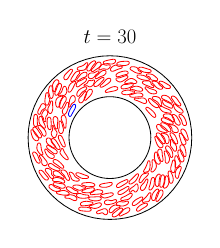
\begin{tikzpicture}[scale=0.3]

\begin{axis}[
  xmin = -21,
  xmax = 21,
  ymin = -21,
  ymax = 21,
  scale only axis,
  axis equal image,
  hide axis,
  title = {\Huge$t=30$}
  ]

% outer solid wall
\addplot [mark=none,black,line width=1.0] table{
2.0000e+01 -5.5171e-16
1.9904e+01 1.9603e+00
1.9616e+01 3.9018e+00
1.9139e+01 5.8057e+00
1.8478e+01 7.6537e+00
1.7638e+01 9.4279e+00
1.6629e+01 1.1111e+01
1.5460e+01 1.2688e+01
1.4142e+01 1.4142e+01
1.2688e+01 1.5460e+01
1.1111e+01 1.6629e+01
9.4279e+00 1.7638e+01
7.6537e+00 1.8478e+01
5.8057e+00 1.9139e+01
3.9018e+00 1.9616e+01
1.9603e+00 1.9904e+01
2.3281e-15 2.0000e+01
-1.9603e+00 1.9904e+01
-3.9018e+00 1.9616e+01
-5.8057e+00 1.9139e+01
-7.6537e+00 1.8478e+01
-9.4279e+00 1.7638e+01
-1.1111e+01 1.6629e+01
-1.2688e+01 1.5460e+01
-1.4142e+01 1.4142e+01
-1.5460e+01 1.2688e+01
-1.6629e+01 1.1111e+01
-1.7638e+01 9.4279e+00
-1.8478e+01 7.6537e+00
-1.9139e+01 5.8057e+00
-1.9616e+01 3.9018e+00
-1.9904e+01 1.9603e+00
-2.0000e+01 3.0010e-15
-1.9904e+01 -1.9603e+00
-1.9616e+01 -3.9018e+00
-1.9139e+01 -5.8057e+00
-1.8478e+01 -7.6537e+00
-1.7638e+01 -9.4279e+00
-1.6629e+01 -1.1111e+01
-1.5460e+01 -1.2688e+01
-1.4142e+01 -1.4142e+01
-1.2688e+01 -1.5460e+01
-1.1111e+01 -1.6629e+01
-9.4279e+00 -1.7638e+01
-7.6537e+00 -1.8478e+01
-5.8057e+00 -1.9139e+01
-3.9018e+00 -1.9616e+01
-1.9603e+00 -1.9904e+01
-4.7774e-15 -2.0000e+01
1.9603e+00 -1.9904e+01
3.9018e+00 -1.9616e+01
5.8057e+00 -1.9139e+01
7.6537e+00 -1.8478e+01
9.4279e+00 -1.7638e+01
1.1111e+01 -1.6629e+01
1.2688e+01 -1.5460e+01
1.4142e+01 -1.4142e+01
1.5460e+01 -1.2688e+01
1.6629e+01 -1.1111e+01
1.7638e+01 -9.4279e+00
1.8478e+01 -7.6537e+00
1.9139e+01 -5.8057e+00
1.9616e+01 -3.9018e+00
1.9904e+01 -1.9603e+00
2.0000e+01 -5.5171e-16
};

% inner solid wall
\addplot [mark=none,black,line width=1.0] table{
1.0000e+01 2.7586e-16
9.9518e+00 -9.8017e-01
9.8079e+00 -1.9509e+00
9.5694e+00 -2.9028e+00
9.2388e+00 -3.8268e+00
8.8192e+00 -4.7140e+00
8.3147e+00 -5.5557e+00
7.7301e+00 -6.3439e+00
7.0711e+00 -7.0711e+00
6.3439e+00 -7.7301e+00
5.5557e+00 -8.3147e+00
4.7140e+00 -8.8192e+00
3.8268e+00 -9.2388e+00
2.9028e+00 -9.5694e+00
1.9509e+00 -9.8079e+00
9.8017e-01 -9.9518e+00
1.1640e-15 -1.0000e+01
-9.8017e-01 -9.9518e+00
-1.9509e+00 -9.8079e+00
-2.9028e+00 -9.5694e+00
-3.8268e+00 -9.2388e+00
-4.7140e+00 -8.8192e+00
-5.5557e+00 -8.3147e+00
-6.3439e+00 -7.7301e+00
-7.0711e+00 -7.0711e+00
-7.7301e+00 -6.3439e+00
-8.3147e+00 -5.5557e+00
-8.8192e+00 -4.7140e+00
-9.2388e+00 -3.8268e+00
-9.5694e+00 -2.9028e+00
-9.8079e+00 -1.9509e+00
-9.9518e+00 -9.8017e-01
-1.0000e+01 -1.5005e-15
-9.9518e+00 9.8017e-01
-9.8079e+00 1.9509e+00
-9.5694e+00 2.9028e+00
-9.2388e+00 3.8268e+00
-8.8192e+00 4.7140e+00
-8.3147e+00 5.5557e+00
-7.7301e+00 6.3439e+00
-7.0711e+00 7.0711e+00
-6.3439e+00 7.7301e+00
-5.5557e+00 8.3147e+00
-4.7140e+00 8.8192e+00
-3.8268e+00 9.2388e+00
-2.9028e+00 9.5694e+00
-1.9509e+00 9.8079e+00
-9.8017e-01 9.9518e+00
-2.3887e-15 1.0000e+01
9.8017e-01 9.9518e+00
1.9509e+00 9.8079e+00
2.9028e+00 9.5694e+00
3.8268e+00 9.2388e+00
4.7140e+00 8.8192e+00
5.5557e+00 8.3147e+00
6.3439e+00 7.7301e+00
7.0711e+00 7.0711e+00
7.7301e+00 6.3439e+00
8.3147e+00 5.5557e+00
8.8192e+00 4.7140e+00
9.2388e+00 3.8268e+00
9.5694e+00 2.9028e+00
9.8079e+00 1.9509e+00
9.9518e+00 9.8017e-01
1.0000e+01 2.7586e-16
};

% vesicle 1
\addplot [mark=none,red,line width=1.0] table{
1.5924e+01 8.4540e+00
1.5982e+01 8.3969e+00
1.6050e+01 8.3333e+00
1.6128e+01 8.2613e+00
1.6222e+01 8.1777e+00
1.6329e+01 8.0852e+00
1.6450e+01 7.9872e+00
1.6592e+01 7.8847e+00
1.6758e+01 7.7898e+00
1.6943e+01 7.7293e+00
1.7143e+01 7.7403e+00
1.7302e+01 7.8696e+00
1.7330e+01 8.0678e+00
1.7251e+01 8.2553e+00
1.7137e+01 8.4153e+00
1.7023e+01 8.5628e+00
1.6921e+01 8.7015e+00
1.6832e+01 8.8295e+00
1.6752e+01 8.9501e+00
1.6681e+01 9.0565e+00
1.6620e+01 9.1483e+00
1.6564e+01 9.2296e+00
1.6514e+01 9.2998e+00
1.6468e+01 9.3632e+00
1.6421e+01 9.4252e+00
1.6370e+01 9.4898e+00
1.6309e+01 9.5645e+00
1.6232e+01 9.6509e+00
1.6141e+01 9.7451e+00
1.6033e+01 9.8456e+00
1.5905e+01 9.9468e+00
1.5769e+01 1.0035e+01
1.5606e+01 1.0111e+01
1.5419e+01 1.0153e+01
1.5233e+01 1.0133e+01
1.5069e+01 1.0019e+01
1.5007e+01 9.8256e+00
1.5060e+01 9.6327e+00
1.5165e+01 9.4729e+00
1.5278e+01 9.3333e+00
1.5385e+01 9.1971e+00
1.5480e+01 9.0624e+00
1.5561e+01 8.9354e+00
1.5635e+01 8.8174e+00
1.5703e+01 8.7154e+00
1.5765e+01 8.6325e+00
1.5822e+01 8.5639e+00
1.5873e+01 8.5067e+00
1.5924e+01 8.4540e+00
};

% vesicle 2
\addplot [mark=none,red,line width=1.0] table{
-3.8766e+00 -1.1291e+01
-3.9477e+00 -1.1247e+01
-4.0349e+00 -1.1203e+01
-4.1409e+00 -1.1159e+01
-4.2624e+00 -1.1117e+01
-4.3983e+00 -1.1078e+01
-4.5461e+00 -1.1045e+01
-4.7077e+00 -1.1018e+01
-4.8915e+00 -1.0997e+01
-5.0870e+00 -1.0988e+01
-5.2891e+00 -1.0987e+01
-5.5007e+00 -1.0995e+01
-5.7078e+00 -1.1007e+01
-5.9138e+00 -1.1022e+01
-6.1178e+00 -1.1040e+01
-6.3068e+00 -1.1060e+01
-6.4811e+00 -1.1089e+01
-6.6382e+00 -1.1131e+01
-6.7716e+00 -1.1198e+01
-6.8678e+00 -1.1299e+01
-6.8971e+00 -1.1415e+01
-6.8678e+00 -1.1511e+01
-6.8072e+00 -1.1579e+01
-6.7379e+00 -1.1621e+01
-6.6663e+00 -1.1649e+01
-6.5861e+00 -1.1671e+01
-6.4948e+00 -1.1692e+01
-6.3882e+00 -1.1716e+01
-6.2629e+00 -1.1750e+01
-6.1261e+00 -1.1800e+01
-5.9808e+00 -1.1866e+01
-5.8205e+00 -1.1939e+01
-5.6435e+00 -1.1994e+01
-5.4509e+00 -1.2019e+01
-5.2448e+00 -1.2021e+01
-5.0353e+00 -1.2007e+01
-4.8275e+00 -1.1989e+01
-4.6196e+00 -1.1972e+01
-4.4205e+00 -1.1959e+01
-4.2346e+00 -1.1948e+01
-4.0634e+00 -1.1926e+01
-3.9061e+00 -1.1879e+01
-3.7795e+00 -1.1797e+01
-3.7040e+00 -1.1686e+01
-3.6861e+00 -1.1569e+01
-3.7126e+00 -1.1469e+01
-3.7596e+00 -1.1395e+01
-3.8146e+00 -1.1338e+01
-3.8766e+00 -1.1291e+01
};

% vesicle 3
\addplot [mark=none,red,line width=1.0] table{
-1.3518e+01 -2.5650e+00
-1.3443e+01 -2.5405e+00
-1.3373e+01 -2.4774e+00
-1.3343e+01 -2.3691e+00
-1.3378e+01 -2.2484e+00
-1.3459e+01 -2.1319e+00
-1.3555e+01 -2.0142e+00
-1.3655e+01 -1.8885e+00
-1.3767e+01 -1.7474e+00
-1.3893e+01 -1.5942e+00
-1.4026e+01 -1.4336e+00
-1.4155e+01 -1.2664e+00
-1.4267e+01 -1.0915e+00
-1.4350e+01 -8.9940e-01
-1.4394e+01 -6.9958e-01
-1.4430e+01 -5.1072e-01
-1.4508e+01 -3.4822e-01
-1.4620e+01 -2.3136e-01
-1.4745e+01 -1.5400e-01
-1.4874e+01 -1.0744e-01
-1.4991e+01 -8.9318e-02
-1.5090e+01 -9.1870e-02
-1.5177e+01 -1.0915e-01
-1.5250e+01 -1.3629e-01
-1.5313e+01 -1.7204e-01
-1.5379e+01 -2.2479e-01
-1.5440e+01 -2.9600e-01
-1.5492e+01 -3.8758e-01
-1.5532e+01 -5.0417e-01
-1.5552e+01 -6.3913e-01
-1.5550e+01 -7.9465e-01
-1.5520e+01 -9.7472e-01
-1.5463e+01 -1.1554e+00
-1.5382e+01 -1.3297e+00
-1.5271e+01 -1.4991e+00
-1.5128e+01 -1.6496e+00
-1.4957e+01 -1.7690e+00
-1.4785e+01 -1.8659e+00
-1.4617e+01 -1.9641e+00
-1.4457e+01 -2.0681e+00
-1.4312e+01 -2.1687e+00
-1.4178e+01 -2.2641e+00
-1.4055e+01 -2.3482e+00
-1.3948e+01 -2.4172e+00
-1.3847e+01 -2.4759e+00
-1.3752e+01 -2.5223e+00
-1.3671e+01 -2.5514e+00
-1.3595e+01 -2.5664e+00
-1.3518e+01 -2.5650e+00
};

% vesicle 4
\addplot [mark=none,red,line width=1.0] table{
-2.1995e+00 1.2320e+01
-2.1183e+00 1.2313e+01
-2.0261e+00 1.2321e+01
-1.9223e+00 1.2347e+01
-1.8067e+00 1.2388e+01
-1.6787e+00 1.2445e+01
-1.5404e+00 1.2514e+01
-1.3944e+00 1.2594e+01
-1.2359e+00 1.2687e+01
-1.0633e+00 1.2793e+01
-8.9199e-01 1.2904e+01
-7.2905e-01 1.3013e+01
-5.6639e-01 1.3128e+01
-3.9882e-01 1.3254e+01
-2.3844e-01 1.3386e+01
-9.5961e-02 1.3521e+01
2.6032e-02 1.3659e+01
1.2018e-01 1.3798e+01
1.8134e-01 1.3933e+01
2.0818e-01 1.4062e+01
2.0154e-01 1.4179e+01
1.6867e-01 1.4275e+01
1.2057e-01 1.4347e+01
6.4739e-02 1.4400e+01
2.0424e-03 1.4440e+01
-7.1673e-02 1.4470e+01
-1.6042e-01 1.4489e+01
-2.6638e-01 1.4493e+01
-3.9074e-01 1.4476e+01
-5.2838e-01 1.4433e+01
-6.7314e-01 1.4364e+01
-8.2210e-01 1.4265e+01
-9.6488e-01 1.4142e+01
-1.0968e+00 1.4003e+01
-1.2265e+00 1.3851e+01
-1.3603e+00 1.3690e+01
-1.4951e+00 1.3533e+01
-1.6331e+00 1.3383e+01
-1.7755e+00 1.3242e+01
-1.9185e+00 1.3115e+01
-2.0602e+00 1.3000e+01
-2.1911e+00 1.2895e+01
-2.3017e+00 1.2790e+01
-2.3779e+00 1.2677e+01
-2.4059e+00 1.2562e+01
-2.3864e+00 1.2462e+01
-2.3360e+00 1.2389e+01
-2.2716e+00 1.2345e+01
-2.1995e+00 1.2320e+01
};

% vesicle 5
\addplot [mark=none,red,line width=1.0] table{
9.1736e+00 1.5915e+01
9.2499e+00 1.5913e+01
9.3386e+00 1.5912e+01
9.4427e+00 1.5911e+01
9.5617e+00 1.5914e+01
9.6984e+00 1.5927e+01
9.8508e+00 1.5967e+01
9.9956e+00 1.6062e+01
1.0074e+01 1.6232e+01
1.0023e+01 1.6421e+01
9.8699e+00 1.6556e+01
9.6820e+00 1.6638e+01
9.4840e+00 1.6700e+01
9.2830e+00 1.6758e+01
9.0904e+00 1.6816e+01
8.9081e+00 1.6873e+01
8.7375e+00 1.6929e+01
8.5821e+00 1.6979e+01
8.4397e+00 1.7025e+01
8.3100e+00 1.7065e+01
8.1970e+00 1.7098e+01
8.1020e+00 1.7124e+01
8.0210e+00 1.7144e+01
7.9499e+00 1.7161e+01
7.8810e+00 1.7175e+01
7.8038e+00 1.7188e+01
7.7125e+00 1.7201e+01
7.6034e+00 1.7209e+01
7.4757e+00 1.7208e+01
7.3339e+00 1.7187e+01
7.1873e+00 1.7131e+01
7.0601e+00 1.7017e+01
7.0120e+00 1.6844e+01
7.0836e+00 1.6674e+01
7.2312e+00 1.6551e+01
7.4098e+00 1.6455e+01
7.5875e+00 1.6361e+01
7.7611e+00 1.6258e+01
7.9337e+00 1.6160e+01
8.1047e+00 1.6082e+01
8.2803e+00 1.6022e+01
8.4489e+00 1.5980e+01
8.5989e+00 1.5954e+01
8.7317e+00 1.5938e+01
8.8474e+00 1.5928e+01
8.9461e+00 1.5923e+01
9.0293e+00 1.5919e+01
9.1026e+00 1.5917e+01
9.1736e+00 1.5915e+01
};

% vesicle 6
\addplot [mark=none,red,line width=1.0] table{
1.1592e+01 -1.7619e+00
1.1633e+01 -1.8341e+00
1.1683e+01 -1.9165e+00
1.1746e+01 -2.0107e+00
1.1825e+01 -2.1154e+00
1.1924e+01 -2.2254e+00
1.2045e+01 -2.3330e+00
1.2196e+01 -2.4267e+00
1.2381e+01 -2.4848e+00
1.2592e+01 -2.4756e+00
1.2793e+01 -2.3787e+00
1.2931e+01 -2.2088e+00
1.2981e+01 -2.0066e+00
1.2945e+01 -1.8047e+00
1.2846e+01 -1.6308e+00
1.2723e+01 -1.4883e+00
1.2594e+01 -1.3594e+00
1.2477e+01 -1.2415e+00
1.2376e+01 -1.1349e+00
1.2286e+01 -1.0361e+00
1.2210e+01 -9.4713e-01
1.2146e+01 -8.6990e-01
1.2092e+01 -8.0305e-01
1.2045e+01 -7.4326e-01
1.2000e+01 -6.8472e-01
1.1952e+01 -6.2073e-01
1.1896e+01 -5.4540e-01
1.1832e+01 -4.5542e-01
1.1758e+01 -3.5007e-01
1.1677e+01 -2.3007e-01
1.1591e+01 -9.6307e-02
1.1495e+01 5.0794e-02
1.1381e+01 1.9797e-01
1.1223e+01 2.9678e-01
1.1042e+01 2.4360e-01
1.0978e+01 5.4806e-02
1.1004e+01 -1.5113e-01
1.1056e+01 -3.5557e-01
1.1115e+01 -5.5134e-01
1.1176e+01 -7.4264e-01
1.1235e+01 -9.1804e-01
1.1292e+01 -1.0777e+00
1.1346e+01 -1.2200e+00
1.1395e+01 -1.3440e+00
1.1441e+01 -1.4522e+00
1.1483e+01 -1.5453e+00
1.1521e+01 -1.6250e+00
1.1556e+01 -1.6949e+00
1.1592e+01 -1.7619e+00
};

% vesicle 7
\addplot [mark=none,red,line width=1.0] table{
4.3597e+00 -1.3970e+01
4.2912e+00 -1.4011e+01
4.2123e+00 -1.4057e+01
4.1200e+00 -1.4111e+01
4.0125e+00 -1.4172e+01
3.8932e+00 -1.4238e+01
3.7580e+00 -1.4308e+01
3.6013e+00 -1.4384e+01
3.4347e+00 -1.4460e+01
3.2582e+00 -1.4537e+01
3.0651e+00 -1.4625e+01
2.8828e+00 -1.4726e+01
2.7329e+00 -1.4854e+01
2.6422e+00 -1.5029e+01
2.6681e+00 -1.5223e+01
2.8151e+00 -1.5351e+01
2.9961e+00 -1.5383e+01
3.1654e+00 -1.5366e+01
3.3156e+00 -1.5334e+01
3.4450e+00 -1.5303e+01
3.5574e+00 -1.5276e+01
3.6553e+00 -1.5255e+01
3.7380e+00 -1.5239e+01
3.8117e+00 -1.5226e+01
3.8842e+00 -1.5214e+01
3.9620e+00 -1.5203e+01
4.0541e+00 -1.5189e+01
4.1632e+00 -1.5172e+01
4.2855e+00 -1.5146e+01
4.4197e+00 -1.5106e+01
4.5638e+00 -1.5045e+01
4.7137e+00 -1.4956e+01
4.8598e+00 -1.4844e+01
4.9967e+00 -1.4714e+01
5.1300e+00 -1.4564e+01
5.2619e+00 -1.4386e+01
5.3710e+00 -1.4199e+01
5.4394e+00 -1.4011e+01
5.4380e+00 -1.3815e+01
5.3303e+00 -1.3663e+01
5.1618e+00 -1.3612e+01
4.9997e+00 -1.3635e+01
4.8595e+00 -1.3688e+01
4.7393e+00 -1.3748e+01
4.6396e+00 -1.3803e+01
4.5570e+00 -1.3851e+01
4.4850e+00 -1.3894e+01
4.4212e+00 -1.3933e+01
4.3597e+00 -1.3970e+01
};

% vesicle 8
\addplot [mark=none,red,line width=1.0] table{
1.4928e+01 -4.8307e+00
1.4998e+01 -4.8651e+00
1.5088e+01 -4.8724e+00
1.5186e+01 -4.8328e+00
1.5264e+01 -4.7445e+00
1.5315e+01 -4.6199e+00
1.5342e+01 -4.4671e+00
1.5355e+01 -4.2909e+00
1.5355e+01 -4.0969e+00
1.5339e+01 -3.8937e+00
1.5304e+01 -3.6913e+00
1.5248e+01 -3.4925e+00
1.5173e+01 -3.2936e+00
1.5085e+01 -3.1010e+00
1.4990e+01 -2.9211e+00
1.4894e+01 -2.7606e+00
1.4796e+01 -2.6130e+00
1.4698e+01 -2.4829e+00
1.4605e+01 -2.3730e+00
1.4512e+01 -2.2781e+00
1.4424e+01 -2.2006e+00
1.4343e+01 -2.1408e+00
1.4267e+01 -2.0954e+00
1.4197e+01 -2.0627e+00
1.4127e+01 -2.0394e+00
1.4046e+01 -2.0250e+00
1.3953e+01 -2.0264e+00
1.3850e+01 -2.0543e+00
1.3747e+01 -2.1205e+00
1.3662e+01 -2.2282e+00
1.3610e+01 -2.3700e+00
1.3599e+01 -2.5370e+00
1.3634e+01 -2.7203e+00
1.3712e+01 -2.9037e+00
1.3825e+01 -3.0747e+00
1.3965e+01 -3.2380e+00
1.4111e+01 -3.3966e+00
1.4248e+01 -3.5535e+00
1.4364e+01 -3.7015e+00
1.4467e+01 -3.8517e+00
1.4556e+01 -4.0062e+00
1.4629e+01 -4.1608e+00
1.4683e+01 -4.3046e+00
1.4723e+01 -4.4336e+00
1.4758e+01 -4.5470e+00
1.4793e+01 -4.6430e+00
1.4830e+01 -4.7193e+00
1.4874e+01 -4.7808e+00
1.4928e+01 -4.8307e+00
};

% vesicle 9
\addplot [mark=none,red,line width=1.0] table{
-6.5859e+00 -1.2601e+01
-6.5114e+00 -1.2572e+01
-6.4233e+00 -1.2544e+01
-6.3185e+00 -1.2515e+01
-6.1978e+00 -1.2484e+01
-6.0670e+00 -1.2434e+01
-5.9582e+00 -1.2330e+01
-5.9631e+00 -1.2174e+01
-6.1109e+00 -1.2080e+01
-6.3097e+00 -1.2068e+01
-6.5237e+00 -1.2061e+01
-6.7301e+00 -1.2018e+01
-6.9160e+00 -1.1933e+01
-7.0845e+00 -1.1828e+01
-7.2539e+00 -1.1733e+01
-7.4316e+00 -1.1668e+01
-7.6120e+00 -1.1630e+01
-7.7824e+00 -1.1611e+01
-7.9347e+00 -1.1602e+01
-8.0685e+00 -1.1599e+01
-8.1857e+00 -1.1598e+01
-8.2861e+00 -1.1600e+01
-8.3717e+00 -1.1604e+01
-8.4470e+00 -1.1609e+01
-8.5198e+00 -1.1616e+01
-8.5992e+00 -1.1627e+01
-8.6908e+00 -1.1645e+01
-8.7959e+00 -1.1678e+01
-8.9092e+00 -1.1738e+01
-9.0109e+00 -1.1842e+01
-9.0567e+00 -1.1996e+01
-9.0064e+00 -1.2162e+01
-8.8734e+00 -1.2293e+01
-8.7054e+00 -1.2385e+01
-8.5258e+00 -1.2463e+01
-8.3376e+00 -1.2542e+01
-8.1529e+00 -1.2624e+01
-7.9792e+00 -1.2706e+01
-7.8017e+00 -1.2789e+01
-7.6183e+00 -1.2853e+01
-7.4449e+00 -1.2883e+01
-7.2813e+00 -1.2881e+01
-7.1329e+00 -1.2854e+01
-7.0020e+00 -1.2808e+01
-6.8913e+00 -1.2755e+01
-6.7994e+00 -1.2706e+01
-6.7220e+00 -1.2665e+01
-6.6534e+00 -1.2631e+01
-6.5859e+00 -1.2601e+01
};

% vesicle 10
\addplot [mark=none,red,line width=1.0] table{
-8.6083e+00 1.4020e+01
-8.5444e+00 1.4067e+01
-8.4785e+00 1.4131e+01
-8.4123e+00 1.4214e+01
-8.3476e+00 1.4322e+01
-8.2839e+00 1.4452e+01
-8.2168e+00 1.4597e+01
-8.1403e+00 1.4751e+01
-8.0498e+00 1.4912e+01
-7.9432e+00 1.5074e+01
-7.8210e+00 1.5230e+01
-7.6847e+00 1.5381e+01
-7.5429e+00 1.5534e+01
-7.4250e+00 1.5704e+01
-7.3761e+00 1.5894e+01
-7.4276e+00 1.6070e+01
-7.5612e+00 1.6184e+01
-7.7232e+00 1.6223e+01
-7.8760e+00 1.6211e+01
-8.0066e+00 1.6173e+01
-8.1137e+00 1.6126e+01
-8.1997e+00 1.6078e+01
-8.2683e+00 1.6032e+01
-8.3263e+00 1.5989e+01
-8.3807e+00 1.5944e+01
-8.4379e+00 1.5892e+01
-8.5026e+00 1.5827e+01
-8.5754e+00 1.5746e+01
-8.6544e+00 1.5650e+01
-8.7394e+00 1.5537e+01
-8.8303e+00 1.5408e+01
-8.9239e+00 1.5267e+01
-9.0194e+00 1.5118e+01
-9.1194e+00 1.4958e+01
-9.2225e+00 1.4791e+01
-9.3283e+00 1.4617e+01
-9.4324e+00 1.4437e+01
-9.5223e+00 1.4255e+01
-9.5759e+00 1.4062e+01
-9.5502e+00 1.3869e+01
-9.4254e+00 1.3741e+01
-9.2637e+00 1.3718e+01
-9.1208e+00 1.3760e+01
-9.0025e+00 1.3816e+01
-8.9023e+00 1.3866e+01
-8.8151e+00 1.3908e+01
-8.7384e+00 1.3946e+01
-8.6710e+00 1.3981e+01
-8.6083e+00 1.4020e+01
};

% vesicle 11
\addplot [mark=none,red,line width=1.0] table{
-1.6760e+01 1.2734e-01
-1.6732e+01 1.9872e-01
-1.6716e+01 2.8606e-01
-1.6719e+01 3.8973e-01
-1.6747e+01 5.0817e-01
-1.6801e+01 6.3845e-01
-1.6880e+01 7.7783e-01
-1.6977e+01 9.2730e-01
-1.7084e+01 1.0847e+00
-1.7194e+01 1.2440e+00
-1.7307e+01 1.4081e+00
-1.7424e+01 1.5798e+00
-1.7544e+01 1.7555e+00
-1.7662e+01 1.9284e+00
-1.7778e+01 2.0927e+00
-1.7897e+01 2.2442e+00
-1.8021e+01 2.3746e+00
-1.8153e+01 2.4755e+00
-1.8288e+01 2.5381e+00
-1.8416e+01 2.5592e+00
-1.8528e+01 2.5464e+00
-1.8618e+01 2.5116e+00
-1.8688e+01 2.4647e+00
-1.8740e+01 2.4117e+00
-1.8781e+01 2.3516e+00
-1.8812e+01 2.2786e+00
-1.8831e+01 2.1879e+00
-1.8827e+01 2.0795e+00
-1.8794e+01 1.9600e+00
-1.8731e+01 1.8361e+00
-1.8646e+01 1.7064e+00
-1.8547e+01 1.5679e+00
-1.8438e+01 1.4214e+00
-1.8318e+01 1.2690e+00
-1.8193e+01 1.1153e+00
-1.8065e+01 9.5806e-01
-1.7938e+01 7.9326e-01
-1.7818e+01 6.2453e-01
-1.7708e+01 4.5858e-01
-1.7606e+01 2.9560e-01
-1.7503e+01 1.4394e-01
-1.7388e+01 1.9987e-02
-1.7255e+01 -5.8649e-02
-1.7122e+01 -8.5881e-02
-1.7005e+01 -7.2214e-02
-1.6914e+01 -3.4394e-02
-1.6846e+01 1.4162e-02
-1.6797e+01 6.7633e-02
-1.6760e+01 1.2734e-01
};

% vesicle 12
\addplot [mark=none,red,line width=1.0] table{
-1.5028e+01 -6.6729e+00
-1.5033e+01 -6.7495e+00
-1.5020e+01 -6.8400e+00
-1.4982e+01 -6.9430e+00
-1.4917e+01 -7.0502e+00
-1.4825e+01 -7.1588e+00
-1.4708e+01 -7.2651e+00
-1.4571e+01 -7.3685e+00
-1.4416e+01 -7.4710e+00
-1.4245e+01 -7.5718e+00
-1.4067e+01 -7.6674e+00
-1.3879e+01 -7.7570e+00
-1.3694e+01 -7.8354e+00
-1.3510e+01 -7.9048e+00
-1.3318e+01 -7.9722e+00
-1.3130e+01 -8.0342e+00
-1.2962e+01 -8.0827e+00
-1.2803e+01 -8.1186e+00
-1.2652e+01 -8.1403e+00
-1.2518e+01 -8.1435e+00
-1.2402e+01 -8.1250e+00
-1.2311e+01 -8.0861e+00
-1.2245e+01 -8.0307e+00
-1.2205e+01 -7.9670e+00
-1.2188e+01 -7.8976e+00
-1.2194e+01 -7.8165e+00
-1.2228e+01 -7.7291e+00
-1.2294e+01 -7.6408e+00
-1.2392e+01 -7.5527e+00
-1.2513e+01 -7.4678e+00
-1.2653e+01 -7.3837e+00
-1.2807e+01 -7.2995e+00
-1.2965e+01 -7.2178e+00
-1.3129e+01 -7.1331e+00
-1.3304e+01 -7.0363e+00
-1.3481e+01 -6.9258e+00
-1.3651e+01 -6.8055e+00
-1.3813e+01 -6.6808e+00
-1.3967e+01 -6.5640e+00
-1.4128e+01 -6.4601e+00
-1.4299e+01 -6.3831e+00
-1.4460e+01 -6.3452e+00
-1.4607e+01 -6.3413e+00
-1.4735e+01 -6.3652e+00
-1.4842e+01 -6.4115e+00
-1.4922e+01 -6.4724e+00
-1.4975e+01 -6.5367e+00
-1.5009e+01 -6.6026e+00
-1.5028e+01 -6.6729e+00
};

% vesicle 13
\addplot [mark=none,red,line width=1.0] table{
-1.3079e+01 -2.5647e+00
-1.3025e+01 -2.6255e+00
-1.2958e+01 -2.6922e+00
-1.2875e+01 -2.7648e+00
-1.2770e+01 -2.8388e+00
-1.2638e+01 -2.9012e+00
-1.2481e+01 -2.9250e+00
-1.2317e+01 -2.8723e+00
-1.2204e+01 -2.7255e+00
-1.2186e+01 -2.5302e+00
-1.2240e+01 -2.3367e+00
-1.2330e+01 -2.1502e+00
-1.2435e+01 -1.9669e+00
-1.2542e+01 -1.7916e+00
-1.2647e+01 -1.6212e+00
-1.2746e+01 -1.4615e+00
-1.2838e+01 -1.3123e+00
-1.2927e+01 -1.1698e+00
-1.3012e+01 -1.0380e+00
-1.3090e+01 -9.2186e-01
-1.3159e+01 -8.2326e-01
-1.3221e+01 -7.4116e-01
-1.3276e+01 -6.7271e-01
-1.3327e+01 -6.1396e-01
-1.3378e+01 -5.5913e-01
-1.3436e+01 -5.0236e-01
-1.3507e+01 -4.4096e-01
-1.3595e+01 -3.7596e-01
-1.3705e+01 -3.1256e-01
-1.3840e+01 -2.6148e-01
-1.4000e+01 -2.4329e-01
-1.4165e+01 -2.9125e-01
-1.4281e+01 -4.2732e-01
-1.4289e+01 -6.2116e-01
-1.4218e+01 -8.1897e-01
-1.4130e+01 -1.0058e+00
-1.4035e+01 -1.1795e+00
-1.3928e+01 -1.3459e+00
-1.3809e+01 -1.5079e+00
-1.3687e+01 -1.6585e+00
-1.3570e+01 -1.7968e+00
-1.3463e+01 -1.9285e+00
-1.3376e+01 -2.0571e+00
-1.3311e+01 -2.1773e+00
-1.3260e+01 -2.2818e+00
-1.3214e+01 -2.3695e+00
-1.3170e+01 -2.4428e+00
-1.3125e+01 -2.5058e+00
-1.3079e+01 -2.5647e+00
};

% vesicle 14
\addplot [mark=none,red,line width=1.0] table{
9.8185e+00 -6.7958e+00
9.8192e+00 -6.7178e+00
9.8187e+00 -6.6263e+00
9.8166e+00 -6.5173e+00
9.8123e+00 -6.3980e+00
9.8047e+00 -6.2582e+00
9.7908e+00 -6.0947e+00
9.7628e+00 -5.9209e+00
9.6889e+00 -5.7404e+00
9.5125e+00 -5.6411e+00
9.3408e+00 -5.7399e+00
9.2478e+00 -5.9260e+00
9.1797e+00 -6.1327e+00
9.1145e+00 -6.3339e+00
9.0470e+00 -6.5288e+00
8.9783e+00 -6.7130e+00
8.9119e+00 -6.8788e+00
8.8452e+00 -7.0334e+00
8.7793e+00 -7.1761e+00
8.7195e+00 -7.2972e+00
8.6653e+00 -7.4010e+00
8.6183e+00 -7.4869e+00
8.5753e+00 -7.5626e+00
8.5368e+00 -7.6282e+00
8.5007e+00 -7.6885e+00
8.4580e+00 -7.7586e+00
8.4105e+00 -7.8366e+00
8.3572e+00 -7.9266e+00
8.2963e+00 -8.0409e+00
8.2449e+00 -8.1739e+00
8.2303e+00 -8.3269e+00
8.3074e+00 -8.4793e+00
8.4791e+00 -8.5289e+00
8.6638e+00 -8.4771e+00
8.8578e+00 -8.4087e+00
9.0606e+00 -8.3649e+00
9.2555e+00 -8.3138e+00
9.4280e+00 -8.2119e+00
9.5616e+00 -8.0577e+00
9.6490e+00 -7.8853e+00
9.7073e+00 -7.7077e+00
9.7457e+00 -7.5429e+00
9.7715e+00 -7.3950e+00
9.7896e+00 -7.2591e+00
9.8016e+00 -7.1403e+00
9.8092e+00 -7.0370e+00
9.8139e+00 -6.9506e+00
9.8168e+00 -6.8736e+00
9.8185e+00 -6.7958e+00
};

% vesicle 15
\addplot [mark=none,red,line width=1.0] table{
8.0694e+00 -1.1312e+01
8.0125e+00 -1.1369e+01
7.9462e+00 -1.1436e+01
7.8701e+00 -1.1514e+01
7.7864e+00 -1.1606e+01
7.6974e+00 -1.1718e+01
7.6098e+00 -1.1852e+01
7.5331e+00 -1.2005e+01
7.4741e+00 -1.2179e+01
7.4464e+00 -1.2376e+01
7.4707e+00 -1.2573e+01
7.5674e+00 -1.2760e+01
7.7442e+00 -1.2887e+01
7.9495e+00 -1.2912e+01
8.1373e+00 -1.2855e+01
8.2946e+00 -1.2753e+01
8.4248e+00 -1.2631e+01
8.5249e+00 -1.2510e+01
8.6034e+00 -1.2395e+01
8.6680e+00 -1.2285e+01
8.7198e+00 -1.2186e+01
8.7609e+00 -1.2099e+01
8.7948e+00 -1.2022e+01
8.8237e+00 -1.1952e+01
8.8509e+00 -1.1885e+01
8.8797e+00 -1.1810e+01
8.9119e+00 -1.1725e+01
8.9486e+00 -1.1626e+01
8.9913e+00 -1.1509e+01
9.0403e+00 -1.1373e+01
9.0938e+00 -1.1222e+01
9.1504e+00 -1.1057e+01
9.2077e+00 -1.0878e+01
9.2590e+00 -1.0690e+01
9.2916e+00 -1.0488e+01
9.2668e+00 -1.0275e+01
9.1233e+00 -1.0126e+01
8.9304e+00 -1.0150e+01
8.7933e+00 -1.0285e+01
8.6950e+00 -1.0445e+01
8.6085e+00 -1.0601e+01
8.5243e+00 -1.0743e+01
8.4435e+00 -1.0868e+01
8.3673e+00 -1.0974e+01
8.2959e+00 -1.1064e+01
8.2309e+00 -1.1141e+01
8.1736e+00 -1.1204e+01
8.1214e+00 -1.1259e+01
8.0694e+00 -1.1312e+01
};

% vesicle 16
\addplot [mark=none,red,line width=1.0] table{
7.8801e+00 -1.0704e+01
7.9253e+00 -1.0645e+01
7.9795e+00 -1.0571e+01
8.0454e+00 -1.0478e+01
8.1166e+00 -1.0377e+01
8.2014e+00 -1.0260e+01
8.3029e+00 -1.0127e+01
8.4132e+00 -9.9976e+00
8.5396e+00 -9.8676e+00
8.6825e+00 -9.7378e+00
8.8360e+00 -9.6048e+00
8.9914e+00 -9.4615e+00
9.1385e+00 -9.3074e+00
9.2706e+00 -9.1439e+00
9.3685e+00 -8.9777e+00
9.4074e+00 -8.7968e+00
9.3322e+00 -8.6313e+00
9.1777e+00 -8.5814e+00
9.0350e+00 -8.6193e+00
8.9099e+00 -8.6796e+00
8.8040e+00 -8.7260e+00
8.7143e+00 -8.7548e+00
8.6280e+00 -8.7735e+00
8.5544e+00 -8.7844e+00
8.4875e+00 -8.7923e+00
8.4062e+00 -8.8026e+00
8.3180e+00 -8.8184e+00
8.2208e+00 -8.8459e+00
8.1057e+00 -8.8965e+00
7.9877e+00 -8.9715e+00
7.8704e+00 -9.0718e+00
7.7510e+00 -9.2032e+00
7.6426e+00 -9.3522e+00
7.5388e+00 -9.5240e+00
7.4427e+00 -9.7064e+00
7.3530e+00 -9.8938e+00
7.2675e+00 -1.0089e+01
7.1941e+00 -1.0283e+01
7.1386e+00 -1.0477e+01
7.1161e+00 -1.0672e+01
7.1515e+00 -1.0851e+01
7.2621e+00 -1.0982e+01
7.4130e+00 -1.1024e+01
7.5419e+00 -1.0997e+01
7.6456e+00 -1.0940e+01
7.7266e+00 -1.0874e+01
7.7836e+00 -1.0817e+01
7.8325e+00 -1.0762e+01
7.8801e+00 -1.0704e+01
};

% vesicle 17
\addplot [mark=none,red,line width=1.0] table{
9.3246e+00 1.3846e+01
9.2442e+00 1.3848e+01
9.1514e+00 1.3849e+01
9.0434e+00 1.3852e+01
8.9213e+00 1.3855e+01
8.7806e+00 1.3857e+01
8.6235e+00 1.3855e+01
8.4595e+00 1.3841e+01
8.2856e+00 1.3808e+01
8.1131e+00 1.3737e+01
7.9785e+00 1.3607e+01
7.9409e+00 1.3418e+01
8.0287e+00 1.3238e+01
8.1883e+00 1.3107e+01
8.3628e+00 1.3012e+01
8.5338e+00 1.2932e+01
8.6997e+00 1.2862e+01
8.8534e+00 1.2800e+01
8.9917e+00 1.2747e+01
9.1157e+00 1.2700e+01
9.2238e+00 1.2660e+01
9.3157e+00 1.2625e+01
9.3957e+00 1.2594e+01
9.4659e+00 1.2566e+01
9.5335e+00 1.2539e+01
9.6098e+00 1.2507e+01
9.6980e+00 1.2468e+01
9.8007e+00 1.2423e+01
9.9204e+00 1.2369e+01
1.0052e+01 1.2312e+01
1.0195e+01 1.2260e+01
1.0361e+01 1.2224e+01
1.0544e+01 1.2231e+01
1.0710e+01 1.2328e+01
1.0754e+01 1.2523e+01
1.0626e+01 1.2688e+01
1.0438e+01 1.2784e+01
1.0262e+01 1.2882e+01
1.0127e+01 1.3019e+01
1.0049e+01 1.3184e+01
1.0006e+01 1.3354e+01
9.9574e+00 1.3519e+01
9.8781e+00 1.3654e+01
9.7777e+00 1.3744e+01
9.6705e+00 1.3797e+01
9.5684e+00 1.3824e+01
9.4806e+00 1.3837e+01
9.4018e+00 1.3843e+01
9.3246e+00 1.3846e+01
};

% vesicle 18
\addplot [mark=none,red,line width=1.0] table{
9.8741e+00 -1.2804e+01
9.9516e+00 -1.2782e+01
1.0033e+01 -1.2740e+01
1.0117e+01 -1.2677e+01
1.0204e+01 -1.2592e+01
1.0294e+01 -1.2489e+01
1.0389e+01 -1.2366e+01
1.0488e+01 -1.2223e+01
1.0585e+01 -1.2062e+01
1.0670e+01 -1.1885e+01
1.0735e+01 -1.1698e+01
1.0779e+01 -1.1502e+01
1.0807e+01 -1.1296e+01
1.0827e+01 -1.1090e+01
1.0846e+01 -1.0881e+01
1.0867e+01 -1.0683e+01
1.0886e+01 -1.0501e+01
1.0898e+01 -1.0333e+01
1.0896e+01 -1.0181e+01
1.0877e+01 -1.0050e+01
1.0838e+01 -9.9417e+00
1.0784e+01 -9.8579e+00
1.0718e+01 -9.7996e+00
1.0648e+01 -9.7643e+00
1.0572e+01 -9.7493e+00
1.0490e+01 -9.7558e+00
1.0402e+01 -9.7887e+00
1.0314e+01 -9.8515e+00
1.0235e+01 -9.9425e+00
1.0165e+01 -1.0058e+01
1.0106e+01 -1.0199e+01
1.0055e+01 -1.0365e+01
1.0012e+01 -1.0550e+01
9.9751e+00 -1.0743e+01
9.9375e+00 -1.0946e+01
9.8946e+00 -1.1158e+01
9.8435e+00 -1.1372e+01
9.7853e+00 -1.1577e+01
9.7236e+00 -1.1768e+01
9.6614e+00 -1.1946e+01
9.6048e+00 -1.2113e+01
9.5613e+00 -1.2269e+01
9.5392e+00 -1.2415e+01
9.5459e+00 -1.2548e+01
9.5847e+00 -1.2660e+01
9.6485e+00 -1.2741e+01
9.7236e+00 -1.2787e+01
9.7993e+00 -1.2806e+01
9.8741e+00 -1.2804e+01
};

% vesicle 19
\addplot [mark=none,red,line width=1.0] table{
-1.9091e+01 5.8455e-01
-1.9069e+01 5.1481e-01
-1.9041e+01 4.2922e-01
-1.9005e+01 3.2461e-01
-1.8961e+01 2.1135e-01
-1.8904e+01 8.0761e-02
-1.8830e+01 -6.4569e-02
-1.8743e+01 -2.0924e-01
-1.8633e+01 -3.5728e-01
-1.8496e+01 -5.0220e-01
-1.8336e+01 -6.2523e-01
-1.8154e+01 -7.1820e-01
-1.7954e+01 -7.6686e-01
-1.7756e+01 -7.5594e-01
-1.7576e+01 -6.7550e-01
-1.7447e+01 -5.3294e-01
-1.7392e+01 -3.6682e-01
-1.7401e+01 -2.0026e-01
-1.7458e+01 -5.9099e-02
-1.7538e+01 5.1643e-02
-1.7619e+01 1.3718e-01
-1.7689e+01 2.0450e-01
-1.7753e+01 2.6487e-01
-1.7807e+01 3.1636e-01
-1.7856e+01 3.6422e-01
-1.7913e+01 4.2282e-01
-1.7976e+01 4.8942e-01
-1.8044e+01 5.6675e-01
-1.8125e+01 6.6542e-01
-1.8209e+01 7.7933e-01
-1.8297e+01 9.0924e-01
-1.8391e+01 1.0613e+00
-1.8483e+01 1.2218e+00
-1.8575e+01 1.3885e+00
-1.8674e+01 1.5669e+00
-1.8777e+01 1.7421e+00
-1.8914e+01 1.8886e+00
-1.9110e+01 1.9302e+00
-1.9265e+01 1.8137e+00
-1.9314e+01 1.6316e+00
-1.9302e+01 1.4463e+00
-1.9271e+01 1.2826e+00
-1.9238e+01 1.1367e+00
-1.9207e+01 1.0090e+00
-1.9178e+01 8.9841e-01
-1.9152e+01 8.0056e-01
-1.9132e+01 7.2465e-01
-1.9112e+01 6.5527e-01
-1.9091e+01 5.8455e-01
};

% vesicle 20
\addplot [mark=none,red,line width=1.0] table{
4.9255e+00 1.0414e+01
4.8675e+00 1.0354e+01
4.8302e+00 1.0270e+01
4.8341e+00 1.0166e+01
4.8954e+00 1.0062e+01
5.0061e+00 9.9833e+00
5.1491e+00 9.9320e+00
5.3198e+00 9.8970e+00
5.5091e+00 9.8732e+00
5.7119e+00 9.8605e+00
5.9382e+00 9.8636e+00
6.1730e+00 9.8827e+00
6.3937e+00 9.9059e+00
6.5994e+00 9.9261e+00
6.7991e+00 9.9419e+00
6.9936e+00 9.9531e+00
7.1794e+00 9.9605e+00
7.3521e+00 9.9667e+00
7.5028e+00 9.9755e+00
7.6300e+00 9.9902e+00
7.7400e+00 1.0014e+01
7.8332e+00 1.0048e+01
7.9069e+00 1.0090e+01
7.9666e+00 1.0140e+01
8.0150e+00 1.0202e+01
8.0486e+00 1.0278e+01
8.0617e+00 1.0372e+01
8.0429e+00 1.0479e+01
7.9837e+00 1.0589e+01
7.8804e+00 1.0692e+01
7.7437e+00 1.0774e+01
7.5814e+00 1.0833e+01
7.3984e+00 1.0872e+01
7.2052e+00 1.0895e+01
7.0092e+00 1.0905e+01
6.7986e+00 1.0905e+01
6.5781e+00 1.0891e+01
6.3678e+00 1.0860e+01
6.1600e+00 1.0809e+01
5.9660e+00 1.0746e+01
5.7941e+00 1.0686e+01
5.6393e+00 1.0634e+01
5.4976e+00 1.0592e+01
5.3659e+00 1.0558e+01
5.2492e+00 1.0531e+01
5.1499e+00 1.0508e+01
5.0631e+00 1.0483e+01
4.9896e+00 1.0453e+01
4.9255e+00 1.0414e+01
};

% vesicle 21
\addplot [mark=none,red,line width=1.0] table{
1.0527e+01 6.4191e+00
1.0469e+01 6.4763e+00
1.0399e+01 6.5436e+00
1.0313e+01 6.6225e+00
1.0216e+01 6.7082e+00
1.0105e+01 6.8023e+00
9.9799e+00 6.9053e+00
9.8420e+00 7.0142e+00
9.6933e+00 7.1258e+00
9.5348e+00 7.2350e+00
9.3560e+00 7.3370e+00
9.1605e+00 7.4045e+00
8.9675e+00 7.3987e+00
8.8146e+00 7.2898e+00
8.7728e+00 7.1026e+00
8.8381e+00 6.9220e+00
8.9473e+00 6.7663e+00
9.0610e+00 6.6303e+00
9.1641e+00 6.5124e+00
9.2562e+00 6.4085e+00
9.3364e+00 6.3184e+00
9.4052e+00 6.2413e+00
9.4659e+00 6.1733e+00
9.5185e+00 6.1146e+00
9.5678e+00 6.0596e+00
9.6221e+00 5.9991e+00
9.6826e+00 5.9319e+00
9.7531e+00 5.8539e+00
9.8406e+00 5.7578e+00
9.9440e+00 5.6458e+00
1.0059e+01 5.5235e+00
1.0187e+01 5.3932e+00
1.0327e+01 5.2601e+00
1.0479e+01 5.1314e+00
1.0656e+01 5.0154e+00
1.0859e+01 4.9459e+00
1.1066e+01 4.9831e+00
1.1191e+01 5.1474e+00
1.1199e+01 5.3463e+00
1.1147e+01 5.5300e+00
1.1071e+01 5.6950e+00
1.0988e+01 5.8423e+00
1.0905e+01 5.9694e+00
1.0825e+01 6.0780e+00
1.0752e+01 6.1707e+00
1.0687e+01 6.2474e+00
1.0631e+01 6.3096e+00
1.0579e+01 6.3647e+00
1.0527e+01 6.4191e+00
};

% vesicle 22
\addplot [mark=none,red,line width=1.0] table{
1.6052e+00 -1.1884e+01
1.6144e+00 -1.1961e+01
1.6458e+00 -1.2044e+01
1.7100e+00 -1.2126e+01
1.8123e+00 -1.2188e+01
1.9514e+00 -1.2215e+01
2.1147e+00 -1.2198e+01
2.2846e+00 -1.2145e+01
2.4540e+00 -1.2072e+01
2.6286e+00 -1.1983e+01
2.8062e+00 -1.1884e+01
2.9878e+00 -1.1778e+01
3.1678e+00 -1.1670e+01
3.3463e+00 -1.1562e+01
3.5179e+00 -1.1458e+01
3.6849e+00 -1.1356e+01
3.8386e+00 -1.1259e+01
3.9774e+00 -1.1165e+01
4.0979e+00 -1.1072e+01
4.1985e+00 -1.0981e+01
4.2764e+00 -1.0893e+01
4.3332e+00 -1.0812e+01
4.3726e+00 -1.0734e+01
4.3968e+00 -1.0663e+01
4.4089e+00 -1.0593e+01
4.4073e+00 -1.0515e+01
4.3826e+00 -1.0428e+01
4.3206e+00 -1.0342e+01
4.2095e+00 -1.0281e+01
4.0648e+00 -1.0274e+01
3.9102e+00 -1.0315e+01
3.7475e+00 -1.0384e+01
3.5718e+00 -1.0464e+01
3.3872e+00 -1.0548e+01
3.1940e+00 -1.0634e+01
2.9959e+00 -1.0722e+01
2.7969e+00 -1.0813e+01
2.6097e+00 -1.0903e+01
2.4374e+00 -1.0991e+01
2.2798e+00 -1.1080e+01
2.1312e+00 -1.1173e+01
1.9936e+00 -1.1273e+01
1.8752e+00 -1.1374e+01
1.7805e+00 -1.1474e+01
1.7087e+00 -1.1569e+01
1.6583e+00 -1.1658e+01
1.6272e+00 -1.1738e+01
1.6102e+00 -1.1811e+01
1.6052e+00 -1.1884e+01
};

% vesicle 23
\addplot [mark=none,red,line width=1.0] table{
1.5870e+00 1.2396e+01
1.5098e+00 1.2419e+01
1.4193e+00 1.2439e+01
1.3114e+00 1.2454e+01
1.1837e+00 1.2461e+01
1.0365e+00 1.2457e+01
8.7494e-01 1.2437e+01
6.9961e-01 1.2399e+01
5.2050e-01 1.2345e+01
3.3739e-01 1.2277e+01
1.5688e-01 1.2199e+01
-1.8091e-02 1.2116e+01
-2.0408e-01 1.2021e+01
-3.8323e-01 1.1925e+01
-5.5738e-01 1.1826e+01
-7.1913e-01 1.1728e+01
-8.6480e-01 1.1630e+01
-9.9023e-01 1.1524e+01
-1.0823e+00 1.1407e+01
-1.1220e+00 1.1282e+01
-1.0990e+00 1.1171e+01
-1.0331e+00 1.1097e+01
-9.5361e-01 1.1061e+01
-8.7694e-01 1.1048e+01
-8.0221e-01 1.1048e+01
-7.2084e-01 1.1056e+01
-6.2885e-01 1.1071e+01
-5.2324e-01 1.1092e+01
-4.0147e-01 1.1118e+01
-2.6359e-01 1.1148e+01
-1.0633e-01 1.1181e+01
7.0714e-02 1.1217e+01
2.5625e-01 1.1254e+01
4.4278e-01 1.1290e+01
6.3857e-01 1.1327e+01
8.4046e-01 1.1367e+01
1.0510e+00 1.1414e+01
1.2552e+00 1.1468e+01
1.4411e+00 1.1530e+01
1.6134e+00 1.1610e+01
1.7606e+00 1.1710e+01
1.8688e+00 1.1832e+01
1.9222e+00 1.1969e+01
1.9160e+00 1.2099e+01
1.8671e+00 1.2203e+01
1.7982e+00 1.2279e+01
1.7270e+00 1.2331e+01
1.6577e+00 1.2367e+01
1.5870e+00 1.2396e+01
};

% vesicle 24
\addplot [mark=none,red,line width=1.0] table{
-9.1719e-02 -1.4475e+01
-1.6302e-02 -1.4448e+01
7.0073e-02 -1.4416e+01
1.7026e-01 -1.4376e+01
2.8425e-01 -1.4328e+01
4.1214e-01 -1.4268e+01
5.5119e-01 -1.4190e+01
6.8987e-01 -1.4083e+01
7.9870e-01 -1.3933e+01
8.1832e-01 -1.3746e+01
7.0596e-01 -1.3585e+01
5.1340e-01 -1.3514e+01
3.0667e-01 -1.3504e+01
1.0138e-01 -1.3518e+01
-1.0089e-01 -1.3540e+01
-2.9467e-01 -1.3566e+01
-4.7321e-01 -1.3593e+01
-6.3585e-01 -1.3620e+01
-7.8310e-01 -1.3646e+01
-9.1469e-01 -1.3672e+01
-1.0297e+00 -1.3697e+01
-1.1281e+00 -1.3719e+01
-1.2123e+00 -1.3740e+01
-1.2863e+00 -1.3760e+01
-1.3575e+00 -1.3780e+01
-1.4343e+00 -1.3802e+01
-1.5225e+00 -1.3827e+01
-1.6251e+00 -1.3857e+01
-1.7421e+00 -1.3888e+01
-1.8725e+00 -1.3918e+01
-2.0174e+00 -1.3953e+01
-2.1714e+00 -1.4016e+01
-2.2813e+00 -1.4158e+01
-2.2330e+00 -1.4338e+01
-2.0638e+00 -1.4447e+01
-1.8803e+00 -1.4531e+01
-1.7034e+00 -1.4631e+01
-1.5190e+00 -1.4717e+01
-1.3235e+00 -1.4756e+01
-1.1297e+00 -1.4749e+01
-9.5326e-01 -1.4718e+01
-7.9694e-01 -1.4682e+01
-6.5453e-01 -1.4646e+01
-5.2636e-01 -1.4610e+01
-4.1424e-01 -1.4578e+01
-3.1767e-01 -1.4549e+01
-2.3516e-01 -1.4523e+01
-1.6221e-01 -1.4499e+01
-9.1719e-02 -1.4475e+01
};

% vesicle 25
\addplot [mark=none,red,line width=1.0] table{
1.0305e+01 9.2013e+00
1.0248e+01 9.2567e+00
1.0182e+01 9.3198e+00
1.0099e+01 9.3901e+00
9.9944e+00 9.4632e+00
9.8612e+00 9.5269e+00
9.6988e+00 9.5577e+00
9.5268e+00 9.5153e+00
9.4110e+00 9.3723e+00
9.4079e+00 9.1803e+00
9.4772e+00 8.9982e+00
9.5692e+00 8.8256e+00
9.6710e+00 8.6532e+00
9.7791e+00 8.4907e+00
9.8979e+00 8.3378e+00
1.0028e+01 8.1940e+00
1.0161e+01 8.0658e+00
1.0286e+01 7.9563e+00
1.0400e+01 7.8634e+00
1.0504e+01 7.7832e+00
1.0600e+01 7.7138e+00
1.0683e+01 7.6557e+00
1.0756e+01 7.6082e+00
1.0820e+01 7.5676e+00
1.0883e+01 7.5298e+00
1.0952e+01 7.4909e+00
1.1034e+01 7.4484e+00
1.1133e+01 7.4028e+00
1.1251e+01 7.3591e+00
1.1386e+01 7.3258e+00
1.1539e+01 7.3148e+00
1.1705e+01 7.3487e+00
1.1850e+01 7.4581e+00
1.1903e+01 7.6459e+00
1.1842e+01 7.8362e+00
1.1726e+01 7.9993e+00
1.1588e+01 8.1470e+00
1.1437e+01 8.2867e+00
1.1283e+01 8.4152e+00
1.1135e+01 8.5298e+00
1.0994e+01 8.6344e+00
1.0862e+01 8.7311e+00
1.0743e+01 8.8199e+00
1.0638e+01 8.9014e+00
1.0548e+01 8.9753e+00
1.0473e+01 9.0409e+00
1.0410e+01 9.0989e+00
1.0356e+01 9.1508e+00
1.0305e+01 9.2013e+00
};

% vesicle 26
\addplot [mark=none,red,line width=1.0] table{
5.8437e-01 -1.5371e+01
5.0216e-01 -1.5390e+01
4.0859e-01 -1.5404e+01
3.0134e-01 -1.5409e+01
1.7653e-01 -1.5401e+01
4.2046e-02 -1.5376e+01
-1.0036e-01 -1.5337e+01
-2.6265e-01 -1.5292e+01
-4.4607e-01 -1.5260e+01
-6.3636e-01 -1.5261e+01
-8.3549e-01 -1.5301e+01
-1.0246e+00 -1.5381e+01
-1.1926e+00 -1.5506e+01
-1.3081e+00 -1.5673e+01
-1.3455e+00 -1.5862e+01
-1.2972e+00 -1.6044e+01
-1.1861e+00 -1.6186e+01
-1.0497e+00 -1.6282e+01
-9.1265e-01 -1.6342e+01
-7.8656e-01 -1.6374e+01
-6.7146e-01 -1.6390e+01
-5.7064e-01 -1.6393e+01
-4.8940e-01 -1.6391e+01
-4.1663e-01 -1.6385e+01
-3.4428e-01 -1.6376e+01
-2.7012e-01 -1.6364e+01
-1.8135e-01 -1.6348e+01
-7.3882e-02 -1.6327e+01
4.8441e-02 -1.6301e+01
1.9160e-01 -1.6270e+01
3.5172e-01 -1.6234e+01
5.1926e-01 -1.6195e+01
7.0093e-01 -1.6147e+01
8.8859e-01 -1.6088e+01
1.0738e+00 -1.6014e+01
1.2572e+00 -1.5917e+01
1.4225e+00 -1.5800e+01
1.5596e+00 -1.5656e+01
1.6344e+00 -1.5483e+01
1.6063e+00 -1.5303e+01
1.4695e+00 -1.5181e+01
1.3027e+00 -1.5153e+01
1.1536e+00 -1.5176e+01
1.0209e+00 -1.5218e+01
9.0882e-01 -1.5260e+01
8.1457e-01 -1.5296e+01
7.2913e-01 -1.5327e+01
6.5490e-01 -1.5351e+01
5.8437e-01 -1.5371e+01
};

% vesicle 27
\addplot [mark=none,red,line width=1.0] table{
-1.2745e+01 -6.7958e+00
-1.2678e+01 -6.8451e+00
-1.2603e+01 -6.9023e+00
-1.2515e+01 -6.9695e+00
-1.2412e+01 -7.0496e+00
-1.2297e+01 -7.1399e+00
-1.2170e+01 -7.2395e+00
-1.2028e+01 -7.3447e+00
-1.1870e+01 -7.4419e+00
-1.1680e+01 -7.5068e+00
-1.1479e+01 -7.4931e+00
-1.1323e+01 -7.3683e+00
-1.1286e+01 -7.1671e+00
-1.1349e+01 -6.9905e+00
-1.1454e+01 -6.8359e+00
-1.1578e+01 -6.6897e+00
-1.1696e+01 -6.5608e+00
-1.1809e+01 -6.4415e+00
-1.1917e+01 -6.3306e+00
-1.2011e+01 -6.2367e+00
-1.2093e+01 -6.1562e+00
-1.2167e+01 -6.0868e+00
-1.2229e+01 -6.0294e+00
-1.2286e+01 -5.9779e+00
-1.2342e+01 -5.9276e+00
-1.2402e+01 -5.8760e+00
-1.2473e+01 -5.8174e+00
-1.2555e+01 -5.7521e+00
-1.2648e+01 -5.6818e+00
-1.2763e+01 -5.6020e+00
-1.2902e+01 -5.5180e+00
-1.3057e+01 -5.4418e+00
-1.3240e+01 -5.3810e+00
-1.3447e+01 -5.3585e+00
-1.3648e+01 -5.4015e+00
-1.3812e+01 -5.5255e+00
-1.3890e+01 -5.7107e+00
-1.3866e+01 -5.9083e+00
-1.3767e+01 -6.0722e+00
-1.3635e+01 -6.1978e+00
-1.3493e+01 -6.3006e+00
-1.3355e+01 -6.3890e+00
-1.3228e+01 -6.4682e+00
-1.3113e+01 -6.5411e+00
-1.3016e+01 -6.6049e+00
-1.2936e+01 -6.6596e+00
-1.2864e+01 -6.7093e+00
-1.2803e+01 -6.7533e+00
-1.2745e+01 -6.7958e+00
};

% vesicle 28
\addplot [mark=none,red,line width=1.0] table{
-7.1415e+00 1.2851e+01
-7.0749e+00 1.2901e+01
-6.9997e+00 1.2956e+01
-6.9133e+00 1.3020e+01
-6.8098e+00 1.3094e+01
-6.6923e+00 1.3175e+01
-6.5622e+00 1.3262e+01
-6.4157e+00 1.3357e+01
-6.2620e+00 1.3461e+01
-6.1102e+00 1.3579e+01
-5.9690e+00 1.3719e+01
-5.8509e+00 1.3881e+01
-5.7622e+00 1.4071e+01
-5.7308e+00 1.4280e+01
-5.7936e+00 1.4468e+01
-5.9530e+00 1.4567e+01
-6.1303e+00 1.4543e+01
-6.2760e+00 1.4459e+01
-6.3996e+00 1.4368e+01
-6.5055e+00 1.4292e+01
-6.5995e+00 1.4229e+01
-6.6836e+00 1.4178e+01
-6.7556e+00 1.4137e+01
-6.8225e+00 1.4101e+01
-6.8907e+00 1.4067e+01
-6.9627e+00 1.4033e+01
-7.0479e+00 1.3995e+01
-7.1476e+00 1.3954e+01
-7.2587e+00 1.3910e+01
-7.3860e+00 1.3863e+01
-7.5289e+00 1.3811e+01
-7.6835e+00 1.3752e+01
-7.8481e+00 1.3666e+01
-7.9988e+00 1.3527e+01
-8.1010e+00 1.3345e+01
-8.1669e+00 1.3148e+01
-8.2139e+00 1.2950e+01
-8.2332e+00 1.2749e+01
-8.1941e+00 1.2564e+01
-8.0731e+00 1.2429e+01
-7.8999e+00 1.2391e+01
-7.7387e+00 1.2434e+01
-7.6088e+00 1.2505e+01
-7.5026e+00 1.2578e+01
-7.4114e+00 1.2646e+01
-7.3324e+00 1.2706e+01
-7.2616e+00 1.2760e+01
-7.1998e+00 1.2807e+01
-7.1415e+00 1.2851e+01
};

% vesicle 29
\addplot [mark=none,red,line width=1.0] table{
2.6591e+00 -1.3887e+01
2.7359e+00 -1.3864e+01
2.8240e+00 -1.3833e+01
2.9251e+00 -1.3792e+01
3.0370e+00 -1.3741e+01
3.1589e+00 -1.3679e+01
3.2941e+00 -1.3605e+01
3.4444e+00 -1.3514e+01
3.6048e+00 -1.3410e+01
3.7705e+00 -1.3294e+01
3.9384e+00 -1.3167e+01
4.1036e+00 -1.3032e+01
4.2627e+00 -1.2888e+01
4.4117e+00 -1.2734e+01
4.5369e+00 -1.2580e+01
4.6261e+00 -1.2425e+01
4.6707e+00 -1.2259e+01
4.6467e+00 -1.2098e+01
4.5525e+00 -1.1985e+01
4.4279e+00 -1.1944e+01
4.3106e+00 -1.1955e+01
4.2142e+00 -1.1986e+01
4.1359e+00 -1.2023e+01
4.0693e+00 -1.2059e+01
4.0062e+00 -1.2096e+01
3.9377e+00 -1.2138e+01
3.8586e+00 -1.2187e+01
3.7659e+00 -1.2244e+01
3.6585e+00 -1.2309e+01
3.5365e+00 -1.2382e+01
3.3988e+00 -1.2461e+01
3.2493e+00 -1.2543e+01
3.0881e+00 -1.2628e+01
2.9127e+00 -1.2717e+01
2.7272e+00 -1.2809e+01
2.5361e+00 -1.2906e+01
2.3527e+00 -1.3009e+01
2.1901e+00 -1.3123e+01
2.0522e+00 -1.3261e+01
1.9615e+00 -1.3423e+01
1.9406e+00 -1.3596e+01
1.9946e+00 -1.3746e+01
2.0972e+00 -1.3848e+01
2.2147e+00 -1.3902e+01
2.3277e+00 -1.3924e+01
2.4275e+00 -1.3925e+01
2.5126e+00 -1.3917e+01
2.5873e+00 -1.3904e+01
2.6591e+00 -1.3887e+01
};

% vesicle 30
\addplot [mark=none,red,line width=1.0] table{
-1.3926e+01 1.0022e+01
-1.3906e+01 1.0096e+01
-1.3888e+01 1.0183e+01
-1.3872e+01 1.0288e+01
-1.3861e+01 1.0412e+01
-1.3856e+01 1.0553e+01
-1.3860e+01 1.0712e+01
-1.3875e+01 1.0887e+01
-1.3907e+01 1.1075e+01
-1.3958e+01 1.1269e+01
-1.4020e+01 1.1462e+01
-1.4070e+01 1.1655e+01
-1.4101e+01 1.1855e+01
-1.4112e+01 1.2063e+01
-1.4116e+01 1.2260e+01
-1.4138e+01 1.2443e+01
-1.4215e+01 1.2598e+01
-1.4352e+01 1.2681e+01
-1.4498e+01 1.2676e+01
-1.4612e+01 1.2615e+01
-1.4692e+01 1.2533e+01
-1.4747e+01 1.2449e+01
-1.4785e+01 1.2374e+01
-1.4814e+01 1.2306e+01
-1.4838e+01 1.2240e+01
-1.4861e+01 1.2167e+01
-1.4886e+01 1.2081e+01
-1.4912e+01 1.1976e+01
-1.4938e+01 1.1855e+01
-1.4963e+01 1.1717e+01
-1.4983e+01 1.1560e+01
-1.4994e+01 1.1383e+01
-1.4989e+01 1.1199e+01
-1.4961e+01 1.1010e+01
-1.4906e+01 1.0813e+01
-1.4839e+01 1.0611e+01
-1.4777e+01 1.0407e+01
-1.4726e+01 1.0206e+01
-1.4682e+01 1.0013e+01
-1.4628e+01 9.8330e+00
-1.4538e+01 9.6785e+00
-1.4403e+01 9.5887e+00
-1.4257e+01 9.5868e+00
-1.4140e+01 9.6481e+00
-1.4061e+01 9.7319e+00
-1.4009e+01 9.8143e+00
-1.3973e+01 9.8887e+00
-1.3947e+01 9.9560e+00
-1.3926e+01 1.0022e+01
};

% vesicle 31
\addplot [mark=none,red,line width=1.0] table{
1.3205e+01 3.7699e+00
1.3278e+01 3.7413e+00
1.3363e+01 3.7086e+00
1.3461e+01 3.6699e+00
1.3579e+01 3.6228e+00
1.3712e+01 3.5686e+00
1.3862e+01 3.5078e+00
1.4032e+01 3.4439e+00
1.4212e+01 3.3908e+00
1.4397e+01 3.3615e+00
1.4592e+01 3.3523e+00
1.4799e+01 3.3317e+00
1.5008e+01 3.2823e+00
1.5216e+01 3.2401e+00
1.5404e+01 3.3024e+00
1.5475e+01 3.4716e+00
1.5431e+01 3.6330e+00
1.5334e+01 3.7575e+00
1.5223e+01 3.8500e+00
1.5119e+01 3.9230e+00
1.5024e+01 3.9856e+00
1.4941e+01 4.0393e+00
1.4872e+01 4.0832e+00
1.4809e+01 4.1217e+00
1.4746e+01 4.1588e+00
1.4679e+01 4.1964e+00
1.4600e+01 4.2385e+00
1.4505e+01 4.2857e+00
1.4395e+01 4.3364e+00
1.4266e+01 4.3921e+00
1.4122e+01 4.4517e+00
1.3967e+01 4.5152e+00
1.3795e+01 4.5877e+00
1.3607e+01 4.6708e+00
1.3417e+01 4.7555e+00
1.3222e+01 4.8235e+00
1.3017e+01 4.8437e+00
1.2820e+01 4.7924e+00
1.2664e+01 4.6754e+00
1.2572e+01 4.5111e+00
1.2559e+01 4.3239e+00
1.2616e+01 4.1630e+00
1.2707e+01 4.0441e+00
1.2810e+01 3.9589e+00
1.2909e+01 3.8995e+00
1.2995e+01 3.8570e+00
1.3072e+01 3.8234e+00
1.3139e+01 3.7957e+00
1.3205e+01 3.7699e+00
};

% vesicle 32
\addplot [mark=none,red,line width=1.0] table{
8.7355e+00 8.3996e+00
8.8036e+00 8.4425e+00
8.8715e+00 8.5069e+00
8.9315e+00 8.5996e+00
8.9704e+00 8.7216e+00
8.9765e+00 8.8674e+00
8.9442e+00 9.0261e+00
8.8733e+00 9.1859e+00
8.7621e+00 9.3401e+00
8.6118e+00 9.4785e+00
8.4366e+00 9.5862e+00
8.2484e+00 9.6574e+00
8.0509e+00 9.6912e+00
7.8512e+00 9.6903e+00
7.6512e+00 9.6667e+00
7.4556e+00 9.6368e+00
7.2661e+00 9.6122e+00
7.0935e+00 9.5980e+00
6.9448e+00 9.5933e+00
6.8154e+00 9.5947e+00
6.7034e+00 9.5996e+00
6.6070e+00 9.6060e+00
6.5224e+00 9.6125e+00
6.4463e+00 9.6182e+00
6.3716e+00 9.6226e+00
6.2881e+00 9.6241e+00
6.1911e+00 9.6173e+00
6.0814e+00 9.5876e+00
5.9790e+00 9.5064e+00
5.9551e+00 9.3645e+00
6.0551e+00 9.2384e+00
6.2214e+00 9.1645e+00
6.4032e+00 9.1097e+00
6.5846e+00 9.0528e+00
6.7723e+00 8.9866e+00
6.9625e+00 8.9123e+00
7.1481e+00 8.8338e+00
7.3293e+00 8.7528e+00
7.5079e+00 8.6704e+00
7.6806e+00 8.5904e+00
7.8476e+00 8.5156e+00
8.0074e+00 8.4499e+00
8.1552e+00 8.3983e+00
8.2866e+00 8.3637e+00
8.4029e+00 8.3458e+00
8.5048e+00 8.3427e+00
8.5913e+00 8.3519e+00
8.6662e+00 8.3708e+00
8.7355e+00 8.3996e+00
};

% vesicle 33
\addplot [mark=none,red,line width=1.0] table{
-5.8835e+00 -9.2278e+00
-5.9620e+00 -9.2012e+00
-6.0511e+00 -9.1707e+00
-6.1525e+00 -9.1354e+00
-6.2681e+00 -9.0943e+00
-6.4024e+00 -9.0452e+00
-6.5540e+00 -8.9882e+00
-6.7188e+00 -8.9247e+00
-6.8983e+00 -8.8550e+00
-7.0851e+00 -8.7838e+00
-7.2803e+00 -8.7144e+00
-7.4911e+00 -8.6503e+00
-7.7033e+00 -8.6048e+00
-7.9043e+00 -8.5904e+00
-8.0854e+00 -8.6191e+00
-8.2391e+00 -8.7103e+00
-8.3162e+00 -8.8651e+00
-8.2906e+00 -9.0263e+00
-8.2058e+00 -9.1516e+00
-8.1083e+00 -9.2415e+00
-8.0159e+00 -9.3099e+00
-7.9323e+00 -9.3655e+00
-7.8584e+00 -9.4121e+00
-7.7920e+00 -9.4530e+00
-7.7274e+00 -9.4924e+00
-7.6577e+00 -9.5350e+00
-7.5773e+00 -9.5843e+00
-7.4828e+00 -9.6423e+00
-7.3720e+00 -9.7091e+00
-7.2429e+00 -9.7820e+00
-7.0972e+00 -9.8527e+00
-6.9391e+00 -9.9125e+00
-6.7628e+00 -9.9594e+00
-6.5590e+00 -9.9927e+00
-6.3420e+00 -1.0010e+01
-6.1274e+00 -1.0012e+01
-5.9194e+00 -1.0002e+01
-5.7236e+00 -9.9809e+00
-5.5389e+00 -9.9437e+00
-5.3652e+00 -9.8741e+00
-5.2399e+00 -9.7475e+00
-5.2312e+00 -9.5834e+00
-5.3247e+00 -9.4609e+00
-5.4441e+00 -9.3887e+00
-5.5556e+00 -9.3417e+00
-5.6527e+00 -9.3064e+00
-5.7364e+00 -9.2775e+00
-5.8110e+00 -9.2523e+00
-5.8835e+00 -9.2278e+00
};

% vesicle 34
\addplot [mark=none,red,line width=1.0] table{
-8.0934e+00 1.0504e+01
-8.0850e+00 1.0422e+01
-8.0624e+00 1.0330e+01
-8.0160e+00 1.0231e+01
-7.9339e+00 1.0139e+01
-7.8034e+00 1.0081e+01
-7.6423e+00 1.0101e+01
-7.4992e+00 1.0199e+01
-7.3822e+00 1.0337e+01
-7.2732e+00 1.0489e+01
-7.1566e+00 1.0650e+01
-7.0243e+00 1.0818e+01
-6.8767e+00 1.0981e+01
-6.7222e+00 1.1127e+01
-6.5646e+00 1.1249e+01
-6.4066e+00 1.1349e+01
-6.2525e+00 1.1434e+01
-6.1079e+00 1.1517e+01
-5.9837e+00 1.1603e+01
-5.8832e+00 1.1693e+01
-5.8048e+00 1.1781e+01
-5.7464e+00 1.1864e+01
-5.7053e+00 1.1941e+01
-5.6789e+00 1.2012e+01
-5.6653e+00 1.2084e+01
-5.6679e+00 1.2164e+01
-5.6974e+00 1.2250e+01
-5.7662e+00 1.2329e+01
-5.8768e+00 1.2381e+01
-6.0164e+00 1.2393e+01
-6.1712e+00 1.2373e+01
-6.3383e+00 1.2331e+01
-6.5152e+00 1.2269e+01
-6.6981e+00 1.2189e+01
-6.8802e+00 1.2097e+01
-7.0578e+00 1.1997e+01
-7.2325e+00 1.1886e+01
-7.3996e+00 1.1763e+01
-7.5546e+00 1.1628e+01
-7.6908e+00 1.1484e+01
-7.8052e+00 1.1336e+01
-7.8955e+00 1.1193e+01
-7.9634e+00 1.1063e+01
-8.0129e+00 1.0945e+01
-8.0481e+00 1.0840e+01
-8.0720e+00 1.0744e+01
-8.0864e+00 1.0659e+01
-8.0933e+00 1.0581e+01
-8.0934e+00 1.0504e+01
};

% vesicle 35
\addplot [mark=none,red,line width=1.0] table{
4.7819e+00 1.1561e+01
4.7014e+00 1.1585e+01
4.6065e+00 1.1603e+01
4.4965e+00 1.1613e+01
4.3711e+00 1.1613e+01
4.2319e+00 1.1601e+01
4.0742e+00 1.1579e+01
3.8977e+00 1.1548e+01
3.7122e+00 1.1511e+01
3.5159e+00 1.1468e+01
3.3133e+00 1.1411e+01
3.1249e+00 1.1327e+01
2.9681e+00 1.1195e+01
2.8837e+00 1.1000e+01
2.9260e+00 1.0798e+01
3.0594e+00 1.0662e+01
3.2151e+00 1.0588e+01
3.3685e+00 1.0546e+01
3.5121e+00 1.0521e+01
3.6410e+00 1.0505e+01
3.7565e+00 1.0495e+01
3.8573e+00 1.0489e+01
3.9426e+00 1.0486e+01
4.0194e+00 1.0484e+01
4.0953e+00 1.0483e+01
4.1757e+00 1.0484e+01
4.2678e+00 1.0488e+01
4.3734e+00 1.0494e+01
4.4930e+00 1.0507e+01
4.6317e+00 1.0532e+01
4.7877e+00 1.0576e+01
4.9507e+00 1.0640e+01
5.1273e+00 1.0715e+01
5.3213e+00 1.0784e+01
5.5166e+00 1.0837e+01
5.7122e+00 1.0883e+01
5.9107e+00 1.0954e+01
6.0483e+00 1.1099e+01
6.0096e+00 1.1288e+01
5.8416e+00 1.1366e+01
5.6657e+00 1.1370e+01
5.4898e+00 1.1363e+01
5.3316e+00 1.1371e+01
5.1970e+00 1.1396e+01
5.0878e+00 1.1432e+01
4.9986e+00 1.1469e+01
4.9214e+00 1.1504e+01
4.8516e+00 1.1534e+01
4.7819e+00 1.1561e+01
};

% vesicle 36
\addplot [mark=none,red,line width=1.0] table{
1.0094e+01 -7.7944e+00
1.0065e+01 -7.8686e+00
1.0037e+01 -7.9563e+00
1.0018e+01 -8.0625e+00
1.0025e+01 -8.1876e+00
1.0087e+01 -8.3160e+00
1.0216e+01 -8.4009e+00
1.0382e+01 -8.4026e+00
1.0546e+01 -8.3278e+00
1.0694e+01 -8.2089e+00
1.0832e+01 -8.0686e+00
1.0965e+01 -7.9124e+00
1.1088e+01 -7.7437e+00
1.1195e+01 -7.5633e+00
1.1276e+01 -7.3795e+00
1.1329e+01 -7.1927e+00
1.1354e+01 -7.0013e+00
1.1350e+01 -6.8203e+00
1.1328e+01 -6.6640e+00
1.1299e+01 -6.5347e+00
1.1267e+01 -6.4257e+00
1.1237e+01 -6.3316e+00
1.1209e+01 -6.2506e+00
1.1183e+01 -6.1796e+00
1.1157e+01 -6.1120e+00
1.1126e+01 -6.0402e+00
1.1088e+01 -5.9597e+00
1.1040e+01 -5.8683e+00
1.0980e+01 -5.7639e+00
1.0903e+01 -5.6460e+00
1.0805e+01 -5.5215e+00
1.0668e+01 -5.4172e+00
1.0490e+01 -5.3972e+00
1.0343e+01 -5.5188e+00
1.0297e+01 -5.7218e+00
1.0307e+01 -5.9388e+00
1.0328e+01 -6.1504e+00
1.0344e+01 -6.3539e+00
1.0353e+01 -6.5457e+00
1.0354e+01 -6.7357e+00
1.0344e+01 -6.9160e+00
1.0324e+01 -7.0866e+00
1.0294e+01 -7.2406e+00
1.0259e+01 -7.3708e+00
1.0222e+01 -7.4822e+00
1.0185e+01 -7.5768e+00
1.0152e+01 -7.6566e+00
1.0122e+01 -7.7266e+00
1.0094e+01 -7.7944e+00
};

% vesicle 37
\addplot [mark=none,red,line width=1.0] table{
1.3056e+01 -1.4602e+00
1.3137e+01 -1.4847e+00
1.3231e+01 -1.4863e+00
1.3328e+01 -1.4510e+00
1.3413e+01 -1.3644e+00
1.3454e+01 -1.2293e+00
1.3441e+01 -1.0699e+00
1.3391e+01 -9.0070e-01
1.3323e+01 -7.2813e-01
1.3243e+01 -5.5493e-01
1.3152e+01 -3.7841e-01
1.3047e+01 -1.9692e-01
1.2933e+01 -1.7409e-02
1.2819e+01 1.5562e-01
1.2710e+01 3.2266e-01
1.2608e+01 4.8766e-01
1.2514e+01 6.4370e-01
1.2416e+01 7.8289e-01
1.2311e+01 8.9463e-01
1.2205e+01 9.7712e-01
1.2106e+01 1.0375e+00
1.2015e+01 1.0808e+00
1.1935e+01 1.1103e+00
1.1860e+01 1.1303e+00
1.1784e+01 1.1427e+00
1.1704e+01 1.1459e+00
1.1611e+01 1.1343e+00
1.1508e+01 1.0961e+00
1.1409e+01 1.0171e+00
1.1339e+01 8.9621e-01
1.1315e+01 7.5542e-01
1.1338e+01 5.9703e-01
1.1411e+01 4.3100e-01
1.1527e+01 2.7475e-01
1.1666e+01 1.1751e-01
1.1805e+01 -3.9556e-02
1.1940e+01 -1.9896e-01
1.2071e+01 -3.5944e-01
1.2193e+01 -5.1234e-01
1.2312e+01 -6.6148e-01
1.2422e+01 -8.0031e-01
1.2523e+01 -9.2626e-01
1.2617e+01 -1.0430e+00
1.2707e+01 -1.1518e+00
1.2788e+01 -1.2449e+00
1.2859e+01 -1.3195e+00
1.2926e+01 -1.3792e+00
1.2989e+01 -1.4249e+00
1.3056e+01 -1.4602e+00
};

% vesicle 38
\addplot [mark=none,red,line width=1.0] table{
5.5399e+00 -1.2887e+01
5.6147e+00 -1.2865e+01
5.7048e+00 -1.2869e+01
5.7991e+00 -1.2919e+01
5.8787e+00 -1.3016e+01
5.9485e+00 -1.3144e+01
6.0530e+00 -1.3264e+01
6.2157e+00 -1.3311e+01
6.3932e+00 -1.3251e+01
6.5465e+00 -1.3119e+01
6.6742e+00 -1.2962e+01
6.7827e+00 -1.2792e+01
6.8637e+00 -1.2611e+01
6.9070e+00 -1.2415e+01
6.9075e+00 -1.2214e+01
6.8823e+00 -1.2031e+01
6.8538e+00 -1.1858e+01
6.8313e+00 -1.1688e+01
6.8030e+00 -1.1533e+01
6.7450e+00 -1.1409e+01
6.6532e+00 -1.1335e+01
6.5524e+00 -1.1315e+01
6.4663e+00 -1.1332e+01
6.3968e+00 -1.1367e+01
6.3363e+00 -1.1411e+01
6.2770e+00 -1.1465e+01
6.2124e+00 -1.1531e+01
6.1388e+00 -1.1610e+01
6.0524e+00 -1.1699e+01
5.9491e+00 -1.1796e+01
5.8263e+00 -1.1898e+01
5.6840e+00 -1.2002e+01
5.5240e+00 -1.2109e+01
5.3561e+00 -1.2222e+01
5.1960e+00 -1.2342e+01
5.0509e+00 -1.2474e+01
4.9176e+00 -1.2623e+01
4.7979e+00 -1.2788e+01
4.7108e+00 -1.2975e+01
4.7080e+00 -1.3173e+01
4.8230e+00 -1.3310e+01
4.9803e+00 -1.3331e+01
5.1134e+00 -1.3279e+01
5.2164e+00 -1.3198e+01
5.2966e+00 -1.3113e+01
5.3627e+00 -1.3036e+01
5.4216e+00 -1.2973e+01
5.4784e+00 -1.2924e+01
5.5399e+00 -1.2887e+01
};

% vesicle 39
\addplot [mark=none,red,line width=1.0] table{
1.4876e+01 4.2538e+00
1.4937e+01 4.2061e+00
1.5008e+01 4.1504e+00
1.5093e+01 4.0847e+00
1.5196e+01 4.0104e+00
1.5322e+01 3.9397e+00
1.5479e+01 3.9104e+00
1.5628e+01 3.9917e+00
1.5664e+01 4.1653e+00
1.5602e+01 4.3443e+00
1.5514e+01 4.5215e+00
1.5423e+01 4.7032e+00
1.5336e+01 4.8850e+00
1.5256e+01 5.0675e+00
1.5189e+01 5.2543e+00
1.5112e+01 5.4271e+00
1.4998e+01 5.5581e+00
1.4857e+01 5.6459e+00
1.4713e+01 5.6986e+00
1.4583e+01 5.7271e+00
1.4470e+01 5.7435e+00
1.4373e+01 5.7546e+00
1.4289e+01 5.7628e+00
1.4216e+01 5.7694e+00
1.4145e+01 5.7755e+00
1.4068e+01 5.7816e+00
1.3978e+01 5.7878e+00
1.3871e+01 5.7930e+00
1.3745e+01 5.7942e+00
1.3603e+01 5.7852e+00
1.3449e+01 5.7563e+00
1.3287e+01 5.6918e+00
1.3141e+01 5.5746e+00
1.3052e+01 5.3987e+00
1.3072e+01 5.1969e+00
1.3209e+01 5.0419e+00
1.3402e+01 4.9651e+00
1.3604e+01 4.9248e+00
1.3799e+01 4.8822e+00
1.3985e+01 4.8234e+00
1.4152e+01 4.7511e+00
1.4294e+01 4.6744e+00
1.4415e+01 4.5980e+00
1.4522e+01 4.5239e+00
1.4615e+01 4.4551e+00
1.4695e+01 4.3944e+00
1.4762e+01 4.3424e+00
1.4820e+01 4.2972e+00
1.4876e+01 4.2538e+00
};

% vesicle 40
\addplot [mark=none,red,line width=1.0] table{
1.8599e+01 3.9187e+00
1.8574e+01 3.9900e+00
1.8544e+01 4.0733e+00
1.8508e+01 4.1724e+00
1.8463e+01 4.2897e+00
1.8409e+01 4.4222e+00
1.8346e+01 4.5660e+00
1.8271e+01 4.7194e+00
1.8183e+01 4.8791e+00
1.8079e+01 5.0419e+00
1.7954e+01 5.2049e+00
1.7808e+01 5.3577e+00
1.7645e+01 5.4883e+00
1.7470e+01 5.5884e+00
1.7283e+01 5.6505e+00
1.7092e+01 5.6518e+00
1.6938e+01 5.5684e+00
1.6866e+01 5.4245e+00
1.6875e+01 5.2769e+00
1.6924e+01 5.1543e+00
1.6983e+01 5.0553e+00
1.7039e+01 4.9742e+00
1.7087e+01 4.9072e+00
1.7129e+01 4.8485e+00
1.7169e+01 4.7914e+00
1.7212e+01 4.7292e+00
1.7261e+01 4.6550e+00
1.7316e+01 4.5651e+00
1.7377e+01 4.4581e+00
1.7442e+01 4.3318e+00
1.7506e+01 4.1855e+00
1.7565e+01 4.0218e+00
1.7617e+01 3.8428e+00
1.7661e+01 3.6538e+00
1.7711e+01 3.4609e+00
1.7787e+01 3.2722e+00
1.7911e+01 3.1055e+00
1.8084e+01 2.9885e+00
1.8281e+01 2.9445e+00
1.8468e+01 2.9788e+00
1.8613e+01 3.0824e+00
1.8694e+01 3.2259e+00
1.8719e+01 3.3727e+00
1.8711e+01 3.5043e+00
1.8690e+01 3.6157e+00
1.8666e+01 3.7084e+00
1.8642e+01 3.7865e+00
1.8621e+01 3.8541e+00
1.8599e+01 3.9187e+00
};

% vesicle 41
\addplot [mark=none,red,line width=1.0] table{
-1.4404e+01 -7.9267e+00
-1.4460e+01 -7.8734e+00
-1.4532e+01 -7.8169e+00
-1.4622e+01 -7.7573e+00
-1.4732e+01 -7.6957e+00
-1.4862e+01 -7.6335e+00
-1.5011e+01 -7.5742e+00
-1.5180e+01 -7.5268e+00
-1.5365e+01 -7.5083e+00
-1.5554e+01 -7.5443e+00
-1.5715e+01 -7.6574e+00
-1.5799e+01 -7.8429e+00
-1.5783e+01 -8.0496e+00
-1.5698e+01 -8.2349e+00
-1.5584e+01 -8.3958e+00
-1.5463e+01 -8.5414e+00
-1.5344e+01 -8.6776e+00
-1.5235e+01 -8.8054e+00
-1.5139e+01 -8.9236e+00
-1.5056e+01 -9.0311e+00
-1.4987e+01 -9.1259e+00
-1.4931e+01 -9.2074e+00
-1.4885e+01 -9.2771e+00
-1.4845e+01 -9.3386e+00
-1.4807e+01 -9.3984e+00
-1.4766e+01 -9.4637e+00
-1.4718e+01 -9.5394e+00
-1.4658e+01 -9.6270e+00
-1.4582e+01 -9.7237e+00
-1.4483e+01 -9.8211e+00
-1.4358e+01 -9.9059e+00
-1.4201e+01 -9.9626e+00
-1.4023e+01 -9.9690e+00
-1.3847e+01 -9.9056e+00
-1.3720e+01 -9.7543e+00
-1.3726e+01 -9.5584e+00
-1.3856e+01 -9.4016e+00
-1.4023e+01 -9.2817e+00
-1.4170e+01 -9.1359e+00
-1.4251e+01 -8.9519e+00
-1.4264e+01 -8.7683e+00
-1.4245e+01 -8.6031e+00
-1.4225e+01 -8.4542e+00
-1.4224e+01 -8.3201e+00
-1.4243e+01 -8.2051e+00
-1.4275e+01 -8.1124e+00
-1.4315e+01 -8.0394e+00
-1.4357e+01 -7.9799e+00
-1.4404e+01 -7.9267e+00
};

% vesicle 42
\addplot [mark=none,red,line width=1.0] table{
1.2065e+01 -5.4275e+00
1.2027e+01 -5.3603e+00
1.1984e+01 -5.2811e+00
1.1934e+01 -5.1852e+00
1.1878e+01 -5.0704e+00
1.1819e+01 -4.9363e+00
1.1760e+01 -4.7857e+00
1.1706e+01 -4.6195e+00
1.1659e+01 -4.4346e+00
1.1622e+01 -4.2367e+00
1.1593e+01 -4.0320e+00
1.1558e+01 -3.8301e+00
1.1481e+01 -3.6469e+00
1.1314e+01 -3.5294e+00
1.1114e+01 -3.5669e+00
1.0985e+01 -3.7180e+00
1.0923e+01 -3.8962e+00
1.0892e+01 -4.0613e+00
1.0874e+01 -4.2084e+00
1.0863e+01 -4.3413e+00
1.0856e+01 -4.4562e+00
1.0854e+01 -4.5540e+00
1.0853e+01 -4.6379e+00
1.0855e+01 -4.7122e+00
1.0859e+01 -4.7842e+00
1.0865e+01 -4.8630e+00
1.0875e+01 -4.9550e+00
1.0893e+01 -5.0638e+00
1.0920e+01 -5.1912e+00
1.0960e+01 -5.3352e+00
1.1012e+01 -5.4924e+00
1.1074e+01 -5.6630e+00
1.1146e+01 -5.8402e+00
1.1236e+01 -6.0147e+00
1.1352e+01 -6.1802e+00
1.1495e+01 -6.3312e+00
1.1669e+01 -6.4497e+00
1.1862e+01 -6.5065e+00
1.2058e+01 -6.4800e+00
1.2209e+01 -6.3738e+00
1.2292e+01 -6.2310e+00
1.2319e+01 -6.0796e+00
1.2305e+01 -5.9383e+00
1.2267e+01 -5.8172e+00
1.2222e+01 -5.7150e+00
1.2177e+01 -5.6277e+00
1.2136e+01 -5.5537e+00
1.2099e+01 -5.4893e+00
1.2065e+01 -5.4275e+00
};

% vesicle 43
\addplot [mark=none,red,line width=1.0] table{
6.1662e+00 -9.2782e+00
6.1104e+00 -9.3351e+00
6.0452e+00 -9.4018e+00
5.9678e+00 -9.4813e+00
5.8761e+00 -9.5754e+00
5.7718e+00 -9.6817e+00
5.6577e+00 -9.7962e+00
5.5351e+00 -9.9170e+00
5.4034e+00 -1.0043e+01
5.2591e+00 -1.0179e+01
5.1116e+00 -1.0316e+01
4.9629e+00 -1.0460e+01
4.8178e+00 -1.0626e+01
4.7053e+00 -1.0813e+01
4.6564e+00 -1.1016e+01
4.6999e+00 -1.1208e+01
4.8349e+00 -1.1330e+01
4.9971e+00 -1.1354e+01
5.1395e+00 -1.1326e+01
5.2616e+00 -1.1279e+01
5.3679e+00 -1.1229e+01
5.4584e+00 -1.1183e+01
5.5339e+00 -1.1141e+01
5.5994e+00 -1.1103e+01
5.6623e+00 -1.1066e+01
5.7294e+00 -1.1023e+01
5.8068e+00 -1.0972e+01
5.8963e+00 -1.0908e+01
5.9948e+00 -1.0832e+01
6.0973e+00 -1.0743e+01
6.2030e+00 -1.0637e+01
6.3119e+00 -1.0511e+01
6.4219e+00 -1.0360e+01
6.5273e+00 -1.0195e+01
6.6299e+00 -1.0018e+01
6.7336e+00 -9.8297e+00
6.8356e+00 -9.6354e+00
6.9266e+00 -9.4425e+00
6.9940e+00 -9.2424e+00
7.0025e+00 -9.0468e+00
6.9158e+00 -8.8929e+00
6.7576e+00 -8.8442e+00
6.6099e+00 -8.8895e+00
6.4939e+00 -8.9677e+00
6.4036e+00 -9.0455e+00
6.3309e+00 -9.1140e+00
6.2700e+00 -9.1737e+00
6.2171e+00 -9.2267e+00
6.1662e+00 -9.2782e+00
};

% vesicle 44
\addplot [mark=none,red,line width=1.0] table{
-1.4725e+01 9.1297e+00
-1.4716e+01 9.2054e+00
-1.4713e+01 9.2944e+00
-1.4724e+01 9.3994e+00
-1.4755e+01 9.5191e+00
-1.4809e+01 9.6484e+00
-1.4881e+01 9.7878e+00
-1.4959e+01 9.9417e+00
-1.5027e+01 1.0116e+01
-1.5070e+01 1.0312e+01
-1.5085e+01 1.0511e+01
-1.5097e+01 1.0717e+01
-1.5174e+01 1.0913e+01
-1.5353e+01 1.0999e+01
-1.5529e+01 1.0921e+01
-1.5628e+01 1.0764e+01
-1.5676e+01 1.0593e+01
-1.5704e+01 1.0431e+01
-1.5725e+01 1.0283e+01
-1.5744e+01 1.0152e+01
-1.5761e+01 1.0039e+01
-1.5776e+01 9.9417e+00
-1.5790e+01 9.8590e+00
-1.5801e+01 9.7864e+00
-1.5813e+01 9.7160e+00
-1.5825e+01 9.6396e+00
-1.5838e+01 9.5503e+00
-1.5853e+01 9.4447e+00
-1.5868e+01 9.3212e+00
-1.5882e+01 9.1789e+00
-1.5890e+01 9.0191e+00
-1.5890e+01 8.8457e+00
-1.5875e+01 8.6642e+00
-1.5843e+01 8.4796e+00
-1.5787e+01 8.2914e+00
-1.5693e+01 8.1087e+00
-1.5548e+01 7.9650e+00
-1.5357e+01 7.9144e+00
-1.5180e+01 7.9804e+00
-1.5059e+01 8.1207e+00
-1.4984e+01 8.2825e+00
-1.4932e+01 8.4390e+00
-1.4889e+01 8.5827e+00
-1.4848e+01 8.7104e+00
-1.4812e+01 8.8201e+00
-1.4781e+01 8.9126e+00
-1.4757e+01 8.9915e+00
-1.4739e+01 9.0613e+00
-1.4725e+01 9.1297e+00
};

% vesicle 45
\addplot [mark=none,red,line width=1.0] table{
-1.3256e+01 1.2037e+01
-1.3234e+01 1.2111e+01
-1.3205e+01 1.2197e+01
-1.3168e+01 1.2297e+01
-1.3121e+01 1.2411e+01
-1.3063e+01 1.2539e+01
-1.2989e+01 1.2680e+01
-1.2899e+01 1.2828e+01
-1.2790e+01 1.2977e+01
-1.2668e+01 1.3125e+01
-1.2552e+01 1.3292e+01
-1.2482e+01 1.3489e+01
-1.2484e+01 1.3687e+01
-1.2555e+01 1.3877e+01
-1.2687e+01 1.4028e+01
-1.2853e+01 1.4112e+01
-1.3028e+01 1.4127e+01
-1.3187e+01 1.4085e+01
-1.3318e+01 1.4011e+01
-1.3422e+01 1.3926e+01
-1.3504e+01 1.3842e+01
-1.3569e+01 1.3765e+01
-1.3622e+01 1.3696e+01
-1.3666e+01 1.3634e+01
-1.3707e+01 1.3574e+01
-1.3749e+01 1.3508e+01
-1.3794e+01 1.3431e+01
-1.3845e+01 1.3338e+01
-1.3898e+01 1.3226e+01
-1.3950e+01 1.3095e+01
-1.3994e+01 1.2946e+01
-1.4020e+01 1.2780e+01
-1.4019e+01 1.2600e+01
-1.3989e+01 1.2412e+01
-1.3949e+01 1.2214e+01
-1.3919e+01 1.2011e+01
-1.3904e+01 1.1802e+01
-1.3897e+01 1.1596e+01
-1.3865e+01 1.1411e+01
-1.3762e+01 1.1270e+01
-1.3596e+01 1.1241e+01
-1.3459e+01 1.1332e+01
-1.3387e+01 1.1469e+01
-1.3351e+01 1.1601e+01
-1.3328e+01 1.1717e+01
-1.3309e+01 1.1815e+01
-1.3291e+01 1.1896e+01
-1.3274e+01 1.1968e+01
-1.3256e+01 1.2037e+01
};

% vesicle 46
\addplot [mark=none,red,line width=1.0] table{
1.0406e+01 9.8509e+00
1.0367e+01 9.7839e+00
1.0346e+01 9.6959e+00
1.0358e+01 9.5894e+00
1.0413e+01 9.4784e+00
1.0510e+01 9.3774e+00
1.0636e+01 9.2892e+00
1.0783e+01 9.2057e+00
1.0948e+01 9.1181e+00
1.1118e+01 9.0243e+00
1.1289e+01 8.9210e+00
1.1455e+01 8.8066e+00
1.1614e+01 8.6771e+00
1.1762e+01 8.5290e+00
1.1888e+01 8.3700e+00
1.1990e+01 8.2107e+00
1.2079e+01 8.0626e+00
1.2174e+01 7.9348e+00
1.2293e+01 7.8461e+00
1.2424e+01 7.8204e+00
1.2535e+01 7.8523e+00
1.2611e+01 7.9143e+00
1.2655e+01 7.9848e+00
1.2678e+01 8.0542e+00
1.2685e+01 8.1241e+00
1.2680e+01 8.2011e+00
1.2660e+01 8.2890e+00
1.2625e+01 8.3902e+00
1.2579e+01 8.5073e+00
1.2532e+01 8.6409e+00
1.2493e+01 8.7898e+00
1.2462e+01 8.9552e+00
1.2426e+01 9.1351e+00
1.2366e+01 9.3219e+00
1.2272e+01 9.5003e+00
1.2139e+01 9.6589e+00
1.1973e+01 9.7890e+00
1.1790e+01 9.8856e+00
1.1602e+01 9.9542e+00
1.1418e+01 9.9997e+00
1.1245e+01 1.0027e+01
1.1080e+01 1.0041e+01
1.0930e+01 1.0042e+01
1.0797e+01 1.0033e+01
1.0682e+01 1.0013e+01
1.0588e+01 9.9831e+00
1.0513e+01 9.9462e+00
1.0454e+01 9.9030e+00
1.0406e+01 9.8509e+00
};

% vesicle 47
\addplot [mark=none,red,line width=1.0] table{
-1.3452e+01 5.4718e-03
-1.3380e+01 3.7884e-02
-1.3308e+01 9.2096e-02
-1.3241e+01 1.7301e-01
-1.3185e+01 2.8159e-01
-1.3140e+01 4.1440e-01
-1.3091e+01 5.6453e-01
-1.3021e+01 7.2543e-01
-1.2945e+01 8.9913e-01
-1.2913e+01 1.0954e+00
-1.2954e+01 1.2999e+00
-1.3043e+01 1.4944e+00
-1.3149e+01 1.6619e+00
-1.3272e+01 1.8180e+00
-1.3405e+01 1.9733e+00
-1.3524e+01 2.1330e+00
-1.3608e+01 2.2910e+00
-1.3665e+01 2.4506e+00
-1.3704e+01 2.5977e+00
-1.3739e+01 2.7248e+00
-1.3784e+01 2.8316e+00
-1.3848e+01 2.9090e+00
-1.3923e+01 2.9474e+00
-1.3996e+01 2.9480e+00
-1.4059e+01 2.9175e+00
-1.4106e+01 2.8590e+00
-1.4130e+01 2.7757e+00
-1.4128e+01 2.6720e+00
-1.4106e+01 2.5511e+00
-1.4074e+01 2.4149e+00
-1.4039e+01 2.2625e+00
-1.4012e+01 2.0944e+00
-1.4011e+01 1.9159e+00
-1.4063e+01 1.7363e+00
-1.4178e+01 1.5652e+00
-1.4298e+01 1.3799e+00
-1.4349e+01 1.1707e+00
-1.4339e+01 9.6740e-01
-1.4297e+01 7.7170e-01
-1.4237e+01 5.8536e-01
-1.4164e+01 4.2297e-01
-1.4081e+01 2.8665e-01
-1.3984e+01 1.7353e-01
-1.3881e+01 8.7988e-02
-1.3778e+01 3.0325e-02
-1.3682e+01 -2.0560e-03
-1.3599e+01 -1.4013e-02
-1.3523e+01 -1.0930e-02
-1.3452e+01 5.4718e-03
};

% vesicle 48
\addplot [mark=none,red,line width=1.0] table{
1.1434e+01 2.9145e+00
1.1415e+01 2.8402e+00
1.1405e+01 2.7497e+00
1.1408e+01 2.6412e+00
1.1428e+01 2.5181e+00
1.1469e+01 2.3835e+00
1.1534e+01 2.2370e+00
1.1625e+01 2.0863e+00
1.1737e+01 1.9443e+00
1.1872e+01 1.8122e+00
1.2033e+01 1.6902e+00
1.2219e+01 1.5810e+00
1.2412e+01 1.4912e+00
1.2605e+01 1.4223e+00
1.2798e+01 1.3722e+00
1.2984e+01 1.3339e+00
1.3155e+01 1.2980e+00
1.3309e+01 1.2608e+00
1.3452e+01 1.2241e+00
1.3582e+01 1.1942e+00
1.3696e+01 1.1786e+00
1.3796e+01 1.1830e+00
1.3878e+01 1.2090e+00
1.3940e+01 1.2539e+00
1.3981e+01 1.3160e+00
1.3995e+01 1.3956e+00
1.3974e+01 1.4871e+00
1.3913e+01 1.5784e+00
1.3820e+01 1.6628e+00
1.3706e+01 1.7435e+00
1.3577e+01 1.8272e+00
1.3431e+01 1.9199e+00
1.3275e+01 2.0223e+00
1.3113e+01 2.1353e+00
1.2947e+01 2.2624e+00
1.2793e+01 2.3963e+00
1.2656e+01 2.5344e+00
1.2530e+01 2.6832e+00
1.2409e+01 2.8469e+00
1.2288e+01 3.0045e+00
1.2156e+01 3.1283e+00
1.2008e+01 3.2035e+00
1.1860e+01 3.2280e+00
1.1728e+01 3.2092e+00
1.1624e+01 3.1624e+00
1.1549e+01 3.1028e+00
1.1497e+01 3.0406e+00
1.1461e+01 2.9790e+00
1.1434e+01 2.9145e+00
};

% vesicle 49
\addplot [mark=none,red,line width=1.0] table{
-3.5076e+00 -1.6166e+01
-3.5800e+00 -1.6192e+01
-3.6636e+00 -1.6223e+01
-3.7609e+00 -1.6262e+01
-3.8732e+00 -1.6311e+01
-4.0019e+00 -1.6371e+01
-4.1466e+00 -1.6439e+01
-4.3071e+00 -1.6505e+01
-4.4849e+00 -1.6556e+01
-4.6756e+00 -1.6582e+01
-4.8700e+00 -1.6602e+01
-5.0479e+00 -1.6687e+01
-5.0887e+00 -1.6873e+01
-4.9449e+00 -1.7005e+01
-4.7524e+00 -1.7057e+01
-4.5689e+00 -1.7103e+01
-4.3985e+00 -1.7161e+01
-4.2397e+00 -1.7217e+01
-4.0939e+00 -1.7259e+01
-3.9638e+00 -1.7285e+01
-3.8510e+00 -1.7298e+01
-3.7548e+00 -1.7303e+01
-3.6731e+00 -1.7303e+01
-3.6014e+00 -1.7299e+01
-3.5321e+00 -1.7293e+01
-3.4565e+00 -1.7283e+01
-3.3684e+00 -1.7268e+01
-3.2648e+00 -1.7245e+01
-3.1452e+00 -1.7213e+01
-3.0110e+00 -1.7171e+01
-2.8650e+00 -1.7115e+01
-2.7097e+00 -1.7044e+01
-2.5469e+00 -1.6954e+01
-2.3859e+00 -1.6840e+01
-2.2412e+00 -1.6699e+01
-2.1312e+00 -1.6527e+01
-2.0870e+00 -1.6326e+01
-2.1460e+00 -1.6130e+01
-2.2972e+00 -1.6001e+01
-2.4819e+00 -1.5953e+01
-2.6605e+00 -1.5955e+01
-2.8232e+00 -1.5978e+01
-2.9686e+00 -1.6009e+01
-3.0960e+00 -1.6041e+01
-3.2042e+00 -1.6071e+01
-3.2952e+00 -1.6098e+01
-3.3727e+00 -1.6122e+01
-3.4412e+00 -1.6144e+01
-3.5076e+00 -1.6166e+01
};

% vesicle 50
\addplot [mark=none,red,line width=1.0] table{
-3.4764e+00 1.3549e+01
-3.5307e+00 1.3493e+01
-3.5941e+00 1.3427e+01
-3.6681e+00 1.3349e+01
-3.7500e+00 1.3257e+01
-3.8332e+00 1.3150e+01
-3.9057e+00 1.3019e+01
-3.9440e+00 1.2853e+01
-3.9083e+00 1.2669e+01
-3.7732e+00 1.2527e+01
-3.5754e+00 1.2481e+01
-3.3680e+00 1.2509e+01
-3.1699e+00 1.2575e+01
-2.9840e+00 1.2664e+01
-2.8124e+00 1.2774e+01
-2.6676e+00 1.2897e+01
-2.5483e+00 1.3022e+01
-2.4441e+00 1.3141e+01
-2.3492e+00 1.3252e+01
-2.2614e+00 1.3351e+01
-2.1824e+00 1.3439e+01
-2.1145e+00 1.3511e+01
-2.0566e+00 1.3573e+01
-2.0053e+00 1.3626e+01
-1.9553e+00 1.3678e+01
-1.9010e+00 1.3735e+01
-1.8383e+00 1.3800e+01
-1.7656e+00 1.3878e+01
-1.6828e+00 1.3969e+01
-1.5922e+00 1.4079e+01
-1.5034e+00 1.4210e+01
-1.4400e+00 1.4367e+01
-1.4495e+00 1.4544e+01
-1.5751e+00 1.4679e+01
-1.7669e+00 1.4701e+01
-1.9557e+00 1.4641e+01
-2.1352e+00 1.4547e+01
-2.3076e+00 1.4442e+01
-2.4723e+00 1.4335e+01
-2.6320e+00 1.4228e+01
-2.7791e+00 1.4128e+01
-2.9145e+00 1.4033e+01
-3.0392e+00 1.3941e+01
-3.1488e+00 1.3855e+01
-3.2399e+00 1.3777e+01
-3.3138e+00 1.3709e+01
-3.3744e+00 1.3651e+01
-3.4265e+00 1.3599e+01
-3.4764e+00 1.3549e+01
};

% vesicle 51
\addplot [mark=none,red,line width=1.0] table{
-1.4991e+01 6.1854e+00
-1.4952e+01 6.1200e+00
-1.4899e+01 6.0483e+00
-1.4825e+01 5.9744e+00
-1.4720e+01 5.9132e+00
-1.4584e+01 5.8909e+00
-1.4434e+01 5.9350e+00
-1.4301e+01 6.0487e+00
-1.4200e+01 6.2065e+00
-1.4124e+01 6.3817e+00
-1.4063e+01 6.5675e+00
-1.4017e+01 6.7618e+00
-1.3988e+01 6.9635e+00
-1.3977e+01 7.1699e+00
-1.3979e+01 7.3762e+00
-1.3987e+01 7.5686e+00
-1.3994e+01 7.7489e+00
-1.3999e+01 7.9180e+00
-1.4001e+01 8.0699e+00
-1.4001e+01 8.2034e+00
-1.4001e+01 8.3190e+00
-1.4002e+01 8.4172e+00
-1.4004e+01 8.5001e+00
-1.4008e+01 8.5727e+00
-1.4015e+01 8.6428e+00
-1.4029e+01 8.7186e+00
-1.4055e+01 8.8042e+00
-1.4110e+01 8.8946e+00
-1.4210e+01 8.9634e+00
-1.4348e+01 8.9549e+00
-1.4463e+01 8.8457e+00
-1.4525e+01 8.6825e+00
-1.4566e+01 8.5020e+00
-1.4611e+01 8.3166e+00
-1.4673e+01 8.1314e+00
-1.4756e+01 7.9454e+00
-1.4859e+01 7.7584e+00
-1.4963e+01 7.5782e+00
-1.5054e+01 7.4013e+00
-1.5123e+01 7.2242e+00
-1.5164e+01 7.0503e+00
-1.5177e+01 6.8897e+00
-1.5170e+01 6.7430e+00
-1.5147e+01 6.6092e+00
-1.5117e+01 6.4919e+00
-1.5084e+01 6.3944e+00
-1.5053e+01 6.3151e+00
-1.5023e+01 6.2480e+00
-1.4991e+01 6.1854e+00
};

% vesicle 52
\addplot [mark=none,red,line width=1.0] table{
1.4945e+01 6.1041e+00
1.4973e+01 6.1755e+00
1.4980e+01 6.2639e+00
1.4958e+01 6.3652e+00
1.4904e+01 6.4724e+00
1.4815e+01 6.5791e+00
1.4696e+01 6.6793e+00
1.4552e+01 6.7707e+00
1.4388e+01 6.8548e+00
1.4210e+01 6.9340e+00
1.4023e+01 7.0107e+00
1.3832e+01 7.0861e+00
1.3643e+01 7.1618e+00
1.3453e+01 7.2410e+00
1.3268e+01 7.3239e+00
1.3092e+01 7.4091e+00
1.2928e+01 7.4917e+00
1.2778e+01 7.5648e+00
1.2640e+01 7.6197e+00
1.2515e+01 7.6490e+00
1.2402e+01 7.6496e+00
1.2309e+01 7.6239e+00
1.2239e+01 7.5804e+00
1.2190e+01 7.5266e+00
1.2158e+01 7.4634e+00
1.2143e+01 7.3874e+00
1.2150e+01 7.2968e+00
1.2183e+01 7.1944e+00
1.2242e+01 7.0848e+00
1.2321e+01 6.9684e+00
1.2418e+01 6.8438e+00
1.2529e+01 6.7139e+00
1.2655e+01 6.5853e+00
1.2799e+01 6.4622e+00
1.2965e+01 6.3521e+00
1.3151e+01 6.2625e+00
1.3349e+01 6.1973e+00
1.3548e+01 6.1521e+00
1.3744e+01 6.1179e+00
1.3930e+01 6.0870e+00
1.4107e+01 6.0544e+00
1.4272e+01 6.0197e+00
1.4421e+01 5.9873e+00
1.4554e+01 5.9644e+00
1.4670e+01 5.9582e+00
1.4768e+01 5.9721e+00
1.4845e+01 6.0037e+00
1.4903e+01 6.0480e+00
1.4945e+01 6.1041e+00
};

% vesicle 53
\addplot [mark=none,red,line width=1.0] table{
1.5724e+01 -1.0761e+00
1.5768e+01 -1.1421e+00
1.5821e+01 -1.2186e+00
1.5886e+01 -1.3065e+00
1.5970e+01 -1.4019e+00
1.6080e+01 -1.4928e+00
1.6225e+01 -1.5525e+00
1.6396e+01 -1.5350e+00
1.6527e+01 -1.4136e+00
1.6573e+01 -1.2287e+00
1.6550e+01 -1.0275e+00
1.6494e+01 -8.2562e-01
1.6425e+01 -6.2551e-01
1.6353e+01 -4.3203e-01
1.6284e+01 -2.5349e-01
1.6217e+01 -8.5771e-02
1.6150e+01 7.0032e-02
1.6085e+01 2.1165e-01
1.6018e+01 3.4153e-01
1.5952e+01 4.5461e-01
1.5889e+01 5.5032e-01
1.5830e+01 6.3110e-01
1.5775e+01 6.9831e-01
1.5724e+01 7.5493e-01
1.5673e+01 8.0702e-01
1.5616e+01 8.6102e-01
1.5548e+01 9.2030e-01
1.5464e+01 9.8536e-01
1.5361e+01 1.0543e+00
1.5236e+01 1.1226e+00
1.5083e+01 1.1758e+00
1.4909e+01 1.1786e+00
1.4753e+01 1.0825e+00
1.4690e+01 9.0006e-01
1.4717e+01 7.0601e-01
1.4786e+01 5.2399e-01
1.4875e+01 3.3812e-01
1.4968e+01 1.5453e-01
1.5058e+01 -1.7390e-02
1.5146e+01 -1.7672e-01
1.5235e+01 -3.2590e-01
1.5326e+01 -4.6515e-01
1.5411e+01 -5.9160e-01
1.5484e+01 -7.0322e-01
1.5547e+01 -7.9989e-01
1.5599e+01 -8.8248e-01
1.5644e+01 -9.5293e-01
1.5684e+01 -1.0154e+00
1.5724e+01 -1.0761e+00
};

% vesicle 54
\addplot [mark=none,red,line width=1.0] table{
5.4620e+00 1.4415e+01
5.3845e+00 1.4428e+01
5.2936e+00 1.4437e+01
5.1864e+00 1.4439e+01
5.0620e+00 1.4427e+01
4.9220e+00 1.4397e+01
4.7709e+00 1.4344e+01
4.6129e+00 1.4268e+01
4.4509e+00 1.4173e+01
4.2859e+00 1.4066e+01
4.1184e+00 1.3952e+01
3.9527e+00 1.3833e+01
3.8000e+00 1.3709e+01
3.6726e+00 1.3566e+01
3.6129e+00 1.3383e+01
3.6929e+00 1.3220e+01
3.8605e+00 1.3169e+01
4.0255e+00 1.3189e+01
4.1728e+00 1.3221e+01
4.3041e+00 1.3249e+01
4.4195e+00 1.3272e+01
4.5188e+00 1.3291e+01
4.6030e+00 1.3308e+01
4.6763e+00 1.3323e+01
4.7467e+00 1.3337e+01
4.8230e+00 1.3352e+01
4.9120e+00 1.3369e+01
5.0185e+00 1.3387e+01
5.1458e+00 1.3400e+01
5.2916e+00 1.3398e+01
5.4484e+00 1.3368e+01
5.6121e+00 1.3305e+01
5.7881e+00 1.3234e+01
5.9811e+00 1.3197e+01
6.1764e+00 1.3208e+01
6.3655e+00 1.3269e+01
6.5223e+00 1.3397e+01
6.5815e+00 1.3589e+01
6.5144e+00 1.3775e+01
6.3817e+00 1.3914e+01
6.2400e+00 1.4020e+01
6.1083e+00 1.4110e+01
5.9866e+00 1.4188e+01
5.8751e+00 1.4254e+01
5.7740e+00 1.4307e+01
5.6835e+00 1.4347e+01
5.6039e+00 1.4376e+01
5.5324e+00 1.4398e+01
5.4620e+00 1.4415e+01
};

% vesicle 55
\addplot [mark=none,red,line width=1.0] table{
-6.1845e-01 1.8875e+01
-6.9176e-01 1.8856e+01
-7.7791e-01 1.8834e+01
-8.7969e-01 1.8806e+01
-9.9700e-01 1.8773e+01
-1.1304e+00 1.8732e+01
-1.2782e+00 1.8678e+01
-1.4324e+00 1.8598e+01
-1.5689e+00 1.8470e+01
-1.6237e+00 1.8284e+01
-1.5324e+00 1.8110e+01
-1.3443e+00 1.8034e+01
-1.1364e+00 1.8032e+01
-9.3071e-01 1.8055e+01
-7.3367e-01 1.8075e+01
-5.4762e-01 1.8081e+01
-3.7175e-01 1.8069e+01
-2.0809e-01 1.8043e+01
-6.0175e-02 1.8011e+01
7.0631e-02 1.7985e+01
1.8379e-01 1.7971e+01
2.8009e-01 1.7967e+01
3.6224e-01 1.7969e+01
4.3395e-01 1.7975e+01
5.0288e-01 1.7985e+01
5.7838e-01 1.8000e+01
6.6565e-01 1.8022e+01
7.6710e-01 1.8054e+01
8.8287e-01 1.8100e+01
1.0086e+00 1.8165e+01
1.1370e+00 1.8255e+01
1.2560e+00 1.8379e+01
1.3472e+00 1.8539e+01
1.3857e+00 1.8730e+01
1.3376e+00 1.8925e+01
1.1944e+00 1.9070e+01
1.0016e+00 1.9133e+01
8.0002e-01 1.9137e+01
6.0160e-01 1.9114e+01
4.1239e-01 1.9083e+01
2.3467e-01 1.9052e+01
7.1010e-02 1.9022e+01
-7.5614e-02 1.8994e+01
-2.0314e-01 1.8968e+01
-3.1210e-01 1.8945e+01
-4.0428e-01 1.8925e+01
-4.8218e-01 1.8907e+01
-5.5114e-01 1.8891e+01
-6.1845e-01 1.8875e+01
};

% vesicle 56
\addplot [mark=none,red,line width=1.0] table{
-6.0633e+00 -1.3454e+01
-5.9835e+00 -1.3460e+01
-5.8901e+00 -1.3467e+01
-5.7796e+00 -1.3476e+01
-5.6520e+00 -1.3486e+01
-5.5107e+00 -1.3496e+01
-5.3574e+00 -1.3500e+01
-5.1907e+00 -1.3493e+01
-5.0099e+00 -1.3463e+01
-4.8216e+00 -1.3403e+01
-4.6361e+00 -1.3312e+01
-4.4622e+00 -1.3211e+01
-4.2868e+00 -1.3108e+01
-4.1097e+00 -1.3005e+01
-3.9481e+00 -1.2892e+01
-3.8271e+00 -1.2744e+01
-3.7866e+00 -1.2572e+01
-3.8399e+00 -1.2418e+01
-3.9485e+00 -1.2324e+01
-4.0688e+00 -1.2281e+01
-4.1829e+00 -1.2266e+01
-4.2831e+00 -1.2265e+01
-4.3686e+00 -1.2270e+01
-4.4435e+00 -1.2276e+01
-4.5151e+00 -1.2284e+01
-4.5916e+00 -1.2293e+01
-4.6798e+00 -1.2305e+01
-4.7848e+00 -1.2319e+01
-4.9098e+00 -1.2337e+01
-5.0541e+00 -1.2358e+01
-5.2136e+00 -1.2384e+01
-5.3854e+00 -1.2418e+01
-5.5658e+00 -1.2464e+01
-5.7498e+00 -1.2528e+01
-5.9363e+00 -1.2612e+01
-6.1211e+00 -1.2699e+01
-6.3067e+00 -1.2774e+01
-6.4939e+00 -1.2837e+01
-6.6798e+00 -1.2906e+01
-6.8272e+00 -1.3026e+01
-6.8552e+00 -1.3197e+01
-6.7626e+00 -1.3325e+01
-6.6340e+00 -1.3386e+01
-6.5088e+00 -1.3414e+01
-6.3956e+00 -1.3428e+01
-6.2966e+00 -1.3436e+01
-6.2111e+00 -1.3443e+01
-6.1359e+00 -1.3448e+01
-6.0633e+00 -1.3454e+01
};

% vesicle 57
\addplot [mark=none,red,line width=1.0] table{
-4.6583e+00 -1.3512e+01
-4.7158e+00 -1.3563e+01
-4.7667e+00 -1.3637e+01
-4.7909e+00 -1.3740e+01
-4.7542e+00 -1.3857e+01
-4.6411e+00 -1.3942e+01
-4.4849e+00 -1.3967e+01
-4.3147e+00 -1.3953e+01
-4.1349e+00 -1.3927e+01
-3.9414e+00 -1.3900e+01
-3.7406e+00 -1.3878e+01
-3.5360e+00 -1.3862e+01
-3.3307e+00 -1.3848e+01
-3.1316e+00 -1.3835e+01
-2.9369e+00 -1.3821e+01
-2.7464e+00 -1.3804e+01
-2.5686e+00 -1.3781e+01
-2.4053e+00 -1.3752e+01
-2.2590e+00 -1.3717e+01
-2.1312e+00 -1.3677e+01
-2.0235e+00 -1.3631e+01
-1.9369e+00 -1.3581e+01
-1.8701e+00 -1.3530e+01
-1.8190e+00 -1.3476e+01
-1.7789e+00 -1.3417e+01
-1.7485e+00 -1.3345e+01
-1.7351e+00 -1.3254e+01
-1.7529e+00 -1.3149e+01
-1.8141e+00 -1.3042e+01
-1.9208e+00 -1.2951e+01
-2.0629e+00 -1.2883e+01
-2.2244e+00 -1.2834e+01
-2.4001e+00 -1.2793e+01
-2.5868e+00 -1.2758e+01
-2.7797e+00 -1.2731e+01
-2.9828e+00 -1.2719e+01
-3.1915e+00 -1.2731e+01
-3.3932e+00 -1.2773e+01
-3.5772e+00 -1.2847e+01
-3.7395e+00 -1.2946e+01
-3.8831e+00 -1.3056e+01
-4.0150e+00 -1.3162e+01
-4.1417e+00 -1.3250e+01
-4.2611e+00 -1.3318e+01
-4.3677e+00 -1.3367e+01
-4.4585e+00 -1.3406e+01
-4.5346e+00 -1.3440e+01
-4.5993e+00 -1.3473e+01
-4.6583e+00 -1.3512e+01
};

% vesicle 58
\addplot [mark=none,red,line width=1.0] table{
1.1374e+01 1.0894e+01
1.1413e+01 1.0960e+01
1.1436e+01 1.1047e+01
1.1430e+01 1.1153e+01
1.1385e+01 1.1268e+01
1.1296e+01 1.1380e+01
1.1171e+01 1.1482e+01
1.1020e+01 1.1571e+01
1.0850e+01 1.1648e+01
1.0663e+01 1.1717e+01
1.0468e+01 1.1777e+01
1.0268e+01 1.1834e+01
1.0069e+01 1.1893e+01
9.8761e+00 1.1957e+01
9.6916e+00 1.2029e+01
9.5194e+00 1.2113e+01
9.3635e+00 1.2203e+01
9.2222e+00 1.2290e+01
9.0895e+00 1.2360e+01
8.9633e+00 1.2403e+01
8.8489e+00 1.2411e+01
8.7540e+00 1.2390e+01
8.6829e+00 1.2348e+01
8.6346e+00 1.2295e+01
8.6050e+00 1.2232e+01
8.5950e+00 1.2156e+01
8.6112e+00 1.2067e+01
8.6598e+00 1.1973e+01
8.7391e+00 1.1877e+01
8.8403e+00 1.1778e+01
8.9526e+00 1.1669e+01
9.0687e+00 1.1544e+01
9.1883e+00 1.1406e+01
9.3180e+00 1.1260e+01
9.4616e+00 1.1119e+01
9.6214e+00 1.0992e+01
9.7971e+00 1.0885e+01
9.9825e+00 1.0803e+01
1.0172e+01 1.0746e+01
1.0360e+01 1.0711e+01
1.0541e+01 1.0694e+01
1.0707e+01 1.0690e+01
1.0857e+01 1.0695e+01
1.0989e+01 1.0708e+01
1.1102e+01 1.0731e+01
1.1195e+01 1.0762e+01
1.1269e+01 1.0799e+01
1.1327e+01 1.0843e+01
1.1374e+01 1.0894e+01
};

% vesicle 59
\addplot [mark=none,red,line width=1.0] table{
-1.2199e+01 -3.5844e+00
-1.2194e+01 -3.6618e+00
-1.2174e+01 -3.7496e+00
-1.2135e+01 -3.8491e+00
-1.2077e+01 -3.9599e+00
-1.2001e+01 -4.0793e+00
-1.1912e+01 -4.2036e+00
-1.1809e+01 -4.3371e+00
-1.1688e+01 -4.4822e+00
-1.1557e+01 -4.6294e+00
-1.1416e+01 -4.7765e+00
-1.1263e+01 -4.9240e+00
-1.1101e+01 -5.0679e+00
-1.0933e+01 -5.2005e+00
-1.0761e+01 -5.3133e+00
-1.0584e+01 -5.3924e+00
-1.0407e+01 -5.4111e+00
-1.0260e+01 -5.3430e+00
-1.0193e+01 -5.2110e+00
-1.0198e+01 -5.0764e+00
-1.0235e+01 -4.9637e+00
-1.0279e+01 -4.8728e+00
-1.0320e+01 -4.7990e+00
-1.0357e+01 -4.7354e+00
-1.0395e+01 -4.6742e+00
-1.0437e+01 -4.6080e+00
-1.0486e+01 -4.5310e+00
-1.0545e+01 -4.4410e+00
-1.0613e+01 -4.3388e+00
-1.0691e+01 -4.2230e+00
-1.0780e+01 -4.0928e+00
-1.0877e+01 -3.9497e+00
-1.0980e+01 -3.7930e+00
-1.1088e+01 -3.6205e+00
-1.1188e+01 -3.4405e+00
-1.1273e+01 -3.2516e+00
-1.1344e+01 -3.0540e+00
-1.1424e+01 -2.8614e+00
-1.1554e+01 -2.7101e+00
-1.1735e+01 -2.6673e+00
-1.1883e+01 -2.7634e+00
-1.1946e+01 -2.9183e+00
-1.1986e+01 -3.0608e+00
-1.2038e+01 -3.1789e+00
-1.2096e+01 -3.2773e+00
-1.2144e+01 -3.3637e+00
-1.2176e+01 -3.4420e+00
-1.2193e+01 -3.5138e+00
-1.2199e+01 -3.5844e+00
};

% vesicle 60
\addplot [mark=none,red,line width=1.0] table{
-1.2780e+01 -8.2508e+00
-1.2852e+01 -8.2218e+00
-1.2938e+01 -8.1922e+00
-1.3041e+01 -8.1645e+00
-1.3162e+01 -8.1436e+00
-1.3302e+01 -8.1365e+00
-1.3460e+01 -8.1540e+00
-1.3622e+01 -8.2112e+00
-1.3767e+01 -8.3249e+00
-1.3857e+01 -8.4976e+00
-1.3869e+01 -8.6941e+00
-1.3819e+01 -8.8865e+00
-1.3722e+01 -9.0713e+00
-1.3585e+01 -9.2320e+00
-1.3417e+01 -9.3453e+00
-1.3235e+01 -9.4097e+00
-1.3059e+01 -9.4416e+00
-1.2899e+01 -9.4597e+00
-1.2757e+01 -9.4755e+00
-1.2628e+01 -9.4937e+00
-1.2515e+01 -9.5151e+00
-1.2417e+01 -9.5383e+00
-1.2336e+01 -9.5617e+00
-1.2265e+01 -9.5851e+00
-1.2198e+01 -9.6103e+00
-1.2125e+01 -9.6405e+00
-1.2042e+01 -9.6794e+00
-1.1946e+01 -9.7299e+00
-1.1837e+01 -9.7930e+00
-1.1714e+01 -9.8653e+00
-1.1573e+01 -9.9350e+00
-1.1405e+01 -9.9711e+00
-1.1234e+01 -9.9148e+00
-1.1157e+01 -9.7459e+00
-1.1230e+01 -9.5602e+00
-1.1380e+01 -9.4138e+00
-1.1540e+01 -9.2856e+00
-1.1695e+01 -9.1581e+00
-1.1842e+01 -9.0267e+00
-1.1973e+01 -8.8968e+00
-1.2093e+01 -8.7685e+00
-1.2201e+01 -8.6511e+00
-1.2302e+01 -8.5502e+00
-1.2400e+01 -8.4665e+00
-1.2493e+01 -8.4012e+00
-1.2576e+01 -8.3511e+00
-1.2649e+01 -8.3119e+00
-1.2715e+01 -8.2798e+00
-1.2780e+01 -8.2508e+00
};

% vesicle 61
\addplot [mark=none,red,line width=1.0] table{
4.0491e-01 -1.8314e+01
4.7427e-01 -1.8279e+01
5.5019e-01 -1.8230e+01
6.3380e-01 -1.8164e+01
7.2510e-01 -1.8081e+01
8.2409e-01 -1.7983e+01
9.3109e-01 -1.7875e+01
1.0474e+00 -1.7760e+01
1.1809e+00 -1.7636e+01
1.3378e+00 -1.7507e+01
1.5117e+00 -1.7388e+01
1.6998e+00 -1.7290e+01
1.8951e+00 -1.7219e+01
2.0863e+00 -1.7170e+01
2.2702e+00 -1.7116e+01
2.4293e+00 -1.7016e+01
2.4935e+00 -1.6853e+01
2.4145e+00 -1.6713e+01
2.2758e+00 -1.6662e+01
2.1480e+00 -1.6653e+01
2.0382e+00 -1.6649e+01
1.9437e+00 -1.6641e+01
1.8630e+00 -1.6625e+01
1.7926e+00 -1.6605e+01
1.7256e+00 -1.6581e+01
1.6539e+00 -1.6553e+01
1.5700e+00 -1.6521e+01
1.4689e+00 -1.6494e+01
1.3473e+00 -1.6481e+01
1.2052e+00 -1.6492e+01
1.0492e+00 -1.6531e+01
8.8647e-01 -1.6596e+01
7.2121e-01 -1.6684e+01
5.5649e-01 -1.6790e+01
3.9779e-01 -1.6912e+01
2.5020e-01 -1.7046e+01
1.1206e-01 -1.7196e+01
-1.1420e-02 -1.7365e+01
-1.0662e-01 -1.7544e+01
-1.6557e-01 -1.7723e+01
-1.8523e-01 -1.7899e+01
-1.6122e-01 -1.8062e+01
-9.7448e-02 -1.8193e+01
-8.6285e-03 -1.8283e+01
8.9207e-02 -1.8334e+01
1.8316e-01 -1.8354e+01
2.6609e-01 -1.8352e+01
3.3801e-01 -1.8337e+01
4.0491e-01 -1.8314e+01
};

% vesicle 62
\addplot [mark=none,red,line width=1.0] table{
-2.8936e-01 -1.1966e+01
-2.1566e-01 -1.1939e+01
-1.3051e-01 -1.1905e+01
-3.1537e-02 -1.1860e+01
8.1292e-02 -1.1803e+01
2.0610e-01 -1.1727e+01
3.3606e-01 -1.1630e+01
4.5976e-01 -1.1503e+01
5.5123e-01 -1.1336e+01
5.5215e-01 -1.1143e+01
4.2100e-01 -1.0997e+01
2.1964e-01 -1.0957e+01
1.0293e-02 -1.0974e+01
-1.9618e-01 -1.1007e+01
-3.9633e-01 -1.1041e+01
-5.8602e-01 -1.1072e+01
-7.6123e-01 -1.1100e+01
-9.2342e-01 -1.1125e+01
-1.0724e+00 -1.1149e+01
-1.2058e+00 -1.1170e+01
-1.3225e+00 -1.1188e+01
-1.4216e+00 -1.1205e+01
-1.5045e+00 -1.1220e+01
-1.5763e+00 -1.1233e+01
-1.6454e+00 -1.1246e+01
-1.7210e+00 -1.1262e+01
-1.8100e+00 -1.1281e+01
-1.9160e+00 -1.1306e+01
-2.0380e+00 -1.1340e+01
-2.1721e+00 -1.1385e+01
-2.3147e+00 -1.1448e+01
-2.4544e+00 -1.1548e+01
-2.5445e+00 -1.1708e+01
-2.4979e+00 -1.1891e+01
-2.3402e+00 -1.2008e+01
-2.1472e+00 -1.2069e+01
-1.9491e+00 -1.2107e+01
-1.7498e+00 -1.2133e+01
-1.5522e+00 -1.2148e+01
-1.3596e+00 -1.2153e+01
-1.1763e+00 -1.2147e+01
-1.0077e+00 -1.2132e+01
-8.5666e-01 -1.2111e+01
-7.2388e-01 -1.2086e+01
-6.0870e-01 -1.2061e+01
-5.1083e-01 -1.2036e+01
-4.2875e-01 -1.2012e+01
-3.5757e-01 -1.1990e+01
-2.8936e-01 -1.1966e+01
};

% vesicle 63
\addplot [mark=none,red,line width=1.0] table{
-1.1824e+01 5.1001e+00
-1.1850e+01 5.0220e+00
-1.1872e+01 4.9292e+00
-1.1885e+01 4.8185e+00
-1.1887e+01 4.6935e+00
-1.1876e+01 4.5579e+00
-1.1848e+01 4.4100e+00
-1.1800e+01 4.2476e+00
-1.1729e+01 4.0729e+00
-1.1643e+01 3.8925e+00
-1.1554e+01 3.7060e+00
-1.1468e+01 3.5141e+00
-1.1392e+01 3.3197e+00
-1.1328e+01 3.1200e+00
-1.1281e+01 2.9196e+00
-1.1247e+01 2.7273e+00
-1.1211e+01 2.5455e+00
-1.1143e+01 2.3886e+00
-1.1018e+01 2.2995e+00
-1.0886e+01 2.3212e+00
-1.0810e+01 2.4077e+00
-1.0777e+01 2.5001e+00
-1.0764e+01 2.5826e+00
-1.0758e+01 2.6566e+00
-1.0754e+01 2.7295e+00
-1.0751e+01 2.8099e+00
-1.0747e+01 2.9037e+00
-1.0740e+01 3.0138e+00
-1.0731e+01 3.1413e+00
-1.0719e+01 3.2865e+00
-1.0705e+01 3.4475e+00
-1.0690e+01 3.6149e+00
-1.0677e+01 3.7854e+00
-1.0668e+01 3.9751e+00
-1.0666e+01 4.1855e+00
-1.0678e+01 4.4018e+00
-1.0707e+01 4.6125e+00
-1.0756e+01 4.8121e+00
-1.0828e+01 5.0041e+00
-1.0931e+01 5.1866e+00
-1.1055e+01 5.3342e+00
-1.1198e+01 5.4339e+00
-1.1354e+01 5.4704e+00
-1.1496e+01 5.4465e+00
-1.1609e+01 5.3871e+00
-1.1692e+01 5.3138e+00
-1.1751e+01 5.2401e+00
-1.1792e+01 5.1702e+00
-1.1824e+01 5.1001e+00
};

% vesicle 64
\addplot [mark=none,red,line width=1.0] table{
-1.3714e+01 -3.8736e+00
-1.3644e+01 -3.9078e+00
-1.3558e+01 -3.9400e+00
-1.3454e+01 -3.9645e+00
-1.3330e+01 -3.9707e+00
-1.3192e+01 -3.9452e+00
-1.3055e+01 -3.8749e+00
-1.2940e+01 -3.7515e+00
-1.2879e+01 -3.5806e+00
-1.2897e+01 -3.3887e+00
-1.2987e+01 -3.2068e+00
-1.3126e+01 -3.0503e+00
-1.3283e+01 -2.9216e+00
-1.3450e+01 -2.8148e+00
-1.3628e+01 -2.7220e+00
-1.3804e+01 -2.6361e+00
-1.3964e+01 -2.5519e+00
-1.4107e+01 -2.4711e+00
-1.4234e+01 -2.3952e+00
-1.4347e+01 -2.3247e+00
-1.4444e+01 -2.2618e+00
-1.4524e+01 -2.2075e+00
-1.4591e+01 -2.1610e+00
-1.4650e+01 -2.1197e+00
-1.4707e+01 -2.0790e+00
-1.4769e+01 -2.0341e+00
-1.4844e+01 -1.9818e+00
-1.4936e+01 -1.9238e+00
-1.5051e+01 -1.8717e+00
-1.5190e+01 -1.8532e+00
-1.5337e+01 -1.9057e+00
-1.5442e+01 -2.0387e+00
-1.5470e+01 -2.2147e+00
-1.5425e+01 -2.3968e+00
-1.5325e+01 -2.5641e+00
-1.5187e+01 -2.7123e+00
-1.5033e+01 -2.8471e+00
-1.4878e+01 -2.9736e+00
-1.4724e+01 -3.0981e+00
-1.4575e+01 -3.2179e+00
-1.4438e+01 -3.3300e+00
-1.4310e+01 -3.4346e+00
-1.4191e+01 -3.5313e+00
-1.4083e+01 -3.6176e+00
-1.3989e+01 -3.6908e+00
-1.3908e+01 -3.7506e+00
-1.3839e+01 -3.7988e+00
-1.3776e+01 -3.8384e+00
-1.3714e+01 -3.8736e+00
};

% vesicle 65
\addplot [mark=none,red,line width=1.0] table{
-5.0295e+00 1.1737e+01
-5.0975e+00 1.1699e+01
-5.1728e+00 1.1649e+01
-5.2578e+00 1.1579e+01
-5.3501e+00 1.1486e+01
-5.4408e+00 1.1373e+01
-5.5241e+00 1.1243e+01
-5.5968e+00 1.1092e+01
-5.6550e+00 1.0920e+01
-5.7053e+00 1.0737e+01
-5.7591e+00 1.0547e+01
-5.8201e+00 1.0352e+01
-5.8882e+00 1.0156e+01
-5.9635e+00 9.9650e+00
-6.0472e+00 9.7796e+00
-6.1334e+00 9.6089e+00
-6.2061e+00 9.4533e+00
-6.2347e+00 9.2916e+00
-6.1713e+00 9.1544e+00
-6.0467e+00 9.1055e+00
-5.9330e+00 9.1313e+00
-5.8489e+00 9.1824e+00
-5.7852e+00 9.2353e+00
-5.7324e+00 9.2852e+00
-5.6824e+00 9.3352e+00
-5.6282e+00 9.3908e+00
-5.5646e+00 9.4564e+00
-5.4890e+00 9.5340e+00
-5.4009e+00 9.6236e+00
-5.3012e+00 9.7244e+00
-5.1900e+00 9.8372e+00
-5.0680e+00 9.9633e+00
-4.9383e+00 1.0102e+01
-4.8063e+00 1.0253e+01
-4.6802e+00 1.0411e+01
-4.5643e+00 1.0575e+01
-4.4590e+00 1.0752e+01
-4.3731e+00 1.0937e+01
-4.3154e+00 1.1124e+01
-4.2920e+00 1.1304e+01
-4.3087e+00 1.1474e+01
-4.3721e+00 1.1624e+01
-4.4759e+00 1.1733e+01
-4.5948e+00 1.1791e+01
-4.7079e+00 1.1811e+01
-4.8074e+00 1.1806e+01
-4.8916e+00 1.1789e+01
-4.9633e+00 1.1766e+01
-5.0295e+00 1.1737e+01
};

% vesicle 66
\addplot [mark=none,red,line width=1.0] table{
1.2478e+01 3.1511e+00
1.2523e+01 3.0884e+00
1.2583e+01 3.0220e+00
1.2661e+01 2.9500e+00
1.2756e+01 2.8715e+00
1.2867e+01 2.7849e+00
1.2996e+01 2.6884e+00
1.3135e+01 2.5847e+00
1.3282e+01 2.4755e+00
1.3439e+01 2.3545e+00
1.3599e+01 2.2245e+00
1.3752e+01 2.0844e+00
1.3894e+01 1.9323e+00
1.4022e+01 1.7723e+00
1.4149e+01 1.6168e+00
1.4294e+01 1.4923e+00
1.4458e+01 1.4195e+00
1.4623e+01 1.4120e+00
1.4758e+01 1.4714e+00
1.4842e+01 1.5712e+00
1.4882e+01 1.6804e+00
1.4891e+01 1.7807e+00
1.4884e+01 1.8659e+00
1.4869e+01 1.9389e+00
1.4850e+01 2.0076e+00
1.4824e+01 2.0806e+00
1.4789e+01 2.1637e+00
1.4743e+01 2.2591e+00
1.4683e+01 2.3659e+00
1.4610e+01 2.4812e+00
1.4524e+01 2.6016e+00
1.4426e+01 2.7296e+00
1.4310e+01 2.8741e+00
1.4173e+01 3.0267e+00
1.4011e+01 3.1634e+00
1.3838e+01 3.2725e+00
1.3652e+01 3.3679e+00
1.3479e+01 3.4456e+00
1.3300e+01 3.5171e+00
1.3120e+01 3.5788e+00
1.2946e+01 3.6231e+00
1.2777e+01 3.6383e+00
1.2628e+01 3.6115e+00
1.2516e+01 3.5451e+00
1.2450e+01 3.4567e+00
1.2424e+01 3.3654e+00
1.2427e+01 3.2836e+00
1.2447e+01 3.2139e+00
1.2478e+01 3.1511e+00
};

% vesicle 67
\addplot [mark=none,red,line width=1.0] table{
-1.1712e+01 -7.9376e+00
-1.1782e+01 -7.9700e+00
-1.1854e+01 -8.0229e+00
-1.1917e+01 -8.1067e+00
-1.1949e+01 -8.2254e+00
-1.1927e+01 -8.3645e+00
-1.1857e+01 -8.5022e+00
-1.1751e+01 -8.6366e+00
-1.1623e+01 -8.7736e+00
-1.1488e+01 -8.9100e+00
-1.1349e+01 -9.0519e+00
-1.1213e+01 -9.2064e+00
-1.1095e+01 -9.3741e+00
-1.1000e+01 -9.5546e+00
-1.0917e+01 -9.7366e+00
-1.0831e+01 -9.9072e+00
-1.0736e+01 -1.0061e+01
-1.0634e+01 -1.0195e+01
-1.0525e+01 -1.0304e+01
-1.0415e+01 -1.0383e+01
-1.0309e+01 -1.0430e+01
-1.0214e+01 -1.0450e+01
-1.0132e+01 -1.0449e+01
-1.0062e+01 -1.0433e+01
-9.9986e+00 -1.0405e+01
-9.9376e+00 -1.0359e+01
-9.8817e+00 -1.0290e+01
-9.8422e+00 -1.0191e+01
-9.8336e+00 -1.0066e+01
-9.8637e+00 -9.9244e+00
-9.9265e+00 -9.7771e+00
-1.0007e+01 -9.6272e+00
-1.0093e+01 -9.4713e+00
-1.0177e+01 -9.3049e+00
-1.0254e+01 -9.1219e+00
-1.0325e+01 -8.9247e+00
-1.0398e+01 -8.7279e+00
-1.0489e+01 -8.5428e+00
-1.0603e+01 -8.3762e+00
-1.0736e+01 -8.2335e+00
-1.0879e+01 -8.1171e+00
-1.1021e+01 -8.0277e+00
-1.1157e+01 -7.9648e+00
-1.1281e+01 -7.9258e+00
-1.1391e+01 -7.9060e+00
-1.1488e+01 -7.9004e+00
-1.1571e+01 -7.9051e+00
-1.1643e+01 -7.9174e+00
-1.1712e+01 -7.9376e+00
};

% vesicle 68
\addplot [mark=none,red,line width=1.0] table{
-1.1707e+01 -1.2383e+01
-1.1629e+01 -1.2385e+01
-1.1540e+01 -1.2381e+01
-1.1436e+01 -1.2368e+01
-1.1318e+01 -1.2341e+01
-1.1191e+01 -1.2295e+01
-1.1063e+01 -1.2218e+01
-1.0957e+01 -1.2096e+01
-1.0913e+01 -1.1923e+01
-1.0957e+01 -1.1732e+01
-1.1073e+01 -1.1560e+01
-1.1235e+01 -1.1425e+01
-1.1425e+01 -1.1336e+01
-1.1626e+01 -1.1286e+01
-1.1825e+01 -1.1255e+01
-1.2012e+01 -1.1230e+01
-1.2190e+01 -1.1207e+01
-1.2358e+01 -1.1183e+01
-1.2509e+01 -1.1160e+01
-1.2640e+01 -1.1139e+01
-1.2750e+01 -1.1120e+01
-1.2843e+01 -1.1103e+01
-1.2922e+01 -1.1089e+01
-1.2992e+01 -1.1076e+01
-1.3061e+01 -1.1063e+01
-1.3136e+01 -1.1050e+01
-1.3224e+01 -1.1035e+01
-1.3327e+01 -1.1021e+01
-1.3446e+01 -1.1011e+01
-1.3582e+01 -1.1017e+01
-1.3729e+01 -1.1060e+01
-1.3855e+01 -1.1172e+01
-1.3893e+01 -1.1347e+01
-1.3808e+01 -1.1518e+01
-1.3648e+01 -1.1636e+01
-1.3458e+01 -1.1722e+01
-1.3256e+01 -1.1797e+01
-1.3057e+01 -1.1867e+01
-1.2870e+01 -1.1936e+01
-1.2695e+01 -1.2005e+01
-1.2533e+01 -1.2078e+01
-1.2385e+01 -1.2150e+01
-1.2253e+01 -1.2218e+01
-1.2136e+01 -1.2274e+01
-1.2030e+01 -1.2317e+01
-1.1936e+01 -1.2347e+01
-1.1853e+01 -1.2366e+01
-1.1779e+01 -1.2377e+01
-1.1707e+01 -1.2383e+01
};

% vesicle 69
\addplot [mark=none,red,line width=1.0] table{
-3.0104e+00 -1.5422e+01
-2.9346e+00 -1.5410e+01
-2.8471e+00 -1.5395e+01
-2.7438e+00 -1.5374e+01
-2.6213e+00 -1.5344e+01
-2.4825e+00 -1.5299e+01
-2.3376e+00 -1.5229e+01
-2.2041e+00 -1.5121e+01
-2.1175e+00 -1.4960e+01
-2.1309e+00 -1.4769e+01
-2.2489e+00 -1.4612e+01
-2.4252e+00 -1.4513e+01
-2.6292e+00 -1.4465e+01
-2.8359e+00 -1.4451e+01
-3.0348e+00 -1.4453e+01
-3.2224e+00 -1.4461e+01
-3.3960e+00 -1.4472e+01
-3.5563e+00 -1.4483e+01
-3.7014e+00 -1.4492e+01
-3.8307e+00 -1.4500e+01
-3.9438e+00 -1.4505e+01
-4.0411e+00 -1.4508e+01
-4.1239e+00 -1.4509e+01
-4.1974e+00 -1.4510e+01
-4.2690e+00 -1.4509e+01
-4.3469e+00 -1.4508e+01
-4.4379e+00 -1.4507e+01
-4.5452e+00 -1.4506e+01
-4.6682e+00 -1.4508e+01
-4.8062e+00 -1.4521e+01
-4.9558e+00 -1.4559e+01
-5.0996e+00 -1.4650e+01
-5.1839e+00 -1.4814e+01
-5.1507e+00 -1.5005e+01
-5.0100e+00 -1.5154e+01
-4.8205e+00 -1.5241e+01
-4.6229e+00 -1.5295e+01
-4.4276e+00 -1.5341e+01
-4.2399e+00 -1.5386e+01
-4.0581e+00 -1.5427e+01
-3.8817e+00 -1.5456e+01
-3.7151e+00 -1.5470e+01
-3.5668e+00 -1.5473e+01
-3.4382e+00 -1.5468e+01
-3.3277e+00 -1.5460e+01
-3.2331e+00 -1.5451e+01
-3.1517e+00 -1.5442e+01
-3.0799e+00 -1.5432e+01
-3.0104e+00 -1.5422e+01
};

% vesicle 70
\addplot [mark=none,red,line width=1.0] table{
-6.0222e+00 -1.7976e+01
-5.9454e+00 -1.7982e+01
-5.8556e+00 -1.7988e+01
-5.7494e+00 -1.7994e+01
-5.6253e+00 -1.7999e+01
-5.4831e+00 -1.8003e+01
-5.3238e+00 -1.8002e+01
-5.1489e+00 -1.7991e+01
-4.9622e+00 -1.7963e+01
-4.7736e+00 -1.7896e+01
-4.6184e+00 -1.7764e+01
-4.5689e+00 -1.7569e+01
-4.6578e+00 -1.7395e+01
-4.8192e+00 -1.7283e+01
-4.9977e+00 -1.7201e+01
-5.1737e+00 -1.7132e+01
-5.3436e+00 -1.7082e+01
-5.5031e+00 -1.7052e+01
-5.6497e+00 -1.7037e+01
-5.7817e+00 -1.7029e+01
-5.8969e+00 -1.7025e+01
-5.9944e+00 -1.7023e+01
-6.0767e+00 -1.7021e+01
-6.1486e+00 -1.7019e+01
-6.2182e+00 -1.7017e+01
-6.2942e+00 -1.7014e+01
-6.3832e+00 -1.7009e+01
-6.4888e+00 -1.7003e+01
-6.6124e+00 -1.6994e+01
-6.7528e+00 -1.6985e+01
-6.9091e+00 -1.6979e+01
-7.0783e+00 -1.6986e+01
-7.2542e+00 -1.7021e+01
-7.4251e+00 -1.7097e+01
-7.5683e+00 -1.7227e+01
-7.6424e+00 -1.7421e+01
-7.5912e+00 -1.7622e+01
-7.4440e+00 -1.7758e+01
-7.2643e+00 -1.7829e+01
-7.0792e+00 -1.7867e+01
-6.8988e+00 -1.7891e+01
-6.7312e+00 -1.7910e+01
-6.5827e+00 -1.7925e+01
-6.4548e+00 -1.7938e+01
-6.3440e+00 -1.7949e+01
-6.2480e+00 -1.7957e+01
-6.1654e+00 -1.7965e+01
-6.0926e+00 -1.7971e+01
-6.0222e+00 -1.7976e+01
};

% vesicle 71
\addplot [mark=none,red,line width=1.0] table{
-1.3866e+01 4.2317e+00
-1.3858e+01 4.1535e+00
-1.3847e+01 4.0620e+00
-1.3830e+01 3.9542e+00
-1.3808e+01 3.8283e+00
-1.3780e+01 3.6831e+00
-1.3742e+01 3.5213e+00
-1.3695e+01 3.3472e+00
-1.3636e+01 3.1665e+00
-1.3568e+01 2.9817e+00
-1.3499e+01 2.7997e+00
-1.3433e+01 2.6172e+00
-1.3367e+01 2.4276e+00
-1.3282e+01 2.2479e+00
-1.3149e+01 2.1159e+00
-1.2973e+01 2.1005e+00
-1.2848e+01 2.2196e+00
-1.2813e+01 2.3835e+00
-1.2816e+01 2.5349e+00
-1.2827e+01 2.6671e+00
-1.2837e+01 2.7832e+00
-1.2843e+01 2.8842e+00
-1.2847e+01 2.9713e+00
-1.2848e+01 3.0484e+00
-1.2847e+01 3.1233e+00
-1.2845e+01 3.2046e+00
-1.2839e+01 3.2981e+00
-1.2830e+01 3.4048e+00
-1.2815e+01 3.5245e+00
-1.2793e+01 3.6585e+00
-1.2765e+01 3.8096e+00
-1.2736e+01 3.9810e+00
-1.2717e+01 4.1673e+00
-1.2721e+01 4.3651e+00
-1.2759e+01 4.5713e+00
-1.2833e+01 4.7663e+00
-1.2943e+01 4.9313e+00
-1.3091e+01 5.0590e+00
-1.3275e+01 5.1313e+00
-1.3468e+01 5.1271e+00
-1.3631e+01 5.0529e+00
-1.3747e+01 4.9353e+00
-1.3818e+01 4.8021e+00
-1.3855e+01 4.6726e+00
-1.3871e+01 4.5575e+00
-1.3876e+01 4.4595e+00
-1.3875e+01 4.3762e+00
-1.3872e+01 4.3029e+00
-1.3866e+01 4.2317e+00
};

% vesicle 72
\addplot [mark=none,red,line width=1.0] table{
-2.3544e+00 1.7454e+01
-2.3090e+00 1.7519e+01
-2.2612e+00 1.7596e+01
-2.2139e+00 1.7692e+01
-2.1748e+00 1.7810e+01
-2.1564e+00 1.7949e+01
-2.1762e+00 1.8103e+01
-2.2519e+00 1.8256e+01
-2.3883e+00 1.8378e+01
-2.5685e+00 1.8444e+01
-2.7685e+00 1.8444e+01
-2.9649e+00 1.8381e+01
-3.1375e+00 1.8268e+01
-3.2776e+00 1.8122e+01
-3.3946e+00 1.7962e+01
-3.4997e+00 1.7801e+01
-3.5979e+00 1.7651e+01
-3.6924e+00 1.7515e+01
-3.7829e+00 1.7394e+01
-3.8660e+00 1.7289e+01
-3.9401e+00 1.7201e+01
-4.0044e+00 1.7128e+01
-4.0596e+00 1.7068e+01
-4.1089e+00 1.7015e+01
-4.1573e+00 1.6964e+01
-4.2106e+00 1.6909e+01
-4.2732e+00 1.6843e+01
-4.3457e+00 1.6765e+01
-4.4250e+00 1.6671e+01
-4.5011e+00 1.6556e+01
-4.5493e+00 1.6418e+01
-4.5267e+00 1.6256e+01
-4.3905e+00 1.6140e+01
-4.2008e+00 1.6138e+01
-4.0174e+00 1.6215e+01
-3.8445e+00 1.6324e+01
-3.6772e+00 1.6441e+01
-3.5124e+00 1.6555e+01
-3.3453e+00 1.6666e+01
-3.1838e+00 1.6770e+01
-3.0342e+00 1.6868e+01
-2.8974e+00 1.6962e+01
-2.7736e+00 1.7051e+01
-2.6661e+00 1.7134e+01
-2.5770e+00 1.7210e+01
-2.5051e+00 1.7280e+01
-2.4470e+00 1.7342e+01
-2.3987e+00 1.7398e+01
-2.3544e+00 1.7454e+01
};

% vesicle 73
\addplot [mark=none,red,line width=1.0] table{
-5.8641e+00 1.1228e+01
-5.9373e+00 1.1252e+01
-6.0262e+00 1.1248e+01
-6.1226e+00 1.1208e+01
-6.2184e+00 1.1135e+01
-6.3125e+00 1.1035e+01
-6.4096e+00 1.0913e+01
-6.5138e+00 1.0771e+01
-6.6236e+00 1.0621e+01
-6.7407e+00 1.0467e+01
-6.8688e+00 1.0313e+01
-7.0085e+00 1.0167e+01
-7.1611e+00 1.0026e+01
-7.3114e+00 9.8895e+00
-7.4407e+00 9.7448e+00
-7.5353e+00 9.5848e+00
-7.5933e+00 9.4156e+00
-7.6196e+00 9.2506e+00
-7.6213e+00 9.0973e+00
-7.6037e+00 8.9604e+00
-7.5722e+00 8.8463e+00
-7.5331e+00 8.7563e+00
-7.4903e+00 8.6860e+00
-7.4446e+00 8.6297e+00
-7.3927e+00 8.5815e+00
-7.3274e+00 8.5382e+00
-7.2425e+00 8.5039e+00
-7.1362e+00 8.4894e+00
-7.0133e+00 8.5070e+00
-6.8840e+00 8.5636e+00
-6.7571e+00 8.6569e+00
-6.6377e+00 8.7778e+00
-6.5272e+00 8.9183e+00
-6.4257e+00 9.0789e+00
-6.3411e+00 9.2650e+00
-6.2829e+00 9.4678e+00
-6.2331e+00 9.6722e+00
-6.1750e+00 9.8699e+00
-6.1079e+00 1.0060e+01
-6.0359e+00 1.0242e+01
-5.9640e+00 1.0410e+01
-5.8956e+00 1.0565e+01
-5.8336e+00 1.0705e+01
-5.7835e+00 1.0832e+01
-5.7534e+00 1.0944e+01
-5.7489e+00 1.1042e+01
-5.7689e+00 1.1122e+01
-5.8082e+00 1.1184e+01
-5.8641e+00 1.1228e+01
};

% vesicle 74
\addplot [mark=none,red,line width=1.0] table{
1.2198e+01 -5.1437e+00
1.2224e+01 -5.2174e+00
1.2254e+01 -5.3029e+00
1.2290e+01 -5.4027e+00
1.2337e+01 -5.5174e+00
1.2401e+01 -5.6455e+00
1.2505e+01 -5.7721e+00
1.2667e+01 -5.8473e+00
1.2849e+01 -5.7988e+00
1.2961e+01 -5.6395e+00
1.2994e+01 -5.4440e+00
1.2982e+01 -5.2438e+00
1.2951e+01 -5.0451e+00
1.2912e+01 -4.8426e+00
1.2871e+01 -4.6387e+00
1.2834e+01 -4.4416e+00
1.2806e+01 -4.2569e+00
1.2787e+01 -4.0895e+00
1.2775e+01 -3.9420e+00
1.2768e+01 -3.8148e+00
1.2763e+01 -3.7038e+00
1.2758e+01 -3.6067e+00
1.2751e+01 -3.5219e+00
1.2743e+01 -3.4462e+00
1.2732e+01 -3.3733e+00
1.2715e+01 -3.2955e+00
1.2689e+01 -3.2089e+00
1.2649e+01 -3.1131e+00
1.2587e+01 -3.0103e+00
1.2493e+01 -2.9089e+00
1.2358e+01 -2.8290e+00
1.2187e+01 -2.8058e+00
1.2010e+01 -2.8616e+00
1.1856e+01 -2.9880e+00
1.1743e+01 -3.1610e+00
1.1679e+01 -3.3590e+00
1.1668e+01 -3.5672e+00
1.1703e+01 -3.7698e+00
1.1760e+01 -3.9627e+00
1.1823e+01 -4.1444e+00
1.1888e+01 -4.3149e+00
1.1949e+01 -4.4708e+00
1.2003e+01 -4.6098e+00
1.2050e+01 -4.7326e+00
1.2090e+01 -4.8382e+00
1.2122e+01 -4.9286e+00
1.2150e+01 -5.0066e+00
1.2175e+01 -5.0761e+00
1.2198e+01 -5.1437e+00
};

% vesicle 75
\addplot [mark=none,red,line width=1.0] table{
-1.3770e+01 -1.0666e+01
-1.3697e+01 -1.0693e+01
-1.3609e+01 -1.0714e+01
-1.3503e+01 -1.0727e+01
-1.3379e+01 -1.0732e+01
-1.3237e+01 -1.0731e+01
-1.3078e+01 -1.0729e+01
-1.2904e+01 -1.0732e+01
-1.2717e+01 -1.0744e+01
-1.2522e+01 -1.0770e+01
-1.2323e+01 -1.0813e+01
-1.2125e+01 -1.0872e+01
-1.1933e+01 -1.0946e+01
-1.1749e+01 -1.1027e+01
-1.1565e+01 -1.1101e+01
-1.1377e+01 -1.1135e+01
-1.1204e+01 -1.1091e+01
-1.1089e+01 -1.0973e+01
-1.1051e+01 -1.0828e+01
-1.1068e+01 -1.0699e+01
-1.1110e+01 -1.0594e+01
-1.1162e+01 -1.0511e+01
-1.1214e+01 -1.0446e+01
-1.1265e+01 -1.0393e+01
-1.1317e+01 -1.0345e+01
-1.1379e+01 -1.0297e+01
-1.1454e+01 -1.0244e+01
-1.1547e+01 -1.0188e+01
-1.1658e+01 -1.0129e+01
-1.1788e+01 -1.0066e+01
-1.1936e+01 -1.0002e+01
-1.2099e+01 -9.9381e+00
-1.2273e+01 -9.8787e+00
-1.2459e+01 -9.8278e+00
-1.2654e+01 -9.7894e+00
-1.2848e+01 -9.7666e+00
-1.3049e+01 -9.7603e+00
-1.3253e+01 -9.7750e+00
-1.3447e+01 -9.8139e+00
-1.3625e+01 -9.8776e+00
-1.3783e+01 -9.9640e+00
-1.3908e+01 -1.0071e+01
-1.3986e+01 -1.0196e+01
-1.4011e+01 -1.0323e+01
-1.3993e+01 -1.0435e+01
-1.3948e+01 -1.0523e+01
-1.3892e+01 -1.0586e+01
-1.3833e+01 -1.0632e+01
-1.3770e+01 -1.0666e+01
};

% vesicle 76
\addplot [mark=none,red,line width=1.0] table{
-1.8464e+00 1.5059e+01
-1.7719e+00 1.5088e+01
-1.6874e+00 1.5123e+01
-1.5914e+00 1.5169e+01
-1.4827e+00 1.5230e+01
-1.3636e+00 1.5310e+01
-1.2425e+00 1.5411e+01
-1.1253e+00 1.5536e+01
-1.0223e+00 1.5688e+01
-9.5085e-01 1.5867e+01
-9.3855e-01 1.6071e+01
-1.0145e+00 1.6262e+01
-1.1642e+00 1.6389e+01
-1.3582e+00 1.6441e+01
-1.5540e+00 1.6427e+01
-1.7357e+00 1.6371e+01
-1.8999e+00 1.6291e+01
-2.0399e+00 1.6208e+01
-2.1588e+00 1.6128e+01
-2.2634e+00 1.6050e+01
-2.3548e+00 1.5975e+01
-2.4307e+00 1.5908e+01
-2.4924e+00 1.5849e+01
-2.5448e+00 1.5797e+01
-2.5944e+00 1.5746e+01
-2.6474e+00 1.5690e+01
-2.7090e+00 1.5624e+01
-2.7828e+00 1.5547e+01
-2.8715e+00 1.5458e+01
-2.9773e+00 1.5359e+01
-3.1011e+00 1.5254e+01
-3.2406e+00 1.5144e+01
-3.3896e+00 1.5024e+01
-3.5284e+00 1.4877e+01
-3.6073e+00 1.4686e+01
-3.5524e+00 1.4491e+01
-3.3675e+00 1.4404e+01
-3.1669e+00 1.4442e+01
-2.9922e+00 1.4524e+01
-2.8319e+00 1.4613e+01
-2.6759e+00 1.4700e+01
-2.5272e+00 1.4778e+01
-2.3915e+00 1.4844e+01
-2.2703e+00 1.4898e+01
-2.1629e+00 1.4942e+01
-2.0691e+00 1.4978e+01
-1.9875e+00 1.5007e+01
-1.9156e+00 1.5034e+01
-1.8464e+00 1.5059e+01
};

% vesicle 77
\addplot [mark=none,red,line width=1.0] table{
1.3508e+01 -4.9053e+00
1.3513e+01 -4.9820e+00
1.3515e+01 -5.0720e+00
1.3515e+01 -5.1785e+00
1.3512e+01 -5.3034e+00
1.3505e+01 -5.4468e+00
1.3500e+01 -5.6070e+00
1.3506e+01 -5.7783e+00
1.3543e+01 -5.9566e+00
1.3635e+01 -6.1296e+00
1.3798e+01 -6.2526e+00
1.4005e+01 -6.2707e+00
1.4194e+01 -6.1778e+00
1.4330e+01 -6.0249e+00
1.4425e+01 -5.8490e+00
1.4492e+01 -5.6687e+00
1.4535e+01 -5.4928e+00
1.4557e+01 -5.3309e+00
1.4562e+01 -5.1884e+00
1.4553e+01 -5.0630e+00
1.4535e+01 -4.9533e+00
1.4512e+01 -4.8590e+00
1.4489e+01 -4.7788e+00
1.4465e+01 -4.7086e+00
1.4440e+01 -4.6411e+00
1.4412e+01 -4.5679e+00
1.4378e+01 -4.4835e+00
1.4337e+01 -4.3857e+00
1.4289e+01 -4.2758e+00
1.4234e+01 -4.1539e+00
1.4169e+01 -4.0166e+00
1.4092e+01 -3.8631e+00
1.4002e+01 -3.6975e+00
1.3896e+01 -3.5286e+00
1.3761e+01 -3.3687e+00
1.3577e+01 -3.2661e+00
1.3380e+01 -3.3093e+00
1.3281e+01 -3.4806e+00
1.3275e+01 -3.6775e+00
1.3308e+01 -3.8676e+00
1.3349e+01 -4.0428e+00
1.3388e+01 -4.2030e+00
1.3423e+01 -4.3495e+00
1.3450e+01 -4.4790e+00
1.3470e+01 -4.5902e+00
1.3485e+01 -4.6842e+00
1.3495e+01 -4.7644e+00
1.3503e+01 -4.8356e+00
1.3508e+01 -4.9053e+00
};

% vesicle 78
\addplot [mark=none,blue,line width=1.0] table{
-9.3998e+00 5.4900e+00
-9.3638e+00 5.5617e+00
-9.3197e+00 5.6510e+00
-9.2681e+00 5.7540e+00
-9.2101e+00 5.8665e+00
-9.1404e+00 5.9974e+00
-9.0643e+00 6.1361e+00
-8.9813e+00 6.2842e+00
-8.8917e+00 6.4427e+00
-8.7970e+00 6.6114e+00
-8.7011e+00 6.7877e+00
-8.6075e+00 6.9714e+00
-8.5213e+00 7.1614e+00
-8.4474e+00 7.3614e+00
-8.3982e+00 7.5605e+00
-8.3845e+00 7.7545e+00
-8.4222e+00 7.9353e+00
-8.5217e+00 8.0716e+00
-8.6638e+00 8.1309e+00
-8.8019e+00 8.1134e+00
-8.9080e+00 8.0569e+00
-8.9853e+00 7.9918e+00
-9.0438e+00 7.9294e+00
-9.0909e+00 7.8718e+00
-9.1337e+00 7.8146e+00
-9.1787e+00 7.7507e+00
-9.2292e+00 7.6757e+00
-9.2879e+00 7.5868e+00
-9.3570e+00 7.4824e+00
-9.4369e+00 7.3634e+00
-9.5254e+00 7.2310e+00
-9.6149e+00 7.0893e+00
-9.7011e+00 6.9371e+00
-9.7853e+00 6.7682e+00
-9.8678e+00 6.5830e+00
-9.9485e+00 6.3844e+00
-1.0023e+01 6.1799e+00
-1.0081e+01 5.9789e+00
-1.0114e+01 5.7794e+00
-1.0108e+01 5.5844e+00
-1.0060e+01 5.4120e+00
-9.9711e+00 5.2728e+00
-9.8451e+00 5.1862e+00
-9.7141e+00 5.1733e+00
-9.6042e+00 5.2179e+00
-9.5314e+00 5.2825e+00
-9.4792e+00 5.3509e+00
-9.4363e+00 5.4216e+00
-9.3998e+00 5.4900e+00
};

% vesicle 79
\addplot [mark=none,red,line width=1.0] table{
-1.1701e+01 1.0871e+00
-1.1641e+01 1.1387e+00
-1.1579e+01 1.2068e+00
-1.1518e+01 1.2952e+00
-1.1461e+01 1.4081e+00
-1.1412e+01 1.5465e+00
-1.1378e+01 1.7039e+00
-1.1362e+01 1.8745e+00
-1.1368e+01 2.0564e+00
-1.1400e+01 2.2476e+00
-1.1453e+01 2.4422e+00
-1.1512e+01 2.6362e+00
-1.1568e+01 2.8294e+00
-1.1621e+01 3.0264e+00
-1.1673e+01 3.2225e+00
-1.1724e+01 3.4043e+00
-1.1778e+01 3.5712e+00
-1.1837e+01 3.7240e+00
-1.1906e+01 3.8572e+00
-1.1992e+01 3.9604e+00
-1.2089e+01 4.0209e+00
-1.2183e+01 4.0360e+00
-1.2262e+01 4.0163e+00
-1.2322e+01 3.9760e+00
-1.2366e+01 3.9218e+00
-1.2399e+01 3.8523e+00
-1.2420e+01 3.7649e+00
-1.2429e+01 3.6577e+00
-1.2427e+01 3.5296e+00
-1.2417e+01 3.3827e+00
-1.2403e+01 3.2192e+00
-1.2389e+01 3.0415e+00
-1.2380e+01 2.8529e+00
-1.2383e+01 2.6577e+00
-1.2404e+01 2.4611e+00
-1.2448e+01 2.2646e+00
-1.2501e+01 2.0627e+00
-1.2533e+01 1.8586e+00
-1.2525e+01 1.6659e+00
-1.2485e+01 1.4874e+00
-1.2419e+01 1.3236e+00
-1.2334e+01 1.1873e+00
-1.2235e+01 1.0850e+00
-1.2126e+01 1.0198e+00
-1.2016e+01 9.9171e-01
-1.1916e+01 9.9405e-01
-1.1832e+01 1.0155e+00
-1.1763e+01 1.0472e+00
-1.1701e+01 1.0871e+00
};

% vesicle 80
\addplot [mark=none,red,line width=1.0] table{
-5.3059e+00 1.5215e+01
-5.3204e+00 1.5136e+01
-5.3264e+00 1.5043e+01
-5.3175e+00 1.4935e+01
-5.2840e+00 1.4813e+01
-5.2168e+00 1.4687e+01
-5.1117e+00 1.4570e+01
-4.9698e+00 1.4471e+01
-4.7965e+00 1.4408e+01
-4.6063e+00 1.4395e+01
-4.4179e+00 1.4431e+01
-4.2346e+00 1.4509e+01
-4.0577e+00 1.4622e+01
-3.9021e+00 1.4761e+01
-3.7677e+00 1.4913e+01
-3.6478e+00 1.5066e+01
-3.5341e+00 1.5206e+01
-3.4217e+00 1.5327e+01
-3.3129e+00 1.5428e+01
-3.2117e+00 1.5509e+01
-3.1203e+00 1.5577e+01
-3.0392e+00 1.5633e+01
-2.9690e+00 1.5681e+01
-2.9076e+00 1.5726e+01
-2.8502e+00 1.5771e+01
-2.7924e+00 1.5824e+01
-2.7349e+00 1.5893e+01
-2.6879e+00 1.5987e+01
-2.6768e+00 1.6106e+01
-2.7372e+00 1.6228e+01
-2.8738e+00 1.6292e+01
-3.0395e+00 1.6272e+01
-3.2074e+00 1.6195e+01
-3.3763e+00 1.6096e+01
-3.5537e+00 1.5992e+01
-3.7415e+00 1.5896e+01
-3.9356e+00 1.5823e+01
-4.1349e+00 1.5782e+01
-4.3324e+00 1.5775e+01
-4.5194e+00 1.5779e+01
-4.6947e+00 1.5770e+01
-4.8535e+00 1.5733e+01
-4.9865e+00 1.5671e+01
-5.0892e+00 1.5594e+01
-5.1653e+00 1.5512e+01
-5.2199e+00 1.5431e+01
-5.2585e+00 1.5356e+01
-5.2858e+00 1.5286e+01
-5.3059e+00 1.5215e+01
};

% vesicle 81
\addplot [mark=none,red,line width=1.0] table{
-1.5647e+01 5.0572e+00
-1.5615e+01 5.1303e+00
-1.5571e+01 5.2108e+00
-1.5510e+01 5.2997e+00
-1.5434e+01 5.3982e+00
-1.5349e+01 5.5118e+00
-1.5270e+01 5.6491e+00
-1.5218e+01 5.8103e+00
-1.5202e+01 5.9880e+00
-1.5219e+01 6.1771e+00
-1.5266e+01 6.3747e+00
-1.5354e+01 6.5645e+00
-1.5492e+01 6.7139e+00
-1.5669e+01 6.7922e+00
-1.5854e+01 6.7859e+00
-1.6021e+01 6.7085e+00
-1.6155e+01 6.5901e+00
-1.6259e+01 6.4581e+00
-1.6345e+01 6.3268e+00
-1.6414e+01 6.2081e+00
-1.6472e+01 6.1055e+00
-1.6520e+01 6.0165e+00
-1.6560e+01 5.9389e+00
-1.6593e+01 5.8695e+00
-1.6622e+01 5.8018e+00
-1.6648e+01 5.7271e+00
-1.6670e+01 5.6391e+00
-1.6680e+01 5.5339e+00
-1.6665e+01 5.4112e+00
-1.6612e+01 5.2793e+00
-1.6522e+01 5.1491e+00
-1.6416e+01 5.0148e+00
-1.6319e+01 4.8611e+00
-1.6249e+01 4.6839e+00
-1.6208e+01 4.4956e+00
-1.6179e+01 4.2978e+00
-1.6138e+01 4.0949e+00
-1.6032e+01 3.9225e+00
-1.5846e+01 3.8774e+00
-1.5707e+01 4.0020e+00
-1.5674e+01 4.1813e+00
-1.5686e+01 4.3488e+00
-1.5701e+01 4.4971e+00
-1.5708e+01 4.6251e+00
-1.5708e+01 4.7350e+00
-1.5701e+01 4.8306e+00
-1.5688e+01 4.9139e+00
-1.5670e+01 4.9874e+00
-1.5647e+01 5.0572e+00
};

% vesicle 82
\addplot [mark=none,red,line width=1.0] table{
-8.9220e+00 -1.0467e+01
-8.8491e+00 -1.0499e+01
-8.7617e+00 -1.0531e+01
-8.6559e+00 -1.0563e+01
-8.5299e+00 -1.0593e+01
-8.3855e+00 -1.0618e+01
-8.2271e+00 -1.0636e+01
-8.0545e+00 -1.0644e+01
-7.8662e+00 -1.0634e+01
-7.6732e+00 -1.0584e+01
-7.5147e+00 -1.0458e+01
-7.4846e+00 -1.0256e+01
-7.6140e+00 -1.0088e+01
-7.8000e+00 -9.9853e+00
-7.9854e+00 -9.8991e+00
-8.1562e+00 -9.8071e+00
-8.3075e+00 -9.7059e+00
-8.4350e+00 -9.5981e+00
-8.5379e+00 -9.4870e+00
-8.6171e+00 -9.3783e+00
-8.6769e+00 -9.2781e+00
-8.7232e+00 -9.1903e+00
-8.7617e+00 -9.1151e+00
-8.7970e+00 -9.0492e+00
-8.8341e+00 -8.9860e+00
-8.8789e+00 -8.9189e+00
-8.9376e+00 -8.8445e+00
-9.0147e+00 -8.7642e+00
-9.1115e+00 -8.6823e+00
-9.2281e+00 -8.6023e+00
-9.3663e+00 -8.5270e+00
-9.5274e+00 -8.4663e+00
-9.7078e+00 -8.4460e+00
-9.8820e+00 -8.5138e+00
-9.9643e+00 -8.6859e+00
-9.9179e+00 -8.8778e+00
-9.8087e+00 -9.0595e+00
-9.6959e+00 -9.2452e+00
-9.6092e+00 -9.4322e+00
-9.5456e+00 -9.6151e+00
-9.4913e+00 -9.7880e+00
-9.4307e+00 -9.9499e+00
-9.3578e+00 -1.0090e+01
-9.2764e+00 -1.0203e+01
-9.1952e+00 -1.0287e+01
-9.1194e+00 -1.0350e+01
-9.0505e+00 -1.0397e+01
-8.9865e+00 -1.0435e+01
-8.9220e+00 -1.0467e+01
};

% vesicle 83
\addplot [mark=none,red,line width=1.0] table{
1.0211e+01 -1.4508e+01
1.0201e+01 -1.4585e+01
1.0194e+01 -1.4676e+01
1.0192e+01 -1.4781e+01
1.0202e+01 -1.4902e+01
1.0231e+01 -1.5036e+01
1.0295e+01 -1.5178e+01
1.0408e+01 -1.5308e+01
1.0577e+01 -1.5387e+01
1.0771e+01 -1.5374e+01
1.0940e+01 -1.5262e+01
1.1053e+01 -1.5089e+01
1.1124e+01 -1.4897e+01
1.1178e+01 -1.4706e+01
1.1229e+01 -1.4519e+01
1.1280e+01 -1.4336e+01
1.1335e+01 -1.4163e+01
1.1390e+01 -1.4007e+01
1.1446e+01 -1.3870e+01
1.1500e+01 -1.3751e+01
1.1551e+01 -1.3649e+01
1.1598e+01 -1.3563e+01
1.1640e+01 -1.3490e+01
1.1677e+01 -1.3428e+01
1.1714e+01 -1.3367e+01
1.1755e+01 -1.3302e+01
1.1803e+01 -1.3225e+01
1.1856e+01 -1.3134e+01
1.1908e+01 -1.3021e+01
1.1939e+01 -1.2882e+01
1.1907e+01 -1.2725e+01
1.1782e+01 -1.2606e+01
1.1603e+01 -1.2584e+01
1.1424e+01 -1.2646e+01
1.1257e+01 -1.2758e+01
1.1102e+01 -1.2895e+01
1.0957e+01 -1.3043e+01
1.0822e+01 -1.3194e+01
1.0697e+01 -1.3350e+01
1.0587e+01 -1.3504e+01
1.0495e+01 -1.3656e+01
1.0421e+01 -1.3804e+01
1.0361e+01 -1.3945e+01
1.0316e+01 -1.4073e+01
1.0281e+01 -1.4185e+01
1.0256e+01 -1.4282e+01
1.0237e+01 -1.4364e+01
1.0223e+01 -1.4437e+01
1.0211e+01 -1.4508e+01
};

% vesicle 84
\addplot [mark=none,red,line width=1.0] table{
1.5384e+01 -2.8121e+00
1.5428e+01 -2.8786e+00
1.5479e+01 -2.9562e+00
1.5539e+01 -3.0467e+00
1.5613e+01 -3.1485e+00
1.5708e+01 -3.2520e+00
1.5840e+01 -3.3331e+00
1.6004e+01 -3.3413e+00
1.6152e+01 -3.2422e+00
1.6240e+01 -3.0686e+00
1.6282e+01 -2.8708e+00
1.6298e+01 -2.6621e+00
1.6293e+01 -2.4523e+00
1.6266e+01 -2.2484e+00
1.6213e+01 -2.0586e+00
1.6137e+01 -1.8901e+00
1.6032e+01 -1.7357e+00
1.5919e+01 -1.6118e+00
1.5809e+01 -1.5081e+00
1.5712e+01 -1.4182e+00
1.5632e+01 -1.3383e+00
1.5567e+01 -1.2660e+00
1.5515e+01 -1.2001e+00
1.5473e+01 -1.1385e+00
1.5435e+01 -1.0759e+00
1.5399e+01 -1.0056e+00
1.5364e+01 -9.2165e-01
1.5329e+01 -8.2134e-01
1.5293e+01 -7.0472e-01
1.5245e+01 -5.7370e-01
1.5146e+01 -4.4865e-01
1.4974e+01 -4.2611e-01
1.4851e+01 -5.6552e-01
1.4829e+01 -7.6038e-01
1.4840e+01 -9.5729e-01
1.4838e+01 -1.1581e+00
1.4812e+01 -1.3621e+00
1.4780e+01 -1.5625e+00
1.4773e+01 -1.7494e+00
1.4806e+01 -1.9249e+00
1.4873e+01 -2.0834e+00
1.4958e+01 -2.2243e+00
1.5044e+01 -2.3470e+00
1.5124e+01 -2.4528e+00
1.5192e+01 -2.5440e+00
1.5251e+01 -2.6225e+00
1.5300e+01 -2.6907e+00
1.5343e+01 -2.7518e+00
1.5384e+01 -2.8121e+00
};

% vesicle 85
\addplot [mark=none,red,line width=1.0] table{
-1.7306e+01 3.8092e+00
-1.7289e+01 3.7332e+00
-1.7265e+01 3.6454e+00
-1.7231e+01 3.5430e+00
-1.7182e+01 3.4265e+00
-1.7115e+01 3.3002e+00
-1.7025e+01 3.1712e+00
-1.6915e+01 3.0438e+00
-1.6789e+01 2.9146e+00
-1.6657e+01 2.7748e+00
-1.6523e+01 2.6232e+00
-1.6382e+01 2.4694e+00
-1.6224e+01 2.3334e+00
-1.6031e+01 2.2715e+00
-1.5854e+01 2.3550e+00
-1.5780e+01 2.5304e+00
-1.5787e+01 2.7097e+00
-1.5828e+01 2.8737e+00
-1.5879e+01 3.0203e+00
-1.5930e+01 3.1469e+00
-1.5976e+01 3.2543e+00
-1.6016e+01 3.3445e+00
-1.6051e+01 3.4201e+00
-1.6083e+01 3.4860e+00
-1.6114e+01 3.5496e+00
-1.6148e+01 3.6192e+00
-1.6189e+01 3.7010e+00
-1.6238e+01 3.7982e+00
-1.6292e+01 3.9122e+00
-1.6348e+01 4.0425e+00
-1.6400e+01 4.1884e+00
-1.6445e+01 4.3508e+00
-1.6486e+01 4.5309e+00
-1.6529e+01 4.7217e+00
-1.6589e+01 4.9115e+00
-1.6694e+01 5.0844e+00
-1.6867e+01 5.1927e+00
-1.7068e+01 5.1793e+00
-1.7222e+01 5.0564e+00
-1.7307e+01 4.8864e+00
-1.7344e+01 4.7122e+00
-1.7359e+01 4.5457e+00
-1.7361e+01 4.3920e+00
-1.7358e+01 4.2551e+00
-1.7351e+01 4.1374e+00
-1.7342e+01 4.0377e+00
-1.7331e+01 3.9533e+00
-1.7320e+01 3.8797e+00
-1.7306e+01 3.8092e+00
};

% vesicle 86
\addplot [mark=none,red,line width=1.0] table{
1.6629e+01 4.6603e+00
1.6591e+01 4.7278e+00
1.6545e+01 4.8065e+00
1.6490e+01 4.8989e+00
1.6423e+01 5.0045e+00
1.6342e+01 5.1199e+00
1.6241e+01 5.2415e+00
1.6118e+01 5.3641e+00
1.5973e+01 5.4797e+00
1.5806e+01 5.5811e+00
1.5619e+01 5.6538e+00
1.5419e+01 5.6642e+00
1.5255e+01 5.5475e+00
1.5260e+01 5.3485e+00
1.5362e+01 5.1796e+00
1.5463e+01 5.0216e+00
1.5550e+01 4.8701e+00
1.5623e+01 4.7265e+00
1.5684e+01 4.5893e+00
1.5728e+01 4.4623e+00
1.5754e+01 4.3489e+00
1.5770e+01 4.2510e+00
1.5779e+01 4.1679e+00
1.5788e+01 4.0952e+00
1.5799e+01 4.0254e+00
1.5815e+01 3.9504e+00
1.5840e+01 3.8648e+00
1.5880e+01 3.7666e+00
1.5938e+01 3.6571e+00
1.6018e+01 3.5402e+00
1.6121e+01 3.4204e+00
1.6247e+01 3.3037e+00
1.6393e+01 3.1941e+00
1.6559e+01 3.0988e+00
1.6744e+01 3.0367e+00
1.6945e+01 3.0427e+00
1.7116e+01 3.1583e+00
1.7189e+01 3.3486e+00
1.7177e+01 3.5440e+00
1.7124e+01 3.7231e+00
1.7054e+01 3.8848e+00
1.6980e+01 4.0304e+00
1.6910e+01 4.1611e+00
1.6845e+01 4.2771e+00
1.6788e+01 4.3776e+00
1.6740e+01 4.4629e+00
1.6699e+01 4.5352e+00
1.6664e+01 4.5987e+00
1.6629e+01 4.6603e+00
};

% vesicle 87
\addplot [mark=none,red,line width=1.0] table{
1.5228e+01 -6.0136e+00
1.5212e+01 -6.0872e+00
1.5191e+01 -6.1733e+00
1.5165e+01 -6.2750e+00
1.5132e+01 -6.3937e+00
1.5092e+01 -6.5296e+00
1.5044e+01 -6.6820e+00
1.4993e+01 -6.8488e+00
1.4942e+01 -7.0273e+00
1.4898e+01 -7.2159e+00
1.4865e+01 -7.4122e+00
1.4852e+01 -7.6121e+00
1.4868e+01 -7.8152e+00
1.4923e+01 -8.0133e+00
1.5014e+01 -8.1900e+00
1.5124e+01 -8.3423e+00
1.5248e+01 -8.4681e+00
1.5390e+01 -8.5486e+00
1.5537e+01 -8.5642e+00
1.5661e+01 -8.5196e+00
1.5745e+01 -8.4428e+00
1.5796e+01 -8.3600e+00
1.5827e+01 -8.2832e+00
1.5847e+01 -8.2136e+00
1.5863e+01 -8.1454e+00
1.5878e+01 -8.0701e+00
1.5894e+01 -7.9816e+00
1.5911e+01 -7.8766e+00
1.5930e+01 -7.7538e+00
1.5946e+01 -7.6129e+00
1.5953e+01 -7.4544e+00
1.5948e+01 -7.2813e+00
1.5938e+01 -7.0961e+00
1.5934e+01 -6.8997e+00
1.5938e+01 -6.6945e+00
1.5937e+01 -6.4867e+00
1.5923e+01 -6.2825e+00
1.5902e+01 -6.0834e+00
1.5879e+01 -5.8898e+00
1.5838e+01 -5.7076e+00
1.5745e+01 -5.5581e+00
1.5599e+01 -5.4853e+00
1.5455e+01 -5.5142e+00
1.5359e+01 -5.6046e+00
1.5308e+01 -5.7057e+00
1.5278e+01 -5.7974e+00
1.5258e+01 -5.8764e+00
1.5243e+01 -5.9461e+00
1.5228e+01 -6.0136e+00
};

% vesicle 88
\addplot [mark=none,red,line width=1.0] table{
1.3385e+01 -1.2351e+01
1.3461e+01 -1.2340e+01
1.3544e+01 -1.2314e+01
1.3637e+01 -1.2270e+01
1.3738e+01 -1.2204e+01
1.3846e+01 -1.2116e+01
1.3955e+01 -1.2004e+01
1.4062e+01 -1.1870e+01
1.4162e+01 -1.1718e+01
1.4251e+01 -1.1544e+01
1.4324e+01 -1.1348e+01
1.4370e+01 -1.1139e+01
1.4388e+01 -1.0925e+01
1.4384e+01 -1.0717e+01
1.4369e+01 -1.0515e+01
1.4350e+01 -1.0322e+01
1.4325e+01 -1.0140e+01
1.4295e+01 -9.9723e+00
1.4260e+01 -9.8241e+00
1.4220e+01 -9.6977e+00
1.4177e+01 -9.5929e+00
1.4129e+01 -9.5088e+00
1.4078e+01 -9.4443e+00
1.4024e+01 -9.3963e+00
1.3963e+01 -9.3612e+00
1.3890e+01 -9.3400e+00
1.3800e+01 -9.3427e+00
1.3704e+01 -9.3851e+00
1.3622e+01 -9.4747e+00
1.3571e+01 -9.6031e+00
1.3547e+01 -9.7579e+00
1.3534e+01 -9.9319e+00
1.3516e+01 -1.0120e+01
1.3486e+01 -1.0312e+01
1.3449e+01 -1.0508e+01
1.3412e+01 -1.0712e+01
1.3375e+01 -1.0918e+01
1.3332e+01 -1.1121e+01
1.3282e+01 -1.1315e+01
1.3227e+01 -1.1496e+01
1.3167e+01 -1.1667e+01
1.3110e+01 -1.1825e+01
1.3070e+01 -1.1973e+01
1.3067e+01 -1.2108e+01
1.3105e+01 -1.2217e+01
1.3170e+01 -1.2291e+01
1.3244e+01 -1.2331e+01
1.3315e+01 -1.2349e+01
1.3385e+01 -1.2351e+01
};

% vesicle 89
\addplot [mark=none,red,line width=1.0] table{
7.1742e+00 1.4431e+01
7.2431e+00 1.4398e+01
7.3224e+00 1.4361e+01
7.4163e+00 1.4321e+01
7.5286e+00 1.4277e+01
7.6580e+00 1.4232e+01
7.8053e+00 1.4188e+01
7.9724e+00 1.4146e+01
8.1545e+00 1.4109e+01
8.3480e+00 1.4074e+01
8.5517e+00 1.4039e+01
8.7575e+00 1.4008e+01
8.9641e+00 1.3983e+01
9.1719e+00 1.3969e+01
9.3733e+00 1.3982e+01
9.5518e+00 1.4057e+01
9.6447e+00 1.4211e+01
9.6082e+00 1.4370e+01
9.5028e+00 1.4478e+01
9.3880e+00 1.4545e+01
9.2840e+00 1.4595e+01
9.1956e+00 1.4637e+01
9.1233e+00 1.4675e+01
9.0602e+00 1.4710e+01
8.9994e+00 1.4747e+01
8.9355e+00 1.4790e+01
8.8611e+00 1.4842e+01
8.7735e+00 1.4906e+01
8.6732e+00 1.4975e+01
8.5552e+00 1.5046e+01
8.4154e+00 1.5114e+01
8.2558e+00 1.5173e+01
8.0770e+00 1.5219e+01
7.8814e+00 1.5251e+01
7.6803e+00 1.5272e+01
7.4766e+00 1.5287e+01
7.2677e+00 1.5302e+01
7.0610e+00 1.5309e+01
6.8623e+00 1.5285e+01
6.6946e+00 1.5196e+01
6.6070e+00 1.5043e+01
6.6218e+00 1.4879e+01
6.6986e+00 1.4752e+01
6.7959e+00 1.4659e+01
6.8913e+00 1.4590e+01
6.9750e+00 1.4538e+01
7.0484e+00 1.4496e+01
7.1126e+00 1.4462e+01
7.1742e+00 1.4431e+01
};

% vesicle 90
\addplot [mark=none,red,line width=1.0] table{
9.2216e+00 1.4988e+01
9.2955e+00 1.4970e+01
9.3819e+00 1.4947e+01
9.4823e+00 1.4914e+01
9.5939e+00 1.4862e+01
9.7069e+00 1.4779e+01
9.8046e+00 1.4658e+01
9.8763e+00 1.4505e+01
9.9424e+00 1.4336e+01
1.0049e+01 1.4175e+01
1.0215e+01 1.4062e+01
1.0414e+01 1.4006e+01
1.0620e+01 1.3979e+01
1.0821e+01 1.3952e+01
1.1014e+01 1.3921e+01
1.1201e+01 1.3898e+01
1.1378e+01 1.3907e+01
1.1528e+01 1.3969e+01
1.1624e+01 1.4081e+01
1.1653e+01 1.4208e+01
1.1635e+01 1.4320e+01
1.1595e+01 1.4408e+01
1.1550e+01 1.4476e+01
1.1504e+01 1.4531e+01
1.1456e+01 1.4581e+01
1.1401e+01 1.4634e+01
1.1335e+01 1.4693e+01
1.1256e+01 1.4763e+01
1.1163e+01 1.4843e+01
1.1058e+01 1.4935e+01
1.0939e+01 1.5036e+01
1.0805e+01 1.5145e+01
1.0655e+01 1.5253e+01
1.0490e+01 1.5352e+01
1.0312e+01 1.5433e+01
1.0122e+01 1.5494e+01
9.9211e+00 1.5533e+01
9.7183e+00 1.5555e+01
9.5197e+00 1.5567e+01
9.3280e+00 1.5568e+01
9.1489e+00 1.5545e+01
8.9984e+00 1.5478e+01
8.9047e+00 1.5365e+01
8.8909e+00 1.5236e+01
8.9403e+00 1.5133e+01
9.0136e+00 1.5069e+01
9.0868e+00 1.5031e+01
9.1546e+00 1.5007e+01
9.2216e+00 1.4988e+01
};

% vesicle 91
\addplot [mark=none,red,line width=1.0] table{
1.1626e+01 -9.1231e+00
1.1571e+01 -9.1804e+00
1.1511e+01 -9.2508e+00
1.1445e+01 -9.3370e+00
1.1376e+01 -9.4406e+00
1.1305e+01 -9.5634e+00
1.1238e+01 -9.7085e+00
1.1179e+01 -9.8759e+00
1.1136e+01 -1.0057e+01
1.1107e+01 -1.0248e+01
1.1086e+01 -1.0447e+01
1.1072e+01 -1.0648e+01
1.1062e+01 -1.0850e+01
1.1059e+01 -1.1056e+01
1.1068e+01 -1.1259e+01
1.1098e+01 -1.1451e+01
1.1155e+01 -1.1620e+01
1.1239e+01 -1.1761e+01
1.1346e+01 -1.1867e+01
1.1463e+01 -1.1928e+01
1.1576e+01 -1.1945e+01
1.1671e+01 -1.1929e+01
1.1744e+01 -1.1892e+01
1.1799e+01 -1.1846e+01
1.1843e+01 -1.1791e+01
1.1881e+01 -1.1722e+01
1.1912e+01 -1.1636e+01
1.1936e+01 -1.1529e+01
1.1954e+01 -1.1403e+01
1.1968e+01 -1.1260e+01
1.1982e+01 -1.1104e+01
1.1997e+01 -1.0935e+01
1.2014e+01 -1.0748e+01
1.2034e+01 -1.0555e+01
1.2056e+01 -1.0357e+01
1.2086e+01 -1.0149e+01
1.2126e+01 -9.9395e+00
1.2181e+01 -9.7361e+00
1.2243e+01 -9.5463e+00
1.2294e+01 -9.3633e+00
1.2305e+01 -9.1852e+00
1.2247e+01 -9.0335e+00
1.2133e+01 -8.9428e+00
1.2005e+01 -8.9201e+00
1.1894e+01 -8.9417e+00
1.1806e+01 -8.9823e+00
1.1736e+01 -9.0279e+00
1.1679e+01 -9.0742e+00
1.1626e+01 -9.1231e+00
};

% vesicle 92
\addplot [mark=none,red,line width=1.0] table{
1.6547e+01 6.3482e+00
1.6611e+01 6.3075e+00
1.6687e+01 6.2618e+00
1.6779e+01 6.2106e+00
1.6889e+01 6.1550e+00
1.7017e+01 6.0980e+00
1.7163e+01 6.0438e+00
1.7327e+01 5.9994e+00
1.7507e+01 5.9794e+00
1.7695e+01 6.0149e+00
1.7846e+01 6.1440e+00
1.7889e+01 6.3420e+00
1.7827e+01 6.5360e+00
1.7711e+01 6.7029e+00
1.7577e+01 6.8490e+00
1.7439e+01 6.9795e+00
1.7304e+01 7.0959e+00
1.7173e+01 7.1987e+00
1.7052e+01 7.2877e+00
1.6943e+01 7.3636e+00
1.6848e+01 7.4277e+00
1.6768e+01 7.4818e+00
1.6700e+01 7.5277e+00
1.6640e+01 7.5682e+00
1.6584e+01 7.6079e+00
1.6522e+01 7.6519e+00
1.6451e+01 7.7046e+00
1.6368e+01 7.7688e+00
1.6273e+01 7.8468e+00
1.6169e+01 7.9399e+00
1.6054e+01 8.0465e+00
1.5923e+01 8.1565e+00
1.5761e+01 8.2383e+00
1.5576e+01 8.2118e+00
1.5489e+01 8.0411e+00
1.5532e+01 7.8433e+00
1.5605e+01 7.6496e+00
1.5667e+01 7.4554e+00
1.5732e+01 7.2706e+00
1.5811e+01 7.1000e+00
1.5904e+01 6.9476e+00
1.6003e+01 6.8161e+00
1.6103e+01 6.7058e+00
1.6198e+01 6.6140e+00
1.6286e+01 6.5385e+00
1.6363e+01 6.4775e+00
1.6429e+01 6.4282e+00
1.6489e+01 6.3868e+00
1.6547e+01 6.3482e+00
};

% vesicle 93
\addplot [mark=none,red,line width=1.0] table{
-1.9759e+00 1.6728e+01
-1.9035e+00 1.6752e+01
-1.8170e+00 1.6774e+01
-1.7127e+00 1.6792e+01
-1.5893e+00 1.6802e+01
-1.4482e+00 1.6800e+01
-1.2929e+00 1.6780e+01
-1.1255e+00 1.6742e+01
-9.4490e-01 1.6702e+01
-7.5111e-01 1.6689e+01
-5.5402e-01 1.6725e+01
-3.6873e-01 1.6811e+01
-2.0567e-01 1.6937e+01
-6.9282e-02 1.7087e+01
3.5261e-02 1.7254e+01
9.0481e-02 1.7433e+01
6.8093e-02 1.7606e+01
-3.5019e-02 1.7730e+01
-1.7346e-01 1.7781e+01
-3.0558e-01 1.7784e+01
-4.1919e-01 1.7768e+01
-5.1458e-01 1.7749e+01
-5.9497e-01 1.7733e+01
-6.6542e-01 1.7721e+01
-7.3393e-01 1.7711e+01
-8.0951e-01 1.7705e+01
-8.9855e-01 1.7704e+01
-1.0039e+00 1.7712e+01
-1.1248e+00 1.7738e+01
-1.2579e+00 1.7783e+01
-1.4017e+00 1.7845e+01
-1.5616e+00 1.7906e+01
-1.7426e+00 1.7923e+01
-1.9223e+00 1.7859e+01
-2.0681e+00 1.7724e+01
-2.1848e+00 1.7555e+01
-2.3025e+00 1.7386e+01
-2.4333e+00 1.7233e+01
-2.5617e+00 1.7088e+01
-2.6616e+00 1.6932e+01
-2.7001e+00 1.6762e+01
-2.6425e+00 1.6610e+01
-2.5113e+00 1.6542e+01
-2.3787e+00 1.6553e+01
-2.2704e+00 1.6594e+01
-2.1818e+00 1.6637e+01
-2.1071e+00 1.6673e+01
-2.0409e+00 1.6703e+01
-1.9759e+00 1.6728e+01
};

% vesicle 94
\addplot [mark=none,red,line width=1.0] table{
-1.1071e+01 5.6884e+00
-1.1000e+01 5.7165e+00
-1.0924e+01 5.7631e+00
-1.0844e+01 5.8310e+00
-1.0762e+01 5.9218e+00
-1.0680e+01 6.0367e+00
-1.0601e+01 6.1753e+00
-1.0526e+01 6.3343e+00
-1.0456e+01 6.5089e+00
-1.0389e+01 6.6951e+00
-1.0325e+01 6.8875e+00
-1.0265e+01 7.0843e+00
-1.0211e+01 7.2852e+00
-1.0169e+01 7.4909e+00
-1.0145e+01 7.6936e+00
-1.0123e+01 7.8855e+00
-1.0099e+01 8.0654e+00
-1.0086e+01 8.2285e+00
-1.0095e+01 8.3745e+00
-1.0137e+01 8.4974e+00
-1.0210e+01 8.5842e+00
-1.0298e+01 8.6275e+00
-1.0381e+01 8.6339e+00
-1.0452e+01 8.6165e+00
-1.0513e+01 8.5827e+00
-1.0572e+01 8.5314e+00
-1.0627e+01 8.4593e+00
-1.0680e+01 8.3643e+00
-1.0731e+01 8.2487e+00
-1.0781e+01 8.1182e+00
-1.0837e+01 7.9718e+00
-1.0904e+01 7.8087e+00
-1.0981e+01 7.6415e+00
-1.1070e+01 7.4790e+00
-1.1175e+01 7.3137e+00
-1.1301e+01 7.1437e+00
-1.1428e+01 6.9751e+00
-1.1534e+01 6.8026e+00
-1.1603e+01 6.6194e+00
-1.1630e+01 6.4363e+00
-1.1622e+01 6.2615e+00
-1.1586e+01 6.0980e+00
-1.1529e+01 5.9548e+00
-1.1457e+01 5.8391e+00
-1.1377e+01 5.7541e+00
-1.1293e+01 5.7015e+00
-1.1213e+01 5.6779e+00
-1.1141e+01 5.6754e+00
-1.1071e+01 5.6884e+00
};

% vesicle 95
\addplot [mark=none,red,line width=1.0] table{
-1.2367e+01 1.1145e+01
-1.2331e+01 1.1212e+01
-1.2291e+01 1.1291e+01
-1.2245e+01 1.1386e+01
-1.2196e+01 1.1499e+01
-1.2142e+01 1.1629e+01
-1.2085e+01 1.1775e+01
-1.2024e+01 1.1935e+01
-1.1961e+01 1.2108e+01
-1.1899e+01 1.2292e+01
-1.1848e+01 1.2488e+01
-1.1826e+01 1.2692e+01
-1.1853e+01 1.2896e+01
-1.1945e+01 1.3076e+01
-1.2101e+01 1.3194e+01
-1.2287e+01 1.3215e+01
-1.2450e+01 1.3142e+01
-1.2564e+01 1.3023e+01
-1.2642e+01 1.2899e+01
-1.2703e+01 1.2784e+01
-1.2754e+01 1.2682e+01
-1.2795e+01 1.2593e+01
-1.2829e+01 1.2518e+01
-1.2857e+01 1.2453e+01
-1.2883e+01 1.2388e+01
-1.2911e+01 1.2318e+01
-1.2942e+01 1.2234e+01
-1.2976e+01 1.2135e+01
-1.3015e+01 1.2018e+01
-1.3059e+01 1.1885e+01
-1.3112e+01 1.1737e+01
-1.3175e+01 1.1579e+01
-1.3253e+01 1.1413e+01
-1.3340e+01 1.1240e+01
-1.3414e+01 1.1055e+01
-1.3455e+01 1.0856e+01
-1.3447e+01 1.0652e+01
-1.3371e+01 1.0466e+01
-1.3218e+01 1.0344e+01
-1.3031e+01 1.0338e+01
-1.2876e+01 1.0427e+01
-1.2765e+01 1.0549e+01
-1.2677e+01 1.0670e+01
-1.2601e+01 1.0778e+01
-1.2537e+01 1.0873e+01
-1.2483e+01 1.0954e+01
-1.2439e+01 1.1023e+01
-1.2401e+01 1.1085e+01
-1.2367e+01 1.1145e+01
};

% vesicle 96
\addplot [mark=none,red,line width=1.0] table{
6.4785e+00 1.2554e+01
6.4011e+00 1.2554e+01
6.3106e+00 1.2550e+01
6.2043e+00 1.2541e+01
6.0825e+00 1.2521e+01
5.9470e+00 1.2488e+01
5.7998e+00 1.2439e+01
5.6418e+00 1.2374e+01
5.4718e+00 1.2298e+01
5.2947e+00 1.2220e+01
5.1151e+00 1.2130e+01
4.9685e+00 1.1982e+01
4.9907e+00 1.1786e+01
5.1747e+00 1.1704e+01
5.3752e+00 1.1710e+01
5.5649e+00 1.1720e+01
5.7426e+00 1.1708e+01
5.9039e+00 1.1670e+01
6.0442e+00 1.1615e+01
6.1647e+00 1.1558e+01
6.2692e+00 1.1510e+01
6.3599e+00 1.1474e+01
6.4384e+00 1.1449e+01
6.5082e+00 1.1431e+01
6.5763e+00 1.1416e+01
6.6511e+00 1.1403e+01
6.7394e+00 1.1391e+01
6.8450e+00 1.1380e+01
6.9698e+00 1.1369e+01
7.1133e+00 1.1358e+01
7.2701e+00 1.1347e+01
7.4382e+00 1.1339e+01
7.6214e+00 1.1344e+01
7.8087e+00 1.1388e+01
7.9634e+00 1.1508e+01
8.0183e+00 1.1701e+01
7.9517e+00 1.1896e+01
7.8177e+00 1.2052e+01
7.6610e+00 1.2174e+01
7.4990e+00 1.2273e+01
7.3377e+00 1.2354e+01
7.1838e+00 1.2418e+01
7.0421e+00 1.2465e+01
6.9145e+00 1.2498e+01
6.8020e+00 1.2521e+01
6.7049e+00 1.2536e+01
6.6220e+00 1.2545e+01
6.5491e+00 1.2551e+01
6.4785e+00 1.2554e+01
};

% vesicle 97
\addplot [mark=none,red,line width=1.0] table{
-1.1564e+01 9.9436e+00
-1.1574e+01 1.0018e+01
-1.1620e+01 1.0092e+01
-1.1712e+01 1.0142e+01
-1.1835e+01 1.0144e+01
-1.1971e+01 1.0106e+01
-1.2119e+01 1.0053e+01
-1.2282e+01 9.9995e+00
-1.2455e+01 9.9396e+00
-1.2627e+01 9.8539e+00
-1.2787e+01 9.7353e+00
-1.2927e+01 9.5874e+00
-1.3044e+01 9.4179e+00
-1.3134e+01 9.2356e+00
-1.3199e+01 9.0481e+00
-1.3239e+01 8.8632e+00
-1.3259e+01 8.6866e+00
-1.3266e+01 8.5230e+00
-1.3263e+01 8.3752e+00
-1.3253e+01 8.2439e+00
-1.3238e+01 8.1297e+00
-1.3221e+01 8.0333e+00
-1.3202e+01 7.9528e+00
-1.3183e+01 7.8835e+00
-1.3161e+01 7.8176e+00
-1.3133e+01 7.7472e+00
-1.3093e+01 7.6677e+00
-1.3034e+01 7.5799e+00
-1.2947e+01 7.4925e+00
-1.2823e+01 7.4285e+00
-1.2667e+01 7.4288e+00
-1.2525e+01 7.5214e+00
-1.2436e+01 7.6815e+00
-1.2391e+01 7.8698e+00
-1.2362e+01 8.0671e+00
-1.2328e+01 8.2666e+00
-1.2280e+01 8.4649e+00
-1.2218e+01 8.6584e+00
-1.2145e+01 8.8434e+00
-1.2070e+01 9.0186e+00
-1.1994e+01 9.1819e+00
-1.1920e+01 9.3294e+00
-1.1844e+01 9.4585e+00
-1.1770e+01 9.5682e+00
-1.1701e+01 9.6602e+00
-1.1645e+01 9.7391e+00
-1.1602e+01 9.8094e+00
-1.1575e+01 9.8756e+00
-1.1564e+01 9.9436e+00
};

% vesicle 98
\addplot [mark=none,red,line width=1.0] table{
2.0104e+00 1.4587e+01
1.9342e+00 1.4588e+01
1.8448e+00 1.4588e+01
1.7397e+00 1.4578e+01
1.6230e+00 1.4540e+01
1.5186e+00 1.4447e+01
1.4733e+00 1.4300e+01
1.5179e+00 1.4135e+01
1.6333e+00 1.3991e+01
1.7841e+00 1.3867e+01
1.9532e+00 1.3756e+01
2.1387e+00 1.3665e+01
2.3396e+00 1.3611e+01
2.5453e+00 1.3604e+01
2.7421e+00 1.3639e+01
2.9235e+00 1.3701e+01
3.0865e+00 1.3779e+01
3.2301e+00 1.3863e+01
3.3549e+00 1.3943e+01
3.4631e+00 1.4016e+01
3.5563e+00 1.4080e+01
3.6358e+00 1.4134e+01
3.7037e+00 1.4180e+01
3.7634e+00 1.4220e+01
3.8212e+00 1.4258e+01
3.8844e+00 1.4300e+01
3.9578e+00 1.4350e+01
4.0439e+00 1.4410e+01
4.1419e+00 1.4483e+01
4.2452e+00 1.4575e+01
4.3406e+00 1.4695e+01
4.3951e+00 1.4857e+01
4.3479e+00 1.5032e+01
4.1884e+00 1.5140e+01
3.9858e+00 1.5148e+01
3.7822e+00 1.5103e+01
3.5829e+00 1.5041e+01
3.3889e+00 1.4977e+01
3.2009e+00 1.4912e+01
3.0211e+00 1.4848e+01
2.8528e+00 1.4786e+01
2.6971e+00 1.4728e+01
2.5556e+00 1.4679e+01
2.4307e+00 1.4641e+01
2.3226e+00 1.4615e+01
2.2300e+00 1.4600e+01
2.1506e+00 1.4591e+01
2.0798e+00 1.4587e+01
2.0104e+00 1.4587e+01
};

% vesicle 99
\addplot [mark=none,red,line width=1.0] table{
1.2015e+01 1.3459e+01
1.2039e+01 1.3387e+01
1.2088e+01 1.3313e+01
1.2163e+01 1.3240e+01
1.2263e+01 1.3168e+01
1.2382e+01 1.3094e+01
1.2515e+01 1.3010e+01
1.2653e+01 1.2910e+01
1.2789e+01 1.2786e+01
1.2918e+01 1.2641e+01
1.3042e+01 1.2482e+01
1.3180e+01 1.2330e+01
1.3343e+01 1.2204e+01
1.3524e+01 1.2111e+01
1.3712e+01 1.2046e+01
1.3898e+01 1.2004e+01
1.4075e+01 1.1982e+01
1.4240e+01 1.1977e+01
1.4389e+01 1.1991e+01
1.4516e+01 1.2023e+01
1.4618e+01 1.2072e+01
1.4694e+01 1.2132e+01
1.4744e+01 1.2197e+01
1.4774e+01 1.2262e+01
1.4787e+01 1.2330e+01
1.4785e+01 1.2406e+01
1.4760e+01 1.2491e+01
1.4707e+01 1.2582e+01
1.4623e+01 1.2672e+01
1.4512e+01 1.2760e+01
1.4381e+01 1.2846e+01
1.4236e+01 1.2934e+01
1.4078e+01 1.3027e+01
1.3912e+01 1.3126e+01
1.3740e+01 1.3229e+01
1.3565e+01 1.3332e+01
1.3388e+01 1.3432e+01
1.3210e+01 1.3527e+01
1.3032e+01 1.3613e+01
1.2856e+01 1.3687e+01
1.2688e+01 1.3745e+01
1.2528e+01 1.3781e+01
1.2380e+01 1.3793e+01
1.2249e+01 1.3776e+01
1.2143e+01 1.3732e+01
1.2070e+01 1.3669e+01
1.2028e+01 1.3598e+01
1.2011e+01 1.3528e+01
1.2015e+01 1.3459e+01
};

% vesicle 100
\addplot [mark=none,red,line width=1.0] table{
-1.6651e+01 2.6157e+00
-1.6708e+01 2.6667e+00
-1.6775e+01 2.7264e+00
-1.6855e+01 2.7960e+00
-1.6951e+01 2.8721e+00
-1.7069e+01 2.9438e+00
-1.7216e+01 2.9888e+00
-1.7384e+01 2.9731e+00
-1.7531e+01 2.8669e+00
-1.7591e+01 2.6838e+00
-1.7548e+01 2.4863e+00
-1.7448e+01 2.3061e+00
-1.7327e+01 2.1384e+00
-1.7202e+01 1.9765e+00
-1.7080e+01 1.8177e+00
-1.6968e+01 1.6639e+00
-1.6869e+01 1.5158e+00
-1.6784e+01 1.3749e+00
-1.6713e+01 1.2437e+00
-1.6655e+01 1.1247e+00
-1.6609e+01 1.0204e+00
-1.6572e+01 9.3140e-01
-1.6541e+01 8.5582e-01
-1.6513e+01 7.9000e-01
-1.6485e+01 7.2701e-01
-1.6451e+01 6.5920e-01
-1.6405e+01 5.8296e-01
-1.6340e+01 4.9989e-01
-1.6247e+01 4.1906e-01
-1.6120e+01 3.5960e-01
-1.5965e+01 3.4913e-01
-1.5808e+01 4.1078e-01
-1.5687e+01 5.4249e-01
-1.5618e+01 7.1934e-01
-1.5598e+01 9.1706e-01
-1.5617e+01 1.1213e+00
-1.5666e+01 1.3225e+00
-1.5739e+01 1.5139e+00
-1.5826e+01 1.6918e+00
-1.5922e+01 1.8541e+00
-1.6024e+01 1.9991e+00
-1.6130e+01 2.1252e+00
-1.6235e+01 2.2315e+00
-1.6332e+01 2.3214e+00
-1.6415e+01 2.3989e+00
-1.6486e+01 2.4649e+00
-1.6546e+01 2.5205e+00
-1.6600e+01 2.5689e+00
-1.6651e+01 2.6157e+00
};

% vesicle 101
\addplot [mark=none,red,line width=1.0] table{
-1.0302e+01 -1.2849e+01
-1.0242e+01 -1.2897e+01
-1.0171e+01 -1.2952e+01
-1.0088e+01 -1.3017e+01
-9.9910e+00 -1.3092e+01
-9.8798e+00 -1.3178e+01
-9.7525e+00 -1.3271e+01
-9.6075e+00 -1.3366e+01
-9.4447e+00 -1.3455e+01
-9.2660e+00 -1.3533e+01
-9.0765e+00 -1.3599e+01
-8.8808e+00 -1.3652e+01
-8.6812e+00 -1.3689e+01
-8.4798e+00 -1.3706e+01
-8.2815e+00 -1.3694e+01
-8.0969e+00 -1.3648e+01
-7.9393e+00 -1.3567e+01
-7.8275e+00 -1.3447e+01
-7.7946e+00 -1.3302e+01
-7.8394e+00 -1.3180e+01
-7.9189e+00 -1.3101e+01
-8.0023e+00 -1.3053e+01
-8.0784e+00 -1.3022e+01
-8.1470e+00 -1.2998e+01
-8.2140e+00 -1.2977e+01
-8.2870e+00 -1.2954e+01
-8.3715e+00 -1.2925e+01
-8.4699e+00 -1.2888e+01
-8.5829e+00 -1.2838e+01
-8.7089e+00 -1.2772e+01
-8.8420e+00 -1.2686e+01
-8.9774e+00 -1.2582e+01
-9.1170e+00 -1.2464e+01
-9.2684e+00 -1.2342e+01
-9.4384e+00 -1.2233e+01
-9.6243e+00 -1.2148e+01
-9.8200e+00 -1.2084e+01
-1.0018e+01 -1.2042e+01
-1.0215e+01 -1.2025e+01
-1.0402e+01 -1.2049e+01
-1.0558e+01 -1.2132e+01
-1.0640e+01 -1.2269e+01
-1.0642e+01 -1.2413e+01
-1.0596e+01 -1.2533e+01
-1.0533e+01 -1.2626e+01
-1.0469e+01 -1.2699e+01
-1.0410e+01 -1.2756e+01
-1.0356e+01 -1.2804e+01
-1.0302e+01 -1.2849e+01
};

% vesicle 102
\addplot [mark=none,red,line width=1.0] table{
9.8965e+00 -1.4421e+01
9.9127e+00 -1.4347e+01
9.9341e+00 -1.4260e+01
9.9619e+00 -1.4158e+01
9.9949e+00 -1.4038e+01
1.0026e+01 -1.3899e+01
1.0033e+01 -1.3743e+01
9.9808e+00 -1.3583e+01
9.8352e+00 -1.3481e+01
9.6481e+00 -1.3511e+01
9.4964e+00 -1.3642e+01
9.3736e+00 -1.3805e+01
9.2567e+00 -1.3973e+01
9.1369e+00 -1.4136e+01
9.0135e+00 -1.4293e+01
8.8898e+00 -1.4439e+01
8.7689e+00 -1.4572e+01
8.6534e+00 -1.4692e+01
8.5464e+00 -1.4797e+01
8.4497e+00 -1.4888e+01
8.3651e+00 -1.4965e+01
8.2929e+00 -1.5031e+01
8.2318e+00 -1.5087e+01
8.1788e+00 -1.5137e+01
8.1286e+00 -1.5186e+01
8.0754e+00 -1.5242e+01
8.0173e+00 -1.5311e+01
7.9586e+00 -1.5399e+01
7.9145e+00 -1.5514e+01
7.9165e+00 -1.5651e+01
7.9981e+00 -1.5777e+01
8.1496e+00 -1.5834e+01
8.3222e+00 -1.5812e+01
8.4969e+00 -1.5757e+01
8.6884e+00 -1.5711e+01
8.8952e+00 -1.5695e+01
9.1034e+00 -1.5687e+01
9.3057e+00 -1.5649e+01
9.4863e+00 -1.5561e+01
9.6270e+00 -1.5432e+01
9.7224e+00 -1.5282e+01
9.7802e+00 -1.5129e+01
9.8133e+00 -1.4984e+01
9.8332e+00 -1.4853e+01
9.8474e+00 -1.4740e+01
9.8597e+00 -1.4643e+01
9.8715e+00 -1.4562e+01
9.8834e+00 -1.4490e+01
9.8965e+00 -1.4421e+01
};

% vesicle 103
\addplot [mark=none,red,line width=1.0] table{
-1.3785e+01 -4.2307e+00
-1.3846e+01 -4.1838e+00
-1.3920e+01 -4.1352e+00
-1.4011e+01 -4.0834e+00
-1.4120e+01 -4.0266e+00
-1.4246e+01 -3.9624e+00
-1.4385e+01 -3.8884e+00
-1.4530e+01 -3.8032e+00
-1.4680e+01 -3.7033e+00
-1.4835e+01 -3.5829e+00
-1.4986e+01 -3.4434e+00
-1.5127e+01 -3.2898e+00
-1.5255e+01 -3.1268e+00
-1.5379e+01 -2.9679e+00
-1.5519e+01 -2.8365e+00
-1.5694e+01 -2.7810e+00
-1.5851e+01 -2.8528e+00
-1.5920e+01 -3.0009e+00
-1.5920e+01 -3.1500e+00
-1.5894e+01 -3.2796e+00
-1.5861e+01 -3.3894e+00
-1.5829e+01 -3.4816e+00
-1.5799e+01 -3.5590e+00
-1.5772e+01 -3.6268e+00
-1.5744e+01 -3.6926e+00
-1.5712e+01 -3.7641e+00
-1.5672e+01 -3.8475e+00
-1.5622e+01 -3.9453e+00
-1.5560e+01 -4.0573e+00
-1.5484e+01 -4.1800e+00
-1.5396e+01 -4.3070e+00
-1.5296e+01 -4.4366e+00
-1.5177e+01 -4.5714e+00
-1.5036e+01 -4.7083e+00
-1.4880e+01 -4.8345e+00
-1.4716e+01 -4.9392e+00
-1.4538e+01 -5.0227e+00
-1.4346e+01 -5.0794e+00
-1.4150e+01 -5.0987e+00
-1.3959e+01 -5.0728e+00
-1.3793e+01 -4.9968e+00
-1.3673e+01 -4.8811e+00
-1.3606e+01 -4.7461e+00
-1.3587e+01 -4.6128e+00
-1.3604e+01 -4.4971e+00
-1.3641e+01 -4.4052e+00
-1.3686e+01 -4.3345e+00
-1.3734e+01 -4.2789e+00
-1.3785e+01 -4.2307e+00
};

% vesicle 104
\addplot [mark=none,red,line width=1.0] table{
-5.0059e+00 1.7962e+01
-5.0556e+00 1.7904e+01
-5.1122e+00 1.7835e+01
-5.1770e+00 1.7751e+01
-5.2498e+00 1.7652e+01
-5.3296e+00 1.7537e+01
-5.4145e+00 1.7404e+01
-5.4993e+00 1.7254e+01
-5.5743e+00 1.7086e+01
-5.6272e+00 1.6901e+01
-5.6413e+00 1.6702e+01
-5.5961e+00 1.6504e+01
-5.4762e+00 1.6343e+01
-5.2934e+00 1.6262e+01
-5.0999e+00 1.6276e+01
-4.9336e+00 1.6356e+01
-4.8021e+00 1.6473e+01
-4.7028e+00 1.6606e+01
-4.6264e+00 1.6738e+01
-4.5640e+00 1.6857e+01
-4.5111e+00 1.6960e+01
-4.4657e+00 1.7047e+01
-4.4263e+00 1.7120e+01
-4.3909e+00 1.7182e+01
-4.3556e+00 1.7242e+01
-4.3157e+00 1.7307e+01
-4.2673e+00 1.7382e+01
-4.2077e+00 1.7468e+01
-4.1351e+00 1.7566e+01
-4.0483e+00 1.7674e+01
-3.9465e+00 1.7792e+01
-3.8304e+00 1.7918e+01
-3.7048e+00 1.8054e+01
-3.5833e+00 1.8206e+01
-3.4975e+00 1.8385e+01
-3.5028e+00 1.8583e+01
-3.6331e+00 1.8732e+01
-3.8307e+00 1.8768e+01
-4.0237e+00 1.8720e+01
-4.1946e+00 1.8638e+01
-4.3459e+00 1.8544e+01
-4.4797e+00 1.8449e+01
-4.5968e+00 1.8357e+01
-4.6974e+00 1.8272e+01
-4.7822e+00 1.8195e+01
-4.8524e+00 1.8127e+01
-4.9101e+00 1.8068e+01
-4.9594e+00 1.8015e+01
-5.0059e+00 1.7962e+01
};

% vesicle 105
\addplot [mark=none,red,line width=1.0] table{
-1.6386e+01 -3.9074e+00
-1.6405e+01 -3.8337e+00
-1.6435e+01 -3.7496e+00
-1.6477e+01 -3.6519e+00
-1.6527e+01 -3.5379e+00
-1.6581e+01 -3.4073e+00
-1.6635e+01 -3.2609e+00
-1.6684e+01 -3.1004e+00
-1.6729e+01 -2.9232e+00
-1.6768e+01 -2.7324e+00
-1.6800e+01 -2.5351e+00
-1.6825e+01 -2.3348e+00
-1.6848e+01 -2.1340e+00
-1.6877e+01 -1.9326e+00
-1.6922e+01 -1.7379e+00
-1.6995e+01 -1.5609e+00
-1.7104e+01 -1.4188e+00
-1.7245e+01 -1.3359e+00
-1.7392e+01 -1.3261e+00
-1.7513e+01 -1.3744e+00
-1.7598e+01 -1.4497e+00
-1.7654e+01 -1.5286e+00
-1.7691e+01 -1.6012e+00
-1.7718e+01 -1.6676e+00
-1.7740e+01 -1.7335e+00
-1.7761e+01 -1.8066e+00
-1.7782e+01 -1.8934e+00
-1.7804e+01 -1.9974e+00
-1.7826e+01 -2.1195e+00
-1.7845e+01 -2.2597e+00
-1.7856e+01 -2.4169e+00
-1.7854e+01 -2.5888e+00
-1.7829e+01 -2.7708e+00
-1.7777e+01 -2.9570e+00
-1.7700e+01 -3.1423e+00
-1.7602e+01 -3.3224e+00
-1.7492e+01 -3.4952e+00
-1.7374e+01 -3.6594e+00
-1.7249e+01 -3.8124e+00
-1.7118e+01 -3.9487e+00
-1.6983e+01 -4.0630e+00
-1.6848e+01 -4.1532e+00
-1.6715e+01 -4.2155e+00
-1.6586e+01 -4.2335e+00
-1.6478e+01 -4.1961e+00
-1.6412e+01 -4.1248e+00
-1.6384e+01 -4.0476e+00
-1.6378e+01 -3.9762e+00
-1.6386e+01 -3.9074e+00
};

% vesicle 106
\addplot [mark=none,red,line width=1.0] table{
1.9778e+00 -1.6521e+01
2.0541e+00 -1.6529e+01
2.1432e+00 -1.6542e+01
2.2475e+00 -1.6566e+01
2.3658e+00 -1.6607e+01
2.4984e+00 -1.6660e+01
2.6497e+00 -1.6707e+01
2.8192e+00 -1.6735e+01
3.0024e+00 -1.6738e+01
3.1955e+00 -1.6718e+01
3.3931e+00 -1.6678e+01
3.5890e+00 -1.6622e+01
3.7816e+00 -1.6553e+01
3.9684e+00 -1.6472e+01
4.1419e+00 -1.6375e+01
4.2931e+00 -1.6262e+01
4.4142e+00 -1.6133e+01
4.4956e+00 -1.5989e+01
4.5276e+00 -1.5844e+01
4.5094e+00 -1.5715e+01
4.4524e+00 -1.5618e+01
4.3770e+00 -1.5557e+01
4.3003e+00 -1.5528e+01
4.2289e+00 -1.5518e+01
4.1593e+00 -1.5521e+01
4.0841e+00 -1.5533e+01
3.9981e+00 -1.5557e+01
3.8980e+00 -1.5590e+01
3.7812e+00 -1.5630e+01
3.6456e+00 -1.5671e+01
3.4907e+00 -1.5705e+01
3.3197e+00 -1.5726e+01
3.1369e+00 -1.5727e+01
2.9466e+00 -1.5706e+01
2.7509e+00 -1.5673e+01
2.5492e+00 -1.5649e+01
2.3439e+00 -1.5654e+01
2.1441e+00 -1.5696e+01
1.9618e+00 -1.5768e+01
1.8037e+00 -1.5863e+01
1.6723e+00 -1.5976e+01
1.5784e+00 -1.6108e+01
1.5439e+00 -1.6251e+01
1.5811e+00 -1.6377e+01
1.6645e+00 -1.6455e+01
1.7550e+00 -1.6491e+01
1.8360e+00 -1.6507e+01
1.9080e+00 -1.6515e+01
1.9778e+00 -1.6521e+01
};

% vesicle 107
\addplot [mark=none,red,line width=1.0] table{
-1.1157e+01 1.5046e+01
-1.1187e+01 1.4976e+01
-1.1216e+01 1.4892e+01
-1.1240e+01 1.4789e+01
-1.1253e+01 1.4667e+01
-1.1243e+01 1.4528e+01
-1.1195e+01 1.4380e+01
-1.1093e+01 1.4243e+01
-1.0933e+01 1.4153e+01
-1.0739e+01 1.4144e+01
-1.0552e+01 1.4216e+01
-1.0391e+01 1.4344e+01
-1.0258e+01 1.4500e+01
-1.0145e+01 1.4668e+01
-1.0043e+01 1.4837e+01
-9.9467e+00 1.5001e+01
-9.8553e+00 1.5155e+01
-9.7692e+00 1.5296e+01
-9.6895e+00 1.5421e+01
-9.6172e+00 1.5531e+01
-9.5534e+00 1.5626e+01
-9.4985e+00 1.5705e+01
-9.4519e+00 1.5773e+01
-9.4113e+00 1.5832e+01
-9.3724e+00 1.5889e+01
-9.3307e+00 1.5952e+01
-9.2838e+00 1.6027e+01
-9.2327e+00 1.6119e+01
-9.1833e+00 1.6231e+01
-9.1502e+00 1.6366e+01
-9.1618e+00 1.6520e+01
-9.2532e+00 1.6659e+01
-9.4204e+00 1.6717e+01
-9.6034e+00 1.6669e+01
-9.7673e+00 1.6553e+01
-9.9174e+00 1.6412e+01
-1.0064e+01 1.6267e+01
-1.0211e+01 1.6124e+01
-1.0354e+01 1.5987e+01
-1.0491e+01 1.5858e+01
-1.0618e+01 1.5736e+01
-1.0734e+01 1.5619e+01
-1.0836e+01 1.5510e+01
-1.0922e+01 1.5410e+01
-1.0992e+01 1.5319e+01
-1.1048e+01 1.5240e+01
-1.1091e+01 1.5171e+01
-1.1126e+01 1.5108e+01
-1.1157e+01 1.5046e+01
};

% vesicle 108
\addplot [mark=none,red,line width=1.0] table{
2.1243e+00 1.5858e+01
2.0542e+00 1.5823e+01
1.9742e+00 1.5781e+01
1.8825e+00 1.5727e+01
1.7804e+00 1.5657e+01
1.6732e+00 1.5567e+01
1.5718e+00 1.5451e+01
1.4966e+00 1.5301e+01
1.4872e+00 1.5119e+01
1.5897e+00 1.4952e+01
1.7761e+00 1.4876e+01
1.9798e+00 1.4882e+01
2.1796e+00 1.4922e+01
2.3774e+00 1.4972e+01
2.5673e+00 1.5024e+01
2.7482e+00 1.5078e+01
2.9172e+00 1.5132e+01
3.0699e+00 1.5182e+01
3.2077e+00 1.5227e+01
3.3310e+00 1.5265e+01
3.4384e+00 1.5296e+01
3.5316e+00 1.5321e+01
3.6125e+00 1.5340e+01
3.6846e+00 1.5356e+01
3.7550e+00 1.5370e+01
3.8321e+00 1.5385e+01
3.9217e+00 1.5403e+01
4.0256e+00 1.5427e+01
4.1424e+00 1.5463e+01
4.2664e+00 1.5526e+01
4.3805e+00 1.5631e+01
4.4502e+00 1.5786e+01
4.4287e+00 1.5969e+01
4.3078e+00 1.6119e+01
4.1303e+00 1.6209e+01
3.9279e+00 1.6252e+01
3.7195e+00 1.6262e+01
3.5166e+00 1.6251e+01
3.3221e+00 1.6225e+01
3.1357e+00 1.6189e+01
2.9606e+00 1.6147e+01
2.8028e+00 1.6104e+01
2.6639e+00 1.6062e+01
2.5402e+00 1.6022e+01
2.4310e+00 1.5984e+01
2.3373e+00 1.5949e+01
2.2583e+00 1.5917e+01
2.1897e+00 1.5887e+01
2.1243e+00 1.5858e+01
};

% vesicle 109
\addplot [mark=none,red,line width=1.0] table{
-7.8942e+00 1.6611e+01
-7.8370e+00 1.6561e+01
-7.7607e+00 1.6516e+01
-7.6629e+00 1.6477e+01
-7.5442e+00 1.6447e+01
-7.4063e+00 1.6426e+01
-7.2510e+00 1.6414e+01
-7.0806e+00 1.6412e+01
-6.8969e+00 1.6420e+01
-6.7044e+00 1.6438e+01
-6.5066e+00 1.6469e+01
-6.3078e+00 1.6521e+01
-6.1223e+00 1.6609e+01
-5.9706e+00 1.6738e+01
-5.8590e+00 1.6896e+01
-5.7781e+00 1.7066e+01
-5.7149e+00 1.7232e+01
-5.6572e+00 1.7387e+01
-5.5996e+00 1.7526e+01
-5.5436e+00 1.7647e+01
-5.4943e+00 1.7751e+01
-5.4554e+00 1.7840e+01
-5.4284e+00 1.7917e+01
-5.4126e+00 1.7988e+01
-5.4079e+00 1.8057e+01
-5.4189e+00 1.8133e+01
-5.4580e+00 1.8213e+01
-5.5388e+00 1.8280e+01
-5.6589e+00 1.8302e+01
-5.7930e+00 1.8261e+01
-5.9208e+00 1.8169e+01
-6.0434e+00 1.8049e+01
-6.1733e+00 1.7918e+01
-6.3197e+00 1.7790e+01
-6.4844e+00 1.7674e+01
-6.6633e+00 1.7574e+01
-6.8507e+00 1.7491e+01
-7.0417e+00 1.7421e+01
-7.2305e+00 1.7362e+01
-7.4122e+00 1.7310e+01
-7.5807e+00 1.7257e+01
-7.7294e+00 1.7195e+01
-7.8513e+00 1.7113e+01
-7.9368e+00 1.7013e+01
-7.9800e+00 1.6907e+01
-7.9866e+00 1.6810e+01
-7.9688e+00 1.6730e+01
-7.9370e+00 1.6665e+01
-7.8942e+00 1.6611e+01
};

% vesicle 110
\addplot [mark=none,red,line width=1.0] table{
-1.5282e+01 2.8991e+00
-1.5269e+01 2.8237e+00
-1.5253e+01 2.7362e+00
-1.5230e+01 2.6342e+00
-1.5198e+01 2.5169e+00
-1.5152e+01 2.3863e+00
-1.5086e+01 2.2472e+00
-1.4992e+01 2.1075e+00
-1.4858e+01 1.9838e+00
-1.4675e+01 1.9226e+00
-1.4491e+01 1.9939e+00
-1.4399e+01 2.1735e+00
-1.4382e+01 2.3788e+00
-1.4384e+01 2.5847e+00
-1.4377e+01 2.7873e+00
-1.4364e+01 2.9815e+00
-1.4354e+01 3.1609e+00
-1.4352e+01 3.3246e+00
-1.4355e+01 3.4732e+00
-1.4359e+01 3.6050e+00
-1.4364e+01 3.7198e+00
-1.4369e+01 3.8178e+00
-1.4374e+01 3.9006e+00
-1.4378e+01 3.9727e+00
-1.4382e+01 4.0421e+00
-1.4387e+01 4.1177e+00
-1.4394e+01 4.2060e+00
-1.4405e+01 4.3106e+00
-1.4421e+01 4.4328e+00
-1.4451e+01 4.5715e+00
-1.4503e+01 4.7186e+00
-1.4591e+01 4.8594e+00
-1.4732e+01 4.9678e+00
-1.4919e+01 4.9970e+00
-1.5100e+01 4.9135e+00
-1.5222e+01 4.7466e+00
-1.5284e+01 4.5469e+00
-1.5315e+01 4.3420e+00
-1.5332e+01 4.1423e+00
-1.5343e+01 3.9524e+00
-1.5348e+01 3.7734e+00
-1.5347e+01 3.6077e+00
-1.5341e+01 3.4596e+00
-1.5332e+01 3.3301e+00
-1.5322e+01 3.2179e+00
-1.5312e+01 3.1220e+00
-1.5302e+01 3.0402e+00
-1.5292e+01 2.9684e+00
-1.5282e+01 2.8991e+00
};

% vesicle 111
\addplot [mark=none,red,line width=1.0] table{
-6.4799e+00 -1.6660e+01
-6.4044e+00 -1.6657e+01
-6.3159e+00 -1.6653e+01
-6.2110e+00 -1.6647e+01
-6.0885e+00 -1.6639e+01
-5.9483e+00 -1.6629e+01
-5.7913e+00 -1.6616e+01
-5.6193e+00 -1.6598e+01
-5.4357e+00 -1.6572e+01
-5.2451e+00 -1.6532e+01
-5.0514e+00 -1.6478e+01
-4.8560e+00 -1.6421e+01
-4.6587e+00 -1.6370e+01
-4.4632e+00 -1.6320e+01
-4.2817e+00 -1.6243e+01
-4.1573e+00 -1.6102e+01
-4.1554e+00 -1.5927e+01
-4.2636e+00 -1.5804e+01
-4.4045e+00 -1.5749e+01
-4.5364e+00 -1.5729e+01
-4.6502e+00 -1.5717e+01
-4.7458e+00 -1.5707e+01
-4.8259e+00 -1.5696e+01
-4.8957e+00 -1.5684e+01
-4.9631e+00 -1.5672e+01
-5.0366e+00 -1.5656e+01
-5.1226e+00 -1.5638e+01
-5.2251e+00 -1.5617e+01
-5.3461e+00 -1.5595e+01
-5.4858e+00 -1.5578e+01
-5.6427e+00 -1.5569e+01
-5.8144e+00 -1.5571e+01
-5.9979e+00 -1.5585e+01
-6.1883e+00 -1.5608e+01
-6.3835e+00 -1.5643e+01
-6.5824e+00 -1.5691e+01
-6.7784e+00 -1.5760e+01
-6.9597e+00 -1.5855e+01
-7.1098e+00 -1.5984e+01
-7.2025e+00 -1.6149e+01
-7.2120e+00 -1.6325e+01
-7.1436e+00 -1.6471e+01
-7.0337e+00 -1.6566e+01
-6.9139e+00 -1.6619e+01
-6.8014e+00 -1.6645e+01
-6.7035e+00 -1.6656e+01
-6.6209e+00 -1.6660e+01
-6.5491e+00 -1.6661e+01
-6.4799e+00 -1.6660e+01
};

% vesicle 112
\addplot [mark=none,red,line width=1.0] table{
-5.5783e+00 1.3313e+01
-5.6306e+00 1.3257e+01
-5.6975e+00 1.3199e+01
-5.7826e+00 1.3140e+01
-5.8876e+00 1.3083e+01
-6.0118e+00 1.3026e+01
-6.1506e+00 1.2960e+01
-6.2830e+00 1.2857e+01
-6.3408e+00 1.2691e+01
-6.2197e+00 1.2554e+01
-6.0214e+00 1.2576e+01
-5.8319e+00 1.2655e+01
-5.6302e+00 1.2690e+01
-5.4361e+00 1.2624e+01
-5.2746e+00 1.2504e+01
-5.1042e+00 1.2417e+01
-4.9207e+00 1.2399e+01
-4.7515e+00 1.2433e+01
-4.6089e+00 1.2487e+01
-4.4918e+00 1.2546e+01
-4.3965e+00 1.2603e+01
-4.3196e+00 1.2658e+01
-4.2576e+00 1.2709e+01
-4.2059e+00 1.2758e+01
-4.1588e+00 1.2809e+01
-4.1108e+00 1.2869e+01
-4.0602e+00 1.2946e+01
-4.0097e+00 1.3041e+01
-3.9630e+00 1.3154e+01
-3.9194e+00 1.3287e+01
-3.8716e+00 1.3439e+01
-3.8148e+00 1.3605e+01
-3.7617e+00 1.3782e+01
-3.7640e+00 1.3974e+01
-3.9079e+00 1.4102e+01
-4.1006e+00 1.4061e+01
-4.2730e+00 1.3957e+01
-4.4653e+00 1.3891e+01
-4.6622e+00 1.3909e+01
-4.8439e+00 1.3963e+01
-5.0223e+00 1.3974e+01
-5.1748e+00 1.3909e+01
-5.2800e+00 1.3802e+01
-5.3509e+00 1.3689e+01
-5.4050e+00 1.3587e+01
-5.4514e+00 1.3500e+01
-5.4938e+00 1.3429e+01
-5.5347e+00 1.3369e+01
-5.5783e+00 1.3313e+01
};

% vesicle 113
\addplot [mark=none,red,line width=1.0] table{
-8.0184e+00 -1.4431e+01
-7.9612e+00 -1.4481e+01
-7.8897e+00 -1.4533e+01
-7.8001e+00 -1.4588e+01
-7.6895e+00 -1.4642e+01
-7.5568e+00 -1.4694e+01
-7.4058e+00 -1.4737e+01
-7.2406e+00 -1.4770e+01
-7.0598e+00 -1.4794e+01
-6.8676e+00 -1.4809e+01
-6.6700e+00 -1.4816e+01
-6.4651e+00 -1.4817e+01
-6.2572e+00 -1.4813e+01
-6.0521e+00 -1.4803e+01
-5.8547e+00 -1.4786e+01
-5.6675e+00 -1.4759e+01
-5.4939e+00 -1.4719e+01
-5.3407e+00 -1.4658e+01
-5.2209e+00 -1.4569e+01
-5.1508e+00 -1.4458e+01
-5.1334e+00 -1.4346e+01
-5.1556e+00 -1.4252e+01
-5.1988e+00 -1.4182e+01
-5.2511e+00 -1.4133e+01
-5.3103e+00 -1.4096e+01
-5.3808e+00 -1.4067e+01
-5.4670e+00 -1.4044e+01
-5.5706e+00 -1.4028e+01
-5.6913e+00 -1.4017e+01
-5.8304e+00 -1.4007e+01
-5.9877e+00 -1.3994e+01
-6.1595e+00 -1.3973e+01
-6.3413e+00 -1.3941e+01
-6.5296e+00 -1.3894e+01
-6.7205e+00 -1.3834e+01
-6.9111e+00 -1.3766e+01
-7.1061e+00 -1.3706e+01
-7.3055e+00 -1.3667e+01
-7.5024e+00 -1.3661e+01
-7.6890e+00 -1.3685e+01
-7.8587e+00 -1.3739e+01
-8.0032e+00 -1.3818e+01
-8.1085e+00 -1.3924e+01
-8.1624e+00 -1.4043e+01
-8.1691e+00 -1.4156e+01
-8.1456e+00 -1.4249e+01
-8.1083e+00 -1.4322e+01
-8.0658e+00 -1.4380e+01
-8.0184e+00 -1.4431e+01
};

% vesicle 114
\addplot [mark=none,red,line width=1.0] table{
6.5833e+00 -1.7376e+01
6.5504e+00 -1.7445e+01
6.5213e+00 -1.7530e+01
6.5043e+00 -1.7635e+01
6.5161e+00 -1.7759e+01
6.5800e+00 -1.7886e+01
6.7085e+00 -1.7979e+01
6.8788e+00 -1.7999e+01
7.0549e+00 -1.7950e+01
7.2243e+00 -1.7859e+01
7.3908e+00 -1.7749e+01
7.5593e+00 -1.7631e+01
7.7302e+00 -1.7514e+01
7.9003e+00 -1.7402e+01
8.0672e+00 -1.7296e+01
8.2279e+00 -1.7197e+01
8.3801e+00 -1.7105e+01
8.5191e+00 -1.7021e+01
8.6437e+00 -1.6945e+01
8.7530e+00 -1.6874e+01
8.8457e+00 -1.6808e+01
8.9217e+00 -1.6748e+01
8.9827e+00 -1.6693e+01
9.0324e+00 -1.6640e+01
9.0759e+00 -1.6585e+01
9.1163e+00 -1.6520e+01
9.1505e+00 -1.6437e+01
9.1658e+00 -1.6331e+01
9.1397e+00 -1.6211e+01
9.0532e+00 -1.6102e+01
8.9133e+00 -1.6040e+01
8.7434e+00 -1.6033e+01
8.5602e+00 -1.6063e+01
8.3712e+00 -1.6108e+01
8.1794e+00 -1.6163e+01
7.9871e+00 -1.6232e+01
7.7989e+00 -1.6316e+01
7.6224e+00 -1.6414e+01
7.4598e+00 -1.6519e+01
7.3113e+00 -1.6627e+01
7.1784e+00 -1.6732e+01
7.0551e+00 -1.6837e+01
6.9441e+00 -1.6939e+01
6.8495e+00 -1.7032e+01
6.7713e+00 -1.7116e+01
6.7084e+00 -1.7190e+01
6.6586e+00 -1.7256e+01
6.6184e+00 -1.7316e+01
6.5833e+00 -1.7376e+01
};

% vesicle 115
\addplot [mark=none,red,line width=1.0] table{
-1.8657e+01 4.5165e+00
-1.8664e+01 4.4408e+00
-1.8672e+01 4.3520e+00
-1.8681e+01 4.2464e+00
-1.8689e+01 4.1230e+00
-1.8695e+01 3.9831e+00
-1.8698e+01 3.8282e+00
-1.8695e+01 3.6579e+00
-1.8681e+01 3.4742e+00
-1.8651e+01 3.2824e+00
-1.8599e+01 3.0887e+00
-1.8511e+01 2.9036e+00
-1.8375e+01 2.7496e+00
-1.8192e+01 2.6661e+00
-1.7995e+01 2.6821e+00
-1.7837e+01 2.7853e+00
-1.7748e+01 2.9400e+00
-1.7719e+01 3.1029e+00
-1.7718e+01 3.2516e+00
-1.7724e+01 3.3820e+00
-1.7730e+01 3.4949e+00
-1.7735e+01 3.5915e+00
-1.7739e+01 3.6734e+00
-1.7742e+01 3.7447e+00
-1.7745e+01 3.8135e+00
-1.7748e+01 3.8889e+00
-1.7751e+01 3.9776e+00
-1.7753e+01 4.0834e+00
-1.7754e+01 4.2073e+00
-1.7750e+01 4.3482e+00
-1.7742e+01 4.5046e+00
-1.7728e+01 4.6752e+00
-1.7713e+01 4.8580e+00
-1.7707e+01 5.0498e+00
-1.7728e+01 5.2456e+00
-1.7793e+01 5.4343e+00
-1.7916e+01 5.5942e+00
-1.8094e+01 5.6851e+00
-1.8287e+01 5.6655e+00
-1.8433e+01 5.5475e+00
-1.8516e+01 5.3896e+00
-1.8561e+01 5.2296e+00
-1.8588e+01 5.0813e+00
-1.8607e+01 4.9496e+00
-1.8621e+01 4.8356e+00
-1.8633e+01 4.7387e+00
-1.8642e+01 4.6571e+00
-1.8650e+01 4.5856e+00
-1.8657e+01 4.5165e+00
};

% vesicle 116
\addplot [mark=none,red,line width=1.0] table{
-1.0808e+01 -1.4772e+01
-1.0736e+01 -1.4793e+01
-1.0648e+01 -1.4806e+01
-1.0544e+01 -1.4812e+01
-1.0420e+01 -1.4813e+01
-1.0278e+01 -1.4817e+01
-1.0120e+01 -1.4831e+01
-9.9478e+00 -1.4864e+01
-9.7700e+00 -1.4918e+01
-9.5917e+00 -1.4991e+01
-9.4134e+00 -1.5079e+01
-9.2353e+00 -1.5174e+01
-9.0543e+00 -1.5268e+01
-8.8685e+00 -1.5346e+01
-8.6781e+00 -1.5394e+01
-8.4896e+00 -1.5397e+01
-8.3191e+00 -1.5348e+01
-8.1874e+00 -1.5252e+01
-8.1076e+00 -1.5130e+01
-8.0775e+00 -1.5005e+01
-8.0840e+00 -1.4892e+01
-8.1113e+00 -1.4799e+01
-8.1466e+00 -1.4724e+01
-8.1843e+00 -1.4662e+01
-8.2251e+00 -1.4604e+01
-8.2735e+00 -1.4544e+01
-8.3340e+00 -1.4477e+01
-8.4106e+00 -1.4403e+01
-8.5069e+00 -1.4325e+01
-8.6246e+00 -1.4248e+01
-8.7633e+00 -1.4179e+01
-8.9206e+00 -1.4118e+01
-9.0921e+00 -1.4065e+01
-9.2776e+00 -1.4020e+01
-9.4762e+00 -1.3986e+01
-9.6798e+00 -1.3971e+01
-9.8822e+00 -1.3991e+01
-1.0075e+01 -1.4050e+01
-1.0256e+01 -1.4126e+01
-1.0436e+01 -1.4181e+01
-1.0613e+01 -1.4216e+01
-1.0775e+01 -1.4255e+01
-1.0906e+01 -1.4326e+01
-1.0987e+01 -1.4430e+01
-1.1006e+01 -1.4542e+01
-1.0978e+01 -1.4634e+01
-1.0928e+01 -1.4699e+01
-1.0871e+01 -1.4742e+01
-1.0808e+01 -1.4772e+01
};

% vesicle 117
\addplot [mark=none,red,line width=1.0] table{
1.9398e+00 1.8331e+01
1.8760e+00 1.8289e+01
1.8062e+00 1.8232e+01
1.7350e+00 1.8153e+01
1.6795e+00 1.8042e+01
1.6791e+00 1.7903e+01
1.7745e+00 1.7783e+01
1.9367e+00 1.7734e+01
2.1168e+00 1.7728e+01
2.3042e+00 1.7730e+01
2.5017e+00 1.7723e+01
2.7034e+00 1.7697e+01
2.9015e+00 1.7651e+01
3.1003e+00 1.7609e+01
3.3023e+00 1.7591e+01
3.4953e+00 1.7597e+01
3.6725e+00 1.7617e+01
3.8320e+00 1.7643e+01
3.9742e+00 1.7674e+01
4.0998e+00 1.7708e+01
4.2081e+00 1.7744e+01
4.2987e+00 1.7780e+01
4.3731e+00 1.7816e+01
4.4360e+00 1.7850e+01
4.4943e+00 1.7888e+01
4.5543e+00 1.7934e+01
4.6180e+00 1.7997e+01
4.6797e+00 1.8084e+01
4.7235e+00 1.8200e+01
4.7229e+00 1.8340e+01
4.6557e+00 1.8478e+01
4.5247e+00 1.8582e+01
4.3521e+00 1.8640e+01
4.1595e+00 1.8663e+01
3.9572e+00 1.8666e+01
3.7513e+00 1.8659e+01
3.5439e+00 1.8648e+01
3.3386e+00 1.8635e+01
3.1408e+00 1.8619e+01
2.9532e+00 1.8601e+01
2.7769e+00 1.8581e+01
2.6154e+00 1.8556e+01
2.4705e+00 1.8528e+01
2.3427e+00 1.8497e+01
2.2330e+00 1.8463e+01
2.1412e+00 1.8430e+01
2.0653e+00 1.8398e+01
2.0006e+00 1.8366e+01
1.9398e+00 1.8331e+01
};

% vesicle 118
\addplot [mark=none,red,line width=1.0] table{
1.2597e+01 -9.3046e+00
1.2559e+01 -9.3718e+00
1.2522e+01 -9.4549e+00
1.2489e+01 -9.5566e+00
1.2457e+01 -9.6766e+00
1.2427e+01 -9.8149e+00
1.2395e+01 -9.9710e+00
1.2364e+01 -1.0142e+01
1.2333e+01 -1.0321e+01
1.2304e+01 -1.0509e+01
1.2279e+01 -1.0706e+01
1.2256e+01 -1.0908e+01
1.2235e+01 -1.1111e+01
1.2214e+01 -1.1315e+01
1.2195e+01 -1.1513e+01
1.2190e+01 -1.1699e+01
1.2216e+01 -1.1873e+01
1.2290e+01 -1.2020e+01
1.2404e+01 -1.2115e+01
1.2532e+01 -1.2148e+01
1.2646e+01 -1.2133e+01
1.2734e+01 -1.2092e+01
1.2799e+01 -1.2041e+01
1.2848e+01 -1.1988e+01
1.2888e+01 -1.1931e+01
1.2926e+01 -1.1865e+01
1.2963e+01 -1.1784e+01
1.3002e+01 -1.1687e+01
1.3044e+01 -1.1573e+01
1.3090e+01 -1.1439e+01
1.3138e+01 -1.1287e+01
1.3184e+01 -1.1120e+01
1.3227e+01 -1.0940e+01
1.3265e+01 -1.0750e+01
1.3292e+01 -1.0551e+01
1.3306e+01 -1.0349e+01
1.3312e+01 -1.0140e+01
1.3317e+01 -9.9363e+00
1.3323e+01 -9.7481e+00
1.3318e+01 -9.5679e+00
1.3284e+01 -9.3949e+00
1.3205e+01 -9.2470e+00
1.3091e+01 -9.1499e+00
1.2967e+01 -9.1099e+00
1.2854e+01 -9.1157e+00
1.2762e+01 -9.1498e+00
1.2692e+01 -9.1966e+00
1.2640e+01 -9.2480e+00
1.2597e+01 -9.3046e+00
};

% vesicle 119
\addplot [mark=none,red,line width=1.0] table{
-1.6125e+01 6.9928e+00
-1.6058e+01 7.0287e+00
-1.5980e+01 7.0738e+00
-1.5893e+01 7.1346e+00
-1.5802e+01 7.2192e+00
-1.5720e+01 7.3352e+00
-1.5668e+01 7.4823e+00
-1.5660e+01 7.6496e+00
-1.5707e+01 7.8221e+00
-1.5807e+01 7.9862e+00
-1.5947e+01 8.1290e+00
-1.6120e+01 8.2408e+00
-1.6318e+01 8.2974e+00
-1.6518e+01 8.2726e+00
-1.6685e+01 8.1696e+00
-1.6803e+01 8.0248e+00
-1.6887e+01 7.8703e+00
-1.6956e+01 7.7222e+00
-1.7019e+01 7.5875e+00
-1.7078e+01 7.4696e+00
-1.7132e+01 7.3691e+00
-1.7180e+01 7.2847e+00
-1.7221e+01 7.2138e+00
-1.7257e+01 7.1519e+00
-1.7292e+01 7.0919e+00
-1.7330e+01 7.0261e+00
-1.7374e+01 6.9484e+00
-1.7423e+01 6.8551e+00
-1.7477e+01 6.7442e+00
-1.7532e+01 6.6147e+00
-1.7582e+01 6.4665e+00
-1.7618e+01 6.2987e+00
-1.7628e+01 6.1139e+00
-1.7590e+01 5.9235e+00
-1.7482e+01 5.7577e+00
-1.7298e+01 5.6793e+00
-1.7109e+01 5.7432e+00
-1.6988e+01 5.9034e+00
-1.6917e+01 6.0874e+00
-1.6854e+01 6.2664e+00
-1.6779e+01 6.4294e+00
-1.6690e+01 6.5678e+00
-1.6593e+01 6.6797e+00
-1.6496e+01 6.7676e+00
-1.6403e+01 6.8351e+00
-1.6321e+01 6.8867e+00
-1.6250e+01 6.9270e+00
-1.6186e+01 6.9606e+00
-1.6125e+01 6.9928e+00
};

% vesicle 120
\addplot [mark=none,red,line width=1.0] table{
-3.0423e+00 -1.8590e+01
-2.9685e+00 -1.8607e+01
-2.8798e+00 -1.8613e+01
-2.7744e+00 -1.8604e+01
-2.6528e+00 -1.8580e+01
-2.5169e+00 -1.8541e+01
-2.3686e+00 -1.8490e+01
-2.2073e+00 -1.8438e+01
-2.0291e+00 -1.8399e+01
-1.8363e+00 -1.8403e+01
-1.6508e+00 -1.8477e+01
-1.4953e+00 -1.8611e+01
-1.3469e+00 -1.8756e+01
-1.1669e+00 -1.8851e+01
-9.7035e-01 -1.8851e+01
-8.0128e-01 -1.8768e+01
-6.7780e-01 -1.8640e+01
-5.9855e-01 -1.8495e+01
-5.5682e-01 -1.8352e+01
-5.4356e-01 -1.8222e+01
-5.4947e-01 -1.8109e+01
-5.6640e-01 -1.8014e+01
-5.8853e-01 -1.7936e+01
-6.1337e-01 -1.7870e+01
-6.4199e-01 -1.7808e+01
-6.7832e-01 -1.7742e+01
-7.2770e-01 -1.7668e+01
-7.9580e-01 -1.7587e+01
-8.8765e-01 -1.7505e+01
-1.0070e+00 -1.7432e+01
-1.1546e+00 -1.7384e+01
-1.3259e+00 -1.7372e+01
-1.5103e+00 -1.7401e+01
-1.6968e+00 -1.7460e+01
-1.8832e+00 -1.7533e+01
-2.0716e+00 -1.7608e+01
-2.2621e+00 -1.7678e+01
-2.4518e+00 -1.7742e+01
-2.6395e+00 -1.7803e+01
-2.8186e+00 -1.7867e+01
-2.9795e+00 -1.7938e+01
-3.1164e+00 -1.8028e+01
-3.2154e+00 -1.8139e+01
-3.2624e+00 -1.8262e+01
-3.2583e+00 -1.8375e+01
-3.2196e+00 -1.8463e+01
-3.1652e+00 -1.8524e+01
-3.1060e+00 -1.8564e+01
-3.0423e+00 -1.8590e+01
};

% vesicle 121
\addplot [mark=none,red,line width=1.0] table{
1.7081e+01 -8.4686e+00
1.7106e+01 -8.3968e+00
1.7136e+01 -8.3129e+00
1.7171e+01 -8.2142e+00
1.7213e+01 -8.0992e+00
1.7262e+01 -7.9671e+00
1.7315e+01 -7.8179e+00
1.7368e+01 -7.6555e+00
1.7410e+01 -7.4812e+00
1.7419e+01 -7.2951e+00
1.7354e+01 -7.1149e+00
1.7183e+01 -7.0169e+00
1.6989e+01 -7.0810e+00
1.6844e+01 -7.2239e+00
1.6703e+01 -7.3634e+00
1.6555e+01 -7.4803e+00
1.6418e+01 -7.5918e+00
1.6308e+01 -7.7136e+00
1.6228e+01 -7.8415e+00
1.6171e+01 -7.9634e+00
1.6130e+01 -8.0713e+00
1.6098e+01 -8.1632e+00
1.6072e+01 -8.2407e+00
1.6050e+01 -8.3086e+00
1.6029e+01 -8.3746e+00
1.6008e+01 -8.4474e+00
1.5987e+01 -8.5338e+00
1.5966e+01 -8.6380e+00
1.5952e+01 -8.7614e+00
1.5947e+01 -8.9030e+00
1.5955e+01 -9.0596e+00
1.5976e+01 -9.2283e+00
1.6010e+01 -9.4079e+00
1.6063e+01 -9.5940e+00
1.6145e+01 -9.7748e+00
1.6281e+01 -9.9216e+00
1.6474e+01 -9.9638e+00
1.6645e+01 -9.8596e+00
1.6739e+01 -9.6832e+00
1.6793e+01 -9.4982e+00
1.6834e+01 -9.3221e+00
1.6874e+01 -9.1597e+00
1.6912e+01 -9.0135e+00
1.6949e+01 -8.8849e+00
1.6982e+01 -8.7744e+00
1.7011e+01 -8.6813e+00
1.7036e+01 -8.6028e+00
1.7059e+01 -8.5344e+00
1.7081e+01 -8.4686e+00
};

% vesicle 122
\addplot [mark=none,red,line width=1.0] table{
-1.7698e+01 -4.2390e+00
-1.7735e+01 -4.1725e+00
-1.7781e+01 -4.0966e+00
-1.7840e+01 -4.0095e+00
-1.7916e+01 -3.9120e+00
-1.8010e+01 -3.8069e+00
-1.8126e+01 -3.7001e+00
-1.8268e+01 -3.6032e+00
-1.8437e+01 -3.5362e+00
-1.8627e+01 -3.5305e+00
-1.8799e+01 -3.6216e+00
-1.8887e+01 -3.8024e+00
-1.8875e+01 -4.0074e+00
-1.8809e+01 -4.1996e+00
-1.8727e+01 -4.3798e+00
-1.8645e+01 -4.5514e+00
-1.8567e+01 -4.7138e+00
-1.8497e+01 -4.8646e+00
-1.8434e+01 -5.0011e+00
-1.8378e+01 -5.1214e+00
-1.8330e+01 -5.2252e+00
-1.8288e+01 -5.3128e+00
-1.8251e+01 -5.3862e+00
-1.8219e+01 -5.4500e+00
-1.8186e+01 -5.5113e+00
-1.8150e+01 -5.5778e+00
-1.8105e+01 -5.6548e+00
-1.8048e+01 -5.7443e+00
-1.7978e+01 -5.8454e+00
-1.7889e+01 -5.9550e+00
-1.7779e+01 -6.0668e+00
-1.7642e+01 -6.1699e+00
-1.7475e+01 -6.2439e+00
-1.7282e+01 -6.2515e+00
-1.7114e+01 -6.1489e+00
-1.7047e+01 -5.9598e+00
-1.7078e+01 -5.7578e+00
-1.7153e+01 -5.5686e+00
-1.7239e+01 -5.3907e+00
-1.7321e+01 -5.2212e+00
-1.7392e+01 -5.0601e+00
-1.7451e+01 -4.9084e+00
-1.7499e+01 -4.7682e+00
-1.7539e+01 -4.6426e+00
-1.7574e+01 -4.5340e+00
-1.7607e+01 -4.4427e+00
-1.7638e+01 -4.3665e+00
-1.7667e+01 -4.3011e+00
-1.7698e+01 -4.2390e+00
};

% vesicle 123
\addplot [mark=none,red,line width=1.0] table{
-1.0703e+01 1.2239e+01
-1.0737e+01 1.2308e+01
-1.0786e+01 1.2382e+01
-1.0860e+01 1.2458e+01
-1.0968e+01 1.2518e+01
-1.1107e+01 1.2531e+01
-1.1253e+01 1.2474e+01
-1.1372e+01 1.2353e+01
-1.1459e+01 1.2192e+01
-1.1524e+01 1.2010e+01
-1.1582e+01 1.1818e+01
-1.1643e+01 1.1622e+01
-1.1712e+01 1.1426e+01
-1.1797e+01 1.1239e+01
-1.1900e+01 1.1068e+01
-1.2021e+01 1.0922e+01
-1.2153e+01 1.0803e+01
-1.2285e+01 1.0704e+01
-1.2405e+01 1.0615e+01
-1.2501e+01 1.0525e+01
-1.2562e+01 1.0430e+01
-1.2579e+01 1.0335e+01
-1.2555e+01 1.0258e+01
-1.2504e+01 1.0207e+01
-1.2439e+01 1.0185e+01
-1.2363e+01 1.0190e+01
-1.2282e+01 1.0221e+01
-1.2192e+01 1.0272e+01
-1.2085e+01 1.0328e+01
-1.1950e+01 1.0365e+01
-1.1793e+01 1.0363e+01
-1.1622e+01 1.0328e+01
-1.1440e+01 1.0297e+01
-1.1248e+01 1.0305e+01
-1.1060e+01 1.0372e+01
-1.0898e+01 1.0494e+01
-1.0769e+01 1.0651e+01
-1.0668e+01 1.0826e+01
-1.0597e+01 1.1008e+01
-1.0556e+01 1.1194e+01
-1.0545e+01 1.1375e+01
-1.0554e+01 1.1540e+01
-1.0571e+01 1.1689e+01
-1.0592e+01 1.1820e+01
-1.0613e+01 1.1933e+01
-1.0634e+01 1.2027e+01
-1.0656e+01 1.2106e+01
-1.0678e+01 1.2175e+01
-1.0703e+01 1.2239e+01
};

% vesicle 124
\addplot [mark=none,red,line width=1.0] table{
-1.6293e+01 -8.3493e+00
-1.6344e+01 -8.2950e+00
-1.6408e+01 -8.2339e+00
-1.6487e+01 -8.1664e+00
-1.6586e+01 -8.0958e+00
-1.6709e+01 -8.0293e+00
-1.6856e+01 -7.9798e+00
-1.7027e+01 -7.9699e+00
-1.7200e+01 -8.0329e+00
-1.7316e+01 -8.1858e+00
-1.7325e+01 -8.3853e+00
-1.7250e+01 -8.5751e+00
-1.7140e+01 -8.7476e+00
-1.7020e+01 -8.9112e+00
-1.6902e+01 -9.0681e+00
-1.6788e+01 -9.2197e+00
-1.6681e+01 -9.3631e+00
-1.6581e+01 -9.4942e+00
-1.6489e+01 -9.6113e+00
-1.6405e+01 -9.7141e+00
-1.6331e+01 -9.8014e+00
-1.6266e+01 -9.8736e+00
-1.6210e+01 -9.9332e+00
-1.6160e+01 -9.9838e+00
-1.6111e+01 -1.0031e+01
-1.6055e+01 -1.0082e+01
-1.5987e+01 -1.0138e+01
-1.5903e+01 -1.0201e+01
-1.5799e+01 -1.0267e+01
-1.5673e+01 -1.0328e+01
-1.5523e+01 -1.0373e+01
-1.5352e+01 -1.0379e+01
-1.5181e+01 -1.0317e+01
-1.5060e+01 -1.0170e+01
-1.5042e+01 -9.9750e+00
-1.5115e+01 -9.7864e+00
-1.5234e+01 -9.6173e+00
-1.5367e+01 -9.4623e+00
-1.5499e+01 -9.3145e+00
-1.5624e+01 -9.1723e+00
-1.5739e+01 -9.0363e+00
-1.5843e+01 -8.9078e+00
-1.5936e+01 -8.7900e+00
-1.6017e+01 -8.6852e+00
-1.6088e+01 -8.5945e+00
-1.6148e+01 -8.5181e+00
-1.6200e+01 -8.4549e+00
-1.6246e+01 -8.4006e+00
-1.6293e+01 -8.3493e+00
};

% vesicle 125
\addplot [mark=none,red,line width=1.0] table{
-1.3552e+01 -1.3062e+01
-1.3480e+01 -1.3085e+01
-1.3395e+01 -1.3109e+01
-1.3293e+01 -1.3131e+01
-1.3171e+01 -1.3149e+01
-1.3032e+01 -1.3153e+01
-1.2877e+01 -1.3137e+01
-1.2710e+01 -1.3107e+01
-1.2531e+01 -1.3076e+01
-1.2343e+01 -1.3034e+01
-1.2169e+01 -1.2936e+01
-1.2084e+01 -1.2755e+01
-1.2152e+01 -1.2567e+01
-1.2319e+01 -1.2458e+01
-1.2510e+01 -1.2407e+01
-1.2696e+01 -1.2370e+01
-1.2870e+01 -1.2329e+01
-1.3028e+01 -1.2280e+01
-1.3167e+01 -1.2225e+01
-1.3286e+01 -1.2168e+01
-1.3385e+01 -1.2112e+01
-1.3466e+01 -1.2059e+01
-1.3533e+01 -1.2011e+01
-1.3589e+01 -1.1967e+01
-1.3642e+01 -1.1923e+01
-1.3698e+01 -1.1872e+01
-1.3763e+01 -1.1810e+01
-1.3840e+01 -1.1737e+01
-1.3932e+01 -1.1653e+01
-1.4047e+01 -1.1571e+01
-1.4189e+01 -1.1505e+01
-1.4356e+01 -1.1475e+01
-1.4538e+01 -1.1495e+01
-1.4713e+01 -1.1578e+01
-1.4846e+01 -1.1729e+01
-1.4899e+01 -1.1925e+01
-1.4860e+01 -1.2126e+01
-1.4755e+01 -1.2302e+01
-1.4620e+01 -1.2447e+01
-1.4475e+01 -1.2568e+01
-1.4332e+01 -1.2670e+01
-1.4194e+01 -1.2758e+01
-1.4066e+01 -1.2832e+01
-1.3949e+01 -1.2894e+01
-1.3846e+01 -1.2944e+01
-1.3758e+01 -1.2983e+01
-1.3683e+01 -1.3014e+01
-1.3617e+01 -1.3040e+01
-1.3552e+01 -1.3062e+01
};

% vesicle 126
\addplot [mark=none,red,line width=1.0] table{
1.4431e+01 2.9280e+00
1.4495e+01 2.8886e+00
1.4574e+01 2.8488e+00
1.4669e+01 2.8035e+00
1.4776e+01 2.7457e+00
1.4891e+01 2.6657e+00
1.5000e+01 2.5533e+00
1.5087e+01 2.4047e+00
1.5140e+01 2.2270e+00
1.5159e+01 2.0339e+00
1.5170e+01 1.8360e+00
1.5222e+01 1.6416e+00
1.5345e+01 1.4798e+00
1.5513e+01 1.3681e+00
1.5695e+01 1.2920e+00
1.5877e+01 1.2420e+00
1.6052e+01 1.2157e+00
1.6217e+01 1.2132e+00
1.6366e+01 1.2362e+00
1.6490e+01 1.2845e+00
1.6583e+01 1.3520e+00
1.6645e+01 1.4274e+00
1.6682e+01 1.5008e+00
1.6703e+01 1.5697e+00
1.6713e+01 1.6387e+00
1.6715e+01 1.7151e+00
1.6707e+01 1.8043e+00
1.6686e+01 1.9077e+00
1.6647e+01 2.0241e+00
1.6588e+01 2.1503e+00
1.6508e+01 2.2822e+00
1.6405e+01 2.4162e+00
1.6281e+01 2.5495e+00
1.6138e+01 2.6804e+00
1.5981e+01 2.8071e+00
1.5813e+01 2.9245e+00
1.5632e+01 3.0220e+00
1.5437e+01 3.0794e+00
1.5237e+01 3.0848e+00
1.5045e+01 3.0795e+00
1.4867e+01 3.1095e+00
1.4712e+01 3.1710e+00
1.4575e+01 3.2318e+00
1.4446e+01 3.2501e+00
1.4348e+01 3.1976e+00
1.4316e+01 3.1081e+00
1.4336e+01 3.0295e+00
1.4378e+01 2.9722e+00
1.4431e+01 2.9280e+00
};

% vesicle 127
\addplot [mark=none,red,line width=1.0] table{
1.5148e+01 -8.9206e+00
1.5116e+01 -8.8521e+00
1.5078e+01 -8.7722e+00
1.5032e+01 -8.6780e+00
1.4979e+01 -8.5685e+00
1.4916e+01 -8.4453e+00
1.4835e+01 -8.3146e+00
1.4712e+01 -8.2000e+00
1.4537e+01 -8.1617e+00
1.4367e+01 -8.2460e+00
1.4265e+01 -8.4161e+00
1.4227e+01 -8.6180e+00
1.4231e+01 -8.8259e+00
1.4260e+01 -9.0279e+00
1.4304e+01 -9.2213e+00
1.4352e+01 -9.4058e+00
1.4395e+01 -9.5804e+00
1.4428e+01 -9.7429e+00
1.4450e+01 -9.8907e+00
1.4466e+01 -1.0021e+01
1.4477e+01 -1.0134e+01
1.4485e+01 -1.0230e+01
1.4491e+01 -1.0311e+01
1.4497e+01 -1.0382e+01
1.4502e+01 -1.0451e+01
1.4508e+01 -1.0526e+01
1.4516e+01 -1.0615e+01
1.4530e+01 -1.0719e+01
1.4555e+01 -1.0840e+01
1.4605e+01 -1.0970e+01
1.4698e+01 -1.1091e+01
1.4844e+01 -1.1172e+01
1.5025e+01 -1.1167e+01
1.5190e+01 -1.1069e+01
1.5312e+01 -1.0910e+01
1.5393e+01 -1.0721e+01
1.5442e+01 -1.0520e+01
1.5465e+01 -1.0316e+01
1.5465e+01 -1.0116e+01
1.5448e+01 -9.9268e+00
1.5420e+01 -9.7515e+00
1.5385e+01 -9.5915e+00
1.5346e+01 -9.4475e+00
1.5307e+01 -9.3213e+00
1.5269e+01 -9.2140e+00
1.5235e+01 -9.1242e+00
1.5204e+01 -9.0489e+00
1.5176e+01 -8.9835e+00
1.5148e+01 -8.9206e+00
};

% vesicle 128
\addplot [mark=none,red,line width=1.0] table{
-1.6621e+01 -6.3276e+00
-1.6597e+01 -6.4000e+00
-1.6558e+01 -6.4812e+00
-1.6500e+01 -6.5700e+00
-1.6416e+01 -6.6615e+00
-1.6303e+01 -6.7478e+00
-1.6160e+01 -6.8181e+00
-1.5990e+01 -6.8585e+00
-1.5806e+01 -6.8553e+00
-1.5623e+01 -6.7993e+00
-1.5460e+01 -6.6869e+00
-1.5347e+01 -6.5234e+00
-1.5305e+01 -6.3223e+00
-1.5335e+01 -6.1172e+00
-1.5410e+01 -5.9302e+00
-1.5505e+01 -5.7660e+00
-1.5606e+01 -5.6208e+00
-1.5706e+01 -5.4900e+00
-1.5798e+01 -5.3731e+00
-1.5879e+01 -5.2709e+00
-1.5949e+01 -5.1830e+00
-1.6008e+01 -5.1085e+00
-1.6058e+01 -5.0455e+00
-1.6102e+01 -4.9902e+00
-1.6144e+01 -4.9365e+00
-1.6191e+01 -4.8775e+00
-1.6247e+01 -4.8080e+00
-1.6316e+01 -4.7258e+00
-1.6398e+01 -4.6314e+00
-1.6496e+01 -4.5278e+00
-1.6614e+01 -4.4211e+00
-1.6756e+01 -4.3213e+00
-1.6926e+01 -4.2480e+00
-1.7116e+01 -4.2662e+00
-1.7228e+01 -4.4255e+00
-1.7201e+01 -4.6243e+00
-1.7105e+01 -4.7999e+00
-1.6997e+01 -4.9626e+00
-1.6894e+01 -5.1244e+00
-1.6802e+01 -5.2913e+00
-1.6731e+01 -5.4583e+00
-1.6685e+01 -5.6176e+00
-1.6662e+01 -5.7643e+00
-1.6654e+01 -5.8954e+00
-1.6653e+01 -6.0094e+00
-1.6652e+01 -6.1065e+00
-1.6646e+01 -6.1884e+00
-1.6636e+01 -6.2596e+00
-1.6621e+01 -6.3276e+00
};

% vesicle 129
\addplot [mark=none,red,line width=1.0] table{
1.1228e+01 1.2394e+01
1.1284e+01 1.2343e+01
1.1353e+01 1.2285e+01
1.1436e+01 1.2220e+01
1.1538e+01 1.2147e+01
1.1657e+01 1.2069e+01
1.1795e+01 1.1989e+01
1.1951e+01 1.1915e+01
1.2124e+01 1.1854e+01
1.2311e+01 1.1818e+01
1.2509e+01 1.1819e+01
1.2704e+01 1.1879e+01
1.2853e+01 1.2018e+01
1.2886e+01 1.2214e+01
1.2796e+01 1.2384e+01
1.2652e+01 1.2502e+01
1.2502e+01 1.2594e+01
1.2360e+01 1.2681e+01
1.2237e+01 1.2769e+01
1.2137e+01 1.2858e+01
1.2059e+01 1.2944e+01
1.2001e+01 1.3023e+01
1.1957e+01 1.3093e+01
1.1921e+01 1.3156e+01
1.1888e+01 1.3217e+01
1.1850e+01 1.3284e+01
1.1803e+01 1.3360e+01
1.1737e+01 1.3443e+01
1.1647e+01 1.3526e+01
1.1530e+01 1.3602e+01
1.1386e+01 1.3664e+01
1.1223e+01 1.3713e+01
1.1049e+01 1.3752e+01
1.0864e+01 1.3786e+01
1.0669e+01 1.3806e+01
1.0470e+01 1.3784e+01
1.0304e+01 1.3672e+01
1.0268e+01 1.3477e+01
1.0368e+01 1.3306e+01
1.0512e+01 1.3179e+01
1.0652e+01 1.3063e+01
1.0772e+01 1.2945e+01
1.0868e+01 1.2829e+01
1.0948e+01 1.2722e+01
1.1016e+01 1.2630e+01
1.1076e+01 1.2555e+01
1.1130e+01 1.2494e+01
1.1179e+01 1.2443e+01
1.1228e+01 1.2394e+01
};

% vesicle 130
\addplot [mark=none,red,line width=1.0] table{
1.8404e+01 -2.8068e+00
1.8384e+01 -2.7329e+00
1.8359e+01 -2.6466e+00
1.8325e+01 -2.5451e+00
1.8282e+01 -2.4294e+00
1.8225e+01 -2.3019e+00
1.8152e+01 -2.1651e+00
1.8057e+01 -2.0243e+00
1.7932e+01 -1.8925e+00
1.7772e+01 -1.7919e+00
1.7578e+01 -1.7533e+00
1.7379e+01 -1.7966e+00
1.7215e+01 -1.9199e+00
1.7120e+01 -2.0971e+00
1.7092e+01 -2.2906e+00
1.7107e+01 -2.4773e+00
1.7148e+01 -2.6500e+00
1.7207e+01 -2.8047e+00
1.7277e+01 -2.9383e+00
1.7349e+01 -3.0507e+00
1.7414e+01 -3.1445e+00
1.7471e+01 -3.2229e+00
1.7519e+01 -3.2894e+00
1.7561e+01 -3.3482e+00
1.7600e+01 -3.4058e+00
1.7641e+01 -3.4696e+00
1.7687e+01 -3.5453e+00
1.7738e+01 -3.6366e+00
1.7792e+01 -3.7457e+00
1.7847e+01 -3.8744e+00
1.7899e+01 -4.0225e+00
1.7950e+01 -4.1870e+00
1.8009e+01 -4.3621e+00
1.8104e+01 -4.5315e+00
1.8269e+01 -4.6399e+00
1.8463e+01 -4.6018e+00
1.8579e+01 -4.4376e+00
1.8611e+01 -4.2393e+00
1.8606e+01 -4.0418e+00
1.8588e+01 -3.8522e+00
1.8566e+01 -3.6742e+00
1.8542e+01 -3.5101e+00
1.8519e+01 -3.3616e+00
1.8497e+01 -3.2310e+00
1.8475e+01 -3.1189e+00
1.8456e+01 -3.0243e+00
1.8438e+01 -2.9444e+00
1.8422e+01 -2.8744e+00
1.8404e+01 -2.8068e+00
};

% vesicle 131
\addplot [mark=none,red,line width=1.0] table{
-1.2498e+01 -1.3186e+01
-1.2573e+01 -1.3201e+01
-1.2662e+01 -1.3212e+01
-1.2768e+01 -1.3220e+01
-1.2889e+01 -1.3242e+01
-1.3007e+01 -1.3316e+01
-1.3058e+01 -1.3460e+01
-1.2990e+01 -1.3613e+01
-1.2842e+01 -1.3718e+01
-1.2660e+01 -1.3783e+01
-1.2467e+01 -1.3831e+01
-1.2270e+01 -1.3877e+01
-1.2069e+01 -1.3922e+01
-1.1869e+01 -1.3965e+01
-1.1675e+01 -1.4003e+01
-1.1487e+01 -1.4032e+01
-1.1310e+01 -1.4052e+01
-1.1146e+01 -1.4061e+01
-1.0997e+01 -1.4062e+01
-1.0865e+01 -1.4056e+01
-1.0752e+01 -1.4048e+01
-1.0656e+01 -1.4039e+01
-1.0574e+01 -1.4030e+01
-1.0503e+01 -1.4023e+01
-1.0433e+01 -1.4016e+01
-1.0358e+01 -1.4006e+01
-1.0269e+01 -1.3992e+01
-1.0167e+01 -1.3964e+01
-1.0060e+01 -1.3903e+01
-9.9796e+00 -1.3789e+01
-9.9708e+00 -1.3634e+01
-1.0047e+01 -1.3481e+01
-1.0182e+01 -1.3355e+01
-1.0344e+01 -1.3251e+01
-1.0519e+01 -1.3156e+01
-1.0705e+01 -1.3069e+01
-1.0898e+01 -1.2999e+01
-1.1094e+01 -1.2954e+01
-1.1289e+01 -1.2935e+01
-1.1476e+01 -1.2936e+01
-1.1652e+01 -1.2951e+01
-1.1814e+01 -1.2976e+01
-1.1960e+01 -1.3010e+01
-1.2086e+01 -1.3048e+01
-1.2193e+01 -1.3086e+01
-1.2284e+01 -1.3120e+01
-1.2362e+01 -1.3147e+01
-1.2430e+01 -1.3169e+01
-1.2498e+01 -1.3186e+01
};

% vesicle 132
\addplot [mark=none,red,line width=1.0] table{
9.4176e-01 -1.8425e+01
8.8253e-01 -1.8474e+01
8.1516e-01 -1.8534e+01
7.4046e-01 -1.8611e+01
6.6438e-01 -1.8708e+01
5.9887e-01 -1.8831e+01
5.6421e-01 -1.8983e+01
5.8948e-01 -1.9151e+01
6.9763e-01 -1.9298e+01
8.7326e-01 -1.9376e+01
1.0721e+00 -1.9378e+01
1.2702e+00 -1.9329e+01
1.4608e+00 -1.9251e+01
1.6407e+00 -1.9157e+01
1.8067e+00 -1.9050e+01
1.9545e+00 -1.8932e+01
2.0810e+00 -1.8808e+01
2.1879e+00 -1.8682e+01
2.2804e+00 -1.8564e+01
2.3625e+00 -1.8460e+01
2.4359e+00 -1.8372e+01
2.5004e+00 -1.8299e+01
2.5567e+00 -1.8239e+01
2.6072e+00 -1.8188e+01
2.6571e+00 -1.8140e+01
2.7126e+00 -1.8088e+01
2.7785e+00 -1.8029e+01
2.8569e+00 -1.7958e+01
2.9462e+00 -1.7872e+01
3.0369e+00 -1.7763e+01
3.1026e+00 -1.7620e+01
3.0982e+00 -1.7449e+01
2.9933e+00 -1.7301e+01
2.8145e+00 -1.7235e+01
2.6166e+00 -1.7257e+01
2.4268e+00 -1.7334e+01
2.2468e+00 -1.7435e+01
2.0761e+00 -1.7546e+01
1.9166e+00 -1.7661e+01
1.7694e+00 -1.7776e+01
1.6333e+00 -1.7885e+01
1.5068e+00 -1.7987e+01
1.3897e+00 -1.8080e+01
1.2848e+00 -1.8162e+01
1.1946e+00 -1.8231e+01
1.1183e+00 -1.8289e+01
1.0534e+00 -1.8338e+01
9.9653e-01 -1.8382e+01
9.4176e-01 -1.8425e+01
};

% vesicle 133
\addplot [mark=none,red,line width=1.0] table{
6.9034e+00 1.6535e+01
6.8812e+00 1.6607e+01
6.8607e+00 1.6694e+01
6.8342e+00 1.6795e+01
6.7866e+00 1.6907e+01
6.7023e+00 1.7019e+01
6.5780e+00 1.7115e+01
6.4226e+00 1.7187e+01
6.2474e+00 1.7240e+01
6.0588e+00 1.7279e+01
5.8616e+00 1.7310e+01
5.6580e+00 1.7329e+01
5.4503e+00 1.7326e+01
5.2517e+00 1.7282e+01
5.0793e+00 1.7184e+01
4.9630e+00 1.7033e+01
4.9293e+00 1.6858e+01
4.9764e+00 1.6701e+01
5.0711e+00 1.6586e+01
5.1773e+00 1.6508e+01
5.2756e+00 1.6453e+01
5.3601e+00 1.6409e+01
5.4315e+00 1.6371e+01
5.4937e+00 1.6336e+01
5.5535e+00 1.6301e+01
5.6185e+00 1.6261e+01
5.6940e+00 1.6212e+01
5.7830e+00 1.6154e+01
5.8871e+00 1.6087e+01
6.0077e+00 1.6015e+01
6.1458e+00 1.5943e+01
6.3014e+00 1.5876e+01
6.4753e+00 1.5817e+01
6.6649e+00 1.5769e+01
6.8629e+00 1.5732e+01
7.0643e+00 1.5704e+01
7.2663e+00 1.5686e+01
7.4653e+00 1.5698e+01
7.6401e+00 1.5780e+01
7.7099e+00 1.5947e+01
7.6265e+00 1.6097e+01
7.4789e+00 1.6168e+01
7.3327e+00 1.6204e+01
7.2047e+00 1.6240e+01
7.1006e+00 1.6290e+01
7.0227e+00 1.6348e+01
6.9683e+00 1.6410e+01
6.9308e+00 1.6471e+01
6.9034e+00 1.6535e+01
};

% vesicle 134
\addplot [mark=none,red,line width=1.0] table{
-9.5298e+00 7.9635e+00
-9.4963e+00 8.0335e+00
-9.4525e+00 8.1134e+00
-9.3931e+00 8.2034e+00
-9.3132e+00 8.2996e+00
-9.2083e+00 8.3953e+00
-9.0776e+00 8.4836e+00
-8.9267e+00 8.5671e+00
-8.7698e+00 8.6658e+00
-8.6326e+00 8.8033e+00
-8.5375e+00 8.9765e+00
-8.4845e+00 9.1676e+00
-8.4637e+00 9.3684e+00
-8.4707e+00 9.5735e+00
-8.5051e+00 9.7696e+00
-8.5673e+00 9.9454e+00
-8.6618e+00 1.0097e+01
-8.7879e+00 1.0207e+01
-8.9292e+00 1.0262e+01
-9.0621e+00 1.0266e+01
-9.1730e+00 1.0237e+01
-9.2599e+00 1.0192e+01
-9.3271e+00 1.0145e+01
-9.3813e+00 1.0097e+01
-9.4298e+00 1.0046e+01
-9.4790e+00 9.9877e+00
-9.5318e+00 9.9152e+00
-9.5885e+00 9.8254e+00
-9.6477e+00 9.7162e+00
-9.7070e+00 9.5866e+00
-9.7640e+00 9.4368e+00
-9.8163e+00 9.2697e+00
-9.8622e+00 9.0891e+00
-9.9008e+00 8.8969e+00
-9.9297e+00 8.6949e+00
-9.9488e+00 8.4870e+00
-9.9683e+00 8.2788e+00
-1.0002e+01 8.0775e+00
-1.0048e+01 7.8869e+00
-1.0089e+01 7.7025e+00
-1.0065e+01 7.5294e+00
-9.9396e+00 7.4356e+00
-9.7979e+00 7.4677e+00
-9.7061e+00 7.5627e+00
-9.6518e+00 7.6638e+00
-9.6145e+00 7.7538e+00
-9.5847e+00 7.8310e+00
-9.5577e+00 7.8986e+00
-9.5298e+00 7.9635e+00
};

% vesicle 135
\addplot [mark=none,red,line width=1.0] table{
2.9252e+00 -1.8143e+01
2.8780e+00 -1.8203e+01
2.8205e+00 -1.8271e+01
2.7491e+00 -1.8349e+01
2.6612e+00 -1.8436e+01
2.5564e+00 -1.8530e+01
2.4385e+00 -1.8633e+01
2.3235e+00 -1.8759e+01
2.2591e+00 -1.8929e+01
2.3239e+00 -1.9107e+01
2.5048e+00 -1.9180e+01
2.7010e+00 -1.9138e+01
2.8811e+00 -1.9048e+01
3.0561e+00 -1.8950e+01
3.2315e+00 -1.8857e+01
3.4033e+00 -1.8775e+01
3.5673e+00 -1.8701e+01
3.7198e+00 -1.8634e+01
3.8570e+00 -1.8571e+01
3.9764e+00 -1.8514e+01
4.0780e+00 -1.8462e+01
4.1629e+00 -1.8415e+01
4.2333e+00 -1.8374e+01
4.2940e+00 -1.8336e+01
4.3516e+00 -1.8297e+01
4.4133e+00 -1.8253e+01
4.4836e+00 -1.8198e+01
4.5631e+00 -1.8128e+01
4.6495e+00 -1.8040e+01
4.7371e+00 -1.7929e+01
4.8154e+00 -1.7793e+01
4.8665e+00 -1.7630e+01
4.8617e+00 -1.7447e+01
4.7732e+00 -1.7279e+01
4.6076e+00 -1.7174e+01
4.4057e+00 -1.7145e+01
4.2015e+00 -1.7173e+01
4.0069e+00 -1.7230e+01
3.8244e+00 -1.7305e+01
3.6558e+00 -1.7390e+01
3.5048e+00 -1.7485e+01
3.3749e+00 -1.7585e+01
3.2675e+00 -1.7689e+01
3.1814e+00 -1.7790e+01
3.1125e+00 -1.7882e+01
3.0563e+00 -1.7962e+01
3.0089e+00 -1.8029e+01
2.9668e+00 -1.8087e+01
2.9252e+00 -1.8143e+01
};

% vesicle 136
\addplot [mark=none,red,line width=1.0] table{
6.9616e+00 -1.5973e+01
7.0209e+00 -1.5924e+01
7.0900e+00 -1.5867e+01
7.1711e+00 -1.5798e+01
7.2644e+00 -1.5716e+01
7.3681e+00 -1.5622e+01
7.4814e+00 -1.5519e+01
7.6062e+00 -1.5404e+01
7.7418e+00 -1.5280e+01
7.8807e+00 -1.5144e+01
7.9989e+00 -1.4982e+01
8.0440e+00 -1.4784e+01
7.9619e+00 -1.4599e+01
7.7804e+00 -1.4512e+01
7.5857e+00 -1.4531e+01
7.4107e+00 -1.4601e+01
7.2532e+00 -1.4682e+01
7.1086e+00 -1.4758e+01
6.9746e+00 -1.4827e+01
6.8544e+00 -1.4888e+01
6.7507e+00 -1.4942e+01
6.6641e+00 -1.4988e+01
6.5921e+00 -1.5028e+01
6.5302e+00 -1.5064e+01
6.4710e+00 -1.5099e+01
6.4071e+00 -1.5139e+01
6.3333e+00 -1.5187e+01
6.2472e+00 -1.5247e+01
6.1482e+00 -1.5320e+01
6.0368e+00 -1.5409e+01
5.9165e+00 -1.5515e+01
5.7928e+00 -1.5637e+01
5.6724e+00 -1.5776e+01
5.5649e+00 -1.5932e+01
5.4832e+00 -1.6109e+01
5.4572e+00 -1.6310e+01
5.5301e+00 -1.6498e+01
5.6978e+00 -1.6606e+01
5.8962e+00 -1.6612e+01
6.0793e+00 -1.6557e+01
6.2393e+00 -1.6477e+01
6.3802e+00 -1.6393e+01
6.5047e+00 -1.6312e+01
6.6132e+00 -1.6236e+01
6.7062e+00 -1.6169e+01
6.7845e+00 -1.6111e+01
6.8501e+00 -1.6061e+01
6.9070e+00 -1.6016e+01
6.9616e+00 -1.5973e+01
};

% vesicle 137
\addplot [mark=none,red,line width=1.0] table{
1.6567e+01 -4.8127e+00
1.6536e+01 -4.7437e+00
1.6497e+01 -4.6642e+00
1.6442e+01 -4.5747e+00
1.6359e+01 -4.4847e+00
1.6234e+01 -4.4239e+00
1.6082e+01 -4.4452e+00
1.5962e+01 -4.5637e+00
1.5898e+01 -4.7342e+00
1.5866e+01 -4.9247e+00
1.5852e+01 -5.1256e+00
1.5858e+01 -5.3315e+00
1.5890e+01 -5.5352e+00
1.5942e+01 -5.7326e+00
1.5994e+01 -5.9244e+00
1.6029e+01 -6.1106e+00
1.6047e+01 -6.2867e+00
1.6053e+01 -6.4519e+00
1.6053e+01 -6.6016e+00
1.6047e+01 -6.7336e+00
1.6038e+01 -6.8468e+00
1.6029e+01 -6.9426e+00
1.6023e+01 -7.0241e+00
1.6022e+01 -7.0956e+00
1.6027e+01 -7.1643e+00
1.6045e+01 -7.2383e+00
1.6086e+01 -7.3170e+00
1.6166e+01 -7.3848e+00
1.6286e+01 -7.4061e+00
1.6413e+01 -7.3516e+00
1.6518e+01 -7.2366e+00
1.6617e+01 -7.0975e+00
1.6739e+01 -6.9605e+00
1.6886e+01 -6.8335e+00
1.7029e+01 -6.6946e+00
1.7137e+01 -6.5221e+00
1.7189e+01 -6.3236e+00
1.7182e+01 -6.1208e+00
1.7126e+01 -5.9297e+00
1.7043e+01 -5.7574e+00
1.6953e+01 -5.6028e+00
1.6870e+01 -5.4606e+00
1.6799e+01 -5.3298e+00
1.6741e+01 -5.2122e+00
1.6693e+01 -5.1083e+00
1.6654e+01 -5.0188e+00
1.6622e+01 -4.9430e+00
1.6594e+01 -4.8767e+00
1.6567e+01 -4.8127e+00
};

% vesicle 138
\addplot [mark=none,red,line width=1.0] table{
1.4074e+01 7.5420e+00
1.4143e+01 7.5101e+00
1.4223e+01 7.4726e+00
1.4319e+01 7.4282e+00
1.4431e+01 7.3768e+00
1.4560e+01 7.3200e+00
1.4705e+01 7.2614e+00
1.4870e+01 7.2110e+00
1.5053e+01 7.1930e+00
1.5234e+01 7.2494e+00
1.5351e+01 7.4051e+00
1.5354e+01 7.6064e+00
1.5284e+01 7.8001e+00
1.5179e+01 7.9756e+00
1.5046e+01 8.1228e+00
1.4893e+01 8.2399e+00
1.4738e+01 8.3336e+00
1.4593e+01 8.4098e+00
1.4460e+01 8.4725e+00
1.4339e+01 8.5247e+00
1.4234e+01 8.5687e+00
1.4145e+01 8.6062e+00
1.4070e+01 8.6386e+00
1.4004e+01 8.6678e+00
1.3941e+01 8.6972e+00
1.3872e+01 8.7308e+00
1.3793e+01 8.7724e+00
1.3701e+01 8.8246e+00
1.3596e+01 8.8898e+00
1.3480e+01 8.9678e+00
1.3350e+01 9.0561e+00
1.3201e+01 9.1436e+00
1.3023e+01 9.1975e+00
1.2838e+01 9.1483e+00
1.2755e+01 8.9690e+00
1.2805e+01 8.7742e+00
1.2896e+01 8.5916e+00
1.2983e+01 8.4080e+00
1.3072e+01 8.2345e+00
1.3182e+01 8.0827e+00
1.3310e+01 7.9608e+00
1.3444e+01 7.8653e+00
1.3572e+01 7.7898e+00
1.3687e+01 7.7290e+00
1.3787e+01 7.6789e+00
1.3874e+01 7.6369e+00
1.3947e+01 7.6019e+00
1.4012e+01 7.5714e+00
1.4074e+01 7.5420e+00
};

% vesicle 139
\addplot [mark=none,red,line width=1.0] table{
1.7544e+01 1.0644e+00
1.7587e+01 1.0010e+00
1.7638e+01 9.2694e-01
1.7697e+01 8.3869e-01
1.7764e+01 7.3447e-01
1.7837e+01 6.1416e-01
1.7919e+01 4.7966e-01
1.8013e+01 3.3548e-01
1.8121e+01 1.8552e-01
1.8237e+01 2.8902e-02
1.8354e+01 -1.3690e-01
1.8467e+01 -3.0964e-01
1.8584e+01 -4.7797e-01
1.8725e+01 -6.1671e-01
1.8906e+01 -6.7383e-01
1.9070e+01 -5.9618e-01
1.9140e+01 -4.3717e-01
1.9139e+01 -2.7704e-01
1.9111e+01 -1.3396e-01
1.9079e+01 -8.1215e-03
1.9048e+01 1.0105e-01
1.9020e+01 1.9448e-01
1.8997e+01 2.7382e-01
1.8977e+01 3.4339e-01
1.8957e+01 4.1075e-01
1.8935e+01 4.8438e-01
1.8909e+01 5.7053e-01
1.8877e+01 6.7219e-01
1.8839e+01 7.9041e-01
1.8792e+01 9.2555e-01
1.8736e+01 1.0761e+00
1.8667e+01 1.2369e+00
1.8585e+01 1.4018e+00
1.8486e+01 1.5672e+00
1.8368e+01 1.7271e+00
1.8228e+01 1.8740e+00
1.8065e+01 1.9965e+00
1.7880e+01 2.0773e+00
1.7684e+01 2.0913e+00
1.7511e+01 2.0212e+00
1.7397e+01 1.8881e+00
1.7346e+01 1.7348e+00
1.7339e+01 1.5875e+00
1.7358e+01 1.4570e+00
1.7392e+01 1.3472e+00
1.7431e+01 1.2577e+00
1.7469e+01 1.1848e+00
1.7507e+01 1.1230e+00
1.7544e+01 1.0644e+00
};

% vesicle 140
\addplot [mark=none,red,line width=1.0] table{
1.6938e+01 8.0573e-01
1.6935e+01 7.3049e-01
1.6943e+01 6.4217e-01
1.6961e+01 5.3841e-01
1.6990e+01 4.1896e-01
1.7028e+01 2.8404e-01
1.7074e+01 1.3411e-01
1.7125e+01 -2.9399e-02
1.7179e+01 -2.0385e-01
1.7234e+01 -3.8766e-01
1.7289e+01 -5.8165e-01
1.7345e+01 -7.8124e-01
1.7403e+01 -9.8030e-01
1.7469e+01 -1.1736e+00
1.7548e+01 -1.3554e+00
1.7646e+01 -1.5165e+00
1.7764e+01 -1.6479e+00
1.7901e+01 -1.7378e+00
1.8042e+01 -1.7788e+00
1.8173e+01 -1.7770e+00
1.8282e+01 -1.7458e+00
1.8366e+01 -1.6990e+00
1.8428e+01 -1.6467e+00
1.8475e+01 -1.5929e+00
1.8511e+01 -1.5351e+00
1.8542e+01 -1.4669e+00
1.8566e+01 -1.3829e+00
1.8577e+01 -1.2804e+00
1.8571e+01 -1.1591e+00
1.8542e+01 -1.0220e+00
1.8487e+01 -8.7490e-01
1.8411e+01 -7.2102e-01
1.8322e+01 -5.5952e-01
1.8231e+01 -3.8732e-01
1.8144e+01 -2.0331e-01
1.8064e+01 -1.1676e-02
1.7985e+01 1.8018e-01
1.7896e+01 3.6408e-01
1.7793e+01 5.3329e-01
1.7684e+01 6.8771e-01
1.7575e+01 8.2818e-01
1.7463e+01 9.4816e-01
1.7341e+01 1.0339e+00
1.7216e+01 1.0701e+00
1.7105e+01 1.0541e+00
1.7025e+01 1.0028e+00
1.6977e+01 9.3850e-01
1.6951e+01 8.7303e-01
1.6938e+01 8.0573e-01
};

% vesicle 141
\addplot [mark=none,red,line width=1.0] table{
-1.1368e+01 7.9884e+00
-1.1333e+01 8.0573e+00
-1.1290e+01 8.1379e+00
-1.1237e+01 8.2323e+00
-1.1174e+01 8.3397e+00
-1.1099e+01 8.4588e+00
-1.1013e+01 8.5889e+00
-1.0918e+01 8.7318e+00
-1.0825e+01 8.8902e+00
-1.0745e+01 9.0661e+00
-1.0690e+01 9.2581e+00
-1.0667e+01 9.4620e+00
-1.0685e+01 9.6648e+00
-1.0753e+01 9.8486e+00
-1.0881e+01 9.9873e+00
-1.1058e+01 1.0042e+01
-1.1230e+01 1.0004e+01
-1.1366e+01 9.9110e+00
-1.1467e+01 9.7999e+00
-1.1546e+01 9.6914e+00
-1.1610e+01 9.5954e+00
-1.1663e+01 9.5139e+00
-1.1707e+01 9.4452e+00
-1.1744e+01 9.3845e+00
-1.1780e+01 9.3249e+00
-1.1817e+01 9.2585e+00
-1.1859e+01 9.1790e+00
-1.1905e+01 9.0828e+00
-1.1952e+01 8.9691e+00
-1.1999e+01 8.8376e+00
-1.2046e+01 8.6849e+00
-1.2094e+01 8.5127e+00
-1.2141e+01 8.3306e+00
-1.2191e+01 8.1415e+00
-1.2241e+01 7.9480e+00
-1.2285e+01 7.7486e+00
-1.2301e+01 7.5439e+00
-1.2255e+01 7.3459e+00
-1.2130e+01 7.1967e+00
-1.1955e+01 7.1503e+00
-1.1795e+01 7.2150e+00
-1.1685e+01 7.3388e+00
-1.1611e+01 7.4714e+00
-1.1553e+01 7.5929e+00
-1.1506e+01 7.6983e+00
-1.1465e+01 7.7868e+00
-1.1431e+01 7.8609e+00
-1.1399e+01 7.9255e+00
-1.1368e+01 7.9884e+00
};

% vesicle 142
\addplot [mark=none,red,line width=1.0] table{
1.1517e+01 -1.4539e+01
1.1485e+01 -1.4608e+01
1.1448e+01 -1.4688e+01
1.1404e+01 -1.4783e+01
1.1353e+01 -1.4894e+01
1.1299e+01 -1.5022e+01
1.1252e+01 -1.5173e+01
1.1240e+01 -1.5343e+01
1.1309e+01 -1.5511e+01
1.1473e+01 -1.5601e+01
1.1665e+01 -1.5562e+01
1.1827e+01 -1.5438e+01
1.1964e+01 -1.5283e+01
1.2092e+01 -1.5124e+01
1.2215e+01 -1.4969e+01
1.2331e+01 -1.4821e+01
1.2440e+01 -1.4681e+01
1.2538e+01 -1.4549e+01
1.2623e+01 -1.4427e+01
1.2695e+01 -1.4317e+01
1.2753e+01 -1.4219e+01
1.2799e+01 -1.4134e+01
1.2835e+01 -1.4060e+01
1.2864e+01 -1.3994e+01
1.2890e+01 -1.3929e+01
1.2916e+01 -1.3857e+01
1.2941e+01 -1.3772e+01
1.2965e+01 -1.3668e+01
1.2983e+01 -1.3546e+01
1.2989e+01 -1.3406e+01
1.2975e+01 -1.3251e+01
1.2928e+01 -1.3088e+01
1.2832e+01 -1.2933e+01
1.2675e+01 -1.2823e+01
1.2478e+01 -1.2800e+01
1.2290e+01 -1.2874e+01
1.2145e+01 -1.3017e+01
1.2046e+01 -1.3192e+01
1.1970e+01 -1.3374e+01
1.1905e+01 -1.3551e+01
1.1844e+01 -1.3718e+01
1.1787e+01 -1.3873e+01
1.1735e+01 -1.4013e+01
1.1686e+01 -1.4137e+01
1.1644e+01 -1.4244e+01
1.1606e+01 -1.4334e+01
1.1574e+01 -1.4409e+01
1.1545e+01 -1.4475e+01
1.1517e+01 -1.4539e+01
};

% vesicle 143
\addplot [mark=none,red,line width=1.0] table{
-1.1143e+01 -1.1083e+00
-1.1170e+01 -1.0336e+00
-1.1202e+01 -9.4591e-01
-1.1241e+01 -8.4289e-01
-1.1286e+01 -7.2521e-01
-1.1338e+01 -5.9424e-01
-1.1397e+01 -4.5079e-01
-1.1464e+01 -2.9597e-01
-1.1542e+01 -1.2940e-01
-1.1635e+01 4.6677e-02
-1.1743e+01 2.2295e-01
-1.1874e+01 3.8830e-01
-1.2033e+01 5.2062e-01
-1.2224e+01 5.8731e-01
-1.2415e+01 5.5004e-01
-1.2548e+01 4.1911e-01
-1.2604e+01 2.5021e-01
-1.2609e+01 8.5691e-02
-1.2588e+01 -6.0368e-02
-1.2556e+01 -1.8699e-01
-1.2522e+01 -2.9581e-01
-1.2488e+01 -3.8822e-01
-1.2458e+01 -4.6627e-01
-1.2429e+01 -5.3429e-01
-1.2401e+01 -5.9960e-01
-1.2369e+01 -6.7034e-01
-1.2331e+01 -7.5205e-01
-1.2285e+01 -8.4729e-01
-1.2231e+01 -9.5647e-01
-1.2169e+01 -1.0799e+00
-1.2096e+01 -1.2209e+00
-1.2014e+01 -1.3782e+00
-1.1924e+01 -1.5443e+00
-1.1827e+01 -1.7155e+00
-1.1719e+01 -1.8872e+00
-1.1598e+01 -2.0503e+00
-1.1452e+01 -2.1915e+00
-1.1274e+01 -2.2809e+00
-1.1085e+01 -2.2689e+00
-1.0953e+01 -2.1406e+00
-1.0916e+01 -1.9674e+00
-1.0932e+01 -1.8040e+00
-1.0965e+01 -1.6589e+00
-1.1001e+01 -1.5313e+00
-1.1036e+01 -1.4205e+00
-1.1067e+01 -1.3261e+00
-1.1095e+01 -1.2463e+00
-1.1119e+01 -1.1763e+00
-1.1143e+01 -1.1083e+00
};

% vesicle 144
\addplot [mark=none,red,line width=1.0] table{
1.7162e+01 -3.1322e+00
1.7110e+01 -3.0771e+00
1.7034e+01 -3.0291e+00
1.6931e+01 -3.0069e+00
1.6813e+01 -3.0379e+00
1.6712e+01 -3.1336e+00
1.6648e+01 -3.2769e+00
1.6619e+01 -3.4462e+00
1.6611e+01 -3.6287e+00
1.6622e+01 -3.8198e+00
1.6649e+01 -4.0171e+00
1.6693e+01 -4.2168e+00
1.6752e+01 -4.4145e+00
1.6816e+01 -4.6065e+00
1.6879e+01 -4.7928e+00
1.6940e+01 -4.9720e+00
1.6996e+01 -5.1411e+00
1.7049e+01 -5.2962e+00
1.7101e+01 -5.4354e+00
1.7153e+01 -5.5570e+00
1.7206e+01 -5.6585e+00
1.7260e+01 -5.7395e+00
1.7313e+01 -5.8022e+00
1.7365e+01 -5.8509e+00
1.7422e+01 -5.8910e+00
1.7490e+01 -5.9250e+00
1.7576e+01 -5.9487e+00
1.7682e+01 -5.9506e+00
1.7799e+01 -5.9158e+00
1.7912e+01 -5.8350e+00
1.8002e+01 -5.7103e+00
1.8063e+01 -5.5514e+00
1.8093e+01 -5.3697e+00
1.8093e+01 -5.1752e+00
1.8063e+01 -4.9760e+00
1.7999e+01 -4.7813e+00
1.7904e+01 -4.5992e+00
1.7794e+01 -4.4289e+00
1.7685e+01 -4.2634e+00
1.7587e+01 -4.1002e+00
1.7504e+01 -3.9416e+00
1.7437e+01 -3.7912e+00
1.7383e+01 -3.6526e+00
1.7339e+01 -3.5283e+00
1.7302e+01 -3.4202e+00
1.7268e+01 -3.3288e+00
1.7236e+01 -3.2533e+00
1.7202e+01 -3.1897e+00
1.7162e+01 -3.1322e+00
};

% vesicle 145
\addplot [mark=none,red,line width=1.0] table{
1.3563e+01 1.0299e+01
1.3489e+01 1.0314e+01
1.3401e+01 1.0328e+01
1.3295e+01 1.0337e+01
1.3171e+01 1.0338e+01
1.3031e+01 1.0322e+01
1.2882e+01 1.0278e+01
1.2738e+01 1.0186e+01
1.2635e+01 1.0035e+01
1.2618e+01 9.8428e+00
1.2695e+01 9.6610e+00
1.2835e+01 9.5151e+00
1.3007e+01 9.4010e+00
1.3188e+01 9.3067e+00
1.3367e+01 9.2225e+00
1.3539e+01 9.1471e+00
1.3701e+01 9.0800e+00
1.3851e+01 9.0182e+00
1.3987e+01 8.9587e+00
1.4107e+01 8.9008e+00
1.4209e+01 8.8460e+00
1.4294e+01 8.7962e+00
1.4363e+01 8.7521e+00
1.4424e+01 8.7122e+00
1.4481e+01 8.6728e+00
1.4544e+01 8.6293e+00
1.4618e+01 8.5786e+00
1.4706e+01 8.5211e+00
1.4813e+01 8.4609e+00
1.4942e+01 8.4100e+00
1.5097e+01 8.4000e+00
1.5239e+01 8.4887e+00
1.5271e+01 8.6667e+00
1.5189e+01 8.8427e+00
1.5065e+01 9.0016e+00
1.4938e+01 9.1624e+00
1.4821e+01 9.3307e+00
1.4711e+01 9.5015e+00
1.4598e+01 9.6638e+00
1.4474e+01 9.8071e+00
1.4344e+01 9.9270e+00
1.4213e+01 1.0024e+01
1.4087e+01 1.0100e+01
1.3970e+01 1.0160e+01
1.3866e+01 1.0205e+01
1.3776e+01 1.0239e+01
1.3699e+01 1.0264e+01
1.3630e+01 1.0283e+01
1.3563e+01 1.0299e+01
};

% vesicle 146
\addplot [mark=none,red,line width=1.0] table{
7.1290e-01 1.6220e+01
7.8857e-01 1.6233e+01
8.7578e-01 1.6254e+01
9.7683e-01 1.6286e+01
1.0917e+00 1.6328e+01
1.2204e+00 1.6381e+01
1.3632e+00 1.6446e+01
1.5202e+00 1.6517e+01
1.6896e+00 1.6592e+01
1.8690e+00 1.6662e+01
2.0570e+00 1.6727e+01
2.2542e+00 1.6786e+01
2.4545e+00 1.6844e+01
2.6483e+00 1.6906e+01
2.8287e+00 1.6987e+01
2.9740e+00 1.7108e+01
3.0259e+00 1.7275e+01
2.9427e+00 1.7414e+01
2.8024e+00 1.7461e+01
2.6712e+00 1.7458e+01
2.5592e+00 1.7443e+01
2.4647e+00 1.7428e+01
2.3844e+00 1.7418e+01
2.3137e+00 1.7412e+01
2.2451e+00 1.7410e+01
2.1697e+00 1.7413e+01
2.0822e+00 1.7425e+01
1.9807e+00 1.7454e+01
1.8680e+00 1.7509e+01
1.7474e+00 1.7589e+01
1.6087e+00 1.7670e+01
1.4402e+00 1.7709e+01
1.2567e+00 1.7690e+01
1.0743e+00 1.7628e+01
8.9928e-01 1.7540e+01
7.3033e-01 1.7431e+01
5.6793e-01 1.7302e+01
4.1911e-01 1.7159e+01
2.8996e-01 1.7006e+01
1.9072e-01 1.6844e+01
1.3568e-01 1.6677e+01
1.3916e-01 1.6512e+01
2.0200e-01 1.6376e+01
2.9722e-01 1.6288e+01
3.9708e-01 1.6240e+01
4.8928e-01 1.6218e+01
5.7052e-01 1.6211e+01
6.4288e-01 1.6213e+01
7.1290e-01 1.6220e+01
};

% vesicle 147
\addplot [mark=none,red,line width=1.0] table{
-8.9323e+00 1.2320e+01
-8.8988e+00 1.2389e+01
-8.8604e+00 1.2469e+01
-8.8157e+00 1.2564e+01
-8.7642e+00 1.2676e+01
-8.7052e+00 1.2804e+01
-8.6369e+00 1.2947e+01
-8.5574e+00 1.3098e+01
-8.4659e+00 1.3257e+01
-8.3750e+00 1.3431e+01
-8.3505e+00 1.3630e+01
-8.4890e+00 1.3768e+01
-8.6873e+00 1.3739e+01
-8.8634e+00 1.3645e+01
-9.0361e+00 1.3553e+01
-9.2050e+00 1.3469e+01
-9.3578e+00 1.3379e+01
-9.4887e+00 1.3282e+01
-9.5973e+00 1.3182e+01
-9.6858e+00 1.3085e+01
-9.7566e+00 1.2996e+01
-9.8122e+00 1.2917e+01
-9.8557e+00 1.2848e+01
-9.8916e+00 1.2787e+01
-9.9244e+00 1.2726e+01
-9.9581e+00 1.2659e+01
-9.9949e+00 1.2577e+01
-1.0035e+01 1.2479e+01
-1.0076e+01 1.2363e+01
-1.0117e+01 1.2228e+01
-1.0157e+01 1.2078e+01
-1.0196e+01 1.1915e+01
-1.0231e+01 1.1738e+01
-1.0254e+01 1.1549e+01
-1.0239e+01 1.1350e+01
-1.0141e+01 1.1173e+01
-9.9541e+00 1.1093e+01
-9.7573e+00 1.1143e+01
-9.5999e+00 1.1262e+01
-9.4746e+00 1.1404e+01
-9.3692e+00 1.1549e+01
-9.2786e+00 1.1689e+01
-9.2010e+00 1.1818e+01
-9.1349e+00 1.1934e+01
-9.0797e+00 1.2035e+01
-9.0340e+00 1.2121e+01
-8.9959e+00 1.2194e+01
-8.9633e+00 1.2258e+01
-8.9323e+00 1.2320e+01
};

% vesicle 148
\addplot [mark=none,red,line width=1.0] table{
1.2945e+01 4.2333e-01
1.2997e+01 3.6611e-01
1.3056e+01 2.9692e-01
1.3122e+01 2.1192e-01
1.3193e+01 1.0923e-01
1.3268e+01 -1.2056e-02
1.3343e+01 -1.5369e-01
1.3415e+01 -3.1523e-01
1.3479e+01 -4.9275e-01
1.3527e+01 -6.8041e-01
1.3560e+01 -8.7829e-01
1.3584e+01 -1.0830e+00
1.3636e+01 -1.2854e+00
1.3764e+01 -1.4473e+00
1.3954e+01 -1.5074e+00
1.4134e+01 -1.4545e+00
1.4265e+01 -1.3375e+00
1.4351e+01 -1.1968e+00
1.4404e+01 -1.0564e+00
1.4435e+01 -9.2886e-01
1.4453e+01 -8.1739e-01
1.4464e+01 -7.2158e-01
1.4469e+01 -6.3995e-01
1.4471e+01 -5.6821e-01
1.4471e+01 -4.9851e-01
1.4468e+01 -4.2186e-01
1.4461e+01 -3.3159e-01
1.4447e+01 -2.2474e-01
1.4425e+01 -1.0224e-01
1.4391e+01 3.4582e-02
1.4342e+01 1.8399e-01
1.4275e+01 3.4013e-01
1.4185e+01 4.9591e-01
1.4061e+01 6.4306e-01
1.3900e+01 7.6594e-01
1.3714e+01 8.5306e-01
1.3519e+01 9.1485e-01
1.3322e+01 9.7026e-01
1.3128e+01 1.0285e+00
1.2939e+01 1.0801e+00
1.2759e+01 1.0883e+00
1.2619e+01 1.0051e+00
1.2585e+01 8.6264e-01
1.2635e+01 7.3978e-01
1.2710e+01 6.5129e-01
1.2781e+01 5.8281e-01
1.2842e+01 5.2547e-01
1.2895e+01 4.7422e-01
1.2945e+01 4.2333e-01
};

% vesicle 149
\addplot [mark=none,red,line width=1.0] table{
4.5990e+00 1.2152e+01
4.6706e+00 1.2181e+01
4.7530e+00 1.2218e+01
4.8488e+00 1.2265e+01
4.9578e+00 1.2322e+01
5.0813e+00 1.2387e+01
5.2208e+00 1.2459e+01
5.3734e+00 1.2538e+01
5.5312e+00 1.2634e+01
5.6656e+00 1.2774e+01
5.7100e+00 1.2964e+01
5.6049e+00 1.3132e+01
5.4118e+00 1.3197e+01
5.2090e+00 1.3197e+01
5.0121e+00 1.3171e+01
4.8253e+00 1.3136e+01
4.6526e+00 1.3098e+01
4.4935e+00 1.3062e+01
4.3472e+00 1.3033e+01
4.2156e+00 1.3013e+01
4.0998e+00 1.3002e+01
4.0005e+00 1.2999e+01
3.9172e+00 1.3000e+01
3.8443e+00 1.3002e+01
3.7739e+00 1.3003e+01
3.6974e+00 1.3002e+01
3.6083e+00 1.2994e+01
3.5047e+00 1.2976e+01
3.3862e+00 1.2942e+01
3.2567e+00 1.2890e+01
3.1193e+00 1.2817e+01
2.9781e+00 1.2717e+01
2.8453e+00 1.2587e+01
2.7436e+00 1.2420e+01
2.7170e+00 1.2223e+01
2.8044e+00 1.2046e+01
2.9728e+00 1.1941e+01
3.1709e+00 1.1903e+01
3.3686e+00 1.1905e+01
3.5578e+00 1.1924e+01
3.7365e+00 1.1950e+01
3.9005e+00 1.1977e+01
4.0478e+00 1.2004e+01
4.1779e+00 1.2030e+01
4.2898e+00 1.2056e+01
4.3842e+00 1.2081e+01
4.4638e+00 1.2104e+01
4.5329e+00 1.2127e+01
4.5990e+00 1.2152e+01
};

% vesicle 150
\addplot [mark=none,red,line width=1.0] table{
-5.6159e+00 1.5558e+01
-5.6259e+00 1.5633e+01
-5.6501e+00 1.5717e+01
-5.6984e+00 1.5808e+01
-5.7821e+00 1.5895e+01
-5.9067e+00 1.5959e+01
-6.0630e+00 1.5983e+01
-6.2346e+00 1.5967e+01
-6.4128e+00 1.5920e+01
-6.5935e+00 1.5849e+01
-6.7711e+00 1.5757e+01
-6.9396e+00 1.5643e+01
-7.0952e+00 1.5506e+01
-7.2342e+00 1.5356e+01
-7.3600e+00 1.5203e+01
-7.4772e+00 1.5053e+01
-7.5875e+00 1.4912e+01
-7.6898e+00 1.4781e+01
-7.7828e+00 1.4664e+01
-7.8649e+00 1.4560e+01
-7.9351e+00 1.4469e+01
-7.9925e+00 1.4390e+01
-8.0378e+00 1.4322e+01
-8.0728e+00 1.4259e+01
-8.0999e+00 1.4195e+01
-8.1174e+00 1.4121e+01
-8.1139e+00 1.4032e+01
-8.0671e+00 1.3939e+01
-7.9631e+00 1.3876e+01
-7.8240e+00 1.3877e+01
-7.6791e+00 1.3935e+01
-7.5336e+00 1.4026e+01
-7.3826e+00 1.4133e+01
-7.2245e+00 1.4246e+01
-7.0604e+00 1.4358e+01
-6.8880e+00 1.4467e+01
-6.7069e+00 1.4565e+01
-6.5194e+00 1.4642e+01
-6.3310e+00 1.4696e+01
-6.1504e+00 1.4742e+01
-5.9880e+00 1.4808e+01
-5.8571e+00 1.4906e+01
-5.7622e+00 1.5021e+01
-5.6980e+00 1.5136e+01
-5.6569e+00 1.5243e+01
-5.6324e+00 1.5337e+01
-5.6194e+00 1.5418e+01
-5.6143e+00 1.5489e+01
-5.6159e+00 1.5558e+01
};


\end{axis}

\end{tikzpicture}



 &
%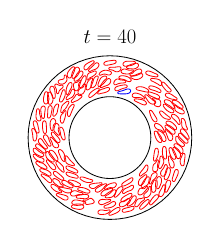
\begin{tikzpicture}[scale=0.3]

\begin{axis}[
  xmin = -21,
  xmax = 21,
  ymin = -21,
  ymax = 21,
  scale only axis,
  axis equal image,
  hide axis,
  title = {\Huge$t=40$}
  ]

% outer solid wall
\addplot [mark=none,black,line width=1.0] table{
2.0000e+01 -5.5171e-16
1.9904e+01 1.9603e+00
1.9616e+01 3.9018e+00
1.9139e+01 5.8057e+00
1.8478e+01 7.6537e+00
1.7638e+01 9.4279e+00
1.6629e+01 1.1111e+01
1.5460e+01 1.2688e+01
1.4142e+01 1.4142e+01
1.2688e+01 1.5460e+01
1.1111e+01 1.6629e+01
9.4279e+00 1.7638e+01
7.6537e+00 1.8478e+01
5.8057e+00 1.9139e+01
3.9018e+00 1.9616e+01
1.9603e+00 1.9904e+01
2.3281e-15 2.0000e+01
-1.9603e+00 1.9904e+01
-3.9018e+00 1.9616e+01
-5.8057e+00 1.9139e+01
-7.6537e+00 1.8478e+01
-9.4279e+00 1.7638e+01
-1.1111e+01 1.6629e+01
-1.2688e+01 1.5460e+01
-1.4142e+01 1.4142e+01
-1.5460e+01 1.2688e+01
-1.6629e+01 1.1111e+01
-1.7638e+01 9.4279e+00
-1.8478e+01 7.6537e+00
-1.9139e+01 5.8057e+00
-1.9616e+01 3.9018e+00
-1.9904e+01 1.9603e+00
-2.0000e+01 3.0010e-15
-1.9904e+01 -1.9603e+00
-1.9616e+01 -3.9018e+00
-1.9139e+01 -5.8057e+00
-1.8478e+01 -7.6537e+00
-1.7638e+01 -9.4279e+00
-1.6629e+01 -1.1111e+01
-1.5460e+01 -1.2688e+01
-1.4142e+01 -1.4142e+01
-1.2688e+01 -1.5460e+01
-1.1111e+01 -1.6629e+01
-9.4279e+00 -1.7638e+01
-7.6537e+00 -1.8478e+01
-5.8057e+00 -1.9139e+01
-3.9018e+00 -1.9616e+01
-1.9603e+00 -1.9904e+01
-4.7774e-15 -2.0000e+01
1.9603e+00 -1.9904e+01
3.9018e+00 -1.9616e+01
5.8057e+00 -1.9139e+01
7.6537e+00 -1.8478e+01
9.4279e+00 -1.7638e+01
1.1111e+01 -1.6629e+01
1.2688e+01 -1.5460e+01
1.4142e+01 -1.4142e+01
1.5460e+01 -1.2688e+01
1.6629e+01 -1.1111e+01
1.7638e+01 -9.4279e+00
1.8478e+01 -7.6537e+00
1.9139e+01 -5.8057e+00
1.9616e+01 -3.9018e+00
1.9904e+01 -1.9603e+00
2.0000e+01 -5.5171e-16
};

% inner solid wall
\addplot [mark=none,black,line width=1.0] table{
1.0000e+01 2.7586e-16
9.9518e+00 -9.8017e-01
9.8079e+00 -1.9509e+00
9.5694e+00 -2.9028e+00
9.2388e+00 -3.8268e+00
8.8192e+00 -4.7140e+00
8.3147e+00 -5.5557e+00
7.7301e+00 -6.3439e+00
7.0711e+00 -7.0711e+00
6.3439e+00 -7.7301e+00
5.5557e+00 -8.3147e+00
4.7140e+00 -8.8192e+00
3.8268e+00 -9.2388e+00
2.9028e+00 -9.5694e+00
1.9509e+00 -9.8079e+00
9.8017e-01 -9.9518e+00
1.1640e-15 -1.0000e+01
-9.8017e-01 -9.9518e+00
-1.9509e+00 -9.8079e+00
-2.9028e+00 -9.5694e+00
-3.8268e+00 -9.2388e+00
-4.7140e+00 -8.8192e+00
-5.5557e+00 -8.3147e+00
-6.3439e+00 -7.7301e+00
-7.0711e+00 -7.0711e+00
-7.7301e+00 -6.3439e+00
-8.3147e+00 -5.5557e+00
-8.8192e+00 -4.7140e+00
-9.2388e+00 -3.8268e+00
-9.5694e+00 -2.9028e+00
-9.8079e+00 -1.9509e+00
-9.9518e+00 -9.8017e-01
-1.0000e+01 -1.5005e-15
-9.9518e+00 9.8017e-01
-9.8079e+00 1.9509e+00
-9.5694e+00 2.9028e+00
-9.2388e+00 3.8268e+00
-8.8192e+00 4.7140e+00
-8.3147e+00 5.5557e+00
-7.7301e+00 6.3439e+00
-7.0711e+00 7.0711e+00
-6.3439e+00 7.7301e+00
-5.5557e+00 8.3147e+00
-4.7140e+00 8.8192e+00
-3.8268e+00 9.2388e+00
-2.9028e+00 9.5694e+00
-1.9509e+00 9.8079e+00
-9.8017e-01 9.9518e+00
-2.3887e-15 1.0000e+01
9.8017e-01 9.9518e+00
1.9509e+00 9.8079e+00
2.9028e+00 9.5694e+00
3.8268e+00 9.2388e+00
4.7140e+00 8.8192e+00
5.5557e+00 8.3147e+00
6.3439e+00 7.7301e+00
7.0711e+00 7.0711e+00
7.7301e+00 6.3439e+00
8.3147e+00 5.5557e+00
8.8192e+00 4.7140e+00
9.2388e+00 3.8268e+00
9.5694e+00 2.9028e+00
9.8079e+00 1.9509e+00
9.9518e+00 9.8017e-01
1.0000e+01 2.7586e-16
};

% vesicle 1
\addplot [mark=none,red,line width=1.0] table{
3.7283e+00 1.7443e+01
3.8095e+00 1.7437e+01
3.9020e+00 1.7439e+01
4.0078e+00 1.7452e+01
4.1298e+00 1.7481e+01
4.2641e+00 1.7525e+01
4.4097e+00 1.7581e+01
4.5727e+00 1.7645e+01
4.7507e+00 1.7716e+01
4.9319e+00 1.7789e+01
5.1209e+00 1.7861e+01
5.3193e+00 1.7931e+01
5.5148e+00 1.7990e+01
5.7135e+00 1.8039e+01
5.9057e+00 1.8081e+01
6.0817e+00 1.8141e+01
6.2043e+00 1.8258e+01
6.2214e+00 1.8409e+01
6.1440e+00 1.8529e+01
6.0336e+00 1.8592e+01
5.9268e+00 1.8620e+01
5.8290e+00 1.8632e+01
5.7432e+00 1.8637e+01
5.6648e+00 1.8640e+01
5.5871e+00 1.8642e+01
5.5049e+00 1.8643e+01
5.4079e+00 1.8645e+01
5.2925e+00 1.8649e+01
5.1619e+00 1.8654e+01
5.0139e+00 1.8660e+01
4.8514e+00 1.8668e+01
4.6890e+00 1.8674e+01
4.5094e+00 1.8676e+01
4.3172e+00 1.8671e+01
4.1286e+00 1.8655e+01
3.9290e+00 1.8620e+01
3.7315e+00 1.8559e+01
3.5501e+00 1.8471e+01
3.3973e+00 1.8356e+01
3.2830e+00 1.8218e+01
3.2137e+00 1.8060e+01
3.1995e+00 1.7896e+01
3.2382e+00 1.7751e+01
3.3152e+00 1.7636e+01
3.4080e+00 1.7556e+01
3.4981e+00 1.7505e+01
3.5814e+00 1.7474e+01
3.6560e+00 1.7454e+01
3.7283e+00 1.7443e+01
};

% vesicle 2
\addplot [mark=none,red,line width=1.0] table{
-5.2555e-02 1.3207e+01
-3.4101e-03 1.3275e+01
4.8042e-02 1.3358e+01
9.9618e-02 1.3461e+01
1.4517e-01 1.3581e+01
1.7866e-01 1.3719e+01
1.9203e-01 1.3870e+01
1.7402e-01 1.4033e+01
1.0415e-01 1.4205e+01
-3.0689e-02 1.4347e+01
-2.1761e-01 1.4422e+01
-4.2795e-01 1.4410e+01
-6.1321e-01 1.4318e+01
-7.6311e-01 1.4176e+01
-8.9041e-01 1.4014e+01
-1.0043e+00 1.3862e+01
-1.1127e+00 1.3722e+01
-1.2169e+00 1.3596e+01
-1.3162e+00 1.3484e+01
-1.4132e+00 1.3381e+01
-1.4990e+00 1.3295e+01
-1.5726e+00 1.3224e+01
-1.6394e+00 1.3161e+01
-1.6995e+00 1.3105e+01
-1.7568e+00 1.3054e+01
-1.8192e+00 1.2998e+01
-1.8897e+00 1.2936e+01
-1.9722e+00 1.2864e+01
-2.0702e+00 1.2778e+01
-2.1778e+00 1.2679e+01
-2.2869e+00 1.2562e+01
-2.3662e+00 1.2405e+01
-2.3063e+00 1.2239e+01
-2.1195e+00 1.2208e+01
-1.9233e+00 1.2273e+01
-1.7304e+00 1.2358e+01
-1.5382e+00 1.2442e+01
-1.3438e+00 1.2520e+01
-1.1556e+00 1.2590e+01
-9.7904e-01 1.2653e+01
-8.1555e-01 1.2710e+01
-6.6138e-01 1.2770e+01
-5.2229e-01 1.2833e+01
-4.0360e-01 1.2898e+01
-3.0386e-01 1.2964e+01
-2.2203e-01 1.3029e+01
-1.5723e-01 1.3089e+01
-1.0276e-01 1.3146e+01
-5.2555e-02 1.3207e+01
};

% vesicle 3
\addplot [mark=none,red,line width=1.0] table{
3.9225e+00 -1.5201e+01
3.9895e+00 -1.5159e+01
4.0689e+00 -1.5106e+01
4.1645e+00 -1.5043e+01
4.2734e+00 -1.4978e+01
4.4024e+00 -1.4918e+01
4.5484e+00 -1.4875e+01
4.7032e+00 -1.4833e+01
4.8633e+00 -1.4751e+01
5.0165e+00 -1.4624e+01
5.1575e+00 -1.4470e+01
5.2818e+00 -1.4299e+01
5.3720e+00 -1.4112e+01
5.3909e+00 -1.3905e+01
5.2976e+00 -1.3726e+01
5.1274e+00 -1.3642e+01
4.9470e+00 -1.3644e+01
4.7906e+00 -1.3689e+01
4.6554e+00 -1.3747e+01
4.5322e+00 -1.3808e+01
4.4270e+00 -1.3864e+01
4.3397e+00 -1.3911e+01
4.2615e+00 -1.3953e+01
4.1934e+00 -1.3990e+01
4.1293e+00 -1.4025e+01
4.0552e+00 -1.4065e+01
3.9724e+00 -1.4110e+01
3.8795e+00 -1.4160e+01
3.7713e+00 -1.4219e+01
3.6524e+00 -1.4286e+01
3.5190e+00 -1.4367e+01
3.3669e+00 -1.4468e+01
3.2159e+00 -1.4583e+01
3.0714e+00 -1.4710e+01
2.9309e+00 -1.4856e+01
2.8038e+00 -1.5021e+01
2.7072e+00 -1.5205e+01
2.6755e+00 -1.5398e+01
2.7553e+00 -1.5571e+01
2.9332e+00 -1.5623e+01
3.1041e+00 -1.5582e+01
3.2595e+00 -1.5526e+01
3.3980e+00 -1.5472e+01
3.5154e+00 -1.5422e+01
3.6211e+00 -1.5372e+01
3.7151e+00 -1.5323e+01
3.7903e+00 -1.5281e+01
3.8567e+00 -1.5242e+01
3.9225e+00 -1.5201e+01
};

% vesicle 4
\addplot [mark=none,red,line width=1.0] table{
2.8961e+00 -1.1639e+01
2.9289e+00 -1.1714e+01
2.9930e+00 -1.1781e+01
3.0896e+00 -1.1828e+01
3.2114e+00 -1.1844e+01
3.3512e+00 -1.1832e+01
3.5020e+00 -1.1795e+01
3.6599e+00 -1.1741e+01
3.8297e+00 -1.1670e+01
4.0134e+00 -1.1583e+01
4.1951e+00 -1.1490e+01
4.3685e+00 -1.1396e+01
4.5427e+00 -1.1299e+01
4.7244e+00 -1.1193e+01
4.9014e+00 -1.1082e+01
5.0621e+00 -1.0968e+01
5.2046e+00 -1.0850e+01
5.3237e+00 -1.0731e+01
5.4184e+00 -1.0616e+01
5.4925e+00 -1.0506e+01
5.5479e+00 -1.0402e+01
5.5864e+00 -1.0308e+01
5.6101e+00 -1.0224e+01
5.6214e+00 -1.0148e+01
5.6212e+00 -1.0073e+01
5.6052e+00 -9.9948e+00
5.5635e+00 -9.9144e+00
5.4834e+00 -9.8455e+00
5.3626e+00 -9.8136e+00
5.2203e+00 -9.8346e+00
5.0723e+00 -9.8970e+00
4.9162e+00 -9.9848e+00
4.7549e+00 -1.0083e+01
4.5920e+00 -1.0184e+01
4.4217e+00 -1.0289e+01
4.2425e+00 -1.0399e+01
4.0654e+00 -1.0506e+01
3.8909e+00 -1.0612e+01
3.7203e+00 -1.0718e+01
3.5588e+00 -1.0823e+01
3.4075e+00 -1.0927e+01
3.2723e+00 -1.1027e+01
3.1549e+00 -1.1125e+01
3.0567e+00 -1.1220e+01
2.9808e+00 -1.1313e+01
2.9283e+00 -1.1402e+01
2.8979e+00 -1.1485e+01
2.8873e+00 -1.1563e+01
2.8961e+00 -1.1639e+01
};

% vesicle 5
\addplot [mark=none,red,line width=1.0] table{
-6.2615e+00 1.6747e+01
-6.2157e+00 1.6686e+01
-6.1495e+00 1.6627e+01
-6.0577e+00 1.6579e+01
-5.9415e+00 1.6555e+01
-5.8052e+00 1.6567e+01
-5.6591e+00 1.6626e+01
-5.5176e+00 1.6728e+01
-5.3842e+00 1.6864e+01
-5.2546e+00 1.7017e+01
-5.1235e+00 1.7175e+01
-4.9887e+00 1.7330e+01
-4.8472e+00 1.7482e+01
-4.6984e+00 1.7629e+01
-4.5496e+00 1.7764e+01
-4.4036e+00 1.7887e+01
-4.2635e+00 1.7999e+01
-4.1356e+00 1.8101e+01
-4.0230e+00 1.8200e+01
-3.9316e+00 1.8300e+01
-3.8709e+00 1.8400e+01
-3.8438e+00 1.8495e+01
-3.8452e+00 1.8578e+01
-3.8680e+00 1.8647e+01
-3.9085e+00 1.8704e+01
-3.9707e+00 1.8751e+01
-4.0575e+00 1.8781e+01
-4.1665e+00 1.8785e+01
-4.2916e+00 1.8759e+01
-4.4262e+00 1.8710e+01
-4.5694e+00 1.8644e+01
-4.7236e+00 1.8568e+01
-4.8874e+00 1.8485e+01
-5.0542e+00 1.8400e+01
-5.2250e+00 1.8310e+01
-5.4023e+00 1.8211e+01
-5.5743e+00 1.8107e+01
-5.7410e+00 1.7993e+01
-5.8958e+00 1.7869e+01
-6.0305e+00 1.7738e+01
-6.1474e+00 1.7594e+01
-6.2373e+00 1.7445e+01
-6.2961e+00 1.7305e+01
-6.3289e+00 1.7175e+01
-6.3401e+00 1.7059e+01
-6.3350e+00 1.6961e+01
-6.3188e+00 1.6879e+01
-6.2945e+00 1.6810e+01
-6.2615e+00 1.6747e+01
};

% vesicle 6
\addplot [mark=none,red,line width=1.0] table{
-5.0043e+00 -1.1625e+01
-5.0383e+00 -1.1701e+01
-5.0542e+00 -1.1797e+01
-5.0390e+00 -1.1911e+01
-4.9830e+00 -1.2031e+01
-4.8875e+00 -1.2144e+01
-4.7603e+00 -1.2247e+01
-4.6069e+00 -1.2338e+01
-4.4257e+00 -1.2413e+01
-4.2160e+00 -1.2454e+01
-3.9914e+00 -1.2441e+01
-3.7812e+00 -1.2369e+01
-3.5991e+00 -1.2262e+01
-3.4315e+00 -1.2139e+01
-3.2709e+00 -1.2015e+01
-3.1158e+00 -1.1901e+01
-2.9602e+00 -1.1800e+01
-2.8122e+00 -1.1717e+01
-2.6775e+00 -1.1651e+01
-2.5530e+00 -1.1599e+01
-2.4416e+00 -1.1557e+01
-2.3458e+00 -1.1524e+01
-2.2637e+00 -1.1495e+01
-2.1913e+00 -1.1468e+01
-2.1224e+00 -1.1437e+01
-2.0518e+00 -1.1398e+01
-1.9799e+00 -1.1337e+01
-1.9266e+00 -1.1239e+01
-1.9442e+00 -1.1114e+01
-2.0593e+00 -1.1030e+01
-2.2187e+00 -1.1019e+01
-2.3930e+00 -1.1044e+01
-2.5781e+00 -1.1072e+01
-2.7664e+00 -1.1094e+01
-2.9652e+00 -1.1112e+01
-3.1692e+00 -1.1127e+01
-3.3777e+00 -1.1143e+01
-3.5892e+00 -1.1162e+01
-3.7940e+00 -1.1187e+01
-3.9946e+00 -1.1220e+01
-4.1787e+00 -1.1257e+01
-4.3463e+00 -1.1295e+01
-4.4955e+00 -1.1332e+01
-4.6252e+00 -1.1370e+01
-4.7365e+00 -1.1412e+01
-4.8287e+00 -1.1458e+01
-4.9020e+00 -1.1508e+01
-4.9592e+00 -1.1563e+01
-5.0043e+00 -1.1625e+01
};

% vesicle 7
\addplot [mark=none,red,line width=1.0] table{
1.4077e+01 5.3583e+00
1.4015e+01 5.4079e+00
1.3943e+01 5.4654e+00
1.3860e+01 5.5328e+00
1.3764e+01 5.6113e+00
1.3659e+01 5.6983e+00
1.3543e+01 5.7965e+00
1.3410e+01 5.9101e+00
1.3272e+01 6.0301e+00
1.3125e+01 6.1557e+00
1.2959e+01 6.2888e+00
1.2786e+01 6.4053e+00
1.2605e+01 6.4851e+00
1.2408e+01 6.5030e+00
1.2231e+01 6.4191e+00
1.2141e+01 6.2447e+00
1.2151e+01 6.0610e+00
1.2210e+01 5.9015e+00
1.2285e+01 5.7668e+00
1.2357e+01 5.6549e+00
1.2423e+01 5.5603e+00
1.2483e+01 5.4798e+00
1.2534e+01 5.4131e+00
1.2581e+01 5.3548e+00
1.2628e+01 5.2984e+00
1.2680e+01 5.2391e+00
1.2743e+01 5.1705e+00
1.2821e+01 5.0918e+00
1.2912e+01 5.0067e+00
1.3020e+01 4.9174e+00
1.3148e+01 4.8259e+00
1.3298e+01 4.7368e+00
1.3465e+01 4.6587e+00
1.3643e+01 4.5969e+00
1.3838e+01 4.5485e+00
1.4056e+01 4.5062e+00
1.4269e+01 4.4662e+00
1.4468e+01 4.4420e+00
1.4660e+01 4.4805e+00
1.4778e+01 4.6237e+00
1.4758e+01 4.7976e+00
1.4659e+01 4.9276e+00
1.4542e+01 5.0216e+00
1.4432e+01 5.0983e+00
1.4338e+01 5.1633e+00
1.4260e+01 5.2191e+00
1.4193e+01 5.2691e+00
1.4134e+01 5.3142e+00
1.4077e+01 5.3583e+00
};

% vesicle 8
\addplot [mark=none,red,line width=1.0] table{
7.4872e+00 1.5787e+01
7.5540e+00 1.5828e+01
7.6247e+00 1.5886e+01
7.6937e+00 1.5966e+01
7.7488e+00 1.6072e+01
7.7776e+00 1.6203e+01
7.7632e+00 1.6357e+01
7.6890e+00 1.6516e+01
7.5510e+00 1.6651e+01
7.3661e+00 1.6735e+01
7.1625e+00 1.6759e+01
6.9579e+00 1.6734e+01
6.7542e+00 1.6674e+01
6.5583e+00 1.6593e+01
6.3758e+00 1.6503e+01
6.2141e+00 1.6409e+01
6.0687e+00 1.6308e+01
5.9463e+00 1.6200e+01
5.8479e+00 1.6095e+01
5.7619e+00 1.5994e+01
5.6840e+00 1.5906e+01
5.6123e+00 1.5835e+01
5.5447e+00 1.5778e+01
5.4813e+00 1.5734e+01
5.4174e+00 1.5696e+01
5.3433e+00 1.5661e+01
5.2558e+00 1.5629e+01
5.1535e+00 1.5598e+01
5.0369e+00 1.5557e+01
4.9228e+00 1.5481e+01
4.8652e+00 1.5345e+01
4.9301e+00 1.5195e+01
5.0973e+00 1.5117e+01
5.2965e+00 1.5108e+01
5.5016e+00 1.5120e+01
5.7154e+00 1.5145e+01
5.9265e+00 1.5190e+01
6.1253e+00 1.5253e+01
6.3007e+00 1.5322e+01
6.4679e+00 1.5394e+01
6.6311e+00 1.5466e+01
6.7887e+00 1.5533e+01
6.9322e+00 1.5587e+01
7.0602e+00 1.5631e+01
7.1732e+00 1.5667e+01
7.2705e+00 1.5698e+01
7.3508e+00 1.5727e+01
7.4208e+00 1.5755e+01
7.4872e+00 1.5787e+01
};

% vesicle 9
\addplot [mark=none,red,line width=1.0] table{
1.0035e+01 8.2929e+00
1.0109e+01 8.2609e+00
1.0196e+01 8.2290e+00
1.0301e+01 8.1995e+00
1.0424e+01 8.1780e+00
1.0565e+01 8.1738e+00
1.0716e+01 8.2023e+00
1.0857e+01 8.2833e+00
1.0967e+01 8.4256e+00
1.1010e+01 8.6187e+00
1.0936e+01 8.8168e+00
1.0782e+01 8.9616e+00
1.0613e+01 9.0784e+00
1.0455e+01 9.1993e+00
1.0311e+01 9.3304e+00
1.0172e+01 9.4607e+00
1.0033e+01 9.5841e+00
9.9000e+00 9.6967e+00
9.7806e+00 9.7962e+00
9.6769e+00 9.8831e+00
9.5873e+00 9.9597e+00
9.5114e+00 1.0026e+01
9.4472e+00 1.0083e+01
9.3907e+00 1.0133e+01
9.3357e+00 1.0182e+01
9.2745e+00 1.0235e+01
9.2012e+00 1.0294e+01
9.1108e+00 1.0359e+01
8.9977e+00 1.0421e+01
8.8571e+00 1.0465e+01
8.6951e+00 1.0463e+01
8.5467e+00 1.0373e+01
8.5070e+00 1.0195e+01
8.5915e+00 1.0024e+01
8.7076e+00 9.8657e+00
8.8138e+00 9.6913e+00
8.9126e+00 9.5145e+00
9.0142e+00 9.3508e+00
9.1250e+00 9.1891e+00
9.2388e+00 9.0304e+00
9.3445e+00 8.8884e+00
9.4472e+00 8.7597e+00
9.5483e+00 8.6467e+00
9.6484e+00 8.5499e+00
9.7431e+00 8.4713e+00
9.8279e+00 8.4103e+00
9.9021e+00 8.3634e+00
9.9690e+00 8.3259e+00
1.0035e+01 8.2929e+00
};

% vesicle 10
\addplot [mark=none,red,line width=1.0] table{
-1.6918e+01 -3.1796e+00
-1.6855e+01 -3.2286e+00
-1.6783e+01 -3.2858e+00
-1.6701e+01 -3.3542e+00
-1.6606e+01 -3.4367e+00
-1.6497e+01 -3.5321e+00
-1.6374e+01 -3.6342e+00
-1.6228e+01 -3.7267e+00
-1.6051e+01 -3.7736e+00
-1.5865e+01 -3.7285e+00
-1.5727e+01 -3.5888e+00
-1.5664e+01 -3.3970e+00
-1.5687e+01 -3.1908e+00
-1.5786e+01 -3.0099e+00
-1.5923e+01 -2.8661e+00
-1.6064e+01 -2.7444e+00
-1.6201e+01 -2.6309e+00
-1.6330e+01 -2.5242e+00
-1.6449e+01 -2.4268e+00
-1.6555e+01 -2.3408e+00
-1.6646e+01 -2.2667e+00
-1.6722e+01 -2.2040e+00
-1.6785e+01 -2.1514e+00
-1.6841e+01 -2.1050e+00
-1.6895e+01 -2.0594e+00
-1.6954e+01 -2.0094e+00
-1.7024e+01 -1.9501e+00
-1.7107e+01 -1.8798e+00
-1.7203e+01 -1.8004e+00
-1.7315e+01 -1.7140e+00
-1.7447e+01 -1.6271e+00
-1.7600e+01 -1.5571e+00
-1.7774e+01 -1.5284e+00
-1.7956e+01 -1.5719e+00
-1.8101e+01 -1.7013e+00
-1.8171e+01 -1.8909e+00
-1.8157e+01 -2.0967e+00
-1.8074e+01 -2.2820e+00
-1.7945e+01 -2.4359e+00
-1.7795e+01 -2.5628e+00
-1.7647e+01 -2.6696e+00
-1.7510e+01 -2.7629e+00
-1.7386e+01 -2.8464e+00
-1.7278e+01 -2.9201e+00
-1.7186e+01 -2.9839e+00
-1.7107e+01 -3.0398e+00
-1.7038e+01 -3.0898e+00
-1.6976e+01 -3.1352e+00
-1.6918e+01 -3.1796e+00
};

% vesicle 11
\addplot [mark=none,red,line width=1.0] table{
-1.3691e+01 -1.2785e+01
-1.3631e+01 -1.2833e+01
-1.3560e+01 -1.2887e+01
-1.3475e+01 -1.2948e+01
-1.3374e+01 -1.3015e+01
-1.3252e+01 -1.3087e+01
-1.3110e+01 -1.3161e+01
-1.2946e+01 -1.3231e+01
-1.2767e+01 -1.3295e+01
-1.2583e+01 -1.3355e+01
-1.2393e+01 -1.3416e+01
-1.2193e+01 -1.3472e+01
-1.1982e+01 -1.3480e+01
-1.1820e+01 -1.3359e+01
-1.1847e+01 -1.3169e+01
-1.1999e+01 -1.3054e+01
-1.2162e+01 -1.2977e+01
-1.2302e+01 -1.2888e+01
-1.2404e+01 -1.2779e+01
-1.2467e+01 -1.2666e+01
-1.2506e+01 -1.2560e+01
-1.2533e+01 -1.2467e+01
-1.2558e+01 -1.2387e+01
-1.2586e+01 -1.2317e+01
-1.2619e+01 -1.2252e+01
-1.2663e+01 -1.2186e+01
-1.2723e+01 -1.2115e+01
-1.2803e+01 -1.2042e+01
-1.2902e+01 -1.1967e+01
-1.3018e+01 -1.1890e+01
-1.3150e+01 -1.1809e+01
-1.3296e+01 -1.1721e+01
-1.3453e+01 -1.1628e+01
-1.3623e+01 -1.1534e+01
-1.3804e+01 -1.1454e+01
-1.4002e+01 -1.1414e+01
-1.4205e+01 -1.1452e+01
-1.4358e+01 -1.1587e+01
-1.4415e+01 -1.1776e+01
-1.4387e+01 -1.1965e+01
-1.4310e+01 -1.2131e+01
-1.4213e+01 -1.2270e+01
-1.4113e+01 -1.2388e+01
-1.4019e+01 -1.2488e+01
-1.3935e+01 -1.2571e+01
-1.3862e+01 -1.2638e+01
-1.3800e+01 -1.2693e+01
-1.3745e+01 -1.2740e+01
-1.3691e+01 -1.2785e+01
};

% vesicle 12
\addplot [mark=none,red,line width=1.0] table{
8.3311e+00 -1.4399e+01
8.3708e+00 -1.4465e+01
8.4313e+00 -1.4534e+01
8.5202e+00 -1.4598e+01
8.6366e+00 -1.4643e+01
8.7780e+00 -1.4661e+01
8.9349e+00 -1.4645e+01
9.0996e+00 -1.4597e+01
9.2680e+00 -1.4518e+01
9.4323e+00 -1.4407e+01
9.5834e+00 -1.4273e+01
9.7209e+00 -1.4117e+01
9.8364e+00 -1.3952e+01
9.9288e+00 -1.3778e+01
9.9975e+00 -1.3587e+01
1.0030e+01 -1.3392e+01
1.0028e+01 -1.3217e+01
1.0007e+01 -1.3056e+01
9.9831e+00 -1.2905e+01
9.9675e+00 -1.2771e+01
9.9629e+00 -1.2654e+01
9.9660e+00 -1.2555e+01
9.9730e+00 -1.2468e+01
9.9809e+00 -1.2393e+01
9.9881e+00 -1.2322e+01
9.9927e+00 -1.2240e+01
9.9871e+00 -1.2146e+01
9.9542e+00 -1.2040e+01
9.8642e+00 -1.1947e+01
9.7207e+00 -1.1932e+01
9.5928e+00 -1.2028e+01
9.5220e+00 -1.2188e+01
9.4824e+00 -1.2362e+01
9.4399e+00 -1.2542e+01
9.3742e+00 -1.2730e+01
9.2783e+00 -1.2916e+01
9.1575e+00 -1.3086e+01
9.0197e+00 -1.3237e+01
8.8775e+00 -1.3368e+01
8.7307e+00 -1.3492e+01
8.5885e+00 -1.3614e+01
8.4708e+00 -1.3732e+01
8.3819e+00 -1.3848e+01
8.3216e+00 -1.3964e+01
8.2888e+00 -1.4076e+01
8.2794e+00 -1.4176e+01
8.2862e+00 -1.4260e+01
8.3036e+00 -1.4332e+01
8.3311e+00 -1.4399e+01
};

% vesicle 13
\addplot [mark=none,red,line width=1.0] table{
9.6620e+00 -1.1134e+01
9.6832e+00 -1.1213e+01
9.7354e+00 -1.1290e+01
9.8313e+00 -1.1342e+01
9.9571e+00 -1.1328e+01
1.0069e+01 -1.1236e+01
1.0150e+01 -1.1098e+01
1.0219e+01 -1.0938e+01
1.0297e+01 -1.0766e+01
1.0396e+01 -1.0594e+01
1.0521e+01 -1.0436e+01
1.0674e+01 -1.0295e+01
1.0840e+01 -1.0164e+01
1.0992e+01 -1.0025e+01
1.1124e+01 -9.8733e+00
1.1235e+01 -9.7217e+00
1.1331e+01 -9.5741e+00
1.1413e+01 -9.4267e+00
1.1474e+01 -9.2826e+00
1.1512e+01 -9.1480e+00
1.1527e+01 -9.0281e+00
1.1524e+01 -8.9252e+00
1.1507e+01 -8.8389e+00
1.1478e+01 -8.7664e+00
1.1439e+01 -8.7026e+00
1.1382e+01 -8.6442e+00
1.1302e+01 -8.5956e+00
1.1196e+01 -8.5670e+00
1.1069e+01 -8.5648e+00
1.0926e+01 -8.5859e+00
1.0771e+01 -8.6283e+00
1.0611e+01 -8.6987e+00
1.0462e+01 -8.8031e+00
1.0326e+01 -8.9455e+00
1.0209e+01 -9.1209e+00
1.0121e+01 -9.3081e+00
1.0057e+01 -9.4957e+00
1.0009e+01 -9.6878e+00
9.9690e+00 -9.8852e+00
9.9305e+00 -1.0076e+01
9.8882e+00 -1.0253e+01
9.8412e+00 -1.0415e+01
9.7927e+00 -1.0563e+01
9.7480e+00 -1.0692e+01
9.7112e+00 -1.0803e+01
9.6837e+00 -1.0898e+01
9.6660e+00 -1.0982e+01
9.6582e+00 -1.1059e+01
9.6620e+00 -1.1134e+01
};

% vesicle 14
\addplot [mark=none,red,line width=1.0] table{
-8.7002e+00 -6.7693e+00
-8.6708e+00 -6.6972e+00
-8.6749e+00 -6.6061e+00
-8.7204e+00 -6.5072e+00
-8.7962e+00 -6.4148e+00
-8.8977e+00 -6.3181e+00
-9.0206e+00 -6.2093e+00
-9.1523e+00 -6.0918e+00
-9.2964e+00 -5.9579e+00
-9.4475e+00 -5.8091e+00
-9.5900e+00 -5.6590e+00
-9.7300e+00 -5.5008e+00
-9.8693e+00 -5.3317e+00
-1.0000e+01 -5.1643e+00
-1.0126e+01 -4.9997e+00
-1.0247e+01 -4.8437e+00
-1.0363e+01 -4.7058e+00
-1.0482e+01 -4.5849e+00
-1.0611e+01 -4.4929e+00
-1.0741e+01 -4.4539e+00
-1.0855e+01 -4.4791e+00
-1.0923e+01 -4.5491e+00
-1.0949e+01 -4.6322e+00
-1.0950e+01 -4.7089e+00
-1.0940e+01 -4.7789e+00
-1.0920e+01 -4.8593e+00
-1.0894e+01 -4.9476e+00
-1.0863e+01 -5.0488e+00
-1.0830e+01 -5.1751e+00
-1.0806e+01 -5.3165e+00
-1.0801e+01 -5.4715e+00
-1.0812e+01 -5.6465e+00
-1.0808e+01 -5.8303e+00
-1.0748e+01 -6.0137e+00
-1.0633e+01 -6.1852e+00
-1.0483e+01 -6.3304e+00
-1.0315e+01 -6.4444e+00
-1.0134e+01 -6.5339e+00
-9.9428e+00 -6.6077e+00
-9.7585e+00 -6.6693e+00
-9.5790e+00 -6.7257e+00
-9.4159e+00 -6.7752e+00
-9.2703e+00 -6.8164e+00
-9.1357e+00 -6.8487e+00
-9.0168e+00 -6.8677e+00
-8.9122e+00 -6.8704e+00
-8.8262e+00 -6.8559e+00
-8.7559e+00 -6.8237e+00
-8.7002e+00 -6.7693e+00
};

% vesicle 15
\addplot [mark=none,red,line width=1.0] table{
3.6132e+00 1.5059e+01
3.5339e+00 1.5074e+01
3.4414e+00 1.5090e+01
3.3335e+00 1.5106e+01
3.2096e+00 1.5120e+01
3.0666e+00 1.5129e+01
2.9058e+00 1.5126e+01
2.7356e+00 1.5104e+01
2.5586e+00 1.5054e+01
2.3826e+00 1.4962e+01
2.2426e+00 1.4820e+01
2.1959e+00 1.4618e+01
2.3215e+00 1.4445e+01
2.5171e+00 1.4374e+01
2.7102e+00 1.4334e+01
2.8942e+00 1.4296e+01
3.0700e+00 1.4261e+01
3.2245e+00 1.4231e+01
3.3607e+00 1.4204e+01
3.4847e+00 1.4174e+01
3.5921e+00 1.4140e+01
3.6814e+00 1.4104e+01
3.7563e+00 1.4065e+01
3.8208e+00 1.4026e+01
3.8817e+00 1.3986e+01
3.9474e+00 1.3940e+01
4.0236e+00 1.3890e+01
4.1153e+00 1.3838e+01
4.2286e+00 1.3785e+01
4.3654e+00 1.3737e+01
4.5217e+00 1.3699e+01
4.6947e+00 1.3679e+01
4.8820e+00 1.3694e+01
5.0608e+00 1.3770e+01
5.1834e+00 1.3930e+01
5.1753e+00 1.4142e+01
5.0576e+00 1.4319e+01
4.9151e+00 1.4461e+01
4.7698e+00 1.4589e+01
4.6195e+00 1.4703e+01
4.4667e+00 1.4794e+01
4.3164e+00 1.4864e+01
4.1772e+00 1.4916e+01
4.0525e+00 1.4955e+01
3.9410e+00 1.4985e+01
3.8436e+00 1.5009e+01
3.7603e+00 1.5028e+01
3.6861e+00 1.5044e+01
3.6132e+00 1.5059e+01
};

% vesicle 16
\addplot [mark=none,red,line width=1.0] table{
-1.5176e+00 1.5507e+01
-1.4439e+00 1.5516e+01
-1.3524e+00 1.5522e+01
-1.2386e+00 1.5520e+01
-1.1156e+00 1.5506e+01
-9.7368e-01 1.5476e+01
-8.1424e-01 1.5426e+01
-6.5341e-01 1.5371e+01
-4.7899e-01 1.5321e+01
-2.8747e-01 1.5298e+01
-8.6268e-02 1.5321e+01
1.0790e-01 1.5403e+01
2.6852e-01 1.5542e+01
3.6261e-01 1.5729e+01
3.5661e-01 1.5920e+01
2.5963e-01 1.6077e+01
1.0767e-01 1.6185e+01
-4.5178e-02 1.6251e+01
-1.8558e-01 1.6300e+01
-3.1819e-01 1.6342e+01
-4.2940e-01 1.6373e+01
-5.2091e-01 1.6397e+01
-6.0723e-01 1.6416e+01
-6.8056e-01 1.6429e+01
-7.4729e-01 1.6439e+01
-8.2882e-01 1.6449e+01
-9.1834e-01 1.6455e+01
-1.0196e+00 1.6458e+01
-1.1456e+00 1.6455e+01
-1.2850e+00 1.6442e+01
-1.4371e+00 1.6415e+01
-1.6087e+00 1.6369e+01
-1.7808e+00 1.6302e+01
-1.9598e+00 1.6212e+01
-2.1337e+00 1.6101e+01
-2.2980e+00 1.5973e+01
-2.4535e+00 1.5826e+01
-2.5810e+00 1.5663e+01
-2.6437e+00 1.5472e+01
-2.5678e+00 1.5298e+01
-2.3960e+00 1.5245e+01
-2.2256e+00 1.5279e+01
-2.0767e+00 1.5335e+01
-1.9534e+00 1.5384e+01
-1.8418e+00 1.5424e+01
-1.7420e+00 1.5456e+01
-1.6639e+00 1.5477e+01
-1.5920e+00 1.5493e+01
-1.5176e+00 1.5507e+01
};

% vesicle 17
\addplot [mark=none,red,line width=1.0] table{
-1.2623e+01 7.4003e+00
-1.2600e+01 7.4776e+00
-1.2575e+01 7.5670e+00
-1.2549e+01 7.6719e+00
-1.2529e+01 7.7925e+00
-1.2529e+01 7.9330e+00
-1.2579e+01 8.0808e+00
-1.2700e+01 8.1887e+00
-1.2874e+01 8.2098e+00
-1.3046e+01 8.1401e+00
-1.3192e+01 8.0198e+00
-1.3322e+01 7.8721e+00
-1.3440e+01 7.7075e+00
-1.3544e+01 7.5282e+00
-1.3625e+01 7.3461e+00
-1.3684e+01 7.1670e+00
-1.3727e+01 6.9920e+00
-1.3759e+01 6.8294e+00
-1.3782e+01 6.6830e+00
-1.3801e+01 6.5517e+00
-1.3818e+01 6.4372e+00
-1.3832e+01 6.3398e+00
-1.3844e+01 6.2548e+00
-1.3856e+01 6.1801e+00
-1.3868e+01 6.1081e+00
-1.3882e+01 6.0266e+00
-1.3900e+01 5.9318e+00
-1.3920e+01 5.8210e+00
-1.3940e+01 5.6912e+00
-1.3950e+01 5.5485e+00
-1.3928e+01 5.3975e+00
-1.3834e+01 5.2593e+00
-1.3659e+01 5.2179e+00
-1.3486e+01 5.3049e+00
-1.3339e+01 5.4504e+00
-1.3197e+01 5.6107e+00
-1.3068e+01 5.7791e+00
-1.2969e+01 5.9550e+00
-1.2901e+01 6.1356e+00
-1.2855e+01 6.3135e+00
-1.2822e+01 6.4863e+00
-1.2792e+01 6.6559e+00
-1.2765e+01 6.8110e+00
-1.2739e+01 6.9438e+00
-1.2713e+01 7.0611e+00
-1.2688e+01 7.1639e+00
-1.2665e+01 7.2499e+00
-1.2644e+01 7.3261e+00
-1.2623e+01 7.4003e+00
};

% vesicle 18
\addplot [mark=none,red,line width=1.0] table{
9.6093e+00 1.2019e+01
9.6648e+00 1.1961e+01
9.7355e+00 1.1903e+01
9.8242e+00 1.1845e+01
9.9318e+00 1.1790e+01
1.0059e+01 1.1738e+01
1.0206e+01 1.1688e+01
1.0373e+01 1.1639e+01
1.0554e+01 1.1588e+01
1.0743e+01 1.1533e+01
1.0932e+01 1.1474e+01
1.1122e+01 1.1408e+01
1.1316e+01 1.1331e+01
1.1507e+01 1.1248e+01
1.1698e+01 1.1159e+01
1.1881e+01 1.1081e+01
1.2058e+01 1.1032e+01
1.2225e+01 1.1031e+01
1.2364e+01 1.1091e+01
1.2448e+01 1.1193e+01
1.2476e+01 1.1303e+01
1.2466e+01 1.1403e+01
1.2437e+01 1.1486e+01
1.2398e+01 1.1554e+01
1.2352e+01 1.1616e+01
1.2296e+01 1.1678e+01
1.2227e+01 1.1742e+01
1.2144e+01 1.1811e+01
1.2046e+01 1.1883e+01
1.1934e+01 1.1958e+01
1.1804e+01 1.2038e+01
1.1652e+01 1.2123e+01
1.1483e+01 1.2211e+01
1.1305e+01 1.2295e+01
1.1114e+01 1.2376e+01
1.0912e+01 1.2451e+01
1.0702e+01 1.2516e+01
1.0494e+01 1.2570e+01
1.0298e+01 1.2609e+01
1.0110e+01 1.2633e+01
9.9341e+00 1.2636e+01
9.7743e+00 1.2609e+01
9.6421e+00 1.2545e+01
9.5506e+00 1.2448e+01
9.5082e+00 1.2338e+01
9.5068e+00 1.2235e+01
9.5298e+00 1.2149e+01
9.5652e+00 1.2080e+01
9.6093e+00 1.2019e+01
};

% vesicle 19
\addplot [mark=none,red,line width=1.0] table{
-1.6094e+01 -9.0280e+00
-1.6160e+01 -8.9972e+00
-1.6243e+01 -8.9616e+00
-1.6347e+01 -8.9246e+00
-1.6466e+01 -8.8993e+00
-1.6608e+01 -8.9053e+00
-1.6748e+01 -8.9839e+00
-1.6807e+01 -9.1380e+00
-1.6751e+01 -9.3107e+00
-1.6616e+01 -9.4579e+00
-1.6460e+01 -9.5850e+00
-1.6300e+01 -9.7130e+00
-1.6143e+01 -9.8469e+00
-1.5996e+01 -9.9816e+00
-1.5852e+01 -1.0119e+01
-1.5714e+01 -1.0254e+01
-1.5587e+01 -1.0377e+01
-1.5466e+01 -1.0493e+01
-1.5354e+01 -1.0597e+01
-1.5252e+01 -1.0688e+01
-1.5161e+01 -1.0763e+01
-1.5084e+01 -1.0823e+01
-1.5012e+01 -1.0873e+01
-1.4949e+01 -1.0913e+01
-1.4889e+01 -1.0946e+01
-1.4815e+01 -1.0981e+01
-1.4728e+01 -1.1010e+01
-1.4627e+01 -1.1027e+01
-1.4500e+01 -1.1019e+01
-1.4371e+01 -1.0961e+01
-1.4269e+01 -1.0844e+01
-1.4223e+01 -1.0673e+01
-1.4240e+01 -1.0489e+01
-1.4298e+01 -1.0308e+01
-1.4386e+01 -1.0124e+01
-1.4495e+01 -9.9521e+00
-1.4623e+01 -9.7971e+00
-1.4777e+01 -9.6592e+00
-1.4943e+01 -9.5491e+00
-1.5113e+01 -9.4634e+00
-1.5284e+01 -9.3909e+00
-1.5439e+01 -9.3284e+00
-1.5577e+01 -9.2708e+00
-1.5697e+01 -9.2179e+00
-1.5801e+01 -9.1701e+00
-1.5892e+01 -9.1264e+00
-1.5963e+01 -9.0918e+00
-1.6028e+01 -9.0601e+00
-1.6094e+01 -9.0280e+00
};

% vesicle 20
\addplot [mark=none,red,line width=1.0] table{
-7.2015e-01 -1.3687e+01
-6.5251e-01 -1.3638e+01
-5.7662e-01 -1.3584e+01
-4.9006e-01 -1.3525e+01
-3.8831e-01 -1.3457e+01
-2.7360e-01 -1.3383e+01
-1.4461e-01 -1.3302e+01
3.3110e-03 -1.3209e+01
1.6433e-01 -1.3107e+01
3.3290e-01 -1.2993e+01
5.1068e-01 -1.2853e+01
6.5282e-01 -1.2667e+01
6.4098e-01 -1.2455e+01
4.6245e-01 -1.2369e+01
2.6470e-01 -1.2397e+01
7.6680e-02 -1.2448e+01
-1.0038e-01 -1.2505e+01
-2.6266e-01 -1.2564e+01
-4.0316e-01 -1.2619e+01
-5.2263e-01 -1.2666e+01
-6.2892e-01 -1.2703e+01
-7.2412e-01 -1.2731e+01
-8.0676e-01 -1.2750e+01
-8.8395e-01 -1.2764e+01
-9.6255e-01 -1.2773e+01
-1.0452e+00 -1.2780e+01
-1.1396e+00 -1.2791e+01
-1.2468e+00 -1.2813e+01
-1.3649e+00 -1.2857e+01
-1.4928e+00 -1.2928e+01
-1.6224e+00 -1.3022e+01
-1.7548e+00 -1.3133e+01
-1.8905e+00 -1.3263e+01
-2.0207e+00 -1.3408e+01
-2.1316e+00 -1.3570e+01
-2.2037e+00 -1.3767e+01
-2.1829e+00 -1.3985e+01
-2.0519e+00 -1.4149e+01
-1.8553e+00 -1.4231e+01
-1.6518e+00 -1.4238e+01
-1.4742e+00 -1.4198e+01
-1.3251e+00 -1.4131e+01
-1.1996e+00 -1.4053e+01
-1.0899e+00 -1.3972e+01
-9.9541e-01 -1.3899e+01
-9.1515e-01 -1.3836e+01
-8.4373e-01 -1.3780e+01
-7.8056e-01 -1.3732e+01
-7.2015e-01 -1.3687e+01
};

% vesicle 21
\addplot [mark=none,red,line width=1.0] table{
-1.4055e+00 -1.1367e+01
-1.4819e+00 -1.1395e+01
-1.5728e+00 -1.1431e+01
-1.6799e+00 -1.1478e+01
-1.7969e+00 -1.1534e+01
-1.9262e+00 -1.1600e+01
-2.0696e+00 -1.1677e+01
-2.2244e+00 -1.1761e+01
-2.3880e+00 -1.1850e+01
-2.5567e+00 -1.1943e+01
-2.7359e+00 -1.2045e+01
-2.9145e+00 -1.2152e+01
-3.0787e+00 -1.2258e+01
-3.2334e+00 -1.2372e+01
-3.3786e+00 -1.2504e+01
-3.4966e+00 -1.2657e+01
-3.5669e+00 -1.2834e+01
-3.5652e+00 -1.3011e+01
-3.4981e+00 -1.3151e+01
-3.3957e+00 -1.3245e+01
-3.2869e+00 -1.3297e+01
-3.1863e+00 -1.3322e+01
-3.0952e+00 -1.3331e+01
-3.0161e+00 -1.3329e+01
-2.9423e+00 -1.3321e+01
-2.8622e+00 -1.3306e+01
-2.7747e+00 -1.3281e+01
-2.6758e+00 -1.3245e+01
-2.5581e+00 -1.3188e+01
-2.4265e+00 -1.3111e+01
-2.2878e+00 -1.3015e+01
-2.1428e+00 -1.2904e+01
-1.9938e+00 -1.2781e+01
-1.8443e+00 -1.2648e+01
-1.6944e+00 -1.2497e+01
-1.5554e+00 -1.2329e+01
-1.4295e+00 -1.2153e+01
-1.3015e+00 -1.1983e+01
-1.1622e+00 -1.1837e+01
-1.0104e+00 -1.1719e+01
-8.6436e-01 -1.1611e+01
-7.8409e-01 -1.1466e+01
-8.4020e-01 -1.1330e+01
-9.6265e-01 -1.1278e+01
-1.0809e+00 -1.1279e+01
-1.1802e+00 -1.1298e+01
-1.2611e+00 -1.1320e+01
-1.3335e+00 -1.1342e+01
-1.4055e+00 -1.1367e+01
};

% vesicle 22
\addplot [mark=none,red,line width=1.0] table{
-1.2217e+01 1.6937e+00
-1.2200e+01 1.6180e+00
-1.2179e+01 1.5305e+00
-1.2154e+01 1.4285e+00
-1.2127e+01 1.3103e+00
-1.2099e+01 1.1701e+00
-1.2073e+01 1.0067e+00
-1.2051e+01 8.2929e-01
-1.2024e+01 6.4580e-01
-1.1980e+01 4.5422e-01
-1.1916e+01 2.6015e-01
-1.1837e+01 6.4366e-02
-1.1746e+01 -1.2501e-01
-1.1639e+01 -3.0399e-01
-1.1508e+01 -4.5641e-01
-1.1342e+01 -5.5848e-01
-1.1162e+01 -5.6420e-01
-1.1028e+01 -4.6698e-01
-1.0967e+01 -3.2794e-01
-1.0952e+01 -1.9227e-01
-1.0954e+01 -7.4059e-02
-1.0963e+01 2.6137e-02
-1.0974e+01 1.1294e-01
-1.0985e+01 1.8778e-01
-1.0996e+01 2.5843e-01
-1.1009e+01 3.3684e-01
-1.1025e+01 4.2664e-01
-1.1044e+01 5.3225e-01
-1.1067e+01 6.5895e-01
-1.1094e+01 8.0299e-01
-1.1124e+01 9.6106e-01
-1.1159e+01 1.1355e+00
-1.1200e+01 1.3257e+00
-1.1248e+01 1.5239e+00
-1.1307e+01 1.7283e+00
-1.1381e+01 1.9330e+00
-1.1476e+01 2.1312e+00
-1.1589e+01 2.3049e+00
-1.1726e+01 2.4423e+00
-1.1886e+01 2.5249e+00
-1.2060e+01 2.5238e+00
-1.2196e+01 2.4256e+00
-1.2259e+01 2.2836e+00
-1.2276e+01 2.1471e+00
-1.2272e+01 2.0271e+00
-1.2261e+01 1.9248e+00
-1.2247e+01 1.8403e+00
-1.2233e+01 1.7659e+00
-1.2217e+01 1.6937e+00
};

% vesicle 23
\addplot [mark=none,red,line width=1.0] table{
1.1196e+01 -5.5530e+00
1.1233e+01 -5.4810e+00
1.1275e+01 -5.3978e+00
1.1325e+01 -5.3005e+00
1.1384e+01 -5.1867e+00
1.1451e+01 -5.0545e+00
1.1520e+01 -4.9059e+00
1.1589e+01 -4.7390e+00
1.1655e+01 -4.5620e+00
1.1715e+01 -4.3740e+00
1.1764e+01 -4.1821e+00
1.1800e+01 -3.9905e+00
1.1825e+01 -3.7824e+00
1.1837e+01 -3.5788e+00
1.1836e+01 -3.3782e+00
1.1823e+01 -3.1888e+00
1.1793e+01 -3.0146e+00
1.1740e+01 -2.8586e+00
1.1661e+01 -2.7319e+00
1.1560e+01 -2.6457e+00
1.1453e+01 -2.6044e+00
1.1353e+01 -2.6008e+00
1.1268e+01 -2.6238e+00
1.1200e+01 -2.6624e+00
1.1144e+01 -2.7122e+00
1.1093e+01 -2.7768e+00
1.1047e+01 -2.8585e+00
1.1006e+01 -2.9588e+00
1.0969e+01 -3.0786e+00
1.0935e+01 -3.2165e+00
1.0901e+01 -3.3751e+00
1.0867e+01 -3.5543e+00
1.0833e+01 -3.7428e+00
1.0802e+01 -3.9330e+00
1.0771e+01 -4.1330e+00
1.0741e+01 -4.3393e+00
1.0713e+01 -4.5550e+00
1.0689e+01 -4.7661e+00
1.0672e+01 -4.9628e+00
1.0663e+01 -5.1541e+00
1.0666e+01 -5.3339e+00
1.0688e+01 -5.4978e+00
1.0741e+01 -5.6373e+00
1.0830e+01 -5.7324e+00
1.0941e+01 -5.7638e+00
1.1039e+01 -5.7363e+00
1.1108e+01 -5.6812e+00
1.1157e+01 -5.6190e+00
1.1196e+01 -5.5530e+00
};

% vesicle 24
\addplot [mark=none,red,line width=1.0] table{
9.4431e+00 1.1502e+01
9.4099e+00 1.1574e+01
9.3572e+00 1.1650e+01
9.2827e+00 1.1728e+01
9.1867e+00 1.1806e+01
9.0700e+00 1.1886e+01
8.9334e+00 1.1969e+01
8.7797e+00 1.2054e+01
8.6124e+00 1.2137e+01
8.4367e+00 1.2213e+01
8.2483e+00 1.2282e+01
8.0494e+00 1.2341e+01
7.8469e+00 1.2386e+01
7.6431e+00 1.2416e+01
7.4398e+00 1.2432e+01
7.2441e+00 1.2431e+01
7.0638e+00 1.2417e+01
6.9009e+00 1.2389e+01
6.7566e+00 1.2349e+01
6.6332e+00 1.2296e+01
6.5346e+00 1.2232e+01
6.4638e+00 1.2160e+01
6.4206e+00 1.2085e+01
6.4020e+00 1.2010e+01
6.4050e+00 1.1937e+01
6.4311e+00 1.1861e+01
6.4852e+00 1.1787e+01
6.5684e+00 1.1720e+01
6.6763e+00 1.1665e+01
6.8026e+00 1.1620e+01
6.9463e+00 1.1580e+01
7.1089e+00 1.1540e+01
7.2884e+00 1.1500e+01
7.4794e+00 1.1459e+01
7.6777e+00 1.1416e+01
7.8755e+00 1.1373e+01
8.0743e+00 1.1329e+01
8.2736e+00 1.1285e+01
8.4689e+00 1.1242e+01
8.6589e+00 1.1201e+01
8.8343e+00 1.1164e+01
8.9925e+00 1.1135e+01
9.1391e+00 1.1122e+01
9.2708e+00 1.1137e+01
9.3737e+00 1.1190e+01
9.4351e+00 1.1270e+01
9.4597e+00 1.1352e+01
9.4599e+00 1.1429e+01
9.4431e+00 1.1502e+01
};

% vesicle 25
\addplot [mark=none,red,line width=1.0] table{
-8.9914e+00 -8.7770e+00
-9.0670e+00 -8.7530e+00
-9.1550e+00 -8.7262e+00
-9.2592e+00 -8.6955e+00
-9.3823e+00 -8.6604e+00
-9.5248e+00 -8.6203e+00
-9.6849e+00 -8.5756e+00
-9.8582e+00 -8.5283e+00
-1.0041e+01 -8.4831e+00
-1.0233e+01 -8.4497e+00
-1.0429e+01 -8.4480e+00
-1.0612e+01 -8.5123e+00
-1.0724e+01 -8.6731e+00
-1.0705e+01 -8.8650e+00
-1.0606e+01 -9.0305e+00
-1.0471e+01 -9.1700e+00
-1.0325e+01 -9.2836e+00
-1.0184e+01 -9.3723e+00
-1.0054e+01 -9.4409e+00
-9.9337e+00 -9.4948e+00
-9.8237e+00 -9.5376e+00
-9.7271e+00 -9.5711e+00
-9.6447e+00 -9.5972e+00
-9.5716e+00 -9.6188e+00
-9.5006e+00 -9.6387e+00
-9.4238e+00 -9.6590e+00
-9.3340e+00 -9.6819e+00
-9.2272e+00 -9.7079e+00
-9.1045e+00 -9.7370e+00
-8.9690e+00 -9.7687e+00
-8.8191e+00 -9.8037e+00
-8.6535e+00 -9.8423e+00
-8.4736e+00 -9.8820e+00
-8.2768e+00 -9.9153e+00
-8.0749e+00 -9.9218e+00
-7.8816e+00 -9.8703e+00
-7.7495e+00 -9.7221e+00
-7.7678e+00 -9.5215e+00
-7.8868e+00 -9.3601e+00
-8.0286e+00 -9.2373e+00
-8.1735e+00 -9.1372e+00
-8.3153e+00 -9.0549e+00
-8.4484e+00 -8.9880e+00
-8.5699e+00 -8.9334e+00
-8.6777e+00 -8.8891e+00
-8.7710e+00 -8.8533e+00
-8.8517e+00 -8.8241e+00
-8.9227e+00 -8.7996e+00
-8.9914e+00 -8.7770e+00
};

% vesicle 26
\addplot [mark=none,red,line width=1.0] table{
1.5714e+01 3.2279e+00
1.5653e+01 3.2864e+00
1.5584e+01 3.3507e+00
1.5503e+01 3.4219e+00
1.5407e+01 3.5023e+00
1.5299e+01 3.5869e+00
1.5179e+01 3.6737e+00
1.5038e+01 3.7660e+00
1.4876e+01 3.8574e+00
1.4702e+01 3.9360e+00
1.4508e+01 3.9984e+00
1.4305e+01 4.0331e+00
1.4095e+01 4.0283e+00
1.3903e+01 3.9649e+00
1.3760e+01 3.8349e+00
1.3700e+01 3.6572e+00
1.3728e+01 3.4793e+00
1.3815e+01 3.3371e+00
1.3926e+01 3.2369e+00
1.4036e+01 3.1676e+00
1.4140e+01 3.1147e+00
1.4231e+01 3.0718e+00
1.4305e+01 3.0378e+00
1.4371e+01 3.0070e+00
1.4437e+01 2.9756e+00
1.4505e+01 2.9425e+00
1.4585e+01 2.9016e+00
1.4682e+01 2.8500e+00
1.4791e+01 2.7885e+00
1.4917e+01 2.7129e+00
1.5054e+01 2.6233e+00
1.5194e+01 2.5231e+00
1.5341e+01 2.4053e+00
1.5486e+01 2.2723e+00
1.5628e+01 2.1314e+00
1.5785e+01 1.9955e+00
1.5971e+01 1.9207e+00
1.6161e+01 1.9681e+00
1.6271e+01 2.1188e+00
1.6292e+01 2.3026e+00
1.6252e+01 2.4849e+00
1.6183e+01 2.6408e+00
1.6105e+01 2.7705e+00
1.6024e+01 2.8836e+00
1.5949e+01 2.9769e+00
1.5882e+01 3.0530e+00
1.5821e+01 3.1198e+00
1.5766e+01 3.1761e+00
1.5714e+01 3.2279e+00
};

% vesicle 27
\addplot [mark=none,red,line width=1.0] table{
9.8559e+00 5.6699e+00
9.8791e+00 5.5904e+00
9.9071e+00 5.4994e+00
9.9415e+00 5.3944e+00
9.9851e+00 5.2711e+00
1.0038e+01 5.1342e+00
1.0100e+01 4.9846e+00
1.0174e+01 4.8240e+00
1.0258e+01 4.6570e+00
1.0357e+01 4.4811e+00
1.0469e+01 4.3107e+00
1.0596e+01 4.1501e+00
1.0745e+01 4.0034e+00
1.0901e+01 3.8985e+00
1.1079e+01 3.8421e+00
1.1268e+01 3.8633e+00
1.1412e+01 3.9607e+00
1.1494e+01 4.1025e+00
1.1516e+01 4.2552e+00
1.1501e+01 4.3874e+00
1.1470e+01 4.4987e+00
1.1434e+01 4.5930e+00
1.1399e+01 4.6703e+00
1.1365e+01 4.7391e+00
1.1329e+01 4.8064e+00
1.1291e+01 4.8756e+00
1.1245e+01 4.9551e+00
1.1191e+01 5.0452e+00
1.1130e+01 5.1449e+00
1.1056e+01 5.2642e+00
1.0969e+01 5.4016e+00
1.0876e+01 5.5482e+00
1.0773e+01 5.7120e+00
1.0663e+01 5.8900e+00
1.0553e+01 6.0667e+00
1.0442e+01 6.2425e+00
1.0323e+01 6.4087e+00
1.0185e+01 6.5552e+00
1.0019e+01 6.6514e+00
9.8387e+00 6.6538e+00
9.7078e+00 6.5413e+00
9.6742e+00 6.3820e+00
9.6958e+00 6.2339e+00
9.7318e+00 6.1022e+00
9.7649e+00 5.9904e+00
9.7920e+00 5.8964e+00
9.8156e+00 5.8126e+00
9.8361e+00 5.7395e+00
9.8559e+00 5.6699e+00
};

% vesicle 28
\addplot [mark=none,red,line width=1.0] table{
-9.5849e+00 -1.1035e+01
-9.5106e+00 -1.1073e+01
-9.4286e+00 -1.1119e+01
-9.3372e+00 -1.1175e+01
-9.2332e+00 -1.1249e+01
-9.1242e+00 -1.1343e+01
-9.0172e+00 -1.1457e+01
-8.9104e+00 -1.1596e+01
-8.7945e+00 -1.1741e+01
-8.6481e+00 -1.1866e+01
-8.4674e+00 -1.1950e+01
-8.2706e+00 -1.1989e+01
-8.0600e+00 -1.1990e+01
-7.8487e+00 -1.1963e+01
-7.6513e+00 -1.1924e+01
-7.4655e+00 -1.1872e+01
-7.3038e+00 -1.1790e+01
-7.1974e+00 -1.1661e+01
-7.1789e+00 -1.1511e+01
-7.2277e+00 -1.1391e+01
-7.3017e+00 -1.1305e+01
-7.3786e+00 -1.1243e+01
-7.4477e+00 -1.1198e+01
-7.5127e+00 -1.1159e+01
-7.5788e+00 -1.1120e+01
-7.6481e+00 -1.1081e+01
-7.7291e+00 -1.1034e+01
-7.8225e+00 -1.0979e+01
-7.9255e+00 -1.0919e+01
-8.0432e+00 -1.0850e+01
-8.1773e+00 -1.0779e+01
-8.3278e+00 -1.0709e+01
-8.5014e+00 -1.0642e+01
-8.6984e+00 -1.0581e+01
-8.9014e+00 -1.0527e+01
-9.1030e+00 -1.0478e+01
-9.3023e+00 -1.0434e+01
-9.5012e+00 -1.0397e+01
-9.6904e+00 -1.0375e+01
-9.8744e+00 -1.0384e+01
-1.0038e+01 -1.0454e+01
-1.0117e+01 -1.0598e+01
-1.0080e+01 -1.0739e+01
-9.9893e+00 -1.0831e+01
-9.8920e+00 -1.0890e+01
-9.8027e+00 -1.0933e+01
-9.7215e+00 -1.0970e+01
-9.6510e+00 -1.1003e+01
-9.5849e+00 -1.1035e+01
};

% vesicle 29
\addplot [mark=none,red,line width=1.0] table{
-2.3322e+00 1.2691e+01
-2.2835e+00 1.2755e+01
-2.2288e+00 1.2831e+01
-2.1665e+00 1.2920e+01
-2.0971e+00 1.3022e+01
-2.0205e+00 1.3135e+01
-1.9336e+00 1.3263e+01
-1.8342e+00 1.3408e+01
-1.7235e+00 1.3564e+01
-1.6014e+00 1.3725e+01
-1.4656e+00 1.3886e+01
-1.3158e+00 1.4039e+01
-1.1536e+00 1.4181e+01
-9.8793e-01 1.4317e+01
-8.4950e-01 1.4464e+01
-7.7638e-01 1.4627e+01
-7.8843e-01 1.4798e+01
-8.8082e-01 1.4934e+01
-1.0087e+00 1.5009e+01
-1.1381e+00 1.5038e+01
-1.2563e+00 1.5040e+01
-1.3576e+00 1.5030e+01
-1.4428e+00 1.5013e+01
-1.5165e+00 1.4994e+01
-1.5865e+00 1.4973e+01
-1.6619e+00 1.4945e+01
-1.7477e+00 1.4909e+01
-1.8455e+00 1.4860e+01
-1.9537e+00 1.4796e+01
-2.0677e+00 1.4711e+01
-2.1822e+00 1.4600e+01
-2.2874e+00 1.4466e+01
-2.3818e+00 1.4310e+01
-2.4700e+00 1.4133e+01
-2.5556e+00 1.3945e+01
-2.6413e+00 1.3748e+01
-2.7236e+00 1.3554e+01
-2.7981e+00 1.3369e+01
-2.8635e+00 1.3185e+01
-2.9094e+00 1.3004e+01
-2.9236e+00 1.2828e+01
-2.8938e+00 1.2671e+01
-2.8160e+00 1.2549e+01
-2.7040e+00 1.2485e+01
-2.5897e+00 1.2486e+01
-2.4987e+00 1.2526e+01
-2.4319e+00 1.2579e+01
-2.3794e+00 1.2634e+01
-2.3322e+00 1.2691e+01
};

% vesicle 30
\addplot [mark=none,red,line width=1.0] table{
-1.8452e+01 -8.2772e-01
-1.8377e+01 -8.4078e-01
-1.8289e+01 -8.2902e-01
-1.8196e+01 -7.8020e-01
-1.8112e+01 -6.8936e-01
-1.8046e+01 -5.6396e-01
-1.7996e+01 -4.1331e-01
-1.7951e+01 -2.4291e-01
-1.7909e+01 -5.7090e-02
-1.7874e+01 1.3971e-01
-1.7851e+01 3.4173e-01
-1.7848e+01 5.4090e-01
-1.7869e+01 7.4258e-01
-1.7915e+01 9.4497e-01
-1.7982e+01 1.1310e+00
-1.8056e+01 1.3003e+00
-1.8131e+01 1.4578e+00
-1.8204e+01 1.6029e+00
-1.8275e+01 1.7328e+00
-1.8341e+01 1.8445e+00
-1.8404e+01 1.9407e+00
-1.8465e+01 2.0204e+00
-1.8522e+01 2.0828e+00
-1.8578e+01 2.1313e+00
-1.8636e+01 2.1707e+00
-1.8705e+01 2.2022e+00
-1.8794e+01 2.2193e+00
-1.8900e+01 2.2042e+00
-1.9003e+01 2.1376e+00
-1.9074e+01 2.0187e+00
-1.9096e+01 1.8619e+00
-1.9077e+01 1.6861e+00
-1.9037e+01 1.5062e+00
-1.8993e+01 1.3202e+00
-1.8949e+01 1.1205e+00
-1.8911e+01 9.1026e-01
-1.8882e+01 6.9913e-01
-1.8861e+01 4.9352e-01
-1.8844e+01 2.9618e-01
-1.8829e+01 1.0832e-01
-1.8812e+01 -7.0501e-02
-1.8791e+01 -2.3354e-01
-1.8762e+01 -3.7879e-01
-1.8726e+01 -5.0639e-01
-1.8680e+01 -6.1267e-01
-1.8629e+01 -6.9526e-01
-1.8573e+01 -7.5623e-01
-1.8515e+01 -7.9916e-01
-1.8452e+01 -8.2772e-01
};

% vesicle 31
\addplot [mark=none,red,line width=1.0] table{
-1.0082e+01 1.0413e+01
-1.0145e+01 1.0366e+01
-1.0217e+01 1.0310e+01
-1.0298e+01 1.0241e+01
-1.0387e+01 1.0151e+01
-1.0477e+01 1.0039e+01
-1.0568e+01 9.9043e+00
-1.0651e+01 9.7427e+00
-1.0697e+01 9.5611e+00
-1.0657e+01 9.3809e+00
-1.0502e+01 9.2703e+00
-1.0299e+01 9.2993e+00
-1.0116e+01 9.4106e+00
-9.9343e+00 9.5230e+00
-9.7508e+00 9.6099e+00
-9.5773e+00 9.6838e+00
-9.4256e+00 9.7584e+00
-9.2914e+00 9.8430e+00
-9.1785e+00 9.9340e+00
-9.0879e+00 1.0024e+01
-9.0142e+00 1.0110e+01
-8.9549e+00 1.0190e+01
-8.9089e+00 1.0258e+01
-8.8700e+00 1.0321e+01
-8.8336e+00 1.0385e+01
-8.7975e+00 1.0452e+01
-8.7578e+00 1.0533e+01
-8.7149e+00 1.0630e+01
-8.6714e+00 1.0743e+01
-8.6300e+00 1.0878e+01
-8.5984e+00 1.1031e+01
-8.5861e+00 1.1198e+01
-8.6051e+00 1.1383e+01
-8.6743e+00 1.1575e+01
-8.8034e+00 1.1738e+01
-8.9878e+00 1.1826e+01
-9.1892e+00 1.1794e+01
-9.3390e+00 1.1658e+01
-9.4306e+00 1.1484e+01
-9.4989e+00 1.1307e+01
-9.5667e+00 1.1130e+01
-9.6351e+00 1.0972e+01
-9.7036e+00 1.0838e+01
-9.7742e+00 1.0724e+01
-9.8437e+00 1.0632e+01
-9.9084e+00 1.0560e+01
-9.9697e+00 1.0503e+01
-1.0026e+01 1.0456e+01
-1.0082e+01 1.0413e+01
};

% vesicle 32
\addplot [mark=none,red,line width=1.0] table{
1.4157e+00 -1.1135e+01
1.3463e+00 -1.1094e+01
1.2581e+00 -1.1063e+01
1.1488e+00 -1.1045e+01
1.0204e+00 -1.1044e+01
8.7480e-01 -1.1059e+01
7.1507e-01 -1.1087e+01
5.4438e-01 -1.1127e+01
3.6051e-01 -1.1177e+01
1.6483e-01 -1.1237e+01
-2.9928e-02 -1.1305e+01
-2.1752e-01 -1.1379e+01
-3.9872e-01 -1.1466e+01
-5.6682e-01 -1.1574e+01
-7.1446e-01 -1.1711e+01
-8.4648e-01 -1.1859e+01
-9.7799e-01 -1.1998e+01
-1.1017e+00 -1.2119e+01
-1.2049e+00 -1.2227e+01
-1.2810e+00 -1.2331e+01
-1.3197e+00 -1.2436e+01
-1.3151e+00 -1.2532e+01
-1.2736e+00 -1.2605e+01
-1.2106e+00 -1.2647e+01
-1.1373e+00 -1.2660e+01
-1.0550e+00 -1.2648e+01
-9.6435e-01 -1.2612e+01
-8.6271e-01 -1.2560e+01
-7.4528e-01 -1.2499e+01
-6.1114e-01 -1.2434e+01
-4.5948e-01 -1.2370e+01
-2.8767e-01 -1.2308e+01
-1.0494e-01 -1.2256e+01
8.2660e-02 -1.2222e+01
2.8182e-01 -1.2221e+01
4.8274e-01 -1.2259e+01
6.8150e-01 -1.2290e+01
8.7751e-01 -1.2263e+01
1.0580e+00 -1.2185e+01
1.2145e+00 -1.2078e+01
1.3462e+00 -1.1951e+01
1.4505e+00 -1.1813e+01
1.5231e+00 -1.1674e+01
1.5618e+00 -1.1544e+01
1.5698e+00 -1.1427e+01
1.5524e+00 -1.1327e+01
1.5175e+00 -1.1247e+01
1.4717e+00 -1.1185e+01
1.4157e+00 -1.1135e+01
};

% vesicle 33
\addplot [mark=none,red,line width=1.0] table{
-9.4198e+00 6.1781e+00
-9.3887e+00 6.2553e+00
-9.3529e+00 6.3429e+00
-9.3117e+00 6.4428e+00
-9.2640e+00 6.5565e+00
-9.2073e+00 6.6889e+00
-9.1417e+00 6.8382e+00
-9.0684e+00 7.0005e+00
-8.9868e+00 7.1769e+00
-8.9015e+00 7.3601e+00
-8.8178e+00 7.5522e+00
-8.7514e+00 7.7645e+00
-8.7529e+00 7.9817e+00
-8.8728e+00 8.1393e+00
-9.0532e+00 8.1605e+00
-9.2179e+00 8.0860e+00
-9.3581e+00 7.9774e+00
-9.4822e+00 7.8661e+00
-9.5931e+00 7.7607e+00
-9.6874e+00 7.6658e+00
-9.7662e+00 7.5810e+00
-9.8322e+00 7.5047e+00
-9.8873e+00 7.4363e+00
-9.9345e+00 7.3738e+00
-9.9783e+00 7.3117e+00
-1.0023e+01 7.2430e+00
-1.0072e+01 7.1619e+00
-1.0125e+01 7.0637e+00
-1.0179e+01 6.9456e+00
-1.0232e+01 6.8058e+00
-1.0277e+01 6.6485e+00
-1.0311e+01 6.4809e+00
-1.0337e+01 6.2978e+00
-1.0358e+01 6.0903e+00
-1.0371e+01 5.8710e+00
-1.0368e+01 5.6549e+00
-1.0333e+01 5.4483e+00
-1.0248e+01 5.2699e+00
-1.0095e+01 5.1609e+00
-9.9123e+00 5.1848e+00
-9.7838e+00 5.3122e+00
-9.7043e+00 5.4631e+00
-9.6441e+00 5.6084e+00
-9.5928e+00 5.7396e+00
-9.5485e+00 5.8533e+00
-9.5105e+00 5.9502e+00
-9.4777e+00 6.0331e+00
-9.4485e+00 6.1067e+00
-9.4198e+00 6.1781e+00
};

% vesicle 34
\addplot [mark=none,red,line width=1.0] table{
3.2995e+00 -1.2864e+01
3.2546e+00 -1.2933e+01
3.2056e+00 -1.3014e+01
3.1533e+00 -1.3111e+01
3.1041e+00 -1.3224e+01
3.0738e+00 -1.3365e+01
3.1049e+00 -1.3525e+01
3.2322e+00 -1.3641e+01
3.4112e+00 -1.3651e+01
3.5851e+00 -1.3581e+01
3.7539e+00 -1.3475e+01
3.9340e+00 -1.3359e+01
4.1271e+00 -1.3251e+01
4.3209e+00 -1.3164e+01
4.5081e+00 -1.3094e+01
4.6864e+00 -1.3036e+01
4.8545e+00 -1.2982e+01
5.0115e+00 -1.2926e+01
5.1499e+00 -1.2864e+01
5.2670e+00 -1.2797e+01
5.3636e+00 -1.2729e+01
5.4409e+00 -1.2663e+01
5.5030e+00 -1.2602e+01
5.5536e+00 -1.2544e+01
5.5985e+00 -1.2486e+01
5.6432e+00 -1.2419e+01
5.6882e+00 -1.2340e+01
5.7310e+00 -1.2243e+01
5.7652e+00 -1.2125e+01
5.7767e+00 -1.1985e+01
5.7407e+00 -1.1833e+01
5.6303e+00 -1.1703e+01
5.4524e+00 -1.1650e+01
5.2580e+00 -1.1691e+01
5.0769e+00 -1.1784e+01
4.9037e+00 -1.1892e+01
4.7264e+00 -1.1999e+01
4.5438e+00 -1.2098e+01
4.3577e+00 -1.2186e+01
4.1750e+00 -1.2264e+01
4.0016e+00 -1.2335e+01
3.8464e+00 -1.2402e+01
3.7146e+00 -1.2468e+01
3.6065e+00 -1.2535e+01
3.5186e+00 -1.2604e+01
3.4477e+00 -1.2673e+01
3.3911e+00 -1.2738e+01
3.3436e+00 -1.2800e+01
3.2995e+00 -1.2864e+01
};

% vesicle 35
\addplot [mark=none,red,line width=1.0] table{
9.1637e+00 -7.9296e+00
9.1927e+00 -7.8494e+00
9.2212e+00 -7.7554e+00
9.2480e+00 -7.6465e+00
9.2712e+00 -7.5214e+00
9.2881e+00 -7.3810e+00
9.2952e+00 -7.2197e+00
9.2819e+00 -7.0382e+00
9.2264e+00 -6.8538e+00
9.0864e+00 -6.7078e+00
8.8776e+00 -6.7097e+00
8.7168e+00 -6.8405e+00
8.5944e+00 -7.0077e+00
8.4744e+00 -7.1887e+00
8.3554e+00 -7.3633e+00
8.2427e+00 -7.5211e+00
8.1385e+00 -7.6601e+00
8.0404e+00 -7.7859e+00
7.9488e+00 -7.9000e+00
7.8666e+00 -8.0010e+00
7.7931e+00 -8.0910e+00
7.7293e+00 -8.1696e+00
7.6759e+00 -8.2363e+00
7.6283e+00 -8.2969e+00
7.5820e+00 -8.3572e+00
7.5339e+00 -8.4218e+00
7.4801e+00 -8.4968e+00
7.4207e+00 -8.5846e+00
7.3571e+00 -8.6870e+00
7.2898e+00 -8.8113e+00
7.2278e+00 -8.9620e+00
7.1964e+00 -9.1350e+00
7.2488e+00 -9.3178e+00
7.4289e+00 -9.4067e+00
7.6201e+00 -9.3427e+00
7.7799e+00 -9.2175e+00
7.9387e+00 -9.0750e+00
8.0971e+00 -8.9425e+00
8.2631e+00 -8.8222e+00
8.4239e+00 -8.7202e+00
8.5758e+00 -8.6270e+00
8.7226e+00 -8.5258e+00
8.8445e+00 -8.4212e+00
8.9390e+00 -8.3191e+00
9.0088e+00 -8.2263e+00
9.0609e+00 -8.1440e+00
9.1017e+00 -8.0689e+00
9.1347e+00 -7.9994e+00
9.1637e+00 -7.9296e+00
};

% vesicle 36
\addplot [mark=none,red,line width=1.0] table{
-3.4356e+00 1.2905e+01
-3.4049e+00 1.2979e+01
-3.3738e+00 1.3065e+01
-3.3417e+00 1.3169e+01
-3.3080e+00 1.3290e+01
-3.2711e+00 1.3429e+01
-3.2293e+00 1.3580e+01
-3.1807e+00 1.3741e+01
-3.1227e+00 1.3913e+01
-3.0561e+00 1.4092e+01
-2.9840e+00 1.4275e+01
-2.9122e+00 1.4467e+01
-2.8603e+00 1.4669e+01
-2.8739e+00 1.4877e+01
-3.0013e+00 1.5026e+01
-3.1910e+00 1.5051e+01
-3.3724e+00 1.4987e+01
-3.5244e+00 1.4889e+01
-3.6448e+00 1.4787e+01
-3.7373e+00 1.4691e+01
-3.8089e+00 1.4603e+01
-3.8644e+00 1.4522e+01
-3.9065e+00 1.4447e+01
-3.9387e+00 1.4378e+01
-3.9655e+00 1.4311e+01
-3.9903e+00 1.4237e+01
-4.0148e+00 1.4151e+01
-4.0408e+00 1.4051e+01
-4.0710e+00 1.3934e+01
-4.1086e+00 1.3799e+01
-4.1562e+00 1.3647e+01
-4.2133e+00 1.3483e+01
-4.2779e+00 1.3312e+01
-4.3492e+00 1.3129e+01
-4.4255e+00 1.2933e+01
-4.5046e+00 1.2729e+01
-4.5737e+00 1.2528e+01
-4.5627e+00 1.2327e+01
-4.4223e+00 1.2203e+01
-4.2342e+00 1.2194e+01
-4.0646e+00 1.2256e+01
-3.9174e+00 1.2345e+01
-3.7932e+00 1.2441e+01
-3.6940e+00 1.2533e+01
-3.6147e+00 1.2620e+01
-3.5526e+00 1.2700e+01
-3.5052e+00 1.2772e+01
-3.4678e+00 1.2839e+01
-3.4356e+00 1.2905e+01
};

% vesicle 37
\addplot [mark=none,red,line width=1.0] table{
-6.1637e+00 -1.0784e+01
-6.0836e+00 -1.0814e+01
-5.9943e+00 -1.0846e+01
-5.8947e+00 -1.0878e+01
-5.7767e+00 -1.0911e+01
-5.6374e+00 -1.0944e+01
-5.4783e+00 -1.0973e+01
-5.3009e+00 -1.0991e+01
-5.1132e+00 -1.0993e+01
-4.9214e+00 -1.0977e+01
-4.7239e+00 -1.0942e+01
-4.5213e+00 -1.0884e+01
-4.3301e+00 -1.0790e+01
-4.1997e+00 -1.0631e+01
-4.2210e+00 -1.0438e+01
-4.3717e+00 -1.0320e+01
-4.5456e+00 -1.0265e+01
-4.7113e+00 -1.0225e+01
-4.8611e+00 -1.0187e+01
-4.9905e+00 -1.0151e+01
-5.1025e+00 -1.0118e+01
-5.1988e+00 -1.0088e+01
-5.2802e+00 -1.0062e+01
-5.3539e+00 -1.0038e+01
-5.4273e+00 -1.0014e+01
-5.5042e+00 -9.9885e+00
-5.5930e+00 -9.9586e+00
-5.6977e+00 -9.9231e+00
-5.8185e+00 -9.8820e+00
-5.9517e+00 -9.8371e+00
-6.0884e+00 -9.7919e+00
-6.2421e+00 -9.7433e+00
-6.4184e+00 -9.6923e+00
-6.6098e+00 -9.6469e+00
-6.8235e+00 -9.6170e+00
-7.0382e+00 -9.6262e+00
-7.2288e+00 -9.7095e+00
-7.3167e+00 -9.8910e+00
-7.2557e+00 -1.0076e+01
-7.1267e+00 -1.0221e+01
-6.9852e+00 -1.0335e+01
-6.8484e+00 -1.0430e+01
-6.7174e+00 -1.0512e+01
-6.5926e+00 -1.0583e+01
-6.4821e+00 -1.0641e+01
-6.3883e+00 -1.0686e+01
-6.3063e+00 -1.0724e+01
-6.2340e+00 -1.0755e+01
-6.1637e+00 -1.0784e+01
};

% vesicle 38
\addplot [mark=none,red,line width=1.0] table{
1.8206e+00 1.3078e+01
1.8929e+00 1.3108e+01
1.9774e+00 1.3142e+01
2.0779e+00 1.3180e+01
2.1984e+00 1.3219e+01
2.3389e+00 1.3258e+01
2.4959e+00 1.3291e+01
2.6666e+00 1.3317e+01
2.8553e+00 1.3336e+01
3.0576e+00 1.3349e+01
3.2604e+00 1.3361e+01
3.4616e+00 1.3379e+01
3.6555e+00 1.3421e+01
3.8273e+00 1.3522e+01
3.9003e+00 1.3703e+01
3.8199e+00 1.3865e+01
3.6676e+00 1.3951e+01
3.5024e+00 1.3997e+01
3.3469e+00 1.4024e+01
3.2101e+00 1.4040e+01
3.0908e+00 1.4049e+01
2.9873e+00 1.4055e+01
2.8990e+00 1.4060e+01
2.8214e+00 1.4065e+01
2.7468e+00 1.4072e+01
2.6670e+00 1.4082e+01
2.5759e+00 1.4100e+01
2.4720e+00 1.4130e+01
2.3570e+00 1.4177e+01
2.2297e+00 1.4240e+01
2.0827e+00 1.4303e+01
1.9088e+00 1.4333e+01
1.7178e+00 1.4306e+01
1.5320e+00 1.4225e+01
1.3689e+00 1.4108e+01
1.2320e+00 1.3967e+01
1.1167e+00 1.3803e+01
1.0246e+00 1.3620e+01
9.6266e-01 1.3423e+01
9.4881e-01 1.3222e+01
1.0069e+00 1.3050e+01
1.1271e+00 1.2944e+01
1.2663e+00 1.2910e+01
1.3971e+00 1.2921e+01
1.5103e+00 1.2952e+01
1.6056e+00 1.2987e+01
1.6854e+00 1.3020e+01
1.7545e+00 1.3049e+01
1.8206e+00 1.3078e+01
};

% vesicle 39
\addplot [mark=none,red,line width=1.0] table{
-6.1613e+00 1.3347e+01
-6.1194e+00 1.3412e+01
-6.0741e+00 1.3490e+01
-6.0254e+00 1.3586e+01
-5.9748e+00 1.3702e+01
-5.9264e+00 1.3839e+01
-5.8852e+00 1.3995e+01
-5.8571e+00 1.4168e+01
-5.8409e+00 1.4349e+01
-5.8288e+00 1.4539e+01
-5.8250e+00 1.4737e+01
-5.8637e+00 1.4935e+01
-5.9932e+00 1.5085e+01
-6.1865e+00 1.5109e+01
-6.3616e+00 1.5019e+01
-6.4938e+00 1.4884e+01
-6.5978e+00 1.4743e+01
-6.6886e+00 1.4604e+01
-6.7686e+00 1.4472e+01
-6.8347e+00 1.4357e+01
-6.8886e+00 1.4257e+01
-6.9326e+00 1.4169e+01
-6.9679e+00 1.4093e+01
-6.9972e+00 1.4025e+01
-7.0239e+00 1.3959e+01
-7.0512e+00 1.3887e+01
-7.0814e+00 1.3802e+01
-7.1163e+00 1.3700e+01
-7.1571e+00 1.3581e+01
-7.2035e+00 1.3447e+01
-7.2536e+00 1.3298e+01
-7.3056e+00 1.3132e+01
-7.3569e+00 1.2950e+01
-7.4045e+00 1.2757e+01
-7.4362e+00 1.2553e+01
-7.4096e+00 1.2347e+01
-7.2678e+00 1.2202e+01
-7.0677e+00 1.2216e+01
-6.9113e+00 1.2339e+01
-6.7912e+00 1.2493e+01
-6.6921e+00 1.2646e+01
-6.6053e+00 1.2782e+01
-6.5234e+00 1.2900e+01
-6.4436e+00 1.3002e+01
-6.3682e+00 1.3090e+01
-6.3021e+00 1.3166e+01
-6.2475e+00 1.3231e+01
-6.2022e+00 1.3289e+01
-6.1613e+00 1.3347e+01
};

% vesicle 40
\addplot [mark=none,red,line width=1.0] table{
9.9311e+00 1.5082e+01
1.0005e+01 1.5064e+01
1.0091e+01 1.5045e+01
1.0194e+01 1.5023e+01
1.0318e+01 1.4999e+01
1.0458e+01 1.4972e+01
1.0612e+01 1.4943e+01
1.0780e+01 1.4911e+01
1.0959e+01 1.4877e+01
1.1150e+01 1.4848e+01
1.1356e+01 1.4838e+01
1.1561e+01 1.4882e+01
1.1714e+01 1.5019e+01
1.1735e+01 1.5215e+01
1.1630e+01 1.5380e+01
1.1473e+01 1.5489e+01
1.1312e+01 1.5565e+01
1.1161e+01 1.5627e+01
1.1023e+01 1.5683e+01
1.0900e+01 1.5733e+01
1.0794e+01 1.5778e+01
1.0704e+01 1.5817e+01
1.0628e+01 1.5851e+01
1.0562e+01 1.5880e+01
1.0498e+01 1.5909e+01
1.0430e+01 1.5939e+01
1.0348e+01 1.5976e+01
1.0252e+01 1.6018e+01
1.0138e+01 1.6067e+01
1.0007e+01 1.6120e+01
9.8565e+00 1.6174e+01
9.6895e+00 1.6223e+01
9.5067e+00 1.6259e+01
9.3130e+00 1.6270e+01
9.1161e+00 1.6242e+01
8.9313e+00 1.6158e+01
8.7926e+00 1.6005e+01
8.7530e+00 1.5801e+01
8.8248e+00 1.5614e+01
8.9570e+00 1.5477e+01
9.1078e+00 1.5379e+01
9.2568e+00 1.5306e+01
9.3948e+00 1.5249e+01
9.5188e+00 1.5203e+01
9.6264e+00 1.5167e+01
9.7180e+00 1.5139e+01
9.7964e+00 1.5117e+01
9.8650e+00 1.5098e+01
9.9311e+00 1.5082e+01
};

% vesicle 41
\addplot [mark=none,red,line width=1.0] table{
6.1775e+00 -1.4230e+01
6.1021e+00 -1.4212e+01
6.0111e+00 -1.4210e+01
5.9056e+00 -1.4233e+01
5.7914e+00 -1.4286e+01
5.6746e+00 -1.4370e+01
5.5583e+00 -1.4482e+01
5.4435e+00 -1.4614e+01
5.3300e+00 -1.4762e+01
5.2224e+00 -1.4923e+01
5.1270e+00 -1.5097e+01
5.0444e+00 -1.5286e+01
4.9667e+00 -1.5481e+01
4.8816e+00 -1.5666e+01
4.7806e+00 -1.5836e+01
4.6623e+00 -1.5984e+01
4.5331e+00 -1.6110e+01
4.4073e+00 -1.6222e+01
4.3055e+00 -1.6335e+01
4.2521e+00 -1.6459e+01
4.2599e+00 -1.6575e+01
4.3117e+00 -1.6659e+01
4.3799e+00 -1.6706e+01
4.4496e+00 -1.6728e+01
4.5201e+00 -1.6732e+01
4.5966e+00 -1.6723e+01
4.6834e+00 -1.6699e+01
4.7822e+00 -1.6661e+01
4.8938e+00 -1.6609e+01
5.0175e+00 -1.6546e+01
5.1511e+00 -1.6474e+01
5.2954e+00 -1.6390e+01
5.4436e+00 -1.6289e+01
5.5889e+00 -1.6169e+01
5.7313e+00 -1.6027e+01
5.8633e+00 -1.5875e+01
5.9906e+00 -1.5713e+01
6.1090e+00 -1.5545e+01
6.2165e+00 -1.5367e+01
6.3059e+00 -1.5185e+01
6.3717e+00 -1.5013e+01
6.4139e+00 -1.4852e+01
6.4324e+00 -1.4703e+01
6.4264e+00 -1.4569e+01
6.3976e+00 -1.4456e+01
6.3527e+00 -1.4369e+01
6.2991e+00 -1.4305e+01
6.2413e+00 -1.4261e+01
6.1775e+00 -1.4230e+01
};

% vesicle 42
\addplot [mark=none,red,line width=1.0] table{
-7.6139e+00 9.3125e+00
-7.5522e+00 9.3584e+00
-7.4800e+00 9.4126e+00
-7.3938e+00 9.4777e+00
-7.2920e+00 9.5550e+00
-7.1761e+00 9.6452e+00
-7.0527e+00 9.7497e+00
-6.9324e+00 9.8767e+00
-6.8429e+00 1.0044e+01
-6.8641e+00 1.0239e+01
-7.0412e+00 1.0326e+01
-7.2372e+00 1.0269e+01
-7.4311e+00 1.0225e+01
-7.6233e+00 1.0297e+01
-7.7626e+00 1.0454e+01
-7.9108e+00 1.0586e+01
-8.0952e+00 1.0603e+01
-8.2385e+00 1.0518e+01
-8.3330e+00 1.0404e+01
-8.4039e+00 1.0291e+01
-8.4622e+00 1.0191e+01
-8.5126e+00 1.0107e+01
-8.5575e+00 1.0036e+01
-8.5987e+00 9.9735e+00
-8.6401e+00 9.9143e+00
-8.6871e+00 9.8505e+00
-8.7442e+00 9.7773e+00
-8.8148e+00 9.6924e+00
-8.9015e+00 9.5947e+00
-9.0043e+00 9.4857e+00
-9.1204e+00 9.3673e+00
-9.2459e+00 9.2355e+00
-9.3638e+00 9.0843e+00
-9.4414e+00 8.9043e+00
-9.4218e+00 8.7063e+00
-9.2652e+00 8.5778e+00
-9.0583e+00 8.5973e+00
-8.8788e+00 8.6916e+00
-8.7046e+00 8.7876e+00
-8.5319e+00 8.8592e+00
-8.3740e+00 8.9121e+00
-8.2277e+00 8.9621e+00
-8.0958e+00 9.0157e+00
-7.9818e+00 9.0717e+00
-7.8846e+00 9.1273e+00
-7.8015e+00 9.1801e+00
-7.7315e+00 9.2277e+00
-7.6712e+00 9.2706e+00
-7.6139e+00 9.3125e+00
};

% vesicle 43
\addplot [mark=none,red,line width=1.0] table{
-1.0055e+01 8.7154e+00
-1.0089e+01 8.7875e+00
-1.0154e+01 8.8535e+00
-1.0258e+01 8.8931e+00
-1.0388e+01 8.8835e+00
-1.0524e+01 8.8229e+00
-1.0657e+01 8.7307e+00
-1.0793e+01 8.6245e+00
-1.0937e+01 8.5122e+00
-1.1095e+01 8.3916e+00
-1.1253e+01 8.2660e+00
-1.1408e+01 8.1279e+00
-1.1557e+01 7.9646e+00
-1.1679e+01 7.7827e+00
-1.1769e+01 7.5934e+00
-1.1835e+01 7.4045e+00
-1.1885e+01 7.2256e+00
-1.1923e+01 7.0637e+00
-1.1953e+01 6.9204e+00
-1.1977e+01 6.7911e+00
-1.1995e+01 6.6745e+00
-1.2006e+01 6.5727e+00
-1.2010e+01 6.4862e+00
-1.2009e+01 6.4103e+00
-1.2000e+01 6.3371e+00
-1.1981e+01 6.2601e+00
-1.1939e+01 6.1771e+00
-1.1858e+01 6.1043e+00
-1.1736e+01 6.0849e+00
-1.1618e+01 6.1471e+00
-1.1530e+01 6.2675e+00
-1.1457e+01 6.4181e+00
-1.1365e+01 6.5803e+00
-1.1237e+01 6.7291e+00
-1.1082e+01 6.8629e+00
-1.0922e+01 7.0067e+00
-1.0778e+01 7.1736e+00
-1.0660e+01 7.3524e+00
-1.0556e+01 7.5385e+00
-1.0462e+01 7.7140e+00
-1.0373e+01 7.8740e+00
-1.0288e+01 8.0218e+00
-1.0210e+01 8.1569e+00
-1.0142e+01 8.2805e+00
-1.0091e+01 8.3894e+00
-1.0059e+01 8.4846e+00
-1.0042e+01 8.5687e+00
-1.0041e+01 8.6440e+00
-1.0055e+01 8.7154e+00
};

% vesicle 44
\addplot [mark=none,red,line width=1.0] table{
-1.6109e+01 -5.5055e+00
-1.6124e+01 -5.4307e+00
-1.6155e+01 -5.3472e+00
-1.6207e+01 -5.2556e+00
-1.6287e+01 -5.1616e+00
-1.6397e+01 -5.0746e+00
-1.6536e+01 -5.0022e+00
-1.6700e+01 -4.9470e+00
-1.6881e+01 -4.9012e+00
-1.7075e+01 -4.8499e+00
-1.7264e+01 -4.7841e+00
-1.7451e+01 -4.6967e+00
-1.7635e+01 -4.5890e+00
-1.7804e+01 -4.4718e+00
-1.7962e+01 -4.3522e+00
-1.8111e+01 -4.2388e+00
-1.8260e+01 -4.1421e+00
-1.8413e+01 -4.0813e+00
-1.8561e+01 -4.0800e+00
-1.8676e+01 -4.1414e+00
-1.8738e+01 -4.2367e+00
-1.8756e+01 -4.3331e+00
-1.8749e+01 -4.4164e+00
-1.8731e+01 -4.4877e+00
-1.8706e+01 -4.5543e+00
-1.8673e+01 -4.6242e+00
-1.8628e+01 -4.7030e+00
-1.8571e+01 -4.7930e+00
-1.8499e+01 -4.8947e+00
-1.8412e+01 -5.0077e+00
-1.8308e+01 -5.1297e+00
-1.8189e+01 -5.2556e+00
-1.8056e+01 -5.3793e+00
-1.7908e+01 -5.4952e+00
-1.7743e+01 -5.6021e+00
-1.7562e+01 -5.6985e+00
-1.7374e+01 -5.7836e+00
-1.7189e+01 -5.8610e+00
-1.7011e+01 -5.9323e+00
-1.6835e+01 -5.9949e+00
-1.6661e+01 -6.0338e+00
-1.6497e+01 -6.0308e+00
-1.6355e+01 -5.9831e+00
-1.6247e+01 -5.9046e+00
-1.6175e+01 -5.8145e+00
-1.6133e+01 -5.7267e+00
-1.6112e+01 -5.6470e+00
-1.6106e+01 -5.5752e+00
-1.6109e+01 -5.5055e+00
};

% vesicle 45
\addplot [mark=none,red,line width=1.0] table{
-1.7938e+01 1.2901e+00
-1.7886e+01 1.2326e+00
-1.7815e+01 1.1754e+00
-1.7720e+01 1.1287e+00
-1.7599e+01 1.1133e+00
-1.7466e+01 1.1574e+00
-1.7360e+01 1.2736e+00
-1.7312e+01 1.4398e+00
-1.7317e+01 1.6235e+00
-1.7350e+01 1.8130e+00
-1.7395e+01 2.0111e+00
-1.7443e+01 2.2158e+00
-1.7487e+01 2.4096e+00
-1.7531e+01 2.6087e+00
-1.7573e+01 2.8065e+00
-1.7613e+01 2.9884e+00
-1.7654e+01 3.1603e+00
-1.7697e+01 3.3197e+00
-1.7743e+01 3.4639e+00
-1.7791e+01 3.5894e+00
-1.7841e+01 3.6953e+00
-1.7891e+01 3.7833e+00
-1.7941e+01 3.8543e+00
-1.7990e+01 3.9121e+00
-1.8042e+01 3.9625e+00
-1.8104e+01 4.0101e+00
-1.8182e+01 4.0535e+00
-1.8284e+01 4.0843e+00
-1.8407e+01 4.0858e+00
-1.8538e+01 4.0371e+00
-1.8648e+01 3.9294e+00
-1.8714e+01 3.7755e+00
-1.8734e+01 3.5963e+00
-1.8721e+01 3.4067e+00
-1.8688e+01 3.2072e+00
-1.8642e+01 3.0069e+00
-1.8585e+01 2.8051e+00
-1.8521e+01 2.6102e+00
-1.8453e+01 2.4338e+00
-1.8386e+01 2.2693e+00
-1.8319e+01 2.1092e+00
-1.8257e+01 1.9540e+00
-1.8200e+01 1.8093e+00
-1.8149e+01 1.6814e+00
-1.8102e+01 1.5729e+00
-1.8059e+01 1.4833e+00
-1.8019e+01 1.4098e+00
-1.7980e+01 1.3475e+00
-1.7938e+01 1.2901e+00
};

% vesicle 46
\addplot [mark=none,red,line width=1.0] table{
-1.3923e+01 1.5934e-01
-1.3874e+01 9.8967e-02
-1.3817e+01 2.7602e-02
-1.3751e+01 -5.8105e-02
-1.3676e+01 -1.5884e-01
-1.3595e+01 -2.7377e-01
-1.3507e+01 -4.0079e-01
-1.3410e+01 -5.4018e-01
-1.3299e+01 -6.8980e-01
-1.3173e+01 -8.3857e-01
-1.3033e+01 -9.8062e-01
-1.2875e+01 -1.1077e+00
-1.2692e+01 -1.2026e+00
-1.2483e+01 -1.2259e+00
-1.2299e+01 -1.1429e+00
-1.2198e+01 -9.8375e-01
-1.2180e+01 -8.1225e-01
-1.2210e+01 -6.5466e-01
-1.2263e+01 -5.1368e-01
-1.2324e+01 -3.9240e-01
-1.2383e+01 -2.9145e-01
-1.2436e+01 -2.0826e-01
-1.2484e+01 -1.3904e-01
-1.2527e+01 -7.9637e-02
-1.2570e+01 -2.3425e-02
-1.2618e+01 3.7082e-02
-1.2677e+01 1.0627e-01
-1.2748e+01 1.8645e-01
-1.2835e+01 2.7835e-01
-1.2933e+01 3.8003e-01
-1.3041e+01 4.9053e-01
-1.3156e+01 6.1310e-01
-1.3279e+01 7.5001e-01
-1.3407e+01 8.9941e-01
-1.3537e+01 1.0544e+00
-1.3676e+01 1.2080e+00
-1.3842e+01 1.3388e+00
-1.4041e+01 1.3821e+00
-1.4212e+01 1.2875e+00
-1.4297e+01 1.1196e+00
-1.4314e+01 9.4528e-01
-1.4290e+01 7.8214e-01
-1.4242e+01 6.3893e-01
-1.4184e+01 5.1882e-01
-1.4123e+01 4.1972e-01
-1.4065e+01 3.3870e-01
-1.4014e+01 2.7228e-01
-1.3968e+01 2.1480e-01
-1.3923e+01 1.5934e-01
};

% vesicle 47
\addplot [mark=none,red,line width=1.0] table{
7.1429e+00 -1.3971e+01
7.2185e+00 -1.3994e+01
7.3082e+00 -1.4006e+01
7.4136e+00 -1.4004e+01
7.5342e+00 -1.3983e+01
7.6679e+00 -1.3940e+01
7.8098e+00 -1.3870e+01
7.9550e+00 -1.3770e+01
8.0966e+00 -1.3642e+01
8.2325e+00 -1.3495e+01
8.3694e+00 -1.3336e+01
8.5111e+00 -1.3174e+01
8.6447e+00 -1.3026e+01
8.7774e+00 -1.2877e+01
8.9104e+00 -1.2720e+01
9.0339e+00 -1.2564e+01
9.1389e+00 -1.2418e+01
9.2250e+00 -1.2272e+01
9.2702e+00 -1.2127e+01
9.2530e+00 -1.1998e+01
9.1754e+00 -1.1914e+01
9.0777e+00 -1.1895e+01
8.9962e+00 -1.1918e+01
8.9343e+00 -1.1958e+01
8.8828e+00 -1.2006e+01
8.8327e+00 -1.2063e+01
8.7776e+00 -1.2131e+01
8.7108e+00 -1.2211e+01
8.6254e+00 -1.2300e+01
8.5160e+00 -1.2388e+01
8.3778e+00 -1.2460e+01
8.2117e+00 -1.2496e+01
8.0341e+00 -1.2478e+01
7.8557e+00 -1.2419e+01
7.6575e+00 -1.2362e+01
7.4400e+00 -1.2388e+01
7.2636e+00 -1.2512e+01
7.1403e+00 -1.2674e+01
7.0448e+00 -1.2851e+01
6.9671e+00 -1.3031e+01
6.9092e+00 -1.3199e+01
6.8716e+00 -1.3355e+01
6.8562e+00 -1.3503e+01
6.8672e+00 -1.3637e+01
6.9031e+00 -1.3749e+01
6.9559e+00 -1.3835e+01
7.0149e+00 -1.3896e+01
7.0767e+00 -1.3940e+01
7.1429e+00 -1.3971e+01
};

% vesicle 48
\addplot [mark=none,red,line width=1.0] table{
-1.0210e+01 -6.9637e+00
-1.0286e+01 -6.9487e+00
-1.0377e+01 -6.9402e+00
-1.0485e+01 -6.9487e+00
-1.0602e+01 -6.9921e+00
-1.0702e+01 -7.0893e+00
-1.0745e+01 -7.2422e+00
-1.0707e+01 -7.4132e+00
-1.0615e+01 -7.5689e+00
-1.0490e+01 -7.7104e+00
-1.0333e+01 -7.8392e+00
-1.0149e+01 -7.9510e+00
-9.9547e+00 -8.0421e+00
-9.7642e+00 -8.1197e+00
-9.5778e+00 -8.1924e+00
-9.4000e+00 -8.2628e+00
-9.2377e+00 -8.3291e+00
-9.0899e+00 -8.3907e+00
-8.9527e+00 -8.4475e+00
-8.8284e+00 -8.4973e+00
-8.7192e+00 -8.5383e+00
-8.6238e+00 -8.5711e+00
-8.5403e+00 -8.5967e+00
-8.4650e+00 -8.6166e+00
-8.3907e+00 -8.6327e+00
-8.3085e+00 -8.6452e+00
-8.2121e+00 -8.6509e+00
-8.1002e+00 -8.6403e+00
-7.9804e+00 -8.5964e+00
-7.8797e+00 -8.4994e+00
-7.8424e+00 -8.3505e+00
-7.8926e+00 -8.1862e+00
-8.0061e+00 -8.0377e+00
-8.1524e+00 -7.9038e+00
-8.3195e+00 -7.7773e+00
-8.4907e+00 -7.6650e+00
-8.6598e+00 -7.5684e+00
-8.8347e+00 -7.4823e+00
-9.0227e+00 -7.4027e+00
-9.2087e+00 -7.3319e+00
-9.3797e+00 -7.2691e+00
-9.5355e+00 -7.2109e+00
-9.6770e+00 -7.1563e+00
-9.8015e+00 -7.1072e+00
-9.9078e+00 -7.0653e+00
-9.9979e+00 -7.0309e+00
-1.0075e+01 -7.0037e+00
-1.0143e+01 -6.9819e+00
-1.0210e+01 -6.9637e+00
};

% vesicle 49
\addplot [mark=none,red,line width=1.0] table{
1.4571e+01 -7.4492e+00
1.4506e+01 -7.4079e+00
1.4423e+01 -7.3766e+00
1.4318e+01 -7.3675e+00
1.4201e+01 -7.3988e+00
1.4091e+01 -7.4875e+00
1.4017e+01 -7.6283e+00
1.3974e+01 -7.7967e+00
1.3936e+01 -7.9779e+00
1.3887e+01 -8.1641e+00
1.3828e+01 -8.3504e+00
1.3762e+01 -8.5396e+00
1.3694e+01 -8.7300e+00
1.3621e+01 -8.9173e+00
1.3534e+01 -9.0963e+00
1.3437e+01 -9.2591e+00
1.3352e+01 -9.4176e+00
1.3299e+01 -9.5774e+00
1.3281e+01 -9.7280e+00
1.3288e+01 -9.8605e+00
1.3311e+01 -9.9717e+00
1.3344e+01 -1.0062e+01
1.3383e+01 -1.0134e+01
1.3426e+01 -1.0191e+01
1.3477e+01 -1.0238e+01
1.3542e+01 -1.0278e+01
1.3628e+01 -1.0304e+01
1.3733e+01 -1.0303e+01
1.3849e+01 -1.0262e+01
1.3963e+01 -1.0179e+01
1.4067e+01 -1.0063e+01
1.4166e+01 -9.9231e+00
1.4262e+01 -9.7636e+00
1.4354e+01 -9.5890e+00
1.4439e+01 -9.4054e+00
1.4515e+01 -9.2149e+00
1.4583e+01 -9.0184e+00
1.4643e+01 -8.8205e+00
1.4694e+01 -8.6259e+00
1.4735e+01 -8.4385e+00
1.4765e+01 -8.2620e+00
1.4782e+01 -8.0985e+00
1.4784e+01 -7.9499e+00
1.4771e+01 -7.8192e+00
1.4744e+01 -7.7102e+00
1.4709e+01 -7.6222e+00
1.4668e+01 -7.5524e+00
1.4622e+01 -7.4965e+00
1.4571e+01 -7.4492e+00
};

% vesicle 50
\addplot [mark=none,red,line width=1.0] table{
-6.6555e-01 -1.4719e+01
-5.8798e-01 -1.4712e+01
-4.9694e-01 -1.4702e+01
-3.8964e-01 -1.4691e+01
-2.6731e-01 -1.4678e+01
-1.3216e-01 -1.4665e+01
1.7240e-02 -1.4648e+01
1.8632e-01 -1.4618e+01
3.6877e-01 -1.4567e+01
5.5050e-01 -1.4487e+01
7.2263e-01 -1.4375e+01
8.7590e-01 -1.4232e+01
1.0061e+00 -1.4068e+01
1.1221e+00 -1.3897e+01
1.2289e+00 -1.3723e+01
1.3161e+00 -1.3554e+01
1.3809e+00 -1.3393e+01
1.4256e+00 -1.3241e+01
1.4423e+00 -1.3096e+01
1.4199e+00 -1.2965e+01
1.3624e+00 -1.2863e+01
1.2885e+00 -1.2797e+01
1.2130e+00 -1.2759e+01
1.1406e+00 -1.2743e+01
1.0684e+00 -1.2740e+01
9.9070e-01 -1.2752e+01
9.0491e-01 -1.2782e+01
8.1231e-01 -1.2835e+01
7.1422e-01 -1.2911e+01
6.0982e-01 -1.3007e+01
4.9815e-01 -1.3120e+01
3.7934e-01 -1.3242e+01
2.5253e-01 -1.3370e+01
1.1596e-01 -1.3501e+01
-3.1462e-02 -1.3630e+01
-1.8825e-01 -1.3752e+01
-3.5612e-01 -1.3866e+01
-5.3087e-01 -1.3967e+01
-7.0593e-01 -1.4057e+01
-8.7789e-01 -1.4144e+01
-1.0282e+00 -1.4240e+01
-1.1348e+00 -1.4366e+01
-1.1594e+00 -1.4516e+01
-1.0937e+00 -1.4637e+01
-9.9152e-01 -1.4698e+01
-8.9392e-01 -1.4720e+01
-8.1002e-01 -1.4726e+01
-7.3652e-01 -1.4724e+01
-6.6555e-01 -1.4719e+01
};

% vesicle 51
\addplot [mark=none,red,line width=1.0] table{
-1.3232e+01 -1.1413e+01
-1.3171e+01 -1.1459e+01
-1.3100e+01 -1.1512e+01
-1.3015e+01 -1.1575e+01
-1.2918e+01 -1.1648e+01
-1.2806e+01 -1.1731e+01
-1.2678e+01 -1.1822e+01
-1.2527e+01 -1.1913e+01
-1.2354e+01 -1.1984e+01
-1.2165e+01 -1.2011e+01
-1.1969e+01 -1.2014e+01
-1.1770e+01 -1.2030e+01
-1.1567e+01 -1.2032e+01
-1.1404e+01 -1.1917e+01
-1.1428e+01 -1.1722e+01
-1.1582e+01 -1.1610e+01
-1.1750e+01 -1.1544e+01
-1.1902e+01 -1.1471e+01
-1.2020e+01 -1.1376e+01
-1.2103e+01 -1.1271e+01
-1.2158e+01 -1.1170e+01
-1.2196e+01 -1.1079e+01
-1.2227e+01 -1.1002e+01
-1.2254e+01 -1.0934e+01
-1.2282e+01 -1.0870e+01
-1.2317e+01 -1.0801e+01
-1.2363e+01 -1.0724e+01
-1.2427e+01 -1.0640e+01
-1.2512e+01 -1.0550e+01
-1.2620e+01 -1.0459e+01
-1.2752e+01 -1.0367e+01
-1.2902e+01 -1.0276e+01
-1.3064e+01 -1.0186e+01
-1.3234e+01 -1.0101e+01
-1.3417e+01 -1.0033e+01
-1.3619e+01 -1.0011e+01
-1.3818e+01 -1.0082e+01
-1.3943e+01 -1.0245e+01
-1.3973e+01 -1.0440e+01
-1.3939e+01 -1.0627e+01
-1.3868e+01 -1.0790e+01
-1.3780e+01 -1.0925e+01
-1.3684e+01 -1.1036e+01
-1.3586e+01 -1.1131e+01
-1.3495e+01 -1.1210e+01
-1.3414e+01 -1.1274e+01
-1.3347e+01 -1.1327e+01
-1.3288e+01 -1.1371e+01
-1.3232e+01 -1.1413e+01
};

% vesicle 52
\addplot [mark=none,red,line width=1.0] table{
-1.3439e+01 3.4288e+00
-1.3381e+01 3.4790e+00
-1.3321e+01 3.5447e+00
-1.3269e+01 3.6342e+00
-1.3238e+01 3.7505e+00
-1.3238e+01 3.8894e+00
-1.3269e+01 4.0421e+00
-1.3329e+01 4.2022e+00
-1.3416e+01 4.3642e+00
-1.3538e+01 4.5162e+00
-1.3705e+01 4.6291e+00
-1.3905e+01 4.6557e+00
-1.4095e+01 4.5846e+00
-1.4252e+01 4.4524e+00
-1.4376e+01 4.2922e+00
-1.4470e+01 4.1208e+00
-1.4536e+01 3.9499e+00
-1.4578e+01 3.7881e+00
-1.4602e+01 3.6417e+00
-1.4615e+01 3.5131e+00
-1.4622e+01 3.4004e+00
-1.4624e+01 3.3033e+00
-1.4625e+01 3.2205e+00
-1.4624e+01 3.1474e+00
-1.4621e+01 3.0764e+00
-1.4618e+01 2.9987e+00
-1.4612e+01 2.9077e+00
-1.4603e+01 2.8001e+00
-1.4590e+01 2.6763e+00
-1.4570e+01 2.5367e+00
-1.4543e+01 2.3811e+00
-1.4504e+01 2.2140e+00
-1.4452e+01 2.0416e+00
-1.4373e+01 1.8688e+00
-1.4235e+01 1.7270e+00
-1.4037e+01 1.7318e+00
-1.3925e+01 1.9026e+00
-1.3900e+01 2.1057e+00
-1.3895e+01 2.3043e+00
-1.3887e+01 2.4931e+00
-1.3868e+01 2.6726e+00
-1.3837e+01 2.8383e+00
-1.3794e+01 2.9842e+00
-1.3739e+01 3.1073e+00
-1.3676e+01 3.2055e+00
-1.3612e+01 3.2807e+00
-1.3551e+01 3.3381e+00
-1.3494e+01 3.3848e+00
-1.3439e+01 3.4288e+00
};

% vesicle 53
\addplot [mark=none,red,line width=1.0] table{
1.0181e+00 1.6307e+01
1.0873e+00 1.6268e+01
1.1689e+00 1.6223e+01
1.2673e+00 1.6174e+01
1.3851e+00 1.6128e+01
1.5236e+00 1.6092e+01
1.6813e+00 1.6077e+01
1.8544e+00 1.6090e+01
2.0322e+00 1.6133e+01
2.2100e+00 1.6206e+01
2.3804e+00 1.6316e+01
2.5268e+00 1.6466e+01
2.6355e+00 1.6647e+01
2.6941e+00 1.6845e+01
2.6830e+00 1.7034e+01
2.5947e+00 1.7190e+01
2.4554e+00 1.7285e+01
2.3047e+00 1.7324e+01
2.1588e+00 1.7330e+01
2.0283e+00 1.7321e+01
1.9145e+00 1.7307e+01
1.8151e+00 1.7293e+01
1.7292e+00 1.7279e+01
1.6541e+00 1.7267e+01
1.5823e+00 1.7255e+01
1.5046e+00 1.7243e+01
1.4148e+00 1.7230e+01
1.3095e+00 1.7216e+01
1.1868e+00 1.7202e+01
1.0445e+00 1.7189e+01
8.8282e-01 1.7178e+01
7.0692e-01 1.7173e+01
5.1993e-01 1.7173e+01
3.2334e-01 1.7176e+01
1.2628e-01 1.7171e+01
-6.4295e-02 1.7132e+01
-2.3161e-01 1.7017e+01
-2.7848e-01 1.6823e+01
-1.6823e-01 1.6668e+01
7.3700e-04 1.6604e+01
1.7303e-01 1.6579e+01
3.3830e-01 1.6559e+01
4.8785e-01 1.6529e+01
6.1638e-01 1.6493e+01
7.2432e-01 1.6453e+01
8.1411e-01 1.6414e+01
8.8914e-01 1.6377e+01
9.5473e-01 1.6342e+01
1.0181e+00 1.6307e+01
};

% vesicle 54
\addplot [mark=none,red,line width=1.0] table{
-1.4829e+01 -7.1002e-01
-1.4855e+01 -6.3569e-01
-1.4884e+01 -5.4868e-01
-1.4914e+01 -4.4570e-01
-1.4947e+01 -3.2507e-01
-1.4986e+01 -1.8706e-01
-1.5037e+01 -3.5156e-02
-1.5107e+01 1.2531e-01
-1.5203e+01 2.8696e-01
-1.5327e+01 4.4064e-01
-1.5479e+01 5.7404e-01
-1.5661e+01 6.6539e-01
-1.5855e+01 6.8171e-01
-1.6032e+01 6.0914e-01
-1.6162e+01 4.6501e-01
-1.6228e+01 2.8953e-01
-1.6237e+01 1.1119e-01
-1.6205e+01 -5.2818e-02
-1.6151e+01 -1.9439e-01
-1.6090e+01 -3.1415e-01
-1.6029e+01 -4.1569e-01
-1.5975e+01 -5.0126e-01
-1.5928e+01 -5.7313e-01
-1.5886e+01 -6.3546e-01
-1.5846e+01 -6.9520e-01
-1.5803e+01 -7.6007e-01
-1.5753e+01 -8.3574e-01
-1.5693e+01 -9.2626e-01
-1.5624e+01 -1.0343e+00
-1.5547e+01 -1.1584e+00
-1.5464e+01 -1.2951e+00
-1.5372e+01 -1.4455e+00
-1.5273e+01 -1.6075e+00
-1.5164e+01 -1.7721e+00
-1.5042e+01 -1.9258e+00
-1.4890e+01 -2.0536e+00
-1.4696e+01 -2.1113e+00
-1.4507e+01 -2.0440e+00
-1.4410e+01 -1.8726e+00
-1.4415e+01 -1.6810e+00
-1.4468e+01 -1.5118e+00
-1.4533e+01 -1.3658e+00
-1.4596e+01 -1.2352e+00
-1.4652e+01 -1.1186e+00
-1.4701e+01 -1.0155e+00
-1.4742e+01 -9.2529e-01
-1.4776e+01 -8.4718e-01
-1.4804e+01 -7.7777e-01
-1.4829e+01 -7.1002e-01
};

% vesicle 55
\addplot [mark=none,red,line width=1.0] table{
-1.1034e+01 1.5274e+01
-1.1089e+01 1.5222e+01
-1.1130e+01 1.5143e+01
-1.1151e+01 1.5040e+01
-1.1153e+01 1.4918e+01
-1.1151e+01 1.4778e+01
-1.1170e+01 1.4622e+01
-1.1239e+01 1.4464e+01
-1.1369e+01 1.4329e+01
-1.1546e+01 1.4241e+01
-1.1743e+01 1.4197e+01
-1.1947e+01 1.4174e+01
-1.2152e+01 1.4140e+01
-1.2346e+01 1.4068e+01
-1.2503e+01 1.3949e+01
-1.2604e+01 1.3794e+01
-1.2640e+01 1.3622e+01
-1.2612e+01 1.3460e+01
-1.2535e+01 1.3330e+01
-1.2438e+01 1.3239e+01
-1.2341e+01 1.3180e+01
-1.2253e+01 1.3141e+01
-1.2175e+01 1.3115e+01
-1.2105e+01 1.3096e+01
-1.2037e+01 1.3082e+01
-1.1961e+01 1.3069e+01
-1.1872e+01 1.3060e+01
-1.1765e+01 1.3057e+01
-1.1641e+01 1.3065e+01
-1.1502e+01 1.3091e+01
-1.1353e+01 1.3141e+01
-1.1198e+01 1.3216e+01
-1.1044e+01 1.3318e+01
-1.0894e+01 1.3444e+01
-1.0756e+01 1.3593e+01
-1.0636e+01 1.3760e+01
-1.0548e+01 1.3944e+01
-1.0503e+01 1.4141e+01
-1.0504e+01 1.4340e+01
-1.0537e+01 1.4529e+01
-1.0578e+01 1.4704e+01
-1.0615e+01 1.4867e+01
-1.0648e+01 1.5012e+01
-1.0691e+01 1.5135e+01
-1.0751e+01 1.5228e+01
-1.0825e+01 1.5286e+01
-1.0901e+01 1.5308e+01
-1.0972e+01 1.5302e+01
-1.1034e+01 1.5274e+01
};

% vesicle 56
\addplot [mark=none,red,line width=1.0] table{
1.1032e+01 7.8061e+00
1.1099e+01 7.7624e+00
1.1182e+01 7.7188e+00
1.1284e+01 7.6741e+00
1.1404e+01 7.6294e+00
1.1540e+01 7.5885e+00
1.1691e+01 7.5591e+00
1.1857e+01 7.5548e+00
1.2035e+01 7.5970e+00
1.2201e+01 7.7036e+00
1.2326e+01 7.8674e+00
1.2397e+01 8.0558e+00
1.2427e+01 8.2574e+00
1.2426e+01 8.4627e+00
1.2401e+01 8.6596e+00
1.2354e+01 8.8458e+00
1.2283e+01 9.0105e+00
1.2190e+01 9.1468e+00
1.2085e+01 9.2463e+00
1.1975e+01 9.3123e+00
1.1867e+01 9.3511e+00
1.1768e+01 9.3703e+00
1.1683e+01 9.3791e+00
1.1608e+01 9.3846e+00
1.1536e+01 9.3910e+00
1.1459e+01 9.4019e+00
1.1372e+01 9.4216e+00
1.1271e+01 9.4552e+00
1.1155e+01 9.5065e+00
1.1025e+01 9.5737e+00
1.0880e+01 9.6465e+00
1.0714e+01 9.7047e+00
1.0530e+01 9.6971e+00
1.0408e+01 9.5561e+00
1.0478e+01 9.3721e+00
1.0651e+01 9.2651e+00
1.0830e+01 9.1743e+00
1.0987e+01 9.0542e+00
1.1106e+01 8.8962e+00
1.1171e+01 8.7153e+00
1.1163e+01 8.5389e+00
1.1089e+01 8.3967e+00
1.0991e+01 8.2917e+00
1.0911e+01 8.1921e+00
1.0876e+01 8.0843e+00
1.0888e+01 7.9863e+00
1.0927e+01 7.9101e+00
1.0976e+01 7.8529e+00
1.1032e+01 7.8061e+00
};

% vesicle 57
\addplot [mark=none,red,line width=1.0] table{
1.0898e+01 9.7693e+00
1.0969e+01 9.7375e+00
1.1051e+01 9.6994e+00
1.1148e+01 9.6544e+00
1.1262e+01 9.6030e+00
1.1394e+01 9.5471e+00
1.1544e+01 9.4932e+00
1.1711e+01 9.4582e+00
1.1891e+01 9.4771e+00
1.2054e+01 9.5812e+00
1.2144e+01 9.7596e+00
1.2133e+01 9.9629e+00
1.2041e+01 1.0146e+01
1.1905e+01 1.0292e+01
1.1747e+01 1.0408e+01
1.1581e+01 1.0503e+01
1.1418e+01 1.0579e+01
1.1265e+01 1.0642e+01
1.1124e+01 1.0696e+01
1.0998e+01 1.0742e+01
1.0887e+01 1.0781e+01
1.0793e+01 1.0813e+01
1.0712e+01 1.0841e+01
1.0642e+01 1.0864e+01
1.0574e+01 1.0887e+01
1.0499e+01 1.0911e+01
1.0412e+01 1.0939e+01
1.0309e+01 1.0972e+01
1.0191e+01 1.1008e+01
1.0056e+01 1.1049e+01
9.9037e+00 1.1091e+01
9.7387e+00 1.1129e+01
9.5591e+00 1.1146e+01
9.3796e+00 1.1092e+01
9.2827e+00 1.0928e+01
9.3110e+00 1.0728e+01
9.4233e+00 1.0552e+01
9.5732e+00 1.0410e+01
9.7343e+00 1.0293e+01
9.8971e+00 1.0193e+01
1.0058e+01 1.0108e+01
1.0212e+01 1.0036e+01
1.0355e+01 9.9778e+00
1.0484e+01 9.9299e+00
1.0595e+01 9.8900e+00
1.0688e+01 9.8557e+00
1.0766e+01 9.8254e+00
1.0833e+01 9.7975e+00
1.0898e+01 9.7693e+00
};

% vesicle 58
\addplot [mark=none,red,line width=1.0] table{
-1.2585e+01 -2.2109e+00
-1.2561e+01 -2.1380e+00
-1.2546e+01 -2.0492e+00
-1.2545e+01 -1.9426e+00
-1.2565e+01 -1.8194e+00
-1.2612e+01 -1.6833e+00
-1.2692e+01 -1.5428e+00
-1.2805e+01 -1.4082e+00
-1.2944e+01 -1.2803e+00
-1.3095e+01 -1.1510e+00
-1.3247e+01 -1.0127e+00
-1.3393e+01 -8.6467e-01
-1.3534e+01 -7.1257e-01
-1.3671e+01 -5.6152e-01
-1.3802e+01 -4.1315e-01
-1.3929e+01 -2.6920e-01
-1.4051e+01 -1.3594e-01
-1.4172e+01 -2.2126e-02
-1.4298e+01 5.8904e-02
-1.4427e+01 8.8046e-02
-1.4537e+01 5.7800e-02
-1.4606e+01 -1.0395e-02
-1.4635e+01 -8.7221e-02
-1.4640e+01 -1.5945e-01
-1.4631e+01 -2.2896e-01
-1.4609e+01 -3.0274e-01
-1.4573e+01 -3.8575e-01
-1.4524e+01 -4.8070e-01
-1.4463e+01 -5.8923e-01
-1.4392e+01 -7.1200e-01
-1.4316e+01 -8.4913e-01
-1.4238e+01 -1.0010e+00
-1.4164e+01 -1.1685e+00
-1.4100e+01 -1.3530e+00
-1.4048e+01 -1.5478e+00
-1.3999e+01 -1.7463e+00
-1.3929e+01 -1.9402e+00
-1.3823e+01 -2.1129e+00
-1.3683e+01 -2.2532e+00
-1.3523e+01 -2.3589e+00
-1.3356e+01 -2.4321e+00
-1.3195e+01 -2.4746e+00
-1.3046e+01 -2.4886e+00
-1.2914e+01 -2.4758e+00
-1.2805e+01 -2.4400e+00
-1.2721e+01 -2.3894e+00
-1.2661e+01 -2.3325e+00
-1.2617e+01 -2.2737e+00
-1.2585e+01 -2.2109e+00
};

% vesicle 59
\addplot [mark=none,red,line width=1.0] table{
1.1977e+00 1.1893e+01
1.1998e+00 1.1814e+01
1.2198e+00 1.1726e+01
1.2672e+00 1.1630e+01
1.3519e+00 1.1537e+01
1.4746e+00 1.1466e+01
1.6235e+00 1.1433e+01
1.7920e+00 1.1442e+01
1.9737e+00 1.1492e+01
2.1556e+00 1.1569e+01
2.3394e+00 1.1658e+01
2.5307e+00 1.1751e+01
2.7294e+00 1.1840e+01
2.9285e+00 1.1919e+01
3.1234e+00 1.1986e+01
3.3104e+00 1.2041e+01
3.4842e+00 1.2086e+01
3.6444e+00 1.2126e+01
3.7908e+00 1.2166e+01
3.9199e+00 1.2209e+01
4.0275e+00 1.2261e+01
4.1094e+00 1.2320e+01
4.1657e+00 1.2383e+01
4.2009e+00 1.2448e+01
4.2182e+00 1.2518e+01
4.2153e+00 1.2596e+01
4.1838e+00 1.2681e+01
4.1156e+00 1.2764e+01
4.0122e+00 1.2830e+01
3.8790e+00 1.2872e+01
3.7222e+00 1.2889e+01
3.5491e+00 1.2885e+01
3.3619e+00 1.2866e+01
3.1604e+00 1.2837e+01
2.9572e+00 1.2802e+01
2.7532e+00 1.2763e+01
2.5471e+00 1.2720e+01
2.3430e+00 1.2673e+01
2.1466e+00 1.2623e+01
1.9617e+00 1.2570e+01
1.7882e+00 1.2510e+01
1.6309e+00 1.2442e+01
1.5002e+00 1.2366e+01
1.3963e+00 1.2283e+01
1.3184e+00 1.2198e+01
1.2637e+00 1.2115e+01
1.2281e+00 1.2037e+01
1.2073e+00 1.1965e+01
1.1977e+00 1.1893e+01
};

% vesicle 60
\addplot [mark=none,red,line width=1.0] table{
1.2195e+01 -5.2075e+00
1.2191e+01 -5.2854e+00
1.2186e+01 -5.3762e+00
1.2180e+01 -5.4827e+00
1.2171e+01 -5.6054e+00
1.2154e+01 -5.7450e+00
1.2127e+01 -5.9020e+00
1.2090e+01 -6.0709e+00
1.2044e+01 -6.2501e+00
1.1994e+01 -6.4405e+00
1.1948e+01 -6.6336e+00
1.1909e+01 -6.8297e+00
1.1884e+01 -7.0376e+00
1.1892e+01 -7.2493e+00
1.1965e+01 -7.4378e+00
1.2116e+01 -7.5531e+00
1.2292e+01 -7.5521e+00
1.2430e+01 -7.4708e+00
1.2526e+01 -7.3642e+00
1.2597e+01 -7.2559e+00
1.2654e+01 -7.1552e+00
1.2701e+01 -7.0669e+00
1.2741e+01 -6.9915e+00
1.2776e+01 -6.9257e+00
1.2810e+01 -6.8622e+00
1.2847e+01 -6.7929e+00
1.2890e+01 -6.7120e+00
1.2941e+01 -6.6159e+00
1.2998e+01 -6.5029e+00
1.3056e+01 -6.3724e+00
1.3107e+01 -6.2234e+00
1.3146e+01 -6.0553e+00
1.3165e+01 -5.8724e+00
1.3159e+01 -5.6805e+00
1.3125e+01 -5.4803e+00
1.3062e+01 -5.2801e+00
1.2987e+01 -5.0885e+00
1.2913e+01 -4.9014e+00
1.2834e+01 -4.7207e+00
1.2721e+01 -4.5748e+00
1.2561e+01 -4.5107e+00
1.2410e+01 -4.5537e+00
1.2312e+01 -4.6566e+00
1.2258e+01 -4.7743e+00
1.2230e+01 -4.8841e+00
1.2214e+01 -4.9801e+00
1.2205e+01 -5.0629e+00
1.2200e+01 -5.1362e+00
1.2195e+01 -5.2075e+00
};

% vesicle 61
\addplot [mark=none,red,line width=1.0] table{
1.4462e+01 -6.2850e+00
1.4484e+01 -6.3597e+00
1.4510e+01 -6.4463e+00
1.4542e+01 -6.5479e+00
1.4582e+01 -6.6649e+00
1.4628e+01 -6.7961e+00
1.4682e+01 -6.9382e+00
1.4750e+01 -7.0868e+00
1.4848e+01 -7.2401e+00
1.4999e+01 -7.3747e+00
1.5199e+01 -7.4335e+00
1.5403e+01 -7.3837e+00
1.5557e+01 -7.2469e+00
1.5647e+01 -7.0718e+00
1.5690e+01 -6.8851e+00
1.5701e+01 -6.6961e+00
1.5690e+01 -6.5163e+00
1.5664e+01 -6.3522e+00
1.5628e+01 -6.2072e+00
1.5587e+01 -6.0856e+00
1.5545e+01 -5.9843e+00
1.5503e+01 -5.8991e+00
1.5462e+01 -5.8274e+00
1.5424e+01 -5.7651e+00
1.5384e+01 -5.7058e+00
1.5339e+01 -5.6430e+00
1.5285e+01 -5.5716e+00
1.5220e+01 -5.4893e+00
1.5144e+01 -5.3934e+00
1.5058e+01 -5.2793e+00
1.4969e+01 -5.1447e+00
1.4888e+01 -4.9893e+00
1.4821e+01 -4.8148e+00
1.4753e+01 -4.6305e+00
1.4628e+01 -4.4780e+00
1.4438e+01 -4.4777e+00
1.4330e+01 -4.6438e+00
1.4318e+01 -4.8526e+00
1.4331e+01 -5.0556e+00
1.4339e+01 -5.2444e+00
1.4344e+01 -5.4221e+00
1.4351e+01 -5.5872e+00
1.4361e+01 -5.7333e+00
1.4375e+01 -5.8597e+00
1.4391e+01 -5.9692e+00
1.4409e+01 -6.0637e+00
1.4427e+01 -6.1449e+00
1.4444e+01 -6.2163e+00
1.4462e+01 -6.2850e+00
};

% vesicle 62
\addplot [mark=none,red,line width=1.0] table{
-1.1838e+01 3.5682e+00
-1.1766e+01 3.5364e+00
-1.1675e+01 3.5256e+00
-1.1570e+01 3.5517e+00
-1.1467e+01 3.6244e+00
-1.1379e+01 3.7402e+00
-1.1307e+01 3.8860e+00
-1.1244e+01 4.0523e+00
-1.1182e+01 4.2341e+00
-1.1119e+01 4.4214e+00
-1.1057e+01 4.6129e+00
-1.0996e+01 4.8121e+00
-1.0941e+01 5.0162e+00
-1.0895e+01 5.2213e+00
-1.0857e+01 5.4220e+00
-1.0822e+01 5.6128e+00
-1.0790e+01 5.7886e+00
-1.0761e+01 5.9513e+00
-1.0737e+01 6.1013e+00
-1.0725e+01 6.2371e+00
-1.0731e+01 6.3561e+00
-1.0758e+01 6.4536e+00
-1.0803e+01 6.5250e+00
-1.0861e+01 6.5695e+00
-1.0929e+01 6.5879e+00
-1.1005e+01 6.5757e+00
-1.1081e+01 6.5250e+00
-1.1144e+01 6.4362e+00
-1.1195e+01 6.3200e+00
-1.1250e+01 6.1894e+00
-1.1330e+01 6.0555e+00
-1.1450e+01 5.9320e+00
-1.1601e+01 5.8215e+00
-1.1754e+01 5.6994e+00
-1.1880e+01 5.5459e+00
-1.1973e+01 5.3652e+00
-1.2037e+01 5.1734e+00
-1.2081e+01 4.9764e+00
-1.2110e+01 4.7792e+00
-1.2125e+01 4.5856e+00
-1.2127e+01 4.4007e+00
-1.2117e+01 4.2306e+00
-1.2098e+01 4.0783e+00
-1.2070e+01 3.9453e+00
-1.2033e+01 3.8322e+00
-1.1991e+01 3.7398e+00
-1.1945e+01 3.6677e+00
-1.1895e+01 3.6120e+00
-1.1838e+01 3.5682e+00
};

% vesicle 63
\addplot [mark=none,red,line width=1.0] table{
6.6217e+00 1.0830e+01
6.5373e+00 1.0847e+01
6.4370e+00 1.0864e+01
6.3182e+00 1.0876e+01
6.1864e+00 1.0880e+01
6.0475e+00 1.0869e+01
5.8996e+00 1.0836e+01
5.7387e+00 1.0765e+01
5.5863e+00 1.0642e+01
5.4777e+00 1.0465e+01
5.4486e+00 1.0252e+01
5.5186e+00 1.0050e+01
5.6665e+00 9.9013e+00
5.8570e+00 9.8126e+00
6.0598e+00 9.7740e+00
6.2555e+00 9.7657e+00
6.4416e+00 9.7694e+00
6.6144e+00 9.7752e+00
6.7713e+00 9.7790e+00
6.9095e+00 9.7792e+00
7.0273e+00 9.7761e+00
7.1262e+00 9.7707e+00
7.2102e+00 9.7637e+00
7.2849e+00 9.7554e+00
7.3580e+00 9.7452e+00
7.4381e+00 9.7315e+00
7.5310e+00 9.7117e+00
7.6386e+00 9.6831e+00
7.7609e+00 9.6421e+00
7.8962e+00 9.5857e+00
8.0423e+00 9.5152e+00
8.1964e+00 9.4459e+00
8.3644e+00 9.4141e+00
8.5231e+00 9.5046e+00
8.4990e+00 9.7040e+00
8.3474e+00 9.8590e+00
8.1873e+00 1.0000e+01
8.0355e+00 1.0140e+01
7.8789e+00 1.0274e+01
7.7086e+00 1.0397e+01
7.5421e+00 1.0496e+01
7.3845e+00 1.0575e+01
7.2359e+00 1.0639e+01
7.1000e+00 1.0691e+01
6.9780e+00 1.0732e+01
6.8708e+00 1.0766e+01
6.7790e+00 1.0792e+01
6.6988e+00 1.0812e+01
6.6217e+00 1.0830e+01
};

% vesicle 64
\addplot [mark=none,red,line width=1.0] table{
3.9530e+00 -1.6436e+01
4.0097e+00 -1.6382e+01
4.0719e+00 -1.6315e+01
4.1402e+00 -1.6232e+01
4.2148e+00 -1.6133e+01
4.2972e+00 -1.6019e+01
4.3898e+00 -1.5895e+01
4.4944e+00 -1.5761e+01
4.6099e+00 -1.5619e+01
4.7305e+00 -1.5467e+01
4.8378e+00 -1.5293e+01
4.8754e+00 -1.5090e+01
4.7672e+00 -1.4927e+01
4.5747e+00 -1.4926e+01
4.3998e+00 -1.5024e+01
4.2362e+00 -1.5130e+01
4.0848e+00 -1.5230e+01
3.9485e+00 -1.5322e+01
3.8248e+00 -1.5404e+01
3.7120e+00 -1.5475e+01
3.6122e+00 -1.5533e+01
3.5264e+00 -1.5578e+01
3.4527e+00 -1.5613e+01
3.3864e+00 -1.5640e+01
3.3202e+00 -1.5663e+01
3.2456e+00 -1.5682e+01
3.1554e+00 -1.5696e+01
3.0466e+00 -1.5700e+01
2.9208e+00 -1.5697e+01
2.7802e+00 -1.5712e+01
2.6364e+00 -1.5776e+01
2.5067e+00 -1.5887e+01
2.4019e+00 -1.6033e+01
2.3298e+00 -1.6207e+01
2.3029e+00 -1.6400e+01
2.3349e+00 -1.6599e+01
2.4380e+00 -1.6774e+01
2.6031e+00 -1.6884e+01
2.7974e+00 -1.6919e+01
2.9869e+00 -1.6902e+01
3.1592e+00 -1.6860e+01
3.3157e+00 -1.6807e+01
3.4571e+00 -1.6748e+01
3.5814e+00 -1.6688e+01
3.6858e+00 -1.6630e+01
3.7710e+00 -1.6577e+01
3.8405e+00 -1.6528e+01
3.8989e+00 -1.6483e+01
3.9530e+00 -1.6436e+01
};

% vesicle 65
\addplot [mark=none,red,line width=1.0] table{
1.2281e+01 -6.9294e-02
1.2242e+01 -2.2068e-03
1.2196e+01 7.6643e-02
1.2141e+01 1.7302e-01
1.2077e+01 2.8854e-01
1.2008e+01 4.1705e-01
1.1937e+01 5.5520e-01
1.1861e+01 7.0682e-01
1.1783e+01 8.7086e-01
1.1704e+01 1.0450e+00
1.1622e+01 1.2264e+00
1.1515e+01 1.4023e+00
1.1355e+01 1.5358e+00
1.1156e+01 1.5902e+00
1.0964e+01 1.5311e+00
1.0857e+01 1.3744e+00
1.0837e+01 1.2038e+00
1.0856e+01 1.0386e+00
1.0889e+01 8.8656e-01
1.0924e+01 7.5349e-01
1.0957e+01 6.4016e-01
1.0986e+01 5.4540e-01
1.1012e+01 4.6598e-01
1.1035e+01 3.9654e-01
1.1057e+01 3.2917e-01
1.1083e+01 2.5517e-01
1.1115e+01 1.6831e-01
1.1154e+01 6.5673e-02
1.1202e+01 -5.2424e-02
1.1259e+01 -1.8441e-01
1.1330e+01 -3.2953e-01
1.1415e+01 -4.8486e-01
1.1519e+01 -6.4677e-01
1.1644e+01 -8.0712e-01
1.1788e+01 -9.5312e-01
1.1950e+01 -1.0759e+00
1.2137e+01 -1.1672e+00
1.2340e+01 -1.2028e+00
1.2529e+01 -1.1564e+00
1.2656e+01 -1.0279e+00
1.2693e+01 -8.6077e-01
1.2656e+01 -7.0094e-01
1.2588e+01 -5.6501e-01
1.2519e+01 -4.5101e-01
1.2457e+01 -3.5365e-01
1.2404e+01 -2.6909e-01
1.2359e+01 -1.9600e-01
1.2319e+01 -1.3142e-01
1.2281e+01 -6.9294e-02
};

% vesicle 66
\addplot [mark=none,red,line width=1.0] table{
-1.3325e+01 3.3102e+00
-1.3363e+01 3.2435e+00
-1.3399e+01 3.1610e+00
-1.3433e+01 3.0603e+00
-1.3467e+01 2.9414e+00
-1.3503e+01 2.8045e+00
-1.3545e+01 2.6491e+00
-1.3593e+01 2.4814e+00
-1.3643e+01 2.3053e+00
-1.3691e+01 2.1117e+00
-1.3715e+01 1.9073e+00
-1.3680e+01 1.7031e+00
-1.3567e+01 1.5283e+00
-1.3418e+01 1.3856e+00
-1.3269e+01 1.2496e+00
-1.3133e+01 1.1134e+00
-1.3010e+01 9.7944e-01
-1.2900e+01 8.5502e-01
-1.2798e+01 7.4651e-01
-1.2699e+01 6.5873e-01
-1.2599e+01 5.9848e-01
-1.2501e+01 5.7359e-01
-1.2416e+01 5.8447e-01
-1.2353e+01 6.2226e-01
-1.2310e+01 6.7938e-01
-1.2290e+01 7.5387e-01
-1.2295e+01 8.4377e-01
-1.2325e+01 9.4567e-01
-1.2372e+01 1.0585e+00
-1.2429e+01 1.1831e+00
-1.2487e+01 1.3192e+00
-1.2542e+01 1.4710e+00
-1.2592e+01 1.6496e+00
-1.2625e+01 1.8521e+00
-1.2621e+01 2.0645e+00
-1.2573e+01 2.2636e+00
-1.2493e+01 2.4567e+00
-1.2436e+01 2.6379e+00
-1.2439e+01 2.8301e+00
-1.2501e+01 3.0095e+00
-1.2595e+01 3.1629e+00
-1.2708e+01 3.2892e+00
-1.2829e+01 3.3827e+00
-1.2947e+01 3.4387e+00
-1.3056e+01 3.4580e+00
-1.3150e+01 3.4457e+00
-1.3225e+01 3.4113e+00
-1.3281e+01 3.3650e+00
-1.3325e+01 3.3102e+00
};

% vesicle 67
\addplot [mark=none,red,line width=1.0] table{
1.2133e+01 3.1662e+00
1.2067e+01 3.2069e+00
1.1988e+01 3.2510e+00
1.1894e+01 3.2989e+00
1.1781e+01 3.3493e+00
1.1647e+01 3.3976e+00
1.1496e+01 3.4353e+00
1.1326e+01 3.4491e+00
1.1142e+01 3.4130e+00
1.0984e+01 3.3046e+00
1.0892e+01 3.1303e+00
1.0885e+01 2.9255e+00
1.0943e+01 2.7292e+00
1.1040e+01 2.5496e+00
1.1161e+01 2.3898e+00
1.1295e+01 2.2535e+00
1.1438e+01 2.1422e+00
1.1584e+01 2.0570e+00
1.1726e+01 1.9972e+00
1.1857e+01 1.9594e+00
1.1972e+01 1.9362e+00
1.2068e+01 1.9199e+00
1.2150e+01 1.9060e+00
1.2221e+01 1.8921e+00
1.2290e+01 1.8762e+00
1.2364e+01 1.8550e+00
1.2450e+01 1.8243e+00
1.2548e+01 1.7788e+00
1.2656e+01 1.7127e+00
1.2769e+01 1.6206e+00
1.2877e+01 1.5022e+00
1.2983e+01 1.3678e+00
1.3119e+01 1.2543e+00
1.3290e+01 1.2893e+00
1.3315e+01 1.4796e+00
1.3238e+01 1.6749e+00
1.3153e+01 1.8671e+00
1.3066e+01 2.0546e+00
1.2974e+01 2.2352e+00
1.2877e+01 2.4052e+00
1.2776e+01 2.5591e+00
1.2674e+01 2.6933e+00
1.2574e+01 2.8058e+00
1.2482e+01 2.8977e+00
1.2398e+01 2.9726e+00
1.2322e+01 3.0338e+00
1.2255e+01 3.0841e+00
1.2194e+01 3.1268e+00
1.2133e+01 3.1662e+00
};

% vesicle 68
\addplot [mark=none,red,line width=1.0] table{
6.3282e+00 -1.6900e+01
6.4056e+00 -1.6908e+01
6.4949e+00 -1.6899e+01
6.5947e+00 -1.6868e+01
6.7013e+00 -1.6812e+01
6.8104e+00 -1.6731e+01
6.9193e+00 -1.6629e+01
7.0285e+00 -1.6508e+01
7.1425e+00 -1.6368e+01
7.2633e+00 -1.6212e+01
7.3899e+00 -1.6047e+01
7.5235e+00 -1.5883e+01
7.6662e+00 -1.5729e+01
7.8227e+00 -1.5592e+01
7.9880e+00 -1.5477e+01
8.1488e+00 -1.5378e+01
8.2948e+00 -1.5273e+01
8.4092e+00 -1.5149e+01
8.4680e+00 -1.5009e+01
8.4602e+00 -1.4878e+01
8.4015e+00 -1.4784e+01
8.3226e+00 -1.4733e+01
8.2446e+00 -1.4715e+01
8.1733e+00 -1.4716e+01
8.1049e+00 -1.4729e+01
8.0323e+00 -1.4752e+01
7.9502e+00 -1.4786e+01
7.8547e+00 -1.4828e+01
7.7423e+00 -1.4870e+01
7.6102e+00 -1.4902e+01
7.4578e+00 -1.4919e+01
7.2875e+00 -1.4925e+01
7.1046e+00 -1.4943e+01
6.9204e+00 -1.5000e+01
6.7524e+00 -1.5107e+01
6.6065e+00 -1.5256e+01
6.4833e+00 -1.5433e+01
6.3827e+00 -1.5619e+01
6.3005e+00 -1.5800e+01
6.2302e+00 -1.5974e+01
6.1687e+00 -1.6141e+01
6.1188e+00 -1.6298e+01
6.0869e+00 -1.6443e+01
6.0787e+00 -1.6573e+01
6.0973e+00 -1.6685e+01
6.1401e+00 -1.6774e+01
6.1973e+00 -1.6837e+01
6.2603e+00 -1.6876e+01
6.3282e+00 -1.6900e+01
};

% vesicle 69
\addplot [mark=none,red,line width=1.0] table{
1.5240e+01 8.8461e-01
1.5308e+01 8.5010e-01
1.5393e+01 8.2273e-01
1.5497e+01 8.1133e-01
1.5621e+01 8.3085e-01
1.5750e+01 8.9792e-01
1.5857e+01 1.0173e+00
1.5921e+01 1.1774e+00
1.5932e+01 1.3608e+00
1.5887e+01 1.5496e+00
1.5787e+01 1.7207e+00
1.5643e+01 1.8635e+00
1.5473e+01 1.9881e+00
1.5302e+01 2.1057e+00
1.5140e+01 2.2204e+00
1.4987e+01 2.3308e+00
1.4847e+01 2.4341e+00
1.4717e+01 2.5295e+00
1.4600e+01 2.6152e+00
1.4494e+01 2.6905e+00
1.4401e+01 2.7553e+00
1.4320e+01 2.8099e+00
1.4251e+01 2.8553e+00
1.4188e+01 2.8943e+00
1.4127e+01 2.9307e+00
1.4058e+01 2.9675e+00
1.3975e+01 3.0051e+00
1.3873e+01 3.0373e+00
1.3750e+01 3.0490e+00
1.3616e+01 3.0161e+00
1.3500e+01 2.9159e+00
1.3448e+01 2.7544e+00
1.3478e+01 2.5709e+00
1.3569e+01 2.3962e+00
1.3702e+01 2.2358e+00
1.3856e+01 2.0941e+00
1.4013e+01 1.9636e+00
1.4168e+01 1.8353e+00
1.4316e+01 1.7106e+00
1.4457e+01 1.5891e+00
1.4592e+01 1.4710e+00
1.4715e+01 1.3584e+00
1.4823e+01 1.2561e+00
1.4915e+01 1.1659e+00
1.4994e+01 1.0878e+00
1.5062e+01 1.0220e+00
1.5124e+01 9.6756e-01
1.5181e+01 9.2298e-01
1.5240e+01 8.8461e-01
};

% vesicle 70
\addplot [mark=none,red,line width=1.0] table{
7.3828e+00 -1.6847e+01
7.3434e+00 -1.6913e+01
7.3034e+00 -1.6994e+01
7.2683e+00 -1.7094e+01
7.2530e+00 -1.7217e+01
7.2841e+00 -1.7355e+01
7.3880e+00 -1.7473e+01
7.5545e+00 -1.7519e+01
7.7384e+00 -1.7481e+01
7.9151e+00 -1.7386e+01
8.0836e+00 -1.7268e+01
8.2467e+00 -1.7142e+01
8.4024e+00 -1.7019e+01
8.5556e+00 -1.6894e+01
8.7061e+00 -1.6768e+01
8.8476e+00 -1.6642e+01
8.9756e+00 -1.6520e+01
9.0870e+00 -1.6402e+01
9.1824e+00 -1.6289e+01
9.2627e+00 -1.6184e+01
9.3285e+00 -1.6090e+01
9.3812e+00 -1.6008e+01
9.4236e+00 -1.5937e+01
9.4589e+00 -1.5874e+01
9.4911e+00 -1.5813e+01
9.5237e+00 -1.5744e+01
9.5566e+00 -1.5661e+01
9.5852e+00 -1.5559e+01
9.5959e+00 -1.5436e+01
9.5651e+00 -1.5300e+01
9.4676e+00 -1.5180e+01
9.3091e+00 -1.5127e+01
9.1343e+00 -1.5161e+01
8.9718e+00 -1.5254e+01
8.8168e+00 -1.5372e+01
8.6511e+00 -1.5501e+01
8.4832e+00 -1.5629e+01
8.3249e+00 -1.5755e+01
8.1803e+00 -1.5884e+01
8.0474e+00 -1.6019e+01
7.9257e+00 -1.6154e+01
7.8166e+00 -1.6283e+01
7.7218e+00 -1.6398e+01
7.6411e+00 -1.6498e+01
7.5720e+00 -1.6585e+01
7.5131e+00 -1.6662e+01
7.4637e+00 -1.6728e+01
7.4216e+00 -1.6788e+01
7.3828e+00 -1.6847e+01
};

% vesicle 71
\addplot [mark=none,red,line width=1.0] table{
1.2101e+01 7.4523e-01
1.2150e+01 6.8290e-01
1.2206e+01 6.0919e-01
1.2270e+01 5.2074e-01
1.2342e+01 4.1451e-01
1.2422e+01 2.8758e-01
1.2503e+01 1.4087e-01
1.2583e+01 -2.3566e-02
1.2655e+01 -2.0151e-01
1.2719e+01 -3.8947e-01
1.2781e+01 -5.7622e-01
1.2864e+01 -7.5239e-01
1.3004e+01 -8.9626e-01
1.3189e+01 -9.6685e-01
1.3377e+01 -9.5136e-01
1.3534e+01 -8.6088e-01
1.3640e+01 -7.1913e-01
1.3691e+01 -5.5802e-01
1.3702e+01 -4.0595e-01
1.3691e+01 -2.7281e-01
1.3670e+01 -1.5759e-01
1.3644e+01 -5.8957e-02
1.3618e+01 2.4618e-02
1.3592e+01 9.7607e-02
1.3565e+01 1.6763e-01
1.3534e+01 2.4282e-01
1.3495e+01 3.2842e-01
1.3448e+01 4.2525e-01
1.3391e+01 5.3235e-01
1.3322e+01 6.4992e-01
1.3237e+01 7.7849e-01
1.3130e+01 9.1650e-01
1.3001e+01 1.0530e+00
1.2851e+01 1.1831e+00
1.2684e+01 1.3106e+00
1.2511e+01 1.4294e+00
1.2341e+01 1.5331e+00
1.2166e+01 1.6219e+00
1.1976e+01 1.6781e+00
1.1787e+01 1.6452e+00
1.1680e+01 1.5058e+00
1.1686e+01 1.3420e+00
1.1751e+01 1.2055e+00
1.1827e+01 1.0941e+00
1.1897e+01 1.0014e+00
1.1959e+01 9.2426e-01
1.2011e+01 8.5909e-01
1.2057e+01 8.0153e-01
1.2101e+01 7.4523e-01
};

% vesicle 72
\addplot [mark=none,red,line width=1.0] table{
-1.4044e+01 9.8982e+00
-1.4070e+01 9.9724e+00
-1.4099e+01 1.0059e+01
-1.4132e+01 1.0161e+01
-1.4170e+01 1.0279e+01
-1.4213e+01 1.0413e+01
-1.4266e+01 1.0559e+01
-1.4334e+01 1.0717e+01
-1.4427e+01 1.0876e+01
-1.4553e+01 1.1022e+01
-1.4728e+01 1.1114e+01
-1.4929e+01 1.1085e+01
-1.5062e+01 1.0932e+01
-1.5100e+01 1.0734e+01
-1.5086e+01 1.0537e+01
-1.5052e+01 1.0348e+01
-1.5014e+01 1.0173e+01
-1.4979e+01 1.0011e+01
-1.4951e+01 9.8616e+00
-1.4932e+01 9.7295e+00
-1.4921e+01 9.6151e+00
-1.4916e+01 9.5180e+00
-1.4915e+01 9.4361e+00
-1.4918e+01 9.3639e+00
-1.4922e+01 9.2937e+00
-1.4931e+01 9.2172e+00
-1.4944e+01 9.1276e+00
-1.4965e+01 9.0231e+00
-1.4994e+01 8.9036e+00
-1.5027e+01 8.7696e+00
-1.5052e+01 8.6242e+00
-1.5044e+01 8.4595e+00
-1.4967e+01 8.2933e+00
-1.4820e+01 8.1722e+00
-1.4627e+01 8.1334e+00
-1.4433e+01 8.1935e+00
-1.4276e+01 8.3230e+00
-1.4156e+01 8.4838e+00
-1.4063e+01 8.6618e+00
-1.3996e+01 8.8419e+00
-1.3951e+01 9.0153e+00
-1.3926e+01 9.1791e+00
-1.3918e+01 9.3314e+00
-1.3926e+01 9.4670e+00
-1.3945e+01 9.5829e+00
-1.3970e+01 9.6797e+00
-1.3996e+01 9.7606e+00
-1.4020e+01 9.8307e+00
-1.4044e+01 9.8982e+00
};

% vesicle 73
\addplot [mark=none,red,line width=1.0] table{
7.9484e+00 -9.6207e+00
7.8845e+00 -9.6644e+00
7.8098e+00 -9.7138e+00
7.7223e+00 -9.7714e+00
7.6228e+00 -9.8398e+00
7.5140e+00 -9.9238e+00
7.3993e+00 -1.0030e+01
7.2845e+00 -1.0164e+01
7.1805e+00 -1.0318e+01
7.0919e+00 -1.0490e+01
7.0215e+00 -1.0678e+01
6.9740e+00 -1.0875e+01
6.9543e+00 -1.1082e+01
6.9709e+00 -1.1284e+01
7.0310e+00 -1.1469e+01
7.1417e+00 -1.1617e+01
7.2985e+00 -1.1700e+01
7.4640e+00 -1.1695e+01
7.5988e+00 -1.1623e+01
7.6953e+00 -1.1525e+01
7.7636e+00 -1.1428e+01
7.8146e+00 -1.1344e+01
7.8554e+00 -1.1273e+01
7.8905e+00 -1.1209e+01
7.9245e+00 -1.1147e+01
7.9619e+00 -1.1078e+01
8.0058e+00 -1.0997e+01
8.0577e+00 -1.0903e+01
8.1187e+00 -1.0794e+01
8.1901e+00 -1.0672e+01
8.2733e+00 -1.0538e+01
8.3687e+00 -1.0397e+01
8.4758e+00 -1.0253e+01
8.5954e+00 -1.0104e+01
8.7255e+00 -9.9445e+00
8.8526e+00 -9.7744e+00
8.9621e+00 -9.5922e+00
9.0234e+00 -9.3942e+00
8.9897e+00 -9.1968e+00
8.8448e+00 -9.0716e+00
8.6637e+00 -9.0742e+00
8.5142e+00 -9.1535e+00
8.3946e+00 -9.2508e+00
8.2931e+00 -9.3423e+00
8.2058e+00 -9.4198e+00
8.1307e+00 -9.4830e+00
8.0655e+00 -9.5348e+00
8.0066e+00 -9.5790e+00
7.9484e+00 -9.6207e+00
};

% vesicle 74
\addplot [mark=none,red,line width=1.0] table{
-4.9155e+00 1.1981e+01
-4.8644e+00 1.2041e+01
-4.8096e+00 1.2113e+01
-4.7531e+00 1.2203e+01
-4.7018e+00 1.2316e+01
-4.6674e+00 1.2455e+01
-4.6517e+00 1.2619e+01
-4.6355e+00 1.2800e+01
-4.6094e+00 1.2991e+01
-4.5765e+00 1.3187e+01
-4.5372e+00 1.3382e+01
-4.4867e+00 1.3576e+01
-4.4204e+00 1.3766e+01
-4.3362e+00 1.3955e+01
-4.2495e+00 1.4144e+01
-4.2096e+00 1.4339e+01
-4.2821e+00 1.4506e+01
-4.4372e+00 1.4560e+01
-4.5762e+00 1.4513e+01
-4.6766e+00 1.4435e+01
-4.7544e+00 1.4356e+01
-4.8197e+00 1.4284e+01
-4.8767e+00 1.4221e+01
-4.9284e+00 1.4165e+01
-4.9795e+00 1.4112e+01
-5.0358e+00 1.4055e+01
-5.1008e+00 1.3992e+01
-5.1754e+00 1.3920e+01
-5.2588e+00 1.3833e+01
-5.3469e+00 1.3726e+01
-5.4339e+00 1.3594e+01
-5.5132e+00 1.3440e+01
-5.5809e+00 1.3265e+01
-5.6340e+00 1.3072e+01
-5.6723e+00 1.2868e+01
-5.7072e+00 1.2662e+01
-5.7490e+00 1.2457e+01
-5.7934e+00 1.2256e+01
-5.8209e+00 1.2057e+01
-5.7938e+00 1.1867e+01
-5.6860e+00 1.1723e+01
-5.5320e+00 1.1662e+01
-5.3835e+00 1.1670e+01
-5.2594e+00 1.1714e+01
-5.1609e+00 1.1769e+01
-5.0825e+00 1.1825e+01
-5.0189e+00 1.1879e+01
-4.9651e+00 1.1930e+01
-4.9155e+00 1.1981e+01
};

% vesicle 75
\addplot [mark=none,red,line width=1.0] table{
1.0233e+01 -1.3045e+01
1.0257e+01 -1.3119e+01
1.0299e+01 -1.3200e+01
1.0367e+01 -1.3281e+01
1.0470e+01 -1.3350e+01
1.0608e+01 -1.3383e+01
1.0764e+01 -1.3360e+01
1.0916e+01 -1.3276e+01
1.1045e+01 -1.3140e+01
1.1143e+01 -1.2970e+01
1.1207e+01 -1.2777e+01
1.1236e+01 -1.2572e+01
1.1228e+01 -1.2367e+01
1.1198e+01 -1.2168e+01
1.1168e+01 -1.1971e+01
1.1150e+01 -1.1781e+01
1.1146e+01 -1.1600e+01
1.1153e+01 -1.1433e+01
1.1167e+01 -1.1283e+01
1.1185e+01 -1.1153e+01
1.1202e+01 -1.1041e+01
1.1218e+01 -1.0944e+01
1.1230e+01 -1.0862e+01
1.1240e+01 -1.0789e+01
1.1245e+01 -1.0718e+01
1.1246e+01 -1.0640e+01
1.1234e+01 -1.0549e+01
1.1194e+01 -1.0449e+01
1.1104e+01 -1.0362e+01
1.0964e+01 -1.0340e+01
1.0822e+01 -1.0412e+01
1.0715e+01 -1.0549e+01
1.0632e+01 -1.0714e+01
1.0553e+01 -1.0891e+01
1.0469e+01 -1.1071e+01
1.0379e+01 -1.1244e+01
1.0280e+01 -1.1420e+01
1.0192e+01 -1.1604e+01
1.0138e+01 -1.1794e+01
1.0123e+01 -1.1984e+01
1.0136e+01 -1.2163e+01
1.0158e+01 -1.2327e+01
1.0176e+01 -1.2473e+01
1.0187e+01 -1.2603e+01
1.0194e+01 -1.2717e+01
1.0200e+01 -1.2816e+01
1.0208e+01 -1.2901e+01
1.0218e+01 -1.2975e+01
1.0233e+01 -1.3045e+01
};

% vesicle 76
\addplot [mark=none,red,line width=1.0] table{
-1.3970e+01 -5.9779e+00
-1.3891e+01 -5.9818e+00
-1.3800e+01 -5.9692e+00
-1.3703e+01 -5.9258e+00
-1.3621e+01 -5.8336e+00
-1.3595e+01 -5.6940e+00
-1.3641e+01 -5.5441e+00
-1.3734e+01 -5.4004e+00
-1.3850e+01 -5.2580e+00
-1.3977e+01 -5.1117e+00
-1.4115e+01 -4.9594e+00
-1.4256e+01 -4.8069e+00
-1.4390e+01 -4.6603e+00
-1.4520e+01 -4.5058e+00
-1.4639e+01 -4.3483e+00
-1.4741e+01 -4.1875e+00
-1.4825e+01 -4.0249e+00
-1.4885e+01 -3.8735e+00
-1.4930e+01 -3.7375e+00
-1.4976e+01 -3.6154e+00
-1.5034e+01 -3.5127e+00
-1.5104e+01 -3.4401e+00
-1.5179e+01 -3.3994e+00
-1.5251e+01 -3.3842e+00
-1.5322e+01 -3.3892e+00
-1.5394e+01 -3.4155e+00
-1.5467e+01 -3.4684e+00
-1.5534e+01 -3.5514e+00
-1.5593e+01 -3.6625e+00
-1.5643e+01 -3.7984e+00
-1.5679e+01 -3.9569e+00
-1.5692e+01 -4.1340e+00
-1.5676e+01 -4.3245e+00
-1.5629e+01 -4.5217e+00
-1.5555e+01 -4.7167e+00
-1.5460e+01 -4.9023e+00
-1.5345e+01 -5.0783e+00
-1.5212e+01 -5.2357e+00
-1.5069e+01 -5.3657e+00
-1.4921e+01 -5.4748e+00
-1.4773e+01 -5.5751e+00
-1.4633e+01 -5.6676e+00
-1.4506e+01 -5.7487e+00
-1.4392e+01 -5.8165e+00
-1.4289e+01 -5.8712e+00
-1.4198e+01 -5.9133e+00
-1.4117e+01 -5.9439e+00
-1.4043e+01 -5.9649e+00
-1.3970e+01 -5.9779e+00
};

% vesicle 77
\addplot [mark=none,red,line width=1.0] table{
5.2942e+00 1.4993e+01
5.2201e+00 1.4972e+01
5.1420e+00 1.4928e+01
5.0805e+00 1.4842e+01
5.0826e+00 1.4720e+01
5.1706e+00 1.4609e+01
5.3099e+00 1.4530e+01
5.4661e+00 1.4458e+01
5.6295e+00 1.4377e+01
5.8066e+00 1.4290e+01
6.0003e+00 1.4220e+01
6.2078e+00 1.4182e+01
6.4198e+00 1.4176e+01
6.6242e+00 1.4197e+01
6.8207e+00 1.4237e+01
7.0054e+00 1.4290e+01
7.1751e+00 1.4354e+01
7.3238e+00 1.4422e+01
7.4491e+00 1.4490e+01
7.5553e+00 1.4557e+01
7.6450e+00 1.4623e+01
7.7192e+00 1.4685e+01
7.7798e+00 1.4743e+01
7.8301e+00 1.4797e+01
7.8756e+00 1.4853e+01
7.9206e+00 1.4917e+01
7.9659e+00 1.4996e+01
8.0065e+00 1.5094e+01
8.0322e+00 1.5211e+01
8.0280e+00 1.5344e+01
7.9728e+00 1.5485e+01
7.8484e+00 1.5600e+01
7.6678e+00 1.5648e+01
7.4720e+00 1.5615e+01
7.2803e+00 1.5530e+01
7.0906e+00 1.5433e+01
6.9011e+00 1.5345e+01
6.7122e+00 1.5273e+01
6.5239e+00 1.5211e+01
6.3381e+00 1.5158e+01
6.1637e+00 1.5113e+01
6.0026e+00 1.5076e+01
5.8547e+00 1.5048e+01
5.7235e+00 1.5030e+01
5.6108e+00 1.5019e+01
5.5157e+00 1.5013e+01
5.4349e+00 1.5009e+01
5.3635e+00 1.5003e+01
5.2942e+00 1.4993e+01
};

% vesicle 78
\addplot [mark=none,blue,line width=1.0] table{
2.6426e+00 1.0693e+01
2.7237e+00 1.0693e+01
2.8244e+00 1.0691e+01
2.9406e+00 1.0689e+01
3.0683e+00 1.0687e+01
3.2178e+00 1.0684e+01
3.3771e+00 1.0682e+01
3.5481e+00 1.0682e+01
3.7320e+00 1.0686e+01
3.9277e+00 1.0698e+01
4.1298e+00 1.0720e+01
4.3348e+00 1.0759e+01
4.5359e+00 1.0821e+01
4.7293e+00 1.0914e+01
4.8927e+00 1.1041e+01
5.0093e+00 1.1199e+01
5.0614e+00 1.1379e+01
5.0386e+00 1.1549e+01
4.9581e+00 1.1683e+01
4.8506e+00 1.1774e+01
4.7426e+00 1.1829e+01
4.6457e+00 1.1860e+01
4.5613e+00 1.1875e+01
4.4868e+00 1.1882e+01
4.4150e+00 1.1883e+01
4.3367e+00 1.1878e+01
4.2466e+00 1.1866e+01
4.1419e+00 1.1843e+01
4.0207e+00 1.1809e+01
3.8840e+00 1.1762e+01
3.7336e+00 1.1706e+01
3.5759e+00 1.1645e+01
3.4109e+00 1.1583e+01
3.2317e+00 1.1519e+01
3.0376e+00 1.1455e+01
2.8299e+00 1.1393e+01
2.6168e+00 1.1337e+01
2.4102e+00 1.1287e+01
2.2123e+00 1.1232e+01
2.0335e+00 1.1147e+01
1.9199e+00 1.1009e+01
1.9317e+00 1.0847e+01
2.0471e+00 1.0746e+01
2.1757e+00 1.0711e+01
2.2954e+00 1.0700e+01
2.3938e+00 1.0696e+01
2.4807e+00 1.0695e+01
2.5643e+00 1.0694e+01
2.6426e+00 1.0693e+01
};

% vesicle 79
\addplot [mark=none,red,line width=1.0] table{
7.0037e+00 8.5293e+00
7.0754e+00 8.4941e+00
7.1581e+00 8.4533e+00
7.2551e+00 8.4055e+00
7.3699e+00 8.3495e+00
7.5035e+00 8.2856e+00
7.6511e+00 8.2182e+00
7.8099e+00 8.1509e+00
7.9815e+00 8.0869e+00
8.1690e+00 8.0316e+00
8.3696e+00 7.9964e+00
8.5753e+00 8.0003e+00
8.7648e+00 8.0694e+00
8.8963e+00 8.2239e+00
8.9177e+00 8.4263e+00
8.8522e+00 8.6056e+00
8.7506e+00 8.7496e+00
8.6356e+00 8.8673e+00
8.5178e+00 8.9621e+00
8.4048e+00 9.0357e+00
8.3032e+00 9.0906e+00
8.2150e+00 9.1314e+00
8.1388e+00 9.1625e+00
8.0705e+00 9.1877e+00
8.0033e+00 9.2101e+00
7.9290e+00 9.2325e+00
7.8412e+00 9.2559e+00
7.7354e+00 9.2804e+00
7.6086e+00 9.3052e+00
7.4622e+00 9.3295e+00
7.2986e+00 9.3534e+00
7.1203e+00 9.3779e+00
6.9311e+00 9.4038e+00
6.7355e+00 9.4303e+00
6.5373e+00 9.4540e+00
6.3353e+00 9.4657e+00
6.1277e+00 9.4396e+00
5.9593e+00 9.3245e+00
5.9397e+00 9.1386e+00
6.0535e+00 8.9975e+00
6.2050e+00 8.9063e+00
6.3504e+00 8.8370e+00
6.4805e+00 8.7776e+00
6.5963e+00 8.7244e+00
6.6996e+00 8.6760e+00
6.7905e+00 8.6329e+00
6.8687e+00 8.5952e+00
6.9375e+00 8.5618e+00
7.0037e+00 8.5293e+00
};

% vesicle 80
\addplot [mark=none,red,line width=1.0] table{
-1.7452e+01 -1.0266e+00
-1.7425e+01 -1.1020e+00
-1.7385e+01 -1.1861e+00
-1.7327e+01 -1.2791e+00
-1.7251e+01 -1.3799e+00
-1.7157e+01 -1.4873e+00
-1.7048e+01 -1.6018e+00
-1.6926e+01 -1.7251e+00
-1.6797e+01 -1.8576e+00
-1.6664e+01 -1.9954e+00
-1.6530e+01 -2.1334e+00
-1.6388e+01 -2.2734e+00
-1.6231e+01 -2.4142e+00
-1.6068e+01 -2.5441e+00
-1.5900e+01 -2.6592e+00
-1.5728e+01 -2.7472e+00
-1.5551e+01 -2.7802e+00
-1.5395e+01 -2.7319e+00
-1.5302e+01 -2.6192e+00
-1.5276e+01 -2.4927e+00
-1.5290e+01 -2.3804e+00
-1.5322e+01 -2.2873e+00
-1.5361e+01 -2.2110e+00
-1.5400e+01 -2.1462e+00
-1.5441e+01 -2.0858e+00
-1.5488e+01 -2.0227e+00
-1.5544e+01 -1.9520e+00
-1.5611e+01 -1.8711e+00
-1.5689e+01 -1.7784e+00
-1.5778e+01 -1.6731e+00
-1.5877e+01 -1.5548e+00
-1.5982e+01 -1.4236e+00
-1.6094e+01 -1.2763e+00
-1.6207e+01 -1.1163e+00
-1.6320e+01 -9.4418e-01
-1.6432e+01 -7.6497e-01
-1.6545e+01 -5.9060e-01
-1.6672e+01 -4.3148e-01
-1.6826e+01 -3.0866e-01
-1.7003e+01 -2.5147e-01
-1.7176e+01 -2.7306e-01
-1.7314e+01 -3.5791e-01
-1.7405e+01 -4.7265e-01
-1.7456e+01 -5.9032e-01
-1.7481e+01 -6.9975e-01
-1.7487e+01 -7.9700e-01
-1.7483e+01 -8.8148e-01
-1.7471e+01 -9.5577e-01
-1.7452e+01 -1.0266e+00
};

% vesicle 81
\addplot [mark=none,red,line width=1.0] table{
-9.8450e+00 -1.2534e+01
-9.9237e+00 -1.2520e+01
-1.0015e+01 -1.2506e+01
-1.0121e+01 -1.2489e+01
-1.0244e+01 -1.2469e+01
-1.0384e+01 -1.2444e+01
-1.0540e+01 -1.2413e+01
-1.0706e+01 -1.2378e+01
-1.0881e+01 -1.2340e+01
-1.1067e+01 -1.2300e+01
-1.1266e+01 -1.2259e+01
-1.1472e+01 -1.2219e+01
-1.1672e+01 -1.2179e+01
-1.1863e+01 -1.2135e+01
-1.2047e+01 -1.2101e+01
-1.2225e+01 -1.2136e+01
-1.2321e+01 -1.2280e+01
-1.2287e+01 -1.2442e+01
-1.2187e+01 -1.2562e+01
-1.2081e+01 -1.2648e+01
-1.1986e+01 -1.2718e+01
-1.1904e+01 -1.2778e+01
-1.1834e+01 -1.2830e+01
-1.1774e+01 -1.2877e+01
-1.1715e+01 -1.2923e+01
-1.1653e+01 -1.2971e+01
-1.1580e+01 -1.3025e+01
-1.1493e+01 -1.3086e+01
-1.1388e+01 -1.3151e+01
-1.1263e+01 -1.3220e+01
-1.1120e+01 -1.3288e+01
-1.0961e+01 -1.3353e+01
-1.0790e+01 -1.3413e+01
-1.0606e+01 -1.3465e+01
-1.0417e+01 -1.3503e+01
-1.0218e+01 -1.3523e+01
-1.0011e+01 -1.3515e+01
-9.8113e+00 -1.3470e+01
-9.6318e+00 -1.3384e+01
-9.4842e+00 -1.3261e+01
-9.3789e+00 -1.3111e+01
-9.3392e+00 -1.2949e+01
-9.3705e+00 -1.2804e+01
-9.4451e+00 -1.2701e+01
-9.5328e+00 -1.2635e+01
-9.6193e+00 -1.2594e+01
-9.6994e+00 -1.2567e+01
-9.7728e+00 -1.2549e+01
-9.8450e+00 -1.2534e+01
};

% vesicle 82
\addplot [mark=none,red,line width=1.0] table{
-4.9433e+00 9.7974e+00
-4.8638e+00 9.7950e+00
-4.7726e+00 9.8142e+00
-4.6704e+00 9.8569e+00
-4.5579e+00 9.9216e+00
-4.4363e+00 1.0004e+01
-4.3078e+00 1.0099e+01
-4.1706e+00 1.0205e+01
-4.0222e+00 1.0322e+01
-3.8660e+00 1.0447e+01
-3.7066e+00 1.0578e+01
-3.5443e+00 1.0715e+01
-3.3825e+00 1.0860e+01
-3.2301e+00 1.1009e+01
-3.0911e+00 1.1160e+01
-2.9628e+00 1.1307e+01
-2.8420e+00 1.1446e+01
-2.7329e+00 1.1575e+01
-2.6471e+00 1.1704e+01
-2.6008e+00 1.1834e+01
-2.6068e+00 1.1953e+01
-2.6593e+00 1.2037e+01
-2.7311e+00 1.2081e+01
-2.8042e+00 1.2098e+01
-2.8778e+00 1.2098e+01
-2.9582e+00 1.2086e+01
-3.0505e+00 1.2061e+01
-3.1561e+00 1.2024e+01
-3.2735e+00 1.1973e+01
-3.4015e+00 1.1911e+01
-3.5414e+00 1.1837e+01
-3.6923e+00 1.1752e+01
-3.8500e+00 1.1658e+01
-4.0115e+00 1.1556e+01
-4.1743e+00 1.1445e+01
-4.3357e+00 1.1324e+01
-4.5021e+00 1.1187e+01
-4.6634e+00 1.1037e+01
-4.8054e+00 1.0885e+01
-4.9261e+00 1.0732e+01
-5.0246e+00 1.0579e+01
-5.1015e+00 1.0423e+01
-5.1516e+00 1.0272e+01
-5.1716e+00 1.0135e+01
-5.1618e+00 1.0017e+01
-5.1268e+00 9.9251e+00
-5.0745e+00 9.8597e+00
-5.0127e+00 9.8185e+00
-4.9433e+00 9.7974e+00
};

% vesicle 83
\addplot [mark=none,red,line width=1.0] table{
1.6093e+01 -6.0402e-01
1.6107e+01 -6.8102e-01
1.6128e+01 -7.6907e-01
1.6161e+01 -8.6919e-01
1.6210e+01 -9.7977e-01
1.6281e+01 -1.0983e+00
1.6375e+01 -1.2220e+00
1.6493e+01 -1.3493e+00
1.6629e+01 -1.4786e+00
1.6777e+01 -1.6089e+00
1.6936e+01 -1.7375e+00
1.7104e+01 -1.8591e+00
1.7276e+01 -1.9708e+00
1.7449e+01 -2.0694e+00
1.7627e+01 -2.1454e+00
1.7813e+01 -2.1793e+00
1.7991e+01 -2.1492e+00
1.8126e+01 -2.0554e+00
1.8198e+01 -1.9275e+00
1.8212e+01 -1.7984e+00
1.8190e+01 -1.6866e+00
1.8151e+01 -1.5969e+00
1.8106e+01 -1.5265e+00
1.8061e+01 -1.4688e+00
1.8013e+01 -1.4163e+00
1.7959e+01 -1.3616e+00
1.7892e+01 -1.3006e+00
1.7812e+01 -1.2307e+00
1.7718e+01 -1.1503e+00
1.7609e+01 -1.0578e+00
1.7486e+01 -9.5149e-01
1.7356e+01 -8.3269e-01
1.7227e+01 -7.0416e-01
1.7099e+01 -5.6281e-01
1.6977e+01 -4.0315e-01
1.6866e+01 -2.2788e-01
1.6770e+01 -4.4565e-02
1.6673e+01 1.3380e-01
1.6542e+01 2.8256e-01
1.6365e+01 3.3833e-01
1.6206e+01 2.6683e-01
1.6119e+01 1.2693e-01
1.6084e+01 -2.1218e-02
1.6073e+01 -1.5679e-01
1.6070e+01 -2.7461e-01
1.6072e+01 -3.7448e-01
1.6077e+01 -4.5885e-01
1.6084e+01 -5.3276e-01
1.6093e+01 -6.0402e-01
};

% vesicle 84
\addplot [mark=none,red,line width=1.0] table{
4.6971e+00 1.5607e+01
4.7703e+00 1.5639e+01
4.8517e+00 1.5684e+01
4.9430e+00 1.5743e+01
5.0462e+00 1.5814e+01
5.1641e+00 1.5892e+01
5.3002e+00 1.5967e+01
5.4520e+00 1.6038e+01
5.6134e+00 1.6119e+01
5.7462e+00 1.6258e+01
5.7198e+00 1.6449e+01
5.5328e+00 1.6529e+01
5.3249e+00 1.6504e+01
5.1228e+00 1.6464e+01
4.9267e+00 1.6446e+01
4.7418e+00 1.6455e+01
4.5581e+00 1.6488e+01
4.3967e+00 1.6535e+01
4.2541e+00 1.6585e+01
4.1300e+00 1.6631e+01
4.0232e+00 1.6669e+01
3.9303e+00 1.6697e+01
3.8491e+00 1.6718e+01
3.7757e+00 1.6733e+01
3.7036e+00 1.6743e+01
3.6248e+00 1.6750e+01
3.5336e+00 1.6751e+01
3.4277e+00 1.6744e+01
3.3076e+00 1.6723e+01
3.1742e+00 1.6681e+01
3.0295e+00 1.6609e+01
2.8874e+00 1.6499e+01
2.7725e+00 1.6346e+01
2.7256e+00 1.6156e+01
2.7756e+00 1.5967e+01
2.9095e+00 1.5819e+01
3.0903e+00 1.5722e+01
3.2841e+00 1.5661e+01
3.4676e+00 1.5623e+01
3.6443e+00 1.5593e+01
3.8150e+00 1.5570e+01
3.9789e+00 1.5552e+01
4.1289e+00 1.5541e+01
4.2611e+00 1.5537e+01
4.3754e+00 1.5541e+01
4.4727e+00 1.5551e+01
4.5555e+00 1.5565e+01
4.6280e+00 1.5584e+01
4.6971e+00 1.5607e+01
};

% vesicle 85
\addplot [mark=none,red,line width=1.0] table{
-9.0791e+00 -1.4277e+01
-9.0014e+00 -1.4284e+01
-8.9104e+00 -1.4285e+01
-8.8027e+00 -1.4279e+01
-8.6775e+00 -1.4262e+01
-8.5377e+00 -1.4231e+01
-8.3878e+00 -1.4183e+01
-8.2314e+00 -1.4121e+01
-8.0652e+00 -1.4051e+01
-7.8831e+00 -1.3988e+01
-7.6855e+00 -1.3946e+01
-7.4779e+00 -1.3927e+01
-7.2684e+00 -1.3920e+01
-7.0627e+00 -1.3913e+01
-6.8617e+00 -1.3899e+01
-6.6808e+00 -1.3837e+01
-6.5968e+00 -1.3685e+01
-6.6618e+00 -1.3533e+01
-6.7949e+00 -1.3456e+01
-6.9271e+00 -1.3423e+01
-7.0428e+00 -1.3406e+01
-7.1409e+00 -1.3393e+01
-7.2235e+00 -1.3381e+01
-7.2954e+00 -1.3368e+01
-7.3648e+00 -1.3354e+01
-7.4403e+00 -1.3336e+01
-7.5283e+00 -1.3310e+01
-7.6310e+00 -1.3275e+01
-7.7480e+00 -1.3227e+01
-7.8770e+00 -1.3168e+01
-8.0179e+00 -1.3104e+01
-8.1754e+00 -1.3043e+01
-8.3546e+00 -1.2998e+01
-8.5493e+00 -1.2981e+01
-8.7478e+00 -1.2995e+01
-8.9456e+00 -1.3042e+01
-9.1357e+00 -1.3123e+01
-9.3086e+00 -1.3234e+01
-9.4601e+00 -1.3364e+01
-9.5753e+00 -1.3515e+01
-9.6303e+00 -1.3684e+01
-9.6234e+00 -1.3850e+01
-9.5678e+00 -1.3993e+01
-9.4837e+00 -1.4100e+01
-9.3910e+00 -1.4173e+01
-9.3022e+00 -1.4219e+01
-9.2222e+00 -1.4248e+01
-9.1499e+00 -1.4266e+01
-9.0791e+00 -1.4277e+01
};

% vesicle 86
\addplot [mark=none,red,line width=1.0] table{
-3.8835e+00 1.5185e+01
-3.8226e+00 1.5233e+01
-3.7520e+00 1.5290e+01
-3.6700e+00 1.5360e+01
-3.5780e+00 1.5445e+01
-3.4822e+00 1.5549e+01
-3.3927e+00 1.5679e+01
-3.3284e+00 1.5840e+01
-3.3223e+00 1.6024e+01
-3.4136e+00 1.6194e+01
-3.5936e+00 1.6274e+01
-3.7936e+00 1.6253e+01
-3.9879e+00 1.6179e+01
-4.1768e+00 1.6096e+01
-4.3612e+00 1.6024e+01
-4.5404e+00 1.5965e+01
-4.7083e+00 1.5918e+01
-4.8630e+00 1.5872e+01
-5.0024e+00 1.5816e+01
-5.1194e+00 1.5750e+01
-5.2123e+00 1.5679e+01
-5.2839e+00 1.5611e+01
-5.3387e+00 1.5547e+01
-5.3823e+00 1.5489e+01
-5.4205e+00 1.5429e+01
-5.4574e+00 1.5362e+01
-5.4943e+00 1.5280e+01
-5.5294e+00 1.5180e+01
-5.5589e+00 1.5060e+01
-5.5796e+00 1.4920e+01
-5.5943e+00 1.4762e+01
-5.6125e+00 1.4591e+01
-5.6394e+00 1.4411e+01
-5.6458e+00 1.4219e+01
-5.5389e+00 1.4065e+01
-5.3489e+00 1.4097e+01
-5.2176e+00 1.4260e+01
-5.1011e+00 1.4430e+01
-4.9629e+00 1.4570e+01
-4.8055e+00 1.4671e+01
-4.6441e+00 1.4742e+01
-4.4925e+00 1.4802e+01
-4.3575e+00 1.4864e+01
-4.2416e+00 1.4930e+01
-4.1447e+00 1.4992e+01
-4.0645e+00 1.5048e+01
-3.9975e+00 1.5098e+01
-3.9394e+00 1.5142e+01
-3.8835e+00 1.5185e+01
};

% vesicle 87
\addplot [mark=none,red,line width=1.0] table{
1.4716e+01 8.9438e+00
1.4653e+01 8.9851e+00
1.4576e+01 9.0294e+00
1.4482e+01 9.0767e+00
1.4369e+01 9.1252e+00
1.4235e+01 9.1728e+00
1.4081e+01 9.2155e+00
1.3910e+01 9.2468e+00
1.3725e+01 9.2547e+00
1.3535e+01 9.2176e+00
1.3370e+01 9.1096e+00
1.3282e+01 8.9322e+00
1.3300e+01 8.7311e+00
1.3399e+01 8.5515e+00
1.3537e+01 8.4077e+00
1.3684e+01 8.2915e+00
1.3832e+01 8.1938e+00
1.3974e+01 8.1110e+00
1.4105e+01 8.0401e+00
1.4222e+01 7.9784e+00
1.4323e+01 7.9242e+00
1.4409e+01 7.8769e+00
1.4481e+01 7.8354e+00
1.4543e+01 7.7979e+00
1.4602e+01 7.7606e+00
1.4666e+01 7.7184e+00
1.4740e+01 7.6673e+00
1.4826e+01 7.6045e+00
1.4924e+01 7.5285e+00
1.5034e+01 7.4385e+00
1.5154e+01 7.3350e+00
1.5286e+01 7.2227e+00
1.5440e+01 7.1201e+00
1.5631e+01 7.0940e+00
1.5759e+01 7.2403e+00
1.5734e+01 7.4449e+00
1.5683e+01 7.6433e+00
1.5621e+01 7.8332e+00
1.5521e+01 8.0005e+00
1.5404e+01 8.1463e+00
1.5288e+01 8.2812e+00
1.5186e+01 8.4115e+00
1.5100e+01 8.5344e+00
1.5023e+01 8.6424e+00
1.4952e+01 8.7315e+00
1.4886e+01 8.8022e+00
1.4827e+01 8.8577e+00
1.4771e+01 8.9030e+00
1.4716e+01 8.9438e+00
};

% vesicle 88
\addplot [mark=none,red,line width=1.0] table{
1.7804e+01 -6.9838e-01
1.7857e+01 -7.5310e-01
1.7918e+01 -8.1631e-01
1.7988e+01 -8.9064e-01
1.8072e+01 -9.7798e-01
1.8169e+01 -1.0775e+00
1.8283e+01 -1.1848e+00
1.8420e+01 -1.2884e+00
1.8584e+01 -1.3656e+00
1.8778e+01 -1.3817e+00
1.8965e+01 -1.2962e+00
1.9078e+01 -1.1171e+00
1.9091e+01 -9.0461e-01
1.9027e+01 -7.0643e-01
1.8916e+01 -5.3790e-01
1.8784e+01 -3.9602e-01
1.8651e+01 -2.6860e-01
1.8530e+01 -1.4964e-01
1.8423e+01 -4.0834e-02
1.8331e+01 5.4664e-02
1.8253e+01 1.3665e-01
1.8185e+01 2.0614e-01
1.8127e+01 2.6464e-01
1.8076e+01 3.1558e-01
1.8025e+01 3.6458e-01
1.7970e+01 4.1760e-01
1.7905e+01 4.7936e-01
1.7828e+01 5.5213e-01
1.7739e+01 6.3650e-01
1.7640e+01 7.3321e-01
1.7526e+01 8.4160e-01
1.7392e+01 9.5282e-01
1.7225e+01 1.0394e+00
1.7032e+01 1.0545e+00
1.6856e+01 9.6606e-01
1.6754e+01 7.8942e-01
1.6746e+01 5.8109e-01
1.6814e+01 3.8525e-01
1.6922e+01 2.1719e-01
1.7043e+01 7.1080e-02
1.7166e+01 -6.1544e-02
1.7285e+01 -1.8180e-01
1.7393e+01 -2.8954e-01
1.7490e+01 -3.8439e-01
1.7573e+01 -4.6630e-01
1.7643e+01 -5.3609e-01
1.7703e+01 -5.9562e-01
1.7754e+01 -6.4798e-01
1.7804e+01 -6.9838e-01
};

% vesicle 89
\addplot [mark=none,red,line width=1.0] table{
-1.2054e+01 1.0158e+01
-1.2080e+01 1.0086e+01
-1.2109e+01 1.0004e+01
-1.2143e+01 9.9075e+00
-1.2181e+01 9.7929e+00
-1.2222e+01 9.6620e+00
-1.2264e+01 9.5141e+00
-1.2304e+01 9.3463e+00
-1.2330e+01 9.1621e+00
-1.2317e+01 8.9663e+00
-1.2224e+01 8.7844e+00
-1.2042e+01 8.6943e+00
-1.1840e+01 8.7358e+00
-1.1675e+01 8.8617e+00
-1.1547e+01 9.0176e+00
-1.1440e+01 9.1811e+00
-1.1348e+01 9.3413e+00
-1.1271e+01 9.4896e+00
-1.1205e+01 9.6262e+00
-1.1151e+01 9.7481e+00
-1.1106e+01 9.8544e+00
-1.1070e+01 9.9456e+00
-1.1041e+01 1.0022e+01
-1.1018e+01 1.0091e+01
-1.0997e+01 1.0159e+01
-1.0977e+01 1.0233e+01
-1.0958e+01 1.0322e+01
-1.0941e+01 1.0429e+01
-1.0931e+01 1.0550e+01
-1.0930e+01 1.0688e+01
-1.0934e+01 1.0844e+01
-1.0939e+01 1.1014e+01
-1.0939e+01 1.1199e+01
-1.0950e+01 1.1397e+01
-1.1020e+01 1.1585e+01
-1.1184e+01 1.1698e+01
-1.1387e+01 1.1667e+01
-1.1537e+01 1.1527e+01
-1.1631e+01 1.1350e+01
-1.1699e+01 1.1171e+01
-1.1755e+01 1.1000e+01
-1.1808e+01 1.0842e+01
-1.1856e+01 1.0701e+01
-1.1901e+01 1.0574e+01
-1.1942e+01 1.0463e+01
-1.1976e+01 1.0371e+01
-1.2005e+01 1.0292e+01
-1.2031e+01 1.0223e+01
-1.2054e+01 1.0158e+01
};

% vesicle 90
\addplot [mark=none,red,line width=1.0] table{
-7.7194e+00 1.5518e+01
-7.7592e+00 1.5452e+01
-7.8073e+00 1.5377e+01
-7.8662e+00 1.5290e+01
-7.9382e+00 1.5189e+01
-8.0243e+00 1.5078e+01
-8.1251e+00 1.4959e+01
-8.2401e+00 1.4834e+01
-8.3686e+00 1.4705e+01
-8.5069e+00 1.4570e+01
-8.6418e+00 1.4419e+01
-8.7429e+00 1.4239e+01
-8.7648e+00 1.4035e+01
-8.6772e+00 1.3856e+01
-8.5042e+00 1.3771e+01
-8.3183e+00 1.3787e+01
-8.1537e+00 1.3853e+01
-8.0115e+00 1.3936e+01
-7.8880e+00 1.4019e+01
-7.7808e+00 1.4095e+01
-7.6889e+00 1.4162e+01
-7.6116e+00 1.4220e+01
-7.5471e+00 1.4270e+01
-7.4919e+00 1.4316e+01
-7.4398e+00 1.4362e+01
-7.3842e+00 1.4413e+01
-7.3212e+00 1.4476e+01
-7.2492e+00 1.4553e+01
-7.1684e+00 1.4645e+01
-7.0793e+00 1.4753e+01
-6.9829e+00 1.4876e+01
-6.8808e+00 1.5015e+01
-6.7778e+00 1.5168e+01
-6.6842e+00 1.5337e+01
-6.6143e+00 1.5520e+01
-6.5829e+00 1.5717e+01
-6.6055e+00 1.5919e+01
-6.6958e+00 1.6101e+01
-6.8490e+00 1.6225e+01
-7.0348e+00 1.6266e+01
-7.2093e+00 1.6224e+01
-7.3427e+00 1.6127e+01
-7.4362e+00 1.6012e+01
-7.5055e+00 1.5899e+01
-7.5613e+00 1.5798e+01
-7.6082e+00 1.5712e+01
-7.6483e+00 1.5640e+01
-7.6841e+00 1.5578e+01
-7.7194e+00 1.5518e+01
};

% vesicle 91
\addplot [mark=none,red,line width=1.0] table{
1.4714e+01 7.3061e+00
1.4646e+01 7.3471e+00
1.4566e+01 7.3944e+00
1.4473e+01 7.4494e+00
1.4366e+01 7.5134e+00
1.4246e+01 7.5885e+00
1.4113e+01 7.6787e+00
1.3972e+01 7.7864e+00
1.3829e+01 7.9058e+00
1.3679e+01 8.0271e+00
1.3509e+01 8.1336e+00
1.3315e+01 8.1867e+00
1.3124e+01 8.1309e+00
1.3023e+01 7.9573e+00
1.3047e+01 7.7566e+00
1.3133e+01 7.5818e+00
1.3231e+01 7.4311e+00
1.3327e+01 7.2961e+00
1.3418e+01 7.1756e+00
1.3502e+01 7.0721e+00
1.3577e+01 6.9861e+00
1.3644e+01 6.9157e+00
1.3702e+01 6.8578e+00
1.3755e+01 6.8079e+00
1.3807e+01 6.7604e+00
1.3866e+01 6.7092e+00
1.3937e+01 6.6507e+00
1.4023e+01 6.5833e+00
1.4126e+01 6.5077e+00
1.4245e+01 6.4268e+00
1.4378e+01 6.3439e+00
1.4526e+01 6.2606e+00
1.4695e+01 6.1789e+00
1.4877e+01 6.1101e+00
1.5070e+01 6.0657e+00
1.5279e+01 6.0657e+00
1.5478e+01 6.1411e+00
1.5611e+01 6.3007e+00
1.5632e+01 6.4964e+00
1.5559e+01 6.6705e+00
1.5439e+01 6.8035e+00
1.5311e+01 6.9058e+00
1.5191e+01 6.9914e+00
1.5083e+01 7.0658e+00
1.4989e+01 7.1297e+00
1.4908e+01 7.1837e+00
1.4838e+01 7.2290e+00
1.4775e+01 7.2684e+00
1.4714e+01 7.3061e+00
};

% vesicle 92
\addplot [mark=none,red,line width=1.0] table{
4.7971e+00 1.6839e+01
4.8730e+00 1.6835e+01
4.9618e+00 1.6830e+01
5.0669e+00 1.6823e+01
5.1895e+00 1.6813e+01
5.3291e+00 1.6800e+01
5.4846e+00 1.6785e+01
5.6544e+00 1.6774e+01
5.8354e+00 1.6780e+01
6.0244e+00 1.6814e+01
6.2164e+00 1.6878e+01
6.4040e+00 1.6963e+01
6.5814e+00 1.7066e+01
6.7420e+00 1.7190e+01
6.8731e+00 1.7338e+01
6.9583e+00 1.7507e+01
6.9855e+00 1.7683e+01
6.9545e+00 1.7845e+01
6.8793e+00 1.7975e+01
6.7824e+00 1.8065e+01
6.6825e+00 1.8120e+01
6.5902e+00 1.8150e+01
6.5092e+00 1.8163e+01
6.4375e+00 1.8165e+01
6.3684e+00 1.8159e+01
6.2942e+00 1.8143e+01
6.2105e+00 1.8114e+01
6.1163e+00 1.8068e+01
6.0111e+00 1.8006e+01
5.8917e+00 1.7933e+01
5.7551e+00 1.7856e+01
5.6014e+00 1.7781e+01
5.4318e+00 1.7713e+01
5.2487e+00 1.7654e+01
5.0557e+00 1.7605e+01
4.8558e+00 1.7565e+01
4.6518e+00 1.7530e+01
4.4507e+00 1.7495e+01
4.2626e+00 1.7441e+01
4.1106e+00 1.7333e+01
4.0552e+00 1.7168e+01
4.1176e+00 1.7018e+01
4.2364e+00 1.6930e+01
4.3614e+00 1.6887e+01
4.4750e+00 1.6866e+01
4.5728e+00 1.6855e+01
4.6555e+00 1.6848e+01
4.7276e+00 1.6844e+01
4.7971e+00 1.6839e+01
};

% vesicle 93
\addplot [mark=none,red,line width=1.0] table{
-1.3738e+01 9.5792e+00
-1.3662e+01 9.5718e+00
-1.3576e+01 9.5943e+00
-1.3491e+01 9.6564e+00
-1.3422e+01 9.7589e+00
-1.3379e+01 9.8932e+00
-1.3360e+01 1.0049e+01
-1.3357e+01 1.0220e+01
-1.3366e+01 1.0405e+01
-1.3382e+01 1.0599e+01
-1.3402e+01 1.0799e+01
-1.3422e+01 1.1003e+01
-1.3442e+01 1.1208e+01
-1.3463e+01 1.1411e+01
-1.3489e+01 1.1606e+01
-1.3525e+01 1.1791e+01
-1.3571e+01 1.1961e+01
-1.3629e+01 1.2114e+01
-1.3697e+01 1.2246e+01
-1.3775e+01 1.2353e+01
-1.3856e+01 1.2434e+01
-1.3936e+01 1.2489e+01
-1.4011e+01 1.2524e+01
-1.4080e+01 1.2543e+01
-1.4148e+01 1.2550e+01
-1.4224e+01 1.2545e+01
-1.4310e+01 1.2522e+01
-1.4403e+01 1.2472e+01
-1.4495e+01 1.2390e+01
-1.4577e+01 1.2275e+01
-1.4639e+01 1.2131e+01
-1.4678e+01 1.1965e+01
-1.4690e+01 1.1782e+01
-1.4671e+01 1.1591e+01
-1.4618e+01 1.1399e+01
-1.4533e+01 1.1212e+01
-1.4430e+01 1.1033e+01
-1.4328e+01 1.0860e+01
-1.4234e+01 1.0691e+01
-1.4150e+01 1.0525e+01
-1.4080e+01 1.0363e+01
-1.4028e+01 1.0206e+01
-1.3991e+01 1.0059e+01
-1.3965e+01 9.9276e+00
-1.3938e+01 9.8145e+00
-1.3903e+01 9.7225e+00
-1.3857e+01 9.6538e+00
-1.3801e+01 9.6071e+00
-1.3738e+01 9.5792e+00
};

% vesicle 94
\addplot [mark=none,red,line width=1.0] table{
1.1653e+01 -7.1620e+00
1.1646e+01 -7.0855e+00
1.1641e+01 -6.9962e+00
1.1638e+01 -6.8907e+00
1.1641e+01 -6.7678e+00
1.1654e+01 -6.6266e+00
1.1683e+01 -6.4679e+00
1.1726e+01 -6.2961e+00
1.1777e+01 -6.1146e+00
1.1824e+01 -5.9215e+00
1.1845e+01 -5.7194e+00
1.1796e+01 -5.5216e+00
1.1622e+01 -5.4272e+00
1.1458e+01 -5.5463e+00
1.1381e+01 -5.7352e+00
1.1314e+01 -5.9170e+00
1.1229e+01 -6.0776e+00
1.1125e+01 -6.2037e+00
1.1012e+01 -6.2975e+00
1.0906e+01 -6.3733e+00
1.0815e+01 -6.4438e+00
1.0744e+01 -6.5124e+00
1.0691e+01 -6.5780e+00
1.0652e+01 -6.6400e+00
1.0619e+01 -6.7032e+00
1.0590e+01 -6.7757e+00
1.0562e+01 -6.8637e+00
1.0536e+01 -6.9708e+00
1.0513e+01 -7.0961e+00
1.0493e+01 -7.2353e+00
1.0475e+01 -7.3914e+00
1.0459e+01 -7.5675e+00
1.0455e+01 -7.7523e+00
1.0475e+01 -7.9362e+00
1.0548e+01 -8.1175e+00
1.0703e+01 -8.2585e+00
1.0905e+01 -8.3160e+00
1.1108e+01 -8.3184e+00
1.1299e+01 -8.2777e+00
1.1457e+01 -8.1816e+00
1.1566e+01 -8.0455e+00
1.1632e+01 -7.8918e+00
1.1666e+01 -7.7412e+00
1.1678e+01 -7.6055e+00
1.1677e+01 -7.4882e+00
1.1672e+01 -7.3889e+00
1.1666e+01 -7.3057e+00
1.1659e+01 -7.2327e+00
1.1653e+01 -7.1620e+00
};

% vesicle 95
\addplot [mark=none,red,line width=1.0] table{
-1.7492e+01 -4.3419e+00
-1.7424e+01 -4.3762e+00
-1.7344e+01 -4.4154e+00
-1.7248e+01 -4.4602e+00
-1.7135e+01 -4.5099e+00
-1.7005e+01 -4.5615e+00
-1.6856e+01 -4.6094e+00
-1.6687e+01 -4.6417e+00
-1.6504e+01 -4.6364e+00
-1.6325e+01 -4.5635e+00
-1.6198e+01 -4.4094e+00
-1.6172e+01 -4.2076e+00
-1.6256e+01 -4.0214e+00
-1.6410e+01 -3.8894e+00
-1.6585e+01 -3.7976e+00
-1.6757e+01 -3.7175e+00
-1.6918e+01 -3.6365e+00
-1.7062e+01 -3.5548e+00
-1.7185e+01 -3.4758e+00
-1.7292e+01 -3.4012e+00
-1.7384e+01 -3.3324e+00
-1.7460e+01 -3.2716e+00
-1.7523e+01 -3.2189e+00
-1.7577e+01 -3.1720e+00
-1.7629e+01 -3.1260e+00
-1.7685e+01 -3.0748e+00
-1.7750e+01 -3.0142e+00
-1.7827e+01 -2.9417e+00
-1.7917e+01 -2.8572e+00
-1.8022e+01 -2.7642e+00
-1.8149e+01 -2.6722e+00
-1.8305e+01 -2.6040e+00
-1.8486e+01 -2.6006e+00
-1.8651e+01 -2.6981e+00
-1.8740e+01 -2.8742e+00
-1.8749e+01 -3.0768e+00
-1.8701e+01 -3.2751e+00
-1.8618e+01 -3.4591e+00
-1.8508e+01 -3.6249e+00
-1.8381e+01 -3.7671e+00
-1.8245e+01 -3.8845e+00
-1.8111e+01 -3.9815e+00
-1.7986e+01 -4.0629e+00
-1.7873e+01 -4.1316e+00
-1.7774e+01 -4.1892e+00
-1.7689e+01 -4.2369e+00
-1.7617e+01 -4.2763e+00
-1.7553e+01 -4.3100e+00
-1.7492e+01 -4.3419e+00
};

% vesicle 96
\addplot [mark=none,red,line width=1.0] table{
-1.1340e+01 -7.3653e+00
-1.1354e+01 -7.2891e+00
-1.1381e+01 -7.2026e+00
-1.1427e+01 -7.1059e+00
-1.1494e+01 -7.0022e+00
-1.1582e+01 -6.8938e+00
-1.1688e+01 -6.7800e+00
-1.1809e+01 -6.6588e+00
-1.1943e+01 -6.5289e+00
-1.2083e+01 -6.3946e+00
-1.2229e+01 -6.2560e+00
-1.2385e+01 -6.1127e+00
-1.2546e+01 -5.9779e+00
-1.2720e+01 -5.8666e+00
-1.2914e+01 -5.8191e+00
-1.3090e+01 -5.8832e+00
-1.3188e+01 -6.0299e+00
-1.3204e+01 -6.1946e+00
-1.3172e+01 -6.3422e+00
-1.3123e+01 -6.4667e+00
-1.3073e+01 -6.5707e+00
-1.3028e+01 -6.6574e+00
-1.2989e+01 -6.7301e+00
-1.2954e+01 -6.7934e+00
-1.2920e+01 -6.8543e+00
-1.2882e+01 -6.9205e+00
-1.2837e+01 -6.9978e+00
-1.2783e+01 -7.0892e+00
-1.2717e+01 -7.1958e+00
-1.2637e+01 -7.3155e+00
-1.2544e+01 -7.4423e+00
-1.2437e+01 -7.5728e+00
-1.2314e+01 -7.7088e+00
-1.2178e+01 -7.8462e+00
-1.2033e+01 -7.9827e+00
-1.1882e+01 -8.1206e+00
-1.1725e+01 -8.2578e+00
-1.1560e+01 -8.3816e+00
-1.1376e+01 -8.4549e+00
-1.1203e+01 -8.3960e+00
-1.1167e+01 -8.2252e+00
-1.1227e+01 -8.0701e+00
-1.1286e+01 -7.9331e+00
-1.1319e+01 -7.8055e+00
-1.1331e+01 -7.6910e+00
-1.1331e+01 -7.5925e+00
-1.1331e+01 -7.5089e+00
-1.1333e+01 -7.4358e+00
-1.1340e+01 -7.3653e+00
};

% vesicle 97
\addplot [mark=none,red,line width=1.0] table{
-5.4144e+00 -1.3576e+01
-5.3387e+00 -1.3576e+01
-5.2505e+00 -1.3568e+01
-5.1479e+00 -1.3545e+01
-5.0354e+00 -1.3493e+01
-4.9309e+00 -1.3398e+01
-4.8741e+00 -1.3252e+01
-4.9034e+00 -1.3086e+01
-5.0122e+00 -1.2940e+01
-5.1640e+00 -1.2821e+01
-5.3343e+00 -1.2717e+01
-5.5139e+00 -1.2620e+01
-5.6994e+00 -1.2530e+01
-5.8870e+00 -1.2450e+01
-6.0733e+00 -1.2382e+01
-6.2540e+00 -1.2325e+01
-6.4262e+00 -1.2280e+01
-6.5864e+00 -1.2246e+01
-6.7324e+00 -1.2223e+01
-6.8635e+00 -1.2208e+01
-6.9784e+00 -1.2201e+01
-7.0764e+00 -1.2200e+01
-7.1590e+00 -1.2202e+01
-7.2309e+00 -1.2207e+01
-7.3001e+00 -1.2213e+01
-7.3754e+00 -1.2223e+01
-7.4630e+00 -1.2239e+01
-7.5653e+00 -1.2266e+01
-7.6804e+00 -1.2310e+01
-7.7970e+00 -1.2389e+01
-7.8810e+00 -1.2520e+01
-7.8696e+00 -1.2689e+01
-7.7481e+00 -1.2824e+01
-7.5721e+00 -1.2905e+01
-7.3802e+00 -1.2962e+01
-7.1845e+00 -1.3018e+01
-6.9904e+00 -1.3082e+01
-6.8016e+00 -1.3160e+01
-6.6214e+00 -1.3245e+01
-6.4479e+00 -1.3327e+01
-6.2797e+00 -1.3394e+01
-6.1211e+00 -1.3445e+01
-5.9756e+00 -1.3483e+01
-5.8457e+00 -1.3513e+01
-5.7328e+00 -1.3536e+01
-5.6367e+00 -1.3553e+01
-5.5553e+00 -1.3565e+01
-5.4838e+00 -1.3572e+01
-5.4144e+00 -1.3576e+01
};

% vesicle 98
\addplot [mark=none,red,line width=1.0] table{
-1.5630e+01 3.7241e+00
-1.5656e+01 3.7960e+00
-1.5694e+01 3.8767e+00
-1.5755e+01 3.9635e+00
-1.5847e+01 4.0449e+00
-1.5977e+01 4.0952e+00
-1.6132e+01 4.0802e+00
-1.6273e+01 3.9846e+00
-1.6373e+01 3.8292e+00
-1.6434e+01 3.6437e+00
-1.6468e+01 3.4443e+00
-1.6485e+01 3.2381e+00
-1.6489e+01 3.0296e+00
-1.6486e+01 2.8232e+00
-1.6476e+01 2.6232e+00
-1.6462e+01 2.4316e+00
-1.6445e+01 2.2514e+00
-1.6427e+01 2.0863e+00
-1.6407e+01 1.9390e+00
-1.6386e+01 1.8100e+00
-1.6364e+01 1.6992e+00
-1.6342e+01 1.6053e+00
-1.6321e+01 1.5263e+00
-1.6299e+01 1.4578e+00
-1.6274e+01 1.3925e+00
-1.6244e+01 1.3227e+00
-1.6203e+01 1.2443e+00
-1.6143e+01 1.1578e+00
-1.6055e+01 1.0718e+00
-1.5932e+01 1.0109e+00
-1.5780e+01 1.0161e+00
-1.5641e+01 1.1134e+00
-1.5551e+01 1.2750e+00
-1.5504e+01 1.4651e+00
-1.5483e+01 1.6684e+00
-1.5481e+01 1.8774e+00
-1.5488e+01 2.0862e+00
-1.5501e+01 2.2903e+00
-1.5514e+01 2.4888e+00
-1.5526e+01 2.6795e+00
-1.5537e+01 2.8589e+00
-1.5545e+01 3.0249e+00
-1.5554e+01 3.1746e+00
-1.5563e+01 3.3049e+00
-1.5573e+01 3.4156e+00
-1.5584e+01 3.5089e+00
-1.5597e+01 3.5877e+00
-1.5612e+01 3.6571e+00
-1.5630e+01 3.7241e+00
};

% vesicle 99
\addplot [mark=none,red,line width=1.0] table{
5.0602e-01 1.8841e+01
4.3072e-01 1.8832e+01
3.4263e-01 1.8820e+01
2.3829e-01 1.8807e+01
1.1626e-01 1.8792e+01
-2.3390e-02 1.8773e+01
-1.7893e-01 1.8752e+01
-3.4805e-01 1.8725e+01
-5.2869e-01 1.8692e+01
-7.1816e-01 1.8649e+01
-9.1200e-01 1.8594e+01
-1.1038e+00 1.8520e+01
-1.2826e+00 1.8418e+01
-1.4253e+00 1.8273e+01
-1.4906e+00 1.8088e+01
-1.4483e+00 1.7905e+01
-1.3258e+00 1.7776e+01
-1.1755e+00 1.7709e+01
-1.0290e+00 1.7683e+01
-8.9767e-01 1.7678e+01
-7.8424e-01 1.7683e+01
-6.8820e-01 1.7692e+01
-6.0703e-01 1.7703e+01
-5.3597e-01 1.7713e+01
-4.6727e-01 1.7724e+01
-3.9223e-01 1.7738e+01
-3.0454e-01 1.7754e+01
-2.0079e-01 1.7774e+01
-7.9598e-02 1.7798e+01
5.8601e-02 1.7826e+01
2.1216e-01 1.7857e+01
3.7932e-01 1.7890e+01
5.5841e-01 1.7927e+01
7.4681e-01 1.7969e+01
9.3986e-01 1.8022e+01
1.1306e+00 1.8093e+01
1.3081e+00 1.8191e+01
1.4529e+00 1.8330e+01
1.5270e+00 1.8512e+01
1.4933e+00 1.8697e+01
1.3719e+00 1.8824e+01
1.2196e+00 1.8882e+01
1.0714e+00 1.8898e+01
9.3899e-01 1.8893e+01
8.2479e-01 1.8883e+01
7.2806e-01 1.8871e+01
6.4639e-01 1.8860e+01
5.7498e-01 1.8851e+01
5.0602e-01 1.8841e+01
};

% vesicle 100
\addplot [mark=none,red,line width=1.0] table{
-6.1952e+00 -1.3866e+01
-6.2716e+00 -1.3867e+01
-6.3612e+00 -1.3872e+01
-6.4665e+00 -1.3883e+01
-6.5869e+00 -1.3906e+01
-6.7209e+00 -1.3941e+01
-6.8700e+00 -1.3980e+01
-7.0374e+00 -1.4009e+01
-7.2206e+00 -1.4028e+01
-7.4155e+00 -1.4049e+01
-7.6169e+00 -1.4080e+01
-7.8187e+00 -1.4123e+01
-8.0144e+00 -1.4189e+01
-8.1788e+00 -1.4309e+01
-8.2462e+00 -1.4493e+01
-8.1761e+00 -1.4666e+01
-8.0300e+00 -1.4766e+01
-7.8714e+00 -1.4810e+01
-7.7232e+00 -1.4828e+01
-7.5912e+00 -1.4836e+01
-7.4773e+00 -1.4840e+01
-7.3808e+00 -1.4844e+01
-7.2990e+00 -1.4847e+01
-7.2276e+00 -1.4850e+01
-7.1585e+00 -1.4853e+01
-7.0826e+00 -1.4857e+01
-6.9939e+00 -1.4863e+01
-6.8887e+00 -1.4870e+01
-6.7657e+00 -1.4880e+01
-6.6252e+00 -1.4894e+01
-6.4691e+00 -1.4911e+01
-6.3006e+00 -1.4930e+01
-6.1206e+00 -1.4943e+01
-5.9301e+00 -1.4940e+01
-5.7340e+00 -1.4906e+01
-5.5422e+00 -1.4833e+01
-5.3706e+00 -1.4717e+01
-5.2433e+00 -1.4558e+01
-5.1913e+00 -1.4369e+01
-5.2333e+00 -1.4186e+01
-5.3471e+00 -1.4052e+01
-5.4898e+00 -1.3970e+01
-5.6323e+00 -1.3924e+01
-5.7618e+00 -1.3899e+01
-5.8749e+00 -1.3884e+01
-5.9715e+00 -1.3875e+01
-6.0534e+00 -1.3870e+01
-6.1254e+00 -1.3867e+01
-6.1952e+00 -1.3866e+01
};

% vesicle 101
\addplot [mark=none,red,line width=1.0] table{
1.2826e+01 -3.2830e+00
1.2825e+01 -3.3599e+00
1.2825e+01 -3.4496e+00
1.2826e+01 -3.5551e+00
1.2831e+01 -3.6779e+00
1.2839e+01 -3.8182e+00
1.2854e+01 -3.9756e+00
1.2879e+01 -4.1472e+00
1.2918e+01 -4.3285e+00
1.2976e+01 -4.5149e+00
1.3049e+01 -4.7020e+00
1.3132e+01 -4.8881e+00
1.3232e+01 -5.0666e+00
1.3376e+01 -5.2082e+00
1.3568e+01 -5.2436e+00
1.3727e+01 -5.1447e+00
1.3807e+01 -4.9858e+00
1.3838e+01 -4.8227e+00
1.3849e+01 -4.6716e+00
1.3852e+01 -4.5400e+00
1.3852e+01 -4.4274e+00
1.3850e+01 -4.3309e+00
1.3847e+01 -4.2485e+00
1.3844e+01 -4.1759e+00
1.3841e+01 -4.1056e+00
1.3836e+01 -4.0290e+00
1.3831e+01 -3.9399e+00
1.3824e+01 -3.8348e+00
1.3816e+01 -3.7114e+00
1.3806e+01 -3.5690e+00
1.3797e+01 -3.4110e+00
1.3788e+01 -3.2403e+00
1.3776e+01 -3.0571e+00
1.3758e+01 -2.8632e+00
1.3724e+01 -2.6643e+00
1.3658e+01 -2.4704e+00
1.3548e+01 -2.2968e+00
1.3385e+01 -2.1783e+00
1.3192e+01 -2.1669e+00
1.3036e+01 -2.2702e+00
1.2946e+01 -2.4235e+00
1.2898e+01 -2.5785e+00
1.2871e+01 -2.7210e+00
1.2854e+01 -2.8491e+00
1.2843e+01 -2.9615e+00
1.2836e+01 -3.0579e+00
1.2831e+01 -3.1404e+00
1.2828e+01 -3.2129e+00
1.2826e+01 -3.2830e+00
};

% vesicle 102
\addplot [mark=none,red,line width=1.0] table{
1.7528e+01 -2.4229e+00
1.7477e+01 -2.3664e+00
1.7414e+01 -2.3024e+00
1.7338e+01 -2.2287e+00
1.7247e+01 -2.1442e+00
1.7142e+01 -2.0489e+00
1.7023e+01 -1.9458e+00
1.6890e+01 -1.8396e+00
1.6741e+01 -1.7349e+00
1.6574e+01 -1.6367e+00
1.6391e+01 -1.5530e+00
1.6195e+01 -1.4982e+00
1.5991e+01 -1.4940e+00
1.5803e+01 -1.5651e+00
1.5678e+01 -1.7167e+00
1.5653e+01 -1.9043e+00
1.5711e+01 -2.0735e+00
1.5811e+01 -2.2055e+00
1.5923e+01 -2.3063e+00
1.6027e+01 -2.3878e+00
1.6120e+01 -2.4563e+00
1.6198e+01 -2.5146e+00
1.6265e+01 -2.5644e+00
1.6322e+01 -2.6085e+00
1.6378e+01 -2.6515e+00
1.6438e+01 -2.6993e+00
1.6508e+01 -2.7563e+00
1.6589e+01 -2.8255e+00
1.6680e+01 -2.9090e+00
1.6777e+01 -3.0080e+00
1.6876e+01 -3.1237e+00
1.6971e+01 -3.2573e+00
1.7059e+01 -3.4088e+00
1.7137e+01 -3.5742e+00
1.7230e+01 -3.7482e+00
1.7384e+01 -3.8826e+00
1.7588e+01 -3.8907e+00
1.7750e+01 -3.7681e+00
1.7834e+01 -3.5864e+00
1.7865e+01 -3.3976e+00
1.7865e+01 -3.2197e+00
1.7845e+01 -3.0571e+00
1.7810e+01 -2.9122e+00
1.7764e+01 -2.7880e+00
1.7714e+01 -2.6852e+00
1.7665e+01 -2.6016e+00
1.7618e+01 -2.5338e+00
1.7574e+01 -2.4765e+00
1.7528e+01 -2.4229e+00
};

% vesicle 103
\addplot [mark=none,red,line width=1.0] table{
-9.0313e-01 -1.8643e+01
-8.3051e-01 -1.8618e+01
-7.4783e-01 -1.8586e+01
-6.5276e-01 -1.8542e+01
-5.4507e-01 -1.8482e+01
-4.2673e-01 -1.8404e+01
-2.9975e-01 -1.8311e+01
-1.6540e-01 -1.8209e+01
-2.9117e-02 -1.8092e+01
6.4896e-02 -1.7923e+01
2.6833e-03 -1.7735e+01
-1.8928e-01 -1.7667e+01
-3.9409e-01 -1.7699e+01
-5.8823e-01 -1.7753e+01
-7.7660e-01 -1.7795e+01
-9.6133e-01 -1.7814e+01
-1.1393e+00 -1.7812e+01
-1.3038e+00 -1.7794e+01
-1.4511e+00 -1.7768e+01
-1.5808e+00 -1.7741e+01
-1.6932e+00 -1.7718e+01
-1.7894e+00 -1.7701e+01
-1.8715e+00 -1.7689e+01
-1.9444e+00 -1.7682e+01
-2.0157e+00 -1.7677e+01
-2.0941e+00 -1.7676e+01
-2.1863e+00 -1.7680e+01
-2.2952e+00 -1.7694e+01
-2.4200e+00 -1.7723e+01
-2.5547e+00 -1.7775e+01
-2.6870e+00 -1.7854e+01
-2.8060e+00 -1.7966e+01
-2.8967e+00 -1.8120e+01
-2.9269e+00 -1.8313e+01
-2.8673e+00 -1.8503e+01
-2.7344e+00 -1.8643e+01
-2.5584e+00 -1.8729e+01
-2.3621e+00 -1.8771e+01
-2.1657e+00 -1.8786e+01
-1.9727e+00 -1.8787e+01
-1.7893e+00 -1.8781e+01
-1.6218e+00 -1.8770e+01
-1.4709e+00 -1.8756e+01
-1.3368e+00 -1.8739e+01
-1.2210e+00 -1.8720e+01
-1.1235e+00 -1.8701e+01
-1.0416e+00 -1.8682e+01
-9.7073e-01 -1.8663e+01
-9.0313e-01 -1.8643e+01
};

% vesicle 104
\addplot [mark=none,red,line width=1.0] table{
-1.6041e+01 1.0501e+01
-1.6060e+01 1.0426e+01
-1.6082e+01 1.0339e+01
-1.6106e+01 1.0236e+01
-1.6134e+01 1.0117e+01
-1.6163e+01 9.9794e+00
-1.6192e+01 9.8247e+00
-1.6218e+01 9.6543e+00
-1.6238e+01 9.4718e+00
-1.6247e+01 9.2793e+00
-1.6241e+01 9.0786e+00
-1.6215e+01 8.8771e+00
-1.6162e+01 8.6811e+00
-1.6076e+01 8.4980e+00
-1.5953e+01 8.3470e+00
-1.5797e+01 8.2488e+00
-1.5624e+01 8.2166e+00
-1.5462e+01 8.2493e+00
-1.5334e+01 8.3301e+00
-1.5252e+01 8.4356e+00
-1.5209e+01 8.5434e+00
-1.5194e+01 8.6400e+00
-1.5192e+01 8.7226e+00
-1.5196e+01 8.7946e+00
-1.5203e+01 8.8639e+00
-1.5212e+01 8.9396e+00
-1.5222e+01 9.0279e+00
-1.5234e+01 9.1322e+00
-1.5245e+01 9.2536e+00
-1.5254e+01 9.3920e+00
-1.5259e+01 9.5474e+00
-1.5259e+01 9.7188e+00
-1.5253e+01 9.9037e+00
-1.5241e+01 1.0098e+01
-1.5226e+01 1.0297e+01
-1.5209e+01 1.0497e+01
-1.5200e+01 1.0700e+01
-1.5215e+01 1.0902e+01
-1.5289e+01 1.1087e+01
-1.5433e+01 1.1207e+01
-1.5607e+01 1.1222e+01
-1.5751e+01 1.1147e+01
-1.5846e+01 1.1034e+01
-1.5907e+01 1.0917e+01
-1.5949e+01 1.0810e+01
-1.5980e+01 1.0717e+01
-1.6003e+01 1.0638e+01
-1.6023e+01 1.0568e+01
-1.6041e+01 1.0501e+01
};

% vesicle 105
\addplot [mark=none,red,line width=1.0] table{
-5.9326e+00 -1.6045e+01
-5.9279e+00 -1.6121e+01
-5.9008e+00 -1.6205e+01
-5.8346e+00 -1.6288e+01
-5.7241e+00 -1.6343e+01
-5.5839e+00 -1.6359e+01
-5.4290e+00 -1.6341e+01
-5.2643e+00 -1.6307e+01
-5.0854e+00 -1.6269e+01
-4.8938e+00 -1.6234e+01
-4.6964e+00 -1.6202e+01
-4.4974e+00 -1.6168e+01
-4.3003e+00 -1.6123e+01
-4.1108e+00 -1.6050e+01
-3.9510e+00 -1.5931e+01
-3.8579e+00 -1.5766e+01
-3.8554e+00 -1.5587e+01
-3.9196e+00 -1.5436e+01
-4.0077e+00 -1.5316e+01
-4.0950e+00 -1.5218e+01
-4.1733e+00 -1.5135e+01
-4.2418e+00 -1.5067e+01
-4.3021e+00 -1.5011e+01
-4.3579e+00 -1.4967e+01
-4.4155e+00 -1.4928e+01
-4.4825e+00 -1.4892e+01
-4.5665e+00 -1.4861e+01
-4.6712e+00 -1.4843e+01
-4.7948e+00 -1.4849e+01
-4.9312e+00 -1.4887e+01
-5.0730e+00 -1.4955e+01
-5.2193e+00 -1.5046e+01
-5.3753e+00 -1.5143e+01
-5.5483e+00 -1.5229e+01
-5.7413e+00 -1.5283e+01
-5.9455e+00 -1.5290e+01
-6.1480e+00 -1.5258e+01
-6.3485e+00 -1.5231e+01
-6.5345e+00 -1.5286e+01
-6.5896e+00 -1.5455e+01
-6.4645e+00 -1.5571e+01
-6.3044e+00 -1.5594e+01
-6.1578e+00 -1.5603e+01
-6.0344e+00 -1.5646e+01
-5.9560e+00 -1.5729e+01
-5.9259e+00 -1.5821e+01
-5.9228e+00 -1.5904e+01
-5.9283e+00 -1.5975e+01
-5.9326e+00 -1.6045e+01
};

% vesicle 106
\addplot [mark=none,red,line width=1.0] table{
1.4535e+01 -3.5042e+00
1.4554e+01 -3.5788e+00
1.4576e+01 -3.6661e+00
1.4604e+01 -3.7696e+00
1.4640e+01 -3.8902e+00
1.4683e+01 -4.0268e+00
1.4737e+01 -4.1763e+00
1.4803e+01 -4.3348e+00
1.4885e+01 -4.4993e+00
1.4978e+01 -4.6696e+00
1.5082e+01 -4.8426e+00
1.5200e+01 -5.0085e+00
1.5342e+01 -5.1558e+00
1.5513e+01 -5.2651e+00
1.5706e+01 -5.3077e+00
1.5888e+01 -5.2645e+00
1.6019e+01 -5.1467e+00
1.6078e+01 -4.9934e+00
1.6078e+01 -4.8449e+00
1.6048e+01 -4.7171e+00
1.6010e+01 -4.6098e+00
1.5973e+01 -4.5202e+00
1.5939e+01 -4.4450e+00
1.5908e+01 -4.3797e+00
1.5877e+01 -4.3168e+00
1.5844e+01 -4.2483e+00
1.5803e+01 -4.1685e+00
1.5755e+01 -4.0744e+00
1.5699e+01 -3.9643e+00
1.5634e+01 -3.8380e+00
1.5565e+01 -3.6955e+00
1.5493e+01 -3.5385e+00
1.5424e+01 -3.3686e+00
1.5360e+01 -3.1874e+00
1.5300e+01 -2.9971e+00
1.5232e+01 -2.8043e+00
1.5130e+01 -2.6254e+00
1.4977e+01 -2.4926e+00
1.4787e+01 -2.4455e+00
1.4614e+01 -2.5031e+00
1.4504e+01 -2.6350e+00
1.4456e+01 -2.7903e+00
1.4446e+01 -2.9392e+00
1.4455e+01 -3.0720e+00
1.4470e+01 -3.1865e+00
1.4487e+01 -3.2831e+00
1.4504e+01 -3.3645e+00
1.4519e+01 -3.4356e+00
1.4535e+01 -3.5042e+00
};

% vesicle 107
\addplot [mark=none,red,line width=1.0] table{
-1.7861e+01 6.8645e+00
-1.7892e+01 6.7949e+00
-1.7917e+01 6.7095e+00
-1.7937e+01 6.6060e+00
-1.7954e+01 6.4844e+00
-1.7969e+01 6.3455e+00
-1.7984e+01 6.1901e+00
-1.8002e+01 6.0192e+00
-1.8021e+01 5.8346e+00
-1.8040e+01 5.6401e+00
-1.8055e+01 5.4387e+00
-1.8061e+01 5.2329e+00
-1.8054e+01 5.0274e+00
-1.8028e+01 4.8267e+00
-1.7979e+01 4.6357e+00
-1.7903e+01 4.4611e+00
-1.7804e+01 4.3125e+00
-1.7685e+01 4.1977e+00
-1.7559e+01 4.1207e+00
-1.7434e+01 4.0801e+00
-1.7320e+01 4.0700e+00
-1.7224e+01 4.0814e+00
-1.7146e+01 4.1059e+00
-1.7082e+01 4.1381e+00
-1.7026e+01 4.1782e+00
-1.6972e+01 4.2311e+00
-1.6920e+01 4.3031e+00
-1.6878e+01 4.3986e+00
-1.6853e+01 4.5182e+00
-1.6853e+01 4.6578e+00
-1.6879e+01 4.8108e+00
-1.6925e+01 4.9733e+00
-1.6983e+01 5.1442e+00
-1.7045e+01 5.3251e+00
-1.7105e+01 5.5171e+00
-1.7154e+01 5.7168e+00
-1.7189e+01 5.9208e+00
-1.7209e+01 6.1243e+00
-1.7219e+01 6.3222e+00
-1.7231e+01 6.5100e+00
-1.7255e+01 6.6846e+00
-1.7307e+01 6.8401e+00
-1.7392e+01 6.9619e+00
-1.7503e+01 7.0324e+00
-1.7616e+01 7.0474e+00
-1.7709e+01 7.0217e+00
-1.7776e+01 6.9761e+00
-1.7825e+01 6.9233e+00
-1.7861e+01 6.8645e+00
};

% vesicle 108
\addplot [mark=none,red,line width=1.0] table{
-1.4132e+01 6.9982e+00
-1.4127e+01 7.0761e+00
-1.4125e+01 7.1667e+00
-1.4129e+01 7.2732e+00
-1.4147e+01 7.3955e+00
-1.4188e+01 7.5294e+00
-1.4265e+01 7.6631e+00
-1.4392e+01 7.7726e+00
-1.4569e+01 7.8159e+00
-1.4758e+01 7.7586e+00
-1.4912e+01 7.6256e+00
-1.5023e+01 7.4544e+00
-1.5099e+01 7.2652e+00
-1.5147e+01 7.0669e+00
-1.5174e+01 6.8717e+00
-1.5189e+01 6.6834e+00
-1.5198e+01 6.5061e+00
-1.5203e+01 6.3453e+00
-1.5207e+01 6.2004e+00
-1.5211e+01 6.0712e+00
-1.5215e+01 5.9594e+00
-1.5220e+01 5.8630e+00
-1.5225e+01 5.7799e+00
-1.5230e+01 5.7062e+00
-1.5235e+01 5.6346e+00
-1.5242e+01 5.5562e+00
-1.5249e+01 5.4651e+00
-1.5257e+01 5.3588e+00
-1.5261e+01 5.2364e+00
-1.5251e+01 5.0974e+00
-1.5207e+01 4.9486e+00
-1.5098e+01 4.8185e+00
-1.4921e+01 4.7702e+00
-1.4742e+01 4.8408e+00
-1.4610e+01 4.9898e+00
-1.4519e+01 5.1755e+00
-1.4454e+01 5.3739e+00
-1.4404e+01 5.5713e+00
-1.4363e+01 5.7632e+00
-1.4325e+01 5.9493e+00
-1.4288e+01 6.1258e+00
-1.4255e+01 6.2860e+00
-1.4226e+01 6.4282e+00
-1.4200e+01 6.5559e+00
-1.4179e+01 6.6697e+00
-1.4162e+01 6.7684e+00
-1.4149e+01 6.8527e+00
-1.4139e+01 6.9267e+00
-1.4132e+01 6.9982e+00
};

% vesicle 109
\addplot [mark=none,red,line width=1.0] table{
-1.6779e+01 5.6128e+00
-1.6770e+01 5.5374e+00
-1.6759e+01 5.4491e+00
-1.6745e+01 5.3448e+00
-1.6724e+01 5.2241e+00
-1.6691e+01 5.0884e+00
-1.6637e+01 4.9426e+00
-1.6544e+01 4.8002e+00
-1.6394e+01 4.6981e+00
-1.6205e+01 4.7044e+00
-1.6060e+01 4.8380e+00
-1.5996e+01 5.0320e+00
-1.5978e+01 5.2368e+00
-1.5974e+01 5.4367e+00
-1.5968e+01 5.6305e+00
-1.5958e+01 5.8189e+00
-1.5941e+01 5.9961e+00
-1.5922e+01 6.1598e+00
-1.5901e+01 6.3090e+00
-1.5881e+01 6.4412e+00
-1.5864e+01 6.5548e+00
-1.5850e+01 6.6511e+00
-1.5838e+01 6.7325e+00
-1.5829e+01 6.8040e+00
-1.5821e+01 6.8734e+00
-1.5815e+01 6.9497e+00
-1.5810e+01 7.0393e+00
-1.5810e+01 7.1454e+00
-1.5820e+01 7.2684e+00
-1.5853e+01 7.4056e+00
-1.5925e+01 7.5456e+00
-1.6052e+01 7.6597e+00
-1.6227e+01 7.7100e+00
-1.6418e+01 7.6770e+00
-1.6589e+01 7.5727e+00
-1.6726e+01 7.4205e+00
-1.6822e+01 7.2397e+00
-1.6878e+01 7.0447e+00
-1.6901e+01 6.8483e+00
-1.6901e+01 6.6593e+00
-1.6888e+01 6.4833e+00
-1.6870e+01 6.3227e+00
-1.6851e+01 6.1769e+00
-1.6833e+01 6.0461e+00
-1.6818e+01 5.9321e+00
-1.6805e+01 5.8351e+00
-1.6795e+01 5.7532e+00
-1.6787e+01 5.6818e+00
-1.6779e+01 5.6128e+00
};

% vesicle 110
\addplot [mark=none,red,line width=1.0] table{
-6.9941e-01 -1.6433e+01
-7.7113e-01 -1.6460e+01
-8.5502e-01 -1.6489e+01
-9.5388e-01 -1.6523e+01
-1.0683e+00 -1.6565e+01
-1.1958e+00 -1.6619e+01
-1.3267e+00 -1.6700e+01
-1.4350e+00 -1.6827e+01
-1.4634e+00 -1.7005e+01
-1.3617e+00 -1.7167e+01
-1.1764e+00 -1.7243e+01
-9.7166e-01 -1.7250e+01
-7.6606e-01 -1.7230e+01
-5.6163e-01 -1.7203e+01
-3.6050e-01 -1.7176e+01
-1.6752e-01 -1.7148e+01
9.3436e-03 -1.7115e+01
1.6862e-01 -1.7076e+01
3.1076e-01 -1.7033e+01
4.3469e-01 -1.6987e+01
5.4064e-01 -1.6943e+01
6.2957e-01 -1.6901e+01
7.0350e-01 -1.6863e+01
7.6695e-01 -1.6829e+01
8.2714e-01 -1.6794e+01
8.9164e-01 -1.6754e+01
9.6529e-01 -1.6704e+01
1.0497e+00 -1.6642e+01
1.1433e+00 -1.6561e+01
1.2405e+00 -1.6458e+01
1.3276e+00 -1.6328e+01
1.3849e+00 -1.6172e+01
1.3883e+00 -1.5994e+01
1.3144e+00 -1.5818e+01
1.1627e+00 -1.5688e+01
9.6342e-01 -1.5633e+01
7.5525e-01 -1.5653e+01
5.6138e-01 -1.5726e+01
3.8658e-01 -1.5824e+01
2.2727e-01 -1.5929e+01
7.8031e-02 -1.6029e+01
-6.1870e-02 -1.6118e+01
-1.8953e-01 -1.6193e+01
-3.0346e-01 -1.6255e+01
-4.0409e-01 -1.6306e+01
-4.9155e-01 -1.6347e+01
-5.6703e-01 -1.6380e+01
-6.3406e-01 -1.6408e+01
-6.9941e-01 -1.6433e+01
};

% vesicle 111
\addplot [mark=none,red,line width=1.0] table{
1.2452e+01 -9.0986e+00
1.2487e+01 -9.1654e+00
1.2538e+01 -9.2380e+00
1.2610e+01 -9.3136e+00
1.2711e+01 -9.3838e+00
1.2842e+01 -9.4346e+00
1.2998e+01 -9.4461e+00
1.3162e+01 -9.3953e+00
1.3299e+01 -9.2724e+00
1.3391e+01 -9.1013e+00
1.3459e+01 -8.9121e+00
1.3518e+01 -8.7172e+00
1.3572e+01 -8.5207e+00
1.3621e+01 -8.3250e+00
1.3672e+01 -8.1334e+00
1.3731e+01 -7.9523e+00
1.3802e+01 -7.7874e+00
1.3880e+01 -7.6398e+00
1.3952e+01 -7.5058e+00
1.4002e+01 -7.3820e+00
1.4028e+01 -7.2706e+00
1.4036e+01 -7.1747e+00
1.4033e+01 -7.0939e+00
1.4025e+01 -7.0236e+00
1.4011e+01 -6.9564e+00
1.3990e+01 -6.8844e+00
1.3956e+01 -6.8034e+00
1.3900e+01 -6.7151e+00
1.3809e+01 -6.6326e+00
1.3677e+01 -6.5896e+00
1.3528e+01 -6.6299e+00
1.3411e+01 -6.7542e+00
1.3335e+01 -6.9215e+00
1.3269e+01 -7.1019e+00
1.3191e+01 -7.2839e+00
1.3091e+01 -7.4626e+00
1.2971e+01 -7.6327e+00
1.2843e+01 -7.7925e+00
1.2716e+01 -7.9461e+00
1.2603e+01 -8.0990e+00
1.2511e+01 -8.2521e+00
1.2446e+01 -8.4008e+00
1.2405e+01 -8.5411e+00
1.2384e+01 -8.6708e+00
1.2381e+01 -8.7863e+00
1.2390e+01 -8.8844e+00
1.2405e+01 -8.9656e+00
1.2426e+01 -9.0344e+00
1.2452e+01 -9.0986e+00
};

% vesicle 112
\addplot [mark=none,red,line width=1.0] table{
1.0801e+00 -1.4404e+01
1.1026e+00 -1.4478e+01
1.1598e+00 -1.4546e+01
1.2554e+00 -1.4584e+01
1.3735e+00 -1.4572e+01
1.4958e+00 -1.4511e+01
1.6184e+00 -1.4418e+01
1.7446e+00 -1.4305e+01
1.8774e+00 -1.4180e+01
2.0176e+00 -1.4045e+01
2.1609e+00 -1.3900e+01
2.3006e+00 -1.3749e+01
2.4346e+00 -1.3591e+01
2.5623e+00 -1.3427e+01
2.6795e+00 -1.3262e+01
2.7875e+00 -1.3102e+01
2.8918e+00 -1.2948e+01
2.9905e+00 -1.2806e+01
3.0749e+00 -1.2678e+01
3.1371e+00 -1.2562e+01
3.1737e+00 -1.2456e+01
3.1863e+00 -1.2363e+01
3.1802e+00 -1.2283e+01
3.1607e+00 -1.2214e+01
3.1287e+00 -1.2152e+01
3.0795e+00 -1.2093e+01
3.0060e+00 -1.2038e+01
2.9055e+00 -1.1999e+01
2.7833e+00 -1.1986e+01
2.6448e+00 -1.2003e+01
2.4922e+00 -1.2052e+01
2.3337e+00 -1.2130e+01
2.1792e+00 -1.2234e+01
2.0311e+00 -1.2361e+01
1.8914e+00 -1.2510e+01
1.7686e+00 -1.2671e+01
1.6637e+00 -1.2844e+01
1.5801e+00 -1.3032e+01
1.5184e+00 -1.3222e+01
1.4628e+00 -1.3405e+01
1.4039e+00 -1.3576e+01
1.3442e+00 -1.3733e+01
1.2847e+00 -1.3872e+01
1.2257e+00 -1.3993e+01
1.1711e+00 -1.4096e+01
1.1267e+00 -1.4184e+01
1.0961e+00 -1.4262e+01
1.0803e+00 -1.4333e+01
1.0801e+00 -1.4404e+01
};

% vesicle 113
\addplot [mark=none,red,line width=1.0] table{
1.3582e+01 1.4686e+00
1.3609e+01 1.3972e+00
1.3639e+01 1.3135e+00
1.3675e+01 1.2148e+00
1.3718e+01 1.0990e+00
1.3771e+01 9.6677e-01
1.3832e+01 8.2145e-01
1.3897e+01 6.6571e-01
1.3965e+01 4.9614e-01
1.4033e+01 3.1507e-01
1.4096e+01 1.2757e-01
1.4159e+01 -6.7504e-02
1.4230e+01 -2.6321e-01
1.4321e+01 -4.4730e-01
1.4443e+01 -6.0310e-01
1.4597e+01 -7.1192e-01
1.4768e+01 -7.5774e-01
1.4931e+01 -7.3789e-01
1.5063e+01 -6.6899e-01
1.5158e+01 -5.7732e-01
1.5222e+01 -4.8264e-01
1.5264e+01 -3.9497e-01
1.5293e+01 -3.1760e-01
1.5312e+01 -2.4812e-01
1.5327e+01 -1.7977e-01
1.5340e+01 -1.0434e-01
1.5348e+01 -1.5518e-02
1.5352e+01 8.9346e-02
1.5344e+01 2.1053e-01
1.5320e+01 3.4783e-01
1.5267e+01 4.9687e-01
1.5179e+01 6.4546e-01
1.5054e+01 7.8143e-01
1.4904e+01 9.0550e-01
1.4745e+01 1.0282e+00
1.4588e+01 1.1551e+00
1.4432e+01 1.2882e+00
1.4281e+01 1.4248e+00
1.4139e+01 1.5619e+00
1.4008e+01 1.6976e+00
1.3884e+01 1.8261e+00
1.3753e+01 1.9273e+00
1.3608e+01 1.9558e+00
1.3504e+01 1.8816e+00
1.3482e+01 1.7714e+00
1.3502e+01 1.6772e+00
1.3530e+01 1.6001e+00
1.3557e+01 1.5334e+00
1.3582e+01 1.4686e+00
};

% vesicle 114
\addplot [mark=none,red,line width=1.0] table{
1.5899e+01 -8.0411e+00
1.5860e+01 -8.1071e+00
1.5821e+01 -8.1876e+00
1.5780e+01 -8.2861e+00
1.5738e+01 -8.4038e+00
1.5694e+01 -8.5405e+00
1.5647e+01 -8.6938e+00
1.5598e+01 -8.8598e+00
1.5546e+01 -9.0358e+00
1.5491e+01 -9.2201e+00
1.5431e+01 -9.4110e+00
1.5370e+01 -9.6069e+00
1.5310e+01 -9.8052e+00
1.5259e+01 -1.0003e+01
1.5231e+01 -1.0198e+01
1.5239e+01 -1.0387e+01
1.5299e+01 -1.0553e+01
1.5406e+01 -1.0673e+01
1.5540e+01 -1.0728e+01
1.5669e+01 -1.0721e+01
1.5772e+01 -1.0673e+01
1.5845e+01 -1.0610e+01
1.5896e+01 -1.0545e+01
1.5934e+01 -1.0484e+01
1.5967e+01 -1.0422e+01
1.5999e+01 -1.0352e+01
1.6035e+01 -1.0269e+01
1.6076e+01 -1.0171e+01
1.6125e+01 -1.0056e+01
1.6183e+01 -9.9287e+00
1.6249e+01 -9.7893e+00
1.6323e+01 -9.6355e+00
1.6403e+01 -9.4675e+00
1.6481e+01 -9.2897e+00
1.6555e+01 -9.1043e+00
1.6621e+01 -8.9110e+00
1.6674e+01 -8.7114e+00
1.6707e+01 -8.5125e+00
1.6713e+01 -8.3192e+00
1.6685e+01 -8.1383e+00
1.6617e+01 -7.9833e+00
1.6508e+01 -7.8646e+00
1.6373e+01 -7.8007e+00
1.6241e+01 -7.7936e+00
1.6131e+01 -7.8252e+00
1.6048e+01 -7.8749e+00
1.5986e+01 -7.9294e+00
1.5939e+01 -7.9840e+00
1.5899e+01 -8.0411e+00
};

% vesicle 115
\addplot [mark=none,red,line width=1.0] table{
-1.6654e+01 -7.5998e+00
-1.6729e+01 -7.5916e+00
-1.6819e+01 -7.5927e+00
-1.6922e+01 -7.6136e+00
-1.7031e+01 -7.6706e+00
-1.7120e+01 -7.7777e+00
-1.7149e+01 -7.9281e+00
-1.7098e+01 -8.0892e+00
-1.6982e+01 -8.2308e+00
-1.6827e+01 -8.3473e+00
-1.6652e+01 -8.4457e+00
-1.6466e+01 -8.5327e+00
-1.6277e+01 -8.6152e+00
-1.6091e+01 -8.6994e+00
-1.5913e+01 -8.7879e+00
-1.5745e+01 -8.8804e+00
-1.5592e+01 -8.9742e+00
-1.5453e+01 -9.0652e+00
-1.5330e+01 -9.1485e+00
-1.5220e+01 -9.2198e+00
-1.5123e+01 -9.2770e+00
-1.5036e+01 -9.3196e+00
-1.4959e+01 -9.3485e+00
-1.4890e+01 -9.3666e+00
-1.4822e+01 -9.3764e+00
-1.4747e+01 -9.3769e+00
-1.4659e+01 -9.3621e+00
-1.4562e+01 -9.3212e+00
-1.4467e+01 -9.2422e+00
-1.4397e+01 -9.1205e+00
-1.4376e+01 -8.9662e+00
-1.4412e+01 -8.7997e+00
-1.4499e+01 -8.6385e+00
-1.4621e+01 -8.4910e+00
-1.4766e+01 -8.3570e+00
-1.4924e+01 -8.2340e+00
-1.5093e+01 -8.1206e+00
-1.5267e+01 -8.0196e+00
-1.5446e+01 -7.9353e+00
-1.5625e+01 -7.8718e+00
-1.5798e+01 -7.8268e+00
-1.5960e+01 -7.7898e+00
-1.6106e+01 -7.7530e+00
-1.6234e+01 -7.7160e+00
-1.6344e+01 -7.6816e+00
-1.6437e+01 -7.6526e+00
-1.6516e+01 -7.6299e+00
-1.6586e+01 -7.6127e+00
-1.6654e+01 -7.5998e+00
};

% vesicle 116
\addplot [mark=none,red,line width=1.0] table{
1.1444e+01 -1.2209e+01
1.1454e+01 -1.2284e+01
1.1483e+01 -1.2367e+01
1.1547e+01 -1.2449e+01
1.1657e+01 -1.2503e+01
1.1797e+01 -1.2489e+01
1.1928e+01 -1.2400e+01
1.2032e+01 -1.2260e+01
1.2116e+01 -1.2095e+01
1.2193e+01 -1.1918e+01
1.2270e+01 -1.1734e+01
1.2348e+01 -1.1548e+01
1.2426e+01 -1.1359e+01
1.2496e+01 -1.1171e+01
1.2554e+01 -1.0982e+01
1.2594e+01 -1.0798e+01
1.2615e+01 -1.0621e+01
1.2618e+01 -1.0457e+01
1.2608e+01 -1.0311e+01
1.2587e+01 -1.0183e+01
1.2560e+01 -1.0073e+01
1.2528e+01 -9.9809e+00
1.2495e+01 -9.9048e+00
1.2461e+01 -9.8406e+00
1.2423e+01 -9.7812e+00
1.2375e+01 -9.7205e+00
1.2311e+01 -9.6568e+00
1.2224e+01 -9.5955e+00
1.2109e+01 -9.5495e+00
1.1970e+01 -9.5373e+00
1.1820e+01 -9.5754e+00
1.1680e+01 -9.6681e+00
1.1566e+01 -9.8059e+00
1.1484e+01 -9.9779e+00
1.1442e+01 -1.0175e+01
1.1449e+01 -1.0379e+01
1.1491e+01 -1.0578e+01
1.1539e+01 -1.0774e+01
1.1572e+01 -1.0967e+01
1.1584e+01 -1.1156e+01
1.1577e+01 -1.1336e+01
1.1557e+01 -1.1501e+01
1.1532e+01 -1.1649e+01
1.1505e+01 -1.1779e+01
1.1481e+01 -1.1892e+01
1.1462e+01 -1.1987e+01
1.1450e+01 -1.2068e+01
1.1444e+01 -1.2140e+01
1.1444e+01 -1.2209e+01
};

% vesicle 117
\addplot [mark=none,red,line width=1.0] table{
-9.7192e+00 1.6705e+01
-9.7706e+00 1.6648e+01
-9.8301e+00 1.6580e+01
-9.8994e+00 1.6499e+01
-9.9776e+00 1.6402e+01
-1.0062e+01 1.6289e+01
-1.0150e+01 1.6160e+01
-1.0237e+01 1.6012e+01
-1.0314e+01 1.5849e+01
-1.0376e+01 1.5672e+01
-1.0415e+01 1.5479e+01
-1.0424e+01 1.5276e+01
-1.0396e+01 1.5075e+01
-1.0328e+01 1.4883e+01
-1.0213e+01 1.4717e+01
-1.0058e+01 1.4603e+01
-9.8862e+00 1.4561e+01
-9.7278e+00 1.4587e+01
-9.6036e+00 1.4662e+01
-9.5179e+00 1.4759e+01
-9.4636e+00 1.4860e+01
-9.4299e+00 1.4951e+01
-9.4078e+00 1.5031e+01
-9.3916e+00 1.5101e+01
-9.3776e+00 1.5169e+01
-9.3631e+00 1.5243e+01
-9.3461e+00 1.5331e+01
-9.3248e+00 1.5435e+01
-9.2972e+00 1.5557e+01
-9.2612e+00 1.5693e+01
-9.2154e+00 1.5841e+01
-9.1570e+00 1.5999e+01
-9.0837e+00 1.6167e+01
-8.9947e+00 1.6339e+01
-8.8912e+00 1.6513e+01
-8.7795e+00 1.6686e+01
-8.6774e+00 1.6867e+01
-8.6367e+00 1.7066e+01
-8.7181e+00 1.7242e+01
-8.8884e+00 1.7313e+01
-9.0612e+00 1.7280e+01
-9.2026e+00 1.7199e+01
-9.3179e+00 1.7107e+01
-9.4149e+00 1.7018e+01
-9.4967e+00 1.6938e+01
-9.5652e+00 1.6868e+01
-9.6224e+00 1.6808e+01
-9.6718e+00 1.6756e+01
-9.7192e+00 1.6705e+01
};

% vesicle 118
\addplot [mark=none,red,line width=1.0] table{
1.6965e+01 4.3345e+00
1.6942e+01 4.4087e+00
1.6912e+01 4.4944e+00
1.6871e+01 4.5934e+00
1.6816e+01 4.7047e+00
1.6743e+01 4.8260e+00
1.6649e+01 4.9549e+00
1.6536e+01 5.0861e+00
1.6406e+01 5.2142e+00
1.6261e+01 5.3374e+00
1.6101e+01 5.4545e+00
1.5927e+01 5.5599e+00
1.5741e+01 5.6447e+00
1.5543e+01 5.6950e+00
1.5345e+01 5.6894e+00
1.5176e+01 5.6141e+00
1.5066e+01 5.4783e+00
1.5033e+01 5.3182e+00
1.5058e+01 5.1714e+00
1.5113e+01 5.0500e+00
1.5177e+01 4.9534e+00
1.5237e+01 4.8767e+00
1.5292e+01 4.8149e+00
1.5342e+01 4.7627e+00
1.5392e+01 4.7134e+00
1.5447e+01 4.6607e+00
1.5512e+01 4.6004e+00
1.5589e+01 4.5302e+00
1.5680e+01 4.4487e+00
1.5785e+01 4.3539e+00
1.5902e+01 4.2453e+00
1.6027e+01 4.1242e+00
1.6154e+01 3.9904e+00
1.6282e+01 3.8439e+00
1.6405e+01 3.6862e+00
1.6524e+01 3.5214e+00
1.6650e+01 3.3548e+00
1.6802e+01 3.2211e+00
1.6984e+01 3.1888e+00
1.7123e+01 3.2950e+00
1.7160e+01 3.4656e+00
1.7139e+01 3.6324e+00
1.7104e+01 3.7790e+00
1.7072e+01 3.9062e+00
1.7045e+01 4.0174e+00
1.7022e+01 4.1134e+00
1.7002e+01 4.1949e+00
1.6984e+01 4.2660e+00
1.6965e+01 4.3345e+00
};

% vesicle 119
\addplot [mark=none,red,line width=1.0] table{
-1.5460e+01 -7.1735e+00
-1.5501e+01 -7.1094e+00
-1.5555e+01 -7.0381e+00
-1.5625e+01 -6.9575e+00
-1.5710e+01 -6.8667e+00
-1.5810e+01 -6.7654e+00
-1.5922e+01 -6.6549e+00
-1.6043e+01 -6.5389e+00
-1.6179e+01 -6.4217e+00
-1.6338e+01 -6.3125e+00
-1.6520e+01 -6.2295e+00
-1.6720e+01 -6.1800e+00
-1.6924e+01 -6.1440e+00
-1.7121e+01 -6.0922e+00
-1.7303e+01 -6.0168e+00
-1.7470e+01 -5.9315e+00
-1.7630e+01 -5.8587e+00
-1.7789e+01 -5.8242e+00
-1.7934e+01 -5.8477e+00
-1.8040e+01 -5.9249e+00
-1.8091e+01 -6.0260e+00
-1.8099e+01 -6.1222e+00
-1.8083e+01 -6.2024e+00
-1.8056e+01 -6.2689e+00
-1.8021e+01 -6.3292e+00
-1.7977e+01 -6.3911e+00
-1.7920e+01 -6.4594e+00
-1.7847e+01 -6.5363e+00
-1.7759e+01 -6.6226e+00
-1.7656e+01 -6.7183e+00
-1.7540e+01 -6.8224e+00
-1.7408e+01 -6.9333e+00
-1.7262e+01 -7.0469e+00
-1.7101e+01 -7.1559e+00
-1.6926e+01 -7.2533e+00
-1.6740e+01 -7.3370e+00
-1.6550e+01 -7.4111e+00
-1.6361e+01 -7.4837e+00
-1.6179e+01 -7.5600e+00
-1.6005e+01 -7.6365e+00
-1.5836e+01 -7.6977e+00
-1.5673e+01 -7.7163e+00
-1.5533e+01 -7.6746e+00
-1.5438e+01 -7.5852e+00
-1.5395e+01 -7.4801e+00
-1.5389e+01 -7.3833e+00
-1.5404e+01 -7.3028e+00
-1.5429e+01 -7.2354e+00
-1.5460e+01 -7.1735e+00
};

% vesicle 120
\addplot [mark=none,red,line width=1.0] table{
1.0310e+01 -1.4910e+01
1.0264e+01 -1.4971e+01
1.0212e+01 -1.5043e+01
1.0151e+01 -1.5129e+01
1.0082e+01 -1.5233e+01
1.0006e+01 -1.5352e+01
9.9269e+00 -1.5487e+01
9.8454e+00 -1.5636e+01
9.7652e+00 -1.5800e+01
9.6993e+00 -1.5982e+01
9.6820e+00 -1.6181e+01
9.7644e+00 -1.6365e+01
9.9492e+00 -1.6448e+01
1.0144e+01 -1.6395e+01
1.0301e+01 -1.6272e+01
1.0432e+01 -1.6136e+01
1.0555e+01 -1.6006e+01
1.0670e+01 -1.5887e+01
1.0776e+01 -1.5782e+01
1.0871e+01 -1.5691e+01
1.0953e+01 -1.5613e+01
1.1022e+01 -1.5547e+01
1.1081e+01 -1.5491e+01
1.1132e+01 -1.5442e+01
1.1181e+01 -1.5395e+01
1.1235e+01 -1.5342e+01
1.1298e+01 -1.5280e+01
1.1373e+01 -1.5204e+01
1.1457e+01 -1.5114e+01
1.1551e+01 -1.5010e+01
1.1650e+01 -1.4889e+01
1.1749e+01 -1.4749e+01
1.1837e+01 -1.4584e+01
1.1886e+01 -1.4395e+01
1.1860e+01 -1.4199e+01
1.1742e+01 -1.4037e+01
1.1559e+01 -1.3953e+01
1.1360e+01 -1.3956e+01
1.1176e+01 -1.4026e+01
1.1018e+01 -1.4131e+01
1.0885e+01 -1.4247e+01
1.0770e+01 -1.4364e+01
1.0669e+01 -1.4474e+01
1.0582e+01 -1.4573e+01
1.0509e+01 -1.4661e+01
1.0447e+01 -1.4735e+01
1.0396e+01 -1.4799e+01
1.0352e+01 -1.4856e+01
1.0310e+01 -1.4910e+01
};

% vesicle 121
\addplot [mark=none,red,line width=1.0] table{
1.8911e+01 1.9773e+00
1.8935e+01 2.0492e+00
1.8940e+01 2.1377e+00
1.8919e+01 2.2404e+00
1.8873e+01 2.3540e+00
1.8810e+01 2.4794e+00
1.8738e+01 2.6211e+00
1.8672e+01 2.7786e+00
1.8618e+01 2.9494e+00
1.8575e+01 3.1313e+00
1.8539e+01 3.3217e+00
1.8502e+01 3.5218e+00
1.8457e+01 3.7254e+00
1.8403e+01 3.9223e+00
1.8335e+01 4.1085e+00
1.8254e+01 4.2787e+00
1.8158e+01 4.4272e+00
1.8047e+01 4.5483e+00
1.7923e+01 4.6337e+00
1.7796e+01 4.6752e+00
1.7681e+01 4.6738e+00
1.7589e+01 4.6414e+00
1.7524e+01 4.5929e+00
1.7479e+01 4.5373e+00
1.7449e+01 4.4754e+00
1.7430e+01 4.4022e+00
1.7424e+01 4.3134e+00
1.7433e+01 4.2077e+00
1.7457e+01 4.0857e+00
1.7488e+01 3.9474e+00
1.7517e+01 3.7933e+00
1.7536e+01 3.6243e+00
1.7542e+01 3.4414e+00
1.7541e+01 3.2480e+00
1.7548e+01 3.0492e+00
1.7577e+01 2.8496e+00
1.7634e+01 2.6552e+00
1.7723e+01 2.4719e+00
1.7847e+01 2.3135e+00
1.7993e+01 2.1879e+00
1.8141e+01 2.0842e+00
1.8280e+01 1.9915e+00
1.8409e+01 1.9130e+00
1.8531e+01 1.8585e+00
1.8644e+01 1.8355e+00
1.8741e+01 1.8434e+00
1.8817e+01 1.8746e+00
1.8872e+01 1.9201e+00
1.8911e+01 1.9773e+00
};

% vesicle 122
\addplot [mark=none,red,line width=1.0] table{
-1.0457e+01 -1.5172e+01
-1.0395e+01 -1.5127e+01
-1.0333e+01 -1.5064e+01
-1.0275e+01 -1.4976e+01
-1.0235e+01 -1.4860e+01
-1.0228e+01 -1.4720e+01
-1.0271e+01 -1.4568e+01
-1.0369e+01 -1.4427e+01
-1.0509e+01 -1.4311e+01
-1.0676e+01 -1.4220e+01
-1.0860e+01 -1.4146e+01
-1.1054e+01 -1.4082e+01
-1.1253e+01 -1.4025e+01
-1.1449e+01 -1.3974e+01
-1.1642e+01 -1.3929e+01
-1.1829e+01 -1.3889e+01
-1.2005e+01 -1.3852e+01
-1.2167e+01 -1.3814e+01
-1.2312e+01 -1.3776e+01
-1.2440e+01 -1.3740e+01
-1.2550e+01 -1.3710e+01
-1.2645e+01 -1.3688e+01
-1.2726e+01 -1.3676e+01
-1.2797e+01 -1.3673e+01
-1.2867e+01 -1.3679e+01
-1.2940e+01 -1.3699e+01
-1.3017e+01 -1.3743e+01
-1.3084e+01 -1.3824e+01
-1.3110e+01 -1.3943e+01
-1.3069e+01 -1.4076e+01
-1.2967e+01 -1.4195e+01
-1.2827e+01 -1.4294e+01
-1.2668e+01 -1.4386e+01
-1.2498e+01 -1.4479e+01
-1.2323e+01 -1.4579e+01
-1.2148e+01 -1.4684e+01
-1.1973e+01 -1.4790e+01
-1.1798e+01 -1.4896e+01
-1.1628e+01 -1.4995e+01
-1.1461e+01 -1.5084e+01
-1.1301e+01 -1.5157e+01
-1.1148e+01 -1.5212e+01
-1.1004e+01 -1.5248e+01
-1.0874e+01 -1.5265e+01
-1.0760e+01 -1.5265e+01
-1.0663e+01 -1.5253e+01
-1.0584e+01 -1.5232e+01
-1.0517e+01 -1.5205e+01
-1.0457e+01 -1.5172e+01
};

% vesicle 123
\addplot [mark=none,red,line width=1.0] table{
-1.0073e+01 -1.1093e+01
-1.0130e+01 -1.1042e+01
-1.0196e+01 -1.0982e+01
-1.0274e+01 -1.0910e+01
-1.0369e+01 -1.0830e+01
-1.0483e+01 -1.0746e+01
-1.0616e+01 -1.0663e+01
-1.0769e+01 -1.0584e+01
-1.0938e+01 -1.0513e+01
-1.1123e+01 -1.0457e+01
-1.1323e+01 -1.0437e+01
-1.1521e+01 -1.0486e+01
-1.1683e+01 -1.0613e+01
-1.1762e+01 -1.0801e+01
-1.1739e+01 -1.0998e+01
-1.1645e+01 -1.1162e+01
-1.1524e+01 -1.1292e+01
-1.1397e+01 -1.1398e+01
-1.1276e+01 -1.1487e+01
-1.1167e+01 -1.1560e+01
-1.1070e+01 -1.1620e+01
-1.0986e+01 -1.1668e+01
-1.0914e+01 -1.1707e+01
-1.0850e+01 -1.1740e+01
-1.0787e+01 -1.1770e+01
-1.0718e+01 -1.1802e+01
-1.0638e+01 -1.1839e+01
-1.0544e+01 -1.1880e+01
-1.0432e+01 -1.1928e+01
-1.0303e+01 -1.1982e+01
-1.0157e+01 -1.2043e+01
-9.9967e+00 -1.2110e+01
-9.8249e+00 -1.2180e+01
-9.6437e+00 -1.2245e+01
-9.4479e+00 -1.2287e+01
-9.2455e+00 -1.2273e+01
-9.0720e+00 -1.2172e+01
-8.9929e+00 -1.1990e+01
-9.0469e+00 -1.1805e+01
-9.1789e+00 -1.1668e+01
-9.3296e+00 -1.1568e+01
-9.4740e+00 -1.1486e+01
-9.6050e+00 -1.1413e+01
-9.7198e+00 -1.1346e+01
-9.8170e+00 -1.1285e+01
-9.8971e+00 -1.1231e+01
-9.9630e+00 -1.1182e+01
-1.0019e+01 -1.1137e+01
-1.0073e+01 -1.1093e+01
};

% vesicle 124
\addplot [mark=none,red,line width=1.0] table{
-6.3951e+00 -1.6794e+01
-6.4181e+00 -1.6723e+01
-6.4632e+00 -1.6648e+01
-6.5380e+00 -1.6575e+01
-6.6452e+00 -1.6519e+01
-6.7804e+00 -1.6486e+01
-6.9362e+00 -1.6479e+01
-7.1081e+00 -1.6489e+01
-7.2923e+00 -1.6508e+01
-7.4864e+00 -1.6530e+01
-7.6877e+00 -1.6550e+01
-7.8921e+00 -1.6563e+01
-8.0970e+00 -1.6566e+01
-8.2996e+00 -1.6557e+01
-8.4947e+00 -1.6536e+01
-8.6818e+00 -1.6506e+01
-8.8596e+00 -1.6482e+01
-9.0240e+00 -1.6483e+01
-9.1671e+00 -1.6522e+01
-9.2775e+00 -1.6594e+01
-9.3485e+00 -1.6684e+01
-9.3833e+00 -1.6774e+01
-9.3910e+00 -1.6855e+01
-9.3806e+00 -1.6925e+01
-9.3562e+00 -1.6989e+01
-9.3155e+00 -1.7053e+01
-9.2536e+00 -1.7116e+01
-9.1672e+00 -1.7175e+01
-9.0565e+00 -1.7227e+01
-8.9238e+00 -1.7273e+01
-8.7725e+00 -1.7315e+01
-8.6066e+00 -1.7357e+01
-8.4280e+00 -1.7399e+01
-8.2389e+00 -1.7442e+01
-8.0443e+00 -1.7481e+01
-7.8439e+00 -1.7514e+01
-7.6377e+00 -1.7537e+01
-7.4336e+00 -1.7544e+01
-7.2358e+00 -1.7533e+01
-7.0494e+00 -1.7501e+01
-6.8792e+00 -1.7448e+01
-6.7302e+00 -1.7377e+01
-6.6074e+00 -1.7291e+01
-6.5139e+00 -1.7197e+01
-6.4490e+00 -1.7103e+01
-6.4098e+00 -1.7014e+01
-6.3910e+00 -1.6934e+01
-6.3869e+00 -1.6863e+01
-6.3951e+00 -1.6794e+01
};

% vesicle 125
\addplot [mark=none,red,line width=1.0] table{
-3.7215e-02 -1.8392e+01
-9.3378e-02 -1.8443e+01
-1.5528e-01 -1.8506e+01
-2.1645e-01 -1.8590e+01
-2.5462e-01 -1.8706e+01
-2.2905e-01 -1.8841e+01
-1.1726e-01 -1.8946e+01
4.7241e-02 -1.8978e+01
2.2638e-01 -1.8951e+01
4.1070e-01 -1.8892e+01
5.9870e-01 -1.8822e+01
7.8987e-01 -1.8748e+01
9.8108e-01 -1.8672e+01
1.1682e+00 -1.8596e+01
1.3491e+00 -1.8517e+01
1.5212e+00 -1.8436e+01
1.6803e+00 -1.8354e+01
1.8236e+00 -1.8271e+01
1.9494e+00 -1.8191e+01
2.0563e+00 -1.8114e+01
2.1447e+00 -1.8041e+01
2.2157e+00 -1.7975e+01
2.2716e+00 -1.7916e+01
2.3171e+00 -1.7861e+01
2.3574e+00 -1.7804e+01
2.3960e+00 -1.7739e+01
2.4325e+00 -1.7657e+01
2.4601e+00 -1.7554e+01
2.4656e+00 -1.7431e+01
2.4301e+00 -1.7295e+01
2.3364e+00 -1.7170e+01
2.1856e+00 -1.7093e+01
2.0030e+00 -1.7080e+01
1.8128e+00 -1.7119e+01
1.6242e+00 -1.7193e+01
1.4413e+00 -1.7287e+01
1.2637e+00 -1.7391e+01
1.0907e+00 -1.7501e+01
9.2498e-01 -1.7612e+01
7.7011e-01 -1.7719e+01
6.2799e-01 -1.7823e+01
4.9896e-01 -1.7923e+01
3.8454e-01 -1.8018e+01
2.8549e-01 -1.8105e+01
2.0114e-01 -1.8182e+01
1.2966e-01 -1.8247e+01
6.8509e-02 -1.8301e+01
1.4703e-02 -1.8347e+01
-3.7215e-02 -1.8392e+01
};

% vesicle 126
\addplot [mark=none,red,line width=1.0] table{
-7.7214e+00 1.1378e+01
-7.7519e+00 1.1309e+01
-7.7817e+00 1.1225e+01
-7.8059e+00 1.1123e+01
-7.8142e+00 1.1001e+01
-7.7896e+00 1.0864e+01
-7.7112e+00 1.0729e+01
-7.5726e+00 1.0628e+01
-7.3949e+00 1.0575e+01
-7.2014e+00 1.0559e+01
-7.0037e+00 1.0570e+01
-6.8094e+00 1.0625e+01
-6.6345e+00 1.0731e+01
-6.4892e+00 1.0871e+01
-6.3691e+00 1.1027e+01
-6.2690e+00 1.1188e+01
-6.1863e+00 1.1345e+01
-6.1207e+00 1.1496e+01
-6.0741e+00 1.1640e+01
-6.0470e+00 1.1771e+01
-6.0347e+00 1.1886e+01
-6.0302e+00 1.1984e+01
-6.0283e+00 1.2066e+01
-6.0262e+00 1.2138e+01
-6.0227e+00 1.2208e+01
-6.0163e+00 1.2284e+01
-6.0045e+00 1.2373e+01
-5.9848e+00 1.2477e+01
-5.9555e+00 1.2596e+01
-5.9200e+00 1.2731e+01
-5.8988e+00 1.2884e+01
-5.9522e+00 1.3040e+01
-6.1188e+00 1.3085e+01
-6.2572e+00 1.2956e+01
-6.3361e+00 1.2770e+01
-6.4133e+00 1.2580e+01
-6.5132e+00 1.2401e+01
-6.6480e+00 1.2248e+01
-6.8189e+00 1.2146e+01
-7.0047e+00 1.2096e+01
-7.1803e+00 1.2051e+01
-7.3240e+00 1.1968e+01
-7.4287e+00 1.1861e+01
-7.5058e+00 1.1754e+01
-7.5666e+00 1.1657e+01
-7.6161e+00 1.1574e+01
-7.6567e+00 1.1503e+01
-7.6906e+00 1.1440e+01
-7.7214e+00 1.1378e+01
};

% vesicle 127
\addplot [mark=none,red,line width=1.0] table{
1.8611e+01 1.3988e+00
1.8563e+01 1.4575e+00
1.8506e+01 1.5250e+00
1.8436e+01 1.6030e+00
1.8352e+01 1.6913e+00
1.8253e+01 1.7885e+00
1.8140e+01 1.8927e+00
1.8009e+01 1.9996e+00
1.7852e+01 2.0925e+00
1.7665e+01 2.1347e+00
1.7472e+01 2.0885e+00
1.7319e+01 1.9535e+00
1.7234e+01 1.7649e+00
1.7219e+01 1.5620e+00
1.7264e+01 1.3692e+00
1.7355e+01 1.2021e+00
1.7472e+01 1.0663e+00
1.7595e+01 9.5448e-01
1.7708e+01 8.5674e-01
1.7806e+01 7.6912e-01
1.7889e+01 6.9147e-01
1.7958e+01 6.2428e-01
1.8016e+01 5.6690e-01
1.8066e+01 5.1641e-01
1.8114e+01 4.6748e-01
1.8168e+01 4.1402e-01
1.8230e+01 3.5154e-01
1.8306e+01 2.7770e-01
1.8394e+01 1.9180e-01
1.8494e+01 9.4286e-02
1.8602e+01 -1.4496e-02
1.8719e+01 -1.3623e-01
1.8848e+01 -2.6635e-01
1.9006e+01 -3.7759e-01
1.9201e+01 -3.9732e-01
1.9347e+01 -2.6191e-01
1.9364e+01 -5.8017e-02
1.9309e+01 1.3982e-01
1.9233e+01 3.2480e-01
1.9153e+01 4.9741e-01
1.9074e+01 6.5651e-01
1.8997e+01 8.0145e-01
1.8925e+01 9.3151e-01
1.8857e+01 1.0450e+00
1.8796e+01 1.1409e+00
1.8742e+01 1.2207e+00
1.8695e+01 1.2871e+00
1.8653e+01 1.3443e+00
1.8611e+01 1.3988e+00
};

% vesicle 128
\addplot [mark=none,red,line width=1.0] table{
-9.3062e+00 -1.5920e+01
-9.2967e+00 -1.5996e+01
-9.2676e+00 -1.6081e+01
-9.2088e+00 -1.6169e+01
-9.1130e+00 -1.6247e+01
-8.9808e+00 -1.6298e+01
-8.8219e+00 -1.6315e+01
-8.6475e+00 -1.6305e+01
-8.4641e+00 -1.6283e+01
-8.2728e+00 -1.6260e+01
-8.0752e+00 -1.6241e+01
-7.8752e+00 -1.6231e+01
-7.6685e+00 -1.6231e+01
-7.4607e+00 -1.6241e+01
-7.2600e+00 -1.6261e+01
-7.0717e+00 -1.6286e+01
-6.8958e+00 -1.6308e+01
-6.7315e+00 -1.6315e+01
-6.5841e+00 -1.6295e+01
-6.4632e+00 -1.6246e+01
-6.3765e+00 -1.6176e+01
-6.3249e+00 -1.6096e+01
-6.3028e+00 -1.6019e+01
-6.3018e+00 -1.5949e+01
-6.3172e+00 -1.5882e+01
-6.3504e+00 -1.5815e+01
-6.4063e+00 -1.5745e+01
-6.4882e+00 -1.5677e+01
-6.5949e+00 -1.5611e+01
-6.7245e+00 -1.5552e+01
-6.8751e+00 -1.5500e+01
-7.0431e+00 -1.5455e+01
-7.2241e+00 -1.5413e+01
-7.4148e+00 -1.5373e+01
-7.6129e+00 -1.5333e+01
-7.8127e+00 -1.5295e+01
-8.0103e+00 -1.5262e+01
-8.2047e+00 -1.5241e+01
-8.3963e+00 -1.5238e+01
-8.5854e+00 -1.5258e+01
-8.7617e+00 -1.5302e+01
-8.9147e+00 -1.5366e+01
-9.0411e+00 -1.5444e+01
-9.1399e+00 -1.5531e+01
-9.2119e+00 -1.5619e+01
-9.2599e+00 -1.5703e+01
-9.2884e+00 -1.5780e+01
-9.3028e+00 -1.5851e+01
-9.3062e+00 -1.5920e+01
};

% vesicle 129
\addplot [mark=none,red,line width=1.0] table{
-1.0686e+01 1.1033e+01
-1.0685e+01 1.0957e+01
-1.0679e+01 1.0868e+01
-1.0663e+01 1.0763e+01
-1.0617e+01 1.0647e+01
-1.0520e+01 1.0544e+01
-1.0367e+01 1.0511e+01
-1.0215e+01 1.0588e+01
-1.0113e+01 1.0739e+01
-1.0045e+01 1.0917e+01
-9.9819e+00 1.1106e+01
-9.9088e+00 1.1297e+01
-9.8207e+00 1.1484e+01
-9.7207e+00 1.1661e+01
-9.6183e+00 1.1828e+01
-9.5244e+00 1.1988e+01
-9.4465e+00 1.2147e+01
-9.3869e+00 1.2302e+01
-9.3437e+00 1.2447e+01
-9.3132e+00 1.2578e+01
-9.2922e+00 1.2692e+01
-9.2785e+00 1.2789e+01
-9.2702e+00 1.2872e+01
-9.2661e+00 1.2944e+01
-9.2656e+00 1.3014e+01
-9.2703e+00 1.3091e+01
-9.2850e+00 1.3179e+01
-9.3194e+00 1.3279e+01
-9.3886e+00 1.3380e+01
-9.5052e+00 1.3456e+01
-9.6596e+00 1.3472e+01
-9.8192e+00 1.3416e+01
-9.9625e+00 1.3309e+01
-1.0089e+01 1.3170e+01
-1.0203e+01 1.3009e+01
-1.0305e+01 1.2836e+01
-1.0397e+01 1.2654e+01
-1.0477e+01 1.2466e+01
-1.0545e+01 1.2277e+01
-1.0600e+01 1.2092e+01
-1.0641e+01 1.1915e+01
-1.0667e+01 1.1750e+01
-1.0680e+01 1.1598e+01
-1.0685e+01 1.1465e+01
-1.0685e+01 1.1351e+01
-1.0685e+01 1.1255e+01
-1.0685e+01 1.1173e+01
-1.0686e+01 1.1102e+01
-1.0686e+01 1.1033e+01
};

% vesicle 130
\addplot [mark=none,red,line width=1.0] table{
1.5491e+01 1.0224e+01
1.5430e+01 1.0270e+01
1.5357e+01 1.0323e+01
1.5270e+01 1.0385e+01
1.5168e+01 1.0454e+01
1.5049e+01 1.0528e+01
1.4914e+01 1.0604e+01
1.4761e+01 1.0679e+01
1.4594e+01 1.0749e+01
1.4413e+01 1.0809e+01
1.4219e+01 1.0850e+01
1.4014e+01 1.0858e+01
1.3814e+01 1.0811e+01
1.3649e+01 1.0696e+01
1.3556e+01 1.0526e+01
1.3553e+01 1.0340e+01
1.3620e+01 1.0177e+01
1.3724e+01 1.0048e+01
1.3839e+01 9.9505e+00
1.3950e+01 9.8759e+00
1.4049e+01 9.8184e+00
1.4135e+01 9.7733e+00
1.4208e+01 9.7370e+00
1.4273e+01 9.7065e+00
1.4337e+01 9.6778e+00
1.4407e+01 9.6475e+00
1.4488e+01 9.6132e+00
1.4585e+01 9.5746e+00
1.4700e+01 9.5320e+00
1.4832e+01 9.4871e+00
1.4983e+01 9.4431e+00
1.5151e+01 9.4040e+00
1.5333e+01 9.3722e+00
1.5525e+01 9.3433e+00
1.5723e+01 9.3070e+00
1.5922e+01 9.2601e+00
1.6123e+01 9.2292e+00
1.6315e+01 9.2794e+00
1.6414e+01 9.4432e+00
1.6361e+01 9.6221e+00
1.6232e+01 9.7453e+00
1.6091e+01 9.8326e+00
1.5961e+01 9.9069e+00
1.5847e+01 9.9752e+00
1.5751e+01 1.0037e+01
1.5672e+01 1.0092e+01
1.5605e+01 1.0140e+01
1.5547e+01 1.0183e+01
1.5491e+01 1.0224e+01
};

% vesicle 131
\addplot [mark=none,red,line width=1.0] table{
4.7956e+00 -1.7009e+01
4.7221e+00 -1.7030e+01
4.6352e+00 -1.7052e+01
4.5316e+00 -1.7075e+01
4.4104e+00 -1.7100e+01
4.2724e+00 -1.7128e+01
4.1195e+00 -1.7163e+01
3.9540e+00 -1.7205e+01
3.7779e+00 -1.7256e+01
3.5943e+00 -1.7315e+01
3.4085e+00 -1.7385e+01
3.2286e+00 -1.7478e+01
3.0747e+00 -1.7613e+01
2.9909e+00 -1.7798e+01
3.0107e+00 -1.7992e+01
3.1207e+00 -1.8144e+01
3.2766e+00 -1.8229e+01
3.4386e+00 -1.8256e+01
3.5872e+00 -1.8250e+01
3.7171e+00 -1.8229e+01
3.8283e+00 -1.8205e+01
3.9224e+00 -1.8183e+01
4.0020e+00 -1.8163e+01
4.0718e+00 -1.8146e+01
4.1395e+00 -1.8130e+01
4.2140e+00 -1.8113e+01
4.3016e+00 -1.8093e+01
4.4056e+00 -1.8071e+01
4.5266e+00 -1.8045e+01
4.6641e+00 -1.8014e+01
4.8166e+00 -1.7977e+01
4.9824e+00 -1.7930e+01
5.1567e+00 -1.7868e+01
5.3322e+00 -1.7787e+01
5.5032e+00 -1.7685e+01
5.6635e+00 -1.7557e+01
5.7992e+00 -1.7403e+01
5.8889e+00 -1.7224e+01
5.8973e+00 -1.7031e+01
5.8002e+00 -1.6875e+01
5.6414e+00 -1.6801e+01
5.4776e+00 -1.6795e+01
5.3315e+00 -1.6823e+01
5.2060e+00 -1.6863e+01
5.0989e+00 -1.6903e+01
5.0079e+00 -1.6937e+01
4.9305e+00 -1.6965e+01
4.8622e+00 -1.6988e+01
4.7956e+00 -1.7009e+01
};

% vesicle 132
\addplot [mark=none,red,line width=1.0] table{
1.2510e+01 -1.2624e+01
1.2471e+01 -1.2691e+01
1.2425e+01 -1.2768e+01
1.2369e+01 -1.2859e+01
1.2305e+01 -1.2965e+01
1.2235e+01 -1.3086e+01
1.2162e+01 -1.3224e+01
1.2090e+01 -1.3380e+01
1.2027e+01 -1.3553e+01
1.1980e+01 -1.3742e+01
1.1963e+01 -1.3940e+01
1.1998e+01 -1.4141e+01
1.2108e+01 -1.4313e+01
1.2283e+01 -1.4412e+01
1.2479e+01 -1.4418e+01
1.2654e+01 -1.4350e+01
1.2795e+01 -1.4243e+01
1.2907e+01 -1.4122e+01
1.2996e+01 -1.4001e+01
1.3066e+01 -1.3888e+01
1.3121e+01 -1.3788e+01
1.3164e+01 -1.3701e+01
1.3198e+01 -1.3626e+01
1.3225e+01 -1.3559e+01
1.3249e+01 -1.3494e+01
1.3272e+01 -1.3422e+01
1.3295e+01 -1.3336e+01
1.3316e+01 -1.3233e+01
1.3332e+01 -1.3110e+01
1.3343e+01 -1.2969e+01
1.3354e+01 -1.2810e+01
1.3373e+01 -1.2639e+01
1.3405e+01 -1.2457e+01
1.3446e+01 -1.2268e+01
1.3488e+01 -1.2072e+01
1.3508e+01 -1.1868e+01
1.3461e+01 -1.1669e+01
1.3308e+01 -1.1541e+01
1.3117e+01 -1.1561e+01
1.2978e+01 -1.1683e+01
1.2888e+01 -1.1833e+01
1.2820e+01 -1.1981e+01
1.2762e+01 -1.2118e+01
1.2708e+01 -1.2240e+01
1.2660e+01 -1.2343e+01
1.2617e+01 -1.2428e+01
1.2579e+01 -1.2500e+01
1.2545e+01 -1.2563e+01
1.2510e+01 -1.2624e+01
};

% vesicle 133
\addplot [mark=none,red,line width=1.0] table{
-7.4329e+00 1.6474e+01
-7.4251e+00 1.6549e+01
-7.4281e+00 1.6638e+01
-7.4476e+00 1.6741e+01
-7.4908e+00 1.6855e+01
-7.5647e+00 1.6974e+01
-7.6749e+00 1.7086e+01
-7.8223e+00 1.7173e+01
-7.9999e+00 1.7213e+01
-8.1900e+00 1.7189e+01
-8.3626e+00 1.7091e+01
-8.4891e+00 1.6932e+01
-8.5665e+00 1.6739e+01
-8.6220e+00 1.6543e+01
-8.6770e+00 1.6352e+01
-8.7366e+00 1.6169e+01
-8.7991e+00 1.6000e+01
-8.8618e+00 1.5847e+01
-8.9217e+00 1.5710e+01
-8.9763e+00 1.5590e+01
-9.0240e+00 1.5487e+01
-9.0644e+00 1.5401e+01
-9.0984e+00 1.5328e+01
-9.1279e+00 1.5263e+01
-9.1558e+00 1.5199e+01
-9.1850e+00 1.5129e+01
-9.2161e+00 1.5044e+01
-9.2455e+00 1.4942e+01
-9.2625e+00 1.4820e+01
-9.2453e+00 1.4681e+01
-9.1656e+00 1.4549e+01
-9.0162e+00 1.4474e+01
-8.8366e+00 1.4499e+01
-8.6759e+00 1.4609e+01
-8.5442e+00 1.4761e+01
-8.4297e+00 1.4930e+01
-8.3234e+00 1.5102e+01
-8.2207e+00 1.5274e+01
-8.1183e+00 1.5441e+01
-8.0154e+00 1.5598e+01
-7.9128e+00 1.5741e+01
-7.8112e+00 1.5871e+01
-7.7149e+00 1.5987e+01
-7.6296e+00 1.6090e+01
-7.5600e+00 1.6182e+01
-7.5080e+00 1.6264e+01
-7.4721e+00 1.6338e+01
-7.4483e+00 1.6406e+01
-7.4329e+00 1.6474e+01
};

% vesicle 134
\addplot [mark=none,red,line width=1.0] table{
9.6145e+00 -9.8797e+00
9.5958e+00 -9.8041e+00
9.5579e+00 -9.7209e+00
9.4883e+00 -9.6384e+00
9.3779e+00 -9.5800e+00
9.2364e+00 -9.5773e+00
9.0935e+00 -9.6434e+00
8.9686e+00 -9.7623e+00
8.8599e+00 -9.9134e+00
8.7638e+00 -1.0083e+01
8.6762e+00 -1.0261e+01
8.5913e+00 -1.0441e+01
8.5029e+00 -1.0623e+01
8.4077e+00 -1.0805e+01
8.3074e+00 -1.0977e+01
8.2034e+00 -1.1132e+01
8.0932e+00 -1.1273e+01
7.9799e+00 -1.1398e+01
7.8725e+00 -1.1506e+01
7.7805e+00 -1.1604e+01
7.7112e+00 -1.1695e+01
7.6674e+00 -1.1783e+01
7.6468e+00 -1.1863e+01
7.6444e+00 -1.1935e+01
7.6575e+00 -1.2004e+01
7.6900e+00 -1.2073e+01
7.7501e+00 -1.2139e+01
7.8437e+00 -1.2189e+01
7.9663e+00 -1.2205e+01
8.1065e+00 -1.2181e+01
8.2546e+00 -1.2120e+01
8.4062e+00 -1.2032e+01
8.5633e+00 -1.1932e+01
8.7314e+00 -1.1831e+01
8.9096e+00 -1.1731e+01
9.0836e+00 -1.1615e+01
9.2314e+00 -1.1468e+01
9.3391e+00 -1.1294e+01
9.4090e+00 -1.1111e+01
9.4561e+00 -1.0928e+01
9.4936e+00 -1.0754e+01
9.5275e+00 -1.0594e+01
9.5588e+00 -1.0448e+01
9.5858e+00 -1.0318e+01
9.6059e+00 -1.0204e+01
9.6184e+00 -1.0107e+01
9.6237e+00 -1.0024e+01
9.6225e+00 -9.9504e+00
9.6145e+00 -9.8797e+00
};

% vesicle 135
\addplot [mark=none,red,line width=1.0] table{
1.3636e+01 -1.1382e+01
1.3625e+01 -1.1458e+01
1.3616e+01 -1.1547e+01
1.3610e+01 -1.1653e+01
1.3609e+01 -1.1776e+01
1.3610e+01 -1.1917e+01
1.3611e+01 -1.2073e+01
1.3607e+01 -1.2244e+01
1.3590e+01 -1.2428e+01
1.3554e+01 -1.2619e+01
1.3501e+01 -1.2812e+01
1.3455e+01 -1.3009e+01
1.3476e+01 -1.3206e+01
1.3619e+01 -1.3339e+01
1.3812e+01 -1.3320e+01
1.3957e+01 -1.3199e+01
1.4056e+01 -1.3049e+01
1.4135e+01 -1.2902e+01
1.4202e+01 -1.2767e+01
1.4261e+01 -1.2649e+01
1.4312e+01 -1.2547e+01
1.4356e+01 -1.2460e+01
1.4393e+01 -1.2387e+01
1.4425e+01 -1.2323e+01
1.4457e+01 -1.2261e+01
1.4490e+01 -1.2193e+01
1.4530e+01 -1.2113e+01
1.4576e+01 -1.2018e+01
1.4627e+01 -1.1905e+01
1.4682e+01 -1.1776e+01
1.4739e+01 -1.1629e+01
1.4791e+01 -1.1465e+01
1.4833e+01 -1.1286e+01
1.4856e+01 -1.1096e+01
1.4848e+01 -1.0898e+01
1.4793e+01 -1.0701e+01
1.4676e+01 -1.0532e+01
1.4503e+01 -1.0429e+01
1.4308e+01 -1.0416e+01
1.4131e+01 -1.0479e+01
1.3991e+01 -1.0588e+01
1.3886e+01 -1.0715e+01
1.3810e+01 -1.0843e+01
1.3755e+01 -1.0963e+01
1.3714e+01 -1.1071e+01
1.3685e+01 -1.1164e+01
1.3664e+01 -1.1244e+01
1.3649e+01 -1.1314e+01
1.3636e+01 -1.1382e+01
};

% vesicle 136
\addplot [mark=none,red,line width=1.0] table{
1.7107e+01 -4.9017e+00
1.7142e+01 -4.8337e+00
1.7176e+01 -4.7501e+00
1.7206e+01 -4.6479e+00
1.7232e+01 -4.5264e+00
1.7251e+01 -4.3881e+00
1.7258e+01 -4.2346e+00
1.7241e+01 -4.0662e+00
1.7184e+01 -3.8922e+00
1.7082e+01 -3.7268e+00
1.6957e+01 -3.5690e+00
1.6823e+01 -3.4134e+00
1.6684e+01 -3.2593e+00
1.6545e+01 -3.1091e+00
1.6409e+01 -2.9663e+00
1.6276e+01 -2.8321e+00
1.6148e+01 -2.7102e+00
1.6024e+01 -2.6034e+00
1.5903e+01 -2.5137e+00
1.5784e+01 -2.4492e+00
1.5672e+01 -2.4189e+00
1.5574e+01 -2.4247e+00
1.5499e+01 -2.4575e+00
1.5447e+01 -2.5061e+00
1.5413e+01 -2.5661e+00
1.5397e+01 -2.6393e+00
1.5401e+01 -2.7272e+00
1.5430e+01 -2.8276e+00
1.5483e+01 -2.9389e+00
1.5555e+01 -3.0623e+00
1.5638e+01 -3.1991e+00
1.5727e+01 -3.3493e+00
1.5815e+01 -3.5110e+00
1.5899e+01 -3.6805e+00
1.5980e+01 -3.8589e+00
1.6058e+01 -4.0474e+00
1.6127e+01 -4.2403e+00
1.6183e+01 -4.4350e+00
1.6232e+01 -4.6290e+00
1.6289e+01 -4.8122e+00
1.6375e+01 -4.9680e+00
1.6495e+01 -5.0792e+00
1.6632e+01 -5.1365e+00
1.6763e+01 -5.1441e+00
1.6874e+01 -5.1160e+00
1.6959e+01 -5.0687e+00
1.7022e+01 -5.0150e+00
1.7069e+01 -4.9601e+00
1.7107e+01 -4.9017e+00
};

% vesicle 137
\addplot [mark=none,red,line width=1.0] table{
1.7256e+01 7.0283e+00
1.7185e+01 7.0542e+00
1.7102e+01 7.0846e+00
1.7003e+01 7.1214e+00
1.6889e+01 7.1671e+00
1.6762e+01 7.2263e+00
1.6626e+01 7.3047e+00
1.6490e+01 7.4080e+00
1.6361e+01 7.5369e+00
1.6234e+01 7.6826e+00
1.6089e+01 7.8219e+00
1.5898e+01 7.8884e+00
1.5760e+01 7.7576e+00
1.5819e+01 7.5656e+00
1.5887e+01 7.3797e+00
1.5885e+01 7.1907e+00
1.5874e+01 7.0141e+00
1.5897e+01 6.8507e+00
1.5951e+01 6.7112e+00
1.6021e+01 6.5993e+00
1.6094e+01 6.5130e+00
1.6164e+01 6.4467e+00
1.6227e+01 6.3945e+00
1.6284e+01 6.3517e+00
1.6341e+01 6.3123e+00
1.6405e+01 6.2707e+00
1.6481e+01 6.2240e+00
1.6572e+01 6.1711e+00
1.6681e+01 6.1120e+00
1.6806e+01 6.0482e+00
1.6947e+01 5.9814e+00
1.7104e+01 5.9150e+00
1.7277e+01 5.8535e+00
1.7465e+01 5.8053e+00
1.7664e+01 5.7829e+00
1.7866e+01 5.8054e+00
1.8048e+01 5.8973e+00
1.8163e+01 6.0626e+00
1.8176e+01 6.2594e+00
1.8109e+01 6.4381e+00
1.8004e+01 6.5825e+00
1.7886e+01 6.6969e+00
1.7767e+01 6.7861e+00
1.7655e+01 6.8542e+00
1.7553e+01 6.9063e+00
1.7464e+01 6.9463e+00
1.7388e+01 6.9777e+00
1.7321e+01 7.0038e+00
1.7256e+01 7.0283e+00
};

% vesicle 138
\addplot [mark=none,red,line width=1.0] table{
-8.2572e+00 1.1441e+01
-8.1818e+00 1.1443e+01
-8.0953e+00 1.1463e+01
-7.9998e+00 1.1508e+01
-7.9015e+00 1.1582e+01
-7.8062e+00 1.1685e+01
-7.7167e+00 1.1814e+01
-7.6376e+00 1.1967e+01
-7.5852e+00 1.2144e+01
-7.5794e+00 1.2335e+01
-7.6128e+00 1.2531e+01
-7.6497e+00 1.2731e+01
-7.6563e+00 1.2937e+01
-7.6147e+00 1.3137e+01
-7.5306e+00 1.3317e+01
-7.4242e+00 1.3478e+01
-7.3187e+00 1.3625e+01
-7.2384e+00 1.3768e+01
-7.2126e+00 1.3912e+01
-7.2652e+00 1.4029e+01
-7.3662e+00 1.4077e+01
-7.4610e+00 1.4062e+01
-7.5313e+00 1.4020e+01
-7.5837e+00 1.3971e+01
-7.6288e+00 1.3918e+01
-7.6753e+00 1.3857e+01
-7.7293e+00 1.3785e+01
-7.7967e+00 1.3703e+01
-7.8840e+00 1.3616e+01
-7.9977e+00 1.3535e+01
-8.1420e+00 1.3474e+01
-8.3127e+00 1.3445e+01
-8.4987e+00 1.3426e+01
-8.6818e+00 1.3359e+01
-8.8192e+00 1.3209e+01
-8.8858e+00 1.3018e+01
-8.9054e+00 1.2815e+01
-8.8985e+00 1.2612e+01
-8.8755e+00 1.2418e+01
-8.8396e+00 1.2234e+01
-8.7928e+00 1.2063e+01
-8.7375e+00 1.1908e+01
-8.6762e+00 1.1772e+01
-8.6102e+00 1.1661e+01
-8.5388e+00 1.1574e+01
-8.4648e+00 1.1513e+01
-8.3934e+00 1.1474e+01
-8.3257e+00 1.1451e+01
-8.2572e+00 1.1441e+01
};

% vesicle 139
\addplot [mark=none,red,line width=1.0] table{
1.3149e+01 1.3495e+01
1.3081e+01 1.3528e+01
1.2995e+01 1.3553e+01
1.2889e+01 1.3552e+01
1.2780e+01 1.3497e+01
1.2713e+01 1.3376e+01
1.2709e+01 1.3219e+01
1.2726e+01 1.3048e+01
1.2749e+01 1.2865e+01
1.2810e+01 1.2680e+01
1.2913e+01 1.2505e+01
1.3038e+01 1.2341e+01
1.3168e+01 1.2182e+01
1.3292e+01 1.2027e+01
1.3413e+01 1.1876e+01
1.3531e+01 1.1732e+01
1.3647e+01 1.1600e+01
1.3761e+01 1.1485e+01
1.3871e+01 1.1390e+01
1.3976e+01 1.1314e+01
1.4074e+01 1.1256e+01
1.4162e+01 1.1215e+01
1.4239e+01 1.1185e+01
1.4309e+01 1.1165e+01
1.4377e+01 1.1151e+01
1.4454e+01 1.1141e+01
1.4544e+01 1.1140e+01
1.4649e+01 1.1155e+01
1.4765e+01 1.1198e+01
1.4878e+01 1.1285e+01
1.4952e+01 1.1426e+01
1.4948e+01 1.1599e+01
1.4865e+01 1.1762e+01
1.4733e+01 1.1903e+01
1.4585e+01 1.2036e+01
1.4437e+01 1.2175e+01
1.4297e+01 1.2324e+01
1.4165e+01 1.2477e+01
1.4037e+01 1.2627e+01
1.3914e+01 1.2770e+01
1.3795e+01 1.2901e+01
1.3684e+01 1.3020e+01
1.3581e+01 1.3125e+01
1.3486e+01 1.3218e+01
1.3403e+01 1.3297e+01
1.3330e+01 1.3362e+01
1.3267e+01 1.3415e+01
1.3208e+01 1.3457e+01
1.3149e+01 1.3495e+01
};

% vesicle 140
\addplot [mark=none,red,line width=1.0] table{
1.1638e+01 1.4282e+01
1.1565e+01 1.4300e+01
1.1478e+01 1.4319e+01
1.1374e+01 1.4338e+01
1.1253e+01 1.4358e+01
1.1114e+01 1.4378e+01
1.0959e+01 1.4400e+01
1.0790e+01 1.4425e+01
1.0609e+01 1.4452e+01
1.0418e+01 1.4474e+01
1.0217e+01 1.4468e+01
1.0030e+01 1.4385e+01
9.9405e+00 1.4204e+01
1.0005e+01 1.4014e+01
1.0154e+01 1.3885e+01
1.0322e+01 1.3798e+01
1.0483e+01 1.3725e+01
1.0631e+01 1.3655e+01
1.0763e+01 1.3588e+01
1.0880e+01 1.3528e+01
1.0980e+01 1.3474e+01
1.1065e+01 1.3429e+01
1.1137e+01 1.3391e+01
1.1200e+01 1.3357e+01
1.1260e+01 1.3325e+01
1.1326e+01 1.3290e+01
1.1403e+01 1.3249e+01
1.1494e+01 1.3200e+01
1.1600e+01 1.3140e+01
1.1719e+01 1.3066e+01
1.1849e+01 1.2978e+01
1.1988e+01 1.2876e+01
1.2141e+01 1.2774e+01
1.2324e+01 1.2711e+01
1.2515e+01 1.2764e+01
1.2606e+01 1.2945e+01
1.2602e+01 1.3153e+01
1.2599e+01 1.3357e+01
1.2577e+01 1.3553e+01
1.2503e+01 1.3727e+01
1.2395e+01 1.3867e+01
1.2273e+01 1.3977e+01
1.2151e+01 1.4063e+01
1.2037e+01 1.4129e+01
1.1935e+01 1.4178e+01
1.1847e+01 1.4214e+01
1.1771e+01 1.4242e+01
1.1704e+01 1.4263e+01
1.1638e+01 1.4282e+01
};

% vesicle 141
\addplot [mark=none,red,line width=1.0] table{
-2.2652e+00 -1.6350e+01
-2.1889e+00 -1.6365e+01
-2.0979e+00 -1.6374e+01
-1.9896e+00 -1.6373e+01
-1.8651e+00 -1.6360e+01
-1.7276e+00 -1.6329e+01
-1.5793e+00 -1.6280e+01
-1.4213e+00 -1.6214e+01
-1.2546e+00 -1.6135e+01
-1.0804e+00 -1.6051e+01
-8.9889e-01 -1.5967e+01
-7.1028e-01 -1.5885e+01
-5.2151e-01 -1.5807e+01
-3.3949e-01 -1.5732e+01
-1.6540e-01 -1.5655e+01
-1.0636e-03 -1.5565e+01
1.3415e-01 -1.5450e+01
1.9697e-01 -1.5300e+01
1.4455e-01 -1.5163e+01
2.6301e-02 -1.5103e+01
-8.9123e-02 -1.5099e+01
-1.8544e-01 -1.5113e+01
-2.6539e-01 -1.5129e+01
-3.3529e-01 -1.5144e+01
-4.0342e-01 -1.5157e+01
-4.7869e-01 -1.5171e+01
-5.6785e-01 -1.5183e+01
-6.7431e-01 -1.5193e+01
-7.9803e-01 -1.5196e+01
-9.3772e-01 -1.5189e+01
-1.0967e+00 -1.5172e+01
-1.2737e+00 -1.5145e+01
-1.4603e+00 -1.5118e+01
-1.6551e+00 -1.5102e+01
-1.8553e+00 -1.5104e+01
-2.0577e+00 -1.5130e+01
-2.2554e+00 -1.5187e+01
-2.4384e+00 -1.5278e+01
-2.5918e+00 -1.5402e+01
-2.7009e+00 -1.5550e+01
-2.7588e+00 -1.5714e+01
-2.7607e+00 -1.5880e+01
-2.7141e+00 -1.6025e+01
-2.6391e+00 -1.6137e+01
-2.5549e+00 -1.6216e+01
-2.4737e+00 -1.6270e+01
-2.4002e+00 -1.6307e+01
-2.3328e+00 -1.6332e+01
-2.2652e+00 -1.6350e+01
};

% vesicle 142
\addplot [mark=none,red,line width=1.0] table{
1.8248e+01 -3.9730e+00
1.8192e+01 -3.9213e+00
1.8114e+01 -3.8806e+00
1.8011e+01 -3.8676e+00
1.7895e+01 -3.9022e+00
1.7788e+01 -3.9914e+00
1.7705e+01 -4.1245e+00
1.7642e+01 -4.2845e+00
1.7586e+01 -4.4591e+00
1.7524e+01 -4.6410e+00
1.7449e+01 -4.8250e+00
1.7363e+01 -5.0108e+00
1.7279e+01 -5.1999e+00
1.7213e+01 -5.3934e+00
1.7175e+01 -5.5872e+00
1.7163e+01 -5.7749e+00
1.7170e+01 -5.9523e+00
1.7193e+01 -6.1149e+00
1.7225e+01 -6.2598e+00
1.7262e+01 -6.3857e+00
1.7303e+01 -6.4921e+00
1.7345e+01 -6.5796e+00
1.7386e+01 -6.6507e+00
1.7428e+01 -6.7097e+00
1.7473e+01 -6.7627e+00
1.7529e+01 -6.8144e+00
1.7604e+01 -6.8634e+00
1.7703e+01 -6.8990e+00
1.7826e+01 -6.8999e+00
1.7953e+01 -6.8430e+00
1.8054e+01 -6.7258e+00
1.8115e+01 -6.5676e+00
1.8146e+01 -6.3872e+00
1.8166e+01 -6.1948e+00
1.8184e+01 -5.9952e+00
1.8204e+01 -5.7924e+00
1.8228e+01 -5.5896e+00
1.8255e+01 -5.3895e+00
1.8282e+01 -5.1946e+00
1.8307e+01 -5.0075e+00
1.8330e+01 -4.8308e+00
1.8348e+01 -4.6666e+00
1.8360e+01 -4.5173e+00
1.8364e+01 -4.3846e+00
1.8358e+01 -4.2699e+00
1.8342e+01 -4.1737e+00
1.8318e+01 -4.0949e+00
1.8287e+01 -4.0299e+00
1.8248e+01 -3.9730e+00
};

% vesicle 143
\addplot [mark=none,red,line width=1.0] table{
-4.6969e-01 1.1340e+01
-4.0478e-01 1.1386e+01
-3.3203e-01 1.1446e+01
-2.5281e-01 1.1523e+01
-1.7417e-01 1.1623e+01
-1.0972e-01 1.1749e+01
-8.3452e-02 1.1902e+01
-1.2871e-01 1.2065e+01
-2.6129e-01 1.2191e+01
-4.5215e-01 1.2244e+01
-6.5888e-01 1.2232e+01
-8.6464e-01 1.2183e+01
-1.0623e+00 1.2118e+01
-1.2547e+00 1.2047e+01
-1.4410e+00 1.1978e+01
-1.6209e+00 1.1916e+01
-1.7935e+00 1.1863e+01
-1.9536e+00 1.1818e+01
-2.0958e+00 1.1774e+01
-2.2179e+00 1.1724e+01
-2.3189e+00 1.1669e+01
-2.3997e+00 1.1612e+01
-2.4642e+00 1.1558e+01
-2.5182e+00 1.1507e+01
-2.5687e+00 1.1456e+01
-2.6228e+00 1.1400e+01
-2.6854e+00 1.1334e+01
-2.7592e+00 1.1257e+01
-2.8438e+00 1.1169e+01
-2.9327e+00 1.1062e+01
-3.0021e+00 1.0920e+01
-2.9798e+00 1.0748e+01
-2.8242e+00 1.0651e+01
-2.6289e+00 1.0668e+01
-2.4344e+00 1.0726e+01
-2.2382e+00 1.0781e+01
-2.0401e+00 1.0828e+01
-1.8437e+00 1.0870e+01
-1.6546e+00 1.0909e+01
-1.4704e+00 1.0950e+01
-1.2962e+00 1.0994e+01
-1.1369e+00 1.1040e+01
-9.9408e-01 1.1087e+01
-8.6850e-01 1.1134e+01
-7.6066e-01 1.1180e+01
-6.7018e-01 1.1223e+01
-5.9511e-01 1.1263e+01
-5.3069e-01 1.1301e+01
-4.6969e-01 1.1340e+01
};

% vesicle 144
\addplot [mark=none,red,line width=1.0] table{
1.5768e+01 9.1148e+00
1.5692e+01 9.1217e+00
1.5602e+01 9.1235e+00
1.5497e+01 9.1124e+00
1.5380e+01 9.0734e+00
1.5271e+01 8.9853e+00
1.5215e+01 8.8408e+00
1.5249e+01 8.6742e+00
1.5355e+01 8.5262e+00
1.5494e+01 8.3943e+00
1.5648e+01 8.2682e+00
1.5814e+01 8.1481e+00
1.5985e+01 8.0332e+00
1.6149e+01 7.9135e+00
1.6302e+01 7.7900e+00
1.6454e+01 7.6785e+00
1.6606e+01 7.5841e+00
1.6748e+01 7.5028e+00
1.6878e+01 7.4301e+00
1.6993e+01 7.3652e+00
1.7093e+01 7.3097e+00
1.7179e+01 7.2645e+00
1.7253e+01 7.2290e+00
1.7319e+01 7.2009e+00
1.7384e+01 7.1775e+00
1.7458e+01 7.1576e+00
1.7546e+01 7.1447e+00
1.7652e+01 7.1497e+00
1.7767e+01 7.1920e+00
1.7862e+01 7.2917e+00
1.7892e+01 7.4414e+00
1.7844e+01 7.6035e+00
1.7741e+01 7.7561e+00
1.7612e+01 7.9023e+00
1.7473e+01 8.0486e+00
1.7331e+01 8.1962e+00
1.7186e+01 8.3423e+00
1.7041e+01 8.4829e+00
1.6892e+01 8.6145e+00
1.6743e+01 8.7326e+00
1.6595e+01 8.8334e+00
1.6452e+01 8.9148e+00
1.6317e+01 8.9770e+00
1.6193e+01 9.0223e+00
1.6083e+01 9.0544e+00
1.5989e+01 9.0771e+00
1.5908e+01 9.0934e+00
1.5837e+01 9.1054e+00
1.5768e+01 9.1148e+00
};

% vesicle 145
\addplot [mark=none,red,line width=1.0] table{
-2.7335e+00 1.8003e+01
-2.7698e+00 1.8069e+01
-2.8256e+00 1.8138e+01
-2.9082e+00 1.8204e+01
-3.0209e+00 1.8255e+01
-3.1600e+00 1.8277e+01
-3.3149e+00 1.8258e+01
-3.4735e+00 1.8196e+01
-3.6263e+00 1.8091e+01
-3.7689e+00 1.7958e+01
-3.9040e+00 1.7812e+01
-4.0388e+00 1.7661e+01
-4.1784e+00 1.7508e+01
-4.3213e+00 1.7362e+01
-4.4639e+00 1.7225e+01
-4.6037e+00 1.7100e+01
-4.7372e+00 1.6985e+01
-4.8605e+00 1.6879e+01
-4.9714e+00 1.6780e+01
-5.0653e+00 1.6686e+01
-5.1374e+00 1.6595e+01
-5.1851e+00 1.6510e+01
-5.2093e+00 1.6431e+01
-5.2135e+00 1.6359e+01
-5.1991e+00 1.6291e+01
-5.1610e+00 1.6225e+01
-5.0912e+00 1.6170e+01
-4.9898e+00 1.6144e+01
-4.8691e+00 1.6159e+01
-4.7402e+00 1.6211e+01
-4.6026e+00 1.6285e+01
-4.4511e+00 1.6368e+01
-4.2834e+00 1.6448e+01
-4.1011e+00 1.6519e+01
-3.9086e+00 1.6580e+01
-3.7131e+00 1.6640e+01
-3.5227e+00 1.6715e+01
-3.3453e+00 1.6814e+01
-3.1863e+00 1.6932e+01
-3.0482e+00 1.7062e+01
-2.9319e+00 1.7195e+01
-2.8384e+00 1.7329e+01
-2.7682e+00 1.7459e+01
-2.7215e+00 1.7581e+01
-2.6964e+00 1.7691e+01
-2.6892e+00 1.7787e+01
-2.6950e+00 1.7869e+01
-2.7099e+00 1.7938e+01
-2.7335e+00 1.8003e+01
};

% vesicle 146
\addplot [mark=none,red,line width=1.0] table{
-1.3200e+01 1.2043e+01
-1.3169e+01 1.1973e+01
-1.3136e+01 1.1890e+01
-1.3104e+01 1.1789e+01
-1.3076e+01 1.1670e+01
-1.3055e+01 1.1532e+01
-1.3046e+01 1.1376e+01
-1.3044e+01 1.1203e+01
-1.3033e+01 1.1018e+01
-1.2968e+01 1.0838e+01
-1.2805e+01 1.0734e+01
-1.2619e+01 1.0804e+01
-1.2519e+01 1.0985e+01
-1.2463e+01 1.1181e+01
-1.2395e+01 1.1366e+01
-1.2298e+01 1.1530e+01
-1.2182e+01 1.1667e+01
-1.2060e+01 1.1781e+01
-1.1943e+01 1.1875e+01
-1.1838e+01 1.1953e+01
-1.1748e+01 1.2021e+01
-1.1674e+01 1.2082e+01
-1.1615e+01 1.2137e+01
-1.1567e+01 1.2190e+01
-1.1526e+01 1.2245e+01
-1.1489e+01 1.2311e+01
-1.1459e+01 1.2394e+01
-1.1446e+01 1.2499e+01
-1.1469e+01 1.2621e+01
-1.1552e+01 1.2738e+01
-1.1696e+01 1.2807e+01
-1.1869e+01 1.2808e+01
-1.2051e+01 1.2773e+01
-1.2243e+01 1.2753e+01
-1.2436e+01 1.2784e+01
-1.2619e+01 1.2866e+01
-1.2796e+01 1.2975e+01
-1.2982e+01 1.3063e+01
-1.3180e+01 1.3081e+01
-1.3350e+01 1.3002e+01
-1.3449e+01 1.2858e+01
-1.3473e+01 1.2695e+01
-1.3446e+01 1.2547e+01
-1.3399e+01 1.2425e+01
-1.3349e+01 1.2326e+01
-1.3304e+01 1.2242e+01
-1.3265e+01 1.2171e+01
-1.3231e+01 1.2107e+01
-1.3200e+01 1.2043e+01
};

% vesicle 147
\addplot [mark=none,red,line width=1.0] table{
-1.1273e+01 -1.0082e+01
-1.1294e+01 -1.0009e+01
-1.1332e+01 -9.9281e+00
-1.1390e+01 -9.8400e+00
-1.1468e+01 -9.7444e+00
-1.1565e+01 -9.6411e+00
-1.1678e+01 -9.5299e+00
-1.1803e+01 -9.4123e+00
-1.1939e+01 -9.2888e+00
-1.2086e+01 -9.1589e+00
-1.2241e+01 -9.0254e+00
-1.2398e+01 -8.8922e+00
-1.2555e+01 -8.7612e+00
-1.2709e+01 -8.6345e+00
-1.2863e+01 -8.5133e+00
-1.3017e+01 -8.4035e+00
-1.3170e+01 -8.3158e+00
-1.3324e+01 -8.2626e+00
-1.3471e+01 -8.2542e+00
-1.3597e+01 -8.2897e+00
-1.3691e+01 -8.3542e+00
-1.3751e+01 -8.4291e+00
-1.3786e+01 -8.5019e+00
-1.3805e+01 -8.5704e+00
-1.3812e+01 -8.6391e+00
-1.3809e+01 -8.7146e+00
-1.3791e+01 -8.8021e+00
-1.3755e+01 -8.9017e+00
-1.3697e+01 -9.0103e+00
-1.3614e+01 -9.1246e+00
-1.3511e+01 -9.2405e+00
-1.3389e+01 -9.3558e+00
-1.3251e+01 -9.4709e+00
-1.3099e+01 -9.5867e+00
-1.2936e+01 -9.7034e+00
-1.2768e+01 -9.8213e+00
-1.2596e+01 -9.9387e+00
-1.2425e+01 -1.0052e+01
-1.2256e+01 -1.0156e+01
-1.2090e+01 -1.0247e+01
-1.1927e+01 -1.0322e+01
-1.1769e+01 -1.0376e+01
-1.1621e+01 -1.0405e+01
-1.1488e+01 -1.0403e+01
-1.1381e+01 -1.0364e+01
-1.1311e+01 -1.0297e+01
-1.1277e+01 -1.0222e+01
-1.1267e+01 -1.0151e+01
-1.1273e+01 -1.0082e+01
};

% vesicle 148
\addplot [mark=none,red,line width=1.0] table{
-1.2576e+01 -3.3612e+00
-1.2566e+01 -3.4394e+00
-1.2547e+01 -3.5286e+00
-1.2517e+01 -3.6321e+00
-1.2475e+01 -3.7508e+00
-1.2421e+01 -3.8849e+00
-1.2356e+01 -4.0339e+00
-1.2283e+01 -4.1974e+00
-1.2207e+01 -4.3718e+00
-1.2132e+01 -4.5516e+00
-1.2058e+01 -4.7386e+00
-1.1982e+01 -4.9304e+00
-1.1897e+01 -5.1222e+00
-1.1796e+01 -5.3056e+00
-1.1681e+01 -5.4717e+00
-1.1557e+01 -5.6150e+00
-1.1424e+01 -5.7320e+00
-1.1279e+01 -5.8111e+00
-1.1131e+01 -5.8210e+00
-1.1025e+01 -5.7478e+00
-1.0991e+01 -5.6410e+00
-1.1001e+01 -5.5451e+00
-1.1023e+01 -5.4663e+00
-1.1048e+01 -5.3985e+00
-1.1072e+01 -5.3331e+00
-1.1099e+01 -5.2609e+00
-1.1128e+01 -5.1748e+00
-1.1156e+01 -5.0708e+00
-1.1179e+01 -4.9482e+00
-1.1184e+01 -4.8072e+00
-1.1163e+01 -4.6513e+00
-1.1126e+01 -4.4849e+00
-1.1110e+01 -4.3045e+00
-1.1140e+01 -4.1129e+00
-1.1212e+01 -3.9203e+00
-1.1309e+01 -3.7376e+00
-1.1421e+01 -3.5647e+00
-1.1545e+01 -3.4008e+00
-1.1681e+01 -3.2491e+00
-1.1826e+01 -3.1169e+00
-1.1977e+01 -3.0133e+00
-1.2130e+01 -2.9481e+00
-1.2280e+01 -2.9326e+00
-1.2408e+01 -2.9706e+00
-1.2497e+01 -3.0457e+00
-1.2547e+01 -3.1321e+00
-1.2570e+01 -3.2141e+00
-1.2578e+01 -3.2887e+00
-1.2576e+01 -3.3612e+00
};

% vesicle 149
\addplot [mark=none,red,line width=1.0] table{
-1.3660e+01 -5.0839e+00
-1.3612e+01 -5.1450e+00
-1.3557e+01 -5.2167e+00
-1.3492e+01 -5.3014e+00
-1.3415e+01 -5.3978e+00
-1.3322e+01 -5.5017e+00
-1.3200e+01 -5.6012e+00
-1.3042e+01 -5.6653e+00
-1.2863e+01 -5.6360e+00
-1.2735e+01 -5.4924e+00
-1.2696e+01 -5.2974e+00
-1.2722e+01 -5.0951e+00
-1.2786e+01 -4.8993e+00
-1.2869e+01 -4.7130e+00
-1.2960e+01 -4.5356e+00
-1.3051e+01 -4.3685e+00
-1.3139e+01 -4.2147e+00
-1.3223e+01 -4.0745e+00
-1.3303e+01 -3.9480e+00
-1.3377e+01 -3.8373e+00
-1.3445e+01 -3.7431e+00
-1.3507e+01 -3.6650e+00
-1.3561e+01 -3.6015e+00
-1.3610e+01 -3.5477e+00
-1.3659e+01 -3.4974e+00
-1.3715e+01 -3.4448e+00
-1.3783e+01 -3.3864e+00
-1.3866e+01 -3.3220e+00
-1.3968e+01 -3.2534e+00
-1.4091e+01 -3.1857e+00
-1.4235e+01 -3.1260e+00
-1.4403e+01 -3.0879e+00
-1.4588e+01 -3.1007e+00
-1.4750e+01 -3.2047e+00
-1.4813e+01 -3.3925e+00
-1.4763e+01 -3.5857e+00
-1.4663e+01 -3.7587e+00
-1.4546e+01 -3.9243e+00
-1.4428e+01 -4.0831e+00
-1.4312e+01 -4.2347e+00
-1.4202e+01 -4.3786e+00
-1.4102e+01 -4.5116e+00
-1.4011e+01 -4.6314e+00
-1.3931e+01 -4.7373e+00
-1.3860e+01 -4.8284e+00
-1.3800e+01 -4.9055e+00
-1.3749e+01 -4.9710e+00
-1.3704e+01 -5.0283e+00
-1.3660e+01 -5.0839e+00
};

% vesicle 150
\addplot [mark=none,red,line width=1.0] table{
-1.3974e+01 -6.3395e+00
-1.4036e+01 -6.2963e+00
-1.4109e+01 -6.2478e+00
-1.4196e+01 -6.1919e+00
-1.4299e+01 -6.1266e+00
-1.4416e+01 -6.0490e+00
-1.4545e+01 -5.9565e+00
-1.4679e+01 -5.8476e+00
-1.4814e+01 -5.7218e+00
-1.4952e+01 -5.5848e+00
-1.5110e+01 -5.4624e+00
-1.5307e+01 -5.4227e+00
-1.5476e+01 -5.5311e+00
-1.5523e+01 -5.7267e+00
-1.5472e+01 -5.9175e+00
-1.5382e+01 -6.0848e+00
-1.5283e+01 -6.2347e+00
-1.5189e+01 -6.3711e+00
-1.5104e+01 -6.4946e+00
-1.5030e+01 -6.6044e+00
-1.4966e+01 -6.6997e+00
-1.4912e+01 -6.7808e+00
-1.4866e+01 -6.8491e+00
-1.4826e+01 -6.9087e+00
-1.4786e+01 -6.9660e+00
-1.4742e+01 -7.0284e+00
-1.4690e+01 -7.1006e+00
-1.4626e+01 -7.1848e+00
-1.4549e+01 -7.2808e+00
-1.4456e+01 -7.3864e+00
-1.4347e+01 -7.4985e+00
-1.4218e+01 -7.6127e+00
-1.4069e+01 -7.7215e+00
-1.3897e+01 -7.8106e+00
-1.3703e+01 -7.8562e+00
-1.3503e+01 -7.8269e+00
-1.3339e+01 -7.7061e+00
-1.3256e+01 -7.5228e+00
-1.3259e+01 -7.3277e+00
-1.3316e+01 -7.1505e+00
-1.3397e+01 -6.9945e+00
-1.3484e+01 -6.8563e+00
-1.3572e+01 -6.7351e+00
-1.3655e+01 -6.6321e+00
-1.3732e+01 -6.5475e+00
-1.3802e+01 -6.4797e+00
-1.3863e+01 -6.4257e+00
-1.3919e+01 -6.3808e+00
-1.3974e+01 -6.3395e+00
};



\end{axis}

\end{tikzpicture}



 &
%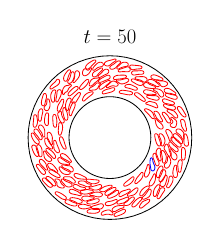
\begin{tikzpicture}[scale=0.3]

\begin{axis}[
  xmin = -21,
  xmax = 21,
  ymin = -21,
  ymax = 21,
  scale only axis,
  axis equal image,
  hide axis,
  title = {\Huge$t=50$}
  ]

% outer solid wall
\addplot [mark=none,black,line width=1.0] table{
2.0000e+01 -5.5171e-16
1.9904e+01 1.9603e+00
1.9616e+01 3.9018e+00
1.9139e+01 5.8057e+00
1.8478e+01 7.6537e+00
1.7638e+01 9.4279e+00
1.6629e+01 1.1111e+01
1.5460e+01 1.2688e+01
1.4142e+01 1.4142e+01
1.2688e+01 1.5460e+01
1.1111e+01 1.6629e+01
9.4279e+00 1.7638e+01
7.6537e+00 1.8478e+01
5.8057e+00 1.9139e+01
3.9018e+00 1.9616e+01
1.9603e+00 1.9904e+01
2.3281e-15 2.0000e+01
-1.9603e+00 1.9904e+01
-3.9018e+00 1.9616e+01
-5.8057e+00 1.9139e+01
-7.6537e+00 1.8478e+01
-9.4279e+00 1.7638e+01
-1.1111e+01 1.6629e+01
-1.2688e+01 1.5460e+01
-1.4142e+01 1.4142e+01
-1.5460e+01 1.2688e+01
-1.6629e+01 1.1111e+01
-1.7638e+01 9.4279e+00
-1.8478e+01 7.6537e+00
-1.9139e+01 5.8057e+00
-1.9616e+01 3.9018e+00
-1.9904e+01 1.9603e+00
-2.0000e+01 3.0010e-15
-1.9904e+01 -1.9603e+00
-1.9616e+01 -3.9018e+00
-1.9139e+01 -5.8057e+00
-1.8478e+01 -7.6537e+00
-1.7638e+01 -9.4279e+00
-1.6629e+01 -1.1111e+01
-1.5460e+01 -1.2688e+01
-1.4142e+01 -1.4142e+01
-1.2688e+01 -1.5460e+01
-1.1111e+01 -1.6629e+01
-9.4279e+00 -1.7638e+01
-7.6537e+00 -1.8478e+01
-5.8057e+00 -1.9139e+01
-3.9018e+00 -1.9616e+01
-1.9603e+00 -1.9904e+01
-4.7774e-15 -2.0000e+01
1.9603e+00 -1.9904e+01
3.9018e+00 -1.9616e+01
5.8057e+00 -1.9139e+01
7.6537e+00 -1.8478e+01
9.4279e+00 -1.7638e+01
1.1111e+01 -1.6629e+01
1.2688e+01 -1.5460e+01
1.4142e+01 -1.4142e+01
1.5460e+01 -1.2688e+01
1.6629e+01 -1.1111e+01
1.7638e+01 -9.4279e+00
1.8478e+01 -7.6537e+00
1.9139e+01 -5.8057e+00
1.9616e+01 -3.9018e+00
1.9904e+01 -1.9603e+00
2.0000e+01 -5.5171e-16
};

% inner solid wall
\addplot [mark=none,black,line width=1.0] table{
1.0000e+01 2.7586e-16
9.9518e+00 -9.8017e-01
9.8079e+00 -1.9509e+00
9.5694e+00 -2.9028e+00
9.2388e+00 -3.8268e+00
8.8192e+00 -4.7140e+00
8.3147e+00 -5.5557e+00
7.7301e+00 -6.3439e+00
7.0711e+00 -7.0711e+00
6.3439e+00 -7.7301e+00
5.5557e+00 -8.3147e+00
4.7140e+00 -8.8192e+00
3.8268e+00 -9.2388e+00
2.9028e+00 -9.5694e+00
1.9509e+00 -9.8079e+00
9.8017e-01 -9.9518e+00
1.1640e-15 -1.0000e+01
-9.8017e-01 -9.9518e+00
-1.9509e+00 -9.8079e+00
-2.9028e+00 -9.5694e+00
-3.8268e+00 -9.2388e+00
-4.7140e+00 -8.8192e+00
-5.5557e+00 -8.3147e+00
-6.3439e+00 -7.7301e+00
-7.0711e+00 -7.0711e+00
-7.7301e+00 -6.3439e+00
-8.3147e+00 -5.5557e+00
-8.8192e+00 -4.7140e+00
-9.2388e+00 -3.8268e+00
-9.5694e+00 -2.9028e+00
-9.8079e+00 -1.9509e+00
-9.9518e+00 -9.8017e-01
-1.0000e+01 -1.5005e-15
-9.9518e+00 9.8017e-01
-9.8079e+00 1.9509e+00
-9.5694e+00 2.9028e+00
-9.2388e+00 3.8268e+00
-8.8192e+00 4.7140e+00
-8.3147e+00 5.5557e+00
-7.7301e+00 6.3439e+00
-7.0711e+00 7.0711e+00
-6.3439e+00 7.7301e+00
-5.5557e+00 8.3147e+00
-4.7140e+00 8.8192e+00
-3.8268e+00 9.2388e+00
-2.9028e+00 9.5694e+00
-1.9509e+00 9.8079e+00
-9.8017e-01 9.9518e+00
-2.3887e-15 1.0000e+01
9.8017e-01 9.9518e+00
1.9509e+00 9.8079e+00
2.9028e+00 9.5694e+00
3.8268e+00 9.2388e+00
4.7140e+00 8.8192e+00
5.5557e+00 8.3147e+00
6.3439e+00 7.7301e+00
7.0711e+00 7.0711e+00
7.7301e+00 6.3439e+00
8.3147e+00 5.5557e+00
8.8192e+00 4.7140e+00
9.2388e+00 3.8268e+00
9.5694e+00 2.9028e+00
9.8079e+00 1.9509e+00
9.9518e+00 9.8017e-01
1.0000e+01 2.7586e-16
};

% vesicle 1
\addplot [mark=none,red,line width=1.0] table{
-5.8074e+00 1.7581e+01
-5.8485e+00 1.7511e+01
-5.8886e+00 1.7427e+01
-5.9241e+00 1.7327e+01
-5.9473e+00 1.7203e+01
-5.9427e+00 1.7062e+01
-5.8892e+00 1.6917e+01
-5.7642e+00 1.6797e+01
-5.5830e+00 1.6738e+01
-5.3896e+00 1.6753e+01
-5.2049e+00 1.6834e+01
-5.0356e+00 1.6959e+01
-4.8808e+00 1.7092e+01
-4.7317e+00 1.7232e+01
-4.5977e+00 1.7376e+01
-4.4751e+00 1.7517e+01
-4.3608e+00 1.7646e+01
-4.2548e+00 1.7760e+01
-4.1533e+00 1.7864e+01
-4.0617e+00 1.7952e+01
-3.9810e+00 1.8028e+01
-3.9081e+00 1.8094e+01
-3.8442e+00 1.8152e+01
-3.7858e+00 1.8204e+01
-3.7285e+00 1.8257e+01
-3.6688e+00 1.8313e+01
-3.6013e+00 1.8383e+01
-3.5283e+00 1.8472e+01
-3.4645e+00 1.8586e+01
-3.4387e+00 1.8731e+01
-3.4971e+00 1.8879e+01
-3.6339e+00 1.8962e+01
-3.8121e+00 1.8964e+01
-3.9951e+00 1.8906e+01
-4.1658e+00 1.8824e+01
-4.3436e+00 1.8726e+01
-4.5222e+00 1.8622e+01
-4.6947e+00 1.8517e+01
-4.8569e+00 1.8415e+01
-5.0067e+00 1.8316e+01
-5.1490e+00 1.8217e+01
-5.2814e+00 1.8119e+01
-5.3991e+00 1.8025e+01
-5.5041e+00 1.7933e+01
-5.5924e+00 1.7847e+01
-5.6629e+00 1.7772e+01
-5.7202e+00 1.7703e+01
-5.7665e+00 1.7642e+01
-5.8074e+00 1.7581e+01
};

% vesicle 2
\addplot [mark=none,red,line width=1.0] table{
-9.5476e-01 -1.2968e+01
-8.8403e-01 -1.2921e+01
-8.0245e-01 -1.2865e+01
-7.0782e-01 -1.2798e+01
-6.0190e-01 -1.2723e+01
-4.8443e-01 -1.2641e+01
-3.5623e-01 -1.2556e+01
-2.1399e-01 -1.2469e+01
-4.9945e-02 -1.2379e+01
1.2648e-01 -1.2287e+01
3.0546e-01 -1.2189e+01
4.7170e-01 -1.2055e+01
5.5274e-01 -1.1867e+01
4.6226e-01 -1.1689e+01
2.6822e-01 -1.1628e+01
7.7443e-02 -1.1637e+01
-9.8202e-02 -1.1664e+01
-2.5926e-01 -1.1694e+01
-4.0616e-01 -1.1725e+01
-5.4430e-01 -1.1756e+01
-6.6302e-01 -1.1784e+01
-7.6258e-01 -1.1810e+01
-8.5141e-01 -1.1834e+01
-9.3022e-01 -1.1856e+01
-1.0044e+00 -1.1879e+01
-1.0842e+00 -1.1905e+01
-1.1731e+00 -1.1935e+01
-1.2758e+00 -1.1974e+01
-1.3962e+00 -1.2025e+01
-1.5286e+00 -1.2088e+01
-1.6696e+00 -1.2165e+01
-1.8196e+00 -1.2260e+01
-1.9737e+00 -1.2366e+01
-2.1341e+00 -1.2478e+01
-2.3052e+00 -1.2596e+01
-2.4573e+00 -1.2742e+01
-2.5009e+00 -1.2942e+01
-2.3707e+00 -1.3099e+01
-2.1793e+00 -1.3159e+01
-1.9942e+00 -1.3191e+01
-1.8227e+00 -1.3220e+01
-1.6575e+00 -1.3235e+01
-1.5047e+00 -1.3224e+01
-1.3727e+00 -1.3191e+01
-1.2608e+00 -1.3145e+01
-1.1670e+00 -1.3098e+01
-1.0898e+00 -1.3053e+01
-1.0217e+00 -1.3011e+01
-9.5476e-01 -1.2968e+01
};

% vesicle 3
\addplot [mark=none,red,line width=1.0] table{
1.5228e+01 3.5568e+00
1.5164e+01 3.5095e+00
1.5082e+01 3.4607e+00
1.4982e+01 3.4049e+00
1.4877e+01 3.3334e+00
1.4782e+01 3.2281e+00
1.4730e+01 3.0861e+00
1.4745e+01 2.9273e+00
1.4835e+01 2.7723e+00
1.4986e+01 2.6432e+00
1.5171e+01 2.5453e+00
1.5371e+01 2.4777e+00
1.5577e+01 2.4491e+00
1.5784e+01 2.4780e+00
1.5962e+01 2.5766e+00
1.6088e+01 2.7218e+00
1.6171e+01 2.8833e+00
1.6225e+01 3.0371e+00
1.6263e+01 3.1792e+00
1.6292e+01 3.3138e+00
1.6310e+01 3.4316e+00
1.6319e+01 3.5304e+00
1.6322e+01 3.6194e+00
1.6320e+01 3.6969e+00
1.6313e+01 3.7697e+00
1.6300e+01 3.8528e+00
1.6276e+01 3.9439e+00
1.6238e+01 4.0425e+00
1.6178e+01 4.1505e+00
1.6095e+01 4.2589e+00
1.5984e+01 4.3681e+00
1.5842e+01 4.4829e+00
1.5692e+01 4.5990e+00
1.5544e+01 4.7225e+00
1.5389e+01 4.8526e+00
1.5207e+01 4.9536e+00
1.5003e+01 4.9513e+00
1.4874e+01 4.8100e+00
1.4889e+01 4.6200e+00
1.4995e+01 4.4619e+00
1.5118e+01 4.3347e+00
1.5230e+01 4.2128e+00
1.5315e+01 4.0906e+00
1.5364e+01 3.9728e+00
1.5379e+01 3.8569e+00
1.5363e+01 3.7524e+00
1.5328e+01 3.6735e+00
1.5283e+01 3.6109e+00
1.5228e+01 3.5568e+00
};

% vesicle 4
\addplot [mark=none,red,line width=1.0] table{
-1.1973e+01 -4.0387e+00
-1.2029e+01 -4.0997e+00
-1.2074e+01 -4.1819e+00
-1.2100e+01 -4.2869e+00
-1.2096e+01 -4.4108e+00
-1.2053e+01 -4.5454e+00
-1.1969e+01 -4.6770e+00
-1.1852e+01 -4.7967e+00
-1.1705e+01 -4.9098e+00
-1.1535e+01 -5.0229e+00
-1.1360e+01 -5.1298e+00
-1.1188e+01 -5.2273e+00
-1.1010e+01 -5.3210e+00
-1.0821e+01 -5.4159e+00
-1.0632e+01 -5.5094e+00
-1.0456e+01 -5.6002e+00
-1.0293e+01 -5.6915e+00
-1.0148e+01 -5.7809e+00
-1.0023e+01 -5.8649e+00
-9.9113e+00 -5.9405e+00
-9.8094e+00 -6.0013e+00
-9.7148e+00 -6.0413e+00
-9.6281e+00 -6.0573e+00
-9.5503e+00 -6.0496e+00
-9.4825e+00 -6.0176e+00
-9.4297e+00 -5.9574e+00
-9.4063e+00 -5.8694e+00
-9.4245e+00 -5.7642e+00
-9.4835e+00 -5.6519e+00
-9.5711e+00 -5.5356e+00
-9.6755e+00 -5.4116e+00
-9.7929e+00 -5.2747e+00
-9.9168e+00 -5.1300e+00
-1.0043e+01 -4.9837e+00
-1.0175e+01 -4.8321e+00
-1.0317e+01 -4.6758e+00
-1.0463e+01 -4.5260e+00
-1.0613e+01 -4.3850e+00
-1.0769e+01 -4.2558e+00
-1.0927e+01 -4.1447e+00
-1.1088e+01 -4.0537e+00
-1.1245e+01 -3.9871e+00
-1.1392e+01 -3.9443e+00
-1.1529e+01 -3.9232e+00
-1.1650e+01 -3.9211e+00
-1.1753e+01 -3.9343e+00
-1.1839e+01 -3.9592e+00
-1.1910e+01 -3.9936e+00
-1.1973e+01 -4.0387e+00
};

% vesicle 5
\addplot [mark=none,red,line width=1.0] table{
-1.3383e+01 1.3626e+01
-1.3436e+01 1.3572e+01
-1.3501e+01 1.3511e+01
-1.3579e+01 1.3442e+01
-1.3670e+01 1.3365e+01
-1.3775e+01 1.3277e+01
-1.3895e+01 1.3173e+01
-1.4023e+01 1.3055e+01
-1.4158e+01 1.2921e+01
-1.4297e+01 1.2775e+01
-1.4431e+01 1.2621e+01
-1.4552e+01 1.2454e+01
-1.4635e+01 1.2265e+01
-1.4631e+01 1.2058e+01
-1.4504e+01 1.1909e+01
-1.4318e+01 1.1885e+01
-1.4152e+01 1.1949e+01
-1.4015e+01 1.2039e+01
-1.3894e+01 1.2126e+01
-1.3781e+01 1.2202e+01
-1.3681e+01 1.2265e+01
-1.3597e+01 1.2315e+01
-1.3524e+01 1.2357e+01
-1.3461e+01 1.2393e+01
-1.3399e+01 1.2427e+01
-1.3331e+01 1.2466e+01
-1.3252e+01 1.2512e+01
-1.3158e+01 1.2568e+01
-1.3049e+01 1.2636e+01
-1.2930e+01 1.2716e+01
-1.2804e+01 1.2810e+01
-1.2673e+01 1.2922e+01
-1.2547e+01 1.3055e+01
-1.2437e+01 1.3207e+01
-1.2352e+01 1.3380e+01
-1.2302e+01 1.3576e+01
-1.2297e+01 1.3776e+01
-1.2341e+01 1.3973e+01
-1.2440e+01 1.4144e+01
-1.2591e+01 1.4252e+01
-1.2774e+01 1.4268e+01
-1.2930e+01 1.4195e+01
-1.3037e+01 1.4087e+01
-1.3116e+01 1.3978e+01
-1.3180e+01 1.3882e+01
-1.3237e+01 1.3801e+01
-1.3288e+01 1.3735e+01
-1.3335e+01 1.3679e+01
-1.3383e+01 1.3626e+01
};

% vesicle 6
\addplot [mark=none,red,line width=1.0] table{
-9.9808e+00 6.2167e+00
-9.9803e+00 6.1322e+00
-9.9749e+00 6.0342e+00
-9.9630e+00 5.9192e+00
-9.9423e+00 5.7871e+00
-9.9085e+00 5.6411e+00
-9.8480e+00 5.4883e+00
-9.7265e+00 5.3596e+00
-9.5382e+00 5.3639e+00
-9.4028e+00 5.5265e+00
-9.3199e+00 5.7375e+00
-9.2457e+00 5.9479e+00
-9.1704e+00 6.1458e+00
-9.0904e+00 6.3387e+00
-9.0077e+00 6.5249e+00
-8.9270e+00 6.7002e+00
-8.8487e+00 6.8695e+00
-8.7786e+00 7.0249e+00
-8.7195e+00 7.1630e+00
-8.6691e+00 7.2887e+00
-8.6279e+00 7.4006e+00
-8.5955e+00 7.4973e+00
-8.5702e+00 7.5809e+00
-8.5499e+00 7.6560e+00
-8.5325e+00 7.7295e+00
-8.5165e+00 7.8095e+00
-8.5024e+00 7.9035e+00
-8.4932e+00 8.0157e+00
-8.4961e+00 8.1457e+00
-8.5251e+00 8.2889e+00
-8.6059e+00 8.4265e+00
-8.7594e+00 8.5068e+00
-8.9432e+00 8.4835e+00
-9.1018e+00 8.3804e+00
-9.2312e+00 8.2285e+00
-9.3375e+00 8.0529e+00
-9.4307e+00 7.8647e+00
-9.5149e+00 7.6688e+00
-9.5902e+00 7.4760e+00
-9.6617e+00 7.2848e+00
-9.7283e+00 7.1080e+00
-9.7911e+00 6.9469e+00
-9.8477e+00 6.8032e+00
-9.8948e+00 6.6760e+00
-9.9306e+00 6.5622e+00
-9.9548e+00 6.4614e+00
-9.9694e+00 6.3729e+00
-9.9774e+00 6.2938e+00
-9.9808e+00 6.2167e+00
};

% vesicle 7
\addplot [mark=none,red,line width=1.0] table{
-1.3025e+01 3.1994e+00
-1.3018e+01 3.2793e+00
-1.3010e+01 3.3710e+00
-1.2999e+01 3.4777e+00
-1.2985e+01 3.6011e+00
-1.2973e+01 3.7369e+00
-1.2966e+01 3.8895e+00
-1.2969e+01 4.0642e+00
-1.2982e+01 4.2472e+00
-1.3006e+01 4.4390e+00
-1.3040e+01 4.6491e+00
-1.3077e+01 4.8549e+00
-1.3118e+01 5.0491e+00
-1.3169e+01 5.2418e+00
-1.3244e+01 5.4273e+00
-1.3364e+01 5.5852e+00
-1.3530e+01 5.6626e+00
-1.3696e+01 5.6337e+00
-1.3812e+01 5.5346e+00
-1.3877e+01 5.4188e+00
-1.3913e+01 5.3091e+00
-1.3934e+01 5.2109e+00
-1.3946e+01 5.1274e+00
-1.3954e+01 5.0527e+00
-1.3959e+01 4.9793e+00
-1.3963e+01 4.9004e+00
-1.3965e+01 4.8070e+00
-1.3966e+01 4.6962e+00
-1.3964e+01 4.5708e+00
-1.3959e+01 4.4304e+00
-1.3951e+01 4.2732e+00
-1.3941e+01 4.0988e+00
-1.3929e+01 3.9144e+00
-1.3916e+01 3.7261e+00
-1.3900e+01 3.5251e+00
-1.3876e+01 3.3041e+00
-1.3839e+01 3.0902e+00
-1.3782e+01 2.8970e+00
-1.3694e+01 2.7208e+00
-1.3564e+01 2.5813e+00
-1.3401e+01 2.5130e+00
-1.3241e+01 2.5401e+00
-1.3131e+01 2.6397e+00
-1.3075e+01 2.7617e+00
-1.3051e+01 2.8736e+00
-1.3040e+01 2.9691e+00
-1.3034e+01 3.0530e+00
-1.3030e+01 3.1275e+00
-1.3025e+01 3.1994e+00
};

% vesicle 8
\addplot [mark=none,red,line width=1.0] table{
-8.2784e+00 1.3924e+01
-8.2262e+00 1.3983e+01
-8.1647e+00 1.4050e+01
-8.0928e+00 1.4129e+01
-8.0130e+00 1.4217e+01
-7.9250e+00 1.4319e+01
-7.8280e+00 1.4441e+01
-7.7257e+00 1.4585e+01
-7.6253e+00 1.4751e+01
-7.5360e+00 1.4935e+01
-7.4662e+00 1.5129e+01
-7.4210e+00 1.5330e+01
-7.4060e+00 1.5543e+01
-7.4292e+00 1.5753e+01
-7.4935e+00 1.5946e+01
-7.5923e+00 1.6104e+01
-7.7214e+00 1.6225e+01
-7.8659e+00 1.6299e+01
-8.0074e+00 1.6325e+01
-8.1388e+00 1.6310e+01
-8.2475e+00 1.6267e+01
-8.3295e+00 1.6208e+01
-8.3901e+00 1.6144e+01
-8.4340e+00 1.6080e+01
-8.4678e+00 1.6014e+01
-8.4968e+00 1.5937e+01
-8.5209e+00 1.5847e+01
-8.5401e+00 1.5742e+01
-8.5561e+00 1.5619e+01
-8.5714e+00 1.5482e+01
-8.5888e+00 1.5331e+01
-8.6080e+00 1.5164e+01
-8.6263e+00 1.4978e+01
-8.6444e+00 1.4779e+01
-8.6720e+00 1.4575e+01
-8.7229e+00 1.4366e+01
-8.8039e+00 1.4165e+01
-8.9055e+00 1.3983e+01
-8.9963e+00 1.3818e+01
-9.0389e+00 1.3641e+01
-8.9719e+00 1.3481e+01
-8.8139e+00 1.3430e+01
-8.6723e+00 1.3486e+01
-8.5713e+00 1.3575e+01
-8.4936e+00 1.3665e+01
-8.4294e+00 1.3745e+01
-8.3755e+00 1.3811e+01
-8.3269e+00 1.3868e+01
-8.2784e+00 1.3924e+01
};

% vesicle 9
\addplot [mark=none,red,line width=1.0] table{
-4.0476e+00 -1.1298e+01
-3.9675e+00 -1.1294e+01
-3.8748e+00 -1.1286e+01
-3.7666e+00 -1.1272e+01
-3.6430e+00 -1.1250e+01
-3.5048e+00 -1.1221e+01
-3.3553e+00 -1.1182e+01
-3.1978e+00 -1.1135e+01
-3.0282e+00 -1.1072e+01
-2.8496e+00 -1.0981e+01
-2.6905e+00 -1.0838e+01
-2.6340e+00 -1.0638e+01
-2.7389e+00 -1.0467e+01
-2.9203e+00 -1.0387e+01
-3.1124e+00 -1.0354e+01
-3.3019e+00 -1.0335e+01
-3.4878e+00 -1.0320e+01
-3.6621e+00 -1.0307e+01
-3.8173e+00 -1.0295e+01
-3.9525e+00 -1.0283e+01
-4.0701e+00 -1.0272e+01
-4.1706e+00 -1.0262e+01
-4.2562e+00 -1.0253e+01
-4.3316e+00 -1.0245e+01
-4.4049e+00 -1.0238e+01
-4.4854e+00 -1.0229e+01
-4.5795e+00 -1.0218e+01
-4.6901e+00 -1.0206e+01
-4.8188e+00 -1.0192e+01
-4.9661e+00 -1.0177e+01
-5.1291e+00 -1.0165e+01
-5.3063e+00 -1.0158e+01
-5.4951e+00 -1.0170e+01
-5.6767e+00 -1.0232e+01
-5.7901e+00 -1.0388e+01
-5.7598e+00 -1.0586e+01
-5.6180e+00 -1.0729e+01
-5.4491e+00 -1.0823e+01
-5.2697e+00 -1.0903e+01
-5.0894e+00 -1.0979e+01
-4.9263e+00 -1.1049e+01
-4.7757e+00 -1.1117e+01
-4.6370e+00 -1.1179e+01
-4.5070e+00 -1.1230e+01
-4.3887e+00 -1.1265e+01
-4.2858e+00 -1.1285e+01
-4.1984e+00 -1.1294e+01
-4.1217e+00 -1.1298e+01
-4.0476e+00 -1.1298e+01
};

% vesicle 10
\addplot [mark=none,red,line width=1.0] table{
-9.7417e+00 -1.5176e+01
-9.6858e+00 -1.5233e+01
-9.6090e+00 -1.5283e+01
-9.5107e+00 -1.5325e+01
-9.3907e+00 -1.5364e+01
-9.2516e+00 -1.5403e+01
-9.0982e+00 -1.5448e+01
-8.9335e+00 -1.5501e+01
-8.7602e+00 -1.5565e+01
-8.5826e+00 -1.5643e+01
-8.4082e+00 -1.5738e+01
-8.2385e+00 -1.5850e+01
-8.0662e+00 -1.5968e+01
-7.8804e+00 -1.6060e+01
-7.6858e+00 -1.6096e+01
-7.4999e+00 -1.6086e+01
-7.3249e+00 -1.6054e+01
-7.1623e+00 -1.6012e+01
-7.0176e+00 -1.5961e+01
-6.9004e+00 -1.5892e+01
-6.8201e+00 -1.5807e+01
-6.7799e+00 -1.5718e+01
-6.7719e+00 -1.5636e+01
-6.7847e+00 -1.5565e+01
-6.8126e+00 -1.5500e+01
-6.8562e+00 -1.5436e+01
-6.9192e+00 -1.5370e+01
-7.0029e+00 -1.5300e+01
-7.1048e+00 -1.5229e+01
-7.2253e+00 -1.5155e+01
-7.3651e+00 -1.5081e+01
-7.5198e+00 -1.5013e+01
-7.6861e+00 -1.4952e+01
-7.8667e+00 -1.4897e+01
-8.0568e+00 -1.4848e+01
-8.2554e+00 -1.4802e+01
-8.4588e+00 -1.4760e+01
-8.6596e+00 -1.4725e+01
-8.8589e+00 -1.4698e+01
-9.0548e+00 -1.4681e+01
-9.2376e+00 -1.4679e+01
-9.4024e+00 -1.4694e+01
-9.5470e+00 -1.4730e+01
-9.6632e+00 -1.4790e+01
-9.7432e+00 -1.4868e+01
-9.7859e+00 -1.4954e+01
-9.7949e+00 -1.5039e+01
-9.7780e+00 -1.5113e+01
-9.7417e+00 -1.5176e+01
};

% vesicle 11
\addplot [mark=none,red,line width=1.0] table{
1.1224e+00 -1.6952e+01
1.0566e+00 -1.6992e+01
9.8226e-01 -1.7040e+01
8.9850e-01 -1.7102e+01
8.0566e-01 -1.7181e+01
7.0767e-01 -1.7283e+01
6.1533e-01 -1.7413e+01
5.4825e-01 -1.7578e+01
5.3926e-01 -1.7767e+01
6.1363e-01 -1.7944e+01
7.6769e-01 -1.8067e+01
9.7034e-01 -1.8107e+01
1.1794e+00 -1.8071e+01
1.3742e+00 -1.7994e+01
1.5531e+00 -1.7902e+01
1.7200e+00 -1.7806e+01
1.8753e+00 -1.7715e+01
2.0193e+00 -1.7631e+01
2.1501e+00 -1.7558e+01
2.2658e+00 -1.7498e+01
2.3675e+00 -1.7449e+01
2.4565e+00 -1.7410e+01
2.5347e+00 -1.7379e+01
2.6051e+00 -1.7354e+01
2.6743e+00 -1.7332e+01
2.7509e+00 -1.7310e+01
2.8409e+00 -1.7288e+01
2.9471e+00 -1.7264e+01
3.0683e+00 -1.7236e+01
3.2014e+00 -1.7195e+01
3.3374e+00 -1.7121e+01
3.4423e+00 -1.6989e+01
3.4554e+00 -1.6810e+01
3.3444e+00 -1.6656e+01
3.1611e+00 -1.6584e+01
2.9594e+00 -1.6572e+01
2.7516e+00 -1.6586e+01
2.5449e+00 -1.6604e+01
2.3467e+00 -1.6620e+01
2.1547e+00 -1.6637e+01
1.9726e+00 -1.6659e+01
1.8055e+00 -1.6688e+01
1.6555e+00 -1.6725e+01
1.5248e+00 -1.6767e+01
1.4144e+00 -1.6809e+01
1.3235e+00 -1.6848e+01
1.2487e+00 -1.6884e+01
1.1841e+00 -1.6917e+01
1.1224e+00 -1.6952e+01
};

% vesicle 12
\addplot [mark=none,red,line width=1.0] table{
1.4949e+01 5.7630e+00
1.5011e+01 5.7171e+00
1.5083e+01 5.6610e+00
1.5168e+01 5.5916e+00
1.5263e+01 5.5096e+00
1.5368e+01 5.4128e+00
1.5481e+01 5.3018e+00
1.5600e+01 5.1781e+00
1.5730e+01 5.0445e+00
1.5879e+01 4.9138e+00
1.6054e+01 4.8136e+00
1.6258e+01 4.7820e+00
1.6444e+01 4.8533e+00
1.6556e+01 5.0116e+00
1.6572e+01 5.2127e+00
1.6518e+01 5.4025e+00
1.6438e+01 5.5582e+00
1.6352e+01 5.6959e+00
1.6265e+01 5.8217e+00
1.6185e+01 5.9305e+00
1.6114e+01 6.0237e+00
1.6051e+01 6.1011e+00
1.5995e+01 6.1671e+00
1.5945e+01 6.2232e+00
1.5895e+01 6.2751e+00
1.5835e+01 6.3316e+00
1.5763e+01 6.3929e+00
1.5673e+01 6.4578e+00
1.5559e+01 6.5238e+00
1.5424e+01 6.5831e+00
1.5269e+01 6.6347e+00
1.5100e+01 6.6842e+00
1.4929e+01 6.7343e+00
1.4751e+01 6.7848e+00
1.4556e+01 6.8331e+00
1.4350e+01 6.8660e+00
1.4144e+01 6.8456e+00
1.3986e+01 6.7216e+00
1.3963e+01 6.5339e+00
1.4057e+01 6.3685e+00
1.4199e+01 6.2462e+00
1.4338e+01 6.1550e+00
1.4463e+01 6.0789e+00
1.4575e+01 6.0109e+00
1.4674e+01 5.9493e+00
1.4759e+01 5.8943e+00
1.4828e+01 5.8478e+00
1.4889e+01 5.8056e+00
1.4949e+01 5.7630e+00
};

% vesicle 13
\addplot [mark=none,red,line width=1.0] table{
8.8307e-01 1.4654e+01
8.5658e-01 1.4576e+01
8.4868e-01 1.4483e+01
8.7697e-01 1.4376e+01
9.5847e-01 1.4277e+01
1.0897e+00 1.4214e+01
1.2488e+00 1.4193e+01
1.4230e+00 1.4205e+01
1.6100e+00 1.4234e+01
1.8062e+00 1.4265e+01
2.0069e+00 1.4290e+01
2.2141e+00 1.4311e+01
2.4250e+00 1.4335e+01
2.6293e+00 1.4361e+01
2.8281e+00 1.4390e+01
3.0142e+00 1.4421e+01
3.1876e+00 1.4451e+01
3.3532e+00 1.4483e+01
3.5068e+00 1.4517e+01
3.6424e+00 1.4553e+01
3.7565e+00 1.4594e+01
3.8485e+00 1.4641e+01
3.9193e+00 1.4693e+01
3.9713e+00 1.4751e+01
4.0071e+00 1.4817e+01
4.0243e+00 1.4897e+01
4.0123e+00 1.4990e+01
3.9584e+00 1.5085e+01
3.8602e+00 1.5166e+01
3.7267e+00 1.5222e+01
3.5680e+00 1.5255e+01
3.3938e+00 1.5270e+01
3.2107e+00 1.5275e+01
3.0126e+00 1.5273e+01
2.8010e+00 1.5267e+01
2.5928e+00 1.5259e+01
2.3936e+00 1.5251e+01
2.1952e+00 1.5241e+01
1.9940e+00 1.5224e+01
1.8012e+00 1.5197e+01
1.6235e+00 1.5156e+01
1.4619e+00 1.5103e+01
1.3187e+00 1.5041e+01
1.1986e+00 1.4974e+01
1.1024e+00 1.4908e+01
1.0262e+00 1.4844e+01
9.6645e-01 1.4781e+01
9.1979e-01 1.4719e+01
8.8307e-01 1.4654e+01
};

% vesicle 14
\addplot [mark=none,red,line width=1.0] table{
-6.0559e+00 9.1502e+00
-5.9979e+00 9.2037e+00
-5.9300e+00 9.2667e+00
-5.8489e+00 9.3415e+00
-5.7594e+00 9.4228e+00
-5.6534e+00 9.5172e+00
-5.5282e+00 9.6261e+00
-5.3919e+00 9.7415e+00
-5.2382e+00 9.8685e+00
-5.0714e+00 1.0003e+01
-4.9077e+00 1.0133e+01
-4.7400e+00 1.0264e+01
-4.5662e+00 1.0401e+01
-4.3998e+00 1.0536e+01
-4.2460e+00 1.0678e+01
-4.1281e+00 1.0838e+01
-4.0935e+00 1.1013e+01
-4.1804e+00 1.1155e+01
-4.3314e+00 1.1200e+01
-4.4680e+00 1.1188e+01
-4.5845e+00 1.1162e+01
-4.6814e+00 1.1138e+01
-4.7673e+00 1.1117e+01
-4.8423e+00 1.1098e+01
-4.9114e+00 1.1080e+01
-4.9918e+00 1.1058e+01
-5.0806e+00 1.1031e+01
-5.1812e+00 1.0996e+01
-5.3032e+00 1.0947e+01
-5.4343e+00 1.0886e+01
-5.5721e+00 1.0811e+01
-5.7222e+00 1.0716e+01
-5.8724e+00 1.0606e+01
-6.0211e+00 1.0479e+01
-6.1679e+00 1.0330e+01
-6.3018e+00 1.0167e+01
-6.4173e+00 9.9985e+00
-6.5181e+00 9.8221e+00
-6.6050e+00 9.6342e+00
-6.6676e+00 9.4483e+00
-6.6968e+00 9.2611e+00
-6.6727e+00 9.0925e+00
-6.5851e+00 8.9709e+00
-6.4560e+00 8.9259e+00
-6.3379e+00 8.9473e+00
-6.2451e+00 8.9958e+00
-6.1743e+00 9.0474e+00
-6.1146e+00 9.0976e+00
-6.0559e+00 9.1502e+00
};

% vesicle 15
\addplot [mark=none,red,line width=1.0] table{
-1.5038e+01 4.6351e+00
-1.5033e+01 4.7157e+00
-1.5026e+01 4.8093e+00
-1.5017e+01 4.9181e+00
-1.5006e+01 5.0424e+00
-1.4993e+01 5.1852e+00
-1.4981e+01 5.3457e+00
-1.4978e+01 5.5176e+00
-1.4998e+01 5.7007e+00
-1.5069e+01 5.8856e+00
-1.5214e+01 6.0207e+00
-1.5420e+01 6.0389e+00
-1.5600e+01 5.9162e+00
-1.5708e+01 5.7377e+00
-1.5776e+01 5.5523e+00
-1.5825e+01 5.3708e+00
-1.5865e+01 5.1958e+00
-1.5895e+01 5.0413e+00
-1.5919e+01 4.9043e+00
-1.5939e+01 4.7781e+00
-1.5954e+01 4.6664e+00
-1.5967e+01 4.5705e+00
-1.5976e+01 4.4867e+00
-1.5984e+01 4.4117e+00
-1.5991e+01 4.3386e+00
-1.5997e+01 4.2588e+00
-1.6002e+01 4.1676e+00
-1.6005e+01 4.0616e+00
-1.6002e+01 3.9365e+00
-1.5990e+01 3.7916e+00
-1.5963e+01 3.6328e+00
-1.5915e+01 3.4649e+00
-1.5839e+01 3.2923e+00
-1.5732e+01 3.1289e+00
-1.5579e+01 2.9920e+00
-1.5375e+01 2.9317e+00
-1.5180e+01 3.0107e+00
-1.5076e+01 3.1807e+00
-1.5041e+01 3.3713e+00
-1.5037e+01 3.5597e+00
-1.5041e+01 3.7381e+00
-1.5046e+01 3.9041e+00
-1.5049e+01 4.0527e+00
-1.5050e+01 4.1834e+00
-1.5050e+01 4.2990e+00
-1.5048e+01 4.3993e+00
-1.5045e+01 4.4848e+00
-1.5042e+01 4.5607e+00
-1.5038e+01 4.6351e+00
};

% vesicle 16
\addplot [mark=none,red,line width=1.0] table{
-1.6738e+01 1.2808e+00
-1.6700e+01 1.2169e+00
-1.6657e+01 1.1360e+00
-1.6608e+01 1.0329e+00
-1.6563e+01 9.1755e-01
-1.6519e+01 7.7869e-01
-1.6479e+01 6.1624e-01
-1.6439e+01 4.5052e-01
-1.6372e+01 2.8169e-01
-1.6240e+01 1.4453e-01
-1.6045e+01 1.4639e-01
-1.5930e+01 3.1754e-01
-1.5917e+01 5.2990e-01
-1.5927e+01 7.4046e-01
-1.5929e+01 9.3407e-01
-1.5925e+01 1.1210e+00
-1.5921e+01 1.3082e+00
-1.5923e+01 1.4749e+00
-1.5933e+01 1.6233e+00
-1.5950e+01 1.7613e+00
-1.5972e+01 1.8750e+00
-1.5995e+01 1.9667e+00
-1.6020e+01 2.0514e+00
-1.6045e+01 2.1219e+00
-1.6069e+01 2.1848e+00
-1.6101e+01 2.2602e+00
-1.6141e+01 2.3411e+00
-1.6189e+01 2.4300e+00
-1.6256e+01 2.5371e+00
-1.6337e+01 2.6509e+00
-1.6437e+01 2.7689e+00
-1.6566e+01 2.8920e+00
-1.6717e+01 2.9973e+00
-1.6904e+01 3.0671e+00
-1.7109e+01 3.0590e+00
-1.7286e+01 2.9548e+00
-1.7403e+01 2.7770e+00
-1.7446e+01 2.5750e+00
-1.7429e+01 2.3732e+00
-1.7367e+01 2.1865e+00
-1.7279e+01 2.0248e+00
-1.7181e+01 1.8809e+00
-1.7084e+01 1.7542e+00
-1.7002e+01 1.6498e+00
-1.6929e+01 1.5557e+00
-1.6867e+01 1.4718e+00
-1.6820e+01 1.4058e+00
-1.6779e+01 1.3446e+00
-1.6738e+01 1.2808e+00
};

% vesicle 17
\addplot [mark=none,red,line width=1.0] table{
4.6238e+00 -1.3356e+01
4.6896e+00 -1.3309e+01
4.7629e+00 -1.3252e+01
4.8422e+00 -1.3178e+01
4.9190e+00 -1.3083e+01
4.9785e+00 -1.2956e+01
4.9850e+00 -1.2800e+01
4.9036e+00 -1.2660e+01
4.7432e+00 -1.2591e+01
4.5575e+00 -1.2606e+01
4.3769e+00 -1.2664e+01
4.1924e+00 -1.2733e+01
4.0010e+00 -1.2800e+01
3.8023e+00 -1.2860e+01
3.6096e+00 -1.2912e+01
3.4270e+00 -1.2960e+01
3.2534e+00 -1.3010e+01
3.0962e+00 -1.3063e+01
2.9587e+00 -1.3119e+01
2.8398e+00 -1.3178e+01
2.7408e+00 -1.3238e+01
2.6608e+00 -1.3296e+01
2.5950e+00 -1.3351e+01
2.5404e+00 -1.3403e+01
2.4908e+00 -1.3457e+01
2.4386e+00 -1.3521e+01
2.3832e+00 -1.3600e+01
2.3257e+00 -1.3697e+01
2.2696e+00 -1.3816e+01
2.2253e+00 -1.3952e+01
2.2074e+00 -1.4104e+01
2.2450e+00 -1.4268e+01
2.3727e+00 -1.4397e+01
2.5639e+00 -1.4426e+01
2.7614e+00 -1.4365e+01
2.9519e+00 -1.4267e+01
3.1392e+00 -1.4167e+01
3.3205e+00 -1.4077e+01
3.4958e+00 -1.3995e+01
3.6626e+00 -1.3917e+01
3.8207e+00 -1.3839e+01
3.9724e+00 -1.3757e+01
4.1088e+00 -1.3678e+01
4.2247e+00 -1.3607e+01
4.3270e+00 -1.3544e+01
4.4171e+00 -1.3488e+01
4.4925e+00 -1.3441e+01
4.5593e+00 -1.3398e+01
4.6238e+00 -1.3356e+01
};

% vesicle 18
\addplot [mark=none,red,line width=1.0] table{
-1.0262e+01 1.2751e+01
-1.0341e+01 1.2737e+01
-1.0432e+01 1.2725e+01
-1.0537e+01 1.2712e+01
-1.0657e+01 1.2693e+01
-1.0789e+01 1.2655e+01
-1.0929e+01 1.2587e+01
-1.1067e+01 1.2481e+01
-1.1195e+01 1.2343e+01
-1.1308e+01 1.2181e+01
-1.1403e+01 1.2008e+01
-1.1483e+01 1.1823e+01
-1.1544e+01 1.1624e+01
-1.1579e+01 1.1418e+01
-1.1591e+01 1.1208e+01
-1.1589e+01 1.1009e+01
-1.1578e+01 1.0825e+01
-1.1537e+01 1.0662e+01
-1.1438e+01 1.0549e+01
-1.1310e+01 1.0531e+01
-1.1211e+01 1.0588e+01
-1.1151e+01 1.0668e+01
-1.1112e+01 1.0747e+01
-1.1079e+01 1.0819e+01
-1.1043e+01 1.0887e+01
-1.0995e+01 1.0955e+01
-1.0928e+01 1.1021e+01
-1.0837e+01 1.1080e+01
-1.0727e+01 1.1130e+01
-1.0602e+01 1.1183e+01
-1.0473e+01 1.1264e+01
-1.0358e+01 1.1395e+01
-1.0273e+01 1.1565e+01
-1.0203e+01 1.1749e+01
-1.0117e+01 1.1937e+01
-9.9956e+00 1.2115e+01
-9.8399e+00 1.2271e+01
-9.6723e+00 1.2405e+01
-9.5238e+00 1.2539e+01
-9.4289e+00 1.2701e+01
-9.4417e+00 1.2873e+01
-9.5635e+00 1.2974e+01
-9.7095e+00 1.2976e+01
-9.8347e+00 1.2929e+01
-9.9405e+00 1.2874e+01
-1.0033e+01 1.2828e+01
-1.0115e+01 1.2793e+01
-1.0189e+01 1.2769e+01
-1.0262e+01 1.2751e+01
};

% vesicle 19
\addplot [mark=none,red,line width=1.0] table{
-3.6165e+00 -1.7581e+01
-3.6895e+00 -1.7579e+01
-3.7794e+00 -1.7574e+01
-3.8896e+00 -1.7561e+01
-4.0092e+00 -1.7540e+01
-4.1479e+00 -1.7508e+01
-4.3066e+00 -1.7471e+01
-4.4746e+00 -1.7455e+01
-4.6580e+00 -1.7472e+01
-4.8520e+00 -1.7521e+01
-5.0431e+00 -1.7585e+01
-5.2324e+00 -1.7664e+01
-5.4081e+00 -1.7771e+01
-5.5376e+00 -1.7921e+01
-5.5759e+00 -1.8112e+01
-5.4940e+00 -1.8284e+01
-5.3489e+00 -1.8382e+01
-5.1881e+00 -1.8429e+01
-5.0365e+00 -1.8449e+01
-4.8998e+00 -1.8458e+01
-4.7822e+00 -1.8463e+01
-4.6851e+00 -1.8466e+01
-4.5971e+00 -1.8469e+01
-4.5225e+00 -1.8471e+01
-4.4541e+00 -1.8473e+01
-4.3718e+00 -1.8476e+01
-4.2804e+00 -1.8478e+01
-4.1773e+00 -1.8481e+01
-4.0499e+00 -1.8483e+01
-3.9077e+00 -1.8484e+01
-3.7508e+00 -1.8480e+01
-3.5725e+00 -1.8469e+01
-3.3889e+00 -1.8445e+01
-3.2025e+00 -1.8405e+01
-3.0091e+00 -1.8341e+01
-2.8269e+00 -1.8251e+01
-2.6655e+00 -1.8131e+01
-2.5370e+00 -1.7970e+01
-2.4867e+00 -1.7780e+01
-2.5610e+00 -1.7610e+01
-2.7300e+00 -1.7540e+01
-2.8965e+00 -1.7542e+01
-3.0455e+00 -1.7556e+01
-3.1766e+00 -1.7567e+01
-3.2906e+00 -1.7574e+01
-3.3918e+00 -1.7578e+01
-3.4705e+00 -1.7580e+01
-3.5427e+00 -1.7581e+01
-3.6165e+00 -1.7581e+01
};

% vesicle 20
\addplot [mark=none,red,line width=1.0] table{
-1.4240e+00 1.2263e+01
-1.3582e+00 1.2316e+01
-1.2864e+00 1.2376e+01
-1.2070e+00 1.2445e+01
-1.1170e+00 1.2528e+01
-1.0187e+00 1.2624e+01
-9.0909e-01 1.2731e+01
-7.7996e-01 1.2849e+01
-6.3272e-01 1.2971e+01
-4.7156e-01 1.3096e+01
-2.9182e-01 1.3236e+01
-1.1208e-01 1.3389e+01
3.1446e-02 1.3558e+01
8.3209e-02 1.3756e+01
-1.3113e-02 1.3925e+01
-1.9784e-01 1.3979e+01
-3.8093e-01 1.3946e+01
-5.4286e-01 1.3884e+01
-6.8071e-01 1.3820e+01
-7.9657e-01 1.3764e+01
-8.9803e-01 1.3713e+01
-9.8720e-01 1.3668e+01
-1.0633e+00 1.3630e+01
-1.1334e+00 1.3594e+01
-1.2042e+00 1.3557e+01
-1.2782e+00 1.3518e+01
-1.3624e+00 1.3473e+01
-1.4585e+00 1.3419e+01
-1.5677e+00 1.3355e+01
-1.6928e+00 1.3277e+01
-1.8260e+00 1.3187e+01
-1.9658e+00 1.3084e+01
-2.1125e+00 1.2965e+01
-2.2585e+00 1.2835e+01
-2.3955e+00 1.2693e+01
-2.5241e+00 1.2524e+01
-2.6245e+00 1.2326e+01
-2.6524e+00 1.2115e+01
-2.5703e+00 1.1919e+01
-2.3978e+00 1.1815e+01
-2.2160e+00 1.1810e+01
-2.0588e+00 1.1856e+01
-1.9248e+00 1.1921e+01
-1.8068e+00 1.1990e+01
-1.7060e+00 1.2056e+01
-1.6217e+00 1.2115e+01
-1.5480e+00 1.2169e+01
-1.4840e+00 1.2217e+01
-1.4240e+00 1.2263e+01
};

% vesicle 21
\addplot [mark=none,red,line width=1.0] table{
-8.1301e+00 1.0584e+01
-8.1876e+00 1.0527e+01
-8.2562e+00 1.0457e+01
-8.3375e+00 1.0373e+01
-8.4269e+00 1.0278e+01
-8.5266e+00 1.0172e+01
-8.6372e+00 1.0053e+01
-8.7558e+00 9.9227e+00
-8.8781e+00 9.7820e+00
-8.9955e+00 9.6288e+00
-9.0998e+00 9.4510e+00
-9.1753e+00 9.2572e+00
-9.2299e+00 9.0695e+00
-9.2897e+00 8.8868e+00
-9.3493e+00 8.6995e+00
-9.3245e+00 8.5122e+00
-9.1547e+00 8.4649e+00
-9.0328e+00 8.5913e+00
-8.9307e+00 8.7096e+00
-8.7973e+00 8.7389e+00
-8.6848e+00 8.6942e+00
-8.5941e+00 8.6420e+00
-8.5061e+00 8.6138e+00
-8.4257e+00 8.6170e+00
-8.3551e+00 8.6449e+00
-8.2888e+00 8.6958e+00
-8.2285e+00 8.7665e+00
-8.1702e+00 8.8572e+00
-8.1064e+00 8.9729e+00
-8.0335e+00 9.1085e+00
-7.9502e+00 9.2567e+00
-7.8558e+00 9.4156e+00
-7.7538e+00 9.5815e+00
-7.6479e+00 9.7526e+00
-7.5369e+00 9.9348e+00
-7.4262e+00 1.0124e+01
-7.3241e+00 1.0315e+01
-7.2420e+00 1.0512e+01
-7.2038e+00 1.0711e+01
-7.2425e+00 1.0897e+01
-7.3749e+00 1.1017e+01
-7.5423e+00 1.1027e+01
-7.6830e+00 1.0969e+01
-7.7942e+00 1.0893e+01
-7.8854e+00 1.0817e+01
-7.9604e+00 1.0749e+01
-8.0214e+00 1.0691e+01
-8.0759e+00 1.0638e+01
-8.1301e+00 1.0584e+01
};

% vesicle 22
\addplot [mark=none,red,line width=1.0] table{
2.2399e-01 1.2065e+01
1.4954e-01 1.2040e+01
6.3367e-02 1.2010e+01
-3.7632e-02 1.1977e+01
-1.5470e-01 1.1940e+01
-2.9319e-01 1.1901e+01
-4.5429e-01 1.1861e+01
-6.2918e-01 1.1820e+01
-8.0947e-01 1.1772e+01
-9.9712e-01 1.1710e+01
-1.1865e+00 1.1630e+01
-1.3757e+00 1.1534e+01
-1.5553e+00 1.1423e+01
-1.7179e+00 1.1291e+01
-1.8406e+00 1.1131e+01
-1.8879e+00 1.0942e+01
-1.8195e+00 1.0775e+01
-1.6732e+00 1.0692e+01
-1.5199e+00 1.0680e+01
-1.3821e+00 1.0696e+01
-1.2644e+00 1.0719e+01
-1.1653e+00 1.0743e+01
-1.0794e+00 1.0765e+01
-1.0053e+00 1.0784e+01
-9.3528e-01 1.0803e+01
-8.5754e-01 1.0824e+01
-7.6854e-01 1.0847e+01
-6.6384e-01 1.0874e+01
-5.3811e-01 1.0906e+01
-3.9501e-01 1.0942e+01
-2.3805e-01 1.0981e+01
-6.5107e-02 1.1026e+01
1.2323e-01 1.1078e+01
3.1870e-01 1.1139e+01
5.1867e-01 1.1215e+01
7.1603e-01 1.1310e+01
9.0123e-01 1.1430e+01
1.0532e+00 1.1573e+01
1.1542e+00 1.1740e+01
1.1798e+00 1.1919e+01
1.1098e+00 1.2079e+01
9.6737e-01 1.2173e+01
8.1180e-01 1.2198e+01
6.7268e-01 1.2188e+01
5.5288e-01 1.2165e+01
4.5143e-01 1.2138e+01
3.6811e-01 1.2113e+01
2.9496e-01 1.2089e+01
2.2399e-01 1.2065e+01
};

% vesicle 23
\addplot [mark=none,red,line width=1.0] table{
-1.2684e+01 -3.7089e+00
-1.2602e+01 -3.7053e+00
-1.2513e+01 -3.6771e+00
-1.2426e+01 -3.6107e+00
-1.2362e+01 -3.4996e+00
-1.2337e+01 -3.3535e+00
-1.2350e+01 -3.1895e+00
-1.2390e+01 -3.0124e+00
-1.2448e+01 -2.8323e+00
-1.2520e+01 -2.6478e+00
-1.2599e+01 -2.4652e+00
-1.2678e+01 -2.2867e+00
-1.2761e+01 -2.0942e+00
-1.2839e+01 -1.9053e+00
-1.2910e+01 -1.7175e+00
-1.2973e+01 -1.5382e+00
-1.3029e+01 -1.3702e+00
-1.3081e+01 -1.2137e+00
-1.3133e+01 -1.0725e+00
-1.3186e+01 -9.5016e-01
-1.3244e+01 -8.4997e-01
-1.3307e+01 -7.7205e-01
-1.3376e+01 -7.1663e-01
-1.3447e+01 -6.8477e-01
-1.3522e+01 -6.7585e-01
-1.3602e+01 -6.9513e-01
-1.3676e+01 -7.5176e-01
-1.3727e+01 -8.4672e-01
-1.3745e+01 -9.7056e-01
-1.3737e+01 -1.1126e+00
-1.3718e+01 -1.2738e+00
-1.3705e+01 -1.4562e+00
-1.3705e+01 -1.6481e+00
-1.3711e+01 -1.8413e+00
-1.3716e+01 -2.0442e+00
-1.3714e+01 -2.2531e+00
-1.3702e+01 -2.4707e+00
-1.3665e+01 -2.6799e+00
-1.3598e+01 -2.8657e+00
-1.3507e+01 -3.0345e+00
-1.3405e+01 -3.1833e+00
-1.3300e+01 -3.3121e+00
-1.3197e+01 -3.4213e+00
-1.3099e+01 -3.5101e+00
-1.3006e+01 -3.5812e+00
-1.2917e+01 -3.6355e+00
-1.2836e+01 -3.6733e+00
-1.2760e+01 -3.6972e+00
-1.2684e+01 -3.7089e+00
};

% vesicle 24
\addplot [mark=none,red,line width=1.0] table{
-1.4191e+01 -2.0667e+00
-1.4238e+01 -2.0013e+00
-1.4294e+01 -1.9276e+00
-1.4361e+01 -1.8431e+00
-1.4439e+01 -1.7467e+00
-1.4527e+01 -1.6353e+00
-1.4621e+01 -1.5063e+00
-1.4719e+01 -1.3604e+00
-1.4818e+01 -1.2017e+00
-1.4917e+01 -1.0374e+00
-1.5019e+01 -8.6397e-01
-1.5116e+01 -6.8060e-01
-1.5201e+01 -4.9100e-01
-1.5289e+01 -3.0417e-01
-1.5422e+01 -1.5134e-01
-1.5606e+01 -9.2875e-02
-1.5774e+01 -1.5205e-01
-1.5875e+01 -2.8134e-01
-1.5919e+01 -4.2431e-01
-1.5935e+01 -5.5787e-01
-1.5937e+01 -6.7586e-01
-1.5933e+01 -7.7714e-01
-1.5926e+01 -8.6397e-01
-1.5917e+01 -9.4033e-01
-1.5906e+01 -1.0136e+00
-1.5892e+01 -1.0924e+00
-1.5872e+01 -1.1824e+00
-1.5844e+01 -1.2858e+00
-1.5806e+01 -1.4014e+00
-1.5758e+01 -1.5267e+00
-1.5696e+01 -1.6625e+00
-1.5615e+01 -1.8095e+00
-1.5514e+01 -1.9634e+00
-1.5391e+01 -2.1154e+00
-1.5245e+01 -2.2571e+00
-1.5084e+01 -2.3810e+00
-1.4914e+01 -2.4938e+00
-1.4741e+01 -2.6032e+00
-1.4569e+01 -2.7063e+00
-1.4391e+01 -2.7851e+00
-1.4213e+01 -2.8026e+00
-1.4069e+01 -2.7352e+00
-1.3996e+01 -2.6082e+00
-1.3994e+01 -2.4754e+00
-1.4026e+01 -2.3628e+00
-1.4068e+01 -2.2706e+00
-1.4110e+01 -2.1945e+00
-1.4150e+01 -2.1289e+00
-1.4191e+01 -2.0667e+00
};

% vesicle 25
\addplot [mark=none,red,line width=1.0] table{
1.1647e+01 7.6831e+00
1.1613e+01 7.7553e+00
1.1572e+01 7.8380e+00
1.1525e+01 7.9362e+00
1.1473e+01 8.0533e+00
1.1408e+01 8.1869e+00
1.1314e+01 8.3245e+00
1.1180e+01 8.4440e+00
1.1014e+01 8.5316e+00
1.0828e+01 8.5930e+00
1.0638e+01 8.6403e+00
1.0447e+01 8.6851e+00
1.0252e+01 8.7345e+00
1.0063e+01 8.7872e+00
9.8750e+00 8.8357e+00
9.6817e+00 8.8597e+00
9.4989e+00 8.8329e+00
9.3477e+00 8.7602e+00
9.2229e+00 8.6783e+00
9.1060e+00 8.6161e+00
8.9948e+00 8.5757e+00
8.8974e+00 8.5429e+00
8.8209e+00 8.5020e+00
8.7693e+00 8.4461e+00
8.7477e+00 8.3759e+00
8.7638e+00 8.2984e+00
8.8227e+00 8.2269e+00
8.9186e+00 8.1724e+00
9.0384e+00 8.1313e+00
9.1722e+00 8.0918e+00
9.3192e+00 8.0449e+00
9.4801e+00 7.9890e+00
9.6536e+00 7.9261e+00
9.8414e+00 7.8571e+00
1.0031e+01 7.7867e+00
1.0220e+01 7.7159e+00
1.0411e+01 7.6433e+00
1.0604e+01 7.5680e+00
1.0791e+01 7.4915e+00
1.0964e+01 7.4164e+00
1.1126e+01 7.3450e+00
1.1280e+01 7.2877e+00
1.1428e+01 7.2634e+00
1.1559e+01 7.2896e+00
1.1648e+01 7.3635e+00
1.1686e+01 7.4557e+00
1.1688e+01 7.5415e+00
1.1672e+01 7.6151e+00
1.1647e+01 7.6831e+00
};

% vesicle 26
\addplot [mark=none,red,line width=1.0] table{
-1.1359e+01 8.6024e+00
-1.1342e+01 8.6850e+00
-1.1324e+01 8.7782e+00
-1.1307e+01 8.8846e+00
-1.1297e+01 9.0096e+00
-1.1306e+01 9.1464e+00
-1.1358e+01 9.2840e+00
-1.1488e+01 9.3863e+00
-1.1670e+01 9.3726e+00
-1.1821e+01 9.2569e+00
-1.1942e+01 9.0932e+00
-1.2050e+01 8.9176e+00
-1.2160e+01 8.7380e+00
-1.2270e+01 8.5659e+00
-1.2377e+01 8.4031e+00
-1.2478e+01 8.2425e+00
-1.2568e+01 8.0843e+00
-1.2640e+01 7.9331e+00
-1.2696e+01 7.7939e+00
-1.2737e+01 7.6699e+00
-1.2769e+01 7.5579e+00
-1.2792e+01 7.4595e+00
-1.2809e+01 7.3797e+00
-1.2822e+01 7.3077e+00
-1.2833e+01 7.2355e+00
-1.2843e+01 7.1609e+00
-1.2853e+01 7.0709e+00
-1.2861e+01 6.9612e+00
-1.2862e+01 6.8359e+00
-1.2847e+01 6.6899e+00
-1.2789e+01 6.5371e+00
-1.2656e+01 6.4318e+00
-1.2471e+01 6.4410e+00
-1.2298e+01 6.5342e+00
-1.2153e+01 6.6706e+00
-1.2042e+01 6.8461e+00
-1.1954e+01 7.0287e+00
-1.1867e+01 7.2088e+00
-1.1779e+01 7.3780e+00
-1.1694e+01 7.5439e+00
-1.1615e+01 7.7138e+00
-1.1553e+01 7.8733e+00
-1.1507e+01 8.0175e+00
-1.1469e+01 8.1517e+00
-1.1439e+01 8.2678e+00
-1.1414e+01 8.3660e+00
-1.1393e+01 8.4545e+00
-1.1375e+01 8.5307e+00
-1.1359e+01 8.6024e+00
};

% vesicle 27
\addplot [mark=none,red,line width=1.0] table{
7.2862e+00 -9.0249e+00
7.2321e+00 -9.0892e+00
7.1688e+00 -9.1621e+00
7.0943e+00 -9.2460e+00
7.0056e+00 -9.3450e+00
6.9070e+00 -9.4571e+00
6.8008e+00 -9.5838e+00
6.6910e+00 -9.7259e+00
6.5832e+00 -9.8821e+00
6.4768e+00 -1.0057e+01
6.3778e+00 -1.0238e+01
6.2826e+00 -1.0421e+01
6.1895e+00 -1.0611e+01
6.1191e+00 -1.0787e+01
6.0890e+00 -1.0973e+01
6.1483e+00 -1.1154e+01
6.2958e+00 -1.1243e+01
6.4591e+00 -1.1227e+01
6.5974e+00 -1.1156e+01
6.7045e+00 -1.1075e+01
6.7931e+00 -1.0999e+01
6.8692e+00 -1.0932e+01
6.9327e+00 -1.0875e+01
6.9901e+00 -1.0823e+01
7.0469e+00 -1.0772e+01
7.1056e+00 -1.0718e+01
7.1735e+00 -1.0655e+01
7.2502e+00 -1.0583e+01
7.3345e+00 -1.0501e+01
7.4337e+00 -1.0400e+01
7.5444e+00 -1.0279e+01
7.6565e+00 -1.0145e+01
7.7713e+00 -9.9873e+00
7.8795e+00 -9.8061e+00
7.9656e+00 -9.6159e+00
8.0286e+00 -9.4167e+00
8.0704e+00 -9.2162e+00
8.0974e+00 -9.0155e+00
8.1040e+00 -8.8220e+00
8.0658e+00 -8.6430e+00
7.9504e+00 -8.5121e+00
7.7894e+00 -8.4924e+00
7.6571e+00 -8.5632e+00
7.5622e+00 -8.6630e+00
7.4910e+00 -8.7569e+00
7.4325e+00 -8.8368e+00
7.3797e+00 -8.9073e+00
7.3324e+00 -8.9679e+00
7.2862e+00 -9.0249e+00
};

% vesicle 28
\addplot [mark=none,red,line width=1.0] table{
1.3317e+01 -2.8380e+00
1.3354e+01 -2.9135e+00
1.3400e+01 -2.9956e+00
1.3457e+01 -3.0872e+00
1.3527e+01 -3.1947e+00
1.3605e+01 -3.3158e+00
1.3687e+01 -3.4500e+00
1.3774e+01 -3.6026e+00
1.3863e+01 -3.7669e+00
1.3952e+01 -3.9383e+00
1.4048e+01 -4.1136e+00
1.4157e+01 -4.2830e+00
1.4297e+01 -4.4406e+00
1.4480e+01 -4.5478e+00
1.4678e+01 -4.5519e+00
1.4823e+01 -4.4321e+00
1.4857e+01 -4.2555e+00
1.4832e+01 -4.0884e+00
1.4792e+01 -3.9401e+00
1.4750e+01 -3.8161e+00
1.4707e+01 -3.7108e+00
1.4667e+01 -3.6205e+00
1.4632e+01 -3.5453e+00
1.4600e+01 -3.4765e+00
1.4569e+01 -3.4067e+00
1.4539e+01 -3.3326e+00
1.4509e+01 -3.2440e+00
1.4483e+01 -3.1385e+00
1.4468e+01 -3.0197e+00
1.4460e+01 -2.8834e+00
1.4447e+01 -2.7314e+00
1.4413e+01 -2.5688e+00
1.4355e+01 -2.3917e+00
1.4282e+01 -2.1982e+00
1.4209e+01 -2.0007e+00
1.4128e+01 -1.8093e+00
1.4001e+01 -1.6508e+00
1.3811e+01 -1.5944e+00
1.3642e+01 -1.6761e+00
1.3531e+01 -1.8240e+00
1.3447e+01 -1.9837e+00
1.3370e+01 -2.1339e+00
1.3307e+01 -2.2700e+00
1.3268e+01 -2.3937e+00
1.3251e+01 -2.5068e+00
1.3253e+01 -2.6064e+00
1.3268e+01 -2.6946e+00
1.3290e+01 -2.7695e+00
1.3317e+01 -2.8380e+00
};

% vesicle 29
\addplot [mark=none,red,line width=1.0] table{
-1.0455e+01 -1.0396e+01
-1.0380e+01 -1.0423e+01
-1.0292e+01 -1.0455e+01
-1.0189e+01 -1.0493e+01
-1.0074e+01 -1.0538e+01
-9.9484e+00 -1.0592e+01
-9.8094e+00 -1.0660e+01
-9.6577e+00 -1.0749e+01
-9.5005e+00 -1.0858e+01
-9.3382e+00 -1.0980e+01
-9.1587e+00 -1.1091e+01
-8.9542e+00 -1.1153e+01
-8.7403e+00 -1.1137e+01
-8.5517e+00 -1.1037e+01
-8.4483e+00 -1.0867e+01
-8.4561e+00 -1.0689e+01
-8.5357e+00 -1.0535e+01
-8.6423e+00 -1.0408e+01
-8.7472e+00 -1.0302e+01
-8.8424e+00 -1.0209e+01
-8.9274e+00 -1.0126e+01
-9.0007e+00 -1.0055e+01
-9.0637e+00 -9.9950e+00
-9.1197e+00 -9.9434e+00
-9.1748e+00 -9.8949e+00
-9.2368e+00 -9.8439e+00
-9.3117e+00 -9.7883e+00
-9.4041e+00 -9.7298e+00
-9.5167e+00 -9.6732e+00
-9.6505e+00 -9.6251e+00
-9.8059e+00 -9.5904e+00
-9.9760e+00 -9.5709e+00
-1.0159e+01 -9.5630e+00
-1.0356e+01 -9.5619e+00
-1.0564e+01 -9.5641e+00
-1.0779e+01 -9.5697e+00
-1.0990e+01 -9.5846e+00
-1.1185e+01 -9.6267e+00
-1.1343e+01 -9.7377e+00
-1.1376e+01 -9.9154e+00
-1.1275e+01 -1.0057e+01
-1.1136e+01 -1.0138e+01
-1.1001e+01 -1.0194e+01
-1.0879e+01 -1.0240e+01
-1.0771e+01 -1.0280e+01
-1.0677e+01 -1.0315e+01
-1.0596e+01 -1.0344e+01
-1.0525e+01 -1.0370e+01
-1.0455e+01 -1.0396e+01
};

% vesicle 30
\addplot [mark=none,red,line width=1.0] table{
-1.5561e+01 -1.1473e+01
-1.5509e+01 -1.1528e+01
-1.5446e+01 -1.1591e+01
-1.5371e+01 -1.1666e+01
-1.5280e+01 -1.1751e+01
-1.5173e+01 -1.1844e+01
-1.5047e+01 -1.1941e+01
-1.4899e+01 -1.2036e+01
-1.4726e+01 -1.2116e+01
-1.4532e+01 -1.2160e+01
-1.4330e+01 -1.2141e+01
-1.4161e+01 -1.2040e+01
-1.4068e+01 -1.1863e+01
-1.4084e+01 -1.1658e+01
-1.4178e+01 -1.1485e+01
-1.4295e+01 -1.1342e+01
-1.4417e+01 -1.1217e+01
-1.4536e+01 -1.1106e+01
-1.4650e+01 -1.1011e+01
-1.4752e+01 -1.0932e+01
-1.4845e+01 -1.0863e+01
-1.4926e+01 -1.0804e+01
-1.4994e+01 -1.0754e+01
-1.5053e+01 -1.0710e+01
-1.5109e+01 -1.0667e+01
-1.5169e+01 -1.0620e+01
-1.5237e+01 -1.0561e+01
-1.5316e+01 -1.0487e+01
-1.5400e+01 -1.0397e+01
-1.5488e+01 -1.0288e+01
-1.5583e+01 -1.0160e+01
-1.5696e+01 -1.0025e+01
-1.5844e+01 -9.9152e+00
-1.6025e+01 -9.8581e+00
-1.6228e+01 -9.8738e+00
-1.6409e+01 -9.9813e+00
-1.6507e+01 -1.0167e+01
-1.6492e+01 -1.0372e+01
-1.6403e+01 -1.0548e+01
-1.6286e+01 -1.0696e+01
-1.6165e+01 -1.0828e+01
-1.6052e+01 -1.0948e+01
-1.5950e+01 -1.1055e+01
-1.5860e+01 -1.1153e+01
-1.5781e+01 -1.1237e+01
-1.5715e+01 -1.1309e+01
-1.5659e+01 -1.1369e+01
-1.5609e+01 -1.1422e+01
-1.5561e+01 -1.1473e+01
};

% vesicle 31
\addplot [mark=none,red,line width=1.0] table{
-2.8563e-01 -1.4141e+01
-3.4966e-01 -1.4188e+01
-4.1916e-01 -1.4247e+01
-4.9190e-01 -1.4324e+01
-5.5668e-01 -1.4433e+01
-5.8010e-01 -1.4574e+01
-5.2152e-01 -1.4723e+01
-3.7188e-01 -1.4823e+01
-1.8584e-01 -1.4844e+01
-5.6424e-04 -1.4815e+01
1.8766e-01 -1.4761e+01
3.8389e-01 -1.4691e+01
5.8425e-01 -1.4612e+01
7.8238e-01 -1.4532e+01
9.6996e-01 -1.4453e+01
1.1423e+00 -1.4375e+01
1.2942e+00 -1.4300e+01
1.4327e+00 -1.4222e+01
1.5544e+00 -1.4143e+01
1.6564e+00 -1.4066e+01
1.7426e+00 -1.3992e+01
1.8139e+00 -1.3922e+01
1.8701e+00 -1.3862e+01
1.9180e+00 -1.3805e+01
1.9629e+00 -1.3747e+01
2.0068e+00 -1.3684e+01
2.0534e+00 -1.3607e+01
2.0999e+00 -1.3511e+01
2.1381e+00 -1.3396e+01
2.1551e+00 -1.3257e+01
2.1269e+00 -1.3104e+01
2.0315e+00 -1.2967e+01
1.8633e+00 -1.2890e+01
1.6607e+00 -1.2911e+01
1.4745e+00 -1.3005e+01
1.3051e+00 -1.3124e+01
1.1359e+00 -1.3245e+01
9.6495e-01 -1.3358e+01
7.9802e-01 -1.3463e+01
6.3595e-01 -1.3562e+01
4.7467e-01 -1.3663e+01
3.2861e-01 -1.3754e+01
2.0045e-01 -1.3833e+01
8.5864e-02 -1.3904e+01
-1.2497e-02 -1.3965e+01
-9.4474e-02 -1.4016e+01
-1.6573e-01 -1.4061e+01
-2.2745e-01 -1.4101e+01
-2.8563e-01 -1.4141e+01
};

% vesicle 32
\addplot [mark=none,red,line width=1.0] table{
-1.0843e+01 -2.7983e+00
-1.0775e+01 -2.7551e+00
-1.0721e+01 -2.6788e+00
-1.0698e+01 -2.5708e+00
-1.0712e+01 -2.4427e+00
-1.0754e+01 -2.3017e+00
-1.0810e+01 -2.1483e+00
-1.0870e+01 -1.9825e+00
-1.0933e+01 -1.8011e+00
-1.0996e+01 -1.6051e+00
-1.1057e+01 -1.4072e+00
-1.1116e+01 -1.2131e+00
-1.1175e+01 -1.0197e+00
-1.1236e+01 -8.2797e-01
-1.1301e+01 -6.3593e-01
-1.1372e+01 -4.4927e-01
-1.1451e+01 -2.7290e-01
-1.1537e+01 -1.1970e-01
-1.1624e+01 2.6985e-03
-1.1715e+01 9.7031e-02
-1.1807e+01 1.6306e-01
-1.1897e+01 2.0093e-01
-1.1981e+01 2.1299e-01
-1.2058e+01 2.0280e-01
-1.2128e+01 1.7289e-01
-1.2194e+01 1.1988e-01
-1.2252e+01 4.0149e-02
-1.2297e+01 -6.6839e-02
-1.2324e+01 -1.9923e-01
-1.2331e+01 -3.5059e-01
-1.2318e+01 -5.1678e-01
-1.2285e+01 -6.9905e-01
-1.2235e+01 -8.8605e-01
-1.2174e+01 -1.0699e+00
-1.2101e+01 -1.2585e+00
-1.2020e+01 -1.4486e+00
-1.1935e+01 -1.6336e+00
-1.1847e+01 -1.8140e+00
-1.1756e+01 -1.9906e+00
-1.1663e+01 -2.1592e+00
-1.1566e+01 -2.3178e+00
-1.1467e+01 -2.4614e+00
-1.1366e+01 -2.5836e+00
-1.1267e+01 -2.6788e+00
-1.1171e+01 -2.7481e+00
-1.1079e+01 -2.7930e+00
-1.0994e+01 -2.8147e+00
-1.0916e+01 -2.8165e+00
-1.0843e+01 -2.7983e+00
};

% vesicle 33
\addplot [mark=none,red,line width=1.0] table{
3.3386e+00 1.0676e+01
3.4208e+00 1.0659e+01
3.5144e+00 1.0640e+01
3.6212e+00 1.0618e+01
3.7432e+00 1.0593e+01
3.8855e+00 1.0564e+01
4.0465e+00 1.0533e+01
4.2226e+00 1.0501e+01
4.4157e+00 1.0473e+01
4.6182e+00 1.0452e+01
4.8301e+00 1.0446e+01
5.0556e+00 1.0464e+01
5.2705e+00 1.0522e+01
5.4431e+00 1.0633e+01
5.5277e+00 1.0797e+01
5.4928e+00 1.0975e+01
5.3736e+00 1.1107e+01
5.2287e+00 1.1193e+01
5.0846e+00 1.1250e+01
4.9547e+00 1.1289e+01
4.8407e+00 1.1317e+01
4.7409e+00 1.1338e+01
4.6536e+00 1.1355e+01
4.5755e+00 1.1369e+01
4.4998e+00 1.1382e+01
4.4181e+00 1.1395e+01
4.3238e+00 1.1410e+01
4.2129e+00 1.1427e+01
4.0835e+00 1.1447e+01
3.9352e+00 1.1470e+01
3.7730e+00 1.1496e+01
3.6030e+00 1.1523e+01
3.4186e+00 1.1547e+01
3.2090e+00 1.1564e+01
2.9869e+00 1.1563e+01
2.7696e+00 1.1535e+01
2.5665e+00 1.1471e+01
2.3968e+00 1.1364e+01
2.2900e+00 1.1206e+01
2.2958e+00 1.1019e+01
2.4159e+00 1.0883e+01
2.5746e+00 1.0817e+01
2.7300e+00 1.0783e+01
2.8705e+00 1.0760e+01
2.9921e+00 1.0740e+01
3.0956e+00 1.0722e+01
3.1841e+00 1.0705e+01
3.2625e+00 1.0690e+01
3.3386e+00 1.0676e+01
};

% vesicle 34
\addplot [mark=none,red,line width=1.0] table{
-4.4583e+00 1.2374e+01
-4.5333e+00 1.2338e+01
-4.6187e+00 1.2294e+01
-4.7141e+00 1.2240e+01
-4.8167e+00 1.2169e+01
-4.9250e+00 1.2072e+01
-5.0246e+00 1.1940e+01
-5.0776e+00 1.1773e+01
-5.0245e+00 1.1603e+01
-4.8589e+00 1.1520e+01
-4.6602e+00 1.1540e+01
-4.4499e+00 1.1588e+01
-4.2287e+00 1.1612e+01
-4.0150e+00 1.1616e+01
-3.8143e+00 1.1628e+01
-3.6287e+00 1.1663e+01
-3.4609e+00 1.1721e+01
-3.3112e+00 1.1797e+01
-3.1853e+00 1.1883e+01
-3.0840e+00 1.1972e+01
-3.0056e+00 1.2061e+01
-2.9475e+00 1.2144e+01
-2.9044e+00 1.2220e+01
-2.8713e+00 1.2290e+01
-2.8427e+00 1.2358e+01
-2.8132e+00 1.2433e+01
-2.7795e+00 1.2518e+01
-2.7363e+00 1.2615e+01
-2.6754e+00 1.2722e+01
-2.5872e+00 1.2833e+01
-2.4701e+00 1.2937e+01
-2.3445e+00 1.3057e+01
-2.3216e+00 1.3234e+01
-2.4980e+00 1.3304e+01
-2.7011e+00 1.3282e+01
-2.8992e+00 1.3331e+01
-3.1018e+00 1.3374e+01
-3.2929e+00 1.3296e+01
-3.4395e+00 1.3151e+01
-3.5715e+00 1.3000e+01
-3.7040e+00 1.2866e+01
-3.8323e+00 1.2754e+01
-3.9503e+00 1.2665e+01
-4.0564e+00 1.2592e+01
-4.1526e+00 1.2533e+01
-4.2399e+00 1.2484e+01
-4.3174e+00 1.2443e+01
-4.3882e+00 1.2408e+01
-4.4583e+00 1.2374e+01
};

% vesicle 35
\addplot [mark=none,red,line width=1.0] table{
-9.9403e+00 -6.2462e+00
-1.0011e+01 -6.1982e+00
-1.0098e+01 -6.1528e+00
-1.0201e+01 -6.1076e+00
-1.0319e+01 -6.0582e+00
-1.0448e+01 -6.0011e+00
-1.0593e+01 -5.9299e+00
-1.0753e+01 -5.8413e+00
-1.0917e+01 -5.7386e+00
-1.1088e+01 -5.6224e+00
-1.1265e+01 -5.4971e+00
-1.1436e+01 -5.3751e+00
-1.1607e+01 -5.2545e+00
-1.1786e+01 -5.1293e+00
-1.1965e+01 -5.0139e+00
-1.2142e+01 -4.9295e+00
-1.2313e+01 -4.8958e+00
-1.2472e+01 -4.9193e+00
-1.2599e+01 -4.9932e+00
-1.2681e+01 -5.0948e+00
-1.2724e+01 -5.2035e+00
-1.2738e+01 -5.3044e+00
-1.2734e+01 -5.3903e+00
-1.2720e+01 -5.4666e+00
-1.2699e+01 -5.5401e+00
-1.2670e+01 -5.6156e+00
-1.2629e+01 -5.6990e+00
-1.2574e+01 -5.7903e+00
-1.2503e+01 -5.8882e+00
-1.2409e+01 -5.9951e+00
-1.2290e+01 -6.1074e+00
-1.2149e+01 -6.2150e+00
-1.1982e+01 -6.3146e+00
-1.1787e+01 -6.3966e+00
-1.1587e+01 -6.4478e+00
-1.1383e+01 -6.4749e+00
-1.1169e+01 -6.4938e+00
-1.0962e+01 -6.5155e+00
-1.0758e+01 -6.5459e+00
-1.0570e+01 -6.5834e+00
-1.0395e+01 -6.6243e+00
-1.0219e+01 -6.6609e+00
-1.0058e+01 -6.6683e+00
-9.9259e+00 -6.6255e+00
-9.8477e+00 -6.5412e+00
-9.8264e+00 -6.4470e+00
-9.8454e+00 -6.3640e+00
-9.8861e+00 -6.2989e+00
-9.9403e+00 -6.2462e+00
};

% vesicle 36
\addplot [mark=none,red,line width=1.0] table{
-6.1942e+00 -1.2693e+01
-6.1198e+00 -1.2663e+01
-6.0406e+00 -1.2615e+01
-5.9702e+00 -1.2534e+01
-5.9479e+00 -1.2411e+01
-6.0157e+00 -1.2287e+01
-6.1528e+00 -1.2212e+01
-6.3179e+00 -1.2179e+01
-6.4985e+00 -1.2158e+01
-6.6874e+00 -1.2132e+01
-6.8804e+00 -1.2093e+01
-7.0778e+00 -1.2036e+01
-7.2728e+00 -1.1959e+01
-7.4612e+00 -1.1866e+01
-7.6352e+00 -1.1764e+01
-7.8013e+00 -1.1662e+01
-7.9708e+00 -1.1568e+01
-8.1394e+00 -1.1501e+01
-8.2940e+00 -1.1467e+01
-8.4268e+00 -1.1459e+01
-8.5402e+00 -1.1468e+01
-8.6376e+00 -1.1486e+01
-8.7197e+00 -1.1512e+01
-8.7892e+00 -1.1542e+01
-8.8520e+00 -1.1579e+01
-8.9129e+00 -1.1628e+01
-8.9702e+00 -1.1696e+01
-9.0130e+00 -1.1790e+01
-9.0229e+00 -1.1910e+01
-8.9838e+00 -1.2044e+01
-8.8953e+00 -1.2177e+01
-8.7697e+00 -1.2296e+01
-8.6195e+00 -1.2401e+01
-8.4481e+00 -1.2499e+01
-8.2584e+00 -1.2592e+01
-8.0583e+00 -1.2680e+01
-7.8587e+00 -1.2757e+01
-7.6631e+00 -1.2819e+01
-7.4745e+00 -1.2861e+01
-7.2840e+00 -1.2877e+01
-7.1027e+00 -1.2867e+01
-6.9313e+00 -1.2840e+01
-6.7753e+00 -1.2813e+01
-6.6412e+00 -1.2790e+01
-6.5247e+00 -1.2770e+01
-6.4246e+00 -1.2751e+01
-6.3397e+00 -1.2733e+01
-6.2653e+00 -1.2714e+01
-6.1942e+00 -1.2693e+01
};

% vesicle 37
\addplot [mark=none,red,line width=1.0] table{
1.2125e+00 1.2572e+01
1.2957e+00 1.2552e+01
1.3895e+00 1.2538e+01
1.4942e+00 1.2537e+01
1.6149e+00 1.2559e+01
1.7476e+00 1.2613e+01
1.8802e+00 1.2705e+01
1.9898e+00 1.2844e+01
2.0260e+00 1.3026e+01
1.9516e+00 1.3201e+01
1.8040e+00 1.3336e+01
1.6344e+00 1.3462e+01
1.4653e+00 1.3593e+01
1.2898e+00 1.3706e+01
1.1041e+00 1.3782e+01
9.1249e-01 1.3816e+01
7.2998e-01 1.3807e+01
5.6546e-01 1.3762e+01
4.2656e-01 1.3695e+01
3.1666e-01 1.3617e+01
2.2982e-01 1.3539e+01
1.5982e-01 1.3466e+01
1.0216e-01 1.3403e+01
4.9642e-02 1.3345e+01
-3.7390e-03 1.3289e+01
-6.1239e-02 1.3232e+01
-1.2963e-01 1.3167e+01
-2.1246e-01 1.3094e+01
-3.1005e-01 1.3011e+01
-4.1861e-01 1.2921e+01
-5.2985e-01 1.2830e+01
-6.5334e-01 1.2725e+01
-7.8505e-01 1.2597e+01
-8.7903e-01 1.2426e+01
-8.1890e-01 1.2229e+01
-6.1524e-01 1.2184e+01
-4.1709e-01 1.2254e+01
-2.3134e-01 1.2349e+01
-5.4204e-02 1.2437e+01
1.2343e-01 1.2517e+01
2.9392e-01 1.2582e+01
4.5397e-01 1.2628e+01
6.0579e-01 1.2655e+01
7.4918e-01 1.2664e+01
8.7381e-01 1.2656e+01
9.7669e-01 1.2638e+01
1.0641e+00 1.2616e+01
1.1397e+00 1.2594e+01
1.2125e+00 1.2572e+01
};

% vesicle 38
\addplot [mark=none,red,line width=1.0] table{
-1.4762e+01 -4.0788e+00
-1.4705e+01 -4.1319e+00
-1.4638e+01 -4.1937e+00
-1.4559e+01 -4.2669e+00
-1.4467e+01 -4.3546e+00
-1.4365e+01 -4.4581e+00
-1.4256e+01 -4.5763e+00
-1.4144e+01 -4.7082e+00
-1.4022e+01 -4.8538e+00
-1.3876e+01 -4.9943e+00
-1.3696e+01 -5.0854e+00
-1.3496e+01 -5.0843e+00
-1.3335e+01 -4.9727e+00
-1.3267e+01 -4.7859e+00
-1.3285e+01 -4.5863e+00
-1.3343e+01 -4.4111e+00
-1.3419e+01 -4.2519e+00
-1.3506e+01 -4.1039e+00
-1.3594e+01 -3.9725e+00
-1.3675e+01 -3.8611e+00
-1.3749e+01 -3.7665e+00
-1.3814e+01 -3.6861e+00
-1.3871e+01 -3.6187e+00
-1.3923e+01 -3.5604e+00
-1.3974e+01 -3.5052e+00
-1.4030e+01 -3.4472e+00
-1.4096e+01 -3.3820e+00
-1.4176e+01 -3.3092e+00
-1.4272e+01 -3.2300e+00
-1.4387e+01 -3.1461e+00
-1.4521e+01 -3.0588e+00
-1.4673e+01 -2.9672e+00
-1.4839e+01 -2.8674e+00
-1.5013e+01 -2.7622e+00
-1.5194e+01 -2.6726e+00
-1.5387e+01 -2.6419e+00
-1.5563e+01 -2.7273e+00
-1.5636e+01 -2.9150e+00
-1.5592e+01 -3.1155e+00
-1.5491e+01 -3.2903e+00
-1.5380e+01 -3.4373e+00
-1.5276e+01 -3.5615e+00
-1.5180e+01 -3.6690e+00
-1.5089e+01 -3.7646e+00
-1.5006e+01 -3.8481e+00
-1.4933e+01 -3.9190e+00
-1.4870e+01 -3.9786e+00
-1.4815e+01 -4.0299e+00
-1.4762e+01 -4.0788e+00
};

% vesicle 39
\addplot [mark=none,red,line width=1.0] table{
-1.2914e+01 -8.4963e+00
-1.2840e+01 -8.4728e+00
-1.2774e+01 -8.4118e+00
-1.2740e+01 -8.3105e+00
-1.2758e+01 -8.1857e+00
-1.2822e+01 -8.0561e+00
-1.2914e+01 -7.9223e+00
-1.3018e+01 -7.7807e+00
-1.3124e+01 -7.6326e+00
-1.3235e+01 -7.4775e+00
-1.3352e+01 -7.3168e+00
-1.3475e+01 -7.1548e+00
-1.3602e+01 -6.9976e+00
-1.3733e+01 -6.8482e+00
-1.3873e+01 -6.7071e+00
-1.4017e+01 -6.5831e+00
-1.4159e+01 -6.4813e+00
-1.4303e+01 -6.3994e+00
-1.4445e+01 -6.3389e+00
-1.4573e+01 -6.3012e+00
-1.4685e+01 -6.2816e+00
-1.4783e+01 -6.2764e+00
-1.4866e+01 -6.2824e+00
-1.4938e+01 -6.2972e+00
-1.5006e+01 -6.3211e+00
-1.5073e+01 -6.3587e+00
-1.5141e+01 -6.4182e+00
-1.5198e+01 -6.5082e+00
-1.5228e+01 -6.6303e+00
-1.5214e+01 -6.7715e+00
-1.5160e+01 -6.9191e+00
-1.5080e+01 -7.0733e+00
-1.4983e+01 -7.2351e+00
-1.4872e+01 -7.4007e+00
-1.4736e+01 -7.5556e+00
-1.4567e+01 -7.6782e+00
-1.4374e+01 -7.7571e+00
-1.4174e+01 -7.8081e+00
-1.3981e+01 -7.8617e+00
-1.3800e+01 -7.9373e+00
-1.3643e+01 -8.0298e+00
-1.3512e+01 -8.1243e+00
-1.3400e+01 -8.2140e+00
-1.3300e+01 -8.2972e+00
-1.3210e+01 -8.3712e+00
-1.3129e+01 -8.4306e+00
-1.3055e+01 -8.4717e+00
-1.2984e+01 -8.4937e+00
-1.2914e+01 -8.4963e+00
};

% vesicle 40
\addplot [mark=none,red,line width=1.0] table{
-1.1847e+00 1.8367e+01
-1.2338e+00 1.8310e+01
-1.2839e+00 1.8237e+01
-1.3292e+00 1.8142e+01
-1.3543e+00 1.8019e+01
-1.3340e+00 1.7878e+01
-1.2543e+00 1.7744e+01
-1.1233e+00 1.7635e+01
-9.5771e-01 1.7560e+01
-7.6979e-01 1.7515e+01
-5.6476e-01 1.7503e+01
-3.5580e-01 1.7534e+01
-1.6198e-01 1.7611e+01
6.4405e-03 1.7722e+01
1.5729e-01 1.7850e+01
2.9993e-01 1.7978e+01
4.3501e-01 1.8094e+01
5.6319e-01 1.8195e+01
6.8405e-01 1.8282e+01
7.9400e-01 1.8356e+01
8.9159e-01 1.8417e+01
9.7587e-01 1.8468e+01
1.0468e+00 1.8510e+01
1.1090e+00 1.8547e+01
1.1688e+00 1.8584e+01
1.2325e+00 1.8624e+01
1.3052e+00 1.8675e+01
1.3856e+00 1.8744e+01
1.4618e+00 1.8840e+01
1.5023e+00 1.8975e+01
1.4500e+00 1.9122e+01
1.2984e+00 1.9201e+01
1.1135e+00 1.9190e+01
9.2707e-01 1.9135e+01
7.3844e-01 1.9071e+01
5.4385e-01 1.9010e+01
3.4254e-01 1.8955e+01
1.3818e-01 1.8906e+01
-6.0449e-02 1.8863e+01
-2.4675e-01 1.8822e+01
-4.2123e-01 1.8778e+01
-5.8007e-01 1.8729e+01
-7.1969e-01 1.8676e+01
-8.3931e-01 1.8620e+01
-9.3816e-01 1.8564e+01
-1.0181e+00 1.8511e+01
-1.0829e+00 1.8462e+01
-1.1364e+00 1.8415e+01
-1.1847e+00 1.8367e+01
};

% vesicle 41
\addplot [mark=none,red,line width=1.0] table{
1.6049e+01 -4.6497e-01
1.5996e+01 -4.0767e-01
1.5935e+01 -3.3968e-01
1.5864e+01 -2.5821e-01
1.5782e+01 -1.6250e-01
1.5686e+01 -5.4804e-02
1.5565e+01 5.2112e-02
1.5402e+01 1.0911e-01
1.5235e+01 3.7272e-02
1.5151e+01 -1.3478e-01
1.5118e+01 -3.3085e-01
1.5106e+01 -5.3728e-01
1.5142e+01 -7.4290e-01
1.5242e+01 -9.2062e-01
1.5372e+01 -1.0688e+00
1.5507e+01 -1.2026e+00
1.5636e+01 -1.3286e+00
1.5757e+01 -1.4463e+00
1.5866e+01 -1.5535e+00
1.5963e+01 -1.6487e+00
1.6047e+01 -1.7304e+00
1.6119e+01 -1.7989e+00
1.6180e+01 -1.8561e+00
1.6234e+01 -1.9056e+00
1.6286e+01 -1.9527e+00
1.6345e+01 -2.0031e+00
1.6415e+01 -2.0600e+00
1.6499e+01 -2.1238e+00
1.6602e+01 -2.1915e+00
1.6725e+01 -2.2556e+00
1.6868e+01 -2.3047e+00
1.7034e+01 -2.3227e+00
1.7208e+01 -2.2837e+00
1.7353e+01 -2.1657e+00
1.7421e+01 -1.9786e+00
1.7399e+01 -1.7800e+00
1.7306e+01 -1.5978e+00
1.7165e+01 -1.4485e+00
1.7004e+01 -1.3164e+00
1.6845e+01 -1.1907e+00
1.6702e+01 -1.0744e+00
1.6574e+01 -9.6745e-01
1.6461e+01 -8.6850e-01
1.6362e+01 -7.7790e-01
1.6277e+01 -6.9747e-01
1.6207e+01 -6.2840e-01
1.6148e+01 -5.6926e-01
1.6097e+01 -5.1664e-01
1.6049e+01 -4.6497e-01
};

% vesicle 42
\addplot [mark=none,red,line width=1.0] table{
1.0115e+01 4.9116e+00
1.0169e+01 4.8562e+00
1.0235e+01 4.7942e+00
1.0321e+01 4.7266e+00
1.0432e+01 4.6619e+00
1.0575e+01 4.6234e+00
1.0733e+01 4.6566e+00
1.0840e+01 4.7927e+00
1.0850e+01 4.9839e+00
1.0803e+01 5.1818e+00
1.0734e+01 5.3804e+00
1.0660e+01 5.5766e+00
1.0586e+01 5.7682e+00
1.0500e+01 5.9632e+00
1.0389e+01 6.1456e+00
1.0258e+01 6.2999e+00
1.0116e+01 6.4286e+00
9.9807e+00 6.5318e+00
9.8559e+00 6.6151e+00
9.7405e+00 6.6850e+00
9.6387e+00 6.7419e+00
9.5508e+00 6.7880e+00
9.4744e+00 6.8259e+00
9.4062e+00 6.8581e+00
9.3393e+00 6.8880e+00
9.2654e+00 6.9193e+00
9.1777e+00 6.9536e+00
9.0718e+00 6.9903e+00
8.9439e+00 7.0256e+00
8.7933e+00 7.0485e+00
8.6260e+00 7.0314e+00
8.4834e+00 6.9199e+00
8.4740e+00 6.7311e+00
8.5768e+00 6.5616e+00
8.7172e+00 6.4133e+00
8.8700e+00 6.2666e+00
9.0238e+00 6.1189e+00
9.1691e+00 5.9754e+00
9.3089e+00 5.8319e+00
9.4376e+00 5.6944e+00
9.5497e+00 5.5700e+00
9.6517e+00 5.4529e+00
9.7442e+00 5.3440e+00
9.8260e+00 5.2463e+00
9.8980e+00 5.1600e+00
9.9617e+00 5.0844e+00
1.0017e+01 5.0199e+00
1.0066e+01 4.9641e+00
1.0115e+01 4.9116e+00
};

% vesicle 43
\addplot [mark=none,red,line width=1.0] table{
1.1759e+01 -2.6486e+00
1.1695e+01 -2.6984e+00
1.1627e+01 -2.7649e+00
1.1556e+01 -2.8522e+00
1.1482e+01 -2.9634e+00
1.1412e+01 -3.0973e+00
1.1352e+01 -3.2497e+00
1.1306e+01 -3.4184e+00
1.1282e+01 -3.6017e+00
1.1294e+01 -3.8005e+00
1.1350e+01 -3.9951e+00
1.1435e+01 -4.1855e+00
1.1525e+01 -4.3874e+00
1.1605e+01 -4.5922e+00
1.1674e+01 -4.7909e+00
1.1740e+01 -4.9806e+00
1.1805e+01 -5.1547e+00
1.1872e+01 -5.3081e+00
1.1939e+01 -5.4388e+00
1.2012e+01 -5.5489e+00
1.2093e+01 -5.6343e+00
1.2181e+01 -5.6872e+00
1.2266e+01 -5.7051e+00
1.2341e+01 -5.6941e+00
1.2405e+01 -5.6592e+00
1.2458e+01 -5.6002e+00
1.2496e+01 -5.5150e+00
1.2512e+01 -5.4061e+00
1.2509e+01 -5.2807e+00
1.2492e+01 -5.1452e+00
1.2466e+01 -4.9973e+00
1.2435e+01 -4.8325e+00
1.2400e+01 -4.6486e+00
1.2365e+01 -4.4549e+00
1.2335e+01 -4.2519e+00
1.2315e+01 -4.0369e+00
1.2315e+01 -3.8163e+00
1.2344e+01 -3.6036e+00
1.2400e+01 -3.3966e+00
1.2446e+01 -3.2009e+00
1.2441e+01 -3.0178e+00
1.2386e+01 -2.8548e+00
1.2300e+01 -2.7229e+00
1.2193e+01 -2.6292e+00
1.2082e+01 -2.5803e+00
1.1980e+01 -2.5698e+00
1.1894e+01 -2.5840e+00
1.1823e+01 -2.6115e+00
1.1759e+01 -2.6486e+00
};

% vesicle 44
\addplot [mark=none,red,line width=1.0] table{
-8.0858e+00 -1.6533e+01
-8.0498e+00 -1.6465e+01
-8.0331e+00 -1.6378e+01
-8.0509e+00 -1.6275e+01
-8.1146e+00 -1.6169e+01
-8.2212e+00 -1.6079e+01
-8.3602e+00 -1.6006e+01
-8.5214e+00 -1.5945e+01
-8.6996e+00 -1.5887e+01
-8.8907e+00 -1.5826e+01
-9.0796e+00 -1.5761e+01
-9.2720e+00 -1.5684e+01
-9.4618e+00 -1.5588e+01
-9.6355e+00 -1.5477e+01
-9.7981e+00 -1.5364e+01
-9.9613e+00 -1.5272e+01
-1.0129e+01 -1.5214e+01
-1.0291e+01 -1.5189e+01
-1.0441e+01 -1.5189e+01
-1.0571e+01 -1.5211e+01
-1.0679e+01 -1.5248e+01
-1.0765e+01 -1.5295e+01
-1.0831e+01 -1.5347e+01
-1.0881e+01 -1.5401e+01
-1.0921e+01 -1.5460e+01
-1.0952e+01 -1.5531e+01
-1.0970e+01 -1.5619e+01
-1.0964e+01 -1.5725e+01
-1.0922e+01 -1.5842e+01
-1.0836e+01 -1.5955e+01
-1.0712e+01 -1.6056e+01
-1.0561e+01 -1.6141e+01
-1.0395e+01 -1.6216e+01
-1.0221e+01 -1.6287e+01
-1.0038e+01 -1.6358e+01
-9.8450e+00 -1.6430e+01
-9.6513e+00 -1.6500e+01
-9.4610e+00 -1.6563e+01
-9.2772e+00 -1.6617e+01
-9.0956e+00 -1.6661e+01
-8.9200e+00 -1.6694e+01
-8.7561e+00 -1.6713e+01
-8.6060e+00 -1.6718e+01
-8.4721e+00 -1.6711e+01
-8.3581e+00 -1.6692e+01
-8.2650e+00 -1.6663e+01
-8.1910e+00 -1.6627e+01
-8.1327e+00 -1.6584e+01
-8.0858e+00 -1.6533e+01
};

% vesicle 45
\addplot [mark=none,red,line width=1.0] table{
-1.4466e+01 -1.1060e+01
-1.4410e+01 -1.1114e+01
-1.4346e+01 -1.1178e+01
-1.4273e+01 -1.1256e+01
-1.4192e+01 -1.1349e+01
-1.4104e+01 -1.1459e+01
-1.4004e+01 -1.1583e+01
-1.3877e+01 -1.1702e+01
-1.3715e+01 -1.1788e+01
-1.3526e+01 -1.1813e+01
-1.3336e+01 -1.1748e+01
-1.3215e+01 -1.1581e+01
-1.3210e+01 -1.1384e+01
-1.3279e+01 -1.1193e+01
-1.3376e+01 -1.1016e+01
-1.3471e+01 -1.0855e+01
-1.3560e+01 -1.0702e+01
-1.3644e+01 -1.0561e+01
-1.3730e+01 -1.0436e+01
-1.3815e+01 -1.0332e+01
-1.3895e+01 -1.0247e+01
-1.3969e+01 -1.0176e+01
-1.4034e+01 -1.0119e+01
-1.4092e+01 -1.0070e+01
-1.4148e+01 -1.0025e+01
-1.4210e+01 -9.9774e+00
-1.4283e+01 -9.9239e+00
-1.4369e+01 -9.8629e+00
-1.4473e+01 -9.7944e+00
-1.4593e+01 -9.7208e+00
-1.4729e+01 -9.6461e+00
-1.4881e+01 -9.5759e+00
-1.5053e+01 -9.5199e+00
-1.5241e+01 -9.4978e+00
-1.5437e+01 -9.5433e+00
-1.5582e+01 -9.6837e+00
-1.5610e+01 -9.8874e+00
-1.5519e+01 -1.0069e+01
-1.5387e+01 -1.0204e+01
-1.5253e+01 -1.0321e+01
-1.5123e+01 -1.0435e+01
-1.5000e+01 -1.0549e+01
-1.4887e+01 -1.0656e+01
-1.4788e+01 -1.0752e+01
-1.4703e+01 -1.0834e+01
-1.4631e+01 -1.0903e+01
-1.4571e+01 -1.0960e+01
-1.4517e+01 -1.1011e+01
-1.4466e+01 -1.1060e+01
};

% vesicle 46
\addplot [mark=none,red,line width=1.0] table{
1.2582e+01 -3.3825e+00
1.2576e+01 -3.4604e+00
1.2579e+01 -3.5522e+00
1.2589e+01 -3.6607e+00
1.2605e+01 -3.7858e+00
1.2627e+01 -3.9258e+00
1.2655e+01 -4.0783e+00
1.2687e+01 -4.2455e+00
1.2724e+01 -4.4291e+00
1.2762e+01 -4.6212e+00
1.2793e+01 -4.8195e+00
1.2814e+01 -5.0226e+00
1.2820e+01 -5.2307e+00
1.2812e+01 -5.4430e+00
1.2806e+01 -5.6488e+00
1.2826e+01 -5.8389e+00
1.2880e+01 -6.0037e+00
1.2971e+01 -6.1362e+00
1.3096e+01 -6.2191e+00
1.3230e+01 -6.2347e+00
1.3340e+01 -6.1958e+00
1.3416e+01 -6.1338e+00
1.3469e+01 -6.0683e+00
1.3508e+01 -6.0057e+00
1.3540e+01 -5.9425e+00
1.3571e+01 -5.8711e+00
1.3602e+01 -5.7860e+00
1.3635e+01 -5.6833e+00
1.3668e+01 -5.5612e+00
1.3699e+01 -5.4226e+00
1.3729e+01 -5.2702e+00
1.3758e+01 -5.1020e+00
1.3781e+01 -4.9179e+00
1.3787e+01 -4.7206e+00
1.3762e+01 -4.5195e+00
1.3705e+01 -4.3193e+00
1.3627e+01 -4.1194e+00
1.3538e+01 -3.9274e+00
1.3444e+01 -3.7440e+00
1.3346e+01 -3.5751e+00
1.3245e+01 -3.4265e+00
1.3137e+01 -3.2989e+00
1.3019e+01 -3.2026e+00
1.2896e+01 -3.1493e+00
1.2780e+01 -3.1464e+00
1.2689e+01 -3.1859e+00
1.2631e+01 -3.2465e+00
1.2599e+01 -3.3127e+00
1.2582e+01 -3.3825e+00
};

% vesicle 47
\addplot [mark=none,red,line width=1.0] table{
8.2253e+00 1.1306e+01
8.2151e+00 1.1228e+01
8.2230e+00 1.1138e+01
8.2563e+00 1.1038e+01
8.3205e+00 1.0934e+01
8.4179e+00 1.0832e+01
8.5463e+00 1.0739e+01
8.7038e+00 1.0659e+01
8.8853e+00 1.0600e+01
9.0838e+00 1.0569e+01
9.2938e+00 1.0566e+01
9.5084e+00 1.0580e+01
9.7075e+00 1.0594e+01
9.9070e+00 1.0602e+01
1.0113e+01 1.0600e+01
1.0312e+01 1.0585e+01
1.0490e+01 1.0561e+01
1.0658e+01 1.0532e+01
1.0808e+01 1.0506e+01
1.0940e+01 1.0491e+01
1.1056e+01 1.0494e+01
1.1154e+01 1.0520e+01
1.1227e+01 1.0564e+01
1.1275e+01 1.0620e+01
1.1300e+01 1.0686e+01
1.1300e+01 1.0762e+01
1.1268e+01 1.0843e+01
1.1201e+01 1.0922e+01
1.1100e+01 1.0993e+01
1.0974e+01 1.1057e+01
1.0832e+01 1.1123e+01
1.0678e+01 1.1198e+01
1.0519e+01 1.1282e+01
1.0349e+01 1.1364e+01
1.0156e+01 1.1440e+01
9.9436e+00 1.1504e+01
9.7326e+00 1.1556e+01
9.5327e+00 1.1599e+01
9.3351e+00 1.1636e+01
9.1406e+00 1.1666e+01
8.9628e+00 1.1681e+01
8.8024e+00 1.1680e+01
8.6546e+00 1.1661e+01
8.5256e+00 1.1623e+01
8.4202e+00 1.1569e+01
8.3409e+00 1.1506e+01
8.2860e+00 1.1442e+01
8.2488e+00 1.1376e+01
8.2253e+00 1.1306e+01
};

% vesicle 48
\addplot [mark=none,red,line width=1.0] table{
4.6390e+00 1.3010e+01
4.5616e+00 1.3008e+01
4.4700e+00 1.3000e+01
4.3616e+00 1.2985e+01
4.2384e+00 1.2960e+01
4.1017e+00 1.2923e+01
3.9506e+00 1.2867e+01
3.7980e+00 1.2778e+01
3.6812e+00 1.2641e+01
3.6603e+00 1.2456e+01
3.7765e+00 1.2294e+01
3.9717e+00 1.2203e+01
4.1803e+00 1.2152e+01
4.3824e+00 1.2111e+01
4.5786e+00 1.2069e+01
4.7651e+00 1.2024e+01
4.9349e+00 1.1977e+01
5.0883e+00 1.1930e+01
5.2292e+00 1.1881e+01
5.3551e+00 1.1835e+01
5.4641e+00 1.1792e+01
5.5582e+00 1.1756e+01
5.6398e+00 1.1724e+01
5.7130e+00 1.1697e+01
5.7849e+00 1.1672e+01
5.8643e+00 1.1647e+01
5.9577e+00 1.1622e+01
6.0683e+00 1.1599e+01
6.1961e+00 1.1585e+01
6.3375e+00 1.1588e+01
6.4892e+00 1.1623e+01
6.6346e+00 1.1716e+01
6.7157e+00 1.1882e+01
6.6738e+00 1.2072e+01
6.5325e+00 1.2226e+01
6.3600e+00 1.2336e+01
6.1878e+00 1.2428e+01
6.0138e+00 1.2516e+01
5.8316e+00 1.2609e+01
5.6533e+00 1.2699e+01
5.4890e+00 1.2779e+01
5.3367e+00 1.2848e+01
5.1951e+00 1.2905e+01
5.0678e+00 1.2947e+01
4.9571e+00 1.2976e+01
4.8622e+00 1.2994e+01
4.7812e+00 1.3004e+01
4.7093e+00 1.3009e+01
4.6390e+00 1.3010e+01
};

% vesicle 49
\addplot [mark=none,red,line width=1.0] table{
1.2577e+01 1.1497e+01
1.2515e+01 1.1544e+01
1.2442e+01 1.1594e+01
1.2352e+01 1.1649e+01
1.2244e+01 1.1707e+01
1.2114e+01 1.1765e+01
1.1964e+01 1.1820e+01
1.1797e+01 1.1867e+01
1.1615e+01 1.1904e+01
1.1424e+01 1.1927e+01
1.1228e+01 1.1931e+01
1.1029e+01 1.1916e+01
1.0830e+01 1.1881e+01
1.0662e+01 1.1778e+01
1.0655e+01 1.1590e+01
1.0805e+01 1.1480e+01
1.0979e+01 1.1433e+01
1.1141e+01 1.1388e+01
1.1280e+01 1.1327e+01
1.1390e+01 1.1253e+01
1.1475e+01 1.1177e+01
1.1538e+01 1.1104e+01
1.1586e+01 1.1038e+01
1.1626e+01 1.0978e+01
1.1662e+01 1.0919e+01
1.1701e+01 1.0853e+01
1.1746e+01 1.0776e+01
1.1802e+01 1.0686e+01
1.1872e+01 1.0583e+01
1.1956e+01 1.0470e+01
1.2053e+01 1.0347e+01
1.2162e+01 1.0216e+01
1.2289e+01 1.0080e+01
1.2446e+01 9.9609e+00
1.2637e+01 9.9001e+00
1.2837e+01 9.9366e+00
1.2999e+01 1.0065e+01
1.3104e+01 1.0242e+01
1.3151e+01 1.0437e+01
1.3140e+01 1.0628e+01
1.3089e+01 1.0799e+01
1.3020e+01 1.0949e+01
1.2946e+01 1.1078e+01
1.2873e+01 1.1187e+01
1.2804e+01 1.1275e+01
1.2741e+01 1.1346e+01
1.2684e+01 1.1404e+01
1.2631e+01 1.1452e+01
1.2577e+01 1.1497e+01
};

% vesicle 50
\addplot [mark=none,red,line width=1.0] table{
9.7384e+00 9.5205e+00
9.8131e+00 9.4976e+00
9.9012e+00 9.4721e+00
1.0005e+01 9.4432e+00
1.0125e+01 9.4114e+00
1.0256e+01 9.3768e+00
1.0402e+01 9.3381e+00
1.0568e+01 9.2937e+00
1.0751e+01 9.2453e+00
1.0945e+01 9.1985e+00
1.1147e+01 9.1599e+00
1.1356e+01 9.1388e+00
1.1565e+01 9.1470e+00
1.1764e+01 9.1986e+00
1.1932e+01 9.3122e+00
1.2022e+01 9.4782e+00
1.2019e+01 9.6496e+00
1.1954e+01 9.7945e+00
1.1863e+01 9.9082e+00
1.1763e+01 9.9968e+00
1.1666e+01 1.0064e+01
1.1579e+01 1.0113e+01
1.1502e+01 1.0149e+01
1.1433e+01 1.0176e+01
1.1364e+01 1.0199e+01
1.1288e+01 1.0218e+01
1.1198e+01 1.0236e+01
1.1092e+01 1.0250e+01
1.0968e+01 1.0259e+01
1.0824e+01 1.0263e+01
1.0665e+01 1.0265e+01
1.0494e+01 1.0264e+01
1.0313e+01 1.0264e+01
1.0123e+01 1.0267e+01
9.9264e+00 1.0276e+01
9.7277e+00 1.0293e+01
9.5260e+00 1.0316e+01
9.3239e+00 1.0327e+01
9.1323e+00 1.0288e+01
8.9959e+00 1.0157e+01
8.9862e+00 9.9823e+00
9.0738e+00 9.8431e+00
9.1959e+00 9.7481e+00
9.3188e+00 9.6813e+00
9.4285e+00 9.6322e+00
9.5219e+00 9.5952e+00
9.6009e+00 9.5663e+00
9.6706e+00 9.5424e+00
9.7384e+00 9.5205e+00
};

% vesicle 51
\addplot [mark=none,red,line width=1.0] table{
5.4251e+00 -1.6806e+01
5.4757e+00 -1.6863e+01
5.5498e+00 -1.6912e+01
5.6499e+00 -1.6943e+01
5.7714e+00 -1.6946e+01
5.9071e+00 -1.6915e+01
6.0516e+00 -1.6853e+01
6.2016e+00 -1.6761e+01
6.3510e+00 -1.6647e+01
6.4932e+00 -1.6520e+01
6.6304e+00 -1.6380e+01
6.7644e+00 -1.6232e+01
6.8975e+00 -1.6077e+01
7.0317e+00 -1.5919e+01
7.1673e+00 -1.5764e+01
7.2966e+00 -1.5620e+01
7.4202e+00 -1.5488e+01
7.5362e+00 -1.5365e+01
7.6367e+00 -1.5251e+01
7.7161e+00 -1.5143e+01
7.7701e+00 -1.5041e+01
7.7962e+00 -1.4947e+01
7.7972e+00 -1.4864e+01
7.7791e+00 -1.4793e+01
7.7451e+00 -1.4732e+01
7.6923e+00 -1.4676e+01
7.6160e+00 -1.4629e+01
7.5140e+00 -1.4601e+01
7.3910e+00 -1.4604e+01
7.2549e+00 -1.4643e+01
7.1103e+00 -1.4713e+01
6.9598e+00 -1.4804e+01
6.8055e+00 -1.4906e+01
6.6502e+00 -1.5017e+01
6.4969e+00 -1.5138e+01
6.3447e+00 -1.5274e+01
6.1941e+00 -1.5426e+01
6.0541e+00 -1.5580e+01
5.9240e+00 -1.5731e+01
5.8010e+00 -1.5876e+01
5.6857e+00 -1.6013e+01
5.5839e+00 -1.6139e+01
5.4969e+00 -1.6257e+01
5.4282e+00 -1.6375e+01
5.3842e+00 -1.6487e+01
5.3671e+00 -1.6589e+01
5.3717e+00 -1.6674e+01
5.3917e+00 -1.6745e+01
5.4251e+00 -1.6806e+01
};

% vesicle 52
\addplot [mark=none,red,line width=1.0] table{
5.8836e+00 -1.3974e+01
5.9512e+00 -1.3936e+01
6.0268e+00 -1.3889e+01
6.1113e+00 -1.3828e+01
6.2039e+00 -1.3750e+01
6.3038e+00 -1.3653e+01
6.4072e+00 -1.3536e+01
6.5111e+00 -1.3400e+01
6.6139e+00 -1.3246e+01
6.7137e+00 -1.3078e+01
6.8052e+00 -1.2897e+01
6.8708e+00 -1.2703e+01
6.8735e+00 -1.2501e+01
6.7663e+00 -1.2330e+01
6.5754e+00 -1.2272e+01
6.3865e+00 -1.2320e+01
6.2263e+00 -1.2408e+01
6.0879e+00 -1.2502e+01
5.9674e+00 -1.2589e+01
5.8631e+00 -1.2666e+01
5.7725e+00 -1.2733e+01
5.6949e+00 -1.2792e+01
5.6292e+00 -1.2843e+01
5.5717e+00 -1.2888e+01
5.5161e+00 -1.2932e+01
5.4559e+00 -1.2982e+01
5.3858e+00 -1.3040e+01
5.3036e+00 -1.3110e+01
5.2094e+00 -1.3192e+01
5.1025e+00 -1.3284e+01
4.9811e+00 -1.3385e+01
4.8456e+00 -1.3491e+01
4.6981e+00 -1.3595e+01
4.5396e+00 -1.3701e+01
4.3829e+00 -1.3825e+01
4.2727e+00 -1.3999e+01
4.2961e+00 -1.4202e+01
4.4613e+00 -1.4316e+01
4.6596e+00 -1.4311e+01
4.8426e+00 -1.4263e+01
5.0167e+00 -1.4214e+01
5.1816e+00 -1.4175e+01
5.3315e+00 -1.4145e+01
5.4641e+00 -1.4118e+01
5.5779e+00 -1.4090e+01
5.6730e+00 -1.4062e+01
5.7521e+00 -1.4033e+01
5.8198e+00 -1.4005e+01
5.8836e+00 -1.3974e+01
};

% vesicle 53
\addplot [mark=none,red,line width=1.0] table{
-1.4341e+01 9.2398e+00
-1.4319e+01 9.1634e+00
-1.4291e+01 9.0747e+00
-1.4253e+01 8.9719e+00
-1.4197e+01 8.8581e+00
-1.4110e+01 8.7445e+00
-1.3978e+01 8.6596e+00
-1.3807e+01 8.6547e+00
-1.3657e+01 8.7558e+00
-1.3571e+01 8.9265e+00
-1.3537e+01 9.1266e+00
-1.3528e+01 9.3362e+00
-1.3524e+01 9.5481e+00
-1.3518e+01 9.7547e+00
-1.3507e+01 9.9461e+00
-1.3491e+01 1.0126e+01
-1.3470e+01 1.0295e+01
-1.3444e+01 1.0449e+01
-1.3414e+01 1.0592e+01
-1.3382e+01 1.0719e+01
-1.3350e+01 1.0829e+01
-1.3321e+01 1.0925e+01
-1.3297e+01 1.1009e+01
-1.3277e+01 1.1082e+01
-1.3261e+01 1.1153e+01
-1.3249e+01 1.1231e+01
-1.3246e+01 1.1321e+01
-1.3262e+01 1.1426e+01
-1.3314e+01 1.1538e+01
-1.3419e+01 1.1632e+01
-1.3575e+01 1.1670e+01
-1.3745e+01 1.1629e+01
-1.3900e+01 1.1526e+01
-1.4035e+01 1.1383e+01
-1.4150e+01 1.1223e+01
-1.4247e+01 1.1054e+01
-1.4330e+01 1.0865e+01
-1.4393e+01 1.0669e+01
-1.4434e+01 1.0479e+01
-1.4458e+01 1.0298e+01
-1.4467e+01 1.0125e+01
-1.4464e+01 9.9580e+00
-1.4452e+01 9.8060e+00
-1.4435e+01 9.6734e+00
-1.4415e+01 9.5601e+00
-1.4395e+01 9.4639e+00
-1.4377e+01 9.3823e+00
-1.4359e+01 9.3100e+00
-1.4341e+01 9.2398e+00
};

% vesicle 54
\addplot [mark=none,red,line width=1.0] table{
8.7811e-01 -1.6275e+01
9.4898e-01 -1.6240e+01
1.0305e+00 -1.6198e+01
1.1250e+00 -1.6147e+01
1.2331e+00 -1.6084e+01
1.3536e+00 -1.6006e+01
1.4821e+00 -1.5910e+01
1.6115e+00 -1.5791e+01
1.7299e+00 -1.5645e+01
1.8078e+00 -1.5465e+01
1.7790e+00 -1.5268e+01
1.6213e+00 -1.5147e+01
1.4262e+00 -1.5140e+01
1.2410e+00 -1.5193e+01
1.0592e+00 -1.5266e+01
8.8478e-01 -1.5338e+01
7.1716e-01 -1.5402e+01
5.5827e-01 -1.5455e+01
4.1226e-01 -1.5498e+01
2.8104e-01 -1.5531e+01
1.6460e-01 -1.5556e+01
6.3633e-02 -1.5574e+01
-2.2398e-02 -1.5588e+01
-9.7525e-02 -1.5600e+01
-1.6968e-01 -1.5610e+01
-2.4777e-01 -1.5621e+01
-3.3803e-01 -1.5635e+01
-4.4464e-01 -1.5653e+01
-5.6998e-01 -1.5681e+01
-7.1006e-01 -1.5727e+01
-8.5501e-01 -1.5797e+01
-9.9520e-01 -1.5903e+01
-1.1072e+00 -1.6056e+01
-1.1443e+00 -1.6248e+01
-1.0715e+00 -1.6428e+01
-9.1430e-01 -1.6548e+01
-7.1944e-01 -1.6609e+01
-5.1607e-01 -1.6631e+01
-3.1500e-01 -1.6628e+01
-1.2300e-01 -1.6608e+01
5.1793e-02 -1.6575e+01
2.0665e-01 -1.6536e+01
3.4533e-01 -1.6493e+01
4.6788e-01 -1.6450e+01
5.7442e-01 -1.6409e+01
6.6616e-01 -1.6371e+01
7.4421e-01 -1.6337e+01
8.1247e-01 -1.6306e+01
8.7811e-01 -1.6275e+01
};

% vesicle 55
\addplot [mark=none,red,line width=1.0] table{
-1.7708e+01 4.0809e+00
-1.7714e+01 4.1563e+00
-1.7723e+01 4.2449e+00
-1.7735e+01 4.3497e+00
-1.7751e+01 4.4707e+00
-1.7771e+01 4.6089e+00
-1.7796e+01 4.7644e+00
-1.7829e+01 4.9353e+00
-1.7872e+01 5.1186e+00
-1.7935e+01 5.3060e+00
-1.8037e+01 5.4795e+00
-1.8203e+01 5.5961e+00
-1.8406e+01 5.5812e+00
-1.8547e+01 5.4343e+00
-1.8604e+01 5.2456e+00
-1.8623e+01 5.0604e+00
-1.8630e+01 4.8841e+00
-1.8637e+01 4.7183e+00
-1.8644e+01 4.5672e+00
-1.8652e+01 4.4341e+00
-1.8661e+01 4.3203e+00
-1.8670e+01 4.2243e+00
-1.8678e+01 4.1425e+00
-1.8686e+01 4.0708e+00
-1.8694e+01 4.0016e+00
-1.8703e+01 3.9252e+00
-1.8714e+01 3.8359e+00
-1.8727e+01 3.7302e+00
-1.8742e+01 3.6064e+00
-1.8757e+01 3.4656e+00
-1.8767e+01 3.3088e+00
-1.8768e+01 3.1366e+00
-1.8748e+01 2.9528e+00
-1.8690e+01 2.7661e+00
-1.8573e+01 2.6021e+00
-1.8388e+01 2.5176e+00
-1.8193e+01 2.5629e+00
-1.8048e+01 2.7017e+00
-1.7948e+01 2.8748e+00
-1.7874e+01 3.0514e+00
-1.7813e+01 3.2215e+00
-1.7766e+01 3.3812e+00
-1.7734e+01 3.5269e+00
-1.7714e+01 3.6556e+00
-1.7704e+01 3.7665e+00
-1.7701e+01 3.8609e+00
-1.7701e+01 3.9408e+00
-1.7704e+01 4.0117e+00
-1.7708e+01 4.0809e+00
};

% vesicle 56
\addplot [mark=none,red,line width=1.0] table{
-1.1486e+01 -8.7678e+00
-1.1417e+01 -8.8090e+00
-1.1333e+01 -8.8516e+00
-1.1230e+01 -8.8942e+00
-1.1108e+01 -8.9330e+00
-1.0970e+01 -8.9648e+00
-1.0818e+01 -8.9885e+00
-1.0651e+01 -9.0044e+00
-1.0467e+01 -9.0115e+00
-1.0268e+01 -9.0055e+00
-1.0063e+01 -8.9763e+00
-9.8729e+00 -8.9081e+00
-9.7247e+00 -8.7711e+00
-9.6999e+00 -8.5725e+00
-9.8160e+00 -8.4149e+00
-9.9828e+00 -8.3193e+00
-1.0148e+01 -8.2480e+00
-1.0300e+01 -8.1835e+00
-1.0433e+01 -8.1257e+00
-1.0551e+01 -8.0735e+00
-1.0657e+01 -8.0259e+00
-1.0749e+01 -7.9837e+00
-1.0827e+01 -7.9471e+00
-1.0896e+01 -7.9141e+00
-1.0962e+01 -7.8818e+00
-1.1031e+01 -7.8465e+00
-1.1110e+01 -7.8044e+00
-1.1203e+01 -7.7520e+00
-1.1312e+01 -7.6856e+00
-1.1433e+01 -7.6030e+00
-1.1563e+01 -7.5043e+00
-1.1698e+01 -7.3910e+00
-1.1842e+01 -7.2720e+00
-1.2011e+01 -7.1725e+00
-1.2213e+01 -7.1460e+00
-1.2384e+01 -7.2517e+00
-1.2435e+01 -7.4437e+00
-1.2389e+01 -7.6358e+00
-1.2301e+01 -7.8158e+00
-1.2201e+01 -7.9831e+00
-1.2102e+01 -8.1331e+00
-1.2005e+01 -8.2653e+00
-1.1913e+01 -8.3790e+00
-1.1826e+01 -8.4763e+00
-1.1746e+01 -8.5585e+00
-1.1673e+01 -8.6262e+00
-1.1607e+01 -8.6813e+00
-1.1546e+01 -8.7269e+00
-1.1486e+01 -8.7678e+00
};

% vesicle 57
\addplot [mark=none,red,line width=1.0] table{
-1.4696e+01 -1.1162e+00
-1.4664e+01 -1.1870e+00
-1.4627e+01 -1.2695e+00
-1.4581e+01 -1.3665e+00
-1.4524e+01 -1.4780e+00
-1.4444e+01 -1.5973e+00
-1.4319e+01 -1.6943e+00
-1.4152e+01 -1.6970e+00
-1.4043e+01 -1.5593e+00
-1.4051e+01 -1.3654e+00
-1.4102e+01 -1.1696e+00
-1.4133e+01 -9.6642e-01
-1.4126e+01 -7.6034e-01
-1.4095e+01 -5.6249e-01
-1.4068e+01 -3.6855e-01
-1.4059e+01 -1.7697e-01
-1.4072e+01 2.2528e-03
-1.4099e+01 1.6615e-01
-1.4136e+01 3.1237e-01
-1.4176e+01 4.4052e-01
-1.4217e+01 5.5053e-01
-1.4255e+01 6.4281e-01
-1.4291e+01 7.1963e-01
-1.4325e+01 7.8578e-01
-1.4360e+01 8.4861e-01
-1.4401e+01 9.1573e-01
-1.4453e+01 9.9156e-01
-1.4520e+01 1.0758e+00
-1.4607e+01 1.1636e+00
-1.4721e+01 1.2459e+00
-1.4869e+01 1.3000e+00
-1.5037e+01 1.2896e+00
-1.5187e+01 1.1918e+00
-1.5280e+01 1.0269e+00
-1.5320e+01 8.3572e-01
-1.5334e+01 6.3191e-01
-1.5337e+01 4.2199e-01
-1.5326e+01 2.1492e-01
-1.5286e+01 1.9668e-02
-1.5211e+01 -1.5587e-01
-1.5115e+01 -3.1091e-01
-1.5022e+01 -4.5320e-01
-1.4944e+01 -5.8764e-01
-1.4881e+01 -7.1059e-01
-1.4831e+01 -8.1760e-01
-1.4790e+01 -9.0799e-01
-1.4755e+01 -9.8429e-01
-1.4725e+01 -1.0513e+00
-1.4696e+01 -1.1162e+00
};

% vesicle 58
\addplot [mark=none,red,line width=1.0] table{
9.5998e+00 -1.1526e+01
9.6191e+00 -1.1601e+01
9.6587e+00 -1.1681e+01
9.7326e+00 -1.1758e+01
9.8472e+00 -1.1805e+01
9.9909e+00 -1.1803e+01
1.0144e+01 -1.1750e+01
1.0294e+01 -1.1657e+01
1.0438e+01 -1.1534e+01
1.0575e+01 -1.1388e+01
1.0701e+01 -1.1225e+01
1.0813e+01 -1.1049e+01
1.0909e+01 -1.0865e+01
1.0987e+01 -1.0675e+01
1.1045e+01 -1.0484e+01
1.1086e+01 -1.0296e+01
1.1110e+01 -1.0117e+01
1.1121e+01 -9.9508e+00
1.1123e+01 -9.7997e+00
1.1121e+01 -9.6659e+00
1.1119e+01 -9.5503e+00
1.1119e+01 -9.4522e+00
1.1119e+01 -9.3690e+00
1.1121e+01 -9.2961e+00
1.1122e+01 -9.2255e+00
1.1120e+01 -9.1482e+00
1.1109e+01 -9.0584e+00
1.1072e+01 -8.9584e+00
1.0981e+01 -8.8750e+00
1.0842e+01 -8.8683e+00
1.0717e+01 -8.9608e+00
1.0630e+01 -9.1080e+00
1.0557e+01 -9.2769e+00
1.0478e+01 -9.4570e+00
1.0389e+01 -9.6390e+00
1.0291e+01 -9.8193e+00
1.0187e+01 -9.9980e+00
1.0082e+01 -1.0173e+01
9.9803e+00 -1.0343e+01
9.8843e+00 -1.0510e+01
9.7990e+00 -1.0671e+01
9.7285e+00 -1.0823e+01
9.6740e+00 -1.0963e+01
9.6350e+00 -1.1090e+01
9.6096e+00 -1.1203e+01
9.5954e+00 -1.1300e+01
9.5900e+00 -1.1383e+01
9.5914e+00 -1.1456e+01
9.5998e+00 -1.1526e+01
};

% vesicle 59
\addplot [mark=none,red,line width=1.0] table{
-5.0130e+00 -1.2139e+01
-5.0794e+00 -1.2182e+01
-5.1272e+00 -1.2259e+01
-5.1147e+00 -1.2363e+01
-5.0211e+00 -1.2444e+01
-4.8830e+00 -1.2477e+01
-4.7304e+00 -1.2492e+01
-4.5629e+00 -1.2520e+01
-4.3804e+00 -1.2577e+01
-4.1971e+00 -1.2658e+01
-4.0091e+00 -1.2741e+01
-3.8038e+00 -1.2799e+01
-3.5860e+00 -1.2820e+01
-3.3697e+00 -1.2814e+01
-3.1635e+00 -1.2787e+01
-2.9717e+00 -1.2744e+01
-2.8002e+00 -1.2688e+01
-2.6491e+00 -1.2619e+01
-2.5178e+00 -1.2543e+01
-2.4062e+00 -1.2464e+01
-2.3139e+00 -1.2387e+01
-2.2405e+00 -1.2317e+01
-2.1837e+00 -1.2255e+01
-2.1385e+00 -1.2196e+01
-2.0996e+00 -1.2135e+01
-2.0644e+00 -1.2065e+01
-2.0349e+00 -1.1978e+01
-2.0201e+00 -1.1871e+01
-2.0354e+00 -1.1749e+01
-2.0987e+00 -1.1625e+01
-2.2205e+00 -1.1526e+01
-2.3866e+00 -1.1479e+01
-2.5746e+00 -1.1486e+01
-2.7735e+00 -1.1531e+01
-2.9705e+00 -1.1593e+01
-3.1681e+00 -1.1658e+01
-3.3695e+00 -1.1721e+01
-3.5715e+00 -1.1778e+01
-3.7683e+00 -1.1829e+01
-3.9554e+00 -1.1876e+01
-4.1333e+00 -1.1922e+01
-4.2990e+00 -1.1968e+01
-4.4449e+00 -1.2009e+01
-4.5738e+00 -1.2043e+01
-4.6870e+00 -1.2068e+01
-4.7855e+00 -1.2086e+01
-4.8704e+00 -1.2100e+01
-4.9443e+00 -1.2116e+01
-5.0130e+00 -1.2139e+01
};

% vesicle 60
\addplot [mark=none,red,line width=1.0] table{
-4.1935e+00 1.4348e+01
-4.2628e+00 1.4311e+01
-4.3405e+00 1.4263e+01
-4.4270e+00 1.4199e+01
-4.5198e+00 1.4117e+01
-4.6156e+00 1.4013e+01
-4.7103e+00 1.3884e+01
-4.7970e+00 1.3734e+01
-4.8754e+00 1.3566e+01
-4.9492e+00 1.3383e+01
-5.0147e+00 1.3195e+01
-5.0572e+00 1.2999e+01
-5.0370e+00 1.2791e+01
-4.9069e+00 1.2628e+01
-4.7103e+00 1.2586e+01
-4.5261e+00 1.2642e+01
-4.3739e+00 1.2737e+01
-4.2475e+00 1.2837e+01
-4.1396e+00 1.2932e+01
-4.0445e+00 1.3021e+01
-3.9607e+00 1.3101e+01
-3.8884e+00 1.3170e+01
-3.8268e+00 1.3230e+01
-3.7725e+00 1.3281e+01
-3.7196e+00 1.3330e+01
-3.6609e+00 1.3382e+01
-3.5908e+00 1.3442e+01
-3.5060e+00 1.3510e+01
-3.4051e+00 1.3586e+01
-3.2898e+00 1.3671e+01
-3.1643e+00 1.3766e+01
-3.0340e+00 1.3880e+01
-2.9038e+00 1.4010e+01
-2.7656e+00 1.4143e+01
-2.6039e+00 1.4267e+01
-2.4777e+00 1.4428e+01
-2.5866e+00 1.4579e+01
-2.7865e+00 1.4568e+01
-2.9829e+00 1.4546e+01
-3.1686e+00 1.4541e+01
-3.3446e+00 1.4532e+01
-3.5037e+00 1.4517e+01
-3.6458e+00 1.4498e+01
-3.7741e+00 1.4477e+01
-3.8855e+00 1.4454e+01
-3.9798e+00 1.4430e+01
-4.0593e+00 1.4404e+01
-4.1282e+00 1.4378e+01
-4.1935e+00 1.4348e+01
};

% vesicle 61
\addplot [mark=none,red,line width=1.0] table{
8.5280e+00 1.2377e+01
8.5933e+00 1.2335e+01
8.6732e+00 1.2292e+01
8.7713e+00 1.2250e+01
8.8884e+00 1.2211e+01
9.0230e+00 1.2175e+01
9.1721e+00 1.2144e+01
9.3332e+00 1.2116e+01
9.5130e+00 1.2087e+01
9.7145e+00 1.2059e+01
9.9240e+00 1.2032e+01
1.0135e+01 1.2012e+01
1.0343e+01 1.2003e+01
1.0541e+01 1.2009e+01
1.0732e+01 1.2027e+01
1.0919e+01 1.2056e+01
1.1082e+01 1.2128e+01
1.1162e+01 1.2269e+01
1.1125e+01 1.2410e+01
1.1034e+01 1.2500e+01
1.0937e+01 1.2551e+01
1.0849e+01 1.2585e+01
1.0770e+01 1.2611e+01
1.0700e+01 1.2632e+01
1.0632e+01 1.2653e+01
1.0558e+01 1.2675e+01
1.0473e+01 1.2703e+01
1.0373e+01 1.2736e+01
1.0257e+01 1.2776e+01
1.0123e+01 1.2825e+01
9.9730e+00 1.2883e+01
9.8121e+00 1.2953e+01
9.6463e+00 1.3040e+01
9.4827e+00 1.3149e+01
9.3260e+00 1.3274e+01
9.1625e+00 1.3388e+01
8.9695e+00 1.3451e+01
8.7606e+00 1.3444e+01
8.5679e+00 1.3380e+01
8.4108e+00 1.3275e+01
8.2988e+00 1.3138e+01
8.2416e+00 1.2984e+01
8.2357e+00 1.2838e+01
8.2635e+00 1.2714e+01
8.3093e+00 1.2613e+01
8.3629e+00 1.2533e+01
8.4177e+00 1.2471e+01
8.4717e+00 1.2421e+01
8.5280e+00 1.2377e+01
};

% vesicle 62
\addplot [mark=none,red,line width=1.0] table{
1.2545e+01 -1.6362e+00
1.2540e+01 -1.7161e+00
1.2543e+01 -1.8098e+00
1.2572e+01 -1.9162e+00
1.2648e+01 -2.0175e+00
1.2783e+01 -2.0704e+00
1.2938e+01 -2.0291e+00
1.3065e+01 -1.9045e+00
1.3166e+01 -1.7397e+00
1.3258e+01 -1.5636e+00
1.3342e+01 -1.3792e+00
1.3406e+01 -1.1803e+00
1.3441e+01 -9.7130e-01
1.3446e+01 -7.6091e-01
1.3425e+01 -5.5691e-01
1.3387e+01 -3.6554e-01
1.3338e+01 -1.9260e-01
1.3282e+01 -3.6093e-02
1.3223e+01 1.0454e-01
1.3163e+01 2.2769e-01
1.3106e+01 3.3280e-01
1.3053e+01 4.1977e-01
1.3006e+01 4.9068e-01
1.2962e+01 5.5047e-01
1.2918e+01 6.0630e-01
1.2867e+01 6.6521e-01
1.2803e+01 7.3101e-01
1.2719e+01 8.0293e-01
1.2613e+01 8.7368e-01
1.2482e+01 9.2989e-01
1.2326e+01 9.5124e-01
1.2161e+01 9.0595e-01
1.2035e+01 7.7028e-01
1.2002e+01 5.7926e-01
1.2046e+01 3.8501e-01
1.2125e+01 1.9637e-01
1.2210e+01 1.1574e-02
1.2292e+01 -1.7334e-01
1.2369e+01 -3.5917e-01
1.2435e+01 -5.4329e-01
1.2490e+01 -7.2172e-01
1.2531e+01 -8.8950e-01
1.2557e+01 -1.0423e+00
1.2570e+01 -1.1783e+00
1.2572e+01 -1.2978e+00
1.2568e+01 -1.4005e+00
1.2561e+01 -1.4873e+00
1.2553e+01 -1.5631e+00
1.2545e+01 -1.6362e+00
};

% vesicle 63
\addplot [mark=none,red,line width=1.0] table{
-6.0397e+00 -1.0750e+01
-6.1141e+00 -1.0706e+01
-6.2079e+00 -1.0666e+01
-6.3232e+00 -1.0634e+01
-6.4534e+00 -1.0611e+01
-6.5922e+00 -1.0596e+01
-6.7441e+00 -1.0588e+01
-6.9205e+00 -1.0587e+01
-7.1173e+00 -1.0599e+01
-7.3238e+00 -1.0630e+01
-7.5285e+00 -1.0701e+01
-7.6929e+00 -1.0838e+01
-7.7413e+00 -1.1038e+01
-7.6411e+00 -1.1220e+01
-7.4683e+00 -1.1334e+01
-7.2854e+00 -1.1406e+01
-7.1072e+00 -1.1462e+01
-6.9405e+00 -1.1511e+01
-6.7897e+00 -1.1555e+01
-6.6575e+00 -1.1597e+01
-6.5457e+00 -1.1634e+01
-6.4525e+00 -1.1669e+01
-6.3740e+00 -1.1700e+01
-6.3046e+00 -1.1729e+01
-6.2372e+00 -1.1759e+01
-6.1634e+00 -1.1794e+01
-6.0778e+00 -1.1836e+01
-5.9773e+00 -1.1884e+01
-5.8591e+00 -1.1937e+01
-5.7206e+00 -1.1987e+01
-5.5614e+00 -1.2021e+01
-5.3923e+00 -1.2028e+01
-5.2213e+00 -1.2005e+01
-5.0372e+00 -1.1952e+01
-4.8371e+00 -1.1882e+01
-4.6442e+00 -1.1783e+01
-4.5476e+00 -1.1600e+01
-4.6521e+00 -1.1432e+01
-4.8495e+00 -1.1377e+01
-5.0588e+00 -1.1353e+01
-5.2489e+00 -1.1313e+01
-5.4146e+00 -1.1252e+01
-5.5572e+00 -1.1175e+01
-5.6745e+00 -1.1089e+01
-5.7697e+00 -1.1002e+01
-5.8480e+00 -1.0921e+01
-5.9150e+00 -1.0853e+01
-5.9764e+00 -1.0797e+01
-6.0397e+00 -1.0750e+01
};

% vesicle 64
\addplot [mark=none,red,line width=1.0] table{
1.4535e+01 -6.5320e-01
1.4568e+01 -7.2458e-01
1.4620e+01 -7.9990e-01
1.4706e+01 -8.6178e-01
1.4828e+01 -8.6298e-01
1.4928e+01 -7.6950e-01
1.4951e+01 -6.1758e-01
1.4917e+01 -4.5132e-01
1.4900e+01 -2.6994e-01
1.4954e+01 -8.4930e-02
1.5072e+01 8.2317e-02
1.5186e+01 2.5741e-01
1.5243e+01 4.5262e-01
1.5249e+01 6.5142e-01
1.5216e+01 8.4973e-01
1.5153e+01 1.0352e+00
1.5073e+01 1.1983e+00
1.4986e+01 1.3375e+00
1.4896e+01 1.4562e+00
1.4808e+01 1.5565e+00
1.4726e+01 1.6382e+00
1.4653e+01 1.7029e+00
1.4590e+01 1.7540e+00
1.4532e+01 1.7963e+00
1.4473e+01 1.8349e+00
1.4406e+01 1.8740e+00
1.4325e+01 1.9148e+00
1.4223e+01 1.9539e+00
1.4100e+01 1.9823e+00
1.3959e+01 1.9844e+00
1.3810e+01 1.9353e+00
1.3692e+01 1.8127e+00
1.3651e+01 1.6393e+00
1.3678e+01 1.4533e+00
1.3743e+01 1.2683e+00
1.3825e+01 1.0830e+00
1.3914e+01 8.9871e-01
1.4003e+01 7.1900e-01
1.4090e+01 5.4043e-01
1.4170e+01 3.6766e-01
1.4242e+01 2.0527e-01
1.4305e+01 5.2222e-02
1.4359e+01 -9.1279e-02
1.4403e+01 -2.2221e-01
1.4438e+01 -3.3655e-01
1.4466e+01 -4.3333e-01
1.4489e+01 -5.1501e-01
1.4511e+01 -5.8585e-01
1.4535e+01 -6.5320e-01
};

% vesicle 65
\addplot [mark=none,red,line width=1.0] table{
3.9928e+00 -1.1808e+01
4.0667e+00 -1.1780e+01
4.1522e+00 -1.1746e+01
4.2545e+00 -1.1700e+01
4.3746e+00 -1.1642e+01
4.5049e+00 -1.1573e+01
4.6411e+00 -1.1495e+01
4.7856e+00 -1.1403e+01
4.9356e+00 -1.1297e+01
5.0866e+00 -1.1177e+01
5.2353e+00 -1.1042e+01
5.3783e+00 -1.0890e+01
5.5101e+00 -1.0725e+01
5.6272e+00 -1.0551e+01
5.7297e+00 -1.0372e+01
5.8129e+00 -1.0195e+01
5.8695e+00 -1.0029e+01
5.8927e+00 -9.8619e+00
5.8604e+00 -9.7083e+00
5.7681e+00 -9.6063e+00
5.6541e+00 -9.5757e+00
5.5557e+00 -9.5919e+00
5.4788e+00 -9.6257e+00
5.4159e+00 -9.6643e+00
5.3577e+00 -9.7063e+00
5.2957e+00 -9.7554e+00
5.2238e+00 -9.8150e+00
5.1390e+00 -9.8866e+00
5.0404e+00 -9.9693e+00
4.9283e+00 -1.0062e+01
4.8020e+00 -1.0164e+01
4.6621e+00 -1.0275e+01
4.5091e+00 -1.0394e+01
4.3470e+00 -1.0519e+01
4.1841e+00 -1.0646e+01
4.0231e+00 -1.0773e+01
3.8608e+00 -1.0908e+01
3.7049e+00 -1.1047e+01
3.5649e+00 -1.1189e+01
3.4502e+00 -1.1335e+01
3.3738e+00 -1.1492e+01
3.3622e+00 -1.1658e+01
3.4332e+00 -1.1792e+01
3.5488e+00 -1.1860e+01
3.6638e+00 -1.1877e+01
3.7645e+00 -1.1869e+01
3.8497e+00 -1.1852e+01
3.9233e+00 -1.1831e+01
3.9928e+00 -1.1808e+01
};

% vesicle 66
\addplot [mark=none,red,line width=1.0] table{
1.1201e+01 4.7263e+00
1.1124e+01 4.7328e+00
1.1043e+01 4.6957e+00
1.0992e+01 4.6041e+00
1.0998e+01 4.4810e+00
1.1043e+01 4.3463e+00
1.1096e+01 4.1940e+00
1.1136e+01 4.0237e+00
1.1161e+01 3.8415e+00
1.1187e+01 3.6427e+00
1.1226e+01 3.4385e+00
1.1285e+01 3.2363e+00
1.1366e+01 3.0409e+00
1.1464e+01 2.8553e+00
1.1577e+01 2.6859e+00
1.1699e+01 2.5352e+00
1.1828e+01 2.4056e+00
1.1959e+01 2.3007e+00
1.2085e+01 2.2210e+00
1.2205e+01 2.1640e+00
1.2316e+01 2.1267e+00
1.2415e+01 2.1059e+00
1.2501e+01 2.0979e+00
1.2576e+01 2.0992e+00
1.2647e+01 2.1083e+00
1.2723e+01 2.1281e+00
1.2805e+01 2.1655e+00
1.2890e+01 2.2303e+00
1.2961e+01 2.3299e+00
1.3000e+01 2.4609e+00
1.2997e+01 2.6088e+00
1.2957e+01 2.7661e+00
1.2882e+01 2.9369e+00
1.2775e+01 3.1133e+00
1.2643e+01 3.2832e+00
1.2499e+01 3.4333e+00
1.2340e+01 3.5722e+00
1.2188e+01 3.6900e+00
1.2031e+01 3.8057e+00
1.1879e+01 3.9216e+00
1.1742e+01 4.0393e+00
1.1623e+01 4.1617e+00
1.1532e+01 4.2843e+00
1.1465e+01 4.3978e+00
1.1414e+01 4.4970e+00
1.1367e+01 4.5804e+00
1.1318e+01 4.6466e+00
1.1264e+01 4.6951e+00
1.1201e+01 4.7263e+00
};

% vesicle 67
\addplot [mark=none,red,line width=1.0] table{
-8.6799e+00 -8.9145e+00
-8.7255e+00 -8.9779e+00
-8.7581e+00 -9.0615e+00
-8.7675e+00 -9.1664e+00
-8.7431e+00 -9.2879e+00
-8.6805e+00 -9.4154e+00
-8.5851e+00 -9.5383e+00
-8.4608e+00 -9.6561e+00
-8.3095e+00 -9.7684e+00
-8.1432e+00 -9.8663e+00
-7.9618e+00 -9.9483e+00
-7.7652e+00 -1.0012e+01
-7.5637e+00 -1.0055e+01
-7.3605e+00 -1.0083e+01
-7.1599e+00 -1.0101e+01
-6.9687e+00 -1.0115e+01
-6.7875e+00 -1.0129e+01
-6.6178e+00 -1.0142e+01
-6.4622e+00 -1.0156e+01
-6.3249e+00 -1.0170e+01
-6.2077e+00 -1.0180e+01
-6.1090e+00 -1.0186e+01
-6.0255e+00 -1.0185e+01
-5.9529e+00 -1.0178e+01
-5.8846e+00 -1.0159e+01
-5.8175e+00 -1.0121e+01
-5.7635e+00 -1.0048e+01
-5.7538e+00 -9.9412e+00
-5.8098e+00 -9.8285e+00
-5.9198e+00 -9.7337e+00
-6.0598e+00 -9.6537e+00
-6.2129e+00 -9.5765e+00
-6.3725e+00 -9.4951e+00
-6.5388e+00 -9.4085e+00
-6.7165e+00 -9.3164e+00
-6.9049e+00 -9.2222e+00
-7.0954e+00 -9.1320e+00
-7.2845e+00 -9.0483e+00
-7.4726e+00 -8.9719e+00
-7.6569e+00 -8.9049e+00
-7.8330e+00 -8.8498e+00
-7.9970e+00 -8.8089e+00
-8.1451e+00 -8.7835e+00
-8.2754e+00 -8.7740e+00
-8.3880e+00 -8.7795e+00
-8.4835e+00 -8.7983e+00
-8.5621e+00 -8.8280e+00
-8.6262e+00 -8.8663e+00
-8.6799e+00 -8.9145e+00
};

% vesicle 68
\addplot [mark=none,red,line width=1.0] table{
1.6913e+01 -1.0030e+00
1.6966e+01 -1.0610e+00
1.7025e+01 -1.1284e+00
1.7094e+01 -1.2073e+00
1.7175e+01 -1.2965e+00
1.7275e+01 -1.3883e+00
1.7407e+01 -1.4585e+00
1.7567e+01 -1.4580e+00
1.7705e+01 -1.3476e+00
1.7764e+01 -1.1607e+00
1.7752e+01 -9.5398e-01
1.7694e+01 -7.5017e-01
1.7604e+01 -5.6093e-01
1.7492e+01 -3.8572e-01
1.7373e+01 -2.2302e-01
1.7256e+01 -7.4644e-02
1.7139e+01 6.1793e-02
1.7024e+01 1.8649e-01
1.6917e+01 2.9579e-01
1.6823e+01 3.8899e-01
1.6742e+01 4.6674e-01
1.6673e+01 5.3130e-01
1.6614e+01 5.8574e-01
1.6560e+01 6.3347e-01
1.6508e+01 6.7932e-01
1.6449e+01 7.2835e-01
1.6379e+01 7.8322e-01
1.6294e+01 8.4295e-01
1.6190e+01 9.0233e-01
1.6063e+01 9.5051e-01
1.5911e+01 9.6932e-01
1.5745e+01 9.3479e-01
1.5594e+01 8.3108e-01
1.5497e+01 6.6596e-01
1.5475e+01 4.6877e-01
1.5536e+01 2.7025e-01
1.5668e+01 1.0045e-01
1.5825e+01 -4.1823e-02
1.5977e+01 -1.7059e-01
1.6122e+01 -2.9002e-01
1.6260e+01 -4.0205e-01
1.6387e+01 -5.0695e-01
1.6501e+01 -6.0282e-01
1.6598e+01 -6.8897e-01
1.6682e+01 -7.6668e-01
1.6753e+01 -8.3576e-01
1.6813e+01 -8.9623e-01
1.6864e+01 -9.5025e-01
1.6913e+01 -1.0030e+00
};

% vesicle 69
\addplot [mark=none,red,line width=1.0] table{
-1.1185e+01 3.8628e+00
-1.1171e+01 3.9384e+00
-1.1167e+01 4.0273e+00
-1.1179e+01 4.1321e+00
-1.1211e+01 4.2543e+00
-1.1265e+01 4.3901e+00
-1.1336e+01 4.5351e+00
-1.1417e+01 4.6882e+00
-1.1503e+01 4.8514e+00
-1.1590e+01 5.0259e+00
-1.1672e+01 5.2074e+00
-1.1746e+01 5.3974e+00
-1.1808e+01 5.5987e+00
-1.1848e+01 5.8026e+00
-1.1863e+01 6.0017e+00
-1.1869e+01 6.1903e+00
-1.1917e+01 6.3574e+00
-1.2045e+01 6.4479e+00
-1.2184e+01 6.4136e+00
-1.2284e+01 6.3318e+00
-1.2372e+01 6.2594e+00
-1.2454e+01 6.2059e+00
-1.2526e+01 6.1638e+00
-1.2588e+01 6.1240e+00
-1.2644e+01 6.0784e+00
-1.2696e+01 6.0188e+00
-1.2739e+01 5.9373e+00
-1.2765e+01 5.8319e+00
-1.2768e+01 5.7072e+00
-1.2749e+01 5.5679e+00
-1.2713e+01 5.4157e+00
-1.2664e+01 5.2497e+00
-1.2607e+01 5.0707e+00
-1.2543e+01 4.8829e+00
-1.2471e+01 4.6869e+00
-1.2392e+01 4.4925e+00
-1.2306e+01 4.3063e+00
-1.2211e+01 4.1292e+00
-1.2106e+01 3.9664e+00
-1.1992e+01 3.8192e+00
-1.1867e+01 3.6906e+00
-1.1731e+01 3.5938e+00
-1.1590e+01 3.5496e+00
-1.1462e+01 3.5591e+00
-1.1361e+01 3.6042e+00
-1.1289e+01 3.6657e+00
-1.1239e+01 3.7314e+00
-1.1207e+01 3.7961e+00
-1.1185e+01 3.8628e+00
};

% vesicle 70
\addplot [mark=none,red,line width=1.0] table{
1.6776e+01 -5.7684e+00
1.6740e+01 -5.8368e+00
1.6704e+01 -5.9190e+00
1.6667e+01 -6.0188e+00
1.6631e+01 -6.1378e+00
1.6600e+01 -6.2764e+00
1.6576e+01 -6.4340e+00
1.6566e+01 -6.6088e+00
1.6572e+01 -6.7978e+00
1.6594e+01 -6.9971e+00
1.6623e+01 -7.2012e+00
1.6648e+01 -7.4055e+00
1.6664e+01 -7.6036e+00
1.6675e+01 -7.8007e+00
1.6687e+01 -7.9969e+00
1.6719e+01 -8.1833e+00
1.6791e+01 -8.3445e+00
1.6911e+01 -8.4507e+00
1.7054e+01 -8.4758e+00
1.7177e+01 -8.4287e+00
1.7258e+01 -8.3479e+00
1.7307e+01 -8.2635e+00
1.7337e+01 -8.1869e+00
1.7357e+01 -8.1178e+00
1.7373e+01 -8.0500e+00
1.7387e+01 -7.9753e+00
1.7403e+01 -7.8876e+00
1.7420e+01 -7.7830e+00
1.7440e+01 -7.6607e+00
1.7463e+01 -7.5219e+00
1.7491e+01 -7.3679e+00
1.7522e+01 -7.2013e+00
1.7554e+01 -7.0247e+00
1.7587e+01 -6.8400e+00
1.7618e+01 -6.6475e+00
1.7645e+01 -6.4389e+00
1.7662e+01 -6.2285e+00
1.7664e+01 -6.0260e+00
1.7646e+01 -5.8329e+00
1.7594e+01 -5.6517e+00
1.7489e+01 -5.5041e+00
1.7342e+01 -5.4249e+00
1.7194e+01 -5.4192e+00
1.7072e+01 -5.4591e+00
1.6978e+01 -5.5191e+00
1.6907e+01 -5.5845e+00
1.6854e+01 -5.6479e+00
1.6812e+01 -5.7078e+00
1.6776e+01 -5.7684e+00
};

% vesicle 71
\addplot [mark=none,red,line width=1.0] table{
-9.3683e+00 -8.3799e+00
-9.2896e+00 -8.3735e+00
-9.2011e+00 -8.3462e+00
-9.1078e+00 -8.2880e+00
-9.0225e+00 -8.1898e+00
-8.9633e+00 -8.0506e+00
-8.9457e+00 -7.8817e+00
-8.9751e+00 -7.6995e+00
-9.0480e+00 -7.5205e+00
-9.1570e+00 -7.3542e+00
-9.2901e+00 -7.2096e+00
-9.4418e+00 -7.0869e+00
-9.6161e+00 -6.9848e+00
-9.8029e+00 -6.9141e+00
-9.9898e+00 -6.8773e+00
-1.0172e+01 -6.8625e+00
-1.0350e+01 -6.8531e+00
-1.0520e+01 -6.8393e+00
-1.0672e+01 -6.8195e+00
-1.0805e+01 -6.7963e+00
-1.0920e+01 -6.7718e+00
-1.1019e+01 -6.7481e+00
-1.1104e+01 -6.7264e+00
-1.1180e+01 -6.7070e+00
-1.1253e+01 -6.6888e+00
-1.1332e+01 -6.6714e+00
-1.1426e+01 -6.6578e+00
-1.1534e+01 -6.6590e+00
-1.1649e+01 -6.6959e+00
-1.1744e+01 -6.7923e+00
-1.1768e+01 -6.9424e+00
-1.1697e+01 -7.1001e+00
-1.1561e+01 -7.2298e+00
-1.1394e+01 -7.3373e+00
-1.1207e+01 -7.4345e+00
-1.1016e+01 -7.5213e+00
-1.0832e+01 -7.5977e+00
-1.0649e+01 -7.6701e+00
-1.0463e+01 -7.7446e+00
-1.0285e+01 -7.8234e+00
-1.0124e+01 -7.9069e+00
-9.9841e+00 -7.9968e+00
-9.8637e+00 -8.0907e+00
-9.7596e+00 -8.1822e+00
-9.6685e+00 -8.2594e+00
-9.5865e+00 -8.3156e+00
-9.5109e+00 -8.3519e+00
-9.4398e+00 -8.3723e+00
-9.3683e+00 -8.3799e+00
};

% vesicle 72
\addplot [mark=none,red,line width=1.0] table{
-1.5333e+01 -7.4247e+00
-1.5372e+01 -7.3562e+00
-1.5413e+01 -7.2748e+00
-1.5454e+01 -7.1759e+00
-1.5491e+01 -7.0573e+00
-1.5520e+01 -6.9201e+00
-1.5547e+01 -6.7664e+00
-1.5584e+01 -6.5988e+00
-1.5645e+01 -6.4249e+00
-1.5736e+01 -6.2546e+00
-1.5851e+01 -6.0897e+00
-1.5983e+01 -5.9300e+00
-1.6123e+01 -5.7774e+00
-1.6267e+01 -5.6353e+00
-1.6417e+01 -5.5053e+00
-1.6576e+01 -5.3970e+00
-1.6740e+01 -5.3279e+00
-1.6905e+01 -5.3140e+00
-1.7048e+01 -5.3600e+00
-1.7149e+01 -5.4459e+00
-1.7209e+01 -5.5438e+00
-1.7238e+01 -5.6363e+00
-1.7250e+01 -5.7173e+00
-1.7252e+01 -5.7895e+00
-1.7246e+01 -5.8596e+00
-1.7233e+01 -5.9354e+00
-1.7209e+01 -6.0228e+00
-1.7172e+01 -6.1226e+00
-1.7118e+01 -6.2330e+00
-1.7047e+01 -6.3513e+00
-1.6961e+01 -6.4715e+00
-1.6856e+01 -6.5996e+00
-1.6732e+01 -6.7358e+00
-1.6597e+01 -6.8728e+00
-1.6454e+01 -7.0126e+00
-1.6310e+01 -7.1577e+00
-1.6172e+01 -7.3078e+00
-1.6042e+01 -7.4610e+00
-1.5914e+01 -7.6165e+00
-1.5785e+01 -7.7593e+00
-1.5647e+01 -7.8731e+00
-1.5495e+01 -7.9379e+00
-1.5345e+01 -7.9280e+00
-1.5243e+01 -7.8419e+00
-1.5214e+01 -7.7295e+00
-1.5230e+01 -7.6312e+00
-1.5263e+01 -7.5526e+00
-1.5297e+01 -7.4869e+00
-1.5333e+01 -7.4247e+00
};

% vesicle 73
\addplot [mark=none,red,line width=1.0] table{
-1.0595e+01 8.9507e+00
-1.0623e+01 8.8781e+00
-1.0653e+01 8.7934e+00
-1.0685e+01 8.6934e+00
-1.0720e+01 8.5773e+00
-1.0755e+01 8.4441e+00
-1.0791e+01 8.2915e+00
-1.0826e+01 8.1183e+00
-1.0853e+01 7.9333e+00
-1.0868e+01 7.7398e+00
-1.0859e+01 7.5394e+00
-1.0816e+01 7.3408e+00
-1.0745e+01 7.1450e+00
-1.0674e+01 6.9536e+00
-1.0602e+01 6.7725e+00
-1.0473e+01 6.6421e+00
-1.0299e+01 6.6471e+00
-1.0183e+01 6.7648e+00
-1.0131e+01 6.9090e+00
-1.0107e+01 7.0453e+00
-1.0090e+01 7.1630e+00
-1.0076e+01 7.2605e+00
-1.0062e+01 7.3420e+00
-1.0049e+01 7.4136e+00
-1.0034e+01 7.4832e+00
-1.0016e+01 7.5599e+00
-9.9925e+00 7.6492e+00
-9.9628e+00 7.7531e+00
-9.9257e+00 7.8723e+00
-9.8805e+00 8.0068e+00
-9.8273e+00 8.1558e+00
-9.7676e+00 8.3157e+00
-9.7021e+00 8.4834e+00
-9.6293e+00 8.6604e+00
-9.5495e+00 8.8505e+00
-9.4812e+00 9.0519e+00
-9.4608e+00 9.2638e+00
-9.5225e+00 9.4619e+00
-9.6648e+00 9.6047e+00
-9.8516e+00 9.6604e+00
-1.0033e+01 9.6309e+00
-1.0182e+01 9.5492e+00
-1.0297e+01 9.4465e+00
-1.0385e+01 9.3413e+00
-1.0450e+01 9.2442e+00
-1.0499e+01 9.1587e+00
-1.0537e+01 9.0842e+00
-1.0568e+01 9.0170e+00
-1.0595e+01 8.9507e+00
};

% vesicle 74
\addplot [mark=none,red,line width=1.0] table{
-4.3042e+00 -1.3380e+01
-4.2319e+00 -1.3349e+01
-4.1546e+00 -1.3301e+01
-4.0846e+00 -1.3220e+01
-4.0576e+00 -1.3101e+01
-4.1190e+00 -1.2973e+01
-4.2628e+00 -1.2895e+01
-4.4425e+00 -1.2864e+01
-4.6356e+00 -1.2845e+01
-4.8323e+00 -1.2817e+01
-5.0276e+00 -1.2775e+01
-5.2234e+00 -1.2729e+01
-5.4224e+00 -1.2698e+01
-5.6288e+00 -1.2693e+01
-5.8354e+00 -1.2718e+01
-6.0302e+00 -1.2767e+01
-6.2103e+00 -1.2818e+01
-6.3745e+00 -1.2857e+01
-6.5200e+00 -1.2887e+01
-6.6463e+00 -1.2908e+01
-6.7569e+00 -1.2923e+01
-6.8539e+00 -1.2935e+01
-6.9385e+00 -1.2947e+01
-7.0132e+00 -1.2962e+01
-7.0831e+00 -1.2987e+01
-7.1516e+00 -1.3027e+01
-7.2126e+00 -1.3093e+01
-7.2474e+00 -1.3191e+01
-7.2330e+00 -1.3309e+01
-7.1610e+00 -1.3427e+01
-7.0447e+00 -1.3534e+01
-6.9011e+00 -1.3632e+01
-6.7340e+00 -1.3717e+01
-6.5424e+00 -1.3775e+01
-6.3365e+00 -1.3803e+01
-6.1276e+00 -1.3808e+01
-5.9182e+00 -1.3799e+01
-5.7127e+00 -1.3780e+01
-5.5130e+00 -1.3752e+01
-5.3239e+00 -1.3714e+01
-5.1478e+00 -1.3665e+01
-4.9890e+00 -1.3610e+01
-4.8488e+00 -1.3556e+01
-4.7247e+00 -1.3511e+01
-4.6169e+00 -1.3475e+01
-4.5240e+00 -1.3447e+01
-4.4437e+00 -1.3424e+01
-4.3725e+00 -1.3403e+01
-4.3042e+00 -1.3380e+01
};

% vesicle 75
\addplot [mark=none,red,line width=1.0] table{
1.4584e+01 6.9505e+00
1.4659e+01 6.9286e+00
1.4746e+01 6.9029e+00
1.4848e+01 6.8731e+00
1.4968e+01 6.8397e+00
1.5106e+01 6.8040e+00
1.5261e+01 6.7696e+00
1.5434e+01 6.7477e+00
1.5621e+01 6.7617e+00
1.5802e+01 6.8363e+00
1.5945e+01 6.9788e+00
1.6016e+01 7.1722e+00
1.5992e+01 7.3743e+00
1.5888e+01 7.5459e+00
1.5734e+01 7.6703e+00
1.5559e+01 7.7473e+00
1.5384e+01 7.7896e+00
1.5218e+01 7.8131e+00
1.5068e+01 7.8283e+00
1.4938e+01 7.8395e+00
1.4824e+01 7.8489e+00
1.4727e+01 7.8577e+00
1.4644e+01 7.8663e+00
1.4571e+01 7.8751e+00
1.4500e+01 7.8851e+00
1.4423e+01 7.8980e+00
1.4333e+01 7.9161e+00
1.4228e+01 7.9422e+00
1.4107e+01 7.9792e+00
1.3971e+01 8.0298e+00
1.3823e+01 8.0940e+00
1.3663e+01 8.1637e+00
1.3486e+01 8.2167e+00
1.3295e+01 8.2062e+00
1.3140e+01 8.0881e+00
1.3093e+01 7.9011e+00
1.3152e+01 7.7105e+00
1.3275e+01 7.5467e+00
1.3423e+01 7.4157e+00
1.3581e+01 7.3094e+00
1.3740e+01 7.2239e+00
1.3892e+01 7.1576e+00
1.4030e+01 7.1076e+00
1.4155e+01 7.0693e+00
1.4265e+01 7.0387e+00
1.4361e+01 7.0129e+00
1.4443e+01 6.9906e+00
1.4515e+01 6.9704e+00
1.4584e+01 6.9505e+00
};

% vesicle 76
\addplot [mark=none,red,line width=1.0] table{
3.6435e+00 -1.5795e+01
3.7089e+00 -1.5749e+01
3.7833e+00 -1.5695e+01
3.8698e+00 -1.5633e+01
3.9717e+00 -1.5561e+01
4.0896e+00 -1.5478e+01
4.2181e+00 -1.5386e+01
4.3547e+00 -1.5282e+01
4.4899e+00 -1.5158e+01
4.5940e+00 -1.4995e+01
4.6084e+00 -1.4793e+01
4.4956e+00 -1.4623e+01
4.3118e+00 -1.4556e+01
4.1115e+00 -1.4579e+01
3.9259e+00 -1.4646e+01
3.7508e+00 -1.4722e+01
3.5826e+00 -1.4794e+01
3.4312e+00 -1.4855e+01
3.2970e+00 -1.4906e+01
3.1742e+00 -1.4950e+01
3.0625e+00 -1.4989e+01
2.9662e+00 -1.5021e+01
2.8855e+00 -1.5049e+01
2.8154e+00 -1.5073e+01
2.7481e+00 -1.5097e+01
2.6757e+00 -1.5123e+01
2.5917e+00 -1.5156e+01
2.4928e+00 -1.5197e+01
2.3789e+00 -1.5251e+01
2.2515e+00 -1.5320e+01
2.1151e+00 -1.5409e+01
1.9771e+00 -1.5521e+01
1.8456e+00 -1.5660e+01
1.7408e+00 -1.5833e+01
1.7269e+00 -1.6037e+01
1.8511e+00 -1.6199e+01
2.0524e+00 -1.6251e+01
2.2564e+00 -1.6226e+01
2.4439e+00 -1.6178e+01
2.6216e+00 -1.6131e+01
2.7958e+00 -1.6090e+01
2.9606e+00 -1.6057e+01
3.1085e+00 -1.6025e+01
3.2372e+00 -1.5993e+01
3.3473e+00 -1.5956e+01
3.4397e+00 -1.5916e+01
3.5166e+00 -1.5876e+01
3.5821e+00 -1.5836e+01
3.6435e+00 -1.5795e+01
};

% vesicle 77
\addplot [mark=none,red,line width=1.0] table{
-1.2136e+01 1.1658e+01
-1.2206e+01 1.1690e+01
-1.2294e+01 1.1711e+01
-1.2400e+01 1.1715e+01
-1.2522e+01 1.1688e+01
-1.2649e+01 1.1621e+01
-1.2764e+01 1.1509e+01
-1.2849e+01 1.1361e+01
-1.2904e+01 1.1187e+01
-1.2934e+01 1.0992e+01
-1.2953e+01 1.0786e+01
-1.2973e+01 1.0576e+01
-1.2998e+01 1.0365e+01
-1.3029e+01 1.0161e+01
-1.3064e+01 9.9635e+00
-1.3103e+01 9.7747e+00
-1.3140e+01 9.5971e+00
-1.3173e+01 9.4368e+00
-1.3198e+01 9.2963e+00
-1.3214e+01 9.1715e+00
-1.3219e+01 9.0603e+00
-1.3209e+01 8.9638e+00
-1.3185e+01 8.8835e+00
-1.3150e+01 8.8186e+00
-1.3101e+01 8.7663e+00
-1.3033e+01 8.7282e+00
-1.2943e+01 8.7160e+00
-1.2842e+01 8.7452e+00
-1.2747e+01 8.8185e+00
-1.2667e+01 8.9254e+00
-1.2595e+01 9.0587e+00
-1.2520e+01 9.2133e+00
-1.2437e+01 9.3829e+00
-1.2345e+01 9.5605e+00
-1.2246e+01 9.7459e+00
-1.2149e+01 9.9360e+00
-1.2064e+01 1.0127e+01
-1.1996e+01 1.0317e+01
-1.1943e+01 1.0509e+01
-1.1904e+01 1.0698e+01
-1.1875e+01 1.0876e+01
-1.1858e+01 1.1041e+01
-1.1860e+01 1.1192e+01
-1.1883e+01 1.1322e+01
-1.1922e+01 1.1429e+01
-1.1971e+01 1.1511e+01
-1.2023e+01 1.1572e+01
-1.2077e+01 1.1620e+01
-1.2136e+01 1.1658e+01
};

% vesicle 78
\addplot [mark=none,blue,line width=1.0] table{
9.8490e+00 -6.7326e+00
9.8624e+00 -6.8133e+00
9.8793e+00 -6.9133e+00
9.8980e+00 -7.0289e+00
9.9171e+00 -7.1561e+00
9.9377e+00 -7.3052e+00
9.9594e+00 -7.4643e+00
9.9887e+00 -7.6345e+00
1.0040e+01 -7.8128e+00
1.0137e+01 -7.9842e+00
1.0295e+01 -8.1118e+00
1.0500e+01 -8.1466e+00
1.0693e+01 -8.0649e+00
1.0834e+01 -7.9020e+00
1.0922e+01 -7.7137e+00
1.0975e+01 -7.5228e+00
1.0997e+01 -7.3356e+00
1.0990e+01 -7.1627e+00
1.0960e+01 -7.0075e+00
1.0916e+01 -6.8726e+00
1.0868e+01 -6.7602e+00
1.0826e+01 -6.6675e+00
1.0789e+01 -6.5895e+00
1.0757e+01 -6.5214e+00
1.0727e+01 -6.4558e+00
1.0696e+01 -6.3835e+00
1.0661e+01 -6.2990e+00
1.0624e+01 -6.1984e+00
1.0584e+01 -6.0784e+00
1.0544e+01 -5.9391e+00
1.0506e+01 -5.7824e+00
1.0472e+01 -5.6157e+00
1.0441e+01 -5.4408e+00
1.0402e+01 -5.2525e+00
1.0326e+01 -5.0608e+00
1.0153e+01 -4.9369e+00
9.9594e+00 -5.0239e+00
9.8751e+00 -5.2190e+00
9.8399e+00 -5.4228e+00
9.8191e+00 -5.6212e+00
9.8060e+00 -5.8032e+00
9.7983e+00 -5.9724e+00
9.7959e+00 -6.1288e+00
9.7983e+00 -6.2636e+00
9.8051e+00 -6.3848e+00
9.8141e+00 -6.4838e+00
9.8247e+00 -6.5710e+00
9.8366e+00 -6.6545e+00
9.8490e+00 -6.7326e+00
};

% vesicle 79
\addplot [mark=none,red,line width=1.0] table{
8.6663e+00 -8.1633e+00
8.6365e+00 -8.2380e+00
8.6036e+00 -8.3248e+00
8.5676e+00 -8.4274e+00
8.5294e+00 -8.5501e+00
8.4915e+00 -8.6942e+00
8.4582e+00 -8.8539e+00
8.4340e+00 -9.0255e+00
8.4286e+00 -9.2091e+00
8.4642e+00 -9.4011e+00
8.5724e+00 -9.5724e+00
8.7556e+00 -9.6618e+00
8.9555e+00 -9.6343e+00
9.1283e+00 -9.5214e+00
9.2678e+00 -9.3677e+00
9.3781e+00 -9.2091e+00
9.4689e+00 -9.0559e+00
9.5461e+00 -8.9086e+00
9.6104e+00 -8.7702e+00
9.6611e+00 -8.6440e+00
9.6982e+00 -8.5334e+00
9.7236e+00 -8.4387e+00
9.7403e+00 -8.3572e+00
9.7507e+00 -8.2844e+00
9.7567e+00 -8.2133e+00
9.7585e+00 -8.1351e+00
9.7544e+00 -8.0437e+00
9.7417e+00 -7.9351e+00
9.7185e+00 -7.8069e+00
9.6865e+00 -7.6606e+00
9.6527e+00 -7.4976e+00
9.6260e+00 -7.3185e+00
9.6129e+00 -7.1269e+00
9.6081e+00 -6.9286e+00
9.5773e+00 -6.7310e+00
9.4499e+00 -6.5801e+00
9.2529e+00 -6.6143e+00
9.1469e+00 -6.7927e+00
9.0966e+00 -6.9827e+00
9.0511e+00 -7.1635e+00
8.9994e+00 -7.3360e+00
8.9458e+00 -7.4895e+00
8.8936e+00 -7.6243e+00
8.8446e+00 -7.7434e+00
8.7995e+00 -7.8496e+00
8.7593e+00 -7.9430e+00
8.7247e+00 -8.0236e+00
8.6946e+00 -8.0947e+00
8.6663e+00 -8.1633e+00
};

% vesicle 80
\addplot [mark=none,red,line width=1.0] table{
-4.2739e+00 -1.5245e+01
-4.3508e+00 -1.5268e+01
-4.4405e+00 -1.5294e+01
-4.5458e+00 -1.5323e+01
-4.6678e+00 -1.5355e+01
-4.8060e+00 -1.5392e+01
-4.9595e+00 -1.5432e+01
-5.1277e+00 -1.5476e+01
-5.3071e+00 -1.5528e+01
-5.4834e+00 -1.5604e+01
-5.6199e+00 -1.5737e+01
-5.6413e+00 -1.5931e+01
-5.5078e+00 -1.6089e+01
-5.3127e+00 -1.6161e+01
-5.1120e+00 -1.6197e+01
-4.9194e+00 -1.6221e+01
-4.7395e+00 -1.6236e+01
-4.5739e+00 -1.6238e+01
-4.4258e+00 -1.6228e+01
-4.2967e+00 -1.6211e+01
-4.1848e+00 -1.6192e+01
-4.0880e+00 -1.6172e+01
-4.0045e+00 -1.6154e+01
-3.9307e+00 -1.6136e+01
-3.8596e+00 -1.6119e+01
-3.7833e+00 -1.6100e+01
-3.6961e+00 -1.6077e+01
-3.5950e+00 -1.6049e+01
-3.4787e+00 -1.6014e+01
-3.3475e+00 -1.5971e+01
-3.2033e+00 -1.5917e+01
-3.0498e+00 -1.5848e+01
-2.8897e+00 -1.5755e+01
-2.7399e+00 -1.5629e+01
-2.6290e+00 -1.5457e+01
-2.6095e+00 -1.5250e+01
-2.7092e+00 -1.5071e+01
-2.8837e+00 -1.4969e+01
-3.0778e+00 -1.4933e+01
-3.2649e+00 -1.4937e+01
-3.4385e+00 -1.4963e+01
-3.5967e+00 -1.5004e+01
-3.7360e+00 -1.5051e+01
-3.8563e+00 -1.5097e+01
-3.9611e+00 -1.5137e+01
-4.0526e+00 -1.5171e+01
-4.1325e+00 -1.5199e+01
-4.2040e+00 -1.5223e+01
-4.2739e+00 -1.5245e+01
};

% vesicle 81
\addplot [mark=none,red,line width=1.0] table{
1.0061e+01 -1.2884e+01
1.0036e+01 -1.2808e+01
9.9928e+00 -1.2727e+01
9.9186e+00 -1.2649e+01
9.8050e+00 -1.2600e+01
9.6650e+00 -1.2614e+01
9.5322e+00 -1.2699e+01
9.4222e+00 -1.2828e+01
9.3222e+00 -1.2977e+01
9.2185e+00 -1.3136e+01
9.1054e+00 -1.3305e+01
8.9863e+00 -1.3478e+01
8.8677e+00 -1.3645e+01
8.7505e+00 -1.3802e+01
8.6332e+00 -1.3947e+01
8.5098e+00 -1.4085e+01
8.3820e+00 -1.4210e+01
8.2554e+00 -1.4322e+01
8.1361e+00 -1.4423e+01
8.0360e+00 -1.4518e+01
7.9622e+00 -1.4609e+01
7.9169e+00 -1.4699e+01
7.9000e+00 -1.4785e+01
7.9080e+00 -1.4861e+01
7.9376e+00 -1.4928e+01
7.9897e+00 -1.4988e+01
8.0669e+00 -1.5035e+01
8.1690e+00 -1.5061e+01
8.2927e+00 -1.5060e+01
8.4319e+00 -1.5030e+01
8.5805e+00 -1.4976e+01
8.7378e+00 -1.4908e+01
8.9042e+00 -1.4834e+01
9.0784e+00 -1.4756e+01
9.2513e+00 -1.4670e+01
9.4204e+00 -1.4564e+01
9.5774e+00 -1.4428e+01
9.7092e+00 -1.4271e+01
9.8142e+00 -1.4102e+01
9.8959e+00 -1.3927e+01
9.9590e+00 -1.3754e+01
1.0006e+01 -1.3593e+01
1.0040e+01 -1.3448e+01
1.0063e+01 -1.3321e+01
1.0077e+01 -1.3212e+01
1.0083e+01 -1.3116e+01
1.0082e+01 -1.3032e+01
1.0075e+01 -1.2956e+01
1.0061e+01 -1.2884e+01
};

% vesicle 82
\addplot [mark=none,red,line width=1.0] table{
1.1922e+01 -5.8792e+00
1.1890e+01 -5.8063e+00
1.1848e+01 -5.7225e+00
1.1796e+01 -5.6244e+00
1.1734e+01 -5.5099e+00
1.1666e+01 -5.3798e+00
1.1594e+01 -5.2368e+00
1.1521e+01 -5.0796e+00
1.1448e+01 -4.9049e+00
1.1382e+01 -4.7156e+00
1.1327e+01 -4.5165e+00
1.1284e+01 -4.3078e+00
1.1234e+01 -4.0954e+00
1.1126e+01 -3.9119e+00
1.0943e+01 -3.8272e+00
1.0756e+01 -3.8763e+00
1.0629e+01 -4.0090e+00
1.0558e+01 -4.1641e+00
1.0522e+01 -4.3158e+00
1.0506e+01 -4.4542e+00
1.0504e+01 -4.5756e+00
1.0510e+01 -4.6768e+00
1.0521e+01 -4.7615e+00
1.0536e+01 -4.8357e+00
1.0553e+01 -4.9077e+00
1.0577e+01 -4.9862e+00
1.0608e+01 -5.0773e+00
1.0647e+01 -5.1830e+00
1.0694e+01 -5.3024e+00
1.0746e+01 -5.4350e+00
1.0803e+01 -5.5829e+00
1.0864e+01 -5.7455e+00
1.0926e+01 -5.9185e+00
1.0988e+01 -6.0994e+00
1.1051e+01 -6.2863e+00
1.1120e+01 -6.4759e+00
1.1213e+01 -6.6704e+00
1.1357e+01 -6.8353e+00
1.1548e+01 -6.9111e+00
1.1737e+01 -6.8739e+00
1.1877e+01 -6.7580e+00
1.1963e+01 -6.6075e+00
1.2005e+01 -6.4542e+00
1.2017e+01 -6.3152e+00
1.2010e+01 -6.1974e+00
1.1993e+01 -6.0997e+00
1.1972e+01 -6.0180e+00
1.1949e+01 -5.9471e+00
1.1922e+01 -5.8792e+00
};

% vesicle 83
\addplot [mark=none,red,line width=1.0] table{
9.5878e+00 1.4177e+01
9.5156e+00 1.4147e+01
9.4371e+00 1.4102e+01
9.3557e+00 1.4035e+01
9.2823e+00 1.3939e+01
9.2376e+00 1.3809e+01
9.2521e+00 1.3656e+01
9.3459e+00 1.3512e+01
9.4989e+00 1.3404e+01
9.6769e+00 1.3318e+01
9.8649e+00 1.3238e+01
1.0057e+01 1.3159e+01
1.0248e+01 1.3084e+01
1.0433e+01 1.3011e+01
1.0612e+01 1.2938e+01
1.0785e+01 1.2858e+01
1.0944e+01 1.2772e+01
1.1086e+01 1.2685e+01
1.1211e+01 1.2607e+01
1.1326e+01 1.2544e+01
1.1431e+01 1.2499e+01
1.1525e+01 1.2470e+01
1.1607e+01 1.2454e+01
1.1680e+01 1.2448e+01
1.1750e+01 1.2450e+01
1.1827e+01 1.2462e+01
1.1911e+01 1.2493e+01
1.1997e+01 1.2554e+01
1.2062e+01 1.2659e+01
1.2070e+01 1.2800e+01
1.2002e+01 1.2946e+01
1.1881e+01 1.3073e+01
1.1737e+01 1.3186e+01
1.1584e+01 1.3299e+01
1.1428e+01 1.3426e+01
1.1281e+01 1.3572e+01
1.1138e+01 1.3722e+01
1.0979e+01 1.3848e+01
1.0806e+01 1.3947e+01
1.0633e+01 1.4026e+01
1.0468e+01 1.4091e+01
1.0311e+01 1.4145e+01
1.0164e+01 1.4186e+01
1.0030e+01 1.4212e+01
9.9132e+00 1.4223e+01
9.8133e+00 1.4222e+01
9.7293e+00 1.4213e+01
9.6566e+00 1.4198e+01
9.5878e+00 1.4177e+01
};

% vesicle 84
\addplot [mark=none,red,line width=1.0] table{
-9.4241e+00 1.3474e+01
-9.3655e+00 1.3529e+01
-9.3022e+00 1.3597e+01
-9.2345e+00 1.3682e+01
-9.1642e+00 1.3786e+01
-9.0934e+00 1.3908e+01
-9.0227e+00 1.4047e+01
-8.9546e+00 1.4200e+01
-8.8899e+00 1.4369e+01
-8.8284e+00 1.4555e+01
-8.7738e+00 1.4750e+01
-8.7298e+00 1.4955e+01
-8.7053e+00 1.5164e+01
-8.7028e+00 1.5370e+01
-8.7176e+00 1.5566e+01
-8.7516e+00 1.5749e+01
-8.8242e+00 1.5920e+01
-8.9392e+00 1.6041e+01
-9.0798e+00 1.6092e+01
-9.2102e+00 1.6077e+01
-9.3088e+00 1.6022e+01
-9.3771e+00 1.5953e+01
-9.4238e+00 1.5884e+01
-9.4574e+00 1.5817e+01
-9.4844e+00 1.5749e+01
-9.5090e+00 1.5674e+01
-9.5334e+00 1.5586e+01
-9.5583e+00 1.5483e+01
-9.5849e+00 1.5364e+01
-9.6149e+00 1.5227e+01
-9.6513e+00 1.5070e+01
-9.6967e+00 1.4895e+01
-9.7540e+00 1.4711e+01
-9.8254e+00 1.4527e+01
-9.9127e+00 1.4350e+01
-1.0019e+01 1.4179e+01
-1.0140e+01 1.4013e+01
-1.0255e+01 1.3845e+01
-1.0324e+01 1.3671e+01
-1.0320e+01 1.3494e+01
-1.0233e+01 1.3347e+01
-1.0091e+01 1.3265e+01
-9.9424e+00 1.3246e+01
-9.8116e+00 1.3265e+01
-9.7029e+00 1.3300e+01
-9.6143e+00 1.3342e+01
-9.5420e+00 1.3385e+01
-9.4808e+00 1.3428e+01
-9.4241e+00 1.3474e+01
};

% vesicle 85
\addplot [mark=none,red,line width=1.0] table{
1.1998e+01 -1.0123e+01
1.1989e+01 -1.0200e+01
1.1988e+01 -1.0291e+01
1.1998e+01 -1.0399e+01
1.2028e+01 -1.0521e+01
1.2094e+01 -1.0648e+01
1.2213e+01 -1.0749e+01
1.2377e+01 -1.0768e+01
1.2531e+01 -1.0678e+01
1.2660e+01 -1.0535e+01
1.2785e+01 -1.0376e+01
1.2909e+01 -1.0208e+01
1.3025e+01 -1.0034e+01
1.3130e+01 -9.8566e+00
1.3226e+01 -9.6792e+00
1.3320e+01 -9.5106e+00
1.3424e+01 -9.3633e+00
1.3528e+01 -9.2298e+00
1.3601e+01 -9.0930e+00
1.3639e+01 -8.9621e+00
1.3656e+01 -8.8463e+00
1.3662e+01 -8.7475e+00
1.3662e+01 -8.6640e+00
1.3658e+01 -8.5910e+00
1.3651e+01 -8.5205e+00
1.3640e+01 -8.4434e+00
1.3623e+01 -8.3535e+00
1.3595e+01 -8.2484e+00
1.3550e+01 -8.1301e+00
1.3480e+01 -8.0067e+00
1.3372e+01 -7.8960e+00
1.3216e+01 -7.8363e+00
1.3042e+01 -7.8840e+00
1.2920e+01 -8.0347e+00
1.2847e+01 -8.2201e+00
1.2784e+01 -8.4137e+00
1.2716e+01 -8.6093e+00
1.2642e+01 -8.8010e+00
1.2563e+01 -8.9845e+00
1.2480e+01 -9.1565e+00
1.2396e+01 -9.3140e+00
1.2312e+01 -9.4586e+00
1.2231e+01 -9.5895e+00
1.2160e+01 -9.7064e+00
1.2102e+01 -9.8096e+00
1.2060e+01 -9.9005e+00
1.2031e+01 -9.9803e+00
1.2011e+01 -1.0052e+01
1.1998e+01 -1.0123e+01
};

% vesicle 86
\addplot [mark=none,red,line width=1.0] table{
-1.5337e+01 -5.6573e+00
-1.5270e+01 -5.6967e+00
-1.5189e+01 -5.7376e+00
-1.5089e+01 -5.7773e+00
-1.4968e+01 -5.8103e+00
-1.4828e+01 -5.8284e+00
-1.4670e+01 -5.8218e+00
-1.4503e+01 -5.7765e+00
-1.4347e+01 -5.6764e+00
-1.4243e+01 -5.5130e+00
-1.4235e+01 -5.3147e+00
-1.4322e+01 -5.1329e+00
-1.4462e+01 -4.9795e+00
-1.4618e+01 -4.8443e+00
-1.4770e+01 -4.7172e+00
-1.4912e+01 -4.5935e+00
-1.5040e+01 -4.4745e+00
-1.5153e+01 -4.3593e+00
-1.5253e+01 -4.2471e+00
-1.5338e+01 -4.1422e+00
-1.5406e+01 -4.0477e+00
-1.5461e+01 -3.9649e+00
-1.5505e+01 -3.8934e+00
-1.5541e+01 -3.8297e+00
-1.5575e+01 -3.7674e+00
-1.5611e+01 -3.6993e+00
-1.5652e+01 -3.6196e+00
-1.5701e+01 -3.5258e+00
-1.5767e+01 -3.4206e+00
-1.5864e+01 -3.3177e+00
-1.6009e+01 -3.2605e+00
-1.6164e+01 -3.3216e+00
-1.6232e+01 -3.4873e+00
-1.6217e+01 -3.6782e+00
-1.6177e+01 -3.8699e+00
-1.6144e+01 -4.0701e+00
-1.6122e+01 -4.2795e+00
-1.6103e+01 -4.4855e+00
-1.6070e+01 -4.6795e+00
-1.6014e+01 -4.8584e+00
-1.5939e+01 -5.0180e+00
-1.5852e+01 -5.1563e+00
-1.5762e+01 -5.2749e+00
-1.5674e+01 -5.3747e+00
-1.5592e+01 -5.4566e+00
-1.5520e+01 -5.5222e+00
-1.5455e+01 -5.5747e+00
-1.5396e+01 -5.6180e+00
-1.5337e+01 -5.6573e+00
};

% vesicle 87
\addplot [mark=none,red,line width=1.0] table{
-1.9978e+00 1.6382e+01
-1.9456e+00 1.6437e+01
-1.8890e+00 1.6505e+01
-1.8328e+00 1.6594e+01
-1.7937e+00 1.6710e+01
-1.8057e+00 1.6850e+01
-1.9038e+00 1.6973e+01
-2.0702e+00 1.7017e+01
-2.2508e+00 1.6978e+01
-2.4252e+00 1.6894e+01
-2.5952e+00 1.6791e+01
-2.7636e+00 1.6681e+01
-2.9354e+00 1.6571e+01
-3.1121e+00 1.6464e+01
-3.2869e+00 1.6368e+01
-3.4552e+00 1.6284e+01
-3.6144e+00 1.6207e+01
-3.7590e+00 1.6128e+01
-3.8827e+00 1.6045e+01
-3.9828e+00 1.5958e+01
-4.0604e+00 1.5873e+01
-4.1189e+00 1.5795e+01
-4.1628e+00 1.5725e+01
-4.1964e+00 1.5660e+01
-4.2244e+00 1.5596e+01
-4.2494e+00 1.5523e+01
-4.2704e+00 1.5436e+01
-4.2819e+00 1.5330e+01
-4.2737e+00 1.5206e+01
-4.2309e+00 1.5071e+01
-4.1380e+00 1.4943e+01
-3.9919e+00 1.4852e+01
-3.8099e+00 1.4819e+01
-3.6153e+00 1.4845e+01
-3.4239e+00 1.4919e+01
-3.2513e+00 1.5034e+01
-3.1080e+00 1.5181e+01
-2.9871e+00 1.5340e+01
-2.8730e+00 1.5499e+01
-2.7579e+00 1.5647e+01
-2.6413e+00 1.5781e+01
-2.5264e+00 1.5900e+01
-2.4177e+00 1.6004e+01
-2.3195e+00 1.6093e+01
-2.2340e+00 1.6168e+01
-2.1613e+00 1.6232e+01
-2.1004e+00 1.6286e+01
-2.0477e+00 1.6334e+01
-1.9978e+00 1.6382e+01
};

% vesicle 88
\addplot [mark=none,red,line width=1.0] table{
1.2619e+01 1.2540e+01
1.2687e+01 1.2505e+01
1.2769e+01 1.2474e+01
1.2868e+01 1.2449e+01
1.2988e+01 1.2434e+01
1.3127e+01 1.2437e+01
1.3281e+01 1.2464e+01
1.3443e+01 1.2519e+01
1.3608e+01 1.2597e+01
1.3775e+01 1.2699e+01
1.3935e+01 1.2832e+01
1.4060e+01 1.3005e+01
1.4097e+01 1.3214e+01
1.4018e+01 1.3404e+01
1.3868e+01 1.3539e+01
1.3697e+01 1.3631e+01
1.3526e+01 1.3699e+01
1.3365e+01 1.3751e+01
1.3217e+01 1.3790e+01
1.3087e+01 1.3814e+01
1.2975e+01 1.3827e+01
1.2878e+01 1.3832e+01
1.2796e+01 1.3832e+01
1.2723e+01 1.3829e+01
1.2653e+01 1.3824e+01
1.2577e+01 1.3818e+01
1.2487e+01 1.3813e+01
1.2381e+01 1.3813e+01
1.2259e+01 1.3825e+01
1.2123e+01 1.3853e+01
1.1974e+01 1.3901e+01
1.1811e+01 1.3963e+01
1.1632e+01 1.4025e+01
1.1439e+01 1.4045e+01
1.1270e+01 1.3952e+01
1.1265e+01 1.3756e+01
1.1426e+01 1.3625e+01
1.1619e+01 1.3548e+01
1.1805e+01 1.3473e+01
1.1970e+01 1.3380e+01
1.2106e+01 1.3262e+01
1.2204e+01 1.3125e+01
1.2270e+01 1.2987e+01
1.2325e+01 1.2863e+01
1.2382e+01 1.2761e+01
1.2442e+01 1.2682e+01
1.2501e+01 1.2623e+01
1.2559e+01 1.2577e+01
1.2619e+01 1.2540e+01
};

% vesicle 89
\addplot [mark=none,red,line width=1.0] table{
-9.6707e+00 -1.2701e+01
-9.7381e+00 -1.2737e+01
-9.8083e+00 -1.2789e+01
-9.8774e+00 -1.2864e+01
-9.9346e+00 -1.2970e+01
-9.9595e+00 -1.3104e+01
-9.9346e+00 -1.3256e+01
-9.8517e+00 -1.3406e+01
-9.7191e+00 -1.3536e+01
-9.5515e+00 -1.3639e+01
-9.3606e+00 -1.3718e+01
-9.1610e+00 -1.3777e+01
-8.9580e+00 -1.3824e+01
-8.7535e+00 -1.3865e+01
-8.5547e+00 -1.3903e+01
-8.3627e+00 -1.3941e+01
-8.1818e+00 -1.3979e+01
-8.0188e+00 -1.4017e+01
-7.8721e+00 -1.4055e+01
-7.7439e+00 -1.4093e+01
-7.6334e+00 -1.4127e+01
-7.5393e+00 -1.4156e+01
-7.4605e+00 -1.4177e+01
-7.3895e+00 -1.4191e+01
-7.3184e+00 -1.4199e+01
-7.2417e+00 -1.4197e+01
-7.1535e+00 -1.4175e+01
-7.0655e+00 -1.4113e+01
-7.0147e+00 -1.4004e+01
-7.0396e+00 -1.3870e+01
-7.1384e+00 -1.3751e+01
-7.2716e+00 -1.3645e+01
-7.4134e+00 -1.3526e+01
-7.5625e+00 -1.3395e+01
-7.7247e+00 -1.3274e+01
-7.9016e+00 -1.3171e+01
-8.0905e+00 -1.3081e+01
-8.2798e+00 -1.2997e+01
-8.4638e+00 -1.2916e+01
-8.6390e+00 -1.2838e+01
-8.8047e+00 -1.2768e+01
-8.9611e+00 -1.2710e+01
-9.1042e+00 -1.2668e+01
-9.2370e+00 -1.2644e+01
-9.3546e+00 -1.2637e+01
-9.4531e+00 -1.2642e+01
-9.5362e+00 -1.2656e+01
-9.6064e+00 -1.2676e+01
-9.6707e+00 -1.2701e+01
};

% vesicle 90
\addplot [mark=none,red,line width=1.0] table{
-1.7316e+01 1.4114e+00
-1.7357e+01 1.4752e+00
-1.7407e+01 1.5493e+00
-1.7469e+01 1.6356e+00
-1.7544e+01 1.7338e+00
-1.7636e+01 1.8402e+00
-1.7750e+01 1.9478e+00
-1.7889e+01 2.0442e+00
-1.8058e+01 2.1092e+00
-1.8250e+01 2.1087e+00
-1.8426e+01 2.0139e+00
-1.8539e+01 1.8418e+00
-1.8573e+01 1.6381e+00
-1.8538e+01 1.4390e+00
-1.8455e+01 1.2615e+00
-1.8348e+01 1.1071e+00
-1.8234e+01 9.7046e-01
-1.8124e+01 8.4772e-01
-1.8024e+01 7.3712e-01
-1.7937e+01 6.3855e-01
-1.7863e+01 5.5236e-01
-1.7801e+01 4.7814e-01
-1.7749e+01 4.1443e-01
-1.7705e+01 3.5804e-01
-1.7663e+01 3.0287e-01
-1.7618e+01 2.4174e-01
-1.7566e+01 1.6922e-01
-1.7507e+01 8.2157e-02
-1.7440e+01 -2.0562e-02
-1.7365e+01 -1.3867e-01
-1.7278e+01 -2.6918e-01
-1.7169e+01 -4.0204e-01
-1.7019e+01 -5.0863e-01
-1.6830e+01 -5.3340e-01
-1.6662e+01 -4.3949e-01
-1.6572e+01 -2.6348e-01
-1.6563e+01 -6.0216e-02
-1.6609e+01 1.3857e-01
-1.6683e+01 3.2362e-01
-1.6767e+01 4.9602e-01
-1.6854e+01 6.5500e-01
-1.6938e+01 7.9852e-01
-1.7014e+01 9.2666e-01
-1.7083e+01 1.0399e+00
-1.7144e+01 1.1381e+00
-1.7195e+01 1.2215e+00
-1.7239e+01 1.2917e+00
-1.7278e+01 1.3527e+00
-1.7316e+01 1.4114e+00
};

% vesicle 91
\addplot [mark=none,red,line width=1.0] table{
-9.0144e+00 1.0781e+01
-8.9548e+00 1.0834e+01
-8.8855e+00 1.0895e+01
-8.8047e+00 1.0968e+01
-8.7119e+00 1.1052e+01
-8.6058e+00 1.1146e+01
-8.4845e+00 1.1251e+01
-8.3482e+00 1.1366e+01
-8.2038e+00 1.1485e+01
-8.0567e+00 1.1610e+01
-7.9139e+00 1.1751e+01
-7.7993e+00 1.1918e+01
-7.7481e+00 1.2113e+01
-7.7947e+00 1.2311e+01
-7.9371e+00 1.2454e+01
-8.1237e+00 1.2504e+01
-8.3013e+00 1.2481e+01
-8.4552e+00 1.2420e+01
-8.5871e+00 1.2346e+01
-8.6988e+00 1.2272e+01
-8.7921e+00 1.2206e+01
-8.8695e+00 1.2147e+01
-8.9344e+00 1.2097e+01
-8.9911e+00 1.2052e+01
-9.0461e+00 1.2007e+01
-9.1060e+00 1.1957e+01
-9.1760e+00 1.1897e+01
-9.2579e+00 1.1824e+01
-9.3516e+00 1.1737e+01
-9.4546e+00 1.1636e+01
-9.5638e+00 1.1524e+01
-9.6804e+00 1.1400e+01
-9.8086e+00 1.1262e+01
-9.9404e+00 1.1119e+01
-1.0069e+01 1.0966e+01
-1.0179e+01 1.0788e+01
-1.0239e+01 1.0583e+01
-1.0211e+01 1.0376e+01
-1.0080e+01 1.0230e+01
-9.8951e+00 1.0198e+01
-9.7253e+00 1.0254e+01
-9.5841e+00 1.0338e+01
-9.4628e+00 1.0424e+01
-9.3573e+00 1.0502e+01
-9.2667e+00 1.0572e+01
-9.1901e+00 1.0633e+01
-9.1255e+00 1.0686e+01
-9.0690e+00 1.0734e+01
-9.0144e+00 1.0781e+01
};

% vesicle 92
\addplot [mark=none,red,line width=1.0] table{
-6.6512e+00 1.6164e+01
-6.6701e+00 1.6090e+01
-6.6870e+00 1.6003e+01
-6.6996e+00 1.5898e+01
-6.7037e+00 1.5775e+01
-6.6926e+00 1.5635e+01
-6.6563e+00 1.5484e+01
-6.5813e+00 1.5331e+01
-6.4556e+00 1.5202e+01
-6.2806e+00 1.5125e+01
-6.0794e+00 1.5119e+01
-5.8798e+00 1.5169e+01
-5.6912e+00 1.5249e+01
-5.5140e+00 1.5349e+01
-5.3522e+00 1.5463e+01
-5.2113e+00 1.5591e+01
-5.0925e+00 1.5724e+01
-4.9925e+00 1.5857e+01
-4.9082e+00 1.5982e+01
-4.8372e+00 1.6094e+01
-4.7778e+00 1.6191e+01
-4.7286e+00 1.6275e+01
-4.6877e+00 1.6346e+01
-4.6527e+00 1.6409e+01
-4.6195e+00 1.6470e+01
-4.5842e+00 1.6537e+01
-4.5452e+00 1.6617e+01
-4.5048e+00 1.6713e+01
-4.4742e+00 1.6832e+01
-4.4874e+00 1.6970e+01
-4.5967e+00 1.7075e+01
-4.7576e+00 1.7040e+01
-4.8711e+00 1.6899e+01
-4.9696e+00 1.6733e+01
-5.1001e+00 1.6584e+01
-5.2760e+00 1.6483e+01
-5.4800e+00 1.6480e+01
-5.6538e+00 1.6584e+01
-5.7879e+00 1.6726e+01
-5.9439e+00 1.6828e+01
-6.1205e+00 1.6830e+01
-6.2689e+00 1.6759e+01
-6.3808e+00 1.6661e+01
-6.4644e+00 1.6559e+01
-6.5266e+00 1.6461e+01
-6.5722e+00 1.6374e+01
-6.6054e+00 1.6298e+01
-6.6304e+00 1.6230e+01
-6.6512e+00 1.6164e+01
};

% vesicle 93
\addplot [mark=none,red,line width=1.0] table{
-1.7164e+01 -4.6098e+00
-1.7100e+01 -4.6514e+00
-1.7017e+01 -4.6830e+00
-1.6911e+01 -4.6909e+00
-1.6793e+01 -4.6556e+00
-1.6687e+01 -4.5639e+00
-1.6618e+01 -4.4239e+00
-1.6592e+01 -4.2546e+00
-1.6593e+01 -4.0695e+00
-1.6602e+01 -3.8750e+00
-1.6605e+01 -3.6740e+00
-1.6599e+01 -3.4691e+00
-1.6592e+01 -3.2632e+00
-1.6599e+01 -3.0597e+00
-1.6627e+01 -2.8642e+00
-1.6674e+01 -2.6821e+00
-1.6734e+01 -2.5162e+00
-1.6803e+01 -2.3680e+00
-1.6874e+01 -2.2378e+00
-1.6946e+01 -2.1263e+00
-1.7014e+01 -2.0338e+00
-1.7077e+01 -1.9593e+00
-1.7134e+01 -1.9000e+00
-1.7187e+01 -1.8519e+00
-1.7241e+01 -1.8095e+00
-1.7306e+01 -1.7695e+00
-1.7388e+01 -1.7345e+00
-1.7492e+01 -1.7172e+00
-1.7613e+01 -1.7391e+00
-1.7731e+01 -1.8152e+00
-1.7822e+01 -1.9416e+00
-1.7872e+01 -2.1047e+00
-1.7872e+01 -2.2873e+00
-1.7829e+01 -2.4745e+00
-1.7764e+01 -2.6639e+00
-1.7695e+01 -2.8572e+00
-1.7627e+01 -3.0523e+00
-1.7566e+01 -3.2435e+00
-1.7512e+01 -3.4297e+00
-1.7467e+01 -3.6098e+00
-1.7432e+01 -3.7828e+00
-1.7406e+01 -3.9466e+00
-1.7386e+01 -4.0965e+00
-1.7366e+01 -4.2291e+00
-1.7338e+01 -4.3420e+00
-1.7302e+01 -4.4338e+00
-1.7260e+01 -4.5056e+00
-1.7215e+01 -4.5623e+00
-1.7164e+01 -4.6098e+00
};

% vesicle 94
\addplot [mark=none,red,line width=1.0] table{
-1.0604e+01 6.4664e+00
-1.0637e+01 6.5358e+00
-1.0680e+01 6.6150e+00
-1.0732e+01 6.7072e+00
-1.0792e+01 6.8157e+00
-1.0849e+01 6.9460e+00
-1.0901e+01 7.0989e+00
-1.0977e+01 7.2588e+00
-1.1132e+01 7.3576e+00
-1.1316e+01 7.2993e+00
-1.1427e+01 7.1300e+00
-1.1478e+01 6.9293e+00
-1.1504e+01 6.7210e+00
-1.1513e+01 6.5091e+00
-1.1503e+01 6.3040e+00
-1.1480e+01 6.1114e+00
-1.1447e+01 5.9323e+00
-1.1411e+01 5.7717e+00
-1.1376e+01 5.6286e+00
-1.1344e+01 5.5017e+00
-1.1315e+01 5.3902e+00
-1.1289e+01 5.2943e+00
-1.1267e+01 5.2125e+00
-1.1248e+01 5.1410e+00
-1.1229e+01 5.0722e+00
-1.1208e+01 4.9964e+00
-1.1183e+01 4.9071e+00
-1.1150e+01 4.8012e+00
-1.1109e+01 4.6801e+00
-1.1055e+01 4.5494e+00
-1.0977e+01 4.4123e+00
-1.0854e+01 4.2863e+00
-1.0681e+01 4.2269e+00
-1.0506e+01 4.2807e+00
-1.0380e+01 4.4304e+00
-1.0311e+01 4.6304e+00
-1.0283e+01 4.8408e+00
-1.0282e+01 5.0440e+00
-1.0299e+01 5.2399e+00
-1.0328e+01 5.4239e+00
-1.0362e+01 5.5963e+00
-1.0397e+01 5.7606e+00
-1.0432e+01 5.9113e+00
-1.0464e+01 6.0438e+00
-1.0495e+01 6.1574e+00
-1.0523e+01 6.2528e+00
-1.0550e+01 6.3322e+00
-1.0576e+01 6.4009e+00
-1.0604e+01 6.4664e+00
};

% vesicle 95
\addplot [mark=none,red,line width=1.0] table{
-1.2837e+01 -1.4168e+01
-1.2775e+01 -1.4212e+01
-1.2703e+01 -1.4264e+01
-1.2617e+01 -1.4326e+01
-1.2518e+01 -1.4400e+01
-1.2406e+01 -1.4484e+01
-1.2281e+01 -1.4579e+01
-1.2142e+01 -1.4680e+01
-1.1991e+01 -1.4784e+01
-1.1825e+01 -1.4886e+01
-1.1646e+01 -1.4980e+01
-1.1455e+01 -1.5058e+01
-1.1255e+01 -1.5112e+01
-1.1053e+01 -1.5128e+01
-1.0860e+01 -1.5090e+01
-1.0707e+01 -1.4979e+01
-1.0643e+01 -1.4814e+01
-1.0670e+01 -1.4653e+01
-1.0744e+01 -1.4526e+01
-1.0832e+01 -1.4430e+01
-1.0916e+01 -1.4353e+01
-1.0992e+01 -1.4291e+01
-1.1057e+01 -1.4240e+01
-1.1114e+01 -1.4197e+01
-1.1169e+01 -1.4156e+01
-1.1230e+01 -1.4111e+01
-1.1302e+01 -1.4059e+01
-1.1389e+01 -1.3998e+01
-1.1491e+01 -1.3928e+01
-1.1608e+01 -1.3851e+01
-1.1741e+01 -1.3769e+01
-1.1889e+01 -1.3683e+01
-1.2050e+01 -1.3594e+01
-1.2222e+01 -1.3506e+01
-1.2402e+01 -1.3419e+01
-1.2589e+01 -1.3338e+01
-1.2782e+01 -1.3272e+01
-1.2981e+01 -1.3235e+01
-1.3177e+01 -1.3258e+01
-1.3333e+01 -1.3364e+01
-1.3394e+01 -1.3530e+01
-1.3362e+01 -1.3691e+01
-1.3280e+01 -1.3815e+01
-1.3186e+01 -1.3908e+01
-1.3098e+01 -1.3981e+01
-1.3019e+01 -1.4039e+01
-1.2952e+01 -1.4087e+01
-1.2894e+01 -1.4128e+01
-1.2837e+01 -1.4168e+01
};

% vesicle 96
\addplot [mark=none,red,line width=1.0] table{
1.2734e+01 4.4515e+00
1.2695e+01 4.5185e+00
1.2647e+01 4.5962e+00
1.2591e+01 4.6876e+00
1.2527e+01 4.7940e+00
1.2458e+01 4.9157e+00
1.2386e+01 5.0539e+00
1.2312e+01 5.2091e+00
1.2238e+01 5.3809e+00
1.2162e+01 5.5599e+00
1.2075e+01 5.7422e+00
1.1966e+01 5.9243e+00
1.1835e+01 6.0889e+00
1.1683e+01 6.2301e+00
1.1514e+01 6.3404e+00
1.1338e+01 6.4124e+00
1.1161e+01 6.4414e+00
1.0996e+01 6.4231e+00
1.0861e+01 6.3560e+00
1.0778e+01 6.2522e+00
1.0753e+01 6.1405e+00
1.0765e+01 6.0437e+00
1.0793e+01 5.9660e+00
1.0826e+01 5.9014e+00
1.0862e+01 5.8412e+00
1.0902e+01 5.7766e+00
1.0950e+01 5.7010e+00
1.1006e+01 5.6098e+00
1.1067e+01 5.5003e+00
1.1134e+01 5.3718e+00
1.1202e+01 5.2290e+00
1.1273e+01 5.0757e+00
1.1357e+01 4.9119e+00
1.1461e+01 4.7481e+00
1.1586e+01 4.5934e+00
1.1730e+01 4.4461e+00
1.1881e+01 4.3016e+00
1.2032e+01 4.1603e+00
1.2183e+01 4.0276e+00
1.2338e+01 3.9149e+00
1.2504e+01 3.8427e+00
1.2670e+01 3.8406e+00
1.2796e+01 3.9173e+00
1.2853e+01 4.0351e+00
1.2856e+01 4.1500e+00
1.2833e+01 4.2459e+00
1.2801e+01 4.3237e+00
1.2769e+01 4.3894e+00
1.2734e+01 4.4515e+00
};

% vesicle 97
\addplot [mark=none,red,line width=1.0] table{
1.6298e+01 -5.1252e+00
1.6329e+01 -5.0563e+00
1.6357e+01 -4.9722e+00
1.6379e+01 -4.8691e+00
1.6389e+01 -4.7456e+00
1.6384e+01 -4.6033e+00
1.6357e+01 -4.4479e+00
1.6305e+01 -4.2852e+00
1.6224e+01 -4.1208e+00
1.6111e+01 -3.9646e+00
1.5969e+01 -3.8246e+00
1.5808e+01 -3.6988e+00
1.5643e+01 -3.5742e+00
1.5489e+01 -3.4407e+00
1.5352e+01 -3.2971e+00
1.5233e+01 -3.1496e+00
1.5127e+01 -3.0063e+00
1.5025e+01 -2.8774e+00
1.4916e+01 -2.7778e+00
1.4794e+01 -2.7305e+00
1.4683e+01 -2.7535e+00
1.4619e+01 -2.8257e+00
1.4603e+01 -2.9062e+00
1.4613e+01 -2.9775e+00
1.4636e+01 -3.0430e+00
1.4670e+01 -3.1113e+00
1.4713e+01 -3.1891e+00
1.4765e+01 -3.2812e+00
1.4822e+01 -3.3909e+00
1.4880e+01 -3.5198e+00
1.4934e+01 -3.6684e+00
1.4976e+01 -3.8359e+00
1.4995e+01 -4.0197e+00
1.4981e+01 -4.2139e+00
1.4954e+01 -4.4125e+00
1.4971e+01 -4.6149e+00
1.5042e+01 -4.8071e+00
1.5144e+01 -4.9847e+00
1.5263e+01 -5.1448e+00
1.5398e+01 -5.2805e+00
1.5549e+01 -5.3808e+00
1.5705e+01 -5.4359e+00
1.5855e+01 -5.4442e+00
1.5985e+01 -5.4150e+00
1.6088e+01 -5.3634e+00
1.6165e+01 -5.3033e+00
1.6221e+01 -5.2434e+00
1.6263e+01 -5.1853e+00
1.6298e+01 -5.1252e+00
};

% vesicle 98
\addplot [mark=none,red,line width=1.0] table{
-4.5986e+00 -1.4489e+01
-4.6742e+00 -1.4479e+01
-4.7621e+00 -1.4462e+01
-4.8647e+00 -1.4436e+01
-4.9833e+00 -1.4402e+01
-5.1190e+00 -1.4364e+01
-5.2723e+00 -1.4331e+01
-5.4430e+00 -1.4308e+01
-5.6285e+00 -1.4297e+01
-5.8240e+00 -1.4295e+01
-6.0263e+00 -1.4303e+01
-6.2324e+00 -1.4320e+01
-6.4374e+00 -1.4358e+01
-6.6292e+00 -1.4434e+01
-6.7826e+00 -1.4561e+01
-6.8661e+00 -1.4732e+01
-6.8666e+00 -1.4911e+01
-6.8061e+00 -1.5065e+01
-6.7187e+00 -1.5185e+01
-6.6250e+00 -1.5276e+01
-6.5342e+00 -1.5343e+01
-6.4507e+00 -1.5391e+01
-6.3759e+00 -1.5425e+01
-6.3082e+00 -1.5450e+01
-6.2411e+00 -1.5468e+01
-6.1664e+00 -1.5483e+01
-6.0783e+00 -1.5494e+01
-5.9731e+00 -1.5497e+01
-5.8505e+00 -1.5488e+01
-5.7143e+00 -1.5462e+01
-5.5663e+00 -1.5420e+01
-5.4040e+00 -1.5363e+01
-5.2287e+00 -1.5301e+01
-5.0423e+00 -1.5239e+01
-4.8464e+00 -1.5180e+01
-4.6451e+00 -1.5123e+01
-4.4438e+00 -1.5066e+01
-4.2473e+00 -1.5008e+01
-4.0599e+00 -1.4942e+01
-3.8996e+00 -1.4839e+01
-3.8290e+00 -1.4679e+01
-3.9039e+00 -1.4537e+01
-4.0430e+00 -1.4485e+01
-4.1735e+00 -1.4482e+01
-4.2845e+00 -1.4489e+01
-4.3784e+00 -1.4494e+01
-4.4583e+00 -1.4496e+01
-4.5293e+00 -1.4494e+01
-4.5986e+00 -1.4489e+01
};

% vesicle 99
\addplot [mark=none,red,line width=1.0] table{
-9.6998e+00 1.5909e+01
-9.6661e+00 1.5977e+01
-9.6322e+00 1.6059e+01
-9.6041e+00 1.6160e+01
-9.5960e+00 1.6283e+01
-9.6313e+00 1.6418e+01
-9.7331e+00 1.6535e+01
-9.8951e+00 1.6582e+01
-1.0071e+01 1.6535e+01
-1.0228e+01 1.6421e+01
-1.0368e+01 1.6277e+01
-1.0501e+01 1.6120e+01
-1.0630e+01 1.5959e+01
-1.0754e+01 1.5796e+01
-1.0869e+01 1.5634e+01
-1.0974e+01 1.5475e+01
-1.1064e+01 1.5321e+01
-1.1139e+01 1.5173e+01
-1.1198e+01 1.5036e+01
-1.1242e+01 1.4912e+01
-1.1273e+01 1.4803e+01
-1.1294e+01 1.4709e+01
-1.1307e+01 1.4628e+01
-1.1315e+01 1.4557e+01
-1.1319e+01 1.4487e+01
-1.1319e+01 1.4411e+01
-1.1313e+01 1.4322e+01
-1.1297e+01 1.4218e+01
-1.1262e+01 1.4099e+01
-1.1199e+01 1.3973e+01
-1.1097e+01 1.3855e+01
-1.0948e+01 1.3775e+01
-1.0768e+01 1.3768e+01
-1.0597e+01 1.3854e+01
-1.0472e+01 1.4010e+01
-1.0389e+01 1.4195e+01
-1.0326e+01 1.4388e+01
-1.0269e+01 1.4582e+01
-1.0212e+01 1.4772e+01
-1.0153e+01 1.4953e+01
-1.0093e+01 1.5121e+01
-1.0031e+01 1.5273e+01
-9.9700e+00 1.5409e+01
-9.9109e+00 1.5527e+01
-9.8567e+00 1.5628e+01
-9.8090e+00 1.5713e+01
-9.7681e+00 1.5785e+01
-9.7328e+00 1.5848e+01
-9.6998e+00 1.5909e+01
};

% vesicle 100
\addplot [mark=none,red,line width=1.0] table{
1.3989e+01 -9.7955e+00
1.3996e+01 -9.7193e+00
1.3997e+01 -9.6295e+00
1.3987e+01 -9.5240e+00
1.3953e+01 -9.4063e+00
1.3877e+01 -9.2915e+00
1.3742e+01 -9.2218e+00
1.3583e+01 -9.2666e+00
1.3478e+01 -9.4166e+00
1.3397e+01 -9.5951e+00
1.3306e+01 -9.7774e+00
1.3211e+01 -9.9606e+00
1.3114e+01 -1.0144e+01
1.3012e+01 -1.0321e+01
1.2899e+01 -1.0487e+01
1.2770e+01 -1.0626e+01
1.2627e+01 -1.0734e+01
1.2489e+01 -1.0825e+01
1.2381e+01 -1.0927e+01
1.2311e+01 -1.1039e+01
1.2271e+01 -1.1145e+01
1.2249e+01 -1.1240e+01
1.2241e+01 -1.1321e+01
1.2240e+01 -1.1392e+01
1.2247e+01 -1.1461e+01
1.2263e+01 -1.1536e+01
1.2294e+01 -1.1619e+01
1.2345e+01 -1.1711e+01
1.2425e+01 -1.1805e+01
1.2538e+01 -1.1890e+01
1.2683e+01 -1.1950e+01
1.2850e+01 -1.1974e+01
1.3029e+01 -1.1953e+01
1.3204e+01 -1.1878e+01
1.3353e+01 -1.1747e+01
1.3467e+01 -1.1576e+01
1.3551e+01 -1.1387e+01
1.3619e+01 -1.1193e+01
1.3678e+01 -1.1004e+01
1.3733e+01 -1.0823e+01
1.3784e+01 -1.0653e+01
1.3830e+01 -1.0494e+01
1.3871e+01 -1.0350e+01
1.3904e+01 -1.0222e+01
1.3932e+01 -1.0111e+01
1.3953e+01 -1.0017e+01
1.3968e+01 -9.9359e+00
1.3980e+01 -9.8648e+00
1.3989e+01 -9.7955e+00
};

% vesicle 101
\addplot [mark=none,red,line width=1.0] table{
-2.1779e+00 1.5720e+01
-2.2340e+00 1.5667e+01
-2.3005e+00 1.5607e+01
-2.3799e+00 1.5537e+01
-2.4738e+00 1.5457e+01
-2.5824e+00 1.5367e+01
-2.7038e+00 1.5265e+01
-2.8277e+00 1.5144e+01
-2.9170e+00 1.4982e+01
-2.8815e+00 1.4797e+01
-2.7082e+00 1.4704e+01
-2.5052e+00 1.4708e+01
-2.3087e+00 1.4765e+01
-2.1229e+00 1.4850e+01
-1.9476e+00 1.4946e+01
-1.7822e+00 1.5043e+01
-1.6275e+00 1.5133e+01
-1.4823e+00 1.5214e+01
-1.3477e+00 1.5284e+01
-1.2291e+00 1.5342e+01
-1.1264e+00 1.5388e+01
-1.0377e+00 1.5426e+01
-9.6178e-01 1.5459e+01
-8.9490e-01 1.5487e+01
-8.3036e-01 1.5515e+01
-7.6087e-01 1.5548e+01
-6.8165e-01 1.5589e+01
-5.9199e-01 1.5645e+01
-4.9516e-01 1.5722e+01
-4.0031e-01 1.5828e+01
-3.2384e-01 1.5966e+01
-2.8364e-01 1.6132e+01
-2.9779e-01 1.6314e+01
-3.8175e-01 1.6489e+01
-5.3186e-01 1.6622e+01
-7.2212e-01 1.6696e+01
-9.2715e-01 1.6712e+01
-1.1272e+00 1.6677e+01
-1.3088e+00 1.6600e+01
-1.4642e+00 1.6491e+01
-1.5925e+00 1.6367e+01
-1.6998e+00 1.6245e+01
-1.7933e+00 1.6134e+01
-1.8774e+00 1.6036e+01
-1.9525e+00 1.5951e+01
-2.0185e+00 1.5880e+01
-2.0760e+00 1.5821e+01
-2.1274e+00 1.5769e+01
-2.1779e+00 1.5720e+01
};

% vesicle 102
\addplot [mark=none,red,line width=1.0] table{
1.5070e+01 1.1634e+01
1.5005e+01 1.1675e+01
1.4928e+01 1.1721e+01
1.4836e+01 1.1773e+01
1.4726e+01 1.1831e+01
1.4598e+01 1.1892e+01
1.4451e+01 1.1950e+01
1.4289e+01 1.1999e+01
1.4110e+01 1.2033e+01
1.3916e+01 1.2043e+01
1.3717e+01 1.2019e+01
1.3525e+01 1.1949e+01
1.3366e+01 1.1823e+01
1.3270e+01 1.1645e+01
1.3260e+01 1.1448e+01
1.3325e+01 1.1269e+01
1.3433e+01 1.1125e+01
1.3561e+01 1.1019e+01
1.3693e+01 1.0948e+01
1.3819e+01 1.0904e+01
1.3931e+01 1.0879e+01
1.4028e+01 1.0866e+01
1.4110e+01 1.0859e+01
1.4183e+01 1.0855e+01
1.4253e+01 1.0852e+01
1.4330e+01 1.0850e+01
1.4420e+01 1.0846e+01
1.4526e+01 1.0839e+01
1.4649e+01 1.0827e+01
1.4786e+01 1.0807e+01
1.4936e+01 1.0776e+01
1.5094e+01 1.0733e+01
1.5260e+01 1.0678e+01
1.5431e+01 1.0613e+01
1.5616e+01 1.0543e+01
1.5817e+01 1.0494e+01
1.6019e+01 1.0532e+01
1.6125e+01 1.0700e+01
1.6069e+01 1.0889e+01
1.5940e+01 1.1029e+01
1.5799e+01 1.1139e+01
1.5666e+01 1.1234e+01
1.5543e+01 1.1319e+01
1.5434e+01 1.1393e+01
1.5339e+01 1.1458e+01
1.5258e+01 1.1512e+01
1.5190e+01 1.1557e+01
1.5129e+01 1.1597e+01
1.5070e+01 1.1634e+01
};

% vesicle 103
\addplot [mark=none,red,line width=1.0] table{
1.2310e+01 -1.4558e+01
1.2352e+01 -1.4494e+01
1.2400e+01 -1.4419e+01
1.2455e+01 -1.4330e+01
1.2519e+01 -1.4224e+01
1.2592e+01 -1.4103e+01
1.2672e+01 -1.3967e+01
1.2759e+01 -1.3823e+01
1.2853e+01 -1.3669e+01
1.2960e+01 -1.3505e+01
1.3078e+01 -1.3335e+01
1.3201e+01 -1.3167e+01
1.3316e+01 -1.2993e+01
1.3398e+01 -1.2809e+01
1.3417e+01 -1.2618e+01
1.3355e+01 -1.2445e+01
1.3225e+01 -1.2325e+01
1.3069e+01 -1.2271e+01
1.2920e+01 -1.2261e+01
1.2788e+01 -1.2273e+01
1.2676e+01 -1.2297e+01
1.2583e+01 -1.2327e+01
1.2507e+01 -1.2362e+01
1.2444e+01 -1.2399e+01
1.2388e+01 -1.2443e+01
1.2331e+01 -1.2497e+01
1.2275e+01 -1.2570e+01
1.2220e+01 -1.2665e+01
1.2171e+01 -1.2784e+01
1.2128e+01 -1.2922e+01
1.2085e+01 -1.3070e+01
1.2037e+01 -1.3227e+01
1.1977e+01 -1.3396e+01
1.1903e+01 -1.3579e+01
1.1821e+01 -1.3762e+01
1.1738e+01 -1.3939e+01
1.1655e+01 -1.4116e+01
1.1576e+01 -1.4301e+01
1.1524e+01 -1.4491e+01
1.1525e+01 -1.4683e+01
1.1603e+01 -1.4847e+01
1.1742e+01 -1.4937e+01
1.1892e+01 -1.4940e+01
1.2016e+01 -1.4887e+01
1.2107e+01 -1.4814e+01
1.2175e+01 -1.4742e+01
1.2228e+01 -1.4676e+01
1.2271e+01 -1.4616e+01
1.2310e+01 -1.4558e+01
};

% vesicle 104
\addplot [mark=none,red,line width=1.0] table{
-1.7996e+01 -2.5255e+00
-1.8005e+01 -2.4495e+00
-1.8020e+01 -2.3610e+00
-1.8045e+01 -2.2583e+00
-1.8093e+01 -2.1450e+00
-1.8173e+01 -2.0305e+00
-1.8293e+01 -1.9287e+00
-1.8448e+01 -1.8543e+00
-1.8628e+01 -1.8222e+00
-1.8817e+01 -1.8518e+00
-1.8982e+01 -1.9624e+00
-1.9076e+01 -2.1406e+00
-1.9090e+01 -2.3423e+00
-1.9054e+01 -2.5412e+00
-1.8996e+01 -2.7282e+00
-1.8935e+01 -2.9033e+00
-1.8874e+01 -3.0693e+00
-1.8814e+01 -3.2246e+00
-1.8758e+01 -3.3656e+00
-1.8706e+01 -3.4900e+00
-1.8659e+01 -3.5961e+00
-1.8618e+01 -3.6848e+00
-1.8581e+01 -3.7590e+00
-1.8548e+01 -3.8232e+00
-1.8515e+01 -3.8845e+00
-1.8478e+01 -3.9509e+00
-1.8432e+01 -4.0272e+00
-1.8375e+01 -4.1153e+00
-1.8304e+01 -4.2146e+00
-1.8217e+01 -4.3225e+00
-1.8109e+01 -4.4345e+00
-1.7975e+01 -4.5402e+00
-1.7806e+01 -4.6147e+00
-1.7614e+01 -4.6076e+00
-1.7466e+01 -4.4800e+00
-1.7430e+01 -4.2853e+00
-1.7478e+01 -4.0890e+00
-1.7554e+01 -3.9003e+00
-1.7633e+01 -3.7166e+00
-1.7705e+01 -3.5406e+00
-1.7770e+01 -3.3751e+00
-1.7828e+01 -3.2216e+00
-1.7877e+01 -3.0813e+00
-1.7916e+01 -2.9552e+00
-1.7944e+01 -2.8440e+00
-1.7964e+01 -2.7483e+00
-1.7977e+01 -2.6667e+00
-1.7987e+01 -2.5950e+00
-1.7996e+01 -2.5255e+00
};

% vesicle 105
\addplot [mark=none,red,line width=1.0] table{
1.0655e+01 -1.3290e+01
1.0644e+01 -1.3366e+01
1.0632e+01 -1.3454e+01
1.0619e+01 -1.3560e+01
1.0608e+01 -1.3684e+01
1.0603e+01 -1.3825e+01
1.0611e+01 -1.3981e+01
1.0648e+01 -1.4145e+01
1.0743e+01 -1.4300e+01
1.0911e+01 -1.4392e+01
1.1105e+01 -1.4362e+01
1.1259e+01 -1.4233e+01
1.1362e+01 -1.4060e+01
1.1439e+01 -1.3872e+01
1.1501e+01 -1.3681e+01
1.1556e+01 -1.3498e+01
1.1610e+01 -1.3326e+01
1.1664e+01 -1.3170e+01
1.1720e+01 -1.3032e+01
1.1776e+01 -1.2913e+01
1.1830e+01 -1.2813e+01
1.1879e+01 -1.2729e+01
1.1922e+01 -1.2659e+01
1.1959e+01 -1.2598e+01
1.1995e+01 -1.2538e+01
1.2032e+01 -1.2472e+01
1.2073e+01 -1.2392e+01
1.2115e+01 -1.2294e+01
1.2155e+01 -1.2177e+01
1.2184e+01 -1.2038e+01
1.2191e+01 -1.1880e+01
1.2156e+01 -1.1713e+01
1.2047e+01 -1.1567e+01
1.1867e+01 -1.1508e+01
1.1675e+01 -1.1561e+01
1.1512e+01 -1.1684e+01
1.1372e+01 -1.1834e+01
1.1244e+01 -1.1991e+01
1.1124e+01 -1.2149e+01
1.1016e+01 -1.2305e+01
1.0923e+01 -1.2457e+01
1.0848e+01 -1.2602e+01
1.0791e+01 -1.2738e+01
1.0749e+01 -1.2863e+01
1.0719e+01 -1.2974e+01
1.0696e+01 -1.3070e+01
1.0680e+01 -1.3151e+01
1.0667e+01 -1.3222e+01
1.0655e+01 -1.3290e+01
};

% vesicle 106
\addplot [mark=none,red,line width=1.0] table{
6.8350e+00 1.4878e+01
6.7582e+00 1.4875e+01
6.6682e+00 1.4870e+01
6.5613e+00 1.4860e+01
6.4373e+00 1.4840e+01
6.3019e+00 1.4793e+01
6.1801e+00 1.4693e+01
6.1395e+00 1.4530e+01
6.2344e+00 1.4378e+01
6.4098e+00 1.4297e+01
6.6063e+00 1.4250e+01
6.8053e+00 1.4205e+01
7.0042e+00 1.4157e+01
7.2025e+00 1.4109e+01
7.3949e+00 1.4058e+01
7.5739e+00 1.3997e+01
7.7345e+00 1.3921e+01
7.8732e+00 1.3830e+01
7.9911e+00 1.3739e+01
8.0973e+00 1.3661e+01
8.1977e+00 1.3607e+01
8.2903e+00 1.3577e+01
8.3721e+00 1.3566e+01
8.4446e+00 1.3565e+01
8.5141e+00 1.3573e+01
8.5888e+00 1.3589e+01
8.6737e+00 1.3617e+01
8.7698e+00 1.3661e+01
8.8739e+00 1.3728e+01
8.9760e+00 1.3826e+01
9.0563e+00 1.3963e+01
9.0893e+00 1.4131e+01
9.0594e+00 1.4312e+01
8.9694e+00 1.4481e+01
8.8321e+00 1.4625e+01
8.6624e+00 1.4739e+01
8.4730e+00 1.4821e+01
8.2751e+00 1.4872e+01
8.0796e+00 1.4898e+01
7.8947e+00 1.4906e+01
7.7205e+00 1.4905e+01
7.5575e+00 1.4901e+01
7.4081e+00 1.4896e+01
7.2750e+00 1.4892e+01
7.1594e+00 1.4888e+01
7.0612e+00 1.4885e+01
6.9782e+00 1.4883e+01
6.9054e+00 1.4881e+01
6.8350e+00 1.4878e+01
};

% vesicle 107
\addplot [mark=none,red,line width=1.0] table{
-1.6707e+01 -7.2540e+00
-1.6758e+01 -7.1974e+00
-1.6817e+01 -7.1310e+00
-1.6888e+01 -7.0527e+00
-1.6972e+01 -6.9627e+00
-1.7069e+01 -6.8629e+00
-1.7184e+01 -6.7568e+00
-1.7320e+01 -6.6515e+00
-1.7482e+01 -6.5632e+00
-1.7673e+01 -6.5258e+00
-1.7862e+01 -6.5882e+00
-1.7970e+01 -6.7585e+00
-1.7959e+01 -6.9618e+00
-1.7877e+01 -7.1464e+00
-1.7771e+01 -7.3126e+00
-1.7661e+01 -7.4682e+00
-1.7557e+01 -7.6141e+00
-1.7461e+01 -7.7487e+00
-1.7375e+01 -7.8702e+00
-1.7299e+01 -7.9776e+00
-1.7233e+01 -8.0704e+00
-1.7176e+01 -8.1490e+00
-1.7128e+01 -8.2150e+00
-1.7085e+01 -8.2723e+00
-1.7043e+01 -8.3273e+00
-1.6996e+01 -8.3869e+00
-1.6940e+01 -8.4558e+00
-1.6872e+01 -8.5357e+00
-1.6790e+01 -8.6265e+00
-1.6691e+01 -8.7253e+00
-1.6573e+01 -8.8260e+00
-1.6432e+01 -8.9185e+00
-1.6264e+01 -8.9842e+00
-1.6074e+01 -8.9941e+00
-1.5892e+01 -8.9158e+00
-1.5770e+01 -8.7529e+00
-1.5736e+01 -8.5504e+00
-1.5780e+01 -8.3516e+00
-1.5873e+01 -8.1771e+00
-1.5987e+01 -8.0272e+00
-1.6104e+01 -7.8950e+00
-1.6217e+01 -7.7759e+00
-1.6321e+01 -7.6686e+00
-1.6413e+01 -7.5732e+00
-1.6492e+01 -7.4901e+00
-1.6558e+01 -7.4191e+00
-1.6613e+01 -7.3587e+00
-1.6661e+01 -7.3056e+00
-1.6707e+01 -7.2540e+00
};

% vesicle 108
\addplot [mark=none,red,line width=1.0] table{
-1.9034e+00 -1.4134e+01
-1.8674e+00 -1.4065e+01
-1.8427e+00 -1.3978e+01
-1.8426e+00 -1.3871e+01
-1.8835e+00 -1.3755e+01
-1.9725e+00 -1.3648e+01
-2.1003e+00 -1.3561e+01
-2.2535e+00 -1.3491e+01
-2.4270e+00 -1.3426e+01
-2.6185e+00 -1.3370e+01
-2.8192e+00 -1.3333e+01
-3.0234e+00 -1.3318e+01
-3.2275e+00 -1.3318e+01
-3.4315e+00 -1.3330e+01
-3.6273e+00 -1.3354e+01
-3.8116e+00 -1.3396e+01
-3.9790e+00 -1.3455e+01
-4.1259e+00 -1.3521e+01
-4.2583e+00 -1.3580e+01
-4.3786e+00 -1.3628e+01
-4.4847e+00 -1.3664e+01
-4.5769e+00 -1.3692e+01
-4.6562e+00 -1.3718e+01
-4.7254e+00 -1.3744e+01
-4.7896e+00 -1.3776e+01
-4.8525e+00 -1.3823e+01
-4.9055e+00 -1.3897e+01
-4.9191e+00 -1.4001e+01
-4.8594e+00 -1.4105e+01
-4.7342e+00 -1.4163e+01
-4.5790e+00 -1.4171e+01
-4.4074e+00 -1.4161e+01
-4.2206e+00 -1.4163e+01
-4.0280e+00 -1.4194e+01
-3.8375e+00 -1.4255e+01
-3.6431e+00 -1.4327e+01
-3.4432e+00 -1.4389e+01
-3.2445e+00 -1.4434e+01
-3.0504e+00 -1.4466e+01
-2.8610e+00 -1.4488e+01
-2.6808e+00 -1.4493e+01
-2.5176e+00 -1.4479e+01
-2.3751e+00 -1.4449e+01
-2.2517e+00 -1.4406e+01
-2.1475e+00 -1.4355e+01
-2.0633e+00 -1.4301e+01
-1.9976e+00 -1.4246e+01
-1.9460e+00 -1.4192e+01
-1.9034e+00 -1.4134e+01
};

% vesicle 109
\addplot [mark=none,red,line width=1.0] table{
-1.3427e+01 -1.0411e+01
-1.3394e+01 -1.0480e+01
-1.3340e+01 -1.0550e+01
-1.3264e+01 -1.0623e+01
-1.3174e+01 -1.0706e+01
-1.3082e+01 -1.0811e+01
-1.3004e+01 -1.0945e+01
-1.2957e+01 -1.1109e+01
-1.2945e+01 -1.1292e+01
-1.2942e+01 -1.1486e+01
-1.2901e+01 -1.1681e+01
-1.2797e+01 -1.1857e+01
-1.2646e+01 -1.1997e+01
-1.2476e+01 -1.2101e+01
-1.2298e+01 -1.2179e+01
-1.2119e+01 -1.2240e+01
-1.1947e+01 -1.2283e+01
-1.1784e+01 -1.2310e+01
-1.1634e+01 -1.2321e+01
-1.1501e+01 -1.2315e+01
-1.1388e+01 -1.2290e+01
-1.1300e+01 -1.2251e+01
-1.1234e+01 -1.2201e+01
-1.1190e+01 -1.2145e+01
-1.1163e+01 -1.2080e+01
-1.1156e+01 -1.2004e+01
-1.1175e+01 -1.1917e+01
-1.1230e+01 -1.1827e+01
-1.1317e+01 -1.1739e+01
-1.1428e+01 -1.1652e+01
-1.1553e+01 -1.1555e+01
-1.1682e+01 -1.1441e+01
-1.1805e+01 -1.1305e+01
-1.1917e+01 -1.1145e+01
-1.2011e+01 -1.0967e+01
-1.2089e+01 -1.0777e+01
-1.2166e+01 -1.0587e+01
-1.2271e+01 -1.0414e+01
-1.2419e+01 -1.0283e+01
-1.2590e+01 -1.0205e+01
-1.2760e+01 -1.0159e+01
-1.2919e+01 -1.0128e+01
-1.3065e+01 -1.0109e+01
-1.3197e+01 -1.0112e+01
-1.3307e+01 -1.0144e+01
-1.3385e+01 -1.0202e+01
-1.3426e+01 -1.0272e+01
-1.3438e+01 -1.0343e+01
-1.3427e+01 -1.0411e+01
};

% vesicle 110
\addplot [mark=none,red,line width=1.0] table{
1.4598e+01 -2.0876e+00
1.4639e+01 -2.1521e+00
1.4690e+01 -2.2248e+00
1.4756e+01 -2.3065e+00
1.4839e+01 -2.3955e+00
1.4942e+01 -2.4884e+00
1.5063e+01 -2.5832e+00
1.5199e+01 -2.6830e+00
1.5345e+01 -2.7942e+00
1.5496e+01 -2.9191e+00
1.5646e+01 -3.0542e+00
1.5797e+01 -3.1937e+00
1.5955e+01 -3.3274e+00
1.6131e+01 -3.4325e+00
1.6330e+01 -3.4673e+00
1.6511e+01 -3.4017e+00
1.6627e+01 -3.2664e+00
1.6676e+01 -3.1109e+00
1.6678e+01 -2.9625e+00
1.6649e+01 -2.8339e+00
1.6603e+01 -2.7282e+00
1.6553e+01 -2.6441e+00
1.6503e+01 -2.5778e+00
1.6456e+01 -2.5233e+00
1.6407e+01 -2.4735e+00
1.6352e+01 -2.4216e+00
1.6284e+01 -2.3636e+00
1.6203e+01 -2.2973e+00
1.6105e+01 -2.2214e+00
1.5993e+01 -2.1349e+00
1.5870e+01 -2.0386e+00
1.5740e+01 -1.9329e+00
1.5605e+01 -1.8155e+00
1.5465e+01 -1.6839e+00
1.5323e+01 -1.5393e+00
1.5184e+01 -1.3849e+00
1.5043e+01 -1.2289e+00
1.4886e+01 -1.0939e+00
1.4696e+01 -1.0377e+00
1.4524e+01 -1.1107e+00
1.4422e+01 -1.2571e+00
1.4385e+01 -1.4182e+00
1.4390e+01 -1.5665e+00
1.4417e+01 -1.6936e+00
1.4453e+01 -1.8004e+00
1.4491e+01 -1.8893e+00
1.4528e+01 -1.9633e+00
1.4562e+01 -2.0271e+00
1.4598e+01 -2.0876e+00
};

% vesicle 111
\addplot [mark=none,red,line width=1.0] table{
5.2145e+00 1.4073e+01
5.2141e+00 1.3998e+01
5.2399e+00 1.3913e+01
5.2974e+00 1.3825e+01
5.3855e+00 1.3740e+01
5.4987e+00 1.3657e+01
5.6317e+00 1.3572e+01
5.7799e+00 1.3482e+01
5.9398e+00 1.3388e+01
6.1082e+00 1.3289e+01
6.2824e+00 1.3189e+01
6.4600e+00 1.3089e+01
6.6396e+00 1.2992e+01
6.8208e+00 1.2903e+01
7.0041e+00 1.2827e+01
7.1871e+00 1.2773e+01
7.3649e+00 1.2746e+01
7.5320e+00 1.2748e+01
7.6815e+00 1.2775e+01
7.8072e+00 1.2821e+01
7.9069e+00 1.2877e+01
7.9822e+00 1.2937e+01
8.0368e+00 1.2997e+01
8.0761e+00 1.3056e+01
8.1049e+00 1.3118e+01
8.1238e+00 1.3191e+01
8.1269e+00 1.3279e+01
8.1023e+00 1.3380e+01
8.0373e+00 1.3484e+01
7.9293e+00 1.3574e+01
7.7894e+00 1.3646e+01
7.6292e+00 1.3708e+01
7.4551e+00 1.3769e+01
7.2722e+00 1.3829e+01
7.0817e+00 1.3884e+01
6.8833e+00 1.3938e+01
6.6824e+00 1.3992e+01
6.4874e+00 1.4058e+01
6.3048e+00 1.4138e+01
6.1342e+00 1.4224e+01
5.9688e+00 1.4292e+01
5.8105e+00 1.4331e+01
5.6643e+00 1.4343e+01
5.5330e+00 1.4333e+01
5.4213e+00 1.4302e+01
5.3342e+00 1.4255e+01
5.2731e+00 1.4200e+01
5.2346e+00 1.4139e+01
5.2145e+00 1.4073e+01
};

% vesicle 112
\addplot [mark=none,red,line width=1.0] table{
2.4344e+00 1.3229e+01
2.5049e+00 1.3197e+01
2.5897e+00 1.3167e+01
2.6913e+00 1.3143e+01
2.8102e+00 1.3128e+01
2.9471e+00 1.3124e+01
3.1013e+00 1.3134e+01
3.2688e+00 1.3159e+01
3.4462e+00 1.3202e+01
3.6320e+00 1.3262e+01
3.8218e+00 1.3337e+01
4.0086e+00 1.3423e+01
4.1897e+00 1.3523e+01
4.3615e+00 1.3641e+01
4.5069e+00 1.3782e+01
4.5988e+00 1.3950e+01
4.6000e+00 1.4134e+01
4.5105e+00 1.4280e+01
4.3843e+00 1.4367e+01
4.2597e+00 1.4410e+01
4.1491e+00 1.4427e+01
4.0543e+00 1.4430e+01
3.9738e+00 1.4425e+01
3.9030e+00 1.4417e+01
3.8339e+00 1.4406e+01
3.7575e+00 1.4391e+01
3.6671e+00 1.4371e+01
3.5613e+00 1.4345e+01
3.4415e+00 1.4315e+01
3.3057e+00 1.4279e+01
3.1497e+00 1.4237e+01
2.9774e+00 1.4192e+01
2.7958e+00 1.4146e+01
2.6044e+00 1.4102e+01
2.4028e+00 1.4067e+01
2.2005e+00 1.4052e+01
1.9975e+00 1.4059e+01
1.7921e+00 1.4068e+01
1.6059e+00 1.4004e+01
1.5562e+00 1.3830e+01
1.6803e+00 1.3705e+01
1.8363e+00 1.3642e+01
1.9737e+00 1.3577e+01
2.0841e+00 1.3501e+01
2.1726e+00 1.3425e+01
2.2469e+00 1.3359e+01
2.3122e+00 1.3307e+01
2.3727e+00 1.3265e+01
2.4344e+00 1.3229e+01
};

% vesicle 113
\addplot [mark=none,red,line width=1.0] table{
-1.2525e+01 2.8451e+00
-1.2531e+01 2.7688e+00
-1.2540e+01 2.6801e+00
-1.2552e+01 2.5757e+00
-1.2568e+01 2.4529e+00
-1.2585e+01 2.3112e+00
-1.2599e+01 2.1541e+00
-1.2608e+01 1.9851e+00
-1.2611e+01 1.8021e+00
-1.2609e+01 1.6086e+00
-1.2606e+01 1.4103e+00
-1.2596e+01 1.2051e+00
-1.2568e+01 9.9842e-01
-1.2505e+01 8.0271e-01
-1.2389e+01 6.4320e-01
-1.2217e+01 5.7358e-01
-1.2056e+01 6.3970e-01
-1.1963e+01 7.7559e-01
-1.1909e+01 9.1562e-01
-1.1867e+01 1.0414e+00
-1.1830e+01 1.1500e+00
-1.1798e+01 1.2423e+00
-1.1771e+01 1.3203e+00
-1.1748e+01 1.3890e+00
-1.1727e+01 1.4557e+00
-1.1704e+01 1.5291e+00
-1.1680e+01 1.6153e+00
-1.1655e+01 1.7175e+00
-1.1630e+01 1.8366e+00
-1.1606e+01 1.9747e+00
-1.1586e+01 2.1321e+00
-1.1572e+01 2.3054e+00
-1.1566e+01 2.4908e+00
-1.1570e+01 2.6855e+00
-1.1589e+01 2.8855e+00
-1.1628e+01 3.0842e+00
-1.1698e+01 3.2764e+00
-1.1809e+01 3.4466e+00
-1.1956e+01 3.5780e+00
-1.2127e+01 3.6562e+00
-1.2303e+01 3.6483e+00
-1.2434e+01 3.5493e+00
-1.2496e+01 3.4123e+00
-1.2514e+01 3.2806e+00
-1.2517e+01 3.1661e+00
-1.2517e+01 3.0692e+00
-1.2518e+01 2.9869e+00
-1.2521e+01 2.9148e+00
-1.2525e+01 2.8451e+00
};

% vesicle 114
\addplot [mark=none,red,line width=1.0] table{
1.8478e+01 3.0698e+00
1.8465e+01 3.1450e+00
1.8449e+01 3.2334e+00
1.8432e+01 3.3387e+00
1.8411e+01 3.4620e+00
1.8384e+01 3.6031e+00
1.8346e+01 3.7587e+00
1.8291e+01 3.9226e+00
1.8209e+01 4.0870e+00
1.8094e+01 4.2411e+00
1.7942e+01 4.3695e+00
1.7755e+01 4.4519e+00
1.7549e+01 4.4586e+00
1.7372e+01 4.3638e+00
1.7280e+01 4.1915e+00
1.7275e+01 4.0036e+00
1.7311e+01 3.8296e+00
1.7351e+01 3.6724e+00
1.7382e+01 3.5294e+00
1.7403e+01 3.4008e+00
1.7418e+01 3.2882e+00
1.7432e+01 3.1922e+00
1.7445e+01 3.1109e+00
1.7458e+01 3.0399e+00
1.7474e+01 2.9716e+00
1.7494e+01 2.8974e+00
1.7522e+01 2.8116e+00
1.7561e+01 2.7120e+00
1.7614e+01 2.5990e+00
1.7679e+01 2.4751e+00
1.7756e+01 2.3414e+00
1.7844e+01 2.1947e+00
1.7939e+01 2.0353e+00
1.8040e+01 1.8693e+00
1.8157e+01 1.7075e+00
1.8314e+01 1.5791e+00
1.8515e+01 1.5590e+00
1.8670e+01 1.6811e+00
1.8727e+01 1.8641e+00
1.8722e+01 2.0471e+00
1.8691e+01 2.2139e+00
1.8651e+01 2.3709e+00
1.8610e+01 2.5159e+00
1.8575e+01 2.6442e+00
1.8547e+01 2.7553e+00
1.8524e+01 2.8501e+00
1.8506e+01 2.9305e+00
1.8492e+01 3.0012e+00
1.8478e+01 3.0698e+00
};

% vesicle 115
\addplot [mark=none,red,line width=1.0] table{
-3.4572e+00 -1.6527e+01
-3.5305e+00 -1.6547e+01
-3.6166e+00 -1.6570e+01
-3.7191e+00 -1.6598e+01
-3.8385e+00 -1.6630e+01
-3.9733e+00 -1.6668e+01
-4.1211e+00 -1.6715e+01
-4.2795e+00 -1.6777e+01
-4.4347e+00 -1.6875e+01
-4.5254e+00 -1.7042e+01
-4.4645e+00 -1.7228e+01
-4.2950e+00 -1.7339e+01
-4.0913e+00 -1.7365e+01
-3.8877e+00 -1.7352e+01
-3.6898e+00 -1.7330e+01
-3.4999e+00 -1.7309e+01
-3.3205e+00 -1.7294e+01
-3.1548e+00 -1.7293e+01
-3.0068e+00 -1.7308e+01
-2.8799e+00 -1.7339e+01
-2.7730e+00 -1.7376e+01
-2.6827e+00 -1.7411e+01
-2.6051e+00 -1.7438e+01
-2.5356e+00 -1.7454e+01
-2.4672e+00 -1.7462e+01
-2.3918e+00 -1.7461e+01
-2.3041e+00 -1.7447e+01
-2.2030e+00 -1.7415e+01
-2.0910e+00 -1.7362e+01
-1.9727e+00 -1.7286e+01
-1.8539e+00 -1.7183e+01
-1.7423e+00 -1.7054e+01
-1.6494e+00 -1.6896e+01
-1.5943e+00 -1.6712e+01
-1.6042e+00 -1.6517e+01
-1.6991e+00 -1.6342e+01
-1.8633e+00 -1.6225e+01
-2.0577e+00 -1.6173e+01
-2.2549e+00 -1.6173e+01
-2.4419e+00 -1.6205e+01
-2.6145e+00 -1.6253e+01
-2.7723e+00 -1.6306e+01
-2.9147e+00 -1.6355e+01
-3.0405e+00 -1.6399e+01
-3.1496e+00 -1.6435e+01
-3.2426e+00 -1.6464e+01
-3.3213e+00 -1.6488e+01
-3.3903e+00 -1.6508e+01
-3.4572e+00 -1.6527e+01
};

% vesicle 116
\addplot [mark=none,red,line width=1.0] table{
1.4275e+01 8.2158e+00
1.4349e+01 8.1996e+00
1.4436e+01 8.1797e+00
1.4538e+01 8.1549e+00
1.4658e+01 8.1252e+00
1.4796e+01 8.0916e+00
1.4951e+01 8.0578e+00
1.5124e+01 8.0298e+00
1.5310e+01 8.0179e+00
1.5501e+01 8.0414e+00
1.5675e+01 8.1336e+00
1.5769e+01 8.3082e+00
1.5731e+01 8.5050e+00
1.5598e+01 8.6553e+00
1.5430e+01 8.7570e+00
1.5256e+01 8.8312e+00
1.5089e+01 8.8918e+00
1.4934e+01 8.9449e+00
1.4795e+01 8.9924e+00
1.4673e+01 9.0351e+00
1.4566e+01 9.0734e+00
1.4474e+01 9.1070e+00
1.4397e+01 9.1360e+00
1.4328e+01 9.1617e+00
1.4263e+01 9.1869e+00
1.4190e+01 9.2145e+00
1.4106e+01 9.2469e+00
1.4006e+01 9.2849e+00
1.3890e+01 9.3279e+00
1.3757e+01 9.3736e+00
1.3608e+01 9.4178e+00
1.3443e+01 9.4521e+00
1.3263e+01 9.4619e+00
1.3077e+01 9.4225e+00
1.2917e+01 9.3036e+00
1.2844e+01 9.1157e+00
1.2872e+01 8.9155e+00
1.2967e+01 8.7382e+00
1.3098e+01 8.5920e+00
1.3249e+01 8.4785e+00
1.3410e+01 8.3990e+00
1.3569e+01 8.3492e+00
1.3716e+01 8.3175e+00
1.3847e+01 8.2945e+00
1.3960e+01 8.2754e+00
1.4056e+01 8.2587e+00
1.4137e+01 8.2437e+00
1.4208e+01 8.2299e+00
1.4275e+01 8.2158e+00
};

% vesicle 117
\addplot [mark=none,red,line width=1.0] table{
-1.5509e+01 1.0151e+01
-1.5516e+01 1.0227e+01
-1.5529e+01 1.0316e+01
-1.5552e+01 1.0420e+01
-1.5594e+01 1.0538e+01
-1.5666e+01 1.0658e+01
-1.5786e+01 1.0758e+01
-1.5951e+01 1.0790e+01
-1.6115e+01 1.0722e+01
-1.6234e+01 1.0578e+01
-1.6313e+01 1.0397e+01
-1.6375e+01 1.0203e+01
-1.6431e+01 1.0008e+01
-1.6488e+01 9.8123e+00
-1.6544e+01 9.6173e+00
-1.6597e+01 9.4314e+00
-1.6642e+01 9.2590e+00
-1.6679e+01 9.1015e+00
-1.6707e+01 8.9586e+00
-1.6728e+01 8.8300e+00
-1.6740e+01 8.7165e+00
-1.6747e+01 8.6191e+00
-1.6749e+01 8.5368e+00
-1.6748e+01 8.4649e+00
-1.6745e+01 8.3956e+00
-1.6737e+01 8.3200e+00
-1.6722e+01 8.2317e+00
-1.6696e+01 8.1285e+00
-1.6651e+01 8.0126e+00
-1.6575e+01 7.8940e+00
-1.6457e+01 7.7949e+00
-1.6296e+01 7.7528e+00
-1.6124e+01 7.8080e+00
-1.5995e+01 7.9509e+00
-1.5914e+01 8.1361e+00
-1.5862e+01 8.3353e+00
-1.5822e+01 8.5391e+00
-1.5786e+01 8.7418e+00
-1.5747e+01 8.9364e+00
-1.5701e+01 9.1191e+00
-1.5649e+01 9.2888e+00
-1.5599e+01 9.4442e+00
-1.5558e+01 9.5863e+00
-1.5531e+01 9.7151e+00
-1.5516e+01 9.8287e+00
-1.5508e+01 9.9261e+00
-1.5505e+01 1.0009e+01
-1.5506e+01 1.0081e+01
-1.5509e+01 1.0151e+01
};

% vesicle 118
\addplot [mark=none,red,line width=1.0] table{
-6.3305e+00 1.2206e+01
-6.2717e+00 1.2257e+01
-6.2039e+00 1.2317e+01
-6.1252e+00 1.2390e+01
-6.0360e+00 1.2477e+01
-5.9372e+00 1.2579e+01
-5.8303e+00 1.2697e+01
-5.7198e+00 1.2832e+01
-5.6115e+00 1.2979e+01
-5.5066e+00 1.3138e+01
-5.4042e+00 1.3310e+01
-5.3052e+00 1.3488e+01
-5.2170e+00 1.3673e+01
-5.1644e+00 1.3870e+01
-5.1967e+00 1.4064e+01
-5.3301e+00 1.4190e+01
-5.5033e+00 1.4211e+01
-5.6607e+00 1.4163e+01
-5.7908e+00 1.4089e+01
-5.8992e+00 1.4011e+01
-5.9888e+00 1.3938e+01
-6.0628e+00 1.3874e+01
-6.1240e+00 1.3818e+01
-6.1768e+00 1.3769e+01
-6.2272e+00 1.3720e+01
-6.2815e+00 1.3666e+01
-6.3440e+00 1.3603e+01
-6.4166e+00 1.3527e+01
-6.5002e+00 1.3438e+01
-6.5956e+00 1.3334e+01
-6.7019e+00 1.3214e+01
-6.8154e+00 1.3082e+01
-6.9341e+00 1.2940e+01
-7.0560e+00 1.2789e+01
-7.1773e+00 1.2630e+01
-7.2919e+00 1.2461e+01
-7.3885e+00 1.2276e+01
-7.4334e+00 1.2078e+01
-7.3904e+00 1.1897e+01
-7.2589e+00 1.1778e+01
-7.0859e+00 1.1752e+01
-6.9237e+00 1.1795e+01
-6.7895e+00 1.1864e+01
-6.6792e+00 1.1935e+01
-6.5861e+00 1.2002e+01
-6.5075e+00 1.2061e+01
-6.4418e+00 1.2114e+01
-6.3849e+00 1.2160e+01
-6.3305e+00 1.2206e+01
};

% vesicle 119
\addplot [mark=none,red,line width=1.0] table{
-4.8313e+00 -1.6691e+01
-4.9044e+00 -1.6670e+01
-4.9921e+00 -1.6652e+01
-5.0972e+00 -1.6634e+01
-5.2202e+00 -1.6614e+01
-5.3595e+00 -1.6585e+01
-5.5109e+00 -1.6544e+01
-5.6703e+00 -1.6491e+01
-5.8390e+00 -1.6429e+01
-6.0220e+00 -1.6369e+01
-6.2172e+00 -1.6322e+01
-6.4220e+00 -1.6296e+01
-6.6293e+00 -1.6292e+01
-6.8321e+00 -1.6306e+01
-7.0280e+00 -1.6331e+01
-7.2129e+00 -1.6361e+01
-7.3847e+00 -1.6399e+01
-7.5367e+00 -1.6458e+01
-7.6526e+00 -1.6549e+01
-7.7131e+00 -1.6665e+01
-7.7200e+00 -1.6779e+01
-7.6947e+00 -1.6872e+01
-7.6560e+00 -1.6944e+01
-7.6127e+00 -1.7001e+01
-7.5646e+00 -1.7051e+01
-7.5068e+00 -1.7101e+01
-7.4340e+00 -1.7152e+01
-7.3427e+00 -1.7205e+01
-7.2312e+00 -1.7258e+01
-7.0998e+00 -1.7308e+01
-6.9497e+00 -1.7352e+01
-6.7817e+00 -1.7387e+01
-6.5980e+00 -1.7412e+01
-6.4036e+00 -1.7424e+01
-6.2034e+00 -1.7422e+01
-6.0009e+00 -1.7404e+01
-5.7991e+00 -1.7372e+01
-5.6009e+00 -1.7329e+01
-5.4090e+00 -1.7283e+01
-5.2245e+00 -1.7238e+01
-5.0495e+00 -1.7198e+01
-4.8898e+00 -1.7157e+01
-4.7524e+00 -1.7103e+01
-4.6539e+00 -1.7017e+01
-4.6226e+00 -1.6909e+01
-4.6523e+00 -1.6818e+01
-4.7072e+00 -1.6757e+01
-4.7675e+00 -1.6719e+01
-4.8313e+00 -1.6691e+01
};

% vesicle 120
\addplot [mark=none,red,line width=1.0] table{
1.7677e+01 -2.4773e+00
1.7624e+01 -2.5318e+00
1.7580e+01 -2.6087e+00
1.7547e+01 -2.7093e+00
1.7528e+01 -2.8319e+00
1.7518e+01 -2.9731e+00
1.7513e+01 -3.1297e+00
1.7509e+01 -3.2994e+00
1.7505e+01 -3.4820e+00
1.7501e+01 -3.6756e+00
1.7498e+01 -3.8766e+00
1.7496e+01 -4.0819e+00
1.7496e+01 -4.2897e+00
1.7497e+01 -4.4949e+00
1.7503e+01 -4.6935e+00
1.7515e+01 -4.8828e+00
1.7540e+01 -5.0599e+00
1.7588e+01 -5.2181e+00
1.7665e+01 -5.3453e+00
1.7764e+01 -5.4304e+00
1.7869e+01 -5.4715e+00
1.7964e+01 -5.4771e+00
1.8043e+01 -5.4602e+00
1.8108e+01 -5.4306e+00
1.8163e+01 -5.3905e+00
1.8215e+01 -5.3365e+00
1.8265e+01 -5.2630e+00
1.8309e+01 -5.1668e+00
1.8345e+01 -5.0487e+00
1.8373e+01 -4.9116e+00
1.8396e+01 -4.7574e+00
1.8415e+01 -4.5862e+00
1.8432e+01 -4.4001e+00
1.8448e+01 -4.2049e+00
1.8462e+01 -4.0050e+00
1.8470e+01 -3.8025e+00
1.8470e+01 -3.5994e+00
1.8460e+01 -3.3994e+00
1.8435e+01 -3.2033e+00
1.8394e+01 -3.0178e+00
1.8336e+01 -2.8513e+00
1.8263e+01 -2.7050e+00
1.8175e+01 -2.5841e+00
1.8078e+01 -2.4946e+00
1.7979e+01 -2.4393e+00
1.7885e+01 -2.4163e+00
1.7803e+01 -2.4193e+00
1.7735e+01 -2.4407e+00
1.7677e+01 -2.4773e+00
};

% vesicle 121
\addplot [mark=none,red,line width=1.0] table{
7.9934e+00 1.5539e+01
8.0631e+00 1.5570e+01
8.1383e+00 1.5617e+01
8.2134e+00 1.5690e+01
8.2729e+00 1.5796e+01
8.2916e+00 1.5935e+01
8.2453e+00 1.6085e+01
8.1335e+00 1.6213e+01
7.9770e+00 1.6299e+01
7.7961e+00 1.6345e+01
7.6028e+00 1.6359e+01
7.3995e+00 1.6354e+01
7.1916e+00 1.6340e+01
6.9877e+00 1.6325e+01
6.7897e+00 1.6315e+01
6.6010e+00 1.6310e+01
6.4241e+00 1.6310e+01
6.2596e+00 1.6314e+01
6.1084e+00 1.6316e+01
5.9739e+00 1.6315e+01
5.8586e+00 1.6306e+01
5.7624e+00 1.6290e+01
5.6833e+00 1.6270e+01
5.6164e+00 1.6245e+01
5.5546e+00 1.6214e+01
5.4917e+00 1.6172e+01
5.4259e+00 1.6112e+01
5.3626e+00 1.6027e+01
5.3138e+00 1.5913e+01
5.2959e+00 1.5772e+01
5.3256e+00 1.5619e+01
5.4139e+00 1.5475e+01
5.5588e+00 1.5365e+01
5.7420e+00 1.5305e+01
5.9404e+00 1.5292e+01
6.1412e+00 1.5313e+01
6.3407e+00 1.5349e+01
6.5411e+00 1.5388e+01
6.7397e+00 1.5421e+01
6.9309e+00 1.5445e+01
7.1114e+00 1.5459e+01
7.2785e+00 1.5466e+01
7.4296e+00 1.5470e+01
7.5633e+00 1.5473e+01
7.6784e+00 1.5479e+01
7.7755e+00 1.5489e+01
7.8571e+00 1.5502e+01
7.9273e+00 1.5518e+01
7.9934e+00 1.5539e+01
};

% vesicle 122
\addplot [mark=none,red,line width=1.0] table{
-1.3542e+00 -1.8859e+01
-1.2818e+00 -1.8836e+01
-1.1965e+00 -1.8811e+01
-1.0946e+00 -1.8784e+01
-9.7427e-01 -1.8758e+01
-8.3508e-01 -1.8735e+01
-6.7777e-01 -1.8720e+01
-5.0561e-01 -1.8716e+01
-3.2345e-01 -1.8731e+01
-1.3649e-01 -1.8768e+01
5.2526e-02 -1.8826e+01
2.4851e-01 -1.8885e+01
4.5374e-01 -1.8902e+01
6.4241e-01 -1.8832e+01
7.5603e-01 -1.8674e+01
7.5482e-01 -1.8487e+01
6.6447e-01 -1.8333e+01
5.4133e-01 -1.8221e+01
4.2348e-01 -1.8127e+01
3.2433e-01 -1.8039e+01
2.4264e-01 -1.7959e+01
1.7309e-01 -1.7891e+01
1.1165e-01 -1.7837e+01
5.4435e-02 -1.7794e+01
-4.5298e-03 -1.7757e+01
-7.2955e-02 -1.7725e+01
-1.5755e-01 -1.7696e+01
-2.6161e-01 -1.7678e+01
-3.8487e-01 -1.7674e+01
-5.2503e-01 -1.7687e+01
-6.7950e-01 -1.7716e+01
-8.4636e-01 -1.7756e+01
-1.0235e+00 -1.7805e+01
-1.2089e+00 -1.7863e+01
-1.3980e+00 -1.7932e+01
-1.5841e+00 -1.8015e+01
-1.7615e+00 -1.8119e+01
-1.9202e+00 -1.8246e+01
-2.0465e+00 -1.8398e+01
-2.1213e+00 -1.8570e+01
-2.1192e+00 -1.8744e+01
-2.0349e+00 -1.8881e+01
-1.9054e+00 -1.8950e+01
-1.7748e+00 -1.8963e+01
-1.6616e+00 -1.8949e+01
-1.5673e+00 -1.8926e+01
-1.4886e+00 -1.8902e+01
-1.4202e+00 -1.8880e+01
-1.3542e+00 -1.8859e+01
};

% vesicle 123
\addplot [mark=none,red,line width=1.0] table{
1.4782e+01 -5.3636e+00
1.4761e+01 -5.2903e+00
1.4733e+01 -5.2052e+00
1.4696e+01 -5.1055e+00
1.4646e+01 -4.9914e+00
1.4579e+01 -4.8665e+00
1.4483e+01 -4.7411e+00
1.4342e+01 -4.6463e+00
1.4164e+01 -4.6622e+00
1.4058e+01 -4.8178e+00
1.4054e+01 -5.0187e+00
1.4077e+01 -5.2230e+00
1.4081e+01 -5.4309e+00
1.4053e+01 -5.6354e+00
1.3991e+01 -5.8258e+00
1.3900e+01 -5.9920e+00
1.3784e+01 -6.1272e+00
1.3656e+01 -6.2325e+00
1.3535e+01 -6.3209e+00
1.3437e+01 -6.4092e+00
1.3370e+01 -6.5008e+00
1.3329e+01 -6.5890e+00
1.3308e+01 -6.6683e+00
1.3298e+01 -6.7398e+00
1.3295e+01 -6.8096e+00
1.3299e+01 -6.8855e+00
1.3313e+01 -6.9727e+00
1.3339e+01 -7.0728e+00
1.3386e+01 -7.1848e+00
1.3464e+01 -7.3019e+00
1.3582e+01 -7.4052e+00
1.3744e+01 -7.4658e+00
1.3929e+01 -7.4608e+00
1.4108e+01 -7.3911e+00
1.4269e+01 -7.2710e+00
1.4405e+01 -7.1192e+00
1.4520e+01 -6.9510e+00
1.4618e+01 -6.7732e+00
1.4699e+01 -6.5944e+00
1.4765e+01 -6.4147e+00
1.4812e+01 -6.2395e+00
1.4840e+01 -6.0754e+00
1.4853e+01 -5.9256e+00
1.4852e+01 -5.7926e+00
1.4844e+01 -5.6781e+00
1.4830e+01 -5.5819e+00
1.4815e+01 -5.5012e+00
1.4800e+01 -5.4311e+00
1.4782e+01 -5.3636e+00
};

% vesicle 124
\addplot [mark=none,red,line width=1.0] table{
2.1419e+00 -1.9050e+01
2.2128e+00 -1.9025e+01
2.2960e+00 -1.8996e+01
2.3942e+00 -1.8961e+01
2.5085e+00 -1.8919e+01
2.6389e+00 -1.8870e+01
2.7842e+00 -1.8813e+01
2.9425e+00 -1.8745e+01
3.1098e+00 -1.8665e+01
3.2804e+00 -1.8570e+01
3.4477e+00 -1.8456e+01
3.6010e+00 -1.8320e+01
3.7262e+00 -1.8159e+01
3.8013e+00 -1.7971e+01
3.7968e+00 -1.7777e+01
3.7003e+00 -1.7616e+01
3.5437e+00 -1.7532e+01
3.3801e+00 -1.7522e+01
3.2345e+00 -1.7552e+01
3.1099e+00 -1.7597e+01
3.0049e+00 -1.7643e+01
2.9173e+00 -1.7685e+01
2.8436e+00 -1.7721e+01
2.7796e+00 -1.7752e+01
2.7179e+00 -1.7782e+01
2.6501e+00 -1.7815e+01
2.5706e+00 -1.7854e+01
2.4760e+00 -1.7899e+01
2.3649e+00 -1.7951e+01
2.2371e+00 -1.8009e+01
2.0938e+00 -1.8074e+01
1.9375e+00 -1.8144e+01
1.7701e+00 -1.8219e+01
1.5951e+00 -1.8302e+01
1.4209e+00 -1.8397e+01
1.2547e+00 -1.8514e+01
1.1117e+00 -1.8664e+01
1.0206e+00 -1.8845e+01
1.0191e+00 -1.9041e+01
1.1259e+00 -1.9193e+01
1.2905e+00 -1.9257e+01
1.4556e+00 -1.9255e+01
1.6026e+00 -1.9225e+01
1.7300e+00 -1.9189e+01
1.8394e+00 -1.9154e+01
1.9319e+00 -1.9123e+01
2.0093e+00 -1.9096e+01
2.0768e+00 -1.9073e+01
2.1419e+00 -1.9050e+01
};

% vesicle 125
\addplot [mark=none,red,line width=1.0] table{
1.4209e+01 -1.1024e+01
1.4183e+01 -1.1094e+01
1.4150e+01 -1.1176e+01
1.4108e+01 -1.1272e+01
1.4054e+01 -1.1383e+01
1.3992e+01 -1.1508e+01
1.3926e+01 -1.1649e+01
1.3872e+01 -1.1809e+01
1.3859e+01 -1.1989e+01
1.3930e+01 -1.2167e+01
1.4095e+01 -1.2274e+01
1.4297e+01 -1.2261e+01
1.4471e+01 -1.2154e+01
1.4609e+01 -1.2006e+01
1.4725e+01 -1.1847e+01
1.4830e+01 -1.1688e+01
1.4926e+01 -1.1537e+01
1.5010e+01 -1.1395e+01
1.5083e+01 -1.1264e+01
1.5144e+01 -1.1147e+01
1.5194e+01 -1.1044e+01
1.5234e+01 -1.0956e+01
1.5265e+01 -1.0881e+01
1.5291e+01 -1.0814e+01
1.5314e+01 -1.0748e+01
1.5337e+01 -1.0676e+01
1.5362e+01 -1.0590e+01
1.5386e+01 -1.0486e+01
1.5406e+01 -1.0364e+01
1.5418e+01 -1.0223e+01
1.5413e+01 -1.0066e+01
1.5384e+01 -9.8980e+00
1.5320e+01 -9.7257e+00
1.5213e+01 -9.5636e+00
1.5055e+01 -9.4389e+00
1.4856e+01 -9.3975e+00
1.4666e+01 -9.4695e+00
1.4536e+01 -9.6258e+00
1.4465e+01 -9.8114e+00
1.4426e+01 -9.9958e+00
1.4398e+01 -1.0170e+01
1.4374e+01 -1.0331e+01
1.4349e+01 -1.0478e+01
1.4324e+01 -1.0607e+01
1.4299e+01 -1.0719e+01
1.4275e+01 -1.0812e+01
1.4253e+01 -1.0891e+01
1.4231e+01 -1.0959e+01
1.4209e+01 -1.1024e+01
};

% vesicle 126
\addplot [mark=none,red,line width=1.0] table{
-9.1015e-01 -1.4111e+01
-8.3471e-01 -1.4116e+01
-7.4642e-01 -1.4110e+01
-6.4409e-01 -1.4087e+01
-5.2879e-01 -1.4046e+01
-4.0159e-01 -1.3988e+01
-2.6257e-01 -1.3914e+01
-1.1223e-01 -1.3828e+01
4.7391e-02 -1.3732e+01
2.1271e-01 -1.3630e+01
3.7961e-01 -1.3521e+01
5.4712e-01 -1.3407e+01
7.1313e-01 -1.3285e+01
8.7463e-01 -1.3163e+01
1.0326e+00 -1.3043e+01
1.1850e+00 -1.2930e+01
1.3242e+00 -1.2819e+01
1.4360e+00 -1.2697e+01
1.4983e+00 -1.2560e+01
1.4976e+00 -1.2427e+01
1.4478e+00 -1.2323e+01
1.3765e+00 -1.2256e+01
1.3035e+00 -1.2218e+01
1.2343e+00 -1.2197e+01
1.1651e+00 -1.2187e+01
1.0883e+00 -1.2185e+01
9.9873e-01 -1.2192e+01
8.9457e-01 -1.2213e+01
7.7670e-01 -1.2248e+01
6.4728e-01 -1.2300e+01
5.0779e-01 -1.2368e+01
3.5807e-01 -1.2448e+01
1.9738e-01 -1.2535e+01
2.6854e-02 -1.2628e+01
-1.5148e-01 -1.2725e+01
-3.3185e-01 -1.2823e+01
-5.1071e-01 -1.2927e+01
-6.8243e-01 -1.3039e+01
-8.4186e-01 -1.3160e+01
-9.8446e-01 -1.3291e+01
-1.1033e+00 -1.3428e+01
-1.1881e+00 -1.3572e+01
-1.2288e+00 -1.3716e+01
-1.2215e+00 -1.3847e+01
-1.1764e+00 -1.3951e+01
-1.1121e+00 -1.4024e+01
-1.0439e+00 -1.4069e+01
-9.7760e-01 -1.4096e+01
-9.1015e-01 -1.4111e+01
};

% vesicle 127
\addplot [mark=none,red,line width=1.0] table{
1.1634e+01 1.5088e+01
1.1564e+01 1.5118e+01
1.1482e+01 1.5151e+01
1.1384e+01 1.5188e+01
1.1269e+01 1.5227e+01
1.1136e+01 1.5266e+01
1.0986e+01 1.5299e+01
1.0818e+01 1.5323e+01
1.0636e+01 1.5327e+01
1.0445e+01 1.5301e+01
1.0258e+01 1.5231e+01
1.0100e+01 1.5100e+01
1.0016e+01 1.4912e+01
1.0040e+01 1.4712e+01
1.0151e+01 1.4549e+01
1.0303e+01 1.4434e+01
1.0463e+01 1.4353e+01
1.0617e+01 1.4292e+01
1.0758e+01 1.4242e+01
1.0884e+01 1.4204e+01
1.0994e+01 1.4176e+01
1.1089e+01 1.4156e+01
1.1169e+01 1.4143e+01
1.1240e+01 1.4135e+01
1.1308e+01 1.4129e+01
1.1384e+01 1.4124e+01
1.1472e+01 1.4120e+01
1.1578e+01 1.4116e+01
1.1701e+01 1.4108e+01
1.1840e+01 1.4095e+01
1.1991e+01 1.4072e+01
1.2156e+01 1.4037e+01
1.2333e+01 1.3989e+01
1.2521e+01 1.3941e+01
1.2721e+01 1.3933e+01
1.2900e+01 1.4026e+01
1.2970e+01 1.4215e+01
1.2897e+01 1.4404e+01
1.2748e+01 1.4536e+01
1.2583e+01 1.4630e+01
1.2424e+01 1.4710e+01
1.2277e+01 1.4781e+01
1.2143e+01 1.4847e+01
1.2024e+01 1.4905e+01
1.1922e+01 1.4955e+01
1.1835e+01 1.4997e+01
1.1761e+01 1.5031e+01
1.1697e+01 1.5061e+01
1.1634e+01 1.5088e+01
};

% vesicle 128
\addplot [mark=none,red,line width=1.0] table{
8.5749e+00 -1.5403e+01
8.5017e+00 -1.5425e+01
8.4159e+00 -1.5452e+01
8.3153e+00 -1.5487e+01
8.2014e+00 -1.5536e+01
8.0784e+00 -1.5607e+01
7.9523e+00 -1.5706e+01
7.8293e+00 -1.5830e+01
7.7115e+00 -1.5973e+01
7.5972e+00 -1.6128e+01
7.4862e+00 -1.6293e+01
7.3821e+00 -1.6464e+01
7.2905e+00 -1.6649e+01
7.2353e+00 -1.6849e+01
7.2569e+00 -1.7048e+01
7.3759e+00 -1.7192e+01
7.5451e+00 -1.7236e+01
7.7055e+00 -1.7202e+01
7.8389e+00 -1.7136e+01
7.9481e+00 -1.7064e+01
8.0382e+00 -1.6997e+01
8.1129e+00 -1.6939e+01
8.1755e+00 -1.6888e+01
8.2300e+00 -1.6844e+01
8.2830e+00 -1.6800e+01
8.3412e+00 -1.6752e+01
8.4100e+00 -1.6695e+01
8.4924e+00 -1.6627e+01
8.5893e+00 -1.6547e+01
8.7003e+00 -1.6457e+01
8.8248e+00 -1.6358e+01
8.9614e+00 -1.6250e+01
9.1070e+00 -1.6135e+01
9.2580e+00 -1.6011e+01
9.4091e+00 -1.5877e+01
9.5494e+00 -1.5730e+01
9.6629e+00 -1.5565e+01
9.7239e+00 -1.5381e+01
9.6939e+00 -1.5194e+01
9.5575e+00 -1.5067e+01
9.3788e+00 -1.5050e+01
9.2219e+00 -1.5103e+01
9.0909e+00 -1.5173e+01
8.9765e+00 -1.5238e+01
8.8749e+00 -1.5290e+01
8.7861e+00 -1.5329e+01
8.7094e+00 -1.5359e+01
8.6414e+00 -1.5382e+01
8.5749e+00 -1.5403e+01
};

% vesicle 129
\addplot [mark=none,red,line width=1.0] table{
-1.1278e+01 -1.1282e+01
-1.1227e+01 -1.1338e+01
-1.1168e+01 -1.1405e+01
-1.1099e+01 -1.1487e+01
-1.1019e+01 -1.1583e+01
-1.0925e+01 -1.1690e+01
-1.0810e+01 -1.1801e+01
-1.0669e+01 -1.1902e+01
-1.0504e+01 -1.1983e+01
-1.0322e+01 -1.2038e+01
-1.0125e+01 -1.2067e+01
-9.9202e+00 -1.2065e+01
-9.7161e+00 -1.2033e+01
-9.5233e+00 -1.1968e+01
-9.3591e+00 -1.1863e+01
-9.2579e+00 -1.1710e+01
-9.2524e+00 -1.1535e+01
-9.3224e+00 -1.1385e+01
-9.4254e+00 -1.1274e+01
-9.5334e+00 -1.1194e+01
-9.6335e+00 -1.1136e+01
-9.7214e+00 -1.1091e+01
-9.7967e+00 -1.1057e+01
-9.8632e+00 -1.1028e+01
-9.9278e+00 -1.1001e+01
-9.9989e+00 -1.0971e+01
-1.0082e+01 -1.0938e+01
-1.0181e+01 -1.0899e+01
-1.0295e+01 -1.0852e+01
-1.0425e+01 -1.0798e+01
-1.0568e+01 -1.0735e+01
-1.0722e+01 -1.0662e+01
-1.0880e+01 -1.0577e+01
-1.1040e+01 -1.0478e+01
-1.1197e+01 -1.0360e+01
-1.1352e+01 -1.0231e+01
-1.1526e+01 -1.0125e+01
-1.1726e+01 -1.0112e+01
-1.1874e+01 -1.0239e+01
-1.1896e+01 -1.0428e+01
-1.1837e+01 -1.0599e+01
-1.1750e+01 -1.0743e+01
-1.1659e+01 -1.0864e+01
-1.1573e+01 -1.0965e+01
-1.1496e+01 -1.1050e+01
-1.1430e+01 -1.1120e+01
-1.1374e+01 -1.1179e+01
-1.1325e+01 -1.1231e+01
-1.1278e+01 -1.1282e+01
};

% vesicle 130
\addplot [mark=none,red,line width=1.0] table{
4.0153e+00 1.8370e+01
3.9420e+00 1.8392e+01
3.8541e+00 1.8412e+01
3.7484e+00 1.8427e+01
3.6249e+00 1.8434e+01
3.4857e+00 1.8430e+01
3.3319e+00 1.8411e+01
3.1661e+00 1.8372e+01
2.9961e+00 1.8308e+01
2.8297e+00 1.8217e+01
2.6733e+00 1.8095e+01
2.5275e+00 1.7950e+01
2.3865e+00 1.7799e+01
2.2437e+00 1.7655e+01
2.0983e+00 1.7523e+01
1.9557e+00 1.7401e+01
1.8261e+00 1.7279e+01
1.7280e+00 1.7146e+01
1.6878e+00 1.7002e+01
1.7175e+00 1.6873e+01
1.7943e+00 1.6790e+01
1.8830e+00 1.6752e+01
1.9645e+00 1.6745e+01
2.0359e+00 1.6753e+01
2.1032e+00 1.6771e+01
2.1744e+00 1.6798e+01
2.2549e+00 1.6835e+01
2.3479e+00 1.6883e+01
2.4557e+00 1.6940e+01
2.5804e+00 1.7004e+01
2.7230e+00 1.7071e+01
2.8824e+00 1.7137e+01
3.0566e+00 1.7200e+01
3.2431e+00 1.7257e+01
3.4382e+00 1.7307e+01
3.6377e+00 1.7348e+01
3.8390e+00 1.7382e+01
4.0382e+00 1.7414e+01
4.2287e+00 1.7465e+01
4.3887e+00 1.7567e+01
4.4809e+00 1.7718e+01
4.4928e+00 1.7882e+01
4.4476e+00 1.8025e+01
4.3747e+00 1.8135e+01
4.2941e+00 1.8216e+01
4.2165e+00 1.8273e+01
4.1457e+00 1.8314e+01
4.0805e+00 1.8345e+01
4.0153e+00 1.8370e+01
};

% vesicle 131
\addplot [mark=none,red,line width=1.0] table{
1.6292e+01 -7.4202e+00
1.6299e+01 -7.3440e+00
1.6307e+01 -7.2547e+00
1.6314e+01 -7.1487e+00
1.6310e+01 -7.0251e+00
1.6271e+01 -6.8902e+00
1.6169e+01 -6.7744e+00
1.6005e+01 -6.7421e+00
1.5845e+01 -6.8258e+00
1.5734e+01 -6.9829e+00
1.5661e+01 -7.1672e+00
1.5602e+01 -7.3612e+00
1.5548e+01 -7.5601e+00
1.5497e+01 -7.7582e+00
1.5454e+01 -7.9516e+00
1.5419e+01 -8.1382e+00
1.5396e+01 -8.3151e+00
1.5383e+01 -8.4793e+00
1.5379e+01 -8.6282e+00
1.5384e+01 -8.7597e+00
1.5394e+01 -8.8730e+00
1.5407e+01 -8.9688e+00
1.5422e+01 -9.0494e+00
1.5437e+01 -9.1196e+00
1.5455e+01 -9.1869e+00
1.5478e+01 -9.2599e+00
1.5509e+01 -9.3440e+00
1.5554e+01 -9.4406e+00
1.5618e+01 -9.5465e+00
1.5710e+01 -9.6521e+00
1.5841e+01 -9.7380e+00
1.6009e+01 -9.7728e+00
1.6187e+01 -9.7278e+00
1.6335e+01 -9.6058e+00
1.6436e+01 -9.4349e+00
1.6496e+01 -9.2389e+00
1.6521e+01 -9.0354e+00
1.6519e+01 -8.8342e+00
1.6493e+01 -8.6402e+00
1.6450e+01 -8.4580e+00
1.6401e+01 -8.2879e+00
1.6356e+01 -8.1296e+00
1.6322e+01 -7.9846e+00
1.6300e+01 -7.8547e+00
1.6288e+01 -7.7412e+00
1.6284e+01 -7.6441e+00
1.6284e+01 -7.5618e+00
1.6287e+01 -7.4898e+00
1.6292e+01 -7.4202e+00
};

% vesicle 132
\addplot [mark=none,red,line width=1.0] table{
1.6652e+01 2.1140e+00
1.6576e+01 2.1035e+00
1.6489e+01 2.0803e+00
1.6391e+01 2.0364e+00
1.6292e+01 1.9627e+00
1.6207e+01 1.8521e+00
1.6157e+01 1.7048e+00
1.6162e+01 1.5343e+00
1.6230e+01 1.3637e+00
1.6353e+01 1.2140e+00
1.6508e+01 1.0885e+00
1.6677e+01 9.7342e-01
1.6846e+01 8.5588e-01
1.7006e+01 7.2987e-01
1.7149e+01 5.9409e-01
1.7272e+01 4.5095e-01
1.7373e+01 3.0493e-01
1.7454e+01 1.6140e-01
1.7520e+01 2.6379e-02
1.7575e+01 -9.4552e-02
1.7624e+01 -1.9797e-01
1.7673e+01 -2.8213e-01
1.7724e+01 -3.4671e-01
1.7778e+01 -3.9314e-01
1.7841e+01 -4.2214e-01
1.7916e+01 -4.2636e-01
1.7995e+01 -3.8713e-01
1.8045e+01 -2.9593e-01
1.8051e+01 -1.7280e-01
1.8034e+01 -3.1922e-02
1.8014e+01 1.2529e-01
1.7998e+01 2.9737e-01
1.7996e+01 4.8172e-01
1.8026e+01 6.7258e-01
1.8067e+01 8.6874e-01
1.8050e+01 1.0723e+00
1.7970e+01 1.2622e+00
1.7856e+01 1.4310e+00
1.7727e+01 1.5801e+00
1.7594e+01 1.7107e+00
1.7460e+01 1.8230e+00
1.7327e+01 1.9167e+00
1.7197e+01 1.9911e+00
1.7076e+01 2.0454e+00
1.6968e+01 2.0811e+00
1.6875e+01 2.1024e+00
1.6794e+01 2.1132e+00
1.6722e+01 2.1167e+00
1.6652e+01 2.1140e+00
};

% vesicle 133
\addplot [mark=none,red,line width=1.0] table{
-1.6781e+01 4.3955e+00
-1.6766e+01 4.4699e+00
-1.6751e+01 4.5575e+00
-1.6736e+01 4.6612e+00
-1.6718e+01 4.7823e+00
-1.6697e+01 4.9212e+00
-1.6671e+01 5.0764e+00
-1.6639e+01 5.2450e+00
-1.6601e+01 5.4242e+00
-1.6558e+01 5.6121e+00
-1.6511e+01 5.8062e+00
-1.6463e+01 6.0051e+00
-1.6420e+01 6.2087e+00
-1.6395e+01 6.4107e+00
-1.6400e+01 6.6098e+00
-1.6450e+01 6.7944e+00
-1.6555e+01 6.9397e+00
-1.6699e+01 7.0190e+00
-1.6847e+01 7.0271e+00
-1.6972e+01 6.9873e+00
-1.7067e+01 6.9269e+00
-1.7138e+01 6.8628e+00
-1.7191e+01 6.8020e+00
-1.7234e+01 6.7448e+00
-1.7271e+01 6.6867e+00
-1.7309e+01 6.6204e+00
-1.7350e+01 6.5401e+00
-1.7393e+01 6.4424e+00
-1.7436e+01 6.3261e+00
-1.7476e+01 6.1914e+00
-1.7510e+01 6.0394e+00
-1.7535e+01 5.8716e+00
-1.7548e+01 5.6883e+00
-1.7550e+01 5.4924e+00
-1.7545e+01 5.2908e+00
-1.7539e+01 5.0874e+00
-1.7533e+01 4.8845e+00
-1.7523e+01 4.6848e+00
-1.7503e+01 4.4902e+00
-1.7461e+01 4.3071e+00
-1.7386e+01 4.1481e+00
-1.7268e+01 4.0348e+00
-1.7124e+01 3.9960e+00
-1.6996e+01 4.0306e+00
-1.6908e+01 4.1039e+00
-1.6853e+01 4.1847e+00
-1.6820e+01 4.2598e+00
-1.6798e+01 4.3281e+00
-1.6781e+01 4.3955e+00
};

% vesicle 134
\addplot [mark=none,red,line width=1.0] table{
-4.5562e-03 1.4575e+01
2.6262e-02 1.4647e+01
4.8091e-02 1.4736e+01
5.1952e-02 1.4844e+01
2.4913e-02 1.4967e+01
-4.5841e-02 1.5091e+01
-1.6628e-01 1.5193e+01
-3.2920e-01 1.5250e+01
-5.1550e-01 1.5249e+01
-7.0483e-01 1.5200e+01
-8.8849e-01 1.5123e+01
-1.0671e+00 1.5035e+01
-1.2469e+00 1.4941e+01
-1.4289e+00 1.4844e+01
-1.6045e+00 1.4748e+01
-1.7687e+00 1.4657e+01
-1.9249e+00 1.4568e+01
-2.0704e+00 1.4482e+01
-2.2000e+00 1.4400e+01
-2.3111e+00 1.4324e+01
-2.4045e+00 1.4255e+01
-2.4827e+00 1.4195e+01
-2.5481e+00 1.4144e+01
-2.6044e+00 1.4098e+01
-2.6571e+00 1.4051e+01
-2.7108e+00 1.3996e+01
-2.7644e+00 1.3923e+01
-2.8054e+00 1.3825e+01
-2.8055e+00 1.3700e+01
-2.7316e+00 1.3580e+01
-2.5877e+00 1.3511e+01
-2.4128e+00 1.3501e+01
-2.2280e+00 1.3529e+01
-2.0376e+00 1.3580e+01
-1.8432e+00 1.3647e+01
-1.6481e+00 1.3725e+01
-1.4556e+00 1.3811e+01
-1.2681e+00 1.3898e+01
-1.0847e+00 1.3980e+01
-9.0789e-01 1.4054e+01
-7.4133e-01 1.4118e+01
-5.8770e-01 1.4174e+01
-4.4753e-01 1.4227e+01
-3.2504e-01 1.4281e+01
-2.2472e-01 1.4339e+01
-1.4637e-01 1.4398e+01
-8.6860e-02 1.4457e+01
-4.1364e-02 1.4514e+01
-4.5562e-03 1.4575e+01
};

% vesicle 135
\addplot [mark=none,red,line width=1.0] table{
1.8712e+01 6.5835e-01
1.8668e+01 7.2099e-01
1.8611e+01 7.8932e-01
1.8531e+01 8.5884e-01
1.8420e+01 9.1163e-01
1.8282e+01 9.0466e-01
1.8175e+01 7.9540e-01
1.8152e+01 6.2687e-01
1.8162e+01 4.4257e-01
1.8173e+01 2.4825e-01
1.8181e+01 4.8402e-02
1.8169e+01 -1.5305e-01
1.8124e+01 -3.4912e-01
1.8085e+01 -5.4602e-01
1.8076e+01 -7.4407e-01
1.8080e+01 -9.3472e-01
1.8087e+01 -1.1144e+00
1.8098e+01 -1.2809e+00
1.8117e+01 -1.4303e+00
1.8147e+01 -1.5592e+00
1.8186e+01 -1.6667e+00
1.8228e+01 -1.7536e+00
1.8272e+01 -1.8225e+00
1.8316e+01 -1.8788e+00
1.8364e+01 -1.9289e+00
1.8422e+01 -1.9779e+00
1.8497e+01 -2.0262e+00
1.8594e+01 -2.0687e+00
1.8715e+01 -2.0936e+00
1.8855e+01 -2.0837e+00
1.8998e+01 -2.0193e+00
1.9113e+01 -1.8931e+00
1.9178e+01 -1.7221e+00
1.9198e+01 -1.5316e+00
1.9191e+01 -1.3332e+00
1.9169e+01 -1.1293e+00
1.9141e+01 -9.2477e-01
1.9110e+01 -7.2398e-01
1.9078e+01 -5.2932e-01
1.9045e+01 -3.4297e-01
1.9010e+01 -1.6816e-01
1.8973e+01 -7.7480e-03
1.8934e+01 1.3649e-01
1.8895e+01 2.6314e-01
1.8855e+01 3.7113e-01
1.8817e+01 4.6102e-01
1.8782e+01 5.3537e-01
1.8748e+01 5.9880e-01
1.8712e+01 6.5835e-01
};

% vesicle 136
\addplot [mark=none,red,line width=1.0] table{
1.5409e+01 9.4397e+00
1.5483e+01 9.4187e+00
1.5570e+01 9.3962e+00
1.5675e+01 9.3736e+00
1.5797e+01 9.3554e+00
1.5937e+01 9.3497e+00
1.6089e+01 9.3690e+00
1.6246e+01 9.4313e+00
1.6381e+01 9.5539e+00
1.6451e+01 9.7330e+00
1.6428e+01 9.9312e+00
1.6324e+01 1.0107e+01
1.6168e+01 1.0243e+01
1.5985e+01 1.0335e+01
1.5795e+01 1.0388e+01
1.5610e+01 1.0421e+01
1.5435e+01 1.0449e+01
1.5273e+01 1.0475e+01
1.5125e+01 1.0501e+01
1.4992e+01 1.0528e+01
1.4878e+01 1.0553e+01
1.4783e+01 1.0577e+01
1.4703e+01 1.0599e+01
1.4634e+01 1.0618e+01
1.4568e+01 1.0638e+01
1.4496e+01 1.0661e+01
1.4412e+01 1.0688e+01
1.4313e+01 1.0720e+01
1.4195e+01 1.0757e+01
1.4056e+01 1.0790e+01
1.3896e+01 1.0803e+01
1.3726e+01 1.0767e+01
1.3581e+01 1.0658e+01
1.3517e+01 1.0483e+01
1.3563e+01 1.0295e+01
1.3693e+01 1.0139e+01
1.3860e+01 1.0021e+01
1.4041e+01 9.9294e+00
1.4226e+01 9.8518e+00
1.4405e+01 9.7834e+00
1.4573e+01 9.7225e+00
1.4728e+01 9.6677e+00
1.4869e+01 9.6185e+00
1.4994e+01 9.5753e+00
1.5102e+01 9.5383e+00
1.5195e+01 9.5073e+00
1.5274e+01 9.4817e+00
1.5343e+01 9.4600e+00
1.5409e+01 9.4397e+00
};

% vesicle 137
\addplot [mark=none,red,line width=1.0] table{
4.9372e+00 1.6447e+01
4.9565e+00 1.6520e+01
4.9633e+00 1.6608e+01
4.9506e+00 1.6713e+01
4.9136e+00 1.6830e+01
4.8529e+00 1.6956e+01
4.7697e+00 1.7089e+01
4.6522e+00 1.7212e+01
4.4894e+00 1.7293e+01
4.2975e+00 1.7305e+01
4.1010e+00 1.7261e+01
3.9056e+00 1.7195e+01
3.7102e+00 1.7128e+01
3.5160e+00 1.7064e+01
3.3266e+00 1.7003e+01
3.1464e+00 1.6943e+01
2.9785e+00 1.6887e+01
2.8220e+00 1.6833e+01
2.6804e+00 1.6784e+01
2.5556e+00 1.6740e+01
2.4487e+00 1.6702e+01
2.3590e+00 1.6667e+01
2.2841e+00 1.6634e+01
2.2207e+00 1.6601e+01
2.1627e+00 1.6563e+01
2.1048e+00 1.6514e+01
2.0507e+00 1.6443e+01
2.0172e+00 1.6344e+01
2.0354e+00 1.6223e+01
2.1261e+00 1.6119e+01
2.2715e+00 1.6064e+01
2.4417e+00 1.6056e+01
2.6248e+00 1.6072e+01
2.8176e+00 1.6094e+01
3.0168e+00 1.6113e+01
3.2209e+00 1.6123e+01
3.4270e+00 1.6125e+01
3.6305e+00 1.6117e+01
3.8294e+00 1.6103e+01
4.0206e+00 1.6089e+01
4.1993e+00 1.6082e+01
4.3638e+00 1.6087e+01
4.5107e+00 1.6110e+01
4.6357e+00 1.6150e+01
4.7370e+00 1.6203e+01
4.8142e+00 1.6263e+01
4.8694e+00 1.6323e+01
4.9087e+00 1.6384e+01
4.9372e+00 1.6447e+01
};

% vesicle 138
\addplot [mark=none,red,line width=1.0] table{
-1.2457e+01 -9.7675e+00
-1.2382e+01 -9.7568e+00
-1.2299e+01 -9.7250e+00
-1.2219e+01 -9.6563e+00
-1.2172e+01 -9.5435e+00
-1.2183e+01 -9.4042e+00
-1.2251e+01 -9.2625e+00
-1.2356e+01 -9.1256e+00
-1.2484e+01 -8.9926e+00
-1.2626e+01 -8.8629e+00
-1.2781e+01 -8.7378e+00
-1.2949e+01 -8.6227e+00
-1.3129e+01 -8.5205e+00
-1.3308e+01 -8.4213e+00
-1.3482e+01 -8.3231e+00
-1.3651e+01 -8.2317e+00
-1.3813e+01 -8.1499e+00
-1.3961e+01 -8.0773e+00
-1.4093e+01 -8.0125e+00
-1.4213e+01 -7.9576e+00
-1.4319e+01 -7.9163e+00
-1.4412e+01 -7.8904e+00
-1.4494e+01 -7.8782e+00
-1.4566e+01 -7.8771e+00
-1.4635e+01 -7.8858e+00
-1.4708e+01 -7.9078e+00
-1.4786e+01 -7.9514e+00
-1.4861e+01 -8.0269e+00
-1.4910e+01 -8.1398e+00
-1.4911e+01 -8.2795e+00
-1.4858e+01 -8.4269e+00
-1.4760e+01 -8.5697e+00
-1.4628e+01 -8.7031e+00
-1.4475e+01 -8.8273e+00
-1.4308e+01 -8.9460e+00
-1.4138e+01 -9.0573e+00
-1.3964e+01 -9.1650e+00
-1.3789e+01 -9.2688e+00
-1.3619e+01 -9.3642e+00
-1.3452e+01 -9.4506e+00
-1.3292e+01 -9.5261e+00
-1.3140e+01 -9.5906e+00
-1.3001e+01 -9.6440e+00
-1.2878e+01 -9.6867e+00
-1.2771e+01 -9.7198e+00
-1.2678e+01 -9.7438e+00
-1.2598e+01 -9.7592e+00
-1.2527e+01 -9.7670e+00
-1.2457e+01 -9.7675e+00
};

% vesicle 139
\addplot [mark=none,red,line width=1.0] table{
1.1680e+00 1.8151e+01
1.1075e+00 1.8104e+01
1.0359e+00 1.8050e+01
9.5007e-01 1.7987e+01
8.4868e-01 1.7916e+01
7.3122e-01 1.7838e+01
5.9746e-01 1.7755e+01
4.4875e-01 1.7669e+01
2.9034e-01 1.7573e+01
1.3524e-01 1.7455e+01
1.2200e-02 1.7295e+01
-3.4639e-02 1.7096e+01
2.4374e-02 1.6903e+01
1.6941e-01 1.6770e+01
3.5184e-01 1.6709e+01
5.3850e-01 1.6702e+01
7.1272e-01 1.6727e+01
8.6757e-01 1.6770e+01
1.0035e+00 1.6823e+01
1.1204e+00 1.6880e+01
1.2183e+00 1.6937e+01
1.2987e+00 1.6992e+01
1.3640e+00 1.7043e+01
1.4190e+00 1.7090e+01
1.4700e+00 1.7139e+01
1.5235e+00 1.7194e+01
1.5836e+00 1.7261e+01
1.6523e+00 1.7342e+01
1.7315e+00 1.7438e+01
1.8243e+00 1.7547e+01
1.9337e+00 1.7665e+01
2.0596e+00 1.7786e+01
2.1989e+00 1.7906e+01
2.3459e+00 1.8031e+01
2.4831e+00 1.8175e+01
2.5706e+00 1.8357e+01
2.5518e+00 1.8557e+01
2.4173e+00 1.8704e+01
2.2287e+00 1.8755e+01
2.0420e+00 1.8731e+01
1.8772e+00 1.8668e+01
1.7362e+00 1.8588e+01
1.6149e+00 1.8503e+01
1.5100e+00 1.8423e+01
1.4201e+00 1.8352e+01
1.3439e+00 1.8290e+01
1.2795e+00 1.8239e+01
1.2230e+00 1.8194e+01
1.1680e+00 1.8151e+01
};

% vesicle 140
\addplot [mark=none,red,line width=1.0] table{
-1.6783e+00 1.8119e+01
-1.7258e+00 1.8177e+01
-1.7905e+00 1.8238e+01
-1.8769e+00 1.8298e+01
-1.9871e+00 1.8353e+01
-2.1208e+00 1.8395e+01
-2.2758e+00 1.8417e+01
-2.4469e+00 1.8414e+01
-2.6261e+00 1.8380e+01
-2.8060e+00 1.8314e+01
-2.9819e+00 1.8215e+01
-3.1479e+00 1.8091e+01
-3.3032e+00 1.7953e+01
-3.4504e+00 1.7812e+01
-3.5904e+00 1.7671e+01
-3.7207e+00 1.7535e+01
-3.8392e+00 1.7403e+01
-3.9434e+00 1.7276e+01
-4.0307e+00 1.7156e+01
-4.0995e+00 1.7045e+01
-4.1498e+00 1.6943e+01
-4.1827e+00 1.6852e+01
-4.2004e+00 1.6773e+01
-4.2052e+00 1.6702e+01
-4.1974e+00 1.6634e+01
-4.1717e+00 1.6564e+01
-4.1175e+00 1.6496e+01
-4.0265e+00 1.6449e+01
-3.9058e+00 1.6447e+01
-3.7759e+00 1.6499e+01
-3.6476e+00 1.6589e+01
-3.5161e+00 1.6700e+01
-3.3746e+00 1.6818e+01
-3.2189e+00 1.6935e+01
-3.0475e+00 1.7045e+01
-2.8621e+00 1.7139e+01
-2.6672e+00 1.7211e+01
-2.4688e+00 1.7260e+01
-2.2737e+00 1.7294e+01
-2.0890e+00 1.7334e+01
-1.9229e+00 1.7397e+01
-1.7856e+00 1.7487e+01
-1.6848e+00 1.7596e+01
-1.6227e+00 1.7712e+01
-1.5965e+00 1.7821e+01
-1.5974e+00 1.7917e+01
-1.6153e+00 1.7995e+01
-1.6427e+00 1.8060e+01
-1.6783e+00 1.8119e+01
};

% vesicle 141
\addplot [mark=none,red,line width=1.0] table{
1.2793e+01 5.8132e+00
1.2814e+01 5.7379e+00
1.2849e+01 5.6527e+00
1.2899e+01 5.5562e+00
1.2964e+01 5.4486e+00
1.3042e+01 5.3304e+00
1.3129e+01 5.2005e+00
1.3224e+01 5.0578e+00
1.3325e+01 4.9028e+00
1.3426e+01 4.7377e+00
1.3526e+01 4.5639e+00
1.3624e+01 4.3834e+00
1.3723e+01 4.2041e+00
1.3824e+01 4.0349e+00
1.3935e+01 3.8798e+00
1.4064e+01 3.7440e+00
1.4210e+01 3.6412e+00
1.4365e+01 3.5831e+00
1.4515e+01 3.5742e+00
1.4645e+01 3.6096e+00
1.4741e+01 3.6740e+00
1.4802e+01 3.7491e+00
1.4837e+01 3.8228e+00
1.4854e+01 3.8922e+00
1.4859e+01 3.9615e+00
1.4853e+01 4.0377e+00
1.4833e+01 4.1255e+00
1.4796e+01 4.2260e+00
1.4744e+01 4.3385e+00
1.4680e+01 4.4631e+00
1.4605e+01 4.6047e+00
1.4520e+01 4.7626e+00
1.4428e+01 4.9270e+00
1.4325e+01 5.0939e+00
1.4212e+01 5.2596e+00
1.4089e+01 5.4225e+00
1.3956e+01 5.5803e+00
1.3818e+01 5.7312e+00
1.3677e+01 5.8705e+00
1.3538e+01 5.9922e+00
1.3395e+01 6.0945e+00
1.3245e+01 6.1689e+00
1.3095e+01 6.1996e+00
1.2963e+01 6.1786e+00
1.2866e+01 6.1158e+00
1.2811e+01 6.0350e+00
1.2788e+01 5.9558e+00
1.2784e+01 5.8834e+00
1.2793e+01 5.8132e+00
};

% vesicle 142
\addplot [mark=none,red,line width=1.0] table{
1.8578e+01 5.2183e+00
1.8594e+01 5.2922e+00
1.8591e+01 5.3807e+00
1.8565e+01 5.4817e+00
1.8515e+01 5.5928e+00
1.8446e+01 5.7143e+00
1.8363e+01 5.8486e+00
1.8273e+01 5.9953e+00
1.8179e+01 6.1528e+00
1.8083e+01 6.3188e+00
1.7983e+01 6.4910e+00
1.7879e+01 6.6674e+00
1.7769e+01 6.8430e+00
1.7654e+01 7.0116e+00
1.7533e+01 7.1678e+00
1.7406e+01 7.3070e+00
1.7274e+01 7.4255e+00
1.7138e+01 7.5173e+00
1.7002e+01 7.5772e+00
1.6874e+01 7.6029e+00
1.6760e+01 7.5963e+00
1.6668e+01 7.5655e+00
1.6600e+01 7.5205e+00
1.6550e+01 7.4682e+00
1.6514e+01 7.4086e+00
1.6489e+01 7.3366e+00
1.6478e+01 7.2480e+00
1.6487e+01 7.1426e+00
1.6520e+01 7.0234e+00
1.6575e+01 6.8943e+00
1.6649e+01 6.7575e+00
1.6738e+01 6.6125e+00
1.6838e+01 6.4590e+00
1.6946e+01 6.2987e+00
1.7060e+01 6.1338e+00
1.7178e+01 5.9673e+00
1.7299e+01 5.8028e+00
1.7424e+01 5.6443e+00
1.7553e+01 5.4958e+00
1.7686e+01 5.3618e+00
1.7821e+01 5.2458e+00
1.7957e+01 5.1515e+00
1.8090e+01 5.0833e+00
1.8217e+01 5.0455e+00
1.8332e+01 5.0398e+00
1.8426e+01 5.0624e+00
1.8497e+01 5.1042e+00
1.8546e+01 5.1567e+00
1.8578e+01 5.2183e+00
};

% vesicle 143
\addplot [mark=none,red,line width=1.0] table{
1.2374e+01 -1.7539e+00
1.2384e+01 -1.6745e+00
1.2386e+01 -1.5804e+00
1.2378e+01 -1.4694e+00
1.2360e+01 -1.3428e+00
1.2330e+01 -1.2028e+00
1.2289e+01 -1.0508e+00
1.2236e+01 -8.8799e-01
1.2172e+01 -7.1301e-01
1.2099e+01 -5.2556e-01
1.2023e+01 -3.3037e-01
1.1951e+01 -1.2989e-01
1.1887e+01 7.0284e-02
1.1832e+01 2.6994e-01
1.1778e+01 4.6256e-01
1.1704e+01 6.3903e-01
1.1596e+01 7.8604e-01
1.1465e+01 8.9035e-01
1.1326e+01 9.4641e-01
1.1195e+01 9.5285e-01
1.1087e+01 9.1445e-01
1.1013e+01 8.4867e-01
1.0971e+01 7.7580e-01
1.0949e+01 7.0507e-01
1.0939e+01 6.3416e-01
1.0937e+01 5.5606e-01
1.0943e+01 4.6536e-01
1.0956e+01 3.5963e-01
1.0975e+01 2.3854e-01
1.1000e+01 1.0176e-01
1.1031e+01 -5.4789e-02
1.1067e+01 -2.3028e-01
1.1108e+01 -4.1704e-01
1.1154e+01 -6.1142e-01
1.1206e+01 -8.1006e-01
1.1264e+01 -1.0078e+00
1.1331e+01 -1.2029e+00
1.1406e+01 -1.3906e+00
1.1491e+01 -1.5659e+00
1.1588e+01 -1.7298e+00
1.1699e+01 -1.8739e+00
1.1822e+01 -1.9855e+00
1.1956e+01 -2.0526e+00
1.2090e+01 -2.0642e+00
1.2200e+01 -2.0267e+00
1.2278e+01 -1.9631e+00
1.2326e+01 -1.8931e+00
1.2356e+01 -1.8244e+00
1.2374e+01 -1.7539e+00
};

% vesicle 144
\addplot [mark=none,red,line width=1.0] table{
6.8446e+00 1.7597e+01
6.7686e+00 1.7604e+01
6.6793e+00 1.7613e+01
6.5735e+00 1.7623e+01
6.4504e+00 1.7633e+01
6.3102e+00 1.7646e+01
6.1534e+00 1.7660e+01
5.9819e+00 1.7675e+01
5.7999e+00 1.7694e+01
5.6093e+00 1.7712e+01
5.4105e+00 1.7726e+01
5.2060e+00 1.7719e+01
5.0097e+00 1.7659e+01
4.8664e+00 1.7520e+01
4.8317e+00 1.7330e+01
4.8920e+00 1.7152e+01
4.9846e+00 1.6999e+01
5.0788e+00 1.6865e+01
5.1768e+00 1.6754e+01
5.2810e+00 1.6673e+01
5.3838e+00 1.6622e+01
5.4773e+00 1.6596e+01
5.5587e+00 1.6585e+01
5.6304e+00 1.6584e+01
5.6997e+00 1.6588e+01
5.7753e+00 1.6598e+01
5.8633e+00 1.6614e+01
5.9667e+00 1.6638e+01
6.0864e+00 1.6666e+01
6.2222e+00 1.6697e+01
6.3743e+00 1.6726e+01
6.5430e+00 1.6751e+01
6.7265e+00 1.6770e+01
6.9208e+00 1.6782e+01
7.1223e+00 1.6792e+01
7.3270e+00 1.6807e+01
7.5290e+00 1.6843e+01
7.7114e+00 1.6929e+01
7.8261e+00 1.7087e+01
7.8129e+00 1.7272e+01
7.6972e+00 1.7406e+01
7.5502e+00 1.7480e+01
7.4070e+00 1.7519e+01
7.2775e+00 1.7544e+01
7.1643e+00 1.7560e+01
7.0676e+00 1.7572e+01
6.9857e+00 1.7582e+01
6.9140e+00 1.7590e+01
6.8446e+00 1.7597e+01
};

% vesicle 145
\addplot [mark=none,red,line width=1.0] table{
-1.4768e+01 7.2894e+00
-1.4743e+01 7.3608e+00
-1.4717e+01 7.4458e+00
-1.4690e+01 7.5483e+00
-1.4665e+01 7.6698e+00
-1.4643e+01 7.8094e+00
-1.4631e+01 7.9653e+00
-1.4630e+01 8.1364e+00
-1.4644e+01 8.3211e+00
-1.4674e+01 8.5140e+00
-1.4714e+01 8.7091e+00
-1.4761e+01 8.9066e+00
-1.4815e+01 9.1062e+00
-1.4893e+01 9.2952e+00
-1.5027e+01 9.4371e+00
-1.5208e+01 9.4608e+00
-1.5344e+01 9.3545e+00
-1.5398e+01 9.2025e+00
-1.5409e+01 9.0545e+00
-1.5409e+01 8.9212e+00
-1.5407e+01 8.8054e+00
-1.5409e+01 8.7074e+00
-1.5413e+01 8.6248e+00
-1.5419e+01 8.5529e+00
-1.5428e+01 8.4836e+00
-1.5440e+01 8.4082e+00
-1.5460e+01 8.3209e+00
-1.5491e+01 8.2200e+00
-1.5539e+01 8.1076e+00
-1.5610e+01 7.9878e+00
-1.5708e+01 7.8660e+00
-1.5830e+01 7.7436e+00
-1.5957e+01 7.6073e+00
-1.6052e+01 7.4373e+00
-1.6083e+01 7.2389e+00
-1.6043e+01 7.0392e+00
-1.5944e+01 6.8602e+00
-1.5804e+01 6.7136e+00
-1.5635e+01 6.6118e+00
-1.5450e+01 6.5738e+00
-1.5278e+01 6.6080e+00
-1.5139e+01 6.6926e+00
-1.5035e+01 6.7972e+00
-1.4957e+01 6.9026e+00
-1.4899e+01 6.9997e+00
-1.4855e+01 7.0853e+00
-1.4821e+01 7.1593e+00
-1.4793e+01 7.2250e+00
-1.4768e+01 7.2894e+00
};

% vesicle 146
\addplot [mark=none,red,line width=1.0] table{
-1.9043e+01 4.3049e-02
-1.9014e+01 -2.7934e-02
-1.8978e+01 -1.1027e-01
-1.8934e+01 -2.0643e-01
-1.8880e+01 -3.1651e-01
-1.8815e+01 -4.3998e-01
-1.8737e+01 -5.7583e-01
-1.8645e+01 -7.2160e-01
-1.8537e+01 -8.7221e-01
-1.8415e+01 -1.0220e+00
-1.8280e+01 -1.1675e+00
-1.8128e+01 -1.3070e+00
-1.7962e+01 -1.4327e+00
-1.7782e+01 -1.5285e+00
-1.7588e+01 -1.5625e+00
-1.7414e+01 -1.4943e+00
-1.7308e+01 -1.3511e+00
-1.7268e+01 -1.1898e+00
-1.7274e+01 -1.0403e+00
-1.7305e+01 -9.1265e-01
-1.7348e+01 -8.0798e-01
-1.7394e+01 -7.2393e-01
-1.7437e+01 -6.5587e-01
-1.7479e+01 -5.9821e-01
-1.7521e+01 -5.4380e-01
-1.7569e+01 -4.8529e-01
-1.7626e+01 -4.1761e-01
-1.7695e+01 -3.3732e-01
-1.7776e+01 -2.4174e-01
-1.7869e+01 -1.2991e-01
-1.7968e+01 -2.9078e-03
-1.8071e+01 1.3762e-01
-1.8175e+01 2.9073e-01
-1.8279e+01 4.5361e-01
-1.8381e+01 6.2135e-01
-1.8487e+01 7.9209e-01
-1.8611e+01 9.5768e-01
-1.8771e+01 1.0873e+00
-1.8965e+01 1.1271e+00
-1.9132e+01 1.0444e+00
-1.9215e+01 8.9092e-01
-1.9231e+01 7.2673e-01
-1.9213e+01 5.7683e-01
-1.9184e+01 4.4958e-01
-1.9152e+01 3.4305e-01
-1.9122e+01 2.5299e-01
-1.9095e+01 1.7619e-01
-1.9069e+01 1.0849e-01
-1.9043e+01 4.3049e-02
};

% vesicle 147
\addplot [mark=none,red,line width=1.0] table{
1.2412e+01 -8.4662e+00
1.2443e+01 -8.3965e+00
1.2482e+01 -8.3164e+00
1.2534e+01 -8.2242e+00
1.2602e+01 -8.1213e+00
1.2691e+01 -8.0112e+00
1.2799e+01 -7.8943e+00
1.2904e+01 -7.7583e+00
1.2969e+01 -7.5873e+00
1.2973e+01 -7.3915e+00
1.2917e+01 -7.1955e+00
1.2800e+01 -7.0279e+00
1.2619e+01 -6.9367e+00
1.2422e+01 -6.9549e+00
1.2252e+01 -7.0497e+00
1.2112e+01 -7.1765e+00
1.1996e+01 -7.3112e+00
1.1901e+01 -7.4441e+00
1.1822e+01 -7.5696e+00
1.1758e+01 -7.6839e+00
1.1704e+01 -7.7848e+00
1.1660e+01 -7.8711e+00
1.1625e+01 -7.9440e+00
1.1594e+01 -8.0082e+00
1.1566e+01 -8.0711e+00
1.1535e+01 -8.1404e+00
1.1500e+01 -8.2227e+00
1.1461e+01 -8.3215e+00
1.1420e+01 -8.4381e+00
1.1381e+01 -8.5735e+00
1.1351e+01 -8.7262e+00
1.1337e+01 -8.8935e+00
1.1342e+01 -9.0731e+00
1.1362e+01 -9.2635e+00
1.1396e+01 -9.4607e+00
1.1471e+01 -9.6513e+00
1.1627e+01 -9.7826e+00
1.1827e+01 -9.7730e+00
1.1975e+01 -9.6433e+00
1.2061e+01 -9.4750e+00
1.2121e+01 -9.3055e+00
1.2172e+01 -9.1465e+00
1.2218e+01 -9.0027e+00
1.2259e+01 -8.8758e+00
1.2296e+01 -8.7670e+00
1.2329e+01 -8.6751e+00
1.2358e+01 -8.5977e+00
1.2385e+01 -8.5305e+00
1.2412e+01 -8.4662e+00
};

% vesicle 148
\addplot [mark=none,red,line width=1.0] table{
6.8047e+00 1.0925e+01
6.7287e+00 1.0947e+01
6.6387e+00 1.0965e+01
6.5309e+00 1.0975e+01
6.4045e+00 1.0970e+01
6.2622e+00 1.0941e+01
6.1146e+00 1.0872e+01
6.0016e+00 1.0735e+01
6.0006e+00 1.0548e+01
6.1026e+00 1.0382e+01
6.2449e+00 1.0240e+01
6.4000e+00 1.0103e+01
6.5615e+00 9.9683e+00
6.7260e+00 9.8380e+00
6.8876e+00 9.7153e+00
7.0412e+00 9.6024e+00
7.1853e+00 9.4993e+00
7.3217e+00 9.4043e+00
7.4469e+00 9.3191e+00
7.5573e+00 9.2456e+00
7.6528e+00 9.1832e+00
7.7349e+00 9.1304e+00
7.8052e+00 9.0860e+00
7.8672e+00 9.0477e+00
7.9277e+00 9.0114e+00
7.9948e+00 8.9730e+00
8.0753e+00 8.9305e+00
8.1743e+00 8.8868e+00
8.2948e+00 8.8524e+00
8.4361e+00 8.8509e+00
8.5766e+00 8.9191e+00
8.6561e+00 9.0670e+00
8.6343e+00 9.2454e+00
8.5376e+00 9.4140e+00
8.4094e+00 9.5755e+00
8.2746e+00 9.7329e+00
8.1354e+00 9.8854e+00
7.9897e+00 1.0032e+01
7.8395e+00 1.0171e+01
7.6910e+00 1.0301e+01
7.5511e+00 1.0421e+01
7.4222e+00 1.0528e+01
7.3046e+00 1.0624e+01
7.1976e+00 1.0706e+01
7.1016e+00 1.0774e+01
7.0165e+00 1.0827e+01
6.9412e+00 1.0868e+01
6.8728e+00 1.0899e+01
6.8047e+00 1.0925e+01
};

% vesicle 149
\addplot [mark=none,red,line width=1.0] table{
7.3364e+00 -1.3596e+01
7.3174e+00 -1.3671e+01
7.3029e+00 -1.3760e+01
7.2992e+00 -1.3867e+01
7.3186e+00 -1.3989e+01
7.3788e+00 -1.4114e+01
7.4981e+00 -1.4214e+01
7.6659e+00 -1.4241e+01
7.8391e+00 -1.4178e+01
7.9936e+00 -1.4058e+01
8.1345e+00 -1.3916e+01
8.2712e+00 -1.3763e+01
8.4060e+00 -1.3607e+01
8.5375e+00 -1.3451e+01
8.6646e+00 -1.3297e+01
8.7865e+00 -1.3151e+01
8.9018e+00 -1.3016e+01
9.0117e+00 -1.2895e+01
9.1167e+00 -1.2789e+01
9.2137e+00 -1.2697e+01
9.2998e+00 -1.2619e+01
9.3724e+00 -1.2551e+01
9.4307e+00 -1.2491e+01
9.4782e+00 -1.2435e+01
9.5195e+00 -1.2378e+01
9.5577e+00 -1.2312e+01
9.5911e+00 -1.2229e+01
9.6104e+00 -1.2125e+01
9.5952e+00 -1.2003e+01
9.5161e+00 -1.1890e+01
9.3728e+00 -1.1833e+01
9.2004e+00 -1.1843e+01
9.0216e+00 -1.1896e+01
8.8413e+00 -1.1973e+01
8.6620e+00 -1.2067e+01
8.4899e+00 -1.2172e+01
8.3253e+00 -1.2287e+01
8.1666e+00 -1.2414e+01
8.0200e+00 -1.2548e+01
7.8875e+00 -1.2686e+01
7.7699e+00 -1.2823e+01
7.6689e+00 -1.2956e+01
7.5846e+00 -1.3081e+01
7.5153e+00 -1.3195e+01
7.4600e+00 -1.3296e+01
7.4169e+00 -1.3384e+01
7.3838e+00 -1.3460e+01
7.3580e+00 -1.3528e+01
7.3364e+00 -1.3596e+01
};

% vesicle 150
\addplot [mark=none,red,line width=1.0] table{
5.8105e+00 -1.4560e+01
5.7420e+00 -1.4529e+01
5.6559e+00 -1.4512e+01
5.5524e+00 -1.4516e+01
5.4344e+00 -1.4545e+01
5.3050e+00 -1.4600e+01
5.1671e+00 -1.4679e+01
5.0243e+00 -1.4777e+01
4.8793e+00 -1.4891e+01
4.7362e+00 -1.5023e+01
4.5996e+00 -1.5169e+01
4.4654e+00 -1.5323e+01
4.3242e+00 -1.5475e+01
4.1752e+00 -1.5615e+01
4.0178e+00 -1.5736e+01
3.8530e+00 -1.5832e+01
3.6914e+00 -1.5910e+01
3.5510e+00 -1.5998e+01
3.4537e+00 -1.6111e+01
3.4119e+00 -1.6236e+01
3.4193e+00 -1.6350e+01
3.4582e+00 -1.6439e+01
3.5112e+00 -1.6502e+01
3.5690e+00 -1.6545e+01
3.6317e+00 -1.6575e+01
3.7047e+00 -1.6597e+01
3.7930e+00 -1.6610e+01
3.8986e+00 -1.6612e+01
4.0216e+00 -1.6603e+01
4.1607e+00 -1.6582e+01
4.3136e+00 -1.6548e+01
4.4772e+00 -1.6496e+01
4.6459e+00 -1.6420e+01
4.8115e+00 -1.6318e+01
4.9667e+00 -1.6193e+01
5.1124e+00 -1.6050e+01
5.2522e+00 -1.5898e+01
5.3886e+00 -1.5748e+01
5.5216e+00 -1.5603e+01
5.6474e+00 -1.5465e+01
5.7612e+00 -1.5331e+01
5.8564e+00 -1.5198e+01
5.9257e+00 -1.5065e+01
5.9632e+00 -1.4938e+01
5.9689e+00 -1.4824e+01
5.9487e+00 -1.4729e+01
5.9119e+00 -1.4656e+01
5.8657e+00 -1.4602e+01
5.8105e+00 -1.4560e+01
};


\end{axis}

\end{tikzpicture}




%\fi
\end{tabular}
\mcaption{150 vesicles in a {\bf Couette} apparatus.  The outer boundary
is stationary and the inner boundary has constant angular velocity and
has completed five full rotations at $T=50$.  A single vesicle is
colored in blue to help with the visualization.}{f:couette150Geom}
\end{figure}

\begin{table}[htp]
\begin{center}
\begin{tabular}{ccccc}
$N_{t}$ & $e_{A}$ & $e_{L}$ & \# fmm & CPU \\
\hline
$500$  & \multicolumn{2}{c}{tolerance exceeded at $t=1.2$}
       & $7.35$E$4$ & $0.01$ \\
$750$  & \multicolumn{2}{c}{tolerance exceeded at $t=5.7$}
       & $1.76$E$5$ & $0.19$ \\
$850$  & \multicolumn{2}{c}{tolerance exceeded at $t=7.5$}
       & $2.29$E$5$ & $0.24$ \\
$900$  & \multicolumn{2}{c}{tolerance exceeded at $t=38.1$}
       & $6.94$E$5$ & $0.78$ \\
$920$  & $1.55$E$-2$ & $7.15$E$-2$ & $8.91$E$5$ & $1.0$ \\
$1000$ & $8.21$E$-3$ & $4.42$E$-2$ & $8.71$E$5$ & $1.1$ \\
\end{tabular}
\mcaption{The errors in area and length and the CPU time for 150
vesicles in a {\bf Couette} apparatus with a {\bf constant} time step
size using {\bf BDF}.  The CPU times for Tables~\ref{t:couette150BDF}
and~\ref{t:adaptiveSecondOrderCouette150} are relative to the cheapest
successful simulation ($N_{t}=920$) which took approximately 71.7 hours.
We demonstrate how a user often has to do several runs with different
time step sizes before a desired tolerance (for this example, $1$E$-1$)
is achieved.}{t:couette150BDF}

\begin{tabular}{ccccccc}
Tolerance & $e_{A}$ & $e_{L}$ & Accepts & Rejects & \# fmm & CPU \\
\hline
$3$E$-1$ & $3.77$E$-2$ & $5.13$E$-2$ 
         & $469$ & $135$ & $1.25$E$6$ & $1.5$ \\
$1$E$-1$ & $1.65$E$-2$ & $1.50$E$-2$ 
         & $803$ & $153$ & $2.00$E$6$ & $2.1$ \\
\end{tabular}
\\
\todo{redo this last run}
\mcaption{The errors in area and length, the CPU time, and the number
of accepted and rejected time steps for 150 vesicles in a {\bf Couette}
apparatus with an {\bf adaptive} time step size using
$\boldnsdc{1}$.}{t:adaptiveSecondOrderCouette150}
\end{center}
\end{table}

\begin{figure}[htp]
\centering
\begin{tabular}{cc}
\ifTikz
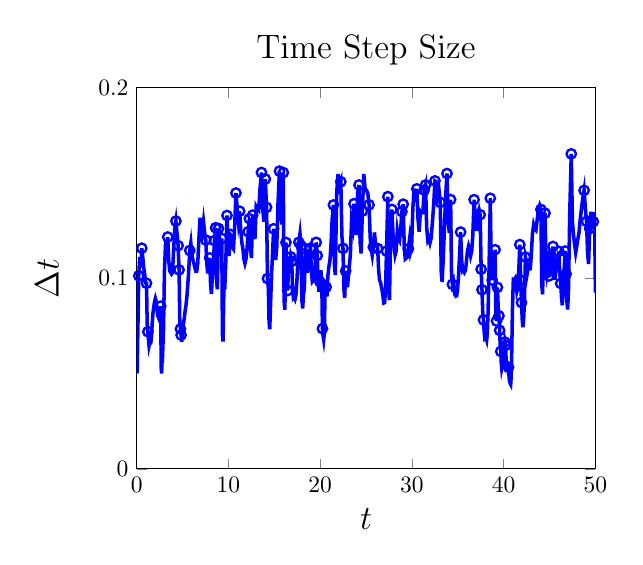
\begin{tikzpicture}[scale=0.85]

\begin{axis}[
  xmin = 0,
  xmax = 50,
  xtick = {0,10,20,30,40,50},
  xticklabels = {$0$,$10$,$20$,$30$,$40$,$50$},
  xlabel = $t$,
  ymin = 0,
  ymax = 0.2,
  ytick = {0,0.1,0.2},
  yticklabels = {$0$,$0.1$,$0.2$},
  ylabel = {$\Delta t$},
  ylabel style = {yshift = 10pt},
  label style = {font=\Large},
  title = {\Large{Time Step Size}}
  ]

% adaptive time step size
\addplot [mark=none,blue,line width=1.5] table{
5.0000e-02 5.0000e-02
1.2115e-01 7.1151e-02
2.2240e-01 1.0125e-01
3.3353e-01 1.1113e-01
4.3896e-01 1.0543e-01
5.5472e-01 1.1576e-01
6.6555e-01 1.1083e-01
7.7069e-01 1.0514e-01
8.7273e-01 1.0204e-01
9.7024e-01 9.7511e-02
1.0676e+00 9.7358e-02
1.1434e+00 7.5807e-02
1.2153e+00 7.1917e-02
1.2833e+00 6.7972e-02
1.3478e+00 6.4484e-02
1.4137e+00 6.5897e-02
1.4794e+00 6.5764e-02
1.5457e+00 6.6244e-02
1.6158e+00 7.0147e-02
1.6923e+00 7.6464e-02
1.7740e+00 8.1709e-02
1.8587e+00 8.4748e-02
1.9464e+00 8.7679e-02
2.0359e+00 8.9431e-02
2.1238e+00 8.7936e-02
2.2079e+00 8.4120e-02
2.2885e+00 8.0597e-02
2.3680e+00 7.9529e-02
2.4489e+00 8.0838e-02
2.5321e+00 8.3207e-02
2.6174e+00 8.5330e-02
2.6701e+00 5.2716e-02
2.7201e+00 5.0011e-02
2.7849e+00 6.4765e-02
2.8482e+00 6.3267e-02
2.9210e+00 7.2862e-02
3.0247e+00 1.0368e-01
3.1429e+00 1.1817e-01
3.2603e+00 1.1738e-01
3.3819e+00 1.2162e-01
3.4914e+00 1.0951e-01
3.5953e+00 1.0389e-01
3.6983e+00 1.0299e-01
3.8005e+00 1.0218e-01
3.9033e+00 1.0286e-01
4.0175e+00 1.1421e-01
4.1433e+00 1.2574e-01
4.2733e+00 1.2999e-01
4.3967e+00 1.2345e-01
4.5138e+00 1.1711e-01
4.6182e+00 1.0435e-01
4.6955e+00 7.7338e-02
4.7689e+00 7.3370e-02
4.8390e+00 7.0170e-02
4.9056e+00 6.6569e-02
4.9767e+00 7.1100e-02
5.0519e+00 7.5195e-02
5.1289e+00 7.6955e-02
5.2088e+00 7.9966e-02
5.2921e+00 8.3241e-02
5.3781e+00 8.6018e-02
5.4682e+00 9.0130e-02
5.5645e+00 9.6235e-02
5.6682e+00 1.0379e-01
5.7828e+00 1.1455e-01
5.9013e+00 1.1846e-01
6.0136e+00 1.1238e-01
6.1233e+00 1.0964e-01
6.2312e+00 1.0787e-01
6.3367e+00 1.0558e-01
6.4404e+00 1.0369e-01
6.5441e+00 1.0373e-01
6.6518e+00 1.0762e-01
6.7715e+00 1.1974e-01
6.9032e+00 1.3166e-01
7.0303e+00 1.2712e-01
7.1542e+00 1.2394e-01
7.2838e+00 1.2955e-01
7.4075e+00 1.2374e-01
7.5276e+00 1.2004e-01
7.6356e+00 1.0805e-01
7.7381e+00 1.0251e-01
7.8455e+00 1.0743e-01
7.9562e+00 1.1066e-01
8.0529e+00 9.6661e-02
8.1446e+00 9.1701e-02
8.2456e+00 1.0100e-01
8.3525e+00 1.0695e-01
8.4723e+00 1.1976e-01
8.5987e+00 1.2647e-01
8.6980e+00 9.9246e-02
8.7921e+00 9.4153e-02
8.9182e+00 1.2609e-01
9.0389e+00 1.2062e-01
9.1533e+00 1.1443e-01
9.2741e+00 1.2083e-01
9.3445e+00 7.0337e-02
9.4112e+00 6.6728e-02
9.5061e+00 9.4955e-02
9.6011e+00 9.4925e-02
9.7095e+00 1.0845e-01
9.8424e+00 1.3292e-01
9.9602e+00 1.1773e-01
1.0072e+01 1.1169e-01
1.0195e+01 1.2299e-01
1.0317e+01 1.2242e-01
1.0433e+01 1.1614e-01
1.0549e+01 1.1533e-01
1.0676e+01 1.2686e-01
1.0820e+01 1.4471e-01
1.0957e+01 1.3669e-01
1.1087e+01 1.2967e-01
1.1222e+01 1.3517e-01
1.1347e+01 1.2494e-01
1.1465e+01 1.1853e-01
1.1581e+01 1.1538e-01
1.1691e+01 1.0997e-01
1.1798e+01 1.0784e-01
1.1909e+01 1.1007e-01
1.2024e+01 1.1535e-01
1.2148e+01 1.2438e-01
1.2280e+01 1.3125e-01
1.2396e+01 1.1658e-01
1.2507e+01 1.1060e-01
1.2640e+01 1.3311e-01
1.2767e+01 1.2702e-01
1.2887e+01 1.2050e-01
1.3025e+01 1.3757e-01
1.3161e+01 1.3636e-01
1.3297e+01 1.3567e-01
1.3444e+01 1.4713e-01
1.3600e+01 1.5547e-01
1.3736e+01 1.3665e-01
1.3866e+01 1.2964e-01
1.4018e+01 1.5205e-01
1.4155e+01 1.3720e-01
1.4255e+01 9.9817e-02
1.4350e+01 9.4695e-02
1.4427e+01 7.7142e-02
1.4500e+01 7.3183e-02
1.4585e+01 8.5131e-02
1.4685e+01 1.0039e-01
1.4797e+01 1.1163e-01
1.4923e+01 1.2595e-01
1.5039e+01 1.1553e-01
1.5148e+01 1.0960e-01
1.5264e+01 1.1618e-01
1.5404e+01 1.3943e-01
1.5560e+01 1.5619e-01
1.5695e+01 1.3515e-01
1.5823e+01 1.2821e-01
1.5979e+01 1.5543e-01
1.6067e+01 8.7977e-02
1.6150e+01 8.3462e-02
1.6269e+01 1.1877e-01
1.6368e+01 9.8609e-02
1.6461e+01 9.3548e-02
1.6573e+01 1.1141e-01
1.6678e+01 1.0569e-01
1.6789e+01 1.1118e-01
1.6898e+01 1.0884e-01
1.6993e+01 9.4458e-02
1.7082e+01 8.9610e-02
1.7172e+01 9.0110e-02
1.7262e+01 8.9092e-02
1.7352e+01 9.0870e-02
1.7450e+01 9.7384e-02
1.7558e+01 1.0777e-01
1.7676e+01 1.1886e-01
1.7800e+01 1.2336e-01
1.7917e+01 1.1703e-01
1.8005e+01 8.8699e-02
1.8090e+01 8.4148e-02
1.8181e+01 9.1612e-02
1.8276e+01 9.4667e-02
1.8391e+01 1.1535e-01
1.8500e+01 1.0843e-01
1.8603e+01 1.0286e-01
1.8713e+01 1.1078e-01
1.8827e+01 1.1389e-01
1.8943e+01 1.1577e-01
1.9047e+01 1.0351e-01
1.9145e+01 9.8197e-02
1.9243e+01 9.8786e-02
1.9343e+01 9.9331e-02
1.9450e+01 1.0670e-01
1.9568e+01 1.1881e-01
1.9680e+01 1.1189e-01
1.9778e+01 9.7882e-02
1.9871e+01 9.2859e-02
1.9969e+01 9.8141e-02
2.0073e+01 1.0422e-01
2.0172e+01 9.8868e-02
2.0246e+01 7.3543e-02
2.0316e+01 6.9769e-02
2.0383e+01 6.7675e-02
2.0454e+01 7.1073e-02
2.0553e+01 9.9135e-02
2.0649e+01 9.5328e-02
2.0739e+01 9.0437e-02
2.0840e+01 1.0121e-01
2.0946e+01 1.0605e-01
2.1055e+01 1.0891e-01
2.1172e+01 1.1676e-01
2.1303e+01 1.3072e-01
2.1441e+01 1.3844e-01
2.1548e+01 1.0713e-01
2.1650e+01 1.0163e-01
2.1795e+01 1.4462e-01
2.1949e+01 1.5465e-01
2.2098e+01 1.4828e-01
2.2248e+01 1.5065e-01
2.2370e+01 1.2194e-01
2.2486e+01 1.1568e-01
2.2580e+01 9.4553e-02
2.2670e+01 8.9701e-02
2.2774e+01 1.0381e-01
2.2874e+01 1.0043e-01
2.2970e+01 9.5274e-02
2.3070e+01 1.0081e-01
2.3177e+01 1.0620e-01
2.3289e+01 1.1248e-01
2.3419e+01 1.2997e-01
2.3546e+01 1.2677e-01
2.3685e+01 1.3910e-01
2.3814e+01 1.2934e-01
2.3937e+01 1.2270e-01
2.4082e+01 1.4471e-01
2.4231e+01 1.4894e-01
2.4350e+01 1.1911e-01
2.4463e+01 1.1300e-01
2.4598e+01 1.3520e-01
2.4753e+01 1.5470e-01
2.4899e+01 1.4676e-01
2.5046e+01 1.4615e-01
2.5190e+01 1.4462e-01
2.5329e+01 1.3850e-01
2.5450e+01 1.2139e-01
2.5565e+01 1.1516e-01
2.5677e+01 1.1197e-01
2.5794e+01 1.1634e-01
2.5918e+01 1.2404e-01
2.6035e+01 1.1768e-01
2.6153e+01 1.1730e-01
2.6268e+01 1.1557e-01
2.6372e+01 1.0429e-01
2.6471e+01 9.8935e-02
2.6569e+01 9.7908e-02
2.6665e+01 9.5667e-02
2.6758e+01 9.3431e-02
2.6849e+01 9.0395e-02
2.6936e+01 8.6995e-02
2.7023e+01 8.7178e-02
2.7117e+01 9.3606e-02
2.7231e+01 1.1423e-01
2.7374e+01 1.4280e-01
2.7467e+01 9.3385e-02
2.7556e+01 8.8592e-02
2.7682e+01 1.2607e-01
2.7818e+01 1.3608e-01
2.7941e+01 1.2294e-01
2.8057e+01 1.1663e-01
2.8169e+01 1.1218e-01
2.8284e+01 1.1435e-01
2.8409e+01 1.2484e-01
2.8530e+01 1.2104e-01
2.8650e+01 1.1987e-01
2.8775e+01 1.2575e-01
2.8910e+01 1.3497e-01
2.9049e+01 1.3885e-01
2.9165e+01 1.1600e-01
2.9275e+01 1.1005e-01
2.9386e+01 1.1052e-01
2.9497e+01 1.1097e-01
2.9612e+01 1.1540e-01
2.9732e+01 1.2006e-01
2.9846e+01 1.1389e-01
2.9962e+01 1.1612e-01
3.0099e+01 1.3646e-01
3.0246e+01 1.4706e-01
3.0386e+01 1.4003e-01
3.0533e+01 1.4690e-01
3.0664e+01 1.3109e-01
3.0788e+01 1.2436e-01
3.0923e+01 1.3510e-01
3.1057e+01 1.3429e-01
3.1192e+01 1.3436e-01
3.1338e+01 1.4625e-01
3.1487e+01 1.4892e-01
3.1613e+01 1.2631e-01
3.1733e+01 1.1983e-01
3.1854e+01 1.2096e-01
3.1973e+01 1.1856e-01
3.2093e+01 1.2090e-01
3.2222e+01 1.2865e-01
3.2360e+01 1.3767e-01
3.2511e+01 1.5107e-01
3.2661e+01 1.5058e-01
3.2804e+01 1.4285e-01
3.2951e+01 1.4641e-01
3.3091e+01 1.3984e-01
3.3194e+01 1.0329e-01
3.3292e+01 9.7991e-02
3.3400e+01 1.0860e-01
3.3524e+01 1.2384e-01
3.3666e+01 1.4200e-01
3.3821e+01 1.5494e-01
3.3952e+01 1.3044e-01
3.4075e+01 1.2375e-01
3.4217e+01 1.4123e-01
3.4319e+01 1.0202e-01
3.4415e+01 9.6785e-02
3.4514e+01 9.8191e-02
3.4607e+01 9.3152e-02
3.4698e+01 9.1235e-02
3.4789e+01 9.0561e-02
3.4879e+01 9.0763e-02
3.4973e+01 9.3940e-02
3.5074e+01 1.0069e-01
3.5185e+01 1.1109e-01
3.5309e+01 1.2422e-01
3.5419e+01 1.0958e-01
3.5523e+01 1.0396e-01
3.5627e+01 1.0454e-01
3.5731e+01 1.0314e-01
3.5835e+01 1.0408e-01
3.5944e+01 1.0907e-01
3.6058e+01 1.1426e-01
3.6175e+01 1.1683e-01
3.6290e+01 1.1487e-01
3.6401e+01 1.1183e-01
3.6516e+01 1.1418e-01
3.6638e+01 1.2253e-01
3.6779e+01 1.4121e-01
3.6911e+01 1.3158e-01
3.7036e+01 1.2482e-01
3.7170e+01 1.3444e-01
3.7306e+01 1.3627e-01
3.7440e+01 1.3332e-01
3.7545e+01 1.0472e-01
3.7638e+01 9.3957e-02
3.7721e+01 8.2339e-02
3.7799e+01 7.8113e-02
3.7871e+01 7.2270e-02
3.7940e+01 6.8562e-02
3.8009e+01 6.8967e-02
3.8077e+01 6.8646e-02
3.8145e+01 6.7532e-02
3.8216e+01 7.0699e-02
3.8297e+01 8.1578e-02
3.8401e+01 1.0341e-01
3.8543e+01 1.4197e-01
3.8647e+01 1.0436e-01
3.8746e+01 9.9003e-02
3.8851e+01 1.0495e-01
3.8950e+01 9.9566e-02
3.9065e+01 1.1496e-01
3.9147e+01 8.1729e-02
3.9225e+01 7.7534e-02
3.9320e+01 9.5181e-02
3.9404e+01 8.4607e-02
3.9485e+01 8.0266e-02
3.9557e+01 7.2650e-02
3.9622e+01 6.4914e-02
3.9684e+01 6.1583e-02
3.9739e+01 5.5440e-02
3.9792e+01 5.2595e-02
3.9846e+01 5.3814e-02
3.9899e+01 5.3464e-02
3.9953e+01 5.4108e-02
4.0011e+01 5.7775e-02
4.0073e+01 6.2129e-02
4.0140e+01 6.6492e-02
4.0204e+01 6.4731e-02
4.0262e+01 5.7847e-02
4.0317e+01 5.4878e-02
4.0373e+01 5.5825e-02
4.0428e+01 5.5483e-02
4.0483e+01 5.4337e-02
4.0536e+01 5.3225e-02
4.0585e+01 4.8558e-02
4.0631e+01 4.6067e-02
4.0677e+01 4.5982e-02
4.0721e+01 4.4584e-02
4.0765e+01 4.4198e-02
4.0813e+01 4.7763e-02
4.0872e+01 5.8418e-02
4.0955e+01 8.3130e-02
4.1054e+01 9.9349e-02
4.1153e+01 9.9193e-02
4.1253e+01 9.9980e-02
4.1351e+01 9.7341e-02
4.1443e+01 9.2899e-02
4.1538e+01 9.4506e-02
4.1641e+01 1.0315e-01
4.1759e+01 1.1764e-01
4.1858e+01 9.8955e-02
4.1945e+01 8.7234e-02
4.2023e+01 7.8242e-02
4.2097e+01 7.4227e-02
4.2176e+01 7.8139e-02
4.2263e+01 8.7596e-02
4.2374e+01 1.1110e-01
4.2483e+01 1.0864e-01
4.2586e+01 1.0307e-01
4.2692e+01 1.0606e-01
4.2797e+01 1.0493e-01
4.2902e+01 1.0496e-01
4.3014e+01 1.1244e-01
4.3138e+01 1.2317e-01
4.3266e+01 1.2803e-01
4.3392e+01 1.2601e-01
4.3517e+01 1.2528e-01
4.3647e+01 1.3040e-01
4.3783e+01 1.3611e-01
4.3922e+01 1.3817e-01
4.4058e+01 1.3607e-01
4.4154e+01 9.6458e-02
4.4246e+01 9.1509e-02
4.4376e+01 1.3022e-01
4.4510e+01 1.3412e-01
4.4618e+01 1.0846e-01
4.4721e+01 1.0289e-01
4.4828e+01 1.0663e-01
4.4929e+01 1.0116e-01
4.5040e+01 1.1135e-01
4.5149e+01 1.0887e-01
4.5259e+01 1.0926e-01
4.5375e+01 1.1666e-01
4.5480e+01 1.0451e-01
4.5579e+01 9.9145e-02
4.5683e+01 1.0396e-01
4.5791e+01 1.0795e-01
4.5900e+01 1.0936e-01
4.6014e+01 1.1406e-01
4.6117e+01 1.0253e-01
4.6214e+01 9.7269e-02
4.6304e+01 9.0390e-02
4.6390e+01 8.5751e-02
4.6482e+01 9.2371e-02
4.6586e+01 1.0339e-01
4.6700e+01 1.1426e-01
4.6802e+01 1.0221e-01
4.6890e+01 8.8121e-02
4.6974e+01 8.3599e-02
4.7068e+01 9.4128e-02
4.7202e+01 1.3395e-01
4.7367e+01 1.6526e-01
4.7497e+01 1.2928e-01
4.7619e+01 1.2264e-01
4.7737e+01 1.1773e-01
4.7851e+01 1.1351e-01
4.7967e+01 1.1672e-01
4.8088e+01 1.2061e-01
4.8212e+01 1.2395e-01
4.8343e+01 1.3083e-01
4.8479e+01 1.3632e-01
4.8621e+01 1.4171e-01
4.8767e+01 1.4610e-01
4.8904e+01 1.3684e-01
4.9033e+01 1.2982e-01
4.9147e+01 1.1330e-01
4.9254e+01 1.0749e-01
4.9380e+01 1.2599e-01
4.9515e+01 1.3490e-01
4.9643e+01 1.2798e-01
4.9773e+01 1.2967e-01
4.9908e+01 1.3471e-01
5.0000e+01 9.2484e-02
};

% Location of rejected time steps
\addplot [only marks,blue,mark=o,mark size=2pt,line width=1.0] table{
2.2240e-01 1.0125e-01
5.5472e-01 1.1576e-01
1.0676e+00 9.7358e-02
1.2153e+00 7.1917e-02
2.6174e+00 8.5330e-02
3.3819e+00 1.2162e-01
4.2733e+00 1.2999e-01
4.5138e+00 1.1711e-01
4.6182e+00 1.0435e-01
4.7689e+00 7.3370e-02
4.8390e+00 7.0170e-02
5.7828e+00 1.1455e-01
7.5276e+00 1.2004e-01
7.9562e+00 1.1066e-01
8.4723e+00 1.1976e-01
8.5987e+00 1.2647e-01
8.9182e+00 1.2609e-01
9.2741e+00 1.2083e-01
9.8424e+00 1.3292e-01
1.0195e+01 1.2299e-01
1.0820e+01 1.4471e-01
1.1222e+01 1.3517e-01
1.2148e+01 1.2438e-01
1.2280e+01 1.3125e-01
1.2640e+01 1.3311e-01
1.3600e+01 1.5547e-01
1.4018e+01 1.5205e-01
1.4155e+01 1.3720e-01
1.4255e+01 9.9817e-02
1.4923e+01 1.2595e-01
1.5560e+01 1.5619e-01
1.5979e+01 1.5543e-01
1.6269e+01 1.1877e-01
1.6461e+01 9.3548e-02
1.6789e+01 1.1118e-01
1.6898e+01 1.0884e-01
1.7676e+01 1.1886e-01
1.7917e+01 1.1703e-01
1.8391e+01 1.1535e-01
1.8943e+01 1.1577e-01
1.9568e+01 1.1881e-01
1.9680e+01 1.1189e-01
1.9969e+01 9.8141e-02
2.0246e+01 7.3543e-02
2.0649e+01 9.5328e-02
2.1441e+01 1.3844e-01
2.2248e+01 1.5065e-01
2.2486e+01 1.1568e-01
2.2774e+01 1.0381e-01
2.3685e+01 1.3910e-01
2.4231e+01 1.4894e-01
2.4598e+01 1.3520e-01
2.5329e+01 1.3850e-01
2.5794e+01 1.1634e-01
2.6268e+01 1.1557e-01
2.7231e+01 1.1423e-01
2.7374e+01 1.4280e-01
2.7818e+01 1.3608e-01
2.8910e+01 1.3497e-01
2.9049e+01 1.3885e-01
2.9612e+01 1.1540e-01
3.0533e+01 1.4690e-01
3.1338e+01 1.4625e-01
3.1487e+01 1.4892e-01
3.2511e+01 1.5107e-01
3.3091e+01 1.3984e-01
3.3821e+01 1.5494e-01
3.4217e+01 1.4123e-01
3.4415e+01 9.6785e-02
3.5309e+01 1.2422e-01
3.6779e+01 1.4121e-01
3.7440e+01 1.3332e-01
3.7545e+01 1.0472e-01
3.7638e+01 9.3957e-02
3.7799e+01 7.8113e-02
3.8543e+01 1.4197e-01
3.8746e+01 9.9003e-02
3.9065e+01 1.1496e-01
3.9225e+01 7.7534e-02
3.9320e+01 9.5181e-02
3.9485e+01 8.0266e-02
3.9557e+01 7.2650e-02
3.9684e+01 6.1583e-02
4.0140e+01 6.6492e-02
4.0204e+01 6.4731e-02
4.0536e+01 5.3225e-02
4.1759e+01 1.1764e-01
4.1858e+01 9.8955e-02
4.1945e+01 8.7234e-02
4.2374e+01 1.1110e-01
4.4058e+01 1.3607e-01
4.4510e+01 1.3412e-01
4.4721e+01 1.0289e-01
4.4828e+01 1.0663e-01
4.4929e+01 1.0116e-01
4.5040e+01 1.1135e-01
4.5149e+01 1.0887e-01
4.5259e+01 1.0926e-01
4.5375e+01 1.1666e-01
4.6014e+01 1.1406e-01
4.6214e+01 9.7269e-02
4.6700e+01 1.1426e-01
4.6802e+01 1.0221e-01
4.7367e+01 1.6526e-01
4.8767e+01 1.4610e-01
4.9033e+01 1.2982e-01
4.9380e+01 1.2599e-01
4.9773e+01 1.2967e-01
};

% OLD RESULTS
%% adaptive time step size
%\addplot [mark=none,blue,line width=1.5] table{
%8.0000e-02 8.0000e-02
%1.9688e-01 1.1688e-01
%3.4223e-01 1.4535e-01
%5.0690e-01 1.6468e-01
%6.5685e-01 1.4995e-01
%7.7686e-01 1.2001e-01
%8.7747e-01 1.0061e-01
%9.6745e-01 8.9984e-02
%1.0515e+00 8.4063e-02
%1.1334e+00 8.1877e-02
%1.2144e+00 8.1052e-02
%1.2955e+00 8.1069e-02
%1.3803e+00 8.4770e-02
%1.4734e+00 9.3093e-02
%1.5832e+00 1.0987e-01
%1.7169e+00 1.3361e-01
%1.8749e+00 1.5808e-01
%2.0199e+00 1.4495e-01
%2.1522e+00 1.3236e-01
%2.2776e+00 1.2539e-01
%2.3953e+00 1.1766e-01
%2.4998e+00 1.0446e-01
%2.6015e+00 1.0175e-01
%2.7186e+00 1.1706e-01
%2.8825e+00 1.6392e-01
%3.0345e+00 1.5199e-01
%3.1763e+00 1.4181e-01
%3.3079e+00 1.3165e-01
%3.4362e+00 1.2823e-01
%3.5724e+00 1.3624e-01
%3.7051e+00 1.3270e-01
%3.8540e+00 1.4888e-01
%4.0040e+00 1.5006e-01
%4.1389e+00 1.3482e-01
%4.2702e+00 1.3132e-01
%4.4051e+00 1.3490e-01
%4.5029e+00 9.7783e-02
%4.5909e+00 8.8087e-02
%4.6767e+00 8.5797e-02
%4.7605e+00 8.3772e-02
%4.8439e+00 8.3382e-02
%4.9296e+00 8.5652e-02
%5.0192e+00 8.9637e-02
%5.1149e+00 9.5663e-02
%5.2212e+00 1.0633e-01
%5.3486e+00 1.2738e-01
%5.5176e+00 1.6902e-01
%5.7313e+00 2.1366e-01
%5.8712e+00 1.3994e-01
%6.0075e+00 1.3630e-01
%6.1548e+00 1.4733e-01
%6.2961e+00 1.4124e-01
%6.4278e+00 1.3176e-01
%6.5562e+00 1.2834e-01
%6.7096e+00 1.5343e-01
%6.8445e+00 1.3488e-01
%6.9758e+00 1.3137e-01
%7.1190e+00 1.4313e-01
%7.2869e+00 1.6797e-01
%7.4704e+00 1.8349e-01
%7.6382e+00 1.6777e-01
%7.8016e+00 1.6341e-01
%7.9645e+00 1.6290e-01
%8.1369e+00 1.7237e-01
%8.3048e+00 1.6789e-01
%8.4823e+00 1.7756e-01
%8.6307e+00 1.4837e-01
%8.7658e+00 1.3508e-01
%8.8973e+00 1.3156e-01
%9.0377e+00 1.4036e-01
%9.1816e+00 1.4388e-01
%9.3412e+00 1.5963e-01
%9.5086e+00 1.6743e-01
%9.6783e+00 1.6971e-01
%9.8058e+00 1.2746e-01
%9.9195e+00 1.1368e-01
%1.0025e+01 1.0572e-01
%1.0128e+01 1.0297e-01
%1.0235e+01 1.0683e-01
%1.0351e+01 1.1591e-01
%1.0485e+01 1.3394e-01
%1.0626e+01 1.4083e-01
%1.0763e+01 1.3717e-01
%1.0913e+01 1.4996e-01
%1.1080e+01 1.6765e-01
%1.1236e+01 1.5561e-01
%1.1388e+01 1.5156e-01
%1.1546e+01 1.5823e-01
%1.1700e+01 1.5412e-01
%1.1844e+01 1.4442e-01
%1.1979e+01 1.3452e-01
%1.2110e+01 1.3102e-01
%1.2245e+01 1.3489e-01
%1.2408e+01 1.6295e-01
%1.2566e+01 1.5871e-01
%1.2703e+01 1.3693e-01
%1.2826e+01 1.2218e-01
%1.2945e+01 1.1901e-01
%1.3078e+01 1.3293e-01
%1.3225e+01 1.4718e-01
%1.3364e+01 1.3952e-01
%1.3500e+01 1.3589e-01
%1.3663e+01 1.6279e-01
%1.3865e+01 2.0251e-01
%1.4051e+01 1.8530e-01
%1.4231e+01 1.8049e-01
%1.4408e+01 1.7690e-01
%1.4569e+01 1.6137e-01
%1.4727e+01 1.5718e-01
%1.4876e+01 1.4940e-01
%1.5022e+01 1.4552e-01
%1.5143e+01 1.2162e-01
%1.5247e+01 1.0366e-01
%1.5348e+01 1.0097e-01
%1.5448e+01 1.0060e-01
%1.5555e+01 1.0707e-01
%1.5676e+01 1.2001e-01
%1.5819e+01 1.4316e-01
%1.5961e+01 1.4188e-01
%1.6099e+01 1.3819e-01
%1.6236e+01 1.3676e-01
%1.6382e+01 1.4625e-01
%1.6558e+01 1.7605e-01
%1.6750e+01 1.9174e-01
%1.6936e+01 1.8676e-01
%1.7128e+01 1.9156e-01
%1.7330e+01 2.0211e-01
%1.7524e+01 1.9406e-01
%1.7713e+01 1.8902e-01
%1.7884e+01 1.7079e-01
%1.8037e+01 1.5272e-01
%1.8185e+01 1.4875e-01
%1.8334e+01 1.4894e-01
%1.8491e+01 1.5712e-01
%1.8622e+01 1.3103e-01
%1.8743e+01 1.2037e-01
%1.8860e+01 1.1724e-01
%1.8989e+01 1.2878e-01
%1.9165e+01 1.7617e-01
%1.9347e+01 1.8208e-01
%1.9508e+01 1.6114e-01
%1.9665e+01 1.5695e-01
%1.9835e+01 1.7012e-01
%2.0014e+01 1.7863e-01
%2.0179e+01 1.6494e-01
%2.0329e+01 1.5054e-01
%2.0476e+01 1.4662e-01
%2.0628e+01 1.5191e-01
%2.0789e+01 1.6138e-01
%2.0948e+01 1.5884e-01
%2.1088e+01 1.4003e-01
%2.1225e+01 1.3639e-01
%2.1388e+01 1.6348e-01
%2.1567e+01 1.7858e-01
%2.1741e+01 1.7393e-01
%2.1909e+01 1.6815e-01
%2.2072e+01 1.6378e-01
%2.2240e+01 1.6765e-01
%2.2403e+01 1.6329e-01
%2.2545e+01 1.4167e-01
%2.2667e+01 1.2232e-01
%2.2778e+01 1.1038e-01
%2.2885e+01 1.0751e-01
%2.2991e+01 1.0560e-01
%2.3095e+01 1.0369e-01
%2.3198e+01 1.0291e-01
%2.3307e+01 1.0931e-01
%2.3433e+01 1.2638e-01
%2.3573e+01 1.3930e-01
%2.3708e+01 1.3568e-01
%2.3847e+01 1.3889e-01
%2.3996e+01 1.4861e-01
%2.4151e+01 1.5542e-01
%2.4302e+01 1.5138e-01
%2.4479e+01 1.7660e-01
%2.4646e+01 1.6666e-01
%2.4808e+01 1.6233e-01
%2.4993e+01 1.8514e-01
%2.5184e+01 1.9105e-01
%2.5361e+01 1.7637e-01
%2.5532e+01 1.7178e-01
%2.5721e+01 1.8900e-01
%2.5900e+01 1.7887e-01
%2.6074e+01 1.7422e-01
%2.6246e+01 1.7179e-01
%2.6418e+01 1.7218e-01
%2.6609e+01 1.9041e-01
%2.6768e+01 1.5913e-01
%2.6923e+01 1.5499e-01
%2.7079e+01 1.5569e-01
%2.7232e+01 1.5286e-01
%2.7386e+01 1.5399e-01
%2.7542e+01 1.5634e-01
%2.7701e+01 1.5899e-01
%2.7841e+01 1.3979e-01
%2.7977e+01 1.3616e-01
%2.8111e+01 1.3403e-01
%2.8257e+01 1.4603e-01
%2.8429e+01 1.7167e-01
%2.8613e+01 1.8420e-01
%2.8799e+01 1.8659e-01
%2.8981e+01 1.8174e-01
%2.9154e+01 1.7323e-01
%2.9298e+01 1.4369e-01
%2.9438e+01 1.3995e-01
%2.9575e+01 1.3698e-01
%2.9714e+01 1.3902e-01
%2.9856e+01 1.4234e-01
%3.0004e+01 1.4784e-01
%3.0173e+01 1.6866e-01
%3.0324e+01 1.5149e-01
%3.0466e+01 1.4197e-01
%3.0604e+01 1.3828e-01
%3.0746e+01 1.4140e-01
%3.0891e+01 1.4470e-01
%3.1036e+01 1.4541e-01
%3.1208e+01 1.7170e-01
%3.1382e+01 1.7393e-01
%3.1557e+01 1.7536e-01
%3.1731e+01 1.7381e-01
%3.1894e+01 1.6271e-01
%3.2052e+01 1.5848e-01
%3.2225e+01 1.7297e-01
%3.2375e+01 1.5001e-01
%3.2521e+01 1.4611e-01
%3.2686e+01 1.6443e-01
%3.2846e+01 1.6015e-01
%3.3029e+01 1.8299e-01
%3.3228e+01 1.9973e-01
%3.3424e+01 1.9545e-01
%3.3603e+01 1.7931e-01
%3.3778e+01 1.7465e-01
%3.3955e+01 1.7684e-01
%3.4149e+01 1.9466e-01
%3.4355e+01 2.0523e-01
%3.4533e+01 1.7884e-01
%3.4670e+01 1.3617e-01
%3.4802e+01 1.3263e-01
%3.4940e+01 1.3758e-01
%3.5077e+01 1.3678e-01
%3.5214e+01 1.3780e-01
%3.5360e+01 1.4582e-01
%3.5482e+01 1.2174e-01
%3.5600e+01 1.1858e-01
%3.5718e+01 1.1754e-01
%3.5851e+01 1.3306e-01
%3.6010e+01 1.5944e-01
%3.6170e+01 1.5917e-01
%3.6326e+01 1.5668e-01
%3.6479e+01 1.5261e-01
%3.6599e+01 1.2031e-01
%3.6707e+01 1.0802e-01
%3.6812e+01 1.0521e-01
%3.6931e+01 1.1811e-01
%3.7071e+01 1.4001e-01
%3.7227e+01 1.5657e-01
%3.7359e+01 1.3211e-01
%3.7483e+01 1.2394e-01
%3.7587e+01 1.0373e-01
%3.7688e+01 1.0103e-01
%3.7787e+01 9.8717e-02
%3.7890e+01 1.0290e-01
%3.8003e+01 1.1309e-01
%3.8130e+01 1.2754e-01
%3.8275e+01 1.4445e-01
%3.8419e+01 1.4474e-01
%3.8560e+01 1.4097e-01
%3.8704e+01 1.4315e-01
%3.8856e+01 1.5246e-01
%3.9024e+01 1.6828e-01
%3.9185e+01 1.6082e-01
%3.9334e+01 1.4891e-01
%3.9479e+01 1.4504e-01
%3.9622e+01 1.4346e-01
%3.9758e+01 1.3572e-01
%3.9890e+01 1.3219e-01
%4.0084e+01 1.9311e-01
%4.0262e+01 1.7798e-01
%4.0425e+01 1.6397e-01
%4.0561e+01 1.3566e-01
%4.0693e+01 1.3214e-01
%4.0858e+01 1.6497e-01
%4.1010e+01 1.5207e-01
%4.1125e+01 1.1453e-01
%4.1236e+01 1.1156e-01
%4.1364e+01 1.2806e-01
%4.1510e+01 1.4572e-01
%4.1652e+01 1.4193e-01
%4.1800e+01 1.4745e-01
%4.1947e+01 1.4758e-01
%4.2096e+01 1.4909e-01
%4.2249e+01 1.5275e-01
%4.2402e+01 1.5258e-01
%4.2550e+01 1.4861e-01
%4.2699e+01 1.4853e-01
%4.2856e+01 1.5774e-01
%4.3017e+01 1.6089e-01
%4.3160e+01 1.4269e-01
%4.3290e+01 1.2990e-01
%4.3416e+01 1.2652e-01
%4.3558e+01 1.4181e-01
%4.3702e+01 1.4360e-01
%4.3842e+01 1.3986e-01
%4.4004e+01 1.6189e-01
%4.4163e+01 1.5903e-01
%4.4318e+01 1.5490e-01
%4.4432e+01 1.1438e-01
%4.4539e+01 1.0679e-01
%4.4643e+01 1.0402e-01
%4.4753e+01 1.1022e-01
%4.4845e+01 9.2273e-02
%4.4932e+01 8.6617e-02
%4.5016e+01 8.4366e-02
%4.5139e+01 1.2326e-01
%4.5276e+01 1.3687e-01
%4.5396e+01 1.1946e-01
%4.5504e+01 1.0793e-01
%4.5605e+01 1.0129e-01
%4.5704e+01 9.8660e-02
%4.5802e+01 9.8419e-02
%4.5901e+01 9.9408e-02
%4.6008e+01 1.0606e-01
%4.6135e+01 1.2712e-01
%4.6270e+01 1.3562e-01
%4.6419e+01 1.4855e-01
%4.6559e+01 1.4021e-01
%4.6696e+01 1.3656e-01
%4.6839e+01 1.4373e-01
%4.6983e+01 1.4361e-01
%4.7137e+01 1.5358e-01
%4.7323e+01 1.8669e-01
%4.7475e+01 1.5224e-01
%4.7606e+01 1.3088e-01
%4.7721e+01 1.1459e-01
%4.7833e+01 1.1161e-01
%4.7952e+01 1.1951e-01
%4.8090e+01 1.3782e-01
%4.8253e+01 1.6305e-01
%4.8451e+01 1.9823e-01
%4.8644e+01 1.9308e-01
%4.8847e+01 2.0237e-01
%4.9044e+01 1.9710e-01
%4.9231e+01 1.8730e-01
%4.9413e+01 1.8243e-01
%4.9558e+01 1.4450e-01
%4.9679e+01 1.2156e-01
%4.9798e+01 1.1840e-01
%4.9917e+01 1.1958e-01
%5.0000e+01 8.2532e-02
%};
%
%% Location of rejected time steps
%\addplot [only marks,blue,mark=o,mark size=2pt,line width=1.0] table{
%6.5685e-01 1.4995e-01
%7.7686e-01 1.2001e-01
%8.7747e-01 1.0061e-01
%9.6745e-01 8.9984e-02
%1.0515e+00 8.4063e-02
%2.0199e+00 1.4495e-01
%2.1522e+00 1.3236e-01
%2.2776e+00 1.2539e-01
%2.3953e+00 1.1766e-01
%2.4998e+00 1.0446e-01
%3.0345e+00 1.5199e-01
%3.1763e+00 1.4181e-01
%3.3079e+00 1.3165e-01
%3.5724e+00 1.3624e-01
%4.0040e+00 1.5006e-01
%4.1389e+00 1.3482e-01
%4.5029e+00 9.7783e-02
%4.5909e+00 8.8087e-02
%5.8712e+00 1.3994e-01
%6.2961e+00 1.4124e-01
%6.4278e+00 1.3176e-01
%6.7096e+00 1.5343e-01
%7.4704e+00 1.8349e-01
%7.6382e+00 1.6777e-01
%8.1369e+00 1.7237e-01
%8.4823e+00 1.7756e-01
%8.6307e+00 1.4837e-01
%8.7658e+00 1.3508e-01
%9.8058e+00 1.2746e-01
%9.9195e+00 1.1368e-01
%1.0025e+01 1.0572e-01
%1.0626e+01 1.4083e-01
%1.1236e+01 1.5561e-01
%1.1546e+01 1.5823e-01
%1.1844e+01 1.4442e-01
%1.1979e+01 1.3452e-01
%1.2408e+01 1.6295e-01
%1.2703e+01 1.3693e-01
%1.2826e+01 1.2218e-01
%1.3225e+01 1.4718e-01
%1.3364e+01 1.3952e-01
%1.3865e+01 2.0251e-01
%1.4051e+01 1.8530e-01
%1.4569e+01 1.6137e-01
%1.4876e+01 1.4940e-01
%1.5143e+01 1.2162e-01
%1.5247e+01 1.0366e-01
%1.5961e+01 1.4188e-01
%1.6750e+01 1.9174e-01
%1.7524e+01 1.9406e-01
%1.7884e+01 1.7079e-01
%1.8037e+01 1.5272e-01
%1.8491e+01 1.5712e-01
%1.8622e+01 1.3103e-01
%1.8743e+01 1.2037e-01
%1.9508e+01 1.6114e-01
%2.0014e+01 1.7863e-01
%2.0179e+01 1.6494e-01
%2.0329e+01 1.5054e-01
%2.0948e+01 1.5884e-01
%2.1088e+01 1.4003e-01
%2.1567e+01 1.7858e-01
%2.1909e+01 1.6815e-01
%2.2240e+01 1.6765e-01
%2.2545e+01 1.4167e-01
%2.2667e+01 1.2232e-01
%2.2778e+01 1.1038e-01
%2.3573e+01 1.3930e-01
%2.4151e+01 1.5542e-01
%2.4479e+01 1.7660e-01
%2.4646e+01 1.6666e-01
%2.5184e+01 1.9105e-01
%2.5361e+01 1.7637e-01
%2.5900e+01 1.7887e-01
%2.6768e+01 1.5913e-01
%2.7841e+01 1.3979e-01
%2.8613e+01 1.8420e-01
%2.8981e+01 1.8174e-01
%2.9298e+01 1.4369e-01
%3.0173e+01 1.6866e-01
%3.0324e+01 1.5149e-01
%3.0466e+01 1.4197e-01
%3.1731e+01 1.7381e-01
%3.1894e+01 1.6271e-01
%3.2225e+01 1.7297e-01
%3.2375e+01 1.5001e-01
%3.2686e+01 1.6443e-01
%3.3603e+01 1.7931e-01
%3.4355e+01 2.0523e-01
%3.4533e+01 1.7884e-01
%3.4670e+01 1.3617e-01
%3.5482e+01 1.2174e-01
%3.6326e+01 1.5668e-01
%3.6599e+01 1.2031e-01
%3.6707e+01 1.0802e-01
%3.7227e+01 1.5657e-01
%3.7359e+01 1.3211e-01
%3.7483e+01 1.2394e-01
%3.7587e+01 1.0373e-01
%3.8419e+01 1.4474e-01
%3.9185e+01 1.6082e-01
%3.9334e+01 1.4891e-01
%3.9622e+01 1.4346e-01
%3.9758e+01 1.3572e-01
%4.0262e+01 1.7798e-01
%4.0425e+01 1.6397e-01
%4.0561e+01 1.3566e-01
%4.1010e+01 1.5207e-01
%4.1125e+01 1.1453e-01
%4.1510e+01 1.4572e-01
%4.2402e+01 1.5258e-01
%4.3017e+01 1.6089e-01
%4.3160e+01 1.4269e-01
%4.3290e+01 1.2990e-01
%4.3702e+01 1.4360e-01
%4.4163e+01 1.5903e-01
%4.4432e+01 1.1438e-01
%4.4539e+01 1.0679e-01
%4.4845e+01 9.2273e-02
%4.4932e+01 8.6617e-02
%4.5276e+01 1.3687e-01
%4.5396e+01 1.1946e-01
%4.5504e+01 1.0793e-01
%4.5605e+01 1.0129e-01
%4.6559e+01 1.4021e-01
%4.7475e+01 1.5224e-01
%4.7606e+01 1.3088e-01
%4.7721e+01 1.1459e-01
%4.8451e+01 1.9823e-01
%4.8847e+01 2.0237e-01
%4.9231e+01 1.8730e-01
%4.9558e+01 1.4450e-01
%4.9679e+01 1.2156e-01
%};



\end{axis}

\end{tikzpicture}



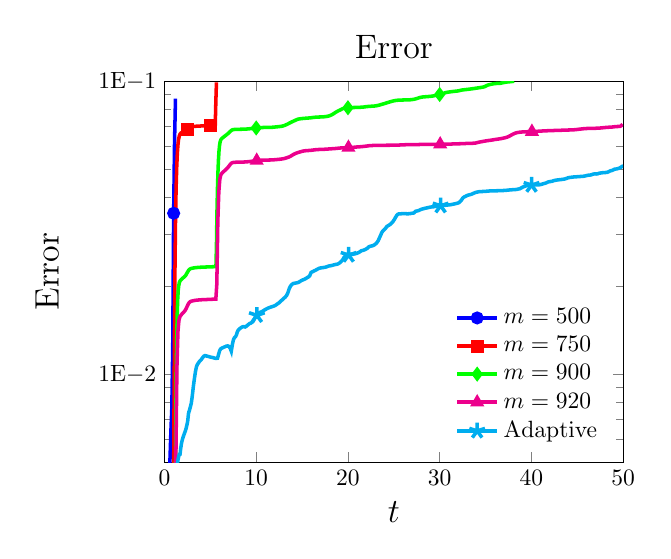
\begin{tikzpicture}[scale=0.85]

\begin{axis}[
  xmin = 0,
  xmax = 50,
  xtick = {0,10,20,30,40,50},
  xticklabels = {$0$,$10$,$20$,$30$,$40$,$50$},
  xlabel = $t$,
  ymode = log,
  ymin = 5E-3,
  ymax = 1E-1,
  ytick = {1E-3,1E-2,1E-1},
  yticklabels = {$1$E$-3$,$1$E$-2$,$1$E$-1$},
  ylabel = {Error},
  ylabel style = {yshift = 10pt},
  label style = {font=\Large},
%  legend entries = {$m=500$, $m=750$, $m=900$, $m=920$,
%  $m=1000$, Adaptive},
  legend entries = {$m=500$, $m=750$, $m=900$, $m=920$, Adaptive},
  legend cell align=left,
%  legend style={at={(0.96,0.5)},anchor=east},
%  legend style={at={(0.96,0.44)},anchor=east},
  legend pos = south east,
  legend style = {draw=none},
  title = {\Large{Error}}
  ]

\addlegendimage{mark=*,mark options=solid,blue,line width=1.5,solid}
\addlegendimage{mark=square*,mark options=solid,red,line width=1.5,solid}
\addlegendimage{mark=diamond*,mark options=solid,green,line width=1.5,solid}
\addlegendimage{mark=triangle*,mark options=solid,magenta,line width=1.5,solid}
\addlegendimage{mark=star,mark size=3.5pt,mark options=solid,cyan,line width=1.5,solid}

% error for m = 500
\addplot [mark=none,blue,line width=1.5] table{
1.0000e-01 1.8442e-06
2.0000e-01 6.2273e-04
3.0000e-01 1.5718e-03
4.0000e-01 2.6416e-03
5.0000e-01 3.8463e-03
6.0000e-01 5.1134e-03
7.0000e-01 6.3707e-03
8.0000e-01 7.6201e-03
9.0000e-01 1.2309e-02
1.0000e+00 3.5384e-02
1.1000e+00 6.2554e-02
1.2000e+00 8.7162e-02
};

% error for m = 750
\addplot [mark=none,red,line width=1.5] table{
6.6667e-02 1.2905e-06
1.3333e-01 1.2295e-04
2.0000e-01 3.0208e-04
2.6667e-01 5.1176e-04
3.3333e-01 7.5011e-04
4.0000e-01 1.0086e-03
4.6667e-01 1.2822e-03
5.3333e-01 1.5643e-03
6.0000e-01 1.8467e-03
6.6667e-01 2.1259e-03
7.3333e-01 2.4246e-03
8.0000e-01 2.9976e-03
8.6667e-01 3.5766e-03
9.3333e-01 4.1294e-03
1.0000e+00 4.6346e-03
1.0667e+00 1.0567e-02
1.1333e+00 2.1282e-02
1.2000e+00 3.2769e-02
1.2667e+00 4.2863e-02
1.3333e+00 5.0680e-02
1.4000e+00 5.6441e-02
1.4667e+00 6.0527e-02
1.5333e+00 6.3122e-02
1.6000e+00 6.4704e-02
1.6667e+00 6.5643e-02
1.7333e+00 6.6174e-02
1.8000e+00 6.6501e-02
1.8667e+00 6.6733e-02
1.9333e+00 6.6918e-02
2.0000e+00 6.7079e-02
2.0667e+00 6.7229e-02
2.1333e+00 6.7373e-02
2.2000e+00 6.7515e-02
2.2667e+00 6.7662e-02
2.3333e+00 6.7829e-02
2.4000e+00 6.8033e-02
2.4667e+00 6.8279e-02
2.5333e+00 6.8546e-02
2.6000e+00 6.8811e-02
2.6667e+00 6.9063e-02
2.7333e+00 6.9295e-02
2.8000e+00 6.9489e-02
2.8667e+00 6.9637e-02
2.9333e+00 6.9747e-02
3.0000e+00 6.9831e-02
3.0667e+00 6.9897e-02
3.1333e+00 6.9952e-02
3.2000e+00 6.9998e-02
3.2667e+00 7.0037e-02
3.3333e+00 7.0071e-02
3.4000e+00 7.0100e-02
3.4667e+00 7.0126e-02
3.5333e+00 7.0149e-02
3.6000e+00 7.0171e-02
3.6667e+00 7.0190e-02
3.7333e+00 7.0209e-02
3.8000e+00 7.0227e-02
3.8667e+00 7.0244e-02
3.9333e+00 7.0260e-02
4.0000e+00 7.0275e-02
4.0667e+00 7.0289e-02
4.1333e+00 7.0301e-02
4.2000e+00 7.0312e-02
4.2667e+00 7.0324e-02
4.3333e+00 7.0335e-02
4.4000e+00 7.0345e-02
4.4667e+00 7.0355e-02
4.5333e+00 7.0365e-02
4.6000e+00 7.0375e-02
4.6667e+00 7.0385e-02
4.7333e+00 7.0394e-02
4.8000e+00 7.0404e-02
4.8667e+00 7.0413e-02
4.9333e+00 7.0422e-02
5.0000e+00 7.0430e-02
5.0667e+00 7.0437e-02
5.1333e+00 7.0443e-02
5.2000e+00 7.0448e-02
5.2667e+00 7.0452e-02
5.3333e+00 7.0455e-02
5.4000e+00 7.0457e-02
5.4667e+00 7.0458e-02
5.5333e+00 7.0459e-02
5.6000e+00 8.5277e-02
5.6667e+00 9.9009e-02
};

% error for m = 900
\addplot [mark=none,green,line width=1.5] table{
5.5556e-02 1.2335e-06
1.1111e-01 5.8783e-05
1.6667e-01 1.4277e-04
2.2222e-01 2.4169e-04
2.7778e-01 3.5396e-04
3.3333e-01 4.7637e-04
3.8889e-01 6.0718e-04
4.4444e-01 7.4486e-04
5.0000e-01 8.8680e-04
5.5556e-01 1.0302e-03
6.1111e-01 1.1726e-03
6.6667e-01 1.3135e-03
7.2222e-01 1.4735e-03
7.7778e-01 1.7638e-03
8.3333e-01 2.0570e-03
8.8889e-01 2.3396e-03
9.4444e-01 2.6030e-03
1.0000e+00 2.8412e-03
1.0556e+00 3.0499e-03
1.1111e+00 3.2293e-03
1.1667e+00 3.3850e-03
1.2222e+00 6.1585e-03
1.2778e+00 9.7166e-03
1.3333e+00 1.3199e-02
1.3889e+00 1.6003e-02
1.4444e+00 1.8015e-02
1.5000e+00 1.9299e-02
1.5556e+00 2.0040e-02
1.6111e+00 2.0454e-02
1.6667e+00 2.0686e-02
1.7222e+00 2.0829e-02
1.7778e+00 2.0934e-02
1.8333e+00 2.1023e-02
1.8889e+00 2.1104e-02
1.9444e+00 2.1181e-02
2.0000e+00 2.1255e-02
2.0556e+00 2.1327e-02
2.1111e+00 2.1399e-02
2.1667e+00 2.1473e-02
2.2222e+00 2.1554e-02
2.2778e+00 2.1649e-02
2.3333e+00 2.1770e-02
2.3889e+00 2.1918e-02
2.4444e+00 2.2080e-02
2.5000e+00 2.2240e-02
2.5556e+00 2.2392e-02
2.6111e+00 2.2537e-02
2.6667e+00 2.2663e-02
2.7222e+00 2.2758e-02
2.7778e+00 2.2825e-02
2.8333e+00 2.2872e-02
2.8889e+00 2.2908e-02
2.9444e+00 2.2937e-02
3.0000e+00 2.2961e-02
3.0556e+00 2.2982e-02
3.1111e+00 2.3000e-02
3.1667e+00 2.3017e-02
3.2222e+00 2.3032e-02
3.2778e+00 2.3046e-02
3.3333e+00 2.3058e-02
3.3889e+00 2.3069e-02
3.4444e+00 2.3079e-02
3.5000e+00 2.3089e-02
3.5556e+00 2.3097e-02
3.6111e+00 2.3105e-02
3.6667e+00 2.3113e-02
3.7222e+00 2.3120e-02
3.7778e+00 2.3127e-02
3.8333e+00 2.3134e-02
3.8889e+00 2.3140e-02
3.9444e+00 2.3146e-02
4.0000e+00 2.3151e-02
4.0556e+00 2.3156e-02
4.1111e+00 2.3160e-02
4.1667e+00 2.3164e-02
4.2222e+00 2.3168e-02
4.2778e+00 2.3172e-02
4.3333e+00 2.3176e-02
4.3889e+00 2.3180e-02
4.4444e+00 2.3183e-02
4.5000e+00 2.3187e-02
4.5556e+00 2.3190e-02
4.6111e+00 2.3194e-02
4.6667e+00 2.3198e-02
4.7222e+00 2.3202e-02
4.7778e+00 2.3206e-02
4.8333e+00 2.3211e-02
4.8889e+00 2.3215e-02
4.9444e+00 2.3219e-02
5.0000e+00 2.3223e-02
5.0556e+00 2.3226e-02
5.1111e+00 2.3229e-02
5.1667e+00 2.3232e-02
5.2222e+00 2.3234e-02
5.2778e+00 2.3236e-02
5.3333e+00 2.3238e-02
5.3889e+00 2.3239e-02
5.4444e+00 2.3240e-02
5.5000e+00 2.3240e-02
5.5556e+00 2.3240e-02
5.6111e+00 2.3241e-02
5.6667e+00 2.7407e-02
5.7222e+00 3.5754e-02
5.7778e+00 4.3117e-02
5.8333e+00 4.9247e-02
5.8889e+00 5.4086e-02
5.9444e+00 5.7689e-02
6.0000e+00 6.0185e-02
6.0556e+00 6.1780e-02
6.1111e+00 6.2717e-02
6.1667e+00 6.3246e-02
6.2222e+00 6.3567e-02
6.2778e+00 6.3802e-02
6.3333e+00 6.4010e-02
6.3889e+00 6.4214e-02
6.4444e+00 6.4418e-02
6.5000e+00 6.4623e-02
6.5556e+00 6.4827e-02
6.6111e+00 6.5029e-02
6.6667e+00 6.5230e-02
6.7222e+00 6.5430e-02
6.7778e+00 6.5631e-02
6.8333e+00 6.5837e-02
6.8889e+00 6.6050e-02
6.9444e+00 6.6272e-02
7.0000e+00 6.6505e-02
7.0556e+00 6.6755e-02
7.1111e+00 6.7023e-02
7.1667e+00 6.7301e-02
7.2222e+00 6.7558e-02
7.2778e+00 6.7784e-02
7.3333e+00 6.7986e-02
7.3889e+00 6.8139e-02
7.4444e+00 6.8239e-02
7.5000e+00 6.8302e-02
7.5556e+00 6.8343e-02
7.6111e+00 6.8371e-02
7.6667e+00 6.8391e-02
7.7222e+00 6.8406e-02
7.7778e+00 6.8418e-02
7.8333e+00 6.8429e-02
7.8889e+00 6.8437e-02
7.9444e+00 6.8445e-02
8.0000e+00 6.8452e-02
8.0556e+00 6.8459e-02
8.1111e+00 6.8465e-02
8.1667e+00 6.8471e-02
8.2222e+00 6.8477e-02
8.2778e+00 6.8482e-02
8.3333e+00 6.8488e-02
8.3889e+00 6.8493e-02
8.4444e+00 6.8499e-02
8.5000e+00 6.8505e-02
8.5556e+00 6.8512e-02
8.6111e+00 6.8520e-02
8.6667e+00 6.8530e-02
8.7222e+00 6.8541e-02
8.7778e+00 6.8554e-02
8.8333e+00 6.8569e-02
8.8889e+00 6.8587e-02
8.9444e+00 6.8606e-02
9.0000e+00 6.8626e-02
9.0556e+00 6.8648e-02
9.1111e+00 6.8671e-02
9.1667e+00 6.8697e-02
9.2222e+00 6.8724e-02
9.2778e+00 6.8753e-02
9.3333e+00 6.8783e-02
9.3889e+00 6.8814e-02
9.4444e+00 6.8846e-02
9.5000e+00 6.8878e-02
9.5556e+00 6.8910e-02
9.6111e+00 6.8943e-02
9.6667e+00 6.8977e-02
9.7222e+00 6.9010e-02
9.7778e+00 6.9044e-02
9.8333e+00 6.9077e-02
9.8889e+00 6.9109e-02
9.9444e+00 6.9140e-02
1.0000e+01 6.9170e-02
1.0056e+01 6.9199e-02
1.0111e+01 6.9228e-02
1.0167e+01 6.9255e-02
1.0222e+01 6.9281e-02
1.0278e+01 6.9305e-02
1.0333e+01 6.9328e-02
1.0389e+01 6.9347e-02
1.0444e+01 6.9364e-02
1.0500e+01 6.9379e-02
1.0556e+01 6.9394e-02
1.0611e+01 6.9408e-02
1.0667e+01 6.9422e-02
1.0722e+01 6.9434e-02
1.0778e+01 6.9444e-02
1.0833e+01 6.9452e-02
1.0889e+01 6.9459e-02
1.0944e+01 6.9464e-02
1.1000e+01 6.9468e-02
1.1056e+01 6.9472e-02
1.1111e+01 6.9475e-02
1.1167e+01 6.9478e-02
1.1222e+01 6.9481e-02
1.1278e+01 6.9485e-02
1.1333e+01 6.9489e-02
1.1389e+01 6.9494e-02
1.1444e+01 6.9499e-02
1.1500e+01 6.9506e-02
1.1556e+01 6.9515e-02
1.1611e+01 6.9526e-02
1.1667e+01 6.9538e-02
1.1722e+01 6.9554e-02
1.1778e+01 6.9572e-02
1.1833e+01 6.9594e-02
1.1889e+01 6.9618e-02
1.1944e+01 6.9645e-02
1.2000e+01 6.9674e-02
1.2056e+01 6.9704e-02
1.2111e+01 6.9732e-02
1.2167e+01 6.9759e-02
1.2222e+01 6.9786e-02
1.2278e+01 6.9813e-02
1.2333e+01 6.9842e-02
1.2389e+01 6.9872e-02
1.2444e+01 6.9903e-02
1.2500e+01 6.9936e-02
1.2556e+01 6.9971e-02
1.2611e+01 7.0007e-02
1.2667e+01 7.0047e-02
1.2722e+01 7.0091e-02
1.2778e+01 7.0139e-02
1.2833e+01 7.0193e-02
1.2889e+01 7.0256e-02
1.2944e+01 7.0330e-02
1.3000e+01 7.0414e-02
1.3056e+01 7.0511e-02
1.3111e+01 7.0619e-02
1.3167e+01 7.0736e-02
1.3222e+01 7.0860e-02
1.3278e+01 7.0988e-02
1.3333e+01 7.1120e-02
1.3389e+01 7.1257e-02
1.3444e+01 7.1398e-02
1.3500e+01 7.1546e-02
1.3556e+01 7.1697e-02
1.3611e+01 7.1851e-02
1.3667e+01 7.2005e-02
1.3722e+01 7.2157e-02
1.3778e+01 7.2304e-02
1.3833e+01 7.2448e-02
1.3889e+01 7.2588e-02
1.3944e+01 7.2724e-02
1.4000e+01 7.2858e-02
1.4056e+01 7.2989e-02
1.4111e+01 7.3121e-02
1.4167e+01 7.3255e-02
1.4222e+01 7.3392e-02
1.4278e+01 7.3530e-02
1.4333e+01 7.3665e-02
1.4389e+01 7.3791e-02
1.4444e+01 7.3910e-02
1.4500e+01 7.4032e-02
1.4556e+01 7.4134e-02
1.4611e+01 7.4209e-02
1.4667e+01 7.4264e-02
1.4722e+01 7.4309e-02
1.4778e+01 7.4348e-02
1.4833e+01 7.4385e-02
1.4889e+01 7.4421e-02
1.4944e+01 7.4456e-02
1.5000e+01 7.4491e-02
1.5056e+01 7.4524e-02
1.5111e+01 7.4556e-02
1.5167e+01 7.4585e-02
1.5222e+01 7.4613e-02
1.5278e+01 7.4639e-02
1.5333e+01 7.4665e-02
1.5389e+01 7.4689e-02
1.5444e+01 7.4711e-02
1.5500e+01 7.4732e-02
1.5556e+01 7.4754e-02
1.5611e+01 7.4775e-02
1.5667e+01 7.4799e-02
1.5722e+01 7.4824e-02
1.5778e+01 7.4852e-02
1.5833e+01 7.4883e-02
1.5889e+01 7.4915e-02
1.5944e+01 7.4950e-02
1.6000e+01 7.4988e-02
1.6056e+01 7.5028e-02
1.6111e+01 7.5068e-02
1.6167e+01 7.5109e-02
1.6222e+01 7.5147e-02
1.6278e+01 7.5181e-02
1.6333e+01 7.5214e-02
1.6389e+01 7.5246e-02
1.6444e+01 7.5278e-02
1.6500e+01 7.5307e-02
1.6556e+01 7.5332e-02
1.6611e+01 7.5352e-02
1.6667e+01 7.5368e-02
1.6722e+01 7.5382e-02
1.6778e+01 7.5393e-02
1.6833e+01 7.5403e-02
1.6889e+01 7.5412e-02
1.6944e+01 7.5421e-02
1.7000e+01 7.5431e-02
1.7056e+01 7.5442e-02
1.7111e+01 7.5454e-02
1.7167e+01 7.5468e-02
1.7222e+01 7.5484e-02
1.7278e+01 7.5503e-02
1.7333e+01 7.5525e-02
1.7389e+01 7.5551e-02
1.7444e+01 7.5581e-02
1.7500e+01 7.5614e-02
1.7556e+01 7.5652e-02
1.7611e+01 7.5695e-02
1.7667e+01 7.5744e-02
1.7722e+01 7.5798e-02
1.7778e+01 7.5859e-02
1.7833e+01 7.5926e-02
1.7889e+01 7.6002e-02
1.7944e+01 7.6087e-02
1.8000e+01 7.6183e-02
1.8056e+01 7.6294e-02
1.8111e+01 7.6419e-02
1.8167e+01 7.6559e-02
1.8222e+01 7.6713e-02
1.8278e+01 7.6879e-02
1.8333e+01 7.7056e-02
1.8389e+01 7.7242e-02
1.8444e+01 7.7437e-02
1.8500e+01 7.7639e-02
1.8556e+01 7.7846e-02
1.8611e+01 7.8055e-02
1.8667e+01 7.8262e-02
1.8722e+01 7.8462e-02
1.8778e+01 7.8653e-02
1.8833e+01 7.8831e-02
1.8889e+01 7.8998e-02
1.8944e+01 7.9152e-02
1.9000e+01 7.9296e-02
1.9056e+01 7.9437e-02
1.9111e+01 7.9581e-02
1.9167e+01 7.9736e-02
1.9222e+01 7.9904e-02
1.9278e+01 8.0077e-02
1.9333e+01 8.0245e-02
1.9389e+01 8.0395e-02
1.9444e+01 8.0522e-02
1.9500e+01 8.0629e-02
1.9556e+01 8.0717e-02
1.9611e+01 8.0788e-02
1.9667e+01 8.0847e-02
1.9722e+01 8.0898e-02
1.9778e+01 8.0944e-02
1.9833e+01 8.0986e-02
1.9889e+01 8.1023e-02
1.9944e+01 8.1055e-02
2.0000e+01 8.1081e-02
2.0056e+01 8.1103e-02
2.0111e+01 8.1126e-02
2.0167e+01 8.1148e-02
2.0222e+01 8.1168e-02
2.0278e+01 8.1185e-02
2.0333e+01 8.1198e-02
2.0389e+01 8.1210e-02
2.0444e+01 8.1220e-02
2.0500e+01 8.1229e-02
2.0556e+01 8.1238e-02
2.0611e+01 8.1247e-02
2.0667e+01 8.1256e-02
2.0722e+01 8.1265e-02
2.0778e+01 8.1274e-02
2.0833e+01 8.1285e-02
2.0889e+01 8.1297e-02
2.0944e+01 8.1309e-02
2.1000e+01 8.1322e-02
2.1056e+01 8.1335e-02
2.1111e+01 8.1348e-02
2.1167e+01 8.1361e-02
2.1222e+01 8.1374e-02
2.1278e+01 8.1387e-02
2.1333e+01 8.1401e-02
2.1389e+01 8.1417e-02
2.1444e+01 8.1436e-02
2.1500e+01 8.1457e-02
2.1556e+01 8.1482e-02
2.1611e+01 8.1508e-02
2.1667e+01 8.1536e-02
2.1722e+01 8.1570e-02
2.1778e+01 8.1614e-02
2.1833e+01 8.1662e-02
2.1889e+01 8.1709e-02
2.1944e+01 8.1755e-02
2.2000e+01 8.1796e-02
2.2056e+01 8.1832e-02
2.2111e+01 8.1865e-02
2.2167e+01 8.1895e-02
2.2222e+01 8.1921e-02
2.2278e+01 8.1946e-02
2.2333e+01 8.1976e-02
2.2389e+01 8.2006e-02
2.2444e+01 8.2031e-02
2.2500e+01 8.2050e-02
2.2556e+01 8.2067e-02
2.2611e+01 8.2083e-02
2.2667e+01 8.2101e-02
2.2722e+01 8.2122e-02
2.2778e+01 8.2146e-02
2.2833e+01 8.2174e-02
2.2889e+01 8.2205e-02
2.2944e+01 8.2241e-02
2.3000e+01 8.2283e-02
2.3056e+01 8.2331e-02
2.3111e+01 8.2387e-02
2.3167e+01 8.2449e-02
2.3222e+01 8.2519e-02
2.3278e+01 8.2596e-02
2.3333e+01 8.2678e-02
2.3389e+01 8.2767e-02
2.3444e+01 8.2859e-02
2.3500e+01 8.2955e-02
2.3556e+01 8.3053e-02
2.3611e+01 8.3153e-02
2.3667e+01 8.3253e-02
2.3722e+01 8.3352e-02
2.3778e+01 8.3449e-02
2.3833e+01 8.3545e-02
2.3889e+01 8.3644e-02
2.3944e+01 8.3744e-02
2.4000e+01 8.3847e-02
2.4056e+01 8.3953e-02
2.4111e+01 8.4060e-02
2.4167e+01 8.4167e-02
2.4222e+01 8.4274e-02
2.4278e+01 8.4381e-02
2.4333e+01 8.4485e-02
2.4389e+01 8.4589e-02
2.4444e+01 8.4690e-02
2.4500e+01 8.4791e-02
2.4556e+01 8.4891e-02
2.4611e+01 8.4992e-02
2.4667e+01 8.5091e-02
2.4722e+01 8.5190e-02
2.4778e+01 8.5286e-02
2.4833e+01 8.5379e-02
2.4889e+01 8.5468e-02
2.4944e+01 8.5552e-02
2.5000e+01 8.5630e-02
2.5056e+01 8.5702e-02
2.5111e+01 8.5767e-02
2.5167e+01 8.5826e-02
2.5222e+01 8.5879e-02
2.5278e+01 8.5927e-02
2.5333e+01 8.5970e-02
2.5389e+01 8.6009e-02
2.5444e+01 8.6040e-02
2.5500e+01 8.6066e-02
2.5556e+01 8.6087e-02
2.5611e+01 8.6105e-02
2.5667e+01 8.6121e-02
2.5722e+01 8.6136e-02
2.5778e+01 8.6150e-02
2.5833e+01 8.6163e-02
2.5889e+01 8.6174e-02
2.5944e+01 8.6183e-02
2.6000e+01 8.6191e-02
2.6056e+01 8.6198e-02
2.6111e+01 8.6205e-02
2.6167e+01 8.6212e-02
2.6222e+01 8.6220e-02
2.6278e+01 8.6227e-02
2.6333e+01 8.6236e-02
2.6389e+01 8.6246e-02
2.6444e+01 8.6255e-02
2.6500e+01 8.6262e-02
2.6556e+01 8.6269e-02
2.6611e+01 8.6277e-02
2.6667e+01 8.6290e-02
2.6722e+01 8.6308e-02
2.6778e+01 8.6344e-02
2.6833e+01 8.6387e-02
2.6889e+01 8.6426e-02
2.6944e+01 8.6466e-02
2.7000e+01 8.6505e-02
2.7056e+01 8.6547e-02
2.7111e+01 8.6595e-02
2.7167e+01 8.6650e-02
2.7222e+01 8.6716e-02
2.7278e+01 8.6793e-02
2.7333e+01 8.6881e-02
2.7389e+01 8.6978e-02
2.7444e+01 8.7083e-02
2.7500e+01 8.7193e-02
2.7556e+01 8.7306e-02
2.7611e+01 8.7420e-02
2.7667e+01 8.7535e-02
2.7722e+01 8.7650e-02
2.7778e+01 8.7764e-02
2.7833e+01 8.7873e-02
2.7889e+01 8.7968e-02
2.7944e+01 8.8047e-02
2.8000e+01 8.8117e-02
2.8056e+01 8.8178e-02
2.8111e+01 8.8226e-02
2.8167e+01 8.8261e-02
2.8222e+01 8.8292e-02
2.8278e+01 8.8324e-02
2.8333e+01 8.8358e-02
2.8389e+01 8.8394e-02
2.8444e+01 8.8427e-02
2.8500e+01 8.8456e-02
2.8556e+01 8.8483e-02
2.8611e+01 8.8507e-02
2.8667e+01 8.8532e-02
2.8722e+01 8.8557e-02
2.8778e+01 8.8584e-02
2.8833e+01 8.8612e-02
2.8889e+01 8.8642e-02
2.8944e+01 8.8675e-02
2.9000e+01 8.8711e-02
2.9056e+01 8.8753e-02
2.9111e+01 8.8798e-02
2.9167e+01 8.8845e-02
2.9222e+01 8.8897e-02
2.9278e+01 8.8958e-02
2.9333e+01 8.9029e-02
2.9389e+01 8.9104e-02
2.9444e+01 8.9192e-02
2.9500e+01 8.9288e-02
2.9556e+01 8.9386e-02
2.9611e+01 8.9481e-02
2.9667e+01 8.9568e-02
2.9722e+01 8.9649e-02
2.9778e+01 8.9728e-02
2.9833e+01 8.9801e-02
2.9889e+01 8.9868e-02
2.9944e+01 8.9932e-02
3.0000e+01 8.9996e-02
3.0056e+01 9.0064e-02
3.0111e+01 9.0140e-02
3.0167e+01 9.0226e-02
3.0222e+01 9.0326e-02
3.0278e+01 9.0441e-02
3.0333e+01 9.0571e-02
3.0389e+01 9.0711e-02
3.0444e+01 9.0855e-02
3.0500e+01 9.0997e-02
3.0556e+01 9.1130e-02
3.0611e+01 9.1249e-02
3.0667e+01 9.1353e-02
3.0722e+01 9.1442e-02
3.0778e+01 9.1519e-02
3.0833e+01 9.1586e-02
3.0889e+01 9.1646e-02
3.0944e+01 9.1702e-02
3.1000e+01 9.1756e-02
3.1056e+01 9.1810e-02
3.1111e+01 9.1863e-02
3.1167e+01 9.1914e-02
3.1222e+01 9.1964e-02
3.1278e+01 9.2012e-02
3.1333e+01 9.2058e-02
3.1389e+01 9.2102e-02
3.1444e+01 9.2145e-02
3.1500e+01 9.2186e-02
3.1556e+01 9.2228e-02
3.1611e+01 9.2269e-02
3.1667e+01 9.2310e-02
3.1722e+01 9.2350e-02
3.1778e+01 9.2391e-02
3.1833e+01 9.2432e-02
3.1889e+01 9.2478e-02
3.1944e+01 9.2529e-02
3.2000e+01 9.2587e-02
3.2056e+01 9.2656e-02
3.2111e+01 9.2734e-02
3.2167e+01 9.2819e-02
3.2222e+01 9.2907e-02
3.2278e+01 9.2995e-02
3.2333e+01 9.3084e-02
3.2389e+01 9.3168e-02
3.2444e+01 9.3238e-02
3.2500e+01 9.3295e-02
3.2556e+01 9.3341e-02
3.2611e+01 9.3384e-02
3.2667e+01 9.3425e-02
3.2722e+01 9.3466e-02
3.2778e+01 9.3508e-02
3.2833e+01 9.3550e-02
3.2889e+01 9.3592e-02
3.2944e+01 9.3635e-02
3.3000e+01 9.3678e-02
3.3056e+01 9.3722e-02
3.3111e+01 9.3767e-02
3.3167e+01 9.3812e-02
3.3222e+01 9.3857e-02
3.3278e+01 9.3903e-02
3.3333e+01 9.3950e-02
3.3389e+01 9.3999e-02
3.3444e+01 9.4050e-02
3.3500e+01 9.4102e-02
3.3556e+01 9.4154e-02
3.3611e+01 9.4208e-02
3.3667e+01 9.4264e-02
3.3722e+01 9.4321e-02
3.3778e+01 9.4378e-02
3.3833e+01 9.4436e-02
3.3889e+01 9.4493e-02
3.3944e+01 9.4550e-02
3.4000e+01 9.4607e-02
3.4056e+01 9.4663e-02
3.4111e+01 9.4721e-02
3.4167e+01 9.4779e-02
3.4222e+01 9.4839e-02
3.4278e+01 9.4899e-02
3.4333e+01 9.4959e-02
3.4389e+01 9.5020e-02
3.4444e+01 9.5081e-02
3.4500e+01 9.5143e-02
3.4556e+01 9.5207e-02
3.4611e+01 9.5274e-02
3.4667e+01 9.5343e-02
3.4722e+01 9.5416e-02
3.4778e+01 9.5492e-02
3.4833e+01 9.5573e-02
3.4889e+01 9.5675e-02
3.4944e+01 9.5885e-02
3.5000e+01 9.6098e-02
3.5056e+01 9.6310e-02
3.5111e+01 9.6512e-02
3.5167e+01 9.6685e-02
3.5222e+01 9.6833e-02
3.5278e+01 9.6962e-02
3.5333e+01 9.7077e-02
3.5389e+01 9.7183e-02
3.5444e+01 9.7281e-02
3.5500e+01 9.7372e-02
3.5556e+01 9.7459e-02
3.5611e+01 9.7543e-02
3.5667e+01 9.7623e-02
3.5722e+01 9.7699e-02
3.5778e+01 9.7772e-02
3.5833e+01 9.7840e-02
3.5889e+01 9.7904e-02
3.5944e+01 9.7963e-02
3.6000e+01 9.8016e-02
3.6056e+01 9.8063e-02
3.6111e+01 9.8104e-02
3.6167e+01 9.8139e-02
3.6222e+01 9.8169e-02
3.6278e+01 9.8196e-02
3.6333e+01 9.8218e-02
3.6389e+01 9.8237e-02
3.6444e+01 9.8253e-02
3.6500e+01 9.8267e-02
3.6556e+01 9.8279e-02
3.6611e+01 9.8307e-02
3.6667e+01 9.8383e-02
3.6722e+01 9.8461e-02
3.6778e+01 9.8542e-02
3.6833e+01 9.8625e-02
3.6889e+01 9.8709e-02
3.6944e+01 9.8793e-02
3.7000e+01 9.8877e-02
3.7056e+01 9.8958e-02
3.7111e+01 9.9034e-02
3.7167e+01 9.9103e-02
3.7222e+01 9.9165e-02
3.7278e+01 9.9221e-02
3.7333e+01 9.9271e-02
3.7389e+01 9.9316e-02
3.7444e+01 9.9355e-02
3.7500e+01 9.9392e-02
3.7556e+01 9.9426e-02
3.7611e+01 9.9459e-02
3.7667e+01 9.9493e-02
3.7722e+01 9.9529e-02
3.7778e+01 9.9569e-02
3.7833e+01 9.9615e-02
3.7889e+01 9.9668e-02
3.7944e+01 9.9727e-02
3.8000e+01 9.9794e-02
3.8056e+01 9.9870e-02
3.8111e+01 9.9953e-02
};

% error for m = 920
\addplot [mark=none,magenta,line width=1.5] table{
5.4348e-02 1.2154e-06
1.6304e-01 1.3043e-04
2.7174e-01 3.2318e-04
3.8043e-01 5.5441e-04
4.8913e-01 8.1046e-04
5.9783e-01 1.0737e-03
7.0652e-01 1.3329e-03
8.1522e-01 1.8516e-03
9.2391e-01 2.3636e-03
1.0326e+00 2.7925e-03
1.1413e+00 3.1180e-03
1.2500e+00 5.3864e-03
1.3587e+00 1.0578e-02
1.4674e+00 1.3943e-02
1.5761e+00 1.5263e-02
1.6848e+00 1.5684e-02
1.7935e+00 1.5877e-02
1.9022e+00 1.6026e-02
2.0109e+00 1.6162e-02
2.1196e+00 1.6294e-02
2.2283e+00 1.6441e-02
2.3370e+00 1.6652e-02
2.4457e+00 1.6947e-02
2.5543e+00 1.7235e-02
2.6630e+00 1.7483e-02
2.7717e+00 1.7626e-02
2.8804e+00 1.7699e-02
2.9891e+00 1.7746e-02
3.0978e+00 1.7782e-02
3.2065e+00 1.7811e-02
3.3152e+00 1.7834e-02
3.4239e+00 1.7854e-02
3.5326e+00 1.7871e-02
3.6413e+00 1.7885e-02
3.7500e+00 1.7898e-02
3.8587e+00 1.7910e-02
3.9674e+00 1.7920e-02
4.0761e+00 1.7929e-02
4.1848e+00 1.7936e-02
4.2935e+00 1.7943e-02
4.4022e+00 1.7949e-02
4.5109e+00 1.7955e-02
4.6196e+00 1.7962e-02
4.7283e+00 1.7969e-02
4.8370e+00 1.7977e-02
4.9457e+00 1.7985e-02
5.0543e+00 1.7991e-02
5.1630e+00 1.7997e-02
5.2717e+00 1.8001e-02
5.3804e+00 1.8003e-02
5.4891e+00 1.8005e-02
5.5978e+00 1.8005e-02
5.7065e+00 2.0284e-02
5.8152e+00 3.3182e-02
5.9239e+00 4.1887e-02
6.0326e+00 4.6252e-02
6.1413e+00 4.7840e-02
6.2500e+00 4.8399e-02
6.3587e+00 4.8779e-02
6.4674e+00 4.9154e-02
6.5761e+00 4.9531e-02
6.6848e+00 4.9902e-02
6.7935e+00 5.0279e-02
6.9022e+00 5.0686e-02
7.0109e+00 5.1156e-02
7.1196e+00 5.1706e-02
7.2283e+00 5.2192e-02
7.3370e+00 5.2546e-02
7.4457e+00 5.2709e-02
7.5543e+00 5.2777e-02
7.6630e+00 5.2813e-02
7.7717e+00 5.2836e-02
7.8804e+00 5.2852e-02
7.9891e+00 5.2865e-02
8.0978e+00 5.2876e-02
8.2065e+00 5.2886e-02
8.3152e+00 5.2896e-02
8.4239e+00 5.2905e-02
8.5326e+00 5.2916e-02
8.6413e+00 5.2931e-02
8.7500e+00 5.2951e-02
8.8587e+00 5.2978e-02
8.9674e+00 5.3011e-02
9.0761e+00 5.3049e-02
9.1848e+00 5.3092e-02
9.2935e+00 5.3140e-02
9.4022e+00 5.3194e-02
9.5109e+00 5.3249e-02
9.6196e+00 5.3305e-02
9.7283e+00 5.3363e-02
9.8370e+00 5.3420e-02
9.9457e+00 5.3473e-02
1.0054e+01 5.3522e-02
1.0163e+01 5.3569e-02
1.0272e+01 5.3611e-02
1.0380e+01 5.3649e-02
1.0489e+01 5.3676e-02
1.0598e+01 5.3700e-02
1.0707e+01 5.3722e-02
1.0815e+01 5.3738e-02
1.0924e+01 5.3748e-02
1.1033e+01 5.3754e-02
1.1141e+01 5.3759e-02
1.1250e+01 5.3764e-02
1.1359e+01 5.3770e-02
1.1467e+01 5.3777e-02
1.1576e+01 5.3789e-02
1.1685e+01 5.3806e-02
1.1793e+01 5.3830e-02
1.1902e+01 5.3862e-02
1.2011e+01 5.3899e-02
1.2120e+01 5.3935e-02
1.2228e+01 5.3971e-02
1.2337e+01 5.4009e-02
1.2446e+01 5.4051e-02
1.2554e+01 5.4097e-02
1.2663e+01 5.4147e-02
1.2772e+01 5.4203e-02
1.2880e+01 5.4269e-02
1.2989e+01 5.4347e-02
1.3098e+01 5.4451e-02
1.3207e+01 5.4579e-02
1.3315e+01 5.4722e-02
1.3424e+01 5.4865e-02
1.3533e+01 5.5016e-02
1.3641e+01 5.5190e-02
1.3750e+01 5.5406e-02
1.3859e+01 5.5671e-02
1.3967e+01 5.5951e-02
1.4076e+01 5.6210e-02
1.4185e+01 5.6436e-02
1.4293e+01 5.6634e-02
1.4402e+01 5.6809e-02
1.4511e+01 5.6968e-02
1.4620e+01 5.7113e-02
1.4728e+01 5.7249e-02
1.4837e+01 5.7382e-02
1.4946e+01 5.7514e-02
1.5054e+01 5.7629e-02
1.5163e+01 5.7722e-02
1.5272e+01 5.7793e-02
1.5380e+01 5.7845e-02
1.5489e+01 5.7883e-02
1.5598e+01 5.7915e-02
1.5707e+01 5.7946e-02
1.5815e+01 5.7981e-02
1.5924e+01 5.8021e-02
1.6033e+01 5.8071e-02
1.6141e+01 5.8132e-02
1.6250e+01 5.8195e-02
1.6359e+01 5.8250e-02
1.6467e+01 5.8303e-02
1.6576e+01 5.8347e-02
1.6685e+01 5.8379e-02
1.6793e+01 5.8405e-02
1.6902e+01 5.8426e-02
1.7011e+01 5.8443e-02
1.7120e+01 5.8459e-02
1.7228e+01 5.8475e-02
1.7337e+01 5.8493e-02
1.7446e+01 5.8515e-02
1.7554e+01 5.8542e-02
1.7663e+01 5.8574e-02
1.7772e+01 5.8608e-02
1.7880e+01 5.8644e-02
1.7989e+01 5.8680e-02
1.8098e+01 5.8712e-02
1.8207e+01 5.8741e-02
1.8315e+01 5.8770e-02
1.8424e+01 5.8799e-02
1.8533e+01 5.8832e-02
1.8641e+01 5.8871e-02
1.8750e+01 5.8915e-02
1.8859e+01 5.8964e-02
1.8967e+01 5.9016e-02
1.9076e+01 5.9063e-02
1.9185e+01 5.9103e-02
1.9293e+01 5.9133e-02
1.9402e+01 5.9151e-02
1.9511e+01 5.9170e-02
1.9620e+01 5.9200e-02
1.9728e+01 5.9246e-02
1.9837e+01 5.9266e-02
1.9946e+01 5.9278e-02
2.0054e+01 5.9288e-02
2.0163e+01 5.9300e-02
2.0272e+01 5.9313e-02
2.0380e+01 5.9331e-02
2.0489e+01 5.9363e-02
2.0598e+01 5.9410e-02
2.0707e+01 5.9465e-02
2.0815e+01 5.9518e-02
2.0924e+01 5.9559e-02
2.1033e+01 5.9599e-02
2.1141e+01 5.9632e-02
2.1250e+01 5.9662e-02
2.1359e+01 5.9695e-02
2.1467e+01 5.9733e-02
2.1576e+01 5.9777e-02
2.1685e+01 5.9827e-02
2.1793e+01 5.9881e-02
2.1902e+01 5.9936e-02
2.2011e+01 5.9991e-02
2.2120e+01 6.0046e-02
2.2228e+01 6.0114e-02
2.2337e+01 6.0187e-02
2.2446e+01 6.0224e-02
2.2554e+01 6.0255e-02
2.2663e+01 6.0274e-02
2.2772e+01 6.0286e-02
2.2880e+01 6.0301e-02
2.2989e+01 6.0316e-02
2.3098e+01 6.0327e-02
2.3207e+01 6.0336e-02
2.3315e+01 6.0344e-02
2.3424e+01 6.0349e-02
2.3533e+01 6.0354e-02
2.3641e+01 6.0358e-02
2.3750e+01 6.0364e-02
2.3859e+01 6.0370e-02
2.3967e+01 6.0374e-02
2.4076e+01 6.0380e-02
2.4185e+01 6.0387e-02
2.4293e+01 6.0392e-02
2.4402e+01 6.0395e-02
2.4511e+01 6.0397e-02
2.4620e+01 6.0401e-02
2.4728e+01 6.0406e-02
2.4837e+01 6.0413e-02
2.4946e+01 6.0421e-02
2.5054e+01 6.0431e-02
2.5163e+01 6.0442e-02
2.5272e+01 6.0454e-02
2.5380e+01 6.0469e-02
2.5489e+01 6.0485e-02
2.5598e+01 6.0502e-02
2.5707e+01 6.0519e-02
2.5815e+01 6.0542e-02
2.5924e+01 6.0571e-02
2.6033e+01 6.0599e-02
2.6141e+01 6.0617e-02
2.6250e+01 6.0631e-02
2.6359e+01 6.0647e-02
2.6467e+01 6.0661e-02
2.6576e+01 6.0672e-02
2.6685e+01 6.0679e-02
2.6793e+01 6.0687e-02
2.6902e+01 6.0694e-02
2.7011e+01 6.0700e-02
2.7120e+01 6.0706e-02
2.7228e+01 6.0710e-02
2.7337e+01 6.0715e-02
2.7446e+01 6.0719e-02
2.7554e+01 6.0725e-02
2.7663e+01 6.0734e-02
2.7772e+01 6.0748e-02
2.7880e+01 6.0761e-02
2.7989e+01 6.0773e-02
2.8098e+01 6.0784e-02
2.8207e+01 6.0792e-02
2.8315e+01 6.0798e-02
2.8424e+01 6.0805e-02
2.8533e+01 6.0814e-02
2.8641e+01 6.0823e-02
2.8750e+01 6.0830e-02
2.8859e+01 6.0836e-02
2.8967e+01 6.0841e-02
2.9076e+01 6.0846e-02
2.9185e+01 6.0849e-02
2.9293e+01 6.0852e-02
2.9402e+01 6.0854e-02
2.9511e+01 6.0857e-02
2.9620e+01 6.0860e-02
2.9728e+01 6.0862e-02
2.9837e+01 6.0865e-02
2.9946e+01 6.0867e-02
3.0054e+01 6.0870e-02
3.0163e+01 6.0873e-02
3.0272e+01 6.0878e-02
3.0380e+01 6.0885e-02
3.0489e+01 6.0892e-02
3.0598e+01 6.0902e-02
3.0707e+01 6.0913e-02
3.0815e+01 6.0926e-02
3.0924e+01 6.0939e-02
3.1033e+01 6.0950e-02
3.1141e+01 6.0960e-02
3.1250e+01 6.0973e-02
3.1359e+01 6.0991e-02
3.1467e+01 6.1014e-02
3.1576e+01 6.1039e-02
3.1685e+01 6.1062e-02
3.1793e+01 6.1080e-02
3.1902e+01 6.1091e-02
3.2011e+01 6.1098e-02
3.2120e+01 6.1104e-02
3.2228e+01 6.1113e-02
3.2337e+01 6.1126e-02
3.2446e+01 6.1145e-02
3.2554e+01 6.1170e-02
3.2663e+01 6.1196e-02
3.2772e+01 6.1220e-02
3.2880e+01 6.1240e-02
3.2989e+01 6.1253e-02
3.3098e+01 6.1266e-02
3.3207e+01 6.1281e-02
3.3315e+01 6.1299e-02
3.3424e+01 6.1317e-02
3.3533e+01 6.1334e-02
3.3641e+01 6.1350e-02
3.3750e+01 6.1365e-02
3.3859e+01 6.1407e-02
3.3967e+01 6.1533e-02
3.4076e+01 6.1652e-02
3.4185e+01 6.1767e-02
3.4293e+01 6.1876e-02
3.4402e+01 6.1978e-02
3.4511e+01 6.2071e-02
3.4620e+01 6.2156e-02
3.4728e+01 6.2241e-02
3.4837e+01 6.2330e-02
3.4946e+01 6.2422e-02
3.5054e+01 6.2510e-02
3.5163e+01 6.2588e-02
3.5272e+01 6.2658e-02
3.5380e+01 6.2721e-02
3.5489e+01 6.2784e-02
3.5598e+01 6.2851e-02
3.5707e+01 6.2929e-02
3.5815e+01 6.3014e-02
3.5924e+01 6.3102e-02
3.6033e+01 6.3186e-02
3.6141e+01 6.3261e-02
3.6250e+01 6.3328e-02
3.6359e+01 6.3393e-02
3.6467e+01 6.3464e-02
3.6576e+01 6.3542e-02
3.6685e+01 6.3629e-02
3.6793e+01 6.3727e-02
3.6902e+01 6.3832e-02
3.7011e+01 6.3939e-02
3.7120e+01 6.4057e-02
3.7228e+01 6.4195e-02
3.7337e+01 6.4359e-02
3.7446e+01 6.4553e-02
3.7554e+01 6.4783e-02
3.7663e+01 6.5048e-02
3.7772e+01 6.5335e-02
3.7880e+01 6.5624e-02
3.7989e+01 6.5896e-02
3.8098e+01 6.6140e-02
3.8207e+01 6.6351e-02
3.8315e+01 6.6525e-02
3.8424e+01 6.6664e-02
3.8533e+01 6.6775e-02
3.8641e+01 6.6863e-02
3.8750e+01 6.6930e-02
3.8859e+01 6.6984e-02
3.8967e+01 6.7027e-02
3.9076e+01 6.7063e-02
3.9185e+01 6.7092e-02
3.9293e+01 6.7115e-02
3.9402e+01 6.7133e-02
3.9511e+01 6.7148e-02
3.9620e+01 6.7160e-02
3.9728e+01 6.7169e-02
3.9837e+01 6.7179e-02
3.9946e+01 6.7191e-02
4.0054e+01 6.7206e-02
4.0163e+01 6.7228e-02
4.0272e+01 6.7256e-02
4.0380e+01 6.7290e-02
4.0489e+01 6.7330e-02
4.0598e+01 6.7373e-02
4.0707e+01 6.7415e-02
4.0815e+01 6.7455e-02
4.0924e+01 6.7491e-02
4.1033e+01 6.7521e-02
4.1141e+01 6.7548e-02
4.1250e+01 6.7576e-02
4.1359e+01 6.7604e-02
4.1467e+01 6.7630e-02
4.1576e+01 6.7655e-02
4.1685e+01 6.7677e-02
4.1793e+01 6.7697e-02
4.1902e+01 6.7716e-02
4.2011e+01 6.7735e-02
4.2120e+01 6.7756e-02
4.2228e+01 6.7777e-02
4.2337e+01 6.7797e-02
4.2446e+01 6.7817e-02
4.2554e+01 6.7834e-02
4.2663e+01 6.7849e-02
4.2772e+01 6.7864e-02
4.2880e+01 6.7880e-02
4.2989e+01 6.7897e-02
4.3098e+01 6.7917e-02
4.3207e+01 6.7938e-02
4.3315e+01 6.7960e-02
4.3424e+01 6.7983e-02
4.3533e+01 6.8006e-02
4.3641e+01 6.8028e-02
4.3750e+01 6.8046e-02
4.3859e+01 6.8060e-02
4.3967e+01 6.8072e-02
4.4076e+01 6.8085e-02
4.4185e+01 6.8100e-02
4.4293e+01 6.8118e-02
4.4402e+01 6.8139e-02
4.4511e+01 6.8164e-02
4.4620e+01 6.8196e-02
4.4728e+01 6.8236e-02
4.4837e+01 6.8288e-02
4.4946e+01 6.8349e-02
4.5054e+01 6.8416e-02
4.5163e+01 6.8485e-02
4.5272e+01 6.8551e-02
4.5380e+01 6.8613e-02
4.5489e+01 6.8670e-02
4.5598e+01 6.8724e-02
4.5707e+01 6.8775e-02
4.5815e+01 6.8818e-02
4.5924e+01 6.8860e-02
4.6033e+01 6.8896e-02
4.6141e+01 6.8919e-02
4.6250e+01 6.8933e-02
4.6359e+01 6.8945e-02
4.6467e+01 6.8956e-02
4.6576e+01 6.8968e-02
4.6685e+01 6.8981e-02
4.6793e+01 6.8997e-02
4.6902e+01 6.9012e-02
4.7011e+01 6.9025e-02
4.7120e+01 6.9043e-02
4.7228e+01 6.9067e-02
4.7337e+01 6.9099e-02
4.7446e+01 6.9136e-02
4.7554e+01 6.9182e-02
4.7663e+01 6.9233e-02
4.7772e+01 6.9286e-02
4.7880e+01 6.9345e-02
4.7989e+01 6.9403e-02
4.8098e+01 6.9455e-02
4.8207e+01 6.9501e-02
4.8315e+01 6.9541e-02
4.8424e+01 6.9577e-02
4.8533e+01 6.9609e-02
4.8641e+01 6.9640e-02
4.8750e+01 6.9677e-02
4.8859e+01 6.9732e-02
4.8967e+01 6.9807e-02
4.9076e+01 6.9869e-02
4.9185e+01 6.9918e-02
4.9293e+01 6.9965e-02
4.9402e+01 6.9990e-02
4.9511e+01 7.0005e-02
4.9620e+01 7.0019e-02
4.9728e+01 7.0217e-02
4.9837e+01 7.0678e-02
4.9946e+01 7.1205e-02
};

% adaptive time step size
\addplot [mark=none,cyan,line width=1.5] table{
5.0000e-02 3.9468e-05
1.2115e-01 1.8249e-04
2.2240e-01 5.8622e-04
3.3353e-01 1.2040e-03
4.3896e-01 1.6770e-03
5.5472e-01 2.1859e-03
6.6555e-01 2.5406e-03
7.7069e-01 2.7835e-03
8.7273e-01 3.2577e-03
9.7024e-01 3.7879e-03
1.0676e+00 4.2150e-03
1.1434e+00 4.4257e-03
1.2153e+00 4.4866e-03
1.2833e+00 4.6455e-03
1.3478e+00 4.8053e-03
1.4137e+00 4.9604e-03
1.4794e+00 5.1043e-03
1.5457e+00 5.2262e-03
1.6158e+00 5.3061e-03
1.6923e+00 5.3169e-03
1.7740e+00 5.5792e-03
1.8587e+00 5.8053e-03
1.9464e+00 5.9669e-03
2.0359e+00 6.0929e-03
2.1238e+00 6.2039e-03
2.2079e+00 6.3063e-03
2.2885e+00 6.4116e-03
2.3680e+00 6.5389e-03
2.4489e+00 6.7026e-03
2.5321e+00 6.9074e-03
2.6174e+00 7.3219e-03
2.6701e+00 7.4398e-03
2.7201e+00 7.5068e-03
2.7849e+00 7.6454e-03
2.8482e+00 7.7757e-03
2.9210e+00 7.9469e-03
3.0247e+00 8.3815e-03
3.1429e+00 9.0341e-03
3.2603e+00 9.6303e-03
3.3819e+00 1.0203e-02
3.4914e+00 1.0605e-02
3.5953e+00 1.0788e-02
3.6983e+00 1.0902e-02
3.8005e+00 1.1021e-02
3.9033e+00 1.1102e-02
4.0175e+00 1.1211e-02
4.1433e+00 1.1355e-02
4.2733e+00 1.1492e-02
4.3967e+00 1.1554e-02
4.5138e+00 1.1540e-02
4.6182e+00 1.1510e-02
4.6955e+00 1.1498e-02
4.7689e+00 1.1480e-02
4.8390e+00 1.1464e-02
4.9056e+00 1.1449e-02
4.9767e+00 1.1429e-02
5.0519e+00 1.1411e-02
5.1289e+00 1.1398e-02
5.2088e+00 1.1387e-02
5.2921e+00 1.1377e-02
5.3781e+00 1.1355e-02
5.4682e+00 1.1326e-02
5.5645e+00 1.1308e-02
5.6682e+00 1.1307e-02
5.7828e+00 1.1323e-02
5.9013e+00 1.1680e-02
6.0136e+00 1.2009e-02
6.1233e+00 1.2182e-02
6.2312e+00 1.2245e-02
6.3367e+00 1.2289e-02
6.4404e+00 1.2331e-02
6.5441e+00 1.2372e-02
6.6518e+00 1.2413e-02
6.7715e+00 1.2456e-02
6.9032e+00 1.2471e-02
7.0303e+00 1.2421e-02
7.1542e+00 1.2257e-02
7.2838e+00 1.1964e-02
7.4075e+00 1.2635e-02
7.5276e+00 1.3125e-02
7.6356e+00 1.3313e-02
7.7381e+00 1.3399e-02
7.8455e+00 1.3601e-02
7.9562e+00 1.3964e-02
8.0529e+00 1.4135e-02
8.1446e+00 1.4226e-02
8.2456e+00 1.4315e-02
8.3525e+00 1.4395e-02
8.4723e+00 1.4472e-02
8.5987e+00 1.4510e-02
8.6980e+00 1.4500e-02
8.7921e+00 1.4471e-02
8.9182e+00 1.4550e-02
9.0389e+00 1.4660e-02
9.1533e+00 1.4757e-02
9.2741e+00 1.4873e-02
9.3445e+00 1.4898e-02
9.4112e+00 1.4918e-02
9.5061e+00 1.4984e-02
9.6011e+00 1.5063e-02
9.7095e+00 1.5206e-02
9.8424e+00 1.5501e-02
9.9602e+00 1.5691e-02
1.0072e+01 1.5861e-02
1.0195e+01 1.6033e-02
1.0317e+01 1.6168e-02
1.0433e+01 1.6245e-02
1.0549e+01 1.6298e-02
1.0676e+01 1.6363e-02
1.0820e+01 1.6473e-02
1.0957e+01 1.6580e-02
1.1087e+01 1.6663e-02
1.1222e+01 1.6749e-02
1.1347e+01 1.6815e-02
1.1465e+01 1.6869e-02
1.1581e+01 1.6920e-02
1.1691e+01 1.6963e-02
1.1798e+01 1.7005e-02
1.1909e+01 1.7052e-02
1.2024e+01 1.7112e-02
1.2148e+01 1.7199e-02
1.2280e+01 1.7324e-02
1.2396e+01 1.7421e-02
1.2507e+01 1.7510e-02
1.2640e+01 1.7686e-02
1.2767e+01 1.7839e-02
1.2887e+01 1.7961e-02
1.3025e+01 1.8143e-02
1.3161e+01 1.8305e-02
1.3297e+01 1.8507e-02
1.3444e+01 1.8914e-02
1.3600e+01 1.9568e-02
1.3736e+01 1.9958e-02
1.3866e+01 2.0177e-02
1.4018e+01 2.0363e-02
1.4155e+01 2.0399e-02
1.4255e+01 2.0423e-02
1.4350e+01 2.0455e-02
1.4427e+01 2.0477e-02
1.4500e+01 2.0500e-02
1.4585e+01 2.0542e-02
1.4685e+01 2.0621e-02
1.4797e+01 2.0722e-02
1.4923e+01 2.0843e-02
1.5039e+01 2.0926e-02
1.5148e+01 2.0993e-02
1.5264e+01 2.1062e-02
1.5404e+01 2.1180e-02
1.5560e+01 2.1340e-02
1.5695e+01 2.1440e-02
1.5823e+01 2.1625e-02
1.5979e+01 2.2209e-02
1.6067e+01 2.2301e-02
1.6150e+01 2.2341e-02
1.6269e+01 2.2459e-02
1.6368e+01 2.2541e-02
1.6461e+01 2.2603e-02
1.6573e+01 2.2709e-02
1.6678e+01 2.2799e-02
1.6789e+01 2.2899e-02
1.6898e+01 2.2974e-02
1.6993e+01 2.3010e-02
1.7082e+01 2.3034e-02
1.7172e+01 2.3055e-02
1.7262e+01 2.3075e-02
1.7352e+01 2.3097e-02
1.7450e+01 2.3125e-02
1.7558e+01 2.3166e-02
1.7676e+01 2.3227e-02
1.7800e+01 2.3304e-02
1.7917e+01 2.3373e-02
1.8005e+01 2.3400e-02
1.8090e+01 2.3422e-02
1.8181e+01 2.3451e-02
1.8276e+01 2.3484e-02
1.8391e+01 2.3544e-02
1.8500e+01 2.3598e-02
1.8603e+01 2.3640e-02
1.8713e+01 2.3676e-02
1.8827e+01 2.3711e-02
1.8943e+01 2.3786e-02
1.9047e+01 2.3894e-02
1.9145e+01 2.4027e-02
1.9243e+01 2.4191e-02
1.9343e+01 2.4370e-02
1.9450e+01 2.4623e-02
1.9568e+01 2.4989e-02
1.9680e+01 2.5207e-02
1.9778e+01 2.5300e-02
1.9871e+01 2.5362e-02
1.9969e+01 2.5419e-02
2.0073e+01 2.5476e-02
2.0172e+01 2.5522e-02
2.0246e+01 2.5541e-02
2.0316e+01 2.5558e-02
2.0383e+01 2.5573e-02
2.0454e+01 2.5590e-02
2.0553e+01 2.5632e-02
2.0649e+01 2.5671e-02
2.0739e+01 2.5706e-02
2.0840e+01 2.5757e-02
2.0946e+01 2.5817e-02
2.1055e+01 2.5886e-02
2.1172e+01 2.5982e-02
2.1303e+01 2.6139e-02
2.1441e+01 2.6327e-02
2.1548e+01 2.6390e-02
2.1650e+01 2.6431e-02
2.1795e+01 2.6533e-02
2.1949e+01 2.6674e-02
2.2098e+01 2.6855e-02
2.2248e+01 2.7131e-02
2.2370e+01 2.7255e-02
2.2486e+01 2.7329e-02
2.2580e+01 2.7364e-02
2.2670e+01 2.7399e-02
2.2774e+01 2.7487e-02
2.2874e+01 2.7600e-02
2.2970e+01 2.7728e-02
2.3070e+01 2.7910e-02
2.3177e+01 2.8156e-02
2.3289e+01 2.8491e-02
2.3419e+01 2.9089e-02
2.3546e+01 2.9675e-02
2.3685e+01 3.0398e-02
2.3814e+01 3.0811e-02
2.3937e+01 3.1037e-02
2.4082e+01 3.1392e-02
2.4231e+01 3.1853e-02
2.4350e+01 3.2057e-02
2.4463e+01 3.2198e-02
2.4598e+01 3.2414e-02
2.4753e+01 3.2759e-02
2.4899e+01 3.3131e-02
2.5046e+01 3.3643e-02
2.5190e+01 3.4274e-02
2.5329e+01 3.4842e-02
2.5450e+01 3.5117e-02
2.5565e+01 3.5221e-02
2.5677e+01 3.5241e-02
2.5794e+01 3.5244e-02
2.5918e+01 3.5261e-02
2.6035e+01 3.5293e-02
2.6153e+01 3.5308e-02
2.6268e+01 3.5282e-02
2.6372e+01 3.5250e-02
2.6471e+01 3.5237e-02
2.6569e+01 3.5243e-02
2.6665e+01 3.5258e-02
2.6758e+01 3.5281e-02
2.6849e+01 3.5319e-02
2.6936e+01 3.5367e-02
2.7023e+01 3.5402e-02
2.7117e+01 3.5398e-02
2.7231e+01 3.5549e-02
2.7374e+01 3.5947e-02
2.7467e+01 3.6004e-02
2.7556e+01 3.6043e-02
2.7682e+01 3.6130e-02
2.7818e+01 3.6284e-02
2.7941e+01 3.6449e-02
2.8057e+01 3.6561e-02
2.8169e+01 3.6627e-02
2.8284e+01 3.6704e-02
2.8409e+01 3.6803e-02
2.8530e+01 3.6876e-02
2.8650e+01 3.6940e-02
2.8775e+01 3.7017e-02
2.8910e+01 3.7104e-02
2.9049e+01 3.7163e-02
2.9165e+01 3.7191e-02
2.9275e+01 3.7220e-02
2.9386e+01 3.7261e-02
2.9497e+01 3.7319e-02
2.9612e+01 3.7399e-02
2.9732e+01 3.7487e-02
2.9846e+01 3.7520e-02
2.9962e+01 3.7533e-02
3.0099e+01 3.7544e-02
3.0246e+01 3.7568e-02
3.0386e+01 3.7600e-02
3.0533e+01 3.7650e-02
3.0664e+01 3.7697e-02
3.0788e+01 3.7732e-02
3.0923e+01 3.7767e-02
3.1057e+01 3.7805e-02
3.1192e+01 3.7860e-02
3.1338e+01 3.7921e-02
3.1487e+01 3.8009e-02
3.1613e+01 3.8093e-02
3.1733e+01 3.8172e-02
3.1854e+01 3.8251e-02
3.1973e+01 3.8329e-02
3.2093e+01 3.8466e-02
3.2222e+01 3.8759e-02
3.2360e+01 3.9180e-02
3.2511e+01 3.9838e-02
3.2661e+01 4.0223e-02
3.2804e+01 4.0396e-02
3.2951e+01 4.0623e-02
3.3091e+01 4.0800e-02
3.3194e+01 4.0881e-02
3.3292e+01 4.0943e-02
3.3400e+01 4.1025e-02
3.3524e+01 4.1164e-02
3.3666e+01 4.1355e-02
3.3821e+01 4.1573e-02
3.3952e+01 4.1699e-02
3.4075e+01 4.1780e-02
3.4217e+01 4.1886e-02
3.4319e+01 4.1917e-02
3.4415e+01 4.1940e-02
3.4514e+01 4.1961e-02
3.4607e+01 4.1975e-02
3.4698e+01 4.1988e-02
3.4789e+01 4.2001e-02
3.4879e+01 4.2015e-02
3.4973e+01 4.2033e-02
3.5074e+01 4.2059e-02
3.5185e+01 4.2094e-02
3.5309e+01 4.2132e-02
3.5419e+01 4.2153e-02
3.5523e+01 4.2170e-02
3.5627e+01 4.2185e-02
3.5731e+01 4.2197e-02
3.5835e+01 4.2205e-02
3.5944e+01 4.2212e-02
3.6058e+01 4.2219e-02
3.6175e+01 4.2225e-02
3.6290e+01 4.2231e-02
3.6401e+01 4.2239e-02
3.6516e+01 4.2249e-02
3.6638e+01 4.2260e-02
3.6779e+01 4.2280e-02
3.6911e+01 4.2306e-02
3.7036e+01 4.2328e-02
3.7170e+01 4.2356e-02
3.7306e+01 4.2396e-02
3.7440e+01 4.2446e-02
3.7545e+01 4.2476e-02
3.7638e+01 4.2502e-02
3.7721e+01 4.2522e-02
3.7799e+01 4.2542e-02
3.7871e+01 4.2558e-02
3.7940e+01 4.2573e-02
3.8009e+01 4.2588e-02
3.8077e+01 4.2602e-02
3.8145e+01 4.2615e-02
3.8216e+01 4.2627e-02
3.8297e+01 4.2646e-02
3.8401e+01 4.2683e-02
3.8543e+01 4.2792e-02
3.8647e+01 4.2842e-02
3.8746e+01 4.2908e-02
3.8851e+01 4.3121e-02
3.8950e+01 4.3265e-02
3.9065e+01 4.3490e-02
3.9147e+01 4.3574e-02
3.9225e+01 4.3640e-02
3.9320e+01 4.3778e-02
3.9404e+01 4.3884e-02
3.9485e+01 4.3972e-02
3.9557e+01 4.4030e-02
3.9622e+01 4.4065e-02
3.9684e+01 4.4092e-02
3.9739e+01 4.4107e-02
3.9792e+01 4.4118e-02
3.9846e+01 4.4128e-02
3.9899e+01 4.4137e-02
3.9953e+01 4.4145e-02
4.0011e+01 4.4155e-02
4.0073e+01 4.4167e-02
4.0140e+01 4.4181e-02
4.0204e+01 4.4193e-02
4.0262e+01 4.4201e-02
4.0317e+01 4.4207e-02
4.0373e+01 4.4214e-02
4.0428e+01 4.4221e-02
4.0483e+01 4.4228e-02
4.0536e+01 4.4235e-02
4.0585e+01 4.4240e-02
4.0631e+01 4.4244e-02
4.0677e+01 4.4249e-02
4.0721e+01 4.4252e-02
4.0765e+01 4.4256e-02
4.0813e+01 4.4261e-02
4.0872e+01 4.4272e-02
4.0955e+01 4.4309e-02
4.1054e+01 4.4386e-02
4.1153e+01 4.4477e-02
4.1253e+01 4.4578e-02
4.1351e+01 4.4673e-02
4.1443e+01 4.4754e-02
4.1538e+01 4.4841e-02
4.1641e+01 4.4961e-02
4.1759e+01 4.5166e-02
4.1858e+01 4.5279e-02
4.1945e+01 4.5345e-02
4.2023e+01 4.5386e-02
4.2097e+01 4.5417e-02
4.2176e+01 4.5454e-02
4.2263e+01 4.5511e-02
4.2374e+01 4.5647e-02
4.2483e+01 4.5760e-02
4.2586e+01 4.5836e-02
4.2692e+01 4.5903e-02
4.2797e+01 4.5954e-02
4.2902e+01 4.5995e-02
4.3014e+01 4.6038e-02
4.3138e+01 4.6087e-02
4.3266e+01 4.6140e-02
4.3392e+01 4.6194e-02
4.3517e+01 4.6255e-02
4.3647e+01 4.6343e-02
4.3783e+01 4.6482e-02
4.3922e+01 4.6662e-02
4.4058e+01 4.6826e-02
4.4154e+01 4.6864e-02
4.4246e+01 4.6890e-02
4.4376e+01 4.6971e-02
4.4510e+01 4.7038e-02
4.4618e+01 4.7063e-02
4.4721e+01 4.7085e-02
4.4828e+01 4.7108e-02
4.4929e+01 4.7130e-02
4.5040e+01 4.7173e-02
4.5149e+01 4.7200e-02
4.5259e+01 4.7223e-02
4.5375e+01 4.7249e-02
4.5480e+01 4.7274e-02
4.5579e+01 4.7300e-02
4.5683e+01 4.7338e-02
4.5791e+01 4.7399e-02
4.5900e+01 4.7485e-02
4.6014e+01 4.7593e-02
4.6117e+01 4.7668e-02
4.6214e+01 4.7723e-02
4.6304e+01 4.7759e-02
4.6390e+01 4.7782e-02
4.6482e+01 4.7825e-02
4.6586e+01 4.7929e-02
4.6700e+01 4.8099e-02
4.6802e+01 4.8178e-02
4.6890e+01 4.8189e-02
4.6974e+01 4.8187e-02
4.7068e+01 4.8175e-02
4.7202e+01 4.8216e-02
4.7367e+01 4.8453e-02
4.7497e+01 4.8537e-02
4.7619e+01 4.8591e-02
4.7737e+01 4.8648e-02
4.7851e+01 4.8694e-02
4.7967e+01 4.8725e-02
4.8088e+01 4.8743e-02
4.8212e+01 4.8783e-02
4.8343e+01 4.8918e-02
4.8479e+01 4.9164e-02
4.8621e+01 4.9411e-02
4.8767e+01 4.9519e-02
4.8904e+01 4.9721e-02
4.9033e+01 4.9996e-02
4.9147e+01 5.0072e-02
4.9254e+01 5.0121e-02
4.9380e+01 5.0220e-02
4.9515e+01 5.0375e-02
4.9643e+01 5.0568e-02
4.9773e+01 5.0838e-02
4.9908e+01 5.1196e-02
5.0000e+01 5.1304e-02
};

% marked error for m = 500
\addplot [mark=*,blue,line width=1.5,only marks] table{
5.0000e-01 3.8463e-03
1.0000e+00 3.5384e-02
};

% marked error for m = 750
\addplot [mark=square*,red,line width=1.5,only marks] table{
2.5333e+00 6.8546e-02
5.0000e+00 7.0430e-02
};

% marked error for m = 900
\addplot [mark=diamond*,green,line width=1.5,only marks] table{
1.0000e+01 6.9170e-02
2.0000e+01 8.1081e-02
3.0000e+01 8.9996e-02
};

% marked error for m = 920
\addplot [mark=triangle*,magenta,line width=1.5,only marks] table{
1.0054e+01 5.3522e-02
2.0054e+01 5.9288e-02
3.0054e+01 6.0870e-02
4.0054e+01 6.7206e-02
};
%
%
% marked adaptive time step size
\addplot [mark=star,mark size=3.5pt,cyan,line width=1.5,only marks] table{
1.0072e+01 1.5861e-02
2.0073e+01 2.5476e-02
3.0099e+01 3.7544e-02
4.0011e+01 4.4155e-02
};
\end{axis}

\end{tikzpicture}


 &
\fi
\end{tabular}
\mcaption{Left: The time step size as a function of time for the {\bf
adaptive} $\boldnsdc{1}$ with a tolerance of $3$E$-1$.  The open circles
indicate the locations where a time step size is rejected.  Right: The
error of {\bf BDF} and {\bf adaptive} $\boldnsdc{1}$ for 150 vesicles in
a {\bf Couette} apparatus.  If a user specifies too large of a time
step, then the error exceeds the tolerance of $1$E$-1$.  Moreover, even
if the tolerance is not exceeded, there still are instances when the
error quickly grows.  For instance, near times $t=2$ and $t=6$.  By
using an {\bf adaptive} time step size, the amount of error committed
per time step is controlled.}{f:couette150Errors}
\end{figure}


%\label{s:couette}
%We consider eight vesicles discretized with $N=192$ points in a couette
%apparatus where each wall is discretized with $N_{\mathrm{wall}}=512$
%points (Figure~\ref{f:couetteGeom}).  At this resolution, our FMM
%implementation of the double-layer potential is faster than a direct
%evaluation.  Therefore, we use the FMM to evaluate all the single- and
%double-layer potentials.  We use $p=4$ Gauss-Lobatto quadrature points
%and take the long time horizon $T=50$.  At the time horizon, the inner
%boundary has made five complete rotations with a constant velocity, and
%the outer boundary is stationary.  The inner and outer boundaries are
%aligned so that there is a narrow region that the vesicles must pass
%through.  As a vesicle passes through this region, a smaller time step
%should be taken.  We check the convergence rates with a constant time
%step size using zero and one SDC correction in
%Tables~\ref{t:SDC0couette} and~\ref{t:SDC1couette}.  For both time
%integrators, the expected first- and second-order convergence rates are
%achieved.
%
%\begin{figure}[htp]
%\centering
%\begin{tabular}{cccccc}
%\ifTikz
%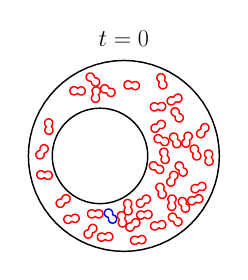
\begin{tikzpicture}[scale=0.35]

\begin{axis}[
  xmin = -21,
  xmax = 21,
  ymin = -21,
  ymax = 21,
  scale only axis,
  axis equal image,
  hide axis,
  title = {\Huge$t=0$}
  ]

\addplot [mark=none,black,line width=1.5] table{
2.0000e+01 0.0000e+00
1.9904e+01 1.9603e+00
1.9616e+01 3.9018e+00
1.9139e+01 5.8057e+00
1.8478e+01 7.6537e+00
1.7638e+01 9.4279e+00
1.6629e+01 1.1111e+01
1.5460e+01 1.2688e+01
1.4142e+01 1.4142e+01
1.2688e+01 1.5460e+01
1.1111e+01 1.6629e+01
9.4279e+00 1.7638e+01
7.6537e+00 1.8478e+01
5.8057e+00 1.9139e+01
3.9018e+00 1.9616e+01
1.9603e+00 1.9904e+01
1.2246e-15 2.0000e+01
-1.9603e+00 1.9904e+01
-3.9018e+00 1.9616e+01
-5.8057e+00 1.9139e+01
-7.6537e+00 1.8478e+01
-9.4279e+00 1.7638e+01
-1.1111e+01 1.6629e+01
-1.2688e+01 1.5460e+01
-1.4142e+01 1.4142e+01
-1.5460e+01 1.2688e+01
-1.6629e+01 1.1111e+01
-1.7638e+01 9.4279e+00
-1.8478e+01 7.6537e+00
-1.9139e+01 5.8057e+00
-1.9616e+01 3.9018e+00
-1.9904e+01 1.9603e+00
-2.0000e+01 2.4493e-15
-1.9904e+01 -1.9603e+00
-1.9616e+01 -3.9018e+00
-1.9139e+01 -5.8057e+00
-1.8478e+01 -7.6537e+00
-1.7638e+01 -9.4279e+00
-1.6629e+01 -1.1111e+01
-1.5460e+01 -1.2688e+01
-1.4142e+01 -1.4142e+01
-1.2688e+01 -1.5460e+01
-1.1111e+01 -1.6629e+01
-9.4279e+00 -1.7638e+01
-7.6537e+00 -1.8478e+01
-5.8057e+00 -1.9139e+01
-3.9018e+00 -1.9616e+01
-1.9603e+00 -1.9904e+01
-3.6739e-15 -2.0000e+01
1.9603e+00 -1.9904e+01
3.9018e+00 -1.9616e+01
5.8057e+00 -1.9139e+01
7.6537e+00 -1.8478e+01
9.4279e+00 -1.7638e+01
1.1111e+01 -1.6629e+01
1.2688e+01 -1.5460e+01
1.4142e+01 -1.4142e+01
1.5460e+01 -1.2688e+01
1.6629e+01 -1.1111e+01
1.7638e+01 -9.4279e+00
1.8478e+01 -7.6537e+00
1.9139e+01 -5.8057e+00
1.9616e+01 -3.9018e+00
1.9904e+01 -1.9603e+00
2.0000e+01 0.0000e+00
};

\addplot [mark=none,black,line width=1.5] table{
5.0000e+00 0.0000e+00
4.9518e+00 -9.8017e-01
4.8079e+00 -1.9509e+00
4.5694e+00 -2.9028e+00
4.2388e+00 -3.8268e+00
3.8192e+00 -4.7140e+00
3.3147e+00 -5.5557e+00
2.7301e+00 -6.3439e+00
2.0711e+00 -7.0711e+00
1.3439e+00 -7.7301e+00
5.5570e-01 -8.3147e+00
-2.8603e-01 -8.8192e+00
-1.1732e+00 -9.2388e+00
-2.0972e+00 -9.5694e+00
-3.0491e+00 -9.8079e+00
-4.0198e+00 -9.9518e+00
-5.0000e+00 -1.0000e+01
-5.9802e+00 -9.9518e+00
-6.9509e+00 -9.8079e+00
-7.9028e+00 -9.5694e+00
-8.8268e+00 -9.2388e+00
-9.7140e+00 -8.8192e+00
-1.0556e+01 -8.3147e+00
-1.1344e+01 -7.7301e+00
-1.2071e+01 -7.0711e+00
-1.2730e+01 -6.3439e+00
-1.3315e+01 -5.5557e+00
-1.3819e+01 -4.7140e+00
-1.4239e+01 -3.8268e+00
-1.4569e+01 -2.9028e+00
-1.4808e+01 -1.9509e+00
-1.4952e+01 -9.8017e-01
-1.5000e+01 -1.2246e-15
-1.4952e+01 9.8017e-01
-1.4808e+01 1.9509e+00
-1.4569e+01 2.9028e+00
-1.4239e+01 3.8268e+00
-1.3819e+01 4.7140e+00
-1.3315e+01 5.5557e+00
-1.2730e+01 6.3439e+00
-1.2071e+01 7.0711e+00
-1.1344e+01 7.7301e+00
-1.0556e+01 8.3147e+00
-9.7140e+00 8.8192e+00
-8.8268e+00 9.2388e+00
-7.9028e+00 9.5694e+00
-6.9509e+00 9.8079e+00
-5.9802e+00 9.9518e+00
-5.0000e+00 1.0000e+01
-4.0198e+00 9.9518e+00
-3.0491e+00 9.8079e+00
-2.0972e+00 9.5694e+00
-1.1732e+00 9.2388e+00
-2.8603e-01 8.8192e+00
5.5570e-01 8.3147e+00
1.3439e+00 7.7301e+00
2.0711e+00 7.0711e+00
2.7301e+00 6.3439e+00
3.3147e+00 5.5557e+00
3.8192e+00 4.7140e+00
4.2388e+00 3.8268e+00
4.5694e+00 2.9028e+00
4.8079e+00 1.9509e+00
4.9518e+00 9.8017e-01
5.0000e+00 0.0000e+00
};

\addplot [mark=none,red,line width=1.5] table{
1.6974e+01 4.9857e+00
1.7020e+01 5.0202e+00
1.7096e+01 5.0464e+00
1.7195e+01 5.0770e+00
1.7307e+01 5.1217e+00
1.7423e+01 5.1855e+00
1.7534e+01 5.2706e+00
1.7634e+01 5.3763e+00
1.7717e+01 5.5004e+00
1.7778e+01 5.6394e+00
1.7814e+01 5.7889e+00
1.7823e+01 5.9437e+00
1.7803e+01 6.0986e+00
1.7755e+01 6.2479e+00
1.7680e+01 6.3864e+00
1.7581e+01 6.5090e+00
1.7461e+01 6.6113e+00
1.7324e+01 6.6898e+00
1.7175e+01 6.7416e+00
1.7020e+01 6.7651e+00
1.6863e+01 6.7597e+00
1.6711e+01 6.7259e+00
1.6568e+01 6.6654e+00
1.6439e+01 6.5811e+00
1.6329e+01 6.4766e+00
1.6240e+01 6.3566e+00
1.6175e+01 6.2267e+00
1.6132e+01 6.0930e+00
1.6111e+01 5.9622e+00
1.6107e+01 5.8415e+00
1.6112e+01 5.7380e+00
1.6113e+01 5.6578e+00
1.6096e+01 5.6031e+00
1.6050e+01 5.5685e+00
1.5975e+01 5.5423e+00
1.5876e+01 5.5117e+00
1.5763e+01 5.4671e+00
1.5647e+01 5.4032e+00
1.5536e+01 5.3182e+00
1.5436e+01 5.2125e+00
1.5353e+01 5.0884e+00
1.5292e+01 4.9493e+00
1.5256e+01 4.7999e+00
1.5247e+01 4.6450e+00
1.5267e+01 4.4901e+00
1.5315e+01 4.3408e+00
1.5390e+01 4.2023e+00
1.5489e+01 4.0797e+00
1.5609e+01 3.9774e+00
1.5746e+01 3.8990e+00
1.5895e+01 3.8472e+00
1.6050e+01 3.8237e+00
1.6207e+01 3.8291e+00
1.6360e+01 3.8629e+00
1.6502e+01 3.9233e+00
1.6631e+01 4.0077e+00
1.6741e+01 4.1122e+00
1.6830e+01 4.2321e+00
1.6895e+01 4.3620e+00
1.6938e+01 4.4957e+00
1.6959e+01 4.6265e+00
1.6963e+01 4.7473e+00
1.6958e+01 4.8508e+00
1.6957e+01 4.9309e+00
1.6974e+01 4.9857e+00
};

\addplot [mark=none,red,line width=1.5] table{
7.1263e+00 1.0846e+01
7.0710e+00 1.0861e+01
7.0040e+00 1.0905e+01
6.9194e+00 1.0965e+01
6.8155e+00 1.1027e+01
6.6941e+00 1.1079e+01
6.5587e+00 1.1116e+01
6.4140e+00 1.1131e+01
6.2651e+00 1.1121e+01
6.1176e+00 1.1084e+01
5.9773e+00 1.1022e+01
5.8493e+00 1.0934e+01
5.7387e+00 1.0824e+01
5.6496e+00 1.0695e+01
5.5854e+00 1.0551e+01
5.5488e+00 1.0398e+01
5.5409e+00 1.0240e+01
5.5623e+00 1.0084e+01
5.6121e+00 9.9342e+00
5.6884e+00 9.7966e+00
5.7883e+00 9.6757e+00
5.9080e+00 9.5755e+00
6.0430e+00 9.4992e+00
6.1883e+00 9.4488e+00
6.3383e+00 9.4253e+00
6.4875e+00 9.4281e+00
6.6304e+00 9.4553e+00
6.7622e+00 9.5033e+00
6.8786e+00 9.5666e+00
6.9767e+00 9.6371e+00
7.0559e+00 9.7038e+00
7.1188e+00 9.7536e+00
7.1726e+00 9.7734e+00
7.2278e+00 9.7583e+00
7.2948e+00 9.7142e+00
7.3794e+00 9.6544e+00
7.4833e+00 9.5927e+00
7.6047e+00 9.5397e+00
7.7401e+00 9.5032e+00
7.8849e+00 9.4884e+00
8.0337e+00 9.4985e+00
8.1812e+00 9.5349e+00
8.3215e+00 9.5976e+00
8.4495e+00 9.6852e+00
8.5601e+00 9.7954e+00
8.6492e+00 9.9244e+00
8.7134e+00 1.0068e+01
8.7501e+00 1.0221e+01
8.7579e+00 1.0379e+01
8.7365e+00 1.0535e+01
8.6867e+00 1.0685e+01
8.6105e+00 1.0823e+01
8.5106e+00 1.0944e+01
8.3908e+00 1.1044e+01
8.2558e+00 1.1120e+01
8.1105e+00 1.1170e+01
7.9605e+00 1.1194e+01
7.8113e+00 1.1191e+01
7.6684e+00 1.1164e+01
7.5366e+00 1.1116e+01
7.4202e+00 1.1053e+01
7.3221e+00 1.0982e+01
7.2429e+00 1.0915e+01
7.1800e+00 1.0866e+01
7.1263e+00 1.0846e+01
};

\addplot [mark=none,red,line width=1.5] table{
8.3038e+00 -7.1509e+00
8.3037e+00 -7.0936e+00
8.3283e+00 -7.0173e+00
8.3634e+00 -6.9198e+00
8.3952e+00 -6.8033e+00
8.4140e+00 -6.6721e+00
8.4131e+00 -6.5319e+00
8.3888e+00 -6.3884e+00
8.3394e+00 -6.2476e+00
8.2651e+00 -6.1152e+00
8.1673e+00 -5.9966e+00
8.0487e+00 -5.8966e+00
7.9130e+00 -5.8193e+00
7.7649e+00 -5.7678e+00
7.6093e+00 -5.7442e+00
7.4518e+00 -5.7497e+00
7.2978e+00 -5.7842e+00
7.1528e+00 -5.8464e+00
7.0218e+00 -5.9342e+00
6.9095e+00 -6.0444e+00
6.8196e+00 -6.1729e+00
6.7549e+00 -6.3150e+00
6.7173e+00 -6.4655e+00
6.7074e+00 -6.6189e+00
6.7247e+00 -6.7697e+00
6.7671e+00 -6.9128e+00
6.8315e+00 -7.0434e+00
6.9129e+00 -7.1576e+00
7.0048e+00 -7.2529e+00
7.0989e+00 -7.3287e+00
7.1844e+00 -7.3872e+00
7.2490e+00 -7.4346e+00
7.2825e+00 -7.4811e+00
7.2826e+00 -7.5385e+00
7.2579e+00 -7.6148e+00
7.2229e+00 -7.7123e+00
7.1911e+00 -7.8288e+00
7.1723e+00 -7.9599e+00
7.1732e+00 -8.1001e+00
7.1975e+00 -8.2436e+00
7.2469e+00 -8.3845e+00
7.3212e+00 -8.5169e+00
7.4190e+00 -8.6355e+00
7.5376e+00 -8.7354e+00
7.6732e+00 -8.8128e+00
7.8214e+00 -8.8643e+00
7.9770e+00 -8.8878e+00
8.1345e+00 -8.8823e+00
8.2885e+00 -8.8479e+00
8.4335e+00 -8.7856e+00
8.5645e+00 -8.6978e+00
8.6768e+00 -8.5876e+00
8.7667e+00 -8.4592e+00
8.8314e+00 -8.3171e+00
8.8690e+00 -8.1666e+00
8.8788e+00 -8.0132e+00
8.8616e+00 -7.8623e+00
8.8191e+00 -7.7192e+00
8.7548e+00 -7.5887e+00
8.6734e+00 -7.4745e+00
8.5815e+00 -7.3792e+00
8.4874e+00 -7.3034e+00
8.4019e+00 -7.2448e+00
8.3373e+00 -7.1974e+00
8.3038e+00 -7.1509e+00
};

\addplot [mark=none,red,line width=1.5] table{
1.0828e+01 1.1313e+01
1.0885e+01 1.1318e+01
1.0963e+01 1.1300e+01
1.1063e+01 1.1273e+01
1.1182e+01 1.1251e+01
1.1314e+01 1.1243e+01
1.1454e+01 1.1256e+01
1.1595e+01 1.1292e+01
1.1731e+01 1.1353e+01
1.1857e+01 1.1438e+01
1.1967e+01 1.1546e+01
1.2056e+01 1.1672e+01
1.2122e+01 1.1814e+01
1.2161e+01 1.1966e+01
1.2172e+01 1.2123e+01
1.2153e+01 1.2279e+01
1.2106e+01 1.2430e+01
1.2031e+01 1.2569e+01
1.1933e+01 1.2692e+01
1.1814e+01 1.2795e+01
1.1678e+01 1.2874e+01
1.1531e+01 1.2926e+01
1.1378e+01 1.2951e+01
1.1224e+01 1.2948e+01
1.1076e+01 1.2918e+01
1.0937e+01 1.2864e+01
1.0812e+01 1.2789e+01
1.0705e+01 1.2698e+01
1.0618e+01 1.2599e+01
1.0550e+01 1.2499e+01
1.0499e+01 1.2409e+01
1.0457e+01 1.2340e+01
1.0413e+01 1.2303e+01
1.0356e+01 1.2298e+01
1.0278e+01 1.2316e+01
1.0178e+01 1.2343e+01
1.0059e+01 1.2365e+01
9.9270e+00 1.2373e+01
9.7874e+00 1.2360e+01
9.6464e+00 1.2324e+01
9.5102e+00 1.2263e+01
9.3845e+00 1.2178e+01
9.2745e+00 1.2070e+01
9.1848e+00 1.1944e+01
9.1192e+00 1.1802e+01
9.0802e+00 1.1650e+01
9.0698e+00 1.1493e+01
9.0885e+00 1.1337e+01
9.1357e+00 1.1186e+01
9.2099e+00 1.1047e+01
9.3083e+00 1.0924e+01
9.4275e+00 1.0821e+01
9.5631e+00 1.0742e+01
9.7101e+00 1.0690e+01
9.8632e+00 1.0665e+01
1.0017e+01 1.0668e+01
1.0166e+01 1.0698e+01
1.0305e+01 1.0752e+01
1.0430e+01 1.0827e+01
1.0537e+01 1.0918e+01
1.0624e+01 1.1017e+01
1.0691e+01 1.1117e+01
1.0743e+01 1.1207e+01
1.0784e+01 1.1276e+01
1.0828e+01 1.1313e+01
};

\addplot [mark=none,red,line width=1.5] table{
7.4682e+00 5.7461e+00
7.5239e+00 5.7597e+00
7.6039e+00 5.7535e+00
7.7068e+00 5.7423e+00
7.8276e+00 5.7386e+00
7.9594e+00 5.7511e+00
8.0956e+00 5.7848e+00
8.2294e+00 5.8420e+00
8.3548e+00 5.9230e+00
8.4661e+00 6.0262e+00
8.5585e+00 6.1491e+00
8.6279e+00 6.2878e+00
8.6713e+00 6.4378e+00
8.6867e+00 6.5939e+00
8.6732e+00 6.7506e+00
8.6310e+00 6.9025e+00
8.5614e+00 7.0442e+00
8.4670e+00 7.1706e+00
8.3509e+00 7.2773e+00
8.2175e+00 7.3607e+00
8.0715e+00 7.4181e+00
7.9183e+00 7.4477e+00
7.7631e+00 7.4490e+00
7.6117e+00 7.4227e+00
7.4691e+00 7.3706e+00
7.3399e+00 7.2958e+00
7.2281e+00 7.2027e+00
7.1361e+00 7.0968e+00
7.0649e+00 6.9851e+00
7.0133e+00 6.8759e+00
6.9764e+00 6.7791e+00
6.9454e+00 6.7052e+00
6.9080e+00 6.6617e+00
6.8523e+00 6.6482e+00
6.7724e+00 6.6543e+00
6.6694e+00 6.6655e+00
6.5486e+00 6.6692e+00
6.4168e+00 6.6567e+00
6.2806e+00 6.6230e+00
6.1468e+00 6.5658e+00
6.0215e+00 6.4849e+00
5.9101e+00 6.3816e+00
5.8178e+00 6.2587e+00
5.7483e+00 6.1200e+00
5.7049e+00 5.9701e+00
5.6895e+00 5.8140e+00
5.7030e+00 5.6572e+00
5.7452e+00 5.5053e+00
5.8148e+00 5.3637e+00
5.9093e+00 5.2373e+00
6.0253e+00 5.1305e+00
6.1587e+00 5.0471e+00
6.3047e+00 4.9898e+00
6.4580e+00 4.9602e+00
6.6131e+00 4.9589e+00
6.7645e+00 4.9852e+00
6.9072e+00 5.0373e+00
7.0363e+00 5.1120e+00
7.1482e+00 5.2051e+00
7.2401e+00 5.3110e+00
7.3113e+00 5.4227e+00
7.3630e+00 5.5319e+00
7.3999e+00 5.6287e+00
7.4308e+00 5.7027e+00
7.4682e+00 5.7461e+00
};

\addplot [mark=none,red,line width=1.5] table{
9.5144e+00 -9.7761e+00
9.4948e+00 -9.8300e+00
9.4455e+00 -9.8932e+00
9.3791e+00 -9.9728e+00
9.3092e+00 -1.0071e+01
9.2467e+00 -1.0188e+01
9.1994e+00 -1.0320e+01
9.1730e+00 -1.0463e+01
9.1710e+00 -1.0612e+01
9.1954e+00 -1.0762e+01
9.2466e+00 -1.0907e+01
9.3237e+00 -1.1042e+01
9.4246e+00 -1.1161e+01
9.5460e+00 -1.1260e+01
9.6841e+00 -1.1336e+01
9.8340e+00 -1.1385e+01
9.9904e+00 -1.1405e+01
1.0148e+01 -1.1396e+01
1.0301e+01 -1.1359e+01
1.0444e+01 -1.1294e+01
1.0573e+01 -1.1204e+01
1.0682e+01 -1.1093e+01
1.0769e+01 -1.0964e+01
1.0831e+01 -1.0824e+01
1.0867e+01 -1.0676e+01
1.0876e+01 -1.0527e+01
1.0860e+01 -1.0382e+01
1.0823e+01 -1.0247e+01
1.0769e+01 -1.0126e+01
1.0707e+01 -1.0022e+01
1.0647e+01 -9.9382e+00
1.0602e+01 -9.8715e+00
1.0587e+01 -9.8163e+00
1.0607e+01 -9.7624e+00
1.0656e+01 -9.6992e+00
1.0722e+01 -9.6196e+00
1.0792e+01 -9.5211e+00
1.0855e+01 -9.4044e+00
1.0902e+01 -9.2724e+00
1.0928e+01 -9.1292e+00
1.0930e+01 -8.9800e+00
1.0906e+01 -8.8301e+00
1.0855e+01 -8.6852e+00
1.0778e+01 -8.5506e+00
1.0677e+01 -8.4314e+00
1.0555e+01 -8.3322e+00
1.0417e+01 -8.2567e+00
1.0267e+01 -8.2078e+00
1.0111e+01 -8.1874e+00
9.9534e+00 -8.1961e+00
9.8002e+00 -8.2336e+00
9.6569e+00 -8.2986e+00
9.5284e+00 -8.3884e+00
9.4189e+00 -8.4997e+00
9.3320e+00 -8.6282e+00
9.2701e+00 -8.7689e+00
9.2345e+00 -8.9165e+00
9.2253e+00 -9.0655e+00
9.2409e+00 -9.2101e+00
9.2782e+00 -9.3453e+00
9.3319e+00 -9.4664e+00
9.3942e+00 -9.5699e+00
9.4544e+00 -9.6542e+00
9.4989e+00 -9.7209e+00
9.5144e+00 -9.7761e+00
};

\addplot [mark=none,red,line width=1.5] table{
8.4823e+00 1.5772e+01
8.4854e+00 1.5829e+01
8.5144e+00 1.5904e+01
8.5549e+00 1.5999e+01
8.5934e+00 1.6114e+01
8.6195e+00 1.6244e+01
8.6266e+00 1.6384e+01
8.6106e+00 1.6528e+01
8.5693e+00 1.6672e+01
8.5026e+00 1.6808e+01
8.4117e+00 1.6932e+01
8.2990e+00 1.7039e+01
8.1680e+00 1.7124e+01
8.0231e+00 1.7183e+01
7.8691e+00 1.7216e+01
7.7115e+00 1.7219e+01
7.5557e+00 1.7194e+01
7.4074e+00 1.7140e+01
7.2717e+00 1.7060e+01
7.1533e+00 1.6956e+01
7.0562e+00 1.6833e+01
6.9835e+00 1.6695e+01
6.9374e+00 1.6547e+01
6.9188e+00 1.6394e+01
6.9275e+00 1.6242e+01
6.9617e+00 1.6097e+01
7.0185e+00 1.5963e+01
7.0933e+00 1.5844e+01
7.1796e+00 1.5744e+01
7.2692e+00 1.5663e+01
7.3512e+00 1.5600e+01
7.4131e+00 1.5549e+01
7.4439e+00 1.5500e+01
7.4407e+00 1.5443e+01
7.4117e+00 1.5368e+01
7.3712e+00 1.5273e+01
7.3328e+00 1.5158e+01
7.3066e+00 1.5029e+01
7.2995e+00 1.4889e+01
7.3156e+00 1.4744e+01
7.3568e+00 1.4601e+01
7.4235e+00 1.4464e+01
7.5144e+00 1.4340e+01
7.6271e+00 1.4234e+01
7.7581e+00 1.4149e+01
7.9031e+00 1.4089e+01
8.0571e+00 1.4056e+01
8.2147e+00 1.4053e+01
8.3704e+00 1.4079e+01
8.5187e+00 1.4132e+01
8.6544e+00 1.4213e+01
8.7729e+00 1.4316e+01
8.8700e+00 1.4439e+01
8.9426e+00 1.4578e+01
8.9887e+00 1.4726e+01
9.0073e+00 1.4878e+01
8.9987e+00 1.5030e+01
8.9644e+00 1.5175e+01
8.9076e+00 1.5309e+01
8.8329e+00 1.5428e+01
8.7465e+00 1.5528e+01
8.6569e+00 1.5609e+01
8.5749e+00 1.5673e+01
8.5131e+00 1.5724e+01
8.4823e+00 1.5772e+01
};

\addplot [mark=none,red,line width=1.5] table{
2.2060e+00 -1.4888e+01
2.2604e+00 -1.4870e+01
2.3406e+00 -1.4869e+01
2.4441e+00 -1.4872e+01
2.5647e+00 -1.4865e+01
2.6951e+00 -1.4842e+01
2.8279e+00 -1.4797e+01
2.9565e+00 -1.4729e+01
3.0747e+00 -1.4637e+01
3.1770e+00 -1.4525e+01
3.2588e+00 -1.4395e+01
3.3164e+00 -1.4251e+01
3.3471e+00 -1.4098e+01
3.3494e+00 -1.3941e+01
3.3228e+00 -1.3786e+01
3.2680e+00 -1.3638e+01
3.1869e+00 -1.3503e+01
3.0822e+00 -1.3385e+01
2.9577e+00 -1.3288e+01
2.8177e+00 -1.3216e+01
2.6675e+00 -1.3171e+01
2.5123e+00 -1.3155e+01
2.3576e+00 -1.3166e+01
2.2089e+00 -1.3205e+01
2.0711e+00 -1.3269e+01
1.9486e+00 -1.3354e+01
1.8449e+00 -1.3456e+01
1.7621e+00 -1.3570e+01
1.7006e+00 -1.3687e+01
1.6582e+00 -1.3800e+01
1.6295e+00 -1.3900e+01
1.6049e+00 -1.3976e+01
1.5713e+00 -1.4022e+01
1.5169e+00 -1.4040e+01
1.4367e+00 -1.4041e+01
1.3331e+00 -1.4038e+01
1.2125e+00 -1.4045e+01
1.0821e+00 -1.4068e+01
9.4930e-01 -1.4113e+01
8.2073e-01 -1.4181e+01
7.0257e-01 -1.4273e+01
6.0029e-01 -1.4385e+01
5.1849e-01 -1.4515e+01
4.6089e-01 -1.4659e+01
4.3015e-01 -1.4812e+01
4.2785e-01 -1.4969e+01
4.5444e-01 -1.5124e+01
5.0920e-01 -1.5272e+01
5.9034e-01 -1.5407e+01
6.9504e-01 -1.5525e+01
8.1958e-01 -1.5622e+01
9.5950e-01 -1.5694e+01
1.1098e+00 -1.5739e+01
1.2650e+00 -1.5755e+01
1.4197e+00 -1.5744e+01
1.5684e+00 -1.5705e+01
1.7062e+00 -1.5641e+01
1.8286e+00 -1.5556e+01
1.9323e+00 -1.5454e+01
2.0151e+00 -1.5340e+01
2.0766e+00 -1.5223e+01
2.1190e+00 -1.5110e+01
2.1477e+00 -1.5011e+01
2.1723e+00 -1.4934e+01
2.2060e+00 -1.4888e+01
};

\addplot [mark=none,red,line width=1.5] table{
-9.7141e+00 1.3092e+01
-9.6600e+00 1.3073e+01
-9.5963e+00 1.3025e+01
-9.5161e+00 1.2959e+01
-9.4168e+00 1.2890e+01
-9.2994e+00 1.2829e+01
-9.1669e+00 1.2783e+01
-9.0235e+00 1.2758e+01
-8.8743e+00 1.2758e+01
-8.7247e+00 1.2784e+01
-8.5803e+00 1.2836e+01
-8.4465e+00 1.2915e+01
-8.3284e+00 1.3017e+01
-8.2305e+00 1.3139e+01
-8.1564e+00 1.3278e+01
-8.1091e+00 1.3429e+01
-8.0903e+00 1.3585e+01
-8.1007e+00 1.3743e+01
-8.1398e+00 1.3896e+01
-8.2063e+00 1.4038e+01
-8.2975e+00 1.4166e+01
-8.4099e+00 1.4274e+01
-8.5393e+00 1.4360e+01
-8.6806e+00 1.4420e+01
-8.8286e+00 1.4454e+01
-8.9777e+00 1.4462e+01
-9.1222e+00 1.4445e+01
-9.2570e+00 1.4406e+01
-9.3775e+00 1.4351e+01
-9.4803e+00 1.4287e+01
-9.5640e+00 1.4226e+01
-9.6302e+00 1.4181e+01
-9.6852e+00 1.4165e+01
-9.7393e+00 1.4184e+01
-9.8030e+00 1.4233e+01
-9.8833e+00 1.4298e+01
-9.9825e+00 1.4367e+01
-1.0100e+01 1.4429e+01
-1.0232e+01 1.4474e+01
-1.0376e+01 1.4499e+01
-1.0525e+01 1.4500e+01
-1.0675e+01 1.4474e+01
-1.0819e+01 1.4421e+01
-1.0953e+01 1.4343e+01
-1.1071e+01 1.4240e+01
-1.1169e+01 1.4118e+01
-1.1243e+01 1.3979e+01
-1.1290e+01 1.3829e+01
-1.1309e+01 1.3672e+01
-1.1299e+01 1.3515e+01
-1.1260e+01 1.3362e+01
-1.1193e+01 1.3219e+01
-1.1102e+01 1.3092e+01
-1.0989e+01 1.2983e+01
-1.0860e+01 1.2898e+01
-1.0719e+01 1.2837e+01
-1.0571e+01 1.2803e+01
-1.0422e+01 1.2796e+01
-1.0277e+01 1.2813e+01
-1.0142e+01 1.2852e+01
-1.0022e+01 1.2906e+01
-9.9190e+00 1.2970e+01
-9.8354e+00 1.3031e+01
-9.7691e+00 1.3076e+01
-9.7141e+00 1.3092e+01
};

\addplot [mark=none,red,line width=1.5] table{
1.3056e+01 -1.0028e+01
1.3048e+01 -9.9714e+00
1.3063e+01 -9.8926e+00
1.3085e+01 -9.7913e+00
1.3101e+01 -9.6716e+00
1.3102e+01 -9.5392e+00
1.3083e+01 -9.4003e+00
1.3040e+01 -9.2612e+00
1.2973e+01 -9.1281e+00
1.2882e+01 -9.0066e+00
1.2769e+01 -8.9019e+00
1.2638e+01 -8.8183e+00
1.2494e+01 -8.7595e+00
1.2340e+01 -8.7279e+00
1.2183e+01 -8.7250e+00
1.2027e+01 -8.7511e+00
1.1879e+01 -8.8054e+00
1.1744e+01 -8.8862e+00
1.1625e+01 -8.9904e+00
1.1528e+01 -9.1144e+00
1.1456e+01 -9.2536e+00
1.1411e+01 -9.4030e+00
1.1393e+01 -9.5571e+00
1.1404e+01 -9.7105e+00
1.1440e+01 -9.8577e+00
1.1501e+01 -9.9940e+00
1.1582e+01 -1.0115e+01
1.1678e+01 -1.0217e+01
1.1782e+01 -1.0300e+01
1.1885e+01 -1.0363e+01
1.1977e+01 -1.0410e+01
1.2048e+01 -1.0448e+01
1.2087e+01 -1.0490e+01
1.2094e+01 -1.0547e+01
1.2080e+01 -1.0625e+01
1.2058e+01 -1.0727e+01
1.2042e+01 -1.0846e+01
1.2041e+01 -1.0979e+01
1.2060e+01 -1.1118e+01
1.2103e+01 -1.1257e+01
1.2170e+01 -1.1390e+01
1.2261e+01 -1.1511e+01
1.2374e+01 -1.1616e+01
1.2504e+01 -1.1700e+01
1.2649e+01 -1.1759e+01
1.2803e+01 -1.1790e+01
1.2960e+01 -1.1793e+01
1.3115e+01 -1.1767e+01
1.3264e+01 -1.1713e+01
1.3399e+01 -1.1632e+01
1.3517e+01 -1.1528e+01
1.3614e+01 -1.1404e+01
1.3687e+01 -1.1264e+01
1.3732e+01 -1.1115e+01
1.3750e+01 -1.0961e+01
1.3739e+01 -1.0808e+01
1.3702e+01 -1.0660e+01
1.3641e+01 -1.0524e+01
1.3561e+01 -1.0403e+01
1.3465e+01 -1.0301e+01
1.3361e+01 -1.0218e+01
1.3258e+01 -1.0155e+01
1.3166e+01 -1.0108e+01
1.3095e+01 -1.0070e+01
1.3056e+01 -1.0028e+01
};

\addplot [mark=none,red,line width=1.5] table{
-6.0043e+00 -1.2673e+01
-5.9498e+00 -1.2691e+01
-5.8852e+00 -1.2738e+01
-5.8036e+00 -1.2802e+01
-5.7030e+00 -1.2869e+01
-5.5844e+00 -1.2928e+01
-5.4510e+00 -1.2971e+01
-5.3071e+00 -1.2993e+01
-5.1579e+00 -1.2990e+01
-5.0089e+00 -1.2961e+01
-4.8656e+00 -1.2906e+01
-4.7334e+00 -1.2825e+01
-4.6174e+00 -1.2720e+01
-4.5219e+00 -1.2596e+01
-4.4507e+00 -1.2455e+01
-4.4064e+00 -1.2304e+01
-4.3907e+00 -1.2147e+01
-4.4043e+00 -1.1990e+01
-4.4465e+00 -1.1838e+01
-4.5158e+00 -1.1697e+01
-4.6095e+00 -1.1571e+01
-4.7241e+00 -1.1465e+01
-4.8552e+00 -1.1382e+01
-4.9977e+00 -1.1324e+01
-5.1464e+00 -1.1293e+01
-5.2955e+00 -1.1289e+01
-5.4397e+00 -1.1309e+01
-5.5737e+00 -1.1350e+01
-5.6930e+00 -1.1408e+01
-5.7946e+00 -1.1473e+01
-5.8770e+00 -1.1536e+01
-5.9423e+00 -1.1582e+01
-5.9970e+00 -1.1600e+01
-6.0515e+00 -1.1582e+01
-6.1161e+00 -1.1534e+01
-6.1977e+00 -1.1470e+01
-6.2983e+00 -1.1404e+01
-6.4169e+00 -1.1345e+01
-6.5503e+00 -1.1301e+01
-6.6942e+00 -1.1279e+01
-6.8434e+00 -1.1282e+01
-6.9924e+00 -1.1311e+01
-7.1357e+00 -1.1367e+01
-7.2679e+00 -1.1448e+01
-7.3839e+00 -1.1552e+01
-7.4794e+00 -1.1677e+01
-7.5506e+00 -1.1817e+01
-7.5949e+00 -1.1968e+01
-7.6106e+00 -1.2125e+01
-7.5970e+00 -1.2282e+01
-7.5548e+00 -1.2434e+01
-7.4855e+00 -1.2576e+01
-7.3918e+00 -1.2701e+01
-7.2772e+00 -1.2807e+01
-7.1461e+00 -1.2890e+01
-7.0036e+00 -1.2948e+01
-6.8549e+00 -1.2979e+01
-6.7058e+00 -1.2984e+01
-6.5616e+00 -1.2964e+01
-6.4276e+00 -1.2922e+01
-6.3083e+00 -1.2865e+01
-6.2067e+00 -1.2799e+01
-6.1243e+00 -1.2737e+01
-6.0590e+00 -1.2690e+01
-6.0043e+00 -1.2673e+01
};

\addplot [mark=none,red,line width=1.5] table{
1.2722e+01 3.5755e+00
1.2689e+01 3.5290e+00
1.2624e+01 3.4815e+00
1.2539e+01 3.4230e+00
1.2445e+01 3.3471e+00
1.2353e+01 3.2518e+00
1.2272e+01 3.1376e+00
1.2207e+01 3.0070e+00
1.2165e+01 2.8639e+00
1.2148e+01 2.7131e+00
1.2158e+01 2.5596e+00
1.2195e+01 2.4092e+00
1.2260e+01 2.2671e+00
1.2350e+01 2.1386e+00
1.2462e+01 2.0285e+00
1.2593e+01 1.9407e+00
1.2738e+01 1.8785e+00
1.2892e+01 1.8441e+00
1.3050e+01 1.8387e+00
1.3205e+01 1.8623e+00
1.3354e+01 1.9139e+00
1.3489e+01 1.9912e+00
1.3608e+01 2.0913e+00
1.3705e+01 2.2099e+00
1.3780e+01 2.3423e+00
1.3829e+01 2.4831e+00
1.3853e+01 2.6267e+00
1.3854e+01 2.7669e+00
1.3835e+01 2.8980e+00
1.3803e+01 3.0145e+00
1.3768e+01 3.1120e+00
1.3744e+01 3.1883e+00
1.3744e+01 3.2456e+00
1.3777e+01 3.2922e+00
1.3842e+01 3.3396e+00
1.3927e+01 3.3981e+00
1.4021e+01 3.4740e+00
1.4113e+01 3.5693e+00
1.4195e+01 3.6836e+00
1.4259e+01 3.8141e+00
1.4301e+01 3.9572e+00
1.4319e+01 4.1081e+00
1.4309e+01 4.2615e+00
1.4271e+01 4.4120e+00
1.4206e+01 4.5540e+00
1.4116e+01 4.6825e+00
1.4004e+01 4.7926e+00
1.3873e+01 4.8804e+00
1.3728e+01 4.9426e+00
1.3574e+01 4.9770e+00
1.3416e+01 4.9824e+00
1.3261e+01 4.9588e+00
1.3113e+01 4.9073e+00
1.2977e+01 4.8299e+00
1.2859e+01 4.7299e+00
1.2761e+01 4.6112e+00
1.2687e+01 4.4788e+00
1.2637e+01 4.3380e+00
1.2613e+01 4.1945e+00
1.2612e+01 4.0542e+00
1.2631e+01 3.9231e+00
1.2663e+01 3.8066e+00
1.2698e+01 3.7091e+00
1.2723e+01 3.6329e+00
1.2722e+01 3.5755e+00
};

\addplot [mark=none,red,line width=1.5] table{
9.6605e+00 -4.5603e+00
9.6219e+00 -4.6028e+00
9.5523e+00 -4.6426e+00
9.4608e+00 -4.6910e+00
9.3588e+00 -4.7557e+00
9.2566e+00 -4.8400e+00
9.1628e+00 -4.9443e+00
9.0841e+00 -5.0667e+00
9.0258e+00 -5.2041e+00
8.9916e+00 -5.3520e+00
8.9840e+00 -5.5056e+00
9.0043e+00 -5.6593e+00
9.0525e+00 -5.8078e+00
9.1273e+00 -5.9457e+00
9.2265e+00 -6.0678e+00
9.3466e+00 -6.1699e+00
9.4837e+00 -6.2482e+00
9.6328e+00 -6.2998e+00
9.7887e+00 -6.3231e+00
9.9460e+00 -6.3173e+00
1.0099e+01 -6.2829e+00
1.0242e+01 -6.2214e+00
1.0372e+01 -6.1354e+00
1.0482e+01 -6.0287e+00
1.0571e+01 -5.9056e+00
1.0636e+01 -5.7712e+00
1.0676e+01 -5.6314e+00
1.0693e+01 -5.4921e+00
1.0689e+01 -5.3597e+00
1.0671e+01 -5.2404e+00
1.0647e+01 -5.1395e+00
1.0631e+01 -5.0610e+00
1.0638e+01 -5.0040e+00
1.0676e+01 -4.9616e+00
1.0746e+01 -4.9218e+00
1.0838e+01 -4.8733e+00
1.0940e+01 -4.8086e+00
1.1042e+01 -4.7243e+00
1.1136e+01 -4.6200e+00
1.1214e+01 -4.4976e+00
1.1273e+01 -4.3603e+00
1.1307e+01 -4.2123e+00
1.1314e+01 -4.0588e+00
1.1294e+01 -3.9050e+00
1.1246e+01 -3.7565e+00
1.1171e+01 -3.6187e+00
1.1072e+01 -3.4965e+00
1.0952e+01 -3.3944e+00
1.0815e+01 -3.3162e+00
1.0666e+01 -3.2645e+00
1.0510e+01 -3.2413e+00
1.0352e+01 -3.2471e+00
1.0199e+01 -3.2815e+00
1.0056e+01 -3.3430e+00
9.9267e+00 -3.4289e+00
9.8161e+00 -3.5356e+00
9.7273e+00 -3.6588e+00
9.6623e+00 -3.7931e+00
9.6219e+00 -3.9329e+00
9.6052e+00 -4.0722e+00
9.6090e+00 -4.2046e+00
9.6274e+00 -4.3240e+00
9.6512e+00 -4.4248e+00
9.6671e+00 -4.5034e+00
9.6605e+00 -4.5603e+00
};

\addplot [mark=none,red,line width=1.5] table{
3.7751e+00 -9.0390e+00
3.7201e+00 -9.0555e+00
3.6400e+00 -9.0537e+00
3.5366e+00 -9.0480e+00
3.4158e+00 -9.0508e+00
3.2848e+00 -9.0703e+00
3.1507e+00 -9.1113e+00
3.0201e+00 -9.1756e+00
2.8993e+00 -9.2631e+00
2.7936e+00 -9.3722e+00
2.7080e+00 -9.4999e+00
2.6461e+00 -9.6421e+00
2.6107e+00 -9.7941e+00
2.6037e+00 -9.9508e+00
2.6256e+00 -1.0107e+01
2.6759e+00 -1.0256e+01
2.7530e+00 -1.0394e+01
2.8541e+00 -1.0515e+01
2.9756e+00 -1.0615e+01
3.1133e+00 -1.0691e+01
3.2622e+00 -1.0741e+01
3.4168e+00 -1.0762e+01
3.5718e+00 -1.0755e+01
3.7216e+00 -1.0721e+01
3.8612e+00 -1.0661e+01
3.9862e+00 -1.0580e+01
4.0929e+00 -1.0481e+01
4.1791e+00 -1.0370e+01
4.2441e+00 -1.0255e+01
4.2899e+00 -1.0143e+01
4.3215e+00 -1.0044e+01
4.3485e+00 -9.9687e+00
4.3835e+00 -9.9233e+00
4.4384e+00 -9.9068e+00
4.5186e+00 -9.9086e+00
4.6220e+00 -9.9143e+00
4.7428e+00 -9.9115e+00
4.8738e+00 -9.8920e+00
5.0079e+00 -9.8510e+00
5.1385e+00 -9.7867e+00
5.2593e+00 -9.6992e+00
5.3649e+00 -9.5901e+00
5.4506e+00 -9.4624e+00
5.5125e+00 -9.3202e+00
5.5478e+00 -9.1682e+00
5.5548e+00 -9.0115e+00
5.5329e+00 -8.8557e+00
5.4826e+00 -8.7062e+00
5.4056e+00 -8.5685e+00
5.3045e+00 -8.4474e+00
5.1829e+00 -8.3470e+00
5.0452e+00 -8.2709e+00
4.8964e+00 -8.2214e+00
4.7417e+00 -8.2001e+00
4.5868e+00 -8.2071e+00
4.4369e+00 -8.2415e+00
4.2973e+00 -8.3011e+00
4.1724e+00 -8.3827e+00
4.0656e+00 -8.4817e+00
3.9795e+00 -8.5923e+00
3.9144e+00 -8.7077e+00
3.8687e+00 -8.8195e+00
3.8370e+00 -8.9181e+00
3.8101e+00 -8.9936e+00
3.7751e+00 -9.0390e+00
};

\addplot [mark=none,red,line width=1.5] table{
-1.6656e+01 -4.5443e+00
-1.6602e+01 -4.5652e+00
-1.6540e+01 -4.6161e+00
-1.6463e+01 -4.6844e+00
-1.6366e+01 -4.7567e+00
-1.6251e+01 -4.8221e+00
-1.6120e+01 -4.8726e+00
-1.5977e+01 -4.9026e+00
-1.5828e+01 -4.9082e+00
-1.5678e+01 -4.8875e+00
-1.5532e+01 -4.8398e+00
-1.5395e+01 -4.7661e+00
-1.5274e+01 -4.6682e+00
-1.5171e+01 -4.5492e+00
-1.5093e+01 -4.4130e+00
-1.5040e+01 -4.2644e+00
-1.5016e+01 -4.1085e+00
-1.5021e+01 -3.9507e+00
-1.5054e+01 -3.7968e+00
-1.5116e+01 -3.6519e+00
-1.5202e+01 -3.5212e+00
-1.5311e+01 -3.4090e+00
-1.5437e+01 -3.3189e+00
-1.5576e+01 -3.2536e+00
-1.5723e+01 -3.2144e+00
-1.5872e+01 -3.2015e+00
-1.6017e+01 -3.2136e+00
-1.6153e+01 -3.2475e+00
-1.6275e+01 -3.2982e+00
-1.6380e+01 -3.3580e+00
-1.6466e+01 -3.4161e+00
-1.6534e+01 -3.4589e+00
-1.6589e+01 -3.4731e+00
-1.6643e+01 -3.4522e+00
-1.6705e+01 -3.4013e+00
-1.6783e+01 -3.3330e+00
-1.6879e+01 -3.2607e+00
-1.6994e+01 -3.1953e+00
-1.7125e+01 -3.1448e+00
-1.7268e+01 -3.1148e+00
-1.7417e+01 -3.1092e+00
-1.7567e+01 -3.1299e+00
-1.7713e+01 -3.1776e+00
-1.7850e+01 -3.2513e+00
-1.7972e+01 -3.3492e+00
-1.8074e+01 -3.4682e+00
-1.8153e+01 -3.6044e+00
-1.8205e+01 -3.7530e+00
-1.8229e+01 -3.9089e+00
-1.8225e+01 -4.0666e+00
-1.8191e+01 -4.2206e+00
-1.8129e+01 -4.3655e+00
-1.8043e+01 -4.4962e+00
-1.7934e+01 -4.6084e+00
-1.7808e+01 -4.6985e+00
-1.7669e+01 -4.7638e+00
-1.7522e+01 -4.8030e+00
-1.7373e+01 -4.8159e+00
-1.7228e+01 -4.8038e+00
-1.7092e+01 -4.7699e+00
-1.6970e+01 -4.7192e+00
-1.6865e+01 -4.6594e+00
-1.6779e+01 -4.6013e+00
-1.6711e+01 -4.5585e+00
-1.6656e+01 -4.5443e+00
};

\addplot [mark=none,red,line width=1.5] table{
1.2457e+01 -2.4577e+00
1.2443e+01 -2.4022e+00
1.2448e+01 -2.3222e+00
1.2458e+01 -2.2191e+00
1.2460e+01 -2.0983e+00
1.2446e+01 -1.9666e+00
1.2411e+01 -1.8309e+00
1.2352e+01 -1.6978e+00
1.2269e+01 -1.5734e+00
1.2165e+01 -1.4634e+00
1.2041e+01 -1.3725e+00
1.1901e+01 -1.3048e+00
1.1751e+01 -1.2632e+00
1.1594e+01 -1.2498e+00
1.1438e+01 -1.2652e+00
1.1286e+01 -1.3093e+00
1.1146e+01 -1.3806e+00
1.1020e+01 -1.4766e+00
1.0915e+01 -1.5940e+00
1.0833e+01 -1.7284e+00
1.0778e+01 -1.8751e+00
1.0750e+01 -2.0287e+00
1.0751e+01 -2.1838e+00
1.0779e+01 -2.3349e+00
1.0833e+01 -2.4769e+00
1.0909e+01 -2.6051e+00
1.1004e+01 -2.7158e+00
1.1111e+01 -2.8065e+00
1.1223e+01 -2.8762e+00
1.1333e+01 -2.9266e+00
1.1430e+01 -2.9623e+00
1.1505e+01 -2.9923e+00
1.1548e+01 -3.0292e+00
1.1563e+01 -3.0847e+00
1.1558e+01 -3.1647e+00
1.1548e+01 -3.2678e+00
1.1545e+01 -3.3886e+00
1.1559e+01 -3.5203e+00
1.1595e+01 -3.6560e+00
1.1654e+01 -3.7891e+00
1.1736e+01 -3.9135e+00
1.1841e+01 -4.0235e+00
1.1965e+01 -4.1144e+00
1.2104e+01 -4.1821e+00
1.2255e+01 -4.2237e+00
1.2411e+01 -4.2371e+00
1.2568e+01 -4.2217e+00
1.2719e+01 -4.1776e+00
1.2860e+01 -4.1063e+00
1.2985e+01 -4.0103e+00
1.3090e+01 -3.8929e+00
1.3172e+01 -3.7585e+00
1.3228e+01 -3.6118e+00
1.3255e+01 -3.4582e+00
1.3255e+01 -3.3031e+00
1.3227e+01 -3.1520e+00
1.3173e+01 -3.0100e+00
1.3096e+01 -2.8818e+00
1.3002e+01 -2.7711e+00
1.2895e+01 -2.6804e+00
1.2782e+01 -2.6107e+00
1.2673e+01 -2.5603e+00
1.2575e+01 -2.5246e+00
1.2501e+01 -2.4946e+00
1.2457e+01 -2.4577e+00
};

\addplot [mark=none,red,line width=1.5] table{
-1.2399e+01 -9.8730e+00
-1.2345e+01 -9.8536e+00
-1.2265e+01 -9.8512e+00
-1.2161e+01 -9.8513e+00
-1.2041e+01 -9.8420e+00
-1.1911e+01 -9.8155e+00
-1.1779e+01 -9.7674e+00
-1.1652e+01 -9.6962e+00
-1.1536e+01 -9.6023e+00
-1.1436e+01 -9.4877e+00
-1.1358e+01 -9.3557e+00
-1.1304e+01 -9.2103e+00
-1.1276e+01 -9.0566e+00
-1.1278e+01 -8.8997e+00
-1.1308e+01 -8.7453e+00
-1.1366e+01 -8.5988e+00
-1.1451e+01 -8.4654e+00
-1.1558e+01 -8.3499e+00
-1.1685e+01 -8.2562e+00
-1.1826e+01 -8.1875e+00
-1.1978e+01 -8.1461e+00
-1.2133e+01 -8.1331e+00
-1.2288e+01 -8.1484e+00
-1.2435e+01 -8.1908e+00
-1.2572e+01 -8.2579e+00
-1.2692e+01 -8.3460e+00
-1.2793e+01 -8.4506e+00
-1.2873e+01 -8.5657e+00
-1.2932e+01 -8.6844e+00
-1.2972e+01 -8.7985e+00
-1.2998e+01 -8.8987e+00
-1.3021e+01 -8.9755e+00
-1.3054e+01 -9.0227e+00
-1.3108e+01 -9.0421e+00
-1.3188e+01 -9.0446e+00
-1.3291e+01 -9.0445e+00
-1.3412e+01 -9.0537e+00
-1.3541e+01 -9.0803e+00
-1.3673e+01 -9.1283e+00
-1.3800e+01 -9.1995e+00
-1.3916e+01 -9.2935e+00
-1.4016e+01 -9.4081e+00
-1.4094e+01 -9.5401e+00
-1.4149e+01 -9.6854e+00
-1.4176e+01 -9.8392e+00
-1.4174e+01 -9.9960e+00
-1.4144e+01 -1.0150e+01
-1.4086e+01 -1.0297e+01
-1.4002e+01 -1.0430e+01
-1.3894e+01 -1.0546e+01
-1.3767e+01 -1.0640e+01
-1.3626e+01 -1.0708e+01
-1.3474e+01 -1.0750e+01
-1.3319e+01 -1.0763e+01
-1.3165e+01 -1.0747e+01
-1.3017e+01 -1.0705e+01
-1.2881e+01 -1.0638e+01
-1.2760e+01 -1.0550e+01
-1.2659e+01 -1.0445e+01
-1.2579e+01 -1.0330e+01
-1.2520e+01 -1.0211e+01
-1.2480e+01 -1.0097e+01
-1.2454e+01 -9.9971e+00
-1.2431e+01 -9.9203e+00
-1.2399e+01 -9.8730e+00
};

\addplot [mark=none,red,line width=1.5] table{
-3.8937e+00 -1.7497e+01
-3.8381e+00 -1.7511e+01
-3.7703e+00 -1.7554e+01
-3.6844e+00 -1.7612e+01
-3.5794e+00 -1.7671e+01
-3.4570e+00 -1.7722e+01
-3.3208e+00 -1.7756e+01
-3.1758e+00 -1.7767e+01
-3.0271e+00 -1.7754e+01
-2.8805e+00 -1.7715e+01
-2.7414e+00 -1.7650e+01
-2.6153e+00 -1.7559e+01
-2.5068e+00 -1.7447e+01
-2.4204e+00 -1.7316e+01
-2.3592e+00 -1.7171e+01
-2.3256e+00 -1.7017e+01
-2.3209e+00 -1.6859e+01
-2.3455e+00 -1.6704e+01
-2.3982e+00 -1.6555e+01
-2.4773e+00 -1.6419e+01
-2.5796e+00 -1.6300e+01
-2.7013e+00 -1.6202e+01
-2.8379e+00 -1.6129e+01
-2.9841e+00 -1.6081e+01
-3.1346e+00 -1.6061e+01
-3.2837e+00 -1.6067e+01
-3.4261e+00 -1.6097e+01
-3.5568e+00 -1.6147e+01
-3.6719e+00 -1.6213e+01
-3.7686e+00 -1.6285e+01
-3.8464e+00 -1.6354e+01
-3.9083e+00 -1.6405e+01
-3.9617e+00 -1.6426e+01
-4.0172e+00 -1.6412e+01
-4.0851e+00 -1.6369e+01
-4.1709e+00 -1.6311e+01
-4.2760e+00 -1.6251e+01
-4.3984e+00 -1.6201e+01
-4.5345e+00 -1.6167e+01
-4.6796e+00 -1.6155e+01
-4.8282e+00 -1.6168e+01
-4.9749e+00 -1.6208e+01
-5.1139e+00 -1.6273e+01
-5.2401e+00 -1.6363e+01
-5.3485e+00 -1.6476e+01
-5.4350e+00 -1.6607e+01
-5.4962e+00 -1.6751e+01
-5.5298e+00 -1.6906e+01
-5.5344e+00 -1.7063e+01
-5.5099e+00 -1.7219e+01
-5.4571e+00 -1.7368e+01
-5.3781e+00 -1.7504e+01
-5.2757e+00 -1.7623e+01
-5.1540e+00 -1.7720e+01
-5.0175e+00 -1.7794e+01
-4.8712e+00 -1.7841e+01
-4.7208e+00 -1.7862e+01
-4.5717e+00 -1.7856e+01
-4.4293e+00 -1.7826e+01
-4.2985e+00 -1.7775e+01
-4.1834e+00 -1.7710e+01
-4.0868e+00 -1.7637e+01
-4.0090e+00 -1.7569e+01
-3.9471e+00 -1.7518e+01
-3.8937e+00 -1.7497e+01
};

\addplot [mark=none,red,line width=1.5] table{
1.7256e+01 -4.0165e-01
1.7242e+01 -4.5729e-01
1.7200e+01 -5.2531e-01
1.7142e+01 -6.1138e-01
1.7083e+01 -7.1668e-01
1.7033e+01 -8.3933e-01
1.7000e+01 -9.7558e-01
1.6988e+01 -1.1207e+00
1.7002e+01 -1.2693e+00
1.7042e+01 -1.4158e+00
1.7108e+01 -1.5546e+00
1.7199e+01 -1.6803e+00
1.7312e+01 -1.7883e+00
1.7443e+01 -1.8742e+00
1.7588e+01 -1.9348e+00
1.7742e+01 -1.9678e+00
1.7900e+01 -1.9717e+00
1.8056e+01 -1.9466e+00
1.8204e+01 -1.8932e+00
1.8340e+01 -1.8136e+00
1.8458e+01 -1.7107e+00
1.8556e+01 -1.5886e+00
1.8629e+01 -1.4517e+00
1.8675e+01 -1.3053e+00
1.8695e+01 -1.1548e+00
1.8689e+01 -1.0057e+00
1.8658e+01 -8.6342e-01
1.8607e+01 -7.3288e-01
1.8541e+01 -6.1808e-01
1.8468e+01 -5.2171e-01
1.8399e+01 -4.4418e-01
1.8348e+01 -3.8250e-01
1.8327e+01 -3.2922e-01
1.8341e+01 -2.7358e-01
1.8383e+01 -2.0557e-01
1.8441e+01 -1.1950e-01
1.8500e+01 -1.4188e-02
1.8550e+01 1.0845e-01
1.8583e+01 2.4471e-01
1.8595e+01 3.8982e-01
1.8581e+01 5.3841e-01
1.8541e+01 6.8490e-01
1.8475e+01 8.2369e-01
1.8384e+01 9.4947e-01
1.8271e+01 1.0574e+00
1.8140e+01 1.1433e+00
1.7995e+01 1.2040e+00
1.7841e+01 1.2369e+00
1.7683e+01 1.2409e+00
1.7527e+01 1.2157e+00
1.7379e+01 1.1623e+00
1.7243e+01 1.0827e+00
1.7125e+01 9.7986e-01
1.7027e+01 8.5772e-01
1.6954e+01 7.2086e-01
1.6908e+01 5.7444e-01
1.6888e+01 4.2390e-01
1.6894e+01 2.7482e-01
1.6925e+01 1.3255e-01
1.6976e+01 2.0026e-03
1.7042e+01 -1.1279e-01
1.7115e+01 -2.0917e-01
1.7184e+01 -2.8669e-01
1.7235e+01 -3.4837e-01
1.7256e+01 -4.0165e-01
};

\addplot [mark=none,red,line width=1.5] table{
-6.8567e+00 1.5609e+01
-6.8287e+00 1.5559e+01
-6.8131e+00 1.5481e+01
-6.7962e+00 1.5378e+01
-6.7673e+00 1.5261e+01
-6.7198e+00 1.5137e+01
-6.6507e+00 1.5015e+01
-6.5596e+00 1.4902e+01
-6.4479e+00 1.4803e+01
-6.3184e+00 1.4724e+01
-6.1752e+00 1.4668e+01
-6.0230e+00 1.4638e+01
-5.8669e+00 1.4637e+01
-5.7124e+00 1.4664e+01
-5.5651e+00 1.4719e+01
-5.4301e+00 1.4801e+01
-5.3124e+00 1.4906e+01
-5.2161e+00 1.5031e+01
-5.1445e+00 1.5171e+01
-5.1001e+00 1.5322e+01
-5.0841e+00 1.5478e+01
-5.0969e+00 1.5634e+01
-5.1373e+00 1.5783e+01
-5.2035e+00 1.5922e+01
-5.2920e+00 1.6046e+01
-5.3988e+00 1.6150e+01
-5.5185e+00 1.6232e+01
-5.6453e+00 1.6293e+01
-5.7720e+00 1.6331e+01
-5.8911e+00 1.6351e+01
-5.9942e+00 1.6361e+01
-6.0738e+00 1.6371e+01
-6.1257e+00 1.6395e+01
-6.1537e+00 1.6445e+01
-6.1693e+00 1.6524e+01
-6.1862e+00 1.6626e+01
-6.2152e+00 1.6743e+01
-6.2627e+00 1.6867e+01
-6.3318e+00 1.6989e+01
-6.4229e+00 1.7102e+01
-6.5346e+00 1.7201e+01
-6.6640e+00 1.7281e+01
-6.8072e+00 1.7337e+01
-6.9595e+00 1.7366e+01
-7.1156e+00 1.7368e+01
-7.2701e+00 1.7341e+01
-7.4174e+00 1.7285e+01
-7.5523e+00 1.7204e+01
-7.6700e+00 1.7099e+01
-7.7664e+00 1.6974e+01
-7.8379e+00 1.6833e+01
-7.8824e+00 1.6682e+01
-7.8983e+00 1.6526e+01
-7.8856e+00 1.6371e+01
-7.8451e+00 1.6221e+01
-7.7790e+00 1.6082e+01
-7.6904e+00 1.5959e+01
-7.5837e+00 1.5855e+01
-7.4639e+00 1.5772e+01
-7.3372e+00 1.5712e+01
-7.2104e+00 1.5673e+01
-7.0914e+00 1.5653e+01
-6.9882e+00 1.5643e+01
-6.9087e+00 1.5634e+01
-6.8567e+00 1.5609e+01
};

\addplot [mark=none,red,line width=1.5] table{
3.0596e+00 -1.8143e+01
3.1156e+00 -1.8155e+01
3.1848e+00 -1.8196e+01
3.2724e+00 -1.8251e+01
3.3794e+00 -1.8307e+01
3.5034e+00 -1.8354e+01
3.6405e+00 -1.8383e+01
3.7859e+00 -1.8390e+01
3.9340e+00 -1.8372e+01
4.0793e+00 -1.8328e+01
4.2162e+00 -1.8258e+01
4.3394e+00 -1.8164e+01
4.4441e+00 -1.8048e+01
4.5263e+00 -1.7915e+01
4.5828e+00 -1.7768e+01
4.6114e+00 -1.7613e+01
4.6110e+00 -1.7455e+01
4.5814e+00 -1.7300e+01
4.5239e+00 -1.7153e+01
4.4405e+00 -1.7020e+01
4.3344e+00 -1.6904e+01
4.2095e+00 -1.6811e+01
4.0707e+00 -1.6741e+01
3.9230e+00 -1.6699e+01
3.7720e+00 -1.6683e+01
3.6231e+00 -1.6694e+01
3.4818e+00 -1.6728e+01
3.3527e+00 -1.6783e+01
3.2398e+00 -1.6853e+01
3.1455e+00 -1.6928e+01
3.0700e+00 -1.6999e+01
3.0098e+00 -1.7052e+01
2.9571e+00 -1.7075e+01
2.9011e+00 -1.7062e+01
2.8319e+00 -1.7022e+01
2.7443e+00 -1.6967e+01
2.6373e+00 -1.6910e+01
2.5133e+00 -1.6864e+01
2.3762e+00 -1.6835e+01
2.2308e+00 -1.6827e+01
2.0827e+00 -1.6845e+01
1.9374e+00 -1.6889e+01
1.8005e+00 -1.6959e+01
1.6773e+00 -1.7054e+01
1.5726e+00 -1.7169e+01
1.4904e+00 -1.7303e+01
1.4339e+00 -1.7450e+01
1.4053e+00 -1.7605e+01
1.4057e+00 -1.7763e+01
1.4353e+00 -1.7918e+01
1.4928e+00 -1.8064e+01
1.5762e+00 -1.8198e+01
1.6823e+00 -1.8313e+01
1.8071e+00 -1.8407e+01
1.9460e+00 -1.8476e+01
2.0937e+00 -1.8519e+01
2.2447e+00 -1.8534e+01
2.3936e+00 -1.8524e+01
2.5349e+00 -1.8489e+01
2.6640e+00 -1.8434e+01
2.7769e+00 -1.8365e+01
2.8711e+00 -1.8289e+01
2.9467e+00 -1.8219e+01
3.0069e+00 -1.8166e+01
3.0596e+00 -1.8143e+01
};

\addplot [mark=none,red,line width=1.5] table{
-5.3395e+00 1.2796e+01
-5.3168e+00 1.2849e+01
-5.2638e+00 1.2909e+01
-5.1928e+00 1.2984e+01
-5.1172e+00 1.3078e+01
-5.0478e+00 1.3191e+01
-4.9928e+00 1.3320e+01
-4.9579e+00 1.3461e+01
-4.9471e+00 1.3610e+01
-4.9626e+00 1.3761e+01
-5.0051e+00 1.3909e+01
-5.0741e+00 1.4048e+01
-5.1677e+00 1.4173e+01
-5.2831e+00 1.4279e+01
-5.4164e+00 1.4363e+01
-5.5631e+00 1.4420e+01
-5.7181e+00 1.4450e+01
-5.8759e+00 1.4451e+01
-6.0310e+00 1.4422e+01
-6.1779e+00 1.4366e+01
-6.3115e+00 1.4284e+01
-6.4274e+00 1.4179e+01
-6.5218e+00 1.4056e+01
-6.5920e+00 1.3920e+01
-6.6362e+00 1.3774e+01
-6.6542e+00 1.3626e+01
-6.6472e+00 1.3481e+01
-6.6180e+00 1.3344e+01
-6.5716e+00 1.3220e+01
-6.5155e+00 1.3113e+01
-6.4604e+00 1.3025e+01
-6.4200e+00 1.2956e+01
-6.4078e+00 1.2900e+01
-6.4306e+00 1.2847e+01
-6.4836e+00 1.2787e+01
-6.5545e+00 1.2711e+01
-6.6301e+00 1.2617e+01
-6.6995e+00 1.2504e+01
-6.7545e+00 1.2375e+01
-6.7894e+00 1.2234e+01
-6.8002e+00 1.2085e+01
-6.7847e+00 1.1934e+01
-6.7422e+00 1.1786e+01
-6.6732e+00 1.1647e+01
-6.5796e+00 1.1523e+01
-6.4643e+00 1.1416e+01
-6.3309e+00 1.1333e+01
-6.1842e+00 1.1275e+01
-6.0292e+00 1.1245e+01
-5.8714e+00 1.1245e+01
-5.7164e+00 1.1273e+01
-5.5694e+00 1.1329e+01
-5.4358e+00 1.1411e+01
-5.3199e+00 1.1516e+01
-5.2255e+00 1.1639e+01
-5.1553e+00 1.1776e+01
-5.1111e+00 1.1921e+01
-5.0931e+00 1.2069e+01
-5.1001e+00 1.2215e+01
-5.1293e+00 1.2352e+01
-5.1757e+00 1.2476e+01
-5.2318e+00 1.2583e+01
-5.2869e+00 1.2671e+01
-5.3273e+00 1.2740e+01
-5.3395e+00 1.2796e+01
};

\addplot [mark=none,red,line width=1.5] table{
-1.0888e+01 -1.3703e+01
-1.0832e+01 -1.3713e+01
-1.0761e+01 -1.3750e+01
-1.0671e+01 -1.3801e+01
-1.0561e+01 -1.3853e+01
-1.0435e+01 -1.3894e+01
-1.0297e+01 -1.3917e+01
-1.0151e+01 -1.3918e+01
-1.0004e+01 -1.3893e+01
-9.8611e+00 -1.3843e+01
-9.7274e+00 -1.3767e+01
-9.6086e+00 -1.3667e+01
-9.5092e+00 -1.3547e+01
-9.4330e+00 -1.3409e+01
-9.3831e+00 -1.3260e+01
-9.3615e+00 -1.3104e+01
-9.3690e+00 -1.2946e+01
-9.4054e+00 -1.2793e+01
-9.4695e+00 -1.2649e+01
-9.5588e+00 -1.2519e+01
-9.6699e+00 -1.2409e+01
-9.7988e+00 -1.2321e+01
-9.9406e+00 -1.2258e+01
-1.0090e+01 -1.2222e+01
-1.0242e+01 -1.2213e+01
-1.0390e+01 -1.2230e+01
-1.0530e+01 -1.2271e+01
-1.0656e+01 -1.2332e+01
-1.0766e+01 -1.2406e+01
-1.0856e+01 -1.2486e+01
-1.0929e+01 -1.2560e+01
-1.0987e+01 -1.2615e+01
-1.1038e+01 -1.2640e+01
-1.1095e+01 -1.2631e+01
-1.1166e+01 -1.2593e+01
-1.1256e+01 -1.2542e+01
-1.1365e+01 -1.2491e+01
-1.1491e+01 -1.2450e+01
-1.1629e+01 -1.2426e+01
-1.1775e+01 -1.2426e+01
-1.1922e+01 -1.2450e+01
-1.2065e+01 -1.2501e+01
-1.2199e+01 -1.2577e+01
-1.2318e+01 -1.2676e+01
-1.2417e+01 -1.2797e+01
-1.2493e+01 -1.2934e+01
-1.2543e+01 -1.3083e+01
-1.2565e+01 -1.3239e+01
-1.2557e+01 -1.3397e+01
-1.2521e+01 -1.3550e+01
-1.2457e+01 -1.3694e+01
-1.2368e+01 -1.3824e+01
-1.2256e+01 -1.3935e+01
-1.2127e+01 -1.4023e+01
-1.1986e+01 -1.4086e+01
-1.1836e+01 -1.4122e+01
-1.1685e+01 -1.4131e+01
-1.1536e+01 -1.4113e+01
-1.1397e+01 -1.4072e+01
-1.1270e+01 -1.4012e+01
-1.1161e+01 -1.3937e+01
-1.1070e+01 -1.3858e+01
-1.0997e+01 -1.3784e+01
-1.0940e+01 -1.3728e+01
-1.0888e+01 -1.3703e+01
};

\addplot [mark=none,blue,line width=1.5] table{
-2.3481e+00 -1.2305e+01
-2.3643e+00 -1.2250e+01
-2.3620e+00 -1.2170e+01
-2.3558e+00 -1.2067e+01
-2.3580e+00 -1.1946e+01
-2.3769e+00 -1.1815e+01
-2.4171e+00 -1.1681e+01
-2.4808e+00 -1.1550e+01
-2.5677e+00 -1.1428e+01
-2.6763e+00 -1.1322e+01
-2.8035e+00 -1.1236e+01
-2.9454e+00 -1.1173e+01
-3.0973e+00 -1.1137e+01
-3.2539e+00 -1.1129e+01
-3.4099e+00 -1.1151e+01
-3.5595e+00 -1.1200e+01
-3.6976e+00 -1.1276e+01
-3.8193e+00 -1.1377e+01
-3.9203e+00 -1.1498e+01
-3.9971e+00 -1.1635e+01
-4.0473e+00 -1.1784e+01
-4.0694e+00 -1.1938e+01
-4.0632e+00 -1.2093e+01
-4.0296e+00 -1.2243e+01
-3.9706e+00 -1.2383e+01
-3.8897e+00 -1.2509e+01
-3.7912e+00 -1.2616e+01
-3.6810e+00 -1.2703e+01
-3.5660e+00 -1.2768e+01
-3.4544e+00 -1.2815e+01
-3.3559e+00 -1.2847e+01
-3.2806e+00 -1.2874e+01
-3.2353e+00 -1.2909e+01
-3.2191e+00 -1.2964e+01
-3.2214e+00 -1.3044e+01
-3.2276e+00 -1.3148e+01
-3.2254e+00 -1.3269e+01
-3.2065e+00 -1.3400e+01
-3.1663e+00 -1.3534e+01
-3.1026e+00 -1.3665e+01
-3.0157e+00 -1.3786e+01
-2.9071e+00 -1.3892e+01
-2.7799e+00 -1.3979e+01
-2.6380e+00 -1.4041e+01
-2.4861e+00 -1.4077e+01
-2.3295e+00 -1.4085e+01
-2.1736e+00 -1.4064e+01
-2.0239e+00 -1.4015e+01
-1.8858e+00 -1.3938e+01
-1.7641e+00 -1.3838e+01
-1.6631e+00 -1.3717e+01
-1.5863e+00 -1.3579e+01
-1.5361e+00 -1.3431e+01
-1.5140e+00 -1.3276e+01
-1.5202e+00 -1.3121e+01
-1.5538e+00 -1.2971e+01
-1.6128e+00 -1.2831e+01
-1.6937e+00 -1.2706e+01
-1.7922e+00 -1.2599e+01
-1.9024e+00 -1.2512e+01
-2.0174e+00 -1.2446e+01
-2.1290e+00 -1.2400e+01
-2.2275e+00 -1.2368e+01
-2.3028e+00 -1.2341e+01
-2.3481e+00 -1.2305e+01
};

\addplot [mark=none,red,line width=1.5] table{
3.1008e-01 -1.0774e+01
2.9637e-01 -1.0829e+01
2.5407e-01 -1.0897e+01
1.9663e-01 -1.0984e+01
1.3767e-01 -1.1089e+01
8.7933e-02 -1.1212e+01
5.5046e-02 -1.1348e+01
4.4095e-02 -1.1493e+01
5.8112e-02 -1.1642e+01
9.8416e-02 -1.1788e+01
1.6484e-01 -1.1927e+01
2.5588e-01 -1.2052e+01
3.6891e-01 -1.2160e+01
5.0031e-01 -1.2246e+01
6.4564e-01 -1.2306e+01
7.9988e-01 -1.2339e+01
9.5765e-01 -1.2342e+01
1.1134e+00 -1.2317e+01
1.2616e+00 -1.2263e+01
1.3971e+00 -1.2183e+01
1.5153e+00 -1.2080e+01
1.6123e+00 -1.1958e+01
1.6850e+00 -1.1821e+01
1.7315e+00 -1.1674e+01
1.7510e+00 -1.1524e+01
1.7443e+00 -1.1374e+01
1.7132e+00 -1.1232e+01
1.6617e+00 -1.1102e+01
1.5954e+00 -1.0987e+01
1.5223e+00 -1.0891e+01
1.4535e+00 -1.0814e+01
1.4021e+00 -1.0752e+01
1.3808e+00 -1.0699e+01
1.3945e+00 -1.0643e+01
1.4368e+00 -1.0575e+01
1.4942e+00 -1.0489e+01
1.5532e+00 -1.0383e+01
1.6029e+00 -1.0261e+01
1.6358e+00 -1.0124e+01
1.6468e+00 -9.9792e+00
1.6328e+00 -9.8306e+00
1.5925e+00 -9.6842e+00
1.5260e+00 -9.5456e+00
1.4350e+00 -9.4200e+00
1.3220e+00 -9.3123e+00
1.1906e+00 -9.2267e+00
1.0452e+00 -9.1664e+00
8.9098e-01 -9.1338e+00
7.3322e-01 -9.1302e+00
5.7749e-01 -9.1557e+00
4.2927e-01 -9.2094e+00
2.9374e-01 -9.2893e+00
1.7553e-01 -9.3924e+00
7.8571e-02 -9.5148e+00
5.8735e-03 -9.6518e+00
-4.0620e-02 -9.7983e+00
-6.0174e-02 -9.9489e+00
-5.3396e-02 -1.0098e+01
-2.2368e-02 -1.0240e+01
2.9158e-02 -1.0371e+01
9.5484e-02 -1.0485e+01
1.6853e-01 -1.0581e+01
2.3740e-01 -1.0659e+01
2.8876e-01 -1.0720e+01
3.1008e-01 -1.0774e+01
};

\addplot [mark=none,red,line width=1.5] table{
7.0926e+00 -1.4010e+01
7.0358e+00 -1.4003e+01
6.9634e+00 -1.3968e+01
6.8714e+00 -1.3920e+01
6.7600e+00 -1.3874e+01
6.6325e+00 -1.3838e+01
6.4934e+00 -1.3820e+01
6.3480e+00 -1.3825e+01
6.2019e+00 -1.3856e+01
6.0608e+00 -1.3912e+01
5.9304e+00 -1.3993e+01
5.8157e+00 -1.4098e+01
5.7212e+00 -1.4222e+01
5.6506e+00 -1.4362e+01
5.6068e+00 -1.4513e+01
5.5915e+00 -1.4670e+01
5.6054e+00 -1.4827e+01
5.6480e+00 -1.4979e+01
5.7178e+00 -1.5121e+01
5.8123e+00 -1.5246e+01
5.9278e+00 -1.5353e+01
6.0602e+00 -1.5435e+01
6.2044e+00 -1.5492e+01
6.3552e+00 -1.5522e+01
6.5070e+00 -1.5525e+01
6.6544e+00 -1.5502e+01
6.7923e+00 -1.5455e+01
6.9162e+00 -1.5390e+01
7.0228e+00 -1.5311e+01
7.1103e+00 -1.5228e+01
7.1796e+00 -1.5151e+01
7.2351e+00 -1.5093e+01
7.2856e+00 -1.5066e+01
7.3425e+00 -1.5073e+01
7.4148e+00 -1.5108e+01
7.5069e+00 -1.5155e+01
7.6182e+00 -1.5202e+01
7.7457e+00 -1.5238e+01
7.8848e+00 -1.5256e+01
8.0303e+00 -1.5250e+01
8.1764e+00 -1.5220e+01
8.3174e+00 -1.5164e+01
8.4478e+00 -1.5082e+01
8.5626e+00 -1.4978e+01
8.6571e+00 -1.4854e+01
8.7276e+00 -1.4714e+01
8.7714e+00 -1.4563e+01
8.7867e+00 -1.4406e+01
8.7728e+00 -1.4248e+01
8.7302e+00 -1.4096e+01
8.6604e+00 -1.3955e+01
8.5660e+00 -1.3829e+01
8.4504e+00 -1.3723e+01
8.3181e+00 -1.3640e+01
8.1739e+00 -1.3583e+01
8.0231e+00 -1.3553e+01
7.8713e+00 -1.3551e+01
7.7238e+00 -1.3574e+01
7.5860e+00 -1.3620e+01
7.4620e+00 -1.3686e+01
7.3555e+00 -1.3765e+01
7.2679e+00 -1.3848e+01
7.1987e+00 -1.3925e+01
7.1432e+00 -1.3983e+01
7.0926e+00 -1.4010e+01
};

\addplot [mark=none,red,line width=1.5] table{
-1.6266e+01 6.1307e+00
-1.6281e+01 6.0755e+00
-1.6326e+01 6.0088e+00
-1.6386e+01 5.9245e+00
-1.6449e+01 5.8211e+00
-1.6502e+01 5.7001e+00
-1.6540e+01 5.5649e+00
-1.6556e+01 5.4202e+00
-1.6546e+01 5.2713e+00
-1.6511e+01 5.1236e+00
-1.6449e+01 4.9829e+00
-1.6362e+01 4.8543e+00
-1.6253e+01 4.7430e+00
-1.6124e+01 4.6530e+00
-1.5981e+01 4.5879e+00
-1.5828e+01 4.5503e+00
-1.5671e+01 4.5414e+00
-1.5514e+01 4.5618e+00
-1.5364e+01 4.6105e+00
-1.5226e+01 4.6859e+00
-1.5105e+01 4.7850e+00
-1.5004e+01 4.9041e+00
-1.4926e+01 5.0386e+00
-1.4875e+01 5.1835e+00
-1.4851e+01 5.3334e+00
-1.4852e+01 5.4826e+00
-1.4879e+01 5.6257e+00
-1.4926e+01 5.7578e+00
-1.4988e+01 5.8746e+00
-1.5058e+01 5.9732e+00
-1.5124e+01 6.0528e+00
-1.5174e+01 6.1160e+00
-1.5193e+01 6.1699e+00
-1.5178e+01 6.2251e+00
-1.5133e+01 6.2918e+00
-1.5073e+01 6.3760e+00
-1.5010e+01 6.4795e+00
-1.4957e+01 6.6005e+00
-1.4919e+01 6.7357e+00
-1.4904e+01 6.8804e+00
-1.4913e+01 7.0293e+00
-1.4948e+01 7.1770e+00
-1.5010e+01 7.3177e+00
-1.5097e+01 7.4463e+00
-1.5206e+01 7.5576e+00
-1.5335e+01 7.6476e+00
-1.5478e+01 7.7126e+00
-1.5631e+01 7.7503e+00
-1.5788e+01 7.7592e+00
-1.5945e+01 7.7388e+00
-1.6095e+01 7.6900e+00
-1.6233e+01 7.6147e+00
-1.6355e+01 7.5156e+00
-1.6455e+01 7.3965e+00
-1.6533e+01 7.2620e+00
-1.6584e+01 7.1170e+00
-1.6609e+01 6.9672e+00
-1.6607e+01 6.8180e+00
-1.6580e+01 6.6748e+00
-1.6533e+01 6.5428e+00
-1.6471e+01 6.4260e+00
-1.6401e+01 6.3274e+00
-1.6335e+01 6.2478e+00
-1.6285e+01 6.1846e+00
-1.6266e+01 6.1307e+00
};

\addplot [mark=none,red,line width=1.5] table{
1.1603e+01 8.9067e+00
1.1587e+01 8.9616e+00
1.1589e+01 9.0417e+00
1.1594e+01 9.1452e+00
1.1591e+01 9.2659e+00
1.1571e+01 9.3969e+00
1.1530e+01 9.5309e+00
1.1465e+01 9.6614e+00
1.1377e+01 9.7820e+00
1.1268e+01 9.8874e+00
1.1140e+01 9.9728e+00
1.0998e+01 1.0034e+01
1.0846e+01 1.0069e+01
1.0689e+01 1.0076e+01
1.0533e+01 1.0054e+01
1.0384e+01 1.0003e+01
1.0246e+01 9.9257e+00
1.0126e+01 9.8244e+00
1.0025e+01 9.7026e+00
9.9496e+00 9.5647e+00
9.9005e+00 9.4157e+00
9.8795e+00 9.2610e+00
9.8868e+00 9.1061e+00
9.9216e+00 8.9564e+00
9.9816e+00 8.8169e+00
1.0063e+01 8.6921e+00
1.0163e+01 8.5856e+00
1.0273e+01 8.4997e+00
1.0389e+01 8.4349e+00
1.0501e+01 8.3894e+00
1.0600e+01 8.3580e+00
1.0675e+01 8.3312e+00
1.0721e+01 8.2963e+00
1.0737e+01 8.2414e+00
1.0736e+01 8.1612e+00
1.0730e+01 8.0578e+00
1.0733e+01 7.9370e+00
1.0753e+01 7.8061e+00
1.0794e+01 7.6720e+00
1.0859e+01 7.5416e+00
1.0947e+01 7.4210e+00
1.1056e+01 7.3156e+00
1.1184e+01 7.2302e+00
1.1326e+01 7.1686e+00
1.1478e+01 7.1336e+00
1.1635e+01 7.1270e+00
1.1791e+01 7.1493e+00
1.1940e+01 7.1999e+00
1.2078e+01 7.2772e+00
1.2199e+01 7.3786e+00
1.2299e+01 7.5004e+00
1.2375e+01 7.6383e+00
1.2424e+01 7.7872e+00
1.2445e+01 7.9419e+00
1.2437e+01 8.0969e+00
1.2403e+01 8.2466e+00
1.2343e+01 8.3861e+00
1.2261e+01 8.5109e+00
1.2162e+01 8.6174e+00
1.2051e+01 8.7033e+00
1.1935e+01 8.7681e+00
1.1823e+01 8.8136e+00
1.1725e+01 8.8450e+00
1.1649e+01 8.8718e+00
1.1603e+01 8.9067e+00
};

\addplot [mark=none,red,line width=1.5] table{
1.5467e+01 -6.1244e+00
1.5410e+01 -6.1250e+00
1.5333e+01 -6.1011e+00
1.5235e+01 -6.0670e+00
1.5119e+01 -6.0362e+00
1.4987e+01 -6.0187e+00
1.4847e+01 -6.0209e+00
1.4704e+01 -6.0465e+00
1.4563e+01 -6.0971e+00
1.4432e+01 -6.1727e+00
1.4314e+01 -6.2716e+00
1.4215e+01 -6.3911e+00
1.4139e+01 -6.5275e+00
1.4089e+01 -6.6761e+00
1.4067e+01 -6.8319e+00
1.4074e+01 -6.9894e+00
1.4110e+01 -7.1430e+00
1.4173e+01 -7.2875e+00
1.4262e+01 -7.4176e+00
1.4374e+01 -7.5289e+00
1.4503e+01 -7.6176e+00
1.4646e+01 -7.6810e+00
1.4796e+01 -7.7172e+00
1.4950e+01 -7.7256e+00
1.5101e+01 -7.7069e+00
1.5243e+01 -7.6632e+00
1.5373e+01 -7.5976e+00
1.5487e+01 -7.5152e+00
1.5581e+01 -7.4223e+00
1.5656e+01 -7.3276e+00
1.5714e+01 -7.2416e+00
1.5761e+01 -7.1765e+00
1.5807e+01 -7.1425e+00
1.5864e+01 -7.1419e+00
1.5941e+01 -7.1659e+00
1.6038e+01 -7.2000e+00
1.6155e+01 -7.2308e+00
1.6287e+01 -7.2483e+00
1.6427e+01 -7.2461e+00
1.6570e+01 -7.2205e+00
1.6710e+01 -7.1698e+00
1.6842e+01 -7.0943e+00
1.6960e+01 -6.9953e+00
1.7059e+01 -6.8758e+00
1.7135e+01 -6.7395e+00
1.7185e+01 -6.5909e+00
1.7207e+01 -6.4351e+00
1.7200e+01 -6.2776e+00
1.7164e+01 -6.1239e+00
1.7101e+01 -5.9795e+00
1.7011e+01 -5.8494e+00
1.6900e+01 -5.7381e+00
1.6771e+01 -5.6493e+00
1.6628e+01 -5.5860e+00
1.6477e+01 -5.5498e+00
1.6324e+01 -5.5414e+00
1.6173e+01 -5.5600e+00
1.6031e+01 -5.6038e+00
1.5901e+01 -5.6693e+00
1.5787e+01 -5.7518e+00
1.5693e+01 -5.8446e+00
1.5618e+01 -5.9394e+00
1.5560e+01 -6.0254e+00
1.5513e+01 -6.0905e+00
1.5467e+01 -6.1244e+00
};

\addplot [mark=none,red,line width=1.5] table{
1.2790e-01 -1.3211e+01
1.3802e-01 -1.3155e+01
1.7586e-01 -1.3084e+01
2.2765e-01 -1.2994e+01
2.7972e-01 -1.2885e+01
3.2149e-01 -1.2760e+01
3.4556e-01 -1.2622e+01
3.4718e-01 -1.2476e+01
3.2366e-01 -1.2329e+01
2.7405e-01 -1.2185e+01
1.9887e-01 -1.2051e+01
9.9956e-02 -1.1932e+01
-1.9751e-02 -1.1831e+01
-1.5637e-01 -1.1754e+01
-3.0527e-01 -1.1703e+01
-4.6129e-01 -1.1681e+01
-6.1896e-01 -1.1687e+01
-7.7273e-01 -1.1723e+01
-9.1720e-01 -1.1786e+01
-1.0473e+00 -1.1874e+01
-1.1587e+00 -1.1985e+01
-1.2476e+00 -1.2113e+01
-1.3113e+00 -1.2255e+01
-1.3483e+00 -1.2404e+01
-1.3582e+00 -1.2555e+01
-1.3419e+00 -1.2704e+01
-1.3018e+00 -1.2844e+01
-1.2420e+00 -1.2970e+01
-1.1684e+00 -1.3081e+01
-1.0894e+00 -1.3172e+01
-1.0157e+00 -1.3245e+01
-9.6049e-01 -1.3303e+01
-9.3579e-01 -1.3355e+01
-9.4591e-01 -1.3411e+01
-9.8375e-01 -1.3482e+01
-1.0355e+00 -1.3571e+01
-1.0876e+00 -1.3680e+01
-1.1294e+00 -1.3806e+01
-1.1534e+00 -1.3944e+01
-1.1551e+00 -1.4090e+01
-1.1315e+00 -1.4237e+01
-1.0819e+00 -1.4381e+01
-1.0068e+00 -1.4515e+01
-9.0784e-01 -1.4634e+01
-7.8814e-01 -1.4734e+01
-6.5152e-01 -1.4811e+01
-5.0262e-01 -1.4862e+01
-3.4660e-01 -1.4885e+01
-1.8893e-01 -1.4878e+01
-3.5157e-02 -1.4843e+01
1.0931e-01 -1.4780e+01
2.3944e-01 -1.4691e+01
3.5079e-01 -1.4581e+01
4.3970e-01 -1.4453e+01
5.0345e-01 -1.4311e+01
5.4045e-01 -1.4162e+01
5.5031e-01 -1.4011e+01
5.3398e-01 -1.3862e+01
4.9389e-01 -1.3722e+01
4.3410e-01 -1.3595e+01
3.6056e-01 -1.3485e+01
2.8149e-01 -1.3394e+01
2.0780e-01 -1.3321e+01
1.5260e-01 -1.3263e+01
1.2790e-01 -1.3211e+01
};

\addplot [mark=none,red,line width=1.5] table{
7.9800e+00 -7.8087e-02
7.9725e+00 -1.3495e-01
7.9381e+00 -2.0735e-01
7.8907e+00 -2.9943e-01
7.8438e+00 -4.1079e-01
7.8081e+00 -5.3833e-01
7.7907e+00 -6.7748e-01
7.7960e+00 -8.2292e-01
7.8265e+00 -9.6900e-01
7.8829e+00 -1.1100e+00
7.9644e+00 -1.2403e+00
8.0689e+00 -1.3550e+00
8.1932e+00 -1.4493e+00
8.3334e+00 -1.5198e+00
8.4845e+00 -1.5635e+00
8.6415e+00 -1.5786e+00
8.7986e+00 -1.5646e+00
8.9505e+00 -1.5219e+00
9.0918e+00 -1.4519e+00
9.2176e+00 -1.3574e+00
9.3236e+00 -1.2417e+00
9.4062e+00 -1.1093e+00
9.4632e+00 -9.6503e-01
9.4930e+00 -8.1423e-01
9.4956e+00 -6.6241e-01
9.4723e+00 -5.1502e-01
9.4255e+00 -3.7718e-01
9.3598e+00 -2.5332e-01
9.2811e+00 -1.4680e-01
9.1977e+00 -5.9340e-02
9.1206e+00 9.8598e-03
9.0627e+00 6.5302e-02
9.0356e+00 1.1582e-01
9.0430e+00 1.7268e-01
9.0774e+00 2.4508e-01
9.1249e+00 3.3716e-01
9.1717e+00 4.4852e-01
9.2074e+00 5.7606e-01
9.2249e+00 7.1521e-01
9.2196e+00 8.6065e-01
9.1891e+00 1.0067e+00
9.1327e+00 1.1477e+00
9.0512e+00 1.2781e+00
8.9467e+00 1.3927e+00
8.8223e+00 1.4871e+00
8.6822e+00 1.5575e+00
8.5310e+00 1.6012e+00
8.3741e+00 1.6164e+00
8.2169e+00 1.6023e+00
8.0650e+00 1.5596e+00
7.9237e+00 1.4896e+00
7.7980e+00 1.3951e+00
7.6920e+00 1.2795e+00
7.6093e+00 1.1470e+00
7.5524e+00 1.0028e+00
7.5225e+00 8.5196e-01
7.5199e+00 7.0014e-01
7.5433e+00 5.5275e-01
7.5900e+00 4.1491e-01
7.6558e+00 2.9105e-01
7.7345e+00 1.8453e-01
7.8178e+00 9.7070e-02
7.8949e+00 2.7870e-02
7.9528e+00 -2.7572e-02
7.9800e+00 -7.8087e-02
};

\addplot [mark=none,red,line width=1.5] table{
-1.6702e+01 5.5954e-01
-1.6656e+01 5.9432e-01
-1.6580e+01 6.2087e-01
-1.6482e+01 6.5202e-01
-1.6370e+01 6.9722e-01
-1.6254e+01 7.6168e-01
-1.6143e+01 8.4728e-01
-1.6043e+01 9.5349e-01
-1.5961e+01 1.0780e+00
-1.5901e+01 1.2174e+00
-1.5866e+01 1.3670e+00
-1.5858e+01 1.5219e+00
-1.5878e+01 1.6767e+00
-1.5927e+01 1.8258e+00
-1.6002e+01 1.9638e+00
-1.6102e+01 2.0859e+00
-1.6223e+01 2.1877e+00
-1.6360e+01 2.2654e+00
-1.6509e+01 2.3164e+00
-1.6665e+01 2.3391e+00
-1.6822e+01 2.3329e+00
-1.6974e+01 2.2984e+00
-1.7117e+01 2.2372e+00
-1.7245e+01 2.1522e+00
-1.7354e+01 2.0471e+00
-1.7442e+01 1.9267e+00
-1.7507e+01 1.7965e+00
-1.7549e+01 1.6626e+00
-1.7569e+01 1.5317e+00
-1.7573e+01 1.4109e+00
-1.7567e+01 1.3074e+00
-1.7566e+01 1.2273e+00
-1.7583e+01 1.1724e+00
-1.7628e+01 1.1377e+00
-1.7704e+01 1.1111e+00
-1.7803e+01 1.0800e+00
-1.7915e+01 1.0348e+00
-1.8030e+01 9.7031e-01
-1.8142e+01 8.8471e-01
-1.8241e+01 7.7850e-01
-1.8323e+01 6.5396e-01
-1.8384e+01 5.1464e-01
-1.8419e+01 3.6498e-01
-1.8427e+01 2.1007e-01
-1.8406e+01 5.5311e-02
-1.8357e+01 -9.3781e-02
-1.8282e+01 -2.3186e-01
-1.8182e+01 -3.5395e-01
-1.8062e+01 -4.5567e-01
-1.7924e+01 -5.3340e-01
-1.7775e+01 -5.8445e-01
-1.7619e+01 -6.0715e-01
-1.7463e+01 -6.0094e-01
-1.7310e+01 -5.6639e-01
-1.7168e+01 -5.0521e-01
-1.7040e+01 -4.2019e-01
-1.6930e+01 -3.1513e-01
-1.6842e+01 -1.9473e-01
-1.6777e+01 -6.4493e-02
-1.6735e+01 6.9432e-02
-1.6715e+01 2.0033e-01
-1.6712e+01 3.2109e-01
-1.6717e+01 4.2454e-01
-1.6718e+01 5.0470e-01
-1.6702e+01 5.5954e-01
};

\addplot [mark=none,red,line width=1.5] table{
-7.4056e+00 -1.5430e+01
-7.4541e+00 -1.5461e+01
-7.5318e+00 -1.5481e+01
-7.6330e+00 -1.5503e+01
-7.7486e+00 -1.5538e+01
-7.8696e+00 -1.5592e+01
-7.9879e+00 -1.5667e+01
-8.0965e+00 -1.5764e+01
-8.1895e+00 -1.5881e+01
-8.2621e+00 -1.6014e+01
-8.3105e+00 -1.6160e+01
-8.3320e+00 -1.6313e+01
-8.3254e+00 -1.6469e+01
-8.2902e+00 -1.6622e+01
-8.2274e+00 -1.6767e+01
-8.1389e+00 -1.6897e+01
-8.0279e+00 -1.7009e+01
-7.8980e+00 -1.7099e+01
-7.7540e+00 -1.7163e+01
-7.6010e+00 -1.7199e+01
-7.4443e+00 -1.7207e+01
-7.2896e+00 -1.7186e+01
-7.1422e+00 -1.7138e+01
-7.0070e+00 -1.7065e+01
-6.8884e+00 -1.6970e+01
-6.7899e+00 -1.6858e+01
-6.7135e+00 -1.6734e+01
-6.6601e+00 -1.6605e+01
-6.6283e+00 -1.6476e+01
-6.6142e+00 -1.6356e+01
-6.6101e+00 -1.6252e+01
-6.6043e+00 -1.6173e+01
-6.5827e+00 -1.6119e+01
-6.5342e+00 -1.6089e+01
-6.4565e+00 -1.6069e+01
-6.3553e+00 -1.6047e+01
-6.2397e+00 -1.6012e+01
-6.1187e+00 -1.5958e+01
-6.0004e+00 -1.5883e+01
-5.8918e+00 -1.5786e+01
-5.7988e+00 -1.5669e+01
-5.7263e+00 -1.5536e+01
-5.6779e+00 -1.5390e+01
-5.6563e+00 -1.5236e+01
-5.6630e+00 -1.5080e+01
-5.6981e+00 -1.4927e+01
-5.7610e+00 -1.4783e+01
-5.8494e+00 -1.4653e+01
-5.9605e+00 -1.4541e+01
-6.0903e+00 -1.4451e+01
-6.2343e+00 -1.4387e+01
-6.3874e+00 -1.4350e+01
-6.5440e+00 -1.4342e+01
-6.6987e+00 -1.4363e+01
-6.8462e+00 -1.4411e+01
-6.9813e+00 -1.4485e+01
-7.0999e+00 -1.4579e+01
-7.1985e+00 -1.4692e+01
-7.2748e+00 -1.4815e+01
-7.3282e+00 -1.4945e+01
-7.3600e+00 -1.5074e+01
-7.3742e+00 -1.5194e+01
-7.3783e+00 -1.5297e+01
-7.3840e+00 -1.5377e+01
-7.4056e+00 -1.5430e+01
};

\addplot [mark=none,red,line width=1.5] table{
1.5518e+01 9.0823e-01
1.5516e+01 9.6552e-01
1.5537e+01 1.0428e+00
1.5568e+01 1.1416e+00
1.5595e+01 1.2594e+00
1.5608e+01 1.3911e+00
1.5602e+01 1.5312e+00
1.5572e+01 1.6736e+00
1.5516e+01 1.8123e+00
1.5437e+01 1.9415e+00
1.5334e+01 2.0559e+00
1.5211e+01 2.1509e+00
1.5073e+01 2.2225e+00
1.4922e+01 2.2678e+00
1.4766e+01 2.2849e+00
1.4609e+01 2.2729e+00
1.4456e+01 2.2321e+00
1.4314e+01 2.1639e+00
1.4187e+01 2.0707e+00
1.4079e+01 1.9560e+00
1.3995e+01 1.8239e+00
1.3936e+01 1.6792e+00
1.3905e+01 1.5273e+00
1.3901e+01 1.3736e+00
1.3925e+01 1.2236e+00
1.3973e+01 1.0824e+00
1.4043e+01 9.5465e-01
1.4129e+01 8.4392e-01
1.4225e+01 7.5250e-01
1.4322e+01 6.8065e-01
1.4410e+01 6.2572e-01
1.4476e+01 5.8104e-01
1.4512e+01 5.3594e-01
1.4514e+01 4.7865e-01
1.4493e+01 4.0141e-01
1.4462e+01 3.0255e-01
1.4435e+01 1.8480e-01
1.4421e+01 5.3024e-02
1.4428e+01 -8.7058e-02
1.4458e+01 -2.2943e-01
1.4513e+01 -3.6809e-01
1.4593e+01 -4.9729e-01
1.4696e+01 -6.1172e-01
1.4818e+01 -7.0670e-01
1.4957e+01 -7.7833e-01
1.5107e+01 -8.2366e-01
1.5264e+01 -8.4073e-01
1.5421e+01 -8.2873e-01
1.5573e+01 -7.8793e-01
1.5716e+01 -7.1972e-01
1.5843e+01 -6.2656e-01
1.5950e+01 -5.1182e-01
1.6035e+01 -3.7971e-01
1.6094e+01 -2.3505e-01
1.6125e+01 -8.3140e-02
1.6129e+01 7.0551e-02
1.6105e+01 2.2056e-01
1.6057e+01 3.6174e-01
1.5987e+01 4.8952e-01
1.5901e+01 6.0025e-01
1.5805e+01 6.9167e-01
1.5708e+01 7.6352e-01
1.5620e+01 8.1845e-01
1.5554e+01 8.6313e-01
1.5518e+01 9.0823e-01
};

\addplot [mark=none,red,line width=1.5] table{
4.2566e+00 -1.1795e+01
4.2009e+00 -1.1781e+01
4.1326e+00 -1.1739e+01
4.0463e+00 -1.1682e+01
3.9406e+00 -1.1623e+01
3.8177e+00 -1.1574e+01
3.6813e+00 -1.1542e+01
3.5362e+00 -1.1531e+01
3.3876e+00 -1.1546e+01
3.2414e+00 -1.1586e+01
3.1029e+00 -1.1653e+01
2.9776e+00 -1.1745e+01
2.8703e+00 -1.1858e+01
2.7850e+00 -1.1990e+01
2.7251e+00 -1.2135e+01
2.6930e+00 -1.2289e+01
2.6899e+00 -1.2447e+01
2.7158e+00 -1.2603e+01
2.7700e+00 -1.2751e+01
2.8503e+00 -1.2886e+01
2.9538e+00 -1.3004e+01
3.0764e+00 -1.3101e+01
3.2136e+00 -1.3173e+01
3.3603e+00 -1.3219e+01
3.5109e+00 -1.3238e+01
3.6600e+00 -1.3231e+01
3.8021e+00 -1.3199e+01
3.9324e+00 -1.3148e+01
4.0468e+00 -1.3081e+01
4.1428e+00 -1.3008e+01
4.2200e+00 -1.2938e+01
4.2814e+00 -1.2887e+01
4.3346e+00 -1.2865e+01
4.3903e+00 -1.2879e+01
4.4585e+00 -1.2921e+01
4.5449e+00 -1.2978e+01
4.6505e+00 -1.3037e+01
4.7734e+00 -1.3086e+01
4.9098e+00 -1.3119e+01
5.0550e+00 -1.3129e+01
5.2035e+00 -1.3115e+01
5.3498e+00 -1.3074e+01
5.4882e+00 -1.3007e+01
5.6135e+00 -1.2916e+01
5.7209e+00 -1.2802e+01
5.8061e+00 -1.2671e+01
5.8660e+00 -1.2525e+01
5.8981e+00 -1.2371e+01
5.9013e+00 -1.2213e+01
5.8753e+00 -1.2058e+01
5.8211e+00 -1.1910e+01
5.7408e+00 -1.1774e+01
5.6374e+00 -1.1656e+01
5.5147e+00 -1.1560e+01
5.3775e+00 -1.1487e+01
5.2308e+00 -1.1441e+01
5.0802e+00 -1.1422e+01
4.9312e+00 -1.1429e+01
4.7891e+00 -1.1461e+01
4.6588e+00 -1.1513e+01
4.5443e+00 -1.1580e+01
4.4483e+00 -1.1653e+01
4.3712e+00 -1.1722e+01
4.3097e+00 -1.1773e+01
4.2566e+00 -1.1795e+01
};

\addplot [mark=none,red,line width=1.5] table{
-3.0865e+00 1.4143e+01
-3.1251e+00 1.4185e+01
-3.1582e+00 1.4258e+01
-3.1978e+00 1.4354e+01
-3.2525e+00 1.4461e+01
-3.3267e+00 1.4571e+01
-3.4216e+00 1.4674e+01
-3.5361e+00 1.4764e+01
-3.6673e+00 1.4835e+01
-3.8113e+00 1.4884e+01
-3.9634e+00 1.4906e+01
-4.1185e+00 1.4900e+01
-4.2708e+00 1.4866e+01
-4.4152e+00 1.4805e+01
-4.5462e+00 1.4717e+01
-4.6592e+00 1.4608e+01
-4.7500e+00 1.4478e+01
-4.8156e+00 1.4335e+01
-4.8535e+00 1.4182e+01
-4.8626e+00 1.4025e+01
-4.8428e+00 1.3869e+01
-4.7952e+00 1.3721e+01
-4.7219e+00 1.3584e+01
-4.6261e+00 1.3464e+01
-4.5120e+00 1.3364e+01
-4.3844e+00 1.3286e+01
-4.2490e+00 1.3233e+01
-4.1120e+00 1.3203e+01
-3.9798e+00 1.3194e+01
-3.8592e+00 1.3201e+01
-3.7566e+00 1.3215e+01
-3.6769e+00 1.3224e+01
-3.6208e+00 1.3212e+01
-3.5822e+00 1.3169e+01
-3.5492e+00 1.3096e+01
-3.5096e+00 1.3001e+01
-3.4548e+00 1.2893e+01
-3.3806e+00 1.2783e+01
-3.2857e+00 1.2680e+01
-3.1712e+00 1.2590e+01
-3.0400e+00 1.2519e+01
-2.8960e+00 1.2471e+01
-2.7439e+00 1.2449e+01
-2.5889e+00 1.2454e+01
-2.4365e+00 1.2488e+01
-2.2922e+00 1.2550e+01
-2.1611e+00 1.2637e+01
-2.0482e+00 1.2747e+01
-1.9573e+00 1.2876e+01
-1.8917e+00 1.3019e+01
-1.8538e+00 1.3172e+01
-1.8447e+00 1.3329e+01
-1.8645e+00 1.3485e+01
-1.9121e+00 1.3634e+01
-1.9854e+00 1.3770e+01
-2.0812e+00 1.3891e+01
-2.1954e+00 1.3991e+01
-2.3229e+00 1.4068e+01
-2.4583e+00 1.4122e+01
-2.5954e+00 1.4151e+01
-2.7275e+00 1.4160e+01
-2.8481e+00 1.4153e+01
-2.9507e+00 1.4139e+01
-3.0305e+00 1.4131e+01
-3.0865e+00 1.4143e+01
};

\addplot [mark=none,red,line width=1.5] table{
1.5798e+00 1.4263e+01
1.6325e+00 1.4241e+01
1.6929e+00 1.4188e+01
1.7687e+00 1.4117e+01
1.8632e+00 1.4042e+01
1.9762e+00 1.3973e+01
2.1054e+00 1.3919e+01
2.2469e+00 1.3884e+01
2.3958e+00 1.3874e+01
2.5468e+00 1.3890e+01
2.6943e+00 1.3933e+01
2.8330e+00 1.4003e+01
2.9575e+00 1.4097e+01
3.0633e+00 1.4213e+01
3.1464e+00 1.4346e+01
3.2035e+00 1.4493e+01
3.2326e+00 1.4648e+01
3.2326e+00 1.4806e+01
3.2036e+00 1.4961e+01
3.1467e+00 1.5108e+01
3.0641e+00 1.5241e+01
2.9591e+00 1.5357e+01
2.8356e+00 1.5451e+01
2.6986e+00 1.5520e+01
2.5531e+00 1.5564e+01
2.4049e+00 1.5581e+01
2.2596e+00 1.5574e+01
2.1225e+00 1.5544e+01
1.9987e+00 1.5497e+01
1.8919e+00 1.5441e+01
1.8044e+00 1.5385e+01
1.7353e+00 1.5344e+01
1.6793e+00 1.5332e+01
1.6266e+00 1.5355e+01
1.5663e+00 1.5407e+01
1.4905e+00 1.5478e+01
1.3960e+00 1.5553e+01
1.2829e+00 1.5622e+01
1.1537e+00 1.5677e+01
1.0123e+00 1.5711e+01
8.6338e-01 1.5721e+01
7.1239e-01 1.5705e+01
5.6483e-01 1.5662e+01
4.2616e-01 1.5593e+01
3.0160e-01 1.5498e+01
1.9582e-01 1.5383e+01
1.1279e-01 1.5249e+01
5.5656e-02 1.5102e+01
2.6541e-02 1.4947e+01
2.6516e-02 1.4789e+01
5.5539e-02 1.4634e+01
1.1245e-01 1.4487e+01
1.9504e-01 1.4354e+01
3.0008e-01 1.4239e+01
4.2352e-01 1.4145e+01
5.6060e-01 1.4075e+01
7.0602e-01 1.4031e+01
8.5422e-01 1.4014e+01
9.9957e-01 1.4022e+01
1.1366e+00 1.4051e+01
1.2605e+00 1.4098e+01
1.3673e+00 1.4155e+01
1.4548e+00 1.4210e+01
1.5238e+00 1.4251e+01
1.5798e+00 1.4263e+01
};

\addplot [mark=none,red,line width=1.5] table{
7.1194e+00 -1.9897e+00
7.0809e+00 -1.9472e+00
7.0482e+00 -1.8740e+00
7.0090e+00 -1.7781e+00
6.9546e+00 -1.6702e+00
6.8808e+00 -1.5603e+00
6.7862e+00 -1.4567e+00
6.6721e+00 -1.3664e+00
6.5412e+00 -1.2948e+00
6.3974e+00 -1.2462e+00
6.2453e+00 -1.2236e+00
6.0903e+00 -1.2287e+00
5.9378e+00 -1.2620e+00
5.7932e+00 -1.3229e+00
5.6619e+00 -1.4095e+00
5.5485e+00 -1.5191e+00
5.4571e+00 -1.6478e+00
5.3911e+00 -1.7911e+00
5.3526e+00 -1.9439e+00
5.3429e+00 -2.1010e+00
5.3621e+00 -2.2566e+00
5.4092e+00 -2.4055e+00
5.4820e+00 -2.5425e+00
5.5773e+00 -2.6630e+00
5.6911e+00 -2.7636e+00
5.8184e+00 -2.8414e+00
5.9536e+00 -2.8954e+00
6.0905e+00 -2.9257e+00
6.2227e+00 -2.9350e+00
6.3433e+00 -2.9283e+00
6.4460e+00 -2.9146e+00
6.5257e+00 -2.9065e+00
6.5818e+00 -2.9187e+00
6.6202e+00 -2.9612e+00
6.6529e+00 -3.0344e+00
6.6922e+00 -3.1303e+00
6.7465e+00 -3.2382e+00
6.8204e+00 -3.3481e+00
6.9149e+00 -3.4517e+00
7.0290e+00 -3.5421e+00
7.1599e+00 -3.6136e+00
7.3038e+00 -3.6622e+00
7.4559e+00 -3.6848e+00
7.6109e+00 -3.6797e+00
7.7634e+00 -3.6464e+00
7.9079e+00 -3.5855e+00
8.0393e+00 -3.4989e+00
8.1527e+00 -3.3893e+00
8.2440e+00 -3.2607e+00
8.3101e+00 -3.1173e+00
8.3486e+00 -2.9645e+00
8.3583e+00 -2.8074e+00
8.3391e+00 -2.6518e+00
8.2920e+00 -2.5029e+00
8.2192e+00 -2.3659e+00
8.1238e+00 -2.2454e+00
8.0100e+00 -2.1448e+00
7.8827e+00 -2.0670e+00
7.7475e+00 -2.0130e+00
7.6106e+00 -1.9827e+00
7.4785e+00 -1.9734e+00
7.3579e+00 -1.9801e+00
7.2552e+00 -1.9938e+00
7.1754e+00 -2.0019e+00
7.1194e+00 -1.9897e+00
};

\addplot [mark=none,red,line width=1.5] table{
1.1101e+01 -1.2901e+01
1.1071e+01 -1.2852e+01
1.1052e+01 -1.2774e+01
1.1030e+01 -1.2673e+01
1.0996e+01 -1.2557e+01
1.0943e+01 -1.2436e+01
1.0868e+01 -1.2317e+01
1.0772e+01 -1.2208e+01
1.0656e+01 -1.2114e+01
1.0523e+01 -1.2040e+01
1.0378e+01 -1.1991e+01
1.0224e+01 -1.1969e+01
1.0068e+01 -1.1974e+01
9.9151e+00 -1.2008e+01
9.7704e+00 -1.2070e+01
9.6393e+00 -1.2158e+01
9.5265e+00 -1.2268e+01
9.4360e+00 -1.2398e+01
9.3709e+00 -1.2541e+01
9.3334e+00 -1.2694e+01
9.3246e+00 -1.2851e+01
9.3445e+00 -1.3005e+01
9.3917e+00 -1.3153e+01
9.4641e+00 -1.3289e+01
9.5582e+00 -1.3408e+01
9.6696e+00 -1.3507e+01
9.7930e+00 -1.3584e+01
9.9223e+00 -1.3639e+01
1.0051e+01 -1.3671e+01
1.0171e+01 -1.3686e+01
1.0274e+01 -1.3691e+01
1.0354e+01 -1.3697e+01
1.0407e+01 -1.3719e+01
1.0437e+01 -1.3768e+01
1.0456e+01 -1.3846e+01
1.0478e+01 -1.3947e+01
1.0512e+01 -1.4063e+01
1.0565e+01 -1.4184e+01
1.0640e+01 -1.4303e+01
1.0736e+01 -1.4412e+01
1.0852e+01 -1.4506e+01
1.0985e+01 -1.4579e+01
1.1131e+01 -1.4629e+01
1.1284e+01 -1.4651e+01
1.1440e+01 -1.4645e+01
1.1593e+01 -1.4611e+01
1.1738e+01 -1.4549e+01
1.1869e+01 -1.4462e+01
1.1982e+01 -1.4351e+01
1.2072e+01 -1.4222e+01
1.2137e+01 -1.4079e+01
1.2175e+01 -1.3926e+01
1.2184e+01 -1.3769e+01
1.2164e+01 -1.3614e+01
1.2117e+01 -1.3467e+01
1.2044e+01 -1.3331e+01
1.1950e+01 -1.3212e+01
1.1839e+01 -1.3113e+01
1.1715e+01 -1.3035e+01
1.1586e+01 -1.2981e+01
1.1458e+01 -1.2949e+01
1.1338e+01 -1.2934e+01
1.1234e+01 -1.2929e+01
1.1154e+01 -1.2923e+01
1.1101e+01 -1.2901e+01
};

\addplot [mark=none,red,line width=1.5] table{
8.0810e+00 3.8036e+00
8.0380e+00 3.8415e+00
7.9972e+00 3.9105e+00
7.9473e+00 4.0013e+00
7.8811e+00 4.1023e+00
7.7952e+00 4.2032e+00
7.6896e+00 4.2954e+00
7.5659e+00 4.3722e+00
7.4277e+00 4.4285e+00
7.2793e+00 4.4604e+00
7.1256e+00 4.4656e+00
6.9722e+00 4.4430e+00
6.8244e+00 4.3925e+00
6.6878e+00 4.3156e+00
6.5671e+00 4.2146e+00
6.4669e+00 4.0929e+00
6.3907e+00 3.9547e+00
6.3414e+00 3.8048e+00
6.3205e+00 3.6486e+00
6.3287e+00 3.4914e+00
6.3654e+00 3.3390e+00
6.4291e+00 3.1964e+00
6.5170e+00 3.0686e+00
6.6254e+00 2.9596e+00
6.7499e+00 2.8727e+00
6.8852e+00 2.8098e+00
7.0256e+00 2.7715e+00
7.1651e+00 2.7569e+00
7.2974e+00 2.7627e+00
7.4165e+00 2.7830e+00
7.5169e+00 2.8083e+00
7.5953e+00 2.8254e+00
7.6523e+00 2.8197e+00
7.6954e+00 2.7818e+00
7.7362e+00 2.7128e+00
7.7861e+00 2.6220e+00
7.8523e+00 2.5209e+00
7.9381e+00 2.4201e+00
8.0438e+00 2.3279e+00
8.1674e+00 2.2511e+00
8.3057e+00 2.1948e+00
8.4541e+00 2.1629e+00
8.6077e+00 2.1576e+00
8.7612e+00 2.1803e+00
8.9089e+00 2.2307e+00
9.0456e+00 2.3077e+00
9.1663e+00 2.4086e+00
9.2665e+00 2.5303e+00
9.3426e+00 2.6686e+00
9.3920e+00 2.8184e+00
9.4129e+00 2.9747e+00
9.4047e+00 3.1318e+00
9.3680e+00 3.2843e+00
9.3043e+00 3.4269e+00
9.2164e+00 3.5547e+00
9.1080e+00 3.6636e+00
8.9835e+00 3.7506e+00
8.8482e+00 3.8135e+00
8.7078e+00 3.8518e+00
8.5683e+00 3.8664e+00
8.4360e+00 3.8606e+00
8.3169e+00 3.8403e+00
8.2164e+00 3.8150e+00
8.1381e+00 3.7979e+00
8.0810e+00 3.8036e+00
};

\addplot [mark=none,red,line width=1.5] table{
1.1244e+01 3.4915e+00
1.1236e+01 3.5483e+00
1.1250e+01 3.6272e+00
1.1272e+01 3.7286e+00
1.1287e+01 3.8484e+00
1.1288e+01 3.9808e+00
1.1268e+01 4.1196e+00
1.1224e+01 4.2584e+00
1.1156e+01 4.3912e+00
1.1064e+01 4.5121e+00
1.0951e+01 4.6161e+00
1.0819e+01 4.6989e+00
1.0675e+01 4.7569e+00
1.0521e+01 4.7876e+00
1.0363e+01 4.7896e+00
1.0208e+01 4.7625e+00
1.0060e+01 4.7073e+00
9.9252e+00 4.6257e+00
9.8075e+00 4.5207e+00
9.7114e+00 4.3962e+00
9.6399e+00 4.2566e+00
9.5954e+00 4.1070e+00
9.5788e+00 3.9527e+00
9.5901e+00 3.7994e+00
9.6279e+00 3.6524e+00
9.6895e+00 3.5165e+00
9.7712e+00 3.3960e+00
9.8675e+00 3.2940e+00
9.9716e+00 3.2122e+00
1.0075e+01 3.1500e+00
1.0168e+01 3.1038e+00
1.0238e+01 3.0657e+00
1.0278e+01 3.0242e+00
1.0286e+01 2.9674e+00
1.0272e+01 2.8885e+00
1.0251e+01 2.7871e+00
1.0235e+01 2.6673e+00
1.0235e+01 2.5349e+00
1.0255e+01 2.3961e+00
1.0298e+01 2.2573e+00
1.0367e+01 2.1246e+00
1.0458e+01 2.0036e+00
1.0572e+01 1.8996e+00
1.0703e+01 1.8168e+00
1.0848e+01 1.7588e+00
1.1002e+01 1.7281e+00
1.1159e+01 1.7262e+00
1.1314e+01 1.7532e+00
1.1462e+01 1.8085e+00
1.1597e+01 1.8900e+00
1.1715e+01 1.9950e+00
1.1811e+01 2.1195e+00
1.1882e+01 2.2591e+00
1.1927e+01 2.4088e+00
1.1944e+01 2.5630e+00
1.1932e+01 2.7163e+00
1.1894e+01 2.8634e+00
1.1833e+01 2.9992e+00
1.1751e+01 3.1197e+00
1.1655e+01 3.2217e+00
1.1551e+01 3.3035e+00
1.1447e+01 3.3657e+00
1.1354e+01 3.4119e+00
1.1284e+01 3.4500e+00
1.1244e+01 3.4915e+00
};

\addplot [mark=none,red,line width=1.5] table{
1.5096e+01 -9.7067e+00
1.5153e+01 -9.7096e+00
1.5228e+01 -9.7382e+00
1.5323e+01 -9.7782e+00
1.5438e+01 -9.8160e+00
1.5568e+01 -9.8415e+00
1.5708e+01 -9.8479e+00
1.5853e+01 -9.8311e+00
1.5996e+01 -9.7891e+00
1.6132e+01 -9.7217e+00
1.6255e+01 -9.6301e+00
1.6361e+01 -9.5169e+00
1.6446e+01 -9.3854e+00
1.6505e+01 -9.2401e+00
1.6536e+01 -9.0860e+00
1.6539e+01 -8.9284e+00
1.6513e+01 -8.7728e+00
1.6458e+01 -8.6247e+00
1.6377e+01 -8.4894e+00
1.6273e+01 -8.3716e+00
1.6149e+01 -8.2751e+00
1.6011e+01 -8.2032e+00
1.5862e+01 -8.1579e+00
1.5709e+01 -8.1401e+00
1.5558e+01 -8.1495e+00
1.5413e+01 -8.1845e+00
1.5279e+01 -8.2420e+00
1.5161e+01 -8.3173e+00
1.5061e+01 -8.4042e+00
1.4980e+01 -8.4942e+00
1.4918e+01 -8.5766e+00
1.4867e+01 -8.6387e+00
1.4819e+01 -8.6697e+00
1.4761e+01 -8.6669e+00
1.4686e+01 -8.6383e+00
1.4591e+01 -8.5983e+00
1.4476e+01 -8.5604e+00
1.4346e+01 -8.5349e+00
1.4206e+01 -8.5286e+00
1.4062e+01 -8.5454e+00
1.3918e+01 -8.5874e+00
1.3782e+01 -8.6548e+00
1.3659e+01 -8.7463e+00
1.3553e+01 -8.8596e+00
1.3469e+01 -8.9910e+00
1.3409e+01 -9.1363e+00
1.3378e+01 -9.2905e+00
1.3375e+01 -9.4481e+00
1.3402e+01 -9.6037e+00
1.3456e+01 -9.7517e+00
1.3537e+01 -9.8870e+00
1.3641e+01 -1.0005e+01
1.3765e+01 -1.0101e+01
1.3904e+01 -1.0173e+01
1.4052e+01 -1.0219e+01
1.4205e+01 -1.0236e+01
1.4356e+01 -1.0227e+01
1.4501e+01 -1.0192e+01
1.4635e+01 -1.0134e+01
1.4753e+01 -1.0059e+01
1.4853e+01 -9.9722e+00
1.4934e+01 -9.8822e+00
1.4997e+01 -9.7999e+00
1.5047e+01 -9.7378e+00
1.5096e+01 -9.7067e+00
};

\end{axis}

\end{tikzpicture}



 &
%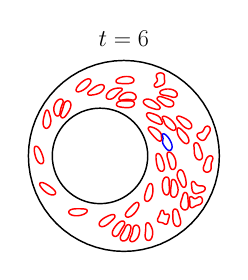
\begin{tikzpicture}[scale=0.35]

\begin{axis}[
  xmin = -21,
  xmax = 21,
  ymin = -21,
  ymax = 21,
  scale only axis,
  axis equal image,
  hide axis,
  title = {\Huge$t=6$}
  ]

\addplot [mark=none,black,line width=1.5] table{
2.0000e+01 0.0000e+00
1.9904e+01 1.9603e+00
1.9616e+01 3.9018e+00
1.9139e+01 5.8057e+00
1.8478e+01 7.6537e+00
1.7638e+01 9.4279e+00
1.6629e+01 1.1111e+01
1.5460e+01 1.2688e+01
1.4142e+01 1.4142e+01
1.2688e+01 1.5460e+01
1.1111e+01 1.6629e+01
9.4279e+00 1.7638e+01
7.6537e+00 1.8478e+01
5.8057e+00 1.9139e+01
3.9018e+00 1.9616e+01
1.9603e+00 1.9904e+01
1.2246e-15 2.0000e+01
-1.9603e+00 1.9904e+01
-3.9018e+00 1.9616e+01
-5.8057e+00 1.9139e+01
-7.6537e+00 1.8478e+01
-9.4279e+00 1.7638e+01
-1.1111e+01 1.6629e+01
-1.2688e+01 1.5460e+01
-1.4142e+01 1.4142e+01
-1.5460e+01 1.2688e+01
-1.6629e+01 1.1111e+01
-1.7638e+01 9.4279e+00
-1.8478e+01 7.6537e+00
-1.9139e+01 5.8057e+00
-1.9616e+01 3.9018e+00
-1.9904e+01 1.9603e+00
-2.0000e+01 2.4493e-15
-1.9904e+01 -1.9603e+00
-1.9616e+01 -3.9018e+00
-1.9139e+01 -5.8057e+00
-1.8478e+01 -7.6537e+00
-1.7638e+01 -9.4279e+00
-1.6629e+01 -1.1111e+01
-1.5460e+01 -1.2688e+01
-1.4142e+01 -1.4142e+01
-1.2688e+01 -1.5460e+01
-1.1111e+01 -1.6629e+01
-9.4279e+00 -1.7638e+01
-7.6537e+00 -1.8478e+01
-5.8057e+00 -1.9139e+01
-3.9018e+00 -1.9616e+01
-1.9603e+00 -1.9904e+01
-3.6739e-15 -2.0000e+01
1.9603e+00 -1.9904e+01
3.9018e+00 -1.9616e+01
5.8057e+00 -1.9139e+01
7.6537e+00 -1.8478e+01
9.4279e+00 -1.7638e+01
1.1111e+01 -1.6629e+01
1.2688e+01 -1.5460e+01
1.4142e+01 -1.4142e+01
1.5460e+01 -1.2688e+01
1.6629e+01 -1.1111e+01
1.7638e+01 -9.4279e+00
1.8478e+01 -7.6537e+00
1.9139e+01 -5.8057e+00
1.9616e+01 -3.9018e+00
1.9904e+01 -1.9603e+00
2.0000e+01 0.0000e+00
};

\addplot [mark=none,black,line width=1.5] table{
5.0000e+00 0.0000e+00
4.9518e+00 -9.8017e-01
4.8079e+00 -1.9509e+00
4.5694e+00 -2.9028e+00
4.2388e+00 -3.8268e+00
3.8192e+00 -4.7140e+00
3.3147e+00 -5.5557e+00
2.7301e+00 -6.3439e+00
2.0711e+00 -7.0711e+00
1.3439e+00 -7.7301e+00
5.5570e-01 -8.3147e+00
-2.8603e-01 -8.8192e+00
-1.1732e+00 -9.2388e+00
-2.0972e+00 -9.5694e+00
-3.0491e+00 -9.8079e+00
-4.0198e+00 -9.9518e+00
-5.0000e+00 -1.0000e+01
-5.9802e+00 -9.9518e+00
-6.9509e+00 -9.8079e+00
-7.9028e+00 -9.5694e+00
-8.8268e+00 -9.2388e+00
-9.7140e+00 -8.8192e+00
-1.0556e+01 -8.3147e+00
-1.1344e+01 -7.7301e+00
-1.2071e+01 -7.0711e+00
-1.2730e+01 -6.3439e+00
-1.3315e+01 -5.5557e+00
-1.3819e+01 -4.7140e+00
-1.4239e+01 -3.8268e+00
-1.4569e+01 -2.9028e+00
-1.4808e+01 -1.9509e+00
-1.4952e+01 -9.8017e-01
-1.5000e+01 -1.2246e-15
-1.4952e+01 9.8017e-01
-1.4808e+01 1.9509e+00
-1.4569e+01 2.9028e+00
-1.4239e+01 3.8268e+00
-1.3819e+01 4.7140e+00
-1.3315e+01 5.5557e+00
-1.2730e+01 6.3439e+00
-1.2071e+01 7.0711e+00
-1.1344e+01 7.7301e+00
-1.0556e+01 8.3147e+00
-9.7140e+00 8.8192e+00
-8.8268e+00 9.2388e+00
-7.9028e+00 9.5694e+00
-6.9509e+00 9.8079e+00
-5.9802e+00 9.9518e+00
-5.0000e+00 1.0000e+01
-4.0198e+00 9.9518e+00
-3.0491e+00 9.8079e+00
-2.0972e+00 9.5694e+00
-1.1732e+00 9.2388e+00
-2.8603e-01 8.8192e+00
5.5570e-01 8.3147e+00
1.3439e+00 7.7301e+00
2.0711e+00 7.0711e+00
2.7301e+00 6.3439e+00
3.3147e+00 5.5557e+00
3.8192e+00 4.7140e+00
4.2388e+00 3.8268e+00
4.5694e+00 2.9028e+00
4.8079e+00 1.9509e+00
4.9518e+00 9.8017e-01
5.0000e+00 0.0000e+00
};

\addplot [mark=none,red,line width=1.5] table{
1.7375e+01 4.0947e+00
1.7404e+01 4.1454e+00
1.7445e+01 4.2153e+00
1.7500e+01 4.3035e+00
1.7566e+01 4.4052e+00
1.7640e+01 4.5151e+00
1.7719e+01 4.6313e+00
1.7800e+01 4.7527e+00
1.7878e+01 4.8802e+00
1.7949e+01 5.0142e+00
1.8010e+01 5.1556e+00
1.8056e+01 5.3039e+00
1.8083e+01 5.4579e+00
1.8086e+01 5.6147e+00
1.8061e+01 5.7701e+00
1.8004e+01 5.9170e+00
1.7914e+01 6.0465e+00
1.7793e+01 6.1478e+00
1.7649e+01 6.2114e+00
1.7494e+01 6.2312e+00
1.7339e+01 6.2069e+00
1.7196e+01 6.1434e+00
1.7073e+01 6.0494e+00
1.6971e+01 5.9342e+00
1.6889e+01 5.8067e+00
1.6820e+01 5.6738e+00
1.6759e+01 5.5415e+00
1.6699e+01 5.4146e+00
1.6635e+01 5.2986e+00
1.6566e+01 5.1987e+00
1.6498e+01 5.1204e+00
1.6439e+01 5.0652e+00
1.6393e+01 5.0292e+00
1.6344e+01 4.9966e+00
1.6273e+01 4.9572e+00
1.6178e+01 4.9163e+00
1.6062e+01 4.8802e+00
1.5933e+01 4.8496e+00
1.5796e+01 4.8180e+00
1.5658e+01 4.7734e+00
1.5527e+01 4.7022e+00
1.5419e+01 4.5962e+00
1.5350e+01 4.4590e+00
1.5331e+01 4.3055e+00
1.5357e+01 4.1517e+00
1.5418e+01 4.0072e+00
1.5502e+01 3.8741e+00
1.5602e+01 3.7513e+00
1.5711e+01 3.6372e+00
1.5828e+01 3.5315e+00
1.5954e+01 3.4358e+00
1.6089e+01 3.3544e+00
1.6233e+01 3.2928e+00
1.6385e+01 3.2581e+00
1.6540e+01 3.2558e+00
1.6691e+01 3.2883e+00
1.6828e+01 3.3529e+00
1.6947e+01 3.4430e+00
1.7047e+01 3.5491e+00
1.7129e+01 3.6628e+00
1.7199e+01 3.7758e+00
1.7258e+01 3.8815e+00
1.7307e+01 3.9726e+00
1.7347e+01 4.0438e+00
1.7375e+01 4.0947e+00
};

\addplot [mark=none,red,line width=1.5] table{
1.8871e+00 1.6278e+01
1.8421e+00 1.6315e+01
1.7757e+00 1.6362e+01
1.6863e+00 1.6415e+01
1.5767e+00 1.6467e+01
1.4528e+00 1.6515e+01
1.3181e+00 1.6555e+01
1.1761e+00 1.6588e+01
1.0286e+00 1.6613e+01
8.7756e-01 1.6630e+01
7.2365e-01 1.6640e+01
5.6829e-01 1.6642e+01
4.1158e-01 1.6639e+01
2.5463e-01 1.6628e+01
9.7348e-02 1.6612e+01
-5.9311e-02 1.6590e+01
-2.1549e-01 1.6561e+01
-3.7031e-01 1.6527e+01
-5.2390e-01 1.6486e+01
-6.7528e-01 1.6439e+01
-8.2440e-01 1.6385e+01
-9.6980e-01 1.6325e+01
-1.1108e+00 1.6257e+01
-1.2453e+00 1.6180e+01
-1.3713e+00 1.6092e+01
-1.4836e+00 1.5992e+01
-1.5746e+00 1.5877e+01
-1.6317e+00 1.5748e+01
-1.6442e+00 1.5615e+01
-1.6116e+00 1.5498e+01
-1.5531e+00 1.5412e+01
-1.4921e+00 1.5358e+01
-1.4429e+00 1.5327e+01
-1.3905e+00 1.5300e+01
-1.3144e+00 1.5272e+01
-1.2137e+00 1.5246e+01
-1.0941e+00 1.5224e+01
-9.6215e-01 1.5208e+01
-8.2209e-01 1.5194e+01
-6.7660e-01 1.5181e+01
-5.2738e-01 1.5169e+01
-3.7544e-01 1.5157e+01
-2.2153e-01 1.5145e+01
-6.6029e-02 1.5136e+01
9.0580e-02 1.5129e+01
2.4811e-01 1.5126e+01
4.0611e-01 1.5126e+01
5.6447e-01 1.5130e+01
7.2278e-01 1.5138e+01
8.8095e-01 1.5150e+01
1.0386e+00 1.5168e+01
1.1953e+00 1.5190e+01
1.3504e+00 1.5220e+01
1.5028e+00 1.5259e+01
1.6504e+00 1.5310e+01
1.7896e+00 1.5377e+01
1.9143e+00 1.5465e+01
2.0150e+00 1.5576e+01
2.0805e+00 1.5707e+01
2.1036e+00 1.5846e+01
2.0865e+00 1.5977e+01
2.0410e+00 1.6090e+01
1.9836e+00 1.6177e+01
1.9298e+00 1.6238e+01
1.8871e+00 1.6278e+01
};

\addplot [mark=none,red,line width=1.5] table{
7.7603e+00 6.6209e+00
7.8179e+00 6.6330e+00
7.8934e+00 6.6639e+00
7.9757e+00 6.7278e+00
8.0375e+00 6.8321e+00
8.0553e+00 6.9631e+00
8.0289e+00 7.1012e+00
7.9750e+00 7.2365e+00
7.9098e+00 7.3714e+00
7.8434e+00 7.5082e+00
7.7783e+00 7.6483e+00
7.7117e+00 7.7888e+00
7.6360e+00 7.9263e+00
7.5456e+00 8.0552e+00
7.4391e+00 8.1723e+00
7.3196e+00 8.2760e+00
7.1900e+00 8.3679e+00
7.0539e+00 8.4491e+00
6.9126e+00 8.5222e+00
6.7683e+00 8.5880e+00
6.6217e+00 8.6486e+00
6.4742e+00 8.7046e+00
6.3260e+00 8.7576e+00
6.1782e+00 8.8077e+00
6.0311e+00 8.8559e+00
5.8859e+00 8.9011e+00
5.7438e+00 8.9428e+00
5.6060e+00 8.9790e+00
5.4739e+00 9.0079e+00
5.3517e+00 9.0259e+00
5.2460e+00 9.0324e+00
5.1637e+00 9.0288e+00
5.1050e+00 9.0208e+00
5.0479e+00 9.0069e+00
4.9713e+00 8.9774e+00
4.8841e+00 8.9196e+00
4.8059e+00 8.8263e+00
4.7606e+00 8.7014e+00
4.7574e+00 8.5611e+00
4.7928e+00 8.4194e+00
4.8544e+00 8.2833e+00
4.9337e+00 8.1530e+00
5.0243e+00 8.0285e+00
5.1245e+00 7.9091e+00
5.2321e+00 7.7955e+00
5.3472e+00 7.6876e+00
5.4684e+00 7.5866e+00
5.5959e+00 7.4922e+00
5.7281e+00 7.4049e+00
5.8649e+00 7.3240e+00
6.0045e+00 7.2494e+00
6.1468e+00 7.1795e+00
6.2900e+00 7.1138e+00
6.4343e+00 7.0506e+00
6.5779e+00 6.9896e+00
6.7210e+00 6.9296e+00
6.8621e+00 6.8709e+00
7.0015e+00 6.8134e+00
7.1375e+00 6.7587e+00
7.2703e+00 6.7083e+00
7.3971e+00 6.6659e+00
7.5159e+00 6.6349e+00
7.6195e+00 6.6187e+00
7.7018e+00 6.6157e+00
7.7603e+00 6.6209e+00
};

\addplot [mark=none,red,line width=1.5] table{
9.4443e+00 1.2526e+01
9.5006e+00 1.2510e+01
9.5786e+00 1.2488e+01
9.6781e+00 1.2459e+01
9.7940e+00 1.2423e+01
9.9210e+00 1.2385e+01
1.0056e+01 1.2347e+01
1.0198e+01 1.2313e+01
1.0345e+01 1.2288e+01
1.0497e+01 1.2279e+01
1.0650e+01 1.2292e+01
1.0800e+01 1.2334e+01
1.0937e+01 1.2409e+01
1.1050e+01 1.2517e+01
1.1131e+01 1.2652e+01
1.1172e+01 1.2804e+01
1.1172e+01 1.2962e+01
1.1134e+01 1.3115e+01
1.1066e+01 1.3257e+01
1.0973e+01 1.3385e+01
1.0864e+01 1.3497e+01
1.0742e+01 1.3595e+01
1.0612e+01 1.3680e+01
1.0477e+01 1.3753e+01
1.0338e+01 1.3815e+01
1.0198e+01 1.3867e+01
1.0058e+01 1.3910e+01
9.9218e+00 1.3944e+01
9.7916e+00 1.3971e+01
9.6717e+00 1.3990e+01
9.5685e+00 1.4002e+01
9.4876e+00 1.4010e+01
9.4293e+00 1.4014e+01
9.3710e+00 1.4017e+01
9.2899e+00 1.4019e+01
9.1862e+00 1.4019e+01
9.0651e+00 1.4016e+01
8.9329e+00 1.4007e+01
8.7931e+00 1.3992e+01
8.6490e+00 1.3970e+01
8.5022e+00 1.3942e+01
8.3543e+00 1.3906e+01
8.2065e+00 1.3862e+01
8.0605e+00 1.3809e+01
7.9184e+00 1.3743e+01
7.7847e+00 1.3661e+01
7.6671e+00 1.3556e+01
7.5804e+00 1.3425e+01
7.5435e+00 1.3272e+01
7.5708e+00 1.3117e+01
7.6563e+00 1.2986e+01
7.7802e+00 1.2889e+01
7.9227e+00 1.2824e+01
8.0729e+00 1.2780e+01
8.2251e+00 1.2750e+01
8.3774e+00 1.2726e+01
8.5279e+00 1.2704e+01
8.6760e+00 1.2683e+01
8.8200e+00 1.2661e+01
8.9587e+00 1.2637e+01
9.0891e+00 1.2611e+01
9.2078e+00 1.2585e+01
9.3090e+00 1.2561e+01
9.3878e+00 1.2541e+01
9.4443e+00 1.2526e+01
};

\addplot [mark=none,red,line width=1.5] table{
-1.3372e+01 9.0512e+00
-1.3363e+01 9.1089e+00
-1.3350e+01 9.1891e+00
-1.3334e+01 9.2916e+00
-1.3315e+01 9.4117e+00
-1.3293e+01 9.5428e+00
-1.3266e+01 9.6814e+00
-1.3235e+01 9.8243e+00
-1.3199e+01 9.9701e+00
-1.3158e+01 1.0117e+01
-1.3110e+01 1.0264e+01
-1.3057e+01 1.0411e+01
-1.3000e+01 1.0557e+01
-1.2939e+01 1.0702e+01
-1.2876e+01 1.0847e+01
-1.2815e+01 1.0994e+01
-1.2763e+01 1.1145e+01
-1.2731e+01 1.1300e+01
-1.2729e+01 1.1458e+01
-1.2768e+01 1.1611e+01
-1.2851e+01 1.1744e+01
-1.2971e+01 1.1843e+01
-1.3116e+01 1.1898e+01
-1.3269e+01 1.1911e+01
-1.3419e+01 1.1887e+01
-1.3560e+01 1.1837e+01
-1.3689e+01 1.1768e+01
-1.3806e+01 1.1687e+01
-1.3908e+01 1.1601e+01
-1.3995e+01 1.1515e+01
-1.4066e+01 1.1438e+01
-1.4118e+01 1.1375e+01
-1.4154e+01 1.1328e+01
-1.4189e+01 1.1281e+01
-1.4235e+01 1.1215e+01
-1.4291e+01 1.1127e+01
-1.4352e+01 1.1022e+01
-1.4413e+01 1.0904e+01
-1.4471e+01 1.0776e+01
-1.4525e+01 1.0640e+01
-1.4572e+01 1.0498e+01
-1.4611e+01 1.0350e+01
-1.4642e+01 1.0199e+01
-1.4663e+01 1.0045e+01
-1.4674e+01 9.8886e+00
-1.4675e+01 9.7313e+00
-1.4666e+01 9.5735e+00
-1.4646e+01 9.4164e+00
-1.4615e+01 9.2608e+00
-1.4574e+01 9.1078e+00
-1.4521e+01 8.9584e+00
-1.4456e+01 8.8146e+00
-1.4376e+01 8.6790e+00
-1.4279e+01 8.5562e+00
-1.4162e+01 8.4536e+00
-1.4025e+01 8.3828e+00
-1.3875e+01 8.3579e+00
-1.3729e+01 8.3877e+00
-1.3607e+01 8.4660e+00
-1.3517e+01 8.5748e+00
-1.3458e+01 8.6944e+00
-1.3421e+01 8.8109e+00
-1.3397e+01 8.9129e+00
-1.3382e+01 8.9933e+00
-1.3372e+01 9.0512e+00
};

\addplot [mark=none,red,line width=1.5] table{
1.1218e+01 -3.6061e+00
1.1205e+01 -3.6631e+00
1.1190e+01 -3.7432e+00
1.1178e+01 -3.8464e+00
1.1171e+01 -3.9677e+00
1.1175e+01 -4.1005e+00
1.1191e+01 -4.2404e+00
1.1219e+01 -4.3834e+00
1.1260e+01 -4.5274e+00
1.1312e+01 -4.6706e+00
1.1371e+01 -4.8127e+00
1.1437e+01 -4.9536e+00
1.1506e+01 -5.0941e+00
1.1577e+01 -5.2345e+00
1.1649e+01 -5.3754e+00
1.1720e+01 -5.5168e+00
1.1791e+01 -5.6587e+00
1.1861e+01 -5.8005e+00
1.1933e+01 -5.9418e+00
1.2007e+01 -6.0811e+00
1.2088e+01 -6.2165e+00
1.2180e+01 -6.3438e+00
1.2288e+01 -6.4556e+00
1.2418e+01 -6.5382e+00
1.2566e+01 -6.5735e+00
1.2712e+01 -6.5485e+00
1.2834e+01 -6.4700e+00
1.2920e+01 -6.3594e+00
1.2975e+01 -6.2384e+00
1.3006e+01 -6.1212e+00
1.3023e+01 -6.0187e+00
1.3031e+01 -5.9379e+00
1.3034e+01 -5.8796e+00
1.3037e+01 -5.8212e+00
1.3038e+01 -5.7399e+00
1.3036e+01 -5.6360e+00
1.3030e+01 -5.5149e+00
1.3019e+01 -5.3826e+00
1.3003e+01 -5.2429e+00
1.2983e+01 -5.0986e+00
1.2957e+01 -4.9512e+00
1.2927e+01 -4.8022e+00
1.2892e+01 -4.6521e+00
1.2853e+01 -4.5016e+00
1.2811e+01 -4.3510e+00
1.2765e+01 -4.2007e+00
1.2716e+01 -4.0506e+00
1.2664e+01 -3.9012e+00
1.2609e+01 -3.7525e+00
1.2550e+01 -3.6054e+00
1.2485e+01 -3.4610e+00
1.2411e+01 -3.3216e+00
1.2323e+01 -3.1912e+00
1.2216e+01 -3.0770e+00
1.2087e+01 -2.9891e+00
1.1942e+01 -2.9397e+00
1.1790e+01 -2.9365e+00
1.1647e+01 -2.9790e+00
1.1524e+01 -3.0572e+00
1.1426e+01 -3.1577e+00
1.1351e+01 -3.2672e+00
1.1296e+01 -3.3754e+00
1.1258e+01 -3.4721e+00
1.1233e+01 -3.5496e+00
1.1218e+01 -3.6061e+00
};

\addplot [mark=none,red,line width=1.5] table{
8.5177e+00 1.5884e+01
8.5111e+00 1.5943e+01
8.5030e+00 1.6023e+01
8.4961e+00 1.6127e+01
8.4935e+00 1.6248e+01
8.4963e+00 1.6380e+01
8.5012e+00 1.6521e+01
8.5007e+00 1.6667e+01
8.4844e+00 1.6815e+01
8.4422e+00 1.6961e+01
8.3679e+00 1.7095e+01
8.2619e+00 1.7208e+01
8.1312e+00 1.7294e+01
7.9847e+00 1.7350e+01
7.8303e+00 1.7380e+01
7.6727e+00 1.7390e+01
7.5150e+00 1.7381e+01
7.3592e+00 1.7355e+01
7.2085e+00 1.7308e+01
7.0682e+00 1.7237e+01
6.9465e+00 1.7138e+01
6.8540e+00 1.7012e+01
6.8001e+00 1.6867e+01
6.7887e+00 1.6714e+01
6.8149e+00 1.6564e+01
6.8661e+00 1.6424e+01
6.9269e+00 1.6291e+01
6.9821e+00 1.6162e+01
7.0199e+00 1.6035e+01
7.0342e+00 1.5915e+01
7.0278e+00 1.5812e+01
7.0102e+00 1.5733e+01
6.9910e+00 1.5677e+01
6.9668e+00 1.5624e+01
6.9259e+00 1.5554e+01
6.8637e+00 1.5471e+01
6.7811e+00 1.5382e+01
6.6842e+00 1.5292e+01
6.5809e+00 1.5196e+01
6.4818e+00 1.5090e+01
6.4010e+00 1.4964e+01
6.3580e+00 1.4819e+01
6.3724e+00 1.4666e+01
6.4504e+00 1.4533e+01
6.5771e+00 1.4443e+01
6.7282e+00 1.4402e+01
6.8855e+00 1.4402e+01
7.0408e+00 1.4431e+01
7.1921e+00 1.4477e+01
7.3402e+00 1.4532e+01
7.4865e+00 1.4592e+01
7.6319e+00 1.4653e+01
7.7767e+00 1.4714e+01
7.9199e+00 1.4777e+01
8.0595e+00 1.4845e+01
8.1919e+00 1.4924e+01
8.3115e+00 1.5018e+01
8.4109e+00 1.5130e+01
8.4833e+00 1.5256e+01
8.5260e+00 1.5390e+01
8.5428e+00 1.5521e+01
8.5422e+00 1.5643e+01
8.5339e+00 1.5746e+01
8.5247e+00 1.5827e+01
8.5177e+00 1.5884e+01
};

\addplot [mark=none,red,line width=1.5] table{
8.1438e+00 -7.0746e+00
8.1563e+00 -7.1332e+00
8.1761e+00 -7.2121e+00
8.2035e+00 -7.3141e+00
8.2408e+00 -7.4299e+00
8.2872e+00 -7.5560e+00
8.3459e+00 -7.6840e+00
8.4175e+00 -7.8125e+00
8.5068e+00 -7.9326e+00
8.6156e+00 -8.0398e+00
8.7475e+00 -8.1194e+00
8.8972e+00 -8.1600e+00
9.0529e+00 -8.1462e+00
9.1944e+00 -8.0806e+00
9.3090e+00 -7.9714e+00
9.3923e+00 -7.8381e+00
9.4511e+00 -7.6897e+00
9.4915e+00 -7.5367e+00
9.5207e+00 -7.3791e+00
9.5403e+00 -7.2218e+00
9.5523e+00 -7.0623e+00
9.5550e+00 -6.9048e+00
9.5502e+00 -6.7467e+00
9.5381e+00 -6.5921e+00
9.5227e+00 -6.4384e+00
9.5051e+00 -6.2895e+00
9.4891e+00 -6.1424e+00
9.4750e+00 -6.0020e+00
9.4657e+00 -5.8674e+00
9.4600e+00 -5.7459e+00
9.4588e+00 -5.6402e+00
9.4592e+00 -5.5592e+00
9.4609e+00 -5.4994e+00
9.4625e+00 -5.4414e+00
9.4661e+00 -5.3586e+00
9.4697e+00 -5.2551e+00
9.4713e+00 -5.1322e+00
9.4631e+00 -5.0002e+00
9.4377e+00 -4.8606e+00
9.3851e+00 -4.7248e+00
9.3013e+00 -4.5994e+00
9.1849e+00 -4.5013e+00
9.0434e+00 -4.4393e+00
8.8879e+00 -4.4269e+00
8.7360e+00 -4.4621e+00
8.5994e+00 -4.5416e+00
8.4851e+00 -4.6492e+00
8.3903e+00 -4.7774e+00
8.3127e+00 -4.9148e+00
8.2475e+00 -5.0610e+00
8.1941e+00 -5.2097e+00
8.1497e+00 -5.3632e+00
8.1150e+00 -5.5167e+00
8.0879e+00 -5.6731e+00
8.0692e+00 -5.8278e+00
8.0570e+00 -5.9838e+00
8.0521e+00 -6.1365e+00
8.0524e+00 -6.2887e+00
8.0587e+00 -6.4351e+00
8.0689e+00 -6.5780e+00
8.0833e+00 -6.7107e+00
8.0995e+00 -6.8333e+00
8.1168e+00 -6.9360e+00
8.1315e+00 -7.0177e+00
8.1438e+00 -7.0746e+00
};

\addplot [mark=none,red,line width=1.5] table{
-1.7613e+01 -6.0755e+00
-1.7595e+01 -6.1319e+00
-1.7563e+01 -6.2083e+00
-1.7515e+01 -6.3036e+00
-1.7452e+01 -6.4120e+00
-1.7375e+01 -6.5273e+00
-1.7289e+01 -6.6456e+00
-1.7195e+01 -6.7644e+00
-1.7094e+01 -6.8827e+00
-1.6988e+01 -7.0000e+00
-1.6878e+01 -7.1149e+00
-1.6765e+01 -7.2265e+00
-1.6648e+01 -7.3351e+00
-1.6528e+01 -7.4406e+00
-1.6404e+01 -7.5424e+00
-1.6276e+01 -7.6400e+00
-1.6144e+01 -7.7326e+00
-1.6008e+01 -7.8196e+00
-1.5868e+01 -7.8998e+00
-1.5724e+01 -7.9725e+00
-1.5576e+01 -8.0364e+00
-1.5425e+01 -8.0902e+00
-1.5271e+01 -8.1322e+00
-1.5116e+01 -8.1606e+00
-1.4960e+01 -8.1728e+00
-1.4807e+01 -8.1657e+00
-1.4662e+01 -8.1355e+00
-1.4530e+01 -8.0786e+00
-1.4424e+01 -7.9955e+00
-1.4353e+01 -7.8952e+00
-1.4319e+01 -7.7961e+00
-1.4310e+01 -7.7145e+00
-1.4314e+01 -7.6553e+00
-1.4324e+01 -7.5971e+00
-1.4349e+01 -7.5183e+00
-1.4394e+01 -7.4227e+00
-1.4460e+01 -7.3173e+00
-1.4543e+01 -7.2091e+00
-1.4640e+01 -7.1011e+00
-1.4745e+01 -6.9955e+00
-1.4858e+01 -6.8919e+00
-1.4975e+01 -6.7908e+00
-1.5097e+01 -6.6915e+00
-1.5223e+01 -6.5946e+00
-1.5351e+01 -6.4994e+00
-1.5481e+01 -6.4065e+00
-1.5613e+01 -6.3153e+00
-1.5748e+01 -6.2263e+00
-1.5884e+01 -6.1393e+00
-1.6022e+01 -6.0550e+00
-1.6162e+01 -5.9731e+00
-1.6303e+01 -5.8948e+00
-1.6446e+01 -5.8201e+00
-1.6591e+01 -5.7506e+00
-1.6738e+01 -5.6874e+00
-1.6887e+01 -5.6332e+00
-1.7038e+01 -5.5916e+00
-1.7191e+01 -5.5699e+00
-1.7340e+01 -5.5781e+00
-1.7475e+01 -5.6284e+00
-1.7575e+01 -5.7202e+00
-1.7625e+01 -5.8325e+00
-1.7635e+01 -5.9366e+00
-1.7626e+01 -6.0181e+00
-1.7613e+01 -6.0755e+00
};

\addplot [mark=none,red,line width=1.5] table{
1.3492e+01 -9.8458e+00
1.3487e+01 -9.7876e+00
1.3481e+01 -9.7066e+00
1.3472e+01 -9.6033e+00
1.3462e+01 -9.4825e+00
1.3450e+01 -9.3505e+00
1.3439e+01 -9.2104e+00
1.3428e+01 -9.0651e+00
1.3418e+01 -8.9159e+00
1.3409e+01 -8.7641e+00
1.3399e+01 -8.6104e+00
1.3383e+01 -8.4557e+00
1.3360e+01 -8.3008e+00
1.3326e+01 -8.1475e+00
1.3274e+01 -7.9985e+00
1.3199e+01 -7.8597e+00
1.3093e+01 -7.7424e+00
1.2956e+01 -7.6669e+00
1.2799e+01 -7.6559e+00
1.2655e+01 -7.7155e+00
1.2543e+01 -7.8255e+00
1.2465e+01 -7.9609e+00
1.2409e+01 -8.1057e+00
1.2365e+01 -8.2531e+00
1.2324e+01 -8.3997e+00
1.2285e+01 -8.5441e+00
1.2245e+01 -8.6843e+00
1.2205e+01 -8.8193e+00
1.2165e+01 -8.9462e+00
1.2128e+01 -9.0619e+00
1.2097e+01 -9.1609e+00
1.2072e+01 -9.2384e+00
1.2054e+01 -9.2940e+00
1.2037e+01 -9.3498e+00
1.2013e+01 -9.4276e+00
1.1984e+01 -9.5273e+00
1.1953e+01 -9.6445e+00
1.1924e+01 -9.7737e+00
1.1899e+01 -9.9121e+00
1.1883e+01 -1.0057e+01
1.1879e+01 -1.0206e+01
1.1890e+01 -1.0358e+01
1.1918e+01 -1.0509e+01
1.1964e+01 -1.0658e+01
1.2030e+01 -1.0799e+01
1.2116e+01 -1.0931e+01
1.2219e+01 -1.1050e+01
1.2339e+01 -1.1152e+01
1.2475e+01 -1.1234e+01
1.2623e+01 -1.1289e+01
1.2779e+01 -1.1312e+01
1.2935e+01 -1.1298e+01
1.3084e+01 -1.1247e+01
1.3214e+01 -1.1161e+01
1.3320e+01 -1.1048e+01
1.3399e+01 -1.0916e+01
1.3453e+01 -1.0774e+01
1.3486e+01 -1.0628e+01
1.3503e+01 -1.0483e+01
1.3510e+01 -1.0343e+01
1.3510e+01 -1.0210e+01
1.3506e+01 -1.0089e+01
1.3501e+01 -9.9851e+00
1.3496e+01 -9.9041e+00
1.3492e+01 -9.8458e+00
};

\addplot [mark=none,red,line width=1.5] table{
6.0277e+00 4.3701e+00
6.0662e+00 4.3258e+00
6.1202e+00 4.2642e+00
6.1895e+00 4.1857e+00
6.2713e+00 4.0943e+00
6.3616e+00 3.9950e+00
6.4583e+00 3.8907e+00
6.5598e+00 3.7839e+00
6.6659e+00 3.6760e+00
6.7760e+00 3.5685e+00
6.8908e+00 3.4629e+00
7.0106e+00 3.3611e+00
7.1374e+00 3.2657e+00
7.2729e+00 3.1818e+00
7.4203e+00 3.1190e+00
7.5788e+00 3.0965e+00
7.7315e+00 3.1415e+00
7.8382e+00 3.2582e+00
7.8830e+00 3.4104e+00
7.8908e+00 3.5691e+00
7.8851e+00 3.7275e+00
7.8763e+00 3.8850e+00
7.8682e+00 4.0416e+00
7.8611e+00 4.1973e+00
7.8496e+00 4.3511e+00
7.8230e+00 4.5005e+00
7.7758e+00 4.6403e+00
7.7122e+00 4.7675e+00
7.6404e+00 4.8805e+00
7.5670e+00 4.9784e+00
7.4997e+00 5.0584e+00
7.4444e+00 5.1188e+00
7.4033e+00 5.1611e+00
7.3611e+00 5.2025e+00
7.3007e+00 5.2587e+00
7.2208e+00 5.3280e+00
7.1242e+00 5.4052e+00
7.0150e+00 5.4850e+00
6.8961e+00 5.5644e+00
6.7697e+00 5.6414e+00
6.6370e+00 5.7154e+00
6.4995e+00 5.7853e+00
6.3576e+00 5.8512e+00
6.2121e+00 5.9121e+00
6.0630e+00 5.9675e+00
5.9106e+00 6.0157e+00
5.7546e+00 6.0541e+00
5.5952e+00 6.0775e+00
5.4339e+00 6.0758e+00
5.2795e+00 6.0319e+00
5.1575e+00 5.9297e+00
5.1031e+00 5.7819e+00
5.1190e+00 5.6253e+00
5.1775e+00 5.4796e+00
5.2558e+00 5.3445e+00
5.3426e+00 5.2162e+00
5.4331e+00 5.0930e+00
5.5248e+00 4.9740e+00
5.6160e+00 4.8597e+00
5.7053e+00 4.7504e+00
5.7904e+00 4.6482e+00
5.8687e+00 4.5552e+00
5.9363e+00 4.4761e+00
5.9893e+00 4.4144e+00
6.0277e+00 4.3701e+00
};

\addplot [mark=none,red,line width=1.5] table{
1.1890e+01 8.2454e+00
1.1835e+01 8.2639e+00
1.1757e+01 8.2880e+00
1.1657e+01 8.3125e+00
1.1536e+01 8.3298e+00
1.1404e+01 8.3260e+00
1.1269e+01 8.2868e+00
1.1153e+01 8.1993e+00
1.1082e+01 8.0689e+00
1.1071e+01 7.9173e+00
1.1113e+01 7.7696e+00
1.1190e+01 7.6341e+00
1.1285e+01 7.5100e+00
1.1388e+01 7.3908e+00
1.1493e+01 7.2736e+00
1.1599e+01 7.1553e+00
1.1703e+01 7.0364e+00
1.1807e+01 6.9162e+00
1.1911e+01 6.7968e+00
1.2016e+01 6.6781e+00
1.2122e+01 6.5623e+00
1.2231e+01 6.4491e+00
1.2343e+01 6.3405e+00
1.2457e+01 6.2360e+00
1.2574e+01 6.1376e+00
1.2694e+01 6.0451e+00
1.2814e+01 5.9611e+00
1.2935e+01 5.8860e+00
1.3052e+01 5.8226e+00
1.3164e+01 5.7716e+00
1.3262e+01 5.7352e+00
1.3340e+01 5.7114e+00
1.3397e+01 5.6980e+00
1.3455e+01 5.6870e+00
1.3536e+01 5.6779e+00
1.3640e+01 5.6763e+00
1.3760e+01 5.6922e+00
1.3886e+01 5.7332e+00
1.4006e+01 5.8063e+00
1.4107e+01 5.9111e+00
1.4178e+01 6.0427e+00
1.4214e+01 6.1902e+00
1.4214e+01 6.3443e+00
1.4185e+01 6.4967e+00
1.4132e+01 6.6440e+00
1.4060e+01 6.7835e+00
1.3974e+01 6.9157e+00
1.3876e+01 7.0397e+00
1.3769e+01 7.1569e+00
1.3656e+01 7.2666e+00
1.3536e+01 7.3702e+00
1.3411e+01 7.4670e+00
1.3283e+01 7.5583e+00
1.3152e+01 7.6434e+00
1.3018e+01 7.7238e+00
1.2884e+01 7.7987e+00
1.2748e+01 7.8696e+00
1.2614e+01 7.9359e+00
1.2481e+01 7.9986e+00
1.2352e+01 8.0566e+00
1.2230e+01 8.1102e+00
1.2118e+01 8.1571e+00
1.2021e+01 8.1963e+00
1.1946e+01 8.2251e+00
1.1890e+01 8.2454e+00
};

\addplot [mark=none,red,line width=1.5] table{
8.5073e+00 8.3073e+00
8.4487e+00 8.3144e+00
8.3669e+00 8.3157e+00
8.2634e+00 8.2988e+00
8.1539e+00 8.2448e+00
8.0699e+00 8.1416e+00
8.0445e+00 8.0034e+00
8.0800e+00 7.8620e+00
8.1504e+00 7.7294e+00
8.2302e+00 7.5994e+00
8.3049e+00 7.4642e+00
8.3675e+00 7.3219e+00
8.4190e+00 7.1739e+00
8.4657e+00 7.0239e+00
8.5178e+00 6.8749e+00
8.5827e+00 6.7309e+00
8.6628e+00 6.5941e+00
8.7556e+00 6.4659e+00
8.8582e+00 6.3449e+00
8.9674e+00 6.2307e+00
9.0817e+00 6.1217e+00
9.1993e+00 6.0178e+00
9.3197e+00 5.9184e+00
9.4418e+00 5.8237e+00
9.5653e+00 5.7336e+00
9.6896e+00 5.6493e+00
9.8142e+00 5.5717e+00
9.9380e+00 5.5034e+00
1.0059e+01 5.4469e+00
1.0174e+01 5.4058e+00
1.0275e+01 5.3812e+00
1.0356e+01 5.3712e+00
1.0415e+01 5.3696e+00
1.0474e+01 5.3739e+00
1.0554e+01 5.3896e+00
1.0651e+01 5.4281e+00
1.0751e+01 5.4979e+00
1.0836e+01 5.6010e+00
1.0894e+01 5.7304e+00
1.0915e+01 5.8753e+00
1.0902e+01 6.0244e+00
1.0863e+01 6.1718e+00
1.0806e+01 6.3149e+00
1.0737e+01 6.4542e+00
1.0659e+01 6.5898e+00
1.0575e+01 6.7227e+00
1.0486e+01 6.8525e+00
1.0392e+01 6.9799e+00
1.0294e+01 7.1041e+00
1.0192e+01 7.2253e+00
1.0085e+01 7.3423e+00
9.9736e+00 7.4550e+00
9.8577e+00 7.5622e+00
9.7374e+00 7.6637e+00
9.6142e+00 7.7589e+00
9.4880e+00 7.8482e+00
9.3604e+00 7.9312e+00
9.2315e+00 8.0085e+00
9.1035e+00 8.0791e+00
8.9773e+00 8.1429e+00
8.8561e+00 8.1980e+00
8.7428e+00 8.2431e+00
8.6441e+00 8.2757e+00
8.5649e+00 8.2963e+00
8.5073e+00 8.3073e+00
};

\addplot [mark=none,red,line width=1.5] table{
-2.3148e-01 1.2936e+01
-2.8164e-01 1.2903e+01
-3.4799e-01 1.2856e+01
-4.3381e-01 1.2794e+01
-5.2979e-01 1.2717e+01
-6.3360e-01 1.2628e+01
-7.3611e-01 1.2530e+01
-8.3673e-01 1.2421e+01
-9.2613e-01 1.2299e+01
-9.9867e-01 1.2164e+01
-1.0330e+00 1.2013e+01
-1.0091e+00 1.1860e+01
-9.1260e-01 1.1738e+01
-7.7047e-01 1.1675e+01
-6.1209e-01 1.1667e+01
-4.5600e-01 1.1687e+01
-2.9885e-01 1.1716e+01
-1.4357e-01 1.1745e+01
1.4226e-02 1.1773e+01
1.7050e-01 1.1797e+01
3.2905e-01 1.1817e+01
4.8545e-01 1.1832e+01
6.4306e-01 1.1841e+01
7.9717e-01 1.1843e+01
9.5111e-01 1.1837e+01
1.1002e+00 1.1825e+01
1.2471e+00 1.1806e+01
1.3861e+00 1.1782e+01
1.5186e+00 1.1756e+01
1.6376e+00 1.1733e+01
1.7419e+00 1.1717e+01
1.8223e+00 1.1708e+01
1.8824e+00 1.1706e+01
1.9407e+00 1.1707e+01
2.0240e+00 1.1715e+01
2.1257e+00 1.1740e+01
2.2399e+00 1.1790e+01
2.3487e+00 1.1867e+01
2.4450e+00 1.1973e+01
2.5138e+00 1.2102e+01
2.5526e+00 1.2248e+01
2.5533e+00 1.2401e+01
2.5216e+00 1.2552e+01
2.4573e+00 1.2694e+01
2.3703e+00 1.2824e+01
2.2614e+00 1.2939e+01
2.1397e+00 1.3039e+01
2.0042e+00 1.3122e+01
1.8626e+00 1.3191e+01
1.7125e+00 1.3246e+01
1.5605e+00 1.3287e+01
1.4035e+00 1.3315e+01
1.2473e+00 1.3332e+01
1.0888e+00 1.3338e+01
9.3354e-01 1.3333e+01
7.7818e-01 1.3318e+01
6.2844e-01 1.3294e+01
4.8087e-01 1.3260e+01
3.4155e-01 1.3218e+01
2.0786e-01 1.3169e+01
8.6960e-02 1.3115e+01
-2.2710e-02 1.3060e+01
-1.1232e-01 1.3009e+01
-1.8303e-01 1.2967e+01
-2.3148e-01 1.2936e+01
};

\addplot [mark=none,red,line width=1.5] table{
4.4942e+00 -7.8459e+00
4.4787e+00 -7.9028e+00
4.4579e+00 -7.9823e+00
4.4326e+00 -8.0844e+00
4.4054e+00 -8.2043e+00
4.3792e+00 -8.3359e+00
4.3563e+00 -8.4762e+00
4.3395e+00 -8.6223e+00
4.3320e+00 -8.7731e+00
4.3384e+00 -8.9264e+00
4.3650e+00 -9.0797e+00
4.4195e+00 -9.2265e+00
4.5088e+00 -9.3563e+00
4.6336e+00 -9.4530e+00
4.7837e+00 -9.5027e+00
4.9421e+00 -9.5017e+00
5.0945e+00 -9.4576e+00
5.2342e+00 -9.3815e+00
5.3598e+00 -9.2835e+00
5.4719e+00 -9.1701e+00
5.5714e+00 -9.0461e+00
5.6592e+00 -8.9144e+00
5.7362e+00 -8.7774e+00
5.8032e+00 -8.6368e+00
5.8608e+00 -8.4941e+00
5.9096e+00 -8.3508e+00
5.9503e+00 -8.2087e+00
5.9836e+00 -8.0695e+00
6.0099e+00 -7.9366e+00
6.0299e+00 -7.8136e+00
6.0442e+00 -7.7077e+00
6.0534e+00 -7.6248e+00
6.0591e+00 -7.5655e+00
6.0640e+00 -7.5065e+00
6.0696e+00 -7.4244e+00
6.0747e+00 -7.3190e+00
6.0781e+00 -7.1958e+00
6.0783e+00 -7.0610e+00
6.0747e+00 -6.9182e+00
6.0666e+00 -6.7704e+00
6.0531e+00 -6.6191e+00
6.0328e+00 -6.4658e+00
6.0036e+00 -6.3118e+00
5.9613e+00 -6.1595e+00
5.8988e+00 -6.0131e+00
5.8055e+00 -5.8839e+00
5.6735e+00 -5.7955e+00
5.5164e+00 -5.7791e+00
5.3701e+00 -5.8393e+00
5.2546e+00 -5.9488e+00
5.1641e+00 -6.0799e+00
5.0879e+00 -6.2198e+00
5.0198e+00 -6.3631e+00
4.9566e+00 -6.5078e+00
4.8972e+00 -6.6528e+00
4.8408e+00 -6.7977e+00
4.7871e+00 -6.9416e+00
4.7359e+00 -7.0840e+00
4.6875e+00 -7.2236e+00
4.6421e+00 -7.3592e+00
4.6006e+00 -7.4880e+00
4.5637e+00 -7.6067e+00
4.5332e+00 -7.7089e+00
4.5102e+00 -7.7888e+00
4.4942e+00 -7.8459e+00
};

\addplot [mark=none,red,line width=1.5] table{
1.3613e+01 3.1848e+00
1.3611e+01 3.2431e+00
1.3604e+01 3.3242e+00
1.3587e+01 3.4266e+00
1.3560e+01 3.5449e+00
1.3521e+01 3.6719e+00
1.3472e+01 3.8040e+00
1.3414e+01 3.9376e+00
1.3347e+01 4.0716e+00
1.3272e+01 4.2038e+00
1.3189e+01 4.3338e+00
1.3099e+01 4.4601e+00
1.3001e+01 4.5827e+00
1.2898e+01 4.7010e+00
1.2789e+01 4.8155e+00
1.2676e+01 4.9263e+00
1.2560e+01 5.0348e+00
1.2443e+01 5.1415e+00
1.2326e+01 5.2484e+00
1.2210e+01 5.3559e+00
1.2096e+01 5.4651e+00
1.1983e+01 5.5739e+00
1.1867e+01 5.6789e+00
1.1743e+01 5.7713e+00
1.1605e+01 5.8381e+00
1.1457e+01 5.8603e+00
1.1316e+01 5.8239e+00
1.1209e+01 5.7327e+00
1.1151e+01 5.6135e+00
1.1133e+01 5.4932e+00
1.1136e+01 5.3892e+00
1.1145e+01 5.3081e+00
1.1153e+01 5.2503e+00
1.1162e+01 5.1925e+00
1.1175e+01 5.1123e+00
1.1192e+01 5.0095e+00
1.1212e+01 4.8896e+00
1.1236e+01 4.7587e+00
1.1268e+01 4.6210e+00
1.1310e+01 4.4805e+00
1.1363e+01 4.3397e+00
1.1427e+01 4.2006e+00
1.1500e+01 4.0642e+00
1.1581e+01 3.9307e+00
1.1668e+01 3.7999e+00
1.1760e+01 3.6715e+00
1.1855e+01 3.5451e+00
1.1953e+01 3.4208e+00
1.2054e+01 3.2986e+00
1.2158e+01 3.1791e+00
1.2266e+01 3.0631e+00
1.2378e+01 2.9517e+00
1.2496e+01 2.8473e+00
1.2622e+01 2.7528e+00
1.2756e+01 2.6732e+00
1.2899e+01 2.6151e+00
1.3049e+01 2.5865e+00
1.3198e+01 2.5950e+00
1.3336e+01 2.6439e+00
1.3448e+01 2.7277e+00
1.3529e+01 2.8332e+00
1.3578e+01 2.9442e+00
1.3602e+01 3.0454e+00
1.3611e+01 3.1263e+00
1.3613e+01 3.1848e+00
};

\addplot [mark=none,red,line width=1.5] table{
6.9263e+00 -1.8635e+00
6.9392e+00 -1.9210e+00
6.9583e+00 -2.0006e+00
6.9847e+00 -2.1020e+00
7.0186e+00 -2.2198e+00
7.0602e+00 -2.3472e+00
7.1103e+00 -2.4801e+00
7.1702e+00 -2.6147e+00
7.2417e+00 -2.7479e+00
7.3269e+00 -2.8760e+00
7.4285e+00 -2.9944e+00
7.5481e+00 -3.0966e+00
7.6864e+00 -3.1739e+00
7.8395e+00 -3.2155e+00
7.9981e+00 -3.2117e+00
8.1476e+00 -3.1589e+00
8.2742e+00 -3.0626e+00
8.3700e+00 -2.9349e+00
8.4349e+00 -2.7884e+00
8.4727e+00 -2.6328e+00
8.4890e+00 -2.4739e+00
8.4883e+00 -2.3148e+00
8.4751e+00 -2.1573e+00
8.4525e+00 -2.0022e+00
8.4233e+00 -1.8500e+00
8.3894e+00 -1.7014e+00
8.3526e+00 -1.5572e+00
8.3142e+00 -1.4186e+00
8.2761e+00 -1.2879e+00
8.2397e+00 -1.1684e+00
8.2076e+00 -1.0664e+00
8.1820e+00 -9.8716e-01
8.1634e+00 -9.3062e-01
8.1447e+00 -8.7462e-01
8.1183e+00 -7.9693e-01
8.0835e+00 -6.9793e-01
8.0414e+00 -5.8259e-01
7.9930e+00 -4.5741e-01
7.9383e+00 -3.2593e-01
7.8764e+00 -1.9183e-01
7.8060e+00 -5.7349e-02
7.7250e+00 7.4183e-02
7.6312e+00 1.9967e-01
7.5219e+00 3.1373e-01
7.3946e+00 4.0906e-01
7.2485e+00 4.7246e-01
7.0898e+00 4.8546e-01
6.9404e+00 4.3164e-01
6.8293e+00 3.1835e-01
6.7657e+00 1.7232e-01
6.7366e+00 1.5483e-02
6.7271e+00 -1.4388e-01
6.7280e+00 -3.0291e-01
6.7350e+00 -4.6122e-01
6.7460e+00 -6.1798e-01
6.7600e+00 -7.7323e-01
6.7762e+00 -9.2614e-01
6.7942e+00 -1.0765e+00
6.8137e+00 -1.2229e+00
6.8344e+00 -1.3642e+00
6.8558e+00 -1.4976e+00
6.8773e+00 -1.6198e+00
6.8972e+00 -1.7243e+00
6.9137e+00 -1.8056e+00
6.9263e+00 -1.8635e+00
};

\addplot [mark=none,red,line width=1.5] table{
2.2960e+00 -1.7754e+01
2.3433e+00 -1.7720e+01
2.4071e+00 -1.7669e+01
2.4855e+00 -1.7601e+01
2.5727e+00 -1.7517e+01
2.6624e+00 -1.7418e+01
2.7510e+00 -1.7309e+01
2.8355e+00 -1.7190e+01
2.9145e+00 -1.7063e+01
2.9866e+00 -1.6929e+01
3.0514e+00 -1.6789e+01
3.1083e+00 -1.6645e+01
3.1574e+00 -1.6496e+01
3.1986e+00 -1.6345e+01
3.2322e+00 -1.6191e+01
3.2581e+00 -1.6035e+01
3.2765e+00 -1.5878e+01
3.2870e+00 -1.5720e+01
3.2891e+00 -1.5561e+01
3.2815e+00 -1.5404e+01
3.2627e+00 -1.5248e+01
3.2299e+00 -1.5095e+01
3.1800e+00 -1.4947e+01
3.1091e+00 -1.4811e+01
3.0152e+00 -1.4691e+01
2.8992e+00 -1.4597e+01
2.7672e+00 -1.4536e+01
2.6293e+00 -1.4510e+01
2.4972e+00 -1.4518e+01
2.3808e+00 -1.4551e+01
2.2879e+00 -1.4597e+01
2.2211e+00 -1.4643e+01
2.1768e+00 -1.4681e+01
2.1358e+00 -1.4722e+01
2.0846e+00 -1.4786e+01
2.0293e+00 -1.4874e+01
1.9783e+00 -1.4984e+01
1.9373e+00 -1.5111e+01
1.9063e+00 -1.5248e+01
1.8829e+00 -1.5393e+01
1.8627e+00 -1.5541e+01
1.8422e+00 -1.5692e+01
1.8185e+00 -1.5844e+01
1.7897e+00 -1.5997e+01
1.7543e+00 -1.6149e+01
1.7118e+00 -1.6301e+01
1.6620e+00 -1.6450e+01
1.6051e+00 -1.6598e+01
1.5420e+00 -1.6743e+01
1.4747e+00 -1.6886e+01
1.4061e+00 -1.7029e+01
1.3416e+00 -1.7173e+01
1.2891e+00 -1.7322e+01
1.2605e+00 -1.7475e+01
1.2695e+00 -1.7630e+01
1.3267e+00 -1.7772e+01
1.4299e+00 -1.7883e+01
1.5635e+00 -1.7949e+01
1.7071e+00 -1.7971e+01
1.8469e+00 -1.7958e+01
1.9747e+00 -1.7923e+01
2.0866e+00 -1.7877e+01
2.1784e+00 -1.7829e+01
2.2476e+00 -1.7787e+01
2.2960e+00 -1.7754e+01
};

\addplot [mark=none,red,line width=1.5] table{
1.6884e+01 -1.7571e+00
1.6863e+01 -1.8114e+00
1.6833e+01 -1.8868e+00
1.6794e+01 -1.9832e+00
1.6751e+01 -2.0964e+00
1.6709e+01 -2.2218e+00
1.6672e+01 -2.3575e+00
1.6648e+01 -2.5010e+00
1.6642e+01 -2.6503e+00
1.6659e+01 -2.8011e+00
1.6705e+01 -2.9480e+00
1.6779e+01 -3.0842e+00
1.6880e+01 -3.2027e+00
1.7005e+01 -3.2973e+00
1.7148e+01 -3.3639e+00
1.7301e+01 -3.4003e+00
1.7459e+01 -3.4064e+00
1.7615e+01 -3.3831e+00
1.7764e+01 -3.3321e+00
1.7902e+01 -3.2552e+00
1.8022e+01 -3.1551e+00
1.8122e+01 -3.0350e+00
1.8198e+01 -2.8998e+00
1.8250e+01 -2.7547e+00
1.8278e+01 -2.6056e+00
1.8288e+01 -2.4565e+00
1.8286e+01 -2.3109e+00
1.8278e+01 -2.1705e+00
1.8271e+01 -2.0382e+00
1.8267e+01 -1.9171e+00
1.8270e+01 -1.8134e+00
1.8275e+01 -1.7324e+00
1.8282e+01 -1.6744e+00
1.8291e+01 -1.6168e+00
1.8307e+01 -1.5372e+00
1.8334e+01 -1.4370e+00
1.8372e+01 -1.3222e+00
1.8422e+01 -1.1994e+00
1.8479e+01 -1.0709e+00
1.8538e+01 -9.3755e-01
1.8590e+01 -7.9752e-01
1.8627e+01 -6.5016e-01
1.8638e+01 -4.9673e-01
1.8613e+01 -3.4385e-01
1.8546e+01 -2.0294e-01
1.8439e+01 -8.8714e-02
1.8302e+01 -1.3070e-02
1.8147e+01 1.8143e-02
1.7990e+01 6.7736e-03
1.7840e+01 -4.1270e-02
1.7702e+01 -1.1807e-01
1.7579e+01 -2.1679e-01
1.7472e+01 -3.3137e-01
1.7380e+01 -4.5758e-01
1.7302e+01 -5.9157e-01
1.7236e+01 -7.3069e-01
1.7180e+01 -8.7208e-01
1.7132e+01 -1.0137e+00
1.7088e+01 -1.1528e+00
1.7047e+01 -1.2874e+00
1.7007e+01 -1.4139e+00
1.6969e+01 -1.5288e+00
1.6934e+01 -1.6266e+00
1.6905e+01 -1.7026e+00
1.6884e+01 -1.7571e+00
};

\addplot [mark=none,red,line width=1.5] table{
-1.6507e+01 9.0456e+00
-1.6525e+01 8.9898e+00
-1.6549e+01 8.9122e+00
-1.6579e+01 8.8129e+00
-1.6613e+01 8.6960e+00
-1.6648e+01 8.5677e+00
-1.6684e+01 8.4310e+00
-1.6720e+01 8.2891e+00
-1.6755e+01 8.1428e+00
-1.6789e+01 7.9935e+00
-1.6821e+01 7.8414e+00
-1.6850e+01 7.6873e+00
-1.6877e+01 7.5308e+00
-1.6898e+01 7.3728e+00
-1.6914e+01 7.2135e+00
-1.6923e+01 7.0540e+00
-1.6925e+01 6.8942e+00
-1.6916e+01 6.7348e+00
-1.6897e+01 6.5762e+00
-1.6864e+01 6.4202e+00
-1.6815e+01 6.2686e+00
-1.6747e+01 6.1254e+00
-1.6657e+01 5.9959e+00
-1.6543e+01 5.8893e+00
-1.6408e+01 5.8161e+00
-1.6259e+01 5.7864e+00
-1.6113e+01 5.8012e+00
-1.5979e+01 5.8531e+00
-1.5866e+01 5.9275e+00
-1.5775e+01 6.0110e+00
-1.5706e+01 6.0899e+00
-1.5657e+01 6.1557e+00
-1.5624e+01 6.2043e+00
-1.5593e+01 6.2542e+00
-1.5554e+01 6.3249e+00
-1.5507e+01 6.4177e+00
-1.5459e+01 6.5290e+00
-1.5414e+01 6.6541e+00
-1.5374e+01 6.7894e+00
-1.5342e+01 6.9321e+00
-1.5318e+01 7.0802e+00
-1.5304e+01 7.2322e+00
-1.5300e+01 7.3868e+00
-1.5306e+01 7.5429e+00
-1.5322e+01 7.6993e+00
-1.5347e+01 7.8557e+00
-1.5379e+01 8.0111e+00
-1.5417e+01 8.1659e+00
-1.5459e+01 8.3197e+00
-1.5503e+01 8.4733e+00
-1.5548e+01 8.6264e+00
-1.5593e+01 8.7796e+00
-1.5638e+01 8.9324e+00
-1.5685e+01 9.0845e+00
-1.5737e+01 9.2341e+00
-1.5801e+01 9.3775e+00
-1.5893e+01 9.5025e+00
-1.6023e+01 9.5794e+00
-1.6169e+01 9.5736e+00
-1.6287e+01 9.4952e+00
-1.6367e+01 9.3865e+00
-1.6422e+01 9.2760e+00
-1.6461e+01 9.1785e+00
-1.6488e+01 9.1014e+00
-1.6507e+01 9.0456e+00
};

\addplot [mark=none,red,line width=1.5] table{
4.6709e+00 -1.7451e+01
4.7082e+00 -1.7496e+01
4.7658e+00 -1.7553e+01
4.8489e+00 -1.7615e+01
4.9574e+00 -1.7668e+01
5.0862e+00 -1.7699e+01
5.2265e+00 -1.7697e+01
5.3672e+00 -1.7660e+01
5.4985e+00 -1.7589e+01
5.6141e+00 -1.7490e+01
5.7118e+00 -1.7371e+01
5.7919e+00 -1.7238e+01
5.8567e+00 -1.7096e+01
5.9085e+00 -1.6948e+01
5.9496e+00 -1.6796e+01
5.9817e+00 -1.6641e+01
6.0061e+00 -1.6485e+01
6.0230e+00 -1.6328e+01
6.0326e+00 -1.6170e+01
6.0341e+00 -1.6012e+01
6.0270e+00 -1.5855e+01
6.0104e+00 -1.5699e+01
5.9839e+00 -1.5546e+01
5.9478e+00 -1.5396e+01
5.9029e+00 -1.5251e+01
5.8508e+00 -1.5110e+01
5.7938e+00 -1.4976e+01
5.7346e+00 -1.4848e+01
5.6762e+00 -1.4728e+01
5.6212e+00 -1.4620e+01
5.5729e+00 -1.4528e+01
5.5338e+00 -1.4457e+01
5.5047e+00 -1.4406e+01
5.4744e+00 -1.4356e+01
5.4296e+00 -1.4288e+01
5.3663e+00 -1.4206e+01
5.2804e+00 -1.4120e+01
5.1689e+00 -1.4049e+01
5.0335e+00 -1.4013e+01
4.8898e+00 -1.4032e+01
4.7622e+00 -1.4108e+01
4.6692e+00 -1.4228e+01
4.6137e+00 -1.4371e+01
4.5877e+00 -1.4524e+01
4.5798e+00 -1.4680e+01
4.5804e+00 -1.4838e+01
4.5827e+00 -1.4995e+01
4.5825e+00 -1.5153e+01
4.5781e+00 -1.5311e+01
4.5692e+00 -1.5469e+01
4.5563e+00 -1.5627e+01
4.5403e+00 -1.5784e+01
4.5223e+00 -1.5940e+01
4.5040e+00 -1.6096e+01
4.4867e+00 -1.6251e+01
4.4725e+00 -1.6404e+01
4.4633e+00 -1.6557e+01
4.4613e+00 -1.6707e+01
4.4682e+00 -1.6853e+01
4.4859e+00 -1.6993e+01
4.5145e+00 -1.7123e+01
4.5528e+00 -1.7239e+01
4.5960e+00 -1.7333e+01
4.6372e+00 -1.7403e+01
4.6709e+00 -1.7451e+01
};

\addplot [mark=none,red,line width=1.5] table{
-9.7277e+00 -1.2532e+01
-9.6684e+00 -1.2528e+01
-9.5867e+00 -1.2522e+01
-9.4820e+00 -1.2511e+01
-9.3604e+00 -1.2494e+01
-9.2276e+00 -1.2471e+01
-9.0881e+00 -1.2442e+01
-8.9443e+00 -1.2407e+01
-8.7985e+00 -1.2364e+01
-8.6516e+00 -1.2315e+01
-8.5054e+00 -1.2258e+01
-8.3604e+00 -1.2194e+01
-8.2186e+00 -1.2122e+01
-8.0807e+00 -1.2040e+01
-7.9501e+00 -1.1946e+01
-7.8312e+00 -1.1836e+01
-7.7357e+00 -1.1706e+01
-7.6847e+00 -1.1554e+01
-7.7070e+00 -1.1396e+01
-7.8035e+00 -1.1270e+01
-7.9425e+00 -1.1193e+01
-8.0953e+00 -1.1150e+01
-8.2518e+00 -1.1124e+01
-8.4082e+00 -1.1107e+01
-8.5640e+00 -1.1095e+01
-8.7173e+00 -1.1086e+01
-8.8679e+00 -1.1078e+01
-9.0135e+00 -1.1073e+01
-9.1509e+00 -1.1069e+01
-9.2757e+00 -1.1066e+01
-9.3827e+00 -1.1065e+01
-9.4658e+00 -1.1064e+01
-9.5257e+00 -1.1064e+01
-9.5848e+00 -1.1064e+01
-9.6674e+00 -1.1064e+01
-9.7726e+00 -1.1065e+01
-9.8960e+00 -1.1068e+01
-1.0031e+01 -1.1073e+01
-1.0174e+01 -1.1081e+01
-1.0321e+01 -1.1092e+01
-1.0473e+01 -1.1108e+01
-1.0626e+01 -1.1130e+01
-1.0780e+01 -1.1159e+01
-1.0933e+01 -1.1197e+01
-1.1084e+01 -1.1249e+01
-1.1228e+01 -1.1317e+01
-1.1359e+01 -1.1409e+01
-1.1464e+01 -1.1529e+01
-1.1525e+01 -1.1677e+01
-1.1527e+01 -1.1836e+01
-1.1471e+01 -1.1985e+01
-1.1373e+01 -1.2110e+01
-1.1251e+01 -1.2211e+01
-1.1115e+01 -1.2292e+01
-1.0972e+01 -1.2357e+01
-1.0825e+01 -1.2410e+01
-1.0676e+01 -1.2452e+01
-1.0527e+01 -1.2484e+01
-1.0381e+01 -1.2508e+01
-1.0238e+01 -1.2524e+01
-1.0102e+01 -1.2533e+01
-9.9770e+00 -1.2537e+01
-9.8704e+00 -1.2537e+01
-9.7870e+00 -1.2535e+01
-9.7277e+00 -1.2532e+01
};

\addplot [mark=none,red,line width=1.5] table{
-2.3930e+00 -1.6390e+01
-2.3750e+00 -1.6446e+01
-2.3425e+00 -1.6521e+01
-2.2880e+00 -1.6610e+01
-2.2066e+00 -1.6701e+01
-2.0987e+00 -1.6778e+01
-1.9685e+00 -1.6831e+01
-1.8244e+00 -1.6852e+01
-1.6757e+00 -1.6839e+01
-1.5311e+00 -1.6793e+01
-1.3965e+00 -1.6718e+01
-1.2758e+00 -1.6621e+01
-1.1689e+00 -1.6506e+01
-1.0741e+00 -1.6381e+01
-9.8808e-01 -1.6248e+01
-9.0801e-01 -1.6111e+01
-8.3100e-01 -1.5972e+01
-7.5540e-01 -1.5832e+01
-6.7952e-01 -1.5693e+01
-6.0267e-01 -1.5554e+01
-5.2387e-01 -1.5416e+01
-4.4294e-01 -1.5281e+01
-3.5951e-01 -1.5148e+01
-2.7432e-01 -1.5017e+01
-1.8826e-01 -1.4889e+01
-1.0353e-01 -1.4764e+01
-2.2753e-02 -1.4642e+01
4.9672e-02 -1.4520e+01
1.0905e-01 -1.4400e+01
1.5033e-01 -1.4284e+01
1.7204e-01 -1.4181e+01
1.7749e-01 -1.4099e+01
1.7450e-01 -1.4040e+01
1.6486e-01 -1.3982e+01
1.4014e-01 -1.3904e+01
8.8165e-02 -1.3813e+01
1.3865e-03 -1.3727e+01
-1.1756e-01 -1.3667e+01
-2.5623e-01 -1.3644e+01
-4.0166e-01 -1.3656e+01
-5.4582e-01 -1.3696e+01
-6.8574e-01 -1.3756e+01
-8.2035e-01 -1.3832e+01
-9.4972e-01 -1.3919e+01
-1.0739e+00 -1.4015e+01
-1.1933e+00 -1.4118e+01
-1.3083e+00 -1.4227e+01
-1.4195e+00 -1.4340e+01
-1.5269e+00 -1.4457e+01
-1.6311e+00 -1.4577e+01
-1.7320e+00 -1.4699e+01
-1.8296e+00 -1.4825e+01
-1.9234e+00 -1.4952e+01
-2.0128e+00 -1.5082e+01
-2.0968e+00 -1.5214e+01
-2.1745e+00 -1.5348e+01
-2.2446e+00 -1.5483e+01
-2.3057e+00 -1.5621e+01
-2.3557e+00 -1.5758e+01
-2.3929e+00 -1.5895e+01
-2.4156e+00 -1.6026e+01
-2.4235e+00 -1.6148e+01
-2.4187e+00 -1.6253e+01
-2.4066e+00 -1.6333e+01
-2.3930e+00 -1.6390e+01
};

\addplot [mark=none,blue,line width=1.5] table{
1.0072e+01 2.2231e+00
1.0061e+01 2.2803e+00
1.0043e+01 2.3599e+00
1.0018e+01 2.4598e+00
9.9820e+00 2.5764e+00
9.9380e+00 2.7017e+00
9.8857e+00 2.8334e+00
9.8267e+00 2.9670e+00
9.7610e+00 3.1025e+00
9.6900e+00 3.2369e+00
9.6135e+00 3.3715e+00
9.5323e+00 3.5038e+00
9.4458e+00 3.6356e+00
9.3548e+00 3.7642e+00
9.2588e+00 3.8911e+00
9.1585e+00 4.0136e+00
9.0532e+00 4.1332e+00
8.9433e+00 4.2473e+00
8.8276e+00 4.3567e+00
8.7054e+00 4.4572e+00
8.5740e+00 4.5463e+00
8.4304e+00 4.6111e+00
8.2751e+00 4.6320e+00
8.1316e+00 4.5767e+00
8.0520e+00 4.4491e+00
8.0544e+00 4.2990e+00
8.0961e+00 4.1590e+00
8.1427e+00 4.0241e+00
8.1778e+00 3.8948e+00
8.1985e+00 3.7730e+00
8.2051e+00 3.6687e+00
8.2037e+00 3.5864e+00
8.1985e+00 3.5283e+00
8.1908e+00 3.4698e+00
8.1754e+00 3.3906e+00
8.1515e+00 3.2893e+00
8.1225e+00 3.1714e+00
8.1019e+00 3.0393e+00
8.1016e+00 2.8983e+00
8.1273e+00 2.7537e+00
8.1736e+00 2.6112e+00
8.2352e+00 2.4710e+00
8.3066e+00 2.3342e+00
8.3858e+00 2.1991e+00
8.4706e+00 2.0669e+00
8.5609e+00 1.9362e+00
8.6553e+00 1.8088e+00
8.7546e+00 1.6835e+00
8.8580e+00 1.5626e+00
8.9673e+00 1.4455e+00
9.0831e+00 1.3365e+00
9.2093e+00 1.2392e+00
9.3489e+00 1.1660e+00
9.5024e+00 1.1318e+00
9.6567e+00 1.1513e+00
9.7957e+00 1.2195e+00
9.9078e+00 1.3238e+00
9.9915e+00 1.4487e+00
1.0048e+01 1.5845e+00
1.0081e+01 1.7223e+00
1.0096e+01 1.8562e+00
1.0097e+01 1.9787e+00
1.0090e+01 2.0836e+00
1.0081e+01 2.1646e+00
1.0072e+01 2.2231e+00
};

\addplot [mark=none,red,line width=1.5] table{
-1.0157e+00 1.1418e+01
-1.0665e+00 1.1391e+01
-1.1423e+00 1.1354e+01
-1.2273e+00 1.1294e+01
-1.3260e+00 1.1218e+01
-1.4155e+00 1.1118e+01
-1.4983e+00 1.1002e+01
-1.5461e+00 1.0861e+01
-1.5514e+00 1.0712e+01
-1.4889e+00 1.0570e+01
-1.3830e+00 1.0463e+01
-1.2437e+00 1.0385e+01
-1.0993e+00 1.0333e+01
-9.4349e-01 1.0291e+01
-7.9176e-01 1.0261e+01
-6.3234e-01 1.0231e+01
-4.7876e-01 1.0209e+01
-3.1840e-01 1.0184e+01
-1.6443e-01 1.0166e+01
-4.1112e-03 1.0146e+01
1.4942e-01 1.0133e+01
3.0890e-01 1.0118e+01
4.6111e-01 1.0111e+01
6.1867e-01 1.0105e+01
7.6806e-01 1.0107e+01
9.2145e-01 1.0111e+01
1.0645e+00 1.0126e+01
1.2082e+00 1.0143e+01
1.3368e+00 1.0171e+01
1.4592e+00 1.0200e+01
1.5564e+00 1.0235e+01
1.6365e+00 1.0263e+01
1.6871e+00 1.0289e+01
1.7428e+00 1.0313e+01
1.8106e+00 1.0356e+01
1.9002e+00 1.0413e+01
1.9898e+00 1.0494e+01
2.0804e+00 1.0593e+01
2.1486e+00 1.0718e+01
2.1955e+00 1.0855e+01
2.1982e+00 1.1007e+01
2.1633e+00 1.1153e+01
2.0790e+00 1.1286e+01
1.9652e+00 1.1387e+01
1.8215e+00 1.1459e+01
1.6720e+00 1.1497e+01
1.5118e+00 1.1520e+01
1.3564e+00 1.1528e+01
1.1942e+00 1.1535e+01
1.0375e+00 1.1535e+01
8.7412e-01 1.1537e+01
7.1726e-01 1.1535e+01
5.5507e-01 1.1535e+01
4.0044e-01 1.1531e+01
2.4073e-01 1.1530e+01
8.8336e-02 1.1524e+01
-6.8943e-02 1.1521e+01
-2.1789e-01 1.1515e+01
-3.6983e-01 1.1513e+01
-5.1065e-01 1.1507e+01
-6.5013e-01 1.1501e+01
-7.7150e-01 1.1485e+01
-8.7995e-01 1.1465e+01
-9.5684e-01 1.1438e+01
-1.0157e+00 1.1418e+01
};

\addplot [mark=none,red,line width=1.5] table{
8.5338e+00 -1.2200e+01
8.4903e+00 -1.2161e+01
8.4421e+00 -1.2096e+01
8.4015e+00 -1.2001e+01
8.3767e+00 -1.1882e+01
8.3614e+00 -1.1750e+01
8.3339e+00 -1.1612e+01
8.2675e+00 -1.1483e+01
8.1475e+00 -1.1397e+01
7.9978e+00 -1.1388e+01
7.8619e+00 -1.1458e+01
7.7622e+00 -1.1576e+01
7.6936e+00 -1.1716e+01
7.6428e+00 -1.1865e+01
7.5981e+00 -1.2016e+01
7.5519e+00 -1.2167e+01
7.4994e+00 -1.2317e+01
7.4391e+00 -1.2463e+01
7.3710e+00 -1.2606e+01
7.2976e+00 -1.2745e+01
7.2225e+00 -1.2884e+01
7.1518e+00 -1.3024e+01
7.0932e+00 -1.3168e+01
7.0564e+00 -1.3317e+01
7.0515e+00 -1.3469e+01
7.0864e+00 -1.3615e+01
7.1612e+00 -1.3739e+01
7.2667e+00 -1.3832e+01
7.3863e+00 -1.3889e+01
7.5041e+00 -1.3917e+01
7.6071e+00 -1.3929e+01
7.6881e+00 -1.3935e+01
7.7464e+00 -1.3939e+01
7.8046e+00 -1.3944e+01
7.8852e+00 -1.3953e+01
7.9868e+00 -1.3974e+01
8.1019e+00 -1.4012e+01
8.2213e+00 -1.4069e+01
8.3414e+00 -1.4142e+01
8.4646e+00 -1.4220e+01
8.5984e+00 -1.4287e+01
8.7462e+00 -1.4320e+01
8.8978e+00 -1.4300e+01
9.0301e+00 -1.4221e+01
9.1250e+00 -1.4097e+01
9.1832e+00 -1.3952e+01
9.2182e+00 -1.3798e+01
9.2449e+00 -1.3642e+01
9.2745e+00 -1.3487e+01
9.3124e+00 -1.3333e+01
9.3595e+00 -1.3182e+01
9.4120e+00 -1.3034e+01
9.4635e+00 -1.2885e+01
9.5036e+00 -1.2733e+01
9.5191e+00 -1.2579e+01
9.4940e+00 -1.2428e+01
9.4170e+00 -1.2298e+01
9.2935e+00 -1.2215e+01
9.1503e+00 -1.2193e+01
9.0115e+00 -1.2214e+01
8.8830e+00 -1.2247e+01
8.7633e+00 -1.2265e+01
8.6602e+00 -1.2257e+01
8.5837e+00 -1.2231e+01
8.5338e+00 -1.2200e+01
};

\addplot [mark=none,red,line width=1.5] table{
-3.6619e+00 -1.2743e+01
-3.7144e+00 -1.2770e+01
-3.7874e+00 -1.2809e+01
-3.8800e+00 -1.2860e+01
-3.9870e+00 -1.2922e+01
-4.1021e+00 -1.2992e+01
-4.2219e+00 -1.3069e+01
-4.3434e+00 -1.3153e+01
-4.4648e+00 -1.3243e+01
-4.5845e+00 -1.3339e+01
-4.7008e+00 -1.3442e+01
-4.8119e+00 -1.3552e+01
-4.9156e+00 -1.3671e+01
-5.0088e+00 -1.3799e+01
-5.0871e+00 -1.3938e+01
-5.1442e+00 -1.4087e+01
-5.1713e+00 -1.4244e+01
-5.1589e+00 -1.4403e+01
-5.1003e+00 -1.4551e+01
-4.9979e+00 -1.4672e+01
-4.8635e+00 -1.4755e+01
-4.7121e+00 -1.4800e+01
-4.5555e+00 -1.4812e+01
-4.4002e+00 -1.4798e+01
-4.2497e+00 -1.4766e+01
-4.1057e+00 -1.4720e+01
-3.9694e+00 -1.4663e+01
-3.8418e+00 -1.4600e+01
-3.7246e+00 -1.4534e+01
-3.6199e+00 -1.4468e+01
-3.5320e+00 -1.4409e+01
-3.4645e+00 -1.4361e+01
-3.4167e+00 -1.4326e+01
-3.3694e+00 -1.4291e+01
-3.3039e+00 -1.4240e+01
-3.2211e+00 -1.4175e+01
-3.1257e+00 -1.4096e+01
-3.0230e+00 -1.4009e+01
-2.9154e+00 -1.3915e+01
-2.8053e+00 -1.3817e+01
-2.6932e+00 -1.3716e+01
-2.5803e+00 -1.3611e+01
-2.4669e+00 -1.3505e+01
-2.3540e+00 -1.3395e+01
-2.2425e+00 -1.3283e+01
-2.1343e+00 -1.3166e+01
-2.0325e+00 -1.3042e+01
-1.9436e+00 -1.2909e+01
-1.8795e+00 -1.2761e+01
-1.8609e+00 -1.2603e+01
-1.9087e+00 -1.2451e+01
-2.0219e+00 -1.2341e+01
-2.1709e+00 -1.2287e+01
-2.3291e+00 -1.2279e+01
-2.4855e+00 -1.2298e+01
-2.6382e+00 -1.2332e+01
-2.7865e+00 -1.2375e+01
-2.9306e+00 -1.2423e+01
-3.0694e+00 -1.2474e+01
-3.2021e+00 -1.2528e+01
-3.3262e+00 -1.2581e+01
-3.4390e+00 -1.2633e+01
-3.5348e+00 -1.2679e+01
-3.6090e+00 -1.2716e+01
-3.6619e+00 -1.2743e+01
};

\addplot [mark=none,red,line width=1.5] table{
1.0332e+01 1.1301e+01
1.0297e+01 1.1348e+01
1.0244e+01 1.1410e+01
1.0169e+01 1.1481e+01
1.0073e+01 1.1556e+01
9.9606e+00 1.1626e+01
9.8361e+00 1.1692e+01
9.7032e+00 1.1753e+01
9.5645e+00 1.1809e+01
9.4220e+00 1.1862e+01
9.2769e+00 1.1914e+01
9.1302e+00 1.1965e+01
8.9825e+00 1.2016e+01
8.8342e+00 1.2068e+01
8.6854e+00 1.2120e+01
8.5365e+00 1.2173e+01
8.3872e+00 1.2226e+01
8.2375e+00 1.2277e+01
8.0869e+00 1.2326e+01
7.9351e+00 1.2369e+01
7.7816e+00 1.2404e+01
7.6265e+00 1.2426e+01
7.4708e+00 1.2428e+01
7.3185e+00 1.2403e+01
7.1774e+00 1.2346e+01
7.0613e+00 1.2252e+01
6.9880e+00 1.2127e+01
6.9694e+00 1.1988e+01
6.9994e+00 1.1860e+01
7.0582e+00 1.1754e+01
7.1240e+00 1.1674e+01
7.1817e+00 1.1617e+01
7.2253e+00 1.1578e+01
7.2702e+00 1.1540e+01
7.3339e+00 1.1490e+01
7.4166e+00 1.1427e+01
7.5137e+00 1.1353e+01
7.6193e+00 1.1273e+01
7.7300e+00 1.1185e+01
7.8430e+00 1.1093e+01
7.9579e+00 1.0997e+01
8.0743e+00 1.0899e+01
8.1936e+00 1.0802e+01
8.3167e+00 1.0707e+01
8.4451e+00 1.0617e+01
8.5791e+00 1.0535e+01
8.7190e+00 1.0462e+01
8.8641e+00 1.0400e+01
9.0137e+00 1.0348e+01
9.1668e+00 1.0308e+01
9.3225e+00 1.0280e+01
9.4795e+00 1.0266e+01
9.6368e+00 1.0266e+01
9.7923e+00 1.0284e+01
9.9434e+00 1.0321e+01
1.0086e+01 1.0381e+01
1.0213e+01 1.0464e+01
1.0319e+01 1.0570e+01
1.0395e+01 1.0694e+01
1.0438e+01 1.0828e+01
1.0448e+01 1.0960e+01
1.0431e+01 1.1080e+01
1.0398e+01 1.1178e+01
1.0362e+01 1.1251e+01
1.0332e+01 1.1301e+01
};

\addplot [mark=none,red,line width=1.5] table{
1.5061e+01 -5.8333e+00
1.5029e+01 -5.7848e+00
1.4984e+01 -5.7167e+00
1.4927e+01 -5.6301e+00
1.4854e+01 -5.5333e+00
1.4760e+01 -5.4408e+00
1.4638e+01 -5.3719e+00
1.4494e+01 -5.3519e+00
1.4353e+01 -5.3975e+00
1.4245e+01 -5.5022e+00
1.4182e+01 -5.6421e+00
1.4158e+01 -5.7954e+00
1.4160e+01 -5.9517e+00
1.4174e+01 -6.1082e+00
1.4193e+01 -6.2647e+00
1.4213e+01 -6.4215e+00
1.4230e+01 -6.5786e+00
1.4246e+01 -6.7359e+00
1.4263e+01 -6.8929e+00
1.4286e+01 -7.0489e+00
1.4319e+01 -7.2025e+00
1.4367e+01 -7.3515e+00
1.4433e+01 -7.4920e+00
1.4520e+01 -7.6191e+00
1.4627e+01 -7.7266e+00
1.4752e+01 -7.8091e+00
1.4887e+01 -7.8635e+00
1.5025e+01 -7.8907e+00
1.5157e+01 -7.8951e+00
1.5278e+01 -7.8839e+00
1.5380e+01 -7.8653e+00
1.5459e+01 -7.8464e+00
1.5515e+01 -7.8311e+00
1.5571e+01 -7.8148e+00
1.5649e+01 -7.7908e+00
1.5747e+01 -7.7591e+00
1.5863e+01 -7.7219e+00
1.5989e+01 -7.6819e+00
1.6123e+01 -7.6401e+00
1.6262e+01 -7.5960e+00
1.6403e+01 -7.5466e+00
1.6543e+01 -7.4880e+00
1.6679e+01 -7.4150e+00
1.6804e+01 -7.3231e+00
1.6911e+01 -7.2094e+00
1.6990e+01 -7.0740e+00
1.7031e+01 -6.9223e+00
1.7026e+01 -6.7651e+00
1.6975e+01 -6.6163e+00
1.6881e+01 -6.4893e+00
1.6757e+01 -6.3923e+00
1.6614e+01 -6.3268e+00
1.6462e+01 -6.2892e+00
1.6306e+01 -6.2727e+00
1.6151e+01 -6.2691e+00
1.5997e+01 -6.2697e+00
1.5845e+01 -6.2662e+00
1.5697e+01 -6.2508e+00
1.5555e+01 -6.2181e+00
1.5424e+01 -6.1660e+00
1.5311e+01 -6.0976e+00
1.5217e+01 -6.0200e+00
1.5146e+01 -5.9444e+00
1.5096e+01 -5.8807e+00
1.5061e+01 -5.8333e+00
};

\addplot [mark=none,red,line width=1.5] table{
1.0369e+01 -2.8295e+00
1.0424e+01 -2.8080e+00
1.0495e+01 -2.7693e+00
1.0576e+01 -2.7032e+00
1.0655e+01 -2.6124e+00
1.0725e+01 -2.4992e+00
1.0784e+01 -2.3721e+00
1.0830e+01 -2.2331e+00
1.0865e+01 -2.0883e+00
1.0888e+01 -1.9371e+00
1.0903e+01 -1.7841e+00
1.0907e+01 -1.6277e+00
1.0903e+01 -1.4716e+00
1.0890e+01 -1.3135e+00
1.0868e+01 -1.1567e+00
1.0839e+01 -9.9932e-01
1.0801e+01 -8.4487e-01
1.0755e+01 -6.9091e-01
1.0702e+01 -5.4087e-01
1.0641e+01 -3.9232e-01
1.0572e+01 -2.4883e-01
1.0497e+01 -1.0818e-01
1.0415e+01 2.5867e-02
1.0327e+01 1.5554e-01
1.0233e+01 2.7740e-01
1.0135e+01 3.9375e-01
1.0032e+01 5.0009e-01
9.9255e+00 5.9697e-01
9.8186e+00 6.7824e-01
9.7132e+00 7.4274e-01
9.6167e+00 7.8357e-01
9.5369e+00 8.0439e-01
9.4783e+00 8.0946e-01
9.4196e+00 8.0763e-01
9.3405e+00 7.8871e-01
9.2482e+00 7.4190e-01
9.1606e+00 6.5751e-01
9.0937e+00 5.4361e-01
9.0534e+00 4.0796e-01
9.0381e+00 2.6337e-01
9.0425e+00 1.1275e-01
9.0613e+00 -3.7854e-02
9.0903e+00 -1.9031e-01
9.1260e+00 -3.4118e-01
9.1663e+00 -4.9356e-01
9.2093e+00 -6.4461e-01
9.2538e+00 -7.9760e-01
9.2986e+00 -9.4955e-01
9.3433e+00 -1.1035e+00
9.3869e+00 -1.2562e+00
9.4296e+00 -1.4107e+00
9.4711e+00 -1.5638e+00
9.5118e+00 -1.7181e+00
9.5523e+00 -1.8703e+00
9.5940e+00 -2.0228e+00
9.6385e+00 -2.1714e+00
9.6885e+00 -2.3179e+00
9.7476e+00 -2.4567e+00
9.8201e+00 -2.5863e+00
9.9092e+00 -2.6967e+00
1.0014e+01 -2.7818e+00
1.0126e+01 -2.8309e+00
1.0230e+01 -2.8483e+00
1.0312e+01 -2.8421e+00
1.0369e+01 -2.8295e+00
};

\addplot [mark=none,red,line width=1.5] table{
-3.1014e+00 1.3489e+01
-3.1448e+00 1.3448e+01
-3.2039e+00 1.3390e+01
-3.2763e+00 1.3312e+01
-3.3563e+00 1.3218e+01
-3.4371e+00 1.3109e+01
-3.5143e+00 1.2989e+01
-3.5833e+00 1.2859e+01
-3.6402e+00 1.2720e+01
-3.6787e+00 1.2572e+01
-3.6911e+00 1.2417e+01
-3.6674e+00 1.2264e+01
-3.6010e+00 1.2122e+01
-3.4935e+00 1.2007e+01
-3.3570e+00 1.1929e+01
-3.2048e+00 1.1884e+01
-3.0469e+00 1.1869e+01
-2.8882e+00 1.1876e+01
-2.7317e+00 1.1902e+01
-2.5790e+00 1.1945e+01
-2.4315e+00 1.2001e+01
-2.2901e+00 1.2072e+01
-2.1563e+00 1.2153e+01
-2.0303e+00 1.2245e+01
-1.9128e+00 1.2344e+01
-1.8034e+00 1.2448e+01
-1.7017e+00 1.2554e+01
-1.6065e+00 1.2660e+01
-1.5179e+00 1.2760e+01
-1.4364e+00 1.2852e+01
-1.3658e+00 1.2930e+01
-1.3096e+00 1.2989e+01
-1.2686e+00 1.3032e+01
-1.2269e+00 1.3074e+01
-1.1677e+00 1.3131e+01
-1.0900e+00 1.3202e+01
-9.9643e-01 1.3282e+01
-8.9085e-01 1.3365e+01
-7.7606e-01 1.3449e+01
-6.5563e-01 1.3534e+01
-5.3430e-01 1.3624e+01
-4.2363e-01 1.3730e+01
-3.4987e-01 1.3865e+01
-3.5583e-01 1.4018e+01
-4.5130e-01 1.4140e+01
-5.9470e-01 1.4202e+01
-7.5103e-01 1.4224e+01
-9.0948e-01 1.4226e+01
-1.0681e+00 1.4218e+01
-1.2265e+00 1.4206e+01
-1.3846e+00 1.4190e+01
-1.5420e+00 1.4170e+01
-1.6984e+00 1.4144e+01
-1.8530e+00 1.4113e+01
-2.0051e+00 1.4075e+01
-2.1539e+00 1.4030e+01
-2.2986e+00 1.3978e+01
-2.4383e+00 1.3919e+01
-2.5715e+00 1.3855e+01
-2.6963e+00 1.3786e+01
-2.8102e+00 1.3715e+01
-2.9106e+00 1.3644e+01
-2.9938e+00 1.3580e+01
-3.0569e+00 1.3528e+01
-3.1014e+00 1.3489e+01
};

\addplot [mark=none,red,line width=1.5] table{
7.2532e-01 -1.2820e+01
7.8368e-01 -1.2825e+01
8.6489e-01 -1.2824e+01
9.6768e-01 -1.2812e+01
1.0864e+00 -1.2784e+01
1.2127e+00 -1.2743e+01
1.3426e+00 -1.2688e+01
1.4726e+00 -1.2621e+01
1.6025e+00 -1.2543e+01
1.7304e+00 -1.2455e+01
1.8552e+00 -1.2360e+01
1.9755e+00 -1.2257e+01
2.0914e+00 -1.2149e+01
2.2025e+00 -1.2035e+01
2.3094e+00 -1.1917e+01
2.4116e+00 -1.1795e+01
2.5096e+00 -1.1669e+01
2.6029e+00 -1.1539e+01
2.6919e+00 -1.1406e+01
2.7758e+00 -1.1270e+01
2.8548e+00 -1.1131e+01
2.9276e+00 -1.0989e+01
2.9941e+00 -1.0845e+01
3.0521e+00 -1.0698e+01
3.1001e+00 -1.0549e+01
3.1341e+00 -1.0399e+01
3.1500e+00 -1.0249e+01
3.1407e+00 -1.0104e+01
3.1015e+00 -9.9719e+00
3.0334e+00 -9.8662e+00
2.9525e+00 -9.7975e+00
2.8780e+00 -9.7624e+00
2.8209e+00 -9.7478e+00
2.7622e+00 -9.7422e+00
2.6812e+00 -9.7476e+00
2.5803e+00 -9.7732e+00
2.4686e+00 -9.8222e+00
2.3537e+00 -9.8910e+00
2.2389e+00 -9.9732e+00
2.1247e+00 -1.0065e+01
2.0105e+00 -1.0163e+01
1.8964e+00 -1.0267e+01
1.7830e+00 -1.0375e+01
1.6708e+00 -1.0486e+01
1.5599e+00 -1.0598e+01
1.4499e+00 -1.0712e+01
1.3409e+00 -1.0828e+01
1.2326e+00 -1.0944e+01
1.1251e+00 -1.1061e+01
1.0183e+00 -1.1179e+01
9.1255e-01 -1.1299e+01
8.0838e-01 -1.1420e+01
7.0690e-01 -1.1544e+01
6.0971e-01 -1.1670e+01
5.1948e-01 -1.1801e+01
4.3988e-01 -1.1937e+01
3.7610e-01 -1.2079e+01
3.3475e-01 -1.2226e+01
3.2334e-01 -1.2375e+01
3.4838e-01 -1.2518e+01
4.1030e-01 -1.2640e+01
4.9783e-01 -1.2729e+01
5.8957e-01 -1.2783e+01
6.6741e-01 -1.2809e+01
7.2532e-01 -1.2820e+01
};

\addplot [mark=none,red,line width=1.5] table{
1.6775e-01 -1.5250e+01
1.4349e-01 -1.5303e+01
1.0943e-01 -1.5377e+01
6.5247e-02 -1.5471e+01
1.2299e-02 -1.5580e+01
-4.7433e-02 -1.5699e+01
-1.1312e-01 -1.5823e+01
-1.8367e-01 -1.5951e+01
-2.5854e-01 -1.6080e+01
-3.3654e-01 -1.6211e+01
-4.1659e-01 -1.6343e+01
-4.9659e-01 -1.6476e+01
-5.7394e-01 -1.6612e+01
-6.4437e-01 -1.6753e+01
-7.0237e-01 -1.6900e+01
-7.4046e-01 -1.7053e+01
-7.5079e-01 -1.7211e+01
-7.2630e-01 -1.7367e+01
-6.6396e-01 -1.7512e+01
-5.6580e-01 -1.7635e+01
-4.3934e-01 -1.7727e+01
-2.9449e-01 -1.7785e+01
-1.4136e-01 -1.7810e+01
1.2332e-02 -1.7803e+01
1.6078e-01 -1.7771e+01
3.0032e-01 -1.7718e+01
4.2785e-01 -1.7647e+01
5.4125e-01 -1.7564e+01
6.3824e-01 -1.7473e+01
7.1774e-01 -1.7381e+01
7.7866e-01 -1.7297e+01
8.2189e-01 -1.7227e+01
8.5066e-01 -1.7176e+01
8.7770e-01 -1.7125e+01
9.1279e-01 -1.7051e+01
9.5409e-01 -1.6956e+01
9.9837e-01 -1.6843e+01
1.0433e+00 -1.6718e+01
1.0884e+00 -1.6585e+01
1.1334e+00 -1.6447e+01
1.1786e+00 -1.6304e+01
1.2238e+00 -1.6159e+01
1.2689e+00 -1.6011e+01
1.3135e+00 -1.5862e+01
1.3568e+00 -1.5711e+01
1.3975e+00 -1.5559e+01
1.4333e+00 -1.5405e+01
1.4605e+00 -1.5249e+01
1.4739e+00 -1.5092e+01
1.4665e+00 -1.4934e+01
1.4309e+00 -1.4780e+01
1.3614e+00 -1.4638e+01
1.2570e+00 -1.4521e+01
1.1232e+00 -1.4441e+01
9.7204e-01 -1.4408e+01
8.1943e-01 -1.4424e+01
6.7991e-01 -1.4483e+01
5.6175e-01 -1.4574e+01
4.6583e-01 -1.4684e+01
3.8816e-01 -1.4802e+01
3.2407e-01 -1.4918e+01
2.7022e-01 -1.5028e+01
2.2601e-01 -1.5122e+01
1.9205e-01 -1.5197e+01
1.6775e-01 -1.5250e+01
};

\addplot [mark=none,red,line width=1.5] table{
1.6371e+01 5.2049e-01
1.6355e+01 5.7674e-01
1.6332e+01 6.5472e-01
1.6301e+01 7.5382e-01
1.6263e+01 8.6906e-01
1.6219e+01 9.9449e-01
1.6172e+01 1.1271e+00
1.6123e+01 1.2641e+00
1.6071e+01 1.4048e+00
1.6020e+01 1.5477e+00
1.5967e+01 1.6926e+00
1.5914e+01 1.8385e+00
1.5858e+01 1.9849e+00
1.5798e+01 2.1301e+00
1.5730e+01 2.2726e+00
1.5651e+01 2.4089e+00
1.5554e+01 2.5342e+00
1.5437e+01 2.6409e+00
1.5300e+01 2.7187e+00
1.5147e+01 2.7551e+00
1.4992e+01 2.7393e+00
1.4853e+01 2.6682e+00
1.4751e+01 2.5525e+00
1.4692e+01 2.4108e+00
1.4670e+01 2.2606e+00
1.4672e+01 2.1111e+00
1.4685e+01 1.9660e+00
1.4702e+01 1.8263e+00
1.4716e+01 1.6944e+00
1.4726e+01 1.5735e+00
1.4732e+01 1.4698e+00
1.4736e+01 1.3886e+00
1.4737e+01 1.3301e+00
1.4739e+01 1.2717e+00
1.4740e+01 1.1903e+00
1.4741e+01 1.0864e+00
1.4744e+01 9.6496e-01
1.4749e+01 8.3222e-01
1.4758e+01 6.9176e-01
1.4774e+01 5.4677e-01
1.4798e+01 3.9905e-01
1.4831e+01 2.5061e-01
1.4874e+01 1.0272e-01
1.4928e+01 -4.2919e-02
1.4993e+01 -1.8497e-01
1.5071e+01 -3.2140e-01
1.5163e+01 -4.5008e-01
1.5268e+01 -5.6771e-01
1.5388e+01 -6.7027e-01
1.5523e+01 -7.5208e-01
1.5671e+01 -8.0666e-01
1.5827e+01 -8.2706e-01
1.5983e+01 -8.0848e-01
1.6128e+01 -7.4992e-01
1.6251e+01 -6.5601e-01
1.6346e+01 -5.3523e-01
1.6411e+01 -3.9803e-01
1.6448e+01 -2.5333e-01
1.6463e+01 -1.0839e-01
1.6461e+01 3.2194e-02
1.6447e+01 1.6411e-01
1.6427e+01 2.8368e-01
1.6405e+01 3.8516e-01
1.6386e+01 4.6403e-01
1.6371e+01 5.2049e-01
};

\addplot [mark=none,red,line width=1.5] table{
1.1129e+01 -5.9758e+00
1.1110e+01 -5.9204e+00
1.1082e+01 -5.8442e+00
1.1045e+01 -5.7471e+00
1.0998e+01 -5.6346e+00
1.0943e+01 -5.5126e+00
1.0878e+01 -5.3859e+00
1.0801e+01 -5.2594e+00
1.0710e+01 -5.1388e+00
1.0598e+01 -5.0328e+00
1.0463e+01 -4.9566e+00
1.0309e+01 -4.9320e+00
1.0160e+01 -4.9769e+00
1.0047e+01 -5.0849e+00
9.9817e+00 -5.2286e+00
9.9533e+00 -5.3843e+00
9.9435e+00 -5.5428e+00
9.9397e+00 -5.7014e+00
9.9346e+00 -5.8600e+00
9.9253e+00 -6.0179e+00
9.9108e+00 -6.1752e+00
9.8920e+00 -6.3313e+00
9.8702e+00 -6.4863e+00
9.8480e+00 -6.6398e+00
9.8277e+00 -6.7920e+00
9.8113e+00 -6.9422e+00
9.7994e+00 -7.0895e+00
9.7914e+00 -7.2318e+00
9.7859e+00 -7.3665e+00
9.7822e+00 -7.4891e+00
9.7801e+00 -7.5938e+00
9.7796e+00 -7.6752e+00
9.7802e+00 -7.7339e+00
9.7819e+00 -7.7923e+00
9.7865e+00 -7.8735e+00
9.7979e+00 -7.9769e+00
9.8210e+00 -8.0970e+00
9.8620e+00 -8.2246e+00
9.9253e+00 -8.3518e+00
1.0014e+01 -8.4686e+00
1.0129e+01 -8.5657e+00
1.0266e+01 -8.6318e+00
1.0418e+01 -8.6582e+00
1.0572e+01 -8.6400e+00
1.0717e+01 -8.5815e+00
1.0845e+01 -8.4906e+00
1.0955e+01 -8.3775e+00
1.1047e+01 -8.2492e+00
1.1124e+01 -8.1114e+00
1.1189e+01 -7.9666e+00
1.1241e+01 -7.8178e+00
1.1283e+01 -7.6654e+00
1.1315e+01 -7.5112e+00
1.1337e+01 -7.3555e+00
1.1348e+01 -7.1999e+00
1.1348e+01 -7.0448e+00
1.1340e+01 -6.8923e+00
1.1322e+01 -6.7426e+00
1.1298e+01 -6.5978e+00
1.1269e+01 -6.4584e+00
1.1236e+01 -6.3277e+00
1.1203e+01 -6.2091e+00
1.1173e+01 -6.1090e+00
1.1148e+01 -6.0312e+00
1.1129e+01 -5.9758e+00
};

\addplot [mark=none,red,line width=1.5] table{
-1.6829e+01 -8.6757e-01
-1.6834e+01 -8.0851e-01
-1.6844e+01 -7.2576e-01
-1.6861e+01 -6.2100e-01
-1.6885e+01 -4.9788e-01
-1.6916e+01 -3.6444e-01
-1.6953e+01 -2.2349e-01
-1.6995e+01 -8.0184e-02
-1.7042e+01 6.5531e-02
-1.7092e+01 2.1148e-01
-1.7146e+01 3.5908e-01
-1.7203e+01 5.0616e-01
-1.7264e+01 6.5380e-01
-1.7328e+01 7.9995e-01
-1.7396e+01 9.4583e-01
-1.7468e+01 1.0894e+00
-1.7544e+01 1.2319e+00
-1.7624e+01 1.3710e+00
-1.7711e+01 1.5074e+00
-1.7805e+01 1.6381e+00
-1.7908e+01 1.7623e+00
-1.8022e+01 1.8741e+00
-1.8152e+01 1.9666e+00
-1.8298e+01 2.0233e+00
-1.8452e+01 2.0241e+00
-1.8588e+01 1.9573e+00
-1.8682e+01 1.8436e+00
-1.8735e+01 1.7108e+00
-1.8761e+01 1.5790e+00
-1.8771e+01 1.4561e+00
-1.8774e+01 1.3515e+00
-1.8772e+01 1.2690e+00
-1.8769e+01 1.2102e+00
-1.8765e+01 1.1506e+00
-1.8758e+01 1.0688e+00
-1.8747e+01 9.6335e-01
-1.8731e+01 8.4049e-01
-1.8710e+01 7.0558e-01
-1.8685e+01 5.6433e-01
-1.8655e+01 4.1868e-01
-1.8623e+01 2.7077e-01
-1.8586e+01 1.2042e-01
-1.8545e+01 -3.0405e-02
-1.8500e+01 -1.8194e-01
-1.8451e+01 -3.3245e-01
-1.8396e+01 -4.8242e-01
-1.8335e+01 -6.3011e-01
-1.8268e+01 -7.7588e-01
-1.8193e+01 -9.1769e-01
-1.8109e+01 -1.0554e+00
-1.8016e+01 -1.1863e+00
-1.7913e+01 -1.3093e+00
-1.7798e+01 -1.4201e+00
-1.7670e+01 -1.5155e+00
-1.7529e+01 -1.5879e+00
-1.7378e+01 -1.6293e+00
-1.7224e+01 -1.6280e+00
-1.7081e+01 -1.5780e+00
-1.6968e+01 -1.4837e+00
-1.6892e+01 -1.3637e+00
-1.6849e+01 -1.2360e+00
-1.6829e+01 -1.1149e+00
-1.6824e+01 -1.0094e+00
-1.6825e+01 -9.2732e-01
-1.6829e+01 -8.6757e-01
};

\addplot [mark=none,red,line width=1.5] table{
-1.0000e+01 1.3725e+01
-9.9847e+00 1.3668e+01
-9.9487e+00 1.3595e+01
-9.8798e+00 1.3517e+01
-9.7754e+00 1.3455e+01
-9.6461e+00 1.3426e+01
-9.5056e+00 1.3428e+01
-9.3619e+00 1.3453e+01
-9.2177e+00 1.3493e+01
-9.0738e+00 1.3542e+01
-8.9306e+00 1.3600e+01
-8.7887e+00 1.3663e+01
-8.6485e+00 1.3733e+01
-8.5108e+00 1.3810e+01
-8.3761e+00 1.3892e+01
-8.2449e+00 1.3980e+01
-8.1172e+00 1.4074e+01
-7.9934e+00 1.4173e+01
-7.8731e+00 1.4276e+01
-7.7563e+00 1.4382e+01
-7.6428e+00 1.4492e+01
-7.5329e+00 1.4603e+01
-7.4268e+00 1.4718e+01
-7.3254e+00 1.4835e+01
-7.2296e+00 1.4954e+01
-7.1413e+00 1.5076e+01
-7.0627e+00 1.5200e+01
-6.9972e+00 1.5325e+01
-6.9482e+00 1.5449e+01
-6.9193e+00 1.5568e+01
-6.9102e+00 1.5672e+01
-6.9158e+00 1.5753e+01
-6.9276e+00 1.5811e+01
-6.9464e+00 1.5866e+01
-6.9841e+00 1.5939e+01
-7.0512e+00 1.6018e+01
-7.1508e+00 1.6087e+01
-7.2761e+00 1.6130e+01
-7.4158e+00 1.6143e+01
-7.5608e+00 1.6128e+01
-7.7059e+00 1.6093e+01
-7.8492e+00 1.6042e+01
-7.9901e+00 1.5980e+01
-8.1283e+00 1.5909e+01
-8.2639e+00 1.5831e+01
-8.3969e+00 1.5747e+01
-8.5273e+00 1.5658e+01
-8.6550e+00 1.5564e+01
-8.7800e+00 1.5467e+01
-8.9022e+00 1.5366e+01
-9.0215e+00 1.5262e+01
-9.1376e+00 1.5154e+01
-9.2504e+00 1.5044e+01
-9.3596e+00 1.4931e+01
-9.4647e+00 1.4816e+01
-9.5650e+00 1.4697e+01
-9.6598e+00 1.4577e+01
-9.7477e+00 1.4455e+01
-9.8274e+00 1.4331e+01
-9.8964e+00 1.4207e+01
-9.9517e+00 1.4085e+01
-9.9892e+00 1.3968e+01
-1.0007e+01 1.3865e+01
-1.0008e+01 1.3783e+01
-1.0000e+01 1.3725e+01
};

\addplot [mark=none,red,line width=1.5] table{
-1.1399e+01 9.6211e+00
-1.1373e+01 9.6742e+00
-1.1338e+01 9.7480e+00
-1.1296e+01 9.8443e+00
-1.1251e+01 9.9577e+00
-1.1206e+01 1.0084e+01
-1.1167e+01 1.0220e+01
-1.1134e+01 1.0363e+01
-1.1112e+01 1.0512e+01
-1.1103e+01 1.0665e+01
-1.1111e+01 1.0819e+01
-1.1138e+01 1.0974e+01
-1.1190e+01 1.1122e+01
-1.1268e+01 1.1260e+01
-1.1376e+01 1.1376e+01
-1.1509e+01 1.1463e+01
-1.1660e+01 1.1513e+01
-1.1819e+01 1.1522e+01
-1.1978e+01 1.1492e+01
-1.2124e+01 1.1426e+01
-1.2252e+01 1.1330e+01
-1.2357e+01 1.1211e+01
-1.2440e+01 1.1075e+01
-1.2504e+01 1.0932e+01
-1.2556e+01 1.0786e+01
-1.2600e+01 1.0640e+01
-1.2641e+01 1.0497e+01
-1.2679e+01 1.0358e+01
-1.2715e+01 1.0226e+01
-1.2749e+01 1.0105e+01
-1.2778e+01 1.0001e+01
-1.2802e+01 9.9213e+00
-1.2819e+01 9.8637e+00
-1.2836e+01 9.8072e+00
-1.2861e+01 9.7280e+00
-1.2892e+01 9.6278e+00
-1.2931e+01 9.5103e+00
-1.2975e+01 9.3831e+00
-1.3023e+01 9.2481e+00
-1.3073e+01 9.1091e+00
-1.3125e+01 8.9656e+00
-1.3174e+01 8.8192e+00
-1.3216e+01 8.6675e+00
-1.3238e+01 8.5114e+00
-1.3229e+01 8.3526e+00
-1.3178e+01 8.2022e+00
-1.3082e+01 8.0747e+00
-1.2946e+01 7.9928e+00
-1.2789e+01 7.9728e+00
-1.2635e+01 8.0136e+00
-1.2498e+01 8.0941e+00
-1.2376e+01 8.1975e+00
-1.2267e+01 8.3117e+00
-1.2165e+01 8.4328e+00
-1.2069e+01 8.5565e+00
-1.1976e+01 8.6825e+00
-1.1888e+01 8.8081e+00
-1.1803e+01 8.9339e+00
-1.1722e+01 9.0574e+00
-1.1646e+01 9.1787e+00
-1.1577e+01 9.2941e+00
-1.1515e+01 9.4019e+00
-1.1464e+01 9.4948e+00
-1.1425e+01 9.5685e+00
-1.1399e+01 9.6211e+00
};

\addplot [mark=none,red,line width=1.5] table{
1.1582e+01 -1.2466e+01
1.1566e+01 -1.2410e+01
1.1545e+01 -1.2331e+01
1.1517e+01 -1.2232e+01
1.1483e+01 -1.2115e+01
1.1446e+01 -1.1988e+01
1.1403e+01 -1.1854e+01
1.1354e+01 -1.1717e+01
1.1296e+01 -1.1579e+01
1.1224e+01 -1.1445e+01
1.1134e+01 -1.1320e+01
1.1021e+01 -1.1214e+01
1.0883e+01 -1.1140e+01
1.0728e+01 -1.1118e+01
1.0576e+01 -1.1155e+01
1.0449e+01 -1.1247e+01
1.0357e+01 -1.1376e+01
1.0299e+01 -1.1522e+01
1.0265e+01 -1.1676e+01
1.0249e+01 -1.1833e+01
1.0243e+01 -1.1990e+01
1.0243e+01 -1.2147e+01
1.0246e+01 -1.2302e+01
1.0251e+01 -1.2456e+01
1.0255e+01 -1.2608e+01
1.0260e+01 -1.2758e+01
1.0264e+01 -1.2904e+01
1.0269e+01 -1.3044e+01
1.0276e+01 -1.3177e+01
1.0284e+01 -1.3298e+01
1.0293e+01 -1.3402e+01
1.0301e+01 -1.3483e+01
1.0308e+01 -1.3541e+01
1.0316e+01 -1.3599e+01
1.0329e+01 -1.3679e+01
1.0349e+01 -1.3781e+01
1.0377e+01 -1.3898e+01
1.0415e+01 -1.4025e+01
1.0465e+01 -1.4157e+01
1.0529e+01 -1.4288e+01
1.0609e+01 -1.4414e+01
1.0706e+01 -1.4530e+01
1.0823e+01 -1.4631e+01
1.0957e+01 -1.4708e+01
1.1106e+01 -1.4755e+01
1.1262e+01 -1.4764e+01
1.1416e+01 -1.4733e+01
1.1557e+01 -1.4663e+01
1.1676e+01 -1.4559e+01
1.1768e+01 -1.4431e+01
1.1833e+01 -1.4288e+01
1.1873e+01 -1.4135e+01
1.1891e+01 -1.3980e+01
1.1893e+01 -1.3823e+01
1.1880e+01 -1.3668e+01
1.1858e+01 -1.3516e+01
1.1828e+01 -1.3367e+01
1.1793e+01 -1.3221e+01
1.1756e+01 -1.3080e+01
1.1719e+01 -1.2945e+01
1.1682e+01 -1.2817e+01
1.1649e+01 -1.2700e+01
1.1620e+01 -1.2600e+01
1.1598e+01 -1.2522e+01
1.1582e+01 -1.2466e+01
};

\addplot [mark=none,red,line width=1.5] table{
-4.2240e+00 1.4749e+01
-4.2651e+00 1.4790e+01
-4.3310e+00 1.4838e+01
-4.4243e+00 1.4884e+01
-4.5418e+00 1.4916e+01
-4.6736e+00 1.4931e+01
-4.8148e+00 1.4928e+01
-4.9594e+00 1.4911e+01
-5.1065e+00 1.4882e+01
-5.2532e+00 1.4842e+01
-5.3996e+00 1.4792e+01
-5.5436e+00 1.4734e+01
-5.6859e+00 1.4666e+01
-5.8245e+00 1.4591e+01
-5.9608e+00 1.4510e+01
-6.0934e+00 1.4423e+01
-6.2239e+00 1.4332e+01
-6.3517e+00 1.4238e+01
-6.4788e+00 1.4143e+01
-6.6046e+00 1.4047e+01
-6.7311e+00 1.3951e+01
-6.8570e+00 1.3856e+01
-6.9835e+00 1.3762e+01
-7.1081e+00 1.3668e+01
-7.2307e+00 1.3572e+01
-7.3453e+00 1.3472e+01
-7.4465e+00 1.3364e+01
-7.5225e+00 1.3244e+01
-7.5620e+00 1.3116e+01
-7.5549e+00 1.2994e+01
-7.5123e+00 1.2898e+01
-7.4573e+00 1.2837e+01
-7.4101e+00 1.2802e+01
-7.3575e+00 1.2776e+01
-7.2802e+00 1.2750e+01
-7.1767e+00 1.2734e+01
-7.0551e+00 1.2730e+01
-6.9216e+00 1.2737e+01
-6.7814e+00 1.2750e+01
-6.6358e+00 1.2767e+01
-6.4875e+00 1.2787e+01
-6.3365e+00 1.2810e+01
-6.1847e+00 1.2837e+01
-6.0318e+00 1.2868e+01
-5.8793e+00 1.2904e+01
-5.7268e+00 1.2944e+01
-5.5760e+00 1.2991e+01
-5.4265e+00 1.3043e+01
-5.2799e+00 1.3103e+01
-5.1362e+00 1.3171e+01
-4.9973e+00 1.3248e+01
-4.8637e+00 1.3334e+01
-4.7375e+00 1.3428e+01
-4.6185e+00 1.3532e+01
-4.5085e+00 1.3642e+01
-4.4073e+00 1.3760e+01
-4.3169e+00 1.3883e+01
-4.2381e+00 1.4011e+01
-4.1748e+00 1.4142e+01
-4.1307e+00 1.4277e+01
-4.1117e+00 1.4409e+01
-4.1193e+00 1.4530e+01
-4.1494e+00 1.4631e+01
-4.1880e+00 1.4703e+01
-4.2240e+00 1.4749e+01
};

\addplot [mark=none,red,line width=1.5] table{
7.3422e+00 9.7682e+00
7.3955e+00 9.7930e+00
7.4626e+00 9.8395e+00
7.5308e+00 9.9182e+00
7.5756e+00 1.0031e+01
7.5771e+00 1.0163e+01
7.5333e+00 1.0297e+01
7.4558e+00 1.0420e+01
7.3574e+00 1.0533e+01
7.2477e+00 1.0638e+01
7.1317e+00 1.0740e+01
7.0127e+00 1.0840e+01
6.8920e+00 1.0940e+01
6.7707e+00 1.1040e+01
6.6487e+00 1.1140e+01
6.5256e+00 1.1239e+01
6.4004e+00 1.1337e+01
6.2724e+00 1.1430e+01
6.1406e+00 1.1519e+01
6.0049e+00 1.1601e+01
5.8651e+00 1.1675e+01
5.7217e+00 1.1739e+01
5.5752e+00 1.1794e+01
5.4267e+00 1.1839e+01
5.2770e+00 1.1872e+01
5.1278e+00 1.1892e+01
4.9810e+00 1.1901e+01
4.8395e+00 1.1898e+01
4.7068e+00 1.1883e+01
4.5874e+00 1.1858e+01
4.4873e+00 1.1827e+01
4.4118e+00 1.1796e+01
4.3593e+00 1.1769e+01
4.3092e+00 1.1738e+01
4.2441e+00 1.1688e+01
4.1727e+00 1.1611e+01
4.1118e+00 1.1505e+01
4.0818e+00 1.1375e+01
4.0928e+00 1.1235e+01
4.1440e+00 1.1098e+01
4.2240e+00 1.0972e+01
4.3236e+00 1.0856e+01
4.4351e+00 1.0750e+01
4.5554e+00 1.0650e+01
4.6818e+00 1.0558e+01
4.8137e+00 1.0471e+01
4.9498e+00 1.0390e+01
5.0900e+00 1.0315e+01
5.2330e+00 1.0246e+01
5.3790e+00 1.0183e+01
5.5263e+00 1.0125e+01
5.6753e+00 1.0071e+01
5.8246e+00 1.0021e+01
5.9744e+00 9.9741e+00
6.1236e+00 9.9293e+00
6.2723e+00 9.8865e+00
6.4195e+00 9.8463e+00
6.5652e+00 9.8090e+00
6.7078e+00 9.7762e+00
6.8470e+00 9.7498e+00
6.9794e+00 9.7325e+00
7.1017e+00 9.7270e+00
7.2060e+00 9.7341e+00
7.2864e+00 9.7498e+00
7.3422e+00 9.7682e+00
};

\addplot [mark=none,red,line width=1.5] table{
1.4934e+01 -1.0532e+01
1.4984e+01 -1.0502e+01
1.5055e+01 -1.0463e+01
1.5149e+01 -1.0418e+01
1.5261e+01 -1.0373e+01
1.5387e+01 -1.0331e+01
1.5522e+01 -1.0293e+01
1.5663e+01 -1.0254e+01
1.5805e+01 -1.0208e+01
1.5945e+01 -1.0149e+01
1.6078e+01 -1.0072e+01
1.6197e+01 -9.9723e+00
1.6297e+01 -9.8519e+00
1.6372e+01 -9.7143e+00
1.6422e+01 -9.5651e+00
1.6448e+01 -9.4094e+00
1.6451e+01 -9.2515e+00
1.6432e+01 -9.0948e+00
1.6388e+01 -8.9431e+00
1.6318e+01 -8.8026e+00
1.6217e+01 -8.6827e+00
1.6088e+01 -8.5953e+00
1.5940e+01 -8.5507e+00
1.5786e+01 -8.5525e+00
1.5640e+01 -8.5948e+00
1.5508e+01 -8.6645e+00
1.5388e+01 -8.7465e+00
1.5272e+01 -8.8262e+00
1.5157e+01 -8.8911e+00
1.5043e+01 -8.9323e+00
1.4941e+01 -8.9484e+00
1.4860e+01 -8.9464e+00
1.4802e+01 -8.9371e+00
1.4746e+01 -8.9212e+00
1.4671e+01 -8.8896e+00
1.4582e+01 -8.8362e+00
1.4486e+01 -8.7623e+00
1.4384e+01 -8.6773e+00
1.4269e+01 -8.5969e+00
1.4134e+01 -8.5438e+00
1.3986e+01 -8.5439e+00
1.3851e+01 -8.6116e+00
1.3761e+01 -8.7347e+00
1.3723e+01 -8.8848e+00
1.3727e+01 -9.0410e+00
1.3754e+01 -9.1958e+00
1.3787e+01 -9.3500e+00
1.3815e+01 -9.5054e+00
1.3831e+01 -9.6626e+00
1.3833e+01 -9.8206e+00
1.3824e+01 -9.9783e+00
1.3811e+01 -1.0135e+01
1.3806e+01 -1.0293e+01
1.3822e+01 -1.0448e+01
1.3871e+01 -1.0595e+01
1.3961e+01 -1.0720e+01
1.4086e+01 -1.0805e+01
1.4231e+01 -1.0841e+01
1.4376e+01 -1.0832e+01
1.4509e+01 -1.0789e+01
1.4627e+01 -1.0729e+01
1.4730e+01 -1.0665e+01
1.4817e+01 -1.0607e+01
1.4885e+01 -1.0563e+01
1.4934e+01 -1.0532e+01
};

\end{axis}

\end{tikzpicture}
 &
%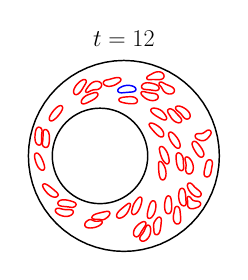
\begin{tikzpicture}[scale=0.35]

\begin{axis}[
  xmin = -21,
  xmax = 21,
  ymin = -21,
  ymax = 21,
  scale only axis,
  axis equal image,
  hide axis,
  title = {\Huge$t=12$}
  ]

\addplot [mark=none,black,line width=1.5] table{
2.0000e+01 0.0000e+00
1.9904e+01 1.9603e+00
1.9616e+01 3.9018e+00
1.9139e+01 5.8057e+00
1.8478e+01 7.6537e+00
1.7638e+01 9.4279e+00
1.6629e+01 1.1111e+01
1.5460e+01 1.2688e+01
1.4142e+01 1.4142e+01
1.2688e+01 1.5460e+01
1.1111e+01 1.6629e+01
9.4279e+00 1.7638e+01
7.6537e+00 1.8478e+01
5.8057e+00 1.9139e+01
3.9018e+00 1.9616e+01
1.9603e+00 1.9904e+01
1.2246e-15 2.0000e+01
-1.9603e+00 1.9904e+01
-3.9018e+00 1.9616e+01
-5.8057e+00 1.9139e+01
-7.6537e+00 1.8478e+01
-9.4279e+00 1.7638e+01
-1.1111e+01 1.6629e+01
-1.2688e+01 1.5460e+01
-1.4142e+01 1.4142e+01
-1.5460e+01 1.2688e+01
-1.6629e+01 1.1111e+01
-1.7638e+01 9.4279e+00
-1.8478e+01 7.6537e+00
-1.9139e+01 5.8057e+00
-1.9616e+01 3.9018e+00
-1.9904e+01 1.9603e+00
-2.0000e+01 2.4493e-15
-1.9904e+01 -1.9603e+00
-1.9616e+01 -3.9018e+00
-1.9139e+01 -5.8057e+00
-1.8478e+01 -7.6537e+00
-1.7638e+01 -9.4279e+00
-1.6629e+01 -1.1111e+01
-1.5460e+01 -1.2688e+01
-1.4142e+01 -1.4142e+01
-1.2688e+01 -1.5460e+01
-1.1111e+01 -1.6629e+01
-9.4279e+00 -1.7638e+01
-7.6537e+00 -1.8478e+01
-5.8057e+00 -1.9139e+01
-3.9018e+00 -1.9616e+01
-1.9603e+00 -1.9904e+01
-3.6739e-15 -2.0000e+01
1.9603e+00 -1.9904e+01
3.9018e+00 -1.9616e+01
5.8057e+00 -1.9139e+01
7.6537e+00 -1.8478e+01
9.4279e+00 -1.7638e+01
1.1111e+01 -1.6629e+01
1.2688e+01 -1.5460e+01
1.4142e+01 -1.4142e+01
1.5460e+01 -1.2688e+01
1.6629e+01 -1.1111e+01
1.7638e+01 -9.4279e+00
1.8478e+01 -7.6537e+00
1.9139e+01 -5.8057e+00
1.9616e+01 -3.9018e+00
1.9904e+01 -1.9603e+00
2.0000e+01 0.0000e+00
};

\addplot [mark=none,black,line width=1.5] table{
5.0000e+00 0.0000e+00
4.9518e+00 -9.8017e-01
4.8079e+00 -1.9509e+00
4.5694e+00 -2.9028e+00
4.2388e+00 -3.8268e+00
3.8192e+00 -4.7140e+00
3.3147e+00 -5.5557e+00
2.7301e+00 -6.3439e+00
2.0711e+00 -7.0711e+00
1.3439e+00 -7.7301e+00
5.5570e-01 -8.3147e+00
-2.8603e-01 -8.8192e+00
-1.1732e+00 -9.2388e+00
-2.0972e+00 -9.5694e+00
-3.0491e+00 -9.8079e+00
-4.0198e+00 -9.9518e+00
-5.0000e+00 -1.0000e+01
-5.9802e+00 -9.9518e+00
-6.9509e+00 -9.8079e+00
-7.9028e+00 -9.5694e+00
-8.8268e+00 -9.2388e+00
-9.7140e+00 -8.8192e+00
-1.0556e+01 -8.3147e+00
-1.1344e+01 -7.7301e+00
-1.2071e+01 -7.0711e+00
-1.2730e+01 -6.3439e+00
-1.3315e+01 -5.5557e+00
-1.3819e+01 -4.7140e+00
-1.4239e+01 -3.8268e+00
-1.4569e+01 -2.9028e+00
-1.4808e+01 -1.9509e+00
-1.4952e+01 -9.8017e-01
-1.5000e+01 -1.2246e-15
-1.4952e+01 9.8017e-01
-1.4808e+01 1.9509e+00
-1.4569e+01 2.9028e+00
-1.4239e+01 3.8268e+00
-1.3819e+01 4.7140e+00
-1.3315e+01 5.5557e+00
-1.2730e+01 6.3439e+00
-1.2071e+01 7.0711e+00
-1.1344e+01 7.7301e+00
-1.0556e+01 8.3147e+00
-9.7140e+00 8.8192e+00
-8.8268e+00 9.2388e+00
-7.9028e+00 9.5694e+00
-6.9509e+00 9.8079e+00
-5.9802e+00 9.9518e+00
-5.0000e+00 1.0000e+01
-4.0198e+00 9.9518e+00
-3.0491e+00 9.8079e+00
-2.0972e+00 9.5694e+00
-1.1732e+00 9.2388e+00
-2.8603e-01 8.8192e+00
5.5570e-01 8.3147e+00
1.3439e+00 7.7301e+00
2.0711e+00 7.0711e+00
2.7301e+00 6.3439e+00
3.3147e+00 5.5557e+00
3.8192e+00 4.7140e+00
4.2388e+00 3.8268e+00
4.5694e+00 2.9028e+00
4.8079e+00 1.9509e+00
4.9518e+00 9.8017e-01
5.0000e+00 0.0000e+00
};

\addplot [mark=none,red,line width=1.5] table{
1.7374e+01 3.5479e+00
1.7418e+01 3.5861e+00
1.7478e+01 3.6410e+00
1.7552e+01 3.7134e+00
1.7636e+01 3.8005e+00
1.7726e+01 3.8981e+00
1.7819e+01 4.0038e+00
1.7912e+01 4.1159e+00
1.8003e+01 4.2344e+00
1.8089e+01 4.3599e+00
1.8165e+01 4.4937e+00
1.8225e+01 4.6366e+00
1.8262e+01 4.7884e+00
1.8267e+01 4.9450e+00
1.8232e+01 5.0982e+00
1.8154e+01 5.2346e+00
1.8037e+01 5.3395e+00
1.7892e+01 5.4012e+00
1.7735e+01 5.4171e+00
1.7580e+01 5.3918e+00
1.7434e+01 5.3352e+00
1.7298e+01 5.2574e+00
1.7172e+01 5.1678e+00
1.7050e+01 5.0736e+00
1.6929e+01 4.9812e+00
1.6806e+01 4.8957e+00
1.6681e+01 4.8214e+00
1.6554e+01 4.7613e+00
1.6429e+01 4.7169e+00
1.6311e+01 4.6875e+00
1.6209e+01 4.6706e+00
1.6128e+01 4.6624e+00
1.6070e+01 4.6589e+00
1.6011e+01 4.6572e+00
1.5930e+01 4.6571e+00
1.5827e+01 4.6597e+00
1.5705e+01 4.6636e+00
1.5573e+01 4.6641e+00
1.5433e+01 4.6534e+00
1.5291e+01 4.6213e+00
1.5156e+01 4.5580e+00
1.5042e+01 4.4581e+00
1.4965e+01 4.3256e+00
1.4935e+01 4.1737e+00
1.4954e+01 4.0190e+00
1.5014e+01 3.8744e+00
1.5106e+01 3.7467e+00
1.5220e+01 3.6374e+00
1.5348e+01 3.5447e+00
1.5485e+01 3.4655e+00
1.5627e+01 3.3970e+00
1.5773e+01 3.3375e+00
1.5922e+01 3.2865e+00
1.6072e+01 3.2449e+00
1.6225e+01 3.2142e+00
1.6378e+01 3.1968e+00
1.6530e+01 3.1946e+00
1.6678e+01 3.2091e+00
1.6821e+01 3.2400e+00
1.6954e+01 3.2855e+00
1.7074e+01 3.3415e+00
1.7179e+01 3.4027e+00
1.7264e+01 3.4614e+00
1.7329e+01 3.5108e+00
1.7374e+01 3.5479e+00
};

\addplot [mark=none,red,line width=1.5] table{
-8.4426e+00 1.4446e+01
-8.4125e+00 1.4497e+01
-8.3705e+00 1.4567e+01
-8.3162e+00 1.4656e+01
-8.2525e+00 1.4760e+01
-8.1826e+00 1.4873e+01
-8.1094e+00 1.4994e+01
-8.0363e+00 1.5121e+01
-7.9677e+00 1.5254e+01
-7.9106e+00 1.5396e+01
-7.8768e+00 1.5547e+01
-7.8828e+00 1.5703e+01
-7.9441e+00 1.5846e+01
-8.0597e+00 1.5952e+01
-8.2085e+00 1.6002e+01
-8.3664e+00 1.6004e+01
-8.5212e+00 1.5969e+01
-8.6694e+00 1.5913e+01
-8.8112e+00 1.5841e+01
-8.9473e+00 1.5760e+01
-9.0783e+00 1.5671e+01
-9.2044e+00 1.5576e+01
-9.3256e+00 1.5477e+01
-9.4418e+00 1.5374e+01
-9.5531e+00 1.5268e+01
-9.6591e+00 1.5161e+01
-9.7590e+00 1.5053e+01
-9.8519e+00 1.4945e+01
-9.9364e+00 1.4841e+01
-1.0011e+01 1.4744e+01
-1.0072e+01 1.4658e+01
-1.0118e+01 1.4590e+01
-1.0150e+01 1.4541e+01
-1.0182e+01 1.4491e+01
-1.0224e+01 1.4420e+01
-1.0275e+01 1.4329e+01
-1.0330e+01 1.4219e+01
-1.0385e+01 1.4097e+01
-1.0435e+01 1.3964e+01
-1.0478e+01 1.3823e+01
-1.0510e+01 1.3676e+01
-1.0526e+01 1.3524e+01
-1.0524e+01 1.3369e+01
-1.0495e+01 1.3215e+01
-1.0433e+01 1.3071e+01
-1.0332e+01 1.2950e+01
-1.0197e+01 1.2868e+01
-1.0042e+01 1.2838e+01
-9.8850e+00 1.2855e+01
-9.7354e+00 1.2908e+01
-9.5964e+00 1.2984e+01
-9.4673e+00 1.3076e+01
-9.3469e+00 1.3179e+01
-9.2340e+00 1.3289e+01
-9.1284e+00 1.3404e+01
-9.0294e+00 1.3524e+01
-8.9372e+00 1.3646e+01
-8.8513e+00 1.3770e+01
-8.7716e+00 1.3893e+01
-8.6973e+00 1.4014e+01
-8.6290e+00 1.4129e+01
-8.5670e+00 1.4235e+01
-8.5141e+00 1.4325e+01
-8.4725e+00 1.4396e+01
-8.4426e+00 1.4446e+01
};

\addplot [mark=none,red,line width=1.5] table{
-6.9169e+00 1.3661e+01
-6.8626e+00 1.3685e+01
-6.7865e+00 1.3715e+01
-6.6875e+00 1.3750e+01
-6.5704e+00 1.3786e+01
-6.4401e+00 1.3818e+01
-6.3006e+00 1.3843e+01
-6.1547e+00 1.3862e+01
-6.0046e+00 1.3873e+01
-5.8515e+00 1.3882e+01
-5.6967e+00 1.3894e+01
-5.5415e+00 1.3917e+01
-5.3889e+00 1.3958e+01
-5.2426e+00 1.4020e+01
-5.1062e+00 1.4102e+01
-4.9823e+00 1.4203e+01
-4.8738e+00 1.4320e+01
-4.7833e+00 1.4452e+01
-4.7153e+00 1.4596e+01
-4.6748e+00 1.4750e+01
-4.6676e+00 1.4909e+01
-4.6978e+00 1.5064e+01
-4.7648e+00 1.5207e+01
-4.8622e+00 1.5329e+01
-4.9813e+00 1.5428e+01
-5.1132e+00 1.5504e+01
-5.2510e+00 1.5558e+01
-5.3891e+00 1.5594e+01
-5.5229e+00 1.5615e+01
-5.6465e+00 1.5622e+01
-5.7526e+00 1.5621e+01
-5.8349e+00 1.5615e+01
-5.8939e+00 1.5608e+01
-5.9522e+00 1.5600e+01
-6.0332e+00 1.5585e+01
-6.1354e+00 1.5560e+01
-6.2531e+00 1.5524e+01
-6.3784e+00 1.5477e+01
-6.5075e+00 1.5417e+01
-6.6360e+00 1.5345e+01
-6.7622e+00 1.5262e+01
-6.8833e+00 1.5167e+01
-6.9993e+00 1.5063e+01
-7.1093e+00 1.4951e+01
-7.2149e+00 1.4833e+01
-7.3166e+00 1.4709e+01
-7.4160e+00 1.4583e+01
-7.5127e+00 1.4455e+01
-7.6080e+00 1.4326e+01
-7.7009e+00 1.4196e+01
-7.7913e+00 1.4064e+01
-7.8757e+00 1.3928e+01
-7.9493e+00 1.3786e+01
-7.9977e+00 1.3636e+01
-7.9960e+00 1.3479e+01
-7.9156e+00 1.3348e+01
-7.7756e+00 1.3291e+01
-7.6263e+00 1.3309e+01
-7.4900e+00 1.3364e+01
-7.3642e+00 1.3430e+01
-7.2470e+00 1.3495e+01
-7.1387e+00 1.3554e+01
-7.0450e+00 1.3602e+01
-6.9706e+00 1.3637e+01
-6.9169e+00 1.3661e+01
};

\addplot [mark=none,red,line width=1.5] table{
8.2619e+00 1.3694e+01
8.2955e+00 1.3646e+01
8.3445e+00 1.3582e+01
8.4119e+00 1.3503e+01
8.4967e+00 1.3416e+01
8.5970e+00 1.3329e+01
8.7108e+00 1.3247e+01
8.8359e+00 1.3172e+01
8.9705e+00 1.3107e+01
9.1127e+00 1.3053e+01
9.2609e+00 1.3011e+01
9.4137e+00 1.2982e+01
9.5695e+00 1.2968e+01
9.7267e+00 1.2970e+01
9.8833e+00 1.2989e+01
1.0036e+01 1.3028e+01
1.0182e+01 1.3090e+01
1.0315e+01 1.3175e+01
1.0429e+01 1.3284e+01
1.0516e+01 1.3416e+01
1.0569e+01 1.3563e+01
1.0585e+01 1.3719e+01
1.0562e+01 1.3872e+01
1.0506e+01 1.4015e+01
1.0424e+01 1.4143e+01
1.0324e+01 1.4254e+01
1.0213e+01 1.4348e+01
1.0097e+01 1.4428e+01
9.9825e+00 1.4495e+01
9.8748e+00 1.4551e+01
9.7809e+00 1.4596e+01
9.7068e+00 1.4629e+01
9.6532e+00 1.4653e+01
9.5995e+00 1.4676e+01
9.5245e+00 1.4707e+01
9.4285e+00 1.4746e+01
9.3160e+00 1.4791e+01
9.1930e+00 1.4840e+01
9.0628e+00 1.4894e+01
8.9289e+00 1.4951e+01
8.7926e+00 1.5013e+01
8.6563e+00 1.5080e+01
8.5202e+00 1.5153e+01
8.3853e+00 1.5230e+01
8.2495e+00 1.5309e+01
8.1105e+00 1.5383e+01
7.9642e+00 1.5442e+01
7.8097e+00 1.5474e+01
7.6521e+00 1.5463e+01
7.5089e+00 1.5398e+01
7.4063e+00 1.5280e+01
7.3685e+00 1.5128e+01
7.3976e+00 1.4975e+01
7.4746e+00 1.4839e+01
7.5750e+00 1.4720e+01
7.6815e+00 1.4609e+01
7.7826e+00 1.4495e+01
7.8729e+00 1.4376e+01
7.9507e+00 1.4253e+01
8.0187e+00 1.4129e+01
8.0797e+00 1.4011e+01
8.1364e+00 1.3903e+01
8.1874e+00 1.3813e+01
8.2299e+00 1.3743e+01
8.2619e+00 1.3694e+01
};

\addplot [mark=none,red,line width=1.5] table{
-1.4328e+01 -1.1583e+01
-1.4307e+01 -1.1640e+01
-1.4270e+01 -1.1716e+01
-1.4211e+01 -1.1805e+01
-1.4131e+01 -1.1900e+01
-1.4032e+01 -1.1994e+01
-1.3921e+01 -1.2084e+01
-1.3798e+01 -1.2169e+01
-1.3667e+01 -1.2249e+01
-1.3529e+01 -1.2323e+01
-1.3387e+01 -1.2390e+01
-1.3240e+01 -1.2451e+01
-1.3090e+01 -1.2506e+01
-1.2937e+01 -1.2553e+01
-1.2781e+01 -1.2593e+01
-1.2623e+01 -1.2625e+01
-1.2464e+01 -1.2650e+01
-1.2303e+01 -1.2665e+01
-1.2143e+01 -1.2671e+01
-1.1983e+01 -1.2667e+01
-1.1824e+01 -1.2652e+01
-1.1668e+01 -1.2627e+01
-1.1514e+01 -1.2591e+01
-1.1365e+01 -1.2542e+01
-1.1223e+01 -1.2483e+01
-1.1088e+01 -1.2411e+01
-1.0964e+01 -1.2328e+01
-1.0853e+01 -1.2236e+01
-1.0761e+01 -1.2136e+01
-1.0688e+01 -1.2034e+01
-1.0641e+01 -1.1939e+01
-1.0614e+01 -1.1859e+01
-1.0603e+01 -1.1801e+01
-1.0599e+01 -1.1741e+01
-1.0607e+01 -1.1659e+01
-1.0639e+01 -1.1559e+01
-1.0710e+01 -1.1458e+01
-1.0816e+01 -1.1375e+01
-1.0947e+01 -1.1318e+01
-1.1093e+01 -1.1286e+01
-1.1245e+01 -1.1271e+01
-1.1401e+01 -1.1266e+01
-1.1560e+01 -1.1265e+01
-1.1720e+01 -1.1264e+01
-1.1881e+01 -1.1263e+01
-1.2042e+01 -1.1258e+01
-1.2205e+01 -1.1249e+01
-1.2367e+01 -1.1234e+01
-1.2529e+01 -1.1214e+01
-1.2689e+01 -1.1189e+01
-1.2849e+01 -1.1157e+01
-1.3008e+01 -1.1120e+01
-1.3165e+01 -1.1080e+01
-1.3320e+01 -1.1038e+01
-1.3476e+01 -1.1000e+01
-1.3632e+01 -1.0972e+01
-1.3788e+01 -1.0962e+01
-1.3941e+01 -1.0978e+01
-1.4084e+01 -1.1027e+01
-1.4204e+01 -1.1108e+01
-1.4291e+01 -1.1215e+01
-1.4338e+01 -1.1332e+01
-1.4351e+01 -1.1440e+01
-1.4342e+01 -1.1524e+01
-1.4328e+01 -1.1583e+01
};

\addplot [mark=none,red,line width=1.5] table{
1.3165e+01 -2.1893e-01
1.3107e+01 -2.2504e-01
1.3029e+01 -2.4793e-01
1.2940e+01 -3.0182e-01
1.2862e+01 -3.9422e-01
1.2814e+01 -5.1799e-01
1.2804e+01 -6.5809e-01
1.2822e+01 -8.0287e-01
1.2856e+01 -9.4866e-01
1.2896e+01 -1.0956e+00
1.2935e+01 -1.2449e+00
1.2969e+01 -1.3967e+00
1.2996e+01 -1.5511e+00
1.3015e+01 -1.7073e+00
1.3026e+01 -1.8650e+00
1.3028e+01 -2.0233e+00
1.3021e+01 -2.1818e+00
1.3008e+01 -2.3397e+00
1.2989e+01 -2.4971e+00
1.2970e+01 -2.6541e+00
1.2957e+01 -2.8112e+00
1.2956e+01 -2.9680e+00
1.2974e+01 -3.1230e+00
1.3015e+01 -3.2720e+00
1.3079e+01 -3.4105e+00
1.3165e+01 -3.5331e+00
1.3269e+01 -3.6351e+00
1.3387e+01 -3.7117e+00
1.3511e+01 -3.7604e+00
1.3631e+01 -3.7816e+00
1.3734e+01 -3.7814e+00
1.3815e+01 -3.7691e+00
1.3871e+01 -3.7542e+00
1.3926e+01 -3.7342e+00
1.4000e+01 -3.6989e+00
1.4087e+01 -3.6422e+00
1.4178e+01 -3.5624e+00
1.4264e+01 -3.4616e+00
1.4341e+01 -3.3438e+00
1.4405e+01 -3.2128e+00
1.4457e+01 -3.0724e+00
1.4495e+01 -2.9253e+00
1.4522e+01 -2.7736e+00
1.4538e+01 -2.6189e+00
1.4543e+01 -2.4625e+00
1.4538e+01 -2.3053e+00
1.4523e+01 -2.1481e+00
1.4500e+01 -1.9916e+00
1.4467e+01 -1.8366e+00
1.4425e+01 -1.6836e+00
1.4375e+01 -1.5333e+00
1.4317e+01 -1.3863e+00
1.4251e+01 -1.2432e+00
1.4178e+01 -1.1043e+00
1.4098e+01 -9.7040e-01
1.4012e+01 -8.4203e-01
1.3921e+01 -7.2001e-01
1.3824e+01 -6.0536e-01
1.3722e+01 -4.9990e-01
1.3617e+01 -4.0625e-01
1.3509e+01 -3.2829e-01
1.3402e+01 -2.7036e-01
1.3304e+01 -2.3541e-01
1.3224e+01 -2.2090e-01
1.3165e+01 -2.1893e-01
};

\addplot [mark=none,red,line width=1.5] table{
8.1122e+00 1.6169e+01
8.1595e+00 1.6203e+01
8.2203e+00 1.6257e+01
8.2879e+00 1.6336e+01
8.3501e+00 1.6440e+01
8.3946e+00 1.6564e+01
8.4133e+00 1.6703e+01
8.4020e+00 1.6848e+01
8.3604e+00 1.6992e+01
8.2909e+00 1.7127e+01
8.1974e+00 1.7249e+01
8.0843e+00 1.7355e+01
7.9559e+00 1.7444e+01
7.8160e+00 1.7516e+01
7.6681e+00 1.7569e+01
7.5146e+00 1.7606e+01
7.3580e+00 1.7627e+01
7.2000e+00 1.7633e+01
7.0423e+00 1.7624e+01
6.8862e+00 1.7602e+01
6.7327e+00 1.7568e+01
6.5828e+00 1.7523e+01
6.4370e+00 1.7469e+01
6.2956e+00 1.7407e+01
6.1587e+00 1.7340e+01
6.0261e+00 1.7270e+01
5.8981e+00 1.7200e+01
5.7750e+00 1.7132e+01
5.6586e+00 1.7067e+01
5.5518e+00 1.7010e+01
5.4599e+00 1.6961e+01
5.3879e+00 1.6924e+01
5.3361e+00 1.6897e+01
5.2845e+00 1.6869e+01
5.2131e+00 1.6830e+01
5.1238e+00 1.6778e+01
5.0237e+00 1.6709e+01
4.9251e+00 1.6620e+01
4.8431e+00 1.6506e+01
4.7994e+00 1.6368e+01
4.8151e+00 1.6220e+01
4.8961e+00 1.6093e+01
5.0242e+00 1.6008e+01
5.1744e+00 1.5969e+01
5.3305e+00 1.5961e+01
5.4876e+00 1.5969e+01
5.6447e+00 1.5983e+01
5.8023e+00 1.5996e+01
5.9602e+00 1.6005e+01
6.1185e+00 1.6009e+01
6.2765e+00 1.6008e+01
6.4342e+00 1.6004e+01
6.5912e+00 1.5998e+01
6.7477e+00 1.5992e+01
6.9030e+00 1.5987e+01
7.0573e+00 1.5983e+01
7.2096e+00 1.5982e+01
7.3594e+00 1.5986e+01
7.5052e+00 1.5994e+01
7.6452e+00 1.6009e+01
7.7759e+00 1.6032e+01
7.8930e+00 1.6064e+01
7.9899e+00 1.6101e+01
8.0625e+00 1.6138e+01
8.1122e+00 1.6169e+01
};

\addplot [mark=none,red,line width=1.5] table{
9.3720e+00 4.3737e+00
9.3800e+00 4.3153e+00
9.3953e+00 4.2342e+00
9.4177e+00 4.1319e+00
9.4487e+00 4.0130e+00
9.4855e+00 3.8846e+00
9.5296e+00 3.7495e+00
9.5793e+00 3.6119e+00
9.6370e+00 3.4725e+00
9.7008e+00 3.3339e+00
9.7724e+00 3.1960e+00
9.8495e+00 3.0605e+00
9.9332e+00 2.9266e+00
1.0021e+01 2.7953e+00
1.0114e+01 2.6655e+00
1.0210e+01 2.5380e+00
1.0309e+01 2.4119e+00
1.0411e+01 2.2882e+00
1.0517e+01 2.1663e+00
1.0625e+01 2.0476e+00
1.0737e+01 1.9324e+00
1.0855e+01 1.8245e+00
1.0980e+01 1.7275e+00
1.1116e+01 1.6503e+00
1.1263e+01 1.6042e+00
1.1414e+01 1.6046e+00
1.1551e+01 1.6564e+00
1.1657e+01 1.7506e+00
1.1726e+01 1.8653e+00
1.1763e+01 1.9823e+00
1.1779e+01 2.0857e+00
1.1782e+01 2.1678e+00
1.1782e+01 2.2265e+00
1.1778e+01 2.2856e+00
1.1770e+01 2.3669e+00
1.1753e+01 2.4704e+00
1.1728e+01 2.5896e+00
1.1693e+01 2.7185e+00
1.1650e+01 2.8528e+00
1.1598e+01 2.9904e+00
1.1539e+01 3.1288e+00
1.1472e+01 3.2671e+00
1.1400e+01 3.4041e+00
1.1320e+01 3.5397e+00
1.1235e+01 3.6727e+00
1.1145e+01 3.8035e+00
1.1051e+01 3.9315e+00
1.0952e+01 4.0571e+00
1.0850e+01 4.1799e+00
1.0744e+01 4.3004e+00
1.0636e+01 4.4180e+00
1.0524e+01 4.5331e+00
1.0410e+01 4.6439e+00
1.0290e+01 4.7488e+00
1.0164e+01 4.8433e+00
1.0028e+01 4.9210e+00
9.8819e+00 4.9707e+00
9.7302e+00 4.9799e+00
9.5889e+00 4.9387e+00
9.4762e+00 4.8518e+00
9.4056e+00 4.7378e+00
9.3717e+00 4.6198e+00
9.3634e+00 4.5147e+00
9.3657e+00 4.4327e+00
9.3720e+00 4.3737e+00
};

\addplot [mark=none,red,line width=1.5] table{
2.8956e+00 -8.9358e+00
2.8545e+00 -8.9799e+00
2.7987e+00 -9.0424e+00
2.7285e+00 -9.1247e+00
2.6482e+00 -9.2237e+00
2.5624e+00 -9.3349e+00
2.4747e+00 -9.4547e+00
2.3874e+00 -9.5809e+00
2.3020e+00 -9.7126e+00
2.2197e+00 -9.8496e+00
2.1427e+00 -9.9905e+00
2.0722e+00 -1.0135e+01
2.0086e+00 -1.0283e+01
1.9512e+00 -1.0434e+01
1.8992e+00 -1.0587e+01
1.8507e+00 -1.0742e+01
1.8049e+00 -1.0898e+01
1.7610e+00 -1.1055e+01
1.7197e+00 -1.1212e+01
1.6823e+00 -1.1370e+01
1.6519e+00 -1.1529e+01
1.6335e+00 -1.1690e+01
1.6352e+00 -1.1850e+01
1.6684e+00 -1.2006e+01
1.7441e+00 -1.2142e+01
1.8622e+00 -1.2239e+01
2.0049e+00 -1.2281e+01
2.1482e+00 -1.2273e+01
2.2774e+00 -1.2232e+01
2.3874e+00 -1.2175e+01
2.4757e+00 -1.2117e+01
2.5412e+00 -1.2066e+01
2.5869e+00 -1.2027e+01
2.6311e+00 -1.1987e+01
2.6907e+00 -1.1928e+01
2.7633e+00 -1.1850e+01
2.8441e+00 -1.1753e+01
2.9269e+00 -1.1642e+01
3.0087e+00 -1.1520e+01
3.0869e+00 -1.1391e+01
3.1613e+00 -1.1255e+01
3.2314e+00 -1.1115e+01
3.2978e+00 -1.0970e+01
3.3601e+00 -1.0822e+01
3.4193e+00 -1.0672e+01
3.4751e+00 -1.0520e+01
3.5281e+00 -1.0366e+01
3.5779e+00 -1.0211e+01
3.6248e+00 -1.0054e+01
3.6680e+00 -9.8960e+00
3.7073e+00 -9.7368e+00
3.7410e+00 -9.5768e+00
3.7677e+00 -9.4155e+00
3.7836e+00 -9.2538e+00
3.7839e+00 -9.0920e+00
3.7591e+00 -8.9339e+00
3.6977e+00 -8.7886e+00
3.5907e+00 -8.6777e+00
3.4502e+00 -8.6264e+00
3.3060e+00 -8.6396e+00
3.1806e+00 -8.6943e+00
3.0778e+00 -8.7657e+00
2.9973e+00 -8.8351e+00
2.9374e+00 -8.8929e+00
2.8956e+00 -8.9358e+00
};

\addplot [mark=none,red,line width=1.5] table{
1.3012e+01 -9.3793e+00
1.3004e+01 -9.3214e+00
1.2995e+01 -9.2407e+00
1.2985e+01 -9.1375e+00
1.2976e+01 -9.0166e+00
1.2971e+01 -8.8842e+00
1.2966e+01 -8.7436e+00
1.2962e+01 -8.5981e+00
1.2954e+01 -8.4487e+00
1.2942e+01 -8.2972e+00
1.2925e+01 -8.1440e+00
1.2903e+01 -7.9900e+00
1.2878e+01 -7.8354e+00
1.2848e+01 -7.6809e+00
1.2813e+01 -7.5269e+00
1.2770e+01 -7.3748e+00
1.2716e+01 -7.2262e+00
1.2644e+01 -7.0853e+00
1.2550e+01 -6.9587e+00
1.2429e+01 -6.8578e+00
1.2285e+01 -6.7965e+00
1.2129e+01 -6.7872e+00
1.1981e+01 -6.8314e+00
1.1855e+01 -6.9198e+00
1.1758e+01 -7.0364e+00
1.1687e+01 -7.1677e+00
1.1635e+01 -7.3039e+00
1.1596e+01 -7.4394e+00
1.1567e+01 -7.5690e+00
1.1545e+01 -7.6886e+00
1.1529e+01 -7.7913e+00
1.1518e+01 -7.8720e+00
1.1511e+01 -7.9300e+00
1.1505e+01 -7.9881e+00
1.1498e+01 -8.0690e+00
1.1490e+01 -8.1726e+00
1.1485e+01 -8.2937e+00
1.1482e+01 -8.4263e+00
1.1485e+01 -8.5668e+00
1.1493e+01 -8.7123e+00
1.1507e+01 -8.8612e+00
1.1526e+01 -9.0120e+00
1.1552e+01 -9.1638e+00
1.1585e+01 -9.3157e+00
1.1626e+01 -9.4669e+00
1.1674e+01 -9.6164e+00
1.1732e+01 -9.7631e+00
1.1801e+01 -9.9052e+00
1.1883e+01 -1.0041e+01
1.1979e+01 -1.0166e+01
1.2091e+01 -1.0277e+01
1.2220e+01 -1.0368e+01
1.2363e+01 -1.0432e+01
1.2517e+01 -1.0459e+01
1.2671e+01 -1.0442e+01
1.2811e+01 -1.0381e+01
1.2925e+01 -1.0280e+01
1.3003e+01 -1.0153e+01
1.3045e+01 -1.0014e+01
1.3059e+01 -9.8739e+00
1.3056e+01 -9.7413e+00
1.3044e+01 -9.6205e+00
1.3031e+01 -9.5176e+00
1.3020e+01 -9.4371e+00
1.3012e+01 -9.3793e+00
};

\addplot [mark=none,red,line width=1.5] table{
-1.4325e+01 9.9212e+00
-1.4367e+01 9.8794e+00
-1.4426e+01 9.8202e+00
-1.4499e+01 9.7429e+00
-1.4583e+01 9.6505e+00
-1.4672e+01 9.5472e+00
-1.4765e+01 9.4355e+00
-1.4857e+01 9.3176e+00
-1.4950e+01 9.1946e+00
-1.5042e+01 9.0674e+00
-1.5131e+01 8.9366e+00
-1.5219e+01 8.8026e+00
-1.5303e+01 8.6654e+00
-1.5383e+01 8.5247e+00
-1.5458e+01 8.3801e+00
-1.5525e+01 8.2312e+00
-1.5581e+01 8.0773e+00
-1.5619e+01 7.9182e+00
-1.5630e+01 7.7554e+00
-1.5599e+01 7.5958e+00
-1.5517e+01 7.4573e+00
-1.5387e+01 7.3657e+00
-1.5232e+01 7.3340e+00
-1.5076e+01 7.3537e+00
-1.4929e+01 7.4067e+00
-1.4793e+01 7.4784e+00
-1.4667e+01 7.5593e+00
-1.4551e+01 7.6440e+00
-1.4444e+01 7.7283e+00
-1.4349e+01 7.8083e+00
-1.4270e+01 7.8789e+00
-1.4208e+01 7.9355e+00
-1.4165e+01 7.9769e+00
-1.4122e+01 8.0189e+00
-1.4063e+01 8.0784e+00
-1.3988e+01 8.1560e+00
-1.3902e+01 8.2485e+00
-1.3811e+01 8.3515e+00
-1.3716e+01 8.4625e+00
-1.3621e+01 8.5793e+00
-1.3526e+01 8.7009e+00
-1.3432e+01 8.8261e+00
-1.3340e+01 8.9548e+00
-1.3251e+01 9.0867e+00
-1.3164e+01 9.2222e+00
-1.3081e+01 9.3611e+00
-1.3004e+01 9.5043e+00
-1.2935e+01 9.6520e+00
-1.2879e+01 9.8053e+00
-1.2841e+01 9.9642e+00
-1.2834e+01 1.0127e+01
-1.2869e+01 1.0285e+01
-1.2958e+01 1.0419e+01
-1.3093e+01 1.0505e+01
-1.3249e+01 1.0533e+01
-1.3405e+01 1.0515e+01
-1.3553e+01 1.0467e+01
-1.3690e+01 1.0402e+01
-1.3819e+01 1.0327e+01
-1.3938e+01 1.0247e+01
-1.4046e+01 1.0166e+01
-1.4141e+01 1.0088e+01
-1.4221e+01 1.0018e+01
-1.4282e+01 9.9622e+00
-1.4325e+01 9.9212e+00
};

\addplot [mark=none,red,line width=1.5] table{
1.2297e+01 1.0209e+01
1.2244e+01 1.0232e+01
1.2169e+01 1.0265e+01
1.2073e+01 1.0303e+01
1.1959e+01 1.0345e+01
1.1833e+01 1.0385e+01
1.1696e+01 1.0421e+01
1.1552e+01 1.0447e+01
1.1402e+01 1.0460e+01
1.1250e+01 1.0449e+01
1.1101e+01 1.0408e+01
1.0969e+01 1.0325e+01
1.0874e+01 1.0202e+01
1.0834e+01 1.0050e+01
1.0853e+01 9.8944e+00
1.0920e+01 9.7508e+00
1.1017e+01 9.6265e+00
1.1132e+01 9.5167e+00
1.1254e+01 9.4170e+00
1.1380e+01 9.3201e+00
1.1504e+01 9.2237e+00
1.1626e+01 9.1238e+00
1.1743e+01 9.0211e+00
1.1855e+01 8.9134e+00
1.1960e+01 8.8029e+00
1.2059e+01 8.6889e+00
1.2152e+01 8.5749e+00
1.2238e+01 8.4617e+00
1.2318e+01 8.3547e+00
1.2392e+01 8.2564e+00
1.2456e+01 8.1742e+00
1.2509e+01 8.1108e+00
1.2547e+01 8.0671e+00
1.2588e+01 8.0240e+00
1.2646e+01 7.9677e+00
1.2726e+01 7.9006e+00
1.2826e+01 7.8330e+00
1.2945e+01 7.7737e+00
1.3080e+01 7.7326e+00
1.3225e+01 7.7160e+00
1.3374e+01 7.7308e+00
1.3518e+01 7.7790e+00
1.3648e+01 7.8619e+00
1.3755e+01 7.9744e+00
1.3832e+01 8.1108e+00
1.3876e+01 8.2610e+00
1.3889e+01 8.4184e+00
1.3874e+01 8.5753e+00
1.3836e+01 8.7291e+00
1.3778e+01 8.8762e+00
1.3706e+01 9.0172e+00
1.3622e+01 9.1504e+00
1.3528e+01 9.2771e+00
1.3426e+01 9.3962e+00
1.3319e+01 9.5091e+00
1.3207e+01 9.6146e+00
1.3091e+01 9.7142e+00
1.2973e+01 9.8064e+00
1.2853e+01 9.8921e+00
1.2736e+01 9.9695e+00
1.2621e+01 1.0039e+01
1.2516e+01 1.0099e+01
1.2423e+01 1.0147e+01
1.2350e+01 1.0183e+01
1.2297e+01 1.0209e+01
};

\addplot [mark=none,red,line width=1.5] table{
5.5593e+00 1.3186e+01
5.5004e+00 1.3194e+01
5.4194e+00 1.3204e+01
5.3149e+00 1.3219e+01
5.1936e+00 1.3239e+01
5.0603e+00 1.3263e+01
4.9205e+00 1.3291e+01
4.7758e+00 1.3325e+01
4.6293e+00 1.3362e+01
4.4807e+00 1.3403e+01
4.3308e+00 1.3443e+01
4.1775e+00 1.3478e+01
4.0211e+00 1.3496e+01
3.8634e+00 1.3480e+01
3.7218e+00 1.3411e+01
3.6260e+00 1.3285e+01
3.6009e+00 1.3129e+01
3.6375e+00 1.2976e+01
3.7136e+00 1.2836e+01
3.8090e+00 1.2710e+01
3.9150e+00 1.2592e+01
4.0256e+00 1.2481e+01
4.1405e+00 1.2374e+01
4.2579e+00 1.2274e+01
4.3786e+00 1.2179e+01
4.5009e+00 1.2092e+01
4.6247e+00 1.2012e+01
4.7470e+00 1.1941e+01
4.8660e+00 1.1880e+01
4.9763e+00 1.1828e+01
5.0731e+00 1.1787e+01
5.1491e+00 1.1758e+01
5.2050e+00 1.1738e+01
5.2606e+00 1.1720e+01
5.3394e+00 1.1696e+01
5.4404e+00 1.1669e+01
5.5607e+00 1.1643e+01
5.6930e+00 1.1620e+01
5.8351e+00 1.1604e+01
5.9817e+00 1.1596e+01
6.1329e+00 1.1598e+01
6.2849e+00 1.1611e+01
6.4381e+00 1.1636e+01
6.5885e+00 1.1676e+01
6.7353e+00 1.1733e+01
6.8725e+00 1.1809e+01
6.9963e+00 1.1908e+01
7.0965e+00 1.2030e+01
7.1655e+00 1.2172e+01
7.1930e+00 1.2328e+01
7.1769e+00 1.2485e+01
7.1178e+00 1.2632e+01
7.0252e+00 1.2759e+01
6.9070e+00 1.2864e+01
6.7742e+00 1.2944e+01
6.6319e+00 1.3005e+01
6.4866e+00 1.3050e+01
6.3398e+00 1.3083e+01
6.1959e+00 1.3108e+01
6.0555e+00 1.3128e+01
5.9236e+00 1.3144e+01
5.8021e+00 1.3158e+01
5.6989e+00 1.3170e+01
5.6173e+00 1.3179e+01
5.5593e+00 1.3186e+01
};

\addplot [mark=none,red,line width=1.5] table{
-1.6365e+01 5.5213e+00
-1.6425e+01 5.5280e+00
-1.6507e+01 5.5254e+00
-1.6609e+01 5.4977e+00
-1.6715e+01 5.4347e+00
-1.6806e+01 5.3335e+00
-1.6870e+01 5.2057e+00
-1.6906e+01 5.0617e+00
-1.6923e+01 4.9113e+00
-1.6930e+01 4.7567e+00
-1.6932e+01 4.6011e+00
-1.6933e+01 4.4434e+00
-1.6934e+01 4.2855e+00
-1.6936e+01 4.1258e+00
-1.6940e+01 3.9660e+00
-1.6947e+01 3.8041e+00
-1.6956e+01 3.6419e+00
-1.6969e+01 3.4787e+00
-1.6985e+01 3.3178e+00
-1.7007e+01 3.1577e+00
-1.7032e+01 2.9982e+00
-1.7061e+01 2.8377e+00
-1.7084e+01 2.6790e+00
-1.7092e+01 2.5199e+00
-1.7070e+01 2.3654e+00
-1.7019e+01 2.2206e+00
-1.6941e+01 2.0935e+00
-1.6846e+01 1.9860e+00
-1.6739e+01 1.9025e+00
-1.6632e+01 1.8425e+00
-1.6533e+01 1.8068e+00
-1.6452e+01 1.7890e+00
-1.6393e+01 1.7834e+00
-1.6333e+01 1.7829e+00
-1.6251e+01 1.7934e+00
-1.6149e+01 1.8236e+00
-1.6040e+01 1.8835e+00
-1.5939e+01 1.9728e+00
-1.5854e+01 2.0878e+00
-1.5787e+01 2.2192e+00
-1.5736e+01 2.3623e+00
-1.5699e+01 2.5114e+00
-1.5670e+01 2.6654e+00
-1.5649e+01 2.8210e+00
-1.5631e+01 2.9789e+00
-1.5618e+01 3.1368e+00
-1.5607e+01 3.2960e+00
-1.5600e+01 3.4548e+00
-1.5595e+01 3.6148e+00
-1.5594e+01 3.7741e+00
-1.5596e+01 3.9343e+00
-1.5604e+01 4.0931e+00
-1.5617e+01 4.2518e+00
-1.5638e+01 4.4083e+00
-1.5665e+01 4.5632e+00
-1.5703e+01 4.7138e+00
-1.5750e+01 4.8603e+00
-1.5808e+01 4.9992e+00
-1.5877e+01 5.1295e+00
-1.5958e+01 5.2461e+00
-1.6047e+01 5.3463e+00
-1.6142e+01 5.4237e+00
-1.6232e+01 5.4771e+00
-1.6308e+01 5.5067e+00
-1.6365e+01 5.5213e+00
};

\addplot [mark=none,red,line width=1.5] table{
8.2299e-01 1.2386e+01
7.6336e-01 1.2382e+01
6.8025e-01 1.2376e+01
5.7393e-01 1.2367e+01
4.4967e-01 1.2356e+01
3.1420e-01 1.2343e+01
1.7085e-01 1.2328e+01
2.2774e-02 1.2311e+01
-1.2890e-01 1.2290e+01
-2.8237e-01 1.2265e+01
-4.3684e-01 1.2232e+01
-5.8996e-01 1.2189e+01
-7.3865e-01 1.2128e+01
-8.7494e-01 1.2043e+01
-9.8367e-01 1.1924e+01
-1.0381e+00 1.1773e+01
-1.0161e+00 1.1615e+01
-9.2532e-01 1.1483e+01
-7.9632e-01 1.1387e+01
-6.5113e-01 1.1317e+01
-5.0028e-01 1.1262e+01
-3.4707e-01 1.1215e+01
-1.9357e-01 1.1174e+01
-4.0182e-02 1.1138e+01
1.1184e-01 1.1105e+01
2.6219e-01 1.1076e+01
4.0924e-01 1.1050e+01
5.5205e-01 1.1027e+01
6.8752e-01 1.1006e+01
8.1235e-01 1.0989e+01
9.1952e-01 1.0976e+01
1.0033e+00 1.0966e+01
1.0631e+00 1.0960e+01
1.1228e+00 1.0954e+01
1.2057e+00 1.0947e+01
1.3121e+00 1.0938e+01
1.4365e+00 1.0931e+01
1.5729e+00 1.0925e+01
1.7174e+00 1.0924e+01
1.8672e+00 1.0927e+01
2.0205e+00 1.0938e+01
2.1754e+00 1.0959e+01
2.3297e+00 1.0995e+01
2.4793e+00 1.1051e+01
2.6171e+00 1.1133e+01
2.7309e+00 1.1247e+01
2.8050e+00 1.1389e+01
2.8279e+00 1.1549e+01
2.8000e+00 1.1708e+01
2.7313e+00 1.1854e+01
2.6335e+00 1.1982e+01
2.5155e+00 1.2092e+01
2.3831e+00 1.2184e+01
2.2406e+00 1.2256e+01
2.0916e+00 1.2312e+01
1.9389e+00 1.2352e+01
1.7852e+00 1.2379e+01
1.6325e+00 1.2395e+01
1.4828e+00 1.2403e+01
1.3380e+00 1.2405e+01
1.2009e+00 1.2404e+01
1.0751e+00 1.2399e+01
9.6715e-01 1.2394e+01
8.8305e-01 1.2390e+01
8.2299e-01 1.2386e+01
};

\addplot [mark=none,red,line width=1.5] table{
1.1378e+01 6.9466e+00
1.1437e+01 6.9408e+00
1.1518e+01 6.9394e+00
1.1622e+01 6.9483e+00
1.1740e+01 6.9777e+00
1.1859e+01 7.0348e+00
1.1967e+01 7.1254e+00
1.2047e+01 7.2467e+00
1.2088e+01 7.3902e+00
1.2088e+01 7.5418e+00
1.2049e+01 7.6911e+00
1.1982e+01 7.8311e+00
1.1896e+01 7.9622e+00
1.1798e+01 8.0851e+00
1.1693e+01 8.2034e+00
1.1585e+01 8.3184e+00
1.1475e+01 8.4328e+00
1.1365e+01 8.5465e+00
1.1255e+01 8.6614e+00
1.1147e+01 8.7768e+00
1.1041e+01 8.8939e+00
1.0937e+01 9.0112e+00
1.0833e+01 9.1289e+00
1.0730e+01 9.2446e+00
1.0625e+01 9.3571e+00
1.0518e+01 9.4626e+00
1.0407e+01 9.5593e+00
1.0292e+01 9.6432e+00
1.0178e+01 9.7131e+00
1.0068e+01 9.7666e+00
9.9706e+00 9.8045e+00
9.8923e+00 9.8275e+00
9.8349e+00 9.8407e+00
9.7771e+00 9.8499e+00
9.6956e+00 9.8571e+00
9.5914e+00 9.8530e+00
9.4721e+00 9.8278e+00
9.3524e+00 9.7695e+00
9.2497e+00 9.6730e+00
9.1847e+00 9.5420e+00
9.1671e+00 9.3934e+00
9.1936e+00 9.2425e+00
9.2498e+00 9.0985e+00
9.3232e+00 8.9601e+00
9.4037e+00 8.8253e+00
9.4867e+00 8.6906e+00
9.5686e+00 8.5556e+00
9.6501e+00 8.4192e+00
9.7310e+00 8.2832e+00
9.8141e+00 8.1477e+00
9.9002e+00 8.0152e+00
9.9918e+00 7.8858e+00
1.0089e+01 7.7619e+00
1.0193e+01 7.6433e+00
1.0302e+01 7.5318e+00
1.0416e+01 7.4272e+00
1.0534e+01 7.3311e+00
1.0657e+01 7.2432e+00
1.0780e+01 7.1655e+00
1.0905e+01 7.0981e+00
1.1026e+01 7.0431e+00
1.1140e+01 7.0006e+00
1.1240e+01 6.9721e+00
1.1320e+01 6.9550e+00
1.1378e+01 6.9466e+00
};

\addplot [mark=none,red,line width=1.5] table{
-7.5512e+00 1.2797e+01
-7.6066e+00 1.2774e+01
-7.6829e+00 1.2741e+01
-7.7790e+00 1.2695e+01
-7.8888e+00 1.2636e+01
-8.0049e+00 1.2564e+01
-8.1235e+00 1.2482e+01
-8.2413e+00 1.2390e+01
-8.3569e+00 1.2288e+01
-8.4685e+00 1.2179e+01
-8.5748e+00 1.2061e+01
-8.6735e+00 1.1935e+01
-8.7624e+00 1.1801e+01
-8.8372e+00 1.1658e+01
-8.8924e+00 1.1505e+01
-8.9184e+00 1.1345e+01
-8.9018e+00 1.1183e+01
-8.8281e+00 1.1039e+01
-8.7006e+00 1.0940e+01
-8.5444e+00 1.0899e+01
-8.3835e+00 1.0904e+01
-8.2261e+00 1.0936e+01
-8.0736e+00 1.0983e+01
-7.9249e+00 1.1038e+01
-7.7802e+00 1.1097e+01
-7.6391e+00 1.1159e+01
-7.5025e+00 1.1222e+01
-7.3709e+00 1.1284e+01
-7.2469e+00 1.1344e+01
-7.1334e+00 1.1400e+01
-7.0366e+00 1.1449e+01
-6.9612e+00 1.1487e+01
-6.9077e+00 1.1515e+01
-6.8545e+00 1.1543e+01
-6.7809e+00 1.1581e+01
-6.6872e+00 1.1632e+01
-6.5784e+00 1.1692e+01
-6.4604e+00 1.1760e+01
-6.3368e+00 1.1834e+01
-6.2109e+00 1.1915e+01
-6.0847e+00 1.2002e+01
-5.9602e+00 1.2096e+01
-5.8393e+00 1.2197e+01
-5.7246e+00 1.2308e+01
-5.6196e+00 1.2430e+01
-5.5300e+00 1.2565e+01
-5.4651e+00 1.2713e+01
-5.4402e+00 1.2874e+01
-5.4726e+00 1.3033e+01
-5.5681e+00 1.3163e+01
-5.7084e+00 1.3243e+01
-5.8672e+00 1.3275e+01
-6.0286e+00 1.3271e+01
-6.1876e+00 1.3247e+01
-6.3429e+00 1.3210e+01
-6.4948e+00 1.3166e+01
-6.6433e+00 1.3119e+01
-6.7885e+00 1.3069e+01
-6.9298e+00 1.3020e+01
-7.0663e+00 1.2972e+01
-7.1957e+00 1.2927e+01
-7.3145e+00 1.2885e+01
-7.4161e+00 1.2848e+01
-7.4951e+00 1.2818e+01
-7.5512e+00 1.2797e+01
};

\addplot [mark=none,red,line width=1.5] table{
4.3439e+00 -1.7790e+01
4.3975e+00 -1.7766e+01
4.4701e+00 -1.7730e+01
4.5598e+00 -1.7678e+01
4.6601e+00 -1.7609e+01
4.7640e+00 -1.7526e+01
4.8677e+00 -1.7431e+01
4.9683e+00 -1.7325e+01
5.0641e+00 -1.7210e+01
5.1540e+00 -1.7087e+01
5.2371e+00 -1.6958e+01
5.3128e+00 -1.6822e+01
5.3804e+00 -1.6681e+01
5.4395e+00 -1.6535e+01
5.4898e+00 -1.6386e+01
5.5312e+00 -1.6233e+01
5.5639e+00 -1.6079e+01
5.5881e+00 -1.5922e+01
5.6043e+00 -1.5765e+01
5.6126e+00 -1.5607e+01
5.6126e+00 -1.5450e+01
5.6036e+00 -1.5293e+01
5.5842e+00 -1.5139e+01
5.5518e+00 -1.4988e+01
5.5030e+00 -1.4844e+01
5.4330e+00 -1.4712e+01
5.3382e+00 -1.4601e+01
5.2199e+00 -1.4526e+01
5.0910e+00 -1.4498e+01
4.9713e+00 -1.4514e+01
4.8770e+00 -1.4556e+01
4.8116e+00 -1.4604e+01
4.7694e+00 -1.4645e+01
4.7311e+00 -1.4689e+01
4.6834e+00 -1.4755e+01
4.6304e+00 -1.4844e+01
4.5761e+00 -1.4953e+01
4.5224e+00 -1.5075e+01
4.4682e+00 -1.5206e+01
4.4122e+00 -1.5341e+01
4.3527e+00 -1.5478e+01
4.2889e+00 -1.5617e+01
4.2198e+00 -1.5755e+01
4.1451e+00 -1.5891e+01
4.0646e+00 -1.6025e+01
3.9786e+00 -1.6157e+01
3.8873e+00 -1.6285e+01
3.7921e+00 -1.6412e+01
3.6943e+00 -1.6536e+01
3.5974e+00 -1.6662e+01
3.5058e+00 -1.6791e+01
3.4266e+00 -1.6927e+01
3.3685e+00 -1.7073e+01
3.3410e+00 -1.7227e+01
3.3501e+00 -1.7382e+01
3.3983e+00 -1.7528e+01
3.4818e+00 -1.7655e+01
3.5933e+00 -1.7754e+01
3.7221e+00 -1.7822e+01
3.8578e+00 -1.7858e+01
3.9899e+00 -1.7867e+01
4.1105e+00 -1.7856e+01
4.2118e+00 -1.7835e+01
4.2893e+00 -1.7811e+01
4.3439e+00 -1.7790e+01
};

\addplot [mark=none,red,line width=1.5] table{
1.6973e+01 -2.5907e+00
1.6961e+01 -2.6477e+00
1.6943e+01 -2.7269e+00
1.6920e+01 -2.8281e+00
1.6893e+01 -2.9463e+00
1.6865e+01 -3.0757e+00
1.6836e+01 -3.2134e+00
1.6812e+01 -3.3569e+00
1.6794e+01 -3.5054e+00
1.6788e+01 -3.6572e+00
1.6799e+01 -3.8107e+00
1.6834e+01 -3.9617e+00
1.6899e+01 -4.1039e+00
1.6995e+01 -4.2278e+00
1.7120e+01 -4.3232e+00
1.7266e+01 -4.3809e+00
1.7423e+01 -4.3966e+00
1.7578e+01 -4.3705e+00
1.7723e+01 -4.3076e+00
1.7850e+01 -4.2150e+00
1.7958e+01 -4.1009e+00
1.8046e+01 -3.9717e+00
1.8116e+01 -3.8335e+00
1.8172e+01 -3.6899e+00
1.8215e+01 -3.5444e+00
1.8250e+01 -3.3990e+00
1.8279e+01 -3.2562e+00
1.8303e+01 -3.1177e+00
1.8324e+01 -2.9869e+00
1.8343e+01 -2.8672e+00
1.8360e+01 -2.7648e+00
1.8373e+01 -2.6847e+00
1.8383e+01 -2.6271e+00
1.8393e+01 -2.5696e+00
1.8407e+01 -2.4896e+00
1.8425e+01 -2.3876e+00
1.8447e+01 -2.2685e+00
1.8472e+01 -2.1383e+00
1.8497e+01 -2.0000e+00
1.8520e+01 -1.8561e+00
1.8538e+01 -1.7076e+00
1.8545e+01 -1.5558e+00
1.8537e+01 -1.4021e+00
1.8506e+01 -1.2499e+00
1.8447e+01 -1.1053e+00
1.8356e+01 -9.7782e-01
1.8234e+01 -8.7855e-01
1.8089e+01 -8.1793e-01
1.7933e+01 -8.0155e-01
1.7777e+01 -8.2940e-01
1.7635e+01 -8.9597e-01
1.7511e+01 -9.9330e-01
1.7409e+01 -1.1124e+00
1.7328e+01 -1.2457e+00
1.7263e+01 -1.3870e+00
1.7212e+01 -1.5323e+00
1.7171e+01 -1.6786e+00
1.7136e+01 -1.8239e+00
1.7105e+01 -1.9663e+00
1.7076e+01 -2.1041e+00
1.7049e+01 -2.2340e+00
1.7025e+01 -2.3527e+00
1.7003e+01 -2.4542e+00
1.6986e+01 -2.5336e+00
1.6973e+01 -2.5907e+00
};

\addplot [mark=none,red,line width=1.5] table{
-6.4702e+00 -1.3521e+01
-6.5221e+00 -1.3494e+01
-6.5965e+00 -1.3454e+01
-6.6900e+00 -1.3409e+01
-6.8067e+00 -1.3365e+01
-6.9377e+00 -1.3342e+01
-7.0812e+00 -1.3344e+01
-7.2242e+00 -1.3374e+01
-7.3678e+00 -1.3425e+01
-7.5045e+00 -1.3493e+01
-7.6383e+00 -1.3574e+01
-7.7628e+00 -1.3670e+01
-7.8812e+00 -1.3777e+01
-7.9856e+00 -1.3898e+01
-8.0769e+00 -1.4031e+01
-8.1440e+00 -1.4178e+01
-8.1848e+00 -1.4333e+01
-8.1855e+00 -1.4494e+01
-8.1453e+00 -1.4648e+01
-8.0598e+00 -1.4784e+01
-7.9438e+00 -1.4892e+01
-7.8045e+00 -1.4971e+01
-7.6574e+00 -1.5025e+01
-7.5034e+00 -1.5061e+01
-7.3514e+00 -1.5082e+01
-7.1980e+00 -1.5094e+01
-7.0505e+00 -1.5096e+01
-6.9051e+00 -1.5093e+01
-6.7703e+00 -1.5084e+01
-6.6453e+00 -1.5072e+01
-6.5415e+00 -1.5059e+01
-6.4587e+00 -1.5047e+01
-6.4015e+00 -1.5037e+01
-6.3422e+00 -1.5027e+01
-6.2633e+00 -1.5010e+01
-6.1602e+00 -1.4989e+01
-6.0431e+00 -1.4958e+01
-5.9133e+00 -1.4923e+01
-5.7797e+00 -1.4879e+01
-5.6406e+00 -1.4829e+01
-5.5028e+00 -1.4771e+01
-5.3631e+00 -1.4706e+01
-5.2274e+00 -1.4633e+01
-5.0922e+00 -1.4552e+01
-4.9637e+00 -1.4462e+01
-4.8387e+00 -1.4363e+01
-4.7254e+00 -1.4251e+01
-4.6250e+00 -1.4126e+01
-4.5556e+00 -1.3981e+01
-4.5380e+00 -1.3823e+01
-4.6069e+00 -1.3679e+01
-4.7442e+00 -1.3602e+01
-4.9049e+00 -1.3594e+01
-5.0620e+00 -1.3617e+01
-5.2201e+00 -1.3644e+01
-5.3754e+00 -1.3666e+01
-5.5323e+00 -1.3681e+01
-5.6850e+00 -1.3688e+01
-5.8368e+00 -1.3686e+01
-5.9810e+00 -1.3674e+01
-6.1179e+00 -1.3651e+01
-6.2380e+00 -1.3619e+01
-6.3399e+00 -1.3581e+01
-6.4151e+00 -1.3548e+01
-6.4702e+00 -1.3521e+01
};

\addplot [mark=none,red,line width=1.5] table{
6.4055e+00 -1.6209e+01
6.4331e+00 -1.6261e+01
6.4791e+00 -1.6328e+01
6.5515e+00 -1.6402e+01
6.6536e+00 -1.6466e+01
6.7807e+00 -1.6502e+01
6.9208e+00 -1.6499e+01
7.0588e+00 -1.6453e+01
7.1837e+00 -1.6371e+01
7.2904e+00 -1.6263e+01
7.3790e+00 -1.6137e+01
7.4516e+00 -1.5999e+01
7.5113e+00 -1.5855e+01
7.5604e+00 -1.5706e+01
7.6013e+00 -1.5553e+01
7.6355e+00 -1.5399e+01
7.6647e+00 -1.5244e+01
7.6897e+00 -1.5088e+01
7.7118e+00 -1.4932e+01
7.7314e+00 -1.4775e+01
7.7495e+00 -1.4619e+01
7.7664e+00 -1.4463e+01
7.7826e+00 -1.4308e+01
7.7981e+00 -1.4155e+01
7.8128e+00 -1.4003e+01
7.8259e+00 -1.3854e+01
7.8365e+00 -1.3708e+01
7.8427e+00 -1.3567e+01
7.8422e+00 -1.3434e+01
7.8327e+00 -1.3313e+01
7.8147e+00 -1.3211e+01
7.7919e+00 -1.3133e+01
7.7698e+00 -1.3079e+01
7.7422e+00 -1.3027e+01
7.6945e+00 -1.2961e+01
7.6174e+00 -1.2892e+01
7.5085e+00 -1.2840e+01
7.3772e+00 -1.2824e+01
7.2399e+00 -1.2852e+01
7.1104e+00 -1.2919e+01
6.9935e+00 -1.3012e+01
6.8879e+00 -1.3122e+01
6.7897e+00 -1.3241e+01
6.6961e+00 -1.3365e+01
6.6056e+00 -1.3493e+01
6.5189e+00 -1.3624e+01
6.4381e+00 -1.3759e+01
6.3665e+00 -1.3900e+01
6.3076e+00 -1.4047e+01
6.2644e+00 -1.4199e+01
6.2378e+00 -1.4355e+01
6.2265e+00 -1.4512e+01
6.2271e+00 -1.4669e+01
6.2355e+00 -1.4826e+01
6.2476e+00 -1.4981e+01
6.2604e+00 -1.5136e+01
6.2720e+00 -1.5288e+01
6.2820e+00 -1.5437e+01
6.2909e+00 -1.5583e+01
6.3006e+00 -1.5724e+01
6.3137e+00 -1.5857e+01
6.3324e+00 -1.5977e+01
6.3564e+00 -1.6078e+01
6.3823e+00 -1.6156e+01
6.4055e+00 -1.6209e+01
};

\addplot [mark=none,red,line width=1.5] table{
7.3630e+00 -3.6005e+00
7.3708e+00 -3.6600e+00
7.3822e+00 -3.7420e+00
7.3986e+00 -3.8471e+00
7.4200e+00 -3.9692e+00
7.4472e+00 -4.1025e+00
7.4811e+00 -4.2424e+00
7.5235e+00 -4.3859e+00
7.5766e+00 -4.5295e+00
7.6443e+00 -4.6702e+00
7.7311e+00 -4.8018e+00
7.8426e+00 -4.9154e+00
7.9806e+00 -4.9956e+00
8.1379e+00 -5.0258e+00
8.2957e+00 -4.9966e+00
8.4351e+00 -4.9160e+00
8.5474e+00 -4.7996e+00
8.6346e+00 -4.6631e+00
8.7009e+00 -4.5148e+00
8.7508e+00 -4.3607e+00
8.7867e+00 -4.2027e+00
8.8112e+00 -4.0434e+00
8.8251e+00 -3.8830e+00
8.8302e+00 -3.7234e+00
8.8269e+00 -3.5649e+00
8.8165e+00 -3.4095e+00
8.7997e+00 -3.2575e+00
8.7777e+00 -3.1116e+00
8.7517e+00 -2.9749e+00
8.7240e+00 -2.8517e+00
8.6969e+00 -2.7468e+00
8.6739e+00 -2.6659e+00
8.6560e+00 -2.6079e+00
8.6375e+00 -2.5510e+00
8.6100e+00 -2.4720e+00
8.5721e+00 -2.3726e+00
8.5235e+00 -2.2574e+00
8.4656e+00 -2.1341e+00
8.3987e+00 -2.0054e+00
8.3246e+00 -1.8753e+00
8.2440e+00 -1.7437e+00
8.1583e+00 -1.6129e+00
8.0663e+00 -1.4833e+00
7.9649e+00 -1.3599e+00
7.8469e+00 -1.2506e+00
7.7053e+00 -1.1756e+00
7.5459e+00 -1.1643e+00
7.4044e+00 -1.2374e+00
7.3160e+00 -1.3707e+00
7.2769e+00 -1.5270e+00
7.2640e+00 -1.6873e+00
7.2619e+00 -1.8482e+00
7.2636e+00 -2.0081e+00
7.2671e+00 -2.1679e+00
7.2717e+00 -2.3263e+00
7.2776e+00 -2.4841e+00
7.2844e+00 -2.6396e+00
7.2926e+00 -2.7932e+00
7.3018e+00 -2.9427e+00
7.3122e+00 -3.0877e+00
7.3233e+00 -3.2244e+00
7.3351e+00 -3.3502e+00
7.3461e+00 -3.4573e+00
7.3557e+00 -3.5410e+00
7.3630e+00 -3.6005e+00
};

\addplot [mark=none,red,line width=1.5] table{
5.3553e+00 -1.0341e+01
5.3359e+00 -1.0396e+01
5.3100e+00 -1.0474e+01
5.2782e+00 -1.0574e+01
5.2429e+00 -1.0691e+01
5.2062e+00 -1.0820e+01
5.1693e+00 -1.0957e+01
5.1327e+00 -1.1099e+01
5.0969e+00 -1.1246e+01
5.0623e+00 -1.1395e+01
5.0291e+00 -1.1547e+01
4.9977e+00 -1.1701e+01
4.9689e+00 -1.1856e+01
4.9431e+00 -1.2013e+01
4.9220e+00 -1.2172e+01
4.9074e+00 -1.2331e+01
4.9029e+00 -1.2492e+01
4.9146e+00 -1.2652e+01
4.9529e+00 -1.2807e+01
5.0302e+00 -1.2946e+01
5.1523e+00 -1.3046e+01
5.3043e+00 -1.3086e+01
5.4598e+00 -1.3066e+01
5.6023e+00 -1.3003e+01
5.7288e+00 -1.2915e+01
5.8409e+00 -1.2814e+01
5.9410e+00 -1.2706e+01
6.0302e+00 -1.2596e+01
6.1089e+00 -1.2488e+01
6.1762e+00 -1.2385e+01
6.2306e+00 -1.2294e+01
6.2707e+00 -1.2222e+01
6.2985e+00 -1.2170e+01
6.3251e+00 -1.2118e+01
6.3607e+00 -1.2044e+01
6.4034e+00 -1.1947e+01
6.4495e+00 -1.1833e+01
6.4949e+00 -1.1707e+01
6.5378e+00 -1.1572e+01
6.5765e+00 -1.1430e+01
6.6108e+00 -1.1283e+01
6.6398e+00 -1.1132e+01
6.6638e+00 -1.0978e+01
6.6820e+00 -1.0821e+01
6.6947e+00 -1.0663e+01
6.7008e+00 -1.0504e+01
6.6999e+00 -1.0344e+01
6.6902e+00 -1.0184e+01
6.6696e+00 -1.0025e+01
6.6342e+00 -9.8688e+00
6.5791e+00 -9.7184e+00
6.4972e+00 -9.5813e+00
6.3838e+00 -9.4702e+00
6.2410e+00 -9.4037e+00
6.0853e+00 -9.3954e+00
5.9383e+00 -9.4429e+00
5.8129e+00 -9.5296e+00
5.7095e+00 -9.6387e+00
5.6244e+00 -9.7579e+00
5.5531e+00 -9.8802e+00
5.4933e+00 -9.9997e+00
5.4436e+00 -1.0112e+01
5.4043e+00 -1.0209e+01
5.3752e+00 -1.0286e+01
5.3553e+00 -1.0341e+01
};

\addplot [mark=none,blue,line width=1.5] table{
1.0609e+00 1.3343e+01
1.1205e+00 1.3347e+01
1.2013e+00 1.3353e+01
1.3064e+00 1.3360e+01
1.4280e+00 1.3371e+01
1.5629e+00 1.3383e+01
1.7042e+00 1.3400e+01
1.8516e+00 1.3422e+01
1.9994e+00 1.3454e+01
2.1470e+00 1.3501e+01
2.2860e+00 1.3570e+01
2.4083e+00 1.3669e+01
2.4928e+00 1.3802e+01
2.5231e+00 1.3957e+01
2.4911e+00 1.4112e+01
2.4122e+00 1.4249e+01
2.3011e+00 1.4364e+01
2.1736e+00 1.4457e+01
2.0341e+00 1.4535e+01
1.8895e+00 1.4599e+01
1.7390e+00 1.4653e+01
1.5870e+00 1.4695e+01
1.4318e+00 1.4729e+01
1.2777e+00 1.4753e+01
1.1228e+00 1.4770e+01
9.7068e-01 1.4778e+01
8.2074e-01 1.4780e+01
6.7815e-01 1.4773e+01
5.4216e-01 1.4763e+01
4.1954e-01 1.4747e+01
3.1385e-01 1.4730e+01
2.3316e-01 1.4714e+01
1.7410e-01 1.4702e+01
1.1716e-01 1.4688e+01
3.6768e-02 1.4668e+01
-6.3441e-02 1.4638e+01
-1.8158e-01 1.4600e+01
-3.0768e-01 1.4553e+01
-4.4098e-01 1.4499e+01
-5.7480e-01 1.4435e+01
-7.1044e-01 1.4364e+01
-8.4181e-01 1.4283e+01
-9.6909e-01 1.4191e+01
-1.0841e+00 1.4084e+01
-1.1824e+00 1.3959e+01
-1.2471e+00 1.3814e+01
-1.2635e+00 1.3656e+01
-1.2155e+00 1.3503e+01
-1.1135e+00 1.3382e+01
-9.7535e-01 1.3300e+01
-8.2358e-01 1.3253e+01
-6.6507e-01 1.3230e+01
-5.0741e-01 1.3223e+01
-3.4856e-01 1.3225e+01
-1.9245e-01 1.3235e+01
-3.5982e-02 1.3246e+01
1.1671e-01 1.3261e+01
2.6823e-01 1.3275e+01
4.1426e-01 1.3289e+01
5.5732e-01 1.3302e+01
6.9114e-01 1.3314e+01
8.1507e-01 1.3324e+01
9.1945e-01 1.3332e+01
1.0026e+00 1.3338e+01
1.0609e+00 1.3343e+01
};

\addplot [mark=none,red,line width=1.5] table{
-1.5003e+01 -6.8242e+00
-1.5052e+01 -6.7879e+00
-1.5116e+01 -6.7332e+00
-1.5203e+01 -6.6680e+00
-1.5301e+01 -6.5883e+00
-1.5414e+01 -6.5059e+00
-1.5529e+01 -6.4159e+00
-1.5654e+01 -6.3285e+00
-1.5780e+01 -6.2375e+00
-1.5913e+01 -6.1518e+00
-1.6048e+01 -6.0654e+00
-1.6191e+01 -5.9889e+00
-1.6338e+01 -5.9190e+00
-1.6496e+01 -5.8713e+00
-1.6656e+01 -5.8521e+00
-1.6817e+01 -5.8892e+00
-1.6942e+01 -5.9880e+00
-1.7006e+01 -6.1381e+00
-1.7003e+01 -6.2971e+00
-1.6964e+01 -6.4543e+00
-1.6900e+01 -6.6001e+00
-1.6829e+01 -6.7437e+00
-1.6748e+01 -6.8786e+00
-1.6666e+01 -7.0128e+00
-1.6577e+01 -7.1385e+00
-1.6489e+01 -7.2634e+00
-1.6397e+01 -7.3790e+00
-1.6308e+01 -7.4923e+00
-1.6218e+01 -7.5937e+00
-1.6136e+01 -7.6885e+00
-1.6061e+01 -7.7647e+00
-1.6005e+01 -7.8266e+00
-1.5960e+01 -7.8669e+00
-1.5919e+01 -7.9102e+00
-1.5857e+01 -7.9650e+00
-1.5780e+01 -8.0377e+00
-1.5683e+01 -8.1158e+00
-1.5578e+01 -8.2013e+00
-1.5458e+01 -8.2829e+00
-1.5334e+01 -8.3650e+00
-1.5198e+01 -8.4377e+00
-1.5058e+01 -8.5058e+00
-1.4907e+01 -8.5596e+00
-1.4755e+01 -8.6038e+00
-1.4593e+01 -8.6281e+00
-1.4432e+01 -8.6366e+00
-1.4268e+01 -8.6185e+00
-1.4113e+01 -8.5768e+00
-1.3967e+01 -8.4989e+00
-1.3852e+01 -8.3874e+00
-1.3782e+01 -8.2382e+00
-1.3781e+01 -8.0784e+00
-1.3834e+01 -7.9253e+00
-1.3926e+01 -7.7950e+00
-1.4030e+01 -7.6748e+00
-1.4145e+01 -7.5658e+00
-1.4258e+01 -7.4571e+00
-1.4376e+01 -7.3554e+00
-1.4488e+01 -7.2536e+00
-1.4601e+01 -7.1598e+00
-1.4705e+01 -7.0682e+00
-1.4806e+01 -6.9883e+00
-1.4888e+01 -6.9167e+00
-1.4957e+01 -6.8645e+00
-1.5003e+01 -6.8242e+00
};

\addplot [mark=none,red,line width=1.5] table{
9.9619e+00 -9.6263e+00
9.9554e+00 -9.5682e+00
9.9461e+00 -9.4874e+00
9.9335e+00 -9.3844e+00
9.9174e+00 -9.2641e+00
9.8966e+00 -9.1329e+00
9.8690e+00 -8.9947e+00
9.8306e+00 -8.8539e+00
9.7763e+00 -8.7143e+00
9.6995e+00 -8.5830e+00
9.5942e+00 -8.4707e+00
9.4591e+00 -8.3948e+00
9.3048e+00 -8.3735e+00
9.1540e+00 -8.4148e+00
9.0272e+00 -8.5075e+00
8.9299e+00 -8.6318e+00
8.8563e+00 -8.7717e+00
8.7976e+00 -8.9188e+00
8.7479e+00 -9.0689e+00
8.7040e+00 -9.2207e+00
8.6648e+00 -9.3732e+00
8.6303e+00 -9.5261e+00
8.6010e+00 -9.6790e+00
8.5772e+00 -9.8316e+00
8.5590e+00 -9.9830e+00
8.5461e+00 -1.0132e+01
8.5382e+00 -1.0278e+01
8.5348e+00 -1.0419e+01
8.5351e+00 -1.0552e+01
8.5385e+00 -1.0674e+01
8.5437e+00 -1.0778e+01
8.5494e+00 -1.0859e+01
8.5545e+00 -1.0917e+01
8.5603e+00 -1.0976e+01
8.5698e+00 -1.1057e+01
8.5846e+00 -1.1159e+01
8.6063e+00 -1.1279e+01
8.6364e+00 -1.1408e+01
8.6773e+00 -1.1543e+01
8.7321e+00 -1.1678e+01
8.8045e+00 -1.1809e+01
8.8985e+00 -1.1928e+01
9.0166e+00 -1.2026e+01
9.1569e+00 -1.2092e+01
9.3113e+00 -1.2114e+01
9.4656e+00 -1.2087e+01
9.6055e+00 -1.2015e+01
9.7217e+00 -1.1908e+01
9.8122e+00 -1.1779e+01
9.8798e+00 -1.1636e+01
9.9292e+00 -1.1486e+01
9.9649e+00 -1.1332e+01
9.9908e+00 -1.1177e+01
1.0009e+01 -1.1021e+01
1.0021e+01 -1.0866e+01
1.0028e+01 -1.0712e+01
1.0029e+01 -1.0560e+01
1.0026e+01 -1.0410e+01
1.0020e+01 -1.0264e+01
1.0010e+01 -1.0123e+01
9.9990e+00 -9.9902e+00
9.9874e+00 -9.8690e+00
9.9769e+00 -9.7655e+00
9.9682e+00 -9.6845e+00
9.9619e+00 -9.6263e+00
};

\addplot [mark=none,red,line width=1.5] table{
8.8768e+00 1.0525e+00
8.8460e+00 1.1038e+00
8.8018e+00 1.1747e+00
8.7429e+00 1.2640e+00
8.6711e+00 1.3660e+00
8.5885e+00 1.4741e+00
8.4961e+00 1.5841e+00
8.3939e+00 1.6918e+00
8.2805e+00 1.7932e+00
8.1541e+00 1.8818e+00
8.0127e+00 1.9479e+00
7.8582e+00 1.9759e+00
7.7031e+00 1.9481e+00
7.5730e+00 1.8584e+00
7.4896e+00 1.7234e+00
7.4524e+00 1.5682e+00
7.4472e+00 1.4082e+00
7.4605e+00 1.2485e+00
7.4844e+00 1.0900e+00
7.5148e+00 9.3270e-01
7.5497e+00 7.7645e-01
7.5882e+00 6.2125e-01
7.6294e+00 4.6764e-01
7.6730e+00 3.1600e-01
7.7185e+00 1.6712e-01
7.7659e+00 2.1551e-02
7.8149e+00 -1.1944e-01
7.8655e+00 -2.5446e-01
7.9168e+00 -3.8071e-01
7.9675e+00 -4.9481e-01
8.0141e+00 -5.9110e-01
8.0526e+00 -6.6504e-01
8.0814e+00 -7.1730e-01
8.1112e+00 -7.6894e-01
8.1545e+00 -8.4010e-01
8.2125e+00 -9.2953e-01
8.2834e+00 -1.0317e+00
8.3641e+00 -1.1407e+00
8.4531e+00 -1.2533e+00
8.5498e+00 -1.3659e+00
8.6565e+00 -1.4745e+00
8.7770e+00 -1.5713e+00
8.9157e+00 -1.6434e+00
9.0705e+00 -1.6706e+00
9.2240e+00 -1.6343e+00
9.3474e+00 -1.5349e+00
9.4254e+00 -1.3957e+00
9.4639e+00 -1.2399e+00
9.4764e+00 -1.0795e+00
9.4732e+00 -9.1848e-01
9.4604e+00 -7.5815e-01
9.4405e+00 -5.9846e-01
9.4152e+00 -4.3985e-01
9.3848e+00 -2.8238e-01
9.3497e+00 -1.2691e-01
9.3099e+00 2.6208e-02
9.2656e+00 1.7592e-01
9.2170e+00 3.2168e-01
9.1647e+00 4.6198e-01
9.1095e+00 5.9569e-01
9.0531e+00 7.2014e-01
8.9978e+00 8.3256e-01
8.9477e+00 9.2751e-01
8.9069e+00 1.0007e+00
8.8768e+00 1.0525e+00
};

\addplot [mark=none,red,line width=1.5] table{
6.9987e+00 1.3739e+01
7.0534e+00 1.3760e+01
7.1263e+00 1.3796e+01
7.2110e+00 1.3857e+01
7.2930e+00 1.3946e+01
7.3535e+00 1.4065e+01
7.3773e+00 1.4203e+01
7.3569e+00 1.4347e+01
7.2962e+00 1.4484e+01
7.2046e+00 1.4605e+01
7.0923e+00 1.4710e+01
6.9663e+00 1.4801e+01
6.8314e+00 1.4880e+01
6.6904e+00 1.4949e+01
6.5451e+00 1.5011e+01
6.3966e+00 1.5065e+01
6.2459e+00 1.5113e+01
6.0933e+00 1.5156e+01
5.9397e+00 1.5194e+01
5.7852e+00 1.5228e+01
5.6304e+00 1.5257e+01
5.4754e+00 1.5282e+01
5.3208e+00 1.5303e+01
5.1667e+00 1.5317e+01
5.0141e+00 1.5325e+01
4.8638e+00 1.5323e+01
4.7178e+00 1.5312e+01
4.5782e+00 1.5290e+01
4.4485e+00 1.5260e+01
4.3327e+00 1.5222e+01
4.2363e+00 1.5182e+01
4.1633e+00 1.5146e+01
4.1123e+00 1.5117e+01
4.0627e+00 1.5085e+01
3.9967e+00 1.5037e+01
3.9182e+00 1.4969e+01
3.8370e+00 1.4878e+01
3.7656e+00 1.4765e+01
3.7160e+00 1.4633e+01
3.7014e+00 1.4488e+01
3.7312e+00 1.4342e+01
3.8067e+00 1.4210e+01
3.9186e+00 1.4105e+01
4.0540e+00 1.4029e+01
4.2018e+00 1.3977e+01
4.3555e+00 1.3943e+01
4.5116e+00 1.3920e+01
4.6691e+00 1.3903e+01
4.8269e+00 1.3890e+01
4.9849e+00 1.3878e+01
5.1425e+00 1.3865e+01
5.2999e+00 1.3852e+01
5.4564e+00 1.3836e+01
5.6121e+00 1.3818e+01
5.7665e+00 1.3797e+01
5.9195e+00 1.3775e+01
6.0703e+00 1.3752e+01
6.2188e+00 1.3730e+01
6.3639e+00 1.3711e+01
6.5044e+00 1.3697e+01
6.6374e+00 1.3690e+01
6.7591e+00 1.3694e+01
6.8627e+00 1.3706e+01
6.9424e+00 1.3722e+01
6.9987e+00 1.3739e+01
};

\addplot [mark=none,red,line width=1.5] table{
1.4607e+01 -6.2650e+00
1.4568e+01 -6.2216e+00
1.4513e+01 -6.1611e+00
1.4443e+01 -6.0844e+00
1.4360e+01 -5.9964e+00
1.4264e+01 -5.9044e+00
1.4156e+01 -5.8152e+00
1.4032e+01 -5.7385e+00
1.3892e+01 -5.6857e+00
1.3741e+01 -5.6716e+00
1.3592e+01 -5.7074e+00
1.3464e+01 -5.7945e+00
1.3373e+01 -5.9209e+00
1.3324e+01 -6.0698e+00
1.3311e+01 -6.2266e+00
1.3327e+01 -6.3838e+00
1.3362e+01 -6.5378e+00
1.3411e+01 -6.6882e+00
1.3470e+01 -6.8346e+00
1.3536e+01 -6.9778e+00
1.3608e+01 -7.1173e+00
1.3686e+01 -7.2533e+00
1.3768e+01 -7.3850e+00
1.3856e+01 -7.5120e+00
1.3948e+01 -7.6332e+00
1.4044e+01 -7.7479e+00
1.4143e+01 -7.8549e+00
1.4244e+01 -7.9533e+00
1.4343e+01 -8.0416e+00
1.4436e+01 -8.1185e+00
1.4519e+01 -8.1813e+00
1.4585e+01 -8.2284e+00
1.4634e+01 -8.2612e+00
1.4683e+01 -8.2930e+00
1.4752e+01 -8.3354e+00
1.4842e+01 -8.3866e+00
1.4951e+01 -8.4412e+00
1.5072e+01 -8.4937e+00
1.5205e+01 -8.5393e+00
1.5347e+01 -8.5729e+00
1.5496e+01 -8.5892e+00
1.5647e+01 -8.5825e+00
1.5797e+01 -8.5473e+00
1.5936e+01 -8.4792e+00
1.6054e+01 -8.3775e+00
1.6140e+01 -8.2465e+00
1.6185e+01 -8.0959e+00
1.6187e+01 -7.9384e+00
1.6149e+01 -7.7852e+00
1.6080e+01 -7.6431e+00
1.5989e+01 -7.5144e+00
1.5883e+01 -7.3982e+00
1.5767e+01 -7.2918e+00
1.5647e+01 -7.1921e+00
1.5524e+01 -7.0963e+00
1.5402e+01 -7.0021e+00
1.5283e+01 -6.9081e+00
1.5167e+01 -6.8133e+00
1.5057e+01 -6.7180e+00
1.4953e+01 -6.6230e+00
1.4858e+01 -6.5305e+00
1.4773e+01 -6.4438e+00
1.4701e+01 -6.3682e+00
1.4646e+01 -6.3084e+00
1.4607e+01 -6.2650e+00
};

\addplot [mark=none,red,line width=1.5] table{
6.8636e+00 8.3164e+00
6.9133e+00 8.2866e+00
6.9834e+00 8.2433e+00
7.0728e+00 8.1910e+00
7.1786e+00 8.1286e+00
7.2939e+00 8.0634e+00
7.4174e+00 7.9931e+00
7.5451e+00 7.9232e+00
7.6775e+00 7.8504e+00
7.8123e+00 7.7797e+00
7.9510e+00 7.7084e+00
8.0924e+00 7.6429e+00
8.2392e+00 7.5829e+00
8.3912e+00 7.5393e+00
8.5502e+00 7.5198e+00
8.7075e+00 7.5452e+00
8.8450e+00 7.6252e+00
8.9328e+00 7.7585e+00
8.9591e+00 7.9146e+00
8.9332e+00 8.0732e+00
8.8762e+00 8.2211e+00
8.8016e+00 8.3628e+00
8.7198e+00 8.4965e+00
8.6334e+00 8.6279e+00
8.5456e+00 8.7535e+00
8.4548e+00 8.8770e+00
8.3631e+00 8.9928e+00
8.2696e+00 9.1028e+00
8.1779e+00 9.2005e+00
8.0893e+00 9.2878e+00
8.0112e+00 9.3574e+00
7.9475e+00 9.4113e+00
7.9014e+00 9.4469e+00
7.8540e+00 9.4834e+00
7.7876e+00 9.5298e+00
7.6998e+00 9.5882e+00
7.5951e+00 9.6498e+00
7.4764e+00 9.7136e+00
7.3478e+00 9.7728e+00
7.2105e+00 9.8290e+00
7.0677e+00 9.8773e+00
6.9197e+00 9.9207e+00
6.7687e+00 9.9548e+00
6.6140e+00 9.9830e+00
6.4574e+00 1.0000e+01
6.2981e+00 1.0008e+01
6.1386e+00 9.9992e+00
5.9809e+00 9.9692e+00
5.8342e+00 9.9043e+00
5.7141e+00 9.7995e+00
5.6455e+00 9.6551e+00
5.6405e+00 9.4973e+00
5.6906e+00 9.3456e+00
5.7739e+00 9.2120e+00
5.8753e+00 9.0902e+00
5.9845e+00 8.9799e+00
6.0984e+00 8.8745e+00
6.2136e+00 8.7771e+00
6.3297e+00 8.6837e+00
6.4435e+00 8.5987e+00
6.5537e+00 8.5193e+00
6.6554e+00 8.4508e+00
6.7441e+00 8.3919e+00
6.8132e+00 8.3487e+00
6.8636e+00 8.3164e+00
};

\addplot [mark=none,red,line width=1.5] table{
-1.8262e+01 5.7423e+00
-1.8294e+01 5.6928e+00
-1.8334e+01 5.6197e+00
-1.8378e+01 5.5237e+00
-1.8422e+01 5.4070e+00
-1.8462e+01 5.2780e+00
-1.8496e+01 5.1388e+00
-1.8526e+01 4.9948e+00
-1.8551e+01 4.8452e+00
-1.8572e+01 4.6939e+00
-1.8590e+01 4.5391e+00
-1.8604e+01 4.3838e+00
-1.8615e+01 4.2259e+00
-1.8622e+01 4.0680e+00
-1.8626e+01 3.9079e+00
-1.8624e+01 3.7485e+00
-1.8616e+01 3.5876e+00
-1.8601e+01 3.4278e+00
-1.8577e+01 3.2679e+00
-1.8543e+01 3.1120e+00
-1.8498e+01 2.9588e+00
-1.8438e+01 2.8117e+00
-1.8363e+01 2.6712e+00
-1.8271e+01 2.5438e+00
-1.8162e+01 2.4323e+00
-1.8037e+01 2.3456e+00
-1.7900e+01 2.2883e+00
-1.7758e+01 2.2688e+00
-1.7624e+01 2.2857e+00
-1.7511e+01 2.3348e+00
-1.7428e+01 2.3984e+00
-1.7374e+01 2.4613e+00
-1.7342e+01 2.5107e+00
-1.7316e+01 2.5646e+00
-1.7289e+01 2.6421e+00
-1.7267e+01 2.7461e+00
-1.7255e+01 2.8683e+00
-1.7248e+01 3.0035e+00
-1.7246e+01 3.1455e+00
-1.7245e+01 3.2935e+00
-1.7244e+01 3.4442e+00
-1.7244e+01 3.5985e+00
-1.7243e+01 3.7536e+00
-1.7241e+01 3.9109e+00
-1.7237e+01 4.0680e+00
-1.7231e+01 4.2269e+00
-1.7221e+01 4.3854e+00
-1.7208e+01 4.5449e+00
-1.7191e+01 4.7033e+00
-1.7171e+01 4.8625e+00
-1.7153e+01 5.0208e+00
-1.7143e+01 5.1806e+00
-1.7151e+01 5.3393e+00
-1.7183e+01 5.4950e+00
-1.7244e+01 5.6401e+00
-1.7331e+01 5.7707e+00
-1.7441e+01 5.8796e+00
-1.7569e+01 5.9620e+00
-1.7711e+01 6.0081e+00
-1.7854e+01 6.0138e+00
-1.7985e+01 5.9799e+00
-1.8092e+01 5.9206e+00
-1.8172e+01 5.8517e+00
-1.8226e+01 5.7906e+00
-1.8262e+01 5.7423e+00
};

\addplot [mark=none,red,line width=1.5] table{
5.4766e+00 6.1330e+00
5.5100e+00 6.0842e+00
5.5575e+00 6.0175e+00
5.6198e+00 5.9336e+00
5.6949e+00 5.8363e+00
5.7786e+00 5.7313e+00
5.8688e+00 5.6213e+00
5.9637e+00 5.5085e+00
6.0634e+00 5.3927e+00
6.1665e+00 5.2754e+00
6.2724e+00 5.1571e+00
6.3799e+00 5.0396e+00
6.4891e+00 4.9226e+00
6.5997e+00 4.8071e+00
6.7123e+00 4.6926e+00
6.8269e+00 4.5803e+00
6.9443e+00 4.4702e+00
7.0650e+00 4.3637e+00
7.1904e+00 4.2617e+00
7.3212e+00 4.1672e+00
7.4592e+00 4.0833e+00
7.6054e+00 4.0163e+00
7.7600e+00 3.9741e+00
7.9186e+00 3.9683e+00
8.0703e+00 4.0080e+00
8.1976e+00 4.0947e+00
8.2868e+00 4.2156e+00
8.3354e+00 4.3530e+00
8.3514e+00 4.4906e+00
8.3453e+00 4.6171e+00
8.3283e+00 4.7227e+00
8.3089e+00 4.8034e+00
8.2922e+00 4.8605e+00
8.2733e+00 4.9168e+00
8.2441e+00 4.9935e+00
8.2016e+00 5.0897e+00
8.1456e+00 5.1995e+00
8.0770e+00 5.3162e+00
7.9978e+00 5.4348e+00
7.9089e+00 5.5529e+00
7.8109e+00 5.6697e+00
7.7046e+00 5.7841e+00
7.5914e+00 5.8947e+00
7.4726e+00 6.0008e+00
7.3492e+00 6.1021e+00
7.2216e+00 6.1990e+00
7.0904e+00 6.2914e+00
6.9560e+00 6.3796e+00
6.8187e+00 6.4636e+00
6.6785e+00 6.5436e+00
6.5356e+00 6.6191e+00
6.3898e+00 6.6898e+00
6.2413e+00 6.7545e+00
6.0899e+00 6.8115e+00
5.9354e+00 6.8571e+00
5.7780e+00 6.8851e+00
5.6203e+00 6.8844e+00
5.4725e+00 6.8395e+00
5.3593e+00 6.7413e+00
5.3068e+00 6.6063e+00
5.3135e+00 6.4687e+00
5.3533e+00 6.3491e+00
5.4016e+00 6.2537e+00
5.4442e+00 6.1828e+00
5.4766e+00 6.1330e+00
};

\addplot [mark=none,red,line width=1.5] table{
3.9146e+00 -1.3830e+01
3.8599e+00 -1.3851e+01
3.7852e+00 -1.3883e+01
3.6914e+00 -1.3929e+01
3.5844e+00 -1.3987e+01
3.4699e+00 -1.4056e+01
3.3517e+00 -1.4132e+01
3.2323e+00 -1.4217e+01
3.1135e+00 -1.4308e+01
2.9964e+00 -1.4406e+01
2.8822e+00 -1.4509e+01
2.7714e+00 -1.4619e+01
2.6650e+00 -1.4733e+01
2.5634e+00 -1.4854e+01
2.4674e+00 -1.4979e+01
2.3776e+00 -1.5110e+01
2.2951e+00 -1.5244e+01
2.2204e+00 -1.5384e+01
2.1548e+00 -1.5528e+01
2.0997e+00 -1.5676e+01
2.0567e+00 -1.5827e+01
2.0277e+00 -1.5982e+01
2.0153e+00 -1.6136e+01
2.0219e+00 -1.6291e+01
2.0504e+00 -1.6440e+01
2.1024e+00 -1.6581e+01
2.1784e+00 -1.6705e+01
2.2753e+00 -1.6807e+01
2.3859e+00 -1.6881e+01
2.4994e+00 -1.6925e+01
2.6023e+00 -1.6942e+01
2.6838e+00 -1.6942e+01
2.7420e+00 -1.6935e+01
2.7989e+00 -1.6922e+01
2.8758e+00 -1.6895e+01
2.9679e+00 -1.6848e+01
3.0660e+00 -1.6776e+01
3.1605e+00 -1.6684e+01
3.2486e+00 -1.6574e+01
3.3298e+00 -1.6453e+01
3.4072e+00 -1.6325e+01
3.4825e+00 -1.6193e+01
3.5583e+00 -1.6058e+01
3.6351e+00 -1.5923e+01
3.7143e+00 -1.5787e+01
3.7954e+00 -1.5653e+01
3.8794e+00 -1.5518e+01
3.9653e+00 -1.5385e+01
4.0537e+00 -1.5254e+01
4.1434e+00 -1.5123e+01
4.2344e+00 -1.4993e+01
4.3247e+00 -1.4864e+01
4.4128e+00 -1.4732e+01
4.4941e+00 -1.4598e+01
4.5630e+00 -1.4458e+01
4.6097e+00 -1.4311e+01
4.6238e+00 -1.4158e+01
4.5942e+00 -1.4012e+01
4.5169e+00 -1.3888e+01
4.4021e+00 -1.3806e+01
4.2740e+00 -1.3771e+01
4.1520e+00 -1.3771e+01
4.0490e+00 -1.3789e+01
3.9700e+00 -1.3811e+01
3.9146e+00 -1.3830e+01
};

\addplot [mark=none,red,line width=1.5] table{
1.6691e+01 7.3801e-01
1.6674e+01 7.9378e-01
1.6647e+01 8.7057e-01
1.6609e+01 9.6719e-01
1.6560e+01 1.0782e+00
1.6502e+01 1.1974e+00
1.6435e+01 1.3216e+00
1.6363e+01 1.4479e+00
1.6285e+01 1.5756e+00
1.6202e+01 1.7033e+00
1.6116e+01 1.8308e+00
1.6026e+01 1.9575e+00
1.5933e+01 2.0835e+00
1.5837e+01 2.2082e+00
1.5739e+01 2.3318e+00
1.5638e+01 2.4535e+00
1.5534e+01 2.5728e+00
1.5425e+01 2.6878e+00
1.5310e+01 2.7964e+00
1.5186e+01 2.8941e+00
1.5051e+01 2.9748e+00
1.4905e+01 3.0291e+00
1.4751e+01 3.0466e+00
1.4600e+01 3.0178e+00
1.4469e+01 2.9421e+00
1.4372e+01 2.8287e+00
1.4315e+01 2.6949e+00
1.4294e+01 2.5561e+00
1.4299e+01 2.4236e+00
1.4319e+01 2.3039e+00
1.4345e+01 2.2033e+00
1.4369e+01 2.1257e+00
1.4388e+01 2.0705e+00
1.4409e+01 2.0157e+00
1.4439e+01 1.9401e+00
1.4479e+01 1.8443e+00
1.4529e+01 1.7335e+00
1.4586e+01 1.6135e+00
1.4649e+01 1.4873e+00
1.4716e+01 1.3578e+00
1.4787e+01 1.2263e+00
1.4862e+01 1.0940e+00
1.4941e+01 9.6159e-01
1.5023e+01 8.2969e-01
1.5109e+01 6.9852e-01
1.5197e+01 5.6862e-01
1.5289e+01 4.4027e-01
1.5384e+01 3.1432e-01
1.5484e+01 1.9175e-01
1.5591e+01 7.4626e-02
1.5705e+01 -3.4090e-02
1.5831e+01 -1.2933e-01
1.5969e+01 -2.0404e-01
1.6119e+01 -2.4874e-01
1.6274e+01 -2.5427e-01
1.6422e+01 -2.1509e-01
1.6550e+01 -1.3393e-01
1.6647e+01 -2.0814e-02
1.6710e+01 1.1027e-01
1.6742e+01 2.4697e-01
1.6750e+01 3.7929e-01
1.6742e+01 5.0020e-01
1.6725e+01 6.0261e-01
1.6707e+01 6.8170e-01
1.6691e+01 7.3801e-01
};

\addplot [mark=none,red,line width=1.5] table{
1.2509e+01 -1.9768e+00
1.2504e+01 -1.9183e+00
1.2497e+01 -1.8375e+00
1.2488e+01 -1.7339e+00
1.2477e+01 -1.6126e+00
1.2467e+01 -1.4789e+00
1.2457e+01 -1.3368e+00
1.2449e+01 -1.1890e+00
1.2442e+01 -1.0374e+00
1.2436e+01 -8.8294e-01
1.2427e+01 -7.2697e-01
1.2411e+01 -5.7032e-01
1.2384e+01 -4.1455e-01
1.2342e+01 -2.6134e-01
1.2284e+01 -1.1282e-01
1.2211e+01 2.9802e-02
1.2126e+01 1.6515e-01
1.2028e+01 2.9235e-01
1.1918e+01 4.0892e-01
1.1796e+01 5.1068e-01
1.1658e+01 5.8968e-01
1.1507e+01 6.3379e-01
1.1351e+01 6.2867e-01
1.1207e+01 5.6894e-01
1.1095e+01 4.6445e-01
1.1018e+01 3.3392e-01
1.0972e+01 1.9315e-01
1.0947e+01 5.2292e-02
1.0936e+01 -8.2376e-02
1.0934e+01 -2.0533e-01
1.0935e+01 -3.1020e-01
1.0938e+01 -3.9167e-01
1.0940e+01 -4.5035e-01
1.0943e+01 -5.0870e-01
1.0949e+01 -5.8997e-01
1.0956e+01 -6.9367e-01
1.0967e+01 -8.1568e-01
1.0980e+01 -9.4921e-01
1.0995e+01 -1.0908e+00
1.1014e+01 -1.2365e+00
1.1035e+01 -1.3857e+00
1.1060e+01 -1.5366e+00
1.1089e+01 -1.6890e+00
1.1124e+01 -1.8413e+00
1.1164e+01 -1.9935e+00
1.1212e+01 -2.1440e+00
1.1267e+01 -2.2927e+00
1.1331e+01 -2.4378e+00
1.1405e+01 -2.5786e+00
1.1490e+01 -2.7122e+00
1.1590e+01 -2.8359e+00
1.1706e+01 -2.9432e+00
1.1841e+01 -3.0254e+00
1.1992e+01 -3.0690e+00
1.2148e+01 -3.0620e+00
1.2289e+01 -2.9999e+00
1.2399e+01 -2.8939e+00
1.2470e+01 -2.7617e+00
1.2509e+01 -2.6203e+00
1.2526e+01 -2.4788e+00
1.2529e+01 -2.3442e+00
1.2526e+01 -2.2211e+00
1.2519e+01 -2.1166e+00
1.2514e+01 -2.0351e+00
1.2509e+01 -1.9768e+00
};

\addplot [mark=none,red,line width=1.5] table{
-5.4691e-01 -1.2955e+01
-4.9086e-01 -1.2934e+01
-4.1279e-01 -1.2901e+01
-3.1620e-01 -1.2854e+01
-2.0460e-01 -1.2793e+01
-8.7283e-02 -1.2719e+01
3.3564e-02 -1.2634e+01
1.5180e-01 -1.2540e+01
2.6821e-01 -1.2437e+01
3.7933e-01 -1.2328e+01
4.8704e-01 -1.2210e+01
5.8776e-01 -1.2086e+01
6.8317e-01 -1.1955e+01
7.7012e-01 -1.1819e+01
8.5114e-01 -1.1678e+01
9.2428e-01 -1.1533e+01
9.9323e-01 -1.1385e+01
1.0569e+00 -1.1236e+01
1.1192e+00 -1.1084e+01
1.1783e+00 -1.0933e+01
1.2369e+00 -1.0780e+01
1.2909e+00 -1.0628e+01
1.3388e+00 -1.0473e+01
1.3691e+00 -1.0317e+01
1.3667e+00 -1.0158e+01
1.3039e+00 -1.0017e+01
1.1797e+00 -9.9333e+00
1.0343e+00 -9.9321e+00
9.0683e-01 -9.9808e+00
7.9914e-01 -1.0047e+01
7.1268e-01 -1.0109e+01
6.4528e-01 -1.0160e+01
5.9810e-01 -1.0197e+01
5.4983e-01 -1.0235e+01
4.8433e-01 -1.0286e+01
3.9924e-01 -1.0354e+01
3.0063e-01 -1.0432e+01
1.9154e-01 -1.0519e+01
7.7753e-02 -1.0610e+01
-4.0353e-02 -1.0705e+01
-1.5976e-01 -1.0801e+01
-2.8175e-01 -1.0901e+01
-4.0336e-01 -1.1002e+01
-5.2588e-01 -1.1106e+01
-6.4647e-01 -1.1211e+01
-7.6659e-01 -1.1320e+01
-8.8333e-01 -1.1430e+01
-9.9796e-01 -1.1546e+01
-1.1071e+00 -1.1664e+01
-1.2114e+00 -1.1789e+01
-1.3064e+00 -1.1920e+01
-1.3912e+00 -1.2058e+01
-1.4588e+00 -1.2204e+01
-1.5052e+00 -1.2358e+01
-1.5198e+00 -1.2515e+01
-1.4962e+00 -1.2671e+01
-1.4278e+00 -1.2811e+01
-1.3215e+00 -1.2920e+01
-1.1895e+00 -1.2991e+01
-1.0498e+00 -1.3025e+01
-9.1314e-01 -1.3031e+01
-7.8964e-01 -1.3019e+01
-6.8460e-01 -1.2997e+01
-6.0468e-01 -1.2974e+01
-5.4691e-01 -1.2955e+01
};

\addplot [mark=none,red,line width=1.5] table{
-1.8083e+01 5.4999e-01
-1.8140e+01 5.7004e-01
-1.8221e+01 5.8793e-01
-1.8327e+01 5.9058e-01
-1.8446e+01 5.6037e-01
-1.8558e+01 4.8581e-01
-1.8641e+01 3.7094e-01
-1.8688e+01 2.3158e-01
-1.8706e+01 8.1553e-02
-1.8705e+01 -7.2312e-02
-1.8691e+01 -2.2778e-01
-1.8669e+01 -3.8393e-01
-1.8642e+01 -5.4057e-01
-1.8608e+01 -6.9741e-01
-1.8571e+01 -8.5414e-01
-1.8530e+01 -1.0099e+00
-1.8485e+01 -1.1647e+00
-1.8436e+01 -1.3186e+00
-1.8383e+01 -1.4719e+00
-1.8326e+01 -1.6238e+00
-1.8264e+01 -1.7737e+00
-1.8196e+01 -1.9210e+00
-1.8124e+01 -2.0646e+00
-1.8046e+01 -2.2028e+00
-1.7962e+01 -2.3348e+00
-1.7873e+01 -2.4597e+00
-1.7778e+01 -2.5758e+00
-1.7679e+01 -2.6809e+00
-1.7578e+01 -2.7723e+00
-1.7479e+01 -2.8470e+00
-1.7388e+01 -2.9026e+00
-1.7314e+01 -2.9390e+00
-1.7258e+01 -2.9607e+00
-1.7201e+01 -2.9779e+00
-1.7119e+01 -2.9932e+00
-1.7013e+01 -2.9949e+00
-1.6893e+01 -2.9676e+00
-1.6778e+01 -2.8990e+00
-1.6688e+01 -2.7902e+00
-1.6633e+01 -2.6538e+00
-1.6612e+01 -2.5048e+00
-1.6614e+01 -2.3512e+00
-1.6633e+01 -2.1969e+00
-1.6663e+01 -2.0427e+00
-1.6700e+01 -1.8893e+00
-1.6744e+01 -1.7364e+00
-1.6792e+01 -1.5844e+00
-1.6844e+01 -1.4330e+00
-1.6898e+01 -1.2823e+00
-1.6956e+01 -1.1322e+00
-1.7015e+01 -9.8329e-01
-1.7077e+01 -8.3543e-01
-1.7142e+01 -6.8921e-01
-1.7209e+01 -5.4466e-01
-1.7279e+01 -4.0257e-01
-1.7352e+01 -2.6335e-01
-1.7429e+01 -1.2834e-01
-1.7510e+01 1.4176e-03
-1.7596e+01 1.2379e-01
-1.7685e+01 2.3675e-01
-1.7778e+01 3.3674e-01
-1.7871e+01 4.2022e-01
-1.7957e+01 4.8311e-01
-1.8029e+01 5.2498e-01
-1.8083e+01 5.4999e-01
};

\addplot [mark=none,red,line width=1.5] table{
-4.3063e+00 -1.3357e+01
-4.2494e+00 -1.3340e+01
-4.1707e+00 -1.3313e+01
-4.0736e+00 -1.3272e+01
-3.9623e+00 -1.3216e+01
-3.8453e+00 -1.3148e+01
-3.7244e+00 -1.3071e+01
-3.6045e+00 -1.2983e+01
-3.4851e+00 -1.2888e+01
-3.3703e+00 -1.2784e+01
-3.2596e+00 -1.2672e+01
-3.1579e+00 -1.2550e+01
-3.0667e+00 -1.2418e+01
-2.9946e+00 -1.2274e+01
-2.9491e+00 -1.2119e+01
-2.9470e+00 -1.1957e+01
-3.0013e+00 -1.1806e+01
-3.1152e+00 -1.1691e+01
-3.2650e+00 -1.1629e+01
-3.4277e+00 -1.1613e+01
-3.5897e+00 -1.1623e+01
-3.7507e+00 -1.1645e+01
-3.9083e+00 -1.1674e+01
-4.0652e+00 -1.1705e+01
-4.2187e+00 -1.1739e+01
-4.3697e+00 -1.1773e+01
-4.5152e+00 -1.1806e+01
-4.6567e+00 -1.1839e+01
-4.7898e+00 -1.1871e+01
-4.9130e+00 -1.1900e+01
-5.0177e+00 -1.1926e+01
-5.1001e+00 -1.1946e+01
-5.1581e+00 -1.1961e+01
-5.2166e+00 -1.1976e+01
-5.2967e+00 -1.1997e+01
-5.4000e+00 -1.2025e+01
-5.5194e+00 -1.2059e+01
-5.6502e+00 -1.2098e+01
-5.7869e+00 -1.2143e+01
-5.9280e+00 -1.2194e+01
-6.0697e+00 -1.2253e+01
-6.2110e+00 -1.2321e+01
-6.3475e+00 -1.2402e+01
-6.4763e+00 -1.2497e+01
-6.5880e+00 -1.2613e+01
-6.6698e+00 -1.2752e+01
-6.6970e+00 -1.2910e+01
-6.6487e+00 -1.3063e+01
-6.5307e+00 -1.3172e+01
-6.3802e+00 -1.3229e+01
-6.2199e+00 -1.3255e+01
-6.0588e+00 -1.3265e+01
-5.8969e+00 -1.3268e+01
-5.7362e+00 -1.3269e+01
-5.5755e+00 -1.3269e+01
-5.4169e+00 -1.3271e+01
-5.2595e+00 -1.3279e+01
-5.1063e+00 -1.3294e+01
-4.9573e+00 -1.3318e+01
-4.8156e+00 -1.3348e+01
-4.6804e+00 -1.3373e+01
-4.5560e+00 -1.3385e+01
-4.4479e+00 -1.3382e+01
-4.3653e+00 -1.3370e+01
-4.3063e+00 -1.3357e+01
};

\addplot [mark=none,red,line width=1.5] table{
1.1827e+01 -1.2151e+01
1.1822e+01 -1.2093e+01
1.1814e+01 -1.2012e+01
1.1805e+01 -1.1908e+01
1.1793e+01 -1.1788e+01
1.1779e+01 -1.1656e+01
1.1762e+01 -1.1516e+01
1.1739e+01 -1.1372e+01
1.1707e+01 -1.1226e+01
1.1664e+01 -1.1080e+01
1.1605e+01 -1.0938e+01
1.1524e+01 -1.0805e+01
1.1418e+01 -1.0691e+01
1.1285e+01 -1.0608e+01
1.1132e+01 -1.0575e+01
1.0977e+01 -1.0602e+01
1.0844e+01 -1.0686e+01
1.0746e+01 -1.0810e+01
1.0682e+01 -1.0954e+01
1.0641e+01 -1.1106e+01
1.0612e+01 -1.1260e+01
1.0588e+01 -1.1415e+01
1.0564e+01 -1.1568e+01
1.0538e+01 -1.1720e+01
1.0508e+01 -1.1869e+01
1.0477e+01 -1.2016e+01
1.0446e+01 -1.2159e+01
1.0418e+01 -1.2297e+01
1.0395e+01 -1.2428e+01
1.0377e+01 -1.2548e+01
1.0365e+01 -1.2651e+01
1.0358e+01 -1.2732e+01
1.0355e+01 -1.2790e+01
1.0353e+01 -1.2849e+01
1.0353e+01 -1.2930e+01
1.0356e+01 -1.3034e+01
1.0366e+01 -1.3154e+01
1.0385e+01 -1.3286e+01
1.0413e+01 -1.3423e+01
1.0454e+01 -1.3563e+01
1.0508e+01 -1.3702e+01
1.0578e+01 -1.3838e+01
1.0664e+01 -1.3965e+01
1.0770e+01 -1.4079e+01
1.0895e+01 -1.4172e+01
1.1037e+01 -1.4237e+01
1.1192e+01 -1.4265e+01
1.1349e+01 -1.4251e+01
1.1496e+01 -1.4194e+01
1.1623e+01 -1.4101e+01
1.1725e+01 -1.3981e+01
1.1801e+01 -1.3843e+01
1.1852e+01 -1.3695e+01
1.1885e+01 -1.3542e+01
1.1902e+01 -1.3387e+01
1.1908e+01 -1.3234e+01
1.1905e+01 -1.3082e+01
1.1898e+01 -1.2932e+01
1.1887e+01 -1.2787e+01
1.1874e+01 -1.2646e+01
1.1862e+01 -1.2514e+01
1.1850e+01 -1.2393e+01
1.1840e+01 -1.2290e+01
1.1832e+01 -1.2209e+01
1.1827e+01 -1.2151e+01
};

\addplot [mark=none,red,line width=1.5] table{
-1.0081e+01 -1.0402e+01
-1.0053e+01 -1.0350e+01
-1.0025e+01 -1.0272e+01
-1.0011e+01 -1.0167e+01
-1.0033e+01 -1.0046e+01
-1.0096e+01 -9.9278e+00
-1.0196e+01 -9.8259e+00
-1.0318e+01 -9.7428e+00
-1.0453e+01 -9.6736e+00
-1.0596e+01 -9.6140e+00
-1.0744e+01 -9.5602e+00
-1.0894e+01 -9.5106e+00
-1.1048e+01 -9.4638e+00
-1.1202e+01 -9.4198e+00
-1.1358e+01 -9.3782e+00
-1.1514e+01 -9.3393e+00
-1.1671e+01 -9.3032e+00
-1.1829e+01 -9.2708e+00
-1.1988e+01 -9.2426e+00
-1.2146e+01 -9.2195e+00
-1.2306e+01 -9.2021e+00
-1.2465e+01 -9.1916e+00
-1.2624e+01 -9.1889e+00
-1.2781e+01 -9.1954e+00
-1.2937e+01 -9.2121e+00
-1.3088e+01 -9.2404e+00
-1.3232e+01 -9.2808e+00
-1.3364e+01 -9.3339e+00
-1.3484e+01 -9.3982e+00
-1.3584e+01 -9.4710e+00
-1.3661e+01 -9.5444e+00
-1.3713e+01 -9.6089e+00
-1.3746e+01 -9.6588e+00
-1.3773e+01 -9.7115e+00
-1.3801e+01 -9.7889e+00
-1.3819e+01 -9.8927e+00
-1.3811e+01 -1.0015e+01
-1.3766e+01 -1.0141e+01
-1.3684e+01 -1.0257e+01
-1.3571e+01 -1.0352e+01
-1.3437e+01 -1.0423e+01
-1.3291e+01 -1.0474e+01
-1.3139e+01 -1.0511e+01
-1.2983e+01 -1.0537e+01
-1.2826e+01 -1.0558e+01
-1.2666e+01 -1.0575e+01
-1.2507e+01 -1.0590e+01
-1.2346e+01 -1.0605e+01
-1.2187e+01 -1.0620e+01
-1.2026e+01 -1.0637e+01
-1.1866e+01 -1.0655e+01
-1.1706e+01 -1.0674e+01
-1.1547e+01 -1.0696e+01
-1.1388e+01 -1.0718e+01
-1.1231e+01 -1.0740e+01
-1.1074e+01 -1.0758e+01
-1.0919e+01 -1.0768e+01
-1.0765e+01 -1.0765e+01
-1.0618e+01 -1.0745e+01
-1.0479e+01 -1.0706e+01
-1.0355e+01 -1.0650e+01
-1.0250e+01 -1.0583e+01
-1.0170e+01 -1.0514e+01
-1.0115e+01 -1.0451e+01
-1.0081e+01 -1.0402e+01
};

\addplot [mark=none,red,line width=1.5] table{
-2.3342e+00 1.4701e+01
-2.2777e+00 1.4718e+01
-2.2000e+00 1.4744e+01
-2.1014e+00 1.4780e+01
-1.9882e+00 1.4826e+01
-1.8662e+00 1.4881e+01
-1.7396e+00 1.4945e+01
-1.6105e+00 1.5015e+01
-1.4807e+00 1.5091e+01
-1.3505e+00 1.5171e+01
-1.2210e+00 1.5256e+01
-1.0925e+00 1.5345e+01
-9.6711e-01 1.5441e+01
-8.4771e-01 1.5545e+01
-7.4121e-01 1.5663e+01
-6.5929e-01 1.5799e+01
-6.2146e-01 1.5953e+01
-6.4569e-01 1.6109e+01
-7.3306e-01 1.6241e+01
-8.6270e-01 1.6331e+01
-1.0122e+00 1.6382e+01
-1.1679e+00 1.6405e+01
-1.3244e+00 1.6410e+01
-1.4793e+00 1.6403e+01
-1.6320e+00 1.6388e+01
-1.7812e+00 1.6365e+01
-1.9260e+00 1.6338e+01
-2.0643e+00 1.6308e+01
-2.1942e+00 1.6276e+01
-2.3122e+00 1.6244e+01
-2.4132e+00 1.6216e+01
-2.4918e+00 1.6193e+01
-2.5486e+00 1.6176e+01
-2.6051e+00 1.6159e+01
-2.6842e+00 1.6136e+01
-2.7849e+00 1.6106e+01
-2.9033e+00 1.6073e+01
-3.0327e+00 1.6038e+01
-3.1709e+00 1.6005e+01
-3.3145e+00 1.5975e+01
-3.4627e+00 1.5946e+01
-3.6129e+00 1.5915e+01
-3.7639e+00 1.5876e+01
-3.9109e+00 1.5820e+01
-4.0484e+00 1.5741e+01
-4.1662e+00 1.5635e+01
-4.2535e+00 1.5501e+01
-4.2966e+00 1.5348e+01
-4.2867e+00 1.5189e+01
-4.2241e+00 1.5042e+01
-4.1232e+00 1.4920e+01
-3.9985e+00 1.4822e+01
-3.8615e+00 1.4744e+01
-3.7166e+00 1.4682e+01
-3.5674e+00 1.4636e+01
-3.4154e+00 1.4604e+01
-3.2637e+00 1.4587e+01
-3.1131e+00 1.4582e+01
-2.9666e+00 1.4587e+01
-2.8253e+00 1.4599e+01
-2.6930e+00 1.4618e+01
-2.5724e+00 1.4641e+01
-2.4703e+00 1.4664e+01
-2.3908e+00 1.4685e+01
-2.3342e+00 1.4701e+01
};

\addplot [mark=none,red,line width=1.5] table{
1.4362e+01 -1.1063e+01
1.4421e+01 -1.1058e+01
1.4501e+01 -1.1047e+01
1.4603e+01 -1.1029e+01
1.4722e+01 -1.1002e+01
1.4850e+01 -1.0968e+01
1.4984e+01 -1.0927e+01
1.5123e+01 -1.0882e+01
1.5263e+01 -1.0831e+01
1.5404e+01 -1.0775e+01
1.5544e+01 -1.0711e+01
1.5680e+01 -1.0636e+01
1.5809e+01 -1.0546e+01
1.5922e+01 -1.0438e+01
1.6012e+01 -1.0309e+01
1.6067e+01 -1.0161e+01
1.6078e+01 -1.0004e+01
1.6039e+01 -9.8518e+00
1.5954e+01 -9.7190e+00
1.5836e+01 -9.6162e+00
1.5696e+01 -9.5457e+00
1.5545e+01 -9.5033e+00
1.5391e+01 -9.4812e+00
1.5238e+01 -9.4698e+00
1.5086e+01 -9.4601e+00
1.4937e+01 -9.4442e+00
1.4794e+01 -9.4168e+00
1.4660e+01 -9.3749e+00
1.4539e+01 -9.3199e+00
1.4436e+01 -9.2562e+00
1.4354e+01 -9.1925e+00
1.4295e+01 -9.1374e+00
1.4254e+01 -9.0955e+00
1.4215e+01 -9.0520e+00
1.4163e+01 -8.9893e+00
1.4100e+01 -8.9070e+00
1.4027e+01 -8.8100e+00
1.3944e+01 -8.7071e+00
1.3844e+01 -8.6085e+00
1.3721e+01 -8.5305e+00
1.3577e+01 -8.4944e+00
1.3429e+01 -8.5227e+00
1.3311e+01 -8.6193e+00
1.3250e+01 -8.7608e+00
1.3242e+01 -8.9165e+00
1.3268e+01 -9.0715e+00
1.3306e+01 -9.2246e+00
1.3339e+01 -9.3790e+00
1.3360e+01 -9.5356e+00
1.3366e+01 -9.6935e+00
1.3359e+01 -9.8513e+00
1.3348e+01 -1.0009e+01
1.3342e+01 -1.0166e+01
1.3352e+01 -1.0322e+01
1.3384e+01 -1.0474e+01
1.3443e+01 -1.0617e+01
1.3526e+01 -1.0744e+01
1.3629e+01 -1.0852e+01
1.3747e+01 -1.0937e+01
1.3874e+01 -1.0998e+01
1.4000e+01 -1.1038e+01
1.4119e+01 -1.1059e+01
1.4223e+01 -1.1066e+01
1.4304e+01 -1.1066e+01
1.4362e+01 -1.1063e+01
};

\end{axis}

\end{tikzpicture}
 &
%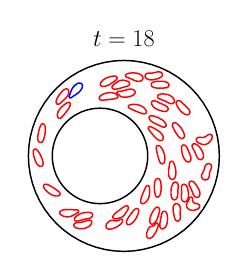
\begin{tikzpicture}[scale=0.35]

\begin{axis}[
  xmin = -21,
  xmax = 21,
  ymin = -21,
  ymax = 21,
  scale only axis,
  axis equal image,
  hide axis,
  title = {\Huge$t=18$}
  ]

\addplot [mark=none,black,line width=1.5] table{
2.0000e+01 0.0000e+00
1.9904e+01 1.9603e+00
1.9616e+01 3.9018e+00
1.9139e+01 5.8057e+00
1.8478e+01 7.6537e+00
1.7638e+01 9.4279e+00
1.6629e+01 1.1111e+01
1.5460e+01 1.2688e+01
1.4142e+01 1.4142e+01
1.2688e+01 1.5460e+01
1.1111e+01 1.6629e+01
9.4279e+00 1.7638e+01
7.6537e+00 1.8478e+01
5.8057e+00 1.9139e+01
3.9018e+00 1.9616e+01
1.9603e+00 1.9904e+01
1.2246e-15 2.0000e+01
-1.9603e+00 1.9904e+01
-3.9018e+00 1.9616e+01
-5.8057e+00 1.9139e+01
-7.6537e+00 1.8478e+01
-9.4279e+00 1.7638e+01
-1.1111e+01 1.6629e+01
-1.2688e+01 1.5460e+01
-1.4142e+01 1.4142e+01
-1.5460e+01 1.2688e+01
-1.6629e+01 1.1111e+01
-1.7638e+01 9.4279e+00
-1.8478e+01 7.6537e+00
-1.9139e+01 5.8057e+00
-1.9616e+01 3.9018e+00
-1.9904e+01 1.9603e+00
-2.0000e+01 2.4493e-15
-1.9904e+01 -1.9603e+00
-1.9616e+01 -3.9018e+00
-1.9139e+01 -5.8057e+00
-1.8478e+01 -7.6537e+00
-1.7638e+01 -9.4279e+00
-1.6629e+01 -1.1111e+01
-1.5460e+01 -1.2688e+01
-1.4142e+01 -1.4142e+01
-1.2688e+01 -1.5460e+01
-1.1111e+01 -1.6629e+01
-9.4279e+00 -1.7638e+01
-7.6537e+00 -1.8478e+01
-5.8057e+00 -1.9139e+01
-3.9018e+00 -1.9616e+01
-1.9603e+00 -1.9904e+01
-3.6739e-15 -2.0000e+01
1.9603e+00 -1.9904e+01
3.9018e+00 -1.9616e+01
5.8057e+00 -1.9139e+01
7.6537e+00 -1.8478e+01
9.4279e+00 -1.7638e+01
1.1111e+01 -1.6629e+01
1.2688e+01 -1.5460e+01
1.4142e+01 -1.4142e+01
1.5460e+01 -1.2688e+01
1.6629e+01 -1.1111e+01
1.7638e+01 -9.4279e+00
1.8478e+01 -7.6537e+00
1.9139e+01 -5.8057e+00
1.9616e+01 -3.9018e+00
1.9904e+01 -1.9603e+00
2.0000e+01 0.0000e+00
};

\addplot [mark=none,black,line width=1.5] table{
5.0000e+00 0.0000e+00
4.9518e+00 -9.8017e-01
4.8079e+00 -1.9509e+00
4.5694e+00 -2.9028e+00
4.2388e+00 -3.8268e+00
3.8192e+00 -4.7140e+00
3.3147e+00 -5.5557e+00
2.7301e+00 -6.3439e+00
2.0711e+00 -7.0711e+00
1.3439e+00 -7.7301e+00
5.5570e-01 -8.3147e+00
-2.8603e-01 -8.8192e+00
-1.1732e+00 -9.2388e+00
-2.0972e+00 -9.5694e+00
-3.0491e+00 -9.8079e+00
-4.0198e+00 -9.9518e+00
-5.0000e+00 -1.0000e+01
-5.9802e+00 -9.9518e+00
-6.9509e+00 -9.8079e+00
-7.9028e+00 -9.5694e+00
-8.8268e+00 -9.2388e+00
-9.7140e+00 -8.8192e+00
-1.0556e+01 -8.3147e+00
-1.1344e+01 -7.7301e+00
-1.2071e+01 -7.0711e+00
-1.2730e+01 -6.3439e+00
-1.3315e+01 -5.5557e+00
-1.3819e+01 -4.7140e+00
-1.4239e+01 -3.8268e+00
-1.4569e+01 -2.9028e+00
-1.4808e+01 -1.9509e+00
-1.4952e+01 -9.8017e-01
-1.5000e+01 -1.2246e-15
-1.4952e+01 9.8017e-01
-1.4808e+01 1.9509e+00
-1.4569e+01 2.9028e+00
-1.4239e+01 3.8268e+00
-1.3819e+01 4.7140e+00
-1.3315e+01 5.5557e+00
-1.2730e+01 6.3439e+00
-1.2071e+01 7.0711e+00
-1.1344e+01 7.7301e+00
-1.0556e+01 8.3147e+00
-9.7140e+00 8.8192e+00
-8.8268e+00 9.2388e+00
-7.9028e+00 9.5694e+00
-6.9509e+00 9.8079e+00
-5.9802e+00 9.9518e+00
-5.0000e+00 1.0000e+01
-4.0198e+00 9.9518e+00
-3.0491e+00 9.8079e+00
-2.0972e+00 9.5694e+00
-1.1732e+00 9.2388e+00
-2.8603e-01 8.8192e+00
5.5570e-01 8.3147e+00
1.3439e+00 7.7301e+00
2.0711e+00 7.0711e+00
2.7301e+00 6.3439e+00
3.3147e+00 5.5557e+00
3.8192e+00 4.7140e+00
4.2388e+00 3.8268e+00
4.5694e+00 2.9028e+00
4.8079e+00 1.9509e+00
4.9518e+00 9.8017e-01
5.0000e+00 0.0000e+00
};

\addplot [mark=none,red,line width=1.5] table{
1.7630e+01 2.6444e+00
1.7677e+01 2.6788e+00
1.7741e+01 2.7291e+00
1.7819e+01 2.7972e+00
1.7907e+01 2.8815e+00
1.7997e+01 2.9787e+00
1.8087e+01 3.0865e+00
1.8175e+01 3.2029e+00
1.8258e+01 3.3269e+00
1.8335e+01 3.4578e+00
1.8403e+01 3.5959e+00
1.8458e+01 3.7412e+00
1.8493e+01 3.8934e+00
1.8502e+01 4.0499e+00
1.8474e+01 4.2046e+00
1.8402e+01 4.3449e+00
1.8289e+01 4.4543e+00
1.8146e+01 4.5182e+00
1.7989e+01 4.5319e+00
1.7835e+01 4.5014e+00
1.7691e+01 4.4389e+00
1.7558e+01 4.3565e+00
1.7433e+01 4.2650e+00
1.7310e+01 4.1721e+00
1.7185e+01 4.0847e+00
1.7057e+01 4.0079e+00
1.6925e+01 3.9459e+00
1.6792e+01 3.9007e+00
1.6663e+01 3.8723e+00
1.6542e+01 3.8581e+00
1.6439e+01 3.8540e+00
1.6357e+01 3.8550e+00
1.6299e+01 3.8576e+00
1.6241e+01 3.8613e+00
1.6160e+01 3.8677e+00
1.6056e+01 3.8764e+00
1.5935e+01 3.8845e+00
1.5803e+01 3.8860e+00
1.5663e+01 3.8737e+00
1.5522e+01 3.8389e+00
1.5387e+01 3.7740e+00
1.5273e+01 3.6747e+00
1.5193e+01 3.5438e+00
1.5160e+01 3.3926e+00
1.5178e+01 3.2379e+00
1.5240e+01 3.0941e+00
1.5335e+01 2.9685e+00
1.5451e+01 2.8612e+00
1.5579e+01 2.7693e+00
1.5716e+01 2.6894e+00
1.5857e+01 2.6190e+00
1.6002e+01 2.5565e+00
1.6149e+01 2.5018e+00
1.6298e+01 2.4553e+00
1.6449e+01 2.4186e+00
1.6601e+01 2.3931e+00
1.6753e+01 2.3807e+00
1.6902e+01 2.3827e+00
1.7047e+01 2.3995e+00
1.7184e+01 2.4300e+00
1.7310e+01 2.4718e+00
1.7421e+01 2.5204e+00
1.7513e+01 2.5692e+00
1.7582e+01 2.6117e+00
1.7630e+01 2.6444e+00
};

\addplot [mark=none,red,line width=1.5] table{
-1.8415e+01 -1.3276e+00
-1.8388e+01 -1.3805e+00
-1.8348e+01 -1.4533e+00
-1.8294e+01 -1.5444e+00
-1.8225e+01 -1.6482e+00
-1.8144e+01 -1.7568e+00
-1.8049e+01 -1.8656e+00
-1.7941e+01 -1.9686e+00
-1.7820e+01 -2.0616e+00
-1.7684e+01 -2.1371e+00
-1.7535e+01 -2.1870e+00
-1.7377e+01 -2.1992e+00
-1.7223e+01 -2.1630e+00
-1.7091e+01 -2.0747e+00
-1.6997e+01 -1.9466e+00
-1.6944e+01 -1.7962e+00
-1.6922e+01 -1.6381e+00
-1.6924e+01 -1.4781e+00
-1.6942e+01 -1.3195e+00
-1.6971e+01 -1.1623e+00
-1.7008e+01 -1.0072e+00
-1.7052e+01 -8.5393e-01
-1.7102e+01 -7.0334e-01
-1.7155e+01 -5.5500e-01
-1.7211e+01 -4.0992e-01
-1.7269e+01 -2.6796e-01
-1.7329e+01 -1.3098e-01
-1.7389e+01 3.4969e-04
-1.7448e+01 1.2304e-01
-1.7503e+01 2.3472e-01
-1.7553e+01 3.2945e-01
-1.7592e+01 4.0322e-01
-1.7621e+01 4.5563e-01
-1.7651e+01 5.0794e-01
-1.7693e+01 5.7995e-01
-1.7748e+01 6.7139e-01
-1.7815e+01 7.7648e-01
-1.7891e+01 8.8936e-01
-1.7978e+01 1.0053e+00
-1.8074e+01 1.1204e+00
-1.8182e+01 1.2297e+00
-1.8305e+01 1.3269e+00
-1.8445e+01 1.3999e+00
-1.8602e+01 1.4289e+00
-1.8756e+01 1.3911e+00
-1.8874e+01 1.2870e+00
-1.8943e+01 1.1441e+00
-1.8973e+01 9.8764e-01
-1.8980e+01 8.2762e-01
-1.8972e+01 6.6758e-01
-1.8954e+01 5.0830e-01
-1.8931e+01 3.5016e-01
-1.8902e+01 1.9284e-01
-1.8869e+01 3.6735e-02
-1.8834e+01 -1.1819e-01
-1.8795e+01 -2.7141e-01
-1.8754e+01 -4.2267e-01
-1.8710e+01 -5.7096e-01
-1.8665e+01 -7.1507e-01
-1.8617e+01 -8.5301e-01
-1.8569e+01 -9.8240e-01
-1.8521e+01 -1.0994e+00
-1.8478e+01 -1.1982e+00
-1.8442e+01 -1.2739e+00
-1.8415e+01 -1.3276e+00
};

\addplot [mark=none,red,line width=1.5] table{
-1.6584e+01 -6.9005e+00
-1.6549e+01 -6.9488e+00
-1.6499e+01 -7.0150e+00
-1.6432e+01 -7.0974e+00
-1.6351e+01 -7.1912e+00
-1.6258e+01 -7.2902e+00
-1.6156e+01 -7.3919e+00
-1.6046e+01 -7.4932e+00
-1.5930e+01 -7.5933e+00
-1.5808e+01 -7.6907e+00
-1.5681e+01 -7.7853e+00
-1.5550e+01 -7.8756e+00
-1.5414e+01 -7.9617e+00
-1.5274e+01 -8.0422e+00
-1.5130e+01 -8.1171e+00
-1.4983e+01 -8.1850e+00
-1.4832e+01 -8.2457e+00
-1.4679e+01 -8.2978e+00
-1.4522e+01 -8.3408e+00
-1.4363e+01 -8.3732e+00
-1.4203e+01 -8.3938e+00
-1.4041e+01 -8.4003e+00
-1.3881e+01 -8.3902e+00
-1.3725e+01 -8.3586e+00
-1.3579e+01 -8.2993e+00
-1.3457e+01 -8.2048e+00
-1.3380e+01 -8.0771e+00
-1.3363e+01 -7.9346e+00
-1.3397e+01 -7.8034e+00
-1.3459e+01 -7.6952e+00
-1.3526e+01 -7.6118e+00
-1.3583e+01 -7.5510e+00
-1.3626e+01 -7.5095e+00
-1.3670e+01 -7.4691e+00
-1.3732e+01 -7.4147e+00
-1.3814e+01 -7.3469e+00
-1.3912e+01 -7.2701e+00
-1.4021e+01 -7.1880e+00
-1.4138e+01 -7.1027e+00
-1.4260e+01 -7.0154e+00
-1.4387e+01 -6.9268e+00
-1.4517e+01 -6.8374e+00
-1.4651e+01 -6.7477e+00
-1.4786e+01 -6.6583e+00
-1.4924e+01 -6.5693e+00
-1.5064e+01 -6.4813e+00
-1.5204e+01 -6.3960e+00
-1.5346e+01 -6.3138e+00
-1.5488e+01 -6.2350e+00
-1.5634e+01 -6.1601e+00
-1.5782e+01 -6.0907e+00
-1.5932e+01 -6.0287e+00
-1.6087e+01 -5.9772e+00
-1.6245e+01 -5.9413e+00
-1.6406e+01 -5.9297e+00
-1.6563e+01 -5.9557e+00
-1.6700e+01 -6.0322e+00
-1.6791e+01 -6.1565e+00
-1.6823e+01 -6.3030e+00
-1.6808e+01 -6.4461e+00
-1.6767e+01 -6.5756e+00
-1.6714e+01 -6.6882e+00
-1.6662e+01 -6.7809e+00
-1.6618e+01 -6.8511e+00
-1.6584e+01 -6.9005e+00
};

\addplot [mark=none,red,line width=1.5] table{
6.3562e+00 1.4320e+01
6.4125e+00 1.4303e+01
6.4911e+00 1.4283e+01
6.5927e+00 1.4261e+01
6.7122e+00 1.4241e+01
6.8439e+00 1.4224e+01
6.9839e+00 1.4211e+01
7.1296e+00 1.4202e+01
7.2791e+00 1.4197e+01
7.4313e+00 1.4196e+01
7.5854e+00 1.4197e+01
7.7410e+00 1.4200e+01
7.8975e+00 1.4205e+01
8.0548e+00 1.4210e+01
8.2125e+00 1.4217e+01
8.3705e+00 1.4226e+01
8.5284e+00 1.4238e+01
8.6859e+00 1.4255e+01
8.8419e+00 1.4281e+01
8.9947e+00 1.4321e+01
9.1402e+00 1.4380e+01
9.2709e+00 1.4466e+01
9.3745e+00 1.4581e+01
9.4375e+00 1.4721e+01
9.4515e+00 1.4872e+01
9.4187e+00 1.5017e+01
9.3498e+00 1.5145e+01
9.2581e+00 1.5252e+01
9.1558e+00 1.5337e+01
9.0534e+00 1.5401e+01
8.9607e+00 1.5449e+01
8.8861e+00 1.5481e+01
8.8314e+00 1.5502e+01
8.7762e+00 1.5520e+01
8.6984e+00 1.5544e+01
8.5979e+00 1.5569e+01
8.4790e+00 1.5593e+01
8.3479e+00 1.5613e+01
8.2080e+00 1.5628e+01
8.0626e+00 1.5637e+01
7.9130e+00 1.5642e+01
7.7609e+00 1.5643e+01
7.6065e+00 1.5640e+01
7.4510e+00 1.5636e+01
7.2942e+00 1.5630e+01
7.1370e+00 1.5623e+01
6.9791e+00 1.5614e+01
6.8213e+00 1.5603e+01
6.6634e+00 1.5588e+01
6.5065e+00 1.5566e+01
6.3512e+00 1.5534e+01
6.2002e+00 1.5488e+01
6.0568e+00 1.5422e+01
5.9281e+00 1.5333e+01
5.8233e+00 1.5218e+01
5.7546e+00 1.5081e+01
5.7318e+00 1.4931e+01
5.7579e+00 1.4784e+01
5.8243e+00 1.4655e+01
5.9178e+00 1.4549e+01
6.0232e+00 1.4468e+01
6.1291e+00 1.4408e+01
6.2241e+00 1.4366e+01
6.3006e+00 1.4338e+01
6.3562e+00 1.4320e+01
};

\addplot [mark=none,red,line width=1.5] table{
1.6406e+00 -1.1908e+01
1.6045e+00 -1.1957e+01
1.5543e+00 -1.2026e+01
1.4918e+00 -1.2115e+01
1.4193e+00 -1.2218e+01
1.3417e+00 -1.2331e+01
1.2593e+00 -1.2451e+01
1.1749e+00 -1.2576e+01
1.0884e+00 -1.2704e+01
1.0023e+00 -1.2835e+01
9.1657e-01 -1.2969e+01
8.3383e-01 -1.3105e+01
7.5456e-01 -1.3245e+01
6.8238e-01 -1.3389e+01
6.1908e-01 -1.3538e+01
5.7043e-01 -1.3692e+01
5.4203e-01 -1.3852e+01
5.4542e-01 -1.4013e+01
5.9121e-01 -1.4168e+01
6.8709e-01 -1.4296e+01
8.2292e-01 -1.4378e+01
9.7900e-01 -1.4406e+01
1.1354e+00 -1.4389e+01
1.2848e+00 -1.4341e+01
1.4238e+00 -1.4273e+01
1.5539e+00 -1.4193e+01
1.6742e+00 -1.4105e+01
1.7858e+00 -1.4013e+01
1.8864e+00 -1.3920e+01
1.9756e+00 -1.3832e+01
2.0489e+00 -1.3754e+01
2.1051e+00 -1.3691e+01
2.1440e+00 -1.3645e+01
2.1826e+00 -1.3599e+01
2.2343e+00 -1.3534e+01
2.2992e+00 -1.3449e+01
2.3719e+00 -1.3347e+01
2.4488e+00 -1.3234e+01
2.5263e+00 -1.3111e+01
2.6034e+00 -1.2980e+01
2.6781e+00 -1.2844e+01
2.7501e+00 -1.2703e+01
2.8177e+00 -1.2558e+01
2.8815e+00 -1.2410e+01
2.9401e+00 -1.2259e+01
2.9937e+00 -1.2104e+01
3.0403e+00 -1.1947e+01
3.0792e+00 -1.1786e+01
3.1060e+00 -1.1624e+01
3.1153e+00 -1.1459e+01
3.0935e+00 -1.1295e+01
3.0235e+00 -1.1147e+01
2.8972e+00 -1.1046e+01
2.7398e+00 -1.1015e+01
2.5826e+00 -1.1046e+01
2.4389e+00 -1.1114e+01
2.3073e+00 -1.1200e+01
2.1865e+00 -1.1297e+01
2.0746e+00 -1.1399e+01
1.9724e+00 -1.1503e+01
1.8793e+00 -1.1607e+01
1.7978e+00 -1.1705e+01
1.7295e+00 -1.1790e+01
1.6777e+00 -1.1858e+01
1.6406e+00 -1.1908e+01
};

\addplot [mark=none,red,line width=1.5] table{
1.3271e+01 1.6134e+00
1.3245e+01 1.6660e+00
1.3207e+01 1.7384e+00
1.3156e+01 1.8294e+00
1.3090e+01 1.9325e+00
1.3009e+01 2.0390e+00
1.2911e+01 2.1407e+00
1.2792e+01 2.2270e+00
1.2654e+01 2.2845e+00
1.2502e+01 2.2968e+00
1.2355e+01 2.2530e+00
1.2233e+01 2.1561e+00
1.2151e+01 2.0231e+00
1.2106e+01 1.8724e+00
1.2087e+01 1.7155e+00
1.2085e+01 1.5569e+00
1.2092e+01 1.3982e+00
1.2105e+01 1.2399e+00
1.2122e+01 1.0821e+00
1.2143e+01 9.2510e-01
1.2168e+01 7.6927e-01
1.2197e+01 6.1487e-01
1.2230e+01 4.6242e-01
1.2268e+01 3.1241e-01
1.2311e+01 1.6573e-01
1.2358e+01 2.3123e-02
1.2409e+01 -1.1412e-01
1.2462e+01 -2.4461e-01
1.2518e+01 -3.6582e-01
1.2572e+01 -4.7463e-01
1.2622e+01 -5.6607e-01
1.2664e+01 -6.3624e-01
1.2695e+01 -6.8593e-01
1.2727e+01 -7.3483e-01
1.2774e+01 -8.0151e-01
1.2838e+01 -8.8374e-01
1.2919e+01 -9.7482e-01
1.3016e+01 -1.0661e+00
1.3129e+01 -1.1502e+00
1.3258e+01 -1.2181e+00
1.3401e+01 -1.2606e+00
1.3553e+01 -1.2672e+00
1.3703e+01 -1.2312e+00
1.3836e+01 -1.1516e+00
1.3941e+01 -1.0361e+00
1.4012e+01 -8.9592e-01
1.4050e+01 -7.4301e-01
1.4061e+01 -5.8512e-01
1.4050e+01 -4.2710e-01
1.4024e+01 -2.7067e-01
1.3986e+01 -1.1686e-01
1.3940e+01 3.4532e-02
1.3889e+01 1.8335e-01
1.3833e+01 3.3012e-01
1.3774e+01 4.7460e-01
1.3714e+01 6.1715e-01
1.3654e+01 7.5726e-01
1.3594e+01 8.9496e-01
1.3535e+01 1.0290e+00
1.3478e+01 1.1584e+00
1.3425e+01 1.2803e+00
1.3375e+01 1.3917e+00
1.3332e+01 1.4866e+00
1.3297e+01 1.5606e+00
1.3271e+01 1.6134e+00
};

\addplot [mark=none,red,line width=1.5] table{
7.2440e+00 1.6256e+01
7.2991e+00 1.6276e+01
7.3750e+00 1.6305e+01
7.4711e+00 1.6345e+01
7.5812e+00 1.6395e+01
7.6978e+00 1.6459e+01
7.8145e+00 1.6537e+01
7.9233e+00 1.6634e+01
8.0146e+00 1.6752e+01
8.0759e+00 1.6891e+01
8.0953e+00 1.7043e+01
8.0658e+00 1.7195e+01
7.9900e+00 1.7331e+01
7.8779e+00 1.7441e+01
7.7423e+00 1.7520e+01
7.5932e+00 1.7572e+01
7.4378e+00 1.7600e+01
7.2800e+00 1.7609e+01
7.1221e+00 1.7603e+01
6.9654e+00 1.7585e+01
6.8106e+00 1.7558e+01
6.6576e+00 1.7524e+01
6.5065e+00 1.7487e+01
6.3570e+00 1.7449e+01
6.2089e+00 1.7413e+01
6.0623e+00 1.7382e+01
5.9181e+00 1.7358e+01
5.7779e+00 1.7343e+01
5.6452e+00 1.7335e+01
5.5238e+00 1.7334e+01
5.4199e+00 1.7334e+01
5.3386e+00 1.7335e+01
5.2800e+00 1.7335e+01
5.2215e+00 1.7335e+01
5.1402e+00 1.7331e+01
5.0370e+00 1.7320e+01
4.9182e+00 1.7294e+01
4.7940e+00 1.7248e+01
4.6743e+00 1.7174e+01
4.5710e+00 1.7071e+01
4.4946e+00 1.6943e+01
4.4547e+00 1.6796e+01
4.4569e+00 1.6642e+01
4.5023e+00 1.6493e+01
4.5851e+00 1.6361e+01
4.6961e+00 1.6250e+01
4.8253e+00 1.6159e+01
4.9659e+00 1.6087e+01
5.1131e+00 1.6029e+01
5.2649e+00 1.5984e+01
5.4196e+00 1.5951e+01
5.5762e+00 1.5931e+01
5.7332e+00 1.5923e+01
5.8898e+00 1.5928e+01
6.0445e+00 1.5943e+01
6.1970e+00 1.5967e+01
6.3463e+00 1.5998e+01
6.4922e+00 1.6032e+01
6.6335e+00 1.6069e+01
6.7692e+00 1.6107e+01
6.8967e+00 1.6144e+01
7.0128e+00 1.6180e+01
7.1117e+00 1.6211e+01
7.1888e+00 1.6237e+01
7.2440e+00 1.6256e+01
};

\addplot [mark=none,red,line width=1.5] table{
6.9109e+00 1.1384e+01
6.8562e+00 1.1410e+01
6.7815e+00 1.1443e+01
6.6824e+00 1.1483e+01
6.5657e+00 1.1519e+01
6.4328e+00 1.1547e+01
6.2913e+00 1.1554e+01
6.1445e+00 1.1534e+01
6.0060e+00 1.1475e+01
5.8878e+00 1.1378e+01
5.8097e+00 1.1244e+01
5.7787e+00 1.1092e+01
5.7958e+00 1.0935e+01
5.8466e+00 1.0786e+01
5.9226e+00 1.0644e+01
6.0122e+00 1.0513e+01
6.1140e+00 1.0388e+01
6.2225e+00 1.0271e+01
6.3403e+00 1.0159e+01
6.4637e+00 1.0058e+01
6.5952e+00 9.9635e+00
6.7300e+00 9.8796e+00
6.8698e+00 9.8025e+00
7.0100e+00 9.7346e+00
7.1524e+00 9.6717e+00
7.2925e+00 9.6164e+00
7.4323e+00 9.5649e+00
7.5668e+00 9.5203e+00
7.6963e+00 9.4796e+00
7.8139e+00 9.4469e+00
7.9166e+00 9.4195e+00
7.9958e+00 9.4012e+00
8.0544e+00 9.3875e+00
8.1116e+00 9.3763e+00
8.1933e+00 9.3604e+00
8.2963e+00 9.3451e+00
8.4189e+00 9.3306e+00
8.5517e+00 9.3246e+00
8.6943e+00 9.3287e+00
8.8387e+00 9.3526e+00
8.9825e+00 9.4006e+00
9.1111e+00 9.4838e+00
9.2124e+00 9.6013e+00
9.2661e+00 9.7486e+00
9.2682e+00 9.9052e+00
9.2196e+00 1.0057e+01
9.1362e+00 1.0191e+01
9.0264e+00 1.0308e+01
8.9032e+00 1.0408e+01
8.7687e+00 1.0497e+01
8.6303e+00 1.0575e+01
8.4866e+00 1.0649e+01
8.3430e+00 1.0716e+01
8.1971e+00 1.0782e+01
8.0532e+00 1.0844e+01
7.9085e+00 1.0907e+01
7.7676e+00 1.0968e+01
7.6277e+00 1.1031e+01
7.4938e+00 1.1093e+01
7.3636e+00 1.1156e+01
7.2432e+00 1.1216e+01
7.1318e+00 1.1273e+01
7.0383e+00 1.1320e+01
6.9635e+00 1.1358e+01
6.9109e+00 1.1384e+01
};

\addplot [mark=none,red,line width=1.5] table{
7.6369e+00 7.7867e+00
7.5837e+00 7.8161e+00
7.5093e+00 7.8559e+00
7.4122e+00 7.9056e+00
7.2969e+00 7.9620e+00
7.1683e+00 8.0214e+00
7.0313e+00 8.0813e+00
6.8879e+00 8.1401e+00
6.7397e+00 8.1967e+00
6.5869e+00 8.2504e+00
6.4313e+00 8.2996e+00
6.2736e+00 8.3432e+00
6.1139e+00 8.3792e+00
5.9510e+00 8.4048e+00
5.7858e+00 8.4140e+00
5.6210e+00 8.3965e+00
5.4682e+00 8.3369e+00
5.3496e+00 8.2256e+00
5.2908e+00 8.0740e+00
5.2944e+00 7.9109e+00
5.3439e+00 7.7553e+00
5.4218e+00 7.6128e+00
5.5181e+00 7.4829e+00
5.6267e+00 7.3654e+00
5.7442e+00 7.2598e+00
5.8670e+00 7.1656e+00
5.9925e+00 7.0815e+00
6.1172e+00 7.0068e+00
6.2374e+00 6.9408e+00
6.3481e+00 6.8834e+00
6.4438e+00 6.8358e+00
6.5189e+00 6.7993e+00
6.5734e+00 6.7731e+00
6.6278e+00 6.7473e+00
6.7040e+00 6.7113e+00
6.8014e+00 6.6655e+00
6.9163e+00 6.6117e+00
7.0421e+00 6.5525e+00
7.1757e+00 6.4893e+00
7.3132e+00 6.4240e+00
7.4544e+00 6.3569e+00
7.5977e+00 6.2893e+00
7.7439e+00 6.2222e+00
7.8923e+00 6.1582e+00
8.0447e+00 6.1000e+00
8.2014e+00 6.0539e+00
8.3636e+00 6.0289e+00
8.5269e+00 6.0400e+00
8.6780e+00 6.1029e+00
8.7898e+00 6.2217e+00
8.8422e+00 6.3762e+00
8.8363e+00 6.5396e+00
8.7896e+00 6.6958e+00
8.7163e+00 6.8413e+00
8.6269e+00 6.9760e+00
8.5259e+00 7.1010e+00
8.4178e+00 7.2164e+00
8.3042e+00 7.3231e+00
8.1884e+00 7.4208e+00
8.0718e+00 7.5099e+00
7.9588e+00 7.5894e+00
7.8531e+00 7.6584e+00
7.7618e+00 7.7145e+00
7.6893e+00 7.7570e+00
7.6369e+00 7.7867e+00
};

\addplot [mark=none,red,line width=1.5] table{
1.3433e+01 -8.9187e+00
1.3449e+01 -8.8626e+00
1.3469e+01 -8.7840e+00
1.3491e+01 -8.6825e+00
1.3510e+01 -8.5629e+00
1.3525e+01 -8.4311e+00
1.3534e+01 -8.2909e+00
1.3537e+01 -8.1452e+00
1.3533e+01 -7.9957e+00
1.3524e+01 -7.8438e+00
1.3510e+01 -7.6903e+00
1.3492e+01 -7.5359e+00
1.3470e+01 -7.3808e+00
1.3443e+01 -7.2257e+00
1.3412e+01 -7.0707e+00
1.3377e+01 -6.9165e+00
1.3336e+01 -6.7637e+00
1.3287e+01 -6.6131e+00
1.3228e+01 -6.4664e+00
1.3155e+01 -6.3264e+00
1.3064e+01 -6.1976e+00
1.2954e+01 -6.0866e+00
1.2824e+01 -6.0021e+00
1.2678e+01 -5.9540e+00
1.2526e+01 -5.9502e+00
1.2383e+01 -5.9936e+00
1.2265e+01 -6.0775e+00
1.2178e+01 -6.1881e+00
1.2123e+01 -6.3087e+00
1.2091e+01 -6.4261e+00
1.2076e+01 -6.5290e+00
1.2070e+01 -6.6101e+00
1.2067e+01 -6.6686e+00
1.2066e+01 -6.7270e+00
1.2067e+01 -6.8084e+00
1.2070e+01 -6.9122e+00
1.2075e+01 -7.0335e+00
1.2080e+01 -7.1660e+00
1.2086e+01 -7.3066e+00
1.2090e+01 -7.4523e+00
1.2092e+01 -7.6019e+00
1.2091e+01 -7.7540e+00
1.2087e+01 -7.9081e+00
1.2080e+01 -8.0634e+00
1.2072e+01 -8.2198e+00
1.2063e+01 -8.3767e+00
1.2057e+01 -8.5344e+00
1.2055e+01 -8.6923e+00
1.2063e+01 -8.8504e+00
1.2086e+01 -9.0068e+00
1.2130e+01 -9.1588e+00
1.2198e+01 -9.3007e+00
1.2293e+01 -9.4256e+00
1.2414e+01 -9.5245e+00
1.2555e+01 -9.5899e+00
1.2706e+01 -9.6156e+00
1.2857e+01 -9.6003e+00
1.2997e+01 -9.5468e+00
1.3116e+01 -9.4639e+00
1.3213e+01 -9.3621e+00
1.3289e+01 -9.2530e+00
1.3346e+01 -9.1458e+00
1.3387e+01 -9.0505e+00
1.3415e+01 -8.9742e+00
1.3433e+01 -8.9187e+00
};

\addplot [mark=none,red,line width=1.5] table{
-7.5316e+00 -1.1826e+01
-7.5926e+00 -1.1828e+01
-7.6774e+00 -1.1831e+01
-7.7861e+00 -1.1837e+01
-7.9130e+00 -1.1847e+01
-8.0520e+00 -1.1861e+01
-8.1986e+00 -1.1880e+01
-8.3503e+00 -1.1903e+01
-8.5048e+00 -1.1932e+01
-8.6610e+00 -1.1967e+01
-8.8170e+00 -1.2010e+01
-8.9717e+00 -1.2061e+01
-9.1237e+00 -1.2122e+01
-9.2724e+00 -1.2192e+01
-9.4175e+00 -1.2271e+01
-9.5599e+00 -1.2356e+01
-9.6994e+00 -1.2445e+01
-9.8358e+00 -1.2538e+01
-9.9672e+00 -1.2637e+01
-1.0091e+01 -1.2746e+01
-1.0201e+01 -1.2866e+01
-1.0289e+01 -1.3002e+01
-1.0342e+01 -1.3154e+01
-1.0343e+01 -1.3314e+01
-1.0282e+01 -1.3459e+01
-1.0169e+01 -1.3566e+01
-1.0030e+01 -1.3624e+01
-9.8850e+00 -1.3642e+01
-9.7473e+00 -1.3636e+01
-9.6229e+00 -1.3618e+01
-9.5171e+00 -1.3597e+01
-9.4350e+00 -1.3578e+01
-9.3758e+00 -1.3563e+01
-9.3168e+00 -1.3548e+01
-9.2342e+00 -1.3526e+01
-9.1290e+00 -1.3497e+01
-9.0056e+00 -1.3463e+01
-8.8711e+00 -1.3425e+01
-8.7284e+00 -1.3386e+01
-8.5807e+00 -1.3347e+01
-8.4286e+00 -1.3308e+01
-8.2742e+00 -1.3271e+01
-8.1170e+00 -1.3236e+01
-7.9580e+00 -1.3205e+01
-7.7967e+00 -1.3178e+01
-7.6344e+00 -1.3154e+01
-7.4709e+00 -1.3130e+01
-7.3081e+00 -1.3102e+01
-7.1476e+00 -1.3060e+01
-6.9945e+00 -1.2998e+01
-6.8537e+00 -1.2912e+01
-6.7310e+00 -1.2802e+01
-6.6303e+00 -1.2673e+01
-6.5594e+00 -1.2526e+01
-6.5283e+00 -1.2368e+01
-6.5498e+00 -1.2210e+01
-6.6255e+00 -1.2072e+01
-6.7421e+00 -1.1970e+01
-6.8777e+00 -1.1904e+01
-7.0182e+00 -1.1865e+01
-7.1538e+00 -1.1843e+01
-7.2792e+00 -1.1832e+01
-7.3866e+00 -1.1827e+01
-7.4711e+00 -1.1826e+01
-7.5316e+00 -1.1826e+01
};

\addplot [mark=none,red,line width=1.5] table{
1.2788e+01 1.0592e+01
1.2745e+01 1.0631e+01
1.2685e+01 1.0686e+01
1.2609e+01 1.0756e+01
1.2521e+01 1.0840e+01
1.2425e+01 1.0932e+01
1.2324e+01 1.1031e+01
1.2220e+01 1.1133e+01
1.2111e+01 1.1237e+01
1.1996e+01 1.1338e+01
1.1873e+01 1.1433e+01
1.1739e+01 1.1512e+01
1.1592e+01 1.1568e+01
1.1436e+01 1.1589e+01
1.1280e+01 1.1567e+01
1.1139e+01 1.1496e+01
1.1031e+01 1.1381e+01
1.0970e+01 1.1234e+01
1.0958e+01 1.1077e+01
1.0984e+01 1.0920e+01
1.1033e+01 1.0771e+01
1.1096e+01 1.0627e+01
1.1166e+01 1.0488e+01
1.1240e+01 1.0351e+01
1.1316e+01 1.0219e+01
1.1394e+01 1.0089e+01
1.1473e+01 9.9654e+00
1.1553e+01 9.8475e+00
1.1632e+01 9.7394e+00
1.1707e+01 9.6421e+00
1.1773e+01 9.5614e+00
1.1826e+01 9.4988e+00
1.1865e+01 9.4553e+00
1.1905e+01 9.4115e+00
1.1961e+01 9.3528e+00
1.2035e+01 9.2789e+00
1.2123e+01 9.1961e+00
1.2223e+01 9.1080e+00
1.2332e+01 9.0195e+00
1.2450e+01 8.9321e+00
1.2575e+01 8.8496e+00
1.2707e+01 8.7731e+00
1.2846e+01 8.7072e+00
1.2993e+01 8.6545e+00
1.3146e+01 8.6223e+00
1.3304e+01 8.6160e+00
1.3459e+01 8.6448e+00
1.3601e+01 8.7122e+00
1.3718e+01 8.8191e+00
1.3797e+01 8.9556e+00
1.3832e+01 9.1096e+00
1.3828e+01 9.2668e+00
1.3790e+01 9.4199e+00
1.3729e+01 9.5633e+00
1.3649e+01 9.6977e+00
1.3559e+01 9.8224e+00
1.3462e+01 9.9401e+00
1.3360e+01 1.0050e+01
1.3257e+01 1.0155e+01
1.3156e+01 1.0253e+01
1.3059e+01 1.0345e+01
1.2969e+01 1.0427e+01
1.2892e+01 1.0497e+01
1.2832e+01 1.0552e+01
1.2788e+01 1.0592e+01
};

\addplot [mark=none,red,line width=1.5] table{
-1.9510e+00 1.6726e+01
-2.0107e+00 1.6728e+01
-2.0924e+00 1.6727e+01
-2.1982e+00 1.6720e+01
-2.3205e+00 1.6707e+01
-2.4549e+00 1.6687e+01
-2.5954e+00 1.6661e+01
-2.7408e+00 1.6630e+01
-2.8874e+00 1.6593e+01
-3.0359e+00 1.6550e+01
-3.1836e+00 1.6503e+01
-3.3320e+00 1.6450e+01
-3.4784e+00 1.6392e+01
-3.6244e+00 1.6329e+01
-3.7675e+00 1.6260e+01
-3.9091e+00 1.6185e+01
-4.0467e+00 1.6105e+01
-4.1815e+00 1.6018e+01
-4.3109e+00 1.5925e+01
-4.4357e+00 1.5826e+01
-4.5525e+00 1.5719e+01
-4.6613e+00 1.5604e+01
-4.7577e+00 1.5481e+01
-4.8392e+00 1.5348e+01
-4.8977e+00 1.5206e+01
-4.9261e+00 1.5058e+01
-4.9139e+00 1.4912e+01
-4.8599e+00 1.4782e+01
-4.7717e+00 1.4681e+01
-4.6695e+00 1.4616e+01
-4.5710e+00 1.4579e+01
-4.4915e+00 1.4562e+01
-4.4325e+00 1.4555e+01
-4.3741e+00 1.4552e+01
-4.2915e+00 1.4552e+01
-4.1873e+00 1.4560e+01
-4.0649e+00 1.4576e+01
-3.9331e+00 1.4602e+01
-3.7937e+00 1.4635e+01
-3.6523e+00 1.4676e+01
-3.5083e+00 1.4723e+01
-3.3653e+00 1.4777e+01
-3.2219e+00 1.4837e+01
-3.0817e+00 1.4905e+01
-2.9430e+00 1.4981e+01
-2.8087e+00 1.5063e+01
-2.6761e+00 1.5150e+01
-2.5470e+00 1.5242e+01
-2.4178e+00 1.5335e+01
-2.2899e+00 1.5429e+01
-2.1603e+00 1.5522e+01
-2.0312e+00 1.5615e+01
-1.9009e+00 1.5706e+01
-1.7736e+00 1.5800e+01
-1.6509e+00 1.5899e+01
-1.5422e+00 1.6010e+01
-1.4570e+00 1.6137e+01
-1.4150e+00 1.6281e+01
-1.4286e+00 1.6427e+01
-1.4978e+00 1.6550e+01
-1.5991e+00 1.6635e+01
-1.7104e+00 1.6686e+01
-1.8111e+00 1.6711e+01
-1.8927e+00 1.6722e+01
-1.9510e+00 1.6726e+01
};

\addplot [mark=none,red,line width=1.5] table{
8.9634e-01 -1.1043e+01
9.1093e-01 -1.0984e+01
9.2739e-01 -1.0901e+01
9.3082e-01 -1.0792e+01
9.0715e-01 -1.0666e+01
8.3144e-01 -1.0548e+01
7.0624e-01 -1.0471e+01
5.5287e-01 -1.0456e+01
4.0095e-01 -1.0490e+01
2.5279e-01 -1.0552e+01
1.1121e-01 -1.0628e+01
-2.8793e-02 -1.0712e+01
-1.6284e-01 -1.0798e+01
-2.9776e-01 -1.0888e+01
-4.3051e-01 -1.0981e+01
-5.6559e-01 -1.1076e+01
-6.9856e-01 -1.1173e+01
-8.3344e-01 -1.1271e+01
-9.6450e-01 -1.1369e+01
-1.0961e+00 -1.1468e+01
-1.2255e+00 -1.1567e+01
-1.3565e+00 -1.1667e+01
-1.4829e+00 -1.1767e+01
-1.6084e+00 -1.1868e+01
-1.7278e+00 -1.1970e+01
-1.8444e+00 -1.2073e+01
-1.9519e+00 -1.2178e+01
-2.0521e+00 -1.2284e+01
-2.1373e+00 -1.2390e+01
-2.2082e+00 -1.2493e+01
-2.2570e+00 -1.2587e+01
-2.2881e+00 -1.2665e+01
-2.3024e+00 -1.2724e+01
-2.3122e+00 -1.2784e+01
-2.3100e+00 -1.2868e+01
-2.2831e+00 -1.2973e+01
-2.2109e+00 -1.3076e+01
-2.0975e+00 -1.3151e+01
-1.9560e+00 -1.3187e+01
-1.8069e+00 -1.3190e+01
-1.6527e+00 -1.3172e+01
-1.4996e+00 -1.3143e+01
-1.3435e+00 -1.3107e+01
-1.1888e+00 -1.3068e+01
-1.0311e+00 -1.3029e+01
-8.7503e-01 -1.2990e+01
-7.1761e-01 -1.2947e+01
-5.6590e-01 -1.2892e+01
-4.1936e-01 -1.2820e+01
-2.8519e-01 -1.2730e+01
-1.5936e-01 -1.2626e+01
-4.4850e-02 -1.2512e+01
6.4430e-02 -1.2392e+01
1.6560e-01 -1.2268e+01
2.6397e-01 -1.2142e+01
3.5572e-01 -1.2014e+01
4.4539e-01 -1.1886e+01
5.2864e-01 -1.1759e+01
6.0924e-01 -1.1632e+01
6.8175e-01 -1.1508e+01
7.4864e-01 -1.1388e+01
8.0339e-01 -1.1277e+01
8.4775e-01 -1.1179e+01
8.7654e-01 -1.1101e+01
8.9634e-01 -1.1043e+01
};

\addplot [mark=none,red,line width=1.5] table{
-1.6496e+01 4.8998e+00
-1.6489e+01 4.9600e+00
-1.6481e+01 5.0441e+00
-1.6471e+01 5.1518e+00
-1.6462e+01 5.2778e+00
-1.6455e+01 5.4155e+00
-1.6452e+01 5.5614e+00
-1.6453e+01 5.7124e+00
-1.6460e+01 5.8673e+00
-1.6476e+01 6.0241e+00
-1.6504e+01 6.1818e+00
-1.6548e+01 6.3372e+00
-1.6615e+01 6.4854e+00
-1.6715e+01 6.6144e+00
-1.6852e+01 6.7026e+00
-1.7013e+01 6.7228e+00
-1.7166e+01 6.6698e+00
-1.7291e+01 6.5652e+00
-1.7389e+01 6.4344e+00
-1.7468e+01 6.2913e+00
-1.7535e+01 6.1428e+00
-1.7593e+01 5.9915e+00
-1.7645e+01 5.8394e+00
-1.7692e+01 5.6871e+00
-1.7736e+01 5.5358e+00
-1.7776e+01 5.3862e+00
-1.7813e+01 5.2397e+00
-1.7847e+01 5.0976e+00
-1.7878e+01 4.9627e+00
-1.7906e+01 4.8384e+00
-1.7928e+01 4.7316e+00
-1.7945e+01 4.6481e+00
-1.7956e+01 4.5883e+00
-1.7967e+01 4.5288e+00
-1.7982e+01 4.4459e+00
-1.7999e+01 4.3393e+00
-1.8017e+01 4.2144e+00
-1.8032e+01 4.0772e+00
-1.8043e+01 3.9314e+00
-1.8048e+01 3.7799e+00
-1.8042e+01 3.6243e+00
-1.8024e+01 3.4671e+00
-1.7989e+01 3.3106e+00
-1.7932e+01 3.1592e+00
-1.7849e+01 3.0197e+00
-1.7734e+01 2.9038e+00
-1.7590e+01 2.8271e+00
-1.7428e+01 2.8052e+00
-1.7270e+01 2.8426e+00
-1.7132e+01 2.9293e+00
-1.7020e+01 3.0481e+00
-1.6931e+01 3.1845e+00
-1.6858e+01 3.3300e+00
-1.6798e+01 3.4802e+00
-1.6746e+01 3.6327e+00
-1.6701e+01 3.7861e+00
-1.6662e+01 3.9391e+00
-1.6628e+01 4.0907e+00
-1.6597e+01 4.2392e+00
-1.6571e+01 4.3833e+00
-1.6548e+01 4.5200e+00
-1.6529e+01 4.6460e+00
-1.6514e+01 4.7545e+00
-1.6503e+01 4.8392e+00
-1.6496e+01 4.8998e+00
};

\addplot [mark=none,red,line width=1.5] table{
8.9311e+00 1.1341e+01
8.9833e+00 1.1314e+01
9.0553e+00 1.1276e+01
9.1475e+00 1.1227e+01
9.2550e+00 1.1170e+01
9.3740e+00 1.1110e+01
9.5019e+00 1.1050e+01
9.6385e+00 1.0997e+01
9.7829e+00 1.0956e+01
9.9343e+00 1.0935e+01
1.0088e+01 1.0942e+01
1.0239e+01 1.0983e+01
1.0374e+01 1.1062e+01
1.0482e+01 1.1176e+01
1.0552e+01 1.1318e+01
1.0580e+01 1.1473e+01
1.0567e+01 1.1631e+01
1.0523e+01 1.1783e+01
1.0456e+01 1.1927e+01
1.0370e+01 1.2060e+01
1.0272e+01 1.2183e+01
1.0163e+01 1.2296e+01
1.0045e+01 1.2400e+01
9.9218e+00 1.2493e+01
9.7932e+00 1.2578e+01
9.6619e+00 1.2652e+01
9.5293e+00 1.2716e+01
9.3983e+00 1.2771e+01
9.2720e+00 1.2816e+01
9.1552e+00 1.2852e+01
9.0538e+00 1.2879e+01
8.9742e+00 1.2897e+01
8.9165e+00 1.2909e+01
8.8590e+00 1.2920e+01
8.7782e+00 1.2934e+01
8.6748e+00 1.2949e+01
8.5532e+00 1.2962e+01
8.4201e+00 1.2973e+01
8.2781e+00 1.2979e+01
8.1311e+00 1.2980e+01
7.9798e+00 1.2975e+01
7.8267e+00 1.2963e+01
7.6723e+00 1.2941e+01
7.5196e+00 1.2906e+01
7.3711e+00 1.2852e+01
7.2346e+00 1.2773e+01
7.1227e+00 1.2661e+01
7.0571e+00 1.2517e+01
7.0544e+00 1.2360e+01
7.1151e+00 1.2214e+01
7.2198e+00 1.2096e+01
7.3494e+00 1.2005e+01
7.4898e+00 1.1933e+01
7.6354e+00 1.1873e+01
7.7819e+00 1.1819e+01
7.9281e+00 1.1767e+01
8.0719e+00 1.1715e+01
8.2130e+00 1.1663e+01
8.3491e+00 1.1610e+01
8.4797e+00 1.1555e+01
8.6015e+00 1.1502e+01
8.7122e+00 1.1450e+01
8.8059e+00 1.1404e+01
8.8791e+00 1.1368e+01
8.9311e+00 1.1341e+01
};

\addplot [mark=none,red,line width=1.5] table{
-1.0673e+01 -1.1277e+01
-1.0734e+01 -1.1274e+01
-1.0818e+01 -1.1269e+01
-1.0927e+01 -1.1264e+01
-1.1053e+01 -1.1259e+01
-1.1191e+01 -1.1253e+01
-1.1338e+01 -1.1248e+01
-1.1490e+01 -1.1244e+01
-1.1647e+01 -1.1242e+01
-1.1806e+01 -1.1242e+01
-1.1967e+01 -1.1245e+01
-1.2130e+01 -1.1251e+01
-1.2293e+01 -1.1263e+01
-1.2457e+01 -1.1280e+01
-1.2620e+01 -1.1304e+01
-1.2782e+01 -1.1338e+01
-1.2940e+01 -1.1384e+01
-1.3093e+01 -1.1448e+01
-1.3233e+01 -1.1536e+01
-1.3348e+01 -1.1654e+01
-1.3420e+01 -1.1801e+01
-1.3431e+01 -1.1964e+01
-1.3382e+01 -1.2118e+01
-1.3289e+01 -1.2249e+01
-1.3173e+01 -1.2357e+01
-1.3044e+01 -1.2445e+01
-1.2909e+01 -1.2519e+01
-1.2775e+01 -1.2579e+01
-1.2643e+01 -1.2628e+01
-1.2521e+01 -1.2666e+01
-1.2414e+01 -1.2693e+01
-1.2330e+01 -1.2712e+01
-1.2270e+01 -1.2723e+01
-1.2210e+01 -1.2733e+01
-1.2126e+01 -1.2744e+01
-1.2019e+01 -1.2755e+01
-1.1892e+01 -1.2762e+01
-1.1754e+01 -1.2763e+01
-1.1608e+01 -1.2755e+01
-1.1457e+01 -1.2737e+01
-1.1304e+01 -1.2708e+01
-1.1150e+01 -1.2668e+01
-1.0998e+01 -1.2616e+01
-1.0849e+01 -1.2554e+01
-1.0702e+01 -1.2482e+01
-1.0558e+01 -1.2402e+01
-1.0414e+01 -1.2319e+01
-1.0271e+01 -1.2235e+01
-1.0126e+01 -1.2152e+01
-9.9790e+00 -1.2072e+01
-9.8298e+00 -1.1995e+01
-9.6823e+00 -1.1916e+01
-9.5461e+00 -1.1819e+01
-9.4512e+00 -1.1684e+01
-9.4499e+00 -1.1524e+01
-9.5508e+00 -1.1401e+01
-9.6972e+00 -1.1342e+01
-9.8518e+00 -1.1319e+01
-1.0003e+01 -1.1308e+01
-1.0150e+01 -1.1301e+01
-1.0289e+01 -1.1295e+01
-1.0417e+01 -1.1289e+01
-1.0526e+01 -1.1284e+01
-1.0612e+01 -1.1280e+01
-1.0673e+01 -1.1277e+01
};

\addplot [mark=none,red,line width=1.5] table{
5.0795e+00 -1.7216e+01
5.1335e+00 -1.7239e+01
5.2117e+00 -1.7261e+01
5.3149e+00 -1.7272e+01
5.4360e+00 -1.7264e+01
5.5647e+00 -1.7231e+01
5.6935e+00 -1.7175e+01
5.8173e+00 -1.7097e+01
5.9342e+00 -1.7004e+01
6.0436e+00 -1.6898e+01
6.1463e+00 -1.6784e+01
6.2430e+00 -1.6662e+01
6.3345e+00 -1.6535e+01
6.4217e+00 -1.6404e+01
6.5050e+00 -1.6270e+01
6.5849e+00 -1.6134e+01
6.6617e+00 -1.5995e+01
6.7356e+00 -1.5855e+01
6.8064e+00 -1.5714e+01
6.8738e+00 -1.5571e+01
6.9374e+00 -1.5427e+01
6.9963e+00 -1.5282e+01
7.0495e+00 -1.5135e+01
7.0962e+00 -1.4988e+01
7.1351e+00 -1.4841e+01
7.1644e+00 -1.4694e+01
7.1810e+00 -1.4549e+01
7.1788e+00 -1.4408e+01
7.1510e+00 -1.4279e+01
7.0942e+00 -1.4172e+01
7.0186e+00 -1.4101e+01
6.9448e+00 -1.4068e+01
6.8871e+00 -1.4059e+01
6.8288e+00 -1.4062e+01
6.7517e+00 -1.4088e+01
6.6664e+00 -1.4147e+01
6.5857e+00 -1.4238e+01
6.5108e+00 -1.4348e+01
6.4291e+00 -1.4463e+01
6.3285e+00 -1.4569e+01
6.2038e+00 -1.4652e+01
6.0614e+00 -1.4705e+01
5.9102e+00 -1.4737e+01
5.7573e+00 -1.4766e+01
5.6073e+00 -1.4811e+01
5.4682e+00 -1.4884e+01
5.3457e+00 -1.4984e+01
5.2417e+00 -1.5103e+01
5.1531e+00 -1.5234e+01
5.0769e+00 -1.5373e+01
5.0094e+00 -1.5516e+01
4.9491e+00 -1.5662e+01
4.8943e+00 -1.5810e+01
4.8456e+00 -1.5959e+01
4.8032e+00 -1.6109e+01
4.7692e+00 -1.6259e+01
4.7457e+00 -1.6410e+01
4.7365e+00 -1.6559e+01
4.7448e+00 -1.6705e+01
4.7740e+00 -1.6842e+01
4.8239e+00 -1.6965e+01
4.8905e+00 -1.7066e+01
4.9629e+00 -1.7140e+01
5.0284e+00 -1.7188e+01
5.0795e+00 -1.7216e+01
};

\addplot [mark=none,red,line width=1.5] table{
1.6612e+01 -3.3654e+00
1.6583e+01 -3.4162e+00
1.6542e+01 -3.4864e+00
1.6489e+01 -3.5757e+00
1.6429e+01 -3.6812e+00
1.6370e+01 -3.7994e+00
1.6317e+01 -3.9299e+00
1.6281e+01 -4.0708e+00
1.6267e+01 -4.2195e+00
1.6281e+01 -4.3706e+00
1.6324e+01 -4.5181e+00
1.6397e+01 -4.6553e+00
1.6494e+01 -4.7772e+00
1.6614e+01 -4.8790e+00
1.6750e+01 -4.9571e+00
1.6900e+01 -5.0079e+00
1.7056e+01 -5.0285e+00
1.7213e+01 -5.0167e+00
1.7365e+01 -4.9724e+00
1.7503e+01 -4.8975e+00
1.7623e+01 -4.7962e+00
1.7720e+01 -4.6740e+00
1.7794e+01 -4.5375e+00
1.7845e+01 -4.3925e+00
1.7879e+01 -4.2443e+00
1.7900e+01 -4.0963e+00
1.7913e+01 -3.9513e+00
1.7925e+01 -3.8112e+00
1.7939e+01 -3.6794e+00
1.7956e+01 -3.5594e+00
1.7976e+01 -3.4576e+00
1.7994e+01 -3.3786e+00
1.8010e+01 -3.3223e+00
1.8027e+01 -3.2664e+00
1.8053e+01 -3.1895e+00
1.8090e+01 -3.0927e+00
1.8138e+01 -2.9813e+00
1.8193e+01 -2.8608e+00
1.8251e+01 -2.7330e+00
1.8306e+01 -2.5982e+00
1.8351e+01 -2.4555e+00
1.8376e+01 -2.3057e+00
1.8372e+01 -2.1519e+00
1.8332e+01 -2.0021e+00
1.8255e+01 -1.8666e+00
1.8144e+01 -1.7563e+00
1.8007e+01 -1.6788e+00
1.7855e+01 -1.6378e+00
1.7697e+01 -1.6332e+00
1.7542e+01 -1.6631e+00
1.7397e+01 -1.7244e+00
1.7267e+01 -1.8135e+00
1.7158e+01 -1.9254e+00
1.7070e+01 -2.0544e+00
1.7003e+01 -2.1944e+00
1.6953e+01 -2.3401e+00
1.6914e+01 -2.4872e+00
1.6881e+01 -2.6330e+00
1.6847e+01 -2.7748e+00
1.6810e+01 -2.9103e+00
1.6767e+01 -3.0359e+00
1.6721e+01 -3.1482e+00
1.6677e+01 -3.2421e+00
1.6640e+01 -3.3142e+00
1.6612e+01 -3.3654e+00
};

\addplot [mark=none,red,line width=1.5] table{
7.7419e+00 -5.6919e+00
7.7310e+00 -5.6330e+00
7.7153e+00 -5.5489e+00
7.6911e+00 -5.4452e+00
7.6585e+00 -5.3228e+00
7.6135e+00 -5.1945e+00
7.5545e+00 -5.0618e+00
7.4746e+00 -4.9370e+00
7.3697e+00 -4.8258e+00
7.2353e+00 -4.7503e+00
7.0816e+00 -4.7253e+00
6.9287e+00 -4.7656e+00
6.7986e+00 -4.8553e+00
6.6946e+00 -4.9795e+00
6.6135e+00 -5.1176e+00
6.5475e+00 -5.2665e+00
6.4943e+00 -5.4175e+00
6.4504e+00 -5.5744e+00
6.4169e+00 -5.7311e+00
6.3919e+00 -5.8919e+00
6.3766e+00 -6.0508e+00
6.3686e+00 -6.2123e+00
6.3683e+00 -6.3703e+00
6.3727e+00 -6.5294e+00
6.3819e+00 -6.6838e+00
6.3927e+00 -6.8379e+00
6.4060e+00 -6.9860e+00
6.4192e+00 -7.1318e+00
6.4336e+00 -7.2672e+00
6.4468e+00 -7.3930e+00
6.4598e+00 -7.4978e+00
6.4698e+00 -7.5816e+00
6.4783e+00 -7.6395e+00
6.4863e+00 -7.6996e+00
6.4994e+00 -7.7799e+00
6.5172e+00 -7.8846e+00
6.5429e+00 -8.0038e+00
6.5768e+00 -8.1351e+00
6.6248e+00 -8.2685e+00
6.6913e+00 -8.4015e+00
6.7864e+00 -8.5184e+00
6.9133e+00 -8.6046e+00
7.0655e+00 -8.6326e+00
7.2166e+00 -8.5969e+00
7.3466e+00 -8.5063e+00
7.4490e+00 -8.3863e+00
7.5304e+00 -8.2472e+00
7.5950e+00 -8.1012e+00
7.6484e+00 -7.9472e+00
7.6912e+00 -7.7918e+00
7.7268e+00 -7.6315e+00
7.7544e+00 -7.4719e+00
7.7767e+00 -7.3092e+00
7.7926e+00 -7.1484e+00
7.8044e+00 -6.9853e+00
7.8108e+00 -6.8256e+00
7.8138e+00 -6.6663e+00
7.8122e+00 -6.5122e+00
7.8079e+00 -6.3588e+00
7.7995e+00 -6.2123e+00
7.7892e+00 -6.0717e+00
7.7761e+00 -5.9459e+00
7.7634e+00 -5.8365e+00
7.7510e+00 -5.7535e+00
7.7419e+00 -5.6919e+00
};

\addplot [mark=none,red,line width=1.5] table{
7.5478e+00 -1.4812e+01
7.5629e+00 -1.4868e+01
7.5913e+00 -1.4944e+01
7.6411e+00 -1.5035e+01
7.7190e+00 -1.5128e+01
7.8261e+00 -1.5206e+01
7.9574e+00 -1.5255e+01
8.1024e+00 -1.5268e+01
8.2495e+00 -1.5243e+01
8.3892e+00 -1.5183e+01
8.5160e+00 -1.5096e+01
8.6278e+00 -1.4988e+01
8.7249e+00 -1.4865e+01
8.8084e+00 -1.4732e+01
8.8799e+00 -1.4592e+01
8.9405e+00 -1.4446e+01
8.9917e+00 -1.4297e+01
9.0342e+00 -1.4144e+01
9.0689e+00 -1.3990e+01
9.0964e+00 -1.3835e+01
9.1173e+00 -1.3679e+01
9.1321e+00 -1.3523e+01
9.1413e+00 -1.3368e+01
9.1454e+00 -1.3213e+01
9.1447e+00 -1.3061e+01
9.1396e+00 -1.2911e+01
9.1303e+00 -1.2765e+01
9.1168e+00 -1.2624e+01
9.0996e+00 -1.2492e+01
9.0792e+00 -1.2372e+01
9.0576e+00 -1.2271e+01
9.0373e+00 -1.2192e+01
9.0208e+00 -1.2136e+01
9.0022e+00 -1.2080e+01
8.9726e+00 -1.2005e+01
8.9274e+00 -1.1911e+01
8.8622e+00 -1.1809e+01
8.7728e+00 -1.1711e+01
8.6567e+00 -1.1631e+01
8.5175e+00 -1.1589e+01
8.3688e+00 -1.1598e+01
8.2304e+00 -1.1660e+01
8.1172e+00 -1.1764e+01
8.0324e+00 -1.1894e+01
7.9707e+00 -1.2038e+01
7.9244e+00 -1.2188e+01
7.8868e+00 -1.2341e+01
7.8534e+00 -1.2496e+01
7.8217e+00 -1.2651e+01
7.7902e+00 -1.2806e+01
7.7586e+00 -1.2961e+01
7.7270e+00 -1.3116e+01
7.6958e+00 -1.3270e+01
7.6657e+00 -1.3424e+01
7.6373e+00 -1.3577e+01
7.6113e+00 -1.3730e+01
7.5881e+00 -1.3880e+01
7.5677e+00 -1.4029e+01
7.5502e+00 -1.4174e+01
7.5360e+00 -1.4315e+01
7.5264e+00 -1.4448e+01
7.5232e+00 -1.4570e+01
7.5273e+00 -1.4674e+01
7.5368e+00 -1.4754e+01
7.5478e+00 -1.4812e+01
};

\addplot [mark=none,red,line width=1.5] table{
-4.1802e+00 1.2990e+01
-4.2364e+00 1.2966e+01
-4.3135e+00 1.2932e+01
-4.4107e+00 1.2885e+01
-4.5219e+00 1.2826e+01
-4.6401e+00 1.2754e+01
-4.7605e+00 1.2670e+01
-4.8783e+00 1.2574e+01
-4.9888e+00 1.2464e+01
-5.0845e+00 1.2338e+01
-5.1530e+00 1.2193e+01
-5.1725e+00 1.2033e+01
-5.1214e+00 1.1882e+01
-5.0042e+00 1.1771e+01
-4.8536e+00 1.1714e+01
-4.6928e+00 1.1691e+01
-4.5301e+00 1.1687e+01
-4.3670e+00 1.1692e+01
-4.2042e+00 1.1702e+01
-4.0416e+00 1.1715e+01
-3.8797e+00 1.1730e+01
-3.7181e+00 1.1747e+01
-3.5575e+00 1.1764e+01
-3.3977e+00 1.1782e+01
-3.2396e+00 1.1801e+01
-3.0835e+00 1.1819e+01
-2.9309e+00 1.1837e+01
-2.7829e+00 1.1856e+01
-2.6438e+00 1.1873e+01
-2.5171e+00 1.1890e+01
-2.4090e+00 1.1905e+01
-2.3244e+00 1.1917e+01
-2.2640e+00 1.1926e+01
-2.2038e+00 1.1935e+01
-2.1204e+00 1.1948e+01
-2.0137e+00 1.1966e+01
-1.8892e+00 1.1989e+01
-1.7535e+00 1.2019e+01
-1.6116e+00 1.2059e+01
-1.4697e+00 1.2117e+01
-1.3404e+00 1.2206e+01
-1.2533e+00 1.2338e+01
-1.2475e+00 1.2496e+01
-1.3198e+00 1.2639e+01
-1.4284e+00 1.2758e+01
-1.5478e+00 1.2866e+01
-1.6740e+00 1.2968e+01
-1.8112e+00 1.3055e+01
-1.9591e+00 1.3123e+01
-2.1142e+00 1.3173e+01
-2.2728e+00 1.3210e+01
-2.4332e+00 1.3236e+01
-2.5944e+00 1.3252e+01
-2.7558e+00 1.3259e+01
-2.9165e+00 1.3258e+01
-3.0761e+00 1.3249e+01
-3.2335e+00 1.3233e+01
-3.3879e+00 1.3210e+01
-3.5376e+00 1.3182e+01
-3.6814e+00 1.3149e+01
-3.8164e+00 1.3114e+01
-3.9391e+00 1.3077e+01
-4.0430e+00 1.3042e+01
-4.1233e+00 1.3012e+01
-4.1802e+00 1.2990e+01
};

\addplot [mark=none,red,line width=1.5] table{
1.0600e+01 -1.8803e+00
1.0580e+01 -1.8243e+00
1.0552e+01 -1.7466e+00
1.0514e+01 -1.6480e+00
1.0465e+01 -1.5344e+00
1.0403e+01 -1.4140e+00
1.0323e+01 -1.2950e+00
1.0219e+01 -1.1903e+00
1.0084e+01 -1.1212e+00
9.9315e+00 -1.1144e+00
9.7921e+00 -1.1811e+00
9.6930e+00 -1.3021e+00
9.6331e+00 -1.4485e+00
9.5965e+00 -1.6036e+00
9.5690e+00 -1.7612e+00
9.5434e+00 -1.9195e+00
9.5170e+00 -2.0779e+00
9.4900e+00 -2.2365e+00
9.4632e+00 -2.3947e+00
9.4377e+00 -2.5526e+00
9.4140e+00 -2.7102e+00
9.3928e+00 -2.8677e+00
9.3744e+00 -3.0250e+00
9.3596e+00 -3.1815e+00
9.3491e+00 -3.3362e+00
9.3440e+00 -3.4884e+00
9.3452e+00 -3.6365e+00
9.3535e+00 -3.7791e+00
9.3690e+00 -3.9134e+00
9.3905e+00 -4.0355e+00
9.4152e+00 -4.1389e+00
9.4388e+00 -4.2185e+00
9.4580e+00 -4.2748e+00
9.4794e+00 -4.3303e+00
9.5127e+00 -4.4063e+00
9.5618e+00 -4.5004e+00
9.6286e+00 -4.6048e+00
9.7141e+00 -4.7094e+00
9.8200e+00 -4.8056e+00
9.9466e+00 -4.8822e+00
1.0091e+01 -4.9267e+00
1.0245e+01 -4.9257e+00
1.0392e+01 -4.8742e+00
1.0518e+01 -4.7793e+00
1.0617e+01 -4.6561e+00
1.0695e+01 -4.5170e+00
1.0756e+01 -4.3693e+00
1.0804e+01 -4.2162e+00
1.0841e+01 -4.0600e+00
1.0867e+01 -3.9014e+00
1.0885e+01 -3.7420e+00
1.0894e+01 -3.5819e+00
1.0895e+01 -3.4223e+00
1.0889e+01 -3.2633e+00
1.0876e+01 -3.1060e+00
1.0858e+01 -2.9507e+00
1.0835e+01 -2.7983e+00
1.0808e+01 -2.6489e+00
1.0777e+01 -2.5042e+00
1.0743e+01 -2.3652e+00
1.0709e+01 -2.2349e+00
1.0675e+01 -2.1162e+00
1.0644e+01 -2.0151e+00
1.0618e+01 -1.9364e+00
1.0600e+01 -1.8803e+00
};

\addplot [mark=none,blue,line width=1.5] table{
-1.0761e+01 1.2400e+01
-1.0714e+01 1.2434e+01
-1.0647e+01 1.2482e+01
-1.0560e+01 1.2540e+01
-1.0456e+01 1.2607e+01
-1.0341e+01 1.2677e+01
-1.0218e+01 1.2753e+01
-1.0093e+01 1.2832e+01
-9.9657e+00 1.2916e+01
-9.8397e+00 1.3005e+01
-9.7147e+00 1.3100e+01
-9.5925e+00 1.3199e+01
-9.4728e+00 1.3304e+01
-9.3574e+00 1.3413e+01
-9.2458e+00 1.3527e+01
-9.1399e+00 1.3646e+01
-9.0395e+00 1.3772e+01
-8.9469e+00 1.3901e+01
-8.8627e+00 1.4037e+01
-8.7903e+00 1.4179e+01
-8.7316e+00 1.4328e+01
-8.6922e+00 1.4482e+01
-8.6760e+00 1.4640e+01
-8.6904e+00 1.4795e+01
-8.7387e+00 1.4943e+01
-8.8233e+00 1.5070e+01
-8.9361e+00 1.5168e+01
-9.0662e+00 1.5228e+01
-9.1987e+00 1.5256e+01
-9.3232e+00 1.5257e+01
-9.4284e+00 1.5244e+01
-9.5096e+00 1.5225e+01
-9.5664e+00 1.5208e+01
-9.6227e+00 1.5188e+01
-9.6984e+00 1.5157e+01
-9.7933e+00 1.5111e+01
-9.9004e+00 1.5050e+01
-1.0014e+01 1.4975e+01
-1.0128e+01 1.4890e+01
-1.0242e+01 1.4794e+01
-1.0354e+01 1.4690e+01
-1.0462e+01 1.4578e+01
-1.0565e+01 1.4460e+01
-1.0663e+01 1.4336e+01
-1.0756e+01 1.4207e+01
-1.0842e+01 1.4072e+01
-1.0921e+01 1.3933e+01
-1.0993e+01 1.3788e+01
-1.1056e+01 1.3640e+01
-1.1112e+01 1.3489e+01
-1.1163e+01 1.3337e+01
-1.1214e+01 1.3184e+01
-1.1266e+01 1.3033e+01
-1.1322e+01 1.2884e+01
-1.1379e+01 1.2736e+01
-1.1428e+01 1.2587e+01
-1.1453e+01 1.2434e+01
-1.1427e+01 1.2284e+01
-1.1330e+01 1.2174e+01
-1.1192e+01 1.2144e+01
-1.1063e+01 1.2183e+01
-1.0958e+01 1.2248e+01
-1.0873e+01 1.2313e+01
-1.0809e+01 1.2363e+01
-1.0761e+01 1.2400e+01
};

\addplot [mark=none,red,line width=1.5] table{
5.3586e+00 -8.0726e+00
5.3609e+00 -8.0135e+00
5.3738e+00 -7.9262e+00
5.3775e+00 -7.8188e+00
5.3893e+00 -7.6886e+00
5.3894e+00 -7.5499e+00
5.3960e+00 -7.3985e+00
5.3902e+00 -7.2462e+00
5.3900e+00 -7.0862e+00
5.3758e+00 -6.9277e+00
5.3642e+00 -6.7631e+00
5.3323e+00 -6.6025e+00
5.2903e+00 -6.4411e+00
5.2043e+00 -6.2984e+00
5.0769e+00 -6.1979e+00
4.9096e+00 -6.1926e+00
4.7727e+00 -6.2717e+00
4.6621e+00 -6.3985e+00
4.5817e+00 -6.5364e+00
4.5015e+00 -6.6829e+00
4.4354e+00 -6.8270e+00
4.3628e+00 -6.9752e+00
4.3017e+00 -7.1190e+00
4.2332e+00 -7.2656e+00
4.1757e+00 -7.4066e+00
4.1106e+00 -7.5493e+00
4.0569e+00 -7.6850e+00
3.9964e+00 -7.8204e+00
3.9489e+00 -7.9450e+00
3.8972e+00 -8.0636e+00
3.8621e+00 -8.1620e+00
3.8269e+00 -8.2426e+00
3.8101e+00 -8.2970e+00
3.7844e+00 -8.3552e+00
3.7603e+00 -8.4318e+00
3.7199e+00 -8.5348e+00
3.6847e+00 -8.6519e+00
3.6392e+00 -8.7850e+00
3.6045e+00 -8.9236e+00
3.5647e+00 -9.0729e+00
3.5411e+00 -9.2240e+00
3.5192e+00 -9.3836e+00
3.5239e+00 -9.5426e+00
3.5473e+00 -9.7044e+00
3.6221e+00 -9.8496e+00
3.7374e+00 -9.9614e+00
3.8973e+00 -1.0009e+01
4.0553e+00 -1.0001e+01
4.2149e+00 -9.9466e+00
4.3541e+00 -9.8699e+00
4.4923e+00 -9.7721e+00
4.6113e+00 -9.6661e+00
4.7299e+00 -9.5471e+00
4.8295e+00 -9.4249e+00
4.9289e+00 -9.2925e+00
5.0095e+00 -9.1588e+00
5.0897e+00 -9.0170e+00
5.1505e+00 -8.8765e+00
5.2104e+00 -8.7316e+00
5.2511e+00 -8.5925e+00
5.2915e+00 -8.4549e+00
5.3140e+00 -8.3308e+00
5.3380e+00 -8.2196e+00
5.3460e+00 -8.1360e+00
5.3586e+00 -8.0726e+00
};

\addplot [mark=none,red,line width=1.5] table{
1.1299e+01 -7.7741e+00
1.1302e+01 -7.7157e+00
1.1305e+01 -7.6344e+00
1.1308e+01 -7.5306e+00
1.1313e+01 -7.4092e+00
1.1317e+01 -7.2764e+00
1.1324e+01 -7.1355e+00
1.1332e+01 -6.9896e+00
1.1342e+01 -6.8400e+00
1.1354e+01 -6.6880e+00
1.1366e+01 -6.5338e+00
1.1375e+01 -6.3781e+00
1.1376e+01 -6.2209e+00
1.1361e+01 -6.0638e+00
1.1324e+01 -5.9098e+00
1.1258e+01 -5.7658e+00
1.1161e+01 -5.6407e+00
1.1033e+01 -5.5465e+00
1.0884e+01 -5.4942e+00
1.0726e+01 -5.4918e+00
1.0575e+01 -5.5384e+00
1.0445e+01 -5.6246e+00
1.0336e+01 -5.7365e+00
1.0248e+01 -5.8632e+00
1.0175e+01 -5.9973e+00
1.0114e+01 -6.1348e+00
1.0064e+01 -6.2723e+00
1.0023e+01 -6.4075e+00
9.9908e+00 -6.5366e+00
9.9655e+00 -6.6557e+00
9.9469e+00 -6.7582e+00
9.9340e+00 -6.8387e+00
9.9257e+00 -6.8967e+00
9.9180e+00 -6.9548e+00
9.9084e+00 -7.0356e+00
9.8978e+00 -7.1390e+00
9.8876e+00 -7.2600e+00
9.8791e+00 -7.3925e+00
9.8730e+00 -7.5331e+00
9.8700e+00 -7.6789e+00
9.8708e+00 -7.8286e+00
9.8763e+00 -7.9808e+00
9.8875e+00 -8.1346e+00
9.9058e+00 -8.2891e+00
9.9334e+00 -8.4435e+00
9.9727e+00 -8.5960e+00
1.0027e+01 -8.7446e+00
1.0101e+01 -8.8850e+00
1.0197e+01 -9.0109e+00
1.0319e+01 -9.1124e+00
1.0463e+01 -9.1769e+00
1.0620e+01 -9.1928e+00
1.0772e+01 -9.1570e+00
1.0906e+01 -9.0767e+00
1.1015e+01 -8.9655e+00
1.1098e+01 -8.8357e+00
1.1159e+01 -8.6965e+00
1.1204e+01 -8.5535e+00
1.1236e+01 -8.4108e+00
1.1259e+01 -8.2714e+00
1.1274e+01 -8.1391e+00
1.1285e+01 -8.0178e+00
1.1292e+01 -7.9139e+00
1.1296e+01 -7.8326e+00
1.1299e+01 -7.7741e+00
};

\addplot [mark=none,red,line width=1.5] table{
2.3644e+00 1.3408e+01
2.3518e+00 1.3467e+01
2.3229e+00 1.3545e+01
2.2682e+00 1.3637e+01
2.1850e+00 1.3730e+01
2.0770e+00 1.3812e+01
1.9502e+00 1.3880e+01
1.8105e+00 1.3931e+01
1.6622e+00 1.3965e+01
1.5087e+00 1.3983e+01
1.3522e+00 1.3986e+01
1.1947e+00 1.3975e+01
1.0372e+00 1.3953e+01
8.8042e-01 1.3922e+01
7.2452e-01 1.3884e+01
5.6940e-01 1.3841e+01
4.1478e-01 1.3796e+01
2.6047e-01 1.3749e+01
1.0611e-01 1.3702e+01
-4.8619e-02 1.3658e+01
-2.0418e-01 1.3616e+01
-3.6061e-01 1.3578e+01
-5.1782e-01 1.3548e+01
-6.7507e-01 1.3526e+01
-8.3158e-01 1.3513e+01
-9.8595e-01 1.3505e+01
-1.1369e+00 1.3493e+01
-1.2797e+00 1.3462e+01
-1.3993e+00 1.3393e+01
-1.4648e+00 1.3287e+01
-1.4627e+00 1.3180e+01
-1.4241e+00 1.3106e+01
-1.3836e+00 1.3062e+01
-1.3372e+00 1.3024e+01
-1.2680e+00 1.2977e+01
-1.1790e+00 1.2918e+01
-1.0816e+00 1.2840e+01
-9.8610e-01 1.2743e+01
-8.8949e-01 1.2636e+01
-7.8032e-01 1.2535e+01
-6.5221e-01 1.2452e+01
-5.0891e-01 1.2392e+01
-3.5671e-01 1.2351e+01
-1.9990e-01 1.2326e+01
-4.0528e-02 1.2310e+01
1.2026e-01 1.2304e+01
2.8195e-01 1.2305e+01
4.4386e-01 1.2313e+01
6.0552e-01 1.2328e+01
7.6624e-01 1.2349e+01
9.2585e-01 1.2376e+01
1.0840e+00 1.2409e+01
1.2407e+00 1.2449e+01
1.3952e+00 1.2495e+01
1.5467e+00 1.2547e+01
1.6941e+00 1.2606e+01
1.8360e+00 1.2674e+01
1.9698e+00 1.2751e+01
2.0924e+00 1.2839e+01
2.1986e+00 1.2938e+01
2.2822e+00 1.3047e+01
2.3377e+00 1.3160e+01
2.3644e+00 1.3264e+01
2.3695e+00 1.3348e+01
2.3644e+00 1.3408e+01
};

\addplot [mark=none,red,line width=1.5] table{
2.4189e+00 1.5746e+01
2.4750e+00 1.5729e+01
2.5536e+00 1.5707e+01
2.6550e+00 1.5682e+01
2.7748e+00 1.5659e+01
2.9070e+00 1.5642e+01
3.0481e+00 1.5633e+01
3.1945e+00 1.5636e+01
3.3436e+00 1.5654e+01
3.4918e+00 1.5690e+01
3.6348e+00 1.5748e+01
3.7663e+00 1.5832e+01
3.8783e+00 1.5941e+01
3.9608e+00 1.6075e+01
4.0056e+00 1.6226e+01
4.0077e+00 1.6384e+01
3.9693e+00 1.6537e+01
3.8968e+00 1.6678e+01
3.7993e+00 1.6803e+01
3.6840e+00 1.6911e+01
3.5568e+00 1.7004e+01
3.4214e+00 1.7083e+01
3.2808e+00 1.7151e+01
3.1367e+00 1.7207e+01
2.9913e+00 1.7254e+01
2.8458e+00 1.7292e+01
2.7025e+00 1.7323e+01
2.5631e+00 1.7346e+01
2.4309e+00 1.7364e+01
2.3096e+00 1.7375e+01
2.2055e+00 1.7383e+01
2.1240e+00 1.7387e+01
2.0653e+00 1.7389e+01
2.0065e+00 1.7390e+01
1.9248e+00 1.7390e+01
1.8203e+00 1.7389e+01
1.6983e+00 1.7384e+01
1.5651e+00 1.7376e+01
1.4243e+00 1.7363e+01
1.2789e+00 1.7345e+01
1.1303e+00 1.7322e+01
9.8035e-01 1.7292e+01
8.3009e-01 1.7254e+01
6.8218e-01 1.7204e+01
5.4160e-01 1.7133e+01
4.2070e-01 1.7031e+01
3.4313e-01 1.6894e+01
3.3846e-01 1.6737e+01
4.1198e-01 1.6598e+01
5.3613e-01 1.6501e+01
6.8082e-01 1.6437e+01
8.3151e-01 1.6390e+01
9.8251e-01 1.6345e+01
1.1318e+00 1.6297e+01
1.2779e+00 1.6242e+01
1.4206e+00 1.6182e+01
1.5595e+00 1.6119e+01
1.6950e+00 1.6053e+01
1.8267e+00 1.5989e+01
1.9545e+00 1.5929e+01
2.0761e+00 1.5875e+01
2.1887e+00 1.5828e+01
2.2861e+00 1.5791e+01
2.3631e+00 1.5764e+01
2.4189e+00 1.5746e+01
};

\addplot [mark=none,red,line width=1.5] table{
1.4943e+01 -5.7987e+00
1.4905e+01 -5.7539e+00
1.4852e+01 -5.6928e+00
1.4780e+01 -5.6175e+00
1.4692e+01 -5.5345e+00
1.4588e+01 -5.4522e+00
1.4468e+01 -5.3783e+00
1.4334e+01 -5.3221e+00
1.4187e+01 -5.2934e+00
1.4036e+01 -5.3028e+00
1.3892e+01 -5.3569e+00
1.3773e+01 -5.4555e+00
1.3691e+01 -5.5884e+00
1.3653e+01 -5.7404e+00
1.3654e+01 -5.8977e+00
1.3684e+01 -6.0527e+00
1.3735e+01 -6.2024e+00
1.3797e+01 -6.3477e+00
1.3866e+01 -6.4900e+00
1.3937e+01 -6.6309e+00
1.4007e+01 -6.7714e+00
1.4076e+01 -6.9122e+00
1.4141e+01 -7.0532e+00
1.4203e+01 -7.1943e+00
1.4262e+01 -7.3347e+00
1.4317e+01 -7.4738e+00
1.4370e+01 -7.6098e+00
1.4421e+01 -7.7412e+00
1.4470e+01 -7.8645e+00
1.4517e+01 -7.9765e+00
1.4559e+01 -8.0711e+00
1.4595e+01 -8.1440e+00
1.4622e+01 -8.1957e+00
1.4651e+01 -8.2465e+00
1.4695e+01 -8.3153e+00
1.4756e+01 -8.3993e+00
1.4837e+01 -8.4893e+00
1.4939e+01 -8.5741e+00
1.5061e+01 -8.6423e+00
1.5201e+01 -8.6827e+00
1.5350e+01 -8.6868e+00
1.5497e+01 -8.6505e+00
1.5632e+01 -8.5759e+00
1.5744e+01 -8.4692e+00
1.5830e+01 -8.3391e+00
1.5889e+01 -8.1935e+00
1.5922e+01 -8.0395e+00
1.5932e+01 -7.8819e+00
1.5922e+01 -7.7242e+00
1.5896e+01 -7.5682e+00
1.5858e+01 -7.4151e+00
1.5808e+01 -7.2654e+00
1.5751e+01 -7.1191e+00
1.5687e+01 -6.9763e+00
1.5618e+01 -6.8370e+00
1.5545e+01 -6.7012e+00
1.5470e+01 -6.5692e+00
1.5393e+01 -6.4411e+00
1.5315e+01 -6.3177e+00
1.5237e+01 -6.2002e+00
1.5162e+01 -6.0906e+00
1.5092e+01 -5.9918e+00
1.5030e+01 -5.9085e+00
1.4980e+01 -5.8443e+00
1.4943e+01 -5.7987e+00
};

\addplot [mark=none,red,line width=1.5] table{
-2.2183e+00 1.4036e+01
-2.1619e+00 1.4017e+01
-2.0831e+00 1.3998e+01
-1.9789e+00 1.3984e+01
-1.8575e+00 1.3979e+01
-1.7233e+00 1.3983e+01
-1.5831e+00 1.3996e+01
-1.4374e+00 1.4018e+01
-1.2901e+00 1.4045e+01
-1.1399e+00 1.4080e+01
-9.8992e-01 1.4118e+01
-8.3828e-01 1.4161e+01
-6.8757e-01 1.4206e+01
-5.3503e-01 1.4253e+01
-3.8291e-01 1.4301e+01
-2.2892e-01 1.4348e+01
-7.5491e-02 1.4394e+01
7.9823e-02 1.4437e+01
2.3451e-01 1.4479e+01
3.9061e-01 1.4520e+01
5.4486e-01 1.4562e+01
6.9812e-01 1.4610e+01
8.4525e-01 1.4667e+01
9.8371e-01 1.4742e+01
1.1022e+00 1.4840e+01
1.1881e+00 1.4966e+01
1.2223e+00 1.5110e+01
1.2018e+00 1.5252e+01
1.1377e+00 1.5370e+01
1.0543e+00 1.5460e+01
9.6944e-01 1.5524e+01
8.9940e-01 1.5567e+01
8.4632e-01 1.5594e+01
7.9370e-01 1.5619e+01
7.1777e-01 1.5651e+01
6.2068e-01 1.5689e+01
5.0416e-01 1.5728e+01
3.7646e-01 1.5767e+01
2.3793e-01 1.5803e+01
9.3885e-02 1.5833e+01
-5.6805e-02 1.5854e+01
-2.0948e-01 1.5864e+01
-3.6561e-01 1.5862e+01
-5.2087e-01 1.5846e+01
-6.7662e-01 1.5815e+01
-8.2837e-01 1.5770e+01
-9.7742e-01 1.5709e+01
-1.1198e+00 1.5636e+01
-1.2583e+00 1.5553e+01
-1.3913e+00 1.5463e+01
-1.5235e+00 1.5370e+01
-1.6534e+00 1.5277e+01
-1.7845e+00 1.5183e+01
-1.9138e+00 1.5091e+01
-2.0432e+00 1.4998e+01
-2.1676e+00 1.4903e+01
-2.2854e+00 1.4801e+01
-2.3860e+00 1.4687e+01
-2.4607e+00 1.4558e+01
-2.4923e+00 1.4419e+01
-2.4759e+00 1.4285e+01
-2.4170e+00 1.4177e+01
-2.3422e+00 1.4103e+01
-2.2715e+00 1.4060e+01
-2.2183e+00 1.4036e+01
};

\addplot [mark=none,red,line width=1.5] table{
-6.8064e+00 -1.3642e+01
-6.8417e+00 -1.3593e+01
-6.9043e+00 -1.3535e+01
-6.9983e+00 -1.3482e+01
-7.1216e+00 -1.3451e+01
-7.2592e+00 -1.3448e+01
-7.4045e+00 -1.3469e+01
-7.5505e+00 -1.3506e+01
-7.6996e+00 -1.3549e+01
-7.8487e+00 -1.3596e+01
-8.0009e+00 -1.3643e+01
-8.1532e+00 -1.3689e+01
-8.3087e+00 -1.3734e+01
-8.4646e+00 -1.3776e+01
-8.6234e+00 -1.3815e+01
-8.7823e+00 -1.3850e+01
-8.9439e+00 -1.3880e+01
-9.1056e+00 -1.3906e+01
-9.2694e+00 -1.3925e+01
-9.4311e+00 -1.3939e+01
-9.5936e+00 -1.3949e+01
-9.7543e+00 -1.3959e+01
-9.9150e+00 -1.3978e+01
-1.0069e+01 -1.4016e+01
-1.0214e+01 -1.4080e+01
-1.0335e+01 -1.4175e+01
-1.0426e+01 -1.4295e+01
-1.0475e+01 -1.4431e+01
-1.0481e+01 -1.4568e+01
-1.0448e+01 -1.4690e+01
-1.0397e+01 -1.4784e+01
-1.0343e+01 -1.4850e+01
-1.0300e+01 -1.4893e+01
-1.0252e+01 -1.4932e+01
-1.0183e+01 -1.4980e+01
-1.0087e+01 -1.5033e+01
-9.9718e+00 -1.5085e+01
-9.8401e+00 -1.5131e+01
-9.6995e+00 -1.5170e+01
-9.5508e+00 -1.5202e+01
-9.3986e+00 -1.5226e+01
-9.2422e+00 -1.5242e+01
-9.0853e+00 -1.5251e+01
-8.9258e+00 -1.5252e+01
-8.7666e+00 -1.5246e+01
-8.6057e+00 -1.5232e+01
-8.4463e+00 -1.5210e+01
-8.2868e+00 -1.5180e+01
-8.1303e+00 -1.5141e+01
-7.9752e+00 -1.5094e+01
-7.8246e+00 -1.5038e+01
-7.6767e+00 -1.4973e+01
-7.5349e+00 -1.4899e+01
-7.3979e+00 -1.4816e+01
-7.2693e+00 -1.4724e+01
-7.1481e+00 -1.4623e+01
-7.0381e+00 -1.4513e+01
-6.9393e+00 -1.4395e+01
-6.8570e+00 -1.4269e+01
-6.7930e+00 -1.4138e+01
-6.7539e+00 -1.4007e+01
-6.7404e+00 -1.3882e+01
-6.7524e+00 -1.3776e+01
-6.7776e+00 -1.3696e+01
-6.8064e+00 -1.3642e+01
};

\addplot [mark=none,red,line width=1.5] table{
-1.1953e+01 1.1102e+01
-1.2004e+01 1.1070e+01
-1.2073e+01 1.1025e+01
-1.2160e+01 1.0964e+01
-1.2260e+01 1.0889e+01
-1.2367e+01 1.0805e+01
-1.2479e+01 1.0715e+01
-1.2594e+01 1.0620e+01
-1.2714e+01 1.0520e+01
-1.2835e+01 1.0418e+01
-1.2957e+01 1.0313e+01
-1.3077e+01 1.0205e+01
-1.3195e+01 1.0093e+01
-1.3307e+01 9.9757e+00
-1.3414e+01 9.8520e+00
-1.3511e+01 9.7219e+00
-1.3601e+01 9.5849e+00
-1.3680e+01 9.4421e+00
-1.3749e+01 9.2933e+00
-1.3807e+01 9.1401e+00
-1.3855e+01 8.9828e+00
-1.3889e+01 8.8231e+00
-1.3910e+01 8.6614e+00
-1.3914e+01 8.4999e+00
-1.3900e+01 8.3403e+00
-1.3861e+01 8.1878e+00
-1.3792e+01 8.0502e+00
-1.3690e+01 7.9424e+00
-1.3564e+01 7.8807e+00
-1.3436e+01 7.8696e+00
-1.3331e+01 7.8915e+00
-1.3253e+01 7.9240e+00
-1.3201e+01 7.9533e+00
-1.3151e+01 7.9865e+00
-1.3085e+01 8.0369e+00
-1.3006e+01 8.1073e+00
-1.2917e+01 8.1950e+00
-1.2824e+01 8.2954e+00
-1.2729e+01 8.4041e+00
-1.2633e+01 8.5189e+00
-1.2535e+01 8.6384e+00
-1.2436e+01 8.7618e+00
-1.2337e+01 8.8871e+00
-1.2237e+01 9.0136e+00
-1.2138e+01 9.1406e+00
-1.2039e+01 9.2684e+00
-1.1940e+01 9.3970e+00
-1.1843e+01 9.5270e+00
-1.1748e+01 9.6586e+00
-1.1655e+01 9.7926e+00
-1.1566e+01 9.9292e+00
-1.1481e+01 1.0069e+01
-1.1404e+01 1.0213e+01
-1.1335e+01 1.0362e+01
-1.1279e+01 1.0515e+01
-1.1241e+01 1.0673e+01
-1.1230e+01 1.0833e+01
-1.1258e+01 1.0987e+01
-1.1337e+01 1.1119e+01
-1.1459e+01 1.1201e+01
-1.1597e+01 1.1224e+01
-1.1723e+01 1.1205e+01
-1.1825e+01 1.1168e+01
-1.1900e+01 1.1131e+01
-1.1953e+01 1.1102e+01
};

\addplot [mark=none,red,line width=1.5] table{
7.4441e+00 -1.1691e+01
7.4544e+00 -1.1634e+01
7.4667e+00 -1.1552e+01
7.4759e+00 -1.1449e+01
7.4771e+00 -1.1326e+01
7.4621e+00 -1.1193e+01
7.4252e+00 -1.1057e+01
7.3577e+00 -1.0927e+01
7.2554e+00 -1.0817e+01
7.1194e+00 -1.0749e+01
6.9666e+00 -1.0737e+01
6.8172e+00 -1.0781e+01
6.6848e+00 -1.0863e+01
6.5678e+00 -1.0969e+01
6.4627e+00 -1.1086e+01
6.3640e+00 -1.1211e+01
6.2706e+00 -1.1338e+01
6.1803e+00 -1.1469e+01
6.0941e+00 -1.1601e+01
6.0110e+00 -1.1736e+01
5.9327e+00 -1.1872e+01
5.8584e+00 -1.2011e+01
5.7898e+00 -1.2150e+01
5.7261e+00 -1.2291e+01
5.6689e+00 -1.2432e+01
5.6170e+00 -1.2573e+01
5.5722e+00 -1.2712e+01
5.5332e+00 -1.2848e+01
5.5016e+00 -1.2978e+01
5.4762e+00 -1.3098e+01
5.4586e+00 -1.3200e+01
5.4466e+00 -1.3282e+01
5.4400e+00 -1.3340e+01
5.4341e+00 -1.3398e+01
5.4290e+00 -1.3479e+01
5.4263e+00 -1.3584e+01
5.4319e+00 -1.3706e+01
5.4498e+00 -1.3838e+01
5.4885e+00 -1.3973e+01
5.5553e+00 -1.4104e+01
5.6585e+00 -1.4212e+01
5.7944e+00 -1.4279e+01
5.9479e+00 -1.4291e+01
6.0985e+00 -1.4255e+01
6.2385e+00 -1.4184e+01
6.3662e+00 -1.4092e+01
6.4845e+00 -1.3986e+01
6.5921e+00 -1.3871e+01
6.6890e+00 -1.3745e+01
6.7740e+00 -1.3612e+01
6.8497e+00 -1.3472e+01
6.9169e+00 -1.3329e+01
6.9783e+00 -1.3183e+01
7.0341e+00 -1.3037e+01
7.0866e+00 -1.2889e+01
7.1357e+00 -1.2743e+01
7.1832e+00 -1.2597e+01
7.2284e+00 -1.2453e+01
7.2726e+00 -1.2313e+01
7.3140e+00 -1.2177e+01
7.3528e+00 -1.2049e+01
7.3861e+00 -1.1931e+01
7.4131e+00 -1.1829e+01
7.4316e+00 -1.1750e+01
7.4441e+00 -1.1691e+01
};

\addplot [mark=none,red,line width=1.5] table{
1.6666e+01 -1.3612e-01
1.6674e+01 -7.8166e-02
1.6679e+01 2.9945e-03
1.6678e+01 1.0683e-01
1.6667e+01 2.2768e-01
1.6644e+01 3.5840e-01
1.6610e+01 4.9496e-01
1.6566e+01 6.3383e-01
1.6512e+01 7.7360e-01
1.6451e+01 9.1269e-01
1.6382e+01 1.0507e+00
1.6308e+01 1.1869e+00
1.6227e+01 1.3210e+00
1.6141e+01 1.4525e+00
1.6050e+01 1.5814e+00
1.5953e+01 1.7068e+00
1.5852e+01 1.8287e+00
1.5746e+01 1.9462e+00
1.5635e+01 2.0589e+00
1.5519e+01 2.1657e+00
1.5397e+01 2.2653e+00
1.5269e+01 2.3556e+00
1.5135e+01 2.4337e+00
1.4993e+01 2.4947e+00
1.4846e+01 2.5323e+00
1.4697e+01 2.5383e+00
1.4555e+01 2.5062e+00
1.4434e+01 2.4350e+00
1.4348e+01 2.3349e+00
1.4300e+01 2.2237e+00
1.4284e+01 2.1213e+00
1.4286e+01 2.0400e+00
1.4293e+01 1.9821e+00
1.4306e+01 1.9250e+00
1.4330e+01 1.8472e+00
1.4369e+01 1.7509e+00
1.4422e+01 1.6418e+00
1.4487e+01 1.5256e+00
1.4558e+01 1.4042e+00
1.4633e+01 1.2787e+00
1.4707e+01 1.1490e+00
1.4781e+01 1.0157e+00
1.4851e+01 8.7866e-01
1.4918e+01 7.3842e-01
1.4981e+01 5.9525e-01
1.5041e+01 4.4989e-01
1.5098e+01 3.0286e-01
1.5155e+01 1.5519e-01
1.5212e+01 7.7794e-03
1.5274e+01 -1.3773e-01
1.5344e+01 -2.7937e-01
1.5427e+01 -4.1368e-01
1.5526e+01 -5.3603e-01
1.5643e+01 -6.3971e-01
1.5777e+01 -7.1737e-01
1.5924e+01 -7.6150e-01
1.6076e+01 -7.6777e-01
1.6222e+01 -7.3565e-01
1.6352e+01 -6.7027e-01
1.6459e+01 -5.8002e-01
1.6542e+01 -4.7603e-01
1.6599e+01 -3.6941e-01
1.6635e+01 -2.7219e-01
1.6656e+01 -1.9359e-01
1.6666e+01 -1.3612e-01
};

\addplot [mark=none,red,line width=1.5] table{
1.1934e+01 3.6842e+00
1.1989e+01 3.6631e+00
1.2068e+01 3.6417e+00
1.2171e+01 3.6302e+00
1.2293e+01 3.6433e+00
1.2417e+01 3.6936e+00
1.2526e+01 3.7845e+00
1.2606e+01 3.9087e+00
1.2652e+01 4.0533e+00
1.2667e+01 4.2070e+00
1.2658e+01 4.3630e+00
1.2632e+01 4.5182e+00
1.2592e+01 4.6714e+00
1.2542e+01 4.8224e+00
1.2484e+01 4.9710e+00
1.2419e+01 5.1171e+00
1.2347e+01 5.2605e+00
1.2270e+01 5.4009e+00
1.2187e+01 5.5383e+00
1.2100e+01 5.6721e+00
1.2009e+01 5.8026e+00
1.1915e+01 5.9298e+00
1.1817e+01 6.0538e+00
1.1717e+01 6.1740e+00
1.1615e+01 6.2903e+00
1.1511e+01 6.4019e+00
1.1406e+01 6.5079e+00
1.1301e+01 6.6066e+00
1.1199e+01 6.6955e+00
1.1101e+01 6.7713e+00
1.1013e+01 6.8305e+00
1.0943e+01 6.8717e+00
1.0890e+01 6.8980e+00
1.0836e+01 6.9209e+00
1.0758e+01 6.9461e+00
1.0655e+01 6.9642e+00
1.0532e+01 6.9606e+00
1.0405e+01 6.9199e+00
1.0291e+01 6.8352e+00
1.0211e+01 6.7121e+00
1.0174e+01 6.5666e+00
1.0175e+01 6.4135e+00
1.0205e+01 6.2614e+00
1.0253e+01 6.1121e+00
1.0310e+01 5.9654e+00
1.0373e+01 5.8203e+00
1.0440e+01 5.6765e+00
1.0510e+01 5.5338e+00
1.0583e+01 5.3923e+00
1.0657e+01 5.2520e+00
1.0735e+01 5.1131e+00
1.0814e+01 4.9755e+00
1.0895e+01 4.8398e+00
1.0979e+01 4.7058e+00
1.1065e+01 4.5745e+00
1.1153e+01 4.4460e+00
1.1244e+01 4.3214e+00
1.1337e+01 4.2016e+00
1.1432e+01 4.0882e+00
1.1529e+01 3.9829e+00
1.1627e+01 3.8890e+00
1.1723e+01 3.8101e+00
1.1810e+01 3.7501e+00
1.1881e+01 3.7093e+00
1.1934e+01 3.6842e+00
};

\addplot [mark=none,red,line width=1.5] table{
1.3511e+00 9.8890e+00
1.4040e+00 9.8623e+00
1.4815e+00 9.8246e+00
1.5782e+00 9.7789e+00
1.6956e+00 9.7249e+00
1.8221e+00 9.6681e+00
1.9594e+00 9.6075e+00
2.0983e+00 9.5470e+00
2.2430e+00 9.4847e+00
2.3871e+00 9.4233e+00
2.5365e+00 9.3603e+00
2.6847e+00 9.2985e+00
2.8375e+00 9.2359e+00
2.9885e+00 9.1752e+00
3.1439e+00 9.1146e+00
3.2974e+00 9.0569e+00
3.4552e+00 9.0004e+00
3.6111e+00 8.9485e+00
3.7714e+00 8.8999e+00
3.9303e+00 8.8591e+00
4.0942e+00 8.8273e+00
4.2568e+00 8.8143e+00
4.4205e+00 8.8304e+00
4.5666e+00 8.8952e+00
4.6748e+00 9.0120e+00
4.7190e+00 9.1624e+00
4.7122e+00 9.3148e+00
4.6688e+00 9.4574e+00
4.6112e+00 9.5834e+00
4.5445e+00 9.6935e+00
4.4836e+00 9.7820e+00
4.4297e+00 9.8496e+00
4.3916e+00 9.8959e+00
4.3490e+00 9.9423e+00
4.2911e+00 1.0003e+01
4.2101e+00 1.0079e+01
4.1134e+00 1.0162e+01
3.9992e+00 1.0248e+01
3.8765e+00 1.0331e+01
3.7425e+00 1.0409e+01
3.6041e+00 1.0480e+01
3.4568e+00 1.0545e+01
3.3072e+00 1.0601e+01
3.1509e+00 1.0651e+01
2.9942e+00 1.0692e+01
2.8323e+00 1.0727e+01
2.6713e+00 1.0753e+01
2.5062e+00 1.0774e+01
2.3429e+00 1.0786e+01
2.1765e+00 1.0793e+01
2.0130e+00 1.0792e+01
1.8472e+00 1.0787e+01
1.6851e+00 1.0773e+01
1.5219e+00 1.0753e+01
1.3643e+00 1.0720e+01
1.2096e+00 1.0673e+01
1.0710e+00 1.0598e+01
9.6196e-01 1.0487e+01
9.1984e-01 1.0343e+01
9.5175e-01 1.0203e+01
1.0356e+00 1.0093e+01
1.1317e+00 1.0015e+01
1.2239e+00 9.9577e+00
1.2960e+00 9.9176e+00
1.3511e+00 9.8890e+00
};

\addplot [mark=none,red,line width=1.5] table{
-1.1403e+00 -1.3513e+01
-1.1962e+00 -1.3536e+01
-1.2749e+00 -1.3564e+01
-1.3779e+00 -1.3593e+01
-1.5003e+00 -1.3617e+01
-1.6364e+00 -1.3629e+01
-1.7812e+00 -1.3626e+01
-1.9303e+00 -1.3605e+01
-2.0803e+00 -1.3568e+01
-2.2320e+00 -1.3527e+01
-2.3881e+00 -1.3497e+01
-2.5484e+00 -1.3494e+01
-2.7071e+00 -1.3523e+01
-2.8593e+00 -1.3580e+01
-3.0030e+00 -1.3656e+01
-3.1380e+00 -1.3746e+01
-3.2642e+00 -1.3847e+01
-3.3817e+00 -1.3959e+01
-3.4891e+00 -1.4081e+01
-3.5841e+00 -1.4214e+01
-3.6628e+00 -1.4357e+01
-3.7203e+00 -1.4509e+01
-3.7502e+00 -1.4668e+01
-3.7462e+00 -1.4827e+01
-3.7041e+00 -1.4978e+01
-3.6248e+00 -1.5109e+01
-3.5156e+00 -1.5212e+01
-3.3894e+00 -1.5282e+01
-3.2592e+00 -1.5323e+01
-3.1362e+00 -1.5341e+01
-3.0297e+00 -1.5346e+01
-2.9465e+00 -1.5343e+01
-2.8867e+00 -1.5338e+01
-2.8274e+00 -1.5332e+01
-2.7449e+00 -1.5319e+01
-2.6406e+00 -1.5300e+01
-2.5195e+00 -1.5271e+01
-2.3889e+00 -1.5235e+01
-2.2516e+00 -1.5191e+01
-2.1113e+00 -1.5142e+01
-1.9687e+00 -1.5086e+01
-1.8257e+00 -1.5025e+01
-1.6824e+00 -1.4960e+01
-1.5402e+00 -1.4890e+01
-1.3991e+00 -1.4815e+01
-1.2604e+00 -1.4736e+01
-1.1239e+00 -1.4651e+01
-9.9109e-01 -1.4561e+01
-8.6208e-01 -1.4464e+01
-7.3886e-01 -1.4360e+01
-6.2216e-01 -1.4249e+01
-5.1485e-01 -1.4130e+01
-4.1893e-01 -1.4001e+01
-3.3969e-01 -1.3862e+01
-2.8368e-01 -1.3712e+01
-2.6456e-01 -1.3556e+01
-2.9966e-01 -1.3404e+01
-4.0093e-01 -1.3291e+01
-5.4330e-01 -1.3251e+01
-6.8471e-01 -1.3279e+01
-8.0797e-01 -1.3337e+01
-9.1693e-01 -1.3399e+01
-1.0106e+00 -1.3451e+01
-1.0856e+00 -1.3489e+01
-1.1403e+00 -1.3513e+01
};

\addplot [mark=none,red,line width=1.5] table{
6.3585e+00 4.1179e+00
6.3995e+00 4.0738e+00
6.4567e+00 4.0124e+00
6.5308e+00 3.9351e+00
6.6186e+00 3.8455e+00
6.7167e+00 3.7501e+00
6.8231e+00 3.6514e+00
6.9371e+00 3.5538e+00
7.0586e+00 3.4591e+00
7.1886e+00 3.3717e+00
7.3277e+00 3.2951e+00
7.4768e+00 3.2362e+00
7.6346e+00 3.2022e+00
7.7968e+00 3.2042e+00
7.9523e+00 3.2503e+00
8.0854e+00 3.3439e+00
8.1810e+00 3.4756e+00
8.2336e+00 3.6312e+00
8.2471e+00 3.7952e+00
8.2295e+00 3.9599e+00
8.1881e+00 4.1192e+00
8.1283e+00 4.2722e+00
8.0538e+00 4.4166e+00
7.9670e+00 4.5532e+00
7.8703e+00 4.6798e+00
7.7664e+00 4.7969e+00
7.6581e+00 4.9032e+00
7.5477e+00 5.0002e+00
7.4387e+00 5.0868e+00
7.3358e+00 5.1631e+00
7.2456e+00 5.2256e+00
7.1745e+00 5.2736e+00
7.1233e+00 5.3068e+00
7.0722e+00 5.3398e+00
7.0005e+00 5.3845e+00
6.9085e+00 5.4414e+00
6.8000e+00 5.5062e+00
6.6809e+00 5.5765e+00
6.5538e+00 5.6494e+00
6.4216e+00 5.7246e+00
6.2848e+00 5.8000e+00
6.1447e+00 5.8755e+00
6.0010e+00 5.9488e+00
5.8538e+00 6.0184e+00
5.7017e+00 6.0795e+00
5.5434e+00 6.1245e+00
5.3787e+00 6.1358e+00
5.2223e+00 6.0865e+00
5.1177e+00 5.9612e+00
5.1013e+00 5.7991e+00
5.1509e+00 5.6427e+00
5.2311e+00 5.4996e+00
5.3231e+00 5.3638e+00
5.4203e+00 5.2326e+00
5.5193e+00 5.1043e+00
5.6195e+00 4.9791e+00
5.7197e+00 4.8560e+00
5.8195e+00 4.7361e+00
5.9176e+00 4.6194e+00
6.0132e+00 4.5079e+00
6.1040e+00 4.4027e+00
6.1881e+00 4.3074e+00
6.2606e+00 4.2258e+00
6.3177e+00 4.1629e+00
6.3585e+00 4.1179e+00
};

\addplot [mark=none,red,line width=1.5] table{
1.1788e+01 -1.1932e+01
1.1788e+01 -1.1874e+01
1.1791e+01 -1.1793e+01
1.1795e+01 -1.1689e+01
1.1802e+01 -1.1568e+01
1.1811e+01 -1.1435e+01
1.1820e+01 -1.1295e+01
1.1825e+01 -1.1149e+01
1.1824e+01 -1.0999e+01
1.1810e+01 -1.0848e+01
1.1779e+01 -1.0697e+01
1.1728e+01 -1.0550e+01
1.1656e+01 -1.0411e+01
1.1562e+01 -1.0285e+01
1.1448e+01 -1.0176e+01
1.1316e+01 -1.0088e+01
1.1171e+01 -1.0027e+01
1.1015e+01 -1.0001e+01
1.0858e+01 -1.0016e+01
1.0713e+01 -1.0076e+01
1.0590e+01 -1.0174e+01
1.0494e+01 -1.0297e+01
1.0422e+01 -1.0435e+01
1.0371e+01 -1.0580e+01
1.0337e+01 -1.0729e+01
1.0317e+01 -1.0877e+01
1.0308e+01 -1.1023e+01
1.0307e+01 -1.1164e+01
1.0313e+01 -1.1297e+01
1.0324e+01 -1.1418e+01
1.0335e+01 -1.1521e+01
1.0346e+01 -1.1602e+01
1.0354e+01 -1.1660e+01
1.0363e+01 -1.1717e+01
1.0377e+01 -1.1797e+01
1.0394e+01 -1.1900e+01
1.0416e+01 -1.2019e+01
1.0441e+01 -1.2149e+01
1.0468e+01 -1.2287e+01
1.0497e+01 -1.2430e+01
1.0528e+01 -1.2576e+01
1.0561e+01 -1.2725e+01
1.0597e+01 -1.2874e+01
1.0640e+01 -1.3023e+01
1.0693e+01 -1.3171e+01
1.0760e+01 -1.3313e+01
1.0847e+01 -1.3444e+01
1.0959e+01 -1.3555e+01
1.1097e+01 -1.3633e+01
1.1251e+01 -1.3663e+01
1.1406e+01 -1.3639e+01
1.1545e+01 -1.3565e+01
1.1654e+01 -1.3452e+01
1.1731e+01 -1.3316e+01
1.1780e+01 -1.3169e+01
1.1806e+01 -1.3017e+01
1.1817e+01 -1.2866e+01
1.1818e+01 -1.2716e+01
1.1813e+01 -1.2570e+01
1.1805e+01 -1.2430e+01
1.1798e+01 -1.2297e+01
1.1792e+01 -1.2176e+01
1.1789e+01 -1.2072e+01
1.1788e+01 -1.1991e+01
1.1788e+01 -1.1932e+01
};

\addplot [mark=none,red,line width=1.5] table{
7.6208e+00 -1.3838e+00
7.6570e+00 -1.4327e+00
7.7119e+00 -1.4954e+00
7.7928e+00 -1.5670e+00
7.9017e+00 -1.6283e+00
8.0356e+00 -1.6580e+00
8.1780e+00 -1.6343e+00
8.3060e+00 -1.5563e+00
8.4041e+00 -1.4371e+00
8.4740e+00 -1.2966e+00
8.5224e+00 -1.1440e+00
8.5563e+00 -9.8618e-01
8.5780e+00 -8.2396e-01
8.5902e+00 -6.6133e-01
8.5928e+00 -4.9735e-01
8.5872e+00 -3.3442e-01
8.5730e+00 -1.7095e-01
8.5517e+00 -9.4782e-03
8.5229e+00 1.5174e-01
8.4877e+00 3.1043e-01
8.4458e+00 4.6836e-01
8.3983e+00 6.2308e-01
8.3449e+00 7.7607e-01
8.2867e+00 9.2490e-01
8.2232e+00 1.0712e+00
8.1558e+00 1.2115e+00
8.0848e+00 1.3459e+00
8.0116e+00 1.4712e+00
7.9370e+00 1.5875e+00
7.8640e+00 1.6897e+00
7.7966e+00 1.7753e+00
7.7414e+00 1.8384e+00
7.6995e+00 1.8830e+00
7.6566e+00 1.9246e+00
7.5932e+00 1.9807e+00
7.5070e+00 2.0441e+00
7.3972e+00 2.1062e+00
7.2675e+00 2.1496e+00
7.1225e+00 2.1596e+00
6.9789e+00 2.1161e+00
6.8627e+00 2.0163e+00
6.7959e+00 1.8745e+00
6.7742e+00 1.7180e+00
6.7814e+00 1.5573e+00
6.8021e+00 1.3980e+00
6.8298e+00 1.2382e+00
6.8604e+00 1.0798e+00
6.8939e+00 9.2032e-01
6.9287e+00 7.6205e-01
6.9655e+00 6.0248e-01
7.0030e+00 4.4417e-01
7.0420e+00 2.8497e-01
7.0815e+00 1.2753e-01
7.1225e+00 -3.0341e-02
7.1639e+00 -1.8581e-01
7.2071e+00 -3.4077e-01
7.2510e+00 -4.9209e-01
7.2970e+00 -6.4138e-01
7.3441e+00 -7.8477e-01
7.3937e+00 -9.2280e-01
7.4442e+00 -1.0501e+00
7.4959e+00 -1.1655e+00
7.5449e+00 -1.2608e+00
7.5878e+00 -1.3340e+00
7.6208e+00 -1.3838e+00
};

\addplot [mark=none,red,line width=1.5] table{
-1.3608e+01 1.0868e+01
-1.3555e+01 1.0894e+01
-1.3484e+01 1.0936e+01
-1.3398e+01 1.0996e+01
-1.3301e+01 1.1072e+01
-1.3199e+01 1.1159e+01
-1.3093e+01 1.1253e+01
-1.2984e+01 1.1352e+01
-1.2873e+01 1.1453e+01
-1.2759e+01 1.1556e+01
-1.2643e+01 1.1659e+01
-1.2525e+01 1.1763e+01
-1.2408e+01 1.1868e+01
-1.2291e+01 1.1976e+01
-1.2176e+01 1.2086e+01
-1.2066e+01 1.2202e+01
-1.1964e+01 1.2325e+01
-1.1871e+01 1.2455e+01
-1.1789e+01 1.2591e+01
-1.1718e+01 1.2734e+01
-1.1658e+01 1.2881e+01
-1.1608e+01 1.3031e+01
-1.1569e+01 1.3184e+01
-1.1545e+01 1.3338e+01
-1.1541e+01 1.3492e+01
-1.1564e+01 1.3641e+01
-1.1616e+01 1.3779e+01
-1.1699e+01 1.3894e+01
-1.1804e+01 1.3978e+01
-1.1917e+01 1.4024e+01
-1.2021e+01 1.4040e+01
-1.2103e+01 1.4038e+01
-1.2161e+01 1.4029e+01
-1.2218e+01 1.4015e+01
-1.2296e+01 1.3987e+01
-1.2391e+01 1.3942e+01
-1.2496e+01 1.3878e+01
-1.2605e+01 1.3799e+01
-1.2714e+01 1.3708e+01
-1.2822e+01 1.3608e+01
-1.2929e+01 1.3502e+01
-1.3034e+01 1.3389e+01
-1.3138e+01 1.3273e+01
-1.3240e+01 1.3153e+01
-1.3340e+01 1.3030e+01
-1.3438e+01 1.2904e+01
-1.3535e+01 1.2776e+01
-1.3628e+01 1.2646e+01
-1.3718e+01 1.2512e+01
-1.3803e+01 1.2377e+01
-1.3884e+01 1.2239e+01
-1.3958e+01 1.2098e+01
-1.4025e+01 1.1954e+01
-1.4084e+01 1.1807e+01
-1.4132e+01 1.1657e+01
-1.4167e+01 1.1505e+01
-1.4185e+01 1.1352e+01
-1.4180e+01 1.1201e+01
-1.4144e+01 1.1058e+01
-1.4070e+01 1.0937e+01
-1.3964e+01 1.0856e+01
-1.3847e+01 1.0823e+01
-1.3742e+01 1.0827e+01
-1.3663e+01 1.0847e+01
-1.3608e+01 1.0868e+01
};

\addplot [mark=none,red,line width=1.5] table{
1.3905e+01 -1.1316e+01
1.3960e+01 -1.1334e+01
1.4039e+01 -1.1354e+01
1.4141e+01 -1.1374e+01
1.4261e+01 -1.1388e+01
1.4394e+01 -1.1394e+01
1.4534e+01 -1.1389e+01
1.4679e+01 -1.1375e+01
1.4827e+01 -1.1350e+01
1.4975e+01 -1.1317e+01
1.5123e+01 -1.1274e+01
1.5269e+01 -1.1222e+01
1.5412e+01 -1.1158e+01
1.5547e+01 -1.1079e+01
1.5672e+01 -1.0982e+01
1.5775e+01 -1.0863e+01
1.5848e+01 -1.0724e+01
1.5878e+01 -1.0569e+01
1.5858e+01 -1.0413e+01
1.5787e+01 -1.0273e+01
1.5677e+01 -1.0162e+01
1.5541e+01 -1.0084e+01
1.5394e+01 -1.0035e+01
1.5243e+01 -1.0003e+01
1.5094e+01 -9.9763e+00
1.4948e+01 -9.9430e+00
1.4811e+01 -9.8938e+00
1.4689e+01 -9.8239e+00
1.4590e+01 -9.7357e+00
1.4519e+01 -9.6378e+00
1.4474e+01 -9.5441e+00
1.4450e+01 -9.4666e+00
1.4438e+01 -9.4094e+00
1.4429e+01 -9.3516e+00
1.4422e+01 -9.2707e+00
1.4417e+01 -9.1670e+00
1.4409e+01 -9.0460e+00
1.4386e+01 -8.9155e+00
1.4332e+01 -8.7861e+00
1.4234e+01 -8.6796e+00
1.4097e+01 -8.6240e+00
1.3947e+01 -8.6393e+00
1.3817e+01 -8.7199e+00
1.3722e+01 -8.8425e+00
1.3657e+01 -8.9845e+00
1.3605e+01 -9.1328e+00
1.3550e+01 -9.2808e+00
1.3486e+01 -9.4251e+00
1.3411e+01 -9.5642e+00
1.3330e+01 -9.7004e+00
1.3252e+01 -9.8375e+00
1.3185e+01 -9.9802e+00
1.3137e+01 -1.0130e+01
1.3114e+01 -1.0285e+01
1.3118e+01 -1.0440e+01
1.3151e+01 -1.0591e+01
1.3207e+01 -1.0732e+01
1.3283e+01 -1.0860e+01
1.3374e+01 -1.0974e+01
1.3475e+01 -1.1072e+01
1.3579e+01 -1.1154e+01
1.3682e+01 -1.1218e+01
1.3775e+01 -1.1265e+01
1.3850e+01 -1.1296e+01
1.3905e+01 -1.1316e+01
};

\end{axis}

\end{tikzpicture}
 &
%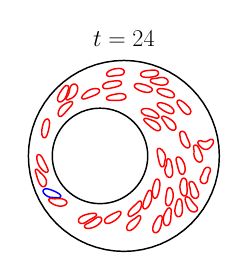
\begin{tikzpicture}[scale=0.35]

\begin{axis}[
  xmin = -21,
  xmax = 21,
  ymin = -21,
  ymax = 21,
  scale only axis,
  axis equal image,
  hide axis,
  title = {\Huge$t=24$}
  ]

\addplot [mark=none,black,line width=1.5] table{
2.0000e+01 0.0000e+00
1.9904e+01 1.9603e+00
1.9616e+01 3.9018e+00
1.9139e+01 5.8057e+00
1.8478e+01 7.6537e+00
1.7638e+01 9.4279e+00
1.6629e+01 1.1111e+01
1.5460e+01 1.2688e+01
1.4142e+01 1.4142e+01
1.2688e+01 1.5460e+01
1.1111e+01 1.6629e+01
9.4279e+00 1.7638e+01
7.6537e+00 1.8478e+01
5.8057e+00 1.9139e+01
3.9018e+00 1.9616e+01
1.9603e+00 1.9904e+01
1.2246e-15 2.0000e+01
-1.9603e+00 1.9904e+01
-3.9018e+00 1.9616e+01
-5.8057e+00 1.9139e+01
-7.6537e+00 1.8478e+01
-9.4279e+00 1.7638e+01
-1.1111e+01 1.6629e+01
-1.2688e+01 1.5460e+01
-1.4142e+01 1.4142e+01
-1.5460e+01 1.2688e+01
-1.6629e+01 1.1111e+01
-1.7638e+01 9.4279e+00
-1.8478e+01 7.6537e+00
-1.9139e+01 5.8057e+00
-1.9616e+01 3.9018e+00
-1.9904e+01 1.9603e+00
-2.0000e+01 2.4493e-15
-1.9904e+01 -1.9603e+00
-1.9616e+01 -3.9018e+00
-1.9139e+01 -5.8057e+00
-1.8478e+01 -7.6537e+00
-1.7638e+01 -9.4279e+00
-1.6629e+01 -1.1111e+01
-1.5460e+01 -1.2688e+01
-1.4142e+01 -1.4142e+01
-1.2688e+01 -1.5460e+01
-1.1111e+01 -1.6629e+01
-9.4279e+00 -1.7638e+01
-7.6537e+00 -1.8478e+01
-5.8057e+00 -1.9139e+01
-3.9018e+00 -1.9616e+01
-1.9603e+00 -1.9904e+01
-3.6739e-15 -2.0000e+01
1.9603e+00 -1.9904e+01
3.9018e+00 -1.9616e+01
5.8057e+00 -1.9139e+01
7.6537e+00 -1.8478e+01
9.4279e+00 -1.7638e+01
1.1111e+01 -1.6629e+01
1.2688e+01 -1.5460e+01
1.4142e+01 -1.4142e+01
1.5460e+01 -1.2688e+01
1.6629e+01 -1.1111e+01
1.7638e+01 -9.4279e+00
1.8478e+01 -7.6537e+00
1.9139e+01 -5.8057e+00
1.9616e+01 -3.9018e+00
1.9904e+01 -1.9603e+00
2.0000e+01 0.0000e+00
};

\addplot [mark=none,black,line width=1.5] table{
5.0000e+00 0.0000e+00
4.9518e+00 -9.8017e-01
4.8079e+00 -1.9509e+00
4.5694e+00 -2.9028e+00
4.2388e+00 -3.8268e+00
3.8192e+00 -4.7140e+00
3.3147e+00 -5.5557e+00
2.7301e+00 -6.3439e+00
2.0711e+00 -7.0711e+00
1.3439e+00 -7.7301e+00
5.5570e-01 -8.3147e+00
-2.8603e-01 -8.8192e+00
-1.1732e+00 -9.2388e+00
-2.0972e+00 -9.5694e+00
-3.0491e+00 -9.8079e+00
-4.0198e+00 -9.9518e+00
-5.0000e+00 -1.0000e+01
-5.9802e+00 -9.9518e+00
-6.9509e+00 -9.8079e+00
-7.9028e+00 -9.5694e+00
-8.8268e+00 -9.2388e+00
-9.7140e+00 -8.8192e+00
-1.0556e+01 -8.3147e+00
-1.1344e+01 -7.7301e+00
-1.2071e+01 -7.0711e+00
-1.2730e+01 -6.3439e+00
-1.3315e+01 -5.5557e+00
-1.3819e+01 -4.7140e+00
-1.4239e+01 -3.8268e+00
-1.4569e+01 -2.9028e+00
-1.4808e+01 -1.9509e+00
-1.4952e+01 -9.8017e-01
-1.5000e+01 -1.2246e-15
-1.4952e+01 9.8017e-01
-1.4808e+01 1.9509e+00
-1.4569e+01 2.9028e+00
-1.4239e+01 3.8268e+00
-1.3819e+01 4.7140e+00
-1.3315e+01 5.5557e+00
-1.2730e+01 6.3439e+00
-1.2071e+01 7.0711e+00
-1.1344e+01 7.7301e+00
-1.0556e+01 8.3147e+00
-9.7140e+00 8.8192e+00
-8.8268e+00 9.2388e+00
-7.9028e+00 9.5694e+00
-6.9509e+00 9.8079e+00
-5.9802e+00 9.9518e+00
-5.0000e+00 1.0000e+01
-4.0198e+00 9.9518e+00
-3.0491e+00 9.8079e+00
-2.0972e+00 9.5694e+00
-1.1732e+00 9.2388e+00
-2.8603e-01 8.8192e+00
5.5570e-01 8.3147e+00
1.3439e+00 7.7301e+00
2.0711e+00 7.0711e+00
2.7301e+00 6.3439e+00
3.3147e+00 5.5557e+00
3.8192e+00 4.7140e+00
4.2388e+00 3.8268e+00
4.5694e+00 2.9028e+00
4.8079e+00 1.9509e+00
4.9518e+00 9.8017e-01
5.0000e+00 0.0000e+00
};

\addplot [mark=none,red,line width=1.5] table{
1.7853e+01 1.5909e+00
1.7900e+01 1.6256e+00
1.7963e+01 1.6768e+00
1.8040e+01 1.7461e+00
1.8125e+01 1.8320e+00
1.8214e+01 1.9305e+00
1.8304e+01 2.0390e+00
1.8392e+01 2.1548e+00
1.8478e+01 2.2769e+00
1.8561e+01 2.4044e+00
1.8638e+01 2.5379e+00
1.8704e+01 2.6781e+00
1.8754e+01 2.8263e+00
1.8778e+01 2.9813e+00
1.8765e+01 3.1380e+00
1.8706e+01 3.2837e+00
1.8601e+01 3.4011e+00
1.8461e+01 3.4731e+00
1.8306e+01 3.4941e+00
1.8150e+01 3.4693e+00
1.8004e+01 3.4118e+00
1.7868e+01 3.3351e+00
1.7738e+01 3.2508e+00
1.7608e+01 3.1681e+00
1.7475e+01 3.0946e+00
1.7337e+01 3.0361e+00
1.7197e+01 2.9965e+00
1.7058e+01 2.9768e+00
1.6925e+01 2.9753e+00
1.6804e+01 2.9873e+00
1.6702e+01 3.0065e+00
1.6624e+01 3.0261e+00
1.6567e+01 3.0422e+00
1.6512e+01 3.0595e+00
1.6434e+01 3.0850e+00
1.6336e+01 3.1177e+00
1.6220e+01 3.1531e+00
1.6091e+01 3.1819e+00
1.5950e+01 3.1927e+00
1.5807e+01 3.1714e+00
1.5673e+01 3.1067e+00
1.5570e+01 2.9961e+00
1.5516e+01 2.8526e+00
1.5517e+01 2.6978e+00
1.5563e+01 2.5487e+00
1.5639e+01 2.4114e+00
1.5732e+01 2.2846e+00
1.5835e+01 2.1642e+00
1.5942e+01 2.0479e+00
1.6052e+01 1.9344e+00
1.6166e+01 1.8250e+00
1.6285e+01 1.7212e+00
1.6409e+01 1.6256e+00
1.6541e+01 1.5407e+00
1.6679e+01 1.4694e+00
1.6823e+01 1.4143e+00
1.6970e+01 1.3777e+00
1.7119e+01 1.3609e+00
1.7264e+01 1.3639e+00
1.7403e+01 1.3854e+00
1.7531e+01 1.4217e+00
1.7643e+01 1.4675e+00
1.7735e+01 1.5155e+00
1.7804e+01 1.5579e+00
1.7853e+01 1.5909e+00
};

\addplot [mark=none,red,line width=1.5] table{
-3.5663e+00 -1.2874e+01
-3.6127e+00 -1.2913e+01
-3.6758e+00 -1.2968e+01
-3.7528e+00 -1.3042e+01
-3.8367e+00 -1.3135e+01
-3.9171e+00 -1.3245e+01
-3.9846e+00 -1.3373e+01
-4.0272e+00 -1.3516e+01
-4.0344e+00 -1.3670e+01
-3.9970e+00 -1.3821e+01
-3.9140e+00 -1.3954e+01
-3.7922e+00 -1.4056e+01
-3.6457e+00 -1.4119e+01
-3.4871e+00 -1.4146e+01
-3.3259e+00 -1.4143e+01
-3.1656e+00 -1.4120e+01
-3.0083e+00 -1.4082e+01
-2.8537e+00 -1.4033e+01
-2.7025e+00 -1.3975e+01
-2.5541e+00 -1.3910e+01
-2.4090e+00 -1.3839e+01
-2.2670e+00 -1.3762e+01
-2.1290e+00 -1.3680e+01
-1.9949e+00 -1.3593e+01
-1.8654e+00 -1.3504e+01
-1.7405e+00 -1.3411e+01
-1.6219e+00 -1.3317e+01
-1.5099e+00 -1.3224e+01
-1.4068e+00 -1.3132e+01
-1.3144e+00 -1.3046e+01
-1.2372e+00 -1.2971e+01
-1.1778e+00 -1.2910e+01
-1.1361e+00 -1.2867e+01
-1.0948e+00 -1.2822e+01
-1.0386e+00 -1.2760e+01
-9.6860e-01 -1.2678e+01
-8.9030e-01 -1.2579e+01
-8.0969e-01 -1.2468e+01
-7.3272e-01 -1.2344e+01
-6.6659e-01 -1.2208e+01
-6.2261e-01 -1.2060e+01
-6.1821e-01 -1.1903e+01
-6.7441e-01 -1.1755e+01
-7.9473e-01 -1.1651e+01
-9.5076e-01 -1.1614e+01
-1.1115e+00 -1.1630e+01
-1.2676e+00 -1.1674e+01
-1.4202e+00 -1.1731e+01
-1.5713e+00 -1.1794e+01
-1.7214e+00 -1.1859e+01
-1.8707e+00 -1.1925e+01
-2.0188e+00 -1.1993e+01
-2.1662e+00 -1.2062e+01
-2.3122e+00 -1.2133e+01
-2.4570e+00 -1.2205e+01
-2.5998e+00 -1.2278e+01
-2.7404e+00 -1.2352e+01
-2.8778e+00 -1.2427e+01
-3.0108e+00 -1.2503e+01
-3.1375e+00 -1.2579e+01
-3.2558e+00 -1.2653e+01
-3.3620e+00 -1.2724e+01
-3.4510e+00 -1.2787e+01
-3.5186e+00 -1.2837e+01
-3.5663e+00 -1.2874e+01
};

\addplot [mark=none,red,line width=1.5] table{
1.8548e+00 -1.0740e+01
1.8120e+00 -1.0782e+01
1.7523e+00 -1.0841e+01
1.6770e+00 -1.0917e+01
1.5897e+00 -1.1007e+01
1.4964e+00 -1.1107e+01
1.3994e+00 -1.1215e+01
1.3027e+00 -1.1330e+01
1.2078e+00 -1.1451e+01
1.1180e+00 -1.1579e+01
1.0355e+00 -1.1715e+01
9.6548e-01 -1.1859e+01
9.1333e-01 -1.2012e+01
8.8910e-01 -1.2171e+01
9.0365e-01 -1.2333e+01
9.6897e-01 -1.2481e+01
1.0850e+00 -1.2593e+01
1.2363e+00 -1.2651e+01
1.3978e+00 -1.2652e+01
1.5551e+00 -1.2612e+01
1.7033e+00 -1.2548e+01
1.8448e+00 -1.2469e+01
1.9810e+00 -1.2384e+01
2.1148e+00 -1.2297e+01
2.2461e+00 -1.2209e+01
2.3755e+00 -1.2123e+01
2.5010e+00 -1.2039e+01
2.6221e+00 -1.1957e+01
2.7353e+00 -1.1878e+01
2.8375e+00 -1.1803e+01
2.9225e+00 -1.1736e+01
2.9874e+00 -1.1681e+01
3.0324e+00 -1.1641e+01
3.0767e+00 -1.1600e+01
3.1360e+00 -1.1540e+01
3.2088e+00 -1.1460e+01
3.2879e+00 -1.1362e+01
3.3673e+00 -1.1249e+01
3.4417e+00 -1.1122e+01
3.5077e+00 -1.0985e+01
3.5624e+00 -1.0838e+01
3.6056e+00 -1.0684e+01
3.6384e+00 -1.0525e+01
3.6641e+00 -1.0363e+01
3.6842e+00 -1.0199e+01
3.6976e+00 -1.0033e+01
3.6969e+00 -9.8671e+00
3.6685e+00 -9.7051e+00
3.5922e+00 -9.5606e+00
3.4593e+00 -9.4674e+00
3.2975e+00 -9.4591e+00
3.1485e+00 -9.5236e+00
3.0206e+00 -9.6246e+00
2.9040e+00 -9.7375e+00
2.7897e+00 -9.8521e+00
2.6756e+00 -9.9645e+00
2.5608e+00 -1.0075e+01
2.4470e+00 -1.0182e+01
2.3355e+00 -1.0286e+01
2.2287e+00 -1.0385e+01
2.1280e+00 -1.0480e+01
2.0367e+00 -1.0566e+01
1.9586e+00 -1.0640e+01
1.8982e+00 -1.0698e+01
1.8548e+00 -1.0740e+01
};

\addplot [mark=none,red,line width=1.5] table{
6.2210e+00 1.5189e+01
6.2768e+00 1.5171e+01
6.3542e+00 1.5147e+01
6.4536e+00 1.5116e+01
6.5698e+00 1.5082e+01
6.6974e+00 1.5045e+01
6.8329e+00 1.5007e+01
6.9742e+00 1.4970e+01
7.1198e+00 1.4936e+01
7.2690e+00 1.4905e+01
7.4209e+00 1.4879e+01
7.5752e+00 1.4858e+01
7.7311e+00 1.4844e+01
7.8884e+00 1.4835e+01
8.0462e+00 1.4833e+01
8.2045e+00 1.4839e+01
8.3621e+00 1.4854e+01
8.5186e+00 1.4878e+01
8.6721e+00 1.4916e+01
8.8203e+00 1.4970e+01
8.9586e+00 1.5045e+01
9.0804e+00 1.5143e+01
9.1762e+00 1.5265e+01
9.2371e+00 1.5407e+01
9.2575e+00 1.5557e+01
9.2385e+00 1.5705e+01
9.1866e+00 1.5841e+01
9.1115e+00 1.5960e+01
9.0230e+00 1.6059e+01
8.9310e+00 1.6138e+01
8.8456e+00 1.6197e+01
8.7756e+00 1.6239e+01
8.7235e+00 1.6265e+01
8.6707e+00 1.6290e+01
8.5954e+00 1.6321e+01
8.4974e+00 1.6354e+01
8.3801e+00 1.6385e+01
8.2500e+00 1.6410e+01
8.1102e+00 1.6426e+01
7.9647e+00 1.6433e+01
7.8150e+00 1.6430e+01
7.6634e+00 1.6417e+01
7.5104e+00 1.6397e+01
7.3573e+00 1.6370e+01
7.2033e+00 1.6339e+01
7.0493e+00 1.6307e+01
6.8939e+00 1.6277e+01
6.7377e+00 1.6252e+01
6.5801e+00 1.6234e+01
6.4222e+00 1.6222e+01
6.2638e+00 1.6213e+01
6.1063e+00 1.6201e+01
5.9506e+00 1.6175e+01
5.8030e+00 1.6123e+01
5.6755e+00 1.6034e+01
5.5880e+00 1.5908e+01
5.5574e+00 1.5760e+01
5.5881e+00 1.5614e+01
5.6652e+00 1.5491e+01
5.7692e+00 1.5396e+01
5.8819e+00 1.5326e+01
5.9921e+00 1.5274e+01
6.0888e+00 1.5235e+01
6.1657e+00 1.5208e+01
6.2210e+00 1.5189e+01
};

\addplot [mark=none,red,line width=1.5] table{
9.8469e+00 -1.1534e+00
9.8239e+00 -1.0962e+00
9.7887e+00 -1.0176e+00
9.7372e+00 -9.2118e-01
9.6660e+00 -8.1553e-01
9.5715e+00 -7.1512e-01
9.4486e+00 -6.3566e-01
9.3008e+00 -6.0535e-01
9.1538e+00 -6.5014e-01
9.0499e+00 -7.6663e-01
9.0012e+00 -9.1695e-01
8.9857e+00 -1.0764e+00
8.9804e+00 -1.2367e+00
8.9733e+00 -1.3983e+00
8.9590e+00 -1.5593e+00
8.9353e+00 -1.7202e+00
8.9004e+00 -1.8787e+00
8.8543e+00 -2.0346e+00
8.7985e+00 -2.1860e+00
8.7379e+00 -2.3355e+00
8.6802e+00 -2.4850e+00
8.6344e+00 -2.6383e+00
8.6056e+00 -2.7943e+00
8.5951e+00 -2.9522e+00
8.6006e+00 -3.1080e+00
8.6193e+00 -3.2611e+00
8.6486e+00 -3.4082e+00
8.6865e+00 -3.5488e+00
8.7304e+00 -3.6789e+00
8.7778e+00 -3.7961e+00
8.8237e+00 -3.8936e+00
8.8635e+00 -3.9684e+00
8.8939e+00 -4.0205e+00
8.9262e+00 -4.0719e+00
8.9741e+00 -4.1403e+00
9.0413e+00 -4.2243e+00
9.1291e+00 -4.3140e+00
9.2380e+00 -4.3988e+00
9.3680e+00 -4.4653e+00
9.5158e+00 -4.4996e+00
9.6712e+00 -4.4883e+00
9.8175e+00 -4.4282e+00
9.9410e+00 -4.3270e+00
1.0038e+01 -4.1985e+00
1.0109e+01 -4.0526e+00
1.0159e+01 -3.8972e+00
1.0192e+01 -3.7359e+00
1.0210e+01 -3.5723e+00
1.0216e+01 -3.4071e+00
1.0212e+01 -3.2418e+00
1.0201e+01 -3.0761e+00
1.0184e+01 -2.9117e+00
1.0164e+01 -2.7483e+00
1.0142e+01 -2.5868e+00
1.0119e+01 -2.4263e+00
1.0094e+01 -2.2678e+00
1.0069e+01 -2.1109e+00
1.0044e+01 -1.9569e+00
1.0017e+01 -1.8062e+00
9.9878e+00 -1.6613e+00
9.9574e+00 -1.5242e+00
9.9258e+00 -1.3999e+00
9.8951e+00 -1.2938e+00
9.8681e+00 -1.2120e+00
9.8469e+00 -1.1534e+00
};

\addplot [mark=none,red,line width=1.5] table{
1.3421e+01 3.4571e+00
1.3397e+01 3.5108e+00
1.3363e+01 3.5854e+00
1.3321e+01 3.6811e+00
1.3272e+01 3.7930e+00
1.3219e+01 3.9161e+00
1.3165e+01 4.0471e+00
1.3110e+01 4.1836e+00
1.3054e+01 4.3237e+00
1.2996e+01 4.4655e+00
1.2931e+01 4.6064e+00
1.2855e+01 4.7431e+00
1.2764e+01 4.8710e+00
1.2653e+01 4.9839e+00
1.2523e+01 5.0745e+00
1.2376e+01 5.1353e+00
1.2219e+01 5.1585e+00
1.2061e+01 5.1371e+00
1.1919e+01 5.0674e+00
1.1809e+01 4.9541e+00
1.1742e+01 4.8118e+00
1.1713e+01 4.6574e+00
1.1713e+01 4.5012e+00
1.1726e+01 4.3469e+00
1.1745e+01 4.1951e+00
1.1765e+01 4.0462e+00
1.1786e+01 3.9011e+00
1.1807e+01 3.7615e+00
1.1830e+01 3.6301e+00
1.1854e+01 3.5107e+00
1.1877e+01 3.4090e+00
1.1898e+01 3.3302e+00
1.1914e+01 3.2738e+00
1.1932e+01 3.2179e+00
1.1958e+01 3.1404e+00
1.1995e+01 3.0429e+00
1.2042e+01 2.9306e+00
1.2099e+01 2.8105e+00
1.2166e+01 2.6860e+00
1.2241e+01 2.5606e+00
1.2325e+01 2.4358e+00
1.2416e+01 2.3137e+00
1.2515e+01 2.1949e+00
1.2622e+01 2.0814e+00
1.2737e+01 1.9743e+00
1.2861e+01 1.8767e+00
1.2995e+01 1.7919e+00
1.3140e+01 1.7270e+00
1.3294e+01 1.6906e+00
1.3453e+01 1.6945e+00
1.3602e+01 1.7468e+00
1.3724e+01 1.8469e+00
1.3804e+01 1.9817e+00
1.3841e+01 2.1340e+00
1.3841e+01 2.2896e+00
1.3816e+01 2.4422e+00
1.3776e+01 2.5893e+00
1.3727e+01 2.7314e+00
1.3674e+01 2.8679e+00
1.3621e+01 2.9987e+00
1.3569e+01 3.1213e+00
1.3520e+01 3.2333e+00
1.3478e+01 3.3287e+00
1.3445e+01 3.4035e+00
1.3421e+01 3.4571e+00
};

\addplot [mark=none,red,line width=1.5] table{
6.3943e+00 1.6636e+01
6.4513e+00 1.6649e+01
6.5299e+00 1.6670e+01
6.6292e+00 1.6700e+01
6.7426e+00 1.6743e+01
6.8615e+00 1.6802e+01
6.9781e+00 1.6880e+01
7.0831e+00 1.6981e+01
7.1663e+00 1.7105e+01
7.2168e+00 1.7248e+01
7.2256e+00 1.7401e+01
7.1888e+00 1.7552e+01
7.1095e+00 1.7686e+01
6.9965e+00 1.7795e+01
6.8611e+00 1.7875e+01
6.7128e+00 1.7928e+01
6.5581e+00 1.7961e+01
6.4008e+00 1.7976e+01
6.2428e+00 1.7980e+01
6.0851e+00 1.7977e+01
5.9281e+00 1.7968e+01
5.7720e+00 1.7956e+01
5.6170e+00 1.7943e+01
5.4634e+00 1.7929e+01
5.3118e+00 1.7913e+01
5.1626e+00 1.7898e+01
5.0173e+00 1.7882e+01
4.8773e+00 1.7865e+01
4.7455e+00 1.7847e+01
4.6254e+00 1.7830e+01
4.5228e+00 1.7813e+01
4.4428e+00 1.7798e+01
4.3854e+00 1.7786e+01
4.3283e+00 1.7773e+01
4.2493e+00 1.7753e+01
4.1496e+00 1.7724e+01
4.0352e+00 1.7682e+01
3.9147e+00 1.7627e+01
3.7950e+00 1.7552e+01
3.6854e+00 1.7456e+01
3.5961e+00 1.7336e+01
3.5404e+00 1.7195e+01
3.5301e+00 1.7041e+01
3.5711e+00 1.6892e+01
3.6582e+00 1.6762e+01
3.7789e+00 1.6662e+01
3.9191e+00 1.6590e+01
4.0697e+00 1.6541e+01
4.2246e+00 1.6509e+01
4.3816e+00 1.6487e+01
4.5390e+00 1.6473e+01
4.6968e+00 1.6464e+01
4.8540e+00 1.6459e+01
5.0107e+00 1.6458e+01
5.1662e+00 1.6462e+01
5.3204e+00 1.6471e+01
5.4722e+00 1.6484e+01
5.6212e+00 1.6501e+01
5.7658e+00 1.6522e+01
5.9050e+00 1.6544e+01
6.0360e+00 1.6566e+01
6.1555e+00 1.6587e+01
6.2575e+00 1.6607e+01
6.3373e+00 1.6623e+01
6.3943e+00 1.6636e+01
};

\addplot [mark=none,red,line width=1.5] table{
4.9644e+00 1.4686e+01
4.9088e+00 1.4708e+01
4.8318e+00 1.4737e+01
4.7323e+00 1.4775e+01
4.6159e+00 1.4815e+01
4.4874e+00 1.4858e+01
4.3510e+00 1.4899e+01
4.2085e+00 1.4940e+01
4.0621e+00 1.4977e+01
3.9121e+00 1.5014e+01
3.7598e+00 1.5046e+01
3.6048e+00 1.5076e+01
3.4485e+00 1.5102e+01
3.2901e+00 1.5124e+01
3.1309e+00 1.5140e+01
2.9700e+00 1.5148e+01
2.8089e+00 1.5143e+01
2.6487e+00 1.5119e+01
2.4956e+00 1.5067e+01
2.3595e+00 1.4980e+01
2.2584e+00 1.4855e+01
2.2099e+00 1.4704e+01
2.2227e+00 1.4546e+01
2.2867e+00 1.4404e+01
2.3844e+00 1.4283e+01
2.4986e+00 1.4184e+01
2.6196e+00 1.4098e+01
2.7404e+00 1.4023e+01
2.8571e+00 1.3954e+01
2.9646e+00 1.3895e+01
3.0579e+00 1.3845e+01
3.1309e+00 1.3808e+01
3.1842e+00 1.3781e+01
3.2372e+00 1.3756e+01
3.3121e+00 1.3720e+01
3.4077e+00 1.3677e+01
3.5209e+00 1.3629e+01
3.6453e+00 1.3580e+01
3.7792e+00 1.3531e+01
3.9191e+00 1.3487e+01
4.0650e+00 1.3444e+01
4.2143e+00 1.3408e+01
4.3677e+00 1.3376e+01
4.5230e+00 1.3352e+01
4.6811e+00 1.3333e+01
4.8399e+00 1.3324e+01
5.0004e+00 1.3323e+01
5.1603e+00 1.3333e+01
5.3199e+00 1.3354e+01
5.4761e+00 1.3392e+01
5.6270e+00 1.3449e+01
5.7639e+00 1.3532e+01
5.8746e+00 1.3647e+01
5.9374e+00 1.3793e+01
5.9385e+00 1.3950e+01
5.8814e+00 1.4096e+01
5.7870e+00 1.4217e+01
5.6721e+00 1.4318e+01
5.5496e+00 1.4401e+01
5.4249e+00 1.4473e+01
5.3046e+00 1.4535e+01
5.1923e+00 1.4588e+01
5.0957e+00 1.4631e+01
5.0192e+00 1.4664e+01
4.9644e+00 1.4686e+01
};

\addplot [mark=none,red,line width=1.5] table{
-7.0043e-01 1.4874e+01
-6.5633e-01 1.4916e+01
-6.0078e-01 1.4981e+01
-5.4431e-01 1.5074e+01
-5.0647e-01 1.5197e+01
-5.1178e-01 1.5338e+01
-5.7181e-01 1.5475e+01
-6.8026e-01 1.5585e+01
-8.1904e-01 1.5661e+01
-9.7416e-01 1.5708e+01
-1.1355e+00 1.5733e+01
-1.2990e+00 1.5743e+01
-1.4629e+00 1.5742e+01
-1.6278e+00 1.5735e+01
-1.7930e+00 1.5722e+01
-1.9583e+00 1.5705e+01
-2.1221e+00 1.5685e+01
-2.2851e+00 1.5664e+01
-2.4479e+00 1.5641e+01
-2.6112e+00 1.5617e+01
-2.7736e+00 1.5590e+01
-2.9354e+00 1.5562e+01
-3.0953e+00 1.5530e+01
-3.2533e+00 1.5495e+01
-3.4076e+00 1.5454e+01
-3.5575e+00 1.5407e+01
-3.7006e+00 1.5354e+01
-3.8348e+00 1.5292e+01
-3.9559e+00 1.5225e+01
-4.0605e+00 1.5155e+01
-4.1440e+00 1.5087e+01
-4.2049e+00 1.5029e+01
-4.2457e+00 1.4984e+01
-4.2838e+00 1.4936e+01
-4.3309e+00 1.4866e+01
-4.3796e+00 1.4769e+01
-4.4149e+00 1.4646e+01
-4.4184e+00 1.4506e+01
-4.3742e+00 1.4364e+01
-4.2796e+00 1.4245e+01
-4.1479e+00 1.4161e+01
-3.9969e+00 1.4112e+01
-3.8376e+00 1.4088e+01
-3.6754e+00 1.4083e+01
-3.5123e+00 1.4089e+01
-3.3493e+00 1.4105e+01
-3.1864e+00 1.4127e+01
-3.0241e+00 1.4154e+01
-2.8619e+00 1.4183e+01
-2.7002e+00 1.4216e+01
-2.5386e+00 1.4250e+01
-2.3775e+00 1.4285e+01
-2.2167e+00 1.4321e+01
-2.0566e+00 1.4359e+01
-1.8976e+00 1.4397e+01
-1.7406e+00 1.4437e+01
-1.5861e+00 1.4478e+01
-1.4356e+00 1.4523e+01
-1.2900e+00 1.4570e+01
-1.1514e+00 1.4621e+01
-1.0229e+00 1.4675e+01
-9.0943e-01 1.4732e+01
-8.1640e-01 1.4787e+01
-7.4759e-01 1.4836e+01
-7.0043e-01 1.4874e+01
};

\addplot [mark=none,red,line width=1.5] table{
1.2921e+01 -8.3308e+00
1.2969e+01 -8.2971e+00
1.3027e+01 -8.2413e+00
1.3089e+01 -8.1579e+00
1.3144e+01 -8.0500e+00
1.3186e+01 -7.9244e+00
1.3217e+01 -7.7872e+00
1.3236e+01 -7.6427e+00
1.3247e+01 -7.4937e+00
1.3251e+01 -7.3415e+00
1.3250e+01 -7.1874e+00
1.3245e+01 -7.0318e+00
1.3238e+01 -6.8754e+00
1.3231e+01 -6.7181e+00
1.3223e+01 -6.5604e+00
1.3217e+01 -6.4022e+00
1.3212e+01 -6.2440e+00
1.3210e+01 -6.0856e+00
1.3208e+01 -5.9273e+00
1.3204e+01 -5.7693e+00
1.3195e+01 -5.6121e+00
1.3176e+01 -5.4563e+00
1.3146e+01 -5.3037e+00
1.3100e+01 -5.1562e+00
1.3038e+01 -5.0172e+00
1.2956e+01 -4.8913e+00
1.2856e+01 -4.7855e+00
1.2738e+01 -4.7087e+00
1.2611e+01 -4.6688e+00
1.2490e+01 -4.6674e+00
1.2389e+01 -4.6939e+00
1.2316e+01 -4.7309e+00
1.2269e+01 -4.7649e+00
1.2225e+01 -4.8039e+00
1.2171e+01 -4.8650e+00
1.2113e+01 -4.9508e+00
1.2057e+01 -5.0584e+00
1.2006e+01 -5.1808e+00
1.1959e+01 -5.3136e+00
1.1916e+01 -5.4530e+00
1.1876e+01 -5.5974e+00
1.1840e+01 -5.7452e+00
1.1808e+01 -5.8962e+00
1.1782e+01 -6.0495e+00
1.1763e+01 -6.2050e+00
1.1751e+01 -6.3619e+00
1.1748e+01 -6.5198e+00
1.1753e+01 -6.6778e+00
1.1765e+01 -6.8357e+00
1.1785e+01 -6.9926e+00
1.1812e+01 -7.1485e+00
1.1846e+01 -7.3026e+00
1.1887e+01 -7.4546e+00
1.1936e+01 -7.6034e+00
1.1992e+01 -7.7484e+00
1.2059e+01 -7.8875e+00
1.2137e+01 -8.0187e+00
1.2227e+01 -8.1380e+00
1.2330e+01 -8.2411e+00
1.2446e+01 -8.3212e+00
1.2568e+01 -8.3726e+00
1.2688e+01 -8.3914e+00
1.2792e+01 -8.3824e+00
1.2869e+01 -8.3575e+00
1.2921e+01 -8.3308e+00
};

\addplot [mark=none,red,line width=1.5] table{
7.5313e+00 -5.7345e+00
7.5257e+00 -5.6737e+00
7.5155e+00 -5.5886e+00
7.4969e+00 -5.4810e+00
7.4669e+00 -5.3562e+00
7.4207e+00 -5.2239e+00
7.3534e+00 -5.0914e+00
7.2570e+00 -4.9718e+00
7.1269e+00 -4.8836e+00
6.9705e+00 -4.8546e+00
6.8159e+00 -4.8978e+00
6.6887e+00 -4.9991e+00
6.5920e+00 -5.1307e+00
6.5151e+00 -5.2767e+00
6.4495e+00 -5.4280e+00
6.3901e+00 -5.5830e+00
6.3350e+00 -5.7389e+00
6.2829e+00 -5.8962e+00
6.2338e+00 -6.0533e+00
6.1871e+00 -6.2113e+00
6.1434e+00 -6.3687e+00
6.1028e+00 -6.5265e+00
6.0666e+00 -6.6836e+00
6.0355e+00 -6.8416e+00
6.0115e+00 -6.9988e+00
5.9958e+00 -7.1554e+00
5.9891e+00 -7.3081e+00
5.9891e+00 -7.4559e+00
5.9933e+00 -7.5945e+00
5.9987e+00 -7.7217e+00
6.0042e+00 -7.8302e+00
6.0087e+00 -7.9157e+00
6.0125e+00 -7.9768e+00
6.0166e+00 -8.0385e+00
6.0239e+00 -8.1239e+00
6.0365e+00 -8.2332e+00
6.0594e+00 -8.3592e+00
6.0988e+00 -8.4941e+00
6.1636e+00 -8.6274e+00
6.2615e+00 -8.7455e+00
6.3950e+00 -8.8273e+00
6.5514e+00 -8.8513e+00
6.7059e+00 -8.8090e+00
6.8369e+00 -8.7144e+00
6.9404e+00 -8.5877e+00
7.0216e+00 -8.4450e+00
7.0881e+00 -8.2936e+00
7.1445e+00 -8.1381e+00
7.1941e+00 -7.9796e+00
7.2385e+00 -7.8202e+00
7.2793e+00 -7.6598e+00
7.3169e+00 -7.4996e+00
7.3524e+00 -7.3392e+00
7.3854e+00 -7.1794e+00
7.4166e+00 -7.0199e+00
7.4452e+00 -6.8618e+00
7.4712e+00 -6.7050e+00
7.4937e+00 -6.5507e+00
7.5124e+00 -6.3996e+00
7.5263e+00 -6.2538e+00
7.5353e+00 -6.1154e+00
7.5389e+00 -5.9890e+00
7.5385e+00 -5.8803e+00
7.5351e+00 -5.7958e+00
7.5313e+00 -5.7345e+00
};

\addplot [mark=none,red,line width=1.5] table{
1.3423e+01 1.0390e+01
1.3383e+01 1.0433e+01
1.3327e+01 1.0492e+01
1.3254e+01 1.0565e+01
1.3168e+01 1.0651e+01
1.3071e+01 1.0742e+01
1.2967e+01 1.0837e+01
1.2857e+01 1.0933e+01
1.2742e+01 1.1031e+01
1.2622e+01 1.1126e+01
1.2499e+01 1.1221e+01
1.2373e+01 1.1312e+01
1.2242e+01 1.1400e+01
1.2108e+01 1.1483e+01
1.1969e+01 1.1560e+01
1.1824e+01 1.1623e+01
1.1671e+01 1.1667e+01
1.1513e+01 1.1675e+01
1.1360e+01 1.1634e+01
1.1238e+01 1.1535e+01
1.1169e+01 1.1394e+01
1.1155e+01 1.1238e+01
1.1184e+01 1.1085e+01
1.1238e+01 1.0940e+01
1.1306e+01 1.0803e+01
1.1382e+01 1.0672e+01
1.1459e+01 1.0547e+01
1.1537e+01 1.0428e+01
1.1611e+01 1.0316e+01
1.1679e+01 1.0215e+01
1.1738e+01 1.0128e+01
1.1785e+01 1.0061e+01
1.1819e+01 1.0013e+01
1.1852e+01 9.9643e+00
1.1900e+01 9.8981e+00
1.1961e+01 9.8136e+00
1.2033e+01 9.7165e+00
1.2114e+01 9.6108e+00
1.2202e+01 9.5010e+00
1.2297e+01 9.3891e+00
1.2397e+01 9.2780e+00
1.2504e+01 9.1688e+00
1.2617e+01 9.0641e+00
1.2738e+01 8.9649e+00
1.2866e+01 8.8749e+00
1.3003e+01 8.7967e+00
1.3149e+01 8.7360e+00
1.3302e+01 8.6977e+00
1.3461e+01 8.6897e+00
1.3616e+01 8.7172e+00
1.3759e+01 8.7843e+00
1.3878e+01 8.8877e+00
1.3963e+01 9.0203e+00
1.4009e+01 9.1694e+00
1.4019e+01 9.3247e+00
1.3998e+01 9.4771e+00
1.3953e+01 9.6231e+00
1.3892e+01 9.7598e+00
1.3819e+01 9.8876e+00
1.3741e+01 1.0005e+01
1.3661e+01 1.0112e+01
1.3585e+01 1.0207e+01
1.3517e+01 1.0286e+01
1.3463e+01 1.0347e+01
1.3423e+01 1.0390e+01
};

\addplot [mark=none,red,line width=1.5] table{
-1.1585e+01 1.4081e+01
-1.1575e+01 1.4137e+01
-1.1563e+01 1.4222e+01
-1.1562e+01 1.4326e+01
-1.1577e+01 1.4451e+01
-1.1629e+01 1.4574e+01
-1.1722e+01 1.4684e+01
-1.1858e+01 1.4744e+01
-1.2007e+01 1.4752e+01
-1.2156e+01 1.4705e+01
-1.2288e+01 1.4629e+01
-1.2413e+01 1.4529e+01
-1.2525e+01 1.4421e+01
-1.2633e+01 1.4302e+01
-1.2734e+01 1.4181e+01
-1.2833e+01 1.4053e+01
-1.2927e+01 1.3927e+01
-1.3022e+01 1.3795e+01
-1.3112e+01 1.3666e+01
-1.3203e+01 1.3532e+01
-1.3289e+01 1.3401e+01
-1.3375e+01 1.3265e+01
-1.3455e+01 1.3132e+01
-1.3534e+01 1.2995e+01
-1.3604e+01 1.2860e+01
-1.3672e+01 1.2722e+01
-1.3728e+01 1.2588e+01
-1.3780e+01 1.2452e+01
-1.3818e+01 1.2326e+01
-1.3848e+01 1.2205e+01
-1.3864e+01 1.2103e+01
-1.3875e+01 1.2019e+01
-1.3877e+01 1.1962e+01
-1.3879e+01 1.1901e+01
-1.3872e+01 1.1820e+01
-1.3856e+01 1.1714e+01
-1.3816e+01 1.1598e+01
-1.3749e+01 1.1479e+01
-1.3643e+01 1.1383e+01
-1.3510e+01 1.1320e+01
-1.3359e+01 1.1306e+01
-1.3209e+01 1.1329e+01
-1.3062e+01 1.1388e+01
-1.2927e+01 1.1463e+01
-1.2796e+01 1.1557e+01
-1.2676e+01 1.1658e+01
-1.2559e+01 1.1771e+01
-1.2454e+01 1.1889e+01
-1.2356e+01 1.2019e+01
-1.2272e+01 1.2152e+01
-1.2194e+01 1.2295e+01
-1.2126e+01 1.2437e+01
-1.2061e+01 1.2585e+01
-1.2005e+01 1.2731e+01
-1.1950e+01 1.2881e+01
-1.1902e+01 1.3026e+01
-1.1853e+01 1.3175e+01
-1.1810e+01 1.3317e+01
-1.1765e+01 1.3460e+01
-1.1724e+01 1.3594e+01
-1.1682e+01 1.3724e+01
-1.1648e+01 1.3840e+01
-1.1618e+01 1.3943e+01
-1.1599e+01 1.4021e+01
-1.1585e+01 1.4081e+01
};

\addplot [mark=none,red,line width=1.5] table{
7.3769e+00 5.3194e+00
7.4311e+00 5.3475e+00
7.5016e+00 5.3949e+00
7.5747e+00 5.4769e+00
7.6346e+00 5.5899e+00
7.6627e+00 5.7300e+00
7.6586e+00 5.8790e+00
7.6237e+00 6.0323e+00
7.5679e+00 6.1799e+00
7.4934e+00 6.3253e+00
7.4067e+00 6.4630e+00
7.3077e+00 6.5960e+00
7.2019e+00 6.7181e+00
7.0856e+00 6.8351e+00
6.9612e+00 6.9419e+00
6.8262e+00 7.0421e+00
6.6847e+00 7.1300e+00
6.5354e+00 7.2107e+00
6.3847e+00 7.2799e+00
6.2311e+00 7.3449e+00
6.0766e+00 7.4034e+00
5.9195e+00 7.4620e+00
5.7650e+00 7.5162e+00
5.6109e+00 7.5717e+00
5.4605e+00 7.6236e+00
5.3113e+00 7.6769e+00
5.1671e+00 7.7252e+00
5.0262e+00 7.7723e+00
4.8938e+00 7.8104e+00
4.7699e+00 7.8418e+00
4.6638e+00 7.8586e+00
4.5783e+00 7.8666e+00
4.5176e+00 7.8642e+00
4.4557e+00 7.8581e+00
4.3739e+00 7.8328e+00
4.2808e+00 7.7754e+00
4.2126e+00 7.6673e+00
4.2040e+00 7.5306e+00
4.2577e+00 7.3925e+00
4.3460e+00 7.2700e+00
4.4520e+00 7.1530e+00
4.5642e+00 7.0417e+00
4.6816e+00 6.9287e+00
4.8003e+00 6.8188e+00
4.9221e+00 6.7067e+00
5.0439e+00 6.5977e+00
5.1681e+00 6.4868e+00
5.2918e+00 6.3794e+00
5.4177e+00 6.2702e+00
5.5434e+00 6.1649e+00
5.6713e+00 6.0585e+00
5.7989e+00 5.9571e+00
5.9287e+00 5.8558e+00
6.0585e+00 5.7606e+00
6.1910e+00 5.6671e+00
6.3237e+00 5.5817e+00
6.4592e+00 5.5004e+00
6.5952e+00 5.4302e+00
6.7335e+00 5.3677e+00
6.8703e+00 5.3215e+00
7.0047e+00 5.2891e+00
7.1290e+00 5.2784e+00
7.2369e+00 5.2825e+00
7.3187e+00 5.3008e+00
7.3769e+00 5.3194e+00
};

\addplot [mark=none,red,line width=1.5] table{
-5.3866e+00 -1.4401e+01
-5.3383e+00 -1.4363e+01
-5.2722e+00 -1.4310e+01
-5.1898e+00 -1.4238e+01
-5.0969e+00 -1.4151e+01
-5.0005e+00 -1.4051e+01
-4.9052e+00 -1.3940e+01
-4.8160e+00 -1.3817e+01
-4.7380e+00 -1.3682e+01
-4.6784e+00 -1.3536e+01
-4.6465e+00 -1.3378e+01
-4.6531e+00 -1.3217e+01
-4.7063e+00 -1.3063e+01
-4.8066e+00 -1.2934e+01
-4.9437e+00 -1.2843e+01
-5.1021e+00 -1.2797e+01
-5.2678e+00 -1.2791e+01
-5.4318e+00 -1.2820e+01
-5.5891e+00 -1.2876e+01
-5.7379e+00 -1.2953e+01
-5.8793e+00 -1.3041e+01
-6.0154e+00 -1.3137e+01
-6.1481e+00 -1.3235e+01
-6.2789e+00 -1.3333e+01
-6.4083e+00 -1.3429e+01
-6.5368e+00 -1.3523e+01
-6.6636e+00 -1.3612e+01
-6.7881e+00 -1.3695e+01
-6.9077e+00 -1.3771e+01
-7.0191e+00 -1.3838e+01
-7.1160e+00 -1.3894e+01
-7.1922e+00 -1.3936e+01
-7.2471e+00 -1.3965e+01
-7.3019e+00 -1.3993e+01
-7.3786e+00 -1.4032e+01
-7.4773e+00 -1.4080e+01
-7.5932e+00 -1.4135e+01
-7.7195e+00 -1.4195e+01
-7.8516e+00 -1.4262e+01
-7.9830e+00 -1.4340e+01
-8.1053e+00 -1.4438e+01
-8.2025e+00 -1.4563e+01
-8.2502e+00 -1.4716e+01
-8.2258e+00 -1.4875e+01
-8.1321e+00 -1.5007e+01
-7.9950e+00 -1.5097e+01
-7.8389e+00 -1.5148e+01
-7.6758e+00 -1.5174e+01
-7.5105e+00 -1.5181e+01
-7.3447e+00 -1.5174e+01
-7.1798e+00 -1.5157e+01
-7.0163e+00 -1.5131e+01
-6.8549e+00 -1.5097e+01
-6.6958e+00 -1.5056e+01
-6.5398e+00 -1.5007e+01
-6.3871e+00 -1.4953e+01
-6.2385e+00 -1.4894e+01
-6.0948e+00 -1.4829e+01
-5.9572e+00 -1.4761e+01
-5.8268e+00 -1.4691e+01
-5.7059e+00 -1.4620e+01
-5.5972e+00 -1.4551e+01
-5.5058e+00 -1.4488e+01
-5.4358e+00 -1.4438e+01
-5.3866e+00 -1.4401e+01
};

\addplot [mark=none,red,line width=1.5] table{
8.1106e+00 1.2689e+01
8.1645e+00 1.2665e+01
8.2396e+00 1.2633e+01
8.3365e+00 1.2594e+01
8.4502e+00 1.2550e+01
8.5757e+00 1.2504e+01
8.7093e+00 1.2459e+01
8.8488e+00 1.2413e+01
8.9925e+00 1.2370e+01
9.1395e+00 1.2327e+01
9.2889e+00 1.2288e+01
9.4408e+00 1.2251e+01
9.5946e+00 1.2219e+01
9.7507e+00 1.2194e+01
9.9085e+00 1.2181e+01
1.0067e+01 1.2185e+01
1.0223e+01 1.2217e+01
1.0366e+01 1.2285e+01
1.0481e+01 1.2393e+01
1.0551e+01 1.2534e+01
1.0571e+01 1.2690e+01
1.0546e+01 1.2845e+01
1.0488e+01 1.2990e+01
1.0406e+01 1.3122e+01
1.0308e+01 1.3241e+01
1.0200e+01 1.3346e+01
1.0087e+01 1.3440e+01
9.9706e+00 1.3522e+01
9.8566e+00 1.3593e+01
9.7493e+00 1.3652e+01
9.6552e+00 1.3698e+01
9.5807e+00 1.3732e+01
9.5264e+00 1.3755e+01
9.4719e+00 1.3776e+01
9.3952e+00 1.3805e+01
9.2964e+00 1.3839e+01
9.1794e+00 1.3875e+01
9.0505e+00 1.3910e+01
8.9124e+00 1.3944e+01
8.7685e+00 1.3974e+01
8.6197e+00 1.4002e+01
8.4680e+00 1.4027e+01
8.3137e+00 1.4050e+01
8.1581e+00 1.4070e+01
8.0008e+00 1.4086e+01
7.8427e+00 1.4096e+01
7.6835e+00 1.4098e+01
7.5249e+00 1.4087e+01
7.3683e+00 1.4058e+01
7.2192e+00 1.4003e+01
7.0873e+00 1.3916e+01
6.9919e+00 1.3790e+01
6.9543e+00 1.3637e+01
6.9824e+00 1.3483e+01
7.0606e+00 1.3348e+01
7.1677e+00 1.3236e+01
7.2877e+00 1.3142e+01
7.4130e+00 1.3058e+01
7.5384e+00 1.2982e+01
7.6618e+00 1.2912e+01
7.7796e+00 1.2849e+01
7.8887e+00 1.2794e+01
7.9828e+00 1.2748e+01
8.0571e+00 1.2713e+01
8.1106e+00 1.2689e+01
};

\addplot [mark=none,red,line width=1.5] table{
5.7386e+00 -7.4400e+00
5.7120e+00 -7.3861e+00
5.6660e+00 -7.3141e+00
5.5845e+00 -7.2433e+00
5.4672e+00 -7.1980e+00
5.3296e+00 -7.2143e+00
5.2051e+00 -7.2879e+00
5.1031e+00 -7.4029e+00
5.0202e+00 -7.5336e+00
4.9445e+00 -7.6756e+00
4.8737e+00 -7.8188e+00
4.8026e+00 -7.9673e+00
4.7339e+00 -8.1145e+00
4.6643e+00 -8.2657e+00
4.5972e+00 -8.4147e+00
4.5297e+00 -8.5673e+00
4.4650e+00 -8.7177e+00
4.4005e+00 -8.8722e+00
4.3398e+00 -9.0247e+00
4.2807e+00 -9.1811e+00
4.2274e+00 -9.3353e+00
4.1775e+00 -9.4933e+00
4.1347e+00 -9.6489e+00
4.0956e+00 -9.8073e+00
4.0628e+00 -9.9618e+00
4.0332e+00 -1.0118e+01
4.0106e+00 -1.0268e+01
3.9945e+00 -1.0416e+01
3.9916e+00 -1.0555e+01
4.0026e+00 -1.0685e+01
4.0300e+00 -1.0791e+01
4.0635e+00 -1.0872e+01
4.0968e+00 -1.0922e+01
4.1352e+00 -1.0971e+01
4.2011e+00 -1.1024e+01
4.2981e+00 -1.1071e+01
4.4239e+00 -1.1087e+01
4.5594e+00 -1.1067e+01
4.6946e+00 -1.1007e+01
4.8198e+00 -1.0923e+01
4.9376e+00 -1.0819e+01
5.0453e+00 -1.0704e+01
5.1474e+00 -1.0578e+01
5.2409e+00 -1.0447e+01
5.3296e+00 -1.0308e+01
5.4102e+00 -1.0166e+01
5.4862e+00 -1.0017e+01
5.5541e+00 -9.8665e+00
5.6175e+00 -9.7102e+00
5.6726e+00 -9.5535e+00
5.7224e+00 -9.3914e+00
5.7629e+00 -9.2300e+00
5.7966e+00 -9.0644e+00
5.8197e+00 -8.9011e+00
5.8354e+00 -8.7360e+00
5.8413e+00 -8.5755e+00
5.8422e+00 -8.4144e+00
5.8367e+00 -8.2590e+00
5.8298e+00 -8.1049e+00
5.8197e+00 -7.9590e+00
5.8101e+00 -7.8181e+00
5.7960e+00 -7.6918e+00
5.7794e+00 -7.5815e+00
5.7579e+00 -7.4995e+00
5.7386e+00 -7.4400e+00
};

\addplot [mark=none,red,line width=1.5] table{
6.0793e+00 -1.5581e+01
6.0959e+00 -1.5637e+01
6.1252e+00 -1.5713e+01
6.1745e+00 -1.5804e+01
6.2493e+00 -1.5900e+01
6.3518e+00 -1.5985e+01
6.4790e+00 -1.6045e+01
6.6225e+00 -1.6070e+01
6.7711e+00 -1.6057e+01
6.9150e+00 -1.6008e+01
7.0477e+00 -1.5930e+01
7.1668e+00 -1.5830e+01
7.2722e+00 -1.5715e+01
7.3656e+00 -1.5588e+01
7.4482e+00 -1.5454e+01
7.5218e+00 -1.5314e+01
7.5871e+00 -1.5170e+01
7.6451e+00 -1.5022e+01
7.6962e+00 -1.4873e+01
7.7411e+00 -1.4721e+01
7.7801e+00 -1.4569e+01
7.8140e+00 -1.4415e+01
7.8439e+00 -1.4263e+01
7.8710e+00 -1.4111e+01
7.8965e+00 -1.3961e+01
7.9217e+00 -1.3813e+01
7.9471e+00 -1.3669e+01
7.9725e+00 -1.3530e+01
7.9965e+00 -1.3400e+01
8.0170e+00 -1.3280e+01
8.0313e+00 -1.3177e+01
8.0388e+00 -1.3095e+01
8.0411e+00 -1.3037e+01
8.0401e+00 -1.2978e+01
8.0317e+00 -1.2897e+01
8.0063e+00 -1.2796e+01
7.9516e+00 -1.2687e+01
7.8593e+00 -1.2591e+01
7.7325e+00 -1.2530e+01
7.5871e+00 -1.2520e+01
7.4430e+00 -1.2560e+01
7.3129e+00 -1.2639e+01
7.1986e+00 -1.2743e+01
7.0971e+00 -1.2862e+01
7.0036e+00 -1.2988e+01
6.9151e+00 -1.3118e+01
6.8296e+00 -1.3251e+01
6.7465e+00 -1.3386e+01
6.6655e+00 -1.3522e+01
6.5872e+00 -1.3660e+01
6.5117e+00 -1.3799e+01
6.4399e+00 -1.3940e+01
6.3720e+00 -1.4082e+01
6.3088e+00 -1.4226e+01
6.2504e+00 -1.4370e+01
6.1978e+00 -1.4515e+01
6.1514e+00 -1.4660e+01
6.1123e+00 -1.4805e+01
6.0812e+00 -1.4948e+01
6.0595e+00 -1.5086e+01
6.0478e+00 -1.5219e+01
6.0467e+00 -1.5340e+01
6.0541e+00 -1.5444e+01
6.0666e+00 -1.5524e+01
6.0793e+00 -1.5581e+01
};

\addplot [mark=none,red,line width=1.5] table{
1.6268e+01 -4.1155e+00
1.6240e+01 -4.1671e+00
1.6203e+01 -4.2392e+00
1.6156e+01 -4.3319e+00
1.6106e+01 -4.4420e+00
1.6058e+01 -4.5655e+00
1.6018e+01 -4.7004e+00
1.5994e+01 -4.8439e+00
1.5990e+01 -4.9933e+00
1.6011e+01 -5.1437e+00
1.6058e+01 -5.2901e+00
1.6132e+01 -5.4267e+00
1.6230e+01 -5.5486e+00
1.6349e+01 -5.6506e+00
1.6486e+01 -5.7280e+00
1.6636e+01 -5.7762e+00
1.6793e+01 -5.7914e+00
1.6949e+01 -5.7712e+00
1.7097e+01 -5.7162e+00
1.7228e+01 -5.6296e+00
1.7338e+01 -5.5177e+00
1.7424e+01 -5.3873e+00
1.7487e+01 -5.2456e+00
1.7531e+01 -5.0980e+00
1.7561e+01 -4.9489e+00
1.7582e+01 -4.8009e+00
1.7599e+01 -4.6563e+00
1.7618e+01 -4.5169e+00
1.7640e+01 -4.3862e+00
1.7665e+01 -4.2678e+00
1.7693e+01 -4.1677e+00
1.7717e+01 -4.0904e+00
1.7737e+01 -4.0354e+00
1.7758e+01 -3.9809e+00
1.7789e+01 -3.9061e+00
1.7833e+01 -3.8119e+00
1.7886e+01 -3.7033e+00
1.7947e+01 -3.5852e+00
1.8009e+01 -3.4591e+00
1.8066e+01 -3.3251e+00
1.8111e+01 -3.1825e+00
1.8135e+01 -3.0326e+00
1.8130e+01 -2.8788e+00
1.8090e+01 -2.7291e+00
1.8013e+01 -2.5938e+00
1.7900e+01 -2.4845e+00
1.7762e+01 -2.4101e+00
1.7608e+01 -2.3759e+00
1.7451e+01 -2.3823e+00
1.7299e+01 -2.4260e+00
1.7161e+01 -2.5011e+00
1.7039e+01 -2.6011e+00
1.6935e+01 -2.7189e+00
1.6848e+01 -2.8487e+00
1.6775e+01 -2.9855e+00
1.6711e+01 -3.1257e+00
1.6653e+01 -3.2664e+00
1.6598e+01 -3.4055e+00
1.6544e+01 -3.5407e+00
1.6489e+01 -3.6700e+00
1.6433e+01 -3.7906e+00
1.6380e+01 -3.8995e+00
1.6333e+01 -3.9919e+00
1.6295e+01 -4.0638e+00
1.6268e+01 -4.1155e+00
};

\addplot [mark=none,red,line width=1.5] table{
7.3191e+00 8.4050e+00
7.2943e+00 8.4604e+00
7.2525e+00 8.5342e+00
7.1897e+00 8.6213e+00
7.1087e+00 8.7178e+00
7.0137e+00 8.8163e+00
6.9093e+00 8.9166e+00
6.7972e+00 9.0148e+00
6.6795e+00 9.1126e+00
6.5563e+00 9.2070e+00
6.4288e+00 9.2997e+00
6.2964e+00 9.3877e+00
6.1597e+00 9.4729e+00
6.0180e+00 9.5519e+00
5.8727e+00 9.6262e+00
5.7234e+00 9.6925e+00
5.5712e+00 9.7526e+00
5.4155e+00 9.8040e+00
5.2573e+00 9.8484e+00
5.0968e+00 9.8832e+00
4.9359e+00 9.9103e+00
4.7745e+00 9.9268e+00
4.6138e+00 9.9346e+00
4.4542e+00 9.9303e+00
4.2978e+00 9.9147e+00
4.1461e+00 9.8836e+00
4.0029e+00 9.8366e+00
3.8732e+00 9.7686e+00
3.7661e+00 9.6820e+00
3.6903e+00 9.5810e+00
3.6495e+00 9.4825e+00
3.6353e+00 9.3998e+00
3.6353e+00 9.3404e+00
3.6430e+00 9.2808e+00
3.6659e+00 9.2019e+00
3.7113e+00 9.1066e+00
3.7822e+00 9.0064e+00
3.8741e+00 8.9076e+00
3.9828e+00 8.8152e+00
4.1035e+00 8.7292e+00
4.2343e+00 8.6523e+00
4.3725e+00 8.5837e+00
4.5174e+00 8.5254e+00
4.6666e+00 8.4751e+00
4.8197e+00 8.4327e+00
4.9748e+00 8.3941e+00
5.1321e+00 8.3587e+00
5.2900e+00 8.3227e+00
5.4489e+00 8.2866e+00
5.6076e+00 8.2475e+00
5.7665e+00 8.2065e+00
5.9243e+00 8.1616e+00
6.0817e+00 8.1150e+00
6.2378e+00 8.0657e+00
6.3941e+00 8.0172e+00
6.5496e+00 7.9713e+00
6.7050e+00 7.9347e+00
6.8599e+00 7.9131e+00
7.0137e+00 7.9182e+00
7.1562e+00 7.9598e+00
7.2690e+00 8.0439e+00
7.3324e+00 8.1540e+00
7.3483e+00 8.2622e+00
7.3369e+00 8.3461e+00
7.3191e+00 8.4050e+00
};

\addplot [mark=none,red,line width=1.5] table{
8.2919e+00 -1.3542e+01
8.2951e+00 -1.3600e+01
8.3014e+00 -1.3681e+01
8.3127e+00 -1.3784e+01
8.3321e+00 -1.3904e+01
8.3629e+00 -1.4033e+01
8.4097e+00 -1.4166e+01
8.4769e+00 -1.4295e+01
8.5691e+00 -1.4413e+01
8.6875e+00 -1.4509e+01
8.8288e+00 -1.4569e+01
8.9827e+00 -1.4586e+01
9.1360e+00 -1.4557e+01
9.2762e+00 -1.4487e+01
9.3970e+00 -1.4386e+01
9.4969e+00 -1.4264e+01
9.5781e+00 -1.4128e+01
9.6435e+00 -1.3984e+01
9.6961e+00 -1.3835e+01
9.7381e+00 -1.3683e+01
9.7714e+00 -1.3529e+01
9.7972e+00 -1.3375e+01
9.8171e+00 -1.3220e+01
9.8317e+00 -1.3067e+01
9.8427e+00 -1.2915e+01
9.8510e+00 -1.2765e+01
9.8581e+00 -1.2619e+01
9.8648e+00 -1.2478e+01
9.8722e+00 -1.2344e+01
9.8802e+00 -1.2223e+01
9.8882e+00 -1.2119e+01
9.8950e+00 -1.2038e+01
9.9003e+00 -1.1980e+01
9.9055e+00 -1.1922e+01
9.9128e+00 -1.1841e+01
9.9208e+00 -1.1737e+01
9.9268e+00 -1.1616e+01
9.9254e+00 -1.1483e+01
9.9097e+00 -1.1342e+01
9.8707e+00 -1.1202e+01
9.8001e+00 -1.1070e+01
9.6921e+00 -1.0963e+01
9.5510e+00 -1.0902e+01
9.3963e+00 -1.0907e+01
9.2552e+00 -1.0973e+01
9.1395e+00 -1.1080e+01
9.0439e+00 -1.1205e+01
8.9585e+00 -1.1339e+01
8.8774e+00 -1.1474e+01
8.7977e+00 -1.1612e+01
8.7194e+00 -1.1749e+01
8.6432e+00 -1.1888e+01
8.5709e+00 -1.2028e+01
8.5042e+00 -1.2171e+01
8.4451e+00 -1.2315e+01
8.3950e+00 -1.2462e+01
8.3552e+00 -1.2609e+01
8.3259e+00 -1.2757e+01
8.3064e+00 -1.2902e+01
8.2947e+00 -1.3043e+01
8.2889e+00 -1.3176e+01
8.2868e+00 -1.3298e+01
8.2875e+00 -1.3402e+01
8.2894e+00 -1.3483e+01
8.2919e+00 -1.3542e+01
};

\addplot [mark=none,red,line width=1.5] table{
-1.7684e+01 -3.3005e+00
-1.7726e+01 -3.2553e+00
-1.7784e+01 -3.1922e+00
-1.7858e+01 -3.1114e+00
-1.7945e+01 -3.0179e+00
-1.8047e+01 -2.9205e+00
-1.8168e+01 -2.8337e+00
-1.8315e+01 -2.7887e+00
-1.8463e+01 -2.8340e+00
-1.8546e+01 -2.9673e+00
-1.8549e+01 -3.1274e+00
-1.8515e+01 -3.2862e+00
-1.8469e+01 -3.4432e+00
-1.8423e+01 -3.6010e+00
-1.8376e+01 -3.7591e+00
-1.8330e+01 -3.9178e+00
-1.8284e+01 -4.0764e+00
-1.8237e+01 -4.2353e+00
-1.8189e+01 -4.3937e+00
-1.8140e+01 -4.5520e+00
-1.8091e+01 -4.7092e+00
-1.8040e+01 -4.8659e+00
-1.7987e+01 -5.0210e+00
-1.7932e+01 -5.1746e+00
-1.7873e+01 -5.3251e+00
-1.7811e+01 -5.4721e+00
-1.7745e+01 -5.6137e+00
-1.7676e+01 -5.7481e+00
-1.7604e+01 -5.8713e+00
-1.7533e+01 -5.9800e+00
-1.7467e+01 -6.0695e+00
-1.7412e+01 -6.1367e+00
-1.7371e+01 -6.1830e+00
-1.7328e+01 -6.2274e+00
-1.7264e+01 -6.2853e+00
-1.7177e+01 -6.3518e+00
-1.7064e+01 -6.4140e+00
-1.6930e+01 -6.4540e+00
-1.6781e+01 -6.4525e+00
-1.6638e+01 -6.3987e+00
-1.6515e+01 -6.3001e+00
-1.6417e+01 -6.1729e+00
-1.6341e+01 -6.0299e+00
-1.6282e+01 -5.8773e+00
-1.6240e+01 -5.7188e+00
-1.6218e+01 -5.5567e+00
-1.6215e+01 -5.3928e+00
-1.6234e+01 -5.2296e+00
-1.6272e+01 -5.0693e+00
-1.6327e+01 -4.9136e+00
-1.6394e+01 -4.7633e+00
-1.6473e+01 -4.6190e+00
-1.6560e+01 -4.4808e+00
-1.6656e+01 -4.3493e+00
-1.6759e+01 -4.2242e+00
-1.6868e+01 -4.1054e+00
-1.6980e+01 -3.9922e+00
-1.7093e+01 -3.8833e+00
-1.7205e+01 -3.7781e+00
-1.7313e+01 -3.6760e+00
-1.7414e+01 -3.5783e+00
-1.7505e+01 -3.4873e+00
-1.7582e+01 -3.4081e+00
-1.7642e+01 -3.3456e+00
-1.7684e+01 -3.3005e+00
};

\addplot [mark=none,red,line width=1.5] table{
1.0667e+01 6.7571e+00
1.0636e+01 6.8072e+00
1.0589e+01 6.8757e+00
1.0527e+01 6.9610e+00
1.0449e+01 7.0573e+00
1.0359e+01 7.1583e+00
1.0258e+01 7.2604e+00
1.0148e+01 7.3606e+00
1.0030e+01 7.4574e+00
9.9060e+00 7.5498e+00
9.7759e+00 7.6376e+00
9.6412e+00 7.7208e+00
9.5026e+00 7.8001e+00
9.3617e+00 7.8762e+00
9.2190e+00 7.9503e+00
9.0756e+00 8.0232e+00
8.9310e+00 8.0956e+00
8.7855e+00 8.1663e+00
8.6376e+00 8.2321e+00
8.4858e+00 8.2860e+00
8.3280e+00 8.3173e+00
8.1684e+00 8.3084e+00
8.0253e+00 8.2394e+00
7.9397e+00 8.1084e+00
7.9363e+00 7.9540e+00
7.9915e+00 7.8122e+00
8.0700e+00 7.6862e+00
8.1532e+00 7.5694e+00
8.2323e+00 7.4595e+00
8.3040e+00 7.3579e+00
8.3643e+00 7.2702e+00
8.4109e+00 7.2013e+00
8.4439e+00 7.1517e+00
8.4768e+00 7.1020e+00
8.5224e+00 7.0326e+00
8.5806e+00 6.9437e+00
8.6483e+00 6.8398e+00
8.7223e+00 6.7265e+00
8.8011e+00 6.6068e+00
8.8840e+00 6.4837e+00
8.9709e+00 6.3584e+00
9.0623e+00 6.2331e+00
9.1587e+00 6.1088e+00
9.2610e+00 5.9877e+00
9.3697e+00 5.8711e+00
9.4858e+00 5.7609e+00
9.6097e+00 5.6588e+00
9.7422e+00 5.5673e+00
9.8834e+00 5.4891e+00
1.0033e+01 5.4286e+00
1.0190e+01 5.3905e+00
1.0351e+01 5.3817e+00
1.0508e+01 5.4083e+00
1.0653e+01 5.4748e+00
1.0772e+01 5.5786e+00
1.0856e+01 5.7106e+00
1.0902e+01 5.8577e+00
1.0915e+01 6.0089e+00
1.0903e+01 6.1565e+00
1.0873e+01 6.2962e+00
1.0832e+01 6.4246e+00
1.0784e+01 6.5387e+00
1.0737e+01 6.6337e+00
1.0698e+01 6.7061e+00
1.0667e+01 6.7571e+00
};

\addplot [mark=none,blue,line width=1.5] table{
-1.4782e+01 -8.7087e+00
-1.4707e+01 -8.7207e+00
-1.4640e+01 -8.7153e+00
-1.4519e+01 -8.7304e+00
-1.4411e+01 -8.7289e+00
-1.4260e+01 -8.7483e+00
-1.4132e+01 -8.7502e+00
-1.3967e+01 -8.7701e+00
-1.3829e+01 -8.7659e+00
-1.3658e+01 -8.7681e+00
-1.3520e+01 -8.7281e+00
-1.3361e+01 -8.6697e+00
-1.3268e+01 -8.5447e+00
-1.3212e+01 -8.4010e+00
-1.3268e+01 -8.2381e+00
-1.3347e+01 -8.1189e+00
-1.3482e+01 -8.0029e+00
-1.3597e+01 -7.9190e+00
-1.3747e+01 -7.8237e+00
-1.3870e+01 -7.7521e+00
-1.4025e+01 -7.6652e+00
-1.4151e+01 -7.6000e+00
-1.4308e+01 -7.5187e+00
-1.4434e+01 -7.4590e+00
-1.4590e+01 -7.3834e+00
-1.4715e+01 -7.3296e+00
-1.4868e+01 -7.2608e+00
-1.4986e+01 -7.2154e+00
-1.5128e+01 -7.1564e+00
-1.5229e+01 -7.1226e+00
-1.5345e+01 -7.0780e+00
-1.5409e+01 -7.0613e+00
-1.5481e+01 -7.0338e+00
-1.5523e+01 -7.0260e+00
-1.5618e+01 -6.9938e+00
-1.5704e+01 -6.9763e+00
-1.5840e+01 -6.9387e+00
-1.5957e+01 -6.9225e+00
-1.6115e+01 -6.8930e+00
-1.6248e+01 -6.8923e+00
-1.6417e+01 -6.8884e+00
-1.6554e+01 -6.9286e+00
-1.6712e+01 -6.9851e+00
-1.6812e+01 -7.1010e+00
-1.6901e+01 -7.2322e+00
-1.6906e+01 -7.3998e+00
-1.6895e+01 -7.5487e+00
-1.6817e+01 -7.7066e+00
-1.6747e+01 -7.8334e+00
-1.6630e+01 -7.9678e+00
-1.6532e+01 -8.0732e+00
-1.6395e+01 -8.1882e+00
-1.6283e+01 -8.2756e+00
-1.6135e+01 -8.3734e+00
-1.6013e+01 -8.4437e+00
-1.5857e+01 -8.5235e+00
-1.5728e+01 -8.5733e+00
-1.5567e+01 -8.6295e+00
-1.5436e+01 -8.6538e+00
-1.5277e+01 -8.6852e+00
-1.5157e+01 -8.6893e+00
-1.5016e+01 -8.7067e+00
-1.4925e+01 -8.7025e+00
-1.4826e+01 -8.7155e+00
-1.4782e+01 -8.7087e+00
};

\addplot [mark=none,red,line width=1.5] table{
-1.5203e+00 1.1629e+01
-1.4569e+00 1.1633e+01
-1.3706e+00 1.1633e+01
-1.2586e+00 1.1640e+01
-1.1294e+00 1.1644e+01
-9.8652e-01 1.1657e+01
-8.3666e-01 1.1668e+01
-6.8079e-01 1.1690e+01
-5.2348e-01 1.1712e+01
-3.6331e-01 1.1747e+01
-2.0455e-01 1.1788e+01
-4.7162e-02 1.1848e+01
1.0210e-01 1.1921e+01
2.3878e-01 1.2022e+01
3.4823e-01 1.2147e+01
4.1590e-01 1.2303e+01
4.2352e-01 1.2468e+01
3.7176e-01 1.2628e+01
2.7104e-01 1.2758e+01
1.4201e-01 1.2864e+01
-5.0265e-03 1.2937e+01
-1.5914e-01 1.2993e+01
-3.1851e-01 1.3026e+01
-4.7739e-01 1.3050e+01
-6.3665e-01 1.3057e+01
-7.9212e-01 1.3060e+01
-9.4521e-01 1.3050e+01
-1.0915e+00 1.3040e+01
-1.2311e+00 1.3022e+01
-1.3576e+00 1.3007e+01
-1.4673e+00 1.2988e+01
-1.5515e+00 1.2977e+01
-1.6129e+00 1.2964e+01
-1.6725e+00 1.2956e+01
-1.7571e+00 1.2937e+01
-1.8637e+00 1.2919e+01
-1.9899e+00 1.2891e+01
-2.1261e+00 1.2864e+01
-2.2718e+00 1.2829e+01
-2.4209e+00 1.2796e+01
-2.5752e+00 1.2754e+01
-2.7300e+00 1.2714e+01
-2.8876e+00 1.2664e+01
-3.0433e+00 1.2613e+01
-3.1984e+00 1.2547e+01
-3.3462e+00 1.2473e+01
-3.4827e+00 1.2372e+01
-3.5889e+00 1.2247e+01
-3.6390e+00 1.2086e+01
-3.6005e+00 1.1928e+01
-3.4871e+00 1.1806e+01
-3.3357e+00 1.1741e+01
-3.1757e+00 1.1701e+01
-3.0123e+00 1.1681e+01
-2.8505e+00 1.1663e+01
-2.6874e+00 1.1654e+01
-2.5268e+00 1.1643e+01
-2.3664e+00 1.1639e+01
-2.2110e+00 1.1632e+01
-2.0591e+00 1.1631e+01
-1.9167e+00 1.1627e+01
-1.7843e+00 1.1629e+01
-1.6718e+00 1.1627e+01
-1.5827e+00 1.1631e+01
-1.5203e+00 1.1629e+01
};

\addplot [mark=none,red,line width=1.5] table{
1.2496e+01 -3.7398e+00
1.2540e+01 -3.7013e+00
1.2595e+01 -3.6414e+00
1.2654e+01 -3.5558e+00
1.2709e+01 -3.4475e+00
1.2754e+01 -3.3223e+00
1.2788e+01 -3.1856e+00
1.2812e+01 -3.0412e+00
1.2825e+01 -2.8919e+00
1.2830e+01 -2.7393e+00
1.2825e+01 -2.5847e+00
1.2813e+01 -2.4291e+00
1.2793e+01 -2.2731e+00
1.2765e+01 -2.1175e+00
1.2730e+01 -1.9628e+00
1.2687e+01 -1.8095e+00
1.2638e+01 -1.6580e+00
1.2582e+01 -1.5087e+00
1.2519e+01 -1.3622e+00
1.2450e+01 -1.2189e+00
1.2374e+01 -1.0796e+00
1.2292e+01 -9.4491e-01
1.2204e+01 -8.1551e-01
1.2108e+01 -6.9236e-01
1.2007e+01 -5.7700e-01
1.1899e+01 -4.7151e-01
1.1785e+01 -3.7892e-01
1.1665e+01 -3.0363e-01
1.1542e+01 -2.5112e-01
1.1422e+01 -2.2599e-01
1.1318e+01 -2.2714e-01
1.1238e+01 -2.4513e-01
1.1184e+01 -2.6776e-01
1.1134e+01 -2.9817e-01
1.1073e+01 -3.5212e-01
1.1013e+01 -4.3666e-01
1.0968e+01 -5.4945e-01
1.0947e+01 -6.8048e-01
1.0948e+01 -8.2131e-01
1.0965e+01 -9.6630e-01
1.0993e+01 -1.1136e+00
1.1027e+01 -1.2622e+00
1.1065e+01 -1.4120e+00
1.1104e+01 -1.5627e+00
1.1144e+01 -1.7145e+00
1.1184e+01 -1.8670e+00
1.1224e+01 -2.0205e+00
1.1264e+01 -2.1742e+00
1.1303e+01 -2.3285e+00
1.1341e+01 -2.4826e+00
1.1380e+01 -2.6368e+00
1.1421e+01 -2.7902e+00
1.1463e+01 -2.9427e+00
1.1510e+01 -3.0929e+00
1.1563e+01 -3.2401e+00
1.1626e+01 -3.3817e+00
1.1701e+01 -3.5151e+00
1.1793e+01 -3.6347e+00
1.1901e+01 -3.7340e+00
1.2024e+01 -3.8040e+00
1.2153e+01 -3.8383e+00
1.2275e+01 -3.8365e+00
1.2375e+01 -3.8095e+00
1.2448e+01 -3.7730e+00
1.2496e+01 -3.7398e+00
};

\addplot [mark=none,red,line width=1.5] table{
-1.6262e+01 4.0759e+00
-1.6230e+01 4.1274e+00
-1.6190e+01 4.2009e+00
-1.6143e+01 4.2983e+00
-1.6094e+01 4.4138e+00
-1.6044e+01 4.5423e+00
-1.5997e+01 4.6792e+00
-1.5952e+01 4.8225e+00
-1.5908e+01 4.9698e+00
-1.5866e+01 5.1208e+00
-1.5827e+01 5.2742e+00
-1.5788e+01 5.4301e+00
-1.5752e+01 5.5876e+00
-1.5717e+01 5.7466e+00
-1.5684e+01 5.9063e+00
-1.5654e+01 6.0672e+00
-1.5628e+01 6.2285e+00
-1.5605e+01 6.3907e+00
-1.5587e+01 6.5528e+00
-1.5575e+01 6.7154e+00
-1.5572e+01 6.8781e+00
-1.5578e+01 7.0409e+00
-1.5598e+01 7.2016e+00
-1.5637e+01 7.3579e+00
-1.5701e+01 7.5032e+00
-1.5797e+01 7.6270e+00
-1.5923e+01 7.7116e+00
-1.6067e+01 7.7425e+00
-1.6204e+01 7.7209e+00
-1.6318e+01 7.6660e+00
-1.6406e+01 7.6000e+00
-1.6466e+01 7.5406e+00
-1.6507e+01 7.4947e+00
-1.6544e+01 7.4473e+00
-1.6593e+01 7.3782e+00
-1.6650e+01 7.2871e+00
-1.6711e+01 7.1769e+00
-1.6770e+01 7.0537e+00
-1.6827e+01 6.9199e+00
-1.6880e+01 6.7794e+00
-1.6929e+01 6.6330e+00
-1.6974e+01 6.4831e+00
-1.7016e+01 6.3295e+00
-1.7054e+01 6.1738e+00
-1.7088e+01 6.0154e+00
-1.7118e+01 5.8555e+00
-1.7145e+01 5.6931e+00
-1.7167e+01 5.5296e+00
-1.7185e+01 5.3645e+00
-1.7198e+01 5.1992e+00
-1.7205e+01 5.0329e+00
-1.7204e+01 4.8672e+00
-1.7196e+01 4.7025e+00
-1.7178e+01 4.5401e+00
-1.7148e+01 4.3796e+00
-1.7102e+01 4.2245e+00
-1.7036e+01 4.0786e+00
-1.6943e+01 3.9516e+00
-1.6823e+01 3.8577e+00
-1.6682e+01 3.8164e+00
-1.6545e+01 3.8325e+00
-1.6432e+01 3.8904e+00
-1.6351e+01 3.9617e+00
-1.6297e+01 4.0267e+00
-1.6262e+01 4.0759e+00
};

\addplot [mark=none,red,line width=1.5] table{
-2.5638e+00 1.6713e+01
-2.5055e+00 1.6720e+01
-2.4245e+00 1.6730e+01
-2.3210e+00 1.6744e+01
-2.2000e+00 1.6759e+01
-2.0676e+00 1.6775e+01
-1.9270e+00 1.6791e+01
-1.7812e+00 1.6806e+01
-1.6315e+00 1.6819e+01
-1.4793e+00 1.6832e+01
-1.3251e+00 1.6844e+01
-1.1696e+00 1.6856e+01
-1.0131e+00 1.6870e+01
-8.5645e-01 1.6889e+01
-7.0021e-01 1.6916e+01
-5.4621e-01 1.6955e+01
-3.9674e-01 1.7009e+01
-2.5622e-01 1.7083e+01
-1.3037e-01 1.7179e+01
-2.7451e-02 1.7299e+01
4.3699e-02 1.7440e+01
7.4479e-02 1.7593e+01
6.0879e-02 1.7749e+01
4.6202e-03 1.7892e+01
-8.5873e-02 1.8015e+01
-2.0001e-01 1.8113e+01
-3.2684e-01 1.8186e+01
-4.5822e-01 1.8238e+01
-5.8677e-01 1.8273e+01
-7.0663e-01 1.8296e+01
-8.1014e-01 1.8309e+01
-8.9154e-01 1.8315e+01
-9.5018e-01 1.8318e+01
-1.0089e+00 1.8320e+01
-1.0906e+00 1.8321e+01
-1.1951e+00 1.8319e+01
-1.3170e+00 1.8313e+01
-1.4501e+00 1.8302e+01
-1.5907e+00 1.8286e+01
-1.7357e+00 1.8265e+01
-1.8838e+00 1.8239e+01
-2.0336e+00 1.8208e+01
-2.1844e+00 1.8172e+01
-2.3353e+00 1.8130e+01
-2.4857e+00 1.8082e+01
-2.6348e+00 1.8028e+01
-2.7816e+00 1.7967e+01
-2.9251e+00 1.7898e+01
-3.0643e+00 1.7820e+01
-3.1970e+00 1.7732e+01
-3.3207e+00 1.7632e+01
-3.4312e+00 1.7518e+01
-3.5222e+00 1.7389e+01
-3.5830e+00 1.7244e+01
-3.5998e+00 1.7089e+01
-3.5610e+00 1.6940e+01
-3.4691e+00 1.6819e+01
-3.3425e+00 1.6739e+01
-3.2025e+00 1.6697e+01
-3.0621e+00 1.6681e+01
-2.9288e+00 1.6680e+01
-2.8071e+00 1.6687e+01
-2.7032e+00 1.6697e+01
-2.6221e+00 1.6706e+01
-2.5638e+00 1.6713e+01
};

\addplot [mark=none,red,line width=1.5] table{
1.4926e+01 -6.0889e+00
1.4900e+01 -6.0369e+00
1.4861e+01 -5.9653e+00
1.4808e+01 -5.8758e+00
1.4742e+01 -5.7744e+00
1.4660e+01 -5.6697e+00
1.4563e+01 -5.5685e+00
1.4447e+01 -5.4794e+00
1.4314e+01 -5.4117e+00
1.4166e+01 -5.3770e+00
1.4013e+01 -5.3864e+00
1.3871e+01 -5.4471e+00
1.3758e+01 -5.5549e+00
1.3689e+01 -5.6955e+00
1.3663e+01 -5.8506e+00
1.3671e+01 -6.0083e+00
1.3699e+01 -6.1639e+00
1.3737e+01 -6.3174e+00
1.3779e+01 -6.4698e+00
1.3819e+01 -6.6224e+00
1.3855e+01 -6.7753e+00
1.3886e+01 -6.9288e+00
1.3912e+01 -7.0821e+00
1.3933e+01 -7.2349e+00
1.3951e+01 -7.3860e+00
1.3968e+01 -7.5349e+00
1.3985e+01 -7.6797e+00
1.4007e+01 -7.8189e+00
1.4033e+01 -7.9489e+00
1.4064e+01 -8.0661e+00
1.4098e+01 -8.1643e+00
1.4129e+01 -8.2394e+00
1.4154e+01 -8.2921e+00
1.4182e+01 -8.3438e+00
1.4224e+01 -8.4132e+00
1.4285e+01 -8.4975e+00
1.4365e+01 -8.5884e+00
1.4463e+01 -8.6771e+00
1.4579e+01 -8.7567e+00
1.4710e+01 -8.8206e+00
1.4853e+01 -8.8627e+00
1.5004e+01 -8.8765e+00
1.5157e+01 -8.8565e+00
1.5301e+01 -8.7997e+00
1.5427e+01 -8.7076e+00
1.5526e+01 -8.5864e+00
1.5596e+01 -8.4450e+00
1.5635e+01 -8.2922e+00
1.5648e+01 -8.1348e+00
1.5640e+01 -7.9770e+00
1.5615e+01 -7.8210e+00
1.5578e+01 -7.6678e+00
1.5532e+01 -7.5174e+00
1.5480e+01 -7.3698e+00
1.5425e+01 -7.2247e+00
1.5367e+01 -7.0819e+00
1.5308e+01 -6.9417e+00
1.5249e+01 -6.8041e+00
1.5191e+01 -6.6702e+00
1.5135e+01 -6.5412e+00
1.5081e+01 -6.4197e+00
1.5031e+01 -6.3090e+00
1.4988e+01 -6.2147e+00
1.4952e+01 -6.1414e+00
1.4926e+01 -6.0889e+00
};

\addplot [mark=none,red,line width=1.5] table{
-1.1618e+01 1.2921e+01
-1.1638e+01 1.2870e+01
-1.1676e+01 1.2792e+01
-1.1721e+01 1.2700e+01
-1.1786e+01 1.2589e+01
-1.1856e+01 1.2477e+01
-1.1939e+01 1.2354e+01
-1.2016e+01 1.2231e+01
-1.2082e+01 1.2089e+01
-1.2094e+01 1.1940e+01
-1.2028e+01 1.1799e+01
-1.1883e+01 1.1738e+01
-1.1729e+01 1.1752e+01
-1.1577e+01 1.1813e+01
-1.1434e+01 1.1878e+01
-1.1285e+01 1.1948e+01
-1.1140e+01 1.2010e+01
-1.0991e+01 1.2081e+01
-1.0851e+01 1.2153e+01
-1.0711e+01 1.2240e+01
-1.0584e+01 1.2332e+01
-1.0459e+01 1.2439e+01
-1.0349e+01 1.2548e+01
-1.0243e+01 1.2669e+01
-1.0151e+01 1.2789e+01
-1.0063e+01 1.2919e+01
-9.9899e+00 1.3045e+01
-9.9207e+00 1.3175e+01
-9.8676e+00 1.3296e+01
-9.8192e+00 1.3414e+01
-9.7875e+00 1.3511e+01
-9.7606e+00 1.3594e+01
-9.7480e+00 1.3648e+01
-9.7311e+00 1.3709e+01
-9.7171e+00 1.3786e+01
-9.6972e+00 1.3893e+01
-9.6874e+00 1.4012e+01
-9.6805e+00 1.4150e+01
-9.6919e+00 1.4290e+01
-9.7141e+00 1.4439e+01
-9.7621e+00 1.4581e+01
-9.8276e+00 1.4721e+01
-9.9243e+00 1.4843e+01
-1.0041e+01 1.4947e+01
-1.0184e+01 1.5016e+01
-1.0337e+01 1.5053e+01
-1.0499e+01 1.5046e+01
-1.0652e+01 1.5009e+01
-1.0799e+01 1.4935e+01
-1.0926e+01 1.4842e+01
-1.1041e+01 1.4724e+01
-1.1132e+01 1.4597e+01
-1.1210e+01 1.4452e+01
-1.1265e+01 1.4306e+01
-1.1310e+01 1.4150e+01
-1.1340e+01 1.3999e+01
-1.1371e+01 1.3843e+01
-1.1396e+01 1.3696e+01
-1.1428e+01 1.3547e+01
-1.1457e+01 1.3410e+01
-1.1495e+01 1.3275e+01
-1.1528e+01 1.3159e+01
-1.1566e+01 1.3055e+01
-1.1592e+01 1.2980e+01
-1.1618e+01 1.2921e+01
};

\addplot [mark=none,red,line width=1.5] table{
2.5836e+00 -1.4661e+01
2.6230e+00 -1.4614e+01
2.6769e+00 -1.4548e+01
2.7448e+00 -1.4462e+01
2.8217e+00 -1.4359e+01
2.9031e+00 -1.4246e+01
2.9858e+00 -1.4123e+01
3.0679e+00 -1.3994e+01
3.1480e+00 -1.3860e+01
3.2252e+00 -1.3721e+01
3.2984e+00 -1.3578e+01
3.3667e+00 -1.3432e+01
3.4288e+00 -1.3282e+01
3.4815e+00 -1.3127e+01
3.5173e+00 -1.2966e+01
3.5215e+00 -1.2801e+01
3.4703e+00 -1.2645e+01
3.3493e+00 -1.2536e+01
3.1883e+00 -1.2512e+01
3.0339e+00 -1.2563e+01
2.8974e+00 -1.2650e+01
2.7708e+00 -1.2752e+01
2.6465e+00 -1.2854e+01
2.5217e+00 -1.2955e+01
2.3956e+00 -1.3050e+01
2.2692e+00 -1.3139e+01
2.1435e+00 -1.3223e+01
2.0206e+00 -1.3302e+01
1.9032e+00 -1.3374e+01
1.7957e+00 -1.3441e+01
1.7037e+00 -1.3499e+01
1.6325e+00 -1.3546e+01
1.5815e+00 -1.3580e+01
1.5313e+00 -1.3616e+01
1.4618e+00 -1.3666e+01
1.3755e+00 -1.3734e+01
1.2779e+00 -1.3817e+01
1.1769e+00 -1.3914e+01
1.0764e+00 -1.4022e+01
9.8031e-01 -1.4140e+01
8.8980e-01 -1.4267e+01
8.0762e-01 -1.4401e+01
7.3462e-01 -1.4542e+01
6.7375e-01 -1.4690e+01
6.2763e-01 -1.4844e+01
6.0247e-01 -1.5004e+01
6.0527e-01 -1.5166e+01
6.4574e-01 -1.5323e+01
7.2927e-01 -1.5461e+01
8.5334e-01 -1.5564e+01
1.0037e+00 -1.5621e+01
1.1641e+00 -1.5633e+01
1.3222e+00 -1.5608e+01
1.4739e+00 -1.5557e+01
1.6174e+00 -1.5490e+01
1.7536e+00 -1.5411e+01
1.8826e+00 -1.5323e+01
2.0054e+00 -1.5230e+01
2.1209e+00 -1.5134e+01
2.2290e+00 -1.5036e+01
2.3274e+00 -1.4940e+01
2.4149e+00 -1.4850e+01
2.4878e+00 -1.4770e+01
2.5440e+00 -1.4707e+01
2.5836e+00 -1.4661e+01
};

\addplot [mark=none,red,line width=1.5] table{
-6.0856e+00 -1.2025e+01
-6.1464e+00 -1.2018e+01
-6.2309e+00 -1.2013e+01
-6.3388e+00 -1.2014e+01
-6.4653e+00 -1.2021e+01
-6.6033e+00 -1.2033e+01
-6.7490e+00 -1.2050e+01
-6.8997e+00 -1.2070e+01
-7.0553e+00 -1.2095e+01
-7.2142e+00 -1.2123e+01
-7.3750e+00 -1.2155e+01
-7.5359e+00 -1.2190e+01
-7.6967e+00 -1.2228e+01
-7.8565e+00 -1.2270e+01
-8.0155e+00 -1.2317e+01
-8.1729e+00 -1.2368e+01
-8.3288e+00 -1.2424e+01
-8.4822e+00 -1.2486e+01
-8.6330e+00 -1.2555e+01
-8.7798e+00 -1.2632e+01
-8.9217e+00 -1.2717e+01
-9.0562e+00 -1.2812e+01
-9.1816e+00 -1.2918e+01
-9.2940e+00 -1.3035e+01
-9.3896e+00 -1.3165e+01
-9.4614e+00 -1.3306e+01
-9.5032e+00 -1.3455e+01
-9.5086e+00 -1.3605e+01
-9.4776e+00 -1.3743e+01
-9.4183e+00 -1.3859e+01
-9.3486e+00 -1.3944e+01
-9.2845e+00 -1.4000e+01
-9.2344e+00 -1.4035e+01
-9.1814e+00 -1.4065e+01
-9.1046e+00 -1.4100e+01
-9.0018e+00 -1.4132e+01
-8.8772e+00 -1.4155e+01
-8.7385e+00 -1.4161e+01
-8.5925e+00 -1.4148e+01
-8.4445e+00 -1.4114e+01
-8.2970e+00 -1.4061e+01
-8.1520e+00 -1.3992e+01
-8.0103e+00 -1.3912e+01
-7.8713e+00 -1.3825e+01
-7.7337e+00 -1.3736e+01
-7.5965e+00 -1.3645e+01
-7.4587e+00 -1.3555e+01
-7.3199e+00 -1.3465e+01
-7.1797e+00 -1.3378e+01
-7.0379e+00 -1.3292e+01
-6.8943e+00 -1.3209e+01
-6.7491e+00 -1.3128e+01
-6.6026e+00 -1.3049e+01
-6.4553e+00 -1.2972e+01
-6.3083e+00 -1.2895e+01
-6.1637e+00 -1.2817e+01
-6.0249e+00 -1.2731e+01
-5.8991e+00 -1.2632e+01
-5.8003e+00 -1.2511e+01
-5.7517e+00 -1.2368e+01
-5.7726e+00 -1.2227e+01
-5.8501e+00 -1.2123e+01
-5.9440e+00 -1.2064e+01
-6.0253e+00 -1.2037e+01
-6.0856e+00 -1.2025e+01
};

\addplot [mark=none,red,line width=1.5] table{
1.0188e+01 -9.1876e+00
1.0205e+01 -9.1312e+00
1.0226e+01 -9.0520e+00
1.0251e+01 -8.9504e+00
1.0277e+01 -8.8306e+00
1.0300e+01 -8.6989e+00
1.0318e+01 -8.5582e+00
1.0330e+01 -8.4120e+00
1.0335e+01 -8.2613e+00
1.0331e+01 -8.1083e+00
1.0319e+01 -7.9534e+00
1.0299e+01 -7.7983e+00
1.0270e+01 -7.6432e+00
1.0231e+01 -7.4897e+00
1.0184e+01 -7.3381e+00
1.0125e+01 -7.1903e+00
1.0055e+01 -7.0476e+00
9.9677e+00 -6.9141e+00
9.8611e+00 -6.7962e+00
9.7299e+00 -6.7073e+00
9.5786e+00 -6.6657e+00
9.4238e+00 -6.6868e+00
9.2907e+00 -6.7659e+00
9.1901e+00 -6.8831e+00
9.1189e+00 -7.0176e+00
9.0669e+00 -7.1587e+00
9.0276e+00 -7.2996e+00
8.9957e+00 -7.4375e+00
8.9697e+00 -7.5683e+00
8.9476e+00 -7.6888e+00
8.9303e+00 -7.7919e+00
8.9169e+00 -7.8729e+00
8.9080e+00 -7.9309e+00
8.8988e+00 -7.9889e+00
8.8868e+00 -8.0695e+00
8.8713e+00 -8.1729e+00
8.8541e+00 -8.2935e+00
8.8354e+00 -8.4257e+00
8.8167e+00 -8.5657e+00
8.7976e+00 -8.7112e+00
8.7797e+00 -8.8605e+00
8.7629e+00 -9.0128e+00
8.7489e+00 -9.1672e+00
8.7384e+00 -9.3234e+00
8.7341e+00 -9.4809e+00
8.7376e+00 -9.6393e+00
8.7535e+00 -9.7975e+00
8.7856e+00 -9.9535e+00
8.8406e+00 -1.0103e+01
8.9236e+00 -1.0239e+01
9.0391e+00 -1.0348e+01
9.1826e+00 -1.0413e+01
9.3399e+00 -1.0422e+01
9.4889e+00 -1.0374e+01
9.6174e+00 -1.0286e+01
9.7239e+00 -1.0174e+01
9.8137e+00 -1.0049e+01
9.8905e+00 -9.9200e+00
9.9579e+00 -9.7891e+00
1.0017e+01 -9.6602e+00
1.0068e+01 -9.5363e+00
1.0111e+01 -9.4217e+00
1.0146e+01 -9.3223e+00
1.0171e+01 -9.2441e+00
1.0188e+01 -9.1876e+00
};

\addplot [mark=none,red,line width=1.5] table{
1.6267e+01 -1.1125e+00
1.6306e+01 -1.0687e+00
1.6353e+01 -1.0023e+00
1.6401e+01 -9.1026e-01
1.6441e+01 -7.9570e-01
1.6466e+01 -6.6549e-01
1.6475e+01 -5.2507e-01
1.6468e+01 -3.7949e-01
1.6446e+01 -2.3133e-01
1.6414e+01 -8.2793e-02
1.6372e+01 6.5589e-02
1.6323e+01 2.1307e-01
1.6268e+01 3.5996e-01
1.6210e+01 5.0602e-01
1.6150e+01 6.5180e-01
1.6087e+01 7.9716e-01
1.6024e+01 9.4256e-01
1.5961e+01 1.0877e+00
1.5897e+01 1.2325e+00
1.5832e+01 1.3764e+00
1.5765e+01 1.5186e+00
1.5693e+01 1.6578e+00
1.5615e+01 1.7927e+00
1.5529e+01 1.9205e+00
1.5432e+01 2.0380e+00
1.5321e+01 2.1392e+00
1.5197e+01 2.2160e+00
1.5064e+01 2.2585e+00
1.4931e+01 2.2605e+00
1.4816e+01 2.2246e+00
1.4730e+01 2.1665e+00
1.4676e+01 2.1061e+00
1.4644e+01 2.0566e+00
1.4621e+01 2.0032e+00
1.4598e+01 1.9250e+00
1.4587e+01 1.8216e+00
1.4593e+01 1.7004e+00
1.4613e+01 1.5690e+00
1.4641e+01 1.4309e+00
1.4668e+01 1.2874e+00
1.4687e+01 1.1389e+00
1.4696e+01 9.8686e-01
1.4695e+01 8.3261e-01
1.4688e+01 6.7714e-01
1.4681e+01 5.2060e-01
1.4680e+01 3.6323e-01
1.4690e+01 2.0563e-01
1.4712e+01 4.9072e-02
1.4748e+01 -1.0510e-01
1.4796e+01 -2.5564e-01
1.4856e+01 -4.0184e-01
1.4927e+01 -5.4309e-01
1.5006e+01 -6.7893e-01
1.5094e+01 -8.0837e-01
1.5191e+01 -9.2997e-01
1.5298e+01 -1.0410e+00
1.5415e+01 -1.1378e+00
1.5544e+01 -1.2150e+00
1.5680e+01 -1.2671e+00
1.5818e+01 -1.2895e+00
1.5951e+01 -1.2817e+00
1.6067e+01 -1.2483e+00
1.6159e+01 -1.2008e+00
1.6225e+01 -1.1525e+00
1.6267e+01 -1.1125e+00
};

\addplot [mark=none,red,line width=1.5] table{
8.6016e+00 9.3262e+00
8.6537e+00 9.2986e+00
8.7263e+00 9.2614e+00
8.8201e+00 9.2153e+00
8.9310e+00 9.1635e+00
9.0542e+00 9.1089e+00
9.1863e+00 9.0539e+00
9.3249e+00 9.0002e+00
9.4688e+00 8.9499e+00
9.6176e+00 8.9058e+00
9.7709e+00 8.8727e+00
9.9280e+00 8.8573e+00
1.0086e+01 8.8692e+00
1.0237e+01 8.9186e+00
1.0366e+01 9.0122e+00
1.0454e+01 9.1449e+00
1.0491e+01 9.3005e+00
1.0478e+01 9.4600e+00
1.0427e+01 9.6118e+00
1.0351e+01 9.7520e+00
1.0258e+01 9.8815e+00
1.0155e+01 1.0002e+01
1.0045e+01 1.0114e+01
9.9288e+00 1.0219e+01
9.8085e+00 1.0317e+01
9.6855e+00 1.0407e+01
9.5614e+00 1.0490e+01
9.4383e+00 1.0564e+01
9.3195e+00 1.0631e+01
9.2094e+00 1.0687e+01
9.1144e+00 1.0733e+01
9.0398e+00 1.0767e+01
8.9858e+00 1.0791e+01
8.9317e+00 1.0814e+01
8.8559e+00 1.0845e+01
8.7584e+00 1.0883e+01
8.6428e+00 1.0925e+01
8.5149e+00 1.0968e+01
8.3780e+00 1.1010e+01
8.2353e+00 1.1049e+01
8.0876e+00 1.1083e+01
7.9364e+00 1.1111e+01
7.7818e+00 1.1132e+01
7.6249e+00 1.1140e+01
7.4669e+00 1.1133e+01
7.3121e+00 1.1099e+01
7.1701e+00 1.1028e+01
7.0625e+00 1.0912e+01
7.0136e+00 1.0762e+01
7.0318e+00 1.0604e+01
7.1007e+00 1.0462e+01
7.1993e+00 1.0337e+01
7.3124e+00 1.0226e+01
7.4326e+00 1.0124e+01
7.5555e+00 1.0026e+01
7.6797e+00 9.9315e+00
7.8036e+00 9.8401e+00
7.9269e+00 9.7514e+00
8.0483e+00 9.6667e+00
8.1674e+00 9.5865e+00
8.2814e+00 9.5130e+00
8.3872e+00 9.4480e+00
8.4781e+00 9.3947e+00
8.5498e+00 9.3543e+00
8.6016e+00 9.3262e+00
};

\addplot [mark=none,red,line width=1.5] table{
-1.8228e+01 -1.5937e-01
-1.8236e+01 -2.1978e-01
-1.8240e+01 -3.0671e-01
-1.8241e+01 -4.1603e-01
-1.8232e+01 -5.4650e-01
-1.8218e+01 -6.8689e-01
-1.8193e+01 -8.3652e-01
-1.8162e+01 -9.8721e-01
-1.8123e+01 -1.1416e+00
-1.8079e+01 -1.2946e+00
-1.8027e+01 -1.4504e+00
-1.7970e+01 -1.6036e+00
-1.7903e+01 -1.7578e+00
-1.7832e+01 -1.9077e+00
-1.7752e+01 -2.0569e+00
-1.7666e+01 -2.2003e+00
-1.7570e+01 -2.3417e+00
-1.7471e+01 -2.4768e+00
-1.7365e+01 -2.6100e+00
-1.7256e+01 -2.7371e+00
-1.7141e+01 -2.8623e+00
-1.7024e+01 -2.9803e+00
-1.6900e+01 -3.0939e+00
-1.6774e+01 -3.1969e+00
-1.6638e+01 -3.2907e+00
-1.6497e+01 -3.3657e+00
-1.6347e+01 -3.4173e+00
-1.6198e+01 -3.4290e+00
-1.6059e+01 -3.3943e+00
-1.5959e+01 -3.3140e+00
-1.5903e+01 -3.2203e+00
-1.5884e+01 -3.1361e+00
-1.5878e+01 -3.0754e+00
-1.5882e+01 -3.0126e+00
-1.5894e+01 -2.9285e+00
-1.5922e+01 -2.8204e+00
-1.5962e+01 -2.6980e+00
-1.6014e+01 -2.5640e+00
-1.6072e+01 -2.4264e+00
-1.6137e+01 -2.2839e+00
-1.6202e+01 -2.1407e+00
-1.6273e+01 -1.9936e+00
-1.6342e+01 -1.8466e+00
-1.6414e+01 -1.6963e+00
-1.6485e+01 -1.5469e+00
-1.6558e+01 -1.3949e+00
-1.6630e+01 -1.2443e+00
-1.6706e+01 -1.0918e+00
-1.6780e+01 -9.4151e-01
-1.6858e+01 -7.9028e-01
-1.6936e+01 -6.4294e-01
-1.7020e+01 -4.9642e-01
-1.7104e+01 -3.5481e-01
-1.7197e+01 -2.1552e-01
-1.7294e+01 -8.4171e-02
-1.7402e+01 3.9749e-02
-1.7521e+01 1.4705e-01
-1.7657e+01 2.3106e-01
-1.7805e+01 2.7163e-01
-1.7953e+01 2.5605e-01
-1.8072e+01 1.8385e-01
-1.8152e+01 8.4793e-02
-1.8195e+01 -1.6031e-02
-1.8218e+01 -9.7606e-02
-1.8228e+01 -1.5937e-01
};

\addplot [mark=none,red,line width=1.5] table{
8.7222e+00 -3.1202e-01
8.7200e+00 -2.5136e-01
8.7130e+00 -1.6723e-01
8.6967e+00 -6.0325e-02
8.6694e+00 6.3301e-02
8.6299e+00 1.9643e-01
8.5793e+00 3.3476e-01
8.5180e+00 4.7484e-01
8.4474e+00 6.1491e-01
8.3678e+00 7.5317e-01
8.2802e+00 8.8872e-01
8.1840e+00 1.0202e+00
8.0798e+00 1.1467e+00
7.9663e+00 1.2662e+00
7.8430e+00 1.3759e+00
7.7081e+00 1.4705e+00
7.5602e+00 1.5416e+00
7.3996e+00 1.5742e+00
7.2385e+00 1.5487e+00
7.1046e+00 1.4561e+00
7.0229e+00 1.3157e+00
6.9887e+00 1.1565e+00
6.9839e+00 9.9459e-01
6.9935e+00 8.3496e-01
7.0106e+00 6.7859e-01
7.0315e+00 5.2537e-01
7.0550e+00 3.7641e-01
7.0793e+00 2.3310e-01
7.1037e+00 9.8247e-02
7.1266e+00 -2.4768e-02
7.1469e+00 -1.2992e-01
7.1628e+00 -2.1203e-01
7.1746e+00 -2.7103e-01
7.1862e+00 -3.2997e-01
7.2029e+00 -4.1200e-01
7.2241e+00 -5.1666e-01
7.2497e+00 -6.3885e-01
7.2781e+00 -7.7219e-01
7.3096e+00 -9.1336e-01
7.3435e+00 -1.0593e+00
7.3809e+00 -1.2087e+00
7.4219e+00 -1.3597e+00
7.4681e+00 -1.5117e+00
7.5203e+00 -1.6630e+00
7.5814e+00 -1.8123e+00
7.6542e+00 -1.9567e+00
7.7451e+00 -2.0915e+00
7.8614e+00 -2.2049e+00
8.0080e+00 -2.2744e+00
8.1687e+00 -2.2691e+00
8.3042e+00 -2.1832e+00
8.3911e+00 -2.0482e+00
8.4418e+00 -1.8956e+00
8.4741e+00 -1.7382e+00
8.4997e+00 -1.5803e+00
8.5235e+00 -1.4230e+00
8.5490e+00 -1.2679e+00
8.5775e+00 -1.1156e+00
8.6103e+00 -9.6777e-01
8.6450e+00 -8.2503e-01
8.6775e+00 -6.8974e-01
8.7020e+00 -5.6488e-01
8.7162e+00 -4.5723e-01
8.7214e+00 -3.7272e-01
8.7222e+00 -3.1202e-01
};

\addplot [mark=none,red,line width=1.5] table{
-1.3089e+01 1.0338e+01
-1.3131e+01 1.0295e+01
-1.3189e+01 1.0232e+01
-1.3259e+01 1.0149e+01
-1.3336e+01 1.0047e+01
-1.3413e+01 9.9319e+00
-1.3489e+01 9.8051e+00
-1.3558e+01 9.6694e+00
-1.3620e+01 9.5260e+00
-1.3673e+01 9.3763e+00
-1.3717e+01 9.2206e+00
-1.3746e+01 9.0605e+00
-1.3761e+01 8.8966e+00
-1.3753e+01 8.7317e+00
-1.3718e+01 8.5697e+00
-1.3642e+01 8.4221e+00
-1.3522e+01 8.3090e+00
-1.3364e+01 8.2580e+00
-1.3199e+01 8.2769e+00
-1.3048e+01 8.3465e+00
-1.2912e+01 8.4433e+00
-1.2787e+01 8.5527e+00
-1.2669e+01 8.6681e+00
-1.2556e+01 8.7866e+00
-1.2447e+01 8.9057e+00
-1.2340e+01 9.0238e+00
-1.2238e+01 9.1389e+00
-1.2139e+01 9.2504e+00
-1.2046e+01 9.3561e+00
-1.1959e+01 9.4531e+00
-1.1886e+01 9.5361e+00
-1.1828e+01 9.6007e+00
-1.1787e+01 9.6467e+00
-1.1746e+01 9.6925e+00
-1.1689e+01 9.7559e+00
-1.1616e+01 9.8372e+00
-1.1531e+01 9.9323e+00
-1.1438e+01 1.0037e+01
-1.1341e+01 1.0148e+01
-1.1240e+01 1.0264e+01
-1.1139e+01 1.0386e+01
-1.1039e+01 1.0512e+01
-1.0942e+01 1.0644e+01
-1.0853e+01 1.0783e+01
-1.0781e+01 1.0933e+01
-1.0744e+01 1.1096e+01
-1.0779e+01 1.1259e+01
-1.0901e+01 1.1371e+01
-1.1065e+01 1.1397e+01
-1.1228e+01 1.1365e+01
-1.1387e+01 1.1312e+01
-1.1542e+01 1.1253e+01
-1.1698e+01 1.1192e+01
-1.1851e+01 1.1130e+01
-1.2002e+01 1.1063e+01
-1.2148e+01 1.0992e+01
-1.2290e+01 1.0917e+01
-1.2427e+01 1.0837e+01
-1.2558e+01 1.0756e+01
-1.2682e+01 1.0673e+01
-1.2796e+01 1.0591e+01
-1.2897e+01 1.0511e+01
-1.2982e+01 1.0440e+01
-1.3045e+01 1.0381e+01
-1.3089e+01 1.0338e+01
};

\addplot [mark=none,red,line width=1.5] table{
1.2244e+01 -1.1242e+01
1.2244e+01 -1.1184e+01
1.2243e+01 -1.1103e+01
1.2240e+01 -1.0999e+01
1.2236e+01 -1.0878e+01
1.2230e+01 -1.0745e+01
1.2222e+01 -1.0605e+01
1.2214e+01 -1.0459e+01
1.2204e+01 -1.0309e+01
1.2193e+01 -1.0157e+01
1.2181e+01 -1.0003e+01
1.2166e+01 -9.8485e+00
1.2146e+01 -9.6931e+00
1.2118e+01 -9.5383e+00
1.2076e+01 -9.3863e+00
1.2009e+01 -9.2430e+00
1.1910e+01 -9.1203e+00
1.1776e+01 -9.0378e+00
1.1620e+01 -9.0145e+00
1.1469e+01 -9.0551e+00
1.1342e+01 -9.1461e+00
1.1244e+01 -9.2682e+00
1.1171e+01 -9.4055e+00
1.1115e+01 -9.5492e+00
1.1069e+01 -9.6944e+00
1.1028e+01 -9.8386e+00
1.0990e+01 -9.9796e+00
1.0953e+01 -1.0116e+01
1.0918e+01 -1.0244e+01
1.0886e+01 -1.0361e+01
1.0859e+01 -1.0462e+01
1.0838e+01 -1.0540e+01
1.0823e+01 -1.0597e+01
1.0809e+01 -1.0654e+01
1.0789e+01 -1.0733e+01
1.0766e+01 -1.0834e+01
1.0742e+01 -1.0953e+01
1.0721e+01 -1.1084e+01
1.0704e+01 -1.1223e+01
1.0695e+01 -1.1369e+01
1.0693e+01 -1.1518e+01
1.0702e+01 -1.1670e+01
1.0720e+01 -1.1823e+01
1.0750e+01 -1.1975e+01
1.0793e+01 -1.2126e+01
1.0852e+01 -1.2271e+01
1.0929e+01 -1.2409e+01
1.1029e+01 -1.2531e+01
1.1152e+01 -1.2630e+01
1.1295e+01 -1.2696e+01
1.1451e+01 -1.2722e+01
1.1607e+01 -1.2703e+01
1.1752e+01 -1.2644e+01
1.1877e+01 -1.2551e+01
1.1980e+01 -1.2435e+01
1.2060e+01 -1.2303e+01
1.2121e+01 -1.2164e+01
1.2165e+01 -1.2021e+01
1.2197e+01 -1.1879e+01
1.2218e+01 -1.1740e+01
1.2231e+01 -1.1607e+01
1.2239e+01 -1.1486e+01
1.2242e+01 -1.1382e+01
1.2244e+01 -1.1301e+01
1.2244e+01 -1.1242e+01
};

\addplot [mark=none,red,line width=1.5] table{
-8.7364e+00 1.2462e+01
-8.7625e+00 1.2407e+01
-8.7895e+00 1.2326e+01
-8.8047e+00 1.2218e+01
-8.7806e+00 1.2094e+01
-8.6976e+00 1.1985e+01
-8.5646e+00 1.1926e+01
-8.4136e+00 1.1919e+01
-8.2593e+00 1.1944e+01
-8.1060e+00 1.1985e+01
-7.9511e+00 1.2032e+01
-7.7961e+00 1.2082e+01
-7.6395e+00 1.2135e+01
-7.4840e+00 1.2190e+01
-7.3281e+00 1.2246e+01
-7.1735e+00 1.2304e+01
-7.0182e+00 1.2362e+01
-6.8642e+00 1.2420e+01
-6.7098e+00 1.2479e+01
-6.5566e+00 1.2539e+01
-6.4031e+00 1.2599e+01
-6.2513e+00 1.2659e+01
-6.1000e+00 1.2722e+01
-5.9519e+00 1.2786e+01
-5.8062e+00 1.2855e+01
-5.6671e+00 1.2929e+01
-5.5361e+00 1.3009e+01
-5.4181e+00 1.3096e+01
-5.3151e+00 1.3190e+01
-5.2331e+00 1.3287e+01
-5.1742e+00 1.3380e+01
-5.1396e+00 1.3457e+01
-5.1209e+00 1.3516e+01
-5.1102e+00 1.3576e+01
-5.1070e+00 1.3661e+01
-5.1288e+00 1.3767e+01
-5.1881e+00 1.3878e+01
-5.2886e+00 1.3972e+01
-5.4173e+00 1.4039e+01
-5.5634e+00 1.4081e+01
-5.7169e+00 1.4105e+01
-5.8758e+00 1.4114e+01
-6.0361e+00 1.4112e+01
-6.1982e+00 1.4099e+01
-6.3593e+00 1.4076e+01
-6.5202e+00 1.4043e+01
-6.6787e+00 1.4002e+01
-6.8362e+00 1.3953e+01
-6.9905e+00 1.3895e+01
-7.1433e+00 1.3830e+01
-7.2921e+00 1.3758e+01
-7.4382e+00 1.3678e+01
-7.5792e+00 1.3593e+01
-7.7167e+00 1.3502e+01
-7.8484e+00 1.3406e+01
-7.9760e+00 1.3305e+01
-8.0973e+00 1.3201e+01
-8.2139e+00 1.3094e+01
-8.3229e+00 1.2987e+01
-8.4253e+00 1.2879e+01
-8.5171e+00 1.2775e+01
-8.5977e+00 1.2676e+01
-8.6613e+00 1.2588e+01
-8.7074e+00 1.2516e+01
-8.7364e+00 1.2462e+01
};

\addplot [mark=none,red,line width=1.5] table{
-1.4358e+01 -1.0300e+01
-1.4300e+01 -1.0321e+01
-1.4223e+01 -1.0348e+01
-1.4121e+01 -1.0381e+01
-1.4004e+01 -1.0415e+01
-1.3871e+01 -1.0447e+01
-1.3732e+01 -1.0475e+01
-1.3584e+01 -1.0498e+01
-1.3435e+01 -1.0512e+01
-1.3279e+01 -1.0519e+01
-1.3125e+01 -1.0515e+01
-1.2967e+01 -1.0502e+01
-1.2811e+01 -1.0477e+01
-1.2655e+01 -1.0440e+01
-1.2506e+01 -1.0387e+01
-1.2359e+01 -1.0320e+01
-1.2226e+01 -1.0235e+01
-1.2105e+01 -1.0129e+01
-1.2012e+01 -1.0001e+01
-1.1955e+01 -9.8522e+00
-1.1953e+01 -9.6932e+00
-1.2003e+01 -9.5444e+00
-1.2097e+01 -9.4165e+00
-1.2212e+01 -9.3132e+00
-1.2342e+01 -9.2278e+00
-1.2475e+01 -9.1579e+00
-1.2612e+01 -9.0983e+00
-1.2745e+01 -9.0498e+00
-1.2876e+01 -9.0097e+00
-1.2994e+01 -8.9802e+00
-1.3100e+01 -8.9589e+00
-1.3181e+01 -8.9469e+00
-1.3241e+01 -8.9393e+00
-1.3300e+01 -8.9347e+00
-1.3384e+01 -8.9294e+00
-1.3489e+01 -8.9283e+00
-1.3615e+01 -8.9307e+00
-1.3749e+01 -8.9392e+00
-1.3894e+01 -8.9500e+00
-1.4041e+01 -8.9632e+00
-1.4195e+01 -8.9735e+00
-1.4349e+01 -8.9803e+00
-1.4508e+01 -8.9790e+00
-1.4666e+01 -8.9706e+00
-1.4827e+01 -8.9527e+00
-1.4985e+01 -8.9300e+00
-1.5146e+01 -8.9065e+00
-1.5306e+01 -8.8969e+00
-1.5467e+01 -8.9185e+00
-1.5607e+01 -8.9942e+00
-1.5697e+01 -9.1249e+00
-1.5706e+01 -9.2832e+00
-1.5649e+01 -9.4300e+00
-1.5553e+01 -9.5572e+00
-1.5442e+01 -9.6670e+00
-1.5320e+01 -9.7673e+00
-1.5197e+01 -9.8580e+00
-1.5069e+01 -9.9427e+00
-1.4944e+01 -1.0019e+01
-1.4818e+01 -1.0089e+01
-1.4699e+01 -1.0151e+01
-1.4586e+01 -1.0204e+01
-1.4490e+01 -1.0247e+01
-1.4412e+01 -1.0279e+01
-1.4358e+01 -1.0300e+01
};

\addplot [mark=none,red,line width=1.5] table{
1.3653e+01 -1.1191e+01
1.3690e+01 -1.1237e+01
1.3744e+01 -1.1297e+01
1.3817e+01 -1.1371e+01
1.3908e+01 -1.1451e+01
1.4015e+01 -1.1529e+01
1.4137e+01 -1.1599e+01
1.4270e+01 -1.1658e+01
1.4413e+01 -1.1702e+01
1.4563e+01 -1.1727e+01
1.4717e+01 -1.1730e+01
1.4871e+01 -1.1710e+01
1.5020e+01 -1.1663e+01
1.5157e+01 -1.1586e+01
1.5273e+01 -1.1481e+01
1.5360e+01 -1.1349e+01
1.5408e+01 -1.1199e+01
1.5416e+01 -1.1042e+01
1.5386e+01 -1.0887e+01
1.5324e+01 -1.0742e+01
1.5239e+01 -1.0610e+01
1.5140e+01 -1.0489e+01
1.5032e+01 -1.0377e+01
1.4922e+01 -1.0269e+01
1.4813e+01 -1.0163e+01
1.4708e+01 -1.0056e+01
1.4609e+01 -9.9490e+00
1.4518e+01 -9.8419e+00
1.4436e+01 -9.7378e+00
1.4364e+01 -9.6405e+00
1.4303e+01 -9.5559e+00
1.4257e+01 -9.4891e+00
1.4224e+01 -9.4409e+00
1.4191e+01 -9.3926e+00
1.4145e+01 -9.3255e+00
1.4086e+01 -9.2403e+00
1.4015e+01 -9.1418e+00
1.3934e+01 -9.0368e+00
1.3842e+01 -8.9299e+00
1.3740e+01 -8.8261e+00
1.3625e+01 -8.7303e+00
1.3496e+01 -8.6495e+00
1.3353e+01 -8.5937e+00
1.3199e+01 -8.5786e+00
1.3049e+01 -8.6208e+00
1.2931e+01 -8.7229e+00
1.2862e+01 -8.8639e+00
1.2839e+01 -9.0199e+00
1.2846e+01 -9.1778e+00
1.2873e+01 -9.3338e+00
1.2912e+01 -9.4871e+00
1.2956e+01 -9.6387e+00
1.3004e+01 -9.7885e+00
1.3054e+01 -9.9370e+00
1.3106e+01 -1.0084e+01
1.3160e+01 -1.0229e+01
1.3214e+01 -1.0371e+01
1.3271e+01 -1.0509e+01
1.3330e+01 -1.0643e+01
1.3390e+01 -1.0770e+01
1.3452e+01 -1.0887e+01
1.3514e+01 -1.0992e+01
1.3570e+01 -1.1079e+01
1.3617e+01 -1.1145e+01
1.3653e+01 -1.1191e+01
};

\end{axis}

\end{tikzpicture}
 &
%\begin{tikzpicture}[scale=0.35]

\begin{axis}[
  xmin = -21,
  xmax = 21,
  ymin = -21,
  ymax = 21,
  scale only axis,
  axis equal image,
  hide axis,
  title = {\Huge$t=30$}
  ]

\addplot [mark=none,black,line width=1.5] table{
2.0000e+01 0.0000e+00
1.9904e+01 1.9603e+00
1.9616e+01 3.9018e+00
1.9139e+01 5.8057e+00
1.8478e+01 7.6537e+00
1.7638e+01 9.4279e+00
1.6629e+01 1.1111e+01
1.5460e+01 1.2688e+01
1.4142e+01 1.4142e+01
1.2688e+01 1.5460e+01
1.1111e+01 1.6629e+01
9.4279e+00 1.7638e+01
7.6537e+00 1.8478e+01
5.8057e+00 1.9139e+01
3.9018e+00 1.9616e+01
1.9603e+00 1.9904e+01
1.2246e-15 2.0000e+01
-1.9603e+00 1.9904e+01
-3.9018e+00 1.9616e+01
-5.8057e+00 1.9139e+01
-7.6537e+00 1.8478e+01
-9.4279e+00 1.7638e+01
-1.1111e+01 1.6629e+01
-1.2688e+01 1.5460e+01
-1.4142e+01 1.4142e+01
-1.5460e+01 1.2688e+01
-1.6629e+01 1.1111e+01
-1.7638e+01 9.4279e+00
-1.8478e+01 7.6537e+00
-1.9139e+01 5.8057e+00
-1.9616e+01 3.9018e+00
-1.9904e+01 1.9603e+00
-2.0000e+01 2.4493e-15
-1.9904e+01 -1.9603e+00
-1.9616e+01 -3.9018e+00
-1.9139e+01 -5.8057e+00
-1.8478e+01 -7.6537e+00
-1.7638e+01 -9.4279e+00
-1.6629e+01 -1.1111e+01
-1.5460e+01 -1.2688e+01
-1.4142e+01 -1.4142e+01
-1.2688e+01 -1.5460e+01
-1.1111e+01 -1.6629e+01
-9.4279e+00 -1.7638e+01
-7.6537e+00 -1.8478e+01
-5.8057e+00 -1.9139e+01
-3.9018e+00 -1.9616e+01
-1.9603e+00 -1.9904e+01
-3.6739e-15 -2.0000e+01
1.9603e+00 -1.9904e+01
3.9018e+00 -1.9616e+01
5.8057e+00 -1.9139e+01
7.6537e+00 -1.8478e+01
9.4279e+00 -1.7638e+01
1.1111e+01 -1.6629e+01
1.2688e+01 -1.5460e+01
1.4142e+01 -1.4142e+01
1.5460e+01 -1.2688e+01
1.6629e+01 -1.1111e+01
1.7638e+01 -9.4279e+00
1.8478e+01 -7.6537e+00
1.9139e+01 -5.8057e+00
1.9616e+01 -3.9018e+00
1.9904e+01 -1.9603e+00
2.0000e+01 0.0000e+00
};

\addplot [mark=none,black,line width=1.5] table{
5.0000e+00 0.0000e+00
4.9518e+00 -9.8017e-01
4.8079e+00 -1.9509e+00
4.5694e+00 -2.9028e+00
4.2388e+00 -3.8268e+00
3.8192e+00 -4.7140e+00
3.3147e+00 -5.5557e+00
2.7301e+00 -6.3439e+00
2.0711e+00 -7.0711e+00
1.3439e+00 -7.7301e+00
5.5570e-01 -8.3147e+00
-2.8603e-01 -8.8192e+00
-1.1732e+00 -9.2388e+00
-2.0972e+00 -9.5694e+00
-3.0491e+00 -9.8079e+00
-4.0198e+00 -9.9518e+00
-5.0000e+00 -1.0000e+01
-5.9802e+00 -9.9518e+00
-6.9509e+00 -9.8079e+00
-7.9028e+00 -9.5694e+00
-8.8268e+00 -9.2388e+00
-9.7140e+00 -8.8192e+00
-1.0556e+01 -8.3147e+00
-1.1344e+01 -7.7301e+00
-1.2071e+01 -7.0711e+00
-1.2730e+01 -6.3439e+00
-1.3315e+01 -5.5557e+00
-1.3819e+01 -4.7140e+00
-1.4239e+01 -3.8268e+00
-1.4569e+01 -2.9028e+00
-1.4808e+01 -1.9509e+00
-1.4952e+01 -9.8017e-01
-1.5000e+01 -1.2246e-15
-1.4952e+01 9.8017e-01
-1.4808e+01 1.9509e+00
-1.4569e+01 2.9028e+00
-1.4239e+01 3.8268e+00
-1.3819e+01 4.7140e+00
-1.3315e+01 5.5557e+00
-1.2730e+01 6.3439e+00
-1.2071e+01 7.0711e+00
-1.1344e+01 7.7301e+00
-1.0556e+01 8.3147e+00
-9.7140e+00 8.8192e+00
-8.8268e+00 9.2388e+00
-7.9028e+00 9.5694e+00
-6.9509e+00 9.8079e+00
-5.9802e+00 9.9518e+00
-5.0000e+00 1.0000e+01
-4.0198e+00 9.9518e+00
-3.0491e+00 9.8079e+00
-2.0972e+00 9.5694e+00
-1.1732e+00 9.2388e+00
-2.8603e-01 8.8192e+00
5.5570e-01 8.3147e+00
1.3439e+00 7.7301e+00
2.0711e+00 7.0711e+00
2.7301e+00 6.3439e+00
3.3147e+00 5.5557e+00
3.8192e+00 4.7140e+00
4.2388e+00 3.8268e+00
4.5694e+00 2.9028e+00
4.8079e+00 1.9509e+00
4.9518e+00 9.8017e-01
5.0000e+00 0.0000e+00
};

\addplot [mark=none,red,line width=1.5] table{
1.7848e+01 9.2196e-01
1.7901e+01 9.4551e-01
1.7974e+01 9.8171e-01
1.8064e+01 1.0329e+00
1.8166e+01 1.0993e+00
1.8272e+01 1.1787e+00
1.8379e+01 1.2697e+00
1.8484e+01 1.3704e+00
1.8586e+01 1.4803e+00
1.8681e+01 1.5986e+00
1.8767e+01 1.7264e+00
1.8839e+01 1.8640e+00
1.8889e+01 2.0119e+00
1.8909e+01 2.1673e+00
1.8890e+01 2.3233e+00
1.8825e+01 2.4665e+00
1.8717e+01 2.5809e+00
1.8577e+01 2.6536e+00
1.8422e+01 2.6817e+00
1.8265e+01 2.6711e+00
1.8113e+01 2.6335e+00
1.7966e+01 2.5800e+00
1.7822e+01 2.5214e+00
1.7679e+01 2.4655e+00
1.7534e+01 2.4194e+00
1.7388e+01 2.3875e+00
1.7243e+01 2.3726e+00
1.7102e+01 2.3751e+00
1.6971e+01 2.3926e+00
1.6853e+01 2.4203e+00
1.6754e+01 2.4519e+00
1.6678e+01 2.4805e+00
1.6624e+01 2.5028e+00
1.6570e+01 2.5260e+00
1.6496e+01 2.5594e+00
1.6401e+01 2.6018e+00
1.6289e+01 2.6480e+00
1.6163e+01 2.6880e+00
1.6024e+01 2.7101e+00
1.5879e+01 2.6996e+00
1.5741e+01 2.6451e+00
1.5629e+01 2.5434e+00
1.5561e+01 2.4059e+00
1.5544e+01 2.2519e+00
1.5571e+01 2.0983e+00
1.5632e+01 1.9534e+00
1.5714e+01 1.8192e+00
1.5811e+01 1.6939e+00
1.5916e+01 1.5758e+00
1.6027e+01 1.4631e+00
1.6143e+01 1.3558e+00
1.6263e+01 1.2538e+00
1.6388e+01 1.1585e+00
1.6518e+01 1.0710e+00
1.6652e+01 9.9353e-01
1.6792e+01 9.2780e-01
1.6935e+01 8.7604e-01
1.7080e+01 8.3963e-01
1.7224e+01 8.1964e-01
1.7365e+01 8.1566e-01
1.7497e+01 8.2608e-01
1.7616e+01 8.4736e-01
1.7716e+01 8.7423e-01
1.7793e+01 9.0039e-01
1.7848e+01 9.2196e-01
};

\addplot [mark=none,red,line width=1.5] table{
7.6836e+00 3.4909e+00
7.6253e+00 3.4750e+00
7.5494e+00 3.4393e+00
7.4670e+00 3.3711e+00
7.3986e+00 3.2667e+00
7.3617e+00 3.1352e+00
7.3570e+00 2.9906e+00
7.3762e+00 2.8416e+00
7.4083e+00 2.6910e+00
7.4469e+00 2.5391e+00
7.4884e+00 2.3860e+00
7.5323e+00 2.2319e+00
7.5780e+00 2.0774e+00
7.6264e+00 1.9226e+00
7.6776e+00 1.7680e+00
7.7326e+00 1.6140e+00
7.7914e+00 1.4614e+00
7.8553e+00 1.3105e+00
7.9241e+00 1.1622e+00
7.9985e+00 1.0165e+00
8.0776e+00 8.7363e-01
8.1612e+00 7.3352e-01
8.2480e+00 5.9655e-01
8.3380e+00 4.6304e-01
8.4311e+00 3.3421e-01
8.5286e+00 2.1186e-01
8.6312e+00 9.9284e-02
8.7402e+00 7.9254e-04
8.8542e+00 -7.7796e-02
8.9694e+00 -1.3077e-01
9.0750e+00 -1.5573e-01
9.1598e+00 -1.5843e-01
9.2200e+00 -1.5006e-01
9.2782e+00 -1.3276e-01
9.3531e+00 -9.4175e-02
9.4340e+00 -2.3278e-02
9.5031e+00 8.1572e-02
9.5482e+00 2.1138e-01
9.5688e+00 3.5575e-01
9.5692e+00 5.0691e-01
9.5547e+00 6.6134e-01
9.5290e+00 8.1702e-01
9.4942e+00 9.7334e-01
9.4516e+00 1.1293e+00
9.4025e+00 1.2847e+00
9.3476e+00 1.4387e+00
9.2879e+00 1.5915e+00
9.2237e+00 1.7431e+00
9.1555e+00 1.8937e+00
9.0839e+00 2.0427e+00
9.0094e+00 2.1902e+00
8.9321e+00 2.3357e+00
8.8519e+00 2.4794e+00
8.7688e+00 2.6207e+00
8.6824e+00 2.7593e+00
8.5920e+00 2.8938e+00
8.4969e+00 3.0232e+00
8.3960e+00 3.1448e+00
8.2884e+00 3.2557e+00
8.1739e+00 3.3507e+00
8.0545e+00 3.4251e+00
7.9358e+00 3.4738e+00
7.8287e+00 3.4963e+00
7.7438e+00 3.4984e+00
7.6836e+00 3.4909e+00
};

\addplot [mark=none,red,line width=1.5] table{
5.4690e+00 6.6583e+00
5.4470e+00 6.6024e+00
5.4417e+00 6.5187e+00
5.4718e+00 6.4165e+00
5.5403e+00 6.3115e+00
5.6342e+00 6.2121e+00
5.7412e+00 6.1133e+00
5.8534e+00 6.0136e+00
5.9680e+00 5.9099e+00
6.0832e+00 5.8038e+00
6.1990e+00 5.6944e+00
6.3148e+00 5.5837e+00
6.4310e+00 5.4709e+00
6.5471e+00 5.3579e+00
6.6637e+00 5.2437e+00
6.7805e+00 5.1304e+00
6.8981e+00 5.0168e+00
7.0166e+00 4.9051e+00
7.1369e+00 4.7944e+00
7.2592e+00 4.6869e+00
7.3848e+00 4.5827e+00
7.5139e+00 4.4851e+00
7.6481e+00 4.3952e+00
7.7878e+00 4.3180e+00
7.9341e+00 4.2566e+00
8.0848e+00 4.2185e+00
8.2359e+00 4.2075e+00
8.3801e+00 4.2283e+00
8.5090e+00 4.2780e+00
8.6129e+00 4.3503e+00
8.6875e+00 4.4288e+00
8.7340e+00 4.4998e+00
8.7612e+00 4.5537e+00
8.7826e+00 4.6107e+00
8.8040e+00 4.6920e+00
8.8166e+00 4.7996e+00
8.8139e+00 4.9254e+00
8.7917e+00 5.0622e+00
8.7511e+00 5.2028e+00
8.6932e+00 5.3443e+00
8.6207e+00 5.4831e+00
8.5347e+00 5.6186e+00
8.4374e+00 5.7481e+00
8.3290e+00 5.8715e+00
8.2105e+00 5.9867e+00
8.0814e+00 6.0929e+00
7.9445e+00 6.1862e+00
7.8000e+00 6.2662e+00
7.6491e+00 6.3317e+00
7.4924e+00 6.3845e+00
7.3327e+00 6.4257e+00
7.1711e+00 6.4598e+00
7.0095e+00 6.4898e+00
6.8482e+00 6.5205e+00
6.6887e+00 6.5535e+00
6.5311e+00 6.5916e+00
6.3769e+00 6.6340e+00
6.2259e+00 6.6806e+00
6.0797e+00 6.7269e+00
5.9379e+00 6.7674e+00
5.8018e+00 6.7917e+00
5.6753e+00 6.7897e+00
5.5725e+00 6.7570e+00
5.5048e+00 6.7071e+00
5.4690e+00 6.6583e+00
};

\addplot [mark=none,red,line width=1.5] table{
5.9057e+00 1.5638e+01
5.9630e+00 1.5626e+01
6.0425e+00 1.5610e+01
6.1449e+00 1.5591e+01
6.2644e+00 1.5571e+01
6.3958e+00 1.5551e+01
6.5350e+00 1.5530e+01
6.6797e+00 1.5510e+01
6.8279e+00 1.5490e+01
6.9792e+00 1.5470e+01
7.1322e+00 1.5452e+01
7.2870e+00 1.5434e+01
7.4427e+00 1.5417e+01
7.5996e+00 1.5402e+01
7.7568e+00 1.5388e+01
7.9149e+00 1.5378e+01
8.0732e+00 1.5373e+01
8.2316e+00 1.5379e+01
8.3883e+00 1.5399e+01
8.5409e+00 1.5439e+01
8.6836e+00 1.5505e+01
8.8090e+00 1.5598e+01
8.9075e+00 1.5718e+01
8.9711e+00 1.5858e+01
8.9951e+00 1.6008e+01
8.9810e+00 1.6157e+01
8.9341e+00 1.6295e+01
8.8635e+00 1.6416e+01
8.7782e+00 1.6518e+01
8.6887e+00 1.6600e+01
8.6048e+00 1.6662e+01
8.5359e+00 1.6704e+01
8.4845e+00 1.6733e+01
8.4325e+00 1.6759e+01
8.3581e+00 1.6792e+01
8.2612e+00 1.6828e+01
8.1453e+00 1.6864e+01
8.0166e+00 1.6896e+01
7.8781e+00 1.6921e+01
7.7337e+00 1.6939e+01
7.5842e+00 1.6950e+01
7.4322e+00 1.6953e+01
7.2778e+00 1.6948e+01
7.1229e+00 1.6935e+01
6.9673e+00 1.6914e+01
6.8126e+00 1.6886e+01
6.6582e+00 1.6851e+01
6.5051e+00 1.6812e+01
6.3518e+00 1.6770e+01
6.1990e+00 1.6729e+01
6.0457e+00 1.6688e+01
5.8931e+00 1.6647e+01
5.7417e+00 1.6601e+01
5.5957e+00 1.6544e+01
5.4615e+00 1.6465e+01
5.3547e+00 1.6355e+01
5.2944e+00 1.6216e+01
5.2961e+00 1.6067e+01
5.3542e+00 1.5934e+01
5.4499e+00 1.5831e+01
5.5607e+00 1.5758e+01
5.6718e+00 1.5708e+01
5.7703e+00 1.5674e+01
5.8490e+00 1.5652e+01
5.9057e+00 1.5638e+01
};

\addplot [mark=none,red,line width=1.5] table{
4.7220e+00 1.1376e+01
4.6608e+00 1.1383e+01
4.5748e+00 1.1391e+01
4.4657e+00 1.1400e+01
4.3381e+00 1.1409e+01
4.1998e+00 1.1415e+01
4.0523e+00 1.1419e+01
3.8997e+00 1.1420e+01
3.7425e+00 1.1418e+01
3.5837e+00 1.1412e+01
3.4224e+00 1.1403e+01
3.2610e+00 1.1390e+01
3.0988e+00 1.1373e+01
2.9379e+00 1.1352e+01
2.7765e+00 1.1327e+01
2.6166e+00 1.1295e+01
2.4574e+00 1.1255e+01
2.3025e+00 1.1204e+01
2.1532e+00 1.1139e+01
2.0168e+00 1.1053e+01
1.9035e+00 1.0939e+01
1.8353e+00 1.0795e+01
1.8307e+00 1.0637e+01
1.8914e+00 1.0492e+01
1.9941e+00 1.0375e+01
2.1184e+00 1.0284e+01
2.2496e+00 1.0211e+01
2.3825e+00 1.0151e+01
2.5104e+00 1.0101e+01
2.6302e+00 1.0060e+01
2.7333e+00 1.0029e+01
2.8152e+00 1.0006e+01
2.8737e+00 9.9914e+00
2.9329e+00 9.9775e+00
3.0147e+00 9.9604e+00
3.1209e+00 9.9416e+00
3.2454e+00 9.9254e+00
3.3835e+00 9.9150e+00
3.5299e+00 9.9146e+00
3.6824e+00 9.9263e+00
3.8374e+00 9.9514e+00
3.9933e+00 9.9876e+00
4.1483e+00 1.0031e+01
4.3041e+00 1.0078e+01
4.4607e+00 1.0125e+01
4.6195e+00 1.0169e+01
4.7796e+00 1.0210e+01
4.9414e+00 1.0247e+01
5.1031e+00 1.0284e+01
5.2651e+00 1.0323e+01
5.4244e+00 1.0371e+01
5.5768e+00 1.0437e+01
5.7090e+00 1.0534e+01
5.7992e+00 1.0670e+01
5.8191e+00 1.0829e+01
5.7639e+00 1.0979e+01
5.6561e+00 1.1095e+01
5.5239e+00 1.1177e+01
5.3826e+00 1.1237e+01
5.2413e+00 1.1280e+01
5.1046e+00 1.1313e+01
4.9786e+00 1.1338e+01
4.8694e+00 1.1356e+01
4.7840e+00 1.1368e+01
4.7220e+00 1.1376e+01
};

\addplot [mark=none,red,line width=1.5] table{
1.3437e+01 5.9269e+00
1.3412e+01 5.9803e+00
1.3375e+01 6.0528e+00
1.3322e+01 6.1433e+00
1.3255e+01 6.2458e+00
1.3178e+01 6.3547e+00
1.3090e+01 6.4666e+00
1.2996e+01 6.5793e+00
1.2895e+01 6.6915e+00
1.2789e+01 6.8023e+00
1.2679e+01 6.9114e+00
1.2565e+01 7.0183e+00
1.2447e+01 7.1230e+00
1.2326e+01 7.2255e+00
1.2203e+01 7.3254e+00
1.2077e+01 7.4228e+00
1.1948e+01 7.5172e+00
1.1817e+01 7.6080e+00
1.1683e+01 7.6939e+00
1.1545e+01 7.7731e+00
1.1402e+01 7.8426e+00
1.1255e+01 7.8979e+00
1.1102e+01 7.9326e+00
1.0947e+01 7.9381e+00
1.0798e+01 7.9050e+00
1.0669e+01 7.8280e+00
1.0579e+01 7.7132e+00
1.0537e+01 7.5790e+00
1.0536e+01 7.4459e+00
1.0562e+01 7.3270e+00
1.0598e+01 7.2292e+00
1.0633e+01 7.1554e+00
1.0660e+01 7.1033e+00
1.0689e+01 7.0523e+00
1.0731e+01 6.9821e+00
1.0787e+01 6.8942e+00
1.0854e+01 6.7927e+00
1.0930e+01 6.6832e+00
1.1012e+01 6.5684e+00
1.1100e+01 6.4512e+00
1.1192e+01 6.3327e+00
1.1289e+01 6.2152e+00
1.1392e+01 6.0989e+00
1.1498e+01 5.9855e+00
1.1610e+01 5.8749e+00
1.1726e+01 5.7680e+00
1.1846e+01 5.6644e+00
1.1970e+01 5.5648e+00
1.2097e+01 5.4690e+00
1.2228e+01 5.3780e+00
1.2362e+01 5.2926e+00
1.2500e+01 5.2152e+00
1.2644e+01 5.1483e+00
1.2792e+01 5.0972e+00
1.2946e+01 5.0682e+00
1.3101e+01 5.0703e+00
1.3248e+01 5.1111e+00
1.3373e+01 5.1933e+00
1.3463e+01 5.3082e+00
1.3512e+01 5.4405e+00
1.3524e+01 5.5729e+00
1.3512e+01 5.6942e+00
1.3487e+01 5.7955e+00
1.3460e+01 5.8727e+00
1.3437e+01 5.9269e+00
};

\addplot [mark=none,red,line width=1.5] table{
5.5836e+00 1.6876e+01
5.6378e+00 1.6898e+01
5.7131e+00 1.6929e+01
5.8095e+00 1.6967e+01
5.9222e+00 1.7012e+01
6.0451e+00 1.7062e+01
6.1737e+00 1.7119e+01
6.3025e+00 1.7188e+01
6.4246e+00 1.7274e+01
6.5290e+00 1.7384e+01
6.6007e+00 1.7520e+01
6.6237e+00 1.7673e+01
6.5900e+00 1.7825e+01
6.5046e+00 1.7956e+01
6.3822e+00 1.8054e+01
6.2387e+00 1.8120e+01
6.0852e+00 1.8157e+01
5.9281e+00 1.8174e+01
5.7701e+00 1.8176e+01
5.6125e+00 1.8170e+01
5.4557e+00 1.8158e+01
5.2998e+00 1.8143e+01
5.1449e+00 1.8128e+01
4.9914e+00 1.8113e+01
4.8396e+00 1.8099e+01
4.6901e+00 1.8087e+01
4.5443e+00 1.8076e+01
4.4037e+00 1.8066e+01
4.2711e+00 1.8055e+01
4.1501e+00 1.8045e+01
4.0466e+00 1.8034e+01
3.9659e+00 1.8024e+01
3.9079e+00 1.8015e+01
3.8501e+00 1.8005e+01
3.7701e+00 1.7990e+01
3.6690e+00 1.7966e+01
3.5527e+00 1.7930e+01
3.4296e+00 1.7880e+01
3.3057e+00 1.7813e+01
3.1883e+00 1.7726e+01
3.0840e+00 1.7619e+01
3.0017e+00 1.7491e+01
2.9507e+00 1.7345e+01
2.9408e+00 1.7190e+01
2.9768e+00 1.7038e+01
3.0566e+00 1.6903e+01
3.1698e+00 1.6794e+01
3.3048e+00 1.6711e+01
3.4516e+00 1.6652e+01
3.6048e+00 1.6612e+01
3.7607e+00 1.6585e+01
3.9180e+00 1.6569e+01
4.0752e+00 1.6561e+01
4.2321e+00 1.6561e+01
4.3876e+00 1.6567e+01
4.5416e+00 1.6580e+01
4.6928e+00 1.6600e+01
4.8405e+00 1.6627e+01
4.9827e+00 1.6660e+01
5.1181e+00 1.6699e+01
5.2439e+00 1.6742e+01
5.3576e+00 1.6785e+01
5.4541e+00 1.6823e+01
5.5295e+00 1.6854e+01
5.5836e+00 1.6876e+01
};

\addplot [mark=none,red,line width=1.5] table{
1.7471e+00 1.6434e+01
1.7315e+00 1.6492e+01
1.6961e+00 1.6567e+01
1.6343e+00 1.6652e+01
1.5421e+00 1.6734e+01
1.4273e+00 1.6804e+01
1.2949e+00 1.6859e+01
1.1537e+00 1.6901e+01
1.0049e+00 1.6932e+01
8.5309e-01 1.6955e+01
6.9717e-01 1.6970e+01
5.4040e-01 1.6979e+01
3.8100e-01 1.6982e+01
2.2197e-01 1.6980e+01
6.1192e-02 1.6972e+01
-9.8663e-02 1.6960e+01
-2.5989e-01 1.6943e+01
-4.1975e-01 1.6921e+01
-5.8031e-01 1.6894e+01
-7.3869e-01 1.6863e+01
-8.9695e-01 1.6827e+01
-1.0518e+00 1.6786e+01
-1.2049e+00 1.6739e+01
-1.3527e+00 1.6686e+01
-1.4962e+00 1.6625e+01
-1.6309e+00 1.6554e+01
-1.7563e+00 1.6473e+01
-1.8655e+00 1.6382e+01
-1.9554e+00 1.6280e+01
-2.0176e+00 1.6174e+01
-2.0521e+00 1.6073e+01
-2.0614e+00 1.5992e+01
-2.0590e+00 1.5932e+01
-2.0462e+00 1.5874e+01
-2.0153e+00 1.5798e+01
-1.9518e+00 1.5714e+01
-1.8558e+00 1.5638e+01
-1.7330e+00 1.5584e+01
-1.5959e+00 1.5549e+01
-1.4492e+00 1.5528e+01
-1.2988e+00 1.5515e+01
-1.1442e+00 1.5506e+01
-9.8866e-01 1.5498e+01
-8.3040e-01 1.5491e+01
-6.7226e-01 1.5486e+01
-5.1208e-01 1.5483e+01
-3.5246e-01 1.5483e+01
-1.9126e-01 1.5487e+01
-3.1136e-02 1.5495e+01
1.3009e-01 1.5506e+01
2.8983e-01 1.5522e+01
4.5017e-01 1.5542e+01
6.0816e-01 1.5567e+01
7.6556e-01 1.5598e+01
9.1928e-01 1.5634e+01
1.0707e+00 1.5679e+01
1.2159e+00 1.5733e+01
1.3545e+00 1.5799e+01
1.4802e+00 1.5878e+01
1.5899e+00 1.5972e+01
1.6742e+00 1.6077e+01
1.7296e+00 1.6189e+01
1.7533e+00 1.6292e+01
1.7558e+00 1.6375e+01
1.7471e+00 1.6434e+01
};

\addplot [mark=none,red,line width=1.5] table{
-1.3453e+01 1.0354e+01
-1.3410e+01 1.0397e+01
-1.3349e+01 1.0457e+01
-1.3273e+01 1.0536e+01
-1.3184e+01 1.0630e+01
-1.3088e+01 1.0736e+01
-1.2989e+01 1.0849e+01
-1.2888e+01 1.0968e+01
-1.2788e+01 1.1093e+01
-1.2688e+01 1.1223e+01
-1.2592e+01 1.1356e+01
-1.2499e+01 1.1492e+01
-1.2410e+01 1.1632e+01
-1.2326e+01 1.1775e+01
-1.2248e+01 1.1923e+01
-1.2178e+01 1.2074e+01
-1.2117e+01 1.2229e+01
-1.2067e+01 1.2387e+01
-1.2032e+01 1.2549e+01
-1.2016e+01 1.2715e+01
-1.2025e+01 1.2881e+01
-1.2066e+01 1.3041e+01
-1.2147e+01 1.3183e+01
-1.2270e+01 1.3288e+01
-1.2421e+01 1.3339e+01
-1.2577e+01 1.3333e+01
-1.2722e+01 1.3284e+01
-1.2850e+01 1.3211e+01
-1.2960e+01 1.3126e+01
-1.3054e+01 1.3042e+01
-1.3130e+01 1.2966e+01
-1.3187e+01 1.2904e+01
-1.3228e+01 1.2859e+01
-1.3268e+01 1.2813e+01
-1.3323e+01 1.2747e+01
-1.3390e+01 1.2663e+01
-1.3469e+01 1.2560e+01
-1.3552e+01 1.2447e+01
-1.3638e+01 1.2324e+01
-1.3723e+01 1.2196e+01
-1.3809e+01 1.2063e+01
-1.3894e+01 1.1927e+01
-1.3978e+01 1.1787e+01
-1.4060e+01 1.1645e+01
-1.4140e+01 1.1501e+01
-1.4216e+01 1.1354e+01
-1.4290e+01 1.1205e+01
-1.4359e+01 1.1055e+01
-1.4424e+01 1.0901e+01
-1.4482e+01 1.0745e+01
-1.4531e+01 1.0585e+01
-1.4569e+01 1.0423e+01
-1.4589e+01 1.0256e+01
-1.4579e+01 1.0090e+01
-1.4520e+01 9.9351e+00
-1.4399e+01 9.8275e+00
-1.4243e+01 9.7992e+00
-1.4091e+01 9.8409e+00
-1.3959e+01 9.9168e+00
-1.3840e+01 1.0006e+01
-1.3733e+01 1.0095e+01
-1.3638e+01 1.0180e+01
-1.3559e+01 1.0253e+01
-1.3497e+01 1.0312e+01
-1.3453e+01 1.0354e+01
};

\addplot [mark=none,red,line width=1.5] table{
1.2819e+01 -6.6225e+00
1.2871e+01 -6.6491e+00
1.2948e+01 -6.6765e+00
1.3050e+01 -6.6924e+00
1.3171e+01 -6.6831e+00
1.3296e+01 -6.6392e+00
1.3413e+01 -6.5618e+00
1.3514e+01 -6.4571e+00
1.3600e+01 -6.3346e+00
1.3672e+01 -6.2006e+00
1.3735e+01 -6.0600e+00
1.3791e+01 -5.9149e+00
1.3843e+01 -5.7670e+00
1.3890e+01 -5.6166e+00
1.3932e+01 -5.4645e+00
1.3968e+01 -5.3102e+00
1.3996e+01 -5.1545e+00
1.4015e+01 -4.9972e+00
1.4024e+01 -4.8393e+00
1.4023e+01 -4.6812e+00
1.4013e+01 -4.5241e+00
1.3994e+01 -4.3684e+00
1.3965e+01 -4.2153e+00
1.3929e+01 -4.0651e+00
1.3885e+01 -3.9192e+00
1.3833e+01 -3.7781e+00
1.3775e+01 -3.6439e+00
1.3711e+01 -3.5179e+00
1.3642e+01 -3.4038e+00
1.3571e+01 -3.3049e+00
1.3502e+01 -3.2263e+00
1.3444e+01 -3.1698e+00
1.3398e+01 -3.1328e+00
1.3350e+01 -3.0992e+00
1.3279e+01 -3.0597e+00
1.3181e+01 -3.0239e+00
1.3061e+01 -3.0079e+00
1.2930e+01 -3.0276e+00
1.2805e+01 -3.0913e+00
1.2704e+01 -3.1958e+00
1.2636e+01 -3.3285e+00
1.2598e+01 -3.4758e+00
1.2583e+01 -3.6293e+00
1.2581e+01 -3.7849e+00
1.2585e+01 -3.9415e+00
1.2590e+01 -4.0988e+00
1.2592e+01 -4.2568e+00
1.2590e+01 -4.4149e+00
1.2582e+01 -4.5731e+00
1.2569e+01 -4.7307e+00
1.2549e+01 -4.8878e+00
1.2525e+01 -5.0437e+00
1.2498e+01 -5.1989e+00
1.2471e+01 -5.3532e+00
1.2448e+01 -5.5072e+00
1.2433e+01 -5.6608e+00
1.2431e+01 -5.8132e+00
1.2443e+01 -5.9625e+00
1.2470e+01 -6.1061e+00
1.2514e+01 -6.2401e+00
1.2571e+01 -6.3603e+00
1.2638e+01 -6.4613e+00
1.2708e+01 -6.5384e+00
1.2770e+01 -6.5904e+00
1.2819e+01 -6.6225e+00
};

\addplot [mark=none,red,line width=1.5] table{
6.3293e+00 9.8983e+00
6.2691e+00 9.9048e+00
6.1829e+00 9.9118e+00
6.0741e+00 9.9153e+00
5.9450e+00 9.9134e+00
5.8057e+00 9.9029e+00
5.6570e+00 9.8849e+00
5.5056e+00 9.8597e+00
5.3492e+00 9.8304e+00
5.1923e+00 9.7980e+00
5.0319e+00 9.7655e+00
4.8721e+00 9.7327e+00
4.7095e+00 9.7011e+00
4.5482e+00 9.6682e+00
4.3853e+00 9.6323e+00
4.2265e+00 9.5858e+00
4.0738e+00 9.5194e+00
3.9437e+00 9.4186e+00
3.8570e+00 9.2792e+00
3.8428e+00 9.1165e+00
3.8989e+00 8.9645e+00
4.0060e+00 8.8416e+00
4.1380e+00 8.7504e+00
4.2863e+00 8.6858e+00
4.4398e+00 8.6458e+00
4.5965e+00 8.6231e+00
4.7485e+00 8.6106e+00
4.8968e+00 8.6006e+00
5.0349e+00 8.5916e+00
5.1627e+00 8.5818e+00
5.2706e+00 8.5732e+00
5.3565e+00 8.5654e+00
5.4170e+00 8.5601e+00
5.4793e+00 8.5541e+00
5.5642e+00 8.5462e+00
5.6745e+00 8.5355e+00
5.8017e+00 8.5236e+00
5.9425e+00 8.5104e+00
6.0899e+00 8.4974e+00
6.2443e+00 8.4836e+00
6.4007e+00 8.4697e+00
6.5607e+00 8.4541e+00
6.7208e+00 8.4374e+00
6.8837e+00 8.4193e+00
7.0466e+00 8.4039e+00
7.2123e+00 8.3963e+00
7.3767e+00 8.4085e+00
7.5367e+00 8.4534e+00
7.6748e+00 8.5433e+00
7.7716e+00 8.6769e+00
7.8066e+00 8.8376e+00
7.7840e+00 8.9998e+00
7.7155e+00 9.1492e+00
7.6197e+00 9.2805e+00
7.5044e+00 9.3959e+00
7.3795e+00 9.4962e+00
7.2460e+00 9.5840e+00
7.1101e+00 9.6593e+00
6.9712e+00 9.7239e+00
6.8352e+00 9.7770e+00
6.7025e+00 9.8202e+00
6.5807e+00 9.8524e+00
6.4737e+00 9.8755e+00
6.3908e+00 9.8895e+00
6.3293e+00 9.8983e+00
};

\addplot [mark=none,red,line width=1.5] table{
1.3528e+01 1.0208e+01
1.3486e+01 1.0248e+01
1.3426e+01 1.0303e+01
1.3347e+01 1.0371e+01
1.3254e+01 1.0448e+01
1.3149e+01 1.0530e+01
1.3037e+01 1.0616e+01
1.2920e+01 1.0704e+01
1.2800e+01 1.0794e+01
1.2677e+01 1.0886e+01
1.2552e+01 1.0978e+01
1.2426e+01 1.1070e+01
1.2298e+01 1.1162e+01
1.2168e+01 1.1252e+01
1.2036e+01 1.1339e+01
1.1900e+01 1.1422e+01
1.1761e+01 1.1499e+01
1.1616e+01 1.1565e+01
1.1466e+01 1.1617e+01
1.1311e+01 1.1648e+01
1.1153e+01 1.1649e+01
1.1000e+01 1.1614e+01
1.0865e+01 1.1538e+01
1.0761e+01 1.1422e+01
1.0703e+01 1.1282e+01
1.0691e+01 1.1132e+01
1.0718e+01 1.0987e+01
1.0772e+01 1.0856e+01
1.0840e+01 1.0741e+01
1.0912e+01 1.0641e+01
1.0978e+01 1.0560e+01
1.1032e+01 1.0499e+01
1.1072e+01 1.0455e+01
1.1112e+01 1.0412e+01
1.1168e+01 1.0353e+01
1.1240e+01 1.0278e+01
1.1326e+01 1.0192e+01
1.1421e+01 1.0099e+01
1.1523e+01 1.0002e+01
1.1630e+01 9.9016e+00
1.1741e+01 9.8014e+00
1.1857e+01 9.7019e+00
1.1977e+01 9.6046e+00
1.2101e+01 9.5098e+00
1.2229e+01 9.4190e+00
1.2360e+01 9.3324e+00
1.2497e+01 9.2518e+00
1.2637e+01 9.1779e+00
1.2781e+01 9.1132e+00
1.2931e+01 9.0598e+00
1.3085e+01 9.0221e+00
1.3242e+01 9.0044e+00
1.3399e+01 9.0136e+00
1.3550e+01 9.0549e+00
1.3685e+01 9.1325e+00
1.3790e+01 9.2440e+00
1.3857e+01 9.3807e+00
1.3881e+01 9.5284e+00
1.3867e+01 9.6741e+00
1.3823e+01 9.8081e+00
1.3761e+01 9.9263e+00
1.3691e+01 1.0026e+01
1.3625e+01 1.0107e+01
1.3570e+01 1.0166e+01
1.3528e+01 1.0208e+01
};

\addplot [mark=none,red,line width=1.5] table{
-1.3971e+01 -8.9434e+00
-1.3910e+01 -8.9245e+00
-1.3850e+01 -8.8665e+00
-1.3765e+01 -8.8022e+00
-1.3706e+01 -8.6874e+00
-1.3658e+01 -8.5670e+00
-1.3669e+01 -8.4127e+00
-1.3704e+01 -8.2800e+00
-1.3788e+01 -8.1370e+00
-1.3876e+01 -8.0263e+00
-1.3996e+01 -7.9052e+00
-1.4108e+01 -7.8124e+00
-1.4243e+01 -7.7056e+00
-1.4367e+01 -7.6241e+00
-1.4512e+01 -7.5268e+00
-1.4643e+01 -7.4542e+00
-1.4795e+01 -7.3662e+00
-1.4932e+01 -7.3043e+00
-1.5091e+01 -7.2295e+00
-1.5236e+01 -7.1841e+00
-1.5401e+01 -7.1277e+00
-1.5549e+01 -7.0991e+00
-1.5715e+01 -7.0542e+00
-1.5861e+01 -7.0295e+00
-1.6022e+01 -6.9814e+00
-1.6162e+01 -6.9485e+00
-1.6312e+01 -6.8904e+00
-1.6439e+01 -6.8500e+00
-1.6575e+01 -6.7914e+00
-1.6685e+01 -6.7627e+00
-1.6798e+01 -6.7297e+00
-1.6872e+01 -6.7342e+00
-1.6940e+01 -6.7291e+00
-1.6990e+01 -6.7539e+00
-1.7073e+01 -6.7815e+00
-1.7136e+01 -6.8686e+00
-1.7185e+01 -6.9754e+00
-1.7166e+01 -7.1207e+00
-1.7122e+01 -7.2445e+00
-1.7037e+01 -7.3823e+00
-1.6956e+01 -7.4957e+00
-1.6850e+01 -7.6268e+00
-1.6757e+01 -7.7359e+00
-1.6640e+01 -7.8631e+00
-1.6537e+01 -7.9675e+00
-1.6412e+01 -8.0893e+00
-1.6301e+01 -8.1878e+00
-1.6168e+01 -8.3029e+00
-1.6049e+01 -8.3940e+00
-1.5908e+01 -8.5010e+00
-1.5781e+01 -8.5828e+00
-1.5632e+01 -8.6791e+00
-1.5497e+01 -8.7483e+00
-1.5343e+01 -8.8302e+00
-1.5204e+01 -8.8832e+00
-1.5046e+01 -8.9470e+00
-1.4906e+01 -8.9802e+00
-1.4748e+01 -9.0228e+00
-1.4610e+01 -9.0335e+00
-1.4457e+01 -9.0518e+00
-1.4331e+01 -9.0371e+00
-1.4199e+01 -9.0306e+00
-1.4104e+01 -8.9956e+00
-1.4017e+01 -8.9781e+00
-1.3971e+01 -8.9434e+00
};

\addplot [mark=none,red,line width=1.5] table{
-1.6536e+01 4.6758e+00
-1.6518e+01 4.6170e+00
-1.6493e+01 4.5327e+00
-1.6450e+01 4.4307e+00
-1.6386e+01 4.3144e+00
-1.6290e+01 4.2058e+00
-1.6162e+01 4.1227e+00
-1.6005e+01 4.1029e+00
-1.5855e+01 4.1559e+00
-1.5735e+01 4.2697e+00
-1.5649e+01 4.4092e+00
-1.5579e+01 4.5629e+00
-1.5523e+01 4.7169e+00
-1.5470e+01 4.8768e+00
-1.5423e+01 5.0368e+00
-1.5376e+01 5.2022e+00
-1.5332e+01 5.3659e+00
-1.5286e+01 5.5333e+00
-1.5245e+01 5.6964e+00
-1.5201e+01 5.8610e+00
-1.5162e+01 6.0228e+00
-1.5120e+01 6.1879e+00
-1.5083e+01 6.3486e+00
-1.5046e+01 6.5108e+00
-1.5014e+01 6.6682e+00
-1.4983e+01 6.8263e+00
-1.4958e+01 6.9780e+00
-1.4936e+01 7.1278e+00
-1.4923e+01 7.2666e+00
-1.4913e+01 7.3966e+00
-1.4912e+01 7.5054e+00
-1.4914e+01 7.5934e+00
-1.4920e+01 7.6543e+00
-1.4926e+01 7.7182e+00
-1.4944e+01 7.8029e+00
-1.4978e+01 7.9112e+00
-1.5045e+01 8.0230e+00
-1.5152e+01 8.1174e+00
-1.5297e+01 8.1565e+00
-1.5448e+01 8.1325e+00
-1.5589e+01 8.0547e+00
-1.5709e+01 7.9497e+00
-1.5819e+01 7.8246e+00
-1.5914e+01 7.6915e+00
-1.6004e+01 7.5479e+00
-1.6082e+01 7.4017e+00
-1.6156e+01 7.2486e+00
-1.6220e+01 7.0952e+00
-1.6281e+01 6.9365e+00
-1.6334e+01 6.7786e+00
-1.6385e+01 6.6166e+00
-1.6428e+01 6.4566e+00
-1.6468e+01 6.2936e+00
-1.6501e+01 6.1334e+00
-1.6532e+01 5.9710e+00
-1.6555e+01 5.8126e+00
-1.6575e+01 5.6530e+00
-1.6587e+01 5.4984e+00
-1.6595e+01 5.3441e+00
-1.6595e+01 5.1976e+00
-1.6591e+01 5.0565e+00
-1.6578e+01 4.9306e+00
-1.6565e+01 4.8207e+00
-1.6548e+01 4.7377e+00
-1.6536e+01 4.6758e+00
};

\addplot [mark=none,red,line width=1.5] table{
6.9225e+00 -9.3008e+00
6.9499e+00 -9.2467e+00
6.9840e+00 -9.1679e+00
7.0205e+00 -9.0657e+00
7.0549e+00 -8.9424e+00
7.0829e+00 -8.8070e+00
7.1039e+00 -8.6609e+00
7.1174e+00 -8.5100e+00
7.1248e+00 -8.3536e+00
7.1266e+00 -8.1956e+00
7.1245e+00 -8.0341e+00
7.1186e+00 -7.8723e+00
7.1105e+00 -7.7079e+00
7.1000e+00 -7.5438e+00
7.0881e+00 -7.3775e+00
7.0743e+00 -7.2118e+00
7.0590e+00 -7.0440e+00
7.0412e+00 -6.8770e+00
7.0206e+00 -6.7082e+00
6.9951e+00 -6.5410e+00
6.9635e+00 -6.3738e+00
6.9217e+00 -6.2108e+00
6.8662e+00 -6.0521e+00
6.7909e+00 -5.9059e+00
6.6906e+00 -5.7780e+00
6.5624e+00 -5.6847e+00
6.4142e+00 -5.6388e+00
6.2645e+00 -5.6504e+00
6.1342e+00 -5.7063e+00
6.0318e+00 -5.7884e+00
5.9582e+00 -5.8722e+00
5.9087e+00 -5.9450e+00
5.8773e+00 -5.9983e+00
5.8487e+00 -6.0541e+00
5.8135e+00 -6.1321e+00
5.7746e+00 -6.2361e+00
5.7381e+00 -6.3589e+00
5.7079e+00 -6.4967e+00
5.6876e+00 -6.6430e+00
5.6786e+00 -6.7967e+00
5.6819e+00 -6.9531e+00
5.6959e+00 -7.1125e+00
5.7183e+00 -7.2717e+00
5.7456e+00 -7.4328e+00
5.7751e+00 -7.5936e+00
5.8041e+00 -7.7565e+00
5.8314e+00 -7.9195e+00
5.8556e+00 -8.0845e+00
5.8768e+00 -8.2494e+00
5.8946e+00 -8.4161e+00
5.9099e+00 -8.5819e+00
5.9238e+00 -8.7486e+00
5.9392e+00 -8.9134e+00
5.9598e+00 -9.0780e+00
5.9925e+00 -9.2383e+00
6.0464e+00 -9.3922e+00
6.1321e+00 -9.5271e+00
6.2539e+00 -9.6266e+00
6.4006e+00 -9.6692e+00
6.5471e+00 -9.6534e+00
6.6734e+00 -9.5925e+00
6.7721e+00 -9.5108e+00
6.8438e+00 -9.4260e+00
6.8918e+00 -9.3549e+00
6.9225e+00 -9.3008e+00
};

\addplot [mark=none,red,line width=1.5] table{
7.8986e+00 1.3907e+01
7.9487e+00 1.3876e+01
8.0173e+00 1.3832e+01
8.1041e+00 1.3774e+01
8.2041e+00 1.3704e+01
8.3127e+00 1.3626e+01
8.4276e+00 1.3544e+01
8.5477e+00 1.3460e+01
8.6725e+00 1.3376e+01
8.8019e+00 1.3294e+01
8.9359e+00 1.3217e+01
9.0744e+00 1.3144e+01
9.2172e+00 1.3079e+01
9.3644e+00 1.3021e+01
9.5155e+00 1.2974e+01
9.6706e+00 1.2939e+01
9.8283e+00 1.2921e+01
9.9872e+00 1.2922e+01
1.0144e+01 1.2948e+01
1.0292e+01 1.3002e+01
1.0426e+01 1.3086e+01
1.0536e+01 1.3197e+01
1.0616e+01 1.3332e+01
1.0661e+01 1.3480e+01
1.0672e+01 1.3633e+01
1.0652e+01 1.3783e+01
1.0607e+01 1.3923e+01
1.0543e+01 1.4050e+01
1.0468e+01 1.4162e+01
1.0390e+01 1.4255e+01
1.0316e+01 1.4330e+01
1.0255e+01 1.4385e+01
1.0210e+01 1.4422e+01
1.0163e+01 1.4457e+01
1.0096e+01 1.4504e+01
1.0007e+01 1.4559e+01
9.8993e+00 1.4617e+01
9.7777e+00 1.4673e+01
9.6448e+00 1.4723e+01
9.5038e+00 1.4765e+01
9.3560e+00 1.4798e+01
9.2040e+00 1.4821e+01
9.0487e+00 1.4835e+01
8.8919e+00 1.4842e+01
8.7339e+00 1.4843e+01
8.5754e+00 1.4843e+01
8.4162e+00 1.4844e+01
8.2573e+00 1.4851e+01
8.0985e+00 1.4866e+01
7.9409e+00 1.4887e+01
7.7833e+00 1.4910e+01
7.6253e+00 1.4924e+01
7.4671e+00 1.4916e+01
7.3186e+00 1.4864e+01
7.2023e+00 1.4761e+01
7.1476e+00 1.4617e+01
7.1651e+00 1.4466e+01
7.2398e+00 1.4336e+01
7.3453e+00 1.4235e+01
7.4624e+00 1.4155e+01
7.5784e+00 1.4089e+01
7.6859e+00 1.4030e+01
7.7773e+00 1.3979e+01
7.8483e+00 1.3938e+01
7.8986e+00 1.3907e+01
};

\addplot [mark=none,red,line width=1.5] table{
6.0598e+00 8.3125e+00
6.0048e+00 8.3155e+00
5.9146e+00 8.3292e+00
5.8121e+00 8.3367e+00
5.6796e+00 8.3535e+00
5.5467e+00 8.3623e+00
5.3939e+00 8.3795e+00
5.2471e+00 8.3889e+00
5.0848e+00 8.4069e+00
4.9312e+00 8.4164e+00
4.7636e+00 8.4302e+00
4.6061e+00 8.4217e+00
4.4408e+00 8.3874e+00
4.3156e+00 8.2854e+00
4.2560e+00 8.1360e+00
4.3037e+00 7.9737e+00
4.3986e+00 7.8471e+00
4.5292e+00 7.7336e+00
4.6572e+00 7.6394e+00
4.8006e+00 7.5429e+00
4.9344e+00 7.4589e+00
5.0815e+00 7.3708e+00
5.2183e+00 7.2957e+00
5.3684e+00 7.2183e+00
5.5082e+00 7.1567e+00
5.6604e+00 7.0951e+00
5.7998e+00 7.0493e+00
5.9474e+00 7.0011e+00
6.0765e+00 6.9655e+00
6.2066e+00 6.9259e+00
6.3074e+00 6.8999e+00
6.3965e+00 6.8725e+00
6.4501e+00 6.8601e+00
6.5150e+00 6.8396e+00
6.5912e+00 6.8211e+00
6.7020e+00 6.7885e+00
6.8190e+00 6.7602e+00
6.9595e+00 6.7228e+00
7.0975e+00 6.6958e+00
7.2538e+00 6.6672e+00
7.4038e+00 6.6597e+00
7.5682e+00 6.6638e+00
7.7191e+00 6.7037e+00
7.8717e+00 6.7688e+00
7.9911e+00 6.8779e+00
8.0876e+00 7.0109e+00
8.1284e+00 7.1734e+00
8.1346e+00 7.3355e+00
8.0885e+00 7.5014e+00
8.0205e+00 7.6479e+00
7.9153e+00 7.7873e+00
7.8007e+00 7.9004e+00
7.6583e+00 8.0013e+00
7.5150e+00 8.0715e+00
7.3534e+00 8.1284e+00
7.2008e+00 8.1603e+00
7.0371e+00 8.1898e+00
6.8870e+00 8.2060e+00
6.7293e+00 8.2286e+00
6.5883e+00 8.2426e+00
6.4435e+00 8.2643e+00
6.3217e+00 8.2765e+00
6.2064e+00 8.2945e+00
6.1267e+00 8.3010e+00
6.0598e+00 8.3125e+00
};

\addplot [mark=none,red,line width=1.5] table{
7.3422e+00 -1.4300e+01
7.3423e+00 -1.4358e+01
7.3462e+00 -1.4440e+01
7.3589e+00 -1.4543e+01
7.3859e+00 -1.4662e+01
7.4331e+00 -1.4786e+01
7.5054e+00 -1.4907e+01
7.6055e+00 -1.5013e+01
7.7315e+00 -1.5093e+01
7.8767e+00 -1.5137e+01
8.0303e+00 -1.5142e+01
8.1819e+00 -1.5109e+01
8.3240e+00 -1.5045e+01
8.4532e+00 -1.4955e+01
8.5683e+00 -1.4848e+01
8.6703e+00 -1.4726e+01
8.7599e+00 -1.4596e+01
8.8382e+00 -1.4458e+01
8.9059e+00 -1.4315e+01
8.9636e+00 -1.4168e+01
9.0113e+00 -1.4018e+01
9.0495e+00 -1.3866e+01
9.0781e+00 -1.3713e+01
9.0978e+00 -1.3560e+01
9.1090e+00 -1.3408e+01
9.1133e+00 -1.3258e+01
9.1121e+00 -1.3112e+01
9.1077e+00 -1.2971e+01
9.1019e+00 -1.2839e+01
9.0967e+00 -1.2717e+01
9.0927e+00 -1.2613e+01
9.0901e+00 -1.2532e+01
9.0885e+00 -1.2473e+01
9.0871e+00 -1.2414e+01
9.0850e+00 -1.2333e+01
9.0816e+00 -1.2228e+01
9.0745e+00 -1.2106e+01
9.0591e+00 -1.1973e+01
9.0272e+00 -1.1835e+01
8.9686e+00 -1.1701e+01
8.8727e+00 -1.1586e+01
8.7388e+00 -1.1515e+01
8.5854e+00 -1.1510e+01
8.4438e+00 -1.1573e+01
8.3312e+00 -1.1682e+01
8.2450e+00 -1.1814e+01
8.1745e+00 -1.1955e+01
8.1108e+00 -1.2100e+01
8.0484e+00 -1.2246e+01
7.9851e+00 -1.2391e+01
7.9202e+00 -1.2536e+01
7.8544e+00 -1.2680e+01
7.7884e+00 -1.2823e+01
7.7235e+00 -1.2965e+01
7.6605e+00 -1.3108e+01
7.6008e+00 -1.3250e+01
7.5452e+00 -1.3392e+01
7.4949e+00 -1.3533e+01
7.4506e+00 -1.3673e+01
7.4135e+00 -1.3808e+01
7.3842e+00 -1.3938e+01
7.3633e+00 -1.4057e+01
7.3505e+00 -1.4160e+01
7.3444e+00 -1.4241e+01
7.3422e+00 -1.4300e+01
};

\addplot [mark=none,red,line width=1.5] table{
1.6186e+01 -4.2064e+00
1.6178e+01 -4.2642e+00
1.6167e+01 -4.3447e+00
1.6155e+01 -4.4477e+00
1.6144e+01 -4.5685e+00
1.6136e+01 -4.7008e+00
1.6134e+01 -4.8414e+00
1.6138e+01 -4.9870e+00
1.6150e+01 -5.1361e+00
1.6172e+01 -5.2864e+00
1.6208e+01 -5.4363e+00
1.6259e+01 -5.5828e+00
1.6330e+01 -5.7219e+00
1.6425e+01 -5.8475e+00
1.6543e+01 -5.9515e+00
1.6682e+01 -6.0242e+00
1.6836e+01 -6.0570e+00
1.6993e+01 -6.0442e+00
1.7140e+01 -5.9869e+00
1.7265e+01 -5.8913e+00
1.7361e+01 -5.7681e+00
1.7429e+01 -5.6274e+00
1.7472e+01 -5.4782e+00
1.7494e+01 -5.3258e+00
1.7503e+01 -5.1742e+00
1.7505e+01 -5.0246e+00
1.7504e+01 -4.8790e+00
1.7506e+01 -4.7384e+00
1.7512e+01 -4.6060e+00
1.7524e+01 -4.4853e+00
1.7539e+01 -4.3828e+00
1.7555e+01 -4.3032e+00
1.7568e+01 -4.2463e+00
1.7583e+01 -4.1899e+00
1.7607e+01 -4.1122e+00
1.7640e+01 -4.0142e+00
1.7684e+01 -3.9013e+00
1.7735e+01 -3.7788e+00
1.7788e+01 -3.6488e+00
1.7838e+01 -3.5117e+00
1.7876e+01 -3.3671e+00
1.7894e+01 -3.2164e+00
1.7886e+01 -3.0628e+00
1.7845e+01 -2.9132e+00
1.7770e+01 -2.7762e+00
1.7664e+01 -2.6607e+00
1.7533e+01 -2.5737e+00
1.7385e+01 -2.5199e+00
1.7228e+01 -2.5014e+00
1.7072e+01 -2.5184e+00
1.6922e+01 -2.5689e+00
1.6787e+01 -2.6492e+00
1.6670e+01 -2.7537e+00
1.6573e+01 -2.8760e+00
1.6494e+01 -3.0100e+00
1.6432e+01 -3.1509e+00
1.6382e+01 -3.2945e+00
1.6341e+01 -3.4383e+00
1.6307e+01 -3.5799e+00
1.6276e+01 -3.7172e+00
1.6250e+01 -3.8472e+00
1.6227e+01 -3.9663e+00
1.6209e+01 -4.0685e+00
1.6195e+01 -4.1486e+00
1.6186e+01 -4.2064e+00
};

\addplot [mark=none,red,line width=1.5] table{
-7.8864e+00 1.3015e+01
-7.8473e+00 1.3061e+01
-7.7900e+00 1.3125e+01
-7.7201e+00 1.3207e+01
-7.6350e+00 1.3303e+01
-7.5443e+00 1.3406e+01
-7.4443e+00 1.3514e+01
-7.3422e+00 1.3623e+01
-7.2328e+00 1.3733e+01
-7.1224e+00 1.3843e+01
-7.0059e+00 1.3952e+01
-6.8895e+00 1.4061e+01
-6.7685e+00 1.4171e+01
-6.6505e+00 1.4282e+01
-6.5336e+00 1.4399e+01
-6.4304e+00 1.4526e+01
-6.3484e+00 1.4669e+01
-6.3157e+00 1.4829e+01
-6.3521e+00 1.4989e+01
-6.4630e+00 1.5109e+01
-6.6111e+00 1.5174e+01
-6.7734e+00 1.5191e+01
-6.9327e+00 1.5181e+01
-7.0913e+00 1.5153e+01
-7.2425e+00 1.5114e+01
-7.3911e+00 1.5066e+01
-7.5310e+00 1.5012e+01
-7.6666e+00 1.4952e+01
-7.7898e+00 1.4892e+01
-7.9027e+00 1.4832e+01
-7.9946e+00 1.4778e+01
-8.0676e+00 1.4734e+01
-8.1171e+00 1.4702e+01
-8.1686e+00 1.4668e+01
-8.2359e+00 1.4622e+01
-8.3233e+00 1.4559e+01
-8.4205e+00 1.4484e+01
-8.5270e+00 1.4397e+01
-8.6341e+00 1.4302e+01
-8.7439e+00 1.4198e+01
-8.8495e+00 1.4087e+01
-8.9545e+00 1.3969e+01
-9.0525e+00 1.3845e+01
-9.1471e+00 1.3714e+01
-9.2315e+00 1.3578e+01
-9.3095e+00 1.3436e+01
-9.3738e+00 1.3287e+01
-9.4267e+00 1.3132e+01
-9.4583e+00 1.2971e+01
-9.4671e+00 1.2806e+01
-9.4390e+00 1.2644e+01
-9.3700e+00 1.2494e+01
-9.2532e+00 1.2378e+01
-9.1054e+00 1.2311e+01
-8.9415e+00 1.2295e+01
-8.7827e+00 1.2321e+01
-8.6316e+00 1.2376e+01
-8.4947e+00 1.2450e+01
-8.3666e+00 1.2538e+01
-8.2527e+00 1.2633e+01
-8.1484e+00 1.2731e+01
-8.0599e+00 1.2823e+01
-7.9842e+00 1.2904e+01
-7.9284e+00 1.2968e+01
-7.8864e+00 1.3015e+01
};

\addplot [mark=none,red,line width=1.5] table{
9.3152e+00 -1.2253e+01
9.3196e+00 -1.2311e+01
9.3270e+00 -1.2392e+01
9.3383e+00 -1.2495e+01
9.3554e+00 -1.2615e+01
9.3801e+00 -1.2746e+01
9.4163e+00 -1.2882e+01
9.4678e+00 -1.3019e+01
9.5395e+00 -1.3150e+01
9.6345e+00 -1.3269e+01
9.7539e+00 -1.3366e+01
9.8943e+00 -1.3432e+01
1.0048e+01 -1.3458e+01
1.0204e+01 -1.3443e+01
1.0351e+01 -1.3387e+01
1.0481e+01 -1.3298e+01
1.0592e+01 -1.3185e+01
1.0681e+01 -1.3055e+01
1.0751e+01 -1.2913e+01
1.0804e+01 -1.2765e+01
1.0841e+01 -1.2612e+01
1.0863e+01 -1.2457e+01
1.0873e+01 -1.2301e+01
1.0871e+01 -1.2147e+01
1.0860e+01 -1.1995e+01
1.0841e+01 -1.1847e+01
1.0817e+01 -1.1702e+01
1.0789e+01 -1.1563e+01
1.0762e+01 -1.1433e+01
1.0737e+01 -1.1314e+01
1.0717e+01 -1.1212e+01
1.0702e+01 -1.1132e+01
1.0692e+01 -1.1074e+01
1.0682e+01 -1.1017e+01
1.0670e+01 -1.0936e+01
1.0656e+01 -1.0833e+01
1.0644e+01 -1.0712e+01
1.0633e+01 -1.0579e+01
1.0623e+01 -1.0438e+01
1.0611e+01 -1.0293e+01
1.0587e+01 -1.0144e+01
1.0541e+01 -9.9994e+00
1.0458e+01 -9.8692e+00
1.0334e+01 -9.7770e+00
1.0181e+01 -9.7454e+00
1.0029e+01 -9.7817e+00
9.8989e+00 -9.8699e+00
9.7957e+00 -9.9897e+00
9.7138e+00 -1.0125e+01
9.6457e+00 -1.0268e+01
9.5862e+00 -1.0415e+01
9.5323e+00 -1.0564e+01
9.4831e+00 -1.0714e+01
9.4384e+00 -1.0865e+01
9.3990e+00 -1.1016e+01
9.3654e+00 -1.1167e+01
9.3389e+00 -1.1318e+01
9.3197e+00 -1.1467e+01
9.3078e+00 -1.1613e+01
9.3018e+00 -1.1754e+01
9.3008e+00 -1.1887e+01
9.3028e+00 -1.2009e+01
9.3069e+00 -1.2113e+01
9.3112e+00 -1.2194e+01
9.3152e+00 -1.2253e+01
};

\addplot [mark=none,red,line width=1.5] table{
-3.6224e+00 -1.4595e+01
-3.6828e+00 -1.4578e+01
-3.7665e+00 -1.4566e+01
-3.8775e+00 -1.4566e+01
-4.0041e+00 -1.4581e+01
-4.1442e+00 -1.4606e+01
-4.2901e+00 -1.4636e+01
-4.4441e+00 -1.4667e+01
-4.6005e+00 -1.4696e+01
-4.7626e+00 -1.4721e+01
-4.9250e+00 -1.4741e+01
-5.0911e+00 -1.4758e+01
-5.2558e+00 -1.4772e+01
-5.4232e+00 -1.4785e+01
-5.5885e+00 -1.4800e+01
-5.7558e+00 -1.4821e+01
-5.9199e+00 -1.4849e+01
-6.0844e+00 -1.4888e+01
-6.2439e+00 -1.4937e+01
-6.4021e+00 -1.4995e+01
-6.5540e+00 -1.5063e+01
-6.7036e+00 -1.5138e+01
-6.8456e+00 -1.5222e+01
-6.9831e+00 -1.5314e+01
-7.1085e+00 -1.5417e+01
-7.2205e+00 -1.5533e+01
-7.3051e+00 -1.5665e+01
-7.3520e+00 -1.5809e+01
-7.3460e+00 -1.5952e+01
-7.2971e+00 -1.6071e+01
-7.2239e+00 -1.6156e+01
-7.1554e+00 -1.6208e+01
-7.0996e+00 -1.6237e+01
-7.0438e+00 -1.6261e+01
-6.9605e+00 -1.6287e+01
-6.8539e+00 -1.6309e+01
-6.7249e+00 -1.6323e+01
-6.5854e+00 -1.6329e+01
-6.4349e+00 -1.6328e+01
-6.2817e+00 -1.6319e+01
-6.1225e+00 -1.6305e+01
-5.9639e+00 -1.6285e+01
-5.8016e+00 -1.6260e+01
-5.6413e+00 -1.6230e+01
-5.4788e+00 -1.6196e+01
-5.3200e+00 -1.6158e+01
-5.1594e+00 -1.6115e+01
-5.0020e+00 -1.6068e+01
-4.8430e+00 -1.6016e+01
-4.6878e+00 -1.5959e+01
-4.5320e+00 -1.5896e+01
-4.3815e+00 -1.5828e+01
-4.2316e+00 -1.5755e+01
-4.0881e+00 -1.5676e+01
-3.9466e+00 -1.5590e+01
-3.8133e+00 -1.5498e+01
-3.6858e+00 -1.5397e+01
-3.5737e+00 -1.5286e+01
-3.4791e+00 -1.5163e+01
-3.4183e+00 -1.5028e+01
-3.3997e+00 -1.4888e+01
-3.4331e+00 -1.4763e+01
-3.4967e+00 -1.4673e+01
-3.5673e+00 -1.4621e+01
-3.6224e+00 -1.4595e+01
};

\addplot [mark=none,red,line width=1.5] table{
2.6835e+00 1.2506e+01
2.7423e+00 1.2517e+01
2.8240e+00 1.2532e+01
2.9289e+00 1.2551e+01
3.0510e+00 1.2576e+01
3.1829e+00 1.2611e+01
3.3165e+00 1.2666e+01
3.4360e+00 1.2756e+01
3.5097e+00 1.2888e+01
3.5016e+00 1.3041e+01
3.4138e+00 1.3170e+01
3.2840e+00 1.3260e+01
3.1410e+00 1.3331e+01
2.9969e+00 1.3402e+01
2.8561e+00 1.3479e+01
2.7184e+00 1.3563e+01
2.5800e+00 1.3646e+01
2.4371e+00 1.3722e+01
2.2880e+00 1.3786e+01
2.1337e+00 1.3833e+01
1.9757e+00 1.3865e+01
1.8158e+00 1.3883e+01
1.6550e+00 1.3891e+01
1.4952e+00 1.3889e+01
1.3379e+00 1.3881e+01
1.1842e+00 1.3867e+01
1.0353e+00 1.3850e+01
8.9243e-01 1.3830e+01
7.5766e-01 1.3809e+01
6.3463e-01 1.3788e+01
5.2932e-01 1.3767e+01
4.4750e-01 1.3750e+01
3.8885e-01 1.3737e+01
3.3061e-01 1.3722e+01
2.4957e-01 1.3701e+01
1.4715e-01 1.3670e+01
2.9691e-02 1.3626e+01
-9.3064e-02 1.3567e+01
-2.1245e-01 1.3486e+01
-3.1385e-01 1.3377e+01
-3.7830e-01 1.3239e+01
-3.8508e-01 1.3084e+01
-3.3050e-01 1.2938e+01
-2.2931e-01 1.2816e+01
-1.0229e-01 1.2719e+01
3.7712e-02 1.2641e+01
1.8376e-01 1.2575e+01
3.3388e-01 1.2516e+01
4.8653e-01 1.2463e+01
6.4167e-01 1.2417e+01
7.9835e-01 1.2378e+01
9.5682e-01 1.2347e+01
1.1160e+00 1.2326e+01
1.2757e+00 1.2314e+01
1.4344e+00 1.2312e+01
1.5915e+00 1.2319e+01
1.7457e+00 1.2334e+01
1.8968e+00 1.2355e+01
2.0432e+00 1.2381e+01
2.1843e+00 1.2408e+01
2.3171e+00 1.2435e+01
2.4389e+00 1.2459e+01
2.5432e+00 1.2480e+01
2.6249e+00 1.2495e+01
2.6835e+00 1.2506e+01
};

\addplot [mark=none,blue,line width=1.5] table{
3.4750e+00 -1.0451e+01
3.5047e+00 -1.0494e+01
3.5224e+00 -1.0586e+01
3.5927e+00 -1.0661e+01
3.6725e+00 -1.0757e+01
3.8129e+00 -1.0789e+01
3.9435e+00 -1.0805e+01
4.1020e+00 -1.0755e+01
4.2291e+00 -1.0708e+01
4.3758e+00 -1.0612e+01
4.4878e+00 -1.0532e+01
4.6173e+00 -1.0408e+01
4.7101e+00 -1.0303e+01
4.8186e+00 -1.0158e+01
4.8887e+00 -1.0035e+01
4.9730e+00 -9.8745e+00
5.0178e+00 -9.7388e+00
5.0765e+00 -9.5687e+00
5.0963e+00 -9.4256e+00
5.1319e+00 -9.2505e+00
5.1318e+00 -9.1044e+00
5.1512e+00 -8.9280e+00
5.1390e+00 -8.7823e+00
5.1499e+00 -8.6079e+00
5.1321e+00 -8.4653e+00
5.1396e+00 -8.2947e+00
5.1197e+00 -8.1583e+00
5.1257e+00 -7.9977e+00
5.1045e+00 -7.8752e+00
5.1088e+00 -7.7343e+00
5.0858e+00 -7.6419e+00
5.0894e+00 -7.5432e+00
5.0676e+00 -7.4983e+00
5.0707e+00 -7.4240e+00
5.0393e+00 -7.3575e+00
5.0204e+00 -7.2409e+00
4.9502e+00 -7.1448e+00
4.8687e+00 -7.0322e+00
4.7204e+00 -6.9996e+00
4.5888e+00 -7.0145e+00
4.4535e+00 -7.1210e+00
4.3702e+00 -7.2282e+00
4.2758e+00 -7.3779e+00
4.2159e+00 -7.5035e+00
4.1342e+00 -7.6626e+00
4.0821e+00 -7.7946e+00
4.0059e+00 -7.9583e+00
3.9586e+00 -8.0934e+00
3.8868e+00 -8.2593e+00
3.8436e+00 -8.3964e+00
3.7758e+00 -8.5641e+00
3.7370e+00 -8.7026e+00
3.6743e+00 -8.8712e+00
3.6414e+00 -9.0102e+00
3.5854e+00 -9.1794e+00
3.5604e+00 -9.3190e+00
3.5138e+00 -9.4878e+00
3.4997e+00 -9.6256e+00
3.4655e+00 -9.7907e+00
3.4648e+00 -9.9217e+00
3.4446e+00 -1.0075e+01
3.4582e+00 -1.0186e+01
3.4517e+00 -1.0309e+01
3.4762e+00 -1.0377e+01
3.4750e+00 -1.0451e+01
};

\addplot [mark=none,red,line width=1.5] table{
-1.8604e+01 6.0143e-01
-1.8594e+01 5.3317e-01
-1.8586e+01 4.5061e-01
-1.8568e+01 3.3358e-01
-1.8550e+01 2.0819e-01
-1.8522e+01 6.0693e-02
-1.8493e+01 -8.4453e-02
-1.8451e+01 -2.4353e-01
-1.8407e+01 -3.9411e-01
-1.8348e+01 -5.5469e-01
-1.8282e+01 -7.0286e-01
-1.8196e+01 -8.5554e-01
-1.8097e+01 -9.8753e-01
-1.7971e+01 -1.1113e+00
-1.7827e+01 -1.1938e+00
-1.7658e+01 -1.2377e+00
-1.7494e+01 -1.2066e+00
-1.7349e+01 -1.1206e+00
-1.7253e+01 -9.8010e-01
-1.7191e+01 -8.2848e-01
-1.7163e+01 -6.5956e-01
-1.7148e+01 -4.9919e-01
-1.7151e+01 -3.2970e-01
-1.7157e+01 -1.7219e-01
-1.7174e+01 -7.2503e-03
-1.7190e+01 1.4451e-01
-1.7214e+01 3.0220e-01
-1.7235e+01 4.4444e-01
-1.7261e+01 5.8874e-01
-1.7282e+01 7.1139e-01
-1.7306e+01 8.2606e-01
-1.7320e+01 9.0658e-01
-1.7335e+01 9.7281e-01
-1.7345e+01 1.0286e+00
-1.7365e+01 1.1183e+00
-1.7386e+01 1.2217e+00
-1.7418e+01 1.3536e+00
-1.7449e+01 1.4870e+00
-1.7489e+01 1.6387e+00
-1.7527e+01 1.7851e+00
-1.7576e+01 1.9452e+00
-1.7624e+01 2.0967e+00
-1.7685e+01 2.2590e+00
-1.7749e+01 2.4095e+00
-1.7831e+01 2.5657e+00
-1.7926e+01 2.7011e+00
-1.8054e+01 2.8231e+00
-1.8208e+01 2.8832e+00
-1.8377e+01 2.8662e+00
-1.8502e+01 2.7534e+00
-1.8578e+01 2.6079e+00
-1.8615e+01 2.4394e+00
-1.8641e+01 2.2786e+00
-1.8651e+01 2.1075e+00
-1.8662e+01 1.9472e+00
-1.8662e+01 1.7772e+00
-1.8665e+01 1.6187e+00
-1.8659e+01 1.4519e+00
-1.8656e+01 1.2990e+00
-1.8646e+01 1.1411e+00
-1.8639e+01 1.0015e+00
-1.8627e+01 8.6340e-01
-1.8620e+01 7.5419e-01
-1.8608e+01 6.5991e-01
-1.8604e+01 6.0143e-01
};

\addplot [mark=none,red,line width=1.5] table{
1.1442e+01 2.3121e+00
1.1476e+01 2.2639e+00
1.1523e+01 2.1974e+00
1.1586e+01 2.1141e+00
1.1663e+01 2.0193e+00
1.1752e+01 1.9202e+00
1.1855e+01 1.8224e+00
1.1971e+01 1.7330e+00
1.2103e+01 1.6601e+00
1.2249e+01 1.6148e+00
1.2403e+01 1.6086e+00
1.2554e+01 1.6506e+00
1.2683e+01 1.7394e+00
1.2779e+01 1.8644e+00
1.2840e+01 2.0107e+00
1.2869e+01 2.1669e+00
1.2874e+01 2.3259e+00
1.2860e+01 2.4848e+00
1.2832e+01 2.6416e+00
1.2792e+01 2.7958e+00
1.2742e+01 2.9463e+00
1.2684e+01 3.0931e+00
1.2619e+01 3.2355e+00
1.2547e+01 3.3735e+00
1.2469e+01 3.5061e+00
1.2387e+01 3.6329e+00
1.2302e+01 3.7528e+00
1.2215e+01 3.8655e+00
1.2130e+01 3.9687e+00
1.2049e+01 4.0608e+00
1.1978e+01 4.1378e+00
1.1922e+01 4.1970e+00
1.1880e+01 4.2390e+00
1.1838e+01 4.2805e+00
1.1779e+01 4.3373e+00
1.1703e+01 4.4087e+00
1.1612e+01 4.4902e+00
1.1510e+01 4.5767e+00
1.1399e+01 4.6645e+00
1.1279e+01 4.7495e+00
1.1150e+01 4.8268e+00
1.1010e+01 4.8888e+00
1.0858e+01 4.9237e+00
1.0703e+01 4.9157e+00
1.0560e+01 4.8511e+00
1.0458e+01 4.7321e+00
1.0411e+01 4.5814e+00
1.0414e+01 4.4230e+00
1.0448e+01 4.2678e+00
1.0499e+01 4.1171e+00
1.0558e+01 3.9695e+00
1.0621e+01 3.8239e+00
1.0687e+01 3.6797e+00
1.0754e+01 3.5372e+00
1.0822e+01 3.3964e+00
1.0892e+01 3.2579e+00
1.0962e+01 3.1219e+00
1.1034e+01 2.9890e+00
1.1105e+01 2.8604e+00
1.1176e+01 2.7371e+00
1.1244e+01 2.6218e+00
1.1308e+01 2.5176e+00
1.1364e+01 2.4293e+00
1.1409e+01 2.3610e+00
1.1442e+01 2.3121e+00
};

\addplot [mark=none,red,line width=1.5] table{
-5.4205e+00 -1.3891e+01
-5.3616e+00 -1.3910e+01
-5.2775e+00 -1.3925e+01
-5.1678e+00 -1.3931e+01
-5.0401e+00 -1.3925e+01
-4.9011e+00 -1.3909e+01
-4.7553e+00 -1.3888e+01
-4.6045e+00 -1.3864e+01
-4.4503e+00 -1.3838e+01
-4.2933e+00 -1.3813e+01
-4.1340e+00 -1.3788e+01
-3.9728e+00 -1.3764e+01
-3.8106e+00 -1.3738e+01
-3.6478e+00 -1.3710e+01
-3.4857e+00 -1.3677e+01
-3.3249e+00 -1.3636e+01
-3.1666e+00 -1.3585e+01
-3.0116e+00 -1.3525e+01
-2.8615e+00 -1.3455e+01
-2.7163e+00 -1.3376e+01
-2.5767e+00 -1.3288e+01
-2.4430e+00 -1.3191e+01
-2.3168e+00 -1.3086e+01
-2.1992e+00 -1.2973e+01
-2.0928e+00 -1.2852e+01
-2.0003e+00 -1.2724e+01
-1.9272e+00 -1.2587e+01
-1.8804e+00 -1.2444e+01
-1.8685e+00 -1.2303e+01
-1.8949e+00 -1.2176e+01
-1.9499e+00 -1.2079e+01
-2.0118e+00 -1.2019e+01
-2.0643e+00 -1.1985e+01
-2.1209e+00 -1.1961e+01
-2.2046e+00 -1.1941e+01
-2.3137e+00 -1.1935e+01
-2.4409e+00 -1.1946e+01
-2.5778e+00 -1.1972e+01
-2.7216e+00 -1.2007e+01
-2.8693e+00 -1.2047e+01
-3.0204e+00 -1.2091e+01
-3.1733e+00 -1.2136e+01
-3.3283e+00 -1.2183e+01
-3.4842e+00 -1.2232e+01
-3.6415e+00 -1.2281e+01
-3.7994e+00 -1.2331e+01
-3.9585e+00 -1.2382e+01
-4.1178e+00 -1.2435e+01
-4.2774e+00 -1.2489e+01
-4.4360e+00 -1.2544e+01
-4.5942e+00 -1.2602e+01
-4.7502e+00 -1.2663e+01
-4.9034e+00 -1.2728e+01
-5.0522e+00 -1.2799e+01
-5.1960e+00 -1.2879e+01
-5.3307e+00 -1.2971e+01
-5.4529e+00 -1.3077e+01
-5.5558e+00 -1.3198e+01
-5.6327e+00 -1.3332e+01
-5.6726e+00 -1.3475e+01
-5.6679e+00 -1.3616e+01
-5.6194e+00 -1.3735e+01
-5.5475e+00 -1.3818e+01
-5.4763e+00 -1.3866e+01
-5.4205e+00 -1.3891e+01
};

\addplot [mark=none,red,line width=1.5] table{
-6.8001e+00 1.6648e+01
-6.7865e+00 1.6591e+01
-6.7523e+00 1.6517e+01
-6.6854e+00 1.6437e+01
-6.5843e+00 1.6369e+01
-6.4583e+00 1.6325e+01
-6.3186e+00 1.6303e+01
-6.1719e+00 1.6296e+01
-6.0215e+00 1.6299e+01
-5.8687e+00 1.6306e+01
-5.7142e+00 1.6317e+01
-5.5586e+00 1.6330e+01
-5.4024e+00 1.6347e+01
-5.2458e+00 1.6368e+01
-5.0893e+00 1.6393e+01
-4.9330e+00 1.6422e+01
-4.7776e+00 1.6456e+01
-4.6232e+00 1.6494e+01
-4.4704e+00 1.6537e+01
-4.3197e+00 1.6587e+01
-4.1718e+00 1.6642e+01
-4.0276e+00 1.6705e+01
-3.8883e+00 1.6776e+01
-3.7553e+00 1.6857e+01
-3.6310e+00 1.6946e+01
-3.5176e+00 1.7046e+01
-3.4186e+00 1.7154e+01
-3.3370e+00 1.7270e+01
-3.2762e+00 1.7389e+01
-3.2376e+00 1.7505e+01
-3.2201e+00 1.7608e+01
-3.2177e+00 1.7690e+01
-3.2226e+00 1.7748e+01
-3.2334e+00 1.7806e+01
-3.2582e+00 1.7884e+01
-3.3065e+00 1.7977e+01
-3.3844e+00 1.8071e+01
-3.4909e+00 1.8151e+01
-3.6199e+00 1.8209e+01
-3.7630e+00 1.8240e+01
-3.9131e+00 1.8248e+01
-4.0655e+00 1.8236e+01
-4.2183e+00 1.8209e+01
-4.3703e+00 1.8172e+01
-4.5215e+00 1.8127e+01
-4.6716e+00 1.8076e+01
-4.8208e+00 1.8020e+01
-4.9689e+00 1.7961e+01
-5.1162e+00 1.7900e+01
-5.2626e+00 1.7836e+01
-5.4079e+00 1.7771e+01
-5.5518e+00 1.7704e+01
-5.6944e+00 1.7635e+01
-5.8354e+00 1.7565e+01
-5.9747e+00 1.7493e+01
-6.1115e+00 1.7419e+01
-6.2451e+00 1.7344e+01
-6.3736e+00 1.7264e+01
-6.4947e+00 1.7180e+01
-6.6036e+00 1.7089e+01
-6.6942e+00 1.6990e+01
-6.7588e+00 1.6887e+01
-6.7940e+00 1.6788e+01
-6.8038e+00 1.6707e+01
-6.8001e+00 1.6648e+01
};

\addplot [mark=none,red,line width=1.5] table{
1.5306e+01 -6.0524e+00
1.5303e+01 -5.9940e+00
1.5298e+01 -5.9127e+00
1.5290e+01 -5.8092e+00
1.5275e+01 -5.6887e+00
1.5249e+01 -5.5588e+00
1.5204e+01 -5.4256e+00
1.5132e+01 -5.2989e+00
1.5029e+01 -5.1914e+00
1.4894e+01 -5.1214e+00
1.4742e+01 -5.1058e+00
1.4594e+01 -5.1518e+00
1.4474e+01 -5.2504e+00
1.4390e+01 -5.3832e+00
1.4339e+01 -5.5321e+00
1.4309e+01 -5.6873e+00
1.4286e+01 -5.8437e+00
1.4261e+01 -5.9999e+00
1.4224e+01 -6.1537e+00
1.4174e+01 -6.3032e+00
1.4108e+01 -6.4461e+00
1.4031e+01 -6.5822e+00
1.3946e+01 -6.7127e+00
1.3862e+01 -6.8419e+00
1.3785e+01 -6.9736e+00
1.3725e+01 -7.1107e+00
1.3688e+01 -7.2516e+00
1.3676e+01 -7.3917e+00
1.3687e+01 -7.5238e+00
1.3717e+01 -7.6413e+00
1.3756e+01 -7.7375e+00
1.3794e+01 -7.8092e+00
1.3825e+01 -7.8586e+00
1.3859e+01 -7.9062e+00
1.3911e+01 -7.9694e+00
1.3981e+01 -8.0455e+00
1.4069e+01 -8.1287e+00
1.4171e+01 -8.2145e+00
1.4281e+01 -8.3009e+00
1.4400e+01 -8.3860e+00
1.4526e+01 -8.4669e+00
1.4660e+01 -8.5385e+00
1.4804e+01 -8.5935e+00
1.4956e+01 -8.6223e+00
1.5112e+01 -8.6152e+00
1.5261e+01 -8.5659e+00
1.5389e+01 -8.4754e+00
1.5487e+01 -8.3519e+00
1.5550e+01 -8.2073e+00
1.5581e+01 -8.0525e+00
1.5587e+01 -7.8948e+00
1.5573e+01 -7.7378e+00
1.5547e+01 -7.5827e+00
1.5515e+01 -7.4297e+00
1.5479e+01 -7.2784e+00
1.5444e+01 -7.1283e+00
1.5412e+01 -6.9797e+00
1.5383e+01 -6.8328e+00
1.5360e+01 -6.6888e+00
1.5342e+01 -6.5493e+00
1.5328e+01 -6.4171e+00
1.5319e+01 -6.2960e+00
1.5313e+01 -6.1922e+00
1.5309e+01 -6.1109e+00
1.5306e+01 -6.0524e+00
};

\addplot [mark=none,red,line width=1.5] table{
-1.1505e+01 -1.0612e+01
-1.1557e+01 -1.0608e+01
-1.1650e+01 -1.0621e+01
-1.1748e+01 -1.0626e+01
-1.1881e+01 -1.0656e+01
-1.2005e+01 -1.0687e+01
-1.2148e+01 -1.0753e+01
-1.2263e+01 -1.0832e+01
-1.2371e+01 -1.0956e+01
-1.2422e+01 -1.1091e+01
-1.2439e+01 -1.1255e+01
-1.2387e+01 -1.1400e+01
-1.2312e+01 -1.1544e+01
-1.2193e+01 -1.1653e+01
-1.2074e+01 -1.1760e+01
-1.1928e+01 -1.1838e+01
-1.1791e+01 -1.1917e+01
-1.1631e+01 -1.1971e+01
-1.1485e+01 -1.2029e+01
-1.1318e+01 -1.2062e+01
-1.1167e+01 -1.2101e+01
-1.0997e+01 -1.2115e+01
-1.0845e+01 -1.2135e+01
-1.0677e+01 -1.2130e+01
-1.0529e+01 -1.2132e+01
-1.0366e+01 -1.2111e+01
-1.0224e+01 -1.2097e+01
-1.0072e+01 -1.2063e+01
-9.9464e+00 -1.2040e+01
-9.8160e+00 -1.2001e+01
-9.7209e+00 -1.1979e+01
-9.6316e+00 -1.1948e+01
-9.5826e+00 -1.1937e+01
-9.5167e+00 -1.1911e+01
-9.4460e+00 -1.1891e+01
-9.3366e+00 -1.1848e+01
-9.2279e+00 -1.1811e+01
-9.0921e+00 -1.1753e+01
-8.9673e+00 -1.1701e+01
-8.8238e+00 -1.1626e+01
-8.7009e+00 -1.1551e+01
-8.5761e+00 -1.1438e+01
-8.5083e+00 -1.1307e+01
-8.5037e+00 -1.1143e+01
-8.6048e+00 -1.1023e+01
-8.7367e+00 -1.0939e+01
-8.9007e+00 -1.0903e+01
-9.0519e+00 -1.0865e+01
-9.2220e+00 -1.0847e+01
-9.3762e+00 -1.0816e+01
-9.5491e+00 -1.0800e+01
-9.7061e+00 -1.0771e+01
-9.8808e+00 -1.0756e+01
-1.0038e+01 -1.0728e+01
-1.0211e+01 -1.0714e+01
-1.0366e+01 -1.0686e+01
-1.0532e+01 -1.0675e+01
-1.0678e+01 -1.0650e+01
-1.0839e+01 -1.0642e+01
-1.0976e+01 -1.0622e+01
-1.1123e+01 -1.0619e+01
-1.1242e+01 -1.0606e+01
-1.1359e+01 -1.0611e+01
-1.1435e+01 -1.0604e+01
-1.1505e+01 -1.0612e+01
};

\addplot [mark=none,red,line width=1.5] table{
8.6956e+00 -9.1755e+00
8.7564e+00 -9.1726e+00
8.8391e+00 -9.1497e+00
8.9345e+00 -9.0971e+00
9.0292e+00 -9.0102e+00
9.1127e+00 -8.8990e+00
9.1852e+00 -8.7694e+00
9.2469e+00 -8.6305e+00
9.3011e+00 -8.4828e+00
9.3472e+00 -8.3314e+00
9.3871e+00 -8.1753e+00
9.4197e+00 -8.0180e+00
9.4466e+00 -7.8569e+00
9.4664e+00 -7.6949e+00
9.4804e+00 -7.5297e+00
9.4868e+00 -7.3648e+00
9.4872e+00 -7.1981e+00
9.4799e+00 -7.0328e+00
9.4661e+00 -6.8667e+00
9.4445e+00 -6.7039e+00
9.4161e+00 -6.5416e+00
9.3793e+00 -6.3829e+00
9.3349e+00 -6.2258e+00
9.2811e+00 -6.0743e+00
9.2190e+00 -5.9270e+00
9.1469e+00 -5.7887e+00
9.0663e+00 -5.6589e+00
8.9763e+00 -5.5434e+00
8.8801e+00 -5.4427e+00
8.7800e+00 -5.3641e+00
8.6857e+00 -5.3082e+00
8.6059e+00 -5.2768e+00
8.5465e+00 -5.2603e+00
8.4849e+00 -5.2523e+00
8.3991e+00 -5.2525e+00
8.2917e+00 -5.2783e+00
8.1793e+00 -5.3388e+00
8.0800e+00 -5.4380e+00
8.0050e+00 -5.5640e+00
7.9553e+00 -5.7089e+00
7.9284e+00 -5.8618e+00
7.9190e+00 -6.0202e+00
7.9239e+00 -6.1786e+00
7.9383e+00 -6.3389e+00
7.9603e+00 -6.4979e+00
7.9864e+00 -6.6586e+00
8.0155e+00 -6.8180e+00
8.0451e+00 -6.9790e+00
8.0746e+00 -7.1384e+00
8.1023e+00 -7.2992e+00
8.1283e+00 -7.4586e+00
8.1515e+00 -7.6194e+00
8.1727e+00 -7.7786e+00
8.1910e+00 -7.9389e+00
8.2079e+00 -8.0968e+00
8.2235e+00 -8.2550e+00
8.2403e+00 -8.4102e+00
8.2601e+00 -8.5645e+00
8.2880e+00 -8.7130e+00
8.3286e+00 -8.8545e+00
8.3882e+00 -8.9787e+00
8.4670e+00 -9.0777e+00
8.5554e+00 -9.1394e+00
8.6348e+00 -9.1685e+00
8.6956e+00 -9.1755e+00
};

\addplot [mark=none,red,line width=1.5] table{
8.4471e+00 -2.5246e+00
8.4560e+00 -2.4634e+00
8.4665e+00 -2.3785e+00
8.4771e+00 -2.2700e+00
8.4858e+00 -2.1422e+00
8.4907e+00 -2.0023e+00
8.4907e+00 -1.8539e+00
8.4851e+00 -1.7001e+00
8.4731e+00 -1.5410e+00
8.4540e+00 -1.3789e+00
8.4270e+00 -1.2150e+00
8.3916e+00 -1.0521e+00
8.3474e+00 -8.9059e-01
8.2941e+00 -7.3201e-01
8.2317e+00 -5.7625e-01
8.1609e+00 -4.2431e-01
8.0825e+00 -2.7567e-01
7.9974e+00 -1.3096e-01
7.9061e+00 1.0304e-02
7.8081e+00 1.4669e-01
7.7017e+00 2.7649e-01
7.5829e+00 3.9384e-01
7.4457e+00 4.8737e-01
7.2884e+00 5.3259e-01
7.1314e+00 4.9903e-01
7.0202e+00 3.8753e-01
6.9711e+00 2.4105e-01
6.9609e+00 9.0771e-02
6.9665e+00 -5.2251e-02
6.9762e+00 -1.8283e-01
6.9854e+00 -2.9301e-01
6.9928e+00 -3.7860e-01
6.9981e+00 -4.3982e-01
7.0034e+00 -5.0111e-01
7.0106e+00 -5.8571e-01
7.0198e+00 -6.9420e-01
7.0305e+00 -8.2159e-01
7.0419e+00 -9.6147e-01
7.0536e+00 -1.1093e+00
7.0655e+00 -1.2626e+00
7.0774e+00 -1.4210e+00
7.0896e+00 -1.5836e+00
7.1022e+00 -1.7482e+00
7.1156e+00 -1.9137e+00
7.1303e+00 -2.0794e+00
7.1470e+00 -2.2454e+00
7.1669e+00 -2.4112e+00
7.1912e+00 -2.5766e+00
7.2216e+00 -2.7409e+00
7.2607e+00 -2.9038e+00
7.3121e+00 -3.0635e+00
7.3813e+00 -3.2168e+00
7.4754e+00 -3.3559e+00
7.6014e+00 -3.4662e+00
7.7569e+00 -3.5241e+00
7.9207e+00 -3.5114e+00
8.0639e+00 -3.4344e+00
8.1741e+00 -3.3180e+00
8.2557e+00 -3.1840e+00
8.3168e+00 -3.0445e+00
8.3629e+00 -2.9075e+00
8.3972e+00 -2.7802e+00
8.4212e+00 -2.6710e+00
8.4371e+00 -2.5860e+00
8.4471e+00 -2.5246e+00
};

\addplot [mark=none,red,line width=1.5] table{
1.1369e+01 -5.4786e+00
1.1427e+01 -5.4710e+00
1.1505e+01 -5.4465e+00
1.1594e+01 -5.3913e+00
1.1677e+01 -5.3017e+00
1.1739e+01 -5.1831e+00
1.1779e+01 -5.0475e+00
1.1800e+01 -4.9020e+00
1.1810e+01 -4.7520e+00
1.1815e+01 -4.5986e+00
1.1817e+01 -4.4437e+00
1.1819e+01 -4.2867e+00
1.1822e+01 -4.1293e+00
1.1826e+01 -3.9707e+00
1.1832e+01 -3.8122e+00
1.1839e+01 -3.6530e+00
1.1846e+01 -3.4941e+00
1.1851e+01 -3.3345e+00
1.1852e+01 -3.1754e+00
1.1846e+01 -3.0162e+00
1.1832e+01 -2.8587e+00
1.1808e+01 -2.7026e+00
1.1772e+01 -2.5503e+00
1.1725e+01 -2.4020e+00
1.1665e+01 -2.2608e+00
1.1593e+01 -2.1279e+00
1.1509e+01 -2.0076e+00
1.1412e+01 -1.9031e+00
1.1307e+01 -1.8206e+00
1.1198e+01 -1.7635e+00
1.1097e+01 -1.7338e+00
1.1016e+01 -1.7251e+00
1.0957e+01 -1.7281e+00
1.0899e+01 -1.7383e+00
1.0822e+01 -1.7657e+00
1.0733e+01 -1.8200e+00
1.0647e+01 -1.9064e+00
1.0576e+01 -2.0190e+00
1.0524e+01 -2.1504e+00
1.0486e+01 -2.2919e+00
1.0459e+01 -2.4401e+00
1.0438e+01 -2.5915e+00
1.0421e+01 -2.7459e+00
1.0406e+01 -2.9015e+00
1.0394e+01 -3.0590e+00
1.0385e+01 -3.2169e+00
1.0378e+01 -3.3761e+00
1.0376e+01 -3.5352e+00
1.0378e+01 -3.6950e+00
1.0386e+01 -3.8540e+00
1.0400e+01 -4.0130e+00
1.0423e+01 -4.1702e+00
1.0454e+01 -4.3260e+00
1.0495e+01 -4.4783e+00
1.0545e+01 -4.6275e+00
1.0604e+01 -4.7712e+00
1.0671e+01 -4.9096e+00
1.0748e+01 -5.0399e+00
1.0833e+01 -5.1610e+00
1.0926e+01 -5.2680e+00
1.1027e+01 -5.3576e+00
1.1131e+01 -5.4229e+00
1.1229e+01 -5.4620e+00
1.1310e+01 -5.4769e+00
1.1369e+01 -5.4786e+00
};

\addplot [mark=none,red,line width=1.5] table{
1.5543e+01 -1.1069e+00
1.5601e+01 -1.1030e+00
1.5681e+01 -1.0893e+00
1.5781e+01 -1.0581e+00
1.5888e+01 -1.0024e+00
1.5992e+01 -9.1976e-01
1.6082e+01 -8.1171e-01
1.6151e+01 -6.8332e-01
1.6196e+01 -5.4071e-01
1.6216e+01 -3.9012e-01
1.6216e+01 -2.3606e-01
1.6196e+01 -8.1891e-02
1.6162e+01 7.0838e-02
1.6115e+01 2.2102e-01
1.6059e+01 3.6866e-01
1.5996e+01 5.1358e-01
1.5928e+01 6.5638e-01
1.5855e+01 7.9727e-01
1.5781e+01 9.3709e-01
1.5706e+01 1.0762e+00
1.5633e+01 1.2155e+00
1.5562e+01 1.3551e+00
1.5494e+01 1.4953e+00
1.5429e+01 1.6354e+00
1.5367e+01 1.7745e+00
1.5304e+01 1.9105e+00
1.5237e+01 2.0404e+00
1.5162e+01 2.1595e+00
1.5077e+01 2.2617e+00
1.4984e+01 2.3400e+00
1.4894e+01 2.3906e+00
1.4816e+01 2.4158e+00
1.4758e+01 2.4251e+00
1.4700e+01 2.4258e+00
1.4620e+01 2.4128e+00
1.4524e+01 2.3718e+00
1.4431e+01 2.2947e+00
1.4358e+01 2.1838e+00
1.4314e+01 2.0502e+00
1.4299e+01 1.9051e+00
1.4304e+01 1.7556e+00
1.4322e+01 1.6042e+00
1.4344e+01 1.4516e+00
1.4367e+01 1.2975e+00
1.4386e+01 1.1420e+00
1.4400e+01 9.8515e-01
1.4410e+01 8.2759e-01
1.4416e+01 6.6945e-01
1.4422e+01 5.1129e-01
1.4431e+01 3.5312e-01
1.4444e+01 1.9563e-01
1.4466e+01 3.9232e-02
1.4498e+01 -1.1470e-01
1.4542e+01 -2.6494e-01
1.4599e+01 -4.0939e-01
1.4670e+01 -5.4628e-01
1.4754e+01 -6.7309e-01
1.4851e+01 -7.8769e-01
1.4957e+01 -8.8729e-01
1.5072e+01 -9.6962e-01
1.5189e+01 -1.0323e+00
1.5302e+01 -1.0745e+00
1.5404e+01 -1.0975e+00
1.5484e+01 -1.1062e+00
1.5543e+01 -1.1069e+00
};

\addplot [mark=none,red,line width=1.5] table{
3.6340e+00 1.3611e+01
3.6865e+00 1.3584e+01
3.7596e+00 1.3547e+01
3.8535e+00 1.3501e+01
3.9648e+00 1.3450e+01
4.0888e+00 1.3397e+01
4.2226e+00 1.3346e+01
4.3636e+00 1.3299e+01
4.5099e+00 1.3256e+01
4.6601e+00 1.3217e+01
4.8131e+00 1.3181e+01
4.9679e+00 1.3149e+01
5.1242e+00 1.3120e+01
5.2816e+00 1.3094e+01
5.4402e+00 1.3070e+01
5.5998e+00 1.3051e+01
5.7601e+00 1.3035e+01
5.9210e+00 1.3025e+01
6.0819e+00 1.3024e+01
6.2419e+00 1.3033e+01
6.3995e+00 1.3058e+01
6.5511e+00 1.3106e+01
6.6892e+00 1.3183e+01
6.8002e+00 1.3293e+01
6.8675e+00 1.3432e+01
6.8809e+00 1.3584e+01
6.8446e+00 1.3728e+01
6.7736e+00 1.3853e+01
6.6849e+00 1.3956e+01
6.5923e+00 1.4038e+01
6.5075e+00 1.4101e+01
6.4388e+00 1.4146e+01
6.3882e+00 1.4176e+01
6.3370e+00 1.4205e+01
6.2646e+00 1.4243e+01
6.1705e+00 1.4289e+01
6.0579e+00 1.4339e+01
5.9326e+00 1.4389e+01
5.7980e+00 1.4438e+01
5.6574e+00 1.4484e+01
5.5120e+00 1.4527e+01
5.3631e+00 1.4567e+01
5.2111e+00 1.4602e+01
5.0568e+00 1.4633e+01
4.9004e+00 1.4660e+01
4.7427e+00 1.4681e+01
4.5839e+00 1.4696e+01
4.4246e+00 1.4705e+01
4.2648e+00 1.4708e+01
4.1052e+00 1.4703e+01
3.9456e+00 1.4691e+01
3.7875e+00 1.4670e+01
3.6316e+00 1.4637e+01
3.4807e+00 1.4589e+01
3.3388e+00 1.4520e+01
3.2161e+00 1.4423e+01
3.1288e+00 1.4296e+01
3.0976e+00 1.4148e+01
3.1299e+00 1.4004e+01
3.2106e+00 1.3885e+01
3.3129e+00 1.3796e+01
3.4170e+00 1.3728e+01
3.5089e+00 1.3676e+01
3.5816e+00 1.3638e+01
3.6340e+00 1.3611e+01
};

\addplot [mark=none,red,line width=1.5] table{
1.6367e+00 -1.0214e+01
1.5816e+00 -1.0252e+01
1.5143e+00 -1.0300e+01
1.4202e+00 -1.0367e+01
1.3191e+00 -1.0444e+01
1.2018e+00 -1.0533e+01
1.0874e+00 -1.0627e+01
9.6427e-01 -1.0730e+01
8.4883e-01 -1.0834e+01
7.2686e-01 -1.0947e+01
6.1387e-01 -1.1062e+01
4.9598e-01 -1.1186e+01
3.8945e-01 -1.1312e+01
2.8074e-01 -1.1447e+01
1.8641e-01 -1.1585e+01
9.3789e-02 -1.1732e+01
2.1214e-02 -1.1883e+01
-4.1825e-02 -1.2044e+01
-7.3920e-02 -1.2209e+01
-8.0792e-02 -1.2380e+01
-3.6568e-02 -1.2542e+01
5.0756e-02 -1.2685e+01
1.9022e-01 -1.2779e+01
3.4655e-01 -1.2818e+01
5.1261e-01 -1.2799e+01
6.5952e-01 -1.2743e+01
7.9778e-01 -1.2659e+01
9.1320e-01 -1.2566e+01
1.0223e+00 -1.2467e+01
1.1103e+00 -1.2375e+01
1.1905e+00 -1.2292e+01
1.2455e+00 -1.2230e+01
1.2915e+00 -1.2182e+01
1.3298e+00 -1.2137e+01
1.3920e+00 -1.2070e+01
1.4632e+00 -1.1989e+01
1.5558e+00 -1.1890e+01
1.6506e+00 -1.1786e+01
1.7606e+00 -1.1676e+01
1.8688e+00 -1.1568e+01
1.9910e+00 -1.1458e+01
2.1121e+00 -1.1354e+01
2.2475e+00 -1.1252e+01
2.3816e+00 -1.1159e+01
2.5294e+00 -1.1068e+01
2.6735e+00 -1.0987e+01
2.8254e+00 -1.0900e+01
2.9604e+00 -1.0803e+01
3.0757e+00 -1.0672e+01
3.1343e+00 -1.0515e+01
3.1481e+00 -1.0345e+01
3.1137e+00 -1.0181e+01
3.0534e+00 -1.0025e+01
2.9517e+00 -9.8920e+00
2.8242e+00 -9.7904e+00
2.6648e+00 -9.7427e+00
2.5074e+00 -9.7448e+00
2.3507e+00 -9.7904e+00
2.2134e+00 -9.8539e+00
2.0787e+00 -9.9291e+00
1.9617e+00 -1.0001e+01
1.8488e+00 -1.0072e+01
1.7602e+00 -1.0131e+01
1.6845e+00 -1.0181e+01
1.6367e+00 -1.0214e+01
};

\addplot [mark=none,red,line width=1.5] table{
-5.7664e+00 1.2224e+01
-5.7107e+00 1.2251e+01
-5.6339e+00 1.2288e+01
-5.5355e+00 1.2336e+01
-5.4214e+00 1.2395e+01
-5.2969e+00 1.2461e+01
-5.1667e+00 1.2533e+01
-5.0331e+00 1.2612e+01
-4.8990e+00 1.2697e+01
-4.7659e+00 1.2788e+01
-4.6365e+00 1.2887e+01
-4.5126e+00 1.2996e+01
-4.3982e+00 1.3115e+01
-4.2977e+00 1.3247e+01
-4.2199e+00 1.3393e+01
-4.1753e+00 1.3553e+01
-4.1773e+00 1.3717e+01
-4.2322e+00 1.3873e+01
-4.3360e+00 1.4001e+01
-4.4733e+00 1.4093e+01
-4.6288e+00 1.4149e+01
-4.7919e+00 1.4177e+01
-4.9565e+00 1.4180e+01
-5.1180e+00 1.4164e+01
-5.2746e+00 1.4131e+01
-5.4245e+00 1.4084e+01
-5.5664e+00 1.4026e+01
-5.6979e+00 1.3960e+01
-5.8177e+00 1.3889e+01
-5.9231e+00 1.3818e+01
-6.0111e+00 1.3754e+01
-6.0782e+00 1.3702e+01
-6.1261e+00 1.3664e+01
-6.1732e+00 1.3626e+01
-6.2384e+00 1.3571e+01
-6.3203e+00 1.3500e+01
-6.4154e+00 1.3416e+01
-6.5180e+00 1.3323e+01
-6.6266e+00 1.3224e+01
-6.7382e+00 1.3121e+01
-6.8531e+00 1.3014e+01
-6.9693e+00 1.2906e+01
-7.0871e+00 1.2795e+01
-7.2046e+00 1.2683e+01
-7.3217e+00 1.2568e+01
-7.4352e+00 1.2449e+01
-7.5423e+00 1.2323e+01
-7.6343e+00 1.2185e+01
-7.6950e+00 1.2031e+01
-7.6923e+00 1.1866e+01
-7.6033e+00 1.1730e+01
-7.4541e+00 1.1665e+01
-7.2912e+00 1.1661e+01
-7.1305e+00 1.1691e+01
-6.9745e+00 1.1735e+01
-6.8214e+00 1.1786e+01
-6.6723e+00 1.1839e+01
-6.5261e+00 1.1896e+01
-6.3844e+00 1.1952e+01
-6.2470e+00 1.2010e+01
-6.1179e+00 1.2065e+01
-5.9999e+00 1.2117e+01
-5.8999e+00 1.2162e+01
-5.8219e+00 1.2198e+01
-5.7664e+00 1.2224e+01
};

\addplot [mark=none,red,line width=1.5] table{
-7.8798e+00 -1.2464e+01
-7.9402e+00 -1.2481e+01
-8.0236e+00 -1.2504e+01
-8.1299e+00 -1.2536e+01
-8.2532e+00 -1.2577e+01
-8.3873e+00 -1.2623e+01
-8.5282e+00 -1.2675e+01
-8.6735e+00 -1.2730e+01
-8.8216e+00 -1.2788e+01
-8.9718e+00 -1.2848e+01
-9.1232e+00 -1.2910e+01
-9.2751e+00 -1.2976e+01
-9.4259e+00 -1.3046e+01
-9.5734e+00 -1.3124e+01
-9.7122e+00 -1.3218e+01
-9.8309e+00 -1.3336e+01
-9.9055e+00 -1.3486e+01
-9.9049e+00 -1.3654e+01
-9.8220e+00 -1.3800e+01
-9.6865e+00 -1.3901e+01
-9.5293e+00 -1.3964e+01
-9.3652e+00 -1.4002e+01
-9.1992e+00 -1.4023e+01
-9.0332e+00 -1.4034e+01
-8.8687e+00 -1.4034e+01
-8.7076e+00 -1.4027e+01
-8.5516e+00 -1.4013e+01
-8.4016e+00 -1.3993e+01
-8.2600e+00 -1.3968e+01
-8.1308e+00 -1.3942e+01
-8.0206e+00 -1.3916e+01
-7.9353e+00 -1.3894e+01
-7.8746e+00 -1.3877e+01
-7.8147e+00 -1.3860e+01
-7.7316e+00 -1.3835e+01
-7.6260e+00 -1.3801e+01
-7.5033e+00 -1.3758e+01
-7.3703e+00 -1.3709e+01
-7.2302e+00 -1.3654e+01
-7.0863e+00 -1.3594e+01
-6.9395e+00 -1.3529e+01
-6.7916e+00 -1.3459e+01
-6.6430e+00 -1.3385e+01
-6.4952e+00 -1.3305e+01
-6.3486e+00 -1.3220e+01
-6.2055e+00 -1.3128e+01
-6.0686e+00 -1.3024e+01
-5.9467e+00 -1.2902e+01
-5.8587e+00 -1.2753e+01
-5.8398e+00 -1.2583e+01
-5.9135e+00 -1.2431e+01
-6.0547e+00 -1.2337e+01
-6.2194e+00 -1.2298e+01
-6.3881e+00 -1.2289e+01
-6.5556e+00 -1.2291e+01
-6.7216e+00 -1.2299e+01
-6.8851e+00 -1.2309e+01
-7.0459e+00 -1.2322e+01
-7.2021e+00 -1.2339e+01
-7.3525e+00 -1.2359e+01
-7.4940e+00 -1.2381e+01
-7.6233e+00 -1.2405e+01
-7.7334e+00 -1.2429e+01
-7.8191e+00 -1.2449e+01
-7.8798e+00 -1.2464e+01
};

\addplot [mark=none,red,line width=1.5] table{
1.2533e+01 -1.0543e+01
1.2531e+01 -1.0485e+01
1.2528e+01 -1.0404e+01
1.2524e+01 -1.0300e+01
1.2520e+01 -1.0179e+01
1.2517e+01 -1.0046e+01
1.2515e+01 -9.9051e+00
1.2514e+01 -9.7591e+00
1.2514e+01 -9.6092e+00
1.2516e+01 -9.4567e+00
1.2518e+01 -9.3024e+00
1.2518e+01 -9.1467e+00
1.2514e+01 -8.9900e+00
1.2503e+01 -8.8329e+00
1.2482e+01 -8.6764e+00
1.2446e+01 -8.5222e+00
1.2391e+01 -8.3737e+00
1.2314e+01 -8.2358e+00
1.2211e+01 -8.1160e+00
1.2082e+01 -8.0249e+00
1.1934e+01 -7.9749e+00
1.1777e+01 -7.9753e+00
1.1631e+01 -8.0252e+00
1.1505e+01 -8.1141e+00
1.1404e+01 -8.2278e+00
1.1324e+01 -8.3545e+00
1.1261e+01 -8.4864e+00
1.1210e+01 -8.6181e+00
1.1170e+01 -8.7450e+00
1.1138e+01 -8.8624e+00
1.1115e+01 -8.9639e+00
1.1099e+01 -9.0437e+00
1.1088e+01 -9.1013e+00
1.1079e+01 -9.1590e+00
1.1068e+01 -9.2396e+00
1.1057e+01 -9.3428e+00
1.1049e+01 -9.4639e+00
1.1046e+01 -9.5965e+00
1.1051e+01 -9.7372e+00
1.1064e+01 -9.8823e+00
1.1083e+01 -1.0031e+01
1.1108e+01 -1.0181e+01
1.1137e+01 -1.0332e+01
1.1169e+01 -1.0484e+01
1.1204e+01 -1.0637e+01
1.1242e+01 -1.0789e+01
1.1285e+01 -1.0941e+01
1.1335e+01 -1.1091e+01
1.1398e+01 -1.1236e+01
1.1475e+01 -1.1374e+01
1.1574e+01 -1.1498e+01
1.1696e+01 -1.1597e+01
1.1839e+01 -1.1661e+01
1.1994e+01 -1.1678e+01
1.2144e+01 -1.1643e+01
1.2275e+01 -1.1562e+01
1.2376e+01 -1.1449e+01
1.2447e+01 -1.1318e+01
1.2492e+01 -1.1179e+01
1.2517e+01 -1.1041e+01
1.2530e+01 -1.0908e+01
1.2535e+01 -1.0787e+01
1.2535e+01 -1.0683e+01
1.2534e+01 -1.0602e+01
1.2533e+01 -1.0543e+01
};

\addplot [mark=none,red,line width=1.5] table{
-1.7785e+01 -5.5638e+00
-1.7740e+01 -5.6155e+00
-1.7688e+01 -5.6735e+00
-1.7608e+01 -5.7589e+00
-1.7522e+01 -5.8448e+00
-1.7416e+01 -5.9471e+00
-1.7309e+01 -6.0405e+00
-1.7184e+01 -6.1433e+00
-1.7059e+01 -6.2309e+00
-1.6918e+01 -6.3223e+00
-1.6778e+01 -6.3938e+00
-1.6622e+01 -6.4672e+00
-1.6469e+01 -6.5226e+00
-1.6306e+01 -6.5843e+00
-1.6151e+01 -6.6329e+00
-1.5988e+01 -6.6914e+00
-1.5832e+01 -6.7375e+00
-1.5667e+01 -6.7888e+00
-1.5507e+01 -6.8153e+00
-1.5335e+01 -6.8229e+00
-1.5181e+01 -6.7689e+00
-1.5059e+01 -6.6615e+00
-1.5021e+01 -6.4994e+00
-1.5049e+01 -6.3465e+00
-1.5129e+01 -6.1992e+00
-1.5219e+01 -6.0775e+00
-1.5324e+01 -5.9556e+00
-1.5420e+01 -5.8531e+00
-1.5522e+01 -5.7481e+00
-1.5608e+01 -5.6639e+00
-1.5692e+01 -5.5825e+00
-1.5750e+01 -5.5292e+00
-1.5799e+01 -5.4819e+00
-1.5840e+01 -5.4459e+00
-1.5907e+01 -5.3830e+00
-1.5984e+01 -5.3158e+00
-1.6084e+01 -5.2262e+00
-1.6184e+01 -5.1411e+00
-1.6301e+01 -5.0407e+00
-1.6414e+01 -4.9492e+00
-1.6541e+01 -4.8457e+00
-1.6662e+01 -4.7534e+00
-1.6795e+01 -4.6511e+00
-1.6923e+01 -4.5617e+00
-1.7063e+01 -4.4637e+00
-1.7197e+01 -4.3804e+00
-1.7343e+01 -4.2907e+00
-1.7485e+01 -4.2182e+00
-1.7641e+01 -4.1437e+00
-1.7794e+01 -4.0943e+00
-1.7963e+01 -4.0576e+00
-1.8125e+01 -4.0729e+00
-1.8278e+01 -4.1389e+00
-1.8369e+01 -4.2772e+00
-1.8401e+01 -4.4325e+00
-1.8372e+01 -4.5984e+00
-1.8325e+01 -4.7447e+00
-1.8253e+01 -4.8932e+00
-1.8182e+01 -5.0221e+00
-1.8099e+01 -5.1530e+00
-1.8023e+01 -5.2624e+00
-1.7943e+01 -5.3704e+00
-1.7879e+01 -5.4510e+00
-1.7820e+01 -5.5225e+00
-1.7785e+01 -5.5638e+00
};

\addplot [mark=none,red,line width=1.5] table{
1.0985e+00 -1.3483e+01
1.0780e+00 -1.3540e+01
1.0533e+00 -1.3620e+01
1.0378e+00 -1.3725e+01
1.0385e+00 -1.3849e+01
1.0719e+00 -1.3981e+01
1.1395e+00 -1.4106e+01
1.2457e+00 -1.4211e+01
1.3776e+00 -1.4283e+01
1.5283e+00 -1.4320e+01
1.6830e+00 -1.4324e+01
1.8399e+00 -1.4300e+01
1.9906e+00 -1.4255e+01
2.1384e+00 -1.4193e+01
2.2778e+00 -1.4117e+01
2.4133e+00 -1.4031e+01
2.5398e+00 -1.3934e+01
2.6623e+00 -1.3830e+01
2.7758e+00 -1.3719e+01
2.8854e+00 -1.3602e+01
2.9861e+00 -1.3479e+01
3.0827e+00 -1.3352e+01
3.1699e+00 -1.3221e+01
3.2527e+00 -1.3087e+01
3.3257e+00 -1.2951e+01
3.3938e+00 -1.2813e+01
3.4517e+00 -1.2676e+01
3.5042e+00 -1.2541e+01
3.5460e+00 -1.2411e+01
3.5816e+00 -1.2291e+01
3.6061e+00 -1.2187e+01
3.6248e+00 -1.2104e+01
3.6347e+00 -1.2045e+01
3.6458e+00 -1.1985e+01
3.6561e+00 -1.1901e+01
3.6683e+00 -1.1794e+01
3.6736e+00 -1.1668e+01
3.6726e+00 -1.1531e+01
3.6535e+00 -1.1385e+01
3.6079e+00 -1.1243e+01
3.5107e+00 -1.1125e+01
3.3668e+00 -1.1072e+01
3.2103e+00 -1.1100e+01
3.0727e+00 -1.1180e+01
2.9478e+00 -1.1284e+01
2.8345e+00 -1.1398e+01
2.7238e+00 -1.1518e+01
2.6186e+00 -1.1641e+01
2.5132e+00 -1.1765e+01
2.4119e+00 -1.1891e+01
2.3089e+00 -1.2015e+01
2.2083e+00 -1.2139e+01
2.1046e+00 -1.2262e+01
2.0024e+00 -1.2383e+01
1.8967e+00 -1.2502e+01
1.7925e+00 -1.2618e+01
1.6859e+00 -1.2732e+01
1.5827e+00 -1.2844e+01
1.4800e+00 -1.2953e+01
1.3850e+00 -1.3061e+01
1.2964e+00 -1.3165e+01
1.2229e+00 -1.3265e+01
1.1637e+00 -1.3355e+01
1.1249e+00 -1.3429e+01
1.0985e+00 -1.3483e+01
};

\addplot [mark=none,red,line width=1.5] table{
1.3479e+01 -1.1060e+01
1.3495e+01 -1.1117e+01
1.3519e+01 -1.1194e+01
1.3557e+01 -1.1291e+01
1.3609e+01 -1.1400e+01
1.3680e+01 -1.1512e+01
1.3772e+01 -1.1619e+01
1.3884e+01 -1.1712e+01
1.4015e+01 -1.1783e+01
1.4160e+01 -1.1825e+01
1.4314e+01 -1.1834e+01
1.4466e+01 -1.1806e+01
1.4609e+01 -1.1742e+01
1.4735e+01 -1.1648e+01
1.4838e+01 -1.1529e+01
1.4916e+01 -1.1393e+01
1.4971e+01 -1.1244e+01
1.5002e+01 -1.1090e+01
1.5014e+01 -1.0932e+01
1.5009e+01 -1.0775e+01
1.4990e+01 -1.0618e+01
1.4959e+01 -1.0465e+01
1.4919e+01 -1.0315e+01
1.4872e+01 -1.0168e+01
1.4818e+01 -1.0026e+01
1.4760e+01 -9.8880e+00
1.4698e+01 -9.7556e+00
1.4635e+01 -9.6301e+00
1.4572e+01 -9.5131e+00
1.4512e+01 -9.4078e+00
1.4459e+01 -9.3185e+00
1.4417e+01 -9.2494e+00
1.4385e+01 -9.1998e+00
1.4354e+01 -9.1507e+00
1.4309e+01 -9.0825e+00
1.4251e+01 -8.9965e+00
1.4182e+01 -8.8969e+00
1.4104e+01 -8.7897e+00
1.4018e+01 -8.6782e+00
1.3923e+01 -8.5674e+00
1.3817e+01 -8.4620e+00
1.3694e+01 -8.3723e+00
1.3553e+01 -8.3127e+00
1.3398e+01 -8.3030e+00
1.3252e+01 -8.3550e+00
1.3139e+01 -8.4632e+00
1.3072e+01 -8.6053e+00
1.3048e+01 -8.7613e+00
1.3055e+01 -8.9191e+00
1.3080e+01 -9.0754e+00
1.3116e+01 -9.2292e+00
1.3156e+01 -9.3822e+00
1.3196e+01 -9.5343e+00
1.3234e+01 -9.6865e+00
1.3268e+01 -9.8382e+00
1.3299e+01 -9.9897e+00
1.3325e+01 -1.0139e+01
1.3349e+01 -1.0287e+01
1.3369e+01 -1.0432e+01
1.3389e+01 -1.0571e+01
1.3408e+01 -1.0702e+01
1.3428e+01 -1.0822e+01
1.3447e+01 -1.0924e+01
1.3465e+01 -1.1004e+01
1.3479e+01 -1.1060e+01
};

\end{axis}

\end{tikzpicture}
 \\
%\input{figs/couetteSnapsTime7.tikz} &
%\input{figs/couetteSnapsTime8.tikz} &
%\input{figs/couetteSnapsTime9.tikz} &
%\input{figs/couetteSnapsTime10.tikz} &
%\input{figs/couetteSnapsTime11.tikz} &
%\input{figs/couetteSnapsTime12.tikz}
%\fi
%\end{tabular}
%\mcaption{Eight vesicles discretized with $N=192$ points in a couette
%apparatus whose solid walls are each discretized with $N_{\wall}=512$
%points.  The outer boundary is stationary and the inner boundary has
%constant angular velocity and has completed five full rotations at
%$T=50$.  A single vesicle is colored in blue to help with visualization.
%The interactions between the vesicles and the solid walls complicate and
%simplify throughout the simulation and the simulation benefits from
%adaptive time stepping.}{f:couetteGeom}
%\end{figure}
%
%In Figure~\ref{f:couetteErrors}, we plot the errors in area and length
%using $n_{\sdc}=1$ with a constant time step size.  If $500$ time steps
%are taken, the error in length has a sharp jump caused by the blue
%vesicle in Figure~\ref{f:couetteGeom}.  By reducing the time step size,
%the errors decrease at the expected rate, but there is still a jump in
%the errors near $t=2$.  In Table~\ref{t:adaptiveSecondOrderCouette}, we
%report results for $n_{\sdc}=1$ with adaptive time step sizes and two
%different tolerances.  In Figure~\ref{f:couetteSummary}, we plot the
%errors in area and length with and without adaptive time stepping.  We
%also plot the time step size and the locations of rejected time steps.
%We see that a small time step is taken initially as the vesicles smooth,
%and then much larger time steps can be taken once the vesicles are
%smooth and separated from one another and the solid walls.
%
%While the desired error is achieved, the final error is much smaller
%than the tolerance when compared to the {\em extensional} and {\em
%stenosis} examples.  This is a result of having more vesicles since the
%local truncation error is estimated with the maximum change in error,
%where the maximum is taken over all the vesicles.  In contrast to the
%previous two examples, different vesicles commit the largest error at
%different times.  The result is that the global error of our adaptive
%time stepping method is much less than the desired tolerance.  A
%possible solution to this problem is to adjust the allowable truncation
%error at each time step.  In particular, if we again assume that the
%time horizon is $T=1$ and the desired tolerance is $\epsilon$, then
%condition~\eqref{e:errorBounds} is replaced with
%\begin{align*}
%  |A(t + \Delta t) - A(t)| \leq A(t) \frac{\Delta t}{1-t} 
%    \left(\epsilon - \frac{|A(t) - A(0)|}{A(0)} \right),
%\end{align*}
%and a similar condition for the length.  Using this new strategy with
%the time integrator from Table~\ref{t:adaptiveSecondOrderCouette}, with
%a tolerance of $1$E$-1$, the final error is $5.14$E$-2$, the number of
%accepted time steps is reduced to 222, but 84 time steps are rejected.
%Using a tolerance of $1$E$-2$, the final error is $9.62$E$-3$ with 583
%accepted time steps, and the number of rejected time steps is only
%slightly increased to 74.  While this strategy does offer a speedup, we
%expect that multirate time integrators, where each vesicle's time step
%size can differ from the others', will overall result in a more robust
%solver.
%
%We have also run the same simulation with a coarser discretization.  We
%leave all the parameters unchanged with the exception of $N=92$ points
%per vesicle and $N_{\wall}=192$ points per solid wall.   Using adaptive
%time stepping with one SDC correction, a tolerance of $1$E$-1$ and
%$5$E$-2$ are attainable.  However, with a tolerance of $1$E$-2$, the
%error condition~\eqref{e:errorBounds} can not be satisfied at the
%initial condition for all $\Delta t$.  Therefore, the spatial error is
%too large for condition~\eqref{e:errorBounds} to be satisfied.  We also
%ran this resolution at a later time when the vesicle shapes are
%smoothed.  There, the desired local truncation error is attainable and
%the simulation can successfully complete.  This indicates that spatial
%adaptivity is required, and this is a current extension we are
%developing.
%
%Our conclusions from this example are:
%\begin{itemize}
%
%\item Considering the time integrator $n_{\sdc}=1$, to achieve one
%digit of accuracy, adaptive time stepping is at least 33\% faster.
%However, to achieve two digits accuracy, with our current limitations
%(fixed spatial resolution, and each vesicle having the same time step
%size), adaptive time stepping does not conclusively offer a speedup.
%However, unlike the simulations with fixed time step size, no trial and
%error procedure to choose a time step size that results in the desired
%global error is required.
%
%\item With multiple vesicles, it is harder to achieve the desired
%global error.  By adjusting the allowable local truncation error
%throughout the simulation, the final error is much closer to the
%tolerance.  However, each vesicle must still have the same time step
%size.  We plan to develop integrators that use different time step
%sizes for each vesicle.
%
%\item Without spatial adaptivity, excessively large resolutions are
%required for the entirety of the simulation.
%
%\end{itemize}
%
%% These runs were done on ob which seems to do wall to vesicle
%% interactions twice as fast
%\begin{table}[htp]
%\begin{center}
%
%\begin{tabular}{c|cccc}
% \multicolumn{4}{c}{$\boldnsdc{0}$} \\ 
%$m$ & $e_{A}$ & $e_{L}$ & \# fmm & CPU \\ 
%\hline
%2000 & $1.24$E$-1$ & $3.50$E$-1$ & $2.73$E$5$ & $1.0$ \\
%4000 & $2.04$E$-2$ & $1.21$E$-1$ & $5.28$E$5$ & $2.1$ \\
%8000 & $5.99$E$-3$ & $5.79$E$-2$ & $1.05$E$6$ & $3.8$
%\end{tabular}
%\mcaption{The errors in area and length and the CPU time for eight
%vesicles in a {\bf couette} apparatus with a {\bf constant} time step
%size using $\boldnsdc{0}$.  The CPU for
%Tables~\ref{t:SDC0couette}--\ref{t:adaptiveSecondOrderCouette} are
%relative to the cheapest simulation ($m=2000$ and $n_{\sdc}=0$) which
%took approximately $1.44$E$5$ seconds.  We achieve the expected
%first-order convergence.}{t:SDC0couette}
%
%\begin{tabular}{c|cccc}
% & \multicolumn{4}{c}{$\boldnsdc{1}$} \\ 
%$m$ & $e_{A}$ & $e_{L}$ & \# fmm & CPU \\
%\hline
%$500$  & $7.14$E$-3$ & $5.39$E$-2$ & $4.27$E$5$ & $1.5$ \\
%$1000$ & $2.79$E$-3$ & $4.68$E$-5$ & $8.28$E$5$ & $2.9$ \\
%$2000$ & $7.04$E$-4$ & $9.34$E$-6$ & $1.69$E$6$ & $6.0$  
%\end{tabular}
%\mcaption{The errors in area and length and the CPU time for eight
%vesicles in a {\bf couette} apparatus with a {\bf constant} time step
%size using $\boldnsdc{1}$.  At the reported resolutions, we are just
%beginning to achieve second-order convergence.}{t:SDC1couette}
%
%\begin{tabular}{ccccccc}
%Tolerance & $e_{A}$ & $e_{L}$ & Accepts & Rejects & \# fmm & CPU \\
%\hline
%$1$E$-1$ & $2.65$E$-2$ & $2.07$E$-2$ 
%         & $256$ & $68$ & $2.90$E$5$ & $1.0$ \\
%$1$E$-2$ & $4.21$E$-3$ & $3.86$E$-4$ 
%         & $780$ & $65$ & $6.97$E$5$ & $2.5$
%\end{tabular}
%\mcaption{The errors in area and length, the CPU time, and the number of
%accepted and rejected time steps for eight vesicles in a {\bf couette}
%apparatus with an {\bf adaptive} time step size using
%$\boldnsdc{1}$.}{t:adaptiveSecondOrderCouette}
%\end{center}
%\end{table}
%
%
%
%\begin{figure}[htp]
%\centering
%\begin{tabular}{ccc}
%\ifTikz
%\input{figs/couetteErrorsSDC500.tikz} &
%\input{figs/couetteErrorsSDC1000.tikz} &
%\input{figs/couetteErrorsSDC2000.tikz}
%\fi
%\end{tabular}
%\mcaption{The errors in area and length for eight vesicles in a {\bf
%couette} apparatus with a {\bf constant} time step size using
%$\boldnsdc{1}$.  For all the time step sizes, there is a sharp increase
%in the errors around $t=2$ which is committed by the vesicle colored in
%blue in Figure~\ref{f:couetteGeom}.  Adaptive time stepping
%automatically resolves these sharp jumps and avoids the need to use
%trial and error to find an appropriate time step size.}{f:couetteErrors}
%\end{figure}
%
%\begin{figure}[htp]
%\begin{tabular}{cc}
%\ifTikz
%\input{figs/couetteAdaptiveDT.tikz} &
%\input{figs/couetteAdaptiveErrors.tikz}
%\fi
%\end{tabular}
%\mcaption{Results for the {\bf couette} apparatus using
%$\boldnsdc{1}$.  Left: The time step size using a {\bf constant} time
%step (dashed) and an {\bf adaptive} time step size (solid).  The open
%circles indicate the 65 times when the time step size is rejected.  We
%see that the time step size is smallest when the error is large (near
%$t=2$) and is largest when the vesicles and walls are well-separated
%(near $t=15$ and $t=30$).  Right: The errors in area and length using
%{\bf constant} (dashed) and {\bf adaptive} (solid) time steps, and the
%desired error (black) of the adaptive time step.  Since each vesicle
%must use the same time step size, the actual error does not closely
%follow the desired error.}{f:couetteSummary}
%\end{figure}
